\documentclass{book}
\usepackage[a4paper,top=2.5cm,bottom=2.5cm,left=2.5cm,right=2.5cm]{geometry}
\usepackage{makeidx}
\usepackage{natbib}
\usepackage{graphicx}
\usepackage{multicol}
\usepackage{float}
\usepackage{listings}
\usepackage{color}
\usepackage{ifthen}
\usepackage[table]{xcolor}
\usepackage{textcomp}
\usepackage{alltt}
\usepackage{ifpdf}
\ifpdf
\usepackage[pdftex,
            pagebackref=true,
            colorlinks=true,
            linkcolor=blue,
            unicode
           ]{hyperref}
\else
\usepackage[ps2pdf,
            pagebackref=true,
            colorlinks=true,
            linkcolor=blue,
            unicode
           ]{hyperref}
\usepackage{pspicture}
\fi
\usepackage[utf8]{inputenc}
\usepackage{mathptmx}
\usepackage[scaled=.90]{helvet}
\usepackage{courier}
\usepackage{sectsty}
\usepackage{amssymb}
\usepackage[titles]{tocloft}
\usepackage{doxygen}
\lstset{language=C++,inputencoding=utf8,basicstyle=\footnotesize,breaklines=true,breakatwhitespace=true,tabsize=8,numbers=left }
\makeindex
\setcounter{tocdepth}{3}
\renewcommand{\footrulewidth}{0.4pt}
\renewcommand{\familydefault}{\sfdefault}
\hfuzz=15pt
\setlength{\emergencystretch}{15pt}
\hbadness=750
\tolerance=750
\begin{document}
\hypersetup{pageanchor=false,citecolor=blue}
\begin{titlepage}
\vspace*{7cm}
\begin{center}
{\Large Rleg \\[1ex]\large 2 }\\
\vspace*{1cm}
{\large Generated by Doxygen 1.8.1.2}\\
\vspace*{0.5cm}
{\small Thu Jun 20 2013 13:56:53}\\
\end{center}
\end{titlepage}
\clearemptydoublepage
\pagenumbering{roman}
\tableofcontents
\clearemptydoublepage
\pagenumbering{arabic}
\hypersetup{pageanchor=true,citecolor=blue}
\chapter{Main Page}
\label{index}\hypertarget{index}{} schunk\-\_\-high is ...\hypertarget{index_codeapi}{}\section{Code A\-P\-I}\label{index_codeapi}

\chapter{Todo List}
\label{todo}
\hypertarget{todo}{}

\begin{DoxyRefList}
\item[\label{todo__todo000002}%
\hypertarget{todo__todo000002}{}%
Global \hyperlink{group__gyr_gad817a3b69d4c3026b7a9b6de32753e7b}{gyr\-\_\-read\-\_\-reg} (int i2c\-\_\-dev, uint8\-\_\-t reg, uint8\-\_\-t count)]Verify use of reg parameter  
\item[\label{todo__todo000001}%
\hypertarget{todo__todo000001}{}%
Global \hyperlink{communication_2communication_8h_a8da2a9706cfdbe1a7fae96aac9e4f516}{mra\-\_\-shut\-\_\-down} (void)]Check this function 
\end{DoxyRefList}
\chapter{Module Index}
\section{Modules}
Here is a list of all modules\-:\begin{DoxyCompactList}
\item \contentsline{section}{Function of Encoder A\-M\-T203}{\pageref{group__enc}}{}
\item \contentsline{section}{Functions for accelerometer A\-D\-X\-L345}{\pageref{group__acc}}{}
\item \contentsline{section}{Functions for Gyrometer I\-T\-G3200}{\pageref{group__gyr}}{}
\item \contentsline{section}{Functions to Magnetometer H\-M\-C5883}{\pageref{group__mag}}{}
\item \contentsline{section}{Functions to deal the User Inteface using ncurses}{\pageref{group__ui}}{}
\end{DoxyCompactList}

\chapter{Data Structure Index}
\section{Class Hierarchy}
This inheritance list is sorted roughly, but not completely, alphabetically\-:\begin{DoxyCompactList}
\item \contentsline{section}{amt203\-\_\-t}{\pageref{structamt203__t}}{}
\item \contentsline{section}{I\-M\-U\-\_\-\-D\-A\-T\-A\-\_\-\-S\-T\-R\-U\-C\-T\-:\-:calibrated}{\pageref{structIMU__DATA__STRUCT_1_1calibrated}}{}
\item \contentsline{section}{Cartesian\-\_\-controller}{\pageref{classCartesian__controller}}{}
\begin{DoxyCompactList}
\item \contentsline{section}{Cartesian\-\_\-pose\-\_\-controller}{\pageref{classCartesian__pose__controller}}{}
\item \contentsline{section}{Cartesian\-\_\-velocity\-\_\-controller}{\pageref{classCartesian__velocity__controller}}{}
\end{DoxyCompactList}
\item \contentsline{section}{D\-A\-T\-A\-\_\-\-X\-Y\-Z}{\pageref{structDATA__XYZ}}{}
\item \contentsline{section}{D\-A\-T\-A\-\_\-\-X\-Y\-Z\-\_\-\-D\-O\-U\-B\-L\-E}{\pageref{structDATA__XYZ__DOUBLE}}{}
\item \contentsline{section}{D\-Q}{\pageref{structDQ}}{}
\item \contentsline{section}{D\-U\-M\-M\-Y\-\_\-\-M\-A\-T\-R\-I\-C\-E\-S}{\pageref{structDUMMY__MATRICES}}{}
\item \contentsline{section}{E\-F\-F\-\_\-\-D\-A\-T\-A\-\_\-\-S\-T\-R\-U\-C\-T}{\pageref{structEFF__DATA__STRUCT}}{}
\item \contentsline{section}{G\-D\-A\-T\-A\-L\-O\-G\-G\-E\-R}{\pageref{structGDATALOGGER}}{}
\item \contentsline{section}{G\-D\-A\-T\-A\-L\-O\-G\-G\-E\-R\-I\-P\-C\-\_\-\-S\-H\-M}{\pageref{structGDATALOGGERIPC__SHM}}{}
\item \contentsline{section}{G\-D\-A\-T\-A\-L\-O\-G\-G\-E\-R\-V\-A\-R\-I\-A\-B\-L\-E}{\pageref{structGDATALOGGERVARIABLE}}{}
\item \contentsline{section}{G\-M\-A\-T\-L\-A\-B\-D\-A\-T\-A\-F\-I\-L\-E\-C\-O\-N\-F\-I\-G}{\pageref{structGMATLABDATAFILECONFIG}}{}
\item \contentsline{section}{G\-M\-A\-T\-R\-I\-X}{\pageref{structGMATRIX}}{}
\item \contentsline{section}{G\-M\-A\-T\-R\-I\-X\-\_\-\-M\-A\-T\-L\-A\-B\-\_\-\-D\-A\-T\-A\-H\-E\-A\-D}{\pageref{structGMATRIX__MATLAB__DATAHEAD}}{}
\item \contentsline{section}{G\-Q\-U\-E\-U\-E\-C\-O\-N\-T\-R\-O\-L}{\pageref{structGQUEUECONTROL}}{}
\item \contentsline{section}{I\-M\-U\-\_\-\-D\-A\-T\-A\-\_\-\-S\-T\-R\-U\-C\-T}{\pageref{structIMU__DATA__STRUCT}}{}
\item \contentsline{section}{I\-M\-U\-\_\-\-P\-A\-R\-A\-M\-\_\-\-S\-T\-R\-U\-C\-T}{\pageref{structIMU__PARAM__STRUCT}}{}
\item \contentsline{section}{Link}{\pageref{structLink}}{}
\item \contentsline{section}{M\-A\-T\-L\-A\-B\-\_\-\-D\-A\-T\-A\-H\-E\-A\-D}{\pageref{structMATLAB__DATAHEAD}}{}
\item \contentsline{section}{Matrix}{\pageref{classMatrix}}{}
\item \contentsline{section}{M\-R\-A\-\_\-\-D\-A\-T\-A\-\_\-\-S\-T\-R\-U\-C\-T}{\pageref{structMRA__DATA__STRUCT}}{}
\item \contentsline{section}{I\-M\-U\-\_\-\-P\-A\-R\-A\-M\-\_\-\-S\-T\-R\-U\-C\-T\-:\-:param\-\_\-acc}{\pageref{structIMU__PARAM__STRUCT_1_1param__acc}}{}
\item \contentsline{section}{I\-M\-U\-\_\-\-P\-A\-R\-A\-M\-\_\-\-S\-T\-R\-U\-C\-T\-:\-:param\-\_\-gyr}{\pageref{structIMU__PARAM__STRUCT_1_1param__gyr}}{}
\item \contentsline{section}{I\-M\-U\-\_\-\-P\-A\-R\-A\-M\-\_\-\-S\-T\-R\-U\-C\-T\-:\-:param\-\_\-mag}{\pageref{structIMU__PARAM__STRUCT_1_1param__mag}}{}
\item \contentsline{section}{Q}{\pageref{structQ}}{}
\item \contentsline{section}{Robot}{\pageref{structRobot}}{}
\item \contentsline{section}{S\-P\-I\-\_\-\-P\-A\-R\-A\-M\-\_\-\-S\-T\-R\-U\-C\-T}{\pageref{structSPI__PARAM__STRUCT}}{}
\end{DoxyCompactList}

\chapter{Data Structure Index}
\section{Data Structures}
Here are the data structures with brief descriptions\-:\begin{DoxyCompactList}
\item\contentsline{section}{\hyperlink{structIMU__DATA__STRUCT_1_1calibrated}{I\-M\-U\-\_\-\-D\-A\-T\-A\-\_\-\-S\-T\-R\-U\-C\-T\-::calibrated} }{\pageref{structIMU__DATA__STRUCT_1_1calibrated}}{}
\item\contentsline{section}{\hyperlink{classCartesian__controller}{Cartesian\-\_\-controller} }{\pageref{classCartesian__controller}}{}
\item\contentsline{section}{\hyperlink{classCartesian__pose__controller}{Cartesian\-\_\-pose\-\_\-controller} }{\pageref{classCartesian__pose__controller}}{}
\item\contentsline{section}{\hyperlink{classCartesian__velocity__controller}{Cartesian\-\_\-velocity\-\_\-controller} }{\pageref{classCartesian__velocity__controller}}{}
\item\contentsline{section}{\hyperlink{structDATA__XYZ}{D\-A\-T\-A\-\_\-\-X\-Y\-Z} \\*A structure to represent a 3d Vector }{\pageref{structDATA__XYZ}}{}
\item\contentsline{section}{\hyperlink{structDATA__XYZ__DOUBLE}{D\-A\-T\-A\-\_\-\-X\-Y\-Z\-\_\-\-D\-O\-U\-B\-L\-E} \\*Vector definition on double }{\pageref{structDATA__XYZ__DOUBLE}}{}
\item\contentsline{section}{\hyperlink{structDQ}{D\-Q} \\*Dual\-Quaternion library Header }{\pageref{structDQ}}{}
\item\contentsline{section}{\hyperlink{structDUMMY__MATRICES}{D\-U\-M\-M\-Y\-\_\-\-M\-A\-T\-R\-I\-C\-E\-S} }{\pageref{structDUMMY__MATRICES}}{}
\item\contentsline{section}{\hyperlink{structEFF__DATA__STRUCT}{E\-F\-F\-\_\-\-D\-A\-T\-A\-\_\-\-S\-T\-R\-U\-C\-T} }{\pageref{structEFF__DATA__STRUCT}}{}
\item\contentsline{section}{\hyperlink{structGDATALOGGER}{G\-D\-A\-T\-A\-L\-O\-G\-G\-E\-R} }{\pageref{structGDATALOGGER}}{}
\item\contentsline{section}{\hyperlink{structGDATALOGGERIPC__SHM}{G\-D\-A\-T\-A\-L\-O\-G\-G\-E\-R\-I\-P\-C\-\_\-\-S\-H\-M} }{\pageref{structGDATALOGGERIPC__SHM}}{}
\item\contentsline{section}{\hyperlink{structGDATALOGGERVARIABLE}{G\-D\-A\-T\-A\-L\-O\-G\-G\-E\-R\-V\-A\-R\-I\-A\-B\-L\-E} }{\pageref{structGDATALOGGERVARIABLE}}{}
\item\contentsline{section}{\hyperlink{structGMATLABDATAFILECONFIG}{G\-M\-A\-T\-L\-A\-B\-D\-A\-T\-A\-F\-I\-L\-E\-C\-O\-N\-F\-I\-G} }{\pageref{structGMATLABDATAFILECONFIG}}{}
\item\contentsline{section}{\hyperlink{structGMATRIX}{G\-M\-A\-T\-R\-I\-X} }{\pageref{structGMATRIX}}{}
\item\contentsline{section}{\hyperlink{structGMATRIX__MATLAB__DATAHEAD}{G\-M\-A\-T\-R\-I\-X\-\_\-\-M\-A\-T\-L\-A\-B\-\_\-\-D\-A\-T\-A\-H\-E\-A\-D} }{\pageref{structGMATRIX__MATLAB__DATAHEAD}}{}
\item\contentsline{section}{\hyperlink{structGQUEUECONTROL}{G\-Q\-U\-E\-U\-E\-C\-O\-N\-T\-R\-O\-L} }{\pageref{structGQUEUECONTROL}}{}
\item\contentsline{section}{\hyperlink{structIMU__DATA__STRUCT}{I\-M\-U\-\_\-\-D\-A\-T\-A\-\_\-\-S\-T\-R\-U\-C\-T} \\*Data of I\-M\-U structure }{\pageref{structIMU__DATA__STRUCT}}{}
\item\contentsline{section}{\hyperlink{structIMU__PARAM__STRUCT}{I\-M\-U\-\_\-\-P\-A\-R\-A\-M\-\_\-\-S\-T\-R\-U\-C\-T} \\*Configs of I\-M\-U }{\pageref{structIMU__PARAM__STRUCT}}{}
\item\contentsline{section}{\hyperlink{structLink}{Link} }{\pageref{structLink}}{}
\item\contentsline{section}{\hyperlink{structMATLAB__DATAHEAD}{M\-A\-T\-L\-A\-B\-\_\-\-D\-A\-T\-A\-H\-E\-A\-D} }{\pageref{structMATLAB__DATAHEAD}}{}
\item\contentsline{section}{\hyperlink{classMatrix}{Matrix} }{\pageref{classMatrix}}{}
\item\contentsline{section}{\hyperlink{structMRA__DATA__STRUCT}{M\-R\-A\-\_\-\-D\-A\-T\-A\-\_\-\-S\-T\-R\-U\-C\-T} \\*Struct to control M\-R\-A }{\pageref{structMRA__DATA__STRUCT}}{}
\item\contentsline{section}{\hyperlink{structIMU__PARAM__STRUCT_1_1param__acc}{I\-M\-U\-\_\-\-P\-A\-R\-A\-M\-\_\-\-S\-T\-R\-U\-C\-T\-::param\-\_\-acc} \\*Accelerometer Parameters }{\pageref{structIMU__PARAM__STRUCT_1_1param__acc}}{}
\item\contentsline{section}{\hyperlink{structIMU__PARAM__STRUCT_1_1param__gyr}{I\-M\-U\-\_\-\-P\-A\-R\-A\-M\-\_\-\-S\-T\-R\-U\-C\-T\-::param\-\_\-gyr} \\*Gyrometer Parameters }{\pageref{structIMU__PARAM__STRUCT_1_1param__gyr}}{}
\item\contentsline{section}{\hyperlink{structIMU__PARAM__STRUCT_1_1param__mag}{I\-M\-U\-\_\-\-P\-A\-R\-A\-M\-\_\-\-S\-T\-R\-U\-C\-T\-::param\-\_\-mag} \\*Magnetometer Parameters }{\pageref{structIMU__PARAM__STRUCT_1_1param__mag}}{}
\item\contentsline{section}{\hyperlink{structQ}{Q} }{\pageref{structQ}}{}
\item\contentsline{section}{\hyperlink{structRobot}{Robot} \\*The Structure holding the relevant info of a \hyperlink{structRobot}{Robot} }{\pageref{structRobot}}{}
\item\contentsline{section}{\hyperlink{structSPI__PARAM__STRUCT}{S\-P\-I\-\_\-\-P\-A\-R\-A\-M\-\_\-\-S\-T\-R\-U\-C\-T} \\*Configs for S\-P\-I }{\pageref{structSPI__PARAM__STRUCT}}{}
\end{DoxyCompactList}

\chapter{File Index}
\section{File List}
Here is a list of all files with brief descriptions\-:\begin{DoxyCompactList}
\item\contentsline{section}{\hyperlink{calibration_8c}{calibration.\-c} }{\pageref{calibration_8c}}{}
\item\contentsline{section}{\hyperlink{calibration_8h}{calibration.\-h} }{\pageref{calibration_8h}}{}
\item\contentsline{section}{\hyperlink{datalogger_8c}{datalogger.\-c} }{\pageref{datalogger_8c}}{}
\item\contentsline{section}{\hyperlink{datalogger_8h}{datalogger.\-h} }{\pageref{datalogger_8h}}{}
\item\contentsline{section}{\hyperlink{main_8c}{main.\-c} }{\pageref{main_8c}}{}
\item\contentsline{section}{\hyperlink{main_8h}{main.\-h} }{\pageref{main_8h}}{}
\item\contentsline{section}{\hyperlink{main2_8c}{main2.\-c} }{\pageref{main2_8c}}{}
\item\contentsline{section}{\hyperlink{main2_8h}{main2.\-h} }{\pageref{main2_8h}}{}
\item\contentsline{section}{\hyperlink{threads__linux_8c}{threads\-\_\-linux.\-c} }{\pageref{threads__linux_8c}}{}
\item\contentsline{section}{\hyperlink{ui_8c}{ui.\-c} }{\pageref{ui_8c}}{}
\item\contentsline{section}{\hyperlink{ui_8h}{ui.\-h} }{\pageref{ui_8h}}{}
\item\contentsline{section}{calibration/\hyperlink{calibration_2calibration_8c}{calibration.\-c} }{\pageref{calibration_2calibration_8c}}{}
\item\contentsline{section}{calibration/\hyperlink{calibration_2calibration_8h}{calibration.\-h} }{\pageref{calibration_2calibration_8h}}{}
\item\contentsline{section}{communication/\hyperlink{communication_2acc__functions_8c}{acc\-\_\-functions.\-c} }{\pageref{communication_2acc__functions_8c}}{}
\item\contentsline{section}{communication/\hyperlink{communication_01_07C_xC3_xB3pia_01em_01conflito_01de_01Caio_01Gustavo_01Mesquita_01Angelo_012013-05-17_08_8c}{communication (\-Cópia em conflito de Caio Gustavo Mesquita Angelo 2013-\/05-\/17).\-c} }{\pageref{communication_01_07C_xC3_xB3pia_01em_01conflito_01de_01Caio_01Gustavo_01Mesquita_01Angelo_012013-05-17_08_8c}}{}
\item\contentsline{section}{communication/\hyperlink{communication_01_07C_xC3_xB3pia_01em_01conflito_01de_01Caio_01Gustavo_01Mesquita_01Angelo_012013-05-17_08_8h}{communication (\-Cópia em conflito de Caio Gustavo Mesquita Angelo 2013-\/05-\/17).\-h} }{\pageref{communication_01_07C_xC3_xB3pia_01em_01conflito_01de_01Caio_01Gustavo_01Mesquita_01Angelo_012013-05-17_08_8h}}{}
\item\contentsline{section}{communication/\hyperlink{communication_2communication_8c}{communication.\-c} }{\pageref{communication_2communication_8c}}{}
\item\contentsline{section}{communication/\hyperlink{communication_2communication_8h}{communication.\-h} }{\pageref{communication_2communication_8h}}{}
\item\contentsline{section}{communication/\hyperlink{communication_2gpio__functions_8c}{gpio\-\_\-functions.\-c} }{\pageref{communication_2gpio__functions_8c}}{}
\item\contentsline{section}{communication/\hyperlink{communication_2gpio__functions_8h}{gpio\-\_\-functions.\-h} }{\pageref{communication_2gpio__functions_8h}}{}
\item\contentsline{section}{communication/\hyperlink{communication_2gyr__functions_8c}{gyr\-\_\-functions.\-c} }{\pageref{communication_2gyr__functions_8c}}{}
\item\contentsline{section}{communication/\hyperlink{communication_2imu__functions_8h}{imu\-\_\-functions.\-h} }{\pageref{communication_2imu__functions_8h}}{}
\item\contentsline{section}{communication/\hyperlink{communication_2imu__regs_8h}{imu\-\_\-regs.\-h} }{\pageref{communication_2imu__regs_8h}}{}
\item\contentsline{section}{communication/\hyperlink{communication_2mag__functions_8c}{mag\-\_\-functions.\-c} }{\pageref{communication_2mag__functions_8c}}{}
\item\contentsline{section}{communication/\hyperlink{communication_2spi__functions_8c}{spi\-\_\-functions.\-c} }{\pageref{communication_2spi__functions_8c}}{}
\item\contentsline{section}{communication/\hyperlink{communication_2spi__functions_8h}{spi\-\_\-functions.\-h} }{\pageref{communication_2spi__functions_8h}}{}
\item\contentsline{section}{Communication\-V0/\hyperlink{CommunicationV0_2acc__functions_8c}{acc\-\_\-functions.\-c} }{\pageref{CommunicationV0_2acc__functions_8c}}{}
\item\contentsline{section}{Communication\-V0/\hyperlink{CommunicationV0_2communication_8c}{communication.\-c} }{\pageref{CommunicationV0_2communication_8c}}{}
\item\contentsline{section}{Communication\-V0/\hyperlink{CommunicationV0_2communication_8h}{communication.\-h} }{\pageref{CommunicationV0_2communication_8h}}{}
\item\contentsline{section}{Communication\-V0/\hyperlink{CommunicationV0_2gpio__functions_8c}{gpio\-\_\-functions.\-c} }{\pageref{CommunicationV0_2gpio__functions_8c}}{}
\item\contentsline{section}{Communication\-V0/\hyperlink{CommunicationV0_2gpio__functions_8h}{gpio\-\_\-functions.\-h} }{\pageref{CommunicationV0_2gpio__functions_8h}}{}
\item\contentsline{section}{Communication\-V0/\hyperlink{CommunicationV0_2gyr__functions_8c}{gyr\-\_\-functions.\-c} }{\pageref{CommunicationV0_2gyr__functions_8c}}{}
\item\contentsline{section}{Communication\-V0/\hyperlink{CommunicationV0_2imu__functions_8h}{imu\-\_\-functions.\-h} }{\pageref{CommunicationV0_2imu__functions_8h}}{}
\item\contentsline{section}{Communication\-V0/\hyperlink{CommunicationV0_2imu__regs_8h}{imu\-\_\-regs.\-h} }{\pageref{CommunicationV0_2imu__regs_8h}}{}
\item\contentsline{section}{Communication\-V0/\hyperlink{CommunicationV0_2mag__functions_8c}{mag\-\_\-functions.\-c} }{\pageref{CommunicationV0_2mag__functions_8c}}{}
\item\contentsline{section}{Communication\-V0/\hyperlink{CommunicationV0_2spi__functions_8c}{spi\-\_\-functions.\-c} }{\pageref{CommunicationV0_2spi__functions_8c}}{}
\item\contentsline{section}{Communication\-V0/\hyperlink{CommunicationV0_2spi__functions_8h}{spi\-\_\-functions.\-h} }{\pageref{CommunicationV0_2spi__functions_8h}}{}
\item\contentsline{section}{control/\hyperlink{control_8c}{control.\-c} }{\pageref{control_8c}}{}
\item\contentsline{section}{gdatalogger/\hyperlink{gdatalogger_8c}{gdatalogger.\-c} }{\pageref{gdatalogger_8c}}{}
\item\contentsline{section}{gdatalogger/\hyperlink{gdatalogger_8h}{gdatalogger.\-h} }{\pageref{gdatalogger_8h}}{}
\item\contentsline{section}{gdatalogger/\hyperlink{gmatlabdatafile_8c}{gmatlabdatafile.\-c} }{\pageref{gmatlabdatafile_8c}}{}
\item\contentsline{section}{gdatalogger/\hyperlink{gmatlabdatafile_8h}{gmatlabdatafile.\-h} }{\pageref{gmatlabdatafile_8h}}{}
\item\contentsline{section}{gdatalogger/\hyperlink{gqueue_8c}{gqueue.\-c} }{\pageref{gqueue_8c}}{}
\item\contentsline{section}{gdatalogger/\hyperlink{gqueue_8h}{gqueue.\-h} }{\pageref{gqueue_8h}}{}
\item\contentsline{section}{schunk\-\_\-high/include/schunk\-\_\-high/\hyperlink{cartesian__controller_8h}{cartesian\-\_\-controller.\-h} }{\pageref{cartesian__controller_8h}}{}
\item\contentsline{section}{schunk\-\_\-high/include/schunk\-\_\-high/\hyperlink{cartesian__pose__controller_8h}{cartesian\-\_\-pose\-\_\-controller.\-h} }{\pageref{cartesian__pose__controller_8h}}{}
\item\contentsline{section}{schunk\-\_\-high/include/schunk\-\_\-high/\hyperlink{cartesian__velocity__controller_8h}{cartesian\-\_\-velocity\-\_\-controller.\-h} }{\pageref{cartesian__velocity__controller_8h}}{}
\item\contentsline{section}{schunk\-\_\-high/include/schunk\-\_\-high/\hyperlink{dualquaternion_8h}{dualquaternion.\-h} }{\pageref{dualquaternion_8h}}{}
\item\contentsline{section}{schunk\-\_\-high/include/schunk\-\_\-high/\hyperlink{gmatrix_8h}{gmatrix.\-h} }{\pageref{gmatrix_8h}}{}
\item\contentsline{section}{schunk\-\_\-high/include/schunk\-\_\-high/\hyperlink{gmatrix__linalg_8h}{gmatrix\-\_\-linalg.\-h} }{\pageref{gmatrix__linalg_8h}}{}
\item\contentsline{section}{schunk\-\_\-high/include/schunk\-\_\-high/\hyperlink{gmatrix__plus_8h}{gmatrix\-\_\-plus.\-h} }{\pageref{gmatrix__plus_8h}}{}
\item\contentsline{section}{schunk\-\_\-high/include/schunk\-\_\-high/\hyperlink{link_8h}{link.\-h} }{\pageref{link_8h}}{}
\item\contentsline{section}{schunk\-\_\-high/include/schunk\-\_\-high/\hyperlink{quaternion_8h}{quaternion.\-h} }{\pageref{quaternion_8h}}{}
\item\contentsline{section}{schunk\-\_\-high/include/schunk\-\_\-high/\hyperlink{robot_8h}{robot.\-h} }{\pageref{robot_8h}}{}
\item\contentsline{section}{schunk\-\_\-high/src/\hyperlink{cartesian__controller_8cpp}{cartesian\-\_\-controller.\-cpp} }{\pageref{cartesian__controller_8cpp}}{}
\item\contentsline{section}{schunk\-\_\-high/src/\hyperlink{cartesian__pose__controller_8cpp}{cartesian\-\_\-pose\-\_\-controller.\-cpp} }{\pageref{cartesian__pose__controller_8cpp}}{}
\item\contentsline{section}{schunk\-\_\-high/src/\hyperlink{cartesian__velocity__controller_8cpp}{cartesian\-\_\-velocity\-\_\-controller.\-cpp} }{\pageref{cartesian__velocity__controller_8cpp}}{}
\item\contentsline{section}{schunk\-\_\-high/src/\hyperlink{schunk__high_8cpp}{schunk\-\_\-high.\-cpp} }{\pageref{schunk__high_8cpp}}{}
\item\contentsline{section}{schunk\-\_\-high/src/kinematics/\hyperlink{link_8c}{link.\-c} }{\pageref{link_8c}}{}
\item\contentsline{section}{schunk\-\_\-high/src/kinematics/\hyperlink{robot_8c}{robot.\-c} }{\pageref{robot_8c}}{}
\item\contentsline{section}{schunk\-\_\-high/src/matrix/\hyperlink{gmatrix_8c}{gmatrix.\-c} }{\pageref{gmatrix_8c}}{}
\item\contentsline{section}{schunk\-\_\-high/src/matrix/\hyperlink{gmatrix__linalg_8c}{gmatrix\-\_\-linalg.\-c} }{\pageref{gmatrix__linalg_8c}}{}
\item\contentsline{section}{schunk\-\_\-high/src/matrix/\hyperlink{gmatrix__plus_8c}{gmatrix\-\_\-plus.\-c} }{\pageref{gmatrix__plus_8c}}{}
\item\contentsline{section}{schunk\-\_\-high/src/matrix/\hyperlink{matrix__interface_8cpp}{matrix\-\_\-interface.\-cpp} }{\pageref{matrix__interface_8cpp}}{}
\item\contentsline{section}{schunk\-\_\-high/src/quaternion/\hyperlink{dualquaternion_8c}{dualquaternion.\-c} }{\pageref{dualquaternion_8c}}{}
\item\contentsline{section}{schunk\-\_\-high/src/quaternion/\hyperlink{quaternion_8c}{quaternion.\-c} }{\pageref{quaternion_8c}}{}
\end{DoxyCompactList}

\chapter{Module Documentation}
\hypertarget{group__acc}{\section{Functions for accelerometer A\-D\-X\-L345}
\label{group__acc}\index{Functions for accelerometer A\-D\-X\-L345@{Functions for accelerometer A\-D\-X\-L345}}
}
Collaboration diagram for Functions for accelerometer A\-D\-X\-L345\-:
\nopagebreak
\begin{figure}[H]
\begin{center}
\leavevmode
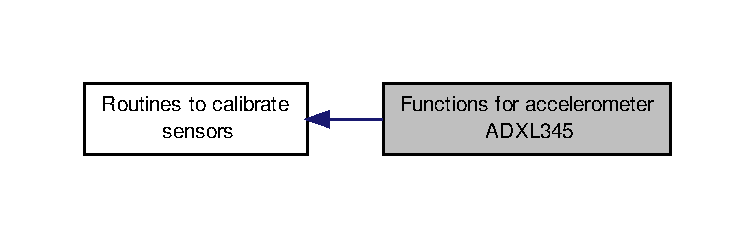
\includegraphics[width=350pt]{group__acc}
\end{center}
\end{figure}
\subsection*{Macros}
\begin{DoxyCompactItemize}
\item 
\#define \hyperlink{group__acc_ga355ea8f6ceed1e1d419a3ea2271bfca3}{A\-C\-C\-\_\-\-B\-I\-A\-S\-\_\-\-X}~19.\-2
\item 
\#define \hyperlink{group__acc_ga34180f1c97e84a814ef181f62bf4b68f}{A\-C\-C\-\_\-\-B\-I\-A\-S\-\_\-\-Y}~6.\-024
\item 
\#define \hyperlink{group__acc_ga794f762650b6f228ffb8d50d1323dbea}{A\-C\-C\-\_\-\-B\-I\-A\-S\-\_\-\-Z}~-\/18.\-97
\item 
\#define \hyperlink{group__acc_ga76e6967cb5a86ec34986b4583ac09831}{A\-C\-C\-\_\-\-F\-S\-\_\-\-X}~262.\-82
\item 
\#define \hyperlink{group__acc_ga13d3aaab3b5800b11351cbd1246c8918}{A\-C\-C\-\_\-\-F\-S\-\_\-\-Y}~262.\-15
\item 
\#define \hyperlink{group__acc_gaf1d3370cc0958289199c8c13470602d4}{A\-C\-C\-\_\-\-F\-S\-\_\-\-Z}~252.\-20
\end{DoxyCompactItemize}
\subsection*{Functions}
\begin{DoxyCompactItemize}
\item 
int \hyperlink{group__acc_ga534116416343122de29a5b6ade6876bd}{acc\-\_\-write\-\_\-reg} (int \hyperlink{CommunicationV0_2communication_8c_a7751bd45ac1064efb35adf1f19c25db8}{i2c\-\_\-dev}, uint8\-\_\-t reg, uint8\-\_\-t data)
\begin{DoxyCompactList}\small\item\em W\-R\-I\-T\-E T\-O R\-E\-G\-I\-S\-T\-E\-R. \end{DoxyCompactList}\item 
uint8\-\_\-t $\ast$ \hyperlink{group__acc_ga2a91c44eebbe44f4d3b8c508633512f9}{acc\-\_\-read\-\_\-reg} (int \hyperlink{CommunicationV0_2communication_8c_a7751bd45ac1064efb35adf1f19c25db8}{i2c\-\_\-dev}, uint8\-\_\-t reg, uint8\-\_\-t count)
\begin{DoxyCompactList}\small\item\em R\-E\-A\-D C\-O\-U\-N\-T 8-\/\-B\-I\-T R\-E\-G\-I\-S\-T\-E\-R I\-N S\-E\-Q\-U\-E\-N\-C\-E \end{DoxyCompactList}\item 
int \hyperlink{group__acc_gae8f9cc6e0d15e61039d846305f86f073}{acc\-\_\-init} (int \hyperlink{CommunicationV0_2communication_8c_a7751bd45ac1064efb35adf1f19c25db8}{i2c\-\_\-dev}, uint8\-\_\-t full\-\_\-res, uint16\-\_\-t rate, uint8\-\_\-t range)
\begin{DoxyCompactList}\small\item\em I\-N\-I\-T\-I\-A\-L\-I\-Z\-E A\-C\-C\-E\-L\-E\-R\-O\-M\-E\-T\-E\-R. \end{DoxyCompactList}\item 
int \hyperlink{group__acc_ga013bb5ed8a763883fc440549d2b1a6ce}{acc\-\_\-read\-\_\-all\-\_\-data} (int \hyperlink{CommunicationV0_2communication_8c_a7751bd45ac1064efb35adf1f19c25db8}{i2c\-\_\-dev}, short int $\ast$data)
\begin{DoxyCompactList}\small\item\em R\-E\-A\-D A\-L\-L D\-A\-T\-A A\-T O\-N\-C\-E (X, Y and Z) \end{DoxyCompactList}\item 
short int \hyperlink{group__acc_ga041d6953f2bfc8c5efa4d5bbac812305}{acc\-\_\-read\-\_\-data} (int \hyperlink{CommunicationV0_2communication_8c_a7751bd45ac1064efb35adf1f19c25db8}{i2c\-\_\-dev}, int axis)
\begin{DoxyCompactList}\small\item\em R\-E\-A\-D D\-A\-T\-A (X, Y or Z) \end{DoxyCompactList}\item 
int \hyperlink{group__acc_ga8509cccabb08e7267677f66f25718731}{acc\-\_\-read\-\_\-all\-\_\-reg} (int \hyperlink{CommunicationV0_2communication_8c_a7751bd45ac1064efb35adf1f19c25db8}{i2c\-\_\-dev})
\begin{DoxyCompactList}\small\item\em Read all accelerometer data and print in stdio. \end{DoxyCompactList}\end{DoxyCompactItemize}


\subsection{Detailed Description}


\subsection{Macro Definition Documentation}
\hypertarget{group__acc_ga355ea8f6ceed1e1d419a3ea2271bfca3}{\index{Functions for accelerometer A\-D\-X\-L345@{Functions for accelerometer A\-D\-X\-L345}!A\-C\-C\-\_\-\-B\-I\-A\-S\-\_\-\-X@{A\-C\-C\-\_\-\-B\-I\-A\-S\-\_\-\-X}}
\index{A\-C\-C\-\_\-\-B\-I\-A\-S\-\_\-\-X@{A\-C\-C\-\_\-\-B\-I\-A\-S\-\_\-\-X}!Functions for accelerometer ADXL345@{Functions for accelerometer A\-D\-X\-L345}}
\subsubsection[{A\-C\-C\-\_\-\-B\-I\-A\-S\-\_\-\-X}]{\setlength{\rightskip}{0pt plus 5cm}\#define A\-C\-C\-\_\-\-B\-I\-A\-S\-\_\-\-X~19.\-2}}\label{group__acc_ga355ea8f6ceed1e1d419a3ea2271bfca3}


Definition at line 19 of file calibration.\-h.



Referenced by calibrate\-\_\-imu().

\hypertarget{group__acc_ga34180f1c97e84a814ef181f62bf4b68f}{\index{Functions for accelerometer A\-D\-X\-L345@{Functions for accelerometer A\-D\-X\-L345}!A\-C\-C\-\_\-\-B\-I\-A\-S\-\_\-\-Y@{A\-C\-C\-\_\-\-B\-I\-A\-S\-\_\-\-Y}}
\index{A\-C\-C\-\_\-\-B\-I\-A\-S\-\_\-\-Y@{A\-C\-C\-\_\-\-B\-I\-A\-S\-\_\-\-Y}!Functions for accelerometer ADXL345@{Functions for accelerometer A\-D\-X\-L345}}
\subsubsection[{A\-C\-C\-\_\-\-B\-I\-A\-S\-\_\-\-Y}]{\setlength{\rightskip}{0pt plus 5cm}\#define A\-C\-C\-\_\-\-B\-I\-A\-S\-\_\-\-Y~6.\-024}}\label{group__acc_ga34180f1c97e84a814ef181f62bf4b68f}


Definition at line 20 of file calibration.\-h.



Referenced by calibrate\-\_\-imu().

\hypertarget{group__acc_ga794f762650b6f228ffb8d50d1323dbea}{\index{Functions for accelerometer A\-D\-X\-L345@{Functions for accelerometer A\-D\-X\-L345}!A\-C\-C\-\_\-\-B\-I\-A\-S\-\_\-\-Z@{A\-C\-C\-\_\-\-B\-I\-A\-S\-\_\-\-Z}}
\index{A\-C\-C\-\_\-\-B\-I\-A\-S\-\_\-\-Z@{A\-C\-C\-\_\-\-B\-I\-A\-S\-\_\-\-Z}!Functions for accelerometer ADXL345@{Functions for accelerometer A\-D\-X\-L345}}
\subsubsection[{A\-C\-C\-\_\-\-B\-I\-A\-S\-\_\-\-Z}]{\setlength{\rightskip}{0pt plus 5cm}\#define A\-C\-C\-\_\-\-B\-I\-A\-S\-\_\-\-Z~-\/18.\-97}}\label{group__acc_ga794f762650b6f228ffb8d50d1323dbea}


Definition at line 21 of file calibration.\-h.



Referenced by calibrate\-\_\-imu().

\hypertarget{group__acc_ga76e6967cb5a86ec34986b4583ac09831}{\index{Functions for accelerometer A\-D\-X\-L345@{Functions for accelerometer A\-D\-X\-L345}!A\-C\-C\-\_\-\-F\-S\-\_\-\-X@{A\-C\-C\-\_\-\-F\-S\-\_\-\-X}}
\index{A\-C\-C\-\_\-\-F\-S\-\_\-\-X@{A\-C\-C\-\_\-\-F\-S\-\_\-\-X}!Functions for accelerometer ADXL345@{Functions for accelerometer A\-D\-X\-L345}}
\subsubsection[{A\-C\-C\-\_\-\-F\-S\-\_\-\-X}]{\setlength{\rightskip}{0pt plus 5cm}\#define A\-C\-C\-\_\-\-F\-S\-\_\-\-X~262.\-82}}\label{group__acc_ga76e6967cb5a86ec34986b4583ac09831}


Definition at line 22 of file calibration.\-h.



Referenced by calibrate\-\_\-imu().

\hypertarget{group__acc_ga13d3aaab3b5800b11351cbd1246c8918}{\index{Functions for accelerometer A\-D\-X\-L345@{Functions for accelerometer A\-D\-X\-L345}!A\-C\-C\-\_\-\-F\-S\-\_\-\-Y@{A\-C\-C\-\_\-\-F\-S\-\_\-\-Y}}
\index{A\-C\-C\-\_\-\-F\-S\-\_\-\-Y@{A\-C\-C\-\_\-\-F\-S\-\_\-\-Y}!Functions for accelerometer ADXL345@{Functions for accelerometer A\-D\-X\-L345}}
\subsubsection[{A\-C\-C\-\_\-\-F\-S\-\_\-\-Y}]{\setlength{\rightskip}{0pt plus 5cm}\#define A\-C\-C\-\_\-\-F\-S\-\_\-\-Y~262.\-15}}\label{group__acc_ga13d3aaab3b5800b11351cbd1246c8918}


Definition at line 23 of file calibration.\-h.



Referenced by calibrate\-\_\-imu().

\hypertarget{group__acc_gaf1d3370cc0958289199c8c13470602d4}{\index{Functions for accelerometer A\-D\-X\-L345@{Functions for accelerometer A\-D\-X\-L345}!A\-C\-C\-\_\-\-F\-S\-\_\-\-Z@{A\-C\-C\-\_\-\-F\-S\-\_\-\-Z}}
\index{A\-C\-C\-\_\-\-F\-S\-\_\-\-Z@{A\-C\-C\-\_\-\-F\-S\-\_\-\-Z}!Functions for accelerometer ADXL345@{Functions for accelerometer A\-D\-X\-L345}}
\subsubsection[{A\-C\-C\-\_\-\-F\-S\-\_\-\-Z}]{\setlength{\rightskip}{0pt plus 5cm}\#define A\-C\-C\-\_\-\-F\-S\-\_\-\-Z~252.\-20}}\label{group__acc_gaf1d3370cc0958289199c8c13470602d4}


Definition at line 24 of file calibration.\-h.



Referenced by calibrate\-\_\-imu().



\subsection{Function Documentation}
\hypertarget{group__acc_gae8f9cc6e0d15e61039d846305f86f073}{\index{Functions for accelerometer A\-D\-X\-L345@{Functions for accelerometer A\-D\-X\-L345}!acc\-\_\-init@{acc\-\_\-init}}
\index{acc\-\_\-init@{acc\-\_\-init}!Functions for accelerometer ADXL345@{Functions for accelerometer A\-D\-X\-L345}}
\subsubsection[{acc\-\_\-init}]{\setlength{\rightskip}{0pt plus 5cm}int acc\-\_\-init (
\begin{DoxyParamCaption}
\item[{int}]{i2c\-\_\-dev, }
\item[{uint8\-\_\-t}]{full\-\_\-res, }
\item[{uint16\-\_\-t}]{rate, }
\item[{uint8\-\_\-t}]{range}
\end{DoxyParamCaption}
)}}\label{group__acc_gae8f9cc6e0d15e61039d846305f86f073}


I\-N\-I\-T\-I\-A\-L\-I\-Z\-E A\-C\-C\-E\-L\-E\-R\-O\-M\-E\-T\-E\-R. 


\begin{DoxyParams}{Parameters}
{\em i2c\-\_\-dev} & Communication Port \\
\hline
{\em full\-\_\-res} & Set resolution to 10 bits if value equal 0 else set to Full resolution \\
\hline
{\em rate} & Set data output rate (Hz), possible values\-: (3200,1600,800,400,200,100,50,25, 12\-: 12.\-5\-Hz, 6\-: 6.\-25\-Hz) \\
\hline
{\em range} & Set range of read, possible values\-: (2\-: +-\/ 2g 4\-: +-\/ 4g 8\-: +-\/ 8g anyother\-: 16g) \\
\hline
\end{DoxyParams}
\begin{DoxyReturn}{Returns}
flag with S\-U\-C\-C\-E\-S\-S or F\-A\-I\-L\-U\-R\-E
\end{DoxyReturn}
I\-N\-I\-T\-I\-A\-L\-I\-Z\-E A\-C\-C\-E\-L\-E\-R\-O\-M\-E\-T\-E\-R.

Implements the I2\-C communication between Gumstix Overo Fire and A\-D\-X\-L345 \begin{DoxyAuthor}{Author}
Caio Gustavo Mesquita Ângelo 
\end{DoxyAuthor}


Definition at line 11 of file acc\-\_\-functions.\-c.


\begin{DoxyCode}
\{ 
  uint8\_t data=0;

  \textcolor{keywordflow}{switch}(range)\{
    \textcolor{keywordflow}{case} 2:
      data=0x08;;
      \textcolor{keywordflow}{break};
    \textcolor{keywordflow}{case} 4:
      data=0x09;
      \textcolor{keywordflow}{break};
    \textcolor{keywordflow}{case} 8:
      data=0x0A;
      \textcolor{keywordflow}{break};
    \textcolor{keywordflow}{default}:
      data=0x0B;
      \textcolor{keywordflow}{break};
  \}
  
  \textcolor{keywordflow}{if}(full\_res==0)
    data=data&(0xF7);
  
  \textcolor{keywordflow}{if}((\hyperlink{group__acc_ga534116416343122de29a5b6ade6876bd}{acc\_write\_reg}(\hyperlink{CommunicationV0_2communication_8c_a7751bd45ac1064efb35adf1f19c25db8}{i2c\_dev}, \hyperlink{communication_2imu__regs_8h_ab4eb7fc69b2a37ee750d3400fc2c53a1}{ACC\_DATA\_FORMAT}
      , data))<0)\{
    perror(\textcolor{stringliteral}{"Data Format unsuccesful"});
    \textcolor{keywordflow}{return} \hyperlink{calibration_2calibration_8h_a6d58f9ac447476b4e084d7ca383f5183}{FAILURE};
  \}
  
  data=\hyperlink{communication_2imu__regs_8h_a9a841ba3e094b01ea439584e12b25894}{ACC\_POWER\_CTL\_MEAS\_MODE};
  \textcolor{keywordflow}{if}((\hyperlink{group__acc_ga534116416343122de29a5b6ade6876bd}{acc\_write\_reg}(\hyperlink{CommunicationV0_2communication_8c_a7751bd45ac1064efb35adf1f19c25db8}{i2c\_dev}, \hyperlink{communication_2imu__regs_8h_ad857d62b61f349216faeda06eff5f9c6}{ACC\_POWER\_CTL}, 
      data))<0)\{
    perror(\textcolor{stringliteral}{"Power Control unsuccesful"});
    \textcolor{keywordflow}{return} \hyperlink{calibration_2calibration_8h_a6d58f9ac447476b4e084d7ca383f5183}{FAILURE};
  \}
  
  \textcolor{keywordflow}{switch}(rate)\{
    \textcolor{keywordflow}{case} 100:
      data=0x0A;
      \textcolor{keywordflow}{break};
    \textcolor{keywordflow}{case} 3200:
      data=0x0F;;
      \textcolor{keywordflow}{break};
    \textcolor{keywordflow}{case} 1600:
      data=0x0E;
      \textcolor{keywordflow}{break};
    \textcolor{keywordflow}{case} 800:
      data=0x0D;
      \textcolor{keywordflow}{break};
    \textcolor{keywordflow}{case} 400:
      data=0x0C;
      \textcolor{keywordflow}{break};
    \textcolor{keywordflow}{case} 200:
      data=0x0B;
      \textcolor{keywordflow}{break};
    \textcolor{keywordflow}{case} 50:
      data=0x09;
      \textcolor{keywordflow}{break}; 
    \textcolor{keywordflow}{case} 25:
      data=0x08;
      \textcolor{keywordflow}{break};
    \textcolor{keywordflow}{case} 12:
      data=0x07;
      \textcolor{keywordflow}{break};
    \textcolor{keywordflow}{case} 6:
      data=0x06;
      \textcolor{keywordflow}{break};
    \textcolor{keywordflow}{default}:
      perror(\textcolor{stringliteral}{"Wrong rate value"});
      \textcolor{keywordflow}{return} \hyperlink{calibration_2calibration_8h_a6d58f9ac447476b4e084d7ca383f5183}{FAILURE};
  \}
  \textcolor{keywordflow}{if}((\hyperlink{group__acc_ga534116416343122de29a5b6ade6876bd}{acc\_write\_reg}(\hyperlink{CommunicationV0_2communication_8c_a7751bd45ac1064efb35adf1f19c25db8}{i2c\_dev}, \hyperlink{communication_2imu__regs_8h_afbbb5a3aa097a32f98c47158141a882f}{ACC\_BW\_RATE}, data))
      <0)\{
    perror(\textcolor{stringliteral}{"Write in BW\_RATE unsuccesful"});
    \textcolor{keywordflow}{return} \hyperlink{calibration_2calibration_8h_a6d58f9ac447476b4e084d7ca383f5183}{FAILURE};
  \}
  
  \textcolor{keywordflow}{return} \hyperlink{calibration_2calibration_8h_aa90cac659d18e8ef6294c7ae337f6b58}{SUCCESS};
\}
\end{DoxyCode}
\hypertarget{group__acc_ga013bb5ed8a763883fc440549d2b1a6ce}{\index{Functions for accelerometer A\-D\-X\-L345@{Functions for accelerometer A\-D\-X\-L345}!acc\-\_\-read\-\_\-all\-\_\-data@{acc\-\_\-read\-\_\-all\-\_\-data}}
\index{acc\-\_\-read\-\_\-all\-\_\-data@{acc\-\_\-read\-\_\-all\-\_\-data}!Functions for accelerometer ADXL345@{Functions for accelerometer A\-D\-X\-L345}}
\subsubsection[{acc\-\_\-read\-\_\-all\-\_\-data}]{\setlength{\rightskip}{0pt plus 5cm}int acc\-\_\-read\-\_\-all\-\_\-data (
\begin{DoxyParamCaption}
\item[{int}]{i2c\-\_\-dev, }
\item[{short int $\ast$}]{data}
\end{DoxyParamCaption}
)}}\label{group__acc_ga013bb5ed8a763883fc440549d2b1a6ce}


R\-E\-A\-D A\-L\-L D\-A\-T\-A A\-T O\-N\-C\-E (X, Y and Z) 


\begin{DoxyParams}[1]{Parameters}
 & {\em i2c\-\_\-dev} & Communication Port \\
\hline
\mbox{\tt out}  & {\em data} & Data's vector\\
\hline
\end{DoxyParams}
\begin{DoxyReturn}{Returns}
flag with S\-U\-C\-C\-E\-S\-S or F\-A\-I\-L\-U\-R\-E 
\end{DoxyReturn}


Definition at line 159 of file acc\-\_\-functions.\-c.


\begin{DoxyCode}
\{
  \textcolor{keywordtype}{int} i;
  uint8\_t *data8;
  \textcolor{keyword}{union }result
  \{
    \textcolor{keywordtype}{unsigned} \textcolor{keywordtype}{short} \textcolor{keywordtype}{int} usgnd[3];
    \textcolor{keywordtype}{short} \textcolor{keywordtype}{int} sgnd[3];
  \} result;
  \textcolor{comment}{//result=(union result*)malloc(3*sizeof(union result));}
  \textcolor{keywordflow}{if}( (data8=\hyperlink{group__acc_ga2a91c44eebbe44f4d3b8c508633512f9}{acc\_read\_reg}(\hyperlink{CommunicationV0_2communication_8c_a7751bd45ac1064efb35adf1f19c25db8}{i2c\_dev},\hyperlink{communication_2imu__regs_8h_afae448fbad872220013e5c3abf0f3d9f}{ACC\_DATAX0},6))==
      NULL )
  \{
    \textcolor{comment}{//perror("Read accelerometer register failed");}
    \textcolor{keywordflow}{return} \hyperlink{calibration_2calibration_8h_a6d58f9ac447476b4e084d7ca383f5183}{FAILURE};
  \}
  \textcolor{comment}{//result.usgnd=(unsigned int*)malloc(3*sizeof(unsigned int));}
  \textcolor{keywordflow}{for}(i=0; i<3; i++)
  \{
    result.usgnd[i]=0;
    result.usgnd[i]=result.usgnd[i]|((\textcolor{keywordtype}{unsigned} \textcolor{keywordtype}{short} int)data8[i*2])|(((\textcolor{keywordtype}{
      unsigned} \textcolor{keywordtype}{short} int)data8[i*2+1])<<8);
    data[i]=result.sgnd[i];
  \}
  \textcolor{keywordflow}{return} \hyperlink{calibration_2calibration_8h_aa90cac659d18e8ef6294c7ae337f6b58}{SUCCESS};  
\}
\end{DoxyCode}
\hypertarget{group__acc_ga8509cccabb08e7267677f66f25718731}{\index{Functions for accelerometer A\-D\-X\-L345@{Functions for accelerometer A\-D\-X\-L345}!acc\-\_\-read\-\_\-all\-\_\-reg@{acc\-\_\-read\-\_\-all\-\_\-reg}}
\index{acc\-\_\-read\-\_\-all\-\_\-reg@{acc\-\_\-read\-\_\-all\-\_\-reg}!Functions for accelerometer ADXL345@{Functions for accelerometer A\-D\-X\-L345}}
\subsubsection[{acc\-\_\-read\-\_\-all\-\_\-reg}]{\setlength{\rightskip}{0pt plus 5cm}int acc\-\_\-read\-\_\-all\-\_\-reg (
\begin{DoxyParamCaption}
\item[{int}]{i2c\-\_\-dev}
\end{DoxyParamCaption}
)}}\label{group__acc_ga8509cccabb08e7267677f66f25718731}


Read all accelerometer data and print in stdio. 


\begin{DoxyParams}{Parameters}
{\em i2c\-\_\-dev} & Communication Port \\
\hline
\end{DoxyParams}


Definition at line 196 of file acc\-\_\-functions.\-c.


\begin{DoxyCode}
\{
  uint8\_t *hvalue0, *hvalue1, *hvalue;
  \textcolor{keywordtype}{int} i;
  
  hvalue0=\hyperlink{group__acc_ga2a91c44eebbe44f4d3b8c508633512f9}{acc\_read\_reg}(\hyperlink{CommunicationV0_2communication_8c_a7751bd45ac1064efb35adf1f19c25db8}{i2c\_dev},\hyperlink{communication_2imu__regs_8h_a007fa8d8ef9d89127ae5da32a2f42283}{ACC\_DEVID},1);
  printf(\textcolor{stringliteral}{"\(\backslash\)nhey"});
  printf(\textcolor{stringliteral}{"\(\backslash\)nhey3"});
  printf(\textcolor{stringliteral}{"\(\backslash\)nhey2"});
  printf(\textcolor{stringliteral}{"\(\backslash\)nhey3"});
  hvalue1=\hyperlink{group__acc_ga2a91c44eebbe44f4d3b8c508633512f9}{acc\_read\_reg}(\hyperlink{CommunicationV0_2communication_8c_a7751bd45ac1064efb35adf1f19c25db8}{i2c\_dev},\hyperlink{communication_2imu__regs_8h_afa5af181c4af31e22baa9bd20ff322ef}{ACC\_THRESH\_TAP},
       29);
  printf(\textcolor{stringliteral}{"\(\backslash\)nhey3"});
  \textcolor{comment}{//hvalue--;}
  hvalue=(uint8\_t*)malloc(30*\textcolor{keyword}{sizeof}(uint8\_t));
  hvalue[0]=hvalue0[0];
  \textcolor{keywordflow}{for}( i=0; i<29; i++)
    hvalue[i+1]=hvalue1[i];
  printf(\textcolor{stringliteral}{"\(\backslash\)nhey4"});
  printf(\textcolor{stringliteral}{"\(\backslash\)nACC\_DEVID = 0x%02X = %s"}, hvalue0[0],\hyperlink{communication_2acc__functions_8c_a1a6b2f719b4fef8f97d6d1b8f495148e}{conv\_byte\_hex\_bin}
      (hvalue0));
  printf(\textcolor{stringliteral}{"\(\backslash\)nACC\_THRESH\_TAP = 0x%02X = %s"}, hvalue1[0],\hyperlink{communication_2acc__functions_8c_a1a6b2f719b4fef8f97d6d1b8f495148e}{conv\_byte\_hex\_bin}
      (hvalue+1));
  printf(\textcolor{stringliteral}{"\(\backslash\)nACC\_OFSX = 0x%02X = %s"}, hvalue[2],\hyperlink{communication_2acc__functions_8c_a1a6b2f719b4fef8f97d6d1b8f495148e}{conv\_byte\_hex\_bin}
      (hvalue+2));
  printf(\textcolor{stringliteral}{"\(\backslash\)nACC\_OFSY = 0x%02X = %s"}, hvalue[3],\hyperlink{communication_2acc__functions_8c_a1a6b2f719b4fef8f97d6d1b8f495148e}{conv\_byte\_hex\_bin}
      (hvalue+3));
  printf(\textcolor{stringliteral}{"\(\backslash\)nACC\_OFSZ = 0x%02X = %s"}, hvalue[4],\hyperlink{communication_2acc__functions_8c_a1a6b2f719b4fef8f97d6d1b8f495148e}{conv\_byte\_hex\_bin}
      (hvalue+4));
  printf(\textcolor{stringliteral}{"\(\backslash\)nACC\_DUR = 0x%02X = %s"}, hvalue[5],\hyperlink{communication_2acc__functions_8c_a1a6b2f719b4fef8f97d6d1b8f495148e}{conv\_byte\_hex\_bin}
      (hvalue+5));
  printf(\textcolor{stringliteral}{"\(\backslash\)nACC\_LATENT = 0x%02X = %s"}, hvalue[6],\hyperlink{communication_2acc__functions_8c_a1a6b2f719b4fef8f97d6d1b8f495148e}{conv\_byte\_hex\_bin}
      (hvalue+6));
  printf(\textcolor{stringliteral}{"\(\backslash\)nACC\_WINDOW = 0x%02X = %s"}, hvalue[7],\hyperlink{communication_2acc__functions_8c_a1a6b2f719b4fef8f97d6d1b8f495148e}{conv\_byte\_hex\_bin}
      (hvalue+7));
  printf(\textcolor{stringliteral}{"\(\backslash\)nACC\_THRESH\_ACT = 0x%02X = %s"}, hvalue[8],\hyperlink{communication_2acc__functions_8c_a1a6b2f719b4fef8f97d6d1b8f495148e}{conv\_byte\_hex\_bin}
      (hvalue+8));
  printf(\textcolor{stringliteral}{"\(\backslash\)nACC\_THRESH\_INACT = 0x%02X = %s"}, hvalue[9],\hyperlink{communication_2acc__functions_8c_a1a6b2f719b4fef8f97d6d1b8f495148e}{conv\_byte\_hex\_bin}
      (hvalue+9));
  printf(\textcolor{stringliteral}{"\(\backslash\)nACC\_TIME\_INACT = 0x%02X = %s"}, hvalue[10],\hyperlink{communication_2acc__functions_8c_a1a6b2f719b4fef8f97d6d1b8f495148e}{conv\_byte\_hex\_bin}
      (hvalue+10));
  printf(\textcolor{stringliteral}{"\(\backslash\)nACC\_ACT\_INACT\_CTL = 0x%02X = %s"}, hvalue[11],\hyperlink{communication_2acc__functions_8c_a1a6b2f719b4fef8f97d6d1b8f495148e}{conv\_byte\_hex\_bin}
      (hvalue+11));
  printf(\textcolor{stringliteral}{"\(\backslash\)nACC\_THRESH\_FF = 0x%02X = %s"}, hvalue[12],\hyperlink{communication_2acc__functions_8c_a1a6b2f719b4fef8f97d6d1b8f495148e}{conv\_byte\_hex\_bin}
      (hvalue+12));
  printf(\textcolor{stringliteral}{"\(\backslash\)nACC\_TIME\_FF = 0x%02X = %s"}, hvalue[13],\hyperlink{communication_2acc__functions_8c_a1a6b2f719b4fef8f97d6d1b8f495148e}{conv\_byte\_hex\_bin}
      (hvalue+13));
  printf(\textcolor{stringliteral}{"\(\backslash\)nACC\_TAP\_AXES = 0x%02X = %s"}, hvalue[14],\hyperlink{communication_2acc__functions_8c_a1a6b2f719b4fef8f97d6d1b8f495148e}{conv\_byte\_hex\_bin}
      (hvalue+14));
  printf(\textcolor{stringliteral}{"\(\backslash\)nACC\_ACT\_TAP\_STATUS = 0x%02X = %s"}, hvalue[15],\hyperlink{communication_2acc__functions_8c_a1a6b2f719b4fef8f97d6d1b8f495148e}{conv\_byte\_hex\_bin}
      (hvalue+15));
  printf(\textcolor{stringliteral}{"\(\backslash\)nACC\_BW\_RATE = 0x%02X = %s"}, hvalue[16],\hyperlink{communication_2acc__functions_8c_a1a6b2f719b4fef8f97d6d1b8f495148e}{conv\_byte\_hex\_bin}
      (hvalue+16));
  printf(\textcolor{stringliteral}{"\(\backslash\)nACC\_POWER\_CTL = 0x%02X = %s"}, hvalue[17],\hyperlink{communication_2acc__functions_8c_a1a6b2f719b4fef8f97d6d1b8f495148e}{conv\_byte\_hex\_bin}
      (hvalue+17));
  printf(\textcolor{stringliteral}{"\(\backslash\)nACC\_INT\_ENABLE = 0x%02X = %s"}, hvalue[18],\hyperlink{communication_2acc__functions_8c_a1a6b2f719b4fef8f97d6d1b8f495148e}{conv\_byte\_hex\_bin}
      (hvalue+18));
  printf(\textcolor{stringliteral}{"\(\backslash\)nACC\_INT\_MAP = 0x%02X = %s"}, hvalue[19],\hyperlink{communication_2acc__functions_8c_a1a6b2f719b4fef8f97d6d1b8f495148e}{conv\_byte\_hex\_bin}
      (hvalue+19));
  printf(\textcolor{stringliteral}{"\(\backslash\)nACC\_INT\_SOURCE = 0x%02X = %s"}, hvalue[20],\hyperlink{communication_2acc__functions_8c_a1a6b2f719b4fef8f97d6d1b8f495148e}{conv\_byte\_hex\_bin}
      (hvalue+20));
  printf(\textcolor{stringliteral}{"\(\backslash\)nACC\_DATA\_FORMAT = 0x%02X = %s"}, hvalue1[20],\hyperlink{communication_2acc__functions_8c_a1a6b2f719b4fef8f97d6d1b8f495148e}{conv\_byte\_hex\_bin}
      (hvalue1+21));
  printf(\textcolor{stringliteral}{"\(\backslash\)nACC\_DATAX0 = 0x%02X = %s"}, hvalue1[21],\hyperlink{communication_2acc__functions_8c_a1a6b2f719b4fef8f97d6d1b8f495148e}{conv\_byte\_hex\_bin}
      (hvalue1+22));
  printf(\textcolor{stringliteral}{"\(\backslash\)nACC\_DATAX1 = 0x%02X = %s"}, hvalue1[22],\hyperlink{communication_2acc__functions_8c_a1a6b2f719b4fef8f97d6d1b8f495148e}{conv\_byte\_hex\_bin}
      (hvalue1+23));
  printf(\textcolor{stringliteral}{"\(\backslash\)nACC\_DATAY0 = 0x%02X = %s"}, hvalue1[23],\hyperlink{communication_2acc__functions_8c_a1a6b2f719b4fef8f97d6d1b8f495148e}{conv\_byte\_hex\_bin}
      (hvalue1+24));
  printf(\textcolor{stringliteral}{"\(\backslash\)nACC\_DATAY1 = 0x%02X = %s"}, hvalue1[24],\hyperlink{communication_2acc__functions_8c_a1a6b2f719b4fef8f97d6d1b8f495148e}{conv\_byte\_hex\_bin}
      (hvalue1+25));
  printf(\textcolor{stringliteral}{"\(\backslash\)nACC\_DATAZ0 = 0x%02X = %s"}, hvalue1[25],\hyperlink{communication_2acc__functions_8c_a1a6b2f719b4fef8f97d6d1b8f495148e}{conv\_byte\_hex\_bin}
      (hvalue1+26));
  printf(\textcolor{stringliteral}{"\(\backslash\)nACC\_DATAZ1 = 0x%02X = %s"}, hvalue1[26],\hyperlink{communication_2acc__functions_8c_a1a6b2f719b4fef8f97d6d1b8f495148e}{conv\_byte\_hex\_bin}
      (hvalue1+27));
  printf(\textcolor{stringliteral}{"\(\backslash\)nACC\_FIFO\_CTL = 0x%02X = %s"}, hvalue[28],\hyperlink{communication_2acc__functions_8c_a1a6b2f719b4fef8f97d6d1b8f495148e}{conv\_byte\_hex\_bin}
      (hvalue+28));
  printf(\textcolor{stringliteral}{"\(\backslash\)nACC\_FIFO\_STATUS = 0x%02X = %s"}, hvalue[29],\hyperlink{communication_2acc__functions_8c_a1a6b2f719b4fef8f97d6d1b8f495148e}{conv\_byte\_hex\_bin}
      (hvalue+29));
  \textcolor{keywordflow}{return} 1;
\}
\end{DoxyCode}
\hypertarget{group__acc_ga041d6953f2bfc8c5efa4d5bbac812305}{\index{Functions for accelerometer A\-D\-X\-L345@{Functions for accelerometer A\-D\-X\-L345}!acc\-\_\-read\-\_\-data@{acc\-\_\-read\-\_\-data}}
\index{acc\-\_\-read\-\_\-data@{acc\-\_\-read\-\_\-data}!Functions for accelerometer ADXL345@{Functions for accelerometer A\-D\-X\-L345}}
\subsubsection[{acc\-\_\-read\-\_\-data}]{\setlength{\rightskip}{0pt plus 5cm}short int acc\-\_\-read\-\_\-data (
\begin{DoxyParamCaption}
\item[{int}]{i2c\-\_\-dev, }
\item[{int}]{axis}
\end{DoxyParamCaption}
)}}\label{group__acc_ga041d6953f2bfc8c5efa4d5bbac812305}


R\-E\-A\-D D\-A\-T\-A (X, Y or Z) 


\begin{DoxyParams}[1]{Parameters}
 & {\em i2c\-\_\-dev} & Communication Port \\
\hline
\mbox{\tt in}  & {\em axis} & Accelerate's axis to read ('X' or 'Y' or 'Z')\\
\hline
\end{DoxyParams}
\begin{DoxyReturn}{Returns}

\end{DoxyReturn}


Definition at line 131 of file acc\-\_\-functions.\-c.


\begin{DoxyCode}
\{
  uint8\_t *data;
  \textcolor{keyword}{union }result
  \{
    \textcolor{keywordtype}{unsigned} \textcolor{keywordtype}{short} \textcolor{keywordtype}{int} usgnd;
    \textcolor{keywordtype}{short} \textcolor{keywordtype}{int} sgnd;
  \}result;

  \textcolor{keywordflow}{switch}(axis)\{
    \textcolor{keywordflow}{case} \textcolor{charliteral}{'X'}:
      data=\hyperlink{group__acc_ga2a91c44eebbe44f4d3b8c508633512f9}{acc\_read\_reg}(\hyperlink{CommunicationV0_2communication_8c_a7751bd45ac1064efb35adf1f19c25db8}{i2c\_dev},\hyperlink{communication_2imu__regs_8h_afae448fbad872220013e5c3abf0f3d9f}{ACC\_DATAX0},2);
      \textcolor{keywordflow}{break};
    \textcolor{keywordflow}{case} \textcolor{charliteral}{'Y'}:
      data=\hyperlink{group__acc_ga2a91c44eebbe44f4d3b8c508633512f9}{acc\_read\_reg}(\hyperlink{CommunicationV0_2communication_8c_a7751bd45ac1064efb35adf1f19c25db8}{i2c\_dev},\hyperlink{communication_2imu__regs_8h_a6aa168a0f3e35bfee4da87c32dcb4b46}{ACC\_DATAY0},2);
      \textcolor{keywordflow}{break};
    \textcolor{keywordflow}{case} \textcolor{charliteral}{'Z'}:
      data=\hyperlink{group__acc_ga2a91c44eebbe44f4d3b8c508633512f9}{acc\_read\_reg}(\hyperlink{CommunicationV0_2communication_8c_a7751bd45ac1064efb35adf1f19c25db8}{i2c\_dev},\hyperlink{communication_2imu__regs_8h_ab87ce2339aeb4adb7fb71daa80f3bc68}{ACC\_DATAZ0},2);
      \textcolor{keywordflow}{break};
    \textcolor{keywordflow}{default}:
      \textcolor{comment}{//perror("Wrong argument for axis in acc\_read\_data");}
      \textcolor{keywordflow}{return} -1;
  \}
  result.usgnd=0;
  result.usgnd=result.usgnd|(((\textcolor{keywordtype}{unsigned} \textcolor{keywordtype}{short} int)data[0]))|(((\textcolor{keywordtype}{unsigned} \textcolor{keywordtype}{short} \textcolor{keywordtype}{
      int})data[1])<<8);
  \textcolor{keywordflow}{return} result.sgnd;
\}
\end{DoxyCode}
\hypertarget{group__acc_ga2a91c44eebbe44f4d3b8c508633512f9}{\index{Functions for accelerometer A\-D\-X\-L345@{Functions for accelerometer A\-D\-X\-L345}!acc\-\_\-read\-\_\-reg@{acc\-\_\-read\-\_\-reg}}
\index{acc\-\_\-read\-\_\-reg@{acc\-\_\-read\-\_\-reg}!Functions for accelerometer ADXL345@{Functions for accelerometer A\-D\-X\-L345}}
\subsubsection[{acc\-\_\-read\-\_\-reg}]{\setlength{\rightskip}{0pt plus 5cm}uint8\-\_\-t$\ast$ acc\-\_\-read\-\_\-reg (
\begin{DoxyParamCaption}
\item[{int}]{i2c\-\_\-dev, }
\item[{uint8\-\_\-t}]{reg, }
\item[{uint8\-\_\-t}]{count}
\end{DoxyParamCaption}
)}}\label{group__acc_ga2a91c44eebbe44f4d3b8c508633512f9}


R\-E\-A\-D C\-O\-U\-N\-T 8-\/\-B\-I\-T R\-E\-G\-I\-S\-T\-E\-R I\-N S\-E\-Q\-U\-E\-N\-C\-E 


\begin{DoxyParams}[1]{Parameters}
 & {\em i2c\-\_\-dev} & Communication Port \\
\hline
\mbox{\tt in}  & {\em reg} & Register \\
\hline
\mbox{\tt in}  & {\em count} & Number of register in sequence (1-\/29)\\
\hline
\end{DoxyParams}
\begin{DoxyReturn}{Returns}
Data of register or N\-U\-L\-L in case of any problem. 
\end{DoxyReturn}


Definition at line 109 of file acc\-\_\-functions.\-c.


\begin{DoxyCode}
\{
  uint8\_t data[29];
  \textcolor{keywordtype}{int} i;

  \textcolor{comment}{//data=(uint8\_t*)malloc((count+1)*sizeof(data));}
  
  data[0] = reg;

  \textcolor{keywordflow}{if} ((write(\hyperlink{CommunicationV0_2communication_8c_a7751bd45ac1064efb35adf1f19c25db8}{i2c\_dev}, &data, 1)) != 1) \{                  
        \textcolor{comment}{//perror("write before read");}
        \textcolor{keywordflow}{return} NULL;
  \}
  data[0] = 0;
  \textcolor{keywordflow}{if} ((read(\hyperlink{CommunicationV0_2communication_8c_a7751bd45ac1064efb35adf1f19c25db8}{i2c\_dev}, &data, count)) != count) \{
        \textcolor{comment}{//perror("read");}
        \textcolor{keywordflow}{return} NULL;    
  \}

  \textcolor{keywordflow}{return} data;
\}
\end{DoxyCode}
\hypertarget{group__acc_ga534116416343122de29a5b6ade6876bd}{\index{Functions for accelerometer A\-D\-X\-L345@{Functions for accelerometer A\-D\-X\-L345}!acc\-\_\-write\-\_\-reg@{acc\-\_\-write\-\_\-reg}}
\index{acc\-\_\-write\-\_\-reg@{acc\-\_\-write\-\_\-reg}!Functions for accelerometer ADXL345@{Functions for accelerometer A\-D\-X\-L345}}
\subsubsection[{acc\-\_\-write\-\_\-reg}]{\setlength{\rightskip}{0pt plus 5cm}int acc\-\_\-write\-\_\-reg (
\begin{DoxyParamCaption}
\item[{int}]{i2c\-\_\-dev, }
\item[{uint8\-\_\-t}]{reg, }
\item[{uint8\-\_\-t}]{data}
\end{DoxyParamCaption}
)}}\label{group__acc_ga534116416343122de29a5b6ade6876bd}


W\-R\-I\-T\-E T\-O R\-E\-G\-I\-S\-T\-E\-R. 


\begin{DoxyParams}[1]{Parameters}
 & {\em i2c\-\_\-dev} & Communication Port \\
\hline
\mbox{\tt in}  & {\em reg} & Register \\
\hline
\mbox{\tt in}  & {\em data} & Data to write \\
\hline
\end{DoxyParams}


Definition at line 87 of file acc\-\_\-functions.\-c.


\begin{DoxyCode}
\{
  uint8\_t reg\_data[2];

  reg\_data[0] = reg;
  reg\_data[1] = data;

  \textcolor{keywordflow}{if}( reg==\hyperlink{communication_2imu__regs_8h_a007fa8d8ef9d89127ae5da32a2f42283}{ACC\_DEVID} || reg==\hyperlink{communication_2imu__regs_8h_a823b94e47b6d728fdf91d386d69db3e9}{ACC\_ACT\_TAP\_STATUS} || 
      reg==\hyperlink{communication_2imu__regs_8h_a7f9415e11f76d0666b842a875f5f5fd8}{ACC\_INT\_SOURCE} || reg==\hyperlink{communication_2imu__regs_8h_acb0760254230c73d4744bae2059e7367}{ACC\_FIFO\_STATUS} ||
      reg==\hyperlink{communication_2imu__regs_8h_afae448fbad872220013e5c3abf0f3d9f}{ACC\_DATAX0} || reg==\hyperlink{communication_2imu__regs_8h_a63d0e7c719fabce83422ef9856302129}{ACC\_DATAX1} || reg==\hyperlink{communication_2imu__regs_8h_a6aa168a0f3e35bfee4da87c32dcb4b46}{ACC\_DATAY0}
       || reg==\hyperlink{communication_2imu__regs_8h_a587970363cd2aeb2535ac314e98a2825}{ACC\_DATAY1} || reg==\hyperlink{communication_2imu__regs_8h_ab87ce2339aeb4adb7fb71daa80f3bc68}{ACC\_DATAZ0} || reg==\hyperlink{communication_2imu__regs_8h_afa9ea1f66d9d28dbb328498d6f7fa43d}{ACC\_DATAZ1}
      )
  \{
      perror(\textcolor{stringliteral}{"Write unsucessful: Read-Only Register"});
      \textcolor{keywordflow}{return} \hyperlink{calibration_2calibration_8h_a6d58f9ac447476b4e084d7ca383f5183}{FAILURE};
  \}
        
  \textcolor{keywordflow}{if} ((write(\hyperlink{CommunicationV0_2communication_8c_a7751bd45ac1064efb35adf1f19c25db8}{i2c\_dev}, &reg\_data, 2)) != 2) \{              
          perror(\textcolor{stringliteral}{"Write unsuccessful"});
          \textcolor{keywordflow}{return} \hyperlink{calibration_2calibration_8h_a6d58f9ac447476b4e084d7ca383f5183}{FAILURE};
  \}

  \textcolor{keywordflow}{return} \hyperlink{calibration_2calibration_8h_aa90cac659d18e8ef6294c7ae337f6b58}{SUCCESS};
\}
\end{DoxyCode}

\hypertarget{group__gyr}{\section{Functions for Gyrometer I\-T\-G3200}
\label{group__gyr}\index{Functions for Gyrometer I\-T\-G3200@{Functions for Gyrometer I\-T\-G3200}}
}
\subsection*{Functions}
\begin{DoxyCompactItemize}
\item 
int \hyperlink{group__gyr_ga3eba167b8ab0614bfe7bafeae8b5570d}{gyr\-\_\-write\-\_\-reg} (int \hyperlink{CommunicationV0_2communication_8c_a7751bd45ac1064efb35adf1f19c25db8}{i2c\-\_\-dev}, uint8\-\_\-t reg, uint8\-\_\-t data)
\begin{DoxyCompactList}\small\item\em W\-R\-I\-T\-E T\-O R\-E\-G\-I\-S\-T\-E\-R. \end{DoxyCompactList}\item 
uint8\-\_\-t $\ast$ \hyperlink{group__gyr_gad817a3b69d4c3026b7a9b6de32753e7b}{gyr\-\_\-read\-\_\-reg} (int \hyperlink{CommunicationV0_2communication_8c_a7751bd45ac1064efb35adf1f19c25db8}{i2c\-\_\-dev}, uint8\-\_\-t reg, uint8\-\_\-t count)
\begin{DoxyCompactList}\small\item\em R\-E\-A\-D C\-O\-U\-N\-T 8-\/\-B\-I\-T R\-E\-G\-I\-S\-T\-E\-R I\-N S\-E\-Q\-U\-E\-N\-C\-E. \end{DoxyCompactList}\item 
int \hyperlink{group__gyr_ga6d02be352b4491a236c9695a6a24d174}{gyr\-\_\-init} (int \hyperlink{CommunicationV0_2communication_8c_a7751bd45ac1064efb35adf1f19c25db8}{i2c\-\_\-dev}, float rate, short int lpf\-\_\-bw, char clk\-\_\-source, char $\ast$act)
\begin{DoxyCompactList}\small\item\em I\-N\-I\-T\-I\-A\-L\-I\-Z\-E G\-Y\-R\-O\-M\-E\-T\-E\-R. \end{DoxyCompactList}\item 
int \hyperlink{group__gyr_ga79875465c3a29fd9ec77308c80a8bc37}{gyr\-\_\-read\-\_\-all\-\_\-data} (int \hyperlink{CommunicationV0_2communication_8c_a7751bd45ac1064efb35adf1f19c25db8}{i2c\-\_\-dev}, short int $\ast$data)
\begin{DoxyCompactList}\small\item\em R\-E\-A\-D A\-L\-L D\-A\-T\-A A\-T O\-N\-C\-E (X, Y, Z and T) \end{DoxyCompactList}\item 
short int \hyperlink{group__gyr_ga271b37e9ace81b18bb2f83787247d262}{gyr\-\_\-read\-\_\-data} (int \hyperlink{CommunicationV0_2communication_8c_a7751bd45ac1064efb35adf1f19c25db8}{i2c\-\_\-dev}, int type)
\begin{DoxyCompactList}\small\item\em R\-E\-A\-D D\-A\-T\-A (X, Y, Z or T) \end{DoxyCompactList}\end{DoxyCompactItemize}


\subsection{Detailed Description}


\subsection{Function Documentation}
\hypertarget{group__gyr_ga6d02be352b4491a236c9695a6a24d174}{\index{Functions for Gyrometer I\-T\-G3200@{Functions for Gyrometer I\-T\-G3200}!gyr\-\_\-init@{gyr\-\_\-init}}
\index{gyr\-\_\-init@{gyr\-\_\-init}!Functions for Gyrometer ITG3200@{Functions for Gyrometer I\-T\-G3200}}
\subsubsection[{gyr\-\_\-init}]{\setlength{\rightskip}{0pt plus 5cm}int gyr\-\_\-init (
\begin{DoxyParamCaption}
\item[{int}]{i2c\-\_\-dev, }
\item[{float}]{rate, }
\item[{short int}]{lpf\-\_\-bw, }
\item[{char}]{clk\-\_\-source, }
\item[{char $\ast$}]{act}
\end{DoxyParamCaption}
)}}\label{group__gyr_ga6d02be352b4491a236c9695a6a24d174}


I\-N\-I\-T\-I\-A\-L\-I\-Z\-E G\-Y\-R\-O\-M\-E\-T\-E\-R. 


\begin{DoxyParams}{Parameters}
{\em lpf\-\_\-bw} & (low pass filter bandwidth in Hz) = 256, 188, 98, 42, 20, 10 or 5 \\
\hline
{\em rate} & (output data rate in Hz) $<$= 1000 (Fint), if lpf\-\_\-bw is not 256 $<$= 8000 (Fint), if lpf\-\_\-bw is 256 Real rate will be the closest superior rate possible, respcting the formula Rate = Fint/n, 1$<$=n$<$=255 \\
\hline
{\em clk\-\_\-source} & =\par
 'I' Internal oscillator\par
 'X' P\-L\-L with X Gyro reference\par
 'Y' P\-L\-L with Y Gyro reference\par
 'Z' Pll with Z Gyro reference\par
 Obs\-: It is highly recommended that the device is configured to use one of the gyros as the clock reference, due to the improved stability \\
\hline
{\em act} & (activated gyro data) = \char`\"{}\-X\-Y\-Z\char`\"{} All axes are activated \char`\"{}\-Y\-Z\char`\"{} Only Y and Z axes are activated \char`\"{}\-X\-Z\char`\"{} Only X and Z axes are activated \char`\"{}\-X\-Y\char`\"{} Only X and Y axes are activated \char`\"{}\-X\char`\"{} Only X axis is activated \char`\"{}\-Y\char`\"{} Only Y axis is activated \char`\"{}\-Z\char`\"{} Only Z axis is activated \char`\"{}\char`\"{} Device in very low power sleep mode \\
\hline
\end{DoxyParams}
\begin{DoxyReturn}{Returns}
Data of register or N\-U\-L\-L in case of any trouble 
\end{DoxyReturn}


Definition at line 53 of file gyr\-\_\-functions.\-c.


\begin{DoxyCode}
\{ 
  uint8\_t data=0;
  \textcolor{keywordtype}{float} Fint=1000;

  \textcolor{keywordflow}{switch}(lpf\_bw)\{
    \textcolor{keywordflow}{case} 256:
      Fint=8000;
      data=0x18;
      \textcolor{keywordflow}{break};
    \textcolor{keywordflow}{case} 188:
      data=0x19;
      \textcolor{keywordflow}{break};
    \textcolor{keywordflow}{case} 98:
      data=0x1A;
      \textcolor{keywordflow}{break};
    \textcolor{keywordflow}{case} 42:
      data=0x1B;
      \textcolor{keywordflow}{break};
    \textcolor{keywordflow}{case} 20:
      data=0x1C;
      \textcolor{keywordflow}{break};
    \textcolor{keywordflow}{case} 10:
      data=0x1D;
      \textcolor{keywordflow}{break};
    \textcolor{keywordflow}{case} 5:
      data=0x1E;
      \textcolor{keywordflow}{break};
    \textcolor{keywordflow}{default}:
      perror(\textcolor{stringliteral}{"Wrong low pass filter bandwidth value"});
      \textcolor{keywordflow}{break};
  \}
  
  \textcolor{keywordflow}{if}(\hyperlink{group__gyr_ga3eba167b8ab0614bfe7bafeae8b5570d}{gyr\_write\_reg}(\hyperlink{CommunicationV0_2communication_8c_a7751bd45ac1064efb35adf1f19c25db8}{i2c\_dev}, \hyperlink{communication_2imu__regs_8h_a78908b66de8b46d12895e7cb66af6f5c}{GYR\_DLPF\_FS}, data)<0
      )\{
    perror(\textcolor{stringliteral}{"Write in Configuration register A unsuccesful"});
    \textcolor{keywordflow}{return} -1;
  \}

  \textcolor{keywordflow}{if}( (rate>Fint)||(rate<0) )
  \{
    perror(\textcolor{stringliteral}{"Wrong choice for rate"});
    \textcolor{keywordflow}{return} -1;
  \}
  data=(uint8\_t)(Fint/rate - 1);
  
  \textcolor{keywordflow}{if}(\hyperlink{group__gyr_ga3eba167b8ab0614bfe7bafeae8b5570d}{gyr\_write\_reg}(\hyperlink{CommunicationV0_2communication_8c_a7751bd45ac1064efb35adf1f19c25db8}{i2c\_dev}, \hyperlink{communication_2imu__regs_8h_a04a18568e6e39825c98be5ec2976bec4}{GYR\_SMPLRT\_DIV}, 
      data)<0)\{
    perror(\textcolor{stringliteral}{"Write in configuration register B unsuccesful"});
    \textcolor{keywordflow}{return} -1;
  \}
      
  \textcolor{keywordflow}{switch}(clk\_source)\{
    \textcolor{keywordflow}{case} \textcolor{charliteral}{'I'}:
      data=0x00;
      \textcolor{keywordflow}{break};
    \textcolor{keywordflow}{case} \textcolor{charliteral}{'X'}:
      data=0x01;
      \textcolor{keywordflow}{break};
    \textcolor{keywordflow}{case} \textcolor{charliteral}{'Y'}:
      data=0x02;
      \textcolor{keywordflow}{break};
    \textcolor{keywordflow}{case} \textcolor{charliteral}{'Z'}:
      data=0x03;
      \textcolor{keywordflow}{break};
    \textcolor{keywordflow}{default}:
      perror(\textcolor{stringliteral}{"Wrong clk\_source value"});
      \textcolor{keywordflow}{break};
  \}
      
  \textcolor{keywordflow}{if}( strcmp(act,\textcolor{stringliteral}{"XYZ"})==0 );
  \textcolor{keywordflow}{else} \textcolor{keywordflow}{if}( strcmp(act,\textcolor{stringliteral}{"YZ"})==0 )
      data=data|0x20;
  \textcolor{keywordflow}{else} \textcolor{keywordflow}{if}( strcmp(act,\textcolor{stringliteral}{""})==0 )
      data=data|0x40;
  \textcolor{keywordflow}{else} \textcolor{keywordflow}{if}( strcmp(act,\textcolor{stringliteral}{"Y"})==0 )
      data=data|0x28;
  \textcolor{keywordflow}{else} \textcolor{keywordflow}{if}( strcmp(act,\textcolor{stringliteral}{"Z"})==0 )
      data=data|0x30;
  \textcolor{keywordflow}{else} \textcolor{keywordflow}{if}( strcmp(act,\textcolor{stringliteral}{"X"})==0 )
      data=data|0x18;
  \textcolor{keywordflow}{else} \textcolor{keywordflow}{if}( strcmp(act,\textcolor{stringliteral}{"XY"})==0 )
      data=data|0x08;
  \textcolor{keywordflow}{else} \textcolor{keywordflow}{if}( strcmp(act,\textcolor{stringliteral}{"XZ"})==0 )
      data=data|0x10;
  \textcolor{keywordflow}{else}\{
    perror(\textcolor{stringliteral}{"Wrong act value in gyrometer initialization"});
    \textcolor{keywordflow}{return} -1;
  \}
   
  \textcolor{keywordflow}{if}(\hyperlink{group__gyr_ga3eba167b8ab0614bfe7bafeae8b5570d}{gyr\_write\_reg}(\hyperlink{CommunicationV0_2communication_8c_a7751bd45ac1064efb35adf1f19c25db8}{i2c\_dev}, \hyperlink{communication_2imu__regs_8h_a5eba4af610a1ec85320e940bf44855eb}{GYR\_PWR\_MGM}, data)<0
      )\{
    perror(\textcolor{stringliteral}{"Write in mode register unsuccesful"});
    \textcolor{keywordflow}{return} -1;
  \}
  
  \textcolor{keywordflow}{return} 1;
\}
\end{DoxyCode}
\hypertarget{group__gyr_ga79875465c3a29fd9ec77308c80a8bc37}{\index{Functions for Gyrometer I\-T\-G3200@{Functions for Gyrometer I\-T\-G3200}!gyr\-\_\-read\-\_\-all\-\_\-data@{gyr\-\_\-read\-\_\-all\-\_\-data}}
\index{gyr\-\_\-read\-\_\-all\-\_\-data@{gyr\-\_\-read\-\_\-all\-\_\-data}!Functions for Gyrometer ITG3200@{Functions for Gyrometer I\-T\-G3200}}
\subsubsection[{gyr\-\_\-read\-\_\-all\-\_\-data}]{\setlength{\rightskip}{0pt plus 5cm}int gyr\-\_\-read\-\_\-all\-\_\-data (
\begin{DoxyParamCaption}
\item[{int}]{i2c\-\_\-dev, }
\item[{short int $\ast$}]{data}
\end{DoxyParamCaption}
)}}\label{group__gyr_ga79875465c3a29fd9ec77308c80a8bc37}


R\-E\-A\-D A\-L\-L D\-A\-T\-A A\-T O\-N\-C\-E (X, Y, Z and T) 


\begin{DoxyParams}[1]{Parameters}
 & {\em i2c\-\_\-dev} & \\
\hline
\mbox{\tt out}  & {\em $\ast$data} & Vector with all data \\
\hline
\end{DoxyParams}
\begin{DoxyReturn}{Returns}
Flag with S\-U\-C\-C\-E\-S\-S or F\-A\-I\-L\-U\-R\-E 
\end{DoxyReturn}


Definition at line 149 of file gyr\-\_\-functions.\-c.


\begin{DoxyCode}
\{
  uint8\_t i;
  uint8\_t *data8;
  \textcolor{keyword}{union }result
  \{
    \textcolor{keywordtype}{unsigned} \textcolor{keywordtype}{short} \textcolor{keywordtype}{int} usgnd[4];
    \textcolor{keywordtype}{int} \textcolor{keywordtype}{short} sgnd[4];
  \} result;
  \textcolor{keywordflow}{if}( (data8=\hyperlink{group__gyr_gad817a3b69d4c3026b7a9b6de32753e7b}{gyr\_read\_reg}(\hyperlink{CommunicationV0_2communication_8c_a7751bd45ac1064efb35adf1f19c25db8}{i2c\_dev},\hyperlink{communication_2imu__regs_8h_a7d00eaf1ea076429433ad0c787b48200}{GYR\_TEMP\_OUT\_H}
      ,8))==NULL)
  \{
    \textcolor{comment}{//perror("Read accelerometer register failed");}
    \textcolor{keywordflow}{return} \hyperlink{calibration_2calibration_8h_a6d58f9ac447476b4e084d7ca383f5183}{FAILURE};
  \}
  \textcolor{comment}{// Result receives gyro data:}
  \textcolor{keywordflow}{for}(i=1; i<4; i++)
  \{
    result.usgnd[i-1]=0;
    result.usgnd[i-1]=result.usgnd[i-1]|((\textcolor{keywordtype}{unsigned} \textcolor{keywordtype}{short} int)data8[i*2+1])|(((\textcolor{keywordtype}{
      unsigned} int)data8[i*2])<<8);
    data[i-1]=result.sgnd[i-1];
  \}
  \textcolor{comment}{// Result receives temperature data:}
  result.usgnd[3]=0;
  result.usgnd[3]=result.usgnd[3]|((\textcolor{keywordtype}{unsigned} \textcolor{keywordtype}{short} int)data8[1])|(((\textcolor{keywordtype}{unsigned} 
      int)data8[0])<<8);  
  data[3]=result.sgnd[3];
  \textcolor{keywordflow}{return} \hyperlink{calibration_2calibration_8h_aa90cac659d18e8ef6294c7ae337f6b58}{SUCCESS};  
\}
\end{DoxyCode}
\hypertarget{group__gyr_ga271b37e9ace81b18bb2f83787247d262}{\index{Functions for Gyrometer I\-T\-G3200@{Functions for Gyrometer I\-T\-G3200}!gyr\-\_\-read\-\_\-data@{gyr\-\_\-read\-\_\-data}}
\index{gyr\-\_\-read\-\_\-data@{gyr\-\_\-read\-\_\-data}!Functions for Gyrometer ITG3200@{Functions for Gyrometer I\-T\-G3200}}
\subsubsection[{gyr\-\_\-read\-\_\-data}]{\setlength{\rightskip}{0pt plus 5cm}short int gyr\-\_\-read\-\_\-data (
\begin{DoxyParamCaption}
\item[{int}]{i2c\-\_\-dev, }
\item[{int}]{type}
\end{DoxyParamCaption}
)}}\label{group__gyr_ga271b37e9ace81b18bb2f83787247d262}


R\-E\-A\-D D\-A\-T\-A (X, Y, Z or T) 


\begin{DoxyParams}{Parameters}
{\em i2c\-\_\-dev} & \\
\hline
{\em type} & Define kind of read\-: 'X' or 'Y' or 'Z' or 'T'(temperature) \\
\hline
\end{DoxyParams}
\begin{DoxyReturn}{Returns}
Data 
\end{DoxyReturn}


Definition at line 177 of file gyr\-\_\-functions.\-c.


\begin{DoxyCode}
\{
  uint8\_t *data;
  \textcolor{keyword}{union }result
  \{
    \textcolor{keywordtype}{unsigned} \textcolor{keywordtype}{int} usgnd;
    \textcolor{keywordtype}{int} sgnd;
  \}result;

  \textcolor{keywordflow}{switch}(type)\{
    \textcolor{keywordflow}{case} \textcolor{charliteral}{'X'}:
      data=\hyperlink{group__gyr_gad817a3b69d4c3026b7a9b6de32753e7b}{gyr\_read\_reg}(\hyperlink{CommunicationV0_2communication_8c_a7751bd45ac1064efb35adf1f19c25db8}{i2c\_dev},\hyperlink{communication_2imu__regs_8h_a45d3d3c92328dd02072aae7d8cf14ad0}{GYR\_GYRO\_XOUT\_H}
      ,2);
      \textcolor{keywordflow}{break};
    \textcolor{keywordflow}{case} \textcolor{charliteral}{'Y'}:
      data=\hyperlink{group__gyr_gad817a3b69d4c3026b7a9b6de32753e7b}{gyr\_read\_reg}(\hyperlink{CommunicationV0_2communication_8c_a7751bd45ac1064efb35adf1f19c25db8}{i2c\_dev},\hyperlink{communication_2imu__regs_8h_a7664c10b8291231d44694e154c218fab}{GYR\_GYRO\_YOUT\_H}
      ,2);
      \textcolor{keywordflow}{break};
    \textcolor{keywordflow}{case} \textcolor{charliteral}{'Z'}:
      data=\hyperlink{group__gyr_gad817a3b69d4c3026b7a9b6de32753e7b}{gyr\_read\_reg}(\hyperlink{CommunicationV0_2communication_8c_a7751bd45ac1064efb35adf1f19c25db8}{i2c\_dev},\hyperlink{communication_2imu__regs_8h_ae4d2753664f152db1bef259f99975b4c}{GYR\_GYRO\_ZOUT\_H}
      ,2);
      \textcolor{keywordflow}{break};
    \textcolor{keywordflow}{case} \textcolor{charliteral}{'T'}:
      data=\hyperlink{group__gyr_gad817a3b69d4c3026b7a9b6de32753e7b}{gyr\_read\_reg}(\hyperlink{CommunicationV0_2communication_8c_a7751bd45ac1064efb35adf1f19c25db8}{i2c\_dev},\hyperlink{communication_2imu__regs_8h_a7d00eaf1ea076429433ad0c787b48200}{GYR\_TEMP\_OUT\_H}
      ,2);
    \textcolor{keywordflow}{default}:
      \textcolor{comment}{//perror("Wrong argument for type in gyr\_read\_data");}
      \textcolor{keywordflow}{return} -1;
  \}
  result.usgnd=0;
  result.usgnd=result.usgnd|(((\textcolor{keywordtype}{unsigned} \textcolor{keywordtype}{short} int)data[1]))|(((\textcolor{keywordtype}{unsigned} \textcolor{keywordtype}{short} \textcolor{keywordtype}{
      int})data[0])<<8);
  \textcolor{keywordflow}{return} result.sgnd;
\}
\end{DoxyCode}
\hypertarget{group__gyr_gad817a3b69d4c3026b7a9b6de32753e7b}{\index{Functions for Gyrometer I\-T\-G3200@{Functions for Gyrometer I\-T\-G3200}!gyr\-\_\-read\-\_\-reg@{gyr\-\_\-read\-\_\-reg}}
\index{gyr\-\_\-read\-\_\-reg@{gyr\-\_\-read\-\_\-reg}!Functions for Gyrometer ITG3200@{Functions for Gyrometer I\-T\-G3200}}
\subsubsection[{gyr\-\_\-read\-\_\-reg}]{\setlength{\rightskip}{0pt plus 5cm}uint8\-\_\-t$\ast$ gyr\-\_\-read\-\_\-reg (
\begin{DoxyParamCaption}
\item[{int}]{i2c\-\_\-dev, }
\item[{uint8\-\_\-t}]{reg, }
\item[{uint8\-\_\-t}]{count}
\end{DoxyParamCaption}
)}}\label{group__gyr_gad817a3b69d4c3026b7a9b6de32753e7b}


R\-E\-A\-D C\-O\-U\-N\-T 8-\/\-B\-I\-T R\-E\-G\-I\-S\-T\-E\-R I\-N S\-E\-Q\-U\-E\-N\-C\-E. 


\begin{DoxyParams}{Parameters}
{\em reg} & Register \\
\hline
{\em count} & number of registers in sequence \\
\hline
\end{DoxyParams}
\begin{DoxyReturn}{Returns}
flag with S\-U\-C\-C\-E\-S\-S or F\-A\-I\-L\-U\-R\-E 
\end{DoxyReturn}
\begin{DoxyRefDesc}{Todo}
\item[\hyperlink{todo__todo000002}{Todo}]Verify use of reg parameter \end{DoxyRefDesc}


Definition at line 31 of file gyr\-\_\-functions.\-c.


\begin{DoxyCode}
\{
  uint8\_t data[9];
  \textcolor{keywordtype}{int} i;

  \textcolor{comment}{//data=(uint8\_t*)malloc((count+1)*sizeof(data));}
  
  data[0] = reg;

  \textcolor{keywordflow}{if} (write(\hyperlink{CommunicationV0_2communication_8c_a7751bd45ac1064efb35adf1f19c25db8}{i2c\_dev}, &data, 1) != 1) \{            
        \textcolor{comment}{//perror("write before read");}
        \textcolor{keywordflow}{return} NULL;
  \}
  data[0] = 0;
  \textcolor{keywordflow}{if} (read(\hyperlink{CommunicationV0_2communication_8c_a7751bd45ac1064efb35adf1f19c25db8}{i2c\_dev}, &data, count) != count) \{
        \textcolor{comment}{//perror("read");}
        \textcolor{keywordflow}{return} NULL;    
  \}

  \textcolor{keywordflow}{return} data;
\}
\end{DoxyCode}
\hypertarget{group__gyr_ga3eba167b8ab0614bfe7bafeae8b5570d}{\index{Functions for Gyrometer I\-T\-G3200@{Functions for Gyrometer I\-T\-G3200}!gyr\-\_\-write\-\_\-reg@{gyr\-\_\-write\-\_\-reg}}
\index{gyr\-\_\-write\-\_\-reg@{gyr\-\_\-write\-\_\-reg}!Functions for Gyrometer ITG3200@{Functions for Gyrometer I\-T\-G3200}}
\subsubsection[{gyr\-\_\-write\-\_\-reg}]{\setlength{\rightskip}{0pt plus 5cm}int gyr\-\_\-write\-\_\-reg (
\begin{DoxyParamCaption}
\item[{int}]{i2c\-\_\-dev, }
\item[{uint8\-\_\-t}]{reg, }
\item[{uint8\-\_\-t}]{data}
\end{DoxyParamCaption}
)}}\label{group__gyr_ga3eba167b8ab0614bfe7bafeae8b5570d}


W\-R\-I\-T\-E T\-O R\-E\-G\-I\-S\-T\-E\-R. 


\begin{DoxyParams}{Parameters}
{\em i2c\-\_\-dev} & \\
\hline
{\em reg} & Register \\
\hline
{\em data} & Data to write in Register\\
\hline
\end{DoxyParams}
\begin{DoxyAuthor}{Author}
Caio Gustavo Mesquita Ângelo Rev 0 -\/ 12/11/2012 R\-L\-E\-G project -\/ 2012
\end{DoxyAuthor}
Implements the I2\-C communication between Gumstix Overo Fire and I\-T\-G3200 

Definition at line 10 of file gyr\-\_\-functions.\-c.


\begin{DoxyCode}
\{
  uint8\_t reg\_data[2];

  reg\_data[0] = reg;
  reg\_data[1] = data;

  \textcolor{keywordflow}{if}( !( (reg==\hyperlink{communication_2imu__regs_8h_ab2499ff4167376accdbdec09f5e1b021}{GYR\_WHO\_AM\_I})||((\hyperlink{communication_2imu__regs_8h_a04a18568e6e39825c98be5ec2976bec4}{GYR\_SMPLRT\_DIV}<=reg)
      &&(reg<=\hyperlink{communication_2imu__regs_8h_ad0b8386ab023e17beb305025abf96e18}{GYR\_INT\_CFG}))||(reg==\hyperlink{communication_2imu__regs_8h_a5eba4af610a1ec85320e940bf44855eb}{GYR\_PWR\_MGM}) ) )
  \{
      \textcolor{comment}{//perror("Write unsucessful: Not a valid writable register");}
      \textcolor{keywordflow}{return} \hyperlink{calibration_2calibration_8h_a6d58f9ac447476b4e084d7ca383f5183}{FAILURE};
  \}
        
  \textcolor{keywordflow}{if} (write(\hyperlink{CommunicationV0_2communication_8c_a7751bd45ac1064efb35adf1f19c25db8}{i2c\_dev}, &reg\_data, 2) != 2) \{                
          \textcolor{comment}{//perror("Write unsuccessful");}
          \textcolor{keywordflow}{return} \hyperlink{calibration_2calibration_8h_a6d58f9ac447476b4e084d7ca383f5183}{FAILURE};
  \}

  \textcolor{keywordflow}{return} SUCESS;
\}
\end{DoxyCode}

\hypertarget{group__mag}{\section{Functions to Magnetometer H\-M\-C5883}
\label{group__mag}\index{Functions to Magnetometer H\-M\-C5883@{Functions to Magnetometer H\-M\-C5883}}
}
Collaboration diagram for Functions to Magnetometer H\-M\-C5883\-:
\nopagebreak
\begin{figure}[H]
\begin{center}
\leavevmode
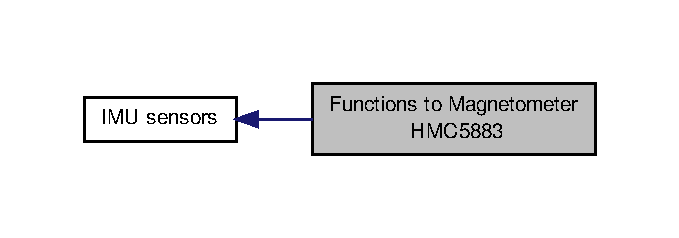
\includegraphics[width=326pt]{group__mag}
\end{center}
\end{figure}
\subsection*{Functions}
\begin{DoxyCompactItemize}
\item 
uint8\-\_\-t $\ast$ \hyperlink{group__mag_ga6830eaeae2298320e1e8c902e4edd709}{mag\-\_\-read\-\_\-reg} (int \hyperlink{CommunicationV0_2communication_8c_a7751bd45ac1064efb35adf1f19c25db8}{i2c\-\_\-dev}, uint8\-\_\-t reg, uint8\-\_\-t count)
\begin{DoxyCompactList}\small\item\em R\-E\-A\-D C\-O\-U\-N\-T 8-\/\-B\-I\-T R\-E\-G\-I\-S\-T\-E\-R I\-N S\-E\-Q\-U\-E\-N\-C\-E. \end{DoxyCompactList}\item 
int \hyperlink{group__mag_gab42ae0d0a2a6f37cf36d856c072b7f34}{mag\-\_\-read\-\_\-all\-\_\-data} (int \hyperlink{CommunicationV0_2communication_8c_a7751bd45ac1064efb35adf1f19c25db8}{i2c\-\_\-dev}, short int $\ast$data)
\begin{DoxyCompactList}\small\item\em R\-E\-A\-D A\-L\-L D\-A\-T\-A A\-T O\-N\-C\-E (X, Y and Z) \end{DoxyCompactList}\item 
short int \hyperlink{group__mag_ga542a31ccd07cd2c3e8e2b68cdb6d219e}{mag\-\_\-read\-\_\-data} (int \hyperlink{CommunicationV0_2communication_8c_a7751bd45ac1064efb35adf1f19c25db8}{i2c\-\_\-dev}, int axis)
\begin{DoxyCompactList}\small\item\em R\-E\-A\-D D\-A\-T\-A (X, Y or Z) \end{DoxyCompactList}\end{DoxyCompactItemize}


\subsection{Detailed Description}


\subsection{Function Documentation}
\hypertarget{group__mag_gab42ae0d0a2a6f37cf36d856c072b7f34}{\index{Functions to Magnetometer H\-M\-C5883@{Functions to Magnetometer H\-M\-C5883}!mag\-\_\-read\-\_\-all\-\_\-data@{mag\-\_\-read\-\_\-all\-\_\-data}}
\index{mag\-\_\-read\-\_\-all\-\_\-data@{mag\-\_\-read\-\_\-all\-\_\-data}!Functions to Magnetometer HMC5883@{Functions to Magnetometer H\-M\-C5883}}
\subsubsection[{mag\-\_\-read\-\_\-all\-\_\-data}]{\setlength{\rightskip}{0pt plus 5cm}int mag\-\_\-read\-\_\-all\-\_\-data (
\begin{DoxyParamCaption}
\item[{int}]{i2c\-\_\-dev, }
\item[{short int $\ast$}]{data}
\end{DoxyParamCaption}
)}}\label{group__mag_gab42ae0d0a2a6f37cf36d856c072b7f34}


R\-E\-A\-D A\-L\-L D\-A\-T\-A A\-T O\-N\-C\-E (X, Y and Z) 


\begin{DoxyParams}[1]{Parameters}
 & {\em i2c\-\_\-dev} & \\
\hline
\mbox{\tt out}  & {\em $\ast$data} & \\
\hline
\end{DoxyParams}


Definition at line 121 of file mag\-\_\-functions.\-c.



Referenced by read\-\_\-all\-\_\-data().


\begin{DoxyCode}
122 \{
123   uint8\_t i, j;
124   uint8\_t *data8;
125   \textcolor{keyword}{union }result
126   \{
127     \textcolor{keywordtype}{unsigned} \textcolor{keywordtype}{short} \textcolor{keywordtype}{int} usgnd[3];
128     \textcolor{keywordtype}{short} \textcolor{keywordtype}{int} sgnd[3];
129   \} result;
130   \textcolor{comment}{//result=(union result*)malloc(3*sizeof(union result));}
131   \textcolor{keywordflow}{if}( (data8=\hyperlink{group__mag_ga6830eaeae2298320e1e8c902e4edd709}{mag\_read\_reg}(\hyperlink{CommunicationV0_2communication_8c_a7751bd45ac1064efb35adf1f19c25db8}{i2c\_dev},\hyperlink{communication_2imu__regs_8h_a4f883328e7ae117996e334145ddd0032}{MAG\_DATAX1},6))==NULL)
132   \{
133     \textcolor{comment}{//perror("Read accelerometer register failed");}
134     \textcolor{keywordflow}{return} \hyperlink{calibration_2calibration_8h_a6d58f9ac447476b4e084d7ca383f5183}{FAILURE};
135   \}
136   \textcolor{comment}{//result.usgnd=(unsigned int*)malloc(3*sizeof(unsigned int));}
137   j=0;
138   \textcolor{keywordflow}{for}(i=0; i<3; i++)
139   \{
140     result.usgnd[j]=0;
141     result.usgnd[j]=result.usgnd[j]|((\textcolor{keywordtype}{unsigned} \textcolor{keywordtype}{short} int)data8[i*2+1])|(((\textcolor{keywordtype}{unsigned} int)data8[i*2])<<8);
142     data[j]=result.sgnd[j];
143     j=2-i; \textcolor{comment}{// trick used to change the sorting of the data from XZY to XYZ}
144   \}
145   \textcolor{keywordflow}{return} \hyperlink{calibration_2calibration_8h_aa90cac659d18e8ef6294c7ae337f6b58}{SUCCESS};  
146 \}
\end{DoxyCode}


Here is the caller graph for this function\-:
\nopagebreak
\begin{figure}[H]
\begin{center}
\leavevmode
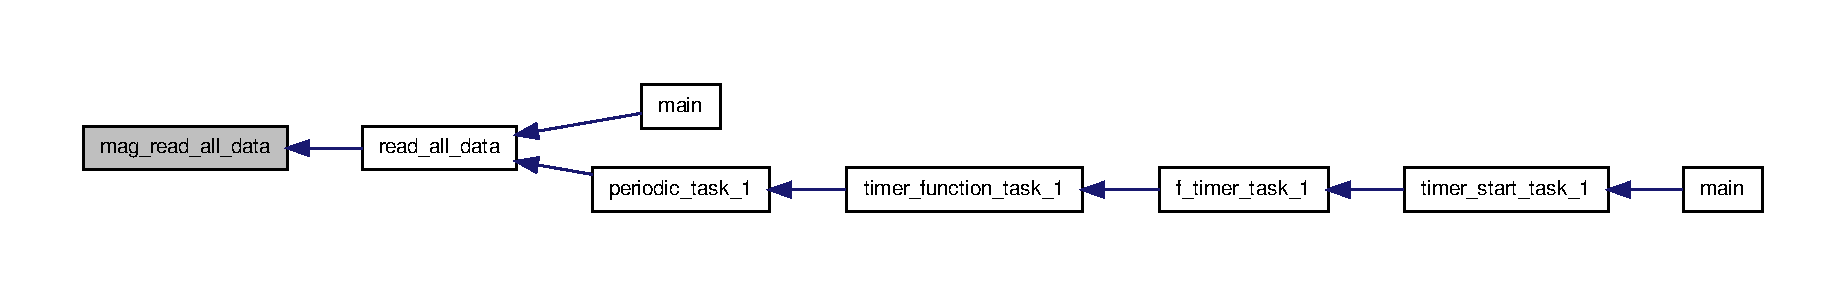
\includegraphics[width=350pt]{group__mag_gab42ae0d0a2a6f37cf36d856c072b7f34_icgraph}
\end{center}
\end{figure}


\hypertarget{group__mag_ga542a31ccd07cd2c3e8e2b68cdb6d219e}{\index{Functions to Magnetometer H\-M\-C5883@{Functions to Magnetometer H\-M\-C5883}!mag\-\_\-read\-\_\-data@{mag\-\_\-read\-\_\-data}}
\index{mag\-\_\-read\-\_\-data@{mag\-\_\-read\-\_\-data}!Functions to Magnetometer HMC5883@{Functions to Magnetometer H\-M\-C5883}}
\subsubsection[{mag\-\_\-read\-\_\-data}]{\setlength{\rightskip}{0pt plus 5cm}short int mag\-\_\-read\-\_\-data (
\begin{DoxyParamCaption}
\item[{int}]{i2c\-\_\-dev, }
\item[{int}]{axis}
\end{DoxyParamCaption}
)}}\label{group__mag_ga542a31ccd07cd2c3e8e2b68cdb6d219e}


R\-E\-A\-D D\-A\-T\-A (X, Y or Z) 


\begin{DoxyParams}{Parameters}
{\em i2c\-\_\-dev} & \\
\hline
{\em axis} & set the axis ('X' or 'Y' or 'Z') \\
\hline
\end{DoxyParams}


Definition at line 148 of file mag\-\_\-functions.\-c.


\begin{DoxyCode}
149 \{
150   uint8\_t *data;
151   \textcolor{keyword}{union }result
152   \{
153     \textcolor{keywordtype}{unsigned} \textcolor{keywordtype}{int} usgnd;
154     \textcolor{keywordtype}{int} sgnd;
155   \}result;
156 
157   \textcolor{keywordflow}{switch}(axis)\{
158     \textcolor{keywordflow}{case} \textcolor{charliteral}{'X'}:
159       data=\hyperlink{group__mag_ga6830eaeae2298320e1e8c902e4edd709}{mag\_read\_reg}(\hyperlink{CommunicationV0_2communication_8c_a7751bd45ac1064efb35adf1f19c25db8}{i2c\_dev},\hyperlink{communication_2imu__regs_8h_a4f883328e7ae117996e334145ddd0032}{MAG\_DATAX1},2);
160       \textcolor{keywordflow}{break};
161     \textcolor{keywordflow}{case} \textcolor{charliteral}{'Y'}:
162       data=\hyperlink{group__mag_ga6830eaeae2298320e1e8c902e4edd709}{mag\_read\_reg}(\hyperlink{CommunicationV0_2communication_8c_a7751bd45ac1064efb35adf1f19c25db8}{i2c\_dev},\hyperlink{communication_2imu__regs_8h_ae218906702b1e40c2b6970f97dd0cfe4}{MAG\_DATAY1},2);
163       \textcolor{keywordflow}{break};
164     \textcolor{keywordflow}{case} \textcolor{charliteral}{'Z'}:
165       data=\hyperlink{group__mag_ga6830eaeae2298320e1e8c902e4edd709}{mag\_read\_reg}(\hyperlink{CommunicationV0_2communication_8c_a7751bd45ac1064efb35adf1f19c25db8}{i2c\_dev},\hyperlink{communication_2imu__regs_8h_a81d7d9236ec69a1a229e4fa7c6299fde}{MAG\_DATAZ1},2);
166       \textcolor{keywordflow}{break};
167     \textcolor{keywordflow}{default}:
168       \textcolor{comment}{//perror("Wrong argument for axis in mag\_read\_data");}
169       \textcolor{keywordflow}{return} -1;
170   \}
171   result.usgnd=0;
172   result.usgnd=result.usgnd|(((\textcolor{keywordtype}{unsigned} \textcolor{keywordtype}{short} int)data[1]))|(((\textcolor{keywordtype}{unsigned} \textcolor{keywordtype}{short} \textcolor{keywordtype}{int})data[0])<<8);
173   \textcolor{keywordflow}{return} result.sgnd;
174 \}
\end{DoxyCode}
\hypertarget{group__mag_ga6830eaeae2298320e1e8c902e4edd709}{\index{Functions to Magnetometer H\-M\-C5883@{Functions to Magnetometer H\-M\-C5883}!mag\-\_\-read\-\_\-reg@{mag\-\_\-read\-\_\-reg}}
\index{mag\-\_\-read\-\_\-reg@{mag\-\_\-read\-\_\-reg}!Functions to Magnetometer HMC5883@{Functions to Magnetometer H\-M\-C5883}}
\subsubsection[{mag\-\_\-read\-\_\-reg}]{\setlength{\rightskip}{0pt plus 5cm}uint8\-\_\-t$\ast$ mag\-\_\-read\-\_\-reg (
\begin{DoxyParamCaption}
\item[{int}]{i2c\-\_\-dev, }
\item[{uint8\-\_\-t}]{reg, }
\item[{uint8\-\_\-t}]{count}
\end{DoxyParamCaption}
)}}\label{group__mag_ga6830eaeae2298320e1e8c902e4edd709}


R\-E\-A\-D C\-O\-U\-N\-T 8-\/\-B\-I\-T R\-E\-G\-I\-S\-T\-E\-R I\-N S\-E\-Q\-U\-E\-N\-C\-E. 


\begin{DoxyParams}{Parameters}
{\em i2c\-\_\-dev} & \\
\hline
{\em reg} & \\
\hline
{\em count} & number of registers in sequence (1-\/13) \\
\hline
\end{DoxyParams}


Definition at line 31 of file mag\-\_\-functions.\-c.



Referenced by mag\-\_\-read\-\_\-all\-\_\-data(), and mag\-\_\-read\-\_\-data().


\begin{DoxyCode}
32 \{
33   uint8\_t data[13];
34   \textcolor{keywordtype}{int} i;
35 
36   \textcolor{comment}{//data=(uint8\_t*)malloc((count+1)*sizeof(data));}
37   
38   data[0] = reg;
39 
40   \textcolor{keywordflow}{if} (write(\hyperlink{CommunicationV0_2communication_8c_a7751bd45ac1064efb35adf1f19c25db8}{i2c\_dev}, &data, 1) != 1) \{            
41         \textcolor{comment}{//perror("write before read");}
42         \textcolor{keywordflow}{return} NULL;
43   \}
44   data[0] = 0;
45   \textcolor{keywordflow}{if} (read(\hyperlink{CommunicationV0_2communication_8c_a7751bd45ac1064efb35adf1f19c25db8}{i2c\_dev}, &data, count) != count) \{
46         \textcolor{comment}{//perror("read");}
47         \textcolor{keywordflow}{return} NULL;    
48   \}
49 
50   \textcolor{keywordflow}{return} data;
51 \}
\end{DoxyCode}


Here is the caller graph for this function\-:\nopagebreak
\begin{figure}[H]
\begin{center}
\leavevmode
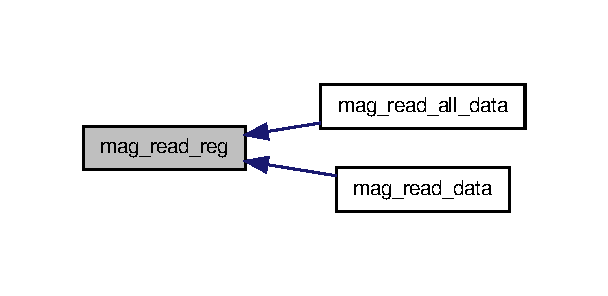
\includegraphics[width=292pt]{group__mag_ga6830eaeae2298320e1e8c902e4edd709_icgraph}
\end{center}
\end{figure}



\chapter{Data Structure Documentation}
\hypertarget{structIMU__DATA__STRUCT_1_1calibrated}{\section{I\-M\-U\-\_\-\-D\-A\-T\-A\-\_\-\-S\-T\-R\-U\-C\-T\-:\-:calibrated Struct Reference}
\label{structIMU__DATA__STRUCT_1_1calibrated}\index{I\-M\-U\-\_\-\-D\-A\-T\-A\-\_\-\-S\-T\-R\-U\-C\-T\-::calibrated@{I\-M\-U\-\_\-\-D\-A\-T\-A\-\_\-\-S\-T\-R\-U\-C\-T\-::calibrated}}
}


{\ttfamily \#include \char`\"{}communication.\-h\char`\"{}}



Collaboration diagram for I\-M\-U\-\_\-\-D\-A\-T\-A\-\_\-\-S\-T\-R\-U\-C\-T\-:\-:calibrated\-:\nopagebreak
\begin{figure}[H]
\begin{center}
\leavevmode
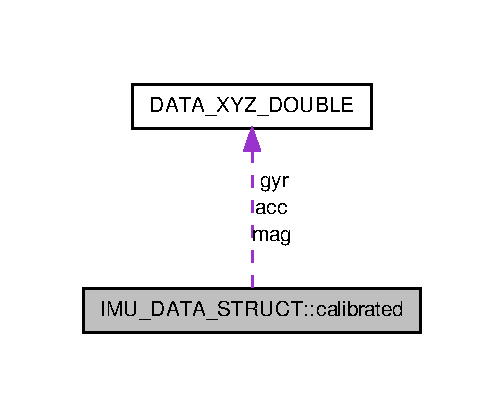
\includegraphics[width=242pt]{structIMU__DATA__STRUCT_1_1calibrated__coll__graph}
\end{center}
\end{figure}
\subsection*{Data Fields}
\begin{DoxyCompactItemize}
\item 
\hyperlink{structDATA__XYZ__DOUBLE}{D\-A\-T\-A\-\_\-\-X\-Y\-Z\-\_\-\-D\-O\-U\-B\-L\-E} \hyperlink{structIMU__DATA__STRUCT_1_1calibrated_a281a7fdb40a05ed97388f18b9bb90c81}{acc}
\item 
\hyperlink{structDATA__XYZ__DOUBLE}{D\-A\-T\-A\-\_\-\-X\-Y\-Z\-\_\-\-D\-O\-U\-B\-L\-E} \hyperlink{structIMU__DATA__STRUCT_1_1calibrated_a8a54aded6ce608f1b7d2b4a0c52c248b}{gyr}
\item 
\hyperlink{structDATA__XYZ__DOUBLE}{D\-A\-T\-A\-\_\-\-X\-Y\-Z\-\_\-\-D\-O\-U\-B\-L\-E} \hyperlink{structIMU__DATA__STRUCT_1_1calibrated_a2fde6c6759e0fda17e272c32096cb9ec}{mag}
\end{DoxyCompactItemize}


\subsection{Detailed Description}


Definition at line 94 of file communication.\-h.



\subsection{Field Documentation}
\hypertarget{structIMU__DATA__STRUCT_1_1calibrated_a281a7fdb40a05ed97388f18b9bb90c81}{\index{I\-M\-U\-\_\-\-D\-A\-T\-A\-\_\-\-S\-T\-R\-U\-C\-T\-::calibrated@{I\-M\-U\-\_\-\-D\-A\-T\-A\-\_\-\-S\-T\-R\-U\-C\-T\-::calibrated}!acc@{acc}}
\index{acc@{acc}!IMU_DATA_STRUCT::calibrated@{I\-M\-U\-\_\-\-D\-A\-T\-A\-\_\-\-S\-T\-R\-U\-C\-T\-::calibrated}}
\subsubsection[{acc}]{\setlength{\rightskip}{0pt plus 5cm}{\bf D\-A\-T\-A\-\_\-\-X\-Y\-Z\-\_\-\-D\-O\-U\-B\-L\-E} I\-M\-U\-\_\-\-D\-A\-T\-A\-\_\-\-S\-T\-R\-U\-C\-T\-::calibrated\-::acc}}\label{structIMU__DATA__STRUCT_1_1calibrated_a281a7fdb40a05ed97388f18b9bb90c81}


Definition at line 95 of file communication.\-h.



Referenced by calibrate\-\_\-imu(), datalogger\-\_\-update(), ui\-\_\-imu\-\_\-data(), and ui\-\_\-overview\-\_\-data().

\hypertarget{structIMU__DATA__STRUCT_1_1calibrated_a8a54aded6ce608f1b7d2b4a0c52c248b}{\index{I\-M\-U\-\_\-\-D\-A\-T\-A\-\_\-\-S\-T\-R\-U\-C\-T\-::calibrated@{I\-M\-U\-\_\-\-D\-A\-T\-A\-\_\-\-S\-T\-R\-U\-C\-T\-::calibrated}!gyr@{gyr}}
\index{gyr@{gyr}!IMU_DATA_STRUCT::calibrated@{I\-M\-U\-\_\-\-D\-A\-T\-A\-\_\-\-S\-T\-R\-U\-C\-T\-::calibrated}}
\subsubsection[{gyr}]{\setlength{\rightskip}{0pt plus 5cm}{\bf D\-A\-T\-A\-\_\-\-X\-Y\-Z\-\_\-\-D\-O\-U\-B\-L\-E} I\-M\-U\-\_\-\-D\-A\-T\-A\-\_\-\-S\-T\-R\-U\-C\-T\-::calibrated\-::gyr}}\label{structIMU__DATA__STRUCT_1_1calibrated_a8a54aded6ce608f1b7d2b4a0c52c248b}


Definition at line 96 of file communication.\-h.



Referenced by calibrate\-\_\-imu(), datalogger\-\_\-update(), ui\-\_\-imu\-\_\-data(), and ui\-\_\-overview\-\_\-data().

\hypertarget{structIMU__DATA__STRUCT_1_1calibrated_a2fde6c6759e0fda17e272c32096cb9ec}{\index{I\-M\-U\-\_\-\-D\-A\-T\-A\-\_\-\-S\-T\-R\-U\-C\-T\-::calibrated@{I\-M\-U\-\_\-\-D\-A\-T\-A\-\_\-\-S\-T\-R\-U\-C\-T\-::calibrated}!mag@{mag}}
\index{mag@{mag}!IMU_DATA_STRUCT::calibrated@{I\-M\-U\-\_\-\-D\-A\-T\-A\-\_\-\-S\-T\-R\-U\-C\-T\-::calibrated}}
\subsubsection[{mag}]{\setlength{\rightskip}{0pt plus 5cm}{\bf D\-A\-T\-A\-\_\-\-X\-Y\-Z\-\_\-\-D\-O\-U\-B\-L\-E} I\-M\-U\-\_\-\-D\-A\-T\-A\-\_\-\-S\-T\-R\-U\-C\-T\-::calibrated\-::mag}}\label{structIMU__DATA__STRUCT_1_1calibrated_a2fde6c6759e0fda17e272c32096cb9ec}


Definition at line 97 of file communication.\-h.



Referenced by calibrate\-\_\-imu(), datalogger\-\_\-update(), ui\-\_\-imu\-\_\-data(), and ui\-\_\-overview\-\_\-data().



The documentation for this struct was generated from the following file\-:\begin{DoxyCompactItemize}
\item 
communication/\hyperlink{communication_2communication_8h}{communication.\-h}\end{DoxyCompactItemize}

\hypertarget{classCartesian__controller}{\section{Cartesian\-\_\-controller Class Reference}
\label{classCartesian__controller}\index{Cartesian\-\_\-controller@{Cartesian\-\_\-controller}}
}


{\ttfamily \#include \char`\"{}cartesian\-\_\-controller.\-h\char`\"{}}



Inheritance diagram for Cartesian\-\_\-controller\-:\nopagebreak
\begin{figure}[H]
\begin{center}
\leavevmode
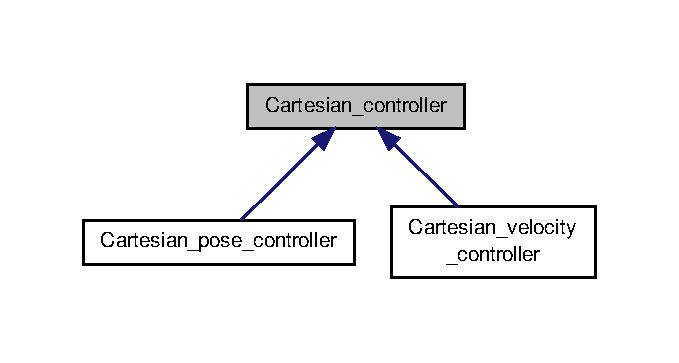
\includegraphics[width=326pt]{classCartesian__controller__inherit__graph}
\end{center}
\end{figure}


Collaboration diagram for Cartesian\-\_\-controller\-:\nopagebreak
\begin{figure}[H]
\begin{center}
\leavevmode
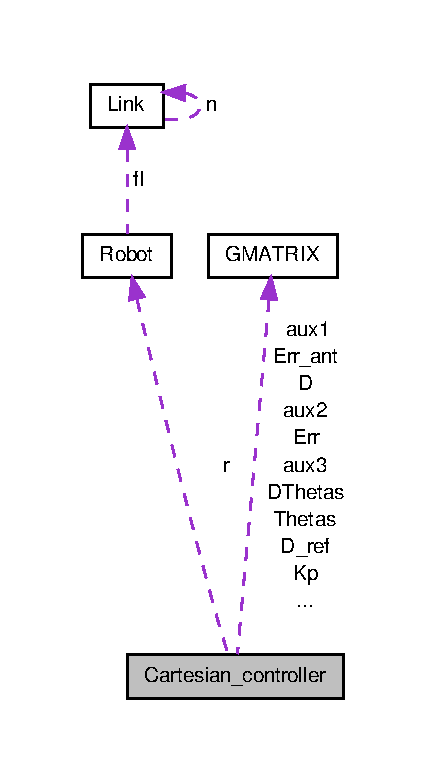
\includegraphics[width=206pt]{classCartesian__controller__coll__graph}
\end{center}
\end{figure}
\subsection*{Public Member Functions}
\begin{DoxyCompactItemize}
\item 
\hyperlink{classCartesian__controller_a71055bb1cbf01ced9e64bb1d184b68fe}{Cartesian\-\_\-controller} (\hyperlink{structRobot}{Robot} $\ast$\hyperlink{classCartesian__controller_a5562129951bd802e4ded77fc716c87a0}{r}, int ref\-Size, double K\-P\mbox{[}$\,$\mbox{]}, double K\-I\mbox{[}$\,$\mbox{]}, double K\-D\mbox{[}$\,$\mbox{]}, double \hyperlink{classCartesian__controller_a35c6ddbb9624878f2807ff644a33e832}{T})
\item 
\hyperlink{classCartesian__controller_ac29863d92d56a5998ba39ddb58f4a09e}{$\sim$\-Cartesian\-\_\-controller} ()
\item 
virtual void \hyperlink{classCartesian__controller_a8809167cab6d338a957439141fa2bf6c}{control} ()=0
\end{DoxyCompactItemize}
\subsection*{Data Fields}
\begin{DoxyCompactItemize}
\item 
\hyperlink{structRobot}{Robot} $\ast$ \hyperlink{classCartesian__controller_a5562129951bd802e4ded77fc716c87a0}{r}
\end{DoxyCompactItemize}
\subsection*{Protected Member Functions}
\begin{DoxyCompactItemize}
\item 
bool \hyperlink{classCartesian__controller_aaf006f80e89c08cf040956afbb4cf3c0}{change\-Schunk\-Mode} (int mode)
\begin{DoxyCompactList}\small\item\em Other packages. \end{DoxyCompactList}\item 
bool \hyperlink{classCartesian__controller_a0d7a63bac84715f6742db738df246f91}{get\-Schunk\-Positions\-And\-Velocities\-And\-Update\-Thetas\-And\-D\-Thetas} ()
\begin{DoxyCompactList}\small\item\em Asks Schunk's its joint's positions and velocities, them it updates the internal P\-G\-M\-A\-T\-R\-I\-Xs Theta and D\-Thetas. \end{DoxyCompactList}\item 
void \hyperlink{classCartesian__controller_a40d17a9794af8a9a607618bf0ee5efff}{set\-Schunk\-Velocities\-And\-Send} (double sat\-\_\-vel)
\begin{DoxyCompactList}\small\item\em Updates the Schunk velocities msg to be sent to Schunk, but not before saturating it. \end{DoxyCompactList}\item 
void \hyperlink{classCartesian__controller_ae845f67c81c2649bfbaccf95230f2599}{send\-Joint\-Positions\-To\-Schunk} (std\-::vector$<$ double $>$ positions)
\item 
bool \hyperlink{classCartesian__controller_a3ba54e8b35632526c5e8eb2ab5d7de0d}{stop\-Schunk} ()
\item 
void \hyperlink{classCartesian__controller_a8c0f0b41de9f4f8b2e3aa327e7c6b50c}{control\-Clean\-Up} ()
\begin{DoxyCompactList}\small\item\em De-\/allocs unfreed matrices in the end of the control loop. \end{DoxyCompactList}\end{DoxyCompactItemize}
\subsection*{Protected Attributes}
\begin{DoxyCompactItemize}
\item 
int \hyperlink{classCartesian__controller_ab9ed5a808da204dbc612d313dc7332f4}{ros\-\_\-pub\-\_\-buffer}
\item 
bool \hyperlink{classCartesian__controller_a3c0a72214891f68e2bad63bf2b688f9c}{end\-\_\-control}
\item 
ros\-::\-Node\-Handle \hyperlink{classCartesian__controller_ad90134b232217e84cb58137a9d2030bb}{schunk\-\_\-low\-\_\-mode\-Changer\-\_\-nh}
\item 
ros\-::\-Callback\-Queue \hyperlink{classCartesian__controller_adf47dc3a09bd9650015b25870054b60d}{mode\-Changer\-\_\-queue}
\item 
ros\-::\-Service\-Client \hyperlink{classCartesian__controller_aee1fc445b64c534847ff0012132a5d2c}{schunk\-\_\-mode\-Changer\-\_\-client}
\item 
schunk\-\_\-low\-::\-Control\-Mode \hyperlink{classCartesian__controller_a960d66580ba058d3337c89bdf8099948}{schunk\-\_\-mode\-Changer\-\_\-msg}
\item 
ros\-::\-Node\-Handle \hyperlink{classCartesian__controller_aeed01809bd5240663c7acfade245a386}{schunk\-\_\-low\-\_\-pos\-Vel\-Getter\-\_\-nh}
\item 
ros\-::\-Callback\-Queue \hyperlink{classCartesian__controller_a144c7faad45f3d070624452c1f02ba15}{pos\-Vel\-Getter\-\_\-queue}
\item 
ros\-::\-Service\-Client \hyperlink{classCartesian__controller_a5c1d9386bc5f219f2edc0d5d1b21f0da}{schunk\-\_\-pos\-Vel\-Getter\-\_\-client}
\item 
schunk\-\_\-low\-::\-Get\-Pos\-Vel \hyperlink{classCartesian__controller_ae368dcf84dae528612c617cc92fbb69f}{schunk\-\_\-pos\-Vel\-Getter\-\_\-msg}
\item 
ros\-::\-Node\-Handle \hyperlink{classCartesian__controller_a7df4ce63bf0551bfa7061bc718cd68d2}{schunk\-\_\-low\-\_\-publisher\-\_\-nh}
\item 
ros\-::\-Callback\-Queue \hyperlink{classCartesian__controller_a041a2eb6657c9b036a512fb21e9f5086}{publisher\-\_\-queue}
\item 
ros\-::\-Publisher \hyperlink{classCartesian__controller_aa6ce9cffdd307127ed814d6e5132eba2}{schunk\-\_\-low\-\_\-pub}
\item 
schunk\-\_\-msgs\-::\-Velocities \hyperlink{classCartesian__controller_af59178c57bdd73d9eb474577247bbe40}{schunk\-\_\-low\-\_\-velocities\-\_\-msg}
\item 
ros\-::\-Node\-Handle \hyperlink{classCartesian__controller_aabe48e7ab08b0235d4cd94213b8faf5d}{schunk\-\_\-low\-\_\-pos\-\_\-publisher\-\_\-nh}
\item 
ros\-::\-Callback\-Queue \hyperlink{classCartesian__controller_adbb9cddf4092cba9042294740c5371eb}{pos\-\_\-publisher\-\_\-queue}
\item 
ros\-::\-Publisher \hyperlink{classCartesian__controller_af06313084ef058d1f979fddeb33d5100}{schunk\-\_\-low\-\_\-pos\-\_\-pub}
\item 
schunk\-\_\-msgs\-::\-Positions \hyperlink{classCartesian__controller_a2dd700542bd6243eef10d34811055584}{schunk\-\_\-low\-\_\-positions\-\_\-msg}
\item 
ros\-::\-Node\-Handle \hyperlink{classCartesian__controller_a57b1869ec960e75e435e1f882a02d80e}{schunk\-\_\-low\-\_\-stopper\-\_\-nh}
\item 
ros\-::\-Callback\-Queue \hyperlink{classCartesian__controller_a52eb090400d8dafaa22aecb037788a66}{stopper\-\_\-queue}
\item 
ros\-::\-Service\-Client \hyperlink{classCartesian__controller_a4ea7350e0f797c49bc51d3433a761aff}{schunk\-\_\-stopper\-\_\-client}
\item 
schunk\-\_\-low\-::\-Stop \hyperlink{classCartesian__controller_a29581ed2f2d8bb97c55e16868bbcc8bd}{schunk\-\_\-stopper\-\_\-msg}
\item 
\hyperlink{gmatrix_8h_ad8edc274a17feb9e4fca93e620253bed}{P\-G\-M\-A\-T\-R\-I\-X} \hyperlink{classCartesian__controller_a98fdac06d136ac3dba0102d97cd5dd36}{S\-J}
\item 
\hyperlink{gmatrix_8h_ad8edc274a17feb9e4fca93e620253bed}{P\-G\-M\-A\-T\-R\-I\-X} \hyperlink{classCartesian__controller_a78073f51064a05d72c41723a93d9079f}{Kp}
\item 
\hyperlink{gmatrix_8h_ad8edc274a17feb9e4fca93e620253bed}{P\-G\-M\-A\-T\-R\-I\-X} \hyperlink{classCartesian__controller_a70e495f39da706f1b589684f58343b9e}{Ki}
\item 
\hyperlink{gmatrix_8h_ad8edc274a17feb9e4fca93e620253bed}{P\-G\-M\-A\-T\-R\-I\-X} \hyperlink{classCartesian__controller_a62394cef8a9a29eac18319a4ad579c4c}{Kd}
\item 
\hyperlink{gmatrix_8h_ad8edc274a17feb9e4fca93e620253bed}{P\-G\-M\-A\-T\-R\-I\-X} \hyperlink{classCartesian__controller_a0a0f818dad601cd9e3e26cb6959b8eb6}{Thetas}
\item 
\hyperlink{gmatrix_8h_ad8edc274a17feb9e4fca93e620253bed}{P\-G\-M\-A\-T\-R\-I\-X} \hyperlink{classCartesian__controller_a5d6419e62e130150edfcbd82b1dadcae}{D\-Thetas}
\item 
\hyperlink{gmatrix_8h_ad8edc274a17feb9e4fca93e620253bed}{P\-G\-M\-A\-T\-R\-I\-X} \hyperlink{classCartesian__controller_abb248cb3215a574fe8e1bb8fb0b8626d}{D\-\_\-ref}
\item 
\hyperlink{gmatrix_8h_ad8edc274a17feb9e4fca93e620253bed}{P\-G\-M\-A\-T\-R\-I\-X} \hyperlink{classCartesian__controller_a8c470b652ce436d8e48f126073fc2593}{D}
\item 
\hyperlink{gmatrix_8h_ad8edc274a17feb9e4fca93e620253bed}{P\-G\-M\-A\-T\-R\-I\-X} \hyperlink{classCartesian__controller_ab3f08ecf10cb2486e8bfc61f07e2bde6}{Err}
\item 
\hyperlink{gmatrix_8h_ad8edc274a17feb9e4fca93e620253bed}{P\-G\-M\-A\-T\-R\-I\-X} \hyperlink{classCartesian__controller_a6d9471a983f6cb6c642bf8dea0d540af}{Err\-\_\-ant}
\item 
\hyperlink{gmatrix_8h_ad8edc274a17feb9e4fca93e620253bed}{P\-G\-M\-A\-T\-R\-I\-X} \hyperlink{classCartesian__controller_a248174c6399a8933bfcc8f1b0b39af5e}{Err\-\_\-int}
\item 
\hyperlink{gmatrix_8h_ad8edc274a17feb9e4fca93e620253bed}{P\-G\-M\-A\-T\-R\-I\-X} \hyperlink{classCartesian__controller_a37edb9c6e2a5066f74941e3659f68cbc}{aux1}
\item 
\hyperlink{gmatrix_8h_ad8edc274a17feb9e4fca93e620253bed}{P\-G\-M\-A\-T\-R\-I\-X} \hyperlink{classCartesian__controller_af73a0c910cd80ed2f84974b65beba450}{aux2}
\item 
\hyperlink{gmatrix_8h_ad8edc274a17feb9e4fca93e620253bed}{P\-G\-M\-A\-T\-R\-I\-X} \hyperlink{classCartesian__controller_aa37c15fcd53a60ecce106cd9b39d3501}{aux3}
\item 
double \hyperlink{classCartesian__controller_a35c6ddbb9624878f2807ff644a33e832}{T}
\end{DoxyCompactItemize}


\subsection{Detailed Description}


Definition at line 8 of file cartesian\-\_\-controller.\-h.



\subsection{Constructor \& Destructor Documentation}
\hypertarget{classCartesian__controller_a71055bb1cbf01ced9e64bb1d184b68fe}{\index{Cartesian\-\_\-controller@{Cartesian\-\_\-controller}!Cartesian\-\_\-controller@{Cartesian\-\_\-controller}}
\index{Cartesian\-\_\-controller@{Cartesian\-\_\-controller}!Cartesian_controller@{Cartesian\-\_\-controller}}
\subsubsection[{Cartesian\-\_\-controller}]{\setlength{\rightskip}{0pt plus 5cm}Cartesian\-\_\-controller\-::\-Cartesian\-\_\-controller (
\begin{DoxyParamCaption}
\item[{{\bf Robot} $\ast$}]{r, }
\item[{int}]{ref\-Size, }
\item[{double}]{K\-P\mbox{[}$\,$\mbox{]}, }
\item[{double}]{K\-I\mbox{[}$\,$\mbox{]}, }
\item[{double}]{K\-D\mbox{[}$\,$\mbox{]}, }
\item[{double}]{T}
\end{DoxyParamCaption}
)}}\label{classCartesian__controller_a71055bb1cbf01ced9e64bb1d184b68fe}


Definition at line 174 of file cartesian\-\_\-controller.\-cpp.



References aux1, aux2, aux3, D, D\-\_\-ref, Robot\-::dofs, D\-Thetas, end\-\_\-control, Err, Err\-\_\-ant, Err\-\_\-int, Kd, Ki, Kp, mode\-Changer\-\_\-queue, P\-G\-M\-A\-T\-R\-I\-X\-\_\-\-C\-R\-E\-A\-T\-E\-\_\-\-D\-I\-A\-G\-\_\-\-F\-R\-O\-M\-\_\-\-A\-R\-R\-A\-Y(), P\-G\-M\-A\-T\-R\-I\-X\-\_\-\-C\-R\-E\-A\-T\-E\-\_\-\-Z\-E\-R\-O\-E\-S(), pos\-\_\-publisher\-\_\-queue, pos\-Vel\-Getter\-\_\-queue, publisher\-\_\-queue, r, ros\-\_\-pub\-\_\-buffer, schunk\-\_\-low\-\_\-mode\-Changer\-\_\-nh, schunk\-\_\-low\-\_\-pos\-\_\-pub, schunk\-\_\-low\-\_\-pos\-\_\-publisher\-\_\-nh, schunk\-\_\-low\-\_\-positions\-\_\-msg, schunk\-\_\-low\-\_\-pos\-Vel\-Getter\-\_\-nh, schunk\-\_\-low\-\_\-pub, schunk\-\_\-low\-\_\-publisher\-\_\-nh, schunk\-\_\-low\-\_\-stopper\-\_\-nh, schunk\-\_\-low\-\_\-velocities\-\_\-msg, schunk\-\_\-mode\-Changer\-\_\-client, schunk\-\_\-pos\-Vel\-Getter\-\_\-client, schunk\-\_\-stopper\-\_\-client, S\-J, stopper\-\_\-queue, T, and Thetas.


\begin{DoxyCode}
                                                                               
                                       \{

        \textcolor{comment}{/******************************}
\textcolor{comment}{                 VARIABLES}
\textcolor{comment}{        *******************************/}

        this->r = \hyperlink{classCartesian__controller_a5562129951bd802e4ded77fc716c87a0}{r};
        this->\hyperlink{classCartesian__controller_a3c0a72214891f68e2bad63bf2b688f9c}{end\_control} = \textcolor{keyword}{false};

        \textcolor{comment}{/******************************}
\textcolor{comment}{                  ROS VARIABLES}
\textcolor{comment}{        *******************************/}

        \textcolor{comment}{//Consts (No reason having a queue)}
        \hyperlink{classCartesian__controller_ab9ed5a808da204dbc612d313dc7332f4}{ros\_pub\_buffer} = 1;

        \textcolor{comment}{//Set Queues}
        this->\hyperlink{classCartesian__controller_ad90134b232217e84cb58137a9d2030bb}{schunk\_low\_modeChanger\_nh}.
      setCallbackQueue(&this->\hyperlink{classCartesian__controller_adf47dc3a09bd9650015b25870054b60d}{modeChanger\_queue});
        this->\hyperlink{classCartesian__controller_aeed01809bd5240663c7acfade245a386}{schunk\_low\_posVelGetter\_nh}.
      setCallbackQueue(&this->\hyperlink{classCartesian__controller_a144c7faad45f3d070624452c1f02ba15}{posVelGetter\_queue});
        this->\hyperlink{classCartesian__controller_a57b1869ec960e75e435e1f882a02d80e}{schunk\_low\_stopper\_nh}.setCallbackQueue(&
      this->\hyperlink{classCartesian__controller_a52eb090400d8dafaa22aecb037788a66}{stopper\_queue});

        this->\hyperlink{classCartesian__controller_aabe48e7ab08b0235d4cd94213b8faf5d}{schunk\_low\_pos\_publisher\_nh}.
      setCallbackQueue(&this->\hyperlink{classCartesian__controller_adbb9cddf4092cba9042294740c5371eb}{pos\_publisher\_queue});
        this->\hyperlink{classCartesian__controller_a7df4ce63bf0551bfa7061bc718cd68d2}{schunk\_low\_publisher\_nh}.setCallbackQueue(&
      this->\hyperlink{classCartesian__controller_a041a2eb6657c9b036a512fb21e9f5086}{publisher\_queue});

        \textcolor{comment}{//Publisher}
        this->\hyperlink{classCartesian__controller_aa6ce9cffdd307127ed814d6e5132eba2}{schunk\_low\_pub}                       = this->
      \hyperlink{classCartesian__controller_a7df4ce63bf0551bfa7061bc718cd68d2}{schunk\_low\_publisher\_nh}.advertise<
      schunk\_msgs::Velocities>(\textcolor{stringliteral}{"schunk\_velocities\_control"}, \hyperlink{classCartesian__controller_ab9ed5a808da204dbc612d313dc7332f4}{ros\_pub\_buffer});
        this->\hyperlink{classCartesian__controller_af06313084ef058d1f979fddeb33d5100}{schunk\_low\_pos\_pub}                   = this->
      \hyperlink{classCartesian__controller_aabe48e7ab08b0235d4cd94213b8faf5d}{schunk\_low\_pos\_publisher\_nh}.advertise<
      schunk\_msgs::Positions>(\textcolor{stringliteral}{"schunk\_positions\_control"}, \hyperlink{classCartesian__controller_ab9ed5a808da204dbc612d313dc7332f4}{ros\_pub\_buffer});

        \textcolor{comment}{//ServiceClients}
        this->\hyperlink{classCartesian__controller_aee1fc445b64c534847ff0012132a5d2c}{schunk\_modeChanger\_client}               
      = this->\hyperlink{classCartesian__controller_ad90134b232217e84cb58137a9d2030bb}{schunk\_low\_modeChanger\_nh}.serviceClient<
      schunk\_low::ControlMode>(\textcolor{stringliteral}{"schunk\_set\_control\_mode"});
        this->\hyperlink{classCartesian__controller_a5c1d9386bc5f219f2edc0d5d1b21f0da}{schunk\_posVelGetter\_client}             
      = this->\hyperlink{classCartesian__controller_aeed01809bd5240663c7acfade245a386}{schunk\_low\_posVelGetter\_nh}.serviceClient<
      schunk\_low::GetPosVel>(\textcolor{stringliteral}{"schunk\_get\_pos\_vel"}, \textcolor{keyword}{true});
        this->\hyperlink{classCartesian__controller_a4ea7350e0f797c49bc51d3433a761aff}{schunk\_stopper\_client}                = 
      this->\hyperlink{classCartesian__controller_a57b1869ec960e75e435e1f882a02d80e}{schunk\_low\_stopper\_nh}.serviceClient<schunk\_low::Stop>(\textcolor{stringliteral}{"
      schunk\_stop"});

        \textcolor{comment}{//Velocity object TODO: change this to something not constant.}
        \textcolor{keywordflow}{for}(\textcolor{keywordtype}{int} i = 0; i < 8; i++)\{
                this->\hyperlink{classCartesian__controller_af59178c57bdd73d9eb474577247bbe40}{schunk\_low\_velocities\_msg}.
      velocities.push\_back(0.0);
                this->\hyperlink{classCartesian__controller_a2dd700542bd6243eef10d34811055584}{schunk\_low\_positions\_msg}.
      positions.push\_back(0.0);
        \}

        \textcolor{comment}{//Velocity topic password}
        this->\hyperlink{classCartesian__controller_af59178c57bdd73d9eb474577247bbe40}{schunk\_low\_velocities\_msg}.password = 
      SchunkLowControl::kPasswordVelocityCallback;
        this->\hyperlink{classCartesian__controller_a2dd700542bd6243eef10d34811055584}{schunk\_low\_positions\_msg}.password  = 
      SchunkLowControl::kPasswordPositionCallback;

        \textcolor{comment}{/******************************}
\textcolor{comment}{                KINEMATIC VARIABLES}
\textcolor{comment}{        *******************************/}

        this->\hyperlink{classCartesian__controller_a35c6ddbb9624878f2807ff644a33e832}{T} = \hyperlink{classCartesian__controller_a35c6ddbb9624878f2807ff644a33e832}{T};

        \textcolor{comment}{//Jacobian}
        this->\hyperlink{classCartesian__controller_a98fdac06d136ac3dba0102d97cd5dd36}{SJ} = NULL;
        \textcolor{comment}{//PID Errors Initialize.}
        this->\hyperlink{classCartesian__controller_a78073f51064a05d72c41723a93d9079f}{Kp} = \hyperlink{gmatrix__plus_8h_a22f3571af4a9f493e44fcd3184a2f3f0}{PGMATRIX\_CREATE\_DIAG\_FROM\_ARRAY}
      (refSize,KP);
        this->\hyperlink{classCartesian__controller_a70e495f39da706f1b589684f58343b9e}{Ki} = \hyperlink{gmatrix__plus_8h_a22f3571af4a9f493e44fcd3184a2f3f0}{PGMATRIX\_CREATE\_DIAG\_FROM\_ARRAY}
      (refSize,KI);
        this->\hyperlink{classCartesian__controller_a62394cef8a9a29eac18319a4ad579c4c}{Kd} = \hyperlink{gmatrix__plus_8h_a22f3571af4a9f493e44fcd3184a2f3f0}{PGMATRIX\_CREATE\_DIAG\_FROM\_ARRAY}
      (refSize,KD);

        \textcolor{comment}{//Thetas.}
        this->\hyperlink{classCartesian__controller_a0a0f818dad601cd9e3e26cb6959b8eb6}{Thetas} = \hyperlink{gmatrix__plus_8h_a6cacc3f1b48d458d5cfc9e03159e3d81}{PGMATRIX\_CREATE\_ZEROES}(r->
      \hyperlink{structRobot_a51d4a86ac5314a1ed8614d5664c80747}{dofs},1);
        this->\hyperlink{classCartesian__controller_a5d6419e62e130150edfcbd82b1dadcae}{DThetas} = \hyperlink{gmatrix__plus_8h_a6cacc3f1b48d458d5cfc9e03159e3d81}{PGMATRIX\_CREATE\_ZEROES}(r->
      \hyperlink{structRobot_a51d4a86ac5314a1ed8614d5664c80747}{dofs},1);
        \textcolor{comment}{//Reference Signal.}
        this->\hyperlink{classCartesian__controller_abb248cb3215a574fe8e1bb8fb0b8626d}{D\_ref} = \hyperlink{gmatrix__plus_8h_a6cacc3f1b48d458d5cfc9e03159e3d81}{PGMATRIX\_CREATE\_ZEROES}(refSize
      ,1);
        \textcolor{comment}{//Measured Values}
        this->\hyperlink{classCartesian__controller_a8c470b652ce436d8e48f126073fc2593}{D} = \hyperlink{gmatrix__plus_8h_a6cacc3f1b48d458d5cfc9e03159e3d81}{PGMATRIX\_CREATE\_ZEROES}(refSize,1);
        \textcolor{comment}{//Errors}
        this->\hyperlink{classCartesian__controller_ab3f08ecf10cb2486e8bfc61f07e2bde6}{Err}     = \hyperlink{gmatrix__plus_8h_a6cacc3f1b48d458d5cfc9e03159e3d81}{PGMATRIX\_CREATE\_ZEROES}(refSize
      ,1);
        this->\hyperlink{classCartesian__controller_a6d9471a983f6cb6c642bf8dea0d540af}{Err\_ant} = \hyperlink{gmatrix__plus_8h_a6cacc3f1b48d458d5cfc9e03159e3d81}{PGMATRIX\_CREATE\_ZEROES}(
      refSize,1);
        this->\hyperlink{classCartesian__controller_a248174c6399a8933bfcc8f1b0b39af5e}{Err\_int} = \hyperlink{gmatrix__plus_8h_a6cacc3f1b48d458d5cfc9e03159e3d81}{PGMATRIX\_CREATE\_ZEROES}(
      refSize,1);
        \textcolor{comment}{//Aux}
        this->\hyperlink{classCartesian__controller_a37edb9c6e2a5066f74941e3659f68cbc}{aux1} = NULL;
        this->\hyperlink{classCartesian__controller_af73a0c910cd80ed2f84974b65beba450}{aux2} = NULL;
        this->\hyperlink{classCartesian__controller_aa37c15fcd53a60ecce106cd9b39d3501}{aux3} = NULL;

        \textcolor{comment}{/******************************}
\textcolor{comment}{                DUAL MODE VARIABLES}
\textcolor{comment}{        *******************************/}
        \textcolor{comment}{//int current\_operation\_mode = this->HIGH\_MODE;}

\}
\end{DoxyCode}


Here is the call graph for this function\-:\nopagebreak
\begin{figure}[H]
\begin{center}
\leavevmode
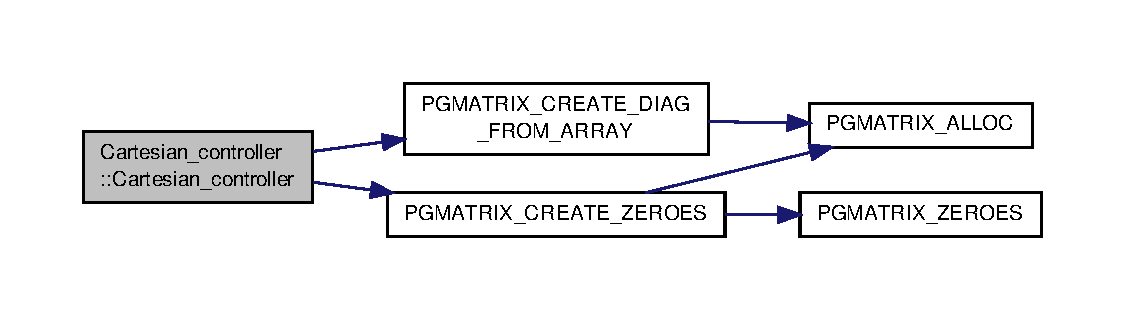
\includegraphics[width=350pt]{classCartesian__controller_a71055bb1cbf01ced9e64bb1d184b68fe_cgraph}
\end{center}
\end{figure}


\hypertarget{classCartesian__controller_ac29863d92d56a5998ba39ddb58f4a09e}{\index{Cartesian\-\_\-controller@{Cartesian\-\_\-controller}!$\sim$\-Cartesian\-\_\-controller@{$\sim$\-Cartesian\-\_\-controller}}
\index{$\sim$\-Cartesian\-\_\-controller@{$\sim$\-Cartesian\-\_\-controller}!Cartesian_controller@{Cartesian\-\_\-controller}}
\subsubsection[{$\sim$\-Cartesian\-\_\-controller}]{\setlength{\rightskip}{0pt plus 5cm}Cartesian\-\_\-controller\-::$\sim$\-Cartesian\-\_\-controller (
\begin{DoxyParamCaption}
{}
\end{DoxyParamCaption}
)}}\label{classCartesian__controller_ac29863d92d56a5998ba39ddb58f4a09e}


Definition at line 171 of file cartesian\-\_\-controller.\-cpp.


\begin{DoxyCode}
                                           \{
\}
\end{DoxyCode}


\subsection{Member Function Documentation}
\hypertarget{classCartesian__controller_aaf006f80e89c08cf040956afbb4cf3c0}{\index{Cartesian\-\_\-controller@{Cartesian\-\_\-controller}!change\-Schunk\-Mode@{change\-Schunk\-Mode}}
\index{change\-Schunk\-Mode@{change\-Schunk\-Mode}!Cartesian_controller@{Cartesian\-\_\-controller}}
\subsubsection[{change\-Schunk\-Mode}]{\setlength{\rightskip}{0pt plus 5cm}bool Cartesian\-\_\-controller\-::change\-Schunk\-Mode (
\begin{DoxyParamCaption}
\item[{int}]{mode}
\end{DoxyParamCaption}
)\hspace{0.3cm}{\ttfamily [protected]}}}\label{classCartesian__controller_aaf006f80e89c08cf040956afbb4cf3c0}


Other packages. 

Internal Calls schunk\-\_\-low service to change Schunk's control mode. 
\begin{DoxyParams}{Parameters}
{\em mode} & Schunk's mode you want to change to. \\
\hline
\end{DoxyParams}
\begin{DoxyReturn}{Returns}
true if the service was called succesfully, false otherwise. 
\end{DoxyReturn}


Definition at line 35 of file cartesian\-\_\-controller.\-cpp.



References mode\-Changer\-\_\-queue, schunk\-\_\-mode\-Changer\-\_\-client, schunk\-\_\-mode\-Changer\-\_\-msg, and stop\-Schunk().



Referenced by Cartesian\-\_\-pose\-\_\-controller\-::control(), and Cartesian\-\_\-velocity\-\_\-controller\-::control().


\begin{DoxyCode}
                                                   \{

        \textcolor{comment}{//Create Service Object and initialize}
        \hyperlink{classCartesian__controller_a960d66580ba058d3337c89bdf8099948}{schunk\_modeChanger\_msg}.request.mode = mode;

        \textcolor{comment}{//Call Service with initialized Service Object}
        \textcolor{keywordflow}{if} (!\hyperlink{classCartesian__controller_aee1fc445b64c534847ff0012132a5d2c}{schunk\_modeChanger\_client}.call(
      \hyperlink{classCartesian__controller_a960d66580ba058d3337c89bdf8099948}{schunk\_modeChanger\_msg}))
        \{
                ROS\_ERROR\_STREAM(\textcolor{stringliteral}{"Unable to change schunk\_low control mode,
       aborting."});
                \hyperlink{classCartesian__controller_a3ba54e8b35632526c5e8eb2ab5d7de0d}{stopSchunk}();
                \textcolor{keywordflow}{return} \textcolor{keyword}{false};
        \}

        \hyperlink{classCartesian__controller_adf47dc3a09bd9650015b25870054b60d}{modeChanger\_queue}.callAvailable(ros::WallDuration(0));

        \textcolor{keywordflow}{return} \textcolor{keyword}{true};
\}
\end{DoxyCode}


Here is the call graph for this function\-:\nopagebreak
\begin{figure}[H]
\begin{center}
\leavevmode
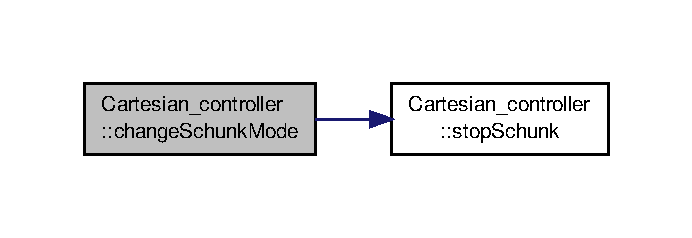
\includegraphics[width=332pt]{classCartesian__controller_aaf006f80e89c08cf040956afbb4cf3c0_cgraph}
\end{center}
\end{figure}




Here is the caller graph for this function\-:\nopagebreak
\begin{figure}[H]
\begin{center}
\leavevmode
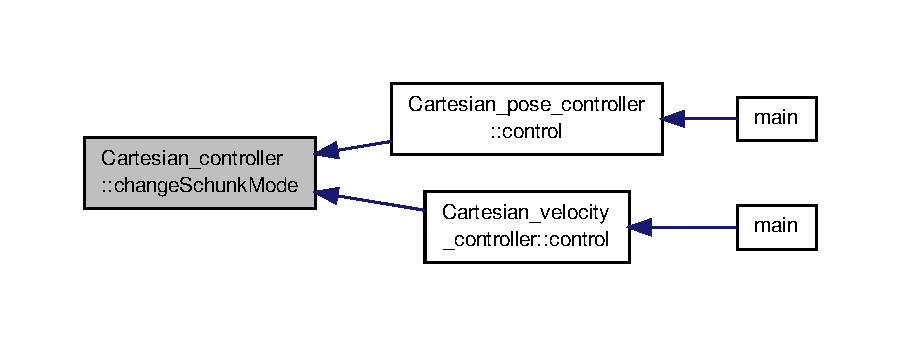
\includegraphics[width=350pt]{classCartesian__controller_aaf006f80e89c08cf040956afbb4cf3c0_icgraph}
\end{center}
\end{figure}


\hypertarget{classCartesian__controller_a8809167cab6d338a957439141fa2bf6c}{\index{Cartesian\-\_\-controller@{Cartesian\-\_\-controller}!control@{control}}
\index{control@{control}!Cartesian_controller@{Cartesian\-\_\-controller}}
\subsubsection[{control}]{\setlength{\rightskip}{0pt plus 5cm}virtual void Cartesian\-\_\-controller\-::control (
\begin{DoxyParamCaption}
{}
\end{DoxyParamCaption}
)\hspace{0.3cm}{\ttfamily [pure virtual]}}}\label{classCartesian__controller_a8809167cab6d338a957439141fa2bf6c}


Implemented in \hyperlink{classCartesian__velocity__controller_a249bd167cd995e16906731172d1bc516}{Cartesian\-\_\-velocity\-\_\-controller}, and \hyperlink{classCartesian__pose__controller_ab937d166862f2756eb3d08f37a0a090d}{Cartesian\-\_\-pose\-\_\-controller}.

\hypertarget{classCartesian__controller_a8c0f0b41de9f4f8b2e3aa327e7c6b50c}{\index{Cartesian\-\_\-controller@{Cartesian\-\_\-controller}!control\-Clean\-Up@{control\-Clean\-Up}}
\index{control\-Clean\-Up@{control\-Clean\-Up}!Cartesian_controller@{Cartesian\-\_\-controller}}
\subsubsection[{control\-Clean\-Up}]{\setlength{\rightskip}{0pt plus 5cm}void Cartesian\-\_\-controller\-::control\-Clean\-Up (
\begin{DoxyParamCaption}
{}
\end{DoxyParamCaption}
)\hspace{0.3cm}{\ttfamily [protected]}}}\label{classCartesian__controller_a8c0f0b41de9f4f8b2e3aa327e7c6b50c}


De-\/allocs unfreed matrices in the end of the control loop. 



Definition at line 148 of file cartesian\-\_\-controller.\-cpp.



References D, D\-\_\-ref, D\-Thetas, Err, Err\-\_\-ant, Err\-\_\-int, Kd, Ki, Kp, P\-G\-M\-A\-T\-R\-I\-X\-\_\-\-F\-R\-E\-E(), r, Robot\-\_\-free(), S\-J, and Thetas.



Referenced by Cartesian\-\_\-pose\-\_\-controller\-::control(), and Cartesian\-\_\-velocity\-\_\-controller\-::control().


\begin{DoxyCode}
                                         \{

        \textcolor{comment}{//Last Memory Free Procedure.}
        \textcolor{comment}{//Jacobians}
        \hyperlink{gmatrix_8h_a9a73b4e0a77f386c0bae1bba75298d1d}{PGMATRIX\_FREE}(\hyperlink{classCartesian__controller_a98fdac06d136ac3dba0102d97cd5dd36}{SJ});
        \textcolor{comment}{//Errors}
        \hyperlink{gmatrix_8h_a9a73b4e0a77f386c0bae1bba75298d1d}{PGMATRIX\_FREE}(\hyperlink{classCartesian__controller_ab3f08ecf10cb2486e8bfc61f07e2bde6}{Err});
        \hyperlink{gmatrix_8h_a9a73b4e0a77f386c0bae1bba75298d1d}{PGMATRIX\_FREE}(\hyperlink{classCartesian__controller_a6d9471a983f6cb6c642bf8dea0d540af}{Err\_ant});
        \hyperlink{gmatrix_8h_a9a73b4e0a77f386c0bae1bba75298d1d}{PGMATRIX\_FREE}(\hyperlink{classCartesian__controller_a248174c6399a8933bfcc8f1b0b39af5e}{Err\_int});
        \textcolor{comment}{//Var}
        \hyperlink{gmatrix_8h_a9a73b4e0a77f386c0bae1bba75298d1d}{PGMATRIX\_FREE}(\hyperlink{classCartesian__controller_a5d6419e62e130150edfcbd82b1dadcae}{DThetas});
        \hyperlink{gmatrix_8h_a9a73b4e0a77f386c0bae1bba75298d1d}{PGMATRIX\_FREE}(\hyperlink{classCartesian__controller_a0a0f818dad601cd9e3e26cb6959b8eb6}{Thetas});
        \hyperlink{gmatrix_8h_a9a73b4e0a77f386c0bae1bba75298d1d}{PGMATRIX\_FREE}(\hyperlink{classCartesian__controller_abb248cb3215a574fe8e1bb8fb0b8626d}{D\_ref});
        \hyperlink{gmatrix_8h_a9a73b4e0a77f386c0bae1bba75298d1d}{PGMATRIX\_FREE}(\hyperlink{classCartesian__controller_a8c470b652ce436d8e48f126073fc2593}{D});
        \textcolor{comment}{//PID}
        \hyperlink{gmatrix_8h_a9a73b4e0a77f386c0bae1bba75298d1d}{PGMATRIX\_FREE}(\hyperlink{classCartesian__controller_a78073f51064a05d72c41723a93d9079f}{Kp});
        \hyperlink{gmatrix_8h_a9a73b4e0a77f386c0bae1bba75298d1d}{PGMATRIX\_FREE}(\hyperlink{classCartesian__controller_a70e495f39da706f1b589684f58343b9e}{Ki});
        \hyperlink{gmatrix_8h_a9a73b4e0a77f386c0bae1bba75298d1d}{PGMATRIX\_FREE}(\hyperlink{classCartesian__controller_a62394cef8a9a29eac18319a4ad579c4c}{Kd});
        \textcolor{comment}{//Robot}
        \hyperlink{robot_8h_a31f8aee15b6c24f89ab51b1bc1341f33}{Robot\_free}(\hyperlink{classCartesian__controller_a5562129951bd802e4ded77fc716c87a0}{r});

\}
\end{DoxyCode}


Here is the call graph for this function\-:\nopagebreak
\begin{figure}[H]
\begin{center}
\leavevmode
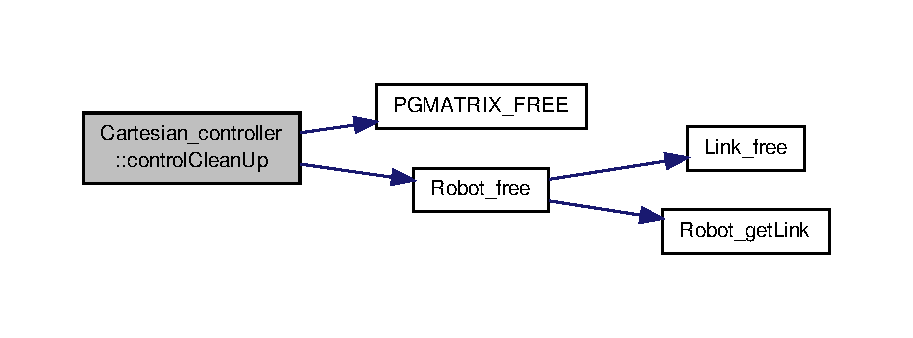
\includegraphics[width=350pt]{classCartesian__controller_a8c0f0b41de9f4f8b2e3aa327e7c6b50c_cgraph}
\end{center}
\end{figure}




Here is the caller graph for this function\-:\nopagebreak
\begin{figure}[H]
\begin{center}
\leavevmode
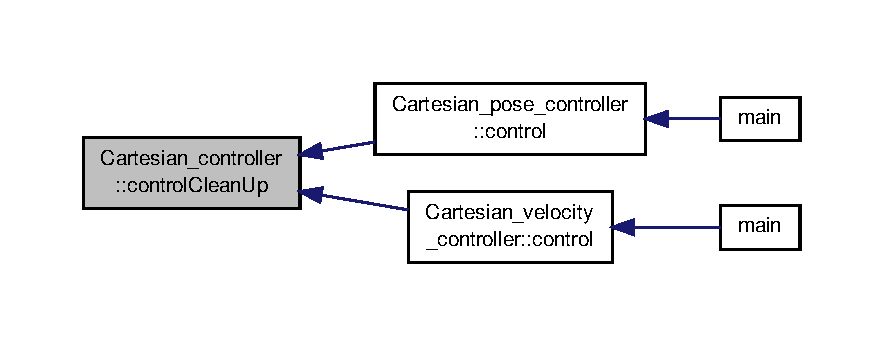
\includegraphics[width=350pt]{classCartesian__controller_a8c0f0b41de9f4f8b2e3aa327e7c6b50c_icgraph}
\end{center}
\end{figure}


\hypertarget{classCartesian__controller_a0d7a63bac84715f6742db738df246f91}{\index{Cartesian\-\_\-controller@{Cartesian\-\_\-controller}!get\-Schunk\-Positions\-And\-Velocities\-And\-Update\-Thetas\-And\-D\-Thetas@{get\-Schunk\-Positions\-And\-Velocities\-And\-Update\-Thetas\-And\-D\-Thetas}}
\index{get\-Schunk\-Positions\-And\-Velocities\-And\-Update\-Thetas\-And\-D\-Thetas@{get\-Schunk\-Positions\-And\-Velocities\-And\-Update\-Thetas\-And\-D\-Thetas}!Cartesian_controller@{Cartesian\-\_\-controller}}
\subsubsection[{get\-Schunk\-Positions\-And\-Velocities\-And\-Update\-Thetas\-And\-D\-Thetas}]{\setlength{\rightskip}{0pt plus 5cm}bool Cartesian\-\_\-controller\-::get\-Schunk\-Positions\-And\-Velocities\-And\-Update\-Thetas\-And\-D\-Thetas (
\begin{DoxyParamCaption}
{}
\end{DoxyParamCaption}
)\hspace{0.3cm}{\ttfamily [protected]}}}\label{classCartesian__controller_a0d7a63bac84715f6742db738df246f91}


Asks Schunk's its joint's positions and velocities, them it updates the internal P\-G\-M\-A\-T\-R\-I\-Xs Theta and D\-Thetas. 

\begin{DoxyReturn}{Returns}
true if the service was called succesfully, false otherwise. 
\end{DoxyReturn}


Definition at line 127 of file cartesian\-\_\-controller.\-cpp.



References Robot\-::dofs, D\-Thetas, P\-G\-M\-A\-T\-R\-I\-X\-\_\-\-D\-A\-T\-A, pos\-Vel\-Getter\-\_\-queue, r, schunk\-\_\-pos\-Vel\-Getter\-\_\-client, schunk\-\_\-pos\-Vel\-Getter\-\_\-msg, stop\-Schunk(), and Thetas.



Referenced by Cartesian\-\_\-pose\-\_\-controller\-::control(), and Cartesian\-\_\-velocity\-\_\-controller\-::control().


\begin{DoxyCode}
                                                                               
          \{

        \textcolor{keywordflow}{if}(!\hyperlink{classCartesian__controller_a5c1d9386bc5f219f2edc0d5d1b21f0da}{schunk\_posVelGetter\_client}.call(
      \hyperlink{classCartesian__controller_ae368dcf84dae528612c617cc92fbb69f}{schunk\_posVelGetter\_msg}))\{
                ROS\_ERROR\_STREAM(\textcolor{stringliteral}{"Couldn't get schunk's positions and
       velocities, aborting"});
                \hyperlink{classCartesian__controller_a3ba54e8b35632526c5e8eb2ab5d7de0d}{stopSchunk}();
                \textcolor{keywordflow}{return} \textcolor{keyword}{false};
        \}
        \textcolor{keywordflow}{else}\{
                \textcolor{keywordflow}{for}(\textcolor{keywordtype}{int} i = 0; i < \hyperlink{classCartesian__controller_a5562129951bd802e4ded77fc716c87a0}{r}->\hyperlink{structRobot_a51d4a86ac5314a1ed8614d5664c80747}{dofs}; i++)\{
                        \hyperlink{gmatrix_8h_a7333180c47234295df2bd7b09ac00da8}{PGMATRIX\_DATA}(\hyperlink{classCartesian__controller_a0a0f818dad601cd9e3e26cb6959b8eb6}{Thetas},i+1,1) = 
      \hyperlink{classCartesian__controller_ae368dcf84dae528612c617cc92fbb69f}{schunk\_posVelGetter\_msg}.response.positions[i];
                        \hyperlink{gmatrix_8h_a7333180c47234295df2bd7b09ac00da8}{PGMATRIX\_DATA}(\hyperlink{classCartesian__controller_a5d6419e62e130150edfcbd82b1dadcae}{DThetas},i+1,1) = 
      \hyperlink{classCartesian__controller_ae368dcf84dae528612c617cc92fbb69f}{schunk\_posVelGetter\_msg}.response.velocities[i];
                \}
        \}

        \hyperlink{classCartesian__controller_a144c7faad45f3d070624452c1f02ba15}{posVelGetter\_queue}.callAvailable(ros::WallDuration(0)
      );
        \textcolor{keywordflow}{return} \textcolor{keyword}{true};
\}
\end{DoxyCode}


Here is the call graph for this function\-:\nopagebreak
\begin{figure}[H]
\begin{center}
\leavevmode
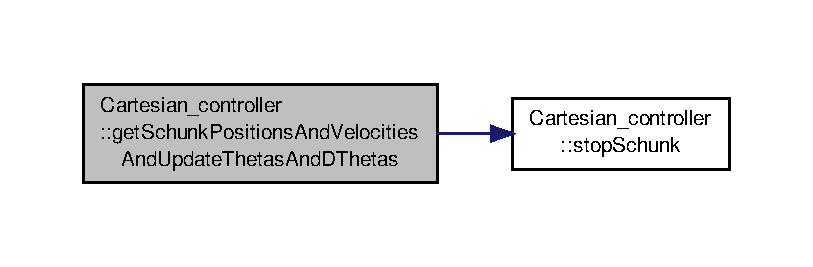
\includegraphics[width=350pt]{classCartesian__controller_a0d7a63bac84715f6742db738df246f91_cgraph}
\end{center}
\end{figure}




Here is the caller graph for this function\-:\nopagebreak
\begin{figure}[H]
\begin{center}
\leavevmode
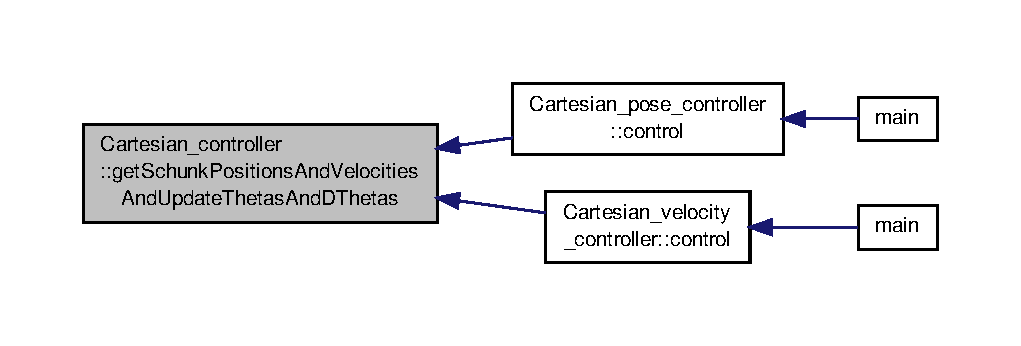
\includegraphics[width=350pt]{classCartesian__controller_a0d7a63bac84715f6742db738df246f91_icgraph}
\end{center}
\end{figure}


\hypertarget{classCartesian__controller_ae845f67c81c2649bfbaccf95230f2599}{\index{Cartesian\-\_\-controller@{Cartesian\-\_\-controller}!send\-Joint\-Positions\-To\-Schunk@{send\-Joint\-Positions\-To\-Schunk}}
\index{send\-Joint\-Positions\-To\-Schunk@{send\-Joint\-Positions\-To\-Schunk}!Cartesian_controller@{Cartesian\-\_\-controller}}
\subsubsection[{send\-Joint\-Positions\-To\-Schunk}]{\setlength{\rightskip}{0pt plus 5cm}void Cartesian\-\_\-controller\-::send\-Joint\-Positions\-To\-Schunk (
\begin{DoxyParamCaption}
\item[{std\-::vector$<$ double $>$}]{positions}
\end{DoxyParamCaption}
)\hspace{0.3cm}{\ttfamily [protected]}}}\label{classCartesian__controller_ae845f67c81c2649bfbaccf95230f2599}


Definition at line 106 of file cartesian\-\_\-controller.\-cpp.



References pos\-\_\-publisher\-\_\-queue, schunk\-\_\-low\-\_\-pos\-\_\-pub, and schunk\-\_\-low\-\_\-positions\-\_\-msg.



Referenced by Cartesian\-\_\-pose\-\_\-controller\-::control().


\begin{DoxyCode}
                                                                               
       \{

        \textcolor{keywordflow}{for}(\textcolor{keywordtype}{int} j = 0; j < 8; j++)\{
                \hyperlink{classCartesian__controller_a2dd700542bd6243eef10d34811055584}{schunk\_low\_positions\_msg}.positions[j]=
      positions[j];
                ROS\_INFO\_STREAM(\textcolor{stringliteral}{"Positions sent : "} << j << \textcolor{stringliteral}{" = "} << positions[
      j]);
        \}

        \textcolor{comment}{//Send}
        \textcolor{comment}{// Update schunk\_low\_positions\_msg header}
        \hyperlink{classCartesian__controller_a2dd700542bd6243eef10d34811055584}{schunk\_low\_positions\_msg}.header.stamp = 
      ros::Time::now();
        \textcolor{comment}{// Publish}
        \hyperlink{classCartesian__controller_af06313084ef058d1f979fddeb33d5100}{schunk\_low\_pos\_pub}.publish(\hyperlink{classCartesian__controller_a2dd700542bd6243eef10d34811055584}{schunk\_low\_positions\_msg}
      );
        \textcolor{comment}{// Call!}
        \hyperlink{classCartesian__controller_adbb9cddf4092cba9042294740c5371eb}{pos\_publisher\_queue}.callAvailable(ros::WallDuration(
      0));

\}
\end{DoxyCode}


Here is the caller graph for this function\-:\nopagebreak
\begin{figure}[H]
\begin{center}
\leavevmode
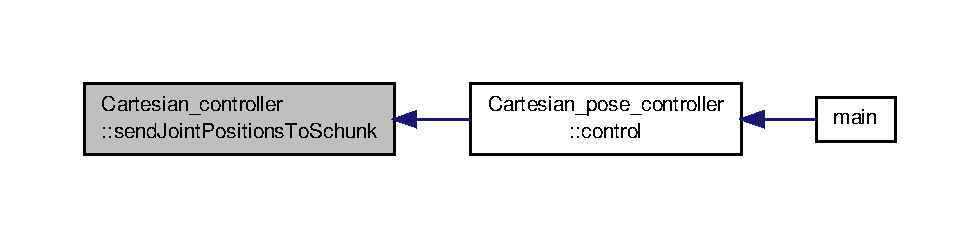
\includegraphics[width=350pt]{classCartesian__controller_ae845f67c81c2649bfbaccf95230f2599_icgraph}
\end{center}
\end{figure}


\hypertarget{classCartesian__controller_a40d17a9794af8a9a607618bf0ee5efff}{\index{Cartesian\-\_\-controller@{Cartesian\-\_\-controller}!set\-Schunk\-Velocities\-And\-Send@{set\-Schunk\-Velocities\-And\-Send}}
\index{set\-Schunk\-Velocities\-And\-Send@{set\-Schunk\-Velocities\-And\-Send}!Cartesian_controller@{Cartesian\-\_\-controller}}
\subsubsection[{set\-Schunk\-Velocities\-And\-Send}]{\setlength{\rightskip}{0pt plus 5cm}void Cartesian\-\_\-controller\-::set\-Schunk\-Velocities\-And\-Send (
\begin{DoxyParamCaption}
\item[{double}]{sat\-\_\-vel}
\end{DoxyParamCaption}
)\hspace{0.3cm}{\ttfamily [protected]}}}\label{classCartesian__controller_a40d17a9794af8a9a607618bf0ee5efff}


Updates the Schunk velocities msg to be sent to Schunk, but not before saturating it. 

Other work in the velocities msg before sending should be done here. 

Definition at line 81 of file cartesian\-\_\-controller.\-cpp.



References Robot\-::dofs, D\-Thetas, P\-G\-M\-A\-T\-R\-I\-X\-\_\-\-D\-A\-T\-A, publisher\-\_\-queue, r, schunk\-\_\-low\-\_\-pub, and schunk\-\_\-low\-\_\-velocities\-\_\-msg.



Referenced by Cartesian\-\_\-pose\-\_\-controller\-::control(), and Cartesian\-\_\-velocity\-\_\-controller\-::control().


\begin{DoxyCode}
                                                                   \{

        \textcolor{keywordflow}{for}(\textcolor{keywordtype}{int} j = 0; j < \hyperlink{classCartesian__controller_a5562129951bd802e4ded77fc716c87a0}{r}->\hyperlink{structRobot_a51d4a86ac5314a1ed8614d5664c80747}{dofs}; j++)\{
                \hyperlink{classCartesian__controller_af59178c57bdd73d9eb474577247bbe40}{schunk\_low\_velocities\_msg}.velocities[j
      ]=\hyperlink{gmatrix_8h_a7333180c47234295df2bd7b09ac00da8}{PGMATRIX\_DATA}(\hyperlink{classCartesian__controller_a5d6419e62e130150edfcbd82b1dadcae}{DThetas},j+1,1);

                \textcolor{keywordflow}{if}(\hyperlink{classCartesian__controller_af59178c57bdd73d9eb474577247bbe40}{schunk\_low\_velocities\_msg}.
      velocities[j] > sat\_vel)\{
                        \hyperlink{classCartesian__controller_af59178c57bdd73d9eb474577247bbe40}{schunk\_low\_velocities\_msg}.
      velocities[j] = sat\_vel;
                        \hyperlink{gmatrix_8h_a7333180c47234295df2bd7b09ac00da8}{PGMATRIX\_DATA}(\hyperlink{classCartesian__controller_a5d6419e62e130150edfcbd82b1dadcae}{DThetas},j+1,1) = 
      sat\_vel;
                \}
                \textcolor{keywordflow}{else} \textcolor{keywordflow}{if}(\hyperlink{classCartesian__controller_af59178c57bdd73d9eb474577247bbe40}{schunk\_low\_velocities\_msg}.
      velocities[j] < -sat\_vel)\{
                        \hyperlink{classCartesian__controller_af59178c57bdd73d9eb474577247bbe40}{schunk\_low\_velocities\_msg}.
      velocities[j] = -sat\_vel;
                        \hyperlink{gmatrix_8h_a7333180c47234295df2bd7b09ac00da8}{PGMATRIX\_DATA}(\hyperlink{classCartesian__controller_a5d6419e62e130150edfcbd82b1dadcae}{DThetas},j+1,1) = -
      sat\_vel;
                \}
        \}

        \textcolor{comment}{//Send}
        \hyperlink{classCartesian__controller_af59178c57bdd73d9eb474577247bbe40}{schunk\_low\_velocities\_msg}.header.stamp = 
      ros::Time::now();
        \hyperlink{classCartesian__controller_aa6ce9cffdd307127ed814d6e5132eba2}{schunk\_low\_pub}.publish(\hyperlink{classCartesian__controller_af59178c57bdd73d9eb474577247bbe40}{schunk\_low\_velocities\_msg}
      );
        \hyperlink{classCartesian__controller_a041a2eb6657c9b036a512fb21e9f5086}{publisher\_queue}.callAvailable(ros::WallDuration(0));

\}
\end{DoxyCode}


Here is the caller graph for this function\-:\nopagebreak
\begin{figure}[H]
\begin{center}
\leavevmode
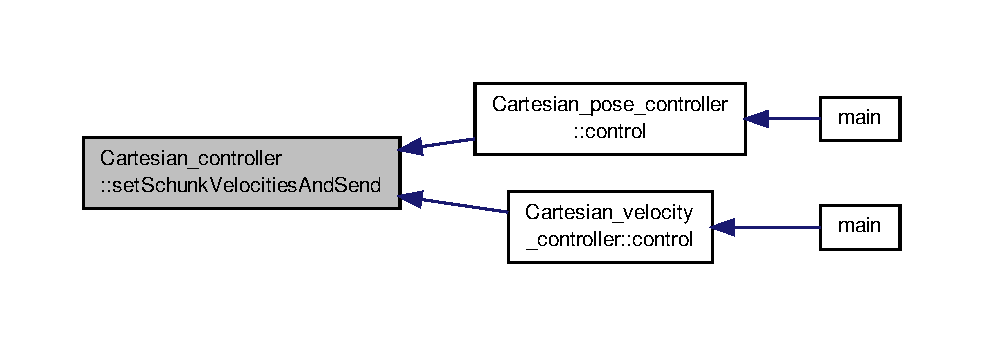
\includegraphics[width=350pt]{classCartesian__controller_a40d17a9794af8a9a607618bf0ee5efff_icgraph}
\end{center}
\end{figure}


\hypertarget{classCartesian__controller_a3ba54e8b35632526c5e8eb2ab5d7de0d}{\index{Cartesian\-\_\-controller@{Cartesian\-\_\-controller}!stop\-Schunk@{stop\-Schunk}}
\index{stop\-Schunk@{stop\-Schunk}!Cartesian_controller@{Cartesian\-\_\-controller}}
\subsubsection[{stop\-Schunk}]{\setlength{\rightskip}{0pt plus 5cm}bool Cartesian\-\_\-controller\-::stop\-Schunk (
\begin{DoxyParamCaption}
{}
\end{DoxyParamCaption}
)\hspace{0.3cm}{\ttfamily [protected]}}}\label{classCartesian__controller_a3ba54e8b35632526c5e8eb2ab5d7de0d}


Definition at line 55 of file cartesian\-\_\-controller.\-cpp.



References end\-\_\-control, schunk\-\_\-stopper\-\_\-client, schunk\-\_\-stopper\-\_\-msg, and stopper\-\_\-queue.



Referenced by change\-Schunk\-Mode(), get\-Schunk\-Positions\-And\-Velocities\-And\-Update\-Thetas\-And\-D\-Thetas(), and Cartesian\-\_\-velocity\-\_\-controller\-::reference\-Update\-Callback().


\begin{DoxyCode}
                                     \{

        ROS\_ERROR\_STREAM(\textcolor{stringliteral}{"STOPPING SCHUNK NOW!"});

        \textcolor{comment}{//Call end to the rest of the program}
        \hyperlink{classCartesian__controller_a3c0a72214891f68e2bad63bf2b688f9c}{end\_control} = \textcolor{keyword}{true};

        \textcolor{comment}{//Call Service with initialized Service Object}
        \textcolor{keywordflow}{if} (!\hyperlink{classCartesian__controller_a4ea7350e0f797c49bc51d3433a761aff}{schunk\_stopper\_client}.call(\hyperlink{classCartesian__controller_a29581ed2f2d8bb97c55e16868bbcc8bd}{schunk\_stopper\_msg}
      ))
        \{
                ROS\_ERROR\_STREAM(\textcolor{stringliteral}{"FAILED TO STOP SCHUNK! WILL TRY FOREVER"});
                \hyperlink{classCartesian__controller_a3ba54e8b35632526c5e8eb2ab5d7de0d}{stopSchunk}();
                \textcolor{keywordflow}{return} \textcolor{keyword}{false};
        \}

        \hyperlink{classCartesian__controller_a52eb090400d8dafaa22aecb037788a66}{stopper\_queue}.callAvailable(ros::WallDuration(0));

        \textcolor{keywordflow}{return} \textcolor{keyword}{true};
\}
\end{DoxyCode}


Here is the caller graph for this function\-:\nopagebreak
\begin{figure}[H]
\begin{center}
\leavevmode
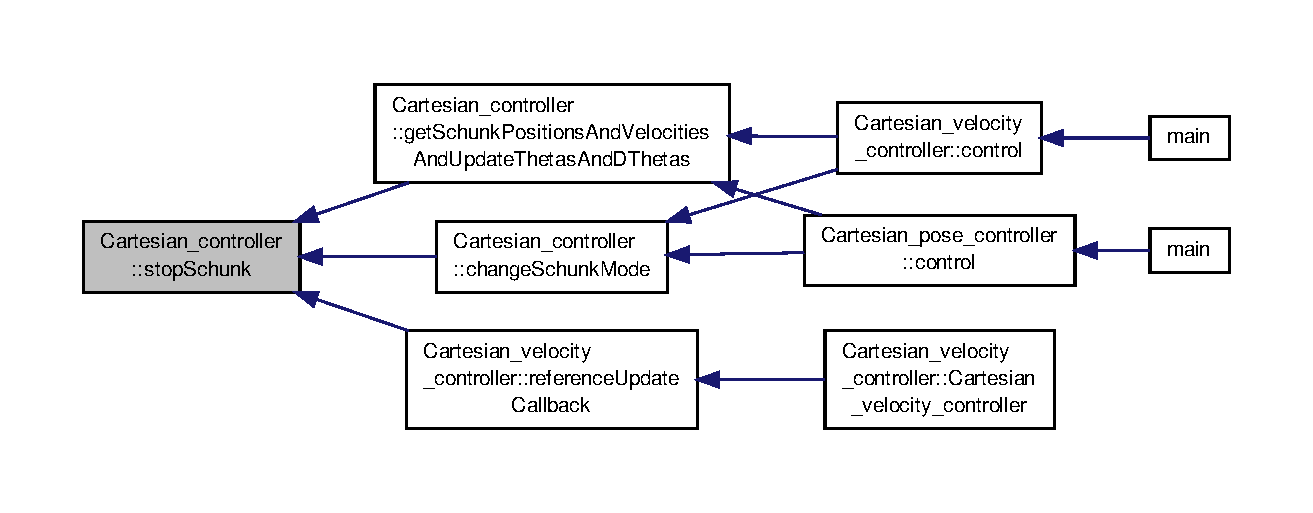
\includegraphics[width=350pt]{classCartesian__controller_a3ba54e8b35632526c5e8eb2ab5d7de0d_icgraph}
\end{center}
\end{figure}




\subsection{Field Documentation}
\hypertarget{classCartesian__controller_a37edb9c6e2a5066f74941e3659f68cbc}{\index{Cartesian\-\_\-controller@{Cartesian\-\_\-controller}!aux1@{aux1}}
\index{aux1@{aux1}!Cartesian_controller@{Cartesian\-\_\-controller}}
\subsubsection[{aux1}]{\setlength{\rightskip}{0pt plus 5cm}{\bf P\-G\-M\-A\-T\-R\-I\-X} Cartesian\-\_\-controller\-::aux1\hspace{0.3cm}{\ttfamily [protected]}}}\label{classCartesian__controller_a37edb9c6e2a5066f74941e3659f68cbc}


Definition at line 62 of file cartesian\-\_\-controller.\-h.



Referenced by Cartesian\-\_\-controller(), Cartesian\-\_\-pose\-\_\-controller\-::control(), and Cartesian\-\_\-velocity\-\_\-controller\-::control().

\hypertarget{classCartesian__controller_af73a0c910cd80ed2f84974b65beba450}{\index{Cartesian\-\_\-controller@{Cartesian\-\_\-controller}!aux2@{aux2}}
\index{aux2@{aux2}!Cartesian_controller@{Cartesian\-\_\-controller}}
\subsubsection[{aux2}]{\setlength{\rightskip}{0pt plus 5cm}{\bf P\-G\-M\-A\-T\-R\-I\-X} Cartesian\-\_\-controller\-::aux2\hspace{0.3cm}{\ttfamily [protected]}}}\label{classCartesian__controller_af73a0c910cd80ed2f84974b65beba450}


Definition at line 63 of file cartesian\-\_\-controller.\-h.



Referenced by Cartesian\-\_\-controller(), Cartesian\-\_\-pose\-\_\-controller\-::control(), and Cartesian\-\_\-velocity\-\_\-controller\-::control().

\hypertarget{classCartesian__controller_aa37c15fcd53a60ecce106cd9b39d3501}{\index{Cartesian\-\_\-controller@{Cartesian\-\_\-controller}!aux3@{aux3}}
\index{aux3@{aux3}!Cartesian_controller@{Cartesian\-\_\-controller}}
\subsubsection[{aux3}]{\setlength{\rightskip}{0pt plus 5cm}{\bf P\-G\-M\-A\-T\-R\-I\-X} Cartesian\-\_\-controller\-::aux3\hspace{0.3cm}{\ttfamily [protected]}}}\label{classCartesian__controller_aa37c15fcd53a60ecce106cd9b39d3501}


Definition at line 64 of file cartesian\-\_\-controller.\-h.



Referenced by Cartesian\-\_\-controller(), Cartesian\-\_\-pose\-\_\-controller\-::control(), and Cartesian\-\_\-velocity\-\_\-controller\-::control().

\hypertarget{classCartesian__controller_a8c470b652ce436d8e48f126073fc2593}{\index{Cartesian\-\_\-controller@{Cartesian\-\_\-controller}!D@{D}}
\index{D@{D}!Cartesian_controller@{Cartesian\-\_\-controller}}
\subsubsection[{D}]{\setlength{\rightskip}{0pt plus 5cm}{\bf P\-G\-M\-A\-T\-R\-I\-X} Cartesian\-\_\-controller\-::\-D\hspace{0.3cm}{\ttfamily [protected]}}}\label{classCartesian__controller_a8c470b652ce436d8e48f126073fc2593}


Definition at line 56 of file cartesian\-\_\-controller.\-h.



Referenced by Cartesian\-\_\-controller(), Cartesian\-\_\-pose\-\_\-controller\-::control(), Cartesian\-\_\-velocity\-\_\-controller\-::control(), control\-Clean\-Up(), and Cartesian\-\_\-pose\-\_\-controller\-::print\-Pose().

\hypertarget{classCartesian__controller_abb248cb3215a574fe8e1bb8fb0b8626d}{\index{Cartesian\-\_\-controller@{Cartesian\-\_\-controller}!D\-\_\-ref@{D\-\_\-ref}}
\index{D\-\_\-ref@{D\-\_\-ref}!Cartesian_controller@{Cartesian\-\_\-controller}}
\subsubsection[{D\-\_\-ref}]{\setlength{\rightskip}{0pt plus 5cm}{\bf P\-G\-M\-A\-T\-R\-I\-X} Cartesian\-\_\-controller\-::\-D\-\_\-ref\hspace{0.3cm}{\ttfamily [protected]}}}\label{classCartesian__controller_abb248cb3215a574fe8e1bb8fb0b8626d}


Definition at line 54 of file cartesian\-\_\-controller.\-h.



Referenced by Cartesian\-\_\-controller(), Cartesian\-\_\-pose\-\_\-controller\-::control(), Cartesian\-\_\-velocity\-\_\-controller\-::control(), control\-Clean\-Up(), Cartesian\-\_\-pose\-\_\-controller\-::update\-References(), and Cartesian\-\_\-velocity\-\_\-controller\-::update\-References().

\hypertarget{classCartesian__controller_a5d6419e62e130150edfcbd82b1dadcae}{\index{Cartesian\-\_\-controller@{Cartesian\-\_\-controller}!D\-Thetas@{D\-Thetas}}
\index{D\-Thetas@{D\-Thetas}!Cartesian_controller@{Cartesian\-\_\-controller}}
\subsubsection[{D\-Thetas}]{\setlength{\rightskip}{0pt plus 5cm}{\bf P\-G\-M\-A\-T\-R\-I\-X} Cartesian\-\_\-controller\-::\-D\-Thetas\hspace{0.3cm}{\ttfamily [protected]}}}\label{classCartesian__controller_a5d6419e62e130150edfcbd82b1dadcae}


Definition at line 52 of file cartesian\-\_\-controller.\-h.



Referenced by Cartesian\-\_\-controller(), Cartesian\-\_\-pose\-\_\-controller\-::control(), Cartesian\-\_\-velocity\-\_\-controller\-::control(), control\-Clean\-Up(), get\-Schunk\-Positions\-And\-Velocities\-And\-Update\-Thetas\-And\-D\-Thetas(), and set\-Schunk\-Velocities\-And\-Send().

\hypertarget{classCartesian__controller_a3c0a72214891f68e2bad63bf2b688f9c}{\index{Cartesian\-\_\-controller@{Cartesian\-\_\-controller}!end\-\_\-control@{end\-\_\-control}}
\index{end\-\_\-control@{end\-\_\-control}!Cartesian_controller@{Cartesian\-\_\-controller}}
\subsubsection[{end\-\_\-control}]{\setlength{\rightskip}{0pt plus 5cm}bool Cartesian\-\_\-controller\-::end\-\_\-control\hspace{0.3cm}{\ttfamily [protected]}}}\label{classCartesian__controller_a3c0a72214891f68e2bad63bf2b688f9c}


Definition at line 15 of file cartesian\-\_\-controller.\-h.



Referenced by Cartesian\-\_\-controller(), Cartesian\-\_\-velocity\-\_\-controller\-::control(), and stop\-Schunk().

\hypertarget{classCartesian__controller_ab3f08ecf10cb2486e8bfc61f07e2bde6}{\index{Cartesian\-\_\-controller@{Cartesian\-\_\-controller}!Err@{Err}}
\index{Err@{Err}!Cartesian_controller@{Cartesian\-\_\-controller}}
\subsubsection[{Err}]{\setlength{\rightskip}{0pt plus 5cm}{\bf P\-G\-M\-A\-T\-R\-I\-X} Cartesian\-\_\-controller\-::\-Err\hspace{0.3cm}{\ttfamily [protected]}}}\label{classCartesian__controller_ab3f08ecf10cb2486e8bfc61f07e2bde6}


Definition at line 58 of file cartesian\-\_\-controller.\-h.



Referenced by Cartesian\-\_\-controller(), Cartesian\-\_\-pose\-\_\-controller\-::control(), Cartesian\-\_\-velocity\-\_\-controller\-::control(), control\-Clean\-Up(), and Cartesian\-\_\-velocity\-\_\-controller\-::print\-Vel().

\hypertarget{classCartesian__controller_a6d9471a983f6cb6c642bf8dea0d540af}{\index{Cartesian\-\_\-controller@{Cartesian\-\_\-controller}!Err\-\_\-ant@{Err\-\_\-ant}}
\index{Err\-\_\-ant@{Err\-\_\-ant}!Cartesian_controller@{Cartesian\-\_\-controller}}
\subsubsection[{Err\-\_\-ant}]{\setlength{\rightskip}{0pt plus 5cm}{\bf P\-G\-M\-A\-T\-R\-I\-X} Cartesian\-\_\-controller\-::\-Err\-\_\-ant\hspace{0.3cm}{\ttfamily [protected]}}}\label{classCartesian__controller_a6d9471a983f6cb6c642bf8dea0d540af}


Definition at line 59 of file cartesian\-\_\-controller.\-h.



Referenced by Cartesian\-\_\-controller(), Cartesian\-\_\-pose\-\_\-controller\-::control(), Cartesian\-\_\-velocity\-\_\-controller\-::control(), and control\-Clean\-Up().

\hypertarget{classCartesian__controller_a248174c6399a8933bfcc8f1b0b39af5e}{\index{Cartesian\-\_\-controller@{Cartesian\-\_\-controller}!Err\-\_\-int@{Err\-\_\-int}}
\index{Err\-\_\-int@{Err\-\_\-int}!Cartesian_controller@{Cartesian\-\_\-controller}}
\subsubsection[{Err\-\_\-int}]{\setlength{\rightskip}{0pt plus 5cm}{\bf P\-G\-M\-A\-T\-R\-I\-X} Cartesian\-\_\-controller\-::\-Err\-\_\-int\hspace{0.3cm}{\ttfamily [protected]}}}\label{classCartesian__controller_a248174c6399a8933bfcc8f1b0b39af5e}


Definition at line 60 of file cartesian\-\_\-controller.\-h.



Referenced by Cartesian\-\_\-controller(), Cartesian\-\_\-pose\-\_\-controller\-::control(), Cartesian\-\_\-velocity\-\_\-controller\-::control(), and control\-Clean\-Up().

\hypertarget{classCartesian__controller_a62394cef8a9a29eac18319a4ad579c4c}{\index{Cartesian\-\_\-controller@{Cartesian\-\_\-controller}!Kd@{Kd}}
\index{Kd@{Kd}!Cartesian_controller@{Cartesian\-\_\-controller}}
\subsubsection[{Kd}]{\setlength{\rightskip}{0pt plus 5cm}{\bf P\-G\-M\-A\-T\-R\-I\-X} Cartesian\-\_\-controller\-::\-Kd\hspace{0.3cm}{\ttfamily [protected]}}}\label{classCartesian__controller_a62394cef8a9a29eac18319a4ad579c4c}


Definition at line 49 of file cartesian\-\_\-controller.\-h.



Referenced by Cartesian\-\_\-controller(), Cartesian\-\_\-pose\-\_\-controller\-::control(), Cartesian\-\_\-velocity\-\_\-controller\-::control(), and control\-Clean\-Up().

\hypertarget{classCartesian__controller_a70e495f39da706f1b589684f58343b9e}{\index{Cartesian\-\_\-controller@{Cartesian\-\_\-controller}!Ki@{Ki}}
\index{Ki@{Ki}!Cartesian_controller@{Cartesian\-\_\-controller}}
\subsubsection[{Ki}]{\setlength{\rightskip}{0pt plus 5cm}{\bf P\-G\-M\-A\-T\-R\-I\-X} Cartesian\-\_\-controller\-::\-Ki\hspace{0.3cm}{\ttfamily [protected]}}}\label{classCartesian__controller_a70e495f39da706f1b589684f58343b9e}


Definition at line 48 of file cartesian\-\_\-controller.\-h.



Referenced by Cartesian\-\_\-controller(), Cartesian\-\_\-pose\-\_\-controller\-::control(), Cartesian\-\_\-velocity\-\_\-controller\-::control(), and control\-Clean\-Up().

\hypertarget{classCartesian__controller_a78073f51064a05d72c41723a93d9079f}{\index{Cartesian\-\_\-controller@{Cartesian\-\_\-controller}!Kp@{Kp}}
\index{Kp@{Kp}!Cartesian_controller@{Cartesian\-\_\-controller}}
\subsubsection[{Kp}]{\setlength{\rightskip}{0pt plus 5cm}{\bf P\-G\-M\-A\-T\-R\-I\-X} Cartesian\-\_\-controller\-::\-Kp\hspace{0.3cm}{\ttfamily [protected]}}}\label{classCartesian__controller_a78073f51064a05d72c41723a93d9079f}


Definition at line 47 of file cartesian\-\_\-controller.\-h.



Referenced by Cartesian\-\_\-controller(), Cartesian\-\_\-pose\-\_\-controller\-::control(), Cartesian\-\_\-velocity\-\_\-controller\-::control(), and control\-Clean\-Up().

\hypertarget{classCartesian__controller_adf47dc3a09bd9650015b25870054b60d}{\index{Cartesian\-\_\-controller@{Cartesian\-\_\-controller}!mode\-Changer\-\_\-queue@{mode\-Changer\-\_\-queue}}
\index{mode\-Changer\-\_\-queue@{mode\-Changer\-\_\-queue}!Cartesian_controller@{Cartesian\-\_\-controller}}
\subsubsection[{mode\-Changer\-\_\-queue}]{\setlength{\rightskip}{0pt plus 5cm}ros\-::\-Callback\-Queue Cartesian\-\_\-controller\-::mode\-Changer\-\_\-queue\hspace{0.3cm}{\ttfamily [protected]}}}\label{classCartesian__controller_adf47dc3a09bd9650015b25870054b60d}


Definition at line 19 of file cartesian\-\_\-controller.\-h.



Referenced by Cartesian\-\_\-controller(), and change\-Schunk\-Mode().

\hypertarget{classCartesian__controller_adbb9cddf4092cba9042294740c5371eb}{\index{Cartesian\-\_\-controller@{Cartesian\-\_\-controller}!pos\-\_\-publisher\-\_\-queue@{pos\-\_\-publisher\-\_\-queue}}
\index{pos\-\_\-publisher\-\_\-queue@{pos\-\_\-publisher\-\_\-queue}!Cartesian_controller@{Cartesian\-\_\-controller}}
\subsubsection[{pos\-\_\-publisher\-\_\-queue}]{\setlength{\rightskip}{0pt plus 5cm}ros\-::\-Callback\-Queue Cartesian\-\_\-controller\-::pos\-\_\-publisher\-\_\-queue\hspace{0.3cm}{\ttfamily [protected]}}}\label{classCartesian__controller_adbb9cddf4092cba9042294740c5371eb}


Definition at line 34 of file cartesian\-\_\-controller.\-h.



Referenced by Cartesian\-\_\-controller(), and send\-Joint\-Positions\-To\-Schunk().

\hypertarget{classCartesian__controller_a144c7faad45f3d070624452c1f02ba15}{\index{Cartesian\-\_\-controller@{Cartesian\-\_\-controller}!pos\-Vel\-Getter\-\_\-queue@{pos\-Vel\-Getter\-\_\-queue}}
\index{pos\-Vel\-Getter\-\_\-queue@{pos\-Vel\-Getter\-\_\-queue}!Cartesian_controller@{Cartesian\-\_\-controller}}
\subsubsection[{pos\-Vel\-Getter\-\_\-queue}]{\setlength{\rightskip}{0pt plus 5cm}ros\-::\-Callback\-Queue Cartesian\-\_\-controller\-::pos\-Vel\-Getter\-\_\-queue\hspace{0.3cm}{\ttfamily [protected]}}}\label{classCartesian__controller_a144c7faad45f3d070624452c1f02ba15}


Definition at line 24 of file cartesian\-\_\-controller.\-h.



Referenced by Cartesian\-\_\-controller(), and get\-Schunk\-Positions\-And\-Velocities\-And\-Update\-Thetas\-And\-D\-Thetas().

\hypertarget{classCartesian__controller_a041a2eb6657c9b036a512fb21e9f5086}{\index{Cartesian\-\_\-controller@{Cartesian\-\_\-controller}!publisher\-\_\-queue@{publisher\-\_\-queue}}
\index{publisher\-\_\-queue@{publisher\-\_\-queue}!Cartesian_controller@{Cartesian\-\_\-controller}}
\subsubsection[{publisher\-\_\-queue}]{\setlength{\rightskip}{0pt plus 5cm}ros\-::\-Callback\-Queue Cartesian\-\_\-controller\-::publisher\-\_\-queue\hspace{0.3cm}{\ttfamily [protected]}}}\label{classCartesian__controller_a041a2eb6657c9b036a512fb21e9f5086}


Definition at line 29 of file cartesian\-\_\-controller.\-h.



Referenced by Cartesian\-\_\-controller(), and set\-Schunk\-Velocities\-And\-Send().

\hypertarget{classCartesian__controller_a5562129951bd802e4ded77fc716c87a0}{\index{Cartesian\-\_\-controller@{Cartesian\-\_\-controller}!r@{r}}
\index{r@{r}!Cartesian_controller@{Cartesian\-\_\-controller}}
\subsubsection[{r}]{\setlength{\rightskip}{0pt plus 5cm}{\bf Robot}$\ast$ Cartesian\-\_\-controller\-::r}}\label{classCartesian__controller_a5562129951bd802e4ded77fc716c87a0}


Definition at line 93 of file cartesian\-\_\-controller.\-h.



Referenced by Cartesian\-\_\-controller(), Cartesian\-\_\-pose\-\_\-controller\-::control(), Cartesian\-\_\-velocity\-\_\-controller\-::control(), control\-Clean\-Up(), get\-Schunk\-Positions\-And\-Velocities\-And\-Update\-Thetas\-And\-D\-Thetas(), and set\-Schunk\-Velocities\-And\-Send().

\hypertarget{classCartesian__controller_ab9ed5a808da204dbc612d313dc7332f4}{\index{Cartesian\-\_\-controller@{Cartesian\-\_\-controller}!ros\-\_\-pub\-\_\-buffer@{ros\-\_\-pub\-\_\-buffer}}
\index{ros\-\_\-pub\-\_\-buffer@{ros\-\_\-pub\-\_\-buffer}!Cartesian_controller@{Cartesian\-\_\-controller}}
\subsubsection[{ros\-\_\-pub\-\_\-buffer}]{\setlength{\rightskip}{0pt plus 5cm}int Cartesian\-\_\-controller\-::ros\-\_\-pub\-\_\-buffer\hspace{0.3cm}{\ttfamily [protected]}}}\label{classCartesian__controller_ab9ed5a808da204dbc612d313dc7332f4}


Definition at line 12 of file cartesian\-\_\-controller.\-h.



Referenced by Cartesian\-\_\-controller(), Cartesian\-\_\-pose\-\_\-controller\-::\-Cartesian\-\_\-pose\-\_\-controller(), and Cartesian\-\_\-velocity\-\_\-controller\-::\-Cartesian\-\_\-velocity\-\_\-controller().

\hypertarget{classCartesian__controller_ad90134b232217e84cb58137a9d2030bb}{\index{Cartesian\-\_\-controller@{Cartesian\-\_\-controller}!schunk\-\_\-low\-\_\-mode\-Changer\-\_\-nh@{schunk\-\_\-low\-\_\-mode\-Changer\-\_\-nh}}
\index{schunk\-\_\-low\-\_\-mode\-Changer\-\_\-nh@{schunk\-\_\-low\-\_\-mode\-Changer\-\_\-nh}!Cartesian_controller@{Cartesian\-\_\-controller}}
\subsubsection[{schunk\-\_\-low\-\_\-mode\-Changer\-\_\-nh}]{\setlength{\rightskip}{0pt plus 5cm}ros\-::\-Node\-Handle Cartesian\-\_\-controller\-::schunk\-\_\-low\-\_\-mode\-Changer\-\_\-nh\hspace{0.3cm}{\ttfamily [protected]}}}\label{classCartesian__controller_ad90134b232217e84cb58137a9d2030bb}


Definition at line 18 of file cartesian\-\_\-controller.\-h.



Referenced by Cartesian\-\_\-controller().

\hypertarget{classCartesian__controller_af06313084ef058d1f979fddeb33d5100}{\index{Cartesian\-\_\-controller@{Cartesian\-\_\-controller}!schunk\-\_\-low\-\_\-pos\-\_\-pub@{schunk\-\_\-low\-\_\-pos\-\_\-pub}}
\index{schunk\-\_\-low\-\_\-pos\-\_\-pub@{schunk\-\_\-low\-\_\-pos\-\_\-pub}!Cartesian_controller@{Cartesian\-\_\-controller}}
\subsubsection[{schunk\-\_\-low\-\_\-pos\-\_\-pub}]{\setlength{\rightskip}{0pt plus 5cm}ros\-::\-Publisher Cartesian\-\_\-controller\-::schunk\-\_\-low\-\_\-pos\-\_\-pub\hspace{0.3cm}{\ttfamily [protected]}}}\label{classCartesian__controller_af06313084ef058d1f979fddeb33d5100}


Definition at line 35 of file cartesian\-\_\-controller.\-h.



Referenced by Cartesian\-\_\-controller(), and send\-Joint\-Positions\-To\-Schunk().

\hypertarget{classCartesian__controller_aabe48e7ab08b0235d4cd94213b8faf5d}{\index{Cartesian\-\_\-controller@{Cartesian\-\_\-controller}!schunk\-\_\-low\-\_\-pos\-\_\-publisher\-\_\-nh@{schunk\-\_\-low\-\_\-pos\-\_\-publisher\-\_\-nh}}
\index{schunk\-\_\-low\-\_\-pos\-\_\-publisher\-\_\-nh@{schunk\-\_\-low\-\_\-pos\-\_\-publisher\-\_\-nh}!Cartesian_controller@{Cartesian\-\_\-controller}}
\subsubsection[{schunk\-\_\-low\-\_\-pos\-\_\-publisher\-\_\-nh}]{\setlength{\rightskip}{0pt plus 5cm}ros\-::\-Node\-Handle Cartesian\-\_\-controller\-::schunk\-\_\-low\-\_\-pos\-\_\-publisher\-\_\-nh\hspace{0.3cm}{\ttfamily [protected]}}}\label{classCartesian__controller_aabe48e7ab08b0235d4cd94213b8faf5d}


Definition at line 33 of file cartesian\-\_\-controller.\-h.



Referenced by Cartesian\-\_\-controller().

\hypertarget{classCartesian__controller_a2dd700542bd6243eef10d34811055584}{\index{Cartesian\-\_\-controller@{Cartesian\-\_\-controller}!schunk\-\_\-low\-\_\-positions\-\_\-msg@{schunk\-\_\-low\-\_\-positions\-\_\-msg}}
\index{schunk\-\_\-low\-\_\-positions\-\_\-msg@{schunk\-\_\-low\-\_\-positions\-\_\-msg}!Cartesian_controller@{Cartesian\-\_\-controller}}
\subsubsection[{schunk\-\_\-low\-\_\-positions\-\_\-msg}]{\setlength{\rightskip}{0pt plus 5cm}schunk\-\_\-msgs\-::\-Positions Cartesian\-\_\-controller\-::schunk\-\_\-low\-\_\-positions\-\_\-msg\hspace{0.3cm}{\ttfamily [protected]}}}\label{classCartesian__controller_a2dd700542bd6243eef10d34811055584}


Definition at line 36 of file cartesian\-\_\-controller.\-h.



Referenced by Cartesian\-\_\-controller(), and send\-Joint\-Positions\-To\-Schunk().

\hypertarget{classCartesian__controller_aeed01809bd5240663c7acfade245a386}{\index{Cartesian\-\_\-controller@{Cartesian\-\_\-controller}!schunk\-\_\-low\-\_\-pos\-Vel\-Getter\-\_\-nh@{schunk\-\_\-low\-\_\-pos\-Vel\-Getter\-\_\-nh}}
\index{schunk\-\_\-low\-\_\-pos\-Vel\-Getter\-\_\-nh@{schunk\-\_\-low\-\_\-pos\-Vel\-Getter\-\_\-nh}!Cartesian_controller@{Cartesian\-\_\-controller}}
\subsubsection[{schunk\-\_\-low\-\_\-pos\-Vel\-Getter\-\_\-nh}]{\setlength{\rightskip}{0pt plus 5cm}ros\-::\-Node\-Handle Cartesian\-\_\-controller\-::schunk\-\_\-low\-\_\-pos\-Vel\-Getter\-\_\-nh\hspace{0.3cm}{\ttfamily [protected]}}}\label{classCartesian__controller_aeed01809bd5240663c7acfade245a386}


Definition at line 23 of file cartesian\-\_\-controller.\-h.



Referenced by Cartesian\-\_\-controller().

\hypertarget{classCartesian__controller_aa6ce9cffdd307127ed814d6e5132eba2}{\index{Cartesian\-\_\-controller@{Cartesian\-\_\-controller}!schunk\-\_\-low\-\_\-pub@{schunk\-\_\-low\-\_\-pub}}
\index{schunk\-\_\-low\-\_\-pub@{schunk\-\_\-low\-\_\-pub}!Cartesian_controller@{Cartesian\-\_\-controller}}
\subsubsection[{schunk\-\_\-low\-\_\-pub}]{\setlength{\rightskip}{0pt plus 5cm}ros\-::\-Publisher Cartesian\-\_\-controller\-::schunk\-\_\-low\-\_\-pub\hspace{0.3cm}{\ttfamily [protected]}}}\label{classCartesian__controller_aa6ce9cffdd307127ed814d6e5132eba2}


Definition at line 30 of file cartesian\-\_\-controller.\-h.



Referenced by Cartesian\-\_\-controller(), and set\-Schunk\-Velocities\-And\-Send().

\hypertarget{classCartesian__controller_a7df4ce63bf0551bfa7061bc718cd68d2}{\index{Cartesian\-\_\-controller@{Cartesian\-\_\-controller}!schunk\-\_\-low\-\_\-publisher\-\_\-nh@{schunk\-\_\-low\-\_\-publisher\-\_\-nh}}
\index{schunk\-\_\-low\-\_\-publisher\-\_\-nh@{schunk\-\_\-low\-\_\-publisher\-\_\-nh}!Cartesian_controller@{Cartesian\-\_\-controller}}
\subsubsection[{schunk\-\_\-low\-\_\-publisher\-\_\-nh}]{\setlength{\rightskip}{0pt plus 5cm}ros\-::\-Node\-Handle Cartesian\-\_\-controller\-::schunk\-\_\-low\-\_\-publisher\-\_\-nh\hspace{0.3cm}{\ttfamily [protected]}}}\label{classCartesian__controller_a7df4ce63bf0551bfa7061bc718cd68d2}


Definition at line 28 of file cartesian\-\_\-controller.\-h.



Referenced by Cartesian\-\_\-controller().

\hypertarget{classCartesian__controller_a57b1869ec960e75e435e1f882a02d80e}{\index{Cartesian\-\_\-controller@{Cartesian\-\_\-controller}!schunk\-\_\-low\-\_\-stopper\-\_\-nh@{schunk\-\_\-low\-\_\-stopper\-\_\-nh}}
\index{schunk\-\_\-low\-\_\-stopper\-\_\-nh@{schunk\-\_\-low\-\_\-stopper\-\_\-nh}!Cartesian_controller@{Cartesian\-\_\-controller}}
\subsubsection[{schunk\-\_\-low\-\_\-stopper\-\_\-nh}]{\setlength{\rightskip}{0pt plus 5cm}ros\-::\-Node\-Handle Cartesian\-\_\-controller\-::schunk\-\_\-low\-\_\-stopper\-\_\-nh\hspace{0.3cm}{\ttfamily [protected]}}}\label{classCartesian__controller_a57b1869ec960e75e435e1f882a02d80e}


Definition at line 38 of file cartesian\-\_\-controller.\-h.



Referenced by Cartesian\-\_\-controller().

\hypertarget{classCartesian__controller_af59178c57bdd73d9eb474577247bbe40}{\index{Cartesian\-\_\-controller@{Cartesian\-\_\-controller}!schunk\-\_\-low\-\_\-velocities\-\_\-msg@{schunk\-\_\-low\-\_\-velocities\-\_\-msg}}
\index{schunk\-\_\-low\-\_\-velocities\-\_\-msg@{schunk\-\_\-low\-\_\-velocities\-\_\-msg}!Cartesian_controller@{Cartesian\-\_\-controller}}
\subsubsection[{schunk\-\_\-low\-\_\-velocities\-\_\-msg}]{\setlength{\rightskip}{0pt plus 5cm}schunk\-\_\-msgs\-::\-Velocities Cartesian\-\_\-controller\-::schunk\-\_\-low\-\_\-velocities\-\_\-msg\hspace{0.3cm}{\ttfamily [protected]}}}\label{classCartesian__controller_af59178c57bdd73d9eb474577247bbe40}


Definition at line 31 of file cartesian\-\_\-controller.\-h.



Referenced by Cartesian\-\_\-controller(), and set\-Schunk\-Velocities\-And\-Send().

\hypertarget{classCartesian__controller_aee1fc445b64c534847ff0012132a5d2c}{\index{Cartesian\-\_\-controller@{Cartesian\-\_\-controller}!schunk\-\_\-mode\-Changer\-\_\-client@{schunk\-\_\-mode\-Changer\-\_\-client}}
\index{schunk\-\_\-mode\-Changer\-\_\-client@{schunk\-\_\-mode\-Changer\-\_\-client}!Cartesian_controller@{Cartesian\-\_\-controller}}
\subsubsection[{schunk\-\_\-mode\-Changer\-\_\-client}]{\setlength{\rightskip}{0pt plus 5cm}ros\-::\-Service\-Client Cartesian\-\_\-controller\-::schunk\-\_\-mode\-Changer\-\_\-client\hspace{0.3cm}{\ttfamily [protected]}}}\label{classCartesian__controller_aee1fc445b64c534847ff0012132a5d2c}


Definition at line 20 of file cartesian\-\_\-controller.\-h.



Referenced by Cartesian\-\_\-controller(), and change\-Schunk\-Mode().

\hypertarget{classCartesian__controller_a960d66580ba058d3337c89bdf8099948}{\index{Cartesian\-\_\-controller@{Cartesian\-\_\-controller}!schunk\-\_\-mode\-Changer\-\_\-msg@{schunk\-\_\-mode\-Changer\-\_\-msg}}
\index{schunk\-\_\-mode\-Changer\-\_\-msg@{schunk\-\_\-mode\-Changer\-\_\-msg}!Cartesian_controller@{Cartesian\-\_\-controller}}
\subsubsection[{schunk\-\_\-mode\-Changer\-\_\-msg}]{\setlength{\rightskip}{0pt plus 5cm}schunk\-\_\-low\-::\-Control\-Mode Cartesian\-\_\-controller\-::schunk\-\_\-mode\-Changer\-\_\-msg\hspace{0.3cm}{\ttfamily [protected]}}}\label{classCartesian__controller_a960d66580ba058d3337c89bdf8099948}


Definition at line 21 of file cartesian\-\_\-controller.\-h.



Referenced by change\-Schunk\-Mode().

\hypertarget{classCartesian__controller_a5c1d9386bc5f219f2edc0d5d1b21f0da}{\index{Cartesian\-\_\-controller@{Cartesian\-\_\-controller}!schunk\-\_\-pos\-Vel\-Getter\-\_\-client@{schunk\-\_\-pos\-Vel\-Getter\-\_\-client}}
\index{schunk\-\_\-pos\-Vel\-Getter\-\_\-client@{schunk\-\_\-pos\-Vel\-Getter\-\_\-client}!Cartesian_controller@{Cartesian\-\_\-controller}}
\subsubsection[{schunk\-\_\-pos\-Vel\-Getter\-\_\-client}]{\setlength{\rightskip}{0pt plus 5cm}ros\-::\-Service\-Client Cartesian\-\_\-controller\-::schunk\-\_\-pos\-Vel\-Getter\-\_\-client\hspace{0.3cm}{\ttfamily [protected]}}}\label{classCartesian__controller_a5c1d9386bc5f219f2edc0d5d1b21f0da}


Definition at line 25 of file cartesian\-\_\-controller.\-h.



Referenced by Cartesian\-\_\-controller(), and get\-Schunk\-Positions\-And\-Velocities\-And\-Update\-Thetas\-And\-D\-Thetas().

\hypertarget{classCartesian__controller_ae368dcf84dae528612c617cc92fbb69f}{\index{Cartesian\-\_\-controller@{Cartesian\-\_\-controller}!schunk\-\_\-pos\-Vel\-Getter\-\_\-msg@{schunk\-\_\-pos\-Vel\-Getter\-\_\-msg}}
\index{schunk\-\_\-pos\-Vel\-Getter\-\_\-msg@{schunk\-\_\-pos\-Vel\-Getter\-\_\-msg}!Cartesian_controller@{Cartesian\-\_\-controller}}
\subsubsection[{schunk\-\_\-pos\-Vel\-Getter\-\_\-msg}]{\setlength{\rightskip}{0pt plus 5cm}schunk\-\_\-low\-::\-Get\-Pos\-Vel Cartesian\-\_\-controller\-::schunk\-\_\-pos\-Vel\-Getter\-\_\-msg\hspace{0.3cm}{\ttfamily [protected]}}}\label{classCartesian__controller_ae368dcf84dae528612c617cc92fbb69f}


Definition at line 26 of file cartesian\-\_\-controller.\-h.



Referenced by get\-Schunk\-Positions\-And\-Velocities\-And\-Update\-Thetas\-And\-D\-Thetas().

\hypertarget{classCartesian__controller_a4ea7350e0f797c49bc51d3433a761aff}{\index{Cartesian\-\_\-controller@{Cartesian\-\_\-controller}!schunk\-\_\-stopper\-\_\-client@{schunk\-\_\-stopper\-\_\-client}}
\index{schunk\-\_\-stopper\-\_\-client@{schunk\-\_\-stopper\-\_\-client}!Cartesian_controller@{Cartesian\-\_\-controller}}
\subsubsection[{schunk\-\_\-stopper\-\_\-client}]{\setlength{\rightskip}{0pt plus 5cm}ros\-::\-Service\-Client Cartesian\-\_\-controller\-::schunk\-\_\-stopper\-\_\-client\hspace{0.3cm}{\ttfamily [protected]}}}\label{classCartesian__controller_a4ea7350e0f797c49bc51d3433a761aff}


Definition at line 40 of file cartesian\-\_\-controller.\-h.



Referenced by Cartesian\-\_\-controller(), and stop\-Schunk().

\hypertarget{classCartesian__controller_a29581ed2f2d8bb97c55e16868bbcc8bd}{\index{Cartesian\-\_\-controller@{Cartesian\-\_\-controller}!schunk\-\_\-stopper\-\_\-msg@{schunk\-\_\-stopper\-\_\-msg}}
\index{schunk\-\_\-stopper\-\_\-msg@{schunk\-\_\-stopper\-\_\-msg}!Cartesian_controller@{Cartesian\-\_\-controller}}
\subsubsection[{schunk\-\_\-stopper\-\_\-msg}]{\setlength{\rightskip}{0pt plus 5cm}schunk\-\_\-low\-::\-Stop Cartesian\-\_\-controller\-::schunk\-\_\-stopper\-\_\-msg\hspace{0.3cm}{\ttfamily [protected]}}}\label{classCartesian__controller_a29581ed2f2d8bb97c55e16868bbcc8bd}


Definition at line 41 of file cartesian\-\_\-controller.\-h.



Referenced by stop\-Schunk().

\hypertarget{classCartesian__controller_a98fdac06d136ac3dba0102d97cd5dd36}{\index{Cartesian\-\_\-controller@{Cartesian\-\_\-controller}!S\-J@{S\-J}}
\index{S\-J@{S\-J}!Cartesian_controller@{Cartesian\-\_\-controller}}
\subsubsection[{S\-J}]{\setlength{\rightskip}{0pt plus 5cm}{\bf P\-G\-M\-A\-T\-R\-I\-X} Cartesian\-\_\-controller\-::\-S\-J\hspace{0.3cm}{\ttfamily [protected]}}}\label{classCartesian__controller_a98fdac06d136ac3dba0102d97cd5dd36}


Definition at line 45 of file cartesian\-\_\-controller.\-h.



Referenced by Cartesian\-\_\-controller(), Cartesian\-\_\-pose\-\_\-controller\-::control(), Cartesian\-\_\-velocity\-\_\-controller\-::control(), and control\-Clean\-Up().

\hypertarget{classCartesian__controller_a52eb090400d8dafaa22aecb037788a66}{\index{Cartesian\-\_\-controller@{Cartesian\-\_\-controller}!stopper\-\_\-queue@{stopper\-\_\-queue}}
\index{stopper\-\_\-queue@{stopper\-\_\-queue}!Cartesian_controller@{Cartesian\-\_\-controller}}
\subsubsection[{stopper\-\_\-queue}]{\setlength{\rightskip}{0pt plus 5cm}ros\-::\-Callback\-Queue Cartesian\-\_\-controller\-::stopper\-\_\-queue\hspace{0.3cm}{\ttfamily [protected]}}}\label{classCartesian__controller_a52eb090400d8dafaa22aecb037788a66}


Definition at line 39 of file cartesian\-\_\-controller.\-h.



Referenced by Cartesian\-\_\-controller(), and stop\-Schunk().

\hypertarget{classCartesian__controller_a35c6ddbb9624878f2807ff644a33e832}{\index{Cartesian\-\_\-controller@{Cartesian\-\_\-controller}!T@{T}}
\index{T@{T}!Cartesian_controller@{Cartesian\-\_\-controller}}
\subsubsection[{T}]{\setlength{\rightskip}{0pt plus 5cm}double Cartesian\-\_\-controller\-::\-T\hspace{0.3cm}{\ttfamily [protected]}}}\label{classCartesian__controller_a35c6ddbb9624878f2807ff644a33e832}


Definition at line 67 of file cartesian\-\_\-controller.\-h.



Referenced by Cartesian\-\_\-controller(), Cartesian\-\_\-pose\-\_\-controller\-::control(), and Cartesian\-\_\-velocity\-\_\-controller\-::control().

\hypertarget{classCartesian__controller_a0a0f818dad601cd9e3e26cb6959b8eb6}{\index{Cartesian\-\_\-controller@{Cartesian\-\_\-controller}!Thetas@{Thetas}}
\index{Thetas@{Thetas}!Cartesian_controller@{Cartesian\-\_\-controller}}
\subsubsection[{Thetas}]{\setlength{\rightskip}{0pt plus 5cm}{\bf P\-G\-M\-A\-T\-R\-I\-X} Cartesian\-\_\-controller\-::\-Thetas\hspace{0.3cm}{\ttfamily [protected]}}}\label{classCartesian__controller_a0a0f818dad601cd9e3e26cb6959b8eb6}


Definition at line 51 of file cartesian\-\_\-controller.\-h.



Referenced by Cartesian\-\_\-controller(), Cartesian\-\_\-pose\-\_\-controller\-::control(), Cartesian\-\_\-velocity\-\_\-controller\-::control(), control\-Clean\-Up(), and get\-Schunk\-Positions\-And\-Velocities\-And\-Update\-Thetas\-And\-D\-Thetas().



The documentation for this class was generated from the following files\-:\begin{DoxyCompactItemize}
\item 
schunk\-\_\-high/include/schunk\-\_\-high/\hyperlink{cartesian__controller_8h}{cartesian\-\_\-controller.\-h}\item 
schunk\-\_\-high/src/\hyperlink{cartesian__controller_8cpp}{cartesian\-\_\-controller.\-cpp}\end{DoxyCompactItemize}

\hypertarget{classCartesian__pose__controller}{\section{Cartesian\-\_\-pose\-\_\-controller Class Reference}
\label{classCartesian__pose__controller}\index{Cartesian\-\_\-pose\-\_\-controller@{Cartesian\-\_\-pose\-\_\-controller}}
}


{\ttfamily \#include \char`\"{}cartesian\-\_\-pose\-\_\-controller.\-h\char`\"{}}

Inheritance diagram for Cartesian\-\_\-pose\-\_\-controller\-:\begin{figure}[H]
\begin{center}
\leavevmode
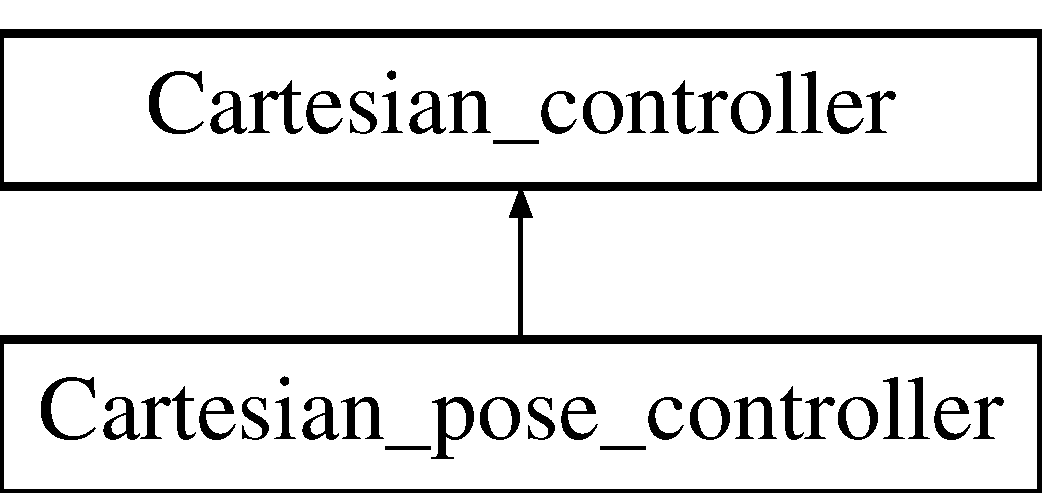
\includegraphics[height=2.000000cm]{classCartesian__pose__controller}
\end{center}
\end{figure}
\subsection*{Public Member Functions}
\begin{DoxyCompactItemize}
\item 
\hyperlink{classCartesian__pose__controller_ab33ba9d374ac39a6723b4c4507db12e8}{Cartesian\-\_\-pose\-\_\-controller} (std\-::vector$<$ double $>$ \hyperlink{classCartesian__pose__controller_a42433d7f2e4e03ccaac56e1f9a7a5027}{initial\-Positions}, \hyperlink{structRobot}{Robot} $\ast$\hyperlink{classCartesian__controller_a5562129951bd802e4ded77fc716c87a0}{r}, double K\-P\mbox{[}$\,$\mbox{]}, double K\-I\mbox{[}$\,$\mbox{]}, double K\-D\mbox{[}$\,$\mbox{]}, double \hyperlink{classCartesian__controller_a35c6ddbb9624878f2807ff644a33e832}{T})
\item 
\hyperlink{classCartesian__pose__controller_ab1339b9181d43b7560f9fc688dc4d047}{$\sim$\-Cartesian\-\_\-pose\-\_\-controller} ()
\item 
void \hyperlink{classCartesian__pose__controller_ab937d166862f2756eb3d08f37a0a090d}{control} ()
\item 
void \hyperlink{classCartesian__pose__controller_af9c1ec1f565375f50f8a15b16464f94d}{update\-References\-Callback} (const schunk\-\_\-msgs\-::\-Positions\-::\-Const\-Ptr \&msg)
\begin{DoxyCompactList}\small\item\em Receive schunk\-\_\-msgs\-::\-Velocities and updates this \hyperlink{classCartesian__controller}{Cartesian\-\_\-controller}'s internal variables. \end{DoxyCompactList}\end{DoxyCompactItemize}
\subsection*{Private Member Functions}
\begin{DoxyCompactItemize}
\item 
bool \hyperlink{classCartesian__pose__controller_ab55ab40074c82ba8cc010fe68fc76d5b}{print\-Pose} ()
\item 
void \hyperlink{classCartesian__pose__controller_a965f86a383eb205df10832626fac98af}{update\-References} (double ref\-\_\-gain)
\begin{DoxyCompactList}\small\item\em Calls the last velocity callback and updates the P\-G\-M\-A\-T\-R\-I\-X D\-\_\-ref with the updated values. \end{DoxyCompactList}\end{DoxyCompactItemize}
\subsection*{Private Attributes}
\begin{DoxyCompactItemize}
\item 
ros\-::\-Node\-Handle \hyperlink{classCartesian__pose__controller_ab2d5fe68c8229b6c90f84ac1601eb637}{reference\-\_\-updater\-\_\-nh}
\item 
ros\-::\-Callback\-Queue \hyperlink{classCartesian__pose__controller_a6eea82d82ccd6c925be31c18e1b4a432}{reference\-\_\-updater\-\_\-queue}
\item 
ros\-::\-Subscriber \hyperlink{classCartesian__pose__controller_a9394ae99649279f815c234b1ca7801b6}{reference\-\_\-updater\-\_\-subscriber}
\item 
ros\-::\-Publisher \hyperlink{classCartesian__pose__controller_a9eb38e771e5006950b9a8075a0ea7e49}{schunk\-\_\-pose\-Publisher}
\item 
ros\-::\-Node\-Handle \hyperlink{classCartesian__pose__controller_a41a692189fed59ec8ec8460539f63c66}{schunk\-\_\-pose\-\_\-nh}
\item 
ros\-::\-Callback\-Queue \hyperlink{classCartesian__pose__controller_a5efe52a57e5239b3fd86ff456e94691b}{schunk\-\_\-pose\-\_\-queue}
\item 
schunk\-\_\-msgs\-::\-Positions \hyperlink{classCartesian__pose__controller_a301bc44e901e4837cf036661478354c4}{schunk\-\_\-pose}
\item 
std\-::vector$<$ double $>$ \hyperlink{classCartesian__pose__controller_a42433d7f2e4e03ccaac56e1f9a7a5027}{initial\-Positions}
\end{DoxyCompactItemize}
\subsection*{Additional Inherited Members}


\subsection{Detailed Description}


Definition at line 5 of file cartesian\-\_\-pose\-\_\-controller.\-h.



\subsection{Constructor \& Destructor Documentation}
\hypertarget{classCartesian__pose__controller_ab33ba9d374ac39a6723b4c4507db12e8}{\index{Cartesian\-\_\-pose\-\_\-controller@{Cartesian\-\_\-pose\-\_\-controller}!Cartesian\-\_\-pose\-\_\-controller@{Cartesian\-\_\-pose\-\_\-controller}}
\index{Cartesian\-\_\-pose\-\_\-controller@{Cartesian\-\_\-pose\-\_\-controller}!Cartesian_pose_controller@{Cartesian\-\_\-pose\-\_\-controller}}
\subsubsection[{Cartesian\-\_\-pose\-\_\-controller}]{\setlength{\rightskip}{0pt plus 5cm}Cartesian\-\_\-pose\-\_\-controller\-::\-Cartesian\-\_\-pose\-\_\-controller (
\begin{DoxyParamCaption}
\item[{std\-::vector$<$ double $>$}]{initial\-Positions, }
\item[{{\bf Robot} $\ast$}]{r, }
\item[{double}]{K\-P\mbox{[}$\,$\mbox{]}, }
\item[{double}]{K\-I\mbox{[}$\,$\mbox{]}, }
\item[{double}]{K\-D\mbox{[}$\,$\mbox{]}, }
\item[{double}]{T}
\end{DoxyParamCaption}
)}}\label{classCartesian__pose__controller_ab33ba9d374ac39a6723b4c4507db12e8}


Definition at line 289 of file cartesian\-\_\-pose\-\_\-controller.\-cpp.



References initial\-Positions, reference\-\_\-updater\-\_\-nh, reference\-\_\-updater\-\_\-queue, reference\-\_\-updater\-\_\-subscriber, Cartesian\-\_\-controller\-::ros\-\_\-pub\-\_\-buffer, schunk\-\_\-pose, schunk\-\_\-pose\-\_\-nh, schunk\-\_\-pose\-\_\-queue, schunk\-\_\-pose\-Publisher, and update\-References\-Callback().


\begin{DoxyCode}
                                                                               
                                                                        : 
      \hyperlink{classCartesian__controller_a71055bb1cbf01ced9e64bb1d184b68fe}{Cartesian\_controller}(r,8,KP,KI,KD,\hyperlink{classCartesian__controller_a35c6ddbb9624878f2807ff644a33e832}{T})\{


        this->\hyperlink{classCartesian__pose__controller_a42433d7f2e4e03ccaac56e1f9a7a5027}{initialPositions} = \hyperlink{classCartesian__pose__controller_a42433d7f2e4e03ccaac56e1f9a7a5027}{initialPositions}
      ;

        \textcolor{comment}{/******************************}
\textcolor{comment}{                 PUBLIC VARIABLES}
\textcolor{comment}{        *******************************/}

        \textcolor{comment}{//Positiosn vector}
        \textcolor{keywordflow}{for}(\textcolor{keywordtype}{int} j=0;j<8;j++)\{
                this->\hyperlink{classCartesian__pose__controller_a301bc44e901e4837cf036661478354c4}{schunk\_pose}.positions.push\_back(0.0);
        \}

        \textcolor{comment}{/******************************}
\textcolor{comment}{                  ROS VARIABLES}
\textcolor{comment}{        *******************************/}

        \textcolor{comment}{//Set Queues}
        this->\hyperlink{classCartesian__pose__controller_ab2d5fe68c8229b6c90f84ac1601eb637}{reference\_updater\_nh}.setCallbackQueue(&this->
      \hyperlink{classCartesian__pose__controller_a6eea82d82ccd6c925be31c18e1b4a432}{reference\_updater\_queue});
        this->\hyperlink{classCartesian__pose__controller_a41a692189fed59ec8ec8460539f63c66}{schunk\_pose\_nh}.setCallbackQueue(&this->
      \hyperlink{classCartesian__pose__controller_a5efe52a57e5239b3fd86ff456e94691b}{schunk\_pose\_queue});

        \textcolor{comment}{//Subscriber and queue init.}
        this->\hyperlink{classCartesian__pose__controller_a9394ae99649279f815c234b1ca7801b6}{reference\_updater\_subscriber}         
      = this->\hyperlink{classCartesian__pose__controller_ab2d5fe68c8229b6c90f84ac1601eb637}{reference\_updater\_nh}.subscribe(\textcolor{stringliteral}{"
      schunk\_reference\_positions"}, \hyperlink{classCartesian__controller_ab9ed5a808da204dbc612d313dc7332f4}{ros\_pub\_buffer}, &
      \hyperlink{classCartesian__pose__controller_af9c1ec1f565375f50f8a15b16464f94d}{Cartesian\_pose\_controller::updateReferencesCallback}
      , \textcolor{keyword}{this});

        \textcolor{comment}{//Publisher}
        this->\hyperlink{classCartesian__pose__controller_a9eb38e771e5006950b9a8075a0ea7e49}{schunk\_posePublisher}   = this->\hyperlink{classCartesian__pose__controller_a41a692189fed59ec8ec8460539f63c66}{schunk\_pose\_nh}
      .advertise<schunk\_msgs::Positions>(\textcolor{stringliteral}{"schunk\_endeffector\_pose"}, \hyperlink{classCartesian__controller_ab9ed5a808da204dbc612d313dc7332f4}{ros\_pub\_buffer}
      );

\}
\end{DoxyCode}
\hypertarget{classCartesian__pose__controller_ab1339b9181d43b7560f9fc688dc4d047}{\index{Cartesian\-\_\-pose\-\_\-controller@{Cartesian\-\_\-pose\-\_\-controller}!$\sim$\-Cartesian\-\_\-pose\-\_\-controller@{$\sim$\-Cartesian\-\_\-pose\-\_\-controller}}
\index{$\sim$\-Cartesian\-\_\-pose\-\_\-controller@{$\sim$\-Cartesian\-\_\-pose\-\_\-controller}!Cartesian_pose_controller@{Cartesian\-\_\-pose\-\_\-controller}}
\subsubsection[{$\sim$\-Cartesian\-\_\-pose\-\_\-controller}]{\setlength{\rightskip}{0pt plus 5cm}Cartesian\-\_\-pose\-\_\-controller\-::$\sim$\-Cartesian\-\_\-pose\-\_\-controller (
\begin{DoxyParamCaption}
{}
\end{DoxyParamCaption}
)}}\label{classCartesian__pose__controller_ab1339b9181d43b7560f9fc688dc4d047}


Definition at line 285 of file cartesian\-\_\-pose\-\_\-controller.\-cpp.


\begin{DoxyCode}
                                                     \{

\}
\end{DoxyCode}


\subsection{Member Function Documentation}
\hypertarget{classCartesian__pose__controller_ab937d166862f2756eb3d08f37a0a090d}{\index{Cartesian\-\_\-pose\-\_\-controller@{Cartesian\-\_\-pose\-\_\-controller}!control@{control}}
\index{control@{control}!Cartesian_pose_controller@{Cartesian\-\_\-pose\-\_\-controller}}
\subsubsection[{control}]{\setlength{\rightskip}{0pt plus 5cm}void Cartesian\-\_\-pose\-\_\-controller\-::control (
\begin{DoxyParamCaption}
{}
\end{DoxyParamCaption}
)\hspace{0.3cm}{\ttfamily [virtual]}}}\label{classCartesian__pose__controller_ab937d166862f2756eb3d08f37a0a090d}
Measure Position and Speed

Recalculation of measured data. 

Implements \hyperlink{classCartesian__controller_a8809167cab6d338a957439141fa2bf6c}{Cartesian\-\_\-controller}.



Definition at line 72 of file cartesian\-\_\-pose\-\_\-controller.\-cpp.



References Cartesian\-\_\-controller\-::aux1, Cartesian\-\_\-controller\-::aux2, Cartesian\-\_\-controller\-::aux3, Cartesian\-\_\-controller\-::change\-Schunk\-Mode(), Cartesian\-\_\-controller\-::control\-Clean\-Up(), D\-Q\-::d, Cartesian\-\_\-controller\-::\-D, Cartesian\-\_\-controller\-::\-D\-\_\-ref, D\-Q\-\_\-free(), Cartesian\-\_\-controller\-::\-D\-Thetas, Cartesian\-\_\-controller\-::\-Err, Cartesian\-\_\-controller\-::\-Err\-\_\-ant, Cartesian\-\_\-controller\-::\-Err\-\_\-int, F\-A\-L\-S\-E, Cartesian\-\_\-controller\-::get\-Schunk\-Positions\-And\-Velocities\-And\-Update\-Thetas\-And\-D\-Thetas(), initial\-Positions, Cartesian\-\_\-controller\-::\-Kd, Cartesian\-\_\-controller\-::\-Ki, Cartesian\-\_\-controller\-::\-Kp, D\-Q\-::p, P\-G\-M\-A\-T\-R\-I\-X\-\_\-\-A\-D\-D\-\_\-\-C\-O\-P\-Y\-\_\-\-F\-R\-E\-E(), P\-G\-M\-A\-T\-R\-I\-X\-\_\-\-D\-A\-M\-P\-E\-D\-\_\-\-L\-E\-A\-S\-T\-S\-Q\-U\-A\-R\-E\-S\-\_\-\-P\-S\-E\-U\-D\-O\-I\-N\-V\-E\-R\-S\-E(), P\-G\-M\-A\-T\-R\-I\-X\-\_\-\-D\-A\-T\-A, P\-G\-M\-A\-T\-R\-I\-X\-\_\-\-F\-R\-E\-E(), P\-G\-M\-A\-T\-R\-I\-X\-\_\-\-M\-U\-L\-T\-I\-P\-L\-Y\-\_\-\-C\-O\-N\-S\-T\-\_\-\-C\-O\-P\-Y\-\_\-\-F\-R\-E\-E(), P\-G\-M\-A\-T\-R\-I\-X\-\_\-\-M\-U\-L\-T\-I\-P\-L\-Y\-\_\-\-C\-O\-P\-Y\-\_\-\-F\-R\-E\-E(), P\-G\-M\-A\-T\-R\-I\-X\-\_\-\-S\-E\-T\-\_\-\-C\-O\-L\-U\-M\-N\-\_\-\-B\-Y\-\_\-\-D\-Q(), P\-G\-M\-A\-T\-R\-I\-X\-\_\-\-S\-U\-B\-T\-R\-A\-C\-T\-\_\-\-C\-O\-P\-Y\-\_\-\-F\-R\-E\-E(), print\-Pose(), Cartesian\-\_\-controller\-::r, Robot\-\_\-\-F\-K\-M(), Robot\-\_\-get\-A\-Jacobian(), Robot\-\_\-update\-Links\-Thetas\-By\-Matrix(), schunk\-\_\-pose, Cartesian\-\_\-controller\-::send\-Joint\-Positions\-To\-Schunk(), Cartesian\-\_\-controller\-::set\-Schunk\-Velocities\-And\-Send(), Cartesian\-\_\-controller\-::\-S\-J, Cartesian\-\_\-controller\-::\-T, Cartesian\-\_\-controller\-::\-Thetas, T\-R\-U\-E, update\-References(), and Q\-::v.



Referenced by main().


\begin{DoxyCode}
                                       \{
        \textcolor{comment}{/******************************}
\textcolor{comment}{}
\textcolor{comment}{                                ROS INIT}
\textcolor{comment}{        *******************************/}

        \textcolor{comment}{//Ros rate}
        ros::Rate ros\_rate(1/\hyperlink{classCartesian__controller_a35c6ddbb9624878f2807ff644a33e832}{T});

        \textcolor{comment}{/*****************************}
\textcolor{comment}{           CHANGE SCHUNK MODE TO ASSURE POSITION CONTROL}
\textcolor{comment}{         *****************************/}

        ros::service::waitForService(\textcolor{stringliteral}{"schunk\_set\_control\_mode"});

        ROS\_INFO\_STREAM(\textcolor{stringliteral}{"Changing Schunk's Control Mode"});
        \textcolor{keywordflow}{if}(!\hyperlink{classCartesian__controller_aaf006f80e89c08cf040956afbb4cf3c0}{changeSchunkMode}(CONTROL\_MODE\_POSITION))\{\textcolor{keywordflow}{return};\}
        ROS\_INFO\_STREAM(\textcolor{stringliteral}{"Mode Changed to position!"});
        ROS\_INFO\_STREAM(\textcolor{stringliteral}{"Sending initial position."});
        \hyperlink{classCartesian__controller_ae845f67c81c2649bfbaccf95230f2599}{sendJointPositionsToSchunk}(this->
      \hyperlink{classCartesian__pose__controller_a42433d7f2e4e03ccaac56e1f9a7a5027}{initialPositions});
        ROS\_INFO\_STREAM(\textcolor{stringliteral}{"Sent! Sleeping..."});
        sleep(20);

        \textcolor{comment}{/*****************************}
\textcolor{comment}{           CHANGE SCHUNK MODE TO ASSURE VELOCITY CONTROL}
\textcolor{comment}{         *****************************/}

        ROS\_INFO\_STREAM(\textcolor{stringliteral}{"Changing Schunk's Control Mode"});
        \textcolor{keywordflow}{if}(!\hyperlink{classCartesian__controller_aaf006f80e89c08cf040956afbb4cf3c0}{changeSchunkMode}(CONTROL\_MODE\_VELOCITY))\{\textcolor{keywordflow}{return};\}
        ROS\_INFO\_STREAM(\textcolor{stringliteral}{"Mode Changed to velocity!"});

        \textcolor{comment}{/*****************************}
\textcolor{comment}{           UPDATES SCHUNK'S INITIAL POSITION AND VELOCITY}
\textcolor{comment}{         *****************************/}
        ROS\_INFO\_STREAM(\textcolor{stringliteral}{"Where is Schunk and how fast is it?"});
        \textcolor{keywordflow}{if}(!\hyperlink{classCartesian__controller_a0d7a63bac84715f6742db738df246f91}{getSchunkPositionsAndVelocitiesAndUpdateThetasAndDThetas}
      ())\{\textcolor{keywordflow}{return};\}
        ROS\_INFO\_STREAM(\textcolor{stringliteral}{"Schunk found!"});

        \textcolor{comment}{/******************************}
\textcolor{comment}{        PRIVATE VARIABLE INITIALIZATION}
\textcolor{comment}{        *******************************/}

        \textcolor{comment}{//Update Robot Object. Thetas were updated.}
        \hyperlink{robot_8h_aa1d3aca5132bd5f347f5966d38fbb966}{Robot\_updateLinksThetasByMatrix}(\hyperlink{classCartesian__controller_a5562129951bd802e4ded77fc716c87a0}{r},\hyperlink{classCartesian__controller_a0a0f818dad601cd9e3e26cb6959b8eb6}{
      Thetas});
        \textcolor{comment}{//Update end effectors pose}
        \hyperlink{structDQ}{DQ}* eep = \hyperlink{robot_8h_a57cc252fbb9e4c8be955b6af755b0c2c}{Robot\_FKM}(\hyperlink{classCartesian__controller_a5562129951bd802e4ded77fc716c87a0}{r});
        \textcolor{comment}{//Current end effectors pose is now the reference pose.}
        \textcolor{keywordflow}{for}(\textcolor{keywordtype}{int} j=0;j<4;j++)\{
                this->\hyperlink{classCartesian__pose__controller_a301bc44e901e4837cf036661478354c4}{schunk\_pose}.positions[j]   = eep->\hyperlink{structDQ_a878210bff170f4392d6cbe2d4704ffdc}{p}->\hyperlink{structQ_a2a0074b583999340d42804e4c1141ac4}{v}[j];
                this->\hyperlink{classCartesian__pose__controller_a301bc44e901e4837cf036661478354c4}{schunk\_pose}.positions[j+4] = eep->\hyperlink{structDQ_a535cdb52876521fd6abbfcf211a7c702}{d}->\hyperlink{structQ_a2a0074b583999340d42804e4c1141ac4}{v}[j];
        \}
        \textcolor{comment}{//Update D\_ref and D}
        \hyperlink{classCartesian__pose__controller_a965f86a383eb205df10832626fac98af}{updateReferences}(1);
        \hyperlink{dualquaternion_8h_a3d48348c3e25d1724058c2cf2364e42e}{PGMATRIX\_SET\_COLUMN\_BY\_DQ}(\hyperlink{classCartesian__controller_a8c470b652ce436d8e48f126073fc2593}{D}, 1, eep);
        \textcolor{comment}{//Here, both D and D\_ref should be the same}
        \textcolor{keywordflow}{for}(\textcolor{keywordtype}{int} j=0;j<8;j++)\{
                ROS\_INFO\_STREAM(\textcolor{stringliteral}{"Values are : D="} << \hyperlink{gmatrix_8h_a7333180c47234295df2bd7b09ac00da8}{PGMATRIX\_DATA}
      (\hyperlink{classCartesian__controller_a8c470b652ce436d8e48f126073fc2593}{D},j+1,1) << \textcolor{stringliteral}{" and D\_ref="} << \hyperlink{gmatrix_8h_a7333180c47234295df2bd7b09ac00da8}{PGMATRIX\_DATA}(\hyperlink{classCartesian__controller_abb248cb3215a574fe8e1bb8fb0b8626d}{D\_ref},j+1,1) );
        \}

        \textcolor{comment}{//Jacobians}
        \hyperlink{classCartesian__controller_a98fdac06d136ac3dba0102d97cd5dd36}{SJ}  = \hyperlink{robot_8h_ab6dd42296709cf38d3468af7afd29563}{Robot\_getAJacobian}(\hyperlink{classCartesian__controller_a5562129951bd802e4ded77fc716c87a0}{r});

        \textcolor{comment}{/******************************}
\textcolor{comment}{                        LOOP}
\textcolor{comment}{        *******************************/}

        ROS\_INFO\_STREAM(\textcolor{stringliteral}{"Take a deep breath and GO!"});
        \textcolor{comment}{//Take a deep breath and GO}
        ros\_rate.sleep();

        \textcolor{keywordflow}{while}(ros::ok())\{
                \textcolor{comment}{//Last Error}
                \hyperlink{gmatrix_8h_a9a73b4e0a77f386c0bae1bba75298d1d}{PGMATRIX\_FREE}(\hyperlink{classCartesian__controller_a6d9471a983f6cb6c642bf8dea0d540af}{Err\_ant});
                \hyperlink{classCartesian__controller_a6d9471a983f6cb6c642bf8dea0d540af}{Err\_ant} = \hyperlink{classCartesian__controller_ab3f08ecf10cb2486e8bfc61f07e2bde6}{Err};
                \textcolor{comment}{/******************************}
\textcolor{comment}{                        /END GET NEW REFERENCES}
\textcolor{comment}{                *******************************/}
                \textcolor{comment}{//Current Error}
                \hyperlink{classCartesian__controller_ab3f08ecf10cb2486e8bfc61f07e2bde6}{Err} =     \hyperlink{gmatrix__plus_8h_a146d9062e4325cc3b97990ae51b96d95}{PGMATRIX\_SUBTRACT\_COPY\_FREE}
      (\hyperlink{classCartesian__controller_abb248cb3215a574fe8e1bb8fb0b8626d}{D\_ref},\hyperlink{classCartesian__controller_a8c470b652ce436d8e48f126073fc2593}{D},\hyperlink{gmatlabdatafile_8h_aa93f0eb578d23995850d61f7d61c55c1}{FALSE},\hyperlink{gmatlabdatafile_8h_aa93f0eb578d23995850d61f7d61c55c1}{FALSE});
                \textcolor{comment}{//Error Integral}
                \hyperlink{classCartesian__controller_a37edb9c6e2a5066f74941e3659f68cbc}{aux1} =        \hyperlink{gmatrix__plus_8h_a371a0bfffdb84cf1596ca60bbf7fce93}{PGMATRIX\_MULTIPLY\_CONST\_COPY\_FREE}
      (\hyperlink{classCartesian__controller_ab3f08ecf10cb2486e8bfc61f07e2bde6}{Err},\hyperlink{classCartesian__controller_a35c6ddbb9624878f2807ff644a33e832}{T},\hyperlink{gmatlabdatafile_8h_aa93f0eb578d23995850d61f7d61c55c1}{FALSE});
                \hyperlink{classCartesian__controller_a248174c6399a8933bfcc8f1b0b39af5e}{Err\_int} = \hyperlink{gmatrix__plus_8h_aa1123306aa55d942955e09156db757a3}{PGMATRIX\_ADD\_COPY\_FREE}(
      \hyperlink{classCartesian__controller_a248174c6399a8933bfcc8f1b0b39af5e}{Err\_int},\hyperlink{classCartesian__controller_a37edb9c6e2a5066f74941e3659f68cbc}{aux1},\hyperlink{gmatlabdatafile_8h_aa8cecfc5c5c054d2875c03e77b7be15d}{TRUE},\hyperlink{gmatlabdatafile_8h_aa8cecfc5c5c054d2875c03e77b7be15d}{TRUE});
                \textcolor{comment}{//Derivative    aux1 = Kd*(Err-Err\_ant)*(1/T)}
                \hyperlink{classCartesian__controller_a37edb9c6e2a5066f74941e3659f68cbc}{aux1} = \hyperlink{gmatrix__plus_8h_a146d9062e4325cc3b97990ae51b96d95}{PGMATRIX\_SUBTRACT\_COPY\_FREE}
      (\hyperlink{classCartesian__controller_ab3f08ecf10cb2486e8bfc61f07e2bde6}{Err},\hyperlink{classCartesian__controller_a6d9471a983f6cb6c642bf8dea0d540af}{Err\_ant},\hyperlink{gmatlabdatafile_8h_aa93f0eb578d23995850d61f7d61c55c1}{FALSE},\hyperlink{gmatlabdatafile_8h_aa93f0eb578d23995850d61f7d61c55c1}{FALSE});
                \hyperlink{classCartesian__controller_a37edb9c6e2a5066f74941e3659f68cbc}{aux1} = \hyperlink{gmatrix__plus_8h_a17b482a0aaa68d1f4c1c30a1a72dacbb}{PGMATRIX\_MULTIPLY\_COPY\_FREE}
      (\hyperlink{classCartesian__controller_a62394cef8a9a29eac18319a4ad579c4c}{Kd},\hyperlink{classCartesian__controller_a37edb9c6e2a5066f74941e3659f68cbc}{aux1},\hyperlink{gmatlabdatafile_8h_aa93f0eb578d23995850d61f7d61c55c1}{FALSE},\hyperlink{gmatlabdatafile_8h_aa8cecfc5c5c054d2875c03e77b7be15d}{TRUE});
                \hyperlink{classCartesian__controller_a37edb9c6e2a5066f74941e3659f68cbc}{aux1} = \hyperlink{gmatrix__plus_8h_a371a0bfffdb84cf1596ca60bbf7fce93}{PGMATRIX\_MULTIPLY\_CONST\_COPY\_FREE}
      (\hyperlink{classCartesian__controller_a37edb9c6e2a5066f74941e3659f68cbc}{aux1},(1/\hyperlink{classCartesian__controller_a35c6ddbb9624878f2807ff644a33e832}{T}),\hyperlink{gmatlabdatafile_8h_aa8cecfc5c5c054d2875c03e77b7be15d}{TRUE});
                \textcolor{comment}{//Integral      aux2 = Ki*(Err\_int)}
                \hyperlink{classCartesian__controller_af73a0c910cd80ed2f84974b65beba450}{aux2} = \hyperlink{gmatrix__plus_8h_a17b482a0aaa68d1f4c1c30a1a72dacbb}{PGMATRIX\_MULTIPLY\_COPY\_FREE}
      (\hyperlink{classCartesian__controller_a70e495f39da706f1b589684f58343b9e}{Ki},\hyperlink{classCartesian__controller_a248174c6399a8933bfcc8f1b0b39af5e}{Err\_int},\hyperlink{gmatlabdatafile_8h_aa93f0eb578d23995850d61f7d61c55c1}{FALSE},\hyperlink{gmatlabdatafile_8h_aa93f0eb578d23995850d61f7d61c55c1}{FALSE});
                \textcolor{comment}{//Proportional  aux3 = Kp*(Err)}
                \hyperlink{classCartesian__controller_aa37c15fcd53a60ecce106cd9b39d3501}{aux3} = \hyperlink{gmatrix__plus_8h_a17b482a0aaa68d1f4c1c30a1a72dacbb}{PGMATRIX\_MULTIPLY\_COPY\_FREE}
      (\hyperlink{classCartesian__controller_a78073f51064a05d72c41723a93d9079f}{Kp},\hyperlink{classCartesian__controller_ab3f08ecf10cb2486e8bfc61f07e2bde6}{Err},\hyperlink{gmatlabdatafile_8h_aa93f0eb578d23995850d61f7d61c55c1}{FALSE},\hyperlink{gmatlabdatafile_8h_aa93f0eb578d23995850d61f7d61c55c1}{FALSE});

                \textcolor{comment}{//Error Sum     aux1 = Kd*(Err-Err\_ant)*(1/T) + Ki*(Err\_int) +
       Kp*(Err)}
                \hyperlink{classCartesian__controller_a37edb9c6e2a5066f74941e3659f68cbc}{aux1} = \hyperlink{gmatrix__plus_8h_aa1123306aa55d942955e09156db757a3}{PGMATRIX\_ADD\_COPY\_FREE}(\hyperlink{classCartesian__controller_a37edb9c6e2a5066f74941e3659f68cbc}{aux1}
      ,\hyperlink{classCartesian__controller_af73a0c910cd80ed2f84974b65beba450}{aux2},\hyperlink{gmatlabdatafile_8h_aa8cecfc5c5c054d2875c03e77b7be15d}{TRUE},\hyperlink{gmatlabdatafile_8h_aa8cecfc5c5c054d2875c03e77b7be15d}{TRUE});
                \hyperlink{classCartesian__controller_a37edb9c6e2a5066f74941e3659f68cbc}{aux1} = \hyperlink{gmatrix__plus_8h_aa1123306aa55d942955e09156db757a3}{PGMATRIX\_ADD\_COPY\_FREE}(\hyperlink{classCartesian__controller_a37edb9c6e2a5066f74941e3659f68cbc}{aux1}
      ,\hyperlink{classCartesian__controller_aa37c15fcd53a60ecce106cd9b39d3501}{aux3},\hyperlink{gmatlabdatafile_8h_aa8cecfc5c5c054d2875c03e77b7be15d}{TRUE},\hyperlink{gmatlabdatafile_8h_aa8cecfc5c5c054d2875c03e77b7be15d}{TRUE});
                \textcolor{comment}{//Pseudo Inverse Calculation}
                \hyperlink{classCartesian__controller_af73a0c910cd80ed2f84974b65beba450}{aux2} =      \hyperlink{gmatrix__plus_8h_a73bceba2ac1f3a5589628d0f2e4081fa}{PGMATRIX\_DAMPED\_LEASTSQUARES\_PSEUDOINVERSE}
      (\hyperlink{classCartesian__controller_a98fdac06d136ac3dba0102d97cd5dd36}{SJ},0.01);

                \textcolor{comment}{//New DThetas = pinv(SJ)*(Error Sum)}
                \hyperlink{gmatrix_8h_a9a73b4e0a77f386c0bae1bba75298d1d}{PGMATRIX\_FREE}(\hyperlink{classCartesian__controller_a5d6419e62e130150edfcbd82b1dadcae}{DThetas});
                \hyperlink{classCartesian__controller_a5d6419e62e130150edfcbd82b1dadcae}{DThetas} = \hyperlink{gmatrix__plus_8h_a17b482a0aaa68d1f4c1c30a1a72dacbb}{PGMATRIX\_MULTIPLY\_COPY\_FREE}
      (\hyperlink{classCartesian__controller_af73a0c910cd80ed2f84974b65beba450}{aux2},\hyperlink{classCartesian__controller_a37edb9c6e2a5066f74941e3659f68cbc}{aux1},\hyperlink{gmatlabdatafile_8h_aa8cecfc5c5c054d2875c03e77b7be15d}{TRUE},\hyperlink{gmatlabdatafile_8h_aa8cecfc5c5c054d2875c03e77b7be15d}{TRUE});

                \textcolor{comment}{/******************************}
\textcolor{comment}{                         GET NEW REFERENCES}
\textcolor{comment}{                *******************************/}
                \textcolor{comment}{//Receive callback to after update references}
                \hyperlink{classCartesian__pose__controller_a965f86a383eb205df10832626fac98af}{updateReferences}(1);
                \textcolor{comment}{/******************************}
\textcolor{comment}{                        COMUNICATE WITH SCHUNK}
\textcolor{comment}{                *******************************/}

                \textcolor{comment}{//Sends information to robot to move, then wait and measure}
                \hyperlink{classCartesian__controller_a40d17a9794af8a9a607618bf0ee5efff}{setSchunkVelocitiesAndSend}(0.01);

                \textcolor{comment}{//Wait}
                ros\_rate.sleep();
                \textcolor{comment}{//Position and Velocities, THETAS AND DTHETAS ARE UPDATED}
                \textcolor{keywordflow}{if}(!\hyperlink{classCartesian__controller_a0d7a63bac84715f6742db738df246f91}{getSchunkPositionsAndVelocitiesAndUpdateThetasAndDThetas}
      ())\{\textcolor{keywordflow}{return};\}
                \hyperlink{classCartesian__pose__controller_ab55ab40074c82ba8cc010fe68fc76d5b}{printPose}();

                \textcolor{comment}{/******************************}
\textcolor{comment}{                /END    COMUNICATE WITH SCHUNK}
\textcolor{comment}{                *******************************/}

                \textcolor{comment}{//Updates Robot's Link's Thetas with current position}
                \hyperlink{robot_8h_aa1d3aca5132bd5f347f5966d38fbb966}{Robot\_updateLinksThetasByMatrix}(\hyperlink{classCartesian__controller_a5562129951bd802e4ded77fc716c87a0}{
      r},\hyperlink{classCartesian__controller_a0a0f818dad601cd9e3e26cb6959b8eb6}{Thetas});

                \textcolor{comment}{//Updates Jacobian with new position}
                \hyperlink{gmatrix_8h_a9a73b4e0a77f386c0bae1bba75298d1d}{PGMATRIX\_FREE}(\hyperlink{classCartesian__controller_a98fdac06d136ac3dba0102d97cd5dd36}{SJ});
                \hyperlink{classCartesian__controller_a98fdac06d136ac3dba0102d97cd5dd36}{SJ}  = \hyperlink{robot_8h_ab6dd42296709cf38d3468af7afd29563}{Robot\_getAJacobian}(\hyperlink{classCartesian__controller_a5562129951bd802e4ded77fc716c87a0}{r});

                \textcolor{comment}{//End effectors pose}
                \hyperlink{dualquaternion_8h_a1d21b6cb665c04de4be5aca50804caf4}{DQ\_free}(eep);
                eep = \hyperlink{robot_8h_a57cc252fbb9e4c8be955b6af755b0c2c}{Robot\_FKM}(\hyperlink{classCartesian__controller_a5562129951bd802e4ded77fc716c87a0}{r});
                \hyperlink{dualquaternion_8h_a3d48348c3e25d1724058c2cf2364e42e}{PGMATRIX\_SET\_COLUMN\_BY\_DQ}(\hyperlink{classCartesian__controller_a8c470b652ce436d8e48f126073fc2593}{D}, 1, eep);

        \}


        \textcolor{comment}{/******************************}
\textcolor{comment}{                        CLEAN UP}
\textcolor{comment}{        *******************************/}
        \hyperlink{classCartesian__controller_a8c0f0b41de9f4f8b2e3aa327e7c6b50c}{controlCleanUp}();

        \textcolor{keywordflow}{return};

\}
\end{DoxyCode}
\hypertarget{classCartesian__pose__controller_ab55ab40074c82ba8cc010fe68fc76d5b}{\index{Cartesian\-\_\-pose\-\_\-controller@{Cartesian\-\_\-pose\-\_\-controller}!print\-Pose@{print\-Pose}}
\index{print\-Pose@{print\-Pose}!Cartesian_pose_controller@{Cartesian\-\_\-pose\-\_\-controller}}
\subsubsection[{print\-Pose}]{\setlength{\rightskip}{0pt plus 5cm}bool Cartesian\-\_\-pose\-\_\-controller\-::print\-Pose (
\begin{DoxyParamCaption}
{}
\end{DoxyParamCaption}
)\hspace{0.3cm}{\ttfamily [private]}}}\label{classCartesian__pose__controller_ab55ab40074c82ba8cc010fe68fc76d5b}


Definition at line 223 of file cartesian\-\_\-pose\-\_\-controller.\-cpp.



References Cartesian\-\_\-controller\-::\-D, D\-Q\-\_\-create(), D\-Q\-\_\-free(), D\-Q\-\_\-get\-R(), D\-Q\-\_\-get\-T(), P\-G\-M\-A\-T\-R\-I\-X\-\_\-\-D\-A\-T\-A, Q\-\_\-free(), schunk\-\_\-pose, schunk\-\_\-pose\-\_\-queue, schunk\-\_\-pose\-Publisher, and Q\-::v.



Referenced by control().


\begin{DoxyCode}
                                         \{

        \textcolor{comment}{//for(int j=0;j<8;j++)\{}
        \textcolor{comment}{//      schunk\_pose.positions[j] = PGMATRIX\_DATA(D,j+1,1);}
        \textcolor{comment}{//\}}
        \textcolor{comment}{//Temp TODO: DELETE ALL THE STUFF BETWEEN ME}
        \hyperlink{structDQ}{DQ}* dq = \hyperlink{dualquaternion_8h_a8b1057516bdc2c0cb14127791cf356cf}{DQ\_create}(\hyperlink{gmatrix_8h_a7333180c47234295df2bd7b09ac00da8}{PGMATRIX\_DATA}(\hyperlink{classCartesian__controller_a8c470b652ce436d8e48f126073fc2593}{D},1,1),
                        \hyperlink{gmatrix_8h_a7333180c47234295df2bd7b09ac00da8}{PGMATRIX\_DATA}(\hyperlink{classCartesian__controller_a8c470b652ce436d8e48f126073fc2593}{D},2,1),
                        \hyperlink{gmatrix_8h_a7333180c47234295df2bd7b09ac00da8}{PGMATRIX\_DATA}(\hyperlink{classCartesian__controller_a8c470b652ce436d8e48f126073fc2593}{D},3,1),
                        \hyperlink{gmatrix_8h_a7333180c47234295df2bd7b09ac00da8}{PGMATRIX\_DATA}(\hyperlink{classCartesian__controller_a8c470b652ce436d8e48f126073fc2593}{D},4,1),
                        \hyperlink{gmatrix_8h_a7333180c47234295df2bd7b09ac00da8}{PGMATRIX\_DATA}(\hyperlink{classCartesian__controller_a8c470b652ce436d8e48f126073fc2593}{D},5,1),
                        \hyperlink{gmatrix_8h_a7333180c47234295df2bd7b09ac00da8}{PGMATRIX\_DATA}(\hyperlink{classCartesian__controller_a8c470b652ce436d8e48f126073fc2593}{D},6,1),
                        \hyperlink{gmatrix_8h_a7333180c47234295df2bd7b09ac00da8}{PGMATRIX\_DATA}(\hyperlink{classCartesian__controller_a8c470b652ce436d8e48f126073fc2593}{D},7,1),
                        \hyperlink{gmatrix_8h_a7333180c47234295df2bd7b09ac00da8}{PGMATRIX\_DATA}(\hyperlink{classCartesian__controller_a8c470b652ce436d8e48f126073fc2593}{D},8,1));
        \hyperlink{structQ}{Q}* trans = \hyperlink{dualquaternion_8h_a80e2f2aded851388d4f18d486a0b9455}{DQ\_getT}(dq);
        \hyperlink{structQ}{Q}* rot = \hyperlink{dualquaternion_8h_a35b3966af2f77ad5a8f47126948720fb}{DQ\_getR}(dq);
        \textcolor{keywordflow}{for}(\textcolor{keywordtype}{int} j=0;j<4;j++)\{
                \hyperlink{classCartesian__pose__controller_a301bc44e901e4837cf036661478354c4}{schunk\_pose}.positions[j]   = trans->\hyperlink{structQ_a2a0074b583999340d42804e4c1141ac4}{v}[j];
                \hyperlink{classCartesian__pose__controller_a301bc44e901e4837cf036661478354c4}{schunk\_pose}.positions[j+4] = rot->\hyperlink{structQ_a2a0074b583999340d42804e4c1141ac4}{v}[j];
        \}
        \hyperlink{dualquaternion_8h_a1d21b6cb665c04de4be5aca50804caf4}{DQ\_free}(dq);
        \hyperlink{quaternion_8h_a69ecc76f665022f81be1702c20865de4}{Q\_free}(trans);
        \hyperlink{quaternion_8h_a69ecc76f665022f81be1702c20865de4}{Q\_free}(rot);
        \textcolor{comment}{//TODO: AND ME}

        \hyperlink{classCartesian__pose__controller_a9eb38e771e5006950b9a8075a0ea7e49}{schunk\_posePublisher}.publish(\hyperlink{classCartesian__pose__controller_a301bc44e901e4837cf036661478354c4}{schunk\_pose}
      );
        \hyperlink{classCartesian__pose__controller_a5efe52a57e5239b3fd86ff456e94691b}{schunk\_pose\_queue}.callAvailable(ros::WallDuration(0));

        \textcolor{keywordflow}{return} \textcolor{keyword}{true};
\}
\end{DoxyCode}
\hypertarget{classCartesian__pose__controller_a965f86a383eb205df10832626fac98af}{\index{Cartesian\-\_\-pose\-\_\-controller@{Cartesian\-\_\-pose\-\_\-controller}!update\-References@{update\-References}}
\index{update\-References@{update\-References}!Cartesian_pose_controller@{Cartesian\-\_\-pose\-\_\-controller}}
\subsubsection[{update\-References}]{\setlength{\rightskip}{0pt plus 5cm}void Cartesian\-\_\-pose\-\_\-controller\-::update\-References (
\begin{DoxyParamCaption}
\item[{double}]{ref\-\_\-gain}
\end{DoxyParamCaption}
)\hspace{0.3cm}{\ttfamily [inline]}, {\ttfamily [private]}}}\label{classCartesian__pose__controller_a965f86a383eb205df10832626fac98af}


Calls the last velocity callback and updates the P\-G\-M\-A\-T\-R\-I\-X D\-\_\-ref with the updated values. 



Definition at line 257 of file cartesian\-\_\-pose\-\_\-controller.\-cpp.



References Cartesian\-\_\-controller\-::\-D\-\_\-ref, P\-G\-M\-A\-T\-R\-I\-X\-\_\-\-D\-A\-T\-A, reference\-\_\-updater\-\_\-queue, and schunk\-\_\-pose.



Referenced by control().


\begin{DoxyCode}
                                                                      \{

        \textcolor{comment}{//Calls one of the velocities callbacks in the queue.}
        \hyperlink{classCartesian__pose__controller_a6eea82d82ccd6c925be31c18e1b4a432}{reference\_updater\_queue}.callAvailable(
      ros::WallDuration(0));

        \textcolor{comment}{//Update references matrix}
        \textcolor{keywordflow}{for}(\textcolor{keywordtype}{int} j=0;j<8;j++)\{
                \hyperlink{gmatrix_8h_a7333180c47234295df2bd7b09ac00da8}{PGMATRIX\_DATA}(\hyperlink{classCartesian__controller_abb248cb3215a574fe8e1bb8fb0b8626d}{D\_ref},j+1,1) = ref\_gain*this->
      \hyperlink{classCartesian__pose__controller_a301bc44e901e4837cf036661478354c4}{schunk\_pose}.positions[j];
        \}

\}
\end{DoxyCode}
\hypertarget{classCartesian__pose__controller_af9c1ec1f565375f50f8a15b16464f94d}{\index{Cartesian\-\_\-pose\-\_\-controller@{Cartesian\-\_\-pose\-\_\-controller}!update\-References\-Callback@{update\-References\-Callback}}
\index{update\-References\-Callback@{update\-References\-Callback}!Cartesian_pose_controller@{Cartesian\-\_\-pose\-\_\-controller}}
\subsubsection[{update\-References\-Callback}]{\setlength{\rightskip}{0pt plus 5cm}void Cartesian\-\_\-pose\-\_\-controller\-::update\-References\-Callback (
\begin{DoxyParamCaption}
\item[{const schunk\-\_\-msgs\-::\-Positions\-::\-Const\-Ptr \&}]{msg}
\end{DoxyParamCaption}
)}}\label{classCartesian__pose__controller_af9c1ec1f565375f50f8a15b16464f94d}


Receive schunk\-\_\-msgs\-::\-Velocities and updates this \hyperlink{classCartesian__controller}{Cartesian\-\_\-controller}'s internal variables. 



Definition at line 272 of file cartesian\-\_\-pose\-\_\-controller.\-cpp.



References schunk\-\_\-pose.



Referenced by Cartesian\-\_\-pose\-\_\-controller().


\begin{DoxyCode}
                                                                               
                      \{

        \textcolor{keywordflow}{if}(msg->positions.size() != 8)\{
                ROS\_ERROR\_STREAM(\textcolor{stringliteral}{"Dualquaternion being sent to
       schunk\_reference\_positions's topic is not size 8"});
                \textcolor{keywordflow}{return};
        \}

        \textcolor{keywordflow}{for}(\textcolor{keywordtype}{int} i = 0; i < 8; i++)\{
                this->\hyperlink{classCartesian__pose__controller_a301bc44e901e4837cf036661478354c4}{schunk\_pose}.positions[i] = msg->positions[i];
        \}
\}
\end{DoxyCode}


\subsection{Field Documentation}
\hypertarget{classCartesian__pose__controller_a42433d7f2e4e03ccaac56e1f9a7a5027}{\index{Cartesian\-\_\-pose\-\_\-controller@{Cartesian\-\_\-pose\-\_\-controller}!initial\-Positions@{initial\-Positions}}
\index{initial\-Positions@{initial\-Positions}!Cartesian_pose_controller@{Cartesian\-\_\-pose\-\_\-controller}}
\subsubsection[{initial\-Positions}]{\setlength{\rightskip}{0pt plus 5cm}std\-::vector$<$double$>$ Cartesian\-\_\-pose\-\_\-controller\-::initial\-Positions\hspace{0.3cm}{\ttfamily [private]}}}\label{classCartesian__pose__controller_a42433d7f2e4e03ccaac56e1f9a7a5027}


Definition at line 23 of file cartesian\-\_\-pose\-\_\-controller.\-h.



Referenced by Cartesian\-\_\-pose\-\_\-controller(), and control().

\hypertarget{classCartesian__pose__controller_ab2d5fe68c8229b6c90f84ac1601eb637}{\index{Cartesian\-\_\-pose\-\_\-controller@{Cartesian\-\_\-pose\-\_\-controller}!reference\-\_\-updater\-\_\-nh@{reference\-\_\-updater\-\_\-nh}}
\index{reference\-\_\-updater\-\_\-nh@{reference\-\_\-updater\-\_\-nh}!Cartesian_pose_controller@{Cartesian\-\_\-pose\-\_\-controller}}
\subsubsection[{reference\-\_\-updater\-\_\-nh}]{\setlength{\rightskip}{0pt plus 5cm}ros\-::\-Node\-Handle Cartesian\-\_\-pose\-\_\-controller\-::reference\-\_\-updater\-\_\-nh\hspace{0.3cm}{\ttfamily [private]}}}\label{classCartesian__pose__controller_ab2d5fe68c8229b6c90f84ac1601eb637}


Definition at line 12 of file cartesian\-\_\-pose\-\_\-controller.\-h.



Referenced by Cartesian\-\_\-pose\-\_\-controller().

\hypertarget{classCartesian__pose__controller_a6eea82d82ccd6c925be31c18e1b4a432}{\index{Cartesian\-\_\-pose\-\_\-controller@{Cartesian\-\_\-pose\-\_\-controller}!reference\-\_\-updater\-\_\-queue@{reference\-\_\-updater\-\_\-queue}}
\index{reference\-\_\-updater\-\_\-queue@{reference\-\_\-updater\-\_\-queue}!Cartesian_pose_controller@{Cartesian\-\_\-pose\-\_\-controller}}
\subsubsection[{reference\-\_\-updater\-\_\-queue}]{\setlength{\rightskip}{0pt plus 5cm}ros\-::\-Callback\-Queue Cartesian\-\_\-pose\-\_\-controller\-::reference\-\_\-updater\-\_\-queue\hspace{0.3cm}{\ttfamily [private]}}}\label{classCartesian__pose__controller_a6eea82d82ccd6c925be31c18e1b4a432}


Definition at line 13 of file cartesian\-\_\-pose\-\_\-controller.\-h.



Referenced by Cartesian\-\_\-pose\-\_\-controller(), and update\-References().

\hypertarget{classCartesian__pose__controller_a9394ae99649279f815c234b1ca7801b6}{\index{Cartesian\-\_\-pose\-\_\-controller@{Cartesian\-\_\-pose\-\_\-controller}!reference\-\_\-updater\-\_\-subscriber@{reference\-\_\-updater\-\_\-subscriber}}
\index{reference\-\_\-updater\-\_\-subscriber@{reference\-\_\-updater\-\_\-subscriber}!Cartesian_pose_controller@{Cartesian\-\_\-pose\-\_\-controller}}
\subsubsection[{reference\-\_\-updater\-\_\-subscriber}]{\setlength{\rightskip}{0pt plus 5cm}ros\-::\-Subscriber Cartesian\-\_\-pose\-\_\-controller\-::reference\-\_\-updater\-\_\-subscriber\hspace{0.3cm}{\ttfamily [private]}}}\label{classCartesian__pose__controller_a9394ae99649279f815c234b1ca7801b6}


Definition at line 14 of file cartesian\-\_\-pose\-\_\-controller.\-h.



Referenced by Cartesian\-\_\-pose\-\_\-controller().

\hypertarget{classCartesian__pose__controller_a301bc44e901e4837cf036661478354c4}{\index{Cartesian\-\_\-pose\-\_\-controller@{Cartesian\-\_\-pose\-\_\-controller}!schunk\-\_\-pose@{schunk\-\_\-pose}}
\index{schunk\-\_\-pose@{schunk\-\_\-pose}!Cartesian_pose_controller@{Cartesian\-\_\-pose\-\_\-controller}}
\subsubsection[{schunk\-\_\-pose}]{\setlength{\rightskip}{0pt plus 5cm}schunk\-\_\-msgs\-::\-Positions Cartesian\-\_\-pose\-\_\-controller\-::schunk\-\_\-pose\hspace{0.3cm}{\ttfamily [private]}}}\label{classCartesian__pose__controller_a301bc44e901e4837cf036661478354c4}


Definition at line 20 of file cartesian\-\_\-pose\-\_\-controller.\-h.



Referenced by Cartesian\-\_\-pose\-\_\-controller(), control(), print\-Pose(), update\-References(), and update\-References\-Callback().

\hypertarget{classCartesian__pose__controller_a41a692189fed59ec8ec8460539f63c66}{\index{Cartesian\-\_\-pose\-\_\-controller@{Cartesian\-\_\-pose\-\_\-controller}!schunk\-\_\-pose\-\_\-nh@{schunk\-\_\-pose\-\_\-nh}}
\index{schunk\-\_\-pose\-\_\-nh@{schunk\-\_\-pose\-\_\-nh}!Cartesian_pose_controller@{Cartesian\-\_\-pose\-\_\-controller}}
\subsubsection[{schunk\-\_\-pose\-\_\-nh}]{\setlength{\rightskip}{0pt plus 5cm}ros\-::\-Node\-Handle Cartesian\-\_\-pose\-\_\-controller\-::schunk\-\_\-pose\-\_\-nh\hspace{0.3cm}{\ttfamily [private]}}}\label{classCartesian__pose__controller_a41a692189fed59ec8ec8460539f63c66}


Definition at line 18 of file cartesian\-\_\-pose\-\_\-controller.\-h.



Referenced by Cartesian\-\_\-pose\-\_\-controller().

\hypertarget{classCartesian__pose__controller_a5efe52a57e5239b3fd86ff456e94691b}{\index{Cartesian\-\_\-pose\-\_\-controller@{Cartesian\-\_\-pose\-\_\-controller}!schunk\-\_\-pose\-\_\-queue@{schunk\-\_\-pose\-\_\-queue}}
\index{schunk\-\_\-pose\-\_\-queue@{schunk\-\_\-pose\-\_\-queue}!Cartesian_pose_controller@{Cartesian\-\_\-pose\-\_\-controller}}
\subsubsection[{schunk\-\_\-pose\-\_\-queue}]{\setlength{\rightskip}{0pt plus 5cm}ros\-::\-Callback\-Queue Cartesian\-\_\-pose\-\_\-controller\-::schunk\-\_\-pose\-\_\-queue\hspace{0.3cm}{\ttfamily [private]}}}\label{classCartesian__pose__controller_a5efe52a57e5239b3fd86ff456e94691b}


Definition at line 19 of file cartesian\-\_\-pose\-\_\-controller.\-h.



Referenced by Cartesian\-\_\-pose\-\_\-controller(), and print\-Pose().

\hypertarget{classCartesian__pose__controller_a9eb38e771e5006950b9a8075a0ea7e49}{\index{Cartesian\-\_\-pose\-\_\-controller@{Cartesian\-\_\-pose\-\_\-controller}!schunk\-\_\-pose\-Publisher@{schunk\-\_\-pose\-Publisher}}
\index{schunk\-\_\-pose\-Publisher@{schunk\-\_\-pose\-Publisher}!Cartesian_pose_controller@{Cartesian\-\_\-pose\-\_\-controller}}
\subsubsection[{schunk\-\_\-pose\-Publisher}]{\setlength{\rightskip}{0pt plus 5cm}ros\-::\-Publisher Cartesian\-\_\-pose\-\_\-controller\-::schunk\-\_\-pose\-Publisher\hspace{0.3cm}{\ttfamily [private]}}}\label{classCartesian__pose__controller_a9eb38e771e5006950b9a8075a0ea7e49}


Definition at line 17 of file cartesian\-\_\-pose\-\_\-controller.\-h.



Referenced by Cartesian\-\_\-pose\-\_\-controller(), and print\-Pose().



The documentation for this class was generated from the following files\-:\begin{DoxyCompactItemize}
\item 
schunk\-\_\-high/include/schunk\-\_\-high/\hyperlink{cartesian__pose__controller_8h}{cartesian\-\_\-pose\-\_\-controller.\-h}\item 
schunk\-\_\-high/src/\hyperlink{cartesian__pose__controller_8cpp}{cartesian\-\_\-pose\-\_\-controller.\-cpp}\end{DoxyCompactItemize}

\hypertarget{classCartesian__velocity__controller}{\section{Cartesian\-\_\-velocity\-\_\-controller Class Reference}
\label{classCartesian__velocity__controller}\index{Cartesian\-\_\-velocity\-\_\-controller@{Cartesian\-\_\-velocity\-\_\-controller}}
}


{\ttfamily \#include \char`\"{}cartesian\-\_\-velocity\-\_\-controller.\-h\char`\"{}}



Inheritance diagram for Cartesian\-\_\-velocity\-\_\-controller\-:\nopagebreak
\begin{figure}[H]
\begin{center}
\leavevmode
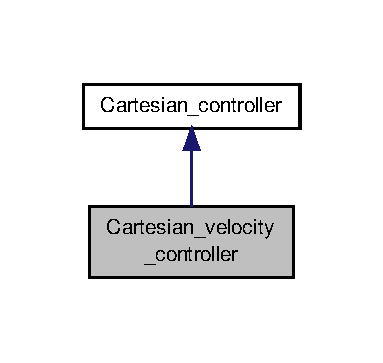
\includegraphics[width=184pt]{classCartesian__velocity__controller__inherit__graph}
\end{center}
\end{figure}


Collaboration diagram for Cartesian\-\_\-velocity\-\_\-controller\-:\nopagebreak
\begin{figure}[H]
\begin{center}
\leavevmode
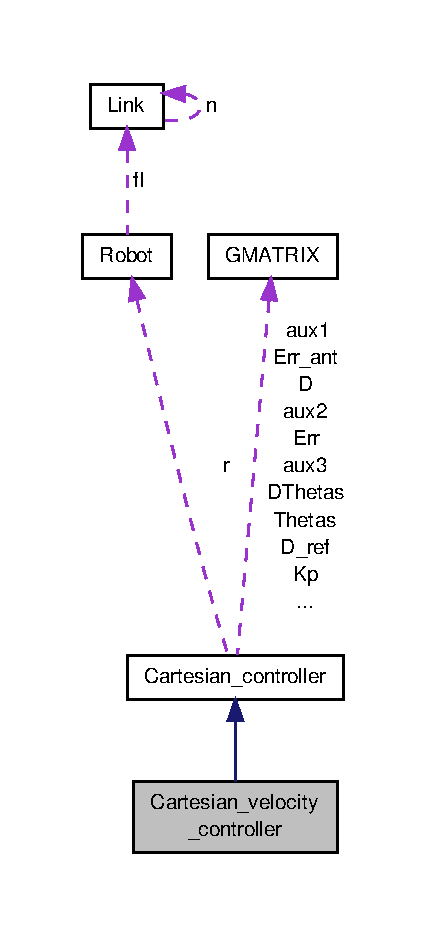
\includegraphics[width=206pt]{classCartesian__velocity__controller__coll__graph}
\end{center}
\end{figure}
\subsection*{Public Member Functions}
\begin{DoxyCompactItemize}
\item 
\hyperlink{classCartesian__velocity__controller_adc909b782b16fa12148302cc501300c6}{Cartesian\-\_\-velocity\-\_\-controller} (\hyperlink{structRobot}{Robot} $\ast$\hyperlink{classCartesian__controller_a5562129951bd802e4ded77fc716c87a0}{r}, double K\-P\mbox{[}$\,$\mbox{]}, double K\-I\mbox{[}$\,$\mbox{]}, double K\-D\mbox{[}$\,$\mbox{]}, double \hyperlink{classCartesian__controller_a35c6ddbb9624878f2807ff644a33e832}{T})
\item 
\hyperlink{classCartesian__velocity__controller_a6fd50fdb7e9e05ef99769e840cbb15c6}{$\sim$\-Cartesian\-\_\-velocity\-\_\-controller} ()
\item 
void \hyperlink{classCartesian__velocity__controller_a249bd167cd995e16906731172d1bc516}{control} ()
\item 
void \hyperlink{classCartesian__velocity__controller_a2f020f22b2e63da5afeff3f083e4095c}{reference\-Update\-Callback} (const schunk\-\_\-msgs\-::\-Velocities\-::\-Const\-Ptr \&msg)
\begin{DoxyCompactList}\small\item\em Receive schunk\-\_\-msgs\-::\-Velocities and updates this \hyperlink{classCartesian__velocity__controller}{Cartesian\-\_\-velocity\-\_\-controller}'s internal variables. \end{DoxyCompactList}\end{DoxyCompactItemize}
\subsection*{Data Fields}
\begin{DoxyCompactItemize}
\item 
std\-::vector$<$ double $>$ \hyperlink{classCartesian__velocity__controller_afc3792f1f6dd0025417d752a89e519e1}{references}
\end{DoxyCompactItemize}
\subsection*{Protected Member Functions}
\begin{DoxyCompactItemize}
\item 
bool \hyperlink{classCartesian__velocity__controller_ad5dbfc4b8ec4fad7bca9b9a4fd9358b4}{print\-Vel} ()
\item 
void \hyperlink{classCartesian__velocity__controller_a9b2c7f25b3fc2882f7e4590ee97e0978}{update\-References} (double ref\-\_\-gain, double ref\-\_\-gain2)
\begin{DoxyCompactList}\small\item\em Calls the last velocity callback and updates the P\-G\-M\-A\-T\-R\-I\-X D\-\_\-ref with the updated values. \end{DoxyCompactList}\end{DoxyCompactItemize}
\subsection*{Protected Attributes}
\begin{DoxyCompactItemize}
\item 
ros\-::\-Node\-Handle \hyperlink{classCartesian__velocity__controller_a7d04d378a2a6d19870a620883dcd3e09}{reference\-\_\-updater\-\_\-nh}
\item 
ros\-::\-Callback\-Queue \hyperlink{classCartesian__velocity__controller_ad2804cf83a42305d18572abdbbfd1c3f}{reference\-\_\-updater\-\_\-queue}
\item 
ros\-::\-Subscriber \hyperlink{classCartesian__velocity__controller_a75412b9859afe4b800f9613c9cb8d17f}{reference\-\_\-updater\-\_\-subscriber}
\item 
ros\-::\-Node\-Handle \hyperlink{classCartesian__velocity__controller_a01cbe7f951c69ded8604e552a0a706e0}{end\-Effector\-\_\-vel\-\_\-nh}
\item 
ros\-::\-Callback\-Queue \hyperlink{classCartesian__velocity__controller_af154b0cda931081b52224eb22e4680f7}{end\-Effector\-\_\-vel\-\_\-queue}
\item 
ros\-::\-Publisher \hyperlink{classCartesian__velocity__controller_ab12287816ae785d3cd6243b3df0cffc6}{end\-Effector\-\_\-vel\-\_\-pub}
\item 
schunk\-\_\-msgs\-::\-Velocities \hyperlink{classCartesian__velocity__controller_ae771d963a90ad7b844c4c3a821ce5f39}{end\-Effector\-\_\-vel}
\end{DoxyCompactItemize}


\subsection{Detailed Description}


Definition at line 8 of file cartesian\-\_\-velocity\-\_\-controller.\-h.



\subsection{Constructor \& Destructor Documentation}
\hypertarget{classCartesian__velocity__controller_adc909b782b16fa12148302cc501300c6}{\index{Cartesian\-\_\-velocity\-\_\-controller@{Cartesian\-\_\-velocity\-\_\-controller}!Cartesian\-\_\-velocity\-\_\-controller@{Cartesian\-\_\-velocity\-\_\-controller}}
\index{Cartesian\-\_\-velocity\-\_\-controller@{Cartesian\-\_\-velocity\-\_\-controller}!Cartesian_velocity_controller@{Cartesian\-\_\-velocity\-\_\-controller}}
\subsubsection[{Cartesian\-\_\-velocity\-\_\-controller}]{\setlength{\rightskip}{0pt plus 5cm}Cartesian\-\_\-velocity\-\_\-controller\-::\-Cartesian\-\_\-velocity\-\_\-controller (
\begin{DoxyParamCaption}
\item[{{\bf Robot} $\ast$}]{r, }
\item[{double}]{K\-P\mbox{[}$\,$\mbox{]}, }
\item[{double}]{K\-I\mbox{[}$\,$\mbox{]}, }
\item[{double}]{K\-D\mbox{[}$\,$\mbox{]}, }
\item[{double}]{T}
\end{DoxyParamCaption}
)}}\label{classCartesian__velocity__controller_adc909b782b16fa12148302cc501300c6}


Definition at line 253 of file cartesian\-\_\-velocity\-\_\-controller.\-cpp.



References Robot\-::dofs, end\-Effector\-\_\-vel, end\-Effector\-\_\-vel\-\_\-nh, end\-Effector\-\_\-vel\-\_\-pub, end\-Effector\-\_\-vel\-\_\-queue, reference\-\_\-updater\-\_\-nh, reference\-\_\-updater\-\_\-queue, reference\-\_\-updater\-\_\-subscriber, references, reference\-Update\-Callback(), and Cartesian\-\_\-controller\-::ros\-\_\-pub\-\_\-buffer.


\begin{DoxyCode}
253                                                                                                            
                : \hyperlink{classCartesian__controller_a71055bb1cbf01ced9e64bb1d184b68fe}{Cartesian\_controller}(r,6,KP,KI,KD,\hyperlink{classCartesian__controller_a35c6ddbb9624878f2807ff644a33e832}{T})\{
254 
255         \textcolor{comment}{//Reference Velocities Buffer}
256         \textcolor{keywordflow}{for}(\textcolor{keywordtype}{int} j=0;j<r->\hyperlink{structRobot_a51d4a86ac5314a1ed8614d5664c80747}{dofs};j++)\{
257                 this->\hyperlink{classCartesian__velocity__controller_afc3792f1f6dd0025417d752a89e519e1}{references}.push\_back(0.0);
258         \}
259 
260         \textcolor{comment}{//Initialize endEffector\_vel msg}
261         \textcolor{keywordflow}{for}(\textcolor{keywordtype}{int} j=0;j<6;j++)\{
262                 \hyperlink{classCartesian__velocity__controller_ae771d963a90ad7b844c4c3a821ce5f39}{endEffector\_vel}.velocities.push\_back(0.0);
263         \}
264 
265         \textcolor{comment}{//Set Queues}
266         this->\hyperlink{classCartesian__velocity__controller_a7d04d378a2a6d19870a620883dcd3e09}{reference\_updater\_nh}.setCallbackQueue(&this->
      \hyperlink{classCartesian__velocity__controller_ad2804cf83a42305d18572abdbbfd1c3f}{reference\_updater\_queue});
267         this->\hyperlink{classCartesian__velocity__controller_a01cbe7f951c69ded8604e552a0a706e0}{endEffector\_vel\_nh}.setCallbackQueue(&this->
      \hyperlink{classCartesian__velocity__controller_af154b0cda931081b52224eb22e4680f7}{endEffector\_vel\_queue});
268 
269         \textcolor{comment}{//Subscriber and queue init.}
270         this->\hyperlink{classCartesian__velocity__controller_a75412b9859afe4b800f9613c9cb8d17f}{reference\_updater\_subscriber}  = this->
      \hyperlink{classCartesian__velocity__controller_a7d04d378a2a6d19870a620883dcd3e09}{reference\_updater\_nh}.subscribe(\textcolor{stringliteral}{"schunk\_cartesian\_velocities\_control"}, 
      \hyperlink{classCartesian__controller_ab9ed5a808da204dbc612d313dc7332f4}{ros\_pub\_buffer}, &
      \hyperlink{classCartesian__velocity__controller_a2f020f22b2e63da5afeff3f083e4095c}{Cartesian\_velocity\_controller::referenceUpdateCallback}
      , \textcolor{keyword}{this});
271 
272         \textcolor{comment}{//Publisher}
273         this->\hyperlink{classCartesian__velocity__controller_ab12287816ae785d3cd6243b3df0cffc6}{endEffector\_vel\_pub}   = this->
      \hyperlink{classCartesian__velocity__controller_a01cbe7f951c69ded8604e552a0a706e0}{endEffector\_vel\_nh}.advertise<schunk\_msgs::Velocities>(\textcolor{stringliteral}{"schunk\_endeffector\_velocities"}, 
      \hyperlink{classCartesian__controller_ab9ed5a808da204dbc612d313dc7332f4}{ros\_pub\_buffer});
274 \}
\end{DoxyCode}


Here is the call graph for this function\-:\nopagebreak
\begin{figure}[H]
\begin{center}
\leavevmode
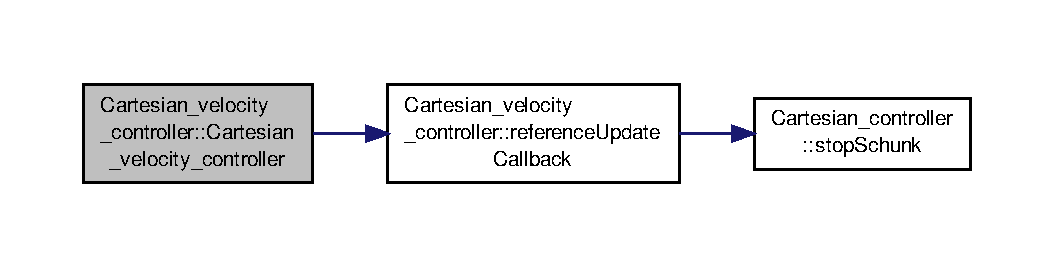
\includegraphics[width=350pt]{classCartesian__velocity__controller_adc909b782b16fa12148302cc501300c6_cgraph}
\end{center}
\end{figure}


\hypertarget{classCartesian__velocity__controller_a6fd50fdb7e9e05ef99769e840cbb15c6}{\index{Cartesian\-\_\-velocity\-\_\-controller@{Cartesian\-\_\-velocity\-\_\-controller}!$\sim$\-Cartesian\-\_\-velocity\-\_\-controller@{$\sim$\-Cartesian\-\_\-velocity\-\_\-controller}}
\index{$\sim$\-Cartesian\-\_\-velocity\-\_\-controller@{$\sim$\-Cartesian\-\_\-velocity\-\_\-controller}!Cartesian_velocity_controller@{Cartesian\-\_\-velocity\-\_\-controller}}
\subsubsection[{$\sim$\-Cartesian\-\_\-velocity\-\_\-controller}]{\setlength{\rightskip}{0pt plus 5cm}Cartesian\-\_\-velocity\-\_\-controller\-::$\sim$\-Cartesian\-\_\-velocity\-\_\-controller (
\begin{DoxyParamCaption}
{}
\end{DoxyParamCaption}
)}}\label{classCartesian__velocity__controller_a6fd50fdb7e9e05ef99769e840cbb15c6}


Definition at line 249 of file cartesian\-\_\-velocity\-\_\-controller.\-cpp.


\begin{DoxyCode}
249                                                              \{
250 
251 \}
\end{DoxyCode}


\subsection{Member Function Documentation}
\hypertarget{classCartesian__velocity__controller_a249bd167cd995e16906731172d1bc516}{\index{Cartesian\-\_\-velocity\-\_\-controller@{Cartesian\-\_\-velocity\-\_\-controller}!control@{control}}
\index{control@{control}!Cartesian_velocity_controller@{Cartesian\-\_\-velocity\-\_\-controller}}
\subsubsection[{control}]{\setlength{\rightskip}{0pt plus 5cm}void Cartesian\-\_\-velocity\-\_\-controller\-::control (
\begin{DoxyParamCaption}
{}
\end{DoxyParamCaption}
)\hspace{0.3cm}{\ttfamily [virtual]}}}\label{classCartesian__velocity__controller_a249bd167cd995e16906731172d1bc516}
Measure Position and Speed

Recalculation of measured data. 

Implements \hyperlink{classCartesian__controller_a8809167cab6d338a957439141fa2bf6c}{Cartesian\-\_\-controller}.



Definition at line 66 of file cartesian\-\_\-velocity\-\_\-controller.\-cpp.



References Cartesian\-\_\-controller\-::aux1, Cartesian\-\_\-controller\-::aux2, Cartesian\-\_\-controller\-::aux3, Cartesian\-\_\-controller\-::change\-Schunk\-Mode(), Cartesian\-\_\-controller\-::control\-Clean\-Up(), Cartesian\-\_\-controller\-::\-D, Cartesian\-\_\-controller\-::\-D\-\_\-ref, Cartesian\-\_\-controller\-::\-D\-Thetas, Cartesian\-\_\-controller\-::end\-\_\-control, Cartesian\-\_\-controller\-::\-Err, Cartesian\-\_\-controller\-::\-Err\-\_\-ant, Cartesian\-\_\-controller\-::\-Err\-\_\-int, F\-A\-L\-S\-E, Cartesian\-\_\-controller\-::get\-Schunk\-Positions\-And\-Velocities\-And\-Update\-Thetas\-And\-D\-Thetas(), Cartesian\-\_\-controller\-::\-Kd, Cartesian\-\_\-controller\-::\-Ki, Cartesian\-\_\-controller\-::\-Kp, P\-G\-M\-A\-T\-R\-I\-X\-\_\-\-A\-D\-D\-\_\-\-C\-O\-P\-Y\-\_\-\-F\-R\-E\-E(), P\-G\-M\-A\-T\-R\-I\-X\-\_\-\-D\-A\-M\-P\-E\-D\-\_\-\-L\-E\-A\-S\-T\-S\-Q\-U\-A\-R\-E\-S\-\_\-\-P\-S\-E\-U\-D\-O\-I\-N\-V\-E\-R\-S\-E(), P\-G\-M\-A\-T\-R\-I\-X\-\_\-\-F\-R\-E\-E(), P\-G\-M\-A\-T\-R\-I\-X\-\_\-\-M\-U\-L\-T\-I\-P\-L\-Y\-\_\-\-C\-O\-N\-S\-T\-\_\-\-C\-O\-P\-Y\-\_\-\-F\-R\-E\-E(), P\-G\-M\-A\-T\-R\-I\-X\-\_\-\-M\-U\-L\-T\-I\-P\-L\-Y\-\_\-\-C\-O\-P\-Y\-\_\-\-F\-R\-E\-E(), P\-G\-M\-A\-T\-R\-I\-X\-\_\-\-S\-U\-B\-T\-R\-A\-C\-T\-\_\-\-C\-O\-P\-Y\-\_\-\-F\-R\-E\-E(), print\-Vel(), Cartesian\-\_\-controller\-::r, Robot\-\_\-get\-G\-Jacobian(), Robot\-\_\-update\-Links\-Thetas\-By\-Matrix(), Cartesian\-\_\-controller\-::set\-Schunk\-Velocities\-And\-Send(), Cartesian\-\_\-controller\-::\-S\-J, Cartesian\-\_\-controller\-::\-T, Cartesian\-\_\-controller\-::\-Thetas, T\-R\-U\-E, and update\-References().



Referenced by main().


\begin{DoxyCode}
66                                            \{
67 
68         \textcolor{comment}{/******************************}
69 \textcolor{comment}{                                ROS INIT}
70 \textcolor{comment}{        *******************************/}
71 
72         \textcolor{comment}{//Ros rate}
73         ros::Rate ros\_rate(1/\hyperlink{classCartesian__controller_a35c6ddbb9624878f2807ff644a33e832}{T});
74 
75         \textcolor{comment}{/*****************************}
76 \textcolor{comment}{           CHANGE SCHUNK MODE TO ASSURE VELOCITY CONTROL}
77 \textcolor{comment}{         *****************************/}
78         \textcolor{comment}{//Waits for the service to be available}
79         ros::service::waitForService(\textcolor{stringliteral}{"schunk\_set\_control\_mode"});
80 
81         ROS\_INFO\_STREAM(\textcolor{stringliteral}{"Changing Schunk's Control Mode"});
82         \textcolor{keywordflow}{if}(!\hyperlink{classCartesian__controller_aaf006f80e89c08cf040956afbb4cf3c0}{changeSchunkMode}(CONTROL\_MODE\_VELOCITY))\{\textcolor{keywordflow}{return};\}
83         ROS\_INFO\_STREAM(\textcolor{stringliteral}{"Mode Changed!"});
84 
85         \textcolor{comment}{/*****************************}
86 \textcolor{comment}{           UPDATES SCHUNK'S INITIAL POSITION AND VELOCITY}
87 \textcolor{comment}{         *****************************/}
88         ROS\_INFO\_STREAM(\textcolor{stringliteral}{"Where is Schunk and how fast is it?"});
89         \textcolor{keywordflow}{if}(!\hyperlink{classCartesian__controller_a0d7a63bac84715f6742db738df246f91}{getSchunkPositionsAndVelocitiesAndUpdateThetasAndDThetas}
      ())\{\textcolor{keywordflow}{return};\}
90         ROS\_INFO\_STREAM(\textcolor{stringliteral}{"Schunk found!"});
91 
92 
93         \textcolor{comment}{/******************************}
94 \textcolor{comment}{        PRIVATE VARIABLE INITIALIZATION}
95 \textcolor{comment}{        *******************************/}
96 
97         \textcolor{comment}{//Update Robot Object}
98         \hyperlink{robot_8h_aa1d3aca5132bd5f347f5966d38fbb966}{Robot\_updateLinksThetasByMatrix}(\hyperlink{classCartesian__controller_a5562129951bd802e4ded77fc716c87a0}{r},\hyperlink{classCartesian__controller_a0a0f818dad601cd9e3e26cb6959b8eb6}{Thetas});
99 
100         \textcolor{comment}{//Jacobians}
101         \hyperlink{classCartesian__controller_a98fdac06d136ac3dba0102d97cd5dd36}{SJ}  = \hyperlink{robot_8h_a61464c237c56f3db3f79b0350df80ddb}{Robot\_getGJacobian}(\hyperlink{classCartesian__controller_a5562129951bd802e4ded77fc716c87a0}{r});
102 
103         \textcolor{comment}{/******************************}
104 \textcolor{comment}{                        LOOP}
105 \textcolor{comment}{        *******************************/}
106 
107         ROS\_INFO\_STREAM(\textcolor{stringliteral}{"Starting!"});
108         \textcolor{comment}{//Take a deep breath and GO}
109         ros\_rate.sleep();
110 
111         \textcolor{keywordflow}{while}(!\hyperlink{classCartesian__controller_a3c0a72214891f68e2bad63bf2b688f9c}{end\_control})\{
112 
113                 \textcolor{comment}{//Last Error}
114                 \hyperlink{gmatrix_8h_a9a73b4e0a77f386c0bae1bba75298d1d}{PGMATRIX\_FREE}(\hyperlink{classCartesian__controller_a6d9471a983f6cb6c642bf8dea0d540af}{Err\_ant});
115                 \hyperlink{classCartesian__controller_a6d9471a983f6cb6c642bf8dea0d540af}{Err\_ant} = \hyperlink{classCartesian__controller_ab3f08ecf10cb2486e8bfc61f07e2bde6}{Err};
116 
117                 \textcolor{comment}{/******************************}
118 \textcolor{comment}{                        /END GET NEW REFERENCES}
119 \textcolor{comment}{                *******************************/}
120                 \textcolor{comment}{//Current Error}
121                 \hyperlink{classCartesian__controller_ab3f08ecf10cb2486e8bfc61f07e2bde6}{Err} =     \hyperlink{gmatrix__plus_8h_a146d9062e4325cc3b97990ae51b96d95}{PGMATRIX\_SUBTRACT\_COPY\_FREE}(
      \hyperlink{classCartesian__controller_abb248cb3215a574fe8e1bb8fb0b8626d}{D\_ref},\hyperlink{classCartesian__controller_a8c470b652ce436d8e48f126073fc2593}{D},\hyperlink{gmatlabdatafile_8h_aa93f0eb578d23995850d61f7d61c55c1}{FALSE},\hyperlink{gmatlabdatafile_8h_aa93f0eb578d23995850d61f7d61c55c1}{FALSE});
122                 \textcolor{comment}{//Error Integral}
123                 \hyperlink{classCartesian__controller_a37edb9c6e2a5066f74941e3659f68cbc}{aux1} =        \hyperlink{gmatrix__plus_8h_a371a0bfffdb84cf1596ca60bbf7fce93}{PGMATRIX\_MULTIPLY\_CONST\_COPY\_FREE}(
      \hyperlink{classCartesian__controller_ab3f08ecf10cb2486e8bfc61f07e2bde6}{Err},\hyperlink{classCartesian__controller_a35c6ddbb9624878f2807ff644a33e832}{T},\hyperlink{gmatlabdatafile_8h_aa93f0eb578d23995850d61f7d61c55c1}{FALSE});
124                 \hyperlink{classCartesian__controller_a248174c6399a8933bfcc8f1b0b39af5e}{Err\_int} = \hyperlink{gmatrix__plus_8h_aa1123306aa55d942955e09156db757a3}{PGMATRIX\_ADD\_COPY\_FREE}(
      \hyperlink{classCartesian__controller_a248174c6399a8933bfcc8f1b0b39af5e}{Err\_int},\hyperlink{classCartesian__controller_a37edb9c6e2a5066f74941e3659f68cbc}{aux1},\hyperlink{gmatlabdatafile_8h_aa8cecfc5c5c054d2875c03e77b7be15d}{TRUE},\hyperlink{gmatlabdatafile_8h_aa8cecfc5c5c054d2875c03e77b7be15d}{TRUE});
125 
126                 \textcolor{comment}{//Derivative    aux1 = Kd*(Err-Err\_ant)*(1/T)}
127                 \hyperlink{classCartesian__controller_a37edb9c6e2a5066f74941e3659f68cbc}{aux1} = \hyperlink{gmatrix__plus_8h_a146d9062e4325cc3b97990ae51b96d95}{PGMATRIX\_SUBTRACT\_COPY\_FREE}(
      \hyperlink{classCartesian__controller_ab3f08ecf10cb2486e8bfc61f07e2bde6}{Err},\hyperlink{classCartesian__controller_a6d9471a983f6cb6c642bf8dea0d540af}{Err\_ant},\hyperlink{gmatlabdatafile_8h_aa93f0eb578d23995850d61f7d61c55c1}{FALSE},\hyperlink{gmatlabdatafile_8h_aa93f0eb578d23995850d61f7d61c55c1}{FALSE});
128                 \hyperlink{classCartesian__controller_a37edb9c6e2a5066f74941e3659f68cbc}{aux1} = \hyperlink{gmatrix__plus_8h_a17b482a0aaa68d1f4c1c30a1a72dacbb}{PGMATRIX\_MULTIPLY\_COPY\_FREE}(
      \hyperlink{classCartesian__controller_a62394cef8a9a29eac18319a4ad579c4c}{Kd},\hyperlink{classCartesian__controller_a37edb9c6e2a5066f74941e3659f68cbc}{aux1},\hyperlink{gmatlabdatafile_8h_aa93f0eb578d23995850d61f7d61c55c1}{FALSE},\hyperlink{gmatlabdatafile_8h_aa8cecfc5c5c054d2875c03e77b7be15d}{TRUE});
129                 \hyperlink{classCartesian__controller_a37edb9c6e2a5066f74941e3659f68cbc}{aux1} = \hyperlink{gmatrix__plus_8h_a371a0bfffdb84cf1596ca60bbf7fce93}{PGMATRIX\_MULTIPLY\_CONST\_COPY\_FREE}(
      \hyperlink{classCartesian__controller_a37edb9c6e2a5066f74941e3659f68cbc}{aux1},(1/\hyperlink{classCartesian__controller_a35c6ddbb9624878f2807ff644a33e832}{T}),\hyperlink{gmatlabdatafile_8h_aa8cecfc5c5c054d2875c03e77b7be15d}{TRUE});
130                 \textcolor{comment}{//Integral      aux2 = Ki*(Err\_int)}
131                 \hyperlink{classCartesian__controller_af73a0c910cd80ed2f84974b65beba450}{aux2} = \hyperlink{gmatrix__plus_8h_a17b482a0aaa68d1f4c1c30a1a72dacbb}{PGMATRIX\_MULTIPLY\_COPY\_FREE}(
      \hyperlink{classCartesian__controller_a70e495f39da706f1b589684f58343b9e}{Ki},\hyperlink{classCartesian__controller_a248174c6399a8933bfcc8f1b0b39af5e}{Err\_int},\hyperlink{gmatlabdatafile_8h_aa93f0eb578d23995850d61f7d61c55c1}{FALSE},\hyperlink{gmatlabdatafile_8h_aa93f0eb578d23995850d61f7d61c55c1}{FALSE});
132                 \textcolor{comment}{//Proportional  aux3 = Kp*(Err)}
133                 \hyperlink{classCartesian__controller_aa37c15fcd53a60ecce106cd9b39d3501}{aux3} = \hyperlink{gmatrix__plus_8h_a17b482a0aaa68d1f4c1c30a1a72dacbb}{PGMATRIX\_MULTIPLY\_COPY\_FREE}(
      \hyperlink{classCartesian__controller_a78073f51064a05d72c41723a93d9079f}{Kp},\hyperlink{classCartesian__controller_ab3f08ecf10cb2486e8bfc61f07e2bde6}{Err},\hyperlink{gmatlabdatafile_8h_aa93f0eb578d23995850d61f7d61c55c1}{FALSE},\hyperlink{gmatlabdatafile_8h_aa93f0eb578d23995850d61f7d61c55c1}{FALSE});
134 
135                 \textcolor{comment}{//Error Sum     aux1 = Kd*(Err-Err\_ant)*(1/T) + Ki*(Err\_int) + Kp*(Err)}
136                 \hyperlink{classCartesian__controller_a37edb9c6e2a5066f74941e3659f68cbc}{aux1} = \hyperlink{gmatrix__plus_8h_aa1123306aa55d942955e09156db757a3}{PGMATRIX\_ADD\_COPY\_FREE}(\hyperlink{classCartesian__controller_a37edb9c6e2a5066f74941e3659f68cbc}{aux1},
      \hyperlink{classCartesian__controller_af73a0c910cd80ed2f84974b65beba450}{aux2},\hyperlink{gmatlabdatafile_8h_aa8cecfc5c5c054d2875c03e77b7be15d}{TRUE},\hyperlink{gmatlabdatafile_8h_aa8cecfc5c5c054d2875c03e77b7be15d}{TRUE});
137                 \hyperlink{classCartesian__controller_a37edb9c6e2a5066f74941e3659f68cbc}{aux1} = \hyperlink{gmatrix__plus_8h_aa1123306aa55d942955e09156db757a3}{PGMATRIX\_ADD\_COPY\_FREE}(\hyperlink{classCartesian__controller_a37edb9c6e2a5066f74941e3659f68cbc}{aux1},
      \hyperlink{classCartesian__controller_aa37c15fcd53a60ecce106cd9b39d3501}{aux3},\hyperlink{gmatlabdatafile_8h_aa8cecfc5c5c054d2875c03e77b7be15d}{TRUE},\hyperlink{gmatlabdatafile_8h_aa8cecfc5c5c054d2875c03e77b7be15d}{TRUE});
138 
139                 \textcolor{comment}{//Pseudo Inverse Calculation}
140                 \hyperlink{classCartesian__controller_af73a0c910cd80ed2f84974b65beba450}{aux2} =      \hyperlink{gmatrix__plus_8h_a73bceba2ac1f3a5589628d0f2e4081fa}{PGMATRIX\_DAMPED\_LEASTSQUARES\_PSEUDOINVERSE}
      (\hyperlink{classCartesian__controller_a98fdac06d136ac3dba0102d97cd5dd36}{SJ},0.01);
141 
142                 \textcolor{comment}{//New DThetas = pinv(SJ)*(Error Sum)}
143                 \hyperlink{gmatrix_8h_a9a73b4e0a77f386c0bae1bba75298d1d}{PGMATRIX\_FREE}(\hyperlink{classCartesian__controller_a5d6419e62e130150edfcbd82b1dadcae}{DThetas});
144                 \hyperlink{classCartesian__controller_a5d6419e62e130150edfcbd82b1dadcae}{DThetas} = \hyperlink{gmatrix__plus_8h_a17b482a0aaa68d1f4c1c30a1a72dacbb}{PGMATRIX\_MULTIPLY\_COPY\_FREE}(
      \hyperlink{classCartesian__controller_af73a0c910cd80ed2f84974b65beba450}{aux2},\hyperlink{classCartesian__controller_a37edb9c6e2a5066f74941e3659f68cbc}{aux1},\hyperlink{gmatlabdatafile_8h_aa8cecfc5c5c054d2875c03e77b7be15d}{TRUE},\hyperlink{gmatlabdatafile_8h_aa8cecfc5c5c054d2875c03e77b7be15d}{TRUE});
145 
146                 \textcolor{comment}{/******************************}
147 \textcolor{comment}{                         GET NEW REFERENCES}
148 \textcolor{comment}{                *******************************/}
149                 \textcolor{comment}{//Receive callback to after update references}
150                 \hyperlink{classCartesian__velocity__controller_a9b2c7f25b3fc2882f7e4590ee97e0978}{updateReferences}(0.1,0.35); \textcolor{comment}{//Refs should be received as 1}
151 
152                 \textcolor{comment}{/******************************}
153 \textcolor{comment}{                        COMUNICATE WITH SCHUNK}
154 \textcolor{comment}{                *******************************/}
155 
156                 \textcolor{comment}{//Sends information to robot to move, then wait and measure}
157                 \hyperlink{classCartesian__controller_a40d17a9794af8a9a607618bf0ee5efff}{setSchunkVelocitiesAndSend}(0.5);
158 
159                 \textcolor{comment}{//Wait}
160                 ros\_rate.sleep();
161 
163                 \textcolor{comment}{//Position and Velocities, THETAS AND DTHETAS ARE UPDATED}
164                 \textcolor{keywordflow}{if}(!\hyperlink{classCartesian__controller_a0d7a63bac84715f6742db738df246f91}{getSchunkPositionsAndVelocitiesAndUpdateThetasAndDThetas}
      ())\{\textcolor{keywordflow}{return};\}
165                 \textcolor{comment}{//Print}
166                 \hyperlink{classCartesian__velocity__controller_ad5dbfc4b8ec4fad7bca9b9a4fd9358b4}{printVel}();
167 
168                 \textcolor{comment}{/******************************}
169 \textcolor{comment}{                /END    COMUNICATE WITH SCHUNK}
170 \textcolor{comment}{                *******************************/}
171 
172                 \textcolor{comment}{//Updates Robot's Link's Thetas with current position}
173                 \hyperlink{robot_8h_aa1d3aca5132bd5f347f5966d38fbb966}{Robot\_updateLinksThetasByMatrix}(\hyperlink{classCartesian__controller_a5562129951bd802e4ded77fc716c87a0}{r},
      \hyperlink{classCartesian__controller_a0a0f818dad601cd9e3e26cb6959b8eb6}{Thetas});
174 
175                 \textcolor{comment}{//Updates Jacobian with new position}
176                 \hyperlink{gmatrix_8h_a9a73b4e0a77f386c0bae1bba75298d1d}{PGMATRIX\_FREE}(\hyperlink{classCartesian__controller_a98fdac06d136ac3dba0102d97cd5dd36}{SJ});
177                 \hyperlink{classCartesian__controller_a98fdac06d136ac3dba0102d97cd5dd36}{SJ}  = \hyperlink{robot_8h_a61464c237c56f3db3f79b0350df80ddb}{Robot\_getGJacobian}(\hyperlink{classCartesian__controller_a5562129951bd802e4ded77fc716c87a0}{r});
178 
180                 \textcolor{comment}{//End effectors 6DOF velocity}
181                 \hyperlink{gmatrix_8h_a9a73b4e0a77f386c0bae1bba75298d1d}{PGMATRIX\_FREE}(\hyperlink{classCartesian__controller_a8c470b652ce436d8e48f126073fc2593}{D});
182                 \hyperlink{classCartesian__controller_a8c470b652ce436d8e48f126073fc2593}{D} = \hyperlink{gmatrix__plus_8h_a17b482a0aaa68d1f4c1c30a1a72dacbb}{PGMATRIX\_MULTIPLY\_COPY\_FREE}(\hyperlink{classCartesian__controller_a98fdac06d136ac3dba0102d97cd5dd36}{SJ},
      \hyperlink{classCartesian__controller_a5d6419e62e130150edfcbd82b1dadcae}{DThetas},\hyperlink{gmatlabdatafile_8h_aa93f0eb578d23995850d61f7d61c55c1}{FALSE},\hyperlink{gmatlabdatafile_8h_aa93f0eb578d23995850d61f7d61c55c1}{FALSE});
183         \}
184 
185         \textcolor{comment}{/******************************}
186 \textcolor{comment}{                        CLEAN UP}
187 \textcolor{comment}{        *******************************/}
188         \hyperlink{classCartesian__controller_a8c0f0b41de9f4f8b2e3aa327e7c6b50c}{controlCleanUp}();
189 
190         \textcolor{keywordflow}{return};
191 
192 \}
\end{DoxyCode}


Here is the call graph for this function\-:\nopagebreak
\begin{figure}[H]
\begin{center}
\leavevmode
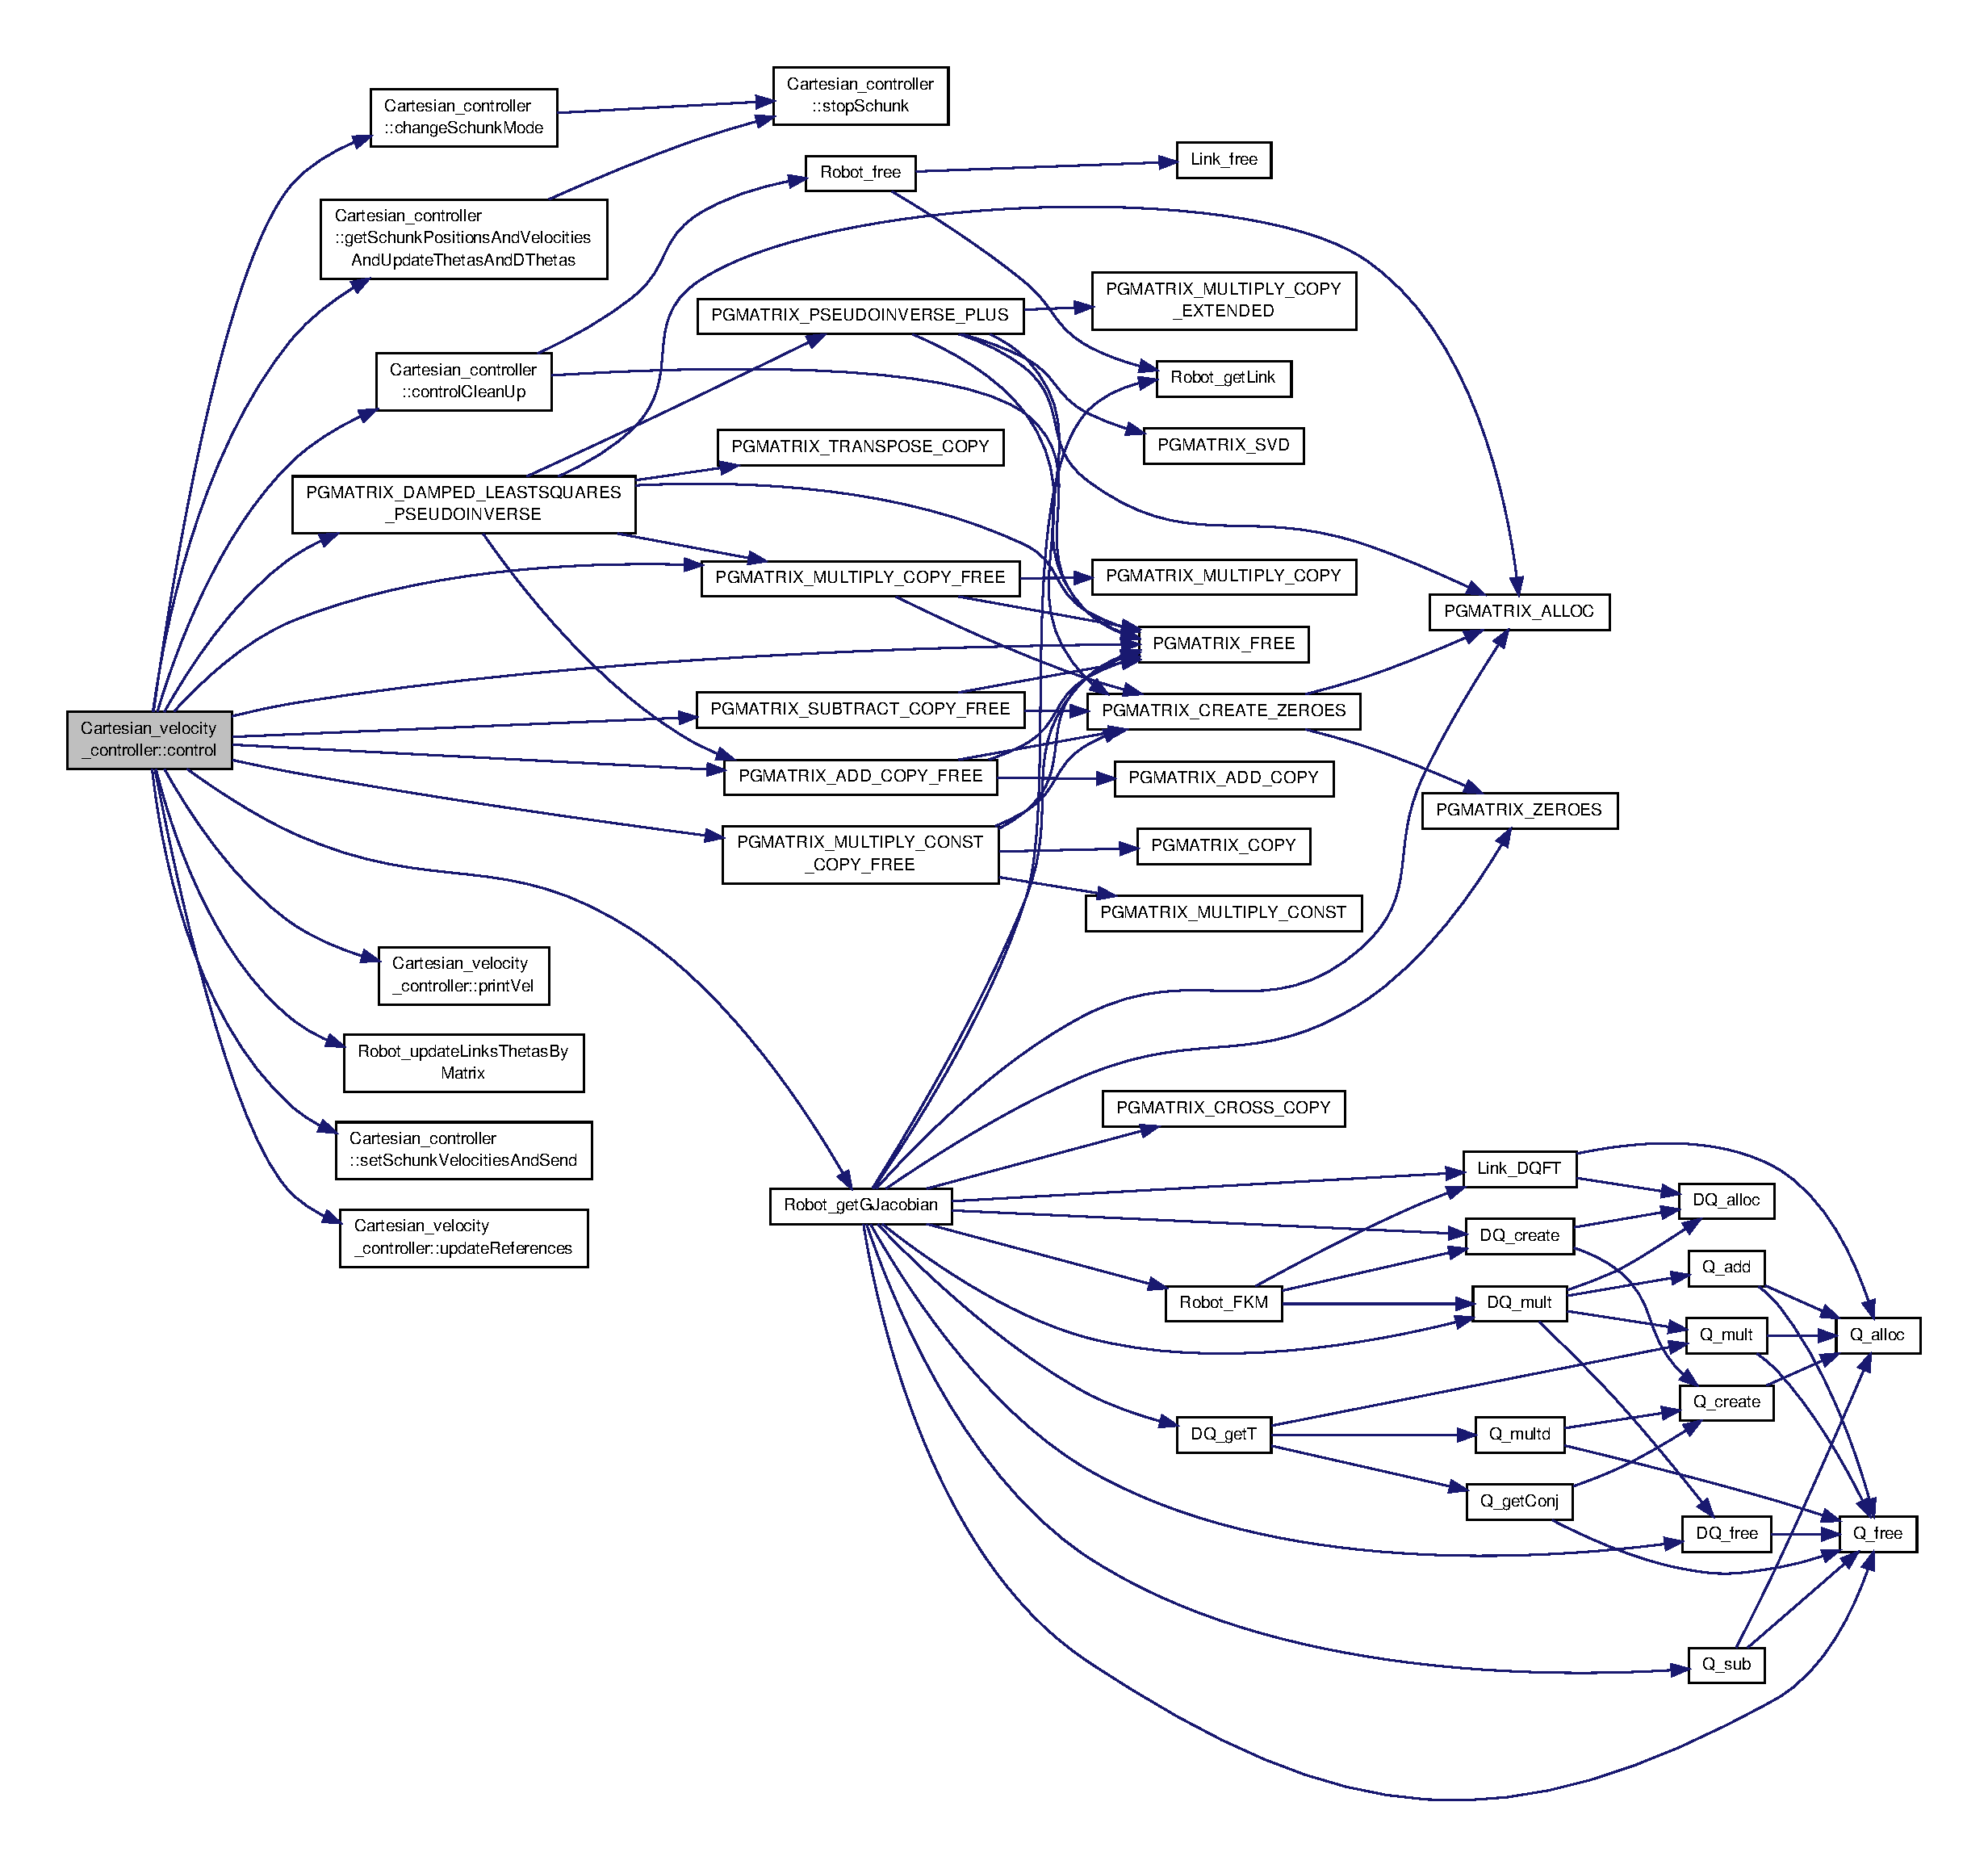
\includegraphics[width=350pt]{classCartesian__velocity__controller_a249bd167cd995e16906731172d1bc516_cgraph}
\end{center}
\end{figure}




Here is the caller graph for this function\-:\nopagebreak
\begin{figure}[H]
\begin{center}
\leavevmode
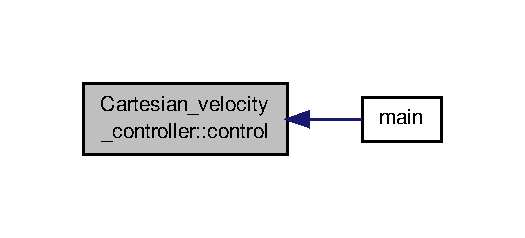
\includegraphics[width=252pt]{classCartesian__velocity__controller_a249bd167cd995e16906731172d1bc516_icgraph}
\end{center}
\end{figure}


\hypertarget{classCartesian__velocity__controller_ad5dbfc4b8ec4fad7bca9b9a4fd9358b4}{\index{Cartesian\-\_\-velocity\-\_\-controller@{Cartesian\-\_\-velocity\-\_\-controller}!print\-Vel@{print\-Vel}}
\index{print\-Vel@{print\-Vel}!Cartesian_velocity_controller@{Cartesian\-\_\-velocity\-\_\-controller}}
\subsubsection[{print\-Vel}]{\setlength{\rightskip}{0pt plus 5cm}bool Cartesian\-\_\-velocity\-\_\-controller\-::print\-Vel (
\begin{DoxyParamCaption}
{}
\end{DoxyParamCaption}
)\hspace{0.3cm}{\ttfamily [inline]}, {\ttfamily [protected]}}}\label{classCartesian__velocity__controller_ad5dbfc4b8ec4fad7bca9b9a4fd9358b4}


Definition at line 196 of file cartesian\-\_\-velocity\-\_\-controller.\-cpp.



References end\-Effector\-\_\-vel, end\-Effector\-\_\-vel\-\_\-pub, end\-Effector\-\_\-vel\-\_\-queue, Cartesian\-\_\-controller\-::\-Err, and P\-G\-M\-A\-T\-R\-I\-X\-\_\-\-D\-A\-T\-A.



Referenced by control().


\begin{DoxyCode}
196                                                    \{
197 
198         \textcolor{keywordflow}{for}(\textcolor{keywordtype}{int} j=0;j<6;j++)\{
199                 \hyperlink{classCartesian__velocity__controller_ae771d963a90ad7b844c4c3a821ce5f39}{endEffector\_vel}.velocities[j] = \hyperlink{gmatrix_8h_a7333180c47234295df2bd7b09ac00da8}{PGMATRIX\_DATA}(
      \hyperlink{classCartesian__controller_ab3f08ecf10cb2486e8bfc61f07e2bde6}{Err},j+1,1);
200         \}
201 
202         \textcolor{comment}{//Updates End Effetor's Header Timestamp}
203         \hyperlink{classCartesian__velocity__controller_ae771d963a90ad7b844c4c3a821ce5f39}{endEffector\_vel}.header.stamp = ros::Time::now();
204         \hyperlink{classCartesian__velocity__controller_ab12287816ae785d3cd6243b3df0cffc6}{endEffector\_vel\_pub}.publish(\hyperlink{classCartesian__velocity__controller_ae771d963a90ad7b844c4c3a821ce5f39}{endEffector\_vel});
205         \hyperlink{classCartesian__velocity__controller_af154b0cda931081b52224eb22e4680f7}{endEffector\_vel\_queue}.callAvailable(ros::WallDuration(0));
206 
207         \textcolor{keywordflow}{return} \textcolor{keyword}{true};
208 \}
\end{DoxyCode}


Here is the caller graph for this function\-:\nopagebreak
\begin{figure}[H]
\begin{center}
\leavevmode
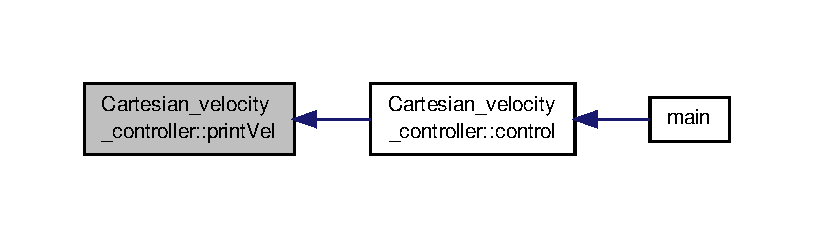
\includegraphics[width=350pt]{classCartesian__velocity__controller_ad5dbfc4b8ec4fad7bca9b9a4fd9358b4_icgraph}
\end{center}
\end{figure}


\hypertarget{classCartesian__velocity__controller_a2f020f22b2e63da5afeff3f083e4095c}{\index{Cartesian\-\_\-velocity\-\_\-controller@{Cartesian\-\_\-velocity\-\_\-controller}!reference\-Update\-Callback@{reference\-Update\-Callback}}
\index{reference\-Update\-Callback@{reference\-Update\-Callback}!Cartesian_velocity_controller@{Cartesian\-\_\-velocity\-\_\-controller}}
\subsubsection[{reference\-Update\-Callback}]{\setlength{\rightskip}{0pt plus 5cm}void Cartesian\-\_\-velocity\-\_\-controller\-::reference\-Update\-Callback (
\begin{DoxyParamCaption}
\item[{const schunk\-\_\-msgs\-::\-Velocities\-::\-Const\-Ptr \&}]{msg}
\end{DoxyParamCaption}
)}}\label{classCartesian__velocity__controller_a2f020f22b2e63da5afeff3f083e4095c}


Receive schunk\-\_\-msgs\-::\-Velocities and updates this \hyperlink{classCartesian__velocity__controller}{Cartesian\-\_\-velocity\-\_\-controller}'s internal variables. 

Should be received as references in the interval \mbox{[}-\/1.\-0,1.\-0\mbox{]} 

Definition at line 232 of file cartesian\-\_\-velocity\-\_\-controller.\-cpp.



References references, and Cartesian\-\_\-controller\-::stop\-Schunk().



Referenced by Cartesian\-\_\-velocity\-\_\-controller().


\begin{DoxyCode}
232                                                                                                    \{
233 
234         \textcolor{keywordflow}{if}(msg->velocities.size() != 6)\{
235                 ROS\_ERROR\_STREAM(\textcolor{stringliteral}{"Velocity being sent to cartesian\_velocity\_control's topic is not size 6"})
      ;
236                 \hyperlink{classCartesian__controller_a3ba54e8b35632526c5e8eb2ab5d7de0d}{stopSchunk}();
237                 \textcolor{keywordflow}{return};
238         \}
239         \textcolor{keywordflow}{for}(\textcolor{keywordtype}{int} i = 0; i < 6; i++)\{
240                 \textcolor{keywordflow}{if}(this->\hyperlink{classCartesian__velocity__controller_afc3792f1f6dd0025417d752a89e519e1}{references}[i]> 1.0 || this->\hyperlink{classCartesian__velocity__controller_afc3792f1f6dd0025417d752a89e519e1}{references}[i]< -1.0)\{
241                         ROS\_ERROR\_STREAM(\textcolor{stringliteral}{"Reference sent bigger than 1.0 or lower than -1.0."});
242                         \hyperlink{classCartesian__controller_a3ba54e8b35632526c5e8eb2ab5d7de0d}{stopSchunk}();
243                         \textcolor{keywordflow}{return};
244                 \}
245                 this->\hyperlink{classCartesian__velocity__controller_afc3792f1f6dd0025417d752a89e519e1}{references}[i] = msg->velocities[i];
246         \}
247 \}
\end{DoxyCode}


Here is the call graph for this function\-:\nopagebreak
\begin{figure}[H]
\begin{center}
\leavevmode
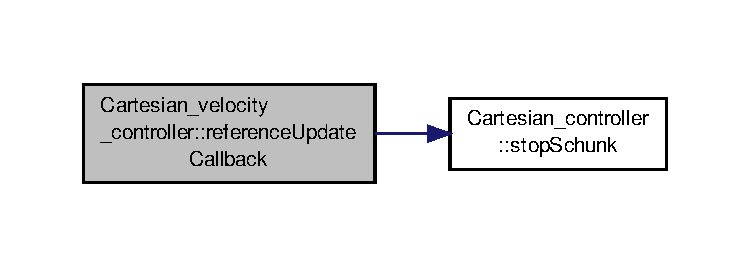
\includegraphics[width=350pt]{classCartesian__velocity__controller_a2f020f22b2e63da5afeff3f083e4095c_cgraph}
\end{center}
\end{figure}




Here is the caller graph for this function\-:\nopagebreak
\begin{figure}[H]
\begin{center}
\leavevmode
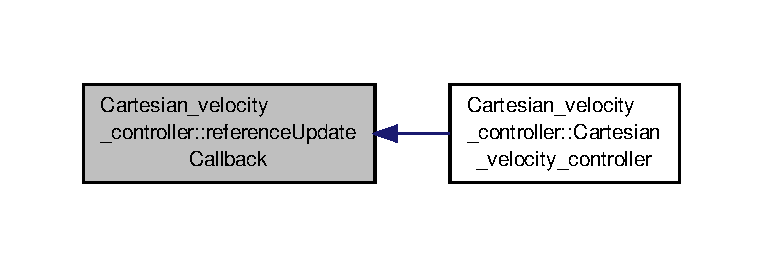
\includegraphics[width=350pt]{classCartesian__velocity__controller_a2f020f22b2e63da5afeff3f083e4095c_icgraph}
\end{center}
\end{figure}


\hypertarget{classCartesian__velocity__controller_a9b2c7f25b3fc2882f7e4590ee97e0978}{\index{Cartesian\-\_\-velocity\-\_\-controller@{Cartesian\-\_\-velocity\-\_\-controller}!update\-References@{update\-References}}
\index{update\-References@{update\-References}!Cartesian_velocity_controller@{Cartesian\-\_\-velocity\-\_\-controller}}
\subsubsection[{update\-References}]{\setlength{\rightskip}{0pt plus 5cm}void Cartesian\-\_\-velocity\-\_\-controller\-::update\-References (
\begin{DoxyParamCaption}
\item[{double}]{ref\-\_\-gain, }
\item[{double}]{ref\-\_\-gain2}
\end{DoxyParamCaption}
)\hspace{0.3cm}{\ttfamily [inline]}, {\ttfamily [protected]}}}\label{classCartesian__velocity__controller_a9b2c7f25b3fc2882f7e4590ee97e0978}


Calls the last velocity callback and updates the P\-G\-M\-A\-T\-R\-I\-X D\-\_\-ref with the updated values. 



Definition at line 213 of file cartesian\-\_\-velocity\-\_\-controller.\-cpp.



References Cartesian\-\_\-controller\-::\-D\-\_\-ref, P\-G\-M\-A\-T\-R\-I\-X\-\_\-\-D\-A\-T\-A, reference\-\_\-updater\-\_\-queue, and references.



Referenced by control().


\begin{DoxyCode}
213                                                                                             \{
214 
215         \textcolor{comment}{//Calls one of the velocities callbacks in the queue.}
216         \hyperlink{classCartesian__velocity__controller_ad2804cf83a42305d18572abdbbfd1c3f}{reference\_updater\_queue}.callAvailable(ros::WallDuration(0));
217 
218         \textcolor{comment}{//Update references matrix}
219         \textcolor{keywordflow}{for}(\textcolor{keywordtype}{int} j=0;j<3;j++)\{
220                 \hyperlink{gmatrix_8h_a7333180c47234295df2bd7b09ac00da8}{PGMATRIX\_DATA}(\hyperlink{classCartesian__controller_abb248cb3215a574fe8e1bb8fb0b8626d}{D\_ref},j+1,1) = ref\_gain*this->
      \hyperlink{classCartesian__velocity__controller_afc3792f1f6dd0025417d752a89e519e1}{references}[j];
221         \}
222         \textcolor{keywordflow}{for}(\textcolor{keywordtype}{int} j=3;j<6;j++)\{
223                 \hyperlink{gmatrix_8h_a7333180c47234295df2bd7b09ac00da8}{PGMATRIX\_DATA}(\hyperlink{classCartesian__controller_abb248cb3215a574fe8e1bb8fb0b8626d}{D\_ref},j+1,1) = ref\_gain2*this->
      \hyperlink{classCartesian__velocity__controller_afc3792f1f6dd0025417d752a89e519e1}{references}[j];
224         \}
225 
226 \}
\end{DoxyCode}


Here is the caller graph for this function\-:\nopagebreak
\begin{figure}[H]
\begin{center}
\leavevmode
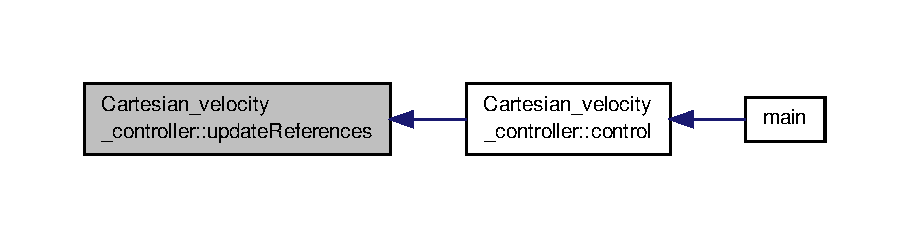
\includegraphics[width=350pt]{classCartesian__velocity__controller_a9b2c7f25b3fc2882f7e4590ee97e0978_icgraph}
\end{center}
\end{figure}




\subsection{Field Documentation}
\hypertarget{classCartesian__velocity__controller_ae771d963a90ad7b844c4c3a821ce5f39}{\index{Cartesian\-\_\-velocity\-\_\-controller@{Cartesian\-\_\-velocity\-\_\-controller}!end\-Effector\-\_\-vel@{end\-Effector\-\_\-vel}}
\index{end\-Effector\-\_\-vel@{end\-Effector\-\_\-vel}!Cartesian_velocity_controller@{Cartesian\-\_\-velocity\-\_\-controller}}
\subsubsection[{end\-Effector\-\_\-vel}]{\setlength{\rightskip}{0pt plus 5cm}schunk\-\_\-msgs\-::\-Velocities Cartesian\-\_\-velocity\-\_\-controller\-::end\-Effector\-\_\-vel\hspace{0.3cm}{\ttfamily [protected]}}}\label{classCartesian__velocity__controller_ae771d963a90ad7b844c4c3a821ce5f39}


Definition at line 24 of file cartesian\-\_\-velocity\-\_\-controller.\-h.



Referenced by Cartesian\-\_\-velocity\-\_\-controller(), and print\-Vel().

\hypertarget{classCartesian__velocity__controller_a01cbe7f951c69ded8604e552a0a706e0}{\index{Cartesian\-\_\-velocity\-\_\-controller@{Cartesian\-\_\-velocity\-\_\-controller}!end\-Effector\-\_\-vel\-\_\-nh@{end\-Effector\-\_\-vel\-\_\-nh}}
\index{end\-Effector\-\_\-vel\-\_\-nh@{end\-Effector\-\_\-vel\-\_\-nh}!Cartesian_velocity_controller@{Cartesian\-\_\-velocity\-\_\-controller}}
\subsubsection[{end\-Effector\-\_\-vel\-\_\-nh}]{\setlength{\rightskip}{0pt plus 5cm}ros\-::\-Node\-Handle Cartesian\-\_\-velocity\-\_\-controller\-::end\-Effector\-\_\-vel\-\_\-nh\hspace{0.3cm}{\ttfamily [protected]}}}\label{classCartesian__velocity__controller_a01cbe7f951c69ded8604e552a0a706e0}


Definition at line 20 of file cartesian\-\_\-velocity\-\_\-controller.\-h.



Referenced by Cartesian\-\_\-velocity\-\_\-controller().

\hypertarget{classCartesian__velocity__controller_ab12287816ae785d3cd6243b3df0cffc6}{\index{Cartesian\-\_\-velocity\-\_\-controller@{Cartesian\-\_\-velocity\-\_\-controller}!end\-Effector\-\_\-vel\-\_\-pub@{end\-Effector\-\_\-vel\-\_\-pub}}
\index{end\-Effector\-\_\-vel\-\_\-pub@{end\-Effector\-\_\-vel\-\_\-pub}!Cartesian_velocity_controller@{Cartesian\-\_\-velocity\-\_\-controller}}
\subsubsection[{end\-Effector\-\_\-vel\-\_\-pub}]{\setlength{\rightskip}{0pt plus 5cm}ros\-::\-Publisher Cartesian\-\_\-velocity\-\_\-controller\-::end\-Effector\-\_\-vel\-\_\-pub\hspace{0.3cm}{\ttfamily [protected]}}}\label{classCartesian__velocity__controller_ab12287816ae785d3cd6243b3df0cffc6}


Definition at line 23 of file cartesian\-\_\-velocity\-\_\-controller.\-h.



Referenced by Cartesian\-\_\-velocity\-\_\-controller(), and print\-Vel().

\hypertarget{classCartesian__velocity__controller_af154b0cda931081b52224eb22e4680f7}{\index{Cartesian\-\_\-velocity\-\_\-controller@{Cartesian\-\_\-velocity\-\_\-controller}!end\-Effector\-\_\-vel\-\_\-queue@{end\-Effector\-\_\-vel\-\_\-queue}}
\index{end\-Effector\-\_\-vel\-\_\-queue@{end\-Effector\-\_\-vel\-\_\-queue}!Cartesian_velocity_controller@{Cartesian\-\_\-velocity\-\_\-controller}}
\subsubsection[{end\-Effector\-\_\-vel\-\_\-queue}]{\setlength{\rightskip}{0pt plus 5cm}ros\-::\-Callback\-Queue Cartesian\-\_\-velocity\-\_\-controller\-::end\-Effector\-\_\-vel\-\_\-queue\hspace{0.3cm}{\ttfamily [protected]}}}\label{classCartesian__velocity__controller_af154b0cda931081b52224eb22e4680f7}


Definition at line 21 of file cartesian\-\_\-velocity\-\_\-controller.\-h.



Referenced by Cartesian\-\_\-velocity\-\_\-controller(), and print\-Vel().

\hypertarget{classCartesian__velocity__controller_a7d04d378a2a6d19870a620883dcd3e09}{\index{Cartesian\-\_\-velocity\-\_\-controller@{Cartesian\-\_\-velocity\-\_\-controller}!reference\-\_\-updater\-\_\-nh@{reference\-\_\-updater\-\_\-nh}}
\index{reference\-\_\-updater\-\_\-nh@{reference\-\_\-updater\-\_\-nh}!Cartesian_velocity_controller@{Cartesian\-\_\-velocity\-\_\-controller}}
\subsubsection[{reference\-\_\-updater\-\_\-nh}]{\setlength{\rightskip}{0pt plus 5cm}ros\-::\-Node\-Handle Cartesian\-\_\-velocity\-\_\-controller\-::reference\-\_\-updater\-\_\-nh\hspace{0.3cm}{\ttfamily [protected]}}}\label{classCartesian__velocity__controller_a7d04d378a2a6d19870a620883dcd3e09}


Definition at line 14 of file cartesian\-\_\-velocity\-\_\-controller.\-h.



Referenced by Cartesian\-\_\-velocity\-\_\-controller().

\hypertarget{classCartesian__velocity__controller_ad2804cf83a42305d18572abdbbfd1c3f}{\index{Cartesian\-\_\-velocity\-\_\-controller@{Cartesian\-\_\-velocity\-\_\-controller}!reference\-\_\-updater\-\_\-queue@{reference\-\_\-updater\-\_\-queue}}
\index{reference\-\_\-updater\-\_\-queue@{reference\-\_\-updater\-\_\-queue}!Cartesian_velocity_controller@{Cartesian\-\_\-velocity\-\_\-controller}}
\subsubsection[{reference\-\_\-updater\-\_\-queue}]{\setlength{\rightskip}{0pt plus 5cm}ros\-::\-Callback\-Queue Cartesian\-\_\-velocity\-\_\-controller\-::reference\-\_\-updater\-\_\-queue\hspace{0.3cm}{\ttfamily [protected]}}}\label{classCartesian__velocity__controller_ad2804cf83a42305d18572abdbbfd1c3f}


Definition at line 15 of file cartesian\-\_\-velocity\-\_\-controller.\-h.



Referenced by Cartesian\-\_\-velocity\-\_\-controller(), and update\-References().

\hypertarget{classCartesian__velocity__controller_a75412b9859afe4b800f9613c9cb8d17f}{\index{Cartesian\-\_\-velocity\-\_\-controller@{Cartesian\-\_\-velocity\-\_\-controller}!reference\-\_\-updater\-\_\-subscriber@{reference\-\_\-updater\-\_\-subscriber}}
\index{reference\-\_\-updater\-\_\-subscriber@{reference\-\_\-updater\-\_\-subscriber}!Cartesian_velocity_controller@{Cartesian\-\_\-velocity\-\_\-controller}}
\subsubsection[{reference\-\_\-updater\-\_\-subscriber}]{\setlength{\rightskip}{0pt plus 5cm}ros\-::\-Subscriber Cartesian\-\_\-velocity\-\_\-controller\-::reference\-\_\-updater\-\_\-subscriber\hspace{0.3cm}{\ttfamily [protected]}}}\label{classCartesian__velocity__controller_a75412b9859afe4b800f9613c9cb8d17f}


Definition at line 17 of file cartesian\-\_\-velocity\-\_\-controller.\-h.



Referenced by Cartesian\-\_\-velocity\-\_\-controller().

\hypertarget{classCartesian__velocity__controller_afc3792f1f6dd0025417d752a89e519e1}{\index{Cartesian\-\_\-velocity\-\_\-controller@{Cartesian\-\_\-velocity\-\_\-controller}!references@{references}}
\index{references@{references}!Cartesian_velocity_controller@{Cartesian\-\_\-velocity\-\_\-controller}}
\subsubsection[{references}]{\setlength{\rightskip}{0pt plus 5cm}std\-::vector$<$double$>$ Cartesian\-\_\-velocity\-\_\-controller\-::references}}\label{classCartesian__velocity__controller_afc3792f1f6dd0025417d752a89e519e1}


Definition at line 46 of file cartesian\-\_\-velocity\-\_\-controller.\-h.



Referenced by Cartesian\-\_\-velocity\-\_\-controller(), reference\-Update\-Callback(), and update\-References().



The documentation for this class was generated from the following files\-:\begin{DoxyCompactItemize}
\item 
schunk\-\_\-high/include/schunk\-\_\-high/\hyperlink{cartesian__velocity__controller_8h}{cartesian\-\_\-velocity\-\_\-controller.\-h}\item 
schunk\-\_\-high/src/\hyperlink{cartesian__velocity__controller_8cpp}{cartesian\-\_\-velocity\-\_\-controller.\-cpp}\end{DoxyCompactItemize}

\hypertarget{structDATA__XYZ}{
\section{DATA\_\-XYZ Struct Reference}
\label{structDATA__XYZ}\index{DATA\_\-XYZ@{DATA\_\-XYZ}}
}


A structure to represent a 3d Vector.  




{\ttfamily \#include \char`\"{}communication.h\char`\"{}}

\subsection*{Data Fields}
\begin{DoxyCompactItemize}
\item 
short int \hyperlink{structDATA__XYZ_a54c1596e9f9969fd9c21e8458024ecfb}{x}
\item 
short int \hyperlink{structDATA__XYZ_a94bbb1c889bf53eb6a5fffa2b39322cf}{y}
\item 
short int \hyperlink{structDATA__XYZ_a69e89ab0ec6e5d72fc5d54f62cc07fb5}{z}
\end{DoxyCompactItemize}


\subsection{Detailed Description}
A structure to represent a 3d Vector. 

Definition at line 75 of file communication.h.



\subsection{Field Documentation}
\hypertarget{structDATA__XYZ_a54c1596e9f9969fd9c21e8458024ecfb}{
\index{DATA\_\-XYZ@{DATA\_\-XYZ}!x@{x}}
\index{x@{x}!DATA_XYZ@{DATA\_\-XYZ}}
\subsubsection[{x}]{\setlength{\rightskip}{0pt plus 5cm}short int {\bf DATA\_\-XYZ::x}}}
\label{structDATA__XYZ_a54c1596e9f9969fd9c21e8458024ecfb}


Definition at line 76 of file communication.h.



Referenced by calibrate\_\-imu(), control\_\-main(), datalogger\_\-update(), periodic\_\-task\_\-2(), read\_\-all\_\-data(), ui\_\-eff\_\-data(), ui\_\-imu\_\-data(), and ui\_\-overview\_\-data().

\hypertarget{structDATA__XYZ_a94bbb1c889bf53eb6a5fffa2b39322cf}{
\index{DATA\_\-XYZ@{DATA\_\-XYZ}!y@{y}}
\index{y@{y}!DATA_XYZ@{DATA\_\-XYZ}}
\subsubsection[{y}]{\setlength{\rightskip}{0pt plus 5cm}short int {\bf DATA\_\-XYZ::y}}}
\label{structDATA__XYZ_a94bbb1c889bf53eb6a5fffa2b39322cf}


Definition at line 77 of file communication.h.



Referenced by calibrate\_\-imu(), datalogger\_\-update(), periodic\_\-task\_\-2(), read\_\-all\_\-data(), ui\_\-eff\_\-data(), ui\_\-imu\_\-data(), and ui\_\-overview\_\-data().

\hypertarget{structDATA__XYZ_a69e89ab0ec6e5d72fc5d54f62cc07fb5}{
\index{DATA\_\-XYZ@{DATA\_\-XYZ}!z@{z}}
\index{z@{z}!DATA_XYZ@{DATA\_\-XYZ}}
\subsubsection[{z}]{\setlength{\rightskip}{0pt plus 5cm}short int {\bf DATA\_\-XYZ::z}}}
\label{structDATA__XYZ_a69e89ab0ec6e5d72fc5d54f62cc07fb5}


Definition at line 78 of file communication.h.



Referenced by calibrate\_\-imu(), control\_\-main(), datalogger\_\-update(), periodic\_\-task\_\-2(), read\_\-all\_\-data(), ui\_\-eff\_\-data(), ui\_\-imu\_\-data(), and ui\_\-overview\_\-data().



The documentation for this struct was generated from the following file:\begin{DoxyCompactItemize}
\item 
communication/\hyperlink{communication_8h}{communication.h}\end{DoxyCompactItemize}

\hypertarget{structDATA__XYZ__DOUBLE}{
\section{DATA\_\-XYZ\_\-DOUBLE Struct Reference}
\label{structDATA__XYZ__DOUBLE}\index{DATA\_\-XYZ\_\-DOUBLE@{DATA\_\-XYZ\_\-DOUBLE}}
}


Vector definition on double.  




{\ttfamily \#include \char`\"{}communication.h\char`\"{}}

\subsection*{Data Fields}
\begin{DoxyCompactItemize}
\item 
double \hyperlink{structDATA__XYZ__DOUBLE_a22868cc99a423900e7b82d015a5eb91f}{x}
\item 
double \hyperlink{structDATA__XYZ__DOUBLE_a198a27b5df3b5b0bf461b0e481e22a82}{y}
\item 
double \hyperlink{structDATA__XYZ__DOUBLE_a9556e8868c223ff3e28756ea18a284c0}{z}
\end{DoxyCompactItemize}


\subsection{Detailed Description}
Vector definition on double. 

Definition at line 84 of file communication.h.



\subsection{Field Documentation}
\hypertarget{structDATA__XYZ__DOUBLE_a22868cc99a423900e7b82d015a5eb91f}{
\index{DATA\_\-XYZ\_\-DOUBLE@{DATA\_\-XYZ\_\-DOUBLE}!x@{x}}
\index{x@{x}!DATA_XYZ_DOUBLE@{DATA\_\-XYZ\_\-DOUBLE}}
\subsubsection[{x}]{\setlength{\rightskip}{0pt plus 5cm}double {\bf DATA\_\-XYZ\_\-DOUBLE::x}}}
\label{structDATA__XYZ__DOUBLE_a22868cc99a423900e7b82d015a5eb91f}


Definition at line 85 of file communication.h.



Referenced by calibrate\_\-imu(), datalogger\_\-update(), ui\_\-imu\_\-data(), and ui\_\-overview\_\-data().

\hypertarget{structDATA__XYZ__DOUBLE_a198a27b5df3b5b0bf461b0e481e22a82}{
\index{DATA\_\-XYZ\_\-DOUBLE@{DATA\_\-XYZ\_\-DOUBLE}!y@{y}}
\index{y@{y}!DATA_XYZ_DOUBLE@{DATA\_\-XYZ\_\-DOUBLE}}
\subsubsection[{y}]{\setlength{\rightskip}{0pt plus 5cm}double {\bf DATA\_\-XYZ\_\-DOUBLE::y}}}
\label{structDATA__XYZ__DOUBLE_a198a27b5df3b5b0bf461b0e481e22a82}


Definition at line 86 of file communication.h.



Referenced by calibrate\_\-imu(), datalogger\_\-update(), ui\_\-imu\_\-data(), and ui\_\-overview\_\-data().

\hypertarget{structDATA__XYZ__DOUBLE_a9556e8868c223ff3e28756ea18a284c0}{
\index{DATA\_\-XYZ\_\-DOUBLE@{DATA\_\-XYZ\_\-DOUBLE}!z@{z}}
\index{z@{z}!DATA_XYZ_DOUBLE@{DATA\_\-XYZ\_\-DOUBLE}}
\subsubsection[{z}]{\setlength{\rightskip}{0pt plus 5cm}double {\bf DATA\_\-XYZ\_\-DOUBLE::z}}}
\label{structDATA__XYZ__DOUBLE_a9556e8868c223ff3e28756ea18a284c0}


Definition at line 87 of file communication.h.



Referenced by calibrate\_\-imu(), datalogger\_\-update(), ui\_\-imu\_\-data(), and ui\_\-overview\_\-data().



The documentation for this struct was generated from the following file:\begin{DoxyCompactItemize}
\item 
communication/\hyperlink{communication_8h}{communication.h}\end{DoxyCompactItemize}

\hypertarget{structDQ}{\section{D\-Q Struct Reference}
\label{structDQ}\index{D\-Q@{D\-Q}}
}


Dual\-Quaternion library Header.  




{\ttfamily \#include \char`\"{}dualquaternion.\-h\char`\"{}}



Collaboration diagram for D\-Q\-:\nopagebreak
\begin{figure}[H]
\begin{center}
\leavevmode
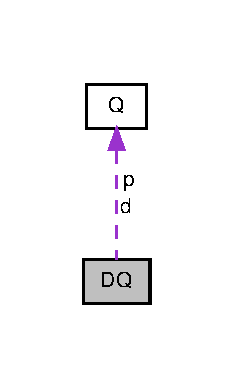
\includegraphics[width=112pt]{structDQ__coll__graph}
\end{center}
\end{figure}
\subsection*{Data Fields}
\begin{DoxyCompactItemize}
\item 
\hyperlink{structQ}{Q} $\ast$ \hyperlink{structDQ_a878210bff170f4392d6cbe2d4704ffdc}{p}
\begin{DoxyCompactList}\small\item\em A Quaternion representing it's Primary Part. \end{DoxyCompactList}\item 
\hyperlink{structQ}{Q} $\ast$ \hyperlink{structDQ_a535cdb52876521fd6abbfcf211a7c702}{d}
\begin{DoxyCompactList}\small\item\em \hyperlink{structQ}{Q} Quaternion representing it's Dual Part. \end{DoxyCompactList}\end{DoxyCompactItemize}


\subsection{Detailed Description}
Dual\-Quaternion library Header. 

\begin{DoxyAuthor}{Author}
Murilo Marques Marinho. A Dual\-Quaternion. 
\end{DoxyAuthor}


Definition at line 21 of file dualquaternion.\-h.



\subsection{Field Documentation}
\hypertarget{structDQ_a535cdb52876521fd6abbfcf211a7c702}{\index{D\-Q@{D\-Q}!d@{d}}
\index{d@{d}!DQ@{D\-Q}}
\subsubsection[{d}]{\setlength{\rightskip}{0pt plus 5cm}{\bf Q}$\ast$ D\-Q\-::d}}\label{structDQ_a535cdb52876521fd6abbfcf211a7c702}


\hyperlink{structQ}{Q} Quaternion representing it's Dual Part. 



Definition at line 29 of file dualquaternion.\-h.



Referenced by Cartesian\-\_\-pose\-\_\-controller\-::control(), D\-Q\-\_\-create(), D\-Q\-\_\-create\-From\-Quaternion(), D\-Q\-\_\-free(), D\-Q\-\_\-get\-T(), D\-Q\-\_\-mult(), D\-Q\-\_\-print(), Link\-\_\-\-D\-Q\-F\-T(), P\-G\-M\-A\-T\-R\-I\-X\-\_\-\-S\-E\-T\-\_\-\-C\-O\-L\-U\-M\-N\-\_\-\-B\-Y\-\_\-\-D\-Q(), and Robot\-\_\-get\-P().

\hypertarget{structDQ_a878210bff170f4392d6cbe2d4704ffdc}{\index{D\-Q@{D\-Q}!p@{p}}
\index{p@{p}!DQ@{D\-Q}}
\subsubsection[{p}]{\setlength{\rightskip}{0pt plus 5cm}{\bf Q}$\ast$ D\-Q\-::p}}\label{structDQ_a878210bff170f4392d6cbe2d4704ffdc}


A Quaternion representing it's Primary Part. 



Definition at line 25 of file dualquaternion.\-h.



Referenced by Cartesian\-\_\-pose\-\_\-controller\-::control(), D\-Q\-\_\-create(), D\-Q\-\_\-create\-From\-Quaternion(), D\-Q\-\_\-free(), D\-Q\-\_\-get\-Pitch\-Angle(), D\-Q\-\_\-get\-R(), D\-Q\-\_\-get\-T(), D\-Q\-\_\-mult(), D\-Q\-\_\-print(), Link\-\_\-\-D\-Q\-F\-T(), P\-G\-M\-A\-T\-R\-I\-X\-\_\-\-S\-E\-T\-\_\-\-C\-O\-L\-U\-M\-N\-\_\-\-B\-Y\-\_\-\-D\-Q(), Robot\-\_\-get\-G\-Jacobian(), Robot\-\_\-get\-O\-Jacobian\-Angle\-P(), and Robot\-\_\-get\-P().



The documentation for this struct was generated from the following file\-:\begin{DoxyCompactItemize}
\item 
schunk\-\_\-high/include/schunk\-\_\-high/\hyperlink{dualquaternion_8h}{dualquaternion.\-h}\end{DoxyCompactItemize}

\hypertarget{structDUMMY__MATRICES}{\section{D\-U\-M\-M\-Y\-\_\-\-M\-A\-T\-R\-I\-C\-E\-S Struct Reference}
\label{structDUMMY__MATRICES}\index{D\-U\-M\-M\-Y\-\_\-\-M\-A\-T\-R\-I\-C\-E\-S@{D\-U\-M\-M\-Y\-\_\-\-M\-A\-T\-R\-I\-C\-E\-S}}
}


{\ttfamily \#include \char`\"{}gmatrix.\-h\char`\"{}}



Collaboration diagram for D\-U\-M\-M\-Y\-\_\-\-M\-A\-T\-R\-I\-C\-E\-S\-:\nopagebreak
\begin{figure}[H]
\begin{center}
\leavevmode
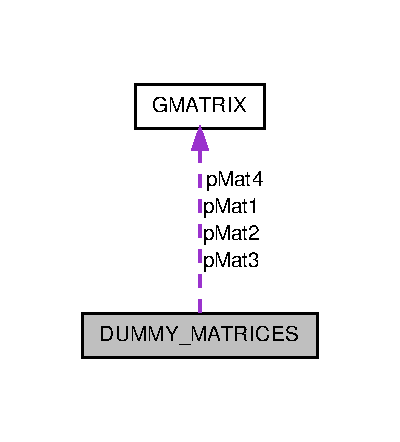
\includegraphics[width=192pt]{structDUMMY__MATRICES__coll__graph}
\end{center}
\end{figure}
\subsection*{Data Fields}
\begin{DoxyCompactItemize}
\item 
\hyperlink{gmatrix_8h_ad8edc274a17feb9e4fca93e620253bed}{P\-G\-M\-A\-T\-R\-I\-X} \hyperlink{structDUMMY__MATRICES_a83b2fec22eaa2674a6360711702d28ac}{p\-Mat1}
\item 
\hyperlink{gmatrix_8h_ad8edc274a17feb9e4fca93e620253bed}{P\-G\-M\-A\-T\-R\-I\-X} \hyperlink{structDUMMY__MATRICES_ada47a9e57f8f5e60971d1d7a888d66b0}{p\-Mat2}
\item 
\hyperlink{gmatrix_8h_ad8edc274a17feb9e4fca93e620253bed}{P\-G\-M\-A\-T\-R\-I\-X} \hyperlink{structDUMMY__MATRICES_ac7b2907eca9bdceb1b78dc5ffb1f8299}{p\-Mat3}
\item 
\hyperlink{gmatrix_8h_ad8edc274a17feb9e4fca93e620253bed}{P\-G\-M\-A\-T\-R\-I\-X} \hyperlink{structDUMMY__MATRICES_a90bf8e9779c6de5e65b4a93341efddba}{p\-Mat4}
\end{DoxyCompactItemize}


\subsection{Detailed Description}


Definition at line 319 of file gmatrix.\-h.



\subsection{Field Documentation}
\hypertarget{structDUMMY__MATRICES_a83b2fec22eaa2674a6360711702d28ac}{\index{D\-U\-M\-M\-Y\-\_\-\-M\-A\-T\-R\-I\-C\-E\-S@{D\-U\-M\-M\-Y\-\_\-\-M\-A\-T\-R\-I\-C\-E\-S}!p\-Mat1@{p\-Mat1}}
\index{p\-Mat1@{p\-Mat1}!DUMMY_MATRICES@{D\-U\-M\-M\-Y\-\_\-\-M\-A\-T\-R\-I\-C\-E\-S}}
\subsubsection[{p\-Mat1}]{\setlength{\rightskip}{0pt plus 5cm}{\bf P\-G\-M\-A\-T\-R\-I\-X} D\-U\-M\-M\-Y\-\_\-\-M\-A\-T\-R\-I\-C\-E\-S\-::p\-Mat1}}\label{structDUMMY__MATRICES_a83b2fec22eaa2674a6360711702d28ac}


Definition at line 320 of file gmatrix.\-h.

\hypertarget{structDUMMY__MATRICES_ada47a9e57f8f5e60971d1d7a888d66b0}{\index{D\-U\-M\-M\-Y\-\_\-\-M\-A\-T\-R\-I\-C\-E\-S@{D\-U\-M\-M\-Y\-\_\-\-M\-A\-T\-R\-I\-C\-E\-S}!p\-Mat2@{p\-Mat2}}
\index{p\-Mat2@{p\-Mat2}!DUMMY_MATRICES@{D\-U\-M\-M\-Y\-\_\-\-M\-A\-T\-R\-I\-C\-E\-S}}
\subsubsection[{p\-Mat2}]{\setlength{\rightskip}{0pt plus 5cm}{\bf P\-G\-M\-A\-T\-R\-I\-X} D\-U\-M\-M\-Y\-\_\-\-M\-A\-T\-R\-I\-C\-E\-S\-::p\-Mat2}}\label{structDUMMY__MATRICES_ada47a9e57f8f5e60971d1d7a888d66b0}


Definition at line 321 of file gmatrix.\-h.

\hypertarget{structDUMMY__MATRICES_ac7b2907eca9bdceb1b78dc5ffb1f8299}{\index{D\-U\-M\-M\-Y\-\_\-\-M\-A\-T\-R\-I\-C\-E\-S@{D\-U\-M\-M\-Y\-\_\-\-M\-A\-T\-R\-I\-C\-E\-S}!p\-Mat3@{p\-Mat3}}
\index{p\-Mat3@{p\-Mat3}!DUMMY_MATRICES@{D\-U\-M\-M\-Y\-\_\-\-M\-A\-T\-R\-I\-C\-E\-S}}
\subsubsection[{p\-Mat3}]{\setlength{\rightskip}{0pt plus 5cm}{\bf P\-G\-M\-A\-T\-R\-I\-X} D\-U\-M\-M\-Y\-\_\-\-M\-A\-T\-R\-I\-C\-E\-S\-::p\-Mat3}}\label{structDUMMY__MATRICES_ac7b2907eca9bdceb1b78dc5ffb1f8299}


Definition at line 322 of file gmatrix.\-h.

\hypertarget{structDUMMY__MATRICES_a90bf8e9779c6de5e65b4a93341efddba}{\index{D\-U\-M\-M\-Y\-\_\-\-M\-A\-T\-R\-I\-C\-E\-S@{D\-U\-M\-M\-Y\-\_\-\-M\-A\-T\-R\-I\-C\-E\-S}!p\-Mat4@{p\-Mat4}}
\index{p\-Mat4@{p\-Mat4}!DUMMY_MATRICES@{D\-U\-M\-M\-Y\-\_\-\-M\-A\-T\-R\-I\-C\-E\-S}}
\subsubsection[{p\-Mat4}]{\setlength{\rightskip}{0pt plus 5cm}{\bf P\-G\-M\-A\-T\-R\-I\-X} D\-U\-M\-M\-Y\-\_\-\-M\-A\-T\-R\-I\-C\-E\-S\-::p\-Mat4}}\label{structDUMMY__MATRICES_a90bf8e9779c6de5e65b4a93341efddba}


Definition at line 323 of file gmatrix.\-h.



The documentation for this struct was generated from the following file\-:\begin{DoxyCompactItemize}
\item 
schunk\-\_\-high/include/schunk\-\_\-high/\hyperlink{gmatrix_8h}{gmatrix.\-h}\end{DoxyCompactItemize}

\hypertarget{structEFF__DATA__STRUCT}{
\section{EFF\_\-DATA\_\-STRUCT Struct Reference}
\label{structEFF__DATA__STRUCT}\index{EFF\_\-DATA\_\-STRUCT@{EFF\_\-DATA\_\-STRUCT}}
}


{\ttfamily \#include \char`\"{}communication.h\char`\"{}}



Collaboration diagram for EFF\_\-DATA\_\-STRUCT:\subsection*{Data Fields}
\begin{DoxyCompactItemize}
\item 
\hyperlink{structDATA__XYZ}{DATA\_\-XYZ} \hyperlink{structEFF__DATA__STRUCT_abe8952947b54bf9c247f3429ee3aeb44}{F}
\item 
\hyperlink{structDATA__XYZ}{DATA\_\-XYZ} \hyperlink{structEFF__DATA__STRUCT_aaf6e03b6e600295e0f5c706fc869e9d1}{M}
\item 
uint8\_\-t \hyperlink{structEFF__DATA__STRUCT_aa42ebc512dd79fa6ebf998162a149446}{new\_\-data}
\end{DoxyCompactItemize}


\subsection{Detailed Description}


Definition at line 112 of file communication.h.



\subsection{Field Documentation}
\hypertarget{structEFF__DATA__STRUCT_abe8952947b54bf9c247f3429ee3aeb44}{
\index{EFF\_\-DATA\_\-STRUCT@{EFF\_\-DATA\_\-STRUCT}!F@{F}}
\index{F@{F}!EFF_DATA_STRUCT@{EFF\_\-DATA\_\-STRUCT}}
\subsubsection[{F}]{\setlength{\rightskip}{0pt plus 5cm}{\bf DATA\_\-XYZ} {\bf EFF\_\-DATA\_\-STRUCT::F}}}
\label{structEFF__DATA__STRUCT_abe8952947b54bf9c247f3429ee3aeb44}


Definition at line 113 of file communication.h.



Referenced by datalogger\_\-update(), read\_\-all\_\-data(), and ui\_\-eff\_\-data().

\hypertarget{structEFF__DATA__STRUCT_aaf6e03b6e600295e0f5c706fc869e9d1}{
\index{EFF\_\-DATA\_\-STRUCT@{EFF\_\-DATA\_\-STRUCT}!M@{M}}
\index{M@{M}!EFF_DATA_STRUCT@{EFF\_\-DATA\_\-STRUCT}}
\subsubsection[{M}]{\setlength{\rightskip}{0pt plus 5cm}{\bf DATA\_\-XYZ} {\bf EFF\_\-DATA\_\-STRUCT::M}}}
\label{structEFF__DATA__STRUCT_aaf6e03b6e600295e0f5c706fc869e9d1}


Definition at line 114 of file communication.h.



Referenced by ui\_\-eff\_\-data().

\hypertarget{structEFF__DATA__STRUCT_aa42ebc512dd79fa6ebf998162a149446}{
\index{EFF\_\-DATA\_\-STRUCT@{EFF\_\-DATA\_\-STRUCT}!new\_\-data@{new\_\-data}}
\index{new\_\-data@{new\_\-data}!EFF_DATA_STRUCT@{EFF\_\-DATA\_\-STRUCT}}
\subsubsection[{new\_\-data}]{\setlength{\rightskip}{0pt plus 5cm}uint8\_\-t {\bf EFF\_\-DATA\_\-STRUCT::new\_\-data}}}
\label{structEFF__DATA__STRUCT_aa42ebc512dd79fa6ebf998162a149446}


Definition at line 115 of file communication.h.



Referenced by datalogger\_\-update(), and read\_\-all\_\-data().



The documentation for this struct was generated from the following file:\begin{DoxyCompactItemize}
\item 
communication/\hyperlink{communication_8h}{communication.h}\end{DoxyCompactItemize}

\hypertarget{structGDATALOGGER}{\section{G\-D\-A\-T\-A\-L\-O\-G\-G\-E\-R Struct Reference}
\label{structGDATALOGGER}\index{G\-D\-A\-T\-A\-L\-O\-G\-G\-E\-R@{G\-D\-A\-T\-A\-L\-O\-G\-G\-E\-R}}
}


{\ttfamily \#include \char`\"{}gdatalogger.\-h\char`\"{}}



Collaboration diagram for G\-D\-A\-T\-A\-L\-O\-G\-G\-E\-R\-:
\nopagebreak
\begin{figure}[H]
\begin{center}
\leavevmode
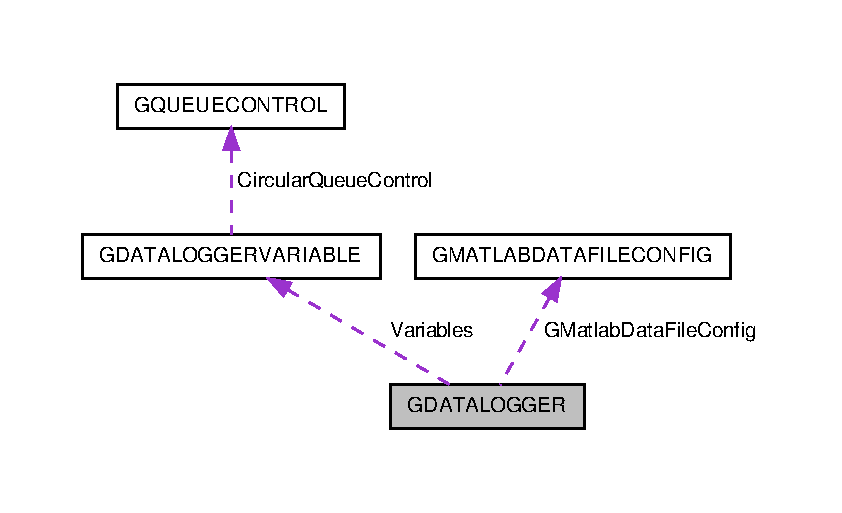
\includegraphics[width=350pt]{structGDATALOGGER__coll__graph}
\end{center}
\end{figure}
\subsection*{Data Fields}
\begin{DoxyCompactItemize}
\item 
\hyperlink{structGDATALOGGERVARIABLE}{G\-D\-A\-T\-A\-L\-O\-G\-G\-E\-R\-V\-A\-R\-I\-A\-B\-L\-E} \hyperlink{structGDATALOGGER_a6af9584d8665205b950cb2dcc5f90a94}{Variables} \mbox{[}\hyperlink{gdatalogger_8h_a2ddc529b6734b7a9222a5fbd1305581e}{G\-D\-A\-T\-A\-L\-O\-G\-G\-E\-R\-\_\-\-M\-A\-X\-V\-A\-R\-I\-A\-B\-L\-E\-S}\mbox{]}
\item 
int \hyperlink{structGDATALOGGER_a2ac727ee6c50f7e04030cbe531158f08}{m\-\_\-\-Number\-Of\-Variables}
\item 
\hyperlink{structGMATLABDATAFILECONFIG}{G\-M\-A\-T\-L\-A\-B\-D\-A\-T\-A\-F\-I\-L\-E\-C\-O\-N\-F\-I\-G} \hyperlink{structGDATALOGGER_a062fd3836dbd0b1bec129ab372bff04a}{G\-Matlab\-Data\-File\-Config}
\end{DoxyCompactItemize}


\subsection{Detailed Description}


Definition at line 26 of file gdatalogger.\-h.



\subsection{Field Documentation}
\hypertarget{structGDATALOGGER_a062fd3836dbd0b1bec129ab372bff04a}{\index{G\-D\-A\-T\-A\-L\-O\-G\-G\-E\-R@{G\-D\-A\-T\-A\-L\-O\-G\-G\-E\-R}!G\-Matlab\-Data\-File\-Config@{G\-Matlab\-Data\-File\-Config}}
\index{G\-Matlab\-Data\-File\-Config@{G\-Matlab\-Data\-File\-Config}!GDATALOGGER@{G\-D\-A\-T\-A\-L\-O\-G\-G\-E\-R}}
\subsubsection[{G\-Matlab\-Data\-File\-Config}]{\setlength{\rightskip}{0pt plus 5cm}{\bf G\-M\-A\-T\-L\-A\-B\-D\-A\-T\-A\-F\-I\-L\-E\-C\-O\-N\-F\-I\-G} G\-D\-A\-T\-A\-L\-O\-G\-G\-E\-R\-::\-G\-Matlab\-Data\-File\-Config}}\label{structGDATALOGGER_a062fd3836dbd0b1bec129ab372bff04a}


Definition at line 29 of file gdatalogger.\-h.



Referenced by g\-Data\-Logger\-\_\-\-Close(), g\-Data\-Logger\-\_\-\-Init(), and g\-Data\-Logger\-\_\-\-Matfile\-Update().

\hypertarget{structGDATALOGGER_a2ac727ee6c50f7e04030cbe531158f08}{\index{G\-D\-A\-T\-A\-L\-O\-G\-G\-E\-R@{G\-D\-A\-T\-A\-L\-O\-G\-G\-E\-R}!m\-\_\-\-Number\-Of\-Variables@{m\-\_\-\-Number\-Of\-Variables}}
\index{m\-\_\-\-Number\-Of\-Variables@{m\-\_\-\-Number\-Of\-Variables}!GDATALOGGER@{G\-D\-A\-T\-A\-L\-O\-G\-G\-E\-R}}
\subsubsection[{m\-\_\-\-Number\-Of\-Variables}]{\setlength{\rightskip}{0pt plus 5cm}int G\-D\-A\-T\-A\-L\-O\-G\-G\-E\-R\-::m\-\_\-\-Number\-Of\-Variables}}\label{structGDATALOGGER_a2ac727ee6c50f7e04030cbe531158f08}


Definition at line 28 of file gdatalogger.\-h.



Referenced by g\-Data\-Logger\-\_\-\-Close(), g\-Data\-Logger\-\_\-\-Declare\-Variable(), g\-Data\-Logger\-\_\-\-Init(), g\-Data\-Logger\-\_\-\-Insert\-Variable(), g\-Data\-Logger\-\_\-\-I\-P\-C\-Update(), and g\-Data\-Logger\-\_\-\-Matfile\-Update().

\hypertarget{structGDATALOGGER_a6af9584d8665205b950cb2dcc5f90a94}{\index{G\-D\-A\-T\-A\-L\-O\-G\-G\-E\-R@{G\-D\-A\-T\-A\-L\-O\-G\-G\-E\-R}!Variables@{Variables}}
\index{Variables@{Variables}!GDATALOGGER@{G\-D\-A\-T\-A\-L\-O\-G\-G\-E\-R}}
\subsubsection[{Variables}]{\setlength{\rightskip}{0pt plus 5cm}{\bf G\-D\-A\-T\-A\-L\-O\-G\-G\-E\-R\-V\-A\-R\-I\-A\-B\-L\-E} G\-D\-A\-T\-A\-L\-O\-G\-G\-E\-R\-::\-Variables\mbox{[}{\bf G\-D\-A\-T\-A\-L\-O\-G\-G\-E\-R\-\_\-\-M\-A\-X\-V\-A\-R\-I\-A\-B\-L\-E\-S}\mbox{]}}}\label{structGDATALOGGER_a6af9584d8665205b950cb2dcc5f90a94}


Definition at line 27 of file gdatalogger.\-h.



Referenced by g\-Data\-Logger\-\_\-\-Close(), g\-Data\-Logger\-\_\-\-Declare\-Variable(), g\-Data\-Logger\-\_\-\-Init(), g\-Data\-Logger\-\_\-\-Insert\-Variable(), g\-Data\-Logger\-\_\-\-I\-P\-C\-Update(), and g\-Data\-Logger\-\_\-\-Matfile\-Update().



The documentation for this struct was generated from the following file\-:\begin{DoxyCompactItemize}
\item 
gdatalogger/\hyperlink{gdatalogger_8h}{gdatalogger.\-h}\end{DoxyCompactItemize}

\hypertarget{structGDATALOGGERIPC__SHM}{
\section{GDATALOGGERIPC\_\-SHM Struct Reference}
\label{structGDATALOGGERIPC__SHM}\index{GDATALOGGERIPC\_\-SHM@{GDATALOGGERIPC\_\-SHM}}
}


{\ttfamily \#include \char`\"{}gdatalogger.h\char`\"{}}

\subsection*{Data Fields}
\begin{DoxyCompactItemize}
\item 
char \hyperlink{structGDATALOGGERIPC__SHM_afb130e15f688a18e52e2037f4bb17e89}{VariableName} \mbox{[}100\mbox{]}
\item 
char \hyperlink{structGDATALOGGERIPC__SHM_a8efd7b2ed8ff087f9694cb47a8c25a13}{VariableUnit} \mbox{[}50\mbox{]}
\item 
double \hyperlink{structGDATALOGGERIPC__SHM_ac495752de142e6697c08f713505ed55c}{QueueData} \mbox{[}GDATALOGGER\_\-IPC\_\-MAXQUEUESIZE\mbox{]}
\item 
int \hyperlink{structGDATALOGGERIPC__SHM_a7d392777d231e1b0cece66cb51b0945b}{QueueSize}
\item 
int \hyperlink{structGDATALOGGERIPC__SHM_a346eca077a97246740a6ed4f7c08833c}{Flag}
\end{DoxyCompactItemize}


\subsection{Detailed Description}


Definition at line 45 of file gdatalogger.h.



\subsection{Field Documentation}
\hypertarget{structGDATALOGGERIPC__SHM_a346eca077a97246740a6ed4f7c08833c}{
\index{GDATALOGGERIPC\_\-SHM@{GDATALOGGERIPC\_\-SHM}!Flag@{Flag}}
\index{Flag@{Flag}!GDATALOGGERIPC_SHM@{GDATALOGGERIPC\_\-SHM}}
\subsubsection[{Flag}]{\setlength{\rightskip}{0pt plus 5cm}int {\bf GDATALOGGERIPC\_\-SHM::Flag}}}
\label{structGDATALOGGERIPC__SHM_a346eca077a97246740a6ed4f7c08833c}


Definition at line 50 of file gdatalogger.h.



Referenced by gDataLogger\_\-Init(), gDataLogger\_\-IPC\_\-RetrieveVariable(), and gDataLogger\_\-IPCUpdate().

\hypertarget{structGDATALOGGERIPC__SHM_ac495752de142e6697c08f713505ed55c}{
\index{GDATALOGGERIPC\_\-SHM@{GDATALOGGERIPC\_\-SHM}!QueueData@{QueueData}}
\index{QueueData@{QueueData}!GDATALOGGERIPC_SHM@{GDATALOGGERIPC\_\-SHM}}
\subsubsection[{QueueData}]{\setlength{\rightskip}{0pt plus 5cm}double {\bf GDATALOGGERIPC\_\-SHM::QueueData}\mbox{[}GDATALOGGER\_\-IPC\_\-MAXQUEUESIZE\mbox{]}}}
\label{structGDATALOGGERIPC__SHM_ac495752de142e6697c08f713505ed55c}


Definition at line 48 of file gdatalogger.h.



Referenced by gDataLogger\_\-IPC\_\-RetrieveVariable(), and gDataLogger\_\-IPCUpdate().

\hypertarget{structGDATALOGGERIPC__SHM_a7d392777d231e1b0cece66cb51b0945b}{
\index{GDATALOGGERIPC\_\-SHM@{GDATALOGGERIPC\_\-SHM}!QueueSize@{QueueSize}}
\index{QueueSize@{QueueSize}!GDATALOGGERIPC_SHM@{GDATALOGGERIPC\_\-SHM}}
\subsubsection[{QueueSize}]{\setlength{\rightskip}{0pt plus 5cm}int {\bf GDATALOGGERIPC\_\-SHM::QueueSize}}}
\label{structGDATALOGGERIPC__SHM_a7d392777d231e1b0cece66cb51b0945b}


Definition at line 49 of file gdatalogger.h.



Referenced by gDataLogger\_\-IPC\_\-RetrieveVariable(), and gDataLogger\_\-IPCUpdate().

\hypertarget{structGDATALOGGERIPC__SHM_afb130e15f688a18e52e2037f4bb17e89}{
\index{GDATALOGGERIPC\_\-SHM@{GDATALOGGERIPC\_\-SHM}!VariableName@{VariableName}}
\index{VariableName@{VariableName}!GDATALOGGERIPC_SHM@{GDATALOGGERIPC\_\-SHM}}
\subsubsection[{VariableName}]{\setlength{\rightskip}{0pt plus 5cm}char {\bf GDATALOGGERIPC\_\-SHM::VariableName}\mbox{[}100\mbox{]}}}
\label{structGDATALOGGERIPC__SHM_afb130e15f688a18e52e2037f4bb17e89}


Definition at line 46 of file gdatalogger.h.



Referenced by gDataLogger\_\-IPC\_\-RetrieveVariable(), and gDataLogger\_\-IPCUpdate().

\hypertarget{structGDATALOGGERIPC__SHM_a8efd7b2ed8ff087f9694cb47a8c25a13}{
\index{GDATALOGGERIPC\_\-SHM@{GDATALOGGERIPC\_\-SHM}!VariableUnit@{VariableUnit}}
\index{VariableUnit@{VariableUnit}!GDATALOGGERIPC_SHM@{GDATALOGGERIPC\_\-SHM}}
\subsubsection[{VariableUnit}]{\setlength{\rightskip}{0pt plus 5cm}char {\bf GDATALOGGERIPC\_\-SHM::VariableUnit}\mbox{[}50\mbox{]}}}
\label{structGDATALOGGERIPC__SHM_a8efd7b2ed8ff087f9694cb47a8c25a13}


Definition at line 47 of file gdatalogger.h.



Referenced by gDataLogger\_\-IPC\_\-RetrieveVariable(), and gDataLogger\_\-IPCUpdate().



The documentation for this struct was generated from the following file:\begin{DoxyCompactItemize}
\item 
gdatalogger/\hyperlink{gdatalogger_8h}{gdatalogger.h}\end{DoxyCompactItemize}

\hypertarget{structGDATALOGGERVARIABLE}{\section{G\-D\-A\-T\-A\-L\-O\-G\-G\-E\-R\-V\-A\-R\-I\-A\-B\-L\-E Struct Reference}
\label{structGDATALOGGERVARIABLE}\index{G\-D\-A\-T\-A\-L\-O\-G\-G\-E\-R\-V\-A\-R\-I\-A\-B\-L\-E@{G\-D\-A\-T\-A\-L\-O\-G\-G\-E\-R\-V\-A\-R\-I\-A\-B\-L\-E}}
}


{\ttfamily \#include \char`\"{}gdatalogger.\-h\char`\"{}}



Collaboration diagram for G\-D\-A\-T\-A\-L\-O\-G\-G\-E\-R\-V\-A\-R\-I\-A\-B\-L\-E\-:\nopagebreak
\begin{figure}[H]
\begin{center}
\leavevmode
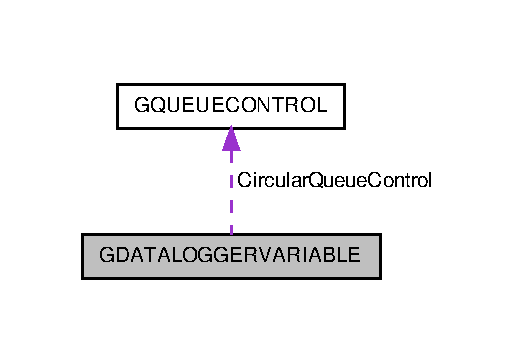
\includegraphics[width=248pt]{structGDATALOGGERVARIABLE__coll__graph}
\end{center}
\end{figure}
\subsection*{Data Fields}
\begin{DoxyCompactItemize}
\item 
char \hyperlink{structGDATALOGGERVARIABLE_a336b7b6cbfc9cdebc7e1ade3de17ac3f}{Variable\-Name} \mbox{[}100\mbox{]}
\item 
char \hyperlink{structGDATALOGGERVARIABLE_a0d42da63f3f904774cbf2ee8d92ee135}{Variable\-Unit} \mbox{[}50\mbox{]}
\item 
long int \hyperlink{structGDATALOGGERVARIABLE_aa1cd5b838d8655734e7d4499b25bf22a}{G\-Matlab\-Data\-File\-Index}
\item 
int \hyperlink{structGDATALOGGERVARIABLE_a68c3eb0f57a786afe9a2658fc42b61d6}{Nr}
\item 
int \hyperlink{structGDATALOGGERVARIABLE_abd1db7599f09e121cd125e665cb9c460}{Nc}
\item 
double $\ast$ \hyperlink{structGDATALOGGERVARIABLE_ae17ad02442f31da9518c99ce13607c8b}{Circular\-Queue}
\item 
\hyperlink{structGQUEUECONTROL}{G\-Q\-U\-E\-U\-E\-C\-O\-N\-T\-R\-O\-L} \hyperlink{structGDATALOGGERVARIABLE_a1a50747d2223f228288b4656470d9bbc}{Circular\-Queue\-Control}
\item 
int \hyperlink{structGDATALOGGERVARIABLE_ad982aef10e8496c2a1c6b9bb1f1dc5c3}{Has\-Been\-Written}
\end{DoxyCompactItemize}


\subsection{Detailed Description}


Definition at line 15 of file gdatalogger.\-h.



\subsection{Field Documentation}
\hypertarget{structGDATALOGGERVARIABLE_ae17ad02442f31da9518c99ce13607c8b}{\index{G\-D\-A\-T\-A\-L\-O\-G\-G\-E\-R\-V\-A\-R\-I\-A\-B\-L\-E@{G\-D\-A\-T\-A\-L\-O\-G\-G\-E\-R\-V\-A\-R\-I\-A\-B\-L\-E}!Circular\-Queue@{Circular\-Queue}}
\index{Circular\-Queue@{Circular\-Queue}!GDATALOGGERVARIABLE@{G\-D\-A\-T\-A\-L\-O\-G\-G\-E\-R\-V\-A\-R\-I\-A\-B\-L\-E}}
\subsubsection[{Circular\-Queue}]{\setlength{\rightskip}{0pt plus 5cm}double$\ast$ G\-D\-A\-T\-A\-L\-O\-G\-G\-E\-R\-V\-A\-R\-I\-A\-B\-L\-E\-::\-Circular\-Queue}}\label{structGDATALOGGERVARIABLE_ae17ad02442f31da9518c99ce13607c8b}


Definition at line 21 of file gdatalogger.\-h.



Referenced by g\-Data\-Logger\-\_\-\-Close(), g\-Data\-Logger\-\_\-\-Declare\-Variable(), g\-Data\-Logger\-\_\-\-Init(), g\-Data\-Logger\-\_\-\-Insert\-Variable(), g\-Data\-Logger\-\_\-\-I\-P\-C\-Update(), and g\-Data\-Logger\-\_\-\-Matfile\-Update().

\hypertarget{structGDATALOGGERVARIABLE_a1a50747d2223f228288b4656470d9bbc}{\index{G\-D\-A\-T\-A\-L\-O\-G\-G\-E\-R\-V\-A\-R\-I\-A\-B\-L\-E@{G\-D\-A\-T\-A\-L\-O\-G\-G\-E\-R\-V\-A\-R\-I\-A\-B\-L\-E}!Circular\-Queue\-Control@{Circular\-Queue\-Control}}
\index{Circular\-Queue\-Control@{Circular\-Queue\-Control}!GDATALOGGERVARIABLE@{G\-D\-A\-T\-A\-L\-O\-G\-G\-E\-R\-V\-A\-R\-I\-A\-B\-L\-E}}
\subsubsection[{Circular\-Queue\-Control}]{\setlength{\rightskip}{0pt plus 5cm}{\bf G\-Q\-U\-E\-U\-E\-C\-O\-N\-T\-R\-O\-L} G\-D\-A\-T\-A\-L\-O\-G\-G\-E\-R\-V\-A\-R\-I\-A\-B\-L\-E\-::\-Circular\-Queue\-Control}}\label{structGDATALOGGERVARIABLE_a1a50747d2223f228288b4656470d9bbc}


Definition at line 22 of file gdatalogger.\-h.



Referenced by g\-Data\-Logger\-\_\-\-Declare\-Variable(), g\-Data\-Logger\-\_\-\-Insert\-Variable(), g\-Data\-Logger\-\_\-\-I\-P\-C\-Update(), and g\-Data\-Logger\-\_\-\-Matfile\-Update().

\hypertarget{structGDATALOGGERVARIABLE_aa1cd5b838d8655734e7d4499b25bf22a}{\index{G\-D\-A\-T\-A\-L\-O\-G\-G\-E\-R\-V\-A\-R\-I\-A\-B\-L\-E@{G\-D\-A\-T\-A\-L\-O\-G\-G\-E\-R\-V\-A\-R\-I\-A\-B\-L\-E}!G\-Matlab\-Data\-File\-Index@{G\-Matlab\-Data\-File\-Index}}
\index{G\-Matlab\-Data\-File\-Index@{G\-Matlab\-Data\-File\-Index}!GDATALOGGERVARIABLE@{G\-D\-A\-T\-A\-L\-O\-G\-G\-E\-R\-V\-A\-R\-I\-A\-B\-L\-E}}
\subsubsection[{G\-Matlab\-Data\-File\-Index}]{\setlength{\rightskip}{0pt plus 5cm}long int G\-D\-A\-T\-A\-L\-O\-G\-G\-E\-R\-V\-A\-R\-I\-A\-B\-L\-E\-::\-G\-Matlab\-Data\-File\-Index}}\label{structGDATALOGGERVARIABLE_aa1cd5b838d8655734e7d4499b25bf22a}


Definition at line 18 of file gdatalogger.\-h.



Referenced by g\-Data\-Logger\-\_\-\-Close(), g\-Data\-Logger\-\_\-\-Declare\-Variable(), g\-Data\-Logger\-\_\-\-Init(), and g\-Data\-Logger\-\_\-\-Matfile\-Update().

\hypertarget{structGDATALOGGERVARIABLE_ad982aef10e8496c2a1c6b9bb1f1dc5c3}{\index{G\-D\-A\-T\-A\-L\-O\-G\-G\-E\-R\-V\-A\-R\-I\-A\-B\-L\-E@{G\-D\-A\-T\-A\-L\-O\-G\-G\-E\-R\-V\-A\-R\-I\-A\-B\-L\-E}!Has\-Been\-Written@{Has\-Been\-Written}}
\index{Has\-Been\-Written@{Has\-Been\-Written}!GDATALOGGERVARIABLE@{G\-D\-A\-T\-A\-L\-O\-G\-G\-E\-R\-V\-A\-R\-I\-A\-B\-L\-E}}
\subsubsection[{Has\-Been\-Written}]{\setlength{\rightskip}{0pt plus 5cm}int G\-D\-A\-T\-A\-L\-O\-G\-G\-E\-R\-V\-A\-R\-I\-A\-B\-L\-E\-::\-Has\-Been\-Written}}\label{structGDATALOGGERVARIABLE_ad982aef10e8496c2a1c6b9bb1f1dc5c3}


Definition at line 23 of file gdatalogger.\-h.



Referenced by g\-Data\-Logger\-\_\-\-Close(), g\-Data\-Logger\-\_\-\-Init(), and g\-Data\-Logger\-\_\-\-Insert\-Variable().

\hypertarget{structGDATALOGGERVARIABLE_abd1db7599f09e121cd125e665cb9c460}{\index{G\-D\-A\-T\-A\-L\-O\-G\-G\-E\-R\-V\-A\-R\-I\-A\-B\-L\-E@{G\-D\-A\-T\-A\-L\-O\-G\-G\-E\-R\-V\-A\-R\-I\-A\-B\-L\-E}!Nc@{Nc}}
\index{Nc@{Nc}!GDATALOGGERVARIABLE@{G\-D\-A\-T\-A\-L\-O\-G\-G\-E\-R\-V\-A\-R\-I\-A\-B\-L\-E}}
\subsubsection[{Nc}]{\setlength{\rightskip}{0pt plus 5cm}int G\-D\-A\-T\-A\-L\-O\-G\-G\-E\-R\-V\-A\-R\-I\-A\-B\-L\-E\-::\-Nc}}\label{structGDATALOGGERVARIABLE_abd1db7599f09e121cd125e665cb9c460}


Definition at line 20 of file gdatalogger.\-h.



Referenced by g\-Data\-Logger\-\_\-\-Close(), g\-Data\-Logger\-\_\-\-Declare\-Variable(), g\-Data\-Logger\-\_\-\-Init(), and g\-Data\-Logger\-\_\-\-Insert\-Variable().

\hypertarget{structGDATALOGGERVARIABLE_a68c3eb0f57a786afe9a2658fc42b61d6}{\index{G\-D\-A\-T\-A\-L\-O\-G\-G\-E\-R\-V\-A\-R\-I\-A\-B\-L\-E@{G\-D\-A\-T\-A\-L\-O\-G\-G\-E\-R\-V\-A\-R\-I\-A\-B\-L\-E}!Nr@{Nr}}
\index{Nr@{Nr}!GDATALOGGERVARIABLE@{G\-D\-A\-T\-A\-L\-O\-G\-G\-E\-R\-V\-A\-R\-I\-A\-B\-L\-E}}
\subsubsection[{Nr}]{\setlength{\rightskip}{0pt plus 5cm}int G\-D\-A\-T\-A\-L\-O\-G\-G\-E\-R\-V\-A\-R\-I\-A\-B\-L\-E\-::\-Nr}}\label{structGDATALOGGERVARIABLE_a68c3eb0f57a786afe9a2658fc42b61d6}


Definition at line 19 of file gdatalogger.\-h.



Referenced by g\-Data\-Logger\-\_\-\-Close(), g\-Data\-Logger\-\_\-\-Declare\-Variable(), g\-Data\-Logger\-\_\-\-Init(), and g\-Data\-Logger\-\_\-\-Insert\-Variable().

\hypertarget{structGDATALOGGERVARIABLE_a336b7b6cbfc9cdebc7e1ade3de17ac3f}{\index{G\-D\-A\-T\-A\-L\-O\-G\-G\-E\-R\-V\-A\-R\-I\-A\-B\-L\-E@{G\-D\-A\-T\-A\-L\-O\-G\-G\-E\-R\-V\-A\-R\-I\-A\-B\-L\-E}!Variable\-Name@{Variable\-Name}}
\index{Variable\-Name@{Variable\-Name}!GDATALOGGERVARIABLE@{G\-D\-A\-T\-A\-L\-O\-G\-G\-E\-R\-V\-A\-R\-I\-A\-B\-L\-E}}
\subsubsection[{Variable\-Name}]{\setlength{\rightskip}{0pt plus 5cm}char G\-D\-A\-T\-A\-L\-O\-G\-G\-E\-R\-V\-A\-R\-I\-A\-B\-L\-E\-::\-Variable\-Name\mbox{[}100\mbox{]}}}\label{structGDATALOGGERVARIABLE_a336b7b6cbfc9cdebc7e1ade3de17ac3f}


Definition at line 16 of file gdatalogger.\-h.



Referenced by g\-Data\-Logger\-\_\-\-Close(), g\-Data\-Logger\-\_\-\-Declare\-Variable(), g\-Data\-Logger\-\_\-\-Init(), g\-Data\-Logger\-\_\-\-Insert\-Variable(), g\-Data\-Logger\-\_\-\-I\-P\-C\-Update(), and g\-Data\-Logger\-\_\-\-Matfile\-Update().

\hypertarget{structGDATALOGGERVARIABLE_a0d42da63f3f904774cbf2ee8d92ee135}{\index{G\-D\-A\-T\-A\-L\-O\-G\-G\-E\-R\-V\-A\-R\-I\-A\-B\-L\-E@{G\-D\-A\-T\-A\-L\-O\-G\-G\-E\-R\-V\-A\-R\-I\-A\-B\-L\-E}!Variable\-Unit@{Variable\-Unit}}
\index{Variable\-Unit@{Variable\-Unit}!GDATALOGGERVARIABLE@{G\-D\-A\-T\-A\-L\-O\-G\-G\-E\-R\-V\-A\-R\-I\-A\-B\-L\-E}}
\subsubsection[{Variable\-Unit}]{\setlength{\rightskip}{0pt plus 5cm}char G\-D\-A\-T\-A\-L\-O\-G\-G\-E\-R\-V\-A\-R\-I\-A\-B\-L\-E\-::\-Variable\-Unit\mbox{[}50\mbox{]}}}\label{structGDATALOGGERVARIABLE_a0d42da63f3f904774cbf2ee8d92ee135}


Definition at line 17 of file gdatalogger.\-h.



Referenced by g\-Data\-Logger\-\_\-\-Close(), g\-Data\-Logger\-\_\-\-Declare\-Variable(), g\-Data\-Logger\-\_\-\-Init(), and g\-Data\-Logger\-\_\-\-I\-P\-C\-Update().



The documentation for this struct was generated from the following file\-:\begin{DoxyCompactItemize}
\item 
gdatalogger/\hyperlink{gdatalogger_8h}{gdatalogger.\-h}\end{DoxyCompactItemize}

\hypertarget{structGMATLABDATAFILECONFIG}{\section{G\-M\-A\-T\-L\-A\-B\-D\-A\-T\-A\-F\-I\-L\-E\-C\-O\-N\-F\-I\-G Struct Reference}
\label{structGMATLABDATAFILECONFIG}\index{G\-M\-A\-T\-L\-A\-B\-D\-A\-T\-A\-F\-I\-L\-E\-C\-O\-N\-F\-I\-G@{G\-M\-A\-T\-L\-A\-B\-D\-A\-T\-A\-F\-I\-L\-E\-C\-O\-N\-F\-I\-G}}
}


{\ttfamily \#include \char`\"{}gmatlabdatafile.\-h\char`\"{}}

\subsection*{Data Fields}
\begin{DoxyCompactItemize}
\item 
F\-I\-L\-E $\ast$ \hyperlink{structGMATLABDATAFILECONFIG_a900bde88d01e7b5380101446c89a06a6}{fp}
\item 
char \hyperlink{structGMATLABDATAFILECONFIG_ada4eb3a8fbcfdcb41723f31d09e0bd19}{File\-Name} \mbox{[}200\mbox{]}
\item 
int \hyperlink{structGMATLABDATAFILECONFIG_a58d1c2a70b22c7c08eccaaea77990db2}{Flag\-Still\-Not\-Saved}
\end{DoxyCompactItemize}


\subsection{Detailed Description}


Definition at line 13 of file gmatlabdatafile.\-h.



\subsection{Field Documentation}
\hypertarget{structGMATLABDATAFILECONFIG_ada4eb3a8fbcfdcb41723f31d09e0bd19}{\index{G\-M\-A\-T\-L\-A\-B\-D\-A\-T\-A\-F\-I\-L\-E\-C\-O\-N\-F\-I\-G@{G\-M\-A\-T\-L\-A\-B\-D\-A\-T\-A\-F\-I\-L\-E\-C\-O\-N\-F\-I\-G}!File\-Name@{File\-Name}}
\index{File\-Name@{File\-Name}!GMATLABDATAFILECONFIG@{G\-M\-A\-T\-L\-A\-B\-D\-A\-T\-A\-F\-I\-L\-E\-C\-O\-N\-F\-I\-G}}
\subsubsection[{File\-Name}]{\setlength{\rightskip}{0pt plus 5cm}char G\-M\-A\-T\-L\-A\-B\-D\-A\-T\-A\-F\-I\-L\-E\-C\-O\-N\-F\-I\-G\-::\-File\-Name\mbox{[}200\mbox{]}}}\label{structGMATLABDATAFILECONFIG_ada4eb3a8fbcfdcb41723f31d09e0bd19}


Definition at line 15 of file gmatlabdatafile.\-h.



Referenced by g\-M\-A\-T\-L\-A\-B\-Data\-File\-\_\-\-Open\-Read(), and g\-M\-A\-T\-L\-A\-B\-Data\-File\-\_\-\-Open\-Write().

\hypertarget{structGMATLABDATAFILECONFIG_a58d1c2a70b22c7c08eccaaea77990db2}{\index{G\-M\-A\-T\-L\-A\-B\-D\-A\-T\-A\-F\-I\-L\-E\-C\-O\-N\-F\-I\-G@{G\-M\-A\-T\-L\-A\-B\-D\-A\-T\-A\-F\-I\-L\-E\-C\-O\-N\-F\-I\-G}!Flag\-Still\-Not\-Saved@{Flag\-Still\-Not\-Saved}}
\index{Flag\-Still\-Not\-Saved@{Flag\-Still\-Not\-Saved}!GMATLABDATAFILECONFIG@{G\-M\-A\-T\-L\-A\-B\-D\-A\-T\-A\-F\-I\-L\-E\-C\-O\-N\-F\-I\-G}}
\subsubsection[{Flag\-Still\-Not\-Saved}]{\setlength{\rightskip}{0pt plus 5cm}int G\-M\-A\-T\-L\-A\-B\-D\-A\-T\-A\-F\-I\-L\-E\-C\-O\-N\-F\-I\-G\-::\-Flag\-Still\-Not\-Saved}}\label{structGMATLABDATAFILECONFIG_a58d1c2a70b22c7c08eccaaea77990db2}


Definition at line 16 of file gmatlabdatafile.\-h.



Referenced by g\-M\-A\-T\-L\-A\-B\-Data\-File\-\_\-\-Open\-Read(), g\-M\-A\-T\-L\-A\-B\-Data\-File\-\_\-\-Open\-Write(), g\-M\-A\-T\-L\-A\-B\-Data\-File\-\_\-\-Save\-Matrix(), and g\-M\-A\-T\-L\-A\-B\-Data\-File\-\_\-\-Save\-Vector().

\hypertarget{structGMATLABDATAFILECONFIG_a900bde88d01e7b5380101446c89a06a6}{\index{G\-M\-A\-T\-L\-A\-B\-D\-A\-T\-A\-F\-I\-L\-E\-C\-O\-N\-F\-I\-G@{G\-M\-A\-T\-L\-A\-B\-D\-A\-T\-A\-F\-I\-L\-E\-C\-O\-N\-F\-I\-G}!fp@{fp}}
\index{fp@{fp}!GMATLABDATAFILECONFIG@{G\-M\-A\-T\-L\-A\-B\-D\-A\-T\-A\-F\-I\-L\-E\-C\-O\-N\-F\-I\-G}}
\subsubsection[{fp}]{\setlength{\rightskip}{0pt plus 5cm}F\-I\-L\-E$\ast$ G\-M\-A\-T\-L\-A\-B\-D\-A\-T\-A\-F\-I\-L\-E\-C\-O\-N\-F\-I\-G\-::fp}}\label{structGMATLABDATAFILECONFIG_a900bde88d01e7b5380101446c89a06a6}


Definition at line 14 of file gmatlabdatafile.\-h.



Referenced by g\-M\-A\-T\-L\-A\-B\-Data\-File\-\_\-\-Close(), g\-M\-A\-T\-L\-A\-B\-Data\-File\-\_\-\-Open\-Read(), g\-M\-A\-T\-L\-A\-B\-Data\-File\-\_\-\-Open\-Write(), g\-M\-A\-T\-L\-A\-B\-Data\-File\-\_\-\-Save\-Matrix(), and g\-M\-A\-T\-L\-A\-B\-Data\-File\-\_\-\-Save\-Vector().



The documentation for this struct was generated from the following file\-:\begin{DoxyCompactItemize}
\item 
gdatalogger/\hyperlink{gmatlabdatafile_8h}{gmatlabdatafile.\-h}\end{DoxyCompactItemize}

\hypertarget{structGMATRIX}{\section{G\-M\-A\-T\-R\-I\-X Struct Reference}
\label{structGMATRIX}\index{G\-M\-A\-T\-R\-I\-X@{G\-M\-A\-T\-R\-I\-X}}
}


{\ttfamily \#include \char`\"{}gmatrix.\-h\char`\"{}}

\subsection*{Data Fields}
\begin{DoxyCompactItemize}
\item 
int \hyperlink{structGMATRIX_ad0cd3f750b92dcd404d04ddc2ec5b5d6}{Nr}
\item 
int \hyperlink{structGMATRIX_ad90d07add5c0ed480c17f9d407a00f30}{Nc}
\item 
int \hyperlink{structGMATRIX_a1533cd0d810051967bf2e9e301e870b0}{Max\-Size}
\item 
\hyperlink{gmatrix_8h_a3b6eb94c53f70703edc155e174321477}{G\-M\-A\-T\-R\-I\-X\-\_\-\-F\-L\-O\-A\-T} $\ast$ \hyperlink{structGMATRIX_a62d318aa861b4e19c3e4ee7056980fb1}{Data}
\end{DoxyCompactItemize}


\subsection{Detailed Description}
\hyperlink{structGMATRIX}{G\-M\-A\-T\-R\-I\-X} is the data structure of a matrix or a vector. P\-G\-M\-A\-T\-R\-I\-X is a pointer for \hyperlink{structGMATRIX}{G\-M\-A\-T\-R\-I\-X}. 

Definition at line 286 of file gmatrix.\-h.



\subsection{Field Documentation}
\hypertarget{structGMATRIX_a62d318aa861b4e19c3e4ee7056980fb1}{\index{G\-M\-A\-T\-R\-I\-X@{G\-M\-A\-T\-R\-I\-X}!Data@{Data}}
\index{Data@{Data}!GMATRIX@{G\-M\-A\-T\-R\-I\-X}}
\subsubsection[{Data}]{\setlength{\rightskip}{0pt plus 5cm}{\bf G\-M\-A\-T\-R\-I\-X\-\_\-\-F\-L\-O\-A\-T}$\ast$ G\-M\-A\-T\-R\-I\-X\-::\-Data}}\label{structGMATRIX_a62d318aa861b4e19c3e4ee7056980fb1}


Definition at line 290 of file gmatrix.\-h.

\hypertarget{structGMATRIX_a1533cd0d810051967bf2e9e301e870b0}{\index{G\-M\-A\-T\-R\-I\-X@{G\-M\-A\-T\-R\-I\-X}!Max\-Size@{Max\-Size}}
\index{Max\-Size@{Max\-Size}!GMATRIX@{G\-M\-A\-T\-R\-I\-X}}
\subsubsection[{Max\-Size}]{\setlength{\rightskip}{0pt plus 5cm}int G\-M\-A\-T\-R\-I\-X\-::\-Max\-Size}}\label{structGMATRIX_a1533cd0d810051967bf2e9e301e870b0}


Definition at line 289 of file gmatrix.\-h.



Referenced by P\-G\-M\-A\-T\-R\-I\-X\-\_\-\-P\-S\-E\-U\-D\-O\-I\-N\-V\-E\-R\-S\-E\-\_\-\-P\-L\-U\-S().

\hypertarget{structGMATRIX_ad90d07add5c0ed480c17f9d407a00f30}{\index{G\-M\-A\-T\-R\-I\-X@{G\-M\-A\-T\-R\-I\-X}!Nc@{Nc}}
\index{Nc@{Nc}!GMATRIX@{G\-M\-A\-T\-R\-I\-X}}
\subsubsection[{Nc}]{\setlength{\rightskip}{0pt plus 5cm}int G\-M\-A\-T\-R\-I\-X\-::\-Nc}}\label{structGMATRIX_ad90d07add5c0ed480c17f9d407a00f30}


Definition at line 288 of file gmatrix.\-h.



Referenced by P\-G\-M\-A\-T\-R\-I\-X\-\_\-\-A\-D\-D\-\_\-\-C\-O\-P\-Y\-\_\-\-F\-R\-E\-E(), P\-G\-M\-A\-T\-R\-I\-X\-\_\-\-D\-A\-M\-P\-E\-D\-\_\-\-L\-E\-A\-S\-T\-S\-Q\-U\-A\-R\-E\-S\-\_\-\-P\-S\-E\-U\-D\-O\-I\-N\-V\-E\-R\-S\-E(), P\-G\-M\-A\-T\-R\-I\-X\-\_\-\-M\-U\-L\-T\-I\-P\-L\-Y\-\_\-\-C\-O\-N\-S\-T\-\_\-\-C\-O\-P\-Y\-\_\-\-F\-R\-E\-E(), P\-G\-M\-A\-T\-R\-I\-X\-\_\-\-M\-U\-L\-T\-I\-P\-L\-Y\-\_\-\-C\-O\-P\-Y\-\_\-\-F\-R\-E\-E(), P\-G\-M\-A\-T\-R\-I\-X\-\_\-\-P\-S\-E\-U\-D\-O\-I\-N\-V\-E\-R\-S\-E\-\_\-\-P\-L\-U\-S(), P\-G\-M\-A\-T\-R\-I\-X\-\_\-\-R\-I\-G\-H\-T\-\_\-\-P\-S\-E\-U\-D\-O\-I\-N\-V\-E\-R\-S\-E(), P\-G\-M\-A\-T\-R\-I\-X\-\_\-\-R\-I\-G\-H\-T\-\_\-\-P\-S\-E\-U\-D\-O\-I\-N\-V\-E\-R\-S\-E\-\_\-\-N\-U\-L\-L\-S\-P\-A\-C\-E\-\_\-\-P\-R\-O\-J\-E\-C\-T\-O\-R(), P\-G\-M\-A\-T\-R\-I\-X\-\_\-\-S\-E\-T\-\_\-\-C\-O\-L\-U\-M\-N\-\_\-\-B\-Y\-\_\-\-D\-Q(), and P\-G\-M\-A\-T\-R\-I\-X\-\_\-\-S\-U\-B\-T\-R\-A\-C\-T\-\_\-\-C\-O\-P\-Y\-\_\-\-F\-R\-E\-E().

\hypertarget{structGMATRIX_ad0cd3f750b92dcd404d04ddc2ec5b5d6}{\index{G\-M\-A\-T\-R\-I\-X@{G\-M\-A\-T\-R\-I\-X}!Nr@{Nr}}
\index{Nr@{Nr}!GMATRIX@{G\-M\-A\-T\-R\-I\-X}}
\subsubsection[{Nr}]{\setlength{\rightskip}{0pt plus 5cm}int G\-M\-A\-T\-R\-I\-X\-::\-Nr}}\label{structGMATRIX_ad0cd3f750b92dcd404d04ddc2ec5b5d6}


Definition at line 287 of file gmatrix.\-h.



Referenced by P\-G\-M\-A\-T\-R\-I\-X\-\_\-\-A\-D\-D\-\_\-\-C\-O\-P\-Y\-\_\-\-F\-R\-E\-E(), P\-G\-M\-A\-T\-R\-I\-X\-\_\-\-D\-A\-M\-P\-E\-D\-\_\-\-L\-E\-A\-S\-T\-S\-Q\-U\-A\-R\-E\-S\-\_\-\-P\-S\-E\-U\-D\-O\-I\-N\-V\-E\-R\-S\-E(), P\-G\-M\-A\-T\-R\-I\-X\-\_\-\-M\-U\-L\-T\-I\-P\-L\-Y\-\_\-\-C\-O\-N\-S\-T\-\_\-\-C\-O\-P\-Y\-\_\-\-F\-R\-E\-E(), P\-G\-M\-A\-T\-R\-I\-X\-\_\-\-M\-U\-L\-T\-I\-P\-L\-Y\-\_\-\-C\-O\-P\-Y\-\_\-\-F\-R\-E\-E(), P\-G\-M\-A\-T\-R\-I\-X\-\_\-\-P\-S\-E\-U\-D\-O\-I\-N\-V\-E\-R\-S\-E\-\_\-\-P\-L\-U\-S(), P\-G\-M\-A\-T\-R\-I\-X\-\_\-\-R\-I\-G\-H\-T\-\_\-\-P\-S\-E\-U\-D\-O\-I\-N\-V\-E\-R\-S\-E(), P\-G\-M\-A\-T\-R\-I\-X\-\_\-\-S\-E\-T\-\_\-\-C\-O\-L\-U\-M\-N\-\_\-\-B\-Y\-\_\-\-D\-Q(), and P\-G\-M\-A\-T\-R\-I\-X\-\_\-\-S\-U\-B\-T\-R\-A\-C\-T\-\_\-\-C\-O\-P\-Y\-\_\-\-F\-R\-E\-E().



The documentation for this struct was generated from the following file\-:\begin{DoxyCompactItemize}
\item 
schunk\-\_\-high/include/schunk\-\_\-high/\hyperlink{gmatrix_8h}{gmatrix.\-h}\end{DoxyCompactItemize}

\hypertarget{structGMATRIX__MATLAB__DATAHEAD}{\section{G\-M\-A\-T\-R\-I\-X\-\_\-\-M\-A\-T\-L\-A\-B\-\_\-\-D\-A\-T\-A\-H\-E\-A\-D Struct Reference}
\label{structGMATRIX__MATLAB__DATAHEAD}\index{G\-M\-A\-T\-R\-I\-X\-\_\-\-M\-A\-T\-L\-A\-B\-\_\-\-D\-A\-T\-A\-H\-E\-A\-D@{G\-M\-A\-T\-R\-I\-X\-\_\-\-M\-A\-T\-L\-A\-B\-\_\-\-D\-A\-T\-A\-H\-E\-A\-D}}
}


{\ttfamily \#include \char`\"{}gmatrix.\-h\char`\"{}}

\subsection*{Data Fields}
\begin{DoxyCompactItemize}
\item 
long \hyperlink{structGMATRIX__MATLAB__DATAHEAD_a20df828adf57355259f96b10f8f7a1ab}{type}
\item 
long \hyperlink{structGMATRIX__MATLAB__DATAHEAD_aef3b07279caf1f6f1d0142bd445fb46b}{mrows}
\item 
long \hyperlink{structGMATRIX__MATLAB__DATAHEAD_ae3a5cde912aa05b9ec3f3aeca05bb6ac}{ncols}
\item 
long \hyperlink{structGMATRIX__MATLAB__DATAHEAD_aafd012288b5515a56aa5b34d7942069a}{imagf}
\item 
long \hyperlink{structGMATRIX__MATLAB__DATAHEAD_a46970f1c5a67ea0d7057eb8a1912a22d}{namlen}
\end{DoxyCompactItemize}


\subsection{Detailed Description}
\hyperlink{structGMATRIX__MATLAB__DATAHEAD}{G\-M\-A\-T\-R\-I\-X\-\_\-\-M\-A\-T\-L\-A\-B\-\_\-\-D\-A\-T\-A\-H\-E\-A\-D} is a structure used for saving/loading matrices in M\-A\-T\-L\-A\-B v4.\-0 format.. 

Definition at line 356 of file gmatrix.\-h.



\subsection{Field Documentation}
\hypertarget{structGMATRIX__MATLAB__DATAHEAD_aafd012288b5515a56aa5b34d7942069a}{\index{G\-M\-A\-T\-R\-I\-X\-\_\-\-M\-A\-T\-L\-A\-B\-\_\-\-D\-A\-T\-A\-H\-E\-A\-D@{G\-M\-A\-T\-R\-I\-X\-\_\-\-M\-A\-T\-L\-A\-B\-\_\-\-D\-A\-T\-A\-H\-E\-A\-D}!imagf@{imagf}}
\index{imagf@{imagf}!GMATRIX_MATLAB_DATAHEAD@{G\-M\-A\-T\-R\-I\-X\-\_\-\-M\-A\-T\-L\-A\-B\-\_\-\-D\-A\-T\-A\-H\-E\-A\-D}}
\subsubsection[{imagf}]{\setlength{\rightskip}{0pt plus 5cm}long G\-M\-A\-T\-R\-I\-X\-\_\-\-M\-A\-T\-L\-A\-B\-\_\-\-D\-A\-T\-A\-H\-E\-A\-D\-::imagf}}\label{structGMATRIX__MATLAB__DATAHEAD_aafd012288b5515a56aa5b34d7942069a}


Definition at line 360 of file gmatrix.\-h.

\hypertarget{structGMATRIX__MATLAB__DATAHEAD_aef3b07279caf1f6f1d0142bd445fb46b}{\index{G\-M\-A\-T\-R\-I\-X\-\_\-\-M\-A\-T\-L\-A\-B\-\_\-\-D\-A\-T\-A\-H\-E\-A\-D@{G\-M\-A\-T\-R\-I\-X\-\_\-\-M\-A\-T\-L\-A\-B\-\_\-\-D\-A\-T\-A\-H\-E\-A\-D}!mrows@{mrows}}
\index{mrows@{mrows}!GMATRIX_MATLAB_DATAHEAD@{G\-M\-A\-T\-R\-I\-X\-\_\-\-M\-A\-T\-L\-A\-B\-\_\-\-D\-A\-T\-A\-H\-E\-A\-D}}
\subsubsection[{mrows}]{\setlength{\rightskip}{0pt plus 5cm}long G\-M\-A\-T\-R\-I\-X\-\_\-\-M\-A\-T\-L\-A\-B\-\_\-\-D\-A\-T\-A\-H\-E\-A\-D\-::mrows}}\label{structGMATRIX__MATLAB__DATAHEAD_aef3b07279caf1f6f1d0142bd445fb46b}


Definition at line 358 of file gmatrix.\-h.

\hypertarget{structGMATRIX__MATLAB__DATAHEAD_a46970f1c5a67ea0d7057eb8a1912a22d}{\index{G\-M\-A\-T\-R\-I\-X\-\_\-\-M\-A\-T\-L\-A\-B\-\_\-\-D\-A\-T\-A\-H\-E\-A\-D@{G\-M\-A\-T\-R\-I\-X\-\_\-\-M\-A\-T\-L\-A\-B\-\_\-\-D\-A\-T\-A\-H\-E\-A\-D}!namlen@{namlen}}
\index{namlen@{namlen}!GMATRIX_MATLAB_DATAHEAD@{G\-M\-A\-T\-R\-I\-X\-\_\-\-M\-A\-T\-L\-A\-B\-\_\-\-D\-A\-T\-A\-H\-E\-A\-D}}
\subsubsection[{namlen}]{\setlength{\rightskip}{0pt plus 5cm}long G\-M\-A\-T\-R\-I\-X\-\_\-\-M\-A\-T\-L\-A\-B\-\_\-\-D\-A\-T\-A\-H\-E\-A\-D\-::namlen}}\label{structGMATRIX__MATLAB__DATAHEAD_a46970f1c5a67ea0d7057eb8a1912a22d}


Definition at line 361 of file gmatrix.\-h.

\hypertarget{structGMATRIX__MATLAB__DATAHEAD_ae3a5cde912aa05b9ec3f3aeca05bb6ac}{\index{G\-M\-A\-T\-R\-I\-X\-\_\-\-M\-A\-T\-L\-A\-B\-\_\-\-D\-A\-T\-A\-H\-E\-A\-D@{G\-M\-A\-T\-R\-I\-X\-\_\-\-M\-A\-T\-L\-A\-B\-\_\-\-D\-A\-T\-A\-H\-E\-A\-D}!ncols@{ncols}}
\index{ncols@{ncols}!GMATRIX_MATLAB_DATAHEAD@{G\-M\-A\-T\-R\-I\-X\-\_\-\-M\-A\-T\-L\-A\-B\-\_\-\-D\-A\-T\-A\-H\-E\-A\-D}}
\subsubsection[{ncols}]{\setlength{\rightskip}{0pt plus 5cm}long G\-M\-A\-T\-R\-I\-X\-\_\-\-M\-A\-T\-L\-A\-B\-\_\-\-D\-A\-T\-A\-H\-E\-A\-D\-::ncols}}\label{structGMATRIX__MATLAB__DATAHEAD_ae3a5cde912aa05b9ec3f3aeca05bb6ac}


Definition at line 359 of file gmatrix.\-h.

\hypertarget{structGMATRIX__MATLAB__DATAHEAD_a20df828adf57355259f96b10f8f7a1ab}{\index{G\-M\-A\-T\-R\-I\-X\-\_\-\-M\-A\-T\-L\-A\-B\-\_\-\-D\-A\-T\-A\-H\-E\-A\-D@{G\-M\-A\-T\-R\-I\-X\-\_\-\-M\-A\-T\-L\-A\-B\-\_\-\-D\-A\-T\-A\-H\-E\-A\-D}!type@{type}}
\index{type@{type}!GMATRIX_MATLAB_DATAHEAD@{G\-M\-A\-T\-R\-I\-X\-\_\-\-M\-A\-T\-L\-A\-B\-\_\-\-D\-A\-T\-A\-H\-E\-A\-D}}
\subsubsection[{type}]{\setlength{\rightskip}{0pt plus 5cm}long G\-M\-A\-T\-R\-I\-X\-\_\-\-M\-A\-T\-L\-A\-B\-\_\-\-D\-A\-T\-A\-H\-E\-A\-D\-::type}}\label{structGMATRIX__MATLAB__DATAHEAD_a20df828adf57355259f96b10f8f7a1ab}


Definition at line 357 of file gmatrix.\-h.



The documentation for this struct was generated from the following file\-:\begin{DoxyCompactItemize}
\item 
schunk\-\_\-high/include/schunk\-\_\-high/\hyperlink{gmatrix_8h}{gmatrix.\-h}\end{DoxyCompactItemize}

\hypertarget{structGQUEUECONTROL}{\section{G\-Q\-U\-E\-U\-E\-C\-O\-N\-T\-R\-O\-L Struct Reference}
\label{structGQUEUECONTROL}\index{G\-Q\-U\-E\-U\-E\-C\-O\-N\-T\-R\-O\-L@{G\-Q\-U\-E\-U\-E\-C\-O\-N\-T\-R\-O\-L}}
}


{\ttfamily \#include \char`\"{}gqueue.\-h\char`\"{}}

\subsection*{Data Fields}
\begin{DoxyCompactItemize}
\item 
int \hyperlink{structGQUEUECONTROL_a4db75bcca77dbc6ea7d8d5c3cd3a365f}{Size}
\item 
int \hyperlink{structGQUEUECONTROL_aed43ab94887b0e203a23877fb26988b6}{Read\-Index} \mbox{[}\hyperlink{gqueue_8h_ac3f84fecc52fe0f23ea7d5157cb92997}{M\-A\-X\-S\-I\-Z\-E\-\_\-\-Q\-U\-E\-U\-E\-\_\-\-R\-E\-A\-D\-\_\-\-G\-A\-T\-E\-S}\mbox{]}
\item 
int \hyperlink{structGQUEUECONTROL_a614237a6b5ee3fca394e40a0274d5b43}{Write\-Index}
\item 
int \hyperlink{structGQUEUECONTROL_a790618cf693d7e4249fec2f5074b40e3}{N\-Readers}
\item 
int \hyperlink{structGQUEUECONTROL_a4d58bdb6b0dc93bb6034c4209b6e7915}{Flag\-Still\-Not\-Written}
\item 
int \hyperlink{structGQUEUECONTROL_a9336a08f0410235b38b78638b0e3f882}{Flag\-Still\-Not\-Read} \mbox{[}\hyperlink{gqueue_8h_ac3f84fecc52fe0f23ea7d5157cb92997}{M\-A\-X\-S\-I\-Z\-E\-\_\-\-Q\-U\-E\-U\-E\-\_\-\-R\-E\-A\-D\-\_\-\-G\-A\-T\-E\-S}\mbox{]}
\item 
int \hyperlink{structGQUEUECONTROL_a5f54a26afa8554ed2f161b83aba14f5c}{Flag\-Full} \mbox{[}\hyperlink{gqueue_8h_ac3f84fecc52fe0f23ea7d5157cb92997}{M\-A\-X\-S\-I\-Z\-E\-\_\-\-Q\-U\-E\-U\-E\-\_\-\-R\-E\-A\-D\-\_\-\-G\-A\-T\-E\-S}\mbox{]}
\end{DoxyCompactItemize}


\subsection{Detailed Description}


Definition at line 35 of file gqueue.\-h.



\subsection{Field Documentation}
\hypertarget{structGQUEUECONTROL_a5f54a26afa8554ed2f161b83aba14f5c}{\index{G\-Q\-U\-E\-U\-E\-C\-O\-N\-T\-R\-O\-L@{G\-Q\-U\-E\-U\-E\-C\-O\-N\-T\-R\-O\-L}!Flag\-Full@{Flag\-Full}}
\index{Flag\-Full@{Flag\-Full}!GQUEUECONTROL@{G\-Q\-U\-E\-U\-E\-C\-O\-N\-T\-R\-O\-L}}
\subsubsection[{Flag\-Full}]{\setlength{\rightskip}{0pt plus 5cm}int G\-Q\-U\-E\-U\-E\-C\-O\-N\-T\-R\-O\-L\-::\-Flag\-Full\mbox{[}{\bf M\-A\-X\-S\-I\-Z\-E\-\_\-\-Q\-U\-E\-U\-E\-\_\-\-R\-E\-A\-D\-\_\-\-G\-A\-T\-E\-S}\mbox{]}}}\label{structGQUEUECONTROL_a5f54a26afa8554ed2f161b83aba14f5c}


Definition at line 45 of file gqueue.\-h.



Referenced by g\-Data\-Logger\-\_\-\-Insert\-Variable(), g\-Q\-U\-E\-U\-E\-\_\-\-Init(), g\-Q\-U\-E\-U\-E\-\_\-\-Request\-Last\-Read\-Index(), g\-Q\-U\-E\-U\-E\-\_\-\-Request\-Read\-Index(), and g\-Q\-U\-E\-U\-E\-\_\-\-Request\-Write\-Index().

\hypertarget{structGQUEUECONTROL_a9336a08f0410235b38b78638b0e3f882}{\index{G\-Q\-U\-E\-U\-E\-C\-O\-N\-T\-R\-O\-L@{G\-Q\-U\-E\-U\-E\-C\-O\-N\-T\-R\-O\-L}!Flag\-Still\-Not\-Read@{Flag\-Still\-Not\-Read}}
\index{Flag\-Still\-Not\-Read@{Flag\-Still\-Not\-Read}!GQUEUECONTROL@{G\-Q\-U\-E\-U\-E\-C\-O\-N\-T\-R\-O\-L}}
\subsubsection[{Flag\-Still\-Not\-Read}]{\setlength{\rightskip}{0pt plus 5cm}int G\-Q\-U\-E\-U\-E\-C\-O\-N\-T\-R\-O\-L\-::\-Flag\-Still\-Not\-Read\mbox{[}{\bf M\-A\-X\-S\-I\-Z\-E\-\_\-\-Q\-U\-E\-U\-E\-\_\-\-R\-E\-A\-D\-\_\-\-G\-A\-T\-E\-S}\mbox{]}}}\label{structGQUEUECONTROL_a9336a08f0410235b38b78638b0e3f882}


Definition at line 44 of file gqueue.\-h.



Referenced by g\-Q\-U\-E\-U\-E\-\_\-\-Init(), g\-Q\-U\-E\-U\-E\-\_\-\-Request\-Last\-Read\-Index(), and g\-Q\-U\-E\-U\-E\-\_\-\-Request\-Read\-Index().

\hypertarget{structGQUEUECONTROL_a4d58bdb6b0dc93bb6034c4209b6e7915}{\index{G\-Q\-U\-E\-U\-E\-C\-O\-N\-T\-R\-O\-L@{G\-Q\-U\-E\-U\-E\-C\-O\-N\-T\-R\-O\-L}!Flag\-Still\-Not\-Written@{Flag\-Still\-Not\-Written}}
\index{Flag\-Still\-Not\-Written@{Flag\-Still\-Not\-Written}!GQUEUECONTROL@{G\-Q\-U\-E\-U\-E\-C\-O\-N\-T\-R\-O\-L}}
\subsubsection[{Flag\-Still\-Not\-Written}]{\setlength{\rightskip}{0pt plus 5cm}int G\-Q\-U\-E\-U\-E\-C\-O\-N\-T\-R\-O\-L\-::\-Flag\-Still\-Not\-Written}}\label{structGQUEUECONTROL_a4d58bdb6b0dc93bb6034c4209b6e7915}


Definition at line 43 of file gqueue.\-h.



Referenced by g\-Q\-U\-E\-U\-E\-\_\-\-Get\-Read\-Index(), g\-Q\-U\-E\-U\-E\-\_\-\-Get\-Write\-Index(), g\-Q\-U\-E\-U\-E\-\_\-\-Init(), g\-Q\-U\-E\-U\-E\-\_\-\-Request\-Last\-Read\-Index(), g\-Q\-U\-E\-U\-E\-\_\-\-Request\-Read\-Index(), and g\-Q\-U\-E\-U\-E\-\_\-\-Request\-Write\-Index().

\hypertarget{structGQUEUECONTROL_a790618cf693d7e4249fec2f5074b40e3}{\index{G\-Q\-U\-E\-U\-E\-C\-O\-N\-T\-R\-O\-L@{G\-Q\-U\-E\-U\-E\-C\-O\-N\-T\-R\-O\-L}!N\-Readers@{N\-Readers}}
\index{N\-Readers@{N\-Readers}!GQUEUECONTROL@{G\-Q\-U\-E\-U\-E\-C\-O\-N\-T\-R\-O\-L}}
\subsubsection[{N\-Readers}]{\setlength{\rightskip}{0pt plus 5cm}int G\-Q\-U\-E\-U\-E\-C\-O\-N\-T\-R\-O\-L\-::\-N\-Readers}}\label{structGQUEUECONTROL_a790618cf693d7e4249fec2f5074b40e3}


Definition at line 42 of file gqueue.\-h.



Referenced by g\-Q\-U\-E\-U\-E\-\_\-\-Get\-Number\-Of\-Unread\-Data(), g\-Q\-U\-E\-U\-E\-\_\-\-Get\-Read\-Index(), g\-Q\-U\-E\-U\-E\-\_\-\-Init(), g\-Q\-U\-E\-U\-E\-\_\-\-Request\-Last\-Read\-Index(), g\-Q\-U\-E\-U\-E\-\_\-\-Request\-Read\-Index(), g\-Q\-U\-E\-U\-E\-\_\-\-Request\-Write\-Index(), and g\-Q\-U\-E\-U\-E\-\_\-\-Unwrap\-Read\-Index().

\hypertarget{structGQUEUECONTROL_aed43ab94887b0e203a23877fb26988b6}{\index{G\-Q\-U\-E\-U\-E\-C\-O\-N\-T\-R\-O\-L@{G\-Q\-U\-E\-U\-E\-C\-O\-N\-T\-R\-O\-L}!Read\-Index@{Read\-Index}}
\index{Read\-Index@{Read\-Index}!GQUEUECONTROL@{G\-Q\-U\-E\-U\-E\-C\-O\-N\-T\-R\-O\-L}}
\subsubsection[{Read\-Index}]{\setlength{\rightskip}{0pt plus 5cm}int G\-Q\-U\-E\-U\-E\-C\-O\-N\-T\-R\-O\-L\-::\-Read\-Index\mbox{[}{\bf M\-A\-X\-S\-I\-Z\-E\-\_\-\-Q\-U\-E\-U\-E\-\_\-\-R\-E\-A\-D\-\_\-\-G\-A\-T\-E\-S}\mbox{]}}}\label{structGQUEUECONTROL_aed43ab94887b0e203a23877fb26988b6}


Definition at line 37 of file gqueue.\-h.



Referenced by g\-Q\-U\-E\-U\-E\-\_\-\-Get\-Number\-Of\-Unread\-Data(), g\-Q\-U\-E\-U\-E\-\_\-\-Get\-Read\-Index(), g\-Q\-U\-E\-U\-E\-\_\-\-Init(), g\-Q\-U\-E\-U\-E\-\_\-\-Request\-Last\-Read\-Index(), g\-Q\-U\-E\-U\-E\-\_\-\-Request\-Read\-Index(), g\-Q\-U\-E\-U\-E\-\_\-\-Request\-Write\-Index(), and g\-Q\-U\-E\-U\-E\-\_\-\-Unwrap\-Read\-Index().

\hypertarget{structGQUEUECONTROL_a4db75bcca77dbc6ea7d8d5c3cd3a365f}{\index{G\-Q\-U\-E\-U\-E\-C\-O\-N\-T\-R\-O\-L@{G\-Q\-U\-E\-U\-E\-C\-O\-N\-T\-R\-O\-L}!Size@{Size}}
\index{Size@{Size}!GQUEUECONTROL@{G\-Q\-U\-E\-U\-E\-C\-O\-N\-T\-R\-O\-L}}
\subsubsection[{Size}]{\setlength{\rightskip}{0pt plus 5cm}int G\-Q\-U\-E\-U\-E\-C\-O\-N\-T\-R\-O\-L\-::\-Size}}\label{structGQUEUECONTROL_a4db75bcca77dbc6ea7d8d5c3cd3a365f}


Definition at line 36 of file gqueue.\-h.



Referenced by g\-Q\-U\-E\-U\-E\-\_\-\-Get\-Number\-Of\-Unread\-Data(), g\-Q\-U\-E\-U\-E\-\_\-\-Get\-Read\-Index(), g\-Q\-U\-E\-U\-E\-\_\-\-Get\-Write\-Index(), g\-Q\-U\-E\-U\-E\-\_\-\-Init(), g\-Q\-U\-E\-U\-E\-\_\-\-Request\-Write\-Index(), g\-Q\-U\-E\-U\-E\-\_\-\-Unwrap\-Read\-Index(), and g\-Q\-U\-E\-U\-E\-\_\-\-Unwrap\-Write\-Index().

\hypertarget{structGQUEUECONTROL_a614237a6b5ee3fca394e40a0274d5b43}{\index{G\-Q\-U\-E\-U\-E\-C\-O\-N\-T\-R\-O\-L@{G\-Q\-U\-E\-U\-E\-C\-O\-N\-T\-R\-O\-L}!Write\-Index@{Write\-Index}}
\index{Write\-Index@{Write\-Index}!GQUEUECONTROL@{G\-Q\-U\-E\-U\-E\-C\-O\-N\-T\-R\-O\-L}}
\subsubsection[{Write\-Index}]{\setlength{\rightskip}{0pt plus 5cm}int G\-Q\-U\-E\-U\-E\-C\-O\-N\-T\-R\-O\-L\-::\-Write\-Index}}\label{structGQUEUECONTROL_a614237a6b5ee3fca394e40a0274d5b43}


Definition at line 38 of file gqueue.\-h.



Referenced by g\-Q\-U\-E\-U\-E\-\_\-\-Get\-Number\-Of\-Unread\-Data(), g\-Q\-U\-E\-U\-E\-\_\-\-Get\-Write\-Index(), g\-Q\-U\-E\-U\-E\-\_\-\-Init(), g\-Q\-U\-E\-U\-E\-\_\-\-Request\-Last\-Read\-Index(), g\-Q\-U\-E\-U\-E\-\_\-\-Request\-Read\-Index(), g\-Q\-U\-E\-U\-E\-\_\-\-Request\-Write\-Index(), and g\-Q\-U\-E\-U\-E\-\_\-\-Unwrap\-Write\-Index().



The documentation for this struct was generated from the following file\-:\begin{DoxyCompactItemize}
\item 
gdatalogger/\hyperlink{gqueue_8h}{gqueue.\-h}\end{DoxyCompactItemize}

\hypertarget{structIMU__DATA__STRUCT}{\section{I\-M\-U\-\_\-\-D\-A\-T\-A\-\_\-\-S\-T\-R\-U\-C\-T Struct Reference}
\label{structIMU__DATA__STRUCT}\index{I\-M\-U\-\_\-\-D\-A\-T\-A\-\_\-\-S\-T\-R\-U\-C\-T@{I\-M\-U\-\_\-\-D\-A\-T\-A\-\_\-\-S\-T\-R\-U\-C\-T}}
}


Data of I\-M\-U structure.  




{\ttfamily \#include \char`\"{}communication (\-Cópia em conflito de Caio Gustavo Mesquita Angelo 2013-\/05-\/17).\-h\char`\"{}}

\subsection*{Data Structures}
\begin{DoxyCompactItemize}
\item 
struct \hyperlink{structIMU__DATA__STRUCT_1_1calibrated}{calibrated}
\end{DoxyCompactItemize}
\subsection*{Data Fields}
\begin{DoxyCompactItemize}
\item 
\hyperlink{structDATA__XYZ}{D\-A\-T\-A\-\_\-\-X\-Y\-Z} \hyperlink{structIMU__DATA__STRUCT_a448f284bf44eb503affda586ad5fa9d2}{acc}
\begin{DoxyCompactList}\small\item\em Accel Vector. \end{DoxyCompactList}\item 
\hyperlink{structDATA__XYZ}{D\-A\-T\-A\-\_\-\-X\-Y\-Z} \hyperlink{structIMU__DATA__STRUCT_a0c1ac26626e4434a2ee124a1928a23a1}{gyr}
\begin{DoxyCompactList}\small\item\em Gyrometer Vector. \end{DoxyCompactList}\item 
\hyperlink{structDATA__XYZ}{D\-A\-T\-A\-\_\-\-X\-Y\-Z} \hyperlink{structIMU__DATA__STRUCT_a40c7df8b6d49297aa52873cfd9b60daa}{mag}
\begin{DoxyCompactList}\small\item\em Magnetormeter Vector. \end{DoxyCompactList}\item 
struct \hyperlink{structIMU__DATA__STRUCT_1_1calibrated}{I\-M\-U\-\_\-\-D\-A\-T\-A\-\_\-\-S\-T\-R\-U\-C\-T\-::calibrated} \hyperlink{structIMU__DATA__STRUCT_aeffe3c3c5a7191a5cef16e7aab6c3795}{calib}
\item 
short int \hyperlink{structIMU__DATA__STRUCT_a81e1dbf765c1d947ca6076aa1bbc73e7}{temp}
\item 
double \hyperlink{structIMU__DATA__STRUCT_a3553fcee6beba17fe0c7711ac0483875}{calib\-\_\-temp}
\item 
uint8\-\_\-t \hyperlink{structIMU__DATA__STRUCT_a99924252176326418863e511d4fa437b}{new\-\_\-data}
\end{DoxyCompactItemize}


\subsection{Detailed Description}
Data of I\-M\-U structure. 

Definition at line 61 of file communication (\-Cópia em conflito de Caio Gustavo Mesquita Angelo 2013-\/05-\/17).\-h.



\subsection{Field Documentation}
\hypertarget{structIMU__DATA__STRUCT_a448f284bf44eb503affda586ad5fa9d2}{\index{I\-M\-U\-\_\-\-D\-A\-T\-A\-\_\-\-S\-T\-R\-U\-C\-T@{I\-M\-U\-\_\-\-D\-A\-T\-A\-\_\-\-S\-T\-R\-U\-C\-T}!acc@{acc}}
\index{acc@{acc}!IMU_DATA_STRUCT@{I\-M\-U\-\_\-\-D\-A\-T\-A\-\_\-\-S\-T\-R\-U\-C\-T}}
\subsubsection[{acc}]{\setlength{\rightskip}{0pt plus 5cm}{\bf D\-A\-T\-A\-\_\-\-X\-Y\-Z} I\-M\-U\-\_\-\-D\-A\-T\-A\-\_\-\-S\-T\-R\-U\-C\-T\-::acc}}\label{structIMU__DATA__STRUCT_a448f284bf44eb503affda586ad5fa9d2}


Accel Vector. 



Definition at line 62 of file communication (\-Cópia em conflito de Caio Gustavo Mesquita Angelo 2013-\/05-\/17).\-h.



Referenced by calibrate\-\_\-imu(), control\-\_\-main(), datalogger\-\_\-update(), main(), periodic\-\_\-task\-\_\-2(), read\-\_\-all\-\_\-data(), ui\-\_\-imu\-\_\-data(), and ui\-\_\-overview\-\_\-data().

\hypertarget{structIMU__DATA__STRUCT_aeffe3c3c5a7191a5cef16e7aab6c3795}{\index{I\-M\-U\-\_\-\-D\-A\-T\-A\-\_\-\-S\-T\-R\-U\-C\-T@{I\-M\-U\-\_\-\-D\-A\-T\-A\-\_\-\-S\-T\-R\-U\-C\-T}!calib@{calib}}
\index{calib@{calib}!IMU_DATA_STRUCT@{I\-M\-U\-\_\-\-D\-A\-T\-A\-\_\-\-S\-T\-R\-U\-C\-T}}
\subsubsection[{calib}]{\setlength{\rightskip}{0pt plus 5cm}struct {\bf I\-M\-U\-\_\-\-D\-A\-T\-A\-\_\-\-S\-T\-R\-U\-C\-T\-::calibrated} I\-M\-U\-\_\-\-D\-A\-T\-A\-\_\-\-S\-T\-R\-U\-C\-T\-::calib}}\label{structIMU__DATA__STRUCT_aeffe3c3c5a7191a5cef16e7aab6c3795}


Referenced by calibrate\-\_\-imu(), datalogger\-\_\-update(), ui\-\_\-imu\-\_\-data(), and ui\-\_\-overview\-\_\-data().

\hypertarget{structIMU__DATA__STRUCT_a3553fcee6beba17fe0c7711ac0483875}{\index{I\-M\-U\-\_\-\-D\-A\-T\-A\-\_\-\-S\-T\-R\-U\-C\-T@{I\-M\-U\-\_\-\-D\-A\-T\-A\-\_\-\-S\-T\-R\-U\-C\-T}!calib\-\_\-temp@{calib\-\_\-temp}}
\index{calib\-\_\-temp@{calib\-\_\-temp}!IMU_DATA_STRUCT@{I\-M\-U\-\_\-\-D\-A\-T\-A\-\_\-\-S\-T\-R\-U\-C\-T}}
\subsubsection[{calib\-\_\-temp}]{\setlength{\rightskip}{0pt plus 5cm}double I\-M\-U\-\_\-\-D\-A\-T\-A\-\_\-\-S\-T\-R\-U\-C\-T\-::calib\-\_\-temp}}\label{structIMU__DATA__STRUCT_a3553fcee6beba17fe0c7711ac0483875}


Definition at line 71 of file communication (\-Cópia em conflito de Caio Gustavo Mesquita Angelo 2013-\/05-\/17).\-h.



Referenced by calibrate\-\_\-imu(), and ui\-\_\-overview\-\_\-data().

\hypertarget{structIMU__DATA__STRUCT_a0c1ac26626e4434a2ee124a1928a23a1}{\index{I\-M\-U\-\_\-\-D\-A\-T\-A\-\_\-\-S\-T\-R\-U\-C\-T@{I\-M\-U\-\_\-\-D\-A\-T\-A\-\_\-\-S\-T\-R\-U\-C\-T}!gyr@{gyr}}
\index{gyr@{gyr}!IMU_DATA_STRUCT@{I\-M\-U\-\_\-\-D\-A\-T\-A\-\_\-\-S\-T\-R\-U\-C\-T}}
\subsubsection[{gyr}]{\setlength{\rightskip}{0pt plus 5cm}{\bf D\-A\-T\-A\-\_\-\-X\-Y\-Z} I\-M\-U\-\_\-\-D\-A\-T\-A\-\_\-\-S\-T\-R\-U\-C\-T\-::gyr}}\label{structIMU__DATA__STRUCT_a0c1ac26626e4434a2ee124a1928a23a1}


Gyrometer Vector. 



Definition at line 63 of file communication (\-Cópia em conflito de Caio Gustavo Mesquita Angelo 2013-\/05-\/17).\-h.



Referenced by calibrate\-\_\-imu(), datalogger\-\_\-update(), main(), periodic\-\_\-task\-\_\-2(), read\-\_\-all\-\_\-data(), ui\-\_\-imu\-\_\-data(), and ui\-\_\-overview\-\_\-data().

\hypertarget{structIMU__DATA__STRUCT_a40c7df8b6d49297aa52873cfd9b60daa}{\index{I\-M\-U\-\_\-\-D\-A\-T\-A\-\_\-\-S\-T\-R\-U\-C\-T@{I\-M\-U\-\_\-\-D\-A\-T\-A\-\_\-\-S\-T\-R\-U\-C\-T}!mag@{mag}}
\index{mag@{mag}!IMU_DATA_STRUCT@{I\-M\-U\-\_\-\-D\-A\-T\-A\-\_\-\-S\-T\-R\-U\-C\-T}}
\subsubsection[{mag}]{\setlength{\rightskip}{0pt plus 5cm}{\bf D\-A\-T\-A\-\_\-\-X\-Y\-Z} I\-M\-U\-\_\-\-D\-A\-T\-A\-\_\-\-S\-T\-R\-U\-C\-T\-::mag}}\label{structIMU__DATA__STRUCT_a40c7df8b6d49297aa52873cfd9b60daa}


Magnetormeter Vector. 



Definition at line 64 of file communication (\-Cópia em conflito de Caio Gustavo Mesquita Angelo 2013-\/05-\/17).\-h.



Referenced by calibrate\-\_\-imu(), datalogger\-\_\-update(), main(), periodic\-\_\-task\-\_\-2(), read\-\_\-all\-\_\-data(), ui\-\_\-imu\-\_\-data(), and ui\-\_\-overview\-\_\-data().

\hypertarget{structIMU__DATA__STRUCT_a99924252176326418863e511d4fa437b}{\index{I\-M\-U\-\_\-\-D\-A\-T\-A\-\_\-\-S\-T\-R\-U\-C\-T@{I\-M\-U\-\_\-\-D\-A\-T\-A\-\_\-\-S\-T\-R\-U\-C\-T}!new\-\_\-data@{new\-\_\-data}}
\index{new\-\_\-data@{new\-\_\-data}!IMU_DATA_STRUCT@{I\-M\-U\-\_\-\-D\-A\-T\-A\-\_\-\-S\-T\-R\-U\-C\-T}}
\subsubsection[{new\-\_\-data}]{\setlength{\rightskip}{0pt plus 5cm}uint8\-\_\-t I\-M\-U\-\_\-\-D\-A\-T\-A\-\_\-\-S\-T\-R\-U\-C\-T\-::new\-\_\-data}}\label{structIMU__DATA__STRUCT_a99924252176326418863e511d4fa437b}


Definition at line 72 of file communication (\-Cópia em conflito de Caio Gustavo Mesquita Angelo 2013-\/05-\/17).\-h.



Referenced by datalogger\-\_\-update(), main(), and read\-\_\-all\-\_\-data().

\hypertarget{structIMU__DATA__STRUCT_a81e1dbf765c1d947ca6076aa1bbc73e7}{\index{I\-M\-U\-\_\-\-D\-A\-T\-A\-\_\-\-S\-T\-R\-U\-C\-T@{I\-M\-U\-\_\-\-D\-A\-T\-A\-\_\-\-S\-T\-R\-U\-C\-T}!temp@{temp}}
\index{temp@{temp}!IMU_DATA_STRUCT@{I\-M\-U\-\_\-\-D\-A\-T\-A\-\_\-\-S\-T\-R\-U\-C\-T}}
\subsubsection[{temp}]{\setlength{\rightskip}{0pt plus 5cm}short int I\-M\-U\-\_\-\-D\-A\-T\-A\-\_\-\-S\-T\-R\-U\-C\-T\-::temp}}\label{structIMU__DATA__STRUCT_a81e1dbf765c1d947ca6076aa1bbc73e7}


Definition at line 70 of file communication (\-Cópia em conflito de Caio Gustavo Mesquita Angelo 2013-\/05-\/17).\-h.



Referenced by calibrate\-\_\-imu(), main(), read\-\_\-all\-\_\-data(), and ui\-\_\-overview\-\_\-data().



The documentation for this struct was generated from the following files\-:\begin{DoxyCompactItemize}
\item 
communication/\hyperlink{communication_01_07C_xC3_xB3pia_01em_01conflito_01de_01Caio_01Gustavo_01Mesquita_01Angelo_012013-05-17_08_8h}{communication (\-Cópia em conflito de Caio Gustavo Mesquita Angelo 2013-\/05-\/17).\-h}\item 
communication/\hyperlink{communication_2communication_8h}{communication.\-h}\end{DoxyCompactItemize}

\hypertarget{structIMU__PARAM__STRUCT}{\section{I\-M\-U\-\_\-\-P\-A\-R\-A\-M\-\_\-\-S\-T\-R\-U\-C\-T Struct Reference}
\label{structIMU__PARAM__STRUCT}\index{I\-M\-U\-\_\-\-P\-A\-R\-A\-M\-\_\-\-S\-T\-R\-U\-C\-T@{I\-M\-U\-\_\-\-P\-A\-R\-A\-M\-\_\-\-S\-T\-R\-U\-C\-T}}
}


Configs of I\-M\-U.  




{\ttfamily \#include \char`\"{}communication.\-h\char`\"{}}



Collaboration diagram for I\-M\-U\-\_\-\-P\-A\-R\-A\-M\-\_\-\-S\-T\-R\-U\-C\-T\-:\nopagebreak
\begin{figure}[H]
\begin{center}
\leavevmode
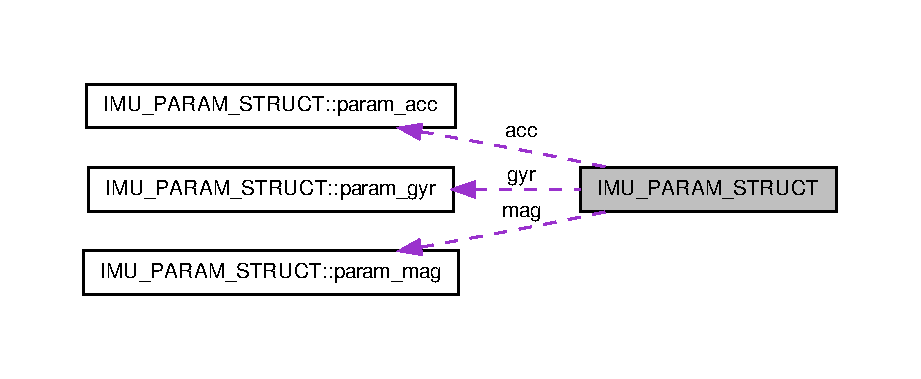
\includegraphics[width=350pt]{structIMU__PARAM__STRUCT__coll__graph}
\end{center}
\end{figure}
\subsection*{Data Structures}
\begin{DoxyCompactItemize}
\item 
struct \hyperlink{structIMU__PARAM__STRUCT_1_1param__acc}{param\-\_\-acc}
\begin{DoxyCompactList}\small\item\em Accelerometer Parameters. \end{DoxyCompactList}\item 
struct \hyperlink{structIMU__PARAM__STRUCT_1_1param__gyr}{param\-\_\-gyr}
\begin{DoxyCompactList}\small\item\em Gyrometer Parameters. \end{DoxyCompactList}\item 
struct \hyperlink{structIMU__PARAM__STRUCT_1_1param__mag}{param\-\_\-mag}
\begin{DoxyCompactList}\small\item\em Magnetometer Parameters. \end{DoxyCompactList}\end{DoxyCompactItemize}
\subsection*{Data Fields}
\begin{DoxyCompactItemize}
\item 
struct \hyperlink{structIMU__PARAM__STRUCT_1_1param__acc}{I\-M\-U\-\_\-\-P\-A\-R\-A\-M\-\_\-\-S\-T\-R\-U\-C\-T\-::param\-\_\-acc} \hyperlink{structIMU__PARAM__STRUCT_a92172e4757d0f8f9135a659e406c12e5}{acc}
\item 
struct \hyperlink{structIMU__PARAM__STRUCT_1_1param__gyr}{I\-M\-U\-\_\-\-P\-A\-R\-A\-M\-\_\-\-S\-T\-R\-U\-C\-T\-::param\-\_\-gyr} \hyperlink{structIMU__PARAM__STRUCT_a5a4557868f1af679a1098808397b02ec}{gyr}
\item 
struct \hyperlink{structIMU__PARAM__STRUCT_1_1param__mag}{I\-M\-U\-\_\-\-P\-A\-R\-A\-M\-\_\-\-S\-T\-R\-U\-C\-T\-::param\-\_\-mag} \hyperlink{structIMU__PARAM__STRUCT_a26b277dcaf05f3842995df888225f6f4}{mag}
\item 
int \hyperlink{structIMU__PARAM__STRUCT_a8a870f383fc9ba0b682fdc9b8c0d2734}{i2c\-\_\-dev}
\end{DoxyCompactItemize}


\subsection{Detailed Description}
Configs of I\-M\-U. 

Definition at line 31 of file communication.\-h.



\subsection{Field Documentation}
\hypertarget{structIMU__PARAM__STRUCT_a92172e4757d0f8f9135a659e406c12e5}{\index{I\-M\-U\-\_\-\-P\-A\-R\-A\-M\-\_\-\-S\-T\-R\-U\-C\-T@{I\-M\-U\-\_\-\-P\-A\-R\-A\-M\-\_\-\-S\-T\-R\-U\-C\-T}!acc@{acc}}
\index{acc@{acc}!IMU_PARAM_STRUCT@{I\-M\-U\-\_\-\-P\-A\-R\-A\-M\-\_\-\-S\-T\-R\-U\-C\-T}}
\subsubsection[{acc}]{\setlength{\rightskip}{0pt plus 5cm}struct {\bf I\-M\-U\-\_\-\-P\-A\-R\-A\-M\-\_\-\-S\-T\-R\-U\-C\-T\-::param\-\_\-acc} I\-M\-U\-\_\-\-P\-A\-R\-A\-M\-\_\-\-S\-T\-R\-U\-C\-T\-::acc}}\label{structIMU__PARAM__STRUCT_a92172e4757d0f8f9135a659e406c12e5}


Referenced by devices\-\_\-init(), and main().

\hypertarget{structIMU__PARAM__STRUCT_a5a4557868f1af679a1098808397b02ec}{\index{I\-M\-U\-\_\-\-P\-A\-R\-A\-M\-\_\-\-S\-T\-R\-U\-C\-T@{I\-M\-U\-\_\-\-P\-A\-R\-A\-M\-\_\-\-S\-T\-R\-U\-C\-T}!gyr@{gyr}}
\index{gyr@{gyr}!IMU_PARAM_STRUCT@{I\-M\-U\-\_\-\-P\-A\-R\-A\-M\-\_\-\-S\-T\-R\-U\-C\-T}}
\subsubsection[{gyr}]{\setlength{\rightskip}{0pt plus 5cm}struct {\bf I\-M\-U\-\_\-\-P\-A\-R\-A\-M\-\_\-\-S\-T\-R\-U\-C\-T\-::param\-\_\-gyr} I\-M\-U\-\_\-\-P\-A\-R\-A\-M\-\_\-\-S\-T\-R\-U\-C\-T\-::gyr}}\label{structIMU__PARAM__STRUCT_a5a4557868f1af679a1098808397b02ec}


Referenced by devices\-\_\-init(), and main().

\hypertarget{structIMU__PARAM__STRUCT_a8a870f383fc9ba0b682fdc9b8c0d2734}{\index{I\-M\-U\-\_\-\-P\-A\-R\-A\-M\-\_\-\-S\-T\-R\-U\-C\-T@{I\-M\-U\-\_\-\-P\-A\-R\-A\-M\-\_\-\-S\-T\-R\-U\-C\-T}!i2c\-\_\-dev@{i2c\-\_\-dev}}
\index{i2c\-\_\-dev@{i2c\-\_\-dev}!IMU_PARAM_STRUCT@{I\-M\-U\-\_\-\-P\-A\-R\-A\-M\-\_\-\-S\-T\-R\-U\-C\-T}}
\subsubsection[{i2c\-\_\-dev}]{\setlength{\rightskip}{0pt plus 5cm}int I\-M\-U\-\_\-\-P\-A\-R\-A\-M\-\_\-\-S\-T\-R\-U\-C\-T\-::i2c\-\_\-dev}}\label{structIMU__PARAM__STRUCT_a8a870f383fc9ba0b682fdc9b8c0d2734}


Definition at line 59 of file communication.\-h.



Referenced by devices\-\_\-init(), main(), periodic\-\_\-task\-\_\-1(), and periodic\-\_\-task\-\_\-2().

\hypertarget{structIMU__PARAM__STRUCT_a26b277dcaf05f3842995df888225f6f4}{\index{I\-M\-U\-\_\-\-P\-A\-R\-A\-M\-\_\-\-S\-T\-R\-U\-C\-T@{I\-M\-U\-\_\-\-P\-A\-R\-A\-M\-\_\-\-S\-T\-R\-U\-C\-T}!mag@{mag}}
\index{mag@{mag}!IMU_PARAM_STRUCT@{I\-M\-U\-\_\-\-P\-A\-R\-A\-M\-\_\-\-S\-T\-R\-U\-C\-T}}
\subsubsection[{mag}]{\setlength{\rightskip}{0pt plus 5cm}struct {\bf I\-M\-U\-\_\-\-P\-A\-R\-A\-M\-\_\-\-S\-T\-R\-U\-C\-T\-::param\-\_\-mag} I\-M\-U\-\_\-\-P\-A\-R\-A\-M\-\_\-\-S\-T\-R\-U\-C\-T\-::mag}}\label{structIMU__PARAM__STRUCT_a26b277dcaf05f3842995df888225f6f4}


Referenced by main().



The documentation for this struct was generated from the following file\-:\begin{DoxyCompactItemize}
\item 
communication/\hyperlink{communication_2communication_8h}{communication.\-h}\end{DoxyCompactItemize}

\hypertarget{structLink}{\section{Link Struct Reference}
\label{structLink}\index{Link@{Link}}
}


{\ttfamily \#include \char`\"{}link.\-h\char`\"{}}



Collaboration diagram for Link\-:\nopagebreak
\begin{figure}[H]
\begin{center}
\leavevmode
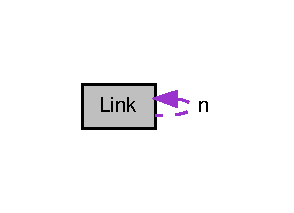
\includegraphics[width=141pt]{structLink__coll__graph}
\end{center}
\end{figure}
\subsection*{Data Fields}
\begin{DoxyCompactItemize}
\item 
double \hyperlink{structLink_a88e705bc7fb6c7c8c7fa6987b52667d6}{theta}
\item 
double \hyperlink{structLink_a4e5e4ea2ef9be2aae1e9fdef406be185}{d}
\item 
double \hyperlink{structLink_a3ef89c4478d7e2de8a59de9c88052123}{a}
\item 
double \hyperlink{structLink_ab838e5bc121c212cb1a81fdf78de8757}{alpha}
\item 
double \hyperlink{structLink_a9ba28f0b8b867ad4624abb9730ef30d2}{jvel}
\item 
struct \hyperlink{structLink}{Link} $\ast$ \hyperlink{structLink_a185503cf680f8e9395c19c0521997c5c}{n}
\end{DoxyCompactItemize}


\subsection{Detailed Description}


Definition at line 10 of file link.\-h.



\subsection{Field Documentation}
\hypertarget{structLink_a3ef89c4478d7e2de8a59de9c88052123}{\index{Link@{Link}!a@{a}}
\index{a@{a}!Link@{Link}}
\subsubsection[{a}]{\setlength{\rightskip}{0pt plus 5cm}double Link\-::a}}\label{structLink_a3ef89c4478d7e2de8a59de9c88052123}


Definition at line 13 of file link.\-h.



Referenced by Link\-\_\-create(), and Link\-\_\-\-D\-Q\-F\-T().

\hypertarget{structLink_ab838e5bc121c212cb1a81fdf78de8757}{\index{Link@{Link}!alpha@{alpha}}
\index{alpha@{alpha}!Link@{Link}}
\subsubsection[{alpha}]{\setlength{\rightskip}{0pt plus 5cm}double Link\-::alpha}}\label{structLink_ab838e5bc121c212cb1a81fdf78de8757}


Definition at line 14 of file link.\-h.



Referenced by Link\-\_\-create(), and Link\-\_\-\-D\-Q\-F\-T().

\hypertarget{structLink_a4e5e4ea2ef9be2aae1e9fdef406be185}{\index{Link@{Link}!d@{d}}
\index{d@{d}!Link@{Link}}
\subsubsection[{d}]{\setlength{\rightskip}{0pt plus 5cm}double Link\-::d}}\label{structLink_a4e5e4ea2ef9be2aae1e9fdef406be185}


Definition at line 12 of file link.\-h.



Referenced by Link\-\_\-create(), and Link\-\_\-\-D\-Q\-F\-T().

\hypertarget{structLink_a9ba28f0b8b867ad4624abb9730ef30d2}{\index{Link@{Link}!jvel@{jvel}}
\index{jvel@{jvel}!Link@{Link}}
\subsubsection[{jvel}]{\setlength{\rightskip}{0pt plus 5cm}double Link\-::jvel}}\label{structLink_a9ba28f0b8b867ad4624abb9730ef30d2}


Definition at line 15 of file link.\-h.



Referenced by Link\-\_\-create().

\hypertarget{structLink_a185503cf680f8e9395c19c0521997c5c}{\index{Link@{Link}!n@{n}}
\index{n@{n}!Link@{Link}}
\subsubsection[{n}]{\setlength{\rightskip}{0pt plus 5cm}struct {\bf Link}$\ast$ Link\-::n}}\label{structLink_a185503cf680f8e9395c19c0521997c5c}


Definition at line 17 of file link.\-h.



Referenced by Link\-\_\-create(), Robot\-\_\-add\-Link(), Robot\-\_\-\-F\-K\-M(), Robot\-\_\-get\-Link(), Robot\-\_\-update\-Links\-Thetas\-By\-Array(), and Robot\-\_\-update\-Links\-Thetas\-By\-Matrix().

\hypertarget{structLink_a88e705bc7fb6c7c8c7fa6987b52667d6}{\index{Link@{Link}!theta@{theta}}
\index{theta@{theta}!Link@{Link}}
\subsubsection[{theta}]{\setlength{\rightskip}{0pt plus 5cm}double Link\-::theta}}\label{structLink_a88e705bc7fb6c7c8c7fa6987b52667d6}


Definition at line 11 of file link.\-h.



Referenced by Link\-\_\-create(), Link\-\_\-\-D\-Q\-F\-T(), Robot\-\_\-update\-Links\-Thetas\-By\-Array(), and Robot\-\_\-update\-Links\-Thetas\-By\-Matrix().



The documentation for this struct was generated from the following file\-:\begin{DoxyCompactItemize}
\item 
schunk\-\_\-high/include/schunk\-\_\-high/\hyperlink{link_8h}{link.\-h}\end{DoxyCompactItemize}

\hypertarget{structMATLAB__DATAHEAD}{\section{M\-A\-T\-L\-A\-B\-\_\-\-D\-A\-T\-A\-H\-E\-A\-D Struct Reference}
\label{structMATLAB__DATAHEAD}\index{M\-A\-T\-L\-A\-B\-\_\-\-D\-A\-T\-A\-H\-E\-A\-D@{M\-A\-T\-L\-A\-B\-\_\-\-D\-A\-T\-A\-H\-E\-A\-D}}
}
\subsection*{Data Fields}
\begin{DoxyCompactItemize}
\item 
long \hyperlink{structMATLAB__DATAHEAD_ad3587e58da5ca6cbe3cd98d5e2f46202}{type}
\item 
long \hyperlink{structMATLAB__DATAHEAD_abf1ef02c93522915bd7fdf9f72df44b7}{mrows}
\item 
long \hyperlink{structMATLAB__DATAHEAD_ae87d8eca5290fa03d01c79061498626f}{ncols}
\item 
long \hyperlink{structMATLAB__DATAHEAD_a7831e4f01682863fce4ba98071a7db08}{imagf}
\item 
long \hyperlink{structMATLAB__DATAHEAD_ad6e65844dcff1eb1cf7bf8752ba9a91c}{namlen}
\end{DoxyCompactItemize}


\subsection{Detailed Description}


Definition at line 13 of file gmatlabdatafile.\-c.



\subsection{Field Documentation}
\hypertarget{structMATLAB__DATAHEAD_a7831e4f01682863fce4ba98071a7db08}{\index{M\-A\-T\-L\-A\-B\-\_\-\-D\-A\-T\-A\-H\-E\-A\-D@{M\-A\-T\-L\-A\-B\-\_\-\-D\-A\-T\-A\-H\-E\-A\-D}!imagf@{imagf}}
\index{imagf@{imagf}!MATLAB_DATAHEAD@{M\-A\-T\-L\-A\-B\-\_\-\-D\-A\-T\-A\-H\-E\-A\-D}}
\subsubsection[{imagf}]{\setlength{\rightskip}{0pt plus 5cm}long M\-A\-T\-L\-A\-B\-\_\-\-D\-A\-T\-A\-H\-E\-A\-D\-::imagf}}\label{structMATLAB__DATAHEAD_a7831e4f01682863fce4ba98071a7db08}


Definition at line 17 of file gmatlabdatafile.\-c.



Referenced by g\-M\-A\-T\-L\-A\-B\-Data\-File\-\_\-\-Save\-Matrix(), and g\-M\-A\-T\-L\-A\-B\-Data\-File\-\_\-\-Save\-Vector().

\hypertarget{structMATLAB__DATAHEAD_abf1ef02c93522915bd7fdf9f72df44b7}{\index{M\-A\-T\-L\-A\-B\-\_\-\-D\-A\-T\-A\-H\-E\-A\-D@{M\-A\-T\-L\-A\-B\-\_\-\-D\-A\-T\-A\-H\-E\-A\-D}!mrows@{mrows}}
\index{mrows@{mrows}!MATLAB_DATAHEAD@{M\-A\-T\-L\-A\-B\-\_\-\-D\-A\-T\-A\-H\-E\-A\-D}}
\subsubsection[{mrows}]{\setlength{\rightskip}{0pt plus 5cm}long M\-A\-T\-L\-A\-B\-\_\-\-D\-A\-T\-A\-H\-E\-A\-D\-::mrows}}\label{structMATLAB__DATAHEAD_abf1ef02c93522915bd7fdf9f72df44b7}


Definition at line 15 of file gmatlabdatafile.\-c.



Referenced by g\-M\-A\-T\-L\-A\-B\-Data\-File\-\_\-\-Save\-Matrix(), and g\-M\-A\-T\-L\-A\-B\-Data\-File\-\_\-\-Save\-Vector().

\hypertarget{structMATLAB__DATAHEAD_ad6e65844dcff1eb1cf7bf8752ba9a91c}{\index{M\-A\-T\-L\-A\-B\-\_\-\-D\-A\-T\-A\-H\-E\-A\-D@{M\-A\-T\-L\-A\-B\-\_\-\-D\-A\-T\-A\-H\-E\-A\-D}!namlen@{namlen}}
\index{namlen@{namlen}!MATLAB_DATAHEAD@{M\-A\-T\-L\-A\-B\-\_\-\-D\-A\-T\-A\-H\-E\-A\-D}}
\subsubsection[{namlen}]{\setlength{\rightskip}{0pt plus 5cm}long M\-A\-T\-L\-A\-B\-\_\-\-D\-A\-T\-A\-H\-E\-A\-D\-::namlen}}\label{structMATLAB__DATAHEAD_ad6e65844dcff1eb1cf7bf8752ba9a91c}


Definition at line 18 of file gmatlabdatafile.\-c.



Referenced by g\-M\-A\-T\-L\-A\-B\-Data\-File\-\_\-\-Save\-Matrix(), and g\-M\-A\-T\-L\-A\-B\-Data\-File\-\_\-\-Save\-Vector().

\hypertarget{structMATLAB__DATAHEAD_ae87d8eca5290fa03d01c79061498626f}{\index{M\-A\-T\-L\-A\-B\-\_\-\-D\-A\-T\-A\-H\-E\-A\-D@{M\-A\-T\-L\-A\-B\-\_\-\-D\-A\-T\-A\-H\-E\-A\-D}!ncols@{ncols}}
\index{ncols@{ncols}!MATLAB_DATAHEAD@{M\-A\-T\-L\-A\-B\-\_\-\-D\-A\-T\-A\-H\-E\-A\-D}}
\subsubsection[{ncols}]{\setlength{\rightskip}{0pt plus 5cm}long M\-A\-T\-L\-A\-B\-\_\-\-D\-A\-T\-A\-H\-E\-A\-D\-::ncols}}\label{structMATLAB__DATAHEAD_ae87d8eca5290fa03d01c79061498626f}


Definition at line 16 of file gmatlabdatafile.\-c.



Referenced by g\-M\-A\-T\-L\-A\-B\-Data\-File\-\_\-\-Save\-Matrix(), and g\-M\-A\-T\-L\-A\-B\-Data\-File\-\_\-\-Save\-Vector().

\hypertarget{structMATLAB__DATAHEAD_ad3587e58da5ca6cbe3cd98d5e2f46202}{\index{M\-A\-T\-L\-A\-B\-\_\-\-D\-A\-T\-A\-H\-E\-A\-D@{M\-A\-T\-L\-A\-B\-\_\-\-D\-A\-T\-A\-H\-E\-A\-D}!type@{type}}
\index{type@{type}!MATLAB_DATAHEAD@{M\-A\-T\-L\-A\-B\-\_\-\-D\-A\-T\-A\-H\-E\-A\-D}}
\subsubsection[{type}]{\setlength{\rightskip}{0pt plus 5cm}long M\-A\-T\-L\-A\-B\-\_\-\-D\-A\-T\-A\-H\-E\-A\-D\-::type}}\label{structMATLAB__DATAHEAD_ad3587e58da5ca6cbe3cd98d5e2f46202}


Definition at line 14 of file gmatlabdatafile.\-c.



Referenced by g\-M\-A\-T\-L\-A\-B\-Data\-File\-\_\-\-Save\-Matrix(), and g\-M\-A\-T\-L\-A\-B\-Data\-File\-\_\-\-Save\-Vector().



The documentation for this struct was generated from the following file\-:\begin{DoxyCompactItemize}
\item 
gdatalogger/\hyperlink{gmatlabdatafile_8c}{gmatlabdatafile.\-c}\end{DoxyCompactItemize}

\hypertarget{classMatrix}{\section{Matrix Class Reference}
\label{classMatrix}\index{Matrix@{Matrix}}
}


Collaboration diagram for Matrix\-:\nopagebreak
\begin{figure}[H]
\begin{center}
\leavevmode
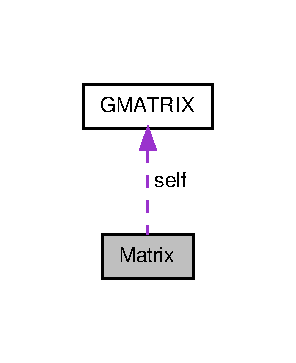
\includegraphics[width=142pt]{classMatrix__coll__graph}
\end{center}
\end{figure}
\subsection*{Private Attributes}
\begin{DoxyCompactItemize}
\item 
\hyperlink{gmatrix_8h_ad8edc274a17feb9e4fca93e620253bed}{P\-G\-M\-A\-T\-R\-I\-X} $\ast$ \hyperlink{classMatrix_a3cd31e02b5127a4a926add88d0d9ec63}{self}
\end{DoxyCompactItemize}


\subsection{Detailed Description}


Definition at line 5 of file matrix\-\_\-interface.\-cpp.



\subsection{Field Documentation}
\hypertarget{classMatrix_a3cd31e02b5127a4a926add88d0d9ec63}{\index{Matrix@{Matrix}!self@{self}}
\index{self@{self}!Matrix@{Matrix}}
\subsubsection[{self}]{\setlength{\rightskip}{0pt plus 5cm}{\bf P\-G\-M\-A\-T\-R\-I\-X}$\ast$ Matrix\-::self\hspace{0.3cm}{\ttfamily [private]}}}\label{classMatrix_a3cd31e02b5127a4a926add88d0d9ec63}


Definition at line 7 of file matrix\-\_\-interface.\-cpp.



The documentation for this class was generated from the following file\-:\begin{DoxyCompactItemize}
\item 
schunk\-\_\-high/src/matrix/\hyperlink{matrix__interface_8cpp}{matrix\-\_\-interface.\-cpp}\end{DoxyCompactItemize}

\hypertarget{structMRA__DATA__STRUCT}{\section{M\-R\-A\-\_\-\-D\-A\-T\-A\-\_\-\-S\-T\-R\-U\-C\-T Struct Reference}
\label{structMRA__DATA__STRUCT}\index{M\-R\-A\-\_\-\-D\-A\-T\-A\-\_\-\-S\-T\-R\-U\-C\-T@{M\-R\-A\-\_\-\-D\-A\-T\-A\-\_\-\-S\-T\-R\-U\-C\-T}}
}


Struct to control M\-R\-A.  




{\ttfamily \#include \char`\"{}communication.\-h\char`\"{}}

\subsection*{Data Fields}
\begin{DoxyCompactItemize}
\item 
short int \hyperlink{structMRA__DATA__STRUCT_a64b4e6bb604e58de593a60c87942b966}{v\-\_\-ctl}
\begin{DoxyCompactList}\small\item\em Voltage level for control output. \end{DoxyCompactList}\item 
short int \hyperlink{structMRA__DATA__STRUCT_a3a31d57268c33b21ac915fdc27dfe474}{v\-\_\-ctl\-\_\-read}
\begin{DoxyCompactList}\small\item\em Voltage level read from the actuator. \end{DoxyCompactList}\item 
int \hyperlink{structMRA__DATA__STRUCT_afca6e851d302f3a786885a4e1eec79d7}{new\-\_\-data}
\begin{DoxyCompactList}\small\item\em ?? \end{DoxyCompactList}\item 
int \hyperlink{structMRA__DATA__STRUCT_a5b1af89ee717f5b14c18e8ac12e93e75}{new\-\_\-ctl}
\begin{DoxyCompactList}\small\item\em ?? \end{DoxyCompactList}\end{DoxyCompactItemize}


\subsection{Detailed Description}
Struct to control M\-R\-A. 

Definition at line 126 of file communication.\-h.



\subsection{Field Documentation}
\hypertarget{structMRA__DATA__STRUCT_a5b1af89ee717f5b14c18e8ac12e93e75}{\index{M\-R\-A\-\_\-\-D\-A\-T\-A\-\_\-\-S\-T\-R\-U\-C\-T@{M\-R\-A\-\_\-\-D\-A\-T\-A\-\_\-\-S\-T\-R\-U\-C\-T}!new\-\_\-ctl@{new\-\_\-ctl}}
\index{new\-\_\-ctl@{new\-\_\-ctl}!MRA_DATA_STRUCT@{M\-R\-A\-\_\-\-D\-A\-T\-A\-\_\-\-S\-T\-R\-U\-C\-T}}
\subsubsection[{new\-\_\-ctl}]{\setlength{\rightskip}{0pt plus 5cm}int M\-R\-A\-\_\-\-D\-A\-T\-A\-\_\-\-S\-T\-R\-U\-C\-T\-::new\-\_\-ctl}}\label{structMRA__DATA__STRUCT_a5b1af89ee717f5b14c18e8ac12e93e75}


?? 



Definition at line 130 of file communication.\-h.



Referenced by actuate(), and devices\-\_\-init().

\hypertarget{structMRA__DATA__STRUCT_afca6e851d302f3a786885a4e1eec79d7}{\index{M\-R\-A\-\_\-\-D\-A\-T\-A\-\_\-\-S\-T\-R\-U\-C\-T@{M\-R\-A\-\_\-\-D\-A\-T\-A\-\_\-\-S\-T\-R\-U\-C\-T}!new\-\_\-data@{new\-\_\-data}}
\index{new\-\_\-data@{new\-\_\-data}!MRA_DATA_STRUCT@{M\-R\-A\-\_\-\-D\-A\-T\-A\-\_\-\-S\-T\-R\-U\-C\-T}}
\subsubsection[{new\-\_\-data}]{\setlength{\rightskip}{0pt plus 5cm}int M\-R\-A\-\_\-\-D\-A\-T\-A\-\_\-\-S\-T\-R\-U\-C\-T\-::new\-\_\-data}}\label{structMRA__DATA__STRUCT_afca6e851d302f3a786885a4e1eec79d7}


?? 



Definition at line 129 of file communication.\-h.



Referenced by read\-\_\-all\-\_\-data().

\hypertarget{structMRA__DATA__STRUCT_a64b4e6bb604e58de593a60c87942b966}{\index{M\-R\-A\-\_\-\-D\-A\-T\-A\-\_\-\-S\-T\-R\-U\-C\-T@{M\-R\-A\-\_\-\-D\-A\-T\-A\-\_\-\-S\-T\-R\-U\-C\-T}!v\-\_\-ctl@{v\-\_\-ctl}}
\index{v\-\_\-ctl@{v\-\_\-ctl}!MRA_DATA_STRUCT@{M\-R\-A\-\_\-\-D\-A\-T\-A\-\_\-\-S\-T\-R\-U\-C\-T}}
\subsubsection[{v\-\_\-ctl}]{\setlength{\rightskip}{0pt plus 5cm}short int M\-R\-A\-\_\-\-D\-A\-T\-A\-\_\-\-S\-T\-R\-U\-C\-T\-::v\-\_\-ctl}}\label{structMRA__DATA__STRUCT_a64b4e6bb604e58de593a60c87942b966}


Voltage level for control output. 



Definition at line 127 of file communication.\-h.



Referenced by actuate(), control\-\_\-main(), datalogger\-\_\-update(), devices\-\_\-init(), periodic\-\_\-task\-\_\-1(), ui\-\_\-mra\-\_\-data(), and ui\-\_\-overview\-\_\-data().

\hypertarget{structMRA__DATA__STRUCT_a3a31d57268c33b21ac915fdc27dfe474}{\index{M\-R\-A\-\_\-\-D\-A\-T\-A\-\_\-\-S\-T\-R\-U\-C\-T@{M\-R\-A\-\_\-\-D\-A\-T\-A\-\_\-\-S\-T\-R\-U\-C\-T}!v\-\_\-ctl\-\_\-read@{v\-\_\-ctl\-\_\-read}}
\index{v\-\_\-ctl\-\_\-read@{v\-\_\-ctl\-\_\-read}!MRA_DATA_STRUCT@{M\-R\-A\-\_\-\-D\-A\-T\-A\-\_\-\-S\-T\-R\-U\-C\-T}}
\subsubsection[{v\-\_\-ctl\-\_\-read}]{\setlength{\rightskip}{0pt plus 5cm}short int M\-R\-A\-\_\-\-D\-A\-T\-A\-\_\-\-S\-T\-R\-U\-C\-T\-::v\-\_\-ctl\-\_\-read}}\label{structMRA__DATA__STRUCT_a3a31d57268c33b21ac915fdc27dfe474}


Voltage level read from the actuator. 



Definition at line 128 of file communication.\-h.



Referenced by datalogger\-\_\-update(), read\-\_\-all\-\_\-data(), ui\-\_\-mra\-\_\-data(), and ui\-\_\-overview\-\_\-data().



The documentation for this struct was generated from the following file\-:\begin{DoxyCompactItemize}
\item 
communication/\hyperlink{communication_2communication_8h}{communication.\-h}\end{DoxyCompactItemize}

\hypertarget{structIMU__PARAM__STRUCT_1_1param__acc}{\section{I\-M\-U\-\_\-\-P\-A\-R\-A\-M\-\_\-\-S\-T\-R\-U\-C\-T\-:\-:param\-\_\-acc Struct Reference}
\label{structIMU__PARAM__STRUCT_1_1param__acc}\index{I\-M\-U\-\_\-\-P\-A\-R\-A\-M\-\_\-\-S\-T\-R\-U\-C\-T\-::param\-\_\-acc@{I\-M\-U\-\_\-\-P\-A\-R\-A\-M\-\_\-\-S\-T\-R\-U\-C\-T\-::param\-\_\-acc}}
}


Accelerometer Parameters.  




{\ttfamily \#include \char`\"{}communication.\-h\char`\"{}}

\subsection*{Data Fields}
\begin{DoxyCompactItemize}
\item 
uint8\-\_\-t \hyperlink{structIMU__PARAM__STRUCT_1_1param__acc_af57da5d956ffa7e49a184326b6b9c738}{full\-\_\-res}
\item 
uint16\-\_\-t \hyperlink{structIMU__PARAM__STRUCT_1_1param__acc_a30e6a318cad098cd8379416705820f95}{rate}
\item 
uint8\-\_\-t \hyperlink{structIMU__PARAM__STRUCT_1_1param__acc_a26199b298ef2d353192dfbc706bce8cf}{range}
\end{DoxyCompactItemize}


\subsection{Detailed Description}
Accelerometer Parameters. 

Definition at line 35 of file communication.\-h.



\subsection{Field Documentation}
\hypertarget{structIMU__PARAM__STRUCT_1_1param__acc_af57da5d956ffa7e49a184326b6b9c738}{\index{I\-M\-U\-\_\-\-P\-A\-R\-A\-M\-\_\-\-S\-T\-R\-U\-C\-T\-::param\-\_\-acc@{I\-M\-U\-\_\-\-P\-A\-R\-A\-M\-\_\-\-S\-T\-R\-U\-C\-T\-::param\-\_\-acc}!full\-\_\-res@{full\-\_\-res}}
\index{full\-\_\-res@{full\-\_\-res}!IMU_PARAM_STRUCT::param_acc@{I\-M\-U\-\_\-\-P\-A\-R\-A\-M\-\_\-\-S\-T\-R\-U\-C\-T\-::param\-\_\-acc}}
\subsubsection[{full\-\_\-res}]{\setlength{\rightskip}{0pt plus 5cm}uint8\-\_\-t I\-M\-U\-\_\-\-P\-A\-R\-A\-M\-\_\-\-S\-T\-R\-U\-C\-T\-::param\-\_\-acc\-::full\-\_\-res}}\label{structIMU__PARAM__STRUCT_1_1param__acc_af57da5d956ffa7e49a184326b6b9c738}


Definition at line 36 of file communication.\-h.



Referenced by devices\-\_\-init(), and main().

\hypertarget{structIMU__PARAM__STRUCT_1_1param__acc_a26199b298ef2d353192dfbc706bce8cf}{\index{I\-M\-U\-\_\-\-P\-A\-R\-A\-M\-\_\-\-S\-T\-R\-U\-C\-T\-::param\-\_\-acc@{I\-M\-U\-\_\-\-P\-A\-R\-A\-M\-\_\-\-S\-T\-R\-U\-C\-T\-::param\-\_\-acc}!range@{range}}
\index{range@{range}!IMU_PARAM_STRUCT::param_acc@{I\-M\-U\-\_\-\-P\-A\-R\-A\-M\-\_\-\-S\-T\-R\-U\-C\-T\-::param\-\_\-acc}}
\subsubsection[{range}]{\setlength{\rightskip}{0pt plus 5cm}uint8\-\_\-t I\-M\-U\-\_\-\-P\-A\-R\-A\-M\-\_\-\-S\-T\-R\-U\-C\-T\-::param\-\_\-acc\-::range}}\label{structIMU__PARAM__STRUCT_1_1param__acc_a26199b298ef2d353192dfbc706bce8cf}


Definition at line 38 of file communication.\-h.



Referenced by devices\-\_\-init(), and main().

\hypertarget{structIMU__PARAM__STRUCT_1_1param__acc_a30e6a318cad098cd8379416705820f95}{\index{I\-M\-U\-\_\-\-P\-A\-R\-A\-M\-\_\-\-S\-T\-R\-U\-C\-T\-::param\-\_\-acc@{I\-M\-U\-\_\-\-P\-A\-R\-A\-M\-\_\-\-S\-T\-R\-U\-C\-T\-::param\-\_\-acc}!rate@{rate}}
\index{rate@{rate}!IMU_PARAM_STRUCT::param_acc@{I\-M\-U\-\_\-\-P\-A\-R\-A\-M\-\_\-\-S\-T\-R\-U\-C\-T\-::param\-\_\-acc}}
\subsubsection[{rate}]{\setlength{\rightskip}{0pt plus 5cm}uint16\-\_\-t I\-M\-U\-\_\-\-P\-A\-R\-A\-M\-\_\-\-S\-T\-R\-U\-C\-T\-::param\-\_\-acc\-::rate}}\label{structIMU__PARAM__STRUCT_1_1param__acc_a30e6a318cad098cd8379416705820f95}


Definition at line 37 of file communication.\-h.



Referenced by devices\-\_\-init(), and main().



The documentation for this struct was generated from the following file\-:\begin{DoxyCompactItemize}
\item 
communication/\hyperlink{communication_2communication_8h}{communication.\-h}\end{DoxyCompactItemize}

\hypertarget{structIMU__PARAM__STRUCT_1_1param__gyr}{\section{I\-M\-U\-\_\-\-P\-A\-R\-A\-M\-\_\-\-S\-T\-R\-U\-C\-T\-:\-:param\-\_\-gyr Struct Reference}
\label{structIMU__PARAM__STRUCT_1_1param__gyr}\index{I\-M\-U\-\_\-\-P\-A\-R\-A\-M\-\_\-\-S\-T\-R\-U\-C\-T\-::param\-\_\-gyr@{I\-M\-U\-\_\-\-P\-A\-R\-A\-M\-\_\-\-S\-T\-R\-U\-C\-T\-::param\-\_\-gyr}}
}


Gyrometer Parameters.  




{\ttfamily \#include \char`\"{}communication.\-h\char`\"{}}

\subsection*{Data Fields}
\begin{DoxyCompactItemize}
\item 
float \hyperlink{structIMU__PARAM__STRUCT_1_1param__gyr_a5aa70e1e9634411c89aacfbc570cc91c}{rate}
\item 
short int \hyperlink{structIMU__PARAM__STRUCT_1_1param__gyr_aa612f7299b43a1bf1fc597688c2fa02d}{lpf\-\_\-bw}
\item 
char \hyperlink{structIMU__PARAM__STRUCT_1_1param__gyr_aca3b791cb480f2da4703d4c256a7de48}{clk\-\_\-source}
\item 
char $\ast$ \hyperlink{structIMU__PARAM__STRUCT_1_1param__gyr_a909d153e794ec443be04625ce00e4178}{act}
\end{DoxyCompactItemize}


\subsection{Detailed Description}
Gyrometer Parameters. 

Definition at line 43 of file communication.\-h.



\subsection{Field Documentation}
\hypertarget{structIMU__PARAM__STRUCT_1_1param__gyr_a909d153e794ec443be04625ce00e4178}{\index{I\-M\-U\-\_\-\-P\-A\-R\-A\-M\-\_\-\-S\-T\-R\-U\-C\-T\-::param\-\_\-gyr@{I\-M\-U\-\_\-\-P\-A\-R\-A\-M\-\_\-\-S\-T\-R\-U\-C\-T\-::param\-\_\-gyr}!act@{act}}
\index{act@{act}!IMU_PARAM_STRUCT::param_gyr@{I\-M\-U\-\_\-\-P\-A\-R\-A\-M\-\_\-\-S\-T\-R\-U\-C\-T\-::param\-\_\-gyr}}
\subsubsection[{act}]{\setlength{\rightskip}{0pt plus 5cm}char$\ast$ I\-M\-U\-\_\-\-P\-A\-R\-A\-M\-\_\-\-S\-T\-R\-U\-C\-T\-::param\-\_\-gyr\-::act}}\label{structIMU__PARAM__STRUCT_1_1param__gyr_a909d153e794ec443be04625ce00e4178}


Definition at line 47 of file communication.\-h.



Referenced by devices\-\_\-init(), and main().

\hypertarget{structIMU__PARAM__STRUCT_1_1param__gyr_aca3b791cb480f2da4703d4c256a7de48}{\index{I\-M\-U\-\_\-\-P\-A\-R\-A\-M\-\_\-\-S\-T\-R\-U\-C\-T\-::param\-\_\-gyr@{I\-M\-U\-\_\-\-P\-A\-R\-A\-M\-\_\-\-S\-T\-R\-U\-C\-T\-::param\-\_\-gyr}!clk\-\_\-source@{clk\-\_\-source}}
\index{clk\-\_\-source@{clk\-\_\-source}!IMU_PARAM_STRUCT::param_gyr@{I\-M\-U\-\_\-\-P\-A\-R\-A\-M\-\_\-\-S\-T\-R\-U\-C\-T\-::param\-\_\-gyr}}
\subsubsection[{clk\-\_\-source}]{\setlength{\rightskip}{0pt plus 5cm}char I\-M\-U\-\_\-\-P\-A\-R\-A\-M\-\_\-\-S\-T\-R\-U\-C\-T\-::param\-\_\-gyr\-::clk\-\_\-source}}\label{structIMU__PARAM__STRUCT_1_1param__gyr_aca3b791cb480f2da4703d4c256a7de48}


Definition at line 46 of file communication.\-h.



Referenced by devices\-\_\-init(), and main().

\hypertarget{structIMU__PARAM__STRUCT_1_1param__gyr_aa612f7299b43a1bf1fc597688c2fa02d}{\index{I\-M\-U\-\_\-\-P\-A\-R\-A\-M\-\_\-\-S\-T\-R\-U\-C\-T\-::param\-\_\-gyr@{I\-M\-U\-\_\-\-P\-A\-R\-A\-M\-\_\-\-S\-T\-R\-U\-C\-T\-::param\-\_\-gyr}!lpf\-\_\-bw@{lpf\-\_\-bw}}
\index{lpf\-\_\-bw@{lpf\-\_\-bw}!IMU_PARAM_STRUCT::param_gyr@{I\-M\-U\-\_\-\-P\-A\-R\-A\-M\-\_\-\-S\-T\-R\-U\-C\-T\-::param\-\_\-gyr}}
\subsubsection[{lpf\-\_\-bw}]{\setlength{\rightskip}{0pt plus 5cm}short int I\-M\-U\-\_\-\-P\-A\-R\-A\-M\-\_\-\-S\-T\-R\-U\-C\-T\-::param\-\_\-gyr\-::lpf\-\_\-bw}}\label{structIMU__PARAM__STRUCT_1_1param__gyr_aa612f7299b43a1bf1fc597688c2fa02d}


Definition at line 45 of file communication.\-h.



Referenced by devices\-\_\-init(), and main().

\hypertarget{structIMU__PARAM__STRUCT_1_1param__gyr_a5aa70e1e9634411c89aacfbc570cc91c}{\index{I\-M\-U\-\_\-\-P\-A\-R\-A\-M\-\_\-\-S\-T\-R\-U\-C\-T\-::param\-\_\-gyr@{I\-M\-U\-\_\-\-P\-A\-R\-A\-M\-\_\-\-S\-T\-R\-U\-C\-T\-::param\-\_\-gyr}!rate@{rate}}
\index{rate@{rate}!IMU_PARAM_STRUCT::param_gyr@{I\-M\-U\-\_\-\-P\-A\-R\-A\-M\-\_\-\-S\-T\-R\-U\-C\-T\-::param\-\_\-gyr}}
\subsubsection[{rate}]{\setlength{\rightskip}{0pt plus 5cm}float I\-M\-U\-\_\-\-P\-A\-R\-A\-M\-\_\-\-S\-T\-R\-U\-C\-T\-::param\-\_\-gyr\-::rate}}\label{structIMU__PARAM__STRUCT_1_1param__gyr_a5aa70e1e9634411c89aacfbc570cc91c}


Definition at line 44 of file communication.\-h.



Referenced by devices\-\_\-init(), and main().



The documentation for this struct was generated from the following file\-:\begin{DoxyCompactItemize}
\item 
communication/\hyperlink{communication_2communication_8h}{communication.\-h}\end{DoxyCompactItemize}

\hypertarget{structIMU__PARAM__STRUCT_1_1param__mag}{
\section{IMU\_\-PARAM\_\-STRUCT::param\_\-mag Struct Reference}
\label{structIMU__PARAM__STRUCT_1_1param__mag}\index{IMU\_\-PARAM\_\-STRUCT::param\_\-mag@{IMU\_\-PARAM\_\-STRUCT::param\_\-mag}}
}
\subsection*{Data Fields}
\begin{DoxyCompactItemize}
\item 
\hypertarget{structIMU__PARAM__STRUCT_1_1param__mag_a234de95423b604b05b851ef90890cea1}{
uint8\_\-t {\bfseries rate}}
\label{structIMU__PARAM__STRUCT_1_1param__mag_a234de95423b604b05b851ef90890cea1}

\item 
\hypertarget{structIMU__PARAM__STRUCT_1_1param__mag_a40ad27ebdb5fde35257b1dc52e40f476}{
uint8\_\-t {\bfseries range}}
\label{structIMU__PARAM__STRUCT_1_1param__mag_a40ad27ebdb5fde35257b1dc52e40f476}

\item 
\hypertarget{structIMU__PARAM__STRUCT_1_1param__mag_a52c22cae6940eb39fb72aca66cfeba9a}{
uint8\_\-t {\bfseries samples\_\-avg}}
\label{structIMU__PARAM__STRUCT_1_1param__mag_a52c22cae6940eb39fb72aca66cfeba9a}

\item 
\hypertarget{structIMU__PARAM__STRUCT_1_1param__mag_a1f3536709c05310005d648f339d70c54}{
uint8\_\-t {\bfseries meas\_\-mode}}
\label{structIMU__PARAM__STRUCT_1_1param__mag_a1f3536709c05310005d648f339d70c54}

\item 
\hypertarget{structIMU__PARAM__STRUCT_1_1param__mag_a39b83b3e9ff5bdcafed0bdf6a2de584b}{
uint8\_\-t {\bfseries op\_\-mode}}
\label{structIMU__PARAM__STRUCT_1_1param__mag_a39b83b3e9ff5bdcafed0bdf6a2de584b}

\end{DoxyCompactItemize}


The documentation for this struct was generated from the following files:\begin{DoxyCompactItemize}
\item 
communication/communication (Cópia em conflito de Caio Gustavo Mesquita Angelo 2013-\/05-\/17).h\item 
communication/communication.h\end{DoxyCompactItemize}

\hypertarget{structQ}{\section{Q Struct Reference}
\label{structQ}\index{Q@{Q}}
}


{\ttfamily \#include \char`\"{}quaternion.\-h\char`\"{}}

\subsection*{Data Fields}
\begin{DoxyCompactItemize}
\item 
double \hyperlink{structQ_a2a0074b583999340d42804e4c1141ac4}{v} \mbox{[}4\mbox{]}
\end{DoxyCompactItemize}


\subsection{Detailed Description}


Definition at line 8 of file quaternion.\-h.



\subsection{Field Documentation}
\hypertarget{structQ_a2a0074b583999340d42804e4c1141ac4}{\index{Q@{Q}!v@{v}}
\index{v@{v}!Q@{Q}}
\subsubsection[{v}]{\setlength{\rightskip}{0pt plus 5cm}double Q\-::v\mbox{[}4\mbox{]}}}\label{structQ_a2a0074b583999340d42804e4c1141ac4}


Definition at line 9 of file quaternion.\-h.



Referenced by Cartesian\-\_\-pose\-\_\-controller\-::control(), D\-Q\-\_\-print(), Link\-\_\-\-D\-Q\-F\-T(), main(), P\-G\-M\-A\-T\-R\-I\-X\-\_\-\-S\-E\-T\-\_\-\-C\-O\-L\-U\-M\-N\-\_\-\-B\-Y\-\_\-\-D\-Q(), Cartesian\-\_\-pose\-\_\-controller\-::print\-Pose(), Q\-\_\-add(), Q\-\_\-copy(), Q\-\_\-create(), Q\-\_\-get\-Conj(), Q\-\_\-get\-Pitch\-Angle(), Q\-\_\-mult(), Q\-\_\-multd(), Q\-\_\-print(), Q\-\_\-sub(), Robot\-\_\-get\-G\-Jacobian(), Robot\-\_\-get\-O\-Jacobian\-Angle\-P(), and Robot\-\_\-get\-P().



The documentation for this struct was generated from the following file\-:\begin{DoxyCompactItemize}
\item 
schunk\-\_\-high/include/schunk\-\_\-high/\hyperlink{quaternion_8h}{quaternion.\-h}\end{DoxyCompactItemize}

\hypertarget{structRobot}{\section{Robot Struct Reference}
\label{structRobot}\index{Robot@{Robot}}
}


The Structure holding the relevant info of a \hyperlink{structRobot}{Robot}.  




{\ttfamily \#include \char`\"{}robot.\-h\char`\"{}}



Collaboration diagram for Robot\-:\nopagebreak
\begin{figure}[H]
\begin{center}
\leavevmode
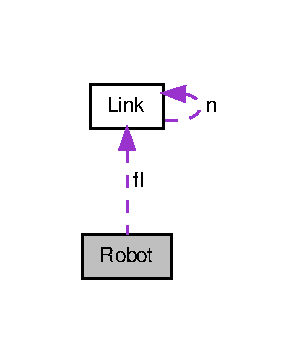
\includegraphics[width=145pt]{structRobot__coll__graph}
\end{center}
\end{figure}
\subsection*{Data Fields}
\begin{DoxyCompactItemize}
\item 
int \hyperlink{structRobot_a51d4a86ac5314a1ed8614d5664c80747}{dofs}
\item 
\hyperlink{structLink}{Link} $\ast$ \hyperlink{structRobot_aa983a42f95f55c494fd4154c4d42be47}{fl}
\end{DoxyCompactItemize}


\subsection{Detailed Description}
The Structure holding the relevant info of a \hyperlink{structRobot}{Robot}. 

Definition at line 14 of file robot.\-h.



\subsection{Field Documentation}
\hypertarget{structRobot_a51d4a86ac5314a1ed8614d5664c80747}{\index{Robot@{Robot}!dofs@{dofs}}
\index{dofs@{dofs}!Robot@{Robot}}
\subsubsection[{dofs}]{\setlength{\rightskip}{0pt plus 5cm}int Robot\-::dofs}}\label{structRobot_a51d4a86ac5314a1ed8614d5664c80747}


Definition at line 15 of file robot.\-h.



Referenced by Cartesian\-\_\-controller\-::\-Cartesian\-\_\-controller(), Cartesian\-\_\-velocity\-\_\-controller\-::\-Cartesian\-\_\-velocity\-\_\-controller(), Cartesian\-\_\-controller\-::get\-Schunk\-Positions\-And\-Velocities\-And\-Update\-Thetas\-And\-D\-Thetas(), Robot\-\_\-add\-Link(), Robot\-\_\-create(), Robot\-\_\-free(), Robot\-\_\-get\-A\-Jacobian(), Robot\-\_\-get\-G\-Jacobian(), Robot\-\_\-get\-Link(), Robot\-\_\-get\-O\-Jacobian\-Angle\-P(), and Cartesian\-\_\-controller\-::set\-Schunk\-Velocities\-And\-Send().

\hypertarget{structRobot_aa983a42f95f55c494fd4154c4d42be47}{\index{Robot@{Robot}!fl@{fl}}
\index{fl@{fl}!Robot@{Robot}}
\subsubsection[{fl}]{\setlength{\rightskip}{0pt plus 5cm}{\bf Link}$\ast$ Robot\-::fl}}\label{structRobot_aa983a42f95f55c494fd4154c4d42be47}


Definition at line 16 of file robot.\-h.



Referenced by Robot\-\_\-add\-Link(), Robot\-\_\-create(), Robot\-\_\-\-F\-K\-M(), Robot\-\_\-get\-Link(), Robot\-\_\-update\-Links\-Thetas\-By\-Array(), and Robot\-\_\-update\-Links\-Thetas\-By\-Matrix().



The documentation for this struct was generated from the following file\-:\begin{DoxyCompactItemize}
\item 
schunk\-\_\-high/include/schunk\-\_\-high/\hyperlink{robot_8h}{robot.\-h}\end{DoxyCompactItemize}

\hypertarget{structSPI__PARAM__STRUCT}{\section{S\-P\-I\-\_\-\-P\-A\-R\-A\-M\-\_\-\-S\-T\-R\-U\-C\-T Struct Reference}
\label{structSPI__PARAM__STRUCT}\index{S\-P\-I\-\_\-\-P\-A\-R\-A\-M\-\_\-\-S\-T\-R\-U\-C\-T@{S\-P\-I\-\_\-\-P\-A\-R\-A\-M\-\_\-\-S\-T\-R\-U\-C\-T}}
}


Configs for S\-P\-I.  




{\ttfamily \#include \char`\"{}communication.\-h\char`\"{}}

\subsection*{Data Fields}
\begin{DoxyCompactItemize}
\item 
uint8\-\_\-t \hyperlink{structSPI__PARAM__STRUCT_a82c546c99f6c3daed73c1e23426be847}{mode}
\item 
uint32\-\_\-t \hyperlink{structSPI__PARAM__STRUCT_a53a8d386594a81eb9bc6f971bfe36c54}{speed}
\item 
uint8\-\_\-t \hyperlink{structSPI__PARAM__STRUCT_ae0d62e0a5554783d710b677a017e246f}{cs}
\item 
int \hyperlink{structSPI__PARAM__STRUCT_abe385c44333d268d17cf648c8e371cad}{spi\-\_\-dev}
\end{DoxyCompactItemize}


\subsection{Detailed Description}
Configs for S\-P\-I. 

Definition at line 65 of file communication.\-h.



\subsection{Field Documentation}
\hypertarget{structSPI__PARAM__STRUCT_ae0d62e0a5554783d710b677a017e246f}{\index{S\-P\-I\-\_\-\-P\-A\-R\-A\-M\-\_\-\-S\-T\-R\-U\-C\-T@{S\-P\-I\-\_\-\-P\-A\-R\-A\-M\-\_\-\-S\-T\-R\-U\-C\-T}!cs@{cs}}
\index{cs@{cs}!SPI_PARAM_STRUCT@{S\-P\-I\-\_\-\-P\-A\-R\-A\-M\-\_\-\-S\-T\-R\-U\-C\-T}}
\subsubsection[{cs}]{\setlength{\rightskip}{0pt plus 5cm}uint8\-\_\-t S\-P\-I\-\_\-\-P\-A\-R\-A\-M\-\_\-\-S\-T\-R\-U\-C\-T\-::cs}}\label{structSPI__PARAM__STRUCT_ae0d62e0a5554783d710b677a017e246f}


Definition at line 68 of file communication.\-h.



Referenced by devices\-\_\-init(), and main().

\hypertarget{structSPI__PARAM__STRUCT_a82c546c99f6c3daed73c1e23426be847}{\index{S\-P\-I\-\_\-\-P\-A\-R\-A\-M\-\_\-\-S\-T\-R\-U\-C\-T@{S\-P\-I\-\_\-\-P\-A\-R\-A\-M\-\_\-\-S\-T\-R\-U\-C\-T}!mode@{mode}}
\index{mode@{mode}!SPI_PARAM_STRUCT@{S\-P\-I\-\_\-\-P\-A\-R\-A\-M\-\_\-\-S\-T\-R\-U\-C\-T}}
\subsubsection[{mode}]{\setlength{\rightskip}{0pt plus 5cm}uint8\-\_\-t S\-P\-I\-\_\-\-P\-A\-R\-A\-M\-\_\-\-S\-T\-R\-U\-C\-T\-::mode}}\label{structSPI__PARAM__STRUCT_a82c546c99f6c3daed73c1e23426be847}


Definition at line 66 of file communication.\-h.



Referenced by devices\-\_\-init(), and main().

\hypertarget{structSPI__PARAM__STRUCT_a53a8d386594a81eb9bc6f971bfe36c54}{\index{S\-P\-I\-\_\-\-P\-A\-R\-A\-M\-\_\-\-S\-T\-R\-U\-C\-T@{S\-P\-I\-\_\-\-P\-A\-R\-A\-M\-\_\-\-S\-T\-R\-U\-C\-T}!speed@{speed}}
\index{speed@{speed}!SPI_PARAM_STRUCT@{S\-P\-I\-\_\-\-P\-A\-R\-A\-M\-\_\-\-S\-T\-R\-U\-C\-T}}
\subsubsection[{speed}]{\setlength{\rightskip}{0pt plus 5cm}uint32\-\_\-t S\-P\-I\-\_\-\-P\-A\-R\-A\-M\-\_\-\-S\-T\-R\-U\-C\-T\-::speed}}\label{structSPI__PARAM__STRUCT_a53a8d386594a81eb9bc6f971bfe36c54}


Definition at line 67 of file communication.\-h.



Referenced by devices\-\_\-init(), and main().

\hypertarget{structSPI__PARAM__STRUCT_abe385c44333d268d17cf648c8e371cad}{\index{S\-P\-I\-\_\-\-P\-A\-R\-A\-M\-\_\-\-S\-T\-R\-U\-C\-T@{S\-P\-I\-\_\-\-P\-A\-R\-A\-M\-\_\-\-S\-T\-R\-U\-C\-T}!spi\-\_\-dev@{spi\-\_\-dev}}
\index{spi\-\_\-dev@{spi\-\_\-dev}!SPI_PARAM_STRUCT@{S\-P\-I\-\_\-\-P\-A\-R\-A\-M\-\_\-\-S\-T\-R\-U\-C\-T}}
\subsubsection[{spi\-\_\-dev}]{\setlength{\rightskip}{0pt plus 5cm}int S\-P\-I\-\_\-\-P\-A\-R\-A\-M\-\_\-\-S\-T\-R\-U\-C\-T\-::spi\-\_\-dev}}\label{structSPI__PARAM__STRUCT_abe385c44333d268d17cf648c8e371cad}


Definition at line 69 of file communication.\-h.



Referenced by devices\-\_\-init(), main(), periodic\-\_\-task\-\_\-1(), and periodic\-\_\-task\-\_\-2().



The documentation for this struct was generated from the following file\-:\begin{DoxyCompactItemize}
\item 
communication/\hyperlink{communication_2communication_8h}{communication.\-h}\end{DoxyCompactItemize}

\chapter{File Documentation}
\hypertarget{calibration_2calibration_8c}{\section{calibration/calibration.c File Reference}
\label{calibration_2calibration_8c}\index{calibration/calibration.\-c@{calibration/calibration.\-c}}
}
{\ttfamily \#include $<$stdio.\-h$>$}\\*
{\ttfamily \#include $<$stdlib.\-h$>$}\\*
{\ttfamily \#include \char`\"{}calibration.\-h\char`\"{}}\\*
Include dependency graph for calibration.\-c\-:\nopagebreak
\begin{figure}[H]
\begin{center}
\leavevmode
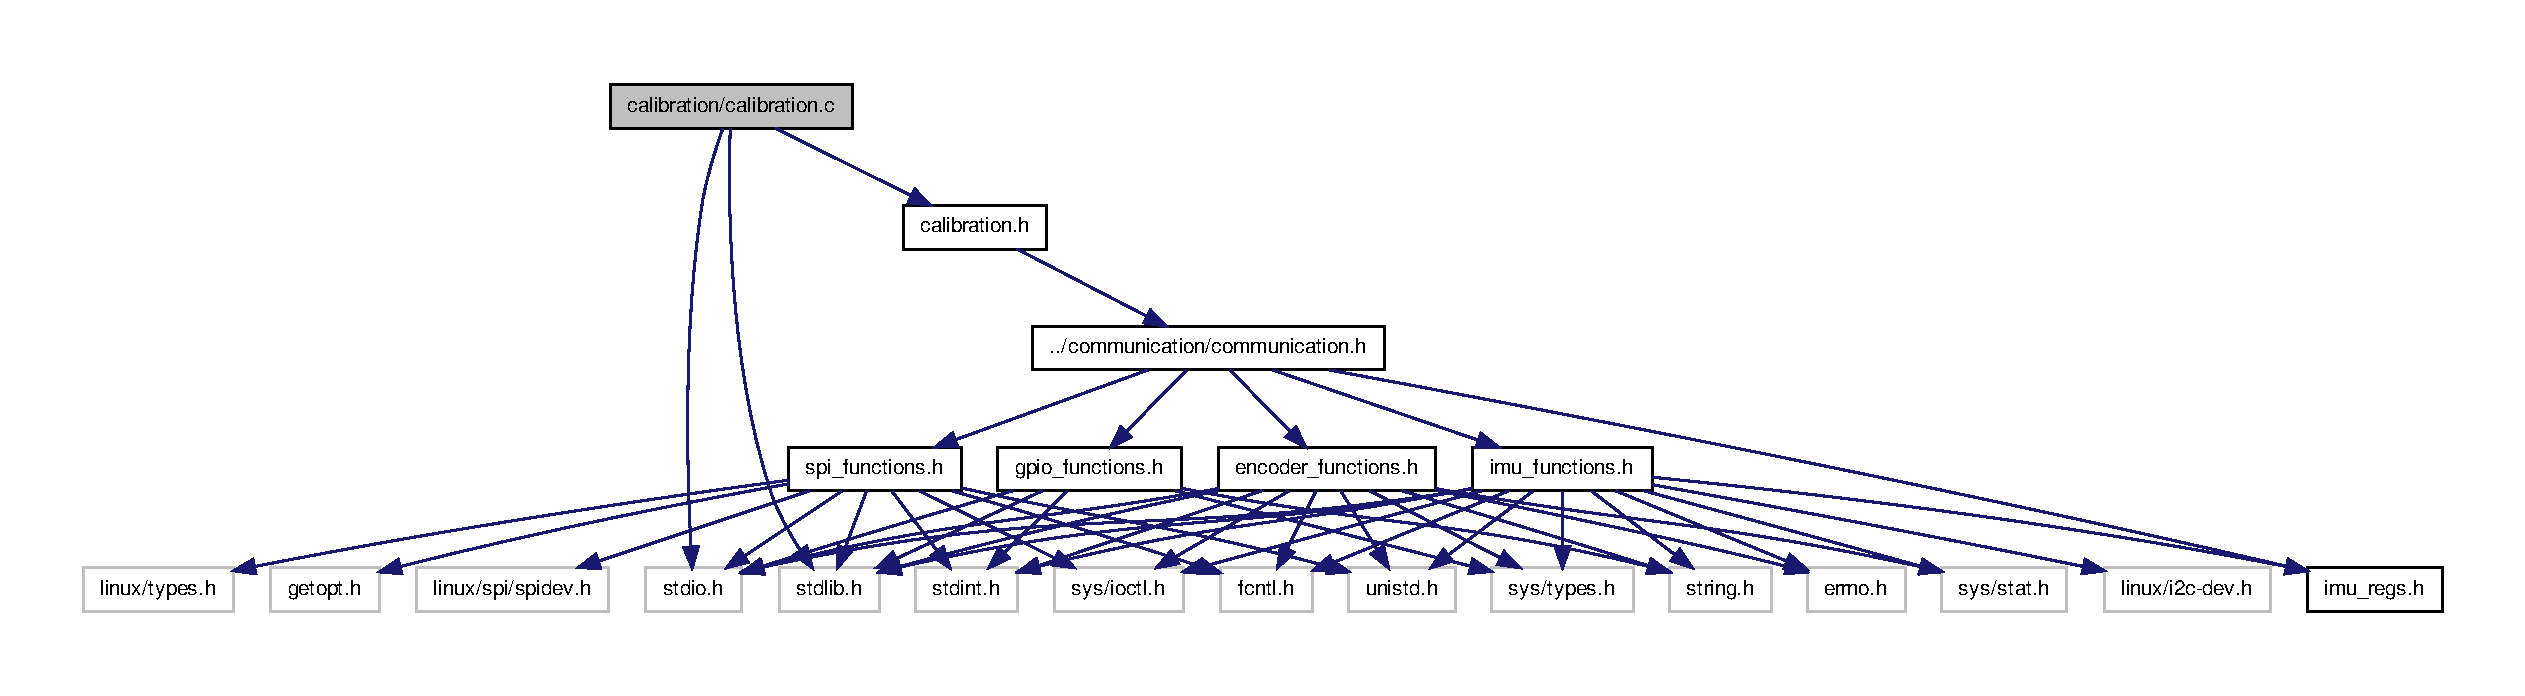
\includegraphics[width=350pt]{calibration_2calibration_8c__incl}
\end{center}
\end{figure}
\subsection*{Functions}
\begin{DoxyCompactItemize}
\item 
void \hyperlink{calibration_2calibration_8c_a043045246cf217758281222214c4addc}{calibrate\-\_\-all} (\hyperlink{structIMU__DATA__STRUCT}{I\-M\-U\-\_\-\-D\-A\-T\-A\-\_\-\-S\-T\-R\-U\-C\-T} $\ast$\hyperlink{threads__linux_8c_a3cfea12cbe9ca7f1681c950e4cd68606}{imu\-\_\-data})
\item 
void \hyperlink{calibration_2calibration_8c_aecfc81d152db2843b5d1517729804d63}{calibrate\-\_\-imu} (\hyperlink{structIMU__DATA__STRUCT}{I\-M\-U\-\_\-\-D\-A\-T\-A\-\_\-\-S\-T\-R\-U\-C\-T} $\ast$\hyperlink{threads__linux_8c_a3cfea12cbe9ca7f1681c950e4cd68606}{imu\-\_\-data})
\end{DoxyCompactItemize}


\subsection{Function Documentation}
\hypertarget{calibration_2calibration_8c_a043045246cf217758281222214c4addc}{\index{calibration/calibration.\-c@{calibration/calibration.\-c}!calibrate\-\_\-all@{calibrate\-\_\-all}}
\index{calibrate\-\_\-all@{calibrate\-\_\-all}!calibration/calibration.c@{calibration/calibration.\-c}}
\subsubsection[{calibrate\-\_\-all}]{\setlength{\rightskip}{0pt plus 5cm}void calibrate\-\_\-all (
\begin{DoxyParamCaption}
\item[{{\bf I\-M\-U\-\_\-\-D\-A\-T\-A\-\_\-\-S\-T\-R\-U\-C\-T} $\ast$}]{imu\-\_\-data}
\end{DoxyParamCaption}
)}}\label{calibration_2calibration_8c_a043045246cf217758281222214c4addc}


Definition at line 8 of file calibration.\-c.


\begin{DoxyCode}
\{
  \hyperlink{calibration_2calibration_8c_aecfc81d152db2843b5d1517729804d63}{calibrate\_imu}(imu\_data);
  \textcolor{keywordflow}{return};
\}
\end{DoxyCode}
\hypertarget{calibration_2calibration_8c_aecfc81d152db2843b5d1517729804d63}{\index{calibration/calibration.\-c@{calibration/calibration.\-c}!calibrate\-\_\-imu@{calibrate\-\_\-imu}}
\index{calibrate\-\_\-imu@{calibrate\-\_\-imu}!calibration/calibration.c@{calibration/calibration.\-c}}
\subsubsection[{calibrate\-\_\-imu}]{\setlength{\rightskip}{0pt plus 5cm}void calibrate\-\_\-imu (
\begin{DoxyParamCaption}
\item[{{\bf I\-M\-U\-\_\-\-D\-A\-T\-A\-\_\-\-S\-T\-R\-U\-C\-T} $\ast$}]{imu\-\_\-data}
\end{DoxyParamCaption}
)}}\label{calibration_2calibration_8c_aecfc81d152db2843b5d1517729804d63}


Definition at line 14 of file calibration.\-c.



Referenced by calibrate\-\_\-all().


\begin{DoxyCode}
\{
  \textcolor{comment}{// With this parameters, the vectors of acceleration and magnetic field will
       have norm = 1 theorically (i.e. in g or G)}
  imu\_data->\hyperlink{structIMU__DATA__STRUCT_aeffe3c3c5a7191a5cef16e7aab6c3795}{calib}.\hyperlink{structIMU__DATA__STRUCT_1_1calibrated_a281a7fdb40a05ed97388f18b9bb90c81}{acc}.\hyperlink{structDATA__XYZ__DOUBLE_a22868cc99a423900e7b82d015a5eb91f}{x} = ((double)imu\_data->\hyperlink{structIMU__DATA__STRUCT_a448f284bf44eb503affda586ad5fa9d2}{acc}.\hyperlink{structDATA__XYZ_a54c1596e9f9969fd9c21e8458024ecfb}{x}-\hyperlink{calibration_2calibration_8h_a355ea8f6ceed1e1d419a3ea2271bfca3}{ACC\_BIAS\_X}
      )/\hyperlink{calibration_2calibration_8h_a76e6967cb5a86ec34986b4583ac09831}{ACC\_FS\_X};
  imu\_data->\hyperlink{structIMU__DATA__STRUCT_aeffe3c3c5a7191a5cef16e7aab6c3795}{calib}.\hyperlink{structIMU__DATA__STRUCT_1_1calibrated_a281a7fdb40a05ed97388f18b9bb90c81}{acc}.\hyperlink{structDATA__XYZ__DOUBLE_a198a27b5df3b5b0bf461b0e481e22a82}{y} = ((double)imu\_data->\hyperlink{structIMU__DATA__STRUCT_a448f284bf44eb503affda586ad5fa9d2}{acc}.\hyperlink{structDATA__XYZ_a94bbb1c889bf53eb6a5fffa2b39322cf}{y}-\hyperlink{calibration_2calibration_8h_a34180f1c97e84a814ef181f62bf4b68f}{ACC\_BIAS\_Y}
      )/\hyperlink{calibration_2calibration_8h_a13d3aaab3b5800b11351cbd1246c8918}{ACC\_FS\_Y};
  imu\_data->\hyperlink{structIMU__DATA__STRUCT_aeffe3c3c5a7191a5cef16e7aab6c3795}{calib}.\hyperlink{structIMU__DATA__STRUCT_1_1calibrated_a281a7fdb40a05ed97388f18b9bb90c81}{acc}.\hyperlink{structDATA__XYZ__DOUBLE_a9556e8868c223ff3e28756ea18a284c0}{z} = ((double)imu\_data->\hyperlink{structIMU__DATA__STRUCT_a448f284bf44eb503affda586ad5fa9d2}{acc}.\hyperlink{structDATA__XYZ_a69e89ab0ec6e5d72fc5d54f62cc07fb5}{z}-\hyperlink{calibration_2calibration_8h_a794f762650b6f228ffb8d50d1323dbea}{ACC\_BIAS\_Z}
      )/\hyperlink{calibration_2calibration_8h_af1d3370cc0958289199c8c13470602d4}{ACC\_FS\_Z};
  
  imu\_data->\hyperlink{structIMU__DATA__STRUCT_aeffe3c3c5a7191a5cef16e7aab6c3795}{calib}.\hyperlink{structIMU__DATA__STRUCT_1_1calibrated_a2fde6c6759e0fda17e272c32096cb9ec}{mag}.\hyperlink{structDATA__XYZ__DOUBLE_a22868cc99a423900e7b82d015a5eb91f}{x} = ((double)imu\_data->\hyperlink{structIMU__DATA__STRUCT_a40c7df8b6d49297aa52873cfd9b60daa}{mag}.\hyperlink{structDATA__XYZ_a54c1596e9f9969fd9c21e8458024ecfb}{x}-\hyperlink{calibration_2calibration_8h_a355ea8f6ceed1e1d419a3ea2271bfca3}{ACC\_BIAS\_X}
      )/\hyperlink{calibration_2calibration_8h_a76e6967cb5a86ec34986b4583ac09831}{ACC\_FS\_X};
  imu\_data->\hyperlink{structIMU__DATA__STRUCT_aeffe3c3c5a7191a5cef16e7aab6c3795}{calib}.\hyperlink{structIMU__DATA__STRUCT_1_1calibrated_a2fde6c6759e0fda17e272c32096cb9ec}{mag}.\hyperlink{structDATA__XYZ__DOUBLE_a198a27b5df3b5b0bf461b0e481e22a82}{y} = ((double)imu\_data->\hyperlink{structIMU__DATA__STRUCT_a40c7df8b6d49297aa52873cfd9b60daa}{mag}.\hyperlink{structDATA__XYZ_a94bbb1c889bf53eb6a5fffa2b39322cf}{y}-\hyperlink{calibration_2calibration_8h_a34180f1c97e84a814ef181f62bf4b68f}{ACC\_BIAS\_Y}
      )/\hyperlink{calibration_2calibration_8h_a13d3aaab3b5800b11351cbd1246c8918}{ACC\_FS\_Y};
  imu\_data->\hyperlink{structIMU__DATA__STRUCT_aeffe3c3c5a7191a5cef16e7aab6c3795}{calib}.\hyperlink{structIMU__DATA__STRUCT_1_1calibrated_a2fde6c6759e0fda17e272c32096cb9ec}{mag}.\hyperlink{structDATA__XYZ__DOUBLE_a9556e8868c223ff3e28756ea18a284c0}{z} = ((double)imu\_data->\hyperlink{structIMU__DATA__STRUCT_a40c7df8b6d49297aa52873cfd9b60daa}{mag}.\hyperlink{structDATA__XYZ_a69e89ab0ec6e5d72fc5d54f62cc07fb5}{z}-\hyperlink{calibration_2calibration_8h_a794f762650b6f228ffb8d50d1323dbea}{ACC\_BIAS\_Z}
      )/\hyperlink{calibration_2calibration_8h_af1d3370cc0958289199c8c13470602d4}{ACC\_FS\_Z};
  
  \textcolor{comment}{// With this parameters, we consider right datasheet scale and we get in
       rad/s}
  imu\_data->\hyperlink{structIMU__DATA__STRUCT_aeffe3c3c5a7191a5cef16e7aab6c3795}{calib}.\hyperlink{structIMU__DATA__STRUCT_1_1calibrated_a8a54aded6ce608f1b7d2b4a0c52c248b}{gyr}.\hyperlink{structDATA__XYZ__DOUBLE_a22868cc99a423900e7b82d015a5eb91f}{x} = ((double)imu\_data->\hyperlink{structIMU__DATA__STRUCT_a0c1ac26626e4434a2ee124a1928a23a1}{gyr}.\hyperlink{structDATA__XYZ_a54c1596e9f9969fd9c21e8458024ecfb}{x}-\hyperlink{calibration_2calibration_8h_a69780ffe3a15aad4121fed56d5e47377}{GYR\_BIAS\_X}
      )/\hyperlink{calibration_2calibration_8h_a8fe84f8c6d39f41d8622fd0cbce3a522}{GYR\_FS\_X};
  imu\_data->\hyperlink{structIMU__DATA__STRUCT_aeffe3c3c5a7191a5cef16e7aab6c3795}{calib}.\hyperlink{structIMU__DATA__STRUCT_1_1calibrated_a8a54aded6ce608f1b7d2b4a0c52c248b}{gyr}.\hyperlink{structDATA__XYZ__DOUBLE_a198a27b5df3b5b0bf461b0e481e22a82}{y} = ((double)imu\_data->\hyperlink{structIMU__DATA__STRUCT_a0c1ac26626e4434a2ee124a1928a23a1}{gyr}.\hyperlink{structDATA__XYZ_a94bbb1c889bf53eb6a5fffa2b39322cf}{y}-\hyperlink{calibration_2calibration_8h_a69780ffe3a15aad4121fed56d5e47377}{GYR\_BIAS\_X}
      )/\hyperlink{calibration_2calibration_8h_a4be2e0fa7596546bb4699862d0fe4183}{GYR\_FS\_Y};
  imu\_data->\hyperlink{structIMU__DATA__STRUCT_aeffe3c3c5a7191a5cef16e7aab6c3795}{calib}.\hyperlink{structIMU__DATA__STRUCT_1_1calibrated_a8a54aded6ce608f1b7d2b4a0c52c248b}{gyr}.\hyperlink{structDATA__XYZ__DOUBLE_a9556e8868c223ff3e28756ea18a284c0}{z} = ((double)imu\_data->\hyperlink{structIMU__DATA__STRUCT_a0c1ac26626e4434a2ee124a1928a23a1}{gyr}.\hyperlink{structDATA__XYZ_a69e89ab0ec6e5d72fc5d54f62cc07fb5}{z}-\hyperlink{calibration_2calibration_8h_a69780ffe3a15aad4121fed56d5e47377}{GYR\_BIAS\_X}
      )/\hyperlink{calibration_2calibration_8h_aaee2ece0c43cc20d7c531ab79dcd06c8}{GYR\_FS\_Z};
  
  \textcolor{keywordflow}{return};
\}
\end{DoxyCode}


Here is the caller graph for this function\-:\nopagebreak
\begin{figure}[H]
\begin{center}
\leavevmode
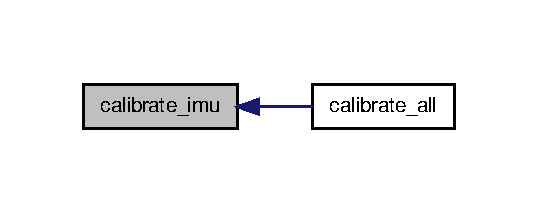
\includegraphics[width=258pt]{calibration_2calibration_8c_aecfc81d152db2843b5d1517729804d63_icgraph}
\end{center}
\end{figure}



\hypertarget{calibration_8c}{\section{calibration.\-c File Reference}
\label{calibration_8c}\index{calibration.\-c@{calibration.\-c}}
}
{\ttfamily \#include $<$stdio.\-h$>$}\\*
{\ttfamily \#include $<$stdlib.\-h$>$}\\*
{\ttfamily \#include \char`\"{}communication/communication.\-h\char`\"{}}\\*
{\ttfamily \#include \char`\"{}calibration.\-h\char`\"{}}\\*
Include dependency graph for calibration.\-c\-:
\nopagebreak
\begin{figure}[H]
\begin{center}
\leavevmode
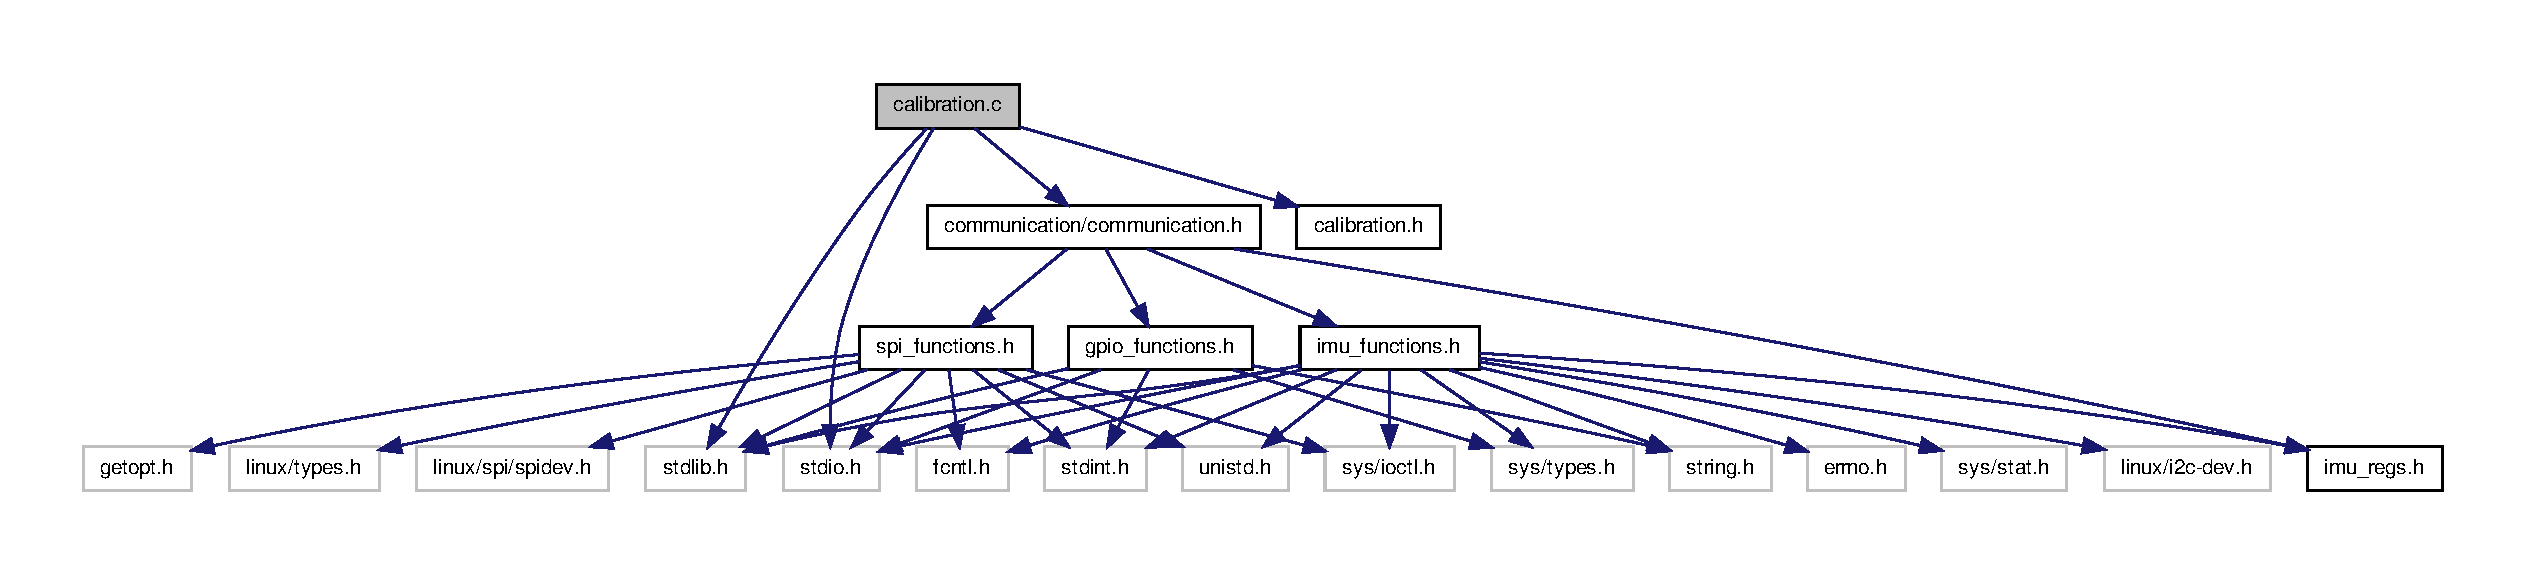
\includegraphics[width=350pt]{calibration_8c__incl}
\end{center}
\end{figure}
\subsection*{Functions}
\begin{DoxyCompactItemize}
\item 
void \hyperlink{group__calibrate_ga043045246cf217758281222214c4addc}{calibrate\-\_\-all} (\hyperlink{structIMU__DATA__STRUCT}{I\-M\-U\-\_\-\-D\-A\-T\-A\-\_\-\-S\-T\-R\-U\-C\-T} $\ast$\hyperlink{threads__linux_8c_a3cfea12cbe9ca7f1681c950e4cd68606}{imu\-\_\-data})
\begin{DoxyCompactList}\small\item\em Calibrate all sensors. \end{DoxyCompactList}\item 
void \hyperlink{group__calibrate_gaecfc81d152db2843b5d1517729804d63}{calibrate\-\_\-imu} (\hyperlink{structIMU__DATA__STRUCT}{I\-M\-U\-\_\-\-D\-A\-T\-A\-\_\-\-S\-T\-R\-U\-C\-T} $\ast$\hyperlink{threads__linux_8c_a3cfea12cbe9ca7f1681c950e4cd68606}{imu\-\_\-data})
\begin{DoxyCompactList}\small\item\em Calibrate imu sensors. \end{DoxyCompactList}\item 
void \hyperlink{calibration_8c_ae8f1281c6870b23c1c158b30998f7568}{calibrate\-\_\-enc} (\hyperlink{structENC__DATA__STRUCT}{E\-N\-C\-\_\-\-D\-A\-T\-A\-\_\-\-S\-T\-R\-U\-C\-T} $\ast$\hyperlink{main2_8c_aaa441e18ae805c4f3efb0b5231d1cfe7}{enc\-\_\-data})
\begin{DoxyCompactList}\small\item\em Calibrate encoder to return values in the rage of 0 to 90. \end{DoxyCompactList}\end{DoxyCompactItemize}


\subsection{Function Documentation}
\hypertarget{calibration_8c_ae8f1281c6870b23c1c158b30998f7568}{\index{calibration.\-c@{calibration.\-c}!calibrate\-\_\-enc@{calibrate\-\_\-enc}}
\index{calibrate\-\_\-enc@{calibrate\-\_\-enc}!calibration.c@{calibration.\-c}}
\subsubsection[{calibrate\-\_\-enc}]{\setlength{\rightskip}{0pt plus 5cm}void calibrate\-\_\-enc (
\begin{DoxyParamCaption}
\item[{{\bf E\-N\-C\-\_\-\-D\-A\-T\-A\-\_\-\-S\-T\-R\-U\-C\-T} $\ast$}]{enc\-\_\-data}
\end{DoxyParamCaption}
)}}\label{calibration_8c_ae8f1281c6870b23c1c158b30998f7568}


Calibrate encoder to return values in the rage of 0 to 90. 



Definition at line 35 of file calibration.\-c.



References E\-N\-C\-\_\-\-D\-A\-T\-A\-\_\-\-S\-T\-R\-U\-C\-T\-::calib, E\-N\-C\-\_\-\-F\-S, E\-N\-C\-\_\-\-M\-A\-X, E\-N\-C\-\_\-\-D\-A\-T\-A\-\_\-\-S\-T\-R\-U\-C\-T\-::position, and E\-N\-C\-\_\-\-D\-A\-T\-A\-\_\-\-S\-T\-R\-U\-C\-T\-::calibrate\-::position.


\begin{DoxyCode}
                                             \{
  enc\_data->\hyperlink{structENC__DATA__STRUCT_af227e5bbb714b830cc570432bda0a468}{calib}.\hyperlink{structENC__DATA__STRUCT_1_1calibrate_aed5100f7dc3d1f358a633c043e13cba2}{position} = ((\hyperlink{calibration_2calibration_8h_a496f1fb8343dc6e6bcdf07eb28557f41}{ENC\_MAX} - enc\_data->\hyperlink{structENC__DATA__STRUCT_ac3a53ed44ecaf87285518a091e1d2c24}{position}
      )/\hyperlink{calibration_2calibration_8h_adf9edcc7e266ed7333f7570965f5956a}{ENC\_FS});
\}
\end{DoxyCode}

\hypertarget{calibration_2calibration_8h}{\section{calibration/calibration.h File Reference}
\label{calibration_2calibration_8h}\index{calibration/calibration.\-h@{calibration/calibration.\-h}}
}
{\ttfamily \#include \char`\"{}../communication/communication.\-h\char`\"{}}\\*
\subsection*{Macros}
\begin{DoxyCompactItemize}
\item 
\#define \hyperlink{calibration_2calibration_8h_aa90cac659d18e8ef6294c7ae337f6b58}{S\-U\-C\-C\-E\-S\-S}~1
\item 
\#define \hyperlink{calibration_2calibration_8h_a6d58f9ac447476b4e084d7ca383f5183}{F\-A\-I\-L\-U\-R\-E}~-\/1
\item 
\#define \hyperlink{calibration_2calibration_8h_a355ea8f6ceed1e1d419a3ea2271bfca3}{A\-C\-C\-\_\-\-B\-I\-A\-S\-\_\-\-X}~19.\-2
\item 
\#define \hyperlink{calibration_2calibration_8h_a34180f1c97e84a814ef181f62bf4b68f}{A\-C\-C\-\_\-\-B\-I\-A\-S\-\_\-\-Y}~6.\-024
\item 
\#define \hyperlink{calibration_2calibration_8h_a794f762650b6f228ffb8d50d1323dbea}{A\-C\-C\-\_\-\-B\-I\-A\-S\-\_\-\-Z}~-\/18.\-97
\item 
\#define \hyperlink{calibration_2calibration_8h_a76e6967cb5a86ec34986b4583ac09831}{A\-C\-C\-\_\-\-F\-S\-\_\-\-X}~262.\-82
\item 
\#define \hyperlink{calibration_2calibration_8h_a13d3aaab3b5800b11351cbd1246c8918}{A\-C\-C\-\_\-\-F\-S\-\_\-\-Y}~262.\-15
\item 
\#define \hyperlink{calibration_2calibration_8h_af1d3370cc0958289199c8c13470602d4}{A\-C\-C\-\_\-\-F\-S\-\_\-\-Z}~252.\-20
\item 
\#define \hyperlink{calibration_2calibration_8h_a33f53b04fe0f887e8d9d99e4374c0ddf}{M\-A\-G\-\_\-\-B\-I\-A\-S\-\_\-\-X}~-\/143
\item 
\#define \hyperlink{calibration_2calibration_8h_a92407f4dfd1c63cede9a5307b379c569}{M\-A\-G\-\_\-\-B\-I\-A\-S\-\_\-\-Y}~-\/101
\item 
\#define \hyperlink{calibration_2calibration_8h_a9662c4fff54f93bcc4e043e84e79d623}{M\-A\-G\-\_\-\-B\-I\-A\-S\-\_\-\-Z}~3
\item 
\#define \hyperlink{calibration_2calibration_8h_aa49abc19ca0fda3324df06bddae2c1d4}{M\-A\-G\-\_\-\-F\-S\-\_\-\-X}~177
\item 
\#define \hyperlink{calibration_2calibration_8h_a5c5e64196104a5e5ebac3c594220eb5c}{M\-A\-G\-\_\-\-F\-S\-\_\-\-Y}~139
\item 
\#define \hyperlink{calibration_2calibration_8h_aebfc43ba340d89fa86b4a5c07cc7c924}{M\-A\-G\-\_\-\-F\-S\-\_\-\-Z}~85
\item 
\#define \hyperlink{calibration_2calibration_8h_a69780ffe3a15aad4121fed56d5e47377}{G\-Y\-R\-\_\-\-B\-I\-A\-S\-\_\-\-X}~-\/60.\-9046
\item 
\#define \hyperlink{calibration_2calibration_8h_af3264a08be995ea97ae8581128873877}{G\-Y\-R\-\_\-\-B\-I\-A\-S\-\_\-\-Y}~40.\-9062
\item 
\#define \hyperlink{calibration_2calibration_8h_aa10980bbf5b1dd91704d4dab98fcf991}{G\-Y\-R\-\_\-\-B\-I\-A\-S\-\_\-\-Z}~0.\-8769
\item 
\#define \hyperlink{calibration_2calibration_8h_a8fe84f8c6d39f41d8622fd0cbce3a522}{G\-Y\-R\-\_\-\-F\-S\-\_\-\-X}~0.\-001214142
\item 
\#define \hyperlink{calibration_2calibration_8h_a4be2e0fa7596546bb4699862d0fe4183}{G\-Y\-R\-\_\-\-F\-S\-\_\-\-Y}~0.\-001214142
\item 
\#define \hyperlink{calibration_2calibration_8h_aaee2ece0c43cc20d7c531ab79dcd06c8}{G\-Y\-R\-\_\-\-F\-S\-\_\-\-Z}~0.\-001214142
\end{DoxyCompactItemize}
\subsection*{Functions}
\begin{DoxyCompactItemize}
\item 
void \hyperlink{calibration_2calibration_8h_a043045246cf217758281222214c4addc}{calibrate\-\_\-all} (\hyperlink{structIMU__DATA__STRUCT}{I\-M\-U\-\_\-\-D\-A\-T\-A\-\_\-\-S\-T\-R\-U\-C\-T} $\ast$\hyperlink{threads__linux_8c_a3cfea12cbe9ca7f1681c950e4cd68606}{imu\-\_\-data})
\item 
void \hyperlink{calibration_2calibration_8h_aecfc81d152db2843b5d1517729804d63}{calibrate\-\_\-imu} (\hyperlink{structIMU__DATA__STRUCT}{I\-M\-U\-\_\-\-D\-A\-T\-A\-\_\-\-S\-T\-R\-U\-C\-T} $\ast$\hyperlink{threads__linux_8c_a3cfea12cbe9ca7f1681c950e4cd68606}{imu\-\_\-data})
\end{DoxyCompactItemize}


\subsection{Macro Definition Documentation}
\hypertarget{calibration_2calibration_8h_a355ea8f6ceed1e1d419a3ea2271bfca3}{\index{calibration/calibration.\-h@{calibration/calibration.\-h}!A\-C\-C\-\_\-\-B\-I\-A\-S\-\_\-\-X@{A\-C\-C\-\_\-\-B\-I\-A\-S\-\_\-\-X}}
\index{A\-C\-C\-\_\-\-B\-I\-A\-S\-\_\-\-X@{A\-C\-C\-\_\-\-B\-I\-A\-S\-\_\-\-X}!calibration/calibration.h@{calibration/calibration.\-h}}
\subsubsection[{A\-C\-C\-\_\-\-B\-I\-A\-S\-\_\-\-X}]{\setlength{\rightskip}{0pt plus 5cm}\#define A\-C\-C\-\_\-\-B\-I\-A\-S\-\_\-\-X~19.\-2}}\label{calibration_2calibration_8h_a355ea8f6ceed1e1d419a3ea2271bfca3}


Definition at line 10 of file calibration.\-h.



Referenced by calibrate\-\_\-imu().

\hypertarget{calibration_2calibration_8h_a34180f1c97e84a814ef181f62bf4b68f}{\index{calibration/calibration.\-h@{calibration/calibration.\-h}!A\-C\-C\-\_\-\-B\-I\-A\-S\-\_\-\-Y@{A\-C\-C\-\_\-\-B\-I\-A\-S\-\_\-\-Y}}
\index{A\-C\-C\-\_\-\-B\-I\-A\-S\-\_\-\-Y@{A\-C\-C\-\_\-\-B\-I\-A\-S\-\_\-\-Y}!calibration/calibration.h@{calibration/calibration.\-h}}
\subsubsection[{A\-C\-C\-\_\-\-B\-I\-A\-S\-\_\-\-Y}]{\setlength{\rightskip}{0pt plus 5cm}\#define A\-C\-C\-\_\-\-B\-I\-A\-S\-\_\-\-Y~6.\-024}}\label{calibration_2calibration_8h_a34180f1c97e84a814ef181f62bf4b68f}


Definition at line 11 of file calibration.\-h.



Referenced by calibrate\-\_\-imu().

\hypertarget{calibration_2calibration_8h_a794f762650b6f228ffb8d50d1323dbea}{\index{calibration/calibration.\-h@{calibration/calibration.\-h}!A\-C\-C\-\_\-\-B\-I\-A\-S\-\_\-\-Z@{A\-C\-C\-\_\-\-B\-I\-A\-S\-\_\-\-Z}}
\index{A\-C\-C\-\_\-\-B\-I\-A\-S\-\_\-\-Z@{A\-C\-C\-\_\-\-B\-I\-A\-S\-\_\-\-Z}!calibration/calibration.h@{calibration/calibration.\-h}}
\subsubsection[{A\-C\-C\-\_\-\-B\-I\-A\-S\-\_\-\-Z}]{\setlength{\rightskip}{0pt plus 5cm}\#define A\-C\-C\-\_\-\-B\-I\-A\-S\-\_\-\-Z~-\/18.\-97}}\label{calibration_2calibration_8h_a794f762650b6f228ffb8d50d1323dbea}


Definition at line 12 of file calibration.\-h.



Referenced by calibrate\-\_\-imu().

\hypertarget{calibration_2calibration_8h_a76e6967cb5a86ec34986b4583ac09831}{\index{calibration/calibration.\-h@{calibration/calibration.\-h}!A\-C\-C\-\_\-\-F\-S\-\_\-\-X@{A\-C\-C\-\_\-\-F\-S\-\_\-\-X}}
\index{A\-C\-C\-\_\-\-F\-S\-\_\-\-X@{A\-C\-C\-\_\-\-F\-S\-\_\-\-X}!calibration/calibration.h@{calibration/calibration.\-h}}
\subsubsection[{A\-C\-C\-\_\-\-F\-S\-\_\-\-X}]{\setlength{\rightskip}{0pt plus 5cm}\#define A\-C\-C\-\_\-\-F\-S\-\_\-\-X~262.\-82}}\label{calibration_2calibration_8h_a76e6967cb5a86ec34986b4583ac09831}


Definition at line 13 of file calibration.\-h.



Referenced by calibrate\-\_\-imu().

\hypertarget{calibration_2calibration_8h_a13d3aaab3b5800b11351cbd1246c8918}{\index{calibration/calibration.\-h@{calibration/calibration.\-h}!A\-C\-C\-\_\-\-F\-S\-\_\-\-Y@{A\-C\-C\-\_\-\-F\-S\-\_\-\-Y}}
\index{A\-C\-C\-\_\-\-F\-S\-\_\-\-Y@{A\-C\-C\-\_\-\-F\-S\-\_\-\-Y}!calibration/calibration.h@{calibration/calibration.\-h}}
\subsubsection[{A\-C\-C\-\_\-\-F\-S\-\_\-\-Y}]{\setlength{\rightskip}{0pt plus 5cm}\#define A\-C\-C\-\_\-\-F\-S\-\_\-\-Y~262.\-15}}\label{calibration_2calibration_8h_a13d3aaab3b5800b11351cbd1246c8918}


Definition at line 14 of file calibration.\-h.



Referenced by calibrate\-\_\-imu().

\hypertarget{calibration_2calibration_8h_af1d3370cc0958289199c8c13470602d4}{\index{calibration/calibration.\-h@{calibration/calibration.\-h}!A\-C\-C\-\_\-\-F\-S\-\_\-\-Z@{A\-C\-C\-\_\-\-F\-S\-\_\-\-Z}}
\index{A\-C\-C\-\_\-\-F\-S\-\_\-\-Z@{A\-C\-C\-\_\-\-F\-S\-\_\-\-Z}!calibration/calibration.h@{calibration/calibration.\-h}}
\subsubsection[{A\-C\-C\-\_\-\-F\-S\-\_\-\-Z}]{\setlength{\rightskip}{0pt plus 5cm}\#define A\-C\-C\-\_\-\-F\-S\-\_\-\-Z~252.\-20}}\label{calibration_2calibration_8h_af1d3370cc0958289199c8c13470602d4}


Definition at line 15 of file calibration.\-h.



Referenced by calibrate\-\_\-imu().

\hypertarget{calibration_2calibration_8h_a6d58f9ac447476b4e084d7ca383f5183}{\index{calibration/calibration.\-h@{calibration/calibration.\-h}!F\-A\-I\-L\-U\-R\-E@{F\-A\-I\-L\-U\-R\-E}}
\index{F\-A\-I\-L\-U\-R\-E@{F\-A\-I\-L\-U\-R\-E}!calibration/calibration.h@{calibration/calibration.\-h}}
\subsubsection[{F\-A\-I\-L\-U\-R\-E}]{\setlength{\rightskip}{0pt plus 5cm}\#define F\-A\-I\-L\-U\-R\-E~-\/1}}\label{calibration_2calibration_8h_a6d58f9ac447476b4e084d7ca383f5183}


Definition at line 7 of file calibration.\-h.



Referenced by acc\-\_\-init(), acc\-\_\-read\-\_\-all\-\_\-data(), acc\-\_\-write\-\_\-reg(), actuate(), devices\-\_\-init(), gpio\-\_\-read(), gpio\-\_\-write(), gyr\-\_\-read\-\_\-all\-\_\-data(), gyr\-\_\-write\-\_\-reg(), mag\-\_\-read\-\_\-all\-\_\-data(), main(), read\-\_\-all\-\_\-data(), and ui\-\_\-update().

\hypertarget{calibration_2calibration_8h_a69780ffe3a15aad4121fed56d5e47377}{\index{calibration/calibration.\-h@{calibration/calibration.\-h}!G\-Y\-R\-\_\-\-B\-I\-A\-S\-\_\-\-X@{G\-Y\-R\-\_\-\-B\-I\-A\-S\-\_\-\-X}}
\index{G\-Y\-R\-\_\-\-B\-I\-A\-S\-\_\-\-X@{G\-Y\-R\-\_\-\-B\-I\-A\-S\-\_\-\-X}!calibration/calibration.h@{calibration/calibration.\-h}}
\subsubsection[{G\-Y\-R\-\_\-\-B\-I\-A\-S\-\_\-\-X}]{\setlength{\rightskip}{0pt plus 5cm}\#define G\-Y\-R\-\_\-\-B\-I\-A\-S\-\_\-\-X~-\/60.\-9046}}\label{calibration_2calibration_8h_a69780ffe3a15aad4121fed56d5e47377}


Definition at line 25 of file calibration.\-h.



Referenced by calibrate\-\_\-imu().

\hypertarget{calibration_2calibration_8h_af3264a08be995ea97ae8581128873877}{\index{calibration/calibration.\-h@{calibration/calibration.\-h}!G\-Y\-R\-\_\-\-B\-I\-A\-S\-\_\-\-Y@{G\-Y\-R\-\_\-\-B\-I\-A\-S\-\_\-\-Y}}
\index{G\-Y\-R\-\_\-\-B\-I\-A\-S\-\_\-\-Y@{G\-Y\-R\-\_\-\-B\-I\-A\-S\-\_\-\-Y}!calibration/calibration.h@{calibration/calibration.\-h}}
\subsubsection[{G\-Y\-R\-\_\-\-B\-I\-A\-S\-\_\-\-Y}]{\setlength{\rightskip}{0pt plus 5cm}\#define G\-Y\-R\-\_\-\-B\-I\-A\-S\-\_\-\-Y~40.\-9062}}\label{calibration_2calibration_8h_af3264a08be995ea97ae8581128873877}


Definition at line 26 of file calibration.\-h.



Referenced by calibrate\-\_\-imu().

\hypertarget{calibration_2calibration_8h_aa10980bbf5b1dd91704d4dab98fcf991}{\index{calibration/calibration.\-h@{calibration/calibration.\-h}!G\-Y\-R\-\_\-\-B\-I\-A\-S\-\_\-\-Z@{G\-Y\-R\-\_\-\-B\-I\-A\-S\-\_\-\-Z}}
\index{G\-Y\-R\-\_\-\-B\-I\-A\-S\-\_\-\-Z@{G\-Y\-R\-\_\-\-B\-I\-A\-S\-\_\-\-Z}!calibration/calibration.h@{calibration/calibration.\-h}}
\subsubsection[{G\-Y\-R\-\_\-\-B\-I\-A\-S\-\_\-\-Z}]{\setlength{\rightskip}{0pt plus 5cm}\#define G\-Y\-R\-\_\-\-B\-I\-A\-S\-\_\-\-Z~0.\-8769}}\label{calibration_2calibration_8h_aa10980bbf5b1dd91704d4dab98fcf991}


Definition at line 27 of file calibration.\-h.



Referenced by calibrate\-\_\-imu().

\hypertarget{calibration_2calibration_8h_a8fe84f8c6d39f41d8622fd0cbce3a522}{\index{calibration/calibration.\-h@{calibration/calibration.\-h}!G\-Y\-R\-\_\-\-F\-S\-\_\-\-X@{G\-Y\-R\-\_\-\-F\-S\-\_\-\-X}}
\index{G\-Y\-R\-\_\-\-F\-S\-\_\-\-X@{G\-Y\-R\-\_\-\-F\-S\-\_\-\-X}!calibration/calibration.h@{calibration/calibration.\-h}}
\subsubsection[{G\-Y\-R\-\_\-\-F\-S\-\_\-\-X}]{\setlength{\rightskip}{0pt plus 5cm}\#define G\-Y\-R\-\_\-\-F\-S\-\_\-\-X~0.\-001214142}}\label{calibration_2calibration_8h_a8fe84f8c6d39f41d8622fd0cbce3a522}


Definition at line 28 of file calibration.\-h.



Referenced by calibrate\-\_\-imu().

\hypertarget{calibration_2calibration_8h_a4be2e0fa7596546bb4699862d0fe4183}{\index{calibration/calibration.\-h@{calibration/calibration.\-h}!G\-Y\-R\-\_\-\-F\-S\-\_\-\-Y@{G\-Y\-R\-\_\-\-F\-S\-\_\-\-Y}}
\index{G\-Y\-R\-\_\-\-F\-S\-\_\-\-Y@{G\-Y\-R\-\_\-\-F\-S\-\_\-\-Y}!calibration/calibration.h@{calibration/calibration.\-h}}
\subsubsection[{G\-Y\-R\-\_\-\-F\-S\-\_\-\-Y}]{\setlength{\rightskip}{0pt plus 5cm}\#define G\-Y\-R\-\_\-\-F\-S\-\_\-\-Y~0.\-001214142}}\label{calibration_2calibration_8h_a4be2e0fa7596546bb4699862d0fe4183}


Definition at line 29 of file calibration.\-h.



Referenced by calibrate\-\_\-imu().

\hypertarget{calibration_2calibration_8h_aaee2ece0c43cc20d7c531ab79dcd06c8}{\index{calibration/calibration.\-h@{calibration/calibration.\-h}!G\-Y\-R\-\_\-\-F\-S\-\_\-\-Z@{G\-Y\-R\-\_\-\-F\-S\-\_\-\-Z}}
\index{G\-Y\-R\-\_\-\-F\-S\-\_\-\-Z@{G\-Y\-R\-\_\-\-F\-S\-\_\-\-Z}!calibration/calibration.h@{calibration/calibration.\-h}}
\subsubsection[{G\-Y\-R\-\_\-\-F\-S\-\_\-\-Z}]{\setlength{\rightskip}{0pt plus 5cm}\#define G\-Y\-R\-\_\-\-F\-S\-\_\-\-Z~0.\-001214142}}\label{calibration_2calibration_8h_aaee2ece0c43cc20d7c531ab79dcd06c8}


Definition at line 30 of file calibration.\-h.



Referenced by calibrate\-\_\-imu().

\hypertarget{calibration_2calibration_8h_a33f53b04fe0f887e8d9d99e4374c0ddf}{\index{calibration/calibration.\-h@{calibration/calibration.\-h}!M\-A\-G\-\_\-\-B\-I\-A\-S\-\_\-\-X@{M\-A\-G\-\_\-\-B\-I\-A\-S\-\_\-\-X}}
\index{M\-A\-G\-\_\-\-B\-I\-A\-S\-\_\-\-X@{M\-A\-G\-\_\-\-B\-I\-A\-S\-\_\-\-X}!calibration/calibration.h@{calibration/calibration.\-h}}
\subsubsection[{M\-A\-G\-\_\-\-B\-I\-A\-S\-\_\-\-X}]{\setlength{\rightskip}{0pt plus 5cm}\#define M\-A\-G\-\_\-\-B\-I\-A\-S\-\_\-\-X~-\/143}}\label{calibration_2calibration_8h_a33f53b04fe0f887e8d9d99e4374c0ddf}


Definition at line 17 of file calibration.\-h.



Referenced by calibrate\-\_\-imu().

\hypertarget{calibration_2calibration_8h_a92407f4dfd1c63cede9a5307b379c569}{\index{calibration/calibration.\-h@{calibration/calibration.\-h}!M\-A\-G\-\_\-\-B\-I\-A\-S\-\_\-\-Y@{M\-A\-G\-\_\-\-B\-I\-A\-S\-\_\-\-Y}}
\index{M\-A\-G\-\_\-\-B\-I\-A\-S\-\_\-\-Y@{M\-A\-G\-\_\-\-B\-I\-A\-S\-\_\-\-Y}!calibration/calibration.h@{calibration/calibration.\-h}}
\subsubsection[{M\-A\-G\-\_\-\-B\-I\-A\-S\-\_\-\-Y}]{\setlength{\rightskip}{0pt plus 5cm}\#define M\-A\-G\-\_\-\-B\-I\-A\-S\-\_\-\-Y~-\/101}}\label{calibration_2calibration_8h_a92407f4dfd1c63cede9a5307b379c569}


Definition at line 18 of file calibration.\-h.



Referenced by calibrate\-\_\-imu().

\hypertarget{calibration_2calibration_8h_a9662c4fff54f93bcc4e043e84e79d623}{\index{calibration/calibration.\-h@{calibration/calibration.\-h}!M\-A\-G\-\_\-\-B\-I\-A\-S\-\_\-\-Z@{M\-A\-G\-\_\-\-B\-I\-A\-S\-\_\-\-Z}}
\index{M\-A\-G\-\_\-\-B\-I\-A\-S\-\_\-\-Z@{M\-A\-G\-\_\-\-B\-I\-A\-S\-\_\-\-Z}!calibration/calibration.h@{calibration/calibration.\-h}}
\subsubsection[{M\-A\-G\-\_\-\-B\-I\-A\-S\-\_\-\-Z}]{\setlength{\rightskip}{0pt plus 5cm}\#define M\-A\-G\-\_\-\-B\-I\-A\-S\-\_\-\-Z~3}}\label{calibration_2calibration_8h_a9662c4fff54f93bcc4e043e84e79d623}


Definition at line 19 of file calibration.\-h.



Referenced by calibrate\-\_\-imu().

\hypertarget{calibration_2calibration_8h_aa49abc19ca0fda3324df06bddae2c1d4}{\index{calibration/calibration.\-h@{calibration/calibration.\-h}!M\-A\-G\-\_\-\-F\-S\-\_\-\-X@{M\-A\-G\-\_\-\-F\-S\-\_\-\-X}}
\index{M\-A\-G\-\_\-\-F\-S\-\_\-\-X@{M\-A\-G\-\_\-\-F\-S\-\_\-\-X}!calibration/calibration.h@{calibration/calibration.\-h}}
\subsubsection[{M\-A\-G\-\_\-\-F\-S\-\_\-\-X}]{\setlength{\rightskip}{0pt plus 5cm}\#define M\-A\-G\-\_\-\-F\-S\-\_\-\-X~177}}\label{calibration_2calibration_8h_aa49abc19ca0fda3324df06bddae2c1d4}


Definition at line 20 of file calibration.\-h.



Referenced by calibrate\-\_\-imu().

\hypertarget{calibration_2calibration_8h_a5c5e64196104a5e5ebac3c594220eb5c}{\index{calibration/calibration.\-h@{calibration/calibration.\-h}!M\-A\-G\-\_\-\-F\-S\-\_\-\-Y@{M\-A\-G\-\_\-\-F\-S\-\_\-\-Y}}
\index{M\-A\-G\-\_\-\-F\-S\-\_\-\-Y@{M\-A\-G\-\_\-\-F\-S\-\_\-\-Y}!calibration/calibration.h@{calibration/calibration.\-h}}
\subsubsection[{M\-A\-G\-\_\-\-F\-S\-\_\-\-Y}]{\setlength{\rightskip}{0pt plus 5cm}\#define M\-A\-G\-\_\-\-F\-S\-\_\-\-Y~139}}\label{calibration_2calibration_8h_a5c5e64196104a5e5ebac3c594220eb5c}


Definition at line 21 of file calibration.\-h.



Referenced by calibrate\-\_\-imu().

\hypertarget{calibration_2calibration_8h_aebfc43ba340d89fa86b4a5c07cc7c924}{\index{calibration/calibration.\-h@{calibration/calibration.\-h}!M\-A\-G\-\_\-\-F\-S\-\_\-\-Z@{M\-A\-G\-\_\-\-F\-S\-\_\-\-Z}}
\index{M\-A\-G\-\_\-\-F\-S\-\_\-\-Z@{M\-A\-G\-\_\-\-F\-S\-\_\-\-Z}!calibration/calibration.h@{calibration/calibration.\-h}}
\subsubsection[{M\-A\-G\-\_\-\-F\-S\-\_\-\-Z}]{\setlength{\rightskip}{0pt plus 5cm}\#define M\-A\-G\-\_\-\-F\-S\-\_\-\-Z~85}}\label{calibration_2calibration_8h_aebfc43ba340d89fa86b4a5c07cc7c924}


Definition at line 22 of file calibration.\-h.



Referenced by calibrate\-\_\-imu().

\hypertarget{calibration_2calibration_8h_aa90cac659d18e8ef6294c7ae337f6b58}{\index{calibration/calibration.\-h@{calibration/calibration.\-h}!S\-U\-C\-C\-E\-S\-S@{S\-U\-C\-C\-E\-S\-S}}
\index{S\-U\-C\-C\-E\-S\-S@{S\-U\-C\-C\-E\-S\-S}!calibration/calibration.h@{calibration/calibration.\-h}}
\subsubsection[{S\-U\-C\-C\-E\-S\-S}]{\setlength{\rightskip}{0pt plus 5cm}\#define S\-U\-C\-C\-E\-S\-S~1}}\label{calibration_2calibration_8h_aa90cac659d18e8ef6294c7ae337f6b58}


Definition at line 6 of file calibration.\-h.



Referenced by acc\-\_\-init(), acc\-\_\-read\-\_\-all\-\_\-data(), acc\-\_\-write\-\_\-reg(), actuate(), devices\-\_\-init(), get\-\_\-time(), gpio\-\_\-f\-\_\-write(), gpio\-\_\-write(), gyr\-\_\-read\-\_\-all\-\_\-data(), mag\-\_\-read\-\_\-all\-\_\-data(), main(), periodic\-\_\-task\-\_\-1(), periodic\-\_\-task\-\_\-2(), read\-\_\-all\-\_\-data(), reset\-\_\-timer(), ui\-\_\-close(), ui\-\_\-eff\-\_\-data(), ui\-\_\-imu\-\_\-data(), ui\-\_\-init(), ui\-\_\-mra\-\_\-data(), ui\-\_\-overview\-\_\-data(), and ui\-\_\-update().



\subsection{Function Documentation}
\hypertarget{calibration_2calibration_8h_a043045246cf217758281222214c4addc}{\index{calibration/calibration.\-h@{calibration/calibration.\-h}!calibrate\-\_\-all@{calibrate\-\_\-all}}
\index{calibrate\-\_\-all@{calibrate\-\_\-all}!calibration/calibration.h@{calibration/calibration.\-h}}
\subsubsection[{calibrate\-\_\-all}]{\setlength{\rightskip}{0pt plus 5cm}void calibrate\-\_\-all (
\begin{DoxyParamCaption}
\item[{{\bf I\-M\-U\-\_\-\-D\-A\-T\-A\-\_\-\-S\-T\-R\-U\-C\-T} $\ast$}]{imu\-\_\-data}
\end{DoxyParamCaption}
)}}\label{calibration_2calibration_8h_a043045246cf217758281222214c4addc}


Definition at line 8 of file calibration.\-c.


\begin{DoxyCode}
\{
  \hyperlink{calibration_2calibration_8c_aecfc81d152db2843b5d1517729804d63}{calibrate\_imu}(imu\_data);
  \textcolor{keywordflow}{return};
\}
\end{DoxyCode}
\hypertarget{calibration_2calibration_8h_aecfc81d152db2843b5d1517729804d63}{\index{calibration/calibration.\-h@{calibration/calibration.\-h}!calibrate\-\_\-imu@{calibrate\-\_\-imu}}
\index{calibrate\-\_\-imu@{calibrate\-\_\-imu}!calibration/calibration.h@{calibration/calibration.\-h}}
\subsubsection[{calibrate\-\_\-imu}]{\setlength{\rightskip}{0pt plus 5cm}void calibrate\-\_\-imu (
\begin{DoxyParamCaption}
\item[{{\bf I\-M\-U\-\_\-\-D\-A\-T\-A\-\_\-\-S\-T\-R\-U\-C\-T} $\ast$}]{imu\-\_\-data}
\end{DoxyParamCaption}
)}}\label{calibration_2calibration_8h_aecfc81d152db2843b5d1517729804d63}


Definition at line 14 of file calibration.\-c.


\begin{DoxyCode}
\{
  \textcolor{comment}{// With this parameters, the vectors of acceleration and magnetic field will
       have norm = 1 theorically (i.e. in g or G)}
  imu\_data->\hyperlink{structIMU__DATA__STRUCT_aeffe3c3c5a7191a5cef16e7aab6c3795}{calib}.\hyperlink{structIMU__DATA__STRUCT_1_1calibrated_a281a7fdb40a05ed97388f18b9bb90c81}{acc}.\hyperlink{structDATA__XYZ__DOUBLE_a22868cc99a423900e7b82d015a5eb91f}{x} = ((double)imu\_data->\hyperlink{structIMU__DATA__STRUCT_a448f284bf44eb503affda586ad5fa9d2}{acc}.\hyperlink{structDATA__XYZ_a54c1596e9f9969fd9c21e8458024ecfb}{x}-\hyperlink{calibration_2calibration_8h_a355ea8f6ceed1e1d419a3ea2271bfca3}{ACC\_BIAS\_X}
      )/\hyperlink{calibration_2calibration_8h_a76e6967cb5a86ec34986b4583ac09831}{ACC\_FS\_X};
  imu\_data->\hyperlink{structIMU__DATA__STRUCT_aeffe3c3c5a7191a5cef16e7aab6c3795}{calib}.\hyperlink{structIMU__DATA__STRUCT_1_1calibrated_a281a7fdb40a05ed97388f18b9bb90c81}{acc}.\hyperlink{structDATA__XYZ__DOUBLE_a198a27b5df3b5b0bf461b0e481e22a82}{y} = ((double)imu\_data->\hyperlink{structIMU__DATA__STRUCT_a448f284bf44eb503affda586ad5fa9d2}{acc}.\hyperlink{structDATA__XYZ_a94bbb1c889bf53eb6a5fffa2b39322cf}{y}-\hyperlink{calibration_2calibration_8h_a34180f1c97e84a814ef181f62bf4b68f}{ACC\_BIAS\_Y}
      )/\hyperlink{calibration_2calibration_8h_a13d3aaab3b5800b11351cbd1246c8918}{ACC\_FS\_Y};
  imu\_data->\hyperlink{structIMU__DATA__STRUCT_aeffe3c3c5a7191a5cef16e7aab6c3795}{calib}.\hyperlink{structIMU__DATA__STRUCT_1_1calibrated_a281a7fdb40a05ed97388f18b9bb90c81}{acc}.\hyperlink{structDATA__XYZ__DOUBLE_a9556e8868c223ff3e28756ea18a284c0}{z} = ((double)imu\_data->\hyperlink{structIMU__DATA__STRUCT_a448f284bf44eb503affda586ad5fa9d2}{acc}.\hyperlink{structDATA__XYZ_a69e89ab0ec6e5d72fc5d54f62cc07fb5}{z}-\hyperlink{calibration_2calibration_8h_a794f762650b6f228ffb8d50d1323dbea}{ACC\_BIAS\_Z}
      )/\hyperlink{calibration_2calibration_8h_af1d3370cc0958289199c8c13470602d4}{ACC\_FS\_Z};
  
  imu\_data->\hyperlink{structIMU__DATA__STRUCT_aeffe3c3c5a7191a5cef16e7aab6c3795}{calib}.\hyperlink{structIMU__DATA__STRUCT_1_1calibrated_a2fde6c6759e0fda17e272c32096cb9ec}{mag}.\hyperlink{structDATA__XYZ__DOUBLE_a22868cc99a423900e7b82d015a5eb91f}{x} = ((double)imu\_data->\hyperlink{structIMU__DATA__STRUCT_a40c7df8b6d49297aa52873cfd9b60daa}{mag}.\hyperlink{structDATA__XYZ_a54c1596e9f9969fd9c21e8458024ecfb}{x}-\hyperlink{calibration_2calibration_8h_a355ea8f6ceed1e1d419a3ea2271bfca3}{ACC\_BIAS\_X}
      )/\hyperlink{calibration_2calibration_8h_a76e6967cb5a86ec34986b4583ac09831}{ACC\_FS\_X};
  imu\_data->\hyperlink{structIMU__DATA__STRUCT_aeffe3c3c5a7191a5cef16e7aab6c3795}{calib}.\hyperlink{structIMU__DATA__STRUCT_1_1calibrated_a2fde6c6759e0fda17e272c32096cb9ec}{mag}.\hyperlink{structDATA__XYZ__DOUBLE_a198a27b5df3b5b0bf461b0e481e22a82}{y} = ((double)imu\_data->\hyperlink{structIMU__DATA__STRUCT_a40c7df8b6d49297aa52873cfd9b60daa}{mag}.\hyperlink{structDATA__XYZ_a94bbb1c889bf53eb6a5fffa2b39322cf}{y}-\hyperlink{calibration_2calibration_8h_a34180f1c97e84a814ef181f62bf4b68f}{ACC\_BIAS\_Y}
      )/\hyperlink{calibration_2calibration_8h_a13d3aaab3b5800b11351cbd1246c8918}{ACC\_FS\_Y};
  imu\_data->\hyperlink{structIMU__DATA__STRUCT_aeffe3c3c5a7191a5cef16e7aab6c3795}{calib}.\hyperlink{structIMU__DATA__STRUCT_1_1calibrated_a2fde6c6759e0fda17e272c32096cb9ec}{mag}.\hyperlink{structDATA__XYZ__DOUBLE_a9556e8868c223ff3e28756ea18a284c0}{z} = ((double)imu\_data->\hyperlink{structIMU__DATA__STRUCT_a40c7df8b6d49297aa52873cfd9b60daa}{mag}.\hyperlink{structDATA__XYZ_a69e89ab0ec6e5d72fc5d54f62cc07fb5}{z}-\hyperlink{calibration_2calibration_8h_a794f762650b6f228ffb8d50d1323dbea}{ACC\_BIAS\_Z}
      )/\hyperlink{calibration_2calibration_8h_af1d3370cc0958289199c8c13470602d4}{ACC\_FS\_Z};
  
  \textcolor{comment}{// With this parameters, we consider right datasheet scale and we get in
       rad/s}
  imu\_data->\hyperlink{structIMU__DATA__STRUCT_aeffe3c3c5a7191a5cef16e7aab6c3795}{calib}.\hyperlink{structIMU__DATA__STRUCT_1_1calibrated_a8a54aded6ce608f1b7d2b4a0c52c248b}{gyr}.\hyperlink{structDATA__XYZ__DOUBLE_a22868cc99a423900e7b82d015a5eb91f}{x} = ((double)imu\_data->\hyperlink{structIMU__DATA__STRUCT_a0c1ac26626e4434a2ee124a1928a23a1}{gyr}.\hyperlink{structDATA__XYZ_a54c1596e9f9969fd9c21e8458024ecfb}{x}-\hyperlink{calibration_2calibration_8h_a69780ffe3a15aad4121fed56d5e47377}{GYR\_BIAS\_X}
      )/\hyperlink{calibration_2calibration_8h_a8fe84f8c6d39f41d8622fd0cbce3a522}{GYR\_FS\_X};
  imu\_data->\hyperlink{structIMU__DATA__STRUCT_aeffe3c3c5a7191a5cef16e7aab6c3795}{calib}.\hyperlink{structIMU__DATA__STRUCT_1_1calibrated_a8a54aded6ce608f1b7d2b4a0c52c248b}{gyr}.\hyperlink{structDATA__XYZ__DOUBLE_a198a27b5df3b5b0bf461b0e481e22a82}{y} = ((double)imu\_data->\hyperlink{structIMU__DATA__STRUCT_a0c1ac26626e4434a2ee124a1928a23a1}{gyr}.\hyperlink{structDATA__XYZ_a94bbb1c889bf53eb6a5fffa2b39322cf}{y}-\hyperlink{calibration_2calibration_8h_a69780ffe3a15aad4121fed56d5e47377}{GYR\_BIAS\_X}
      )/\hyperlink{calibration_2calibration_8h_a4be2e0fa7596546bb4699862d0fe4183}{GYR\_FS\_Y};
  imu\_data->\hyperlink{structIMU__DATA__STRUCT_aeffe3c3c5a7191a5cef16e7aab6c3795}{calib}.\hyperlink{structIMU__DATA__STRUCT_1_1calibrated_a8a54aded6ce608f1b7d2b4a0c52c248b}{gyr}.\hyperlink{structDATA__XYZ__DOUBLE_a9556e8868c223ff3e28756ea18a284c0}{z} = ((double)imu\_data->\hyperlink{structIMU__DATA__STRUCT_a0c1ac26626e4434a2ee124a1928a23a1}{gyr}.\hyperlink{structDATA__XYZ_a69e89ab0ec6e5d72fc5d54f62cc07fb5}{z}-\hyperlink{calibration_2calibration_8h_a69780ffe3a15aad4121fed56d5e47377}{GYR\_BIAS\_X}
      )/\hyperlink{calibration_2calibration_8h_aaee2ece0c43cc20d7c531ab79dcd06c8}{GYR\_FS\_Z};
  
  \textcolor{keywordflow}{return};
\}
\end{DoxyCode}

\hypertarget{calibration_8h}{\section{calibration.\-h File Reference}
\label{calibration_8h}\index{calibration.\-h@{calibration.\-h}}
}
This graph shows which files directly or indirectly include this file\-:\nopagebreak
\begin{figure}[H]
\begin{center}
\leavevmode
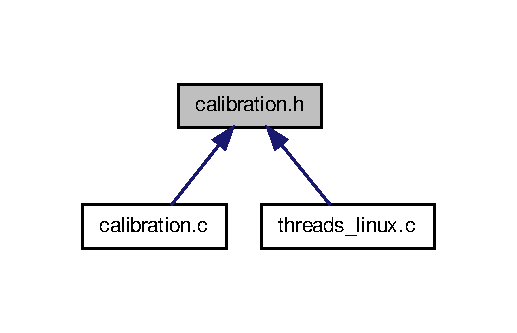
\includegraphics[width=248pt]{calibration_8h__dep__incl}
\end{center}
\end{figure}
\subsection*{Macros}
\begin{DoxyCompactItemize}
\item 
\#define \hyperlink{calibration_8h_aa90cac659d18e8ef6294c7ae337f6b58}{S\-U\-C\-C\-E\-S\-S}~1
\item 
\#define \hyperlink{calibration_8h_a6d58f9ac447476b4e084d7ca383f5183}{F\-A\-I\-L\-U\-R\-E}~-\/1
\item 
\#define \hyperlink{calibration_8h_a355ea8f6ceed1e1d419a3ea2271bfca3}{A\-C\-C\-\_\-\-B\-I\-A\-S\-\_\-\-X}~19.\-2
\item 
\#define \hyperlink{calibration_8h_a34180f1c97e84a814ef181f62bf4b68f}{A\-C\-C\-\_\-\-B\-I\-A\-S\-\_\-\-Y}~6.\-024
\item 
\#define \hyperlink{calibration_8h_a794f762650b6f228ffb8d50d1323dbea}{A\-C\-C\-\_\-\-B\-I\-A\-S\-\_\-\-Z}~-\/18.\-97
\item 
\#define \hyperlink{calibration_8h_a76e6967cb5a86ec34986b4583ac09831}{A\-C\-C\-\_\-\-F\-S\-\_\-\-X}~262.\-82
\item 
\#define \hyperlink{calibration_8h_a13d3aaab3b5800b11351cbd1246c8918}{A\-C\-C\-\_\-\-F\-S\-\_\-\-Y}~262.\-15
\item 
\#define \hyperlink{calibration_8h_af1d3370cc0958289199c8c13470602d4}{A\-C\-C\-\_\-\-F\-S\-\_\-\-Z}~252.\-20
\item 
\#define \hyperlink{calibration_8h_a33f53b04fe0f887e8d9d99e4374c0ddf}{M\-A\-G\-\_\-\-B\-I\-A\-S\-\_\-\-X}~-\/143
\item 
\#define \hyperlink{calibration_8h_a92407f4dfd1c63cede9a5307b379c569}{M\-A\-G\-\_\-\-B\-I\-A\-S\-\_\-\-Y}~-\/101
\item 
\#define \hyperlink{calibration_8h_a9662c4fff54f93bcc4e043e84e79d623}{M\-A\-G\-\_\-\-B\-I\-A\-S\-\_\-\-Z}~3
\item 
\#define \hyperlink{calibration_8h_aa49abc19ca0fda3324df06bddae2c1d4}{M\-A\-G\-\_\-\-F\-S\-\_\-\-X}~177
\item 
\#define \hyperlink{calibration_8h_a5c5e64196104a5e5ebac3c594220eb5c}{M\-A\-G\-\_\-\-F\-S\-\_\-\-Y}~139
\item 
\#define \hyperlink{calibration_8h_aebfc43ba340d89fa86b4a5c07cc7c924}{M\-A\-G\-\_\-\-F\-S\-\_\-\-Z}~85
\item 
\#define \hyperlink{calibration_8h_a69780ffe3a15aad4121fed56d5e47377}{G\-Y\-R\-\_\-\-B\-I\-A\-S\-\_\-\-X}~-\/60.\-8067
\item 
\#define \hyperlink{calibration_8h_af3264a08be995ea97ae8581128873877}{G\-Y\-R\-\_\-\-B\-I\-A\-S\-\_\-\-Y}~40.\-0800
\item 
\#define \hyperlink{calibration_8h_aa10980bbf5b1dd91704d4dab98fcf991}{G\-Y\-R\-\_\-\-B\-I\-A\-S\-\_\-\-Z}~0.\-7267
\item 
\#define \hyperlink{calibration_8h_a8fe84f8c6d39f41d8622fd0cbce3a522}{G\-Y\-R\-\_\-\-F\-S\-\_\-\-X}~0.\-001214142
\item 
\#define \hyperlink{calibration_8h_a4be2e0fa7596546bb4699862d0fe4183}{G\-Y\-R\-\_\-\-F\-S\-\_\-\-Y}~0.\-001214142
\item 
\#define \hyperlink{calibration_8h_aaee2ece0c43cc20d7c531ab79dcd06c8}{G\-Y\-R\-\_\-\-F\-S\-\_\-\-Z}~0.\-001214142
\end{DoxyCompactItemize}
\subsection*{Functions}
\begin{DoxyCompactItemize}
\item 
void \hyperlink{calibration_8h_a043045246cf217758281222214c4addc}{calibrate\-\_\-all} (\hyperlink{structIMU__DATA__STRUCT}{I\-M\-U\-\_\-\-D\-A\-T\-A\-\_\-\-S\-T\-R\-U\-C\-T} $\ast$\hyperlink{threads__linux_8c_a3cfea12cbe9ca7f1681c950e4cd68606}{imu\-\_\-data})
\item 
void \hyperlink{calibration_8h_aecfc81d152db2843b5d1517729804d63}{calibrate\-\_\-imu} (\hyperlink{structIMU__DATA__STRUCT}{I\-M\-U\-\_\-\-D\-A\-T\-A\-\_\-\-S\-T\-R\-U\-C\-T} $\ast$\hyperlink{threads__linux_8c_a3cfea12cbe9ca7f1681c950e4cd68606}{imu\-\_\-data})
\end{DoxyCompactItemize}


\subsection{Macro Definition Documentation}
\hypertarget{calibration_8h_a355ea8f6ceed1e1d419a3ea2271bfca3}{\index{calibration.\-h@{calibration.\-h}!A\-C\-C\-\_\-\-B\-I\-A\-S\-\_\-\-X@{A\-C\-C\-\_\-\-B\-I\-A\-S\-\_\-\-X}}
\index{A\-C\-C\-\_\-\-B\-I\-A\-S\-\_\-\-X@{A\-C\-C\-\_\-\-B\-I\-A\-S\-\_\-\-X}!calibration.h@{calibration.\-h}}
\subsubsection[{A\-C\-C\-\_\-\-B\-I\-A\-S\-\_\-\-X}]{\setlength{\rightskip}{0pt plus 5cm}\#define A\-C\-C\-\_\-\-B\-I\-A\-S\-\_\-\-X~19.\-2}}\label{calibration_8h_a355ea8f6ceed1e1d419a3ea2271bfca3}


Definition at line 10 of file calibration.\-h.

\hypertarget{calibration_8h_a34180f1c97e84a814ef181f62bf4b68f}{\index{calibration.\-h@{calibration.\-h}!A\-C\-C\-\_\-\-B\-I\-A\-S\-\_\-\-Y@{A\-C\-C\-\_\-\-B\-I\-A\-S\-\_\-\-Y}}
\index{A\-C\-C\-\_\-\-B\-I\-A\-S\-\_\-\-Y@{A\-C\-C\-\_\-\-B\-I\-A\-S\-\_\-\-Y}!calibration.h@{calibration.\-h}}
\subsubsection[{A\-C\-C\-\_\-\-B\-I\-A\-S\-\_\-\-Y}]{\setlength{\rightskip}{0pt plus 5cm}\#define A\-C\-C\-\_\-\-B\-I\-A\-S\-\_\-\-Y~6.\-024}}\label{calibration_8h_a34180f1c97e84a814ef181f62bf4b68f}


Definition at line 11 of file calibration.\-h.

\hypertarget{calibration_8h_a794f762650b6f228ffb8d50d1323dbea}{\index{calibration.\-h@{calibration.\-h}!A\-C\-C\-\_\-\-B\-I\-A\-S\-\_\-\-Z@{A\-C\-C\-\_\-\-B\-I\-A\-S\-\_\-\-Z}}
\index{A\-C\-C\-\_\-\-B\-I\-A\-S\-\_\-\-Z@{A\-C\-C\-\_\-\-B\-I\-A\-S\-\_\-\-Z}!calibration.h@{calibration.\-h}}
\subsubsection[{A\-C\-C\-\_\-\-B\-I\-A\-S\-\_\-\-Z}]{\setlength{\rightskip}{0pt plus 5cm}\#define A\-C\-C\-\_\-\-B\-I\-A\-S\-\_\-\-Z~-\/18.\-97}}\label{calibration_8h_a794f762650b6f228ffb8d50d1323dbea}


Definition at line 12 of file calibration.\-h.

\hypertarget{calibration_8h_a76e6967cb5a86ec34986b4583ac09831}{\index{calibration.\-h@{calibration.\-h}!A\-C\-C\-\_\-\-F\-S\-\_\-\-X@{A\-C\-C\-\_\-\-F\-S\-\_\-\-X}}
\index{A\-C\-C\-\_\-\-F\-S\-\_\-\-X@{A\-C\-C\-\_\-\-F\-S\-\_\-\-X}!calibration.h@{calibration.\-h}}
\subsubsection[{A\-C\-C\-\_\-\-F\-S\-\_\-\-X}]{\setlength{\rightskip}{0pt plus 5cm}\#define A\-C\-C\-\_\-\-F\-S\-\_\-\-X~262.\-82}}\label{calibration_8h_a76e6967cb5a86ec34986b4583ac09831}


Definition at line 13 of file calibration.\-h.

\hypertarget{calibration_8h_a13d3aaab3b5800b11351cbd1246c8918}{\index{calibration.\-h@{calibration.\-h}!A\-C\-C\-\_\-\-F\-S\-\_\-\-Y@{A\-C\-C\-\_\-\-F\-S\-\_\-\-Y}}
\index{A\-C\-C\-\_\-\-F\-S\-\_\-\-Y@{A\-C\-C\-\_\-\-F\-S\-\_\-\-Y}!calibration.h@{calibration.\-h}}
\subsubsection[{A\-C\-C\-\_\-\-F\-S\-\_\-\-Y}]{\setlength{\rightskip}{0pt plus 5cm}\#define A\-C\-C\-\_\-\-F\-S\-\_\-\-Y~262.\-15}}\label{calibration_8h_a13d3aaab3b5800b11351cbd1246c8918}


Definition at line 14 of file calibration.\-h.

\hypertarget{calibration_8h_af1d3370cc0958289199c8c13470602d4}{\index{calibration.\-h@{calibration.\-h}!A\-C\-C\-\_\-\-F\-S\-\_\-\-Z@{A\-C\-C\-\_\-\-F\-S\-\_\-\-Z}}
\index{A\-C\-C\-\_\-\-F\-S\-\_\-\-Z@{A\-C\-C\-\_\-\-F\-S\-\_\-\-Z}!calibration.h@{calibration.\-h}}
\subsubsection[{A\-C\-C\-\_\-\-F\-S\-\_\-\-Z}]{\setlength{\rightskip}{0pt plus 5cm}\#define A\-C\-C\-\_\-\-F\-S\-\_\-\-Z~252.\-20}}\label{calibration_8h_af1d3370cc0958289199c8c13470602d4}


Definition at line 15 of file calibration.\-h.

\hypertarget{calibration_8h_a6d58f9ac447476b4e084d7ca383f5183}{\index{calibration.\-h@{calibration.\-h}!F\-A\-I\-L\-U\-R\-E@{F\-A\-I\-L\-U\-R\-E}}
\index{F\-A\-I\-L\-U\-R\-E@{F\-A\-I\-L\-U\-R\-E}!calibration.h@{calibration.\-h}}
\subsubsection[{F\-A\-I\-L\-U\-R\-E}]{\setlength{\rightskip}{0pt plus 5cm}\#define F\-A\-I\-L\-U\-R\-E~-\/1}}\label{calibration_8h_a6d58f9ac447476b4e084d7ca383f5183}


Definition at line 7 of file calibration.\-h.

\hypertarget{calibration_8h_a69780ffe3a15aad4121fed56d5e47377}{\index{calibration.\-h@{calibration.\-h}!G\-Y\-R\-\_\-\-B\-I\-A\-S\-\_\-\-X@{G\-Y\-R\-\_\-\-B\-I\-A\-S\-\_\-\-X}}
\index{G\-Y\-R\-\_\-\-B\-I\-A\-S\-\_\-\-X@{G\-Y\-R\-\_\-\-B\-I\-A\-S\-\_\-\-X}!calibration.h@{calibration.\-h}}
\subsubsection[{G\-Y\-R\-\_\-\-B\-I\-A\-S\-\_\-\-X}]{\setlength{\rightskip}{0pt plus 5cm}\#define G\-Y\-R\-\_\-\-B\-I\-A\-S\-\_\-\-X~-\/60.\-8067}}\label{calibration_8h_a69780ffe3a15aad4121fed56d5e47377}


Definition at line 25 of file calibration.\-h.

\hypertarget{calibration_8h_af3264a08be995ea97ae8581128873877}{\index{calibration.\-h@{calibration.\-h}!G\-Y\-R\-\_\-\-B\-I\-A\-S\-\_\-\-Y@{G\-Y\-R\-\_\-\-B\-I\-A\-S\-\_\-\-Y}}
\index{G\-Y\-R\-\_\-\-B\-I\-A\-S\-\_\-\-Y@{G\-Y\-R\-\_\-\-B\-I\-A\-S\-\_\-\-Y}!calibration.h@{calibration.\-h}}
\subsubsection[{G\-Y\-R\-\_\-\-B\-I\-A\-S\-\_\-\-Y}]{\setlength{\rightskip}{0pt plus 5cm}\#define G\-Y\-R\-\_\-\-B\-I\-A\-S\-\_\-\-Y~40.\-0800}}\label{calibration_8h_af3264a08be995ea97ae8581128873877}


Definition at line 26 of file calibration.\-h.

\hypertarget{calibration_8h_aa10980bbf5b1dd91704d4dab98fcf991}{\index{calibration.\-h@{calibration.\-h}!G\-Y\-R\-\_\-\-B\-I\-A\-S\-\_\-\-Z@{G\-Y\-R\-\_\-\-B\-I\-A\-S\-\_\-\-Z}}
\index{G\-Y\-R\-\_\-\-B\-I\-A\-S\-\_\-\-Z@{G\-Y\-R\-\_\-\-B\-I\-A\-S\-\_\-\-Z}!calibration.h@{calibration.\-h}}
\subsubsection[{G\-Y\-R\-\_\-\-B\-I\-A\-S\-\_\-\-Z}]{\setlength{\rightskip}{0pt plus 5cm}\#define G\-Y\-R\-\_\-\-B\-I\-A\-S\-\_\-\-Z~0.\-7267}}\label{calibration_8h_aa10980bbf5b1dd91704d4dab98fcf991}


Definition at line 27 of file calibration.\-h.

\hypertarget{calibration_8h_a8fe84f8c6d39f41d8622fd0cbce3a522}{\index{calibration.\-h@{calibration.\-h}!G\-Y\-R\-\_\-\-F\-S\-\_\-\-X@{G\-Y\-R\-\_\-\-F\-S\-\_\-\-X}}
\index{G\-Y\-R\-\_\-\-F\-S\-\_\-\-X@{G\-Y\-R\-\_\-\-F\-S\-\_\-\-X}!calibration.h@{calibration.\-h}}
\subsubsection[{G\-Y\-R\-\_\-\-F\-S\-\_\-\-X}]{\setlength{\rightskip}{0pt plus 5cm}\#define G\-Y\-R\-\_\-\-F\-S\-\_\-\-X~0.\-001214142}}\label{calibration_8h_a8fe84f8c6d39f41d8622fd0cbce3a522}


Definition at line 28 of file calibration.\-h.

\hypertarget{calibration_8h_a4be2e0fa7596546bb4699862d0fe4183}{\index{calibration.\-h@{calibration.\-h}!G\-Y\-R\-\_\-\-F\-S\-\_\-\-Y@{G\-Y\-R\-\_\-\-F\-S\-\_\-\-Y}}
\index{G\-Y\-R\-\_\-\-F\-S\-\_\-\-Y@{G\-Y\-R\-\_\-\-F\-S\-\_\-\-Y}!calibration.h@{calibration.\-h}}
\subsubsection[{G\-Y\-R\-\_\-\-F\-S\-\_\-\-Y}]{\setlength{\rightskip}{0pt plus 5cm}\#define G\-Y\-R\-\_\-\-F\-S\-\_\-\-Y~0.\-001214142}}\label{calibration_8h_a4be2e0fa7596546bb4699862d0fe4183}


Definition at line 29 of file calibration.\-h.

\hypertarget{calibration_8h_aaee2ece0c43cc20d7c531ab79dcd06c8}{\index{calibration.\-h@{calibration.\-h}!G\-Y\-R\-\_\-\-F\-S\-\_\-\-Z@{G\-Y\-R\-\_\-\-F\-S\-\_\-\-Z}}
\index{G\-Y\-R\-\_\-\-F\-S\-\_\-\-Z@{G\-Y\-R\-\_\-\-F\-S\-\_\-\-Z}!calibration.h@{calibration.\-h}}
\subsubsection[{G\-Y\-R\-\_\-\-F\-S\-\_\-\-Z}]{\setlength{\rightskip}{0pt plus 5cm}\#define G\-Y\-R\-\_\-\-F\-S\-\_\-\-Z~0.\-001214142}}\label{calibration_8h_aaee2ece0c43cc20d7c531ab79dcd06c8}


Definition at line 30 of file calibration.\-h.

\hypertarget{calibration_8h_a33f53b04fe0f887e8d9d99e4374c0ddf}{\index{calibration.\-h@{calibration.\-h}!M\-A\-G\-\_\-\-B\-I\-A\-S\-\_\-\-X@{M\-A\-G\-\_\-\-B\-I\-A\-S\-\_\-\-X}}
\index{M\-A\-G\-\_\-\-B\-I\-A\-S\-\_\-\-X@{M\-A\-G\-\_\-\-B\-I\-A\-S\-\_\-\-X}!calibration.h@{calibration.\-h}}
\subsubsection[{M\-A\-G\-\_\-\-B\-I\-A\-S\-\_\-\-X}]{\setlength{\rightskip}{0pt plus 5cm}\#define M\-A\-G\-\_\-\-B\-I\-A\-S\-\_\-\-X~-\/143}}\label{calibration_8h_a33f53b04fe0f887e8d9d99e4374c0ddf}


Definition at line 17 of file calibration.\-h.

\hypertarget{calibration_8h_a92407f4dfd1c63cede9a5307b379c569}{\index{calibration.\-h@{calibration.\-h}!M\-A\-G\-\_\-\-B\-I\-A\-S\-\_\-\-Y@{M\-A\-G\-\_\-\-B\-I\-A\-S\-\_\-\-Y}}
\index{M\-A\-G\-\_\-\-B\-I\-A\-S\-\_\-\-Y@{M\-A\-G\-\_\-\-B\-I\-A\-S\-\_\-\-Y}!calibration.h@{calibration.\-h}}
\subsubsection[{M\-A\-G\-\_\-\-B\-I\-A\-S\-\_\-\-Y}]{\setlength{\rightskip}{0pt plus 5cm}\#define M\-A\-G\-\_\-\-B\-I\-A\-S\-\_\-\-Y~-\/101}}\label{calibration_8h_a92407f4dfd1c63cede9a5307b379c569}


Definition at line 18 of file calibration.\-h.

\hypertarget{calibration_8h_a9662c4fff54f93bcc4e043e84e79d623}{\index{calibration.\-h@{calibration.\-h}!M\-A\-G\-\_\-\-B\-I\-A\-S\-\_\-\-Z@{M\-A\-G\-\_\-\-B\-I\-A\-S\-\_\-\-Z}}
\index{M\-A\-G\-\_\-\-B\-I\-A\-S\-\_\-\-Z@{M\-A\-G\-\_\-\-B\-I\-A\-S\-\_\-\-Z}!calibration.h@{calibration.\-h}}
\subsubsection[{M\-A\-G\-\_\-\-B\-I\-A\-S\-\_\-\-Z}]{\setlength{\rightskip}{0pt plus 5cm}\#define M\-A\-G\-\_\-\-B\-I\-A\-S\-\_\-\-Z~3}}\label{calibration_8h_a9662c4fff54f93bcc4e043e84e79d623}


Definition at line 19 of file calibration.\-h.

\hypertarget{calibration_8h_aa49abc19ca0fda3324df06bddae2c1d4}{\index{calibration.\-h@{calibration.\-h}!M\-A\-G\-\_\-\-F\-S\-\_\-\-X@{M\-A\-G\-\_\-\-F\-S\-\_\-\-X}}
\index{M\-A\-G\-\_\-\-F\-S\-\_\-\-X@{M\-A\-G\-\_\-\-F\-S\-\_\-\-X}!calibration.h@{calibration.\-h}}
\subsubsection[{M\-A\-G\-\_\-\-F\-S\-\_\-\-X}]{\setlength{\rightskip}{0pt plus 5cm}\#define M\-A\-G\-\_\-\-F\-S\-\_\-\-X~177}}\label{calibration_8h_aa49abc19ca0fda3324df06bddae2c1d4}


Definition at line 20 of file calibration.\-h.

\hypertarget{calibration_8h_a5c5e64196104a5e5ebac3c594220eb5c}{\index{calibration.\-h@{calibration.\-h}!M\-A\-G\-\_\-\-F\-S\-\_\-\-Y@{M\-A\-G\-\_\-\-F\-S\-\_\-\-Y}}
\index{M\-A\-G\-\_\-\-F\-S\-\_\-\-Y@{M\-A\-G\-\_\-\-F\-S\-\_\-\-Y}!calibration.h@{calibration.\-h}}
\subsubsection[{M\-A\-G\-\_\-\-F\-S\-\_\-\-Y}]{\setlength{\rightskip}{0pt plus 5cm}\#define M\-A\-G\-\_\-\-F\-S\-\_\-\-Y~139}}\label{calibration_8h_a5c5e64196104a5e5ebac3c594220eb5c}


Definition at line 21 of file calibration.\-h.

\hypertarget{calibration_8h_aebfc43ba340d89fa86b4a5c07cc7c924}{\index{calibration.\-h@{calibration.\-h}!M\-A\-G\-\_\-\-F\-S\-\_\-\-Z@{M\-A\-G\-\_\-\-F\-S\-\_\-\-Z}}
\index{M\-A\-G\-\_\-\-F\-S\-\_\-\-Z@{M\-A\-G\-\_\-\-F\-S\-\_\-\-Z}!calibration.h@{calibration.\-h}}
\subsubsection[{M\-A\-G\-\_\-\-F\-S\-\_\-\-Z}]{\setlength{\rightskip}{0pt plus 5cm}\#define M\-A\-G\-\_\-\-F\-S\-\_\-\-Z~85}}\label{calibration_8h_aebfc43ba340d89fa86b4a5c07cc7c924}


Definition at line 22 of file calibration.\-h.

\hypertarget{calibration_8h_aa90cac659d18e8ef6294c7ae337f6b58}{\index{calibration.\-h@{calibration.\-h}!S\-U\-C\-C\-E\-S\-S@{S\-U\-C\-C\-E\-S\-S}}
\index{S\-U\-C\-C\-E\-S\-S@{S\-U\-C\-C\-E\-S\-S}!calibration.h@{calibration.\-h}}
\subsubsection[{S\-U\-C\-C\-E\-S\-S}]{\setlength{\rightskip}{0pt plus 5cm}\#define S\-U\-C\-C\-E\-S\-S~1}}\label{calibration_8h_aa90cac659d18e8ef6294c7ae337f6b58}


Definition at line 6 of file calibration.\-h.



\subsection{Function Documentation}
\hypertarget{calibration_8h_a043045246cf217758281222214c4addc}{\index{calibration.\-h@{calibration.\-h}!calibrate\-\_\-all@{calibrate\-\_\-all}}
\index{calibrate\-\_\-all@{calibrate\-\_\-all}!calibration.h@{calibration.\-h}}
\subsubsection[{calibrate\-\_\-all}]{\setlength{\rightskip}{0pt plus 5cm}void calibrate\-\_\-all (
\begin{DoxyParamCaption}
\item[{{\bf I\-M\-U\-\_\-\-D\-A\-T\-A\-\_\-\-S\-T\-R\-U\-C\-T} $\ast$}]{imu\-\_\-data}
\end{DoxyParamCaption}
)}}\label{calibration_8h_a043045246cf217758281222214c4addc}


Definition at line 8 of file calibration.\-c.



References calibrate\-\_\-imu().


\begin{DoxyCode}
\{
  \hyperlink{calibration_2calibration_8c_aecfc81d152db2843b5d1517729804d63}{calibrate\_imu}(imu\_data);
  \textcolor{keywordflow}{return};
\}
\end{DoxyCode}


Here is the call graph for this function\-:\nopagebreak
\begin{figure}[H]
\begin{center}
\leavevmode
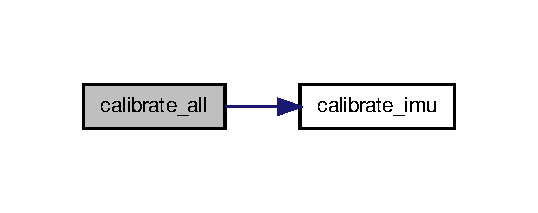
\includegraphics[width=258pt]{calibration_8h_a043045246cf217758281222214c4addc_cgraph}
\end{center}
\end{figure}


\hypertarget{calibration_8h_aecfc81d152db2843b5d1517729804d63}{\index{calibration.\-h@{calibration.\-h}!calibrate\-\_\-imu@{calibrate\-\_\-imu}}
\index{calibrate\-\_\-imu@{calibrate\-\_\-imu}!calibration.h@{calibration.\-h}}
\subsubsection[{calibrate\-\_\-imu}]{\setlength{\rightskip}{0pt plus 5cm}void calibrate\-\_\-imu (
\begin{DoxyParamCaption}
\item[{{\bf I\-M\-U\-\_\-\-D\-A\-T\-A\-\_\-\-S\-T\-R\-U\-C\-T} $\ast$}]{imu\-\_\-data}
\end{DoxyParamCaption}
)}}\label{calibration_8h_aecfc81d152db2843b5d1517729804d63}


Definition at line 14 of file calibration.\-c.



References I\-M\-U\-\_\-\-D\-A\-T\-A\-\_\-\-S\-T\-R\-U\-C\-T\-::acc, I\-M\-U\-\_\-\-D\-A\-T\-A\-\_\-\-S\-T\-R\-U\-C\-T\-::calibrated\-::acc, A\-C\-C\-\_\-\-B\-I\-A\-S\-\_\-\-X, A\-C\-C\-\_\-\-B\-I\-A\-S\-\_\-\-Y, A\-C\-C\-\_\-\-B\-I\-A\-S\-\_\-\-Z, A\-C\-C\-\_\-\-F\-S\-\_\-\-X, A\-C\-C\-\_\-\-F\-S\-\_\-\-Y, A\-C\-C\-\_\-\-F\-S\-\_\-\-Z, I\-M\-U\-\_\-\-D\-A\-T\-A\-\_\-\-S\-T\-R\-U\-C\-T\-::calib, I\-M\-U\-\_\-\-D\-A\-T\-A\-\_\-\-S\-T\-R\-U\-C\-T\-::calib\-\_\-temp, I\-M\-U\-\_\-\-D\-A\-T\-A\-\_\-\-S\-T\-R\-U\-C\-T\-::gyr, I\-M\-U\-\_\-\-D\-A\-T\-A\-\_\-\-S\-T\-R\-U\-C\-T\-::calibrated\-::gyr, G\-Y\-R\-\_\-\-B\-I\-A\-S\-\_\-\-X, G\-Y\-R\-\_\-\-B\-I\-A\-S\-\_\-\-Y, G\-Y\-R\-\_\-\-B\-I\-A\-S\-\_\-\-Z, G\-Y\-R\-\_\-\-F\-S\-\_\-\-X, G\-Y\-R\-\_\-\-F\-S\-\_\-\-Y, G\-Y\-R\-\_\-\-F\-S\-\_\-\-Z, I\-M\-U\-\_\-\-D\-A\-T\-A\-\_\-\-S\-T\-R\-U\-C\-T\-::mag, I\-M\-U\-\_\-\-D\-A\-T\-A\-\_\-\-S\-T\-R\-U\-C\-T\-::calibrated\-::mag, M\-A\-G\-\_\-\-B\-I\-A\-S\-\_\-\-X, M\-A\-G\-\_\-\-B\-I\-A\-S\-\_\-\-Y, M\-A\-G\-\_\-\-B\-I\-A\-S\-\_\-\-Z, M\-A\-G\-\_\-\-F\-S\-\_\-\-X, M\-A\-G\-\_\-\-F\-S\-\_\-\-Y, M\-A\-G\-\_\-\-F\-S\-\_\-\-Z, I\-M\-U\-\_\-\-D\-A\-T\-A\-\_\-\-S\-T\-R\-U\-C\-T\-::temp, D\-A\-T\-A\-\_\-\-X\-Y\-Z\-::x, D\-A\-T\-A\-\_\-\-X\-Y\-Z\-\_\-\-D\-O\-U\-B\-L\-E\-::x, D\-A\-T\-A\-\_\-\-X\-Y\-Z\-::y, D\-A\-T\-A\-\_\-\-X\-Y\-Z\-\_\-\-D\-O\-U\-B\-L\-E\-::y, D\-A\-T\-A\-\_\-\-X\-Y\-Z\-::z, and D\-A\-T\-A\-\_\-\-X\-Y\-Z\-\_\-\-D\-O\-U\-B\-L\-E\-::z.



Referenced by calibrate\-\_\-all().


\begin{DoxyCode}
\{
  \textcolor{comment}{// With this parameters, the vectors of acceleration and magnetic field will
       have norm = 1 theorically (i.e. in g or G)}
  imu\_data->\hyperlink{structIMU__DATA__STRUCT_aeffe3c3c5a7191a5cef16e7aab6c3795}{calib}.\hyperlink{structIMU__DATA__STRUCT_1_1calibrated_a281a7fdb40a05ed97388f18b9bb90c81}{acc}.\hyperlink{structDATA__XYZ__DOUBLE_a22868cc99a423900e7b82d015a5eb91f}{x} = ((double)imu\_data->\hyperlink{structIMU__DATA__STRUCT_a448f284bf44eb503affda586ad5fa9d2}{acc}.\hyperlink{structDATA__XYZ_a54c1596e9f9969fd9c21e8458024ecfb}{x}-\hyperlink{calibration_2calibration_8h_a355ea8f6ceed1e1d419a3ea2271bfca3}{ACC\_BIAS\_X}
      )/\hyperlink{calibration_2calibration_8h_a76e6967cb5a86ec34986b4583ac09831}{ACC\_FS\_X};
  imu\_data->\hyperlink{structIMU__DATA__STRUCT_aeffe3c3c5a7191a5cef16e7aab6c3795}{calib}.\hyperlink{structIMU__DATA__STRUCT_1_1calibrated_a281a7fdb40a05ed97388f18b9bb90c81}{acc}.\hyperlink{structDATA__XYZ__DOUBLE_a198a27b5df3b5b0bf461b0e481e22a82}{y} = ((double)imu\_data->\hyperlink{structIMU__DATA__STRUCT_a448f284bf44eb503affda586ad5fa9d2}{acc}.\hyperlink{structDATA__XYZ_a94bbb1c889bf53eb6a5fffa2b39322cf}{y}-\hyperlink{calibration_2calibration_8h_a34180f1c97e84a814ef181f62bf4b68f}{ACC\_BIAS\_Y}
      )/\hyperlink{calibration_2calibration_8h_a13d3aaab3b5800b11351cbd1246c8918}{ACC\_FS\_Y};
  imu\_data->\hyperlink{structIMU__DATA__STRUCT_aeffe3c3c5a7191a5cef16e7aab6c3795}{calib}.\hyperlink{structIMU__DATA__STRUCT_1_1calibrated_a281a7fdb40a05ed97388f18b9bb90c81}{acc}.\hyperlink{structDATA__XYZ__DOUBLE_a9556e8868c223ff3e28756ea18a284c0}{z} = ((double)imu\_data->\hyperlink{structIMU__DATA__STRUCT_a448f284bf44eb503affda586ad5fa9d2}{acc}.\hyperlink{structDATA__XYZ_a69e89ab0ec6e5d72fc5d54f62cc07fb5}{z}-\hyperlink{calibration_2calibration_8h_a794f762650b6f228ffb8d50d1323dbea}{ACC\_BIAS\_Z}
      )/\hyperlink{calibration_2calibration_8h_af1d3370cc0958289199c8c13470602d4}{ACC\_FS\_Z};
  
  imu\_data->\hyperlink{structIMU__DATA__STRUCT_aeffe3c3c5a7191a5cef16e7aab6c3795}{calib}.\hyperlink{structIMU__DATA__STRUCT_1_1calibrated_a2fde6c6759e0fda17e272c32096cb9ec}{mag}.\hyperlink{structDATA__XYZ__DOUBLE_a22868cc99a423900e7b82d015a5eb91f}{x} = ((double)imu\_data->\hyperlink{structIMU__DATA__STRUCT_a40c7df8b6d49297aa52873cfd9b60daa}{mag}.\hyperlink{structDATA__XYZ_a54c1596e9f9969fd9c21e8458024ecfb}{x}-\hyperlink{calibration_2calibration_8h_a355ea8f6ceed1e1d419a3ea2271bfca3}{ACC\_BIAS\_X}
      )/\hyperlink{calibration_2calibration_8h_a76e6967cb5a86ec34986b4583ac09831}{ACC\_FS\_X};
  imu\_data->\hyperlink{structIMU__DATA__STRUCT_aeffe3c3c5a7191a5cef16e7aab6c3795}{calib}.\hyperlink{structIMU__DATA__STRUCT_1_1calibrated_a2fde6c6759e0fda17e272c32096cb9ec}{mag}.\hyperlink{structDATA__XYZ__DOUBLE_a198a27b5df3b5b0bf461b0e481e22a82}{y} = ((double)imu\_data->\hyperlink{structIMU__DATA__STRUCT_a40c7df8b6d49297aa52873cfd9b60daa}{mag}.\hyperlink{structDATA__XYZ_a94bbb1c889bf53eb6a5fffa2b39322cf}{y}-\hyperlink{calibration_2calibration_8h_a34180f1c97e84a814ef181f62bf4b68f}{ACC\_BIAS\_Y}
      )/\hyperlink{calibration_2calibration_8h_a13d3aaab3b5800b11351cbd1246c8918}{ACC\_FS\_Y};
  imu\_data->\hyperlink{structIMU__DATA__STRUCT_aeffe3c3c5a7191a5cef16e7aab6c3795}{calib}.\hyperlink{structIMU__DATA__STRUCT_1_1calibrated_a2fde6c6759e0fda17e272c32096cb9ec}{mag}.\hyperlink{structDATA__XYZ__DOUBLE_a9556e8868c223ff3e28756ea18a284c0}{z} = ((double)imu\_data->\hyperlink{structIMU__DATA__STRUCT_a40c7df8b6d49297aa52873cfd9b60daa}{mag}.\hyperlink{structDATA__XYZ_a69e89ab0ec6e5d72fc5d54f62cc07fb5}{z}-\hyperlink{calibration_2calibration_8h_a794f762650b6f228ffb8d50d1323dbea}{ACC\_BIAS\_Z}
      )/\hyperlink{calibration_2calibration_8h_af1d3370cc0958289199c8c13470602d4}{ACC\_FS\_Z};
  
  \textcolor{comment}{// With this parameters, we consider right datasheet scale and we get in
       rad/s}
  imu\_data->\hyperlink{structIMU__DATA__STRUCT_aeffe3c3c5a7191a5cef16e7aab6c3795}{calib}.\hyperlink{structIMU__DATA__STRUCT_1_1calibrated_a8a54aded6ce608f1b7d2b4a0c52c248b}{gyr}.\hyperlink{structDATA__XYZ__DOUBLE_a22868cc99a423900e7b82d015a5eb91f}{x} = ((double)imu\_data->\hyperlink{structIMU__DATA__STRUCT_a0c1ac26626e4434a2ee124a1928a23a1}{gyr}.\hyperlink{structDATA__XYZ_a54c1596e9f9969fd9c21e8458024ecfb}{x}-\hyperlink{calibration_2calibration_8h_a69780ffe3a15aad4121fed56d5e47377}{GYR\_BIAS\_X}
      )/\hyperlink{calibration_2calibration_8h_a8fe84f8c6d39f41d8622fd0cbce3a522}{GYR\_FS\_X};
  imu\_data->\hyperlink{structIMU__DATA__STRUCT_aeffe3c3c5a7191a5cef16e7aab6c3795}{calib}.\hyperlink{structIMU__DATA__STRUCT_1_1calibrated_a8a54aded6ce608f1b7d2b4a0c52c248b}{gyr}.\hyperlink{structDATA__XYZ__DOUBLE_a198a27b5df3b5b0bf461b0e481e22a82}{y} = ((double)imu\_data->\hyperlink{structIMU__DATA__STRUCT_a0c1ac26626e4434a2ee124a1928a23a1}{gyr}.\hyperlink{structDATA__XYZ_a94bbb1c889bf53eb6a5fffa2b39322cf}{y}-\hyperlink{calibration_2calibration_8h_a69780ffe3a15aad4121fed56d5e47377}{GYR\_BIAS\_X}
      )/\hyperlink{calibration_2calibration_8h_a4be2e0fa7596546bb4699862d0fe4183}{GYR\_FS\_Y};
  imu\_data->\hyperlink{structIMU__DATA__STRUCT_aeffe3c3c5a7191a5cef16e7aab6c3795}{calib}.\hyperlink{structIMU__DATA__STRUCT_1_1calibrated_a8a54aded6ce608f1b7d2b4a0c52c248b}{gyr}.\hyperlink{structDATA__XYZ__DOUBLE_a9556e8868c223ff3e28756ea18a284c0}{z} = ((double)imu\_data->\hyperlink{structIMU__DATA__STRUCT_a0c1ac26626e4434a2ee124a1928a23a1}{gyr}.\hyperlink{structDATA__XYZ_a69e89ab0ec6e5d72fc5d54f62cc07fb5}{z}-\hyperlink{calibration_2calibration_8h_a69780ffe3a15aad4121fed56d5e47377}{GYR\_BIAS\_X}
      )/\hyperlink{calibration_2calibration_8h_aaee2ece0c43cc20d7c531ab79dcd06c8}{GYR\_FS\_Z};
  
  \textcolor{keywordflow}{return};
\}
\end{DoxyCode}


Here is the caller graph for this function\-:\nopagebreak
\begin{figure}[H]
\begin{center}
\leavevmode
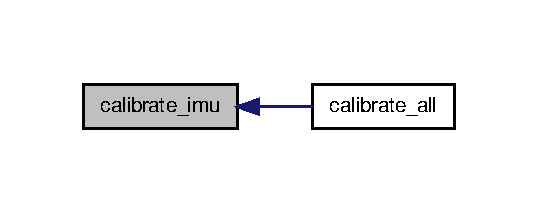
\includegraphics[width=258pt]{calibration_8h_aecfc81d152db2843b5d1517729804d63_icgraph}
\end{center}
\end{figure}



\hypertarget{communication_2acc__functions_8c}{\section{communication/acc\-\_\-functions.c File Reference}
\label{communication_2acc__functions_8c}\index{communication/acc\-\_\-functions.\-c@{communication/acc\-\_\-functions.\-c}}
}
{\ttfamily \#include \char`\"{}imu\-\_\-functions.\-h\char`\"{}}\\*
Include dependency graph for acc\-\_\-functions.\-c\-:\nopagebreak
\begin{figure}[H]
\begin{center}
\leavevmode
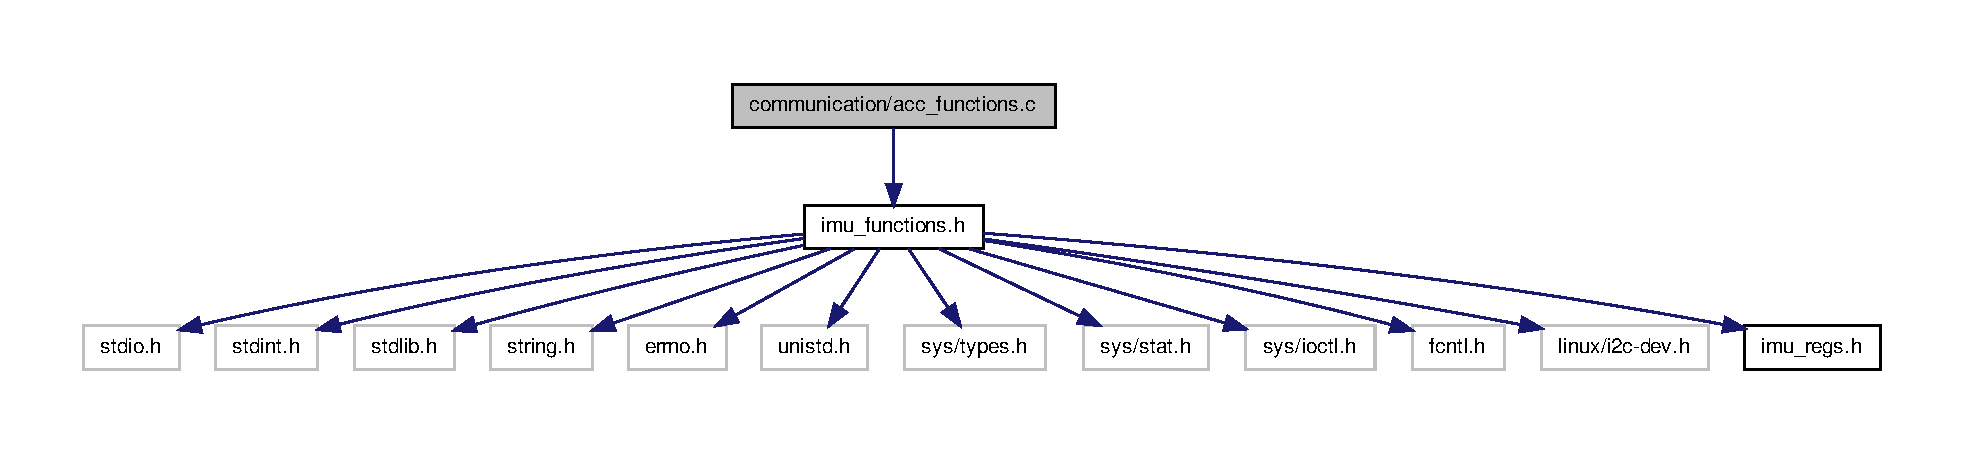
\includegraphics[width=350pt]{communication_2acc__functions_8c__incl}
\end{center}
\end{figure}
\subsection*{Functions}
\begin{DoxyCompactItemize}
\item 
int \hyperlink{group__acc_gae8f9cc6e0d15e61039d846305f86f073}{acc\-\_\-init} (int \hyperlink{CommunicationV0_2communication_8c_a7751bd45ac1064efb35adf1f19c25db8}{i2c\-\_\-dev}, uint8\-\_\-t full\-\_\-res, uint16\-\_\-t rate, uint8\-\_\-t range)
\begin{DoxyCompactList}\small\item\em Rev 0 -\/ 11/11/2012 R\-L\-E\-G project -\/ 2012. \end{DoxyCompactList}\item 
int \hyperlink{group__acc_ga534116416343122de29a5b6ade6876bd}{acc\-\_\-write\-\_\-reg} (int \hyperlink{CommunicationV0_2communication_8c_a7751bd45ac1064efb35adf1f19c25db8}{i2c\-\_\-dev}, uint8\-\_\-t reg, uint8\-\_\-t data)
\begin{DoxyCompactList}\small\item\em W\-R\-I\-T\-E T\-O R\-E\-G\-I\-S\-T\-E\-R. \end{DoxyCompactList}\item 
uint8\-\_\-t $\ast$ \hyperlink{group__acc_ga2a91c44eebbe44f4d3b8c508633512f9}{acc\-\_\-read\-\_\-reg} (int \hyperlink{CommunicationV0_2communication_8c_a7751bd45ac1064efb35adf1f19c25db8}{i2c\-\_\-dev}, uint8\-\_\-t reg, uint8\-\_\-t count)
\begin{DoxyCompactList}\small\item\em R\-E\-A\-D C\-O\-U\-N\-T 8-\/\-B\-I\-T R\-E\-G\-I\-S\-T\-E\-R I\-N S\-E\-Q\-U\-E\-N\-C\-E \end{DoxyCompactList}\item 
short int \hyperlink{group__acc_ga041d6953f2bfc8c5efa4d5bbac812305}{acc\-\_\-read\-\_\-data} (int \hyperlink{CommunicationV0_2communication_8c_a7751bd45ac1064efb35adf1f19c25db8}{i2c\-\_\-dev}, int axis)
\begin{DoxyCompactList}\small\item\em R\-E\-A\-D D\-A\-T\-A (X, Y or Z) \end{DoxyCompactList}\item 
int \hyperlink{group__acc_ga013bb5ed8a763883fc440549d2b1a6ce}{acc\-\_\-read\-\_\-all\-\_\-data} (int \hyperlink{CommunicationV0_2communication_8c_a7751bd45ac1064efb35adf1f19c25db8}{i2c\-\_\-dev}, short int $\ast$data)
\begin{DoxyCompactList}\small\item\em R\-E\-A\-D A\-L\-L D\-A\-T\-A A\-T O\-N\-C\-E (X, Y and Z) \end{DoxyCompactList}\item 
char $\ast$ \hyperlink{communication_2acc__functions_8c_a1a6b2f719b4fef8f97d6d1b8f495148e}{conv\-\_\-byte\-\_\-hex\-\_\-bin} (uint8\-\_\-t $\ast$hvalue)
\item 
int \hyperlink{group__acc_ga8509cccabb08e7267677f66f25718731}{acc\-\_\-read\-\_\-all\-\_\-reg} (int \hyperlink{CommunicationV0_2communication_8c_a7751bd45ac1064efb35adf1f19c25db8}{i2c\-\_\-dev})
\begin{DoxyCompactList}\small\item\em Read all accelerometer data and print in stdio. \end{DoxyCompactList}\end{DoxyCompactItemize}


\subsection{Function Documentation}
\hypertarget{communication_2acc__functions_8c_a1a6b2f719b4fef8f97d6d1b8f495148e}{\index{communication/acc\-\_\-functions.\-c@{communication/acc\-\_\-functions.\-c}!conv\-\_\-byte\-\_\-hex\-\_\-bin@{conv\-\_\-byte\-\_\-hex\-\_\-bin}}
\index{conv\-\_\-byte\-\_\-hex\-\_\-bin@{conv\-\_\-byte\-\_\-hex\-\_\-bin}!communication/acc_functions.c@{communication/acc\-\_\-functions.\-c}}
\subsubsection[{conv\-\_\-byte\-\_\-hex\-\_\-bin}]{\setlength{\rightskip}{0pt plus 5cm}char$\ast$ conv\-\_\-byte\-\_\-hex\-\_\-bin (
\begin{DoxyParamCaption}
\item[{uint8\-\_\-t $\ast$}]{hvalue}
\end{DoxyParamCaption}
)}}\label{communication_2acc__functions_8c_a1a6b2f719b4fef8f97d6d1b8f495148e}


Definition at line 184 of file acc\-\_\-functions.\-c.



Referenced by acc\-\_\-read\-\_\-all\-\_\-reg().


\begin{DoxyCode}
\{
  \textcolor{keywordtype}{char} \hyperlink{communication_2spi__functions_8c_a46a6da6b1936191571fd30b2a749f38c}{bits}[9];
  \textcolor{keywordtype}{int} i;
  \textcolor{keywordflow}{for}( i=0; i<8; i++)
  \{
    bits[i]=((*hvalue)<<i)>>7+\hyperlink{communication_2imu__functions_8h_aa3f75ad2972ec8996ce5206feac0e52c}{ASCII\_0};
  \}
  bits[8]=\textcolor{charliteral}{'\(\backslash\)0'};
  \textcolor{keywordflow}{return} \hyperlink{communication_2spi__functions_8c_a46a6da6b1936191571fd30b2a749f38c}{bits};
\}
\end{DoxyCode}


Here is the caller graph for this function\-:\nopagebreak
\begin{figure}[H]
\begin{center}
\leavevmode
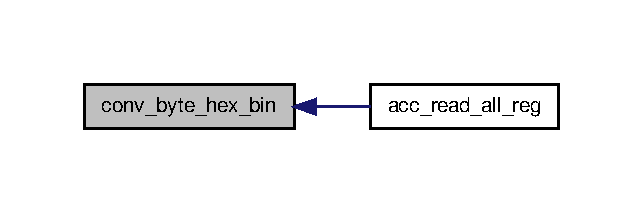
\includegraphics[width=308pt]{communication_2acc__functions_8c_a1a6b2f719b4fef8f97d6d1b8f495148e_icgraph}
\end{center}
\end{figure}



\hypertarget{CommunicationV0_2acc__functions_8c}{\section{Communication\-V0/acc\-\_\-functions.c File Reference}
\label{CommunicationV0_2acc__functions_8c}\index{Communication\-V0/acc\-\_\-functions.\-c@{Communication\-V0/acc\-\_\-functions.\-c}}
}
{\ttfamily \#include \char`\"{}imu\-\_\-functions.\-h\char`\"{}}\\*
\subsection*{Functions}
\begin{DoxyCompactItemize}
\item 
int \hyperlink{group__acc_gae8f9cc6e0d15e61039d846305f86f073}{acc\-\_\-init} (int \hyperlink{CommunicationV0_2communication_8c_a7751bd45ac1064efb35adf1f19c25db8}{i2c\-\_\-dev}, uint8\-\_\-t full\-\_\-res, uint16\-\_\-t rate, uint8\-\_\-t range)
\begin{DoxyCompactList}\small\item\em I\-N\-I\-T\-I\-A\-L\-I\-Z\-E A\-C\-C\-E\-L\-E\-R\-O\-M\-E\-T\-E\-R. \end{DoxyCompactList}\item 
int \hyperlink{group__acc_ga534116416343122de29a5b6ade6876bd}{acc\-\_\-write\-\_\-reg} (int \hyperlink{CommunicationV0_2communication_8c_a7751bd45ac1064efb35adf1f19c25db8}{i2c\-\_\-dev}, uint8\-\_\-t reg, uint8\-\_\-t data)
\begin{DoxyCompactList}\small\item\em W\-R\-I\-T\-E T\-O R\-E\-G\-I\-S\-T\-E\-R. \end{DoxyCompactList}\item 
uint8\-\_\-t $\ast$ \hyperlink{group__acc_ga2a91c44eebbe44f4d3b8c508633512f9}{acc\-\_\-read\-\_\-reg} (int \hyperlink{CommunicationV0_2communication_8c_a7751bd45ac1064efb35adf1f19c25db8}{i2c\-\_\-dev}, uint8\-\_\-t reg, uint8\-\_\-t count)
\begin{DoxyCompactList}\small\item\em R\-E\-A\-D C\-O\-U\-N\-T 8-\/\-B\-I\-T R\-E\-G\-I\-S\-T\-E\-R I\-N S\-E\-Q\-U\-E\-N\-C\-E \end{DoxyCompactList}\item 
short int \hyperlink{group__acc_ga041d6953f2bfc8c5efa4d5bbac812305}{acc\-\_\-read\-\_\-data} (int \hyperlink{CommunicationV0_2communication_8c_a7751bd45ac1064efb35adf1f19c25db8}{i2c\-\_\-dev}, int axis)
\begin{DoxyCompactList}\small\item\em R\-E\-A\-D D\-A\-T\-A (X, Y or Z) \end{DoxyCompactList}\item 
uint8\-\_\-t \hyperlink{group__acc_ga013bb5ed8a763883fc440549d2b1a6ce}{acc\-\_\-read\-\_\-all\-\_\-data} (int \hyperlink{CommunicationV0_2communication_8c_a7751bd45ac1064efb35adf1f19c25db8}{i2c\-\_\-dev}, short int $\ast$data)
\begin{DoxyCompactList}\small\item\em R\-E\-A\-D A\-L\-L D\-A\-T\-A A\-T O\-N\-C\-E (X, Y and Z) \end{DoxyCompactList}\item 
char $\ast$ \hyperlink{CommunicationV0_2acc__functions_8c_a1a6b2f719b4fef8f97d6d1b8f495148e}{conv\-\_\-byte\-\_\-hex\-\_\-bin} (uint8\-\_\-t $\ast$hvalue)
\item 
int \hyperlink{group__acc_ga8509cccabb08e7267677f66f25718731}{acc\-\_\-read\-\_\-all\-\_\-reg} (int \hyperlink{CommunicationV0_2communication_8c_a7751bd45ac1064efb35adf1f19c25db8}{i2c\-\_\-dev})
\begin{DoxyCompactList}\small\item\em Read all accelerometer data and print in stdio. \end{DoxyCompactList}\end{DoxyCompactItemize}


\subsection{Function Documentation}
\hypertarget{CommunicationV0_2acc__functions_8c_a1a6b2f719b4fef8f97d6d1b8f495148e}{\index{Communication\-V0/acc\-\_\-functions.\-c@{Communication\-V0/acc\-\_\-functions.\-c}!conv\-\_\-byte\-\_\-hex\-\_\-bin@{conv\-\_\-byte\-\_\-hex\-\_\-bin}}
\index{conv\-\_\-byte\-\_\-hex\-\_\-bin@{conv\-\_\-byte\-\_\-hex\-\_\-bin}!CommunicationV0/acc_functions.c@{Communication\-V0/acc\-\_\-functions.\-c}}
\subsubsection[{conv\-\_\-byte\-\_\-hex\-\_\-bin}]{\setlength{\rightskip}{0pt plus 5cm}char$\ast$ conv\-\_\-byte\-\_\-hex\-\_\-bin (
\begin{DoxyParamCaption}
\item[{uint8\-\_\-t $\ast$}]{hvalue}
\end{DoxyParamCaption}
)}}\label{CommunicationV0_2acc__functions_8c_a1a6b2f719b4fef8f97d6d1b8f495148e}


Definition at line 183 of file acc\-\_\-functions.\-c.



References A\-S\-C\-I\-I\-\_\-0, and bits.


\begin{DoxyCode}
\{
  \textcolor{keywordtype}{char} \hyperlink{communication_2spi__functions_8c_a46a6da6b1936191571fd30b2a749f38c}{bits}[9];
  \textcolor{keywordtype}{int} i;
  \textcolor{keywordflow}{for}( i=0; i<8; i++)
  \{
    bits[i]=((*hvalue)<<i)>>7+\hyperlink{communication_2imu__functions_8h_aa3f75ad2972ec8996ce5206feac0e52c}{ASCII\_0};
  \}
  bits[8]=\textcolor{charliteral}{'\(\backslash\)0'};
  \textcolor{keywordflow}{return} \hyperlink{communication_2spi__functions_8c_a46a6da6b1936191571fd30b2a749f38c}{bits};
\}
\end{DoxyCode}

\hypertarget{communication_01_07C_xC3_xB3pia_01em_01conflito_01de_01Caio_01Gustavo_01Mesquita_01Angelo_012013-05-17_08_8c}{\section{communication/communication (Cópia em conflito de Caio Gustavo Mesquita Angelo 2013-\/05-\/17).c File Reference}
\label{communication_01_07C_xC3_xB3pia_01em_01conflito_01de_01Caio_01Gustavo_01Mesquita_01Angelo_012013-05-17_08_8c}\index{communication/communication (\-Cópia em conflito de Caio Gustavo Mesquita Angelo 2013-\/05-\/17).\-c@{communication/communication (\-Cópia em conflito de Caio Gustavo Mesquita Angelo 2013-\/05-\/17).\-c}}
}
{\ttfamily \#include $<$stdio.\-h$>$}\\*
{\ttfamily \#include \char`\"{}communication.\-h\char`\"{}}\\*
Include dependency graph for communication (Cópia em conflito de Caio Gustavo Mesquita Angelo 2013-\/05-\/17).c\-:\nopagebreak
\begin{figure}[H]
\begin{center}
\leavevmode
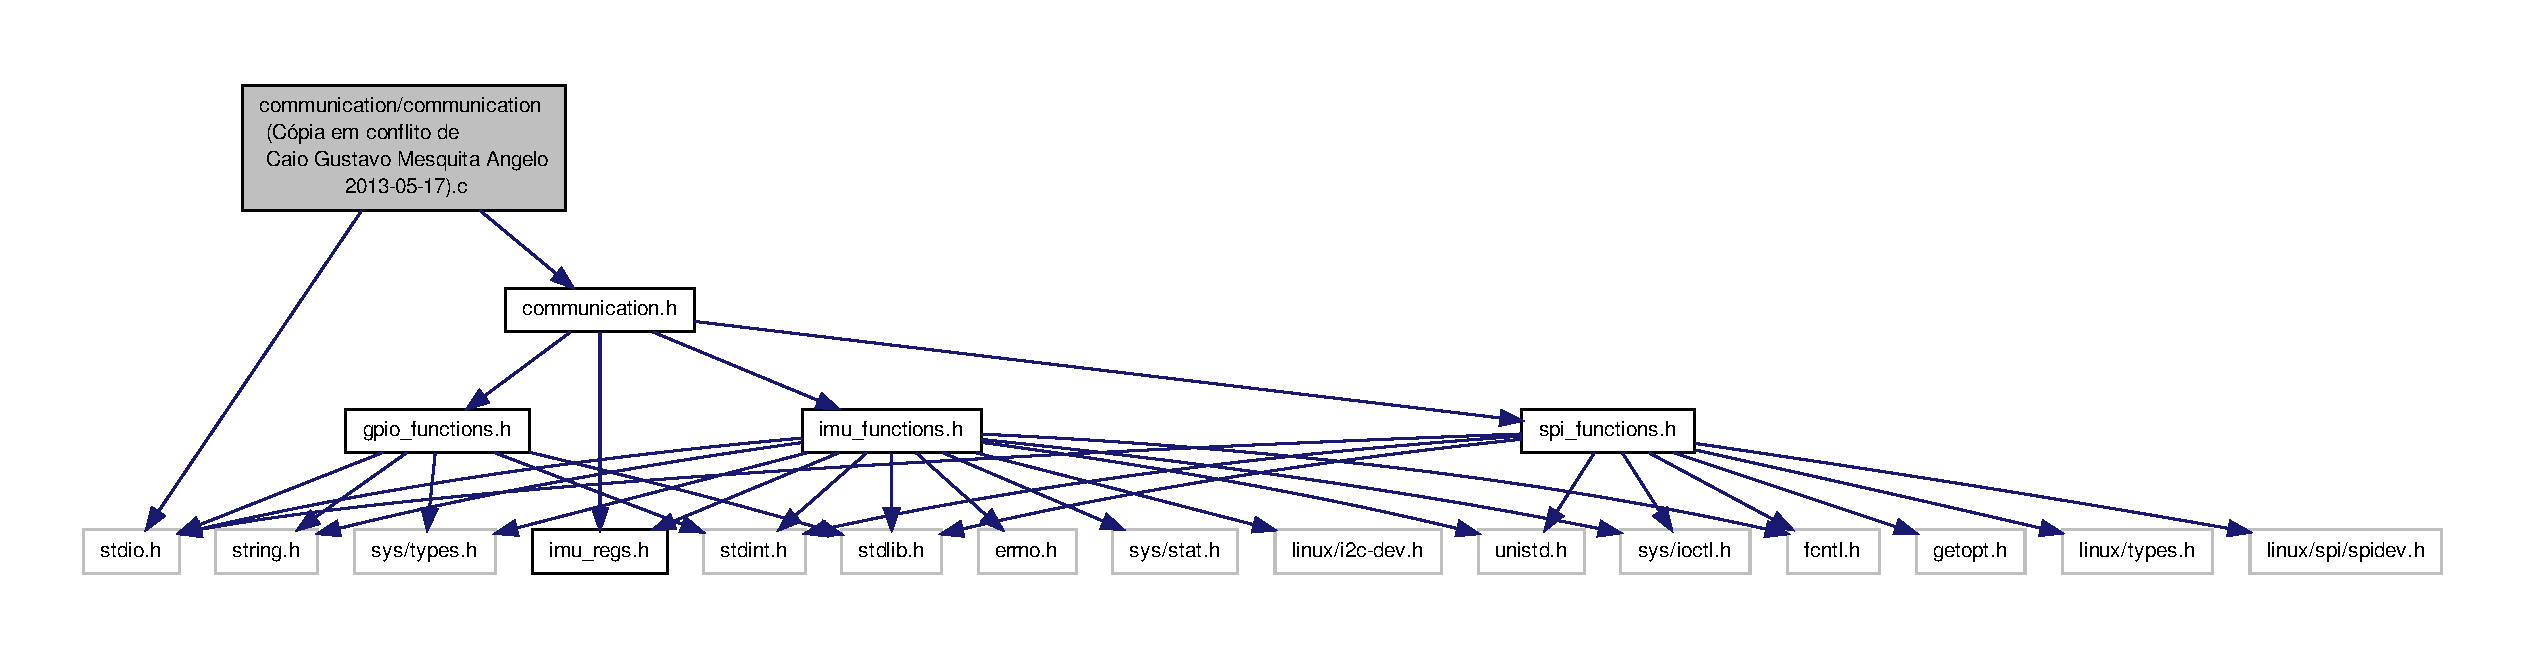
\includegraphics[width=350pt]{communication_01_07C_xC3_xB3pia_01em_01conflito_01de_01Caio_01Gustavo_01Mesquita_01Angelo_012013-05-17_08_8c__incl}
\end{center}
\end{figure}
\subsection*{Functions}
\begin{DoxyCompactItemize}
\item 
int \hyperlink{communication_01_07C_xC3_xB3pia_01em_01conflito_01de_01Caio_01Gustavo_01Mesquita_01Angelo_012013-05-17_08_8c_a2d1e523ff70db11ca4096f97af5da000}{devices\-\_\-init} (\hyperlink{structIMU__PARAM__STRUCT}{I\-M\-U\-\_\-\-P\-A\-R\-A\-M\-\_\-\-S\-T\-R\-U\-C\-T} $\ast$\hyperlink{main2_8c_a9c6b2109fb9402446f92995db60951b5}{imu\-\_\-param}, \hyperlink{structSPI__PARAM__STRUCT}{S\-P\-I\-\_\-\-P\-A\-R\-A\-M\-\_\-\-S\-T\-R\-U\-C\-T} $\ast$\hyperlink{main2_8c_adec2468b88cf50b20e5cf399a3b7e994}{spi\-\_\-param}, \hyperlink{structMRA__DATA__STRUCT}{M\-R\-A\-\_\-\-D\-A\-T\-A\-\_\-\-S\-T\-R\-U\-C\-T} $\ast$\hyperlink{main2_8c_abc42e18d2909e9bc119316283f4ed9db}{mra\-\_\-data})
\begin{DoxyCompactList}\small\item\em I\-N\-I\-T\-I\-A\-L\-I\-Z\-A\-T\-I\-O\-N O\-F S\-E\-N\-S\-O\-R\-S A\-N\-D D\-E\-V\-I\-C\-E\-S. \end{DoxyCompactList}\item 
int \hyperlink{communication_01_07C_xC3_xB3pia_01em_01conflito_01de_01Caio_01Gustavo_01Mesquita_01Angelo_012013-05-17_08_8c_a5f0316a5f70c7e369541e996802603b4}{read\-\_\-all\-\_\-data} (int \hyperlink{CommunicationV0_2communication_8c_a7751bd45ac1064efb35adf1f19c25db8}{i2c\-\_\-dev}, int \hyperlink{CommunicationV0_2communication_8c_a4788f0a5355494bc6c13690e28f43783}{spi\-\_\-dev}, \hyperlink{structIMU__DATA__STRUCT}{I\-M\-U\-\_\-\-D\-A\-T\-A\-\_\-\-S\-T\-R\-U\-C\-T} $\ast$\hyperlink{threads__linux_8c_a3cfea12cbe9ca7f1681c950e4cd68606}{imu\-\_\-data}, \hyperlink{structEFF__DATA__STRUCT}{E\-F\-F\-\_\-\-D\-A\-T\-A\-\_\-\-S\-T\-R\-U\-C\-T} $\ast$\hyperlink{main2_8c_a5650ece8c3a277c7f158d75ae65265fa}{eff\-\_\-data}, \hyperlink{structMRA__DATA__STRUCT}{M\-R\-A\-\_\-\-D\-A\-T\-A\-\_\-\-S\-T\-R\-U\-C\-T} $\ast$\hyperlink{main2_8c_abc42e18d2909e9bc119316283f4ed9db}{mra\-\_\-data})
\begin{DoxyCompactList}\small\item\em R\-E\-A\-D A\-L\-L D\-A\-T\-A F\-R\-O\-M S\-E\-N\-S\-O\-R\-S A\-N\-D A\-D\-C. \end{DoxyCompactList}\item 
void \hyperlink{communication_01_07C_xC3_xB3pia_01em_01conflito_01de_01Caio_01Gustavo_01Mesquita_01Angelo_012013-05-17_08_8c_a1d5f01d0124cff7030b5c4951b4bbefa}{actuate} (int \hyperlink{CommunicationV0_2communication_8c_a4788f0a5355494bc6c13690e28f43783}{spi\-\_\-dev}, \hyperlink{structMRA__DATA__STRUCT}{M\-R\-A\-\_\-\-D\-A\-T\-A\-\_\-\-S\-T\-R\-U\-C\-T} $\ast$\hyperlink{main2_8c_abc42e18d2909e9bc119316283f4ed9db}{mra\-\_\-data})
\begin{DoxyCompactList}\small\item\em Applies the control signal to the actuator. \end{DoxyCompactList}\item 
void \hyperlink{communication_01_07C_xC3_xB3pia_01em_01conflito_01de_01Caio_01Gustavo_01Mesquita_01Angelo_012013-05-17_08_8c_a8c7a00eda165bde1af4ca55c693e6acf}{dac\-\_\-shut\-\_\-down} (void)
\end{DoxyCompactItemize}
\subsection*{Variables}
\begin{DoxyCompactItemize}
\item 
int \hyperlink{communication_01_07C_xC3_xB3pia_01em_01conflito_01de_01Caio_01Gustavo_01Mesquita_01Angelo_012013-05-17_08_8c_a6e27f49150e9a14580fb313cc2777e00}{status}
\end{DoxyCompactItemize}


\subsection{Function Documentation}
\hypertarget{communication_01_07C_xC3_xB3pia_01em_01conflito_01de_01Caio_01Gustavo_01Mesquita_01Angelo_012013-05-17_08_8c_a1d5f01d0124cff7030b5c4951b4bbefa}{\index{communication (\-Cópia em conflito de Caio Gustavo Mesquita Angelo 2013-\/05-\/17).\-c@{communication (\-Cópia em conflito de Caio Gustavo Mesquita Angelo 2013-\/05-\/17).\-c}!actuate@{actuate}}
\index{actuate@{actuate}!communication (Cópia em conflito de Caio Gustavo Mesquita Angelo 2013-05-17).c@{communication (\-Cópia em conflito de Caio Gustavo Mesquita Angelo 2013-\/05-\/17).\-c}}
\subsubsection[{actuate}]{\setlength{\rightskip}{0pt plus 5cm}void actuate (
\begin{DoxyParamCaption}
\item[{int}]{spi\-\_\-dev, }
\item[{{\bf M\-R\-A\-\_\-\-D\-A\-T\-A\-\_\-\-S\-T\-R\-U\-C\-T} $\ast$}]{mra\-\_\-data}
\end{DoxyParamCaption}
)}}\label{communication_01_07C_xC3_xB3pia_01em_01conflito_01de_01Caio_01Gustavo_01Mesquita_01Angelo_012013-05-17_08_8c_a1d5f01d0124cff7030b5c4951b4bbefa}


Applies the control signal to the actuator. 


\begin{DoxyParams}{Parameters}
{\em spi\-\_\-dev} & Containing S\-P\-I variable I\-D \\
\hline
{\em mra\-\_\-data} & Struct containing the control signal \\
\hline
\end{DoxyParams}
\begin{DoxyReturn}{Returns}
nothing 
\end{DoxyReturn}


Definition at line 135 of file communication (\-Cópia em conflito de Caio Gustavo Mesquita Angelo 2013-\/05-\/17).\-c.



Referenced by devices\-\_\-init(), and periodic\-\_\-task\-\_\-1().


\begin{DoxyCode}
\{
  \textcolor{comment}{//printf("i = %d\(\backslash\)n",i);}
  \textcolor{comment}{//i++;}
  \textcolor{keywordflow}{if}( \hyperlink{communication_2gpio__functions_8c_a9672ca43e65fa527cd6bf43db9aea594}{gpio\_write}(\hyperlink{communication_01_07C_xC3_xB3pia_01em_01conflito_01de_01Caio_01Gustavo_01Mesquita_01Angelo_012013-05-17_08_8h_a99fc26a9596a1cb1f0f9936dbb8ccca6}{GPIO\_DAC\_SHDN},1)==\hyperlink{calibration_2calibration_8h_a6d58f9ac447476b4e084d7ca383f5183}{FAILURE} )
        mra\_data->\hyperlink{structMRA__DATA__STRUCT_a5b1af89ee717f5b14c18e8ac12e93e75}{new\_ctl}=\hyperlink{calibration_2calibration_8h_a6d58f9ac447476b4e084d7ca383f5183}{FAILURE};
  \textcolor{keywordflow}{else} \textcolor{keywordflow}{if}( (\hyperlink{communication_2gpio__functions_8c_a9672ca43e65fa527cd6bf43db9aea594}{gpio\_write}(\hyperlink{communication_01_07C_xC3_xB3pia_01em_01conflito_01de_01Caio_01Gustavo_01Mesquita_01Angelo_012013-05-17_08_8h_ad774f00fc71216488e24a803bf4eb6aa}{GPIO\_CS\_S3},1)==\hyperlink{calibration_2calibration_8h_a6d58f9ac447476b4e084d7ca383f5183}{FAILURE}) || (
      \hyperlink{communication_2gpio__functions_8c_a9672ca43e65fa527cd6bf43db9aea594}{gpio\_write}(\hyperlink{communication_01_07C_xC3_xB3pia_01em_01conflito_01de_01Caio_01Gustavo_01Mesquita_01Angelo_012013-05-17_08_8h_a94b6d57532d1db55dc4efd9fb234f156}{GPIO\_CS\_S2},0)==\hyperlink{calibration_2calibration_8h_a6d58f9ac447476b4e084d7ca383f5183}{FAILURE}) || (\hyperlink{communication_2gpio__functions_8c_a9672ca43e65fa527cd6bf43db9aea594}{gpio\_write}
      (\hyperlink{communication_01_07C_xC3_xB3pia_01em_01conflito_01de_01Caio_01Gustavo_01Mesquita_01Angelo_012013-05-17_08_8h_a7672ba13ff6f297c347790586c9a02e0}{GPIO\_CS\_S1},1)==\hyperlink{calibration_2calibration_8h_a6d58f9ac447476b4e084d7ca383f5183}{FAILURE}) || (\hyperlink{communication_2gpio__functions_8c_a9672ca43e65fa527cd6bf43db9aea594}{gpio\_write}(\hyperlink{communication_01_07C_xC3_xB3pia_01em_01conflito_01de_01Caio_01Gustavo_01Mesquita_01Angelo_012013-05-17_08_8h_a48ea000c2b251ce26ea35d300f319651}{GPIO\_CS\_S0}
      ,0)==\hyperlink{calibration_2calibration_8h_a6d58f9ac447476b4e084d7ca383f5183}{FAILURE}) )
        mra\_data->\hyperlink{structMRA__DATA__STRUCT_a5b1af89ee717f5b14c18e8ac12e93e75}{new\_ctl}=\hyperlink{calibration_2calibration_8h_a6d58f9ac447476b4e084d7ca383f5183}{FAILURE};
  \textcolor{keywordflow}{else} \textcolor{keywordflow}{if}( (\hyperlink{group__spi_ga5c52e64c336d59215ce0a4b6f340dc9f}{dac\_write}(\hyperlink{CommunicationV0_2communication_8c_a4788f0a5355494bc6c13690e28f43783}{spi\_dev},0,1,mra\_data->\hyperlink{structMRA__DATA__STRUCT_a64b4e6bb604e58de593a60c87942b966}{v\_ctl}))==
      \hyperlink{calibration_2calibration_8h_a6d58f9ac447476b4e084d7ca383f5183}{FAILURE} )
        mra\_data->\hyperlink{structMRA__DATA__STRUCT_a5b1af89ee717f5b14c18e8ac12e93e75}{new\_ctl}=\hyperlink{calibration_2calibration_8h_a6d58f9ac447476b4e084d7ca383f5183}{FAILURE};
\textcolor{comment}{//  else if( (dac\_write(spi\_dev,1,1,mra\_data->???))==FAILURE )}
\textcolor{comment}{//      mra\_data->success=FAILURE;}
  mra\_data->\hyperlink{structMRA__DATA__STRUCT_a5b1af89ee717f5b14c18e8ac12e93e75}{new\_ctl}=\hyperlink{calibration_2calibration_8h_aa90cac659d18e8ef6294c7ae337f6b58}{SUCCESS};
  \textcolor{keywordflow}{return};
\}
\end{DoxyCode}


Here is the caller graph for this function\-:\nopagebreak
\begin{figure}[H]
\begin{center}
\leavevmode
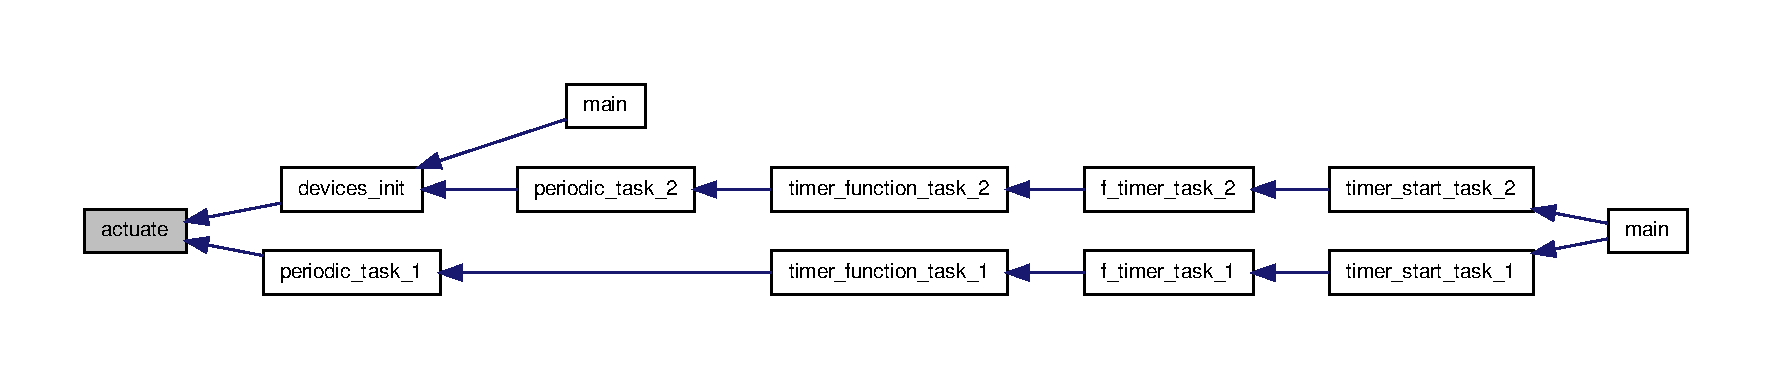
\includegraphics[width=350pt]{communication_01_07C_xC3_xB3pia_01em_01conflito_01de_01Caio_01Gustavo_01Mesquita_01Angelo_012013-05-17_08_8c_a1d5f01d0124cff7030b5c4951b4bbefa_icgraph}
\end{center}
\end{figure}


\hypertarget{communication_01_07C_xC3_xB3pia_01em_01conflito_01de_01Caio_01Gustavo_01Mesquita_01Angelo_012013-05-17_08_8c_a8c7a00eda165bde1af4ca55c693e6acf}{\index{communication (\-Cópia em conflito de Caio Gustavo Mesquita Angelo 2013-\/05-\/17).\-c@{communication (\-Cópia em conflito de Caio Gustavo Mesquita Angelo 2013-\/05-\/17).\-c}!dac\-\_\-shut\-\_\-down@{dac\-\_\-shut\-\_\-down}}
\index{dac\-\_\-shut\-\_\-down@{dac\-\_\-shut\-\_\-down}!communication (Cópia em conflito de Caio Gustavo Mesquita Angelo 2013-05-17).c@{communication (\-Cópia em conflito de Caio Gustavo Mesquita Angelo 2013-\/05-\/17).\-c}}
\subsubsection[{dac\-\_\-shut\-\_\-down}]{\setlength{\rightskip}{0pt plus 5cm}void dac\-\_\-shut\-\_\-down (
\begin{DoxyParamCaption}
\item[{void}]{}
\end{DoxyParamCaption}
)}}\label{communication_01_07C_xC3_xB3pia_01em_01conflito_01de_01Caio_01Gustavo_01Mesquita_01Angelo_012013-05-17_08_8c_a8c7a00eda165bde1af4ca55c693e6acf}


Definition at line 151 of file communication (\-Cópia em conflito de Caio Gustavo Mesquita Angelo 2013-\/05-\/17).\-c.



References G\-P\-I\-O\-\_\-\-D\-A\-C\-\_\-\-S\-H\-D\-N, gpio\-\_\-read(), and gpio\-\_\-write().


\begin{DoxyCode}
\{
  \textcolor{keywordflow}{while}( (\hyperlink{communication_2gpio__functions_8c_ae18413a0edf151e47a7aa6be21c5144a}{gpio\_read}(\hyperlink{communication_01_07C_xC3_xB3pia_01em_01conflito_01de_01Caio_01Gustavo_01Mesquita_01Angelo_012013-05-17_08_8h_a99fc26a9596a1cb1f0f9936dbb8ccca6}{GPIO\_DAC\_SHDN}))==0 )
    \hyperlink{communication_2gpio__functions_8c_a9672ca43e65fa527cd6bf43db9aea594}{gpio\_write}(\hyperlink{communication_01_07C_xC3_xB3pia_01em_01conflito_01de_01Caio_01Gustavo_01Mesquita_01Angelo_012013-05-17_08_8h_a99fc26a9596a1cb1f0f9936dbb8ccca6}{GPIO\_DAC\_SHDN},0);
  \textcolor{keywordflow}{return};
\}\end{DoxyCode}


Here is the call graph for this function\-:\nopagebreak
\begin{figure}[H]
\begin{center}
\leavevmode
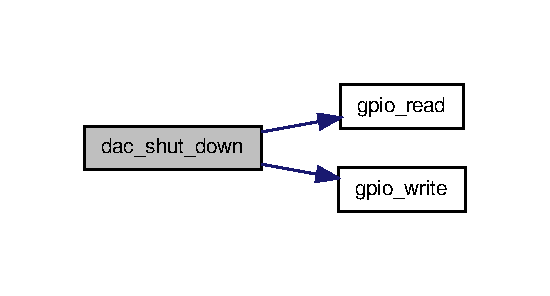
\includegraphics[width=264pt]{communication_01_07C_xC3_xB3pia_01em_01conflito_01de_01Caio_01Gustavo_01Mesquita_01Angelo_012013-05-17_08_8c_a8c7a00eda165bde1af4ca55c693e6acf_cgraph}
\end{center}
\end{figure}


\hypertarget{communication_01_07C_xC3_xB3pia_01em_01conflito_01de_01Caio_01Gustavo_01Mesquita_01Angelo_012013-05-17_08_8c_a2d1e523ff70db11ca4096f97af5da000}{\index{communication (\-Cópia em conflito de Caio Gustavo Mesquita Angelo 2013-\/05-\/17).\-c@{communication (\-Cópia em conflito de Caio Gustavo Mesquita Angelo 2013-\/05-\/17).\-c}!devices\-\_\-init@{devices\-\_\-init}}
\index{devices\-\_\-init@{devices\-\_\-init}!communication (Cópia em conflito de Caio Gustavo Mesquita Angelo 2013-05-17).c@{communication (\-Cópia em conflito de Caio Gustavo Mesquita Angelo 2013-\/05-\/17).\-c}}
\subsubsection[{devices\-\_\-init}]{\setlength{\rightskip}{0pt plus 5cm}int devices\-\_\-init (
\begin{DoxyParamCaption}
\item[{{\bf I\-M\-U\-\_\-\-P\-A\-R\-A\-M\-\_\-\-S\-T\-R\-U\-C\-T} $\ast$}]{imu\-\_\-param, }
\item[{{\bf S\-P\-I\-\_\-\-P\-A\-R\-A\-M\-\_\-\-S\-T\-R\-U\-C\-T} $\ast$}]{spi\-\_\-param, }
\item[{{\bf M\-R\-A\-\_\-\-D\-A\-T\-A\-\_\-\-S\-T\-R\-U\-C\-T} $\ast$}]{mra\-\_\-data}
\end{DoxyParamCaption}
)}}\label{communication_01_07C_xC3_xB3pia_01em_01conflito_01de_01Caio_01Gustavo_01Mesquita_01Angelo_012013-05-17_08_8c_a2d1e523ff70db11ca4096f97af5da000}


I\-N\-I\-T\-I\-A\-L\-I\-Z\-A\-T\-I\-O\-N O\-F S\-E\-N\-S\-O\-R\-S A\-N\-D D\-E\-V\-I\-C\-E\-S. 


\begin{DoxyParams}{Parameters}
{\em $\ast$imu\-\_\-param} & Structure with I\-M\-U parameters \\
\hline
{\em $\ast$spi\-\_\-param} & Structure with S\-P\-I parameters \\
\hline
{\em $\ast$mra\-\_\-data} & Structure to control M\-R\-A \\
\hline
\end{DoxyParams}
\begin{DoxyReturn}{Returns}
flag with S\-U\-C\-C\-E\-S\-S or F\-A\-I\-L\-U\-R\-E 
\end{DoxyReturn}


Definition at line 7 of file communication (\-Cópia em conflito de Caio Gustavo Mesquita Angelo 2013-\/05-\/17).\-c.



Referenced by main(), and periodic\-\_\-task\-\_\-2().


\begin{DoxyCode}
\{
  
  \textcolor{keywordflow}{if}( (imu\_param->\hyperlink{structIMU__PARAM__STRUCT_a8a870f383fc9ba0b682fdc9b8c0d2734}{i2c\_dev} = open(\textcolor{stringliteral}{"/dev/i2c-3"}, O\_RDWR))<0 )
  \{
    perror(\textcolor{stringliteral}{"Failed to open i2c\_dev"});
    \textcolor{keywordflow}{return} \hyperlink{calibration_2calibration_8h_a6d58f9ac447476b4e084d7ca383f5183}{FAILURE};
  \}

  \textcolor{keywordflow}{if} ((ioctl(imu\_param->\hyperlink{structIMU__PARAM__STRUCT_a8a870f383fc9ba0b682fdc9b8c0d2734}{i2c\_dev}, I2C\_SLAVE, \hyperlink{communication_2imu__functions_8h_a383c09d3e3bbe30097f7eb8d081fb856}{ADD\_HMC5883})) < 0
      ) \{
                perror(\textcolor{stringliteral}{"ioctl(I2C\_SLAVE) mag"});
                \textcolor{keywordflow}{return} \hyperlink{calibration_2calibration_8h_a6d58f9ac447476b4e084d7ca383f5183}{FAILURE};
  \}

  \textcolor{keywordflow}{if}( (\hyperlink{communication_2imu__functions_8h_a014f908c9faa37c1ec75177a17012a01}{mag\_init}(imu\_param->\hyperlink{structIMU__PARAM__STRUCT_a8a870f383fc9ba0b682fdc9b8c0d2734}{i2c\_dev}, imu\_param->\hyperlink{structIMU__PARAM__STRUCT_a26b277dcaf05f3842995df888225f6f4}{mag}.\hyperlink{structIMU__PARAM__STRUCT_1_1param__mag_a234de95423b604b05b851ef90890cea1}{rate}, 
      imu\_param->\hyperlink{structIMU__PARAM__STRUCT_a26b277dcaf05f3842995df888225f6f4}{mag}.\hyperlink{structIMU__PARAM__STRUCT_1_1param__mag_a40ad27ebdb5fde35257b1dc52e40f476}{range}, imu\_param->\hyperlink{structIMU__PARAM__STRUCT_a26b277dcaf05f3842995df888225f6f4}{mag}.\hyperlink{structIMU__PARAM__STRUCT_1_1param__mag_a52c22cae6940eb39fb72aca66cfeba9a}{samples\_avg}, 
      imu\_param->\hyperlink{structIMU__PARAM__STRUCT_a26b277dcaf05f3842995df888225f6f4}{mag}.\hyperlink{structIMU__PARAM__STRUCT_1_1param__mag_a1f3536709c05310005d648f339d70c54}{meas\_mode}, imu\_param->\hyperlink{structIMU__PARAM__STRUCT_a26b277dcaf05f3842995df888225f6f4}{mag}.\hyperlink{structIMU__PARAM__STRUCT_1_1param__mag_a39b83b3e9ff5bdcafed0bdf6a2de584b}{op\_mode}))< 0)
  \{
      perror(\textcolor{stringliteral}{"Error in magnetometer initialization"});
      \textcolor{keywordflow}{return} \hyperlink{calibration_2calibration_8h_a6d58f9ac447476b4e084d7ca383f5183}{FAILURE};
  \}  

  \textcolor{keywordflow}{if}( ioctl(imu\_param->\hyperlink{structIMU__PARAM__STRUCT_a8a870f383fc9ba0b682fdc9b8c0d2734}{i2c\_dev}, I2C\_SLAVE, \hyperlink{communication_2imu__functions_8h_ab9fd1068a3f5fcba24d92918aaf0dcb5}{ADD\_ITG3200}) < 0) 
      \{
                perror(\textcolor{stringliteral}{"ioctl(I2C\_SLAVE) gyr"});
                \textcolor{keywordflow}{return} \hyperlink{calibration_2calibration_8h_a6d58f9ac447476b4e084d7ca383f5183}{FAILURE};
  \} 

  \textcolor{keywordflow}{if}( \hyperlink{group__gyr_ga6d02be352b4491a236c9695a6a24d174}{gyr\_init}(imu\_param->\hyperlink{structIMU__PARAM__STRUCT_a8a870f383fc9ba0b682fdc9b8c0d2734}{i2c\_dev}, imu\_param->\hyperlink{structIMU__PARAM__STRUCT_a5a4557868f1af679a1098808397b02ec}{gyr}.\hyperlink{structIMU__PARAM__STRUCT_1_1param__gyr_a5aa70e1e9634411c89aacfbc570cc91c}{rate}, 
      imu\_param->\hyperlink{structIMU__PARAM__STRUCT_a5a4557868f1af679a1098808397b02ec}{gyr}.\hyperlink{structIMU__PARAM__STRUCT_1_1param__gyr_aa612f7299b43a1bf1fc597688c2fa02d}{lpf\_bw}, imu\_param->\hyperlink{structIMU__PARAM__STRUCT_a5a4557868f1af679a1098808397b02ec}{gyr}.\hyperlink{structIMU__PARAM__STRUCT_1_1param__gyr_aca3b791cb480f2da4703d4c256a7de48}{clk\_source}, imu\_param
      ->\hyperlink{structIMU__PARAM__STRUCT_a5a4557868f1af679a1098808397b02ec}{gyr}.\hyperlink{structIMU__PARAM__STRUCT_1_1param__gyr_a8b583edb905ed922572e46453e7d4adf}{act})<0 )
  \{
      perror(\textcolor{stringliteral}{"Error in gyrometer initialization"});
      \textcolor{keywordflow}{return} \hyperlink{calibration_2calibration_8h_a6d58f9ac447476b4e084d7ca383f5183}{FAILURE};
  \}

  \textcolor{keywordflow}{if} ( (ioctl(imu\_param->\hyperlink{structIMU__PARAM__STRUCT_a8a870f383fc9ba0b682fdc9b8c0d2734}{i2c\_dev}, I2C\_SLAVE, \hyperlink{communication_2imu__functions_8h_a909f4a5773e20e672cdb4088e1cfa22f}{ADD\_ADXL345})) < 
      0) \{
        perror(\textcolor{stringliteral}{"ioctl(I2C\_SLAVE) acc"});
        \textcolor{keywordflow}{return} \hyperlink{calibration_2calibration_8h_a6d58f9ac447476b4e084d7ca383f5183}{FAILURE};
  \}  

  \textcolor{keywordflow}{if}( \hyperlink{group__acc_gae8f9cc6e0d15e61039d846305f86f073}{acc\_init}(imu\_param->\hyperlink{structIMU__PARAM__STRUCT_a8a870f383fc9ba0b682fdc9b8c0d2734}{i2c\_dev}, imu\_param->\hyperlink{structIMU__PARAM__STRUCT_a92172e4757d0f8f9135a659e406c12e5}{acc}.\hyperlink{structIMU__PARAM__STRUCT_1_1param__acc_af57da5d956ffa7e49a184326b6b9c738}{full\_res}
      , imu\_param->\hyperlink{structIMU__PARAM__STRUCT_a92172e4757d0f8f9135a659e406c12e5}{acc}.\hyperlink{structIMU__PARAM__STRUCT_1_1param__acc_a30e6a318cad098cd8379416705820f95}{rate}, imu\_param->\hyperlink{structIMU__PARAM__STRUCT_a92172e4757d0f8f9135a659e406c12e5}{acc}.\hyperlink{structIMU__PARAM__STRUCT_1_1param__acc_a26199b298ef2d353192dfbc706bce8cf}{range})<0)
  \{
        perror(\textcolor{stringliteral}{"Error in accelerometer initialization"});
        \textcolor{keywordflow}{return} \hyperlink{calibration_2calibration_8h_a6d58f9ac447476b4e084d7ca383f5183}{FAILURE};
  \}

  \textcolor{keywordflow}{if} ((spi\_param->\hyperlink{structSPI__PARAM__STRUCT_abe385c44333d268d17cf648c8e371cad}{spi\_dev}=\hyperlink{group__spi_ga70764aca888e93b0329e7a62c9312704}{spi\_init}(spi\_param->\hyperlink{structSPI__PARAM__STRUCT_a82c546c99f6c3daed73c1e23426be847}{mode},spi\_param
      ->\hyperlink{structSPI__PARAM__STRUCT_a53a8d386594a81eb9bc6f971bfe36c54}{speed},spi\_param->\hyperlink{structSPI__PARAM__STRUCT_ae0d62e0a5554783d710b677a017e246f}{cs}))<0) 
  \{
    perror(\textcolor{stringliteral}{"Error in SPI device initialization"});
    \textcolor{keywordflow}{return} \hyperlink{calibration_2calibration_8h_a6d58f9ac447476b4e084d7ca383f5183}{FAILURE};
  \}

  \textcolor{comment}{//Enable DAC and writing 0}
  mra\_data->\hyperlink{structMRA__DATA__STRUCT_a64b4e6bb604e58de593a60c87942b966}{v\_ctl}=0;
\textcolor{comment}{//  mra\_data->Out\_1=0;}

  \hyperlink{communication_01_07C_xC3_xB3pia_01em_01conflito_01de_01Caio_01Gustavo_01Mesquita_01Angelo_012013-05-17_08_8c_a1d5f01d0124cff7030b5c4951b4bbefa}{actuate}(spi\_param->\hyperlink{structSPI__PARAM__STRUCT_abe385c44333d268d17cf648c8e371cad}{spi\_dev}, mra\_data);
  \textcolor{keywordflow}{if}( mra\_data->\hyperlink{structMRA__DATA__STRUCT_a5b1af89ee717f5b14c18e8ac12e93e75}{new\_ctl} == \hyperlink{calibration_2calibration_8h_a6d58f9ac447476b4e084d7ca383f5183}{FAILURE} )
  \{
        perror(\textcolor{stringliteral}{"Error in MRA initialization"});
        \textcolor{keywordflow}{return} \hyperlink{calibration_2calibration_8h_a6d58f9ac447476b4e084d7ca383f5183}{FAILURE};
  \}
  \textcolor{keywordflow}{return} \hyperlink{calibration_2calibration_8h_aa90cac659d18e8ef6294c7ae337f6b58}{SUCCESS};
\}
\end{DoxyCode}


Here is the caller graph for this function\-:\nopagebreak
\begin{figure}[H]
\begin{center}
\leavevmode
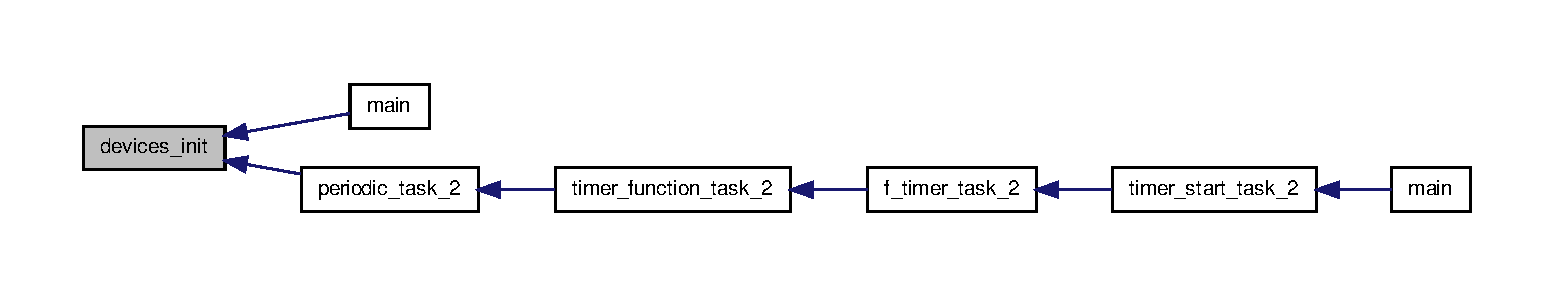
\includegraphics[width=350pt]{communication_01_07C_xC3_xB3pia_01em_01conflito_01de_01Caio_01Gustavo_01Mesquita_01Angelo_012013-05-17_08_8c_a2d1e523ff70db11ca4096f97af5da000_icgraph}
\end{center}
\end{figure}


\hypertarget{communication_01_07C_xC3_xB3pia_01em_01conflito_01de_01Caio_01Gustavo_01Mesquita_01Angelo_012013-05-17_08_8c_a5f0316a5f70c7e369541e996802603b4}{\index{communication (\-Cópia em conflito de Caio Gustavo Mesquita Angelo 2013-\/05-\/17).\-c@{communication (\-Cópia em conflito de Caio Gustavo Mesquita Angelo 2013-\/05-\/17).\-c}!read\-\_\-all\-\_\-data@{read\-\_\-all\-\_\-data}}
\index{read\-\_\-all\-\_\-data@{read\-\_\-all\-\_\-data}!communication (Cópia em conflito de Caio Gustavo Mesquita Angelo 2013-05-17).c@{communication (\-Cópia em conflito de Caio Gustavo Mesquita Angelo 2013-\/05-\/17).\-c}}
\subsubsection[{read\-\_\-all\-\_\-data}]{\setlength{\rightskip}{0pt plus 5cm}int read\-\_\-all\-\_\-data (
\begin{DoxyParamCaption}
\item[{int}]{i2c\-\_\-dev, }
\item[{int}]{spi\-\_\-dev, }
\item[{{\bf I\-M\-U\-\_\-\-D\-A\-T\-A\-\_\-\-S\-T\-R\-U\-C\-T} $\ast$}]{imu\-\_\-data, }
\item[{{\bf E\-F\-F\-\_\-\-D\-A\-T\-A\-\_\-\-S\-T\-R\-U\-C\-T} $\ast$}]{eff\-\_\-data, }
\item[{{\bf M\-R\-A\-\_\-\-D\-A\-T\-A\-\_\-\-S\-T\-R\-U\-C\-T} $\ast$}]{mra\-\_\-data}
\end{DoxyParamCaption}
)}}\label{communication_01_07C_xC3_xB3pia_01em_01conflito_01de_01Caio_01Gustavo_01Mesquita_01Angelo_012013-05-17_08_8c_a5f0316a5f70c7e369541e996802603b4}


R\-E\-A\-D A\-L\-L D\-A\-T\-A F\-R\-O\-M S\-E\-N\-S\-O\-R\-S A\-N\-D A\-D\-C. 


\begin{DoxyParams}{Parameters}
{\em i2c\-\_\-dev} & \\
\hline
{\em spi\-\_\-dev} & \\
\hline
{\em $\ast$imu\-\_\-data} & \\
\hline
{\em $\ast$eff\-\_\-data} & \\
\hline
{\em $\ast$mra\-\_\-data} & \\
\hline
\end{DoxyParams}
\begin{DoxyReturn}{Returns}
flag with S\-U\-C\-C\-E\-S\-S or F\-A\-I\-L\-U\-R\-E 
\end{DoxyReturn}


Definition at line 68 of file communication (\-Cópia em conflito de Caio Gustavo Mesquita Angelo 2013-\/05-\/17).\-c.



Referenced by main(), and periodic\-\_\-task\-\_\-1().


\begin{DoxyCode}
\{
  \textcolor{keywordtype}{short} \textcolor{keywordtype}{int} data[4];
  \textcolor{keywordtype}{int} f=0;
  \textcolor{comment}{// Read IMU data}
  imu\_data->\hyperlink{structIMU__DATA__STRUCT_a99924252176326418863e511d4fa437b}{new\_data}=\hyperlink{calibration_2calibration_8h_aa90cac659d18e8ef6294c7ae337f6b58}{SUCCESS};
  
  \textcolor{keywordflow}{if} ( (ioctl(\hyperlink{CommunicationV0_2communication_8c_a7751bd45ac1064efb35adf1f19c25db8}{i2c\_dev}, I2C\_SLAVE, \hyperlink{communication_2imu__functions_8h_a909f4a5773e20e672cdb4088e1cfa22f}{ADD\_ADXL345}))<0) 
        imu\_data->\hyperlink{structIMU__DATA__STRUCT_a99924252176326418863e511d4fa437b}{new\_data}=0;
  \textcolor{keywordflow}{else} \textcolor{keywordflow}{if}( (\hyperlink{group__acc_ga013bb5ed8a763883fc440549d2b1a6ce}{acc\_read\_all\_data}(\hyperlink{CommunicationV0_2communication_8c_a7751bd45ac1064efb35adf1f19c25db8}{i2c\_dev},data))==\hyperlink{calibration_2calibration_8h_a6d58f9ac447476b4e084d7ca383f5183}{FAILURE}
       )
  \{
        imu\_data->\hyperlink{structIMU__DATA__STRUCT_a99924252176326418863e511d4fa437b}{new\_data}=0;
        \textcolor{comment}{//printf("\(\backslash\)nimu\_data->new\_data = %d\(\backslash\)n",imu\_data->new\_data);}
        \textcolor{comment}{//f=1;}
  \}
  \textcolor{keywordflow}{else}\{
    imu\_data->\hyperlink{structIMU__DATA__STRUCT_a448f284bf44eb503affda586ad5fa9d2}{acc}.\hyperlink{structDATA__XYZ_a54c1596e9f9969fd9c21e8458024ecfb}{x}=data[0];
    imu\_data->\hyperlink{structIMU__DATA__STRUCT_a448f284bf44eb503affda586ad5fa9d2}{acc}.\hyperlink{structDATA__XYZ_a94bbb1c889bf53eb6a5fffa2b39322cf}{y}=data[1];
    imu\_data->\hyperlink{structIMU__DATA__STRUCT_a448f284bf44eb503affda586ad5fa9d2}{acc}.\hyperlink{structDATA__XYZ_a69e89ab0ec6e5d72fc5d54f62cc07fb5}{z}=data[2];  
  \}
  
  \textcolor{keywordflow}{if} ( (ioctl(\hyperlink{CommunicationV0_2communication_8c_a7751bd45ac1064efb35adf1f19c25db8}{i2c\_dev}, I2C\_SLAVE, \hyperlink{communication_2imu__functions_8h_ab9fd1068a3f5fcba24d92918aaf0dcb5}{ADD\_ITG3200})) < 0) 
        imu\_data->\hyperlink{structIMU__DATA__STRUCT_a99924252176326418863e511d4fa437b}{new\_data}=0;
  \textcolor{keywordflow}{else} \textcolor{keywordflow}{if}( (\hyperlink{group__gyr_ga79875465c3a29fd9ec77308c80a8bc37}{gyr\_read\_all\_data}(\hyperlink{CommunicationV0_2communication_8c_a7751bd45ac1064efb35adf1f19c25db8}{i2c\_dev},data))==\hyperlink{calibration_2calibration_8h_a6d58f9ac447476b4e084d7ca383f5183}{FAILURE}
       )
        imu\_data->\hyperlink{structIMU__DATA__STRUCT_a99924252176326418863e511d4fa437b}{new\_data}=0;
  \textcolor{keywordflow}{else}\{
    imu\_data->\hyperlink{structIMU__DATA__STRUCT_a0c1ac26626e4434a2ee124a1928a23a1}{gyr}.\hyperlink{structDATA__XYZ_a54c1596e9f9969fd9c21e8458024ecfb}{x}=data[0];
    imu\_data->\hyperlink{structIMU__DATA__STRUCT_a0c1ac26626e4434a2ee124a1928a23a1}{gyr}.\hyperlink{structDATA__XYZ_a94bbb1c889bf53eb6a5fffa2b39322cf}{y}=data[1];
    imu\_data->\hyperlink{structIMU__DATA__STRUCT_a0c1ac26626e4434a2ee124a1928a23a1}{gyr}.\hyperlink{structDATA__XYZ_a69e89ab0ec6e5d72fc5d54f62cc07fb5}{z}=data[2];
    imu\_data->\hyperlink{structIMU__DATA__STRUCT_a81e1dbf765c1d947ca6076aa1bbc73e7}{temp}=data[3];
  \}
  
  \textcolor{keywordflow}{if} ( (ioctl(\hyperlink{CommunicationV0_2communication_8c_a7751bd45ac1064efb35adf1f19c25db8}{i2c\_dev}, I2C\_SLAVE, \hyperlink{communication_2imu__functions_8h_a383c09d3e3bbe30097f7eb8d081fb856}{ADD\_HMC5883})) < 0) 
        imu\_data->\hyperlink{structIMU__DATA__STRUCT_a99924252176326418863e511d4fa437b}{new\_data}=0;
  \textcolor{keywordflow}{else} \textcolor{keywordflow}{if}( (\hyperlink{group__mag_gab42ae0d0a2a6f37cf36d856c072b7f34}{mag\_read\_all\_data}(\hyperlink{CommunicationV0_2communication_8c_a7751bd45ac1064efb35adf1f19c25db8}{i2c\_dev},data))==\hyperlink{calibration_2calibration_8h_a6d58f9ac447476b4e084d7ca383f5183}{FAILURE}
       )
        imu\_data->\hyperlink{structIMU__DATA__STRUCT_a99924252176326418863e511d4fa437b}{new\_data}=0;
  \textcolor{keywordflow}{else}\{
    imu\_data->\hyperlink{structIMU__DATA__STRUCT_a40c7df8b6d49297aa52873cfd9b60daa}{mag}.\hyperlink{structDATA__XYZ_a54c1596e9f9969fd9c21e8458024ecfb}{x}=data[0];
    imu\_data->\hyperlink{structIMU__DATA__STRUCT_a40c7df8b6d49297aa52873cfd9b60daa}{mag}.\hyperlink{structDATA__XYZ_a94bbb1c889bf53eb6a5fffa2b39322cf}{y}=data[1];
    imu\_data->\hyperlink{structIMU__DATA__STRUCT_a40c7df8b6d49297aa52873cfd9b60daa}{mag}.\hyperlink{structDATA__XYZ_a69e89ab0ec6e5d72fc5d54f62cc07fb5}{z}=data[2];
  \}
  
  \textcolor{comment}{//Read Efforts data}
  eff\_data->\hyperlink{structEFF__DATA__STRUCT_aa42ebc512dd79fa6ebf998162a149446}{new\_data}=\hyperlink{calibration_2calibration_8h_aa90cac659d18e8ef6294c7ae337f6b58}{SUCCESS};
  
  \textcolor{keywordflow}{if}( (\hyperlink{communication_2gpio__functions_8c_a9672ca43e65fa527cd6bf43db9aea594}{gpio\_write}(\hyperlink{communication_01_07C_xC3_xB3pia_01em_01conflito_01de_01Caio_01Gustavo_01Mesquita_01Angelo_012013-05-17_08_8h_ad774f00fc71216488e24a803bf4eb6aa}{GPIO\_CS\_S3},1)==\hyperlink{calibration_2calibration_8h_a6d58f9ac447476b4e084d7ca383f5183}{FAILURE}) || (
      \hyperlink{communication_2gpio__functions_8c_a9672ca43e65fa527cd6bf43db9aea594}{gpio\_write}(\hyperlink{communication_01_07C_xC3_xB3pia_01em_01conflito_01de_01Caio_01Gustavo_01Mesquita_01Angelo_012013-05-17_08_8h_a94b6d57532d1db55dc4efd9fb234f156}{GPIO\_CS\_S2},1)==\hyperlink{calibration_2calibration_8h_a6d58f9ac447476b4e084d7ca383f5183}{FAILURE}) || (\hyperlink{communication_2gpio__functions_8c_a9672ca43e65fa527cd6bf43db9aea594}{gpio\_write}
      (\hyperlink{communication_01_07C_xC3_xB3pia_01em_01conflito_01de_01Caio_01Gustavo_01Mesquita_01Angelo_012013-05-17_08_8h_a7672ba13ff6f297c347790586c9a02e0}{GPIO\_CS\_S1},1)==\hyperlink{calibration_2calibration_8h_a6d58f9ac447476b4e084d7ca383f5183}{FAILURE}) || (\hyperlink{communication_2gpio__functions_8c_a9672ca43e65fa527cd6bf43db9aea594}{gpio\_write}(\hyperlink{communication_01_07C_xC3_xB3pia_01em_01conflito_01de_01Caio_01Gustavo_01Mesquita_01Angelo_012013-05-17_08_8h_a48ea000c2b251ce26ea35d300f319651}{GPIO\_CS\_S0}
      ,0)==\hyperlink{calibration_2calibration_8h_a6d58f9ac447476b4e084d7ca383f5183}{FAILURE}))
        eff\_data->\hyperlink{structEFF__DATA__STRUCT_aa42ebc512dd79fa6ebf998162a149446}{new\_data}=\hyperlink{calibration_2calibration_8h_a6d58f9ac447476b4e084d7ca383f5183}{FAILURE};
  \textcolor{keywordflow}{else}\{ 
    \textcolor{keywordflow}{if}( (\hyperlink{group__spi_gae385345c227d9f67ab490b94ed628988}{adc\_read}(\hyperlink{CommunicationV0_2communication_8c_a4788f0a5355494bc6c13690e28f43783}{spi\_dev},0,1,data))==\hyperlink{calibration_2calibration_8h_a6d58f9ac447476b4e084d7ca383f5183}{FAILURE} )
        eff\_data->\hyperlink{structEFF__DATA__STRUCT_aa42ebc512dd79fa6ebf998162a149446}{new\_data}=\hyperlink{calibration_2calibration_8h_a6d58f9ac447476b4e084d7ca383f5183}{FAILURE};
    \textcolor{keywordflow}{else} eff\_data->\hyperlink{structEFF__DATA__STRUCT_abe8952947b54bf9c247f3429ee3aeb44}{F}.\hyperlink{structDATA__XYZ_a54c1596e9f9969fd9c21e8458024ecfb}{x}=data[0];
  \textcolor{comment}{//Read MR actuator voltage control}
    \textcolor{keywordflow}{if}( (\hyperlink{group__spi_gae385345c227d9f67ab490b94ed628988}{adc\_read}(\hyperlink{CommunicationV0_2communication_8c_a4788f0a5355494bc6c13690e28f43783}{spi\_dev},7,1,data))==\hyperlink{calibration_2calibration_8h_aa90cac659d18e8ef6294c7ae337f6b58}{SUCCESS} )
    \{
        mra\_data->\hyperlink{structMRA__DATA__STRUCT_a3a31d57268c33b21ac915fdc27dfe474}{v\_ctl\_read}=data[0];
        mra\_data->\hyperlink{structMRA__DATA__STRUCT_afca6e851d302f3a786885a4e1eec79d7}{new\_data}=\hyperlink{calibration_2calibration_8h_aa90cac659d18e8ef6294c7ae337f6b58}{SUCCESS};
    \}
  \}
  \textcolor{comment}{//if( f==1 )}
    \textcolor{comment}{//printf("imu\_data->new\_data antes do return= %d\(\backslash\)n",imu\_data->new\_data);}

  \textcolor{keywordflow}{if}( imu\_data->\hyperlink{structIMU__DATA__STRUCT_a99924252176326418863e511d4fa437b}{new\_data}==\hyperlink{calibration_2calibration_8h_a6d58f9ac447476b4e084d7ca383f5183}{FAILURE} || eff\_data->\hyperlink{structEFF__DATA__STRUCT_aa42ebc512dd79fa6ebf998162a149446}{new\_data}
      ==\hyperlink{calibration_2calibration_8h_a6d58f9ac447476b4e084d7ca383f5183}{FAILURE} || mra\_data->\hyperlink{structMRA__DATA__STRUCT_afca6e851d302f3a786885a4e1eec79d7}{new\_data}==\hyperlink{calibration_2calibration_8h_a6d58f9ac447476b4e084d7ca383f5183}{FAILURE} )
    \textcolor{keywordflow}{return} \hyperlink{calibration_2calibration_8h_a6d58f9ac447476b4e084d7ca383f5183}{FAILURE};
    
  \textcolor{keywordflow}{return} \hyperlink{calibration_2calibration_8h_aa90cac659d18e8ef6294c7ae337f6b58}{SUCCESS};
\}
\end{DoxyCode}


Here is the caller graph for this function\-:\nopagebreak
\begin{figure}[H]
\begin{center}
\leavevmode
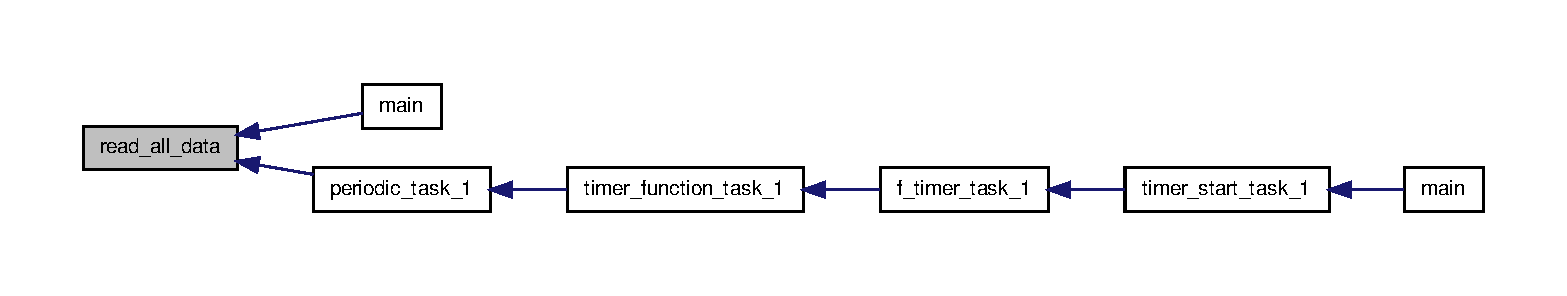
\includegraphics[width=350pt]{communication_01_07C_xC3_xB3pia_01em_01conflito_01de_01Caio_01Gustavo_01Mesquita_01Angelo_012013-05-17_08_8c_a5f0316a5f70c7e369541e996802603b4_icgraph}
\end{center}
\end{figure}




\subsection{Variable Documentation}
\hypertarget{communication_01_07C_xC3_xB3pia_01em_01conflito_01de_01Caio_01Gustavo_01Mesquita_01Angelo_012013-05-17_08_8c_a6e27f49150e9a14580fb313cc2777e00}{\index{communication (\-Cópia em conflito de Caio Gustavo Mesquita Angelo 2013-\/05-\/17).\-c@{communication (\-Cópia em conflito de Caio Gustavo Mesquita Angelo 2013-\/05-\/17).\-c}!status@{status}}
\index{status@{status}!communication (Cópia em conflito de Caio Gustavo Mesquita Angelo 2013-05-17).c@{communication (\-Cópia em conflito de Caio Gustavo Mesquita Angelo 2013-\/05-\/17).\-c}}
\subsubsection[{status}]{\setlength{\rightskip}{0pt plus 5cm}int status}}\label{communication_01_07C_xC3_xB3pia_01em_01conflito_01de_01Caio_01Gustavo_01Mesquita_01Angelo_012013-05-17_08_8c_a6e27f49150e9a14580fb313cc2777e00}


Definition at line 5 of file communication (\-Cópia em conflito de Caio Gustavo Mesquita Angelo 2013-\/05-\/17).\-c.



Referenced by g\-Data\-Logger\-\_\-\-Init(), main(), threads\-\_\-linux\-\_\-init(), threads\-\_\-linux\-\_\-timer\-\_\-function\-\_\-task\-\_\-1(), threads\-\_\-linux\-\_\-timer\-\_\-function\-\_\-task\-\_\-2(), timer\-\_\-function\-\_\-task\-\_\-1(), and timer\-\_\-function\-\_\-task\-\_\-2().


\hypertarget{communication_01_07C_xC3_xB3pia_01em_01conflito_01de_01Caio_01Gustavo_01Mesquita_01Angelo_012013-05-17_08_8h}{\section{communication/communication (Cópia em conflito de Caio Gustavo Mesquita Angelo 2013-\/05-\/17).h File Reference}
\label{communication_01_07C_xC3_xB3pia_01em_01conflito_01de_01Caio_01Gustavo_01Mesquita_01Angelo_012013-05-17_08_8h}\index{communication/communication (\-Cópia em conflito de Caio Gustavo Mesquita Angelo 2013-\/05-\/17).\-h@{communication/communication (\-Cópia em conflito de Caio Gustavo Mesquita Angelo 2013-\/05-\/17).\-h}}
}
{\ttfamily \#include \char`\"{}imu\-\_\-functions.\-h\char`\"{}}\\*
{\ttfamily \#include \char`\"{}spi\-\_\-functions.\-h\char`\"{}}\\*
{\ttfamily \#include \char`\"{}gpio\-\_\-functions.\-h\char`\"{}}\\*
{\ttfamily \#include \char`\"{}imu\-\_\-regs.\-h\char`\"{}}\\*
\subsection*{Data Structures}
\begin{DoxyCompactItemize}
\item 
struct \hyperlink{structIMU__PARAM__STRUCT}{I\-M\-U\-\_\-\-P\-A\-R\-A\-M\-\_\-\-S\-T\-R\-U\-C\-T}
\begin{DoxyCompactList}\small\item\em Configs of I\-M\-U. \end{DoxyCompactList}\item 
struct \hyperlink{structIMU__PARAM__STRUCT_1_1param__acc}{I\-M\-U\-\_\-\-P\-A\-R\-A\-M\-\_\-\-S\-T\-R\-U\-C\-T\-::param\-\_\-acc}
\begin{DoxyCompactList}\small\item\em Accelerometer Parameters. \end{DoxyCompactList}\item 
struct \hyperlink{structIMU__PARAM__STRUCT_1_1param__gyr}{I\-M\-U\-\_\-\-P\-A\-R\-A\-M\-\_\-\-S\-T\-R\-U\-C\-T\-::param\-\_\-gyr}
\begin{DoxyCompactList}\small\item\em Gyrometer Parameters. \end{DoxyCompactList}\item 
struct \hyperlink{structIMU__PARAM__STRUCT_1_1param__mag}{I\-M\-U\-\_\-\-P\-A\-R\-A\-M\-\_\-\-S\-T\-R\-U\-C\-T\-::param\-\_\-mag}
\begin{DoxyCompactList}\small\item\em Magnetometer Parameters. \end{DoxyCompactList}\item 
struct \hyperlink{structSPI__PARAM__STRUCT}{S\-P\-I\-\_\-\-P\-A\-R\-A\-M\-\_\-\-S\-T\-R\-U\-C\-T}
\begin{DoxyCompactList}\small\item\em Configs for S\-P\-I. \end{DoxyCompactList}\item 
struct \hyperlink{structDATA__XYZ}{D\-A\-T\-A\-\_\-\-X\-Y\-Z}
\begin{DoxyCompactList}\small\item\em A structure to represent a 3d Vector. \end{DoxyCompactList}\item 
struct \hyperlink{structDATA__XYZ__DOUBLE}{D\-A\-T\-A\-\_\-\-X\-Y\-Z\-\_\-\-D\-O\-U\-B\-L\-E}
\begin{DoxyCompactList}\small\item\em Vector definition on double. \end{DoxyCompactList}\item 
struct \hyperlink{structIMU__DATA__STRUCT}{I\-M\-U\-\_\-\-D\-A\-T\-A\-\_\-\-S\-T\-R\-U\-C\-T}
\begin{DoxyCompactList}\small\item\em Data of I\-M\-U structure. \end{DoxyCompactList}\item 
struct \hyperlink{structIMU__DATA__STRUCT_1_1calibrated}{I\-M\-U\-\_\-\-D\-A\-T\-A\-\_\-\-S\-T\-R\-U\-C\-T\-::calibrated}
\item 
struct \hyperlink{structEFF__DATA__STRUCT}{E\-F\-F\-\_\-\-D\-A\-T\-A\-\_\-\-S\-T\-R\-U\-C\-T}
\item 
struct \hyperlink{structMRA__DATA__STRUCT}{M\-R\-A\-\_\-\-D\-A\-T\-A\-\_\-\-S\-T\-R\-U\-C\-T}
\begin{DoxyCompactList}\small\item\em Struct to control M\-R\-A. \end{DoxyCompactList}\end{DoxyCompactItemize}
\subsection*{Macros}
\begin{DoxyCompactItemize}
\item 
\#define \hyperlink{communication_01_07C_xC3_xB3pia_01em_01conflito_01de_01Caio_01Gustavo_01Mesquita_01Angelo_012013-05-17_08_8h_a6d58f9ac447476b4e084d7ca383f5183}{F\-A\-I\-L\-U\-R\-E}~-\/1
\item 
\#define \hyperlink{communication_01_07C_xC3_xB3pia_01em_01conflito_01de_01Caio_01Gustavo_01Mesquita_01Angelo_012013-05-17_08_8h_aa90cac659d18e8ef6294c7ae337f6b58}{S\-U\-C\-C\-E\-S\-S}~1
\item 
\#define \hyperlink{communication_01_07C_xC3_xB3pia_01em_01conflito_01de_01Caio_01Gustavo_01Mesquita_01Angelo_012013-05-17_08_8h_a48ea000c2b251ce26ea35d300f319651}{G\-P\-I\-O\-\_\-\-C\-S\-\_\-\-S0}~168
\item 
\#define \hyperlink{communication_01_07C_xC3_xB3pia_01em_01conflito_01de_01Caio_01Gustavo_01Mesquita_01Angelo_012013-05-17_08_8h_a7672ba13ff6f297c347790586c9a02e0}{G\-P\-I\-O\-\_\-\-C\-S\-\_\-\-S1}~64
\item 
\#define \hyperlink{communication_01_07C_xC3_xB3pia_01em_01conflito_01de_01Caio_01Gustavo_01Mesquita_01Angelo_012013-05-17_08_8h_a94b6d57532d1db55dc4efd9fb234f156}{G\-P\-I\-O\-\_\-\-C\-S\-\_\-\-S2}~176
\item 
\#define \hyperlink{communication_01_07C_xC3_xB3pia_01em_01conflito_01de_01Caio_01Gustavo_01Mesquita_01Angelo_012013-05-17_08_8h_ad774f00fc71216488e24a803bf4eb6aa}{G\-P\-I\-O\-\_\-\-C\-S\-\_\-\-S3}~65
\item 
\#define \hyperlink{communication_01_07C_xC3_xB3pia_01em_01conflito_01de_01Caio_01Gustavo_01Mesquita_01Angelo_012013-05-17_08_8h_a99fc26a9596a1cb1f0f9936dbb8ccca6}{G\-P\-I\-O\-\_\-\-D\-A\-C\-\_\-\-S\-H\-D\-N}~66
\item 
\#define \hyperlink{communication_01_07C_xC3_xB3pia_01em_01conflito_01de_01Caio_01Gustavo_01Mesquita_01Angelo_012013-05-17_08_8h_a014b45373b6ab21c681fc378bd8203f9}{G\-P\-I\-O\-\_\-\-D\-A\-C\-\_\-\-L\-D\-A\-C}~67
\end{DoxyCompactItemize}
\subsection*{Functions}
\begin{DoxyCompactItemize}
\item 
int \hyperlink{communication_01_07C_xC3_xB3pia_01em_01conflito_01de_01Caio_01Gustavo_01Mesquita_01Angelo_012013-05-17_08_8h_a2d1e523ff70db11ca4096f97af5da000}{devices\-\_\-init} (\hyperlink{structIMU__PARAM__STRUCT}{I\-M\-U\-\_\-\-P\-A\-R\-A\-M\-\_\-\-S\-T\-R\-U\-C\-T} $\ast$\hyperlink{main2_8c_a9c6b2109fb9402446f92995db60951b5}{imu\-\_\-param}, \hyperlink{structSPI__PARAM__STRUCT}{S\-P\-I\-\_\-\-P\-A\-R\-A\-M\-\_\-\-S\-T\-R\-U\-C\-T} $\ast$\hyperlink{main2_8c_adec2468b88cf50b20e5cf399a3b7e994}{spi\-\_\-param}, \hyperlink{structMRA__DATA__STRUCT}{M\-R\-A\-\_\-\-D\-A\-T\-A\-\_\-\-S\-T\-R\-U\-C\-T} $\ast$\hyperlink{main2_8c_abc42e18d2909e9bc119316283f4ed9db}{mra\-\_\-data})
\item 
int \hyperlink{communication_01_07C_xC3_xB3pia_01em_01conflito_01de_01Caio_01Gustavo_01Mesquita_01Angelo_012013-05-17_08_8h_a5f0316a5f70c7e369541e996802603b4}{read\-\_\-all\-\_\-data} (int \hyperlink{CommunicationV0_2communication_8c_a7751bd45ac1064efb35adf1f19c25db8}{i2c\-\_\-dev}, int \hyperlink{CommunicationV0_2communication_8c_a4788f0a5355494bc6c13690e28f43783}{spi\-\_\-dev}, \hyperlink{structIMU__DATA__STRUCT}{I\-M\-U\-\_\-\-D\-A\-T\-A\-\_\-\-S\-T\-R\-U\-C\-T} $\ast$\hyperlink{threads__linux_8c_a3cfea12cbe9ca7f1681c950e4cd68606}{imu\-\_\-data}, \hyperlink{structEFF__DATA__STRUCT}{E\-F\-F\-\_\-\-D\-A\-T\-A\-\_\-\-S\-T\-R\-U\-C\-T} $\ast$\hyperlink{main2_8c_a5650ece8c3a277c7f158d75ae65265fa}{eff\-\_\-data}, \hyperlink{structMRA__DATA__STRUCT}{M\-R\-A\-\_\-\-D\-A\-T\-A\-\_\-\-S\-T\-R\-U\-C\-T} $\ast$\hyperlink{main2_8c_abc42e18d2909e9bc119316283f4ed9db}{mra\-\_\-data})
\item 
void \hyperlink{communication_01_07C_xC3_xB3pia_01em_01conflito_01de_01Caio_01Gustavo_01Mesquita_01Angelo_012013-05-17_08_8h_a1d5f01d0124cff7030b5c4951b4bbefa}{actuate} (int \hyperlink{CommunicationV0_2communication_8c_a4788f0a5355494bc6c13690e28f43783}{spi\-\_\-dev}, \hyperlink{structMRA__DATA__STRUCT}{M\-R\-A\-\_\-\-D\-A\-T\-A\-\_\-\-S\-T\-R\-U\-C\-T} $\ast$\hyperlink{main2_8c_abc42e18d2909e9bc119316283f4ed9db}{mra\-\_\-data})
\item 
void \hyperlink{communication_01_07C_xC3_xB3pia_01em_01conflito_01de_01Caio_01Gustavo_01Mesquita_01Angelo_012013-05-17_08_8h_a8da2a9706cfdbe1a7fae96aac9e4f516}{mra\-\_\-shut\-\_\-down} (void)
\end{DoxyCompactItemize}


\subsection{Macro Definition Documentation}
\hypertarget{communication_01_07C_xC3_xB3pia_01em_01conflito_01de_01Caio_01Gustavo_01Mesquita_01Angelo_012013-05-17_08_8h_a6d58f9ac447476b4e084d7ca383f5183}{\index{communication (\-Cópia em conflito de Caio Gustavo Mesquita Angelo 2013-\/05-\/17).\-h@{communication (\-Cópia em conflito de Caio Gustavo Mesquita Angelo 2013-\/05-\/17).\-h}!F\-A\-I\-L\-U\-R\-E@{F\-A\-I\-L\-U\-R\-E}}
\index{F\-A\-I\-L\-U\-R\-E@{F\-A\-I\-L\-U\-R\-E}!communication (Cópia em conflito de Caio Gustavo Mesquita Angelo 2013-05-17).h@{communication (\-Cópia em conflito de Caio Gustavo Mesquita Angelo 2013-\/05-\/17).\-h}}
\subsubsection[{F\-A\-I\-L\-U\-R\-E}]{\setlength{\rightskip}{0pt plus 5cm}\#define F\-A\-I\-L\-U\-R\-E~-\/1}}\label{communication_01_07C_xC3_xB3pia_01em_01conflito_01de_01Caio_01Gustavo_01Mesquita_01Angelo_012013-05-17_08_8h_a6d58f9ac447476b4e084d7ca383f5183}


Definition at line 9 of file communication (\-Cópia em conflito de Caio Gustavo Mesquita Angelo 2013-\/05-\/17).\-h.

\hypertarget{communication_01_07C_xC3_xB3pia_01em_01conflito_01de_01Caio_01Gustavo_01Mesquita_01Angelo_012013-05-17_08_8h_a48ea000c2b251ce26ea35d300f319651}{\index{communication (\-Cópia em conflito de Caio Gustavo Mesquita Angelo 2013-\/05-\/17).\-h@{communication (\-Cópia em conflito de Caio Gustavo Mesquita Angelo 2013-\/05-\/17).\-h}!G\-P\-I\-O\-\_\-\-C\-S\-\_\-\-S0@{G\-P\-I\-O\-\_\-\-C\-S\-\_\-\-S0}}
\index{G\-P\-I\-O\-\_\-\-C\-S\-\_\-\-S0@{G\-P\-I\-O\-\_\-\-C\-S\-\_\-\-S0}!communication (Cópia em conflito de Caio Gustavo Mesquita Angelo 2013-05-17).h@{communication (\-Cópia em conflito de Caio Gustavo Mesquita Angelo 2013-\/05-\/17).\-h}}
\subsubsection[{G\-P\-I\-O\-\_\-\-C\-S\-\_\-\-S0}]{\setlength{\rightskip}{0pt plus 5cm}\#define G\-P\-I\-O\-\_\-\-C\-S\-\_\-\-S0~168}}\label{communication_01_07C_xC3_xB3pia_01em_01conflito_01de_01Caio_01Gustavo_01Mesquita_01Angelo_012013-05-17_08_8h_a48ea000c2b251ce26ea35d300f319651}


Definition at line 12 of file communication (\-Cópia em conflito de Caio Gustavo Mesquita Angelo 2013-\/05-\/17).\-h.



Referenced by actuate(), and read\-\_\-all\-\_\-data().

\hypertarget{communication_01_07C_xC3_xB3pia_01em_01conflito_01de_01Caio_01Gustavo_01Mesquita_01Angelo_012013-05-17_08_8h_a7672ba13ff6f297c347790586c9a02e0}{\index{communication (\-Cópia em conflito de Caio Gustavo Mesquita Angelo 2013-\/05-\/17).\-h@{communication (\-Cópia em conflito de Caio Gustavo Mesquita Angelo 2013-\/05-\/17).\-h}!G\-P\-I\-O\-\_\-\-C\-S\-\_\-\-S1@{G\-P\-I\-O\-\_\-\-C\-S\-\_\-\-S1}}
\index{G\-P\-I\-O\-\_\-\-C\-S\-\_\-\-S1@{G\-P\-I\-O\-\_\-\-C\-S\-\_\-\-S1}!communication (Cópia em conflito de Caio Gustavo Mesquita Angelo 2013-05-17).h@{communication (\-Cópia em conflito de Caio Gustavo Mesquita Angelo 2013-\/05-\/17).\-h}}
\subsubsection[{G\-P\-I\-O\-\_\-\-C\-S\-\_\-\-S1}]{\setlength{\rightskip}{0pt plus 5cm}\#define G\-P\-I\-O\-\_\-\-C\-S\-\_\-\-S1~64}}\label{communication_01_07C_xC3_xB3pia_01em_01conflito_01de_01Caio_01Gustavo_01Mesquita_01Angelo_012013-05-17_08_8h_a7672ba13ff6f297c347790586c9a02e0}


Definition at line 13 of file communication (\-Cópia em conflito de Caio Gustavo Mesquita Angelo 2013-\/05-\/17).\-h.



Referenced by actuate(), and read\-\_\-all\-\_\-data().

\hypertarget{communication_01_07C_xC3_xB3pia_01em_01conflito_01de_01Caio_01Gustavo_01Mesquita_01Angelo_012013-05-17_08_8h_a94b6d57532d1db55dc4efd9fb234f156}{\index{communication (\-Cópia em conflito de Caio Gustavo Mesquita Angelo 2013-\/05-\/17).\-h@{communication (\-Cópia em conflito de Caio Gustavo Mesquita Angelo 2013-\/05-\/17).\-h}!G\-P\-I\-O\-\_\-\-C\-S\-\_\-\-S2@{G\-P\-I\-O\-\_\-\-C\-S\-\_\-\-S2}}
\index{G\-P\-I\-O\-\_\-\-C\-S\-\_\-\-S2@{G\-P\-I\-O\-\_\-\-C\-S\-\_\-\-S2}!communication (Cópia em conflito de Caio Gustavo Mesquita Angelo 2013-05-17).h@{communication (\-Cópia em conflito de Caio Gustavo Mesquita Angelo 2013-\/05-\/17).\-h}}
\subsubsection[{G\-P\-I\-O\-\_\-\-C\-S\-\_\-\-S2}]{\setlength{\rightskip}{0pt plus 5cm}\#define G\-P\-I\-O\-\_\-\-C\-S\-\_\-\-S2~176}}\label{communication_01_07C_xC3_xB3pia_01em_01conflito_01de_01Caio_01Gustavo_01Mesquita_01Angelo_012013-05-17_08_8h_a94b6d57532d1db55dc4efd9fb234f156}


Definition at line 14 of file communication (\-Cópia em conflito de Caio Gustavo Mesquita Angelo 2013-\/05-\/17).\-h.



Referenced by actuate(), and read\-\_\-all\-\_\-data().

\hypertarget{communication_01_07C_xC3_xB3pia_01em_01conflito_01de_01Caio_01Gustavo_01Mesquita_01Angelo_012013-05-17_08_8h_ad774f00fc71216488e24a803bf4eb6aa}{\index{communication (\-Cópia em conflito de Caio Gustavo Mesquita Angelo 2013-\/05-\/17).\-h@{communication (\-Cópia em conflito de Caio Gustavo Mesquita Angelo 2013-\/05-\/17).\-h}!G\-P\-I\-O\-\_\-\-C\-S\-\_\-\-S3@{G\-P\-I\-O\-\_\-\-C\-S\-\_\-\-S3}}
\index{G\-P\-I\-O\-\_\-\-C\-S\-\_\-\-S3@{G\-P\-I\-O\-\_\-\-C\-S\-\_\-\-S3}!communication (Cópia em conflito de Caio Gustavo Mesquita Angelo 2013-05-17).h@{communication (\-Cópia em conflito de Caio Gustavo Mesquita Angelo 2013-\/05-\/17).\-h}}
\subsubsection[{G\-P\-I\-O\-\_\-\-C\-S\-\_\-\-S3}]{\setlength{\rightskip}{0pt plus 5cm}\#define G\-P\-I\-O\-\_\-\-C\-S\-\_\-\-S3~65}}\label{communication_01_07C_xC3_xB3pia_01em_01conflito_01de_01Caio_01Gustavo_01Mesquita_01Angelo_012013-05-17_08_8h_ad774f00fc71216488e24a803bf4eb6aa}


Definition at line 15 of file communication (\-Cópia em conflito de Caio Gustavo Mesquita Angelo 2013-\/05-\/17).\-h.



Referenced by actuate(), and read\-\_\-all\-\_\-data().

\hypertarget{communication_01_07C_xC3_xB3pia_01em_01conflito_01de_01Caio_01Gustavo_01Mesquita_01Angelo_012013-05-17_08_8h_a014b45373b6ab21c681fc378bd8203f9}{\index{communication (\-Cópia em conflito de Caio Gustavo Mesquita Angelo 2013-\/05-\/17).\-h@{communication (\-Cópia em conflito de Caio Gustavo Mesquita Angelo 2013-\/05-\/17).\-h}!G\-P\-I\-O\-\_\-\-D\-A\-C\-\_\-\-L\-D\-A\-C@{G\-P\-I\-O\-\_\-\-D\-A\-C\-\_\-\-L\-D\-A\-C}}
\index{G\-P\-I\-O\-\_\-\-D\-A\-C\-\_\-\-L\-D\-A\-C@{G\-P\-I\-O\-\_\-\-D\-A\-C\-\_\-\-L\-D\-A\-C}!communication (Cópia em conflito de Caio Gustavo Mesquita Angelo 2013-05-17).h@{communication (\-Cópia em conflito de Caio Gustavo Mesquita Angelo 2013-\/05-\/17).\-h}}
\subsubsection[{G\-P\-I\-O\-\_\-\-D\-A\-C\-\_\-\-L\-D\-A\-C}]{\setlength{\rightskip}{0pt plus 5cm}\#define G\-P\-I\-O\-\_\-\-D\-A\-C\-\_\-\-L\-D\-A\-C~67}}\label{communication_01_07C_xC3_xB3pia_01em_01conflito_01de_01Caio_01Gustavo_01Mesquita_01Angelo_012013-05-17_08_8h_a014b45373b6ab21c681fc378bd8203f9}


Definition at line 18 of file communication (\-Cópia em conflito de Caio Gustavo Mesquita Angelo 2013-\/05-\/17).\-h.

\hypertarget{communication_01_07C_xC3_xB3pia_01em_01conflito_01de_01Caio_01Gustavo_01Mesquita_01Angelo_012013-05-17_08_8h_a99fc26a9596a1cb1f0f9936dbb8ccca6}{\index{communication (\-Cópia em conflito de Caio Gustavo Mesquita Angelo 2013-\/05-\/17).\-h@{communication (\-Cópia em conflito de Caio Gustavo Mesquita Angelo 2013-\/05-\/17).\-h}!G\-P\-I\-O\-\_\-\-D\-A\-C\-\_\-\-S\-H\-D\-N@{G\-P\-I\-O\-\_\-\-D\-A\-C\-\_\-\-S\-H\-D\-N}}
\index{G\-P\-I\-O\-\_\-\-D\-A\-C\-\_\-\-S\-H\-D\-N@{G\-P\-I\-O\-\_\-\-D\-A\-C\-\_\-\-S\-H\-D\-N}!communication (Cópia em conflito de Caio Gustavo Mesquita Angelo 2013-05-17).h@{communication (\-Cópia em conflito de Caio Gustavo Mesquita Angelo 2013-\/05-\/17).\-h}}
\subsubsection[{G\-P\-I\-O\-\_\-\-D\-A\-C\-\_\-\-S\-H\-D\-N}]{\setlength{\rightskip}{0pt plus 5cm}\#define G\-P\-I\-O\-\_\-\-D\-A\-C\-\_\-\-S\-H\-D\-N~66}}\label{communication_01_07C_xC3_xB3pia_01em_01conflito_01de_01Caio_01Gustavo_01Mesquita_01Angelo_012013-05-17_08_8h_a99fc26a9596a1cb1f0f9936dbb8ccca6}


Definition at line 17 of file communication (\-Cópia em conflito de Caio Gustavo Mesquita Angelo 2013-\/05-\/17).\-h.



Referenced by actuate(), and dac\-\_\-shut\-\_\-down().

\hypertarget{communication_01_07C_xC3_xB3pia_01em_01conflito_01de_01Caio_01Gustavo_01Mesquita_01Angelo_012013-05-17_08_8h_aa90cac659d18e8ef6294c7ae337f6b58}{\index{communication (\-Cópia em conflito de Caio Gustavo Mesquita Angelo 2013-\/05-\/17).\-h@{communication (\-Cópia em conflito de Caio Gustavo Mesquita Angelo 2013-\/05-\/17).\-h}!S\-U\-C\-C\-E\-S\-S@{S\-U\-C\-C\-E\-S\-S}}
\index{S\-U\-C\-C\-E\-S\-S@{S\-U\-C\-C\-E\-S\-S}!communication (Cópia em conflito de Caio Gustavo Mesquita Angelo 2013-05-17).h@{communication (\-Cópia em conflito de Caio Gustavo Mesquita Angelo 2013-\/05-\/17).\-h}}
\subsubsection[{S\-U\-C\-C\-E\-S\-S}]{\setlength{\rightskip}{0pt plus 5cm}\#define S\-U\-C\-C\-E\-S\-S~1}}\label{communication_01_07C_xC3_xB3pia_01em_01conflito_01de_01Caio_01Gustavo_01Mesquita_01Angelo_012013-05-17_08_8h_aa90cac659d18e8ef6294c7ae337f6b58}


Definition at line 10 of file communication (\-Cópia em conflito de Caio Gustavo Mesquita Angelo 2013-\/05-\/17).\-h.



\subsection{Function Documentation}
\hypertarget{communication_01_07C_xC3_xB3pia_01em_01conflito_01de_01Caio_01Gustavo_01Mesquita_01Angelo_012013-05-17_08_8h_a1d5f01d0124cff7030b5c4951b4bbefa}{\index{communication (\-Cópia em conflito de Caio Gustavo Mesquita Angelo 2013-\/05-\/17).\-h@{communication (\-Cópia em conflito de Caio Gustavo Mesquita Angelo 2013-\/05-\/17).\-h}!actuate@{actuate}}
\index{actuate@{actuate}!communication (Cópia em conflito de Caio Gustavo Mesquita Angelo 2013-05-17).h@{communication (\-Cópia em conflito de Caio Gustavo Mesquita Angelo 2013-\/05-\/17).\-h}}
\subsubsection[{actuate}]{\setlength{\rightskip}{0pt plus 5cm}void actuate (
\begin{DoxyParamCaption}
\item[{int}]{spi\-\_\-dev, }
\item[{{\bf M\-R\-A\-\_\-\-D\-A\-T\-A\-\_\-\-S\-T\-R\-U\-C\-T} $\ast$}]{mra\-\_\-data}
\end{DoxyParamCaption}
)}}\label{communication_01_07C_xC3_xB3pia_01em_01conflito_01de_01Caio_01Gustavo_01Mesquita_01Angelo_012013-05-17_08_8h_a1d5f01d0124cff7030b5c4951b4bbefa}


Definition at line 135 of file communication (\-Cópia em conflito de Caio Gustavo Mesquita Angelo 2013-\/05-\/17).\-c.


\begin{DoxyCode}
\{
  \textcolor{comment}{//printf("i = %d\(\backslash\)n",i);}
  \textcolor{comment}{//i++;}
  \textcolor{keywordflow}{if}( \hyperlink{communication_2gpio__functions_8c_a9672ca43e65fa527cd6bf43db9aea594}{gpio\_write}(\hyperlink{communication_01_07C_xC3_xB3pia_01em_01conflito_01de_01Caio_01Gustavo_01Mesquita_01Angelo_012013-05-17_08_8h_a99fc26a9596a1cb1f0f9936dbb8ccca6}{GPIO\_DAC\_SHDN},1)==\hyperlink{calibration_2calibration_8h_a6d58f9ac447476b4e084d7ca383f5183}{FAILURE} )
        mra\_data->\hyperlink{structMRA__DATA__STRUCT_a5b1af89ee717f5b14c18e8ac12e93e75}{new\_ctl}=\hyperlink{calibration_2calibration_8h_a6d58f9ac447476b4e084d7ca383f5183}{FAILURE};
  \textcolor{keywordflow}{else} \textcolor{keywordflow}{if}( (\hyperlink{communication_2gpio__functions_8c_a9672ca43e65fa527cd6bf43db9aea594}{gpio\_write}(\hyperlink{communication_01_07C_xC3_xB3pia_01em_01conflito_01de_01Caio_01Gustavo_01Mesquita_01Angelo_012013-05-17_08_8h_ad774f00fc71216488e24a803bf4eb6aa}{GPIO\_CS\_S3},1)==\hyperlink{calibration_2calibration_8h_a6d58f9ac447476b4e084d7ca383f5183}{FAILURE}) || (
      \hyperlink{communication_2gpio__functions_8c_a9672ca43e65fa527cd6bf43db9aea594}{gpio\_write}(\hyperlink{communication_01_07C_xC3_xB3pia_01em_01conflito_01de_01Caio_01Gustavo_01Mesquita_01Angelo_012013-05-17_08_8h_a94b6d57532d1db55dc4efd9fb234f156}{GPIO\_CS\_S2},0)==\hyperlink{calibration_2calibration_8h_a6d58f9ac447476b4e084d7ca383f5183}{FAILURE}) || (\hyperlink{communication_2gpio__functions_8c_a9672ca43e65fa527cd6bf43db9aea594}{gpio\_write}
      (\hyperlink{communication_01_07C_xC3_xB3pia_01em_01conflito_01de_01Caio_01Gustavo_01Mesquita_01Angelo_012013-05-17_08_8h_a7672ba13ff6f297c347790586c9a02e0}{GPIO\_CS\_S1},1)==\hyperlink{calibration_2calibration_8h_a6d58f9ac447476b4e084d7ca383f5183}{FAILURE}) || (\hyperlink{communication_2gpio__functions_8c_a9672ca43e65fa527cd6bf43db9aea594}{gpio\_write}(\hyperlink{communication_01_07C_xC3_xB3pia_01em_01conflito_01de_01Caio_01Gustavo_01Mesquita_01Angelo_012013-05-17_08_8h_a48ea000c2b251ce26ea35d300f319651}{GPIO\_CS\_S0}
      ,0)==\hyperlink{calibration_2calibration_8h_a6d58f9ac447476b4e084d7ca383f5183}{FAILURE}) )
        mra\_data->\hyperlink{structMRA__DATA__STRUCT_a5b1af89ee717f5b14c18e8ac12e93e75}{new\_ctl}=\hyperlink{calibration_2calibration_8h_a6d58f9ac447476b4e084d7ca383f5183}{FAILURE};
  \textcolor{keywordflow}{else} \textcolor{keywordflow}{if}( (\hyperlink{communication_2spi__functions_8c_a5c52e64c336d59215ce0a4b6f340dc9f}{dac\_write}(\hyperlink{CommunicationV0_2communication_8c_a4788f0a5355494bc6c13690e28f43783}{spi\_dev},0,1,mra\_data->\hyperlink{structMRA__DATA__STRUCT_a64b4e6bb604e58de593a60c87942b966}{v\_ctl}))==
      \hyperlink{calibration_2calibration_8h_a6d58f9ac447476b4e084d7ca383f5183}{FAILURE} )
        mra\_data->\hyperlink{structMRA__DATA__STRUCT_a5b1af89ee717f5b14c18e8ac12e93e75}{new\_ctl}=\hyperlink{calibration_2calibration_8h_a6d58f9ac447476b4e084d7ca383f5183}{FAILURE};
\textcolor{comment}{//  else if( (dac\_write(spi\_dev,1,1,mra\_data->???))==FAILURE )}
\textcolor{comment}{//      mra\_data->success=FAILURE;}
  mra\_data->\hyperlink{structMRA__DATA__STRUCT_a5b1af89ee717f5b14c18e8ac12e93e75}{new\_ctl}=\hyperlink{calibration_2calibration_8h_aa90cac659d18e8ef6294c7ae337f6b58}{SUCCESS};
  \textcolor{keywordflow}{return};
\}
\end{DoxyCode}
\hypertarget{communication_01_07C_xC3_xB3pia_01em_01conflito_01de_01Caio_01Gustavo_01Mesquita_01Angelo_012013-05-17_08_8h_a2d1e523ff70db11ca4096f97af5da000}{\index{communication (\-Cópia em conflito de Caio Gustavo Mesquita Angelo 2013-\/05-\/17).\-h@{communication (\-Cópia em conflito de Caio Gustavo Mesquita Angelo 2013-\/05-\/17).\-h}!devices\-\_\-init@{devices\-\_\-init}}
\index{devices\-\_\-init@{devices\-\_\-init}!communication (Cópia em conflito de Caio Gustavo Mesquita Angelo 2013-05-17).h@{communication (\-Cópia em conflito de Caio Gustavo Mesquita Angelo 2013-\/05-\/17).\-h}}
\subsubsection[{devices\-\_\-init}]{\setlength{\rightskip}{0pt plus 5cm}int devices\-\_\-init (
\begin{DoxyParamCaption}
\item[{{\bf I\-M\-U\-\_\-\-P\-A\-R\-A\-M\-\_\-\-S\-T\-R\-U\-C\-T} $\ast$}]{imu\-\_\-param, }
\item[{{\bf S\-P\-I\-\_\-\-P\-A\-R\-A\-M\-\_\-\-S\-T\-R\-U\-C\-T} $\ast$}]{spi\-\_\-param, }
\item[{{\bf M\-R\-A\-\_\-\-D\-A\-T\-A\-\_\-\-S\-T\-R\-U\-C\-T} $\ast$}]{mra\-\_\-data}
\end{DoxyParamCaption}
)}}\label{communication_01_07C_xC3_xB3pia_01em_01conflito_01de_01Caio_01Gustavo_01Mesquita_01Angelo_012013-05-17_08_8h_a2d1e523ff70db11ca4096f97af5da000}


Definition at line 7 of file communication (\-Cópia em conflito de Caio Gustavo Mesquita Angelo 2013-\/05-\/17).\-c.


\begin{DoxyCode}
\{
  
  \textcolor{keywordflow}{if}( (imu\_param->\hyperlink{structIMU__PARAM__STRUCT_a8a870f383fc9ba0b682fdc9b8c0d2734}{i2c\_dev} = open(\textcolor{stringliteral}{"/dev/i2c-3"}, O\_RDWR))<0 )
  \{
    perror(\textcolor{stringliteral}{"Failed to open i2c\_dev"});
    \textcolor{keywordflow}{return} \hyperlink{calibration_2calibration_8h_a6d58f9ac447476b4e084d7ca383f5183}{FAILURE};
  \}

  \textcolor{keywordflow}{if} ((ioctl(imu\_param->\hyperlink{structIMU__PARAM__STRUCT_a8a870f383fc9ba0b682fdc9b8c0d2734}{i2c\_dev}, I2C\_SLAVE, \hyperlink{communication_2imu__functions_8h_a383c09d3e3bbe30097f7eb8d081fb856}{ADD\_HMC5883})) < 0
      ) \{
                perror(\textcolor{stringliteral}{"ioctl(I2C\_SLAVE) mag"});
                \textcolor{keywordflow}{return} \hyperlink{calibration_2calibration_8h_a6d58f9ac447476b4e084d7ca383f5183}{FAILURE};
  \}

  \textcolor{keywordflow}{if}( (\hyperlink{communication_2imu__functions_8h_a014f908c9faa37c1ec75177a17012a01}{mag\_init}(imu\_param->\hyperlink{structIMU__PARAM__STRUCT_a8a870f383fc9ba0b682fdc9b8c0d2734}{i2c\_dev}, imu\_param->\hyperlink{structIMU__PARAM__STRUCT_a26b277dcaf05f3842995df888225f6f4}{mag}.\hyperlink{structIMU__PARAM__STRUCT_1_1param__mag_a234de95423b604b05b851ef90890cea1}{rate}, 
      imu\_param->\hyperlink{structIMU__PARAM__STRUCT_a26b277dcaf05f3842995df888225f6f4}{mag}.\hyperlink{structIMU__PARAM__STRUCT_1_1param__mag_a40ad27ebdb5fde35257b1dc52e40f476}{range}, imu\_param->\hyperlink{structIMU__PARAM__STRUCT_a26b277dcaf05f3842995df888225f6f4}{mag}.\hyperlink{structIMU__PARAM__STRUCT_1_1param__mag_a52c22cae6940eb39fb72aca66cfeba9a}{samples\_avg}, 
      imu\_param->\hyperlink{structIMU__PARAM__STRUCT_a26b277dcaf05f3842995df888225f6f4}{mag}.\hyperlink{structIMU__PARAM__STRUCT_1_1param__mag_a1f3536709c05310005d648f339d70c54}{meas\_mode}, imu\_param->\hyperlink{structIMU__PARAM__STRUCT_a26b277dcaf05f3842995df888225f6f4}{mag}.\hyperlink{structIMU__PARAM__STRUCT_1_1param__mag_a39b83b3e9ff5bdcafed0bdf6a2de584b}{op\_mode}))< 0)
  \{
      perror(\textcolor{stringliteral}{"Error in magnetometer initialization"});
      \textcolor{keywordflow}{return} \hyperlink{calibration_2calibration_8h_a6d58f9ac447476b4e084d7ca383f5183}{FAILURE};
  \}  

  \textcolor{keywordflow}{if}( ioctl(imu\_param->\hyperlink{structIMU__PARAM__STRUCT_a8a870f383fc9ba0b682fdc9b8c0d2734}{i2c\_dev}, I2C\_SLAVE, \hyperlink{communication_2imu__functions_8h_ab9fd1068a3f5fcba24d92918aaf0dcb5}{ADD\_ITG3200}) < 0) 
      \{
                perror(\textcolor{stringliteral}{"ioctl(I2C\_SLAVE) gyr"});
                \textcolor{keywordflow}{return} \hyperlink{calibration_2calibration_8h_a6d58f9ac447476b4e084d7ca383f5183}{FAILURE};
  \} 

  \textcolor{keywordflow}{if}( \hyperlink{group__gyr_ga6d02be352b4491a236c9695a6a24d174}{gyr\_init}(imu\_param->\hyperlink{structIMU__PARAM__STRUCT_a8a870f383fc9ba0b682fdc9b8c0d2734}{i2c\_dev}, imu\_param->\hyperlink{structIMU__PARAM__STRUCT_a5a4557868f1af679a1098808397b02ec}{gyr}.\hyperlink{structIMU__PARAM__STRUCT_1_1param__gyr_a5aa70e1e9634411c89aacfbc570cc91c}{rate}, 
      imu\_param->\hyperlink{structIMU__PARAM__STRUCT_a5a4557868f1af679a1098808397b02ec}{gyr}.\hyperlink{structIMU__PARAM__STRUCT_1_1param__gyr_aa612f7299b43a1bf1fc597688c2fa02d}{lpf\_bw}, imu\_param->\hyperlink{structIMU__PARAM__STRUCT_a5a4557868f1af679a1098808397b02ec}{gyr}.\hyperlink{structIMU__PARAM__STRUCT_1_1param__gyr_aca3b791cb480f2da4703d4c256a7de48}{clk\_source}, imu\_param
      ->\hyperlink{structIMU__PARAM__STRUCT_a5a4557868f1af679a1098808397b02ec}{gyr}.\hyperlink{structIMU__PARAM__STRUCT_1_1param__gyr_a8b583edb905ed922572e46453e7d4adf}{act})<0 )
  \{
      perror(\textcolor{stringliteral}{"Error in gyrometer initialization"});
      \textcolor{keywordflow}{return} \hyperlink{calibration_2calibration_8h_a6d58f9ac447476b4e084d7ca383f5183}{FAILURE};
  \}

  \textcolor{keywordflow}{if} ( (ioctl(imu\_param->\hyperlink{structIMU__PARAM__STRUCT_a8a870f383fc9ba0b682fdc9b8c0d2734}{i2c\_dev}, I2C\_SLAVE, \hyperlink{communication_2imu__functions_8h_a909f4a5773e20e672cdb4088e1cfa22f}{ADD\_ADXL345})) < 
      0) \{
        perror(\textcolor{stringliteral}{"ioctl(I2C\_SLAVE) acc"});
        \textcolor{keywordflow}{return} \hyperlink{calibration_2calibration_8h_a6d58f9ac447476b4e084d7ca383f5183}{FAILURE};
  \}  

  \textcolor{keywordflow}{if}( \hyperlink{group__acc_gae8f9cc6e0d15e61039d846305f86f073}{acc\_init}(imu\_param->\hyperlink{structIMU__PARAM__STRUCT_a8a870f383fc9ba0b682fdc9b8c0d2734}{i2c\_dev}, imu\_param->\hyperlink{structIMU__PARAM__STRUCT_a92172e4757d0f8f9135a659e406c12e5}{acc}.\hyperlink{structIMU__PARAM__STRUCT_1_1param__acc_af57da5d956ffa7e49a184326b6b9c738}{full\_res}
      , imu\_param->\hyperlink{structIMU__PARAM__STRUCT_a92172e4757d0f8f9135a659e406c12e5}{acc}.\hyperlink{structIMU__PARAM__STRUCT_1_1param__acc_a30e6a318cad098cd8379416705820f95}{rate}, imu\_param->\hyperlink{structIMU__PARAM__STRUCT_a92172e4757d0f8f9135a659e406c12e5}{acc}.\hyperlink{structIMU__PARAM__STRUCT_1_1param__acc_a26199b298ef2d353192dfbc706bce8cf}{range})<0)
  \{
        perror(\textcolor{stringliteral}{"Error in accelerometer initialization"});
        \textcolor{keywordflow}{return} \hyperlink{calibration_2calibration_8h_a6d58f9ac447476b4e084d7ca383f5183}{FAILURE};
  \}

  \textcolor{keywordflow}{if} ((spi\_param->\hyperlink{structSPI__PARAM__STRUCT_abe385c44333d268d17cf648c8e371cad}{spi\_dev}=\hyperlink{communication_2spi__functions_8c_a70764aca888e93b0329e7a62c9312704}{spi\_init}(spi\_param->\hyperlink{structSPI__PARAM__STRUCT_a82c546c99f6c3daed73c1e23426be847}{mode},spi\_param
      ->\hyperlink{structSPI__PARAM__STRUCT_a53a8d386594a81eb9bc6f971bfe36c54}{speed},spi\_param->\hyperlink{structSPI__PARAM__STRUCT_ae0d62e0a5554783d710b677a017e246f}{cs}))<0) 
  \{
    perror(\textcolor{stringliteral}{"Error in SPI device initialization"});
    \textcolor{keywordflow}{return} \hyperlink{calibration_2calibration_8h_a6d58f9ac447476b4e084d7ca383f5183}{FAILURE};
  \}

  \textcolor{comment}{//Enable DAC and writing 0}
  mra\_data->\hyperlink{structMRA__DATA__STRUCT_a64b4e6bb604e58de593a60c87942b966}{v\_ctl}=0;
\textcolor{comment}{//  mra\_data->Out\_1=0;}

  \hyperlink{communication_01_07C_xC3_xB3pia_01em_01conflito_01de_01Caio_01Gustavo_01Mesquita_01Angelo_012013-05-17_08_8c_a1d5f01d0124cff7030b5c4951b4bbefa}{actuate}(spi\_param->\hyperlink{structSPI__PARAM__STRUCT_abe385c44333d268d17cf648c8e371cad}{spi\_dev}, mra\_data);
  \textcolor{keywordflow}{if}( mra\_data->\hyperlink{structMRA__DATA__STRUCT_a5b1af89ee717f5b14c18e8ac12e93e75}{new\_ctl} == \hyperlink{calibration_2calibration_8h_a6d58f9ac447476b4e084d7ca383f5183}{FAILURE} )
  \{
        perror(\textcolor{stringliteral}{"Error in MRA initialization"});
        \textcolor{keywordflow}{return} \hyperlink{calibration_2calibration_8h_a6d58f9ac447476b4e084d7ca383f5183}{FAILURE};
  \}
  \textcolor{keywordflow}{return} \hyperlink{calibration_2calibration_8h_aa90cac659d18e8ef6294c7ae337f6b58}{SUCCESS};
\}
\end{DoxyCode}
\hypertarget{communication_01_07C_xC3_xB3pia_01em_01conflito_01de_01Caio_01Gustavo_01Mesquita_01Angelo_012013-05-17_08_8h_a8da2a9706cfdbe1a7fae96aac9e4f516}{\index{communication (\-Cópia em conflito de Caio Gustavo Mesquita Angelo 2013-\/05-\/17).\-h@{communication (\-Cópia em conflito de Caio Gustavo Mesquita Angelo 2013-\/05-\/17).\-h}!mra\-\_\-shut\-\_\-down@{mra\-\_\-shut\-\_\-down}}
\index{mra\-\_\-shut\-\_\-down@{mra\-\_\-shut\-\_\-down}!communication (Cópia em conflito de Caio Gustavo Mesquita Angelo 2013-05-17).h@{communication (\-Cópia em conflito de Caio Gustavo Mesquita Angelo 2013-\/05-\/17).\-h}}
\subsubsection[{mra\-\_\-shut\-\_\-down}]{\setlength{\rightskip}{0pt plus 5cm}void mra\-\_\-shut\-\_\-down (
\begin{DoxyParamCaption}
\item[{void}]{}
\end{DoxyParamCaption}
)}}\label{communication_01_07C_xC3_xB3pia_01em_01conflito_01de_01Caio_01Gustavo_01Mesquita_01Angelo_012013-05-17_08_8h_a8da2a9706cfdbe1a7fae96aac9e4f516}
\hypertarget{communication_01_07C_xC3_xB3pia_01em_01conflito_01de_01Caio_01Gustavo_01Mesquita_01Angelo_012013-05-17_08_8h_a5f0316a5f70c7e369541e996802603b4}{\index{communication (\-Cópia em conflito de Caio Gustavo Mesquita Angelo 2013-\/05-\/17).\-h@{communication (\-Cópia em conflito de Caio Gustavo Mesquita Angelo 2013-\/05-\/17).\-h}!read\-\_\-all\-\_\-data@{read\-\_\-all\-\_\-data}}
\index{read\-\_\-all\-\_\-data@{read\-\_\-all\-\_\-data}!communication (Cópia em conflito de Caio Gustavo Mesquita Angelo 2013-05-17).h@{communication (\-Cópia em conflito de Caio Gustavo Mesquita Angelo 2013-\/05-\/17).\-h}}
\subsubsection[{read\-\_\-all\-\_\-data}]{\setlength{\rightskip}{0pt plus 5cm}int read\-\_\-all\-\_\-data (
\begin{DoxyParamCaption}
\item[{int}]{i2c\-\_\-dev, }
\item[{int}]{spi\-\_\-dev, }
\item[{{\bf I\-M\-U\-\_\-\-D\-A\-T\-A\-\_\-\-S\-T\-R\-U\-C\-T} $\ast$}]{imu\-\_\-data, }
\item[{{\bf E\-F\-F\-\_\-\-D\-A\-T\-A\-\_\-\-S\-T\-R\-U\-C\-T} $\ast$}]{eff\-\_\-data, }
\item[{{\bf M\-R\-A\-\_\-\-D\-A\-T\-A\-\_\-\-S\-T\-R\-U\-C\-T} $\ast$}]{mra\-\_\-data}
\end{DoxyParamCaption}
)}}\label{communication_01_07C_xC3_xB3pia_01em_01conflito_01de_01Caio_01Gustavo_01Mesquita_01Angelo_012013-05-17_08_8h_a5f0316a5f70c7e369541e996802603b4}


Definition at line 68 of file communication (\-Cópia em conflito de Caio Gustavo Mesquita Angelo 2013-\/05-\/17).\-c.


\begin{DoxyCode}
\{
  \textcolor{keywordtype}{short} \textcolor{keywordtype}{int} data[4];
  \textcolor{keywordtype}{int} f=0;
  \textcolor{comment}{// Read IMU data}
  imu\_data->\hyperlink{structIMU__DATA__STRUCT_a99924252176326418863e511d4fa437b}{new\_data}=\hyperlink{calibration_2calibration_8h_aa90cac659d18e8ef6294c7ae337f6b58}{SUCCESS};
  
  \textcolor{keywordflow}{if} ( (ioctl(\hyperlink{CommunicationV0_2communication_8c_a7751bd45ac1064efb35adf1f19c25db8}{i2c\_dev}, I2C\_SLAVE, \hyperlink{communication_2imu__functions_8h_a909f4a5773e20e672cdb4088e1cfa22f}{ADD\_ADXL345}))<0) 
        imu\_data->\hyperlink{structIMU__DATA__STRUCT_a99924252176326418863e511d4fa437b}{new\_data}=0;
  \textcolor{keywordflow}{else} \textcolor{keywordflow}{if}( (\hyperlink{group__acc_ga013bb5ed8a763883fc440549d2b1a6ce}{acc\_read\_all\_data}(\hyperlink{CommunicationV0_2communication_8c_a7751bd45ac1064efb35adf1f19c25db8}{i2c\_dev},data))==\hyperlink{calibration_2calibration_8h_a6d58f9ac447476b4e084d7ca383f5183}{FAILURE}
       )
  \{
        imu\_data->\hyperlink{structIMU__DATA__STRUCT_a99924252176326418863e511d4fa437b}{new\_data}=0;
        \textcolor{comment}{//printf("\(\backslash\)nimu\_data->new\_data = %d\(\backslash\)n",imu\_data->new\_data);}
        \textcolor{comment}{//f=1;}
  \}
  \textcolor{keywordflow}{else}\{
    imu\_data->\hyperlink{structIMU__DATA__STRUCT_a448f284bf44eb503affda586ad5fa9d2}{acc}.\hyperlink{structDATA__XYZ_a54c1596e9f9969fd9c21e8458024ecfb}{x}=data[0];
    imu\_data->\hyperlink{structIMU__DATA__STRUCT_a448f284bf44eb503affda586ad5fa9d2}{acc}.\hyperlink{structDATA__XYZ_a94bbb1c889bf53eb6a5fffa2b39322cf}{y}=data[1];
    imu\_data->\hyperlink{structIMU__DATA__STRUCT_a448f284bf44eb503affda586ad5fa9d2}{acc}.\hyperlink{structDATA__XYZ_a69e89ab0ec6e5d72fc5d54f62cc07fb5}{z}=data[2];  
  \}
  
  \textcolor{keywordflow}{if} ( (ioctl(\hyperlink{CommunicationV0_2communication_8c_a7751bd45ac1064efb35adf1f19c25db8}{i2c\_dev}, I2C\_SLAVE, \hyperlink{communication_2imu__functions_8h_ab9fd1068a3f5fcba24d92918aaf0dcb5}{ADD\_ITG3200})) < 0) 
        imu\_data->\hyperlink{structIMU__DATA__STRUCT_a99924252176326418863e511d4fa437b}{new\_data}=0;
  \textcolor{keywordflow}{else} \textcolor{keywordflow}{if}( (\hyperlink{group__gyr_ga79875465c3a29fd9ec77308c80a8bc37}{gyr\_read\_all\_data}(\hyperlink{CommunicationV0_2communication_8c_a7751bd45ac1064efb35adf1f19c25db8}{i2c\_dev},data))==\hyperlink{calibration_2calibration_8h_a6d58f9ac447476b4e084d7ca383f5183}{FAILURE}
       )
        imu\_data->\hyperlink{structIMU__DATA__STRUCT_a99924252176326418863e511d4fa437b}{new\_data}=0;
  \textcolor{keywordflow}{else}\{
    imu\_data->\hyperlink{structIMU__DATA__STRUCT_a0c1ac26626e4434a2ee124a1928a23a1}{gyr}.\hyperlink{structDATA__XYZ_a54c1596e9f9969fd9c21e8458024ecfb}{x}=data[0];
    imu\_data->\hyperlink{structIMU__DATA__STRUCT_a0c1ac26626e4434a2ee124a1928a23a1}{gyr}.\hyperlink{structDATA__XYZ_a94bbb1c889bf53eb6a5fffa2b39322cf}{y}=data[1];
    imu\_data->\hyperlink{structIMU__DATA__STRUCT_a0c1ac26626e4434a2ee124a1928a23a1}{gyr}.\hyperlink{structDATA__XYZ_a69e89ab0ec6e5d72fc5d54f62cc07fb5}{z}=data[2];
    imu\_data->\hyperlink{structIMU__DATA__STRUCT_a81e1dbf765c1d947ca6076aa1bbc73e7}{temp}=data[3];
  \}
  
  \textcolor{keywordflow}{if} ( (ioctl(\hyperlink{CommunicationV0_2communication_8c_a7751bd45ac1064efb35adf1f19c25db8}{i2c\_dev}, I2C\_SLAVE, \hyperlink{communication_2imu__functions_8h_a383c09d3e3bbe30097f7eb8d081fb856}{ADD\_HMC5883})) < 0) 
        imu\_data->\hyperlink{structIMU__DATA__STRUCT_a99924252176326418863e511d4fa437b}{new\_data}=0;
  \textcolor{keywordflow}{else} \textcolor{keywordflow}{if}( (\hyperlink{communication_2imu__functions_8h_ab42ae0d0a2a6f37cf36d856c072b7f34}{mag\_read\_all\_data}(\hyperlink{CommunicationV0_2communication_8c_a7751bd45ac1064efb35adf1f19c25db8}{i2c\_dev},data))==\hyperlink{calibration_2calibration_8h_a6d58f9ac447476b4e084d7ca383f5183}{FAILURE}
       )
        imu\_data->\hyperlink{structIMU__DATA__STRUCT_a99924252176326418863e511d4fa437b}{new\_data}=0;
  \textcolor{keywordflow}{else}\{
    imu\_data->\hyperlink{structIMU__DATA__STRUCT_a40c7df8b6d49297aa52873cfd9b60daa}{mag}.\hyperlink{structDATA__XYZ_a54c1596e9f9969fd9c21e8458024ecfb}{x}=data[0];
    imu\_data->\hyperlink{structIMU__DATA__STRUCT_a40c7df8b6d49297aa52873cfd9b60daa}{mag}.\hyperlink{structDATA__XYZ_a94bbb1c889bf53eb6a5fffa2b39322cf}{y}=data[1];
    imu\_data->\hyperlink{structIMU__DATA__STRUCT_a40c7df8b6d49297aa52873cfd9b60daa}{mag}.\hyperlink{structDATA__XYZ_a69e89ab0ec6e5d72fc5d54f62cc07fb5}{z}=data[2];
  \}
  
  \textcolor{comment}{//Read Efforts data}
  eff\_data->\hyperlink{structEFF__DATA__STRUCT_aa42ebc512dd79fa6ebf998162a149446}{new\_data}=\hyperlink{calibration_2calibration_8h_aa90cac659d18e8ef6294c7ae337f6b58}{SUCCESS};
  
  \textcolor{keywordflow}{if}( (\hyperlink{communication_2gpio__functions_8c_a9672ca43e65fa527cd6bf43db9aea594}{gpio\_write}(\hyperlink{communication_01_07C_xC3_xB3pia_01em_01conflito_01de_01Caio_01Gustavo_01Mesquita_01Angelo_012013-05-17_08_8h_ad774f00fc71216488e24a803bf4eb6aa}{GPIO\_CS\_S3},1)==\hyperlink{calibration_2calibration_8h_a6d58f9ac447476b4e084d7ca383f5183}{FAILURE}) || (
      \hyperlink{communication_2gpio__functions_8c_a9672ca43e65fa527cd6bf43db9aea594}{gpio\_write}(\hyperlink{communication_01_07C_xC3_xB3pia_01em_01conflito_01de_01Caio_01Gustavo_01Mesquita_01Angelo_012013-05-17_08_8h_a94b6d57532d1db55dc4efd9fb234f156}{GPIO\_CS\_S2},1)==\hyperlink{calibration_2calibration_8h_a6d58f9ac447476b4e084d7ca383f5183}{FAILURE}) || (\hyperlink{communication_2gpio__functions_8c_a9672ca43e65fa527cd6bf43db9aea594}{gpio\_write}
      (\hyperlink{communication_01_07C_xC3_xB3pia_01em_01conflito_01de_01Caio_01Gustavo_01Mesquita_01Angelo_012013-05-17_08_8h_a7672ba13ff6f297c347790586c9a02e0}{GPIO\_CS\_S1},1)==\hyperlink{calibration_2calibration_8h_a6d58f9ac447476b4e084d7ca383f5183}{FAILURE}) || (\hyperlink{communication_2gpio__functions_8c_a9672ca43e65fa527cd6bf43db9aea594}{gpio\_write}(\hyperlink{communication_01_07C_xC3_xB3pia_01em_01conflito_01de_01Caio_01Gustavo_01Mesquita_01Angelo_012013-05-17_08_8h_a48ea000c2b251ce26ea35d300f319651}{GPIO\_CS\_S0}
      ,0)==\hyperlink{calibration_2calibration_8h_a6d58f9ac447476b4e084d7ca383f5183}{FAILURE}))
        eff\_data->\hyperlink{structEFF__DATA__STRUCT_aa42ebc512dd79fa6ebf998162a149446}{new\_data}=\hyperlink{calibration_2calibration_8h_a6d58f9ac447476b4e084d7ca383f5183}{FAILURE};
  \textcolor{keywordflow}{else}\{ 
    \textcolor{keywordflow}{if}( (\hyperlink{communication_2spi__functions_8c_ae385345c227d9f67ab490b94ed628988}{adc\_read}(\hyperlink{CommunicationV0_2communication_8c_a4788f0a5355494bc6c13690e28f43783}{spi\_dev},0,1,data))==\hyperlink{calibration_2calibration_8h_a6d58f9ac447476b4e084d7ca383f5183}{FAILURE} )
        eff\_data->\hyperlink{structEFF__DATA__STRUCT_aa42ebc512dd79fa6ebf998162a149446}{new\_data}=\hyperlink{calibration_2calibration_8h_a6d58f9ac447476b4e084d7ca383f5183}{FAILURE};
    \textcolor{keywordflow}{else} eff\_data->\hyperlink{structEFF__DATA__STRUCT_abe8952947b54bf9c247f3429ee3aeb44}{F}.\hyperlink{structDATA__XYZ_a54c1596e9f9969fd9c21e8458024ecfb}{x}=data[0];
  \textcolor{comment}{//Read MR actuator voltage control}
    \textcolor{keywordflow}{if}( (\hyperlink{communication_2spi__functions_8c_ae385345c227d9f67ab490b94ed628988}{adc\_read}(\hyperlink{CommunicationV0_2communication_8c_a4788f0a5355494bc6c13690e28f43783}{spi\_dev},7,1,data))==\hyperlink{calibration_2calibration_8h_aa90cac659d18e8ef6294c7ae337f6b58}{SUCCESS} )
    \{
        mra\_data->\hyperlink{structMRA__DATA__STRUCT_a3a31d57268c33b21ac915fdc27dfe474}{v\_ctl\_read}=data[0];
        mra\_data->\hyperlink{structMRA__DATA__STRUCT_afca6e851d302f3a786885a4e1eec79d7}{new\_data}=\hyperlink{calibration_2calibration_8h_aa90cac659d18e8ef6294c7ae337f6b58}{SUCCESS};
    \}
  \}
  \textcolor{comment}{//if( f==1 )}
    \textcolor{comment}{//printf("imu\_data->new\_data antes do return= %d\(\backslash\)n",imu\_data->new\_data);}

  \textcolor{keywordflow}{if}( imu\_data->\hyperlink{structIMU__DATA__STRUCT_a99924252176326418863e511d4fa437b}{new\_data}==\hyperlink{calibration_2calibration_8h_a6d58f9ac447476b4e084d7ca383f5183}{FAILURE} || eff\_data->\hyperlink{structEFF__DATA__STRUCT_aa42ebc512dd79fa6ebf998162a149446}{new\_data}
      ==\hyperlink{calibration_2calibration_8h_a6d58f9ac447476b4e084d7ca383f5183}{FAILURE} || mra\_data->\hyperlink{structMRA__DATA__STRUCT_afca6e851d302f3a786885a4e1eec79d7}{new\_data}==\hyperlink{calibration_2calibration_8h_a6d58f9ac447476b4e084d7ca383f5183}{FAILURE} )
    \textcolor{keywordflow}{return} \hyperlink{calibration_2calibration_8h_a6d58f9ac447476b4e084d7ca383f5183}{FAILURE};
    
  \textcolor{keywordflow}{return} \hyperlink{calibration_2calibration_8h_aa90cac659d18e8ef6294c7ae337f6b58}{SUCCESS};
\}
\end{DoxyCode}

\hypertarget{communication_2communication_8c}{\section{communication/communication.c File Reference}
\label{communication_2communication_8c}\index{communication/communication.\-c@{communication/communication.\-c}}
}
{\ttfamily \#include $<$stdio.\-h$>$}\\*
{\ttfamily \#include \char`\"{}communication.\-h\char`\"{}}\\*
Include dependency graph for communication.\-c\-:\nopagebreak
\begin{figure}[H]
\begin{center}
\leavevmode
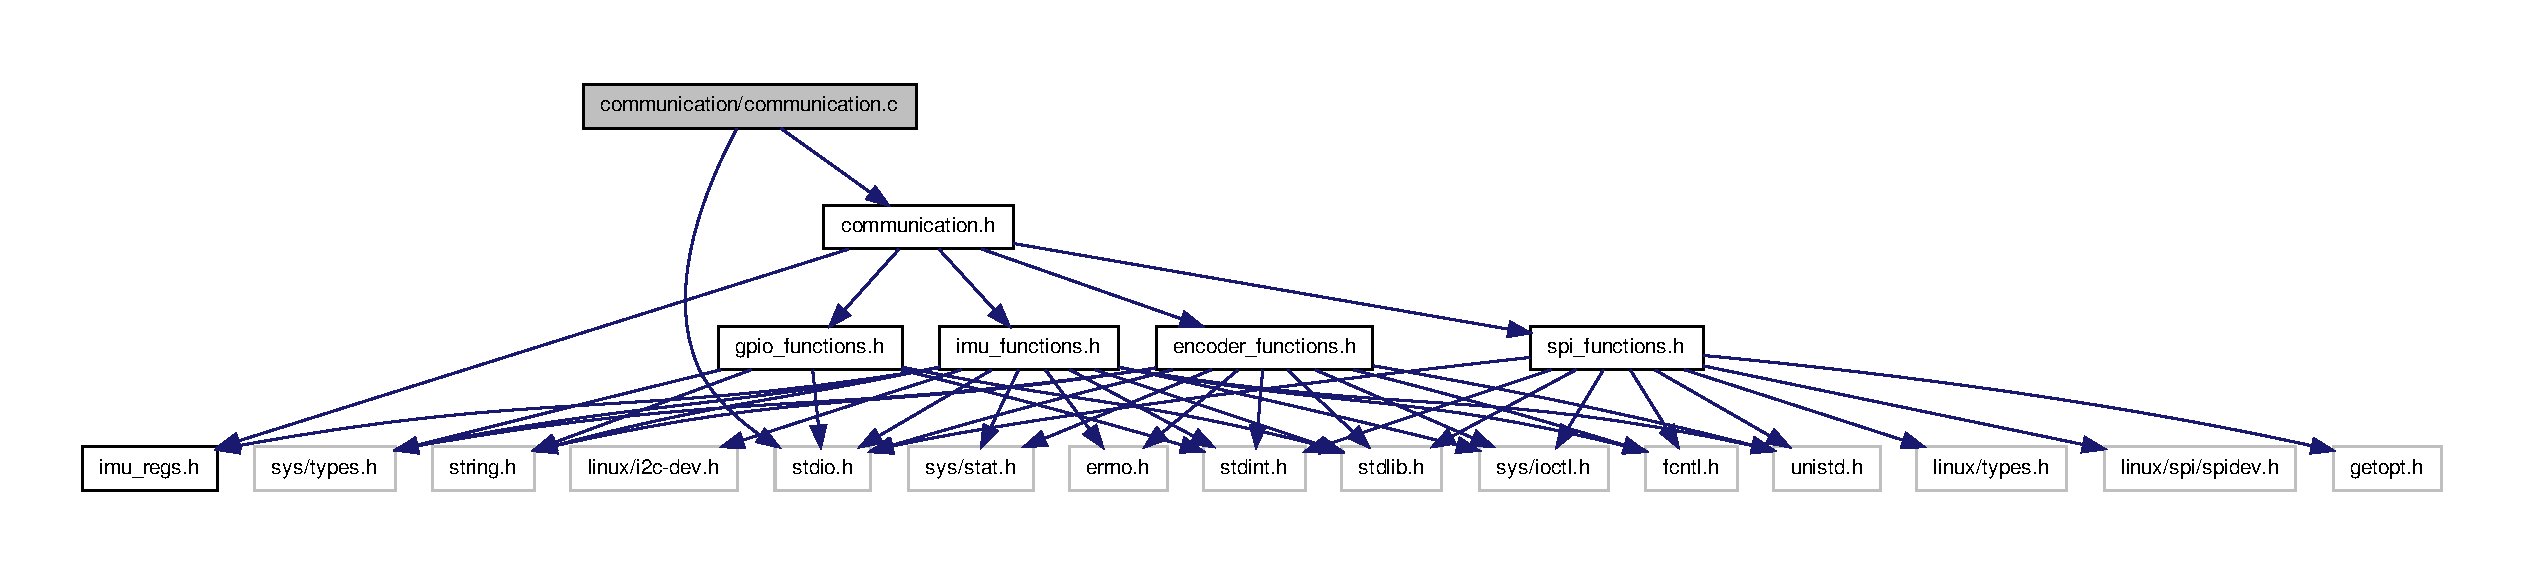
\includegraphics[width=350pt]{communication_2communication_8c__incl}
\end{center}
\end{figure}
\subsection*{Functions}
\begin{DoxyCompactItemize}
\item 
int \hyperlink{communication_2communication_8c_a2d1e523ff70db11ca4096f97af5da000}{devices\-\_\-init} (\hyperlink{structIMU__PARAM__STRUCT}{I\-M\-U\-\_\-\-P\-A\-R\-A\-M\-\_\-\-S\-T\-R\-U\-C\-T} $\ast$\hyperlink{main2_8c_a9c6b2109fb9402446f92995db60951b5}{imu\-\_\-param}, \hyperlink{structSPI__PARAM__STRUCT}{S\-P\-I\-\_\-\-P\-A\-R\-A\-M\-\_\-\-S\-T\-R\-U\-C\-T} $\ast$\hyperlink{main2_8c_adec2468b88cf50b20e5cf399a3b7e994}{spi\-\_\-param}, \hyperlink{structMRA__DATA__STRUCT}{M\-R\-A\-\_\-\-D\-A\-T\-A\-\_\-\-S\-T\-R\-U\-C\-T} $\ast$\hyperlink{main2_8c_abc42e18d2909e9bc119316283f4ed9db}{mra\-\_\-data})
\begin{DoxyCompactList}\small\item\em I\-N\-I\-T\-I\-A\-L\-I\-Z\-A\-T\-I\-O\-N O\-F S\-E\-N\-S\-O\-R\-S A\-N\-D D\-E\-V\-I\-C\-E\-S. \end{DoxyCompactList}\item 
int \hyperlink{communication_2communication_8c_a5f0316a5f70c7e369541e996802603b4}{read\-\_\-all\-\_\-data} (int \hyperlink{CommunicationV0_2communication_8c_a7751bd45ac1064efb35adf1f19c25db8}{i2c\-\_\-dev}, int \hyperlink{CommunicationV0_2communication_8c_a4788f0a5355494bc6c13690e28f43783}{spi\-\_\-dev}, \hyperlink{structIMU__DATA__STRUCT}{I\-M\-U\-\_\-\-D\-A\-T\-A\-\_\-\-S\-T\-R\-U\-C\-T} $\ast$\hyperlink{threads__linux_8c_a3cfea12cbe9ca7f1681c950e4cd68606}{imu\-\_\-data}, \hyperlink{structEFF__DATA__STRUCT}{E\-F\-F\-\_\-\-D\-A\-T\-A\-\_\-\-S\-T\-R\-U\-C\-T} $\ast$\hyperlink{main2_8c_a5650ece8c3a277c7f158d75ae65265fa}{eff\-\_\-data}, \hyperlink{structMRA__DATA__STRUCT}{M\-R\-A\-\_\-\-D\-A\-T\-A\-\_\-\-S\-T\-R\-U\-C\-T} $\ast$\hyperlink{main2_8c_abc42e18d2909e9bc119316283f4ed9db}{mra\-\_\-data})
\begin{DoxyCompactList}\small\item\em R\-E\-A\-D A\-L\-L D\-A\-T\-A F\-R\-O\-M S\-E\-N\-S\-O\-R\-S A\-N\-D A\-D\-C. \end{DoxyCompactList}\item 
void \hyperlink{communication_2communication_8c_a1d5f01d0124cff7030b5c4951b4bbefa}{actuate} (int \hyperlink{CommunicationV0_2communication_8c_a4788f0a5355494bc6c13690e28f43783}{spi\-\_\-dev}, \hyperlink{structMRA__DATA__STRUCT}{M\-R\-A\-\_\-\-D\-A\-T\-A\-\_\-\-S\-T\-R\-U\-C\-T} $\ast$\hyperlink{main2_8c_abc42e18d2909e9bc119316283f4ed9db}{mra\-\_\-data})
\begin{DoxyCompactList}\small\item\em Applies the control signal to the actuator. \end{DoxyCompactList}\item 
void \hyperlink{communication_2communication_8c_a8c7a00eda165bde1af4ca55c693e6acf}{dac\-\_\-shut\-\_\-down} (void)
\end{DoxyCompactItemize}
\subsection*{Variables}
\begin{DoxyCompactItemize}
\item 
int \hyperlink{communication_2communication_8c_a6e27f49150e9a14580fb313cc2777e00}{status}
\end{DoxyCompactItemize}


\subsection{Function Documentation}
\hypertarget{communication_2communication_8c_a1d5f01d0124cff7030b5c4951b4bbefa}{\index{communication/communication.\-c@{communication/communication.\-c}!actuate@{actuate}}
\index{actuate@{actuate}!communication/communication.c@{communication/communication.\-c}}
\subsubsection[{actuate}]{\setlength{\rightskip}{0pt plus 5cm}void actuate (
\begin{DoxyParamCaption}
\item[{int}]{spi\-\_\-dev, }
\item[{{\bf M\-R\-A\-\_\-\-D\-A\-T\-A\-\_\-\-S\-T\-R\-U\-C\-T} $\ast$}]{mra\-\_\-data}
\end{DoxyParamCaption}
)}}\label{communication_2communication_8c_a1d5f01d0124cff7030b5c4951b4bbefa}


Applies the control signal to the actuator. 


\begin{DoxyParams}{Parameters}
{\em spi\-\_\-dev} & Containing S\-P\-I variable I\-D \\
\hline
{\em mra\-\_\-data} & Struct containing the control signal \\
\hline
\end{DoxyParams}
\begin{DoxyReturn}{Returns}
nothing 
\end{DoxyReturn}


Definition at line 153 of file communication.\-c.



References dac\-\_\-write(), F\-A\-I\-L\-U\-R\-E, G\-P\-I\-O\-\_\-\-C\-S\-\_\-\-S0, G\-P\-I\-O\-\_\-\-C\-S\-\_\-\-S1, G\-P\-I\-O\-\_\-\-C\-S\-\_\-\-S2, G\-P\-I\-O\-\_\-\-C\-S\-\_\-\-S3, G\-P\-I\-O\-\_\-\-D\-A\-C\-\_\-\-S\-H\-D\-N, gpio\-\_\-write(), M\-R\-A\-\_\-\-D\-A\-T\-A\-\_\-\-S\-T\-R\-U\-C\-T\-::new\-\_\-ctl, S\-U\-C\-C\-E\-S\-S, and M\-R\-A\-\_\-\-D\-A\-T\-A\-\_\-\-S\-T\-R\-U\-C\-T\-::v\-\_\-ctl.


\begin{DoxyCode}
\{
  \textcolor{comment}{//printf("i = %d\(\backslash\)n",i);}
  \textcolor{comment}{//i++;}
  \textcolor{keywordflow}{if}( \hyperlink{communication_2gpio__functions_8c_a9672ca43e65fa527cd6bf43db9aea594}{gpio\_write}(\hyperlink{communication_01_07C_xC3_xB3pia_01em_01conflito_01de_01Caio_01Gustavo_01Mesquita_01Angelo_012013-05-17_08_8h_a99fc26a9596a1cb1f0f9936dbb8ccca6}{GPIO\_DAC\_SHDN},1)==\hyperlink{calibration_2calibration_8h_a6d58f9ac447476b4e084d7ca383f5183}{FAILURE} )
        mra\_data->\hyperlink{structMRA__DATA__STRUCT_a5b1af89ee717f5b14c18e8ac12e93e75}{new\_ctl}=\hyperlink{calibration_2calibration_8h_a6d58f9ac447476b4e084d7ca383f5183}{FAILURE}; \textcolor{keywordflow}{else}
  \textcolor{keywordflow}{if}( (\hyperlink{communication_2gpio__functions_8c_a9672ca43e65fa527cd6bf43db9aea594}{gpio\_write}(\hyperlink{communication_01_07C_xC3_xB3pia_01em_01conflito_01de_01Caio_01Gustavo_01Mesquita_01Angelo_012013-05-17_08_8h_ad774f00fc71216488e24a803bf4eb6aa}{GPIO\_CS\_S3},1)==\hyperlink{calibration_2calibration_8h_a6d58f9ac447476b4e084d7ca383f5183}{FAILURE}) || (
      \hyperlink{communication_2gpio__functions_8c_a9672ca43e65fa527cd6bf43db9aea594}{gpio\_write}(\hyperlink{communication_01_07C_xC3_xB3pia_01em_01conflito_01de_01Caio_01Gustavo_01Mesquita_01Angelo_012013-05-17_08_8h_a94b6d57532d1db55dc4efd9fb234f156}{GPIO\_CS\_S2},0)==\hyperlink{calibration_2calibration_8h_a6d58f9ac447476b4e084d7ca383f5183}{FAILURE}) || (\hyperlink{communication_2gpio__functions_8c_a9672ca43e65fa527cd6bf43db9aea594}{gpio\_write}
      (\hyperlink{communication_01_07C_xC3_xB3pia_01em_01conflito_01de_01Caio_01Gustavo_01Mesquita_01Angelo_012013-05-17_08_8h_a7672ba13ff6f297c347790586c9a02e0}{GPIO\_CS\_S1},1)==\hyperlink{calibration_2calibration_8h_a6d58f9ac447476b4e084d7ca383f5183}{FAILURE}) || (\hyperlink{communication_2gpio__functions_8c_a9672ca43e65fa527cd6bf43db9aea594}{gpio\_write}(\hyperlink{communication_01_07C_xC3_xB3pia_01em_01conflito_01de_01Caio_01Gustavo_01Mesquita_01Angelo_012013-05-17_08_8h_a48ea000c2b251ce26ea35d300f319651}{GPIO\_CS\_S0}
      ,0)==\hyperlink{calibration_2calibration_8h_a6d58f9ac447476b4e084d7ca383f5183}{FAILURE}) )
        mra\_data->\hyperlink{structMRA__DATA__STRUCT_a5b1af89ee717f5b14c18e8ac12e93e75}{new\_ctl}=\hyperlink{calibration_2calibration_8h_a6d58f9ac447476b4e084d7ca383f5183}{FAILURE};
  \textcolor{keywordflow}{else} \textcolor{keywordflow}{if}( (\hyperlink{group__spi_ga5c52e64c336d59215ce0a4b6f340dc9f}{dac\_write}(\hyperlink{CommunicationV0_2communication_8c_a4788f0a5355494bc6c13690e28f43783}{spi\_dev},0,1,mra\_data->\hyperlink{structMRA__DATA__STRUCT_a64b4e6bb604e58de593a60c87942b966}{v\_ctl}))==
      \hyperlink{calibration_2calibration_8h_a6d58f9ac447476b4e084d7ca383f5183}{FAILURE} )
        mra\_data->\hyperlink{structMRA__DATA__STRUCT_a5b1af89ee717f5b14c18e8ac12e93e75}{new\_ctl}=\hyperlink{calibration_2calibration_8h_a6d58f9ac447476b4e084d7ca383f5183}{FAILURE};
\textcolor{comment}{//  else if( (dac\_write(spi\_dev,1,1,mra\_data->???))==FAILURE )}
\textcolor{comment}{//      mra\_data->success=FAILURE;}
  \textcolor{keywordflow}{else} mra\_data->\hyperlink{structMRA__DATA__STRUCT_a5b1af89ee717f5b14c18e8ac12e93e75}{new\_ctl}=\hyperlink{calibration_2calibration_8h_aa90cac659d18e8ef6294c7ae337f6b58}{SUCCESS};
  \textcolor{keywordflow}{return};
\}
\end{DoxyCode}


Here is the call graph for this function\-:
\nopagebreak
\begin{figure}[H]
\begin{center}
\leavevmode
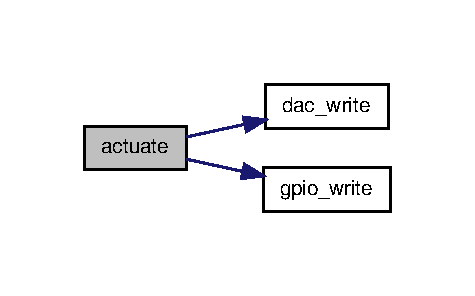
\includegraphics[width=228pt]{communication_2communication_8c_a1d5f01d0124cff7030b5c4951b4bbefa_cgraph}
\end{center}
\end{figure}


\hypertarget{communication_2communication_8c_a8c7a00eda165bde1af4ca55c693e6acf}{\index{communication/communication.\-c@{communication/communication.\-c}!dac\-\_\-shut\-\_\-down@{dac\-\_\-shut\-\_\-down}}
\index{dac\-\_\-shut\-\_\-down@{dac\-\_\-shut\-\_\-down}!communication/communication.c@{communication/communication.\-c}}
\subsubsection[{dac\-\_\-shut\-\_\-down}]{\setlength{\rightskip}{0pt plus 5cm}void dac\-\_\-shut\-\_\-down (
\begin{DoxyParamCaption}
\item[{void}]{}
\end{DoxyParamCaption}
)}}\label{communication_2communication_8c_a8c7a00eda165bde1af4ca55c693e6acf}


Definition at line 169 of file communication.\-c.



References G\-P\-I\-O\-\_\-\-D\-A\-C\-\_\-\-S\-H\-D\-N, gpio\-\_\-read(), and gpio\-\_\-write().


\begin{DoxyCode}
\{
  \textcolor{keywordflow}{while}( (\hyperlink{communication_2gpio__functions_8c_ae18413a0edf151e47a7aa6be21c5144a}{gpio\_read}(\hyperlink{communication_01_07C_xC3_xB3pia_01em_01conflito_01de_01Caio_01Gustavo_01Mesquita_01Angelo_012013-05-17_08_8h_a99fc26a9596a1cb1f0f9936dbb8ccca6}{GPIO\_DAC\_SHDN}))==0 )
    \hyperlink{communication_2gpio__functions_8c_a9672ca43e65fa527cd6bf43db9aea594}{gpio\_write}(\hyperlink{communication_01_07C_xC3_xB3pia_01em_01conflito_01de_01Caio_01Gustavo_01Mesquita_01Angelo_012013-05-17_08_8h_a99fc26a9596a1cb1f0f9936dbb8ccca6}{GPIO\_DAC\_SHDN},0);
  \textcolor{keywordflow}{return};
\}
\end{DoxyCode}


Here is the call graph for this function\-:\nopagebreak
\begin{figure}[H]
\begin{center}
\leavevmode
\includegraphics[width=264pt]{communication_2communication_8c_a8c7a00eda165bde1af4ca55c693e6acf_cgraph}
\end{center}
\end{figure}


\hypertarget{communication_2communication_8c_a2d1e523ff70db11ca4096f97af5da000}{\index{communication/communication.\-c@{communication/communication.\-c}!devices\-\_\-init@{devices\-\_\-init}}
\index{devices\-\_\-init@{devices\-\_\-init}!communication/communication.c@{communication/communication.\-c}}
\subsubsection[{devices\-\_\-init}]{\setlength{\rightskip}{0pt plus 5cm}int devices\-\_\-init (
\begin{DoxyParamCaption}
\item[{{\bf I\-M\-U\-\_\-\-P\-A\-R\-A\-M\-\_\-\-S\-T\-R\-U\-C\-T} $\ast$}]{imu\-\_\-param, }
\item[{{\bf S\-P\-I\-\_\-\-P\-A\-R\-A\-M\-\_\-\-S\-T\-R\-U\-C\-T} $\ast$}]{spi\-\_\-param, }
\item[{{\bf M\-R\-A\-\_\-\-D\-A\-T\-A\-\_\-\-S\-T\-R\-U\-C\-T} $\ast$}]{mra\-\_\-data}
\end{DoxyParamCaption}
)}}\label{communication_2communication_8c_a2d1e523ff70db11ca4096f97af5da000}


I\-N\-I\-T\-I\-A\-L\-I\-Z\-A\-T\-I\-O\-N O\-F S\-E\-N\-S\-O\-R\-S A\-N\-D D\-E\-V\-I\-C\-E\-S. 


\begin{DoxyParams}{Parameters}
{\em $\ast$imu\-\_\-param} & Structure with I\-M\-U parameters \\
\hline
{\em $\ast$spi\-\_\-param} & Structure with S\-P\-I parameters \\
\hline
{\em $\ast$mra\-\_\-data} & Structure to control M\-R\-A \\
\hline
\end{DoxyParams}
\begin{DoxyReturn}{Returns}
flag with S\-U\-C\-C\-E\-S\-S or F\-A\-I\-L\-U\-R\-E 
\end{DoxyReturn}


Definition at line 13 of file communication.\-c.



References I\-M\-U\-\_\-\-P\-A\-R\-A\-M\-\_\-\-S\-T\-R\-U\-C\-T\-::acc, acc\-\_\-init(), I\-M\-U\-\_\-\-P\-A\-R\-A\-M\-\_\-\-S\-T\-R\-U\-C\-T\-::param\-\_\-gyr\-::act, actuate(), A\-D\-D\-\_\-\-A\-D\-X\-L345, A\-D\-D\-\_\-\-H\-M\-C5883, A\-D\-D\-\_\-\-I\-T\-G3200, I\-M\-U\-\_\-\-P\-A\-R\-A\-M\-\_\-\-S\-T\-R\-U\-C\-T\-::param\-\_\-gyr\-::clk\-\_\-source, S\-P\-I\-\_\-\-P\-A\-R\-A\-M\-\_\-\-S\-T\-R\-U\-C\-T\-::cs, F\-A\-I\-L\-U\-R\-E, I\-M\-U\-\_\-\-P\-A\-R\-A\-M\-\_\-\-S\-T\-R\-U\-C\-T\-::param\-\_\-acc\-::full\-\_\-res, I\-M\-U\-\_\-\-P\-A\-R\-A\-M\-\_\-\-S\-T\-R\-U\-C\-T\-::gyr, gyr\-\_\-init(), I\-M\-U\-\_\-\-P\-A\-R\-A\-M\-\_\-\-S\-T\-R\-U\-C\-T\-::i2c\-\_\-dev, I\-M\-U\-\_\-\-P\-A\-R\-A\-M\-\_\-\-S\-T\-R\-U\-C\-T\-::param\-\_\-gyr\-::lpf\-\_\-bw, I\-M\-U\-\_\-\-P\-A\-R\-A\-M\-\_\-\-S\-T\-R\-U\-C\-T\-::mag, mag\-\_\-init(), I\-M\-U\-\_\-\-P\-A\-R\-A\-M\-\_\-\-S\-T\-R\-U\-C\-T\-::param\-\_\-mag\-::meas\-\_\-mode, S\-P\-I\-\_\-\-P\-A\-R\-A\-M\-\_\-\-S\-T\-R\-U\-C\-T\-::mode, M\-R\-A\-\_\-\-D\-A\-T\-A\-\_\-\-S\-T\-R\-U\-C\-T\-::new\-\_\-ctl, I\-M\-U\-\_\-\-P\-A\-R\-A\-M\-\_\-\-S\-T\-R\-U\-C\-T\-::param\-\_\-mag\-::op\-\_\-mode, I\-M\-U\-\_\-\-P\-A\-R\-A\-M\-\_\-\-S\-T\-R\-U\-C\-T\-::param\-\_\-acc\-::range, I\-M\-U\-\_\-\-P\-A\-R\-A\-M\-\_\-\-S\-T\-R\-U\-C\-T\-::param\-\_\-mag\-::range, I\-M\-U\-\_\-\-P\-A\-R\-A\-M\-\_\-\-S\-T\-R\-U\-C\-T\-::param\-\_\-acc\-::rate, I\-M\-U\-\_\-\-P\-A\-R\-A\-M\-\_\-\-S\-T\-R\-U\-C\-T\-::param\-\_\-gyr\-::rate, I\-M\-U\-\_\-\-P\-A\-R\-A\-M\-\_\-\-S\-T\-R\-U\-C\-T\-::param\-\_\-mag\-::rate, I\-M\-U\-\_\-\-P\-A\-R\-A\-M\-\_\-\-S\-T\-R\-U\-C\-T\-::param\-\_\-mag\-::samples\-\_\-avg, S\-P\-I\-\_\-\-P\-A\-R\-A\-M\-\_\-\-S\-T\-R\-U\-C\-T\-::speed, S\-P\-I\-\_\-\-P\-A\-R\-A\-M\-\_\-\-S\-T\-R\-U\-C\-T\-::spi\-\_\-dev, spi\-\_\-init(), S\-U\-C\-C\-E\-S\-S, and M\-R\-A\-\_\-\-D\-A\-T\-A\-\_\-\-S\-T\-R\-U\-C\-T\-::v\-\_\-ctl.


\begin{DoxyCode}
\{

  \textcolor{keywordflow}{if}( (imu\_param->\hyperlink{structIMU__PARAM__STRUCT_a8a870f383fc9ba0b682fdc9b8c0d2734}{i2c\_dev} = open(\textcolor{stringliteral}{"/dev/i2c-3"}, O\_RDWR))<0 )
  \{
    perror(\textcolor{stringliteral}{"Failed to open i2c\_dev"});
    \textcolor{keywordflow}{return} \hyperlink{calibration_2calibration_8h_a6d58f9ac447476b4e084d7ca383f5183}{FAILURE};
  \}

  \textcolor{keywordflow}{if} ((ioctl(imu\_param->\hyperlink{structIMU__PARAM__STRUCT_a8a870f383fc9ba0b682fdc9b8c0d2734}{i2c\_dev}, I2C\_SLAVE, \hyperlink{communication_2imu__functions_8h_a383c09d3e3bbe30097f7eb8d081fb856}{ADD\_HMC5883})) < 0
      ) \{
                perror(\textcolor{stringliteral}{"ioctl(I2C\_SLAVE) mag"});
                \textcolor{keywordflow}{return} \hyperlink{calibration_2calibration_8h_a6d58f9ac447476b4e084d7ca383f5183}{FAILURE};
  \}

  \textcolor{keywordflow}{if}( (\hyperlink{communication_2imu__functions_8h_a014f908c9faa37c1ec75177a17012a01}{mag\_init}(imu\_param->\hyperlink{structIMU__PARAM__STRUCT_a8a870f383fc9ba0b682fdc9b8c0d2734}{i2c\_dev}, imu\_param->\hyperlink{structIMU__PARAM__STRUCT_a26b277dcaf05f3842995df888225f6f4}{mag}.\hyperlink{structIMU__PARAM__STRUCT_1_1param__mag_a234de95423b604b05b851ef90890cea1}{rate}, 
      imu\_param->\hyperlink{structIMU__PARAM__STRUCT_a26b277dcaf05f3842995df888225f6f4}{mag}.\hyperlink{structIMU__PARAM__STRUCT_1_1param__mag_a40ad27ebdb5fde35257b1dc52e40f476}{range}, imu\_param->\hyperlink{structIMU__PARAM__STRUCT_a26b277dcaf05f3842995df888225f6f4}{mag}.\hyperlink{structIMU__PARAM__STRUCT_1_1param__mag_a52c22cae6940eb39fb72aca66cfeba9a}{samples\_avg}, 
      imu\_param->\hyperlink{structIMU__PARAM__STRUCT_a26b277dcaf05f3842995df888225f6f4}{mag}.\hyperlink{structIMU__PARAM__STRUCT_1_1param__mag_a1f3536709c05310005d648f339d70c54}{meas\_mode}, imu\_param->\hyperlink{structIMU__PARAM__STRUCT_a26b277dcaf05f3842995df888225f6f4}{mag}.\hyperlink{structIMU__PARAM__STRUCT_1_1param__mag_a39b83b3e9ff5bdcafed0bdf6a2de584b}{op\_mode}))< 0)
  \{
      perror(\textcolor{stringliteral}{"Error in magnetometer initialization"});
      \textcolor{keywordflow}{return} \hyperlink{calibration_2calibration_8h_a6d58f9ac447476b4e084d7ca383f5183}{FAILURE};
  \}  

  \textcolor{keywordflow}{if}( ioctl(imu\_param->\hyperlink{structIMU__PARAM__STRUCT_a8a870f383fc9ba0b682fdc9b8c0d2734}{i2c\_dev}, I2C\_SLAVE, \hyperlink{communication_2imu__functions_8h_ab9fd1068a3f5fcba24d92918aaf0dcb5}{ADD\_ITG3200}) < 0) 
      \{
                perror(\textcolor{stringliteral}{"ioctl(I2C\_SLAVE) gyr"});
                \textcolor{keywordflow}{return} \hyperlink{calibration_2calibration_8h_a6d58f9ac447476b4e084d7ca383f5183}{FAILURE};
  \} 

  \textcolor{keywordflow}{if}( \hyperlink{group__gyr_ga6d02be352b4491a236c9695a6a24d174}{gyr\_init}(imu\_param->\hyperlink{structIMU__PARAM__STRUCT_a8a870f383fc9ba0b682fdc9b8c0d2734}{i2c\_dev}, imu\_param->\hyperlink{structIMU__PARAM__STRUCT_a5a4557868f1af679a1098808397b02ec}{gyr}.\hyperlink{structIMU__PARAM__STRUCT_1_1param__gyr_a5aa70e1e9634411c89aacfbc570cc91c}{rate}, 
      imu\_param->\hyperlink{structIMU__PARAM__STRUCT_a5a4557868f1af679a1098808397b02ec}{gyr}.\hyperlink{structIMU__PARAM__STRUCT_1_1param__gyr_aa612f7299b43a1bf1fc597688c2fa02d}{lpf\_bw}, imu\_param->\hyperlink{structIMU__PARAM__STRUCT_a5a4557868f1af679a1098808397b02ec}{gyr}.\hyperlink{structIMU__PARAM__STRUCT_1_1param__gyr_aca3b791cb480f2da4703d4c256a7de48}{clk\_source}, imu\_param
      ->\hyperlink{structIMU__PARAM__STRUCT_a5a4557868f1af679a1098808397b02ec}{gyr}.\hyperlink{structIMU__PARAM__STRUCT_1_1param__gyr_a8b583edb905ed922572e46453e7d4adf}{act})<0 )
  \{
      perror(\textcolor{stringliteral}{"Error in gyrometer initialization"});
      \textcolor{comment}{//return FAILURE;}
  \}

  \textcolor{keywordflow}{if} ( (ioctl(imu\_param->\hyperlink{structIMU__PARAM__STRUCT_a8a870f383fc9ba0b682fdc9b8c0d2734}{i2c\_dev}, I2C\_SLAVE, \hyperlink{communication_2imu__functions_8h_a909f4a5773e20e672cdb4088e1cfa22f}{ADD\_ADXL345})) < 
      0) \{
        perror(\textcolor{stringliteral}{"ioctl(I2C\_SLAVE) acc"});
        \textcolor{keywordflow}{return} \hyperlink{calibration_2calibration_8h_a6d58f9ac447476b4e084d7ca383f5183}{FAILURE};
  \}  

  \textcolor{keywordflow}{if}( \hyperlink{group__acc_gae8f9cc6e0d15e61039d846305f86f073}{acc\_init}(imu\_param->\hyperlink{structIMU__PARAM__STRUCT_a8a870f383fc9ba0b682fdc9b8c0d2734}{i2c\_dev}, imu\_param->\hyperlink{structIMU__PARAM__STRUCT_a92172e4757d0f8f9135a659e406c12e5}{acc}.\hyperlink{structIMU__PARAM__STRUCT_1_1param__acc_af57da5d956ffa7e49a184326b6b9c738}{full\_res}
      , imu\_param->\hyperlink{structIMU__PARAM__STRUCT_a92172e4757d0f8f9135a659e406c12e5}{acc}.\hyperlink{structIMU__PARAM__STRUCT_1_1param__acc_a30e6a318cad098cd8379416705820f95}{rate}, imu\_param->\hyperlink{structIMU__PARAM__STRUCT_a92172e4757d0f8f9135a659e406c12e5}{acc}.\hyperlink{structIMU__PARAM__STRUCT_1_1param__acc_a26199b298ef2d353192dfbc706bce8cf}{range})<0)
  \{
        perror(\textcolor{stringliteral}{"Error in accelerometer initialization"});
        \textcolor{keywordflow}{return} \hyperlink{calibration_2calibration_8h_a6d58f9ac447476b4e084d7ca383f5183}{FAILURE};
  \}

  \textcolor{keywordflow}{if} ((spi\_param->\hyperlink{structSPI__PARAM__STRUCT_abe385c44333d268d17cf648c8e371cad}{spi\_dev}=\hyperlink{group__spi_ga70764aca888e93b0329e7a62c9312704}{spi\_init}(spi\_param->\hyperlink{structSPI__PARAM__STRUCT_a82c546c99f6c3daed73c1e23426be847}{mode},spi\_param
      ->\hyperlink{structSPI__PARAM__STRUCT_a53a8d386594a81eb9bc6f971bfe36c54}{speed},spi\_param->\hyperlink{structSPI__PARAM__STRUCT_ae0d62e0a5554783d710b677a017e246f}{cs}))<0) 
  \{
    perror(\textcolor{stringliteral}{"Error in SPI device initialization"});
    \textcolor{keywordflow}{return} \hyperlink{calibration_2calibration_8h_a6d58f9ac447476b4e084d7ca383f5183}{FAILURE};
  \}

  \textcolor{comment}{//Enable DAC and writing 0}
  mra\_data->\hyperlink{structMRA__DATA__STRUCT_a64b4e6bb604e58de593a60c87942b966}{v\_ctl}=0;
\textcolor{comment}{//  mra\_data->Out\_1=0;gpio\_write(GPIO\_CS\_S3,1)==FAILURE}

  \hyperlink{communication_01_07C_xC3_xB3pia_01em_01conflito_01de_01Caio_01Gustavo_01Mesquita_01Angelo_012013-05-17_08_8c_a1d5f01d0124cff7030b5c4951b4bbefa}{actuate}(spi\_param->\hyperlink{structSPI__PARAM__STRUCT_abe385c44333d268d17cf648c8e371cad}{spi\_dev}, mra\_data);
  \textcolor{keywordflow}{if}( mra\_data->\hyperlink{structMRA__DATA__STRUCT_a5b1af89ee717f5b14c18e8ac12e93e75}{new\_ctl} == \hyperlink{calibration_2calibration_8h_a6d58f9ac447476b4e084d7ca383f5183}{FAILURE} )
  \{
        perror(\textcolor{stringliteral}{"Error in MRA initialization"});
        \textcolor{keywordflow}{return} \hyperlink{calibration_2calibration_8h_a6d58f9ac447476b4e084d7ca383f5183}{FAILURE};
  \}
 \textcolor{comment}{// if( gpio\_write(GPIO\_DAC\_SHDN,1)==FAILURE )}
 \textcolor{comment}{// \{}
\textcolor{comment}{//      perror("Error in SHDN initialization");}
\textcolor{comment}{//      return FAILURE;}
\textcolor{comment}{//  \}}
  
  \textcolor{keywordflow}{return} \hyperlink{calibration_2calibration_8h_aa90cac659d18e8ef6294c7ae337f6b58}{SUCCESS};
\}
\end{DoxyCode}


Here is the call graph for this function\-:
\nopagebreak
\begin{figure}[H]
\begin{center}
\leavevmode
\includegraphics[width=238pt]{communication_2communication_8c_a2d1e523ff70db11ca4096f97af5da000_cgraph}
\end{center}
\end{figure}


\hypertarget{communication_2communication_8c_a5f0316a5f70c7e369541e996802603b4}{\index{communication/communication.\-c@{communication/communication.\-c}!read\-\_\-all\-\_\-data@{read\-\_\-all\-\_\-data}}
\index{read\-\_\-all\-\_\-data@{read\-\_\-all\-\_\-data}!communication/communication.c@{communication/communication.\-c}}
\subsubsection[{read\-\_\-all\-\_\-data}]{\setlength{\rightskip}{0pt plus 5cm}int read\-\_\-all\-\_\-data (
\begin{DoxyParamCaption}
\item[{int}]{i2c\-\_\-dev, }
\item[{int}]{spi\-\_\-dev, }
\item[{{\bf I\-M\-U\-\_\-\-D\-A\-T\-A\-\_\-\-S\-T\-R\-U\-C\-T} $\ast$}]{imu\-\_\-data, }
\item[{{\bf E\-F\-F\-\_\-\-D\-A\-T\-A\-\_\-\-S\-T\-R\-U\-C\-T} $\ast$}]{eff\-\_\-data, }
\item[{{\bf M\-R\-A\-\_\-\-D\-A\-T\-A\-\_\-\-S\-T\-R\-U\-C\-T} $\ast$}]{mra\-\_\-data}
\end{DoxyParamCaption}
)}}\label{communication_2communication_8c_a5f0316a5f70c7e369541e996802603b4}


R\-E\-A\-D A\-L\-L D\-A\-T\-A F\-R\-O\-M S\-E\-N\-S\-O\-R\-S A\-N\-D A\-D\-C. 


\begin{DoxyParams}{Parameters}
{\em i2c\-\_\-dev} & \\
\hline
{\em spi\-\_\-dev} & \\
\hline
{\em $\ast$imu\-\_\-data} & \\
\hline
{\em $\ast$eff\-\_\-data} & \\
\hline
{\em $\ast$mra\-\_\-data} & \\
\hline
\end{DoxyParams}
\begin{DoxyReturn}{Returns}
flag with S\-U\-C\-C\-E\-S\-S or F\-A\-I\-L\-U\-R\-E 
\end{DoxyReturn}


Definition at line 80 of file communication.\-c.



References I\-M\-U\-\_\-\-D\-A\-T\-A\-\_\-\-S\-T\-R\-U\-C\-T\-::acc, acc\-\_\-read\-\_\-all\-\_\-data(), adc\-\_\-read(), A\-D\-D\-\_\-\-A\-D\-X\-L345, A\-D\-D\-\_\-\-H\-M\-C5883, A\-D\-D\-\_\-\-I\-T\-G3200, E\-F\-F\-\_\-\-D\-A\-T\-A\-\_\-\-S\-T\-R\-U\-C\-T\-::\-F, F\-A\-I\-L\-U\-R\-E, G\-P\-I\-O\-\_\-\-C\-S\-\_\-\-S0, G\-P\-I\-O\-\_\-\-C\-S\-\_\-\-S1, G\-P\-I\-O\-\_\-\-C\-S\-\_\-\-S2, G\-P\-I\-O\-\_\-\-C\-S\-\_\-\-S3, gpio\-\_\-write(), I\-M\-U\-\_\-\-D\-A\-T\-A\-\_\-\-S\-T\-R\-U\-C\-T\-::gyr, gyr\-\_\-read\-\_\-all\-\_\-data(), I\-M\-U\-\_\-\-D\-A\-T\-A\-\_\-\-S\-T\-R\-U\-C\-T\-::mag, mag\-\_\-read\-\_\-all\-\_\-data(), I\-M\-U\-\_\-\-D\-A\-T\-A\-\_\-\-S\-T\-R\-U\-C\-T\-::new\-\_\-data, E\-F\-F\-\_\-\-D\-A\-T\-A\-\_\-\-S\-T\-R\-U\-C\-T\-::new\-\_\-data, M\-R\-A\-\_\-\-D\-A\-T\-A\-\_\-\-S\-T\-R\-U\-C\-T\-::new\-\_\-data, S\-U\-C\-C\-E\-S\-S, I\-M\-U\-\_\-\-D\-A\-T\-A\-\_\-\-S\-T\-R\-U\-C\-T\-::temp, M\-R\-A\-\_\-\-D\-A\-T\-A\-\_\-\-S\-T\-R\-U\-C\-T\-::v\-\_\-ctl\-\_\-read, D\-A\-T\-A\-\_\-\-X\-Y\-Z\-::x, D\-A\-T\-A\-\_\-\-X\-Y\-Z\-::y, and D\-A\-T\-A\-\_\-\-X\-Y\-Z\-::z.


\begin{DoxyCode}
\{
  \textcolor{keywordtype}{short} \textcolor{keywordtype}{int} data[4];
  \textcolor{keywordtype}{int} f=0;
  \textcolor{comment}{// Read IMU data}
  imu\_data->\hyperlink{structIMU__DATA__STRUCT_a99924252176326418863e511d4fa437b}{new\_data}=\hyperlink{calibration_2calibration_8h_aa90cac659d18e8ef6294c7ae337f6b58}{SUCCESS};
  
  \textcolor{keywordflow}{if} ( (ioctl(\hyperlink{CommunicationV0_2communication_8c_a7751bd45ac1064efb35adf1f19c25db8}{i2c\_dev}, I2C\_SLAVE, \hyperlink{communication_2imu__functions_8h_a909f4a5773e20e672cdb4088e1cfa22f}{ADD\_ADXL345}))<0) 
        imu\_data->\hyperlink{structIMU__DATA__STRUCT_a99924252176326418863e511d4fa437b}{new\_data}=0;
  \textcolor{keywordflow}{else} \textcolor{keywordflow}{if}( (\hyperlink{group__acc_ga013bb5ed8a763883fc440549d2b1a6ce}{acc\_read\_all\_data}(\hyperlink{CommunicationV0_2communication_8c_a7751bd45ac1064efb35adf1f19c25db8}{i2c\_dev},data))==\hyperlink{calibration_2calibration_8h_a6d58f9ac447476b4e084d7ca383f5183}{FAILURE}
       )
  \{
        imu\_data->\hyperlink{structIMU__DATA__STRUCT_a99924252176326418863e511d4fa437b}{new\_data}=0;
        \textcolor{comment}{//printf("\(\backslash\)nimu\_data->new\_data = %d\(\backslash\)n",imu\_data->new\_data);}
        \textcolor{comment}{//f=1;}
  \}
  \textcolor{keywordflow}{else}\{
    imu\_data->\hyperlink{structIMU__DATA__STRUCT_a448f284bf44eb503affda586ad5fa9d2}{acc}.\hyperlink{structDATA__XYZ_a54c1596e9f9969fd9c21e8458024ecfb}{x}=data[0];
    imu\_data->\hyperlink{structIMU__DATA__STRUCT_a448f284bf44eb503affda586ad5fa9d2}{acc}.\hyperlink{structDATA__XYZ_a94bbb1c889bf53eb6a5fffa2b39322cf}{y}=data[1];
    imu\_data->\hyperlink{structIMU__DATA__STRUCT_a448f284bf44eb503affda586ad5fa9d2}{acc}.\hyperlink{structDATA__XYZ_a69e89ab0ec6e5d72fc5d54f62cc07fb5}{z}=data[2];  
  \}
  
  \textcolor{keywordflow}{if} ( (ioctl(\hyperlink{CommunicationV0_2communication_8c_a7751bd45ac1064efb35adf1f19c25db8}{i2c\_dev}, I2C\_SLAVE, \hyperlink{communication_2imu__functions_8h_ab9fd1068a3f5fcba24d92918aaf0dcb5}{ADD\_ITG3200})) < 0) 
        imu\_data->\hyperlink{structIMU__DATA__STRUCT_a99924252176326418863e511d4fa437b}{new\_data}=0;
  \textcolor{keywordflow}{else} \textcolor{keywordflow}{if}( (\hyperlink{group__gyr_ga79875465c3a29fd9ec77308c80a8bc37}{gyr\_read\_all\_data}(\hyperlink{CommunicationV0_2communication_8c_a7751bd45ac1064efb35adf1f19c25db8}{i2c\_dev},data))==\hyperlink{calibration_2calibration_8h_a6d58f9ac447476b4e084d7ca383f5183}{FAILURE}
       )
        imu\_data->\hyperlink{structIMU__DATA__STRUCT_a99924252176326418863e511d4fa437b}{new\_data}=0;
  \textcolor{keywordflow}{else}\{
    imu\_data->\hyperlink{structIMU__DATA__STRUCT_a0c1ac26626e4434a2ee124a1928a23a1}{gyr}.\hyperlink{structDATA__XYZ_a54c1596e9f9969fd9c21e8458024ecfb}{x}=data[0];
    imu\_data->\hyperlink{structIMU__DATA__STRUCT_a0c1ac26626e4434a2ee124a1928a23a1}{gyr}.\hyperlink{structDATA__XYZ_a94bbb1c889bf53eb6a5fffa2b39322cf}{y}=data[1];
    imu\_data->\hyperlink{structIMU__DATA__STRUCT_a0c1ac26626e4434a2ee124a1928a23a1}{gyr}.\hyperlink{structDATA__XYZ_a69e89ab0ec6e5d72fc5d54f62cc07fb5}{z}=data[2];
    imu\_data->\hyperlink{structIMU__DATA__STRUCT_a81e1dbf765c1d947ca6076aa1bbc73e7}{temp}=data[3];
  \}
  
  \textcolor{keywordflow}{if} ( (ioctl(\hyperlink{CommunicationV0_2communication_8c_a7751bd45ac1064efb35adf1f19c25db8}{i2c\_dev}, I2C\_SLAVE, \hyperlink{communication_2imu__functions_8h_a383c09d3e3bbe30097f7eb8d081fb856}{ADD\_HMC5883})) < 0) 
        imu\_data->\hyperlink{structIMU__DATA__STRUCT_a99924252176326418863e511d4fa437b}{new\_data}=0;
  \textcolor{keywordflow}{else} \textcolor{keywordflow}{if}( (\hyperlink{group__mag_gab42ae0d0a2a6f37cf36d856c072b7f34}{mag\_read\_all\_data}(\hyperlink{CommunicationV0_2communication_8c_a7751bd45ac1064efb35adf1f19c25db8}{i2c\_dev},data))==\hyperlink{calibration_2calibration_8h_a6d58f9ac447476b4e084d7ca383f5183}{FAILURE}
       )
        imu\_data->\hyperlink{structIMU__DATA__STRUCT_a99924252176326418863e511d4fa437b}{new\_data}=0;
  \textcolor{keywordflow}{else}\{
    imu\_data->\hyperlink{structIMU__DATA__STRUCT_a40c7df8b6d49297aa52873cfd9b60daa}{mag}.\hyperlink{structDATA__XYZ_a54c1596e9f9969fd9c21e8458024ecfb}{x}=data[0];
    imu\_data->\hyperlink{structIMU__DATA__STRUCT_a40c7df8b6d49297aa52873cfd9b60daa}{mag}.\hyperlink{structDATA__XYZ_a94bbb1c889bf53eb6a5fffa2b39322cf}{y}=data[1];
    imu\_data->\hyperlink{structIMU__DATA__STRUCT_a40c7df8b6d49297aa52873cfd9b60daa}{mag}.\hyperlink{structDATA__XYZ_a69e89ab0ec6e5d72fc5d54f62cc07fb5}{z}=data[2];
  \}

  \textcolor{comment}{//Read Efforts data}
  eff\_data->\hyperlink{structEFF__DATA__STRUCT_aa42ebc512dd79fa6ebf998162a149446}{new\_data}=\hyperlink{calibration_2calibration_8h_aa90cac659d18e8ef6294c7ae337f6b58}{SUCCESS};
  
  \textcolor{keywordflow}{if}( (\hyperlink{communication_2gpio__functions_8c_a9672ca43e65fa527cd6bf43db9aea594}{gpio\_write}(\hyperlink{communication_01_07C_xC3_xB3pia_01em_01conflito_01de_01Caio_01Gustavo_01Mesquita_01Angelo_012013-05-17_08_8h_ad774f00fc71216488e24a803bf4eb6aa}{GPIO\_CS\_S3},1)==\hyperlink{calibration_2calibration_8h_a6d58f9ac447476b4e084d7ca383f5183}{FAILURE}) || (
      \hyperlink{communication_2gpio__functions_8c_a9672ca43e65fa527cd6bf43db9aea594}{gpio\_write}(\hyperlink{communication_01_07C_xC3_xB3pia_01em_01conflito_01de_01Caio_01Gustavo_01Mesquita_01Angelo_012013-05-17_08_8h_a94b6d57532d1db55dc4efd9fb234f156}{GPIO\_CS\_S2},1)==\hyperlink{calibration_2calibration_8h_a6d58f9ac447476b4e084d7ca383f5183}{FAILURE}) || (\hyperlink{communication_2gpio__functions_8c_a9672ca43e65fa527cd6bf43db9aea594}{gpio\_write}
      (\hyperlink{communication_01_07C_xC3_xB3pia_01em_01conflito_01de_01Caio_01Gustavo_01Mesquita_01Angelo_012013-05-17_08_8h_a7672ba13ff6f297c347790586c9a02e0}{GPIO\_CS\_S1},1)==\hyperlink{calibration_2calibration_8h_a6d58f9ac447476b4e084d7ca383f5183}{FAILURE}) || (\hyperlink{communication_2gpio__functions_8c_a9672ca43e65fa527cd6bf43db9aea594}{gpio\_write}(\hyperlink{communication_01_07C_xC3_xB3pia_01em_01conflito_01de_01Caio_01Gustavo_01Mesquita_01Angelo_012013-05-17_08_8h_a48ea000c2b251ce26ea35d300f319651}{GPIO\_CS\_S0}
      ,0)==\hyperlink{calibration_2calibration_8h_a6d58f9ac447476b4e084d7ca383f5183}{FAILURE}))
        eff\_data->\hyperlink{structEFF__DATA__STRUCT_aa42ebc512dd79fa6ebf998162a149446}{new\_data}=\hyperlink{calibration_2calibration_8h_a6d58f9ac447476b4e084d7ca383f5183}{FAILURE};
  \textcolor{keywordflow}{else}\{ 
    \textcolor{keywordflow}{if}( (\hyperlink{group__spi_gae385345c227d9f67ab490b94ed628988}{adc\_read}(\hyperlink{CommunicationV0_2communication_8c_a4788f0a5355494bc6c13690e28f43783}{spi\_dev},0,1,data))==\hyperlink{calibration_2calibration_8h_a6d58f9ac447476b4e084d7ca383f5183}{FAILURE} )
        eff\_data->\hyperlink{structEFF__DATA__STRUCT_aa42ebc512dd79fa6ebf998162a149446}{new\_data}=\hyperlink{calibration_2calibration_8h_a6d58f9ac447476b4e084d7ca383f5183}{FAILURE};
    \textcolor{keywordflow}{else} eff\_data->\hyperlink{structEFF__DATA__STRUCT_abe8952947b54bf9c247f3429ee3aeb44}{F}.\hyperlink{structDATA__XYZ_a54c1596e9f9969fd9c21e8458024ecfb}{x}=data[0];
  \textcolor{comment}{//Read MR actuator voltage control}
    \textcolor{keywordflow}{if}( (\hyperlink{group__spi_gae385345c227d9f67ab490b94ed628988}{adc\_read}(\hyperlink{CommunicationV0_2communication_8c_a4788f0a5355494bc6c13690e28f43783}{spi\_dev},7,1,data))==\hyperlink{calibration_2calibration_8h_aa90cac659d18e8ef6294c7ae337f6b58}{SUCCESS} )
    \{
        mra\_data->\hyperlink{structMRA__DATA__STRUCT_a3a31d57268c33b21ac915fdc27dfe474}{v\_ctl\_read}=data[0];
        mra\_data->\hyperlink{structMRA__DATA__STRUCT_afca6e851d302f3a786885a4e1eec79d7}{new\_data}=\hyperlink{calibration_2calibration_8h_aa90cac659d18e8ef6294c7ae337f6b58}{SUCCESS};
    \}
  \}
  \textcolor{comment}{//if( f==1 )}
    \textcolor{comment}{//printf("imu\_data->new\_data antes do return= %d\(\backslash\)n",imu\_data->new\_data);}

  \textcolor{keywordflow}{if}( imu\_data->\hyperlink{structIMU__DATA__STRUCT_a99924252176326418863e511d4fa437b}{new\_data}==\hyperlink{calibration_2calibration_8h_a6d58f9ac447476b4e084d7ca383f5183}{FAILURE} || eff\_data->\hyperlink{structEFF__DATA__STRUCT_aa42ebc512dd79fa6ebf998162a149446}{new\_data}
      ==\hyperlink{calibration_2calibration_8h_a6d58f9ac447476b4e084d7ca383f5183}{FAILURE} || mra\_data->\hyperlink{structMRA__DATA__STRUCT_afca6e851d302f3a786885a4e1eec79d7}{new\_data}==\hyperlink{calibration_2calibration_8h_a6d58f9ac447476b4e084d7ca383f5183}{FAILURE} )
    \textcolor{keywordflow}{return} \hyperlink{calibration_2calibration_8h_a6d58f9ac447476b4e084d7ca383f5183}{FAILURE};
    
  \textcolor{keywordflow}{return} \hyperlink{calibration_2calibration_8h_aa90cac659d18e8ef6294c7ae337f6b58}{SUCCESS};
\}
\end{DoxyCode}


Here is the call graph for this function\-:
\nopagebreak
\begin{figure}[H]
\begin{center}
\leavevmode
\includegraphics[width=288pt]{communication_2communication_8c_a5f0316a5f70c7e369541e996802603b4_cgraph}
\end{center}
\end{figure}




\subsection{Variable Documentation}
\hypertarget{communication_2communication_8c_a6e27f49150e9a14580fb313cc2777e00}{\index{communication/communication.\-c@{communication/communication.\-c}!status@{status}}
\index{status@{status}!communication/communication.c@{communication/communication.\-c}}
\subsubsection[{status}]{\setlength{\rightskip}{0pt plus 5cm}int status}}\label{communication_2communication_8c_a6e27f49150e9a14580fb313cc2777e00}


Definition at line 11 of file communication.\-c.


\hypertarget{CommunicationV0_2communication_8c}{\section{Communication\-V0/communication.c File Reference}
\label{CommunicationV0_2communication_8c}\index{Communication\-V0/communication.\-c@{Communication\-V0/communication.\-c}}
}
{\ttfamily \#include $<$stdio.\-h$>$}\\*
{\ttfamily \#include \char`\"{}communication.\-h\char`\"{}}\\*
Include dependency graph for communication.\-c\-:\nopagebreak
\begin{figure}[H]
\begin{center}
\leavevmode
\includegraphics[width=350pt]{CommunicationV0_2communication_8c__incl}
\end{center}
\end{figure}
\subsection*{Functions}
\begin{DoxyCompactItemize}
\item 
void \hyperlink{CommunicationV0_2communication_8c_a3b42d3bd68c5200393c1f0809ed1facf}{init\-\_\-data} ()
\item 
int \hyperlink{CommunicationV0_2communication_8c_a8fb13f0819b78de6e3ac64ca788ce2b4}{read\-\_\-all\-\_\-data} ()
\end{DoxyCompactItemize}
\subsection*{Variables}
\begin{DoxyCompactItemize}
\item 
int \hyperlink{CommunicationV0_2communication_8c_a7751bd45ac1064efb35adf1f19c25db8}{i2c\-\_\-dev}
\item 
int \hyperlink{CommunicationV0_2communication_8c_a4788f0a5355494bc6c13690e28f43783}{spi\-\_\-dev}
\end{DoxyCompactItemize}


\subsection{Function Documentation}
\hypertarget{CommunicationV0_2communication_8c_a3b42d3bd68c5200393c1f0809ed1facf}{\index{Communication\-V0/communication.\-c@{Communication\-V0/communication.\-c}!init\-\_\-data@{init\-\_\-data}}
\index{init\-\_\-data@{init\-\_\-data}!CommunicationV0/communication.c@{Communication\-V0/communication.\-c}}
\subsubsection[{init\-\_\-data}]{\setlength{\rightskip}{0pt plus 5cm}void init\-\_\-data (
\begin{DoxyParamCaption}
{}
\end{DoxyParamCaption}
)}}\label{CommunicationV0_2communication_8c_a3b42d3bd68c5200393c1f0809ed1facf}


Definition at line 11 of file communication.\-c.


\begin{DoxyCode}
12 \{
13 \}
\end{DoxyCode}
\hypertarget{CommunicationV0_2communication_8c_a8fb13f0819b78de6e3ac64ca788ce2b4}{\index{Communication\-V0/communication.\-c@{Communication\-V0/communication.\-c}!read\-\_\-all\-\_\-data@{read\-\_\-all\-\_\-data}}
\index{read\-\_\-all\-\_\-data@{read\-\_\-all\-\_\-data}!CommunicationV0/communication.c@{Communication\-V0/communication.\-c}}
\subsubsection[{read\-\_\-all\-\_\-data}]{\setlength{\rightskip}{0pt plus 5cm}int read\-\_\-all\-\_\-data (
\begin{DoxyParamCaption}
{}
\end{DoxyParamCaption}
)}}\label{CommunicationV0_2communication_8c_a8fb13f0819b78de6e3ac64ca788ce2b4}


Definition at line 15 of file communication.\-c.


\begin{DoxyCode}
16 \{
17 \}\end{DoxyCode}


\subsection{Variable Documentation}
\hypertarget{CommunicationV0_2communication_8c_a7751bd45ac1064efb35adf1f19c25db8}{\index{Communication\-V0/communication.\-c@{Communication\-V0/communication.\-c}!i2c\-\_\-dev@{i2c\-\_\-dev}}
\index{i2c\-\_\-dev@{i2c\-\_\-dev}!CommunicationV0/communication.c@{Communication\-V0/communication.\-c}}
\subsubsection[{i2c\-\_\-dev}]{\setlength{\rightskip}{0pt plus 5cm}int i2c\-\_\-dev}}\label{CommunicationV0_2communication_8c_a7751bd45ac1064efb35adf1f19c25db8}


Definition at line 6 of file communication.\-c.

\hypertarget{CommunicationV0_2communication_8c_a4788f0a5355494bc6c13690e28f43783}{\index{Communication\-V0/communication.\-c@{Communication\-V0/communication.\-c}!spi\-\_\-dev@{spi\-\_\-dev}}
\index{spi\-\_\-dev@{spi\-\_\-dev}!CommunicationV0/communication.c@{Communication\-V0/communication.\-c}}
\subsubsection[{spi\-\_\-dev}]{\setlength{\rightskip}{0pt plus 5cm}int spi\-\_\-dev}}\label{CommunicationV0_2communication_8c_a4788f0a5355494bc6c13690e28f43783}


Definition at line 7 of file communication.\-c.



Referenced by read\-\_\-all\-\_\-data(), and spi\-\_\-init().


\hypertarget{communication_2communication_8h}{\section{communication/communication.h File Reference}
\label{communication_2communication_8h}\index{communication/communication.\-h@{communication/communication.\-h}}
}
{\ttfamily \#include \char`\"{}imu\-\_\-functions.\-h\char`\"{}}\\*
{\ttfamily \#include \char`\"{}spi\-\_\-functions.\-h\char`\"{}}\\*
{\ttfamily \#include \char`\"{}gpio\-\_\-functions.\-h\char`\"{}}\\*
{\ttfamily \#include \char`\"{}encoder\-\_\-functions.\-h\char`\"{}}\\*
{\ttfamily \#include \char`\"{}imu\-\_\-regs.\-h\char`\"{}}\\*
Include dependency graph for communication.\-h\-:\nopagebreak
\begin{figure}[H]
\begin{center}
\leavevmode
\includegraphics[width=350pt]{communication_2communication_8h__incl}
\end{center}
\end{figure}
This graph shows which files directly or indirectly include this file\-:\nopagebreak
\begin{figure}[H]
\begin{center}
\leavevmode
\includegraphics[width=350pt]{communication_2communication_8h__dep__incl}
\end{center}
\end{figure}
\subsection*{Data Structures}
\begin{DoxyCompactItemize}
\item 
struct \hyperlink{structIMU__PARAM__STRUCT}{I\-M\-U\-\_\-\-P\-A\-R\-A\-M\-\_\-\-S\-T\-R\-U\-C\-T}
\begin{DoxyCompactList}\small\item\em Configs of I\-M\-U. \end{DoxyCompactList}\item 
struct \hyperlink{structIMU__PARAM__STRUCT_1_1param__acc}{I\-M\-U\-\_\-\-P\-A\-R\-A\-M\-\_\-\-S\-T\-R\-U\-C\-T\-::param\-\_\-acc}
\begin{DoxyCompactList}\small\item\em Accelerometer Parameters. \end{DoxyCompactList}\item 
struct \hyperlink{structIMU__PARAM__STRUCT_1_1param__gyr}{I\-M\-U\-\_\-\-P\-A\-R\-A\-M\-\_\-\-S\-T\-R\-U\-C\-T\-::param\-\_\-gyr}
\begin{DoxyCompactList}\small\item\em Gyrometer Parameters. \end{DoxyCompactList}\item 
struct \hyperlink{structIMU__PARAM__STRUCT_1_1param__mag}{I\-M\-U\-\_\-\-P\-A\-R\-A\-M\-\_\-\-S\-T\-R\-U\-C\-T\-::param\-\_\-mag}
\begin{DoxyCompactList}\small\item\em Magnetometer Parameters. \end{DoxyCompactList}\item 
struct \hyperlink{structSPI__PARAM__STRUCT}{S\-P\-I\-\_\-\-P\-A\-R\-A\-M\-\_\-\-S\-T\-R\-U\-C\-T}
\begin{DoxyCompactList}\small\item\em Configs for S\-P\-I. \end{DoxyCompactList}\item 
struct \hyperlink{structDATA__XYZ}{D\-A\-T\-A\-\_\-\-X\-Y\-Z}
\begin{DoxyCompactList}\small\item\em A structure to represent a 3d Vector. \end{DoxyCompactList}\item 
struct \hyperlink{structDATA__XYZ__DOUBLE}{D\-A\-T\-A\-\_\-\-X\-Y\-Z\-\_\-\-D\-O\-U\-B\-L\-E}
\begin{DoxyCompactList}\small\item\em Vector definition on double. \end{DoxyCompactList}\item 
struct \hyperlink{structIMU__DATA__STRUCT}{I\-M\-U\-\_\-\-D\-A\-T\-A\-\_\-\-S\-T\-R\-U\-C\-T}
\begin{DoxyCompactList}\small\item\em Data of I\-M\-U structure. \end{DoxyCompactList}\item 
struct \hyperlink{structIMU__DATA__STRUCT_1_1calibrated}{I\-M\-U\-\_\-\-D\-A\-T\-A\-\_\-\-S\-T\-R\-U\-C\-T\-::calibrated}
\item 
struct \hyperlink{structEFF__DATA__STRUCT}{E\-F\-F\-\_\-\-D\-A\-T\-A\-\_\-\-S\-T\-R\-U\-C\-T}
\item 
struct \hyperlink{structMRA__DATA__STRUCT}{M\-R\-A\-\_\-\-D\-A\-T\-A\-\_\-\-S\-T\-R\-U\-C\-T}
\begin{DoxyCompactList}\small\item\em Struct to control M\-R\-A. \end{DoxyCompactList}\end{DoxyCompactItemize}
\subsection*{Macros}
\begin{DoxyCompactItemize}
\item 
\#define \hyperlink{communication_2communication_8h_a48ea000c2b251ce26ea35d300f319651}{G\-P\-I\-O\-\_\-\-C\-S\-\_\-\-S0}~168
\item 
\#define \hyperlink{communication_2communication_8h_a7672ba13ff6f297c347790586c9a02e0}{G\-P\-I\-O\-\_\-\-C\-S\-\_\-\-S1}~64
\item 
\#define \hyperlink{communication_2communication_8h_a94b6d57532d1db55dc4efd9fb234f156}{G\-P\-I\-O\-\_\-\-C\-S\-\_\-\-S2}~176
\item 
\#define \hyperlink{communication_2communication_8h_ad774f00fc71216488e24a803bf4eb6aa}{G\-P\-I\-O\-\_\-\-C\-S\-\_\-\-S3}~65
\item 
\#define \hyperlink{communication_2communication_8h_a99fc26a9596a1cb1f0f9936dbb8ccca6}{G\-P\-I\-O\-\_\-\-D\-A\-C\-\_\-\-S\-H\-D\-N}~66
\item 
\#define \hyperlink{communication_2communication_8h_a014b45373b6ab21c681fc378bd8203f9}{G\-P\-I\-O\-\_\-\-D\-A\-C\-\_\-\-L\-D\-A\-C}~67
\end{DoxyCompactItemize}
\subsection*{Functions}
\begin{DoxyCompactItemize}
\item 
int \hyperlink{communication_2communication_8h_a2d1e523ff70db11ca4096f97af5da000}{devices\-\_\-init} (\hyperlink{structIMU__PARAM__STRUCT}{I\-M\-U\-\_\-\-P\-A\-R\-A\-M\-\_\-\-S\-T\-R\-U\-C\-T} $\ast$\hyperlink{main2_8c_a9c6b2109fb9402446f92995db60951b5}{imu\-\_\-param}, \hyperlink{structSPI__PARAM__STRUCT}{S\-P\-I\-\_\-\-P\-A\-R\-A\-M\-\_\-\-S\-T\-R\-U\-C\-T} $\ast$\hyperlink{main2_8c_adec2468b88cf50b20e5cf399a3b7e994}{spi\-\_\-param}, \hyperlink{structMRA__DATA__STRUCT}{M\-R\-A\-\_\-\-D\-A\-T\-A\-\_\-\-S\-T\-R\-U\-C\-T} $\ast$\hyperlink{main2_8c_abc42e18d2909e9bc119316283f4ed9db}{mra\-\_\-data})
\begin{DoxyCompactList}\small\item\em I\-N\-I\-T\-I\-A\-L\-I\-Z\-A\-T\-I\-O\-N O\-F S\-E\-N\-S\-O\-R\-S A\-N\-D D\-E\-V\-I\-C\-E\-S. \end{DoxyCompactList}\item 
int \hyperlink{communication_2communication_8h_a26f82e8af3b5ce23d5cd3a41db6e0b68}{read\-\_\-all\-\_\-data} (int \hyperlink{CommunicationV0_2communication_8c_a7751bd45ac1064efb35adf1f19c25db8}{i2c\-\_\-dev}, int \hyperlink{CommunicationV0_2communication_8c_a4788f0a5355494bc6c13690e28f43783}{spi\-\_\-dev}, \hyperlink{structIMU__DATA__STRUCT}{I\-M\-U\-\_\-\-D\-A\-T\-A\-\_\-\-S\-T\-R\-U\-C\-T} $\ast$\hyperlink{threads__linux_8c_a3cfea12cbe9ca7f1681c950e4cd68606}{imu\-\_\-data}, \hyperlink{structEFF__DATA__STRUCT}{E\-F\-F\-\_\-\-D\-A\-T\-A\-\_\-\-S\-T\-R\-U\-C\-T} $\ast$\hyperlink{main2_8c_a5650ece8c3a277c7f158d75ae65265fa}{eff\-\_\-data}, \hyperlink{structMRA__DATA__STRUCT}{M\-R\-A\-\_\-\-D\-A\-T\-A\-\_\-\-S\-T\-R\-U\-C\-T} $\ast$\hyperlink{main2_8c_abc42e18d2909e9bc119316283f4ed9db}{mra\-\_\-data}, \hyperlink{structENC__DATA__STRUCT}{E\-N\-C\-\_\-\-D\-A\-T\-A\-\_\-\-S\-T\-R\-U\-C\-T} $\ast$\hyperlink{main2_8c_aaa441e18ae805c4f3efb0b5231d1cfe7}{enc\-\_\-data})
\begin{DoxyCompactList}\small\item\em R\-E\-A\-D A\-L\-L D\-A\-T\-A F\-R\-O\-M S\-E\-N\-S\-O\-R\-S A\-N\-D A\-D\-C. \end{DoxyCompactList}\item 
void \hyperlink{communication_2communication_8h_a1d5f01d0124cff7030b5c4951b4bbefa}{actuate} (int \hyperlink{CommunicationV0_2communication_8c_a4788f0a5355494bc6c13690e28f43783}{spi\-\_\-dev}, \hyperlink{structMRA__DATA__STRUCT}{M\-R\-A\-\_\-\-D\-A\-T\-A\-\_\-\-S\-T\-R\-U\-C\-T} $\ast$\hyperlink{main2_8c_abc42e18d2909e9bc119316283f4ed9db}{mra\-\_\-data})
\begin{DoxyCompactList}\small\item\em Applies the control signal to the actuator. \end{DoxyCompactList}\item 
void \hyperlink{communication_2communication_8h_a8da2a9706cfdbe1a7fae96aac9e4f516}{mra\-\_\-shut\-\_\-down} (void)
\begin{DoxyCompactList}\small\item\em Turn off M\-R\-A. \end{DoxyCompactList}\end{DoxyCompactItemize}


\subsection{Macro Definition Documentation}
\hypertarget{communication_2communication_8h_a48ea000c2b251ce26ea35d300f319651}{\index{communication/communication.\-h@{communication/communication.\-h}!G\-P\-I\-O\-\_\-\-C\-S\-\_\-\-S0@{G\-P\-I\-O\-\_\-\-C\-S\-\_\-\-S0}}
\index{G\-P\-I\-O\-\_\-\-C\-S\-\_\-\-S0@{G\-P\-I\-O\-\_\-\-C\-S\-\_\-\-S0}!communication/communication.h@{communication/communication.\-h}}
\subsubsection[{G\-P\-I\-O\-\_\-\-C\-S\-\_\-\-S0}]{\setlength{\rightskip}{0pt plus 5cm}\#define G\-P\-I\-O\-\_\-\-C\-S\-\_\-\-S0~168}}\label{communication_2communication_8h_a48ea000c2b251ce26ea35d300f319651}


Definition at line 16 of file communication.\-h.



Referenced by actuate(), and read\-\_\-all\-\_\-data().

\hypertarget{communication_2communication_8h_a7672ba13ff6f297c347790586c9a02e0}{\index{communication/communication.\-h@{communication/communication.\-h}!G\-P\-I\-O\-\_\-\-C\-S\-\_\-\-S1@{G\-P\-I\-O\-\_\-\-C\-S\-\_\-\-S1}}
\index{G\-P\-I\-O\-\_\-\-C\-S\-\_\-\-S1@{G\-P\-I\-O\-\_\-\-C\-S\-\_\-\-S1}!communication/communication.h@{communication/communication.\-h}}
\subsubsection[{G\-P\-I\-O\-\_\-\-C\-S\-\_\-\-S1}]{\setlength{\rightskip}{0pt plus 5cm}\#define G\-P\-I\-O\-\_\-\-C\-S\-\_\-\-S1~64}}\label{communication_2communication_8h_a7672ba13ff6f297c347790586c9a02e0}


Definition at line 17 of file communication.\-h.



Referenced by actuate(), and read\-\_\-all\-\_\-data().

\hypertarget{communication_2communication_8h_a94b6d57532d1db55dc4efd9fb234f156}{\index{communication/communication.\-h@{communication/communication.\-h}!G\-P\-I\-O\-\_\-\-C\-S\-\_\-\-S2@{G\-P\-I\-O\-\_\-\-C\-S\-\_\-\-S2}}
\index{G\-P\-I\-O\-\_\-\-C\-S\-\_\-\-S2@{G\-P\-I\-O\-\_\-\-C\-S\-\_\-\-S2}!communication/communication.h@{communication/communication.\-h}}
\subsubsection[{G\-P\-I\-O\-\_\-\-C\-S\-\_\-\-S2}]{\setlength{\rightskip}{0pt plus 5cm}\#define G\-P\-I\-O\-\_\-\-C\-S\-\_\-\-S2~176}}\label{communication_2communication_8h_a94b6d57532d1db55dc4efd9fb234f156}


Definition at line 18 of file communication.\-h.



Referenced by actuate(), and read\-\_\-all\-\_\-data().

\hypertarget{communication_2communication_8h_ad774f00fc71216488e24a803bf4eb6aa}{\index{communication/communication.\-h@{communication/communication.\-h}!G\-P\-I\-O\-\_\-\-C\-S\-\_\-\-S3@{G\-P\-I\-O\-\_\-\-C\-S\-\_\-\-S3}}
\index{G\-P\-I\-O\-\_\-\-C\-S\-\_\-\-S3@{G\-P\-I\-O\-\_\-\-C\-S\-\_\-\-S3}!communication/communication.h@{communication/communication.\-h}}
\subsubsection[{G\-P\-I\-O\-\_\-\-C\-S\-\_\-\-S3}]{\setlength{\rightskip}{0pt plus 5cm}\#define G\-P\-I\-O\-\_\-\-C\-S\-\_\-\-S3~65}}\label{communication_2communication_8h_ad774f00fc71216488e24a803bf4eb6aa}


Definition at line 19 of file communication.\-h.



Referenced by actuate(), and read\-\_\-all\-\_\-data().

\hypertarget{communication_2communication_8h_a014b45373b6ab21c681fc378bd8203f9}{\index{communication/communication.\-h@{communication/communication.\-h}!G\-P\-I\-O\-\_\-\-D\-A\-C\-\_\-\-L\-D\-A\-C@{G\-P\-I\-O\-\_\-\-D\-A\-C\-\_\-\-L\-D\-A\-C}}
\index{G\-P\-I\-O\-\_\-\-D\-A\-C\-\_\-\-L\-D\-A\-C@{G\-P\-I\-O\-\_\-\-D\-A\-C\-\_\-\-L\-D\-A\-C}!communication/communication.h@{communication/communication.\-h}}
\subsubsection[{G\-P\-I\-O\-\_\-\-D\-A\-C\-\_\-\-L\-D\-A\-C}]{\setlength{\rightskip}{0pt plus 5cm}\#define G\-P\-I\-O\-\_\-\-D\-A\-C\-\_\-\-L\-D\-A\-C~67}}\label{communication_2communication_8h_a014b45373b6ab21c681fc378bd8203f9}


Definition at line 22 of file communication.\-h.

\hypertarget{communication_2communication_8h_a99fc26a9596a1cb1f0f9936dbb8ccca6}{\index{communication/communication.\-h@{communication/communication.\-h}!G\-P\-I\-O\-\_\-\-D\-A\-C\-\_\-\-S\-H\-D\-N@{G\-P\-I\-O\-\_\-\-D\-A\-C\-\_\-\-S\-H\-D\-N}}
\index{G\-P\-I\-O\-\_\-\-D\-A\-C\-\_\-\-S\-H\-D\-N@{G\-P\-I\-O\-\_\-\-D\-A\-C\-\_\-\-S\-H\-D\-N}!communication/communication.h@{communication/communication.\-h}}
\subsubsection[{G\-P\-I\-O\-\_\-\-D\-A\-C\-\_\-\-S\-H\-D\-N}]{\setlength{\rightskip}{0pt plus 5cm}\#define G\-P\-I\-O\-\_\-\-D\-A\-C\-\_\-\-S\-H\-D\-N~66}}\label{communication_2communication_8h_a99fc26a9596a1cb1f0f9936dbb8ccca6}


Definition at line 21 of file communication.\-h.



Referenced by actuate(), and dac\-\_\-shut\-\_\-down().



\subsection{Function Documentation}
\hypertarget{communication_2communication_8h_a1d5f01d0124cff7030b5c4951b4bbefa}{\index{communication/communication.\-h@{communication/communication.\-h}!actuate@{actuate}}
\index{actuate@{actuate}!communication/communication.h@{communication/communication.\-h}}
\subsubsection[{actuate}]{\setlength{\rightskip}{0pt plus 5cm}void actuate (
\begin{DoxyParamCaption}
\item[{int}]{spi\-\_\-dev, }
\item[{{\bf M\-R\-A\-\_\-\-D\-A\-T\-A\-\_\-\-S\-T\-R\-U\-C\-T} $\ast$}]{mra\-\_\-data}
\end{DoxyParamCaption}
)}}\label{communication_2communication_8h_a1d5f01d0124cff7030b5c4951b4bbefa}


Applies the control signal to the actuator. 


\begin{DoxyParams}{Parameters}
{\em spi\-\_\-dev} & Containing S\-P\-I variable I\-D \\
\hline
{\em mra\-\_\-data} & Struct containing the control signal \\
\hline
\end{DoxyParams}
\begin{DoxyReturn}{Returns}
nothing 
\end{DoxyReturn}


Definition at line 156 of file communication.\-c.



References dac\-\_\-write(), F\-A\-I\-L\-U\-R\-E, G\-P\-I\-O\-\_\-\-C\-S\-\_\-\-S0, G\-P\-I\-O\-\_\-\-C\-S\-\_\-\-S1, G\-P\-I\-O\-\_\-\-C\-S\-\_\-\-S2, G\-P\-I\-O\-\_\-\-C\-S\-\_\-\-S3, G\-P\-I\-O\-\_\-\-D\-A\-C\-\_\-\-S\-H\-D\-N, gpio\-\_\-write(), M\-R\-A\-\_\-\-D\-A\-T\-A\-\_\-\-S\-T\-R\-U\-C\-T\-::new\-\_\-ctl, S\-U\-C\-C\-E\-S\-S, and M\-R\-A\-\_\-\-D\-A\-T\-A\-\_\-\-S\-T\-R\-U\-C\-T\-::v\-\_\-ctl.



Referenced by devices\-\_\-init(), and periodic\-\_\-task\-\_\-1().


\begin{DoxyCode}
\{
  \textcolor{comment}{//printf("i = %d\(\backslash\)n",i);}
  \textcolor{comment}{//i++;}
  \textcolor{keywordflow}{if}( \hyperlink{communication_2gpio__functions_8c_a9672ca43e65fa527cd6bf43db9aea594}{gpio\_write}(\hyperlink{communication_2communication_8h_a99fc26a9596a1cb1f0f9936dbb8ccca6}{GPIO\_DAC\_SHDN},1)==\hyperlink{calibration_2calibration_8h_a6d58f9ac447476b4e084d7ca383f5183}{FAILURE} )
        mra\_data->\hyperlink{structMRA__DATA__STRUCT_a5b1af89ee717f5b14c18e8ac12e93e75}{new\_ctl}=\hyperlink{calibration_2calibration_8h_a6d58f9ac447476b4e084d7ca383f5183}{FAILURE}; \textcolor{keywordflow}{else}
  \textcolor{keywordflow}{if}( (\hyperlink{communication_2gpio__functions_8c_a9672ca43e65fa527cd6bf43db9aea594}{gpio\_write}(\hyperlink{communication_2communication_8h_ad774f00fc71216488e24a803bf4eb6aa}{GPIO\_CS\_S3},1)==\hyperlink{calibration_2calibration_8h_a6d58f9ac447476b4e084d7ca383f5183}{FAILURE}) || (
      \hyperlink{communication_2gpio__functions_8c_a9672ca43e65fa527cd6bf43db9aea594}{gpio\_write}(\hyperlink{communication_2communication_8h_a94b6d57532d1db55dc4efd9fb234f156}{GPIO\_CS\_S2},0)==\hyperlink{calibration_2calibration_8h_a6d58f9ac447476b4e084d7ca383f5183}{FAILURE}) || (\hyperlink{communication_2gpio__functions_8c_a9672ca43e65fa527cd6bf43db9aea594}{gpio\_write}
      (\hyperlink{communication_2communication_8h_a7672ba13ff6f297c347790586c9a02e0}{GPIO\_CS\_S1},1)==\hyperlink{calibration_2calibration_8h_a6d58f9ac447476b4e084d7ca383f5183}{FAILURE}) || (\hyperlink{communication_2gpio__functions_8c_a9672ca43e65fa527cd6bf43db9aea594}{gpio\_write}(\hyperlink{communication_2communication_8h_a48ea000c2b251ce26ea35d300f319651}{GPIO\_CS\_S0}
      ,0)==\hyperlink{calibration_2calibration_8h_a6d58f9ac447476b4e084d7ca383f5183}{FAILURE}) )
        mra\_data->\hyperlink{structMRA__DATA__STRUCT_a5b1af89ee717f5b14c18e8ac12e93e75}{new\_ctl}=\hyperlink{calibration_2calibration_8h_a6d58f9ac447476b4e084d7ca383f5183}{FAILURE};
  \textcolor{keywordflow}{else} \textcolor{keywordflow}{if}( (\hyperlink{communication_2spi__functions_8c_a5c52e64c336d59215ce0a4b6f340dc9f}{dac\_write}(\hyperlink{CommunicationV0_2communication_8c_a4788f0a5355494bc6c13690e28f43783}{spi\_dev},0,1,mra\_data->\hyperlink{structMRA__DATA__STRUCT_a64b4e6bb604e58de593a60c87942b966}{v\_ctl}))==
      \hyperlink{calibration_2calibration_8h_a6d58f9ac447476b4e084d7ca383f5183}{FAILURE} )
        mra\_data->\hyperlink{structMRA__DATA__STRUCT_a5b1af89ee717f5b14c18e8ac12e93e75}{new\_ctl}=\hyperlink{calibration_2calibration_8h_a6d58f9ac447476b4e084d7ca383f5183}{FAILURE};
\textcolor{comment}{//  else if( (dac\_write(spi\_dev,1,1,mra\_data->???))==FAILURE )}
\textcolor{comment}{//      mra\_data->success=FAILURE;}
  \textcolor{keywordflow}{else} mra\_data->\hyperlink{structMRA__DATA__STRUCT_a5b1af89ee717f5b14c18e8ac12e93e75}{new\_ctl}=\hyperlink{calibration_2calibration_8h_aa90cac659d18e8ef6294c7ae337f6b58}{SUCCESS};
  \textcolor{keywordflow}{return};
\}
\end{DoxyCode}


Here is the call graph for this function\-:\nopagebreak
\begin{figure}[H]
\begin{center}
\leavevmode
\includegraphics[width=228pt]{communication_2communication_8h_a1d5f01d0124cff7030b5c4951b4bbefa_cgraph}
\end{center}
\end{figure}




Here is the caller graph for this function\-:\nopagebreak
\begin{figure}[H]
\begin{center}
\leavevmode
\includegraphics[width=350pt]{communication_2communication_8h_a1d5f01d0124cff7030b5c4951b4bbefa_icgraph}
\end{center}
\end{figure}


\hypertarget{communication_2communication_8h_a2d1e523ff70db11ca4096f97af5da000}{\index{communication/communication.\-h@{communication/communication.\-h}!devices\-\_\-init@{devices\-\_\-init}}
\index{devices\-\_\-init@{devices\-\_\-init}!communication/communication.h@{communication/communication.\-h}}
\subsubsection[{devices\-\_\-init}]{\setlength{\rightskip}{0pt plus 5cm}int devices\-\_\-init (
\begin{DoxyParamCaption}
\item[{{\bf I\-M\-U\-\_\-\-P\-A\-R\-A\-M\-\_\-\-S\-T\-R\-U\-C\-T} $\ast$}]{imu\-\_\-param, }
\item[{{\bf S\-P\-I\-\_\-\-P\-A\-R\-A\-M\-\_\-\-S\-T\-R\-U\-C\-T} $\ast$}]{spi\-\_\-param, }
\item[{{\bf M\-R\-A\-\_\-\-D\-A\-T\-A\-\_\-\-S\-T\-R\-U\-C\-T} $\ast$}]{mra\-\_\-data}
\end{DoxyParamCaption}
)}}\label{communication_2communication_8h_a2d1e523ff70db11ca4096f97af5da000}


I\-N\-I\-T\-I\-A\-L\-I\-Z\-A\-T\-I\-O\-N O\-F S\-E\-N\-S\-O\-R\-S A\-N\-D D\-E\-V\-I\-C\-E\-S. 


\begin{DoxyParams}{Parameters}
{\em $\ast$imu\-\_\-param} & Structure with I\-M\-U parameters \\
\hline
{\em $\ast$spi\-\_\-param} & Structure with S\-P\-I parameters \\
\hline
{\em $\ast$mra\-\_\-data} & Structure to control M\-R\-A \\
\hline
\end{DoxyParams}
\begin{DoxyReturn}{Returns}
flag with S\-U\-C\-C\-E\-S\-S or F\-A\-I\-L\-U\-R\-E 
\end{DoxyReturn}


Definition at line 13 of file communication.\-c.



References I\-M\-U\-\_\-\-P\-A\-R\-A\-M\-\_\-\-S\-T\-R\-U\-C\-T\-::acc, acc\-\_\-init(), I\-M\-U\-\_\-\-P\-A\-R\-A\-M\-\_\-\-S\-T\-R\-U\-C\-T\-::param\-\_\-gyr\-::act, actuate(), A\-D\-D\-\_\-\-A\-D\-X\-L345, A\-D\-D\-\_\-\-H\-M\-C5883, A\-D\-D\-\_\-\-I\-T\-G3200, I\-M\-U\-\_\-\-P\-A\-R\-A\-M\-\_\-\-S\-T\-R\-U\-C\-T\-::param\-\_\-gyr\-::clk\-\_\-source, S\-P\-I\-\_\-\-P\-A\-R\-A\-M\-\_\-\-S\-T\-R\-U\-C\-T\-::cs, F\-A\-I\-L\-U\-R\-E, I\-M\-U\-\_\-\-P\-A\-R\-A\-M\-\_\-\-S\-T\-R\-U\-C\-T\-::param\-\_\-acc\-::full\-\_\-res, I\-M\-U\-\_\-\-P\-A\-R\-A\-M\-\_\-\-S\-T\-R\-U\-C\-T\-::gyr, gyr\-\_\-init(), I\-M\-U\-\_\-\-P\-A\-R\-A\-M\-\_\-\-S\-T\-R\-U\-C\-T\-::i2c\-\_\-dev, I\-M\-U\-\_\-\-P\-A\-R\-A\-M\-\_\-\-S\-T\-R\-U\-C\-T\-::param\-\_\-gyr\-::lpf\-\_\-bw, I\-M\-U\-\_\-\-P\-A\-R\-A\-M\-\_\-\-S\-T\-R\-U\-C\-T\-::mag, mag\-\_\-init(), I\-M\-U\-\_\-\-P\-A\-R\-A\-M\-\_\-\-S\-T\-R\-U\-C\-T\-::param\-\_\-mag\-::meas\-\_\-mode, S\-P\-I\-\_\-\-P\-A\-R\-A\-M\-\_\-\-S\-T\-R\-U\-C\-T\-::mode, M\-R\-A\-\_\-\-D\-A\-T\-A\-\_\-\-S\-T\-R\-U\-C\-T\-::new\-\_\-ctl, I\-M\-U\-\_\-\-P\-A\-R\-A\-M\-\_\-\-S\-T\-R\-U\-C\-T\-::param\-\_\-mag\-::op\-\_\-mode, I\-M\-U\-\_\-\-P\-A\-R\-A\-M\-\_\-\-S\-T\-R\-U\-C\-T\-::param\-\_\-acc\-::range, I\-M\-U\-\_\-\-P\-A\-R\-A\-M\-\_\-\-S\-T\-R\-U\-C\-T\-::param\-\_\-mag\-::range, I\-M\-U\-\_\-\-P\-A\-R\-A\-M\-\_\-\-S\-T\-R\-U\-C\-T\-::param\-\_\-acc\-::rate, I\-M\-U\-\_\-\-P\-A\-R\-A\-M\-\_\-\-S\-T\-R\-U\-C\-T\-::param\-\_\-gyr\-::rate, I\-M\-U\-\_\-\-P\-A\-R\-A\-M\-\_\-\-S\-T\-R\-U\-C\-T\-::param\-\_\-mag\-::rate, I\-M\-U\-\_\-\-P\-A\-R\-A\-M\-\_\-\-S\-T\-R\-U\-C\-T\-::param\-\_\-mag\-::samples\-\_\-avg, S\-P\-I\-\_\-\-P\-A\-R\-A\-M\-\_\-\-S\-T\-R\-U\-C\-T\-::speed, S\-P\-I\-\_\-\-P\-A\-R\-A\-M\-\_\-\-S\-T\-R\-U\-C\-T\-::spi\-\_\-dev, spi\-\_\-init(), S\-U\-C\-C\-E\-S\-S, and M\-R\-A\-\_\-\-D\-A\-T\-A\-\_\-\-S\-T\-R\-U\-C\-T\-::v\-\_\-ctl.



Referenced by main(), and periodic\-\_\-task\-\_\-2().


\begin{DoxyCode}
\{

  \textcolor{keywordflow}{if}( (imu\_param->\hyperlink{structIMU__PARAM__STRUCT_a8a870f383fc9ba0b682fdc9b8c0d2734}{i2c\_dev} = open(\textcolor{stringliteral}{"/dev/i2c-3"}, O\_RDWR))<0 )
  \{
    perror(\textcolor{stringliteral}{"Failed to open i2c\_dev"});
    \textcolor{keywordflow}{return} \hyperlink{calibration_2calibration_8h_a6d58f9ac447476b4e084d7ca383f5183}{FAILURE};
  \}

  \textcolor{keywordflow}{if} ((ioctl(imu\_param->\hyperlink{structIMU__PARAM__STRUCT_a8a870f383fc9ba0b682fdc9b8c0d2734}{i2c\_dev}, I2C\_SLAVE, \hyperlink{communication_2imu__functions_8h_a383c09d3e3bbe30097f7eb8d081fb856}{ADD\_HMC5883})) < 0
      ) \{
                perror(\textcolor{stringliteral}{"ioctl(I2C\_SLAVE) mag"});
                \textcolor{keywordflow}{return} \hyperlink{calibration_2calibration_8h_a6d58f9ac447476b4e084d7ca383f5183}{FAILURE};
  \}

  \textcolor{keywordflow}{if}( (\hyperlink{communication_2imu__functions_8h_a014f908c9faa37c1ec75177a17012a01}{mag\_init}(imu\_param->\hyperlink{structIMU__PARAM__STRUCT_a8a870f383fc9ba0b682fdc9b8c0d2734}{i2c\_dev}, imu\_param->\hyperlink{structIMU__PARAM__STRUCT_a26b277dcaf05f3842995df888225f6f4}{mag}.\hyperlink{structIMU__PARAM__STRUCT_1_1param__mag_a234de95423b604b05b851ef90890cea1}{rate}, 
      imu\_param->\hyperlink{structIMU__PARAM__STRUCT_a26b277dcaf05f3842995df888225f6f4}{mag}.\hyperlink{structIMU__PARAM__STRUCT_1_1param__mag_a40ad27ebdb5fde35257b1dc52e40f476}{range}, imu\_param->\hyperlink{structIMU__PARAM__STRUCT_a26b277dcaf05f3842995df888225f6f4}{mag}.\hyperlink{structIMU__PARAM__STRUCT_1_1param__mag_a52c22cae6940eb39fb72aca66cfeba9a}{samples\_avg}, 
      imu\_param->\hyperlink{structIMU__PARAM__STRUCT_a26b277dcaf05f3842995df888225f6f4}{mag}.\hyperlink{structIMU__PARAM__STRUCT_1_1param__mag_a1f3536709c05310005d648f339d70c54}{meas\_mode}, imu\_param->\hyperlink{structIMU__PARAM__STRUCT_a26b277dcaf05f3842995df888225f6f4}{mag}.\hyperlink{structIMU__PARAM__STRUCT_1_1param__mag_a39b83b3e9ff5bdcafed0bdf6a2de584b}{op\_mode}))< 0)
  \{
      perror(\textcolor{stringliteral}{"Error in magnetometer initialization"});
      \textcolor{keywordflow}{return} \hyperlink{calibration_2calibration_8h_a6d58f9ac447476b4e084d7ca383f5183}{FAILURE};
  \}  

  \textcolor{keywordflow}{if}( ioctl(imu\_param->\hyperlink{structIMU__PARAM__STRUCT_a8a870f383fc9ba0b682fdc9b8c0d2734}{i2c\_dev}, I2C\_SLAVE, \hyperlink{communication_2imu__functions_8h_ab9fd1068a3f5fcba24d92918aaf0dcb5}{ADD\_ITG3200}) < 0) 
      \{
                perror(\textcolor{stringliteral}{"ioctl(I2C\_SLAVE) gyr"});
                \textcolor{keywordflow}{return} \hyperlink{calibration_2calibration_8h_a6d58f9ac447476b4e084d7ca383f5183}{FAILURE};
  \} 

  \textcolor{keywordflow}{if}( \hyperlink{group__gyr_ga6d02be352b4491a236c9695a6a24d174}{gyr\_init}(imu\_param->\hyperlink{structIMU__PARAM__STRUCT_a8a870f383fc9ba0b682fdc9b8c0d2734}{i2c\_dev}, imu\_param->\hyperlink{structIMU__PARAM__STRUCT_a5a4557868f1af679a1098808397b02ec}{gyr}.\hyperlink{structIMU__PARAM__STRUCT_1_1param__gyr_a5aa70e1e9634411c89aacfbc570cc91c}{rate}, 
      imu\_param->\hyperlink{structIMU__PARAM__STRUCT_a5a4557868f1af679a1098808397b02ec}{gyr}.\hyperlink{structIMU__PARAM__STRUCT_1_1param__gyr_aa612f7299b43a1bf1fc597688c2fa02d}{lpf\_bw}, imu\_param->\hyperlink{structIMU__PARAM__STRUCT_a5a4557868f1af679a1098808397b02ec}{gyr}.\hyperlink{structIMU__PARAM__STRUCT_1_1param__gyr_aca3b791cb480f2da4703d4c256a7de48}{clk\_source}, imu\_param
      ->\hyperlink{structIMU__PARAM__STRUCT_a5a4557868f1af679a1098808397b02ec}{gyr}.\hyperlink{structIMU__PARAM__STRUCT_1_1param__gyr_a909d153e794ec443be04625ce00e4178}{act})<0 )
  \{
      perror(\textcolor{stringliteral}{"Error in gyrometer initialization"});
      \textcolor{comment}{//return FAILURE;}
  \}

  \textcolor{keywordflow}{if} ( (ioctl(imu\_param->\hyperlink{structIMU__PARAM__STRUCT_a8a870f383fc9ba0b682fdc9b8c0d2734}{i2c\_dev}, I2C\_SLAVE, \hyperlink{communication_2imu__functions_8h_a909f4a5773e20e672cdb4088e1cfa22f}{ADD\_ADXL345})) < 
      0) \{
        perror(\textcolor{stringliteral}{"ioctl(I2C\_SLAVE) acc"});
        \textcolor{keywordflow}{return} \hyperlink{calibration_2calibration_8h_a6d58f9ac447476b4e084d7ca383f5183}{FAILURE};
  \}  

  \textcolor{keywordflow}{if}( \hyperlink{group__acc_gae8f9cc6e0d15e61039d846305f86f073}{acc\_init}(imu\_param->\hyperlink{structIMU__PARAM__STRUCT_a8a870f383fc9ba0b682fdc9b8c0d2734}{i2c\_dev}, imu\_param->\hyperlink{structIMU__PARAM__STRUCT_a92172e4757d0f8f9135a659e406c12e5}{acc}.\hyperlink{structIMU__PARAM__STRUCT_1_1param__acc_af57da5d956ffa7e49a184326b6b9c738}{full\_res}
      , imu\_param->\hyperlink{structIMU__PARAM__STRUCT_a92172e4757d0f8f9135a659e406c12e5}{acc}.\hyperlink{structIMU__PARAM__STRUCT_1_1param__acc_a30e6a318cad098cd8379416705820f95}{rate}, imu\_param->\hyperlink{structIMU__PARAM__STRUCT_a92172e4757d0f8f9135a659e406c12e5}{acc}.\hyperlink{structIMU__PARAM__STRUCT_1_1param__acc_a26199b298ef2d353192dfbc706bce8cf}{range})<0)
  \{
        perror(\textcolor{stringliteral}{"Error in accelerometer initialization"});
        \textcolor{keywordflow}{return} \hyperlink{calibration_2calibration_8h_a6d58f9ac447476b4e084d7ca383f5183}{FAILURE};
  \}

  \textcolor{keywordflow}{if} ((spi\_param->\hyperlink{structSPI__PARAM__STRUCT_abe385c44333d268d17cf648c8e371cad}{spi\_dev}=\hyperlink{communication_2spi__functions_8c_a70764aca888e93b0329e7a62c9312704}{spi\_init}(spi\_param->\hyperlink{structSPI__PARAM__STRUCT_a82c546c99f6c3daed73c1e23426be847}{mode},spi\_param
      ->\hyperlink{structSPI__PARAM__STRUCT_a53a8d386594a81eb9bc6f971bfe36c54}{speed},spi\_param->\hyperlink{structSPI__PARAM__STRUCT_ae0d62e0a5554783d710b677a017e246f}{cs}))<0) 
  \{
    perror(\textcolor{stringliteral}{"Error in SPI device initialization"});
    \textcolor{keywordflow}{return} \hyperlink{calibration_2calibration_8h_a6d58f9ac447476b4e084d7ca383f5183}{FAILURE};
  \}

  \textcolor{comment}{//Enable DAC and writing 0}
  mra\_data->\hyperlink{structMRA__DATA__STRUCT_a64b4e6bb604e58de593a60c87942b966}{v\_ctl}=0;
\textcolor{comment}{//  mra\_data->Out\_1=0;gpio\_write(GPIO\_CS\_S3,1)==FAILURE}

  \hyperlink{communication_2communication_8c_a1d5f01d0124cff7030b5c4951b4bbefa}{actuate}(spi\_param->\hyperlink{structSPI__PARAM__STRUCT_abe385c44333d268d17cf648c8e371cad}{spi\_dev}, mra\_data);
  \textcolor{keywordflow}{if}( mra\_data->\hyperlink{structMRA__DATA__STRUCT_a5b1af89ee717f5b14c18e8ac12e93e75}{new\_ctl} == \hyperlink{calibration_2calibration_8h_a6d58f9ac447476b4e084d7ca383f5183}{FAILURE} )
  \{
        perror(\textcolor{stringliteral}{"Error in MRA initialization"});
        \textcolor{keywordflow}{return} \hyperlink{calibration_2calibration_8h_a6d58f9ac447476b4e084d7ca383f5183}{FAILURE};
  \}
 \textcolor{comment}{// if( gpio\_write(GPIO\_DAC\_SHDN,1)==FAILURE )}
 \textcolor{comment}{// \{}
\textcolor{comment}{//      perror("Error in SHDN initialization");}
\textcolor{comment}{//      return FAILURE;}
\textcolor{comment}{//  \}}
  
  \textcolor{keywordflow}{return} \hyperlink{calibration_2calibration_8h_aa90cac659d18e8ef6294c7ae337f6b58}{SUCCESS};
\}
\end{DoxyCode}


Here is the call graph for this function\-:\nopagebreak
\begin{figure}[H]
\begin{center}
\leavevmode
\includegraphics[width=336pt]{communication_2communication_8h_a2d1e523ff70db11ca4096f97af5da000_cgraph}
\end{center}
\end{figure}




Here is the caller graph for this function\-:\nopagebreak
\begin{figure}[H]
\begin{center}
\leavevmode
\includegraphics[width=350pt]{communication_2communication_8h_a2d1e523ff70db11ca4096f97af5da000_icgraph}
\end{center}
\end{figure}


\hypertarget{communication_2communication_8h_a8da2a9706cfdbe1a7fae96aac9e4f516}{\index{communication/communication.\-h@{communication/communication.\-h}!mra\-\_\-shut\-\_\-down@{mra\-\_\-shut\-\_\-down}}
\index{mra\-\_\-shut\-\_\-down@{mra\-\_\-shut\-\_\-down}!communication/communication.h@{communication/communication.\-h}}
\subsubsection[{mra\-\_\-shut\-\_\-down}]{\setlength{\rightskip}{0pt plus 5cm}void mra\-\_\-shut\-\_\-down (
\begin{DoxyParamCaption}
\item[{void}]{}
\end{DoxyParamCaption}
)}}\label{communication_2communication_8h_a8da2a9706cfdbe1a7fae96aac9e4f516}


Turn off M\-R\-A. 

\begin{DoxyRefDesc}{Todo}
\item[\hyperlink{todo__todo000001}{Todo}]Check this function \end{DoxyRefDesc}
\hypertarget{communication_2communication_8h_a26f82e8af3b5ce23d5cd3a41db6e0b68}{\index{communication/communication.\-h@{communication/communication.\-h}!read\-\_\-all\-\_\-data@{read\-\_\-all\-\_\-data}}
\index{read\-\_\-all\-\_\-data@{read\-\_\-all\-\_\-data}!communication/communication.h@{communication/communication.\-h}}
\subsubsection[{read\-\_\-all\-\_\-data}]{\setlength{\rightskip}{0pt plus 5cm}int read\-\_\-all\-\_\-data (
\begin{DoxyParamCaption}
\item[{int}]{i2c\-\_\-dev, }
\item[{int}]{spi\-\_\-dev, }
\item[{{\bf I\-M\-U\-\_\-\-D\-A\-T\-A\-\_\-\-S\-T\-R\-U\-C\-T} $\ast$}]{imu\-\_\-data, }
\item[{{\bf E\-F\-F\-\_\-\-D\-A\-T\-A\-\_\-\-S\-T\-R\-U\-C\-T} $\ast$}]{eff\-\_\-data, }
\item[{{\bf M\-R\-A\-\_\-\-D\-A\-T\-A\-\_\-\-S\-T\-R\-U\-C\-T} $\ast$}]{mra\-\_\-data, }
\item[{{\bf E\-N\-C\-\_\-\-D\-A\-T\-A\-\_\-\-S\-T\-R\-U\-C\-T} $\ast$}]{enc\-\_\-data}
\end{DoxyParamCaption}
)}}\label{communication_2communication_8h_a26f82e8af3b5ce23d5cd3a41db6e0b68}


R\-E\-A\-D A\-L\-L D\-A\-T\-A F\-R\-O\-M S\-E\-N\-S\-O\-R\-S A\-N\-D A\-D\-C. 


\begin{DoxyParams}{Parameters}
{\em i2c\-\_\-dev} & \\
\hline
{\em spi\-\_\-dev} & \\
\hline
{\em $\ast$imu\-\_\-data} & \\
\hline
{\em $\ast$eff\-\_\-data} & \\
\hline
{\em $\ast$mra\-\_\-data} & \\
\hline
\end{DoxyParams}
\begin{DoxyReturn}{Returns}
flag with S\-U\-C\-C\-E\-S\-S or F\-A\-I\-L\-U\-R\-E 
\end{DoxyReturn}


Definition at line 80 of file communication.\-c.



References I\-M\-U\-\_\-\-D\-A\-T\-A\-\_\-\-S\-T\-R\-U\-C\-T\-::acc, acc\-\_\-read\-\_\-all\-\_\-data(), adc\-\_\-read(), A\-D\-D\-\_\-\-A\-D\-X\-L345, A\-D\-D\-\_\-\-H\-M\-C5883, A\-D\-D\-\_\-\-I\-T\-G3200, E\-N\-C\-\_\-\-D\-A\-T\-A\-\_\-\-S\-T\-R\-U\-C\-T\-::angle, enc\-\_\-read\-\_\-pos(), E\-F\-F\-\_\-\-D\-A\-T\-A\-\_\-\-S\-T\-R\-U\-C\-T\-::\-F, F\-A\-I\-L\-U\-R\-E, G\-P\-I\-O\-\_\-\-C\-S\-\_\-\-S0, G\-P\-I\-O\-\_\-\-C\-S\-\_\-\-S1, G\-P\-I\-O\-\_\-\-C\-S\-\_\-\-S2, G\-P\-I\-O\-\_\-\-C\-S\-\_\-\-S3, gpio\-\_\-write(), I\-M\-U\-\_\-\-D\-A\-T\-A\-\_\-\-S\-T\-R\-U\-C\-T\-::gyr, gyr\-\_\-read\-\_\-all\-\_\-data(), I\-M\-U\-\_\-\-D\-A\-T\-A\-\_\-\-S\-T\-R\-U\-C\-T\-::mag, mag\-\_\-read\-\_\-all\-\_\-data(), I\-M\-U\-\_\-\-D\-A\-T\-A\-\_\-\-S\-T\-R\-U\-C\-T\-::new\-\_\-data, E\-F\-F\-\_\-\-D\-A\-T\-A\-\_\-\-S\-T\-R\-U\-C\-T\-::new\-\_\-data, M\-R\-A\-\_\-\-D\-A\-T\-A\-\_\-\-S\-T\-R\-U\-C\-T\-::new\-\_\-data, E\-N\-C\-\_\-\-D\-A\-T\-A\-\_\-\-S\-T\-R\-U\-C\-T\-::spi\-\_\-dev, S\-U\-C\-C\-E\-S\-S, I\-M\-U\-\_\-\-D\-A\-T\-A\-\_\-\-S\-T\-R\-U\-C\-T\-::temp, M\-R\-A\-\_\-\-D\-A\-T\-A\-\_\-\-S\-T\-R\-U\-C\-T\-::v\-\_\-ctl\-\_\-read, D\-A\-T\-A\-\_\-\-X\-Y\-Z\-::x, D\-A\-T\-A\-\_\-\-X\-Y\-Z\-::y, and D\-A\-T\-A\-\_\-\-X\-Y\-Z\-::z.



Referenced by main(), and periodic\-\_\-task\-\_\-1().


\begin{DoxyCode}
\{
  \textcolor{keywordtype}{short} \textcolor{keywordtype}{int} data[4];
  \textcolor{keywordtype}{int} f=0;
  \textcolor{comment}{// Read IMU data}
  imu\_data->\hyperlink{structIMU__DATA__STRUCT_a99924252176326418863e511d4fa437b}{new\_data}=\hyperlink{calibration_2calibration_8h_aa90cac659d18e8ef6294c7ae337f6b58}{SUCCESS};
  
  \textcolor{keywordflow}{if} ( (ioctl(\hyperlink{CommunicationV0_2communication_8c_a7751bd45ac1064efb35adf1f19c25db8}{i2c\_dev}, I2C\_SLAVE, \hyperlink{communication_2imu__functions_8h_a909f4a5773e20e672cdb4088e1cfa22f}{ADD\_ADXL345}))<0) 
        imu\_data->\hyperlink{structIMU__DATA__STRUCT_a99924252176326418863e511d4fa437b}{new\_data}=0;
  \textcolor{keywordflow}{else} \textcolor{keywordflow}{if}( (\hyperlink{group__acc_ga013bb5ed8a763883fc440549d2b1a6ce}{acc\_read\_all\_data}(\hyperlink{CommunicationV0_2communication_8c_a7751bd45ac1064efb35adf1f19c25db8}{i2c\_dev},data))==\hyperlink{calibration_2calibration_8h_a6d58f9ac447476b4e084d7ca383f5183}{FAILURE}
       )
  \{
        imu\_data->\hyperlink{structIMU__DATA__STRUCT_a99924252176326418863e511d4fa437b}{new\_data}=0;
        \textcolor{comment}{//printf("\(\backslash\)nimu\_data->new\_data = %d\(\backslash\)n",imu\_data->new\_data);}
        \textcolor{comment}{//f=1;}
  \}
  \textcolor{keywordflow}{else}\{
    imu\_data->\hyperlink{structIMU__DATA__STRUCT_a448f284bf44eb503affda586ad5fa9d2}{acc}.\hyperlink{structDATA__XYZ_a54c1596e9f9969fd9c21e8458024ecfb}{x}=data[0];
    imu\_data->\hyperlink{structIMU__DATA__STRUCT_a448f284bf44eb503affda586ad5fa9d2}{acc}.\hyperlink{structDATA__XYZ_a94bbb1c889bf53eb6a5fffa2b39322cf}{y}=data[1];
    imu\_data->\hyperlink{structIMU__DATA__STRUCT_a448f284bf44eb503affda586ad5fa9d2}{acc}.\hyperlink{structDATA__XYZ_a69e89ab0ec6e5d72fc5d54f62cc07fb5}{z}=data[2];  
  \}
  
  \textcolor{keywordflow}{if} ( (ioctl(\hyperlink{CommunicationV0_2communication_8c_a7751bd45ac1064efb35adf1f19c25db8}{i2c\_dev}, I2C\_SLAVE, \hyperlink{communication_2imu__functions_8h_ab9fd1068a3f5fcba24d92918aaf0dcb5}{ADD\_ITG3200})) < 0) 
        imu\_data->\hyperlink{structIMU__DATA__STRUCT_a99924252176326418863e511d4fa437b}{new\_data}=0;
  \textcolor{keywordflow}{else} \textcolor{keywordflow}{if}( (\hyperlink{group__gyr_ga79875465c3a29fd9ec77308c80a8bc37}{gyr\_read\_all\_data}(\hyperlink{CommunicationV0_2communication_8c_a7751bd45ac1064efb35adf1f19c25db8}{i2c\_dev},data))==\hyperlink{calibration_2calibration_8h_a6d58f9ac447476b4e084d7ca383f5183}{FAILURE}
       )
        imu\_data->\hyperlink{structIMU__DATA__STRUCT_a99924252176326418863e511d4fa437b}{new\_data}=0;
  \textcolor{keywordflow}{else}\{
    imu\_data->\hyperlink{structIMU__DATA__STRUCT_a0c1ac26626e4434a2ee124a1928a23a1}{gyr}.\hyperlink{structDATA__XYZ_a54c1596e9f9969fd9c21e8458024ecfb}{x}=data[0];
    imu\_data->\hyperlink{structIMU__DATA__STRUCT_a0c1ac26626e4434a2ee124a1928a23a1}{gyr}.\hyperlink{structDATA__XYZ_a94bbb1c889bf53eb6a5fffa2b39322cf}{y}=data[1];
    imu\_data->\hyperlink{structIMU__DATA__STRUCT_a0c1ac26626e4434a2ee124a1928a23a1}{gyr}.\hyperlink{structDATA__XYZ_a69e89ab0ec6e5d72fc5d54f62cc07fb5}{z}=data[2];
    imu\_data->\hyperlink{structIMU__DATA__STRUCT_a81e1dbf765c1d947ca6076aa1bbc73e7}{temp}=data[3];
  \}
  
  \textcolor{keywordflow}{if} ( (ioctl(\hyperlink{CommunicationV0_2communication_8c_a7751bd45ac1064efb35adf1f19c25db8}{i2c\_dev}, I2C\_SLAVE, \hyperlink{communication_2imu__functions_8h_a383c09d3e3bbe30097f7eb8d081fb856}{ADD\_HMC5883})) < 0) 
        imu\_data->\hyperlink{structIMU__DATA__STRUCT_a99924252176326418863e511d4fa437b}{new\_data}=0;
  \textcolor{keywordflow}{else} \textcolor{keywordflow}{if}( (\hyperlink{group__mag_gab42ae0d0a2a6f37cf36d856c072b7f34}{mag\_read\_all\_data}(\hyperlink{CommunicationV0_2communication_8c_a7751bd45ac1064efb35adf1f19c25db8}{i2c\_dev},data))==\hyperlink{calibration_2calibration_8h_a6d58f9ac447476b4e084d7ca383f5183}{FAILURE}
       )
        imu\_data->\hyperlink{structIMU__DATA__STRUCT_a99924252176326418863e511d4fa437b}{new\_data}=0;
  \textcolor{keywordflow}{else}\{
    imu\_data->\hyperlink{structIMU__DATA__STRUCT_a40c7df8b6d49297aa52873cfd9b60daa}{mag}.\hyperlink{structDATA__XYZ_a54c1596e9f9969fd9c21e8458024ecfb}{x}=data[0];
    imu\_data->\hyperlink{structIMU__DATA__STRUCT_a40c7df8b6d49297aa52873cfd9b60daa}{mag}.\hyperlink{structDATA__XYZ_a94bbb1c889bf53eb6a5fffa2b39322cf}{y}=data[1];
    imu\_data->\hyperlink{structIMU__DATA__STRUCT_a40c7df8b6d49297aa52873cfd9b60daa}{mag}.\hyperlink{structDATA__XYZ_a69e89ab0ec6e5d72fc5d54f62cc07fb5}{z}=data[2];
  \}

  \textcolor{comment}{//Read Efforts data}
  eff\_data->\hyperlink{structEFF__DATA__STRUCT_aa42ebc512dd79fa6ebf998162a149446}{new\_data}=\hyperlink{calibration_2calibration_8h_aa90cac659d18e8ef6294c7ae337f6b58}{SUCCESS};
  
  \textcolor{keywordflow}{if}( (\hyperlink{communication_2gpio__functions_8c_a9672ca43e65fa527cd6bf43db9aea594}{gpio\_write}(\hyperlink{communication_2communication_8h_ad774f00fc71216488e24a803bf4eb6aa}{GPIO\_CS\_S3},1)==\hyperlink{calibration_2calibration_8h_a6d58f9ac447476b4e084d7ca383f5183}{FAILURE}) || (
      \hyperlink{communication_2gpio__functions_8c_a9672ca43e65fa527cd6bf43db9aea594}{gpio\_write}(\hyperlink{communication_2communication_8h_a94b6d57532d1db55dc4efd9fb234f156}{GPIO\_CS\_S2},1)==\hyperlink{calibration_2calibration_8h_a6d58f9ac447476b4e084d7ca383f5183}{FAILURE}) || (\hyperlink{communication_2gpio__functions_8c_a9672ca43e65fa527cd6bf43db9aea594}{gpio\_write}
      (\hyperlink{communication_2communication_8h_a7672ba13ff6f297c347790586c9a02e0}{GPIO\_CS\_S1},1)==\hyperlink{calibration_2calibration_8h_a6d58f9ac447476b4e084d7ca383f5183}{FAILURE}) || (\hyperlink{communication_2gpio__functions_8c_a9672ca43e65fa527cd6bf43db9aea594}{gpio\_write}(\hyperlink{communication_2communication_8h_a48ea000c2b251ce26ea35d300f319651}{GPIO\_CS\_S0}
      ,0)==\hyperlink{calibration_2calibration_8h_a6d58f9ac447476b4e084d7ca383f5183}{FAILURE}))
        eff\_data->\hyperlink{structEFF__DATA__STRUCT_aa42ebc512dd79fa6ebf998162a149446}{new\_data}=\hyperlink{calibration_2calibration_8h_a6d58f9ac447476b4e084d7ca383f5183}{FAILURE};
  \textcolor{keywordflow}{else}\{ 
    \textcolor{keywordflow}{if}( (\hyperlink{communication_2spi__functions_8c_ae385345c227d9f67ab490b94ed628988}{adc\_read}(\hyperlink{CommunicationV0_2communication_8c_a4788f0a5355494bc6c13690e28f43783}{spi\_dev},0,1,data))==\hyperlink{calibration_2calibration_8h_a6d58f9ac447476b4e084d7ca383f5183}{FAILURE} )
        eff\_data->\hyperlink{structEFF__DATA__STRUCT_aa42ebc512dd79fa6ebf998162a149446}{new\_data}=\hyperlink{calibration_2calibration_8h_a6d58f9ac447476b4e084d7ca383f5183}{FAILURE};
    \textcolor{keywordflow}{else} eff\_data->\hyperlink{structEFF__DATA__STRUCT_abe8952947b54bf9c247f3429ee3aeb44}{F}.\hyperlink{structDATA__XYZ_a54c1596e9f9969fd9c21e8458024ecfb}{x}=data[0];
  \textcolor{comment}{//Read MR actuator voltage control}
    \textcolor{keywordflow}{if}( (\hyperlink{communication_2spi__functions_8c_ae385345c227d9f67ab490b94ed628988}{adc\_read}(\hyperlink{CommunicationV0_2communication_8c_a4788f0a5355494bc6c13690e28f43783}{spi\_dev},7,1,data))==\hyperlink{calibration_2calibration_8h_aa90cac659d18e8ef6294c7ae337f6b58}{SUCCESS} )
    \{
        mra\_data->\hyperlink{structMRA__DATA__STRUCT_a3a31d57268c33b21ac915fdc27dfe474}{v\_ctl\_read}=data[0];
        mra\_data->\hyperlink{structMRA__DATA__STRUCT_afca6e851d302f3a786885a4e1eec79d7}{new\_data}=\hyperlink{calibration_2calibration_8h_aa90cac659d18e8ef6294c7ae337f6b58}{SUCCESS};
    \}
  \}
  \textcolor{comment}{//if( f==1 )}
    \textcolor{comment}{//printf("imu\_data->new\_data antes do return= %d\(\backslash\)n",imu\_data->new\_data);}

  \textcolor{comment}{//Read Encoder data}
  \hyperlink{group__enc_ga813c09cc4d9af8b357fe440a9438e685}{enc\_read\_pos}(enc\_data->\hyperlink{structENC__DATA__STRUCT_a93b8e925392a12a8874bf59f2a1cd76a}{spi\_dev},&(enc\_data->\hyperlink{structENC__DATA__STRUCT_ad25beb30fd5b975292f87db02ec9930a}{angle}));

  \textcolor{keywordflow}{if}( imu\_data->\hyperlink{structIMU__DATA__STRUCT_a99924252176326418863e511d4fa437b}{new\_data}==\hyperlink{calibration_2calibration_8h_a6d58f9ac447476b4e084d7ca383f5183}{FAILURE} || eff\_data->\hyperlink{structEFF__DATA__STRUCT_aa42ebc512dd79fa6ebf998162a149446}{new\_data}
      ==\hyperlink{calibration_2calibration_8h_a6d58f9ac447476b4e084d7ca383f5183}{FAILURE} || mra\_data->\hyperlink{structMRA__DATA__STRUCT_afca6e851d302f3a786885a4e1eec79d7}{new\_data}==\hyperlink{calibration_2calibration_8h_a6d58f9ac447476b4e084d7ca383f5183}{FAILURE} )
    \textcolor{keywordflow}{return} \hyperlink{calibration_2calibration_8h_a6d58f9ac447476b4e084d7ca383f5183}{FAILURE};
    
  \textcolor{keywordflow}{return} \hyperlink{calibration_2calibration_8h_aa90cac659d18e8ef6294c7ae337f6b58}{SUCCESS};
\}
\end{DoxyCode}


Here is the call graph for this function\-:
\nopagebreak
\begin{figure}[H]
\begin{center}
\leavevmode
\includegraphics[width=350pt]{communication_2communication_8h_a26f82e8af3b5ce23d5cd3a41db6e0b68_cgraph}
\end{center}
\end{figure}




Here is the caller graph for this function\-:\nopagebreak
\begin{figure}[H]
\begin{center}
\leavevmode
\includegraphics[width=350pt]{communication_2communication_8h_a26f82e8af3b5ce23d5cd3a41db6e0b68_icgraph}
\end{center}
\end{figure}



\hypertarget{CommunicationV0_2communication_8h}{\section{Communication\-V0/communication.h File Reference}
\label{CommunicationV0_2communication_8h}\index{Communication\-V0/communication.\-h@{Communication\-V0/communication.\-h}}
}
{\ttfamily \#include \char`\"{}imu\-\_\-functions.\-h\char`\"{}}\\*
{\ttfamily \#include \char`\"{}spi\-\_\-functions.\-h\char`\"{}}\\*
{\ttfamily \#include \char`\"{}gpio\-\_\-functions.\-h\char`\"{}}\\*
{\ttfamily \#include \char`\"{}imu\-\_\-regs.\-h\char`\"{}}\\*
\subsection*{Macros}
\begin{DoxyCompactItemize}
\item 
\#define \hyperlink{CommunicationV0_2communication_8h_aa90cac659d18e8ef6294c7ae337f6b58}{S\-U\-C\-C\-E\-S\-S}~1
\item 
\#define \hyperlink{CommunicationV0_2communication_8h_a6d58f9ac447476b4e084d7ca383f5183}{F\-A\-I\-L\-U\-R\-E}~0
\end{DoxyCompactItemize}


\subsection{Macro Definition Documentation}
\hypertarget{CommunicationV0_2communication_8h_a6d58f9ac447476b4e084d7ca383f5183}{\index{Communication\-V0/communication.\-h@{Communication\-V0/communication.\-h}!F\-A\-I\-L\-U\-R\-E@{F\-A\-I\-L\-U\-R\-E}}
\index{F\-A\-I\-L\-U\-R\-E@{F\-A\-I\-L\-U\-R\-E}!CommunicationV0/communication.h@{Communication\-V0/communication.\-h}}
\subsubsection[{F\-A\-I\-L\-U\-R\-E}]{\setlength{\rightskip}{0pt plus 5cm}\#define F\-A\-I\-L\-U\-R\-E~0}}\label{CommunicationV0_2communication_8h_a6d58f9ac447476b4e084d7ca383f5183}


Definition at line 7 of file communication.\-h.

\hypertarget{CommunicationV0_2communication_8h_aa90cac659d18e8ef6294c7ae337f6b58}{\index{Communication\-V0/communication.\-h@{Communication\-V0/communication.\-h}!S\-U\-C\-C\-E\-S\-S@{S\-U\-C\-C\-E\-S\-S}}
\index{S\-U\-C\-C\-E\-S\-S@{S\-U\-C\-C\-E\-S\-S}!CommunicationV0/communication.h@{Communication\-V0/communication.\-h}}
\subsubsection[{S\-U\-C\-C\-E\-S\-S}]{\setlength{\rightskip}{0pt plus 5cm}\#define S\-U\-C\-C\-E\-S\-S~1}}\label{CommunicationV0_2communication_8h_aa90cac659d18e8ef6294c7ae337f6b58}


Definition at line 6 of file communication.\-h.


\hypertarget{communication_2gpio__functions_8c}{\section{communication/gpio\-\_\-functions.c File Reference}
\label{communication_2gpio__functions_8c}\index{communication/gpio\-\_\-functions.\-c@{communication/gpio\-\_\-functions.\-c}}
}
{\ttfamily \#include \char`\"{}gpio\-\_\-functions.\-h\char`\"{}}\\*
\subsection*{Functions}
\begin{DoxyCompactItemize}
\item 
int \hyperlink{communication_2gpio__functions_8c_ae18413a0edf151e47a7aa6be21c5144a}{gpio\-\_\-read} (uint8\-\_\-t gpio)
\item 
int \hyperlink{communication_2gpio__functions_8c_a9672ca43e65fa527cd6bf43db9aea594}{gpio\-\_\-write} (uint8\-\_\-t gpio, uint8\-\_\-t value)
\item 
int \hyperlink{communication_2gpio__functions_8c_a95e72f46197cf1c0d985f760c7c4b35a}{gpio\-\_\-f\-\_\-write} (uint8\-\_\-t gpio, uint8\-\_\-t value)
\end{DoxyCompactItemize}


\subsection{Function Documentation}
\hypertarget{communication_2gpio__functions_8c_a95e72f46197cf1c0d985f760c7c4b35a}{\index{communication/gpio\-\_\-functions.\-c@{communication/gpio\-\_\-functions.\-c}!gpio\-\_\-f\-\_\-write@{gpio\-\_\-f\-\_\-write}}
\index{gpio\-\_\-f\-\_\-write@{gpio\-\_\-f\-\_\-write}!communication/gpio_functions.c@{communication/gpio\-\_\-functions.\-c}}
\subsubsection[{gpio\-\_\-f\-\_\-write}]{\setlength{\rightskip}{0pt plus 5cm}int gpio\-\_\-f\-\_\-write (
\begin{DoxyParamCaption}
\item[{uint8\-\_\-t}]{gpio, }
\item[{uint8\-\_\-t}]{value}
\end{DoxyParamCaption}
)}}\label{communication_2gpio__functions_8c_a95e72f46197cf1c0d985f760c7c4b35a}


Definition at line 61 of file gpio\-\_\-functions.\-c.


\begin{DoxyCode}
\{
  FILE *fp\_gpio;
  \textcolor{keywordtype}{char} path[30];
  \textcolor{keywordtype}{char} fp\_value;
  
  sprintf(path,\textcolor{stringliteral}{"/sys/class/gpio/gpio%d/value"},gpio);
  fp\_gpio=fopen(path,\textcolor{stringliteral}{"w"});
  rewind(fp\_gpio);
  fp\_value=0x30+value;
  fwrite(&fp\_value, \textcolor{keyword}{sizeof}(\textcolor{keywordtype}{char}), 1, fp\_gpio);
  fclose(fp\_gpio);
  \textcolor{keywordflow}{return} \hyperlink{calibration_2calibration_8h_aa90cac659d18e8ef6294c7ae337f6b58}{SUCCESS};
\}
\end{DoxyCode}
\hypertarget{communication_2gpio__functions_8c_ae18413a0edf151e47a7aa6be21c5144a}{\index{communication/gpio\-\_\-functions.\-c@{communication/gpio\-\_\-functions.\-c}!gpio\-\_\-read@{gpio\-\_\-read}}
\index{gpio\-\_\-read@{gpio\-\_\-read}!communication/gpio_functions.c@{communication/gpio\-\_\-functions.\-c}}
\subsubsection[{gpio\-\_\-read}]{\setlength{\rightskip}{0pt plus 5cm}int gpio\-\_\-read (
\begin{DoxyParamCaption}
\item[{uint8\-\_\-t}]{gpio}
\end{DoxyParamCaption}
)}}\label{communication_2gpio__functions_8c_ae18413a0edf151e47a7aa6be21c5144a}


Definition at line 3 of file gpio\-\_\-functions.\-c.



Referenced by dac\-\_\-shut\-\_\-down().


\begin{DoxyCode}
\{
  FILE *fp\_gpio=NULL;
  \textcolor{keywordtype}{char} path[30];
  \textcolor{keywordtype}{char} fp\_value;

  sprintf(path,\textcolor{stringliteral}{"/sys/class/gpio/gpio%d/value"},gpio);
  \textcolor{keywordflow}{if}( (fp\_gpio=fopen(path,\textcolor{stringliteral}{"rb+"})) == NULL )
  \{
    \textcolor{comment}{//printf("Open %s failed\(\backslash\)n",path);}
    \textcolor{keywordflow}{return} \hyperlink{calibration_2calibration_8h_a6d58f9ac447476b4e084d7ca383f5183}{FAILURE};
  \}
  rewind(fp\_gpio);
  fread(&fp\_value, 1, \textcolor{keyword}{sizeof}(\textcolor{keywordtype}{char}), fp\_gpio);
  fclose(fp\_gpio);
  \textcolor{keywordflow}{return} (uint8\_t)fp\_value-0x30;  
\}
\end{DoxyCode}
\hypertarget{communication_2gpio__functions_8c_a9672ca43e65fa527cd6bf43db9aea594}{\index{communication/gpio\-\_\-functions.\-c@{communication/gpio\-\_\-functions.\-c}!gpio\-\_\-write@{gpio\-\_\-write}}
\index{gpio\-\_\-write@{gpio\-\_\-write}!communication/gpio_functions.c@{communication/gpio\-\_\-functions.\-c}}
\subsubsection[{gpio\-\_\-write}]{\setlength{\rightskip}{0pt plus 5cm}int gpio\-\_\-write (
\begin{DoxyParamCaption}
\item[{uint8\-\_\-t}]{gpio, }
\item[{uint8\-\_\-t}]{value}
\end{DoxyParamCaption}
)}}\label{communication_2gpio__functions_8c_a9672ca43e65fa527cd6bf43db9aea594}


Definition at line 21 of file gpio\-\_\-functions.\-c.



Referenced by actuate(), dac\-\_\-shut\-\_\-down(), and read\-\_\-all\-\_\-data().


\begin{DoxyCode}
\{
  FILE *fp\_gpio;
  \textcolor{keywordtype}{char} path[30];
  \textcolor{keywordtype}{char} fp\_read[4];
  \textcolor{keywordtype}{char} s\_out[]=\textcolor{stringliteral}{"out"};
  \textcolor{keywordtype}{char} fp\_write;

\textcolor{comment}{// Verifying if GPIO is set as Output}
  sprintf(path,\textcolor{stringliteral}{"/sys/class/gpio/gpio%d/direction"},gpio);

  \textcolor{keywordflow}{if}( (fp\_gpio=fopen(path,\textcolor{stringliteral}{"r"})) == NULL )
  \{
    \textcolor{comment}{//printf("Open %s failed\(\backslash\)n",path);}
    \textcolor{keywordflow}{return} -1;
  \}
  rewind(fp\_gpio);
  fread(fp\_read, 3, \textcolor{keyword}{sizeof}(\textcolor{keywordtype}{char}), fp\_gpio);
  \textcolor{keywordflow}{if}( strncmp(fp\_read,s\_out,3 ) )
  \{
    \textcolor{comment}{//printf("Gpio%d is set as Input. Impossible to write.",gpio);}
    \textcolor{keywordflow}{return} \hyperlink{calibration_2calibration_8h_a6d58f9ac447476b4e084d7ca383f5183}{FAILURE};
  \}
  fclose(fp\_gpio);

\textcolor{comment}{// Writing}
  sprintf(path,\textcolor{stringliteral}{"/sys/class/gpio/gpio%d/value"},gpio);
  
  \textcolor{keywordflow}{if}( (fp\_gpio=fopen(path,\textcolor{stringliteral}{"w"})) == NULL )
  \{
    \textcolor{comment}{//printf("Open %s failed\(\backslash\)n",path);}
    \textcolor{keywordflow}{return} \hyperlink{calibration_2calibration_8h_a6d58f9ac447476b4e084d7ca383f5183}{FAILURE};
  \}
  rewind(fp\_gpio);
  fp\_write=0x30+value;
  fwrite(&fp\_write, \textcolor{keyword}{sizeof}(\textcolor{keywordtype}{char}), 1, fp\_gpio);
  fclose(fp\_gpio);
  \textcolor{keywordflow}{return} \hyperlink{calibration_2calibration_8h_aa90cac659d18e8ef6294c7ae337f6b58}{SUCCESS};
\}
\end{DoxyCode}

\hypertarget{CommunicationV0_2gpio__functions_8c}{\section{Communication\-V0/gpio\-\_\-functions.c File Reference}
\label{CommunicationV0_2gpio__functions_8c}\index{Communication\-V0/gpio\-\_\-functions.\-c@{Communication\-V0/gpio\-\_\-functions.\-c}}
}
{\ttfamily \#include \char`\"{}gpio\-\_\-functions.\-h\char`\"{}}\\*
Include dependency graph for gpio\-\_\-functions.\-c\-:\nopagebreak
\begin{figure}[H]
\begin{center}
\leavevmode
\includegraphics[width=350pt]{CommunicationV0_2gpio__functions_8c__incl}
\end{center}
\end{figure}
\subsection*{Functions}
\begin{DoxyCompactItemize}
\item 
int \hyperlink{CommunicationV0_2gpio__functions_8c_ae18413a0edf151e47a7aa6be21c5144a}{gpio\-\_\-read} (uint8\-\_\-t gpio)
\item 
int \hyperlink{CommunicationV0_2gpio__functions_8c_a9672ca43e65fa527cd6bf43db9aea594}{gpio\-\_\-write} (uint8\-\_\-t gpio, uint8\-\_\-t value)
\item 
int \hyperlink{CommunicationV0_2gpio__functions_8c_a95e72f46197cf1c0d985f760c7c4b35a}{gpio\-\_\-f\-\_\-write} (uint8\-\_\-t gpio, uint8\-\_\-t value)
\end{DoxyCompactItemize}


\subsection{Function Documentation}
\hypertarget{CommunicationV0_2gpio__functions_8c_a95e72f46197cf1c0d985f760c7c4b35a}{\index{Communication\-V0/gpio\-\_\-functions.\-c@{Communication\-V0/gpio\-\_\-functions.\-c}!gpio\-\_\-f\-\_\-write@{gpio\-\_\-f\-\_\-write}}
\index{gpio\-\_\-f\-\_\-write@{gpio\-\_\-f\-\_\-write}!CommunicationV0/gpio_functions.c@{Communication\-V0/gpio\-\_\-functions.\-c}}
\subsubsection[{gpio\-\_\-f\-\_\-write}]{\setlength{\rightskip}{0pt plus 5cm}int gpio\-\_\-f\-\_\-write (
\begin{DoxyParamCaption}
\item[{uint8\-\_\-t}]{gpio, }
\item[{uint8\-\_\-t}]{value}
\end{DoxyParamCaption}
)}}\label{CommunicationV0_2gpio__functions_8c_a95e72f46197cf1c0d985f760c7c4b35a}


Definition at line 60 of file gpio\-\_\-functions.\-c.



References S\-U\-C\-C\-E\-S\-S.


\begin{DoxyCode}
61 \{
62   FILE *fp\_gpio;
63   \textcolor{keywordtype}{char} path[30];
64   \textcolor{keywordtype}{char} fp\_value;
65   
66   sprintf(path,\textcolor{stringliteral}{"/sys/class/gpio/gpio%d/value"},gpio);
67   fp\_gpio=fopen(path,\textcolor{stringliteral}{"w"});
68   rewind(fp\_gpio);
69   fp\_value=0x30+value;
70   fwrite(&fp\_value, \textcolor{keyword}{sizeof}(\textcolor{keywordtype}{char}), 1, fp\_gpio);
71   fclose(fp\_gpio);
72   \textcolor{keywordflow}{return} 1;
73 \}
\end{DoxyCode}
\hypertarget{CommunicationV0_2gpio__functions_8c_ae18413a0edf151e47a7aa6be21c5144a}{\index{Communication\-V0/gpio\-\_\-functions.\-c@{Communication\-V0/gpio\-\_\-functions.\-c}!gpio\-\_\-read@{gpio\-\_\-read}}
\index{gpio\-\_\-read@{gpio\-\_\-read}!CommunicationV0/gpio_functions.c@{Communication\-V0/gpio\-\_\-functions.\-c}}
\subsubsection[{gpio\-\_\-read}]{\setlength{\rightskip}{0pt plus 5cm}int gpio\-\_\-read (
\begin{DoxyParamCaption}
\item[{uint8\-\_\-t}]{gpio}
\end{DoxyParamCaption}
)}}\label{CommunicationV0_2gpio__functions_8c_ae18413a0edf151e47a7aa6be21c5144a}


Definition at line 3 of file gpio\-\_\-functions.\-c.



References F\-A\-I\-L\-U\-R\-E.


\begin{DoxyCode}
4 \{
5   FILE *fp\_gpio=NULL;
6   \textcolor{keywordtype}{char} path[30];
7   \textcolor{keywordtype}{char} fp\_value;
8 
9   sprintf(path,\textcolor{stringliteral}{"/sys/class/gpio/gpio%d/value"},gpio);
10   \textcolor{keywordflow}{if}( (fp\_gpio=fopen(path,\textcolor{stringliteral}{"rb+"})) == NULL )
11   \{
12     printf(\textcolor{stringliteral}{"Open %s failed\(\backslash\)n"},path);
13     \textcolor{keywordflow}{return} -1;
14   \}
15   rewind(fp\_gpio);
16   fread(&fp\_value, 1, \textcolor{keyword}{sizeof}(\textcolor{keywordtype}{char}), fp\_gpio);
17   fclose(fp\_gpio);
18   \textcolor{keywordflow}{return} (uint8\_t)fp\_value-0x30;  
19 \}
\end{DoxyCode}
\hypertarget{CommunicationV0_2gpio__functions_8c_a9672ca43e65fa527cd6bf43db9aea594}{\index{Communication\-V0/gpio\-\_\-functions.\-c@{Communication\-V0/gpio\-\_\-functions.\-c}!gpio\-\_\-write@{gpio\-\_\-write}}
\index{gpio\-\_\-write@{gpio\-\_\-write}!CommunicationV0/gpio_functions.c@{Communication\-V0/gpio\-\_\-functions.\-c}}
\subsubsection[{gpio\-\_\-write}]{\setlength{\rightskip}{0pt plus 5cm}int gpio\-\_\-write (
\begin{DoxyParamCaption}
\item[{uint8\-\_\-t}]{gpio, }
\item[{uint8\-\_\-t}]{value}
\end{DoxyParamCaption}
)}}\label{CommunicationV0_2gpio__functions_8c_a9672ca43e65fa527cd6bf43db9aea594}


Definition at line 21 of file gpio\-\_\-functions.\-c.



References F\-A\-I\-L\-U\-R\-E, and S\-U\-C\-C\-E\-S\-S.


\begin{DoxyCode}
22 \{
23   FILE *fp\_gpio;
24   \textcolor{keywordtype}{char} path[30];
25   \textcolor{keywordtype}{char} fp\_read[4];
26   \textcolor{keywordtype}{char} fp\_write;
27 
28 \textcolor{comment}{// Verifying if GPIO is set as Output}
29   sprintf(path,\textcolor{stringliteral}{"/sys/class/gpio/gpio%d/direction"},gpio);
30 
31   \textcolor{keywordflow}{if}( (fp\_gpio=fopen(path,\textcolor{stringliteral}{"r"})) == NULL )
32   \{
33     printf(\textcolor{stringliteral}{"Open %s failed\(\backslash\)n"},path);
34     \textcolor{keywordflow}{return} -1;
35   \}
36   rewind(fp\_gpio);
37   fread(fp\_read, 3, \textcolor{keyword}{sizeof}(\textcolor{keywordtype}{char}), fp\_gpio);
38   \textcolor{keywordflow}{if}( strcmp(fp\_read,\textcolor{stringliteral}{"out"} ) )
39   \{
40     printf(\textcolor{stringliteral}{"Gpio%d is set as Input. Impossible to write."},gpio);
41     \textcolor{keywordflow}{return} -2;
42   \}
43   fclose(fp\_gpio);
44 
45 \textcolor{comment}{// Writing}
46   sprintf(path,\textcolor{stringliteral}{"/sys/class/gpio/gpio%d/value"},gpio);
47   
48   \textcolor{keywordflow}{if}( (fp\_gpio=fopen(path,\textcolor{stringliteral}{"w"})) == NULL )
49   \{
50     printf(\textcolor{stringliteral}{"Open %s failed\(\backslash\)n"},path);
51     \textcolor{keywordflow}{return} -1;
52   \}
53   rewind(fp\_gpio);
54   fp\_write=0x30+value;
55   fwrite(&fp\_write, \textcolor{keyword}{sizeof}(\textcolor{keywordtype}{char}), 1, fp\_gpio);
56   fclose(fp\_gpio);
57   \textcolor{keywordflow}{return} 1;
58 \}
\end{DoxyCode}

\hypertarget{communication_2gpio__functions_8h}{\section{communication/gpio\-\_\-functions.h File Reference}
\label{communication_2gpio__functions_8h}\index{communication/gpio\-\_\-functions.\-h@{communication/gpio\-\_\-functions.\-h}}
}
{\ttfamily \#include $<$stdio.\-h$>$}\\*
{\ttfamily \#include $<$stdlib.\-h$>$}\\*
{\ttfamily \#include $<$string.\-h$>$}\\*
{\ttfamily \#include $<$stdint.\-h$>$}\\*
{\ttfamily \#include $<$sys/types.\-h$>$}\\*
\subsection*{Macros}
\begin{DoxyCompactItemize}
\item 
\#define \hyperlink{communication_2gpio__functions_8h_aa90cac659d18e8ef6294c7ae337f6b58}{S\-U\-C\-C\-E\-S\-S}~1
\item 
\#define \hyperlink{communication_2gpio__functions_8h_a6d58f9ac447476b4e084d7ca383f5183}{F\-A\-I\-L\-U\-R\-E}~-\/1
\end{DoxyCompactItemize}
\subsection*{Functions}
\begin{DoxyCompactItemize}
\item 
int \hyperlink{communication_2gpio__functions_8h_ae18413a0edf151e47a7aa6be21c5144a}{gpio\-\_\-read} (uint8\-\_\-t gpio)
\item 
int \hyperlink{communication_2gpio__functions_8h_a9672ca43e65fa527cd6bf43db9aea594}{gpio\-\_\-write} (uint8\-\_\-t gpio, uint8\-\_\-t value)
\item 
int \hyperlink{communication_2gpio__functions_8h_a95e72f46197cf1c0d985f760c7c4b35a}{gpio\-\_\-f\-\_\-write} (uint8\-\_\-t gpio, uint8\-\_\-t value)
\end{DoxyCompactItemize}


\subsection{Macro Definition Documentation}
\hypertarget{communication_2gpio__functions_8h_a6d58f9ac447476b4e084d7ca383f5183}{\index{communication/gpio\-\_\-functions.\-h@{communication/gpio\-\_\-functions.\-h}!F\-A\-I\-L\-U\-R\-E@{F\-A\-I\-L\-U\-R\-E}}
\index{F\-A\-I\-L\-U\-R\-E@{F\-A\-I\-L\-U\-R\-E}!communication/gpio_functions.h@{communication/gpio\-\_\-functions.\-h}}
\subsubsection[{F\-A\-I\-L\-U\-R\-E}]{\setlength{\rightskip}{0pt plus 5cm}\#define F\-A\-I\-L\-U\-R\-E~-\/1}}\label{communication_2gpio__functions_8h_a6d58f9ac447476b4e084d7ca383f5183}


Definition at line 18 of file gpio\-\_\-functions.\-h.

\hypertarget{communication_2gpio__functions_8h_aa90cac659d18e8ef6294c7ae337f6b58}{\index{communication/gpio\-\_\-functions.\-h@{communication/gpio\-\_\-functions.\-h}!S\-U\-C\-C\-E\-S\-S@{S\-U\-C\-C\-E\-S\-S}}
\index{S\-U\-C\-C\-E\-S\-S@{S\-U\-C\-C\-E\-S\-S}!communication/gpio_functions.h@{communication/gpio\-\_\-functions.\-h}}
\subsubsection[{S\-U\-C\-C\-E\-S\-S}]{\setlength{\rightskip}{0pt plus 5cm}\#define S\-U\-C\-C\-E\-S\-S~1}}\label{communication_2gpio__functions_8h_aa90cac659d18e8ef6294c7ae337f6b58}


Definition at line 17 of file gpio\-\_\-functions.\-h.



\subsection{Function Documentation}
\hypertarget{communication_2gpio__functions_8h_a95e72f46197cf1c0d985f760c7c4b35a}{\index{communication/gpio\-\_\-functions.\-h@{communication/gpio\-\_\-functions.\-h}!gpio\-\_\-f\-\_\-write@{gpio\-\_\-f\-\_\-write}}
\index{gpio\-\_\-f\-\_\-write@{gpio\-\_\-f\-\_\-write}!communication/gpio_functions.h@{communication/gpio\-\_\-functions.\-h}}
\subsubsection[{gpio\-\_\-f\-\_\-write}]{\setlength{\rightskip}{0pt plus 5cm}int gpio\-\_\-f\-\_\-write (
\begin{DoxyParamCaption}
\item[{uint8\-\_\-t}]{gpio, }
\item[{uint8\-\_\-t}]{value}
\end{DoxyParamCaption}
)}}\label{communication_2gpio__functions_8h_a95e72f46197cf1c0d985f760c7c4b35a}


Definition at line 61 of file gpio\-\_\-functions.\-c.


\begin{DoxyCode}
\{
  FILE *fp\_gpio;
  \textcolor{keywordtype}{char} path[30];
  \textcolor{keywordtype}{char} fp\_value;
  
  sprintf(path,\textcolor{stringliteral}{"/sys/class/gpio/gpio%d/value"},gpio);
  fp\_gpio=fopen(path,\textcolor{stringliteral}{"w"});
  rewind(fp\_gpio);
  fp\_value=0x30+value;
  fwrite(&fp\_value, \textcolor{keyword}{sizeof}(\textcolor{keywordtype}{char}), 1, fp\_gpio);
  fclose(fp\_gpio);
  \textcolor{keywordflow}{return} \hyperlink{calibration_2calibration_8h_aa90cac659d18e8ef6294c7ae337f6b58}{SUCCESS};
\}
\end{DoxyCode}
\hypertarget{communication_2gpio__functions_8h_ae18413a0edf151e47a7aa6be21c5144a}{\index{communication/gpio\-\_\-functions.\-h@{communication/gpio\-\_\-functions.\-h}!gpio\-\_\-read@{gpio\-\_\-read}}
\index{gpio\-\_\-read@{gpio\-\_\-read}!communication/gpio_functions.h@{communication/gpio\-\_\-functions.\-h}}
\subsubsection[{gpio\-\_\-read}]{\setlength{\rightskip}{0pt plus 5cm}int gpio\-\_\-read (
\begin{DoxyParamCaption}
\item[{uint8\-\_\-t}]{gpio}
\end{DoxyParamCaption}
)}}\label{communication_2gpio__functions_8h_ae18413a0edf151e47a7aa6be21c5144a}


Definition at line 3 of file gpio\-\_\-functions.\-c.


\begin{DoxyCode}
\{
  FILE *fp\_gpio=NULL;
  \textcolor{keywordtype}{char} path[30];
  \textcolor{keywordtype}{char} fp\_value;

  sprintf(path,\textcolor{stringliteral}{"/sys/class/gpio/gpio%d/value"},gpio);
  \textcolor{keywordflow}{if}( (fp\_gpio=fopen(path,\textcolor{stringliteral}{"rb+"})) == NULL )
  \{
    \textcolor{comment}{//printf("Open %s failed\(\backslash\)n",path);}
    \textcolor{keywordflow}{return} \hyperlink{calibration_2calibration_8h_a6d58f9ac447476b4e084d7ca383f5183}{FAILURE};
  \}
  rewind(fp\_gpio);
  fread(&fp\_value, 1, \textcolor{keyword}{sizeof}(\textcolor{keywordtype}{char}), fp\_gpio);
  fclose(fp\_gpio);
  \textcolor{keywordflow}{return} (uint8\_t)fp\_value-0x30;  
\}
\end{DoxyCode}
\hypertarget{communication_2gpio__functions_8h_a9672ca43e65fa527cd6bf43db9aea594}{\index{communication/gpio\-\_\-functions.\-h@{communication/gpio\-\_\-functions.\-h}!gpio\-\_\-write@{gpio\-\_\-write}}
\index{gpio\-\_\-write@{gpio\-\_\-write}!communication/gpio_functions.h@{communication/gpio\-\_\-functions.\-h}}
\subsubsection[{gpio\-\_\-write}]{\setlength{\rightskip}{0pt plus 5cm}int gpio\-\_\-write (
\begin{DoxyParamCaption}
\item[{uint8\-\_\-t}]{gpio, }
\item[{uint8\-\_\-t}]{value}
\end{DoxyParamCaption}
)}}\label{communication_2gpio__functions_8h_a9672ca43e65fa527cd6bf43db9aea594}


Definition at line 21 of file gpio\-\_\-functions.\-c.


\begin{DoxyCode}
\{
  FILE *fp\_gpio;
  \textcolor{keywordtype}{char} path[30];
  \textcolor{keywordtype}{char} fp\_read[4];
  \textcolor{keywordtype}{char} s\_out[]=\textcolor{stringliteral}{"out"};
  \textcolor{keywordtype}{char} fp\_write;

\textcolor{comment}{// Verifying if GPIO is set as Output}
  sprintf(path,\textcolor{stringliteral}{"/sys/class/gpio/gpio%d/direction"},gpio);

  \textcolor{keywordflow}{if}( (fp\_gpio=fopen(path,\textcolor{stringliteral}{"r"})) == NULL )
  \{
    \textcolor{comment}{//printf("Open %s failed\(\backslash\)n",path);}
    \textcolor{keywordflow}{return} -1;
  \}
  rewind(fp\_gpio);
  fread(fp\_read, 3, \textcolor{keyword}{sizeof}(\textcolor{keywordtype}{char}), fp\_gpio);
  \textcolor{keywordflow}{if}( strncmp(fp\_read,s\_out,3 ) )
  \{
    \textcolor{comment}{//printf("Gpio%d is set as Input. Impossible to write.",gpio);}
    \textcolor{keywordflow}{return} \hyperlink{calibration_2calibration_8h_a6d58f9ac447476b4e084d7ca383f5183}{FAILURE};
  \}
  fclose(fp\_gpio);

\textcolor{comment}{// Writing}
  sprintf(path,\textcolor{stringliteral}{"/sys/class/gpio/gpio%d/value"},gpio);
  
  \textcolor{keywordflow}{if}( (fp\_gpio=fopen(path,\textcolor{stringliteral}{"w"})) == NULL )
  \{
    \textcolor{comment}{//printf("Open %s failed\(\backslash\)n",path);}
    \textcolor{keywordflow}{return} \hyperlink{calibration_2calibration_8h_a6d58f9ac447476b4e084d7ca383f5183}{FAILURE};
  \}
  rewind(fp\_gpio);
  fp\_write=0x30+value;
  fwrite(&fp\_write, \textcolor{keyword}{sizeof}(\textcolor{keywordtype}{char}), 1, fp\_gpio);
  fclose(fp\_gpio);
  \textcolor{keywordflow}{return} \hyperlink{calibration_2calibration_8h_aa90cac659d18e8ef6294c7ae337f6b58}{SUCCESS};
\}
\end{DoxyCode}

\hypertarget{CommunicationV0_2gpio__functions_8h}{\section{Communication\-V0/gpio\-\_\-functions.h File Reference}
\label{CommunicationV0_2gpio__functions_8h}\index{Communication\-V0/gpio\-\_\-functions.\-h@{Communication\-V0/gpio\-\_\-functions.\-h}}
}
{\ttfamily \#include $<$stdio.\-h$>$}\\*
{\ttfamily \#include $<$stdlib.\-h$>$}\\*
{\ttfamily \#include $<$string.\-h$>$}\\*
{\ttfamily \#include $<$stdint.\-h$>$}\\*
{\ttfamily \#include $<$sys/types.\-h$>$}\\*
Include dependency graph for gpio\-\_\-functions.\-h\-:\nopagebreak
\begin{figure}[H]
\begin{center}
\leavevmode
\includegraphics[width=350pt]{CommunicationV0_2gpio__functions_8h__incl}
\end{center}
\end{figure}
This graph shows which files directly or indirectly include this file\-:\nopagebreak
\begin{figure}[H]
\begin{center}
\leavevmode
\includegraphics[width=350pt]{CommunicationV0_2gpio__functions_8h__dep__incl}
\end{center}
\end{figure}
\subsection*{Functions}
\begin{DoxyCompactItemize}
\item 
int \hyperlink{CommunicationV0_2gpio__functions_8h_ae18413a0edf151e47a7aa6be21c5144a}{gpio\-\_\-read} (uint8\-\_\-t gpio)
\item 
int \hyperlink{CommunicationV0_2gpio__functions_8h_a9672ca43e65fa527cd6bf43db9aea594}{gpio\-\_\-write} (uint8\-\_\-t gpio, uint8\-\_\-t value)
\item 
int \hyperlink{CommunicationV0_2gpio__functions_8h_a95e72f46197cf1c0d985f760c7c4b35a}{gpio\-\_\-f\-\_\-write} (uint8\-\_\-t gpio, uint8\-\_\-t value)
\end{DoxyCompactItemize}


\subsection{Function Documentation}
\hypertarget{CommunicationV0_2gpio__functions_8h_a95e72f46197cf1c0d985f760c7c4b35a}{\index{Communication\-V0/gpio\-\_\-functions.\-h@{Communication\-V0/gpio\-\_\-functions.\-h}!gpio\-\_\-f\-\_\-write@{gpio\-\_\-f\-\_\-write}}
\index{gpio\-\_\-f\-\_\-write@{gpio\-\_\-f\-\_\-write}!CommunicationV0/gpio_functions.h@{Communication\-V0/gpio\-\_\-functions.\-h}}
\subsubsection[{gpio\-\_\-f\-\_\-write}]{\setlength{\rightskip}{0pt plus 5cm}int gpio\-\_\-f\-\_\-write (
\begin{DoxyParamCaption}
\item[{uint8\-\_\-t}]{gpio, }
\item[{uint8\-\_\-t}]{value}
\end{DoxyParamCaption}
)}}\label{CommunicationV0_2gpio__functions_8h_a95e72f46197cf1c0d985f760c7c4b35a}


Definition at line 61 of file gpio\-\_\-functions.\-c.



References S\-U\-C\-C\-E\-S\-S.


\begin{DoxyCode}
\{
  FILE *fp\_gpio;
  \textcolor{keywordtype}{char} path[30];
  \textcolor{keywordtype}{char} fp\_value;
  
  sprintf(path,\textcolor{stringliteral}{"/sys/class/gpio/gpio%d/value"},gpio);
  fp\_gpio=fopen(path,\textcolor{stringliteral}{"w"});
  rewind(fp\_gpio);
  fp\_value=0x30+value;
  fwrite(&fp\_value, \textcolor{keyword}{sizeof}(\textcolor{keywordtype}{char}), 1, fp\_gpio);
  fclose(fp\_gpio);
  \textcolor{keywordflow}{return} \hyperlink{calibration_2calibration_8h_aa90cac659d18e8ef6294c7ae337f6b58}{SUCCESS};
\}
\end{DoxyCode}
\hypertarget{CommunicationV0_2gpio__functions_8h_ae18413a0edf151e47a7aa6be21c5144a}{\index{Communication\-V0/gpio\-\_\-functions.\-h@{Communication\-V0/gpio\-\_\-functions.\-h}!gpio\-\_\-read@{gpio\-\_\-read}}
\index{gpio\-\_\-read@{gpio\-\_\-read}!CommunicationV0/gpio_functions.h@{Communication\-V0/gpio\-\_\-functions.\-h}}
\subsubsection[{gpio\-\_\-read}]{\setlength{\rightskip}{0pt plus 5cm}int gpio\-\_\-read (
\begin{DoxyParamCaption}
\item[{uint8\-\_\-t}]{gpio}
\end{DoxyParamCaption}
)}}\label{CommunicationV0_2gpio__functions_8h_ae18413a0edf151e47a7aa6be21c5144a}


Definition at line 3 of file gpio\-\_\-functions.\-c.



References F\-A\-I\-L\-U\-R\-E.



Referenced by dac\-\_\-shut\-\_\-down().


\begin{DoxyCode}
\{
  FILE *fp\_gpio=NULL;
  \textcolor{keywordtype}{char} path[30];
  \textcolor{keywordtype}{char} fp\_value;

  sprintf(path,\textcolor{stringliteral}{"/sys/class/gpio/gpio%d/value"},gpio);
  \textcolor{keywordflow}{if}( (fp\_gpio=fopen(path,\textcolor{stringliteral}{"rb+"})) == NULL )
  \{
    \textcolor{comment}{//printf("Open %s failed\(\backslash\)n",path);}
    \textcolor{keywordflow}{return} \hyperlink{calibration_2calibration_8h_a6d58f9ac447476b4e084d7ca383f5183}{FAILURE};
  \}
  rewind(fp\_gpio);
  fread(&fp\_value, 1, \textcolor{keyword}{sizeof}(\textcolor{keywordtype}{char}), fp\_gpio);
  fclose(fp\_gpio);
  \textcolor{keywordflow}{return} (uint8\_t)fp\_value-0x30;  
\}
\end{DoxyCode}


Here is the caller graph for this function\-:\nopagebreak
\begin{figure}[H]
\begin{center}
\leavevmode
\includegraphics[width=262pt]{CommunicationV0_2gpio__functions_8h_ae18413a0edf151e47a7aa6be21c5144a_icgraph}
\end{center}
\end{figure}


\hypertarget{CommunicationV0_2gpio__functions_8h_a9672ca43e65fa527cd6bf43db9aea594}{\index{Communication\-V0/gpio\-\_\-functions.\-h@{Communication\-V0/gpio\-\_\-functions.\-h}!gpio\-\_\-write@{gpio\-\_\-write}}
\index{gpio\-\_\-write@{gpio\-\_\-write}!CommunicationV0/gpio_functions.h@{Communication\-V0/gpio\-\_\-functions.\-h}}
\subsubsection[{gpio\-\_\-write}]{\setlength{\rightskip}{0pt plus 5cm}int gpio\-\_\-write (
\begin{DoxyParamCaption}
\item[{uint8\-\_\-t}]{gpio, }
\item[{uint8\-\_\-t}]{value}
\end{DoxyParamCaption}
)}}\label{CommunicationV0_2gpio__functions_8h_a9672ca43e65fa527cd6bf43db9aea594}


Definition at line 21 of file gpio\-\_\-functions.\-c.



References F\-A\-I\-L\-U\-R\-E, and S\-U\-C\-C\-E\-S\-S.



Referenced by actuate(), dac\-\_\-shut\-\_\-down(), and read\-\_\-all\-\_\-data().


\begin{DoxyCode}
\{
  FILE *fp\_gpio;
  \textcolor{keywordtype}{char} path[30];
  \textcolor{keywordtype}{char} fp\_read[4];
  \textcolor{keywordtype}{char} s\_out[]=\textcolor{stringliteral}{"out"};
  \textcolor{keywordtype}{char} fp\_write;

\textcolor{comment}{// Verifying if GPIO is set as Output}
  sprintf(path,\textcolor{stringliteral}{"/sys/class/gpio/gpio%d/direction"},gpio);

  \textcolor{keywordflow}{if}( (fp\_gpio=fopen(path,\textcolor{stringliteral}{"r"})) == NULL )
  \{
    \textcolor{comment}{//printf("Open %s failed\(\backslash\)n",path);}
    \textcolor{keywordflow}{return} -1;
  \}
  rewind(fp\_gpio);
  fread(fp\_read, 3, \textcolor{keyword}{sizeof}(\textcolor{keywordtype}{char}), fp\_gpio);
  \textcolor{keywordflow}{if}( strncmp(fp\_read,s\_out,3 ) )
  \{
    \textcolor{comment}{//printf("Gpio%d is set as Input. Impossible to write.",gpio);}
    \textcolor{keywordflow}{return} \hyperlink{calibration_2calibration_8h_a6d58f9ac447476b4e084d7ca383f5183}{FAILURE};
  \}
  fclose(fp\_gpio);

\textcolor{comment}{// Writing}
  sprintf(path,\textcolor{stringliteral}{"/sys/class/gpio/gpio%d/value"},gpio);
  
  \textcolor{keywordflow}{if}( (fp\_gpio=fopen(path,\textcolor{stringliteral}{"w"})) == NULL )
  \{
    \textcolor{comment}{//printf("Open %s failed\(\backslash\)n",path);}
    \textcolor{keywordflow}{return} \hyperlink{calibration_2calibration_8h_a6d58f9ac447476b4e084d7ca383f5183}{FAILURE};
  \}
  rewind(fp\_gpio);
  fp\_write=0x30+value;
  fwrite(&fp\_write, \textcolor{keyword}{sizeof}(\textcolor{keywordtype}{char}), 1, fp\_gpio);
  fclose(fp\_gpio);
  \textcolor{keywordflow}{return} \hyperlink{calibration_2calibration_8h_aa90cac659d18e8ef6294c7ae337f6b58}{SUCCESS};
\}
\end{DoxyCode}


Here is the caller graph for this function\-:\nopagebreak
\begin{figure}[H]
\begin{center}
\leavevmode
\includegraphics[width=350pt]{CommunicationV0_2gpio__functions_8h_a9672ca43e65fa527cd6bf43db9aea594_icgraph}
\end{center}
\end{figure}



\hypertarget{communication_2gyr__functions_8c}{\section{communication/gyr\-\_\-functions.c File Reference}
\label{communication_2gyr__functions_8c}\index{communication/gyr\-\_\-functions.\-c@{communication/gyr\-\_\-functions.\-c}}
}
{\ttfamily \#include \char`\"{}imu\-\_\-functions.\-h\char`\"{}}\\*
Include dependency graph for gyr\-\_\-functions.\-c\-:\nopagebreak
\begin{figure}[H]
\begin{center}
\leavevmode
\includegraphics[width=350pt]{communication_2gyr__functions_8c__incl}
\end{center}
\end{figure}
\subsection*{Functions}
\begin{DoxyCompactItemize}
\item 
int \hyperlink{group__gyr_ga3eba167b8ab0614bfe7bafeae8b5570d}{gyr\-\_\-write\-\_\-reg} (int \hyperlink{CommunicationV0_2communication_8c_a7751bd45ac1064efb35adf1f19c25db8}{i2c\-\_\-dev}, uint8\-\_\-t reg, uint8\-\_\-t data)
\begin{DoxyCompactList}\small\item\em W\-R\-I\-T\-E T\-O R\-E\-G\-I\-S\-T\-E\-R. \end{DoxyCompactList}\item 
uint8\-\_\-t $\ast$ \hyperlink{group__gyr_gad817a3b69d4c3026b7a9b6de32753e7b}{gyr\-\_\-read\-\_\-reg} (int \hyperlink{CommunicationV0_2communication_8c_a7751bd45ac1064efb35adf1f19c25db8}{i2c\-\_\-dev}, uint8\-\_\-t reg, uint8\-\_\-t count)
\begin{DoxyCompactList}\small\item\em R\-E\-A\-D C\-O\-U\-N\-T 8-\/\-B\-I\-T R\-E\-G\-I\-S\-T\-E\-R I\-N S\-E\-Q\-U\-E\-N\-C\-E. \end{DoxyCompactList}\item 
int \hyperlink{group__gyr_ga6d02be352b4491a236c9695a6a24d174}{gyr\-\_\-init} (int \hyperlink{CommunicationV0_2communication_8c_a7751bd45ac1064efb35adf1f19c25db8}{i2c\-\_\-dev}, float rate, short int lpf\-\_\-bw, char clk\-\_\-source, char $\ast$act)
\begin{DoxyCompactList}\small\item\em I\-N\-I\-T\-I\-A\-L\-I\-Z\-E G\-Y\-R\-O\-M\-E\-T\-E\-R. \end{DoxyCompactList}\item 
int \hyperlink{group__gyr_ga79875465c3a29fd9ec77308c80a8bc37}{gyr\-\_\-read\-\_\-all\-\_\-data} (int \hyperlink{CommunicationV0_2communication_8c_a7751bd45ac1064efb35adf1f19c25db8}{i2c\-\_\-dev}, short int $\ast$data)
\begin{DoxyCompactList}\small\item\em R\-E\-A\-D A\-L\-L D\-A\-T\-A A\-T O\-N\-C\-E (X, Y, Z and T) \end{DoxyCompactList}\item 
short int \hyperlink{group__gyr_ga271b37e9ace81b18bb2f83787247d262}{gyr\-\_\-read\-\_\-data} (int \hyperlink{CommunicationV0_2communication_8c_a7751bd45ac1064efb35adf1f19c25db8}{i2c\-\_\-dev}, int type)
\begin{DoxyCompactList}\small\item\em R\-E\-A\-D D\-A\-T\-A (X, Y, Z or T) \end{DoxyCompactList}\end{DoxyCompactItemize}

\hypertarget{CommunicationV0_2gyr__functions_8c}{\section{Communication\-V0/gyr\-\_\-functions.c File Reference}
\label{CommunicationV0_2gyr__functions_8c}\index{Communication\-V0/gyr\-\_\-functions.\-c@{Communication\-V0/gyr\-\_\-functions.\-c}}
}
{\ttfamily \#include \char`\"{}imu\-\_\-functions.\-h\char`\"{}}\\*
\subsection*{Functions}
\begin{DoxyCompactItemize}
\item 
int \hyperlink{group__gyr_ga3eba167b8ab0614bfe7bafeae8b5570d}{gyr\-\_\-write\-\_\-reg} (int \hyperlink{CommunicationV0_2communication_8c_a7751bd45ac1064efb35adf1f19c25db8}{i2c\-\_\-dev}, uint8\-\_\-t reg, uint8\-\_\-t data)
\begin{DoxyCompactList}\small\item\em W\-R\-I\-T\-E T\-O R\-E\-G\-I\-S\-T\-E\-R. \end{DoxyCompactList}\item 
uint8\-\_\-t $\ast$ \hyperlink{group__gyr_gad817a3b69d4c3026b7a9b6de32753e7b}{gyr\-\_\-read\-\_\-reg} (int \hyperlink{CommunicationV0_2communication_8c_a7751bd45ac1064efb35adf1f19c25db8}{i2c\-\_\-dev}, uint8\-\_\-t reg, uint8\-\_\-t count)
\begin{DoxyCompactList}\small\item\em R\-E\-A\-D C\-O\-U\-N\-T 8-\/\-B\-I\-T R\-E\-G\-I\-S\-T\-E\-R I\-N S\-E\-Q\-U\-E\-N\-C\-E. \end{DoxyCompactList}\item 
int \hyperlink{group__gyr_ga6d02be352b4491a236c9695a6a24d174}{gyr\-\_\-init} (int \hyperlink{CommunicationV0_2communication_8c_a7751bd45ac1064efb35adf1f19c25db8}{i2c\-\_\-dev}, float rate, short int lpf\-\_\-bw, char clk\-\_\-source, char $\ast$act)
\begin{DoxyCompactList}\small\item\em I\-N\-I\-T\-I\-A\-L\-I\-Z\-E G\-Y\-R\-O\-M\-E\-T\-E\-R. \end{DoxyCompactList}\item 
uint8\-\_\-t \hyperlink{group__gyr_ga79875465c3a29fd9ec77308c80a8bc37}{gyr\-\_\-read\-\_\-all\-\_\-data} (int \hyperlink{CommunicationV0_2communication_8c_a7751bd45ac1064efb35adf1f19c25db8}{i2c\-\_\-dev}, short int $\ast$data)
\begin{DoxyCompactList}\small\item\em R\-E\-A\-D A\-L\-L D\-A\-T\-A A\-T O\-N\-C\-E (X, Y, Z and T) \end{DoxyCompactList}\item 
short int \hyperlink{group__gyr_ga271b37e9ace81b18bb2f83787247d262}{gyr\-\_\-read\-\_\-data} (int \hyperlink{CommunicationV0_2communication_8c_a7751bd45ac1064efb35adf1f19c25db8}{i2c\-\_\-dev}, int type)
\begin{DoxyCompactList}\small\item\em R\-E\-A\-D D\-A\-T\-A (X, Y, Z or T) \end{DoxyCompactList}\end{DoxyCompactItemize}

\hypertarget{communication_2imu__functions_8h}{\section{communication/imu\-\_\-functions.h File Reference}
\label{communication_2imu__functions_8h}\index{communication/imu\-\_\-functions.\-h@{communication/imu\-\_\-functions.\-h}}
}
{\ttfamily \#include $<$stdio.\-h$>$}\\*
{\ttfamily \#include $<$stdint.\-h$>$}\\*
{\ttfamily \#include $<$stdlib.\-h$>$}\\*
{\ttfamily \#include $<$string.\-h$>$}\\*
{\ttfamily \#include $<$errno.\-h$>$}\\*
{\ttfamily \#include $<$unistd.\-h$>$}\\*
{\ttfamily \#include $<$sys/types.\-h$>$}\\*
{\ttfamily \#include $<$sys/stat.\-h$>$}\\*
{\ttfamily \#include $<$sys/ioctl.\-h$>$}\\*
{\ttfamily \#include $<$fcntl.\-h$>$}\\*
{\ttfamily \#include $<$linux/i2c-\/dev.\-h$>$}\\*
{\ttfamily \#include \char`\"{}imu\-\_\-regs.\-h\char`\"{}}\\*
Include dependency graph for imu\-\_\-functions.\-h\-:\nopagebreak
\begin{figure}[H]
\begin{center}
\leavevmode
\includegraphics[width=350pt]{communication_2imu__functions_8h__incl}
\end{center}
\end{figure}
This graph shows which files directly or indirectly include this file\-:\nopagebreak
\begin{figure}[H]
\begin{center}
\leavevmode
\includegraphics[width=350pt]{communication_2imu__functions_8h__dep__incl}
\end{center}
\end{figure}
\subsection*{Macros}
\begin{DoxyCompactItemize}
\item 
\#define \hyperlink{communication_2imu__functions_8h_aa3f75ad2972ec8996ce5206feac0e52c}{A\-S\-C\-I\-I\-\_\-0}~0x30
\item 
\#define \hyperlink{communication_2imu__functions_8h_aa90cac659d18e8ef6294c7ae337f6b58}{S\-U\-C\-C\-E\-S\-S}~1
\item 
\#define \hyperlink{communication_2imu__functions_8h_a6d58f9ac447476b4e084d7ca383f5183}{F\-A\-I\-L\-U\-R\-E}~-\/1
\item 
\#define \hyperlink{communication_2imu__functions_8h_a909f4a5773e20e672cdb4088e1cfa22f}{A\-D\-D\-\_\-\-A\-D\-X\-L345}~0x53
\item 
\#define \hyperlink{communication_2imu__functions_8h_ab9fd1068a3f5fcba24d92918aaf0dcb5}{A\-D\-D\-\_\-\-I\-T\-G3200}~0x68
\item 
\#define \hyperlink{communication_2imu__functions_8h_a383c09d3e3bbe30097f7eb8d081fb856}{A\-D\-D\-\_\-\-H\-M\-C5883}~0x1\-E
\end{DoxyCompactItemize}
\subsection*{Functions}
\begin{DoxyCompactItemize}
\item 
int \hyperlink{group__acc_ga534116416343122de29a5b6ade6876bd}{acc\-\_\-write\-\_\-reg} (int \hyperlink{CommunicationV0_2communication_8c_a7751bd45ac1064efb35adf1f19c25db8}{i2c\-\_\-dev}, uint8\-\_\-t reg, uint8\-\_\-t data)
\begin{DoxyCompactList}\small\item\em W\-R\-I\-T\-E T\-O R\-E\-G\-I\-S\-T\-E\-R. \end{DoxyCompactList}\item 
uint8\-\_\-t $\ast$ \hyperlink{group__acc_ga2a91c44eebbe44f4d3b8c508633512f9}{acc\-\_\-read\-\_\-reg} (int \hyperlink{CommunicationV0_2communication_8c_a7751bd45ac1064efb35adf1f19c25db8}{i2c\-\_\-dev}, uint8\-\_\-t reg, uint8\-\_\-t count)
\begin{DoxyCompactList}\small\item\em R\-E\-A\-D C\-O\-U\-N\-T 8-\/\-B\-I\-T R\-E\-G\-I\-S\-T\-E\-R I\-N S\-E\-Q\-U\-E\-N\-C\-E \end{DoxyCompactList}\item 
int \hyperlink{group__acc_gae8f9cc6e0d15e61039d846305f86f073}{acc\-\_\-init} (int \hyperlink{CommunicationV0_2communication_8c_a7751bd45ac1064efb35adf1f19c25db8}{i2c\-\_\-dev}, uint8\-\_\-t full\-\_\-res, uint16\-\_\-t rate, uint8\-\_\-t range)
\begin{DoxyCompactList}\small\item\em I\-N\-I\-T\-I\-A\-L\-I\-Z\-E A\-C\-C\-E\-L\-E\-R\-O\-M\-E\-T\-E\-R. \end{DoxyCompactList}\item 
int \hyperlink{group__acc_ga013bb5ed8a763883fc440549d2b1a6ce}{acc\-\_\-read\-\_\-all\-\_\-data} (int \hyperlink{CommunicationV0_2communication_8c_a7751bd45ac1064efb35adf1f19c25db8}{i2c\-\_\-dev}, short int $\ast$data)
\begin{DoxyCompactList}\small\item\em R\-E\-A\-D A\-L\-L D\-A\-T\-A A\-T O\-N\-C\-E (X, Y and Z) \end{DoxyCompactList}\item 
short int \hyperlink{group__acc_ga041d6953f2bfc8c5efa4d5bbac812305}{acc\-\_\-read\-\_\-data} (int \hyperlink{CommunicationV0_2communication_8c_a7751bd45ac1064efb35adf1f19c25db8}{i2c\-\_\-dev}, int axis)
\begin{DoxyCompactList}\small\item\em R\-E\-A\-D D\-A\-T\-A (X, Y or Z) \end{DoxyCompactList}\item 
char $\ast$ \hyperlink{communication_2imu__functions_8h_a1a6b2f719b4fef8f97d6d1b8f495148e}{conv\-\_\-byte\-\_\-hex\-\_\-bin} (uint8\-\_\-t $\ast$hvalue)
\item 
int \hyperlink{group__acc_ga8509cccabb08e7267677f66f25718731}{acc\-\_\-read\-\_\-all\-\_\-reg} (int \hyperlink{CommunicationV0_2communication_8c_a7751bd45ac1064efb35adf1f19c25db8}{i2c\-\_\-dev})
\begin{DoxyCompactList}\small\item\em Read all accelerometer data and print in stdio. \end{DoxyCompactList}\item 
int \hyperlink{group__gyr_ga3eba167b8ab0614bfe7bafeae8b5570d}{gyr\-\_\-write\-\_\-reg} (int \hyperlink{CommunicationV0_2communication_8c_a7751bd45ac1064efb35adf1f19c25db8}{i2c\-\_\-dev}, uint8\-\_\-t reg, uint8\-\_\-t data)
\begin{DoxyCompactList}\small\item\em W\-R\-I\-T\-E T\-O R\-E\-G\-I\-S\-T\-E\-R. \end{DoxyCompactList}\item 
uint8\-\_\-t $\ast$ \hyperlink{group__gyr_gad817a3b69d4c3026b7a9b6de32753e7b}{gyr\-\_\-read\-\_\-reg} (int \hyperlink{CommunicationV0_2communication_8c_a7751bd45ac1064efb35adf1f19c25db8}{i2c\-\_\-dev}, uint8\-\_\-t reg, uint8\-\_\-t count)
\begin{DoxyCompactList}\small\item\em R\-E\-A\-D C\-O\-U\-N\-T 8-\/\-B\-I\-T R\-E\-G\-I\-S\-T\-E\-R I\-N S\-E\-Q\-U\-E\-N\-C\-E. \end{DoxyCompactList}\item 
int \hyperlink{group__gyr_ga6d02be352b4491a236c9695a6a24d174}{gyr\-\_\-init} (int \hyperlink{CommunicationV0_2communication_8c_a7751bd45ac1064efb35adf1f19c25db8}{i2c\-\_\-dev}, float rate, short int lpf\-\_\-bw, char clk\-\_\-source, char $\ast$act)
\begin{DoxyCompactList}\small\item\em I\-N\-I\-T\-I\-A\-L\-I\-Z\-E G\-Y\-R\-O\-M\-E\-T\-E\-R. \end{DoxyCompactList}\item 
int \hyperlink{group__gyr_ga79875465c3a29fd9ec77308c80a8bc37}{gyr\-\_\-read\-\_\-all\-\_\-data} (int \hyperlink{CommunicationV0_2communication_8c_a7751bd45ac1064efb35adf1f19c25db8}{i2c\-\_\-dev}, short int $\ast$data)
\begin{DoxyCompactList}\small\item\em R\-E\-A\-D A\-L\-L D\-A\-T\-A A\-T O\-N\-C\-E (X, Y, Z and T) \end{DoxyCompactList}\item 
short int \hyperlink{group__gyr_ga271b37e9ace81b18bb2f83787247d262}{gyr\-\_\-read\-\_\-data} (int \hyperlink{CommunicationV0_2communication_8c_a7751bd45ac1064efb35adf1f19c25db8}{i2c\-\_\-dev}, int type)
\begin{DoxyCompactList}\small\item\em R\-E\-A\-D D\-A\-T\-A (X, Y, Z or T) \end{DoxyCompactList}\item 
int \hyperlink{group__mag_gab5d0ae421cd4bb10b1b7a1eda167416b}{mag\-\_\-write\-\_\-reg} (int \hyperlink{CommunicationV0_2communication_8c_a7751bd45ac1064efb35adf1f19c25db8}{i2c\-\_\-dev}, uint8\-\_\-t reg, uint8\-\_\-t data)
\begin{DoxyCompactList}\small\item\em W\-R\-I\-T\-E T\-O R\-E\-G\-I\-S\-T\-E\-R. \end{DoxyCompactList}\item 
uint8\-\_\-t $\ast$ \hyperlink{group__mag_ga6830eaeae2298320e1e8c902e4edd709}{mag\-\_\-read\-\_\-reg} (int \hyperlink{CommunicationV0_2communication_8c_a7751bd45ac1064efb35adf1f19c25db8}{i2c\-\_\-dev}, uint8\-\_\-t reg, uint8\-\_\-t count)
\begin{DoxyCompactList}\small\item\em R\-E\-A\-D C\-O\-U\-N\-T 8-\/\-B\-I\-T R\-E\-G\-I\-S\-T\-E\-R I\-N S\-E\-Q\-U\-E\-N\-C\-E. \end{DoxyCompactList}\item 
int \hyperlink{communication_2imu__functions_8h_a014f908c9faa37c1ec75177a17012a01}{mag\-\_\-init} (int \hyperlink{CommunicationV0_2communication_8c_a7751bd45ac1064efb35adf1f19c25db8}{i2c\-\_\-dev}, uint8\-\_\-t rate, uint8\-\_\-t range, uint8\-\_\-t samples\-\_\-avg, uint8\-\_\-t meas\-\_\-mode, uint8\-\_\-t op\-\_\-mode)
\begin{DoxyCompactList}\small\item\em I\-N\-I\-T\-I\-A\-L\-I\-Z\-E M\-A\-G\-N\-E\-T\-O\-M\-E\-T\-E\-R. \end{DoxyCompactList}\item 
int \hyperlink{group__mag_gab42ae0d0a2a6f37cf36d856c072b7f34}{mag\-\_\-read\-\_\-all\-\_\-data} (int \hyperlink{CommunicationV0_2communication_8c_a7751bd45ac1064efb35adf1f19c25db8}{i2c\-\_\-dev}, short int $\ast$data)
\begin{DoxyCompactList}\small\item\em R\-E\-A\-D A\-L\-L D\-A\-T\-A A\-T O\-N\-C\-E (X, Y and Z) \end{DoxyCompactList}\item 
short int \hyperlink{group__mag_ga542a31ccd07cd2c3e8e2b68cdb6d219e}{mag\-\_\-read\-\_\-data} (int \hyperlink{CommunicationV0_2communication_8c_a7751bd45ac1064efb35adf1f19c25db8}{i2c\-\_\-dev}, int axis)
\begin{DoxyCompactList}\small\item\em R\-E\-A\-D D\-A\-T\-A (X, Y or Z) \end{DoxyCompactList}\end{DoxyCompactItemize}


\subsection{Macro Definition Documentation}
\hypertarget{communication_2imu__functions_8h_a909f4a5773e20e672cdb4088e1cfa22f}{\index{communication/imu\-\_\-functions.\-h@{communication/imu\-\_\-functions.\-h}!A\-D\-D\-\_\-\-A\-D\-X\-L345@{A\-D\-D\-\_\-\-A\-D\-X\-L345}}
\index{A\-D\-D\-\_\-\-A\-D\-X\-L345@{A\-D\-D\-\_\-\-A\-D\-X\-L345}!communication/imu_functions.h@{communication/imu\-\_\-functions.\-h}}
\subsubsection[{A\-D\-D\-\_\-\-A\-D\-X\-L345}]{\setlength{\rightskip}{0pt plus 5cm}\#define A\-D\-D\-\_\-\-A\-D\-X\-L345~0x53}}\label{communication_2imu__functions_8h_a909f4a5773e20e672cdb4088e1cfa22f}


Definition at line 32 of file imu\-\_\-functions.\-h.



Referenced by devices\-\_\-init(), and read\-\_\-all\-\_\-data().

\hypertarget{communication_2imu__functions_8h_a383c09d3e3bbe30097f7eb8d081fb856}{\index{communication/imu\-\_\-functions.\-h@{communication/imu\-\_\-functions.\-h}!A\-D\-D\-\_\-\-H\-M\-C5883@{A\-D\-D\-\_\-\-H\-M\-C5883}}
\index{A\-D\-D\-\_\-\-H\-M\-C5883@{A\-D\-D\-\_\-\-H\-M\-C5883}!communication/imu_functions.h@{communication/imu\-\_\-functions.\-h}}
\subsubsection[{A\-D\-D\-\_\-\-H\-M\-C5883}]{\setlength{\rightskip}{0pt plus 5cm}\#define A\-D\-D\-\_\-\-H\-M\-C5883~0x1\-E}}\label{communication_2imu__functions_8h_a383c09d3e3bbe30097f7eb8d081fb856}


Definition at line 34 of file imu\-\_\-functions.\-h.



Referenced by devices\-\_\-init(), and read\-\_\-all\-\_\-data().

\hypertarget{communication_2imu__functions_8h_ab9fd1068a3f5fcba24d92918aaf0dcb5}{\index{communication/imu\-\_\-functions.\-h@{communication/imu\-\_\-functions.\-h}!A\-D\-D\-\_\-\-I\-T\-G3200@{A\-D\-D\-\_\-\-I\-T\-G3200}}
\index{A\-D\-D\-\_\-\-I\-T\-G3200@{A\-D\-D\-\_\-\-I\-T\-G3200}!communication/imu_functions.h@{communication/imu\-\_\-functions.\-h}}
\subsubsection[{A\-D\-D\-\_\-\-I\-T\-G3200}]{\setlength{\rightskip}{0pt plus 5cm}\#define A\-D\-D\-\_\-\-I\-T\-G3200~0x68}}\label{communication_2imu__functions_8h_ab9fd1068a3f5fcba24d92918aaf0dcb5}


Definition at line 33 of file imu\-\_\-functions.\-h.



Referenced by devices\-\_\-init(), and read\-\_\-all\-\_\-data().

\hypertarget{communication_2imu__functions_8h_aa3f75ad2972ec8996ce5206feac0e52c}{\index{communication/imu\-\_\-functions.\-h@{communication/imu\-\_\-functions.\-h}!A\-S\-C\-I\-I\-\_\-0@{A\-S\-C\-I\-I\-\_\-0}}
\index{A\-S\-C\-I\-I\-\_\-0@{A\-S\-C\-I\-I\-\_\-0}!communication/imu_functions.h@{communication/imu\-\_\-functions.\-h}}
\subsubsection[{A\-S\-C\-I\-I\-\_\-0}]{\setlength{\rightskip}{0pt plus 5cm}\#define A\-S\-C\-I\-I\-\_\-0~0x30}}\label{communication_2imu__functions_8h_aa3f75ad2972ec8996ce5206feac0e52c}


Definition at line 27 of file imu\-\_\-functions.\-h.



Referenced by conv\-\_\-byte\-\_\-hex\-\_\-bin().

\hypertarget{communication_2imu__functions_8h_a6d58f9ac447476b4e084d7ca383f5183}{\index{communication/imu\-\_\-functions.\-h@{communication/imu\-\_\-functions.\-h}!F\-A\-I\-L\-U\-R\-E@{F\-A\-I\-L\-U\-R\-E}}
\index{F\-A\-I\-L\-U\-R\-E@{F\-A\-I\-L\-U\-R\-E}!communication/imu_functions.h@{communication/imu\-\_\-functions.\-h}}
\subsubsection[{F\-A\-I\-L\-U\-R\-E}]{\setlength{\rightskip}{0pt plus 5cm}\#define F\-A\-I\-L\-U\-R\-E~-\/1}}\label{communication_2imu__functions_8h_a6d58f9ac447476b4e084d7ca383f5183}


Definition at line 30 of file imu\-\_\-functions.\-h.

\hypertarget{communication_2imu__functions_8h_aa90cac659d18e8ef6294c7ae337f6b58}{\index{communication/imu\-\_\-functions.\-h@{communication/imu\-\_\-functions.\-h}!S\-U\-C\-C\-E\-S\-S@{S\-U\-C\-C\-E\-S\-S}}
\index{S\-U\-C\-C\-E\-S\-S@{S\-U\-C\-C\-E\-S\-S}!communication/imu_functions.h@{communication/imu\-\_\-functions.\-h}}
\subsubsection[{S\-U\-C\-C\-E\-S\-S}]{\setlength{\rightskip}{0pt plus 5cm}\#define S\-U\-C\-C\-E\-S\-S~1}}\label{communication_2imu__functions_8h_aa90cac659d18e8ef6294c7ae337f6b58}


Definition at line 29 of file imu\-\_\-functions.\-h.



\subsection{Function Documentation}
\hypertarget{communication_2imu__functions_8h_a1a6b2f719b4fef8f97d6d1b8f495148e}{\index{communication/imu\-\_\-functions.\-h@{communication/imu\-\_\-functions.\-h}!conv\-\_\-byte\-\_\-hex\-\_\-bin@{conv\-\_\-byte\-\_\-hex\-\_\-bin}}
\index{conv\-\_\-byte\-\_\-hex\-\_\-bin@{conv\-\_\-byte\-\_\-hex\-\_\-bin}!communication/imu_functions.h@{communication/imu\-\_\-functions.\-h}}
\subsubsection[{conv\-\_\-byte\-\_\-hex\-\_\-bin}]{\setlength{\rightskip}{0pt plus 5cm}char$\ast$ conv\-\_\-byte\-\_\-hex\-\_\-bin (
\begin{DoxyParamCaption}
\item[{uint8\-\_\-t $\ast$}]{hvalue}
\end{DoxyParamCaption}
)}}\label{communication_2imu__functions_8h_a1a6b2f719b4fef8f97d6d1b8f495148e}


Definition at line 184 of file acc\-\_\-functions.\-c.


\begin{DoxyCode}
\{
  \textcolor{keywordtype}{char} \hyperlink{communication_2spi__functions_8c_a46a6da6b1936191571fd30b2a749f38c}{bits}[9];
  \textcolor{keywordtype}{int} i;
  \textcolor{keywordflow}{for}( i=0; i<8; i++)
  \{
    bits[i]=((*hvalue)<<i)>>7+\hyperlink{communication_2imu__functions_8h_aa3f75ad2972ec8996ce5206feac0e52c}{ASCII\_0};
  \}
  bits[8]=\textcolor{charliteral}{'\(\backslash\)0'};
  \textcolor{keywordflow}{return} \hyperlink{communication_2spi__functions_8c_a46a6da6b1936191571fd30b2a749f38c}{bits};
\}
\end{DoxyCode}
\hypertarget{communication_2imu__functions_8h_a014f908c9faa37c1ec75177a17012a01}{\index{communication/imu\-\_\-functions.\-h@{communication/imu\-\_\-functions.\-h}!mag\-\_\-init@{mag\-\_\-init}}
\index{mag\-\_\-init@{mag\-\_\-init}!communication/imu_functions.h@{communication/imu\-\_\-functions.\-h}}
\subsubsection[{mag\-\_\-init}]{\setlength{\rightskip}{0pt plus 5cm}int mag\-\_\-init (
\begin{DoxyParamCaption}
\item[{int}]{i2c\-\_\-dev, }
\item[{uint8\-\_\-t}]{rate, }
\item[{uint8\-\_\-t}]{range, }
\item[{uint8\-\_\-t}]{samples\-\_\-avg, }
\item[{uint8\-\_\-t}]{meas\-\_\-mode, }
\item[{uint8\-\_\-t}]{op\-\_\-mode}
\end{DoxyParamCaption}
)}}\label{communication_2imu__functions_8h_a014f908c9faa37c1ec75177a17012a01}


I\-N\-I\-T\-I\-A\-L\-I\-Z\-E M\-A\-G\-N\-E\-T\-O\-M\-E\-T\-E\-R. 



Definition at line 53 of file mag\-\_\-functions.\-c.



Referenced by devices\-\_\-init().


\begin{DoxyCode}
\{ 
  uint8\_t data=0;

  \textcolor{keywordflow}{switch}(rate)\{
    \textcolor{keywordflow}{case} 15:
      data=0x10;
      \textcolor{keywordflow}{break};
    \textcolor{keywordflow}{case} 0:
      data=0x00;
      \textcolor{keywordflow}{break};
    \textcolor{keywordflow}{case} 1:
      data=0x04;
      \textcolor{keywordflow}{break};
    \textcolor{keywordflow}{case} 3:
      data=0x08;
      \textcolor{keywordflow}{break};
    \textcolor{keywordflow}{case} 7:
      data=0x0C;
      \textcolor{keywordflow}{break};
    \textcolor{keywordflow}{case} 30:
      data=0x14;
      \textcolor{keywordflow}{break};
    \textcolor{keywordflow}{case} 75:
      data=0x18;
      \textcolor{keywordflow}{break};
    \textcolor{keywordflow}{default}:
      perror(\textcolor{stringliteral}{"Wrong rate value"});
      \textcolor{keywordflow}{break};
  \}
  
  \textcolor{keywordflow}{switch}(samples\_avg)\{
    \textcolor{keywordflow}{case} 8:
      data=data|0x60;
      \textcolor{keywordflow}{break};
    \textcolor{keywordflow}{case} 1:
      \textcolor{keywordflow}{break};
    \textcolor{keywordflow}{case} 2:
      data=data|0x20;
      \textcolor{keywordflow}{break};
    \textcolor{keywordflow}{case} 4:
      data=data|0x40;
      \textcolor{keywordflow}{break};
    \textcolor{keywordflow}{default}:
      perror(\textcolor{stringliteral}{"Wrong samples\_avg value"});
      \textcolor{keywordflow}{break};
  \}
  
  data+=meas\_mode;
  
  \textcolor{keywordflow}{if}(\hyperlink{group__mag_gab5d0ae421cd4bb10b1b7a1eda167416b}{mag\_write\_reg}(\hyperlink{CommunicationV0_2communication_8c_a7751bd45ac1064efb35adf1f19c25db8}{i2c\_dev}, \hyperlink{communication_2imu__regs_8h_a4c80cd6ce866f16a3d999ee2c5635ec9}{MAG\_CONFIG\_A}, data)
      <0)\{
    perror(\textcolor{stringliteral}{"Write in Configuration register A unsuccesful"});
    \textcolor{keywordflow}{return} -1;
  \}
  
  \textcolor{keywordflow}{if}(\hyperlink{group__mag_gab5d0ae421cd4bb10b1b7a1eda167416b}{mag\_write\_reg}(\hyperlink{CommunicationV0_2communication_8c_a7751bd45ac1064efb35adf1f19c25db8}{i2c\_dev}, \hyperlink{communication_2imu__regs_8h_a094173f77219df894d97eed44405d942}{MAG\_CONFIG\_B}, range
      <<5)<0)\{
    perror(\textcolor{stringliteral}{"Write in configuration register B unsuccesful"});
    \textcolor{keywordflow}{return} -1;
  \}
  
  \textcolor{keywordflow}{if}(\hyperlink{group__mag_gab5d0ae421cd4bb10b1b7a1eda167416b}{mag\_write\_reg}(\hyperlink{CommunicationV0_2communication_8c_a7751bd45ac1064efb35adf1f19c25db8}{i2c\_dev}, \hyperlink{communication_2imu__regs_8h_a0173afba6efc0e164495bf506a9758d2}{MAG\_MODE}, op\_mode)<0)\{
    perror(\textcolor{stringliteral}{"Write in mode register unsuccesful"});
    \textcolor{keywordflow}{return} -1;
  \}
  
  \textcolor{keywordflow}{return} 1;
\}
\end{DoxyCode}


Here is the caller graph for this function\-:\nopagebreak
\begin{figure}[H]
\begin{center}
\leavevmode
\includegraphics[width=350pt]{communication_2imu__functions_8h_a014f908c9faa37c1ec75177a17012a01_icgraph}
\end{center}
\end{figure}



\hypertarget{CommunicationV0_2imu__functions_8h}{\section{Communication\-V0/imu\-\_\-functions.h File Reference}
\label{CommunicationV0_2imu__functions_8h}\index{Communication\-V0/imu\-\_\-functions.\-h@{Communication\-V0/imu\-\_\-functions.\-h}}
}
{\ttfamily \#include $<$stdio.\-h$>$}\\*
{\ttfamily \#include $<$stdint.\-h$>$}\\*
{\ttfamily \#include $<$stdlib.\-h$>$}\\*
{\ttfamily \#include $<$string.\-h$>$}\\*
{\ttfamily \#include $<$errno.\-h$>$}\\*
{\ttfamily \#include $<$unistd.\-h$>$}\\*
{\ttfamily \#include $<$sys/types.\-h$>$}\\*
{\ttfamily \#include $<$sys/stat.\-h$>$}\\*
{\ttfamily \#include $<$sys/ioctl.\-h$>$}\\*
{\ttfamily \#include $<$fcntl.\-h$>$}\\*
{\ttfamily \#include $<$linux/i2c-\/dev.\-h$>$}\\*
{\ttfamily \#include \char`\"{}imu\-\_\-regs.\-h\char`\"{}}\\*
Include dependency graph for imu\-\_\-functions.\-h\-:\nopagebreak
\begin{figure}[H]
\begin{center}
\leavevmode
\includegraphics[width=350pt]{CommunicationV0_2imu__functions_8h__incl}
\end{center}
\end{figure}
This graph shows which files directly or indirectly include this file\-:\nopagebreak
\begin{figure}[H]
\begin{center}
\leavevmode
\includegraphics[width=350pt]{CommunicationV0_2imu__functions_8h__dep__incl}
\end{center}
\end{figure}
\subsection*{Macros}
\begin{DoxyCompactItemize}
\item 
\#define \hyperlink{CommunicationV0_2imu__functions_8h_aa3f75ad2972ec8996ce5206feac0e52c}{A\-S\-C\-I\-I\-\_\-0}~0x30
\item 
\#define \hyperlink{CommunicationV0_2imu__functions_8h_a909f4a5773e20e672cdb4088e1cfa22f}{A\-D\-D\-\_\-\-A\-D\-X\-L345}~0x53
\item 
\#define \hyperlink{CommunicationV0_2imu__functions_8h_ab9fd1068a3f5fcba24d92918aaf0dcb5}{A\-D\-D\-\_\-\-I\-T\-G3200}~0x68
\item 
\#define \hyperlink{CommunicationV0_2imu__functions_8h_a383c09d3e3bbe30097f7eb8d081fb856}{A\-D\-D\-\_\-\-H\-M\-C5883}~0x1\-E
\end{DoxyCompactItemize}
\subsection*{Functions}
\begin{DoxyCompactItemize}
\item 
int \hyperlink{group__acc_ga534116416343122de29a5b6ade6876bd}{acc\-\_\-write\-\_\-reg} (int \hyperlink{CommunicationV0_2communication_8c_a7751bd45ac1064efb35adf1f19c25db8}{i2c\-\_\-dev}, uint8\-\_\-t reg, uint8\-\_\-t data)
\begin{DoxyCompactList}\small\item\em W\-R\-I\-T\-E T\-O R\-E\-G\-I\-S\-T\-E\-R. \end{DoxyCompactList}\item 
uint8\-\_\-t $\ast$ \hyperlink{group__acc_ga2a91c44eebbe44f4d3b8c508633512f9}{acc\-\_\-read\-\_\-reg} (int \hyperlink{CommunicationV0_2communication_8c_a7751bd45ac1064efb35adf1f19c25db8}{i2c\-\_\-dev}, uint8\-\_\-t reg, uint8\-\_\-t count)
\begin{DoxyCompactList}\small\item\em R\-E\-A\-D C\-O\-U\-N\-T 8-\/\-B\-I\-T R\-E\-G\-I\-S\-T\-E\-R I\-N S\-E\-Q\-U\-E\-N\-C\-E \end{DoxyCompactList}\item 
int \hyperlink{group__acc_gae8f9cc6e0d15e61039d846305f86f073}{acc\-\_\-init} (int \hyperlink{CommunicationV0_2communication_8c_a7751bd45ac1064efb35adf1f19c25db8}{i2c\-\_\-dev}, uint8\-\_\-t full\-\_\-res, uint16\-\_\-t rate, uint8\-\_\-t range)
\begin{DoxyCompactList}\small\item\em Rev 0 -\/ 11/11/2012 R\-L\-E\-G project -\/ 2012. \end{DoxyCompactList}\item 
uint8\-\_\-t \hyperlink{group__acc_ga013bb5ed8a763883fc440549d2b1a6ce}{acc\-\_\-read\-\_\-all\-\_\-data} (int \hyperlink{CommunicationV0_2communication_8c_a7751bd45ac1064efb35adf1f19c25db8}{i2c\-\_\-dev}, short int $\ast$data)
\begin{DoxyCompactList}\small\item\em R\-E\-A\-D A\-L\-L D\-A\-T\-A A\-T O\-N\-C\-E (X, Y and Z) \end{DoxyCompactList}\item 
short int \hyperlink{group__acc_ga041d6953f2bfc8c5efa4d5bbac812305}{acc\-\_\-read\-\_\-data} (int \hyperlink{CommunicationV0_2communication_8c_a7751bd45ac1064efb35adf1f19c25db8}{i2c\-\_\-dev}, int axis)
\begin{DoxyCompactList}\small\item\em R\-E\-A\-D D\-A\-T\-A (X, Y or Z) \end{DoxyCompactList}\item 
char $\ast$ \hyperlink{CommunicationV0_2imu__functions_8h_a1a6b2f719b4fef8f97d6d1b8f495148e}{conv\-\_\-byte\-\_\-hex\-\_\-bin} (uint8\-\_\-t $\ast$hvalue)
\item 
int \hyperlink{group__acc_ga8509cccabb08e7267677f66f25718731}{acc\-\_\-read\-\_\-all\-\_\-reg} (int \hyperlink{CommunicationV0_2communication_8c_a7751bd45ac1064efb35adf1f19c25db8}{i2c\-\_\-dev})
\begin{DoxyCompactList}\small\item\em Read all accelerometer data and print in stdio. \end{DoxyCompactList}\item 
int \hyperlink{group__gyr_ga3eba167b8ab0614bfe7bafeae8b5570d}{gyr\-\_\-write\-\_\-reg} (int \hyperlink{CommunicationV0_2communication_8c_a7751bd45ac1064efb35adf1f19c25db8}{i2c\-\_\-dev}, uint8\-\_\-t reg, uint8\-\_\-t data)
\begin{DoxyCompactList}\small\item\em W\-R\-I\-T\-E T\-O R\-E\-G\-I\-S\-T\-E\-R. \end{DoxyCompactList}\item 
uint8\-\_\-t $\ast$ \hyperlink{group__gyr_gad817a3b69d4c3026b7a9b6de32753e7b}{gyr\-\_\-read\-\_\-reg} (int \hyperlink{CommunicationV0_2communication_8c_a7751bd45ac1064efb35adf1f19c25db8}{i2c\-\_\-dev}, uint8\-\_\-t reg, uint8\-\_\-t count)
\begin{DoxyCompactList}\small\item\em R\-E\-A\-D C\-O\-U\-N\-T 8-\/\-B\-I\-T R\-E\-G\-I\-S\-T\-E\-R I\-N S\-E\-Q\-U\-E\-N\-C\-E. \end{DoxyCompactList}\item 
int \hyperlink{group__gyr_ga6d02be352b4491a236c9695a6a24d174}{gyr\-\_\-init} (int \hyperlink{CommunicationV0_2communication_8c_a7751bd45ac1064efb35adf1f19c25db8}{i2c\-\_\-dev}, float rate, short int lpf\-\_\-bw, char clk\-\_\-source, char $\ast$act)
\begin{DoxyCompactList}\small\item\em I\-N\-I\-T\-I\-A\-L\-I\-Z\-E G\-Y\-R\-O\-M\-E\-T\-E\-R. \end{DoxyCompactList}\item 
uint8\-\_\-t \hyperlink{group__gyr_ga79875465c3a29fd9ec77308c80a8bc37}{gyr\-\_\-read\-\_\-all\-\_\-data} (int \hyperlink{CommunicationV0_2communication_8c_a7751bd45ac1064efb35adf1f19c25db8}{i2c\-\_\-dev}, short int $\ast$data)
\begin{DoxyCompactList}\small\item\em R\-E\-A\-D A\-L\-L D\-A\-T\-A A\-T O\-N\-C\-E (X, Y, Z and T) \end{DoxyCompactList}\item 
short int \hyperlink{group__gyr_ga271b37e9ace81b18bb2f83787247d262}{gyr\-\_\-read\-\_\-data} (int \hyperlink{CommunicationV0_2communication_8c_a7751bd45ac1064efb35adf1f19c25db8}{i2c\-\_\-dev}, int type)
\begin{DoxyCompactList}\small\item\em R\-E\-A\-D D\-A\-T\-A (X, Y, Z or T) \end{DoxyCompactList}\item 
int \hyperlink{group__mag_gab5d0ae421cd4bb10b1b7a1eda167416b}{mag\-\_\-write\-\_\-reg} (int \hyperlink{CommunicationV0_2communication_8c_a7751bd45ac1064efb35adf1f19c25db8}{i2c\-\_\-dev}, uint8\-\_\-t reg, uint8\-\_\-t data)
\begin{DoxyCompactList}\small\item\em Rev 0 -\/ 11/11/2012 R\-L\-E\-G project -\/ 2012. \end{DoxyCompactList}\item 
uint8\-\_\-t $\ast$ \hyperlink{group__mag_ga6830eaeae2298320e1e8c902e4edd709}{mag\-\_\-read\-\_\-reg} (int \hyperlink{CommunicationV0_2communication_8c_a7751bd45ac1064efb35adf1f19c25db8}{i2c\-\_\-dev}, uint8\-\_\-t reg, uint8\-\_\-t count)
\begin{DoxyCompactList}\small\item\em R\-E\-A\-D C\-O\-U\-N\-T 8-\/\-B\-I\-T R\-E\-G\-I\-S\-T\-E\-R I\-N S\-E\-Q\-U\-E\-N\-C\-E. \end{DoxyCompactList}\item 
int \hyperlink{group__mag_ga014f908c9faa37c1ec75177a17012a01}{mag\-\_\-init} (int \hyperlink{CommunicationV0_2communication_8c_a7751bd45ac1064efb35adf1f19c25db8}{i2c\-\_\-dev}, uint8\-\_\-t rate, uint8\-\_\-t range, uint8\-\_\-t samples\-\_\-avg, uint8\-\_\-t meas\-\_\-mode, uint8\-\_\-t op\-\_\-mode)
\begin{DoxyCompactList}\small\item\em I\-N\-I\-T\-I\-A\-L\-I\-Z\-E M\-A\-G\-N\-E\-T\-O\-M\-E\-T\-E\-R. \end{DoxyCompactList}\item 
uint8\-\_\-t \hyperlink{group__mag_gab42ae0d0a2a6f37cf36d856c072b7f34}{mag\-\_\-read\-\_\-all\-\_\-data} (int \hyperlink{CommunicationV0_2communication_8c_a7751bd45ac1064efb35adf1f19c25db8}{i2c\-\_\-dev}, short int $\ast$data)
\begin{DoxyCompactList}\small\item\em R\-E\-A\-D A\-L\-L D\-A\-T\-A A\-T O\-N\-C\-E (X, Y and Z) \end{DoxyCompactList}\item 
short int \hyperlink{group__mag_ga542a31ccd07cd2c3e8e2b68cdb6d219e}{mag\-\_\-read\-\_\-data} (int \hyperlink{CommunicationV0_2communication_8c_a7751bd45ac1064efb35adf1f19c25db8}{i2c\-\_\-dev}, int axis)
\begin{DoxyCompactList}\small\item\em R\-E\-A\-D D\-A\-T\-A (X, Y or Z) \end{DoxyCompactList}\end{DoxyCompactItemize}


\subsection{Macro Definition Documentation}
\hypertarget{CommunicationV0_2imu__functions_8h_a909f4a5773e20e672cdb4088e1cfa22f}{\index{Communication\-V0/imu\-\_\-functions.\-h@{Communication\-V0/imu\-\_\-functions.\-h}!A\-D\-D\-\_\-\-A\-D\-X\-L345@{A\-D\-D\-\_\-\-A\-D\-X\-L345}}
\index{A\-D\-D\-\_\-\-A\-D\-X\-L345@{A\-D\-D\-\_\-\-A\-D\-X\-L345}!CommunicationV0/imu_functions.h@{Communication\-V0/imu\-\_\-functions.\-h}}
\subsubsection[{A\-D\-D\-\_\-\-A\-D\-X\-L345}]{\setlength{\rightskip}{0pt plus 5cm}\#define A\-D\-D\-\_\-\-A\-D\-X\-L345~0x53}}\label{CommunicationV0_2imu__functions_8h_a909f4a5773e20e672cdb4088e1cfa22f}


Definition at line 27 of file imu\-\_\-functions.\-h.

\hypertarget{CommunicationV0_2imu__functions_8h_a383c09d3e3bbe30097f7eb8d081fb856}{\index{Communication\-V0/imu\-\_\-functions.\-h@{Communication\-V0/imu\-\_\-functions.\-h}!A\-D\-D\-\_\-\-H\-M\-C5883@{A\-D\-D\-\_\-\-H\-M\-C5883}}
\index{A\-D\-D\-\_\-\-H\-M\-C5883@{A\-D\-D\-\_\-\-H\-M\-C5883}!CommunicationV0/imu_functions.h@{Communication\-V0/imu\-\_\-functions.\-h}}
\subsubsection[{A\-D\-D\-\_\-\-H\-M\-C5883}]{\setlength{\rightskip}{0pt plus 5cm}\#define A\-D\-D\-\_\-\-H\-M\-C5883~0x1\-E}}\label{CommunicationV0_2imu__functions_8h_a383c09d3e3bbe30097f7eb8d081fb856}


Definition at line 29 of file imu\-\_\-functions.\-h.

\hypertarget{CommunicationV0_2imu__functions_8h_ab9fd1068a3f5fcba24d92918aaf0dcb5}{\index{Communication\-V0/imu\-\_\-functions.\-h@{Communication\-V0/imu\-\_\-functions.\-h}!A\-D\-D\-\_\-\-I\-T\-G3200@{A\-D\-D\-\_\-\-I\-T\-G3200}}
\index{A\-D\-D\-\_\-\-I\-T\-G3200@{A\-D\-D\-\_\-\-I\-T\-G3200}!CommunicationV0/imu_functions.h@{Communication\-V0/imu\-\_\-functions.\-h}}
\subsubsection[{A\-D\-D\-\_\-\-I\-T\-G3200}]{\setlength{\rightskip}{0pt plus 5cm}\#define A\-D\-D\-\_\-\-I\-T\-G3200~0x68}}\label{CommunicationV0_2imu__functions_8h_ab9fd1068a3f5fcba24d92918aaf0dcb5}


Definition at line 28 of file imu\-\_\-functions.\-h.

\hypertarget{CommunicationV0_2imu__functions_8h_aa3f75ad2972ec8996ce5206feac0e52c}{\index{Communication\-V0/imu\-\_\-functions.\-h@{Communication\-V0/imu\-\_\-functions.\-h}!A\-S\-C\-I\-I\-\_\-0@{A\-S\-C\-I\-I\-\_\-0}}
\index{A\-S\-C\-I\-I\-\_\-0@{A\-S\-C\-I\-I\-\_\-0}!CommunicationV0/imu_functions.h@{Communication\-V0/imu\-\_\-functions.\-h}}
\subsubsection[{A\-S\-C\-I\-I\-\_\-0}]{\setlength{\rightskip}{0pt plus 5cm}\#define A\-S\-C\-I\-I\-\_\-0~0x30}}\label{CommunicationV0_2imu__functions_8h_aa3f75ad2972ec8996ce5206feac0e52c}


Definition at line 25 of file imu\-\_\-functions.\-h.



\subsection{Function Documentation}
\hypertarget{CommunicationV0_2imu__functions_8h_a1a6b2f719b4fef8f97d6d1b8f495148e}{\index{Communication\-V0/imu\-\_\-functions.\-h@{Communication\-V0/imu\-\_\-functions.\-h}!conv\-\_\-byte\-\_\-hex\-\_\-bin@{conv\-\_\-byte\-\_\-hex\-\_\-bin}}
\index{conv\-\_\-byte\-\_\-hex\-\_\-bin@{conv\-\_\-byte\-\_\-hex\-\_\-bin}!CommunicationV0/imu_functions.h@{Communication\-V0/imu\-\_\-functions.\-h}}
\subsubsection[{conv\-\_\-byte\-\_\-hex\-\_\-bin}]{\setlength{\rightskip}{0pt plus 5cm}char$\ast$ conv\-\_\-byte\-\_\-hex\-\_\-bin (
\begin{DoxyParamCaption}
\item[{uint8\-\_\-t $\ast$}]{hvalue}
\end{DoxyParamCaption}
)}}\label{CommunicationV0_2imu__functions_8h_a1a6b2f719b4fef8f97d6d1b8f495148e}


Definition at line 184 of file acc\-\_\-functions.\-c.



References A\-S\-C\-I\-I\-\_\-0, and bits.



Referenced by acc\-\_\-read\-\_\-all\-\_\-reg().


\begin{DoxyCode}
\{
  \textcolor{keywordtype}{char} \hyperlink{communication_2spi__functions_8c_a46a6da6b1936191571fd30b2a749f38c}{bits}[9];
  \textcolor{keywordtype}{int} i;
  \textcolor{keywordflow}{for}( i=0; i<8; i++)
  \{
    bits[i]=((*hvalue)<<i)>>7+\hyperlink{communication_2imu__functions_8h_aa3f75ad2972ec8996ce5206feac0e52c}{ASCII\_0};
  \}
  bits[8]=\textcolor{charliteral}{'\(\backslash\)0'};
  \textcolor{keywordflow}{return} \hyperlink{communication_2spi__functions_8c_a46a6da6b1936191571fd30b2a749f38c}{bits};
\}
\end{DoxyCode}


Here is the caller graph for this function\-:\nopagebreak
\begin{figure}[H]
\begin{center}
\leavevmode
\includegraphics[width=308pt]{CommunicationV0_2imu__functions_8h_a1a6b2f719b4fef8f97d6d1b8f495148e_icgraph}
\end{center}
\end{figure}



\hypertarget{communication_2imu__regs_8h}{\section{communication/imu\-\_\-regs.h File Reference}
\label{communication_2imu__regs_8h}\index{communication/imu\-\_\-regs.\-h@{communication/imu\-\_\-regs.\-h}}
}
This graph shows which files directly or indirectly include this file\-:\nopagebreak
\begin{figure}[H]
\begin{center}
\leavevmode
\includegraphics[width=350pt]{communication_2imu__regs_8h__dep__incl}
\end{center}
\end{figure}
\subsection*{Macros}
\begin{DoxyCompactItemize}
\item 
\#define \hyperlink{communication_2imu__regs_8h_a007fa8d8ef9d89127ae5da32a2f42283}{A\-C\-C\-\_\-\-D\-E\-V\-I\-D}~0x00
\item 
\#define \hyperlink{communication_2imu__regs_8h_afa5af181c4af31e22baa9bd20ff322ef}{A\-C\-C\-\_\-\-T\-H\-R\-E\-S\-H\-\_\-\-T\-A\-P}~0x1\-D
\item 
\#define \hyperlink{communication_2imu__regs_8h_a77c6ef240a05f13a0930689bd37cb374}{A\-C\-C\-\_\-\-O\-F\-S\-X}~0x1\-E
\item 
\#define \hyperlink{communication_2imu__regs_8h_af341dbd5a648888c6c913d6748fc8f5f}{A\-C\-C\-\_\-\-O\-F\-S\-Y}~0x1\-F
\item 
\#define \hyperlink{communication_2imu__regs_8h_a207fe79eb2b8aca3aadb2084b5ba6bd7}{A\-C\-C\-\_\-\-O\-F\-S\-Z}~0x20
\item 
\#define \hyperlink{communication_2imu__regs_8h_a1c9b8802f8dc28836556e65327277a88}{A\-C\-C\-\_\-\-D\-U\-R}~0x21
\item 
\#define \hyperlink{communication_2imu__regs_8h_a864be324b6a5b1da1e8e68b963a0ac75}{A\-C\-C\-\_\-\-L\-A\-T\-E\-N\-T}~0x22
\item 
\#define \hyperlink{communication_2imu__regs_8h_a25f619edd8cce5ee1ec9fe460c21de8a}{A\-C\-C\-\_\-\-W\-I\-N\-D\-O\-W}~0x23
\item 
\#define \hyperlink{communication_2imu__regs_8h_a52e0bfb98923d425eed21bc62c6bbc7d}{A\-C\-C\-\_\-\-T\-H\-R\-E\-S\-H\-\_\-\-A\-C\-T}~0x24
\item 
\#define \hyperlink{communication_2imu__regs_8h_afd582edd280d4991ae459c3bad1cce10}{A\-C\-C\-\_\-\-T\-H\-R\-E\-S\-H\-\_\-\-I\-N\-A\-C\-T}~0x25
\item 
\#define \hyperlink{communication_2imu__regs_8h_a6d42aa9100e912d4a2e02bc0139a9e94}{A\-C\-C\-\_\-\-T\-I\-M\-E\-\_\-\-I\-N\-A\-C\-T}~0x26
\item 
\#define \hyperlink{communication_2imu__regs_8h_a972cbcd264205b5d2fa1820998d90953}{A\-C\-C\-\_\-\-A\-C\-T\-\_\-\-I\-N\-A\-C\-T\-\_\-\-C\-T\-L}~0x27
\item 
\#define \hyperlink{communication_2imu__regs_8h_a2ed19ca4d2ed9ef6a453b0619b3a2bd3}{A\-C\-C\-\_\-\-T\-H\-R\-E\-S\-H\-\_\-\-F\-F}~0x28
\item 
\#define \hyperlink{communication_2imu__regs_8h_a6c3f83bc53e13995181fdcd31d278684}{A\-C\-C\-\_\-\-T\-I\-M\-E\-\_\-\-F\-F}~0x29
\item 
\#define \hyperlink{communication_2imu__regs_8h_a605aaa715d1d0cef144ce001ff7376bb}{A\-C\-C\-\_\-\-T\-A\-P\-\_\-\-A\-X\-E\-S}~0x2\-A
\item 
\#define \hyperlink{communication_2imu__regs_8h_a823b94e47b6d728fdf91d386d69db3e9}{A\-C\-C\-\_\-\-A\-C\-T\-\_\-\-T\-A\-P\-\_\-\-S\-T\-A\-T\-U\-S}~0x2\-B
\item 
\#define \hyperlink{communication_2imu__regs_8h_afbbb5a3aa097a32f98c47158141a882f}{A\-C\-C\-\_\-\-B\-W\-\_\-\-R\-A\-T\-E}~0x2\-C
\item 
\#define \hyperlink{communication_2imu__regs_8h_ad857d62b61f349216faeda06eff5f9c6}{A\-C\-C\-\_\-\-P\-O\-W\-E\-R\-\_\-\-C\-T\-L}~0x2\-D
\item 
\#define \hyperlink{communication_2imu__regs_8h_aca9fce28d6c56145be183eec10197f6e}{A\-C\-C\-\_\-\-I\-N\-T\-\_\-\-E\-N\-A\-B\-L\-E}~0x2\-E
\item 
\#define \hyperlink{communication_2imu__regs_8h_af9f0753ca3e024bd00d312d109a29190}{A\-C\-C\-\_\-\-I\-N\-T\-\_\-\-M\-A\-P}~0x2\-F
\item 
\#define \hyperlink{communication_2imu__regs_8h_a7f9415e11f76d0666b842a875f5f5fd8}{A\-C\-C\-\_\-\-I\-N\-T\-\_\-\-S\-O\-U\-R\-C\-E}~0x30
\item 
\#define \hyperlink{communication_2imu__regs_8h_ab4eb7fc69b2a37ee750d3400fc2c53a1}{A\-C\-C\-\_\-\-D\-A\-T\-A\-\_\-\-F\-O\-R\-M\-A\-T}~0x31
\item 
\#define \hyperlink{communication_2imu__regs_8h_afae448fbad872220013e5c3abf0f3d9f}{A\-C\-C\-\_\-\-D\-A\-T\-A\-X0}~0x32
\item 
\#define \hyperlink{communication_2imu__regs_8h_a63d0e7c719fabce83422ef9856302129}{A\-C\-C\-\_\-\-D\-A\-T\-A\-X1}~0x33
\item 
\#define \hyperlink{communication_2imu__regs_8h_a6aa168a0f3e35bfee4da87c32dcb4b46}{A\-C\-C\-\_\-\-D\-A\-T\-A\-Y0}~0x34
\item 
\#define \hyperlink{communication_2imu__regs_8h_a587970363cd2aeb2535ac314e98a2825}{A\-C\-C\-\_\-\-D\-A\-T\-A\-Y1}~0x35
\item 
\#define \hyperlink{communication_2imu__regs_8h_ab87ce2339aeb4adb7fb71daa80f3bc68}{A\-C\-C\-\_\-\-D\-A\-T\-A\-Z0}~0x36
\item 
\#define \hyperlink{communication_2imu__regs_8h_afa9ea1f66d9d28dbb328498d6f7fa43d}{A\-C\-C\-\_\-\-D\-A\-T\-A\-Z1}~0x37
\item 
\#define \hyperlink{communication_2imu__regs_8h_addf1efb4b116aafd315a8bbe8cc59a7d}{A\-C\-C\-\_\-\-F\-I\-F\-O\-\_\-\-C\-T\-L}~0x38
\item 
\#define \hyperlink{communication_2imu__regs_8h_acb0760254230c73d4744bae2059e7367}{A\-C\-C\-\_\-\-F\-I\-F\-O\-\_\-\-S\-T\-A\-T\-U\-S}~0x39
\item 
\#define \hyperlink{communication_2imu__regs_8h_aff938fe75d77c0b227cdc69fc3644c8e}{A\-C\-C\-\_\-\-D\-A\-T\-A\-\_\-\-F\-O\-R\-M\-A\-T\-\_\-\-F\-U\-L\-L\-R\-E\-S\-\_\-\-F\-U\-L\-L\-R\-A\-N\-G\-E}~0x0\-B
\item 
\#define \hyperlink{communication_2imu__regs_8h_a9a841ba3e094b01ea439584e12b25894}{A\-C\-C\-\_\-\-P\-O\-W\-E\-R\-\_\-\-C\-T\-L\-\_\-\-M\-E\-A\-S\-\_\-\-M\-O\-D\-E}~0x08
\item 
\#define \hyperlink{communication_2imu__regs_8h_ab2499ff4167376accdbdec09f5e1b021}{G\-Y\-R\-\_\-\-W\-H\-O\-\_\-\-A\-M\-\_\-\-I}~0x00
\item 
\#define \hyperlink{communication_2imu__regs_8h_a04a18568e6e39825c98be5ec2976bec4}{G\-Y\-R\-\_\-\-S\-M\-P\-L\-R\-T\-\_\-\-D\-I\-V}~0x15
\item 
\#define \hyperlink{communication_2imu__regs_8h_a78908b66de8b46d12895e7cb66af6f5c}{G\-Y\-R\-\_\-\-D\-L\-P\-F\-\_\-\-F\-S}~0x16
\item 
\#define \hyperlink{communication_2imu__regs_8h_ad0b8386ab023e17beb305025abf96e18}{G\-Y\-R\-\_\-\-I\-N\-T\-\_\-\-C\-F\-G}~0x17
\item 
\#define \hyperlink{communication_2imu__regs_8h_abbf4fe8a5d7dac37f157bab1f0862ce8}{G\-Y\-R\-\_\-\-I\-N\-T\-\_\-\-S\-T\-A\-T\-U\-S}~0x1\-A
\item 
\#define \hyperlink{communication_2imu__regs_8h_a7d00eaf1ea076429433ad0c787b48200}{G\-Y\-R\-\_\-\-T\-E\-M\-P\-\_\-\-O\-U\-T\-\_\-\-H}~0x1\-B
\item 
\#define \hyperlink{communication_2imu__regs_8h_aa12ad44d3f86a5313497885a34afe556}{G\-Y\-R\-\_\-\-T\-E\-M\-P\-\_\-\-O\-U\-T\-\_\-\-L}~0x1\-C
\item 
\#define \hyperlink{communication_2imu__regs_8h_a45d3d3c92328dd02072aae7d8cf14ad0}{G\-Y\-R\-\_\-\-G\-Y\-R\-O\-\_\-\-X\-O\-U\-T\-\_\-\-H}~0x1\-D
\item 
\#define \hyperlink{communication_2imu__regs_8h_a7edf900d4085e539e860d992b07cbb7a}{G\-Y\-R\-\_\-\-G\-Y\-R\-O\-\_\-\-X\-O\-U\-T\-\_\-\-L}~0x1\-E
\item 
\#define \hyperlink{communication_2imu__regs_8h_a7664c10b8291231d44694e154c218fab}{G\-Y\-R\-\_\-\-G\-Y\-R\-O\-\_\-\-Y\-O\-U\-T\-\_\-\-H}~0x1\-F
\item 
\#define \hyperlink{communication_2imu__regs_8h_ae3ad108b021efe0774088b0c03a8aeb7}{G\-Y\-R\-\_\-\-G\-Y\-R\-O\-\_\-\-Y\-O\-U\-T\-\_\-\-L}~0x20
\item 
\#define \hyperlink{communication_2imu__regs_8h_ae4d2753664f152db1bef259f99975b4c}{G\-Y\-R\-\_\-\-G\-Y\-R\-O\-\_\-\-Z\-O\-U\-T\-\_\-\-H}~0x21
\item 
\#define \hyperlink{communication_2imu__regs_8h_a058bb84bb6c319e18e7c2458a3408038}{G\-Y\-R\-\_\-\-G\-Y\-R\-O\-\_\-\-Z\-O\-U\-T\-\_\-\-L}~0x22
\item 
\#define \hyperlink{communication_2imu__regs_8h_a5eba4af610a1ec85320e940bf44855eb}{G\-Y\-R\-\_\-\-P\-W\-R\-\_\-\-M\-G\-M}~0x3\-E
\item 
\#define \hyperlink{communication_2imu__regs_8h_a4c80cd6ce866f16a3d999ee2c5635ec9}{M\-A\-G\-\_\-\-C\-O\-N\-F\-I\-G\-\_\-\-A}~0x00
\item 
\#define \hyperlink{communication_2imu__regs_8h_a094173f77219df894d97eed44405d942}{M\-A\-G\-\_\-\-C\-O\-N\-F\-I\-G\-\_\-\-B}~0x01
\item 
\#define \hyperlink{communication_2imu__regs_8h_a0173afba6efc0e164495bf506a9758d2}{M\-A\-G\-\_\-\-M\-O\-D\-E}~0x02
\item 
\#define \hyperlink{communication_2imu__regs_8h_a4f883328e7ae117996e334145ddd0032}{M\-A\-G\-\_\-\-D\-A\-T\-A\-X1}~0x03
\item 
\#define \hyperlink{communication_2imu__regs_8h_a76c386f49bf2df2249b4451b678ff642}{M\-A\-G\-\_\-\-D\-A\-T\-A\-X0}~0x04
\item 
\#define \hyperlink{communication_2imu__regs_8h_a81d7d9236ec69a1a229e4fa7c6299fde}{M\-A\-G\-\_\-\-D\-A\-T\-A\-Z1}~0x05
\item 
\#define \hyperlink{communication_2imu__regs_8h_a7de4792aada1295759c6df1c753b1b57}{M\-A\-G\-\_\-\-D\-A\-T\-A\-Z0}~0x06
\item 
\#define \hyperlink{communication_2imu__regs_8h_ae218906702b1e40c2b6970f97dd0cfe4}{M\-A\-G\-\_\-\-D\-A\-T\-A\-Y1}~0x07
\item 
\#define \hyperlink{communication_2imu__regs_8h_a6c34afc5d76c7fb304c1f4c45df5b274}{M\-A\-G\-\_\-\-D\-A\-T\-A\-Y0}~0x08
\item 
\#define \hyperlink{communication_2imu__regs_8h_a2567224274546e46211b7dd92547b3ca}{M\-A\-G\-\_\-\-S\-T\-A\-T\-U\-S}~0x09
\item 
\#define \hyperlink{communication_2imu__regs_8h_adb89beeadc89db58b4045cc15ccf6b59}{M\-A\-G\-\_\-\-I\-D\-\_\-\-A}~0x0\-A
\item 
\#define \hyperlink{communication_2imu__regs_8h_a67e7b90cbee72251900005e158ab03b3}{M\-A\-G\-\_\-\-I\-D\-\_\-\-B}~0x0\-B
\item 
\#define \hyperlink{communication_2imu__regs_8h_af83c43db5da095c0cbc24e343f9ffb7d}{M\-A\-G\-\_\-\-I\-D\-\_\-\-C}~0x0\-C
\end{DoxyCompactItemize}


\subsection{Macro Definition Documentation}
\hypertarget{communication_2imu__regs_8h_a972cbcd264205b5d2fa1820998d90953}{\index{communication/imu\-\_\-regs.\-h@{communication/imu\-\_\-regs.\-h}!A\-C\-C\-\_\-\-A\-C\-T\-\_\-\-I\-N\-A\-C\-T\-\_\-\-C\-T\-L@{A\-C\-C\-\_\-\-A\-C\-T\-\_\-\-I\-N\-A\-C\-T\-\_\-\-C\-T\-L}}
\index{A\-C\-C\-\_\-\-A\-C\-T\-\_\-\-I\-N\-A\-C\-T\-\_\-\-C\-T\-L@{A\-C\-C\-\_\-\-A\-C\-T\-\_\-\-I\-N\-A\-C\-T\-\_\-\-C\-T\-L}!communication/imu_regs.h@{communication/imu\-\_\-regs.\-h}}
\subsubsection[{A\-C\-C\-\_\-\-A\-C\-T\-\_\-\-I\-N\-A\-C\-T\-\_\-\-C\-T\-L}]{\setlength{\rightskip}{0pt plus 5cm}\#define A\-C\-C\-\_\-\-A\-C\-T\-\_\-\-I\-N\-A\-C\-T\-\_\-\-C\-T\-L~0x27}}\label{communication_2imu__regs_8h_a972cbcd264205b5d2fa1820998d90953}


Definition at line 21 of file imu\-\_\-regs.\-h.

\hypertarget{communication_2imu__regs_8h_a823b94e47b6d728fdf91d386d69db3e9}{\index{communication/imu\-\_\-regs.\-h@{communication/imu\-\_\-regs.\-h}!A\-C\-C\-\_\-\-A\-C\-T\-\_\-\-T\-A\-P\-\_\-\-S\-T\-A\-T\-U\-S@{A\-C\-C\-\_\-\-A\-C\-T\-\_\-\-T\-A\-P\-\_\-\-S\-T\-A\-T\-U\-S}}
\index{A\-C\-C\-\_\-\-A\-C\-T\-\_\-\-T\-A\-P\-\_\-\-S\-T\-A\-T\-U\-S@{A\-C\-C\-\_\-\-A\-C\-T\-\_\-\-T\-A\-P\-\_\-\-S\-T\-A\-T\-U\-S}!communication/imu_regs.h@{communication/imu\-\_\-regs.\-h}}
\subsubsection[{A\-C\-C\-\_\-\-A\-C\-T\-\_\-\-T\-A\-P\-\_\-\-S\-T\-A\-T\-U\-S}]{\setlength{\rightskip}{0pt plus 5cm}\#define A\-C\-C\-\_\-\-A\-C\-T\-\_\-\-T\-A\-P\-\_\-\-S\-T\-A\-T\-U\-S~0x2\-B}}\label{communication_2imu__regs_8h_a823b94e47b6d728fdf91d386d69db3e9}


Definition at line 25 of file imu\-\_\-regs.\-h.



Referenced by acc\-\_\-write\-\_\-reg().

\hypertarget{communication_2imu__regs_8h_afbbb5a3aa097a32f98c47158141a882f}{\index{communication/imu\-\_\-regs.\-h@{communication/imu\-\_\-regs.\-h}!A\-C\-C\-\_\-\-B\-W\-\_\-\-R\-A\-T\-E@{A\-C\-C\-\_\-\-B\-W\-\_\-\-R\-A\-T\-E}}
\index{A\-C\-C\-\_\-\-B\-W\-\_\-\-R\-A\-T\-E@{A\-C\-C\-\_\-\-B\-W\-\_\-\-R\-A\-T\-E}!communication/imu_regs.h@{communication/imu\-\_\-regs.\-h}}
\subsubsection[{A\-C\-C\-\_\-\-B\-W\-\_\-\-R\-A\-T\-E}]{\setlength{\rightskip}{0pt plus 5cm}\#define A\-C\-C\-\_\-\-B\-W\-\_\-\-R\-A\-T\-E~0x2\-C}}\label{communication_2imu__regs_8h_afbbb5a3aa097a32f98c47158141a882f}


Definition at line 26 of file imu\-\_\-regs.\-h.



Referenced by acc\-\_\-init().

\hypertarget{communication_2imu__regs_8h_ab4eb7fc69b2a37ee750d3400fc2c53a1}{\index{communication/imu\-\_\-regs.\-h@{communication/imu\-\_\-regs.\-h}!A\-C\-C\-\_\-\-D\-A\-T\-A\-\_\-\-F\-O\-R\-M\-A\-T@{A\-C\-C\-\_\-\-D\-A\-T\-A\-\_\-\-F\-O\-R\-M\-A\-T}}
\index{A\-C\-C\-\_\-\-D\-A\-T\-A\-\_\-\-F\-O\-R\-M\-A\-T@{A\-C\-C\-\_\-\-D\-A\-T\-A\-\_\-\-F\-O\-R\-M\-A\-T}!communication/imu_regs.h@{communication/imu\-\_\-regs.\-h}}
\subsubsection[{A\-C\-C\-\_\-\-D\-A\-T\-A\-\_\-\-F\-O\-R\-M\-A\-T}]{\setlength{\rightskip}{0pt plus 5cm}\#define A\-C\-C\-\_\-\-D\-A\-T\-A\-\_\-\-F\-O\-R\-M\-A\-T~0x31}}\label{communication_2imu__regs_8h_ab4eb7fc69b2a37ee750d3400fc2c53a1}


Definition at line 31 of file imu\-\_\-regs.\-h.



Referenced by acc\-\_\-init().

\hypertarget{communication_2imu__regs_8h_aff938fe75d77c0b227cdc69fc3644c8e}{\index{communication/imu\-\_\-regs.\-h@{communication/imu\-\_\-regs.\-h}!A\-C\-C\-\_\-\-D\-A\-T\-A\-\_\-\-F\-O\-R\-M\-A\-T\-\_\-\-F\-U\-L\-L\-R\-E\-S\-\_\-\-F\-U\-L\-L\-R\-A\-N\-G\-E@{A\-C\-C\-\_\-\-D\-A\-T\-A\-\_\-\-F\-O\-R\-M\-A\-T\-\_\-\-F\-U\-L\-L\-R\-E\-S\-\_\-\-F\-U\-L\-L\-R\-A\-N\-G\-E}}
\index{A\-C\-C\-\_\-\-D\-A\-T\-A\-\_\-\-F\-O\-R\-M\-A\-T\-\_\-\-F\-U\-L\-L\-R\-E\-S\-\_\-\-F\-U\-L\-L\-R\-A\-N\-G\-E@{A\-C\-C\-\_\-\-D\-A\-T\-A\-\_\-\-F\-O\-R\-M\-A\-T\-\_\-\-F\-U\-L\-L\-R\-E\-S\-\_\-\-F\-U\-L\-L\-R\-A\-N\-G\-E}!communication/imu_regs.h@{communication/imu\-\_\-regs.\-h}}
\subsubsection[{A\-C\-C\-\_\-\-D\-A\-T\-A\-\_\-\-F\-O\-R\-M\-A\-T\-\_\-\-F\-U\-L\-L\-R\-E\-S\-\_\-\-F\-U\-L\-L\-R\-A\-N\-G\-E}]{\setlength{\rightskip}{0pt plus 5cm}\#define A\-C\-C\-\_\-\-D\-A\-T\-A\-\_\-\-F\-O\-R\-M\-A\-T\-\_\-\-F\-U\-L\-L\-R\-E\-S\-\_\-\-F\-U\-L\-L\-R\-A\-N\-G\-E~0x0\-B}}\label{communication_2imu__regs_8h_aff938fe75d77c0b227cdc69fc3644c8e}


Definition at line 41 of file imu\-\_\-regs.\-h.

\hypertarget{communication_2imu__regs_8h_afae448fbad872220013e5c3abf0f3d9f}{\index{communication/imu\-\_\-regs.\-h@{communication/imu\-\_\-regs.\-h}!A\-C\-C\-\_\-\-D\-A\-T\-A\-X0@{A\-C\-C\-\_\-\-D\-A\-T\-A\-X0}}
\index{A\-C\-C\-\_\-\-D\-A\-T\-A\-X0@{A\-C\-C\-\_\-\-D\-A\-T\-A\-X0}!communication/imu_regs.h@{communication/imu\-\_\-regs.\-h}}
\subsubsection[{A\-C\-C\-\_\-\-D\-A\-T\-A\-X0}]{\setlength{\rightskip}{0pt plus 5cm}\#define A\-C\-C\-\_\-\-D\-A\-T\-A\-X0~0x32}}\label{communication_2imu__regs_8h_afae448fbad872220013e5c3abf0f3d9f}


Definition at line 32 of file imu\-\_\-regs.\-h.



Referenced by acc\-\_\-read\-\_\-all\-\_\-data(), acc\-\_\-read\-\_\-data(), and acc\-\_\-write\-\_\-reg().

\hypertarget{communication_2imu__regs_8h_a63d0e7c719fabce83422ef9856302129}{\index{communication/imu\-\_\-regs.\-h@{communication/imu\-\_\-regs.\-h}!A\-C\-C\-\_\-\-D\-A\-T\-A\-X1@{A\-C\-C\-\_\-\-D\-A\-T\-A\-X1}}
\index{A\-C\-C\-\_\-\-D\-A\-T\-A\-X1@{A\-C\-C\-\_\-\-D\-A\-T\-A\-X1}!communication/imu_regs.h@{communication/imu\-\_\-regs.\-h}}
\subsubsection[{A\-C\-C\-\_\-\-D\-A\-T\-A\-X1}]{\setlength{\rightskip}{0pt plus 5cm}\#define A\-C\-C\-\_\-\-D\-A\-T\-A\-X1~0x33}}\label{communication_2imu__regs_8h_a63d0e7c719fabce83422ef9856302129}


Definition at line 33 of file imu\-\_\-regs.\-h.



Referenced by acc\-\_\-write\-\_\-reg().

\hypertarget{communication_2imu__regs_8h_a6aa168a0f3e35bfee4da87c32dcb4b46}{\index{communication/imu\-\_\-regs.\-h@{communication/imu\-\_\-regs.\-h}!A\-C\-C\-\_\-\-D\-A\-T\-A\-Y0@{A\-C\-C\-\_\-\-D\-A\-T\-A\-Y0}}
\index{A\-C\-C\-\_\-\-D\-A\-T\-A\-Y0@{A\-C\-C\-\_\-\-D\-A\-T\-A\-Y0}!communication/imu_regs.h@{communication/imu\-\_\-regs.\-h}}
\subsubsection[{A\-C\-C\-\_\-\-D\-A\-T\-A\-Y0}]{\setlength{\rightskip}{0pt plus 5cm}\#define A\-C\-C\-\_\-\-D\-A\-T\-A\-Y0~0x34}}\label{communication_2imu__regs_8h_a6aa168a0f3e35bfee4da87c32dcb4b46}


Definition at line 34 of file imu\-\_\-regs.\-h.



Referenced by acc\-\_\-read\-\_\-data(), and acc\-\_\-write\-\_\-reg().

\hypertarget{communication_2imu__regs_8h_a587970363cd2aeb2535ac314e98a2825}{\index{communication/imu\-\_\-regs.\-h@{communication/imu\-\_\-regs.\-h}!A\-C\-C\-\_\-\-D\-A\-T\-A\-Y1@{A\-C\-C\-\_\-\-D\-A\-T\-A\-Y1}}
\index{A\-C\-C\-\_\-\-D\-A\-T\-A\-Y1@{A\-C\-C\-\_\-\-D\-A\-T\-A\-Y1}!communication/imu_regs.h@{communication/imu\-\_\-regs.\-h}}
\subsubsection[{A\-C\-C\-\_\-\-D\-A\-T\-A\-Y1}]{\setlength{\rightskip}{0pt plus 5cm}\#define A\-C\-C\-\_\-\-D\-A\-T\-A\-Y1~0x35}}\label{communication_2imu__regs_8h_a587970363cd2aeb2535ac314e98a2825}


Definition at line 35 of file imu\-\_\-regs.\-h.



Referenced by acc\-\_\-write\-\_\-reg().

\hypertarget{communication_2imu__regs_8h_ab87ce2339aeb4adb7fb71daa80f3bc68}{\index{communication/imu\-\_\-regs.\-h@{communication/imu\-\_\-regs.\-h}!A\-C\-C\-\_\-\-D\-A\-T\-A\-Z0@{A\-C\-C\-\_\-\-D\-A\-T\-A\-Z0}}
\index{A\-C\-C\-\_\-\-D\-A\-T\-A\-Z0@{A\-C\-C\-\_\-\-D\-A\-T\-A\-Z0}!communication/imu_regs.h@{communication/imu\-\_\-regs.\-h}}
\subsubsection[{A\-C\-C\-\_\-\-D\-A\-T\-A\-Z0}]{\setlength{\rightskip}{0pt plus 5cm}\#define A\-C\-C\-\_\-\-D\-A\-T\-A\-Z0~0x36}}\label{communication_2imu__regs_8h_ab87ce2339aeb4adb7fb71daa80f3bc68}


Definition at line 36 of file imu\-\_\-regs.\-h.



Referenced by acc\-\_\-read\-\_\-data(), and acc\-\_\-write\-\_\-reg().

\hypertarget{communication_2imu__regs_8h_afa9ea1f66d9d28dbb328498d6f7fa43d}{\index{communication/imu\-\_\-regs.\-h@{communication/imu\-\_\-regs.\-h}!A\-C\-C\-\_\-\-D\-A\-T\-A\-Z1@{A\-C\-C\-\_\-\-D\-A\-T\-A\-Z1}}
\index{A\-C\-C\-\_\-\-D\-A\-T\-A\-Z1@{A\-C\-C\-\_\-\-D\-A\-T\-A\-Z1}!communication/imu_regs.h@{communication/imu\-\_\-regs.\-h}}
\subsubsection[{A\-C\-C\-\_\-\-D\-A\-T\-A\-Z1}]{\setlength{\rightskip}{0pt plus 5cm}\#define A\-C\-C\-\_\-\-D\-A\-T\-A\-Z1~0x37}}\label{communication_2imu__regs_8h_afa9ea1f66d9d28dbb328498d6f7fa43d}


Definition at line 37 of file imu\-\_\-regs.\-h.



Referenced by acc\-\_\-write\-\_\-reg().

\hypertarget{communication_2imu__regs_8h_a007fa8d8ef9d89127ae5da32a2f42283}{\index{communication/imu\-\_\-regs.\-h@{communication/imu\-\_\-regs.\-h}!A\-C\-C\-\_\-\-D\-E\-V\-I\-D@{A\-C\-C\-\_\-\-D\-E\-V\-I\-D}}
\index{A\-C\-C\-\_\-\-D\-E\-V\-I\-D@{A\-C\-C\-\_\-\-D\-E\-V\-I\-D}!communication/imu_regs.h@{communication/imu\-\_\-regs.\-h}}
\subsubsection[{A\-C\-C\-\_\-\-D\-E\-V\-I\-D}]{\setlength{\rightskip}{0pt plus 5cm}\#define A\-C\-C\-\_\-\-D\-E\-V\-I\-D~0x00}}\label{communication_2imu__regs_8h_a007fa8d8ef9d89127ae5da32a2f42283}


Definition at line 10 of file imu\-\_\-regs.\-h.



Referenced by acc\-\_\-read\-\_\-all\-\_\-reg(), and acc\-\_\-write\-\_\-reg().

\hypertarget{communication_2imu__regs_8h_a1c9b8802f8dc28836556e65327277a88}{\index{communication/imu\-\_\-regs.\-h@{communication/imu\-\_\-regs.\-h}!A\-C\-C\-\_\-\-D\-U\-R@{A\-C\-C\-\_\-\-D\-U\-R}}
\index{A\-C\-C\-\_\-\-D\-U\-R@{A\-C\-C\-\_\-\-D\-U\-R}!communication/imu_regs.h@{communication/imu\-\_\-regs.\-h}}
\subsubsection[{A\-C\-C\-\_\-\-D\-U\-R}]{\setlength{\rightskip}{0pt plus 5cm}\#define A\-C\-C\-\_\-\-D\-U\-R~0x21}}\label{communication_2imu__regs_8h_a1c9b8802f8dc28836556e65327277a88}


Definition at line 15 of file imu\-\_\-regs.\-h.

\hypertarget{communication_2imu__regs_8h_addf1efb4b116aafd315a8bbe8cc59a7d}{\index{communication/imu\-\_\-regs.\-h@{communication/imu\-\_\-regs.\-h}!A\-C\-C\-\_\-\-F\-I\-F\-O\-\_\-\-C\-T\-L@{A\-C\-C\-\_\-\-F\-I\-F\-O\-\_\-\-C\-T\-L}}
\index{A\-C\-C\-\_\-\-F\-I\-F\-O\-\_\-\-C\-T\-L@{A\-C\-C\-\_\-\-F\-I\-F\-O\-\_\-\-C\-T\-L}!communication/imu_regs.h@{communication/imu\-\_\-regs.\-h}}
\subsubsection[{A\-C\-C\-\_\-\-F\-I\-F\-O\-\_\-\-C\-T\-L}]{\setlength{\rightskip}{0pt plus 5cm}\#define A\-C\-C\-\_\-\-F\-I\-F\-O\-\_\-\-C\-T\-L~0x38}}\label{communication_2imu__regs_8h_addf1efb4b116aafd315a8bbe8cc59a7d}


Definition at line 38 of file imu\-\_\-regs.\-h.

\hypertarget{communication_2imu__regs_8h_acb0760254230c73d4744bae2059e7367}{\index{communication/imu\-\_\-regs.\-h@{communication/imu\-\_\-regs.\-h}!A\-C\-C\-\_\-\-F\-I\-F\-O\-\_\-\-S\-T\-A\-T\-U\-S@{A\-C\-C\-\_\-\-F\-I\-F\-O\-\_\-\-S\-T\-A\-T\-U\-S}}
\index{A\-C\-C\-\_\-\-F\-I\-F\-O\-\_\-\-S\-T\-A\-T\-U\-S@{A\-C\-C\-\_\-\-F\-I\-F\-O\-\_\-\-S\-T\-A\-T\-U\-S}!communication/imu_regs.h@{communication/imu\-\_\-regs.\-h}}
\subsubsection[{A\-C\-C\-\_\-\-F\-I\-F\-O\-\_\-\-S\-T\-A\-T\-U\-S}]{\setlength{\rightskip}{0pt plus 5cm}\#define A\-C\-C\-\_\-\-F\-I\-F\-O\-\_\-\-S\-T\-A\-T\-U\-S~0x39}}\label{communication_2imu__regs_8h_acb0760254230c73d4744bae2059e7367}


Definition at line 39 of file imu\-\_\-regs.\-h.



Referenced by acc\-\_\-write\-\_\-reg().

\hypertarget{communication_2imu__regs_8h_aca9fce28d6c56145be183eec10197f6e}{\index{communication/imu\-\_\-regs.\-h@{communication/imu\-\_\-regs.\-h}!A\-C\-C\-\_\-\-I\-N\-T\-\_\-\-E\-N\-A\-B\-L\-E@{A\-C\-C\-\_\-\-I\-N\-T\-\_\-\-E\-N\-A\-B\-L\-E}}
\index{A\-C\-C\-\_\-\-I\-N\-T\-\_\-\-E\-N\-A\-B\-L\-E@{A\-C\-C\-\_\-\-I\-N\-T\-\_\-\-E\-N\-A\-B\-L\-E}!communication/imu_regs.h@{communication/imu\-\_\-regs.\-h}}
\subsubsection[{A\-C\-C\-\_\-\-I\-N\-T\-\_\-\-E\-N\-A\-B\-L\-E}]{\setlength{\rightskip}{0pt plus 5cm}\#define A\-C\-C\-\_\-\-I\-N\-T\-\_\-\-E\-N\-A\-B\-L\-E~0x2\-E}}\label{communication_2imu__regs_8h_aca9fce28d6c56145be183eec10197f6e}


Definition at line 28 of file imu\-\_\-regs.\-h.

\hypertarget{communication_2imu__regs_8h_af9f0753ca3e024bd00d312d109a29190}{\index{communication/imu\-\_\-regs.\-h@{communication/imu\-\_\-regs.\-h}!A\-C\-C\-\_\-\-I\-N\-T\-\_\-\-M\-A\-P@{A\-C\-C\-\_\-\-I\-N\-T\-\_\-\-M\-A\-P}}
\index{A\-C\-C\-\_\-\-I\-N\-T\-\_\-\-M\-A\-P@{A\-C\-C\-\_\-\-I\-N\-T\-\_\-\-M\-A\-P}!communication/imu_regs.h@{communication/imu\-\_\-regs.\-h}}
\subsubsection[{A\-C\-C\-\_\-\-I\-N\-T\-\_\-\-M\-A\-P}]{\setlength{\rightskip}{0pt plus 5cm}\#define A\-C\-C\-\_\-\-I\-N\-T\-\_\-\-M\-A\-P~0x2\-F}}\label{communication_2imu__regs_8h_af9f0753ca3e024bd00d312d109a29190}


Definition at line 29 of file imu\-\_\-regs.\-h.

\hypertarget{communication_2imu__regs_8h_a7f9415e11f76d0666b842a875f5f5fd8}{\index{communication/imu\-\_\-regs.\-h@{communication/imu\-\_\-regs.\-h}!A\-C\-C\-\_\-\-I\-N\-T\-\_\-\-S\-O\-U\-R\-C\-E@{A\-C\-C\-\_\-\-I\-N\-T\-\_\-\-S\-O\-U\-R\-C\-E}}
\index{A\-C\-C\-\_\-\-I\-N\-T\-\_\-\-S\-O\-U\-R\-C\-E@{A\-C\-C\-\_\-\-I\-N\-T\-\_\-\-S\-O\-U\-R\-C\-E}!communication/imu_regs.h@{communication/imu\-\_\-regs.\-h}}
\subsubsection[{A\-C\-C\-\_\-\-I\-N\-T\-\_\-\-S\-O\-U\-R\-C\-E}]{\setlength{\rightskip}{0pt plus 5cm}\#define A\-C\-C\-\_\-\-I\-N\-T\-\_\-\-S\-O\-U\-R\-C\-E~0x30}}\label{communication_2imu__regs_8h_a7f9415e11f76d0666b842a875f5f5fd8}


Definition at line 30 of file imu\-\_\-regs.\-h.



Referenced by acc\-\_\-write\-\_\-reg().

\hypertarget{communication_2imu__regs_8h_a864be324b6a5b1da1e8e68b963a0ac75}{\index{communication/imu\-\_\-regs.\-h@{communication/imu\-\_\-regs.\-h}!A\-C\-C\-\_\-\-L\-A\-T\-E\-N\-T@{A\-C\-C\-\_\-\-L\-A\-T\-E\-N\-T}}
\index{A\-C\-C\-\_\-\-L\-A\-T\-E\-N\-T@{A\-C\-C\-\_\-\-L\-A\-T\-E\-N\-T}!communication/imu_regs.h@{communication/imu\-\_\-regs.\-h}}
\subsubsection[{A\-C\-C\-\_\-\-L\-A\-T\-E\-N\-T}]{\setlength{\rightskip}{0pt plus 5cm}\#define A\-C\-C\-\_\-\-L\-A\-T\-E\-N\-T~0x22}}\label{communication_2imu__regs_8h_a864be324b6a5b1da1e8e68b963a0ac75}


Definition at line 16 of file imu\-\_\-regs.\-h.

\hypertarget{communication_2imu__regs_8h_a77c6ef240a05f13a0930689bd37cb374}{\index{communication/imu\-\_\-regs.\-h@{communication/imu\-\_\-regs.\-h}!A\-C\-C\-\_\-\-O\-F\-S\-X@{A\-C\-C\-\_\-\-O\-F\-S\-X}}
\index{A\-C\-C\-\_\-\-O\-F\-S\-X@{A\-C\-C\-\_\-\-O\-F\-S\-X}!communication/imu_regs.h@{communication/imu\-\_\-regs.\-h}}
\subsubsection[{A\-C\-C\-\_\-\-O\-F\-S\-X}]{\setlength{\rightskip}{0pt plus 5cm}\#define A\-C\-C\-\_\-\-O\-F\-S\-X~0x1\-E}}\label{communication_2imu__regs_8h_a77c6ef240a05f13a0930689bd37cb374}


Definition at line 12 of file imu\-\_\-regs.\-h.

\hypertarget{communication_2imu__regs_8h_af341dbd5a648888c6c913d6748fc8f5f}{\index{communication/imu\-\_\-regs.\-h@{communication/imu\-\_\-regs.\-h}!A\-C\-C\-\_\-\-O\-F\-S\-Y@{A\-C\-C\-\_\-\-O\-F\-S\-Y}}
\index{A\-C\-C\-\_\-\-O\-F\-S\-Y@{A\-C\-C\-\_\-\-O\-F\-S\-Y}!communication/imu_regs.h@{communication/imu\-\_\-regs.\-h}}
\subsubsection[{A\-C\-C\-\_\-\-O\-F\-S\-Y}]{\setlength{\rightskip}{0pt plus 5cm}\#define A\-C\-C\-\_\-\-O\-F\-S\-Y~0x1\-F}}\label{communication_2imu__regs_8h_af341dbd5a648888c6c913d6748fc8f5f}


Definition at line 13 of file imu\-\_\-regs.\-h.

\hypertarget{communication_2imu__regs_8h_a207fe79eb2b8aca3aadb2084b5ba6bd7}{\index{communication/imu\-\_\-regs.\-h@{communication/imu\-\_\-regs.\-h}!A\-C\-C\-\_\-\-O\-F\-S\-Z@{A\-C\-C\-\_\-\-O\-F\-S\-Z}}
\index{A\-C\-C\-\_\-\-O\-F\-S\-Z@{A\-C\-C\-\_\-\-O\-F\-S\-Z}!communication/imu_regs.h@{communication/imu\-\_\-regs.\-h}}
\subsubsection[{A\-C\-C\-\_\-\-O\-F\-S\-Z}]{\setlength{\rightskip}{0pt plus 5cm}\#define A\-C\-C\-\_\-\-O\-F\-S\-Z~0x20}}\label{communication_2imu__regs_8h_a207fe79eb2b8aca3aadb2084b5ba6bd7}


Definition at line 14 of file imu\-\_\-regs.\-h.

\hypertarget{communication_2imu__regs_8h_ad857d62b61f349216faeda06eff5f9c6}{\index{communication/imu\-\_\-regs.\-h@{communication/imu\-\_\-regs.\-h}!A\-C\-C\-\_\-\-P\-O\-W\-E\-R\-\_\-\-C\-T\-L@{A\-C\-C\-\_\-\-P\-O\-W\-E\-R\-\_\-\-C\-T\-L}}
\index{A\-C\-C\-\_\-\-P\-O\-W\-E\-R\-\_\-\-C\-T\-L@{A\-C\-C\-\_\-\-P\-O\-W\-E\-R\-\_\-\-C\-T\-L}!communication/imu_regs.h@{communication/imu\-\_\-regs.\-h}}
\subsubsection[{A\-C\-C\-\_\-\-P\-O\-W\-E\-R\-\_\-\-C\-T\-L}]{\setlength{\rightskip}{0pt plus 5cm}\#define A\-C\-C\-\_\-\-P\-O\-W\-E\-R\-\_\-\-C\-T\-L~0x2\-D}}\label{communication_2imu__regs_8h_ad857d62b61f349216faeda06eff5f9c6}


Definition at line 27 of file imu\-\_\-regs.\-h.



Referenced by acc\-\_\-init().

\hypertarget{communication_2imu__regs_8h_a9a841ba3e094b01ea439584e12b25894}{\index{communication/imu\-\_\-regs.\-h@{communication/imu\-\_\-regs.\-h}!A\-C\-C\-\_\-\-P\-O\-W\-E\-R\-\_\-\-C\-T\-L\-\_\-\-M\-E\-A\-S\-\_\-\-M\-O\-D\-E@{A\-C\-C\-\_\-\-P\-O\-W\-E\-R\-\_\-\-C\-T\-L\-\_\-\-M\-E\-A\-S\-\_\-\-M\-O\-D\-E}}
\index{A\-C\-C\-\_\-\-P\-O\-W\-E\-R\-\_\-\-C\-T\-L\-\_\-\-M\-E\-A\-S\-\_\-\-M\-O\-D\-E@{A\-C\-C\-\_\-\-P\-O\-W\-E\-R\-\_\-\-C\-T\-L\-\_\-\-M\-E\-A\-S\-\_\-\-M\-O\-D\-E}!communication/imu_regs.h@{communication/imu\-\_\-regs.\-h}}
\subsubsection[{A\-C\-C\-\_\-\-P\-O\-W\-E\-R\-\_\-\-C\-T\-L\-\_\-\-M\-E\-A\-S\-\_\-\-M\-O\-D\-E}]{\setlength{\rightskip}{0pt plus 5cm}\#define A\-C\-C\-\_\-\-P\-O\-W\-E\-R\-\_\-\-C\-T\-L\-\_\-\-M\-E\-A\-S\-\_\-\-M\-O\-D\-E~0x08}}\label{communication_2imu__regs_8h_a9a841ba3e094b01ea439584e12b25894}


Definition at line 42 of file imu\-\_\-regs.\-h.



Referenced by acc\-\_\-init().

\hypertarget{communication_2imu__regs_8h_a605aaa715d1d0cef144ce001ff7376bb}{\index{communication/imu\-\_\-regs.\-h@{communication/imu\-\_\-regs.\-h}!A\-C\-C\-\_\-\-T\-A\-P\-\_\-\-A\-X\-E\-S@{A\-C\-C\-\_\-\-T\-A\-P\-\_\-\-A\-X\-E\-S}}
\index{A\-C\-C\-\_\-\-T\-A\-P\-\_\-\-A\-X\-E\-S@{A\-C\-C\-\_\-\-T\-A\-P\-\_\-\-A\-X\-E\-S}!communication/imu_regs.h@{communication/imu\-\_\-regs.\-h}}
\subsubsection[{A\-C\-C\-\_\-\-T\-A\-P\-\_\-\-A\-X\-E\-S}]{\setlength{\rightskip}{0pt plus 5cm}\#define A\-C\-C\-\_\-\-T\-A\-P\-\_\-\-A\-X\-E\-S~0x2\-A}}\label{communication_2imu__regs_8h_a605aaa715d1d0cef144ce001ff7376bb}


Definition at line 24 of file imu\-\_\-regs.\-h.

\hypertarget{communication_2imu__regs_8h_a52e0bfb98923d425eed21bc62c6bbc7d}{\index{communication/imu\-\_\-regs.\-h@{communication/imu\-\_\-regs.\-h}!A\-C\-C\-\_\-\-T\-H\-R\-E\-S\-H\-\_\-\-A\-C\-T@{A\-C\-C\-\_\-\-T\-H\-R\-E\-S\-H\-\_\-\-A\-C\-T}}
\index{A\-C\-C\-\_\-\-T\-H\-R\-E\-S\-H\-\_\-\-A\-C\-T@{A\-C\-C\-\_\-\-T\-H\-R\-E\-S\-H\-\_\-\-A\-C\-T}!communication/imu_regs.h@{communication/imu\-\_\-regs.\-h}}
\subsubsection[{A\-C\-C\-\_\-\-T\-H\-R\-E\-S\-H\-\_\-\-A\-C\-T}]{\setlength{\rightskip}{0pt plus 5cm}\#define A\-C\-C\-\_\-\-T\-H\-R\-E\-S\-H\-\_\-\-A\-C\-T~0x24}}\label{communication_2imu__regs_8h_a52e0bfb98923d425eed21bc62c6bbc7d}


Definition at line 18 of file imu\-\_\-regs.\-h.

\hypertarget{communication_2imu__regs_8h_a2ed19ca4d2ed9ef6a453b0619b3a2bd3}{\index{communication/imu\-\_\-regs.\-h@{communication/imu\-\_\-regs.\-h}!A\-C\-C\-\_\-\-T\-H\-R\-E\-S\-H\-\_\-\-F\-F@{A\-C\-C\-\_\-\-T\-H\-R\-E\-S\-H\-\_\-\-F\-F}}
\index{A\-C\-C\-\_\-\-T\-H\-R\-E\-S\-H\-\_\-\-F\-F@{A\-C\-C\-\_\-\-T\-H\-R\-E\-S\-H\-\_\-\-F\-F}!communication/imu_regs.h@{communication/imu\-\_\-regs.\-h}}
\subsubsection[{A\-C\-C\-\_\-\-T\-H\-R\-E\-S\-H\-\_\-\-F\-F}]{\setlength{\rightskip}{0pt plus 5cm}\#define A\-C\-C\-\_\-\-T\-H\-R\-E\-S\-H\-\_\-\-F\-F~0x28}}\label{communication_2imu__regs_8h_a2ed19ca4d2ed9ef6a453b0619b3a2bd3}


Definition at line 22 of file imu\-\_\-regs.\-h.

\hypertarget{communication_2imu__regs_8h_afd582edd280d4991ae459c3bad1cce10}{\index{communication/imu\-\_\-regs.\-h@{communication/imu\-\_\-regs.\-h}!A\-C\-C\-\_\-\-T\-H\-R\-E\-S\-H\-\_\-\-I\-N\-A\-C\-T@{A\-C\-C\-\_\-\-T\-H\-R\-E\-S\-H\-\_\-\-I\-N\-A\-C\-T}}
\index{A\-C\-C\-\_\-\-T\-H\-R\-E\-S\-H\-\_\-\-I\-N\-A\-C\-T@{A\-C\-C\-\_\-\-T\-H\-R\-E\-S\-H\-\_\-\-I\-N\-A\-C\-T}!communication/imu_regs.h@{communication/imu\-\_\-regs.\-h}}
\subsubsection[{A\-C\-C\-\_\-\-T\-H\-R\-E\-S\-H\-\_\-\-I\-N\-A\-C\-T}]{\setlength{\rightskip}{0pt plus 5cm}\#define A\-C\-C\-\_\-\-T\-H\-R\-E\-S\-H\-\_\-\-I\-N\-A\-C\-T~0x25}}\label{communication_2imu__regs_8h_afd582edd280d4991ae459c3bad1cce10}


Definition at line 19 of file imu\-\_\-regs.\-h.

\hypertarget{communication_2imu__regs_8h_afa5af181c4af31e22baa9bd20ff322ef}{\index{communication/imu\-\_\-regs.\-h@{communication/imu\-\_\-regs.\-h}!A\-C\-C\-\_\-\-T\-H\-R\-E\-S\-H\-\_\-\-T\-A\-P@{A\-C\-C\-\_\-\-T\-H\-R\-E\-S\-H\-\_\-\-T\-A\-P}}
\index{A\-C\-C\-\_\-\-T\-H\-R\-E\-S\-H\-\_\-\-T\-A\-P@{A\-C\-C\-\_\-\-T\-H\-R\-E\-S\-H\-\_\-\-T\-A\-P}!communication/imu_regs.h@{communication/imu\-\_\-regs.\-h}}
\subsubsection[{A\-C\-C\-\_\-\-T\-H\-R\-E\-S\-H\-\_\-\-T\-A\-P}]{\setlength{\rightskip}{0pt plus 5cm}\#define A\-C\-C\-\_\-\-T\-H\-R\-E\-S\-H\-\_\-\-T\-A\-P~0x1\-D}}\label{communication_2imu__regs_8h_afa5af181c4af31e22baa9bd20ff322ef}


Definition at line 11 of file imu\-\_\-regs.\-h.



Referenced by acc\-\_\-read\-\_\-all\-\_\-reg().

\hypertarget{communication_2imu__regs_8h_a6c3f83bc53e13995181fdcd31d278684}{\index{communication/imu\-\_\-regs.\-h@{communication/imu\-\_\-regs.\-h}!A\-C\-C\-\_\-\-T\-I\-M\-E\-\_\-\-F\-F@{A\-C\-C\-\_\-\-T\-I\-M\-E\-\_\-\-F\-F}}
\index{A\-C\-C\-\_\-\-T\-I\-M\-E\-\_\-\-F\-F@{A\-C\-C\-\_\-\-T\-I\-M\-E\-\_\-\-F\-F}!communication/imu_regs.h@{communication/imu\-\_\-regs.\-h}}
\subsubsection[{A\-C\-C\-\_\-\-T\-I\-M\-E\-\_\-\-F\-F}]{\setlength{\rightskip}{0pt plus 5cm}\#define A\-C\-C\-\_\-\-T\-I\-M\-E\-\_\-\-F\-F~0x29}}\label{communication_2imu__regs_8h_a6c3f83bc53e13995181fdcd31d278684}


Definition at line 23 of file imu\-\_\-regs.\-h.

\hypertarget{communication_2imu__regs_8h_a6d42aa9100e912d4a2e02bc0139a9e94}{\index{communication/imu\-\_\-regs.\-h@{communication/imu\-\_\-regs.\-h}!A\-C\-C\-\_\-\-T\-I\-M\-E\-\_\-\-I\-N\-A\-C\-T@{A\-C\-C\-\_\-\-T\-I\-M\-E\-\_\-\-I\-N\-A\-C\-T}}
\index{A\-C\-C\-\_\-\-T\-I\-M\-E\-\_\-\-I\-N\-A\-C\-T@{A\-C\-C\-\_\-\-T\-I\-M\-E\-\_\-\-I\-N\-A\-C\-T}!communication/imu_regs.h@{communication/imu\-\_\-regs.\-h}}
\subsubsection[{A\-C\-C\-\_\-\-T\-I\-M\-E\-\_\-\-I\-N\-A\-C\-T}]{\setlength{\rightskip}{0pt plus 5cm}\#define A\-C\-C\-\_\-\-T\-I\-M\-E\-\_\-\-I\-N\-A\-C\-T~0x26}}\label{communication_2imu__regs_8h_a6d42aa9100e912d4a2e02bc0139a9e94}


Definition at line 20 of file imu\-\_\-regs.\-h.

\hypertarget{communication_2imu__regs_8h_a25f619edd8cce5ee1ec9fe460c21de8a}{\index{communication/imu\-\_\-regs.\-h@{communication/imu\-\_\-regs.\-h}!A\-C\-C\-\_\-\-W\-I\-N\-D\-O\-W@{A\-C\-C\-\_\-\-W\-I\-N\-D\-O\-W}}
\index{A\-C\-C\-\_\-\-W\-I\-N\-D\-O\-W@{A\-C\-C\-\_\-\-W\-I\-N\-D\-O\-W}!communication/imu_regs.h@{communication/imu\-\_\-regs.\-h}}
\subsubsection[{A\-C\-C\-\_\-\-W\-I\-N\-D\-O\-W}]{\setlength{\rightskip}{0pt plus 5cm}\#define A\-C\-C\-\_\-\-W\-I\-N\-D\-O\-W~0x23}}\label{communication_2imu__regs_8h_a25f619edd8cce5ee1ec9fe460c21de8a}


Definition at line 17 of file imu\-\_\-regs.\-h.

\hypertarget{communication_2imu__regs_8h_a78908b66de8b46d12895e7cb66af6f5c}{\index{communication/imu\-\_\-regs.\-h@{communication/imu\-\_\-regs.\-h}!G\-Y\-R\-\_\-\-D\-L\-P\-F\-\_\-\-F\-S@{G\-Y\-R\-\_\-\-D\-L\-P\-F\-\_\-\-F\-S}}
\index{G\-Y\-R\-\_\-\-D\-L\-P\-F\-\_\-\-F\-S@{G\-Y\-R\-\_\-\-D\-L\-P\-F\-\_\-\-F\-S}!communication/imu_regs.h@{communication/imu\-\_\-regs.\-h}}
\subsubsection[{G\-Y\-R\-\_\-\-D\-L\-P\-F\-\_\-\-F\-S}]{\setlength{\rightskip}{0pt plus 5cm}\#define G\-Y\-R\-\_\-\-D\-L\-P\-F\-\_\-\-F\-S~0x16}}\label{communication_2imu__regs_8h_a78908b66de8b46d12895e7cb66af6f5c}


Definition at line 48 of file imu\-\_\-regs.\-h.



Referenced by gyr\-\_\-init().

\hypertarget{communication_2imu__regs_8h_a45d3d3c92328dd02072aae7d8cf14ad0}{\index{communication/imu\-\_\-regs.\-h@{communication/imu\-\_\-regs.\-h}!G\-Y\-R\-\_\-\-G\-Y\-R\-O\-\_\-\-X\-O\-U\-T\-\_\-\-H@{G\-Y\-R\-\_\-\-G\-Y\-R\-O\-\_\-\-X\-O\-U\-T\-\_\-\-H}}
\index{G\-Y\-R\-\_\-\-G\-Y\-R\-O\-\_\-\-X\-O\-U\-T\-\_\-\-H@{G\-Y\-R\-\_\-\-G\-Y\-R\-O\-\_\-\-X\-O\-U\-T\-\_\-\-H}!communication/imu_regs.h@{communication/imu\-\_\-regs.\-h}}
\subsubsection[{G\-Y\-R\-\_\-\-G\-Y\-R\-O\-\_\-\-X\-O\-U\-T\-\_\-\-H}]{\setlength{\rightskip}{0pt plus 5cm}\#define G\-Y\-R\-\_\-\-G\-Y\-R\-O\-\_\-\-X\-O\-U\-T\-\_\-\-H~0x1\-D}}\label{communication_2imu__regs_8h_a45d3d3c92328dd02072aae7d8cf14ad0}


Definition at line 53 of file imu\-\_\-regs.\-h.



Referenced by gyr\-\_\-read\-\_\-data().

\hypertarget{communication_2imu__regs_8h_a7edf900d4085e539e860d992b07cbb7a}{\index{communication/imu\-\_\-regs.\-h@{communication/imu\-\_\-regs.\-h}!G\-Y\-R\-\_\-\-G\-Y\-R\-O\-\_\-\-X\-O\-U\-T\-\_\-\-L@{G\-Y\-R\-\_\-\-G\-Y\-R\-O\-\_\-\-X\-O\-U\-T\-\_\-\-L}}
\index{G\-Y\-R\-\_\-\-G\-Y\-R\-O\-\_\-\-X\-O\-U\-T\-\_\-\-L@{G\-Y\-R\-\_\-\-G\-Y\-R\-O\-\_\-\-X\-O\-U\-T\-\_\-\-L}!communication/imu_regs.h@{communication/imu\-\_\-regs.\-h}}
\subsubsection[{G\-Y\-R\-\_\-\-G\-Y\-R\-O\-\_\-\-X\-O\-U\-T\-\_\-\-L}]{\setlength{\rightskip}{0pt plus 5cm}\#define G\-Y\-R\-\_\-\-G\-Y\-R\-O\-\_\-\-X\-O\-U\-T\-\_\-\-L~0x1\-E}}\label{communication_2imu__regs_8h_a7edf900d4085e539e860d992b07cbb7a}


Definition at line 54 of file imu\-\_\-regs.\-h.

\hypertarget{communication_2imu__regs_8h_a7664c10b8291231d44694e154c218fab}{\index{communication/imu\-\_\-regs.\-h@{communication/imu\-\_\-regs.\-h}!G\-Y\-R\-\_\-\-G\-Y\-R\-O\-\_\-\-Y\-O\-U\-T\-\_\-\-H@{G\-Y\-R\-\_\-\-G\-Y\-R\-O\-\_\-\-Y\-O\-U\-T\-\_\-\-H}}
\index{G\-Y\-R\-\_\-\-G\-Y\-R\-O\-\_\-\-Y\-O\-U\-T\-\_\-\-H@{G\-Y\-R\-\_\-\-G\-Y\-R\-O\-\_\-\-Y\-O\-U\-T\-\_\-\-H}!communication/imu_regs.h@{communication/imu\-\_\-regs.\-h}}
\subsubsection[{G\-Y\-R\-\_\-\-G\-Y\-R\-O\-\_\-\-Y\-O\-U\-T\-\_\-\-H}]{\setlength{\rightskip}{0pt plus 5cm}\#define G\-Y\-R\-\_\-\-G\-Y\-R\-O\-\_\-\-Y\-O\-U\-T\-\_\-\-H~0x1\-F}}\label{communication_2imu__regs_8h_a7664c10b8291231d44694e154c218fab}


Definition at line 55 of file imu\-\_\-regs.\-h.



Referenced by gyr\-\_\-read\-\_\-data().

\hypertarget{communication_2imu__regs_8h_ae3ad108b021efe0774088b0c03a8aeb7}{\index{communication/imu\-\_\-regs.\-h@{communication/imu\-\_\-regs.\-h}!G\-Y\-R\-\_\-\-G\-Y\-R\-O\-\_\-\-Y\-O\-U\-T\-\_\-\-L@{G\-Y\-R\-\_\-\-G\-Y\-R\-O\-\_\-\-Y\-O\-U\-T\-\_\-\-L}}
\index{G\-Y\-R\-\_\-\-G\-Y\-R\-O\-\_\-\-Y\-O\-U\-T\-\_\-\-L@{G\-Y\-R\-\_\-\-G\-Y\-R\-O\-\_\-\-Y\-O\-U\-T\-\_\-\-L}!communication/imu_regs.h@{communication/imu\-\_\-regs.\-h}}
\subsubsection[{G\-Y\-R\-\_\-\-G\-Y\-R\-O\-\_\-\-Y\-O\-U\-T\-\_\-\-L}]{\setlength{\rightskip}{0pt plus 5cm}\#define G\-Y\-R\-\_\-\-G\-Y\-R\-O\-\_\-\-Y\-O\-U\-T\-\_\-\-L~0x20}}\label{communication_2imu__regs_8h_ae3ad108b021efe0774088b0c03a8aeb7}


Definition at line 56 of file imu\-\_\-regs.\-h.

\hypertarget{communication_2imu__regs_8h_ae4d2753664f152db1bef259f99975b4c}{\index{communication/imu\-\_\-regs.\-h@{communication/imu\-\_\-regs.\-h}!G\-Y\-R\-\_\-\-G\-Y\-R\-O\-\_\-\-Z\-O\-U\-T\-\_\-\-H@{G\-Y\-R\-\_\-\-G\-Y\-R\-O\-\_\-\-Z\-O\-U\-T\-\_\-\-H}}
\index{G\-Y\-R\-\_\-\-G\-Y\-R\-O\-\_\-\-Z\-O\-U\-T\-\_\-\-H@{G\-Y\-R\-\_\-\-G\-Y\-R\-O\-\_\-\-Z\-O\-U\-T\-\_\-\-H}!communication/imu_regs.h@{communication/imu\-\_\-regs.\-h}}
\subsubsection[{G\-Y\-R\-\_\-\-G\-Y\-R\-O\-\_\-\-Z\-O\-U\-T\-\_\-\-H}]{\setlength{\rightskip}{0pt plus 5cm}\#define G\-Y\-R\-\_\-\-G\-Y\-R\-O\-\_\-\-Z\-O\-U\-T\-\_\-\-H~0x21}}\label{communication_2imu__regs_8h_ae4d2753664f152db1bef259f99975b4c}


Definition at line 57 of file imu\-\_\-regs.\-h.



Referenced by gyr\-\_\-read\-\_\-data().

\hypertarget{communication_2imu__regs_8h_a058bb84bb6c319e18e7c2458a3408038}{\index{communication/imu\-\_\-regs.\-h@{communication/imu\-\_\-regs.\-h}!G\-Y\-R\-\_\-\-G\-Y\-R\-O\-\_\-\-Z\-O\-U\-T\-\_\-\-L@{G\-Y\-R\-\_\-\-G\-Y\-R\-O\-\_\-\-Z\-O\-U\-T\-\_\-\-L}}
\index{G\-Y\-R\-\_\-\-G\-Y\-R\-O\-\_\-\-Z\-O\-U\-T\-\_\-\-L@{G\-Y\-R\-\_\-\-G\-Y\-R\-O\-\_\-\-Z\-O\-U\-T\-\_\-\-L}!communication/imu_regs.h@{communication/imu\-\_\-regs.\-h}}
\subsubsection[{G\-Y\-R\-\_\-\-G\-Y\-R\-O\-\_\-\-Z\-O\-U\-T\-\_\-\-L}]{\setlength{\rightskip}{0pt plus 5cm}\#define G\-Y\-R\-\_\-\-G\-Y\-R\-O\-\_\-\-Z\-O\-U\-T\-\_\-\-L~0x22}}\label{communication_2imu__regs_8h_a058bb84bb6c319e18e7c2458a3408038}


Definition at line 58 of file imu\-\_\-regs.\-h.

\hypertarget{communication_2imu__regs_8h_ad0b8386ab023e17beb305025abf96e18}{\index{communication/imu\-\_\-regs.\-h@{communication/imu\-\_\-regs.\-h}!G\-Y\-R\-\_\-\-I\-N\-T\-\_\-\-C\-F\-G@{G\-Y\-R\-\_\-\-I\-N\-T\-\_\-\-C\-F\-G}}
\index{G\-Y\-R\-\_\-\-I\-N\-T\-\_\-\-C\-F\-G@{G\-Y\-R\-\_\-\-I\-N\-T\-\_\-\-C\-F\-G}!communication/imu_regs.h@{communication/imu\-\_\-regs.\-h}}
\subsubsection[{G\-Y\-R\-\_\-\-I\-N\-T\-\_\-\-C\-F\-G}]{\setlength{\rightskip}{0pt plus 5cm}\#define G\-Y\-R\-\_\-\-I\-N\-T\-\_\-\-C\-F\-G~0x17}}\label{communication_2imu__regs_8h_ad0b8386ab023e17beb305025abf96e18}


Definition at line 49 of file imu\-\_\-regs.\-h.



Referenced by gyr\-\_\-write\-\_\-reg().

\hypertarget{communication_2imu__regs_8h_abbf4fe8a5d7dac37f157bab1f0862ce8}{\index{communication/imu\-\_\-regs.\-h@{communication/imu\-\_\-regs.\-h}!G\-Y\-R\-\_\-\-I\-N\-T\-\_\-\-S\-T\-A\-T\-U\-S@{G\-Y\-R\-\_\-\-I\-N\-T\-\_\-\-S\-T\-A\-T\-U\-S}}
\index{G\-Y\-R\-\_\-\-I\-N\-T\-\_\-\-S\-T\-A\-T\-U\-S@{G\-Y\-R\-\_\-\-I\-N\-T\-\_\-\-S\-T\-A\-T\-U\-S}!communication/imu_regs.h@{communication/imu\-\_\-regs.\-h}}
\subsubsection[{G\-Y\-R\-\_\-\-I\-N\-T\-\_\-\-S\-T\-A\-T\-U\-S}]{\setlength{\rightskip}{0pt plus 5cm}\#define G\-Y\-R\-\_\-\-I\-N\-T\-\_\-\-S\-T\-A\-T\-U\-S~0x1\-A}}\label{communication_2imu__regs_8h_abbf4fe8a5d7dac37f157bab1f0862ce8}


Definition at line 50 of file imu\-\_\-regs.\-h.

\hypertarget{communication_2imu__regs_8h_a5eba4af610a1ec85320e940bf44855eb}{\index{communication/imu\-\_\-regs.\-h@{communication/imu\-\_\-regs.\-h}!G\-Y\-R\-\_\-\-P\-W\-R\-\_\-\-M\-G\-M@{G\-Y\-R\-\_\-\-P\-W\-R\-\_\-\-M\-G\-M}}
\index{G\-Y\-R\-\_\-\-P\-W\-R\-\_\-\-M\-G\-M@{G\-Y\-R\-\_\-\-P\-W\-R\-\_\-\-M\-G\-M}!communication/imu_regs.h@{communication/imu\-\_\-regs.\-h}}
\subsubsection[{G\-Y\-R\-\_\-\-P\-W\-R\-\_\-\-M\-G\-M}]{\setlength{\rightskip}{0pt plus 5cm}\#define G\-Y\-R\-\_\-\-P\-W\-R\-\_\-\-M\-G\-M~0x3\-E}}\label{communication_2imu__regs_8h_a5eba4af610a1ec85320e940bf44855eb}


Definition at line 59 of file imu\-\_\-regs.\-h.



Referenced by gyr\-\_\-init(), and gyr\-\_\-write\-\_\-reg().

\hypertarget{communication_2imu__regs_8h_a04a18568e6e39825c98be5ec2976bec4}{\index{communication/imu\-\_\-regs.\-h@{communication/imu\-\_\-regs.\-h}!G\-Y\-R\-\_\-\-S\-M\-P\-L\-R\-T\-\_\-\-D\-I\-V@{G\-Y\-R\-\_\-\-S\-M\-P\-L\-R\-T\-\_\-\-D\-I\-V}}
\index{G\-Y\-R\-\_\-\-S\-M\-P\-L\-R\-T\-\_\-\-D\-I\-V@{G\-Y\-R\-\_\-\-S\-M\-P\-L\-R\-T\-\_\-\-D\-I\-V}!communication/imu_regs.h@{communication/imu\-\_\-regs.\-h}}
\subsubsection[{G\-Y\-R\-\_\-\-S\-M\-P\-L\-R\-T\-\_\-\-D\-I\-V}]{\setlength{\rightskip}{0pt plus 5cm}\#define G\-Y\-R\-\_\-\-S\-M\-P\-L\-R\-T\-\_\-\-D\-I\-V~0x15}}\label{communication_2imu__regs_8h_a04a18568e6e39825c98be5ec2976bec4}


Definition at line 47 of file imu\-\_\-regs.\-h.



Referenced by gyr\-\_\-init(), and gyr\-\_\-write\-\_\-reg().

\hypertarget{communication_2imu__regs_8h_a7d00eaf1ea076429433ad0c787b48200}{\index{communication/imu\-\_\-regs.\-h@{communication/imu\-\_\-regs.\-h}!G\-Y\-R\-\_\-\-T\-E\-M\-P\-\_\-\-O\-U\-T\-\_\-\-H@{G\-Y\-R\-\_\-\-T\-E\-M\-P\-\_\-\-O\-U\-T\-\_\-\-H}}
\index{G\-Y\-R\-\_\-\-T\-E\-M\-P\-\_\-\-O\-U\-T\-\_\-\-H@{G\-Y\-R\-\_\-\-T\-E\-M\-P\-\_\-\-O\-U\-T\-\_\-\-H}!communication/imu_regs.h@{communication/imu\-\_\-regs.\-h}}
\subsubsection[{G\-Y\-R\-\_\-\-T\-E\-M\-P\-\_\-\-O\-U\-T\-\_\-\-H}]{\setlength{\rightskip}{0pt plus 5cm}\#define G\-Y\-R\-\_\-\-T\-E\-M\-P\-\_\-\-O\-U\-T\-\_\-\-H~0x1\-B}}\label{communication_2imu__regs_8h_a7d00eaf1ea076429433ad0c787b48200}


Definition at line 51 of file imu\-\_\-regs.\-h.



Referenced by gyr\-\_\-read\-\_\-all\-\_\-data(), and gyr\-\_\-read\-\_\-data().

\hypertarget{communication_2imu__regs_8h_aa12ad44d3f86a5313497885a34afe556}{\index{communication/imu\-\_\-regs.\-h@{communication/imu\-\_\-regs.\-h}!G\-Y\-R\-\_\-\-T\-E\-M\-P\-\_\-\-O\-U\-T\-\_\-\-L@{G\-Y\-R\-\_\-\-T\-E\-M\-P\-\_\-\-O\-U\-T\-\_\-\-L}}
\index{G\-Y\-R\-\_\-\-T\-E\-M\-P\-\_\-\-O\-U\-T\-\_\-\-L@{G\-Y\-R\-\_\-\-T\-E\-M\-P\-\_\-\-O\-U\-T\-\_\-\-L}!communication/imu_regs.h@{communication/imu\-\_\-regs.\-h}}
\subsubsection[{G\-Y\-R\-\_\-\-T\-E\-M\-P\-\_\-\-O\-U\-T\-\_\-\-L}]{\setlength{\rightskip}{0pt plus 5cm}\#define G\-Y\-R\-\_\-\-T\-E\-M\-P\-\_\-\-O\-U\-T\-\_\-\-L~0x1\-C}}\label{communication_2imu__regs_8h_aa12ad44d3f86a5313497885a34afe556}


Definition at line 52 of file imu\-\_\-regs.\-h.

\hypertarget{communication_2imu__regs_8h_ab2499ff4167376accdbdec09f5e1b021}{\index{communication/imu\-\_\-regs.\-h@{communication/imu\-\_\-regs.\-h}!G\-Y\-R\-\_\-\-W\-H\-O\-\_\-\-A\-M\-\_\-\-I@{G\-Y\-R\-\_\-\-W\-H\-O\-\_\-\-A\-M\-\_\-\-I}}
\index{G\-Y\-R\-\_\-\-W\-H\-O\-\_\-\-A\-M\-\_\-\-I@{G\-Y\-R\-\_\-\-W\-H\-O\-\_\-\-A\-M\-\_\-\-I}!communication/imu_regs.h@{communication/imu\-\_\-regs.\-h}}
\subsubsection[{G\-Y\-R\-\_\-\-W\-H\-O\-\_\-\-A\-M\-\_\-\-I}]{\setlength{\rightskip}{0pt plus 5cm}\#define G\-Y\-R\-\_\-\-W\-H\-O\-\_\-\-A\-M\-\_\-\-I~0x00}}\label{communication_2imu__regs_8h_ab2499ff4167376accdbdec09f5e1b021}


Definition at line 46 of file imu\-\_\-regs.\-h.



Referenced by gyr\-\_\-write\-\_\-reg().

\hypertarget{communication_2imu__regs_8h_a4c80cd6ce866f16a3d999ee2c5635ec9}{\index{communication/imu\-\_\-regs.\-h@{communication/imu\-\_\-regs.\-h}!M\-A\-G\-\_\-\-C\-O\-N\-F\-I\-G\-\_\-\-A@{M\-A\-G\-\_\-\-C\-O\-N\-F\-I\-G\-\_\-\-A}}
\index{M\-A\-G\-\_\-\-C\-O\-N\-F\-I\-G\-\_\-\-A@{M\-A\-G\-\_\-\-C\-O\-N\-F\-I\-G\-\_\-\-A}!communication/imu_regs.h@{communication/imu\-\_\-regs.\-h}}
\subsubsection[{M\-A\-G\-\_\-\-C\-O\-N\-F\-I\-G\-\_\-\-A}]{\setlength{\rightskip}{0pt plus 5cm}\#define M\-A\-G\-\_\-\-C\-O\-N\-F\-I\-G\-\_\-\-A~0x00}}\label{communication_2imu__regs_8h_a4c80cd6ce866f16a3d999ee2c5635ec9}


Definition at line 64 of file imu\-\_\-regs.\-h.



Referenced by mag\-\_\-init().

\hypertarget{communication_2imu__regs_8h_a094173f77219df894d97eed44405d942}{\index{communication/imu\-\_\-regs.\-h@{communication/imu\-\_\-regs.\-h}!M\-A\-G\-\_\-\-C\-O\-N\-F\-I\-G\-\_\-\-B@{M\-A\-G\-\_\-\-C\-O\-N\-F\-I\-G\-\_\-\-B}}
\index{M\-A\-G\-\_\-\-C\-O\-N\-F\-I\-G\-\_\-\-B@{M\-A\-G\-\_\-\-C\-O\-N\-F\-I\-G\-\_\-\-B}!communication/imu_regs.h@{communication/imu\-\_\-regs.\-h}}
\subsubsection[{M\-A\-G\-\_\-\-C\-O\-N\-F\-I\-G\-\_\-\-B}]{\setlength{\rightskip}{0pt plus 5cm}\#define M\-A\-G\-\_\-\-C\-O\-N\-F\-I\-G\-\_\-\-B~0x01}}\label{communication_2imu__regs_8h_a094173f77219df894d97eed44405d942}


Definition at line 65 of file imu\-\_\-regs.\-h.



Referenced by mag\-\_\-init().

\hypertarget{communication_2imu__regs_8h_a76c386f49bf2df2249b4451b678ff642}{\index{communication/imu\-\_\-regs.\-h@{communication/imu\-\_\-regs.\-h}!M\-A\-G\-\_\-\-D\-A\-T\-A\-X0@{M\-A\-G\-\_\-\-D\-A\-T\-A\-X0}}
\index{M\-A\-G\-\_\-\-D\-A\-T\-A\-X0@{M\-A\-G\-\_\-\-D\-A\-T\-A\-X0}!communication/imu_regs.h@{communication/imu\-\_\-regs.\-h}}
\subsubsection[{M\-A\-G\-\_\-\-D\-A\-T\-A\-X0}]{\setlength{\rightskip}{0pt plus 5cm}\#define M\-A\-G\-\_\-\-D\-A\-T\-A\-X0~0x04}}\label{communication_2imu__regs_8h_a76c386f49bf2df2249b4451b678ff642}


Definition at line 68 of file imu\-\_\-regs.\-h.

\hypertarget{communication_2imu__regs_8h_a4f883328e7ae117996e334145ddd0032}{\index{communication/imu\-\_\-regs.\-h@{communication/imu\-\_\-regs.\-h}!M\-A\-G\-\_\-\-D\-A\-T\-A\-X1@{M\-A\-G\-\_\-\-D\-A\-T\-A\-X1}}
\index{M\-A\-G\-\_\-\-D\-A\-T\-A\-X1@{M\-A\-G\-\_\-\-D\-A\-T\-A\-X1}!communication/imu_regs.h@{communication/imu\-\_\-regs.\-h}}
\subsubsection[{M\-A\-G\-\_\-\-D\-A\-T\-A\-X1}]{\setlength{\rightskip}{0pt plus 5cm}\#define M\-A\-G\-\_\-\-D\-A\-T\-A\-X1~0x03}}\label{communication_2imu__regs_8h_a4f883328e7ae117996e334145ddd0032}


Definition at line 67 of file imu\-\_\-regs.\-h.



Referenced by mag\-\_\-read\-\_\-all\-\_\-data(), and mag\-\_\-read\-\_\-data().

\hypertarget{communication_2imu__regs_8h_a6c34afc5d76c7fb304c1f4c45df5b274}{\index{communication/imu\-\_\-regs.\-h@{communication/imu\-\_\-regs.\-h}!M\-A\-G\-\_\-\-D\-A\-T\-A\-Y0@{M\-A\-G\-\_\-\-D\-A\-T\-A\-Y0}}
\index{M\-A\-G\-\_\-\-D\-A\-T\-A\-Y0@{M\-A\-G\-\_\-\-D\-A\-T\-A\-Y0}!communication/imu_regs.h@{communication/imu\-\_\-regs.\-h}}
\subsubsection[{M\-A\-G\-\_\-\-D\-A\-T\-A\-Y0}]{\setlength{\rightskip}{0pt plus 5cm}\#define M\-A\-G\-\_\-\-D\-A\-T\-A\-Y0~0x08}}\label{communication_2imu__regs_8h_a6c34afc5d76c7fb304c1f4c45df5b274}


Definition at line 72 of file imu\-\_\-regs.\-h.

\hypertarget{communication_2imu__regs_8h_ae218906702b1e40c2b6970f97dd0cfe4}{\index{communication/imu\-\_\-regs.\-h@{communication/imu\-\_\-regs.\-h}!M\-A\-G\-\_\-\-D\-A\-T\-A\-Y1@{M\-A\-G\-\_\-\-D\-A\-T\-A\-Y1}}
\index{M\-A\-G\-\_\-\-D\-A\-T\-A\-Y1@{M\-A\-G\-\_\-\-D\-A\-T\-A\-Y1}!communication/imu_regs.h@{communication/imu\-\_\-regs.\-h}}
\subsubsection[{M\-A\-G\-\_\-\-D\-A\-T\-A\-Y1}]{\setlength{\rightskip}{0pt plus 5cm}\#define M\-A\-G\-\_\-\-D\-A\-T\-A\-Y1~0x07}}\label{communication_2imu__regs_8h_ae218906702b1e40c2b6970f97dd0cfe4}


Definition at line 71 of file imu\-\_\-regs.\-h.



Referenced by mag\-\_\-read\-\_\-data().

\hypertarget{communication_2imu__regs_8h_a7de4792aada1295759c6df1c753b1b57}{\index{communication/imu\-\_\-regs.\-h@{communication/imu\-\_\-regs.\-h}!M\-A\-G\-\_\-\-D\-A\-T\-A\-Z0@{M\-A\-G\-\_\-\-D\-A\-T\-A\-Z0}}
\index{M\-A\-G\-\_\-\-D\-A\-T\-A\-Z0@{M\-A\-G\-\_\-\-D\-A\-T\-A\-Z0}!communication/imu_regs.h@{communication/imu\-\_\-regs.\-h}}
\subsubsection[{M\-A\-G\-\_\-\-D\-A\-T\-A\-Z0}]{\setlength{\rightskip}{0pt plus 5cm}\#define M\-A\-G\-\_\-\-D\-A\-T\-A\-Z0~0x06}}\label{communication_2imu__regs_8h_a7de4792aada1295759c6df1c753b1b57}


Definition at line 70 of file imu\-\_\-regs.\-h.

\hypertarget{communication_2imu__regs_8h_a81d7d9236ec69a1a229e4fa7c6299fde}{\index{communication/imu\-\_\-regs.\-h@{communication/imu\-\_\-regs.\-h}!M\-A\-G\-\_\-\-D\-A\-T\-A\-Z1@{M\-A\-G\-\_\-\-D\-A\-T\-A\-Z1}}
\index{M\-A\-G\-\_\-\-D\-A\-T\-A\-Z1@{M\-A\-G\-\_\-\-D\-A\-T\-A\-Z1}!communication/imu_regs.h@{communication/imu\-\_\-regs.\-h}}
\subsubsection[{M\-A\-G\-\_\-\-D\-A\-T\-A\-Z1}]{\setlength{\rightskip}{0pt plus 5cm}\#define M\-A\-G\-\_\-\-D\-A\-T\-A\-Z1~0x05}}\label{communication_2imu__regs_8h_a81d7d9236ec69a1a229e4fa7c6299fde}


Definition at line 69 of file imu\-\_\-regs.\-h.



Referenced by mag\-\_\-read\-\_\-data().

\hypertarget{communication_2imu__regs_8h_adb89beeadc89db58b4045cc15ccf6b59}{\index{communication/imu\-\_\-regs.\-h@{communication/imu\-\_\-regs.\-h}!M\-A\-G\-\_\-\-I\-D\-\_\-\-A@{M\-A\-G\-\_\-\-I\-D\-\_\-\-A}}
\index{M\-A\-G\-\_\-\-I\-D\-\_\-\-A@{M\-A\-G\-\_\-\-I\-D\-\_\-\-A}!communication/imu_regs.h@{communication/imu\-\_\-regs.\-h}}
\subsubsection[{M\-A\-G\-\_\-\-I\-D\-\_\-\-A}]{\setlength{\rightskip}{0pt plus 5cm}\#define M\-A\-G\-\_\-\-I\-D\-\_\-\-A~0x0\-A}}\label{communication_2imu__regs_8h_adb89beeadc89db58b4045cc15ccf6b59}


Definition at line 74 of file imu\-\_\-regs.\-h.

\hypertarget{communication_2imu__regs_8h_a67e7b90cbee72251900005e158ab03b3}{\index{communication/imu\-\_\-regs.\-h@{communication/imu\-\_\-regs.\-h}!M\-A\-G\-\_\-\-I\-D\-\_\-\-B@{M\-A\-G\-\_\-\-I\-D\-\_\-\-B}}
\index{M\-A\-G\-\_\-\-I\-D\-\_\-\-B@{M\-A\-G\-\_\-\-I\-D\-\_\-\-B}!communication/imu_regs.h@{communication/imu\-\_\-regs.\-h}}
\subsubsection[{M\-A\-G\-\_\-\-I\-D\-\_\-\-B}]{\setlength{\rightskip}{0pt plus 5cm}\#define M\-A\-G\-\_\-\-I\-D\-\_\-\-B~0x0\-B}}\label{communication_2imu__regs_8h_a67e7b90cbee72251900005e158ab03b3}


Definition at line 75 of file imu\-\_\-regs.\-h.

\hypertarget{communication_2imu__regs_8h_af83c43db5da095c0cbc24e343f9ffb7d}{\index{communication/imu\-\_\-regs.\-h@{communication/imu\-\_\-regs.\-h}!M\-A\-G\-\_\-\-I\-D\-\_\-\-C@{M\-A\-G\-\_\-\-I\-D\-\_\-\-C}}
\index{M\-A\-G\-\_\-\-I\-D\-\_\-\-C@{M\-A\-G\-\_\-\-I\-D\-\_\-\-C}!communication/imu_regs.h@{communication/imu\-\_\-regs.\-h}}
\subsubsection[{M\-A\-G\-\_\-\-I\-D\-\_\-\-C}]{\setlength{\rightskip}{0pt plus 5cm}\#define M\-A\-G\-\_\-\-I\-D\-\_\-\-C~0x0\-C}}\label{communication_2imu__regs_8h_af83c43db5da095c0cbc24e343f9ffb7d}


Definition at line 76 of file imu\-\_\-regs.\-h.

\hypertarget{communication_2imu__regs_8h_a0173afba6efc0e164495bf506a9758d2}{\index{communication/imu\-\_\-regs.\-h@{communication/imu\-\_\-regs.\-h}!M\-A\-G\-\_\-\-M\-O\-D\-E@{M\-A\-G\-\_\-\-M\-O\-D\-E}}
\index{M\-A\-G\-\_\-\-M\-O\-D\-E@{M\-A\-G\-\_\-\-M\-O\-D\-E}!communication/imu_regs.h@{communication/imu\-\_\-regs.\-h}}
\subsubsection[{M\-A\-G\-\_\-\-M\-O\-D\-E}]{\setlength{\rightskip}{0pt plus 5cm}\#define M\-A\-G\-\_\-\-M\-O\-D\-E~0x02}}\label{communication_2imu__regs_8h_a0173afba6efc0e164495bf506a9758d2}


Definition at line 66 of file imu\-\_\-regs.\-h.



Referenced by mag\-\_\-init(), and mag\-\_\-write\-\_\-reg().

\hypertarget{communication_2imu__regs_8h_a2567224274546e46211b7dd92547b3ca}{\index{communication/imu\-\_\-regs.\-h@{communication/imu\-\_\-regs.\-h}!M\-A\-G\-\_\-\-S\-T\-A\-T\-U\-S@{M\-A\-G\-\_\-\-S\-T\-A\-T\-U\-S}}
\index{M\-A\-G\-\_\-\-S\-T\-A\-T\-U\-S@{M\-A\-G\-\_\-\-S\-T\-A\-T\-U\-S}!communication/imu_regs.h@{communication/imu\-\_\-regs.\-h}}
\subsubsection[{M\-A\-G\-\_\-\-S\-T\-A\-T\-U\-S}]{\setlength{\rightskip}{0pt plus 5cm}\#define M\-A\-G\-\_\-\-S\-T\-A\-T\-U\-S~0x09}}\label{communication_2imu__regs_8h_a2567224274546e46211b7dd92547b3ca}


Definition at line 73 of file imu\-\_\-regs.\-h.


\hypertarget{CommunicationV0_2imu__regs_8h}{\section{Communication\-V0/imu\-\_\-regs.h File Reference}
\label{CommunicationV0_2imu__regs_8h}\index{Communication\-V0/imu\-\_\-regs.\-h@{Communication\-V0/imu\-\_\-regs.\-h}}
}
\subsection*{Macros}
\begin{DoxyCompactItemize}
\item 
\#define \hyperlink{CommunicationV0_2imu__regs_8h_a007fa8d8ef9d89127ae5da32a2f42283}{A\-C\-C\-\_\-\-D\-E\-V\-I\-D}~0x00
\item 
\#define \hyperlink{CommunicationV0_2imu__regs_8h_afa5af181c4af31e22baa9bd20ff322ef}{A\-C\-C\-\_\-\-T\-H\-R\-E\-S\-H\-\_\-\-T\-A\-P}~0x1\-D
\item 
\#define \hyperlink{CommunicationV0_2imu__regs_8h_a77c6ef240a05f13a0930689bd37cb374}{A\-C\-C\-\_\-\-O\-F\-S\-X}~0x1\-E
\item 
\#define \hyperlink{CommunicationV0_2imu__regs_8h_af341dbd5a648888c6c913d6748fc8f5f}{A\-C\-C\-\_\-\-O\-F\-S\-Y}~0x1\-F
\item 
\#define \hyperlink{CommunicationV0_2imu__regs_8h_a207fe79eb2b8aca3aadb2084b5ba6bd7}{A\-C\-C\-\_\-\-O\-F\-S\-Z}~0x20
\item 
\#define \hyperlink{CommunicationV0_2imu__regs_8h_a1c9b8802f8dc28836556e65327277a88}{A\-C\-C\-\_\-\-D\-U\-R}~0x21
\item 
\#define \hyperlink{CommunicationV0_2imu__regs_8h_a864be324b6a5b1da1e8e68b963a0ac75}{A\-C\-C\-\_\-\-L\-A\-T\-E\-N\-T}~0x22
\item 
\#define \hyperlink{CommunicationV0_2imu__regs_8h_a25f619edd8cce5ee1ec9fe460c21de8a}{A\-C\-C\-\_\-\-W\-I\-N\-D\-O\-W}~0x23
\item 
\#define \hyperlink{CommunicationV0_2imu__regs_8h_a52e0bfb98923d425eed21bc62c6bbc7d}{A\-C\-C\-\_\-\-T\-H\-R\-E\-S\-H\-\_\-\-A\-C\-T}~0x24
\item 
\#define \hyperlink{CommunicationV0_2imu__regs_8h_afd582edd280d4991ae459c3bad1cce10}{A\-C\-C\-\_\-\-T\-H\-R\-E\-S\-H\-\_\-\-I\-N\-A\-C\-T}~0x25
\item 
\#define \hyperlink{CommunicationV0_2imu__regs_8h_a6d42aa9100e912d4a2e02bc0139a9e94}{A\-C\-C\-\_\-\-T\-I\-M\-E\-\_\-\-I\-N\-A\-C\-T}~0x26
\item 
\#define \hyperlink{CommunicationV0_2imu__regs_8h_a972cbcd264205b5d2fa1820998d90953}{A\-C\-C\-\_\-\-A\-C\-T\-\_\-\-I\-N\-A\-C\-T\-\_\-\-C\-T\-L}~0x27
\item 
\#define \hyperlink{CommunicationV0_2imu__regs_8h_a2ed19ca4d2ed9ef6a453b0619b3a2bd3}{A\-C\-C\-\_\-\-T\-H\-R\-E\-S\-H\-\_\-\-F\-F}~0x28
\item 
\#define \hyperlink{CommunicationV0_2imu__regs_8h_a6c3f83bc53e13995181fdcd31d278684}{A\-C\-C\-\_\-\-T\-I\-M\-E\-\_\-\-F\-F}~0x29
\item 
\#define \hyperlink{CommunicationV0_2imu__regs_8h_a605aaa715d1d0cef144ce001ff7376bb}{A\-C\-C\-\_\-\-T\-A\-P\-\_\-\-A\-X\-E\-S}~0x2\-A
\item 
\#define \hyperlink{CommunicationV0_2imu__regs_8h_a823b94e47b6d728fdf91d386d69db3e9}{A\-C\-C\-\_\-\-A\-C\-T\-\_\-\-T\-A\-P\-\_\-\-S\-T\-A\-T\-U\-S}~0x2\-B
\item 
\#define \hyperlink{CommunicationV0_2imu__regs_8h_afbbb5a3aa097a32f98c47158141a882f}{A\-C\-C\-\_\-\-B\-W\-\_\-\-R\-A\-T\-E}~0x2\-C
\item 
\#define \hyperlink{CommunicationV0_2imu__regs_8h_ad857d62b61f349216faeda06eff5f9c6}{A\-C\-C\-\_\-\-P\-O\-W\-E\-R\-\_\-\-C\-T\-L}~0x2\-D
\item 
\#define \hyperlink{CommunicationV0_2imu__regs_8h_aca9fce28d6c56145be183eec10197f6e}{A\-C\-C\-\_\-\-I\-N\-T\-\_\-\-E\-N\-A\-B\-L\-E}~0x2\-E
\item 
\#define \hyperlink{CommunicationV0_2imu__regs_8h_af9f0753ca3e024bd00d312d109a29190}{A\-C\-C\-\_\-\-I\-N\-T\-\_\-\-M\-A\-P}~0x2\-F
\item 
\#define \hyperlink{CommunicationV0_2imu__regs_8h_a7f9415e11f76d0666b842a875f5f5fd8}{A\-C\-C\-\_\-\-I\-N\-T\-\_\-\-S\-O\-U\-R\-C\-E}~0x30
\item 
\#define \hyperlink{CommunicationV0_2imu__regs_8h_ab4eb7fc69b2a37ee750d3400fc2c53a1}{A\-C\-C\-\_\-\-D\-A\-T\-A\-\_\-\-F\-O\-R\-M\-A\-T}~0x31
\item 
\#define \hyperlink{CommunicationV0_2imu__regs_8h_afae448fbad872220013e5c3abf0f3d9f}{A\-C\-C\-\_\-\-D\-A\-T\-A\-X0}~0x32
\item 
\#define \hyperlink{CommunicationV0_2imu__regs_8h_a63d0e7c719fabce83422ef9856302129}{A\-C\-C\-\_\-\-D\-A\-T\-A\-X1}~0x33
\item 
\#define \hyperlink{CommunicationV0_2imu__regs_8h_a6aa168a0f3e35bfee4da87c32dcb4b46}{A\-C\-C\-\_\-\-D\-A\-T\-A\-Y0}~0x34
\item 
\#define \hyperlink{CommunicationV0_2imu__regs_8h_a587970363cd2aeb2535ac314e98a2825}{A\-C\-C\-\_\-\-D\-A\-T\-A\-Y1}~0x35
\item 
\#define \hyperlink{CommunicationV0_2imu__regs_8h_ab87ce2339aeb4adb7fb71daa80f3bc68}{A\-C\-C\-\_\-\-D\-A\-T\-A\-Z0}~0x36
\item 
\#define \hyperlink{CommunicationV0_2imu__regs_8h_afa9ea1f66d9d28dbb328498d6f7fa43d}{A\-C\-C\-\_\-\-D\-A\-T\-A\-Z1}~0x37
\item 
\#define \hyperlink{CommunicationV0_2imu__regs_8h_addf1efb4b116aafd315a8bbe8cc59a7d}{A\-C\-C\-\_\-\-F\-I\-F\-O\-\_\-\-C\-T\-L}~0x38
\item 
\#define \hyperlink{CommunicationV0_2imu__regs_8h_acb0760254230c73d4744bae2059e7367}{A\-C\-C\-\_\-\-F\-I\-F\-O\-\_\-\-S\-T\-A\-T\-U\-S}~0x39
\item 
\#define \hyperlink{CommunicationV0_2imu__regs_8h_aff938fe75d77c0b227cdc69fc3644c8e}{A\-C\-C\-\_\-\-D\-A\-T\-A\-\_\-\-F\-O\-R\-M\-A\-T\-\_\-\-F\-U\-L\-L\-R\-E\-S\-\_\-\-F\-U\-L\-L\-R\-A\-N\-G\-E}~0x0\-B
\item 
\#define \hyperlink{CommunicationV0_2imu__regs_8h_a9a841ba3e094b01ea439584e12b25894}{A\-C\-C\-\_\-\-P\-O\-W\-E\-R\-\_\-\-C\-T\-L\-\_\-\-M\-E\-A\-S\-\_\-\-M\-O\-D\-E}~0x08
\item 
\#define \hyperlink{CommunicationV0_2imu__regs_8h_ab2499ff4167376accdbdec09f5e1b021}{G\-Y\-R\-\_\-\-W\-H\-O\-\_\-\-A\-M\-\_\-\-I}~0x00
\item 
\#define \hyperlink{CommunicationV0_2imu__regs_8h_a04a18568e6e39825c98be5ec2976bec4}{G\-Y\-R\-\_\-\-S\-M\-P\-L\-R\-T\-\_\-\-D\-I\-V}~0x15
\item 
\#define \hyperlink{CommunicationV0_2imu__regs_8h_a78908b66de8b46d12895e7cb66af6f5c}{G\-Y\-R\-\_\-\-D\-L\-P\-F\-\_\-\-F\-S}~0x16
\item 
\#define \hyperlink{CommunicationV0_2imu__regs_8h_ad0b8386ab023e17beb305025abf96e18}{G\-Y\-R\-\_\-\-I\-N\-T\-\_\-\-C\-F\-G}~0x17
\item 
\#define \hyperlink{CommunicationV0_2imu__regs_8h_abbf4fe8a5d7dac37f157bab1f0862ce8}{G\-Y\-R\-\_\-\-I\-N\-T\-\_\-\-S\-T\-A\-T\-U\-S}~0x1\-A
\item 
\#define \hyperlink{CommunicationV0_2imu__regs_8h_a7d00eaf1ea076429433ad0c787b48200}{G\-Y\-R\-\_\-\-T\-E\-M\-P\-\_\-\-O\-U\-T\-\_\-\-H}~0x1\-B
\item 
\#define \hyperlink{CommunicationV0_2imu__regs_8h_aa12ad44d3f86a5313497885a34afe556}{G\-Y\-R\-\_\-\-T\-E\-M\-P\-\_\-\-O\-U\-T\-\_\-\-L}~0x1\-C
\item 
\#define \hyperlink{CommunicationV0_2imu__regs_8h_a45d3d3c92328dd02072aae7d8cf14ad0}{G\-Y\-R\-\_\-\-G\-Y\-R\-O\-\_\-\-X\-O\-U\-T\-\_\-\-H}~0x1\-D
\item 
\#define \hyperlink{CommunicationV0_2imu__regs_8h_a7edf900d4085e539e860d992b07cbb7a}{G\-Y\-R\-\_\-\-G\-Y\-R\-O\-\_\-\-X\-O\-U\-T\-\_\-\-L}~0x1\-E
\item 
\#define \hyperlink{CommunicationV0_2imu__regs_8h_a7664c10b8291231d44694e154c218fab}{G\-Y\-R\-\_\-\-G\-Y\-R\-O\-\_\-\-Y\-O\-U\-T\-\_\-\-H}~0x1\-F
\item 
\#define \hyperlink{CommunicationV0_2imu__regs_8h_ae3ad108b021efe0774088b0c03a8aeb7}{G\-Y\-R\-\_\-\-G\-Y\-R\-O\-\_\-\-Y\-O\-U\-T\-\_\-\-L}~0x20
\item 
\#define \hyperlink{CommunicationV0_2imu__regs_8h_ae4d2753664f152db1bef259f99975b4c}{G\-Y\-R\-\_\-\-G\-Y\-R\-O\-\_\-\-Z\-O\-U\-T\-\_\-\-H}~0x21
\item 
\#define \hyperlink{CommunicationV0_2imu__regs_8h_a058bb84bb6c319e18e7c2458a3408038}{G\-Y\-R\-\_\-\-G\-Y\-R\-O\-\_\-\-Z\-O\-U\-T\-\_\-\-L}~0x22
\item 
\#define \hyperlink{CommunicationV0_2imu__regs_8h_a5eba4af610a1ec85320e940bf44855eb}{G\-Y\-R\-\_\-\-P\-W\-R\-\_\-\-M\-G\-M}~0x3\-E
\item 
\#define \hyperlink{CommunicationV0_2imu__regs_8h_a4c80cd6ce866f16a3d999ee2c5635ec9}{M\-A\-G\-\_\-\-C\-O\-N\-F\-I\-G\-\_\-\-A}~0x00
\item 
\#define \hyperlink{CommunicationV0_2imu__regs_8h_a094173f77219df894d97eed44405d942}{M\-A\-G\-\_\-\-C\-O\-N\-F\-I\-G\-\_\-\-B}~0x01
\item 
\#define \hyperlink{CommunicationV0_2imu__regs_8h_a0173afba6efc0e164495bf506a9758d2}{M\-A\-G\-\_\-\-M\-O\-D\-E}~0x02
\item 
\#define \hyperlink{CommunicationV0_2imu__regs_8h_a4f883328e7ae117996e334145ddd0032}{M\-A\-G\-\_\-\-D\-A\-T\-A\-X1}~0x03
\item 
\#define \hyperlink{CommunicationV0_2imu__regs_8h_a76c386f49bf2df2249b4451b678ff642}{M\-A\-G\-\_\-\-D\-A\-T\-A\-X0}~0x04
\item 
\#define \hyperlink{CommunicationV0_2imu__regs_8h_a81d7d9236ec69a1a229e4fa7c6299fde}{M\-A\-G\-\_\-\-D\-A\-T\-A\-Z1}~0x05
\item 
\#define \hyperlink{CommunicationV0_2imu__regs_8h_a7de4792aada1295759c6df1c753b1b57}{M\-A\-G\-\_\-\-D\-A\-T\-A\-Z0}~0x06
\item 
\#define \hyperlink{CommunicationV0_2imu__regs_8h_ae218906702b1e40c2b6970f97dd0cfe4}{M\-A\-G\-\_\-\-D\-A\-T\-A\-Y1}~0x07
\item 
\#define \hyperlink{CommunicationV0_2imu__regs_8h_a6c34afc5d76c7fb304c1f4c45df5b274}{M\-A\-G\-\_\-\-D\-A\-T\-A\-Y0}~0x08
\item 
\#define \hyperlink{CommunicationV0_2imu__regs_8h_a2567224274546e46211b7dd92547b3ca}{M\-A\-G\-\_\-\-S\-T\-A\-T\-U\-S}~0x09
\item 
\#define \hyperlink{CommunicationV0_2imu__regs_8h_adb89beeadc89db58b4045cc15ccf6b59}{M\-A\-G\-\_\-\-I\-D\-\_\-\-A}~0x0\-A
\item 
\#define \hyperlink{CommunicationV0_2imu__regs_8h_a67e7b90cbee72251900005e158ab03b3}{M\-A\-G\-\_\-\-I\-D\-\_\-\-B}~0x0\-B
\item 
\#define \hyperlink{CommunicationV0_2imu__regs_8h_af83c43db5da095c0cbc24e343f9ffb7d}{M\-A\-G\-\_\-\-I\-D\-\_\-\-C}~0x0\-C
\end{DoxyCompactItemize}


\subsection{Macro Definition Documentation}
\hypertarget{CommunicationV0_2imu__regs_8h_a972cbcd264205b5d2fa1820998d90953}{\index{Communication\-V0/imu\-\_\-regs.\-h@{Communication\-V0/imu\-\_\-regs.\-h}!A\-C\-C\-\_\-\-A\-C\-T\-\_\-\-I\-N\-A\-C\-T\-\_\-\-C\-T\-L@{A\-C\-C\-\_\-\-A\-C\-T\-\_\-\-I\-N\-A\-C\-T\-\_\-\-C\-T\-L}}
\index{A\-C\-C\-\_\-\-A\-C\-T\-\_\-\-I\-N\-A\-C\-T\-\_\-\-C\-T\-L@{A\-C\-C\-\_\-\-A\-C\-T\-\_\-\-I\-N\-A\-C\-T\-\_\-\-C\-T\-L}!CommunicationV0/imu_regs.h@{Communication\-V0/imu\-\_\-regs.\-h}}
\subsubsection[{A\-C\-C\-\_\-\-A\-C\-T\-\_\-\-I\-N\-A\-C\-T\-\_\-\-C\-T\-L}]{\setlength{\rightskip}{0pt plus 5cm}\#define A\-C\-C\-\_\-\-A\-C\-T\-\_\-\-I\-N\-A\-C\-T\-\_\-\-C\-T\-L~0x27}}\label{CommunicationV0_2imu__regs_8h_a972cbcd264205b5d2fa1820998d90953}


Definition at line 20 of file imu\-\_\-regs.\-h.

\hypertarget{CommunicationV0_2imu__regs_8h_a823b94e47b6d728fdf91d386d69db3e9}{\index{Communication\-V0/imu\-\_\-regs.\-h@{Communication\-V0/imu\-\_\-regs.\-h}!A\-C\-C\-\_\-\-A\-C\-T\-\_\-\-T\-A\-P\-\_\-\-S\-T\-A\-T\-U\-S@{A\-C\-C\-\_\-\-A\-C\-T\-\_\-\-T\-A\-P\-\_\-\-S\-T\-A\-T\-U\-S}}
\index{A\-C\-C\-\_\-\-A\-C\-T\-\_\-\-T\-A\-P\-\_\-\-S\-T\-A\-T\-U\-S@{A\-C\-C\-\_\-\-A\-C\-T\-\_\-\-T\-A\-P\-\_\-\-S\-T\-A\-T\-U\-S}!CommunicationV0/imu_regs.h@{Communication\-V0/imu\-\_\-regs.\-h}}
\subsubsection[{A\-C\-C\-\_\-\-A\-C\-T\-\_\-\-T\-A\-P\-\_\-\-S\-T\-A\-T\-U\-S}]{\setlength{\rightskip}{0pt plus 5cm}\#define A\-C\-C\-\_\-\-A\-C\-T\-\_\-\-T\-A\-P\-\_\-\-S\-T\-A\-T\-U\-S~0x2\-B}}\label{CommunicationV0_2imu__regs_8h_a823b94e47b6d728fdf91d386d69db3e9}


Definition at line 24 of file imu\-\_\-regs.\-h.

\hypertarget{CommunicationV0_2imu__regs_8h_afbbb5a3aa097a32f98c47158141a882f}{\index{Communication\-V0/imu\-\_\-regs.\-h@{Communication\-V0/imu\-\_\-regs.\-h}!A\-C\-C\-\_\-\-B\-W\-\_\-\-R\-A\-T\-E@{A\-C\-C\-\_\-\-B\-W\-\_\-\-R\-A\-T\-E}}
\index{A\-C\-C\-\_\-\-B\-W\-\_\-\-R\-A\-T\-E@{A\-C\-C\-\_\-\-B\-W\-\_\-\-R\-A\-T\-E}!CommunicationV0/imu_regs.h@{Communication\-V0/imu\-\_\-regs.\-h}}
\subsubsection[{A\-C\-C\-\_\-\-B\-W\-\_\-\-R\-A\-T\-E}]{\setlength{\rightskip}{0pt plus 5cm}\#define A\-C\-C\-\_\-\-B\-W\-\_\-\-R\-A\-T\-E~0x2\-C}}\label{CommunicationV0_2imu__regs_8h_afbbb5a3aa097a32f98c47158141a882f}


Definition at line 25 of file imu\-\_\-regs.\-h.

\hypertarget{CommunicationV0_2imu__regs_8h_ab4eb7fc69b2a37ee750d3400fc2c53a1}{\index{Communication\-V0/imu\-\_\-regs.\-h@{Communication\-V0/imu\-\_\-regs.\-h}!A\-C\-C\-\_\-\-D\-A\-T\-A\-\_\-\-F\-O\-R\-M\-A\-T@{A\-C\-C\-\_\-\-D\-A\-T\-A\-\_\-\-F\-O\-R\-M\-A\-T}}
\index{A\-C\-C\-\_\-\-D\-A\-T\-A\-\_\-\-F\-O\-R\-M\-A\-T@{A\-C\-C\-\_\-\-D\-A\-T\-A\-\_\-\-F\-O\-R\-M\-A\-T}!CommunicationV0/imu_regs.h@{Communication\-V0/imu\-\_\-regs.\-h}}
\subsubsection[{A\-C\-C\-\_\-\-D\-A\-T\-A\-\_\-\-F\-O\-R\-M\-A\-T}]{\setlength{\rightskip}{0pt plus 5cm}\#define A\-C\-C\-\_\-\-D\-A\-T\-A\-\_\-\-F\-O\-R\-M\-A\-T~0x31}}\label{CommunicationV0_2imu__regs_8h_ab4eb7fc69b2a37ee750d3400fc2c53a1}


Definition at line 30 of file imu\-\_\-regs.\-h.

\hypertarget{CommunicationV0_2imu__regs_8h_aff938fe75d77c0b227cdc69fc3644c8e}{\index{Communication\-V0/imu\-\_\-regs.\-h@{Communication\-V0/imu\-\_\-regs.\-h}!A\-C\-C\-\_\-\-D\-A\-T\-A\-\_\-\-F\-O\-R\-M\-A\-T\-\_\-\-F\-U\-L\-L\-R\-E\-S\-\_\-\-F\-U\-L\-L\-R\-A\-N\-G\-E@{A\-C\-C\-\_\-\-D\-A\-T\-A\-\_\-\-F\-O\-R\-M\-A\-T\-\_\-\-F\-U\-L\-L\-R\-E\-S\-\_\-\-F\-U\-L\-L\-R\-A\-N\-G\-E}}
\index{A\-C\-C\-\_\-\-D\-A\-T\-A\-\_\-\-F\-O\-R\-M\-A\-T\-\_\-\-F\-U\-L\-L\-R\-E\-S\-\_\-\-F\-U\-L\-L\-R\-A\-N\-G\-E@{A\-C\-C\-\_\-\-D\-A\-T\-A\-\_\-\-F\-O\-R\-M\-A\-T\-\_\-\-F\-U\-L\-L\-R\-E\-S\-\_\-\-F\-U\-L\-L\-R\-A\-N\-G\-E}!CommunicationV0/imu_regs.h@{Communication\-V0/imu\-\_\-regs.\-h}}
\subsubsection[{A\-C\-C\-\_\-\-D\-A\-T\-A\-\_\-\-F\-O\-R\-M\-A\-T\-\_\-\-F\-U\-L\-L\-R\-E\-S\-\_\-\-F\-U\-L\-L\-R\-A\-N\-G\-E}]{\setlength{\rightskip}{0pt plus 5cm}\#define A\-C\-C\-\_\-\-D\-A\-T\-A\-\_\-\-F\-O\-R\-M\-A\-T\-\_\-\-F\-U\-L\-L\-R\-E\-S\-\_\-\-F\-U\-L\-L\-R\-A\-N\-G\-E~0x0\-B}}\label{CommunicationV0_2imu__regs_8h_aff938fe75d77c0b227cdc69fc3644c8e}


Definition at line 40 of file imu\-\_\-regs.\-h.

\hypertarget{CommunicationV0_2imu__regs_8h_afae448fbad872220013e5c3abf0f3d9f}{\index{Communication\-V0/imu\-\_\-regs.\-h@{Communication\-V0/imu\-\_\-regs.\-h}!A\-C\-C\-\_\-\-D\-A\-T\-A\-X0@{A\-C\-C\-\_\-\-D\-A\-T\-A\-X0}}
\index{A\-C\-C\-\_\-\-D\-A\-T\-A\-X0@{A\-C\-C\-\_\-\-D\-A\-T\-A\-X0}!CommunicationV0/imu_regs.h@{Communication\-V0/imu\-\_\-regs.\-h}}
\subsubsection[{A\-C\-C\-\_\-\-D\-A\-T\-A\-X0}]{\setlength{\rightskip}{0pt plus 5cm}\#define A\-C\-C\-\_\-\-D\-A\-T\-A\-X0~0x32}}\label{CommunicationV0_2imu__regs_8h_afae448fbad872220013e5c3abf0f3d9f}


Definition at line 31 of file imu\-\_\-regs.\-h.

\hypertarget{CommunicationV0_2imu__regs_8h_a63d0e7c719fabce83422ef9856302129}{\index{Communication\-V0/imu\-\_\-regs.\-h@{Communication\-V0/imu\-\_\-regs.\-h}!A\-C\-C\-\_\-\-D\-A\-T\-A\-X1@{A\-C\-C\-\_\-\-D\-A\-T\-A\-X1}}
\index{A\-C\-C\-\_\-\-D\-A\-T\-A\-X1@{A\-C\-C\-\_\-\-D\-A\-T\-A\-X1}!CommunicationV0/imu_regs.h@{Communication\-V0/imu\-\_\-regs.\-h}}
\subsubsection[{A\-C\-C\-\_\-\-D\-A\-T\-A\-X1}]{\setlength{\rightskip}{0pt plus 5cm}\#define A\-C\-C\-\_\-\-D\-A\-T\-A\-X1~0x33}}\label{CommunicationV0_2imu__regs_8h_a63d0e7c719fabce83422ef9856302129}


Definition at line 32 of file imu\-\_\-regs.\-h.

\hypertarget{CommunicationV0_2imu__regs_8h_a6aa168a0f3e35bfee4da87c32dcb4b46}{\index{Communication\-V0/imu\-\_\-regs.\-h@{Communication\-V0/imu\-\_\-regs.\-h}!A\-C\-C\-\_\-\-D\-A\-T\-A\-Y0@{A\-C\-C\-\_\-\-D\-A\-T\-A\-Y0}}
\index{A\-C\-C\-\_\-\-D\-A\-T\-A\-Y0@{A\-C\-C\-\_\-\-D\-A\-T\-A\-Y0}!CommunicationV0/imu_regs.h@{Communication\-V0/imu\-\_\-regs.\-h}}
\subsubsection[{A\-C\-C\-\_\-\-D\-A\-T\-A\-Y0}]{\setlength{\rightskip}{0pt plus 5cm}\#define A\-C\-C\-\_\-\-D\-A\-T\-A\-Y0~0x34}}\label{CommunicationV0_2imu__regs_8h_a6aa168a0f3e35bfee4da87c32dcb4b46}


Definition at line 33 of file imu\-\_\-regs.\-h.

\hypertarget{CommunicationV0_2imu__regs_8h_a587970363cd2aeb2535ac314e98a2825}{\index{Communication\-V0/imu\-\_\-regs.\-h@{Communication\-V0/imu\-\_\-regs.\-h}!A\-C\-C\-\_\-\-D\-A\-T\-A\-Y1@{A\-C\-C\-\_\-\-D\-A\-T\-A\-Y1}}
\index{A\-C\-C\-\_\-\-D\-A\-T\-A\-Y1@{A\-C\-C\-\_\-\-D\-A\-T\-A\-Y1}!CommunicationV0/imu_regs.h@{Communication\-V0/imu\-\_\-regs.\-h}}
\subsubsection[{A\-C\-C\-\_\-\-D\-A\-T\-A\-Y1}]{\setlength{\rightskip}{0pt plus 5cm}\#define A\-C\-C\-\_\-\-D\-A\-T\-A\-Y1~0x35}}\label{CommunicationV0_2imu__regs_8h_a587970363cd2aeb2535ac314e98a2825}


Definition at line 34 of file imu\-\_\-regs.\-h.

\hypertarget{CommunicationV0_2imu__regs_8h_ab87ce2339aeb4adb7fb71daa80f3bc68}{\index{Communication\-V0/imu\-\_\-regs.\-h@{Communication\-V0/imu\-\_\-regs.\-h}!A\-C\-C\-\_\-\-D\-A\-T\-A\-Z0@{A\-C\-C\-\_\-\-D\-A\-T\-A\-Z0}}
\index{A\-C\-C\-\_\-\-D\-A\-T\-A\-Z0@{A\-C\-C\-\_\-\-D\-A\-T\-A\-Z0}!CommunicationV0/imu_regs.h@{Communication\-V0/imu\-\_\-regs.\-h}}
\subsubsection[{A\-C\-C\-\_\-\-D\-A\-T\-A\-Z0}]{\setlength{\rightskip}{0pt plus 5cm}\#define A\-C\-C\-\_\-\-D\-A\-T\-A\-Z0~0x36}}\label{CommunicationV0_2imu__regs_8h_ab87ce2339aeb4adb7fb71daa80f3bc68}


Definition at line 35 of file imu\-\_\-regs.\-h.

\hypertarget{CommunicationV0_2imu__regs_8h_afa9ea1f66d9d28dbb328498d6f7fa43d}{\index{Communication\-V0/imu\-\_\-regs.\-h@{Communication\-V0/imu\-\_\-regs.\-h}!A\-C\-C\-\_\-\-D\-A\-T\-A\-Z1@{A\-C\-C\-\_\-\-D\-A\-T\-A\-Z1}}
\index{A\-C\-C\-\_\-\-D\-A\-T\-A\-Z1@{A\-C\-C\-\_\-\-D\-A\-T\-A\-Z1}!CommunicationV0/imu_regs.h@{Communication\-V0/imu\-\_\-regs.\-h}}
\subsubsection[{A\-C\-C\-\_\-\-D\-A\-T\-A\-Z1}]{\setlength{\rightskip}{0pt plus 5cm}\#define A\-C\-C\-\_\-\-D\-A\-T\-A\-Z1~0x37}}\label{CommunicationV0_2imu__regs_8h_afa9ea1f66d9d28dbb328498d6f7fa43d}


Definition at line 36 of file imu\-\_\-regs.\-h.

\hypertarget{CommunicationV0_2imu__regs_8h_a007fa8d8ef9d89127ae5da32a2f42283}{\index{Communication\-V0/imu\-\_\-regs.\-h@{Communication\-V0/imu\-\_\-regs.\-h}!A\-C\-C\-\_\-\-D\-E\-V\-I\-D@{A\-C\-C\-\_\-\-D\-E\-V\-I\-D}}
\index{A\-C\-C\-\_\-\-D\-E\-V\-I\-D@{A\-C\-C\-\_\-\-D\-E\-V\-I\-D}!CommunicationV0/imu_regs.h@{Communication\-V0/imu\-\_\-regs.\-h}}
\subsubsection[{A\-C\-C\-\_\-\-D\-E\-V\-I\-D}]{\setlength{\rightskip}{0pt plus 5cm}\#define A\-C\-C\-\_\-\-D\-E\-V\-I\-D~0x00}}\label{CommunicationV0_2imu__regs_8h_a007fa8d8ef9d89127ae5da32a2f42283}


Definition at line 9 of file imu\-\_\-regs.\-h.

\hypertarget{CommunicationV0_2imu__regs_8h_a1c9b8802f8dc28836556e65327277a88}{\index{Communication\-V0/imu\-\_\-regs.\-h@{Communication\-V0/imu\-\_\-regs.\-h}!A\-C\-C\-\_\-\-D\-U\-R@{A\-C\-C\-\_\-\-D\-U\-R}}
\index{A\-C\-C\-\_\-\-D\-U\-R@{A\-C\-C\-\_\-\-D\-U\-R}!CommunicationV0/imu_regs.h@{Communication\-V0/imu\-\_\-regs.\-h}}
\subsubsection[{A\-C\-C\-\_\-\-D\-U\-R}]{\setlength{\rightskip}{0pt plus 5cm}\#define A\-C\-C\-\_\-\-D\-U\-R~0x21}}\label{CommunicationV0_2imu__regs_8h_a1c9b8802f8dc28836556e65327277a88}


Definition at line 14 of file imu\-\_\-regs.\-h.

\hypertarget{CommunicationV0_2imu__regs_8h_addf1efb4b116aafd315a8bbe8cc59a7d}{\index{Communication\-V0/imu\-\_\-regs.\-h@{Communication\-V0/imu\-\_\-regs.\-h}!A\-C\-C\-\_\-\-F\-I\-F\-O\-\_\-\-C\-T\-L@{A\-C\-C\-\_\-\-F\-I\-F\-O\-\_\-\-C\-T\-L}}
\index{A\-C\-C\-\_\-\-F\-I\-F\-O\-\_\-\-C\-T\-L@{A\-C\-C\-\_\-\-F\-I\-F\-O\-\_\-\-C\-T\-L}!CommunicationV0/imu_regs.h@{Communication\-V0/imu\-\_\-regs.\-h}}
\subsubsection[{A\-C\-C\-\_\-\-F\-I\-F\-O\-\_\-\-C\-T\-L}]{\setlength{\rightskip}{0pt plus 5cm}\#define A\-C\-C\-\_\-\-F\-I\-F\-O\-\_\-\-C\-T\-L~0x38}}\label{CommunicationV0_2imu__regs_8h_addf1efb4b116aafd315a8bbe8cc59a7d}


Definition at line 37 of file imu\-\_\-regs.\-h.

\hypertarget{CommunicationV0_2imu__regs_8h_acb0760254230c73d4744bae2059e7367}{\index{Communication\-V0/imu\-\_\-regs.\-h@{Communication\-V0/imu\-\_\-regs.\-h}!A\-C\-C\-\_\-\-F\-I\-F\-O\-\_\-\-S\-T\-A\-T\-U\-S@{A\-C\-C\-\_\-\-F\-I\-F\-O\-\_\-\-S\-T\-A\-T\-U\-S}}
\index{A\-C\-C\-\_\-\-F\-I\-F\-O\-\_\-\-S\-T\-A\-T\-U\-S@{A\-C\-C\-\_\-\-F\-I\-F\-O\-\_\-\-S\-T\-A\-T\-U\-S}!CommunicationV0/imu_regs.h@{Communication\-V0/imu\-\_\-regs.\-h}}
\subsubsection[{A\-C\-C\-\_\-\-F\-I\-F\-O\-\_\-\-S\-T\-A\-T\-U\-S}]{\setlength{\rightskip}{0pt plus 5cm}\#define A\-C\-C\-\_\-\-F\-I\-F\-O\-\_\-\-S\-T\-A\-T\-U\-S~0x39}}\label{CommunicationV0_2imu__regs_8h_acb0760254230c73d4744bae2059e7367}


Definition at line 38 of file imu\-\_\-regs.\-h.

\hypertarget{CommunicationV0_2imu__regs_8h_aca9fce28d6c56145be183eec10197f6e}{\index{Communication\-V0/imu\-\_\-regs.\-h@{Communication\-V0/imu\-\_\-regs.\-h}!A\-C\-C\-\_\-\-I\-N\-T\-\_\-\-E\-N\-A\-B\-L\-E@{A\-C\-C\-\_\-\-I\-N\-T\-\_\-\-E\-N\-A\-B\-L\-E}}
\index{A\-C\-C\-\_\-\-I\-N\-T\-\_\-\-E\-N\-A\-B\-L\-E@{A\-C\-C\-\_\-\-I\-N\-T\-\_\-\-E\-N\-A\-B\-L\-E}!CommunicationV0/imu_regs.h@{Communication\-V0/imu\-\_\-regs.\-h}}
\subsubsection[{A\-C\-C\-\_\-\-I\-N\-T\-\_\-\-E\-N\-A\-B\-L\-E}]{\setlength{\rightskip}{0pt plus 5cm}\#define A\-C\-C\-\_\-\-I\-N\-T\-\_\-\-E\-N\-A\-B\-L\-E~0x2\-E}}\label{CommunicationV0_2imu__regs_8h_aca9fce28d6c56145be183eec10197f6e}


Definition at line 27 of file imu\-\_\-regs.\-h.

\hypertarget{CommunicationV0_2imu__regs_8h_af9f0753ca3e024bd00d312d109a29190}{\index{Communication\-V0/imu\-\_\-regs.\-h@{Communication\-V0/imu\-\_\-regs.\-h}!A\-C\-C\-\_\-\-I\-N\-T\-\_\-\-M\-A\-P@{A\-C\-C\-\_\-\-I\-N\-T\-\_\-\-M\-A\-P}}
\index{A\-C\-C\-\_\-\-I\-N\-T\-\_\-\-M\-A\-P@{A\-C\-C\-\_\-\-I\-N\-T\-\_\-\-M\-A\-P}!CommunicationV0/imu_regs.h@{Communication\-V0/imu\-\_\-regs.\-h}}
\subsubsection[{A\-C\-C\-\_\-\-I\-N\-T\-\_\-\-M\-A\-P}]{\setlength{\rightskip}{0pt plus 5cm}\#define A\-C\-C\-\_\-\-I\-N\-T\-\_\-\-M\-A\-P~0x2\-F}}\label{CommunicationV0_2imu__regs_8h_af9f0753ca3e024bd00d312d109a29190}


Definition at line 28 of file imu\-\_\-regs.\-h.

\hypertarget{CommunicationV0_2imu__regs_8h_a7f9415e11f76d0666b842a875f5f5fd8}{\index{Communication\-V0/imu\-\_\-regs.\-h@{Communication\-V0/imu\-\_\-regs.\-h}!A\-C\-C\-\_\-\-I\-N\-T\-\_\-\-S\-O\-U\-R\-C\-E@{A\-C\-C\-\_\-\-I\-N\-T\-\_\-\-S\-O\-U\-R\-C\-E}}
\index{A\-C\-C\-\_\-\-I\-N\-T\-\_\-\-S\-O\-U\-R\-C\-E@{A\-C\-C\-\_\-\-I\-N\-T\-\_\-\-S\-O\-U\-R\-C\-E}!CommunicationV0/imu_regs.h@{Communication\-V0/imu\-\_\-regs.\-h}}
\subsubsection[{A\-C\-C\-\_\-\-I\-N\-T\-\_\-\-S\-O\-U\-R\-C\-E}]{\setlength{\rightskip}{0pt plus 5cm}\#define A\-C\-C\-\_\-\-I\-N\-T\-\_\-\-S\-O\-U\-R\-C\-E~0x30}}\label{CommunicationV0_2imu__regs_8h_a7f9415e11f76d0666b842a875f5f5fd8}


Definition at line 29 of file imu\-\_\-regs.\-h.

\hypertarget{CommunicationV0_2imu__regs_8h_a864be324b6a5b1da1e8e68b963a0ac75}{\index{Communication\-V0/imu\-\_\-regs.\-h@{Communication\-V0/imu\-\_\-regs.\-h}!A\-C\-C\-\_\-\-L\-A\-T\-E\-N\-T@{A\-C\-C\-\_\-\-L\-A\-T\-E\-N\-T}}
\index{A\-C\-C\-\_\-\-L\-A\-T\-E\-N\-T@{A\-C\-C\-\_\-\-L\-A\-T\-E\-N\-T}!CommunicationV0/imu_regs.h@{Communication\-V0/imu\-\_\-regs.\-h}}
\subsubsection[{A\-C\-C\-\_\-\-L\-A\-T\-E\-N\-T}]{\setlength{\rightskip}{0pt plus 5cm}\#define A\-C\-C\-\_\-\-L\-A\-T\-E\-N\-T~0x22}}\label{CommunicationV0_2imu__regs_8h_a864be324b6a5b1da1e8e68b963a0ac75}


Definition at line 15 of file imu\-\_\-regs.\-h.

\hypertarget{CommunicationV0_2imu__regs_8h_a77c6ef240a05f13a0930689bd37cb374}{\index{Communication\-V0/imu\-\_\-regs.\-h@{Communication\-V0/imu\-\_\-regs.\-h}!A\-C\-C\-\_\-\-O\-F\-S\-X@{A\-C\-C\-\_\-\-O\-F\-S\-X}}
\index{A\-C\-C\-\_\-\-O\-F\-S\-X@{A\-C\-C\-\_\-\-O\-F\-S\-X}!CommunicationV0/imu_regs.h@{Communication\-V0/imu\-\_\-regs.\-h}}
\subsubsection[{A\-C\-C\-\_\-\-O\-F\-S\-X}]{\setlength{\rightskip}{0pt plus 5cm}\#define A\-C\-C\-\_\-\-O\-F\-S\-X~0x1\-E}}\label{CommunicationV0_2imu__regs_8h_a77c6ef240a05f13a0930689bd37cb374}


Definition at line 11 of file imu\-\_\-regs.\-h.

\hypertarget{CommunicationV0_2imu__regs_8h_af341dbd5a648888c6c913d6748fc8f5f}{\index{Communication\-V0/imu\-\_\-regs.\-h@{Communication\-V0/imu\-\_\-regs.\-h}!A\-C\-C\-\_\-\-O\-F\-S\-Y@{A\-C\-C\-\_\-\-O\-F\-S\-Y}}
\index{A\-C\-C\-\_\-\-O\-F\-S\-Y@{A\-C\-C\-\_\-\-O\-F\-S\-Y}!CommunicationV0/imu_regs.h@{Communication\-V0/imu\-\_\-regs.\-h}}
\subsubsection[{A\-C\-C\-\_\-\-O\-F\-S\-Y}]{\setlength{\rightskip}{0pt plus 5cm}\#define A\-C\-C\-\_\-\-O\-F\-S\-Y~0x1\-F}}\label{CommunicationV0_2imu__regs_8h_af341dbd5a648888c6c913d6748fc8f5f}


Definition at line 12 of file imu\-\_\-regs.\-h.

\hypertarget{CommunicationV0_2imu__regs_8h_a207fe79eb2b8aca3aadb2084b5ba6bd7}{\index{Communication\-V0/imu\-\_\-regs.\-h@{Communication\-V0/imu\-\_\-regs.\-h}!A\-C\-C\-\_\-\-O\-F\-S\-Z@{A\-C\-C\-\_\-\-O\-F\-S\-Z}}
\index{A\-C\-C\-\_\-\-O\-F\-S\-Z@{A\-C\-C\-\_\-\-O\-F\-S\-Z}!CommunicationV0/imu_regs.h@{Communication\-V0/imu\-\_\-regs.\-h}}
\subsubsection[{A\-C\-C\-\_\-\-O\-F\-S\-Z}]{\setlength{\rightskip}{0pt plus 5cm}\#define A\-C\-C\-\_\-\-O\-F\-S\-Z~0x20}}\label{CommunicationV0_2imu__regs_8h_a207fe79eb2b8aca3aadb2084b5ba6bd7}


Definition at line 13 of file imu\-\_\-regs.\-h.

\hypertarget{CommunicationV0_2imu__regs_8h_ad857d62b61f349216faeda06eff5f9c6}{\index{Communication\-V0/imu\-\_\-regs.\-h@{Communication\-V0/imu\-\_\-regs.\-h}!A\-C\-C\-\_\-\-P\-O\-W\-E\-R\-\_\-\-C\-T\-L@{A\-C\-C\-\_\-\-P\-O\-W\-E\-R\-\_\-\-C\-T\-L}}
\index{A\-C\-C\-\_\-\-P\-O\-W\-E\-R\-\_\-\-C\-T\-L@{A\-C\-C\-\_\-\-P\-O\-W\-E\-R\-\_\-\-C\-T\-L}!CommunicationV0/imu_regs.h@{Communication\-V0/imu\-\_\-regs.\-h}}
\subsubsection[{A\-C\-C\-\_\-\-P\-O\-W\-E\-R\-\_\-\-C\-T\-L}]{\setlength{\rightskip}{0pt plus 5cm}\#define A\-C\-C\-\_\-\-P\-O\-W\-E\-R\-\_\-\-C\-T\-L~0x2\-D}}\label{CommunicationV0_2imu__regs_8h_ad857d62b61f349216faeda06eff5f9c6}


Definition at line 26 of file imu\-\_\-regs.\-h.

\hypertarget{CommunicationV0_2imu__regs_8h_a9a841ba3e094b01ea439584e12b25894}{\index{Communication\-V0/imu\-\_\-regs.\-h@{Communication\-V0/imu\-\_\-regs.\-h}!A\-C\-C\-\_\-\-P\-O\-W\-E\-R\-\_\-\-C\-T\-L\-\_\-\-M\-E\-A\-S\-\_\-\-M\-O\-D\-E@{A\-C\-C\-\_\-\-P\-O\-W\-E\-R\-\_\-\-C\-T\-L\-\_\-\-M\-E\-A\-S\-\_\-\-M\-O\-D\-E}}
\index{A\-C\-C\-\_\-\-P\-O\-W\-E\-R\-\_\-\-C\-T\-L\-\_\-\-M\-E\-A\-S\-\_\-\-M\-O\-D\-E@{A\-C\-C\-\_\-\-P\-O\-W\-E\-R\-\_\-\-C\-T\-L\-\_\-\-M\-E\-A\-S\-\_\-\-M\-O\-D\-E}!CommunicationV0/imu_regs.h@{Communication\-V0/imu\-\_\-regs.\-h}}
\subsubsection[{A\-C\-C\-\_\-\-P\-O\-W\-E\-R\-\_\-\-C\-T\-L\-\_\-\-M\-E\-A\-S\-\_\-\-M\-O\-D\-E}]{\setlength{\rightskip}{0pt plus 5cm}\#define A\-C\-C\-\_\-\-P\-O\-W\-E\-R\-\_\-\-C\-T\-L\-\_\-\-M\-E\-A\-S\-\_\-\-M\-O\-D\-E~0x08}}\label{CommunicationV0_2imu__regs_8h_a9a841ba3e094b01ea439584e12b25894}


Definition at line 41 of file imu\-\_\-regs.\-h.

\hypertarget{CommunicationV0_2imu__regs_8h_a605aaa715d1d0cef144ce001ff7376bb}{\index{Communication\-V0/imu\-\_\-regs.\-h@{Communication\-V0/imu\-\_\-regs.\-h}!A\-C\-C\-\_\-\-T\-A\-P\-\_\-\-A\-X\-E\-S@{A\-C\-C\-\_\-\-T\-A\-P\-\_\-\-A\-X\-E\-S}}
\index{A\-C\-C\-\_\-\-T\-A\-P\-\_\-\-A\-X\-E\-S@{A\-C\-C\-\_\-\-T\-A\-P\-\_\-\-A\-X\-E\-S}!CommunicationV0/imu_regs.h@{Communication\-V0/imu\-\_\-regs.\-h}}
\subsubsection[{A\-C\-C\-\_\-\-T\-A\-P\-\_\-\-A\-X\-E\-S}]{\setlength{\rightskip}{0pt plus 5cm}\#define A\-C\-C\-\_\-\-T\-A\-P\-\_\-\-A\-X\-E\-S~0x2\-A}}\label{CommunicationV0_2imu__regs_8h_a605aaa715d1d0cef144ce001ff7376bb}


Definition at line 23 of file imu\-\_\-regs.\-h.

\hypertarget{CommunicationV0_2imu__regs_8h_a52e0bfb98923d425eed21bc62c6bbc7d}{\index{Communication\-V0/imu\-\_\-regs.\-h@{Communication\-V0/imu\-\_\-regs.\-h}!A\-C\-C\-\_\-\-T\-H\-R\-E\-S\-H\-\_\-\-A\-C\-T@{A\-C\-C\-\_\-\-T\-H\-R\-E\-S\-H\-\_\-\-A\-C\-T}}
\index{A\-C\-C\-\_\-\-T\-H\-R\-E\-S\-H\-\_\-\-A\-C\-T@{A\-C\-C\-\_\-\-T\-H\-R\-E\-S\-H\-\_\-\-A\-C\-T}!CommunicationV0/imu_regs.h@{Communication\-V0/imu\-\_\-regs.\-h}}
\subsubsection[{A\-C\-C\-\_\-\-T\-H\-R\-E\-S\-H\-\_\-\-A\-C\-T}]{\setlength{\rightskip}{0pt plus 5cm}\#define A\-C\-C\-\_\-\-T\-H\-R\-E\-S\-H\-\_\-\-A\-C\-T~0x24}}\label{CommunicationV0_2imu__regs_8h_a52e0bfb98923d425eed21bc62c6bbc7d}


Definition at line 17 of file imu\-\_\-regs.\-h.

\hypertarget{CommunicationV0_2imu__regs_8h_a2ed19ca4d2ed9ef6a453b0619b3a2bd3}{\index{Communication\-V0/imu\-\_\-regs.\-h@{Communication\-V0/imu\-\_\-regs.\-h}!A\-C\-C\-\_\-\-T\-H\-R\-E\-S\-H\-\_\-\-F\-F@{A\-C\-C\-\_\-\-T\-H\-R\-E\-S\-H\-\_\-\-F\-F}}
\index{A\-C\-C\-\_\-\-T\-H\-R\-E\-S\-H\-\_\-\-F\-F@{A\-C\-C\-\_\-\-T\-H\-R\-E\-S\-H\-\_\-\-F\-F}!CommunicationV0/imu_regs.h@{Communication\-V0/imu\-\_\-regs.\-h}}
\subsubsection[{A\-C\-C\-\_\-\-T\-H\-R\-E\-S\-H\-\_\-\-F\-F}]{\setlength{\rightskip}{0pt plus 5cm}\#define A\-C\-C\-\_\-\-T\-H\-R\-E\-S\-H\-\_\-\-F\-F~0x28}}\label{CommunicationV0_2imu__regs_8h_a2ed19ca4d2ed9ef6a453b0619b3a2bd3}


Definition at line 21 of file imu\-\_\-regs.\-h.

\hypertarget{CommunicationV0_2imu__regs_8h_afd582edd280d4991ae459c3bad1cce10}{\index{Communication\-V0/imu\-\_\-regs.\-h@{Communication\-V0/imu\-\_\-regs.\-h}!A\-C\-C\-\_\-\-T\-H\-R\-E\-S\-H\-\_\-\-I\-N\-A\-C\-T@{A\-C\-C\-\_\-\-T\-H\-R\-E\-S\-H\-\_\-\-I\-N\-A\-C\-T}}
\index{A\-C\-C\-\_\-\-T\-H\-R\-E\-S\-H\-\_\-\-I\-N\-A\-C\-T@{A\-C\-C\-\_\-\-T\-H\-R\-E\-S\-H\-\_\-\-I\-N\-A\-C\-T}!CommunicationV0/imu_regs.h@{Communication\-V0/imu\-\_\-regs.\-h}}
\subsubsection[{A\-C\-C\-\_\-\-T\-H\-R\-E\-S\-H\-\_\-\-I\-N\-A\-C\-T}]{\setlength{\rightskip}{0pt plus 5cm}\#define A\-C\-C\-\_\-\-T\-H\-R\-E\-S\-H\-\_\-\-I\-N\-A\-C\-T~0x25}}\label{CommunicationV0_2imu__regs_8h_afd582edd280d4991ae459c3bad1cce10}


Definition at line 18 of file imu\-\_\-regs.\-h.

\hypertarget{CommunicationV0_2imu__regs_8h_afa5af181c4af31e22baa9bd20ff322ef}{\index{Communication\-V0/imu\-\_\-regs.\-h@{Communication\-V0/imu\-\_\-regs.\-h}!A\-C\-C\-\_\-\-T\-H\-R\-E\-S\-H\-\_\-\-T\-A\-P@{A\-C\-C\-\_\-\-T\-H\-R\-E\-S\-H\-\_\-\-T\-A\-P}}
\index{A\-C\-C\-\_\-\-T\-H\-R\-E\-S\-H\-\_\-\-T\-A\-P@{A\-C\-C\-\_\-\-T\-H\-R\-E\-S\-H\-\_\-\-T\-A\-P}!CommunicationV0/imu_regs.h@{Communication\-V0/imu\-\_\-regs.\-h}}
\subsubsection[{A\-C\-C\-\_\-\-T\-H\-R\-E\-S\-H\-\_\-\-T\-A\-P}]{\setlength{\rightskip}{0pt plus 5cm}\#define A\-C\-C\-\_\-\-T\-H\-R\-E\-S\-H\-\_\-\-T\-A\-P~0x1\-D}}\label{CommunicationV0_2imu__regs_8h_afa5af181c4af31e22baa9bd20ff322ef}


Definition at line 10 of file imu\-\_\-regs.\-h.

\hypertarget{CommunicationV0_2imu__regs_8h_a6c3f83bc53e13995181fdcd31d278684}{\index{Communication\-V0/imu\-\_\-regs.\-h@{Communication\-V0/imu\-\_\-regs.\-h}!A\-C\-C\-\_\-\-T\-I\-M\-E\-\_\-\-F\-F@{A\-C\-C\-\_\-\-T\-I\-M\-E\-\_\-\-F\-F}}
\index{A\-C\-C\-\_\-\-T\-I\-M\-E\-\_\-\-F\-F@{A\-C\-C\-\_\-\-T\-I\-M\-E\-\_\-\-F\-F}!CommunicationV0/imu_regs.h@{Communication\-V0/imu\-\_\-regs.\-h}}
\subsubsection[{A\-C\-C\-\_\-\-T\-I\-M\-E\-\_\-\-F\-F}]{\setlength{\rightskip}{0pt plus 5cm}\#define A\-C\-C\-\_\-\-T\-I\-M\-E\-\_\-\-F\-F~0x29}}\label{CommunicationV0_2imu__regs_8h_a6c3f83bc53e13995181fdcd31d278684}


Definition at line 22 of file imu\-\_\-regs.\-h.

\hypertarget{CommunicationV0_2imu__regs_8h_a6d42aa9100e912d4a2e02bc0139a9e94}{\index{Communication\-V0/imu\-\_\-regs.\-h@{Communication\-V0/imu\-\_\-regs.\-h}!A\-C\-C\-\_\-\-T\-I\-M\-E\-\_\-\-I\-N\-A\-C\-T@{A\-C\-C\-\_\-\-T\-I\-M\-E\-\_\-\-I\-N\-A\-C\-T}}
\index{A\-C\-C\-\_\-\-T\-I\-M\-E\-\_\-\-I\-N\-A\-C\-T@{A\-C\-C\-\_\-\-T\-I\-M\-E\-\_\-\-I\-N\-A\-C\-T}!CommunicationV0/imu_regs.h@{Communication\-V0/imu\-\_\-regs.\-h}}
\subsubsection[{A\-C\-C\-\_\-\-T\-I\-M\-E\-\_\-\-I\-N\-A\-C\-T}]{\setlength{\rightskip}{0pt plus 5cm}\#define A\-C\-C\-\_\-\-T\-I\-M\-E\-\_\-\-I\-N\-A\-C\-T~0x26}}\label{CommunicationV0_2imu__regs_8h_a6d42aa9100e912d4a2e02bc0139a9e94}


Definition at line 19 of file imu\-\_\-regs.\-h.

\hypertarget{CommunicationV0_2imu__regs_8h_a25f619edd8cce5ee1ec9fe460c21de8a}{\index{Communication\-V0/imu\-\_\-regs.\-h@{Communication\-V0/imu\-\_\-regs.\-h}!A\-C\-C\-\_\-\-W\-I\-N\-D\-O\-W@{A\-C\-C\-\_\-\-W\-I\-N\-D\-O\-W}}
\index{A\-C\-C\-\_\-\-W\-I\-N\-D\-O\-W@{A\-C\-C\-\_\-\-W\-I\-N\-D\-O\-W}!CommunicationV0/imu_regs.h@{Communication\-V0/imu\-\_\-regs.\-h}}
\subsubsection[{A\-C\-C\-\_\-\-W\-I\-N\-D\-O\-W}]{\setlength{\rightskip}{0pt plus 5cm}\#define A\-C\-C\-\_\-\-W\-I\-N\-D\-O\-W~0x23}}\label{CommunicationV0_2imu__regs_8h_a25f619edd8cce5ee1ec9fe460c21de8a}


Definition at line 16 of file imu\-\_\-regs.\-h.

\hypertarget{CommunicationV0_2imu__regs_8h_a78908b66de8b46d12895e7cb66af6f5c}{\index{Communication\-V0/imu\-\_\-regs.\-h@{Communication\-V0/imu\-\_\-regs.\-h}!G\-Y\-R\-\_\-\-D\-L\-P\-F\-\_\-\-F\-S@{G\-Y\-R\-\_\-\-D\-L\-P\-F\-\_\-\-F\-S}}
\index{G\-Y\-R\-\_\-\-D\-L\-P\-F\-\_\-\-F\-S@{G\-Y\-R\-\_\-\-D\-L\-P\-F\-\_\-\-F\-S}!CommunicationV0/imu_regs.h@{Communication\-V0/imu\-\_\-regs.\-h}}
\subsubsection[{G\-Y\-R\-\_\-\-D\-L\-P\-F\-\_\-\-F\-S}]{\setlength{\rightskip}{0pt plus 5cm}\#define G\-Y\-R\-\_\-\-D\-L\-P\-F\-\_\-\-F\-S~0x16}}\label{CommunicationV0_2imu__regs_8h_a78908b66de8b46d12895e7cb66af6f5c}


Definition at line 47 of file imu\-\_\-regs.\-h.

\hypertarget{CommunicationV0_2imu__regs_8h_a45d3d3c92328dd02072aae7d8cf14ad0}{\index{Communication\-V0/imu\-\_\-regs.\-h@{Communication\-V0/imu\-\_\-regs.\-h}!G\-Y\-R\-\_\-\-G\-Y\-R\-O\-\_\-\-X\-O\-U\-T\-\_\-\-H@{G\-Y\-R\-\_\-\-G\-Y\-R\-O\-\_\-\-X\-O\-U\-T\-\_\-\-H}}
\index{G\-Y\-R\-\_\-\-G\-Y\-R\-O\-\_\-\-X\-O\-U\-T\-\_\-\-H@{G\-Y\-R\-\_\-\-G\-Y\-R\-O\-\_\-\-X\-O\-U\-T\-\_\-\-H}!CommunicationV0/imu_regs.h@{Communication\-V0/imu\-\_\-regs.\-h}}
\subsubsection[{G\-Y\-R\-\_\-\-G\-Y\-R\-O\-\_\-\-X\-O\-U\-T\-\_\-\-H}]{\setlength{\rightskip}{0pt plus 5cm}\#define G\-Y\-R\-\_\-\-G\-Y\-R\-O\-\_\-\-X\-O\-U\-T\-\_\-\-H~0x1\-D}}\label{CommunicationV0_2imu__regs_8h_a45d3d3c92328dd02072aae7d8cf14ad0}


Definition at line 52 of file imu\-\_\-regs.\-h.

\hypertarget{CommunicationV0_2imu__regs_8h_a7edf900d4085e539e860d992b07cbb7a}{\index{Communication\-V0/imu\-\_\-regs.\-h@{Communication\-V0/imu\-\_\-regs.\-h}!G\-Y\-R\-\_\-\-G\-Y\-R\-O\-\_\-\-X\-O\-U\-T\-\_\-\-L@{G\-Y\-R\-\_\-\-G\-Y\-R\-O\-\_\-\-X\-O\-U\-T\-\_\-\-L}}
\index{G\-Y\-R\-\_\-\-G\-Y\-R\-O\-\_\-\-X\-O\-U\-T\-\_\-\-L@{G\-Y\-R\-\_\-\-G\-Y\-R\-O\-\_\-\-X\-O\-U\-T\-\_\-\-L}!CommunicationV0/imu_regs.h@{Communication\-V0/imu\-\_\-regs.\-h}}
\subsubsection[{G\-Y\-R\-\_\-\-G\-Y\-R\-O\-\_\-\-X\-O\-U\-T\-\_\-\-L}]{\setlength{\rightskip}{0pt plus 5cm}\#define G\-Y\-R\-\_\-\-G\-Y\-R\-O\-\_\-\-X\-O\-U\-T\-\_\-\-L~0x1\-E}}\label{CommunicationV0_2imu__regs_8h_a7edf900d4085e539e860d992b07cbb7a}


Definition at line 53 of file imu\-\_\-regs.\-h.

\hypertarget{CommunicationV0_2imu__regs_8h_a7664c10b8291231d44694e154c218fab}{\index{Communication\-V0/imu\-\_\-regs.\-h@{Communication\-V0/imu\-\_\-regs.\-h}!G\-Y\-R\-\_\-\-G\-Y\-R\-O\-\_\-\-Y\-O\-U\-T\-\_\-\-H@{G\-Y\-R\-\_\-\-G\-Y\-R\-O\-\_\-\-Y\-O\-U\-T\-\_\-\-H}}
\index{G\-Y\-R\-\_\-\-G\-Y\-R\-O\-\_\-\-Y\-O\-U\-T\-\_\-\-H@{G\-Y\-R\-\_\-\-G\-Y\-R\-O\-\_\-\-Y\-O\-U\-T\-\_\-\-H}!CommunicationV0/imu_regs.h@{Communication\-V0/imu\-\_\-regs.\-h}}
\subsubsection[{G\-Y\-R\-\_\-\-G\-Y\-R\-O\-\_\-\-Y\-O\-U\-T\-\_\-\-H}]{\setlength{\rightskip}{0pt plus 5cm}\#define G\-Y\-R\-\_\-\-G\-Y\-R\-O\-\_\-\-Y\-O\-U\-T\-\_\-\-H~0x1\-F}}\label{CommunicationV0_2imu__regs_8h_a7664c10b8291231d44694e154c218fab}


Definition at line 54 of file imu\-\_\-regs.\-h.

\hypertarget{CommunicationV0_2imu__regs_8h_ae3ad108b021efe0774088b0c03a8aeb7}{\index{Communication\-V0/imu\-\_\-regs.\-h@{Communication\-V0/imu\-\_\-regs.\-h}!G\-Y\-R\-\_\-\-G\-Y\-R\-O\-\_\-\-Y\-O\-U\-T\-\_\-\-L@{G\-Y\-R\-\_\-\-G\-Y\-R\-O\-\_\-\-Y\-O\-U\-T\-\_\-\-L}}
\index{G\-Y\-R\-\_\-\-G\-Y\-R\-O\-\_\-\-Y\-O\-U\-T\-\_\-\-L@{G\-Y\-R\-\_\-\-G\-Y\-R\-O\-\_\-\-Y\-O\-U\-T\-\_\-\-L}!CommunicationV0/imu_regs.h@{Communication\-V0/imu\-\_\-regs.\-h}}
\subsubsection[{G\-Y\-R\-\_\-\-G\-Y\-R\-O\-\_\-\-Y\-O\-U\-T\-\_\-\-L}]{\setlength{\rightskip}{0pt plus 5cm}\#define G\-Y\-R\-\_\-\-G\-Y\-R\-O\-\_\-\-Y\-O\-U\-T\-\_\-\-L~0x20}}\label{CommunicationV0_2imu__regs_8h_ae3ad108b021efe0774088b0c03a8aeb7}


Definition at line 55 of file imu\-\_\-regs.\-h.

\hypertarget{CommunicationV0_2imu__regs_8h_ae4d2753664f152db1bef259f99975b4c}{\index{Communication\-V0/imu\-\_\-regs.\-h@{Communication\-V0/imu\-\_\-regs.\-h}!G\-Y\-R\-\_\-\-G\-Y\-R\-O\-\_\-\-Z\-O\-U\-T\-\_\-\-H@{G\-Y\-R\-\_\-\-G\-Y\-R\-O\-\_\-\-Z\-O\-U\-T\-\_\-\-H}}
\index{G\-Y\-R\-\_\-\-G\-Y\-R\-O\-\_\-\-Z\-O\-U\-T\-\_\-\-H@{G\-Y\-R\-\_\-\-G\-Y\-R\-O\-\_\-\-Z\-O\-U\-T\-\_\-\-H}!CommunicationV0/imu_regs.h@{Communication\-V0/imu\-\_\-regs.\-h}}
\subsubsection[{G\-Y\-R\-\_\-\-G\-Y\-R\-O\-\_\-\-Z\-O\-U\-T\-\_\-\-H}]{\setlength{\rightskip}{0pt plus 5cm}\#define G\-Y\-R\-\_\-\-G\-Y\-R\-O\-\_\-\-Z\-O\-U\-T\-\_\-\-H~0x21}}\label{CommunicationV0_2imu__regs_8h_ae4d2753664f152db1bef259f99975b4c}


Definition at line 56 of file imu\-\_\-regs.\-h.

\hypertarget{CommunicationV0_2imu__regs_8h_a058bb84bb6c319e18e7c2458a3408038}{\index{Communication\-V0/imu\-\_\-regs.\-h@{Communication\-V0/imu\-\_\-regs.\-h}!G\-Y\-R\-\_\-\-G\-Y\-R\-O\-\_\-\-Z\-O\-U\-T\-\_\-\-L@{G\-Y\-R\-\_\-\-G\-Y\-R\-O\-\_\-\-Z\-O\-U\-T\-\_\-\-L}}
\index{G\-Y\-R\-\_\-\-G\-Y\-R\-O\-\_\-\-Z\-O\-U\-T\-\_\-\-L@{G\-Y\-R\-\_\-\-G\-Y\-R\-O\-\_\-\-Z\-O\-U\-T\-\_\-\-L}!CommunicationV0/imu_regs.h@{Communication\-V0/imu\-\_\-regs.\-h}}
\subsubsection[{G\-Y\-R\-\_\-\-G\-Y\-R\-O\-\_\-\-Z\-O\-U\-T\-\_\-\-L}]{\setlength{\rightskip}{0pt plus 5cm}\#define G\-Y\-R\-\_\-\-G\-Y\-R\-O\-\_\-\-Z\-O\-U\-T\-\_\-\-L~0x22}}\label{CommunicationV0_2imu__regs_8h_a058bb84bb6c319e18e7c2458a3408038}


Definition at line 57 of file imu\-\_\-regs.\-h.

\hypertarget{CommunicationV0_2imu__regs_8h_ad0b8386ab023e17beb305025abf96e18}{\index{Communication\-V0/imu\-\_\-regs.\-h@{Communication\-V0/imu\-\_\-regs.\-h}!G\-Y\-R\-\_\-\-I\-N\-T\-\_\-\-C\-F\-G@{G\-Y\-R\-\_\-\-I\-N\-T\-\_\-\-C\-F\-G}}
\index{G\-Y\-R\-\_\-\-I\-N\-T\-\_\-\-C\-F\-G@{G\-Y\-R\-\_\-\-I\-N\-T\-\_\-\-C\-F\-G}!CommunicationV0/imu_regs.h@{Communication\-V0/imu\-\_\-regs.\-h}}
\subsubsection[{G\-Y\-R\-\_\-\-I\-N\-T\-\_\-\-C\-F\-G}]{\setlength{\rightskip}{0pt plus 5cm}\#define G\-Y\-R\-\_\-\-I\-N\-T\-\_\-\-C\-F\-G~0x17}}\label{CommunicationV0_2imu__regs_8h_ad0b8386ab023e17beb305025abf96e18}


Definition at line 48 of file imu\-\_\-regs.\-h.

\hypertarget{CommunicationV0_2imu__regs_8h_abbf4fe8a5d7dac37f157bab1f0862ce8}{\index{Communication\-V0/imu\-\_\-regs.\-h@{Communication\-V0/imu\-\_\-regs.\-h}!G\-Y\-R\-\_\-\-I\-N\-T\-\_\-\-S\-T\-A\-T\-U\-S@{G\-Y\-R\-\_\-\-I\-N\-T\-\_\-\-S\-T\-A\-T\-U\-S}}
\index{G\-Y\-R\-\_\-\-I\-N\-T\-\_\-\-S\-T\-A\-T\-U\-S@{G\-Y\-R\-\_\-\-I\-N\-T\-\_\-\-S\-T\-A\-T\-U\-S}!CommunicationV0/imu_regs.h@{Communication\-V0/imu\-\_\-regs.\-h}}
\subsubsection[{G\-Y\-R\-\_\-\-I\-N\-T\-\_\-\-S\-T\-A\-T\-U\-S}]{\setlength{\rightskip}{0pt plus 5cm}\#define G\-Y\-R\-\_\-\-I\-N\-T\-\_\-\-S\-T\-A\-T\-U\-S~0x1\-A}}\label{CommunicationV0_2imu__regs_8h_abbf4fe8a5d7dac37f157bab1f0862ce8}


Definition at line 49 of file imu\-\_\-regs.\-h.

\hypertarget{CommunicationV0_2imu__regs_8h_a5eba4af610a1ec85320e940bf44855eb}{\index{Communication\-V0/imu\-\_\-regs.\-h@{Communication\-V0/imu\-\_\-regs.\-h}!G\-Y\-R\-\_\-\-P\-W\-R\-\_\-\-M\-G\-M@{G\-Y\-R\-\_\-\-P\-W\-R\-\_\-\-M\-G\-M}}
\index{G\-Y\-R\-\_\-\-P\-W\-R\-\_\-\-M\-G\-M@{G\-Y\-R\-\_\-\-P\-W\-R\-\_\-\-M\-G\-M}!CommunicationV0/imu_regs.h@{Communication\-V0/imu\-\_\-regs.\-h}}
\subsubsection[{G\-Y\-R\-\_\-\-P\-W\-R\-\_\-\-M\-G\-M}]{\setlength{\rightskip}{0pt plus 5cm}\#define G\-Y\-R\-\_\-\-P\-W\-R\-\_\-\-M\-G\-M~0x3\-E}}\label{CommunicationV0_2imu__regs_8h_a5eba4af610a1ec85320e940bf44855eb}


Definition at line 58 of file imu\-\_\-regs.\-h.

\hypertarget{CommunicationV0_2imu__regs_8h_a04a18568e6e39825c98be5ec2976bec4}{\index{Communication\-V0/imu\-\_\-regs.\-h@{Communication\-V0/imu\-\_\-regs.\-h}!G\-Y\-R\-\_\-\-S\-M\-P\-L\-R\-T\-\_\-\-D\-I\-V@{G\-Y\-R\-\_\-\-S\-M\-P\-L\-R\-T\-\_\-\-D\-I\-V}}
\index{G\-Y\-R\-\_\-\-S\-M\-P\-L\-R\-T\-\_\-\-D\-I\-V@{G\-Y\-R\-\_\-\-S\-M\-P\-L\-R\-T\-\_\-\-D\-I\-V}!CommunicationV0/imu_regs.h@{Communication\-V0/imu\-\_\-regs.\-h}}
\subsubsection[{G\-Y\-R\-\_\-\-S\-M\-P\-L\-R\-T\-\_\-\-D\-I\-V}]{\setlength{\rightskip}{0pt plus 5cm}\#define G\-Y\-R\-\_\-\-S\-M\-P\-L\-R\-T\-\_\-\-D\-I\-V~0x15}}\label{CommunicationV0_2imu__regs_8h_a04a18568e6e39825c98be5ec2976bec4}


Definition at line 46 of file imu\-\_\-regs.\-h.

\hypertarget{CommunicationV0_2imu__regs_8h_a7d00eaf1ea076429433ad0c787b48200}{\index{Communication\-V0/imu\-\_\-regs.\-h@{Communication\-V0/imu\-\_\-regs.\-h}!G\-Y\-R\-\_\-\-T\-E\-M\-P\-\_\-\-O\-U\-T\-\_\-\-H@{G\-Y\-R\-\_\-\-T\-E\-M\-P\-\_\-\-O\-U\-T\-\_\-\-H}}
\index{G\-Y\-R\-\_\-\-T\-E\-M\-P\-\_\-\-O\-U\-T\-\_\-\-H@{G\-Y\-R\-\_\-\-T\-E\-M\-P\-\_\-\-O\-U\-T\-\_\-\-H}!CommunicationV0/imu_regs.h@{Communication\-V0/imu\-\_\-regs.\-h}}
\subsubsection[{G\-Y\-R\-\_\-\-T\-E\-M\-P\-\_\-\-O\-U\-T\-\_\-\-H}]{\setlength{\rightskip}{0pt plus 5cm}\#define G\-Y\-R\-\_\-\-T\-E\-M\-P\-\_\-\-O\-U\-T\-\_\-\-H~0x1\-B}}\label{CommunicationV0_2imu__regs_8h_a7d00eaf1ea076429433ad0c787b48200}


Definition at line 50 of file imu\-\_\-regs.\-h.

\hypertarget{CommunicationV0_2imu__regs_8h_aa12ad44d3f86a5313497885a34afe556}{\index{Communication\-V0/imu\-\_\-regs.\-h@{Communication\-V0/imu\-\_\-regs.\-h}!G\-Y\-R\-\_\-\-T\-E\-M\-P\-\_\-\-O\-U\-T\-\_\-\-L@{G\-Y\-R\-\_\-\-T\-E\-M\-P\-\_\-\-O\-U\-T\-\_\-\-L}}
\index{G\-Y\-R\-\_\-\-T\-E\-M\-P\-\_\-\-O\-U\-T\-\_\-\-L@{G\-Y\-R\-\_\-\-T\-E\-M\-P\-\_\-\-O\-U\-T\-\_\-\-L}!CommunicationV0/imu_regs.h@{Communication\-V0/imu\-\_\-regs.\-h}}
\subsubsection[{G\-Y\-R\-\_\-\-T\-E\-M\-P\-\_\-\-O\-U\-T\-\_\-\-L}]{\setlength{\rightskip}{0pt plus 5cm}\#define G\-Y\-R\-\_\-\-T\-E\-M\-P\-\_\-\-O\-U\-T\-\_\-\-L~0x1\-C}}\label{CommunicationV0_2imu__regs_8h_aa12ad44d3f86a5313497885a34afe556}


Definition at line 51 of file imu\-\_\-regs.\-h.

\hypertarget{CommunicationV0_2imu__regs_8h_ab2499ff4167376accdbdec09f5e1b021}{\index{Communication\-V0/imu\-\_\-regs.\-h@{Communication\-V0/imu\-\_\-regs.\-h}!G\-Y\-R\-\_\-\-W\-H\-O\-\_\-\-A\-M\-\_\-\-I@{G\-Y\-R\-\_\-\-W\-H\-O\-\_\-\-A\-M\-\_\-\-I}}
\index{G\-Y\-R\-\_\-\-W\-H\-O\-\_\-\-A\-M\-\_\-\-I@{G\-Y\-R\-\_\-\-W\-H\-O\-\_\-\-A\-M\-\_\-\-I}!CommunicationV0/imu_regs.h@{Communication\-V0/imu\-\_\-regs.\-h}}
\subsubsection[{G\-Y\-R\-\_\-\-W\-H\-O\-\_\-\-A\-M\-\_\-\-I}]{\setlength{\rightskip}{0pt plus 5cm}\#define G\-Y\-R\-\_\-\-W\-H\-O\-\_\-\-A\-M\-\_\-\-I~0x00}}\label{CommunicationV0_2imu__regs_8h_ab2499ff4167376accdbdec09f5e1b021}


Definition at line 45 of file imu\-\_\-regs.\-h.

\hypertarget{CommunicationV0_2imu__regs_8h_a4c80cd6ce866f16a3d999ee2c5635ec9}{\index{Communication\-V0/imu\-\_\-regs.\-h@{Communication\-V0/imu\-\_\-regs.\-h}!M\-A\-G\-\_\-\-C\-O\-N\-F\-I\-G\-\_\-\-A@{M\-A\-G\-\_\-\-C\-O\-N\-F\-I\-G\-\_\-\-A}}
\index{M\-A\-G\-\_\-\-C\-O\-N\-F\-I\-G\-\_\-\-A@{M\-A\-G\-\_\-\-C\-O\-N\-F\-I\-G\-\_\-\-A}!CommunicationV0/imu_regs.h@{Communication\-V0/imu\-\_\-regs.\-h}}
\subsubsection[{M\-A\-G\-\_\-\-C\-O\-N\-F\-I\-G\-\_\-\-A}]{\setlength{\rightskip}{0pt plus 5cm}\#define M\-A\-G\-\_\-\-C\-O\-N\-F\-I\-G\-\_\-\-A~0x00}}\label{CommunicationV0_2imu__regs_8h_a4c80cd6ce866f16a3d999ee2c5635ec9}


Definition at line 63 of file imu\-\_\-regs.\-h.

\hypertarget{CommunicationV0_2imu__regs_8h_a094173f77219df894d97eed44405d942}{\index{Communication\-V0/imu\-\_\-regs.\-h@{Communication\-V0/imu\-\_\-regs.\-h}!M\-A\-G\-\_\-\-C\-O\-N\-F\-I\-G\-\_\-\-B@{M\-A\-G\-\_\-\-C\-O\-N\-F\-I\-G\-\_\-\-B}}
\index{M\-A\-G\-\_\-\-C\-O\-N\-F\-I\-G\-\_\-\-B@{M\-A\-G\-\_\-\-C\-O\-N\-F\-I\-G\-\_\-\-B}!CommunicationV0/imu_regs.h@{Communication\-V0/imu\-\_\-regs.\-h}}
\subsubsection[{M\-A\-G\-\_\-\-C\-O\-N\-F\-I\-G\-\_\-\-B}]{\setlength{\rightskip}{0pt plus 5cm}\#define M\-A\-G\-\_\-\-C\-O\-N\-F\-I\-G\-\_\-\-B~0x01}}\label{CommunicationV0_2imu__regs_8h_a094173f77219df894d97eed44405d942}


Definition at line 64 of file imu\-\_\-regs.\-h.

\hypertarget{CommunicationV0_2imu__regs_8h_a76c386f49bf2df2249b4451b678ff642}{\index{Communication\-V0/imu\-\_\-regs.\-h@{Communication\-V0/imu\-\_\-regs.\-h}!M\-A\-G\-\_\-\-D\-A\-T\-A\-X0@{M\-A\-G\-\_\-\-D\-A\-T\-A\-X0}}
\index{M\-A\-G\-\_\-\-D\-A\-T\-A\-X0@{M\-A\-G\-\_\-\-D\-A\-T\-A\-X0}!CommunicationV0/imu_regs.h@{Communication\-V0/imu\-\_\-regs.\-h}}
\subsubsection[{M\-A\-G\-\_\-\-D\-A\-T\-A\-X0}]{\setlength{\rightskip}{0pt plus 5cm}\#define M\-A\-G\-\_\-\-D\-A\-T\-A\-X0~0x04}}\label{CommunicationV0_2imu__regs_8h_a76c386f49bf2df2249b4451b678ff642}


Definition at line 67 of file imu\-\_\-regs.\-h.

\hypertarget{CommunicationV0_2imu__regs_8h_a4f883328e7ae117996e334145ddd0032}{\index{Communication\-V0/imu\-\_\-regs.\-h@{Communication\-V0/imu\-\_\-regs.\-h}!M\-A\-G\-\_\-\-D\-A\-T\-A\-X1@{M\-A\-G\-\_\-\-D\-A\-T\-A\-X1}}
\index{M\-A\-G\-\_\-\-D\-A\-T\-A\-X1@{M\-A\-G\-\_\-\-D\-A\-T\-A\-X1}!CommunicationV0/imu_regs.h@{Communication\-V0/imu\-\_\-regs.\-h}}
\subsubsection[{M\-A\-G\-\_\-\-D\-A\-T\-A\-X1}]{\setlength{\rightskip}{0pt plus 5cm}\#define M\-A\-G\-\_\-\-D\-A\-T\-A\-X1~0x03}}\label{CommunicationV0_2imu__regs_8h_a4f883328e7ae117996e334145ddd0032}


Definition at line 66 of file imu\-\_\-regs.\-h.

\hypertarget{CommunicationV0_2imu__regs_8h_a6c34afc5d76c7fb304c1f4c45df5b274}{\index{Communication\-V0/imu\-\_\-regs.\-h@{Communication\-V0/imu\-\_\-regs.\-h}!M\-A\-G\-\_\-\-D\-A\-T\-A\-Y0@{M\-A\-G\-\_\-\-D\-A\-T\-A\-Y0}}
\index{M\-A\-G\-\_\-\-D\-A\-T\-A\-Y0@{M\-A\-G\-\_\-\-D\-A\-T\-A\-Y0}!CommunicationV0/imu_regs.h@{Communication\-V0/imu\-\_\-regs.\-h}}
\subsubsection[{M\-A\-G\-\_\-\-D\-A\-T\-A\-Y0}]{\setlength{\rightskip}{0pt plus 5cm}\#define M\-A\-G\-\_\-\-D\-A\-T\-A\-Y0~0x08}}\label{CommunicationV0_2imu__regs_8h_a6c34afc5d76c7fb304c1f4c45df5b274}


Definition at line 71 of file imu\-\_\-regs.\-h.

\hypertarget{CommunicationV0_2imu__regs_8h_ae218906702b1e40c2b6970f97dd0cfe4}{\index{Communication\-V0/imu\-\_\-regs.\-h@{Communication\-V0/imu\-\_\-regs.\-h}!M\-A\-G\-\_\-\-D\-A\-T\-A\-Y1@{M\-A\-G\-\_\-\-D\-A\-T\-A\-Y1}}
\index{M\-A\-G\-\_\-\-D\-A\-T\-A\-Y1@{M\-A\-G\-\_\-\-D\-A\-T\-A\-Y1}!CommunicationV0/imu_regs.h@{Communication\-V0/imu\-\_\-regs.\-h}}
\subsubsection[{M\-A\-G\-\_\-\-D\-A\-T\-A\-Y1}]{\setlength{\rightskip}{0pt plus 5cm}\#define M\-A\-G\-\_\-\-D\-A\-T\-A\-Y1~0x07}}\label{CommunicationV0_2imu__regs_8h_ae218906702b1e40c2b6970f97dd0cfe4}


Definition at line 70 of file imu\-\_\-regs.\-h.

\hypertarget{CommunicationV0_2imu__regs_8h_a7de4792aada1295759c6df1c753b1b57}{\index{Communication\-V0/imu\-\_\-regs.\-h@{Communication\-V0/imu\-\_\-regs.\-h}!M\-A\-G\-\_\-\-D\-A\-T\-A\-Z0@{M\-A\-G\-\_\-\-D\-A\-T\-A\-Z0}}
\index{M\-A\-G\-\_\-\-D\-A\-T\-A\-Z0@{M\-A\-G\-\_\-\-D\-A\-T\-A\-Z0}!CommunicationV0/imu_regs.h@{Communication\-V0/imu\-\_\-regs.\-h}}
\subsubsection[{M\-A\-G\-\_\-\-D\-A\-T\-A\-Z0}]{\setlength{\rightskip}{0pt plus 5cm}\#define M\-A\-G\-\_\-\-D\-A\-T\-A\-Z0~0x06}}\label{CommunicationV0_2imu__regs_8h_a7de4792aada1295759c6df1c753b1b57}


Definition at line 69 of file imu\-\_\-regs.\-h.

\hypertarget{CommunicationV0_2imu__regs_8h_a81d7d9236ec69a1a229e4fa7c6299fde}{\index{Communication\-V0/imu\-\_\-regs.\-h@{Communication\-V0/imu\-\_\-regs.\-h}!M\-A\-G\-\_\-\-D\-A\-T\-A\-Z1@{M\-A\-G\-\_\-\-D\-A\-T\-A\-Z1}}
\index{M\-A\-G\-\_\-\-D\-A\-T\-A\-Z1@{M\-A\-G\-\_\-\-D\-A\-T\-A\-Z1}!CommunicationV0/imu_regs.h@{Communication\-V0/imu\-\_\-regs.\-h}}
\subsubsection[{M\-A\-G\-\_\-\-D\-A\-T\-A\-Z1}]{\setlength{\rightskip}{0pt plus 5cm}\#define M\-A\-G\-\_\-\-D\-A\-T\-A\-Z1~0x05}}\label{CommunicationV0_2imu__regs_8h_a81d7d9236ec69a1a229e4fa7c6299fde}


Definition at line 68 of file imu\-\_\-regs.\-h.

\hypertarget{CommunicationV0_2imu__regs_8h_adb89beeadc89db58b4045cc15ccf6b59}{\index{Communication\-V0/imu\-\_\-regs.\-h@{Communication\-V0/imu\-\_\-regs.\-h}!M\-A\-G\-\_\-\-I\-D\-\_\-\-A@{M\-A\-G\-\_\-\-I\-D\-\_\-\-A}}
\index{M\-A\-G\-\_\-\-I\-D\-\_\-\-A@{M\-A\-G\-\_\-\-I\-D\-\_\-\-A}!CommunicationV0/imu_regs.h@{Communication\-V0/imu\-\_\-regs.\-h}}
\subsubsection[{M\-A\-G\-\_\-\-I\-D\-\_\-\-A}]{\setlength{\rightskip}{0pt plus 5cm}\#define M\-A\-G\-\_\-\-I\-D\-\_\-\-A~0x0\-A}}\label{CommunicationV0_2imu__regs_8h_adb89beeadc89db58b4045cc15ccf6b59}


Definition at line 73 of file imu\-\_\-regs.\-h.

\hypertarget{CommunicationV0_2imu__regs_8h_a67e7b90cbee72251900005e158ab03b3}{\index{Communication\-V0/imu\-\_\-regs.\-h@{Communication\-V0/imu\-\_\-regs.\-h}!M\-A\-G\-\_\-\-I\-D\-\_\-\-B@{M\-A\-G\-\_\-\-I\-D\-\_\-\-B}}
\index{M\-A\-G\-\_\-\-I\-D\-\_\-\-B@{M\-A\-G\-\_\-\-I\-D\-\_\-\-B}!CommunicationV0/imu_regs.h@{Communication\-V0/imu\-\_\-regs.\-h}}
\subsubsection[{M\-A\-G\-\_\-\-I\-D\-\_\-\-B}]{\setlength{\rightskip}{0pt plus 5cm}\#define M\-A\-G\-\_\-\-I\-D\-\_\-\-B~0x0\-B}}\label{CommunicationV0_2imu__regs_8h_a67e7b90cbee72251900005e158ab03b3}


Definition at line 74 of file imu\-\_\-regs.\-h.

\hypertarget{CommunicationV0_2imu__regs_8h_af83c43db5da095c0cbc24e343f9ffb7d}{\index{Communication\-V0/imu\-\_\-regs.\-h@{Communication\-V0/imu\-\_\-regs.\-h}!M\-A\-G\-\_\-\-I\-D\-\_\-\-C@{M\-A\-G\-\_\-\-I\-D\-\_\-\-C}}
\index{M\-A\-G\-\_\-\-I\-D\-\_\-\-C@{M\-A\-G\-\_\-\-I\-D\-\_\-\-C}!CommunicationV0/imu_regs.h@{Communication\-V0/imu\-\_\-regs.\-h}}
\subsubsection[{M\-A\-G\-\_\-\-I\-D\-\_\-\-C}]{\setlength{\rightskip}{0pt plus 5cm}\#define M\-A\-G\-\_\-\-I\-D\-\_\-\-C~0x0\-C}}\label{CommunicationV0_2imu__regs_8h_af83c43db5da095c0cbc24e343f9ffb7d}


Definition at line 75 of file imu\-\_\-regs.\-h.

\hypertarget{CommunicationV0_2imu__regs_8h_a0173afba6efc0e164495bf506a9758d2}{\index{Communication\-V0/imu\-\_\-regs.\-h@{Communication\-V0/imu\-\_\-regs.\-h}!M\-A\-G\-\_\-\-M\-O\-D\-E@{M\-A\-G\-\_\-\-M\-O\-D\-E}}
\index{M\-A\-G\-\_\-\-M\-O\-D\-E@{M\-A\-G\-\_\-\-M\-O\-D\-E}!CommunicationV0/imu_regs.h@{Communication\-V0/imu\-\_\-regs.\-h}}
\subsubsection[{M\-A\-G\-\_\-\-M\-O\-D\-E}]{\setlength{\rightskip}{0pt plus 5cm}\#define M\-A\-G\-\_\-\-M\-O\-D\-E~0x02}}\label{CommunicationV0_2imu__regs_8h_a0173afba6efc0e164495bf506a9758d2}


Definition at line 65 of file imu\-\_\-regs.\-h.

\hypertarget{CommunicationV0_2imu__regs_8h_a2567224274546e46211b7dd92547b3ca}{\index{Communication\-V0/imu\-\_\-regs.\-h@{Communication\-V0/imu\-\_\-regs.\-h}!M\-A\-G\-\_\-\-S\-T\-A\-T\-U\-S@{M\-A\-G\-\_\-\-S\-T\-A\-T\-U\-S}}
\index{M\-A\-G\-\_\-\-S\-T\-A\-T\-U\-S@{M\-A\-G\-\_\-\-S\-T\-A\-T\-U\-S}!CommunicationV0/imu_regs.h@{Communication\-V0/imu\-\_\-regs.\-h}}
\subsubsection[{M\-A\-G\-\_\-\-S\-T\-A\-T\-U\-S}]{\setlength{\rightskip}{0pt plus 5cm}\#define M\-A\-G\-\_\-\-S\-T\-A\-T\-U\-S~0x09}}\label{CommunicationV0_2imu__regs_8h_a2567224274546e46211b7dd92547b3ca}


Definition at line 72 of file imu\-\_\-regs.\-h.


\hypertarget{communication_2mag__functions_8c}{\section{communication/mag\-\_\-functions.c File Reference}
\label{communication_2mag__functions_8c}\index{communication/mag\-\_\-functions.\-c@{communication/mag\-\_\-functions.\-c}}
}
{\ttfamily \#include \char`\"{}imu\-\_\-functions.\-h\char`\"{}}\\*
\subsection*{Functions}
\begin{DoxyCompactItemize}
\item 
int \hyperlink{communication_2mag__functions_8c_ab5d0ae421cd4bb10b1b7a1eda167416b}{mag\-\_\-write\-\_\-reg} (int \hyperlink{CommunicationV0_2communication_8c_a7751bd45ac1064efb35adf1f19c25db8}{i2c\-\_\-dev}, uint8\-\_\-t reg, uint8\-\_\-t data)
\begin{DoxyCompactList}\small\item\em Rev 0 -\/ 11/11/2012 R\-L\-E\-G project -\/ 2012. \end{DoxyCompactList}\item 
uint8\-\_\-t $\ast$ \hyperlink{communication_2mag__functions_8c_a6830eaeae2298320e1e8c902e4edd709}{mag\-\_\-read\-\_\-reg} (int \hyperlink{CommunicationV0_2communication_8c_a7751bd45ac1064efb35adf1f19c25db8}{i2c\-\_\-dev}, uint8\-\_\-t reg, uint8\-\_\-t count)
\begin{DoxyCompactList}\small\item\em R\-E\-A\-D C\-O\-U\-N\-T 8-\/\-B\-I\-T R\-E\-G\-I\-S\-T\-E\-R I\-N S\-E\-Q\-U\-E\-N\-C\-E. \end{DoxyCompactList}\item 
int \hyperlink{communication_2mag__functions_8c_a014f908c9faa37c1ec75177a17012a01}{mag\-\_\-init} (int \hyperlink{CommunicationV0_2communication_8c_a7751bd45ac1064efb35adf1f19c25db8}{i2c\-\_\-dev}, uint8\-\_\-t rate, uint8\-\_\-t range, uint8\-\_\-t samples\-\_\-avg, uint8\-\_\-t meas\-\_\-mode, uint8\-\_\-t op\-\_\-mode)
\begin{DoxyCompactList}\small\item\em I\-N\-I\-T\-I\-A\-L\-I\-Z\-E M\-A\-G\-N\-E\-T\-O\-M\-E\-T\-E\-R. \end{DoxyCompactList}\item 
int \hyperlink{communication_2mag__functions_8c_ab42ae0d0a2a6f37cf36d856c072b7f34}{mag\-\_\-read\-\_\-all\-\_\-data} (int \hyperlink{CommunicationV0_2communication_8c_a7751bd45ac1064efb35adf1f19c25db8}{i2c\-\_\-dev}, short int $\ast$data)
\begin{DoxyCompactList}\small\item\em R\-E\-A\-D A\-L\-L D\-A\-T\-A A\-T O\-N\-C\-E (X, Y and Z) \end{DoxyCompactList}\item 
short int \hyperlink{communication_2mag__functions_8c_a542a31ccd07cd2c3e8e2b68cdb6d219e}{mag\-\_\-read\-\_\-data} (int \hyperlink{CommunicationV0_2communication_8c_a7751bd45ac1064efb35adf1f19c25db8}{i2c\-\_\-dev}, int axis)
\begin{DoxyCompactList}\small\item\em R\-E\-A\-D D\-A\-T\-A (X, Y or Z) \end{DoxyCompactList}\end{DoxyCompactItemize}


\subsection{Function Documentation}
\hypertarget{communication_2mag__functions_8c_a014f908c9faa37c1ec75177a17012a01}{\index{communication/mag\-\_\-functions.\-c@{communication/mag\-\_\-functions.\-c}!mag\-\_\-init@{mag\-\_\-init}}
\index{mag\-\_\-init@{mag\-\_\-init}!communication/mag_functions.c@{communication/mag\-\_\-functions.\-c}}
\subsubsection[{mag\-\_\-init}]{\setlength{\rightskip}{0pt plus 5cm}int mag\-\_\-init (
\begin{DoxyParamCaption}
\item[{int}]{i2c\-\_\-dev, }
\item[{uint8\-\_\-t}]{rate, }
\item[{uint8\-\_\-t}]{range, }
\item[{uint8\-\_\-t}]{samples\-\_\-avg, }
\item[{uint8\-\_\-t}]{meas\-\_\-mode, }
\item[{uint8\-\_\-t}]{op\-\_\-mode}
\end{DoxyParamCaption}
)}}\label{communication_2mag__functions_8c_a014f908c9faa37c1ec75177a17012a01}


I\-N\-I\-T\-I\-A\-L\-I\-Z\-E M\-A\-G\-N\-E\-T\-O\-M\-E\-T\-E\-R. 



Definition at line 53 of file mag\-\_\-functions.\-c.


\begin{DoxyCode}
\{ 
  uint8\_t data=0;

  \textcolor{keywordflow}{switch}(rate)\{
    \textcolor{keywordflow}{case} 15:
      data=0x10;
      \textcolor{keywordflow}{break};
    \textcolor{keywordflow}{case} 0:
      data=0x00;
      \textcolor{keywordflow}{break};
    \textcolor{keywordflow}{case} 1:
      data=0x04;
      \textcolor{keywordflow}{break};
    \textcolor{keywordflow}{case} 3:
      data=0x08;
      \textcolor{keywordflow}{break};
    \textcolor{keywordflow}{case} 7:
      data=0x0C;
      \textcolor{keywordflow}{break};
    \textcolor{keywordflow}{case} 30:
      data=0x14;
      \textcolor{keywordflow}{break};
    \textcolor{keywordflow}{case} 75:
      data=0x18;
      \textcolor{keywordflow}{break};
    \textcolor{keywordflow}{default}:
      perror(\textcolor{stringliteral}{"Wrong rate value"});
      \textcolor{keywordflow}{break};
  \}
  
  \textcolor{keywordflow}{switch}(samples\_avg)\{
    \textcolor{keywordflow}{case} 8:
      data=data|0x60;
      \textcolor{keywordflow}{break};
    \textcolor{keywordflow}{case} 1:
      \textcolor{keywordflow}{break};
    \textcolor{keywordflow}{case} 2:
      data=data|0x20;
      \textcolor{keywordflow}{break};
    \textcolor{keywordflow}{case} 4:
      data=data|0x40;
      \textcolor{keywordflow}{break};
    \textcolor{keywordflow}{default}:
      perror(\textcolor{stringliteral}{"Wrong samples\_avg value"});
      \textcolor{keywordflow}{break};
  \}
  
  data+=meas\_mode;
  
  \textcolor{keywordflow}{if}(\hyperlink{communication_2imu__functions_8h_ab5d0ae421cd4bb10b1b7a1eda167416b}{mag\_write\_reg}(\hyperlink{CommunicationV0_2communication_8c_a7751bd45ac1064efb35adf1f19c25db8}{i2c\_dev}, \hyperlink{communication_2imu__regs_8h_a4c80cd6ce866f16a3d999ee2c5635ec9}{MAG\_CONFIG\_A}, data)
      <0)\{
    perror(\textcolor{stringliteral}{"Write in Configuration register A unsuccesful"});
    \textcolor{keywordflow}{return} -1;
  \}
  
  \textcolor{keywordflow}{if}(\hyperlink{communication_2imu__functions_8h_ab5d0ae421cd4bb10b1b7a1eda167416b}{mag\_write\_reg}(\hyperlink{CommunicationV0_2communication_8c_a7751bd45ac1064efb35adf1f19c25db8}{i2c\_dev}, \hyperlink{communication_2imu__regs_8h_a094173f77219df894d97eed44405d942}{MAG\_CONFIG\_B}, range
      <<5)<0)\{
    perror(\textcolor{stringliteral}{"Write in configuration register B unsuccesful"});
    \textcolor{keywordflow}{return} -1;
  \}
  
  \textcolor{keywordflow}{if}(\hyperlink{communication_2imu__functions_8h_ab5d0ae421cd4bb10b1b7a1eda167416b}{mag\_write\_reg}(\hyperlink{CommunicationV0_2communication_8c_a7751bd45ac1064efb35adf1f19c25db8}{i2c\_dev}, \hyperlink{communication_2imu__regs_8h_a0173afba6efc0e164495bf506a9758d2}{MAG\_MODE}, op\_mode)<0)\{
    perror(\textcolor{stringliteral}{"Write in mode register unsuccesful"});
    \textcolor{keywordflow}{return} -1;
  \}
  
  \textcolor{keywordflow}{return} 1;
\}
\end{DoxyCode}
\hypertarget{communication_2mag__functions_8c_ab42ae0d0a2a6f37cf36d856c072b7f34}{\index{communication/mag\-\_\-functions.\-c@{communication/mag\-\_\-functions.\-c}!mag\-\_\-read\-\_\-all\-\_\-data@{mag\-\_\-read\-\_\-all\-\_\-data}}
\index{mag\-\_\-read\-\_\-all\-\_\-data@{mag\-\_\-read\-\_\-all\-\_\-data}!communication/mag_functions.c@{communication/mag\-\_\-functions.\-c}}
\subsubsection[{mag\-\_\-read\-\_\-all\-\_\-data}]{\setlength{\rightskip}{0pt plus 5cm}int mag\-\_\-read\-\_\-all\-\_\-data (
\begin{DoxyParamCaption}
\item[{int}]{i2c\-\_\-dev, }
\item[{short int $\ast$}]{data}
\end{DoxyParamCaption}
)}}\label{communication_2mag__functions_8c_ab42ae0d0a2a6f37cf36d856c072b7f34}


R\-E\-A\-D A\-L\-L D\-A\-T\-A A\-T O\-N\-C\-E (X, Y and Z) 



Definition at line 121 of file mag\-\_\-functions.\-c.


\begin{DoxyCode}
\{
  uint8\_t i, j;
  uint8\_t *data8;
  \textcolor{keyword}{union }result
  \{
    \textcolor{keywordtype}{unsigned} \textcolor{keywordtype}{short} \textcolor{keywordtype}{int} usgnd[3];
    \textcolor{keywordtype}{short} \textcolor{keywordtype}{int} sgnd[3];
  \} result;
  \textcolor{comment}{//result=(union result*)malloc(3*sizeof(union result));}
  \textcolor{keywordflow}{if}( (data8=\hyperlink{communication_2imu__functions_8h_a6830eaeae2298320e1e8c902e4edd709}{mag\_read\_reg}(\hyperlink{CommunicationV0_2communication_8c_a7751bd45ac1064efb35adf1f19c25db8}{i2c\_dev},\hyperlink{communication_2imu__regs_8h_a4f883328e7ae117996e334145ddd0032}{MAG\_DATAX1},6))==
      NULL)
  \{
    \textcolor{comment}{//perror("Read accelerometer register failed");}
    \textcolor{keywordflow}{return} \hyperlink{calibration_2calibration_8h_a6d58f9ac447476b4e084d7ca383f5183}{FAILURE};
  \}
  \textcolor{comment}{//result.usgnd=(unsigned int*)malloc(3*sizeof(unsigned int));}
  j=0;
  \textcolor{keywordflow}{for}(i=0; i<3; i++)
  \{
    result.usgnd[j]=0;
    result.usgnd[j]=result.usgnd[j]|((\textcolor{keywordtype}{unsigned} \textcolor{keywordtype}{short} int)data8[i*2+1])|(((\textcolor{keywordtype}{
      unsigned} int)data8[i*2])<<8);
    data[j]=result.sgnd[j];
    j=2-i; \textcolor{comment}{// trick used to change the sorting of the data from XZY to XYZ}
  \}
  \textcolor{keywordflow}{return} \hyperlink{calibration_2calibration_8h_aa90cac659d18e8ef6294c7ae337f6b58}{SUCCESS};  
\}
\end{DoxyCode}
\hypertarget{communication_2mag__functions_8c_a542a31ccd07cd2c3e8e2b68cdb6d219e}{\index{communication/mag\-\_\-functions.\-c@{communication/mag\-\_\-functions.\-c}!mag\-\_\-read\-\_\-data@{mag\-\_\-read\-\_\-data}}
\index{mag\-\_\-read\-\_\-data@{mag\-\_\-read\-\_\-data}!communication/mag_functions.c@{communication/mag\-\_\-functions.\-c}}
\subsubsection[{mag\-\_\-read\-\_\-data}]{\setlength{\rightskip}{0pt plus 5cm}short int mag\-\_\-read\-\_\-data (
\begin{DoxyParamCaption}
\item[{int}]{i2c\-\_\-dev, }
\item[{int}]{axis}
\end{DoxyParamCaption}
)}}\label{communication_2mag__functions_8c_a542a31ccd07cd2c3e8e2b68cdb6d219e}


R\-E\-A\-D D\-A\-T\-A (X, Y or Z) 



Definition at line 148 of file mag\-\_\-functions.\-c.


\begin{DoxyCode}
\{
  uint8\_t *data;
  \textcolor{keyword}{union }result
  \{
    \textcolor{keywordtype}{unsigned} \textcolor{keywordtype}{int} usgnd;
    \textcolor{keywordtype}{int} sgnd;
  \}result;

  \textcolor{keywordflow}{switch}(axis)\{
    \textcolor{keywordflow}{case} \textcolor{charliteral}{'X'}:
      data=\hyperlink{communication_2imu__functions_8h_a6830eaeae2298320e1e8c902e4edd709}{mag\_read\_reg}(\hyperlink{CommunicationV0_2communication_8c_a7751bd45ac1064efb35adf1f19c25db8}{i2c\_dev},\hyperlink{communication_2imu__regs_8h_a4f883328e7ae117996e334145ddd0032}{MAG\_DATAX1},2);
      \textcolor{keywordflow}{break};
    \textcolor{keywordflow}{case} \textcolor{charliteral}{'Y'}:
      data=\hyperlink{communication_2imu__functions_8h_a6830eaeae2298320e1e8c902e4edd709}{mag\_read\_reg}(\hyperlink{CommunicationV0_2communication_8c_a7751bd45ac1064efb35adf1f19c25db8}{i2c\_dev},\hyperlink{communication_2imu__regs_8h_ae218906702b1e40c2b6970f97dd0cfe4}{MAG\_DATAY1},2);
      \textcolor{keywordflow}{break};
    \textcolor{keywordflow}{case} \textcolor{charliteral}{'Z'}:
      data=\hyperlink{communication_2imu__functions_8h_a6830eaeae2298320e1e8c902e4edd709}{mag\_read\_reg}(\hyperlink{CommunicationV0_2communication_8c_a7751bd45ac1064efb35adf1f19c25db8}{i2c\_dev},\hyperlink{communication_2imu__regs_8h_a81d7d9236ec69a1a229e4fa7c6299fde}{MAG\_DATAZ1},2);
      \textcolor{keywordflow}{break};
    \textcolor{keywordflow}{default}:
      \textcolor{comment}{//perror("Wrong argument for axis in mag\_read\_data");}
      \textcolor{keywordflow}{return} -1;
  \}
  result.usgnd=0;
  result.usgnd=result.usgnd|(((\textcolor{keywordtype}{unsigned} \textcolor{keywordtype}{short} int)data[1]))|(((\textcolor{keywordtype}{unsigned} \textcolor{keywordtype}{short} \textcolor{keywordtype}{
      int})data[0])<<8);
  \textcolor{keywordflow}{return} result.sgnd;
\}
\end{DoxyCode}
\hypertarget{communication_2mag__functions_8c_a6830eaeae2298320e1e8c902e4edd709}{\index{communication/mag\-\_\-functions.\-c@{communication/mag\-\_\-functions.\-c}!mag\-\_\-read\-\_\-reg@{mag\-\_\-read\-\_\-reg}}
\index{mag\-\_\-read\-\_\-reg@{mag\-\_\-read\-\_\-reg}!communication/mag_functions.c@{communication/mag\-\_\-functions.\-c}}
\subsubsection[{mag\-\_\-read\-\_\-reg}]{\setlength{\rightskip}{0pt plus 5cm}uint8\-\_\-t$\ast$ mag\-\_\-read\-\_\-reg (
\begin{DoxyParamCaption}
\item[{int}]{i2c\-\_\-dev, }
\item[{uint8\-\_\-t}]{reg, }
\item[{uint8\-\_\-t}]{count}
\end{DoxyParamCaption}
)}}\label{communication_2mag__functions_8c_a6830eaeae2298320e1e8c902e4edd709}


R\-E\-A\-D C\-O\-U\-N\-T 8-\/\-B\-I\-T R\-E\-G\-I\-S\-T\-E\-R I\-N S\-E\-Q\-U\-E\-N\-C\-E. 


\begin{DoxyParams}{Parameters}
{\em count} & number of registers in sequence (1-\/13) \\
\hline
\end{DoxyParams}


Definition at line 31 of file mag\-\_\-functions.\-c.


\begin{DoxyCode}
\{
  uint8\_t data[13];
  \textcolor{keywordtype}{int} i;

  \textcolor{comment}{//data=(uint8\_t*)malloc((count+1)*sizeof(data));}
  
  data[0] = reg;

  \textcolor{keywordflow}{if} (write(\hyperlink{CommunicationV0_2communication_8c_a7751bd45ac1064efb35adf1f19c25db8}{i2c\_dev}, &data, 1) != 1) \{            
        \textcolor{comment}{//perror("write before read");}
        \textcolor{keywordflow}{return} NULL;
  \}
  data[0] = 0;
  \textcolor{keywordflow}{if} (read(\hyperlink{CommunicationV0_2communication_8c_a7751bd45ac1064efb35adf1f19c25db8}{i2c\_dev}, &data, count) != count) \{
        \textcolor{comment}{//perror("read");}
        \textcolor{keywordflow}{return} NULL;    
  \}

  \textcolor{keywordflow}{return} data;
\}
\end{DoxyCode}
\hypertarget{communication_2mag__functions_8c_ab5d0ae421cd4bb10b1b7a1eda167416b}{\index{communication/mag\-\_\-functions.\-c@{communication/mag\-\_\-functions.\-c}!mag\-\_\-write\-\_\-reg@{mag\-\_\-write\-\_\-reg}}
\index{mag\-\_\-write\-\_\-reg@{mag\-\_\-write\-\_\-reg}!communication/mag_functions.c@{communication/mag\-\_\-functions.\-c}}
\subsubsection[{mag\-\_\-write\-\_\-reg}]{\setlength{\rightskip}{0pt plus 5cm}int mag\-\_\-write\-\_\-reg (
\begin{DoxyParamCaption}
\item[{int}]{i2c\-\_\-dev, }
\item[{uint8\-\_\-t}]{reg, }
\item[{uint8\-\_\-t}]{data}
\end{DoxyParamCaption}
)}}\label{communication_2mag__functions_8c_ab5d0ae421cd4bb10b1b7a1eda167416b}


Rev 0 -\/ 11/11/2012 R\-L\-E\-G project -\/ 2012. 

W\-R\-I\-T\-E T\-O R\-E\-G\-I\-S\-T\-E\-R.

Implements the I2\-C communication between Gumstix Overo Fire and H\-M\-C5883 \begin{DoxyAuthor}{Author}
Caio Gustavo Mesquita Ângelo 
\end{DoxyAuthor}


Definition at line 10 of file mag\-\_\-functions.\-c.


\begin{DoxyCode}
\{
  uint8\_t reg\_data[2];

  reg\_data[0] = reg;
  reg\_data[1] = data;

  \textcolor{keywordflow}{if}( \hyperlink{communication_2imu__regs_8h_a0173afba6efc0e164495bf506a9758d2}{MAG\_MODE}<reg )
  \{
      \textcolor{comment}{//perror("Write unsucessful: Not a valid writable register");}
      \textcolor{keywordflow}{return} -1;
  \}
        
  \textcolor{keywordflow}{if} (write(\hyperlink{CommunicationV0_2communication_8c_a7751bd45ac1064efb35adf1f19c25db8}{i2c\_dev}, &reg\_data, 2) != 2) \{                
          \textcolor{comment}{//perror("Write unsuccessful");}
          \textcolor{keywordflow}{return} -1;
  \}

  \textcolor{keywordflow}{return} 1;
\}
\end{DoxyCode}

\hypertarget{CommunicationV0_2mag__functions_8c}{\section{Communication\-V0/mag\-\_\-functions.c File Reference}
\label{CommunicationV0_2mag__functions_8c}\index{Communication\-V0/mag\-\_\-functions.\-c@{Communication\-V0/mag\-\_\-functions.\-c}}
}
{\ttfamily \#include \char`\"{}imu\-\_\-functions.\-h\char`\"{}}\\*
\subsection*{Functions}
\begin{DoxyCompactItemize}
\item 
int \hyperlink{CommunicationV0_2mag__functions_8c_ab5d0ae421cd4bb10b1b7a1eda167416b}{mag\-\_\-write\-\_\-reg} (int \hyperlink{CommunicationV0_2communication_8c_a7751bd45ac1064efb35adf1f19c25db8}{i2c\-\_\-dev}, uint8\-\_\-t reg, uint8\-\_\-t data)
\begin{DoxyCompactList}\small\item\em W\-R\-I\-T\-E T\-O R\-E\-G\-I\-S\-T\-E\-R. \end{DoxyCompactList}\item 
uint8\-\_\-t $\ast$ \hyperlink{CommunicationV0_2mag__functions_8c_a6830eaeae2298320e1e8c902e4edd709}{mag\-\_\-read\-\_\-reg} (int \hyperlink{CommunicationV0_2communication_8c_a7751bd45ac1064efb35adf1f19c25db8}{i2c\-\_\-dev}, uint8\-\_\-t reg, uint8\-\_\-t count)
\begin{DoxyCompactList}\small\item\em R\-E\-A\-D C\-O\-U\-N\-T 8-\/\-B\-I\-T R\-E\-G\-I\-S\-T\-E\-R I\-N S\-E\-Q\-U\-E\-N\-C\-E. \end{DoxyCompactList}\item 
int \hyperlink{CommunicationV0_2mag__functions_8c_a014f908c9faa37c1ec75177a17012a01}{mag\-\_\-init} (int \hyperlink{CommunicationV0_2communication_8c_a7751bd45ac1064efb35adf1f19c25db8}{i2c\-\_\-dev}, uint8\-\_\-t rate, uint8\-\_\-t range, uint8\-\_\-t samples\-\_\-avg, uint8\-\_\-t meas\-\_\-mode, uint8\-\_\-t op\-\_\-mode)
\begin{DoxyCompactList}\small\item\em I\-N\-I\-T\-I\-A\-L\-I\-Z\-E M\-A\-G\-N\-E\-T\-O\-M\-E\-T\-E\-R. \end{DoxyCompactList}\item 
uint8\-\_\-t \hyperlink{CommunicationV0_2mag__functions_8c_a8f2fd896caf1216ba82e535e6251692f}{mag\-\_\-read\-\_\-all\-\_\-data} (int \hyperlink{CommunicationV0_2communication_8c_a7751bd45ac1064efb35adf1f19c25db8}{i2c\-\_\-dev}, short int $\ast$data)
\begin{DoxyCompactList}\small\item\em R\-E\-A\-D A\-L\-L D\-A\-T\-A A\-T O\-N\-C\-E (X, Y and Z) \end{DoxyCompactList}\item 
short int \hyperlink{CommunicationV0_2mag__functions_8c_a542a31ccd07cd2c3e8e2b68cdb6d219e}{mag\-\_\-read\-\_\-data} (int \hyperlink{CommunicationV0_2communication_8c_a7751bd45ac1064efb35adf1f19c25db8}{i2c\-\_\-dev}, int axis)
\begin{DoxyCompactList}\small\item\em R\-E\-A\-D D\-A\-T\-A (X, Y or Z) \end{DoxyCompactList}\end{DoxyCompactItemize}


\subsection{Function Documentation}
\hypertarget{CommunicationV0_2mag__functions_8c_a014f908c9faa37c1ec75177a17012a01}{\index{Communication\-V0/mag\-\_\-functions.\-c@{Communication\-V0/mag\-\_\-functions.\-c}!mag\-\_\-init@{mag\-\_\-init}}
\index{mag\-\_\-init@{mag\-\_\-init}!CommunicationV0/mag_functions.c@{Communication\-V0/mag\-\_\-functions.\-c}}
\subsubsection[{mag\-\_\-init}]{\setlength{\rightskip}{0pt plus 5cm}int mag\-\_\-init (
\begin{DoxyParamCaption}
\item[{int}]{i2c\-\_\-dev, }
\item[{uint8\-\_\-t}]{rate, }
\item[{uint8\-\_\-t}]{range, }
\item[{uint8\-\_\-t}]{samples\-\_\-avg, }
\item[{uint8\-\_\-t}]{meas\-\_\-mode, }
\item[{uint8\-\_\-t}]{op\-\_\-mode}
\end{DoxyParamCaption}
)}}\label{CommunicationV0_2mag__functions_8c_a014f908c9faa37c1ec75177a17012a01}


I\-N\-I\-T\-I\-A\-L\-I\-Z\-E M\-A\-G\-N\-E\-T\-O\-M\-E\-T\-E\-R. 



Definition at line 53 of file mag\-\_\-functions.\-c.



References M\-A\-G\-\_\-\-C\-O\-N\-F\-I\-G\-\_\-\-A, M\-A\-G\-\_\-\-C\-O\-N\-F\-I\-G\-\_\-\-B, M\-A\-G\-\_\-\-M\-O\-D\-E, and mag\-\_\-write\-\_\-reg().



Referenced by devices\-\_\-init().


\begin{DoxyCode}
\{ 
  uint8\_t data=0;

  \textcolor{keywordflow}{switch}(rate)\{
    \textcolor{keywordflow}{case} 15:
      data=0x10;
      \textcolor{keywordflow}{break};
    \textcolor{keywordflow}{case} 0:
      data=0x00;
      \textcolor{keywordflow}{break};
    \textcolor{keywordflow}{case} 1:
      data=0x04;
      \textcolor{keywordflow}{break};
    \textcolor{keywordflow}{case} 3:
      data=0x08;
      \textcolor{keywordflow}{break};
    \textcolor{keywordflow}{case} 7:
      data=0x0C;
      \textcolor{keywordflow}{break};
    \textcolor{keywordflow}{case} 30:
      data=0x14;
      \textcolor{keywordflow}{break};
    \textcolor{keywordflow}{case} 75:
      data=0x18;
      \textcolor{keywordflow}{break};
    \textcolor{keywordflow}{default}:
      perror(\textcolor{stringliteral}{"Wrong rate value"});
      \textcolor{keywordflow}{break};
  \}
  
  \textcolor{keywordflow}{switch}(samples\_avg)\{
    \textcolor{keywordflow}{case} 8:
      data=data|0x60;
      \textcolor{keywordflow}{break};
    \textcolor{keywordflow}{case} 1:
      \textcolor{keywordflow}{break};
    \textcolor{keywordflow}{case} 2:
      data=data|0x20;
      \textcolor{keywordflow}{break};
    \textcolor{keywordflow}{case} 4:
      data=data|0x40;
      \textcolor{keywordflow}{break};
    \textcolor{keywordflow}{default}:
      perror(\textcolor{stringliteral}{"Wrong samples\_avg value"});
      \textcolor{keywordflow}{break};
  \}
  
  data+=meas\_mode;
  
  \textcolor{keywordflow}{if}(\hyperlink{communication_2imu__functions_8h_ab5d0ae421cd4bb10b1b7a1eda167416b}{mag\_write\_reg}(\hyperlink{CommunicationV0_2communication_8c_a7751bd45ac1064efb35adf1f19c25db8}{i2c\_dev}, \hyperlink{communication_2imu__regs_8h_a4c80cd6ce866f16a3d999ee2c5635ec9}{MAG\_CONFIG\_A}, data)
      <0)\{
    perror(\textcolor{stringliteral}{"Write in Configuration register A unsuccesful"});
    \textcolor{keywordflow}{return} -1;
  \}
  
  \textcolor{keywordflow}{if}(\hyperlink{communication_2imu__functions_8h_ab5d0ae421cd4bb10b1b7a1eda167416b}{mag\_write\_reg}(\hyperlink{CommunicationV0_2communication_8c_a7751bd45ac1064efb35adf1f19c25db8}{i2c\_dev}, \hyperlink{communication_2imu__regs_8h_a094173f77219df894d97eed44405d942}{MAG\_CONFIG\_B}, range
      <<5)<0)\{
    perror(\textcolor{stringliteral}{"Write in configuration register B unsuccesful"});
    \textcolor{keywordflow}{return} -1;
  \}
  
  \textcolor{keywordflow}{if}(\hyperlink{communication_2imu__functions_8h_ab5d0ae421cd4bb10b1b7a1eda167416b}{mag\_write\_reg}(\hyperlink{CommunicationV0_2communication_8c_a7751bd45ac1064efb35adf1f19c25db8}{i2c\_dev}, \hyperlink{communication_2imu__regs_8h_a0173afba6efc0e164495bf506a9758d2}{MAG\_MODE}, op\_mode)<0)\{
    perror(\textcolor{stringliteral}{"Write in mode register unsuccesful"});
    \textcolor{keywordflow}{return} -1;
  \}
  
  \textcolor{keywordflow}{return} 1;
\}
\end{DoxyCode}
\hypertarget{CommunicationV0_2mag__functions_8c_a8f2fd896caf1216ba82e535e6251692f}{\index{Communication\-V0/mag\-\_\-functions.\-c@{Communication\-V0/mag\-\_\-functions.\-c}!mag\-\_\-read\-\_\-all\-\_\-data@{mag\-\_\-read\-\_\-all\-\_\-data}}
\index{mag\-\_\-read\-\_\-all\-\_\-data@{mag\-\_\-read\-\_\-all\-\_\-data}!CommunicationV0/mag_functions.c@{Communication\-V0/mag\-\_\-functions.\-c}}
\subsubsection[{mag\-\_\-read\-\_\-all\-\_\-data}]{\setlength{\rightskip}{0pt plus 5cm}uint8\-\_\-t mag\-\_\-read\-\_\-all\-\_\-data (
\begin{DoxyParamCaption}
\item[{int}]{i2c\-\_\-dev, }
\item[{short int $\ast$}]{data}
\end{DoxyParamCaption}
)}}\label{CommunicationV0_2mag__functions_8c_a8f2fd896caf1216ba82e535e6251692f}


R\-E\-A\-D A\-L\-L D\-A\-T\-A A\-T O\-N\-C\-E (X, Y and Z) 



Definition at line 121 of file mag\-\_\-functions.\-c.



References F\-A\-I\-L\-U\-R\-E, M\-A\-G\-\_\-\-D\-A\-T\-A\-X1, mag\-\_\-read\-\_\-reg(), and S\-U\-C\-C\-E\-S\-S.



Referenced by read\-\_\-all\-\_\-data().


\begin{DoxyCode}
\{
  uint8\_t i, j;
  uint8\_t *data8;
  \textcolor{keyword}{union }result
  \{
    \textcolor{keywordtype}{unsigned} \textcolor{keywordtype}{short} \textcolor{keywordtype}{int} usgnd[3];
    \textcolor{keywordtype}{short} \textcolor{keywordtype}{int} sgnd[3];
  \} result;
  \textcolor{comment}{//result=(union result*)malloc(3*sizeof(union result));}
  \textcolor{keywordflow}{if}( (data8=\hyperlink{communication_2imu__functions_8h_a6830eaeae2298320e1e8c902e4edd709}{mag\_read\_reg}(\hyperlink{CommunicationV0_2communication_8c_a7751bd45ac1064efb35adf1f19c25db8}{i2c\_dev},\hyperlink{communication_2imu__regs_8h_a4f883328e7ae117996e334145ddd0032}{MAG\_DATAX1},6))==
      NULL)
  \{
    perror(\textcolor{stringliteral}{"Read accelerometer register failed"});
    \textcolor{keywordflow}{return} -1;
  \}
  \textcolor{comment}{//result.usgnd=(unsigned int*)malloc(3*sizeof(unsigned int));}
  j=0;
  \textcolor{keywordflow}{for}(i=0; i<3; i++)
  \{
    result.usgnd[j]=0;
    result.usgnd[j]=result.usgnd[j]|((\textcolor{keywordtype}{unsigned} \textcolor{keywordtype}{short} int)data8[i*2+1])|(((\textcolor{keywordtype}{
      unsigned} int)data8[i*2])<<8);
    data[j]=result.sgnd[j];
    j=2-i; \textcolor{comment}{// trick used to change the sorting of the data from XZY to XYZ}
  \}
  \textcolor{keywordflow}{return} result.sgnd;  
\}
\end{DoxyCode}
\hypertarget{CommunicationV0_2mag__functions_8c_a542a31ccd07cd2c3e8e2b68cdb6d219e}{\index{Communication\-V0/mag\-\_\-functions.\-c@{Communication\-V0/mag\-\_\-functions.\-c}!mag\-\_\-read\-\_\-data@{mag\-\_\-read\-\_\-data}}
\index{mag\-\_\-read\-\_\-data@{mag\-\_\-read\-\_\-data}!CommunicationV0/mag_functions.c@{Communication\-V0/mag\-\_\-functions.\-c}}
\subsubsection[{mag\-\_\-read\-\_\-data}]{\setlength{\rightskip}{0pt plus 5cm}short int mag\-\_\-read\-\_\-data (
\begin{DoxyParamCaption}
\item[{int}]{i2c\-\_\-dev, }
\item[{int}]{axis}
\end{DoxyParamCaption}
)}}\label{CommunicationV0_2mag__functions_8c_a542a31ccd07cd2c3e8e2b68cdb6d219e}


R\-E\-A\-D D\-A\-T\-A (X, Y or Z) 



Definition at line 148 of file mag\-\_\-functions.\-c.



References M\-A\-G\-\_\-\-D\-A\-T\-A\-X1, M\-A\-G\-\_\-\-D\-A\-T\-A\-Y1, M\-A\-G\-\_\-\-D\-A\-T\-A\-Z1, and mag\-\_\-read\-\_\-reg().


\begin{DoxyCode}
\{
  uint8\_t *data;
  \textcolor{keyword}{union }result
  \{
    \textcolor{keywordtype}{unsigned} \textcolor{keywordtype}{int} usgnd;
    \textcolor{keywordtype}{int} sgnd;
  \}result;

  \textcolor{keywordflow}{switch}(axis)\{
    \textcolor{keywordflow}{case} \textcolor{charliteral}{'X'}:
      data=\hyperlink{communication_2imu__functions_8h_a6830eaeae2298320e1e8c902e4edd709}{mag\_read\_reg}(\hyperlink{CommunicationV0_2communication_8c_a7751bd45ac1064efb35adf1f19c25db8}{i2c\_dev},\hyperlink{communication_2imu__regs_8h_a4f883328e7ae117996e334145ddd0032}{MAG\_DATAX1},2);
      \textcolor{keywordflow}{break};
    \textcolor{keywordflow}{case} \textcolor{charliteral}{'Y'}:
      data=\hyperlink{communication_2imu__functions_8h_a6830eaeae2298320e1e8c902e4edd709}{mag\_read\_reg}(\hyperlink{CommunicationV0_2communication_8c_a7751bd45ac1064efb35adf1f19c25db8}{i2c\_dev},\hyperlink{communication_2imu__regs_8h_ae218906702b1e40c2b6970f97dd0cfe4}{MAG\_DATAY1},2);
      \textcolor{keywordflow}{break};
    \textcolor{keywordflow}{case} \textcolor{charliteral}{'Z'}:
      data=\hyperlink{communication_2imu__functions_8h_a6830eaeae2298320e1e8c902e4edd709}{mag\_read\_reg}(\hyperlink{CommunicationV0_2communication_8c_a7751bd45ac1064efb35adf1f19c25db8}{i2c\_dev},\hyperlink{communication_2imu__regs_8h_a81d7d9236ec69a1a229e4fa7c6299fde}{MAG\_DATAZ1},2);
      \textcolor{keywordflow}{break};
    \textcolor{keywordflow}{default}:
      perror(\textcolor{stringliteral}{"Wrong argument for axis in mag\_read\_data"});
      \textcolor{keywordflow}{return} -1;
  \}
  result.usgnd=0;
  result.usgnd=result.usgnd|(((\textcolor{keywordtype}{unsigned} \textcolor{keywordtype}{short} int)data[1]))|(((\textcolor{keywordtype}{unsigned} \textcolor{keywordtype}{short} \textcolor{keywordtype}{
      int})data[0])<<8);
  \textcolor{keywordflow}{return} result.sgnd;
\}\end{DoxyCode}
\hypertarget{CommunicationV0_2mag__functions_8c_a6830eaeae2298320e1e8c902e4edd709}{\index{Communication\-V0/mag\-\_\-functions.\-c@{Communication\-V0/mag\-\_\-functions.\-c}!mag\-\_\-read\-\_\-reg@{mag\-\_\-read\-\_\-reg}}
\index{mag\-\_\-read\-\_\-reg@{mag\-\_\-read\-\_\-reg}!CommunicationV0/mag_functions.c@{Communication\-V0/mag\-\_\-functions.\-c}}
\subsubsection[{mag\-\_\-read\-\_\-reg}]{\setlength{\rightskip}{0pt plus 5cm}uint8\-\_\-t$\ast$ mag\-\_\-read\-\_\-reg (
\begin{DoxyParamCaption}
\item[{int}]{i2c\-\_\-dev, }
\item[{uint8\-\_\-t}]{reg, }
\item[{uint8\-\_\-t}]{count}
\end{DoxyParamCaption}
)}}\label{CommunicationV0_2mag__functions_8c_a6830eaeae2298320e1e8c902e4edd709}


R\-E\-A\-D C\-O\-U\-N\-T 8-\/\-B\-I\-T R\-E\-G\-I\-S\-T\-E\-R I\-N S\-E\-Q\-U\-E\-N\-C\-E. 


\begin{DoxyParams}{Parameters}
{\em count} & number of registers in sequence (1-\/13) \\
\hline
\end{DoxyParams}


Definition at line 31 of file mag\-\_\-functions.\-c.



Referenced by mag\-\_\-read\-\_\-all\-\_\-data(), and mag\-\_\-read\-\_\-data().


\begin{DoxyCode}
\{
  uint8\_t data[13];
  \textcolor{keywordtype}{int} i;

  \textcolor{comment}{//data=(uint8\_t*)malloc((count+1)*sizeof(data));}
  
  data[0] = reg;

  \textcolor{keywordflow}{if} (write(\hyperlink{CommunicationV0_2communication_8c_a7751bd45ac1064efb35adf1f19c25db8}{i2c\_dev}, &data, 1) != 1) \{            
        perror(\textcolor{stringliteral}{"write before read"});
        \textcolor{keywordflow}{return} NULL;
  \}
  data[0] = 0;
  \textcolor{keywordflow}{if} (read(\hyperlink{CommunicationV0_2communication_8c_a7751bd45ac1064efb35adf1f19c25db8}{i2c\_dev}, &data, count) != count) \{
        perror(\textcolor{stringliteral}{"read"});
        \textcolor{keywordflow}{return} NULL;    
  \}

  \textcolor{keywordflow}{return} data;
\}
\end{DoxyCode}
\hypertarget{CommunicationV0_2mag__functions_8c_ab5d0ae421cd4bb10b1b7a1eda167416b}{\index{Communication\-V0/mag\-\_\-functions.\-c@{Communication\-V0/mag\-\_\-functions.\-c}!mag\-\_\-write\-\_\-reg@{mag\-\_\-write\-\_\-reg}}
\index{mag\-\_\-write\-\_\-reg@{mag\-\_\-write\-\_\-reg}!CommunicationV0/mag_functions.c@{Communication\-V0/mag\-\_\-functions.\-c}}
\subsubsection[{mag\-\_\-write\-\_\-reg}]{\setlength{\rightskip}{0pt plus 5cm}int mag\-\_\-write\-\_\-reg (
\begin{DoxyParamCaption}
\item[{int}]{i2c\-\_\-dev, }
\item[{uint8\-\_\-t}]{reg, }
\item[{uint8\-\_\-t}]{data}
\end{DoxyParamCaption}
)}}\label{CommunicationV0_2mag__functions_8c_ab5d0ae421cd4bb10b1b7a1eda167416b}


W\-R\-I\-T\-E T\-O R\-E\-G\-I\-S\-T\-E\-R. 

Rev 0 -\/ 11/11/2012 R\-L\-E\-G project -\/ 2012.

W\-R\-I\-T\-E T\-O R\-E\-G\-I\-S\-T\-E\-R.

Implements the I2\-C communication between Gumstix Overo Fire and H\-M\-C5883 \begin{DoxyAuthor}{Author}
Caio Gustavo Mesquita Ângelo 
\end{DoxyAuthor}


Definition at line 10 of file mag\-\_\-functions.\-c.



References M\-A\-G\-\_\-\-M\-O\-D\-E.



Referenced by mag\-\_\-init().


\begin{DoxyCode}
\{
  uint8\_t reg\_data[2];

  reg\_data[0] = reg;
  reg\_data[1] = data;

  \textcolor{keywordflow}{if}( \hyperlink{communication_2imu__regs_8h_a0173afba6efc0e164495bf506a9758d2}{MAG\_MODE}<reg )
  \{
      perror(\textcolor{stringliteral}{"Write unsucessful: Not a valid writable register"});
      \textcolor{keywordflow}{return} -1;
  \}
        
  \textcolor{keywordflow}{if} (write(\hyperlink{CommunicationV0_2communication_8c_a7751bd45ac1064efb35adf1f19c25db8}{i2c\_dev}, &reg\_data, 2) != 2) \{                
          perror(\textcolor{stringliteral}{"Write unsuccessful"});
          \textcolor{keywordflow}{return} -1;
  \}

  \textcolor{keywordflow}{return} 1;
\}
\end{DoxyCode}

\hypertarget{communication_2spi__functions_8c}{\section{communication/spi\-\_\-functions.c File Reference}
\label{communication_2spi__functions_8c}\index{communication/spi\-\_\-functions.\-c@{communication/spi\-\_\-functions.\-c}}
}
{\ttfamily \#include \char`\"{}spi\-\_\-functions.\-h\char`\"{}}\\*
Include dependency graph for spi\-\_\-functions.\-c\-:\nopagebreak
\begin{figure}[H]
\begin{center}
\leavevmode
\includegraphics[width=350pt]{communication_2spi__functions_8c__incl}
\end{center}
\end{figure}
\subsection*{Macros}
\begin{DoxyCompactItemize}
\item 
\#define \hyperlink{communication_2spi__functions_8c_aa90cac659d18e8ef6294c7ae337f6b58}{S\-U\-C\-C\-E\-S\-S}~1
\begin{DoxyCompactList}\small\item\em Modified from S\-P\-I testing utility (using spidev driver) Linux/\-Documentation/spi/spidev\-\_\-test.\-c. \end{DoxyCompactList}\item 
\#define \hyperlink{communication_2spi__functions_8c_a6d58f9ac447476b4e084d7ca383f5183}{F\-A\-I\-L\-U\-R\-E}~0
\end{DoxyCompactItemize}
\subsection*{Functions}
\begin{DoxyCompactItemize}
\item 
int \hyperlink{communication_2spi__functions_8c_aabfca8320b0c76774f01467703e17302}{pabort} (const char $\ast$s)
\item 
int \hyperlink{communication_2spi__functions_8c_a70764aca888e93b0329e7a62c9312704}{spi\-\_\-init} (uint8\-\_\-t mode, uint32\-\_\-t speed, uint8\-\_\-t cs)
\begin{DoxyCompactList}\small\item\em spi Functions to deal communication by S\-P\-I protocol \end{DoxyCompactList}\item 
void \hyperlink{communication_2spi__functions_8c_a3fb02c6fc5990df81645306a81291624}{spi\-\_\-end} (int \hyperlink{CommunicationV0_2communication_8c_a4788f0a5355494bc6c13690e28f43783}{spi\-\_\-dev})
\begin{DoxyCompactList}\small\item\em T\-E\-R\-M\-I\-N\-A\-T\-E\-S S\-P\-I D\-E\-V\-I\-C\-E. \end{DoxyCompactList}\item 
int \hyperlink{communication_2spi__functions_8c_ae385345c227d9f67ab490b94ed628988}{adc\-\_\-read} (int \hyperlink{CommunicationV0_2communication_8c_a4788f0a5355494bc6c13690e28f43783}{spi\-\_\-dev}, uint8\-\_\-t ch, uint8\-\_\-t sgl, short int $\ast$data)
\begin{DoxyCompactList}\small\item\em R\-E\-A\-D D\-A\-T\-A F\-R\-O\-M A/\-D C\-O\-N\-V\-E\-R\-T\-E\-R M\-C\-P3208. \end{DoxyCompactList}\item 
int \hyperlink{communication_2spi__functions_8c_a5c52e64c336d59215ce0a4b6f340dc9f}{dac\-\_\-write} (int \hyperlink{CommunicationV0_2communication_8c_a4788f0a5355494bc6c13690e28f43783}{spi\-\_\-dev}, uint8\-\_\-t ch, uint8\-\_\-t \-\_\-shdn, unsigned short int data)
\begin{DoxyCompactList}\small\item\em W\-R\-I\-T\-E D\-A\-T\-A T\-O D/\-A C\-O\-N\-V\-E\-R\-T\-E\-R M\-C\-P3922. \end{DoxyCompactList}\item 
int \hyperlink{communication_2spi__functions_8c_a3ae450d2b3ece27bb6036f811a7625a9}{spi\-\_\-trans\-\_\-bytes} (int \hyperlink{CommunicationV0_2communication_8c_a4788f0a5355494bc6c13690e28f43783}{spi\-\_\-dev}, uint8\-\_\-t $\ast$send, uint8\-\_\-t $\ast$receive, int n)
\begin{DoxyCompactList}\small\item\em T\-R\-A\-N\-S\-F\-E\-R N B\-Y\-T\-E\-S. \end{DoxyCompactList}\end{DoxyCompactItemize}
\subsection*{Variables}
\begin{DoxyCompactItemize}
\item 
static uint8\-\_\-t \hyperlink{communication_2spi__functions_8c_a46a6da6b1936191571fd30b2a749f38c}{bits} = 8
\item 
static uint16\-\_\-t \hyperlink{communication_2spi__functions_8c_adc4674f6ea53803d98fa2ec36759e77d}{delay}
\end{DoxyCompactItemize}


\subsection{Macro Definition Documentation}
\hypertarget{communication_2spi__functions_8c_a6d58f9ac447476b4e084d7ca383f5183}{\index{communication/spi\-\_\-functions.\-c@{communication/spi\-\_\-functions.\-c}!F\-A\-I\-L\-U\-R\-E@{F\-A\-I\-L\-U\-R\-E}}
\index{F\-A\-I\-L\-U\-R\-E@{F\-A\-I\-L\-U\-R\-E}!communication/spi_functions.c@{communication/spi\-\_\-functions.\-c}}
\subsubsection[{F\-A\-I\-L\-U\-R\-E}]{\setlength{\rightskip}{0pt plus 5cm}\#define F\-A\-I\-L\-U\-R\-E~0}}\label{communication_2spi__functions_8c_a6d58f9ac447476b4e084d7ca383f5183}


Definition at line 9 of file spi\-\_\-functions.\-c.



Referenced by adc\-\_\-read(), dac\-\_\-write(), and spi\-\_\-trans\-\_\-bytes().

\hypertarget{communication_2spi__functions_8c_aa90cac659d18e8ef6294c7ae337f6b58}{\index{communication/spi\-\_\-functions.\-c@{communication/spi\-\_\-functions.\-c}!S\-U\-C\-C\-E\-S\-S@{S\-U\-C\-C\-E\-S\-S}}
\index{S\-U\-C\-C\-E\-S\-S@{S\-U\-C\-C\-E\-S\-S}!communication/spi_functions.c@{communication/spi\-\_\-functions.\-c}}
\subsubsection[{S\-U\-C\-C\-E\-S\-S}]{\setlength{\rightskip}{0pt plus 5cm}\#define S\-U\-C\-C\-E\-S\-S~1}}\label{communication_2spi__functions_8c_aa90cac659d18e8ef6294c7ae337f6b58}


Modified from S\-P\-I testing utility (using spidev driver) Linux/\-Documentation/spi/spidev\-\_\-test.\-c. 



Definition at line 8 of file spi\-\_\-functions.\-c.



Referenced by adc\-\_\-read().



\subsection{Function Documentation}
\hypertarget{communication_2spi__functions_8c_ae385345c227d9f67ab490b94ed628988}{\index{communication/spi\-\_\-functions.\-c@{communication/spi\-\_\-functions.\-c}!adc\-\_\-read@{adc\-\_\-read}}
\index{adc\-\_\-read@{adc\-\_\-read}!communication/spi_functions.c@{communication/spi\-\_\-functions.\-c}}
\subsubsection[{adc\-\_\-read}]{\setlength{\rightskip}{0pt plus 5cm}int adc\-\_\-read (
\begin{DoxyParamCaption}
\item[{int}]{spi\-\_\-dev, }
\item[{uint8\-\_\-t}]{ch, }
\item[{uint8\-\_\-t}]{sgl, }
\item[{short int $\ast$}]{data}
\end{DoxyParamCaption}
)}}\label{communication_2spi__functions_8c_ae385345c227d9f67ab490b94ed628988}


R\-E\-A\-D D\-A\-T\-A F\-R\-O\-M A/\-D C\-O\-N\-V\-E\-R\-T\-E\-R M\-C\-P3208. 


\begin{DoxyParams}{Parameters}
{\em ch} & Set Channel (0 .. 7) \\
\hline
{\em sgl} & (0\-: to single or 1\-: to pseudo-\/differencial) \\
\hline
\end{DoxyParams}


Definition at line 172 of file spi\-\_\-functions.\-c.



References A\-R\-R\-A\-Y\-\_\-\-S\-I\-Z\-E, delay, F\-A\-I\-L\-U\-R\-E, and S\-U\-C\-C\-E\-S\-S.



Referenced by read\-\_\-all\-\_\-data().


\begin{DoxyCode}
\{
        \textcolor{keywordtype}{int} ret;
        \textcolor{keywordflow}{if}( ch<0 || ch>7 ) \textcolor{keywordflow}{return} \hyperlink{communication_2spi__functions_8c_a6d58f9ac447476b4e084d7ca383f5183}{FAILURE};
        uint8\_t tx[] = \{(ch>>1)|(sgl<<2)|0x08, ch<<7, 0x00,\};
        \textcolor{keyword}{union }rxunion\{
          int8\_t rxs[\hyperlink{communication_2spi__functions_8h_a25f003de16c08a4888b69f619d70f427}{ARRAY\_SIZE}(tx)];
          uint8\_t rx[\hyperlink{communication_2spi__functions_8h_a25f003de16c08a4888b69f619d70f427}{ARRAY\_SIZE}(tx)];
        \}rxunion;
        \textcolor{comment}{//rxunion.rx=\{0, \};}
        \textcolor{keyword}{struct }spi\_ioc\_transfer tr = \{
                .tx\_buf = (\textcolor{keywordtype}{unsigned} long)tx,
                .rx\_buf = (\textcolor{keywordtype}{unsigned} \textcolor{keywordtype}{long})rxunion.rx,
                .len = \hyperlink{communication_2spi__functions_8h_a25f003de16c08a4888b69f619d70f427}{ARRAY\_SIZE}(tx),
                .delay\_usecs = \hyperlink{communication_2spi__functions_8c_adc4674f6ea53803d98fa2ec36759e77d}{delay},
                .speed\_hz = 0,
                .bits\_per\_word = 0,
        \};

        ret = ioctl(\hyperlink{CommunicationV0_2communication_8c_a4788f0a5355494bc6c13690e28f43783}{spi\_dev}, SPI\_IOC\_MESSAGE(1), &tr);
        \textcolor{keywordflow}{if} (ret == 1) \textcolor{keywordflow}{return} \hyperlink{communication_2spi__functions_8c_a6d58f9ac447476b4e084d7ca383f5183}{FAILURE};
\textcolor{comment}{//printf("\(\backslash\)nRx = 0x%X 0x%X 0x%X\(\backslash\)n",rx[0],rx[1],rx[2]);}
\textcolor{comment}{//printf("\(\backslash\)nValor retornado pelo conversor AD:
       %d\(\backslash\)n\(\backslash\)n",rx[2]+((rx[1]&0x0F)<<8));}
        \textcolor{comment}{//*data=(short int)(rx[2]+((rxs[1]&0x1F)<<8));}
        *data=(\textcolor{keywordtype}{short} int)(rxunion.rx[2]+( (int8\_t)( ((int8\_t)(rxunion.rxs[1]&0
      x1F)) <<3)<<5));
        \textcolor{keywordflow}{return} \hyperlink{communication_2spi__functions_8c_aa90cac659d18e8ef6294c7ae337f6b58}{SUCCESS};
\}
\end{DoxyCode}


Here is the caller graph for this function\-:\nopagebreak
\begin{figure}[H]
\begin{center}
\leavevmode
\includegraphics[width=350pt]{communication_2spi__functions_8c_ae385345c227d9f67ab490b94ed628988_icgraph}
\end{center}
\end{figure}


\hypertarget{communication_2spi__functions_8c_a5c52e64c336d59215ce0a4b6f340dc9f}{\index{communication/spi\-\_\-functions.\-c@{communication/spi\-\_\-functions.\-c}!dac\-\_\-write@{dac\-\_\-write}}
\index{dac\-\_\-write@{dac\-\_\-write}!communication/spi_functions.c@{communication/spi\-\_\-functions.\-c}}
\subsubsection[{dac\-\_\-write}]{\setlength{\rightskip}{0pt plus 5cm}int dac\-\_\-write (
\begin{DoxyParamCaption}
\item[{int}]{spi\-\_\-dev, }
\item[{uint8\-\_\-t}]{ch, }
\item[{uint8\-\_\-t}]{\-\_\-shdn, }
\item[{unsigned short int}]{data}
\end{DoxyParamCaption}
)}}\label{communication_2spi__functions_8c_a5c52e64c336d59215ce0a4b6f340dc9f}


W\-R\-I\-T\-E D\-A\-T\-A T\-O D/\-A C\-O\-N\-V\-E\-R\-T\-E\-R M\-C\-P3922. 



Definition at line 200 of file spi\-\_\-functions.\-c.



Referenced by actuate().


\begin{DoxyCode}
\{
        \textcolor{keywordtype}{int} ret;
        \textcolor{keyword}{union }txunion\{
        \textcolor{keywordtype}{unsigned} \textcolor{keywordtype}{short} \textcolor{keywordtype}{int} data16;
        uint8\_t data8[2];
        \}txunion;
        \textcolor{keywordflow}{if}( ch<0 || ch>1 ) \textcolor{keywordflow}{return} \hyperlink{communication_2spi__functions_8c_a6d58f9ac447476b4e084d7ca383f5183}{FAILURE};\textcolor{comment}{//pabort("Wrong channel value
       for DAC");}
        \textcolor{keywordflow}{if}( data>4095 ) \textcolor{keywordflow}{return} \hyperlink{communication_2spi__functions_8c_a6d58f9ac447476b4e084d7ca383f5183}{FAILURE};\textcolor{comment}{//pabort("Value exceeded for
       DAC"); }
        txunion.data16 = 0x6000|(ch<<15)|(\_shdn<<12)|(data&0x0FFF);
        uint8\_t tx[] = \{txunion.data8[1], txunion.data8[0]\};
        uint8\_t rx[\hyperlink{communication_2spi__functions_8h_a25f003de16c08a4888b69f619d70f427}{ARRAY\_SIZE}(tx)] = \{0, \};
        \textcolor{keyword}{struct }spi\_ioc\_transfer tr = \{
                .tx\_buf = (\textcolor{keywordtype}{unsigned} long)tx,
                .rx\_buf = (\textcolor{keywordtype}{unsigned} \textcolor{keywordtype}{long})rx,
                .len = \hyperlink{communication_2spi__functions_8h_a25f003de16c08a4888b69f619d70f427}{ARRAY\_SIZE}(tx),
                .delay\_usecs = \hyperlink{communication_2spi__functions_8c_adc4674f6ea53803d98fa2ec36759e77d}{delay},
                .speed\_hz = 0,
                .bits\_per\_word = 0,
        \};

        ret = ioctl(\hyperlink{CommunicationV0_2communication_8c_a4788f0a5355494bc6c13690e28f43783}{spi\_dev}, SPI\_IOC\_MESSAGE(1), &tr);
        \textcolor{keywordflow}{if} (ret == 1) \textcolor{keywordflow}{return} \hyperlink{communication_2spi__functions_8c_a6d58f9ac447476b4e084d7ca383f5183}{FAILURE};\textcolor{comment}{//pabort("can't send spi message");}
\textcolor{comment}{//printf("\(\backslash\)nRx = 0x%X 0x%X 0x%X\(\backslash\)n",rx[0],rx[1],rx[2]);}
\textcolor{comment}{//printf("\(\backslash\)nValor retornado pelo conversor AD:
       %d\(\backslash\)n\(\backslash\)n",rx[2]+((rx[1]&0x0F)<<8));}
        \textcolor{keywordflow}{return} 1;
\}
\end{DoxyCode}


Here is the caller graph for this function\-:\nopagebreak
\begin{figure}[H]
\begin{center}
\leavevmode
\includegraphics[width=350pt]{communication_2spi__functions_8c_a5c52e64c336d59215ce0a4b6f340dc9f_icgraph}
\end{center}
\end{figure}


\hypertarget{communication_2spi__functions_8c_aabfca8320b0c76774f01467703e17302}{\index{communication/spi\-\_\-functions.\-c@{communication/spi\-\_\-functions.\-c}!pabort@{pabort}}
\index{pabort@{pabort}!communication/spi_functions.c@{communication/spi\-\_\-functions.\-c}}
\subsubsection[{pabort}]{\setlength{\rightskip}{0pt plus 5cm}int pabort (
\begin{DoxyParamCaption}
\item[{const char $\ast$}]{s}
\end{DoxyParamCaption}
)}}\label{communication_2spi__functions_8c_aabfca8320b0c76774f01467703e17302}


Definition at line 11 of file spi\-\_\-functions.\-c.



Referenced by adc\-\_\-read(), dac\-\_\-write(), and spi\-\_\-init().


\begin{DoxyCode}
\{
        perror(s);
        \textcolor{keywordflow}{return} -1;
\}
\end{DoxyCode}


Here is the caller graph for this function\-:\nopagebreak
\begin{figure}[H]
\begin{center}
\leavevmode
\includegraphics[width=350pt]{communication_2spi__functions_8c_aabfca8320b0c76774f01467703e17302_icgraph}
\end{center}
\end{figure}


\hypertarget{communication_2spi__functions_8c_a3fb02c6fc5990df81645306a81291624}{\index{communication/spi\-\_\-functions.\-c@{communication/spi\-\_\-functions.\-c}!spi\-\_\-end@{spi\-\_\-end}}
\index{spi\-\_\-end@{spi\-\_\-end}!communication/spi_functions.c@{communication/spi\-\_\-functions.\-c}}
\subsubsection[{spi\-\_\-end}]{\setlength{\rightskip}{0pt plus 5cm}void spi\-\_\-end (
\begin{DoxyParamCaption}
\item[{int}]{spi\-\_\-dev}
\end{DoxyParamCaption}
)}}\label{communication_2spi__functions_8c_a3fb02c6fc5990df81645306a81291624}


T\-E\-R\-M\-I\-N\-A\-T\-E\-S S\-P\-I D\-E\-V\-I\-C\-E. 



Definition at line 166 of file spi\-\_\-functions.\-c.


\begin{DoxyCode}
\{
  close(\hyperlink{CommunicationV0_2communication_8c_a4788f0a5355494bc6c13690e28f43783}{spi\_dev});
  \textcolor{keywordflow}{return};
\}
\end{DoxyCode}
\hypertarget{communication_2spi__functions_8c_a70764aca888e93b0329e7a62c9312704}{\index{communication/spi\-\_\-functions.\-c@{communication/spi\-\_\-functions.\-c}!spi\-\_\-init@{spi\-\_\-init}}
\index{spi\-\_\-init@{spi\-\_\-init}!communication/spi_functions.c@{communication/spi\-\_\-functions.\-c}}
\subsubsection[{spi\-\_\-init}]{\setlength{\rightskip}{0pt plus 5cm}int spi\-\_\-init (
\begin{DoxyParamCaption}
\item[{uint8\-\_\-t}]{mode, }
\item[{uint32\-\_\-t}]{speed, }
\item[{uint8\-\_\-t}]{cs}
\end{DoxyParamCaption}
)}}\label{communication_2spi__functions_8c_a70764aca888e93b0329e7a62c9312704}


spi Functions to deal communication by S\-P\-I protocol 

I\-N\-I\-T\-I\-A\-L\-I\-Z\-E S\-P\-I D\-E\-V\-I\-C\-E 

Definition at line 100 of file spi\-\_\-functions.\-c.



Referenced by devices\-\_\-init().


\begin{DoxyCode}
\{
        \textcolor{keywordtype}{int} ret = 0;
        \textcolor{keywordtype}{int} \hyperlink{CommunicationV0_2communication_8c_a4788f0a5355494bc6c13690e28f43783}{spi\_dev};
        \textcolor{keywordtype}{char} *device;

        \textcolor{comment}{//parse\_opts(argc, argv);}
        \textcolor{comment}{/*}
\textcolor{comment}{         * chose chipselect:}
\textcolor{comment}{         */}
        \textcolor{keywordflow}{switch}(cs)\{
          \textcolor{keywordflow}{case} 0:
            device = \textcolor{stringliteral}{"/dev/spidev1.0"};
            \textcolor{keywordflow}{break};
          \textcolor{keywordflow}{case} 1:
            device = \textcolor{stringliteral}{"/dev/spidev1.1"};
            \textcolor{keywordflow}{break};
          \textcolor{keywordflow}{default}:
            \textcolor{keywordflow}{return} \hyperlink{communication_2spi__functions_8c_aabfca8320b0c76774f01467703e17302}{pabort}(\textcolor{stringliteral}{"invalid chip select value"});
        \}
            
        
        spi\_dev = open(device, O\_RDWR);
        \textcolor{keywordflow}{if} (spi\_dev < 0)
                \textcolor{keywordflow}{return} \hyperlink{communication_2spi__functions_8c_aabfca8320b0c76774f01467703e17302}{pabort}(\textcolor{stringliteral}{"can't open device"});
\textcolor{comment}{//printf("\(\backslash\)nspi\_dev = %d\(\backslash\)n",spi\_dev);}
        \textcolor{comment}{/*}
\textcolor{comment}{         * spi mode}
\textcolor{comment}{         */}
        ret = ioctl(spi\_dev, SPI\_IOC\_WR\_MODE, &mode);
        \textcolor{keywordflow}{if} (ret == -1)
                \textcolor{keywordflow}{return} \hyperlink{communication_2spi__functions_8c_aabfca8320b0c76774f01467703e17302}{pabort}(\textcolor{stringliteral}{"can't set spi mode"});

        ret = ioctl(spi\_dev, SPI\_IOC\_RD\_MODE, &mode);
        \textcolor{keywordflow}{if} (ret == -1)
                \textcolor{keywordflow}{return} \hyperlink{communication_2spi__functions_8c_aabfca8320b0c76774f01467703e17302}{pabort}(\textcolor{stringliteral}{"can't get spi mode"});

        \textcolor{comment}{/*}
\textcolor{comment}{         * bits per word}
\textcolor{comment}{         */}
        ret = ioctl(spi\_dev, SPI\_IOC\_WR\_BITS\_PER\_WORD, &\hyperlink{communication_2spi__functions_8c_a46a6da6b1936191571fd30b2a749f38c}{bits});
        \textcolor{keywordflow}{if} (ret == -1)
                \textcolor{keywordflow}{return} \hyperlink{communication_2spi__functions_8c_aabfca8320b0c76774f01467703e17302}{pabort}(\textcolor{stringliteral}{"can't set bits per word"});

        ret = ioctl(spi\_dev, SPI\_IOC\_RD\_BITS\_PER\_WORD, &\hyperlink{communication_2spi__functions_8c_a46a6da6b1936191571fd30b2a749f38c}{bits});
        \textcolor{keywordflow}{if} (ret == -1)
                \textcolor{keywordflow}{return} \hyperlink{communication_2spi__functions_8c_aabfca8320b0c76774f01467703e17302}{pabort}(\textcolor{stringliteral}{"can't get bits per word"});

        \textcolor{comment}{/*}
\textcolor{comment}{         * max speed hz}
\textcolor{comment}{         */}
        ret = ioctl(spi\_dev, SPI\_IOC\_WR\_MAX\_SPEED\_HZ, &speed);
        \textcolor{keywordflow}{if} (ret == -1)
                \textcolor{keywordflow}{return} \hyperlink{communication_2spi__functions_8c_aabfca8320b0c76774f01467703e17302}{pabort}(\textcolor{stringliteral}{"can't set max speed hz"});

        ret = ioctl(spi\_dev, SPI\_IOC\_RD\_MAX\_SPEED\_HZ, &speed);
        \textcolor{keywordflow}{if} (ret == -1)
                \textcolor{keywordflow}{return} \hyperlink{communication_2spi__functions_8c_aabfca8320b0c76774f01467703e17302}{pabort}(\textcolor{stringliteral}{"can't get max speed hz"});

        \textcolor{comment}{//printf("spi mode: %d\(\backslash\)n", mode);}
        \textcolor{comment}{//printf("bits per word: %d\(\backslash\)n", bits);}
        \textcolor{comment}{//printf("max speed: %d Hz (%d KHz)\(\backslash\)n", speed, speed/1000);}

        \textcolor{keywordflow}{return} \hyperlink{CommunicationV0_2communication_8c_a4788f0a5355494bc6c13690e28f43783}{spi\_dev};
\}
\end{DoxyCode}


Here is the caller graph for this function\-:\nopagebreak
\begin{figure}[H]
\begin{center}
\leavevmode
\includegraphics[width=350pt]{communication_2spi__functions_8c_a70764aca888e93b0329e7a62c9312704_icgraph}
\end{center}
\end{figure}


\hypertarget{communication_2spi__functions_8c_a3ae450d2b3ece27bb6036f811a7625a9}{\index{communication/spi\-\_\-functions.\-c@{communication/spi\-\_\-functions.\-c}!spi\-\_\-trans\-\_\-bytes@{spi\-\_\-trans\-\_\-bytes}}
\index{spi\-\_\-trans\-\_\-bytes@{spi\-\_\-trans\-\_\-bytes}!communication/spi_functions.c@{communication/spi\-\_\-functions.\-c}}
\subsubsection[{spi\-\_\-trans\-\_\-bytes}]{\setlength{\rightskip}{0pt plus 5cm}int spi\-\_\-trans\-\_\-bytes (
\begin{DoxyParamCaption}
\item[{int}]{spi\-\_\-dev, }
\item[{uint8\-\_\-t $\ast$}]{send, }
\item[{uint8\-\_\-t $\ast$}]{receive, }
\item[{int}]{n}
\end{DoxyParamCaption}
)}}\label{communication_2spi__functions_8c_a3ae450d2b3ece27bb6036f811a7625a9}


T\-R\-A\-N\-S\-F\-E\-R N B\-Y\-T\-E\-S. 



Definition at line 228 of file spi\-\_\-functions.\-c.



References delay, and F\-A\-I\-L\-U\-R\-E.



Referenced by enc\-\_\-read\-\_\-pos(), enc\-\_\-wait\-\_\-for\-\_\-ack(), and enc\-\_\-zero\-\_\-set().


\begin{DoxyCode}
                                                                      \{

         \textcolor{comment}{//< define send data }
        uint8\_t *tx;
        tx = send;
        uint8\_t rx[n]; 
        rx[0] = 0;

        \textcolor{comment}{/*}
\textcolor{comment}{        * Transmitting data (full duplex):}
\textcolor{comment}{        */}
        \textcolor{keyword}{struct }spi\_ioc\_transfer tr = \{
                .tx\_buf = (\textcolor{keywordtype}{unsigned} long)tx,
                .rx\_buf = (\textcolor{keywordtype}{unsigned} \textcolor{keywordtype}{long})rx,
                .len = n,
                .delay\_usecs = \hyperlink{communication_2spi__functions_8c_adc4674f6ea53803d98fa2ec36759e77d}{delay},
                .speed\_hz = 0,
                .bits\_per\_word = 0,
        \};
        \textcolor{keywordtype}{int} ret = ioctl(\hyperlink{CommunicationV0_2communication_8c_a4788f0a5355494bc6c13690e28f43783}{spi\_dev}, SPI\_IOC\_MESSAGE(1), &tr);

        \textcolor{comment}{//Check transmittion:}
        \textcolor{keywordflow}{if}(ret == 1) \textcolor{keywordflow}{return} \hyperlink{communication_2spi__functions_8c_a6d58f9ac447476b4e084d7ca383f5183}{FAILURE};\textcolor{comment}{//pabort("can't send spi message");}

        *receive = rx[0];\textcolor{comment}{//get the received data}

        \textcolor{keywordflow}{return} 1;
\}
\end{DoxyCode}


Here is the caller graph for this function\-:
\nopagebreak
\begin{figure}[H]
\begin{center}
\leavevmode
\includegraphics[width=350pt]{communication_2spi__functions_8c_a3ae450d2b3ece27bb6036f811a7625a9_icgraph}
\end{center}
\end{figure}




\subsection{Variable Documentation}
\hypertarget{communication_2spi__functions_8c_a46a6da6b1936191571fd30b2a749f38c}{\index{communication/spi\-\_\-functions.\-c@{communication/spi\-\_\-functions.\-c}!bits@{bits}}
\index{bits@{bits}!communication/spi_functions.c@{communication/spi\-\_\-functions.\-c}}
\subsubsection[{bits}]{\setlength{\rightskip}{0pt plus 5cm}uint8\-\_\-t bits = 8\hspace{0.3cm}{\ttfamily [static]}}}\label{communication_2spi__functions_8c_a46a6da6b1936191571fd30b2a749f38c}


Definition at line 18 of file spi\-\_\-functions.\-c.



Referenced by conv\-\_\-byte\-\_\-hex\-\_\-bin(), and spi\-\_\-init().

\hypertarget{communication_2spi__functions_8c_adc4674f6ea53803d98fa2ec36759e77d}{\index{communication/spi\-\_\-functions.\-c@{communication/spi\-\_\-functions.\-c}!delay@{delay}}
\index{delay@{delay}!communication/spi_functions.c@{communication/spi\-\_\-functions.\-c}}
\subsubsection[{delay}]{\setlength{\rightskip}{0pt plus 5cm}uint16\-\_\-t delay\hspace{0.3cm}{\ttfamily [static]}}}\label{communication_2spi__functions_8c_adc4674f6ea53803d98fa2ec36759e77d}


Definition at line 20 of file spi\-\_\-functions.\-c.



Referenced by adc\-\_\-read(), dac\-\_\-write(), and spi\-\_\-trans\-\_\-bytes().


\hypertarget{CommunicationV0_2spi__functions_8c}{\section{Communication\-V0/spi\-\_\-functions.c File Reference}
\label{CommunicationV0_2spi__functions_8c}\index{Communication\-V0/spi\-\_\-functions.\-c@{Communication\-V0/spi\-\_\-functions.\-c}}
}
{\ttfamily \#include \char`\"{}spi\-\_\-functions.\-h\char`\"{}}\\*
Include dependency graph for spi\-\_\-functions.\-c\-:\nopagebreak
\begin{figure}[H]
\begin{center}
\leavevmode
\includegraphics[width=350pt]{CommunicationV0_2spi__functions_8c__incl}
\end{center}
\end{figure}
\subsection*{Functions}
\begin{DoxyCompactItemize}
\item 
int \hyperlink{CommunicationV0_2spi__functions_8c_aabfca8320b0c76774f01467703e17302}{pabort} (const char $\ast$s)
\item 
int \hyperlink{CommunicationV0_2spi__functions_8c_a70764aca888e93b0329e7a62c9312704}{spi\-\_\-init} (uint8\-\_\-t mode, uint32\-\_\-t speed, uint8\-\_\-t cs)
\begin{DoxyCompactList}\small\item\em spi Functions to deal communication by S\-P\-I protocol \end{DoxyCompactList}\item 
void \hyperlink{CommunicationV0_2spi__functions_8c_a3fb02c6fc5990df81645306a81291624}{spi\-\_\-end} (int \hyperlink{CommunicationV0_2communication_8c_a4788f0a5355494bc6c13690e28f43783}{spi\-\_\-dev})
\begin{DoxyCompactList}\small\item\em T\-E\-R\-M\-I\-N\-A\-T\-E\-S S\-P\-I D\-E\-V\-I\-C\-E. \end{DoxyCompactList}\item 
short int \hyperlink{CommunicationV0_2spi__functions_8c_a405e3e13b63a628c1be12ccba7e2ebbf}{adc\-\_\-read} (int \hyperlink{CommunicationV0_2communication_8c_a4788f0a5355494bc6c13690e28f43783}{spi\-\_\-dev}, uint8\-\_\-t ch, uint8\-\_\-t sgl)
\item 
uint8\-\_\-t \hyperlink{CommunicationV0_2spi__functions_8c_a9fe5e6b0c564de89398a80e1689b717f}{dac\-\_\-write} (int \hyperlink{CommunicationV0_2communication_8c_a4788f0a5355494bc6c13690e28f43783}{spi\-\_\-dev}, uint8\-\_\-t ch, uint8\-\_\-t \-\_\-shdn, unsigned short int data)
\begin{DoxyCompactList}\small\item\em W\-R\-I\-T\-E D\-A\-T\-A T\-O D/\-A C\-O\-N\-V\-E\-R\-T\-E\-R M\-C\-P3922. \end{DoxyCompactList}\end{DoxyCompactItemize}
\subsection*{Variables}
\begin{DoxyCompactItemize}
\item 
static uint8\-\_\-t \hyperlink{CommunicationV0_2spi__functions_8c_a46a6da6b1936191571fd30b2a749f38c}{bits} = 8
\item 
static uint16\-\_\-t \hyperlink{CommunicationV0_2spi__functions_8c_adc4674f6ea53803d98fa2ec36759e77d}{delay}
\end{DoxyCompactItemize}


\subsection{Function Documentation}
\hypertarget{CommunicationV0_2spi__functions_8c_a405e3e13b63a628c1be12ccba7e2ebbf}{\index{Communication\-V0/spi\-\_\-functions.\-c@{Communication\-V0/spi\-\_\-functions.\-c}!adc\-\_\-read@{adc\-\_\-read}}
\index{adc\-\_\-read@{adc\-\_\-read}!CommunicationV0/spi_functions.c@{Communication\-V0/spi\-\_\-functions.\-c}}
\subsubsection[{adc\-\_\-read}]{\setlength{\rightskip}{0pt plus 5cm}short int adc\-\_\-read (
\begin{DoxyParamCaption}
\item[{int}]{spi\-\_\-dev, }
\item[{uint8\-\_\-t}]{ch, }
\item[{uint8\-\_\-t}]{sgl}
\end{DoxyParamCaption}
)}}\label{CommunicationV0_2spi__functions_8c_a405e3e13b63a628c1be12ccba7e2ebbf}


Definition at line 165 of file spi\-\_\-functions.\-c.



References A\-R\-R\-A\-Y\-\_\-\-S\-I\-Z\-E, delay, and pabort().


\begin{DoxyCode}
\{
        \textcolor{keywordtype}{int} ret;
        \textcolor{keywordflow}{if}( ch<0 || ch>7 ) \textcolor{keywordflow}{return} \hyperlink{communication_2spi__functions_8c_aabfca8320b0c76774f01467703e17302}{pabort}(\textcolor{stringliteral}{"Wrong channel value for ADC"});
        uint8\_t tx[] = \{(ch>>2)|(sgl<<1)|0x04, ch<<6, 0x00,\};
        uint8\_t rx[\hyperlink{communication_2spi__functions_8h_a25f003de16c08a4888b69f619d70f427}{ARRAY\_SIZE}(tx)] = \{0, \};
        \textcolor{keyword}{struct }spi\_ioc\_transfer tr = \{
                .tx\_buf = (\textcolor{keywordtype}{unsigned} long)tx,
                .rx\_buf = (\textcolor{keywordtype}{unsigned} \textcolor{keywordtype}{long})rx,
                .len = \hyperlink{communication_2spi__functions_8h_a25f003de16c08a4888b69f619d70f427}{ARRAY\_SIZE}(tx),
                .delay\_usecs = \hyperlink{CommunicationV0_2spi__functions_8c_adc4674f6ea53803d98fa2ec36759e77d}{delay},
                .speed\_hz = 0,
                .bits\_per\_word = 0,
        \};

        ret = ioctl(\hyperlink{CommunicationV0_2communication_8c_a4788f0a5355494bc6c13690e28f43783}{spi\_dev}, SPI\_IOC\_MESSAGE(1), &tr);
        \textcolor{keywordflow}{if} (ret == 1) \textcolor{keywordflow}{return} \hyperlink{communication_2spi__functions_8c_aabfca8320b0c76774f01467703e17302}{pabort}(\textcolor{stringliteral}{"can't send spi message"});
\textcolor{comment}{//printf("\(\backslash\)nRx = 0x%X 0x%X 0x%X\(\backslash\)n",rx[0],rx[1],rx[2]);}
\textcolor{comment}{//printf("\(\backslash\)nValor retornado pelo conversor AD:
       %d\(\backslash\)n\(\backslash\)n",rx[2]+((rx[1]&0x0F)<<8));}
        \textcolor{keywordflow}{return} rx[2]+((rx[1]&0x0F)<<8);
\}
\end{DoxyCode}


Here is the call graph for this function\-:\nopagebreak
\begin{figure}[H]
\begin{center}
\leavevmode
\includegraphics[width=216pt]{CommunicationV0_2spi__functions_8c_a405e3e13b63a628c1be12ccba7e2ebbf_cgraph}
\end{center}
\end{figure}


\hypertarget{CommunicationV0_2spi__functions_8c_a9fe5e6b0c564de89398a80e1689b717f}{\index{Communication\-V0/spi\-\_\-functions.\-c@{Communication\-V0/spi\-\_\-functions.\-c}!dac\-\_\-write@{dac\-\_\-write}}
\index{dac\-\_\-write@{dac\-\_\-write}!CommunicationV0/spi_functions.c@{Communication\-V0/spi\-\_\-functions.\-c}}
\subsubsection[{dac\-\_\-write}]{\setlength{\rightskip}{0pt plus 5cm}uint8\-\_\-t dac\-\_\-write (
\begin{DoxyParamCaption}
\item[{int}]{spi\-\_\-dev, }
\item[{uint8\-\_\-t}]{ch, }
\item[{uint8\-\_\-t}]{\-\_\-shdn, }
\item[{unsigned short int}]{data}
\end{DoxyParamCaption}
)}}\label{CommunicationV0_2spi__functions_8c_a9fe5e6b0c564de89398a80e1689b717f}


W\-R\-I\-T\-E D\-A\-T\-A T\-O D/\-A C\-O\-N\-V\-E\-R\-T\-E\-R M\-C\-P3922. 



Definition at line 187 of file spi\-\_\-functions.\-c.



References A\-R\-R\-A\-Y\-\_\-\-S\-I\-Z\-E, delay, F\-A\-I\-L\-U\-R\-E, and pabort().


\begin{DoxyCode}
\{
        \textcolor{keywordtype}{int} ret;
        \textcolor{keyword}{union }txunion\{
        \textcolor{keywordtype}{unsigned} \textcolor{keywordtype}{short} \textcolor{keywordtype}{int} data16;
        uint8\_t data8[2];
        \}txunion;
        \textcolor{keywordflow}{if}( ch<0 || ch>1 ) \textcolor{keywordflow}{return} \hyperlink{communication_2spi__functions_8c_aabfca8320b0c76774f01467703e17302}{pabort}(\textcolor{stringliteral}{"Wrong channel value for DAC"});
        \textcolor{keywordflow}{if}( data>4095 ) \textcolor{keywordflow}{return} \hyperlink{communication_2spi__functions_8c_aabfca8320b0c76774f01467703e17302}{pabort}(\textcolor{stringliteral}{"Value exceeded for DAC"}); 
        txunion.data16 = 0x6000|(ch<<15)|(\_shdn<<12)|(data&0x0FFF);
        uint8\_t tx[] = \{txunion.data8[0], txunion.data8[1]\};
        uint8\_t rx[\hyperlink{communication_2spi__functions_8h_a25f003de16c08a4888b69f619d70f427}{ARRAY\_SIZE}(tx)] = \{0, \};
        \textcolor{keyword}{struct }spi\_ioc\_transfer tr = \{
                .tx\_buf = (\textcolor{keywordtype}{unsigned} long)tx,
                .rx\_buf = (\textcolor{keywordtype}{unsigned} \textcolor{keywordtype}{long})rx,
                .len = \hyperlink{communication_2spi__functions_8h_a25f003de16c08a4888b69f619d70f427}{ARRAY\_SIZE}(tx),
                .delay\_usecs = \hyperlink{CommunicationV0_2spi__functions_8c_adc4674f6ea53803d98fa2ec36759e77d}{delay},
                .speed\_hz = 0,
                .bits\_per\_word = 0,
        \};

        ret = ioctl(\hyperlink{CommunicationV0_2communication_8c_a4788f0a5355494bc6c13690e28f43783}{spi\_dev}, SPI\_IOC\_MESSAGE(1), &tr);
        \textcolor{keywordflow}{if} (ret == 1) \textcolor{keywordflow}{return} \hyperlink{communication_2spi__functions_8c_aabfca8320b0c76774f01467703e17302}{pabort}(\textcolor{stringliteral}{"can't send spi message"});
\textcolor{comment}{//printf("\(\backslash\)nRx = 0x%X 0x%X 0x%X\(\backslash\)n",rx[0],rx[1],rx[2]);}
\textcolor{comment}{//printf("\(\backslash\)nValor retornado pelo conversor AD:
       %d\(\backslash\)n\(\backslash\)n",rx[2]+((rx[1]&0x0F)<<8));}
        \textcolor{keywordflow}{return} 1;
\}
\end{DoxyCode}


Here is the call graph for this function\-:\nopagebreak
\begin{figure}[H]
\begin{center}
\leavevmode
\includegraphics[width=220pt]{CommunicationV0_2spi__functions_8c_a9fe5e6b0c564de89398a80e1689b717f_cgraph}
\end{center}
\end{figure}


\hypertarget{CommunicationV0_2spi__functions_8c_aabfca8320b0c76774f01467703e17302}{\index{Communication\-V0/spi\-\_\-functions.\-c@{Communication\-V0/spi\-\_\-functions.\-c}!pabort@{pabort}}
\index{pabort@{pabort}!CommunicationV0/spi_functions.c@{Communication\-V0/spi\-\_\-functions.\-c}}
\subsubsection[{pabort}]{\setlength{\rightskip}{0pt plus 5cm}int pabort (
\begin{DoxyParamCaption}
\item[{const char $\ast$}]{s}
\end{DoxyParamCaption}
)}}\label{CommunicationV0_2spi__functions_8c_aabfca8320b0c76774f01467703e17302}


Definition at line 7 of file spi\-\_\-functions.\-c.


\begin{DoxyCode}
\{
        perror(s);
        \textcolor{keywordflow}{return} -1;
\}
\end{DoxyCode}
\hypertarget{CommunicationV0_2spi__functions_8c_a3fb02c6fc5990df81645306a81291624}{\index{Communication\-V0/spi\-\_\-functions.\-c@{Communication\-V0/spi\-\_\-functions.\-c}!spi\-\_\-end@{spi\-\_\-end}}
\index{spi\-\_\-end@{spi\-\_\-end}!CommunicationV0/spi_functions.c@{Communication\-V0/spi\-\_\-functions.\-c}}
\subsubsection[{spi\-\_\-end}]{\setlength{\rightskip}{0pt plus 5cm}void spi\-\_\-end (
\begin{DoxyParamCaption}
\item[{int}]{spi\-\_\-dev}
\end{DoxyParamCaption}
)}}\label{CommunicationV0_2spi__functions_8c_a3fb02c6fc5990df81645306a81291624}


T\-E\-R\-M\-I\-N\-A\-T\-E\-S S\-P\-I D\-E\-V\-I\-C\-E. 



Definition at line 159 of file spi\-\_\-functions.\-c.


\begin{DoxyCode}
\{
  close(\hyperlink{CommunicationV0_2communication_8c_a4788f0a5355494bc6c13690e28f43783}{spi\_dev});
  \textcolor{keywordflow}{return};
\}
\end{DoxyCode}
\hypertarget{CommunicationV0_2spi__functions_8c_a70764aca888e93b0329e7a62c9312704}{\index{Communication\-V0/spi\-\_\-functions.\-c@{Communication\-V0/spi\-\_\-functions.\-c}!spi\-\_\-init@{spi\-\_\-init}}
\index{spi\-\_\-init@{spi\-\_\-init}!CommunicationV0/spi_functions.c@{Communication\-V0/spi\-\_\-functions.\-c}}
\subsubsection[{spi\-\_\-init}]{\setlength{\rightskip}{0pt plus 5cm}int spi\-\_\-init (
\begin{DoxyParamCaption}
\item[{uint8\-\_\-t}]{mode, }
\item[{uint32\-\_\-t}]{speed, }
\item[{uint8\-\_\-t}]{cs}
\end{DoxyParamCaption}
)}}\label{CommunicationV0_2spi__functions_8c_a70764aca888e93b0329e7a62c9312704}


spi Functions to deal communication by S\-P\-I protocol 

I\-N\-I\-T\-I\-A\-L\-I\-Z\-E S\-P\-I D\-E\-V\-I\-C\-E 

Definition at line 96 of file spi\-\_\-functions.\-c.



References bits, pabort(), and spi\-\_\-dev.


\begin{DoxyCode}
\{
        \textcolor{keywordtype}{int} ret = 0;
        \textcolor{keywordtype}{int} \hyperlink{CommunicationV0_2communication_8c_a4788f0a5355494bc6c13690e28f43783}{spi\_dev};
        \textcolor{keywordtype}{char} *device;

        \textcolor{comment}{//parse\_opts(argc, argv);}
        \textcolor{keywordflow}{switch}(cs)\{
          \textcolor{keywordflow}{case} 0:
            device = \textcolor{stringliteral}{"/dev/spidev1.0"};
            \textcolor{keywordflow}{break};
          \textcolor{keywordflow}{case} 1:
            device = \textcolor{stringliteral}{"/dev/spidev1.1"};
            \textcolor{keywordflow}{break};
          \textcolor{keywordflow}{default}:
            \textcolor{keywordflow}{return} \hyperlink{communication_2spi__functions_8c_aabfca8320b0c76774f01467703e17302}{pabort}(\textcolor{stringliteral}{"invalid chip select value"});
        \}
            
        
        spi\_dev = open(device, O\_RDWR);
        \textcolor{keywordflow}{if} (spi\_dev < 0)
                \textcolor{keywordflow}{return} \hyperlink{communication_2spi__functions_8c_aabfca8320b0c76774f01467703e17302}{pabort}(\textcolor{stringliteral}{"can't open device"});
printf(\textcolor{stringliteral}{"\(\backslash\)nspi\_dev = %d\(\backslash\)n"},spi\_dev);
        \textcolor{comment}{/*}
\textcolor{comment}{         * spi mode}
\textcolor{comment}{         */}
        ret = ioctl(spi\_dev, SPI\_IOC\_WR\_MODE, &mode);
        \textcolor{keywordflow}{if} (ret == -1)
                \textcolor{keywordflow}{return} \hyperlink{communication_2spi__functions_8c_aabfca8320b0c76774f01467703e17302}{pabort}(\textcolor{stringliteral}{"can't set spi mode"});

        ret = ioctl(spi\_dev, SPI\_IOC\_RD\_MODE, &mode);
        \textcolor{keywordflow}{if} (ret == -1)
                \textcolor{keywordflow}{return} \hyperlink{communication_2spi__functions_8c_aabfca8320b0c76774f01467703e17302}{pabort}(\textcolor{stringliteral}{"can't get spi mode"});

        \textcolor{comment}{/*}
\textcolor{comment}{         * bits per word}
\textcolor{comment}{         */}
        ret = ioctl(spi\_dev, SPI\_IOC\_WR\_BITS\_PER\_WORD, &\hyperlink{CommunicationV0_2spi__functions_8c_a46a6da6b1936191571fd30b2a749f38c}{bits});
        \textcolor{keywordflow}{if} (ret == -1)
                \textcolor{keywordflow}{return} \hyperlink{communication_2spi__functions_8c_aabfca8320b0c76774f01467703e17302}{pabort}(\textcolor{stringliteral}{"can't set bits per word"});

        ret = ioctl(spi\_dev, SPI\_IOC\_RD\_BITS\_PER\_WORD, &\hyperlink{CommunicationV0_2spi__functions_8c_a46a6da6b1936191571fd30b2a749f38c}{bits});
        \textcolor{keywordflow}{if} (ret == -1)
                \textcolor{keywordflow}{return} \hyperlink{communication_2spi__functions_8c_aabfca8320b0c76774f01467703e17302}{pabort}(\textcolor{stringliteral}{"can't get bits per word"});

        \textcolor{comment}{/*}
\textcolor{comment}{         * max speed hz}
\textcolor{comment}{         */}
        ret = ioctl(spi\_dev, SPI\_IOC\_WR\_MAX\_SPEED\_HZ, &speed);
        \textcolor{keywordflow}{if} (ret == -1)
                \textcolor{keywordflow}{return} \hyperlink{communication_2spi__functions_8c_aabfca8320b0c76774f01467703e17302}{pabort}(\textcolor{stringliteral}{"can't set max speed hz"});

        ret = ioctl(spi\_dev, SPI\_IOC\_RD\_MAX\_SPEED\_HZ, &speed);
        \textcolor{keywordflow}{if} (ret == -1)
                \textcolor{keywordflow}{return} \hyperlink{communication_2spi__functions_8c_aabfca8320b0c76774f01467703e17302}{pabort}(\textcolor{stringliteral}{"can't get max speed hz"});

        \textcolor{comment}{//printf("spi mode: %d\(\backslash\)n", mode);}
        \textcolor{comment}{//printf("bits per word: %d\(\backslash\)n", bits);}
        \textcolor{comment}{//printf("max speed: %d Hz (%d KHz)\(\backslash\)n", speed, speed/1000);}

        \textcolor{keywordflow}{return} \hyperlink{CommunicationV0_2communication_8c_a4788f0a5355494bc6c13690e28f43783}{spi\_dev};
\}
\end{DoxyCode}


Here is the call graph for this function\-:\nopagebreak
\begin{figure}[H]
\begin{center}
\leavevmode
\includegraphics[width=208pt]{CommunicationV0_2spi__functions_8c_a70764aca888e93b0329e7a62c9312704_cgraph}
\end{center}
\end{figure}




\subsection{Variable Documentation}
\hypertarget{CommunicationV0_2spi__functions_8c_a46a6da6b1936191571fd30b2a749f38c}{\index{Communication\-V0/spi\-\_\-functions.\-c@{Communication\-V0/spi\-\_\-functions.\-c}!bits@{bits}}
\index{bits@{bits}!CommunicationV0/spi_functions.c@{Communication\-V0/spi\-\_\-functions.\-c}}
\subsubsection[{bits}]{\setlength{\rightskip}{0pt plus 5cm}uint8\-\_\-t bits = 8\hspace{0.3cm}{\ttfamily [static]}}}\label{CommunicationV0_2spi__functions_8c_a46a6da6b1936191571fd30b2a749f38c}


Definition at line 14 of file spi\-\_\-functions.\-c.



Referenced by spi\-\_\-init().

\hypertarget{CommunicationV0_2spi__functions_8c_adc4674f6ea53803d98fa2ec36759e77d}{\index{Communication\-V0/spi\-\_\-functions.\-c@{Communication\-V0/spi\-\_\-functions.\-c}!delay@{delay}}
\index{delay@{delay}!CommunicationV0/spi_functions.c@{Communication\-V0/spi\-\_\-functions.\-c}}
\subsubsection[{delay}]{\setlength{\rightskip}{0pt plus 5cm}uint16\-\_\-t delay\hspace{0.3cm}{\ttfamily [static]}}}\label{CommunicationV0_2spi__functions_8c_adc4674f6ea53803d98fa2ec36759e77d}


Definition at line 16 of file spi\-\_\-functions.\-c.



Referenced by adc\-\_\-read(), and dac\-\_\-write().


\hypertarget{communication_2spi__functions_8h}{\section{communication/spi\-\_\-functions.h File Reference}
\label{communication_2spi__functions_8h}\index{communication/spi\-\_\-functions.\-h@{communication/spi\-\_\-functions.\-h}}
}
{\ttfamily \#include $<$stdint.\-h$>$}\\*
{\ttfamily \#include $<$unistd.\-h$>$}\\*
{\ttfamily \#include $<$stdio.\-h$>$}\\*
{\ttfamily \#include $<$stdlib.\-h$>$}\\*
{\ttfamily \#include $<$getopt.\-h$>$}\\*
{\ttfamily \#include $<$fcntl.\-h$>$}\\*
{\ttfamily \#include $<$sys/ioctl.\-h$>$}\\*
{\ttfamily \#include $<$linux/types.\-h$>$}\\*
{\ttfamily \#include $<$linux/spi/spidev.\-h$>$}\\*
Include dependency graph for spi\-\_\-functions.\-h\-:\nopagebreak
\begin{figure}[H]
\begin{center}
\leavevmode
\includegraphics[width=350pt]{communication_2spi__functions_8h__incl}
\end{center}
\end{figure}
This graph shows which files directly or indirectly include this file\-:\nopagebreak
\begin{figure}[H]
\begin{center}
\leavevmode
\includegraphics[width=350pt]{communication_2spi__functions_8h__dep__incl}
\end{center}
\end{figure}
\subsection*{Macros}
\begin{DoxyCompactItemize}
\item 
\#define \hyperlink{communication_2spi__functions_8h_a25f003de16c08a4888b69f619d70f427}{A\-R\-R\-A\-Y\-\_\-\-S\-I\-Z\-E}(a)~(sizeof(a) / sizeof((a)\mbox{[}0\mbox{]}))
\item 
\#define \hyperlink{communication_2spi__functions_8h_ac10b0f18ed2164776ad6843aa7908592}{E\-N\-C\-O\-D\-E\-R\-\_\-\-N\-O\-\_\-\-O\-P}~0x00
\item 
\#define \hyperlink{communication_2spi__functions_8h_a24e6c0e05e904b10f56ae184da9e2aca}{E\-N\-C\-O\-D\-E\-R\-\_\-\-R\-D\-\_\-\-P\-O\-S}~0x10
\item 
\#define \hyperlink{communication_2spi__functions_8h_aa2fec4e0eb5a7b3668158a57952b9dbe}{E\-N\-C\-O\-D\-E\-R\-\_\-\-S\-E\-T\-\_\-\-Z\-E\-R\-O\-\_\-\-P\-T}~0x70
\item 
\#define \hyperlink{communication_2spi__functions_8h_ab815abd4b9b825c60dbb04aad0d0e846}{E\-N\-C\-O\-D\-E\-R\-\_\-\-E\-E\-P\-R\-O\-M\-\_\-\-W\-R}~0x80
\item 
\#define \hyperlink{communication_2spi__functions_8h_aa3f0b6d222591f8f7332f74106eaa0ca}{E\-N\-C\-O\-D\-E\-R\-\_\-\-E\-E\-P\-R\-O\-M\-\_\-\-R\-D}~0x90
\end{DoxyCompactItemize}
\subsection*{Functions}
\begin{DoxyCompactItemize}
\item 
int \hyperlink{group__spi_ga70764aca888e93b0329e7a62c9312704}{spi\-\_\-init} (uint8\-\_\-t mode, uint32\-\_\-t speed, uint8\-\_\-t cs)
\begin{DoxyCompactList}\small\item\em I\-N\-I\-T\-I\-A\-L\-I\-Z\-E S\-P\-I D\-E\-V\-I\-C\-E. \end{DoxyCompactList}\item 
void \hyperlink{group__spi_ga3fb02c6fc5990df81645306a81291624}{spi\-\_\-end} (int \hyperlink{CommunicationV0_2communication_8c_a4788f0a5355494bc6c13690e28f43783}{spi\-\_\-dev})
\begin{DoxyCompactList}\small\item\em T\-E\-R\-M\-I\-N\-A\-T\-E\-S S\-P\-I D\-E\-V\-I\-C\-E. \end{DoxyCompactList}\item 
int \hyperlink{group__spi_gae385345c227d9f67ab490b94ed628988}{adc\-\_\-read} (int \hyperlink{CommunicationV0_2communication_8c_a4788f0a5355494bc6c13690e28f43783}{spi\-\_\-dev}, uint8\-\_\-t ch, uint8\-\_\-t sgl, short int $\ast$data)
\begin{DoxyCompactList}\small\item\em R\-E\-A\-D D\-A\-T\-A F\-R\-O\-M A/\-D C\-O\-N\-V\-E\-R\-T\-E\-R M\-C\-P3208. \end{DoxyCompactList}\item 
int \hyperlink{group__spi_ga5c52e64c336d59215ce0a4b6f340dc9f}{dac\-\_\-write} (int \hyperlink{CommunicationV0_2communication_8c_a4788f0a5355494bc6c13690e28f43783}{spi\-\_\-dev}, uint8\-\_\-t ch, uint8\-\_\-t \-\_\-shdn, unsigned short int data)
\begin{DoxyCompactList}\small\item\em W\-R\-I\-T\-E D\-A\-T\-A T\-O D/\-A C\-O\-N\-V\-E\-R\-T\-E\-R M\-C\-P3922. \end{DoxyCompactList}\item 
int \hyperlink{group__spi_ga3ae450d2b3ece27bb6036f811a7625a9}{spi\-\_\-trans\-\_\-bytes} (int \hyperlink{CommunicationV0_2communication_8c_a4788f0a5355494bc6c13690e28f43783}{spi\-\_\-dev}, uint8\-\_\-t $\ast$send, uint8\-\_\-t $\ast$receive, int n)
\begin{DoxyCompactList}\small\item\em T\-R\-A\-N\-S\-F\-E\-R N B\-Y\-T\-E\-S. \end{DoxyCompactList}\end{DoxyCompactItemize}


\subsection{Macro Definition Documentation}
\hypertarget{communication_2spi__functions_8h_a25f003de16c08a4888b69f619d70f427}{\index{communication/spi\-\_\-functions.\-h@{communication/spi\-\_\-functions.\-h}!A\-R\-R\-A\-Y\-\_\-\-S\-I\-Z\-E@{A\-R\-R\-A\-Y\-\_\-\-S\-I\-Z\-E}}
\index{A\-R\-R\-A\-Y\-\_\-\-S\-I\-Z\-E@{A\-R\-R\-A\-Y\-\_\-\-S\-I\-Z\-E}!communication/spi_functions.h@{communication/spi\-\_\-functions.\-h}}
\subsubsection[{A\-R\-R\-A\-Y\-\_\-\-S\-I\-Z\-E}]{\setlength{\rightskip}{0pt plus 5cm}\#define A\-R\-R\-A\-Y\-\_\-\-S\-I\-Z\-E(
\begin{DoxyParamCaption}
\item[{}]{a}
\end{DoxyParamCaption}
)~(sizeof(a) / sizeof((a)\mbox{[}0\mbox{]}))}}\label{communication_2spi__functions_8h_a25f003de16c08a4888b69f619d70f427}


Definition at line 29 of file spi\-\_\-functions.\-h.



Referenced by adc\-\_\-read(), and dac\-\_\-write().

\hypertarget{communication_2spi__functions_8h_aa3f0b6d222591f8f7332f74106eaa0ca}{\index{communication/spi\-\_\-functions.\-h@{communication/spi\-\_\-functions.\-h}!E\-N\-C\-O\-D\-E\-R\-\_\-\-E\-E\-P\-R\-O\-M\-\_\-\-R\-D@{E\-N\-C\-O\-D\-E\-R\-\_\-\-E\-E\-P\-R\-O\-M\-\_\-\-R\-D}}
\index{E\-N\-C\-O\-D\-E\-R\-\_\-\-E\-E\-P\-R\-O\-M\-\_\-\-R\-D@{E\-N\-C\-O\-D\-E\-R\-\_\-\-E\-E\-P\-R\-O\-M\-\_\-\-R\-D}!communication/spi_functions.h@{communication/spi\-\_\-functions.\-h}}
\subsubsection[{E\-N\-C\-O\-D\-E\-R\-\_\-\-E\-E\-P\-R\-O\-M\-\_\-\-R\-D}]{\setlength{\rightskip}{0pt plus 5cm}\#define E\-N\-C\-O\-D\-E\-R\-\_\-\-E\-E\-P\-R\-O\-M\-\_\-\-R\-D~0x90}}\label{communication_2spi__functions_8h_aa3f0b6d222591f8f7332f74106eaa0ca}


Definition at line 36 of file spi\-\_\-functions.\-h.

\hypertarget{communication_2spi__functions_8h_ab815abd4b9b825c60dbb04aad0d0e846}{\index{communication/spi\-\_\-functions.\-h@{communication/spi\-\_\-functions.\-h}!E\-N\-C\-O\-D\-E\-R\-\_\-\-E\-E\-P\-R\-O\-M\-\_\-\-W\-R@{E\-N\-C\-O\-D\-E\-R\-\_\-\-E\-E\-P\-R\-O\-M\-\_\-\-W\-R}}
\index{E\-N\-C\-O\-D\-E\-R\-\_\-\-E\-E\-P\-R\-O\-M\-\_\-\-W\-R@{E\-N\-C\-O\-D\-E\-R\-\_\-\-E\-E\-P\-R\-O\-M\-\_\-\-W\-R}!communication/spi_functions.h@{communication/spi\-\_\-functions.\-h}}
\subsubsection[{E\-N\-C\-O\-D\-E\-R\-\_\-\-E\-E\-P\-R\-O\-M\-\_\-\-W\-R}]{\setlength{\rightskip}{0pt plus 5cm}\#define E\-N\-C\-O\-D\-E\-R\-\_\-\-E\-E\-P\-R\-O\-M\-\_\-\-W\-R~0x80}}\label{communication_2spi__functions_8h_ab815abd4b9b825c60dbb04aad0d0e846}


Definition at line 35 of file spi\-\_\-functions.\-h.

\hypertarget{communication_2spi__functions_8h_ac10b0f18ed2164776ad6843aa7908592}{\index{communication/spi\-\_\-functions.\-h@{communication/spi\-\_\-functions.\-h}!E\-N\-C\-O\-D\-E\-R\-\_\-\-N\-O\-\_\-\-O\-P@{E\-N\-C\-O\-D\-E\-R\-\_\-\-N\-O\-\_\-\-O\-P}}
\index{E\-N\-C\-O\-D\-E\-R\-\_\-\-N\-O\-\_\-\-O\-P@{E\-N\-C\-O\-D\-E\-R\-\_\-\-N\-O\-\_\-\-O\-P}!communication/spi_functions.h@{communication/spi\-\_\-functions.\-h}}
\subsubsection[{E\-N\-C\-O\-D\-E\-R\-\_\-\-N\-O\-\_\-\-O\-P}]{\setlength{\rightskip}{0pt plus 5cm}\#define E\-N\-C\-O\-D\-E\-R\-\_\-\-N\-O\-\_\-\-O\-P~0x00}}\label{communication_2spi__functions_8h_ac10b0f18ed2164776ad6843aa7908592}


Definition at line 32 of file spi\-\_\-functions.\-h.

\hypertarget{communication_2spi__functions_8h_a24e6c0e05e904b10f56ae184da9e2aca}{\index{communication/spi\-\_\-functions.\-h@{communication/spi\-\_\-functions.\-h}!E\-N\-C\-O\-D\-E\-R\-\_\-\-R\-D\-\_\-\-P\-O\-S@{E\-N\-C\-O\-D\-E\-R\-\_\-\-R\-D\-\_\-\-P\-O\-S}}
\index{E\-N\-C\-O\-D\-E\-R\-\_\-\-R\-D\-\_\-\-P\-O\-S@{E\-N\-C\-O\-D\-E\-R\-\_\-\-R\-D\-\_\-\-P\-O\-S}!communication/spi_functions.h@{communication/spi\-\_\-functions.\-h}}
\subsubsection[{E\-N\-C\-O\-D\-E\-R\-\_\-\-R\-D\-\_\-\-P\-O\-S}]{\setlength{\rightskip}{0pt plus 5cm}\#define E\-N\-C\-O\-D\-E\-R\-\_\-\-R\-D\-\_\-\-P\-O\-S~0x10}}\label{communication_2spi__functions_8h_a24e6c0e05e904b10f56ae184da9e2aca}


Definition at line 33 of file spi\-\_\-functions.\-h.

\hypertarget{communication_2spi__functions_8h_aa2fec4e0eb5a7b3668158a57952b9dbe}{\index{communication/spi\-\_\-functions.\-h@{communication/spi\-\_\-functions.\-h}!E\-N\-C\-O\-D\-E\-R\-\_\-\-S\-E\-T\-\_\-\-Z\-E\-R\-O\-\_\-\-P\-T@{E\-N\-C\-O\-D\-E\-R\-\_\-\-S\-E\-T\-\_\-\-Z\-E\-R\-O\-\_\-\-P\-T}}
\index{E\-N\-C\-O\-D\-E\-R\-\_\-\-S\-E\-T\-\_\-\-Z\-E\-R\-O\-\_\-\-P\-T@{E\-N\-C\-O\-D\-E\-R\-\_\-\-S\-E\-T\-\_\-\-Z\-E\-R\-O\-\_\-\-P\-T}!communication/spi_functions.h@{communication/spi\-\_\-functions.\-h}}
\subsubsection[{E\-N\-C\-O\-D\-E\-R\-\_\-\-S\-E\-T\-\_\-\-Z\-E\-R\-O\-\_\-\-P\-T}]{\setlength{\rightskip}{0pt plus 5cm}\#define E\-N\-C\-O\-D\-E\-R\-\_\-\-S\-E\-T\-\_\-\-Z\-E\-R\-O\-\_\-\-P\-T~0x70}}\label{communication_2spi__functions_8h_aa2fec4e0eb5a7b3668158a57952b9dbe}


Definition at line 34 of file spi\-\_\-functions.\-h.


\hypertarget{CommunicationV0_2spi__functions_8h}{\section{Communication\-V0/spi\-\_\-functions.h File Reference}
\label{CommunicationV0_2spi__functions_8h}\index{Communication\-V0/spi\-\_\-functions.\-h@{Communication\-V0/spi\-\_\-functions.\-h}}
}
{\ttfamily \#include $<$stdint.\-h$>$}\\*
{\ttfamily \#include $<$unistd.\-h$>$}\\*
{\ttfamily \#include $<$stdio.\-h$>$}\\*
{\ttfamily \#include $<$stdlib.\-h$>$}\\*
{\ttfamily \#include $<$getopt.\-h$>$}\\*
{\ttfamily \#include $<$fcntl.\-h$>$}\\*
{\ttfamily \#include $<$sys/ioctl.\-h$>$}\\*
{\ttfamily \#include $<$linux/types.\-h$>$}\\*
{\ttfamily \#include $<$linux/spi/spidev.\-h$>$}\\*
Include dependency graph for spi\-\_\-functions.\-h\-:\nopagebreak
\begin{figure}[H]
\begin{center}
\leavevmode
\includegraphics[width=350pt]{CommunicationV0_2spi__functions_8h__incl}
\end{center}
\end{figure}
This graph shows which files directly or indirectly include this file\-:\nopagebreak
\begin{figure}[H]
\begin{center}
\leavevmode
\includegraphics[width=350pt]{CommunicationV0_2spi__functions_8h__dep__incl}
\end{center}
\end{figure}
\subsection*{Macros}
\begin{DoxyCompactItemize}
\item 
\#define \hyperlink{CommunicationV0_2spi__functions_8h_a25f003de16c08a4888b69f619d70f427}{A\-R\-R\-A\-Y\-\_\-\-S\-I\-Z\-E}(a)~(sizeof(a) / sizeof((a)\mbox{[}0\mbox{]}))
\end{DoxyCompactItemize}
\subsection*{Functions}
\begin{DoxyCompactItemize}
\item 
int \hyperlink{CommunicationV0_2spi__functions_8h_a70764aca888e93b0329e7a62c9312704}{spi\-\_\-init} (uint8\-\_\-t mode, uint32\-\_\-t speed, uint8\-\_\-t cs)
\begin{DoxyCompactList}\small\item\em spi Functions to deal communication by S\-P\-I protocol \end{DoxyCompactList}\item 
void \hyperlink{CommunicationV0_2spi__functions_8h_a3fb02c6fc5990df81645306a81291624}{spi\-\_\-end} (int \hyperlink{CommunicationV0_2communication_8c_a4788f0a5355494bc6c13690e28f43783}{spi\-\_\-dev})
\begin{DoxyCompactList}\small\item\em T\-E\-R\-M\-I\-N\-A\-T\-E\-S S\-P\-I D\-E\-V\-I\-C\-E. \end{DoxyCompactList}\item 
short int \hyperlink{CommunicationV0_2spi__functions_8h_a405e3e13b63a628c1be12ccba7e2ebbf}{adc\-\_\-read} (int \hyperlink{CommunicationV0_2communication_8c_a4788f0a5355494bc6c13690e28f43783}{spi\-\_\-dev}, uint8\-\_\-t ch, uint8\-\_\-t sgl)
\item 
uint8\-\_\-t \hyperlink{CommunicationV0_2spi__functions_8h_a9fe5e6b0c564de89398a80e1689b717f}{dac\-\_\-write} (int \hyperlink{CommunicationV0_2communication_8c_a4788f0a5355494bc6c13690e28f43783}{spi\-\_\-dev}, uint8\-\_\-t ch, uint8\-\_\-t \-\_\-shdn, unsigned short int data)
\begin{DoxyCompactList}\small\item\em W\-R\-I\-T\-E D\-A\-T\-A T\-O D/\-A C\-O\-N\-V\-E\-R\-T\-E\-R M\-C\-P3922. \end{DoxyCompactList}\end{DoxyCompactItemize}


\subsection{Macro Definition Documentation}
\hypertarget{CommunicationV0_2spi__functions_8h_a25f003de16c08a4888b69f619d70f427}{\index{Communication\-V0/spi\-\_\-functions.\-h@{Communication\-V0/spi\-\_\-functions.\-h}!A\-R\-R\-A\-Y\-\_\-\-S\-I\-Z\-E@{A\-R\-R\-A\-Y\-\_\-\-S\-I\-Z\-E}}
\index{A\-R\-R\-A\-Y\-\_\-\-S\-I\-Z\-E@{A\-R\-R\-A\-Y\-\_\-\-S\-I\-Z\-E}!CommunicationV0/spi_functions.h@{Communication\-V0/spi\-\_\-functions.\-h}}
\subsubsection[{A\-R\-R\-A\-Y\-\_\-\-S\-I\-Z\-E}]{\setlength{\rightskip}{0pt plus 5cm}\#define A\-R\-R\-A\-Y\-\_\-\-S\-I\-Z\-E(
\begin{DoxyParamCaption}
\item[{}]{a}
\end{DoxyParamCaption}
)~(sizeof(a) / sizeof((a)\mbox{[}0\mbox{]}))}}\label{CommunicationV0_2spi__functions_8h_a25f003de16c08a4888b69f619d70f427}


Definition at line 29 of file spi\-\_\-functions.\-h.



\subsection{Function Documentation}
\hypertarget{CommunicationV0_2spi__functions_8h_a405e3e13b63a628c1be12ccba7e2ebbf}{\index{Communication\-V0/spi\-\_\-functions.\-h@{Communication\-V0/spi\-\_\-functions.\-h}!adc\-\_\-read@{adc\-\_\-read}}
\index{adc\-\_\-read@{adc\-\_\-read}!CommunicationV0/spi_functions.h@{Communication\-V0/spi\-\_\-functions.\-h}}
\subsubsection[{adc\-\_\-read}]{\setlength{\rightskip}{0pt plus 5cm}short int adc\-\_\-read (
\begin{DoxyParamCaption}
\item[{int}]{spi\-\_\-dev, }
\item[{uint8\-\_\-t}]{ch, }
\item[{uint8\-\_\-t}]{sgl}
\end{DoxyParamCaption}
)}}\label{CommunicationV0_2spi__functions_8h_a405e3e13b63a628c1be12ccba7e2ebbf}


Definition at line 165 of file spi\-\_\-functions.\-c.



References A\-R\-R\-A\-Y\-\_\-\-S\-I\-Z\-E, delay, and pabort().


\begin{DoxyCode}
166 \{
167         \textcolor{keywordtype}{int} ret;
168         \textcolor{keywordflow}{if}( ch<0 || ch>7 ) \textcolor{keywordflow}{return} \hyperlink{communication_2spi__functions_8c_aabfca8320b0c76774f01467703e17302}{pabort}(\textcolor{stringliteral}{"Wrong channel value for ADC"});
169         uint8\_t tx[] = \{(ch>>2)|(sgl<<1)|0x04, ch<<6, 0x00,\};
170         uint8\_t rx[\hyperlink{communication_2spi__functions_8h_a25f003de16c08a4888b69f619d70f427}{ARRAY\_SIZE}(tx)] = \{0, \};
171         \textcolor{keyword}{struct }spi\_ioc\_transfer tr = \{
172                 .tx\_buf = (\textcolor{keywordtype}{unsigned} long)tx,
173                 .rx\_buf = (\textcolor{keywordtype}{unsigned} \textcolor{keywordtype}{long})rx,
174                 .len = \hyperlink{communication_2spi__functions_8h_a25f003de16c08a4888b69f619d70f427}{ARRAY\_SIZE}(tx),
175                 .delay\_usecs = \hyperlink{CommunicationV0_2spi__functions_8c_adc4674f6ea53803d98fa2ec36759e77d}{delay},
176                 .speed\_hz = 0,
177                 .bits\_per\_word = 0,
178         \};
179 
180         ret = ioctl(\hyperlink{CommunicationV0_2communication_8c_a4788f0a5355494bc6c13690e28f43783}{spi\_dev}, SPI\_IOC\_MESSAGE(1), &tr);
181         \textcolor{keywordflow}{if} (ret == 1) \textcolor{keywordflow}{return} \hyperlink{communication_2spi__functions_8c_aabfca8320b0c76774f01467703e17302}{pabort}(\textcolor{stringliteral}{"can't send spi message"});
182 \textcolor{comment}{//printf("\(\backslash\)nRx = 0x%X 0x%X 0x%X\(\backslash\)n",rx[0],rx[1],rx[2]);}
183 \textcolor{comment}{//printf("\(\backslash\)nValor retornado pelo conversor AD: %d\(\backslash\)n\(\backslash\)n",rx[2]+((rx[1]&0x0F)<<8));}
184         \textcolor{keywordflow}{return} rx[2]+((rx[1]&0x0F)<<8);
185 \}
\end{DoxyCode}


Here is the call graph for this function\-:\nopagebreak
\begin{figure}[H]
\begin{center}
\leavevmode
\includegraphics[width=216pt]{CommunicationV0_2spi__functions_8h_a405e3e13b63a628c1be12ccba7e2ebbf_cgraph}
\end{center}
\end{figure}


\hypertarget{CommunicationV0_2spi__functions_8h_a9fe5e6b0c564de89398a80e1689b717f}{\index{Communication\-V0/spi\-\_\-functions.\-h@{Communication\-V0/spi\-\_\-functions.\-h}!dac\-\_\-write@{dac\-\_\-write}}
\index{dac\-\_\-write@{dac\-\_\-write}!CommunicationV0/spi_functions.h@{Communication\-V0/spi\-\_\-functions.\-h}}
\subsubsection[{dac\-\_\-write}]{\setlength{\rightskip}{0pt plus 5cm}uint8\-\_\-t dac\-\_\-write (
\begin{DoxyParamCaption}
\item[{int}]{spi\-\_\-dev, }
\item[{uint8\-\_\-t}]{ch, }
\item[{uint8\-\_\-t}]{\-\_\-shdn, }
\item[{unsigned short int}]{data}
\end{DoxyParamCaption}
)}}\label{CommunicationV0_2spi__functions_8h_a9fe5e6b0c564de89398a80e1689b717f}


W\-R\-I\-T\-E D\-A\-T\-A T\-O D/\-A C\-O\-N\-V\-E\-R\-T\-E\-R M\-C\-P3922. 



Definition at line 200 of file spi\-\_\-functions.\-c.



References A\-R\-R\-A\-Y\-\_\-\-S\-I\-Z\-E, delay, F\-A\-I\-L\-U\-R\-E, and pabort().



Referenced by actuate().


\begin{DoxyCode}
201 \{
202         \textcolor{keywordtype}{int} ret;
203         \textcolor{keyword}{union }txunion\{
204         \textcolor{keywordtype}{unsigned} \textcolor{keywordtype}{short} \textcolor{keywordtype}{int} data16;
205         uint8\_t data8[2];
206         \}txunion;
207         \textcolor{keywordflow}{if}( ch<0 || ch>1 ) \textcolor{keywordflow}{return} \hyperlink{communication_2spi__functions_8c_a6d58f9ac447476b4e084d7ca383f5183}{FAILURE};\textcolor{comment}{//pabort("Wrong channel value for DAC");}
208         \textcolor{keywordflow}{if}( data>4095 ) \textcolor{keywordflow}{return} \hyperlink{communication_2spi__functions_8c_a6d58f9ac447476b4e084d7ca383f5183}{FAILURE};\textcolor{comment}{//pabort("Value exceeded for DAC"); }
209         txunion.data16 = 0x6000|(ch<<15)|(\_shdn<<12)|(data&0x0FFF);
210         uint8\_t tx[] = \{txunion.data8[1], txunion.data8[0]\};
211         uint8\_t rx[\hyperlink{communication_2spi__functions_8h_a25f003de16c08a4888b69f619d70f427}{ARRAY\_SIZE}(tx)] = \{0, \};
212         \textcolor{keyword}{struct }spi\_ioc\_transfer tr = \{
213                 .tx\_buf = (\textcolor{keywordtype}{unsigned} long)tx,
214                 .rx\_buf = (\textcolor{keywordtype}{unsigned} \textcolor{keywordtype}{long})rx,
215                 .len = \hyperlink{communication_2spi__functions_8h_a25f003de16c08a4888b69f619d70f427}{ARRAY\_SIZE}(tx),
216                 .delay\_usecs = \hyperlink{communication_2spi__functions_8c_adc4674f6ea53803d98fa2ec36759e77d}{delay},
217                 .speed\_hz = 0,
218                 .bits\_per\_word = 0,
219         \};
220 
221         ret = ioctl(\hyperlink{CommunicationV0_2communication_8c_a4788f0a5355494bc6c13690e28f43783}{spi\_dev}, SPI\_IOC\_MESSAGE(1), &tr);
222         \textcolor{keywordflow}{if} (ret == 1) \textcolor{keywordflow}{return} \hyperlink{communication_2spi__functions_8c_a6d58f9ac447476b4e084d7ca383f5183}{FAILURE};\textcolor{comment}{//pabort("can't send spi message");}
223 \textcolor{comment}{//printf("\(\backslash\)nRx = 0x%X 0x%X 0x%X\(\backslash\)n",rx[0],rx[1],rx[2]);}
224 \textcolor{comment}{//printf("\(\backslash\)nValor retornado pelo conversor AD: %d\(\backslash\)n\(\backslash\)n",rx[2]+((rx[1]&0x0F)<<8));}
225         \textcolor{keywordflow}{return} 1;
226 \}
\end{DoxyCode}


Here is the call graph for this function\-:\nopagebreak
\begin{figure}[H]
\begin{center}
\leavevmode
\includegraphics[width=220pt]{CommunicationV0_2spi__functions_8h_a9fe5e6b0c564de89398a80e1689b717f_cgraph}
\end{center}
\end{figure}




Here is the caller graph for this function\-:
\nopagebreak
\begin{figure}[H]
\begin{center}
\leavevmode
\includegraphics[width=350pt]{CommunicationV0_2spi__functions_8h_a9fe5e6b0c564de89398a80e1689b717f_icgraph}
\end{center}
\end{figure}


\hypertarget{CommunicationV0_2spi__functions_8h_a3fb02c6fc5990df81645306a81291624}{\index{Communication\-V0/spi\-\_\-functions.\-h@{Communication\-V0/spi\-\_\-functions.\-h}!spi\-\_\-end@{spi\-\_\-end}}
\index{spi\-\_\-end@{spi\-\_\-end}!CommunicationV0/spi_functions.h@{Communication\-V0/spi\-\_\-functions.\-h}}
\subsubsection[{spi\-\_\-end}]{\setlength{\rightskip}{0pt plus 5cm}void spi\-\_\-end (
\begin{DoxyParamCaption}
\item[{int}]{spi\-\_\-dev}
\end{DoxyParamCaption}
)}}\label{CommunicationV0_2spi__functions_8h_a3fb02c6fc5990df81645306a81291624}


T\-E\-R\-M\-I\-N\-A\-T\-E\-S S\-P\-I D\-E\-V\-I\-C\-E. 



Definition at line 166 of file spi\-\_\-functions.\-c.


\begin{DoxyCode}
167 \{
168   close(\hyperlink{CommunicationV0_2communication_8c_a4788f0a5355494bc6c13690e28f43783}{spi\_dev});
169   \textcolor{keywordflow}{return};
170 \}
\end{DoxyCode}
\hypertarget{CommunicationV0_2spi__functions_8h_a70764aca888e93b0329e7a62c9312704}{\index{Communication\-V0/spi\-\_\-functions.\-h@{Communication\-V0/spi\-\_\-functions.\-h}!spi\-\_\-init@{spi\-\_\-init}}
\index{spi\-\_\-init@{spi\-\_\-init}!CommunicationV0/spi_functions.h@{Communication\-V0/spi\-\_\-functions.\-h}}
\subsubsection[{spi\-\_\-init}]{\setlength{\rightskip}{0pt plus 5cm}int spi\-\_\-init (
\begin{DoxyParamCaption}
\item[{uint8\-\_\-t}]{mode, }
\item[{uint32\-\_\-t}]{speed, }
\item[{uint8\-\_\-t}]{cs}
\end{DoxyParamCaption}
)}}\label{CommunicationV0_2spi__functions_8h_a70764aca888e93b0329e7a62c9312704}


spi Functions to deal communication by S\-P\-I protocol 

I\-N\-I\-T\-I\-A\-L\-I\-Z\-E S\-P\-I D\-E\-V\-I\-C\-E 

Definition at line 100 of file spi\-\_\-functions.\-c.



References bits, pabort(), and spi\-\_\-dev.



Referenced by devices\-\_\-init().


\begin{DoxyCode}
101 \{
102         \textcolor{keywordtype}{int} ret = 0;
103         \textcolor{keywordtype}{int} \hyperlink{CommunicationV0_2communication_8c_a4788f0a5355494bc6c13690e28f43783}{spi\_dev};
104         \textcolor{keywordtype}{char} *device;
105 
106         \textcolor{comment}{//parse\_opts(argc, argv);}
107         \textcolor{comment}{/*}
108 \textcolor{comment}{         * chose chipselect:}
109 \textcolor{comment}{         */}
110         \textcolor{keywordflow}{switch}(cs)\{
111           \textcolor{keywordflow}{case} 0:
112             device = \textcolor{stringliteral}{"/dev/spidev1.0"};
113             \textcolor{keywordflow}{break};
114           \textcolor{keywordflow}{case} 1:
115             device = \textcolor{stringliteral}{"/dev/spidev1.1"};
116             \textcolor{keywordflow}{break};
117           \textcolor{keywordflow}{default}:
118             \textcolor{keywordflow}{return} \hyperlink{communication_2spi__functions_8c_aabfca8320b0c76774f01467703e17302}{pabort}(\textcolor{stringliteral}{"invalid chip select value"});
119         \}
120             
121         
122         spi\_dev = open(device, O\_RDWR);
123         \textcolor{keywordflow}{if} (spi\_dev < 0)
124                 \textcolor{keywordflow}{return} \hyperlink{communication_2spi__functions_8c_aabfca8320b0c76774f01467703e17302}{pabort}(\textcolor{stringliteral}{"can't open device"});
125 \textcolor{comment}{//printf("\(\backslash\)nspi\_dev = %d\(\backslash\)n",spi\_dev);}
126         \textcolor{comment}{/*}
127 \textcolor{comment}{         * spi mode}
128 \textcolor{comment}{         */}
129         ret = ioctl(spi\_dev, SPI\_IOC\_WR\_MODE, &mode);
130         \textcolor{keywordflow}{if} (ret == -1)
131                 \textcolor{keywordflow}{return} \hyperlink{communication_2spi__functions_8c_aabfca8320b0c76774f01467703e17302}{pabort}(\textcolor{stringliteral}{"can't set spi mode"});
132 
133         ret = ioctl(spi\_dev, SPI\_IOC\_RD\_MODE, &mode);
134         \textcolor{keywordflow}{if} (ret == -1)
135                 \textcolor{keywordflow}{return} \hyperlink{communication_2spi__functions_8c_aabfca8320b0c76774f01467703e17302}{pabort}(\textcolor{stringliteral}{"can't get spi mode"});
136 
137         \textcolor{comment}{/*}
138 \textcolor{comment}{         * bits per word}
139 \textcolor{comment}{         */}
140         ret = ioctl(spi\_dev, SPI\_IOC\_WR\_BITS\_PER\_WORD, &\hyperlink{communication_2spi__functions_8c_a46a6da6b1936191571fd30b2a749f38c}{bits});
141         \textcolor{keywordflow}{if} (ret == -1)
142                 \textcolor{keywordflow}{return} \hyperlink{communication_2spi__functions_8c_aabfca8320b0c76774f01467703e17302}{pabort}(\textcolor{stringliteral}{"can't set bits per word"});
143 
144         ret = ioctl(spi\_dev, SPI\_IOC\_RD\_BITS\_PER\_WORD, &\hyperlink{communication_2spi__functions_8c_a46a6da6b1936191571fd30b2a749f38c}{bits});
145         \textcolor{keywordflow}{if} (ret == -1)
146                 \textcolor{keywordflow}{return} \hyperlink{communication_2spi__functions_8c_aabfca8320b0c76774f01467703e17302}{pabort}(\textcolor{stringliteral}{"can't get bits per word"});
147 
148         \textcolor{comment}{/*}
149 \textcolor{comment}{         * max speed hz}
150 \textcolor{comment}{         */}
151         ret = ioctl(spi\_dev, SPI\_IOC\_WR\_MAX\_SPEED\_HZ, &speed);
152         \textcolor{keywordflow}{if} (ret == -1)
153                 \textcolor{keywordflow}{return} \hyperlink{communication_2spi__functions_8c_aabfca8320b0c76774f01467703e17302}{pabort}(\textcolor{stringliteral}{"can't set max speed hz"});
154 
155         ret = ioctl(spi\_dev, SPI\_IOC\_RD\_MAX\_SPEED\_HZ, &speed);
156         \textcolor{keywordflow}{if} (ret == -1)
157                 \textcolor{keywordflow}{return} \hyperlink{communication_2spi__functions_8c_aabfca8320b0c76774f01467703e17302}{pabort}(\textcolor{stringliteral}{"can't get max speed hz"});
158 
159         \textcolor{comment}{//printf("spi mode: %d\(\backslash\)n", mode);}
160         \textcolor{comment}{//printf("bits per word: %d\(\backslash\)n", bits);}
161         \textcolor{comment}{//printf("max speed: %d Hz (%d KHz)\(\backslash\)n", speed, speed/1000);}
162 
163         \textcolor{keywordflow}{return} \hyperlink{CommunicationV0_2communication_8c_a4788f0a5355494bc6c13690e28f43783}{spi\_dev};
164 \}
\end{DoxyCode}


Here is the call graph for this function\-:\nopagebreak
\begin{figure}[H]
\begin{center}
\leavevmode
\includegraphics[width=208pt]{CommunicationV0_2spi__functions_8h_a70764aca888e93b0329e7a62c9312704_cgraph}
\end{center}
\end{figure}




Here is the caller graph for this function\-:\nopagebreak
\begin{figure}[H]
\begin{center}
\leavevmode
\includegraphics[width=350pt]{CommunicationV0_2spi__functions_8h_a70764aca888e93b0329e7a62c9312704_icgraph}
\end{center}
\end{figure}



\hypertarget{control_8c}{
\section{control/control.c File Reference}
\label{control_8c}\index{control/control.c@{control/control.c}}
}
\subsection*{Functions}
\begin{DoxyCompactItemize}
\item 
void \hyperlink{control_8c_affcc9c00d6ed4b976ae2d0e53b60f51f}{control\_\-main} (\hyperlink{threads__linux_8c_a2a2a647912528f7aa86812528dbfe02f}{t\_\-task\_\-1\_\-global},\&\hyperlink{threads__linux_8c_a3cfea12cbe9ca7f1681c950e4cd68606}{imu\_\-data},\&\hyperlink{main2_8c_a5650ece8c3a277c7f158d75ae65265fa}{eff\_\-data},\&\hyperlink{main2_8c_abc42e18d2909e9bc119316283f4ed9db}{mra\_\-data})
\begin{DoxyCompactList}\small\item\em Function: control\_\-main Summary: Calculate the control signal. \item\end{DoxyCompactList}\end{DoxyCompactItemize}


\subsection{Function Documentation}
\hypertarget{control_8c_affcc9c00d6ed4b976ae2d0e53b60f51f}{
\index{control.c@{control.c}!control\_\-main@{control\_\-main}}
\index{control\_\-main@{control\_\-main}!control.c@{control.c}}
\subsubsection[{control\_\-main}]{\setlength{\rightskip}{0pt plus 5cm}void control\_\-main ({\bf t\_\-task\_\-1\_\-global}, \/  \& {\em imu\_\-data}, \/  \& {\em eff\_\-data}, \/  \& {\em mra\_\-data})}}
\label{control_8c_affcc9c00d6ed4b976ae2d0e53b60f51f}


Function: control\_\-main Summary: Calculate the control signal. 


\begin{DoxyParams}{Parameters}
\item[{\em t\_\-task\_\-1\_\-global}]containing the ... \item[{\em imu\_\-data}]containing data from accelerometer, gyrometer and magnetometer \item[{\em eff\_\-data}]containing data from load cell \item[{\em mra\_\-data}]struct containing the control signal\end{DoxyParams}
\begin{DoxyReturn}{Returns}
nothing 
\end{DoxyReturn}


Definition at line 11 of file control.c.



References IMU\_\-DATA\_\-STRUCT::acc, imu\_\-data, mra\_\-data, MRA\_\-DATA\_\-STRUCT::v\_\-ctl, DATA\_\-XYZ::x, and DATA\_\-XYZ::z.




\begin{DoxyCode}
11                                                                     {
12 int t_gait = 0;
13 int gait_cycle = 2000000;//Gait cycle takes 2 seconds
14 int heelstrike_threshold = 3;
15 
16         //In case of heel strike the gait cycle starts
17         //Heel strike detection: module of acceleration vector (which has compone
      nts in x and z axis) higher than threshold.
18         if ((((imu_data->acc.x)^2 + (imu_data->acc.z)^2)^0.5) > heelstrike_thresh
      old){
19           t_gait = 0;
20         //Between 10% and 60% of the gait cycle, actuation voltage is 0V
21         } else if (t_gait>(0.1*gait_cycle) && t_gait<=(0.6*gait_cycle)){
22           //control voltage 0V
23           mra_data.v_ctl=0;
24         //More than 60% of the gait cycle, set actuation voltage to 4V.
25         } else if (t_gait>(0.6*gait_cycle) && t_gait<(0.8*gait_cycle)){
26           mra_data.v_ctl=4000;
27         }
28 
29 }
\end{DoxyCode}



\hypertarget{datalogger_8c}{\section{datalogger.\-c File Reference}
\label{datalogger_8c}\index{datalogger.\-c@{datalogger.\-c}}
}
{\ttfamily \#include $<$stdlib.\-h$>$}\\*
{\ttfamily \#include $<$stdio.\-h$>$}\\*
{\ttfamily \#include $<$string.\-h$>$}\\*
{\ttfamily \#include $<$pthread.\-h$>$}\\*
{\ttfamily \#include \char`\"{}gdatalogger/gqueue.\-h\char`\"{}}\\*
{\ttfamily \#include \char`\"{}gdatalogger/gmatlabdatafile.\-h\char`\"{}}\\*
{\ttfamily \#include \char`\"{}gdatalogger/gdatalogger.\-h\char`\"{}}\\*
{\ttfamily \#include \char`\"{}communication/communication.\-h\char`\"{}}\\*
{\ttfamily \#include \char`\"{}datalogger.\-h\char`\"{}}\\*
Include dependency graph for datalogger.\-c\-:\nopagebreak
\begin{figure}[H]
\begin{center}
\leavevmode
\includegraphics[width=350pt]{datalogger_8c__incl}
\end{center}
\end{figure}
\subsection*{Functions}
\begin{DoxyCompactItemize}
\item 
int \hyperlink{datalogger_8c_a54b06d9395b2e370a5a72beb7f9524b2}{datalogger\-\_\-lock\-\_\-mutex} (void)
\item 
int \hyperlink{datalogger_8c_a85453211c0c809083c36cc56b275aeeb}{datalogger\-\_\-unlock\-\_\-mutex} (void)
\item 
int \hyperlink{datalogger_8c_a1977ef253746fd8c008a3641d9822551}{datalogger\-\_\-init} (void)
\item 
int \hyperlink{datalogger_8c_ad22dbe9e235e7ae5737a23796d13ffbd}{datalogger\-\_\-close} (void)
\item 
int \hyperlink{datalogger_8c_a2aedecfce53e1935a41615ceaf378013}{datalogger\-\_\-write\-\_\-file} (void)
\item 
int \hyperlink{datalogger_8c_a25bb814a0877f419ae09b08cd7e91ee9}{datalogger\-\_\-update\-\_\-\-I\-P\-C} (void)
\item 
int \hyperlink{datalogger_8c_ad89a56e2f057ace8c28d78eb67703e7d}{datalogger\-\_\-update} (double t\-\_\-s, double t\-\_\-control\-\_\-exec\-\_\-s, double t\-\_\-ui\-\_\-exec\-\_\-s, double t0\-\_\-s, \hyperlink{structIMU__DATA__STRUCT}{I\-M\-U\-\_\-\-D\-A\-T\-A\-\_\-\-S\-T\-R\-U\-C\-T} $\ast$pimu\-\_\-data, \hyperlink{structEFF__DATA__STRUCT}{E\-F\-F\-\_\-\-D\-A\-T\-A\-\_\-\-S\-T\-R\-U\-C\-T} $\ast$peff\-\_\-data, \hyperlink{structMRA__DATA__STRUCT}{M\-R\-A\-\_\-\-D\-A\-T\-A\-\_\-\-S\-T\-R\-U\-C\-T} $\ast$pmra\-\_\-data)
\item 
int \hyperlink{datalogger_8c_afb69d166f8d53042825174cee225ea49}{datalogger\-\_\-set\-\_\-\-Ts} (double Ts)
\item 
int \hyperlink{datalogger_8c_a46fd1290d9ee97d5fc7171e1e0dcb0aa}{datalogger\-\_\-status} (void)
\item 
int \hyperlink{datalogger_8c_a1f254ef380d595d6605c10811fd0dee6}{datalogger\-\_\-start} (void)
\item 
int \hyperlink{datalogger_8c_aae2ffbc6cbf8f1cfecceb42c5139530a}{datalogger\-\_\-stop} (void)
\item 
int \hyperlink{datalogger_8c_a29bc3190cba1f225ad3b2eed899a6762}{datalogger\-\_\-file\-\_\-exists} (const char $\ast$filename)
\end{DoxyCompactItemize}
\subsection*{Variables}
\begin{DoxyCompactItemize}
\item 
\hyperlink{structGDATALOGGER}{G\-D\-A\-T\-A\-L\-O\-G\-G\-E\-R} \hyperlink{datalogger_8c_abe3b9c2c4e21e79c7b046b5986d13acc}{g\-Data\-Logger}
\item 
unsigned int \hyperlink{datalogger_8c_a35e8fbe04b90452afdc3c1be16ff6187}{datalogger\-\_\-initialized} = \hyperlink{datalogger_8h_a4602a65fdfa920dfe832cfa50b7ee4c8}{D\-A\-T\-A\-L\-O\-G\-G\-E\-R\-\_\-\-N\-O\-T\-\_\-\-I\-N\-I\-T\-I\-A\-L\-I\-Z\-E\-D}
\item 
unsigned int \hyperlink{datalogger_8c_a185c3ede96449d14f330fe5ac664e799}{datalogger\-\_\-running} = \hyperlink{datalogger_8h_a1a224da36800f52f56f30619849f7f5d}{D\-A\-T\-A\-L\-O\-G\-G\-E\-R\-\_\-\-N\-O\-T\-\_\-\-R\-U\-N\-N\-I\-N\-G}
\item 
pthread\-\_\-mutex\-\_\-t \hyperlink{datalogger_8c_a824d6f7fd1d3898ba0b1100ba37875c6}{datalogger\-\_\-mutex} = P\-T\-H\-R\-E\-A\-D\-\_\-\-M\-U\-T\-E\-X\-\_\-\-I\-N\-I\-T\-I\-A\-L\-I\-Z\-E\-R
\end{DoxyCompactItemize}


\subsection{Function Documentation}
\hypertarget{datalogger_8c_ad22dbe9e235e7ae5737a23796d13ffbd}{\index{datalogger.\-c@{datalogger.\-c}!datalogger\-\_\-close@{datalogger\-\_\-close}}
\index{datalogger\-\_\-close@{datalogger\-\_\-close}!datalogger.c@{datalogger.\-c}}
\subsubsection[{datalogger\-\_\-close}]{\setlength{\rightskip}{0pt plus 5cm}int datalogger\-\_\-close (
\begin{DoxyParamCaption}
\item[{void}]{}
\end{DoxyParamCaption}
)}}\label{datalogger_8c_ad22dbe9e235e7ae5737a23796d13ffbd}


Definition at line 215 of file datalogger.\-c.



References D\-A\-T\-A\-L\-O\-G\-G\-E\-R\-\_\-\-E\-R\-R\-O\-R\-\_\-\-N\-O\-T\-\_\-\-I\-N\-I\-T\-I\-A\-L\-I\-Z\-E\-D, D\-A\-T\-A\-L\-O\-G\-G\-E\-R\-\_\-\-I\-N\-I\-T\-I\-A\-L\-I\-Z\-E\-D, datalogger\-\_\-initialized, datalogger\-\_\-lock\-\_\-mutex(), datalogger\-\_\-mutex, D\-A\-T\-A\-L\-O\-G\-G\-E\-R\-\_\-\-N\-O\-T\-\_\-\-I\-N\-I\-T\-I\-A\-L\-I\-Z\-E\-D, D\-A\-T\-A\-L\-O\-G\-G\-E\-R\-\_\-\-S\-U\-C\-C\-E\-S\-S, datalogger\-\_\-unlock\-\_\-mutex(), g\-Data\-Logger\-\_\-\-Close(), and g\-Data\-Logger\-\_\-\-Matfile\-Update().



Referenced by main(), and threads\-\_\-linux\-\_\-init().


\begin{DoxyCode}
\{
\textcolor{preprocessor}{    #if DATALOGGER\_MODULE\_ENABLED}
\textcolor{preprocessor}{}        \hyperlink{datalogger_8c_a54b06d9395b2e370a5a72beb7f9524b2}{datalogger\_lock\_mutex}();
        \textcolor{keywordflow}{if}(\hyperlink{datalogger_8c_a35e8fbe04b90452afdc3c1be16ff6187}{datalogger\_initialized} != 
      \hyperlink{datalogger_8h_a684c343d340004b77ca2b782934c96ca}{DATALOGGER\_INITIALIZED})
    \{
            \hyperlink{datalogger_8c_a85453211c0c809083c36cc56b275aeeb}{datalogger\_unlock\_mutex}();
        \textcolor{keywordflow}{return} \hyperlink{datalogger_8h_a60df7fe0e61b757ad6a9db106b0eb43e}{DATALOGGER\_ERROR\_NOT\_INITIALIZED}
      ;
    \}

    \hyperlink{gdatalogger_8c_a05dc8ce832b941280d7de26057992640}{gDataLogger\_MatfileUpdate}(&\hyperlink{datalogger_8c_abe3b9c2c4e21e79c7b046b5986d13acc}{gDataLogger})
      ; \textcolor{comment}{// Update data}
    \hyperlink{gdatalogger_8c_a0ac95f84c6ee484c4ad0351530f1c468}{gDataLogger\_Close}(&\hyperlink{datalogger_8c_abe3b9c2c4e21e79c7b046b5986d13acc}{gDataLogger}); \textcolor{comment}{// Close
       datalogger}

    \hyperlink{datalogger_8c_a35e8fbe04b90452afdc3c1be16ff6187}{datalogger\_initialized} = \hyperlink{datalogger_8h_a4602a65fdfa920dfe832cfa50b7ee4c8}{DATALOGGER\_NOT\_INITIALIZED}
      ;
    \hyperlink{datalogger_8c_a85453211c0c809083c36cc56b275aeeb}{datalogger\_unlock\_mutex}();

\textcolor{preprocessor}{        #if ANU\_COMPILE\_FOR\_XENOMAI}
\textcolor{preprocessor}{}    rt\_mutex\_delete(&\hyperlink{datalogger_8c_a824d6f7fd1d3898ba0b1100ba37875c6}{datalogger\_mutex});
\textcolor{preprocessor}{        #endif  //ANU\_COMPILE\_FOR\_XENOMAI}
\textcolor{preprocessor}{}
\textcolor{preprocessor}{    #endif //DATALOGGER\_MODULE\_ENABLED}
\textcolor{preprocessor}{}
    \textcolor{keywordflow}{return} \hyperlink{datalogger_8h_abddebaf71d26d40183fccbb1a766b983}{DATALOGGER\_SUCCESS};
\}
\end{DoxyCode}


Here is the call graph for this function\-:\nopagebreak
\begin{figure}[H]
\begin{center}
\leavevmode
\includegraphics[width=350pt]{datalogger_8c_ad22dbe9e235e7ae5737a23796d13ffbd_cgraph}
\end{center}
\end{figure}




Here is the caller graph for this function\-:\nopagebreak
\begin{figure}[H]
\begin{center}
\leavevmode
\includegraphics[width=298pt]{datalogger_8c_ad22dbe9e235e7ae5737a23796d13ffbd_icgraph}
\end{center}
\end{figure}


\hypertarget{datalogger_8c_a29bc3190cba1f225ad3b2eed899a6762}{\index{datalogger.\-c@{datalogger.\-c}!datalogger\-\_\-file\-\_\-exists@{datalogger\-\_\-file\-\_\-exists}}
\index{datalogger\-\_\-file\-\_\-exists@{datalogger\-\_\-file\-\_\-exists}!datalogger.c@{datalogger.\-c}}
\subsubsection[{datalogger\-\_\-file\-\_\-exists}]{\setlength{\rightskip}{0pt plus 5cm}int datalogger\-\_\-file\-\_\-exists (
\begin{DoxyParamCaption}
\item[{const char $\ast$}]{filename}
\end{DoxyParamCaption}
)}}\label{datalogger_8c_a29bc3190cba1f225ad3b2eed899a6762}


Definition at line 618 of file datalogger.\-c.



References D\-A\-T\-A\-L\-O\-G\-G\-E\-R\-\_\-\-F\-A\-I\-L\-U\-R\-E, and D\-A\-T\-A\-L\-O\-G\-G\-E\-R\-\_\-\-S\-U\-C\-C\-E\-S\-S.



Referenced by datalogger\-\_\-init().


\begin{DoxyCode}
\{
    FILE *file;
    \textcolor{keywordflow}{if}((file = fopen(filename, \textcolor{stringliteral}{"r"})))
    \{
        fclose(file);
        \textcolor{keywordflow}{return} \hyperlink{datalogger_8h_abddebaf71d26d40183fccbb1a766b983}{DATALOGGER\_SUCCESS};
    \}
    \textcolor{keywordflow}{return} \hyperlink{datalogger_8h_ac52138ca42979f6e1f1d589020ff9f83}{DATALOGGER\_FAILURE};
\}
\end{DoxyCode}


Here is the caller graph for this function\-:\nopagebreak
\begin{figure}[H]
\begin{center}
\leavevmode
\includegraphics[width=350pt]{datalogger_8c_a29bc3190cba1f225ad3b2eed899a6762_icgraph}
\end{center}
\end{figure}


\hypertarget{datalogger_8c_a1977ef253746fd8c008a3641d9822551}{\index{datalogger.\-c@{datalogger.\-c}!datalogger\-\_\-init@{datalogger\-\_\-init}}
\index{datalogger\-\_\-init@{datalogger\-\_\-init}!datalogger.c@{datalogger.\-c}}
\subsubsection[{datalogger\-\_\-init}]{\setlength{\rightskip}{0pt plus 5cm}int datalogger\-\_\-init (
\begin{DoxyParamCaption}
\item[{void}]{}
\end{DoxyParamCaption}
)}}\label{datalogger_8c_a1977ef253746fd8c008a3641d9822551}


Definition at line 41 of file datalogger.\-c.



References D\-A\-T\-A\-L\-O\-G\-G\-E\-R\-\_\-\-F\-A\-I\-L\-U\-R\-E, datalogger\-\_\-file\-\_\-exists(), D\-A\-T\-A\-L\-O\-G\-G\-E\-R\-\_\-\-F\-I\-L\-E\-\_\-\-N\-A\-M\-E, D\-A\-T\-A\-L\-O\-G\-G\-E\-R\-\_\-\-F\-O\-L\-D\-E\-R, D\-A\-T\-A\-L\-O\-G\-G\-E\-R\-\_\-\-I\-N\-I\-T\-I\-A\-L\-I\-Z\-E\-D, datalogger\-\_\-initialized, datalogger\-\_\-lock\-\_\-mutex(), D\-A\-T\-A\-L\-O\-G\-G\-E\-R\-\_\-\-L\-O\-G\-\_\-\-C\-A\-L\-I\-B\-R\-A\-T\-E\-D\-\_\-\-I\-M\-U, D\-A\-T\-A\-L\-O\-G\-G\-E\-R\-\_\-\-L\-O\-G\-\_\-\-E\-F\-F\-O\-R\-T\-S, D\-A\-T\-A\-L\-O\-G\-G\-E\-R\-\_\-\-L\-O\-G\-\_\-\-E\-X\-E\-C\-T\-I\-M\-E\-S, D\-A\-T\-A\-L\-O\-G\-G\-E\-R\-\_\-\-L\-O\-G\-\_\-\-M\-R\-A, D\-A\-T\-A\-L\-O\-G\-G\-E\-R\-\_\-\-L\-O\-G\-\_\-\-R\-A\-W\-\_\-\-I\-M\-U, D\-A\-T\-A\-L\-O\-G\-G\-E\-R\-\_\-\-L\-O\-G\-\_\-\-T\-I\-M\-E, datalogger\-\_\-mutex, D\-A\-T\-A\-L\-O\-G\-G\-E\-R\-\_\-\-N\-O\-T\-\_\-\-R\-U\-N\-N\-I\-N\-G, datalogger\-\_\-running, D\-A\-T\-A\-L\-O\-G\-G\-E\-R\-\_\-\-S\-T\-A\-N\-D\-A\-R\-D\-\_\-\-Q\-U\-E\-U\-E\-\_\-\-S\-I\-Z\-E, D\-A\-T\-A\-L\-O\-G\-G\-E\-R\-\_\-\-S\-U\-C\-C\-E\-S\-S, datalogger\-\_\-unlock\-\_\-mutex(), g\-Data\-Logger\-\_\-\-Declare\-Variable(), g\-Data\-Logger\-\_\-\-Init(), and g\-Data\-Logger\-\_\-\-Insert\-Variable().



Referenced by main(), and threads\-\_\-linux\-\_\-init().


\begin{DoxyCode}
\{
\textcolor{preprocessor}{    #if DATALOGGER\_MODULE\_ENABLED}
\textcolor{preprocessor}{}    \textcolor{keywordtype}{double} enabled\_variables[16][1];
    \textcolor{keywordtype}{char} datalogger\_filename[256];
\textcolor{preprocessor}{        #if ANU\_COMPILE\_FOR\_XENOMAI}
\textcolor{preprocessor}{}    rt\_mutex\_create(&\hyperlink{datalogger_8c_a824d6f7fd1d3898ba0b1100ba37875c6}{datalogger\_mutex},\textcolor{stringliteral}{"Data Logger Mutex"});
\textcolor{preprocessor}{        #endif}
\textcolor{preprocessor}{}    \hyperlink{datalogger_8c_a54b06d9395b2e370a5a72beb7f9524b2}{datalogger\_lock\_mutex}();

    \textcolor{keywordflow}{if}(\hyperlink{datalogger_8c_a35e8fbe04b90452afdc3c1be16ff6187}{datalogger\_initialized} == \hyperlink{datalogger_8h_a684c343d340004b77ca2b782934c96ca}{DATALOGGER\_INITIALIZED}
      )
    \{
        \hyperlink{datalogger_8c_a85453211c0c809083c36cc56b275aeeb}{datalogger\_unlock\_mutex}();
        \textcolor{keywordflow}{return} \hyperlink{datalogger_8h_ac52138ca42979f6e1f1d589020ff9f83}{DATALOGGER\_FAILURE};
    \}

    \hyperlink{datalogger_8c_a185c3ede96449d14f330fe5ac664e799}{datalogger\_running} = \hyperlink{datalogger_8h_a1a224da36800f52f56f30619849f7f5d}{DATALOGGER\_NOT\_RUNNING}
      ;

        \textcolor{comment}{// Init datalogger}
    strcpy(datalogger\_filename, \hyperlink{datalogger_8h_a29791c024463d251eeab6973a0299e7b}{DATALOGGER\_FOLDER});
    strcat(datalogger\_filename, \textcolor{stringliteral}{"/"});
    strcat(datalogger\_filename, \hyperlink{datalogger_8h_a23bf1fb88a2adab92e7c477d927b241c}{DATALOGGER\_FILE\_NAME});
    strcat(datalogger\_filename, \textcolor{stringliteral}{".mat"});
\textcolor{preprocessor}{        #if DATALOGGER\_ENABLE\_NEW\_FILE\_ENNUMERATION}
\textcolor{preprocessor}{}    \textcolor{keywordtype}{char} datalogger\_tmp[256];
    \textcolor{keywordtype}{int} i = 0;
    \textcolor{keywordflow}{if}(\hyperlink{datalogger_8c_a29bc3190cba1f225ad3b2eed899a6762}{datalogger\_file\_exists}(datalogger\_filename) == 
      \hyperlink{datalogger_8h_abddebaf71d26d40183fccbb1a766b983}{DATALOGGER\_SUCCESS}) \textcolor{comment}{// File exists}
    \{
        strcpy(datalogger\_tmp, \hyperlink{datalogger_8h_a29791c024463d251eeab6973a0299e7b}{DATALOGGER\_FOLDER});
        strcat(datalogger\_tmp, \textcolor{stringliteral}{"/"});
        strcat(datalogger\_tmp, \hyperlink{datalogger_8h_a23bf1fb88a2adab92e7c477d927b241c}{DATALOGGER\_FILE\_NAME});
        strcat(datalogger\_tmp, \textcolor{stringliteral}{"\_%d.mat"});
        \textcolor{keywordflow}{do}
        \{
            sprintf(datalogger\_filename, datalogger\_tmp, ++i);
        \}
        \textcolor{keywordflow}{while}((\hyperlink{datalogger_8c_a29bc3190cba1f225ad3b2eed899a6762}{datalogger\_file\_exists}(datalogger\_filename
      ) == \hyperlink{datalogger_8h_abddebaf71d26d40183fccbb1a766b983}{DATALOGGER\_SUCCESS}) && (i<100));
        \textcolor{keywordflow}{if}(i == 100)
        \{
            \hyperlink{datalogger_8c_a85453211c0c809083c36cc56b275aeeb}{datalogger\_unlock\_mutex}();
            \textcolor{keywordflow}{return} \hyperlink{datalogger_8h_ac52138ca42979f6e1f1d589020ff9f83}{DATALOGGER\_FAILURE};
        \}
    \}
\textcolor{preprocessor}{        #endif //DATALOGGER\_ENABLE\_NEW\_FILE\_ENNUMERATION}
\textcolor{preprocessor}{}
    \textcolor{keywordflow}{if}(!\hyperlink{gdatalogger_8c_ab5eeb22d60836d57bae0dde821337045}{gDataLogger\_Init}(&\hyperlink{datalogger_8c_abe3b9c2c4e21e79c7b046b5986d13acc}{gDataLogger}, 
      datalogger\_filename, NULL))
    \{
        \hyperlink{datalogger_8c_a85453211c0c809083c36cc56b275aeeb}{datalogger\_unlock\_mutex}();
        \textcolor{keywordflow}{return} \hyperlink{datalogger_8h_ac52138ca42979f6e1f1d589020ff9f83}{DATALOGGER\_FAILURE};
    \}

        \textcolor{comment}{// Declare variables}
        \textcolor{comment}{// Arguments for gDataLogger\_DeclareVariable:}
        \textcolor{comment}{// datalogger pointer, variable name, units, number of rows, number of
       columns, queue size}

        \textcolor{comment}{// Variable that tells MATLAB which variables are enabled}
    enabled\_variables[0][0] = (double) \hyperlink{datalogger_8h_a9796dd7063d48a850456a4542c5a5fb5}{DATALOGGER\_LOG\_TIME};
    enabled\_variables[1][0] = (double) \hyperlink{datalogger_8h_ade62d89afc68e01d78fa75ae491a9980}{DATALOGGER\_LOG\_EXECTIMES}
      ;
    enabled\_variables[2][0] = (double) \hyperlink{datalogger_8h_a1c623aa143d8b2e0d507e23425a02275}{DATALOGGER\_LOG\_RAW\_IMU}
      ;
    enabled\_variables[3][0] = (double) \hyperlink{datalogger_8h_aa80b147e8c585f7f630658025c24cd8c}{DATALOGGER\_LOG\_CALIBRATED\_IMU}
      ;
    enabled\_variables[4][0] = (double) \hyperlink{datalogger_8h_a210c5f76b25cb165226a337189a9715f}{DATALOGGER\_LOG\_EFFORTS}
      ;
    enabled\_variables[5][0] = (double) \hyperlink{datalogger_8h_ab2e9ad670e20d71c67230b1f064a0dcb}{DATALOGGER\_LOG\_MRA};
    \textcolor{comment}{//enabled\_variables[12][0] = (double)
       DATALOGGER\_LOG\_LOCAL\_COORDINATE\_SYSTEM;}
    \textcolor{comment}{//enabled\_variables[13][0] = (double) DATALOGGER\_LOG\_LOCAL\_FIELDS;}
    \textcolor{comment}{//enabled\_variables[14][0] = (double) DATALOGGER\_LOG\_ESTIMATOR;}
    \textcolor{comment}{//enabled\_variables[15][0] = (double) DATALOGGER\_LOG\_CONTROLLERS;}

    \hyperlink{gdatalogger_8c_a3f8f2b3c3f5edc72c3a1887965a544c1}{gDataLogger\_DeclareVariable}(&\hyperlink{datalogger_8c_abe3b9c2c4e21e79c7b046b5986d13acc}{gDataLogger}
      , \textcolor{stringliteral}{"enabled\_vars"}, \textcolor{stringliteral}{""}, 6, 1, 1);
    \hyperlink{gdatalogger_8c_a32674e7c2afa8b78e99a0070cf4bcaf9}{gDataLogger\_InsertVariable}(&\hyperlink{datalogger_8c_abe3b9c2c4e21e79c7b046b5986d13acc}{gDataLogger}
      , \textcolor{stringliteral}{"enabled\_vars"}, &enabled\_variables[0][0]);

\textcolor{preprocessor}{        #if DATALOGGER\_LOG\_TIME}
\textcolor{preprocessor}{}        \hyperlink{gdatalogger_8c_a3f8f2b3c3f5edc72c3a1887965a544c1}{gDataLogger\_DeclareVariable}(&\hyperlink{datalogger_8c_abe3b9c2c4e21e79c7b046b5986d13acc}{gDataLogger}
      , \textcolor{stringliteral}{"t"}, \textcolor{stringliteral}{"s"}, 1, 1, \hyperlink{datalogger_8h_ac244ccff7e47d7f9e79c1b606664f4fa}{DATALOGGER\_STANDARD\_QUEUE\_SIZE});
    \hyperlink{gdatalogger_8c_a3f8f2b3c3f5edc72c3a1887965a544c1}{gDataLogger\_DeclareVariable}(&\hyperlink{datalogger_8c_abe3b9c2c4e21e79c7b046b5986d13acc}{gDataLogger}
      , \textcolor{stringliteral}{"Ts"}, \textcolor{stringliteral}{"s"}, 1, 1, 1);
\textcolor{preprocessor}{    #endif // DATALOGGER\_LOG\_TIME}
\textcolor{preprocessor}{}
\textcolor{preprocessor}{    #if DATALOGGER\_LOG\_EXECTIMES}
\textcolor{preprocessor}{}    \hyperlink{gdatalogger_8c_a3f8f2b3c3f5edc72c3a1887965a544c1}{gDataLogger\_DeclareVariable}(&\hyperlink{datalogger_8c_abe3b9c2c4e21e79c7b046b5986d13acc}{gDataLogger}
      , \textcolor{stringliteral}{"t\_control\_exec"}, \textcolor{stringliteral}{"s"}, 1, 1, \hyperlink{datalogger_8h_ac244ccff7e47d7f9e79c1b606664f4fa}{DATALOGGER\_STANDARD\_QUEUE\_SIZE}
      );
    \hyperlink{gdatalogger_8c_a3f8f2b3c3f5edc72c3a1887965a544c1}{gDataLogger\_DeclareVariable}(&\hyperlink{datalogger_8c_abe3b9c2c4e21e79c7b046b5986d13acc}{gDataLogger}
      , \textcolor{stringliteral}{"t\_ui\_exec"}, \textcolor{stringliteral}{"s"}, 1, 1, \hyperlink{datalogger_8h_ac244ccff7e47d7f9e79c1b606664f4fa}{DATALOGGER\_STANDARD\_QUEUE\_SIZE}
      );
\textcolor{preprocessor}{    #endif // DATALOGGER\_LOG\_EXECTIMES}
\textcolor{preprocessor}{}
\textcolor{preprocessor}{        #if DATALOGGER\_LOG\_RAW\_IMU}
\textcolor{preprocessor}{}        \hyperlink{gdatalogger_8c_a3f8f2b3c3f5edc72c3a1887965a544c1}{gDataLogger\_DeclareVariable}(&\hyperlink{datalogger_8c_abe3b9c2c4e21e79c7b046b5986d13acc}{gDataLogger}
      , \textcolor{stringliteral}{"imu\_accelerometer\_x\_raw"}, \textcolor{stringliteral}{"raw"}, 1, 1, \hyperlink{datalogger_8h_ac244ccff7e47d7f9e79c1b606664f4fa}{DATALOGGER\_STANDARD\_QUEUE\_SIZE}
      );
        \hyperlink{gdatalogger_8c_a3f8f2b3c3f5edc72c3a1887965a544c1}{gDataLogger\_DeclareVariable}(&\hyperlink{datalogger_8c_abe3b9c2c4e21e79c7b046b5986d13acc}{gDataLogger}
      , \textcolor{stringliteral}{"imu\_accelerometer\_y\_raw"}, \textcolor{stringliteral}{"raw"}, 1, 1, \hyperlink{datalogger_8h_ac244ccff7e47d7f9e79c1b606664f4fa}{DATALOGGER\_STANDARD\_QUEUE\_SIZE}
      );
        \hyperlink{gdatalogger_8c_a3f8f2b3c3f5edc72c3a1887965a544c1}{gDataLogger\_DeclareVariable}(&\hyperlink{datalogger_8c_abe3b9c2c4e21e79c7b046b5986d13acc}{gDataLogger}
      , \textcolor{stringliteral}{"imu\_accelerometer\_z\_raw"}, \textcolor{stringliteral}{"raw"}, 1, 1, \hyperlink{datalogger_8h_ac244ccff7e47d7f9e79c1b606664f4fa}{DATALOGGER\_STANDARD\_QUEUE\_SIZE}
      );
        \hyperlink{gdatalogger_8c_a3f8f2b3c3f5edc72c3a1887965a544c1}{gDataLogger\_DeclareVariable}(&\hyperlink{datalogger_8c_abe3b9c2c4e21e79c7b046b5986d13acc}{gDataLogger}
      , \textcolor{stringliteral}{"imu\_magnetometer\_x\_raw"}, \textcolor{stringliteral}{"raw"}, 1, 1, \hyperlink{datalogger_8h_ac244ccff7e47d7f9e79c1b606664f4fa}{DATALOGGER\_STANDARD\_QUEUE\_SIZE}
      );
        \hyperlink{gdatalogger_8c_a3f8f2b3c3f5edc72c3a1887965a544c1}{gDataLogger\_DeclareVariable}(&\hyperlink{datalogger_8c_abe3b9c2c4e21e79c7b046b5986d13acc}{gDataLogger}
      , \textcolor{stringliteral}{"imu\_magnetometer\_y\_raw"}, \textcolor{stringliteral}{"raw"}, 1, 1, \hyperlink{datalogger_8h_ac244ccff7e47d7f9e79c1b606664f4fa}{DATALOGGER\_STANDARD\_QUEUE\_SIZE}
      );
        \hyperlink{gdatalogger_8c_a3f8f2b3c3f5edc72c3a1887965a544c1}{gDataLogger\_DeclareVariable}(&\hyperlink{datalogger_8c_abe3b9c2c4e21e79c7b046b5986d13acc}{gDataLogger}
      , \textcolor{stringliteral}{"imu\_magnetometer\_z\_raw"}, \textcolor{stringliteral}{"raw"}, 1, 1, \hyperlink{datalogger_8h_ac244ccff7e47d7f9e79c1b606664f4fa}{DATALOGGER\_STANDARD\_QUEUE\_SIZE}
      );
        \hyperlink{gdatalogger_8c_a3f8f2b3c3f5edc72c3a1887965a544c1}{gDataLogger\_DeclareVariable}(&\hyperlink{datalogger_8c_abe3b9c2c4e21e79c7b046b5986d13acc}{gDataLogger}
      , \textcolor{stringliteral}{"imu\_gyrometer\_x\_raw"}, \textcolor{stringliteral}{"raw"}, 1, 1, \hyperlink{datalogger_8h_ac244ccff7e47d7f9e79c1b606664f4fa}{DATALOGGER\_STANDARD\_QUEUE\_SIZE}
      );
        \hyperlink{gdatalogger_8c_a3f8f2b3c3f5edc72c3a1887965a544c1}{gDataLogger\_DeclareVariable}(&\hyperlink{datalogger_8c_abe3b9c2c4e21e79c7b046b5986d13acc}{gDataLogger}
      , \textcolor{stringliteral}{"imu\_gyrometer\_y\_raw"}, \textcolor{stringliteral}{"raw"}, 1, 1, \hyperlink{datalogger_8h_ac244ccff7e47d7f9e79c1b606664f4fa}{DATALOGGER\_STANDARD\_QUEUE\_SIZE}
      );
        \hyperlink{gdatalogger_8c_a3f8f2b3c3f5edc72c3a1887965a544c1}{gDataLogger\_DeclareVariable}(&\hyperlink{datalogger_8c_abe3b9c2c4e21e79c7b046b5986d13acc}{gDataLogger}
      , \textcolor{stringliteral}{"imu\_gyrometer\_z\_raw"}, \textcolor{stringliteral}{"raw"}, 1, 1, \hyperlink{datalogger_8h_ac244ccff7e47d7f9e79c1b606664f4fa}{DATALOGGER\_STANDARD\_QUEUE\_SIZE}
      );
    \hyperlink{gdatalogger_8c_a3f8f2b3c3f5edc72c3a1887965a544c1}{gDataLogger\_DeclareVariable}(&\hyperlink{datalogger_8c_abe3b9c2c4e21e79c7b046b5986d13acc}{gDataLogger}
      , \textcolor{stringliteral}{"imu\_valid\_data"}, \textcolor{stringliteral}{""}, 1, 1, \hyperlink{datalogger_8h_ac244ccff7e47d7f9e79c1b606664f4fa}{DATALOGGER\_STANDARD\_QUEUE\_SIZE}
      );
\textcolor{preprocessor}{        #endif // DATALOGGER\_LOG\_IMU}
\textcolor{preprocessor}{}        
\textcolor{preprocessor}{    #if DATALOGGER\_LOG\_EFFORTS}
\textcolor{preprocessor}{}    \hyperlink{gdatalogger_8c_a3f8f2b3c3f5edc72c3a1887965a544c1}{gDataLogger\_DeclareVariable}(&\hyperlink{datalogger_8c_abe3b9c2c4e21e79c7b046b5986d13acc}{gDataLogger}
      , \textcolor{stringliteral}{"Vin0"}, \textcolor{stringliteral}{"mV"}, 1, 1, \hyperlink{datalogger_8h_ac244ccff7e47d7f9e79c1b606664f4fa}{DATALOGGER\_STANDARD\_QUEUE\_SIZE}
      );
    \hyperlink{gdatalogger_8c_a3f8f2b3c3f5edc72c3a1887965a544c1}{gDataLogger\_DeclareVariable}(&\hyperlink{datalogger_8c_abe3b9c2c4e21e79c7b046b5986d13acc}{gDataLogger}
      , \textcolor{stringliteral}{"Vin0\_valid\_data"}, \textcolor{stringliteral}{""}, 1, 1, \hyperlink{datalogger_8h_ac244ccff7e47d7f9e79c1b606664f4fa}{DATALOGGER\_STANDARD\_QUEUE\_SIZE}
      );
\textcolor{preprocessor}{    #endif}
\textcolor{preprocessor}{}    
\textcolor{preprocessor}{    #if DATALOGGER\_LOG\_MRA}
\textcolor{preprocessor}{}    \hyperlink{gdatalogger_8c_a3f8f2b3c3f5edc72c3a1887965a544c1}{gDataLogger\_DeclareVariable}(&\hyperlink{datalogger_8c_abe3b9c2c4e21e79c7b046b5986d13acc}{gDataLogger}
      , \textcolor{stringliteral}{"v\_ctl"}, \textcolor{stringliteral}{"mV"}, 1, 1, \hyperlink{datalogger_8h_ac244ccff7e47d7f9e79c1b606664f4fa}{DATALOGGER\_STANDARD\_QUEUE\_SIZE}
      );
    \hyperlink{gdatalogger_8c_a3f8f2b3c3f5edc72c3a1887965a544c1}{gDataLogger\_DeclareVariable}(&\hyperlink{datalogger_8c_abe3b9c2c4e21e79c7b046b5986d13acc}{gDataLogger}
      , \textcolor{stringliteral}{"v\_ctl\_read"}, \textcolor{stringliteral}{"mV"}, 1, 1, \hyperlink{datalogger_8h_ac244ccff7e47d7f9e79c1b606664f4fa}{DATALOGGER\_STANDARD\_QUEUE\_SIZE}
      );
\textcolor{preprocessor}{    #endif}
\textcolor{preprocessor}{}
\textcolor{preprocessor}{    #if DATALOGGER\_LOG\_CALIBRATED\_IMU}
\textcolor{preprocessor}{}    \hyperlink{gdatalogger_8c_a3f8f2b3c3f5edc72c3a1887965a544c1}{gDataLogger\_DeclareVariable}(&\hyperlink{datalogger_8c_abe3b9c2c4e21e79c7b046b5986d13acc}{gDataLogger}
      , \textcolor{stringliteral}{"imu\_accelerometer\_x\_g"}, \textcolor{stringliteral}{"g"}, 1, 1, \hyperlink{datalogger_8h_ac244ccff7e47d7f9e79c1b606664f4fa}{DATALOGGER\_STANDARD\_QUEUE\_SIZE}
      );
    \hyperlink{gdatalogger_8c_a3f8f2b3c3f5edc72c3a1887965a544c1}{gDataLogger\_DeclareVariable}(&\hyperlink{datalogger_8c_abe3b9c2c4e21e79c7b046b5986d13acc}{gDataLogger}
      , \textcolor{stringliteral}{"imu\_accelerometer\_y\_g"}, \textcolor{stringliteral}{"g"}, 1, 1, \hyperlink{datalogger_8h_ac244ccff7e47d7f9e79c1b606664f4fa}{DATALOGGER\_STANDARD\_QUEUE\_SIZE}
      );
    \hyperlink{gdatalogger_8c_a3f8f2b3c3f5edc72c3a1887965a544c1}{gDataLogger\_DeclareVariable}(&\hyperlink{datalogger_8c_abe3b9c2c4e21e79c7b046b5986d13acc}{gDataLogger}
      , \textcolor{stringliteral}{"imu\_accelerometer\_z\_g"}, \textcolor{stringliteral}{"g"}, 1, 1, \hyperlink{datalogger_8h_ac244ccff7e47d7f9e79c1b606664f4fa}{DATALOGGER\_STANDARD\_QUEUE\_SIZE}
      );
    \hyperlink{gdatalogger_8c_a3f8f2b3c3f5edc72c3a1887965a544c1}{gDataLogger\_DeclareVariable}(&\hyperlink{datalogger_8c_abe3b9c2c4e21e79c7b046b5986d13acc}{gDataLogger}
      , \textcolor{stringliteral}{"imu\_magnetometer\_x\_B"}, \textcolor{stringliteral}{"B"}, 1, 1, \hyperlink{datalogger_8h_ac244ccff7e47d7f9e79c1b606664f4fa}{DATALOGGER\_STANDARD\_QUEUE\_SIZE}
      );
    \hyperlink{gdatalogger_8c_a3f8f2b3c3f5edc72c3a1887965a544c1}{gDataLogger\_DeclareVariable}(&\hyperlink{datalogger_8c_abe3b9c2c4e21e79c7b046b5986d13acc}{gDataLogger}
      , \textcolor{stringliteral}{"imu\_magnetometer\_y\_B"}, \textcolor{stringliteral}{"B"}, 1, 1, \hyperlink{datalogger_8h_ac244ccff7e47d7f9e79c1b606664f4fa}{DATALOGGER\_STANDARD\_QUEUE\_SIZE}
      );
    \hyperlink{gdatalogger_8c_a3f8f2b3c3f5edc72c3a1887965a544c1}{gDataLogger\_DeclareVariable}(&\hyperlink{datalogger_8c_abe3b9c2c4e21e79c7b046b5986d13acc}{gDataLogger}
      , \textcolor{stringliteral}{"imu\_magnetometer\_z\_B"}, \textcolor{stringliteral}{"B"}, 1, 1, \hyperlink{datalogger_8h_ac244ccff7e47d7f9e79c1b606664f4fa}{DATALOGGER\_STANDARD\_QUEUE\_SIZE}
      );
    \hyperlink{gdatalogger_8c_a3f8f2b3c3f5edc72c3a1887965a544c1}{gDataLogger\_DeclareVariable}(&\hyperlink{datalogger_8c_abe3b9c2c4e21e79c7b046b5986d13acc}{gDataLogger}
      , \textcolor{stringliteral}{"imu\_gyrometer\_x\_rads"}, \textcolor{stringliteral}{"rads"}, 1, 1, \hyperlink{datalogger_8h_ac244ccff7e47d7f9e79c1b606664f4fa}{DATALOGGER\_STANDARD\_QUEUE\_SIZE}
      );
    \hyperlink{gdatalogger_8c_a3f8f2b3c3f5edc72c3a1887965a544c1}{gDataLogger\_DeclareVariable}(&\hyperlink{datalogger_8c_abe3b9c2c4e21e79c7b046b5986d13acc}{gDataLogger}
      , \textcolor{stringliteral}{"imu\_gyrometer\_y\_rads"}, \textcolor{stringliteral}{"rads"}, 1, 1, \hyperlink{datalogger_8h_ac244ccff7e47d7f9e79c1b606664f4fa}{DATALOGGER\_STANDARD\_QUEUE\_SIZE}
      );
    \hyperlink{gdatalogger_8c_a3f8f2b3c3f5edc72c3a1887965a544c1}{gDataLogger\_DeclareVariable}(&\hyperlink{datalogger_8c_abe3b9c2c4e21e79c7b046b5986d13acc}{gDataLogger}
      , \textcolor{stringliteral}{"imu\_gyrometer\_z\_rads"}, \textcolor{stringliteral}{"rads"}, 1, 1, \hyperlink{datalogger_8h_ac244ccff7e47d7f9e79c1b606664f4fa}{DATALOGGER\_STANDARD\_QUEUE\_SIZE}
      );
    \hyperlink{gdatalogger_8c_a3f8f2b3c3f5edc72c3a1887965a544c1}{gDataLogger\_DeclareVariable}(&\hyperlink{datalogger_8c_abe3b9c2c4e21e79c7b046b5986d13acc}{gDataLogger}
      , \textcolor{stringliteral}{"imu\_calibrated\_valid\_data"}, \textcolor{stringliteral}{""}, 1, 1, \hyperlink{datalogger_8h_ac244ccff7e47d7f9e79c1b606664f4fa}{DATALOGGER\_STANDARD\_QUEUE\_SIZE}
      );
    \textcolor{comment}{//gDataLogger\_DeclareVariable(&gDataLogger,
       "imu\_calibrated\_valid\_accelerometer\_data", "", 1, 1, DATALOGGER\_STANDARD\_QUEUE\_SIZE);}
    \textcolor{comment}{//gDataLogger\_DeclareVariable(&gDataLogger,
       "imu\_calibrated\_valid\_gyrometer\_data", "", 1, 1, DATALOGGER\_STANDARD\_QUEUE\_SIZE);}
    \textcolor{comment}{//gDataLogger\_DeclareVariable(&gDataLogger,
       "imu\_calibrated\_valid\_magnetometer\_data", "", 1, 1, DATALOGGER\_STANDARD\_QUEUE\_SIZE);}
\textcolor{preprocessor}{    #endif // DATALOGGER\_LOG\_CALIBRATED\_IMU}
\textcolor{preprocessor}{}

\textcolor{comment}{/*}
\textcolor{comment}{    #if DATALOGGER\_LOG\_LOCAL\_COORDINATE\_SYSTEM}
\textcolor{comment}{    gDataLogger\_DeclareVariable(&gDataLogger, "initial\_altitude", "m", 1, 1,
       1);}
\textcolor{comment}{    gDataLogger\_DeclareVariable(&gDataLogger, "initial\_latitude", "radians", 1,
       1, 1);}
\textcolor{comment}{    gDataLogger\_DeclareVariable(&gDataLogger, "initial\_longitude", "radians",
       1, 1, 1);}
\textcolor{comment}{    gDataLogger\_DeclareVariable(&gDataLogger, "initial\_ecef\_x", "m", 1, 1, 1);}
\textcolor{comment}{    gDataLogger\_DeclareVariable(&gDataLogger, "initial\_ecef\_y", "m", 1, 1, 1);}
\textcolor{comment}{    gDataLogger\_DeclareVariable(&gDataLogger, "initial\_ecef\_z", "m", 1, 1, 1);}
\textcolor{comment}{    gDataLogger\_DeclareVariable(&gDataLogger, "rotation\_matrix", "matrix", 3,
       3, 1);}
\textcolor{comment}{    #endif // DATALOGGER\_LOG\_LOCAL\_COORDINATE\_SYSTEM}
\textcolor{comment}{}
\textcolor{comment}{    #if DATALOGGER\_LOG\_LOCAL\_FIELDS}
\textcolor{comment}{    gDataLogger\_DeclareVariable(&gDataLogger, "local\_magnetic", "field", 3, 1,
       1);}
\textcolor{comment}{    gDataLogger\_DeclareVariable(&gDataLogger, "local\_gravity", "field", 3, 1,
       1);}
\textcolor{comment}{    gDataLogger\_DeclareVariable(&gDataLogger, "magnetic\_magnitude", "uT", 1, 1,
       1);}
\textcolor{comment}{    gDataLogger\_DeclareVariable(&gDataLogger, "gravity\_magnitude", "ms2", 1, 1,
       1);}
\textcolor{comment}{    #endif // DATALOGGER\_LOG\_LOCAL\_FIELDS}
\textcolor{comment}{}
\textcolor{comment}{    #if DATALOGGER\_LOG\_ESTIMATOR}
\textcolor{comment}{    gDataLogger\_DeclareVariable(&gDataLogger, "estimated\_roll\_angle\_radians",
       "radians", 1, 1, DATALOGGER\_STANDARD\_QUEUE\_SIZE);}
\textcolor{comment}{    gDataLogger\_DeclareVariable(&gDataLogger, "estimated\_pitch\_angle\_radians",
       "radians", 1, 1, DATALOGGER\_STANDARD\_QUEUE\_SIZE);}
\textcolor{comment}{    gDataLogger\_DeclareVariable(&gDataLogger, "estimated\_yaw\_angle\_radians",
       "radians", 1, 1, DATALOGGER\_STANDARD\_QUEUE\_SIZE);}
\textcolor{comment}{    gDataLogger\_DeclareVariable(&gDataLogger, "estimated\_q0", "quaternion", 1,
       1, DATALOGGER\_STANDARD\_QUEUE\_SIZE);}
\textcolor{comment}{    gDataLogger\_DeclareVariable(&gDataLogger, "estimated\_q1", "quaternion", 1,
       1, DATALOGGER\_STANDARD\_QUEUE\_SIZE);}
\textcolor{comment}{    gDataLogger\_DeclareVariable(&gDataLogger, "estimated\_q2", "quaternion", 1,
       1, DATALOGGER\_STANDARD\_QUEUE\_SIZE);}
\textcolor{comment}{    gDataLogger\_DeclareVariable(&gDataLogger, "estimated\_q3", "quaternion", 1,
       1, DATALOGGER\_STANDARD\_QUEUE\_SIZE);}
\textcolor{comment}{    gDataLogger\_DeclareVariable(&gDataLogger, "estimated\_x\_position\_meters",
       "meters", 1, 1, DATALOGGER\_STANDARD\_QUEUE\_SIZE);}
\textcolor{comment}{    gDataLogger\_DeclareVariable(&gDataLogger, "estimated\_y\_position\_meters",
       "meters", 1, 1, DATALOGGER\_STANDARD\_QUEUE\_SIZE);}
\textcolor{comment}{    gDataLogger\_DeclareVariable(&gDataLogger, "estimated\_z\_position\_meters",
       "meters", 1, 1, DATALOGGER\_STANDARD\_QUEUE\_SIZE);}
\textcolor{comment}{    gDataLogger\_DeclareVariable(&gDataLogger,
       "estimated\_x\_velocity\_meters\_second", "meters", 1, 1, DATALOGGER\_STANDARD\_QUEUE\_SIZE);}
\textcolor{comment}{    gDataLogger\_DeclareVariable(&gDataLogger,
       "estimated\_y\_velocity\_meters\_second", "meters", 1, 1, DATALOGGER\_STANDARD\_QUEUE\_SIZE);}
\textcolor{comment}{    gDataLogger\_DeclareVariable(&gDataLogger,
       "estimated\_z\_velocity\_meters\_second", "meters", 1, 1, DATALOGGER\_STANDARD\_QUEUE\_SIZE);}
\textcolor{comment}{    #endif // DATALOGGER\_LOG\_ESTIMATOR}
\textcolor{comment}{}
\textcolor{comment}{    #if DATALOGGER\_LOG\_CONTROLLERS}
\textcolor{comment}{    gDataLogger\_DeclareVariable(&gDataLogger,
       "control\_roll\_angle\_trim\_radians", "radians", 1, 1, DATALOGGER\_STANDARD\_QUEUE\_SIZE);}
\textcolor{comment}{    gDataLogger\_DeclareVariable(&gDataLogger,
       "control\_pitch\_angle\_trim\_radians", "radians", 1, 1, DATALOGGER\_STANDARD\_QUEUE\_SIZE);}
\textcolor{comment}{    gDataLogger\_DeclareVariable(&gDataLogger, "control\_yaw\_angle\_trim\_radians",
       "radians", 1, 1, DATALOGGER\_STANDARD\_QUEUE\_SIZE);}
\textcolor{comment}{    gDataLogger\_DeclareVariable(&gDataLogger, "control\_left\_aileron\_trim",
       "us", 1, 1, DATALOGGER\_STANDARD\_QUEUE\_SIZE);}
\textcolor{comment}{    gDataLogger\_DeclareVariable(&gDataLogger, "control\_right\_aileron\_trim",
       "us", 1, 1, DATALOGGER\_STANDARD\_QUEUE\_SIZE);}
\textcolor{comment}{    gDataLogger\_DeclareVariable(&gDataLogger, "control\_elevator\_trim", "us", 1,
       1, DATALOGGER\_STANDARD\_QUEUE\_SIZE);}
\textcolor{comment}{    gDataLogger\_DeclareVariable(&gDataLogger, "control\_rudder\_trim", "us", 1,
       1, DATALOGGER\_STANDARD\_QUEUE\_SIZE);}
\textcolor{comment}{    gDataLogger\_DeclareVariable(&gDataLogger,
       "control\_roll\_angle\_reference\_radians", "radians", 1, 1, DATALOGGER\_STANDARD\_QUEUE\_SIZE);}
\textcolor{comment}{    gDataLogger\_DeclareVariable(&gDataLogger,
       "control\_pitch\_angle\_reference\_radians", "radians", 1, 1, DATALOGGER\_STANDARD\_QUEUE\_SIZE);}
\textcolor{comment}{    gDataLogger\_DeclareVariable(&gDataLogger,
       "control\_yaw\_angle\_reference\_radians", "radians", 1, 1, DATALOGGER\_STANDARD\_QUEUE\_SIZE);}
\textcolor{comment}{    #endif // DATALOGGER\_LOG\_CONTROLLERS}
\textcolor{comment}{*/}
    \hyperlink{datalogger_8c_a35e8fbe04b90452afdc3c1be16ff6187}{datalogger\_initialized} = \hyperlink{datalogger_8h_a684c343d340004b77ca2b782934c96ca}{DATALOGGER\_INITIALIZED}
      ;
    \hyperlink{datalogger_8c_a85453211c0c809083c36cc56b275aeeb}{datalogger\_unlock\_mutex}();
\textcolor{preprocessor}{    #endif //DATALOGGER\_MODULE\_ENABLED}
\textcolor{preprocessor}{}
    \textcolor{keywordflow}{return} \hyperlink{datalogger_8h_abddebaf71d26d40183fccbb1a766b983}{DATALOGGER\_SUCCESS};
\}
\end{DoxyCode}


Here is the call graph for this function\-:\nopagebreak
\begin{figure}[H]
\begin{center}
\leavevmode
\includegraphics[width=350pt]{datalogger_8c_a1977ef253746fd8c008a3641d9822551_cgraph}
\end{center}
\end{figure}




Here is the caller graph for this function\-:\nopagebreak
\begin{figure}[H]
\begin{center}
\leavevmode
\includegraphics[width=288pt]{datalogger_8c_a1977ef253746fd8c008a3641d9822551_icgraph}
\end{center}
\end{figure}


\hypertarget{datalogger_8c_a54b06d9395b2e370a5a72beb7f9524b2}{\index{datalogger.\-c@{datalogger.\-c}!datalogger\-\_\-lock\-\_\-mutex@{datalogger\-\_\-lock\-\_\-mutex}}
\index{datalogger\-\_\-lock\-\_\-mutex@{datalogger\-\_\-lock\-\_\-mutex}!datalogger.c@{datalogger.\-c}}
\subsubsection[{datalogger\-\_\-lock\-\_\-mutex}]{\setlength{\rightskip}{0pt plus 5cm}int datalogger\-\_\-lock\-\_\-mutex (
\begin{DoxyParamCaption}
\item[{void}]{}
\end{DoxyParamCaption}
)}}\label{datalogger_8c_a54b06d9395b2e370a5a72beb7f9524b2}


Definition at line 629 of file datalogger.\-c.



References datalogger\-\_\-mutex, and D\-A\-T\-A\-L\-O\-G\-G\-E\-R\-\_\-\-S\-U\-C\-C\-E\-S\-S.



Referenced by datalogger\-\_\-close(), datalogger\-\_\-init(), datalogger\-\_\-set\-\_\-\-Ts(), datalogger\-\_\-start(), datalogger\-\_\-status(), datalogger\-\_\-stop(), datalogger\-\_\-update(), datalogger\-\_\-update\-\_\-\-I\-P\-C(), and datalogger\-\_\-write\-\_\-file().


\begin{DoxyCode}
\{
\textcolor{preprocessor}{        #if ANU\_COMPILE\_FOR\_XENOMAI}
\textcolor{preprocessor}{}        rt\_mutex\_acquire(&\hyperlink{datalogger_8c_a824d6f7fd1d3898ba0b1100ba37875c6}{datalogger\_mutex},TM\_INFINITE);
\textcolor{preprocessor}{        #else}
\textcolor{preprocessor}{}        pthread\_mutex\_lock(&\hyperlink{datalogger_8c_a824d6f7fd1d3898ba0b1100ba37875c6}{datalogger\_mutex});
\textcolor{preprocessor}{        #endif}
\textcolor{preprocessor}{}        \textcolor{keywordflow}{return} \hyperlink{datalogger_8h_abddebaf71d26d40183fccbb1a766b983}{DATALOGGER\_SUCCESS};
\}
\end{DoxyCode}


Here is the caller graph for this function\-:
\nopagebreak
\begin{figure}[H]
\begin{center}
\leavevmode
\includegraphics[width=350pt]{datalogger_8c_a54b06d9395b2e370a5a72beb7f9524b2_icgraph}
\end{center}
\end{figure}


\hypertarget{datalogger_8c_afb69d166f8d53042825174cee225ea49}{\index{datalogger.\-c@{datalogger.\-c}!datalogger\-\_\-set\-\_\-\-Ts@{datalogger\-\_\-set\-\_\-\-Ts}}
\index{datalogger\-\_\-set\-\_\-\-Ts@{datalogger\-\_\-set\-\_\-\-Ts}!datalogger.c@{datalogger.\-c}}
\subsubsection[{datalogger\-\_\-set\-\_\-\-Ts}]{\setlength{\rightskip}{0pt plus 5cm}int datalogger\-\_\-set\-\_\-\-Ts (
\begin{DoxyParamCaption}
\item[{double}]{Ts}
\end{DoxyParamCaption}
)}}\label{datalogger_8c_afb69d166f8d53042825174cee225ea49}


Definition at line 540 of file datalogger.\-c.



References D\-A\-T\-A\-L\-O\-G\-G\-E\-R\-\_\-\-E\-R\-R\-O\-R\-\_\-\-N\-O\-T\-\_\-\-I\-N\-I\-T\-I\-A\-L\-I\-Z\-E\-D, D\-A\-T\-A\-L\-O\-G\-G\-E\-R\-\_\-\-I\-N\-I\-T\-I\-A\-L\-I\-Z\-E\-D, datalogger\-\_\-initialized, datalogger\-\_\-lock\-\_\-mutex(), D\-A\-T\-A\-L\-O\-G\-G\-E\-R\-\_\-\-S\-U\-C\-C\-E\-S\-S, datalogger\-\_\-unlock\-\_\-mutex(), D\-A\-T\-A\-L\-O\-G\-G\-E\-R\-\_\-\-V\-A\-R\-I\-A\-B\-L\-E\-\_\-\-I\-N\-S\-E\-R\-T\-E\-D, D\-A\-T\-A\-L\-O\-G\-G\-E\-R\-\_\-\-V\-A\-R\-I\-A\-B\-L\-E\-\_\-\-N\-O\-T\-\_\-\-I\-N\-S\-E\-R\-T\-E\-D, D\-A\-T\-A\-L\-O\-G\-G\-E\-R\-\_\-\-V\-A\-R\-I\-B\-A\-L\-E\-\_\-\-A\-L\-R\-E\-A\-D\-Y\-\_\-\-I\-N\-S\-E\-R\-T\-E\-D, and g\-Data\-Logger\-\_\-\-Insert\-Variable().



Referenced by periodic\-\_\-task\-\_\-1(), and threads\-\_\-linux\-\_\-periodic\-\_\-task\-\_\-1().


\begin{DoxyCode}
\{
    \textcolor{keyword}{static} \textcolor{keywordtype}{int} datalogger\_Ts\_inserted = \hyperlink{datalogger_8h_a1f4fd2dbd981cf35467ab688c9157a74}{DATALOGGER\_VARIABLE\_NOT\_INSERTED}
      ;

    \hyperlink{datalogger_8c_a54b06d9395b2e370a5a72beb7f9524b2}{datalogger\_lock\_mutex}();

    \textcolor{keywordflow}{if}(\hyperlink{datalogger_8c_a35e8fbe04b90452afdc3c1be16ff6187}{datalogger\_initialized} != \hyperlink{datalogger_8h_a684c343d340004b77ca2b782934c96ca}{DATALOGGER\_INITIALIZED}
      )
    \{
        \hyperlink{datalogger_8c_a85453211c0c809083c36cc56b275aeeb}{datalogger\_unlock\_mutex}();
        \textcolor{keywordflow}{return} \hyperlink{datalogger_8h_a60df7fe0e61b757ad6a9db106b0eb43e}{DATALOGGER\_ERROR\_NOT\_INITIALIZED}
      ;
    \}

\textcolor{preprocessor}{    #if DATALOGGER\_LOG\_TIME}
\textcolor{preprocessor}{}    \textcolor{keywordflow}{if}(datalogger\_Ts\_inserted == \hyperlink{datalogger_8h_a1f4fd2dbd981cf35467ab688c9157a74}{DATALOGGER\_VARIABLE\_NOT\_INSERTED}
      )
    \{
        datalogger\_Ts\_inserted = \hyperlink{datalogger_8h_a181f9a0649abd26c74ed1a8a1710e25f}{DATALOGGER\_VARIABLE\_INSERTED}
      ;
        \hyperlink{gdatalogger_8c_a32674e7c2afa8b78e99a0070cf4bcaf9}{gDataLogger\_InsertVariable}(&\hyperlink{datalogger_8c_abe3b9c2c4e21e79c7b046b5986d13acc}{gDataLogger}
      , \textcolor{stringliteral}{"Ts"}, &Ts);
    \}
    \textcolor{keywordflow}{else}
        \{
        \hyperlink{datalogger_8c_a85453211c0c809083c36cc56b275aeeb}{datalogger\_unlock\_mutex}();
        \textcolor{keywordflow}{return} \hyperlink{datalogger_8h_ac76269a113d60c063e857d14e4a2f640}{DATALOGGER\_VARIBALE\_ALREADY\_INSERTED}
      ;
        \}
\textcolor{preprocessor}{    #else}
\textcolor{preprocessor}{}    \textcolor{keywordtype}{double} tmp = Ts; \textcolor{comment}{// Remove warning}
\textcolor{preprocessor}{    #endif // DATALOGGER\_LOG\_TIME}
\textcolor{preprocessor}{}
    \hyperlink{datalogger_8c_a85453211c0c809083c36cc56b275aeeb}{datalogger\_unlock\_mutex}();
    \textcolor{keywordflow}{return} \hyperlink{datalogger_8h_abddebaf71d26d40183fccbb1a766b983}{DATALOGGER\_SUCCESS};
\}
\end{DoxyCode}


Here is the call graph for this function\-:\nopagebreak
\begin{figure}[H]
\begin{center}
\leavevmode
\includegraphics[width=350pt]{datalogger_8c_afb69d166f8d53042825174cee225ea49_cgraph}
\end{center}
\end{figure}




Here is the caller graph for this function\-:\nopagebreak
\begin{figure}[H]
\begin{center}
\leavevmode
\includegraphics[width=350pt]{datalogger_8c_afb69d166f8d53042825174cee225ea49_icgraph}
\end{center}
\end{figure}


\hypertarget{datalogger_8c_a1f254ef380d595d6605c10811fd0dee6}{\index{datalogger.\-c@{datalogger.\-c}!datalogger\-\_\-start@{datalogger\-\_\-start}}
\index{datalogger\-\_\-start@{datalogger\-\_\-start}!datalogger.c@{datalogger.\-c}}
\subsubsection[{datalogger\-\_\-start}]{\setlength{\rightskip}{0pt plus 5cm}int datalogger\-\_\-start (
\begin{DoxyParamCaption}
\item[{void}]{}
\end{DoxyParamCaption}
)}}\label{datalogger_8c_a1f254ef380d595d6605c10811fd0dee6}


Definition at line 584 of file datalogger.\-c.



References D\-A\-T\-A\-L\-O\-G\-G\-E\-R\-\_\-\-E\-R\-R\-O\-R\-\_\-\-N\-O\-T\-\_\-\-I\-N\-I\-T\-I\-A\-L\-I\-Z\-E\-D, D\-A\-T\-A\-L\-O\-G\-G\-E\-R\-\_\-\-I\-N\-I\-T\-I\-A\-L\-I\-Z\-E\-D, datalogger\-\_\-initialized, datalogger\-\_\-lock\-\_\-mutex(), datalogger\-\_\-running, D\-A\-T\-A\-L\-O\-G\-G\-E\-R\-\_\-\-R\-U\-N\-N\-I\-N\-G, D\-A\-T\-A\-L\-O\-G\-G\-E\-R\-\_\-\-S\-U\-C\-C\-E\-S\-S, and datalogger\-\_\-unlock\-\_\-mutex().



Referenced by ui\-\_\-update().


\begin{DoxyCode}
\{
\textcolor{preprocessor}{    #if DATALOGGER\_MODULE\_ENABLED}
\textcolor{preprocessor}{}    \hyperlink{datalogger_8c_a54b06d9395b2e370a5a72beb7f9524b2}{datalogger\_lock\_mutex}();
    \textcolor{keywordflow}{if}(\hyperlink{datalogger_8c_a35e8fbe04b90452afdc3c1be16ff6187}{datalogger\_initialized} != \hyperlink{datalogger_8h_a684c343d340004b77ca2b782934c96ca}{DATALOGGER\_INITIALIZED}
      )
    \{
        \hyperlink{datalogger_8c_a85453211c0c809083c36cc56b275aeeb}{datalogger\_unlock\_mutex}();
        \textcolor{keywordflow}{return} \hyperlink{datalogger_8h_a60df7fe0e61b757ad6a9db106b0eb43e}{DATALOGGER\_ERROR\_NOT\_INITIALIZED}
      ;
    \}

    \hyperlink{datalogger_8c_a185c3ede96449d14f330fe5ac664e799}{datalogger\_running} = \hyperlink{datalogger_8h_a2cf92051a019c8ec1b5c4f5380758f62}{DATALOGGER\_RUNNING}
      ;
    \hyperlink{datalogger_8c_a85453211c0c809083c36cc56b275aeeb}{datalogger\_unlock\_mutex}();
\textcolor{preprocessor}{    #endif}
\textcolor{preprocessor}{}
    \textcolor{keywordflow}{return} \hyperlink{datalogger_8h_abddebaf71d26d40183fccbb1a766b983}{DATALOGGER\_SUCCESS};
\}
\end{DoxyCode}


Here is the call graph for this function\-:\nopagebreak
\begin{figure}[H]
\begin{center}
\leavevmode
\includegraphics[width=330pt]{datalogger_8c_a1f254ef380d595d6605c10811fd0dee6_cgraph}
\end{center}
\end{figure}




Here is the caller graph for this function\-:
\nopagebreak
\begin{figure}[H]
\begin{center}
\leavevmode
\includegraphics[width=350pt]{datalogger_8c_a1f254ef380d595d6605c10811fd0dee6_icgraph}
\end{center}
\end{figure}


\hypertarget{datalogger_8c_a46fd1290d9ee97d5fc7171e1e0dcb0aa}{\index{datalogger.\-c@{datalogger.\-c}!datalogger\-\_\-status@{datalogger\-\_\-status}}
\index{datalogger\-\_\-status@{datalogger\-\_\-status}!datalogger.c@{datalogger.\-c}}
\subsubsection[{datalogger\-\_\-status}]{\setlength{\rightskip}{0pt plus 5cm}int datalogger\-\_\-status (
\begin{DoxyParamCaption}
\item[{void}]{}
\end{DoxyParamCaption}
)}}\label{datalogger_8c_a46fd1290d9ee97d5fc7171e1e0dcb0aa}


Definition at line 571 of file datalogger.\-c.



References D\-A\-T\-A\-L\-O\-G\-G\-E\-R\-\_\-\-E\-R\-R\-O\-R\-\_\-\-N\-O\-T\-\_\-\-I\-N\-I\-T\-I\-A\-L\-I\-Z\-E\-D, D\-A\-T\-A\-L\-O\-G\-G\-E\-R\-\_\-\-I\-N\-I\-T\-I\-A\-L\-I\-Z\-E\-D, datalogger\-\_\-initialized, datalogger\-\_\-lock\-\_\-mutex(), datalogger\-\_\-running, and datalogger\-\_\-unlock\-\_\-mutex().



Referenced by main(), periodic\-\_\-task\-\_\-1(), threads\-\_\-linux\-\_\-init(), threads\-\_\-linux\-\_\-periodic\-\_\-task\-\_\-1(), ui\-\_\-overview\-\_\-data(), and ui\-\_\-update().


\begin{DoxyCode}
\{
    \hyperlink{datalogger_8c_a54b06d9395b2e370a5a72beb7f9524b2}{datalogger\_lock\_mutex}();
    \textcolor{keywordflow}{if}(\hyperlink{datalogger_8c_a35e8fbe04b90452afdc3c1be16ff6187}{datalogger\_initialized} != \hyperlink{datalogger_8h_a684c343d340004b77ca2b782934c96ca}{DATALOGGER\_INITIALIZED}
      )
    \{
        \hyperlink{datalogger_8c_a85453211c0c809083c36cc56b275aeeb}{datalogger\_unlock\_mutex}();
        \textcolor{keywordflow}{return} \hyperlink{datalogger_8h_a60df7fe0e61b757ad6a9db106b0eb43e}{DATALOGGER\_ERROR\_NOT\_INITIALIZED}
      ;
    \}

    \hyperlink{datalogger_8c_a85453211c0c809083c36cc56b275aeeb}{datalogger\_unlock\_mutex}();
    \textcolor{keywordflow}{return} \hyperlink{datalogger_8c_a185c3ede96449d14f330fe5ac664e799}{datalogger\_running};
\}
\end{DoxyCode}


Here is the call graph for this function\-:\nopagebreak
\begin{figure}[H]
\begin{center}
\leavevmode
\includegraphics[width=338pt]{datalogger_8c_a46fd1290d9ee97d5fc7171e1e0dcb0aa_cgraph}
\end{center}
\end{figure}




Here is the caller graph for this function\-:
\nopagebreak
\begin{figure}[H]
\begin{center}
\leavevmode
\includegraphics[width=350pt]{datalogger_8c_a46fd1290d9ee97d5fc7171e1e0dcb0aa_icgraph}
\end{center}
\end{figure}


\hypertarget{datalogger_8c_aae2ffbc6cbf8f1cfecceb42c5139530a}{\index{datalogger.\-c@{datalogger.\-c}!datalogger\-\_\-stop@{datalogger\-\_\-stop}}
\index{datalogger\-\_\-stop@{datalogger\-\_\-stop}!datalogger.c@{datalogger.\-c}}
\subsubsection[{datalogger\-\_\-stop}]{\setlength{\rightskip}{0pt plus 5cm}int datalogger\-\_\-stop (
\begin{DoxyParamCaption}
\item[{void}]{}
\end{DoxyParamCaption}
)}}\label{datalogger_8c_aae2ffbc6cbf8f1cfecceb42c5139530a}


Definition at line 601 of file datalogger.\-c.



References D\-A\-T\-A\-L\-O\-G\-G\-E\-R\-\_\-\-E\-R\-R\-O\-R\-\_\-\-N\-O\-T\-\_\-\-I\-N\-I\-T\-I\-A\-L\-I\-Z\-E\-D, D\-A\-T\-A\-L\-O\-G\-G\-E\-R\-\_\-\-I\-N\-I\-T\-I\-A\-L\-I\-Z\-E\-D, datalogger\-\_\-initialized, datalogger\-\_\-lock\-\_\-mutex(), D\-A\-T\-A\-L\-O\-G\-G\-E\-R\-\_\-\-N\-O\-T\-\_\-\-R\-U\-N\-N\-I\-N\-G, datalogger\-\_\-running, D\-A\-T\-A\-L\-O\-G\-G\-E\-R\-\_\-\-S\-U\-C\-C\-E\-S\-S, and datalogger\-\_\-unlock\-\_\-mutex().



Referenced by main(), and ui\-\_\-update().


\begin{DoxyCode}
\{
\textcolor{preprocessor}{    #if DATALOGGER\_MODULE\_ENABLED}
\textcolor{preprocessor}{}    \hyperlink{datalogger_8c_a54b06d9395b2e370a5a72beb7f9524b2}{datalogger\_lock\_mutex}();
    \textcolor{keywordflow}{if}(\hyperlink{datalogger_8c_a35e8fbe04b90452afdc3c1be16ff6187}{datalogger\_initialized} != \hyperlink{datalogger_8h_a684c343d340004b77ca2b782934c96ca}{DATALOGGER\_INITIALIZED}
      )
    \{
        \hyperlink{datalogger_8c_a85453211c0c809083c36cc56b275aeeb}{datalogger\_unlock\_mutex}();
        \textcolor{keywordflow}{return} \hyperlink{datalogger_8h_a60df7fe0e61b757ad6a9db106b0eb43e}{DATALOGGER\_ERROR\_NOT\_INITIALIZED}
      ;
    \}

    \hyperlink{datalogger_8c_a185c3ede96449d14f330fe5ac664e799}{datalogger\_running} = \hyperlink{datalogger_8h_a1a224da36800f52f56f30619849f7f5d}{DATALOGGER\_NOT\_RUNNING}
      ;
    \hyperlink{datalogger_8c_a85453211c0c809083c36cc56b275aeeb}{datalogger\_unlock\_mutex}();
\textcolor{preprocessor}{    #endif}
\textcolor{preprocessor}{}
    \textcolor{keywordflow}{return} \hyperlink{datalogger_8h_abddebaf71d26d40183fccbb1a766b983}{DATALOGGER\_SUCCESS};
\}
\end{DoxyCode}


Here is the call graph for this function\-:\nopagebreak
\begin{figure}[H]
\begin{center}
\leavevmode
\includegraphics[width=330pt]{datalogger_8c_aae2ffbc6cbf8f1cfecceb42c5139530a_cgraph}
\end{center}
\end{figure}




Here is the caller graph for this function\-:
\nopagebreak
\begin{figure}[H]
\begin{center}
\leavevmode
\includegraphics[width=350pt]{datalogger_8c_aae2ffbc6cbf8f1cfecceb42c5139530a_icgraph}
\end{center}
\end{figure}


\hypertarget{datalogger_8c_a85453211c0c809083c36cc56b275aeeb}{\index{datalogger.\-c@{datalogger.\-c}!datalogger\-\_\-unlock\-\_\-mutex@{datalogger\-\_\-unlock\-\_\-mutex}}
\index{datalogger\-\_\-unlock\-\_\-mutex@{datalogger\-\_\-unlock\-\_\-mutex}!datalogger.c@{datalogger.\-c}}
\subsubsection[{datalogger\-\_\-unlock\-\_\-mutex}]{\setlength{\rightskip}{0pt plus 5cm}int datalogger\-\_\-unlock\-\_\-mutex (
\begin{DoxyParamCaption}
\item[{void}]{}
\end{DoxyParamCaption}
)}}\label{datalogger_8c_a85453211c0c809083c36cc56b275aeeb}


Definition at line 639 of file datalogger.\-c.



References datalogger\-\_\-mutex, and D\-A\-T\-A\-L\-O\-G\-G\-E\-R\-\_\-\-S\-U\-C\-C\-E\-S\-S.



Referenced by datalogger\-\_\-close(), datalogger\-\_\-init(), datalogger\-\_\-set\-\_\-\-Ts(), datalogger\-\_\-start(), datalogger\-\_\-status(), datalogger\-\_\-stop(), datalogger\-\_\-update(), datalogger\-\_\-update\-\_\-\-I\-P\-C(), and datalogger\-\_\-write\-\_\-file().


\begin{DoxyCode}
\{
\textcolor{preprocessor}{        #if ANU\_COMPILE\_FOR\_XENOMAI}
\textcolor{preprocessor}{}        rt\_mutex\_release(&\hyperlink{datalogger_8c_a824d6f7fd1d3898ba0b1100ba37875c6}{datalogger\_mutex});
\textcolor{preprocessor}{        #else}
\textcolor{preprocessor}{}        pthread\_mutex\_unlock(&\hyperlink{datalogger_8c_a824d6f7fd1d3898ba0b1100ba37875c6}{datalogger\_mutex});
\textcolor{preprocessor}{        #endif}
\textcolor{preprocessor}{}        \textcolor{keywordflow}{return} \hyperlink{datalogger_8h_abddebaf71d26d40183fccbb1a766b983}{DATALOGGER\_SUCCESS};
\}
\end{DoxyCode}


Here is the caller graph for this function\-:
\nopagebreak
\begin{figure}[H]
\begin{center}
\leavevmode
\includegraphics[width=350pt]{datalogger_8c_a85453211c0c809083c36cc56b275aeeb_icgraph}
\end{center}
\end{figure}


\hypertarget{datalogger_8c_ad89a56e2f057ace8c28d78eb67703e7d}{\index{datalogger.\-c@{datalogger.\-c}!datalogger\-\_\-update@{datalogger\-\_\-update}}
\index{datalogger\-\_\-update@{datalogger\-\_\-update}!datalogger.c@{datalogger.\-c}}
\subsubsection[{datalogger\-\_\-update}]{\setlength{\rightskip}{0pt plus 5cm}int datalogger\-\_\-update (
\begin{DoxyParamCaption}
\item[{double}]{t\-\_\-s, }
\item[{double}]{t\-\_\-control\-\_\-exec\-\_\-s, }
\item[{double}]{t\-\_\-ui\-\_\-exec\-\_\-s, }
\item[{double}]{t0\-\_\-s, }
\item[{{\bf I\-M\-U\-\_\-\-D\-A\-T\-A\-\_\-\-S\-T\-R\-U\-C\-T} $\ast$}]{pimu\-\_\-data, }
\item[{{\bf E\-F\-F\-\_\-\-D\-A\-T\-A\-\_\-\-S\-T\-R\-U\-C\-T} $\ast$}]{peff\-\_\-data, }
\item[{{\bf M\-R\-A\-\_\-\-D\-A\-T\-A\-\_\-\-S\-T\-R\-U\-C\-T} $\ast$}]{pmra\-\_\-data}
\end{DoxyParamCaption}
)}}\label{datalogger_8c_ad89a56e2f057ace8c28d78eb67703e7d}


Definition at line 272 of file datalogger.\-c.



References I\-M\-U\-\_\-\-D\-A\-T\-A\-\_\-\-S\-T\-R\-U\-C\-T\-::acc, I\-M\-U\-\_\-\-D\-A\-T\-A\-\_\-\-S\-T\-R\-U\-C\-T\-::calibrated\-::acc, I\-M\-U\-\_\-\-D\-A\-T\-A\-\_\-\-S\-T\-R\-U\-C\-T\-::calib, D\-A\-T\-A\-L\-O\-G\-G\-E\-R\-\_\-\-E\-R\-R\-O\-R\-\_\-\-N\-O\-T\-\_\-\-I\-N\-I\-T\-I\-A\-L\-I\-Z\-E\-D, D\-A\-T\-A\-L\-O\-G\-G\-E\-R\-\_\-\-I\-N\-I\-T\-I\-A\-L\-I\-Z\-E\-D, datalogger\-\_\-initialized, datalogger\-\_\-lock\-\_\-mutex(), D\-A\-T\-A\-L\-O\-G\-G\-E\-R\-\_\-\-S\-U\-C\-C\-E\-S\-S, datalogger\-\_\-unlock\-\_\-mutex(), E\-F\-F\-\_\-\-D\-A\-T\-A\-\_\-\-S\-T\-R\-U\-C\-T\-::\-F, g\-Data\-Logger\-\_\-\-Insert\-Variable(), I\-M\-U\-\_\-\-D\-A\-T\-A\-\_\-\-S\-T\-R\-U\-C\-T\-::gyr, I\-M\-U\-\_\-\-D\-A\-T\-A\-\_\-\-S\-T\-R\-U\-C\-T\-::calibrated\-::gyr, I\-M\-U\-\_\-\-D\-A\-T\-A\-\_\-\-S\-T\-R\-U\-C\-T\-::mag, I\-M\-U\-\_\-\-D\-A\-T\-A\-\_\-\-S\-T\-R\-U\-C\-T\-::calibrated\-::mag, I\-M\-U\-\_\-\-D\-A\-T\-A\-\_\-\-S\-T\-R\-U\-C\-T\-::new\-\_\-data, E\-F\-F\-\_\-\-D\-A\-T\-A\-\_\-\-S\-T\-R\-U\-C\-T\-::new\-\_\-data, M\-R\-A\-\_\-\-D\-A\-T\-A\-\_\-\-S\-T\-R\-U\-C\-T\-::v\-\_\-ctl, M\-R\-A\-\_\-\-D\-A\-T\-A\-\_\-\-S\-T\-R\-U\-C\-T\-::v\-\_\-ctl\-\_\-read, D\-A\-T\-A\-\_\-\-X\-Y\-Z\-::x, D\-A\-T\-A\-\_\-\-X\-Y\-Z\-\_\-\-D\-O\-U\-B\-L\-E\-::x, D\-A\-T\-A\-\_\-\-X\-Y\-Z\-::y, D\-A\-T\-A\-\_\-\-X\-Y\-Z\-\_\-\-D\-O\-U\-B\-L\-E\-::y, D\-A\-T\-A\-\_\-\-X\-Y\-Z\-::z, and D\-A\-T\-A\-\_\-\-X\-Y\-Z\-\_\-\-D\-O\-U\-B\-L\-E\-::z.



Referenced by periodic\-\_\-task\-\_\-1(), and threads\-\_\-linux\-\_\-periodic\-\_\-task\-\_\-1().


\begin{DoxyCode}
\{
    \textcolor{keywordtype}{double} tmp = 0.0;

    \hyperlink{datalogger_8c_a54b06d9395b2e370a5a72beb7f9524b2}{datalogger\_lock\_mutex}();

    \textcolor{keywordflow}{if}(\hyperlink{datalogger_8c_a35e8fbe04b90452afdc3c1be16ff6187}{datalogger\_initialized} != \hyperlink{datalogger_8h_a684c343d340004b77ca2b782934c96ca}{DATALOGGER\_INITIALIZED}
      )
    \{
        \hyperlink{datalogger_8c_a85453211c0c809083c36cc56b275aeeb}{datalogger\_unlock\_mutex}();
        \textcolor{keywordflow}{return} \hyperlink{datalogger_8h_a60df7fe0e61b757ad6a9db106b0eb43e}{DATALOGGER\_ERROR\_NOT\_INITIALIZED}
      ;
    \}

\textcolor{preprocessor}{    #if DATALOGGER\_LOG\_TIME}
\textcolor{preprocessor}{}    \textcolor{keywordtype}{double} tmp\_t = t\_s - t0\_s;
    \hyperlink{gdatalogger_8c_a32674e7c2afa8b78e99a0070cf4bcaf9}{gDataLogger\_InsertVariable}(&\hyperlink{datalogger_8c_abe3b9c2c4e21e79c7b046b5986d13acc}{gDataLogger}
      , \textcolor{stringliteral}{"t"}, &tmp\_t);
\textcolor{preprocessor}{    #else}
\textcolor{preprocessor}{}    \textcolor{keywordtype}{double} tmp\_t = 0.0;
    tmp\_t = t\_s; \textcolor{comment}{// Remove warning}
\textcolor{preprocessor}{    #endif // DATALOGGER\_LOG\_TIME}
\textcolor{preprocessor}{}
\textcolor{preprocessor}{    #if DATALOGGER\_LOG\_EXECTIMES}
\textcolor{preprocessor}{}    \hyperlink{gdatalogger_8c_a32674e7c2afa8b78e99a0070cf4bcaf9}{gDataLogger\_InsertVariable}(&\hyperlink{datalogger_8c_abe3b9c2c4e21e79c7b046b5986d13acc}{gDataLogger}
      , \textcolor{stringliteral}{"t\_control\_exec"}, &t\_control\_exec\_s);
    \hyperlink{gdatalogger_8c_a32674e7c2afa8b78e99a0070cf4bcaf9}{gDataLogger\_InsertVariable}(&\hyperlink{datalogger_8c_abe3b9c2c4e21e79c7b046b5986d13acc}{gDataLogger}
      , \textcolor{stringliteral}{"t\_ui\_exec"}, &t\_ui\_exec\_s);
\textcolor{preprocessor}{    #else}
\textcolor{preprocessor}{}    \textcolor{keywordtype}{double} tmp\_e = 0.0; \textcolor{comment}{// Remove warning}
    tmp\_e = t\_control\_exec\_s; \textcolor{comment}{// Remove warning}
    tmp\_e = t\_ui\_exec\_s; \textcolor{comment}{// Remove warning}
\textcolor{preprocessor}{    #endif // DATALOGGER\_LOG\_EXECTIMES}
\textcolor{preprocessor}{}

\textcolor{preprocessor}{    #if DATALOGGER\_LOG\_RAW\_IMU}
\textcolor{preprocessor}{}    tmp = (double) pimu\_data->\hyperlink{structIMU__DATA__STRUCT_a448f284bf44eb503affda586ad5fa9d2}{acc}.\hyperlink{structDATA__XYZ_a54c1596e9f9969fd9c21e8458024ecfb}{x};
    \hyperlink{gdatalogger_8c_a32674e7c2afa8b78e99a0070cf4bcaf9}{gDataLogger\_InsertVariable}(&\hyperlink{datalogger_8c_abe3b9c2c4e21e79c7b046b5986d13acc}{gDataLogger}
      , \textcolor{stringliteral}{"imu\_accelerometer\_x\_raw"}, &tmp);
    tmp = (double) pimu\_data->\hyperlink{structIMU__DATA__STRUCT_a448f284bf44eb503affda586ad5fa9d2}{acc}.\hyperlink{structDATA__XYZ_a94bbb1c889bf53eb6a5fffa2b39322cf}{y};
    \hyperlink{gdatalogger_8c_a32674e7c2afa8b78e99a0070cf4bcaf9}{gDataLogger\_InsertVariable}(&\hyperlink{datalogger_8c_abe3b9c2c4e21e79c7b046b5986d13acc}{gDataLogger}
      , \textcolor{stringliteral}{"imu\_accelerometer\_y\_raw"}, &tmp);
    tmp = (double) pimu\_data->\hyperlink{structIMU__DATA__STRUCT_a448f284bf44eb503affda586ad5fa9d2}{acc}.\hyperlink{structDATA__XYZ_a69e89ab0ec6e5d72fc5d54f62cc07fb5}{z};
    \hyperlink{gdatalogger_8c_a32674e7c2afa8b78e99a0070cf4bcaf9}{gDataLogger\_InsertVariable}(&\hyperlink{datalogger_8c_abe3b9c2c4e21e79c7b046b5986d13acc}{gDataLogger}
      , \textcolor{stringliteral}{"imu\_accelerometer\_z\_raw"}, &tmp);
    tmp = (double) pimu\_data->\hyperlink{structIMU__DATA__STRUCT_a40c7df8b6d49297aa52873cfd9b60daa}{mag}.\hyperlink{structDATA__XYZ_a54c1596e9f9969fd9c21e8458024ecfb}{x};
    \hyperlink{gdatalogger_8c_a32674e7c2afa8b78e99a0070cf4bcaf9}{gDataLogger\_InsertVariable}(&\hyperlink{datalogger_8c_abe3b9c2c4e21e79c7b046b5986d13acc}{gDataLogger}
      , \textcolor{stringliteral}{"imu\_magnetometer\_x\_raw"}, &tmp);
    tmp = (double) pimu\_data->\hyperlink{structIMU__DATA__STRUCT_a40c7df8b6d49297aa52873cfd9b60daa}{mag}.\hyperlink{structDATA__XYZ_a94bbb1c889bf53eb6a5fffa2b39322cf}{y};
    \hyperlink{gdatalogger_8c_a32674e7c2afa8b78e99a0070cf4bcaf9}{gDataLogger\_InsertVariable}(&\hyperlink{datalogger_8c_abe3b9c2c4e21e79c7b046b5986d13acc}{gDataLogger}
      , \textcolor{stringliteral}{"imu\_magnetometer\_y\_raw"}, &tmp);
    tmp = (double) pimu\_data->\hyperlink{structIMU__DATA__STRUCT_a40c7df8b6d49297aa52873cfd9b60daa}{mag}.\hyperlink{structDATA__XYZ_a69e89ab0ec6e5d72fc5d54f62cc07fb5}{z};
    \hyperlink{gdatalogger_8c_a32674e7c2afa8b78e99a0070cf4bcaf9}{gDataLogger\_InsertVariable}(&\hyperlink{datalogger_8c_abe3b9c2c4e21e79c7b046b5986d13acc}{gDataLogger}
      , \textcolor{stringliteral}{"imu\_magnetometer\_z\_raw"}, &tmp);
    tmp = (double) pimu\_data->\hyperlink{structIMU__DATA__STRUCT_a0c1ac26626e4434a2ee124a1928a23a1}{gyr}.\hyperlink{structDATA__XYZ_a54c1596e9f9969fd9c21e8458024ecfb}{x};
    \hyperlink{gdatalogger_8c_a32674e7c2afa8b78e99a0070cf4bcaf9}{gDataLogger\_InsertVariable}(&\hyperlink{datalogger_8c_abe3b9c2c4e21e79c7b046b5986d13acc}{gDataLogger}
      , \textcolor{stringliteral}{"imu\_gyrometer\_x\_raw"}, &tmp);
    tmp = (double) pimu\_data->\hyperlink{structIMU__DATA__STRUCT_a0c1ac26626e4434a2ee124a1928a23a1}{gyr}.\hyperlink{structDATA__XYZ_a94bbb1c889bf53eb6a5fffa2b39322cf}{y};
    \hyperlink{gdatalogger_8c_a32674e7c2afa8b78e99a0070cf4bcaf9}{gDataLogger\_InsertVariable}(&\hyperlink{datalogger_8c_abe3b9c2c4e21e79c7b046b5986d13acc}{gDataLogger}
      , \textcolor{stringliteral}{"imu\_gyrometer\_y\_raw"}, &tmp);
    tmp = (double) pimu\_data->\hyperlink{structIMU__DATA__STRUCT_a0c1ac26626e4434a2ee124a1928a23a1}{gyr}.\hyperlink{structDATA__XYZ_a69e89ab0ec6e5d72fc5d54f62cc07fb5}{z};
    \hyperlink{gdatalogger_8c_a32674e7c2afa8b78e99a0070cf4bcaf9}{gDataLogger\_InsertVariable}(&\hyperlink{datalogger_8c_abe3b9c2c4e21e79c7b046b5986d13acc}{gDataLogger}
      , \textcolor{stringliteral}{"imu\_gyrometer\_z\_raw"}, &tmp);
    tmp = (double) pimu\_data->\hyperlink{structIMU__DATA__STRUCT_a99924252176326418863e511d4fa437b}{new\_data};
    \hyperlink{gdatalogger_8c_a32674e7c2afa8b78e99a0070cf4bcaf9}{gDataLogger\_InsertVariable}(&\hyperlink{datalogger_8c_abe3b9c2c4e21e79c7b046b5986d13acc}{gDataLogger}
      , \textcolor{stringliteral}{"imu\_valid\_data"}, &tmp);
\textcolor{preprocessor}{    #else}
\textcolor{preprocessor}{}    \textcolor{keywordtype}{double} tmp\_ri = 0; \textcolor{comment}{// Remove warning}
    tmp\_ri = pimu\_data->\hyperlink{structIMU__DATA__STRUCT_a99924252176326418863e511d4fa437b}{new\_data}; \textcolor{comment}{// Remove warning ???}
\textcolor{preprocessor}{    #endif //DATALOGGER\_LOG\_RAW\_IMU}
\textcolor{preprocessor}{}    
\textcolor{preprocessor}{    #if DATALOGGER\_LOG\_EFFORTS}
\textcolor{preprocessor}{}    tmp = (double) peff\_data->\hyperlink{structEFF__DATA__STRUCT_abe8952947b54bf9c247f3429ee3aeb44}{F}.\hyperlink{structDATA__XYZ_a54c1596e9f9969fd9c21e8458024ecfb}{x};
    \hyperlink{gdatalogger_8c_a32674e7c2afa8b78e99a0070cf4bcaf9}{gDataLogger\_InsertVariable}(&\hyperlink{datalogger_8c_abe3b9c2c4e21e79c7b046b5986d13acc}{gDataLogger}
      , \textcolor{stringliteral}{"Vin0"}, &tmp);
    tmp = (double) peff\_data->\hyperlink{structEFF__DATA__STRUCT_aa42ebc512dd79fa6ebf998162a149446}{new\_data};
    \hyperlink{gdatalogger_8c_a32674e7c2afa8b78e99a0070cf4bcaf9}{gDataLogger\_InsertVariable}(&\hyperlink{datalogger_8c_abe3b9c2c4e21e79c7b046b5986d13acc}{gDataLogger}
      , \textcolor{stringliteral}{"Vin0\_valid\_data"}, &tmp);
\textcolor{preprocessor}{    #endif}
\textcolor{preprocessor}{}    
\textcolor{preprocessor}{    #if DATALOGGER\_LOG\_MRA}
\textcolor{preprocessor}{}    tmp = (double) pmra\_data->\hyperlink{structMRA__DATA__STRUCT_a64b4e6bb604e58de593a60c87942b966}{v\_ctl};
    \hyperlink{gdatalogger_8c_a32674e7c2afa8b78e99a0070cf4bcaf9}{gDataLogger\_InsertVariable}(&\hyperlink{datalogger_8c_abe3b9c2c4e21e79c7b046b5986d13acc}{gDataLogger}
      , \textcolor{stringliteral}{"v\_ctl"}, &tmp);
    tmp = (double) pmra\_data->\hyperlink{structMRA__DATA__STRUCT_a3a31d57268c33b21ac915fdc27dfe474}{v\_ctl\_read};
    \hyperlink{gdatalogger_8c_a32674e7c2afa8b78e99a0070cf4bcaf9}{gDataLogger\_InsertVariable}(&\hyperlink{datalogger_8c_abe3b9c2c4e21e79c7b046b5986d13acc}{gDataLogger}
      , \textcolor{stringliteral}{"v\_ctl\_read"}, &tmp);
\textcolor{preprocessor}{    #endif}
\textcolor{preprocessor}{}    
    
       
\textcolor{preprocessor}{    #if DATALOGGER\_LOG\_CALIBRATED\_IMU}
\textcolor{preprocessor}{}    \hyperlink{gdatalogger_8c_a32674e7c2afa8b78e99a0070cf4bcaf9}{gDataLogger\_InsertVariable}(&\hyperlink{datalogger_8c_abe3b9c2c4e21e79c7b046b5986d13acc}{gDataLogger}
      , \textcolor{stringliteral}{"imu\_accelerometer\_x\_g"}, &(pimu\_data->\hyperlink{structIMU__DATA__STRUCT_aeffe3c3c5a7191a5cef16e7aab6c3795}{calib}.\hyperlink{structIMU__DATA__STRUCT_1_1calibrated_a281a7fdb40a05ed97388f18b9bb90c81}{acc}.\hyperlink{structDATA__XYZ__DOUBLE_a22868cc99a423900e7b82d015a5eb91f}{x}));
    \hyperlink{gdatalogger_8c_a32674e7c2afa8b78e99a0070cf4bcaf9}{gDataLogger\_InsertVariable}(&\hyperlink{datalogger_8c_abe3b9c2c4e21e79c7b046b5986d13acc}{gDataLogger}
      , \textcolor{stringliteral}{"imu\_accelerometer\_y\_g"}, &(pimu\_data->\hyperlink{structIMU__DATA__STRUCT_aeffe3c3c5a7191a5cef16e7aab6c3795}{calib}.\hyperlink{structIMU__DATA__STRUCT_1_1calibrated_a281a7fdb40a05ed97388f18b9bb90c81}{acc}.\hyperlink{structDATA__XYZ__DOUBLE_a198a27b5df3b5b0bf461b0e481e22a82}{y}));
    \hyperlink{gdatalogger_8c_a32674e7c2afa8b78e99a0070cf4bcaf9}{gDataLogger\_InsertVariable}(&\hyperlink{datalogger_8c_abe3b9c2c4e21e79c7b046b5986d13acc}{gDataLogger}
      , \textcolor{stringliteral}{"imu\_accelerometer\_z\_g"}, &(pimu\_data->\hyperlink{structIMU__DATA__STRUCT_aeffe3c3c5a7191a5cef16e7aab6c3795}{calib}.\hyperlink{structIMU__DATA__STRUCT_1_1calibrated_a281a7fdb40a05ed97388f18b9bb90c81}{acc}.\hyperlink{structDATA__XYZ__DOUBLE_a9556e8868c223ff3e28756ea18a284c0}{z}));
    \hyperlink{gdatalogger_8c_a32674e7c2afa8b78e99a0070cf4bcaf9}{gDataLogger\_InsertVariable}(&\hyperlink{datalogger_8c_abe3b9c2c4e21e79c7b046b5986d13acc}{gDataLogger}
      , \textcolor{stringliteral}{"imu\_magnetometer\_x\_B"}, &(pimu\_data->\hyperlink{structIMU__DATA__STRUCT_aeffe3c3c5a7191a5cef16e7aab6c3795}{calib}.\hyperlink{structIMU__DATA__STRUCT_1_1calibrated_a2fde6c6759e0fda17e272c32096cb9ec}{mag}.\hyperlink{structDATA__XYZ__DOUBLE_a22868cc99a423900e7b82d015a5eb91f}{x}));
    \hyperlink{gdatalogger_8c_a32674e7c2afa8b78e99a0070cf4bcaf9}{gDataLogger\_InsertVariable}(&\hyperlink{datalogger_8c_abe3b9c2c4e21e79c7b046b5986d13acc}{gDataLogger}
      , \textcolor{stringliteral}{"imu\_magnetometer\_y\_B"}, &(pimu\_data->\hyperlink{structIMU__DATA__STRUCT_aeffe3c3c5a7191a5cef16e7aab6c3795}{calib}.\hyperlink{structIMU__DATA__STRUCT_1_1calibrated_a2fde6c6759e0fda17e272c32096cb9ec}{mag}.\hyperlink{structDATA__XYZ__DOUBLE_a198a27b5df3b5b0bf461b0e481e22a82}{y}));
    \hyperlink{gdatalogger_8c_a32674e7c2afa8b78e99a0070cf4bcaf9}{gDataLogger\_InsertVariable}(&\hyperlink{datalogger_8c_abe3b9c2c4e21e79c7b046b5986d13acc}{gDataLogger}
      , \textcolor{stringliteral}{"imu\_magnetometer\_z\_B"}, &(pimu\_data->\hyperlink{structIMU__DATA__STRUCT_aeffe3c3c5a7191a5cef16e7aab6c3795}{calib}.\hyperlink{structIMU__DATA__STRUCT_1_1calibrated_a2fde6c6759e0fda17e272c32096cb9ec}{mag}.\hyperlink{structDATA__XYZ__DOUBLE_a9556e8868c223ff3e28756ea18a284c0}{z}));
    \hyperlink{gdatalogger_8c_a32674e7c2afa8b78e99a0070cf4bcaf9}{gDataLogger\_InsertVariable}(&\hyperlink{datalogger_8c_abe3b9c2c4e21e79c7b046b5986d13acc}{gDataLogger}
      , \textcolor{stringliteral}{"imu\_gyrometer\_x\_rads"}, &(pimu\_data->\hyperlink{structIMU__DATA__STRUCT_aeffe3c3c5a7191a5cef16e7aab6c3795}{calib}.\hyperlink{structIMU__DATA__STRUCT_1_1calibrated_a8a54aded6ce608f1b7d2b4a0c52c248b}{gyr}.\hyperlink{structDATA__XYZ__DOUBLE_a22868cc99a423900e7b82d015a5eb91f}{x}));
    \hyperlink{gdatalogger_8c_a32674e7c2afa8b78e99a0070cf4bcaf9}{gDataLogger\_InsertVariable}(&\hyperlink{datalogger_8c_abe3b9c2c4e21e79c7b046b5986d13acc}{gDataLogger}
      , \textcolor{stringliteral}{"imu\_gyrometer\_y\_rads"}, &(pimu\_data->\hyperlink{structIMU__DATA__STRUCT_aeffe3c3c5a7191a5cef16e7aab6c3795}{calib}.\hyperlink{structIMU__DATA__STRUCT_1_1calibrated_a8a54aded6ce608f1b7d2b4a0c52c248b}{gyr}.\hyperlink{structDATA__XYZ__DOUBLE_a198a27b5df3b5b0bf461b0e481e22a82}{y}));
    \hyperlink{gdatalogger_8c_a32674e7c2afa8b78e99a0070cf4bcaf9}{gDataLogger\_InsertVariable}(&\hyperlink{datalogger_8c_abe3b9c2c4e21e79c7b046b5986d13acc}{gDataLogger}
      , \textcolor{stringliteral}{"imu\_gyrometer\_z\_rads"}, &(pimu\_data->\hyperlink{structIMU__DATA__STRUCT_aeffe3c3c5a7191a5cef16e7aab6c3795}{calib}.\hyperlink{structIMU__DATA__STRUCT_1_1calibrated_a8a54aded6ce608f1b7d2b4a0c52c248b}{gyr}.\hyperlink{structDATA__XYZ__DOUBLE_a9556e8868c223ff3e28756ea18a284c0}{z}));
    tmp = (double) pimu\_data->\hyperlink{structIMU__DATA__STRUCT_a99924252176326418863e511d4fa437b}{new\_data};
    \hyperlink{gdatalogger_8c_a32674e7c2afa8b78e99a0070cf4bcaf9}{gDataLogger\_InsertVariable}(&\hyperlink{datalogger_8c_abe3b9c2c4e21e79c7b046b5986d13acc}{gDataLogger}
      , \textcolor{stringliteral}{"imu\_calibrated\_valid\_data"}, &tmp);
    \textcolor{comment}{//tmp = pimu\_measure->FlagValidAccerometerMeasure;}
    \textcolor{comment}{//gDataLogger\_InsertVariable(&gDataLogger,
       "imu\_calibrated\_valid\_accelerometer\_data", &tmp);}
    \textcolor{comment}{//tmp = pimu\_measure->FlagValidGyrometerMeasure;}
    \textcolor{comment}{//gDataLogger\_InsertVariable(&gDataLogger,
       "imu\_calibrated\_valid\_gyrometer\_data", &tmp);}
    \textcolor{comment}{//tmp = pmagnetometer\_measure->FlagValidMeasure;}
    \textcolor{comment}{//gDataLogger\_InsertVariable(&gDataLogger,
       "imu\_calibrated\_valid\_magnetometer\_data", &tmp);}
\textcolor{preprocessor}{    #else}
\textcolor{preprocessor}{}    \textcolor{keywordtype}{double} tmp\_ci = 0.0;
    tmp\_ci = pimu\_measure->ax; \textcolor{comment}{// Remove warning}
    tmp\_ci = pmagnetometer\_measure->mx; \textcolor{comment}{// Remove warning}
\textcolor{preprocessor}{    #endif // DATALOGGER\_LOG\_CALIBRATED\_IMU}
\textcolor{preprocessor}{}
 \textcolor{comment}{/*}
\textcolor{comment}{    #if DATALOGGER\_LOG\_ESTIMATOR}
\textcolor{comment}{    gDataLogger\_InsertVariable(&gDataLogger, "estimated\_roll\_angle\_radians",
       &(pestimation\_data->roll\_angle\_radians));}
\textcolor{comment}{    gDataLogger\_InsertVariable(&gDataLogger, "estimated\_pitch\_angle\_radians",
       &(pestimation\_data->pitch\_angle\_radians));}
\textcolor{comment}{    gDataLogger\_InsertVariable(&gDataLogger, "estimated\_yaw\_angle\_radians",
       &(pestimation\_data->yaw\_angle\_radians));}
\textcolor{comment}{    gDataLogger\_InsertVariable(&gDataLogger, "estimated\_q0",
       &(pestimation\_data->q0));}
\textcolor{comment}{    gDataLogger\_InsertVariable(&gDataLogger, "estimated\_q1",
       &(pestimation\_data->q1));}
\textcolor{comment}{    gDataLogger\_InsertVariable(&gDataLogger, "estimated\_q2",
       &(pestimation\_data->q2));}
\textcolor{comment}{    gDataLogger\_InsertVariable(&gDataLogger, "estimated\_q3",
       &(pestimation\_data->q3));}
\textcolor{comment}{    gDataLogger\_InsertVariable(&gDataLogger, "estimated\_x\_position\_meters",
       &(pestimation\_data->x\_position\_meters));}
\textcolor{comment}{    gDataLogger\_InsertVariable(&gDataLogger, "estimated\_y\_position\_meters",
       &(pestimation\_data->y\_position\_meters));}
\textcolor{comment}{    gDataLogger\_InsertVariable(&gDataLogger, "estimated\_z\_position\_meters",
       &(pestimation\_data->z\_position\_meters));}
\textcolor{comment}{    gDataLogger\_InsertVariable(&gDataLogger,
       "estimated\_x\_velocity\_meters\_second", &(pestimation\_data->x\_velocity\_meters\_second));}
\textcolor{comment}{    gDataLogger\_InsertVariable(&gDataLogger,
       "estimated\_y\_velocity\_meters\_second", &(pestimation\_data->y\_velocity\_meters\_second));}
\textcolor{comment}{    gDataLogger\_InsertVariable(&gDataLogger,
       "estimated\_z\_velocity\_meters\_second", &(pestimation\_data->z\_velocity\_meters\_second));}
\textcolor{comment}{        #else}
\textcolor{comment}{    double tmp\_est = 0.0;}
\textcolor{comment}{        tmp\_est = pestimation\_data->roll\_angle\_radians; // Remove warning}
\textcolor{comment}{    #endif // DATALOGGER\_LOG\_ESTIMATOR}
\textcolor{comment}{}
\textcolor{comment}{    #if DATALOGGER\_LOG\_CONTROLLERS}
\textcolor{comment}{        gDataLogger\_InsertVariable(&gDataLogger,
       "control\_roll\_angle\_trim\_radians", &(pcontrol\_data->roll\_angle\_trim\_radians));}
\textcolor{comment}{        gDataLogger\_InsertVariable(&gDataLogger,
       "control\_pitch\_angle\_trim\_radians", &(pcontrol\_data->pitch\_angle\_trim\_radians));}
\textcolor{comment}{        gDataLogger\_InsertVariable(&gDataLogger,
       "control\_yaw\_angle\_trim\_radians", &(pcontrol\_data->yaw\_angle\_trim\_radians));}
\textcolor{comment}{        gDataLogger\_InsertVariable(&gDataLogger, "control\_left\_aileron\_trim",
       &(pcontrol\_data->left\_aileron\_trim));}
\textcolor{comment}{        gDataLogger\_InsertVariable(&gDataLogger, "control\_right\_aileron\_trim",
       &(pcontrol\_data->right\_aileron\_trim));}
\textcolor{comment}{        gDataLogger\_InsertVariable(&gDataLogger, "control\_elevator\_trim",
       &(pcontrol\_data->elevator\_trim));}
\textcolor{comment}{        gDataLogger\_InsertVariable(&gDataLogger, "control\_rudder\_trim",
       &(pcontrol\_data->rudder\_trim));}
\textcolor{comment}{        gDataLogger\_InsertVariable(&gDataLogger,
       "control\_roll\_angle\_reference\_radians", &(pcontrol\_data->roll\_angle\_reference\_radians));}
\textcolor{comment}{        gDataLogger\_InsertVariable(&gDataLogger,
       "control\_pitch\_angle\_reference\_radians", &(pcontrol\_data->pitch\_angle\_reference\_radians));}
\textcolor{comment}{        gDataLogger\_InsertVariable(&gDataLogger,
       "control\_yaw\_angle\_reference\_radians", &(pcontrol\_data->yaw\_angle\_reference\_radians));}
\textcolor{comment}{    #else}
\textcolor{comment}{    double tmp\_control = 0.0;}
\textcolor{comment}{    tmp\_control = pcontrol\_data->roll\_angle\_trim\_radians;}
\textcolor{comment}{    #endif // DATALOGGER\_LOG\_CONTROLLERS}
\textcolor{comment}{*/}
    \hyperlink{datalogger_8c_a85453211c0c809083c36cc56b275aeeb}{datalogger\_unlock\_mutex}();

    \textcolor{keywordflow}{return} \hyperlink{datalogger_8h_abddebaf71d26d40183fccbb1a766b983}{DATALOGGER\_SUCCESS};
\}
\end{DoxyCode}


Here is the call graph for this function\-:\nopagebreak
\begin{figure}[H]
\begin{center}
\leavevmode
\includegraphics[width=350pt]{datalogger_8c_ad89a56e2f057ace8c28d78eb67703e7d_cgraph}
\end{center}
\end{figure}




Here is the caller graph for this function\-:\nopagebreak
\begin{figure}[H]
\begin{center}
\leavevmode
\includegraphics[width=350pt]{datalogger_8c_ad89a56e2f057ace8c28d78eb67703e7d_icgraph}
\end{center}
\end{figure}


\hypertarget{datalogger_8c_a25bb814a0877f419ae09b08cd7e91ee9}{\index{datalogger.\-c@{datalogger.\-c}!datalogger\-\_\-update\-\_\-\-I\-P\-C@{datalogger\-\_\-update\-\_\-\-I\-P\-C}}
\index{datalogger\-\_\-update\-\_\-\-I\-P\-C@{datalogger\-\_\-update\-\_\-\-I\-P\-C}!datalogger.c@{datalogger.\-c}}
\subsubsection[{datalogger\-\_\-update\-\_\-\-I\-P\-C}]{\setlength{\rightskip}{0pt plus 5cm}int datalogger\-\_\-update\-\_\-\-I\-P\-C (
\begin{DoxyParamCaption}
\item[{void}]{}
\end{DoxyParamCaption}
)}}\label{datalogger_8c_a25bb814a0877f419ae09b08cd7e91ee9}


Definition at line 256 of file datalogger.\-c.



References D\-A\-T\-A\-L\-O\-G\-G\-E\-R\-\_\-\-E\-R\-R\-O\-R\-\_\-\-N\-O\-T\-\_\-\-I\-N\-I\-T\-I\-A\-L\-I\-Z\-E\-D, D\-A\-T\-A\-L\-O\-G\-G\-E\-R\-\_\-\-I\-N\-I\-T\-I\-A\-L\-I\-Z\-E\-D, datalogger\-\_\-initialized, datalogger\-\_\-lock\-\_\-mutex(), D\-A\-T\-A\-L\-O\-G\-G\-E\-R\-\_\-\-S\-U\-C\-C\-E\-S\-S, datalogger\-\_\-unlock\-\_\-mutex(), and g\-Data\-Logger\-\_\-\-I\-P\-C\-Update().



Referenced by threads\-\_\-linux\-\_\-init().


\begin{DoxyCode}
\{
\textcolor{preprocessor}{    #if DATALOGGER\_MODULE\_ENABLED}
\textcolor{preprocessor}{}    \hyperlink{datalogger_8c_a54b06d9395b2e370a5a72beb7f9524b2}{datalogger\_lock\_mutex}();
    \textcolor{keywordflow}{if}(\hyperlink{datalogger_8c_a35e8fbe04b90452afdc3c1be16ff6187}{datalogger\_initialized} != \hyperlink{datalogger_8h_a684c343d340004b77ca2b782934c96ca}{DATALOGGER\_INITIALIZED}
      )
    \{
        \hyperlink{datalogger_8c_a85453211c0c809083c36cc56b275aeeb}{datalogger\_unlock\_mutex}();
        \textcolor{keywordflow}{return} \hyperlink{datalogger_8h_a60df7fe0e61b757ad6a9db106b0eb43e}{DATALOGGER\_ERROR\_NOT\_INITIALIZED}
      ;
    \}

    \hyperlink{gdatalogger_8c_afa42a993493cf98d32da11e4279816f7}{gDataLogger\_IPCUpdate}(&\hyperlink{datalogger_8c_abe3b9c2c4e21e79c7b046b5986d13acc}{gDataLogger}); \textcolor{comment}{//
       Manages IPC}
    \hyperlink{datalogger_8c_a85453211c0c809083c36cc56b275aeeb}{datalogger\_unlock\_mutex}();
\textcolor{preprocessor}{    #endif}
\textcolor{preprocessor}{}    \textcolor{keywordflow}{return} \hyperlink{datalogger_8h_abddebaf71d26d40183fccbb1a766b983}{DATALOGGER\_SUCCESS};
\}
\end{DoxyCode}


Here is the call graph for this function\-:\nopagebreak
\begin{figure}[H]
\begin{center}
\leavevmode
\includegraphics[width=350pt]{datalogger_8c_a25bb814a0877f419ae09b08cd7e91ee9_cgraph}
\end{center}
\end{figure}




Here is the caller graph for this function\-:\nopagebreak
\begin{figure}[H]
\begin{center}
\leavevmode
\includegraphics[width=328pt]{datalogger_8c_a25bb814a0877f419ae09b08cd7e91ee9_icgraph}
\end{center}
\end{figure}


\hypertarget{datalogger_8c_a2aedecfce53e1935a41615ceaf378013}{\index{datalogger.\-c@{datalogger.\-c}!datalogger\-\_\-write\-\_\-file@{datalogger\-\_\-write\-\_\-file}}
\index{datalogger\-\_\-write\-\_\-file@{datalogger\-\_\-write\-\_\-file}!datalogger.c@{datalogger.\-c}}
\subsubsection[{datalogger\-\_\-write\-\_\-file}]{\setlength{\rightskip}{0pt plus 5cm}int datalogger\-\_\-write\-\_\-file (
\begin{DoxyParamCaption}
\item[{void}]{}
\end{DoxyParamCaption}
)}}\label{datalogger_8c_a2aedecfce53e1935a41615ceaf378013}


Definition at line 240 of file datalogger.\-c.



References D\-A\-T\-A\-L\-O\-G\-G\-E\-R\-\_\-\-E\-R\-R\-O\-R\-\_\-\-N\-O\-T\-\_\-\-I\-N\-I\-T\-I\-A\-L\-I\-Z\-E\-D, D\-A\-T\-A\-L\-O\-G\-G\-E\-R\-\_\-\-I\-N\-I\-T\-I\-A\-L\-I\-Z\-E\-D, datalogger\-\_\-initialized, datalogger\-\_\-lock\-\_\-mutex(), D\-A\-T\-A\-L\-O\-G\-G\-E\-R\-\_\-\-S\-U\-C\-C\-E\-S\-S, datalogger\-\_\-unlock\-\_\-mutex(), and g\-Data\-Logger\-\_\-\-Matfile\-Update().



Referenced by main(), and threads\-\_\-linux\-\_\-init().


\begin{DoxyCode}
\{
\textcolor{preprocessor}{    #if DATALOGGER\_MODULE\_ENABLED}
\textcolor{preprocessor}{}    \hyperlink{datalogger_8c_a54b06d9395b2e370a5a72beb7f9524b2}{datalogger\_lock\_mutex}();
    \textcolor{keywordflow}{if}(\hyperlink{datalogger_8c_a35e8fbe04b90452afdc3c1be16ff6187}{datalogger\_initialized} != \hyperlink{datalogger_8h_a684c343d340004b77ca2b782934c96ca}{DATALOGGER\_INITIALIZED}
      )
    \{
        \hyperlink{datalogger_8c_a85453211c0c809083c36cc56b275aeeb}{datalogger\_unlock\_mutex}();
        \textcolor{keywordflow}{return} \hyperlink{datalogger_8h_a60df7fe0e61b757ad6a9db106b0eb43e}{DATALOGGER\_ERROR\_NOT\_INITIALIZED}
      ;
    \}
    \hyperlink{gdatalogger_8c_a05dc8ce832b941280d7de26057992640}{gDataLogger\_MatfileUpdate}(&\hyperlink{datalogger_8c_abe3b9c2c4e21e79c7b046b5986d13acc}{gDataLogger})
      ; \textcolor{comment}{// Empty buffers in the file}
    \hyperlink{datalogger_8c_a85453211c0c809083c36cc56b275aeeb}{datalogger\_unlock\_mutex}();
\textcolor{preprocessor}{    #endif}
\textcolor{preprocessor}{}
    \textcolor{keywordflow}{return} \hyperlink{datalogger_8h_abddebaf71d26d40183fccbb1a766b983}{DATALOGGER\_SUCCESS};
\}
\end{DoxyCode}


Here is the call graph for this function\-:\nopagebreak
\begin{figure}[H]
\begin{center}
\leavevmode
\includegraphics[width=350pt]{datalogger_8c_a2aedecfce53e1935a41615ceaf378013_cgraph}
\end{center}
\end{figure}




Here is the caller graph for this function\-:\nopagebreak
\begin{figure}[H]
\begin{center}
\leavevmode
\includegraphics[width=314pt]{datalogger_8c_a2aedecfce53e1935a41615ceaf378013_icgraph}
\end{center}
\end{figure}




\subsection{Variable Documentation}
\hypertarget{datalogger_8c_a35e8fbe04b90452afdc3c1be16ff6187}{\index{datalogger.\-c@{datalogger.\-c}!datalogger\-\_\-initialized@{datalogger\-\_\-initialized}}
\index{datalogger\-\_\-initialized@{datalogger\-\_\-initialized}!datalogger.c@{datalogger.\-c}}
\subsubsection[{datalogger\-\_\-initialized}]{\setlength{\rightskip}{0pt plus 5cm}unsigned int datalogger\-\_\-initialized = {\bf D\-A\-T\-A\-L\-O\-G\-G\-E\-R\-\_\-\-N\-O\-T\-\_\-\-I\-N\-I\-T\-I\-A\-L\-I\-Z\-E\-D}}}\label{datalogger_8c_a35e8fbe04b90452afdc3c1be16ff6187}


Definition at line 29 of file datalogger.\-c.



Referenced by datalogger\-\_\-close(), datalogger\-\_\-init(), datalogger\-\_\-set\-\_\-\-Ts(), datalogger\-\_\-start(), datalogger\-\_\-status(), datalogger\-\_\-stop(), datalogger\-\_\-update(), datalogger\-\_\-update\-\_\-\-I\-P\-C(), and datalogger\-\_\-write\-\_\-file().

\hypertarget{datalogger_8c_a824d6f7fd1d3898ba0b1100ba37875c6}{\index{datalogger.\-c@{datalogger.\-c}!datalogger\-\_\-mutex@{datalogger\-\_\-mutex}}
\index{datalogger\-\_\-mutex@{datalogger\-\_\-mutex}!datalogger.c@{datalogger.\-c}}
\subsubsection[{datalogger\-\_\-mutex}]{\setlength{\rightskip}{0pt plus 5cm}pthread\-\_\-mutex\-\_\-t datalogger\-\_\-mutex = P\-T\-H\-R\-E\-A\-D\-\_\-\-M\-U\-T\-E\-X\-\_\-\-I\-N\-I\-T\-I\-A\-L\-I\-Z\-E\-R}}\label{datalogger_8c_a824d6f7fd1d3898ba0b1100ba37875c6}


Definition at line 34 of file datalogger.\-c.



Referenced by datalogger\-\_\-close(), datalogger\-\_\-init(), datalogger\-\_\-lock\-\_\-mutex(), and datalogger\-\_\-unlock\-\_\-mutex().

\hypertarget{datalogger_8c_a185c3ede96449d14f330fe5ac664e799}{\index{datalogger.\-c@{datalogger.\-c}!datalogger\-\_\-running@{datalogger\-\_\-running}}
\index{datalogger\-\_\-running@{datalogger\-\_\-running}!datalogger.c@{datalogger.\-c}}
\subsubsection[{datalogger\-\_\-running}]{\setlength{\rightskip}{0pt plus 5cm}unsigned int datalogger\-\_\-running = {\bf D\-A\-T\-A\-L\-O\-G\-G\-E\-R\-\_\-\-N\-O\-T\-\_\-\-R\-U\-N\-N\-I\-N\-G}}}\label{datalogger_8c_a185c3ede96449d14f330fe5ac664e799}


Definition at line 30 of file datalogger.\-c.



Referenced by datalogger\-\_\-init(), datalogger\-\_\-start(), datalogger\-\_\-status(), and datalogger\-\_\-stop().

\hypertarget{datalogger_8c_abe3b9c2c4e21e79c7b046b5986d13acc}{\index{datalogger.\-c@{datalogger.\-c}!g\-Data\-Logger@{g\-Data\-Logger}}
\index{g\-Data\-Logger@{g\-Data\-Logger}!datalogger.c@{datalogger.\-c}}
\subsubsection[{g\-Data\-Logger}]{\setlength{\rightskip}{0pt plus 5cm}{\bf G\-D\-A\-T\-A\-L\-O\-G\-G\-E\-R} g\-Data\-Logger}}\label{datalogger_8c_abe3b9c2c4e21e79c7b046b5986d13acc}


Definition at line 28 of file datalogger.\-c.


\hypertarget{datalogger_8h}{\section{datalogger.\-h File Reference}
\label{datalogger_8h}\index{datalogger.\-h@{datalogger.\-h}}
}
This graph shows which files directly or indirectly include this file\-:
\nopagebreak
\begin{figure}[H]
\begin{center}
\leavevmode
\includegraphics[width=350pt]{datalogger_8h__dep__incl}
\end{center}
\end{figure}
\subsection*{Macros}
\begin{DoxyCompactItemize}
\item 
\#define \hyperlink{datalogger_8h_ac8cb2695f86c0cbaffc8a955d446bcd8}{D\-A\-T\-A\-L\-O\-G\-G\-E\-R\-\_\-\-M\-O\-D\-U\-L\-E\-\_\-\-E\-N\-A\-B\-L\-E\-D}~0
\item 
\#define \hyperlink{datalogger_8h_ae7698fd72f0fc0920eba24d963a25d5a}{D\-A\-T\-A\-L\-O\-G\-G\-E\-R\-\_\-\-D\-E\-B\-U\-G\-\_\-\-M\-O\-D\-E}~0
\item 
\#define \hyperlink{datalogger_8h_a88583f16b8f2052b817854218252cd3e}{D\-A\-T\-A\-L\-O\-G\-G\-E\-R\-\_\-\-E\-N\-A\-B\-L\-E\-\_\-\-N\-E\-W\-\_\-\-F\-I\-L\-E\-\_\-\-E\-N\-N\-U\-M\-E\-R\-A\-T\-I\-O\-N}~1
\item 
\#define \hyperlink{datalogger_8h_a23bf1fb88a2adab92e7c477d927b241c}{D\-A\-T\-A\-L\-O\-G\-G\-E\-R\-\_\-\-F\-I\-L\-E\-\_\-\-N\-A\-M\-E}~\char`\"{}rleg\char`\"{}
\item 
\#define \hyperlink{datalogger_8h_a29791c024463d251eeab6973a0299e7b}{D\-A\-T\-A\-L\-O\-G\-G\-E\-R\-\_\-\-F\-O\-L\-D\-E\-R}~\char`\"{}matlabdatafiles\char`\"{}
\item 
\#define \hyperlink{datalogger_8h_ac244ccff7e47d7f9e79c1b606664f4fa}{D\-A\-T\-A\-L\-O\-G\-G\-E\-R\-\_\-\-S\-T\-A\-N\-D\-A\-R\-D\-\_\-\-Q\-U\-E\-U\-E\-\_\-\-S\-I\-Z\-E}~750
\item 
\#define \hyperlink{datalogger_8h_a9796dd7063d48a850456a4542c5a5fb5}{D\-A\-T\-A\-L\-O\-G\-G\-E\-R\-\_\-\-L\-O\-G\-\_\-\-T\-I\-M\-E}~1
\item 
\#define \hyperlink{datalogger_8h_ade62d89afc68e01d78fa75ae491a9980}{D\-A\-T\-A\-L\-O\-G\-G\-E\-R\-\_\-\-L\-O\-G\-\_\-\-E\-X\-E\-C\-T\-I\-M\-E\-S}~1
\item 
\#define \hyperlink{datalogger_8h_a1c623aa143d8b2e0d507e23425a02275}{D\-A\-T\-A\-L\-O\-G\-G\-E\-R\-\_\-\-L\-O\-G\-\_\-\-R\-A\-W\-\_\-\-I\-M\-U}~1
\item 
\#define \hyperlink{datalogger_8h_a210c5f76b25cb165226a337189a9715f}{D\-A\-T\-A\-L\-O\-G\-G\-E\-R\-\_\-\-L\-O\-G\-\_\-\-E\-F\-F\-O\-R\-T\-S}~1
\item 
\#define \hyperlink{datalogger_8h_ab2e9ad670e20d71c67230b1f064a0dcb}{D\-A\-T\-A\-L\-O\-G\-G\-E\-R\-\_\-\-L\-O\-G\-\_\-\-M\-R\-A}~1
\item 
\#define \hyperlink{datalogger_8h_aa80b147e8c585f7f630658025c24cd8c}{D\-A\-T\-A\-L\-O\-G\-G\-E\-R\-\_\-\-L\-O\-G\-\_\-\-C\-A\-L\-I\-B\-R\-A\-T\-E\-D\-\_\-\-I\-M\-U}~1
\item 
\#define \hyperlink{datalogger_8h_a4602a65fdfa920dfe832cfa50b7ee4c8}{D\-A\-T\-A\-L\-O\-G\-G\-E\-R\-\_\-\-N\-O\-T\-\_\-\-I\-N\-I\-T\-I\-A\-L\-I\-Z\-E\-D}~0
\item 
\#define \hyperlink{datalogger_8h_a684c343d340004b77ca2b782934c96ca}{D\-A\-T\-A\-L\-O\-G\-G\-E\-R\-\_\-\-I\-N\-I\-T\-I\-A\-L\-I\-Z\-E\-D}~1
\item 
\#define \hyperlink{datalogger_8h_a1a224da36800f52f56f30619849f7f5d}{D\-A\-T\-A\-L\-O\-G\-G\-E\-R\-\_\-\-N\-O\-T\-\_\-\-R\-U\-N\-N\-I\-N\-G}~0
\item 
\#define \hyperlink{datalogger_8h_a2cf92051a019c8ec1b5c4f5380758f62}{D\-A\-T\-A\-L\-O\-G\-G\-E\-R\-\_\-\-R\-U\-N\-N\-I\-N\-G}~1
\item 
\#define \hyperlink{datalogger_8h_a1f4fd2dbd981cf35467ab688c9157a74}{D\-A\-T\-A\-L\-O\-G\-G\-E\-R\-\_\-\-V\-A\-R\-I\-A\-B\-L\-E\-\_\-\-N\-O\-T\-\_\-\-I\-N\-S\-E\-R\-T\-E\-D}~0
\item 
\#define \hyperlink{datalogger_8h_a181f9a0649abd26c74ed1a8a1710e25f}{D\-A\-T\-A\-L\-O\-G\-G\-E\-R\-\_\-\-V\-A\-R\-I\-A\-B\-L\-E\-\_\-\-I\-N\-S\-E\-R\-T\-E\-D}~1
\item 
\#define \hyperlink{datalogger_8h_abddebaf71d26d40183fccbb1a766b983}{D\-A\-T\-A\-L\-O\-G\-G\-E\-R\-\_\-\-S\-U\-C\-C\-E\-S\-S}~1
\item 
\#define \hyperlink{datalogger_8h_ac52138ca42979f6e1f1d589020ff9f83}{D\-A\-T\-A\-L\-O\-G\-G\-E\-R\-\_\-\-F\-A\-I\-L\-U\-R\-E}~-\/1
\item 
\#define \hyperlink{datalogger_8h_a60df7fe0e61b757ad6a9db106b0eb43e}{D\-A\-T\-A\-L\-O\-G\-G\-E\-R\-\_\-\-E\-R\-R\-O\-R\-\_\-\-N\-O\-T\-\_\-\-I\-N\-I\-T\-I\-A\-L\-I\-Z\-E\-D}~-\/2
\item 
\#define \hyperlink{datalogger_8h_ac76269a113d60c063e857d14e4a2f640}{D\-A\-T\-A\-L\-O\-G\-G\-E\-R\-\_\-\-V\-A\-R\-I\-B\-A\-L\-E\-\_\-\-A\-L\-R\-E\-A\-D\-Y\-\_\-\-I\-N\-S\-E\-R\-T\-E\-D}~-\/3
\end{DoxyCompactItemize}
\subsection*{Functions}
\begin{DoxyCompactItemize}
\item 
int \hyperlink{datalogger_8h_a1977ef253746fd8c008a3641d9822551}{datalogger\-\_\-init} (void)
\item 
int \hyperlink{datalogger_8h_ad22dbe9e235e7ae5737a23796d13ffbd}{datalogger\-\_\-close} (void)
\item 
int \hyperlink{datalogger_8h_a2aedecfce53e1935a41615ceaf378013}{datalogger\-\_\-write\-\_\-file} (void)
\item 
int \hyperlink{datalogger_8h_a25bb814a0877f419ae09b08cd7e91ee9}{datalogger\-\_\-update\-\_\-\-I\-P\-C} (void)
\item 
int \hyperlink{datalogger_8h_ad89a56e2f057ace8c28d78eb67703e7d}{datalogger\-\_\-update} (double t\-\_\-s, double t\-\_\-control\-\_\-exec\-\_\-s, double t\-\_\-ui\-\_\-exec\-\_\-s, double t0\-\_\-s, \hyperlink{structIMU__DATA__STRUCT}{I\-M\-U\-\_\-\-D\-A\-T\-A\-\_\-\-S\-T\-R\-U\-C\-T} $\ast$pimu\-\_\-data, \hyperlink{structEFF__DATA__STRUCT}{E\-F\-F\-\_\-\-D\-A\-T\-A\-\_\-\-S\-T\-R\-U\-C\-T} $\ast$peff\-\_\-data, \hyperlink{structMRA__DATA__STRUCT}{M\-R\-A\-\_\-\-D\-A\-T\-A\-\_\-\-S\-T\-R\-U\-C\-T} $\ast$pmra\-\_\-data)
\item 
int \hyperlink{datalogger_8h_afb69d166f8d53042825174cee225ea49}{datalogger\-\_\-set\-\_\-\-Ts} (double Ts)
\item 
int \hyperlink{datalogger_8h_a46fd1290d9ee97d5fc7171e1e0dcb0aa}{datalogger\-\_\-status} (void)
\item 
int \hyperlink{datalogger_8h_a1f254ef380d595d6605c10811fd0dee6}{datalogger\-\_\-start} (void)
\item 
int \hyperlink{datalogger_8h_aae2ffbc6cbf8f1cfecceb42c5139530a}{datalogger\-\_\-stop} (void)
\item 
int \hyperlink{datalogger_8h_a29bc3190cba1f225ad3b2eed899a6762}{datalogger\-\_\-file\-\_\-exists} (const char $\ast$filename)
\end{DoxyCompactItemize}


\subsection{Macro Definition Documentation}
\hypertarget{datalogger_8h_ae7698fd72f0fc0920eba24d963a25d5a}{\index{datalogger.\-h@{datalogger.\-h}!D\-A\-T\-A\-L\-O\-G\-G\-E\-R\-\_\-\-D\-E\-B\-U\-G\-\_\-\-M\-O\-D\-E@{D\-A\-T\-A\-L\-O\-G\-G\-E\-R\-\_\-\-D\-E\-B\-U\-G\-\_\-\-M\-O\-D\-E}}
\index{D\-A\-T\-A\-L\-O\-G\-G\-E\-R\-\_\-\-D\-E\-B\-U\-G\-\_\-\-M\-O\-D\-E@{D\-A\-T\-A\-L\-O\-G\-G\-E\-R\-\_\-\-D\-E\-B\-U\-G\-\_\-\-M\-O\-D\-E}!datalogger.h@{datalogger.\-h}}
\subsubsection[{D\-A\-T\-A\-L\-O\-G\-G\-E\-R\-\_\-\-D\-E\-B\-U\-G\-\_\-\-M\-O\-D\-E}]{\setlength{\rightskip}{0pt plus 5cm}\#define D\-A\-T\-A\-L\-O\-G\-G\-E\-R\-\_\-\-D\-E\-B\-U\-G\-\_\-\-M\-O\-D\-E~0}}\label{datalogger_8h_ae7698fd72f0fc0920eba24d963a25d5a}


Definition at line 6 of file datalogger.\-h.

\hypertarget{datalogger_8h_a88583f16b8f2052b817854218252cd3e}{\index{datalogger.\-h@{datalogger.\-h}!D\-A\-T\-A\-L\-O\-G\-G\-E\-R\-\_\-\-E\-N\-A\-B\-L\-E\-\_\-\-N\-E\-W\-\_\-\-F\-I\-L\-E\-\_\-\-E\-N\-N\-U\-M\-E\-R\-A\-T\-I\-O\-N@{D\-A\-T\-A\-L\-O\-G\-G\-E\-R\-\_\-\-E\-N\-A\-B\-L\-E\-\_\-\-N\-E\-W\-\_\-\-F\-I\-L\-E\-\_\-\-E\-N\-N\-U\-M\-E\-R\-A\-T\-I\-O\-N}}
\index{D\-A\-T\-A\-L\-O\-G\-G\-E\-R\-\_\-\-E\-N\-A\-B\-L\-E\-\_\-\-N\-E\-W\-\_\-\-F\-I\-L\-E\-\_\-\-E\-N\-N\-U\-M\-E\-R\-A\-T\-I\-O\-N@{D\-A\-T\-A\-L\-O\-G\-G\-E\-R\-\_\-\-E\-N\-A\-B\-L\-E\-\_\-\-N\-E\-W\-\_\-\-F\-I\-L\-E\-\_\-\-E\-N\-N\-U\-M\-E\-R\-A\-T\-I\-O\-N}!datalogger.h@{datalogger.\-h}}
\subsubsection[{D\-A\-T\-A\-L\-O\-G\-G\-E\-R\-\_\-\-E\-N\-A\-B\-L\-E\-\_\-\-N\-E\-W\-\_\-\-F\-I\-L\-E\-\_\-\-E\-N\-N\-U\-M\-E\-R\-A\-T\-I\-O\-N}]{\setlength{\rightskip}{0pt plus 5cm}\#define D\-A\-T\-A\-L\-O\-G\-G\-E\-R\-\_\-\-E\-N\-A\-B\-L\-E\-\_\-\-N\-E\-W\-\_\-\-F\-I\-L\-E\-\_\-\-E\-N\-N\-U\-M\-E\-R\-A\-T\-I\-O\-N~1}}\label{datalogger_8h_a88583f16b8f2052b817854218252cd3e}


Definition at line 9 of file datalogger.\-h.

\hypertarget{datalogger_8h_a60df7fe0e61b757ad6a9db106b0eb43e}{\index{datalogger.\-h@{datalogger.\-h}!D\-A\-T\-A\-L\-O\-G\-G\-E\-R\-\_\-\-E\-R\-R\-O\-R\-\_\-\-N\-O\-T\-\_\-\-I\-N\-I\-T\-I\-A\-L\-I\-Z\-E\-D@{D\-A\-T\-A\-L\-O\-G\-G\-E\-R\-\_\-\-E\-R\-R\-O\-R\-\_\-\-N\-O\-T\-\_\-\-I\-N\-I\-T\-I\-A\-L\-I\-Z\-E\-D}}
\index{D\-A\-T\-A\-L\-O\-G\-G\-E\-R\-\_\-\-E\-R\-R\-O\-R\-\_\-\-N\-O\-T\-\_\-\-I\-N\-I\-T\-I\-A\-L\-I\-Z\-E\-D@{D\-A\-T\-A\-L\-O\-G\-G\-E\-R\-\_\-\-E\-R\-R\-O\-R\-\_\-\-N\-O\-T\-\_\-\-I\-N\-I\-T\-I\-A\-L\-I\-Z\-E\-D}!datalogger.h@{datalogger.\-h}}
\subsubsection[{D\-A\-T\-A\-L\-O\-G\-G\-E\-R\-\_\-\-E\-R\-R\-O\-R\-\_\-\-N\-O\-T\-\_\-\-I\-N\-I\-T\-I\-A\-L\-I\-Z\-E\-D}]{\setlength{\rightskip}{0pt plus 5cm}\#define D\-A\-T\-A\-L\-O\-G\-G\-E\-R\-\_\-\-E\-R\-R\-O\-R\-\_\-\-N\-O\-T\-\_\-\-I\-N\-I\-T\-I\-A\-L\-I\-Z\-E\-D~-\/2}}\label{datalogger_8h_a60df7fe0e61b757ad6a9db106b0eb43e}


Definition at line 37 of file datalogger.\-h.



Referenced by datalogger\-\_\-close(), datalogger\-\_\-set\-\_\-\-Ts(), datalogger\-\_\-start(), datalogger\-\_\-status(), datalogger\-\_\-stop(), datalogger\-\_\-update(), datalogger\-\_\-update\-\_\-\-I\-P\-C(), and datalogger\-\_\-write\-\_\-file().

\hypertarget{datalogger_8h_ac52138ca42979f6e1f1d589020ff9f83}{\index{datalogger.\-h@{datalogger.\-h}!D\-A\-T\-A\-L\-O\-G\-G\-E\-R\-\_\-\-F\-A\-I\-L\-U\-R\-E@{D\-A\-T\-A\-L\-O\-G\-G\-E\-R\-\_\-\-F\-A\-I\-L\-U\-R\-E}}
\index{D\-A\-T\-A\-L\-O\-G\-G\-E\-R\-\_\-\-F\-A\-I\-L\-U\-R\-E@{D\-A\-T\-A\-L\-O\-G\-G\-E\-R\-\_\-\-F\-A\-I\-L\-U\-R\-E}!datalogger.h@{datalogger.\-h}}
\subsubsection[{D\-A\-T\-A\-L\-O\-G\-G\-E\-R\-\_\-\-F\-A\-I\-L\-U\-R\-E}]{\setlength{\rightskip}{0pt plus 5cm}\#define D\-A\-T\-A\-L\-O\-G\-G\-E\-R\-\_\-\-F\-A\-I\-L\-U\-R\-E~-\/1}}\label{datalogger_8h_ac52138ca42979f6e1f1d589020ff9f83}


Definition at line 36 of file datalogger.\-h.



Referenced by datalogger\-\_\-file\-\_\-exists(), and datalogger\-\_\-init().

\hypertarget{datalogger_8h_a23bf1fb88a2adab92e7c477d927b241c}{\index{datalogger.\-h@{datalogger.\-h}!D\-A\-T\-A\-L\-O\-G\-G\-E\-R\-\_\-\-F\-I\-L\-E\-\_\-\-N\-A\-M\-E@{D\-A\-T\-A\-L\-O\-G\-G\-E\-R\-\_\-\-F\-I\-L\-E\-\_\-\-N\-A\-M\-E}}
\index{D\-A\-T\-A\-L\-O\-G\-G\-E\-R\-\_\-\-F\-I\-L\-E\-\_\-\-N\-A\-M\-E@{D\-A\-T\-A\-L\-O\-G\-G\-E\-R\-\_\-\-F\-I\-L\-E\-\_\-\-N\-A\-M\-E}!datalogger.h@{datalogger.\-h}}
\subsubsection[{D\-A\-T\-A\-L\-O\-G\-G\-E\-R\-\_\-\-F\-I\-L\-E\-\_\-\-N\-A\-M\-E}]{\setlength{\rightskip}{0pt plus 5cm}\#define D\-A\-T\-A\-L\-O\-G\-G\-E\-R\-\_\-\-F\-I\-L\-E\-\_\-\-N\-A\-M\-E~\char`\"{}rleg\char`\"{}}}\label{datalogger_8h_a23bf1fb88a2adab92e7c477d927b241c}


Definition at line 10 of file datalogger.\-h.



Referenced by datalogger\-\_\-init().

\hypertarget{datalogger_8h_a29791c024463d251eeab6973a0299e7b}{\index{datalogger.\-h@{datalogger.\-h}!D\-A\-T\-A\-L\-O\-G\-G\-E\-R\-\_\-\-F\-O\-L\-D\-E\-R@{D\-A\-T\-A\-L\-O\-G\-G\-E\-R\-\_\-\-F\-O\-L\-D\-E\-R}}
\index{D\-A\-T\-A\-L\-O\-G\-G\-E\-R\-\_\-\-F\-O\-L\-D\-E\-R@{D\-A\-T\-A\-L\-O\-G\-G\-E\-R\-\_\-\-F\-O\-L\-D\-E\-R}!datalogger.h@{datalogger.\-h}}
\subsubsection[{D\-A\-T\-A\-L\-O\-G\-G\-E\-R\-\_\-\-F\-O\-L\-D\-E\-R}]{\setlength{\rightskip}{0pt plus 5cm}\#define D\-A\-T\-A\-L\-O\-G\-G\-E\-R\-\_\-\-F\-O\-L\-D\-E\-R~\char`\"{}matlabdatafiles\char`\"{}}}\label{datalogger_8h_a29791c024463d251eeab6973a0299e7b}


Definition at line 11 of file datalogger.\-h.



Referenced by datalogger\-\_\-init().

\hypertarget{datalogger_8h_a684c343d340004b77ca2b782934c96ca}{\index{datalogger.\-h@{datalogger.\-h}!D\-A\-T\-A\-L\-O\-G\-G\-E\-R\-\_\-\-I\-N\-I\-T\-I\-A\-L\-I\-Z\-E\-D@{D\-A\-T\-A\-L\-O\-G\-G\-E\-R\-\_\-\-I\-N\-I\-T\-I\-A\-L\-I\-Z\-E\-D}}
\index{D\-A\-T\-A\-L\-O\-G\-G\-E\-R\-\_\-\-I\-N\-I\-T\-I\-A\-L\-I\-Z\-E\-D@{D\-A\-T\-A\-L\-O\-G\-G\-E\-R\-\_\-\-I\-N\-I\-T\-I\-A\-L\-I\-Z\-E\-D}!datalogger.h@{datalogger.\-h}}
\subsubsection[{D\-A\-T\-A\-L\-O\-G\-G\-E\-R\-\_\-\-I\-N\-I\-T\-I\-A\-L\-I\-Z\-E\-D}]{\setlength{\rightskip}{0pt plus 5cm}\#define D\-A\-T\-A\-L\-O\-G\-G\-E\-R\-\_\-\-I\-N\-I\-T\-I\-A\-L\-I\-Z\-E\-D~1}}\label{datalogger_8h_a684c343d340004b77ca2b782934c96ca}


Definition at line 28 of file datalogger.\-h.



Referenced by datalogger\-\_\-close(), datalogger\-\_\-init(), datalogger\-\_\-set\-\_\-\-Ts(), datalogger\-\_\-start(), datalogger\-\_\-status(), datalogger\-\_\-stop(), datalogger\-\_\-update(), datalogger\-\_\-update\-\_\-\-I\-P\-C(), and datalogger\-\_\-write\-\_\-file().

\hypertarget{datalogger_8h_aa80b147e8c585f7f630658025c24cd8c}{\index{datalogger.\-h@{datalogger.\-h}!D\-A\-T\-A\-L\-O\-G\-G\-E\-R\-\_\-\-L\-O\-G\-\_\-\-C\-A\-L\-I\-B\-R\-A\-T\-E\-D\-\_\-\-I\-M\-U@{D\-A\-T\-A\-L\-O\-G\-G\-E\-R\-\_\-\-L\-O\-G\-\_\-\-C\-A\-L\-I\-B\-R\-A\-T\-E\-D\-\_\-\-I\-M\-U}}
\index{D\-A\-T\-A\-L\-O\-G\-G\-E\-R\-\_\-\-L\-O\-G\-\_\-\-C\-A\-L\-I\-B\-R\-A\-T\-E\-D\-\_\-\-I\-M\-U@{D\-A\-T\-A\-L\-O\-G\-G\-E\-R\-\_\-\-L\-O\-G\-\_\-\-C\-A\-L\-I\-B\-R\-A\-T\-E\-D\-\_\-\-I\-M\-U}!datalogger.h@{datalogger.\-h}}
\subsubsection[{D\-A\-T\-A\-L\-O\-G\-G\-E\-R\-\_\-\-L\-O\-G\-\_\-\-C\-A\-L\-I\-B\-R\-A\-T\-E\-D\-\_\-\-I\-M\-U}]{\setlength{\rightskip}{0pt plus 5cm}\#define D\-A\-T\-A\-L\-O\-G\-G\-E\-R\-\_\-\-L\-O\-G\-\_\-\-C\-A\-L\-I\-B\-R\-A\-T\-E\-D\-\_\-\-I\-M\-U~1}}\label{datalogger_8h_aa80b147e8c585f7f630658025c24cd8c}


Definition at line 22 of file datalogger.\-h.



Referenced by datalogger\-\_\-init().

\hypertarget{datalogger_8h_a210c5f76b25cb165226a337189a9715f}{\index{datalogger.\-h@{datalogger.\-h}!D\-A\-T\-A\-L\-O\-G\-G\-E\-R\-\_\-\-L\-O\-G\-\_\-\-E\-F\-F\-O\-R\-T\-S@{D\-A\-T\-A\-L\-O\-G\-G\-E\-R\-\_\-\-L\-O\-G\-\_\-\-E\-F\-F\-O\-R\-T\-S}}
\index{D\-A\-T\-A\-L\-O\-G\-G\-E\-R\-\_\-\-L\-O\-G\-\_\-\-E\-F\-F\-O\-R\-T\-S@{D\-A\-T\-A\-L\-O\-G\-G\-E\-R\-\_\-\-L\-O\-G\-\_\-\-E\-F\-F\-O\-R\-T\-S}!datalogger.h@{datalogger.\-h}}
\subsubsection[{D\-A\-T\-A\-L\-O\-G\-G\-E\-R\-\_\-\-L\-O\-G\-\_\-\-E\-F\-F\-O\-R\-T\-S}]{\setlength{\rightskip}{0pt plus 5cm}\#define D\-A\-T\-A\-L\-O\-G\-G\-E\-R\-\_\-\-L\-O\-G\-\_\-\-E\-F\-F\-O\-R\-T\-S~1}}\label{datalogger_8h_a210c5f76b25cb165226a337189a9715f}


Definition at line 18 of file datalogger.\-h.



Referenced by datalogger\-\_\-init().

\hypertarget{datalogger_8h_ade62d89afc68e01d78fa75ae491a9980}{\index{datalogger.\-h@{datalogger.\-h}!D\-A\-T\-A\-L\-O\-G\-G\-E\-R\-\_\-\-L\-O\-G\-\_\-\-E\-X\-E\-C\-T\-I\-M\-E\-S@{D\-A\-T\-A\-L\-O\-G\-G\-E\-R\-\_\-\-L\-O\-G\-\_\-\-E\-X\-E\-C\-T\-I\-M\-E\-S}}
\index{D\-A\-T\-A\-L\-O\-G\-G\-E\-R\-\_\-\-L\-O\-G\-\_\-\-E\-X\-E\-C\-T\-I\-M\-E\-S@{D\-A\-T\-A\-L\-O\-G\-G\-E\-R\-\_\-\-L\-O\-G\-\_\-\-E\-X\-E\-C\-T\-I\-M\-E\-S}!datalogger.h@{datalogger.\-h}}
\subsubsection[{D\-A\-T\-A\-L\-O\-G\-G\-E\-R\-\_\-\-L\-O\-G\-\_\-\-E\-X\-E\-C\-T\-I\-M\-E\-S}]{\setlength{\rightskip}{0pt plus 5cm}\#define D\-A\-T\-A\-L\-O\-G\-G\-E\-R\-\_\-\-L\-O\-G\-\_\-\-E\-X\-E\-C\-T\-I\-M\-E\-S~1}}\label{datalogger_8h_ade62d89afc68e01d78fa75ae491a9980}


Definition at line 16 of file datalogger.\-h.



Referenced by datalogger\-\_\-init().

\hypertarget{datalogger_8h_ab2e9ad670e20d71c67230b1f064a0dcb}{\index{datalogger.\-h@{datalogger.\-h}!D\-A\-T\-A\-L\-O\-G\-G\-E\-R\-\_\-\-L\-O\-G\-\_\-\-M\-R\-A@{D\-A\-T\-A\-L\-O\-G\-G\-E\-R\-\_\-\-L\-O\-G\-\_\-\-M\-R\-A}}
\index{D\-A\-T\-A\-L\-O\-G\-G\-E\-R\-\_\-\-L\-O\-G\-\_\-\-M\-R\-A@{D\-A\-T\-A\-L\-O\-G\-G\-E\-R\-\_\-\-L\-O\-G\-\_\-\-M\-R\-A}!datalogger.h@{datalogger.\-h}}
\subsubsection[{D\-A\-T\-A\-L\-O\-G\-G\-E\-R\-\_\-\-L\-O\-G\-\_\-\-M\-R\-A}]{\setlength{\rightskip}{0pt plus 5cm}\#define D\-A\-T\-A\-L\-O\-G\-G\-E\-R\-\_\-\-L\-O\-G\-\_\-\-M\-R\-A~1}}\label{datalogger_8h_ab2e9ad670e20d71c67230b1f064a0dcb}


Definition at line 19 of file datalogger.\-h.



Referenced by datalogger\-\_\-init().

\hypertarget{datalogger_8h_a1c623aa143d8b2e0d507e23425a02275}{\index{datalogger.\-h@{datalogger.\-h}!D\-A\-T\-A\-L\-O\-G\-G\-E\-R\-\_\-\-L\-O\-G\-\_\-\-R\-A\-W\-\_\-\-I\-M\-U@{D\-A\-T\-A\-L\-O\-G\-G\-E\-R\-\_\-\-L\-O\-G\-\_\-\-R\-A\-W\-\_\-\-I\-M\-U}}
\index{D\-A\-T\-A\-L\-O\-G\-G\-E\-R\-\_\-\-L\-O\-G\-\_\-\-R\-A\-W\-\_\-\-I\-M\-U@{D\-A\-T\-A\-L\-O\-G\-G\-E\-R\-\_\-\-L\-O\-G\-\_\-\-R\-A\-W\-\_\-\-I\-M\-U}!datalogger.h@{datalogger.\-h}}
\subsubsection[{D\-A\-T\-A\-L\-O\-G\-G\-E\-R\-\_\-\-L\-O\-G\-\_\-\-R\-A\-W\-\_\-\-I\-M\-U}]{\setlength{\rightskip}{0pt plus 5cm}\#define D\-A\-T\-A\-L\-O\-G\-G\-E\-R\-\_\-\-L\-O\-G\-\_\-\-R\-A\-W\-\_\-\-I\-M\-U~1}}\label{datalogger_8h_a1c623aa143d8b2e0d507e23425a02275}


Definition at line 17 of file datalogger.\-h.



Referenced by datalogger\-\_\-init().

\hypertarget{datalogger_8h_a9796dd7063d48a850456a4542c5a5fb5}{\index{datalogger.\-h@{datalogger.\-h}!D\-A\-T\-A\-L\-O\-G\-G\-E\-R\-\_\-\-L\-O\-G\-\_\-\-T\-I\-M\-E@{D\-A\-T\-A\-L\-O\-G\-G\-E\-R\-\_\-\-L\-O\-G\-\_\-\-T\-I\-M\-E}}
\index{D\-A\-T\-A\-L\-O\-G\-G\-E\-R\-\_\-\-L\-O\-G\-\_\-\-T\-I\-M\-E@{D\-A\-T\-A\-L\-O\-G\-G\-E\-R\-\_\-\-L\-O\-G\-\_\-\-T\-I\-M\-E}!datalogger.h@{datalogger.\-h}}
\subsubsection[{D\-A\-T\-A\-L\-O\-G\-G\-E\-R\-\_\-\-L\-O\-G\-\_\-\-T\-I\-M\-E}]{\setlength{\rightskip}{0pt plus 5cm}\#define D\-A\-T\-A\-L\-O\-G\-G\-E\-R\-\_\-\-L\-O\-G\-\_\-\-T\-I\-M\-E~1}}\label{datalogger_8h_a9796dd7063d48a850456a4542c5a5fb5}


Definition at line 15 of file datalogger.\-h.



Referenced by datalogger\-\_\-init().

\hypertarget{datalogger_8h_ac8cb2695f86c0cbaffc8a955d446bcd8}{\index{datalogger.\-h@{datalogger.\-h}!D\-A\-T\-A\-L\-O\-G\-G\-E\-R\-\_\-\-M\-O\-D\-U\-L\-E\-\_\-\-E\-N\-A\-B\-L\-E\-D@{D\-A\-T\-A\-L\-O\-G\-G\-E\-R\-\_\-\-M\-O\-D\-U\-L\-E\-\_\-\-E\-N\-A\-B\-L\-E\-D}}
\index{D\-A\-T\-A\-L\-O\-G\-G\-E\-R\-\_\-\-M\-O\-D\-U\-L\-E\-\_\-\-E\-N\-A\-B\-L\-E\-D@{D\-A\-T\-A\-L\-O\-G\-G\-E\-R\-\_\-\-M\-O\-D\-U\-L\-E\-\_\-\-E\-N\-A\-B\-L\-E\-D}!datalogger.h@{datalogger.\-h}}
\subsubsection[{D\-A\-T\-A\-L\-O\-G\-G\-E\-R\-\_\-\-M\-O\-D\-U\-L\-E\-\_\-\-E\-N\-A\-B\-L\-E\-D}]{\setlength{\rightskip}{0pt plus 5cm}\#define D\-A\-T\-A\-L\-O\-G\-G\-E\-R\-\_\-\-M\-O\-D\-U\-L\-E\-\_\-\-E\-N\-A\-B\-L\-E\-D~0}}\label{datalogger_8h_ac8cb2695f86c0cbaffc8a955d446bcd8}


Definition at line 5 of file datalogger.\-h.

\hypertarget{datalogger_8h_a4602a65fdfa920dfe832cfa50b7ee4c8}{\index{datalogger.\-h@{datalogger.\-h}!D\-A\-T\-A\-L\-O\-G\-G\-E\-R\-\_\-\-N\-O\-T\-\_\-\-I\-N\-I\-T\-I\-A\-L\-I\-Z\-E\-D@{D\-A\-T\-A\-L\-O\-G\-G\-E\-R\-\_\-\-N\-O\-T\-\_\-\-I\-N\-I\-T\-I\-A\-L\-I\-Z\-E\-D}}
\index{D\-A\-T\-A\-L\-O\-G\-G\-E\-R\-\_\-\-N\-O\-T\-\_\-\-I\-N\-I\-T\-I\-A\-L\-I\-Z\-E\-D@{D\-A\-T\-A\-L\-O\-G\-G\-E\-R\-\_\-\-N\-O\-T\-\_\-\-I\-N\-I\-T\-I\-A\-L\-I\-Z\-E\-D}!datalogger.h@{datalogger.\-h}}
\subsubsection[{D\-A\-T\-A\-L\-O\-G\-G\-E\-R\-\_\-\-N\-O\-T\-\_\-\-I\-N\-I\-T\-I\-A\-L\-I\-Z\-E\-D}]{\setlength{\rightskip}{0pt plus 5cm}\#define D\-A\-T\-A\-L\-O\-G\-G\-E\-R\-\_\-\-N\-O\-T\-\_\-\-I\-N\-I\-T\-I\-A\-L\-I\-Z\-E\-D~0}}\label{datalogger_8h_a4602a65fdfa920dfe832cfa50b7ee4c8}


Definition at line 27 of file datalogger.\-h.



Referenced by datalogger\-\_\-close().

\hypertarget{datalogger_8h_a1a224da36800f52f56f30619849f7f5d}{\index{datalogger.\-h@{datalogger.\-h}!D\-A\-T\-A\-L\-O\-G\-G\-E\-R\-\_\-\-N\-O\-T\-\_\-\-R\-U\-N\-N\-I\-N\-G@{D\-A\-T\-A\-L\-O\-G\-G\-E\-R\-\_\-\-N\-O\-T\-\_\-\-R\-U\-N\-N\-I\-N\-G}}
\index{D\-A\-T\-A\-L\-O\-G\-G\-E\-R\-\_\-\-N\-O\-T\-\_\-\-R\-U\-N\-N\-I\-N\-G@{D\-A\-T\-A\-L\-O\-G\-G\-E\-R\-\_\-\-N\-O\-T\-\_\-\-R\-U\-N\-N\-I\-N\-G}!datalogger.h@{datalogger.\-h}}
\subsubsection[{D\-A\-T\-A\-L\-O\-G\-G\-E\-R\-\_\-\-N\-O\-T\-\_\-\-R\-U\-N\-N\-I\-N\-G}]{\setlength{\rightskip}{0pt plus 5cm}\#define D\-A\-T\-A\-L\-O\-G\-G\-E\-R\-\_\-\-N\-O\-T\-\_\-\-R\-U\-N\-N\-I\-N\-G~0}}\label{datalogger_8h_a1a224da36800f52f56f30619849f7f5d}


Definition at line 29 of file datalogger.\-h.



Referenced by datalogger\-\_\-init(), datalogger\-\_\-stop(), periodic\-\_\-task\-\_\-1(), and threads\-\_\-linux\-\_\-periodic\-\_\-task\-\_\-1().

\hypertarget{datalogger_8h_a2cf92051a019c8ec1b5c4f5380758f62}{\index{datalogger.\-h@{datalogger.\-h}!D\-A\-T\-A\-L\-O\-G\-G\-E\-R\-\_\-\-R\-U\-N\-N\-I\-N\-G@{D\-A\-T\-A\-L\-O\-G\-G\-E\-R\-\_\-\-R\-U\-N\-N\-I\-N\-G}}
\index{D\-A\-T\-A\-L\-O\-G\-G\-E\-R\-\_\-\-R\-U\-N\-N\-I\-N\-G@{D\-A\-T\-A\-L\-O\-G\-G\-E\-R\-\_\-\-R\-U\-N\-N\-I\-N\-G}!datalogger.h@{datalogger.\-h}}
\subsubsection[{D\-A\-T\-A\-L\-O\-G\-G\-E\-R\-\_\-\-R\-U\-N\-N\-I\-N\-G}]{\setlength{\rightskip}{0pt plus 5cm}\#define D\-A\-T\-A\-L\-O\-G\-G\-E\-R\-\_\-\-R\-U\-N\-N\-I\-N\-G~1}}\label{datalogger_8h_a2cf92051a019c8ec1b5c4f5380758f62}


Definition at line 30 of file datalogger.\-h.



Referenced by datalogger\-\_\-start(), main(), periodic\-\_\-task\-\_\-1(), threads\-\_\-linux\-\_\-init(), and threads\-\_\-linux\-\_\-periodic\-\_\-task\-\_\-1().

\hypertarget{datalogger_8h_ac244ccff7e47d7f9e79c1b606664f4fa}{\index{datalogger.\-h@{datalogger.\-h}!D\-A\-T\-A\-L\-O\-G\-G\-E\-R\-\_\-\-S\-T\-A\-N\-D\-A\-R\-D\-\_\-\-Q\-U\-E\-U\-E\-\_\-\-S\-I\-Z\-E@{D\-A\-T\-A\-L\-O\-G\-G\-E\-R\-\_\-\-S\-T\-A\-N\-D\-A\-R\-D\-\_\-\-Q\-U\-E\-U\-E\-\_\-\-S\-I\-Z\-E}}
\index{D\-A\-T\-A\-L\-O\-G\-G\-E\-R\-\_\-\-S\-T\-A\-N\-D\-A\-R\-D\-\_\-\-Q\-U\-E\-U\-E\-\_\-\-S\-I\-Z\-E@{D\-A\-T\-A\-L\-O\-G\-G\-E\-R\-\_\-\-S\-T\-A\-N\-D\-A\-R\-D\-\_\-\-Q\-U\-E\-U\-E\-\_\-\-S\-I\-Z\-E}!datalogger.h@{datalogger.\-h}}
\subsubsection[{D\-A\-T\-A\-L\-O\-G\-G\-E\-R\-\_\-\-S\-T\-A\-N\-D\-A\-R\-D\-\_\-\-Q\-U\-E\-U\-E\-\_\-\-S\-I\-Z\-E}]{\setlength{\rightskip}{0pt plus 5cm}\#define D\-A\-T\-A\-L\-O\-G\-G\-E\-R\-\_\-\-S\-T\-A\-N\-D\-A\-R\-D\-\_\-\-Q\-U\-E\-U\-E\-\_\-\-S\-I\-Z\-E~750}}\label{datalogger_8h_ac244ccff7e47d7f9e79c1b606664f4fa}


Definition at line 12 of file datalogger.\-h.



Referenced by datalogger\-\_\-init().

\hypertarget{datalogger_8h_abddebaf71d26d40183fccbb1a766b983}{\index{datalogger.\-h@{datalogger.\-h}!D\-A\-T\-A\-L\-O\-G\-G\-E\-R\-\_\-\-S\-U\-C\-C\-E\-S\-S@{D\-A\-T\-A\-L\-O\-G\-G\-E\-R\-\_\-\-S\-U\-C\-C\-E\-S\-S}}
\index{D\-A\-T\-A\-L\-O\-G\-G\-E\-R\-\_\-\-S\-U\-C\-C\-E\-S\-S@{D\-A\-T\-A\-L\-O\-G\-G\-E\-R\-\_\-\-S\-U\-C\-C\-E\-S\-S}!datalogger.h@{datalogger.\-h}}
\subsubsection[{D\-A\-T\-A\-L\-O\-G\-G\-E\-R\-\_\-\-S\-U\-C\-C\-E\-S\-S}]{\setlength{\rightskip}{0pt plus 5cm}\#define D\-A\-T\-A\-L\-O\-G\-G\-E\-R\-\_\-\-S\-U\-C\-C\-E\-S\-S~1}}\label{datalogger_8h_abddebaf71d26d40183fccbb1a766b983}


Definition at line 35 of file datalogger.\-h.



Referenced by datalogger\-\_\-close(), datalogger\-\_\-file\-\_\-exists(), datalogger\-\_\-init(), datalogger\-\_\-lock\-\_\-mutex(), datalogger\-\_\-set\-\_\-\-Ts(), datalogger\-\_\-start(), datalogger\-\_\-stop(), datalogger\-\_\-unlock\-\_\-mutex(), datalogger\-\_\-update(), datalogger\-\_\-update\-\_\-\-I\-P\-C(), datalogger\-\_\-write\-\_\-file(), main(), and threads\-\_\-linux\-\_\-init().

\hypertarget{datalogger_8h_a181f9a0649abd26c74ed1a8a1710e25f}{\index{datalogger.\-h@{datalogger.\-h}!D\-A\-T\-A\-L\-O\-G\-G\-E\-R\-\_\-\-V\-A\-R\-I\-A\-B\-L\-E\-\_\-\-I\-N\-S\-E\-R\-T\-E\-D@{D\-A\-T\-A\-L\-O\-G\-G\-E\-R\-\_\-\-V\-A\-R\-I\-A\-B\-L\-E\-\_\-\-I\-N\-S\-E\-R\-T\-E\-D}}
\index{D\-A\-T\-A\-L\-O\-G\-G\-E\-R\-\_\-\-V\-A\-R\-I\-A\-B\-L\-E\-\_\-\-I\-N\-S\-E\-R\-T\-E\-D@{D\-A\-T\-A\-L\-O\-G\-G\-E\-R\-\_\-\-V\-A\-R\-I\-A\-B\-L\-E\-\_\-\-I\-N\-S\-E\-R\-T\-E\-D}!datalogger.h@{datalogger.\-h}}
\subsubsection[{D\-A\-T\-A\-L\-O\-G\-G\-E\-R\-\_\-\-V\-A\-R\-I\-A\-B\-L\-E\-\_\-\-I\-N\-S\-E\-R\-T\-E\-D}]{\setlength{\rightskip}{0pt plus 5cm}\#define D\-A\-T\-A\-L\-O\-G\-G\-E\-R\-\_\-\-V\-A\-R\-I\-A\-B\-L\-E\-\_\-\-I\-N\-S\-E\-R\-T\-E\-D~1}}\label{datalogger_8h_a181f9a0649abd26c74ed1a8a1710e25f}


Definition at line 32 of file datalogger.\-h.



Referenced by datalogger\-\_\-set\-\_\-\-Ts().

\hypertarget{datalogger_8h_a1f4fd2dbd981cf35467ab688c9157a74}{\index{datalogger.\-h@{datalogger.\-h}!D\-A\-T\-A\-L\-O\-G\-G\-E\-R\-\_\-\-V\-A\-R\-I\-A\-B\-L\-E\-\_\-\-N\-O\-T\-\_\-\-I\-N\-S\-E\-R\-T\-E\-D@{D\-A\-T\-A\-L\-O\-G\-G\-E\-R\-\_\-\-V\-A\-R\-I\-A\-B\-L\-E\-\_\-\-N\-O\-T\-\_\-\-I\-N\-S\-E\-R\-T\-E\-D}}
\index{D\-A\-T\-A\-L\-O\-G\-G\-E\-R\-\_\-\-V\-A\-R\-I\-A\-B\-L\-E\-\_\-\-N\-O\-T\-\_\-\-I\-N\-S\-E\-R\-T\-E\-D@{D\-A\-T\-A\-L\-O\-G\-G\-E\-R\-\_\-\-V\-A\-R\-I\-A\-B\-L\-E\-\_\-\-N\-O\-T\-\_\-\-I\-N\-S\-E\-R\-T\-E\-D}!datalogger.h@{datalogger.\-h}}
\subsubsection[{D\-A\-T\-A\-L\-O\-G\-G\-E\-R\-\_\-\-V\-A\-R\-I\-A\-B\-L\-E\-\_\-\-N\-O\-T\-\_\-\-I\-N\-S\-E\-R\-T\-E\-D}]{\setlength{\rightskip}{0pt plus 5cm}\#define D\-A\-T\-A\-L\-O\-G\-G\-E\-R\-\_\-\-V\-A\-R\-I\-A\-B\-L\-E\-\_\-\-N\-O\-T\-\_\-\-I\-N\-S\-E\-R\-T\-E\-D~0}}\label{datalogger_8h_a1f4fd2dbd981cf35467ab688c9157a74}


Definition at line 31 of file datalogger.\-h.



Referenced by datalogger\-\_\-set\-\_\-\-Ts().

\hypertarget{datalogger_8h_ac76269a113d60c063e857d14e4a2f640}{\index{datalogger.\-h@{datalogger.\-h}!D\-A\-T\-A\-L\-O\-G\-G\-E\-R\-\_\-\-V\-A\-R\-I\-B\-A\-L\-E\-\_\-\-A\-L\-R\-E\-A\-D\-Y\-\_\-\-I\-N\-S\-E\-R\-T\-E\-D@{D\-A\-T\-A\-L\-O\-G\-G\-E\-R\-\_\-\-V\-A\-R\-I\-B\-A\-L\-E\-\_\-\-A\-L\-R\-E\-A\-D\-Y\-\_\-\-I\-N\-S\-E\-R\-T\-E\-D}}
\index{D\-A\-T\-A\-L\-O\-G\-G\-E\-R\-\_\-\-V\-A\-R\-I\-B\-A\-L\-E\-\_\-\-A\-L\-R\-E\-A\-D\-Y\-\_\-\-I\-N\-S\-E\-R\-T\-E\-D@{D\-A\-T\-A\-L\-O\-G\-G\-E\-R\-\_\-\-V\-A\-R\-I\-B\-A\-L\-E\-\_\-\-A\-L\-R\-E\-A\-D\-Y\-\_\-\-I\-N\-S\-E\-R\-T\-E\-D}!datalogger.h@{datalogger.\-h}}
\subsubsection[{D\-A\-T\-A\-L\-O\-G\-G\-E\-R\-\_\-\-V\-A\-R\-I\-B\-A\-L\-E\-\_\-\-A\-L\-R\-E\-A\-D\-Y\-\_\-\-I\-N\-S\-E\-R\-T\-E\-D}]{\setlength{\rightskip}{0pt plus 5cm}\#define D\-A\-T\-A\-L\-O\-G\-G\-E\-R\-\_\-\-V\-A\-R\-I\-B\-A\-L\-E\-\_\-\-A\-L\-R\-E\-A\-D\-Y\-\_\-\-I\-N\-S\-E\-R\-T\-E\-D~-\/3}}\label{datalogger_8h_ac76269a113d60c063e857d14e4a2f640}


Definition at line 38 of file datalogger.\-h.



Referenced by datalogger\-\_\-set\-\_\-\-Ts().



\subsection{Function Documentation}
\hypertarget{datalogger_8h_ad22dbe9e235e7ae5737a23796d13ffbd}{\index{datalogger.\-h@{datalogger.\-h}!datalogger\-\_\-close@{datalogger\-\_\-close}}
\index{datalogger\-\_\-close@{datalogger\-\_\-close}!datalogger.h@{datalogger.\-h}}
\subsubsection[{datalogger\-\_\-close}]{\setlength{\rightskip}{0pt plus 5cm}int datalogger\-\_\-close (
\begin{DoxyParamCaption}
\item[{void}]{}
\end{DoxyParamCaption}
)}}\label{datalogger_8h_ad22dbe9e235e7ae5737a23796d13ffbd}


Definition at line 215 of file datalogger.\-c.



References D\-A\-T\-A\-L\-O\-G\-G\-E\-R\-\_\-\-E\-R\-R\-O\-R\-\_\-\-N\-O\-T\-\_\-\-I\-N\-I\-T\-I\-A\-L\-I\-Z\-E\-D, D\-A\-T\-A\-L\-O\-G\-G\-E\-R\-\_\-\-I\-N\-I\-T\-I\-A\-L\-I\-Z\-E\-D, datalogger\-\_\-initialized, datalogger\-\_\-lock\-\_\-mutex(), datalogger\-\_\-mutex, D\-A\-T\-A\-L\-O\-G\-G\-E\-R\-\_\-\-N\-O\-T\-\_\-\-I\-N\-I\-T\-I\-A\-L\-I\-Z\-E\-D, D\-A\-T\-A\-L\-O\-G\-G\-E\-R\-\_\-\-S\-U\-C\-C\-E\-S\-S, datalogger\-\_\-unlock\-\_\-mutex(), g\-Data\-Logger\-\_\-\-Close(), and g\-Data\-Logger\-\_\-\-Matfile\-Update().



Referenced by main(), and threads\-\_\-linux\-\_\-init().


\begin{DoxyCode}
\{
\textcolor{preprocessor}{    #if DATALOGGER\_MODULE\_ENABLED}
\textcolor{preprocessor}{}        \hyperlink{datalogger_8c_a54b06d9395b2e370a5a72beb7f9524b2}{datalogger\_lock\_mutex}();
        \textcolor{keywordflow}{if}(\hyperlink{datalogger_8c_a35e8fbe04b90452afdc3c1be16ff6187}{datalogger\_initialized} != 
      \hyperlink{datalogger_8h_a684c343d340004b77ca2b782934c96ca}{DATALOGGER\_INITIALIZED})
    \{
            \hyperlink{datalogger_8c_a85453211c0c809083c36cc56b275aeeb}{datalogger\_unlock\_mutex}();
        \textcolor{keywordflow}{return} \hyperlink{datalogger_8h_a60df7fe0e61b757ad6a9db106b0eb43e}{DATALOGGER\_ERROR\_NOT\_INITIALIZED}
      ;
    \}

    \hyperlink{gdatalogger_8c_a05dc8ce832b941280d7de26057992640}{gDataLogger\_MatfileUpdate}(&\hyperlink{datalogger_8c_abe3b9c2c4e21e79c7b046b5986d13acc}{gDataLogger})
      ; \textcolor{comment}{// Update data}
    \hyperlink{gdatalogger_8c_a0ac95f84c6ee484c4ad0351530f1c468}{gDataLogger\_Close}(&\hyperlink{datalogger_8c_abe3b9c2c4e21e79c7b046b5986d13acc}{gDataLogger}); \textcolor{comment}{// Close
       datalogger}

    \hyperlink{datalogger_8c_a35e8fbe04b90452afdc3c1be16ff6187}{datalogger\_initialized} = \hyperlink{datalogger_8h_a4602a65fdfa920dfe832cfa50b7ee4c8}{DATALOGGER\_NOT\_INITIALIZED}
      ;
    \hyperlink{datalogger_8c_a85453211c0c809083c36cc56b275aeeb}{datalogger\_unlock\_mutex}();

\textcolor{preprocessor}{        #if ANU\_COMPILE\_FOR\_XENOMAI}
\textcolor{preprocessor}{}    rt\_mutex\_delete(&\hyperlink{datalogger_8c_a824d6f7fd1d3898ba0b1100ba37875c6}{datalogger\_mutex});
\textcolor{preprocessor}{        #endif  //ANU\_COMPILE\_FOR\_XENOMAI}
\textcolor{preprocessor}{}
\textcolor{preprocessor}{    #endif //DATALOGGER\_MODULE\_ENABLED}
\textcolor{preprocessor}{}
    \textcolor{keywordflow}{return} \hyperlink{datalogger_8h_abddebaf71d26d40183fccbb1a766b983}{DATALOGGER\_SUCCESS};
\}
\end{DoxyCode}


Here is the call graph for this function\-:
\nopagebreak
\begin{figure}[H]
\begin{center}
\leavevmode
\includegraphics[width=350pt]{datalogger_8h_ad22dbe9e235e7ae5737a23796d13ffbd_cgraph}
\end{center}
\end{figure}




Here is the caller graph for this function\-:
\nopagebreak
\begin{figure}[H]
\begin{center}
\leavevmode
\includegraphics[width=298pt]{datalogger_8h_ad22dbe9e235e7ae5737a23796d13ffbd_icgraph}
\end{center}
\end{figure}


\hypertarget{datalogger_8h_a29bc3190cba1f225ad3b2eed899a6762}{\index{datalogger.\-h@{datalogger.\-h}!datalogger\-\_\-file\-\_\-exists@{datalogger\-\_\-file\-\_\-exists}}
\index{datalogger\-\_\-file\-\_\-exists@{datalogger\-\_\-file\-\_\-exists}!datalogger.h@{datalogger.\-h}}
\subsubsection[{datalogger\-\_\-file\-\_\-exists}]{\setlength{\rightskip}{0pt plus 5cm}int datalogger\-\_\-file\-\_\-exists (
\begin{DoxyParamCaption}
\item[{const char $\ast$}]{filename}
\end{DoxyParamCaption}
)}}\label{datalogger_8h_a29bc3190cba1f225ad3b2eed899a6762}


Definition at line 618 of file datalogger.\-c.



References D\-A\-T\-A\-L\-O\-G\-G\-E\-R\-\_\-\-F\-A\-I\-L\-U\-R\-E, and D\-A\-T\-A\-L\-O\-G\-G\-E\-R\-\_\-\-S\-U\-C\-C\-E\-S\-S.



Referenced by datalogger\-\_\-init().


\begin{DoxyCode}
\{
    FILE *file;
    \textcolor{keywordflow}{if}((file = fopen(filename, \textcolor{stringliteral}{"r"})))
    \{
        fclose(file);
        \textcolor{keywordflow}{return} \hyperlink{datalogger_8h_abddebaf71d26d40183fccbb1a766b983}{DATALOGGER\_SUCCESS};
    \}
    \textcolor{keywordflow}{return} \hyperlink{datalogger_8h_ac52138ca42979f6e1f1d589020ff9f83}{DATALOGGER\_FAILURE};
\}
\end{DoxyCode}


Here is the caller graph for this function\-:
\nopagebreak
\begin{figure}[H]
\begin{center}
\leavevmode
\includegraphics[width=350pt]{datalogger_8h_a29bc3190cba1f225ad3b2eed899a6762_icgraph}
\end{center}
\end{figure}


\hypertarget{datalogger_8h_a1977ef253746fd8c008a3641d9822551}{\index{datalogger.\-h@{datalogger.\-h}!datalogger\-\_\-init@{datalogger\-\_\-init}}
\index{datalogger\-\_\-init@{datalogger\-\_\-init}!datalogger.h@{datalogger.\-h}}
\subsubsection[{datalogger\-\_\-init}]{\setlength{\rightskip}{0pt plus 5cm}int datalogger\-\_\-init (
\begin{DoxyParamCaption}
\item[{void}]{}
\end{DoxyParamCaption}
)}}\label{datalogger_8h_a1977ef253746fd8c008a3641d9822551}


Definition at line 41 of file datalogger.\-c.



References D\-A\-T\-A\-L\-O\-G\-G\-E\-R\-\_\-\-F\-A\-I\-L\-U\-R\-E, datalogger\-\_\-file\-\_\-exists(), D\-A\-T\-A\-L\-O\-G\-G\-E\-R\-\_\-\-F\-I\-L\-E\-\_\-\-N\-A\-M\-E, D\-A\-T\-A\-L\-O\-G\-G\-E\-R\-\_\-\-F\-O\-L\-D\-E\-R, D\-A\-T\-A\-L\-O\-G\-G\-E\-R\-\_\-\-I\-N\-I\-T\-I\-A\-L\-I\-Z\-E\-D, datalogger\-\_\-initialized, datalogger\-\_\-lock\-\_\-mutex(), D\-A\-T\-A\-L\-O\-G\-G\-E\-R\-\_\-\-L\-O\-G\-\_\-\-C\-A\-L\-I\-B\-R\-A\-T\-E\-D\-\_\-\-I\-M\-U, D\-A\-T\-A\-L\-O\-G\-G\-E\-R\-\_\-\-L\-O\-G\-\_\-\-E\-F\-F\-O\-R\-T\-S, D\-A\-T\-A\-L\-O\-G\-G\-E\-R\-\_\-\-L\-O\-G\-\_\-\-E\-X\-E\-C\-T\-I\-M\-E\-S, D\-A\-T\-A\-L\-O\-G\-G\-E\-R\-\_\-\-L\-O\-G\-\_\-\-M\-R\-A, D\-A\-T\-A\-L\-O\-G\-G\-E\-R\-\_\-\-L\-O\-G\-\_\-\-R\-A\-W\-\_\-\-I\-M\-U, D\-A\-T\-A\-L\-O\-G\-G\-E\-R\-\_\-\-L\-O\-G\-\_\-\-T\-I\-M\-E, datalogger\-\_\-mutex, D\-A\-T\-A\-L\-O\-G\-G\-E\-R\-\_\-\-N\-O\-T\-\_\-\-R\-U\-N\-N\-I\-N\-G, datalogger\-\_\-running, D\-A\-T\-A\-L\-O\-G\-G\-E\-R\-\_\-\-S\-T\-A\-N\-D\-A\-R\-D\-\_\-\-Q\-U\-E\-U\-E\-\_\-\-S\-I\-Z\-E, D\-A\-T\-A\-L\-O\-G\-G\-E\-R\-\_\-\-S\-U\-C\-C\-E\-S\-S, datalogger\-\_\-unlock\-\_\-mutex(), g\-Data\-Logger\-\_\-\-Declare\-Variable(), g\-Data\-Logger\-\_\-\-Init(), and g\-Data\-Logger\-\_\-\-Insert\-Variable().



Referenced by main(), and threads\-\_\-linux\-\_\-init().


\begin{DoxyCode}
\{
\textcolor{preprocessor}{    #if DATALOGGER\_MODULE\_ENABLED}
\textcolor{preprocessor}{}    \textcolor{keywordtype}{double} enabled\_variables[16][1];
    \textcolor{keywordtype}{char} datalogger\_filename[256];
\textcolor{preprocessor}{        #if ANU\_COMPILE\_FOR\_XENOMAI}
\textcolor{preprocessor}{}    rt\_mutex\_create(&\hyperlink{datalogger_8c_a824d6f7fd1d3898ba0b1100ba37875c6}{datalogger\_mutex},\textcolor{stringliteral}{"Data Logger Mutex"});
\textcolor{preprocessor}{        #endif}
\textcolor{preprocessor}{}    \hyperlink{datalogger_8c_a54b06d9395b2e370a5a72beb7f9524b2}{datalogger\_lock\_mutex}();

    \textcolor{keywordflow}{if}(\hyperlink{datalogger_8c_a35e8fbe04b90452afdc3c1be16ff6187}{datalogger\_initialized} == \hyperlink{datalogger_8h_a684c343d340004b77ca2b782934c96ca}{DATALOGGER\_INITIALIZED}
      )
    \{
        \hyperlink{datalogger_8c_a85453211c0c809083c36cc56b275aeeb}{datalogger\_unlock\_mutex}();
        \textcolor{keywordflow}{return} \hyperlink{datalogger_8h_ac52138ca42979f6e1f1d589020ff9f83}{DATALOGGER\_FAILURE};
    \}

    \hyperlink{datalogger_8c_a185c3ede96449d14f330fe5ac664e799}{datalogger\_running} = \hyperlink{datalogger_8h_a1a224da36800f52f56f30619849f7f5d}{DATALOGGER\_NOT\_RUNNING}
      ;

        \textcolor{comment}{// Init datalogger}
    strcpy(datalogger\_filename, \hyperlink{datalogger_8h_a29791c024463d251eeab6973a0299e7b}{DATALOGGER\_FOLDER});
    strcat(datalogger\_filename, \textcolor{stringliteral}{"/"});
    strcat(datalogger\_filename, \hyperlink{datalogger_8h_a23bf1fb88a2adab92e7c477d927b241c}{DATALOGGER\_FILE\_NAME});
    strcat(datalogger\_filename, \textcolor{stringliteral}{".mat"});
\textcolor{preprocessor}{        #if DATALOGGER\_ENABLE\_NEW\_FILE\_ENNUMERATION}
\textcolor{preprocessor}{}    \textcolor{keywordtype}{char} datalogger\_tmp[256];
    \textcolor{keywordtype}{int} i = 0;
    \textcolor{keywordflow}{if}(\hyperlink{datalogger_8c_a29bc3190cba1f225ad3b2eed899a6762}{datalogger\_file\_exists}(datalogger\_filename) == 
      \hyperlink{datalogger_8h_abddebaf71d26d40183fccbb1a766b983}{DATALOGGER\_SUCCESS}) \textcolor{comment}{// File exists}
    \{
        strcpy(datalogger\_tmp, \hyperlink{datalogger_8h_a29791c024463d251eeab6973a0299e7b}{DATALOGGER\_FOLDER});
        strcat(datalogger\_tmp, \textcolor{stringliteral}{"/"});
        strcat(datalogger\_tmp, \hyperlink{datalogger_8h_a23bf1fb88a2adab92e7c477d927b241c}{DATALOGGER\_FILE\_NAME});
        strcat(datalogger\_tmp, \textcolor{stringliteral}{"\_%d.mat"});
        \textcolor{keywordflow}{do}
        \{
            sprintf(datalogger\_filename, datalogger\_tmp, ++i);
        \}
        \textcolor{keywordflow}{while}((\hyperlink{datalogger_8c_a29bc3190cba1f225ad3b2eed899a6762}{datalogger\_file\_exists}(datalogger\_filename
      ) == \hyperlink{datalogger_8h_abddebaf71d26d40183fccbb1a766b983}{DATALOGGER\_SUCCESS}) && (i<100));
        \textcolor{keywordflow}{if}(i == 100)
        \{
            \hyperlink{datalogger_8c_a85453211c0c809083c36cc56b275aeeb}{datalogger\_unlock\_mutex}();
            \textcolor{keywordflow}{return} \hyperlink{datalogger_8h_ac52138ca42979f6e1f1d589020ff9f83}{DATALOGGER\_FAILURE};
        \}
    \}
\textcolor{preprocessor}{        #endif //DATALOGGER\_ENABLE\_NEW\_FILE\_ENNUMERATION}
\textcolor{preprocessor}{}
    \textcolor{keywordflow}{if}(!\hyperlink{gdatalogger_8c_ab5eeb22d60836d57bae0dde821337045}{gDataLogger\_Init}(&\hyperlink{datalogger_8c_abe3b9c2c4e21e79c7b046b5986d13acc}{gDataLogger}, 
      datalogger\_filename, NULL))
    \{
        \hyperlink{datalogger_8c_a85453211c0c809083c36cc56b275aeeb}{datalogger\_unlock\_mutex}();
        \textcolor{keywordflow}{return} \hyperlink{datalogger_8h_ac52138ca42979f6e1f1d589020ff9f83}{DATALOGGER\_FAILURE};
    \}

        \textcolor{comment}{// Declare variables}
        \textcolor{comment}{// Arguments for gDataLogger\_DeclareVariable:}
        \textcolor{comment}{// datalogger pointer, variable name, units, number of rows, number of
       columns, queue size}

        \textcolor{comment}{// Variable that tells MATLAB which variables are enabled}
    enabled\_variables[0][0] = (double) \hyperlink{datalogger_8h_a9796dd7063d48a850456a4542c5a5fb5}{DATALOGGER\_LOG\_TIME};
    enabled\_variables[1][0] = (double) \hyperlink{datalogger_8h_ade62d89afc68e01d78fa75ae491a9980}{DATALOGGER\_LOG\_EXECTIMES}
      ;
    enabled\_variables[2][0] = (double) \hyperlink{datalogger_8h_a1c623aa143d8b2e0d507e23425a02275}{DATALOGGER\_LOG\_RAW\_IMU}
      ;
    enabled\_variables[3][0] = (double) \hyperlink{datalogger_8h_aa80b147e8c585f7f630658025c24cd8c}{DATALOGGER\_LOG\_CALIBRATED\_IMU}
      ;
    enabled\_variables[4][0] = (double) \hyperlink{datalogger_8h_a210c5f76b25cb165226a337189a9715f}{DATALOGGER\_LOG\_EFFORTS}
      ;
    enabled\_variables[5][0] = (double) \hyperlink{datalogger_8h_ab2e9ad670e20d71c67230b1f064a0dcb}{DATALOGGER\_LOG\_MRA};
    \textcolor{comment}{//enabled\_variables[12][0] = (double)
       DATALOGGER\_LOG\_LOCAL\_COORDINATE\_SYSTEM;}
    \textcolor{comment}{//enabled\_variables[13][0] = (double) DATALOGGER\_LOG\_LOCAL\_FIELDS;}
    \textcolor{comment}{//enabled\_variables[14][0] = (double) DATALOGGER\_LOG\_ESTIMATOR;}
    \textcolor{comment}{//enabled\_variables[15][0] = (double) DATALOGGER\_LOG\_CONTROLLERS;}

    \hyperlink{gdatalogger_8c_a3f8f2b3c3f5edc72c3a1887965a544c1}{gDataLogger\_DeclareVariable}(&\hyperlink{datalogger_8c_abe3b9c2c4e21e79c7b046b5986d13acc}{gDataLogger}
      , \textcolor{stringliteral}{"enabled\_vars"}, \textcolor{stringliteral}{""}, 6, 1, 1);
    \hyperlink{gdatalogger_8c_a32674e7c2afa8b78e99a0070cf4bcaf9}{gDataLogger\_InsertVariable}(&\hyperlink{datalogger_8c_abe3b9c2c4e21e79c7b046b5986d13acc}{gDataLogger}
      , \textcolor{stringliteral}{"enabled\_vars"}, &enabled\_variables[0][0]);

\textcolor{preprocessor}{        #if DATALOGGER\_LOG\_TIME}
\textcolor{preprocessor}{}        \hyperlink{gdatalogger_8c_a3f8f2b3c3f5edc72c3a1887965a544c1}{gDataLogger\_DeclareVariable}(&\hyperlink{datalogger_8c_abe3b9c2c4e21e79c7b046b5986d13acc}{gDataLogger}
      , \textcolor{stringliteral}{"t"}, \textcolor{stringliteral}{"s"}, 1, 1, \hyperlink{datalogger_8h_ac244ccff7e47d7f9e79c1b606664f4fa}{DATALOGGER\_STANDARD\_QUEUE\_SIZE});
    \hyperlink{gdatalogger_8c_a3f8f2b3c3f5edc72c3a1887965a544c1}{gDataLogger\_DeclareVariable}(&\hyperlink{datalogger_8c_abe3b9c2c4e21e79c7b046b5986d13acc}{gDataLogger}
      , \textcolor{stringliteral}{"Ts"}, \textcolor{stringliteral}{"s"}, 1, 1, 1);
\textcolor{preprocessor}{    #endif // DATALOGGER\_LOG\_TIME}
\textcolor{preprocessor}{}
\textcolor{preprocessor}{    #if DATALOGGER\_LOG\_EXECTIMES}
\textcolor{preprocessor}{}    \hyperlink{gdatalogger_8c_a3f8f2b3c3f5edc72c3a1887965a544c1}{gDataLogger\_DeclareVariable}(&\hyperlink{datalogger_8c_abe3b9c2c4e21e79c7b046b5986d13acc}{gDataLogger}
      , \textcolor{stringliteral}{"t\_control\_exec"}, \textcolor{stringliteral}{"s"}, 1, 1, \hyperlink{datalogger_8h_ac244ccff7e47d7f9e79c1b606664f4fa}{DATALOGGER\_STANDARD\_QUEUE\_SIZE}
      );
    \hyperlink{gdatalogger_8c_a3f8f2b3c3f5edc72c3a1887965a544c1}{gDataLogger\_DeclareVariable}(&\hyperlink{datalogger_8c_abe3b9c2c4e21e79c7b046b5986d13acc}{gDataLogger}
      , \textcolor{stringliteral}{"t\_ui\_exec"}, \textcolor{stringliteral}{"s"}, 1, 1, \hyperlink{datalogger_8h_ac244ccff7e47d7f9e79c1b606664f4fa}{DATALOGGER\_STANDARD\_QUEUE\_SIZE}
      );
\textcolor{preprocessor}{    #endif // DATALOGGER\_LOG\_EXECTIMES}
\textcolor{preprocessor}{}
\textcolor{preprocessor}{        #if DATALOGGER\_LOG\_RAW\_IMU}
\textcolor{preprocessor}{}        \hyperlink{gdatalogger_8c_a3f8f2b3c3f5edc72c3a1887965a544c1}{gDataLogger\_DeclareVariable}(&\hyperlink{datalogger_8c_abe3b9c2c4e21e79c7b046b5986d13acc}{gDataLogger}
      , \textcolor{stringliteral}{"imu\_accelerometer\_x\_raw"}, \textcolor{stringliteral}{"raw"}, 1, 1, \hyperlink{datalogger_8h_ac244ccff7e47d7f9e79c1b606664f4fa}{DATALOGGER\_STANDARD\_QUEUE\_SIZE}
      );
        \hyperlink{gdatalogger_8c_a3f8f2b3c3f5edc72c3a1887965a544c1}{gDataLogger\_DeclareVariable}(&\hyperlink{datalogger_8c_abe3b9c2c4e21e79c7b046b5986d13acc}{gDataLogger}
      , \textcolor{stringliteral}{"imu\_accelerometer\_y\_raw"}, \textcolor{stringliteral}{"raw"}, 1, 1, \hyperlink{datalogger_8h_ac244ccff7e47d7f9e79c1b606664f4fa}{DATALOGGER\_STANDARD\_QUEUE\_SIZE}
      );
        \hyperlink{gdatalogger_8c_a3f8f2b3c3f5edc72c3a1887965a544c1}{gDataLogger\_DeclareVariable}(&\hyperlink{datalogger_8c_abe3b9c2c4e21e79c7b046b5986d13acc}{gDataLogger}
      , \textcolor{stringliteral}{"imu\_accelerometer\_z\_raw"}, \textcolor{stringliteral}{"raw"}, 1, 1, \hyperlink{datalogger_8h_ac244ccff7e47d7f9e79c1b606664f4fa}{DATALOGGER\_STANDARD\_QUEUE\_SIZE}
      );
        \hyperlink{gdatalogger_8c_a3f8f2b3c3f5edc72c3a1887965a544c1}{gDataLogger\_DeclareVariable}(&\hyperlink{datalogger_8c_abe3b9c2c4e21e79c7b046b5986d13acc}{gDataLogger}
      , \textcolor{stringliteral}{"imu\_magnetometer\_x\_raw"}, \textcolor{stringliteral}{"raw"}, 1, 1, \hyperlink{datalogger_8h_ac244ccff7e47d7f9e79c1b606664f4fa}{DATALOGGER\_STANDARD\_QUEUE\_SIZE}
      );
        \hyperlink{gdatalogger_8c_a3f8f2b3c3f5edc72c3a1887965a544c1}{gDataLogger\_DeclareVariable}(&\hyperlink{datalogger_8c_abe3b9c2c4e21e79c7b046b5986d13acc}{gDataLogger}
      , \textcolor{stringliteral}{"imu\_magnetometer\_y\_raw"}, \textcolor{stringliteral}{"raw"}, 1, 1, \hyperlink{datalogger_8h_ac244ccff7e47d7f9e79c1b606664f4fa}{DATALOGGER\_STANDARD\_QUEUE\_SIZE}
      );
        \hyperlink{gdatalogger_8c_a3f8f2b3c3f5edc72c3a1887965a544c1}{gDataLogger\_DeclareVariable}(&\hyperlink{datalogger_8c_abe3b9c2c4e21e79c7b046b5986d13acc}{gDataLogger}
      , \textcolor{stringliteral}{"imu\_magnetometer\_z\_raw"}, \textcolor{stringliteral}{"raw"}, 1, 1, \hyperlink{datalogger_8h_ac244ccff7e47d7f9e79c1b606664f4fa}{DATALOGGER\_STANDARD\_QUEUE\_SIZE}
      );
        \hyperlink{gdatalogger_8c_a3f8f2b3c3f5edc72c3a1887965a544c1}{gDataLogger\_DeclareVariable}(&\hyperlink{datalogger_8c_abe3b9c2c4e21e79c7b046b5986d13acc}{gDataLogger}
      , \textcolor{stringliteral}{"imu\_gyrometer\_x\_raw"}, \textcolor{stringliteral}{"raw"}, 1, 1, \hyperlink{datalogger_8h_ac244ccff7e47d7f9e79c1b606664f4fa}{DATALOGGER\_STANDARD\_QUEUE\_SIZE}
      );
        \hyperlink{gdatalogger_8c_a3f8f2b3c3f5edc72c3a1887965a544c1}{gDataLogger\_DeclareVariable}(&\hyperlink{datalogger_8c_abe3b9c2c4e21e79c7b046b5986d13acc}{gDataLogger}
      , \textcolor{stringliteral}{"imu\_gyrometer\_y\_raw"}, \textcolor{stringliteral}{"raw"}, 1, 1, \hyperlink{datalogger_8h_ac244ccff7e47d7f9e79c1b606664f4fa}{DATALOGGER\_STANDARD\_QUEUE\_SIZE}
      );
        \hyperlink{gdatalogger_8c_a3f8f2b3c3f5edc72c3a1887965a544c1}{gDataLogger\_DeclareVariable}(&\hyperlink{datalogger_8c_abe3b9c2c4e21e79c7b046b5986d13acc}{gDataLogger}
      , \textcolor{stringliteral}{"imu\_gyrometer\_z\_raw"}, \textcolor{stringliteral}{"raw"}, 1, 1, \hyperlink{datalogger_8h_ac244ccff7e47d7f9e79c1b606664f4fa}{DATALOGGER\_STANDARD\_QUEUE\_SIZE}
      );
    \hyperlink{gdatalogger_8c_a3f8f2b3c3f5edc72c3a1887965a544c1}{gDataLogger\_DeclareVariable}(&\hyperlink{datalogger_8c_abe3b9c2c4e21e79c7b046b5986d13acc}{gDataLogger}
      , \textcolor{stringliteral}{"imu\_valid\_data"}, \textcolor{stringliteral}{""}, 1, 1, \hyperlink{datalogger_8h_ac244ccff7e47d7f9e79c1b606664f4fa}{DATALOGGER\_STANDARD\_QUEUE\_SIZE}
      );
\textcolor{preprocessor}{        #endif // DATALOGGER\_LOG\_IMU}
\textcolor{preprocessor}{}        
\textcolor{preprocessor}{    #if DATALOGGER\_LOG\_EFFORTS}
\textcolor{preprocessor}{}    \hyperlink{gdatalogger_8c_a3f8f2b3c3f5edc72c3a1887965a544c1}{gDataLogger\_DeclareVariable}(&\hyperlink{datalogger_8c_abe3b9c2c4e21e79c7b046b5986d13acc}{gDataLogger}
      , \textcolor{stringliteral}{"Vin0"}, \textcolor{stringliteral}{"mV"}, 1, 1, \hyperlink{datalogger_8h_ac244ccff7e47d7f9e79c1b606664f4fa}{DATALOGGER\_STANDARD\_QUEUE\_SIZE}
      );
    \hyperlink{gdatalogger_8c_a3f8f2b3c3f5edc72c3a1887965a544c1}{gDataLogger\_DeclareVariable}(&\hyperlink{datalogger_8c_abe3b9c2c4e21e79c7b046b5986d13acc}{gDataLogger}
      , \textcolor{stringliteral}{"Vin0\_valid\_data"}, \textcolor{stringliteral}{""}, 1, 1, \hyperlink{datalogger_8h_ac244ccff7e47d7f9e79c1b606664f4fa}{DATALOGGER\_STANDARD\_QUEUE\_SIZE}
      );
\textcolor{preprocessor}{    #endif}
\textcolor{preprocessor}{}    
\textcolor{preprocessor}{    #if DATALOGGER\_LOG\_MRA}
\textcolor{preprocessor}{}    \hyperlink{gdatalogger_8c_a3f8f2b3c3f5edc72c3a1887965a544c1}{gDataLogger\_DeclareVariable}(&\hyperlink{datalogger_8c_abe3b9c2c4e21e79c7b046b5986d13acc}{gDataLogger}
      , \textcolor{stringliteral}{"v\_ctl"}, \textcolor{stringliteral}{"mV"}, 1, 1, \hyperlink{datalogger_8h_ac244ccff7e47d7f9e79c1b606664f4fa}{DATALOGGER\_STANDARD\_QUEUE\_SIZE}
      );
    \hyperlink{gdatalogger_8c_a3f8f2b3c3f5edc72c3a1887965a544c1}{gDataLogger\_DeclareVariable}(&\hyperlink{datalogger_8c_abe3b9c2c4e21e79c7b046b5986d13acc}{gDataLogger}
      , \textcolor{stringliteral}{"v\_ctl\_read"}, \textcolor{stringliteral}{"mV"}, 1, 1, \hyperlink{datalogger_8h_ac244ccff7e47d7f9e79c1b606664f4fa}{DATALOGGER\_STANDARD\_QUEUE\_SIZE}
      );
\textcolor{preprocessor}{    #endif}
\textcolor{preprocessor}{}
\textcolor{preprocessor}{    #if DATALOGGER\_LOG\_CALIBRATED\_IMU}
\textcolor{preprocessor}{}    \hyperlink{gdatalogger_8c_a3f8f2b3c3f5edc72c3a1887965a544c1}{gDataLogger\_DeclareVariable}(&\hyperlink{datalogger_8c_abe3b9c2c4e21e79c7b046b5986d13acc}{gDataLogger}
      , \textcolor{stringliteral}{"imu\_accelerometer\_x\_g"}, \textcolor{stringliteral}{"g"}, 1, 1, \hyperlink{datalogger_8h_ac244ccff7e47d7f9e79c1b606664f4fa}{DATALOGGER\_STANDARD\_QUEUE\_SIZE}
      );
    \hyperlink{gdatalogger_8c_a3f8f2b3c3f5edc72c3a1887965a544c1}{gDataLogger\_DeclareVariable}(&\hyperlink{datalogger_8c_abe3b9c2c4e21e79c7b046b5986d13acc}{gDataLogger}
      , \textcolor{stringliteral}{"imu\_accelerometer\_y\_g"}, \textcolor{stringliteral}{"g"}, 1, 1, \hyperlink{datalogger_8h_ac244ccff7e47d7f9e79c1b606664f4fa}{DATALOGGER\_STANDARD\_QUEUE\_SIZE}
      );
    \hyperlink{gdatalogger_8c_a3f8f2b3c3f5edc72c3a1887965a544c1}{gDataLogger\_DeclareVariable}(&\hyperlink{datalogger_8c_abe3b9c2c4e21e79c7b046b5986d13acc}{gDataLogger}
      , \textcolor{stringliteral}{"imu\_accelerometer\_z\_g"}, \textcolor{stringliteral}{"g"}, 1, 1, \hyperlink{datalogger_8h_ac244ccff7e47d7f9e79c1b606664f4fa}{DATALOGGER\_STANDARD\_QUEUE\_SIZE}
      );
    \hyperlink{gdatalogger_8c_a3f8f2b3c3f5edc72c3a1887965a544c1}{gDataLogger\_DeclareVariable}(&\hyperlink{datalogger_8c_abe3b9c2c4e21e79c7b046b5986d13acc}{gDataLogger}
      , \textcolor{stringliteral}{"imu\_magnetometer\_x\_B"}, \textcolor{stringliteral}{"B"}, 1, 1, \hyperlink{datalogger_8h_ac244ccff7e47d7f9e79c1b606664f4fa}{DATALOGGER\_STANDARD\_QUEUE\_SIZE}
      );
    \hyperlink{gdatalogger_8c_a3f8f2b3c3f5edc72c3a1887965a544c1}{gDataLogger\_DeclareVariable}(&\hyperlink{datalogger_8c_abe3b9c2c4e21e79c7b046b5986d13acc}{gDataLogger}
      , \textcolor{stringliteral}{"imu\_magnetometer\_y\_B"}, \textcolor{stringliteral}{"B"}, 1, 1, \hyperlink{datalogger_8h_ac244ccff7e47d7f9e79c1b606664f4fa}{DATALOGGER\_STANDARD\_QUEUE\_SIZE}
      );
    \hyperlink{gdatalogger_8c_a3f8f2b3c3f5edc72c3a1887965a544c1}{gDataLogger\_DeclareVariable}(&\hyperlink{datalogger_8c_abe3b9c2c4e21e79c7b046b5986d13acc}{gDataLogger}
      , \textcolor{stringliteral}{"imu\_magnetometer\_z\_B"}, \textcolor{stringliteral}{"B"}, 1, 1, \hyperlink{datalogger_8h_ac244ccff7e47d7f9e79c1b606664f4fa}{DATALOGGER\_STANDARD\_QUEUE\_SIZE}
      );
    \hyperlink{gdatalogger_8c_a3f8f2b3c3f5edc72c3a1887965a544c1}{gDataLogger\_DeclareVariable}(&\hyperlink{datalogger_8c_abe3b9c2c4e21e79c7b046b5986d13acc}{gDataLogger}
      , \textcolor{stringliteral}{"imu\_gyrometer\_x\_rads"}, \textcolor{stringliteral}{"rads"}, 1, 1, \hyperlink{datalogger_8h_ac244ccff7e47d7f9e79c1b606664f4fa}{DATALOGGER\_STANDARD\_QUEUE\_SIZE}
      );
    \hyperlink{gdatalogger_8c_a3f8f2b3c3f5edc72c3a1887965a544c1}{gDataLogger\_DeclareVariable}(&\hyperlink{datalogger_8c_abe3b9c2c4e21e79c7b046b5986d13acc}{gDataLogger}
      , \textcolor{stringliteral}{"imu\_gyrometer\_y\_rads"}, \textcolor{stringliteral}{"rads"}, 1, 1, \hyperlink{datalogger_8h_ac244ccff7e47d7f9e79c1b606664f4fa}{DATALOGGER\_STANDARD\_QUEUE\_SIZE}
      );
    \hyperlink{gdatalogger_8c_a3f8f2b3c3f5edc72c3a1887965a544c1}{gDataLogger\_DeclareVariable}(&\hyperlink{datalogger_8c_abe3b9c2c4e21e79c7b046b5986d13acc}{gDataLogger}
      , \textcolor{stringliteral}{"imu\_gyrometer\_z\_rads"}, \textcolor{stringliteral}{"rads"}, 1, 1, \hyperlink{datalogger_8h_ac244ccff7e47d7f9e79c1b606664f4fa}{DATALOGGER\_STANDARD\_QUEUE\_SIZE}
      );
    \hyperlink{gdatalogger_8c_a3f8f2b3c3f5edc72c3a1887965a544c1}{gDataLogger\_DeclareVariable}(&\hyperlink{datalogger_8c_abe3b9c2c4e21e79c7b046b5986d13acc}{gDataLogger}
      , \textcolor{stringliteral}{"imu\_calibrated\_valid\_data"}, \textcolor{stringliteral}{""}, 1, 1, \hyperlink{datalogger_8h_ac244ccff7e47d7f9e79c1b606664f4fa}{DATALOGGER\_STANDARD\_QUEUE\_SIZE}
      );
    \textcolor{comment}{//gDataLogger\_DeclareVariable(&gDataLogger,
       "imu\_calibrated\_valid\_accelerometer\_data", "", 1, 1, DATALOGGER\_STANDARD\_QUEUE\_SIZE);}
    \textcolor{comment}{//gDataLogger\_DeclareVariable(&gDataLogger,
       "imu\_calibrated\_valid\_gyrometer\_data", "", 1, 1, DATALOGGER\_STANDARD\_QUEUE\_SIZE);}
    \textcolor{comment}{//gDataLogger\_DeclareVariable(&gDataLogger,
       "imu\_calibrated\_valid\_magnetometer\_data", "", 1, 1, DATALOGGER\_STANDARD\_QUEUE\_SIZE);}
\textcolor{preprocessor}{    #endif // DATALOGGER\_LOG\_CALIBRATED\_IMU}
\textcolor{preprocessor}{}

\textcolor{comment}{/*}
\textcolor{comment}{    #if DATALOGGER\_LOG\_LOCAL\_COORDINATE\_SYSTEM}
\textcolor{comment}{    gDataLogger\_DeclareVariable(&gDataLogger, "initial\_altitude", "m", 1, 1,
       1);}
\textcolor{comment}{    gDataLogger\_DeclareVariable(&gDataLogger, "initial\_latitude", "radians", 1,
       1, 1);}
\textcolor{comment}{    gDataLogger\_DeclareVariable(&gDataLogger, "initial\_longitude", "radians",
       1, 1, 1);}
\textcolor{comment}{    gDataLogger\_DeclareVariable(&gDataLogger, "initial\_ecef\_x", "m", 1, 1, 1);}
\textcolor{comment}{    gDataLogger\_DeclareVariable(&gDataLogger, "initial\_ecef\_y", "m", 1, 1, 1);}
\textcolor{comment}{    gDataLogger\_DeclareVariable(&gDataLogger, "initial\_ecef\_z", "m", 1, 1, 1);}
\textcolor{comment}{    gDataLogger\_DeclareVariable(&gDataLogger, "rotation\_matrix", "matrix", 3,
       3, 1);}
\textcolor{comment}{    #endif // DATALOGGER\_LOG\_LOCAL\_COORDINATE\_SYSTEM}
\textcolor{comment}{}
\textcolor{comment}{    #if DATALOGGER\_LOG\_LOCAL\_FIELDS}
\textcolor{comment}{    gDataLogger\_DeclareVariable(&gDataLogger, "local\_magnetic", "field", 3, 1,
       1);}
\textcolor{comment}{    gDataLogger\_DeclareVariable(&gDataLogger, "local\_gravity", "field", 3, 1,
       1);}
\textcolor{comment}{    gDataLogger\_DeclareVariable(&gDataLogger, "magnetic\_magnitude", "uT", 1, 1,
       1);}
\textcolor{comment}{    gDataLogger\_DeclareVariable(&gDataLogger, "gravity\_magnitude", "ms2", 1, 1,
       1);}
\textcolor{comment}{    #endif // DATALOGGER\_LOG\_LOCAL\_FIELDS}
\textcolor{comment}{}
\textcolor{comment}{    #if DATALOGGER\_LOG\_ESTIMATOR}
\textcolor{comment}{    gDataLogger\_DeclareVariable(&gDataLogger, "estimated\_roll\_angle\_radians",
       "radians", 1, 1, DATALOGGER\_STANDARD\_QUEUE\_SIZE);}
\textcolor{comment}{    gDataLogger\_DeclareVariable(&gDataLogger, "estimated\_pitch\_angle\_radians",
       "radians", 1, 1, DATALOGGER\_STANDARD\_QUEUE\_SIZE);}
\textcolor{comment}{    gDataLogger\_DeclareVariable(&gDataLogger, "estimated\_yaw\_angle\_radians",
       "radians", 1, 1, DATALOGGER\_STANDARD\_QUEUE\_SIZE);}
\textcolor{comment}{    gDataLogger\_DeclareVariable(&gDataLogger, "estimated\_q0", "quaternion", 1,
       1, DATALOGGER\_STANDARD\_QUEUE\_SIZE);}
\textcolor{comment}{    gDataLogger\_DeclareVariable(&gDataLogger, "estimated\_q1", "quaternion", 1,
       1, DATALOGGER\_STANDARD\_QUEUE\_SIZE);}
\textcolor{comment}{    gDataLogger\_DeclareVariable(&gDataLogger, "estimated\_q2", "quaternion", 1,
       1, DATALOGGER\_STANDARD\_QUEUE\_SIZE);}
\textcolor{comment}{    gDataLogger\_DeclareVariable(&gDataLogger, "estimated\_q3", "quaternion", 1,
       1, DATALOGGER\_STANDARD\_QUEUE\_SIZE);}
\textcolor{comment}{    gDataLogger\_DeclareVariable(&gDataLogger, "estimated\_x\_position\_meters",
       "meters", 1, 1, DATALOGGER\_STANDARD\_QUEUE\_SIZE);}
\textcolor{comment}{    gDataLogger\_DeclareVariable(&gDataLogger, "estimated\_y\_position\_meters",
       "meters", 1, 1, DATALOGGER\_STANDARD\_QUEUE\_SIZE);}
\textcolor{comment}{    gDataLogger\_DeclareVariable(&gDataLogger, "estimated\_z\_position\_meters",
       "meters", 1, 1, DATALOGGER\_STANDARD\_QUEUE\_SIZE);}
\textcolor{comment}{    gDataLogger\_DeclareVariable(&gDataLogger,
       "estimated\_x\_velocity\_meters\_second", "meters", 1, 1, DATALOGGER\_STANDARD\_QUEUE\_SIZE);}
\textcolor{comment}{    gDataLogger\_DeclareVariable(&gDataLogger,
       "estimated\_y\_velocity\_meters\_second", "meters", 1, 1, DATALOGGER\_STANDARD\_QUEUE\_SIZE);}
\textcolor{comment}{    gDataLogger\_DeclareVariable(&gDataLogger,
       "estimated\_z\_velocity\_meters\_second", "meters", 1, 1, DATALOGGER\_STANDARD\_QUEUE\_SIZE);}
\textcolor{comment}{    #endif // DATALOGGER\_LOG\_ESTIMATOR}
\textcolor{comment}{}
\textcolor{comment}{    #if DATALOGGER\_LOG\_CONTROLLERS}
\textcolor{comment}{    gDataLogger\_DeclareVariable(&gDataLogger,
       "control\_roll\_angle\_trim\_radians", "radians", 1, 1, DATALOGGER\_STANDARD\_QUEUE\_SIZE);}
\textcolor{comment}{    gDataLogger\_DeclareVariable(&gDataLogger,
       "control\_pitch\_angle\_trim\_radians", "radians", 1, 1, DATALOGGER\_STANDARD\_QUEUE\_SIZE);}
\textcolor{comment}{    gDataLogger\_DeclareVariable(&gDataLogger, "control\_yaw\_angle\_trim\_radians",
       "radians", 1, 1, DATALOGGER\_STANDARD\_QUEUE\_SIZE);}
\textcolor{comment}{    gDataLogger\_DeclareVariable(&gDataLogger, "control\_left\_aileron\_trim",
       "us", 1, 1, DATALOGGER\_STANDARD\_QUEUE\_SIZE);}
\textcolor{comment}{    gDataLogger\_DeclareVariable(&gDataLogger, "control\_right\_aileron\_trim",
       "us", 1, 1, DATALOGGER\_STANDARD\_QUEUE\_SIZE);}
\textcolor{comment}{    gDataLogger\_DeclareVariable(&gDataLogger, "control\_elevator\_trim", "us", 1,
       1, DATALOGGER\_STANDARD\_QUEUE\_SIZE);}
\textcolor{comment}{    gDataLogger\_DeclareVariable(&gDataLogger, "control\_rudder\_trim", "us", 1,
       1, DATALOGGER\_STANDARD\_QUEUE\_SIZE);}
\textcolor{comment}{    gDataLogger\_DeclareVariable(&gDataLogger,
       "control\_roll\_angle\_reference\_radians", "radians", 1, 1, DATALOGGER\_STANDARD\_QUEUE\_SIZE);}
\textcolor{comment}{    gDataLogger\_DeclareVariable(&gDataLogger,
       "control\_pitch\_angle\_reference\_radians", "radians", 1, 1, DATALOGGER\_STANDARD\_QUEUE\_SIZE);}
\textcolor{comment}{    gDataLogger\_DeclareVariable(&gDataLogger,
       "control\_yaw\_angle\_reference\_radians", "radians", 1, 1, DATALOGGER\_STANDARD\_QUEUE\_SIZE);}
\textcolor{comment}{    #endif // DATALOGGER\_LOG\_CONTROLLERS}
\textcolor{comment}{*/}
    \hyperlink{datalogger_8c_a35e8fbe04b90452afdc3c1be16ff6187}{datalogger\_initialized} = \hyperlink{datalogger_8h_a684c343d340004b77ca2b782934c96ca}{DATALOGGER\_INITIALIZED}
      ;
    \hyperlink{datalogger_8c_a85453211c0c809083c36cc56b275aeeb}{datalogger\_unlock\_mutex}();
\textcolor{preprocessor}{    #endif //DATALOGGER\_MODULE\_ENABLED}
\textcolor{preprocessor}{}
    \textcolor{keywordflow}{return} \hyperlink{datalogger_8h_abddebaf71d26d40183fccbb1a766b983}{DATALOGGER\_SUCCESS};
\}
\end{DoxyCode}


Here is the call graph for this function\-:
\nopagebreak
\begin{figure}[H]
\begin{center}
\leavevmode
\includegraphics[width=350pt]{datalogger_8h_a1977ef253746fd8c008a3641d9822551_cgraph}
\end{center}
\end{figure}




Here is the caller graph for this function\-:
\nopagebreak
\begin{figure}[H]
\begin{center}
\leavevmode
\includegraphics[width=288pt]{datalogger_8h_a1977ef253746fd8c008a3641d9822551_icgraph}
\end{center}
\end{figure}


\hypertarget{datalogger_8h_afb69d166f8d53042825174cee225ea49}{\index{datalogger.\-h@{datalogger.\-h}!datalogger\-\_\-set\-\_\-\-Ts@{datalogger\-\_\-set\-\_\-\-Ts}}
\index{datalogger\-\_\-set\-\_\-\-Ts@{datalogger\-\_\-set\-\_\-\-Ts}!datalogger.h@{datalogger.\-h}}
\subsubsection[{datalogger\-\_\-set\-\_\-\-Ts}]{\setlength{\rightskip}{0pt plus 5cm}int datalogger\-\_\-set\-\_\-\-Ts (
\begin{DoxyParamCaption}
\item[{double}]{Ts}
\end{DoxyParamCaption}
)}}\label{datalogger_8h_afb69d166f8d53042825174cee225ea49}


Definition at line 540 of file datalogger.\-c.



References D\-A\-T\-A\-L\-O\-G\-G\-E\-R\-\_\-\-E\-R\-R\-O\-R\-\_\-\-N\-O\-T\-\_\-\-I\-N\-I\-T\-I\-A\-L\-I\-Z\-E\-D, D\-A\-T\-A\-L\-O\-G\-G\-E\-R\-\_\-\-I\-N\-I\-T\-I\-A\-L\-I\-Z\-E\-D, datalogger\-\_\-initialized, datalogger\-\_\-lock\-\_\-mutex(), D\-A\-T\-A\-L\-O\-G\-G\-E\-R\-\_\-\-S\-U\-C\-C\-E\-S\-S, datalogger\-\_\-unlock\-\_\-mutex(), D\-A\-T\-A\-L\-O\-G\-G\-E\-R\-\_\-\-V\-A\-R\-I\-A\-B\-L\-E\-\_\-\-I\-N\-S\-E\-R\-T\-E\-D, D\-A\-T\-A\-L\-O\-G\-G\-E\-R\-\_\-\-V\-A\-R\-I\-A\-B\-L\-E\-\_\-\-N\-O\-T\-\_\-\-I\-N\-S\-E\-R\-T\-E\-D, D\-A\-T\-A\-L\-O\-G\-G\-E\-R\-\_\-\-V\-A\-R\-I\-B\-A\-L\-E\-\_\-\-A\-L\-R\-E\-A\-D\-Y\-\_\-\-I\-N\-S\-E\-R\-T\-E\-D, and g\-Data\-Logger\-\_\-\-Insert\-Variable().



Referenced by periodic\-\_\-task\-\_\-1(), and threads\-\_\-linux\-\_\-periodic\-\_\-task\-\_\-1().


\begin{DoxyCode}
\{
    \textcolor{keyword}{static} \textcolor{keywordtype}{int} datalogger\_Ts\_inserted = \hyperlink{datalogger_8h_a1f4fd2dbd981cf35467ab688c9157a74}{DATALOGGER\_VARIABLE\_NOT\_INSERTED}
      ;

    \hyperlink{datalogger_8c_a54b06d9395b2e370a5a72beb7f9524b2}{datalogger\_lock\_mutex}();

    \textcolor{keywordflow}{if}(\hyperlink{datalogger_8c_a35e8fbe04b90452afdc3c1be16ff6187}{datalogger\_initialized} != \hyperlink{datalogger_8h_a684c343d340004b77ca2b782934c96ca}{DATALOGGER\_INITIALIZED}
      )
    \{
        \hyperlink{datalogger_8c_a85453211c0c809083c36cc56b275aeeb}{datalogger\_unlock\_mutex}();
        \textcolor{keywordflow}{return} \hyperlink{datalogger_8h_a60df7fe0e61b757ad6a9db106b0eb43e}{DATALOGGER\_ERROR\_NOT\_INITIALIZED}
      ;
    \}

\textcolor{preprocessor}{    #if DATALOGGER\_LOG\_TIME}
\textcolor{preprocessor}{}    \textcolor{keywordflow}{if}(datalogger\_Ts\_inserted == \hyperlink{datalogger_8h_a1f4fd2dbd981cf35467ab688c9157a74}{DATALOGGER\_VARIABLE\_NOT\_INSERTED}
      )
    \{
        datalogger\_Ts\_inserted = \hyperlink{datalogger_8h_a181f9a0649abd26c74ed1a8a1710e25f}{DATALOGGER\_VARIABLE\_INSERTED}
      ;
        \hyperlink{gdatalogger_8c_a32674e7c2afa8b78e99a0070cf4bcaf9}{gDataLogger\_InsertVariable}(&\hyperlink{datalogger_8c_abe3b9c2c4e21e79c7b046b5986d13acc}{gDataLogger}
      , \textcolor{stringliteral}{"Ts"}, &Ts);
    \}
    \textcolor{keywordflow}{else}
        \{
        \hyperlink{datalogger_8c_a85453211c0c809083c36cc56b275aeeb}{datalogger\_unlock\_mutex}();
        \textcolor{keywordflow}{return} \hyperlink{datalogger_8h_ac76269a113d60c063e857d14e4a2f640}{DATALOGGER\_VARIBALE\_ALREADY\_INSERTED}
      ;
        \}
\textcolor{preprocessor}{    #else}
\textcolor{preprocessor}{}    \textcolor{keywordtype}{double} tmp = Ts; \textcolor{comment}{// Remove warning}
\textcolor{preprocessor}{    #endif // DATALOGGER\_LOG\_TIME}
\textcolor{preprocessor}{}
    \hyperlink{datalogger_8c_a85453211c0c809083c36cc56b275aeeb}{datalogger\_unlock\_mutex}();
    \textcolor{keywordflow}{return} \hyperlink{datalogger_8h_abddebaf71d26d40183fccbb1a766b983}{DATALOGGER\_SUCCESS};
\}
\end{DoxyCode}


Here is the call graph for this function\-:
\nopagebreak
\begin{figure}[H]
\begin{center}
\leavevmode
\includegraphics[width=350pt]{datalogger_8h_afb69d166f8d53042825174cee225ea49_cgraph}
\end{center}
\end{figure}




Here is the caller graph for this function\-:
\nopagebreak
\begin{figure}[H]
\begin{center}
\leavevmode
\includegraphics[width=350pt]{datalogger_8h_afb69d166f8d53042825174cee225ea49_icgraph}
\end{center}
\end{figure}


\hypertarget{datalogger_8h_a1f254ef380d595d6605c10811fd0dee6}{\index{datalogger.\-h@{datalogger.\-h}!datalogger\-\_\-start@{datalogger\-\_\-start}}
\index{datalogger\-\_\-start@{datalogger\-\_\-start}!datalogger.h@{datalogger.\-h}}
\subsubsection[{datalogger\-\_\-start}]{\setlength{\rightskip}{0pt plus 5cm}int datalogger\-\_\-start (
\begin{DoxyParamCaption}
\item[{void}]{}
\end{DoxyParamCaption}
)}}\label{datalogger_8h_a1f254ef380d595d6605c10811fd0dee6}


Definition at line 584 of file datalogger.\-c.



References D\-A\-T\-A\-L\-O\-G\-G\-E\-R\-\_\-\-E\-R\-R\-O\-R\-\_\-\-N\-O\-T\-\_\-\-I\-N\-I\-T\-I\-A\-L\-I\-Z\-E\-D, D\-A\-T\-A\-L\-O\-G\-G\-E\-R\-\_\-\-I\-N\-I\-T\-I\-A\-L\-I\-Z\-E\-D, datalogger\-\_\-initialized, datalogger\-\_\-lock\-\_\-mutex(), datalogger\-\_\-running, D\-A\-T\-A\-L\-O\-G\-G\-E\-R\-\_\-\-R\-U\-N\-N\-I\-N\-G, D\-A\-T\-A\-L\-O\-G\-G\-E\-R\-\_\-\-S\-U\-C\-C\-E\-S\-S, and datalogger\-\_\-unlock\-\_\-mutex().


\begin{DoxyCode}
\{
\textcolor{preprocessor}{    #if DATALOGGER\_MODULE\_ENABLED}
\textcolor{preprocessor}{}    \hyperlink{datalogger_8c_a54b06d9395b2e370a5a72beb7f9524b2}{datalogger\_lock\_mutex}();
    \textcolor{keywordflow}{if}(\hyperlink{datalogger_8c_a35e8fbe04b90452afdc3c1be16ff6187}{datalogger\_initialized} != \hyperlink{datalogger_8h_a684c343d340004b77ca2b782934c96ca}{DATALOGGER\_INITIALIZED}
      )
    \{
        \hyperlink{datalogger_8c_a85453211c0c809083c36cc56b275aeeb}{datalogger\_unlock\_mutex}();
        \textcolor{keywordflow}{return} \hyperlink{datalogger_8h_a60df7fe0e61b757ad6a9db106b0eb43e}{DATALOGGER\_ERROR\_NOT\_INITIALIZED}
      ;
    \}

    \hyperlink{datalogger_8c_a185c3ede96449d14f330fe5ac664e799}{datalogger\_running} = \hyperlink{datalogger_8h_a2cf92051a019c8ec1b5c4f5380758f62}{DATALOGGER\_RUNNING}
      ;
    \hyperlink{datalogger_8c_a85453211c0c809083c36cc56b275aeeb}{datalogger\_unlock\_mutex}();
\textcolor{preprocessor}{    #endif}
\textcolor{preprocessor}{}
    \textcolor{keywordflow}{return} \hyperlink{datalogger_8h_abddebaf71d26d40183fccbb1a766b983}{DATALOGGER\_SUCCESS};
\}
\end{DoxyCode}


Here is the call graph for this function\-:
\nopagebreak
\begin{figure}[H]
\begin{center}
\leavevmode
\includegraphics[width=330pt]{datalogger_8h_a1f254ef380d595d6605c10811fd0dee6_cgraph}
\end{center}
\end{figure}


\hypertarget{datalogger_8h_a46fd1290d9ee97d5fc7171e1e0dcb0aa}{\index{datalogger.\-h@{datalogger.\-h}!datalogger\-\_\-status@{datalogger\-\_\-status}}
\index{datalogger\-\_\-status@{datalogger\-\_\-status}!datalogger.h@{datalogger.\-h}}
\subsubsection[{datalogger\-\_\-status}]{\setlength{\rightskip}{0pt plus 5cm}int datalogger\-\_\-status (
\begin{DoxyParamCaption}
\item[{void}]{}
\end{DoxyParamCaption}
)}}\label{datalogger_8h_a46fd1290d9ee97d5fc7171e1e0dcb0aa}


Definition at line 571 of file datalogger.\-c.



References D\-A\-T\-A\-L\-O\-G\-G\-E\-R\-\_\-\-E\-R\-R\-O\-R\-\_\-\-N\-O\-T\-\_\-\-I\-N\-I\-T\-I\-A\-L\-I\-Z\-E\-D, D\-A\-T\-A\-L\-O\-G\-G\-E\-R\-\_\-\-I\-N\-I\-T\-I\-A\-L\-I\-Z\-E\-D, datalogger\-\_\-initialized, datalogger\-\_\-lock\-\_\-mutex(), datalogger\-\_\-running, and datalogger\-\_\-unlock\-\_\-mutex().



Referenced by main(), periodic\-\_\-task\-\_\-1(), threads\-\_\-linux\-\_\-init(), and threads\-\_\-linux\-\_\-periodic\-\_\-task\-\_\-1().


\begin{DoxyCode}
\{
    \hyperlink{datalogger_8c_a54b06d9395b2e370a5a72beb7f9524b2}{datalogger\_lock\_mutex}();
    \textcolor{keywordflow}{if}(\hyperlink{datalogger_8c_a35e8fbe04b90452afdc3c1be16ff6187}{datalogger\_initialized} != \hyperlink{datalogger_8h_a684c343d340004b77ca2b782934c96ca}{DATALOGGER\_INITIALIZED}
      )
    \{
        \hyperlink{datalogger_8c_a85453211c0c809083c36cc56b275aeeb}{datalogger\_unlock\_mutex}();
        \textcolor{keywordflow}{return} \hyperlink{datalogger_8h_a60df7fe0e61b757ad6a9db106b0eb43e}{DATALOGGER\_ERROR\_NOT\_INITIALIZED}
      ;
    \}

    \hyperlink{datalogger_8c_a85453211c0c809083c36cc56b275aeeb}{datalogger\_unlock\_mutex}();
    \textcolor{keywordflow}{return} \hyperlink{datalogger_8c_a185c3ede96449d14f330fe5ac664e799}{datalogger\_running};
\}
\end{DoxyCode}


Here is the call graph for this function\-:
\nopagebreak
\begin{figure}[H]
\begin{center}
\leavevmode
\includegraphics[width=338pt]{datalogger_8h_a46fd1290d9ee97d5fc7171e1e0dcb0aa_cgraph}
\end{center}
\end{figure}




Here is the caller graph for this function\-:
\nopagebreak
\begin{figure}[H]
\begin{center}
\leavevmode
\includegraphics[width=350pt]{datalogger_8h_a46fd1290d9ee97d5fc7171e1e0dcb0aa_icgraph}
\end{center}
\end{figure}


\hypertarget{datalogger_8h_aae2ffbc6cbf8f1cfecceb42c5139530a}{\index{datalogger.\-h@{datalogger.\-h}!datalogger\-\_\-stop@{datalogger\-\_\-stop}}
\index{datalogger\-\_\-stop@{datalogger\-\_\-stop}!datalogger.h@{datalogger.\-h}}
\subsubsection[{datalogger\-\_\-stop}]{\setlength{\rightskip}{0pt plus 5cm}int datalogger\-\_\-stop (
\begin{DoxyParamCaption}
\item[{void}]{}
\end{DoxyParamCaption}
)}}\label{datalogger_8h_aae2ffbc6cbf8f1cfecceb42c5139530a}


Definition at line 601 of file datalogger.\-c.



References D\-A\-T\-A\-L\-O\-G\-G\-E\-R\-\_\-\-E\-R\-R\-O\-R\-\_\-\-N\-O\-T\-\_\-\-I\-N\-I\-T\-I\-A\-L\-I\-Z\-E\-D, D\-A\-T\-A\-L\-O\-G\-G\-E\-R\-\_\-\-I\-N\-I\-T\-I\-A\-L\-I\-Z\-E\-D, datalogger\-\_\-initialized, datalogger\-\_\-lock\-\_\-mutex(), D\-A\-T\-A\-L\-O\-G\-G\-E\-R\-\_\-\-N\-O\-T\-\_\-\-R\-U\-N\-N\-I\-N\-G, datalogger\-\_\-running, D\-A\-T\-A\-L\-O\-G\-G\-E\-R\-\_\-\-S\-U\-C\-C\-E\-S\-S, and datalogger\-\_\-unlock\-\_\-mutex().



Referenced by main().


\begin{DoxyCode}
\{
\textcolor{preprocessor}{    #if DATALOGGER\_MODULE\_ENABLED}
\textcolor{preprocessor}{}    \hyperlink{datalogger_8c_a54b06d9395b2e370a5a72beb7f9524b2}{datalogger\_lock\_mutex}();
    \textcolor{keywordflow}{if}(\hyperlink{datalogger_8c_a35e8fbe04b90452afdc3c1be16ff6187}{datalogger\_initialized} != \hyperlink{datalogger_8h_a684c343d340004b77ca2b782934c96ca}{DATALOGGER\_INITIALIZED}
      )
    \{
        \hyperlink{datalogger_8c_a85453211c0c809083c36cc56b275aeeb}{datalogger\_unlock\_mutex}();
        \textcolor{keywordflow}{return} \hyperlink{datalogger_8h_a60df7fe0e61b757ad6a9db106b0eb43e}{DATALOGGER\_ERROR\_NOT\_INITIALIZED}
      ;
    \}

    \hyperlink{datalogger_8c_a185c3ede96449d14f330fe5ac664e799}{datalogger\_running} = \hyperlink{datalogger_8h_a1a224da36800f52f56f30619849f7f5d}{DATALOGGER\_NOT\_RUNNING}
      ;
    \hyperlink{datalogger_8c_a85453211c0c809083c36cc56b275aeeb}{datalogger\_unlock\_mutex}();
\textcolor{preprocessor}{    #endif}
\textcolor{preprocessor}{}
    \textcolor{keywordflow}{return} \hyperlink{datalogger_8h_abddebaf71d26d40183fccbb1a766b983}{DATALOGGER\_SUCCESS};
\}
\end{DoxyCode}


Here is the call graph for this function\-:
\nopagebreak
\begin{figure}[H]
\begin{center}
\leavevmode
\includegraphics[width=330pt]{datalogger_8h_aae2ffbc6cbf8f1cfecceb42c5139530a_cgraph}
\end{center}
\end{figure}




Here is the caller graph for this function\-:
\nopagebreak
\begin{figure}[H]
\begin{center}
\leavevmode
\includegraphics[width=240pt]{datalogger_8h_aae2ffbc6cbf8f1cfecceb42c5139530a_icgraph}
\end{center}
\end{figure}


\hypertarget{datalogger_8h_ad89a56e2f057ace8c28d78eb67703e7d}{\index{datalogger.\-h@{datalogger.\-h}!datalogger\-\_\-update@{datalogger\-\_\-update}}
\index{datalogger\-\_\-update@{datalogger\-\_\-update}!datalogger.h@{datalogger.\-h}}
\subsubsection[{datalogger\-\_\-update}]{\setlength{\rightskip}{0pt plus 5cm}int datalogger\-\_\-update (
\begin{DoxyParamCaption}
\item[{double}]{t\-\_\-s, }
\item[{double}]{t\-\_\-control\-\_\-exec\-\_\-s, }
\item[{double}]{t\-\_\-ui\-\_\-exec\-\_\-s, }
\item[{double}]{t0\-\_\-s, }
\item[{{\bf I\-M\-U\-\_\-\-D\-A\-T\-A\-\_\-\-S\-T\-R\-U\-C\-T} $\ast$}]{pimu\-\_\-data, }
\item[{{\bf E\-F\-F\-\_\-\-D\-A\-T\-A\-\_\-\-S\-T\-R\-U\-C\-T} $\ast$}]{peff\-\_\-data, }
\item[{{\bf M\-R\-A\-\_\-\-D\-A\-T\-A\-\_\-\-S\-T\-R\-U\-C\-T} $\ast$}]{pmra\-\_\-data}
\end{DoxyParamCaption}
)}}\label{datalogger_8h_ad89a56e2f057ace8c28d78eb67703e7d}


Definition at line 272 of file datalogger.\-c.



References I\-M\-U\-\_\-\-D\-A\-T\-A\-\_\-\-S\-T\-R\-U\-C\-T\-::acc, I\-M\-U\-\_\-\-D\-A\-T\-A\-\_\-\-S\-T\-R\-U\-C\-T\-::calibrated\-::acc, I\-M\-U\-\_\-\-D\-A\-T\-A\-\_\-\-S\-T\-R\-U\-C\-T\-::calib, D\-A\-T\-A\-L\-O\-G\-G\-E\-R\-\_\-\-E\-R\-R\-O\-R\-\_\-\-N\-O\-T\-\_\-\-I\-N\-I\-T\-I\-A\-L\-I\-Z\-E\-D, D\-A\-T\-A\-L\-O\-G\-G\-E\-R\-\_\-\-I\-N\-I\-T\-I\-A\-L\-I\-Z\-E\-D, datalogger\-\_\-initialized, datalogger\-\_\-lock\-\_\-mutex(), D\-A\-T\-A\-L\-O\-G\-G\-E\-R\-\_\-\-S\-U\-C\-C\-E\-S\-S, datalogger\-\_\-unlock\-\_\-mutex(), E\-F\-F\-\_\-\-D\-A\-T\-A\-\_\-\-S\-T\-R\-U\-C\-T\-::\-F, g\-Data\-Logger\-\_\-\-Insert\-Variable(), I\-M\-U\-\_\-\-D\-A\-T\-A\-\_\-\-S\-T\-R\-U\-C\-T\-::gyr, I\-M\-U\-\_\-\-D\-A\-T\-A\-\_\-\-S\-T\-R\-U\-C\-T\-::calibrated\-::gyr, I\-M\-U\-\_\-\-D\-A\-T\-A\-\_\-\-S\-T\-R\-U\-C\-T\-::mag, I\-M\-U\-\_\-\-D\-A\-T\-A\-\_\-\-S\-T\-R\-U\-C\-T\-::calibrated\-::mag, I\-M\-U\-\_\-\-D\-A\-T\-A\-\_\-\-S\-T\-R\-U\-C\-T\-::new\-\_\-data, E\-F\-F\-\_\-\-D\-A\-T\-A\-\_\-\-S\-T\-R\-U\-C\-T\-::new\-\_\-data, M\-R\-A\-\_\-\-D\-A\-T\-A\-\_\-\-S\-T\-R\-U\-C\-T\-::v\-\_\-ctl, M\-R\-A\-\_\-\-D\-A\-T\-A\-\_\-\-S\-T\-R\-U\-C\-T\-::v\-\_\-ctl\-\_\-read, D\-A\-T\-A\-\_\-\-X\-Y\-Z\-::x, D\-A\-T\-A\-\_\-\-X\-Y\-Z\-\_\-\-D\-O\-U\-B\-L\-E\-::x, D\-A\-T\-A\-\_\-\-X\-Y\-Z\-::y, D\-A\-T\-A\-\_\-\-X\-Y\-Z\-\_\-\-D\-O\-U\-B\-L\-E\-::y, D\-A\-T\-A\-\_\-\-X\-Y\-Z\-::z, and D\-A\-T\-A\-\_\-\-X\-Y\-Z\-\_\-\-D\-O\-U\-B\-L\-E\-::z.



Referenced by periodic\-\_\-task\-\_\-1(), and threads\-\_\-linux\-\_\-periodic\-\_\-task\-\_\-1().


\begin{DoxyCode}
\{
    \textcolor{keywordtype}{double} tmp = 0.0;

    \hyperlink{datalogger_8c_a54b06d9395b2e370a5a72beb7f9524b2}{datalogger\_lock\_mutex}();

    \textcolor{keywordflow}{if}(\hyperlink{datalogger_8c_a35e8fbe04b90452afdc3c1be16ff6187}{datalogger\_initialized} != \hyperlink{datalogger_8h_a684c343d340004b77ca2b782934c96ca}{DATALOGGER\_INITIALIZED}
      )
    \{
        \hyperlink{datalogger_8c_a85453211c0c809083c36cc56b275aeeb}{datalogger\_unlock\_mutex}();
        \textcolor{keywordflow}{return} \hyperlink{datalogger_8h_a60df7fe0e61b757ad6a9db106b0eb43e}{DATALOGGER\_ERROR\_NOT\_INITIALIZED}
      ;
    \}

\textcolor{preprocessor}{    #if DATALOGGER\_LOG\_TIME}
\textcolor{preprocessor}{}    \textcolor{keywordtype}{double} tmp\_t = t\_s - t0\_s;
    \hyperlink{gdatalogger_8c_a32674e7c2afa8b78e99a0070cf4bcaf9}{gDataLogger\_InsertVariable}(&\hyperlink{datalogger_8c_abe3b9c2c4e21e79c7b046b5986d13acc}{gDataLogger}
      , \textcolor{stringliteral}{"t"}, &tmp\_t);
\textcolor{preprocessor}{    #else}
\textcolor{preprocessor}{}    \textcolor{keywordtype}{double} tmp\_t = 0.0;
    tmp\_t = t\_s; \textcolor{comment}{// Remove warning}
\textcolor{preprocessor}{    #endif // DATALOGGER\_LOG\_TIME}
\textcolor{preprocessor}{}
\textcolor{preprocessor}{    #if DATALOGGER\_LOG\_EXECTIMES}
\textcolor{preprocessor}{}    \hyperlink{gdatalogger_8c_a32674e7c2afa8b78e99a0070cf4bcaf9}{gDataLogger\_InsertVariable}(&\hyperlink{datalogger_8c_abe3b9c2c4e21e79c7b046b5986d13acc}{gDataLogger}
      , \textcolor{stringliteral}{"t\_control\_exec"}, &t\_control\_exec\_s);
    \hyperlink{gdatalogger_8c_a32674e7c2afa8b78e99a0070cf4bcaf9}{gDataLogger\_InsertVariable}(&\hyperlink{datalogger_8c_abe3b9c2c4e21e79c7b046b5986d13acc}{gDataLogger}
      , \textcolor{stringliteral}{"t\_ui\_exec"}, &t\_ui\_exec\_s);
\textcolor{preprocessor}{    #else}
\textcolor{preprocessor}{}    \textcolor{keywordtype}{double} tmp\_e = 0.0; \textcolor{comment}{// Remove warning}
    tmp\_e = t\_control\_exec\_s; \textcolor{comment}{// Remove warning}
    tmp\_e = t\_ui\_exec\_s; \textcolor{comment}{// Remove warning}
\textcolor{preprocessor}{    #endif // DATALOGGER\_LOG\_EXECTIMES}
\textcolor{preprocessor}{}

\textcolor{preprocessor}{    #if DATALOGGER\_LOG\_RAW\_IMU}
\textcolor{preprocessor}{}    tmp = (double) pimu\_data->\hyperlink{structIMU__DATA__STRUCT_a448f284bf44eb503affda586ad5fa9d2}{acc}.\hyperlink{structDATA__XYZ_a54c1596e9f9969fd9c21e8458024ecfb}{x};
    \hyperlink{gdatalogger_8c_a32674e7c2afa8b78e99a0070cf4bcaf9}{gDataLogger\_InsertVariable}(&\hyperlink{datalogger_8c_abe3b9c2c4e21e79c7b046b5986d13acc}{gDataLogger}
      , \textcolor{stringliteral}{"imu\_accelerometer\_x\_raw"}, &tmp);
    tmp = (double) pimu\_data->\hyperlink{structIMU__DATA__STRUCT_a448f284bf44eb503affda586ad5fa9d2}{acc}.\hyperlink{structDATA__XYZ_a94bbb1c889bf53eb6a5fffa2b39322cf}{y};
    \hyperlink{gdatalogger_8c_a32674e7c2afa8b78e99a0070cf4bcaf9}{gDataLogger\_InsertVariable}(&\hyperlink{datalogger_8c_abe3b9c2c4e21e79c7b046b5986d13acc}{gDataLogger}
      , \textcolor{stringliteral}{"imu\_accelerometer\_y\_raw"}, &tmp);
    tmp = (double) pimu\_data->\hyperlink{structIMU__DATA__STRUCT_a448f284bf44eb503affda586ad5fa9d2}{acc}.\hyperlink{structDATA__XYZ_a69e89ab0ec6e5d72fc5d54f62cc07fb5}{z};
    \hyperlink{gdatalogger_8c_a32674e7c2afa8b78e99a0070cf4bcaf9}{gDataLogger\_InsertVariable}(&\hyperlink{datalogger_8c_abe3b9c2c4e21e79c7b046b5986d13acc}{gDataLogger}
      , \textcolor{stringliteral}{"imu\_accelerometer\_z\_raw"}, &tmp);
    tmp = (double) pimu\_data->\hyperlink{structIMU__DATA__STRUCT_a40c7df8b6d49297aa52873cfd9b60daa}{mag}.\hyperlink{structDATA__XYZ_a54c1596e9f9969fd9c21e8458024ecfb}{x};
    \hyperlink{gdatalogger_8c_a32674e7c2afa8b78e99a0070cf4bcaf9}{gDataLogger\_InsertVariable}(&\hyperlink{datalogger_8c_abe3b9c2c4e21e79c7b046b5986d13acc}{gDataLogger}
      , \textcolor{stringliteral}{"imu\_magnetometer\_x\_raw"}, &tmp);
    tmp = (double) pimu\_data->\hyperlink{structIMU__DATA__STRUCT_a40c7df8b6d49297aa52873cfd9b60daa}{mag}.\hyperlink{structDATA__XYZ_a94bbb1c889bf53eb6a5fffa2b39322cf}{y};
    \hyperlink{gdatalogger_8c_a32674e7c2afa8b78e99a0070cf4bcaf9}{gDataLogger\_InsertVariable}(&\hyperlink{datalogger_8c_abe3b9c2c4e21e79c7b046b5986d13acc}{gDataLogger}
      , \textcolor{stringliteral}{"imu\_magnetometer\_y\_raw"}, &tmp);
    tmp = (double) pimu\_data->\hyperlink{structIMU__DATA__STRUCT_a40c7df8b6d49297aa52873cfd9b60daa}{mag}.\hyperlink{structDATA__XYZ_a69e89ab0ec6e5d72fc5d54f62cc07fb5}{z};
    \hyperlink{gdatalogger_8c_a32674e7c2afa8b78e99a0070cf4bcaf9}{gDataLogger\_InsertVariable}(&\hyperlink{datalogger_8c_abe3b9c2c4e21e79c7b046b5986d13acc}{gDataLogger}
      , \textcolor{stringliteral}{"imu\_magnetometer\_z\_raw"}, &tmp);
    tmp = (double) pimu\_data->\hyperlink{structIMU__DATA__STRUCT_a0c1ac26626e4434a2ee124a1928a23a1}{gyr}.\hyperlink{structDATA__XYZ_a54c1596e9f9969fd9c21e8458024ecfb}{x};
    \hyperlink{gdatalogger_8c_a32674e7c2afa8b78e99a0070cf4bcaf9}{gDataLogger\_InsertVariable}(&\hyperlink{datalogger_8c_abe3b9c2c4e21e79c7b046b5986d13acc}{gDataLogger}
      , \textcolor{stringliteral}{"imu\_gyrometer\_x\_raw"}, &tmp);
    tmp = (double) pimu\_data->\hyperlink{structIMU__DATA__STRUCT_a0c1ac26626e4434a2ee124a1928a23a1}{gyr}.\hyperlink{structDATA__XYZ_a94bbb1c889bf53eb6a5fffa2b39322cf}{y};
    \hyperlink{gdatalogger_8c_a32674e7c2afa8b78e99a0070cf4bcaf9}{gDataLogger\_InsertVariable}(&\hyperlink{datalogger_8c_abe3b9c2c4e21e79c7b046b5986d13acc}{gDataLogger}
      , \textcolor{stringliteral}{"imu\_gyrometer\_y\_raw"}, &tmp);
    tmp = (double) pimu\_data->\hyperlink{structIMU__DATA__STRUCT_a0c1ac26626e4434a2ee124a1928a23a1}{gyr}.\hyperlink{structDATA__XYZ_a69e89ab0ec6e5d72fc5d54f62cc07fb5}{z};
    \hyperlink{gdatalogger_8c_a32674e7c2afa8b78e99a0070cf4bcaf9}{gDataLogger\_InsertVariable}(&\hyperlink{datalogger_8c_abe3b9c2c4e21e79c7b046b5986d13acc}{gDataLogger}
      , \textcolor{stringliteral}{"imu\_gyrometer\_z\_raw"}, &tmp);
    tmp = (double) pimu\_data->\hyperlink{structIMU__DATA__STRUCT_a99924252176326418863e511d4fa437b}{new\_data};
    \hyperlink{gdatalogger_8c_a32674e7c2afa8b78e99a0070cf4bcaf9}{gDataLogger\_InsertVariable}(&\hyperlink{datalogger_8c_abe3b9c2c4e21e79c7b046b5986d13acc}{gDataLogger}
      , \textcolor{stringliteral}{"imu\_valid\_data"}, &tmp);
\textcolor{preprocessor}{    #else}
\textcolor{preprocessor}{}    \textcolor{keywordtype}{double} tmp\_ri = 0; \textcolor{comment}{// Remove warning}
    tmp\_ri = pimu\_data->\hyperlink{structIMU__DATA__STRUCT_a99924252176326418863e511d4fa437b}{new\_data}; \textcolor{comment}{// Remove warning ???}
\textcolor{preprocessor}{    #endif //DATALOGGER\_LOG\_RAW\_IMU}
\textcolor{preprocessor}{}    
\textcolor{preprocessor}{    #if DATALOGGER\_LOG\_EFFORTS}
\textcolor{preprocessor}{}    tmp = (double) peff\_data->\hyperlink{structEFF__DATA__STRUCT_abe8952947b54bf9c247f3429ee3aeb44}{F}.\hyperlink{structDATA__XYZ_a54c1596e9f9969fd9c21e8458024ecfb}{x};
    \hyperlink{gdatalogger_8c_a32674e7c2afa8b78e99a0070cf4bcaf9}{gDataLogger\_InsertVariable}(&\hyperlink{datalogger_8c_abe3b9c2c4e21e79c7b046b5986d13acc}{gDataLogger}
      , \textcolor{stringliteral}{"Vin0"}, &tmp);
    tmp = (double) peff\_data->\hyperlink{structEFF__DATA__STRUCT_aa42ebc512dd79fa6ebf998162a149446}{new\_data};
    \hyperlink{gdatalogger_8c_a32674e7c2afa8b78e99a0070cf4bcaf9}{gDataLogger\_InsertVariable}(&\hyperlink{datalogger_8c_abe3b9c2c4e21e79c7b046b5986d13acc}{gDataLogger}
      , \textcolor{stringliteral}{"Vin0\_valid\_data"}, &tmp);
\textcolor{preprocessor}{    #endif}
\textcolor{preprocessor}{}    
\textcolor{preprocessor}{    #if DATALOGGER\_LOG\_MRA}
\textcolor{preprocessor}{}    tmp = (double) pmra\_data->\hyperlink{structMRA__DATA__STRUCT_a64b4e6bb604e58de593a60c87942b966}{v\_ctl};
    \hyperlink{gdatalogger_8c_a32674e7c2afa8b78e99a0070cf4bcaf9}{gDataLogger\_InsertVariable}(&\hyperlink{datalogger_8c_abe3b9c2c4e21e79c7b046b5986d13acc}{gDataLogger}
      , \textcolor{stringliteral}{"v\_ctl"}, &tmp);
    tmp = (double) pmra\_data->\hyperlink{structMRA__DATA__STRUCT_a3a31d57268c33b21ac915fdc27dfe474}{v\_ctl\_read};
    \hyperlink{gdatalogger_8c_a32674e7c2afa8b78e99a0070cf4bcaf9}{gDataLogger\_InsertVariable}(&\hyperlink{datalogger_8c_abe3b9c2c4e21e79c7b046b5986d13acc}{gDataLogger}
      , \textcolor{stringliteral}{"v\_ctl\_read"}, &tmp);
\textcolor{preprocessor}{    #endif}
\textcolor{preprocessor}{}    
    
       
\textcolor{preprocessor}{    #if DATALOGGER\_LOG\_CALIBRATED\_IMU}
\textcolor{preprocessor}{}    \hyperlink{gdatalogger_8c_a32674e7c2afa8b78e99a0070cf4bcaf9}{gDataLogger\_InsertVariable}(&\hyperlink{datalogger_8c_abe3b9c2c4e21e79c7b046b5986d13acc}{gDataLogger}
      , \textcolor{stringliteral}{"imu\_accelerometer\_x\_g"}, &(pimu\_data->\hyperlink{structIMU__DATA__STRUCT_aeffe3c3c5a7191a5cef16e7aab6c3795}{calib}.\hyperlink{structIMU__DATA__STRUCT_1_1calibrated_a281a7fdb40a05ed97388f18b9bb90c81}{acc}.\hyperlink{structDATA__XYZ__DOUBLE_a22868cc99a423900e7b82d015a5eb91f}{x}));
    \hyperlink{gdatalogger_8c_a32674e7c2afa8b78e99a0070cf4bcaf9}{gDataLogger\_InsertVariable}(&\hyperlink{datalogger_8c_abe3b9c2c4e21e79c7b046b5986d13acc}{gDataLogger}
      , \textcolor{stringliteral}{"imu\_accelerometer\_y\_g"}, &(pimu\_data->\hyperlink{structIMU__DATA__STRUCT_aeffe3c3c5a7191a5cef16e7aab6c3795}{calib}.\hyperlink{structIMU__DATA__STRUCT_1_1calibrated_a281a7fdb40a05ed97388f18b9bb90c81}{acc}.\hyperlink{structDATA__XYZ__DOUBLE_a198a27b5df3b5b0bf461b0e481e22a82}{y}));
    \hyperlink{gdatalogger_8c_a32674e7c2afa8b78e99a0070cf4bcaf9}{gDataLogger\_InsertVariable}(&\hyperlink{datalogger_8c_abe3b9c2c4e21e79c7b046b5986d13acc}{gDataLogger}
      , \textcolor{stringliteral}{"imu\_accelerometer\_z\_g"}, &(pimu\_data->\hyperlink{structIMU__DATA__STRUCT_aeffe3c3c5a7191a5cef16e7aab6c3795}{calib}.\hyperlink{structIMU__DATA__STRUCT_1_1calibrated_a281a7fdb40a05ed97388f18b9bb90c81}{acc}.\hyperlink{structDATA__XYZ__DOUBLE_a9556e8868c223ff3e28756ea18a284c0}{z}));
    \hyperlink{gdatalogger_8c_a32674e7c2afa8b78e99a0070cf4bcaf9}{gDataLogger\_InsertVariable}(&\hyperlink{datalogger_8c_abe3b9c2c4e21e79c7b046b5986d13acc}{gDataLogger}
      , \textcolor{stringliteral}{"imu\_magnetometer\_x\_B"}, &(pimu\_data->\hyperlink{structIMU__DATA__STRUCT_aeffe3c3c5a7191a5cef16e7aab6c3795}{calib}.\hyperlink{structIMU__DATA__STRUCT_1_1calibrated_a2fde6c6759e0fda17e272c32096cb9ec}{mag}.\hyperlink{structDATA__XYZ__DOUBLE_a22868cc99a423900e7b82d015a5eb91f}{x}));
    \hyperlink{gdatalogger_8c_a32674e7c2afa8b78e99a0070cf4bcaf9}{gDataLogger\_InsertVariable}(&\hyperlink{datalogger_8c_abe3b9c2c4e21e79c7b046b5986d13acc}{gDataLogger}
      , \textcolor{stringliteral}{"imu\_magnetometer\_y\_B"}, &(pimu\_data->\hyperlink{structIMU__DATA__STRUCT_aeffe3c3c5a7191a5cef16e7aab6c3795}{calib}.\hyperlink{structIMU__DATA__STRUCT_1_1calibrated_a2fde6c6759e0fda17e272c32096cb9ec}{mag}.\hyperlink{structDATA__XYZ__DOUBLE_a198a27b5df3b5b0bf461b0e481e22a82}{y}));
    \hyperlink{gdatalogger_8c_a32674e7c2afa8b78e99a0070cf4bcaf9}{gDataLogger\_InsertVariable}(&\hyperlink{datalogger_8c_abe3b9c2c4e21e79c7b046b5986d13acc}{gDataLogger}
      , \textcolor{stringliteral}{"imu\_magnetometer\_z\_B"}, &(pimu\_data->\hyperlink{structIMU__DATA__STRUCT_aeffe3c3c5a7191a5cef16e7aab6c3795}{calib}.\hyperlink{structIMU__DATA__STRUCT_1_1calibrated_a2fde6c6759e0fda17e272c32096cb9ec}{mag}.\hyperlink{structDATA__XYZ__DOUBLE_a9556e8868c223ff3e28756ea18a284c0}{z}));
    \hyperlink{gdatalogger_8c_a32674e7c2afa8b78e99a0070cf4bcaf9}{gDataLogger\_InsertVariable}(&\hyperlink{datalogger_8c_abe3b9c2c4e21e79c7b046b5986d13acc}{gDataLogger}
      , \textcolor{stringliteral}{"imu\_gyrometer\_x\_rads"}, &(pimu\_data->\hyperlink{structIMU__DATA__STRUCT_aeffe3c3c5a7191a5cef16e7aab6c3795}{calib}.\hyperlink{structIMU__DATA__STRUCT_1_1calibrated_a8a54aded6ce608f1b7d2b4a0c52c248b}{gyr}.\hyperlink{structDATA__XYZ__DOUBLE_a22868cc99a423900e7b82d015a5eb91f}{x}));
    \hyperlink{gdatalogger_8c_a32674e7c2afa8b78e99a0070cf4bcaf9}{gDataLogger\_InsertVariable}(&\hyperlink{datalogger_8c_abe3b9c2c4e21e79c7b046b5986d13acc}{gDataLogger}
      , \textcolor{stringliteral}{"imu\_gyrometer\_y\_rads"}, &(pimu\_data->\hyperlink{structIMU__DATA__STRUCT_aeffe3c3c5a7191a5cef16e7aab6c3795}{calib}.\hyperlink{structIMU__DATA__STRUCT_1_1calibrated_a8a54aded6ce608f1b7d2b4a0c52c248b}{gyr}.\hyperlink{structDATA__XYZ__DOUBLE_a198a27b5df3b5b0bf461b0e481e22a82}{y}));
    \hyperlink{gdatalogger_8c_a32674e7c2afa8b78e99a0070cf4bcaf9}{gDataLogger\_InsertVariable}(&\hyperlink{datalogger_8c_abe3b9c2c4e21e79c7b046b5986d13acc}{gDataLogger}
      , \textcolor{stringliteral}{"imu\_gyrometer\_z\_rads"}, &(pimu\_data->\hyperlink{structIMU__DATA__STRUCT_aeffe3c3c5a7191a5cef16e7aab6c3795}{calib}.\hyperlink{structIMU__DATA__STRUCT_1_1calibrated_a8a54aded6ce608f1b7d2b4a0c52c248b}{gyr}.\hyperlink{structDATA__XYZ__DOUBLE_a9556e8868c223ff3e28756ea18a284c0}{z}));
    tmp = (double) pimu\_data->\hyperlink{structIMU__DATA__STRUCT_a99924252176326418863e511d4fa437b}{new\_data};
    \hyperlink{gdatalogger_8c_a32674e7c2afa8b78e99a0070cf4bcaf9}{gDataLogger\_InsertVariable}(&\hyperlink{datalogger_8c_abe3b9c2c4e21e79c7b046b5986d13acc}{gDataLogger}
      , \textcolor{stringliteral}{"imu\_calibrated\_valid\_data"}, &tmp);
    \textcolor{comment}{//tmp = pimu\_measure->FlagValidAccerometerMeasure;}
    \textcolor{comment}{//gDataLogger\_InsertVariable(&gDataLogger,
       "imu\_calibrated\_valid\_accelerometer\_data", &tmp);}
    \textcolor{comment}{//tmp = pimu\_measure->FlagValidGyrometerMeasure;}
    \textcolor{comment}{//gDataLogger\_InsertVariable(&gDataLogger,
       "imu\_calibrated\_valid\_gyrometer\_data", &tmp);}
    \textcolor{comment}{//tmp = pmagnetometer\_measure->FlagValidMeasure;}
    \textcolor{comment}{//gDataLogger\_InsertVariable(&gDataLogger,
       "imu\_calibrated\_valid\_magnetometer\_data", &tmp);}
\textcolor{preprocessor}{    #else}
\textcolor{preprocessor}{}    \textcolor{keywordtype}{double} tmp\_ci = 0.0;
    tmp\_ci = pimu\_measure->ax; \textcolor{comment}{// Remove warning}
    tmp\_ci = pmagnetometer\_measure->mx; \textcolor{comment}{// Remove warning}
\textcolor{preprocessor}{    #endif // DATALOGGER\_LOG\_CALIBRATED\_IMU}
\textcolor{preprocessor}{}
 \textcolor{comment}{/*}
\textcolor{comment}{    #if DATALOGGER\_LOG\_ESTIMATOR}
\textcolor{comment}{    gDataLogger\_InsertVariable(&gDataLogger, "estimated\_roll\_angle\_radians",
       &(pestimation\_data->roll\_angle\_radians));}
\textcolor{comment}{    gDataLogger\_InsertVariable(&gDataLogger, "estimated\_pitch\_angle\_radians",
       &(pestimation\_data->pitch\_angle\_radians));}
\textcolor{comment}{    gDataLogger\_InsertVariable(&gDataLogger, "estimated\_yaw\_angle\_radians",
       &(pestimation\_data->yaw\_angle\_radians));}
\textcolor{comment}{    gDataLogger\_InsertVariable(&gDataLogger, "estimated\_q0",
       &(pestimation\_data->q0));}
\textcolor{comment}{    gDataLogger\_InsertVariable(&gDataLogger, "estimated\_q1",
       &(pestimation\_data->q1));}
\textcolor{comment}{    gDataLogger\_InsertVariable(&gDataLogger, "estimated\_q2",
       &(pestimation\_data->q2));}
\textcolor{comment}{    gDataLogger\_InsertVariable(&gDataLogger, "estimated\_q3",
       &(pestimation\_data->q3));}
\textcolor{comment}{    gDataLogger\_InsertVariable(&gDataLogger, "estimated\_x\_position\_meters",
       &(pestimation\_data->x\_position\_meters));}
\textcolor{comment}{    gDataLogger\_InsertVariable(&gDataLogger, "estimated\_y\_position\_meters",
       &(pestimation\_data->y\_position\_meters));}
\textcolor{comment}{    gDataLogger\_InsertVariable(&gDataLogger, "estimated\_z\_position\_meters",
       &(pestimation\_data->z\_position\_meters));}
\textcolor{comment}{    gDataLogger\_InsertVariable(&gDataLogger,
       "estimated\_x\_velocity\_meters\_second", &(pestimation\_data->x\_velocity\_meters\_second));}
\textcolor{comment}{    gDataLogger\_InsertVariable(&gDataLogger,
       "estimated\_y\_velocity\_meters\_second", &(pestimation\_data->y\_velocity\_meters\_second));}
\textcolor{comment}{    gDataLogger\_InsertVariable(&gDataLogger,
       "estimated\_z\_velocity\_meters\_second", &(pestimation\_data->z\_velocity\_meters\_second));}
\textcolor{comment}{        #else}
\textcolor{comment}{    double tmp\_est = 0.0;}
\textcolor{comment}{        tmp\_est = pestimation\_data->roll\_angle\_radians; // Remove warning}
\textcolor{comment}{    #endif // DATALOGGER\_LOG\_ESTIMATOR}
\textcolor{comment}{}
\textcolor{comment}{    #if DATALOGGER\_LOG\_CONTROLLERS}
\textcolor{comment}{        gDataLogger\_InsertVariable(&gDataLogger,
       "control\_roll\_angle\_trim\_radians", &(pcontrol\_data->roll\_angle\_trim\_radians));}
\textcolor{comment}{        gDataLogger\_InsertVariable(&gDataLogger,
       "control\_pitch\_angle\_trim\_radians", &(pcontrol\_data->pitch\_angle\_trim\_radians));}
\textcolor{comment}{        gDataLogger\_InsertVariable(&gDataLogger,
       "control\_yaw\_angle\_trim\_radians", &(pcontrol\_data->yaw\_angle\_trim\_radians));}
\textcolor{comment}{        gDataLogger\_InsertVariable(&gDataLogger, "control\_left\_aileron\_trim",
       &(pcontrol\_data->left\_aileron\_trim));}
\textcolor{comment}{        gDataLogger\_InsertVariable(&gDataLogger, "control\_right\_aileron\_trim",
       &(pcontrol\_data->right\_aileron\_trim));}
\textcolor{comment}{        gDataLogger\_InsertVariable(&gDataLogger, "control\_elevator\_trim",
       &(pcontrol\_data->elevator\_trim));}
\textcolor{comment}{        gDataLogger\_InsertVariable(&gDataLogger, "control\_rudder\_trim",
       &(pcontrol\_data->rudder\_trim));}
\textcolor{comment}{        gDataLogger\_InsertVariable(&gDataLogger,
       "control\_roll\_angle\_reference\_radians", &(pcontrol\_data->roll\_angle\_reference\_radians));}
\textcolor{comment}{        gDataLogger\_InsertVariable(&gDataLogger,
       "control\_pitch\_angle\_reference\_radians", &(pcontrol\_data->pitch\_angle\_reference\_radians));}
\textcolor{comment}{        gDataLogger\_InsertVariable(&gDataLogger,
       "control\_yaw\_angle\_reference\_radians", &(pcontrol\_data->yaw\_angle\_reference\_radians));}
\textcolor{comment}{    #else}
\textcolor{comment}{    double tmp\_control = 0.0;}
\textcolor{comment}{    tmp\_control = pcontrol\_data->roll\_angle\_trim\_radians;}
\textcolor{comment}{    #endif // DATALOGGER\_LOG\_CONTROLLERS}
\textcolor{comment}{*/}
    \hyperlink{datalogger_8c_a85453211c0c809083c36cc56b275aeeb}{datalogger\_unlock\_mutex}();

    \textcolor{keywordflow}{return} \hyperlink{datalogger_8h_abddebaf71d26d40183fccbb1a766b983}{DATALOGGER\_SUCCESS};
\}
\end{DoxyCode}


Here is the call graph for this function\-:
\nopagebreak
\begin{figure}[H]
\begin{center}
\leavevmode
\includegraphics[width=350pt]{datalogger_8h_ad89a56e2f057ace8c28d78eb67703e7d_cgraph}
\end{center}
\end{figure}




Here is the caller graph for this function\-:
\nopagebreak
\begin{figure}[H]
\begin{center}
\leavevmode
\includegraphics[width=350pt]{datalogger_8h_ad89a56e2f057ace8c28d78eb67703e7d_icgraph}
\end{center}
\end{figure}


\hypertarget{datalogger_8h_a25bb814a0877f419ae09b08cd7e91ee9}{\index{datalogger.\-h@{datalogger.\-h}!datalogger\-\_\-update\-\_\-\-I\-P\-C@{datalogger\-\_\-update\-\_\-\-I\-P\-C}}
\index{datalogger\-\_\-update\-\_\-\-I\-P\-C@{datalogger\-\_\-update\-\_\-\-I\-P\-C}!datalogger.h@{datalogger.\-h}}
\subsubsection[{datalogger\-\_\-update\-\_\-\-I\-P\-C}]{\setlength{\rightskip}{0pt plus 5cm}int datalogger\-\_\-update\-\_\-\-I\-P\-C (
\begin{DoxyParamCaption}
\item[{void}]{}
\end{DoxyParamCaption}
)}}\label{datalogger_8h_a25bb814a0877f419ae09b08cd7e91ee9}


Definition at line 256 of file datalogger.\-c.



References D\-A\-T\-A\-L\-O\-G\-G\-E\-R\-\_\-\-E\-R\-R\-O\-R\-\_\-\-N\-O\-T\-\_\-\-I\-N\-I\-T\-I\-A\-L\-I\-Z\-E\-D, D\-A\-T\-A\-L\-O\-G\-G\-E\-R\-\_\-\-I\-N\-I\-T\-I\-A\-L\-I\-Z\-E\-D, datalogger\-\_\-initialized, datalogger\-\_\-lock\-\_\-mutex(), D\-A\-T\-A\-L\-O\-G\-G\-E\-R\-\_\-\-S\-U\-C\-C\-E\-S\-S, datalogger\-\_\-unlock\-\_\-mutex(), and g\-Data\-Logger\-\_\-\-I\-P\-C\-Update().



Referenced by threads\-\_\-linux\-\_\-init().


\begin{DoxyCode}
\{
\textcolor{preprocessor}{    #if DATALOGGER\_MODULE\_ENABLED}
\textcolor{preprocessor}{}    \hyperlink{datalogger_8c_a54b06d9395b2e370a5a72beb7f9524b2}{datalogger\_lock\_mutex}();
    \textcolor{keywordflow}{if}(\hyperlink{datalogger_8c_a35e8fbe04b90452afdc3c1be16ff6187}{datalogger\_initialized} != \hyperlink{datalogger_8h_a684c343d340004b77ca2b782934c96ca}{DATALOGGER\_INITIALIZED}
      )
    \{
        \hyperlink{datalogger_8c_a85453211c0c809083c36cc56b275aeeb}{datalogger\_unlock\_mutex}();
        \textcolor{keywordflow}{return} \hyperlink{datalogger_8h_a60df7fe0e61b757ad6a9db106b0eb43e}{DATALOGGER\_ERROR\_NOT\_INITIALIZED}
      ;
    \}

    \hyperlink{gdatalogger_8c_afa42a993493cf98d32da11e4279816f7}{gDataLogger\_IPCUpdate}(&\hyperlink{datalogger_8c_abe3b9c2c4e21e79c7b046b5986d13acc}{gDataLogger}); \textcolor{comment}{//
       Manages IPC}
    \hyperlink{datalogger_8c_a85453211c0c809083c36cc56b275aeeb}{datalogger\_unlock\_mutex}();
\textcolor{preprocessor}{    #endif}
\textcolor{preprocessor}{}    \textcolor{keywordflow}{return} \hyperlink{datalogger_8h_abddebaf71d26d40183fccbb1a766b983}{DATALOGGER\_SUCCESS};
\}
\end{DoxyCode}


Here is the call graph for this function\-:
\nopagebreak
\begin{figure}[H]
\begin{center}
\leavevmode
\includegraphics[width=350pt]{datalogger_8h_a25bb814a0877f419ae09b08cd7e91ee9_cgraph}
\end{center}
\end{figure}




Here is the caller graph for this function\-:
\nopagebreak
\begin{figure}[H]
\begin{center}
\leavevmode
\includegraphics[width=328pt]{datalogger_8h_a25bb814a0877f419ae09b08cd7e91ee9_icgraph}
\end{center}
\end{figure}


\hypertarget{datalogger_8h_a2aedecfce53e1935a41615ceaf378013}{\index{datalogger.\-h@{datalogger.\-h}!datalogger\-\_\-write\-\_\-file@{datalogger\-\_\-write\-\_\-file}}
\index{datalogger\-\_\-write\-\_\-file@{datalogger\-\_\-write\-\_\-file}!datalogger.h@{datalogger.\-h}}
\subsubsection[{datalogger\-\_\-write\-\_\-file}]{\setlength{\rightskip}{0pt plus 5cm}int datalogger\-\_\-write\-\_\-file (
\begin{DoxyParamCaption}
\item[{void}]{}
\end{DoxyParamCaption}
)}}\label{datalogger_8h_a2aedecfce53e1935a41615ceaf378013}


Definition at line 240 of file datalogger.\-c.



References D\-A\-T\-A\-L\-O\-G\-G\-E\-R\-\_\-\-E\-R\-R\-O\-R\-\_\-\-N\-O\-T\-\_\-\-I\-N\-I\-T\-I\-A\-L\-I\-Z\-E\-D, D\-A\-T\-A\-L\-O\-G\-G\-E\-R\-\_\-\-I\-N\-I\-T\-I\-A\-L\-I\-Z\-E\-D, datalogger\-\_\-initialized, datalogger\-\_\-lock\-\_\-mutex(), D\-A\-T\-A\-L\-O\-G\-G\-E\-R\-\_\-\-S\-U\-C\-C\-E\-S\-S, datalogger\-\_\-unlock\-\_\-mutex(), and g\-Data\-Logger\-\_\-\-Matfile\-Update().



Referenced by main(), and threads\-\_\-linux\-\_\-init().


\begin{DoxyCode}
\{
\textcolor{preprocessor}{    #if DATALOGGER\_MODULE\_ENABLED}
\textcolor{preprocessor}{}    \hyperlink{datalogger_8c_a54b06d9395b2e370a5a72beb7f9524b2}{datalogger\_lock\_mutex}();
    \textcolor{keywordflow}{if}(\hyperlink{datalogger_8c_a35e8fbe04b90452afdc3c1be16ff6187}{datalogger\_initialized} != \hyperlink{datalogger_8h_a684c343d340004b77ca2b782934c96ca}{DATALOGGER\_INITIALIZED}
      )
    \{
        \hyperlink{datalogger_8c_a85453211c0c809083c36cc56b275aeeb}{datalogger\_unlock\_mutex}();
        \textcolor{keywordflow}{return} \hyperlink{datalogger_8h_a60df7fe0e61b757ad6a9db106b0eb43e}{DATALOGGER\_ERROR\_NOT\_INITIALIZED}
      ;
    \}
    \hyperlink{gdatalogger_8c_a05dc8ce832b941280d7de26057992640}{gDataLogger\_MatfileUpdate}(&\hyperlink{datalogger_8c_abe3b9c2c4e21e79c7b046b5986d13acc}{gDataLogger})
      ; \textcolor{comment}{// Empty buffers in the file}
    \hyperlink{datalogger_8c_a85453211c0c809083c36cc56b275aeeb}{datalogger\_unlock\_mutex}();
\textcolor{preprocessor}{    #endif}
\textcolor{preprocessor}{}
    \textcolor{keywordflow}{return} \hyperlink{datalogger_8h_abddebaf71d26d40183fccbb1a766b983}{DATALOGGER\_SUCCESS};
\}
\end{DoxyCode}


Here is the call graph for this function\-:
\nopagebreak
\begin{figure}[H]
\begin{center}
\leavevmode
\includegraphics[width=350pt]{datalogger_8h_a2aedecfce53e1935a41615ceaf378013_cgraph}
\end{center}
\end{figure}




Here is the caller graph for this function\-:
\nopagebreak
\begin{figure}[H]
\begin{center}
\leavevmode
\includegraphics[width=314pt]{datalogger_8h_a2aedecfce53e1935a41615ceaf378013_icgraph}
\end{center}
\end{figure}



\hypertarget{gdatalogger_8c}{\section{gdatalogger/gdatalogger.c File Reference}
\label{gdatalogger_8c}\index{gdatalogger/gdatalogger.\-c@{gdatalogger/gdatalogger.\-c}}
}
{\ttfamily \#include $<$math.\-h$>$}\\*
{\ttfamily \#include $<$stdio.\-h$>$}\\*
{\ttfamily \#include $<$stdlib.\-h$>$}\\*
{\ttfamily \#include $<$string.\-h$>$}\\*
{\ttfamily \#include $<$sys/types.\-h$>$}\\*
{\ttfamily \#include $<$unistd.\-h$>$}\\*
{\ttfamily \#include $<$sys/mman.\-h$>$}\\*
{\ttfamily \#include $<$fcntl.\-h$>$}\\*
{\ttfamily \#include $<$sys/stat.\-h$>$}\\*
{\ttfamily \#include $<$errno.\-h$>$}\\*
{\ttfamily \#include \char`\"{}gqueue.\-h\char`\"{}}\\*
{\ttfamily \#include \char`\"{}gmatlabdatafile.\-h\char`\"{}}\\*
{\ttfamily \#include \char`\"{}gdatalogger.\-h\char`\"{}}\\*
Include dependency graph for gdatalogger.\-c\-:\nopagebreak
\begin{figure}[H]
\begin{center}
\leavevmode
\includegraphics[width=350pt]{gdatalogger_8c__incl}
\end{center}
\end{figure}
\subsection*{Functions}
\begin{DoxyCompactItemize}
\item 
int \hyperlink{gdatalogger_8c_ab5eeb22d60836d57bae0dde821337045}{g\-Data\-Logger\-\_\-\-Init} (\hyperlink{gdatalogger_8h_af0f750acdddf86730aeeec5c2b5254b4}{P\-G\-D\-A\-T\-A\-L\-O\-G\-G\-E\-R} pg\-Data\-Logger, char $\ast$filename, char $\ast$dirname)
\item 
int \hyperlink{gdatalogger_8c_a3f8f2b3c3f5edc72c3a1887965a544c1}{g\-Data\-Logger\-\_\-\-Declare\-Variable} (\hyperlink{gdatalogger_8h_af0f750acdddf86730aeeec5c2b5254b4}{P\-G\-D\-A\-T\-A\-L\-O\-G\-G\-E\-R} pg\-Data\-Logger, char $\ast$varname, char $\ast$varunit, int nrows, int ncols, int queuesize)
\item 
int \hyperlink{gdatalogger_8c_a32674e7c2afa8b78e99a0070cf4bcaf9}{g\-Data\-Logger\-\_\-\-Insert\-Variable} (\hyperlink{gdatalogger_8h_af0f750acdddf86730aeeec5c2b5254b4}{P\-G\-D\-A\-T\-A\-L\-O\-G\-G\-E\-R} pg\-Data\-Logger, char $\ast$varname, double $\ast$varvalue)
\item 
int \hyperlink{gdatalogger_8c_a05dc8ce832b941280d7de26057992640}{g\-Data\-Logger\-\_\-\-Matfile\-Update} (\hyperlink{gdatalogger_8h_af0f750acdddf86730aeeec5c2b5254b4}{P\-G\-D\-A\-T\-A\-L\-O\-G\-G\-E\-R} pg\-Data\-Logger)
\item 
int \hyperlink{gdatalogger_8c_afa42a993493cf98d32da11e4279816f7}{g\-Data\-Logger\-\_\-\-I\-P\-C\-Update} (\hyperlink{gdatalogger_8h_af0f750acdddf86730aeeec5c2b5254b4}{P\-G\-D\-A\-T\-A\-L\-O\-G\-G\-E\-R} pg\-Data\-Logger)
\item 
int \hyperlink{gdatalogger_8c_a555a2628f1bfa33692e5f51961d287a5}{g\-Data\-Logger\-\_\-\-I\-P\-C\-\_\-\-Retrieve\-Variable} (char $\ast$varname, char $\ast$varunit, double $\ast$pbuffer, int $\ast$bufferlen)
\item 
int \hyperlink{gdatalogger_8c_a0ac95f84c6ee484c4ad0351530f1c468}{g\-Data\-Logger\-\_\-\-Close} (\hyperlink{gdatalogger_8h_af0f750acdddf86730aeeec5c2b5254b4}{P\-G\-D\-A\-T\-A\-L\-O\-G\-G\-E\-R} pg\-Data\-Logger)
\end{DoxyCompactItemize}
\subsection*{Variables}
\begin{DoxyCompactItemize}
\item 
static \hyperlink{structGDATALOGGERIPC__SHM}{G\-D\-A\-T\-A\-L\-O\-G\-G\-E\-R\-I\-P\-C\-\_\-\-S\-H\-M} $\ast$ \hyperlink{gdatalogger_8c_af7df326df930ef7f72e0a173e443db7e}{pg\-Data\-Logger\-I\-P\-C\-\_\-\-S\-H\-M} = N\-U\-L\-L
\item 
static int \hyperlink{gdatalogger_8c_ab05e4213b873bbf0185738b7fd8a6e4a}{g\-Data\-Logger\-I\-P\-C\-\_\-\-S\-H\-M\-\_\-flagmodeserver} = 1
\item 
static int \hyperlink{gdatalogger_8c_a0400c04ba687b9806fc9543f817388d0}{g\-Data\-Logger\-I\-P\-C\-\_\-\-S\-H\-M\-\_\-fd} = 0
\end{DoxyCompactItemize}


\subsection{Function Documentation}
\hypertarget{gdatalogger_8c_a0ac95f84c6ee484c4ad0351530f1c468}{\index{gdatalogger.\-c@{gdatalogger.\-c}!g\-Data\-Logger\-\_\-\-Close@{g\-Data\-Logger\-\_\-\-Close}}
\index{g\-Data\-Logger\-\_\-\-Close@{g\-Data\-Logger\-\_\-\-Close}!gdatalogger.c@{gdatalogger.\-c}}
\subsubsection[{g\-Data\-Logger\-\_\-\-Close}]{\setlength{\rightskip}{0pt plus 5cm}int g\-Data\-Logger\-\_\-\-Close (
\begin{DoxyParamCaption}
\item[{{\bf P\-G\-D\-A\-T\-A\-L\-O\-G\-G\-E\-R}}]{pg\-Data\-Logger}
\end{DoxyParamCaption}
)}}\label{gdatalogger_8c_a0ac95f84c6ee484c4ad0351530f1c468}


Definition at line 362 of file gdatalogger.\-c.



References G\-D\-A\-T\-A\-L\-O\-G\-G\-E\-R\-V\-A\-R\-I\-A\-B\-L\-E\-::\-Circular\-Queue, G\-D\-A\-T\-A\-L\-O\-G\-G\-E\-R\-\_\-\-I\-P\-C\-\_\-\-S\-T\-A\-T\-E\-F\-I\-L\-E, g\-Data\-Logger\-\_\-\-Matfile\-Update(), g\-Data\-Logger\-I\-P\-C\-\_\-\-S\-H\-M\-\_\-fd, g\-Data\-Logger\-I\-P\-C\-\_\-\-S\-H\-M\-\_\-flagmodeserver, g\-M\-A\-T\-L\-A\-B\-Data\-File\-\_\-\-Close(), g\-M\-A\-T\-L\-A\-B\-Data\-File\-\_\-\-Save\-Vector(), G\-D\-A\-T\-A\-L\-O\-G\-G\-E\-R\-::\-G\-Matlab\-Data\-File\-Config, G\-D\-A\-T\-A\-L\-O\-G\-G\-E\-R\-V\-A\-R\-I\-A\-B\-L\-E\-::\-G\-Matlab\-Data\-File\-Index, G\-D\-A\-T\-A\-L\-O\-G\-G\-E\-R\-V\-A\-R\-I\-A\-B\-L\-E\-::\-Has\-Been\-Written, G\-D\-A\-T\-A\-L\-O\-G\-G\-E\-R\-::m\-\_\-\-Number\-Of\-Variables, G\-D\-A\-T\-A\-L\-O\-G\-G\-E\-R\-V\-A\-R\-I\-A\-B\-L\-E\-::\-Nc, G\-D\-A\-T\-A\-L\-O\-G\-G\-E\-R\-V\-A\-R\-I\-A\-B\-L\-E\-::\-Nr, T\-R\-U\-E, G\-D\-A\-T\-A\-L\-O\-G\-G\-E\-R\-V\-A\-R\-I\-A\-B\-L\-E\-::\-Variable\-Name, G\-D\-A\-T\-A\-L\-O\-G\-G\-E\-R\-::\-Variables, and G\-D\-A\-T\-A\-L\-O\-G\-G\-E\-R\-V\-A\-R\-I\-A\-B\-L\-E\-::\-Variable\-Unit.



Referenced by datalogger\-\_\-close().


\begin{DoxyCode}
\{
        \textcolor{keywordtype}{int} nvar,datasize;
        \textcolor{keywordtype}{double} v;
    \textcolor{keywordtype}{double} *value;
        \textcolor{keywordtype}{char} matvarname[70];

        \textcolor{comment}{/* Garante salvar ultimos dados inseridos: */}
        \textcolor{keywordflow}{if}(pgDataLogger!=NULL)\{
                \hyperlink{gdatalogger_8c_a05dc8ce832b941280d7de26057992640}{gDataLogger\_MatfileUpdate}(pgDataLogger
      );

                \textcolor{comment}{/* Se for um unico escalar, trata de forma especial: */}
        \textcolor{keywordflow}{for}(nvar=0;nvar<pgDataLogger->\hyperlink{structGDATALOGGER_a2ac727ee6c50f7e04030cbe531158f08}{m\_NumberOfVariables};++
      nvar)\{
            \textcolor{keywordflow}{if}((pgDataLogger->\hyperlink{structGDATALOGGER_a6af9584d8665205b950cb2dcc5f90a94}{Variables}[nvar].\hyperlink{structGDATALOGGERVARIABLE_abd1db7599f09e121cd125e665cb9c460}{Nc} == 1)&&(
      pgDataLogger->\hyperlink{structGDATALOGGER_a6af9584d8665205b950cb2dcc5f90a94}{Variables}[nvar].\hyperlink{structGDATALOGGERVARIABLE_a68c3eb0f57a786afe9a2658fc42b61d6}{Nr} == 1))\{
                    \textcolor{keywordflow}{if}(pgDataLogger->\hyperlink{structGDATALOGGER_a6af9584d8665205b950cb2dcc5f90a94}{Variables}[nvar].\hyperlink{structGDATALOGGERVARIABLE_ad982aef10e8496c2a1c6b9bb1f1dc5c3}{HasBeenWritten}
       == 1)\{
                        value = (\textcolor{keywordtype}{double} *) malloc(\textcolor{keyword}{sizeof}(\textcolor{keywordtype}{double}));
                        value[0] = pgDataLogger->\hyperlink{structGDATALOGGER_a6af9584d8665205b950cb2dcc5f90a94}{Variables}[nvar].
      \hyperlink{structGDATALOGGERVARIABLE_ae17ad02442f31da9518c99ce13607c8b}{CircularQueue}[0];
                        sprintf(matvarname,\textcolor{stringliteral}{"%s\_%li\_%li"},pgDataLogger->\hyperlink{structGDATALOGGER_a6af9584d8665205b950cb2dcc5f90a94}{Variables}
      [nvar].\hyperlink{structGDATALOGGERVARIABLE_a336b7b6cbfc9cdebc7e1ade3de17ac3f}{VariableName}, (\textcolor{keywordtype}{long} \textcolor{keywordtype}{int})0, (\textcolor{keywordtype}{long} \textcolor{keywordtype}{int})0);
                        \hyperlink{gmatlabdatafile_8c_a3ecf28836f545707551fe8b8005c8954}{gMATLABDataFile\_SaveVector}(&
      pgDataLogger->\hyperlink{structGDATALOGGER_a062fd3836dbd0b1bec129ab372bff04a}{GMatlabDataFileConfig}, matvarname, value, 1);
                        free(value);
                        pgDataLogger->\hyperlink{structGDATALOGGER_a6af9584d8665205b950cb2dcc5f90a94}{Variables}[nvar].
      \hyperlink{structGDATALOGGERVARIABLE_aa1cd5b838d8655734e7d4499b25bf22a}{GMatlabDataFileIndex} = 1;
                    \}
            \}
        \}

                \textcolor{comment}{/* Cria variaveis que indicam o numero de cada variavel salva: 
      */}
                \textcolor{keywordflow}{for}(nvar=0;nvar<pgDataLogger->\hyperlink{structGDATALOGGER_a2ac727ee6c50f7e04030cbe531158f08}{m\_NumberOfVariables}
      ;++nvar)\{
                        v = (double)(pgDataLogger->\hyperlink{structGDATALOGGER_a6af9584d8665205b950cb2dcc5f90a94}{Variables}[nvar].
      \hyperlink{structGDATALOGGERVARIABLE_aa1cd5b838d8655734e7d4499b25bf22a}{GMatlabDataFileIndex});
                        datasize = 1;
                        sprintf(matvarname,\textcolor{stringliteral}{"%s\_size"},pgDataLogger->\hyperlink{structGDATALOGGER_a6af9584d8665205b950cb2dcc5f90a94}{Variables}
      [nvar].\hyperlink{structGDATALOGGERVARIABLE_a336b7b6cbfc9cdebc7e1ade3de17ac3f}{VariableName});
                        \hyperlink{gmatlabdatafile_8c_a3ecf28836f545707551fe8b8005c8954}{gMATLABDataFile\_SaveVector}(&
      pgDataLogger->\hyperlink{structGDATALOGGER_a062fd3836dbd0b1bec129ab372bff04a}{GMatlabDataFileConfig}, matvarname, &v, 
      datasize);
                \}

                \textcolor{comment}{/* Salva o numero de linhas: */}
                \textcolor{keywordflow}{for}(nvar=0;nvar<pgDataLogger->\hyperlink{structGDATALOGGER_a2ac727ee6c50f7e04030cbe531158f08}{m\_NumberOfVariables}
      ;++nvar)\{
                        v = (double)(pgDataLogger->\hyperlink{structGDATALOGGER_a6af9584d8665205b950cb2dcc5f90a94}{Variables}[nvar].\hyperlink{structGDATALOGGERVARIABLE_a68c3eb0f57a786afe9a2658fc42b61d6}{Nr}
      );
                        datasize = 1;
                        sprintf(matvarname,\textcolor{stringliteral}{"%s\_nr"},pgDataLogger->\hyperlink{structGDATALOGGER_a6af9584d8665205b950cb2dcc5f90a94}{Variables}
      [nvar].\hyperlink{structGDATALOGGERVARIABLE_a336b7b6cbfc9cdebc7e1ade3de17ac3f}{VariableName});
                        \hyperlink{gmatlabdatafile_8c_a3ecf28836f545707551fe8b8005c8954}{gMATLABDataFile\_SaveVector}(&
      pgDataLogger->\hyperlink{structGDATALOGGER_a062fd3836dbd0b1bec129ab372bff04a}{GMatlabDataFileConfig}, matvarname, &v, 
      datasize);
                \}

                \textcolor{comment}{/* Salva o numero de colunas: */}
                \textcolor{keywordflow}{for}(nvar=0;nvar<pgDataLogger->\hyperlink{structGDATALOGGER_a2ac727ee6c50f7e04030cbe531158f08}{m\_NumberOfVariables}
      ;++nvar)\{
                        v = (double)(pgDataLogger->\hyperlink{structGDATALOGGER_a6af9584d8665205b950cb2dcc5f90a94}{Variables}[nvar].\hyperlink{structGDATALOGGERVARIABLE_abd1db7599f09e121cd125e665cb9c460}{Nc}
      );
                        datasize = 1;
                        sprintf(matvarname,\textcolor{stringliteral}{"%s\_nc"},pgDataLogger->\hyperlink{structGDATALOGGER_a6af9584d8665205b950cb2dcc5f90a94}{Variables}
      [nvar].\hyperlink{structGDATALOGGERVARIABLE_a336b7b6cbfc9cdebc7e1ade3de17ac3f}{VariableName});
                        \hyperlink{gmatlabdatafile_8c_a3ecf28836f545707551fe8b8005c8954}{gMATLABDataFile\_SaveVector}(&
      pgDataLogger->\hyperlink{structGDATALOGGER_a062fd3836dbd0b1bec129ab372bff04a}{GMatlabDataFileConfig}, matvarname, &v, 
      datasize);
                \}

                \textcolor{comment}{/* Fecha o arquivo. */}
                \hyperlink{gmatlabdatafile_8c_ad38283a16cbd66a2834b2ca9f5c6c6e0}{gMATLABDataFile\_Close}(&pgDataLogger->
      \hyperlink{structGDATALOGGER_a062fd3836dbd0b1bec129ab372bff04a}{GMatlabDataFileConfig});

                \textcolor{comment}{/* Deletar as filas: */}
                \textcolor{keywordflow}{for}(nvar=0;nvar<pgDataLogger->\hyperlink{structGDATALOGGER_a2ac727ee6c50f7e04030cbe531158f08}{m\_NumberOfVariables}
      ;++nvar)\{
                        sprintf(pgDataLogger->\hyperlink{structGDATALOGGER_a6af9584d8665205b950cb2dcc5f90a94}{Variables}[nvar].
      \hyperlink{structGDATALOGGERVARIABLE_a336b7b6cbfc9cdebc7e1ade3de17ac3f}{VariableName},\textcolor{stringliteral}{" "});
                        sprintf(pgDataLogger->\hyperlink{structGDATALOGGER_a6af9584d8665205b950cb2dcc5f90a94}{Variables}[nvar].
      \hyperlink{structGDATALOGGERVARIABLE_a0d42da63f3f904774cbf2ee8d92ee135}{VariableUnit},\textcolor{stringliteral}{" "});
                        free(pgDataLogger->\hyperlink{structGDATALOGGER_a6af9584d8665205b950cb2dcc5f90a94}{Variables}[nvar].
      \hyperlink{structGDATALOGGERVARIABLE_ae17ad02442f31da9518c99ce13607c8b}{CircularQueue});
                        pgDataLogger->\hyperlink{structGDATALOGGER_a6af9584d8665205b950cb2dcc5f90a94}{Variables}[nvar].\hyperlink{structGDATALOGGERVARIABLE_ae17ad02442f31da9518c99ce13607c8b}{CircularQueue}
       = NULL;
                        pgDataLogger->\hyperlink{structGDATALOGGER_a6af9584d8665205b950cb2dcc5f90a94}{Variables}[nvar].
      \hyperlink{structGDATALOGGERVARIABLE_aa1cd5b838d8655734e7d4499b25bf22a}{GMatlabDataFileIndex} = 0;
                \}
                pgDataLogger->\hyperlink{structGDATALOGGER_a2ac727ee6c50f7e04030cbe531158f08}{m\_NumberOfVariables} = 0;
        \}
        
        \textcolor{comment}{/* IPC: */}
\textcolor{preprocessor}{#if DATALOGGER\_COMPILE\_FOR\_XENOMAI
}
\textcolor{preprocessor}{}        \textcolor{keywordflow}{if}(\hyperlink{gdatalogger_8c_ab05e4213b873bbf0185738b7fd8a6e4a}{gDataLoggerIPC\_SHM\_flagmodeserver})\{
                rt\_heap\_free(&gDataLoggerIPC\_SHM\_hd,\hyperlink{gdatalogger_8c_af7df326df930ef7f72e0a173e443db7e}{pgDataLoggerIPC\_SHM}
      );
                rt\_heap\_delete(&gDataLoggerIPC\_SHM\_hd);
        \} \textcolor{keywordflow}{else}\{
                rt\_heap\_unbind(&gDataLoggerIPC\_SHM\_hd);
        \}
\textcolor{preprocessor}{#else
}
\textcolor{preprocessor}{}        munmap(\hyperlink{gdatalogger_8c_af7df326df930ef7f72e0a173e443db7e}{pgDataLoggerIPC\_SHM}, \textcolor{keyword}{sizeof}(\hyperlink{structGDATALOGGERIPC__SHM}{
      GDATALOGGERIPC\_SHM}));
        close(\hyperlink{gdatalogger_8c_a0400c04ba687b9806fc9543f817388d0}{gDataLoggerIPC\_SHM\_fd});
        shm\_unlink(\hyperlink{gdatalogger_8h_aa0e5ac4945c0f7143f7337d187cb07ae}{GDATALOGGER\_IPC\_STATEFILE});
\textcolor{preprocessor}{#endif
}
\textcolor{preprocessor}{}        
        \textcolor{keywordflow}{return}(\hyperlink{gmatlabdatafile_8h_aa8cecfc5c5c054d2875c03e77b7be15d}{TRUE});
\}
\end{DoxyCode}


Here is the call graph for this function\-:\nopagebreak
\begin{figure}[H]
\begin{center}
\leavevmode
\includegraphics[width=350pt]{gdatalogger_8c_a0ac95f84c6ee484c4ad0351530f1c468_cgraph}
\end{center}
\end{figure}




Here is the caller graph for this function\-:\nopagebreak
\begin{figure}[H]
\begin{center}
\leavevmode
\includegraphics[width=350pt]{gdatalogger_8c_a0ac95f84c6ee484c4ad0351530f1c468_icgraph}
\end{center}
\end{figure}


\hypertarget{gdatalogger_8c_a3f8f2b3c3f5edc72c3a1887965a544c1}{\index{gdatalogger.\-c@{gdatalogger.\-c}!g\-Data\-Logger\-\_\-\-Declare\-Variable@{g\-Data\-Logger\-\_\-\-Declare\-Variable}}
\index{g\-Data\-Logger\-\_\-\-Declare\-Variable@{g\-Data\-Logger\-\_\-\-Declare\-Variable}!gdatalogger.c@{gdatalogger.\-c}}
\subsubsection[{g\-Data\-Logger\-\_\-\-Declare\-Variable}]{\setlength{\rightskip}{0pt plus 5cm}int g\-Data\-Logger\-\_\-\-Declare\-Variable (
\begin{DoxyParamCaption}
\item[{{\bf P\-G\-D\-A\-T\-A\-L\-O\-G\-G\-E\-R}}]{pg\-Data\-Logger, }
\item[{char $\ast$}]{varname, }
\item[{char $\ast$}]{varunit, }
\item[{int}]{nrows, }
\item[{int}]{ncols, }
\item[{int}]{queuesize}
\end{DoxyParamCaption}
)}}\label{gdatalogger_8c_a3f8f2b3c3f5edc72c3a1887965a544c1}


Definition at line 173 of file gdatalogger.\-c.



References G\-D\-A\-T\-A\-L\-O\-G\-G\-E\-R\-V\-A\-R\-I\-A\-B\-L\-E\-::\-Circular\-Queue, G\-D\-A\-T\-A\-L\-O\-G\-G\-E\-R\-V\-A\-R\-I\-A\-B\-L\-E\-::\-Circular\-Queue\-Control, F\-A\-L\-S\-E, G\-D\-A\-T\-A\-L\-O\-G\-G\-E\-R\-\_\-\-M\-A\-X\-V\-A\-R\-I\-A\-B\-L\-E\-S, G\-D\-A\-T\-A\-L\-O\-G\-G\-E\-R\-V\-A\-R\-I\-A\-B\-L\-E\-::\-G\-Matlab\-Data\-File\-Index, g\-Q\-U\-E\-U\-E\-\_\-\-Init(), G\-D\-A\-T\-A\-L\-O\-G\-G\-E\-R\-::m\-\_\-\-Number\-Of\-Variables, G\-D\-A\-T\-A\-L\-O\-G\-G\-E\-R\-V\-A\-R\-I\-A\-B\-L\-E\-::\-Nc, G\-D\-A\-T\-A\-L\-O\-G\-G\-E\-R\-V\-A\-R\-I\-A\-B\-L\-E\-::\-Nr, Q\-U\-E\-U\-E\-\_\-\-M\-A\-X\-D\-E\-S\-T\-I\-N\-A\-T\-I\-O\-N\-S, T\-R\-U\-E, G\-D\-A\-T\-A\-L\-O\-G\-G\-E\-R\-V\-A\-R\-I\-A\-B\-L\-E\-::\-Variable\-Name, G\-D\-A\-T\-A\-L\-O\-G\-G\-E\-R\-::\-Variables, and G\-D\-A\-T\-A\-L\-O\-G\-G\-E\-R\-V\-A\-R\-I\-A\-B\-L\-E\-::\-Variable\-Unit.



Referenced by datalogger\-\_\-init().


\begin{DoxyCode}
\{
        \textcolor{keywordflow}{if}(pgDataLogger->\hyperlink{structGDATALOGGER_a2ac727ee6c50f7e04030cbe531158f08}{m\_NumberOfVariables}>=
      \hyperlink{gdatalogger_8h_a2ddc529b6734b7a9222a5fbd1305581e}{GDATALOGGER\_MAXVARIABLES}-1)\{
                \textcolor{keywordflow}{return}(\hyperlink{gmatlabdatafile_8h_aa93f0eb578d23995850d61f7d61c55c1}{FALSE});
        \}
        queuesize = queuesize * nrows * ncols; \textcolor{comment}{/* no caso, o tamanho da fila eh
       calculado em numero de elementos double. */}
        sprintf(pgDataLogger->\hyperlink{structGDATALOGGER_a6af9584d8665205b950cb2dcc5f90a94}{Variables}[pgDataLogger->
      \hyperlink{structGDATALOGGER_a2ac727ee6c50f7e04030cbe531158f08}{m\_NumberOfVariables}].\hyperlink{structGDATALOGGERVARIABLE_a336b7b6cbfc9cdebc7e1ade3de17ac3f}{VariableName},\textcolor{stringliteral}{"%s"},varname);
        sprintf(pgDataLogger->\hyperlink{structGDATALOGGER_a6af9584d8665205b950cb2dcc5f90a94}{Variables}[pgDataLogger->
      \hyperlink{structGDATALOGGER_a2ac727ee6c50f7e04030cbe531158f08}{m\_NumberOfVariables}].\hyperlink{structGDATALOGGERVARIABLE_a0d42da63f3f904774cbf2ee8d92ee135}{VariableUnit},\textcolor{stringliteral}{"%s"},varunit);
        pgDataLogger->\hyperlink{structGDATALOGGER_a6af9584d8665205b950cb2dcc5f90a94}{Variables}[pgDataLogger->\hyperlink{structGDATALOGGER_a2ac727ee6c50f7e04030cbe531158f08}{m\_NumberOfVariables}
      ].\hyperlink{structGDATALOGGERVARIABLE_ae17ad02442f31da9518c99ce13607c8b}{CircularQueue} = (\textcolor{keywordtype}{double} *) malloc(queuesize * nrows * ncols * \textcolor{keyword}{
      sizeof}(\textcolor{keywordtype}{double}));
        \textcolor{keywordflow}{if}(pgDataLogger->\hyperlink{structGDATALOGGER_a6af9584d8665205b950cb2dcc5f90a94}{Variables}[pgDataLogger->\hyperlink{structGDATALOGGER_a2ac727ee6c50f7e04030cbe531158f08}{m\_NumberOfVariables}
      ].\hyperlink{structGDATALOGGERVARIABLE_ae17ad02442f31da9518c99ce13607c8b}{CircularQueue}==NULL)\{
                \textcolor{keywordflow}{return}(\hyperlink{gmatlabdatafile_8h_aa93f0eb578d23995850d61f7d61c55c1}{FALSE});
        \}
        pgDataLogger->\hyperlink{structGDATALOGGER_a6af9584d8665205b950cb2dcc5f90a94}{Variables}[pgDataLogger->\hyperlink{structGDATALOGGER_a2ac727ee6c50f7e04030cbe531158f08}{m\_NumberOfVariables}
      ].\hyperlink{structGDATALOGGERVARIABLE_a68c3eb0f57a786afe9a2658fc42b61d6}{Nr} = nrows;
        pgDataLogger->\hyperlink{structGDATALOGGER_a6af9584d8665205b950cb2dcc5f90a94}{Variables}[pgDataLogger->\hyperlink{structGDATALOGGER_a2ac727ee6c50f7e04030cbe531158f08}{m\_NumberOfVariables}
      ].\hyperlink{structGDATALOGGERVARIABLE_abd1db7599f09e121cd125e665cb9c460}{Nc} = ncols;
        \hyperlink{gqueue_8c_a6edb74779d40a7a4328e32012fad8c0c}{gQUEUE\_Init}(&pgDataLogger->\hyperlink{structGDATALOGGER_a6af9584d8665205b950cb2dcc5f90a94}{Variables}[pgDataLogger->
      \hyperlink{structGDATALOGGER_a2ac727ee6c50f7e04030cbe531158f08}{m\_NumberOfVariables}].\hyperlink{structGDATALOGGERVARIABLE_a1a50747d2223f228288b4656470d9bbc}{CircularQueueControl}
      , queuesize, \hyperlink{gdatalogger_8h_addb46d3c73aa6e1b2a3dfb4de2211424}{QUEUE\_MAXDESTINATIONS});
        pgDataLogger->\hyperlink{structGDATALOGGER_a6af9584d8665205b950cb2dcc5f90a94}{Variables}[pgDataLogger->\hyperlink{structGDATALOGGER_a2ac727ee6c50f7e04030cbe531158f08}{m\_NumberOfVariables}
      ].\hyperlink{structGDATALOGGERVARIABLE_aa1cd5b838d8655734e7d4499b25bf22a}{GMatlabDataFileIndex} = 0;
        
        ++pgDataLogger->\hyperlink{structGDATALOGGER_a2ac727ee6c50f7e04030cbe531158f08}{m\_NumberOfVariables};

        \textcolor{keywordflow}{return}(\hyperlink{gmatlabdatafile_8h_aa8cecfc5c5c054d2875c03e77b7be15d}{TRUE});
\}
\end{DoxyCode}


Here is the call graph for this function\-:\nopagebreak
\begin{figure}[H]
\begin{center}
\leavevmode
\includegraphics[width=340pt]{gdatalogger_8c_a3f8f2b3c3f5edc72c3a1887965a544c1_cgraph}
\end{center}
\end{figure}




Here is the caller graph for this function\-:\nopagebreak
\begin{figure}[H]
\begin{center}
\leavevmode
\includegraphics[width=350pt]{gdatalogger_8c_a3f8f2b3c3f5edc72c3a1887965a544c1_icgraph}
\end{center}
\end{figure}


\hypertarget{gdatalogger_8c_ab5eeb22d60836d57bae0dde821337045}{\index{gdatalogger.\-c@{gdatalogger.\-c}!g\-Data\-Logger\-\_\-\-Init@{g\-Data\-Logger\-\_\-\-Init}}
\index{g\-Data\-Logger\-\_\-\-Init@{g\-Data\-Logger\-\_\-\-Init}!gdatalogger.c@{gdatalogger.\-c}}
\subsubsection[{g\-Data\-Logger\-\_\-\-Init}]{\setlength{\rightskip}{0pt plus 5cm}int g\-Data\-Logger\-\_\-\-Init (
\begin{DoxyParamCaption}
\item[{{\bf P\-G\-D\-A\-T\-A\-L\-O\-G\-G\-E\-R}}]{pg\-Data\-Logger, }
\item[{char $\ast$}]{filename, }
\item[{char $\ast$}]{dirname}
\end{DoxyParamCaption}
)}}\label{gdatalogger_8c_ab5eeb22d60836d57bae0dde821337045}


Definition at line 42 of file gdatalogger.\-c.



References G\-D\-A\-T\-A\-L\-O\-G\-G\-E\-R\-V\-A\-R\-I\-A\-B\-L\-E\-::\-Circular\-Queue, F\-A\-L\-S\-E, G\-D\-A\-T\-A\-L\-O\-G\-G\-E\-R\-I\-P\-C\-\_\-\-S\-H\-M\-::\-Flag, G\-D\-A\-T\-A\-L\-O\-G\-G\-E\-R\-\_\-\-I\-P\-C\-\_\-\-F\-L\-A\-G\-I\-D\-D\-L\-E, G\-D\-A\-T\-A\-L\-O\-G\-G\-E\-R\-\_\-\-I\-P\-C\-\_\-\-S\-T\-A\-T\-E\-F\-I\-L\-E, G\-D\-A\-T\-A\-L\-O\-G\-G\-E\-R\-\_\-\-M\-A\-X\-V\-A\-R\-I\-A\-B\-L\-E\-S, g\-Data\-Logger\-I\-P\-C\-\_\-\-S\-H\-M\-\_\-fd, g\-Data\-Logger\-I\-P\-C\-\_\-\-S\-H\-M\-\_\-flagmodeserver, g\-M\-A\-T\-L\-A\-B\-Data\-File\-\_\-\-Open\-Write(), G\-D\-A\-T\-A\-L\-O\-G\-G\-E\-R\-::\-G\-Matlab\-Data\-File\-Config, G\-D\-A\-T\-A\-L\-O\-G\-G\-E\-R\-V\-A\-R\-I\-A\-B\-L\-E\-::\-G\-Matlab\-Data\-File\-Index, G\-D\-A\-T\-A\-L\-O\-G\-G\-E\-R\-V\-A\-R\-I\-A\-B\-L\-E\-::\-Has\-Been\-Written, G\-D\-A\-T\-A\-L\-O\-G\-G\-E\-R\-::m\-\_\-\-Number\-Of\-Variables, G\-D\-A\-T\-A\-L\-O\-G\-G\-E\-R\-V\-A\-R\-I\-A\-B\-L\-E\-::\-Nc, G\-D\-A\-T\-A\-L\-O\-G\-G\-E\-R\-V\-A\-R\-I\-A\-B\-L\-E\-::\-Nr, status, T\-R\-U\-E, G\-D\-A\-T\-A\-L\-O\-G\-G\-E\-R\-V\-A\-R\-I\-A\-B\-L\-E\-::\-Variable\-Name, G\-D\-A\-T\-A\-L\-O\-G\-G\-E\-R\-::\-Variables, and G\-D\-A\-T\-A\-L\-O\-G\-G\-E\-R\-V\-A\-R\-I\-A\-B\-L\-E\-::\-Variable\-Unit.



Referenced by datalogger\-\_\-init().


\begin{DoxyCode}
\{
        \textcolor{keywordtype}{int} i;
        \textcolor{keywordtype}{int} first = 0;
\textcolor{preprocessor}{#if DATALOGGER\_COMPILE\_FOR\_XENOMAI
}
\textcolor{preprocessor}{}        \textcolor{keywordtype}{int} err;
\textcolor{preprocessor}{#else
}
\textcolor{preprocessor}{}        \textcolor{keywordtype}{int} \hyperlink{communication_01_07C_xC3_xB3pia_01em_01conflito_01de_01Caio_01Gustavo_01Mesquita_01Angelo_012013-05-17_08_8c_a6e27f49150e9a14580fb313cc2777e00}{status} = 0;
\textcolor{preprocessor}{#endif
}
\textcolor{preprocessor}{}
        \textcolor{comment}{/* GQueue */}
        \textcolor{keywordflow}{if}(pgDataLogger!=NULL)\{
                \textcolor{keywordflow}{for} (i=0;i<\hyperlink{gdatalogger_8h_a2ddc529b6734b7a9222a5fbd1305581e}{GDATALOGGER\_MAXVARIABLES};++i
      )\{
                        sprintf(pgDataLogger->\hyperlink{structGDATALOGGER_a6af9584d8665205b950cb2dcc5f90a94}{Variables}[i].\hyperlink{structGDATALOGGERVARIABLE_a336b7b6cbfc9cdebc7e1ade3de17ac3f}{
      VariableName},\textcolor{stringliteral}{" "});
                        sprintf(pgDataLogger->\hyperlink{structGDATALOGGER_a6af9584d8665205b950cb2dcc5f90a94}{Variables}[i].\hyperlink{structGDATALOGGERVARIABLE_a0d42da63f3f904774cbf2ee8d92ee135}{
      VariableUnit},\textcolor{stringliteral}{" "});
                        pgDataLogger->\hyperlink{structGDATALOGGER_a6af9584d8665205b950cb2dcc5f90a94}{Variables}[i].\hyperlink{structGDATALOGGERVARIABLE_ae17ad02442f31da9518c99ce13607c8b}{CircularQueue}
       = NULL;
                        pgDataLogger->\hyperlink{structGDATALOGGER_a6af9584d8665205b950cb2dcc5f90a94}{Variables}[i].\hyperlink{structGDATALOGGERVARIABLE_aa1cd5b838d8655734e7d4499b25bf22a}{
      GMatlabDataFileIndex} = 0;
                        pgDataLogger->\hyperlink{structGDATALOGGER_a6af9584d8665205b950cb2dcc5f90a94}{Variables}[i].\hyperlink{structGDATALOGGERVARIABLE_abd1db7599f09e121cd125e665cb9c460}{Nc} = 1;
                        pgDataLogger->\hyperlink{structGDATALOGGER_a6af9584d8665205b950cb2dcc5f90a94}{Variables}[i].\hyperlink{structGDATALOGGERVARIABLE_a68c3eb0f57a786afe9a2658fc42b61d6}{Nr} = 1;
            pgDataLogger->\hyperlink{structGDATALOGGER_a6af9584d8665205b950cb2dcc5f90a94}{Variables}[i].\hyperlink{structGDATALOGGERVARIABLE_ad982aef10e8496c2a1c6b9bb1f1dc5c3}{HasBeenWritten} = 
      0;
                \}
                pgDataLogger->\hyperlink{structGDATALOGGER_a2ac727ee6c50f7e04030cbe531158f08}{m\_NumberOfVariables} = 0;
        \}

        \textcolor{comment}{/* IPC */}
\textcolor{preprocessor}{#if DATALOGGER\_COMPILE\_FOR\_XENOMAI
}
\textcolor{preprocessor}{}        \textcolor{keywordflow}{if}(pgDataLogger!=NULL)\{
                \textcolor{comment}{/* cria memoria compartilhada */}
                \textcolor{keywordtype}{int} heapsize;
                \textcolor{keywordflow}{if}(\textcolor{keyword}{sizeof}(\hyperlink{structGDATALOGGERIPC__SHM}{GDATALOGGERIPC\_SHM}) > ((256*1024)))
      \{
                        heapsize = \textcolor{keyword}{sizeof}(\hyperlink{structGDATALOGGERIPC__SHM}{GDATALOGGERIPC\_SHM})
      ;
                \}
                \textcolor{keywordflow}{else}\{
                        heapsize = ((256*1024));
                \}
                
                \textcolor{keywordflow}{if}((err=rt\_heap\_create(&gDataLoggerIPC\_SHM\_hd,
      \hyperlink{gdatalogger_8h_aa0e5ac4945c0f7143f7337d187cb07ae}{GDATALOGGER\_IPC\_STATEFILE},\textcolor{keyword}{sizeof}(\hyperlink{structGDATALOGGERIPC__SHM}{GDATALOGGERIPC\_SHM}
      ),H\_SHARED))!=0)\{
                        printf(\textcolor{stringliteral}{"gDataLogger\_Init: Could not create xenomai heap
       object (return %i)\(\backslash\)n"}, err);
                        printf(\textcolor{stringliteral}{"\(\backslash\)n EEXIST = %i"},EEXIST);
                        printf(\textcolor{stringliteral}{"\(\backslash\)n EINVAL = %i"},EINVAL);
                        printf(\textcolor{stringliteral}{"\(\backslash\)n ENOMEM = %i"},ENOMEM);
                        printf(\textcolor{stringliteral}{"\(\backslash\)n EPERM = %i"},EPERM);
                        printf(\textcolor{stringliteral}{"\(\backslash\)n EIDRM = %i"},EIDRM);
                        printf(\textcolor{stringliteral}{"\(\backslash\)n ENOSYS = %i"},ENOSYS);
                        \textcolor{keywordflow}{if}(err==-EEXIST)\{
                                err=rt\_heap\_delete(&gDataLoggerIPC\_SHM\_hd);
                                printf(\textcolor{stringliteral}{"gDataLogger\_Init: Deleting xenomai heap
       object (return %i)\(\backslash\)n"}, err);
                        \}
                        \textcolor{keywordflow}{return} \hyperlink{gmatlabdatafile_8h_aa93f0eb578d23995850d61f7d61c55c1}{FALSE};
                \}

                \textcolor{keywordflow}{if}(rt\_heap\_alloc(&gDataLoggerIPC\_SHM\_hd,\textcolor{keyword}{sizeof}(
      \hyperlink{structGDATALOGGERIPC__SHM}{GDATALOGGERIPC\_SHM}),TM\_NONBLOCK,(\textcolor{keywordtype}{void}**)&\hyperlink{gdatalogger_8c_af7df326df930ef7f72e0a173e443db7e}{pgDataLoggerIPC\_SHM}
      )!=0)\{
                        printf(\textcolor{stringliteral}{"gDataLogger\_Init: Could not allocated xenomai
       heap object. (return %i)\(\backslash\)n"}, err);
                        \textcolor{keywordflow}{return} \hyperlink{gmatlabdatafile_8h_aa93f0eb578d23995850d61f7d61c55c1}{FALSE};
                \}

                first = 1; \textcolor{comment}{/* We are the first instance */}
                \hyperlink{gdatalogger_8c_ab05e4213b873bbf0185738b7fd8a6e4a}{gDataLoggerIPC\_SHM\_flagmodeserver}
       = 1;
        \}
        \textcolor{keywordflow}{else}\{
                \textcolor{comment}{/* abre memoria compartilhada */}
                \textcolor{keywordflow}{if}((err=rt\_heap\_bind(&gDataLoggerIPC\_SHM\_hd,
      \hyperlink{gdatalogger_8h_aa0e5ac4945c0f7143f7337d187cb07ae}{GDATALOGGER\_IPC\_STATEFILE},TM\_NONBLOCK))!=0)\{
                        \textcolor{comment}{/* printf("gDataLogger\_Init: Could not create xenomai
       heap object (return %i)\(\backslash\)n", err); */}
\textcolor{comment}{/*                      printf("\(\backslash\)n EEXIST = %i",EEXIST);
}
\textcolor{comment}{                        printf("\(\backslash\)n EINVAL = %i",EINVAL);
}
\textcolor{comment}{                        printf("\(\backslash\)n ENOMEM = %i",ENOMEM);
}
\textcolor{comment}{                        printf("\(\backslash\)n EPERM = %i",EPERM);
}
\textcolor{comment}{                        printf("\(\backslash\)n EIDRM = %i",EIDRM);
}
\textcolor{comment}{                        printf("\(\backslash\)n ENOSYS = %i",ENOSYS);*/}
                        \textcolor{keywordflow}{return} \hyperlink{gmatlabdatafile_8h_aa93f0eb578d23995850d61f7d61c55c1}{FALSE};
                \}

                \textcolor{keywordflow}{if}(rt\_heap\_alloc(&gDataLoggerIPC\_SHM\_hd,0,TM\_NONBLOCK,(\textcolor{keywordtype}{void}**)&
      \hyperlink{gdatalogger_8c_af7df326df930ef7f72e0a173e443db7e}{pgDataLoggerIPC\_SHM})!=0)\{
                        printf(\textcolor{stringliteral}{"gDataLogger\_Init: Could not allocated xenomai
       heap object. (return %i)\(\backslash\)n"}, err);
                        \textcolor{keywordflow}{return} \hyperlink{gmatlabdatafile_8h_aa93f0eb578d23995850d61f7d61c55c1}{FALSE};
                \}

                \hyperlink{gdatalogger_8c_ab05e4213b873bbf0185738b7fd8a6e4a}{gDataLoggerIPC\_SHM\_flagmodeserver}
       = 0;
        \}

\textcolor{preprocessor}{#else
}
\textcolor{preprocessor}{}        \textcolor{comment}{/* Try to open the shm instance with  O\_EXCL, this tests if the shm is
       already opened by someone else */}
        \textcolor{keywordflow}{if}((\hyperlink{gdatalogger_8c_a0400c04ba687b9806fc9543f817388d0}{gDataLoggerIPC\_SHM\_fd} = shm\_open(
      \hyperlink{gdatalogger_8h_aa0e5ac4945c0f7143f7337d187cb07ae}{GDATALOGGER\_IPC\_STATEFILE}, (O\_CREAT | O\_RDWR),(S\_IREAD
       | S\_IWRITE))) < 0) \{
                \textcolor{comment}{/* Try to open the shm instance normally and share it with
       existing clients */}
                printf(\textcolor{stringliteral}{"gDataLogger\_Init: Could not create shm object. %s\(\backslash\)n"}, 
      strerror(errno));
                \textcolor{keywordflow}{return} \hyperlink{gmatlabdatafile_8h_aa93f0eb578d23995850d61f7d61c55c1}{FALSE};
        \}       
        \textcolor{keywordflow}{if}(pgDataLogger!=NULL)\{
                \hyperlink{gdatalogger_8c_ab05e4213b873bbf0185738b7fd8a6e4a}{gDataLoggerIPC\_SHM\_flagmodeserver}
       = 1;
                first = 1;
        \} \textcolor{keywordflow}{else}\{
                \hyperlink{gdatalogger_8c_ab05e4213b873bbf0185738b7fd8a6e4a}{gDataLoggerIPC\_SHM\_flagmodeserver}
       = 0;
                first = 0;
        \}
\textcolor{comment}{/*      if((gDataLoggerIPC\_SHM\_fd = shm\_open(GDATALOGGER\_IPC\_STATEFILE,
       (O\_CREAT | O\_EXCL | O\_RDWR),(S\_IREAD | S\_IWRITE))) > 0 ) \{
}
\textcolor{comment}{*/}                first = 1; \textcolor{comment}{/* We are the first instance */}
\textcolor{comment}{/*                gDataLoggerIPC\_SHM\_flagmodeserver = 1;
}
\textcolor{comment}{        \}
}
\textcolor{comment}{        else if((gDataLoggerIPC\_SHM\_fd = shm\_open(GDATALOGGER\_IPC\_STATEFILE,
       (O\_CREAT | O\_RDWR),(S\_IREAD | S\_IWRITE))) < 0) \{
}
\textcolor{comment}{*/}              \textcolor{comment}{/* Try to open the shm instance normally and share it with
       existing clients */}
\textcolor{comment}{/*              printf("gDataLogger\_Init: Could not create shm object. %s\(\backslash\)n",
       strerror(errno));
}
\textcolor{comment}{                return FALSE;
}
\textcolor{comment}{        \} 
}
\textcolor{comment}{*/}      \textcolor{comment}{/* Set the size of the SHM to be the size of the struct. */}
        status = ftruncate(\hyperlink{gdatalogger_8c_a0400c04ba687b9806fc9543f817388d0}{gDataLoggerIPC\_SHM\_fd}, \textcolor{keyword}{sizeof}(
      \hyperlink{structGDATALOGGERIPC__SHM}{GDATALOGGERIPC\_SHM}));

        \textcolor{comment}{/* Connect the conf pointer to set to the shared memory area, with
       desired permissions */}
        \textcolor{keywordflow}{if}((\hyperlink{gdatalogger_8c_af7df326df930ef7f72e0a173e443db7e}{pgDataLoggerIPC\_SHM} =  mmap(0, \textcolor{keyword}{sizeof}(
      \hyperlink{structGDATALOGGERIPC__SHM}{GDATALOGGERIPC\_SHM}), (PROT\_READ | PROT\_WRITE), MAP\_SHARED, 
      \hyperlink{gdatalogger_8c_a0400c04ba687b9806fc9543f817388d0}{gDataLoggerIPC\_SHM\_fd}, 0)) == MAP\_FAILED) \{
                \textcolor{keywordflow}{return} \hyperlink{gmatlabdatafile_8h_aa93f0eb578d23995850d61f7d61c55c1}{FALSE};
        \}

        \textcolor{comment}{/* Set permission so all can read/write to shared memory */}
    status = fchmod(\hyperlink{gdatalogger_8c_a0400c04ba687b9806fc9543f817388d0}{gDataLoggerIPC\_SHM\_fd}, (S\_IRUSR|
      S\_IWUSR|S\_IXUSR|S\_IRGRP|S\_IWGRP|S\_IXGRP|S\_IROTH|S\_IWOTH|S\_IXOTH));

\textcolor{preprocessor}{#endif
}
\textcolor{preprocessor}{}        
        \textcolor{keywordflow}{if}(first)\{
                \hyperlink{gdatalogger_8c_af7df326df930ef7f72e0a173e443db7e}{pgDataLoggerIPC\_SHM}->\hyperlink{structGDATALOGGERIPC__SHM_a346eca077a97246740a6ed4f7c08833c}{Flag} = 
      \hyperlink{gdatalogger_8h_af1565d64ddabc6f1a1c3fc5fa3e7a123}{GDATALOGGER\_IPC\_FLAGIDDLE};
        \}

        \textcolor{comment}{/* GMatlabDataFile */}
        \textcolor{keywordflow}{if}((pgDataLogger!=NULL)&&(filename!=NULL))\{
                \textcolor{keywordflow}{return}(\hyperlink{gmatlabdatafile_8c_af53051d93a0e13032b8735451b077fb9}{gMATLABDataFile\_OpenWrite}(&
      pgDataLogger->\hyperlink{structGDATALOGGER_a062fd3836dbd0b1bec129ab372bff04a}{GMatlabDataFileConfig}, filename, dirname));
        \}
        
        \textcolor{keywordflow}{return} \hyperlink{gmatlabdatafile_8h_aa8cecfc5c5c054d2875c03e77b7be15d}{TRUE};
\}
\end{DoxyCode}


Here is the call graph for this function\-:\nopagebreak
\begin{figure}[H]
\begin{center}
\leavevmode
\includegraphics[width=350pt]{gdatalogger_8c_ab5eeb22d60836d57bae0dde821337045_cgraph}
\end{center}
\end{figure}




Here is the caller graph for this function\-:\nopagebreak
\begin{figure}[H]
\begin{center}
\leavevmode
\includegraphics[width=350pt]{gdatalogger_8c_ab5eeb22d60836d57bae0dde821337045_icgraph}
\end{center}
\end{figure}


\hypertarget{gdatalogger_8c_a32674e7c2afa8b78e99a0070cf4bcaf9}{\index{gdatalogger.\-c@{gdatalogger.\-c}!g\-Data\-Logger\-\_\-\-Insert\-Variable@{g\-Data\-Logger\-\_\-\-Insert\-Variable}}
\index{g\-Data\-Logger\-\_\-\-Insert\-Variable@{g\-Data\-Logger\-\_\-\-Insert\-Variable}!gdatalogger.c@{gdatalogger.\-c}}
\subsubsection[{g\-Data\-Logger\-\_\-\-Insert\-Variable}]{\setlength{\rightskip}{0pt plus 5cm}int g\-Data\-Logger\-\_\-\-Insert\-Variable (
\begin{DoxyParamCaption}
\item[{{\bf P\-G\-D\-A\-T\-A\-L\-O\-G\-G\-E\-R}}]{pg\-Data\-Logger, }
\item[{char $\ast$}]{varname, }
\item[{double $\ast$}]{varvalue}
\end{DoxyParamCaption}
)}}\label{gdatalogger_8c_a32674e7c2afa8b78e99a0070cf4bcaf9}


Definition at line 199 of file gdatalogger.\-c.



References G\-D\-A\-T\-A\-L\-O\-G\-G\-E\-R\-V\-A\-R\-I\-A\-B\-L\-E\-::\-Circular\-Queue, G\-D\-A\-T\-A\-L\-O\-G\-G\-E\-R\-V\-A\-R\-I\-A\-B\-L\-E\-::\-Circular\-Queue\-Control, F\-A\-L\-S\-E, G\-Q\-U\-E\-U\-E\-C\-O\-N\-T\-R\-O\-L\-::\-Flag\-Full, g\-Data\-Logger\-\_\-\-Matfile\-Update(), g\-Q\-U\-E\-U\-E\-\_\-\-Request\-Write\-Index(), G\-D\-A\-T\-A\-L\-O\-G\-G\-E\-R\-V\-A\-R\-I\-A\-B\-L\-E\-::\-Has\-Been\-Written, G\-D\-A\-T\-A\-L\-O\-G\-G\-E\-R\-::m\-\_\-\-Number\-Of\-Variables, G\-D\-A\-T\-A\-L\-O\-G\-G\-E\-R\-V\-A\-R\-I\-A\-B\-L\-E\-::\-Nc, G\-D\-A\-T\-A\-L\-O\-G\-G\-E\-R\-V\-A\-R\-I\-A\-B\-L\-E\-::\-Nr, Q\-U\-E\-U\-E\-\_\-\-D\-E\-S\-T\-I\-N\-A\-T\-I\-O\-N\-\_\-\-F\-I\-L\-E, T\-R\-U\-E, G\-D\-A\-T\-A\-L\-O\-G\-G\-E\-R\-V\-A\-R\-I\-A\-B\-L\-E\-::\-Variable\-Name, and G\-D\-A\-T\-A\-L\-O\-G\-G\-E\-R\-::\-Variables.



Referenced by datalogger\-\_\-init(), datalogger\-\_\-set\-\_\-\-Ts(), and datalogger\-\_\-update().


\begin{DoxyCode}
\{
        \textcolor{keywordtype}{int} queueindex,varindex,n;
        \textcolor{keywordtype}{long} \textcolor{keywordtype}{int} nr,nc;
        \textcolor{keywordtype}{int} FlagQueueFull;
        
        \textcolor{comment}{/* Procura pela variavel */}
        varindex = -1;
        \textcolor{keywordflow}{for}(n=0;n<pgDataLogger->\hyperlink{structGDATALOGGER_a2ac727ee6c50f7e04030cbe531158f08}{m\_NumberOfVariables};++n)\{
                \textcolor{keywordflow}{if}(strcmp(varname,pgDataLogger->\hyperlink{structGDATALOGGER_a6af9584d8665205b950cb2dcc5f90a94}{Variables}[n].
      \hyperlink{structGDATALOGGERVARIABLE_a336b7b6cbfc9cdebc7e1ade3de17ac3f}{VariableName})==0)\{
                        varindex = n;
                        \textcolor{keywordflow}{break};
                \}
        \}
        \textcolor{keywordflow}{if}(varindex<0)\{
                \textcolor{keywordflow}{return}(\hyperlink{gmatlabdatafile_8h_aa93f0eb578d23995850d61f7d61c55c1}{FALSE});
        \}

    \textcolor{keywordflow}{if}(pgDataLogger->\hyperlink{structGDATALOGGER_a6af9584d8665205b950cb2dcc5f90a94}{Variables}[varindex].\hyperlink{structGDATALOGGERVARIABLE_ad982aef10e8496c2a1c6b9bb1f1dc5c3}{HasBeenWritten} 
      == 1) pgDataLogger->\hyperlink{structGDATALOGGER_a6af9584d8665205b950cb2dcc5f90a94}{Variables}[varindex].\hyperlink{structGDATALOGGERVARIABLE_ad982aef10e8496c2a1c6b9bb1f1dc5c3}{HasBeenWritten} = 
      2; \textcolor{comment}{// Second write}
    \textcolor{keywordflow}{if}(pgDataLogger->\hyperlink{structGDATALOGGER_a6af9584d8665205b950cb2dcc5f90a94}{Variables}[varindex].\hyperlink{structGDATALOGGERVARIABLE_ad982aef10e8496c2a1c6b9bb1f1dc5c3}{HasBeenWritten} 
      == 0) pgDataLogger->\hyperlink{structGDATALOGGER_a6af9584d8665205b950cb2dcc5f90a94}{Variables}[varindex].\hyperlink{structGDATALOGGERVARIABLE_ad982aef10e8496c2a1c6b9bb1f1dc5c3}{HasBeenWritten} = 
      1; \textcolor{comment}{// First write (1 data point)}

        \textcolor{comment}{/* Insere o conteudo */}
        \textcolor{keywordflow}{for}(nr=0;nr<pgDataLogger->\hyperlink{structGDATALOGGER_a6af9584d8665205b950cb2dcc5f90a94}{Variables}[varindex].\hyperlink{structGDATALOGGERVARIABLE_a68c3eb0f57a786afe9a2658fc42b61d6}{Nr};++nr)\{
                \textcolor{keywordflow}{for}(nc=0;nc<pgDataLogger->\hyperlink{structGDATALOGGER_a6af9584d8665205b950cb2dcc5f90a94}{Variables}[varindex].\hyperlink{structGDATALOGGERVARIABLE_abd1db7599f09e121cd125e665cb9c460}{Nc};++
      nc)\{
                        FlagQueueFull = \hyperlink{gqueue_8c_a7324fa957e7713c05cab4eb7993dc2ee}{gQUEUE\_RequestWriteIndex}
      (&pgDataLogger->\hyperlink{structGDATALOGGER_a6af9584d8665205b950cb2dcc5f90a94}{Variables}[varindex].\hyperlink{structGDATALOGGERVARIABLE_a1a50747d2223f228288b4656470d9bbc}{CircularQueueControl}
      , &queueindex);

                        pgDataLogger->\hyperlink{structGDATALOGGER_a6af9584d8665205b950cb2dcc5f90a94}{Variables}[varindex].\hyperlink{structGDATALOGGERVARIABLE_ae17ad02442f31da9518c99ce13607c8b}{
      CircularQueue}[queueindex] = varvalue[nr+(nc)*pgDataLogger->\hyperlink{structGDATALOGGER_a6af9584d8665205b950cb2dcc5f90a94}{Variables}[
      varindex].\hyperlink{structGDATALOGGERVARIABLE_a68c3eb0f57a786afe9a2658fc42b61d6}{Nr}];

                        \textcolor{keywordflow}{if}(!FlagQueueFull)\{
                                \textcolor{comment}{/* The queue is full. Test if it is the reading
       head associated to matlab data files. */}
                                \textcolor{keywordflow}{if}(pgDataLogger->\hyperlink{structGDATALOGGER_a6af9584d8665205b950cb2dcc5f90a94}{Variables}[varindex].
      \hyperlink{structGDATALOGGERVARIABLE_a1a50747d2223f228288b4656470d9bbc}{CircularQueueControl}.\hyperlink{structGQUEUECONTROL_a5f54a26afa8554ed2f161b83aba14f5c}{FlagFull}[\hyperlink{gdatalogger_8h_a56fdd07b22a8488e0d8f2c1a53fe20cc}{
      QUEUE\_DESTINATION\_FILE}]==\hyperlink{gmatlabdatafile_8h_aa8cecfc5c5c054d2875c03e77b7be15d}{TRUE})\{
                                        \textcolor{comment}{/* Empty in matlab data file. */}
                                        \hyperlink{gdatalogger_8c_a05dc8ce832b941280d7de26057992640}{gDataLogger\_MatfileUpdate}
      (pgDataLogger);
                                        \textcolor{comment}{/* Clear flag: */}
                                        pgDataLogger->\hyperlink{structGDATALOGGER_a6af9584d8665205b950cb2dcc5f90a94}{Variables}[
      varindex].\hyperlink{structGDATALOGGERVARIABLE_a1a50747d2223f228288b4656470d9bbc}{CircularQueueControl}.\hyperlink{structGQUEUECONTROL_a5f54a26afa8554ed2f161b83aba14f5c}{FlagFull}[
      \hyperlink{gdatalogger_8h_a56fdd07b22a8488e0d8f2c1a53fe20cc}{QUEUE\_DESTINATION\_FILE}] = \hyperlink{gmatlabdatafile_8h_aa93f0eb578d23995850d61f7d61c55c1}{FALSE};
                                \}
                        \}
                \}
        \}

        \textcolor{keywordflow}{return}(\hyperlink{gmatlabdatafile_8h_aa8cecfc5c5c054d2875c03e77b7be15d}{TRUE});
\}
\end{DoxyCode}


Here is the call graph for this function\-:\nopagebreak
\begin{figure}[H]
\begin{center}
\leavevmode
\includegraphics[width=350pt]{gdatalogger_8c_a32674e7c2afa8b78e99a0070cf4bcaf9_cgraph}
\end{center}
\end{figure}




Here is the caller graph for this function\-:\nopagebreak
\begin{figure}[H]
\begin{center}
\leavevmode
\includegraphics[width=350pt]{gdatalogger_8c_a32674e7c2afa8b78e99a0070cf4bcaf9_icgraph}
\end{center}
\end{figure}


\hypertarget{gdatalogger_8c_a555a2628f1bfa33692e5f51961d287a5}{\index{gdatalogger.\-c@{gdatalogger.\-c}!g\-Data\-Logger\-\_\-\-I\-P\-C\-\_\-\-Retrieve\-Variable@{g\-Data\-Logger\-\_\-\-I\-P\-C\-\_\-\-Retrieve\-Variable}}
\index{g\-Data\-Logger\-\_\-\-I\-P\-C\-\_\-\-Retrieve\-Variable@{g\-Data\-Logger\-\_\-\-I\-P\-C\-\_\-\-Retrieve\-Variable}!gdatalogger.c@{gdatalogger.\-c}}
\subsubsection[{g\-Data\-Logger\-\_\-\-I\-P\-C\-\_\-\-Retrieve\-Variable}]{\setlength{\rightskip}{0pt plus 5cm}int g\-Data\-Logger\-\_\-\-I\-P\-C\-\_\-\-Retrieve\-Variable (
\begin{DoxyParamCaption}
\item[{char $\ast$}]{varname, }
\item[{char $\ast$}]{varunit, }
\item[{double $\ast$}]{pbuffer, }
\item[{int $\ast$}]{bufferlen}
\end{DoxyParamCaption}
)}}\label{gdatalogger_8c_a555a2628f1bfa33692e5f51961d287a5}


Definition at line 319 of file gdatalogger.\-c.



References G\-D\-A\-T\-A\-L\-O\-G\-G\-E\-R\-I\-P\-C\-\_\-\-S\-H\-M\-::\-Flag, G\-D\-A\-T\-A\-L\-O\-G\-G\-E\-R\-\_\-\-I\-P\-C\-\_\-\-F\-L\-A\-G\-D\-A\-T\-A\-A\-V\-A\-I\-L\-A\-B\-L\-E, G\-D\-A\-T\-A\-L\-O\-G\-G\-E\-R\-\_\-\-I\-P\-C\-\_\-\-F\-L\-A\-G\-I\-D\-D\-L\-E, G\-D\-A\-T\-A\-L\-O\-G\-G\-E\-R\-\_\-\-I\-P\-C\-\_\-\-F\-L\-A\-G\-N\-O\-T\-E\-X\-I\-S\-T, G\-D\-A\-T\-A\-L\-O\-G\-G\-E\-R\-\_\-\-I\-P\-C\-\_\-\-F\-L\-A\-G\-R\-E\-Q\-U\-E\-S\-T\-D\-A\-T\-A, G\-D\-A\-T\-A\-L\-O\-G\-G\-E\-R\-\_\-\-I\-P\-C\-\_\-\-F\-L\-A\-G\-T\-I\-M\-E\-O\-U\-T, G\-D\-A\-T\-A\-L\-O\-G\-G\-E\-R\-I\-P\-C\-\_\-\-S\-H\-M\-::\-Queue\-Data, G\-D\-A\-T\-A\-L\-O\-G\-G\-E\-R\-I\-P\-C\-\_\-\-S\-H\-M\-::\-Queue\-Size, G\-D\-A\-T\-A\-L\-O\-G\-G\-E\-R\-I\-P\-C\-\_\-\-S\-H\-M\-::\-Variable\-Name, and G\-D\-A\-T\-A\-L\-O\-G\-G\-E\-R\-I\-P\-C\-\_\-\-S\-H\-M\-::\-Variable\-Unit.


\begin{DoxyCode}
\{
        \textcolor{keywordtype}{int} counter;
        
        sprintf(\hyperlink{gdatalogger_8c_af7df326df930ef7f72e0a173e443db7e}{pgDataLoggerIPC\_SHM}->\hyperlink{structGDATALOGGERIPC__SHM_afb130e15f688a18e52e2037f4bb17e89}{VariableName}
      , \textcolor{stringliteral}{"%s"}, varname);
        \hyperlink{gdatalogger_8c_af7df326df930ef7f72e0a173e443db7e}{pgDataLoggerIPC\_SHM}->\hyperlink{structGDATALOGGERIPC__SHM_a346eca077a97246740a6ed4f7c08833c}{Flag} = 
      \hyperlink{gdatalogger_8h_af760bb7f990f73e634afb534bc64068e}{GDATALOGGER\_IPC\_FLAGREQUESTDATA};
        
\textcolor{comment}{/*      printf("\(\backslash\)ngDataLogger\_IPC\_RetrieveVariable: solicitação feita pela
       variavel %s",varname); */}

        counter = 0;
        \textcolor{keywordflow}{while}(\hyperlink{gdatalogger_8c_af7df326df930ef7f72e0a173e443db7e}{pgDataLoggerIPC\_SHM}->\hyperlink{structGDATALOGGERIPC__SHM_a346eca077a97246740a6ed4f7c08833c}{Flag} == 
      \hyperlink{gdatalogger_8h_af760bb7f990f73e634afb534bc64068e}{GDATALOGGER\_IPC\_FLAGREQUESTDATA})\{
                usleep(10000);
                \textcolor{keywordflow}{if}(++counter > 100)\{
                        *bufferlen = 0;
                        \hyperlink{gdatalogger_8c_af7df326df930ef7f72e0a173e443db7e}{pgDataLoggerIPC\_SHM}->\hyperlink{structGDATALOGGERIPC__SHM_a346eca077a97246740a6ed4f7c08833c}{Flag} = 
      \hyperlink{gdatalogger_8h_af1565d64ddabc6f1a1c3fc5fa3e7a123}{GDATALOGGER\_IPC\_FLAGIDDLE};
                        \textcolor{comment}{/* printf("\(\backslash\)ngDataLogger\_IPC\_RetrieveVariable:
       solicitação não atendida"); */}
                        \textcolor{keywordflow}{return} \hyperlink{gdatalogger_8h_a719ff7948a9cc265bd0c180f521ad069}{GDATALOGGER\_IPC\_FLAGTIMEOUT}
      ;
                \}
        \}
        
        \textcolor{keywordflow}{if}(\hyperlink{gdatalogger_8c_af7df326df930ef7f72e0a173e443db7e}{pgDataLoggerIPC\_SHM}->\hyperlink{structGDATALOGGERIPC__SHM_a346eca077a97246740a6ed4f7c08833c}{Flag}==
      \hyperlink{gdatalogger_8h_a3ffb6bf6a27e2f09d4a3fcac933f8dd4}{GDATALOGGER\_IPC\_FLAGDATAAVAILABLE})\{
                memcpy(pbuffer,\hyperlink{gdatalogger_8c_af7df326df930ef7f72e0a173e443db7e}{pgDataLoggerIPC\_SHM}->\hyperlink{structGDATALOGGERIPC__SHM_ac495752de142e6697c08f713505ed55c}{
      QueueData}, \hyperlink{gdatalogger_8c_af7df326df930ef7f72e0a173e443db7e}{pgDataLoggerIPC\_SHM}->\hyperlink{structGDATALOGGERIPC__SHM_a7d392777d231e1b0cece66cb51b0945b}{QueueSize} * \textcolor{keyword}{sizeof}(\textcolor{keywordtype}{
      double}));
                sprintf(varunit, \textcolor{stringliteral}{"%s"}, \hyperlink{gdatalogger_8c_af7df326df930ef7f72e0a173e443db7e}{pgDataLoggerIPC\_SHM}->
      \hyperlink{structGDATALOGGERIPC__SHM_a8efd7b2ed8ff087f9694cb47a8c25a13}{VariableUnit});
                *bufferlen = \hyperlink{gdatalogger_8c_af7df326df930ef7f72e0a173e443db7e}{pgDataLoggerIPC\_SHM}->\hyperlink{structGDATALOGGERIPC__SHM_a7d392777d231e1b0cece66cb51b0945b}{QueueSize}
      ;
                \hyperlink{gdatalogger_8c_af7df326df930ef7f72e0a173e443db7e}{pgDataLoggerIPC\_SHM}->\hyperlink{structGDATALOGGERIPC__SHM_a346eca077a97246740a6ed4f7c08833c}{Flag} = 
      \hyperlink{gdatalogger_8h_af1565d64ddabc6f1a1c3fc5fa3e7a123}{GDATALOGGER\_IPC\_FLAGIDDLE};
                \textcolor{keywordflow}{return} \hyperlink{gdatalogger_8h_a3ffb6bf6a27e2f09d4a3fcac933f8dd4}{GDATALOGGER\_IPC\_FLAGDATAAVAILABLE}
      ;
        \}

        \textcolor{keywordflow}{if}(\hyperlink{gdatalogger_8c_af7df326df930ef7f72e0a173e443db7e}{pgDataLoggerIPC\_SHM}->\hyperlink{structGDATALOGGERIPC__SHM_a346eca077a97246740a6ed4f7c08833c}{Flag}==
      \hyperlink{gdatalogger_8h_ade1120d52c09baae1bd54b6a1efbf97b}{GDATALOGGER\_IPC\_FLAGNOTEXIST})\{
                *bufferlen = 0;
                \hyperlink{gdatalogger_8c_af7df326df930ef7f72e0a173e443db7e}{pgDataLoggerIPC\_SHM}->\hyperlink{structGDATALOGGERIPC__SHM_a346eca077a97246740a6ed4f7c08833c}{Flag} = 
      \hyperlink{gdatalogger_8h_af1565d64ddabc6f1a1c3fc5fa3e7a123}{GDATALOGGER\_IPC\_FLAGIDDLE};
                \textcolor{keywordflow}{return} \hyperlink{gdatalogger_8h_ade1120d52c09baae1bd54b6a1efbf97b}{GDATALOGGER\_IPC\_FLAGNOTEXIST}
      ;
        \}
        
        *bufferlen = 0;
        \hyperlink{gdatalogger_8c_af7df326df930ef7f72e0a173e443db7e}{pgDataLoggerIPC\_SHM}->\hyperlink{structGDATALOGGERIPC__SHM_a346eca077a97246740a6ed4f7c08833c}{Flag} = 
      \hyperlink{gdatalogger_8h_af1565d64ddabc6f1a1c3fc5fa3e7a123}{GDATALOGGER\_IPC\_FLAGIDDLE};
        \textcolor{keywordflow}{return} \hyperlink{gdatalogger_8h_af1565d64ddabc6f1a1c3fc5fa3e7a123}{GDATALOGGER\_IPC\_FLAGIDDLE};
\}
\end{DoxyCode}
\hypertarget{gdatalogger_8c_afa42a993493cf98d32da11e4279816f7}{\index{gdatalogger.\-c@{gdatalogger.\-c}!g\-Data\-Logger\-\_\-\-I\-P\-C\-Update@{g\-Data\-Logger\-\_\-\-I\-P\-C\-Update}}
\index{g\-Data\-Logger\-\_\-\-I\-P\-C\-Update@{g\-Data\-Logger\-\_\-\-I\-P\-C\-Update}!gdatalogger.c@{gdatalogger.\-c}}
\subsubsection[{g\-Data\-Logger\-\_\-\-I\-P\-C\-Update}]{\setlength{\rightskip}{0pt plus 5cm}int g\-Data\-Logger\-\_\-\-I\-P\-C\-Update (
\begin{DoxyParamCaption}
\item[{{\bf P\-G\-D\-A\-T\-A\-L\-O\-G\-G\-E\-R}}]{pg\-Data\-Logger}
\end{DoxyParamCaption}
)}}\label{gdatalogger_8c_afa42a993493cf98d32da11e4279816f7}


Definition at line 274 of file gdatalogger.\-c.



References G\-D\-A\-T\-A\-L\-O\-G\-G\-E\-R\-V\-A\-R\-I\-A\-B\-L\-E\-::\-Circular\-Queue, G\-D\-A\-T\-A\-L\-O\-G\-G\-E\-R\-V\-A\-R\-I\-A\-B\-L\-E\-::\-Circular\-Queue\-Control, F\-A\-L\-S\-E, G\-D\-A\-T\-A\-L\-O\-G\-G\-E\-R\-I\-P\-C\-\_\-\-S\-H\-M\-::\-Flag, G\-D\-A\-T\-A\-L\-O\-G\-G\-E\-R\-\_\-\-I\-P\-C\-\_\-\-F\-L\-A\-G\-D\-A\-T\-A\-A\-V\-A\-I\-L\-A\-B\-L\-E, G\-D\-A\-T\-A\-L\-O\-G\-G\-E\-R\-\_\-\-I\-P\-C\-\_\-\-F\-L\-A\-G\-N\-O\-T\-E\-X\-I\-S\-T, G\-D\-A\-T\-A\-L\-O\-G\-G\-E\-R\-\_\-\-I\-P\-C\-\_\-\-F\-L\-A\-G\-R\-E\-Q\-U\-E\-S\-T\-D\-A\-T\-A, g\-Data\-Logger\-I\-P\-C\-\_\-\-S\-H\-M\-\_\-flagmodeserver, g\-Q\-U\-E\-U\-E\-\_\-\-Get\-Number\-Of\-Unread\-Data(), g\-Q\-U\-E\-U\-E\-\_\-\-Request\-Read\-Index(), G\-D\-A\-T\-A\-L\-O\-G\-G\-E\-R\-::m\-\_\-\-Number\-Of\-Variables, Q\-U\-E\-U\-E\-\_\-\-D\-E\-S\-T\-I\-N\-A\-T\-I\-O\-N\-\_\-\-I\-P\-C, G\-D\-A\-T\-A\-L\-O\-G\-G\-E\-R\-I\-P\-C\-\_\-\-S\-H\-M\-::\-Queue\-Data, G\-D\-A\-T\-A\-L\-O\-G\-G\-E\-R\-I\-P\-C\-\_\-\-S\-H\-M\-::\-Queue\-Size, T\-R\-U\-E, G\-D\-A\-T\-A\-L\-O\-G\-G\-E\-R\-V\-A\-R\-I\-A\-B\-L\-E\-::\-Variable\-Name, G\-D\-A\-T\-A\-L\-O\-G\-G\-E\-R\-I\-P\-C\-\_\-\-S\-H\-M\-::\-Variable\-Name, G\-D\-A\-T\-A\-L\-O\-G\-G\-E\-R\-::\-Variables, G\-D\-A\-T\-A\-L\-O\-G\-G\-E\-R\-V\-A\-R\-I\-A\-B\-L\-E\-::\-Variable\-Unit, and G\-D\-A\-T\-A\-L\-O\-G\-G\-E\-R\-I\-P\-C\-\_\-\-S\-H\-M\-::\-Variable\-Unit.



Referenced by datalogger\-\_\-update\-\_\-\-I\-P\-C().


\begin{DoxyCode}
\{
        \textcolor{keywordtype}{int} QueueIndex,nvar,n,i;

        \textcolor{comment}{/********** IPC **********/}
        \textcolor{keywordflow}{if}(\hyperlink{gdatalogger_8c_ab05e4213b873bbf0185738b7fd8a6e4a}{gDataLoggerIPC\_SHM\_flagmodeserver}==
      0)\{
                \textcolor{keywordflow}{return} \hyperlink{gmatlabdatafile_8h_aa93f0eb578d23995850d61f7d61c55c1}{FALSE};
        \}
        
        \textcolor{keywordflow}{if}(\hyperlink{gdatalogger_8c_af7df326df930ef7f72e0a173e443db7e}{pgDataLoggerIPC\_SHM}->\hyperlink{structGDATALOGGERIPC__SHM_a346eca077a97246740a6ed4f7c08833c}{Flag} == 
      \hyperlink{gdatalogger_8h_af760bb7f990f73e634afb534bc64068e}{GDATALOGGER\_IPC\_FLAGREQUESTDATA})\{
                
                \textcolor{comment}{/* Procura pela variavel */}
                nvar = -1;
                \textcolor{keywordflow}{for}(n=0;n<pgDataLogger->\hyperlink{structGDATALOGGER_a2ac727ee6c50f7e04030cbe531158f08}{m\_NumberOfVariables};
      ++n)\{
                        \textcolor{keywordflow}{if}(strcmp(\hyperlink{gdatalogger_8c_af7df326df930ef7f72e0a173e443db7e}{pgDataLoggerIPC\_SHM}->
      \hyperlink{structGDATALOGGERIPC__SHM_afb130e15f688a18e52e2037f4bb17e89}{VariableName},pgDataLogger->\hyperlink{structGDATALOGGER_a6af9584d8665205b950cb2dcc5f90a94}{Variables}[n].\hyperlink{structGDATALOGGERVARIABLE_a336b7b6cbfc9cdebc7e1ade3de17ac3f}{VariableName}
      )==0)\{
                                nvar = n;
                                \textcolor{keywordflow}{break};
                        \}
                \}
                \textcolor{keywordflow}{if}(nvar<0)\{
                        \hyperlink{gdatalogger_8c_af7df326df930ef7f72e0a173e443db7e}{pgDataLoggerIPC\_SHM}->\hyperlink{structGDATALOGGERIPC__SHM_a346eca077a97246740a6ed4f7c08833c}{Flag} = 
      \hyperlink{gdatalogger_8h_ade1120d52c09baae1bd54b6a1efbf97b}{GDATALOGGER\_IPC\_FLAGNOTEXIST};
                        \textcolor{keywordflow}{return} \hyperlink{gmatlabdatafile_8h_aa93f0eb578d23995850d61f7d61c55c1}{FALSE}; 
                \}

                \textcolor{comment}{/* Metodo otimizado, que salva em uma variavel MATLAB todas as
       ultimas leituras. */}
                \textcolor{keywordflow}{if}(!\hyperlink{gqueue_8c_a7138af0e73adef329c891210ba747a2e}{gQUEUE\_GetNumberOfUnreadData}(&
      pgDataLogger->\hyperlink{structGDATALOGGER_a6af9584d8665205b950cb2dcc5f90a94}{Variables}[nvar].\hyperlink{structGDATALOGGERVARIABLE_a1a50747d2223f228288b4656470d9bbc}{CircularQueueControl}, 
      \hyperlink{gdatalogger_8h_ad022a1a3ec941cb515402542b2d8a1c4}{QUEUE\_DESTINATION\_IPC}, &\hyperlink{gdatalogger_8c_af7df326df930ef7f72e0a173e443db7e}{pgDataLoggerIPC\_SHM}
      ->\hyperlink{structGDATALOGGERIPC__SHM_a7d392777d231e1b0cece66cb51b0945b}{QueueSize}))\{
                        \hyperlink{gdatalogger_8c_af7df326df930ef7f72e0a173e443db7e}{pgDataLoggerIPC\_SHM}->\hyperlink{structGDATALOGGERIPC__SHM_a7d392777d231e1b0cece66cb51b0945b}{QueueSize}
       = 0;
                \}
                \textcolor{keywordflow}{if}(\hyperlink{gdatalogger_8c_af7df326df930ef7f72e0a173e443db7e}{pgDataLoggerIPC\_SHM}->\hyperlink{structGDATALOGGERIPC__SHM_a7d392777d231e1b0cece66cb51b0945b}{QueueSize}>0
      )\{ \textcolor{comment}{/* Existem dados a serem salvos. */}
                        \textcolor{keywordflow}{for}(i=0;i<\hyperlink{gdatalogger_8c_af7df326df930ef7f72e0a173e443db7e}{pgDataLoggerIPC\_SHM}->
      \hyperlink{structGDATALOGGERIPC__SHM_a7d392777d231e1b0cece66cb51b0945b}{QueueSize};++i)\{
                                \hyperlink{gqueue_8c_ab5ba087de92285fb4f9ed8c46440ac6f}{gQUEUE\_RequestReadIndex}(
      &pgDataLogger->\hyperlink{structGDATALOGGER_a6af9584d8665205b950cb2dcc5f90a94}{Variables}[nvar].\hyperlink{structGDATALOGGERVARIABLE_a1a50747d2223f228288b4656470d9bbc}{CircularQueueControl}
      , \hyperlink{gdatalogger_8h_ad022a1a3ec941cb515402542b2d8a1c4}{QUEUE\_DESTINATION\_IPC}, &QueueIndex);
                                \hyperlink{gdatalogger_8c_af7df326df930ef7f72e0a173e443db7e}{pgDataLoggerIPC\_SHM}->
      \hyperlink{structGDATALOGGERIPC__SHM_ac495752de142e6697c08f713505ed55c}{QueueData}[i] = pgDataLogger->\hyperlink{structGDATALOGGER_a6af9584d8665205b950cb2dcc5f90a94}{Variables}[nvar].\hyperlink{structGDATALOGGERVARIABLE_ae17ad02442f31da9518c99ce13607c8b}{CircularQueue}
      [QueueIndex];
                        \}
                \}
                
                sprintf(\hyperlink{gdatalogger_8c_af7df326df930ef7f72e0a173e443db7e}{pgDataLoggerIPC\_SHM}->\hyperlink{structGDATALOGGERIPC__SHM_a8efd7b2ed8ff087f9694cb47a8c25a13}{VariableUnit}
      , \textcolor{stringliteral}{"%s"}, pgDataLogger->\hyperlink{structGDATALOGGER_a6af9584d8665205b950cb2dcc5f90a94}{Variables}[nvar].\hyperlink{structGDATALOGGERVARIABLE_a0d42da63f3f904774cbf2ee8d92ee135}{VariableUnit});
                \hyperlink{gdatalogger_8c_af7df326df930ef7f72e0a173e443db7e}{pgDataLoggerIPC\_SHM}->\hyperlink{structGDATALOGGERIPC__SHM_a346eca077a97246740a6ed4f7c08833c}{Flag} = 
      \hyperlink{gdatalogger_8h_a3ffb6bf6a27e2f09d4a3fcac933f8dd4}{GDATALOGGER\_IPC\_FLAGDATAAVAILABLE};
        \}

        \textcolor{keywordflow}{return}(\hyperlink{gmatlabdatafile_8h_aa8cecfc5c5c054d2875c03e77b7be15d}{TRUE});
\}
\end{DoxyCode}


Here is the call graph for this function\-:\nopagebreak
\begin{figure}[H]
\begin{center}
\leavevmode
\includegraphics[width=350pt]{gdatalogger_8c_afa42a993493cf98d32da11e4279816f7_cgraph}
\end{center}
\end{figure}




Here is the caller graph for this function\-:\nopagebreak
\begin{figure}[H]
\begin{center}
\leavevmode
\includegraphics[width=350pt]{gdatalogger_8c_afa42a993493cf98d32da11e4279816f7_icgraph}
\end{center}
\end{figure}


\hypertarget{gdatalogger_8c_a05dc8ce832b941280d7de26057992640}{\index{gdatalogger.\-c@{gdatalogger.\-c}!g\-Data\-Logger\-\_\-\-Matfile\-Update@{g\-Data\-Logger\-\_\-\-Matfile\-Update}}
\index{g\-Data\-Logger\-\_\-\-Matfile\-Update@{g\-Data\-Logger\-\_\-\-Matfile\-Update}!gdatalogger.c@{gdatalogger.\-c}}
\subsubsection[{g\-Data\-Logger\-\_\-\-Matfile\-Update}]{\setlength{\rightskip}{0pt plus 5cm}int g\-Data\-Logger\-\_\-\-Matfile\-Update (
\begin{DoxyParamCaption}
\item[{{\bf P\-G\-D\-A\-T\-A\-L\-O\-G\-G\-E\-R}}]{pg\-Data\-Logger}
\end{DoxyParamCaption}
)}}\label{gdatalogger_8c_a05dc8ce832b941280d7de26057992640}


Definition at line 245 of file gdatalogger.\-c.



References G\-D\-A\-T\-A\-L\-O\-G\-G\-E\-R\-V\-A\-R\-I\-A\-B\-L\-E\-::\-Circular\-Queue, G\-D\-A\-T\-A\-L\-O\-G\-G\-E\-R\-V\-A\-R\-I\-A\-B\-L\-E\-::\-Circular\-Queue\-Control, F\-A\-L\-S\-E, g\-M\-A\-T\-L\-A\-B\-Data\-File\-\_\-\-Save\-Vector(), G\-D\-A\-T\-A\-L\-O\-G\-G\-E\-R\-::\-G\-Matlab\-Data\-File\-Config, G\-D\-A\-T\-A\-L\-O\-G\-G\-E\-R\-V\-A\-R\-I\-A\-B\-L\-E\-::\-G\-Matlab\-Data\-File\-Index, g\-Q\-U\-E\-U\-E\-\_\-\-Get\-Number\-Of\-Unread\-Data(), g\-Q\-U\-E\-U\-E\-\_\-\-Request\-Read\-Index(), G\-D\-A\-T\-A\-L\-O\-G\-G\-E\-R\-::m\-\_\-\-Number\-Of\-Variables, Q\-U\-E\-U\-E\-\_\-\-D\-E\-S\-T\-I\-N\-A\-T\-I\-O\-N\-\_\-\-F\-I\-L\-E, T\-R\-U\-E, G\-D\-A\-T\-A\-L\-O\-G\-G\-E\-R\-V\-A\-R\-I\-A\-B\-L\-E\-::\-Variable\-Name, and G\-D\-A\-T\-A\-L\-O\-G\-G\-E\-R\-::\-Variables.



Referenced by datalogger\-\_\-close(), datalogger\-\_\-write\-\_\-file(), g\-Data\-Logger\-\_\-\-Close(), and g\-Data\-Logger\-\_\-\-Insert\-Variable().


\begin{DoxyCode}
\{
        \textcolor{keywordtype}{int} QueueIndex,nvar,datasize,i;
        \textcolor{keywordtype}{double} *v;
        \textcolor{keywordtype}{char} matvarname[70];

        \textcolor{comment}{/********** MATFILE **********/}
        \textcolor{comment}{/* Esvaziar queues de todas as variaveis que vao para o arquivo: */}
        \textcolor{keywordflow}{for}(nvar=0;nvar<pgDataLogger->\hyperlink{structGDATALOGGER_a2ac727ee6c50f7e04030cbe531158f08}{m\_NumberOfVariables};++
      nvar)\{
                \textcolor{comment}{/* Metodo otimizado, que salva em uma variavel MATLAB todas as
       ultimas leituras. */}
                \textcolor{keywordflow}{if}(!\hyperlink{gqueue_8c_a7138af0e73adef329c891210ba747a2e}{gQUEUE\_GetNumberOfUnreadData}(&
      pgDataLogger->\hyperlink{structGDATALOGGER_a6af9584d8665205b950cb2dcc5f90a94}{Variables}[nvar].\hyperlink{structGDATALOGGERVARIABLE_a1a50747d2223f228288b4656470d9bbc}{CircularQueueControl}, 
      \hyperlink{gdatalogger_8h_a56fdd07b22a8488e0d8f2c1a53fe20cc}{QUEUE\_DESTINATION\_FILE}, &datasize))\{
                        \textcolor{keywordflow}{return}(\hyperlink{gmatlabdatafile_8h_aa93f0eb578d23995850d61f7d61c55c1}{FALSE});
                \}
                \textcolor{keywordflow}{if}(datasize>0)\{ \textcolor{comment}{/* Existem dados a serem salvos. */}
                        v = (\textcolor{keywordtype}{double} *) malloc(datasize * \textcolor{keyword}{sizeof}(\textcolor{keywordtype}{double}));
                        \textcolor{keywordflow}{for}(i=0;i<datasize;++i)\{
                                \hyperlink{gqueue_8c_ab5ba087de92285fb4f9ed8c46440ac6f}{gQUEUE\_RequestReadIndex}(
      &pgDataLogger->\hyperlink{structGDATALOGGER_a6af9584d8665205b950cb2dcc5f90a94}{Variables}[nvar].\hyperlink{structGDATALOGGERVARIABLE_a1a50747d2223f228288b4656470d9bbc}{CircularQueueControl}
      , \hyperlink{gdatalogger_8h_a56fdd07b22a8488e0d8f2c1a53fe20cc}{QUEUE\_DESTINATION\_FILE}, &QueueIndex);
                                v[i] = pgDataLogger->\hyperlink{structGDATALOGGER_a6af9584d8665205b950cb2dcc5f90a94}{Variables}[nvar].
      \hyperlink{structGDATALOGGERVARIABLE_ae17ad02442f31da9518c99ce13607c8b}{CircularQueue}[QueueIndex];
                        \}
                        sprintf(matvarname,\textcolor{stringliteral}{"%s\_%li\_%li"},pgDataLogger->\hyperlink{structGDATALOGGER_a6af9584d8665205b950cb2dcc5f90a94}{Variables}
      [nvar].\hyperlink{structGDATALOGGERVARIABLE_a336b7b6cbfc9cdebc7e1ade3de17ac3f}{VariableName},pgDataLogger->\hyperlink{structGDATALOGGER_a6af9584d8665205b950cb2dcc5f90a94}{Variables}[nvar].
      \hyperlink{structGDATALOGGERVARIABLE_aa1cd5b838d8655734e7d4499b25bf22a}{GMatlabDataFileIndex},pgDataLogger->\hyperlink{structGDATALOGGER_a6af9584d8665205b950cb2dcc5f90a94}{Variables}[nvar]
      .\hyperlink{structGDATALOGGERVARIABLE_aa1cd5b838d8655734e7d4499b25bf22a}{GMatlabDataFileIndex}+datasize-1);
                        \hyperlink{gmatlabdatafile_8c_a3ecf28836f545707551fe8b8005c8954}{gMATLABDataFile\_SaveVector}(&
      pgDataLogger->\hyperlink{structGDATALOGGER_a062fd3836dbd0b1bec129ab372bff04a}{GMatlabDataFileConfig}, matvarname, v, datasize
      );
                        free(v);
                        pgDataLogger->\hyperlink{structGDATALOGGER_a6af9584d8665205b950cb2dcc5f90a94}{Variables}[nvar].
      \hyperlink{structGDATALOGGERVARIABLE_aa1cd5b838d8655734e7d4499b25bf22a}{GMatlabDataFileIndex} += datasize;
                \}
        \}

        \textcolor{keywordflow}{return}(\hyperlink{gmatlabdatafile_8h_aa8cecfc5c5c054d2875c03e77b7be15d}{TRUE});
\}
\end{DoxyCode}


Here is the call graph for this function\-:\nopagebreak
\begin{figure}[H]
\begin{center}
\leavevmode
\includegraphics[width=350pt]{gdatalogger_8c_a05dc8ce832b941280d7de26057992640_cgraph}
\end{center}
\end{figure}




Here is the caller graph for this function\-:\nopagebreak
\begin{figure}[H]
\begin{center}
\leavevmode
\includegraphics[width=350pt]{gdatalogger_8c_a05dc8ce832b941280d7de26057992640_icgraph}
\end{center}
\end{figure}




\subsection{Variable Documentation}
\hypertarget{gdatalogger_8c_a0400c04ba687b9806fc9543f817388d0}{\index{gdatalogger.\-c@{gdatalogger.\-c}!g\-Data\-Logger\-I\-P\-C\-\_\-\-S\-H\-M\-\_\-fd@{g\-Data\-Logger\-I\-P\-C\-\_\-\-S\-H\-M\-\_\-fd}}
\index{g\-Data\-Logger\-I\-P\-C\-\_\-\-S\-H\-M\-\_\-fd@{g\-Data\-Logger\-I\-P\-C\-\_\-\-S\-H\-M\-\_\-fd}!gdatalogger.c@{gdatalogger.\-c}}
\subsubsection[{g\-Data\-Logger\-I\-P\-C\-\_\-\-S\-H\-M\-\_\-fd}]{\setlength{\rightskip}{0pt plus 5cm}int g\-Data\-Logger\-I\-P\-C\-\_\-\-S\-H\-M\-\_\-fd = 0\hspace{0.3cm}{\ttfamily [static]}}}\label{gdatalogger_8c_a0400c04ba687b9806fc9543f817388d0}


Definition at line 36 of file gdatalogger.\-c.



Referenced by g\-Data\-Logger\-\_\-\-Close(), and g\-Data\-Logger\-\_\-\-Init().

\hypertarget{gdatalogger_8c_ab05e4213b873bbf0185738b7fd8a6e4a}{\index{gdatalogger.\-c@{gdatalogger.\-c}!g\-Data\-Logger\-I\-P\-C\-\_\-\-S\-H\-M\-\_\-flagmodeserver@{g\-Data\-Logger\-I\-P\-C\-\_\-\-S\-H\-M\-\_\-flagmodeserver}}
\index{g\-Data\-Logger\-I\-P\-C\-\_\-\-S\-H\-M\-\_\-flagmodeserver@{g\-Data\-Logger\-I\-P\-C\-\_\-\-S\-H\-M\-\_\-flagmodeserver}!gdatalogger.c@{gdatalogger.\-c}}
\subsubsection[{g\-Data\-Logger\-I\-P\-C\-\_\-\-S\-H\-M\-\_\-flagmodeserver}]{\setlength{\rightskip}{0pt plus 5cm}int g\-Data\-Logger\-I\-P\-C\-\_\-\-S\-H\-M\-\_\-flagmodeserver = 1\hspace{0.3cm}{\ttfamily [static]}}}\label{gdatalogger_8c_ab05e4213b873bbf0185738b7fd8a6e4a}


Definition at line 31 of file gdatalogger.\-c.



Referenced by g\-Data\-Logger\-\_\-\-Close(), g\-Data\-Logger\-\_\-\-Init(), and g\-Data\-Logger\-\_\-\-I\-P\-C\-Update().

\hypertarget{gdatalogger_8c_af7df326df930ef7f72e0a173e443db7e}{\index{gdatalogger.\-c@{gdatalogger.\-c}!pg\-Data\-Logger\-I\-P\-C\-\_\-\-S\-H\-M@{pg\-Data\-Logger\-I\-P\-C\-\_\-\-S\-H\-M}}
\index{pg\-Data\-Logger\-I\-P\-C\-\_\-\-S\-H\-M@{pg\-Data\-Logger\-I\-P\-C\-\_\-\-S\-H\-M}!gdatalogger.c@{gdatalogger.\-c}}
\subsubsection[{pg\-Data\-Logger\-I\-P\-C\-\_\-\-S\-H\-M}]{\setlength{\rightskip}{0pt plus 5cm}{\bf G\-D\-A\-T\-A\-L\-O\-G\-G\-E\-R\-I\-P\-C\-\_\-\-S\-H\-M}$\ast$ pg\-Data\-Logger\-I\-P\-C\-\_\-\-S\-H\-M = N\-U\-L\-L\hspace{0.3cm}{\ttfamily [static]}}}\label{gdatalogger_8c_af7df326df930ef7f72e0a173e443db7e}


Definition at line 30 of file gdatalogger.\-c.


\hypertarget{gdatalogger_8h}{\section{gdatalogger/gdatalogger.h File Reference}
\label{gdatalogger_8h}\index{gdatalogger/gdatalogger.\-h@{gdatalogger/gdatalogger.\-h}}
}
\subsection*{Data Structures}
\begin{DoxyCompactItemize}
\item 
struct \hyperlink{structGDATALOGGERVARIABLE}{G\-D\-A\-T\-A\-L\-O\-G\-G\-E\-R\-V\-A\-R\-I\-A\-B\-L\-E}
\item 
struct \hyperlink{structGDATALOGGER}{G\-D\-A\-T\-A\-L\-O\-G\-G\-E\-R}
\item 
struct \hyperlink{structGDATALOGGERIPC__SHM}{G\-D\-A\-T\-A\-L\-O\-G\-G\-E\-R\-I\-P\-C\-\_\-\-S\-H\-M}
\end{DoxyCompactItemize}
\subsection*{Macros}
\begin{DoxyCompactItemize}
\item 
\#define \hyperlink{gdatalogger_8h_a2ddc529b6734b7a9222a5fbd1305581e}{G\-D\-A\-T\-A\-L\-O\-G\-G\-E\-R\-\_\-\-M\-A\-X\-V\-A\-R\-I\-A\-B\-L\-E\-S}~150
\item 
\#define \hyperlink{gdatalogger_8h_addb46d3c73aa6e1b2a3dfb4de2211424}{Q\-U\-E\-U\-E\-\_\-\-M\-A\-X\-D\-E\-S\-T\-I\-N\-A\-T\-I\-O\-N\-S}~4
\item 
\#define \hyperlink{gdatalogger_8h_a56fdd07b22a8488e0d8f2c1a53fe20cc}{Q\-U\-E\-U\-E\-\_\-\-D\-E\-S\-T\-I\-N\-A\-T\-I\-O\-N\-\_\-\-F\-I\-L\-E}~\hyperlink{gqueue_8h_a8b86910c01a28f01838c038cc34672e1}{Q\-U\-E\-U\-E\-\_\-\-R\-E\-A\-D\-\_\-\-G\-A\-T\-E\-\_\-0}
\item 
\#define \hyperlink{gdatalogger_8h_ad022a1a3ec941cb515402542b2d8a1c4}{Q\-U\-E\-U\-E\-\_\-\-D\-E\-S\-T\-I\-N\-A\-T\-I\-O\-N\-\_\-\-I\-P\-C}~\hyperlink{gqueue_8h_aaaaea04d929e35142e01be4c56516370}{Q\-U\-E\-U\-E\-\_\-\-R\-E\-A\-D\-\_\-\-G\-A\-T\-E\-\_\-1}
\item 
\#define \hyperlink{gdatalogger_8h_a846b906ef420cb120cc8ae822bf2ab80}{Q\-U\-E\-U\-E\-\_\-\-D\-E\-S\-T\-I\-N\-A\-T\-I\-O\-N\-\_\-\-U\-S\-E\-R1}~\hyperlink{gqueue_8h_abf70c568abf45a19626d44ae6ce335f1}{Q\-U\-E\-U\-E\-\_\-\-R\-E\-A\-D\-\_\-\-G\-A\-T\-E\-\_\-2}
\item 
\#define \hyperlink{gdatalogger_8h_a87a1b67f6568d2978d23385e37a6eb02}{Q\-U\-E\-U\-E\-\_\-\-D\-E\-S\-T\-I\-N\-A\-T\-I\-O\-N\-\_\-\-U\-S\-E\-R2}~\hyperlink{gqueue_8h_a59e133f0d1912726949366d6b08cd3f5}{Q\-U\-E\-U\-E\-\_\-\-R\-E\-A\-D\-\_\-\-G\-A\-T\-E\-\_\-3}
\item 
\#define \hyperlink{gdatalogger_8h_a00f4336631a938f844b41833ca088ca2}{G\-D\-A\-T\-A\-L\-O\-G\-G\-E\-R\-\_\-\-I\-P\-C\-\_\-\-M\-A\-X\-Q\-U\-E\-U\-E\-S\-I\-Z\-E}~1000
\item 
\#define \hyperlink{gdatalogger_8h_af1565d64ddabc6f1a1c3fc5fa3e7a123}{G\-D\-A\-T\-A\-L\-O\-G\-G\-E\-R\-\_\-\-I\-P\-C\-\_\-\-F\-L\-A\-G\-I\-D\-D\-L\-E}~0
\item 
\#define \hyperlink{gdatalogger_8h_af760bb7f990f73e634afb534bc64068e}{G\-D\-A\-T\-A\-L\-O\-G\-G\-E\-R\-\_\-\-I\-P\-C\-\_\-\-F\-L\-A\-G\-R\-E\-Q\-U\-E\-S\-T\-D\-A\-T\-A}~1
\item 
\#define \hyperlink{gdatalogger_8h_a3ffb6bf6a27e2f09d4a3fcac933f8dd4}{G\-D\-A\-T\-A\-L\-O\-G\-G\-E\-R\-\_\-\-I\-P\-C\-\_\-\-F\-L\-A\-G\-D\-A\-T\-A\-A\-V\-A\-I\-L\-A\-B\-L\-E}~2
\item 
\#define \hyperlink{gdatalogger_8h_ade1120d52c09baae1bd54b6a1efbf97b}{G\-D\-A\-T\-A\-L\-O\-G\-G\-E\-R\-\_\-\-I\-P\-C\-\_\-\-F\-L\-A\-G\-N\-O\-T\-E\-X\-I\-S\-T}~3
\item 
\#define \hyperlink{gdatalogger_8h_a719ff7948a9cc265bd0c180f521ad069}{G\-D\-A\-T\-A\-L\-O\-G\-G\-E\-R\-\_\-\-I\-P\-C\-\_\-\-F\-L\-A\-G\-T\-I\-M\-E\-O\-U\-T}~4
\item 
\#define \hyperlink{gdatalogger_8h_aa0e5ac4945c0f7143f7337d187cb07ae}{G\-D\-A\-T\-A\-L\-O\-G\-G\-E\-R\-\_\-\-I\-P\-C\-\_\-\-S\-T\-A\-T\-E\-F\-I\-L\-E}~\char`\"{}/gdatalogger.\-shm\char`\"{}
\end{DoxyCompactItemize}
\subsection*{Typedefs}
\begin{DoxyCompactItemize}
\item 
typedef struct \\*
\hyperlink{structGDATALOGGERVARIABLE}{G\-D\-A\-T\-A\-L\-O\-G\-G\-E\-R\-V\-A\-R\-I\-A\-B\-L\-E} $\ast$ \hyperlink{gdatalogger_8h_a6ad1b1fa4c8c70b9aa6487a0095e6a89}{P\-G\-D\-A\-T\-A\-L\-O\-G\-G\-E\-R\-V\-A\-R\-I\-A\-B\-L\-E}
\item 
typedef struct \hyperlink{structGDATALOGGER}{G\-D\-A\-T\-A\-L\-O\-G\-G\-E\-R} $\ast$ \hyperlink{gdatalogger_8h_af0f750acdddf86730aeeec5c2b5254b4}{P\-G\-D\-A\-T\-A\-L\-O\-G\-G\-E\-R}
\end{DoxyCompactItemize}
\subsection*{Functions}
\begin{DoxyCompactItemize}
\item 
int \hyperlink{gdatalogger_8h_ab5eeb22d60836d57bae0dde821337045}{g\-Data\-Logger\-\_\-\-Init} (\hyperlink{gdatalogger_8h_af0f750acdddf86730aeeec5c2b5254b4}{P\-G\-D\-A\-T\-A\-L\-O\-G\-G\-E\-R} pg\-Data\-Logger, char $\ast$filename, char $\ast$dirname)
\item 
int \hyperlink{gdatalogger_8h_a3f8f2b3c3f5edc72c3a1887965a544c1}{g\-Data\-Logger\-\_\-\-Declare\-Variable} (\hyperlink{gdatalogger_8h_af0f750acdddf86730aeeec5c2b5254b4}{P\-G\-D\-A\-T\-A\-L\-O\-G\-G\-E\-R} pg\-Data\-Logger, char $\ast$varname, char $\ast$varunit, int nrows, int ncols, int queuesize)
\item 
int \hyperlink{gdatalogger_8h_a32674e7c2afa8b78e99a0070cf4bcaf9}{g\-Data\-Logger\-\_\-\-Insert\-Variable} (\hyperlink{gdatalogger_8h_af0f750acdddf86730aeeec5c2b5254b4}{P\-G\-D\-A\-T\-A\-L\-O\-G\-G\-E\-R} pg\-Data\-Logger, char $\ast$varname, double $\ast$varvalue)
\item 
int \hyperlink{gdatalogger_8h_a555a2628f1bfa33692e5f51961d287a5}{g\-Data\-Logger\-\_\-\-I\-P\-C\-\_\-\-Retrieve\-Variable} (char $\ast$varname, char $\ast$varunit, double $\ast$pbuffer, int $\ast$bufferlen)
\item 
int \hyperlink{gdatalogger_8h_a05dc8ce832b941280d7de26057992640}{g\-Data\-Logger\-\_\-\-Matfile\-Update} (\hyperlink{gdatalogger_8h_af0f750acdddf86730aeeec5c2b5254b4}{P\-G\-D\-A\-T\-A\-L\-O\-G\-G\-E\-R} pg\-Data\-Logger)
\item 
int \hyperlink{gdatalogger_8h_afa42a993493cf98d32da11e4279816f7}{g\-Data\-Logger\-\_\-\-I\-P\-C\-Update} (\hyperlink{gdatalogger_8h_af0f750acdddf86730aeeec5c2b5254b4}{P\-G\-D\-A\-T\-A\-L\-O\-G\-G\-E\-R} pg\-Data\-Logger)
\item 
int \hyperlink{gdatalogger_8h_a0ac95f84c6ee484c4ad0351530f1c468}{g\-Data\-Logger\-\_\-\-Close} (\hyperlink{gdatalogger_8h_af0f750acdddf86730aeeec5c2b5254b4}{P\-G\-D\-A\-T\-A\-L\-O\-G\-G\-E\-R} pg\-Data\-Logger)
\end{DoxyCompactItemize}


\subsection{Macro Definition Documentation}
\hypertarget{gdatalogger_8h_a3ffb6bf6a27e2f09d4a3fcac933f8dd4}{\index{gdatalogger.\-h@{gdatalogger.\-h}!G\-D\-A\-T\-A\-L\-O\-G\-G\-E\-R\-\_\-\-I\-P\-C\-\_\-\-F\-L\-A\-G\-D\-A\-T\-A\-A\-V\-A\-I\-L\-A\-B\-L\-E@{G\-D\-A\-T\-A\-L\-O\-G\-G\-E\-R\-\_\-\-I\-P\-C\-\_\-\-F\-L\-A\-G\-D\-A\-T\-A\-A\-V\-A\-I\-L\-A\-B\-L\-E}}
\index{G\-D\-A\-T\-A\-L\-O\-G\-G\-E\-R\-\_\-\-I\-P\-C\-\_\-\-F\-L\-A\-G\-D\-A\-T\-A\-A\-V\-A\-I\-L\-A\-B\-L\-E@{G\-D\-A\-T\-A\-L\-O\-G\-G\-E\-R\-\_\-\-I\-P\-C\-\_\-\-F\-L\-A\-G\-D\-A\-T\-A\-A\-V\-A\-I\-L\-A\-B\-L\-E}!gdatalogger.h@{gdatalogger.\-h}}
\subsubsection[{G\-D\-A\-T\-A\-L\-O\-G\-G\-E\-R\-\_\-\-I\-P\-C\-\_\-\-F\-L\-A\-G\-D\-A\-T\-A\-A\-V\-A\-I\-L\-A\-B\-L\-E}]{\setlength{\rightskip}{0pt plus 5cm}\#define G\-D\-A\-T\-A\-L\-O\-G\-G\-E\-R\-\_\-\-I\-P\-C\-\_\-\-F\-L\-A\-G\-D\-A\-T\-A\-A\-V\-A\-I\-L\-A\-B\-L\-E~2}}\label{gdatalogger_8h_a3ffb6bf6a27e2f09d4a3fcac933f8dd4}


Definition at line 41 of file gdatalogger.\-h.



Referenced by g\-Data\-Logger\-\_\-\-I\-P\-C\-\_\-\-Retrieve\-Variable(), and g\-Data\-Logger\-\_\-\-I\-P\-C\-Update().

\hypertarget{gdatalogger_8h_af1565d64ddabc6f1a1c3fc5fa3e7a123}{\index{gdatalogger.\-h@{gdatalogger.\-h}!G\-D\-A\-T\-A\-L\-O\-G\-G\-E\-R\-\_\-\-I\-P\-C\-\_\-\-F\-L\-A\-G\-I\-D\-D\-L\-E@{G\-D\-A\-T\-A\-L\-O\-G\-G\-E\-R\-\_\-\-I\-P\-C\-\_\-\-F\-L\-A\-G\-I\-D\-D\-L\-E}}
\index{G\-D\-A\-T\-A\-L\-O\-G\-G\-E\-R\-\_\-\-I\-P\-C\-\_\-\-F\-L\-A\-G\-I\-D\-D\-L\-E@{G\-D\-A\-T\-A\-L\-O\-G\-G\-E\-R\-\_\-\-I\-P\-C\-\_\-\-F\-L\-A\-G\-I\-D\-D\-L\-E}!gdatalogger.h@{gdatalogger.\-h}}
\subsubsection[{G\-D\-A\-T\-A\-L\-O\-G\-G\-E\-R\-\_\-\-I\-P\-C\-\_\-\-F\-L\-A\-G\-I\-D\-D\-L\-E}]{\setlength{\rightskip}{0pt plus 5cm}\#define G\-D\-A\-T\-A\-L\-O\-G\-G\-E\-R\-\_\-\-I\-P\-C\-\_\-\-F\-L\-A\-G\-I\-D\-D\-L\-E~0}}\label{gdatalogger_8h_af1565d64ddabc6f1a1c3fc5fa3e7a123}


Definition at line 39 of file gdatalogger.\-h.



Referenced by g\-Data\-Logger\-\_\-\-Init(), and g\-Data\-Logger\-\_\-\-I\-P\-C\-\_\-\-Retrieve\-Variable().

\hypertarget{gdatalogger_8h_ade1120d52c09baae1bd54b6a1efbf97b}{\index{gdatalogger.\-h@{gdatalogger.\-h}!G\-D\-A\-T\-A\-L\-O\-G\-G\-E\-R\-\_\-\-I\-P\-C\-\_\-\-F\-L\-A\-G\-N\-O\-T\-E\-X\-I\-S\-T@{G\-D\-A\-T\-A\-L\-O\-G\-G\-E\-R\-\_\-\-I\-P\-C\-\_\-\-F\-L\-A\-G\-N\-O\-T\-E\-X\-I\-S\-T}}
\index{G\-D\-A\-T\-A\-L\-O\-G\-G\-E\-R\-\_\-\-I\-P\-C\-\_\-\-F\-L\-A\-G\-N\-O\-T\-E\-X\-I\-S\-T@{G\-D\-A\-T\-A\-L\-O\-G\-G\-E\-R\-\_\-\-I\-P\-C\-\_\-\-F\-L\-A\-G\-N\-O\-T\-E\-X\-I\-S\-T}!gdatalogger.h@{gdatalogger.\-h}}
\subsubsection[{G\-D\-A\-T\-A\-L\-O\-G\-G\-E\-R\-\_\-\-I\-P\-C\-\_\-\-F\-L\-A\-G\-N\-O\-T\-E\-X\-I\-S\-T}]{\setlength{\rightskip}{0pt plus 5cm}\#define G\-D\-A\-T\-A\-L\-O\-G\-G\-E\-R\-\_\-\-I\-P\-C\-\_\-\-F\-L\-A\-G\-N\-O\-T\-E\-X\-I\-S\-T~3}}\label{gdatalogger_8h_ade1120d52c09baae1bd54b6a1efbf97b}


Definition at line 42 of file gdatalogger.\-h.



Referenced by g\-Data\-Logger\-\_\-\-I\-P\-C\-\_\-\-Retrieve\-Variable(), and g\-Data\-Logger\-\_\-\-I\-P\-C\-Update().

\hypertarget{gdatalogger_8h_af760bb7f990f73e634afb534bc64068e}{\index{gdatalogger.\-h@{gdatalogger.\-h}!G\-D\-A\-T\-A\-L\-O\-G\-G\-E\-R\-\_\-\-I\-P\-C\-\_\-\-F\-L\-A\-G\-R\-E\-Q\-U\-E\-S\-T\-D\-A\-T\-A@{G\-D\-A\-T\-A\-L\-O\-G\-G\-E\-R\-\_\-\-I\-P\-C\-\_\-\-F\-L\-A\-G\-R\-E\-Q\-U\-E\-S\-T\-D\-A\-T\-A}}
\index{G\-D\-A\-T\-A\-L\-O\-G\-G\-E\-R\-\_\-\-I\-P\-C\-\_\-\-F\-L\-A\-G\-R\-E\-Q\-U\-E\-S\-T\-D\-A\-T\-A@{G\-D\-A\-T\-A\-L\-O\-G\-G\-E\-R\-\_\-\-I\-P\-C\-\_\-\-F\-L\-A\-G\-R\-E\-Q\-U\-E\-S\-T\-D\-A\-T\-A}!gdatalogger.h@{gdatalogger.\-h}}
\subsubsection[{G\-D\-A\-T\-A\-L\-O\-G\-G\-E\-R\-\_\-\-I\-P\-C\-\_\-\-F\-L\-A\-G\-R\-E\-Q\-U\-E\-S\-T\-D\-A\-T\-A}]{\setlength{\rightskip}{0pt plus 5cm}\#define G\-D\-A\-T\-A\-L\-O\-G\-G\-E\-R\-\_\-\-I\-P\-C\-\_\-\-F\-L\-A\-G\-R\-E\-Q\-U\-E\-S\-T\-D\-A\-T\-A~1}}\label{gdatalogger_8h_af760bb7f990f73e634afb534bc64068e}


Definition at line 40 of file gdatalogger.\-h.



Referenced by g\-Data\-Logger\-\_\-\-I\-P\-C\-\_\-\-Retrieve\-Variable(), and g\-Data\-Logger\-\_\-\-I\-P\-C\-Update().

\hypertarget{gdatalogger_8h_a719ff7948a9cc265bd0c180f521ad069}{\index{gdatalogger.\-h@{gdatalogger.\-h}!G\-D\-A\-T\-A\-L\-O\-G\-G\-E\-R\-\_\-\-I\-P\-C\-\_\-\-F\-L\-A\-G\-T\-I\-M\-E\-O\-U\-T@{G\-D\-A\-T\-A\-L\-O\-G\-G\-E\-R\-\_\-\-I\-P\-C\-\_\-\-F\-L\-A\-G\-T\-I\-M\-E\-O\-U\-T}}
\index{G\-D\-A\-T\-A\-L\-O\-G\-G\-E\-R\-\_\-\-I\-P\-C\-\_\-\-F\-L\-A\-G\-T\-I\-M\-E\-O\-U\-T@{G\-D\-A\-T\-A\-L\-O\-G\-G\-E\-R\-\_\-\-I\-P\-C\-\_\-\-F\-L\-A\-G\-T\-I\-M\-E\-O\-U\-T}!gdatalogger.h@{gdatalogger.\-h}}
\subsubsection[{G\-D\-A\-T\-A\-L\-O\-G\-G\-E\-R\-\_\-\-I\-P\-C\-\_\-\-F\-L\-A\-G\-T\-I\-M\-E\-O\-U\-T}]{\setlength{\rightskip}{0pt plus 5cm}\#define G\-D\-A\-T\-A\-L\-O\-G\-G\-E\-R\-\_\-\-I\-P\-C\-\_\-\-F\-L\-A\-G\-T\-I\-M\-E\-O\-U\-T~4}}\label{gdatalogger_8h_a719ff7948a9cc265bd0c180f521ad069}


Definition at line 43 of file gdatalogger.\-h.



Referenced by g\-Data\-Logger\-\_\-\-I\-P\-C\-\_\-\-Retrieve\-Variable().

\hypertarget{gdatalogger_8h_a00f4336631a938f844b41833ca088ca2}{\index{gdatalogger.\-h@{gdatalogger.\-h}!G\-D\-A\-T\-A\-L\-O\-G\-G\-E\-R\-\_\-\-I\-P\-C\-\_\-\-M\-A\-X\-Q\-U\-E\-U\-E\-S\-I\-Z\-E@{G\-D\-A\-T\-A\-L\-O\-G\-G\-E\-R\-\_\-\-I\-P\-C\-\_\-\-M\-A\-X\-Q\-U\-E\-U\-E\-S\-I\-Z\-E}}
\index{G\-D\-A\-T\-A\-L\-O\-G\-G\-E\-R\-\_\-\-I\-P\-C\-\_\-\-M\-A\-X\-Q\-U\-E\-U\-E\-S\-I\-Z\-E@{G\-D\-A\-T\-A\-L\-O\-G\-G\-E\-R\-\_\-\-I\-P\-C\-\_\-\-M\-A\-X\-Q\-U\-E\-U\-E\-S\-I\-Z\-E}!gdatalogger.h@{gdatalogger.\-h}}
\subsubsection[{G\-D\-A\-T\-A\-L\-O\-G\-G\-E\-R\-\_\-\-I\-P\-C\-\_\-\-M\-A\-X\-Q\-U\-E\-U\-E\-S\-I\-Z\-E}]{\setlength{\rightskip}{0pt plus 5cm}\#define G\-D\-A\-T\-A\-L\-O\-G\-G\-E\-R\-\_\-\-I\-P\-C\-\_\-\-M\-A\-X\-Q\-U\-E\-U\-E\-S\-I\-Z\-E~1000}}\label{gdatalogger_8h_a00f4336631a938f844b41833ca088ca2}


Definition at line 38 of file gdatalogger.\-h.

\hypertarget{gdatalogger_8h_aa0e5ac4945c0f7143f7337d187cb07ae}{\index{gdatalogger.\-h@{gdatalogger.\-h}!G\-D\-A\-T\-A\-L\-O\-G\-G\-E\-R\-\_\-\-I\-P\-C\-\_\-\-S\-T\-A\-T\-E\-F\-I\-L\-E@{G\-D\-A\-T\-A\-L\-O\-G\-G\-E\-R\-\_\-\-I\-P\-C\-\_\-\-S\-T\-A\-T\-E\-F\-I\-L\-E}}
\index{G\-D\-A\-T\-A\-L\-O\-G\-G\-E\-R\-\_\-\-I\-P\-C\-\_\-\-S\-T\-A\-T\-E\-F\-I\-L\-E@{G\-D\-A\-T\-A\-L\-O\-G\-G\-E\-R\-\_\-\-I\-P\-C\-\_\-\-S\-T\-A\-T\-E\-F\-I\-L\-E}!gdatalogger.h@{gdatalogger.\-h}}
\subsubsection[{G\-D\-A\-T\-A\-L\-O\-G\-G\-E\-R\-\_\-\-I\-P\-C\-\_\-\-S\-T\-A\-T\-E\-F\-I\-L\-E}]{\setlength{\rightskip}{0pt plus 5cm}\#define G\-D\-A\-T\-A\-L\-O\-G\-G\-E\-R\-\_\-\-I\-P\-C\-\_\-\-S\-T\-A\-T\-E\-F\-I\-L\-E~\char`\"{}/gdatalogger.\-shm\char`\"{}}}\label{gdatalogger_8h_aa0e5ac4945c0f7143f7337d187cb07ae}


Definition at line 56 of file gdatalogger.\-h.



Referenced by g\-Data\-Logger\-\_\-\-Close(), and g\-Data\-Logger\-\_\-\-Init().

\hypertarget{gdatalogger_8h_a2ddc529b6734b7a9222a5fbd1305581e}{\index{gdatalogger.\-h@{gdatalogger.\-h}!G\-D\-A\-T\-A\-L\-O\-G\-G\-E\-R\-\_\-\-M\-A\-X\-V\-A\-R\-I\-A\-B\-L\-E\-S@{G\-D\-A\-T\-A\-L\-O\-G\-G\-E\-R\-\_\-\-M\-A\-X\-V\-A\-R\-I\-A\-B\-L\-E\-S}}
\index{G\-D\-A\-T\-A\-L\-O\-G\-G\-E\-R\-\_\-\-M\-A\-X\-V\-A\-R\-I\-A\-B\-L\-E\-S@{G\-D\-A\-T\-A\-L\-O\-G\-G\-E\-R\-\_\-\-M\-A\-X\-V\-A\-R\-I\-A\-B\-L\-E\-S}!gdatalogger.h@{gdatalogger.\-h}}
\subsubsection[{G\-D\-A\-T\-A\-L\-O\-G\-G\-E\-R\-\_\-\-M\-A\-X\-V\-A\-R\-I\-A\-B\-L\-E\-S}]{\setlength{\rightskip}{0pt plus 5cm}\#define G\-D\-A\-T\-A\-L\-O\-G\-G\-E\-R\-\_\-\-M\-A\-X\-V\-A\-R\-I\-A\-B\-L\-E\-S~150}}\label{gdatalogger_8h_a2ddc529b6734b7a9222a5fbd1305581e}


Definition at line 13 of file gdatalogger.\-h.



Referenced by g\-Data\-Logger\-\_\-\-Declare\-Variable(), and g\-Data\-Logger\-\_\-\-Init().

\hypertarget{gdatalogger_8h_a56fdd07b22a8488e0d8f2c1a53fe20cc}{\index{gdatalogger.\-h@{gdatalogger.\-h}!Q\-U\-E\-U\-E\-\_\-\-D\-E\-S\-T\-I\-N\-A\-T\-I\-O\-N\-\_\-\-F\-I\-L\-E@{Q\-U\-E\-U\-E\-\_\-\-D\-E\-S\-T\-I\-N\-A\-T\-I\-O\-N\-\_\-\-F\-I\-L\-E}}
\index{Q\-U\-E\-U\-E\-\_\-\-D\-E\-S\-T\-I\-N\-A\-T\-I\-O\-N\-\_\-\-F\-I\-L\-E@{Q\-U\-E\-U\-E\-\_\-\-D\-E\-S\-T\-I\-N\-A\-T\-I\-O\-N\-\_\-\-F\-I\-L\-E}!gdatalogger.h@{gdatalogger.\-h}}
\subsubsection[{Q\-U\-E\-U\-E\-\_\-\-D\-E\-S\-T\-I\-N\-A\-T\-I\-O\-N\-\_\-\-F\-I\-L\-E}]{\setlength{\rightskip}{0pt plus 5cm}\#define Q\-U\-E\-U\-E\-\_\-\-D\-E\-S\-T\-I\-N\-A\-T\-I\-O\-N\-\_\-\-F\-I\-L\-E~{\bf Q\-U\-E\-U\-E\-\_\-\-R\-E\-A\-D\-\_\-\-G\-A\-T\-E\-\_\-0}}}\label{gdatalogger_8h_a56fdd07b22a8488e0d8f2c1a53fe20cc}


Definition at line 33 of file gdatalogger.\-h.



Referenced by g\-Data\-Logger\-\_\-\-Insert\-Variable(), and g\-Data\-Logger\-\_\-\-Matfile\-Update().

\hypertarget{gdatalogger_8h_ad022a1a3ec941cb515402542b2d8a1c4}{\index{gdatalogger.\-h@{gdatalogger.\-h}!Q\-U\-E\-U\-E\-\_\-\-D\-E\-S\-T\-I\-N\-A\-T\-I\-O\-N\-\_\-\-I\-P\-C@{Q\-U\-E\-U\-E\-\_\-\-D\-E\-S\-T\-I\-N\-A\-T\-I\-O\-N\-\_\-\-I\-P\-C}}
\index{Q\-U\-E\-U\-E\-\_\-\-D\-E\-S\-T\-I\-N\-A\-T\-I\-O\-N\-\_\-\-I\-P\-C@{Q\-U\-E\-U\-E\-\_\-\-D\-E\-S\-T\-I\-N\-A\-T\-I\-O\-N\-\_\-\-I\-P\-C}!gdatalogger.h@{gdatalogger.\-h}}
\subsubsection[{Q\-U\-E\-U\-E\-\_\-\-D\-E\-S\-T\-I\-N\-A\-T\-I\-O\-N\-\_\-\-I\-P\-C}]{\setlength{\rightskip}{0pt plus 5cm}\#define Q\-U\-E\-U\-E\-\_\-\-D\-E\-S\-T\-I\-N\-A\-T\-I\-O\-N\-\_\-\-I\-P\-C~{\bf Q\-U\-E\-U\-E\-\_\-\-R\-E\-A\-D\-\_\-\-G\-A\-T\-E\-\_\-1}}}\label{gdatalogger_8h_ad022a1a3ec941cb515402542b2d8a1c4}


Definition at line 34 of file gdatalogger.\-h.



Referenced by g\-Data\-Logger\-\_\-\-I\-P\-C\-Update().

\hypertarget{gdatalogger_8h_a846b906ef420cb120cc8ae822bf2ab80}{\index{gdatalogger.\-h@{gdatalogger.\-h}!Q\-U\-E\-U\-E\-\_\-\-D\-E\-S\-T\-I\-N\-A\-T\-I\-O\-N\-\_\-\-U\-S\-E\-R1@{Q\-U\-E\-U\-E\-\_\-\-D\-E\-S\-T\-I\-N\-A\-T\-I\-O\-N\-\_\-\-U\-S\-E\-R1}}
\index{Q\-U\-E\-U\-E\-\_\-\-D\-E\-S\-T\-I\-N\-A\-T\-I\-O\-N\-\_\-\-U\-S\-E\-R1@{Q\-U\-E\-U\-E\-\_\-\-D\-E\-S\-T\-I\-N\-A\-T\-I\-O\-N\-\_\-\-U\-S\-E\-R1}!gdatalogger.h@{gdatalogger.\-h}}
\subsubsection[{Q\-U\-E\-U\-E\-\_\-\-D\-E\-S\-T\-I\-N\-A\-T\-I\-O\-N\-\_\-\-U\-S\-E\-R1}]{\setlength{\rightskip}{0pt plus 5cm}\#define Q\-U\-E\-U\-E\-\_\-\-D\-E\-S\-T\-I\-N\-A\-T\-I\-O\-N\-\_\-\-U\-S\-E\-R1~{\bf Q\-U\-E\-U\-E\-\_\-\-R\-E\-A\-D\-\_\-\-G\-A\-T\-E\-\_\-2}}}\label{gdatalogger_8h_a846b906ef420cb120cc8ae822bf2ab80}


Definition at line 35 of file gdatalogger.\-h.

\hypertarget{gdatalogger_8h_a87a1b67f6568d2978d23385e37a6eb02}{\index{gdatalogger.\-h@{gdatalogger.\-h}!Q\-U\-E\-U\-E\-\_\-\-D\-E\-S\-T\-I\-N\-A\-T\-I\-O\-N\-\_\-\-U\-S\-E\-R2@{Q\-U\-E\-U\-E\-\_\-\-D\-E\-S\-T\-I\-N\-A\-T\-I\-O\-N\-\_\-\-U\-S\-E\-R2}}
\index{Q\-U\-E\-U\-E\-\_\-\-D\-E\-S\-T\-I\-N\-A\-T\-I\-O\-N\-\_\-\-U\-S\-E\-R2@{Q\-U\-E\-U\-E\-\_\-\-D\-E\-S\-T\-I\-N\-A\-T\-I\-O\-N\-\_\-\-U\-S\-E\-R2}!gdatalogger.h@{gdatalogger.\-h}}
\subsubsection[{Q\-U\-E\-U\-E\-\_\-\-D\-E\-S\-T\-I\-N\-A\-T\-I\-O\-N\-\_\-\-U\-S\-E\-R2}]{\setlength{\rightskip}{0pt plus 5cm}\#define Q\-U\-E\-U\-E\-\_\-\-D\-E\-S\-T\-I\-N\-A\-T\-I\-O\-N\-\_\-\-U\-S\-E\-R2~{\bf Q\-U\-E\-U\-E\-\_\-\-R\-E\-A\-D\-\_\-\-G\-A\-T\-E\-\_\-3}}}\label{gdatalogger_8h_a87a1b67f6568d2978d23385e37a6eb02}


Definition at line 36 of file gdatalogger.\-h.

\hypertarget{gdatalogger_8h_addb46d3c73aa6e1b2a3dfb4de2211424}{\index{gdatalogger.\-h@{gdatalogger.\-h}!Q\-U\-E\-U\-E\-\_\-\-M\-A\-X\-D\-E\-S\-T\-I\-N\-A\-T\-I\-O\-N\-S@{Q\-U\-E\-U\-E\-\_\-\-M\-A\-X\-D\-E\-S\-T\-I\-N\-A\-T\-I\-O\-N\-S}}
\index{Q\-U\-E\-U\-E\-\_\-\-M\-A\-X\-D\-E\-S\-T\-I\-N\-A\-T\-I\-O\-N\-S@{Q\-U\-E\-U\-E\-\_\-\-M\-A\-X\-D\-E\-S\-T\-I\-N\-A\-T\-I\-O\-N\-S}!gdatalogger.h@{gdatalogger.\-h}}
\subsubsection[{Q\-U\-E\-U\-E\-\_\-\-M\-A\-X\-D\-E\-S\-T\-I\-N\-A\-T\-I\-O\-N\-S}]{\setlength{\rightskip}{0pt plus 5cm}\#define Q\-U\-E\-U\-E\-\_\-\-M\-A\-X\-D\-E\-S\-T\-I\-N\-A\-T\-I\-O\-N\-S~4}}\label{gdatalogger_8h_addb46d3c73aa6e1b2a3dfb4de2211424}


Definition at line 32 of file gdatalogger.\-h.



Referenced by g\-Data\-Logger\-\_\-\-Declare\-Variable().



\subsection{Typedef Documentation}
\hypertarget{gdatalogger_8h_af0f750acdddf86730aeeec5c2b5254b4}{\index{gdatalogger.\-h@{gdatalogger.\-h}!P\-G\-D\-A\-T\-A\-L\-O\-G\-G\-E\-R@{P\-G\-D\-A\-T\-A\-L\-O\-G\-G\-E\-R}}
\index{P\-G\-D\-A\-T\-A\-L\-O\-G\-G\-E\-R@{P\-G\-D\-A\-T\-A\-L\-O\-G\-G\-E\-R}!gdatalogger.h@{gdatalogger.\-h}}
\subsubsection[{P\-G\-D\-A\-T\-A\-L\-O\-G\-G\-E\-R}]{\setlength{\rightskip}{0pt plus 5cm}typedef  struct {\bf G\-D\-A\-T\-A\-L\-O\-G\-G\-E\-R}$\ast$ {\bf P\-G\-D\-A\-T\-A\-L\-O\-G\-G\-E\-R}}}\label{gdatalogger_8h_af0f750acdddf86730aeeec5c2b5254b4}
\hypertarget{gdatalogger_8h_a6ad1b1fa4c8c70b9aa6487a0095e6a89}{\index{gdatalogger.\-h@{gdatalogger.\-h}!P\-G\-D\-A\-T\-A\-L\-O\-G\-G\-E\-R\-V\-A\-R\-I\-A\-B\-L\-E@{P\-G\-D\-A\-T\-A\-L\-O\-G\-G\-E\-R\-V\-A\-R\-I\-A\-B\-L\-E}}
\index{P\-G\-D\-A\-T\-A\-L\-O\-G\-G\-E\-R\-V\-A\-R\-I\-A\-B\-L\-E@{P\-G\-D\-A\-T\-A\-L\-O\-G\-G\-E\-R\-V\-A\-R\-I\-A\-B\-L\-E}!gdatalogger.h@{gdatalogger.\-h}}
\subsubsection[{P\-G\-D\-A\-T\-A\-L\-O\-G\-G\-E\-R\-V\-A\-R\-I\-A\-B\-L\-E}]{\setlength{\rightskip}{0pt plus 5cm}typedef  struct {\bf G\-D\-A\-T\-A\-L\-O\-G\-G\-E\-R\-V\-A\-R\-I\-A\-B\-L\-E}$\ast$ {\bf P\-G\-D\-A\-T\-A\-L\-O\-G\-G\-E\-R\-V\-A\-R\-I\-A\-B\-L\-E}}}\label{gdatalogger_8h_a6ad1b1fa4c8c70b9aa6487a0095e6a89}


\subsection{Function Documentation}
\hypertarget{gdatalogger_8h_a0ac95f84c6ee484c4ad0351530f1c468}{\index{gdatalogger.\-h@{gdatalogger.\-h}!g\-Data\-Logger\-\_\-\-Close@{g\-Data\-Logger\-\_\-\-Close}}
\index{g\-Data\-Logger\-\_\-\-Close@{g\-Data\-Logger\-\_\-\-Close}!gdatalogger.h@{gdatalogger.\-h}}
\subsubsection[{g\-Data\-Logger\-\_\-\-Close}]{\setlength{\rightskip}{0pt plus 5cm}int g\-Data\-Logger\-\_\-\-Close (
\begin{DoxyParamCaption}
\item[{{\bf P\-G\-D\-A\-T\-A\-L\-O\-G\-G\-E\-R}}]{pg\-Data\-Logger}
\end{DoxyParamCaption}
)}}\label{gdatalogger_8h_a0ac95f84c6ee484c4ad0351530f1c468}


Definition at line 362 of file gdatalogger.\-c.



References G\-D\-A\-T\-A\-L\-O\-G\-G\-E\-R\-V\-A\-R\-I\-A\-B\-L\-E\-::\-Circular\-Queue, G\-D\-A\-T\-A\-L\-O\-G\-G\-E\-R\-\_\-\-I\-P\-C\-\_\-\-S\-T\-A\-T\-E\-F\-I\-L\-E, g\-Data\-Logger\-\_\-\-Matfile\-Update(), g\-Data\-Logger\-I\-P\-C\-\_\-\-S\-H\-M\-\_\-fd, g\-Data\-Logger\-I\-P\-C\-\_\-\-S\-H\-M\-\_\-flagmodeserver, g\-M\-A\-T\-L\-A\-B\-Data\-File\-\_\-\-Close(), g\-M\-A\-T\-L\-A\-B\-Data\-File\-\_\-\-Save\-Vector(), G\-D\-A\-T\-A\-L\-O\-G\-G\-E\-R\-::\-G\-Matlab\-Data\-File\-Config, G\-D\-A\-T\-A\-L\-O\-G\-G\-E\-R\-V\-A\-R\-I\-A\-B\-L\-E\-::\-G\-Matlab\-Data\-File\-Index, G\-D\-A\-T\-A\-L\-O\-G\-G\-E\-R\-V\-A\-R\-I\-A\-B\-L\-E\-::\-Has\-Been\-Written, G\-D\-A\-T\-A\-L\-O\-G\-G\-E\-R\-::m\-\_\-\-Number\-Of\-Variables, G\-D\-A\-T\-A\-L\-O\-G\-G\-E\-R\-V\-A\-R\-I\-A\-B\-L\-E\-::\-Nc, G\-D\-A\-T\-A\-L\-O\-G\-G\-E\-R\-V\-A\-R\-I\-A\-B\-L\-E\-::\-Nr, T\-R\-U\-E, G\-D\-A\-T\-A\-L\-O\-G\-G\-E\-R\-V\-A\-R\-I\-A\-B\-L\-E\-::\-Variable\-Name, G\-D\-A\-T\-A\-L\-O\-G\-G\-E\-R\-::\-Variables, and G\-D\-A\-T\-A\-L\-O\-G\-G\-E\-R\-V\-A\-R\-I\-A\-B\-L\-E\-::\-Variable\-Unit.



Referenced by datalogger\-\_\-close().


\begin{DoxyCode}
\{
        \textcolor{keywordtype}{int} nvar,datasize;
        \textcolor{keywordtype}{double} v;
    \textcolor{keywordtype}{double} *value;
        \textcolor{keywordtype}{char} matvarname[70];

        \textcolor{comment}{/* Garante salvar ultimos dados inseridos: */}
        \textcolor{keywordflow}{if}(pgDataLogger!=NULL)\{
                \hyperlink{gdatalogger_8c_a05dc8ce832b941280d7de26057992640}{gDataLogger\_MatfileUpdate}(pgDataLogger
      );

                \textcolor{comment}{/* Se for um unico escalar, trata de forma especial: */}
        \textcolor{keywordflow}{for}(nvar=0;nvar<pgDataLogger->\hyperlink{structGDATALOGGER_a2ac727ee6c50f7e04030cbe531158f08}{m\_NumberOfVariables};++
      nvar)\{
            \textcolor{keywordflow}{if}((pgDataLogger->\hyperlink{structGDATALOGGER_a6af9584d8665205b950cb2dcc5f90a94}{Variables}[nvar].\hyperlink{structGDATALOGGERVARIABLE_abd1db7599f09e121cd125e665cb9c460}{Nc} == 1)&&(
      pgDataLogger->\hyperlink{structGDATALOGGER_a6af9584d8665205b950cb2dcc5f90a94}{Variables}[nvar].\hyperlink{structGDATALOGGERVARIABLE_a68c3eb0f57a786afe9a2658fc42b61d6}{Nr} == 1))\{
                    \textcolor{keywordflow}{if}(pgDataLogger->\hyperlink{structGDATALOGGER_a6af9584d8665205b950cb2dcc5f90a94}{Variables}[nvar].\hyperlink{structGDATALOGGERVARIABLE_ad982aef10e8496c2a1c6b9bb1f1dc5c3}{HasBeenWritten}
       == 1)\{
                        value = (\textcolor{keywordtype}{double} *) malloc(\textcolor{keyword}{sizeof}(\textcolor{keywordtype}{double}));
                        value[0] = pgDataLogger->\hyperlink{structGDATALOGGER_a6af9584d8665205b950cb2dcc5f90a94}{Variables}[nvar].
      \hyperlink{structGDATALOGGERVARIABLE_ae17ad02442f31da9518c99ce13607c8b}{CircularQueue}[0];
                        sprintf(matvarname,\textcolor{stringliteral}{"%s\_%li\_%li"},pgDataLogger->\hyperlink{structGDATALOGGER_a6af9584d8665205b950cb2dcc5f90a94}{Variables}
      [nvar].\hyperlink{structGDATALOGGERVARIABLE_a336b7b6cbfc9cdebc7e1ade3de17ac3f}{VariableName}, (\textcolor{keywordtype}{long} \textcolor{keywordtype}{int})0, (\textcolor{keywordtype}{long} \textcolor{keywordtype}{int})0);
                        \hyperlink{gmatlabdatafile_8c_a3ecf28836f545707551fe8b8005c8954}{gMATLABDataFile\_SaveVector}(&
      pgDataLogger->\hyperlink{structGDATALOGGER_a062fd3836dbd0b1bec129ab372bff04a}{GMatlabDataFileConfig}, matvarname, value, 1);
                        free(value);
                        pgDataLogger->\hyperlink{structGDATALOGGER_a6af9584d8665205b950cb2dcc5f90a94}{Variables}[nvar].
      \hyperlink{structGDATALOGGERVARIABLE_aa1cd5b838d8655734e7d4499b25bf22a}{GMatlabDataFileIndex} = 1;
                    \}
            \}
        \}

                \textcolor{comment}{/* Cria variaveis que indicam o numero de cada variavel salva: 
      */}
                \textcolor{keywordflow}{for}(nvar=0;nvar<pgDataLogger->\hyperlink{structGDATALOGGER_a2ac727ee6c50f7e04030cbe531158f08}{m\_NumberOfVariables}
      ;++nvar)\{
                        v = (double)(pgDataLogger->\hyperlink{structGDATALOGGER_a6af9584d8665205b950cb2dcc5f90a94}{Variables}[nvar].
      \hyperlink{structGDATALOGGERVARIABLE_aa1cd5b838d8655734e7d4499b25bf22a}{GMatlabDataFileIndex});
                        datasize = 1;
                        sprintf(matvarname,\textcolor{stringliteral}{"%s\_size"},pgDataLogger->\hyperlink{structGDATALOGGER_a6af9584d8665205b950cb2dcc5f90a94}{Variables}
      [nvar].\hyperlink{structGDATALOGGERVARIABLE_a336b7b6cbfc9cdebc7e1ade3de17ac3f}{VariableName});
                        \hyperlink{gmatlabdatafile_8c_a3ecf28836f545707551fe8b8005c8954}{gMATLABDataFile\_SaveVector}(&
      pgDataLogger->\hyperlink{structGDATALOGGER_a062fd3836dbd0b1bec129ab372bff04a}{GMatlabDataFileConfig}, matvarname, &v, 
      datasize);
                \}

                \textcolor{comment}{/* Salva o numero de linhas: */}
                \textcolor{keywordflow}{for}(nvar=0;nvar<pgDataLogger->\hyperlink{structGDATALOGGER_a2ac727ee6c50f7e04030cbe531158f08}{m\_NumberOfVariables}
      ;++nvar)\{
                        v = (double)(pgDataLogger->\hyperlink{structGDATALOGGER_a6af9584d8665205b950cb2dcc5f90a94}{Variables}[nvar].\hyperlink{structGDATALOGGERVARIABLE_a68c3eb0f57a786afe9a2658fc42b61d6}{Nr}
      );
                        datasize = 1;
                        sprintf(matvarname,\textcolor{stringliteral}{"%s\_nr"},pgDataLogger->\hyperlink{structGDATALOGGER_a6af9584d8665205b950cb2dcc5f90a94}{Variables}
      [nvar].\hyperlink{structGDATALOGGERVARIABLE_a336b7b6cbfc9cdebc7e1ade3de17ac3f}{VariableName});
                        \hyperlink{gmatlabdatafile_8c_a3ecf28836f545707551fe8b8005c8954}{gMATLABDataFile\_SaveVector}(&
      pgDataLogger->\hyperlink{structGDATALOGGER_a062fd3836dbd0b1bec129ab372bff04a}{GMatlabDataFileConfig}, matvarname, &v, 
      datasize);
                \}

                \textcolor{comment}{/* Salva o numero de colunas: */}
                \textcolor{keywordflow}{for}(nvar=0;nvar<pgDataLogger->\hyperlink{structGDATALOGGER_a2ac727ee6c50f7e04030cbe531158f08}{m\_NumberOfVariables}
      ;++nvar)\{
                        v = (double)(pgDataLogger->\hyperlink{structGDATALOGGER_a6af9584d8665205b950cb2dcc5f90a94}{Variables}[nvar].\hyperlink{structGDATALOGGERVARIABLE_abd1db7599f09e121cd125e665cb9c460}{Nc}
      );
                        datasize = 1;
                        sprintf(matvarname,\textcolor{stringliteral}{"%s\_nc"},pgDataLogger->\hyperlink{structGDATALOGGER_a6af9584d8665205b950cb2dcc5f90a94}{Variables}
      [nvar].\hyperlink{structGDATALOGGERVARIABLE_a336b7b6cbfc9cdebc7e1ade3de17ac3f}{VariableName});
                        \hyperlink{gmatlabdatafile_8c_a3ecf28836f545707551fe8b8005c8954}{gMATLABDataFile\_SaveVector}(&
      pgDataLogger->\hyperlink{structGDATALOGGER_a062fd3836dbd0b1bec129ab372bff04a}{GMatlabDataFileConfig}, matvarname, &v, 
      datasize);
                \}

                \textcolor{comment}{/* Fecha o arquivo. */}
                \hyperlink{gmatlabdatafile_8c_ad38283a16cbd66a2834b2ca9f5c6c6e0}{gMATLABDataFile\_Close}(&pgDataLogger->
      \hyperlink{structGDATALOGGER_a062fd3836dbd0b1bec129ab372bff04a}{GMatlabDataFileConfig});

                \textcolor{comment}{/* Deletar as filas: */}
                \textcolor{keywordflow}{for}(nvar=0;nvar<pgDataLogger->\hyperlink{structGDATALOGGER_a2ac727ee6c50f7e04030cbe531158f08}{m\_NumberOfVariables}
      ;++nvar)\{
                        sprintf(pgDataLogger->\hyperlink{structGDATALOGGER_a6af9584d8665205b950cb2dcc5f90a94}{Variables}[nvar].
      \hyperlink{structGDATALOGGERVARIABLE_a336b7b6cbfc9cdebc7e1ade3de17ac3f}{VariableName},\textcolor{stringliteral}{" "});
                        sprintf(pgDataLogger->\hyperlink{structGDATALOGGER_a6af9584d8665205b950cb2dcc5f90a94}{Variables}[nvar].
      \hyperlink{structGDATALOGGERVARIABLE_a0d42da63f3f904774cbf2ee8d92ee135}{VariableUnit},\textcolor{stringliteral}{" "});
                        free(pgDataLogger->\hyperlink{structGDATALOGGER_a6af9584d8665205b950cb2dcc5f90a94}{Variables}[nvar].
      \hyperlink{structGDATALOGGERVARIABLE_ae17ad02442f31da9518c99ce13607c8b}{CircularQueue});
                        pgDataLogger->\hyperlink{structGDATALOGGER_a6af9584d8665205b950cb2dcc5f90a94}{Variables}[nvar].\hyperlink{structGDATALOGGERVARIABLE_ae17ad02442f31da9518c99ce13607c8b}{CircularQueue}
       = NULL;
                        pgDataLogger->\hyperlink{structGDATALOGGER_a6af9584d8665205b950cb2dcc5f90a94}{Variables}[nvar].
      \hyperlink{structGDATALOGGERVARIABLE_aa1cd5b838d8655734e7d4499b25bf22a}{GMatlabDataFileIndex} = 0;
                \}
                pgDataLogger->\hyperlink{structGDATALOGGER_a2ac727ee6c50f7e04030cbe531158f08}{m\_NumberOfVariables} = 0;
        \}
        
        \textcolor{comment}{/* IPC: */}
\textcolor{preprocessor}{#if DATALOGGER\_COMPILE\_FOR\_XENOMAI
}
\textcolor{preprocessor}{}        \textcolor{keywordflow}{if}(\hyperlink{gdatalogger_8c_ab05e4213b873bbf0185738b7fd8a6e4a}{gDataLoggerIPC\_SHM\_flagmodeserver})\{
                rt\_heap\_free(&gDataLoggerIPC\_SHM\_hd,\hyperlink{gdatalogger_8c_af7df326df930ef7f72e0a173e443db7e}{pgDataLoggerIPC\_SHM}
      );
                rt\_heap\_delete(&gDataLoggerIPC\_SHM\_hd);
        \} \textcolor{keywordflow}{else}\{
                rt\_heap\_unbind(&gDataLoggerIPC\_SHM\_hd);
        \}
\textcolor{preprocessor}{#else
}
\textcolor{preprocessor}{}        munmap(\hyperlink{gdatalogger_8c_af7df326df930ef7f72e0a173e443db7e}{pgDataLoggerIPC\_SHM}, \textcolor{keyword}{sizeof}(\hyperlink{structGDATALOGGERIPC__SHM}{
      GDATALOGGERIPC\_SHM}));
        close(\hyperlink{gdatalogger_8c_a0400c04ba687b9806fc9543f817388d0}{gDataLoggerIPC\_SHM\_fd});
        shm\_unlink(\hyperlink{gdatalogger_8h_aa0e5ac4945c0f7143f7337d187cb07ae}{GDATALOGGER\_IPC\_STATEFILE});
\textcolor{preprocessor}{#endif
}
\textcolor{preprocessor}{}        
        \textcolor{keywordflow}{return}(\hyperlink{gmatlabdatafile_8h_aa8cecfc5c5c054d2875c03e77b7be15d}{TRUE});
\}
\end{DoxyCode}
\hypertarget{gdatalogger_8h_a3f8f2b3c3f5edc72c3a1887965a544c1}{\index{gdatalogger.\-h@{gdatalogger.\-h}!g\-Data\-Logger\-\_\-\-Declare\-Variable@{g\-Data\-Logger\-\_\-\-Declare\-Variable}}
\index{g\-Data\-Logger\-\_\-\-Declare\-Variable@{g\-Data\-Logger\-\_\-\-Declare\-Variable}!gdatalogger.h@{gdatalogger.\-h}}
\subsubsection[{g\-Data\-Logger\-\_\-\-Declare\-Variable}]{\setlength{\rightskip}{0pt plus 5cm}int g\-Data\-Logger\-\_\-\-Declare\-Variable (
\begin{DoxyParamCaption}
\item[{{\bf P\-G\-D\-A\-T\-A\-L\-O\-G\-G\-E\-R}}]{pg\-Data\-Logger, }
\item[{char $\ast$}]{varname, }
\item[{char $\ast$}]{varunit, }
\item[{int}]{nrows, }
\item[{int}]{ncols, }
\item[{int}]{queuesize}
\end{DoxyParamCaption}
)}}\label{gdatalogger_8h_a3f8f2b3c3f5edc72c3a1887965a544c1}


Definition at line 173 of file gdatalogger.\-c.



References G\-D\-A\-T\-A\-L\-O\-G\-G\-E\-R\-V\-A\-R\-I\-A\-B\-L\-E\-::\-Circular\-Queue, G\-D\-A\-T\-A\-L\-O\-G\-G\-E\-R\-V\-A\-R\-I\-A\-B\-L\-E\-::\-Circular\-Queue\-Control, F\-A\-L\-S\-E, G\-D\-A\-T\-A\-L\-O\-G\-G\-E\-R\-\_\-\-M\-A\-X\-V\-A\-R\-I\-A\-B\-L\-E\-S, G\-D\-A\-T\-A\-L\-O\-G\-G\-E\-R\-V\-A\-R\-I\-A\-B\-L\-E\-::\-G\-Matlab\-Data\-File\-Index, g\-Q\-U\-E\-U\-E\-\_\-\-Init(), G\-D\-A\-T\-A\-L\-O\-G\-G\-E\-R\-::m\-\_\-\-Number\-Of\-Variables, G\-D\-A\-T\-A\-L\-O\-G\-G\-E\-R\-V\-A\-R\-I\-A\-B\-L\-E\-::\-Nc, G\-D\-A\-T\-A\-L\-O\-G\-G\-E\-R\-V\-A\-R\-I\-A\-B\-L\-E\-::\-Nr, Q\-U\-E\-U\-E\-\_\-\-M\-A\-X\-D\-E\-S\-T\-I\-N\-A\-T\-I\-O\-N\-S, T\-R\-U\-E, G\-D\-A\-T\-A\-L\-O\-G\-G\-E\-R\-V\-A\-R\-I\-A\-B\-L\-E\-::\-Variable\-Name, G\-D\-A\-T\-A\-L\-O\-G\-G\-E\-R\-::\-Variables, and G\-D\-A\-T\-A\-L\-O\-G\-G\-E\-R\-V\-A\-R\-I\-A\-B\-L\-E\-::\-Variable\-Unit.



Referenced by datalogger\-\_\-init().


\begin{DoxyCode}
\{
        \textcolor{keywordflow}{if}(pgDataLogger->\hyperlink{structGDATALOGGER_a2ac727ee6c50f7e04030cbe531158f08}{m\_NumberOfVariables}>=
      \hyperlink{gdatalogger_8h_a2ddc529b6734b7a9222a5fbd1305581e}{GDATALOGGER\_MAXVARIABLES}-1)\{
                \textcolor{keywordflow}{return}(\hyperlink{gmatlabdatafile_8h_aa93f0eb578d23995850d61f7d61c55c1}{FALSE});
        \}
        queuesize = queuesize * nrows * ncols; \textcolor{comment}{/* no caso, o tamanho da fila eh
       calculado em numero de elementos double. */}
        sprintf(pgDataLogger->\hyperlink{structGDATALOGGER_a6af9584d8665205b950cb2dcc5f90a94}{Variables}[pgDataLogger->
      \hyperlink{structGDATALOGGER_a2ac727ee6c50f7e04030cbe531158f08}{m\_NumberOfVariables}].\hyperlink{structGDATALOGGERVARIABLE_a336b7b6cbfc9cdebc7e1ade3de17ac3f}{VariableName},\textcolor{stringliteral}{"%s"},varname);
        sprintf(pgDataLogger->\hyperlink{structGDATALOGGER_a6af9584d8665205b950cb2dcc5f90a94}{Variables}[pgDataLogger->
      \hyperlink{structGDATALOGGER_a2ac727ee6c50f7e04030cbe531158f08}{m\_NumberOfVariables}].\hyperlink{structGDATALOGGERVARIABLE_a0d42da63f3f904774cbf2ee8d92ee135}{VariableUnit},\textcolor{stringliteral}{"%s"},varunit);
        pgDataLogger->\hyperlink{structGDATALOGGER_a6af9584d8665205b950cb2dcc5f90a94}{Variables}[pgDataLogger->\hyperlink{structGDATALOGGER_a2ac727ee6c50f7e04030cbe531158f08}{m\_NumberOfVariables}
      ].\hyperlink{structGDATALOGGERVARIABLE_ae17ad02442f31da9518c99ce13607c8b}{CircularQueue} = (\textcolor{keywordtype}{double} *) malloc(queuesize * nrows * ncols * \textcolor{keyword}{
      sizeof}(\textcolor{keywordtype}{double}));
        \textcolor{keywordflow}{if}(pgDataLogger->\hyperlink{structGDATALOGGER_a6af9584d8665205b950cb2dcc5f90a94}{Variables}[pgDataLogger->\hyperlink{structGDATALOGGER_a2ac727ee6c50f7e04030cbe531158f08}{m\_NumberOfVariables}
      ].\hyperlink{structGDATALOGGERVARIABLE_ae17ad02442f31da9518c99ce13607c8b}{CircularQueue}==NULL)\{
                \textcolor{keywordflow}{return}(\hyperlink{gmatlabdatafile_8h_aa93f0eb578d23995850d61f7d61c55c1}{FALSE});
        \}
        pgDataLogger->\hyperlink{structGDATALOGGER_a6af9584d8665205b950cb2dcc5f90a94}{Variables}[pgDataLogger->\hyperlink{structGDATALOGGER_a2ac727ee6c50f7e04030cbe531158f08}{m\_NumberOfVariables}
      ].\hyperlink{structGDATALOGGERVARIABLE_a68c3eb0f57a786afe9a2658fc42b61d6}{Nr} = nrows;
        pgDataLogger->\hyperlink{structGDATALOGGER_a6af9584d8665205b950cb2dcc5f90a94}{Variables}[pgDataLogger->\hyperlink{structGDATALOGGER_a2ac727ee6c50f7e04030cbe531158f08}{m\_NumberOfVariables}
      ].\hyperlink{structGDATALOGGERVARIABLE_abd1db7599f09e121cd125e665cb9c460}{Nc} = ncols;
        \hyperlink{gqueue_8c_a6edb74779d40a7a4328e32012fad8c0c}{gQUEUE\_Init}(&pgDataLogger->\hyperlink{structGDATALOGGER_a6af9584d8665205b950cb2dcc5f90a94}{Variables}[pgDataLogger->
      \hyperlink{structGDATALOGGER_a2ac727ee6c50f7e04030cbe531158f08}{m\_NumberOfVariables}].\hyperlink{structGDATALOGGERVARIABLE_a1a50747d2223f228288b4656470d9bbc}{CircularQueueControl}
      , queuesize, \hyperlink{gdatalogger_8h_addb46d3c73aa6e1b2a3dfb4de2211424}{QUEUE\_MAXDESTINATIONS});
        pgDataLogger->\hyperlink{structGDATALOGGER_a6af9584d8665205b950cb2dcc5f90a94}{Variables}[pgDataLogger->\hyperlink{structGDATALOGGER_a2ac727ee6c50f7e04030cbe531158f08}{m\_NumberOfVariables}
      ].\hyperlink{structGDATALOGGERVARIABLE_aa1cd5b838d8655734e7d4499b25bf22a}{GMatlabDataFileIndex} = 0;
        
        ++pgDataLogger->\hyperlink{structGDATALOGGER_a2ac727ee6c50f7e04030cbe531158f08}{m\_NumberOfVariables};

        \textcolor{keywordflow}{return}(\hyperlink{gmatlabdatafile_8h_aa8cecfc5c5c054d2875c03e77b7be15d}{TRUE});
\}
\end{DoxyCode}
\hypertarget{gdatalogger_8h_ab5eeb22d60836d57bae0dde821337045}{\index{gdatalogger.\-h@{gdatalogger.\-h}!g\-Data\-Logger\-\_\-\-Init@{g\-Data\-Logger\-\_\-\-Init}}
\index{g\-Data\-Logger\-\_\-\-Init@{g\-Data\-Logger\-\_\-\-Init}!gdatalogger.h@{gdatalogger.\-h}}
\subsubsection[{g\-Data\-Logger\-\_\-\-Init}]{\setlength{\rightskip}{0pt plus 5cm}int g\-Data\-Logger\-\_\-\-Init (
\begin{DoxyParamCaption}
\item[{{\bf P\-G\-D\-A\-T\-A\-L\-O\-G\-G\-E\-R}}]{pg\-Data\-Logger, }
\item[{char $\ast$}]{filename, }
\item[{char $\ast$}]{dirname}
\end{DoxyParamCaption}
)}}\label{gdatalogger_8h_ab5eeb22d60836d57bae0dde821337045}


Definition at line 42 of file gdatalogger.\-c.



References G\-D\-A\-T\-A\-L\-O\-G\-G\-E\-R\-V\-A\-R\-I\-A\-B\-L\-E\-::\-Circular\-Queue, F\-A\-L\-S\-E, G\-D\-A\-T\-A\-L\-O\-G\-G\-E\-R\-I\-P\-C\-\_\-\-S\-H\-M\-::\-Flag, G\-D\-A\-T\-A\-L\-O\-G\-G\-E\-R\-\_\-\-I\-P\-C\-\_\-\-F\-L\-A\-G\-I\-D\-D\-L\-E, G\-D\-A\-T\-A\-L\-O\-G\-G\-E\-R\-\_\-\-I\-P\-C\-\_\-\-S\-T\-A\-T\-E\-F\-I\-L\-E, G\-D\-A\-T\-A\-L\-O\-G\-G\-E\-R\-\_\-\-M\-A\-X\-V\-A\-R\-I\-A\-B\-L\-E\-S, g\-Data\-Logger\-I\-P\-C\-\_\-\-S\-H\-M\-\_\-fd, g\-Data\-Logger\-I\-P\-C\-\_\-\-S\-H\-M\-\_\-flagmodeserver, g\-M\-A\-T\-L\-A\-B\-Data\-File\-\_\-\-Open\-Write(), G\-D\-A\-T\-A\-L\-O\-G\-G\-E\-R\-::\-G\-Matlab\-Data\-File\-Config, G\-D\-A\-T\-A\-L\-O\-G\-G\-E\-R\-V\-A\-R\-I\-A\-B\-L\-E\-::\-G\-Matlab\-Data\-File\-Index, G\-D\-A\-T\-A\-L\-O\-G\-G\-E\-R\-V\-A\-R\-I\-A\-B\-L\-E\-::\-Has\-Been\-Written, G\-D\-A\-T\-A\-L\-O\-G\-G\-E\-R\-::m\-\_\-\-Number\-Of\-Variables, G\-D\-A\-T\-A\-L\-O\-G\-G\-E\-R\-V\-A\-R\-I\-A\-B\-L\-E\-::\-Nc, G\-D\-A\-T\-A\-L\-O\-G\-G\-E\-R\-V\-A\-R\-I\-A\-B\-L\-E\-::\-Nr, status, T\-R\-U\-E, G\-D\-A\-T\-A\-L\-O\-G\-G\-E\-R\-V\-A\-R\-I\-A\-B\-L\-E\-::\-Variable\-Name, G\-D\-A\-T\-A\-L\-O\-G\-G\-E\-R\-::\-Variables, and G\-D\-A\-T\-A\-L\-O\-G\-G\-E\-R\-V\-A\-R\-I\-A\-B\-L\-E\-::\-Variable\-Unit.



Referenced by datalogger\-\_\-init().


\begin{DoxyCode}
\{
        \textcolor{keywordtype}{int} i;
        \textcolor{keywordtype}{int} first = 0;
\textcolor{preprocessor}{#if DATALOGGER\_COMPILE\_FOR\_XENOMAI
}
\textcolor{preprocessor}{}        \textcolor{keywordtype}{int} err;
\textcolor{preprocessor}{#else
}
\textcolor{preprocessor}{}        \textcolor{keywordtype}{int} \hyperlink{communication_01_07C_xC3_xB3pia_01em_01conflito_01de_01Caio_01Gustavo_01Mesquita_01Angelo_012013-05-17_08_8c_a6e27f49150e9a14580fb313cc2777e00}{status} = 0;
\textcolor{preprocessor}{#endif
}
\textcolor{preprocessor}{}
        \textcolor{comment}{/* GQueue */}
        \textcolor{keywordflow}{if}(pgDataLogger!=NULL)\{
                \textcolor{keywordflow}{for} (i=0;i<\hyperlink{gdatalogger_8h_a2ddc529b6734b7a9222a5fbd1305581e}{GDATALOGGER\_MAXVARIABLES};++i
      )\{
                        sprintf(pgDataLogger->\hyperlink{structGDATALOGGER_a6af9584d8665205b950cb2dcc5f90a94}{Variables}[i].\hyperlink{structGDATALOGGERVARIABLE_a336b7b6cbfc9cdebc7e1ade3de17ac3f}{
      VariableName},\textcolor{stringliteral}{" "});
                        sprintf(pgDataLogger->\hyperlink{structGDATALOGGER_a6af9584d8665205b950cb2dcc5f90a94}{Variables}[i].\hyperlink{structGDATALOGGERVARIABLE_a0d42da63f3f904774cbf2ee8d92ee135}{
      VariableUnit},\textcolor{stringliteral}{" "});
                        pgDataLogger->\hyperlink{structGDATALOGGER_a6af9584d8665205b950cb2dcc5f90a94}{Variables}[i].\hyperlink{structGDATALOGGERVARIABLE_ae17ad02442f31da9518c99ce13607c8b}{CircularQueue}
       = NULL;
                        pgDataLogger->\hyperlink{structGDATALOGGER_a6af9584d8665205b950cb2dcc5f90a94}{Variables}[i].\hyperlink{structGDATALOGGERVARIABLE_aa1cd5b838d8655734e7d4499b25bf22a}{
      GMatlabDataFileIndex} = 0;
                        pgDataLogger->\hyperlink{structGDATALOGGER_a6af9584d8665205b950cb2dcc5f90a94}{Variables}[i].\hyperlink{structGDATALOGGERVARIABLE_abd1db7599f09e121cd125e665cb9c460}{Nc} = 1;
                        pgDataLogger->\hyperlink{structGDATALOGGER_a6af9584d8665205b950cb2dcc5f90a94}{Variables}[i].\hyperlink{structGDATALOGGERVARIABLE_a68c3eb0f57a786afe9a2658fc42b61d6}{Nr} = 1;
            pgDataLogger->\hyperlink{structGDATALOGGER_a6af9584d8665205b950cb2dcc5f90a94}{Variables}[i].\hyperlink{structGDATALOGGERVARIABLE_ad982aef10e8496c2a1c6b9bb1f1dc5c3}{HasBeenWritten} = 
      0;
                \}
                pgDataLogger->\hyperlink{structGDATALOGGER_a2ac727ee6c50f7e04030cbe531158f08}{m\_NumberOfVariables} = 0;
        \}

        \textcolor{comment}{/* IPC */}
\textcolor{preprocessor}{#if DATALOGGER\_COMPILE\_FOR\_XENOMAI
}
\textcolor{preprocessor}{}        \textcolor{keywordflow}{if}(pgDataLogger!=NULL)\{
                \textcolor{comment}{/* cria memoria compartilhada */}
                \textcolor{keywordtype}{int} heapsize;
                \textcolor{keywordflow}{if}(\textcolor{keyword}{sizeof}(\hyperlink{structGDATALOGGERIPC__SHM}{GDATALOGGERIPC\_SHM}) > ((256*1024)))
      \{
                        heapsize = \textcolor{keyword}{sizeof}(\hyperlink{structGDATALOGGERIPC__SHM}{GDATALOGGERIPC\_SHM})
      ;
                \}
                \textcolor{keywordflow}{else}\{
                        heapsize = ((256*1024));
                \}
                
                \textcolor{keywordflow}{if}((err=rt\_heap\_create(&gDataLoggerIPC\_SHM\_hd,
      \hyperlink{gdatalogger_8h_aa0e5ac4945c0f7143f7337d187cb07ae}{GDATALOGGER\_IPC\_STATEFILE},\textcolor{keyword}{sizeof}(\hyperlink{structGDATALOGGERIPC__SHM}{GDATALOGGERIPC\_SHM}
      ),H\_SHARED))!=0)\{
                        printf(\textcolor{stringliteral}{"gDataLogger\_Init: Could not create xenomai heap
       object (return %i)\(\backslash\)n"}, err);
                        printf(\textcolor{stringliteral}{"\(\backslash\)n EEXIST = %i"},EEXIST);
                        printf(\textcolor{stringliteral}{"\(\backslash\)n EINVAL = %i"},EINVAL);
                        printf(\textcolor{stringliteral}{"\(\backslash\)n ENOMEM = %i"},ENOMEM);
                        printf(\textcolor{stringliteral}{"\(\backslash\)n EPERM = %i"},EPERM);
                        printf(\textcolor{stringliteral}{"\(\backslash\)n EIDRM = %i"},EIDRM);
                        printf(\textcolor{stringliteral}{"\(\backslash\)n ENOSYS = %i"},ENOSYS);
                        \textcolor{keywordflow}{if}(err==-EEXIST)\{
                                err=rt\_heap\_delete(&gDataLoggerIPC\_SHM\_hd);
                                printf(\textcolor{stringliteral}{"gDataLogger\_Init: Deleting xenomai heap
       object (return %i)\(\backslash\)n"}, err);
                        \}
                        \textcolor{keywordflow}{return} \hyperlink{gmatlabdatafile_8h_aa93f0eb578d23995850d61f7d61c55c1}{FALSE};
                \}

                \textcolor{keywordflow}{if}(rt\_heap\_alloc(&gDataLoggerIPC\_SHM\_hd,\textcolor{keyword}{sizeof}(
      \hyperlink{structGDATALOGGERIPC__SHM}{GDATALOGGERIPC\_SHM}),TM\_NONBLOCK,(\textcolor{keywordtype}{void}**)&\hyperlink{gdatalogger_8c_af7df326df930ef7f72e0a173e443db7e}{pgDataLoggerIPC\_SHM}
      )!=0)\{
                        printf(\textcolor{stringliteral}{"gDataLogger\_Init: Could not allocated xenomai
       heap object. (return %i)\(\backslash\)n"}, err);
                        \textcolor{keywordflow}{return} \hyperlink{gmatlabdatafile_8h_aa93f0eb578d23995850d61f7d61c55c1}{FALSE};
                \}

                first = 1; \textcolor{comment}{/* We are the first instance */}
                \hyperlink{gdatalogger_8c_ab05e4213b873bbf0185738b7fd8a6e4a}{gDataLoggerIPC\_SHM\_flagmodeserver}
       = 1;
        \}
        \textcolor{keywordflow}{else}\{
                \textcolor{comment}{/* abre memoria compartilhada */}
                \textcolor{keywordflow}{if}((err=rt\_heap\_bind(&gDataLoggerIPC\_SHM\_hd,
      \hyperlink{gdatalogger_8h_aa0e5ac4945c0f7143f7337d187cb07ae}{GDATALOGGER\_IPC\_STATEFILE},TM\_NONBLOCK))!=0)\{
                        \textcolor{comment}{/* printf("gDataLogger\_Init: Could not create xenomai
       heap object (return %i)\(\backslash\)n", err); */}
\textcolor{comment}{/*                      printf("\(\backslash\)n EEXIST = %i",EEXIST);
}
\textcolor{comment}{                        printf("\(\backslash\)n EINVAL = %i",EINVAL);
}
\textcolor{comment}{                        printf("\(\backslash\)n ENOMEM = %i",ENOMEM);
}
\textcolor{comment}{                        printf("\(\backslash\)n EPERM = %i",EPERM);
}
\textcolor{comment}{                        printf("\(\backslash\)n EIDRM = %i",EIDRM);
}
\textcolor{comment}{                        printf("\(\backslash\)n ENOSYS = %i",ENOSYS);*/}
                        \textcolor{keywordflow}{return} \hyperlink{gmatlabdatafile_8h_aa93f0eb578d23995850d61f7d61c55c1}{FALSE};
                \}

                \textcolor{keywordflow}{if}(rt\_heap\_alloc(&gDataLoggerIPC\_SHM\_hd,0,TM\_NONBLOCK,(\textcolor{keywordtype}{void}**)&
      \hyperlink{gdatalogger_8c_af7df326df930ef7f72e0a173e443db7e}{pgDataLoggerIPC\_SHM})!=0)\{
                        printf(\textcolor{stringliteral}{"gDataLogger\_Init: Could not allocated xenomai
       heap object. (return %i)\(\backslash\)n"}, err);
                        \textcolor{keywordflow}{return} \hyperlink{gmatlabdatafile_8h_aa93f0eb578d23995850d61f7d61c55c1}{FALSE};
                \}

                \hyperlink{gdatalogger_8c_ab05e4213b873bbf0185738b7fd8a6e4a}{gDataLoggerIPC\_SHM\_flagmodeserver}
       = 0;
        \}

\textcolor{preprocessor}{#else
}
\textcolor{preprocessor}{}        \textcolor{comment}{/* Try to open the shm instance with  O\_EXCL, this tests if the shm is
       already opened by someone else */}
        \textcolor{keywordflow}{if}((\hyperlink{gdatalogger_8c_a0400c04ba687b9806fc9543f817388d0}{gDataLoggerIPC\_SHM\_fd} = shm\_open(
      \hyperlink{gdatalogger_8h_aa0e5ac4945c0f7143f7337d187cb07ae}{GDATALOGGER\_IPC\_STATEFILE}, (O\_CREAT | O\_RDWR),(S\_IREAD
       | S\_IWRITE))) < 0) \{
                \textcolor{comment}{/* Try to open the shm instance normally and share it with
       existing clients */}
                printf(\textcolor{stringliteral}{"gDataLogger\_Init: Could not create shm object. %s\(\backslash\)n"}, 
      strerror(errno));
                \textcolor{keywordflow}{return} \hyperlink{gmatlabdatafile_8h_aa93f0eb578d23995850d61f7d61c55c1}{FALSE};
        \}       
        \textcolor{keywordflow}{if}(pgDataLogger!=NULL)\{
                \hyperlink{gdatalogger_8c_ab05e4213b873bbf0185738b7fd8a6e4a}{gDataLoggerIPC\_SHM\_flagmodeserver}
       = 1;
                first = 1;
        \} \textcolor{keywordflow}{else}\{
                \hyperlink{gdatalogger_8c_ab05e4213b873bbf0185738b7fd8a6e4a}{gDataLoggerIPC\_SHM\_flagmodeserver}
       = 0;
                first = 0;
        \}
\textcolor{comment}{/*      if((gDataLoggerIPC\_SHM\_fd = shm\_open(GDATALOGGER\_IPC\_STATEFILE,
       (O\_CREAT | O\_EXCL | O\_RDWR),(S\_IREAD | S\_IWRITE))) > 0 ) \{
}
\textcolor{comment}{*/}                first = 1; \textcolor{comment}{/* We are the first instance */}
\textcolor{comment}{/*                gDataLoggerIPC\_SHM\_flagmodeserver = 1;
}
\textcolor{comment}{        \}
}
\textcolor{comment}{        else if((gDataLoggerIPC\_SHM\_fd = shm\_open(GDATALOGGER\_IPC\_STATEFILE,
       (O\_CREAT | O\_RDWR),(S\_IREAD | S\_IWRITE))) < 0) \{
}
\textcolor{comment}{*/}              \textcolor{comment}{/* Try to open the shm instance normally and share it with
       existing clients */}
\textcolor{comment}{/*              printf("gDataLogger\_Init: Could not create shm object. %s\(\backslash\)n",
       strerror(errno));
}
\textcolor{comment}{                return FALSE;
}
\textcolor{comment}{        \} 
}
\textcolor{comment}{*/}      \textcolor{comment}{/* Set the size of the SHM to be the size of the struct. */}
        status = ftruncate(\hyperlink{gdatalogger_8c_a0400c04ba687b9806fc9543f817388d0}{gDataLoggerIPC\_SHM\_fd}, \textcolor{keyword}{sizeof}(
      \hyperlink{structGDATALOGGERIPC__SHM}{GDATALOGGERIPC\_SHM}));

        \textcolor{comment}{/* Connect the conf pointer to set to the shared memory area, with
       desired permissions */}
        \textcolor{keywordflow}{if}((\hyperlink{gdatalogger_8c_af7df326df930ef7f72e0a173e443db7e}{pgDataLoggerIPC\_SHM} =  mmap(0, \textcolor{keyword}{sizeof}(
      \hyperlink{structGDATALOGGERIPC__SHM}{GDATALOGGERIPC\_SHM}), (PROT\_READ | PROT\_WRITE), MAP\_SHARED, 
      \hyperlink{gdatalogger_8c_a0400c04ba687b9806fc9543f817388d0}{gDataLoggerIPC\_SHM\_fd}, 0)) == MAP\_FAILED) \{
                \textcolor{keywordflow}{return} \hyperlink{gmatlabdatafile_8h_aa93f0eb578d23995850d61f7d61c55c1}{FALSE};
        \}

        \textcolor{comment}{/* Set permission so all can read/write to shared memory */}
    status = fchmod(\hyperlink{gdatalogger_8c_a0400c04ba687b9806fc9543f817388d0}{gDataLoggerIPC\_SHM\_fd}, (S\_IRUSR|
      S\_IWUSR|S\_IXUSR|S\_IRGRP|S\_IWGRP|S\_IXGRP|S\_IROTH|S\_IWOTH|S\_IXOTH));

\textcolor{preprocessor}{#endif
}
\textcolor{preprocessor}{}        
        \textcolor{keywordflow}{if}(first)\{
                \hyperlink{gdatalogger_8c_af7df326df930ef7f72e0a173e443db7e}{pgDataLoggerIPC\_SHM}->\hyperlink{structGDATALOGGERIPC__SHM_a346eca077a97246740a6ed4f7c08833c}{Flag} = 
      \hyperlink{gdatalogger_8h_af1565d64ddabc6f1a1c3fc5fa3e7a123}{GDATALOGGER\_IPC\_FLAGIDDLE};
        \}

        \textcolor{comment}{/* GMatlabDataFile */}
        \textcolor{keywordflow}{if}((pgDataLogger!=NULL)&&(filename!=NULL))\{
                \textcolor{keywordflow}{return}(\hyperlink{gmatlabdatafile_8c_af53051d93a0e13032b8735451b077fb9}{gMATLABDataFile\_OpenWrite}(&
      pgDataLogger->\hyperlink{structGDATALOGGER_a062fd3836dbd0b1bec129ab372bff04a}{GMatlabDataFileConfig}, filename, dirname));
        \}
        
        \textcolor{keywordflow}{return} \hyperlink{gmatlabdatafile_8h_aa8cecfc5c5c054d2875c03e77b7be15d}{TRUE};
\}
\end{DoxyCode}
\hypertarget{gdatalogger_8h_a32674e7c2afa8b78e99a0070cf4bcaf9}{\index{gdatalogger.\-h@{gdatalogger.\-h}!g\-Data\-Logger\-\_\-\-Insert\-Variable@{g\-Data\-Logger\-\_\-\-Insert\-Variable}}
\index{g\-Data\-Logger\-\_\-\-Insert\-Variable@{g\-Data\-Logger\-\_\-\-Insert\-Variable}!gdatalogger.h@{gdatalogger.\-h}}
\subsubsection[{g\-Data\-Logger\-\_\-\-Insert\-Variable}]{\setlength{\rightskip}{0pt plus 5cm}int g\-Data\-Logger\-\_\-\-Insert\-Variable (
\begin{DoxyParamCaption}
\item[{{\bf P\-G\-D\-A\-T\-A\-L\-O\-G\-G\-E\-R}}]{pg\-Data\-Logger, }
\item[{char $\ast$}]{varname, }
\item[{double $\ast$}]{varvalue}
\end{DoxyParamCaption}
)}}\label{gdatalogger_8h_a32674e7c2afa8b78e99a0070cf4bcaf9}


Definition at line 199 of file gdatalogger.\-c.



References G\-D\-A\-T\-A\-L\-O\-G\-G\-E\-R\-V\-A\-R\-I\-A\-B\-L\-E\-::\-Circular\-Queue, G\-D\-A\-T\-A\-L\-O\-G\-G\-E\-R\-V\-A\-R\-I\-A\-B\-L\-E\-::\-Circular\-Queue\-Control, F\-A\-L\-S\-E, G\-Q\-U\-E\-U\-E\-C\-O\-N\-T\-R\-O\-L\-::\-Flag\-Full, g\-Data\-Logger\-\_\-\-Matfile\-Update(), g\-Q\-U\-E\-U\-E\-\_\-\-Request\-Write\-Index(), G\-D\-A\-T\-A\-L\-O\-G\-G\-E\-R\-V\-A\-R\-I\-A\-B\-L\-E\-::\-Has\-Been\-Written, G\-D\-A\-T\-A\-L\-O\-G\-G\-E\-R\-::m\-\_\-\-Number\-Of\-Variables, G\-D\-A\-T\-A\-L\-O\-G\-G\-E\-R\-V\-A\-R\-I\-A\-B\-L\-E\-::\-Nc, G\-D\-A\-T\-A\-L\-O\-G\-G\-E\-R\-V\-A\-R\-I\-A\-B\-L\-E\-::\-Nr, Q\-U\-E\-U\-E\-\_\-\-D\-E\-S\-T\-I\-N\-A\-T\-I\-O\-N\-\_\-\-F\-I\-L\-E, T\-R\-U\-E, G\-D\-A\-T\-A\-L\-O\-G\-G\-E\-R\-V\-A\-R\-I\-A\-B\-L\-E\-::\-Variable\-Name, and G\-D\-A\-T\-A\-L\-O\-G\-G\-E\-R\-::\-Variables.



Referenced by datalogger\-\_\-init(), datalogger\-\_\-set\-\_\-\-Ts(), and datalogger\-\_\-update().


\begin{DoxyCode}
\{
        \textcolor{keywordtype}{int} queueindex,varindex,n;
        \textcolor{keywordtype}{long} \textcolor{keywordtype}{int} nr,nc;
        \textcolor{keywordtype}{int} FlagQueueFull;
        
        \textcolor{comment}{/* Procura pela variavel */}
        varindex = -1;
        \textcolor{keywordflow}{for}(n=0;n<pgDataLogger->\hyperlink{structGDATALOGGER_a2ac727ee6c50f7e04030cbe531158f08}{m\_NumberOfVariables};++n)\{
                \textcolor{keywordflow}{if}(strcmp(varname,pgDataLogger->\hyperlink{structGDATALOGGER_a6af9584d8665205b950cb2dcc5f90a94}{Variables}[n].
      \hyperlink{structGDATALOGGERVARIABLE_a336b7b6cbfc9cdebc7e1ade3de17ac3f}{VariableName})==0)\{
                        varindex = n;
                        \textcolor{keywordflow}{break};
                \}
        \}
        \textcolor{keywordflow}{if}(varindex<0)\{
                \textcolor{keywordflow}{return}(\hyperlink{gmatlabdatafile_8h_aa93f0eb578d23995850d61f7d61c55c1}{FALSE});
        \}

    \textcolor{keywordflow}{if}(pgDataLogger->\hyperlink{structGDATALOGGER_a6af9584d8665205b950cb2dcc5f90a94}{Variables}[varindex].\hyperlink{structGDATALOGGERVARIABLE_ad982aef10e8496c2a1c6b9bb1f1dc5c3}{HasBeenWritten} 
      == 1) pgDataLogger->\hyperlink{structGDATALOGGER_a6af9584d8665205b950cb2dcc5f90a94}{Variables}[varindex].\hyperlink{structGDATALOGGERVARIABLE_ad982aef10e8496c2a1c6b9bb1f1dc5c3}{HasBeenWritten} = 
      2; \textcolor{comment}{// Second write}
    \textcolor{keywordflow}{if}(pgDataLogger->\hyperlink{structGDATALOGGER_a6af9584d8665205b950cb2dcc5f90a94}{Variables}[varindex].\hyperlink{structGDATALOGGERVARIABLE_ad982aef10e8496c2a1c6b9bb1f1dc5c3}{HasBeenWritten} 
      == 0) pgDataLogger->\hyperlink{structGDATALOGGER_a6af9584d8665205b950cb2dcc5f90a94}{Variables}[varindex].\hyperlink{structGDATALOGGERVARIABLE_ad982aef10e8496c2a1c6b9bb1f1dc5c3}{HasBeenWritten} = 
      1; \textcolor{comment}{// First write (1 data point)}

        \textcolor{comment}{/* Insere o conteudo */}
        \textcolor{keywordflow}{for}(nr=0;nr<pgDataLogger->\hyperlink{structGDATALOGGER_a6af9584d8665205b950cb2dcc5f90a94}{Variables}[varindex].\hyperlink{structGDATALOGGERVARIABLE_a68c3eb0f57a786afe9a2658fc42b61d6}{Nr};++nr)\{
                \textcolor{keywordflow}{for}(nc=0;nc<pgDataLogger->\hyperlink{structGDATALOGGER_a6af9584d8665205b950cb2dcc5f90a94}{Variables}[varindex].\hyperlink{structGDATALOGGERVARIABLE_abd1db7599f09e121cd125e665cb9c460}{Nc};++
      nc)\{
                        FlagQueueFull = \hyperlink{gqueue_8c_a7324fa957e7713c05cab4eb7993dc2ee}{gQUEUE\_RequestWriteIndex}
      (&pgDataLogger->\hyperlink{structGDATALOGGER_a6af9584d8665205b950cb2dcc5f90a94}{Variables}[varindex].\hyperlink{structGDATALOGGERVARIABLE_a1a50747d2223f228288b4656470d9bbc}{CircularQueueControl}
      , &queueindex);

                        pgDataLogger->\hyperlink{structGDATALOGGER_a6af9584d8665205b950cb2dcc5f90a94}{Variables}[varindex].\hyperlink{structGDATALOGGERVARIABLE_ae17ad02442f31da9518c99ce13607c8b}{
      CircularQueue}[queueindex] = varvalue[nr+(nc)*pgDataLogger->\hyperlink{structGDATALOGGER_a6af9584d8665205b950cb2dcc5f90a94}{Variables}[
      varindex].\hyperlink{structGDATALOGGERVARIABLE_a68c3eb0f57a786afe9a2658fc42b61d6}{Nr}];

                        \textcolor{keywordflow}{if}(!FlagQueueFull)\{
                                \textcolor{comment}{/* The queue is full. Test if it is the reading
       head associated to matlab data files. */}
                                \textcolor{keywordflow}{if}(pgDataLogger->\hyperlink{structGDATALOGGER_a6af9584d8665205b950cb2dcc5f90a94}{Variables}[varindex].
      \hyperlink{structGDATALOGGERVARIABLE_a1a50747d2223f228288b4656470d9bbc}{CircularQueueControl}.\hyperlink{structGQUEUECONTROL_a5f54a26afa8554ed2f161b83aba14f5c}{FlagFull}[\hyperlink{gdatalogger_8h_a56fdd07b22a8488e0d8f2c1a53fe20cc}{
      QUEUE\_DESTINATION\_FILE}]==\hyperlink{gmatlabdatafile_8h_aa8cecfc5c5c054d2875c03e77b7be15d}{TRUE})\{
                                        \textcolor{comment}{/* Empty in matlab data file. */}
                                        \hyperlink{gdatalogger_8c_a05dc8ce832b941280d7de26057992640}{gDataLogger\_MatfileUpdate}
      (pgDataLogger);
                                        \textcolor{comment}{/* Clear flag: */}
                                        pgDataLogger->\hyperlink{structGDATALOGGER_a6af9584d8665205b950cb2dcc5f90a94}{Variables}[
      varindex].\hyperlink{structGDATALOGGERVARIABLE_a1a50747d2223f228288b4656470d9bbc}{CircularQueueControl}.\hyperlink{structGQUEUECONTROL_a5f54a26afa8554ed2f161b83aba14f5c}{FlagFull}[
      \hyperlink{gdatalogger_8h_a56fdd07b22a8488e0d8f2c1a53fe20cc}{QUEUE\_DESTINATION\_FILE}] = \hyperlink{gmatlabdatafile_8h_aa93f0eb578d23995850d61f7d61c55c1}{FALSE};
                                \}
                        \}
                \}
        \}

        \textcolor{keywordflow}{return}(\hyperlink{gmatlabdatafile_8h_aa8cecfc5c5c054d2875c03e77b7be15d}{TRUE});
\}
\end{DoxyCode}
\hypertarget{gdatalogger_8h_a555a2628f1bfa33692e5f51961d287a5}{\index{gdatalogger.\-h@{gdatalogger.\-h}!g\-Data\-Logger\-\_\-\-I\-P\-C\-\_\-\-Retrieve\-Variable@{g\-Data\-Logger\-\_\-\-I\-P\-C\-\_\-\-Retrieve\-Variable}}
\index{g\-Data\-Logger\-\_\-\-I\-P\-C\-\_\-\-Retrieve\-Variable@{g\-Data\-Logger\-\_\-\-I\-P\-C\-\_\-\-Retrieve\-Variable}!gdatalogger.h@{gdatalogger.\-h}}
\subsubsection[{g\-Data\-Logger\-\_\-\-I\-P\-C\-\_\-\-Retrieve\-Variable}]{\setlength{\rightskip}{0pt plus 5cm}int g\-Data\-Logger\-\_\-\-I\-P\-C\-\_\-\-Retrieve\-Variable (
\begin{DoxyParamCaption}
\item[{char $\ast$}]{varname, }
\item[{char $\ast$}]{varunit, }
\item[{double $\ast$}]{pbuffer, }
\item[{int $\ast$}]{bufferlen}
\end{DoxyParamCaption}
)}}\label{gdatalogger_8h_a555a2628f1bfa33692e5f51961d287a5}


Definition at line 319 of file gdatalogger.\-c.



References G\-D\-A\-T\-A\-L\-O\-G\-G\-E\-R\-I\-P\-C\-\_\-\-S\-H\-M\-::\-Flag, G\-D\-A\-T\-A\-L\-O\-G\-G\-E\-R\-\_\-\-I\-P\-C\-\_\-\-F\-L\-A\-G\-D\-A\-T\-A\-A\-V\-A\-I\-L\-A\-B\-L\-E, G\-D\-A\-T\-A\-L\-O\-G\-G\-E\-R\-\_\-\-I\-P\-C\-\_\-\-F\-L\-A\-G\-I\-D\-D\-L\-E, G\-D\-A\-T\-A\-L\-O\-G\-G\-E\-R\-\_\-\-I\-P\-C\-\_\-\-F\-L\-A\-G\-N\-O\-T\-E\-X\-I\-S\-T, G\-D\-A\-T\-A\-L\-O\-G\-G\-E\-R\-\_\-\-I\-P\-C\-\_\-\-F\-L\-A\-G\-R\-E\-Q\-U\-E\-S\-T\-D\-A\-T\-A, G\-D\-A\-T\-A\-L\-O\-G\-G\-E\-R\-\_\-\-I\-P\-C\-\_\-\-F\-L\-A\-G\-T\-I\-M\-E\-O\-U\-T, G\-D\-A\-T\-A\-L\-O\-G\-G\-E\-R\-I\-P\-C\-\_\-\-S\-H\-M\-::\-Queue\-Data, G\-D\-A\-T\-A\-L\-O\-G\-G\-E\-R\-I\-P\-C\-\_\-\-S\-H\-M\-::\-Queue\-Size, G\-D\-A\-T\-A\-L\-O\-G\-G\-E\-R\-I\-P\-C\-\_\-\-S\-H\-M\-::\-Variable\-Name, and G\-D\-A\-T\-A\-L\-O\-G\-G\-E\-R\-I\-P\-C\-\_\-\-S\-H\-M\-::\-Variable\-Unit.


\begin{DoxyCode}
\{
        \textcolor{keywordtype}{int} counter;
        
        sprintf(\hyperlink{gdatalogger_8c_af7df326df930ef7f72e0a173e443db7e}{pgDataLoggerIPC\_SHM}->\hyperlink{structGDATALOGGERIPC__SHM_afb130e15f688a18e52e2037f4bb17e89}{VariableName}
      , \textcolor{stringliteral}{"%s"}, varname);
        \hyperlink{gdatalogger_8c_af7df326df930ef7f72e0a173e443db7e}{pgDataLoggerIPC\_SHM}->\hyperlink{structGDATALOGGERIPC__SHM_a346eca077a97246740a6ed4f7c08833c}{Flag} = 
      \hyperlink{gdatalogger_8h_af760bb7f990f73e634afb534bc64068e}{GDATALOGGER\_IPC\_FLAGREQUESTDATA};
        
\textcolor{comment}{/*      printf("\(\backslash\)ngDataLogger\_IPC\_RetrieveVariable: solicitação feita pela
       variavel %s",varname); */}

        counter = 0;
        \textcolor{keywordflow}{while}(\hyperlink{gdatalogger_8c_af7df326df930ef7f72e0a173e443db7e}{pgDataLoggerIPC\_SHM}->\hyperlink{structGDATALOGGERIPC__SHM_a346eca077a97246740a6ed4f7c08833c}{Flag} == 
      \hyperlink{gdatalogger_8h_af760bb7f990f73e634afb534bc64068e}{GDATALOGGER\_IPC\_FLAGREQUESTDATA})\{
                usleep(10000);
                \textcolor{keywordflow}{if}(++counter > 100)\{
                        *bufferlen = 0;
                        \hyperlink{gdatalogger_8c_af7df326df930ef7f72e0a173e443db7e}{pgDataLoggerIPC\_SHM}->\hyperlink{structGDATALOGGERIPC__SHM_a346eca077a97246740a6ed4f7c08833c}{Flag} = 
      \hyperlink{gdatalogger_8h_af1565d64ddabc6f1a1c3fc5fa3e7a123}{GDATALOGGER\_IPC\_FLAGIDDLE};
                        \textcolor{comment}{/* printf("\(\backslash\)ngDataLogger\_IPC\_RetrieveVariable:
       solicitação não atendida"); */}
                        \textcolor{keywordflow}{return} \hyperlink{gdatalogger_8h_a719ff7948a9cc265bd0c180f521ad069}{GDATALOGGER\_IPC\_FLAGTIMEOUT}
      ;
                \}
        \}
        
        \textcolor{keywordflow}{if}(\hyperlink{gdatalogger_8c_af7df326df930ef7f72e0a173e443db7e}{pgDataLoggerIPC\_SHM}->\hyperlink{structGDATALOGGERIPC__SHM_a346eca077a97246740a6ed4f7c08833c}{Flag}==
      \hyperlink{gdatalogger_8h_a3ffb6bf6a27e2f09d4a3fcac933f8dd4}{GDATALOGGER\_IPC\_FLAGDATAAVAILABLE})\{
                memcpy(pbuffer,\hyperlink{gdatalogger_8c_af7df326df930ef7f72e0a173e443db7e}{pgDataLoggerIPC\_SHM}->\hyperlink{structGDATALOGGERIPC__SHM_ac495752de142e6697c08f713505ed55c}{
      QueueData}, \hyperlink{gdatalogger_8c_af7df326df930ef7f72e0a173e443db7e}{pgDataLoggerIPC\_SHM}->\hyperlink{structGDATALOGGERIPC__SHM_a7d392777d231e1b0cece66cb51b0945b}{QueueSize} * \textcolor{keyword}{sizeof}(\textcolor{keywordtype}{
      double}));
                sprintf(varunit, \textcolor{stringliteral}{"%s"}, \hyperlink{gdatalogger_8c_af7df326df930ef7f72e0a173e443db7e}{pgDataLoggerIPC\_SHM}->
      \hyperlink{structGDATALOGGERIPC__SHM_a8efd7b2ed8ff087f9694cb47a8c25a13}{VariableUnit});
                *bufferlen = \hyperlink{gdatalogger_8c_af7df326df930ef7f72e0a173e443db7e}{pgDataLoggerIPC\_SHM}->\hyperlink{structGDATALOGGERIPC__SHM_a7d392777d231e1b0cece66cb51b0945b}{QueueSize}
      ;
                \hyperlink{gdatalogger_8c_af7df326df930ef7f72e0a173e443db7e}{pgDataLoggerIPC\_SHM}->\hyperlink{structGDATALOGGERIPC__SHM_a346eca077a97246740a6ed4f7c08833c}{Flag} = 
      \hyperlink{gdatalogger_8h_af1565d64ddabc6f1a1c3fc5fa3e7a123}{GDATALOGGER\_IPC\_FLAGIDDLE};
                \textcolor{keywordflow}{return} \hyperlink{gdatalogger_8h_a3ffb6bf6a27e2f09d4a3fcac933f8dd4}{GDATALOGGER\_IPC\_FLAGDATAAVAILABLE}
      ;
        \}

        \textcolor{keywordflow}{if}(\hyperlink{gdatalogger_8c_af7df326df930ef7f72e0a173e443db7e}{pgDataLoggerIPC\_SHM}->\hyperlink{structGDATALOGGERIPC__SHM_a346eca077a97246740a6ed4f7c08833c}{Flag}==
      \hyperlink{gdatalogger_8h_ade1120d52c09baae1bd54b6a1efbf97b}{GDATALOGGER\_IPC\_FLAGNOTEXIST})\{
                *bufferlen = 0;
                \hyperlink{gdatalogger_8c_af7df326df930ef7f72e0a173e443db7e}{pgDataLoggerIPC\_SHM}->\hyperlink{structGDATALOGGERIPC__SHM_a346eca077a97246740a6ed4f7c08833c}{Flag} = 
      \hyperlink{gdatalogger_8h_af1565d64ddabc6f1a1c3fc5fa3e7a123}{GDATALOGGER\_IPC\_FLAGIDDLE};
                \textcolor{keywordflow}{return} \hyperlink{gdatalogger_8h_ade1120d52c09baae1bd54b6a1efbf97b}{GDATALOGGER\_IPC\_FLAGNOTEXIST}
      ;
        \}
        
        *bufferlen = 0;
        \hyperlink{gdatalogger_8c_af7df326df930ef7f72e0a173e443db7e}{pgDataLoggerIPC\_SHM}->\hyperlink{structGDATALOGGERIPC__SHM_a346eca077a97246740a6ed4f7c08833c}{Flag} = 
      \hyperlink{gdatalogger_8h_af1565d64ddabc6f1a1c3fc5fa3e7a123}{GDATALOGGER\_IPC\_FLAGIDDLE};
        \textcolor{keywordflow}{return} \hyperlink{gdatalogger_8h_af1565d64ddabc6f1a1c3fc5fa3e7a123}{GDATALOGGER\_IPC\_FLAGIDDLE};
\}
\end{DoxyCode}
\hypertarget{gdatalogger_8h_afa42a993493cf98d32da11e4279816f7}{\index{gdatalogger.\-h@{gdatalogger.\-h}!g\-Data\-Logger\-\_\-\-I\-P\-C\-Update@{g\-Data\-Logger\-\_\-\-I\-P\-C\-Update}}
\index{g\-Data\-Logger\-\_\-\-I\-P\-C\-Update@{g\-Data\-Logger\-\_\-\-I\-P\-C\-Update}!gdatalogger.h@{gdatalogger.\-h}}
\subsubsection[{g\-Data\-Logger\-\_\-\-I\-P\-C\-Update}]{\setlength{\rightskip}{0pt plus 5cm}int g\-Data\-Logger\-\_\-\-I\-P\-C\-Update (
\begin{DoxyParamCaption}
\item[{{\bf P\-G\-D\-A\-T\-A\-L\-O\-G\-G\-E\-R}}]{pg\-Data\-Logger}
\end{DoxyParamCaption}
)}}\label{gdatalogger_8h_afa42a993493cf98d32da11e4279816f7}


Definition at line 274 of file gdatalogger.\-c.



References G\-D\-A\-T\-A\-L\-O\-G\-G\-E\-R\-V\-A\-R\-I\-A\-B\-L\-E\-::\-Circular\-Queue, G\-D\-A\-T\-A\-L\-O\-G\-G\-E\-R\-V\-A\-R\-I\-A\-B\-L\-E\-::\-Circular\-Queue\-Control, F\-A\-L\-S\-E, G\-D\-A\-T\-A\-L\-O\-G\-G\-E\-R\-I\-P\-C\-\_\-\-S\-H\-M\-::\-Flag, G\-D\-A\-T\-A\-L\-O\-G\-G\-E\-R\-\_\-\-I\-P\-C\-\_\-\-F\-L\-A\-G\-D\-A\-T\-A\-A\-V\-A\-I\-L\-A\-B\-L\-E, G\-D\-A\-T\-A\-L\-O\-G\-G\-E\-R\-\_\-\-I\-P\-C\-\_\-\-F\-L\-A\-G\-N\-O\-T\-E\-X\-I\-S\-T, G\-D\-A\-T\-A\-L\-O\-G\-G\-E\-R\-\_\-\-I\-P\-C\-\_\-\-F\-L\-A\-G\-R\-E\-Q\-U\-E\-S\-T\-D\-A\-T\-A, g\-Data\-Logger\-I\-P\-C\-\_\-\-S\-H\-M\-\_\-flagmodeserver, g\-Q\-U\-E\-U\-E\-\_\-\-Get\-Number\-Of\-Unread\-Data(), g\-Q\-U\-E\-U\-E\-\_\-\-Request\-Read\-Index(), G\-D\-A\-T\-A\-L\-O\-G\-G\-E\-R\-::m\-\_\-\-Number\-Of\-Variables, Q\-U\-E\-U\-E\-\_\-\-D\-E\-S\-T\-I\-N\-A\-T\-I\-O\-N\-\_\-\-I\-P\-C, G\-D\-A\-T\-A\-L\-O\-G\-G\-E\-R\-I\-P\-C\-\_\-\-S\-H\-M\-::\-Queue\-Data, G\-D\-A\-T\-A\-L\-O\-G\-G\-E\-R\-I\-P\-C\-\_\-\-S\-H\-M\-::\-Queue\-Size, T\-R\-U\-E, G\-D\-A\-T\-A\-L\-O\-G\-G\-E\-R\-V\-A\-R\-I\-A\-B\-L\-E\-::\-Variable\-Name, G\-D\-A\-T\-A\-L\-O\-G\-G\-E\-R\-I\-P\-C\-\_\-\-S\-H\-M\-::\-Variable\-Name, G\-D\-A\-T\-A\-L\-O\-G\-G\-E\-R\-::\-Variables, G\-D\-A\-T\-A\-L\-O\-G\-G\-E\-R\-V\-A\-R\-I\-A\-B\-L\-E\-::\-Variable\-Unit, and G\-D\-A\-T\-A\-L\-O\-G\-G\-E\-R\-I\-P\-C\-\_\-\-S\-H\-M\-::\-Variable\-Unit.



Referenced by datalogger\-\_\-update\-\_\-\-I\-P\-C().


\begin{DoxyCode}
\{
        \textcolor{keywordtype}{int} QueueIndex,nvar,n,i;

        \textcolor{comment}{/********** IPC **********/}
        \textcolor{keywordflow}{if}(\hyperlink{gdatalogger_8c_ab05e4213b873bbf0185738b7fd8a6e4a}{gDataLoggerIPC\_SHM\_flagmodeserver}==
      0)\{
                \textcolor{keywordflow}{return} \hyperlink{gmatlabdatafile_8h_aa93f0eb578d23995850d61f7d61c55c1}{FALSE};
        \}
        
        \textcolor{keywordflow}{if}(\hyperlink{gdatalogger_8c_af7df326df930ef7f72e0a173e443db7e}{pgDataLoggerIPC\_SHM}->\hyperlink{structGDATALOGGERIPC__SHM_a346eca077a97246740a6ed4f7c08833c}{Flag} == 
      \hyperlink{gdatalogger_8h_af760bb7f990f73e634afb534bc64068e}{GDATALOGGER\_IPC\_FLAGREQUESTDATA})\{
                
                \textcolor{comment}{/* Procura pela variavel */}
                nvar = -1;
                \textcolor{keywordflow}{for}(n=0;n<pgDataLogger->\hyperlink{structGDATALOGGER_a2ac727ee6c50f7e04030cbe531158f08}{m\_NumberOfVariables};
      ++n)\{
                        \textcolor{keywordflow}{if}(strcmp(\hyperlink{gdatalogger_8c_af7df326df930ef7f72e0a173e443db7e}{pgDataLoggerIPC\_SHM}->
      \hyperlink{structGDATALOGGERIPC__SHM_afb130e15f688a18e52e2037f4bb17e89}{VariableName},pgDataLogger->\hyperlink{structGDATALOGGER_a6af9584d8665205b950cb2dcc5f90a94}{Variables}[n].\hyperlink{structGDATALOGGERVARIABLE_a336b7b6cbfc9cdebc7e1ade3de17ac3f}{VariableName}
      )==0)\{
                                nvar = n;
                                \textcolor{keywordflow}{break};
                        \}
                \}
                \textcolor{keywordflow}{if}(nvar<0)\{
                        \hyperlink{gdatalogger_8c_af7df326df930ef7f72e0a173e443db7e}{pgDataLoggerIPC\_SHM}->\hyperlink{structGDATALOGGERIPC__SHM_a346eca077a97246740a6ed4f7c08833c}{Flag} = 
      \hyperlink{gdatalogger_8h_ade1120d52c09baae1bd54b6a1efbf97b}{GDATALOGGER\_IPC\_FLAGNOTEXIST};
                        \textcolor{keywordflow}{return} \hyperlink{gmatlabdatafile_8h_aa93f0eb578d23995850d61f7d61c55c1}{FALSE}; 
                \}

                \textcolor{comment}{/* Metodo otimizado, que salva em uma variavel MATLAB todas as
       ultimas leituras. */}
                \textcolor{keywordflow}{if}(!\hyperlink{gqueue_8c_a7138af0e73adef329c891210ba747a2e}{gQUEUE\_GetNumberOfUnreadData}(&
      pgDataLogger->\hyperlink{structGDATALOGGER_a6af9584d8665205b950cb2dcc5f90a94}{Variables}[nvar].\hyperlink{structGDATALOGGERVARIABLE_a1a50747d2223f228288b4656470d9bbc}{CircularQueueControl}, 
      \hyperlink{gdatalogger_8h_ad022a1a3ec941cb515402542b2d8a1c4}{QUEUE\_DESTINATION\_IPC}, &\hyperlink{gdatalogger_8c_af7df326df930ef7f72e0a173e443db7e}{pgDataLoggerIPC\_SHM}
      ->\hyperlink{structGDATALOGGERIPC__SHM_a7d392777d231e1b0cece66cb51b0945b}{QueueSize}))\{
                        \hyperlink{gdatalogger_8c_af7df326df930ef7f72e0a173e443db7e}{pgDataLoggerIPC\_SHM}->\hyperlink{structGDATALOGGERIPC__SHM_a7d392777d231e1b0cece66cb51b0945b}{QueueSize}
       = 0;
                \}
                \textcolor{keywordflow}{if}(\hyperlink{gdatalogger_8c_af7df326df930ef7f72e0a173e443db7e}{pgDataLoggerIPC\_SHM}->\hyperlink{structGDATALOGGERIPC__SHM_a7d392777d231e1b0cece66cb51b0945b}{QueueSize}>0
      )\{ \textcolor{comment}{/* Existem dados a serem salvos. */}
                        \textcolor{keywordflow}{for}(i=0;i<\hyperlink{gdatalogger_8c_af7df326df930ef7f72e0a173e443db7e}{pgDataLoggerIPC\_SHM}->
      \hyperlink{structGDATALOGGERIPC__SHM_a7d392777d231e1b0cece66cb51b0945b}{QueueSize};++i)\{
                                \hyperlink{gqueue_8c_ab5ba087de92285fb4f9ed8c46440ac6f}{gQUEUE\_RequestReadIndex}(
      &pgDataLogger->\hyperlink{structGDATALOGGER_a6af9584d8665205b950cb2dcc5f90a94}{Variables}[nvar].\hyperlink{structGDATALOGGERVARIABLE_a1a50747d2223f228288b4656470d9bbc}{CircularQueueControl}
      , \hyperlink{gdatalogger_8h_ad022a1a3ec941cb515402542b2d8a1c4}{QUEUE\_DESTINATION\_IPC}, &QueueIndex);
                                \hyperlink{gdatalogger_8c_af7df326df930ef7f72e0a173e443db7e}{pgDataLoggerIPC\_SHM}->
      \hyperlink{structGDATALOGGERIPC__SHM_ac495752de142e6697c08f713505ed55c}{QueueData}[i] = pgDataLogger->\hyperlink{structGDATALOGGER_a6af9584d8665205b950cb2dcc5f90a94}{Variables}[nvar].\hyperlink{structGDATALOGGERVARIABLE_ae17ad02442f31da9518c99ce13607c8b}{CircularQueue}
      [QueueIndex];
                        \}
                \}
                
                sprintf(\hyperlink{gdatalogger_8c_af7df326df930ef7f72e0a173e443db7e}{pgDataLoggerIPC\_SHM}->\hyperlink{structGDATALOGGERIPC__SHM_a8efd7b2ed8ff087f9694cb47a8c25a13}{VariableUnit}
      , \textcolor{stringliteral}{"%s"}, pgDataLogger->\hyperlink{structGDATALOGGER_a6af9584d8665205b950cb2dcc5f90a94}{Variables}[nvar].\hyperlink{structGDATALOGGERVARIABLE_a0d42da63f3f904774cbf2ee8d92ee135}{VariableUnit});
                \hyperlink{gdatalogger_8c_af7df326df930ef7f72e0a173e443db7e}{pgDataLoggerIPC\_SHM}->\hyperlink{structGDATALOGGERIPC__SHM_a346eca077a97246740a6ed4f7c08833c}{Flag} = 
      \hyperlink{gdatalogger_8h_a3ffb6bf6a27e2f09d4a3fcac933f8dd4}{GDATALOGGER\_IPC\_FLAGDATAAVAILABLE};
        \}

        \textcolor{keywordflow}{return}(\hyperlink{gmatlabdatafile_8h_aa8cecfc5c5c054d2875c03e77b7be15d}{TRUE});
\}
\end{DoxyCode}
\hypertarget{gdatalogger_8h_a05dc8ce832b941280d7de26057992640}{\index{gdatalogger.\-h@{gdatalogger.\-h}!g\-Data\-Logger\-\_\-\-Matfile\-Update@{g\-Data\-Logger\-\_\-\-Matfile\-Update}}
\index{g\-Data\-Logger\-\_\-\-Matfile\-Update@{g\-Data\-Logger\-\_\-\-Matfile\-Update}!gdatalogger.h@{gdatalogger.\-h}}
\subsubsection[{g\-Data\-Logger\-\_\-\-Matfile\-Update}]{\setlength{\rightskip}{0pt plus 5cm}int g\-Data\-Logger\-\_\-\-Matfile\-Update (
\begin{DoxyParamCaption}
\item[{{\bf P\-G\-D\-A\-T\-A\-L\-O\-G\-G\-E\-R}}]{pg\-Data\-Logger}
\end{DoxyParamCaption}
)}}\label{gdatalogger_8h_a05dc8ce832b941280d7de26057992640}


Definition at line 245 of file gdatalogger.\-c.



References G\-D\-A\-T\-A\-L\-O\-G\-G\-E\-R\-V\-A\-R\-I\-A\-B\-L\-E\-::\-Circular\-Queue, G\-D\-A\-T\-A\-L\-O\-G\-G\-E\-R\-V\-A\-R\-I\-A\-B\-L\-E\-::\-Circular\-Queue\-Control, F\-A\-L\-S\-E, g\-M\-A\-T\-L\-A\-B\-Data\-File\-\_\-\-Save\-Vector(), G\-D\-A\-T\-A\-L\-O\-G\-G\-E\-R\-::\-G\-Matlab\-Data\-File\-Config, G\-D\-A\-T\-A\-L\-O\-G\-G\-E\-R\-V\-A\-R\-I\-A\-B\-L\-E\-::\-G\-Matlab\-Data\-File\-Index, g\-Q\-U\-E\-U\-E\-\_\-\-Get\-Number\-Of\-Unread\-Data(), g\-Q\-U\-E\-U\-E\-\_\-\-Request\-Read\-Index(), G\-D\-A\-T\-A\-L\-O\-G\-G\-E\-R\-::m\-\_\-\-Number\-Of\-Variables, Q\-U\-E\-U\-E\-\_\-\-D\-E\-S\-T\-I\-N\-A\-T\-I\-O\-N\-\_\-\-F\-I\-L\-E, T\-R\-U\-E, G\-D\-A\-T\-A\-L\-O\-G\-G\-E\-R\-V\-A\-R\-I\-A\-B\-L\-E\-::\-Variable\-Name, and G\-D\-A\-T\-A\-L\-O\-G\-G\-E\-R\-::\-Variables.



Referenced by datalogger\-\_\-close(), datalogger\-\_\-write\-\_\-file(), g\-Data\-Logger\-\_\-\-Close(), and g\-Data\-Logger\-\_\-\-Insert\-Variable().


\begin{DoxyCode}
\{
        \textcolor{keywordtype}{int} QueueIndex,nvar,datasize,i;
        \textcolor{keywordtype}{double} *v;
        \textcolor{keywordtype}{char} matvarname[70];

        \textcolor{comment}{/********** MATFILE **********/}
        \textcolor{comment}{/* Esvaziar queues de todas as variaveis que vao para o arquivo: */}
        \textcolor{keywordflow}{for}(nvar=0;nvar<pgDataLogger->\hyperlink{structGDATALOGGER_a2ac727ee6c50f7e04030cbe531158f08}{m\_NumberOfVariables};++
      nvar)\{
                \textcolor{comment}{/* Metodo otimizado, que salva em uma variavel MATLAB todas as
       ultimas leituras. */}
                \textcolor{keywordflow}{if}(!\hyperlink{gqueue_8c_a7138af0e73adef329c891210ba747a2e}{gQUEUE\_GetNumberOfUnreadData}(&
      pgDataLogger->\hyperlink{structGDATALOGGER_a6af9584d8665205b950cb2dcc5f90a94}{Variables}[nvar].\hyperlink{structGDATALOGGERVARIABLE_a1a50747d2223f228288b4656470d9bbc}{CircularQueueControl}, 
      \hyperlink{gdatalogger_8h_a56fdd07b22a8488e0d8f2c1a53fe20cc}{QUEUE\_DESTINATION\_FILE}, &datasize))\{
                        \textcolor{keywordflow}{return}(\hyperlink{gmatlabdatafile_8h_aa93f0eb578d23995850d61f7d61c55c1}{FALSE});
                \}
                \textcolor{keywordflow}{if}(datasize>0)\{ \textcolor{comment}{/* Existem dados a serem salvos. */}
                        v = (\textcolor{keywordtype}{double} *) malloc(datasize * \textcolor{keyword}{sizeof}(\textcolor{keywordtype}{double}));
                        \textcolor{keywordflow}{for}(i=0;i<datasize;++i)\{
                                \hyperlink{gqueue_8c_ab5ba087de92285fb4f9ed8c46440ac6f}{gQUEUE\_RequestReadIndex}(
      &pgDataLogger->\hyperlink{structGDATALOGGER_a6af9584d8665205b950cb2dcc5f90a94}{Variables}[nvar].\hyperlink{structGDATALOGGERVARIABLE_a1a50747d2223f228288b4656470d9bbc}{CircularQueueControl}
      , \hyperlink{gdatalogger_8h_a56fdd07b22a8488e0d8f2c1a53fe20cc}{QUEUE\_DESTINATION\_FILE}, &QueueIndex);
                                v[i] = pgDataLogger->\hyperlink{structGDATALOGGER_a6af9584d8665205b950cb2dcc5f90a94}{Variables}[nvar].
      \hyperlink{structGDATALOGGERVARIABLE_ae17ad02442f31da9518c99ce13607c8b}{CircularQueue}[QueueIndex];
                        \}
                        sprintf(matvarname,\textcolor{stringliteral}{"%s\_%li\_%li"},pgDataLogger->\hyperlink{structGDATALOGGER_a6af9584d8665205b950cb2dcc5f90a94}{Variables}
      [nvar].\hyperlink{structGDATALOGGERVARIABLE_a336b7b6cbfc9cdebc7e1ade3de17ac3f}{VariableName},pgDataLogger->\hyperlink{structGDATALOGGER_a6af9584d8665205b950cb2dcc5f90a94}{Variables}[nvar].
      \hyperlink{structGDATALOGGERVARIABLE_aa1cd5b838d8655734e7d4499b25bf22a}{GMatlabDataFileIndex},pgDataLogger->\hyperlink{structGDATALOGGER_a6af9584d8665205b950cb2dcc5f90a94}{Variables}[nvar]
      .\hyperlink{structGDATALOGGERVARIABLE_aa1cd5b838d8655734e7d4499b25bf22a}{GMatlabDataFileIndex}+datasize-1);
                        \hyperlink{gmatlabdatafile_8c_a3ecf28836f545707551fe8b8005c8954}{gMATLABDataFile\_SaveVector}(&
      pgDataLogger->\hyperlink{structGDATALOGGER_a062fd3836dbd0b1bec129ab372bff04a}{GMatlabDataFileConfig}, matvarname, v, datasize
      );
                        free(v);
                        pgDataLogger->\hyperlink{structGDATALOGGER_a6af9584d8665205b950cb2dcc5f90a94}{Variables}[nvar].
      \hyperlink{structGDATALOGGERVARIABLE_aa1cd5b838d8655734e7d4499b25bf22a}{GMatlabDataFileIndex} += datasize;
                \}
        \}

        \textcolor{keywordflow}{return}(\hyperlink{gmatlabdatafile_8h_aa8cecfc5c5c054d2875c03e77b7be15d}{TRUE});
\}
\end{DoxyCode}

\hypertarget{gmatlabdatafile_8c}{\section{gdatalogger/gmatlabdatafile.c File Reference}
\label{gmatlabdatafile_8c}\index{gdatalogger/gmatlabdatafile.\-c@{gdatalogger/gmatlabdatafile.\-c}}
}
{\ttfamily \#include $<$stdio.\-h$>$}\\*
{\ttfamily \#include $<$stdlib.\-h$>$}\\*
{\ttfamily \#include $<$string.\-h$>$}\\*
{\ttfamily \#include \char`\"{}gmatlabdatafile.\-h\char`\"{}}\\*
\subsection*{Data Structures}
\begin{DoxyCompactItemize}
\item 
struct \hyperlink{structMATLAB__DATAHEAD}{M\-A\-T\-L\-A\-B\-\_\-\-D\-A\-T\-A\-H\-E\-A\-D}
\end{DoxyCompactItemize}
\subsection*{Typedefs}
\begin{DoxyCompactItemize}
\item 
typedef struct \hyperlink{structMATLAB__DATAHEAD}{M\-A\-T\-L\-A\-B\-\_\-\-D\-A\-T\-A\-H\-E\-A\-D} $\ast$ \hyperlink{gmatlabdatafile_8c_a558f122e40bebf320e29b4720893a94a}{P\-M\-A\-T\-L\-A\-B\-\_\-\-D\-A\-T\-A\-H\-E\-A\-D}
\end{DoxyCompactItemize}
\subsection*{Functions}
\begin{DoxyCompactItemize}
\item 
int \hyperlink{gmatlabdatafile_8c_af53051d93a0e13032b8735451b077fb9}{g\-M\-A\-T\-L\-A\-B\-Data\-File\-\_\-\-Open\-Write} (\hyperlink{gmatlabdatafile_8h_ad671f2b5835bd3d8489ff011d38eace0}{P\-G\-M\-A\-T\-L\-A\-B\-D\-A\-T\-A\-F\-I\-L\-E\-C\-O\-N\-F\-I\-G} p\-G\-Matlab\-Data\-File\-Config, char $\ast$filename, char $\ast$dirname)
\item 
int \hyperlink{gmatlabdatafile_8c_a82d0dd8169ca82a67bb2d78ee1efbafe}{g\-M\-A\-T\-L\-A\-B\-Data\-File\-\_\-\-Open\-Read} (\hyperlink{gmatlabdatafile_8h_ad671f2b5835bd3d8489ff011d38eace0}{P\-G\-M\-A\-T\-L\-A\-B\-D\-A\-T\-A\-F\-I\-L\-E\-C\-O\-N\-F\-I\-G} p\-G\-Matlab\-Data\-File\-Config, char $\ast$filename, char $\ast$dirname)
\item 
void \hyperlink{gmatlabdatafile_8c_ad38283a16cbd66a2834b2ca9f5c6c6e0}{g\-M\-A\-T\-L\-A\-B\-Data\-File\-\_\-\-Close} (\hyperlink{gmatlabdatafile_8h_ad671f2b5835bd3d8489ff011d38eace0}{P\-G\-M\-A\-T\-L\-A\-B\-D\-A\-T\-A\-F\-I\-L\-E\-C\-O\-N\-F\-I\-G} p\-G\-Matlab\-Data\-File\-Config)
\item 
int \hyperlink{gmatlabdatafile_8c_a3ecf28836f545707551fe8b8005c8954}{g\-M\-A\-T\-L\-A\-B\-Data\-File\-\_\-\-Save\-Vector} (\hyperlink{gmatlabdatafile_8h_ad671f2b5835bd3d8489ff011d38eace0}{P\-G\-M\-A\-T\-L\-A\-B\-D\-A\-T\-A\-F\-I\-L\-E\-C\-O\-N\-F\-I\-G} p\-G\-Matlab\-Data\-File\-Config, const char $\ast$varname, double $\ast$v, long nlin)
\item 
int \hyperlink{gmatlabdatafile_8c_a4c928bd4ef71adea00c53f157ab00bea}{g\-M\-A\-T\-L\-A\-B\-Data\-File\-\_\-\-Save\-Matrix} (\hyperlink{gmatlabdatafile_8h_ad671f2b5835bd3d8489ff011d38eace0}{P\-G\-M\-A\-T\-L\-A\-B\-D\-A\-T\-A\-F\-I\-L\-E\-C\-O\-N\-F\-I\-G} p\-G\-Matlab\-Data\-File\-Config, const char $\ast$varname, double $\ast$$\ast$m, long nlin, long ncol)
\end{DoxyCompactItemize}


\subsection{Typedef Documentation}
\hypertarget{gmatlabdatafile_8c_a558f122e40bebf320e29b4720893a94a}{\index{gmatlabdatafile.\-c@{gmatlabdatafile.\-c}!P\-M\-A\-T\-L\-A\-B\-\_\-\-D\-A\-T\-A\-H\-E\-A\-D@{P\-M\-A\-T\-L\-A\-B\-\_\-\-D\-A\-T\-A\-H\-E\-A\-D}}
\index{P\-M\-A\-T\-L\-A\-B\-\_\-\-D\-A\-T\-A\-H\-E\-A\-D@{P\-M\-A\-T\-L\-A\-B\-\_\-\-D\-A\-T\-A\-H\-E\-A\-D}!gmatlabdatafile.c@{gmatlabdatafile.\-c}}
\subsubsection[{P\-M\-A\-T\-L\-A\-B\-\_\-\-D\-A\-T\-A\-H\-E\-A\-D}]{\setlength{\rightskip}{0pt plus 5cm}typedef  struct {\bf M\-A\-T\-L\-A\-B\-\_\-\-D\-A\-T\-A\-H\-E\-A\-D} $\ast$ {\bf P\-M\-A\-T\-L\-A\-B\-\_\-\-D\-A\-T\-A\-H\-E\-A\-D}}}\label{gmatlabdatafile_8c_a558f122e40bebf320e29b4720893a94a}


\subsection{Function Documentation}
\hypertarget{gmatlabdatafile_8c_ad38283a16cbd66a2834b2ca9f5c6c6e0}{\index{gmatlabdatafile.\-c@{gmatlabdatafile.\-c}!g\-M\-A\-T\-L\-A\-B\-Data\-File\-\_\-\-Close@{g\-M\-A\-T\-L\-A\-B\-Data\-File\-\_\-\-Close}}
\index{g\-M\-A\-T\-L\-A\-B\-Data\-File\-\_\-\-Close@{g\-M\-A\-T\-L\-A\-B\-Data\-File\-\_\-\-Close}!gmatlabdatafile.c@{gmatlabdatafile.\-c}}
\subsubsection[{g\-M\-A\-T\-L\-A\-B\-Data\-File\-\_\-\-Close}]{\setlength{\rightskip}{0pt plus 5cm}void g\-M\-A\-T\-L\-A\-B\-Data\-File\-\_\-\-Close (
\begin{DoxyParamCaption}
\item[{{\bf P\-G\-M\-A\-T\-L\-A\-B\-D\-A\-T\-A\-F\-I\-L\-E\-C\-O\-N\-F\-I\-G}}]{p\-G\-Matlab\-Data\-File\-Config}
\end{DoxyParamCaption}
)}}\label{gmatlabdatafile_8c_ad38283a16cbd66a2834b2ca9f5c6c6e0}


Definition at line 58 of file gmatlabdatafile.\-c.



References G\-M\-A\-T\-L\-A\-B\-D\-A\-T\-A\-F\-I\-L\-E\-C\-O\-N\-F\-I\-G\-::fp.



Referenced by g\-Data\-Logger\-\_\-\-Close().


\begin{DoxyCode}
\{
        fclose(pGMatlabDataFileConfig->\hyperlink{structGMATLABDATAFILECONFIG_a900bde88d01e7b5380101446c89a06a6}{fp});

\}
\end{DoxyCode}
\hypertarget{gmatlabdatafile_8c_a82d0dd8169ca82a67bb2d78ee1efbafe}{\index{gmatlabdatafile.\-c@{gmatlabdatafile.\-c}!g\-M\-A\-T\-L\-A\-B\-Data\-File\-\_\-\-Open\-Read@{g\-M\-A\-T\-L\-A\-B\-Data\-File\-\_\-\-Open\-Read}}
\index{g\-M\-A\-T\-L\-A\-B\-Data\-File\-\_\-\-Open\-Read@{g\-M\-A\-T\-L\-A\-B\-Data\-File\-\_\-\-Open\-Read}!gmatlabdatafile.c@{gmatlabdatafile.\-c}}
\subsubsection[{g\-M\-A\-T\-L\-A\-B\-Data\-File\-\_\-\-Open\-Read}]{\setlength{\rightskip}{0pt plus 5cm}int g\-M\-A\-T\-L\-A\-B\-Data\-File\-\_\-\-Open\-Read (
\begin{DoxyParamCaption}
\item[{{\bf P\-G\-M\-A\-T\-L\-A\-B\-D\-A\-T\-A\-F\-I\-L\-E\-C\-O\-N\-F\-I\-G}}]{p\-G\-Matlab\-Data\-File\-Config, }
\item[{char $\ast$}]{filename, }
\item[{char $\ast$}]{dirname}
\end{DoxyParamCaption}
)}}\label{gmatlabdatafile_8c_a82d0dd8169ca82a67bb2d78ee1efbafe}


Definition at line 40 of file gmatlabdatafile.\-c.



References F\-A\-L\-S\-E, G\-M\-A\-T\-L\-A\-B\-D\-A\-T\-A\-F\-I\-L\-E\-C\-O\-N\-F\-I\-G\-::\-File\-Name, G\-M\-A\-T\-L\-A\-B\-D\-A\-T\-A\-F\-I\-L\-E\-C\-O\-N\-F\-I\-G\-::\-Flag\-Still\-Not\-Saved, G\-M\-A\-T\-L\-A\-B\-D\-A\-T\-A\-F\-I\-L\-E\-C\-O\-N\-F\-I\-G\-::fp, and T\-R\-U\-E.


\begin{DoxyCode}
\{
        pGMatlabDataFileConfig->\hyperlink{structGMATLABDATAFILECONFIG_ada4eb3a8fbcfdcb41723f31d09e0bd19}{FileName}[0] = \textcolor{charliteral}{'\(\backslash\)0'};
        \textcolor{keywordflow}{if}(dirname!=NULL)
                sprintf(pGMatlabDataFileConfig->\hyperlink{structGMATLABDATAFILECONFIG_ada4eb3a8fbcfdcb41723f31d09e0bd19}{FileName},\textcolor{stringliteral}{"%s"},dirname);
        strcat(pGMatlabDataFileConfig->\hyperlink{structGMATLABDATAFILECONFIG_ada4eb3a8fbcfdcb41723f31d09e0bd19}{FileName},filename);
        pGMatlabDataFileConfig->\hyperlink{structGMATLABDATAFILECONFIG_a58d1c2a70b22c7c08eccaaea77990db2}{FlagStillNotSaved} = \hyperlink{gmatlabdatafile_8h_aa8cecfc5c5c054d2875c03e77b7be15d}{TRUE};

        pGMatlabDataFileConfig->\hyperlink{structGMATLABDATAFILECONFIG_a900bde88d01e7b5380101446c89a06a6}{fp} = fopen(pGMatlabDataFileConfig->\hyperlink{structGMATLABDATAFILECONFIG_ada4eb3a8fbcfdcb41723f31d09e0bd19}{FileName}
      , \textcolor{stringliteral}{"r"});
        \textcolor{keywordflow}{if}(pGMatlabDataFileConfig->\hyperlink{structGMATLABDATAFILECONFIG_a900bde88d01e7b5380101446c89a06a6}{fp}==NULL)\{
                \textcolor{keywordflow}{return} \hyperlink{gmatlabdatafile_8h_aa93f0eb578d23995850d61f7d61c55c1}{FALSE};
        \}
        rewind(pGMatlabDataFileConfig->\hyperlink{structGMATLABDATAFILECONFIG_a900bde88d01e7b5380101446c89a06a6}{fp});

        \textcolor{keywordflow}{return} \hyperlink{gmatlabdatafile_8h_aa8cecfc5c5c054d2875c03e77b7be15d}{TRUE};

\}
\end{DoxyCode}
\hypertarget{gmatlabdatafile_8c_af53051d93a0e13032b8735451b077fb9}{\index{gmatlabdatafile.\-c@{gmatlabdatafile.\-c}!g\-M\-A\-T\-L\-A\-B\-Data\-File\-\_\-\-Open\-Write@{g\-M\-A\-T\-L\-A\-B\-Data\-File\-\_\-\-Open\-Write}}
\index{g\-M\-A\-T\-L\-A\-B\-Data\-File\-\_\-\-Open\-Write@{g\-M\-A\-T\-L\-A\-B\-Data\-File\-\_\-\-Open\-Write}!gmatlabdatafile.c@{gmatlabdatafile.\-c}}
\subsubsection[{g\-M\-A\-T\-L\-A\-B\-Data\-File\-\_\-\-Open\-Write}]{\setlength{\rightskip}{0pt plus 5cm}int g\-M\-A\-T\-L\-A\-B\-Data\-File\-\_\-\-Open\-Write (
\begin{DoxyParamCaption}
\item[{{\bf P\-G\-M\-A\-T\-L\-A\-B\-D\-A\-T\-A\-F\-I\-L\-E\-C\-O\-N\-F\-I\-G}}]{p\-G\-Matlab\-Data\-File\-Config, }
\item[{char $\ast$}]{filename, }
\item[{char $\ast$}]{dirname}
\end{DoxyParamCaption}
)}}\label{gmatlabdatafile_8c_af53051d93a0e13032b8735451b077fb9}


Definition at line 21 of file gmatlabdatafile.\-c.



References F\-A\-L\-S\-E, G\-M\-A\-T\-L\-A\-B\-D\-A\-T\-A\-F\-I\-L\-E\-C\-O\-N\-F\-I\-G\-::\-File\-Name, G\-M\-A\-T\-L\-A\-B\-D\-A\-T\-A\-F\-I\-L\-E\-C\-O\-N\-F\-I\-G\-::\-Flag\-Still\-Not\-Saved, G\-M\-A\-T\-L\-A\-B\-D\-A\-T\-A\-F\-I\-L\-E\-C\-O\-N\-F\-I\-G\-::fp, and T\-R\-U\-E.



Referenced by g\-Data\-Logger\-\_\-\-Init().


\begin{DoxyCode}
\{
        pGMatlabDataFileConfig->\hyperlink{structGMATLABDATAFILECONFIG_ada4eb3a8fbcfdcb41723f31d09e0bd19}{FileName}[0] = \textcolor{charliteral}{'\(\backslash\)0'};
        \textcolor{keywordflow}{if}(dirname!=NULL)
                sprintf(pGMatlabDataFileConfig->\hyperlink{structGMATLABDATAFILECONFIG_ada4eb3a8fbcfdcb41723f31d09e0bd19}{FileName},\textcolor{stringliteral}{"%s"},dirname);
        strcat(pGMatlabDataFileConfig->\hyperlink{structGMATLABDATAFILECONFIG_ada4eb3a8fbcfdcb41723f31d09e0bd19}{FileName},filename);
        pGMatlabDataFileConfig->\hyperlink{structGMATLABDATAFILECONFIG_a58d1c2a70b22c7c08eccaaea77990db2}{FlagStillNotSaved} = \hyperlink{gmatlabdatafile_8h_aa8cecfc5c5c054d2875c03e77b7be15d}{TRUE};

        pGMatlabDataFileConfig->\hyperlink{structGMATLABDATAFILECONFIG_a900bde88d01e7b5380101446c89a06a6}{fp} = fopen(pGMatlabDataFileConfig->\hyperlink{structGMATLABDATAFILECONFIG_ada4eb3a8fbcfdcb41723f31d09e0bd19}{FileName}
      , \textcolor{stringliteral}{"w"});
        \textcolor{keywordflow}{if}(pGMatlabDataFileConfig->\hyperlink{structGMATLABDATAFILECONFIG_a900bde88d01e7b5380101446c89a06a6}{fp}==NULL)\{
                printf(\textcolor{stringliteral}{"\(\backslash\)n pGMatlabDataFileConfig->fp==NULL: %s"},
      pGMatlabDataFileConfig->\hyperlink{structGMATLABDATAFILECONFIG_ada4eb3a8fbcfdcb41723f31d09e0bd19}{FileName});
                \textcolor{keywordflow}{return} \hyperlink{gmatlabdatafile_8h_aa93f0eb578d23995850d61f7d61c55c1}{FALSE};
        \}
        rewind(pGMatlabDataFileConfig->\hyperlink{structGMATLABDATAFILECONFIG_a900bde88d01e7b5380101446c89a06a6}{fp});

        \textcolor{keywordflow}{return} \hyperlink{gmatlabdatafile_8h_aa8cecfc5c5c054d2875c03e77b7be15d}{TRUE};

\}
\end{DoxyCode}
\hypertarget{gmatlabdatafile_8c_a4c928bd4ef71adea00c53f157ab00bea}{\index{gmatlabdatafile.\-c@{gmatlabdatafile.\-c}!g\-M\-A\-T\-L\-A\-B\-Data\-File\-\_\-\-Save\-Matrix@{g\-M\-A\-T\-L\-A\-B\-Data\-File\-\_\-\-Save\-Matrix}}
\index{g\-M\-A\-T\-L\-A\-B\-Data\-File\-\_\-\-Save\-Matrix@{g\-M\-A\-T\-L\-A\-B\-Data\-File\-\_\-\-Save\-Matrix}!gmatlabdatafile.c@{gmatlabdatafile.\-c}}
\subsubsection[{g\-M\-A\-T\-L\-A\-B\-Data\-File\-\_\-\-Save\-Matrix}]{\setlength{\rightskip}{0pt plus 5cm}int g\-M\-A\-T\-L\-A\-B\-Data\-File\-\_\-\-Save\-Matrix (
\begin{DoxyParamCaption}
\item[{{\bf P\-G\-M\-A\-T\-L\-A\-B\-D\-A\-T\-A\-F\-I\-L\-E\-C\-O\-N\-F\-I\-G}}]{p\-G\-Matlab\-Data\-File\-Config, }
\item[{const char $\ast$}]{varname, }
\item[{double $\ast$$\ast$}]{m, }
\item[{long}]{nlin, }
\item[{long}]{ncol}
\end{DoxyParamCaption}
)}}\label{gmatlabdatafile_8c_a4c928bd4ef71adea00c53f157ab00bea}


Definition at line 92 of file gmatlabdatafile.\-c.



References F\-A\-L\-S\-E, G\-M\-A\-T\-L\-A\-B\-D\-A\-T\-A\-F\-I\-L\-E\-C\-O\-N\-F\-I\-G\-::\-Flag\-Still\-Not\-Saved, G\-M\-A\-T\-L\-A\-B\-D\-A\-T\-A\-F\-I\-L\-E\-C\-O\-N\-F\-I\-G\-::fp, M\-A\-T\-L\-A\-B\-\_\-\-D\-A\-T\-A\-H\-E\-A\-D\-::imagf, M\-A\-T\-L\-A\-B\-\_\-\-D\-A\-T\-A\-H\-E\-A\-D\-::mrows, M\-A\-T\-L\-A\-B\-\_\-\-D\-A\-T\-A\-H\-E\-A\-D\-::namlen, M\-A\-T\-L\-A\-B\-\_\-\-D\-A\-T\-A\-H\-E\-A\-D\-::ncols, T\-R\-U\-E, and M\-A\-T\-L\-A\-B\-\_\-\-D\-A\-T\-A\-H\-E\-A\-D\-::type.


\begin{DoxyCode}
\{
        \hyperlink{structMATLAB__DATAHEAD}{MATLAB\_DATAHEAD} DataHead;
        \textcolor{keywordtype}{int} nl,nc;
        \textcolor{keywordtype}{double} *vcol;

        DataHead.\hyperlink{structMATLAB__DATAHEAD_ad3587e58da5ca6cbe3cd98d5e2f46202}{type}  = (long)(0);         
        DataHead.\hyperlink{structMATLAB__DATAHEAD_abf1ef02c93522915bd7fdf9f72df44b7}{mrows} = (long)(nlin);     
        DataHead.\hyperlink{structMATLAB__DATAHEAD_ae87d8eca5290fa03d01c79061498626f}{ncols} = (long)(ncol);
        DataHead.\hyperlink{structMATLAB__DATAHEAD_a7831e4f01682863fce4ba98071a7db08}{imagf} = (long)(0);
        DataHead.\hyperlink{structMATLAB__DATAHEAD_ad6e65844dcff1eb1cf7bf8752ba9a91c}{namlen} = (long)(strlen(varname)+1);

        \textcolor{keywordflow}{if}(! fwrite(&DataHead, \textcolor{keyword}{sizeof}(\hyperlink{structMATLAB__DATAHEAD}{MATLAB\_DATAHEAD}), 1, 
      pGMatlabDataFileConfig->\hyperlink{structGMATLABDATAFILECONFIG_a900bde88d01e7b5380101446c89a06a6}{fp}) )\{
                \textcolor{keywordflow}{return} \hyperlink{gmatlabdatafile_8h_aa93f0eb578d23995850d61f7d61c55c1}{FALSE};
        \}

        \textcolor{keywordflow}{if}(! fwrite(varname, \textcolor{keyword}{sizeof}(\textcolor{keywordtype}{char}), (strlen(varname)+1), 
      pGMatlabDataFileConfig->\hyperlink{structGMATLABDATAFILECONFIG_a900bde88d01e7b5380101446c89a06a6}{fp}))\{
                \textcolor{keywordflow}{return} \hyperlink{gmatlabdatafile_8h_aa93f0eb578d23995850d61f7d61c55c1}{FALSE};
        \}

        vcol = (\textcolor{keywordtype}{double}*)malloc(nlin*\textcolor{keyword}{sizeof}(\textcolor{keywordtype}{double}));

        \textcolor{keywordflow}{for}(nc=0;nc<ncol;++nc)\{
                \textcolor{keywordflow}{for}(nl=0;nl<nlin;++nl)\{
                        vcol[nl] = m[nl][nc];
                \}
                \textcolor{keywordflow}{if}(! fwrite(vcol, \textcolor{keyword}{sizeof}(\textcolor{keywordtype}{double}), nlin, pGMatlabDataFileConfig
      ->\hyperlink{structGMATLABDATAFILECONFIG_a900bde88d01e7b5380101446c89a06a6}{fp}))\{
                        free(vcol);
                        \textcolor{keywordflow}{return} \hyperlink{gmatlabdatafile_8h_aa93f0eb578d23995850d61f7d61c55c1}{FALSE};
                \}
        \}
        free(vcol);

        pGMatlabDataFileConfig->\hyperlink{structGMATLABDATAFILECONFIG_a58d1c2a70b22c7c08eccaaea77990db2}{FlagStillNotSaved} = \hyperlink{gmatlabdatafile_8h_aa93f0eb578d23995850d61f7d61c55c1}{FALSE}
      ;

        \textcolor{keywordflow}{return}(\hyperlink{gmatlabdatafile_8h_aa8cecfc5c5c054d2875c03e77b7be15d}{TRUE});

\}
\end{DoxyCode}
\hypertarget{gmatlabdatafile_8c_a3ecf28836f545707551fe8b8005c8954}{\index{gmatlabdatafile.\-c@{gmatlabdatafile.\-c}!g\-M\-A\-T\-L\-A\-B\-Data\-File\-\_\-\-Save\-Vector@{g\-M\-A\-T\-L\-A\-B\-Data\-File\-\_\-\-Save\-Vector}}
\index{g\-M\-A\-T\-L\-A\-B\-Data\-File\-\_\-\-Save\-Vector@{g\-M\-A\-T\-L\-A\-B\-Data\-File\-\_\-\-Save\-Vector}!gmatlabdatafile.c@{gmatlabdatafile.\-c}}
\subsubsection[{g\-M\-A\-T\-L\-A\-B\-Data\-File\-\_\-\-Save\-Vector}]{\setlength{\rightskip}{0pt plus 5cm}int g\-M\-A\-T\-L\-A\-B\-Data\-File\-\_\-\-Save\-Vector (
\begin{DoxyParamCaption}
\item[{{\bf P\-G\-M\-A\-T\-L\-A\-B\-D\-A\-T\-A\-F\-I\-L\-E\-C\-O\-N\-F\-I\-G}}]{p\-G\-Matlab\-Data\-File\-Config, }
\item[{const char $\ast$}]{varname, }
\item[{double $\ast$}]{v, }
\item[{long}]{nlin}
\end{DoxyParamCaption}
)}}\label{gmatlabdatafile_8c_a3ecf28836f545707551fe8b8005c8954}


Definition at line 64 of file gmatlabdatafile.\-c.



References F\-A\-L\-S\-E, G\-M\-A\-T\-L\-A\-B\-D\-A\-T\-A\-F\-I\-L\-E\-C\-O\-N\-F\-I\-G\-::\-Flag\-Still\-Not\-Saved, G\-M\-A\-T\-L\-A\-B\-D\-A\-T\-A\-F\-I\-L\-E\-C\-O\-N\-F\-I\-G\-::fp, M\-A\-T\-L\-A\-B\-\_\-\-D\-A\-T\-A\-H\-E\-A\-D\-::imagf, M\-A\-T\-L\-A\-B\-\_\-\-D\-A\-T\-A\-H\-E\-A\-D\-::mrows, M\-A\-T\-L\-A\-B\-\_\-\-D\-A\-T\-A\-H\-E\-A\-D\-::namlen, M\-A\-T\-L\-A\-B\-\_\-\-D\-A\-T\-A\-H\-E\-A\-D\-::ncols, T\-R\-U\-E, and M\-A\-T\-L\-A\-B\-\_\-\-D\-A\-T\-A\-H\-E\-A\-D\-::type.



Referenced by g\-Data\-Logger\-\_\-\-Close(), and g\-Data\-Logger\-\_\-\-Matfile\-Update().


\begin{DoxyCode}
\{
        \hyperlink{structMATLAB__DATAHEAD}{MATLAB\_DATAHEAD} DataHead;

        DataHead.\hyperlink{structMATLAB__DATAHEAD_ad3587e58da5ca6cbe3cd98d5e2f46202}{type}  = (long)(0);         
        DataHead.\hyperlink{structMATLAB__DATAHEAD_abf1ef02c93522915bd7fdf9f72df44b7}{mrows} = (long)(nlin);     
        DataHead.\hyperlink{structMATLAB__DATAHEAD_ae87d8eca5290fa03d01c79061498626f}{ncols} = (long)(1);
        DataHead.\hyperlink{structMATLAB__DATAHEAD_a7831e4f01682863fce4ba98071a7db08}{imagf} = (long)(0);
        DataHead.\hyperlink{structMATLAB__DATAHEAD_ad6e65844dcff1eb1cf7bf8752ba9a91c}{namlen} = (long)(strlen(varname)+1);

        \textcolor{keywordflow}{if}(! fwrite(&DataHead, \textcolor{keyword}{sizeof}(\hyperlink{structMATLAB__DATAHEAD}{MATLAB\_DATAHEAD}), 1, 
      pGMatlabDataFileConfig->\hyperlink{structGMATLABDATAFILECONFIG_a900bde88d01e7b5380101446c89a06a6}{fp}) )\{
                \textcolor{keywordflow}{return} \hyperlink{gmatlabdatafile_8h_aa93f0eb578d23995850d61f7d61c55c1}{FALSE};
        \}

        \textcolor{keywordflow}{if}(! fwrite(varname, \textcolor{keyword}{sizeof}(\textcolor{keywordtype}{char}), (strlen(varname)+1), 
      pGMatlabDataFileConfig->\hyperlink{structGMATLABDATAFILECONFIG_a900bde88d01e7b5380101446c89a06a6}{fp}))\{
                \textcolor{keywordflow}{return} \hyperlink{gmatlabdatafile_8h_aa93f0eb578d23995850d61f7d61c55c1}{FALSE};
        \}

        \textcolor{keywordflow}{if}(! fwrite(v, \textcolor{keyword}{sizeof}(\textcolor{keywordtype}{double}), nlin, pGMatlabDataFileConfig->\hyperlink{structGMATLABDATAFILECONFIG_a900bde88d01e7b5380101446c89a06a6}{fp}))\{
                \textcolor{keywordflow}{return} \hyperlink{gmatlabdatafile_8h_aa93f0eb578d23995850d61f7d61c55c1}{FALSE};
        \}

        pGMatlabDataFileConfig->\hyperlink{structGMATLABDATAFILECONFIG_a58d1c2a70b22c7c08eccaaea77990db2}{FlagStillNotSaved} = \hyperlink{gmatlabdatafile_8h_aa93f0eb578d23995850d61f7d61c55c1}{FALSE}
      ;

        \textcolor{keywordflow}{return}(\hyperlink{gmatlabdatafile_8h_aa8cecfc5c5c054d2875c03e77b7be15d}{TRUE});

\}
\end{DoxyCode}

\hypertarget{gmatlabdatafile_8h}{\section{gdatalogger/gmatlabdatafile.h File Reference}
\label{gmatlabdatafile_8h}\index{gdatalogger/gmatlabdatafile.\-h@{gdatalogger/gmatlabdatafile.\-h}}
}
\subsection*{Data Structures}
\begin{DoxyCompactItemize}
\item 
struct \hyperlink{structGMATLABDATAFILECONFIG}{G\-M\-A\-T\-L\-A\-B\-D\-A\-T\-A\-F\-I\-L\-E\-C\-O\-N\-F\-I\-G}
\end{DoxyCompactItemize}
\subsection*{Macros}
\begin{DoxyCompactItemize}
\item 
\#define \hyperlink{gmatlabdatafile_8h_aa8cecfc5c5c054d2875c03e77b7be15d}{T\-R\-U\-E}~1
\item 
\#define \hyperlink{gmatlabdatafile_8h_aa93f0eb578d23995850d61f7d61c55c1}{F\-A\-L\-S\-E}~0
\end{DoxyCompactItemize}
\subsection*{Typedefs}
\begin{DoxyCompactItemize}
\item 
typedef struct \\*
\hyperlink{structGMATLABDATAFILECONFIG}{G\-M\-A\-T\-L\-A\-B\-D\-A\-T\-A\-F\-I\-L\-E\-C\-O\-N\-F\-I\-G} $\ast$ \hyperlink{gmatlabdatafile_8h_ad671f2b5835bd3d8489ff011d38eace0}{P\-G\-M\-A\-T\-L\-A\-B\-D\-A\-T\-A\-F\-I\-L\-E\-C\-O\-N\-F\-I\-G}
\end{DoxyCompactItemize}
\subsection*{Functions}
\begin{DoxyCompactItemize}
\item 
int \hyperlink{gmatlabdatafile_8h_af53051d93a0e13032b8735451b077fb9}{g\-M\-A\-T\-L\-A\-B\-Data\-File\-\_\-\-Open\-Write} (\hyperlink{gmatlabdatafile_8h_ad671f2b5835bd3d8489ff011d38eace0}{P\-G\-M\-A\-T\-L\-A\-B\-D\-A\-T\-A\-F\-I\-L\-E\-C\-O\-N\-F\-I\-G} p\-G\-Matlab\-Data\-File\-Config, char $\ast$filename, char $\ast$dirname)
\item 
int \hyperlink{gmatlabdatafile_8h_a82d0dd8169ca82a67bb2d78ee1efbafe}{g\-M\-A\-T\-L\-A\-B\-Data\-File\-\_\-\-Open\-Read} (\hyperlink{gmatlabdatafile_8h_ad671f2b5835bd3d8489ff011d38eace0}{P\-G\-M\-A\-T\-L\-A\-B\-D\-A\-T\-A\-F\-I\-L\-E\-C\-O\-N\-F\-I\-G} p\-G\-Matlab\-Data\-File\-Config, char $\ast$filename, char $\ast$dirname)
\item 
void \hyperlink{gmatlabdatafile_8h_ad38283a16cbd66a2834b2ca9f5c6c6e0}{g\-M\-A\-T\-L\-A\-B\-Data\-File\-\_\-\-Close} (\hyperlink{gmatlabdatafile_8h_ad671f2b5835bd3d8489ff011d38eace0}{P\-G\-M\-A\-T\-L\-A\-B\-D\-A\-T\-A\-F\-I\-L\-E\-C\-O\-N\-F\-I\-G} p\-G\-Matlab\-Data\-File\-Config)
\item 
int \hyperlink{gmatlabdatafile_8h_a3ecf28836f545707551fe8b8005c8954}{g\-M\-A\-T\-L\-A\-B\-Data\-File\-\_\-\-Save\-Vector} (\hyperlink{gmatlabdatafile_8h_ad671f2b5835bd3d8489ff011d38eace0}{P\-G\-M\-A\-T\-L\-A\-B\-D\-A\-T\-A\-F\-I\-L\-E\-C\-O\-N\-F\-I\-G} p\-G\-Matlab\-Data\-File\-Config, const char $\ast$varname, double $\ast$v, long nlin)
\item 
int \hyperlink{gmatlabdatafile_8h_a4c928bd4ef71adea00c53f157ab00bea}{g\-M\-A\-T\-L\-A\-B\-Data\-File\-\_\-\-Save\-Matrix} (\hyperlink{gmatlabdatafile_8h_ad671f2b5835bd3d8489ff011d38eace0}{P\-G\-M\-A\-T\-L\-A\-B\-D\-A\-T\-A\-F\-I\-L\-E\-C\-O\-N\-F\-I\-G} p\-G\-Matlab\-Data\-File\-Config, const char $\ast$varname, double $\ast$$\ast$m, long nlin, long ncol)
\end{DoxyCompactItemize}


\subsection{Macro Definition Documentation}
\hypertarget{gmatlabdatafile_8h_aa93f0eb578d23995850d61f7d61c55c1}{\index{gmatlabdatafile.\-h@{gmatlabdatafile.\-h}!F\-A\-L\-S\-E@{F\-A\-L\-S\-E}}
\index{F\-A\-L\-S\-E@{F\-A\-L\-S\-E}!gmatlabdatafile.h@{gmatlabdatafile.\-h}}
\subsubsection[{F\-A\-L\-S\-E}]{\setlength{\rightskip}{0pt plus 5cm}\#define F\-A\-L\-S\-E~0}}\label{gmatlabdatafile_8h_aa93f0eb578d23995850d61f7d61c55c1}


Definition at line 11 of file gmatlabdatafile.\-h.



Referenced by Cartesian\-\_\-pose\-\_\-controller\-::control(), Cartesian\-\_\-velocity\-\_\-controller\-::control(), g\-Data\-Logger\-\_\-\-Declare\-Variable(), g\-Data\-Logger\-\_\-\-Init(), g\-Data\-Logger\-\_\-\-Insert\-Variable(), g\-Data\-Logger\-\_\-\-I\-P\-C\-Update(), g\-Data\-Logger\-\_\-\-Matfile\-Update(), g\-M\-A\-T\-L\-A\-B\-Data\-File\-\_\-\-Open\-Read(), g\-M\-A\-T\-L\-A\-B\-Data\-File\-\_\-\-Open\-Write(), g\-M\-A\-T\-L\-A\-B\-Data\-File\-\_\-\-Save\-Matrix(), g\-M\-A\-T\-L\-A\-B\-Data\-File\-\_\-\-Save\-Vector(), g\-Q\-U\-E\-U\-E\-\_\-\-Get\-Number\-Of\-Unread\-Data(), g\-Q\-U\-E\-U\-E\-\_\-\-Get\-Read\-Index(), g\-Q\-U\-E\-U\-E\-\_\-\-Get\-Write\-Index(), g\-Q\-U\-E\-U\-E\-\_\-\-Init(), g\-Q\-U\-E\-U\-E\-\_\-\-Request\-Last\-Read\-Index(), g\-Q\-U\-E\-U\-E\-\_\-\-Request\-Read\-Index(), g\-Q\-U\-E\-U\-E\-\_\-\-Request\-Write\-Index(), and g\-Q\-U\-E\-U\-E\-\_\-\-Unwrap\-Read\-Index().

\hypertarget{gmatlabdatafile_8h_aa8cecfc5c5c054d2875c03e77b7be15d}{\index{gmatlabdatafile.\-h@{gmatlabdatafile.\-h}!T\-R\-U\-E@{T\-R\-U\-E}}
\index{T\-R\-U\-E@{T\-R\-U\-E}!gmatlabdatafile.h@{gmatlabdatafile.\-h}}
\subsubsection[{T\-R\-U\-E}]{\setlength{\rightskip}{0pt plus 5cm}\#define T\-R\-U\-E~1}}\label{gmatlabdatafile_8h_aa8cecfc5c5c054d2875c03e77b7be15d}


Definition at line 10 of file gmatlabdatafile.\-h.



Referenced by Cartesian\-\_\-pose\-\_\-controller\-::control(), Cartesian\-\_\-velocity\-\_\-controller\-::control(), g\-Data\-Logger\-\_\-\-Close(), g\-Data\-Logger\-\_\-\-Declare\-Variable(), g\-Data\-Logger\-\_\-\-Init(), g\-Data\-Logger\-\_\-\-Insert\-Variable(), g\-Data\-Logger\-\_\-\-I\-P\-C\-Update(), g\-Data\-Logger\-\_\-\-Matfile\-Update(), g\-M\-A\-T\-L\-A\-B\-Data\-File\-\_\-\-Open\-Read(), g\-M\-A\-T\-L\-A\-B\-Data\-File\-\_\-\-Open\-Write(), g\-M\-A\-T\-L\-A\-B\-Data\-File\-\_\-\-Save\-Matrix(), g\-M\-A\-T\-L\-A\-B\-Data\-File\-\_\-\-Save\-Vector(), g\-Q\-U\-E\-U\-E\-\_\-\-Get\-Number\-Of\-Unread\-Data(), g\-Q\-U\-E\-U\-E\-\_\-\-Get\-Read\-Index(), g\-Q\-U\-E\-U\-E\-\_\-\-Get\-Write\-Index(), g\-Q\-U\-E\-U\-E\-\_\-\-Init(), g\-Q\-U\-E\-U\-E\-\_\-\-Request\-Last\-Read\-Index(), g\-Q\-U\-E\-U\-E\-\_\-\-Request\-Read\-Index(), g\-Q\-U\-E\-U\-E\-\_\-\-Request\-Write\-Index(), g\-Q\-U\-E\-U\-E\-\_\-\-Unwrap\-Read\-Index(), g\-Q\-U\-E\-U\-E\-\_\-\-Unwrap\-Write\-Index(), and ui\-\_\-init().



\subsection{Typedef Documentation}
\hypertarget{gmatlabdatafile_8h_ad671f2b5835bd3d8489ff011d38eace0}{\index{gmatlabdatafile.\-h@{gmatlabdatafile.\-h}!P\-G\-M\-A\-T\-L\-A\-B\-D\-A\-T\-A\-F\-I\-L\-E\-C\-O\-N\-F\-I\-G@{P\-G\-M\-A\-T\-L\-A\-B\-D\-A\-T\-A\-F\-I\-L\-E\-C\-O\-N\-F\-I\-G}}
\index{P\-G\-M\-A\-T\-L\-A\-B\-D\-A\-T\-A\-F\-I\-L\-E\-C\-O\-N\-F\-I\-G@{P\-G\-M\-A\-T\-L\-A\-B\-D\-A\-T\-A\-F\-I\-L\-E\-C\-O\-N\-F\-I\-G}!gmatlabdatafile.h@{gmatlabdatafile.\-h}}
\subsubsection[{P\-G\-M\-A\-T\-L\-A\-B\-D\-A\-T\-A\-F\-I\-L\-E\-C\-O\-N\-F\-I\-G}]{\setlength{\rightskip}{0pt plus 5cm}typedef  struct {\bf G\-M\-A\-T\-L\-A\-B\-D\-A\-T\-A\-F\-I\-L\-E\-C\-O\-N\-F\-I\-G} $\ast$ {\bf P\-G\-M\-A\-T\-L\-A\-B\-D\-A\-T\-A\-F\-I\-L\-E\-C\-O\-N\-F\-I\-G}}}\label{gmatlabdatafile_8h_ad671f2b5835bd3d8489ff011d38eace0}


\subsection{Function Documentation}
\hypertarget{gmatlabdatafile_8h_ad38283a16cbd66a2834b2ca9f5c6c6e0}{\index{gmatlabdatafile.\-h@{gmatlabdatafile.\-h}!g\-M\-A\-T\-L\-A\-B\-Data\-File\-\_\-\-Close@{g\-M\-A\-T\-L\-A\-B\-Data\-File\-\_\-\-Close}}
\index{g\-M\-A\-T\-L\-A\-B\-Data\-File\-\_\-\-Close@{g\-M\-A\-T\-L\-A\-B\-Data\-File\-\_\-\-Close}!gmatlabdatafile.h@{gmatlabdatafile.\-h}}
\subsubsection[{g\-M\-A\-T\-L\-A\-B\-Data\-File\-\_\-\-Close}]{\setlength{\rightskip}{0pt plus 5cm}void g\-M\-A\-T\-L\-A\-B\-Data\-File\-\_\-\-Close (
\begin{DoxyParamCaption}
\item[{{\bf P\-G\-M\-A\-T\-L\-A\-B\-D\-A\-T\-A\-F\-I\-L\-E\-C\-O\-N\-F\-I\-G}}]{p\-G\-Matlab\-Data\-File\-Config}
\end{DoxyParamCaption}
)}}\label{gmatlabdatafile_8h_ad38283a16cbd66a2834b2ca9f5c6c6e0}


Definition at line 58 of file gmatlabdatafile.\-c.



References G\-M\-A\-T\-L\-A\-B\-D\-A\-T\-A\-F\-I\-L\-E\-C\-O\-N\-F\-I\-G\-::fp.



Referenced by g\-Data\-Logger\-\_\-\-Close().


\begin{DoxyCode}
\{
        fclose(pGMatlabDataFileConfig->\hyperlink{structGMATLABDATAFILECONFIG_a900bde88d01e7b5380101446c89a06a6}{fp});

\}
\end{DoxyCode}
\hypertarget{gmatlabdatafile_8h_a82d0dd8169ca82a67bb2d78ee1efbafe}{\index{gmatlabdatafile.\-h@{gmatlabdatafile.\-h}!g\-M\-A\-T\-L\-A\-B\-Data\-File\-\_\-\-Open\-Read@{g\-M\-A\-T\-L\-A\-B\-Data\-File\-\_\-\-Open\-Read}}
\index{g\-M\-A\-T\-L\-A\-B\-Data\-File\-\_\-\-Open\-Read@{g\-M\-A\-T\-L\-A\-B\-Data\-File\-\_\-\-Open\-Read}!gmatlabdatafile.h@{gmatlabdatafile.\-h}}
\subsubsection[{g\-M\-A\-T\-L\-A\-B\-Data\-File\-\_\-\-Open\-Read}]{\setlength{\rightskip}{0pt plus 5cm}int g\-M\-A\-T\-L\-A\-B\-Data\-File\-\_\-\-Open\-Read (
\begin{DoxyParamCaption}
\item[{{\bf P\-G\-M\-A\-T\-L\-A\-B\-D\-A\-T\-A\-F\-I\-L\-E\-C\-O\-N\-F\-I\-G}}]{p\-G\-Matlab\-Data\-File\-Config, }
\item[{char $\ast$}]{filename, }
\item[{char $\ast$}]{dirname}
\end{DoxyParamCaption}
)}}\label{gmatlabdatafile_8h_a82d0dd8169ca82a67bb2d78ee1efbafe}


Definition at line 40 of file gmatlabdatafile.\-c.



References F\-A\-L\-S\-E, G\-M\-A\-T\-L\-A\-B\-D\-A\-T\-A\-F\-I\-L\-E\-C\-O\-N\-F\-I\-G\-::\-File\-Name, G\-M\-A\-T\-L\-A\-B\-D\-A\-T\-A\-F\-I\-L\-E\-C\-O\-N\-F\-I\-G\-::\-Flag\-Still\-Not\-Saved, G\-M\-A\-T\-L\-A\-B\-D\-A\-T\-A\-F\-I\-L\-E\-C\-O\-N\-F\-I\-G\-::fp, and T\-R\-U\-E.


\begin{DoxyCode}
\{
        pGMatlabDataFileConfig->\hyperlink{structGMATLABDATAFILECONFIG_ada4eb3a8fbcfdcb41723f31d09e0bd19}{FileName}[0] = \textcolor{charliteral}{'\(\backslash\)0'};
        \textcolor{keywordflow}{if}(dirname!=NULL)
                sprintf(pGMatlabDataFileConfig->\hyperlink{structGMATLABDATAFILECONFIG_ada4eb3a8fbcfdcb41723f31d09e0bd19}{FileName},\textcolor{stringliteral}{"%s"},dirname);
        strcat(pGMatlabDataFileConfig->\hyperlink{structGMATLABDATAFILECONFIG_ada4eb3a8fbcfdcb41723f31d09e0bd19}{FileName},filename);
        pGMatlabDataFileConfig->\hyperlink{structGMATLABDATAFILECONFIG_a58d1c2a70b22c7c08eccaaea77990db2}{FlagStillNotSaved} = \hyperlink{gmatlabdatafile_8h_aa8cecfc5c5c054d2875c03e77b7be15d}{TRUE};

        pGMatlabDataFileConfig->\hyperlink{structGMATLABDATAFILECONFIG_a900bde88d01e7b5380101446c89a06a6}{fp} = fopen(pGMatlabDataFileConfig->\hyperlink{structGMATLABDATAFILECONFIG_ada4eb3a8fbcfdcb41723f31d09e0bd19}{FileName}
      , \textcolor{stringliteral}{"r"});
        \textcolor{keywordflow}{if}(pGMatlabDataFileConfig->\hyperlink{structGMATLABDATAFILECONFIG_a900bde88d01e7b5380101446c89a06a6}{fp}==NULL)\{
                \textcolor{keywordflow}{return} \hyperlink{gmatlabdatafile_8h_aa93f0eb578d23995850d61f7d61c55c1}{FALSE};
        \}
        rewind(pGMatlabDataFileConfig->\hyperlink{structGMATLABDATAFILECONFIG_a900bde88d01e7b5380101446c89a06a6}{fp});

        \textcolor{keywordflow}{return} \hyperlink{gmatlabdatafile_8h_aa8cecfc5c5c054d2875c03e77b7be15d}{TRUE};

\}
\end{DoxyCode}
\hypertarget{gmatlabdatafile_8h_af53051d93a0e13032b8735451b077fb9}{\index{gmatlabdatafile.\-h@{gmatlabdatafile.\-h}!g\-M\-A\-T\-L\-A\-B\-Data\-File\-\_\-\-Open\-Write@{g\-M\-A\-T\-L\-A\-B\-Data\-File\-\_\-\-Open\-Write}}
\index{g\-M\-A\-T\-L\-A\-B\-Data\-File\-\_\-\-Open\-Write@{g\-M\-A\-T\-L\-A\-B\-Data\-File\-\_\-\-Open\-Write}!gmatlabdatafile.h@{gmatlabdatafile.\-h}}
\subsubsection[{g\-M\-A\-T\-L\-A\-B\-Data\-File\-\_\-\-Open\-Write}]{\setlength{\rightskip}{0pt plus 5cm}int g\-M\-A\-T\-L\-A\-B\-Data\-File\-\_\-\-Open\-Write (
\begin{DoxyParamCaption}
\item[{{\bf P\-G\-M\-A\-T\-L\-A\-B\-D\-A\-T\-A\-F\-I\-L\-E\-C\-O\-N\-F\-I\-G}}]{p\-G\-Matlab\-Data\-File\-Config, }
\item[{char $\ast$}]{filename, }
\item[{char $\ast$}]{dirname}
\end{DoxyParamCaption}
)}}\label{gmatlabdatafile_8h_af53051d93a0e13032b8735451b077fb9}


Definition at line 21 of file gmatlabdatafile.\-c.



References F\-A\-L\-S\-E, G\-M\-A\-T\-L\-A\-B\-D\-A\-T\-A\-F\-I\-L\-E\-C\-O\-N\-F\-I\-G\-::\-File\-Name, G\-M\-A\-T\-L\-A\-B\-D\-A\-T\-A\-F\-I\-L\-E\-C\-O\-N\-F\-I\-G\-::\-Flag\-Still\-Not\-Saved, G\-M\-A\-T\-L\-A\-B\-D\-A\-T\-A\-F\-I\-L\-E\-C\-O\-N\-F\-I\-G\-::fp, and T\-R\-U\-E.



Referenced by g\-Data\-Logger\-\_\-\-Init().


\begin{DoxyCode}
\{
        pGMatlabDataFileConfig->\hyperlink{structGMATLABDATAFILECONFIG_ada4eb3a8fbcfdcb41723f31d09e0bd19}{FileName}[0] = \textcolor{charliteral}{'\(\backslash\)0'};
        \textcolor{keywordflow}{if}(dirname!=NULL)
                sprintf(pGMatlabDataFileConfig->\hyperlink{structGMATLABDATAFILECONFIG_ada4eb3a8fbcfdcb41723f31d09e0bd19}{FileName},\textcolor{stringliteral}{"%s"},dirname);
        strcat(pGMatlabDataFileConfig->\hyperlink{structGMATLABDATAFILECONFIG_ada4eb3a8fbcfdcb41723f31d09e0bd19}{FileName},filename);
        pGMatlabDataFileConfig->\hyperlink{structGMATLABDATAFILECONFIG_a58d1c2a70b22c7c08eccaaea77990db2}{FlagStillNotSaved} = \hyperlink{gmatlabdatafile_8h_aa8cecfc5c5c054d2875c03e77b7be15d}{TRUE};

        pGMatlabDataFileConfig->\hyperlink{structGMATLABDATAFILECONFIG_a900bde88d01e7b5380101446c89a06a6}{fp} = fopen(pGMatlabDataFileConfig->\hyperlink{structGMATLABDATAFILECONFIG_ada4eb3a8fbcfdcb41723f31d09e0bd19}{FileName}
      , \textcolor{stringliteral}{"w"});
        \textcolor{keywordflow}{if}(pGMatlabDataFileConfig->\hyperlink{structGMATLABDATAFILECONFIG_a900bde88d01e7b5380101446c89a06a6}{fp}==NULL)\{
                printf(\textcolor{stringliteral}{"\(\backslash\)n pGMatlabDataFileConfig->fp==NULL: %s"},
      pGMatlabDataFileConfig->\hyperlink{structGMATLABDATAFILECONFIG_ada4eb3a8fbcfdcb41723f31d09e0bd19}{FileName});
                \textcolor{keywordflow}{return} \hyperlink{gmatlabdatafile_8h_aa93f0eb578d23995850d61f7d61c55c1}{FALSE};
        \}
        rewind(pGMatlabDataFileConfig->\hyperlink{structGMATLABDATAFILECONFIG_a900bde88d01e7b5380101446c89a06a6}{fp});

        \textcolor{keywordflow}{return} \hyperlink{gmatlabdatafile_8h_aa8cecfc5c5c054d2875c03e77b7be15d}{TRUE};

\}
\end{DoxyCode}
\hypertarget{gmatlabdatafile_8h_a4c928bd4ef71adea00c53f157ab00bea}{\index{gmatlabdatafile.\-h@{gmatlabdatafile.\-h}!g\-M\-A\-T\-L\-A\-B\-Data\-File\-\_\-\-Save\-Matrix@{g\-M\-A\-T\-L\-A\-B\-Data\-File\-\_\-\-Save\-Matrix}}
\index{g\-M\-A\-T\-L\-A\-B\-Data\-File\-\_\-\-Save\-Matrix@{g\-M\-A\-T\-L\-A\-B\-Data\-File\-\_\-\-Save\-Matrix}!gmatlabdatafile.h@{gmatlabdatafile.\-h}}
\subsubsection[{g\-M\-A\-T\-L\-A\-B\-Data\-File\-\_\-\-Save\-Matrix}]{\setlength{\rightskip}{0pt plus 5cm}int g\-M\-A\-T\-L\-A\-B\-Data\-File\-\_\-\-Save\-Matrix (
\begin{DoxyParamCaption}
\item[{{\bf P\-G\-M\-A\-T\-L\-A\-B\-D\-A\-T\-A\-F\-I\-L\-E\-C\-O\-N\-F\-I\-G}}]{p\-G\-Matlab\-Data\-File\-Config, }
\item[{const char $\ast$}]{varname, }
\item[{double $\ast$$\ast$}]{m, }
\item[{long}]{nlin, }
\item[{long}]{ncol}
\end{DoxyParamCaption}
)}}\label{gmatlabdatafile_8h_a4c928bd4ef71adea00c53f157ab00bea}


Definition at line 92 of file gmatlabdatafile.\-c.



References F\-A\-L\-S\-E, G\-M\-A\-T\-L\-A\-B\-D\-A\-T\-A\-F\-I\-L\-E\-C\-O\-N\-F\-I\-G\-::\-Flag\-Still\-Not\-Saved, G\-M\-A\-T\-L\-A\-B\-D\-A\-T\-A\-F\-I\-L\-E\-C\-O\-N\-F\-I\-G\-::fp, M\-A\-T\-L\-A\-B\-\_\-\-D\-A\-T\-A\-H\-E\-A\-D\-::imagf, M\-A\-T\-L\-A\-B\-\_\-\-D\-A\-T\-A\-H\-E\-A\-D\-::mrows, M\-A\-T\-L\-A\-B\-\_\-\-D\-A\-T\-A\-H\-E\-A\-D\-::namlen, M\-A\-T\-L\-A\-B\-\_\-\-D\-A\-T\-A\-H\-E\-A\-D\-::ncols, T\-R\-U\-E, and M\-A\-T\-L\-A\-B\-\_\-\-D\-A\-T\-A\-H\-E\-A\-D\-::type.


\begin{DoxyCode}
\{
        \hyperlink{structMATLAB__DATAHEAD}{MATLAB\_DATAHEAD} DataHead;
        \textcolor{keywordtype}{int} nl,nc;
        \textcolor{keywordtype}{double} *vcol;

        DataHead.\hyperlink{structMATLAB__DATAHEAD_ad3587e58da5ca6cbe3cd98d5e2f46202}{type}  = (long)(0);         
        DataHead.\hyperlink{structMATLAB__DATAHEAD_abf1ef02c93522915bd7fdf9f72df44b7}{mrows} = (long)(nlin);     
        DataHead.\hyperlink{structMATLAB__DATAHEAD_ae87d8eca5290fa03d01c79061498626f}{ncols} = (long)(ncol);
        DataHead.\hyperlink{structMATLAB__DATAHEAD_a7831e4f01682863fce4ba98071a7db08}{imagf} = (long)(0);
        DataHead.\hyperlink{structMATLAB__DATAHEAD_ad6e65844dcff1eb1cf7bf8752ba9a91c}{namlen} = (long)(strlen(varname)+1);

        \textcolor{keywordflow}{if}(! fwrite(&DataHead, \textcolor{keyword}{sizeof}(\hyperlink{structMATLAB__DATAHEAD}{MATLAB\_DATAHEAD}), 1, 
      pGMatlabDataFileConfig->\hyperlink{structGMATLABDATAFILECONFIG_a900bde88d01e7b5380101446c89a06a6}{fp}) )\{
                \textcolor{keywordflow}{return} \hyperlink{gmatlabdatafile_8h_aa93f0eb578d23995850d61f7d61c55c1}{FALSE};
        \}

        \textcolor{keywordflow}{if}(! fwrite(varname, \textcolor{keyword}{sizeof}(\textcolor{keywordtype}{char}), (strlen(varname)+1), 
      pGMatlabDataFileConfig->\hyperlink{structGMATLABDATAFILECONFIG_a900bde88d01e7b5380101446c89a06a6}{fp}))\{
                \textcolor{keywordflow}{return} \hyperlink{gmatlabdatafile_8h_aa93f0eb578d23995850d61f7d61c55c1}{FALSE};
        \}

        vcol = (\textcolor{keywordtype}{double}*)malloc(nlin*\textcolor{keyword}{sizeof}(\textcolor{keywordtype}{double}));

        \textcolor{keywordflow}{for}(nc=0;nc<ncol;++nc)\{
                \textcolor{keywordflow}{for}(nl=0;nl<nlin;++nl)\{
                        vcol[nl] = m[nl][nc];
                \}
                \textcolor{keywordflow}{if}(! fwrite(vcol, \textcolor{keyword}{sizeof}(\textcolor{keywordtype}{double}), nlin, pGMatlabDataFileConfig
      ->\hyperlink{structGMATLABDATAFILECONFIG_a900bde88d01e7b5380101446c89a06a6}{fp}))\{
                        free(vcol);
                        \textcolor{keywordflow}{return} \hyperlink{gmatlabdatafile_8h_aa93f0eb578d23995850d61f7d61c55c1}{FALSE};
                \}
        \}
        free(vcol);

        pGMatlabDataFileConfig->\hyperlink{structGMATLABDATAFILECONFIG_a58d1c2a70b22c7c08eccaaea77990db2}{FlagStillNotSaved} = \hyperlink{gmatlabdatafile_8h_aa93f0eb578d23995850d61f7d61c55c1}{FALSE}
      ;

        \textcolor{keywordflow}{return}(\hyperlink{gmatlabdatafile_8h_aa8cecfc5c5c054d2875c03e77b7be15d}{TRUE});

\}
\end{DoxyCode}
\hypertarget{gmatlabdatafile_8h_a3ecf28836f545707551fe8b8005c8954}{\index{gmatlabdatafile.\-h@{gmatlabdatafile.\-h}!g\-M\-A\-T\-L\-A\-B\-Data\-File\-\_\-\-Save\-Vector@{g\-M\-A\-T\-L\-A\-B\-Data\-File\-\_\-\-Save\-Vector}}
\index{g\-M\-A\-T\-L\-A\-B\-Data\-File\-\_\-\-Save\-Vector@{g\-M\-A\-T\-L\-A\-B\-Data\-File\-\_\-\-Save\-Vector}!gmatlabdatafile.h@{gmatlabdatafile.\-h}}
\subsubsection[{g\-M\-A\-T\-L\-A\-B\-Data\-File\-\_\-\-Save\-Vector}]{\setlength{\rightskip}{0pt plus 5cm}int g\-M\-A\-T\-L\-A\-B\-Data\-File\-\_\-\-Save\-Vector (
\begin{DoxyParamCaption}
\item[{{\bf P\-G\-M\-A\-T\-L\-A\-B\-D\-A\-T\-A\-F\-I\-L\-E\-C\-O\-N\-F\-I\-G}}]{p\-G\-Matlab\-Data\-File\-Config, }
\item[{const char $\ast$}]{varname, }
\item[{double $\ast$}]{v, }
\item[{long}]{nlin}
\end{DoxyParamCaption}
)}}\label{gmatlabdatafile_8h_a3ecf28836f545707551fe8b8005c8954}


Definition at line 64 of file gmatlabdatafile.\-c.



References F\-A\-L\-S\-E, G\-M\-A\-T\-L\-A\-B\-D\-A\-T\-A\-F\-I\-L\-E\-C\-O\-N\-F\-I\-G\-::\-Flag\-Still\-Not\-Saved, G\-M\-A\-T\-L\-A\-B\-D\-A\-T\-A\-F\-I\-L\-E\-C\-O\-N\-F\-I\-G\-::fp, M\-A\-T\-L\-A\-B\-\_\-\-D\-A\-T\-A\-H\-E\-A\-D\-::imagf, M\-A\-T\-L\-A\-B\-\_\-\-D\-A\-T\-A\-H\-E\-A\-D\-::mrows, M\-A\-T\-L\-A\-B\-\_\-\-D\-A\-T\-A\-H\-E\-A\-D\-::namlen, M\-A\-T\-L\-A\-B\-\_\-\-D\-A\-T\-A\-H\-E\-A\-D\-::ncols, T\-R\-U\-E, and M\-A\-T\-L\-A\-B\-\_\-\-D\-A\-T\-A\-H\-E\-A\-D\-::type.



Referenced by g\-Data\-Logger\-\_\-\-Close(), and g\-Data\-Logger\-\_\-\-Matfile\-Update().


\begin{DoxyCode}
\{
        \hyperlink{structMATLAB__DATAHEAD}{MATLAB\_DATAHEAD} DataHead;

        DataHead.\hyperlink{structMATLAB__DATAHEAD_ad3587e58da5ca6cbe3cd98d5e2f46202}{type}  = (long)(0);         
        DataHead.\hyperlink{structMATLAB__DATAHEAD_abf1ef02c93522915bd7fdf9f72df44b7}{mrows} = (long)(nlin);     
        DataHead.\hyperlink{structMATLAB__DATAHEAD_ae87d8eca5290fa03d01c79061498626f}{ncols} = (long)(1);
        DataHead.\hyperlink{structMATLAB__DATAHEAD_a7831e4f01682863fce4ba98071a7db08}{imagf} = (long)(0);
        DataHead.\hyperlink{structMATLAB__DATAHEAD_ad6e65844dcff1eb1cf7bf8752ba9a91c}{namlen} = (long)(strlen(varname)+1);

        \textcolor{keywordflow}{if}(! fwrite(&DataHead, \textcolor{keyword}{sizeof}(\hyperlink{structMATLAB__DATAHEAD}{MATLAB\_DATAHEAD}), 1, 
      pGMatlabDataFileConfig->\hyperlink{structGMATLABDATAFILECONFIG_a900bde88d01e7b5380101446c89a06a6}{fp}) )\{
                \textcolor{keywordflow}{return} \hyperlink{gmatlabdatafile_8h_aa93f0eb578d23995850d61f7d61c55c1}{FALSE};
        \}

        \textcolor{keywordflow}{if}(! fwrite(varname, \textcolor{keyword}{sizeof}(\textcolor{keywordtype}{char}), (strlen(varname)+1), 
      pGMatlabDataFileConfig->\hyperlink{structGMATLABDATAFILECONFIG_a900bde88d01e7b5380101446c89a06a6}{fp}))\{
                \textcolor{keywordflow}{return} \hyperlink{gmatlabdatafile_8h_aa93f0eb578d23995850d61f7d61c55c1}{FALSE};
        \}

        \textcolor{keywordflow}{if}(! fwrite(v, \textcolor{keyword}{sizeof}(\textcolor{keywordtype}{double}), nlin, pGMatlabDataFileConfig->\hyperlink{structGMATLABDATAFILECONFIG_a900bde88d01e7b5380101446c89a06a6}{fp}))\{
                \textcolor{keywordflow}{return} \hyperlink{gmatlabdatafile_8h_aa93f0eb578d23995850d61f7d61c55c1}{FALSE};
        \}

        pGMatlabDataFileConfig->\hyperlink{structGMATLABDATAFILECONFIG_a58d1c2a70b22c7c08eccaaea77990db2}{FlagStillNotSaved} = \hyperlink{gmatlabdatafile_8h_aa93f0eb578d23995850d61f7d61c55c1}{FALSE}
      ;

        \textcolor{keywordflow}{return}(\hyperlink{gmatlabdatafile_8h_aa8cecfc5c5c054d2875c03e77b7be15d}{TRUE});

\}
\end{DoxyCode}

\hypertarget{gqueue_8c}{\section{gdatalogger/gqueue.c File Reference}
\label{gqueue_8c}\index{gdatalogger/gqueue.\-c@{gdatalogger/gqueue.\-c}}
}
{\ttfamily \#include $<$math.\-h$>$}\\*
{\ttfamily \#include $<$stdio.\-h$>$}\\*
{\ttfamily \#include \char`\"{}gqueue.\-h\char`\"{}}\\*
\subsection*{Macros}
\begin{DoxyCompactItemize}
\item 
\#define \hyperlink{gqueue_8c_a4dbeb573edcedfa8f803e1891730e526}{B\-E\-G\-I\-N\-\_\-\-A\-T\-O\-M\-I\-C}()
\item 
\#define \hyperlink{gqueue_8c_a8980cf83b4c1f4b1d693d1c9d2a54535}{E\-N\-D\-\_\-\-A\-T\-O\-M\-I\-C}()
\end{DoxyCompactItemize}
\subsection*{Functions}
\begin{DoxyCompactItemize}
\item 
int \hyperlink{gqueue_8c_a6edb74779d40a7a4328e32012fad8c0c}{g\-Q\-U\-E\-U\-E\-\_\-\-Init} (\hyperlink{gqueue_8h_ae87815147ae3a01555f1b9cb639d236a}{P\-G\-Q\-U\-E\-U\-E\-C\-O\-N\-T\-R\-O\-L} p\-Queue\-Control, int Size, int N\-Readers)
\item 
int \hyperlink{gqueue_8c_a61763c54eaa8dd611c81c75745e9b3b2}{g\-Q\-U\-E\-U\-E\-\_\-\-Request\-Last\-Read\-Index} (\hyperlink{gqueue_8h_ae87815147ae3a01555f1b9cb639d236a}{P\-G\-Q\-U\-E\-U\-E\-C\-O\-N\-T\-R\-O\-L} p\-Queue\-Control, int N\-Reader, int $\ast$Index)
\item 
int \hyperlink{gqueue_8c_ab5ba087de92285fb4f9ed8c46440ac6f}{g\-Q\-U\-E\-U\-E\-\_\-\-Request\-Read\-Index} (\hyperlink{gqueue_8h_ae87815147ae3a01555f1b9cb639d236a}{P\-G\-Q\-U\-E\-U\-E\-C\-O\-N\-T\-R\-O\-L} p\-Queue\-Control, int N\-Reader, int $\ast$Index)
\item 
int \hyperlink{gqueue_8c_a273e65bb0fa92f17904f052a4def072d}{g\-Q\-U\-E\-U\-E\-\_\-\-Get\-Read\-Index} (\hyperlink{gqueue_8h_ae87815147ae3a01555f1b9cb639d236a}{P\-G\-Q\-U\-E\-U\-E\-C\-O\-N\-T\-R\-O\-L} p\-Queue\-Control, int N\-Reader, int $\ast$Index, int Index\-Horizon)
\item 
int \hyperlink{gqueue_8c_ae52e32b31c201f0ffc5134e30a4056ba}{g\-Q\-U\-E\-U\-E\-\_\-\-Get\-Write\-Index} (\hyperlink{gqueue_8h_ae87815147ae3a01555f1b9cb639d236a}{P\-G\-Q\-U\-E\-U\-E\-C\-O\-N\-T\-R\-O\-L} p\-Queue\-Control, int $\ast$Index, int Index\-Horizon)
\item 
int \hyperlink{gqueue_8c_a7324fa957e7713c05cab4eb7993dc2ee}{g\-Q\-U\-E\-U\-E\-\_\-\-Request\-Write\-Index} (\hyperlink{gqueue_8h_ae87815147ae3a01555f1b9cb639d236a}{P\-G\-Q\-U\-E\-U\-E\-C\-O\-N\-T\-R\-O\-L} p\-Queue\-Control, int $\ast$Index)
\item 
int \hyperlink{gqueue_8c_abab4c6aeb3d57e43aa16285fe4f59f66}{g\-Q\-U\-E\-U\-E\-\_\-\-Unwrap\-Read\-Index} (\hyperlink{gqueue_8h_ae87815147ae3a01555f1b9cb639d236a}{P\-G\-Q\-U\-E\-U\-E\-C\-O\-N\-T\-R\-O\-L} p\-Queue\-Control, int N\-Reader)
\item 
int \hyperlink{gqueue_8c_a070de567ba00fb02d6c480840c15d31d}{g\-Q\-U\-E\-U\-E\-\_\-\-Unwrap\-Write\-Index} (\hyperlink{gqueue_8h_ae87815147ae3a01555f1b9cb639d236a}{P\-G\-Q\-U\-E\-U\-E\-C\-O\-N\-T\-R\-O\-L} p\-Queue\-Control)
\item 
int \hyperlink{gqueue_8c_a7138af0e73adef329c891210ba747a2e}{g\-Q\-U\-E\-U\-E\-\_\-\-Get\-Number\-Of\-Unread\-Data} (\hyperlink{gqueue_8h_ae87815147ae3a01555f1b9cb639d236a}{P\-G\-Q\-U\-E\-U\-E\-C\-O\-N\-T\-R\-O\-L} p\-Queue\-Control, int N\-Reader, int $\ast$Index)
\end{DoxyCompactItemize}


\subsection{Macro Definition Documentation}
\hypertarget{gqueue_8c_a4dbeb573edcedfa8f803e1891730e526}{\index{gqueue.\-c@{gqueue.\-c}!B\-E\-G\-I\-N\-\_\-\-A\-T\-O\-M\-I\-C@{B\-E\-G\-I\-N\-\_\-\-A\-T\-O\-M\-I\-C}}
\index{B\-E\-G\-I\-N\-\_\-\-A\-T\-O\-M\-I\-C@{B\-E\-G\-I\-N\-\_\-\-A\-T\-O\-M\-I\-C}!gqueue.c@{gqueue.\-c}}
\subsubsection[{B\-E\-G\-I\-N\-\_\-\-A\-T\-O\-M\-I\-C}]{\setlength{\rightskip}{0pt plus 5cm}\#define B\-E\-G\-I\-N\-\_\-\-A\-T\-O\-M\-I\-C(
\begin{DoxyParamCaption}
{}
\end{DoxyParamCaption}
)}}\label{gqueue_8c_a4dbeb573edcedfa8f803e1891730e526}


Definition at line 17 of file gqueue.\-c.



Referenced by g\-Q\-U\-E\-U\-E\-\_\-\-Get\-Read\-Index(), g\-Q\-U\-E\-U\-E\-\_\-\-Get\-Write\-Index(), g\-Q\-U\-E\-U\-E\-\_\-\-Request\-Last\-Read\-Index(), g\-Q\-U\-E\-U\-E\-\_\-\-Request\-Read\-Index(), and g\-Q\-U\-E\-U\-E\-\_\-\-Request\-Write\-Index().

\hypertarget{gqueue_8c_a8980cf83b4c1f4b1d693d1c9d2a54535}{\index{gqueue.\-c@{gqueue.\-c}!E\-N\-D\-\_\-\-A\-T\-O\-M\-I\-C@{E\-N\-D\-\_\-\-A\-T\-O\-M\-I\-C}}
\index{E\-N\-D\-\_\-\-A\-T\-O\-M\-I\-C@{E\-N\-D\-\_\-\-A\-T\-O\-M\-I\-C}!gqueue.c@{gqueue.\-c}}
\subsubsection[{E\-N\-D\-\_\-\-A\-T\-O\-M\-I\-C}]{\setlength{\rightskip}{0pt plus 5cm}\#define E\-N\-D\-\_\-\-A\-T\-O\-M\-I\-C(
\begin{DoxyParamCaption}
{}
\end{DoxyParamCaption}
)}}\label{gqueue_8c_a8980cf83b4c1f4b1d693d1c9d2a54535}


Definition at line 18 of file gqueue.\-c.



Referenced by g\-Q\-U\-E\-U\-E\-\_\-\-Get\-Read\-Index(), g\-Q\-U\-E\-U\-E\-\_\-\-Get\-Write\-Index(), g\-Q\-U\-E\-U\-E\-\_\-\-Request\-Last\-Read\-Index(), g\-Q\-U\-E\-U\-E\-\_\-\-Request\-Read\-Index(), and g\-Q\-U\-E\-U\-E\-\_\-\-Request\-Write\-Index().



\subsection{Function Documentation}
\hypertarget{gqueue_8c_a7138af0e73adef329c891210ba747a2e}{\index{gqueue.\-c@{gqueue.\-c}!g\-Q\-U\-E\-U\-E\-\_\-\-Get\-Number\-Of\-Unread\-Data@{g\-Q\-U\-E\-U\-E\-\_\-\-Get\-Number\-Of\-Unread\-Data}}
\index{g\-Q\-U\-E\-U\-E\-\_\-\-Get\-Number\-Of\-Unread\-Data@{g\-Q\-U\-E\-U\-E\-\_\-\-Get\-Number\-Of\-Unread\-Data}!gqueue.c@{gqueue.\-c}}
\subsubsection[{g\-Q\-U\-E\-U\-E\-\_\-\-Get\-Number\-Of\-Unread\-Data}]{\setlength{\rightskip}{0pt plus 5cm}int g\-Q\-U\-E\-U\-E\-\_\-\-Get\-Number\-Of\-Unread\-Data (
\begin{DoxyParamCaption}
\item[{{\bf P\-G\-Q\-U\-E\-U\-E\-C\-O\-N\-T\-R\-O\-L}}]{p\-Queue\-Control, }
\item[{int}]{N\-Reader, }
\item[{int $\ast$}]{Index}
\end{DoxyParamCaption}
)}}\label{gqueue_8c_a7138af0e73adef329c891210ba747a2e}


Definition at line 314 of file gqueue.\-c.



References F\-A\-L\-S\-E, G\-Q\-U\-E\-U\-E\-C\-O\-N\-T\-R\-O\-L\-::\-N\-Readers, G\-Q\-U\-E\-U\-E\-C\-O\-N\-T\-R\-O\-L\-::\-Read\-Index, G\-Q\-U\-E\-U\-E\-C\-O\-N\-T\-R\-O\-L\-::\-Size, T\-R\-U\-E, and G\-Q\-U\-E\-U\-E\-C\-O\-N\-T\-R\-O\-L\-::\-Write\-Index.



Referenced by g\-Data\-Logger\-\_\-\-I\-P\-C\-Update(), and g\-Data\-Logger\-\_\-\-Matfile\-Update().


\begin{DoxyCode}
\{
        \textcolor{keywordflow}{if}(NReader>=pQueueControl->\hyperlink{structGQUEUECONTROL_a790618cf693d7e4249fec2f5074b40e3}{NReaders})\{
                \textcolor{keywordflow}{return} \hyperlink{gmatlabdatafile_8h_aa93f0eb578d23995850d61f7d61c55c1}{FALSE};
        \}

        \textcolor{keywordflow}{if}(pQueueControl->\hyperlink{structGQUEUECONTROL_a614237a6b5ee3fca394e40a0274d5b43}{WriteIndex} >= pQueueControl->\hyperlink{structGQUEUECONTROL_aed43ab94887b0e203a23877fb26988b6}{ReadIndex}
      [NReader])\{
                *Index = pQueueControl->\hyperlink{structGQUEUECONTROL_a614237a6b5ee3fca394e40a0274d5b43}{WriteIndex}-pQueueControl->
      \hyperlink{structGQUEUECONTROL_aed43ab94887b0e203a23877fb26988b6}{ReadIndex}[NReader];
        \}
        \textcolor{keywordflow}{else}\{
                *Index = pQueueControl->\hyperlink{structGQUEUECONTROL_a4db75bcca77dbc6ea7d8d5c3cd3a365f}{Size}-(pQueueControl->\hyperlink{structGQUEUECONTROL_aed43ab94887b0e203a23877fb26988b6}{ReadIndex}
      [NReader]-pQueueControl->\hyperlink{structGQUEUECONTROL_a614237a6b5ee3fca394e40a0274d5b43}{WriteIndex});
        \}
        
        \textcolor{keywordflow}{return} \hyperlink{gmatlabdatafile_8h_aa8cecfc5c5c054d2875c03e77b7be15d}{TRUE};
\}                      
\end{DoxyCode}
\hypertarget{gqueue_8c_a273e65bb0fa92f17904f052a4def072d}{\index{gqueue.\-c@{gqueue.\-c}!g\-Q\-U\-E\-U\-E\-\_\-\-Get\-Read\-Index@{g\-Q\-U\-E\-U\-E\-\_\-\-Get\-Read\-Index}}
\index{g\-Q\-U\-E\-U\-E\-\_\-\-Get\-Read\-Index@{g\-Q\-U\-E\-U\-E\-\_\-\-Get\-Read\-Index}!gqueue.c@{gqueue.\-c}}
\subsubsection[{g\-Q\-U\-E\-U\-E\-\_\-\-Get\-Read\-Index}]{\setlength{\rightskip}{0pt plus 5cm}int g\-Q\-U\-E\-U\-E\-\_\-\-Get\-Read\-Index (
\begin{DoxyParamCaption}
\item[{{\bf P\-G\-Q\-U\-E\-U\-E\-C\-O\-N\-T\-R\-O\-L}}]{p\-Queue\-Control, }
\item[{int}]{N\-Reader, }
\item[{int $\ast$}]{Index, }
\item[{int}]{Index\-Horizon}
\end{DoxyParamCaption}
)}}\label{gqueue_8c_a273e65bb0fa92f17904f052a4def072d}


Definition at line 166 of file gqueue.\-c.



References B\-E\-G\-I\-N\-\_\-\-A\-T\-O\-M\-I\-C, E\-N\-D\-\_\-\-A\-T\-O\-M\-I\-C, F\-A\-L\-S\-E, G\-Q\-U\-E\-U\-E\-C\-O\-N\-T\-R\-O\-L\-::\-Flag\-Still\-Not\-Written, g\-Q\-U\-E\-U\-E\-\_\-\-Unwrap\-Read\-Index(), G\-Q\-U\-E\-U\-E\-C\-O\-N\-T\-R\-O\-L\-::\-N\-Readers, G\-Q\-U\-E\-U\-E\-C\-O\-N\-T\-R\-O\-L\-::\-Read\-Index, G\-Q\-U\-E\-U\-E\-C\-O\-N\-T\-R\-O\-L\-::\-Size, and T\-R\-U\-E.


\begin{DoxyCode}
\{
        \textcolor{keywordflow}{if}(NReader>=pQueueControl->\hyperlink{structGQUEUECONTROL_a790618cf693d7e4249fec2f5074b40e3}{NReaders})\{
                \textcolor{keywordflow}{return} \hyperlink{gmatlabdatafile_8h_aa93f0eb578d23995850d61f7d61c55c1}{FALSE};
        \}

        \textcolor{keywordflow}{if}(pQueueControl->\hyperlink{structGQUEUECONTROL_a4d58bdb6b0dc93bb6034c4209b6e7915}{FlagStillNotWritten} == \hyperlink{gmatlabdatafile_8h_aa8cecfc5c5c054d2875c03e77b7be15d}{TRUE})\{
                \textcolor{keywordflow}{return} \hyperlink{gmatlabdatafile_8h_aa93f0eb578d23995850d61f7d61c55c1}{FALSE};
        \}
    
\hyperlink{gqueue_8c_a4dbeb573edcedfa8f803e1891730e526}{BEGIN\_ATOMIC}();

        *Index = (pQueueControl->\hyperlink{structGQUEUECONTROL_aed43ab94887b0e203a23877fb26988b6}{ReadIndex}[NReader]-IndexHorizon);
        \textcolor{keywordflow}{if}(*Index<0)\{
                *Index += pQueueControl->\hyperlink{structGQUEUECONTROL_a4db75bcca77dbc6ea7d8d5c3cd3a365f}{Size};
        \}
        \hyperlink{gqueue_8c_abab4c6aeb3d57e43aa16285fe4f59f66}{gQUEUE\_UnwrapReadIndex}(pQueueControl, NReader);

\hyperlink{gqueue_8c_a8980cf83b4c1f4b1d693d1c9d2a54535}{END\_ATOMIC}();


    \textcolor{keywordflow}{return} \hyperlink{gmatlabdatafile_8h_aa8cecfc5c5c054d2875c03e77b7be15d}{TRUE};
\}                      
\end{DoxyCode}
\hypertarget{gqueue_8c_ae52e32b31c201f0ffc5134e30a4056ba}{\index{gqueue.\-c@{gqueue.\-c}!g\-Q\-U\-E\-U\-E\-\_\-\-Get\-Write\-Index@{g\-Q\-U\-E\-U\-E\-\_\-\-Get\-Write\-Index}}
\index{g\-Q\-U\-E\-U\-E\-\_\-\-Get\-Write\-Index@{g\-Q\-U\-E\-U\-E\-\_\-\-Get\-Write\-Index}!gqueue.c@{gqueue.\-c}}
\subsubsection[{g\-Q\-U\-E\-U\-E\-\_\-\-Get\-Write\-Index}]{\setlength{\rightskip}{0pt plus 5cm}int g\-Q\-U\-E\-U\-E\-\_\-\-Get\-Write\-Index (
\begin{DoxyParamCaption}
\item[{{\bf P\-G\-Q\-U\-E\-U\-E\-C\-O\-N\-T\-R\-O\-L}}]{p\-Queue\-Control, }
\item[{int $\ast$}]{Index, }
\item[{int}]{Index\-Horizon}
\end{DoxyParamCaption}
)}}\label{gqueue_8c_ae52e32b31c201f0ffc5134e30a4056ba}


Definition at line 203 of file gqueue.\-c.



References B\-E\-G\-I\-N\-\_\-\-A\-T\-O\-M\-I\-C, E\-N\-D\-\_\-\-A\-T\-O\-M\-I\-C, F\-A\-L\-S\-E, G\-Q\-U\-E\-U\-E\-C\-O\-N\-T\-R\-O\-L\-::\-Flag\-Still\-Not\-Written, g\-Q\-U\-E\-U\-E\-\_\-\-Unwrap\-Write\-Index(), G\-Q\-U\-E\-U\-E\-C\-O\-N\-T\-R\-O\-L\-::\-Size, T\-R\-U\-E, and G\-Q\-U\-E\-U\-E\-C\-O\-N\-T\-R\-O\-L\-::\-Write\-Index.


\begin{DoxyCode}
\{

    \textcolor{keywordflow}{if}(pQueueControl->\hyperlink{structGQUEUECONTROL_a4d58bdb6b0dc93bb6034c4209b6e7915}{FlagStillNotWritten} == \hyperlink{gmatlabdatafile_8h_aa8cecfc5c5c054d2875c03e77b7be15d}{TRUE})\{
        \textcolor{keywordflow}{return} \hyperlink{gmatlabdatafile_8h_aa93f0eb578d23995850d61f7d61c55c1}{FALSE};
    \}

\hyperlink{gqueue_8c_a4dbeb573edcedfa8f803e1891730e526}{BEGIN\_ATOMIC}();
    
        *Index = (pQueueControl->\hyperlink{structGQUEUECONTROL_a614237a6b5ee3fca394e40a0274d5b43}{WriteIndex}-IndexHorizon);
        \textcolor{keywordflow}{if}(*Index<0)\{
                *Index += pQueueControl->\hyperlink{structGQUEUECONTROL_a4db75bcca77dbc6ea7d8d5c3cd3a365f}{Size};
        \}
        \hyperlink{gqueue_8c_a070de567ba00fb02d6c480840c15d31d}{gQUEUE\_UnwrapWriteIndex}(pQueueControl);

\hyperlink{gqueue_8c_a8980cf83b4c1f4b1d693d1c9d2a54535}{END\_ATOMIC}();

    \textcolor{keywordflow}{return} \hyperlink{gmatlabdatafile_8h_aa8cecfc5c5c054d2875c03e77b7be15d}{TRUE};
\}                      
\end{DoxyCode}
\hypertarget{gqueue_8c_a6edb74779d40a7a4328e32012fad8c0c}{\index{gqueue.\-c@{gqueue.\-c}!g\-Q\-U\-E\-U\-E\-\_\-\-Init@{g\-Q\-U\-E\-U\-E\-\_\-\-Init}}
\index{g\-Q\-U\-E\-U\-E\-\_\-\-Init@{g\-Q\-U\-E\-U\-E\-\_\-\-Init}!gqueue.c@{gqueue.\-c}}
\subsubsection[{g\-Q\-U\-E\-U\-E\-\_\-\-Init}]{\setlength{\rightskip}{0pt plus 5cm}int g\-Q\-U\-E\-U\-E\-\_\-\-Init (
\begin{DoxyParamCaption}
\item[{{\bf P\-G\-Q\-U\-E\-U\-E\-C\-O\-N\-T\-R\-O\-L}}]{p\-Queue\-Control, }
\item[{int}]{Size, }
\item[{int}]{N\-Readers}
\end{DoxyParamCaption}
)}}\label{gqueue_8c_a6edb74779d40a7a4328e32012fad8c0c}


Definition at line 31 of file gqueue.\-c.



References F\-A\-L\-S\-E, G\-Q\-U\-E\-U\-E\-C\-O\-N\-T\-R\-O\-L\-::\-Flag\-Full, G\-Q\-U\-E\-U\-E\-C\-O\-N\-T\-R\-O\-L\-::\-Flag\-Still\-Not\-Read, G\-Q\-U\-E\-U\-E\-C\-O\-N\-T\-R\-O\-L\-::\-Flag\-Still\-Not\-Written, M\-A\-X\-S\-I\-Z\-E\-\_\-\-Q\-U\-E\-U\-E\-\_\-\-R\-E\-A\-D\-\_\-\-G\-A\-T\-E\-S, G\-Q\-U\-E\-U\-E\-C\-O\-N\-T\-R\-O\-L\-::\-N\-Readers, G\-Q\-U\-E\-U\-E\-C\-O\-N\-T\-R\-O\-L\-::\-Read\-Index, G\-Q\-U\-E\-U\-E\-C\-O\-N\-T\-R\-O\-L\-::\-Size, T\-R\-U\-E, and G\-Q\-U\-E\-U\-E\-C\-O\-N\-T\-R\-O\-L\-::\-Write\-Index.



Referenced by g\-Data\-Logger\-\_\-\-Declare\-Variable().


\begin{DoxyCode}
\{
        \textcolor{keywordtype}{int} n;

        \textcolor{keywordflow}{if}(NReaders > \hyperlink{gqueue_8h_ac3f84fecc52fe0f23ea7d5157cb92997}{MAXSIZE\_QUEUE\_READ\_GATES})\{
                \textcolor{keywordflow}{return} \hyperlink{gmatlabdatafile_8h_aa93f0eb578d23995850d61f7d61c55c1}{FALSE};
        \}

        pQueueControl->\hyperlink{structGQUEUECONTROL_a4db75bcca77dbc6ea7d8d5c3cd3a365f}{Size} = Size,
        pQueueControl->\hyperlink{structGQUEUECONTROL_a790618cf693d7e4249fec2f5074b40e3}{NReaders} = NReaders;
        pQueueControl->\hyperlink{structGQUEUECONTROL_a4d58bdb6b0dc93bb6034c4209b6e7915}{FlagStillNotWritten} = \hyperlink{gmatlabdatafile_8h_aa8cecfc5c5c054d2875c03e77b7be15d}{TRUE};
        \textcolor{keywordflow}{for}(n=0;n<NReaders;++n)\{
                pQueueControl->\hyperlink{structGQUEUECONTROL_aed43ab94887b0e203a23877fb26988b6}{ReadIndex}[n] = 0;
                pQueueControl->\hyperlink{structGQUEUECONTROL_a9336a08f0410235b38b78638b0e3f882}{FlagStillNotRead}[n] = \hyperlink{gmatlabdatafile_8h_aa8cecfc5c5c054d2875c03e77b7be15d}{TRUE};
                pQueueControl->\hyperlink{structGQUEUECONTROL_a5f54a26afa8554ed2f161b83aba14f5c}{FlagFull}[n] = \hyperlink{gmatlabdatafile_8h_aa93f0eb578d23995850d61f7d61c55c1}{FALSE};
        \}
        pQueueControl->\hyperlink{structGQUEUECONTROL_a614237a6b5ee3fca394e40a0274d5b43}{WriteIndex} = 0;

\textcolor{preprocessor}{#if GQUEUE\_RTAI\_SUPPORT
}
\textcolor{preprocessor}{}        rt\_spl\_init(&pQueueControl->SPLAtomicAccess);
\textcolor{preprocessor}{#endif
}
\textcolor{preprocessor}{}    \textcolor{keywordflow}{return} \hyperlink{gmatlabdatafile_8h_aa8cecfc5c5c054d2875c03e77b7be15d}{TRUE};
\}                      
\end{DoxyCode}
\hypertarget{gqueue_8c_a61763c54eaa8dd611c81c75745e9b3b2}{\index{gqueue.\-c@{gqueue.\-c}!g\-Q\-U\-E\-U\-E\-\_\-\-Request\-Last\-Read\-Index@{g\-Q\-U\-E\-U\-E\-\_\-\-Request\-Last\-Read\-Index}}
\index{g\-Q\-U\-E\-U\-E\-\_\-\-Request\-Last\-Read\-Index@{g\-Q\-U\-E\-U\-E\-\_\-\-Request\-Last\-Read\-Index}!gqueue.c@{gqueue.\-c}}
\subsubsection[{g\-Q\-U\-E\-U\-E\-\_\-\-Request\-Last\-Read\-Index}]{\setlength{\rightskip}{0pt plus 5cm}int g\-Q\-U\-E\-U\-E\-\_\-\-Request\-Last\-Read\-Index (
\begin{DoxyParamCaption}
\item[{{\bf P\-G\-Q\-U\-E\-U\-E\-C\-O\-N\-T\-R\-O\-L}}]{p\-Queue\-Control, }
\item[{int}]{N\-Reader, }
\item[{int $\ast$}]{Index}
\end{DoxyParamCaption}
)}}\label{gqueue_8c_a61763c54eaa8dd611c81c75745e9b3b2}


Definition at line 67 of file gqueue.\-c.



References B\-E\-G\-I\-N\-\_\-\-A\-T\-O\-M\-I\-C, E\-N\-D\-\_\-\-A\-T\-O\-M\-I\-C, F\-A\-L\-S\-E, G\-Q\-U\-E\-U\-E\-C\-O\-N\-T\-R\-O\-L\-::\-Flag\-Full, G\-Q\-U\-E\-U\-E\-C\-O\-N\-T\-R\-O\-L\-::\-Flag\-Still\-Not\-Read, G\-Q\-U\-E\-U\-E\-C\-O\-N\-T\-R\-O\-L\-::\-Flag\-Still\-Not\-Written, g\-Q\-U\-E\-U\-E\-\_\-\-Unwrap\-Read\-Index(), G\-Q\-U\-E\-U\-E\-C\-O\-N\-T\-R\-O\-L\-::\-N\-Readers, G\-Q\-U\-E\-U\-E\-C\-O\-N\-T\-R\-O\-L\-::\-Read\-Index, T\-R\-U\-E, and G\-Q\-U\-E\-U\-E\-C\-O\-N\-T\-R\-O\-L\-::\-Write\-Index.


\begin{DoxyCode}
\{
        \textcolor{keywordflow}{if}(NReader>=pQueueControl->\hyperlink{structGQUEUECONTROL_a790618cf693d7e4249fec2f5074b40e3}{NReaders})\{
                \textcolor{keywordflow}{return} \hyperlink{gmatlabdatafile_8h_aa93f0eb578d23995850d61f7d61c55c1}{FALSE};
        \}
        
        \textcolor{keywordflow}{if}(pQueueControl->\hyperlink{structGQUEUECONTROL_a4d58bdb6b0dc93bb6034c4209b6e7915}{FlagStillNotWritten} == \hyperlink{gmatlabdatafile_8h_aa8cecfc5c5c054d2875c03e77b7be15d}{TRUE})\{
                \textcolor{keywordflow}{return} \hyperlink{gmatlabdatafile_8h_aa93f0eb578d23995850d61f7d61c55c1}{FALSE};
        \}

\hyperlink{gqueue_8c_a4dbeb573edcedfa8f803e1891730e526}{BEGIN\_ATOMIC}();
        
        \textcolor{keywordflow}{if}(pQueueControl->\hyperlink{structGQUEUECONTROL_a9336a08f0410235b38b78638b0e3f882}{FlagStillNotRead}[NReader] == \hyperlink{gmatlabdatafile_8h_aa8cecfc5c5c054d2875c03e77b7be15d}{TRUE}
      )\{
                pQueueControl->\hyperlink{structGQUEUECONTROL_aed43ab94887b0e203a23877fb26988b6}{ReadIndex}[NReader] = pQueueControl->
      \hyperlink{structGQUEUECONTROL_a614237a6b5ee3fca394e40a0274d5b43}{WriteIndex};
                *Index = pQueueControl->\hyperlink{structGQUEUECONTROL_aed43ab94887b0e203a23877fb26988b6}{ReadIndex}[NReader];
                pQueueControl->\hyperlink{structGQUEUECONTROL_a9336a08f0410235b38b78638b0e3f882}{FlagStillNotRead}[NReader] = \hyperlink{gmatlabdatafile_8h_aa93f0eb578d23995850d61f7d61c55c1}{
      FALSE};
        \}
        \textcolor{keywordflow}{else}\{
                \textcolor{keywordflow}{if}(pQueueControl->\hyperlink{structGQUEUECONTROL_aed43ab94887b0e203a23877fb26988b6}{ReadIndex}[NReader] == pQueueControl
      ->\hyperlink{structGQUEUECONTROL_a614237a6b5ee3fca394e40a0274d5b43}{WriteIndex})\{
                        pQueueControl->\hyperlink{structGQUEUECONTROL_a5f54a26afa8554ed2f161b83aba14f5c}{FlagFull}[NReader] = \hyperlink{gmatlabdatafile_8h_aa93f0eb578d23995850d61f7d61c55c1}{FALSE};  
                        *Index = -1;
                \}
                \textcolor{keywordflow}{else}\{
                        pQueueControl->\hyperlink{structGQUEUECONTROL_aed43ab94887b0e203a23877fb26988b6}{ReadIndex}[NReader] = 
      pQueueControl->\hyperlink{structGQUEUECONTROL_a614237a6b5ee3fca394e40a0274d5b43}{WriteIndex};
                        \hyperlink{gqueue_8c_abab4c6aeb3d57e43aa16285fe4f59f66}{gQUEUE\_UnwrapReadIndex}(
      pQueueControl,NReader);
                        *Index = pQueueControl->\hyperlink{structGQUEUECONTROL_aed43ab94887b0e203a23877fb26988b6}{ReadIndex}[NReader];
                \}
        \}

\hyperlink{gqueue_8c_a8980cf83b4c1f4b1d693d1c9d2a54535}{END\_ATOMIC}();

        \textcolor{keywordflow}{if}(*Index==-1)\{
                \textcolor{keywordflow}{return} \hyperlink{gmatlabdatafile_8h_aa93f0eb578d23995850d61f7d61c55c1}{FALSE};
        \}  

    \textcolor{keywordflow}{return} \hyperlink{gmatlabdatafile_8h_aa8cecfc5c5c054d2875c03e77b7be15d}{TRUE};
\}                      
\end{DoxyCode}
\hypertarget{gqueue_8c_ab5ba087de92285fb4f9ed8c46440ac6f}{\index{gqueue.\-c@{gqueue.\-c}!g\-Q\-U\-E\-U\-E\-\_\-\-Request\-Read\-Index@{g\-Q\-U\-E\-U\-E\-\_\-\-Request\-Read\-Index}}
\index{g\-Q\-U\-E\-U\-E\-\_\-\-Request\-Read\-Index@{g\-Q\-U\-E\-U\-E\-\_\-\-Request\-Read\-Index}!gqueue.c@{gqueue.\-c}}
\subsubsection[{g\-Q\-U\-E\-U\-E\-\_\-\-Request\-Read\-Index}]{\setlength{\rightskip}{0pt plus 5cm}int g\-Q\-U\-E\-U\-E\-\_\-\-Request\-Read\-Index (
\begin{DoxyParamCaption}
\item[{{\bf P\-G\-Q\-U\-E\-U\-E\-C\-O\-N\-T\-R\-O\-L}}]{p\-Queue\-Control, }
\item[{int}]{N\-Reader, }
\item[{int $\ast$}]{Index}
\end{DoxyParamCaption}
)}}\label{gqueue_8c_ab5ba087de92285fb4f9ed8c46440ac6f}


Definition at line 117 of file gqueue.\-c.



References B\-E\-G\-I\-N\-\_\-\-A\-T\-O\-M\-I\-C, E\-N\-D\-\_\-\-A\-T\-O\-M\-I\-C, F\-A\-L\-S\-E, G\-Q\-U\-E\-U\-E\-C\-O\-N\-T\-R\-O\-L\-::\-Flag\-Full, G\-Q\-U\-E\-U\-E\-C\-O\-N\-T\-R\-O\-L\-::\-Flag\-Still\-Not\-Read, G\-Q\-U\-E\-U\-E\-C\-O\-N\-T\-R\-O\-L\-::\-Flag\-Still\-Not\-Written, g\-Q\-U\-E\-U\-E\-\_\-\-Unwrap\-Read\-Index(), G\-Q\-U\-E\-U\-E\-C\-O\-N\-T\-R\-O\-L\-::\-N\-Readers, G\-Q\-U\-E\-U\-E\-C\-O\-N\-T\-R\-O\-L\-::\-Read\-Index, T\-R\-U\-E, and G\-Q\-U\-E\-U\-E\-C\-O\-N\-T\-R\-O\-L\-::\-Write\-Index.



Referenced by g\-Data\-Logger\-\_\-\-I\-P\-C\-Update(), and g\-Data\-Logger\-\_\-\-Matfile\-Update().


\begin{DoxyCode}
\{
        \textcolor{keywordflow}{if}(NReader>=pQueueControl->\hyperlink{structGQUEUECONTROL_a790618cf693d7e4249fec2f5074b40e3}{NReaders})\{
                \textcolor{keywordflow}{return} \hyperlink{gmatlabdatafile_8h_aa93f0eb578d23995850d61f7d61c55c1}{FALSE};
        \}

        \textcolor{keywordflow}{if}(pQueueControl->\hyperlink{structGQUEUECONTROL_a4d58bdb6b0dc93bb6034c4209b6e7915}{FlagStillNotWritten} == \hyperlink{gmatlabdatafile_8h_aa8cecfc5c5c054d2875c03e77b7be15d}{TRUE})\{
                \textcolor{keywordflow}{return} \hyperlink{gmatlabdatafile_8h_aa93f0eb578d23995850d61f7d61c55c1}{FALSE};
        \}
    
\hyperlink{gqueue_8c_a4dbeb573edcedfa8f803e1891730e526}{BEGIN\_ATOMIC}();
        \textcolor{keywordflow}{if}(pQueueControl->\hyperlink{structGQUEUECONTROL_a9336a08f0410235b38b78638b0e3f882}{FlagStillNotRead}[NReader] == \hyperlink{gmatlabdatafile_8h_aa8cecfc5c5c054d2875c03e77b7be15d}{TRUE}
      )\{
                *Index = pQueueControl->\hyperlink{structGQUEUECONTROL_aed43ab94887b0e203a23877fb26988b6}{ReadIndex}[NReader];
                pQueueControl->\hyperlink{structGQUEUECONTROL_a9336a08f0410235b38b78638b0e3f882}{FlagStillNotRead}[NReader] = \hyperlink{gmatlabdatafile_8h_aa93f0eb578d23995850d61f7d61c55c1}{
      FALSE};
        \}
        \textcolor{keywordflow}{else}\{
                \textcolor{keywordflow}{if}(pQueueControl->\hyperlink{structGQUEUECONTROL_aed43ab94887b0e203a23877fb26988b6}{ReadIndex}[NReader] == pQueueControl
      ->\hyperlink{structGQUEUECONTROL_a614237a6b5ee3fca394e40a0274d5b43}{WriteIndex})\{
                        pQueueControl->\hyperlink{structGQUEUECONTROL_a5f54a26afa8554ed2f161b83aba14f5c}{FlagFull}[NReader] = \hyperlink{gmatlabdatafile_8h_aa93f0eb578d23995850d61f7d61c55c1}{FALSE};  
                        *Index = -1;
                \}
                \textcolor{keywordflow}{else}\{
                        ++pQueueControl->\hyperlink{structGQUEUECONTROL_aed43ab94887b0e203a23877fb26988b6}{ReadIndex}[NReader];
                        \hyperlink{gqueue_8c_abab4c6aeb3d57e43aa16285fe4f59f66}{gQUEUE\_UnwrapReadIndex}(
      pQueueControl,NReader);
                        *Index = pQueueControl->\hyperlink{structGQUEUECONTROL_aed43ab94887b0e203a23877fb26988b6}{ReadIndex}[NReader];
                \}
        \}
\hyperlink{gqueue_8c_a8980cf83b4c1f4b1d693d1c9d2a54535}{END\_ATOMIC}();

        \textcolor{keywordflow}{if}(*Index==-1)\{
                \textcolor{keywordflow}{return} \hyperlink{gmatlabdatafile_8h_aa93f0eb578d23995850d61f7d61c55c1}{FALSE};
        \}  

    \textcolor{keywordflow}{return} \hyperlink{gmatlabdatafile_8h_aa8cecfc5c5c054d2875c03e77b7be15d}{TRUE};
\}                      
\end{DoxyCode}
\hypertarget{gqueue_8c_a7324fa957e7713c05cab4eb7993dc2ee}{\index{gqueue.\-c@{gqueue.\-c}!g\-Q\-U\-E\-U\-E\-\_\-\-Request\-Write\-Index@{g\-Q\-U\-E\-U\-E\-\_\-\-Request\-Write\-Index}}
\index{g\-Q\-U\-E\-U\-E\-\_\-\-Request\-Write\-Index@{g\-Q\-U\-E\-U\-E\-\_\-\-Request\-Write\-Index}!gqueue.c@{gqueue.\-c}}
\subsubsection[{g\-Q\-U\-E\-U\-E\-\_\-\-Request\-Write\-Index}]{\setlength{\rightskip}{0pt plus 5cm}int g\-Q\-U\-E\-U\-E\-\_\-\-Request\-Write\-Index (
\begin{DoxyParamCaption}
\item[{{\bf P\-G\-Q\-U\-E\-U\-E\-C\-O\-N\-T\-R\-O\-L}}]{p\-Queue\-Control, }
\item[{int $\ast$}]{Index}
\end{DoxyParamCaption}
)}}\label{gqueue_8c_a7324fa957e7713c05cab4eb7993dc2ee}


Definition at line 233 of file gqueue.\-c.



References B\-E\-G\-I\-N\-\_\-\-A\-T\-O\-M\-I\-C, E\-N\-D\-\_\-\-A\-T\-O\-M\-I\-C, F\-A\-L\-S\-E, G\-Q\-U\-E\-U\-E\-C\-O\-N\-T\-R\-O\-L\-::\-Flag\-Full, G\-Q\-U\-E\-U\-E\-C\-O\-N\-T\-R\-O\-L\-::\-Flag\-Still\-Not\-Written, g\-Q\-U\-E\-U\-E\-\_\-\-Unwrap\-Write\-Index(), G\-Q\-U\-E\-U\-E\-C\-O\-N\-T\-R\-O\-L\-::\-N\-Readers, G\-Q\-U\-E\-U\-E\-C\-O\-N\-T\-R\-O\-L\-::\-Read\-Index, G\-Q\-U\-E\-U\-E\-C\-O\-N\-T\-R\-O\-L\-::\-Size, T\-R\-U\-E, and G\-Q\-U\-E\-U\-E\-C\-O\-N\-T\-R\-O\-L\-::\-Write\-Index.



Referenced by g\-Data\-Logger\-\_\-\-Insert\-Variable().


\begin{DoxyCode}
\{
        \textcolor{keywordtype}{int} n;
        \textcolor{keywordtype}{int}     FlagNotFull = \hyperlink{gmatlabdatafile_8h_aa8cecfc5c5c054d2875c03e77b7be15d}{TRUE};

\hyperlink{gqueue_8c_a4dbeb573edcedfa8f803e1891730e526}{BEGIN\_ATOMIC}();
    
    \textcolor{keywordflow}{if}(pQueueControl->\hyperlink{structGQUEUECONTROL_a4d58bdb6b0dc93bb6034c4209b6e7915}{FlagStillNotWritten} == \hyperlink{gmatlabdatafile_8h_aa8cecfc5c5c054d2875c03e77b7be15d}{TRUE})\{
        *Index = pQueueControl->\hyperlink{structGQUEUECONTROL_a614237a6b5ee3fca394e40a0274d5b43}{WriteIndex};
        pQueueControl->\hyperlink{structGQUEUECONTROL_a4d58bdb6b0dc93bb6034c4209b6e7915}{FlagStillNotWritten} = \hyperlink{gmatlabdatafile_8h_aa93f0eb578d23995850d61f7d61c55c1}{FALSE};
        \}
    \textcolor{keywordflow}{else}\{
                \textcolor{comment}{/* Increment write index in two positions to test if queue is
       full */}
        pQueueControl->\hyperlink{structGQUEUECONTROL_a614237a6b5ee3fca394e40a0274d5b43}{WriteIndex} += 2; 
        \hyperlink{gqueue_8c_a070de567ba00fb02d6c480840c15d31d}{gQUEUE\_UnwrapWriteIndex}(pQueueControl);
        
                \textcolor{keywordflow}{for}(n=0;n<pQueueControl->\hyperlink{structGQUEUECONTROL_a790618cf693d7e4249fec2f5074b40e3}{NReaders};++n)\{    
                        \textcolor{keywordflow}{if}(pQueueControl->\hyperlink{structGQUEUECONTROL_aed43ab94887b0e203a23877fb26988b6}{ReadIndex}[n] == 
      pQueueControl->\hyperlink{structGQUEUECONTROL_a614237a6b5ee3fca394e40a0274d5b43}{WriteIndex})\{
                                pQueueControl->\hyperlink{structGQUEUECONTROL_a5f54a26afa8554ed2f161b83aba14f5c}{FlagFull}[n] = \hyperlink{gmatlabdatafile_8h_aa8cecfc5c5c054d2875c03e77b7be15d}{TRUE};
                                FlagNotFull = \hyperlink{gmatlabdatafile_8h_aa93f0eb578d23995850d61f7d61c55c1}{FALSE};
                        \}
                \}

                \textcolor{comment}{/* Decrement write index of one position to return to the
       correct state */}
        pQueueControl->\hyperlink{structGQUEUECONTROL_a614237a6b5ee3fca394e40a0274d5b43}{WriteIndex} += pQueueControl->\hyperlink{structGQUEUECONTROL_a4db75bcca77dbc6ea7d8d5c3cd3a365f}{Size}-1; 
        \hyperlink{gqueue_8c_a070de567ba00fb02d6c480840c15d31d}{gQUEUE\_UnwrapWriteIndex}(pQueueControl);

                *Index = pQueueControl->\hyperlink{structGQUEUECONTROL_a614237a6b5ee3fca394e40a0274d5b43}{WriteIndex};
    \}

\hyperlink{gqueue_8c_a8980cf83b4c1f4b1d693d1c9d2a54535}{END\_ATOMIC}();

    \textcolor{keywordflow}{return} FlagNotFull;
\}                      
\end{DoxyCode}
\hypertarget{gqueue_8c_abab4c6aeb3d57e43aa16285fe4f59f66}{\index{gqueue.\-c@{gqueue.\-c}!g\-Q\-U\-E\-U\-E\-\_\-\-Unwrap\-Read\-Index@{g\-Q\-U\-E\-U\-E\-\_\-\-Unwrap\-Read\-Index}}
\index{g\-Q\-U\-E\-U\-E\-\_\-\-Unwrap\-Read\-Index@{g\-Q\-U\-E\-U\-E\-\_\-\-Unwrap\-Read\-Index}!gqueue.c@{gqueue.\-c}}
\subsubsection[{g\-Q\-U\-E\-U\-E\-\_\-\-Unwrap\-Read\-Index}]{\setlength{\rightskip}{0pt plus 5cm}int g\-Q\-U\-E\-U\-E\-\_\-\-Unwrap\-Read\-Index (
\begin{DoxyParamCaption}
\item[{{\bf P\-G\-Q\-U\-E\-U\-E\-C\-O\-N\-T\-R\-O\-L}}]{p\-Queue\-Control, }
\item[{int}]{N\-Reader}
\end{DoxyParamCaption}
)}}\label{gqueue_8c_abab4c6aeb3d57e43aa16285fe4f59f66}


Definition at line 277 of file gqueue.\-c.



References F\-A\-L\-S\-E, G\-Q\-U\-E\-U\-E\-C\-O\-N\-T\-R\-O\-L\-::\-N\-Readers, G\-Q\-U\-E\-U\-E\-C\-O\-N\-T\-R\-O\-L\-::\-Read\-Index, G\-Q\-U\-E\-U\-E\-C\-O\-N\-T\-R\-O\-L\-::\-Size, and T\-R\-U\-E.



Referenced by g\-Q\-U\-E\-U\-E\-\_\-\-Get\-Read\-Index(), g\-Q\-U\-E\-U\-E\-\_\-\-Request\-Last\-Read\-Index(), and g\-Q\-U\-E\-U\-E\-\_\-\-Request\-Read\-Index().


\begin{DoxyCode}
\{
        \textcolor{keywordflow}{if}(NReader>=pQueueControl->\hyperlink{structGQUEUECONTROL_a790618cf693d7e4249fec2f5074b40e3}{NReaders})\{
                \textcolor{keywordflow}{return} \hyperlink{gmatlabdatafile_8h_aa93f0eb578d23995850d61f7d61c55c1}{FALSE};
        \}

        pQueueControl->\hyperlink{structGQUEUECONTROL_aed43ab94887b0e203a23877fb26988b6}{ReadIndex}[NReader] = (pQueueControl->\hyperlink{structGQUEUECONTROL_aed43ab94887b0e203a23877fb26988b6}{ReadIndex}
      [NReader]) % (pQueueControl->\hyperlink{structGQUEUECONTROL_a4db75bcca77dbc6ea7d8d5c3cd3a365f}{Size}); 
  
        \textcolor{keywordflow}{return} \hyperlink{gmatlabdatafile_8h_aa8cecfc5c5c054d2875c03e77b7be15d}{TRUE};
\}                      
\end{DoxyCode}
\hypertarget{gqueue_8c_a070de567ba00fb02d6c480840c15d31d}{\index{gqueue.\-c@{gqueue.\-c}!g\-Q\-U\-E\-U\-E\-\_\-\-Unwrap\-Write\-Index@{g\-Q\-U\-E\-U\-E\-\_\-\-Unwrap\-Write\-Index}}
\index{g\-Q\-U\-E\-U\-E\-\_\-\-Unwrap\-Write\-Index@{g\-Q\-U\-E\-U\-E\-\_\-\-Unwrap\-Write\-Index}!gqueue.c@{gqueue.\-c}}
\subsubsection[{g\-Q\-U\-E\-U\-E\-\_\-\-Unwrap\-Write\-Index}]{\setlength{\rightskip}{0pt plus 5cm}int g\-Q\-U\-E\-U\-E\-\_\-\-Unwrap\-Write\-Index (
\begin{DoxyParamCaption}
\item[{{\bf P\-G\-Q\-U\-E\-U\-E\-C\-O\-N\-T\-R\-O\-L}}]{p\-Queue\-Control}
\end{DoxyParamCaption}
)}}\label{gqueue_8c_a070de567ba00fb02d6c480840c15d31d}


Definition at line 297 of file gqueue.\-c.



References G\-Q\-U\-E\-U\-E\-C\-O\-N\-T\-R\-O\-L\-::\-Size, T\-R\-U\-E, and G\-Q\-U\-E\-U\-E\-C\-O\-N\-T\-R\-O\-L\-::\-Write\-Index.



Referenced by g\-Q\-U\-E\-U\-E\-\_\-\-Get\-Write\-Index(), and g\-Q\-U\-E\-U\-E\-\_\-\-Request\-Write\-Index().


\begin{DoxyCode}
\{
        pQueueControl->\hyperlink{structGQUEUECONTROL_a614237a6b5ee3fca394e40a0274d5b43}{WriteIndex} = (pQueueControl->\hyperlink{structGQUEUECONTROL_a614237a6b5ee3fca394e40a0274d5b43}{WriteIndex}
      ) % (pQueueControl->\hyperlink{structGQUEUECONTROL_a4db75bcca77dbc6ea7d8d5c3cd3a365f}{Size}); 
        
        \textcolor{keywordflow}{return} \hyperlink{gmatlabdatafile_8h_aa8cecfc5c5c054d2875c03e77b7be15d}{TRUE};
\}                      
\end{DoxyCode}

\hypertarget{gqueue_8h}{\section{gdatalogger/gqueue.h File Reference}
\label{gqueue_8h}\index{gdatalogger/gqueue.\-h@{gdatalogger/gqueue.\-h}}
}
This graph shows which files directly or indirectly include this file\-:\nopagebreak
\begin{figure}[H]
\begin{center}
\leavevmode
\includegraphics[width=350pt]{gqueue_8h__dep__incl}
\end{center}
\end{figure}
\subsection*{Data Structures}
\begin{DoxyCompactItemize}
\item 
struct \hyperlink{structGQUEUECONTROL}{G\-Q\-U\-E\-U\-E\-C\-O\-N\-T\-R\-O\-L}
\end{DoxyCompactItemize}
\subsection*{Macros}
\begin{DoxyCompactItemize}
\item 
\#define \hyperlink{gqueue_8h_aa8cecfc5c5c054d2875c03e77b7be15d}{T\-R\-U\-E}~1
\item 
\#define \hyperlink{gqueue_8h_aa93f0eb578d23995850d61f7d61c55c1}{F\-A\-L\-S\-E}~0
\item 
\#define \hyperlink{gqueue_8h_ac3f84fecc52fe0f23ea7d5157cb92997}{M\-A\-X\-S\-I\-Z\-E\-\_\-\-Q\-U\-E\-U\-E\-\_\-\-R\-E\-A\-D\-\_\-\-G\-A\-T\-E\-S}~5
\item 
\#define \hyperlink{gqueue_8h_a8b86910c01a28f01838c038cc34672e1}{Q\-U\-E\-U\-E\-\_\-\-R\-E\-A\-D\-\_\-\-G\-A\-T\-E\-\_\-0}~0
\item 
\#define \hyperlink{gqueue_8h_aaaaea04d929e35142e01be4c56516370}{Q\-U\-E\-U\-E\-\_\-\-R\-E\-A\-D\-\_\-\-G\-A\-T\-E\-\_\-1}~1
\item 
\#define \hyperlink{gqueue_8h_abf70c568abf45a19626d44ae6ce335f1}{Q\-U\-E\-U\-E\-\_\-\-R\-E\-A\-D\-\_\-\-G\-A\-T\-E\-\_\-2}~2
\item 
\#define \hyperlink{gqueue_8h_a59e133f0d1912726949366d6b08cd3f5}{Q\-U\-E\-U\-E\-\_\-\-R\-E\-A\-D\-\_\-\-G\-A\-T\-E\-\_\-3}~3
\item 
\#define \hyperlink{gqueue_8h_a4771f3ff5f05b3a182aae96aed1e4509}{Q\-U\-E\-U\-E\-\_\-\-R\-E\-A\-D\-\_\-\-G\-A\-T\-E\-\_\-4}~4
\item 
\#define \hyperlink{gqueue_8h_acc22fd2421f798402da9d60eb1306a77}{G\-Q\-U\-E\-U\-E\-\_\-\-R\-T\-A\-I\-\_\-\-S\-U\-P\-P\-O\-R\-T}~0
\end{DoxyCompactItemize}
\subsection*{Typedefs}
\begin{DoxyCompactItemize}
\item 
typedef struct \hyperlink{structGQUEUECONTROL}{G\-Q\-U\-E\-U\-E\-C\-O\-N\-T\-R\-O\-L} $\ast$ \hyperlink{gqueue_8h_ae87815147ae3a01555f1b9cb639d236a}{P\-G\-Q\-U\-E\-U\-E\-C\-O\-N\-T\-R\-O\-L}
\end{DoxyCompactItemize}
\subsection*{Functions}
\begin{DoxyCompactItemize}
\item 
int \hyperlink{gqueue_8h_a6edb74779d40a7a4328e32012fad8c0c}{g\-Q\-U\-E\-U\-E\-\_\-\-Init} (\hyperlink{gqueue_8h_ae87815147ae3a01555f1b9cb639d236a}{P\-G\-Q\-U\-E\-U\-E\-C\-O\-N\-T\-R\-O\-L} p\-Queue\-Control, int Size, int N\-Readers)
\item 
int \hyperlink{gqueue_8h_a273e65bb0fa92f17904f052a4def072d}{g\-Q\-U\-E\-U\-E\-\_\-\-Get\-Read\-Index} (\hyperlink{gqueue_8h_ae87815147ae3a01555f1b9cb639d236a}{P\-G\-Q\-U\-E\-U\-E\-C\-O\-N\-T\-R\-O\-L} p\-Queue\-Control, int N\-Reader, int $\ast$Index, int Index\-Horizon)
\item 
int \hyperlink{gqueue_8h_ae52e32b31c201f0ffc5134e30a4056ba}{g\-Q\-U\-E\-U\-E\-\_\-\-Get\-Write\-Index} (\hyperlink{gqueue_8h_ae87815147ae3a01555f1b9cb639d236a}{P\-G\-Q\-U\-E\-U\-E\-C\-O\-N\-T\-R\-O\-L} p\-Queue\-Control, int $\ast$Index, int Index\-Horizon)
\item 
int \hyperlink{gqueue_8h_ab5ba087de92285fb4f9ed8c46440ac6f}{g\-Q\-U\-E\-U\-E\-\_\-\-Request\-Read\-Index} (\hyperlink{gqueue_8h_ae87815147ae3a01555f1b9cb639d236a}{P\-G\-Q\-U\-E\-U\-E\-C\-O\-N\-T\-R\-O\-L} p\-Queue\-Control, int N\-Reader, int $\ast$Index)
\item 
int \hyperlink{gqueue_8h_a7324fa957e7713c05cab4eb7993dc2ee}{g\-Q\-U\-E\-U\-E\-\_\-\-Request\-Write\-Index} (\hyperlink{gqueue_8h_ae87815147ae3a01555f1b9cb639d236a}{P\-G\-Q\-U\-E\-U\-E\-C\-O\-N\-T\-R\-O\-L} p\-Queue\-Control, int $\ast$Index)
\item 
int \hyperlink{gqueue_8h_a61763c54eaa8dd611c81c75745e9b3b2}{g\-Q\-U\-E\-U\-E\-\_\-\-Request\-Last\-Read\-Index} (\hyperlink{gqueue_8h_ae87815147ae3a01555f1b9cb639d236a}{P\-G\-Q\-U\-E\-U\-E\-C\-O\-N\-T\-R\-O\-L} p\-Queue\-Control, int N\-Reader, int $\ast$Index)
\item 
int \hyperlink{gqueue_8h_a070de567ba00fb02d6c480840c15d31d}{g\-Q\-U\-E\-U\-E\-\_\-\-Unwrap\-Write\-Index} (\hyperlink{gqueue_8h_ae87815147ae3a01555f1b9cb639d236a}{P\-G\-Q\-U\-E\-U\-E\-C\-O\-N\-T\-R\-O\-L} p\-Queue\-Control)
\item 
int \hyperlink{gqueue_8h_abab4c6aeb3d57e43aa16285fe4f59f66}{g\-Q\-U\-E\-U\-E\-\_\-\-Unwrap\-Read\-Index} (\hyperlink{gqueue_8h_ae87815147ae3a01555f1b9cb639d236a}{P\-G\-Q\-U\-E\-U\-E\-C\-O\-N\-T\-R\-O\-L} p\-Queue\-Control, int N\-Reader)
\item 
int \hyperlink{gqueue_8h_a7138af0e73adef329c891210ba747a2e}{g\-Q\-U\-E\-U\-E\-\_\-\-Get\-Number\-Of\-Unread\-Data} (\hyperlink{gqueue_8h_ae87815147ae3a01555f1b9cb639d236a}{P\-G\-Q\-U\-E\-U\-E\-C\-O\-N\-T\-R\-O\-L} p\-Queue\-Control, int N\-Reader, int $\ast$Index)
\end{DoxyCompactItemize}


\subsection{Macro Definition Documentation}
\hypertarget{gqueue_8h_aa93f0eb578d23995850d61f7d61c55c1}{\index{gqueue.\-h@{gqueue.\-h}!F\-A\-L\-S\-E@{F\-A\-L\-S\-E}}
\index{F\-A\-L\-S\-E@{F\-A\-L\-S\-E}!gqueue.h@{gqueue.\-h}}
\subsubsection[{F\-A\-L\-S\-E}]{\setlength{\rightskip}{0pt plus 5cm}\#define F\-A\-L\-S\-E~0}}\label{gqueue_8h_aa93f0eb578d23995850d61f7d61c55c1}


Definition at line 20 of file gqueue.\-h.

\hypertarget{gqueue_8h_acc22fd2421f798402da9d60eb1306a77}{\index{gqueue.\-h@{gqueue.\-h}!G\-Q\-U\-E\-U\-E\-\_\-\-R\-T\-A\-I\-\_\-\-S\-U\-P\-P\-O\-R\-T@{G\-Q\-U\-E\-U\-E\-\_\-\-R\-T\-A\-I\-\_\-\-S\-U\-P\-P\-O\-R\-T}}
\index{G\-Q\-U\-E\-U\-E\-\_\-\-R\-T\-A\-I\-\_\-\-S\-U\-P\-P\-O\-R\-T@{G\-Q\-U\-E\-U\-E\-\_\-\-R\-T\-A\-I\-\_\-\-S\-U\-P\-P\-O\-R\-T}!gqueue.h@{gqueue.\-h}}
\subsubsection[{G\-Q\-U\-E\-U\-E\-\_\-\-R\-T\-A\-I\-\_\-\-S\-U\-P\-P\-O\-R\-T}]{\setlength{\rightskip}{0pt plus 5cm}\#define G\-Q\-U\-E\-U\-E\-\_\-\-R\-T\-A\-I\-\_\-\-S\-U\-P\-P\-O\-R\-T~0}}\label{gqueue_8h_acc22fd2421f798402da9d60eb1306a77}


Definition at line 29 of file gqueue.\-h.

\hypertarget{gqueue_8h_ac3f84fecc52fe0f23ea7d5157cb92997}{\index{gqueue.\-h@{gqueue.\-h}!M\-A\-X\-S\-I\-Z\-E\-\_\-\-Q\-U\-E\-U\-E\-\_\-\-R\-E\-A\-D\-\_\-\-G\-A\-T\-E\-S@{M\-A\-X\-S\-I\-Z\-E\-\_\-\-Q\-U\-E\-U\-E\-\_\-\-R\-E\-A\-D\-\_\-\-G\-A\-T\-E\-S}}
\index{M\-A\-X\-S\-I\-Z\-E\-\_\-\-Q\-U\-E\-U\-E\-\_\-\-R\-E\-A\-D\-\_\-\-G\-A\-T\-E\-S@{M\-A\-X\-S\-I\-Z\-E\-\_\-\-Q\-U\-E\-U\-E\-\_\-\-R\-E\-A\-D\-\_\-\-G\-A\-T\-E\-S}!gqueue.h@{gqueue.\-h}}
\subsubsection[{M\-A\-X\-S\-I\-Z\-E\-\_\-\-Q\-U\-E\-U\-E\-\_\-\-R\-E\-A\-D\-\_\-\-G\-A\-T\-E\-S}]{\setlength{\rightskip}{0pt plus 5cm}\#define M\-A\-X\-S\-I\-Z\-E\-\_\-\-Q\-U\-E\-U\-E\-\_\-\-R\-E\-A\-D\-\_\-\-G\-A\-T\-E\-S~5}}\label{gqueue_8h_ac3f84fecc52fe0f23ea7d5157cb92997}


Definition at line 22 of file gqueue.\-h.



Referenced by g\-Q\-U\-E\-U\-E\-\_\-\-Init().

\hypertarget{gqueue_8h_a8b86910c01a28f01838c038cc34672e1}{\index{gqueue.\-h@{gqueue.\-h}!Q\-U\-E\-U\-E\-\_\-\-R\-E\-A\-D\-\_\-\-G\-A\-T\-E\-\_\-0@{Q\-U\-E\-U\-E\-\_\-\-R\-E\-A\-D\-\_\-\-G\-A\-T\-E\-\_\-0}}
\index{Q\-U\-E\-U\-E\-\_\-\-R\-E\-A\-D\-\_\-\-G\-A\-T\-E\-\_\-0@{Q\-U\-E\-U\-E\-\_\-\-R\-E\-A\-D\-\_\-\-G\-A\-T\-E\-\_\-0}!gqueue.h@{gqueue.\-h}}
\subsubsection[{Q\-U\-E\-U\-E\-\_\-\-R\-E\-A\-D\-\_\-\-G\-A\-T\-E\-\_\-0}]{\setlength{\rightskip}{0pt plus 5cm}\#define Q\-U\-E\-U\-E\-\_\-\-R\-E\-A\-D\-\_\-\-G\-A\-T\-E\-\_\-0~0}}\label{gqueue_8h_a8b86910c01a28f01838c038cc34672e1}


Definition at line 23 of file gqueue.\-h.

\hypertarget{gqueue_8h_aaaaea04d929e35142e01be4c56516370}{\index{gqueue.\-h@{gqueue.\-h}!Q\-U\-E\-U\-E\-\_\-\-R\-E\-A\-D\-\_\-\-G\-A\-T\-E\-\_\-1@{Q\-U\-E\-U\-E\-\_\-\-R\-E\-A\-D\-\_\-\-G\-A\-T\-E\-\_\-1}}
\index{Q\-U\-E\-U\-E\-\_\-\-R\-E\-A\-D\-\_\-\-G\-A\-T\-E\-\_\-1@{Q\-U\-E\-U\-E\-\_\-\-R\-E\-A\-D\-\_\-\-G\-A\-T\-E\-\_\-1}!gqueue.h@{gqueue.\-h}}
\subsubsection[{Q\-U\-E\-U\-E\-\_\-\-R\-E\-A\-D\-\_\-\-G\-A\-T\-E\-\_\-1}]{\setlength{\rightskip}{0pt plus 5cm}\#define Q\-U\-E\-U\-E\-\_\-\-R\-E\-A\-D\-\_\-\-G\-A\-T\-E\-\_\-1~1}}\label{gqueue_8h_aaaaea04d929e35142e01be4c56516370}


Definition at line 24 of file gqueue.\-h.

\hypertarget{gqueue_8h_abf70c568abf45a19626d44ae6ce335f1}{\index{gqueue.\-h@{gqueue.\-h}!Q\-U\-E\-U\-E\-\_\-\-R\-E\-A\-D\-\_\-\-G\-A\-T\-E\-\_\-2@{Q\-U\-E\-U\-E\-\_\-\-R\-E\-A\-D\-\_\-\-G\-A\-T\-E\-\_\-2}}
\index{Q\-U\-E\-U\-E\-\_\-\-R\-E\-A\-D\-\_\-\-G\-A\-T\-E\-\_\-2@{Q\-U\-E\-U\-E\-\_\-\-R\-E\-A\-D\-\_\-\-G\-A\-T\-E\-\_\-2}!gqueue.h@{gqueue.\-h}}
\subsubsection[{Q\-U\-E\-U\-E\-\_\-\-R\-E\-A\-D\-\_\-\-G\-A\-T\-E\-\_\-2}]{\setlength{\rightskip}{0pt plus 5cm}\#define Q\-U\-E\-U\-E\-\_\-\-R\-E\-A\-D\-\_\-\-G\-A\-T\-E\-\_\-2~2}}\label{gqueue_8h_abf70c568abf45a19626d44ae6ce335f1}


Definition at line 25 of file gqueue.\-h.

\hypertarget{gqueue_8h_a59e133f0d1912726949366d6b08cd3f5}{\index{gqueue.\-h@{gqueue.\-h}!Q\-U\-E\-U\-E\-\_\-\-R\-E\-A\-D\-\_\-\-G\-A\-T\-E\-\_\-3@{Q\-U\-E\-U\-E\-\_\-\-R\-E\-A\-D\-\_\-\-G\-A\-T\-E\-\_\-3}}
\index{Q\-U\-E\-U\-E\-\_\-\-R\-E\-A\-D\-\_\-\-G\-A\-T\-E\-\_\-3@{Q\-U\-E\-U\-E\-\_\-\-R\-E\-A\-D\-\_\-\-G\-A\-T\-E\-\_\-3}!gqueue.h@{gqueue.\-h}}
\subsubsection[{Q\-U\-E\-U\-E\-\_\-\-R\-E\-A\-D\-\_\-\-G\-A\-T\-E\-\_\-3}]{\setlength{\rightskip}{0pt plus 5cm}\#define Q\-U\-E\-U\-E\-\_\-\-R\-E\-A\-D\-\_\-\-G\-A\-T\-E\-\_\-3~3}}\label{gqueue_8h_a59e133f0d1912726949366d6b08cd3f5}


Definition at line 26 of file gqueue.\-h.

\hypertarget{gqueue_8h_a4771f3ff5f05b3a182aae96aed1e4509}{\index{gqueue.\-h@{gqueue.\-h}!Q\-U\-E\-U\-E\-\_\-\-R\-E\-A\-D\-\_\-\-G\-A\-T\-E\-\_\-4@{Q\-U\-E\-U\-E\-\_\-\-R\-E\-A\-D\-\_\-\-G\-A\-T\-E\-\_\-4}}
\index{Q\-U\-E\-U\-E\-\_\-\-R\-E\-A\-D\-\_\-\-G\-A\-T\-E\-\_\-4@{Q\-U\-E\-U\-E\-\_\-\-R\-E\-A\-D\-\_\-\-G\-A\-T\-E\-\_\-4}!gqueue.h@{gqueue.\-h}}
\subsubsection[{Q\-U\-E\-U\-E\-\_\-\-R\-E\-A\-D\-\_\-\-G\-A\-T\-E\-\_\-4}]{\setlength{\rightskip}{0pt plus 5cm}\#define Q\-U\-E\-U\-E\-\_\-\-R\-E\-A\-D\-\_\-\-G\-A\-T\-E\-\_\-4~4}}\label{gqueue_8h_a4771f3ff5f05b3a182aae96aed1e4509}


Definition at line 27 of file gqueue.\-h.

\hypertarget{gqueue_8h_aa8cecfc5c5c054d2875c03e77b7be15d}{\index{gqueue.\-h@{gqueue.\-h}!T\-R\-U\-E@{T\-R\-U\-E}}
\index{T\-R\-U\-E@{T\-R\-U\-E}!gqueue.h@{gqueue.\-h}}
\subsubsection[{T\-R\-U\-E}]{\setlength{\rightskip}{0pt plus 5cm}\#define T\-R\-U\-E~1}}\label{gqueue_8h_aa8cecfc5c5c054d2875c03e77b7be15d}


Definition at line 19 of file gqueue.\-h.



\subsection{Typedef Documentation}
\hypertarget{gqueue_8h_ae87815147ae3a01555f1b9cb639d236a}{\index{gqueue.\-h@{gqueue.\-h}!P\-G\-Q\-U\-E\-U\-E\-C\-O\-N\-T\-R\-O\-L@{P\-G\-Q\-U\-E\-U\-E\-C\-O\-N\-T\-R\-O\-L}}
\index{P\-G\-Q\-U\-E\-U\-E\-C\-O\-N\-T\-R\-O\-L@{P\-G\-Q\-U\-E\-U\-E\-C\-O\-N\-T\-R\-O\-L}!gqueue.h@{gqueue.\-h}}
\subsubsection[{P\-G\-Q\-U\-E\-U\-E\-C\-O\-N\-T\-R\-O\-L}]{\setlength{\rightskip}{0pt plus 5cm}typedef  struct {\bf G\-Q\-U\-E\-U\-E\-C\-O\-N\-T\-R\-O\-L} $\ast$ {\bf P\-G\-Q\-U\-E\-U\-E\-C\-O\-N\-T\-R\-O\-L}}}\label{gqueue_8h_ae87815147ae3a01555f1b9cb639d236a}


\subsection{Function Documentation}
\hypertarget{gqueue_8h_a7138af0e73adef329c891210ba747a2e}{\index{gqueue.\-h@{gqueue.\-h}!g\-Q\-U\-E\-U\-E\-\_\-\-Get\-Number\-Of\-Unread\-Data@{g\-Q\-U\-E\-U\-E\-\_\-\-Get\-Number\-Of\-Unread\-Data}}
\index{g\-Q\-U\-E\-U\-E\-\_\-\-Get\-Number\-Of\-Unread\-Data@{g\-Q\-U\-E\-U\-E\-\_\-\-Get\-Number\-Of\-Unread\-Data}!gqueue.h@{gqueue.\-h}}
\subsubsection[{g\-Q\-U\-E\-U\-E\-\_\-\-Get\-Number\-Of\-Unread\-Data}]{\setlength{\rightskip}{0pt plus 5cm}int g\-Q\-U\-E\-U\-E\-\_\-\-Get\-Number\-Of\-Unread\-Data (
\begin{DoxyParamCaption}
\item[{{\bf P\-G\-Q\-U\-E\-U\-E\-C\-O\-N\-T\-R\-O\-L}}]{p\-Queue\-Control, }
\item[{int}]{N\-Reader, }
\item[{int $\ast$}]{Index}
\end{DoxyParamCaption}
)}}\label{gqueue_8h_a7138af0e73adef329c891210ba747a2e}


Definition at line 314 of file gqueue.\-c.



References F\-A\-L\-S\-E, G\-Q\-U\-E\-U\-E\-C\-O\-N\-T\-R\-O\-L\-::\-N\-Readers, G\-Q\-U\-E\-U\-E\-C\-O\-N\-T\-R\-O\-L\-::\-Read\-Index, G\-Q\-U\-E\-U\-E\-C\-O\-N\-T\-R\-O\-L\-::\-Size, T\-R\-U\-E, and G\-Q\-U\-E\-U\-E\-C\-O\-N\-T\-R\-O\-L\-::\-Write\-Index.



Referenced by g\-Data\-Logger\-\_\-\-I\-P\-C\-Update(), and g\-Data\-Logger\-\_\-\-Matfile\-Update().


\begin{DoxyCode}
\{
        \textcolor{keywordflow}{if}(NReader>=pQueueControl->\hyperlink{structGQUEUECONTROL_a790618cf693d7e4249fec2f5074b40e3}{NReaders})\{
                \textcolor{keywordflow}{return} \hyperlink{gmatlabdatafile_8h_aa93f0eb578d23995850d61f7d61c55c1}{FALSE};
        \}

        \textcolor{keywordflow}{if}(pQueueControl->\hyperlink{structGQUEUECONTROL_a614237a6b5ee3fca394e40a0274d5b43}{WriteIndex} >= pQueueControl->\hyperlink{structGQUEUECONTROL_aed43ab94887b0e203a23877fb26988b6}{ReadIndex}
      [NReader])\{
                *Index = pQueueControl->\hyperlink{structGQUEUECONTROL_a614237a6b5ee3fca394e40a0274d5b43}{WriteIndex}-pQueueControl->
      \hyperlink{structGQUEUECONTROL_aed43ab94887b0e203a23877fb26988b6}{ReadIndex}[NReader];
        \}
        \textcolor{keywordflow}{else}\{
                *Index = pQueueControl->\hyperlink{structGQUEUECONTROL_a4db75bcca77dbc6ea7d8d5c3cd3a365f}{Size}-(pQueueControl->\hyperlink{structGQUEUECONTROL_aed43ab94887b0e203a23877fb26988b6}{ReadIndex}
      [NReader]-pQueueControl->\hyperlink{structGQUEUECONTROL_a614237a6b5ee3fca394e40a0274d5b43}{WriteIndex});
        \}
        
        \textcolor{keywordflow}{return} \hyperlink{gmatlabdatafile_8h_aa8cecfc5c5c054d2875c03e77b7be15d}{TRUE};
\}                      
\end{DoxyCode}


Here is the caller graph for this function\-:
\nopagebreak
\begin{figure}[H]
\begin{center}
\leavevmode
\includegraphics[width=350pt]{gqueue_8h_a7138af0e73adef329c891210ba747a2e_icgraph}
\end{center}
\end{figure}


\hypertarget{gqueue_8h_a273e65bb0fa92f17904f052a4def072d}{\index{gqueue.\-h@{gqueue.\-h}!g\-Q\-U\-E\-U\-E\-\_\-\-Get\-Read\-Index@{g\-Q\-U\-E\-U\-E\-\_\-\-Get\-Read\-Index}}
\index{g\-Q\-U\-E\-U\-E\-\_\-\-Get\-Read\-Index@{g\-Q\-U\-E\-U\-E\-\_\-\-Get\-Read\-Index}!gqueue.h@{gqueue.\-h}}
\subsubsection[{g\-Q\-U\-E\-U\-E\-\_\-\-Get\-Read\-Index}]{\setlength{\rightskip}{0pt plus 5cm}int g\-Q\-U\-E\-U\-E\-\_\-\-Get\-Read\-Index (
\begin{DoxyParamCaption}
\item[{{\bf P\-G\-Q\-U\-E\-U\-E\-C\-O\-N\-T\-R\-O\-L}}]{p\-Queue\-Control, }
\item[{int}]{N\-Reader, }
\item[{int $\ast$}]{Index, }
\item[{int}]{Index\-Horizon}
\end{DoxyParamCaption}
)}}\label{gqueue_8h_a273e65bb0fa92f17904f052a4def072d}


Definition at line 166 of file gqueue.\-c.



References B\-E\-G\-I\-N\-\_\-\-A\-T\-O\-M\-I\-C, E\-N\-D\-\_\-\-A\-T\-O\-M\-I\-C, F\-A\-L\-S\-E, G\-Q\-U\-E\-U\-E\-C\-O\-N\-T\-R\-O\-L\-::\-Flag\-Still\-Not\-Written, g\-Q\-U\-E\-U\-E\-\_\-\-Unwrap\-Read\-Index(), G\-Q\-U\-E\-U\-E\-C\-O\-N\-T\-R\-O\-L\-::\-N\-Readers, G\-Q\-U\-E\-U\-E\-C\-O\-N\-T\-R\-O\-L\-::\-Read\-Index, G\-Q\-U\-E\-U\-E\-C\-O\-N\-T\-R\-O\-L\-::\-Size, and T\-R\-U\-E.


\begin{DoxyCode}
\{
        \textcolor{keywordflow}{if}(NReader>=pQueueControl->\hyperlink{structGQUEUECONTROL_a790618cf693d7e4249fec2f5074b40e3}{NReaders})\{
                \textcolor{keywordflow}{return} \hyperlink{gmatlabdatafile_8h_aa93f0eb578d23995850d61f7d61c55c1}{FALSE};
        \}

        \textcolor{keywordflow}{if}(pQueueControl->\hyperlink{structGQUEUECONTROL_a4d58bdb6b0dc93bb6034c4209b6e7915}{FlagStillNotWritten} == \hyperlink{gmatlabdatafile_8h_aa8cecfc5c5c054d2875c03e77b7be15d}{TRUE})\{
                \textcolor{keywordflow}{return} \hyperlink{gmatlabdatafile_8h_aa93f0eb578d23995850d61f7d61c55c1}{FALSE};
        \}
    
\hyperlink{gqueue_8c_a4dbeb573edcedfa8f803e1891730e526}{BEGIN\_ATOMIC}();

        *Index = (pQueueControl->\hyperlink{structGQUEUECONTROL_aed43ab94887b0e203a23877fb26988b6}{ReadIndex}[NReader]-IndexHorizon);
        \textcolor{keywordflow}{if}(*Index<0)\{
                *Index += pQueueControl->\hyperlink{structGQUEUECONTROL_a4db75bcca77dbc6ea7d8d5c3cd3a365f}{Size};
        \}
        \hyperlink{gqueue_8c_abab4c6aeb3d57e43aa16285fe4f59f66}{gQUEUE\_UnwrapReadIndex}(pQueueControl, NReader);

\hyperlink{gqueue_8c_a8980cf83b4c1f4b1d693d1c9d2a54535}{END\_ATOMIC}();


    \textcolor{keywordflow}{return} \hyperlink{gmatlabdatafile_8h_aa8cecfc5c5c054d2875c03e77b7be15d}{TRUE};
\}                      
\end{DoxyCode}


Here is the call graph for this function\-:\nopagebreak
\begin{figure}[H]
\begin{center}
\leavevmode
\includegraphics[width=350pt]{gqueue_8h_a273e65bb0fa92f17904f052a4def072d_cgraph}
\end{center}
\end{figure}


\hypertarget{gqueue_8h_ae52e32b31c201f0ffc5134e30a4056ba}{\index{gqueue.\-h@{gqueue.\-h}!g\-Q\-U\-E\-U\-E\-\_\-\-Get\-Write\-Index@{g\-Q\-U\-E\-U\-E\-\_\-\-Get\-Write\-Index}}
\index{g\-Q\-U\-E\-U\-E\-\_\-\-Get\-Write\-Index@{g\-Q\-U\-E\-U\-E\-\_\-\-Get\-Write\-Index}!gqueue.h@{gqueue.\-h}}
\subsubsection[{g\-Q\-U\-E\-U\-E\-\_\-\-Get\-Write\-Index}]{\setlength{\rightskip}{0pt plus 5cm}int g\-Q\-U\-E\-U\-E\-\_\-\-Get\-Write\-Index (
\begin{DoxyParamCaption}
\item[{{\bf P\-G\-Q\-U\-E\-U\-E\-C\-O\-N\-T\-R\-O\-L}}]{p\-Queue\-Control, }
\item[{int $\ast$}]{Index, }
\item[{int}]{Index\-Horizon}
\end{DoxyParamCaption}
)}}\label{gqueue_8h_ae52e32b31c201f0ffc5134e30a4056ba}


Definition at line 203 of file gqueue.\-c.



References B\-E\-G\-I\-N\-\_\-\-A\-T\-O\-M\-I\-C, E\-N\-D\-\_\-\-A\-T\-O\-M\-I\-C, F\-A\-L\-S\-E, G\-Q\-U\-E\-U\-E\-C\-O\-N\-T\-R\-O\-L\-::\-Flag\-Still\-Not\-Written, g\-Q\-U\-E\-U\-E\-\_\-\-Unwrap\-Write\-Index(), G\-Q\-U\-E\-U\-E\-C\-O\-N\-T\-R\-O\-L\-::\-Size, T\-R\-U\-E, and G\-Q\-U\-E\-U\-E\-C\-O\-N\-T\-R\-O\-L\-::\-Write\-Index.


\begin{DoxyCode}
\{

    \textcolor{keywordflow}{if}(pQueueControl->\hyperlink{structGQUEUECONTROL_a4d58bdb6b0dc93bb6034c4209b6e7915}{FlagStillNotWritten} == \hyperlink{gmatlabdatafile_8h_aa8cecfc5c5c054d2875c03e77b7be15d}{TRUE})\{
        \textcolor{keywordflow}{return} \hyperlink{gmatlabdatafile_8h_aa93f0eb578d23995850d61f7d61c55c1}{FALSE};
    \}

\hyperlink{gqueue_8c_a4dbeb573edcedfa8f803e1891730e526}{BEGIN\_ATOMIC}();
    
        *Index = (pQueueControl->\hyperlink{structGQUEUECONTROL_a614237a6b5ee3fca394e40a0274d5b43}{WriteIndex}-IndexHorizon);
        \textcolor{keywordflow}{if}(*Index<0)\{
                *Index += pQueueControl->\hyperlink{structGQUEUECONTROL_a4db75bcca77dbc6ea7d8d5c3cd3a365f}{Size};
        \}
        \hyperlink{gqueue_8c_a070de567ba00fb02d6c480840c15d31d}{gQUEUE\_UnwrapWriteIndex}(pQueueControl);

\hyperlink{gqueue_8c_a8980cf83b4c1f4b1d693d1c9d2a54535}{END\_ATOMIC}();

    \textcolor{keywordflow}{return} \hyperlink{gmatlabdatafile_8h_aa8cecfc5c5c054d2875c03e77b7be15d}{TRUE};
\}                      
\end{DoxyCode}


Here is the call graph for this function\-:\nopagebreak
\begin{figure}[H]
\begin{center}
\leavevmode
\includegraphics[width=350pt]{gqueue_8h_ae52e32b31c201f0ffc5134e30a4056ba_cgraph}
\end{center}
\end{figure}


\hypertarget{gqueue_8h_a6edb74779d40a7a4328e32012fad8c0c}{\index{gqueue.\-h@{gqueue.\-h}!g\-Q\-U\-E\-U\-E\-\_\-\-Init@{g\-Q\-U\-E\-U\-E\-\_\-\-Init}}
\index{g\-Q\-U\-E\-U\-E\-\_\-\-Init@{g\-Q\-U\-E\-U\-E\-\_\-\-Init}!gqueue.h@{gqueue.\-h}}
\subsubsection[{g\-Q\-U\-E\-U\-E\-\_\-\-Init}]{\setlength{\rightskip}{0pt plus 5cm}int g\-Q\-U\-E\-U\-E\-\_\-\-Init (
\begin{DoxyParamCaption}
\item[{{\bf P\-G\-Q\-U\-E\-U\-E\-C\-O\-N\-T\-R\-O\-L}}]{p\-Queue\-Control, }
\item[{int}]{Size, }
\item[{int}]{N\-Readers}
\end{DoxyParamCaption}
)}}\label{gqueue_8h_a6edb74779d40a7a4328e32012fad8c0c}


Definition at line 31 of file gqueue.\-c.



References F\-A\-L\-S\-E, G\-Q\-U\-E\-U\-E\-C\-O\-N\-T\-R\-O\-L\-::\-Flag\-Full, G\-Q\-U\-E\-U\-E\-C\-O\-N\-T\-R\-O\-L\-::\-Flag\-Still\-Not\-Read, G\-Q\-U\-E\-U\-E\-C\-O\-N\-T\-R\-O\-L\-::\-Flag\-Still\-Not\-Written, M\-A\-X\-S\-I\-Z\-E\-\_\-\-Q\-U\-E\-U\-E\-\_\-\-R\-E\-A\-D\-\_\-\-G\-A\-T\-E\-S, G\-Q\-U\-E\-U\-E\-C\-O\-N\-T\-R\-O\-L\-::\-N\-Readers, G\-Q\-U\-E\-U\-E\-C\-O\-N\-T\-R\-O\-L\-::\-Read\-Index, G\-Q\-U\-E\-U\-E\-C\-O\-N\-T\-R\-O\-L\-::\-Size, T\-R\-U\-E, and G\-Q\-U\-E\-U\-E\-C\-O\-N\-T\-R\-O\-L\-::\-Write\-Index.



Referenced by g\-Data\-Logger\-\_\-\-Declare\-Variable().


\begin{DoxyCode}
\{
        \textcolor{keywordtype}{int} n;

        \textcolor{keywordflow}{if}(NReaders > \hyperlink{gqueue_8h_ac3f84fecc52fe0f23ea7d5157cb92997}{MAXSIZE\_QUEUE\_READ\_GATES})\{
                \textcolor{keywordflow}{return} \hyperlink{gmatlabdatafile_8h_aa93f0eb578d23995850d61f7d61c55c1}{FALSE};
        \}

        pQueueControl->\hyperlink{structGQUEUECONTROL_a4db75bcca77dbc6ea7d8d5c3cd3a365f}{Size} = Size,
        pQueueControl->\hyperlink{structGQUEUECONTROL_a790618cf693d7e4249fec2f5074b40e3}{NReaders} = NReaders;
        pQueueControl->\hyperlink{structGQUEUECONTROL_a4d58bdb6b0dc93bb6034c4209b6e7915}{FlagStillNotWritten} = \hyperlink{gmatlabdatafile_8h_aa8cecfc5c5c054d2875c03e77b7be15d}{TRUE};
        \textcolor{keywordflow}{for}(n=0;n<NReaders;++n)\{
                pQueueControl->\hyperlink{structGQUEUECONTROL_aed43ab94887b0e203a23877fb26988b6}{ReadIndex}[n] = 0;
                pQueueControl->\hyperlink{structGQUEUECONTROL_a9336a08f0410235b38b78638b0e3f882}{FlagStillNotRead}[n] = \hyperlink{gmatlabdatafile_8h_aa8cecfc5c5c054d2875c03e77b7be15d}{TRUE};
                pQueueControl->\hyperlink{structGQUEUECONTROL_a5f54a26afa8554ed2f161b83aba14f5c}{FlagFull}[n] = \hyperlink{gmatlabdatafile_8h_aa93f0eb578d23995850d61f7d61c55c1}{FALSE};
        \}
        pQueueControl->\hyperlink{structGQUEUECONTROL_a614237a6b5ee3fca394e40a0274d5b43}{WriteIndex} = 0;

\textcolor{preprocessor}{#if GQUEUE\_RTAI\_SUPPORT
}
\textcolor{preprocessor}{}        rt\_spl\_init(&pQueueControl->SPLAtomicAccess);
\textcolor{preprocessor}{#endif
}
\textcolor{preprocessor}{}    \textcolor{keywordflow}{return} \hyperlink{gmatlabdatafile_8h_aa8cecfc5c5c054d2875c03e77b7be15d}{TRUE};
\}                      
\end{DoxyCode}


Here is the caller graph for this function\-:\nopagebreak
\begin{figure}[H]
\begin{center}
\leavevmode
\includegraphics[width=350pt]{gqueue_8h_a6edb74779d40a7a4328e32012fad8c0c_icgraph}
\end{center}
\end{figure}


\hypertarget{gqueue_8h_a61763c54eaa8dd611c81c75745e9b3b2}{\index{gqueue.\-h@{gqueue.\-h}!g\-Q\-U\-E\-U\-E\-\_\-\-Request\-Last\-Read\-Index@{g\-Q\-U\-E\-U\-E\-\_\-\-Request\-Last\-Read\-Index}}
\index{g\-Q\-U\-E\-U\-E\-\_\-\-Request\-Last\-Read\-Index@{g\-Q\-U\-E\-U\-E\-\_\-\-Request\-Last\-Read\-Index}!gqueue.h@{gqueue.\-h}}
\subsubsection[{g\-Q\-U\-E\-U\-E\-\_\-\-Request\-Last\-Read\-Index}]{\setlength{\rightskip}{0pt plus 5cm}int g\-Q\-U\-E\-U\-E\-\_\-\-Request\-Last\-Read\-Index (
\begin{DoxyParamCaption}
\item[{{\bf P\-G\-Q\-U\-E\-U\-E\-C\-O\-N\-T\-R\-O\-L}}]{p\-Queue\-Control, }
\item[{int}]{N\-Reader, }
\item[{int $\ast$}]{Index}
\end{DoxyParamCaption}
)}}\label{gqueue_8h_a61763c54eaa8dd611c81c75745e9b3b2}


Definition at line 67 of file gqueue.\-c.



References B\-E\-G\-I\-N\-\_\-\-A\-T\-O\-M\-I\-C, E\-N\-D\-\_\-\-A\-T\-O\-M\-I\-C, F\-A\-L\-S\-E, G\-Q\-U\-E\-U\-E\-C\-O\-N\-T\-R\-O\-L\-::\-Flag\-Full, G\-Q\-U\-E\-U\-E\-C\-O\-N\-T\-R\-O\-L\-::\-Flag\-Still\-Not\-Read, G\-Q\-U\-E\-U\-E\-C\-O\-N\-T\-R\-O\-L\-::\-Flag\-Still\-Not\-Written, g\-Q\-U\-E\-U\-E\-\_\-\-Unwrap\-Read\-Index(), G\-Q\-U\-E\-U\-E\-C\-O\-N\-T\-R\-O\-L\-::\-N\-Readers, G\-Q\-U\-E\-U\-E\-C\-O\-N\-T\-R\-O\-L\-::\-Read\-Index, T\-R\-U\-E, and G\-Q\-U\-E\-U\-E\-C\-O\-N\-T\-R\-O\-L\-::\-Write\-Index.


\begin{DoxyCode}
\{
        \textcolor{keywordflow}{if}(NReader>=pQueueControl->\hyperlink{structGQUEUECONTROL_a790618cf693d7e4249fec2f5074b40e3}{NReaders})\{
                \textcolor{keywordflow}{return} \hyperlink{gmatlabdatafile_8h_aa93f0eb578d23995850d61f7d61c55c1}{FALSE};
        \}
        
        \textcolor{keywordflow}{if}(pQueueControl->\hyperlink{structGQUEUECONTROL_a4d58bdb6b0dc93bb6034c4209b6e7915}{FlagStillNotWritten} == \hyperlink{gmatlabdatafile_8h_aa8cecfc5c5c054d2875c03e77b7be15d}{TRUE})\{
                \textcolor{keywordflow}{return} \hyperlink{gmatlabdatafile_8h_aa93f0eb578d23995850d61f7d61c55c1}{FALSE};
        \}

\hyperlink{gqueue_8c_a4dbeb573edcedfa8f803e1891730e526}{BEGIN\_ATOMIC}();
        
        \textcolor{keywordflow}{if}(pQueueControl->\hyperlink{structGQUEUECONTROL_a9336a08f0410235b38b78638b0e3f882}{FlagStillNotRead}[NReader] == \hyperlink{gmatlabdatafile_8h_aa8cecfc5c5c054d2875c03e77b7be15d}{TRUE}
      )\{
                pQueueControl->\hyperlink{structGQUEUECONTROL_aed43ab94887b0e203a23877fb26988b6}{ReadIndex}[NReader] = pQueueControl->
      \hyperlink{structGQUEUECONTROL_a614237a6b5ee3fca394e40a0274d5b43}{WriteIndex};
                *Index = pQueueControl->\hyperlink{structGQUEUECONTROL_aed43ab94887b0e203a23877fb26988b6}{ReadIndex}[NReader];
                pQueueControl->\hyperlink{structGQUEUECONTROL_a9336a08f0410235b38b78638b0e3f882}{FlagStillNotRead}[NReader] = \hyperlink{gmatlabdatafile_8h_aa93f0eb578d23995850d61f7d61c55c1}{
      FALSE};
        \}
        \textcolor{keywordflow}{else}\{
                \textcolor{keywordflow}{if}(pQueueControl->\hyperlink{structGQUEUECONTROL_aed43ab94887b0e203a23877fb26988b6}{ReadIndex}[NReader] == pQueueControl
      ->\hyperlink{structGQUEUECONTROL_a614237a6b5ee3fca394e40a0274d5b43}{WriteIndex})\{
                        pQueueControl->\hyperlink{structGQUEUECONTROL_a5f54a26afa8554ed2f161b83aba14f5c}{FlagFull}[NReader] = \hyperlink{gmatlabdatafile_8h_aa93f0eb578d23995850d61f7d61c55c1}{FALSE};  
                        *Index = -1;
                \}
                \textcolor{keywordflow}{else}\{
                        pQueueControl->\hyperlink{structGQUEUECONTROL_aed43ab94887b0e203a23877fb26988b6}{ReadIndex}[NReader] = 
      pQueueControl->\hyperlink{structGQUEUECONTROL_a614237a6b5ee3fca394e40a0274d5b43}{WriteIndex};
                        \hyperlink{gqueue_8c_abab4c6aeb3d57e43aa16285fe4f59f66}{gQUEUE\_UnwrapReadIndex}(
      pQueueControl,NReader);
                        *Index = pQueueControl->\hyperlink{structGQUEUECONTROL_aed43ab94887b0e203a23877fb26988b6}{ReadIndex}[NReader];
                \}
        \}

\hyperlink{gqueue_8c_a8980cf83b4c1f4b1d693d1c9d2a54535}{END\_ATOMIC}();

        \textcolor{keywordflow}{if}(*Index==-1)\{
                \textcolor{keywordflow}{return} \hyperlink{gmatlabdatafile_8h_aa93f0eb578d23995850d61f7d61c55c1}{FALSE};
        \}  

    \textcolor{keywordflow}{return} \hyperlink{gmatlabdatafile_8h_aa8cecfc5c5c054d2875c03e77b7be15d}{TRUE};
\}                      
\end{DoxyCode}


Here is the call graph for this function\-:\nopagebreak
\begin{figure}[H]
\begin{center}
\leavevmode
\includegraphics[width=350pt]{gqueue_8h_a61763c54eaa8dd611c81c75745e9b3b2_cgraph}
\end{center}
\end{figure}


\hypertarget{gqueue_8h_ab5ba087de92285fb4f9ed8c46440ac6f}{\index{gqueue.\-h@{gqueue.\-h}!g\-Q\-U\-E\-U\-E\-\_\-\-Request\-Read\-Index@{g\-Q\-U\-E\-U\-E\-\_\-\-Request\-Read\-Index}}
\index{g\-Q\-U\-E\-U\-E\-\_\-\-Request\-Read\-Index@{g\-Q\-U\-E\-U\-E\-\_\-\-Request\-Read\-Index}!gqueue.h@{gqueue.\-h}}
\subsubsection[{g\-Q\-U\-E\-U\-E\-\_\-\-Request\-Read\-Index}]{\setlength{\rightskip}{0pt plus 5cm}int g\-Q\-U\-E\-U\-E\-\_\-\-Request\-Read\-Index (
\begin{DoxyParamCaption}
\item[{{\bf P\-G\-Q\-U\-E\-U\-E\-C\-O\-N\-T\-R\-O\-L}}]{p\-Queue\-Control, }
\item[{int}]{N\-Reader, }
\item[{int $\ast$}]{Index}
\end{DoxyParamCaption}
)}}\label{gqueue_8h_ab5ba087de92285fb4f9ed8c46440ac6f}


Definition at line 117 of file gqueue.\-c.



References B\-E\-G\-I\-N\-\_\-\-A\-T\-O\-M\-I\-C, E\-N\-D\-\_\-\-A\-T\-O\-M\-I\-C, F\-A\-L\-S\-E, G\-Q\-U\-E\-U\-E\-C\-O\-N\-T\-R\-O\-L\-::\-Flag\-Full, G\-Q\-U\-E\-U\-E\-C\-O\-N\-T\-R\-O\-L\-::\-Flag\-Still\-Not\-Read, G\-Q\-U\-E\-U\-E\-C\-O\-N\-T\-R\-O\-L\-::\-Flag\-Still\-Not\-Written, g\-Q\-U\-E\-U\-E\-\_\-\-Unwrap\-Read\-Index(), G\-Q\-U\-E\-U\-E\-C\-O\-N\-T\-R\-O\-L\-::\-N\-Readers, G\-Q\-U\-E\-U\-E\-C\-O\-N\-T\-R\-O\-L\-::\-Read\-Index, T\-R\-U\-E, and G\-Q\-U\-E\-U\-E\-C\-O\-N\-T\-R\-O\-L\-::\-Write\-Index.



Referenced by g\-Data\-Logger\-\_\-\-I\-P\-C\-Update(), and g\-Data\-Logger\-\_\-\-Matfile\-Update().


\begin{DoxyCode}
\{
        \textcolor{keywordflow}{if}(NReader>=pQueueControl->\hyperlink{structGQUEUECONTROL_a790618cf693d7e4249fec2f5074b40e3}{NReaders})\{
                \textcolor{keywordflow}{return} \hyperlink{gmatlabdatafile_8h_aa93f0eb578d23995850d61f7d61c55c1}{FALSE};
        \}

        \textcolor{keywordflow}{if}(pQueueControl->\hyperlink{structGQUEUECONTROL_a4d58bdb6b0dc93bb6034c4209b6e7915}{FlagStillNotWritten} == \hyperlink{gmatlabdatafile_8h_aa8cecfc5c5c054d2875c03e77b7be15d}{TRUE})\{
                \textcolor{keywordflow}{return} \hyperlink{gmatlabdatafile_8h_aa93f0eb578d23995850d61f7d61c55c1}{FALSE};
        \}
    
\hyperlink{gqueue_8c_a4dbeb573edcedfa8f803e1891730e526}{BEGIN\_ATOMIC}();
        \textcolor{keywordflow}{if}(pQueueControl->\hyperlink{structGQUEUECONTROL_a9336a08f0410235b38b78638b0e3f882}{FlagStillNotRead}[NReader] == \hyperlink{gmatlabdatafile_8h_aa8cecfc5c5c054d2875c03e77b7be15d}{TRUE}
      )\{
                *Index = pQueueControl->\hyperlink{structGQUEUECONTROL_aed43ab94887b0e203a23877fb26988b6}{ReadIndex}[NReader];
                pQueueControl->\hyperlink{structGQUEUECONTROL_a9336a08f0410235b38b78638b0e3f882}{FlagStillNotRead}[NReader] = \hyperlink{gmatlabdatafile_8h_aa93f0eb578d23995850d61f7d61c55c1}{
      FALSE};
        \}
        \textcolor{keywordflow}{else}\{
                \textcolor{keywordflow}{if}(pQueueControl->\hyperlink{structGQUEUECONTROL_aed43ab94887b0e203a23877fb26988b6}{ReadIndex}[NReader] == pQueueControl
      ->\hyperlink{structGQUEUECONTROL_a614237a6b5ee3fca394e40a0274d5b43}{WriteIndex})\{
                        pQueueControl->\hyperlink{structGQUEUECONTROL_a5f54a26afa8554ed2f161b83aba14f5c}{FlagFull}[NReader] = \hyperlink{gmatlabdatafile_8h_aa93f0eb578d23995850d61f7d61c55c1}{FALSE};  
                        *Index = -1;
                \}
                \textcolor{keywordflow}{else}\{
                        ++pQueueControl->\hyperlink{structGQUEUECONTROL_aed43ab94887b0e203a23877fb26988b6}{ReadIndex}[NReader];
                        \hyperlink{gqueue_8c_abab4c6aeb3d57e43aa16285fe4f59f66}{gQUEUE\_UnwrapReadIndex}(
      pQueueControl,NReader);
                        *Index = pQueueControl->\hyperlink{structGQUEUECONTROL_aed43ab94887b0e203a23877fb26988b6}{ReadIndex}[NReader];
                \}
        \}
\hyperlink{gqueue_8c_a8980cf83b4c1f4b1d693d1c9d2a54535}{END\_ATOMIC}();

        \textcolor{keywordflow}{if}(*Index==-1)\{
                \textcolor{keywordflow}{return} \hyperlink{gmatlabdatafile_8h_aa93f0eb578d23995850d61f7d61c55c1}{FALSE};
        \}  

    \textcolor{keywordflow}{return} \hyperlink{gmatlabdatafile_8h_aa8cecfc5c5c054d2875c03e77b7be15d}{TRUE};
\}                      
\end{DoxyCode}


Here is the call graph for this function\-:\nopagebreak
\begin{figure}[H]
\begin{center}
\leavevmode
\includegraphics[width=350pt]{gqueue_8h_ab5ba087de92285fb4f9ed8c46440ac6f_cgraph}
\end{center}
\end{figure}




Here is the caller graph for this function\-:
\nopagebreak
\begin{figure}[H]
\begin{center}
\leavevmode
\includegraphics[width=350pt]{gqueue_8h_ab5ba087de92285fb4f9ed8c46440ac6f_icgraph}
\end{center}
\end{figure}


\hypertarget{gqueue_8h_a7324fa957e7713c05cab4eb7993dc2ee}{\index{gqueue.\-h@{gqueue.\-h}!g\-Q\-U\-E\-U\-E\-\_\-\-Request\-Write\-Index@{g\-Q\-U\-E\-U\-E\-\_\-\-Request\-Write\-Index}}
\index{g\-Q\-U\-E\-U\-E\-\_\-\-Request\-Write\-Index@{g\-Q\-U\-E\-U\-E\-\_\-\-Request\-Write\-Index}!gqueue.h@{gqueue.\-h}}
\subsubsection[{g\-Q\-U\-E\-U\-E\-\_\-\-Request\-Write\-Index}]{\setlength{\rightskip}{0pt plus 5cm}int g\-Q\-U\-E\-U\-E\-\_\-\-Request\-Write\-Index (
\begin{DoxyParamCaption}
\item[{{\bf P\-G\-Q\-U\-E\-U\-E\-C\-O\-N\-T\-R\-O\-L}}]{p\-Queue\-Control, }
\item[{int $\ast$}]{Index}
\end{DoxyParamCaption}
)}}\label{gqueue_8h_a7324fa957e7713c05cab4eb7993dc2ee}


Definition at line 233 of file gqueue.\-c.



References B\-E\-G\-I\-N\-\_\-\-A\-T\-O\-M\-I\-C, E\-N\-D\-\_\-\-A\-T\-O\-M\-I\-C, F\-A\-L\-S\-E, G\-Q\-U\-E\-U\-E\-C\-O\-N\-T\-R\-O\-L\-::\-Flag\-Full, G\-Q\-U\-E\-U\-E\-C\-O\-N\-T\-R\-O\-L\-::\-Flag\-Still\-Not\-Written, g\-Q\-U\-E\-U\-E\-\_\-\-Unwrap\-Write\-Index(), G\-Q\-U\-E\-U\-E\-C\-O\-N\-T\-R\-O\-L\-::\-N\-Readers, G\-Q\-U\-E\-U\-E\-C\-O\-N\-T\-R\-O\-L\-::\-Read\-Index, G\-Q\-U\-E\-U\-E\-C\-O\-N\-T\-R\-O\-L\-::\-Size, T\-R\-U\-E, and G\-Q\-U\-E\-U\-E\-C\-O\-N\-T\-R\-O\-L\-::\-Write\-Index.



Referenced by g\-Data\-Logger\-\_\-\-Insert\-Variable().


\begin{DoxyCode}
\{
        \textcolor{keywordtype}{int} n;
        \textcolor{keywordtype}{int}     FlagNotFull = \hyperlink{gmatlabdatafile_8h_aa8cecfc5c5c054d2875c03e77b7be15d}{TRUE};

\hyperlink{gqueue_8c_a4dbeb573edcedfa8f803e1891730e526}{BEGIN\_ATOMIC}();
    
    \textcolor{keywordflow}{if}(pQueueControl->\hyperlink{structGQUEUECONTROL_a4d58bdb6b0dc93bb6034c4209b6e7915}{FlagStillNotWritten} == \hyperlink{gmatlabdatafile_8h_aa8cecfc5c5c054d2875c03e77b7be15d}{TRUE})\{
        *Index = pQueueControl->\hyperlink{structGQUEUECONTROL_a614237a6b5ee3fca394e40a0274d5b43}{WriteIndex};
        pQueueControl->\hyperlink{structGQUEUECONTROL_a4d58bdb6b0dc93bb6034c4209b6e7915}{FlagStillNotWritten} = \hyperlink{gmatlabdatafile_8h_aa93f0eb578d23995850d61f7d61c55c1}{FALSE};
        \}
    \textcolor{keywordflow}{else}\{
                \textcolor{comment}{/* Increment write index in two positions to test if queue is
       full */}
        pQueueControl->\hyperlink{structGQUEUECONTROL_a614237a6b5ee3fca394e40a0274d5b43}{WriteIndex} += 2; 
        \hyperlink{gqueue_8c_a070de567ba00fb02d6c480840c15d31d}{gQUEUE\_UnwrapWriteIndex}(pQueueControl);
        
                \textcolor{keywordflow}{for}(n=0;n<pQueueControl->\hyperlink{structGQUEUECONTROL_a790618cf693d7e4249fec2f5074b40e3}{NReaders};++n)\{    
                        \textcolor{keywordflow}{if}(pQueueControl->\hyperlink{structGQUEUECONTROL_aed43ab94887b0e203a23877fb26988b6}{ReadIndex}[n] == 
      pQueueControl->\hyperlink{structGQUEUECONTROL_a614237a6b5ee3fca394e40a0274d5b43}{WriteIndex})\{
                                pQueueControl->\hyperlink{structGQUEUECONTROL_a5f54a26afa8554ed2f161b83aba14f5c}{FlagFull}[n] = \hyperlink{gmatlabdatafile_8h_aa8cecfc5c5c054d2875c03e77b7be15d}{TRUE};
                                FlagNotFull = \hyperlink{gmatlabdatafile_8h_aa93f0eb578d23995850d61f7d61c55c1}{FALSE};
                        \}
                \}

                \textcolor{comment}{/* Decrement write index of one position to return to the
       correct state */}
        pQueueControl->\hyperlink{structGQUEUECONTROL_a614237a6b5ee3fca394e40a0274d5b43}{WriteIndex} += pQueueControl->\hyperlink{structGQUEUECONTROL_a4db75bcca77dbc6ea7d8d5c3cd3a365f}{Size}-1; 
        \hyperlink{gqueue_8c_a070de567ba00fb02d6c480840c15d31d}{gQUEUE\_UnwrapWriteIndex}(pQueueControl);

                *Index = pQueueControl->\hyperlink{structGQUEUECONTROL_a614237a6b5ee3fca394e40a0274d5b43}{WriteIndex};
    \}

\hyperlink{gqueue_8c_a8980cf83b4c1f4b1d693d1c9d2a54535}{END\_ATOMIC}();

    \textcolor{keywordflow}{return} FlagNotFull;
\}                      
\end{DoxyCode}


Here is the call graph for this function\-:\nopagebreak
\begin{figure}[H]
\begin{center}
\leavevmode
\includegraphics[width=350pt]{gqueue_8h_a7324fa957e7713c05cab4eb7993dc2ee_cgraph}
\end{center}
\end{figure}




Here is the caller graph for this function\-:
\nopagebreak
\begin{figure}[H]
\begin{center}
\leavevmode
\includegraphics[width=350pt]{gqueue_8h_a7324fa957e7713c05cab4eb7993dc2ee_icgraph}
\end{center}
\end{figure}


\hypertarget{gqueue_8h_abab4c6aeb3d57e43aa16285fe4f59f66}{\index{gqueue.\-h@{gqueue.\-h}!g\-Q\-U\-E\-U\-E\-\_\-\-Unwrap\-Read\-Index@{g\-Q\-U\-E\-U\-E\-\_\-\-Unwrap\-Read\-Index}}
\index{g\-Q\-U\-E\-U\-E\-\_\-\-Unwrap\-Read\-Index@{g\-Q\-U\-E\-U\-E\-\_\-\-Unwrap\-Read\-Index}!gqueue.h@{gqueue.\-h}}
\subsubsection[{g\-Q\-U\-E\-U\-E\-\_\-\-Unwrap\-Read\-Index}]{\setlength{\rightskip}{0pt plus 5cm}int g\-Q\-U\-E\-U\-E\-\_\-\-Unwrap\-Read\-Index (
\begin{DoxyParamCaption}
\item[{{\bf P\-G\-Q\-U\-E\-U\-E\-C\-O\-N\-T\-R\-O\-L}}]{p\-Queue\-Control, }
\item[{int}]{N\-Reader}
\end{DoxyParamCaption}
)}}\label{gqueue_8h_abab4c6aeb3d57e43aa16285fe4f59f66}


Definition at line 277 of file gqueue.\-c.



References F\-A\-L\-S\-E, G\-Q\-U\-E\-U\-E\-C\-O\-N\-T\-R\-O\-L\-::\-N\-Readers, G\-Q\-U\-E\-U\-E\-C\-O\-N\-T\-R\-O\-L\-::\-Read\-Index, G\-Q\-U\-E\-U\-E\-C\-O\-N\-T\-R\-O\-L\-::\-Size, and T\-R\-U\-E.



Referenced by g\-Q\-U\-E\-U\-E\-\_\-\-Get\-Read\-Index(), g\-Q\-U\-E\-U\-E\-\_\-\-Request\-Last\-Read\-Index(), and g\-Q\-U\-E\-U\-E\-\_\-\-Request\-Read\-Index().


\begin{DoxyCode}
\{
        \textcolor{keywordflow}{if}(NReader>=pQueueControl->\hyperlink{structGQUEUECONTROL_a790618cf693d7e4249fec2f5074b40e3}{NReaders})\{
                \textcolor{keywordflow}{return} \hyperlink{gmatlabdatafile_8h_aa93f0eb578d23995850d61f7d61c55c1}{FALSE};
        \}

        pQueueControl->\hyperlink{structGQUEUECONTROL_aed43ab94887b0e203a23877fb26988b6}{ReadIndex}[NReader] = (pQueueControl->\hyperlink{structGQUEUECONTROL_aed43ab94887b0e203a23877fb26988b6}{ReadIndex}
      [NReader]) % (pQueueControl->\hyperlink{structGQUEUECONTROL_a4db75bcca77dbc6ea7d8d5c3cd3a365f}{Size}); 
  
        \textcolor{keywordflow}{return} \hyperlink{gmatlabdatafile_8h_aa8cecfc5c5c054d2875c03e77b7be15d}{TRUE};
\}                      
\end{DoxyCode}


Here is the caller graph for this function\-:
\nopagebreak
\begin{figure}[H]
\begin{center}
\leavevmode
\includegraphics[width=350pt]{gqueue_8h_abab4c6aeb3d57e43aa16285fe4f59f66_icgraph}
\end{center}
\end{figure}


\hypertarget{gqueue_8h_a070de567ba00fb02d6c480840c15d31d}{\index{gqueue.\-h@{gqueue.\-h}!g\-Q\-U\-E\-U\-E\-\_\-\-Unwrap\-Write\-Index@{g\-Q\-U\-E\-U\-E\-\_\-\-Unwrap\-Write\-Index}}
\index{g\-Q\-U\-E\-U\-E\-\_\-\-Unwrap\-Write\-Index@{g\-Q\-U\-E\-U\-E\-\_\-\-Unwrap\-Write\-Index}!gqueue.h@{gqueue.\-h}}
\subsubsection[{g\-Q\-U\-E\-U\-E\-\_\-\-Unwrap\-Write\-Index}]{\setlength{\rightskip}{0pt plus 5cm}int g\-Q\-U\-E\-U\-E\-\_\-\-Unwrap\-Write\-Index (
\begin{DoxyParamCaption}
\item[{{\bf P\-G\-Q\-U\-E\-U\-E\-C\-O\-N\-T\-R\-O\-L}}]{p\-Queue\-Control}
\end{DoxyParamCaption}
)}}\label{gqueue_8h_a070de567ba00fb02d6c480840c15d31d}


Definition at line 297 of file gqueue.\-c.



References G\-Q\-U\-E\-U\-E\-C\-O\-N\-T\-R\-O\-L\-::\-Size, T\-R\-U\-E, and G\-Q\-U\-E\-U\-E\-C\-O\-N\-T\-R\-O\-L\-::\-Write\-Index.



Referenced by g\-Q\-U\-E\-U\-E\-\_\-\-Get\-Write\-Index(), and g\-Q\-U\-E\-U\-E\-\_\-\-Request\-Write\-Index().


\begin{DoxyCode}
\{
        pQueueControl->\hyperlink{structGQUEUECONTROL_a614237a6b5ee3fca394e40a0274d5b43}{WriteIndex} = (pQueueControl->\hyperlink{structGQUEUECONTROL_a614237a6b5ee3fca394e40a0274d5b43}{WriteIndex}
      ) % (pQueueControl->\hyperlink{structGQUEUECONTROL_a4db75bcca77dbc6ea7d8d5c3cd3a365f}{Size}); 
        
        \textcolor{keywordflow}{return} \hyperlink{gmatlabdatafile_8h_aa8cecfc5c5c054d2875c03e77b7be15d}{TRUE};
\}                      
\end{DoxyCode}


Here is the caller graph for this function\-:
\nopagebreak
\begin{figure}[H]
\begin{center}
\leavevmode
\includegraphics[width=350pt]{gqueue_8h_a070de567ba00fb02d6c480840c15d31d_icgraph}
\end{center}
\end{figure}



\hypertarget{main_8c}{
\section{main.c File Reference}
\label{main_8c}\index{main.c@{main.c}}
}
{\ttfamily \#include $<$stdio.h$>$}\par
{\ttfamily \#include $<$math.h$>$}\par
{\ttfamily \#include \char`\"{}communication/communication.h\char`\"{}}\par
{\ttfamily \#include \char`\"{}main.h\char`\"{}}\par
{\ttfamily \#include \char`\"{}taskScheduler.h\char`\"{}}\par
Include dependency graph for main.c:This graph shows which files directly or indirectly include this file:\subsection*{Defines}
\begin{DoxyCompactItemize}
\item 
\#define \hyperlink{main_8c_a065f7d947c9b50d14bac945e152e007a}{TASK\_\-UI\_\-PERIOD}~100000
\end{DoxyCompactItemize}
\subsection*{Functions}
\begin{DoxyCompactItemize}
\item 
int \hyperlink{main_8c_a840291bc02cba5474a4cb46a9b9566fe}{main} (void)
\item 
static void \hyperlink{main_8c_ad6a9f022b4d089093836712320731f6a}{ui\_\-task} (int signo)
\item 
static void \hyperlink{main_8c_af2478600d5d8aaeda10d1eb1ce463919}{control\_\-task} (int signo)
\item 
int \hyperlink{main_8c_a5b2b1fdd5e517470c10e84a2b2bcc5c8}{get\_\-time} (double $\ast$time\_\-control\_\-task\_\-s, double $\ast$Ts\_\-control\_\-task\_\-s, double $\ast$mean\_\-time\_\-control\_\-task\_\-s, double $\ast$t0\_\-control\_\-task\_\-s)
\item 
void \hyperlink{main_8c_a5f05ce725141ddfab683e059b1cd95ea}{exit\_\-program} (void)
\begin{DoxyCompactList}\small\item\em Internal function to end program. \item\end{DoxyCompactList}\end{DoxyCompactItemize}
\subsection*{Variables}
\begin{DoxyCompactItemize}
\item 
\hyperlink{structTASK__S}{TASK\_\-S} \hyperlink{main_8c_ab7d681ab68ca1c465fa993dd21ef096e}{task1}
\begin{DoxyCompactList}\small\item\em Main rotine for control: \item\end{DoxyCompactList}\item 
\hyperlink{structTASK__S}{TASK\_\-S} \hyperlink{main_8c_a432cbf231acb83d48e31879bd7afc71a}{task2}
\item 
\hyperlink{structIMU__PARAM__STRUCT}{IMU\_\-PARAM\_\-STRUCT} \hyperlink{main_8c_a9c6b2109fb9402446f92995db60951b5}{imu\_\-param}
\item 
\hyperlink{structSPI__PARAM__STRUCT}{SPI\_\-PARAM\_\-STRUCT} \hyperlink{main_8c_adec2468b88cf50b20e5cf399a3b7e994}{spi\_\-param}
\item 
\hyperlink{structEFF__DATA__STRUCT}{EFF\_\-DATA\_\-STRUCT} \hyperlink{main_8c_a5650ece8c3a277c7f158d75ae65265fa}{eff\_\-data}
\item 
\hyperlink{structIMU__DATA__STRUCT}{IMU\_\-DATA\_\-STRUCT} \hyperlink{main_8c_a3cfea12cbe9ca7f1681c950e4cd68606}{imu\_\-data}
\item 
\hyperlink{structENC__DATA__STRUCT}{ENC\_\-DATA\_\-STRUCT} \hyperlink{main_8c_aaa441e18ae805c4f3efb0b5231d1cfe7}{enc\_\-data}
\item 
\hyperlink{structMRA__DATA__STRUCT}{MRA\_\-DATA\_\-STRUCT} \hyperlink{main_8c_abc42e18d2909e9bc119316283f4ed9db}{mra\_\-data}
\item 
int \hyperlink{main_8c_ac7af894858cf396a219d632f40afdc8d}{total} = 0
\item 
int \hyperlink{main_8c_a4f35e5ea2395561d0bd3b2f45612dc2c}{failure} = 0
\item 
int \hyperlink{main_8c_a95a859aa805a58cd4c59e172d250de4a}{acquire} = 0
\item 
int \hyperlink{main_8c_a9d28d012aca080b397aa05c88ee0e94c}{quittask} = 0
\item 
int \hyperlink{main_8c_a98046aa9aba5dbcc867be625185aef46}{t0} = 0
\end{DoxyCompactItemize}


\subsection{Define Documentation}
\hypertarget{main_8c_a065f7d947c9b50d14bac945e152e007a}{
\index{main.c@{main.c}!TASK\_\-UI\_\-PERIOD@{TASK\_\-UI\_\-PERIOD}}
\index{TASK\_\-UI\_\-PERIOD@{TASK\_\-UI\_\-PERIOD}!main.c@{main.c}}
\subsubsection[{TASK\_\-UI\_\-PERIOD}]{\setlength{\rightskip}{0pt plus 5cm}\#define TASK\_\-UI\_\-PERIOD~100000}}
\label{main_8c_a065f7d947c9b50d14bac945e152e007a}


Definition at line 19 of file main.c.



Referenced by main().



\subsection{Function Documentation}
\hypertarget{main_8c_af2478600d5d8aaeda10d1eb1ce463919}{
\index{main.c@{main.c}!control\_\-task@{control\_\-task}}
\index{control\_\-task@{control\_\-task}!main.c@{main.c}}
\subsubsection[{control\_\-task}]{\setlength{\rightskip}{0pt plus 5cm}static void control\_\-task (int {\em signo})\hspace{0.3cm}{\ttfamily  \mbox{[}static\mbox{]}}}}
\label{main_8c_af2478600d5d8aaeda10d1eb1ce463919}


Definition at line 109 of file main.c.



References actuate(), failure, IMU\_\-PARAM\_\-STRUCT::i2c\_\-dev, read\_\-all\_\-data(), SPI\_\-PARAM\_\-STRUCT::spi\_\-dev, SUCCESS, TASK\_\-S::t\_\-global, total, and MRA\_\-DATA\_\-STRUCT::v\_\-ctl.



Referenced by main().




\begin{DoxyCode}
109                                    {
110   total++;
111 
112 /*Input*/
113   if(read_all_data(imu_param.i2c_dev, spi_param.spi_dev, &imu_data,&eff_data, &
      mra_data, &enc_data) != SUCCESS) failure++;
114   
115 /* Control */
116   mra_data.v_ctl=1275 + (uint8_t)(800*cosf(task1.t_global*1000));
117   //control_main(task1.t_global,&imu_data,&eff_data,&mra_data);
118 /* Actuate */
119   actuate(spi_param.spi_dev,&mra_data);
120 }
\end{DoxyCode}




Here is the call graph for this function:



Here is the caller graph for this function:

\hypertarget{main_8c_a5f05ce725141ddfab683e059b1cd95ea}{
\index{main.c@{main.c}!exit\_\-program@{exit\_\-program}}
\index{exit\_\-program@{exit\_\-program}!main.c@{main.c}}
\subsubsection[{exit\_\-program}]{\setlength{\rightskip}{0pt plus 5cm}void exit\_\-program (void)}}
\label{main_8c_a5f05ce725141ddfab683e059b1cd95ea}


Internal function to end program. 



Definition at line 135 of file main.c.



Referenced by ui\_\-update().




\begin{DoxyCode}
135                        {
136   quittask = 1;
137   return;
138 }
\end{DoxyCode}




Here is the caller graph for this function:

\hypertarget{main_8c_a5b2b1fdd5e517470c10e84a2b2bcc5c8}{
\index{main.c@{main.c}!get\_\-time@{get\_\-time}}
\index{get\_\-time@{get\_\-time}!main.c@{main.c}}
\subsubsection[{get\_\-time}]{\setlength{\rightskip}{0pt plus 5cm}int get\_\-time (double $\ast$ {\em time\_\-control\_\-task\_\-s}, \/  double $\ast$ {\em Ts\_\-control\_\-task\_\-s}, \/  double $\ast$ {\em mean\_\-time\_\-control\_\-task\_\-s}, \/  double $\ast$ {\em t0\_\-control\_\-task\_\-s})}}
\label{main_8c_a5b2b1fdd5e517470c10e84a2b2bcc5c8}


Definition at line 122 of file main.c.



Referenced by ui\_\-overview\_\-data().




\begin{DoxyCode}
123 {
124   *time_control_task_s = task1.t_global;
125   *Ts_control_task_s = (task1.period_us)/1e6;
126   *mean_time_control_task_s = task1.T_mean_global;
127   *t0_control_task_s = t0;
128 
129   return SUCCESS;
130 }
\end{DoxyCode}




Here is the caller graph for this function:

\hypertarget{main_8c_a840291bc02cba5474a4cb46a9b9566fe}{
\index{main.c@{main.c}!main@{main}}
\index{main@{main}!main.c@{main.c}}
\subsubsection[{main}]{\setlength{\rightskip}{0pt plus 5cm}int main (void)}}
\label{main_8c_a840291bc02cba5474a4cb46a9b9566fe}


Definition at line 39 of file main.c.



References IMU\_\-PARAM\_\-STRUCT::acc, IMU\_\-PARAM\_\-STRUCT::param\_\-gyr::act, IMU\_\-PARAM\_\-STRUCT::param\_\-gyr::clk\_\-source, control\_\-task(), SPI\_\-PARAM\_\-STRUCT::cs, devices\_\-init(), FAILURE, IMU\_\-PARAM\_\-STRUCT::param\_\-acc::full\_\-res, IMU\_\-PARAM\_\-STRUCT::gyr, IMU\_\-PARAM\_\-STRUCT::i2c\_\-dev, IMU\_\-PARAM\_\-STRUCT::param\_\-gyr::lpf\_\-bw, IMU\_\-PARAM\_\-STRUCT::mag, IMU\_\-PARAM\_\-STRUCT::param\_\-mag::meas\_\-mode, SPI\_\-PARAM\_\-STRUCT::mode, IMU\_\-PARAM\_\-STRUCT::param\_\-mag::op\_\-mode, quittask, IMU\_\-PARAM\_\-STRUCT::param\_\-mag::range, IMU\_\-PARAM\_\-STRUCT::param\_\-acc::range, IMU\_\-PARAM\_\-STRUCT::param\_\-mag::rate, IMU\_\-PARAM\_\-STRUCT::param\_\-gyr::rate, IMU\_\-PARAM\_\-STRUCT::param\_\-acc::rate, IMU\_\-PARAM\_\-STRUCT::param\_\-mag::samples\_\-avg, SPI\_\-PARAM\_\-STRUCT::speed, SPI\_\-PARAM\_\-STRUCT::spi\_\-dev, SUCCESS, TASK\_\-UI\_\-PERIOD, timer\_\-new\_\-task(), timer\_\-start\_\-task(), timer\_\-stop\_\-task(), ui\_\-close(), ui\_\-init(), and ui\_\-task().




\begin{DoxyCode}
39               {
40   int return_value = SUCCESS;
41 
42 /*Setting config values:*/
43   // Parameters for IMU
44   imu_param.acc.full_res=1;
45   imu_param.acc.rate=100;
46   imu_param.acc.range=16;
47   imu_param.gyr.rate=100;
48   imu_param.gyr.lpf_bw=188;
49   imu_param.gyr.clk_source='Z';
50   imu_param.gyr.act="XYZ";
51   imu_param.mag.rate=75;
52   imu_param.mag.range=0;
53   imu_param.mag.samples_avg=8;
54   imu_param.mag.meas_mode=0;
55   imu_param.mag.op_mode=0;
56 
57   // Parameters for SPI
58   spi_param.mode=0;
59   spi_param.speed=375000;
60   spi_param.cs=0;
61 
62   // Task for control UI:
63   timer_new_task(&task1,ui_task);
64   timer_new_task(&task2,control_task);
65   
66 /*Initialization:*/
67   if(devices_init(&imu_param,&spi_param,&mra_data)!=SUCCESS){
68     perror("Unsuccesful devices initialization");
69     return FAILURE;
70   }
71 
72   if(ui_init()!=SUCCESS){
73     perror("Unsuccesful user interface initialization");
74     return FAILURE;
75   }
76 
77   timer_start_task(&task1,TASK_UI_PERIOD);
78   //timer_start_task(task2);
79 
80 /* Main loop: */
81   while(quittask == 0){
82     //ui_task(0);
83   }
84 
85 /*Shutting Down:*/
86   timer_stop_task(&task1);
87   usleep(2000);
88   //timer_stop_task(&task2);
89 
90   if(ui_close()==FAILURE){
91     return_value = FAILURE;
92   }
93 
94   close(imu_param.i2c_dev);
95   close(spi_param.spi_dev);
96 
97   return return_value;
98 }
\end{DoxyCode}




Here is the call graph for this function:

\hypertarget{main_8c_ad6a9f022b4d089093836712320731f6a}{
\index{main.c@{main.c}!ui\_\-task@{ui\_\-task}}
\index{ui\_\-task@{ui\_\-task}!main.c@{main.c}}
\subsubsection[{ui\_\-task}]{\setlength{\rightskip}{0pt plus 5cm}static void ui\_\-task (int {\em signo})\hspace{0.3cm}{\ttfamily  \mbox{[}static\mbox{]}}}}
\label{main_8c_ad6a9f022b4d089093836712320731f6a}


Definition at line 100 of file main.c.



References failure, IMU\_\-PARAM\_\-STRUCT::i2c\_\-dev, read\_\-all\_\-data(), SPI\_\-PARAM\_\-STRUCT::spi\_\-dev, SUCCESS, total, and ui\_\-update().



Referenced by main().




\begin{DoxyCode}
100                               {
101   total++;
102 
103   if(read_all_data(imu_param.i2c_dev, spi_param.spi_dev, &imu_data,&eff_data, &
      mra_data, &enc_data) != SUCCESS) failure++;
104 
105   ui_update(&imu_data, &eff_data, &mra_data,&enc_data, total, failure);
106 
107 }
\end{DoxyCode}




Here is the call graph for this function:



Here is the caller graph for this function:



\subsection{Variable Documentation}
\hypertarget{main_8c_a95a859aa805a58cd4c59e172d250de4a}{
\index{main.c@{main.c}!acquire@{acquire}}
\index{acquire@{acquire}!main.c@{main.c}}
\subsubsection[{acquire}]{\setlength{\rightskip}{0pt plus 5cm}int {\bf acquire} = 0}}
\label{main_8c_a95a859aa805a58cd4c59e172d250de4a}


Definition at line 34 of file main.c.

\hypertarget{main_8c_a5650ece8c3a277c7f158d75ae65265fa}{
\index{main.c@{main.c}!eff\_\-data@{eff\_\-data}}
\index{eff\_\-data@{eff\_\-data}!main.c@{main.c}}
\subsubsection[{eff\_\-data}]{\setlength{\rightskip}{0pt plus 5cm}{\bf EFF\_\-DATA\_\-STRUCT} {\bf eff\_\-data}}}
\label{main_8c_a5650ece8c3a277c7f158d75ae65265fa}


Definition at line 26 of file main.c.

\hypertarget{main_8c_aaa441e18ae805c4f3efb0b5231d1cfe7}{
\index{main.c@{main.c}!enc\_\-data@{enc\_\-data}}
\index{enc\_\-data@{enc\_\-data}!main.c@{main.c}}
\subsubsection[{enc\_\-data}]{\setlength{\rightskip}{0pt plus 5cm}{\bf ENC\_\-DATA\_\-STRUCT} {\bf enc\_\-data}}}
\label{main_8c_aaa441e18ae805c4f3efb0b5231d1cfe7}


Definition at line 28 of file main.c.

\hypertarget{main_8c_a4f35e5ea2395561d0bd3b2f45612dc2c}{
\index{main.c@{main.c}!failure@{failure}}
\index{failure@{failure}!main.c@{main.c}}
\subsubsection[{failure}]{\setlength{\rightskip}{0pt plus 5cm}int {\bf failure} = 0}}
\label{main_8c_a4f35e5ea2395561d0bd3b2f45612dc2c}


Definition at line 33 of file main.c.



Referenced by control\_\-task(), periodic\_\-task\_\-1(), periodic\_\-task\_\-2(), threads\_\-linux\_\-periodic\_\-task\_\-1(), threads\_\-linux\_\-periodic\_\-task\_\-2(), and ui\_\-task().

\hypertarget{main_8c_a3cfea12cbe9ca7f1681c950e4cd68606}{
\index{main.c@{main.c}!imu\_\-data@{imu\_\-data}}
\index{imu\_\-data@{imu\_\-data}!main.c@{main.c}}
\subsubsection[{imu\_\-data}]{\setlength{\rightskip}{0pt plus 5cm}{\bf IMU\_\-DATA\_\-STRUCT} {\bf imu\_\-data}}}
\label{main_8c_a3cfea12cbe9ca7f1681c950e4cd68606}


Definition at line 27 of file main.c.



Referenced by control\_\-main().

\hypertarget{main_8c_a9c6b2109fb9402446f92995db60951b5}{
\index{main.c@{main.c}!imu\_\-param@{imu\_\-param}}
\index{imu\_\-param@{imu\_\-param}!main.c@{main.c}}
\subsubsection[{imu\_\-param}]{\setlength{\rightskip}{0pt plus 5cm}{\bf IMU\_\-PARAM\_\-STRUCT} {\bf imu\_\-param}}}
\label{main_8c_a9c6b2109fb9402446f92995db60951b5}


Definition at line 22 of file main.c.

\hypertarget{main_8c_abc42e18d2909e9bc119316283f4ed9db}{
\index{main.c@{main.c}!mra\_\-data@{mra\_\-data}}
\index{mra\_\-data@{mra\_\-data}!main.c@{main.c}}
\subsubsection[{mra\_\-data}]{\setlength{\rightskip}{0pt plus 5cm}{\bf MRA\_\-DATA\_\-STRUCT} {\bf mra\_\-data}}}
\label{main_8c_abc42e18d2909e9bc119316283f4ed9db}


Definition at line 29 of file main.c.



Referenced by control\_\-main().

\hypertarget{main_8c_a9d28d012aca080b397aa05c88ee0e94c}{
\index{main.c@{main.c}!quittask@{quittask}}
\index{quittask@{quittask}!main.c@{main.c}}
\subsubsection[{quittask}]{\setlength{\rightskip}{0pt plus 5cm}int {\bf quittask} = 0}}
\label{main_8c_a9d28d012aca080b397aa05c88ee0e94c}


Definition at line 36 of file main.c.



Referenced by exit\_\-program(), main(), and threads\_\-linux\_\-init().

\hypertarget{main_8c_adec2468b88cf50b20e5cf399a3b7e994}{
\index{main.c@{main.c}!spi\_\-param@{spi\_\-param}}
\index{spi\_\-param@{spi\_\-param}!main.c@{main.c}}
\subsubsection[{spi\_\-param}]{\setlength{\rightskip}{0pt plus 5cm}{\bf SPI\_\-PARAM\_\-STRUCT} {\bf spi\_\-param}}}
\label{main_8c_adec2468b88cf50b20e5cf399a3b7e994}


Definition at line 23 of file main.c.

\hypertarget{main_8c_a98046aa9aba5dbcc867be625185aef46}{
\index{main.c@{main.c}!t0@{t0}}
\index{t0@{t0}!main.c@{main.c}}
\subsubsection[{t0}]{\setlength{\rightskip}{0pt plus 5cm}int {\bf t0} = 0}}
\label{main_8c_a98046aa9aba5dbcc867be625185aef46}


Definition at line 37 of file main.c.



Referenced by get\_\-time(), periodic\_\-task\_\-1(), reset\_\-timer(), threads\_\-get\_\-time(), threads\_\-linux\_\-periodic\_\-task\_\-1(), threads\_\-linux\_\-periodic\_\-task\_\-2(), threads\_\-linux\_\-timer\_\-function\_\-task\_\-1(), threads\_\-reset\_\-timer(), timer\_\-function\_\-task\_\-1(), and ui\_\-overview\_\-data().

\hypertarget{main_8c_ab7d681ab68ca1c465fa993dd21ef096e}{
\index{main.c@{main.c}!task1@{task1}}
\index{task1@{task1}!main.c@{main.c}}
\subsubsection[{task1}]{\setlength{\rightskip}{0pt plus 5cm}{\bf TASK\_\-S} {\bf task1}}}
\label{main_8c_ab7d681ab68ca1c465fa993dd21ef096e}


Main rotine for control: 

\begin{DoxyAuthor}{Author}
Rafael Lima 
\end{DoxyAuthor}
\begin{DoxyVersion}{Version}
0.1 
\end{DoxyVersion}


Definition at line 16 of file main.c.



Referenced by main().

\hypertarget{main_8c_a432cbf231acb83d48e31879bd7afc71a}{
\index{main.c@{main.c}!task2@{task2}}
\index{task2@{task2}!main.c@{main.c}}
\subsubsection[{task2}]{\setlength{\rightskip}{0pt plus 5cm}{\bf TASK\_\-S} {\bf task2}}}
\label{main_8c_a432cbf231acb83d48e31879bd7afc71a}


Definition at line 16 of file main.c.



Referenced by main().

\hypertarget{main_8c_ac7af894858cf396a219d632f40afdc8d}{
\index{main.c@{main.c}!total@{total}}
\index{total@{total}!main.c@{main.c}}
\subsubsection[{total}]{\setlength{\rightskip}{0pt plus 5cm}int {\bf total} = 0}}
\label{main_8c_ac7af894858cf396a219d632f40afdc8d}


Definition at line 32 of file main.c.



Referenced by control\_\-task(), periodic\_\-task\_\-1(), periodic\_\-task\_\-2(), threads\_\-linux\_\-periodic\_\-task\_\-1(), threads\_\-linux\_\-periodic\_\-task\_\-2(), and ui\_\-task().


\hypertarget{main_8h}{
\section{main.h File Reference}
\label{main_8h}\index{main.h@{main.h}}
}
\subsection*{Defines}
\begin{DoxyCompactItemize}
\item 
\#define \hyperlink{main_8h_a6d58f9ac447476b4e084d7ca383f5183}{FAILURE}~-\/1
\begin{DoxyCompactList}\small\item\em Main includes. \item\end{DoxyCompactList}\item 
\#define \hyperlink{main_8h_aa90cac659d18e8ef6294c7ae337f6b58}{SUCCESS}~1
\item 
\#define \hyperlink{group__mainConfig_ga745f0e5078faacf33bffbc94239f62a9}{TASK1\_\-PERIOD}~100
\end{DoxyCompactItemize}
\subsection*{Functions}
\begin{DoxyCompactItemize}
\item 
int \hyperlink{main_8h_a840291bc02cba5474a4cb46a9b9566fe}{main} (void)
\item 
static void \hyperlink{main_8h_ad6a9f022b4d089093836712320731f6a}{ui\_\-task} (int signo)
\item 
static void \hyperlink{main_8h_af2478600d5d8aaeda10d1eb1ce463919}{control\_\-task} (int signo)
\item 
void \hyperlink{main_8h_a5f05ce725141ddfab683e059b1cd95ea}{exit\_\-program} (void)
\begin{DoxyCompactList}\small\item\em Internal function to end program. \item\end{DoxyCompactList}\end{DoxyCompactItemize}


\subsection{Define Documentation}
\hypertarget{main_8h_a6d58f9ac447476b4e084d7ca383f5183}{
\index{main.h@{main.h}!FAILURE@{FAILURE}}
\index{FAILURE@{FAILURE}!main.h@{main.h}}
\subsubsection[{FAILURE}]{\setlength{\rightskip}{0pt plus 5cm}\#define FAILURE~-\/1}}
\label{main_8h_a6d58f9ac447476b4e084d7ca383f5183}


Main includes. 

\begin{DoxyAuthor}{Author}
Rafael Lima 
\end{DoxyAuthor}


Definition at line 9 of file main.h.

\hypertarget{main_8h_aa90cac659d18e8ef6294c7ae337f6b58}{
\index{main.h@{main.h}!SUCCESS@{SUCCESS}}
\index{SUCCESS@{SUCCESS}!main.h@{main.h}}
\subsubsection[{SUCCESS}]{\setlength{\rightskip}{0pt plus 5cm}\#define SUCCESS~1}}
\label{main_8h_aa90cac659d18e8ef6294c7ae337f6b58}


Definition at line 10 of file main.h.



\subsection{Function Documentation}
\hypertarget{main_8h_af2478600d5d8aaeda10d1eb1ce463919}{
\index{main.h@{main.h}!control\_\-task@{control\_\-task}}
\index{control\_\-task@{control\_\-task}!main.h@{main.h}}
\subsubsection[{control\_\-task}]{\setlength{\rightskip}{0pt plus 5cm}static void control\_\-task (int {\em signo})\hspace{0.3cm}{\ttfamily  \mbox{[}static\mbox{]}}}}
\label{main_8h_af2478600d5d8aaeda10d1eb1ce463919}
\hypertarget{main_8h_a5f05ce725141ddfab683e059b1cd95ea}{
\index{main.h@{main.h}!exit\_\-program@{exit\_\-program}}
\index{exit\_\-program@{exit\_\-program}!main.h@{main.h}}
\subsubsection[{exit\_\-program}]{\setlength{\rightskip}{0pt plus 5cm}void exit\_\-program (void)}}
\label{main_8h_a5f05ce725141ddfab683e059b1cd95ea}


Internal function to end program. 



Definition at line 135 of file main.c.




\begin{DoxyCode}
135                        {
136   quittask = 1;
137   return;
138 }
\end{DoxyCode}


\hypertarget{main_8h_a840291bc02cba5474a4cb46a9b9566fe}{
\index{main.h@{main.h}!main@{main}}
\index{main@{main}!main.h@{main.h}}
\subsubsection[{main}]{\setlength{\rightskip}{0pt plus 5cm}int main (void)}}
\label{main_8h_a840291bc02cba5474a4cb46a9b9566fe}


Definition at line 12 of file dummie.c.




\begin{DoxyCode}
12           {
13   TASK_S task1,task2;
14   int i=0;
15 
16   timer_new_task(&task1,ping);
17   timer_new_task(&task2,pong);
18 
19   timer_start_task(&task1,1000);
20   timer_start_task(&task2,2000);
21 
22   while(1) i=1;
23   //for(i=1;i<10;i++) printf(" .");
24   
25   timer_stop_task(&task1);
26   timer_stop_task(&task2);
27 
28   exit(0);
29 }
\end{DoxyCode}


\hypertarget{main_8h_ad6a9f022b4d089093836712320731f6a}{
\index{main.h@{main.h}!ui\_\-task@{ui\_\-task}}
\index{ui\_\-task@{ui\_\-task}!main.h@{main.h}}
\subsubsection[{ui\_\-task}]{\setlength{\rightskip}{0pt plus 5cm}static void ui\_\-task (int {\em signo})\hspace{0.3cm}{\ttfamily  \mbox{[}static\mbox{]}}}}
\label{main_8h_ad6a9f022b4d089093836712320731f6a}

\hypertarget{main2_8c}{\section{main2.\-c File Reference}
\label{main2_8c}\index{main2.\-c@{main2.\-c}}
}
{\ttfamily \#include $<$stdio.\-h$>$}\\*
{\ttfamily \#include $<$stdlib.\-h$>$}\\*
{\ttfamily \#include $<$unistd.\-h$>$}\\*
{\ttfamily \#include $<$signal.\-h$>$}\\*
{\ttfamily \#include $<$string.\-h$>$}\\*
{\ttfamily \#include $<$ncurses.\-h$>$}\\*
{\ttfamily \#include $<$time.\-h$>$}\\*
{\ttfamily \#include $<$sys/time.\-h$>$}\\*
{\ttfamily \#include $<$pthread.\-h$>$}\\*
{\ttfamily \#include $<$math.\-h$>$}\\*
{\ttfamily \#include \char`\"{}communication/communication.\-h\char`\"{}}\\*
{\ttfamily \#include \char`\"{}datalogger.\-h\char`\"{}}\\*
{\ttfamily \#include \char`\"{}ui.\-h\char`\"{}}\\*
{\ttfamily \#include \char`\"{}main2.\-h\char`\"{}}\\*
{\ttfamily \#include \char`\"{}calibration/calibration.\-h\char`\"{}}\\*
Include dependency graph for main2.\-c\-:\nopagebreak
\begin{figure}[H]
\begin{center}
\leavevmode
\includegraphics[width=350pt]{main2_8c__incl}
\end{center}
\end{figure}
\subsection*{Macros}
\begin{DoxyCompactItemize}
\item 
\#define \hyperlink{main2_8c_a95fe7f7d25a81aabd1194bac017074d8}{T\-A\-S\-K1\-\_\-\-P\-E\-R\-I\-O\-D\-\_\-\-U\-S}~20000
\item 
\#define \hyperlink{main2_8c_adfe9b03db41d576a3beb124ec44a54d8}{T\-A\-S\-K2\-\_\-\-P\-E\-R\-I\-O\-D\-\_\-\-U\-S}~100000
\end{DoxyCompactItemize}
\subsection*{Functions}
\begin{DoxyCompactItemize}
\item 
void \hyperlink{main2_8c_a5ce2b6a7dd4d00c90fe18098091044aa}{f\-\_\-timer\-\_\-task\-\_\-1} (union sigval sigval)
\item 
void \hyperlink{main2_8c_a735ebf3d0d37c7d8187199e6565bcb5c}{f\-\_\-timer\-\_\-task\-\_\-2} (union sigval sigval)
\item 
int \hyperlink{main2_8c_a840291bc02cba5474a4cb46a9b9566fe}{main} (void)
\item 
int \hyperlink{main2_8c_a26855b7739897854265d51aa61329390}{periodic\-\_\-task\-\_\-1} (void)
\item 
int \hyperlink{main2_8c_a944f7352f18ed248c1b1143f51edc391}{periodic\-\_\-task\-\_\-2} (void)
\item 
void \hyperlink{main2_8c_a5ce2b6a7dd4d00c90fe18098091044aa}{f\-\_\-timer\-\_\-task\-\_\-1} (union sigval sigval)
\item 
void \hyperlink{main2_8c_a735ebf3d0d37c7d8187199e6565bcb5c}{f\-\_\-timer\-\_\-task\-\_\-2} (union sigval sigval)
\item 
void \hyperlink{main2_8c_a0e411070b7f487a8ab6a60b180f50e12}{timer\-\_\-start\-\_\-task\-\_\-1} (void)
\item 
void \hyperlink{main2_8c_ae59c93969d017f18e3e38b2f9f7888ca}{timer\-\_\-start\-\_\-task\-\_\-2} (void)
\item 
void \hyperlink{main2_8c_a54bb5066619e443a28ae5601b5ea3642}{timer\-\_\-stop\-\_\-task\-\_\-1} (void)
\item 
void \hyperlink{main2_8c_a0c69dbcb7b2885a2de116b9d690280de}{timer\-\_\-stop\-\_\-task\-\_\-2} (void)
\item 
void \hyperlink{main2_8c_a90885bae1b9535b16e014fb928e98e37}{timer\-\_\-function\-\_\-task\-\_\-1} (void)
\item 
void \hyperlink{main2_8c_a01c18e97a4488be2912eb738b2e7f890}{timer\-\_\-function\-\_\-task\-\_\-2} (void)
\item 
int \hyperlink{main2_8c_a97a188c3a74115770124cf0bf0c1e407}{reset\-\_\-timer} (void)
\item 
int \hyperlink{main2_8c_a5b2b1fdd5e517470c10e84a2b2bcc5c8}{get\-\_\-time} (double $\ast$time\-\_\-control\-\_\-task\-\_\-s, double $\ast$Ts\-\_\-control\-\_\-task\-\_\-s, double $\ast$mean\-\_\-time\-\_\-control\-\_\-task\-\_\-s, double $\ast$t0\-\_\-control\-\_\-task\-\_\-s)
\item 
void \hyperlink{main2_8c_a5f05ce725141ddfab683e059b1cd95ea}{exit\-\_\-program} (void)
\end{DoxyCompactItemize}
\subsection*{Variables}
\begin{DoxyCompactItemize}
\item 
unsigned char \hyperlink{main2_8c_a525dcecf4685bea1fbf92651ac0401fe}{quittask} = 0
\item 
int \hyperlink{main2_8c_a95a859aa805a58cd4c59e172d250de4a}{acquire} = 0
\item 
int \hyperlink{main2_8c_ac7af894858cf396a219d632f40afdc8d}{total} = 0
\item 
int \hyperlink{main2_8c_a4f35e5ea2395561d0bd3b2f45612dc2c}{failure} = 0
\item 
timer\-\_\-t \hyperlink{main2_8c_a904a157c5d5f94416cd450f511635af1}{timer\-\_\-task\-\_\-1}
\item 
volatile double \hyperlink{main2_8c_a2a2a647912528f7aa86812528dbfe02f}{t\-\_\-task\-\_\-1\-\_\-global} = 0.\-0
\item 
volatile double \hyperlink{main2_8c_acdaa4a9b0e1be3dfa53b52df6410ad3b}{T\-\_\-task\-\_\-1\-\_\-exec\-\_\-global} = 0.\-0
\item 
volatile double \hyperlink{main2_8c_a738c330c86a365e72ce29ebca3f1e572}{T\-\_\-task\-\_\-1\-\_\-mean\-\_\-global} = 0.\-0
\item 
volatile double \hyperlink{main2_8c_a86222e255aeeb47598a4fc91ab6c2b1a}{T\-\_\-task\-\_\-1\-\_\-min\-\_\-global} = 0.\-0
\item 
volatile double \hyperlink{main2_8c_aa714e30d738039b5bf665742beb31739}{T\-\_\-task\-\_\-1\-\_\-max\-\_\-global} = 0.\-0
\item 
volatile int \hyperlink{main2_8c_afffc21b0b726e6f4a572d0eefd3b5d69}{task\-\_\-1\-\_\-period\-\_\-us} = \hyperlink{threads__linux_8c_a95fe7f7d25a81aabd1194bac017074d8}{T\-A\-S\-K1\-\_\-\-P\-E\-R\-I\-O\-D\-\_\-\-U\-S}
\item 
volatile int \hyperlink{main2_8c_a764ebf75ba887a9ecf7bf8fe124960e0}{flag\-\_\-task\-\_\-1\-\_\-firstexecution} = 1
\item 
volatile double \hyperlink{main2_8c_a86c2efd6da48b362806cdbb5b1e711d8}{t0} = 0.\-0
\item 
timer\-\_\-t \hyperlink{main2_8c_adf6e8e22925f399f086dea8671f39c08}{timer\-\_\-task\-\_\-2}
\item 
volatile double \hyperlink{main2_8c_a08f794ff34d918d3d34d771e11e4aba3}{t\-\_\-task\-\_\-2\-\_\-global} = 0.\-0
\item 
volatile double \hyperlink{main2_8c_a9629c77cd3dba9d47d15c2e51bdde09d}{T\-\_\-task\-\_\-2\-\_\-exec\-\_\-global} = 0.\-0
\item 
volatile double \hyperlink{main2_8c_af4e19d5a9b24aa56c8ebff6ad1aa2b95}{T\-\_\-task\-\_\-2\-\_\-mean\-\_\-global} = 0.\-0
\item 
volatile double \hyperlink{main2_8c_ab7712cb13ce6206dd138a51e2053e36c}{T\-\_\-task\-\_\-2\-\_\-min\-\_\-global} = 0.\-0
\item 
volatile double \hyperlink{main2_8c_a1cd82006c46f46176730e876d272cc14}{T\-\_\-task\-\_\-2\-\_\-max\-\_\-global} = 0.\-0
\item 
volatile int \hyperlink{main2_8c_a5166d431d5448a1538e75f5469c19c7b}{task\-\_\-2\-\_\-period\-\_\-us} = \hyperlink{threads__linux_8c_adfe9b03db41d576a3beb124ec44a54d8}{T\-A\-S\-K2\-\_\-\-P\-E\-R\-I\-O\-D\-\_\-\-U\-S}
\item 
volatile int \hyperlink{main2_8c_a60e039269ae4a130db1bdbc4a709c437}{flag\-\_\-task\-\_\-2\-\_\-firstexecution} = 1
\item 
unsigned int \hyperlink{main2_8c_a5045187bb0afe92c41ce73bc602fd3ca}{telemetry\-\_\-mode} = \hyperlink{ui_8h_a5f863c47136ccbe4db74101b9a3e83ca}{U\-I\-\_\-\-N\-C\-U\-R\-S\-E\-S\-\_\-\-M\-O\-D\-E}
\item 
int \hyperlink{main2_8c_ac0f4eb3a1def152855159c698feaf977}{buff\-\_\-i} = 0
\item 
short int \hyperlink{main2_8c_aaa9d39905d1be632c8232f11155291d0}{buff} \mbox{[}3\mbox{]}\mbox{[}3\mbox{]}\mbox{[}3\mbox{]}
\item 
\hyperlink{structIMU__PARAM__STRUCT}{I\-M\-U\-\_\-\-P\-A\-R\-A\-M\-\_\-\-S\-T\-R\-U\-C\-T} \hyperlink{main2_8c_a9c6b2109fb9402446f92995db60951b5}{imu\-\_\-param}
\item 
\hyperlink{structSPI__PARAM__STRUCT}{S\-P\-I\-\_\-\-P\-A\-R\-A\-M\-\_\-\-S\-T\-R\-U\-C\-T} \hyperlink{main2_8c_adec2468b88cf50b20e5cf399a3b7e994}{spi\-\_\-param}
\item 
\hyperlink{structIMU__DATA__STRUCT}{I\-M\-U\-\_\-\-D\-A\-T\-A\-\_\-\-S\-T\-R\-U\-C\-T} \hyperlink{main2_8c_a3cfea12cbe9ca7f1681c950e4cd68606}{imu\-\_\-data}
\item 
\hyperlink{structEFF__DATA__STRUCT}{E\-F\-F\-\_\-\-D\-A\-T\-A\-\_\-\-S\-T\-R\-U\-C\-T} \hyperlink{main2_8c_a5650ece8c3a277c7f158d75ae65265fa}{eff\-\_\-data}
\item 
\hyperlink{structMRA__DATA__STRUCT}{M\-R\-A\-\_\-\-D\-A\-T\-A\-\_\-\-S\-T\-R\-U\-C\-T} \hyperlink{main2_8c_abc42e18d2909e9bc119316283f4ed9db}{mra\-\_\-data}
\item 
\hyperlink{structENC__DATA__STRUCT}{E\-N\-C\-\_\-\-D\-A\-T\-A\-\_\-\-S\-T\-R\-U\-C\-T} \hyperlink{main2_8c_aaa441e18ae805c4f3efb0b5231d1cfe7}{enc\-\_\-data}
\end{DoxyCompactItemize}


\subsection{Macro Definition Documentation}
\hypertarget{main2_8c_a95fe7f7d25a81aabd1194bac017074d8}{\index{main2.\-c@{main2.\-c}!T\-A\-S\-K1\-\_\-\-P\-E\-R\-I\-O\-D\-\_\-\-U\-S@{T\-A\-S\-K1\-\_\-\-P\-E\-R\-I\-O\-D\-\_\-\-U\-S}}
\index{T\-A\-S\-K1\-\_\-\-P\-E\-R\-I\-O\-D\-\_\-\-U\-S@{T\-A\-S\-K1\-\_\-\-P\-E\-R\-I\-O\-D\-\_\-\-U\-S}!main2.c@{main2.\-c}}
\subsubsection[{T\-A\-S\-K1\-\_\-\-P\-E\-R\-I\-O\-D\-\_\-\-U\-S}]{\setlength{\rightskip}{0pt plus 5cm}\#define T\-A\-S\-K1\-\_\-\-P\-E\-R\-I\-O\-D\-\_\-\-U\-S~20000}}\label{main2_8c_a95fe7f7d25a81aabd1194bac017074d8}


Definition at line 31 of file main2.\-c.



Referenced by main().

\hypertarget{main2_8c_adfe9b03db41d576a3beb124ec44a54d8}{\index{main2.\-c@{main2.\-c}!T\-A\-S\-K2\-\_\-\-P\-E\-R\-I\-O\-D\-\_\-\-U\-S@{T\-A\-S\-K2\-\_\-\-P\-E\-R\-I\-O\-D\-\_\-\-U\-S}}
\index{T\-A\-S\-K2\-\_\-\-P\-E\-R\-I\-O\-D\-\_\-\-U\-S@{T\-A\-S\-K2\-\_\-\-P\-E\-R\-I\-O\-D\-\_\-\-U\-S}!main2.c@{main2.\-c}}
\subsubsection[{T\-A\-S\-K2\-\_\-\-P\-E\-R\-I\-O\-D\-\_\-\-U\-S}]{\setlength{\rightskip}{0pt plus 5cm}\#define T\-A\-S\-K2\-\_\-\-P\-E\-R\-I\-O\-D\-\_\-\-U\-S~100000}}\label{main2_8c_adfe9b03db41d576a3beb124ec44a54d8}


Definition at line 32 of file main2.\-c.



Referenced by main().



\subsection{Function Documentation}
\hypertarget{main2_8c_a5f05ce725141ddfab683e059b1cd95ea}{\index{main2.\-c@{main2.\-c}!exit\-\_\-program@{exit\-\_\-program}}
\index{exit\-\_\-program@{exit\-\_\-program}!main2.c@{main2.\-c}}
\subsubsection[{exit\-\_\-program}]{\setlength{\rightskip}{0pt plus 5cm}void exit\-\_\-program (
\begin{DoxyParamCaption}
\item[{void}]{}
\end{DoxyParamCaption}
)}}\label{main2_8c_a5f05ce725141ddfab683e059b1cd95ea}


Definition at line 611 of file main2.\-c.



References quittask.



Referenced by ui\-\_\-update().


\begin{DoxyCode}
\{
        \hyperlink{main2_8c_a525dcecf4685bea1fbf92651ac0401fe}{quittask} = 1;
        \textcolor{keywordflow}{return};
\}
\end{DoxyCode}


Here is the caller graph for this function\-:
\nopagebreak
\begin{figure}[H]
\begin{center}
\leavevmode
\includegraphics[width=350pt]{main2_8c_a5f05ce725141ddfab683e059b1cd95ea_icgraph}
\end{center}
\end{figure}


\hypertarget{main2_8c_a5ce2b6a7dd4d00c90fe18098091044aa}{\index{main2.\-c@{main2.\-c}!f\-\_\-timer\-\_\-task\-\_\-1@{f\-\_\-timer\-\_\-task\-\_\-1}}
\index{f\-\_\-timer\-\_\-task\-\_\-1@{f\-\_\-timer\-\_\-task\-\_\-1}!main2.c@{main2.\-c}}
\subsubsection[{f\-\_\-timer\-\_\-task\-\_\-1}]{\setlength{\rightskip}{0pt plus 5cm}void f\-\_\-timer\-\_\-task\-\_\-1 (
\begin{DoxyParamCaption}
\item[{union sigval}]{sigval}
\end{DoxyParamCaption}
)}}\label{main2_8c_a5ce2b6a7dd4d00c90fe18098091044aa}


Definition at line 387 of file main2.\-c.



References timer\-\_\-function\-\_\-task\-\_\-1().



Referenced by timer\-\_\-start\-\_\-task(), and timer\-\_\-start\-\_\-task\-\_\-1().


\begin{DoxyCode}
\{
    sigval.sival\_int = 0; \textcolor{comment}{// Remove warning}
    \hyperlink{main2_8c_a90885bae1b9535b16e014fb928e98e37}{timer\_function\_task\_1}();
\}
\end{DoxyCode}


Here is the call graph for this function\-:
\nopagebreak
\begin{figure}[H]
\begin{center}
\leavevmode
\includegraphics[width=350pt]{main2_8c_a5ce2b6a7dd4d00c90fe18098091044aa_cgraph}
\end{center}
\end{figure}




Here is the caller graph for this function\-:\nopagebreak
\begin{figure}[H]
\begin{center}
\leavevmode
\includegraphics[width=350pt]{main2_8c_a5ce2b6a7dd4d00c90fe18098091044aa_icgraph}
\end{center}
\end{figure}


\hypertarget{main2_8c_a5ce2b6a7dd4d00c90fe18098091044aa}{\index{main2.\-c@{main2.\-c}!f\-\_\-timer\-\_\-task\-\_\-1@{f\-\_\-timer\-\_\-task\-\_\-1}}
\index{f\-\_\-timer\-\_\-task\-\_\-1@{f\-\_\-timer\-\_\-task\-\_\-1}!main2.c@{main2.\-c}}
\subsubsection[{f\-\_\-timer\-\_\-task\-\_\-1}]{\setlength{\rightskip}{0pt plus 5cm}void f\-\_\-timer\-\_\-task\-\_\-1 (
\begin{DoxyParamCaption}
\item[{union sigval sigval}]{}
\end{DoxyParamCaption}
)}}\label{main2_8c_a5ce2b6a7dd4d00c90fe18098091044aa}


Definition at line 387 of file main2.\-c.



References timer\-\_\-function\-\_\-task\-\_\-1().



Referenced by timer\-\_\-start\-\_\-task(), and timer\-\_\-start\-\_\-task\-\_\-1().


\begin{DoxyCode}
\{
    sigval.sival\_int = 0; \textcolor{comment}{// Remove warning}
    \hyperlink{main2_8c_a90885bae1b9535b16e014fb928e98e37}{timer\_function\_task\_1}();
\}
\end{DoxyCode}


Here is the call graph for this function\-:\nopagebreak
\begin{figure}[H]
\begin{center}
\leavevmode
\includegraphics[width=350pt]{main2_8c_a5ce2b6a7dd4d00c90fe18098091044aa_cgraph}
\end{center}
\end{figure}




Here is the caller graph for this function\-:\nopagebreak
\begin{figure}[H]
\begin{center}
\leavevmode
\includegraphics[width=350pt]{main2_8c_a5ce2b6a7dd4d00c90fe18098091044aa_icgraph}
\end{center}
\end{figure}


\hypertarget{main2_8c_a735ebf3d0d37c7d8187199e6565bcb5c}{\index{main2.\-c@{main2.\-c}!f\-\_\-timer\-\_\-task\-\_\-2@{f\-\_\-timer\-\_\-task\-\_\-2}}
\index{f\-\_\-timer\-\_\-task\-\_\-2@{f\-\_\-timer\-\_\-task\-\_\-2}!main2.c@{main2.\-c}}
\subsubsection[{f\-\_\-timer\-\_\-task\-\_\-2}]{\setlength{\rightskip}{0pt plus 5cm}void f\-\_\-timer\-\_\-task\-\_\-2 (
\begin{DoxyParamCaption}
\item[{union sigval}]{sigval}
\end{DoxyParamCaption}
)}}\label{main2_8c_a735ebf3d0d37c7d8187199e6565bcb5c}


Definition at line 393 of file main2.\-c.



References timer\-\_\-function\-\_\-task\-\_\-2().



Referenced by timer\-\_\-start\-\_\-task\-\_\-2().


\begin{DoxyCode}
\{
    sigval.sival\_int = 0; \textcolor{comment}{// Remove warning}
    \hyperlink{main2_8c_a01c18e97a4488be2912eb738b2e7f890}{timer\_function\_task\_2}();
\}
\end{DoxyCode}


Here is the call graph for this function\-:
\nopagebreak
\begin{figure}[H]
\begin{center}
\leavevmode
\includegraphics[width=350pt]{main2_8c_a735ebf3d0d37c7d8187199e6565bcb5c_cgraph}
\end{center}
\end{figure}




Here is the caller graph for this function\-:\nopagebreak
\begin{figure}[H]
\begin{center}
\leavevmode
\includegraphics[width=350pt]{main2_8c_a735ebf3d0d37c7d8187199e6565bcb5c_icgraph}
\end{center}
\end{figure}


\hypertarget{main2_8c_a735ebf3d0d37c7d8187199e6565bcb5c}{\index{main2.\-c@{main2.\-c}!f\-\_\-timer\-\_\-task\-\_\-2@{f\-\_\-timer\-\_\-task\-\_\-2}}
\index{f\-\_\-timer\-\_\-task\-\_\-2@{f\-\_\-timer\-\_\-task\-\_\-2}!main2.c@{main2.\-c}}
\subsubsection[{f\-\_\-timer\-\_\-task\-\_\-2}]{\setlength{\rightskip}{0pt plus 5cm}void f\-\_\-timer\-\_\-task\-\_\-2 (
\begin{DoxyParamCaption}
\item[{union sigval sigval}]{}
\end{DoxyParamCaption}
)}}\label{main2_8c_a735ebf3d0d37c7d8187199e6565bcb5c}


Definition at line 393 of file main2.\-c.



References timer\-\_\-function\-\_\-task\-\_\-2().



Referenced by timer\-\_\-start\-\_\-task\-\_\-2().


\begin{DoxyCode}
\{
    sigval.sival\_int = 0; \textcolor{comment}{// Remove warning}
    \hyperlink{main2_8c_a01c18e97a4488be2912eb738b2e7f890}{timer\_function\_task\_2}();
\}
\end{DoxyCode}


Here is the call graph for this function\-:\nopagebreak
\begin{figure}[H]
\begin{center}
\leavevmode
\includegraphics[width=350pt]{main2_8c_a735ebf3d0d37c7d8187199e6565bcb5c_cgraph}
\end{center}
\end{figure}




Here is the caller graph for this function\-:\nopagebreak
\begin{figure}[H]
\begin{center}
\leavevmode
\includegraphics[width=350pt]{main2_8c_a735ebf3d0d37c7d8187199e6565bcb5c_icgraph}
\end{center}
\end{figure}


\hypertarget{main2_8c_a5b2b1fdd5e517470c10e84a2b2bcc5c8}{\index{main2.\-c@{main2.\-c}!get\-\_\-time@{get\-\_\-time}}
\index{get\-\_\-time@{get\-\_\-time}!main2.c@{main2.\-c}}
\subsubsection[{get\-\_\-time}]{\setlength{\rightskip}{0pt plus 5cm}int get\-\_\-time (
\begin{DoxyParamCaption}
\item[{double $\ast$}]{time\-\_\-control\-\_\-task\-\_\-s, }
\item[{double $\ast$}]{Ts\-\_\-control\-\_\-task\-\_\-s, }
\item[{double $\ast$}]{mean\-\_\-time\-\_\-control\-\_\-task\-\_\-s, }
\item[{double $\ast$}]{t0\-\_\-control\-\_\-task\-\_\-s}
\end{DoxyParamCaption}
)}}\label{main2_8c_a5b2b1fdd5e517470c10e84a2b2bcc5c8}


Definition at line 602 of file main2.\-c.



References S\-U\-C\-C\-E\-S\-S, t0, t\-\_\-task\-\_\-1\-\_\-global, T\-\_\-task\-\_\-1\-\_\-mean\-\_\-global, and task\-\_\-1\-\_\-period\-\_\-us.



Referenced by ui\-\_\-overview\-\_\-data().


\begin{DoxyCode}
\{
    *time\_control\_task\_s = \hyperlink{main2_8c_a2a2a647912528f7aa86812528dbfe02f}{t\_task\_1\_global};
    *Ts\_control\_task\_s = \hyperlink{main2_8c_afffc21b0b726e6f4a572d0eefd3b5d69}{task\_1\_period\_us}/1e6;
    *mean\_time\_control\_task\_s = \hyperlink{main2_8c_a738c330c86a365e72ce29ebca3f1e572}{T\_task\_1\_mean\_global};
    *t0\_control\_task\_s = \hyperlink{main2_8c_a86c2efd6da48b362806cdbb5b1e711d8}{t0};
    \textcolor{keywordflow}{return} \hyperlink{calibration_2calibration_8h_aa90cac659d18e8ef6294c7ae337f6b58}{SUCCESS};
\}
\end{DoxyCode}


Here is the caller graph for this function\-:
\nopagebreak
\begin{figure}[H]
\begin{center}
\leavevmode
\includegraphics[width=350pt]{main2_8c_a5b2b1fdd5e517470c10e84a2b2bcc5c8_icgraph}
\end{center}
\end{figure}


\hypertarget{main2_8c_a840291bc02cba5474a4cb46a9b9566fe}{\index{main2.\-c@{main2.\-c}!main@{main}}
\index{main@{main}!main2.c@{main2.\-c}}
\subsubsection[{main}]{\setlength{\rightskip}{0pt plus 5cm}int main (
\begin{DoxyParamCaption}
\item[{void}]{}
\end{DoxyParamCaption}
)}}\label{main2_8c_a840291bc02cba5474a4cb46a9b9566fe}


Definition at line 88 of file main2.\-c.



References I\-M\-U\-\_\-\-P\-A\-R\-A\-M\-\_\-\-S\-T\-R\-U\-C\-T\-::acc, I\-M\-U\-\_\-\-D\-A\-T\-A\-\_\-\-S\-T\-R\-U\-C\-T\-::acc, I\-M\-U\-\_\-\-P\-A\-R\-A\-M\-\_\-\-S\-T\-R\-U\-C\-T\-::param\-\_\-gyr\-::act, I\-M\-U\-\_\-\-P\-A\-R\-A\-M\-\_\-\-S\-T\-R\-U\-C\-T\-::param\-\_\-gyr\-::clk\-\_\-source, S\-P\-I\-\_\-\-P\-A\-R\-A\-M\-\_\-\-S\-T\-R\-U\-C\-T\-::cs, datalogger\-\_\-close(), datalogger\-\_\-init(), D\-A\-T\-A\-L\-O\-G\-G\-E\-R\-\_\-\-R\-U\-N\-N\-I\-N\-G, datalogger\-\_\-status(), datalogger\-\_\-stop(), D\-A\-T\-A\-L\-O\-G\-G\-E\-R\-\_\-\-S\-U\-C\-C\-E\-S\-S, datalogger\-\_\-write\-\_\-file(), devices\-\_\-init(), eff\-\_\-data, E\-F\-F\-\_\-\-D\-A\-T\-A\-\_\-\-S\-T\-R\-U\-C\-T\-::\-F, F\-A\-I\-L\-U\-R\-E, I\-M\-U\-\_\-\-P\-A\-R\-A\-M\-\_\-\-S\-T\-R\-U\-C\-T\-::param\-\_\-acc\-::full\-\_\-res, I\-M\-U\-\_\-\-P\-A\-R\-A\-M\-\_\-\-S\-T\-R\-U\-C\-T\-::gyr, I\-M\-U\-\_\-\-D\-A\-T\-A\-\_\-\-S\-T\-R\-U\-C\-T\-::gyr, I\-M\-U\-\_\-\-P\-A\-R\-A\-M\-\_\-\-S\-T\-R\-U\-C\-T\-::i2c\-\_\-dev, imu\-\_\-data, imu\-\_\-param, log\-\_\-init(), I\-M\-U\-\_\-\-P\-A\-R\-A\-M\-\_\-\-S\-T\-R\-U\-C\-T\-::param\-\_\-gyr\-::lpf\-\_\-bw, I\-M\-U\-\_\-\-P\-A\-R\-A\-M\-\_\-\-S\-T\-R\-U\-C\-T\-::mag, I\-M\-U\-\_\-\-D\-A\-T\-A\-\_\-\-S\-T\-R\-U\-C\-T\-::mag, I\-M\-U\-\_\-\-P\-A\-R\-A\-M\-\_\-\-S\-T\-R\-U\-C\-T\-::param\-\_\-mag\-::meas\-\_\-mode, S\-P\-I\-\_\-\-P\-A\-R\-A\-M\-\_\-\-S\-T\-R\-U\-C\-T\-::mode, I\-M\-U\-\_\-\-D\-A\-T\-A\-\_\-\-S\-T\-R\-U\-C\-T\-::new\-\_\-data, E\-F\-F\-\_\-\-D\-A\-T\-A\-\_\-\-S\-T\-R\-U\-C\-T\-::new\-\_\-data, I\-M\-U\-\_\-\-P\-A\-R\-A\-M\-\_\-\-S\-T\-R\-U\-C\-T\-::param\-\_\-mag\-::op\-\_\-mode, quittask, I\-M\-U\-\_\-\-P\-A\-R\-A\-M\-\_\-\-S\-T\-R\-U\-C\-T\-::param\-\_\-acc\-::range, I\-M\-U\-\_\-\-P\-A\-R\-A\-M\-\_\-\-S\-T\-R\-U\-C\-T\-::param\-\_\-mag\-::range, I\-M\-U\-\_\-\-P\-A\-R\-A\-M\-\_\-\-S\-T\-R\-U\-C\-T\-::param\-\_\-acc\-::rate, I\-M\-U\-\_\-\-P\-A\-R\-A\-M\-\_\-\-S\-T\-R\-U\-C\-T\-::param\-\_\-gyr\-::rate, I\-M\-U\-\_\-\-P\-A\-R\-A\-M\-\_\-\-S\-T\-R\-U\-C\-T\-::param\-\_\-mag\-::rate, read\-\_\-all\-\_\-data(), I\-M\-U\-\_\-\-P\-A\-R\-A\-M\-\_\-\-S\-T\-R\-U\-C\-T\-::param\-\_\-mag\-::samples\-\_\-avg, S\-P\-I\-\_\-\-P\-A\-R\-A\-M\-\_\-\-S\-T\-R\-U\-C\-T\-::speed, S\-P\-I\-\_\-\-P\-A\-R\-A\-M\-\_\-\-S\-T\-R\-U\-C\-T\-::spi\-\_\-dev, spi\-\_\-param, status, S\-U\-C\-C\-E\-S\-S, T\-A\-S\-K1\-\_\-\-P\-E\-R\-I\-O\-D\-\_\-\-U\-S, T\-A\-S\-K2\-\_\-\-P\-E\-R\-I\-O\-D\-\_\-\-U\-S, task\-\_\-1\-\_\-period\-\_\-us, I\-M\-U\-\_\-\-D\-A\-T\-A\-\_\-\-S\-T\-R\-U\-C\-T\-::temp, timer\-\_\-start\-\_\-task\-\_\-1(), timer\-\_\-start\-\_\-task\-\_\-2(), timer\-\_\-stop\-\_\-task\-\_\-1(), timer\-\_\-stop\-\_\-task\-\_\-2(), ui\-\_\-close(), ui\-\_\-init(), D\-A\-T\-A\-\_\-\-X\-Y\-Z\-::x, D\-A\-T\-A\-\_\-\-X\-Y\-Z\-::y, and D\-A\-T\-A\-\_\-\-X\-Y\-Z\-::z.


\begin{DoxyCode}
\{
    \textcolor{keywordtype}{int} \hyperlink{communication_2communication_8c_a6e27f49150e9a14580fb313cc2777e00}{status} = 0;
    \textcolor{keywordtype}{int} n = 0;
    \textcolor{keywordtype}{int} return\_value = \hyperlink{calibration_2calibration_8h_aa90cac659d18e8ef6294c7ae337f6b58}{SUCCESS};
 
\textcolor{comment}{// Parameters for IMU and SPI}

  \hyperlink{main2_8c_a9c6b2109fb9402446f92995db60951b5}{imu\_param}.\hyperlink{structIMU__PARAM__STRUCT_a92172e4757d0f8f9135a659e406c12e5}{acc}.\hyperlink{structIMU__PARAM__STRUCT_1_1param__acc_af57da5d956ffa7e49a184326b6b9c738}{full\_res}=1;
  \hyperlink{main2_8c_a9c6b2109fb9402446f92995db60951b5}{imu\_param}.\hyperlink{structIMU__PARAM__STRUCT_a92172e4757d0f8f9135a659e406c12e5}{acc}.\hyperlink{structIMU__PARAM__STRUCT_1_1param__acc_a30e6a318cad098cd8379416705820f95}{rate}=100;
  \hyperlink{main2_8c_a9c6b2109fb9402446f92995db60951b5}{imu\_param}.\hyperlink{structIMU__PARAM__STRUCT_a92172e4757d0f8f9135a659e406c12e5}{acc}.\hyperlink{structIMU__PARAM__STRUCT_1_1param__acc_a26199b298ef2d353192dfbc706bce8cf}{range}=16;
  \hyperlink{main2_8c_a9c6b2109fb9402446f92995db60951b5}{imu\_param}.\hyperlink{structIMU__PARAM__STRUCT_a5a4557868f1af679a1098808397b02ec}{gyr}.\hyperlink{structIMU__PARAM__STRUCT_1_1param__gyr_a5aa70e1e9634411c89aacfbc570cc91c}{rate}=100;
  \hyperlink{main2_8c_a9c6b2109fb9402446f92995db60951b5}{imu\_param}.\hyperlink{structIMU__PARAM__STRUCT_a5a4557868f1af679a1098808397b02ec}{gyr}.\hyperlink{structIMU__PARAM__STRUCT_1_1param__gyr_aa612f7299b43a1bf1fc597688c2fa02d}{lpf\_bw}=188;
  \hyperlink{main2_8c_a9c6b2109fb9402446f92995db60951b5}{imu\_param}.\hyperlink{structIMU__PARAM__STRUCT_a5a4557868f1af679a1098808397b02ec}{gyr}.\hyperlink{structIMU__PARAM__STRUCT_1_1param__gyr_aca3b791cb480f2da4703d4c256a7de48}{clk\_source}=\textcolor{charliteral}{'Z'};
  \hyperlink{main2_8c_a9c6b2109fb9402446f92995db60951b5}{imu\_param}.\hyperlink{structIMU__PARAM__STRUCT_a5a4557868f1af679a1098808397b02ec}{gyr}.\hyperlink{structIMU__PARAM__STRUCT_1_1param__gyr_a909d153e794ec443be04625ce00e4178}{act}=\textcolor{stringliteral}{"XYZ"};
  \hyperlink{main2_8c_a9c6b2109fb9402446f92995db60951b5}{imu\_param}.\hyperlink{structIMU__PARAM__STRUCT_a26b277dcaf05f3842995df888225f6f4}{mag}.\hyperlink{structIMU__PARAM__STRUCT_1_1param__mag_a234de95423b604b05b851ef90890cea1}{rate}=75;
  \hyperlink{main2_8c_a9c6b2109fb9402446f92995db60951b5}{imu\_param}.\hyperlink{structIMU__PARAM__STRUCT_a26b277dcaf05f3842995df888225f6f4}{mag}.\hyperlink{structIMU__PARAM__STRUCT_1_1param__mag_a40ad27ebdb5fde35257b1dc52e40f476}{range}=0;
  \hyperlink{main2_8c_a9c6b2109fb9402446f92995db60951b5}{imu\_param}.\hyperlink{structIMU__PARAM__STRUCT_a26b277dcaf05f3842995df888225f6f4}{mag}.\hyperlink{structIMU__PARAM__STRUCT_1_1param__mag_a52c22cae6940eb39fb72aca66cfeba9a}{samples\_avg}=8;
  \hyperlink{main2_8c_a9c6b2109fb9402446f92995db60951b5}{imu\_param}.\hyperlink{structIMU__PARAM__STRUCT_a26b277dcaf05f3842995df888225f6f4}{mag}.\hyperlink{structIMU__PARAM__STRUCT_1_1param__mag_a1f3536709c05310005d648f339d70c54}{meas\_mode}=0;
  \hyperlink{main2_8c_a9c6b2109fb9402446f92995db60951b5}{imu\_param}.\hyperlink{structIMU__PARAM__STRUCT_a26b277dcaf05f3842995df888225f6f4}{mag}.\hyperlink{structIMU__PARAM__STRUCT_1_1param__mag_a39b83b3e9ff5bdcafed0bdf6a2de584b}{op\_mode}=0;
  
  \hyperlink{main2_8c_adec2468b88cf50b20e5cf399a3b7e994}{spi\_param}.\hyperlink{structSPI__PARAM__STRUCT_a82c546c99f6c3daed73c1e23426be847}{mode}=0;
  \hyperlink{main2_8c_adec2468b88cf50b20e5cf399a3b7e994}{spi\_param}.\hyperlink{structSPI__PARAM__STRUCT_a53a8d386594a81eb9bc6f971bfe36c54}{speed}=375000;
  \hyperlink{main2_8c_adec2468b88cf50b20e5cf399a3b7e994}{spi\_param}.\hyperlink{structSPI__PARAM__STRUCT_ae0d62e0a5554783d710b677a017e246f}{cs}=0;
  
   \textcolor{comment}{// printf("\(\backslash\)ngpio186 inicialmente = %d\(\backslash\)n",gpio\_read(GPIO\_S0));}
  \textcolor{comment}{//printf("gpio10 inicialmente = %d\(\backslash\)n",gpio\_read(GPIO\_SHDN));}
  
\textcolor{comment}{// Initialization}

  \textcolor{keywordflow}{if}( \hyperlink{communication_2communication_8c_a2d1e523ff70db11ca4096f97af5da000}{devices\_init}(&\hyperlink{main2_8c_a9c6b2109fb9402446f92995db60951b5}{imu\_param}, &\hyperlink{main2_8c_adec2468b88cf50b20e5cf399a3b7e994}{spi\_param}, &
      \hyperlink{main2_8c_abc42e18d2909e9bc119316283f4ed9db}{mra\_data})==\hyperlink{calibration_2calibration_8h_a6d58f9ac447476b4e084d7ca383f5183}{FAILURE} )
  \{
    perror(\textcolor{stringliteral}{"Unsuccesful devices initialization"});
    \textcolor{keywordflow}{return} -1;
  \}
  \textcolor{keywordflow}{if}( \hyperlink{datalogger_8c_a1977ef253746fd8c008a3641d9822551}{datalogger\_init}()!=\hyperlink{calibration_2calibration_8h_aa90cac659d18e8ef6294c7ae337f6b58}{SUCCESS} )
  \{
    perror(\textcolor{stringliteral}{"Unsuccesful datalogger initialization"});
    \textcolor{keywordflow}{return} -1;
  \}
  \textcolor{keywordflow}{if}( \hyperlink{group__ui_gab7bfb453918dcc296ff0cea3c79453d0}{ui\_init}() != \hyperlink{calibration_2calibration_8h_aa90cac659d18e8ef6294c7ae337f6b58}{SUCCESS})
  \{
    perror(\textcolor{stringliteral}{"Unsuccesful user interface initialization"});
    \textcolor{keywordflow}{return} -1;
  \}
  \textcolor{comment}{// enc\_zero\_set(enc\_data)!=SUCCESS ? perror("Unsuccesfull encoder set zero ")
       : return -1;}

  \textcolor{comment}{//gpio\_write(GPIO\_S0,1);}
  \textcolor{comment}{//mra\_data.Out\_0=2275;}
  \textcolor{comment}{//actuate(spi\_param.spi\_dev,&mra\_data);}
 
  \textcolor{comment}{//return\_value=FAILURE;}
  
    \textcolor{comment}{// Main Loop}
    \textcolor{keywordflow}{if}(return\_value != \hyperlink{calibration_2calibration_8h_a6d58f9ac447476b4e084d7ca383f5183}{FAILURE})
    \{
        \textcolor{comment}{//datalogger\_start();}
        \hyperlink{main2_8c_a0e411070b7f487a8ab6a60b180f50e12}{timer\_start\_task\_1}();
        usleep(0.5*\hyperlink{main2_8c_afffc21b0b726e6f4a572d0eefd3b5d69}{task\_1\_period\_us});
        \hyperlink{main2_8c_ae59c93969d017f18e3e38b2f9f7888ca}{timer\_start\_task\_2}();
        usleep(5*\hyperlink{main2_8c_afffc21b0b726e6f4a572d0eefd3b5d69}{task\_1\_period\_us});
        
        \textcolor{keywordflow}{while}(\hyperlink{main2_8c_a525dcecf4685bea1fbf92651ac0401fe}{quittask} == 0)
        \{
\textcolor{preprocessor}{            #if ANU\_COMPILE\_FOR\_OVERO}
\textcolor{preprocessor}{}\textcolor{preprocessor}{            #else}
\textcolor{preprocessor}{}            \textcolor{comment}{//if(datalogger\_status() == DATALOGGER\_RUNNING)
       datalogger\_update\_IPC();}
\textcolor{preprocessor}{            #endif}
\textcolor{preprocessor}{}
            
            \textcolor{keywordflow}{if}(++n>100)
            \{
              \textcolor{comment}{//printf("n = %d\(\backslash\)n",n);}
                \textcolor{keywordflow}{if}(\hyperlink{datalogger_8c_a46fd1290d9ee97d5fc7171e1e0dcb0aa}{datalogger\_status}() == \hyperlink{datalogger_8h_a2cf92051a019c8ec1b5c4f5380758f62}{DATALOGGER\_RUNNING}
      ) \hyperlink{datalogger_8c_a2aedecfce53e1935a41615ceaf378013}{datalogger\_write\_file}();
                n = 0;
            \}
            usleep(5*\hyperlink{main2_8c_afffc21b0b726e6f4a572d0eefd3b5d69}{task\_1\_period\_us});
        \}
        \hyperlink{datalogger_8c_aae2ffbc6cbf8f1cfecceb42c5139530a}{datalogger\_stop}();
        \hyperlink{main2_8c_a54bb5066619e443a28ae5601b5ea3642}{timer\_stop\_task\_1}();
        usleep(\hyperlink{main2_8c_a95fe7f7d25a81aabd1194bac017074d8}{TASK1\_PERIOD\_US});
        \hyperlink{main2_8c_a0c69dbcb7b2885a2de116b9d690280de}{timer\_stop\_task\_2}();
        usleep(\hyperlink{main2_8c_adfe9b03db41d576a3beb124ec44a54d8}{TASK2\_PERIOD\_US});
    \}

    status = \hyperlink{datalogger_8c_ad22dbe9e235e7ae5737a23796d13ffbd}{datalogger\_close}();
    \textcolor{keywordflow}{if}(status != \hyperlink{datalogger_8h_abddebaf71d26d40183fccbb1a766b983}{DATALOGGER\_SUCCESS})
    \{
        return\_value = \hyperlink{calibration_2calibration_8h_a6d58f9ac447476b4e084d7ca383f5183}{FAILURE};
    \}

    status = \hyperlink{group__ui_ga65d8b92b634da17c344458cd57e61f3e}{ui\_close}();
    \textcolor{keywordflow}{if}(status != \hyperlink{calibration_2calibration_8h_aa90cac659d18e8ef6294c7ae337f6b58}{SUCCESS})
    \{
        return\_value = \hyperlink{calibration_2calibration_8h_a6d58f9ac447476b4e084d7ca383f5183}{FAILURE};
    \}
    
\textcolor{comment}{/*}
\textcolor{comment}{    status = protocol\_close();}
\textcolor{comment}{    if(status != PROTOCOL\_SUCCESS)}
\textcolor{comment}{    \{}
\textcolor{comment}{        return\_value = FAILURE;}
\textcolor{comment}{    \}}
\textcolor{comment}{}
\textcolor{comment}{    status = control\_close();}
\textcolor{comment}{    if(status != CONTROL\_SUCCESS)}
\textcolor{comment}{    \{}
\textcolor{comment}{        return\_value = FAILURE;}
\textcolor{comment}{    \}}
\textcolor{comment}{}
\textcolor{comment}{    status = estimation\_close(&estimation\_data);}
\textcolor{comment}{    if(status != ESTIMATION\_SUCCESS)}
\textcolor{comment}{    \{}
\textcolor{comment}{        return\_value = FAILURE;}
\textcolor{comment}{    \}}
\textcolor{comment}{*/}
     close(\hyperlink{main2_8c_a9c6b2109fb9402446f92995db60951b5}{imu\_param}.\hyperlink{structIMU__PARAM__STRUCT_a8a870f383fc9ba0b682fdc9b8c0d2734}{i2c\_dev});
     close(\hyperlink{main2_8c_adec2468b88cf50b20e5cf399a3b7e994}{spi\_param}.\hyperlink{structSPI__PARAM__STRUCT_abe385c44333d268d17cf648c8e371cad}{spi\_dev});


    \textcolor{keywordflow}{return} return\_value;
\}
\end{DoxyCode}


Here is the call graph for this function\-:
\nopagebreak
\begin{figure}[H]
\begin{center}
\leavevmode
\includegraphics[width=350pt]{main2_8c_a840291bc02cba5474a4cb46a9b9566fe_cgraph}
\end{center}
\end{figure}


\hypertarget{main2_8c_a26855b7739897854265d51aa61329390}{\index{main2.\-c@{main2.\-c}!periodic\-\_\-task\-\_\-1@{periodic\-\_\-task\-\_\-1}}
\index{periodic\-\_\-task\-\_\-1@{periodic\-\_\-task\-\_\-1}!main2.c@{main2.\-c}}
\subsubsection[{periodic\-\_\-task\-\_\-1}]{\setlength{\rightskip}{0pt plus 5cm}int periodic\-\_\-task\-\_\-1 (
\begin{DoxyParamCaption}
\item[{void}]{}
\end{DoxyParamCaption}
)}}\label{main2_8c_a26855b7739897854265d51aa61329390}


Definition at line 211 of file main2.\-c.



References actuate(), D\-A\-T\-A\-L\-O\-G\-G\-E\-R\-\_\-\-N\-O\-T\-\_\-\-R\-U\-N\-N\-I\-N\-G, D\-A\-T\-A\-L\-O\-G\-G\-E\-R\-\_\-\-R\-U\-N\-N\-I\-N\-G, datalogger\-\_\-set\-\_\-\-Ts(), datalogger\-\_\-status(), datalogger\-\_\-update(), failure, I\-M\-U\-\_\-\-P\-A\-R\-A\-M\-\_\-\-S\-T\-R\-U\-C\-T\-::i2c\-\_\-dev, read\-\_\-all\-\_\-data(), reset\-\_\-timer(), S\-P\-I\-\_\-\-P\-A\-R\-A\-M\-\_\-\-S\-T\-R\-U\-C\-T\-::spi\-\_\-dev, S\-U\-C\-C\-E\-S\-S, t0, T\-\_\-task\-\_\-1\-\_\-exec\-\_\-global, t\-\_\-task\-\_\-1\-\_\-global, T\-\_\-task\-\_\-2\-\_\-exec\-\_\-global, task\-\_\-1\-\_\-period\-\_\-us, total, and M\-R\-A\-\_\-\-D\-A\-T\-A\-\_\-\-S\-T\-R\-U\-C\-T\-::v\-\_\-ctl.



Referenced by timer\-\_\-function\-\_\-task\-\_\-1().


\begin{DoxyCode}
\{
    \textcolor{comment}{//static int previous\_calibration\_status = CALIBRATION\_NOT\_RUNNING;}
    \textcolor{comment}{//int current\_calibration\_status; // Used to detect lowering edge}
    \textcolor{keyword}{static} \textcolor{keywordtype}{int} previous\_datalogger\_status = \hyperlink{datalogger_8h_a1a224da36800f52f56f30619849f7f5d}{DATALOGGER\_NOT\_RUNNING}
      ;
    \textcolor{keywordtype}{int} current\_datalogger\_status; \textcolor{comment}{// Used to detect rising edge}
    \textcolor{keywordtype}{char} user =0;
   \textcolor{comment}{/* int buff\_i=0; //i of buffer}
\textcolor{comment}{    int i, j, k, equal=0;}
\textcolor{comment}{    short int buff[3][3][3]; //\{acc,gyr,mag\}\{x,y,z\}\{i=1,2,3\}}
\textcolor{comment}{*/}

    \textcolor{comment}{// Main communication/control thread}

    \textcolor{comment}{//Acquire}
    \hyperlink{main2_8c_ac7af894858cf396a219d632f40afdc8d}{total}++;
    \textcolor{keywordflow}{if}( \hyperlink{communication_2communication_8c_a26f82e8af3b5ce23d5cd3a41db6e0b68}{read\_all\_data}(\hyperlink{main2_8c_a9c6b2109fb9402446f92995db60951b5}{imu\_param}.\hyperlink{structIMU__PARAM__STRUCT_a8a870f383fc9ba0b682fdc9b8c0d2734}{i2c\_dev}, \hyperlink{main2_8c_adec2468b88cf50b20e5cf399a3b7e994}{spi\_param}
      .\hyperlink{structSPI__PARAM__STRUCT_abe385c44333d268d17cf648c8e371cad}{spi\_dev}, &\hyperlink{main2_8c_a3cfea12cbe9ca7f1681c950e4cd68606}{imu\_data}, &\hyperlink{main2_8c_a5650ece8c3a277c7f158d75ae65265fa}{eff\_data}, &\hyperlink{main2_8c_abc42e18d2909e9bc119316283f4ed9db}{mra\_data}, &
      \hyperlink{main2_8c_aaa441e18ae805c4f3efb0b5231d1cfe7}{enc\_data}) != \hyperlink{calibration_2calibration_8h_aa90cac659d18e8ef6294c7ae337f6b58}{SUCCESS})
      \hyperlink{main2_8c_a4f35e5ea2395561d0bd3b2f45612dc2c}{failure}++;
        \textcolor{comment}{/*buff\_i=buff\_i%5;}
\textcolor{comment}{        buff[0][0][buff\_i]=imu\_data.acc.x;}
\textcolor{comment}{        buff[0][1][buff\_i]=imu\_data.acc.y;}
\textcolor{comment}{        buff[0][2][buff\_i]=imu\_data.acc.z;}
\textcolor{comment}{        buff[1][0][buff\_i]=imu\_data.gyr.x;}
\textcolor{comment}{        buff[1][0][buff\_i]=imu\_data.gyr.x;}
\textcolor{comment}{        buff[1][1][buff\_i]=imu\_data.gyr.y;}
\textcolor{comment}{        buff[1][2][buff\_i]=imu\_data.gyr.z;}
\textcolor{comment}{        buff[2][0][buff\_i]=imu\_data.mag.x;}
\textcolor{comment}{        buff[2][1][buff\_i]=imu\_data.mag.y;}
\textcolor{comment}{        buff[2][2][buff\_i]=imu\_data.mag.z;}
\textcolor{comment}{        buff\_i++;}
\textcolor{comment}{        }
\textcolor{comment}{        for( i=0; i<3; i++)}
\textcolor{comment}{        \{}
\textcolor{comment}{          }
\textcolor{comment}{          for( j=0; j<3; j++)}
\textcolor{comment}{            for( k=1; k<3; k++)}
\textcolor{comment}{            \{}
\textcolor{comment}{              if( buff[i][j][k]==buff[i][j][0] )}
\textcolor{comment}{                equal=1;}
\textcolor{comment}{              else}
\textcolor{comment}{                equal=0;}
\textcolor{comment}{            \}}
\textcolor{comment}{          if( equal==1)}
\textcolor{comment}{            i=3;}
\textcolor{comment}{        \}}
\textcolor{comment}{        if( equal==1 )}
\textcolor{comment}{        \{}
\textcolor{comment}{          devices\_init(&imu\_param, &spi\_param, &mra\_data);}
\textcolor{comment}{          equal=0;}
\textcolor{comment}{        \}*/}
\textcolor{comment}{/*    if(read\_all\_data(imu\_param.i2c\_dev, spi\_param.spi\_dev, &imu\_data,
       &eff\_data) != SUCCESS)}
\textcolor{comment}{    \{}
\textcolor{comment}{        failure++;}
\textcolor{comment}{    \}}
\textcolor{comment}{*/}
    \textcolor{comment}{// Calibrate and Estimate}
    \textcolor{comment}{//calibrate\_all(&imu\_data);}
    \textcolor{comment}{//calibration\_calibrate\_all(&pwm\_read\_data, &scp1000\_data, &battery\_data,
       &gps\_data, &imu\_data, &pitot\_data, &sonar\_data,
       &calibration\_local\_coordinate\_system\_data, &calibration\_altimeter\_data, &calibration\_local\_fields\_data,
       &gps\_measure, &imu\_measure, &magnetometer\_measure);}
    \textcolor{comment}{//estimation\_update\_state\_estimate(&estimation\_data, &gps\_measure,
       &imu\_measure, &magnetometer\_measure, &sonar\_measure, &calibration\_local\_fields\_data,
       task\_1\_period\_us/(double)1e6);}

    \textcolor{comment}{// Control}
    \hyperlink{main2_8c_abc42e18d2909e9bc119316283f4ed9db}{mra\_data}.\hyperlink{structMRA__DATA__STRUCT_a64b4e6bb604e58de593a60c87942b966}{v\_ctl}=1275+(uint8\_t)(800*cosf(\hyperlink{main2_8c_a2a2a647912528f7aa86812528dbfe02f}{t\_task\_1\_global}
      *1000));
    \textcolor{comment}{//control\_main\_task(t\_task\_1\_global, &pwm\_write\_data, &pwm\_read\_data,
       &control\_data, &estimation\_data);}

    \textcolor{comment}{// Actuate}
    \hyperlink{communication_2communication_8c_a1d5f01d0124cff7030b5c4951b4bbefa}{actuate}(\hyperlink{main2_8c_adec2468b88cf50b20e5cf399a3b7e994}{spi\_param}.\hyperlink{structSPI__PARAM__STRUCT_abe385c44333d268d17cf648c8e371cad}{spi\_dev}, &\hyperlink{main2_8c_abc42e18d2909e9bc119316283f4ed9db}{mra\_data});
    \textcolor{comment}{//protocol\_send\_actuation\_data(&pwm\_write\_data);}

    \textcolor{comment}{// Log}
    \textcolor{comment}{/*user=getch();}
\textcolor{comment}{    switch(user)\{}
\textcolor{comment}{      case 'e': }
\textcolor{comment}{        exit\_program();}
\textcolor{comment}{        break;}
\textcolor{comment}{      case 'a':}
\textcolor{comment}{        acquire=1;}
\textcolor{comment}{        break;}
\textcolor{comment}{      case 's':}
\textcolor{comment}{        acquire=0;}
\textcolor{comment}{        break;}
\textcolor{comment}{      default:}
\textcolor{comment}{        break;}
\textcolor{comment}{    \}*/}
    current\_datalogger\_status = \hyperlink{datalogger_8c_a46fd1290d9ee97d5fc7171e1e0dcb0aa}{datalogger\_status}();
    \textcolor{keywordflow}{if}( (current\_datalogger\_status == \hyperlink{datalogger_8h_a2cf92051a019c8ec1b5c4f5380758f62}{DATALOGGER\_RUNNING}))
    \{
        \textcolor{keywordflow}{if}(previous\_datalogger\_status == \hyperlink{datalogger_8h_a1a224da36800f52f56f30619849f7f5d}{DATALOGGER\_NOT\_RUNNING}
      ) \textcolor{comment}{// Rising edge}
        \{
            \hyperlink{datalogger_8c_afb69d166f8d53042825174cee225ea49}{datalogger\_set\_Ts}(\hyperlink{main2_8c_afffc21b0b726e6f4a572d0eefd3b5d69}{task\_1\_period\_us}
      /1e6);
            \hyperlink{main2_8c_a97a188c3a74115770124cf0bf0c1e407}{reset\_timer}();
        \}
        \hyperlink{datalogger_8c_ad89a56e2f057ace8c28d78eb67703e7d}{datalogger\_update}(\hyperlink{main2_8c_a2a2a647912528f7aa86812528dbfe02f}{t\_task\_1\_global}, 
      \hyperlink{main2_8c_acdaa4a9b0e1be3dfa53b52df6410ad3b}{T\_task\_1\_exec\_global}, \hyperlink{main2_8c_a9629c77cd3dba9d47d15c2e51bdde09d}{T\_task\_2\_exec\_global}
      , \hyperlink{main2_8c_a86c2efd6da48b362806cdbb5b1e711d8}{t0}, &\hyperlink{main2_8c_a3cfea12cbe9ca7f1681c950e4cd68606}{imu\_data}, &\hyperlink{main2_8c_a5650ece8c3a277c7f158d75ae65265fa}{eff\_data}, &\hyperlink{main2_8c_abc42e18d2909e9bc119316283f4ed9db}{mra\_data} \textcolor{comment}{/*&imu\_measure,
       &magnetometer\_measure, &estimation\_data, &control\_data*/});
  \textcolor{comment}{//printf("\(\backslash\)n    %d\(\backslash\)t|",i);}
 \textcolor{comment}{/* printw("%d\(\backslash\)t|",eff\_data.F.x);}
\textcolor{comment}{    printw("\(\backslash\)t%d\(\backslash\)t%d\(\backslash\)t%d\(\backslash\)t|",imu\_data.acc.x,imu\_data.acc.y,imu\_data.acc.z);}
\textcolor{comment}{    printw("\(\backslash\)t%d\(\backslash\)t%d\(\backslash\)t%d\(\backslash\)t|",imu\_data.mag.x,imu\_data.mag.y,imu\_data.mag.z);}
\textcolor{comment}{    printw("\(\backslash\)t%d\(\backslash\)t%d\(\backslash\)t%d\(\backslash\)t%d",imu\_data.gyr.x,imu\_data.gyr.y,imu\_data.gyr.z,
       imu\_data.temp);}
\textcolor{comment}{    printw("\(\backslash\)t%d\(\backslash\)t%d",eff\_data.new\_data,imu\_data.new\_data);}
\textcolor{comment}{    printw("\(\backslash\)t%d\(\backslash\)t%d",mra\_data.Out\_0, mra\_data.Read\_0);}
\textcolor{comment}{    printw("\(\backslash\)n");}
\textcolor{comment}{    refresh();*/}
    \}
    previous\_datalogger\_status = current\_datalogger\_status;

\textcolor{comment}{/*    current\_calibration\_status = calibration\_get\_status();}
\textcolor{comment}{    if(current\_calibration\_status == CALIBRATION\_RUNNING)}
\textcolor{comment}{    \{}
\textcolor{comment}{        calibration\_imu\_add\_sample\_bias\_estimate(&imu\_data);}
\textcolor{comment}{        calibration\_altimeter\_add\_sample\_initial\_pressure(&scp1000\_data,
       &calibration\_altimeter\_data);}
\textcolor{comment}{    \}}
\textcolor{comment}{    else // Calibration not running}
\textcolor{comment}{    \{}
\textcolor{comment}{        if(previous\_calibration\_status == CALIBRATION\_RUNNING) // Lowering edge}
\textcolor{comment}{        \{}
\textcolor{comment}{            calibration\_imu\_finish\_bias\_estimate(&imu\_data);}
\textcolor{comment}{           
       calibration\_altimeter\_finish\_initial\_pressure\_estimate(&calibration\_altimeter\_data);}
\textcolor{comment}{        \}}
\textcolor{comment}{    \}}
\textcolor{comment}{    previous\_calibration\_status = current\_calibration\_status;}
\textcolor{comment}{*/}
    \textcolor{keywordflow}{return} \hyperlink{calibration_2calibration_8h_aa90cac659d18e8ef6294c7ae337f6b58}{SUCCESS};
\}
\end{DoxyCode}


Here is the call graph for this function\-:
\nopagebreak
\begin{figure}[H]
\begin{center}
\leavevmode
\includegraphics[width=350pt]{main2_8c_a26855b7739897854265d51aa61329390_cgraph}
\end{center}
\end{figure}




Here is the caller graph for this function\-:\nopagebreak
\begin{figure}[H]
\begin{center}
\leavevmode
\includegraphics[width=350pt]{main2_8c_a26855b7739897854265d51aa61329390_icgraph}
\end{center}
\end{figure}


\hypertarget{main2_8c_a944f7352f18ed248c1b1143f51edc391}{\index{main2.\-c@{main2.\-c}!periodic\-\_\-task\-\_\-2@{periodic\-\_\-task\-\_\-2}}
\index{periodic\-\_\-task\-\_\-2@{periodic\-\_\-task\-\_\-2}!main2.c@{main2.\-c}}
\subsubsection[{periodic\-\_\-task\-\_\-2}]{\setlength{\rightskip}{0pt plus 5cm}int periodic\-\_\-task\-\_\-2 (
\begin{DoxyParamCaption}
\item[{void}]{}
\end{DoxyParamCaption}
)}}\label{main2_8c_a944f7352f18ed248c1b1143f51edc391}


Definition at line 334 of file main2.\-c.



References I\-M\-U\-\_\-\-D\-A\-T\-A\-\_\-\-S\-T\-R\-U\-C\-T\-::acc, buff, buff\-\_\-i, devices\-\_\-init(), failure, I\-M\-U\-\_\-\-D\-A\-T\-A\-\_\-\-S\-T\-R\-U\-C\-T\-::gyr, I\-M\-U\-\_\-\-P\-A\-R\-A\-M\-\_\-\-S\-T\-R\-U\-C\-T\-::i2c\-\_\-dev, I\-M\-U\-\_\-\-D\-A\-T\-A\-\_\-\-S\-T\-R\-U\-C\-T\-::mag, S\-P\-I\-\_\-\-P\-A\-R\-A\-M\-\_\-\-S\-T\-R\-U\-C\-T\-::spi\-\_\-dev, S\-U\-C\-C\-E\-S\-S, telemetry\-\_\-mode, total, U\-I\-\_\-\-N\-C\-U\-R\-S\-E\-S\-\_\-\-M\-O\-D\-E, ui\-\_\-update(), D\-A\-T\-A\-\_\-\-X\-Y\-Z\-::x, D\-A\-T\-A\-\_\-\-X\-Y\-Z\-::y, and D\-A\-T\-A\-\_\-\-X\-Y\-Z\-::z.



Referenced by timer\-\_\-function\-\_\-task\-\_\-2().


\begin{DoxyCode}
\{

    \textcolor{keywordtype}{int} i, j, k, equal=0;

    \textcolor{comment}{// UI thread}
    \textcolor{keywordflow}{if}(\hyperlink{main2_8c_a5045187bb0afe92c41ce73bc602fd3ca}{telemetry\_mode} == \hyperlink{ui_8h_a5f863c47136ccbe4db74101b9a3e83ca}{UI\_NCURSES\_MODE})
    \{
        \hyperlink{group__ui_ga42e4dac2d138061a74c572358c8ebf49}{ui\_update}(&\hyperlink{main2_8c_a3cfea12cbe9ca7f1681c950e4cd68606}{imu\_data}, &\hyperlink{main2_8c_a5650ece8c3a277c7f158d75ae65265fa}{eff\_data}, &\hyperlink{main2_8c_abc42e18d2909e9bc119316283f4ed9db}{mra\_data}
      ,&\hyperlink{main2_8c_aaa441e18ae805c4f3efb0b5231d1cfe7}{enc\_data}, \hyperlink{main2_8c_ac7af894858cf396a219d632f40afdc8d}{total}, \hyperlink{main2_8c_a4f35e5ea2395561d0bd3b2f45612dc2c}{failure});
    \}
                
            \hyperlink{main2_8c_ac0f4eb3a1def152855159c698feaf977}{buff\_i}=\hyperlink{main2_8c_ac0f4eb3a1def152855159c698feaf977}{buff\_i}%5;
        \hyperlink{main2_8c_aaa9d39905d1be632c8232f11155291d0}{buff}[0][0][\hyperlink{main2_8c_ac0f4eb3a1def152855159c698feaf977}{buff\_i}]=\hyperlink{main2_8c_a3cfea12cbe9ca7f1681c950e4cd68606}{imu\_data}.\hyperlink{structIMU__DATA__STRUCT_a448f284bf44eb503affda586ad5fa9d2}{acc}.\hyperlink{structDATA__XYZ_a54c1596e9f9969fd9c21e8458024ecfb}{x};
        \hyperlink{main2_8c_aaa9d39905d1be632c8232f11155291d0}{buff}[0][1][\hyperlink{main2_8c_ac0f4eb3a1def152855159c698feaf977}{buff\_i}]=\hyperlink{main2_8c_a3cfea12cbe9ca7f1681c950e4cd68606}{imu\_data}.\hyperlink{structIMU__DATA__STRUCT_a448f284bf44eb503affda586ad5fa9d2}{acc}.\hyperlink{structDATA__XYZ_a94bbb1c889bf53eb6a5fffa2b39322cf}{y};
        \hyperlink{main2_8c_aaa9d39905d1be632c8232f11155291d0}{buff}[0][2][\hyperlink{main2_8c_ac0f4eb3a1def152855159c698feaf977}{buff\_i}]=\hyperlink{main2_8c_a3cfea12cbe9ca7f1681c950e4cd68606}{imu\_data}.\hyperlink{structIMU__DATA__STRUCT_a448f284bf44eb503affda586ad5fa9d2}{acc}.\hyperlink{structDATA__XYZ_a69e89ab0ec6e5d72fc5d54f62cc07fb5}{z};
        \hyperlink{main2_8c_aaa9d39905d1be632c8232f11155291d0}{buff}[1][0][\hyperlink{main2_8c_ac0f4eb3a1def152855159c698feaf977}{buff\_i}]=\hyperlink{main2_8c_a3cfea12cbe9ca7f1681c950e4cd68606}{imu\_data}.\hyperlink{structIMU__DATA__STRUCT_a0c1ac26626e4434a2ee124a1928a23a1}{gyr}.\hyperlink{structDATA__XYZ_a54c1596e9f9969fd9c21e8458024ecfb}{x};
        \hyperlink{main2_8c_aaa9d39905d1be632c8232f11155291d0}{buff}[1][0][\hyperlink{main2_8c_ac0f4eb3a1def152855159c698feaf977}{buff\_i}]=\hyperlink{main2_8c_a3cfea12cbe9ca7f1681c950e4cd68606}{imu\_data}.\hyperlink{structIMU__DATA__STRUCT_a0c1ac26626e4434a2ee124a1928a23a1}{gyr}.\hyperlink{structDATA__XYZ_a54c1596e9f9969fd9c21e8458024ecfb}{x};
        \hyperlink{main2_8c_aaa9d39905d1be632c8232f11155291d0}{buff}[1][1][\hyperlink{main2_8c_ac0f4eb3a1def152855159c698feaf977}{buff\_i}]=\hyperlink{main2_8c_a3cfea12cbe9ca7f1681c950e4cd68606}{imu\_data}.\hyperlink{structIMU__DATA__STRUCT_a0c1ac26626e4434a2ee124a1928a23a1}{gyr}.\hyperlink{structDATA__XYZ_a94bbb1c889bf53eb6a5fffa2b39322cf}{y};
        \hyperlink{main2_8c_aaa9d39905d1be632c8232f11155291d0}{buff}[1][2][\hyperlink{main2_8c_ac0f4eb3a1def152855159c698feaf977}{buff\_i}]=\hyperlink{main2_8c_a3cfea12cbe9ca7f1681c950e4cd68606}{imu\_data}.\hyperlink{structIMU__DATA__STRUCT_a0c1ac26626e4434a2ee124a1928a23a1}{gyr}.\hyperlink{structDATA__XYZ_a69e89ab0ec6e5d72fc5d54f62cc07fb5}{z};
        \hyperlink{main2_8c_aaa9d39905d1be632c8232f11155291d0}{buff}[2][0][\hyperlink{main2_8c_ac0f4eb3a1def152855159c698feaf977}{buff\_i}]=\hyperlink{main2_8c_a3cfea12cbe9ca7f1681c950e4cd68606}{imu\_data}.\hyperlink{structIMU__DATA__STRUCT_a40c7df8b6d49297aa52873cfd9b60daa}{mag}.\hyperlink{structDATA__XYZ_a54c1596e9f9969fd9c21e8458024ecfb}{x};
        \hyperlink{main2_8c_aaa9d39905d1be632c8232f11155291d0}{buff}[2][1][\hyperlink{main2_8c_ac0f4eb3a1def152855159c698feaf977}{buff\_i}]=\hyperlink{main2_8c_a3cfea12cbe9ca7f1681c950e4cd68606}{imu\_data}.\hyperlink{structIMU__DATA__STRUCT_a40c7df8b6d49297aa52873cfd9b60daa}{mag}.\hyperlink{structDATA__XYZ_a94bbb1c889bf53eb6a5fffa2b39322cf}{y};
        \hyperlink{main2_8c_aaa9d39905d1be632c8232f11155291d0}{buff}[2][2][\hyperlink{main2_8c_ac0f4eb3a1def152855159c698feaf977}{buff\_i}]=\hyperlink{main2_8c_a3cfea12cbe9ca7f1681c950e4cd68606}{imu\_data}.\hyperlink{structIMU__DATA__STRUCT_a40c7df8b6d49297aa52873cfd9b60daa}{mag}.\hyperlink{structDATA__XYZ_a69e89ab0ec6e5d72fc5d54f62cc07fb5}{z};
        \hyperlink{main2_8c_ac0f4eb3a1def152855159c698feaf977}{buff\_i}++;
        
        \textcolor{keywordflow}{for}( i=0; i<3; i++)
        \{
          
          \textcolor{keywordflow}{for}( j=0; j<3; j++)
            \textcolor{keywordflow}{for}( k=1; k<3; k++)
            \{
              \textcolor{keywordflow}{if}( \hyperlink{main2_8c_aaa9d39905d1be632c8232f11155291d0}{buff}[i][j][k]==\hyperlink{main2_8c_aaa9d39905d1be632c8232f11155291d0}{buff}[i][j][0] )
                equal=1;
              \textcolor{keywordflow}{else}
                equal=0;
            \}
          \textcolor{keywordflow}{if}( equal==1)
            i=3;
        \}
        \textcolor{keywordflow}{if}( equal==1 )
        \{
          close(\hyperlink{main2_8c_a9c6b2109fb9402446f92995db60951b5}{imu\_param}.\hyperlink{structIMU__PARAM__STRUCT_a8a870f383fc9ba0b682fdc9b8c0d2734}{i2c\_dev});
          close(\hyperlink{main2_8c_adec2468b88cf50b20e5cf399a3b7e994}{spi\_param}.\hyperlink{structSPI__PARAM__STRUCT_abe385c44333d268d17cf648c8e371cad}{spi\_dev});
          \hyperlink{communication_2communication_8c_a2d1e523ff70db11ca4096f97af5da000}{devices\_init}(&\hyperlink{main2_8c_a9c6b2109fb9402446f92995db60951b5}{imu\_param}, &\hyperlink{main2_8c_adec2468b88cf50b20e5cf399a3b7e994}{spi\_param}, &
      \hyperlink{main2_8c_abc42e18d2909e9bc119316283f4ed9db}{mra\_data});
          equal=0;
        \}
    \textcolor{comment}{/*if(telemetry\_mode == UI\_MAVLINK\_MODE)}
\textcolor{comment}{    \{}
\textcolor{comment}{        mavlink\_module\_update(t\_task\_1\_global, t0, &battery\_data, &gps\_data,
       &imu\_data, &pitot\_data, &pwm\_read\_data, &pwm\_write\_data, &scp1000\_data,
       &sonar\_data, &gps\_measure, &imu\_measure, &magnetometer\_measure, &estimation\_data,
       &control\_data);}
\textcolor{comment}{    \}*/}

    \textcolor{keywordflow}{return} \hyperlink{calibration_2calibration_8h_aa90cac659d18e8ef6294c7ae337f6b58}{SUCCESS};
\}
\end{DoxyCode}


Here is the call graph for this function\-:
\nopagebreak
\begin{figure}[H]
\begin{center}
\leavevmode
\includegraphics[width=350pt]{main2_8c_a944f7352f18ed248c1b1143f51edc391_cgraph}
\end{center}
\end{figure}




Here is the caller graph for this function\-:\nopagebreak
\begin{figure}[H]
\begin{center}
\leavevmode
\includegraphics[width=350pt]{main2_8c_a944f7352f18ed248c1b1143f51edc391_icgraph}
\end{center}
\end{figure}


\hypertarget{main2_8c_a97a188c3a74115770124cf0bf0c1e407}{\index{main2.\-c@{main2.\-c}!reset\-\_\-timer@{reset\-\_\-timer}}
\index{reset\-\_\-timer@{reset\-\_\-timer}!main2.c@{main2.\-c}}
\subsubsection[{reset\-\_\-timer}]{\setlength{\rightskip}{0pt plus 5cm}int reset\-\_\-timer (
\begin{DoxyParamCaption}
\item[{void}]{}
\end{DoxyParamCaption}
)}}\label{main2_8c_a97a188c3a74115770124cf0bf0c1e407}


Definition at line 596 of file main2.\-c.



References S\-U\-C\-C\-E\-S\-S, t0, and t\-\_\-task\-\_\-1\-\_\-global.



Referenced by periodic\-\_\-task\-\_\-1().


\begin{DoxyCode}
\{
    \hyperlink{main2_8c_a86c2efd6da48b362806cdbb5b1e711d8}{t0} = \hyperlink{main2_8c_a2a2a647912528f7aa86812528dbfe02f}{t\_task\_1\_global};
    \textcolor{keywordflow}{return} \hyperlink{calibration_2calibration_8h_aa90cac659d18e8ef6294c7ae337f6b58}{SUCCESS};
\}
\end{DoxyCode}


Here is the caller graph for this function\-:\nopagebreak
\begin{figure}[H]
\begin{center}
\leavevmode
\includegraphics[width=350pt]{main2_8c_a97a188c3a74115770124cf0bf0c1e407_icgraph}
\end{center}
\end{figure}


\hypertarget{main2_8c_a90885bae1b9535b16e014fb928e98e37}{\index{main2.\-c@{main2.\-c}!timer\-\_\-function\-\_\-task\-\_\-1@{timer\-\_\-function\-\_\-task\-\_\-1}}
\index{timer\-\_\-function\-\_\-task\-\_\-1@{timer\-\_\-function\-\_\-task\-\_\-1}!main2.c@{main2.\-c}}
\subsubsection[{timer\-\_\-function\-\_\-task\-\_\-1}]{\setlength{\rightskip}{0pt plus 5cm}void timer\-\_\-function\-\_\-task\-\_\-1 (
\begin{DoxyParamCaption}
\item[{void}]{}
\end{DoxyParamCaption}
)}}\label{main2_8c_a90885bae1b9535b16e014fb928e98e37}


Definition at line 483 of file main2.\-c.



References flag\-\_\-task\-\_\-1\-\_\-firstexecution, periodic\-\_\-task\-\_\-1(), status, t0, T\-\_\-task\-\_\-1\-\_\-exec\-\_\-global, t\-\_\-task\-\_\-1\-\_\-global, T\-\_\-task\-\_\-1\-\_\-max\-\_\-global, T\-\_\-task\-\_\-1\-\_\-mean\-\_\-global, and T\-\_\-task\-\_\-1\-\_\-min\-\_\-global.



Referenced by f\-\_\-timer\-\_\-task\-\_\-1().


\begin{DoxyCode}
\{
    \textcolor{keywordtype}{int} \hyperlink{communication_2communication_8c_a6e27f49150e9a14580fb313cc2777e00}{status} = 0;
    \textcolor{keyword}{static} \textcolor{keyword}{struct }timeval timereset;
    \textcolor{keyword}{static} \textcolor{keyword}{struct }timeval time;
    \textcolor{keyword}{static} \textcolor{keyword}{struct }timeval time\_exec\_start;
    \textcolor{keyword}{static} \textcolor{keyword}{struct }timeval time\_exec\_end;
    \textcolor{keyword}{static} \textcolor{keywordtype}{double} T\_task,t\_task,t\_task\_previous;
    \textcolor{keyword}{static} \textcolor{keywordtype}{double} T\_task\_mean,T\_task\_min,T\_task\_max,T\_task\_exec;

    gettimeofday(&time\_exec\_start, NULL);

    \textcolor{comment}{// Time calculation}
    \textcolor{keywordflow}{if}(\hyperlink{main2_8c_a764ebf75ba887a9ecf7bf8fe124960e0}{flag\_task\_1\_firstexecution})
    \{
        gettimeofday(&timereset, NULL);
        t\_task = 0.0;
        T\_task\_mean = 0.0;
        T\_task\_min = 0.0;
        T\_task\_max = 0.0;
        T\_task\_exec = 0.0;
    \}

    gettimeofday(&time, NULL);
    t\_task = ((time.tv\_sec - timereset.tv\_sec) + (time.tv\_usec - timereset.
      tv\_usec)*1e-6);
    T\_task = t\_task - t\_task\_previous;
    t\_task\_previous = t\_task;

    \textcolor{keywordflow}{if}(\hyperlink{main2_8c_a764ebf75ba887a9ecf7bf8fe124960e0}{flag\_task\_1\_firstexecution})
    \{
        T\_task\_mean = T\_task;
        T\_task\_min  = 1e200;
        T\_task\_max  = 0.0;
        \hyperlink{main2_8c_a86c2efd6da48b362806cdbb5b1e711d8}{t0} = t\_task;
    \}
    \textcolor{keywordflow}{else}
    \{
        T\_task\_mean = 0.05*T\_task + 0.95*T\_task\_mean;
        \textcolor{keywordflow}{if}(T\_task < T\_task\_min) T\_task\_min  = T\_task;
        \textcolor{keywordflow}{if}(T\_task > T\_task\_max) T\_task\_max  = T\_task;
    \}

    \textcolor{comment}{// Run the thread}
    status = \hyperlink{main2_8c_a26855b7739897854265d51aa61329390}{periodic\_task\_1}();

    gettimeofday(&time\_exec\_end, NULL);
    T\_task\_exec = ((time\_exec\_end.tv\_sec - time\_exec\_start.tv\_sec) + (
      time\_exec\_end.tv\_usec - time\_exec\_start.tv\_usec)*1e-6);

    \hyperlink{main2_8c_a2a2a647912528f7aa86812528dbfe02f}{t\_task\_1\_global} = t\_task;
    \hyperlink{main2_8c_a738c330c86a365e72ce29ebca3f1e572}{T\_task\_1\_mean\_global} = T\_task\_mean;
    \hyperlink{main2_8c_a86222e255aeeb47598a4fc91ab6c2b1a}{T\_task\_1\_min\_global} = T\_task\_min;
    \hyperlink{main2_8c_aa714e30d738039b5bf665742beb31739}{T\_task\_1\_max\_global} = T\_task\_max;
    \hyperlink{main2_8c_acdaa4a9b0e1be3dfa53b52df6410ad3b}{T\_task\_1\_exec\_global} = T\_task\_exec;

    \hyperlink{main2_8c_a764ebf75ba887a9ecf7bf8fe124960e0}{flag\_task\_1\_firstexecution} = 0;
\}
\end{DoxyCode}


Here is the call graph for this function\-:
\nopagebreak
\begin{figure}[H]
\begin{center}
\leavevmode
\includegraphics[width=350pt]{main2_8c_a90885bae1b9535b16e014fb928e98e37_cgraph}
\end{center}
\end{figure}




Here is the caller graph for this function\-:\nopagebreak
\begin{figure}[H]
\begin{center}
\leavevmode
\includegraphics[width=350pt]{main2_8c_a90885bae1b9535b16e014fb928e98e37_icgraph}
\end{center}
\end{figure}


\hypertarget{main2_8c_a01c18e97a4488be2912eb738b2e7f890}{\index{main2.\-c@{main2.\-c}!timer\-\_\-function\-\_\-task\-\_\-2@{timer\-\_\-function\-\_\-task\-\_\-2}}
\index{timer\-\_\-function\-\_\-task\-\_\-2@{timer\-\_\-function\-\_\-task\-\_\-2}!main2.c@{main2.\-c}}
\subsubsection[{timer\-\_\-function\-\_\-task\-\_\-2}]{\setlength{\rightskip}{0pt plus 5cm}void timer\-\_\-function\-\_\-task\-\_\-2 (
\begin{DoxyParamCaption}
\item[{void}]{}
\end{DoxyParamCaption}
)}}\label{main2_8c_a01c18e97a4488be2912eb738b2e7f890}


Definition at line 540 of file main2.\-c.



References flag\-\_\-task\-\_\-2\-\_\-firstexecution, periodic\-\_\-task\-\_\-2(), status, T\-\_\-task\-\_\-2\-\_\-exec\-\_\-global, t\-\_\-task\-\_\-2\-\_\-global, T\-\_\-task\-\_\-2\-\_\-max\-\_\-global, T\-\_\-task\-\_\-2\-\_\-mean\-\_\-global, and T\-\_\-task\-\_\-2\-\_\-min\-\_\-global.



Referenced by f\-\_\-timer\-\_\-task\-\_\-2().


\begin{DoxyCode}
\{
    \textcolor{keywordtype}{int} \hyperlink{communication_2communication_8c_a6e27f49150e9a14580fb313cc2777e00}{status} = 0;
    \textcolor{keyword}{static} \textcolor{keyword}{struct }timeval timereset;
    \textcolor{keyword}{static} \textcolor{keyword}{struct }timeval time;
    \textcolor{keyword}{static} \textcolor{keyword}{struct }timeval time\_exec\_start;
    \textcolor{keyword}{static} \textcolor{keyword}{struct }timeval time\_exec\_end;
    \textcolor{keyword}{static} \textcolor{keywordtype}{double} T\_task,t\_task,t\_task\_previous;
    \textcolor{keyword}{static} \textcolor{keywordtype}{double} T\_task\_mean,T\_task\_min,T\_task\_max,T\_task\_exec;

    gettimeofday(&time\_exec\_start, NULL);

    \textcolor{comment}{// Time calculation}
    \textcolor{keywordflow}{if}(\hyperlink{main2_8c_a60e039269ae4a130db1bdbc4a709c437}{flag\_task\_2\_firstexecution})
    \{
        gettimeofday(&timereset, NULL);
        t\_task = 0.0;
        T\_task\_mean = 0.0;
        T\_task\_min = 0.0;
        T\_task\_max = 0.0;
        T\_task\_exec = 0.0;
    \}

    gettimeofday(&time, NULL);
    t\_task = ((time.tv\_sec - timereset.tv\_sec) + (time.tv\_usec - timereset.
      tv\_usec)*1e-6);
    T\_task = t\_task - t\_task\_previous;
    t\_task\_previous = t\_task;

    \textcolor{keywordflow}{if}(\hyperlink{main2_8c_a60e039269ae4a130db1bdbc4a709c437}{flag\_task\_2\_firstexecution})
    \{
        T\_task\_mean = T\_task;
        T\_task\_min  = 1e200;
        T\_task\_max  = 0.0;
    \}
    \textcolor{keywordflow}{else}
    \{
        T\_task\_mean = 0.05*T\_task + 0.95*T\_task\_mean;
        \textcolor{keywordflow}{if}(T\_task < T\_task\_min) T\_task\_min  = T\_task;
        \textcolor{keywordflow}{if}(T\_task > T\_task\_max) T\_task\_max  = T\_task;
    \}

    \textcolor{comment}{// Run the thread}
    status = \hyperlink{main2_8c_a944f7352f18ed248c1b1143f51edc391}{periodic\_task\_2}();

    gettimeofday(&time\_exec\_end, NULL);
    T\_task\_exec = ((time\_exec\_end.tv\_sec - time\_exec\_start.tv\_sec) + (
      time\_exec\_end.tv\_usec - time\_exec\_start.tv\_usec)*1e-6);

    \hyperlink{main2_8c_a08f794ff34d918d3d34d771e11e4aba3}{t\_task\_2\_global} = t\_task;
    \hyperlink{main2_8c_af4e19d5a9b24aa56c8ebff6ad1aa2b95}{T\_task\_2\_mean\_global} = T\_task\_mean;
    \hyperlink{main2_8c_ab7712cb13ce6206dd138a51e2053e36c}{T\_task\_2\_min\_global} = T\_task\_min;
    \hyperlink{main2_8c_a1cd82006c46f46176730e876d272cc14}{T\_task\_2\_max\_global} = T\_task\_max;
    \hyperlink{main2_8c_a9629c77cd3dba9d47d15c2e51bdde09d}{T\_task\_2\_exec\_global} = T\_task\_exec;

    \hyperlink{main2_8c_a60e039269ae4a130db1bdbc4a709c437}{flag\_task\_2\_firstexecution} = 0;
\}
\end{DoxyCode}


Here is the call graph for this function\-:
\nopagebreak
\begin{figure}[H]
\begin{center}
\leavevmode
\includegraphics[width=350pt]{main2_8c_a01c18e97a4488be2912eb738b2e7f890_cgraph}
\end{center}
\end{figure}




Here is the caller graph for this function\-:\nopagebreak
\begin{figure}[H]
\begin{center}
\leavevmode
\includegraphics[width=350pt]{main2_8c_a01c18e97a4488be2912eb738b2e7f890_icgraph}
\end{center}
\end{figure}


\hypertarget{main2_8c_a0e411070b7f487a8ab6a60b180f50e12}{\index{main2.\-c@{main2.\-c}!timer\-\_\-start\-\_\-task\-\_\-1@{timer\-\_\-start\-\_\-task\-\_\-1}}
\index{timer\-\_\-start\-\_\-task\-\_\-1@{timer\-\_\-start\-\_\-task\-\_\-1}!main2.c@{main2.\-c}}
\subsubsection[{timer\-\_\-start\-\_\-task\-\_\-1}]{\setlength{\rightskip}{0pt plus 5cm}void timer\-\_\-start\-\_\-task\-\_\-1 (
\begin{DoxyParamCaption}
\item[{void}]{}
\end{DoxyParamCaption}
)}}\label{main2_8c_a0e411070b7f487a8ab6a60b180f50e12}


Definition at line 399 of file main2.\-c.



References f\-\_\-timer\-\_\-task\-\_\-1(), flag\-\_\-task\-\_\-1\-\_\-firstexecution, task\-\_\-1\-\_\-period\-\_\-us, and timer\-\_\-task\-\_\-1.



Referenced by main().


\begin{DoxyCode}
\{
    \textcolor{keyword}{struct }itimerspec itimer;
    \textcolor{keyword}{struct }sigevent sigev;
    \textcolor{keywordtype}{int} erno = 0;

    \hyperlink{main2_8c_a764ebf75ba887a9ecf7bf8fe124960e0}{flag\_task\_1\_firstexecution} = 1;

    itimer.it\_interval.tv\_sec=0;
    itimer.it\_interval.tv\_nsec=\hyperlink{main2_8c_afffc21b0b726e6f4a572d0eefd3b5d69}{task\_1\_period\_us} * 1000;
    itimer.it\_value=itimer.it\_interval;

    memset(&sigev, 0, \textcolor{keyword}{sizeof} (\textcolor{keyword}{struct} sigevent));

    sigev.sigev\_value.sival\_int = 0;
    sigev.sigev\_notify = SIGEV\_THREAD;
    sigev.sigev\_notify\_attributes = NULL;
    sigev.sigev\_notify\_function = \hyperlink{main2_8c_a5ce2b6a7dd4d00c90fe18098091044aa}{f\_timer\_task\_1};

    \textcolor{keywordflow}{if} (timer\_create(CLOCK\_REALTIME, &sigev, &\hyperlink{main2_8c_a904a157c5d5f94416cd450f511635af1}{timer\_task\_1}) < 0)
    \{
        fprintf(stderr, \textcolor{stringliteral}{"[%d]: %s\(\backslash\)n"}, \_\_LINE\_\_, strerror(erno));
        exit(erno);
    \}

    \textcolor{keywordflow}{if}(timer\_settime(\hyperlink{main2_8c_a904a157c5d5f94416cd450f511635af1}{timer\_task\_1}, 0, &itimer, NULL) < 0)
    \{
        fprintf(stderr, \textcolor{stringliteral}{"[%d]: %s\(\backslash\)n"}, \_\_LINE\_\_, strerror(erno));
        exit(erno);
    \}

\}
\end{DoxyCode}


Here is the call graph for this function\-:
\nopagebreak
\begin{figure}[H]
\begin{center}
\leavevmode
\includegraphics[width=350pt]{main2_8c_a0e411070b7f487a8ab6a60b180f50e12_cgraph}
\end{center}
\end{figure}




Here is the caller graph for this function\-:\nopagebreak
\begin{figure}[H]
\begin{center}
\leavevmode
\includegraphics[width=252pt]{main2_8c_a0e411070b7f487a8ab6a60b180f50e12_icgraph}
\end{center}
\end{figure}


\hypertarget{main2_8c_ae59c93969d017f18e3e38b2f9f7888ca}{\index{main2.\-c@{main2.\-c}!timer\-\_\-start\-\_\-task\-\_\-2@{timer\-\_\-start\-\_\-task\-\_\-2}}
\index{timer\-\_\-start\-\_\-task\-\_\-2@{timer\-\_\-start\-\_\-task\-\_\-2}!main2.c@{main2.\-c}}
\subsubsection[{timer\-\_\-start\-\_\-task\-\_\-2}]{\setlength{\rightskip}{0pt plus 5cm}void timer\-\_\-start\-\_\-task\-\_\-2 (
\begin{DoxyParamCaption}
\item[{void}]{}
\end{DoxyParamCaption}
)}}\label{main2_8c_ae59c93969d017f18e3e38b2f9f7888ca}


Definition at line 432 of file main2.\-c.



References f\-\_\-timer\-\_\-task\-\_\-2(), flag\-\_\-task\-\_\-2\-\_\-firstexecution, task\-\_\-2\-\_\-period\-\_\-us, and timer\-\_\-task\-\_\-2.



Referenced by main().


\begin{DoxyCode}
\{
    \textcolor{keyword}{struct }itimerspec itimer;
    \textcolor{keyword}{struct }sigevent sigev;
    \textcolor{keywordtype}{int} erno = 0;

    \hyperlink{main2_8c_a60e039269ae4a130db1bdbc4a709c437}{flag\_task\_2\_firstexecution} = 1;

    itimer.it\_interval.tv\_sec=0;
    itimer.it\_interval.tv\_nsec=\hyperlink{main2_8c_a5166d431d5448a1538e75f5469c19c7b}{task\_2\_period\_us} * 1000;
    itimer.it\_value=itimer.it\_interval;

    memset (&sigev, 0, \textcolor{keyword}{sizeof} (\textcolor{keyword}{struct} sigevent));
    sigev.sigev\_value.sival\_int = 0;
    sigev.sigev\_notify = SIGEV\_THREAD;
    sigev.sigev\_notify\_attributes = NULL;
    sigev.sigev\_notify\_function = \hyperlink{main2_8c_a735ebf3d0d37c7d8187199e6565bcb5c}{f\_timer\_task\_2};

    \textcolor{keywordflow}{if}(timer\_create(CLOCK\_REALTIME, &sigev, &\hyperlink{main2_8c_adf6e8e22925f399f086dea8671f39c08}{timer\_task\_2}) < 0)
    \{
        fprintf(stderr, \textcolor{stringliteral}{"[%d]: %s\(\backslash\)n"}, \_\_LINE\_\_, strerror(erno));
        exit(erno);
    \}

    \textcolor{keywordflow}{if}(timer\_settime(\hyperlink{main2_8c_adf6e8e22925f399f086dea8671f39c08}{timer\_task\_2}, 0, &itimer, NULL) < 0)
    \{
        fprintf(stderr, \textcolor{stringliteral}{"[%d]: %s\(\backslash\)n"}, \_\_LINE\_\_, strerror(erno));
        exit(erno);
    \}
\}
\end{DoxyCode}


Here is the call graph for this function\-:
\nopagebreak
\begin{figure}[H]
\begin{center}
\leavevmode
\includegraphics[width=350pt]{main2_8c_ae59c93969d017f18e3e38b2f9f7888ca_cgraph}
\end{center}
\end{figure}




Here is the caller graph for this function\-:\nopagebreak
\begin{figure}[H]
\begin{center}
\leavevmode
\includegraphics[width=252pt]{main2_8c_ae59c93969d017f18e3e38b2f9f7888ca_icgraph}
\end{center}
\end{figure}


\hypertarget{main2_8c_a54bb5066619e443a28ae5601b5ea3642}{\index{main2.\-c@{main2.\-c}!timer\-\_\-stop\-\_\-task\-\_\-1@{timer\-\_\-stop\-\_\-task\-\_\-1}}
\index{timer\-\_\-stop\-\_\-task\-\_\-1@{timer\-\_\-stop\-\_\-task\-\_\-1}!main2.c@{main2.\-c}}
\subsubsection[{timer\-\_\-stop\-\_\-task\-\_\-1}]{\setlength{\rightskip}{0pt plus 5cm}void timer\-\_\-stop\-\_\-task\-\_\-1 (
\begin{DoxyParamCaption}
\item[{void}]{}
\end{DoxyParamCaption}
)}}\label{main2_8c_a54bb5066619e443a28ae5601b5ea3642}


Definition at line 463 of file main2.\-c.



References timer\-\_\-task\-\_\-1.



Referenced by main().


\begin{DoxyCode}
\{
    \textcolor{keywordtype}{int} erno = 0;
    \textcolor{keywordflow}{if}(timer\_delete(\hyperlink{main2_8c_a904a157c5d5f94416cd450f511635af1}{timer\_task\_1}) < 0)
    \{
        fprintf(stderr, \textcolor{stringliteral}{"[%d]: %s\(\backslash\)n"}, \_\_LINE\_\_, strerror(erno));
        exit(erno);
    \}
\}
\end{DoxyCode}


Here is the caller graph for this function\-:\nopagebreak
\begin{figure}[H]
\begin{center}
\leavevmode
\includegraphics[width=252pt]{main2_8c_a54bb5066619e443a28ae5601b5ea3642_icgraph}
\end{center}
\end{figure}


\hypertarget{main2_8c_a0c69dbcb7b2885a2de116b9d690280de}{\index{main2.\-c@{main2.\-c}!timer\-\_\-stop\-\_\-task\-\_\-2@{timer\-\_\-stop\-\_\-task\-\_\-2}}
\index{timer\-\_\-stop\-\_\-task\-\_\-2@{timer\-\_\-stop\-\_\-task\-\_\-2}!main2.c@{main2.\-c}}
\subsubsection[{timer\-\_\-stop\-\_\-task\-\_\-2}]{\setlength{\rightskip}{0pt plus 5cm}void timer\-\_\-stop\-\_\-task\-\_\-2 (
\begin{DoxyParamCaption}
\item[{void}]{}
\end{DoxyParamCaption}
)}}\label{main2_8c_a0c69dbcb7b2885a2de116b9d690280de}


Definition at line 473 of file main2.\-c.



References timer\-\_\-task\-\_\-2.



Referenced by main().


\begin{DoxyCode}
\{
    \textcolor{keywordtype}{int} erno = 0;
    \textcolor{keywordflow}{if}(timer\_delete(\hyperlink{main2_8c_adf6e8e22925f399f086dea8671f39c08}{timer\_task\_2}) < 0)
    \{
        fprintf(stderr, \textcolor{stringliteral}{"[%d]: %s\(\backslash\)n"}, \_\_LINE\_\_, strerror(erno));
        exit(erno);
    \}
\}
\end{DoxyCode}


Here is the caller graph for this function\-:\nopagebreak
\begin{figure}[H]
\begin{center}
\leavevmode
\includegraphics[width=252pt]{main2_8c_a0c69dbcb7b2885a2de116b9d690280de_icgraph}
\end{center}
\end{figure}




\subsection{Variable Documentation}
\hypertarget{main2_8c_a95a859aa805a58cd4c59e172d250de4a}{\index{main2.\-c@{main2.\-c}!acquire@{acquire}}
\index{acquire@{acquire}!main2.c@{main2.\-c}}
\subsubsection[{acquire}]{\setlength{\rightskip}{0pt plus 5cm}int acquire = 0}}\label{main2_8c_a95a859aa805a58cd4c59e172d250de4a}


Definition at line 40 of file main2.\-c.

\hypertarget{main2_8c_aaa9d39905d1be632c8232f11155291d0}{\index{main2.\-c@{main2.\-c}!buff@{buff}}
\index{buff@{buff}!main2.c@{main2.\-c}}
\subsubsection[{buff}]{\setlength{\rightskip}{0pt plus 5cm}short int buff\mbox{[}3\mbox{]}\mbox{[}3\mbox{]}\mbox{[}3\mbox{]}}}\label{main2_8c_aaa9d39905d1be632c8232f11155291d0}


Definition at line 68 of file main2.\-c.



Referenced by periodic\-\_\-task\-\_\-2().

\hypertarget{main2_8c_ac0f4eb3a1def152855159c698feaf977}{\index{main2.\-c@{main2.\-c}!buff\-\_\-i@{buff\-\_\-i}}
\index{buff\-\_\-i@{buff\-\_\-i}!main2.c@{main2.\-c}}
\subsubsection[{buff\-\_\-i}]{\setlength{\rightskip}{0pt plus 5cm}int buff\-\_\-i = 0}}\label{main2_8c_ac0f4eb3a1def152855159c698feaf977}


Definition at line 67 of file main2.\-c.



Referenced by periodic\-\_\-task\-\_\-2().

\hypertarget{main2_8c_a5650ece8c3a277c7f158d75ae65265fa}{\index{main2.\-c@{main2.\-c}!eff\-\_\-data@{eff\-\_\-data}}
\index{eff\-\_\-data@{eff\-\_\-data}!main2.c@{main2.\-c}}
\subsubsection[{eff\-\_\-data}]{\setlength{\rightskip}{0pt plus 5cm}{\bf E\-F\-F\-\_\-\-D\-A\-T\-A\-\_\-\-S\-T\-R\-U\-C\-T} eff\-\_\-data}}\label{main2_8c_a5650ece8c3a277c7f158d75ae65265fa}


Definition at line 75 of file main2.\-c.



Referenced by main().

\hypertarget{main2_8c_aaa441e18ae805c4f3efb0b5231d1cfe7}{\index{main2.\-c@{main2.\-c}!enc\-\_\-data@{enc\-\_\-data}}
\index{enc\-\_\-data@{enc\-\_\-data}!main2.c@{main2.\-c}}
\subsubsection[{enc\-\_\-data}]{\setlength{\rightskip}{0pt plus 5cm}{\bf E\-N\-C\-\_\-\-D\-A\-T\-A\-\_\-\-S\-T\-R\-U\-C\-T} enc\-\_\-data}}\label{main2_8c_aaa441e18ae805c4f3efb0b5231d1cfe7}


Definition at line 77 of file main2.\-c.

\hypertarget{main2_8c_a4f35e5ea2395561d0bd3b2f45612dc2c}{\index{main2.\-c@{main2.\-c}!failure@{failure}}
\index{failure@{failure}!main2.c@{main2.\-c}}
\subsubsection[{failure}]{\setlength{\rightskip}{0pt plus 5cm}int failure = 0}}\label{main2_8c_a4f35e5ea2395561d0bd3b2f45612dc2c}


Definition at line 42 of file main2.\-c.



Referenced by periodic\-\_\-task\-\_\-1(), periodic\-\_\-task\-\_\-2(), threads\-\_\-linux\-\_\-periodic\-\_\-task\-\_\-1(), and threads\-\_\-linux\-\_\-periodic\-\_\-task\-\_\-2().

\hypertarget{main2_8c_a764ebf75ba887a9ecf7bf8fe124960e0}{\index{main2.\-c@{main2.\-c}!flag\-\_\-task\-\_\-1\-\_\-firstexecution@{flag\-\_\-task\-\_\-1\-\_\-firstexecution}}
\index{flag\-\_\-task\-\_\-1\-\_\-firstexecution@{flag\-\_\-task\-\_\-1\-\_\-firstexecution}!main2.c@{main2.\-c}}
\subsubsection[{flag\-\_\-task\-\_\-1\-\_\-firstexecution}]{\setlength{\rightskip}{0pt plus 5cm}volatile int flag\-\_\-task\-\_\-1\-\_\-firstexecution = 1}}\label{main2_8c_a764ebf75ba887a9ecf7bf8fe124960e0}


Definition at line 52 of file main2.\-c.



Referenced by threads\-\_\-linux\-\_\-timer\-\_\-function\-\_\-task\-\_\-1(), threads\-\_\-linux\-\_\-timer\-\_\-start\-\_\-task\-\_\-1(), timer\-\_\-function\-\_\-task\-\_\-1(), and timer\-\_\-start\-\_\-task\-\_\-1().

\hypertarget{main2_8c_a60e039269ae4a130db1bdbc4a709c437}{\index{main2.\-c@{main2.\-c}!flag\-\_\-task\-\_\-2\-\_\-firstexecution@{flag\-\_\-task\-\_\-2\-\_\-firstexecution}}
\index{flag\-\_\-task\-\_\-2\-\_\-firstexecution@{flag\-\_\-task\-\_\-2\-\_\-firstexecution}!main2.c@{main2.\-c}}
\subsubsection[{flag\-\_\-task\-\_\-2\-\_\-firstexecution}]{\setlength{\rightskip}{0pt plus 5cm}volatile int flag\-\_\-task\-\_\-2\-\_\-firstexecution = 1}}\label{main2_8c_a60e039269ae4a130db1bdbc4a709c437}


Definition at line 64 of file main2.\-c.



Referenced by threads\-\_\-linux\-\_\-timer\-\_\-function\-\_\-task\-\_\-2(), threads\-\_\-linux\-\_\-timer\-\_\-start\-\_\-task\-\_\-2(), timer\-\_\-function\-\_\-task\-\_\-2(), and timer\-\_\-start\-\_\-task\-\_\-2().

\hypertarget{main2_8c_a3cfea12cbe9ca7f1681c950e4cd68606}{\index{main2.\-c@{main2.\-c}!imu\-\_\-data@{imu\-\_\-data}}
\index{imu\-\_\-data@{imu\-\_\-data}!main2.c@{main2.\-c}}
\subsubsection[{imu\-\_\-data}]{\setlength{\rightskip}{0pt plus 5cm}{\bf I\-M\-U\-\_\-\-D\-A\-T\-A\-\_\-\-S\-T\-R\-U\-C\-T} imu\-\_\-data}}\label{main2_8c_a3cfea12cbe9ca7f1681c950e4cd68606}


Definition at line 74 of file main2.\-c.



Referenced by control\-\_\-main(), and main().

\hypertarget{main2_8c_a9c6b2109fb9402446f92995db60951b5}{\index{main2.\-c@{main2.\-c}!imu\-\_\-param@{imu\-\_\-param}}
\index{imu\-\_\-param@{imu\-\_\-param}!main2.c@{main2.\-c}}
\subsubsection[{imu\-\_\-param}]{\setlength{\rightskip}{0pt plus 5cm}{\bf I\-M\-U\-\_\-\-P\-A\-R\-A\-M\-\_\-\-S\-T\-R\-U\-C\-T} imu\-\_\-param}}\label{main2_8c_a9c6b2109fb9402446f92995db60951b5}


Definition at line 72 of file main2.\-c.



Referenced by main().

\hypertarget{main2_8c_abc42e18d2909e9bc119316283f4ed9db}{\index{main2.\-c@{main2.\-c}!mra\-\_\-data@{mra\-\_\-data}}
\index{mra\-\_\-data@{mra\-\_\-data}!main2.c@{main2.\-c}}
\subsubsection[{mra\-\_\-data}]{\setlength{\rightskip}{0pt plus 5cm}{\bf M\-R\-A\-\_\-\-D\-A\-T\-A\-\_\-\-S\-T\-R\-U\-C\-T} mra\-\_\-data}}\label{main2_8c_abc42e18d2909e9bc119316283f4ed9db}


Definition at line 76 of file main2.\-c.



Referenced by control\-\_\-main().

\hypertarget{main2_8c_a525dcecf4685bea1fbf92651ac0401fe}{\index{main2.\-c@{main2.\-c}!quittask@{quittask}}
\index{quittask@{quittask}!main2.c@{main2.\-c}}
\subsubsection[{quittask}]{\setlength{\rightskip}{0pt plus 5cm}unsigned char quittask = 0}}\label{main2_8c_a525dcecf4685bea1fbf92651ac0401fe}


Definition at line 39 of file main2.\-c.



Referenced by exit\-\_\-program(), main(), and threads\-\_\-linux\-\_\-init().

\hypertarget{main2_8c_adec2468b88cf50b20e5cf399a3b7e994}{\index{main2.\-c@{main2.\-c}!spi\-\_\-param@{spi\-\_\-param}}
\index{spi\-\_\-param@{spi\-\_\-param}!main2.c@{main2.\-c}}
\subsubsection[{spi\-\_\-param}]{\setlength{\rightskip}{0pt plus 5cm}{\bf S\-P\-I\-\_\-\-P\-A\-R\-A\-M\-\_\-\-S\-T\-R\-U\-C\-T} spi\-\_\-param}}\label{main2_8c_adec2468b88cf50b20e5cf399a3b7e994}


Definition at line 73 of file main2.\-c.



Referenced by main().

\hypertarget{main2_8c_a86c2efd6da48b362806cdbb5b1e711d8}{\index{main2.\-c@{main2.\-c}!t0@{t0}}
\index{t0@{t0}!main2.c@{main2.\-c}}
\subsubsection[{t0}]{\setlength{\rightskip}{0pt plus 5cm}volatile double t0 = 0.\-0}}\label{main2_8c_a86c2efd6da48b362806cdbb5b1e711d8}


Definition at line 53 of file main2.\-c.



Referenced by get\-\_\-time(), periodic\-\_\-task\-\_\-1(), reset\-\_\-timer(), threads\-\_\-get\-\_\-time(), threads\-\_\-linux\-\_\-periodic\-\_\-task\-\_\-1(), threads\-\_\-linux\-\_\-periodic\-\_\-task\-\_\-2(), threads\-\_\-linux\-\_\-timer\-\_\-function\-\_\-task\-\_\-1(), threads\-\_\-reset\-\_\-timer(), timer\-\_\-function\-\_\-task(), timer\-\_\-function\-\_\-task\-\_\-1(), and ui\-\_\-overview\-\_\-data().

\hypertarget{main2_8c_acdaa4a9b0e1be3dfa53b52df6410ad3b}{\index{main2.\-c@{main2.\-c}!T\-\_\-task\-\_\-1\-\_\-exec\-\_\-global@{T\-\_\-task\-\_\-1\-\_\-exec\-\_\-global}}
\index{T\-\_\-task\-\_\-1\-\_\-exec\-\_\-global@{T\-\_\-task\-\_\-1\-\_\-exec\-\_\-global}!main2.c@{main2.\-c}}
\subsubsection[{T\-\_\-task\-\_\-1\-\_\-exec\-\_\-global}]{\setlength{\rightskip}{0pt plus 5cm}volatile double T\-\_\-task\-\_\-1\-\_\-exec\-\_\-global = 0.\-0}}\label{main2_8c_acdaa4a9b0e1be3dfa53b52df6410ad3b}


Definition at line 47 of file main2.\-c.



Referenced by periodic\-\_\-task\-\_\-1(), threads\-\_\-linux\-\_\-periodic\-\_\-task\-\_\-1(), threads\-\_\-linux\-\_\-timer\-\_\-function\-\_\-task\-\_\-1(), and timer\-\_\-function\-\_\-task\-\_\-1().

\hypertarget{main2_8c_a2a2a647912528f7aa86812528dbfe02f}{\index{main2.\-c@{main2.\-c}!t\-\_\-task\-\_\-1\-\_\-global@{t\-\_\-task\-\_\-1\-\_\-global}}
\index{t\-\_\-task\-\_\-1\-\_\-global@{t\-\_\-task\-\_\-1\-\_\-global}!main2.c@{main2.\-c}}
\subsubsection[{t\-\_\-task\-\_\-1\-\_\-global}]{\setlength{\rightskip}{0pt plus 5cm}volatile double t\-\_\-task\-\_\-1\-\_\-global = 0.\-0}}\label{main2_8c_a2a2a647912528f7aa86812528dbfe02f}


Definition at line 46 of file main2.\-c.



Referenced by get\-\_\-time(), periodic\-\_\-task\-\_\-1(), reset\-\_\-timer(), threads\-\_\-get\-\_\-time(), threads\-\_\-linux\-\_\-periodic\-\_\-task\-\_\-1(), threads\-\_\-linux\-\_\-periodic\-\_\-task\-\_\-2(), threads\-\_\-linux\-\_\-timer\-\_\-function\-\_\-task\-\_\-1(), threads\-\_\-reset\-\_\-timer(), and timer\-\_\-function\-\_\-task\-\_\-1().

\hypertarget{main2_8c_aa714e30d738039b5bf665742beb31739}{\index{main2.\-c@{main2.\-c}!T\-\_\-task\-\_\-1\-\_\-max\-\_\-global@{T\-\_\-task\-\_\-1\-\_\-max\-\_\-global}}
\index{T\-\_\-task\-\_\-1\-\_\-max\-\_\-global@{T\-\_\-task\-\_\-1\-\_\-max\-\_\-global}!main2.c@{main2.\-c}}
\subsubsection[{T\-\_\-task\-\_\-1\-\_\-max\-\_\-global}]{\setlength{\rightskip}{0pt plus 5cm}volatile double T\-\_\-task\-\_\-1\-\_\-max\-\_\-global = 0.\-0}}\label{main2_8c_aa714e30d738039b5bf665742beb31739}


Definition at line 50 of file main2.\-c.



Referenced by threads\-\_\-linux\-\_\-timer\-\_\-function\-\_\-task\-\_\-1(), and timer\-\_\-function\-\_\-task\-\_\-1().

\hypertarget{main2_8c_a738c330c86a365e72ce29ebca3f1e572}{\index{main2.\-c@{main2.\-c}!T\-\_\-task\-\_\-1\-\_\-mean\-\_\-global@{T\-\_\-task\-\_\-1\-\_\-mean\-\_\-global}}
\index{T\-\_\-task\-\_\-1\-\_\-mean\-\_\-global@{T\-\_\-task\-\_\-1\-\_\-mean\-\_\-global}!main2.c@{main2.\-c}}
\subsubsection[{T\-\_\-task\-\_\-1\-\_\-mean\-\_\-global}]{\setlength{\rightskip}{0pt plus 5cm}volatile double T\-\_\-task\-\_\-1\-\_\-mean\-\_\-global = 0.\-0}}\label{main2_8c_a738c330c86a365e72ce29ebca3f1e572}


Definition at line 48 of file main2.\-c.



Referenced by get\-\_\-time(), threads\-\_\-get\-\_\-time(), threads\-\_\-linux\-\_\-timer\-\_\-function\-\_\-task\-\_\-1(), and timer\-\_\-function\-\_\-task\-\_\-1().

\hypertarget{main2_8c_a86222e255aeeb47598a4fc91ab6c2b1a}{\index{main2.\-c@{main2.\-c}!T\-\_\-task\-\_\-1\-\_\-min\-\_\-global@{T\-\_\-task\-\_\-1\-\_\-min\-\_\-global}}
\index{T\-\_\-task\-\_\-1\-\_\-min\-\_\-global@{T\-\_\-task\-\_\-1\-\_\-min\-\_\-global}!main2.c@{main2.\-c}}
\subsubsection[{T\-\_\-task\-\_\-1\-\_\-min\-\_\-global}]{\setlength{\rightskip}{0pt plus 5cm}volatile double T\-\_\-task\-\_\-1\-\_\-min\-\_\-global = 0.\-0}}\label{main2_8c_a86222e255aeeb47598a4fc91ab6c2b1a}


Definition at line 49 of file main2.\-c.



Referenced by threads\-\_\-linux\-\_\-timer\-\_\-function\-\_\-task\-\_\-1(), and timer\-\_\-function\-\_\-task\-\_\-1().

\hypertarget{main2_8c_a9629c77cd3dba9d47d15c2e51bdde09d}{\index{main2.\-c@{main2.\-c}!T\-\_\-task\-\_\-2\-\_\-exec\-\_\-global@{T\-\_\-task\-\_\-2\-\_\-exec\-\_\-global}}
\index{T\-\_\-task\-\_\-2\-\_\-exec\-\_\-global@{T\-\_\-task\-\_\-2\-\_\-exec\-\_\-global}!main2.c@{main2.\-c}}
\subsubsection[{T\-\_\-task\-\_\-2\-\_\-exec\-\_\-global}]{\setlength{\rightskip}{0pt plus 5cm}volatile double T\-\_\-task\-\_\-2\-\_\-exec\-\_\-global = 0.\-0}}\label{main2_8c_a9629c77cd3dba9d47d15c2e51bdde09d}


Definition at line 59 of file main2.\-c.



Referenced by periodic\-\_\-task\-\_\-1(), threads\-\_\-linux\-\_\-periodic\-\_\-task\-\_\-1(), threads\-\_\-linux\-\_\-timer\-\_\-function\-\_\-task\-\_\-2(), and timer\-\_\-function\-\_\-task\-\_\-2().

\hypertarget{main2_8c_a08f794ff34d918d3d34d771e11e4aba3}{\index{main2.\-c@{main2.\-c}!t\-\_\-task\-\_\-2\-\_\-global@{t\-\_\-task\-\_\-2\-\_\-global}}
\index{t\-\_\-task\-\_\-2\-\_\-global@{t\-\_\-task\-\_\-2\-\_\-global}!main2.c@{main2.\-c}}
\subsubsection[{t\-\_\-task\-\_\-2\-\_\-global}]{\setlength{\rightskip}{0pt plus 5cm}volatile double t\-\_\-task\-\_\-2\-\_\-global = 0.\-0}}\label{main2_8c_a08f794ff34d918d3d34d771e11e4aba3}


Definition at line 58 of file main2.\-c.



Referenced by threads\-\_\-linux\-\_\-timer\-\_\-function\-\_\-task\-\_\-2(), and timer\-\_\-function\-\_\-task\-\_\-2().

\hypertarget{main2_8c_a1cd82006c46f46176730e876d272cc14}{\index{main2.\-c@{main2.\-c}!T\-\_\-task\-\_\-2\-\_\-max\-\_\-global@{T\-\_\-task\-\_\-2\-\_\-max\-\_\-global}}
\index{T\-\_\-task\-\_\-2\-\_\-max\-\_\-global@{T\-\_\-task\-\_\-2\-\_\-max\-\_\-global}!main2.c@{main2.\-c}}
\subsubsection[{T\-\_\-task\-\_\-2\-\_\-max\-\_\-global}]{\setlength{\rightskip}{0pt plus 5cm}volatile double T\-\_\-task\-\_\-2\-\_\-max\-\_\-global = 0.\-0}}\label{main2_8c_a1cd82006c46f46176730e876d272cc14}


Definition at line 62 of file main2.\-c.



Referenced by threads\-\_\-linux\-\_\-timer\-\_\-function\-\_\-task\-\_\-2(), and timer\-\_\-function\-\_\-task\-\_\-2().

\hypertarget{main2_8c_af4e19d5a9b24aa56c8ebff6ad1aa2b95}{\index{main2.\-c@{main2.\-c}!T\-\_\-task\-\_\-2\-\_\-mean\-\_\-global@{T\-\_\-task\-\_\-2\-\_\-mean\-\_\-global}}
\index{T\-\_\-task\-\_\-2\-\_\-mean\-\_\-global@{T\-\_\-task\-\_\-2\-\_\-mean\-\_\-global}!main2.c@{main2.\-c}}
\subsubsection[{T\-\_\-task\-\_\-2\-\_\-mean\-\_\-global}]{\setlength{\rightskip}{0pt plus 5cm}volatile double T\-\_\-task\-\_\-2\-\_\-mean\-\_\-global = 0.\-0}}\label{main2_8c_af4e19d5a9b24aa56c8ebff6ad1aa2b95}


Definition at line 60 of file main2.\-c.



Referenced by threads\-\_\-linux\-\_\-timer\-\_\-function\-\_\-task\-\_\-2(), and timer\-\_\-function\-\_\-task\-\_\-2().

\hypertarget{main2_8c_ab7712cb13ce6206dd138a51e2053e36c}{\index{main2.\-c@{main2.\-c}!T\-\_\-task\-\_\-2\-\_\-min\-\_\-global@{T\-\_\-task\-\_\-2\-\_\-min\-\_\-global}}
\index{T\-\_\-task\-\_\-2\-\_\-min\-\_\-global@{T\-\_\-task\-\_\-2\-\_\-min\-\_\-global}!main2.c@{main2.\-c}}
\subsubsection[{T\-\_\-task\-\_\-2\-\_\-min\-\_\-global}]{\setlength{\rightskip}{0pt plus 5cm}volatile double T\-\_\-task\-\_\-2\-\_\-min\-\_\-global = 0.\-0}}\label{main2_8c_ab7712cb13ce6206dd138a51e2053e36c}


Definition at line 61 of file main2.\-c.



Referenced by threads\-\_\-linux\-\_\-timer\-\_\-function\-\_\-task\-\_\-2(), and timer\-\_\-function\-\_\-task\-\_\-2().

\hypertarget{main2_8c_afffc21b0b726e6f4a572d0eefd3b5d69}{\index{main2.\-c@{main2.\-c}!task\-\_\-1\-\_\-period\-\_\-us@{task\-\_\-1\-\_\-period\-\_\-us}}
\index{task\-\_\-1\-\_\-period\-\_\-us@{task\-\_\-1\-\_\-period\-\_\-us}!main2.c@{main2.\-c}}
\subsubsection[{task\-\_\-1\-\_\-period\-\_\-us}]{\setlength{\rightskip}{0pt plus 5cm}volatile int task\-\_\-1\-\_\-period\-\_\-us = {\bf T\-A\-S\-K1\-\_\-\-P\-E\-R\-I\-O\-D\-\_\-\-U\-S}}}\label{main2_8c_afffc21b0b726e6f4a572d0eefd3b5d69}


Definition at line 51 of file main2.\-c.



Referenced by get\-\_\-time(), main(), periodic\-\_\-task\-\_\-1(), threads\-\_\-get\-\_\-time(), threads\-\_\-linux\-\_\-init(), threads\-\_\-linux\-\_\-periodic\-\_\-task\-\_\-1(), threads\-\_\-linux\-\_\-timer\-\_\-start\-\_\-task\-\_\-1(), and timer\-\_\-start\-\_\-task\-\_\-1().

\hypertarget{main2_8c_a5166d431d5448a1538e75f5469c19c7b}{\index{main2.\-c@{main2.\-c}!task\-\_\-2\-\_\-period\-\_\-us@{task\-\_\-2\-\_\-period\-\_\-us}}
\index{task\-\_\-2\-\_\-period\-\_\-us@{task\-\_\-2\-\_\-period\-\_\-us}!main2.c@{main2.\-c}}
\subsubsection[{task\-\_\-2\-\_\-period\-\_\-us}]{\setlength{\rightskip}{0pt plus 5cm}volatile int task\-\_\-2\-\_\-period\-\_\-us = {\bf T\-A\-S\-K2\-\_\-\-P\-E\-R\-I\-O\-D\-\_\-\-U\-S}}}\label{main2_8c_a5166d431d5448a1538e75f5469c19c7b}


Definition at line 63 of file main2.\-c.



Referenced by threads\-\_\-linux\-\_\-timer\-\_\-start\-\_\-task\-\_\-2(), and timer\-\_\-start\-\_\-task\-\_\-2().

\hypertarget{main2_8c_a5045187bb0afe92c41ce73bc602fd3ca}{\index{main2.\-c@{main2.\-c}!telemetry\-\_\-mode@{telemetry\-\_\-mode}}
\index{telemetry\-\_\-mode@{telemetry\-\_\-mode}!main2.c@{main2.\-c}}
\subsubsection[{telemetry\-\_\-mode}]{\setlength{\rightskip}{0pt plus 5cm}unsigned int telemetry\-\_\-mode = {\bf U\-I\-\_\-\-N\-C\-U\-R\-S\-E\-S\-\_\-\-M\-O\-D\-E}}}\label{main2_8c_a5045187bb0afe92c41ce73bc602fd3ca}


Definition at line 65 of file main2.\-c.



Referenced by periodic\-\_\-task\-\_\-2(), and threads\-\_\-linux\-\_\-periodic\-\_\-task\-\_\-2().

\hypertarget{main2_8c_a904a157c5d5f94416cd450f511635af1}{\index{main2.\-c@{main2.\-c}!timer\-\_\-task\-\_\-1@{timer\-\_\-task\-\_\-1}}
\index{timer\-\_\-task\-\_\-1@{timer\-\_\-task\-\_\-1}!main2.c@{main2.\-c}}
\subsubsection[{timer\-\_\-task\-\_\-1}]{\setlength{\rightskip}{0pt plus 5cm}timer\-\_\-t timer\-\_\-task\-\_\-1}}\label{main2_8c_a904a157c5d5f94416cd450f511635af1}


Definition at line 45 of file main2.\-c.



Referenced by threads\-\_\-linux\-\_\-timer\-\_\-start\-\_\-task\-\_\-1(), threads\-\_\-linux\-\_\-timer\-\_\-stop\-\_\-task\-\_\-1(), timer\-\_\-start\-\_\-task\-\_\-1(), and timer\-\_\-stop\-\_\-task\-\_\-1().

\hypertarget{main2_8c_adf6e8e22925f399f086dea8671f39c08}{\index{main2.\-c@{main2.\-c}!timer\-\_\-task\-\_\-2@{timer\-\_\-task\-\_\-2}}
\index{timer\-\_\-task\-\_\-2@{timer\-\_\-task\-\_\-2}!main2.c@{main2.\-c}}
\subsubsection[{timer\-\_\-task\-\_\-2}]{\setlength{\rightskip}{0pt plus 5cm}timer\-\_\-t timer\-\_\-task\-\_\-2}}\label{main2_8c_adf6e8e22925f399f086dea8671f39c08}


Definition at line 57 of file main2.\-c.



Referenced by threads\-\_\-linux\-\_\-timer\-\_\-start\-\_\-task\-\_\-2(), threads\-\_\-linux\-\_\-timer\-\_\-stop\-\_\-task\-\_\-2(), timer\-\_\-start\-\_\-task\-\_\-2(), and timer\-\_\-stop\-\_\-task\-\_\-2().

\hypertarget{main2_8c_ac7af894858cf396a219d632f40afdc8d}{\index{main2.\-c@{main2.\-c}!total@{total}}
\index{total@{total}!main2.c@{main2.\-c}}
\subsubsection[{total}]{\setlength{\rightskip}{0pt plus 5cm}int total = 0}}\label{main2_8c_ac7af894858cf396a219d632f40afdc8d}


Definition at line 41 of file main2.\-c.



Referenced by periodic\-\_\-task\-\_\-1(), periodic\-\_\-task\-\_\-2(), threads\-\_\-linux\-\_\-periodic\-\_\-task\-\_\-1(), and threads\-\_\-linux\-\_\-periodic\-\_\-task\-\_\-2().


\hypertarget{main2_8h}{\section{main2.\-h File Reference}
\label{main2_8h}\index{main2.\-h@{main2.\-h}}
}
\subsection*{Macros}
\begin{DoxyCompactItemize}
\item 
\#define \hyperlink{main2_8h_aa90cac659d18e8ef6294c7ae337f6b58}{S\-U\-C\-C\-E\-S\-S}~1
\item 
\#define \hyperlink{main2_8h_a6d58f9ac447476b4e084d7ca383f5183}{F\-A\-I\-L\-U\-R\-E}~-\/1
\end{DoxyCompactItemize}
\subsection*{Functions}
\begin{DoxyCompactItemize}
\item 
int \hyperlink{main2_8h_a840291bc02cba5474a4cb46a9b9566fe}{main} (void)
\item 
int \hyperlink{main2_8h_a26855b7739897854265d51aa61329390}{periodic\-\_\-task\-\_\-1} (void)
\item 
int \hyperlink{main2_8h_a944f7352f18ed248c1b1143f51edc391}{periodic\-\_\-task\-\_\-2} (void)
\item 
void \hyperlink{main2_8h_a0e411070b7f487a8ab6a60b180f50e12}{timer\-\_\-start\-\_\-task\-\_\-1} (void)
\item 
void \hyperlink{main2_8h_ae59c93969d017f18e3e38b2f9f7888ca}{timer\-\_\-start\-\_\-task\-\_\-2} (void)
\item 
void \hyperlink{main2_8h_a54bb5066619e443a28ae5601b5ea3642}{timer\-\_\-stop\-\_\-task\-\_\-1} (void)
\item 
void \hyperlink{main2_8h_a0c69dbcb7b2885a2de116b9d690280de}{timer\-\_\-stop\-\_\-task\-\_\-2} (void)
\item 
void \hyperlink{main2_8h_a90885bae1b9535b16e014fb928e98e37}{timer\-\_\-function\-\_\-task\-\_\-1} (void)
\item 
void \hyperlink{main2_8h_a01c18e97a4488be2912eb738b2e7f890}{timer\-\_\-function\-\_\-task\-\_\-2} (void)
\item 
int \hyperlink{main2_8h_a97a188c3a74115770124cf0bf0c1e407}{reset\-\_\-timer} (void)
\item 
int \hyperlink{main2_8h_a5b2b1fdd5e517470c10e84a2b2bcc5c8}{get\-\_\-time} (double $\ast$time\-\_\-control\-\_\-task\-\_\-s, double $\ast$Ts\-\_\-control\-\_\-task\-\_\-s, double $\ast$mean\-\_\-time\-\_\-control\-\_\-task\-\_\-s, double $\ast$t0\-\_\-control\-\_\-task\-\_\-s)
\item 
void \hyperlink{main2_8h_a5f05ce725141ddfab683e059b1cd95ea}{exit\-\_\-program} (void)
\end{DoxyCompactItemize}


\subsection{Macro Definition Documentation}
\hypertarget{main2_8h_a6d58f9ac447476b4e084d7ca383f5183}{\index{main2.\-h@{main2.\-h}!F\-A\-I\-L\-U\-R\-E@{F\-A\-I\-L\-U\-R\-E}}
\index{F\-A\-I\-L\-U\-R\-E@{F\-A\-I\-L\-U\-R\-E}!main2.h@{main2.\-h}}
\subsubsection[{F\-A\-I\-L\-U\-R\-E}]{\setlength{\rightskip}{0pt plus 5cm}\#define F\-A\-I\-L\-U\-R\-E~-\/1}}\label{main2_8h_a6d58f9ac447476b4e084d7ca383f5183}


Definition at line 6 of file main2.\-h.

\hypertarget{main2_8h_aa90cac659d18e8ef6294c7ae337f6b58}{\index{main2.\-h@{main2.\-h}!S\-U\-C\-C\-E\-S\-S@{S\-U\-C\-C\-E\-S\-S}}
\index{S\-U\-C\-C\-E\-S\-S@{S\-U\-C\-C\-E\-S\-S}!main2.h@{main2.\-h}}
\subsubsection[{S\-U\-C\-C\-E\-S\-S}]{\setlength{\rightskip}{0pt plus 5cm}\#define S\-U\-C\-C\-E\-S\-S~1}}\label{main2_8h_aa90cac659d18e8ef6294c7ae337f6b58}


Definition at line 5 of file main2.\-h.



\subsection{Function Documentation}
\hypertarget{main2_8h_a5f05ce725141ddfab683e059b1cd95ea}{\index{main2.\-h@{main2.\-h}!exit\-\_\-program@{exit\-\_\-program}}
\index{exit\-\_\-program@{exit\-\_\-program}!main2.h@{main2.\-h}}
\subsubsection[{exit\-\_\-program}]{\setlength{\rightskip}{0pt plus 5cm}void exit\-\_\-program (
\begin{DoxyParamCaption}
\item[{void}]{}
\end{DoxyParamCaption}
)}}\label{main2_8h_a5f05ce725141ddfab683e059b1cd95ea}


Definition at line 611 of file main2.\-c.


\begin{DoxyCode}
\{
        \hyperlink{main2_8c_a525dcecf4685bea1fbf92651ac0401fe}{quittask} = 1;
        \textcolor{keywordflow}{return};
\}
\end{DoxyCode}
\hypertarget{main2_8h_a5b2b1fdd5e517470c10e84a2b2bcc5c8}{\index{main2.\-h@{main2.\-h}!get\-\_\-time@{get\-\_\-time}}
\index{get\-\_\-time@{get\-\_\-time}!main2.h@{main2.\-h}}
\subsubsection[{get\-\_\-time}]{\setlength{\rightskip}{0pt plus 5cm}int get\-\_\-time (
\begin{DoxyParamCaption}
\item[{double $\ast$}]{time\-\_\-control\-\_\-task\-\_\-s, }
\item[{double $\ast$}]{Ts\-\_\-control\-\_\-task\-\_\-s, }
\item[{double $\ast$}]{mean\-\_\-time\-\_\-control\-\_\-task\-\_\-s, }
\item[{double $\ast$}]{t0\-\_\-control\-\_\-task\-\_\-s}
\end{DoxyParamCaption}
)}}\label{main2_8h_a5b2b1fdd5e517470c10e84a2b2bcc5c8}


Definition at line 602 of file main2.\-c.



References S\-U\-C\-C\-E\-S\-S, t0, t\-\_\-task\-\_\-1\-\_\-global, T\-\_\-task\-\_\-1\-\_\-mean\-\_\-global, and task\-\_\-1\-\_\-period\-\_\-us.



Referenced by ui\-\_\-overview\-\_\-data().


\begin{DoxyCode}
\{
    *time\_control\_task\_s = \hyperlink{main2_8c_a2a2a647912528f7aa86812528dbfe02f}{t\_task\_1\_global};
    *Ts\_control\_task\_s = \hyperlink{main2_8c_afffc21b0b726e6f4a572d0eefd3b5d69}{task\_1\_period\_us}/1e6;
    *mean\_time\_control\_task\_s = \hyperlink{main2_8c_a738c330c86a365e72ce29ebca3f1e572}{T\_task\_1\_mean\_global};
    *t0\_control\_task\_s = \hyperlink{main2_8c_a86c2efd6da48b362806cdbb5b1e711d8}{t0};
    \textcolor{keywordflow}{return} \hyperlink{calibration_2calibration_8h_aa90cac659d18e8ef6294c7ae337f6b58}{SUCCESS};
\}
\end{DoxyCode}
\hypertarget{main2_8h_a840291bc02cba5474a4cb46a9b9566fe}{\index{main2.\-h@{main2.\-h}!main@{main}}
\index{main@{main}!main2.h@{main2.\-h}}
\subsubsection[{main}]{\setlength{\rightskip}{0pt plus 5cm}int main (
\begin{DoxyParamCaption}
\item[{void}]{}
\end{DoxyParamCaption}
)}}\label{main2_8h_a840291bc02cba5474a4cb46a9b9566fe}


Definition at line 15 of file main.\-c.



References I\-M\-U\-\_\-\-P\-A\-R\-A\-M\-\_\-\-S\-T\-R\-U\-C\-T\-::acc, I\-M\-U\-\_\-\-D\-A\-T\-A\-\_\-\-S\-T\-R\-U\-C\-T\-::acc, I\-M\-U\-\_\-\-P\-A\-R\-A\-M\-\_\-\-S\-T\-R\-U\-C\-T\-::param\-\_\-gyr\-::act, I\-M\-U\-\_\-\-P\-A\-R\-A\-M\-\_\-\-S\-T\-R\-U\-C\-T\-::param\-\_\-gyr\-::clk\-\_\-source, S\-P\-I\-\_\-\-P\-A\-R\-A\-M\-\_\-\-S\-T\-R\-U\-C\-T\-::cs, datalogger\-\_\-close(), datalogger\-\_\-init(), D\-A\-T\-A\-L\-O\-G\-G\-E\-R\-\_\-\-R\-U\-N\-N\-I\-N\-G, datalogger\-\_\-status(), datalogger\-\_\-stop(), D\-A\-T\-A\-L\-O\-G\-G\-E\-R\-\_\-\-S\-U\-C\-C\-E\-S\-S, datalogger\-\_\-write\-\_\-file(), devices\-\_\-init(), eff\-\_\-data, E\-F\-F\-\_\-\-D\-A\-T\-A\-\_\-\-S\-T\-R\-U\-C\-T\-::\-F, F\-A\-I\-L\-U\-R\-E, I\-M\-U\-\_\-\-P\-A\-R\-A\-M\-\_\-\-S\-T\-R\-U\-C\-T\-::param\-\_\-acc\-::full\-\_\-res, I\-M\-U\-\_\-\-P\-A\-R\-A\-M\-\_\-\-S\-T\-R\-U\-C\-T\-::gyr, I\-M\-U\-\_\-\-D\-A\-T\-A\-\_\-\-S\-T\-R\-U\-C\-T\-::gyr, I\-M\-U\-\_\-\-P\-A\-R\-A\-M\-\_\-\-S\-T\-R\-U\-C\-T\-::i2c\-\_\-dev, imu\-\_\-data, imu\-\_\-param, log\-\_\-init(), I\-M\-U\-\_\-\-P\-A\-R\-A\-M\-\_\-\-S\-T\-R\-U\-C\-T\-::param\-\_\-gyr\-::lpf\-\_\-bw, I\-M\-U\-\_\-\-P\-A\-R\-A\-M\-\_\-\-S\-T\-R\-U\-C\-T\-::mag, I\-M\-U\-\_\-\-D\-A\-T\-A\-\_\-\-S\-T\-R\-U\-C\-T\-::mag, I\-M\-U\-\_\-\-P\-A\-R\-A\-M\-\_\-\-S\-T\-R\-U\-C\-T\-::param\-\_\-mag\-::meas\-\_\-mode, S\-P\-I\-\_\-\-P\-A\-R\-A\-M\-\_\-\-S\-T\-R\-U\-C\-T\-::mode, I\-M\-U\-\_\-\-D\-A\-T\-A\-\_\-\-S\-T\-R\-U\-C\-T\-::new\-\_\-data, E\-F\-F\-\_\-\-D\-A\-T\-A\-\_\-\-S\-T\-R\-U\-C\-T\-::new\-\_\-data, I\-M\-U\-\_\-\-P\-A\-R\-A\-M\-\_\-\-S\-T\-R\-U\-C\-T\-::param\-\_\-mag\-::op\-\_\-mode, quittask, I\-M\-U\-\_\-\-P\-A\-R\-A\-M\-\_\-\-S\-T\-R\-U\-C\-T\-::param\-\_\-acc\-::range, I\-M\-U\-\_\-\-P\-A\-R\-A\-M\-\_\-\-S\-T\-R\-U\-C\-T\-::param\-\_\-mag\-::range, I\-M\-U\-\_\-\-P\-A\-R\-A\-M\-\_\-\-S\-T\-R\-U\-C\-T\-::param\-\_\-acc\-::rate, I\-M\-U\-\_\-\-P\-A\-R\-A\-M\-\_\-\-S\-T\-R\-U\-C\-T\-::param\-\_\-gyr\-::rate, I\-M\-U\-\_\-\-P\-A\-R\-A\-M\-\_\-\-S\-T\-R\-U\-C\-T\-::param\-\_\-mag\-::rate, read\-\_\-all\-\_\-data(), I\-M\-U\-\_\-\-P\-A\-R\-A\-M\-\_\-\-S\-T\-R\-U\-C\-T\-::param\-\_\-mag\-::samples\-\_\-avg, S\-P\-I\-\_\-\-P\-A\-R\-A\-M\-\_\-\-S\-T\-R\-U\-C\-T\-::speed, S\-P\-I\-\_\-\-P\-A\-R\-A\-M\-\_\-\-S\-T\-R\-U\-C\-T\-::spi\-\_\-dev, spi\-\_\-param, status, S\-U\-C\-C\-E\-S\-S, T\-A\-S\-K1\-\_\-\-P\-E\-R\-I\-O\-D\-\_\-\-U\-S, T\-A\-S\-K2\-\_\-\-P\-E\-R\-I\-O\-D\-\_\-\-U\-S, task\-\_\-1\-\_\-period\-\_\-us, I\-M\-U\-\_\-\-D\-A\-T\-A\-\_\-\-S\-T\-R\-U\-C\-T\-::temp, timer\-\_\-start\-\_\-task\-\_\-1(), timer\-\_\-start\-\_\-task\-\_\-2(), timer\-\_\-stop\-\_\-task\-\_\-1(), timer\-\_\-stop\-\_\-task\-\_\-2(), ui\-\_\-close(), ui\-\_\-init(), D\-A\-T\-A\-\_\-\-X\-Y\-Z\-::x, D\-A\-T\-A\-\_\-\-X\-Y\-Z\-::y, and D\-A\-T\-A\-\_\-\-X\-Y\-Z\-::z.


\begin{DoxyCode}
\{
  \textcolor{comment}{//int i2c\_dev, spi\_dev;}
  FILE *log;
  \textcolor{keywordtype}{short} \textcolor{keywordtype}{int} *data;
  \textcolor{keywordtype}{short} \textcolor{keywordtype}{int} datap[4];
  \textcolor{keywordtype}{int} i;
  \textcolor{keywordtype}{double} value[3];
  
  \hyperlink{structIMU__PARAM__STRUCT}{IMU\_PARAM\_STRUCT} \hyperlink{main2_8c_a9c6b2109fb9402446f92995db60951b5}{imu\_param};
  \hyperlink{structSPI__PARAM__STRUCT}{SPI\_PARAM\_STRUCT} \hyperlink{main2_8c_adec2468b88cf50b20e5cf399a3b7e994}{spi\_param};
  \hyperlink{structIMU__DATA__STRUCT}{IMU\_DATA\_STRUCT} \hyperlink{main2_8c_a3cfea12cbe9ca7f1681c950e4cd68606}{imu\_data};
  \hyperlink{structEFF__DATA__STRUCT}{EFF\_DATA\_STRUCT} \hyperlink{main2_8c_a5650ece8c3a277c7f158d75ae65265fa}{eff\_data};
  
\textcolor{comment}{// Parameters for IMU and SPI}

  imu\_param.\hyperlink{structIMU__PARAM__STRUCT_a92172e4757d0f8f9135a659e406c12e5}{acc}.\hyperlink{structIMU__PARAM__STRUCT_1_1param__acc_af57da5d956ffa7e49a184326b6b9c738}{full\_res}=1;
  imu\_param.\hyperlink{structIMU__PARAM__STRUCT_a92172e4757d0f8f9135a659e406c12e5}{acc}.\hyperlink{structIMU__PARAM__STRUCT_1_1param__acc_a30e6a318cad098cd8379416705820f95}{rate}=100;
  imu\_param.\hyperlink{structIMU__PARAM__STRUCT_a92172e4757d0f8f9135a659e406c12e5}{acc}.\hyperlink{structIMU__PARAM__STRUCT_1_1param__acc_a26199b298ef2d353192dfbc706bce8cf}{range}=16;
  imu\_param.\hyperlink{structIMU__PARAM__STRUCT_a5a4557868f1af679a1098808397b02ec}{gyr}.\hyperlink{structIMU__PARAM__STRUCT_1_1param__gyr_a5aa70e1e9634411c89aacfbc570cc91c}{rate}=100;
  imu\_param.\hyperlink{structIMU__PARAM__STRUCT_a5a4557868f1af679a1098808397b02ec}{gyr}.\hyperlink{structIMU__PARAM__STRUCT_1_1param__gyr_aa612f7299b43a1bf1fc597688c2fa02d}{lpf\_bw}=188;
  imu\_param.\hyperlink{structIMU__PARAM__STRUCT_a5a4557868f1af679a1098808397b02ec}{gyr}.\hyperlink{structIMU__PARAM__STRUCT_1_1param__gyr_aca3b791cb480f2da4703d4c256a7de48}{clk\_source}=\textcolor{charliteral}{'Z'};
  imu\_param.\hyperlink{structIMU__PARAM__STRUCT_a5a4557868f1af679a1098808397b02ec}{gyr}.\hyperlink{structIMU__PARAM__STRUCT_1_1param__gyr_a8b583edb905ed922572e46453e7d4adf}{act}=\textcolor{stringliteral}{"XYZ"};
  imu\_param.\hyperlink{structIMU__PARAM__STRUCT_a26b277dcaf05f3842995df888225f6f4}{mag}.\hyperlink{structIMU__PARAM__STRUCT_1_1param__mag_a234de95423b604b05b851ef90890cea1}{rate}=75;
  imu\_param.\hyperlink{structIMU__PARAM__STRUCT_a26b277dcaf05f3842995df888225f6f4}{mag}.\hyperlink{structIMU__PARAM__STRUCT_1_1param__mag_a40ad27ebdb5fde35257b1dc52e40f476}{range}=0;
  imu\_param.\hyperlink{structIMU__PARAM__STRUCT_a26b277dcaf05f3842995df888225f6f4}{mag}.\hyperlink{structIMU__PARAM__STRUCT_1_1param__mag_a52c22cae6940eb39fb72aca66cfeba9a}{samples\_avg}=8;
  imu\_param.\hyperlink{structIMU__PARAM__STRUCT_a26b277dcaf05f3842995df888225f6f4}{mag}.\hyperlink{structIMU__PARAM__STRUCT_1_1param__mag_a1f3536709c05310005d648f339d70c54}{meas\_mode}=0;
  imu\_param.\hyperlink{structIMU__PARAM__STRUCT_a26b277dcaf05f3842995df888225f6f4}{mag}.\hyperlink{structIMU__PARAM__STRUCT_1_1param__mag_a39b83b3e9ff5bdcafed0bdf6a2de584b}{op\_mode}=0;
  
  spi\_param.\hyperlink{structSPI__PARAM__STRUCT_a82c546c99f6c3daed73c1e23426be847}{mode}=0;
  spi\_param.\hyperlink{structSPI__PARAM__STRUCT_a53a8d386594a81eb9bc6f971bfe36c54}{speed}=46875;
  spi\_param.\hyperlink{structSPI__PARAM__STRUCT_ae0d62e0a5554783d710b677a017e246f}{cs}=0;
  
\textcolor{comment}{// Initialization}
  \textcolor{keywordflow}{if}( \hyperlink{communication_01_07C_xC3_xB3pia_01em_01conflito_01de_01Caio_01Gustavo_01Mesquita_01Angelo_012013-05-17_08_8c_a2d1e523ff70db11ca4096f97af5da000}{devices\_init}(&imu\_param, &spi\_param)==\hyperlink{calibration_2calibration_8h_a6d58f9ac447476b4e084d7ca383f5183}{FAILURE} )
  \{
    perror(\textcolor{stringliteral}{"Unsuccesful devices initialization"});
    \textcolor{keywordflow}{return} -1;
  \}
\textcolor{comment}{/*  if( datalogger\_init(IMU\_PARAM\_STRUCT *imu\_param, SPI\_PARAM\_STRUCT *
      spi\_param)==FAILURE )}
\textcolor{comment}{  \{}
\textcolor{comment}{    perror("Unsuccesful devices initialization");}
\textcolor{comment}{    return -1;}
\textcolor{comment}{  \}}
\textcolor{comment}{*/}  
  
  \textcolor{keywordflow}{if}( (log=fopen(\textcolor{stringliteral}{"log.txt"},\textcolor{stringliteral}{"w"}))==NULL )
  \{
    perror(\textcolor{stringliteral}{"Unsuccessful log file openning"});
    \textcolor{keywordflow}{return} -1;
  \}
  \hyperlink{main_8c_aa570d24f638774bf52f70f1d9d9d45f8}{log\_init}(log);
  
\textcolor{comment}{// Initializing gdatalogger}
 \textcolor{comment}{/* if(!gDataLogger\_Init(&gDataLogger,"matlabdatafiles/
      gmatlabdatafile.mat",NULL))\{}
\textcolor{comment}{                printf("\(\backslash\)nErro em gDataLogger\_Init\(\backslash\)n\(\backslash\)n");}
\textcolor{comment}{                return EXIT\_FAILURE;}
\textcolor{comment}{        \}}
\textcolor{comment}{}
\textcolor{comment}{        gDataLogger\_DeclareVariable(&gDataLogger,"acc","m/s²",1,3,1000);}
\textcolor{comment}{        gDataLogger\_DeclareVariable(&gDataLogger,"gyr","\(\backslash\)][\{º/s",1,3,1000);}
\textcolor{comment}{        gDataLogger\_DeclareVariable(&gDataLogger,"mag","mG",1,3,1000);}
\textcolor{comment}{        gDataLogger\_DeclareVariable(&gDataLogger,"temp","K",1,1,1000);}
\textcolor{comment}{        gDataLogger\_DeclareVariable(&gDataLogger,"Vin","V",1,1,1000);}
\textcolor{comment}{  */}
\textcolor{comment}{// ROUTINE }
  \textcolor{keywordflow}{for}( i=1; i<=20000; i++)
  \{  
      \textcolor{comment}{//fprintf(log,"    %d\(\backslash\)t|",i); }
      \hyperlink{communication_01_07C_xC3_xB3pia_01em_01conflito_01de_01Caio_01Gustavo_01Mesquita_01Angelo_012013-05-17_08_8c_a5f0316a5f70c7e369541e996802603b4}{read\_all\_data}(imu\_param.\hyperlink{structIMU__PARAM__STRUCT_a8a870f383fc9ba0b682fdc9b8c0d2734}{i2c\_dev}, spi\_param.\hyperlink{structSPI__PARAM__STRUCT_abe385c44333d268d17cf648c8e371cad}{spi\_dev}
      , &imu\_data, &eff\_data);
  \textcolor{comment}{// ADC}
\textcolor{comment}{/*FALTA IMPLEMENTAR AS ESCRITAS NOS GPIOS RESPONSÁVEIS PELA SELEÇÃO DO CHIP
       SELECT QUANDO REALMENTE FOR USAR A PLACA*/}
\textcolor{comment}{/*      //spi\_dev=spi\_init(0,46875,0);}
\textcolor{comment}{      //datap[0]=adc\_read(spi\_dev,0,1);}
\textcolor{comment}{      fprintf(log,"\(\backslash\)t%d\(\backslash\)t|",datap[0]);printf("\(\backslash\)t%d\(\backslash\)t|",datap[0]);}
\textcolor{comment}{      value[0]=(double)datap[0]/1000;}
\textcolor{comment}{      //gDataLogger\_InsertVariable(&gDataLogger,"Vin",&(value[0]));}
\textcolor{comment}{  // ACCelerometer}
\textcolor{comment}{      if ( (ioctl(i2c\_dev, I2C\_SLAVE, ADD\_ADXL345)) < 0) \{}
\textcolor{comment}{        perror("ioctl(I2C\_SLAVE) acc");}
\textcolor{comment}{        return -1;}
\textcolor{comment}{      \}  SUCCESS}
\textcolor{comment}{      if( (acc\_read\_all\_data(i2c\_dev,datap))>0 )\{}
\textcolor{comment}{        fprintf(log,"\(\backslash\)t%d\(\backslash\)t%d\(\backslash\)t%d\(\backslash\)t|",datap[0],datap[1],datap[2]);
       printf("\(\backslash\)t%d\(\backslash\)t%d\(\backslash\)t%d\(\backslash\)t|",datap[0],datap[1],datap[2]);}
\textcolor{comment}{        }
\textcolor{comment}{      \}}
\textcolor{comment}{      else\{}
\textcolor{comment}{        fprintf(log,"\(\backslash\)t?\(\backslash\)t?\(\backslash\)t?\(\backslash\)t|"); printf("\(\backslash\)t?\(\backslash\)t?\(\backslash\)t?\(\backslash\)t|");\}}
\textcolor{comment}{      value[0]=(double)datap[0]*0.0392;}
\textcolor{comment}{      value[1]=(double)datap[1]*0.0392;}
\textcolor{comment}{      value[2]=(double)datap[2]*0.0392;}
\textcolor{comment}{      //gDataLogger\_InsertVariable(&gDataLogger,"acc",value);}
\textcolor{comment}{  // MAGometer    }
\textcolor{comment}{      if( (ioctl(i2c\_dev, I2C\_SLAVE, ADD\_HMC5883)) < 0) \{}
\textcolor{comment}{        perror("ioctl(I2C\_SLAVE) mag");}
\textcolor{comment}{        return -1;}
\textcolor{comment}{      \} }
\textcolor{comment}{      if( (mag\_read\_all\_data(i2c\_dev,datap))>0 )\{}
\textcolor{comment}{        fprintf(log,"\(\backslash\)t%d\(\backslash\)t%d\(\backslash\)t%d\(\backslash\)t|",datap[0],datap[1],datap[2]);
       printf("\(\backslash\)t%d\(\backslash\)t%d\(\backslash\)t%d\(\backslash\)t|",datap[0],datap[1],datap[2]);\}}
\textcolor{comment}{      else\{}
\textcolor{comment}{        fprintf(log,"\(\backslash\)t?\(\backslash\)t?\(\backslash\)t?\(\backslash\)t|"); printf("\(\backslash\)t?\(\backslash\)t?\(\backslash\)t?\(\backslash\)t|");\}}
\textcolor{comment}{      value[0]=(double)datap[0]*0.73;}
\textcolor{comment}{      value[1]=(double)datap[1]*0.73;}
\textcolor{comment}{      value[2]=(double)datap[2]*0.73;}
\textcolor{comment}{      //gDataLogger\_InsertVariable(&gDataLogger,"mag",value);}
\textcolor{comment}{  // GYRometer    }
\textcolor{comment}{      if( (ioctl(i2c\_dev, I2C\_SLAVE, ADD\_ITG3200)) < 0) \{}
\textcolor{comment}{        perror("ioctl(I2C\_SLAVE) gyr");}
\textcolor{comment}{        return -1;}
\textcolor{comment}{      \} }
\textcolor{comment}{      if( (gyr\_read\_all\_data(i2c\_dev,datap))>0 )\{}
\textcolor{comment}{        fprintf(log,"\(\backslash\)t%d\(\backslash\)t%d\(\backslash\)t%d\(\backslash\)t%d",datap[0],datap[1],datap[2],datap[3]);
       printf("\(\backslash\)t%d\(\backslash\)t%d\(\backslash\)t%d\(\backslash\)t%d",datap[0],datap[1],datap[2],datap[3]);\}}
\textcolor{comment}{      else\{}
\textcolor{comment}{        fprintf(log,"\(\backslash\)t?\(\backslash\)t?\(\backslash\)t?\(\backslash\)t?"); printf("\(\backslash\)t?\(\backslash\)t?\(\backslash\)t?\(\backslash\)t?");\}}
\textcolor{comment}{      value[0]=(double)datap[0]*0.0392;}
\textcolor{comment}{      value[1]=(double)datap[1]*0.0392;}
\textcolor{comment}{      value[2]=(double)datap[2]*0.0392;}
\textcolor{comment}{      //gDataLogger\_InsertVariable(&gDataLogger,"acc",value);}
\textcolor{comment}{*/}  \textcolor{comment}{//---------------------}

\textcolor{keywordflow}{if}( (eff\_data.\hyperlink{structEFF__DATA__STRUCT_aa42ebc512dd79fa6ebf998162a149446}{new\_data}==0)||(imu\_data.\hyperlink{structIMU__DATA__STRUCT_a99924252176326418863e511d4fa437b}{new\_data}==0) )\{
    printf(\textcolor{stringliteral}{"%d\(\backslash\)t"},i);
  printf(\textcolor{stringliteral}{"\(\backslash\)n    %d\(\backslash\)t|"},i);
  printf(\textcolor{stringliteral}{"\(\backslash\)t%d\(\backslash\)t|"},eff\_data.\hyperlink{structEFF__DATA__STRUCT_abe8952947b54bf9c247f3429ee3aeb44}{F}.\hyperlink{structDATA__XYZ_a54c1596e9f9969fd9c21e8458024ecfb}{x});
printf(\textcolor{stringliteral}{"\(\backslash\)t%d\(\backslash\)t%d\(\backslash\)t%d\(\backslash\)t|"},imu\_data.\hyperlink{structIMU__DATA__STRUCT_a448f284bf44eb503affda586ad5fa9d2}{acc}.\hyperlink{structDATA__XYZ_a54c1596e9f9969fd9c21e8458024ecfb}{x},imu\_data.\hyperlink{structIMU__DATA__STRUCT_a448f284bf44eb503affda586ad5fa9d2}{acc}.\hyperlink{structDATA__XYZ_a94bbb1c889bf53eb6a5fffa2b39322cf}{y},imu\_data.\hyperlink{structIMU__DATA__STRUCT_a448f284bf44eb503affda586ad5fa9d2}{acc}.\hyperlink{structDATA__XYZ_a69e89ab0ec6e5d72fc5d54f62cc07fb5}{
      z});
printf(\textcolor{stringliteral}{"\(\backslash\)t%d\(\backslash\)t%d\(\backslash\)t%d\(\backslash\)t|"},imu\_data.\hyperlink{structIMU__DATA__STRUCT_a40c7df8b6d49297aa52873cfd9b60daa}{mag}.\hyperlink{structDATA__XYZ_a54c1596e9f9969fd9c21e8458024ecfb}{x},imu\_data.\hyperlink{structIMU__DATA__STRUCT_a40c7df8b6d49297aa52873cfd9b60daa}{mag}.\hyperlink{structDATA__XYZ_a94bbb1c889bf53eb6a5fffa2b39322cf}{y},imu\_data.\hyperlink{structIMU__DATA__STRUCT_a40c7df8b6d49297aa52873cfd9b60daa}{mag}.\hyperlink{structDATA__XYZ_a69e89ab0ec6e5d72fc5d54f62cc07fb5}{
      z});
printf(\textcolor{stringliteral}{"\(\backslash\)t%d\(\backslash\)t%d\(\backslash\)t%d\(\backslash\)t%d"},imu\_data.\hyperlink{structIMU__DATA__STRUCT_a0c1ac26626e4434a2ee124a1928a23a1}{gyr}.\hyperlink{structDATA__XYZ_a54c1596e9f9969fd9c21e8458024ecfb}{x},imu\_data.\hyperlink{structIMU__DATA__STRUCT_a0c1ac26626e4434a2ee124a1928a23a1}{gyr}.\hyperlink{structDATA__XYZ_a94bbb1c889bf53eb6a5fffa2b39322cf}{y},imu\_data.\hyperlink{structIMU__DATA__STRUCT_a0c1ac26626e4434a2ee124a1928a23a1}{gyr}
      .\hyperlink{structDATA__XYZ_a69e89ab0ec6e5d72fc5d54f62cc07fb5}{z}, imu\_data.\hyperlink{structIMU__DATA__STRUCT_a81e1dbf765c1d947ca6076aa1bbc73e7}{temp});
printf(\textcolor{stringliteral}{"\(\backslash\)t%d\(\backslash\)t%d"},eff\_data.\hyperlink{structEFF__DATA__STRUCT_aa42ebc512dd79fa6ebf998162a149446}{new\_data},imu\_data.\hyperlink{structIMU__DATA__STRUCT_a99924252176326418863e511d4fa437b}{new\_data});
printf(\textcolor{stringliteral}{"\(\backslash\)n"});
\}
  \textcolor{comment}{// Updating matlab file}
  
  \textcolor{comment}{//---------------------}
      \textcolor{comment}{//fprintf(log,"\(\backslash\)n");printf("\(\backslash\)n");}
  \}
  
\textcolor{comment}{// CLOSING FILES}
  fclose(log);
  close(imu\_param.\hyperlink{structIMU__PARAM__STRUCT_a8a870f383fc9ba0b682fdc9b8c0d2734}{i2c\_dev});
  close(spi\_param.\hyperlink{structSPI__PARAM__STRUCT_abe385c44333d268d17cf648c8e371cad}{spi\_dev});
\textcolor{keywordflow}{return} 1;
\}
\end{DoxyCode}
\hypertarget{main2_8h_a26855b7739897854265d51aa61329390}{\index{main2.\-h@{main2.\-h}!periodic\-\_\-task\-\_\-1@{periodic\-\_\-task\-\_\-1}}
\index{periodic\-\_\-task\-\_\-1@{periodic\-\_\-task\-\_\-1}!main2.h@{main2.\-h}}
\subsubsection[{periodic\-\_\-task\-\_\-1}]{\setlength{\rightskip}{0pt plus 5cm}int periodic\-\_\-task\-\_\-1 (
\begin{DoxyParamCaption}
\item[{void}]{}
\end{DoxyParamCaption}
)}}\label{main2_8h_a26855b7739897854265d51aa61329390}


Definition at line 211 of file main2.\-c.



References actuate(), D\-A\-T\-A\-L\-O\-G\-G\-E\-R\-\_\-\-N\-O\-T\-\_\-\-R\-U\-N\-N\-I\-N\-G, D\-A\-T\-A\-L\-O\-G\-G\-E\-R\-\_\-\-R\-U\-N\-N\-I\-N\-G, datalogger\-\_\-set\-\_\-\-Ts(), datalogger\-\_\-status(), datalogger\-\_\-update(), failure, I\-M\-U\-\_\-\-P\-A\-R\-A\-M\-\_\-\-S\-T\-R\-U\-C\-T\-::i2c\-\_\-dev, read\-\_\-all\-\_\-data(), reset\-\_\-timer(), S\-P\-I\-\_\-\-P\-A\-R\-A\-M\-\_\-\-S\-T\-R\-U\-C\-T\-::spi\-\_\-dev, S\-U\-C\-C\-E\-S\-S, t0, T\-\_\-task\-\_\-1\-\_\-exec\-\_\-global, t\-\_\-task\-\_\-1\-\_\-global, T\-\_\-task\-\_\-2\-\_\-exec\-\_\-global, task\-\_\-1\-\_\-period\-\_\-us, total, and M\-R\-A\-\_\-\-D\-A\-T\-A\-\_\-\-S\-T\-R\-U\-C\-T\-::v\-\_\-ctl.



Referenced by timer\-\_\-function\-\_\-task\-\_\-1().


\begin{DoxyCode}
\{
    \textcolor{comment}{//static int previous\_calibration\_status = CALIBRATION\_NOT\_RUNNING;}
    \textcolor{comment}{//int current\_calibration\_status; // Used to detect lowering edge}
    \textcolor{keyword}{static} \textcolor{keywordtype}{int} previous\_datalogger\_status = \hyperlink{datalogger_8h_a1a224da36800f52f56f30619849f7f5d}{DATALOGGER\_NOT\_RUNNING}
      ;
    \textcolor{keywordtype}{int} current\_datalogger\_status; \textcolor{comment}{// Used to detect rising edge}
    \textcolor{keywordtype}{char} user =0;
   \textcolor{comment}{/* int buff\_i=0; //i of buffer}
\textcolor{comment}{    int i, j, k, equal=0;}
\textcolor{comment}{    short int buff[3][3][3]; //\{acc,gyr,mag\}\{x,y,z\}\{i=1,2,3\}}
\textcolor{comment}{*/}

    \textcolor{comment}{// Main communication/control thread}

    \textcolor{comment}{//Acquire}
    \hyperlink{main2_8c_ac7af894858cf396a219d632f40afdc8d}{total}++;
    \textcolor{keywordflow}{if}( \hyperlink{communication_01_07C_xC3_xB3pia_01em_01conflito_01de_01Caio_01Gustavo_01Mesquita_01Angelo_012013-05-17_08_8c_a5f0316a5f70c7e369541e996802603b4}{read\_all\_data}(\hyperlink{main2_8c_a9c6b2109fb9402446f92995db60951b5}{imu\_param}.\hyperlink{structIMU__PARAM__STRUCT_a8a870f383fc9ba0b682fdc9b8c0d2734}{i2c\_dev}, \hyperlink{main2_8c_adec2468b88cf50b20e5cf399a3b7e994}{spi\_param}
      .\hyperlink{structSPI__PARAM__STRUCT_abe385c44333d268d17cf648c8e371cad}{spi\_dev}, &\hyperlink{main2_8c_a3cfea12cbe9ca7f1681c950e4cd68606}{imu\_data}, &\hyperlink{main2_8c_a5650ece8c3a277c7f158d75ae65265fa}{eff\_data}, &\hyperlink{main2_8c_abc42e18d2909e9bc119316283f4ed9db}{mra\_data}) != 
      \hyperlink{calibration_2calibration_8h_aa90cac659d18e8ef6294c7ae337f6b58}{SUCCESS})
      \hyperlink{main2_8c_a4f35e5ea2395561d0bd3b2f45612dc2c}{failure}++;
        \textcolor{comment}{/*buff\_i=buff\_i%5;}
\textcolor{comment}{        buff[0][0][buff\_i]=imu\_data.acc.x;}
\textcolor{comment}{        buff[0][1][buff\_i]=imu\_data.acc.y;}
\textcolor{comment}{        buff[0][2][buff\_i]=imu\_data.acc.z;}
\textcolor{comment}{        buff[1][0][buff\_i]=imu\_data.gyr.x;}
\textcolor{comment}{        buff[1][0][buff\_i]=imu\_data.gyr.x;}
\textcolor{comment}{        buff[1][1][buff\_i]=imu\_data.gyr.y;}
\textcolor{comment}{        buff[1][2][buff\_i]=imu\_data.gyr.z;}
\textcolor{comment}{        buff[2][0][buff\_i]=imu\_data.mag.x;}
\textcolor{comment}{        buff[2][1][buff\_i]=imu\_data.mag.y;}
\textcolor{comment}{        buff[2][2][buff\_i]=imu\_data.mag.z;}
\textcolor{comment}{        buff\_i++;}
\textcolor{comment}{        }
\textcolor{comment}{        for( i=0; i<3; i++)}
\textcolor{comment}{        \{}
\textcolor{comment}{          }
\textcolor{comment}{          for( j=0; j<3; j++)}
\textcolor{comment}{            for( k=1; k<3; k++)}
\textcolor{comment}{            \{}
\textcolor{comment}{              if( buff[i][j][k]==buff[i][j][0] )}
\textcolor{comment}{                equal=1;}
\textcolor{comment}{              else}
\textcolor{comment}{                equal=0;}
\textcolor{comment}{            \}}
\textcolor{comment}{          if( equal==1)}
\textcolor{comment}{            i=3;}
\textcolor{comment}{        \}}
\textcolor{comment}{        if( equal==1 )}
\textcolor{comment}{        \{}
\textcolor{comment}{          devices\_init(&imu\_param, &spi\_param, &mra\_data);}
\textcolor{comment}{          equal=0;}
\textcolor{comment}{        \}*/}
\textcolor{comment}{/*    if(read\_all\_data(imu\_param.i2c\_dev, spi\_param.spi\_dev, &imu\_data,
       &eff\_data) != SUCCESS)}
\textcolor{comment}{    \{}
\textcolor{comment}{        failure++;}
\textcolor{comment}{    \}}
\textcolor{comment}{*/}
    \textcolor{comment}{// Calibrate and Estimate}
    \textcolor{comment}{//calibrate\_all(&imu\_data);}
    \textcolor{comment}{//calibration\_calibrate\_all(&pwm\_read\_data, &scp1000\_data, &battery\_data,
       &gps\_data, &imu\_data, &pitot\_data, &sonar\_data,
       &calibration\_local\_coordinate\_system\_data, &calibration\_altimeter\_data, &calibration\_local\_fields\_data,
       &gps\_measure, &imu\_measure, &magnetometer\_measure);}
    \textcolor{comment}{//estimation\_update\_state\_estimate(&estimation\_data, &gps\_measure,
       &imu\_measure, &magnetometer\_measure, &sonar\_measure, &calibration\_local\_fields\_data,
       task\_1\_period\_us/(double)1e6);}

    \textcolor{comment}{// Control}
    \hyperlink{main2_8c_abc42e18d2909e9bc119316283f4ed9db}{mra\_data}.\hyperlink{structMRA__DATA__STRUCT_a64b4e6bb604e58de593a60c87942b966}{v\_ctl}=1275+(uint8\_t)(800*cosf(\hyperlink{main2_8c_a2a2a647912528f7aa86812528dbfe02f}{t\_task\_1\_global}
      *1000));
    \textcolor{comment}{//control\_main\_task(t\_task\_1\_global, &pwm\_write\_data, &pwm\_read\_data,
       &control\_data, &estimation\_data);}

    \textcolor{comment}{// Actuate}
    \hyperlink{communication_01_07C_xC3_xB3pia_01em_01conflito_01de_01Caio_01Gustavo_01Mesquita_01Angelo_012013-05-17_08_8c_a1d5f01d0124cff7030b5c4951b4bbefa}{actuate}(\hyperlink{main2_8c_adec2468b88cf50b20e5cf399a3b7e994}{spi\_param}.\hyperlink{structSPI__PARAM__STRUCT_abe385c44333d268d17cf648c8e371cad}{spi\_dev}, &\hyperlink{main2_8c_abc42e18d2909e9bc119316283f4ed9db}{mra\_data});
    \textcolor{comment}{//protocol\_send\_actuation\_data(&pwm\_write\_data);}

    \textcolor{comment}{// Log}
    \textcolor{comment}{/*user=getch();}
\textcolor{comment}{    switch(user)\{}
\textcolor{comment}{      case 'e': }
\textcolor{comment}{        exit\_program();}
\textcolor{comment}{        break;}
\textcolor{comment}{      case 'a':}
\textcolor{comment}{        acquire=1;}
\textcolor{comment}{        break;}
\textcolor{comment}{      case 's':}
\textcolor{comment}{        acquire=0;}
\textcolor{comment}{        break;}
\textcolor{comment}{      default:}
\textcolor{comment}{        break;}
\textcolor{comment}{    \}*/}
    current\_datalogger\_status = \hyperlink{datalogger_8c_a46fd1290d9ee97d5fc7171e1e0dcb0aa}{datalogger\_status}();
    \textcolor{keywordflow}{if}( (current\_datalogger\_status == \hyperlink{datalogger_8h_a2cf92051a019c8ec1b5c4f5380758f62}{DATALOGGER\_RUNNING}))
    \{
        \textcolor{keywordflow}{if}(previous\_datalogger\_status == \hyperlink{datalogger_8h_a1a224da36800f52f56f30619849f7f5d}{DATALOGGER\_NOT\_RUNNING}
      ) \textcolor{comment}{// Rising edge}
        \{
            \hyperlink{datalogger_8c_afb69d166f8d53042825174cee225ea49}{datalogger\_set\_Ts}(\hyperlink{main2_8c_afffc21b0b726e6f4a572d0eefd3b5d69}{task\_1\_period\_us}
      /1e6);
            \hyperlink{main2_8c_a97a188c3a74115770124cf0bf0c1e407}{reset\_timer}();
        \}
        \hyperlink{datalogger_8c_ad89a56e2f057ace8c28d78eb67703e7d}{datalogger\_update}(\hyperlink{main2_8c_a2a2a647912528f7aa86812528dbfe02f}{t\_task\_1\_global}, 
      \hyperlink{main2_8c_acdaa4a9b0e1be3dfa53b52df6410ad3b}{T\_task\_1\_exec\_global}, \hyperlink{main2_8c_a9629c77cd3dba9d47d15c2e51bdde09d}{T\_task\_2\_exec\_global}
      , \hyperlink{main2_8c_a86c2efd6da48b362806cdbb5b1e711d8}{t0}, &\hyperlink{main2_8c_a3cfea12cbe9ca7f1681c950e4cd68606}{imu\_data}, &\hyperlink{main2_8c_a5650ece8c3a277c7f158d75ae65265fa}{eff\_data}, &\hyperlink{main2_8c_abc42e18d2909e9bc119316283f4ed9db}{mra\_data} \textcolor{comment}{/*&imu\_measure,
       &magnetometer\_measure, &estimation\_data, &control\_data*/});
  \textcolor{comment}{//printf("\(\backslash\)n    %d\(\backslash\)t|",i);}
 \textcolor{comment}{/* printw("%d\(\backslash\)t|",eff\_data.F.x);}
\textcolor{comment}{printw("\(\backslash\)t%d\(\backslash\)t%d\(\backslash\)t%d\(\backslash\)t|",imu\_data.acc.x,imu\_data.acc.y,imu\_data.acc.z);}
\textcolor{comment}{printw("\(\backslash\)t%d\(\backslash\)t%d\(\backslash\)t%d\(\backslash\)t|",imu\_data.mag.x,imu\_data.mag.y,imu\_data.mag.z);}
\textcolor{comment}{printw("\(\backslash\)t%d\(\backslash\)t%d\(\backslash\)t%d\(\backslash\)t%d",imu\_data.gyr.x,imu\_data.gyr.y,imu\_data.gyr.z,
       imu\_data.temp);}
\textcolor{comment}{printw("\(\backslash\)t%d\(\backslash\)t%d",eff\_data.new\_data,imu\_data.new\_data);}
\textcolor{comment}{printw("\(\backslash\)t%d\(\backslash\)t%d",mra\_data.Out\_0, mra\_data.Read\_0);}
\textcolor{comment}{printw("\(\backslash\)n");}
\textcolor{comment}{refresh();*/}
    \}
    previous\_datalogger\_status = current\_datalogger\_status;

\textcolor{comment}{/*    current\_calibration\_status = calibration\_get\_status();}
\textcolor{comment}{    if(current\_calibration\_status == CALIBRATION\_RUNNING)}
\textcolor{comment}{    \{}
\textcolor{comment}{        calibration\_imu\_add\_sample\_bias\_estimate(&imu\_data);}
\textcolor{comment}{        calibration\_altimeter\_add\_sample\_initial\_pressure(&scp1000\_data,
       &calibration\_altimeter\_data);}
\textcolor{comment}{    \}}
\textcolor{comment}{    else // Calibration not running}
\textcolor{comment}{    \{}
\textcolor{comment}{        if(previous\_calibration\_status == CALIBRATION\_RUNNING) // Lowering edge}
\textcolor{comment}{        \{}
\textcolor{comment}{            calibration\_imu\_finish\_bias\_estimate(&imu\_data);}
\textcolor{comment}{           
       calibration\_altimeter\_finish\_initial\_pressure\_estimate(&calibration\_altimeter\_data);}
\textcolor{comment}{        \}}
\textcolor{comment}{    \}}
\textcolor{comment}{    previous\_calibration\_status = current\_calibration\_status;}
\textcolor{comment}{*/}
    \textcolor{keywordflow}{return} \hyperlink{calibration_2calibration_8h_aa90cac659d18e8ef6294c7ae337f6b58}{SUCCESS};
\}
\end{DoxyCode}
\hypertarget{main2_8h_a944f7352f18ed248c1b1143f51edc391}{\index{main2.\-h@{main2.\-h}!periodic\-\_\-task\-\_\-2@{periodic\-\_\-task\-\_\-2}}
\index{periodic\-\_\-task\-\_\-2@{periodic\-\_\-task\-\_\-2}!main2.h@{main2.\-h}}
\subsubsection[{periodic\-\_\-task\-\_\-2}]{\setlength{\rightskip}{0pt plus 5cm}int periodic\-\_\-task\-\_\-2 (
\begin{DoxyParamCaption}
\item[{void}]{}
\end{DoxyParamCaption}
)}}\label{main2_8h_a944f7352f18ed248c1b1143f51edc391}


Definition at line 334 of file main2.\-c.



References I\-M\-U\-\_\-\-D\-A\-T\-A\-\_\-\-S\-T\-R\-U\-C\-T\-::acc, buff, buff\-\_\-i, devices\-\_\-init(), failure, I\-M\-U\-\_\-\-D\-A\-T\-A\-\_\-\-S\-T\-R\-U\-C\-T\-::gyr, I\-M\-U\-\_\-\-P\-A\-R\-A\-M\-\_\-\-S\-T\-R\-U\-C\-T\-::i2c\-\_\-dev, I\-M\-U\-\_\-\-D\-A\-T\-A\-\_\-\-S\-T\-R\-U\-C\-T\-::mag, S\-P\-I\-\_\-\-P\-A\-R\-A\-M\-\_\-\-S\-T\-R\-U\-C\-T\-::spi\-\_\-dev, S\-U\-C\-C\-E\-S\-S, telemetry\-\_\-mode, total, U\-I\-\_\-\-N\-C\-U\-R\-S\-E\-S\-\_\-\-M\-O\-D\-E, ui\-\_\-update(), D\-A\-T\-A\-\_\-\-X\-Y\-Z\-::x, D\-A\-T\-A\-\_\-\-X\-Y\-Z\-::y, and D\-A\-T\-A\-\_\-\-X\-Y\-Z\-::z.



Referenced by timer\-\_\-function\-\_\-task\-\_\-2().


\begin{DoxyCode}
\{

    \textcolor{keywordtype}{int} i, j, k, equal=0;

    \textcolor{comment}{// UI thread}
    \textcolor{keywordflow}{if}(\hyperlink{main2_8c_a5045187bb0afe92c41ce73bc602fd3ca}{telemetry\_mode} == \hyperlink{ui_8h_a5f863c47136ccbe4db74101b9a3e83ca}{UI\_NCURSES\_MODE})
    \{
        \hyperlink{ui_8c_a1559840369fc944a83a3666ef7959413}{ui\_update}(&\hyperlink{main2_8c_a3cfea12cbe9ca7f1681c950e4cd68606}{imu\_data}, &\hyperlink{main2_8c_a5650ece8c3a277c7f158d75ae65265fa}{eff\_data}, &\hyperlink{main2_8c_abc42e18d2909e9bc119316283f4ed9db}{mra\_data}
      , \hyperlink{main2_8c_ac7af894858cf396a219d632f40afdc8d}{total}, \hyperlink{main2_8c_a4f35e5ea2395561d0bd3b2f45612dc2c}{failure});
    \}
                
            \hyperlink{main2_8c_ac0f4eb3a1def152855159c698feaf977}{buff\_i}=\hyperlink{main2_8c_ac0f4eb3a1def152855159c698feaf977}{buff\_i}%5;
        \hyperlink{main2_8c_aaa9d39905d1be632c8232f11155291d0}{buff}[0][0][\hyperlink{main2_8c_ac0f4eb3a1def152855159c698feaf977}{buff\_i}]=\hyperlink{main2_8c_a3cfea12cbe9ca7f1681c950e4cd68606}{imu\_data}.\hyperlink{structIMU__DATA__STRUCT_a448f284bf44eb503affda586ad5fa9d2}{acc}.\hyperlink{structDATA__XYZ_a54c1596e9f9969fd9c21e8458024ecfb}{x};
        \hyperlink{main2_8c_aaa9d39905d1be632c8232f11155291d0}{buff}[0][1][\hyperlink{main2_8c_ac0f4eb3a1def152855159c698feaf977}{buff\_i}]=\hyperlink{main2_8c_a3cfea12cbe9ca7f1681c950e4cd68606}{imu\_data}.\hyperlink{structIMU__DATA__STRUCT_a448f284bf44eb503affda586ad5fa9d2}{acc}.\hyperlink{structDATA__XYZ_a94bbb1c889bf53eb6a5fffa2b39322cf}{y};
        \hyperlink{main2_8c_aaa9d39905d1be632c8232f11155291d0}{buff}[0][2][\hyperlink{main2_8c_ac0f4eb3a1def152855159c698feaf977}{buff\_i}]=\hyperlink{main2_8c_a3cfea12cbe9ca7f1681c950e4cd68606}{imu\_data}.\hyperlink{structIMU__DATA__STRUCT_a448f284bf44eb503affda586ad5fa9d2}{acc}.\hyperlink{structDATA__XYZ_a69e89ab0ec6e5d72fc5d54f62cc07fb5}{z};
        \hyperlink{main2_8c_aaa9d39905d1be632c8232f11155291d0}{buff}[1][0][\hyperlink{main2_8c_ac0f4eb3a1def152855159c698feaf977}{buff\_i}]=\hyperlink{main2_8c_a3cfea12cbe9ca7f1681c950e4cd68606}{imu\_data}.\hyperlink{structIMU__DATA__STRUCT_a0c1ac26626e4434a2ee124a1928a23a1}{gyr}.\hyperlink{structDATA__XYZ_a54c1596e9f9969fd9c21e8458024ecfb}{x};
        \hyperlink{main2_8c_aaa9d39905d1be632c8232f11155291d0}{buff}[1][0][\hyperlink{main2_8c_ac0f4eb3a1def152855159c698feaf977}{buff\_i}]=\hyperlink{main2_8c_a3cfea12cbe9ca7f1681c950e4cd68606}{imu\_data}.\hyperlink{structIMU__DATA__STRUCT_a0c1ac26626e4434a2ee124a1928a23a1}{gyr}.\hyperlink{structDATA__XYZ_a54c1596e9f9969fd9c21e8458024ecfb}{x};
        \hyperlink{main2_8c_aaa9d39905d1be632c8232f11155291d0}{buff}[1][1][\hyperlink{main2_8c_ac0f4eb3a1def152855159c698feaf977}{buff\_i}]=\hyperlink{main2_8c_a3cfea12cbe9ca7f1681c950e4cd68606}{imu\_data}.\hyperlink{structIMU__DATA__STRUCT_a0c1ac26626e4434a2ee124a1928a23a1}{gyr}.\hyperlink{structDATA__XYZ_a94bbb1c889bf53eb6a5fffa2b39322cf}{y};
        \hyperlink{main2_8c_aaa9d39905d1be632c8232f11155291d0}{buff}[1][2][\hyperlink{main2_8c_ac0f4eb3a1def152855159c698feaf977}{buff\_i}]=\hyperlink{main2_8c_a3cfea12cbe9ca7f1681c950e4cd68606}{imu\_data}.\hyperlink{structIMU__DATA__STRUCT_a0c1ac26626e4434a2ee124a1928a23a1}{gyr}.\hyperlink{structDATA__XYZ_a69e89ab0ec6e5d72fc5d54f62cc07fb5}{z};
        \hyperlink{main2_8c_aaa9d39905d1be632c8232f11155291d0}{buff}[2][0][\hyperlink{main2_8c_ac0f4eb3a1def152855159c698feaf977}{buff\_i}]=\hyperlink{main2_8c_a3cfea12cbe9ca7f1681c950e4cd68606}{imu\_data}.\hyperlink{structIMU__DATA__STRUCT_a40c7df8b6d49297aa52873cfd9b60daa}{mag}.\hyperlink{structDATA__XYZ_a54c1596e9f9969fd9c21e8458024ecfb}{x};
        \hyperlink{main2_8c_aaa9d39905d1be632c8232f11155291d0}{buff}[2][1][\hyperlink{main2_8c_ac0f4eb3a1def152855159c698feaf977}{buff\_i}]=\hyperlink{main2_8c_a3cfea12cbe9ca7f1681c950e4cd68606}{imu\_data}.\hyperlink{structIMU__DATA__STRUCT_a40c7df8b6d49297aa52873cfd9b60daa}{mag}.\hyperlink{structDATA__XYZ_a94bbb1c889bf53eb6a5fffa2b39322cf}{y};
        \hyperlink{main2_8c_aaa9d39905d1be632c8232f11155291d0}{buff}[2][2][\hyperlink{main2_8c_ac0f4eb3a1def152855159c698feaf977}{buff\_i}]=\hyperlink{main2_8c_a3cfea12cbe9ca7f1681c950e4cd68606}{imu\_data}.\hyperlink{structIMU__DATA__STRUCT_a40c7df8b6d49297aa52873cfd9b60daa}{mag}.\hyperlink{structDATA__XYZ_a69e89ab0ec6e5d72fc5d54f62cc07fb5}{z};
        \hyperlink{main2_8c_ac0f4eb3a1def152855159c698feaf977}{buff\_i}++;
        
        \textcolor{keywordflow}{for}( i=0; i<3; i++)
        \{
          
          \textcolor{keywordflow}{for}( j=0; j<3; j++)
            \textcolor{keywordflow}{for}( k=1; k<3; k++)
            \{
              \textcolor{keywordflow}{if}( \hyperlink{main2_8c_aaa9d39905d1be632c8232f11155291d0}{buff}[i][j][k]==\hyperlink{main2_8c_aaa9d39905d1be632c8232f11155291d0}{buff}[i][j][0] )
                equal=1;
              \textcolor{keywordflow}{else}
                equal=0;
            \}
          \textcolor{keywordflow}{if}( equal==1)
            i=3;
        \}
        \textcolor{keywordflow}{if}( equal==1 )
        \{
          close(\hyperlink{main2_8c_a9c6b2109fb9402446f92995db60951b5}{imu\_param}.\hyperlink{structIMU__PARAM__STRUCT_a8a870f383fc9ba0b682fdc9b8c0d2734}{i2c\_dev});
          close(\hyperlink{main2_8c_adec2468b88cf50b20e5cf399a3b7e994}{spi\_param}.\hyperlink{structSPI__PARAM__STRUCT_abe385c44333d268d17cf648c8e371cad}{spi\_dev});
          \hyperlink{communication_01_07C_xC3_xB3pia_01em_01conflito_01de_01Caio_01Gustavo_01Mesquita_01Angelo_012013-05-17_08_8c_a2d1e523ff70db11ca4096f97af5da000}{devices\_init}(&\hyperlink{main2_8c_a9c6b2109fb9402446f92995db60951b5}{imu\_param}, &\hyperlink{main2_8c_adec2468b88cf50b20e5cf399a3b7e994}{spi\_param}, &
      \hyperlink{main2_8c_abc42e18d2909e9bc119316283f4ed9db}{mra\_data});
          equal=0;
        \}
    \textcolor{comment}{/*if(telemetry\_mode == UI\_MAVLINK\_MODE)}
\textcolor{comment}{    \{}
\textcolor{comment}{        mavlink\_module\_update(t\_task\_1\_global, t0, &battery\_data, &gps\_data,
       &imu\_data, &pitot\_data, &pwm\_read\_data, &pwm\_write\_data, &scp1000\_data,
       &sonar\_data, &gps\_measure, &imu\_measure, &magnetometer\_measure, &estimation\_data,
       &control\_data);}
\textcolor{comment}{    \}*/}

    \textcolor{keywordflow}{return} \hyperlink{calibration_2calibration_8h_aa90cac659d18e8ef6294c7ae337f6b58}{SUCCESS};
\}
\end{DoxyCode}
\hypertarget{main2_8h_a97a188c3a74115770124cf0bf0c1e407}{\index{main2.\-h@{main2.\-h}!reset\-\_\-timer@{reset\-\_\-timer}}
\index{reset\-\_\-timer@{reset\-\_\-timer}!main2.h@{main2.\-h}}
\subsubsection[{reset\-\_\-timer}]{\setlength{\rightskip}{0pt plus 5cm}int reset\-\_\-timer (
\begin{DoxyParamCaption}
\item[{void}]{}
\end{DoxyParamCaption}
)}}\label{main2_8h_a97a188c3a74115770124cf0bf0c1e407}


Definition at line 596 of file main2.\-c.



References S\-U\-C\-C\-E\-S\-S, t0, and t\-\_\-task\-\_\-1\-\_\-global.



Referenced by periodic\-\_\-task\-\_\-1().


\begin{DoxyCode}
\{
    \hyperlink{main2_8c_a86c2efd6da48b362806cdbb5b1e711d8}{t0} = \hyperlink{main2_8c_a2a2a647912528f7aa86812528dbfe02f}{t\_task\_1\_global};
    \textcolor{keywordflow}{return} \hyperlink{calibration_2calibration_8h_aa90cac659d18e8ef6294c7ae337f6b58}{SUCCESS};
\}
\end{DoxyCode}
\hypertarget{main2_8h_a90885bae1b9535b16e014fb928e98e37}{\index{main2.\-h@{main2.\-h}!timer\-\_\-function\-\_\-task\-\_\-1@{timer\-\_\-function\-\_\-task\-\_\-1}}
\index{timer\-\_\-function\-\_\-task\-\_\-1@{timer\-\_\-function\-\_\-task\-\_\-1}!main2.h@{main2.\-h}}
\subsubsection[{timer\-\_\-function\-\_\-task\-\_\-1}]{\setlength{\rightskip}{0pt plus 5cm}void timer\-\_\-function\-\_\-task\-\_\-1 (
\begin{DoxyParamCaption}
\item[{void}]{}
\end{DoxyParamCaption}
)}}\label{main2_8h_a90885bae1b9535b16e014fb928e98e37}


Definition at line 483 of file main2.\-c.



References flag\-\_\-task\-\_\-1\-\_\-firstexecution, periodic\-\_\-task\-\_\-1(), status, t0, T\-\_\-task\-\_\-1\-\_\-exec\-\_\-global, t\-\_\-task\-\_\-1\-\_\-global, T\-\_\-task\-\_\-1\-\_\-max\-\_\-global, T\-\_\-task\-\_\-1\-\_\-mean\-\_\-global, and T\-\_\-task\-\_\-1\-\_\-min\-\_\-global.



Referenced by f\-\_\-timer\-\_\-task\-\_\-1().


\begin{DoxyCode}
\{
    \textcolor{keywordtype}{int} \hyperlink{communication_01_07C_xC3_xB3pia_01em_01conflito_01de_01Caio_01Gustavo_01Mesquita_01Angelo_012013-05-17_08_8c_a6e27f49150e9a14580fb313cc2777e00}{status} = 0;
    \textcolor{keyword}{static} \textcolor{keyword}{struct }timeval timereset;
    \textcolor{keyword}{static} \textcolor{keyword}{struct }timeval time;
    \textcolor{keyword}{static} \textcolor{keyword}{struct }timeval time\_exec\_start;
    \textcolor{keyword}{static} \textcolor{keyword}{struct }timeval time\_exec\_end;
    \textcolor{keyword}{static} \textcolor{keywordtype}{double} T\_task,t\_task,t\_task\_previous;
    \textcolor{keyword}{static} \textcolor{keywordtype}{double} T\_task\_mean,T\_task\_min,T\_task\_max,T\_task\_exec;

    gettimeofday(&time\_exec\_start, NULL);

    \textcolor{comment}{// Time calculation}
    \textcolor{keywordflow}{if}(\hyperlink{main2_8c_a764ebf75ba887a9ecf7bf8fe124960e0}{flag\_task\_1\_firstexecution})
    \{
        gettimeofday(&timereset, NULL);
        t\_task = 0.0;
        T\_task\_mean = 0.0;
        T\_task\_min = 0.0;
        T\_task\_max = 0.0;
        T\_task\_exec = 0.0;
    \}

    gettimeofday(&time, NULL);
    t\_task = ((time.tv\_sec - timereset.tv\_sec) + (time.tv\_usec - timereset.
      tv\_usec)*1e-6);
    T\_task = t\_task - t\_task\_previous;
    t\_task\_previous = t\_task;

    \textcolor{keywordflow}{if}(\hyperlink{main2_8c_a764ebf75ba887a9ecf7bf8fe124960e0}{flag\_task\_1\_firstexecution})
    \{
        T\_task\_mean = T\_task;
        T\_task\_min  = 1e200;
        T\_task\_max  = 0.0;
        \hyperlink{main2_8c_a86c2efd6da48b362806cdbb5b1e711d8}{t0} = t\_task;
    \}
    \textcolor{keywordflow}{else}
    \{
        T\_task\_mean = 0.05*T\_task + 0.95*T\_task\_mean;
        \textcolor{keywordflow}{if}(T\_task < T\_task\_min) T\_task\_min  = T\_task;
        \textcolor{keywordflow}{if}(T\_task > T\_task\_max) T\_task\_max  = T\_task;
    \}

    \textcolor{comment}{// Run the thread}
    status = \hyperlink{main2_8c_a26855b7739897854265d51aa61329390}{periodic\_task\_1}();

    gettimeofday(&time\_exec\_end, NULL);
    T\_task\_exec = ((time\_exec\_end.tv\_sec - time\_exec\_start.tv\_sec) + (
      time\_exec\_end.tv\_usec - time\_exec\_start.tv\_usec)*1e-6);

    \hyperlink{main2_8c_a2a2a647912528f7aa86812528dbfe02f}{t\_task\_1\_global} = t\_task;
    \hyperlink{main2_8c_a738c330c86a365e72ce29ebca3f1e572}{T\_task\_1\_mean\_global} = T\_task\_mean;
    \hyperlink{main2_8c_a86222e255aeeb47598a4fc91ab6c2b1a}{T\_task\_1\_min\_global} = T\_task\_min;
    \hyperlink{main2_8c_aa714e30d738039b5bf665742beb31739}{T\_task\_1\_max\_global} = T\_task\_max;
    \hyperlink{main2_8c_acdaa4a9b0e1be3dfa53b52df6410ad3b}{T\_task\_1\_exec\_global} = T\_task\_exec;

    \hyperlink{main2_8c_a764ebf75ba887a9ecf7bf8fe124960e0}{flag\_task\_1\_firstexecution} = 0;
\}
\end{DoxyCode}
\hypertarget{main2_8h_a01c18e97a4488be2912eb738b2e7f890}{\index{main2.\-h@{main2.\-h}!timer\-\_\-function\-\_\-task\-\_\-2@{timer\-\_\-function\-\_\-task\-\_\-2}}
\index{timer\-\_\-function\-\_\-task\-\_\-2@{timer\-\_\-function\-\_\-task\-\_\-2}!main2.h@{main2.\-h}}
\subsubsection[{timer\-\_\-function\-\_\-task\-\_\-2}]{\setlength{\rightskip}{0pt plus 5cm}void timer\-\_\-function\-\_\-task\-\_\-2 (
\begin{DoxyParamCaption}
\item[{void}]{}
\end{DoxyParamCaption}
)}}\label{main2_8h_a01c18e97a4488be2912eb738b2e7f890}


Definition at line 540 of file main2.\-c.



References flag\-\_\-task\-\_\-2\-\_\-firstexecution, periodic\-\_\-task\-\_\-2(), status, T\-\_\-task\-\_\-2\-\_\-exec\-\_\-global, t\-\_\-task\-\_\-2\-\_\-global, T\-\_\-task\-\_\-2\-\_\-max\-\_\-global, T\-\_\-task\-\_\-2\-\_\-mean\-\_\-global, and T\-\_\-task\-\_\-2\-\_\-min\-\_\-global.



Referenced by f\-\_\-timer\-\_\-task\-\_\-2().


\begin{DoxyCode}
\{
    \textcolor{keywordtype}{int} \hyperlink{communication_01_07C_xC3_xB3pia_01em_01conflito_01de_01Caio_01Gustavo_01Mesquita_01Angelo_012013-05-17_08_8c_a6e27f49150e9a14580fb313cc2777e00}{status} = 0;
    \textcolor{keyword}{static} \textcolor{keyword}{struct }timeval timereset;
    \textcolor{keyword}{static} \textcolor{keyword}{struct }timeval time;
    \textcolor{keyword}{static} \textcolor{keyword}{struct }timeval time\_exec\_start;
    \textcolor{keyword}{static} \textcolor{keyword}{struct }timeval time\_exec\_end;
    \textcolor{keyword}{static} \textcolor{keywordtype}{double} T\_task,t\_task,t\_task\_previous;
    \textcolor{keyword}{static} \textcolor{keywordtype}{double} T\_task\_mean,T\_task\_min,T\_task\_max,T\_task\_exec;

    gettimeofday(&time\_exec\_start, NULL);

    \textcolor{comment}{// Time calculation}
    \textcolor{keywordflow}{if}(\hyperlink{main2_8c_a60e039269ae4a130db1bdbc4a709c437}{flag\_task\_2\_firstexecution})
    \{
        gettimeofday(&timereset, NULL);
        t\_task = 0.0;
        T\_task\_mean = 0.0;
        T\_task\_min = 0.0;
        T\_task\_max = 0.0;
        T\_task\_exec = 0.0;
    \}

    gettimeofday(&time, NULL);
    t\_task = ((time.tv\_sec - timereset.tv\_sec) + (time.tv\_usec - timereset.
      tv\_usec)*1e-6);
    T\_task = t\_task - t\_task\_previous;
    t\_task\_previous = t\_task;

    \textcolor{keywordflow}{if}(\hyperlink{main2_8c_a60e039269ae4a130db1bdbc4a709c437}{flag\_task\_2\_firstexecution})
    \{
        T\_task\_mean = T\_task;
        T\_task\_min  = 1e200;
        T\_task\_max  = 0.0;
    \}
    \textcolor{keywordflow}{else}
    \{
        T\_task\_mean = 0.05*T\_task + 0.95*T\_task\_mean;
        \textcolor{keywordflow}{if}(T\_task < T\_task\_min) T\_task\_min  = T\_task;
        \textcolor{keywordflow}{if}(T\_task > T\_task\_max) T\_task\_max  = T\_task;
    \}

    \textcolor{comment}{// Run the thread}
    status = \hyperlink{main2_8c_a944f7352f18ed248c1b1143f51edc391}{periodic\_task\_2}();

    gettimeofday(&time\_exec\_end, NULL);
    T\_task\_exec = ((time\_exec\_end.tv\_sec - time\_exec\_start.tv\_sec) + (
      time\_exec\_end.tv\_usec - time\_exec\_start.tv\_usec)*1e-6);

    \hyperlink{main2_8c_a08f794ff34d918d3d34d771e11e4aba3}{t\_task\_2\_global} = t\_task;
    \hyperlink{main2_8c_af4e19d5a9b24aa56c8ebff6ad1aa2b95}{T\_task\_2\_mean\_global} = T\_task\_mean;
    \hyperlink{main2_8c_ab7712cb13ce6206dd138a51e2053e36c}{T\_task\_2\_min\_global} = T\_task\_min;
    \hyperlink{main2_8c_a1cd82006c46f46176730e876d272cc14}{T\_task\_2\_max\_global} = T\_task\_max;
    \hyperlink{main2_8c_a9629c77cd3dba9d47d15c2e51bdde09d}{T\_task\_2\_exec\_global} = T\_task\_exec;

    \hyperlink{main2_8c_a60e039269ae4a130db1bdbc4a709c437}{flag\_task\_2\_firstexecution} = 0;
\}
\end{DoxyCode}
\hypertarget{main2_8h_a0e411070b7f487a8ab6a60b180f50e12}{\index{main2.\-h@{main2.\-h}!timer\-\_\-start\-\_\-task\-\_\-1@{timer\-\_\-start\-\_\-task\-\_\-1}}
\index{timer\-\_\-start\-\_\-task\-\_\-1@{timer\-\_\-start\-\_\-task\-\_\-1}!main2.h@{main2.\-h}}
\subsubsection[{timer\-\_\-start\-\_\-task\-\_\-1}]{\setlength{\rightskip}{0pt plus 5cm}void timer\-\_\-start\-\_\-task\-\_\-1 (
\begin{DoxyParamCaption}
\item[{void}]{}
\end{DoxyParamCaption}
)}}\label{main2_8h_a0e411070b7f487a8ab6a60b180f50e12}


Definition at line 399 of file main2.\-c.



References f\-\_\-timer\-\_\-task\-\_\-1(), flag\-\_\-task\-\_\-1\-\_\-firstexecution, task\-\_\-1\-\_\-period\-\_\-us, and timer\-\_\-task\-\_\-1.



Referenced by main().


\begin{DoxyCode}
\{
    \textcolor{keyword}{struct }itimerspec itimer;
    \textcolor{keyword}{struct }sigevent sigev;
    \textcolor{keywordtype}{int} erno = 0;

    \hyperlink{main2_8c_a764ebf75ba887a9ecf7bf8fe124960e0}{flag\_task\_1\_firstexecution} = 1;

    itimer.it\_interval.tv\_sec=0;
    itimer.it\_interval.tv\_nsec=\hyperlink{main2_8c_afffc21b0b726e6f4a572d0eefd3b5d69}{task\_1\_period\_us} * 1000;
    itimer.it\_value=itimer.it\_interval;

    memset(&sigev, 0, \textcolor{keyword}{sizeof} (\textcolor{keyword}{struct} sigevent));

    sigev.sigev\_value.sival\_int = 0;
    sigev.sigev\_notify = SIGEV\_THREAD;
    sigev.sigev\_notify\_attributes = NULL;
    sigev.sigev\_notify\_function = \hyperlink{main2_8c_a5ce2b6a7dd4d00c90fe18098091044aa}{f\_timer\_task\_1};

    \textcolor{keywordflow}{if} (timer\_create(CLOCK\_REALTIME, &sigev, &\hyperlink{main2_8c_a904a157c5d5f94416cd450f511635af1}{timer\_task\_1}) < 0)
    \{
        fprintf(stderr, \textcolor{stringliteral}{"[%d]: %s\(\backslash\)n"}, \_\_LINE\_\_, strerror(erno));
        exit(erno);
    \}

    \textcolor{keywordflow}{if}(timer\_settime(\hyperlink{main2_8c_a904a157c5d5f94416cd450f511635af1}{timer\_task\_1}, 0, &itimer, NULL) < 0)
    \{
        fprintf(stderr, \textcolor{stringliteral}{"[%d]: %s\(\backslash\)n"}, \_\_LINE\_\_, strerror(erno));
        exit(erno);
    \}

\}
\end{DoxyCode}
\hypertarget{main2_8h_ae59c93969d017f18e3e38b2f9f7888ca}{\index{main2.\-h@{main2.\-h}!timer\-\_\-start\-\_\-task\-\_\-2@{timer\-\_\-start\-\_\-task\-\_\-2}}
\index{timer\-\_\-start\-\_\-task\-\_\-2@{timer\-\_\-start\-\_\-task\-\_\-2}!main2.h@{main2.\-h}}
\subsubsection[{timer\-\_\-start\-\_\-task\-\_\-2}]{\setlength{\rightskip}{0pt plus 5cm}void timer\-\_\-start\-\_\-task\-\_\-2 (
\begin{DoxyParamCaption}
\item[{void}]{}
\end{DoxyParamCaption}
)}}\label{main2_8h_ae59c93969d017f18e3e38b2f9f7888ca}


Definition at line 432 of file main2.\-c.



References f\-\_\-timer\-\_\-task\-\_\-2(), flag\-\_\-task\-\_\-2\-\_\-firstexecution, task\-\_\-2\-\_\-period\-\_\-us, and timer\-\_\-task\-\_\-2.



Referenced by main().


\begin{DoxyCode}
\{
    \textcolor{keyword}{struct }itimerspec itimer;
    \textcolor{keyword}{struct }sigevent sigev;
    \textcolor{keywordtype}{int} erno = 0;

    \hyperlink{main2_8c_a60e039269ae4a130db1bdbc4a709c437}{flag\_task\_2\_firstexecution} = 1;

    itimer.it\_interval.tv\_sec=0;
    itimer.it\_interval.tv\_nsec=\hyperlink{main2_8c_a5166d431d5448a1538e75f5469c19c7b}{task\_2\_period\_us} * 1000;
    itimer.it\_value=itimer.it\_interval;

    memset (&sigev, 0, \textcolor{keyword}{sizeof} (\textcolor{keyword}{struct} sigevent));
    sigev.sigev\_value.sival\_int = 0;
    sigev.sigev\_notify = SIGEV\_THREAD;
    sigev.sigev\_notify\_attributes = NULL;
    sigev.sigev\_notify\_function = \hyperlink{main2_8c_a735ebf3d0d37c7d8187199e6565bcb5c}{f\_timer\_task\_2};

    \textcolor{keywordflow}{if}(timer\_create(CLOCK\_REALTIME, &sigev, &\hyperlink{main2_8c_adf6e8e22925f399f086dea8671f39c08}{timer\_task\_2}) < 0)
    \{
        fprintf(stderr, \textcolor{stringliteral}{"[%d]: %s\(\backslash\)n"}, \_\_LINE\_\_, strerror(erno));
        exit(erno);
    \}

    \textcolor{keywordflow}{if}(timer\_settime(\hyperlink{main2_8c_adf6e8e22925f399f086dea8671f39c08}{timer\_task\_2}, 0, &itimer, NULL) < 0)
    \{
        fprintf(stderr, \textcolor{stringliteral}{"[%d]: %s\(\backslash\)n"}, \_\_LINE\_\_, strerror(erno));
        exit(erno);
    \}
\}
\end{DoxyCode}
\hypertarget{main2_8h_a54bb5066619e443a28ae5601b5ea3642}{\index{main2.\-h@{main2.\-h}!timer\-\_\-stop\-\_\-task\-\_\-1@{timer\-\_\-stop\-\_\-task\-\_\-1}}
\index{timer\-\_\-stop\-\_\-task\-\_\-1@{timer\-\_\-stop\-\_\-task\-\_\-1}!main2.h@{main2.\-h}}
\subsubsection[{timer\-\_\-stop\-\_\-task\-\_\-1}]{\setlength{\rightskip}{0pt plus 5cm}void timer\-\_\-stop\-\_\-task\-\_\-1 (
\begin{DoxyParamCaption}
\item[{void}]{}
\end{DoxyParamCaption}
)}}\label{main2_8h_a54bb5066619e443a28ae5601b5ea3642}


Definition at line 463 of file main2.\-c.



References timer\-\_\-task\-\_\-1.



Referenced by main().


\begin{DoxyCode}
\{
    \textcolor{keywordtype}{int} erno = 0;
    \textcolor{keywordflow}{if}(timer\_delete(\hyperlink{main2_8c_a904a157c5d5f94416cd450f511635af1}{timer\_task\_1}) < 0)
    \{
        fprintf(stderr, \textcolor{stringliteral}{"[%d]: %s\(\backslash\)n"}, \_\_LINE\_\_, strerror(erno));
        exit(erno);
    \}
\}
\end{DoxyCode}
\hypertarget{main2_8h_a0c69dbcb7b2885a2de116b9d690280de}{\index{main2.\-h@{main2.\-h}!timer\-\_\-stop\-\_\-task\-\_\-2@{timer\-\_\-stop\-\_\-task\-\_\-2}}
\index{timer\-\_\-stop\-\_\-task\-\_\-2@{timer\-\_\-stop\-\_\-task\-\_\-2}!main2.h@{main2.\-h}}
\subsubsection[{timer\-\_\-stop\-\_\-task\-\_\-2}]{\setlength{\rightskip}{0pt plus 5cm}void timer\-\_\-stop\-\_\-task\-\_\-2 (
\begin{DoxyParamCaption}
\item[{void}]{}
\end{DoxyParamCaption}
)}}\label{main2_8h_a0c69dbcb7b2885a2de116b9d690280de}


Definition at line 473 of file main2.\-c.



References timer\-\_\-task\-\_\-2.



Referenced by main().


\begin{DoxyCode}
\{
    \textcolor{keywordtype}{int} erno = 0;
    \textcolor{keywordflow}{if}(timer\_delete(\hyperlink{main2_8c_adf6e8e22925f399f086dea8671f39c08}{timer\_task\_2}) < 0)
    \{
        fprintf(stderr, \textcolor{stringliteral}{"[%d]: %s\(\backslash\)n"}, \_\_LINE\_\_, strerror(erno));
        exit(erno);
    \}
\}
\end{DoxyCode}

\hypertarget{cartesian__controller_8h}{\section{schunk\-\_\-high/include/schunk\-\_\-high/cartesian\-\_\-controller.h File Reference}
\label{cartesian__controller_8h}\index{schunk\-\_\-high/include/schunk\-\_\-high/cartesian\-\_\-controller.\-h@{schunk\-\_\-high/include/schunk\-\_\-high/cartesian\-\_\-controller.\-h}}
}
{\ttfamily \#include $<$vector$>$}\\*
{\ttfamily \#include $<$schunk\-\_\-high/robot.\-h$>$}\\*
{\ttfamily \#include $<$schunk\-\_\-low/\-Get\-Pos\-Vel.\-h$>$}\\*
\subsection*{Data Structures}
\begin{DoxyCompactItemize}
\item 
class \hyperlink{classCartesian__controller}{Cartesian\-\_\-controller}
\end{DoxyCompactItemize}

\hypertarget{cartesian__pose__controller_8h}{\section{schunk\-\_\-high/include/schunk\-\_\-high/cartesian\-\_\-pose\-\_\-controller.h File Reference}
\label{cartesian__pose__controller_8h}\index{schunk\-\_\-high/include/schunk\-\_\-high/cartesian\-\_\-pose\-\_\-controller.\-h@{schunk\-\_\-high/include/schunk\-\_\-high/cartesian\-\_\-pose\-\_\-controller.\-h}}
}
{\ttfamily \#include $<$vector$>$}\\*
{\ttfamily \#include $<$schunk\-\_\-high/robot.\-h$>$}\\*
{\ttfamily \#include $<$schunk\-\_\-high/cartesian\-\_\-controller.\-h$>$}\\*
Include dependency graph for cartesian\-\_\-pose\-\_\-controller.\-h\-:\nopagebreak
\begin{figure}[H]
\begin{center}
\leavevmode
\includegraphics[width=350pt]{cartesian__pose__controller_8h__incl}
\end{center}
\end{figure}
This graph shows which files directly or indirectly include this file\-:\nopagebreak
\begin{figure}[H]
\begin{center}
\leavevmode
\includegraphics[width=210pt]{cartesian__pose__controller_8h__dep__incl}
\end{center}
\end{figure}
\subsection*{Data Structures}
\begin{DoxyCompactItemize}
\item 
class \hyperlink{classCartesian__pose__controller}{Cartesian\-\_\-pose\-\_\-controller}
\end{DoxyCompactItemize}

\hypertarget{cartesian__velocity__controller_8h}{\section{schunk\-\_\-high/include/schunk\-\_\-high/cartesian\-\_\-velocity\-\_\-controller.h File Reference}
\label{cartesian__velocity__controller_8h}\index{schunk\-\_\-high/include/schunk\-\_\-high/cartesian\-\_\-velocity\-\_\-controller.\-h@{schunk\-\_\-high/include/schunk\-\_\-high/cartesian\-\_\-velocity\-\_\-controller.\-h}}
}
{\ttfamily \#include $<$vector$>$}\\*
{\ttfamily \#include $<$schunk\-\_\-high/robot.\-h$>$}\\*
{\ttfamily \#include $<$schunk\-\_\-high/cartesian\-\_\-controller.\-h$>$}\\*
\subsection*{Data Structures}
\begin{DoxyCompactItemize}
\item 
class \hyperlink{classCartesian__velocity__controller}{Cartesian\-\_\-velocity\-\_\-controller}
\end{DoxyCompactItemize}

\hypertarget{dualquaternion_8h}{\section{schunk\-\_\-high/include/schunk\-\_\-high/dualquaternion.h File Reference}
\label{dualquaternion_8h}\index{schunk\-\_\-high/include/schunk\-\_\-high/dualquaternion.\-h@{schunk\-\_\-high/include/schunk\-\_\-high/dualquaternion.\-h}}
}
{\ttfamily \#include \char`\"{}quaternion.\-h\char`\"{}}\\*
{\ttfamily \#include \char`\"{}gmatrix.\-h\char`\"{}}\\*
Include dependency graph for dualquaternion.\-h\-:\nopagebreak
\begin{figure}[H]
\begin{center}
\leavevmode
\includegraphics[width=229pt]{dualquaternion_8h__incl}
\end{center}
\end{figure}
This graph shows which files directly or indirectly include this file\-:\nopagebreak
\begin{figure}[H]
\begin{center}
\leavevmode
\includegraphics[width=350pt]{dualquaternion_8h__dep__incl}
\end{center}
\end{figure}
\subsection*{Data Structures}
\begin{DoxyCompactItemize}
\item 
struct \hyperlink{structDQ}{D\-Q}
\begin{DoxyCompactList}\small\item\em Dual\-Quaternion library Header. \end{DoxyCompactList}\end{DoxyCompactItemize}
\subsection*{Typedefs}
\begin{DoxyCompactItemize}
\item 
typedef \hyperlink{structDQ}{D\-Q} \hyperlink{dualquaternion_8h_a362acaa7702856f0fd5106e2ff755b92}{Dual\-Quaternion}
\begin{DoxyCompactList}\small\item\em Another name for a Dual\-Quaternion. \end{DoxyCompactList}\end{DoxyCompactItemize}
\subsection*{Functions}
\begin{DoxyCompactItemize}
\item 
\hyperlink{structDQ}{D\-Q} $\ast$ \hyperlink{dualquaternion_8h_aaa019fc9bc7de2150887a4b323cedc50}{D\-Q\-\_\-alloc} ()
\begin{DoxyCompactList}\small\item\em Allocates a Dual Quaternion. \end{DoxyCompactList}\item 
\hyperlink{structDQ}{D\-Q} $\ast$ \hyperlink{dualquaternion_8h_a8b1057516bdc2c0cb14127791cf356cf}{D\-Q\-\_\-create} (double a, double b, double c, double d, double e, double f, double g, double h)
\begin{DoxyCompactList}\small\item\em Allocated and initializes a Dual\-Quaternion. \end{DoxyCompactList}\item 
\hyperlink{structDQ}{D\-Q} $\ast$ \hyperlink{dualquaternion_8h_a6a31e7cb25e1ad1ea6e55ffc22cb4657}{D\-Q\-\_\-create\-From\-Quaternion} (\hyperlink{structQ}{Q} $\ast$t, \hyperlink{structQ}{Q} $\ast$r)
\begin{DoxyCompactList}\small\item\em Allocated and initializes a Dual\-Quaternion. \end{DoxyCompactList}\item 
\hyperlink{structQ}{Q} $\ast$ \hyperlink{dualquaternion_8h_a35b3966af2f77ad5a8f47126948720fb}{D\-Q\-\_\-get\-R} (\hyperlink{structDQ}{D\-Q} $\ast$dq)
\begin{DoxyCompactList}\small\item\em Dual\-Quaternion Rotation. \end{DoxyCompactList}\item 
\hyperlink{structQ}{Q} $\ast$ \hyperlink{dualquaternion_8h_a80e2f2aded851388d4f18d486a0b9455}{D\-Q\-\_\-get\-T} (\hyperlink{structDQ}{D\-Q} $\ast$dq)
\begin{DoxyCompactList}\small\item\em Dual\-Quaternion Translation considering a translation followed by a rotation. \end{DoxyCompactList}\item 
\hyperlink{structDQ}{D\-Q} $\ast$ \hyperlink{dualquaternion_8h_a1d21b6cb665c04de4be5aca50804caf4}{D\-Q\-\_\-free} (\hyperlink{structDQ}{D\-Q} $\ast$dq)
\begin{DoxyCompactList}\small\item\em Free's an Allocated Dual\-Quaternion. \end{DoxyCompactList}\item 
\hyperlink{structDQ}{D\-Q} $\ast$ \hyperlink{dualquaternion_8h_a6618a3e5a7446724565f92271068a985}{D\-Q\-\_\-mult} (\hyperlink{structDQ}{D\-Q} $\ast$a, \hyperlink{structDQ}{D\-Q} $\ast$b, int free\-A, int free\-B)
\begin{DoxyCompactList}\small\item\em Dual\-Quaternion Multiplication. \end{DoxyCompactList}\item 
void \hyperlink{dualquaternion_8h_a32bd8ae3088e7d0d6157cbee1109ec35}{D\-Q\-\_\-print} (\hyperlink{structDQ}{D\-Q} $\ast$dq)
\begin{DoxyCompactList}\small\item\em Prints a Dual\-Quaternion. \end{DoxyCompactList}\item 
double \hyperlink{dualquaternion_8h_a30322537a067df9c54aa58cb37acb80e}{D\-Q\-\_\-get\-Pitch\-Angle} (\hyperlink{structDQ}{D\-Q} $\ast$dq)
\begin{DoxyCompactList}\small\item\em Gets the \char`\"{}\-P\-I\-T\-C\-H\char`\"{} angle. \end{DoxyCompactList}\item 
void \hyperlink{dualquaternion_8h_a3d48348c3e25d1724058c2cf2364e42e}{P\-G\-M\-A\-T\-R\-I\-X\-\_\-\-S\-E\-T\-\_\-\-C\-O\-L\-U\-M\-N\-\_\-\-B\-Y\-\_\-\-D\-Q} (\hyperlink{gmatrix_8h_ad8edc274a17feb9e4fca93e620253bed}{P\-G\-M\-A\-T\-R\-I\-X} Pmat, int col, \hyperlink{structDQ}{D\-Q} $\ast$dq)
\end{DoxyCompactItemize}


\subsection{Typedef Documentation}
\hypertarget{dualquaternion_8h_a362acaa7702856f0fd5106e2ff755b92}{\index{dualquaternion.\-h@{dualquaternion.\-h}!Dual\-Quaternion@{Dual\-Quaternion}}
\index{Dual\-Quaternion@{Dual\-Quaternion}!dualquaternion.h@{dualquaternion.\-h}}
\subsubsection[{Dual\-Quaternion}]{\setlength{\rightskip}{0pt plus 5cm}typedef {\bf D\-Q} {\bf Dual\-Quaternion}}}\label{dualquaternion_8h_a362acaa7702856f0fd5106e2ff755b92}


Another name for a Dual\-Quaternion. 



Definition at line 35 of file dualquaternion.\-h.



\subsection{Function Documentation}
\hypertarget{dualquaternion_8h_aaa019fc9bc7de2150887a4b323cedc50}{\index{dualquaternion.\-h@{dualquaternion.\-h}!D\-Q\-\_\-alloc@{D\-Q\-\_\-alloc}}
\index{D\-Q\-\_\-alloc@{D\-Q\-\_\-alloc}!dualquaternion.h@{dualquaternion.\-h}}
\subsubsection[{D\-Q\-\_\-alloc}]{\setlength{\rightskip}{0pt plus 5cm}{\bf D\-Q}$\ast$ D\-Q\-\_\-alloc (
\begin{DoxyParamCaption}
{}
\end{DoxyParamCaption}
)}}\label{dualquaternion_8h_aaa019fc9bc7de2150887a4b323cedc50}


Allocates a Dual Quaternion. 

Does not initialize any of it's components.

\begin{DoxyReturn}{Returns}
A Dual\-Quaternion$\ast$ to a the newly allocated memory region. 
\end{DoxyReturn}


Definition at line 30 of file dualquaternion.\-c.



Referenced by D\-Q\-\_\-create(), D\-Q\-\_\-create\-From\-Quaternion(), D\-Q\-\_\-mult(), and Link\-\_\-\-D\-Q\-F\-T().


\begin{DoxyCode}
              \{
        \textcolor{keywordflow}{return} (\hyperlink{structDQ}{DQ}*)malloc(\textcolor{keyword}{sizeof}(\hyperlink{structDQ}{DQ}));
\}
\end{DoxyCode}


Here is the caller graph for this function\-:\nopagebreak
\begin{figure}[H]
\begin{center}
\leavevmode
\includegraphics[width=350pt]{dualquaternion_8h_aaa019fc9bc7de2150887a4b323cedc50_icgraph}
\end{center}
\end{figure}


\hypertarget{dualquaternion_8h_a8b1057516bdc2c0cb14127791cf356cf}{\index{dualquaternion.\-h@{dualquaternion.\-h}!D\-Q\-\_\-create@{D\-Q\-\_\-create}}
\index{D\-Q\-\_\-create@{D\-Q\-\_\-create}!dualquaternion.h@{dualquaternion.\-h}}
\subsubsection[{D\-Q\-\_\-create}]{\setlength{\rightskip}{0pt plus 5cm}{\bf D\-Q}$\ast$ D\-Q\-\_\-create (
\begin{DoxyParamCaption}
\item[{double}]{a, }
\item[{double}]{b, }
\item[{double}]{c, }
\item[{double}]{d, }
\item[{double}]{e, }
\item[{double}]{f, }
\item[{double}]{g, }
\item[{double}]{h}
\end{DoxyParamCaption}
)}}\label{dualquaternion_8h_a8b1057516bdc2c0cb14127791cf356cf}


Allocated and initializes a Dual\-Quaternion. 


\begin{DoxyParams}{Parameters}
{\em a} & Primary part scalar part \\
\hline
{\em b} & Primary part i part \\
\hline
{\em c} & Primary part j part \\
\hline
{\em d} & Primary part k part \\
\hline
{\em e} & Dual part scalar part \\
\hline
{\em f} & Dual part i part \\
\hline
{\em g} & Dual part j part \\
\hline
{\em h} & Dual part k part \\
\hline
\end{DoxyParams}
\begin{DoxyReturn}{Returns}
A Dual\-Quaternion = \mbox{[}a b c d e f g h\mbox{]}' 
\end{DoxyReturn}


Definition at line 47 of file dualquaternion.\-c.



References D\-Q\-::d, D\-Q\-\_\-alloc(), D\-Q\-::p, and Q\-\_\-create().



Referenced by Cartesian\-\_\-pose\-\_\-controller\-::print\-Pose(), Robot\-\_\-\-F\-K\-M(), Robot\-\_\-get\-A\-Jacobian(), Robot\-\_\-get\-G\-Jacobian(), and Robot\-\_\-get\-P().


\begin{DoxyCode}
                                                                               
                    \{
        \hyperlink{structDQ}{DQ}* dq = \hyperlink{dualquaternion_8h_aaa019fc9bc7de2150887a4b323cedc50}{DQ\_alloc}();
        dq->\hyperlink{structDQ_a878210bff170f4392d6cbe2d4704ffdc}{p} = \hyperlink{quaternion_8h_a84783e9bd4743081f08605d38779a07e}{Q\_create}(a,b,c,d);     
        dq->\hyperlink{structDQ_a535cdb52876521fd6abbfcf211a7c702}{d} = \hyperlink{quaternion_8h_a84783e9bd4743081f08605d38779a07e}{Q\_create}(e,f,g,h);
        \textcolor{keywordflow}{return} dq;
\}
\end{DoxyCode}


Here is the call graph for this function\-:\nopagebreak
\begin{figure}[H]
\begin{center}
\leavevmode
\includegraphics[width=324pt]{dualquaternion_8h_a8b1057516bdc2c0cb14127791cf356cf_cgraph}
\end{center}
\end{figure}




Here is the caller graph for this function\-:\nopagebreak
\begin{figure}[H]
\begin{center}
\leavevmode
\includegraphics[width=350pt]{dualquaternion_8h_a8b1057516bdc2c0cb14127791cf356cf_icgraph}
\end{center}
\end{figure}


\hypertarget{dualquaternion_8h_a6a31e7cb25e1ad1ea6e55ffc22cb4657}{\index{dualquaternion.\-h@{dualquaternion.\-h}!D\-Q\-\_\-create\-From\-Quaternion@{D\-Q\-\_\-create\-From\-Quaternion}}
\index{D\-Q\-\_\-create\-From\-Quaternion@{D\-Q\-\_\-create\-From\-Quaternion}!dualquaternion.h@{dualquaternion.\-h}}
\subsubsection[{D\-Q\-\_\-create\-From\-Quaternion}]{\setlength{\rightskip}{0pt plus 5cm}{\bf D\-Q}$\ast$ D\-Q\-\_\-create\-From\-Quaternion (
\begin{DoxyParamCaption}
\item[{{\bf Q} $\ast$}]{t, }
\item[{{\bf Q} $\ast$}]{r}
\end{DoxyParamCaption}
)}}\label{dualquaternion_8h_a6a31e7cb25e1ad1ea6e55ffc22cb4657}


Allocated and initializes a Dual\-Quaternion. 


\begin{DoxyParams}{Parameters}
{\em a} & The quaternion representing the translation. \\
\hline
{\em b} & The quaternion representing the rotation. \\
\hline
\end{DoxyParams}
\begin{DoxyReturn}{Returns}
A Dual\-Quaternion = \mbox{[}\mbox{]} 
\end{DoxyReturn}


Definition at line 61 of file dualquaternion.\-c.



References D\-Q\-::d, D\-Q\-\_\-alloc(), F\-A\-L\-S\-E, D\-Q\-::p, Q\-\_\-copy(), Q\-\_\-mult(), Q\-\_\-multd(), and T\-R\-U\-E.


\begin{DoxyCode}
                                       \{
        \hyperlink{structDQ}{DQ}* dq = \hyperlink{dualquaternion_8h_aaa019fc9bc7de2150887a4b323cedc50}{DQ\_alloc}();
        \textcolor{comment}{//Primary part is r}
        dq->\hyperlink{structDQ_a878210bff170f4392d6cbe2d4704ffdc}{p} = \hyperlink{quaternion_8h_a7220df72e5bbbdcb37aa6c10c873465b}{Q\_copy}(r);
        \textcolor{comment}{//Dual part is (1/2)*(t*r)}
        \hyperlink{structQ}{Q}* temp = \hyperlink{quaternion_8h_a1cb224f6a30ff843d54647642c84e737}{Q\_mult}(t,r,\hyperlink{dualquaternion_8c_aa93f0eb578d23995850d61f7d61c55c1}{FALSE},\hyperlink{dualquaternion_8c_aa93f0eb578d23995850d61f7d61c55c1}{FALSE});
        dq->\hyperlink{structDQ_a535cdb52876521fd6abbfcf211a7c702}{d} = \hyperlink{quaternion_8h_a2384fed3e10ec7a91e6d4e9deae3d8b9}{Q\_multd}(0.5,temp,\hyperlink{dualquaternion_8c_aa8cecfc5c5c054d2875c03e77b7be15d}{TRUE});
        \textcolor{keywordflow}{return} dq;
\}
\end{DoxyCode}


Here is the call graph for this function\-:\nopagebreak
\begin{figure}[H]
\begin{center}
\leavevmode
\includegraphics[width=350pt]{dualquaternion_8h_a6a31e7cb25e1ad1ea6e55ffc22cb4657_cgraph}
\end{center}
\end{figure}


\hypertarget{dualquaternion_8h_a1d21b6cb665c04de4be5aca50804caf4}{\index{dualquaternion.\-h@{dualquaternion.\-h}!D\-Q\-\_\-free@{D\-Q\-\_\-free}}
\index{D\-Q\-\_\-free@{D\-Q\-\_\-free}!dualquaternion.h@{dualquaternion.\-h}}
\subsubsection[{D\-Q\-\_\-free}]{\setlength{\rightskip}{0pt plus 5cm}{\bf D\-Q}$\ast$ D\-Q\-\_\-free (
\begin{DoxyParamCaption}
\item[{{\bf D\-Q} $\ast$}]{dq}
\end{DoxyParamCaption}
)}}\label{dualquaternion_8h_a1d21b6cb665c04de4be5aca50804caf4}


Free's an Allocated Dual\-Quaternion. 


\begin{DoxyParams}{Parameters}
{\em dq} & a Dual\-Quaternion$\ast$ to the Allocated region to be freed. \\
\hline
\end{DoxyParams}
\begin{DoxyReturn}{Returns}
N\-U\-L\-L 
\end{DoxyReturn}


Definition at line 104 of file dualquaternion.\-c.



References D\-Q\-::d, D\-Q\-::p, and Q\-\_\-free().



Referenced by Cartesian\-\_\-pose\-\_\-controller\-::control(), D\-Q\-\_\-mult(), main(), Cartesian\-\_\-pose\-\_\-controller\-::print\-Pose(), Robot\-\_\-get\-A\-Jacobian(), Robot\-\_\-get\-G\-Jacobian(), and Robot\-\_\-get\-O\-Jacobian\-Angle\-P().


\begin{DoxyCode}
                   \{
        \hyperlink{quaternion_8h_a69ecc76f665022f81be1702c20865de4}{Q\_free}(dq->\hyperlink{structDQ_a878210bff170f4392d6cbe2d4704ffdc}{p});
        \hyperlink{quaternion_8h_a69ecc76f665022f81be1702c20865de4}{Q\_free}(dq->\hyperlink{structDQ_a535cdb52876521fd6abbfcf211a7c702}{d});
        free(dq);
        \textcolor{keywordflow}{return} NULL;
\}
\end{DoxyCode}


Here is the call graph for this function\-:\nopagebreak
\begin{figure}[H]
\begin{center}
\leavevmode
\includegraphics[width=216pt]{dualquaternion_8h_a1d21b6cb665c04de4be5aca50804caf4_cgraph}
\end{center}
\end{figure}




Here is the caller graph for this function\-:\nopagebreak
\begin{figure}[H]
\begin{center}
\leavevmode
\includegraphics[width=350pt]{dualquaternion_8h_a1d21b6cb665c04de4be5aca50804caf4_icgraph}
\end{center}
\end{figure}


\hypertarget{dualquaternion_8h_a30322537a067df9c54aa58cb37acb80e}{\index{dualquaternion.\-h@{dualquaternion.\-h}!D\-Q\-\_\-get\-Pitch\-Angle@{D\-Q\-\_\-get\-Pitch\-Angle}}
\index{D\-Q\-\_\-get\-Pitch\-Angle@{D\-Q\-\_\-get\-Pitch\-Angle}!dualquaternion.h@{dualquaternion.\-h}}
\subsubsection[{D\-Q\-\_\-get\-Pitch\-Angle}]{\setlength{\rightskip}{0pt plus 5cm}double D\-Q\-\_\-get\-Pitch\-Angle (
\begin{DoxyParamCaption}
\item[{{\bf D\-Q} $\ast$}]{dq}
\end{DoxyParamCaption}
)}}\label{dualquaternion_8h_a30322537a067df9c54aa58cb37acb80e}


Gets the \char`\"{}\-P\-I\-T\-C\-H\char`\"{} angle. 


\begin{DoxyParams}{Parameters}
{\em dq} & The Dual\-Quaternion representing the rotation. \\
\hline
\end{DoxyParams}
\begin{DoxyReturn}{Returns}
a Double with the desired value in radians. 
\end{DoxyReturn}


Definition at line 150 of file dualquaternion.\-c.



References D\-Q\-::p, and Q\-\_\-get\-Pitch\-Angle().



Referenced by main().


\begin{DoxyCode}
                               \{

        \textcolor{keywordflow}{return} \hyperlink{quaternion_8h_a0aa9e1db8e5d2177cbd62077eb6e7e52}{Q\_getPitchAngle}(dq->\hyperlink{structDQ_a878210bff170f4392d6cbe2d4704ffdc}{p});
        
\}
\end{DoxyCode}


Here is the call graph for this function\-:\nopagebreak
\begin{figure}[H]
\begin{center}
\leavevmode
\includegraphics[width=304pt]{dualquaternion_8h_a30322537a067df9c54aa58cb37acb80e_cgraph}
\end{center}
\end{figure}




Here is the caller graph for this function\-:\nopagebreak
\begin{figure}[H]
\begin{center}
\leavevmode
\includegraphics[width=252pt]{dualquaternion_8h_a30322537a067df9c54aa58cb37acb80e_icgraph}
\end{center}
\end{figure}


\hypertarget{dualquaternion_8h_a35b3966af2f77ad5a8f47126948720fb}{\index{dualquaternion.\-h@{dualquaternion.\-h}!D\-Q\-\_\-get\-R@{D\-Q\-\_\-get\-R}}
\index{D\-Q\-\_\-get\-R@{D\-Q\-\_\-get\-R}!dualquaternion.h@{dualquaternion.\-h}}
\subsubsection[{D\-Q\-\_\-get\-R}]{\setlength{\rightskip}{0pt plus 5cm}{\bf Q}$\ast$ D\-Q\-\_\-get\-R (
\begin{DoxyParamCaption}
\item[{{\bf D\-Q} $\ast$}]{dq}
\end{DoxyParamCaption}
)}}\label{dualquaternion_8h_a35b3966af2f77ad5a8f47126948720fb}


Dual\-Quaternion Rotation. 


\begin{DoxyParams}{Parameters}
{\em dq} & A Dual\-Quaternion. \\
\hline
\end{DoxyParams}
\begin{DoxyReturn}{Returns}
a Unity Quaternion representing dq's Rotation. 
\end{DoxyReturn}


Definition at line 77 of file dualquaternion.\-c.



References D\-Q\-::p, and Q\-\_\-copy().



Referenced by Cartesian\-\_\-pose\-\_\-controller\-::print\-Pose().


\begin{DoxyCode}
                  \{
        \hyperlink{structQ}{Q}* r = \hyperlink{quaternion_8h_a7220df72e5bbbdcb37aa6c10c873465b}{Q\_copy}(dq->\hyperlink{structDQ_a878210bff170f4392d6cbe2d4704ffdc}{p});
        \textcolor{keywordflow}{return} r;
\}
\end{DoxyCode}


Here is the call graph for this function\-:\nopagebreak
\begin{figure}[H]
\begin{center}
\leavevmode
\includegraphics[width=350pt]{dualquaternion_8h_a35b3966af2f77ad5a8f47126948720fb_cgraph}
\end{center}
\end{figure}




Here is the caller graph for this function\-:\nopagebreak
\begin{figure}[H]
\begin{center}
\leavevmode
\includegraphics[width=350pt]{dualquaternion_8h_a35b3966af2f77ad5a8f47126948720fb_icgraph}
\end{center}
\end{figure}


\hypertarget{dualquaternion_8h_a80e2f2aded851388d4f18d486a0b9455}{\index{dualquaternion.\-h@{dualquaternion.\-h}!D\-Q\-\_\-get\-T@{D\-Q\-\_\-get\-T}}
\index{D\-Q\-\_\-get\-T@{D\-Q\-\_\-get\-T}!dualquaternion.h@{dualquaternion.\-h}}
\subsubsection[{D\-Q\-\_\-get\-T}]{\setlength{\rightskip}{0pt plus 5cm}{\bf Q}$\ast$ D\-Q\-\_\-get\-T (
\begin{DoxyParamCaption}
\item[{{\bf D\-Q} $\ast$}]{dq}
\end{DoxyParamCaption}
)}}\label{dualquaternion_8h_a80e2f2aded851388d4f18d486a0b9455}


Dual\-Quaternion Translation considering a translation followed by a rotation. 


\begin{DoxyParams}{Parameters}
{\em dq} & The Dual\-Quaternion from which you want to get the translation. \\
\hline
\end{DoxyParams}
\begin{DoxyReturn}{Returns}
A Quaternion representing the translation. 
\end{DoxyReturn}


Definition at line 88 of file dualquaternion.\-c.



References D\-Q\-::d, F\-A\-L\-S\-E, D\-Q\-::p, Q\-\_\-get\-Conj(), Q\-\_\-mult(), Q\-\_\-multd(), and T\-R\-U\-E.



Referenced by main(), Cartesian\-\_\-pose\-\_\-controller\-::print\-Pose(), and Robot\-\_\-get\-G\-Jacobian().


\begin{DoxyCode}
                  \{
        \hyperlink{structQ}{Q}* t;

        \textcolor{comment}{//2*(dq->d*(dq->p)')}
        t = \hyperlink{quaternion_8h_a2384fed3e10ec7a91e6d4e9deae3d8b9}{Q\_multd}(2,\hyperlink{quaternion_8h_a1cb224f6a30ff843d54647642c84e737}{Q\_mult}(dq->\hyperlink{structDQ_a535cdb52876521fd6abbfcf211a7c702}{d},\hyperlink{quaternion_8h_ac9d0d4ab98e4353ba0feca69adde42f8}{Q\_getConj}(dq->\hyperlink{structDQ_a878210bff170f4392d6cbe2d4704ffdc}{p},\hyperlink{dualquaternion_8c_aa93f0eb578d23995850d61f7d61c55c1}{
      FALSE}),\hyperlink{dualquaternion_8c_aa93f0eb578d23995850d61f7d61c55c1}{FALSE},\hyperlink{dualquaternion_8c_aa8cecfc5c5c054d2875c03e77b7be15d}{TRUE}),\hyperlink{dualquaternion_8c_aa8cecfc5c5c054d2875c03e77b7be15d}{TRUE});

        \textcolor{keywordflow}{return} t;
\}
\end{DoxyCode}


Here is the call graph for this function\-:\nopagebreak
\begin{figure}[H]
\begin{center}
\leavevmode
\includegraphics[width=350pt]{dualquaternion_8h_a80e2f2aded851388d4f18d486a0b9455_cgraph}
\end{center}
\end{figure}




Here is the caller graph for this function\-:\nopagebreak
\begin{figure}[H]
\begin{center}
\leavevmode
\includegraphics[width=350pt]{dualquaternion_8h_a80e2f2aded851388d4f18d486a0b9455_icgraph}
\end{center}
\end{figure}


\hypertarget{dualquaternion_8h_a6618a3e5a7446724565f92271068a985}{\index{dualquaternion.\-h@{dualquaternion.\-h}!D\-Q\-\_\-mult@{D\-Q\-\_\-mult}}
\index{D\-Q\-\_\-mult@{D\-Q\-\_\-mult}!dualquaternion.h@{dualquaternion.\-h}}
\subsubsection[{D\-Q\-\_\-mult}]{\setlength{\rightskip}{0pt plus 5cm}{\bf D\-Q}$\ast$ D\-Q\-\_\-mult (
\begin{DoxyParamCaption}
\item[{{\bf D\-Q} $\ast$}]{a, }
\item[{{\bf D\-Q} $\ast$}]{b, }
\item[{int}]{free\-A, }
\item[{int}]{free\-B}
\end{DoxyParamCaption}
)}}\label{dualquaternion_8h_a6618a3e5a7446724565f92271068a985}


Dual\-Quaternion Multiplication. 

It uses the expanded H+ operator on the first term to make the multiplication. Remember that Dual\-Quaternion Multiplication is not commutative in general.


\begin{DoxyParams}{Parameters}
{\em a} & The first Dual\-Quaternion \\
\hline
{\em b} & The second Dual\-Quaternion \\
\hline
{\em free\-A} & T\-R\-U\-E if you want to free a from memory. \\
\hline
{\em free\-B} & T\-R\-U\-E if you want to free b from memory.  c = a$\ast$b \\
\hline
\end{DoxyParams}


Definition at line 123 of file dualquaternion.\-c.



References D\-Q\-::d, D\-Q\-\_\-alloc(), D\-Q\-\_\-free(), F\-A\-L\-S\-E, D\-Q\-::p, Q\-\_\-add(), Q\-\_\-mult(), and T\-R\-U\-E.



Referenced by Robot\-\_\-\-F\-K\-M(), Robot\-\_\-get\-A\-Jacobian(), and Robot\-\_\-get\-G\-Jacobian().


\begin{DoxyCode}
                                               \{

        \textcolor{comment}{//Alloc}
        \hyperlink{structDQ}{DQ}* c = \hyperlink{dualquaternion_8h_aaa019fc9bc7de2150887a4b323cedc50}{DQ\_alloc}();
        \hyperlink{structQ}{Q}* temp1;
        \hyperlink{structQ}{Q}* temp2;
        
        \textcolor{comment}{//Primary Part = P(a)*P(b).}
        c->\hyperlink{structDQ_a878210bff170f4392d6cbe2d4704ffdc}{p} = \hyperlink{quaternion_8h_a1cb224f6a30ff843d54647642c84e737}{Q\_mult}(a->\hyperlink{structDQ_a878210bff170f4392d6cbe2d4704ffdc}{p},b->\hyperlink{structDQ_a878210bff170f4392d6cbe2d4704ffdc}{p},\hyperlink{dualquaternion_8c_aa93f0eb578d23995850d61f7d61c55c1}{FALSE},\hyperlink{dualquaternion_8c_aa93f0eb578d23995850d61f7d61c55c1}{FALSE});
        
        \textcolor{comment}{//Dual Part    = P(a)*D(b) + D(a)*P(b)}
    temp1 = \hyperlink{quaternion_8h_a1cb224f6a30ff843d54647642c84e737}{Q\_mult}(a->\hyperlink{structDQ_a878210bff170f4392d6cbe2d4704ffdc}{p},b->\hyperlink{structDQ_a535cdb52876521fd6abbfcf211a7c702}{d},\hyperlink{dualquaternion_8c_aa93f0eb578d23995850d61f7d61c55c1}{FALSE},\hyperlink{dualquaternion_8c_aa93f0eb578d23995850d61f7d61c55c1}{FALSE});
        temp2 = \hyperlink{quaternion_8h_a1cb224f6a30ff843d54647642c84e737}{Q\_mult}(a->\hyperlink{structDQ_a535cdb52876521fd6abbfcf211a7c702}{d},b->\hyperlink{structDQ_a878210bff170f4392d6cbe2d4704ffdc}{p},\hyperlink{dualquaternion_8c_aa93f0eb578d23995850d61f7d61c55c1}{FALSE},\hyperlink{dualquaternion_8c_aa93f0eb578d23995850d61f7d61c55c1}{FALSE});
        c->\hyperlink{structDQ_a535cdb52876521fd6abbfcf211a7c702}{d}  = \hyperlink{quaternion_8h_a729fe3e2a8b70d933b53990ba245ea15}{Q\_add}(temp1,temp2,\hyperlink{dualquaternion_8c_aa8cecfc5c5c054d2875c03e77b7be15d}{TRUE},\hyperlink{dualquaternion_8c_aa8cecfc5c5c054d2875c03e77b7be15d}{TRUE});

        \textcolor{keywordflow}{if}(freeA)\{\hyperlink{dualquaternion_8h_a1d21b6cb665c04de4be5aca50804caf4}{DQ\_free}(a);\}
        \textcolor{keywordflow}{if}(freeB)\{\hyperlink{dualquaternion_8h_a1d21b6cb665c04de4be5aca50804caf4}{DQ\_free}(b);\}
        
        \textcolor{keywordflow}{return} c;
\}
\end{DoxyCode}


Here is the call graph for this function\-:\nopagebreak
\begin{figure}[H]
\begin{center}
\leavevmode
\includegraphics[width=316pt]{dualquaternion_8h_a6618a3e5a7446724565f92271068a985_cgraph}
\end{center}
\end{figure}




Here is the caller graph for this function\-:\nopagebreak
\begin{figure}[H]
\begin{center}
\leavevmode
\includegraphics[width=350pt]{dualquaternion_8h_a6618a3e5a7446724565f92271068a985_icgraph}
\end{center}
\end{figure}


\hypertarget{dualquaternion_8h_a32bd8ae3088e7d0d6157cbee1109ec35}{\index{dualquaternion.\-h@{dualquaternion.\-h}!D\-Q\-\_\-print@{D\-Q\-\_\-print}}
\index{D\-Q\-\_\-print@{D\-Q\-\_\-print}!dualquaternion.h@{dualquaternion.\-h}}
\subsubsection[{D\-Q\-\_\-print}]{\setlength{\rightskip}{0pt plus 5cm}void D\-Q\-\_\-print (
\begin{DoxyParamCaption}
\item[{{\bf D\-Q} $\ast$}]{dq}
\end{DoxyParamCaption}
)}}\label{dualquaternion_8h_a32bd8ae3088e7d0d6157cbee1109ec35}


Prints a Dual\-Quaternion. 


\begin{DoxyParams}{Parameters}
{\em dq} & The Dual\-Quaternion to be printed. \\
\hline
\end{DoxyParams}


Definition at line 162 of file dualquaternion.\-c.



References D\-Q\-::d, D\-Q\-::p, and Q\-::v.


\begin{DoxyCode}
                     \{
        printf(\textcolor{stringliteral}{"\(\backslash\)t[%e %e %e %e  %e %e %e %e]\(\backslash\)n"},dq->\hyperlink{structDQ_a878210bff170f4392d6cbe2d4704ffdc}{p}->\hyperlink{structQ_a2a0074b583999340d42804e4c1141ac4}{v}[0],dq->\hyperlink{structDQ_a878210bff170f4392d6cbe2d4704ffdc}{p}->\hyperlink{structQ_a2a0074b583999340d42804e4c1141ac4}{v}[1],dq
      ->\hyperlink{structDQ_a878210bff170f4392d6cbe2d4704ffdc}{p}->\hyperlink{structQ_a2a0074b583999340d42804e4c1141ac4}{v}[2],dq->\hyperlink{structDQ_a878210bff170f4392d6cbe2d4704ffdc}{p}->\hyperlink{structQ_a2a0074b583999340d42804e4c1141ac4}{v}[3],dq->\hyperlink{structDQ_a535cdb52876521fd6abbfcf211a7c702}{d}->\hyperlink{structQ_a2a0074b583999340d42804e4c1141ac4}{v}[0],dq->\hyperlink{structDQ_a535cdb52876521fd6abbfcf211a7c702}{d}->\hyperlink{structQ_a2a0074b583999340d42804e4c1141ac4}{v}[1],dq->\hyperlink{structDQ_a535cdb52876521fd6abbfcf211a7c702}{d}->\hyperlink{structQ_a2a0074b583999340d42804e4c1141ac4}{v}[2],dq->\hyperlink{structDQ_a535cdb52876521fd6abbfcf211a7c702}{d}->\hyperlink{structQ_a2a0074b583999340d42804e4c1141ac4}{v}[3]
      );
\}
\end{DoxyCode}
\hypertarget{dualquaternion_8h_a3d48348c3e25d1724058c2cf2364e42e}{\index{dualquaternion.\-h@{dualquaternion.\-h}!P\-G\-M\-A\-T\-R\-I\-X\-\_\-\-S\-E\-T\-\_\-\-C\-O\-L\-U\-M\-N\-\_\-\-B\-Y\-\_\-\-D\-Q@{P\-G\-M\-A\-T\-R\-I\-X\-\_\-\-S\-E\-T\-\_\-\-C\-O\-L\-U\-M\-N\-\_\-\-B\-Y\-\_\-\-D\-Q}}
\index{P\-G\-M\-A\-T\-R\-I\-X\-\_\-\-S\-E\-T\-\_\-\-C\-O\-L\-U\-M\-N\-\_\-\-B\-Y\-\_\-\-D\-Q@{P\-G\-M\-A\-T\-R\-I\-X\-\_\-\-S\-E\-T\-\_\-\-C\-O\-L\-U\-M\-N\-\_\-\-B\-Y\-\_\-\-D\-Q}!dualquaternion.h@{dualquaternion.\-h}}
\subsubsection[{P\-G\-M\-A\-T\-R\-I\-X\-\_\-\-S\-E\-T\-\_\-\-C\-O\-L\-U\-M\-N\-\_\-\-B\-Y\-\_\-\-D\-Q}]{\setlength{\rightskip}{0pt plus 5cm}void P\-G\-M\-A\-T\-R\-I\-X\-\_\-\-S\-E\-T\-\_\-\-C\-O\-L\-U\-M\-N\-\_\-\-B\-Y\-\_\-\-D\-Q (
\begin{DoxyParamCaption}
\item[{{\bf P\-G\-M\-A\-T\-R\-I\-X}}]{Pmat, }
\item[{int}]{col, }
\item[{{\bf D\-Q} $\ast$}]{dq}
\end{DoxyParamCaption}
)}}\label{dualquaternion_8h_a3d48348c3e25d1724058c2cf2364e42e}


Definition at line 17 of file gmatrix\-\_\-plus.\-c.



Referenced by Cartesian\-\_\-pose\-\_\-controller\-::control(), and Robot\-\_\-get\-A\-Jacobian().


\begin{DoxyCode}
                                                               \{

        \hyperlink{gmatrix_8h_a4fda4272d6c3c60d6b28638268da17b2}{GMATRIX\_ASSERT}(\textcolor{stringliteral}{"PGMATRIX\_SET\_COLUMN\_BY\_DQ"},(col > Pmat->\hyperlink{structGMATRIX_ad90d07add5c0ed480c17f9d407a00f30}{
      Nc})&&(Pmat->\hyperlink{structGMATRIX_ad0cd3f750b92dcd404d04ddc2ec5b5d6}{Nr} != 8));

        \hyperlink{gmatrix_8h_a7333180c47234295df2bd7b09ac00da8}{PGMATRIX\_DATA}(Pmat,1,col) = dq->\hyperlink{structDQ_a878210bff170f4392d6cbe2d4704ffdc}{p}->\hyperlink{structQ_a2a0074b583999340d42804e4c1141ac4}{v}[0];
        \hyperlink{gmatrix_8h_a7333180c47234295df2bd7b09ac00da8}{PGMATRIX\_DATA}(Pmat,2,col) = dq->\hyperlink{structDQ_a878210bff170f4392d6cbe2d4704ffdc}{p}->\hyperlink{structQ_a2a0074b583999340d42804e4c1141ac4}{v}[1];
        \hyperlink{gmatrix_8h_a7333180c47234295df2bd7b09ac00da8}{PGMATRIX\_DATA}(Pmat,3,col) = dq->\hyperlink{structDQ_a878210bff170f4392d6cbe2d4704ffdc}{p}->\hyperlink{structQ_a2a0074b583999340d42804e4c1141ac4}{v}[2];
        \hyperlink{gmatrix_8h_a7333180c47234295df2bd7b09ac00da8}{PGMATRIX\_DATA}(Pmat,4,col) = dq->\hyperlink{structDQ_a878210bff170f4392d6cbe2d4704ffdc}{p}->\hyperlink{structQ_a2a0074b583999340d42804e4c1141ac4}{v}[3];
        \hyperlink{gmatrix_8h_a7333180c47234295df2bd7b09ac00da8}{PGMATRIX\_DATA}(Pmat,5,col) = dq->\hyperlink{structDQ_a535cdb52876521fd6abbfcf211a7c702}{d}->\hyperlink{structQ_a2a0074b583999340d42804e4c1141ac4}{v}[0];
        \hyperlink{gmatrix_8h_a7333180c47234295df2bd7b09ac00da8}{PGMATRIX\_DATA}(Pmat,6,col) = dq->\hyperlink{structDQ_a535cdb52876521fd6abbfcf211a7c702}{d}->\hyperlink{structQ_a2a0074b583999340d42804e4c1141ac4}{v}[1];
        \hyperlink{gmatrix_8h_a7333180c47234295df2bd7b09ac00da8}{PGMATRIX\_DATA}(Pmat,7,col) = dq->\hyperlink{structDQ_a535cdb52876521fd6abbfcf211a7c702}{d}->\hyperlink{structQ_a2a0074b583999340d42804e4c1141ac4}{v}[2];
        \hyperlink{gmatrix_8h_a7333180c47234295df2bd7b09ac00da8}{PGMATRIX\_DATA}(Pmat,8,col) = dq->\hyperlink{structDQ_a535cdb52876521fd6abbfcf211a7c702}{d}->\hyperlink{structQ_a2a0074b583999340d42804e4c1141ac4}{v}[3];

\}
\end{DoxyCode}


Here is the caller graph for this function\-:\nopagebreak
\begin{figure}[H]
\begin{center}
\leavevmode
\includegraphics[width=350pt]{dualquaternion_8h_a3d48348c3e25d1724058c2cf2364e42e_icgraph}
\end{center}
\end{figure}



\hypertarget{gmatrix_8h}{\section{schunk\-\_\-high/include/schunk\-\_\-high/gmatrix.h File Reference}
\label{gmatrix_8h}\index{schunk\-\_\-high/include/schunk\-\_\-high/gmatrix.\-h@{schunk\-\_\-high/include/schunk\-\_\-high/gmatrix.\-h}}
}
This graph shows which files directly or indirectly include this file\-:\nopagebreak
\begin{figure}[H]
\begin{center}
\leavevmode
\includegraphics[width=350pt]{gmatrix_8h__dep__incl}
\end{center}
\end{figure}
\subsection*{Data Structures}
\begin{DoxyCompactItemize}
\item 
struct \hyperlink{structGMATRIX}{G\-M\-A\-T\-R\-I\-X}
\item 
struct \hyperlink{structDUMMY__MATRICES}{D\-U\-M\-M\-Y\-\_\-\-M\-A\-T\-R\-I\-C\-E\-S}
\item 
struct \hyperlink{structGMATRIX__MATLAB__DATAHEAD}{G\-M\-A\-T\-R\-I\-X\-\_\-\-M\-A\-T\-L\-A\-B\-\_\-\-D\-A\-T\-A\-H\-E\-A\-D}
\end{DoxyCompactItemize}
\subsection*{Macros}
\begin{DoxyCompactItemize}
\item 
\#define \hyperlink{gmatrix_8h_a3b6eb94c53f70703edc155e174321477}{G\-M\-A\-T\-R\-I\-X\-\_\-\-F\-L\-O\-A\-T}~double
\item 
\#define \hyperlink{gmatrix_8h_ad3448389b1da3d2e4d32072fcf5bb61f}{G\-M\-A\-T\-R\-I\-X\-\_\-\-P\-R\-I\-N\-T\-C\-O\-M\-M\-A\-N\-D}~printf
\item 
\#define \hyperlink{gmatrix_8h_a5fcdf5a9a594c7c6987f43098a0afd54}{G\-M\-A\-T\-R\-I\-X\-\_\-\-A\-B\-O\-R\-T\-C\-O\-M\-M\-A\-N\-D}~getchar();exit(1);
\item 
\#define \hyperlink{gmatrix_8h_ae4cc35dcc70810fa972cc8a5185a28fa}{B\-O\-O\-L}~unsigned char
\item 
\#define \hyperlink{gmatrix_8h_aa8cecfc5c5c054d2875c03e77b7be15d}{T\-R\-U\-E}~1
\item 
\#define \hyperlink{gmatrix_8h_aa93f0eb578d23995850d61f7d61c55c1}{F\-A\-L\-S\-E}~0
\item 
\#define \hyperlink{gmatrix_8h_a7cd028145b87476495a02c64afb63568}{G\-M\-A\-T\-R\-I\-X\-\_\-\-D\-E\-F\-I\-N\-E\-\_\-\-A\-L\-L}~(1)
\item 
\#define \hyperlink{gmatrix_8h_a16ca4a3a5d2fac552571fd15ce5bbac4}{G\-M\-A\-T\-R\-I\-X\-\_\-\-D\-E\-F\-I\-N\-E\-\_\-\-A\-L\-L\-O\-C}~(0 + \hyperlink{gmatrix_8h_a7cd028145b87476495a02c64afb63568}{G\-M\-A\-T\-R\-I\-X\-\_\-\-D\-E\-F\-I\-N\-E\-\_\-\-A\-L\-L})
\item 
\#define \hyperlink{gmatrix_8h_ae44f004cb12e8d7b705f9bf03105f164}{G\-M\-A\-T\-R\-I\-X\-\_\-\-D\-E\-F\-I\-N\-E\-\_\-\-S\-E\-T\-S\-I\-Z\-E}~(0 + \hyperlink{gmatrix_8h_a7cd028145b87476495a02c64afb63568}{G\-M\-A\-T\-R\-I\-X\-\_\-\-D\-E\-F\-I\-N\-E\-\_\-\-A\-L\-L})
\item 
\#define \hyperlink{gmatrix_8h_ae23a22f57941dcb9e3eacc4a5e765f84}{G\-M\-A\-T\-R\-I\-X\-\_\-\-D\-E\-F\-I\-N\-E\-\_\-\-P\-R\-I\-N\-T}~(0 + \hyperlink{gmatrix_8h_a7cd028145b87476495a02c64afb63568}{G\-M\-A\-T\-R\-I\-X\-\_\-\-D\-E\-F\-I\-N\-E\-\_\-\-A\-L\-L})
\item 
\#define \hyperlink{gmatrix_8h_aa7d52db5dce96b6e607b81dc1794c91b}{G\-M\-A\-T\-R\-I\-X\-\_\-\-D\-E\-F\-I\-N\-E\-\_\-\-P\-R\-I\-N\-T\-\_\-\-M\-A\-T\-L\-A\-B\-F\-O\-R\-M}~(0 + \hyperlink{gmatrix_8h_a7cd028145b87476495a02c64afb63568}{G\-M\-A\-T\-R\-I\-X\-\_\-\-D\-E\-F\-I\-N\-E\-\_\-\-A\-L\-L})
\item 
\#define \hyperlink{gmatrix_8h_a2fc73c1b6edcf3b20c437cd1262263e5}{G\-M\-A\-T\-R\-I\-X\-\_\-\-D\-E\-F\-I\-N\-E\-\_\-\-P\-R\-I\-N\-T\-R\-O\-W}~(0 + \hyperlink{gmatrix_8h_a7cd028145b87476495a02c64afb63568}{G\-M\-A\-T\-R\-I\-X\-\_\-\-D\-E\-F\-I\-N\-E\-\_\-\-A\-L\-L})
\item 
\#define \hyperlink{gmatrix_8h_af47761db03ddcd760ef8901288dfbe62}{G\-M\-A\-T\-R\-I\-X\-\_\-\-D\-E\-F\-I\-N\-E\-\_\-\-P\-R\-I\-N\-T\-\_\-\-E\-X\-P}~(0 + \hyperlink{gmatrix_8h_a7cd028145b87476495a02c64afb63568}{G\-M\-A\-T\-R\-I\-X\-\_\-\-D\-E\-F\-I\-N\-E\-\_\-\-A\-L\-L})
\item 
\#define \hyperlink{gmatrix_8h_a33fe8895059e8e33576d475376d46056}{G\-M\-A\-T\-R\-I\-X\-\_\-\-D\-E\-F\-I\-N\-E\-\_\-\-I\-N\-F\-O}~(0 + \hyperlink{gmatrix_8h_a7cd028145b87476495a02c64afb63568}{G\-M\-A\-T\-R\-I\-X\-\_\-\-D\-E\-F\-I\-N\-E\-\_\-\-A\-L\-L})
\item 
\#define \hyperlink{gmatrix_8h_a4ef81b48d3b082e219ec145146bc55f9}{G\-M\-A\-T\-R\-I\-X\-\_\-\-D\-E\-F\-I\-N\-E\-\_\-\-Z\-E\-R\-O\-E\-S}~(0 + \hyperlink{gmatrix_8h_a7cd028145b87476495a02c64afb63568}{G\-M\-A\-T\-R\-I\-X\-\_\-\-D\-E\-F\-I\-N\-E\-\_\-\-A\-L\-L})
\item 
\#define \hyperlink{gmatrix_8h_ab1cfce4b39f725bef626572f2bec7096}{G\-M\-A\-T\-R\-I\-X\-\_\-\-D\-E\-F\-I\-N\-E\-\_\-\-S\-U\-M\-L\-I\-N\-C\-O\-L}~(0 + \hyperlink{gmatrix_8h_a7cd028145b87476495a02c64afb63568}{G\-M\-A\-T\-R\-I\-X\-\_\-\-D\-E\-F\-I\-N\-E\-\_\-\-A\-L\-L})
\item 
\#define \hyperlink{gmatrix_8h_a6617ff65e73ee5fdd5f9aff67ecbc799}{G\-M\-A\-T\-R\-I\-X\-\_\-\-D\-E\-F\-I\-N\-E\-\_\-\-O\-N\-E\-S}~(0 + \hyperlink{gmatrix_8h_a7cd028145b87476495a02c64afb63568}{G\-M\-A\-T\-R\-I\-X\-\_\-\-D\-E\-F\-I\-N\-E\-\_\-\-A\-L\-L})
\item 
\#define \hyperlink{gmatrix_8h_ac67dbc696c4b4719c7eb514a728b3b35}{G\-M\-A\-T\-R\-I\-X\-\_\-\-D\-E\-F\-I\-N\-E\-\_\-\-R\-A\-N\-D}~(0 + \hyperlink{gmatrix_8h_a7cd028145b87476495a02c64afb63568}{G\-M\-A\-T\-R\-I\-X\-\_\-\-D\-E\-F\-I\-N\-E\-\_\-\-A\-L\-L})
\item 
\#define \hyperlink{gmatrix_8h_a4034eef3ce503a9025a38dc85cd64dc2}{G\-M\-A\-T\-R\-I\-X\-\_\-\-D\-E\-F\-I\-N\-E\-\_\-\-R\-A\-N\-D\-N}~(0 + \hyperlink{gmatrix_8h_a7cd028145b87476495a02c64afb63568}{G\-M\-A\-T\-R\-I\-X\-\_\-\-D\-E\-F\-I\-N\-E\-\_\-\-A\-L\-L})
\item 
\#define \hyperlink{gmatrix_8h_aecbbe76d969b70fe3cd1b3ff9ee9d21e}{G\-M\-A\-T\-R\-I\-X\-\_\-\-D\-E\-F\-I\-N\-E\-\_\-\-I\-D\-E\-N\-T\-I\-T\-Y}~(0 + \hyperlink{gmatrix_8h_a7cd028145b87476495a02c64afb63568}{G\-M\-A\-T\-R\-I\-X\-\_\-\-D\-E\-F\-I\-N\-E\-\_\-\-A\-L\-L})
\item 
\#define \hyperlink{gmatrix_8h_a31ef9b54faaa2c1989ea68220df11fbe}{G\-M\-A\-T\-R\-I\-X\-\_\-\-D\-E\-F\-I\-N\-E\-\_\-\-W\-I\-L\-K\-I\-N\-S\-O\-N}~(0 + \hyperlink{gmatrix_8h_a7cd028145b87476495a02c64afb63568}{G\-M\-A\-T\-R\-I\-X\-\_\-\-D\-E\-F\-I\-N\-E\-\_\-\-A\-L\-L})
\item 
\#define \hyperlink{gmatrix_8h_a64af967f42ac5ece77f3831f16fb77eb}{G\-M\-A\-T\-R\-I\-X\-\_\-\-D\-E\-F\-I\-N\-E\-\_\-\-O\-R\-T\-H\-O\-G\-O\-N\-A\-L}~(0 + \hyperlink{gmatrix_8h_a7cd028145b87476495a02c64afb63568}{G\-M\-A\-T\-R\-I\-X\-\_\-\-D\-E\-F\-I\-N\-E\-\_\-\-A\-L\-L})
\item 
\#define \hyperlink{gmatrix_8h_a70b023af631b16fbc94ba2c20aa4289f}{G\-M\-A\-T\-R\-I\-X\-\_\-\-D\-E\-F\-I\-N\-E\-\_\-\-C\-O\-P\-Y}~(0 + \hyperlink{gmatrix_8h_a7cd028145b87476495a02c64afb63568}{G\-M\-A\-T\-R\-I\-X\-\_\-\-D\-E\-F\-I\-N\-E\-\_\-\-A\-L\-L})
\item 
\#define \hyperlink{gmatrix_8h_a19606efad28add650b1ee6c72454d8f5}{G\-M\-A\-T\-R\-I\-X\-\_\-\-D\-E\-F\-I\-N\-E\-\_\-\-C\-O\-P\-Y\-\_\-\-C\-O\-L\-U\-M\-N}~(0 + \hyperlink{gmatrix_8h_a7cd028145b87476495a02c64afb63568}{G\-M\-A\-T\-R\-I\-X\-\_\-\-D\-E\-F\-I\-N\-E\-\_\-\-A\-L\-L})
\item 
\#define \hyperlink{gmatrix_8h_a33b1654a6808d93662041ff119c818bf}{G\-M\-A\-T\-R\-I\-X\-\_\-\-D\-E\-F\-I\-N\-E\-\_\-\-C\-O\-P\-Y\-\_\-\-R\-O\-W}~(0 + \hyperlink{gmatrix_8h_a7cd028145b87476495a02c64afb63568}{G\-M\-A\-T\-R\-I\-X\-\_\-\-D\-E\-F\-I\-N\-E\-\_\-\-A\-L\-L})
\item 
\#define \hyperlink{gmatrix_8h_a42d67d9218c5b8f48ef8f99a879fae03}{G\-M\-A\-T\-R\-I\-X\-\_\-\-D\-E\-F\-I\-N\-E\-\_\-\-T\-R\-A\-N\-S\-P\-O\-S\-E\-\_\-\-C\-O\-P\-Y}~(0 + \hyperlink{gmatrix_8h_a7cd028145b87476495a02c64afb63568}{G\-M\-A\-T\-R\-I\-X\-\_\-\-D\-E\-F\-I\-N\-E\-\_\-\-A\-L\-L})
\item 
\#define \hyperlink{gmatrix_8h_af911069e86595408ffd62a4d1e315b08}{G\-M\-A\-T\-R\-I\-X\-\_\-\-D\-E\-F\-I\-N\-E\-\_\-\-T\-R\-A\-C\-E}~(0 + \hyperlink{gmatrix_8h_a7cd028145b87476495a02c64afb63568}{G\-M\-A\-T\-R\-I\-X\-\_\-\-D\-E\-F\-I\-N\-E\-\_\-\-A\-L\-L})
\item 
\#define \hyperlink{gmatrix_8h_ad1cba25c5ee5d3b23c0a4bf386e8aea9}{G\-M\-A\-T\-R\-I\-X\-\_\-\-D\-E\-F\-I\-N\-E\-\_\-\-S\-U\-M\-E\-N\-T\-R\-I\-E\-S}~(0 + \hyperlink{gmatrix_8h_a7cd028145b87476495a02c64afb63568}{G\-M\-A\-T\-R\-I\-X\-\_\-\-D\-E\-F\-I\-N\-E\-\_\-\-A\-L\-L})
\item 
\#define \hyperlink{gmatrix_8h_a20298c2f623f34fedac28e7cc898d8d2}{G\-M\-A\-T\-R\-I\-X\-\_\-\-D\-E\-F\-I\-N\-E\-\_\-\-S\-U\-M\-A\-B\-S\-O\-L\-U\-T\-E\-E\-N\-T\-R\-I\-E\-S}~(0 + \hyperlink{gmatrix_8h_a7cd028145b87476495a02c64afb63568}{G\-M\-A\-T\-R\-I\-X\-\_\-\-D\-E\-F\-I\-N\-E\-\_\-\-A\-L\-L})
\item 
\#define \hyperlink{gmatrix_8h_a8b0a4c82d9fa33dabedd149c221d38ed}{G\-M\-A\-T\-R\-I\-X\-\_\-\-D\-E\-F\-I\-N\-E\-\_\-\-L\-U\-D\-C\-M\-P}~(0 + \hyperlink{gmatrix_8h_a7cd028145b87476495a02c64afb63568}{G\-M\-A\-T\-R\-I\-X\-\_\-\-D\-E\-F\-I\-N\-E\-\_\-\-A\-L\-L})
\item 
\#define \hyperlink{gmatrix_8h_abbe051ef58fabc771ce9de1f03f6d49c}{G\-M\-A\-T\-R\-I\-X\-\_\-\-D\-E\-F\-I\-N\-E\-\_\-\-G\-A\-U\-S\-S\-J\-O\-R\-D\-A\-N}~(0 + \hyperlink{gmatrix_8h_a7cd028145b87476495a02c64afb63568}{G\-M\-A\-T\-R\-I\-X\-\_\-\-D\-E\-F\-I\-N\-E\-\_\-\-A\-L\-L})
\item 
\#define \hyperlink{gmatrix_8h_aee6321e7f7fb457326d772d30fc909ee}{G\-M\-A\-T\-R\-I\-X\-\_\-\-D\-E\-F\-I\-N\-E\-\_\-\-C\-H\-O\-L\-E\-S\-K\-Y}~(0 + \hyperlink{gmatrix_8h_a7cd028145b87476495a02c64afb63568}{G\-M\-A\-T\-R\-I\-X\-\_\-\-D\-E\-F\-I\-N\-E\-\_\-\-A\-L\-L})
\item 
\#define \hyperlink{gmatrix_8h_a14db3ddcb2629b4a5bc65a64e2d89961}{G\-M\-A\-T\-R\-I\-X\-\_\-\-D\-E\-F\-I\-N\-E\-\_\-\-D\-E\-T\-E\-R\-M\-I\-N\-A\-N\-T2}~(0 + \hyperlink{gmatrix_8h_a7cd028145b87476495a02c64afb63568}{G\-M\-A\-T\-R\-I\-X\-\_\-\-D\-E\-F\-I\-N\-E\-\_\-\-A\-L\-L})
\item 
\#define \hyperlink{gmatrix_8h_a5939eccc19a33285d3abd4ebf4a22a41}{G\-M\-A\-T\-R\-I\-X\-\_\-\-D\-E\-F\-I\-N\-E\-\_\-\-D\-E\-T\-E\-R\-M\-I\-N\-A\-N\-T3}~(0 + \hyperlink{gmatrix_8h_a7cd028145b87476495a02c64afb63568}{G\-M\-A\-T\-R\-I\-X\-\_\-\-D\-E\-F\-I\-N\-E\-\_\-\-A\-L\-L})
\item 
\#define \hyperlink{gmatrix_8h_a59d0f75ae0cfc9c6148584ec07950651}{G\-M\-A\-T\-R\-I\-X\-\_\-\-D\-E\-F\-I\-N\-E\-\_\-\-D\-E\-T\-E\-R\-M\-I\-N\-A\-N\-T}~(0 + \hyperlink{gmatrix_8h_a7cd028145b87476495a02c64afb63568}{G\-M\-A\-T\-R\-I\-X\-\_\-\-D\-E\-F\-I\-N\-E\-\_\-\-A\-L\-L})
\item 
\#define \hyperlink{gmatrix_8h_add1418fe348b9a5a78bffcc2dfaceb0d}{G\-M\-A\-T\-R\-I\-X\-\_\-\-D\-E\-F\-I\-N\-E\-\_\-\-I\-N\-V\-E\-R\-S\-E2\-\_\-\-C\-O\-P\-Y}~(0 + \hyperlink{gmatrix_8h_a7cd028145b87476495a02c64afb63568}{G\-M\-A\-T\-R\-I\-X\-\_\-\-D\-E\-F\-I\-N\-E\-\_\-\-A\-L\-L})
\item 
\#define \hyperlink{gmatrix_8h_a7a124dc7a100d881e9d95411b80b57b5}{G\-M\-A\-T\-R\-I\-X\-\_\-\-D\-E\-F\-I\-N\-E\-\_\-\-I\-N\-V\-E\-R\-S\-E3\-\_\-\-C\-O\-P\-Y}~(0 + \hyperlink{gmatrix_8h_a7cd028145b87476495a02c64afb63568}{G\-M\-A\-T\-R\-I\-X\-\_\-\-D\-E\-F\-I\-N\-E\-\_\-\-A\-L\-L})
\item 
\#define \hyperlink{gmatrix_8h_a69557a30645edd01b714485b3bc7d941}{G\-M\-A\-T\-R\-I\-X\-\_\-\-D\-E\-F\-I\-N\-E\-\_\-\-I\-N\-V\-E\-R\-S\-E\-\_\-\-C\-O\-P\-Y}~(0 + \hyperlink{gmatrix_8h_a7cd028145b87476495a02c64afb63568}{G\-M\-A\-T\-R\-I\-X\-\_\-\-D\-E\-F\-I\-N\-E\-\_\-\-A\-L\-L})
\item 
\#define \hyperlink{gmatrix_8h_aa257765bc87379122d6e7e73a72c75bf}{G\-M\-A\-T\-R\-I\-X\-\_\-\-D\-E\-F\-I\-N\-E\-\_\-\-I\-N\-V\-E\-R\-S\-E}~(0 + \hyperlink{gmatrix_8h_a7cd028145b87476495a02c64afb63568}{G\-M\-A\-T\-R\-I\-X\-\_\-\-D\-E\-F\-I\-N\-E\-\_\-\-A\-L\-L})
\item 
\#define \hyperlink{gmatrix_8h_a333259e7fccc88034826e3592e5b4b6f}{G\-M\-A\-T\-R\-I\-X\-\_\-\-D\-E\-F\-I\-N\-E\-\_\-\-S\-W\-A\-P\-\_\-\-R\-O\-W}~(0 + \hyperlink{gmatrix_8h_a7cd028145b87476495a02c64afb63568}{G\-M\-A\-T\-R\-I\-X\-\_\-\-D\-E\-F\-I\-N\-E\-\_\-\-A\-L\-L})
\item 
\#define \hyperlink{gmatrix_8h_aa32ff22923fe0fa6b96cf00567613391}{G\-M\-A\-T\-R\-I\-X\-\_\-\-D\-E\-F\-I\-N\-E\-\_\-\-S\-W\-A\-P\-\_\-\-C\-O\-L\-U\-M\-N}~(0 + \hyperlink{gmatrix_8h_a7cd028145b87476495a02c64afb63568}{G\-M\-A\-T\-R\-I\-X\-\_\-\-D\-E\-F\-I\-N\-E\-\_\-\-A\-L\-L})
\item 
\#define \hyperlink{gmatrix_8h_abc7cdceb69e1bfed96d8aeb8013c9ad8}{G\-M\-A\-T\-R\-I\-X\-\_\-\-D\-E\-F\-I\-N\-E\-\_\-\-S\-V\-D}~(0 + \hyperlink{gmatrix_8h_a7cd028145b87476495a02c64afb63568}{G\-M\-A\-T\-R\-I\-X\-\_\-\-D\-E\-F\-I\-N\-E\-\_\-\-A\-L\-L})
\item 
\#define \hyperlink{gmatrix_8h_a6c26c7df957a178613356cd0b1453ae1}{G\-M\-A\-T\-R\-I\-X\-\_\-\-D\-E\-F\-I\-N\-E\-\_\-\-A\-D\-D\-\_\-\-C\-O\-N\-S\-T}~(0 + \hyperlink{gmatrix_8h_a7cd028145b87476495a02c64afb63568}{G\-M\-A\-T\-R\-I\-X\-\_\-\-D\-E\-F\-I\-N\-E\-\_\-\-A\-L\-L})
\item 
\#define \hyperlink{gmatrix_8h_a98726344396508944861977be61e5082}{G\-M\-A\-T\-R\-I\-X\-\_\-\-D\-E\-F\-I\-N\-E\-\_\-\-C\-R\-O\-S\-S}~(0 + \hyperlink{gmatrix_8h_a7cd028145b87476495a02c64afb63568}{G\-M\-A\-T\-R\-I\-X\-\_\-\-D\-E\-F\-I\-N\-E\-\_\-\-A\-L\-L})
\item 
\#define \hyperlink{gmatrix_8h_af35cea170e5ea0f0f65a23c0a7725cf3}{G\-M\-A\-T\-R\-I\-X\-\_\-\-D\-E\-F\-I\-N\-E\-\_\-\-M\-U\-L\-T\-I\-P\-L\-Y\-\_\-\-C\-O\-N\-S\-T}~(0 + \hyperlink{gmatrix_8h_a7cd028145b87476495a02c64afb63568}{G\-M\-A\-T\-R\-I\-X\-\_\-\-D\-E\-F\-I\-N\-E\-\_\-\-A\-L\-L})
\item 
\#define \hyperlink{gmatrix_8h_a7ecc55ad011eceb337a9d8de2af6a352}{G\-M\-A\-T\-R\-I\-X\-\_\-\-D\-E\-F\-I\-N\-E\-\_\-\-M\-U\-L\-T\-I\-P\-L\-Y\-\_\-\-C\-O\-N\-S\-T\-\_\-\-C\-O\-P\-Y}~(0 + \hyperlink{gmatrix_8h_a7cd028145b87476495a02c64afb63568}{G\-M\-A\-T\-R\-I\-X\-\_\-\-D\-E\-F\-I\-N\-E\-\_\-\-A\-L\-L})
\item 
\#define \hyperlink{gmatrix_8h_a75723b684196607a745c51beebe23b08}{G\-M\-A\-T\-R\-I\-X\-\_\-\-D\-E\-F\-I\-N\-E\-\_\-\-M\-U\-L\-T\-I\-P\-L\-Y\-\_\-\-C\-O\-N\-S\-T\-\_\-\-A\-D\-D}~(0 + \hyperlink{gmatrix_8h_a7cd028145b87476495a02c64afb63568}{G\-M\-A\-T\-R\-I\-X\-\_\-\-D\-E\-F\-I\-N\-E\-\_\-\-A\-L\-L})
\item 
\#define \hyperlink{gmatrix_8h_a234282303d3baf84f360aeede0b808da}{G\-M\-A\-T\-R\-I\-X\-\_\-\-D\-E\-F\-I\-N\-E\-\_\-\-A\-D\-D\-\_\-\-C\-O\-P\-Y}~(0 + \hyperlink{gmatrix_8h_a7cd028145b87476495a02c64afb63568}{G\-M\-A\-T\-R\-I\-X\-\_\-\-D\-E\-F\-I\-N\-E\-\_\-\-A\-L\-L})
\item 
\#define \hyperlink{gmatrix_8h_a98c7de5fc19042e9b2f468d9da484122}{G\-M\-A\-T\-R\-I\-X\-\_\-\-D\-E\-F\-I\-N\-E\-\_\-\-A\-D\-D}~(0 + \hyperlink{gmatrix_8h_a7cd028145b87476495a02c64afb63568}{G\-M\-A\-T\-R\-I\-X\-\_\-\-D\-E\-F\-I\-N\-E\-\_\-\-A\-L\-L})
\item 
\#define \hyperlink{gmatrix_8h_a6aff19c1aa5860be7ec97e1b22b5b006}{G\-M\-A\-T\-R\-I\-X\-\_\-\-D\-E\-F\-I\-N\-E\-\_\-\-S\-U\-B\-S\-T\-R\-A\-C\-T\-\_\-\-C\-O\-P\-Y}~(0 + \hyperlink{gmatrix_8h_a7cd028145b87476495a02c64afb63568}{G\-M\-A\-T\-R\-I\-X\-\_\-\-D\-E\-F\-I\-N\-E\-\_\-\-A\-L\-L})
\item 
\#define \hyperlink{gmatrix_8h_aebc06f388b61b44685a8ba9ceb2cbbf7}{G\-M\-A\-T\-R\-I\-X\-\_\-\-D\-E\-F\-I\-N\-E\-\_\-\-S\-U\-B\-S\-T\-R\-A\-C\-T\-\_\-\-I\-D\-E\-N\-T\-I\-T\-Y\-\_\-\-C\-O\-P\-Y}~(0 + \hyperlink{gmatrix_8h_a7cd028145b87476495a02c64afb63568}{G\-M\-A\-T\-R\-I\-X\-\_\-\-D\-E\-F\-I\-N\-E\-\_\-\-A\-L\-L})
\item 
\#define \hyperlink{gmatrix_8h_a5d20ae9c2f5c3c716a6e2202820f61af}{G\-M\-A\-T\-R\-I\-X\-\_\-\-D\-E\-F\-I\-N\-E\-\_\-\-S\-U\-B\-S\-T\-R\-A\-C\-T\-\_\-\-I\-D\-E\-N\-T\-I\-T\-Y}~(0 + \hyperlink{gmatrix_8h_a7cd028145b87476495a02c64afb63568}{G\-M\-A\-T\-R\-I\-X\-\_\-\-D\-E\-F\-I\-N\-E\-\_\-\-A\-L\-L})
\item 
\#define \hyperlink{gmatrix_8h_a86ee9be602b6dcd539f66694e02b4bd8}{G\-M\-A\-T\-R\-I\-X\-\_\-\-D\-E\-F\-I\-N\-E\-\_\-\-S\-U\-B\-S\-T\-R\-A\-C\-T}~(0 + \hyperlink{gmatrix_8h_a7cd028145b87476495a02c64afb63568}{G\-M\-A\-T\-R\-I\-X\-\_\-\-D\-E\-F\-I\-N\-E\-\_\-\-A\-L\-L})
\item 
\#define \hyperlink{gmatrix_8h_aa1ad4bec6bf7bc23e90c75a4d0280dae}{G\-M\-A\-T\-R\-I\-X\-\_\-\-D\-E\-F\-I\-N\-E\-\_\-\-M\-U\-L\-T\-I\-P\-L\-Y\-\_\-\-C\-O\-P\-Y}~(0 + \hyperlink{gmatrix_8h_a7cd028145b87476495a02c64afb63568}{G\-M\-A\-T\-R\-I\-X\-\_\-\-D\-E\-F\-I\-N\-E\-\_\-\-A\-L\-L})
\item 
\#define \hyperlink{gmatrix_8h_a8965154c56f24ed3e826e7d347a5d182}{G\-M\-A\-T\-R\-I\-X\-\_\-\-D\-E\-F\-I\-N\-E\-\_\-\-M\-U\-L\-T\-I\-P\-L\-Y\-\_\-\-C\-O\-P\-Y\-\_\-\-E\-X\-T\-E\-N\-D\-E\-D}~(0 + \hyperlink{gmatrix_8h_a7cd028145b87476495a02c64afb63568}{G\-M\-A\-T\-R\-I\-X\-\_\-\-D\-E\-F\-I\-N\-E\-\_\-\-A\-L\-L})
\item 
\#define \hyperlink{gmatrix_8h_afd0ad31c7afde235c5a59116d7b318af}{G\-M\-A\-T\-R\-I\-X\-\_\-\-D\-E\-F\-I\-N\-E\-\_\-\-M\-U\-L\-T\-I\-P\-L\-Y\-\_\-\-A\-D\-D}~(0 + \hyperlink{gmatrix_8h_a7cd028145b87476495a02c64afb63568}{G\-M\-A\-T\-R\-I\-X\-\_\-\-D\-E\-F\-I\-N\-E\-\_\-\-A\-L\-L})
\item 
\#define \hyperlink{gmatrix_8h_a365389d391ccd6e27f6391e07b43467d}{G\-M\-A\-T\-R\-I\-X\-\_\-\-D\-E\-F\-I\-N\-E\-\_\-\-M\-U\-L\-T\-I\-P\-L\-Y\-\_\-\-A\-D\-D\-\_\-\-E\-X\-T\-E\-N\-D\-E\-D}~(0 + \hyperlink{gmatrix_8h_a7cd028145b87476495a02c64afb63568}{G\-M\-A\-T\-R\-I\-X\-\_\-\-D\-E\-F\-I\-N\-E\-\_\-\-A\-L\-L})
\item 
\#define \hyperlink{gmatrix_8h_ad02c904cb9440a35f9163466245f69d2}{G\-M\-A\-T\-R\-I\-X\-\_\-\-D\-E\-F\-I\-N\-E\-\_\-\-M\-U\-L\-T\-I\-P\-L\-Y\-\_\-\-S\-U\-B\-S\-T\-R\-A\-C\-T}~(0 + \hyperlink{gmatrix_8h_a7cd028145b87476495a02c64afb63568}{G\-M\-A\-T\-R\-I\-X\-\_\-\-D\-E\-F\-I\-N\-E\-\_\-\-A\-L\-L})
\item 
\#define \hyperlink{gmatrix_8h_a000e2cf5b4e14a9287522efe3f8152ed}{G\-M\-A\-T\-R\-I\-X\-\_\-\-D\-E\-F\-I\-N\-E\-\_\-\-T\-R\-I\-P\-L\-E\-M\-U\-L\-T\-I\-P\-L\-Y\-\_\-\-C\-O\-P\-Y}~(0 + \hyperlink{gmatrix_8h_a7cd028145b87476495a02c64afb63568}{G\-M\-A\-T\-R\-I\-X\-\_\-\-D\-E\-F\-I\-N\-E\-\_\-\-A\-L\-L})
\item 
\#define \hyperlink{gmatrix_8h_a700c48f1bdfec80c0132dfb90e22209e}{G\-M\-A\-T\-R\-I\-X\-\_\-\-D\-E\-F\-I\-N\-E\-\_\-\-T\-R\-I\-P\-L\-E\-M\-U\-L\-T\-I\-P\-L\-Y\-\_\-\-C\-O\-P\-Y\-\_\-\-E\-X\-T\-E\-N\-D\-E\-D}~(0 + \hyperlink{gmatrix_8h_a7cd028145b87476495a02c64afb63568}{G\-M\-A\-T\-R\-I\-X\-\_\-\-D\-E\-F\-I\-N\-E\-\_\-\-A\-L\-L})
\item 
\#define \hyperlink{gmatrix_8h_afcec06a3a21fbcd9a28fefd68c2d8bed}{G\-M\-A\-T\-R\-I\-X\-\_\-\-D\-E\-F\-I\-N\-E\-\_\-\-T\-R\-I\-P\-L\-E\-M\-U\-L\-T\-I\-P\-L\-Y\-\_\-\-A\-D\-D}~(0 + \hyperlink{gmatrix_8h_a7cd028145b87476495a02c64afb63568}{G\-M\-A\-T\-R\-I\-X\-\_\-\-D\-E\-F\-I\-N\-E\-\_\-\-A\-L\-L})
\item 
\#define \hyperlink{gmatrix_8h_aa94222c8c5b70eae60d629c6a7dc6ee5}{G\-M\-A\-T\-R\-I\-X\-\_\-\-D\-E\-F\-I\-N\-E\-\_\-\-T\-R\-I\-P\-L\-E\-M\-U\-L\-T\-I\-P\-L\-Y\-\_\-\-A\-D\-D\-\_\-\-E\-X\-T\-E\-N\-D\-E\-D}~(0 + \hyperlink{gmatrix_8h_a7cd028145b87476495a02c64afb63568}{G\-M\-A\-T\-R\-I\-X\-\_\-\-D\-E\-F\-I\-N\-E\-\_\-\-A\-L\-L})
\item 
\#define \hyperlink{gmatrix_8h_a16f9dc64fc924e67a9407199409d0aad}{G\-M\-A\-T\-R\-I\-X\-\_\-\-D\-E\-F\-I\-N\-E\-\_\-\-C\-O\-V\-A\-R\-I\-A\-N\-C\-E\-\_\-\-P\-R\-O\-P\-A\-G\-A\-T\-I\-O\-N\-\_\-\-C\-O\-P\-Y}~(0 + \hyperlink{gmatrix_8h_a7cd028145b87476495a02c64afb63568}{G\-M\-A\-T\-R\-I\-X\-\_\-\-D\-E\-F\-I\-N\-E\-\_\-\-A\-L\-L})
\item 
\#define \hyperlink{gmatrix_8h_a9d68138bd01332794e6f22d6d966b0e7}{G\-M\-A\-T\-R\-I\-X\-\_\-\-D\-E\-F\-I\-N\-E\-\_\-\-C\-O\-V\-A\-R\-I\-A\-N\-C\-E\-\_\-\-P\-R\-O\-P\-A\-G\-A\-T\-I\-O\-N\-\_\-\-A\-D\-D}~(0 + \hyperlink{gmatrix_8h_a7cd028145b87476495a02c64afb63568}{G\-M\-A\-T\-R\-I\-X\-\_\-\-D\-E\-F\-I\-N\-E\-\_\-\-A\-L\-L})
\item 
\#define \hyperlink{gmatrix_8h_aaaa961634b7e96d1c29e630069878c0c}{G\-M\-A\-T\-R\-I\-X\-\_\-\-D\-E\-F\-I\-N\-E\-\_\-\-M\-A\-H\-A\-L\-A\-N\-O\-B\-I\-S\-\_\-\-D\-I\-S\-T\-A\-N\-C\-E}~(0 + \hyperlink{gmatrix_8h_a7cd028145b87476495a02c64afb63568}{G\-M\-A\-T\-R\-I\-X\-\_\-\-D\-E\-F\-I\-N\-E\-\_\-\-A\-L\-L})
\item 
\#define \hyperlink{gmatrix_8h_a9c14975aea9cb21f6c7c45df290cdb6c}{G\-M\-A\-T\-R\-I\-X\-\_\-\-D\-E\-F\-I\-N\-E\-\_\-\-S\-U\-B\-M\-A\-T\-R\-I\-X\-\_\-\-C\-O\-P\-Y}~(0 + \hyperlink{gmatrix_8h_a7cd028145b87476495a02c64afb63568}{G\-M\-A\-T\-R\-I\-X\-\_\-\-D\-E\-F\-I\-N\-E\-\_\-\-A\-L\-L})
\item 
\#define \hyperlink{gmatrix_8h_a5c97479e847ce3e981ccb93f1a1de122}{G\-M\-A\-T\-R\-I\-X\-\_\-\-D\-E\-F\-I\-N\-E\-\_\-\-S\-U\-B\-M\-A\-T\-R\-I\-X\-\_\-\-A\-D\-D}~(0 + \hyperlink{gmatrix_8h_a7cd028145b87476495a02c64afb63568}{G\-M\-A\-T\-R\-I\-X\-\_\-\-D\-E\-F\-I\-N\-E\-\_\-\-A\-L\-L})
\item 
\#define \hyperlink{gmatrix_8h_a5be9dc4bf35c361c67f09debda852df6}{G\-M\-A\-T\-R\-I\-X\-\_\-\-D\-E\-F\-I\-N\-E\-\_\-\-S\-U\-B\-M\-A\-T\-R\-I\-X\-\_\-\-C\-O\-P\-Y\-\_\-\-E\-X\-T\-E\-N\-D\-E\-D}~(0 + \hyperlink{gmatrix_8h_a7cd028145b87476495a02c64afb63568}{G\-M\-A\-T\-R\-I\-X\-\_\-\-D\-E\-F\-I\-N\-E\-\_\-\-A\-L\-L})
\item 
\#define \hyperlink{gmatrix_8h_a1206f3b321e6e11d239dabbd34b54b2f}{G\-M\-A\-T\-R\-I\-X\-\_\-\-D\-E\-F\-I\-N\-E\-\_\-\-S\-U\-B\-M\-A\-T\-R\-I\-X\-\_\-\-F\-I\-L\-L}~(0 + \hyperlink{gmatrix_8h_a7cd028145b87476495a02c64afb63568}{G\-M\-A\-T\-R\-I\-X\-\_\-\-D\-E\-F\-I\-N\-E\-\_\-\-A\-L\-L})
\item 
\#define \hyperlink{gmatrix_8h_a21a4a5a6eedf7f91ea8f05e7418a7339}{G\-M\-A\-T\-R\-I\-X\-\_\-\-D\-E\-F\-I\-N\-E\-\_\-\-S\-U\-B\-M\-A\-T\-R\-I\-X\-\_\-\-M\-U\-L\-T\-I\-P\-L\-Y\-\_\-\-C\-O\-N\-S\-T}~(0 + \hyperlink{gmatrix_8h_a7cd028145b87476495a02c64afb63568}{G\-M\-A\-T\-R\-I\-X\-\_\-\-D\-E\-F\-I\-N\-E\-\_\-\-A\-L\-L})
\item 
\#define \hyperlink{gmatrix_8h_a9c474a9b47d74482b85d76c19b25b370}{G\-M\-A\-T\-R\-I\-X\-\_\-\-D\-E\-F\-I\-N\-E\-\_\-\-P\-S\-E\-U\-D\-O\-I\-N\-V\-E\-R\-S\-E}~(0 + \hyperlink{gmatrix_8h_a7cd028145b87476495a02c64afb63568}{G\-M\-A\-T\-R\-I\-X\-\_\-\-D\-E\-F\-I\-N\-E\-\_\-\-A\-L\-L})
\item 
\#define \hyperlink{gmatrix_8h_a37be29642dde6c658642243e5fc83fd4}{G\-M\-A\-T\-R\-I\-X\-\_\-\-D\-E\-F\-I\-N\-E\-\_\-\-L\-E\-F\-T\-\_\-\-P\-S\-E\-U\-D\-O\-I\-N\-V\-E\-R\-S\-E\-\_\-\-C\-O\-P\-Y}~(0 + \hyperlink{gmatrix_8h_a7cd028145b87476495a02c64afb63568}{G\-M\-A\-T\-R\-I\-X\-\_\-\-D\-E\-F\-I\-N\-E\-\_\-\-A\-L\-L})
\item 
\#define \hyperlink{gmatrix_8h_a81bcf15e96335269c89fde0b03072d8c}{G\-M\-A\-T\-R\-I\-X\-\_\-\-D\-E\-F\-I\-N\-E\-\_\-\-D\-E\-R\-I\-V\-A\-T\-I\-V\-E\-\_\-\-L\-E\-F\-T\-\_\-\-P\-S\-E\-U\-D\-O\-I\-N\-V\-E\-R\-S\-E}~(0 + \hyperlink{gmatrix_8h_a7cd028145b87476495a02c64afb63568}{G\-M\-A\-T\-R\-I\-X\-\_\-\-D\-E\-F\-I\-N\-E\-\_\-\-A\-L\-L})
\item 
\#define \hyperlink{gmatrix_8h_acb80c6937e18afa969fbf8b82b29021c}{G\-M\-A\-T\-R\-I\-X\-\_\-\-D\-E\-F\-I\-N\-E\-\_\-\-R\-A\-N\-K\-\_\-\-F\-R\-O\-M\-S\-V\-D}~(0 + \hyperlink{gmatrix_8h_a7cd028145b87476495a02c64afb63568}{G\-M\-A\-T\-R\-I\-X\-\_\-\-D\-E\-F\-I\-N\-E\-\_\-\-A\-L\-L})
\item 
\#define \hyperlink{gmatrix_8h_adf7f65e46a4fd133db5d324a4b80ecc3}{G\-M\-A\-T\-R\-I\-X\-\_\-\-D\-E\-F\-I\-N\-E\-\_\-\-R\-A\-N\-K}~(0 + \hyperlink{gmatrix_8h_a7cd028145b87476495a02c64afb63568}{G\-M\-A\-T\-R\-I\-X\-\_\-\-D\-E\-F\-I\-N\-E\-\_\-\-A\-L\-L})
\item 
\#define \hyperlink{gmatrix_8h_ade3d79a068af30f532ffaa95f062934c}{G\-M\-A\-T\-R\-I\-X\-\_\-\-D\-E\-F\-I\-N\-E\-\_\-\-M\-E\-A\-N}~(0 + \hyperlink{gmatrix_8h_a7cd028145b87476495a02c64afb63568}{G\-M\-A\-T\-R\-I\-X\-\_\-\-D\-E\-F\-I\-N\-E\-\_\-\-A\-L\-L})
\item 
\#define \hyperlink{gmatrix_8h_aebbd1868d125958a356e1e6efc08e70b}{G\-M\-A\-T\-R\-I\-X\-\_\-\-D\-E\-F\-I\-N\-E\-\_\-\-V\-A\-R\-I\-A\-N\-C\-E}~(0 + \hyperlink{gmatrix_8h_a7cd028145b87476495a02c64afb63568}{G\-M\-A\-T\-R\-I\-X\-\_\-\-D\-E\-F\-I\-N\-E\-\_\-\-A\-L\-L})
\item 
\#define \hyperlink{gmatrix_8h_a7d91603f4747a7a748c6f1d852a722eb}{G\-M\-A\-T\-R\-I\-X\-\_\-\-D\-E\-F\-I\-N\-E\-\_\-\-N\-O\-R\-M}~(0 + \hyperlink{gmatrix_8h_a7cd028145b87476495a02c64afb63568}{G\-M\-A\-T\-R\-I\-X\-\_\-\-D\-E\-F\-I\-N\-E\-\_\-\-A\-L\-L})
\item 
\#define \hyperlink{gmatrix_8h_a6913372b09adee74f1bfdeb26238a761}{G\-M\-A\-T\-R\-I\-X\-\_\-\-D\-E\-F\-I\-N\-E\-\_\-\-S\-P\-A\-R\-S\-I\-T\-Y\-\_\-\-C\-O\-E\-F\-F\-I\-C\-I\-E\-N\-T}~(0 + \hyperlink{gmatrix_8h_a7cd028145b87476495a02c64afb63568}{G\-M\-A\-T\-R\-I\-X\-\_\-\-D\-E\-F\-I\-N\-E\-\_\-\-A\-L\-L})
\item 
\#define \hyperlink{gmatrix_8h_a3e4a91cf8140007c80c6d6a7ce4f49a1}{G\-M\-A\-T\-R\-I\-X\-C\-O\-N\-S\-T\-\_\-\-P\-I}~3.\-14159265358979310000
\item 
\#define \hyperlink{gmatrix_8h_a2b74a35912855c458e4d967bafcdbcdc}{G\-M\-A\-T\-R\-I\-X\-C\-O\-N\-S\-T\-\_\-2\-P\-I}~6.\-28318530717958620000
\item 
\#define \hyperlink{gmatrix_8h_a3a4ccdbe3ebd69c12583e64bae60a06f}{G\-M\-A\-T\-R\-I\-X\-C\-O\-N\-S\-T\-\_\-\-E}~2.\-71828182845904550000
\item 
\#define \hyperlink{gmatrix_8h_a3c4578fb7d60696573c5b8c33e3cf5fe}{G\-M\-A\-T\-R\-I\-X\-M\-A\-C\-R\-O\-\_\-\-S\-I\-G\-N}(a)~((a) $>$= 0.\-0 ? 1.\-0 \-: -\/1.\-0)
\item 
\#define \hyperlink{gmatrix_8h_a23b0e34e832b9b9aedacd54aa5f6f91f}{G\-M\-A\-T\-R\-I\-X\-M\-A\-C\-R\-O\-\_\-\-S\-W\-A\-P}(a, b)~\{temp = (a); (a) = (b); (b) = temp;\}
\item 
\#define \hyperlink{gmatrix_8h_a0f3bfa57d69162710d0aa7002b12a589}{G\-M\-A\-T\-R\-I\-X\-M\-A\-C\-R\-O\-\_\-\-M\-A\-X}(a, b)~((a) $>$ (b) ? (a) \-: (b))
\item 
\#define \hyperlink{gmatrix_8h_ad37bcbf1ce9cd3d6fd2c93c4dbee990c}{G\-M\-A\-T\-R\-I\-X\-M\-A\-C\-R\-O\-\_\-\-M\-I\-N}(a, b)~((a) $>$ (b) ? (b) \-: (a))
\item 
\#define \hyperlink{gmatrix_8h_a3b4d86a4c1bc9118f96cb7be21aafb2a}{G\-M\-A\-T\-R\-I\-X\-M\-A\-C\-R\-O\-\_\-\-S\-Q\-R}(a)~((a)$\ast$(a))
\item 
\#define \hyperlink{gmatrix_8h_a2e01b5acd14e1b58d44239d0749d6998}{G\-M\-A\-T\-R\-I\-X\-M\-A\-C\-R\-O\-\_\-\-S\-I\-G\-N\-C\-H\-A\-R}(a)~((a) $>$= 0.\-0 ? ' ' \-: '-\/')
\item 
\#define \hyperlink{gmatrix_8h_a332a01a0851985a8e2faaa86050a993e}{G\-M\-A\-T\-R\-I\-X\-\_\-\-D\-E\-C\-L\-A\-R\-E}(Mat\-Name, N\-L\-I\-N, N\-C\-O\-L)
\item 
\#define \hyperlink{gmatrix_8h_aab696beae0a2c8ce9c222f8a075fd62d}{G\-M\-A\-T\-R\-I\-X\-\_\-\-D\-A\-T\-A}(Mat, i, j)~($\ast$(\&Mat.\-Data\mbox{[}i-\/1+(j-\/1)$\ast$Mat.\-Nr\mbox{]}))
\item 
\#define \hyperlink{gmatrix_8h_a7333180c47234295df2bd7b09ac00da8}{P\-G\-M\-A\-T\-R\-I\-X\-\_\-\-D\-A\-T\-A}(p\-Mat, i, j)~($\ast$(\&p\-Mat-\/$>$Data\mbox{[}i-\/1+(j-\/1)$\ast$p\-Mat-\/$>$Nr\mbox{]}))
\item 
\#define \hyperlink{gmatrix_8h_a967d4953ee10105a09549c7bc29b7dcc}{G\-M\-A\-T\-R\-I\-X\-\_\-\-E\-R\-R\-O\-R}(msg)~\{\hyperlink{gmatrix_8h_ad3448389b1da3d2e4d32072fcf5bb61f}{G\-M\-A\-T\-R\-I\-X\-\_\-\-P\-R\-I\-N\-T\-C\-O\-M\-M\-A\-N\-D}(\char`\"{}\textbackslash{}n\%s\char`\"{},msg); \hyperlink{gmatrix_8h_aa1c16d60126de7775ef8aedc68c11d69}{G\-M\-A\-T\-R\-I\-X\-\_\-\-A\-B\-O\-R\-T\-\_\-\-F\-U\-N\-C\-T\-I\-O\-N};\}
\item 
\#define \hyperlink{gmatrix_8h_a4fda4272d6c3c60d6b28638268da17b2}{G\-M\-A\-T\-R\-I\-X\-\_\-\-A\-S\-S\-E\-R\-T}(Calling\-Function, Test\-Fail\-Code)
\item 
\#define \hyperlink{gmatrix_8h_aa1c16d60126de7775ef8aedc68c11d69}{G\-M\-A\-T\-R\-I\-X\-\_\-\-A\-B\-O\-R\-T\-\_\-\-F\-U\-N\-C\-T\-I\-O\-N}~\{\hyperlink{gmatrix_8h_ad3448389b1da3d2e4d32072fcf5bb61f}{G\-M\-A\-T\-R\-I\-X\-\_\-\-P\-R\-I\-N\-T\-C\-O\-M\-M\-A\-N\-D}(\char`\"{}\textbackslash{}n\-Aborting...\char`\"{});G\-M\-A\-T\-R\-I\-X\-\_\-\-A\-B\-O\-R\-T\-C\-O\-M\-M\-A\-N\-D;\}
\item 
\#define \hyperlink{gmatrix_8h_a57e5476b315de4dd042512e8be206849}{G\-M\-A\-T\-R\-I\-X\-\_\-\-S\-E\-T\-S\-I\-Z\-E}(Mat, Nll, Ncc)~\hyperlink{gmatrix_8h_a3931ae5ace777638869dd31c6fc5a7a2}{P\-G\-M\-A\-T\-R\-I\-X\-\_\-\-S\-E\-T\-S\-I\-Z\-E}(\&Mat,Nll,Ncc)
\item 
\#define \hyperlink{gmatrix_8h_a23088c44ebf28105c8865fa8809371b9}{G\-M\-A\-T\-R\-I\-X\-\_\-\-P\-R\-I\-N\-T}(Mat)~\hyperlink{gmatrix_8h_ac5f26a56ad473b585dbbda880a2767cd}{P\-G\-M\-A\-T\-R\-I\-X\-\_\-\-P\-R\-I\-N\-T\-\_\-\-N\-A\-M\-E\-D}(\#Mat,\&Mat)
\item 
\#define \hyperlink{gmatrix_8h_acd7de7b8779844d2071240783e186000}{P\-G\-M\-A\-T\-R\-I\-X\-\_\-\-P\-R\-I\-N\-T}(p\-Mat)~\hyperlink{gmatrix_8h_ac5f26a56ad473b585dbbda880a2767cd}{P\-G\-M\-A\-T\-R\-I\-X\-\_\-\-P\-R\-I\-N\-T\-\_\-\-N\-A\-M\-E\-D}(\#p\-Mat,p\-Mat)
\item 
\#define \hyperlink{gmatrix_8h_a1009e2fcba9bc622cb5ac78be5e4d738}{G\-M\-A\-T\-R\-I\-X\-\_\-\-P\-R\-I\-N\-T\-\_\-\-M\-A\-T\-L\-A\-B\-F\-O\-R\-M}(Mat)~\hyperlink{gmatrix_8h_adeba79011f7472b32dced74f4f599e48}{P\-G\-M\-A\-T\-R\-I\-X\-\_\-\-P\-R\-I\-N\-T\-\_\-\-M\-A\-T\-L\-A\-B\-F\-O\-R\-M\-\_\-\-N\-A\-M\-E\-D}(\#Mat,\&Mat)
\item 
\#define \hyperlink{gmatrix_8h_a7379f4032ce4ffed18c0caf5193240ed}{P\-G\-M\-A\-T\-R\-I\-X\-\_\-\-P\-R\-I\-N\-T\-\_\-\-M\-A\-T\-L\-A\-B\-F\-O\-R\-M}(p\-Mat)~\hyperlink{gmatrix_8h_adeba79011f7472b32dced74f4f599e48}{P\-G\-M\-A\-T\-R\-I\-X\-\_\-\-P\-R\-I\-N\-T\-\_\-\-M\-A\-T\-L\-A\-B\-F\-O\-R\-M\-\_\-\-N\-A\-M\-E\-D}(\#p\-Mat,p\-Mat)
\item 
\#define \hyperlink{gmatrix_8h_ae700ba30147508adaa3ea4a4616300b0}{G\-M\-A\-T\-R\-I\-X\-\_\-\-P\-R\-I\-N\-T\-R\-O\-W}(Mat, i)~\hyperlink{gmatrix_8h_ae057759797a07cb95387c443a7ad8b41}{P\-G\-M\-A\-T\-R\-I\-X\-\_\-\-P\-R\-I\-N\-T\-R\-O\-W\-\_\-\-N\-A\-M\-E\-D}(\#Mat,\&Mat,i)
\item 
\#define \hyperlink{gmatrix_8h_a6e0dd980654654df764aafaef1d476ee}{P\-G\-M\-A\-T\-R\-I\-X\-\_\-\-P\-R\-I\-N\-T\-R\-O\-W}(p\-Mat, i)~\hyperlink{gmatrix_8h_ae057759797a07cb95387c443a7ad8b41}{P\-G\-M\-A\-T\-R\-I\-X\-\_\-\-P\-R\-I\-N\-T\-R\-O\-W\-\_\-\-N\-A\-M\-E\-D}(\#p\-Mat,p\-Mat,i)
\item 
\#define \hyperlink{gmatrix_8h_a6dbc0cc266f27bcb66efb3fb12341518}{G\-M\-A\-T\-R\-I\-X\-\_\-\-P\-R\-I\-N\-T\-\_\-\-E\-X\-P}(Mat)~\hyperlink{gmatrix_8h_aa25443bf939ca577d6e73e6a6d52e62a}{P\-G\-M\-A\-T\-R\-I\-X\-\_\-\-P\-R\-I\-N\-T\-\_\-\-E\-X\-P\-\_\-\-N\-A\-M\-E\-D}(\#Mat,\&Mat)
\item 
\#define \hyperlink{gmatrix_8h_a7ab810343b10413691b73b5cdce05b0a}{P\-G\-M\-A\-T\-R\-I\-X\-\_\-\-P\-R\-I\-N\-T\-\_\-\-E\-X\-P}(p\-Mat)~\hyperlink{gmatrix_8h_aa25443bf939ca577d6e73e6a6d52e62a}{P\-G\-M\-A\-T\-R\-I\-X\-\_\-\-P\-R\-I\-N\-T\-\_\-\-E\-X\-P\-\_\-\-N\-A\-M\-E\-D}(\#p\-Mat,p\-Mat)
\item 
\#define \hyperlink{gmatrix_8h_aa58b4fb9013f47157a800531f66a9643}{G\-M\-A\-T\-R\-I\-X\-\_\-\-I\-N\-F\-O}(Mat)~\hyperlink{gmatrix_8h_aad29286308e4345f5b44d9be07585f6b}{P\-G\-M\-A\-T\-R\-I\-X\-\_\-\-I\-N\-F\-O\-\_\-\-N\-A\-M\-E\-D}(\#Mat,\&Mat)
\item 
\#define \hyperlink{gmatrix_8h_a19e2202e231f153770851cebd6232fb2}{P\-G\-M\-A\-T\-R\-I\-X\-\_\-\-I\-N\-F\-O}(p\-Mat)~\hyperlink{gmatrix_8h_aad29286308e4345f5b44d9be07585f6b}{P\-G\-M\-A\-T\-R\-I\-X\-\_\-\-I\-N\-F\-O\-\_\-\-N\-A\-M\-E\-D}(\#p\-Mat,p\-Mat)
\item 
\#define \hyperlink{gmatrix_8h_a541c1d2b204ab77643fb64e1ca54d251}{G\-M\-A\-T\-R\-I\-X\-\_\-\-Z\-E\-R\-O\-E\-S}(Mat)~\hyperlink{gmatrix_8h_a9b78ef8288b8e5448313d92d7427366d}{P\-G\-M\-A\-T\-R\-I\-X\-\_\-\-Z\-E\-R\-O\-E\-S}(\&Mat)
\item 
\#define \hyperlink{gmatrix_8h_aacb0eaf943a38477d2faf487387d9235}{G\-M\-A\-T\-R\-I\-X\-\_\-\-S\-U\-M\-L\-I\-N\-C\-O\-L}(Mat)~\hyperlink{gmatrix_8h_af18708dde011e9e3f0544d7af3150cb9}{P\-G\-M\-A\-T\-R\-I\-X\-\_\-\-S\-U\-M\-L\-I\-N\-C\-O\-L}(\&Mat)
\item 
\#define \hyperlink{gmatrix_8h_afd8bb62f83a87f6100a523829d1c898f}{G\-M\-A\-T\-R\-I\-X\-\_\-\-O\-N\-E\-S}(Mat)~\hyperlink{gmatrix_8h_a31cf2405647ab180a061ccb332513eec}{P\-G\-M\-A\-T\-R\-I\-X\-\_\-\-O\-N\-E\-S}(\&Mat)
\item 
\#define \hyperlink{gmatrix_8h_acfd51255027336dee22bddb3aae66b82}{G\-M\-A\-T\-R\-I\-X\-\_\-\-R\-A\-N\-D}(Mat)~\hyperlink{gmatrix_8h_a2d5ae395aecfea25dbe54f6efe37b8c3}{P\-G\-M\-A\-T\-R\-I\-X\-\_\-\-R\-A\-N\-D}(\&Mat)
\item 
\#define \hyperlink{gmatrix_8h_a1af01583919884b4e5d260d70a9530da}{G\-M\-A\-T\-R\-I\-X\-\_\-\-R\-A\-N\-D\-N}(Mat)~\hyperlink{gmatrix_8h_a8c1a0f5f11719a8e1446127346876600}{P\-G\-M\-A\-T\-R\-I\-X\-\_\-\-R\-A\-N\-D\-N}(\&Mat)
\item 
\#define \hyperlink{gmatrix_8h_aad2d9e7f7a0eafbae5c23d24d73a2f82}{G\-M\-A\-T\-R\-I\-X\-\_\-\-I\-D\-E\-N\-T\-I\-T\-Y}(Mat)~\hyperlink{gmatrix_8h_a04d3f4768e0072283c866504d096100e}{P\-G\-M\-A\-T\-R\-I\-X\-\_\-\-I\-D\-E\-N\-T\-I\-T\-Y}(\&Mat)
\item 
\#define \hyperlink{gmatrix_8h_a6052a2f7d7c927ed145a2cc94682e9f5}{G\-M\-A\-T\-R\-I\-X\-\_\-\-W\-I\-L\-K\-I\-N\-S\-O\-N}(Mat)~\hyperlink{gmatrix_8h_a79b8226b44635ea12aa566a2eb745859}{P\-G\-M\-A\-T\-R\-I\-X\-\_\-\-W\-I\-L\-K\-I\-N\-S\-O\-N}(\&Mat)
\item 
\#define \hyperlink{gmatrix_8h_a0cf2d5b731a590f19110c249856c52bf}{G\-M\-A\-T\-R\-I\-X\-\_\-\-O\-R\-T\-H\-O\-G\-O\-N\-A\-L}(Mat, Type)~\hyperlink{gmatrix_8h_a215f693754f978dd8592be8d7cfc5f88}{P\-G\-M\-A\-T\-R\-I\-X\-\_\-\-O\-R\-T\-H\-O\-G\-O\-N\-A\-L}(\&Mat,Type)
\item 
\#define \hyperlink{gmatrix_8h_a7dd7c9b27e996911a4aa2855e3a2d668}{G\-M\-A\-T\-R\-I\-X\-\_\-\-C\-O\-P\-Y}(Mat\-Result, Mat)~\hyperlink{gmatrix_8h_a44bb4db341b4b4a005d69d49eb76624b}{P\-G\-M\-A\-T\-R\-I\-X\-\_\-\-C\-O\-P\-Y}(\&Mat\-Result, \&Mat)
\item 
\#define \hyperlink{gmatrix_8h_ad002e68cb1a01ee11ab3603f37573ca1}{G\-M\-A\-T\-R\-I\-X\-\_\-\-C\-O\-P\-Y\-\_\-\-C\-O\-L\-U\-M\-N}(Mat\-Result, Col\-Dest, Mat, Col\-Origin)~\hyperlink{gmatrix_8h_ad38971b55c5b8ca27dcb2c99d3ac73ed}{P\-G\-M\-A\-T\-R\-I\-X\-\_\-\-C\-O\-P\-Y\-\_\-\-C\-O\-L\-U\-M\-N}(\&Mat\-Result, Col\-Dest, \&Mat, Col\-Origin)
\item 
\#define \hyperlink{gmatrix_8h_ad84f7d579f65d21cdcb63667fe7ca12b}{G\-M\-A\-T\-R\-I\-X\-\_\-\-C\-O\-P\-Y\-\_\-\-R\-O\-W}(Mat\-Result, Row\-Dest, Mat, Row\-Origin)~\hyperlink{gmatrix_8h_a60f822f8426a81ffd3a8e5748295f621}{P\-G\-M\-A\-T\-R\-I\-X\-\_\-\-C\-O\-P\-Y\-\_\-\-R\-O\-W}(\&Mat\-Result, Row\-Dest, \&Mat, Row\-Origin)
\item 
\#define \hyperlink{gmatrix_8h_a5d8cd78383df236ebe4afee59f5501a4}{G\-M\-A\-T\-R\-I\-X\-\_\-\-T\-R\-A\-N\-S\-P\-O\-S\-E\-\_\-\-C\-O\-P\-Y}(Mat\-Transpose, Mat)~\hyperlink{gmatrix_8h_acc0c1227b2661cf404175b537c35cd10}{P\-G\-M\-A\-T\-R\-I\-X\-\_\-\-T\-R\-A\-N\-S\-P\-O\-S\-E\-\_\-\-C\-O\-P\-Y}(\&Mat\-Transpose, \&Mat)
\item 
\#define \hyperlink{gmatrix_8h_a8c02aec474abe951ee6294b047b2f7de}{G\-M\-A\-T\-R\-I\-X\-\_\-\-T\-R\-A\-C\-E}(Mat)~\hyperlink{gmatrix_8h_a8c2446934ad3295fa684b6bd4df516c2}{P\-G\-M\-A\-T\-R\-I\-X\-\_\-\-T\-R\-A\-C\-E}(\&Mat)
\item 
\#define \hyperlink{gmatrix_8h_af3828ee535404b894e6a5c7ffa5bf072}{G\-M\-A\-T\-R\-I\-X\-\_\-\-S\-U\-M\-E\-N\-T\-R\-I\-E\-S}(Mat)~\hyperlink{gmatrix_8h_a99fe86664ac2da381adac1f4423a7639}{P\-G\-M\-A\-T\-R\-I\-X\-\_\-\-S\-U\-M\-E\-N\-T\-R\-I\-E\-S}(\&Mat)
\item 
\#define \hyperlink{gmatrix_8h_ad97bbd7b21d0fcb7b58904f5e01ca664}{G\-M\-A\-T\-R\-I\-X\-\_\-\-S\-U\-M\-A\-B\-S\-O\-L\-U\-T\-E\-E\-N\-T\-R\-I\-E\-S}(Mat)~\hyperlink{gmatrix_8h_a75c448f11b37e490cb7a37e609e4340f}{P\-G\-M\-A\-T\-R\-I\-X\-\_\-\-S\-U\-M\-A\-B\-S\-O\-L\-U\-T\-E\-E\-N\-T\-R\-I\-E\-S}(\&Mat)
\item 
\#define \hyperlink{gmatrix_8h_a650112b5d814ecef98366b20ce6f86df}{G\-M\-A\-T\-R\-I\-X\-\_\-\-S\-W\-A\-P\-\_\-\-R\-O\-W}(Mat, i, j)~\hyperlink{gmatrix_8h_ac36aeda2608b2792389437c1a1521d67}{P\-G\-M\-A\-T\-R\-I\-X\-\_\-\-S\-W\-A\-P\-\_\-\-R\-O\-W}(\&Mat,i,j)
\item 
\#define \hyperlink{gmatrix_8h_a026ec1afd94834ee7626a904512f689e}{G\-M\-A\-T\-R\-I\-X\-\_\-\-S\-W\-A\-P\-\_\-\-C\-O\-L\-U\-M\-N}(Mat, i, j)~\hyperlink{gmatrix_8h_af1de173f3ad1c852a10494c1234a0705}{P\-G\-M\-A\-T\-R\-I\-X\-\_\-\-S\-W\-A\-P\-\_\-\-C\-O\-L\-U\-M\-N}(\&Mat,i,j)
\item 
\#define \hyperlink{gmatrix_8h_aee4474018cbae2b6ca08eb397d8d7972}{G\-M\-A\-T\-R\-I\-X\-\_\-\-A\-D\-D\-\_\-\-C\-O\-N\-S\-T}(Mat, Value)~\hyperlink{gmatrix_8h_abe5996240a07fd1fd4b3fc95241db182}{P\-G\-M\-A\-T\-R\-I\-X\-\_\-\-A\-D\-D\-\_\-\-C\-O\-N\-S\-T}(\&Mat,Value)
\item 
\#define \hyperlink{gmatrix_8h_a257db68c7feef1f1af778a6170e912ca}{G\-M\-A\-T\-R\-I\-X\-\_\-\-C\-R\-O\-S\-S\-\_\-\-C\-O\-P\-Y}(Mat\-Result, Mat\-A, Mat\-B)~\hyperlink{gmatrix_8h_af9c2b665846636801a9b85c22526ff47}{P\-G\-M\-A\-T\-R\-I\-X\-\_\-\-C\-R\-O\-S\-S\-\_\-\-C\-O\-P\-Y}(\&Mat\-Result, \&Mat\-A, \&Mat\-B)
\item 
\#define \hyperlink{gmatrix_8h_ae1a05b85d0a4108be21d53d2df0b1239}{G\-M\-A\-T\-R\-I\-X\-\_\-\-M\-U\-L\-T\-I\-P\-L\-Y\-\_\-\-C\-O\-N\-S\-T}(Mat, Value)~\hyperlink{gmatrix_8h_a1846d69369b550d1b4a9106467f5f2af}{P\-G\-M\-A\-T\-R\-I\-X\-\_\-\-M\-U\-L\-T\-I\-P\-L\-Y\-\_\-\-C\-O\-N\-S\-T}(\&Mat,Value)
\item 
\#define \hyperlink{gmatrix_8h_aabbcb1e06afb8f36e97268d8d7dc9db8}{G\-M\-A\-T\-R\-I\-X\-\_\-\-M\-U\-L\-T\-I\-P\-L\-Y\-\_\-\-C\-O\-N\-S\-T\-\_\-\-C\-O\-P\-Y}(Mat\-Result, Mat, Value)~\hyperlink{gmatrix_8h_a0f5cde948433020070f877e03e95de8f}{P\-G\-M\-A\-T\-R\-I\-X\-\_\-\-M\-U\-L\-T\-I\-P\-L\-Y\-\_\-\-C\-O\-N\-S\-T\-\_\-\-C\-O\-P\-Y}(\&Mat\-Result, \&Mat,Value)
\item 
\#define \hyperlink{gmatrix_8h_a8b5fececa1e54207bb09fdb25150a7dd}{G\-M\-A\-T\-R\-I\-X\-\_\-\-M\-U\-L\-T\-I\-P\-L\-Y\-\_\-\-C\-O\-N\-S\-T\-\_\-\-A\-D\-D}(Mat\-Result, Mat, Value)~\hyperlink{gmatrix_8h_acc69187b3da67f6d0fa3bbb9aa25a8cf}{P\-G\-M\-A\-T\-R\-I\-X\-\_\-\-M\-U\-L\-T\-I\-P\-L\-Y\-\_\-\-C\-O\-N\-S\-T\-\_\-\-A\-D\-D}(\&Mat\-Result, \&Mat,Value)
\item 
\#define \hyperlink{gmatrix_8h_a7e0266889e5a62447ae94e4eb45880cd}{G\-M\-A\-T\-R\-I\-X\-\_\-\-N\-O\-R\-M}(Mat)~\hyperlink{gmatrix_8h_ae875c69bafec05ea8b3210c56c28e641}{P\-G\-M\-A\-T\-R\-I\-X\-\_\-\-N\-O\-R\-M}(\&Mat)
\item 
\#define \hyperlink{gmatrix_8h_ae117f29410deb57e6a4969710f5abd3b}{G\-M\-A\-T\-R\-I\-X\-\_\-\-A\-D\-D\-\_\-\-C\-O\-P\-Y}(Mat\-Result, Mat\-A, Mat\-B)~\hyperlink{gmatrix_8h_a742534e0a7ae5f8300fd21538cd7a9d0}{P\-G\-M\-A\-T\-R\-I\-X\-\_\-\-A\-D\-D\-\_\-\-C\-O\-P\-Y}(\&Mat\-Result, \&Mat\-A, \&Mat\-B)
\item 
\#define \hyperlink{gmatrix_8h_adb6a0a03d78d4f538aaeb913dfd0f47d}{G\-M\-A\-T\-R\-I\-X\-\_\-\-A\-D\-D}(Mat\-A, Mat\-B)~\hyperlink{gmatrix_8h_af678085d490d1cd17a1131c79fdc6ba7}{P\-G\-M\-A\-T\-R\-I\-X\-\_\-\-A\-D\-D}(\&Mat\-A, \&Mat\-B)
\item 
\#define \hyperlink{gmatrix_8h_aea67a041ce15e561c6495ef3bbbf8b07}{G\-M\-A\-T\-R\-I\-X\-\_\-\-S\-U\-B\-T\-R\-A\-C\-T\-\_\-\-C\-O\-P\-Y}(Mat\-Result, Mat\-A, Mat\-B)~\hyperlink{gmatrix_8h_ab834f22f7bb435b8524456cc0bb3a5cc}{P\-G\-M\-A\-T\-R\-I\-X\-\_\-\-S\-U\-B\-T\-R\-A\-C\-T\-\_\-\-C\-O\-P\-Y}(\&Mat\-Result, \&Mat\-A, \&Mat\-B)
\item 
\#define \hyperlink{gmatrix_8h_ab834f22f7bb435b8524456cc0bb3a5cc}{P\-G\-M\-A\-T\-R\-I\-X\-\_\-\-S\-U\-B\-T\-R\-A\-C\-T\-\_\-\-C\-O\-P\-Y}(p\-Mat\-Result, p\-Mat\-A, p\-Mat\-B)~\hyperlink{gmatrix_8h_ad0dde3bbd1dacd07e06c472f809cfbb9}{P\-G\-M\-A\-T\-R\-I\-X\-\_\-\-S\-U\-B\-S\-T\-R\-A\-C\-T\-\_\-\-C\-O\-P\-Y}(p\-Mat\-Result, p\-Mat\-A, p\-Mat\-B)
\item 
\#define \hyperlink{gmatrix_8h_a394ea410054228ef097e5a0396e76cec}{G\-M\-A\-T\-R\-I\-X\-\_\-\-S\-U\-B\-S\-T\-R\-A\-C\-T\-\_\-\-C\-O\-P\-Y}(Mat\-Result, Mat\-A, Mat\-B)~\hyperlink{gmatrix_8h_ad0dde3bbd1dacd07e06c472f809cfbb9}{P\-G\-M\-A\-T\-R\-I\-X\-\_\-\-S\-U\-B\-S\-T\-R\-A\-C\-T\-\_\-\-C\-O\-P\-Y}(\&Mat\-Result, \&Mat\-A, \&Mat\-B)
\item 
\#define \hyperlink{gmatrix_8h_afeef4422565a50d2c760686d2e5ae749}{G\-M\-A\-T\-R\-I\-X\-\_\-\-S\-U\-B\-S\-T\-R\-A\-C\-T\-\_\-\-I\-D\-E\-N\-T\-I\-T\-Y\-\_\-\-C\-O\-P\-Y}(Mat\-Result, Mat)~\hyperlink{gmatrix_8h_aee584e11ff39ed39f1775eba6d7b621d}{P\-G\-M\-A\-T\-R\-I\-X\-\_\-\-S\-U\-B\-S\-T\-R\-A\-C\-T\-\_\-\-I\-D\-E\-N\-T\-I\-T\-Y\-\_\-\-C\-O\-P\-Y}(\&Mat\-Result, \&Mat)
\item 
\#define \hyperlink{gmatrix_8h_aa94baa7f97786ffcfb41926514190010}{G\-M\-A\-T\-R\-I\-X\-\_\-\-S\-U\-B\-S\-T\-R\-A\-C\-T\-\_\-\-I\-D\-E\-N\-T\-I\-T\-Y}(Mat)~\hyperlink{gmatrix_8h_a1920fcdc6d3ea2031a37e52a26ccd880}{P\-G\-M\-A\-T\-R\-I\-X\-\_\-\-S\-U\-B\-S\-T\-R\-A\-C\-T\-\_\-\-I\-D\-E\-N\-T\-I\-T\-Y}(\&Mat)
\item 
\#define \hyperlink{gmatrix_8h_a5b225db250eefe48edc204eeba163924}{G\-M\-A\-T\-R\-I\-X\-\_\-\-S\-U\-B\-S\-T\-R\-A\-C\-T}(Mat\-A, Mat\-B)~\hyperlink{gmatrix_8h_ad4263110308611d2b175e56ff74ddd68}{P\-G\-M\-A\-T\-R\-I\-X\-\_\-\-S\-U\-B\-S\-T\-R\-A\-C\-T}(\&Mat\-A, \&Mat\-B)
\item 
\#define \hyperlink{gmatrix_8h_a77a314d435aa6694dc1275ab45f3fb80}{G\-M\-A\-T\-R\-I\-X\-\_\-\-M\-U\-L\-T\-I\-P\-L\-Y\-\_\-\-C\-O\-P\-Y}(Mat\-Result, Mat\-A, Mat\-B)~\hyperlink{gmatrix_8h_ab8b0e8fdbcef816db4f0c9c235ddfbc8}{P\-G\-M\-A\-T\-R\-I\-X\-\_\-\-M\-U\-L\-T\-I\-P\-L\-Y\-\_\-\-C\-O\-P\-Y}(\&Mat\-Result, \&Mat\-A, \&Mat\-B)
\item 
\#define \hyperlink{gmatrix_8h_ac829d636fe208e3af635e7a0f6b78089}{G\-M\-A\-T\-R\-I\-X\-\_\-\-M\-U\-L\-T\-I\-P\-L\-Y\-\_\-\-C\-O\-P\-Y\-\_\-\-E\-X\-T\-E\-N\-D\-E\-D}(Mat\-Result, Mat\-A, Flag\-Transpose\-A, Mat\-B, Flag\-Transpose\-B)~\hyperlink{gmatrix_8h_a9e709a477348c680c0a9ad5eab2725f6}{P\-G\-M\-A\-T\-R\-I\-X\-\_\-\-M\-U\-L\-T\-I\-P\-L\-Y\-\_\-\-C\-O\-P\-Y\-\_\-\-E\-X\-T\-E\-N\-D\-E\-D}(\&Mat\-Result, \&Mat\-A, Flag\-Transpose\-A, \&Mat\-B, Flag\-Transpose\-B)
\item 
\#define \hyperlink{gmatrix_8h_a1c1a7d976e6e0e6720d6435c0b41cda9}{G\-M\-A\-T\-R\-I\-X\-\_\-\-M\-U\-L\-T\-I\-P\-L\-Y\-\_\-\-A\-D\-D}(Mat\-Result, Mat\-A, Mat\-B)~\hyperlink{gmatrix_8h_ab443f796515622cdab9574cc65c70c27}{P\-G\-M\-A\-T\-R\-I\-X\-\_\-\-M\-U\-L\-T\-I\-P\-L\-Y\-\_\-\-A\-D\-D}(\&Mat\-Result, \&Mat\-A, \&Mat\-B)
\item 
\#define \hyperlink{gmatrix_8h_ae1c3786a24be9d58297febd130fad372}{G\-M\-A\-T\-R\-I\-X\-\_\-\-M\-U\-L\-T\-I\-P\-L\-Y\-\_\-\-A\-D\-D\-\_\-\-E\-X\-T\-E\-N\-D\-E\-D}(Mat\-Result, Mat\-A, Flag\-Transpose\-A, Mat\-B, Flag\-Transpose\-B)~\hyperlink{gmatrix_8h_a873df8c54b95295a729d0310acbd7f7c}{P\-G\-M\-A\-T\-R\-I\-X\-\_\-\-M\-U\-L\-T\-I\-P\-L\-Y\-\_\-\-A\-D\-D\-\_\-\-E\-X\-T\-E\-N\-D\-E\-D}(\&Mat\-Result, \&Mat\-A, Flag\-Transpose\-A, \&Mat\-B, Flag\-Transpose\-B)
\item 
\#define \hyperlink{gmatrix_8h_abb65d9f06272564daafe06a3f29974c0}{G\-M\-A\-T\-R\-I\-X\-\_\-\-M\-U\-L\-T\-I\-P\-L\-Y\-\_\-\-S\-U\-B\-S\-T\-R\-A\-C\-T}(Mat\-Result, Mat\-A, Mat\-B)~\hyperlink{gmatrix_8h_a4c863b47647c54a1034b0d76b2dd80e4}{P\-G\-M\-A\-T\-R\-I\-X\-\_\-\-M\-U\-L\-T\-I\-P\-L\-Y\-\_\-\-S\-U\-B\-S\-T\-R\-A\-C\-T}(\&Mat\-Result, \&Mat\-A, \&Mat\-B)
\item 
\#define \hyperlink{gmatrix_8h_ad424a538d4ce10c81450dcefa640e94d}{G\-M\-A\-T\-R\-I\-X\-\_\-\-T\-R\-I\-P\-L\-E\-M\-U\-L\-T\-I\-P\-L\-Y\-\_\-\-C\-O\-P\-Y}(Mat\-Result, Mat\-A, Mat\-B, Mat\-C, Mat\-Dummy)~\hyperlink{gmatrix_8h_ab6fdb1b03d4a4da3edf43c39398d6633}{P\-G\-M\-A\-T\-R\-I\-X\-\_\-\-T\-R\-I\-P\-L\-E\-M\-U\-L\-T\-I\-P\-L\-Y\-\_\-\-C\-O\-P\-Y}(\&Mat\-Result, \&Mat\-A, \&Mat\-B, \&Mat\-C, \&Mat\-Dummy)
\item 
\#define \hyperlink{gmatrix_8h_a352050081c0e319623764dc7d7c15ee1}{G\-M\-A\-T\-R\-I\-X\-\_\-\-T\-R\-I\-P\-L\-E\-M\-U\-L\-T\-I\-P\-L\-Y\-\_\-\-C\-O\-P\-Y\-\_\-\-E\-X\-T\-E\-N\-D\-E\-D}(Mat\-Result, Mat\-A, Flag\-Transpose\-A, Mat\-B, Flag\-Transpose\-B, Mat\-C, Flag\-Transpose\-C, Mat\-Dummy)~\hyperlink{gmatrix_8h_a920c774c8c4397ee41ba1da47cc8799e}{P\-G\-M\-A\-T\-R\-I\-X\-\_\-\-T\-R\-I\-P\-L\-E\-M\-U\-L\-T\-I\-P\-L\-Y\-\_\-\-C\-O\-P\-Y\-\_\-\-E\-X\-T\-E\-N\-D\-E\-D}(\&Mat\-Result, \&Mat\-A, Flag\-Transpose\-A, \&Mat\-B, Flag\-Transpose\-B, \&Mat\-C, Flag\-Transpose\-C, \&Mat\-Dummy)
\item 
\#define \hyperlink{gmatrix_8h_ae189546804d6ad9421315aa0f1ca5985}{G\-M\-A\-T\-R\-I\-X\-\_\-\-T\-R\-I\-P\-L\-E\-M\-U\-L\-T\-I\-P\-L\-Y\-\_\-\-A\-D\-D}(Mat\-Result, Mat\-A, Mat\-B, Mat\-C, Mat\-Dummy)~\hyperlink{gmatrix_8h_a39bcd09f868182b70c042d6ddd59ac38}{P\-G\-M\-A\-T\-R\-I\-X\-\_\-\-T\-R\-I\-P\-L\-E\-M\-U\-L\-T\-I\-P\-L\-Y\-\_\-\-A\-D\-D}(\&Mat\-Result, \&Mat\-A, \&Mat\-B, \&Mat\-C, \&Mat\-Dummy)
\item 
\#define \hyperlink{gmatrix_8h_adc1ada75aa3d75164b2d511a288ce419}{G\-M\-A\-T\-R\-I\-X\-\_\-\-T\-R\-I\-P\-L\-E\-M\-U\-L\-T\-I\-P\-L\-Y\-\_\-\-A\-D\-D\-\_\-\-E\-X\-T\-E\-N\-D\-E\-D}(Mat\-Result, Mat\-A, Flag\-Transpose\-A, Mat\-B, Flag\-Transpose\-B, Mat\-C, Flag\-Transpose\-C, Mat\-Dummy)~\hyperlink{gmatrix_8h_ac8c184617bf51e7e1627050b5074d6b0}{P\-G\-M\-A\-T\-R\-I\-X\-\_\-\-T\-R\-I\-P\-L\-E\-M\-U\-L\-T\-I\-P\-L\-Y\-\_\-\-A\-D\-D\-\_\-\-E\-X\-T\-E\-N\-D\-E\-D}(\&Mat\-Result, \&Mat\-A, Flag\-Transpose\-A, \&Mat\-B, Flag\-Transpose\-B, \&Mat\-C, Flag\-Transpose\-C, \&Mat\-Dummy)
\item 
\#define \hyperlink{gmatrix_8h_ad15be787a8fc9e19216ebcd8ff28d71a}{G\-M\-A\-T\-R\-I\-X\-\_\-\-S\-U\-B\-M\-A\-T\-R\-I\-X\-\_\-\-C\-O\-P\-Y}(Mat, nl, nc, Mat\-Origin)~\hyperlink{gmatrix_8h_adbe5404ce4236b606f8380196a7b197e}{P\-G\-M\-A\-T\-R\-I\-X\-\_\-\-S\-U\-B\-M\-A\-T\-R\-I\-X\-\_\-\-C\-O\-P\-Y}(\&Mat,nl,nc,\&Mat\-Origin);
\item 
\#define \hyperlink{gmatrix_8h_abae71a7ba5e8f513274bcff2e5d9358c}{G\-M\-A\-T\-R\-I\-X\-\_\-\-S\-U\-B\-M\-A\-T\-R\-I\-X\-\_\-\-A\-D\-D}(Mat, nl, nc, Mat\-Origin)~\hyperlink{gmatrix_8h_aeba057cf070b0694e36c4f35bf43d302}{P\-G\-M\-A\-T\-R\-I\-X\-\_\-\-S\-U\-B\-M\-A\-T\-R\-I\-X\-\_\-\-A\-D\-D}(\&Mat,nl,nc,\&Mat\-Origin);
\item 
\#define \hyperlink{gmatrix_8h_a5a7583084f7f5a96576d3f2973387a93}{G\-M\-A\-T\-R\-I\-X\-\_\-\-S\-U\-B\-M\-A\-T\-R\-I\-X\-\_\-\-C\-O\-P\-Y\-\_\-\-E\-X\-T\-E\-N\-D\-E\-D}(Mat, nl, nc, Mat\-Origin, Flag\-Transpose\-Origin)~\hyperlink{gmatrix_8h_ad33bb8ab3a0f0b446dc4d8aa56c10342}{P\-G\-M\-A\-T\-R\-I\-X\-\_\-\-S\-U\-B\-M\-A\-T\-R\-I\-X\-\_\-\-C\-O\-P\-Y\-\_\-\-E\-X\-T\-E\-N\-D\-E\-D}(\&Mat,nl,nc,\&Mat\-Origin,Flag\-Transpose\-Origin);
\item 
\#define \hyperlink{gmatrix_8h_af44d64b243871aa936695150db5e24a0}{G\-M\-A\-T\-R\-I\-X\-\_\-\-S\-U\-B\-M\-A\-T\-R\-I\-X\-\_\-\-F\-I\-L\-L}(Mat, nlb, nle, ncb, nce, Value)~\hyperlink{gmatrix_8h_af5247d05eb7ff45bef4e55da796fb838}{P\-G\-M\-A\-T\-R\-I\-X\-\_\-\-S\-U\-B\-M\-A\-T\-R\-I\-X\-\_\-\-F\-I\-L\-L}(\&Mat,nlb,nle,ncb,nce,Value)
\item 
\#define \hyperlink{gmatrix_8h_a48a54826b5a256aedd5f5d84fb8f8954}{G\-M\-A\-T\-R\-I\-X\-\_\-\-S\-U\-B\-M\-A\-T\-R\-I\-X\-\_\-\-M\-U\-L\-T\-I\-P\-L\-Y\-\_\-\-C\-O\-N\-S\-T}(Mat, nlb, nle, ncb, nce, Value)~\hyperlink{gmatrix_8h_a233eed13f5a5cf515da3d1135267429c}{P\-G\-M\-A\-T\-R\-I\-X\-\_\-\-S\-U\-B\-M\-A\-T\-R\-I\-X\-\_\-\-M\-U\-L\-T\-I\-P\-L\-Y\-\_\-\-C\-O\-N\-S\-T}(\&Mat,nlb,nle,ncb,nce,Value)
\end{DoxyCompactItemize}
\subsection*{Typedefs}
\begin{DoxyCompactItemize}
\item 
typedef struct \hyperlink{structGMATRIX}{G\-M\-A\-T\-R\-I\-X} $\ast$ \hyperlink{gmatrix_8h_ad8edc274a17feb9e4fca93e620253bed}{P\-G\-M\-A\-T\-R\-I\-X}
\item 
typedef struct \hyperlink{structDUMMY__MATRICES}{D\-U\-M\-M\-Y\-\_\-\-M\-A\-T\-R\-I\-C\-E\-S} $\ast$ \hyperlink{gmatrix_8h_a7615f7d983eb7dc2485c162ff5b7e67c}{P\-D\-U\-M\-M\-Y\-\_\-\-M\-A\-T\-R\-I\-C\-E\-S}
\end{DoxyCompactItemize}
\subsection*{Functions}
\begin{DoxyCompactItemize}
\item 
\hyperlink{gmatrix_8h_ad8edc274a17feb9e4fca93e620253bed}{P\-G\-M\-A\-T\-R\-I\-X} \hyperlink{gmatrix_8h_adf8dc9cfae5700de80c88604082ffa10}{P\-G\-M\-A\-T\-R\-I\-X\-\_\-\-A\-L\-L\-O\-C} (int Nr, int Nc)
\item 
void \hyperlink{gmatrix_8h_a9a73b4e0a77f386c0bae1bba75298d1d}{P\-G\-M\-A\-T\-R\-I\-X\-\_\-\-F\-R\-E\-E} (\hyperlink{gmatrix_8h_ad8edc274a17feb9e4fca93e620253bed}{P\-G\-M\-A\-T\-R\-I\-X} p\-Matrix)
\item 
void \hyperlink{gmatrix_8h_a3931ae5ace777638869dd31c6fc5a7a2}{P\-G\-M\-A\-T\-R\-I\-X\-\_\-\-S\-E\-T\-S\-I\-Z\-E} (\hyperlink{gmatrix_8h_ad8edc274a17feb9e4fca93e620253bed}{P\-G\-M\-A\-T\-R\-I\-X} p\-Mat, int Nll, int Ncc)
\item 
void \hyperlink{gmatrix_8h_ac5f26a56ad473b585dbbda880a2767cd}{P\-G\-M\-A\-T\-R\-I\-X\-\_\-\-P\-R\-I\-N\-T\-\_\-\-N\-A\-M\-E\-D} (char $\ast$Name\-String, \hyperlink{gmatrix_8h_ad8edc274a17feb9e4fca93e620253bed}{P\-G\-M\-A\-T\-R\-I\-X} p\-Mat)
\item 
void \hyperlink{gmatrix_8h_adeba79011f7472b32dced74f4f599e48}{P\-G\-M\-A\-T\-R\-I\-X\-\_\-\-P\-R\-I\-N\-T\-\_\-\-M\-A\-T\-L\-A\-B\-F\-O\-R\-M\-\_\-\-N\-A\-M\-E\-D} (char $\ast$Name\-String, \hyperlink{gmatrix_8h_ad8edc274a17feb9e4fca93e620253bed}{P\-G\-M\-A\-T\-R\-I\-X} p\-Mat)
\item 
void \hyperlink{gmatrix_8h_ae057759797a07cb95387c443a7ad8b41}{P\-G\-M\-A\-T\-R\-I\-X\-\_\-\-P\-R\-I\-N\-T\-R\-O\-W\-\_\-\-N\-A\-M\-E\-D} (char $\ast$Name\-String, \hyperlink{gmatrix_8h_ad8edc274a17feb9e4fca93e620253bed}{P\-G\-M\-A\-T\-R\-I\-X} p\-Mat, int i)
\item 
void \hyperlink{gmatrix_8h_aa25443bf939ca577d6e73e6a6d52e62a}{P\-G\-M\-A\-T\-R\-I\-X\-\_\-\-P\-R\-I\-N\-T\-\_\-\-E\-X\-P\-\_\-\-N\-A\-M\-E\-D} (char $\ast$Name\-String, \hyperlink{gmatrix_8h_ad8edc274a17feb9e4fca93e620253bed}{P\-G\-M\-A\-T\-R\-I\-X} p\-Mat)
\item 
void \hyperlink{gmatrix_8h_aad29286308e4345f5b44d9be07585f6b}{P\-G\-M\-A\-T\-R\-I\-X\-\_\-\-I\-N\-F\-O\-\_\-\-N\-A\-M\-E\-D} (char $\ast$Name\-String, \hyperlink{gmatrix_8h_ad8edc274a17feb9e4fca93e620253bed}{P\-G\-M\-A\-T\-R\-I\-X} p\-Mat)
\item 
void \hyperlink{gmatrix_8h_a9b78ef8288b8e5448313d92d7427366d}{P\-G\-M\-A\-T\-R\-I\-X\-\_\-\-Z\-E\-R\-O\-E\-S} (\hyperlink{gmatrix_8h_ad8edc274a17feb9e4fca93e620253bed}{P\-G\-M\-A\-T\-R\-I\-X} p\-Mat)
\item 
void \hyperlink{gmatrix_8h_af18708dde011e9e3f0544d7af3150cb9}{P\-G\-M\-A\-T\-R\-I\-X\-\_\-\-S\-U\-M\-L\-I\-N\-C\-O\-L} (\hyperlink{gmatrix_8h_ad8edc274a17feb9e4fca93e620253bed}{P\-G\-M\-A\-T\-R\-I\-X} p\-Mat)
\item 
void \hyperlink{gmatrix_8h_a31cf2405647ab180a061ccb332513eec}{P\-G\-M\-A\-T\-R\-I\-X\-\_\-\-O\-N\-E\-S} (\hyperlink{gmatrix_8h_ad8edc274a17feb9e4fca93e620253bed}{P\-G\-M\-A\-T\-R\-I\-X} p\-Mat)
\item 
void \hyperlink{gmatrix_8h_a2d5ae395aecfea25dbe54f6efe37b8c3}{P\-G\-M\-A\-T\-R\-I\-X\-\_\-\-R\-A\-N\-D} (\hyperlink{gmatrix_8h_ad8edc274a17feb9e4fca93e620253bed}{P\-G\-M\-A\-T\-R\-I\-X} p\-Mat)
\item 
void \hyperlink{gmatrix_8h_a8c1a0f5f11719a8e1446127346876600}{P\-G\-M\-A\-T\-R\-I\-X\-\_\-\-R\-A\-N\-D\-N} (\hyperlink{gmatrix_8h_ad8edc274a17feb9e4fca93e620253bed}{P\-G\-M\-A\-T\-R\-I\-X} p\-Mat)
\item 
void \hyperlink{gmatrix_8h_a04d3f4768e0072283c866504d096100e}{P\-G\-M\-A\-T\-R\-I\-X\-\_\-\-I\-D\-E\-N\-T\-I\-T\-Y} (\hyperlink{gmatrix_8h_ad8edc274a17feb9e4fca93e620253bed}{P\-G\-M\-A\-T\-R\-I\-X} p\-Mat)
\item 
void \hyperlink{gmatrix_8h_a79b8226b44635ea12aa566a2eb745859}{P\-G\-M\-A\-T\-R\-I\-X\-\_\-\-W\-I\-L\-K\-I\-N\-S\-O\-N} (\hyperlink{gmatrix_8h_ad8edc274a17feb9e4fca93e620253bed}{P\-G\-M\-A\-T\-R\-I\-X} p\-Mat)
\item 
void \hyperlink{gmatrix_8h_a215f693754f978dd8592be8d7cfc5f88}{P\-G\-M\-A\-T\-R\-I\-X\-\_\-\-O\-R\-T\-H\-O\-G\-O\-N\-A\-L} (\hyperlink{gmatrix_8h_ad8edc274a17feb9e4fca93e620253bed}{P\-G\-M\-A\-T\-R\-I\-X} p\-Mat, int Type)
\item 
void \hyperlink{gmatrix_8h_a44bb4db341b4b4a005d69d49eb76624b}{P\-G\-M\-A\-T\-R\-I\-X\-\_\-\-C\-O\-P\-Y} (\hyperlink{gmatrix_8h_ad8edc274a17feb9e4fca93e620253bed}{P\-G\-M\-A\-T\-R\-I\-X} p\-Mat\-Result, \hyperlink{gmatrix_8h_ad8edc274a17feb9e4fca93e620253bed}{P\-G\-M\-A\-T\-R\-I\-X} p\-Mat)
\item 
void \hyperlink{gmatrix_8h_ad38971b55c5b8ca27dcb2c99d3ac73ed}{P\-G\-M\-A\-T\-R\-I\-X\-\_\-\-C\-O\-P\-Y\-\_\-\-C\-O\-L\-U\-M\-N} (\hyperlink{gmatrix_8h_ad8edc274a17feb9e4fca93e620253bed}{P\-G\-M\-A\-T\-R\-I\-X} p\-Mat\-Result, int Col\-Dest, \hyperlink{gmatrix_8h_ad8edc274a17feb9e4fca93e620253bed}{P\-G\-M\-A\-T\-R\-I\-X} p\-Mat, int Col\-Origin)
\item 
void \hyperlink{gmatrix_8h_a60f822f8426a81ffd3a8e5748295f621}{P\-G\-M\-A\-T\-R\-I\-X\-\_\-\-C\-O\-P\-Y\-\_\-\-R\-O\-W} (\hyperlink{gmatrix_8h_ad8edc274a17feb9e4fca93e620253bed}{P\-G\-M\-A\-T\-R\-I\-X} p\-Mat\-Result, int Row\-Dest, \hyperlink{gmatrix_8h_ad8edc274a17feb9e4fca93e620253bed}{P\-G\-M\-A\-T\-R\-I\-X} p\-Mat, int Row\-Origin)
\item 
void \hyperlink{gmatrix_8h_acc0c1227b2661cf404175b537c35cd10}{P\-G\-M\-A\-T\-R\-I\-X\-\_\-\-T\-R\-A\-N\-S\-P\-O\-S\-E\-\_\-\-C\-O\-P\-Y} (\hyperlink{gmatrix_8h_ad8edc274a17feb9e4fca93e620253bed}{P\-G\-M\-A\-T\-R\-I\-X} p\-Mat\-Transpose, \hyperlink{gmatrix_8h_ad8edc274a17feb9e4fca93e620253bed}{P\-G\-M\-A\-T\-R\-I\-X} p\-Mat)
\item 
\hyperlink{gmatrix_8h_a3b6eb94c53f70703edc155e174321477}{G\-M\-A\-T\-R\-I\-X\-\_\-\-F\-L\-O\-A\-T} \hyperlink{gmatrix_8h_a8c2446934ad3295fa684b6bd4df516c2}{P\-G\-M\-A\-T\-R\-I\-X\-\_\-\-T\-R\-A\-C\-E} (\hyperlink{gmatrix_8h_ad8edc274a17feb9e4fca93e620253bed}{P\-G\-M\-A\-T\-R\-I\-X} p\-Mat)
\item 
\hyperlink{gmatrix_8h_a3b6eb94c53f70703edc155e174321477}{G\-M\-A\-T\-R\-I\-X\-\_\-\-F\-L\-O\-A\-T} \hyperlink{gmatrix_8h_a99fe86664ac2da381adac1f4423a7639}{P\-G\-M\-A\-T\-R\-I\-X\-\_\-\-S\-U\-M\-E\-N\-T\-R\-I\-E\-S} (\hyperlink{gmatrix_8h_ad8edc274a17feb9e4fca93e620253bed}{P\-G\-M\-A\-T\-R\-I\-X} p\-Mat)
\item 
\hyperlink{gmatrix_8h_a3b6eb94c53f70703edc155e174321477}{G\-M\-A\-T\-R\-I\-X\-\_\-\-F\-L\-O\-A\-T} \hyperlink{gmatrix_8h_a75c448f11b37e490cb7a37e609e4340f}{P\-G\-M\-A\-T\-R\-I\-X\-\_\-\-S\-U\-M\-A\-B\-S\-O\-L\-U\-T\-E\-E\-N\-T\-R\-I\-E\-S} (\hyperlink{gmatrix_8h_ad8edc274a17feb9e4fca93e620253bed}{P\-G\-M\-A\-T\-R\-I\-X} p\-Mat)
\item 
void \hyperlink{gmatrix_8h_ac36aeda2608b2792389437c1a1521d67}{P\-G\-M\-A\-T\-R\-I\-X\-\_\-\-S\-W\-A\-P\-\_\-\-R\-O\-W} (\hyperlink{gmatrix_8h_ad8edc274a17feb9e4fca93e620253bed}{P\-G\-M\-A\-T\-R\-I\-X} p\-Mat, int i, int j)
\item 
void \hyperlink{gmatrix_8h_af1de173f3ad1c852a10494c1234a0705}{P\-G\-M\-A\-T\-R\-I\-X\-\_\-\-S\-W\-A\-P\-\_\-\-C\-O\-L\-U\-M\-N} (\hyperlink{gmatrix_8h_ad8edc274a17feb9e4fca93e620253bed}{P\-G\-M\-A\-T\-R\-I\-X} p\-Mat, int i, int j)
\item 
void \hyperlink{gmatrix_8h_abe5996240a07fd1fd4b3fc95241db182}{P\-G\-M\-A\-T\-R\-I\-X\-\_\-\-A\-D\-D\-\_\-\-C\-O\-N\-S\-T} (\hyperlink{gmatrix_8h_ad8edc274a17feb9e4fca93e620253bed}{P\-G\-M\-A\-T\-R\-I\-X} p\-Mat, \hyperlink{gmatrix_8h_a3b6eb94c53f70703edc155e174321477}{G\-M\-A\-T\-R\-I\-X\-\_\-\-F\-L\-O\-A\-T} Value)
\item 
void \hyperlink{gmatrix_8h_af9c2b665846636801a9b85c22526ff47}{P\-G\-M\-A\-T\-R\-I\-X\-\_\-\-C\-R\-O\-S\-S\-\_\-\-C\-O\-P\-Y} (\hyperlink{gmatrix_8h_ad8edc274a17feb9e4fca93e620253bed}{P\-G\-M\-A\-T\-R\-I\-X} p\-Mat\-Result, \hyperlink{gmatrix_8h_ad8edc274a17feb9e4fca93e620253bed}{P\-G\-M\-A\-T\-R\-I\-X} p\-Mat\-A, \hyperlink{gmatrix_8h_ad8edc274a17feb9e4fca93e620253bed}{P\-G\-M\-A\-T\-R\-I\-X} p\-Mat\-B)
\item 
void \hyperlink{gmatrix_8h_a1846d69369b550d1b4a9106467f5f2af}{P\-G\-M\-A\-T\-R\-I\-X\-\_\-\-M\-U\-L\-T\-I\-P\-L\-Y\-\_\-\-C\-O\-N\-S\-T} (\hyperlink{gmatrix_8h_ad8edc274a17feb9e4fca93e620253bed}{P\-G\-M\-A\-T\-R\-I\-X} p\-Mat, \hyperlink{gmatrix_8h_a3b6eb94c53f70703edc155e174321477}{G\-M\-A\-T\-R\-I\-X\-\_\-\-F\-L\-O\-A\-T} Value)
\item 
void \hyperlink{gmatrix_8h_a0f5cde948433020070f877e03e95de8f}{P\-G\-M\-A\-T\-R\-I\-X\-\_\-\-M\-U\-L\-T\-I\-P\-L\-Y\-\_\-\-C\-O\-N\-S\-T\-\_\-\-C\-O\-P\-Y} (\hyperlink{gmatrix_8h_ad8edc274a17feb9e4fca93e620253bed}{P\-G\-M\-A\-T\-R\-I\-X} p\-Mat\-Result, \hyperlink{gmatrix_8h_ad8edc274a17feb9e4fca93e620253bed}{P\-G\-M\-A\-T\-R\-I\-X} p\-Mat, \hyperlink{gmatrix_8h_a3b6eb94c53f70703edc155e174321477}{G\-M\-A\-T\-R\-I\-X\-\_\-\-F\-L\-O\-A\-T} Value)
\item 
void \hyperlink{gmatrix_8h_acc69187b3da67f6d0fa3bbb9aa25a8cf}{P\-G\-M\-A\-T\-R\-I\-X\-\_\-\-M\-U\-L\-T\-I\-P\-L\-Y\-\_\-\-C\-O\-N\-S\-T\-\_\-\-A\-D\-D} (\hyperlink{gmatrix_8h_ad8edc274a17feb9e4fca93e620253bed}{P\-G\-M\-A\-T\-R\-I\-X} p\-Mat\-Result, \hyperlink{gmatrix_8h_ad8edc274a17feb9e4fca93e620253bed}{P\-G\-M\-A\-T\-R\-I\-X} p\-Mat, \hyperlink{gmatrix_8h_a3b6eb94c53f70703edc155e174321477}{G\-M\-A\-T\-R\-I\-X\-\_\-\-F\-L\-O\-A\-T} Value)
\item 
\hyperlink{gmatrix_8h_a3b6eb94c53f70703edc155e174321477}{G\-M\-A\-T\-R\-I\-X\-\_\-\-F\-L\-O\-A\-T} \hyperlink{gmatrix_8h_ae875c69bafec05ea8b3210c56c28e641}{P\-G\-M\-A\-T\-R\-I\-X\-\_\-\-N\-O\-R\-M} (\hyperlink{gmatrix_8h_ad8edc274a17feb9e4fca93e620253bed}{P\-G\-M\-A\-T\-R\-I\-X} p\-Mat)
\item 
void \hyperlink{gmatrix_8h_a742534e0a7ae5f8300fd21538cd7a9d0}{P\-G\-M\-A\-T\-R\-I\-X\-\_\-\-A\-D\-D\-\_\-\-C\-O\-P\-Y} (\hyperlink{gmatrix_8h_ad8edc274a17feb9e4fca93e620253bed}{P\-G\-M\-A\-T\-R\-I\-X} p\-Mat\-Result, \hyperlink{gmatrix_8h_ad8edc274a17feb9e4fca93e620253bed}{P\-G\-M\-A\-T\-R\-I\-X} p\-Mat\-A, \hyperlink{gmatrix_8h_ad8edc274a17feb9e4fca93e620253bed}{P\-G\-M\-A\-T\-R\-I\-X} p\-Mat\-B)
\item 
void \hyperlink{gmatrix_8h_af678085d490d1cd17a1131c79fdc6ba7}{P\-G\-M\-A\-T\-R\-I\-X\-\_\-\-A\-D\-D} (\hyperlink{gmatrix_8h_ad8edc274a17feb9e4fca93e620253bed}{P\-G\-M\-A\-T\-R\-I\-X} p\-Mat\-A, \hyperlink{gmatrix_8h_ad8edc274a17feb9e4fca93e620253bed}{P\-G\-M\-A\-T\-R\-I\-X} p\-Mat\-B)
\item 
void \hyperlink{gmatrix_8h_ad0dde3bbd1dacd07e06c472f809cfbb9}{P\-G\-M\-A\-T\-R\-I\-X\-\_\-\-S\-U\-B\-S\-T\-R\-A\-C\-T\-\_\-\-C\-O\-P\-Y} (\hyperlink{gmatrix_8h_ad8edc274a17feb9e4fca93e620253bed}{P\-G\-M\-A\-T\-R\-I\-X} p\-Mat\-Result, \hyperlink{gmatrix_8h_ad8edc274a17feb9e4fca93e620253bed}{P\-G\-M\-A\-T\-R\-I\-X} p\-Mat\-A, \hyperlink{gmatrix_8h_ad8edc274a17feb9e4fca93e620253bed}{P\-G\-M\-A\-T\-R\-I\-X} p\-Mat\-B)
\item 
void \hyperlink{gmatrix_8h_aee584e11ff39ed39f1775eba6d7b621d}{P\-G\-M\-A\-T\-R\-I\-X\-\_\-\-S\-U\-B\-S\-T\-R\-A\-C\-T\-\_\-\-I\-D\-E\-N\-T\-I\-T\-Y\-\_\-\-C\-O\-P\-Y} (\hyperlink{gmatrix_8h_ad8edc274a17feb9e4fca93e620253bed}{P\-G\-M\-A\-T\-R\-I\-X} p\-Mat\-Result, \hyperlink{gmatrix_8h_ad8edc274a17feb9e4fca93e620253bed}{P\-G\-M\-A\-T\-R\-I\-X} p\-Mat)
\item 
void \hyperlink{gmatrix_8h_a1920fcdc6d3ea2031a37e52a26ccd880}{P\-G\-M\-A\-T\-R\-I\-X\-\_\-\-S\-U\-B\-S\-T\-R\-A\-C\-T\-\_\-\-I\-D\-E\-N\-T\-I\-T\-Y} (\hyperlink{gmatrix_8h_ad8edc274a17feb9e4fca93e620253bed}{P\-G\-M\-A\-T\-R\-I\-X} p\-Mat)
\item 
void \hyperlink{gmatrix_8h_ad4263110308611d2b175e56ff74ddd68}{P\-G\-M\-A\-T\-R\-I\-X\-\_\-\-S\-U\-B\-S\-T\-R\-A\-C\-T} (\hyperlink{gmatrix_8h_ad8edc274a17feb9e4fca93e620253bed}{P\-G\-M\-A\-T\-R\-I\-X} p\-Mat\-A, \hyperlink{gmatrix_8h_ad8edc274a17feb9e4fca93e620253bed}{P\-G\-M\-A\-T\-R\-I\-X} p\-Mat\-B)
\item 
void \hyperlink{gmatrix_8h_ab8b0e8fdbcef816db4f0c9c235ddfbc8}{P\-G\-M\-A\-T\-R\-I\-X\-\_\-\-M\-U\-L\-T\-I\-P\-L\-Y\-\_\-\-C\-O\-P\-Y} (\hyperlink{gmatrix_8h_ad8edc274a17feb9e4fca93e620253bed}{P\-G\-M\-A\-T\-R\-I\-X} p\-Mat\-Result, \hyperlink{gmatrix_8h_ad8edc274a17feb9e4fca93e620253bed}{P\-G\-M\-A\-T\-R\-I\-X} p\-Mat\-A, \hyperlink{gmatrix_8h_ad8edc274a17feb9e4fca93e620253bed}{P\-G\-M\-A\-T\-R\-I\-X} p\-Mat\-B)
\item 
void \hyperlink{gmatrix_8h_a9e709a477348c680c0a9ad5eab2725f6}{P\-G\-M\-A\-T\-R\-I\-X\-\_\-\-M\-U\-L\-T\-I\-P\-L\-Y\-\_\-\-C\-O\-P\-Y\-\_\-\-E\-X\-T\-E\-N\-D\-E\-D} (\hyperlink{gmatrix_8h_ad8edc274a17feb9e4fca93e620253bed}{P\-G\-M\-A\-T\-R\-I\-X} p\-Mat\-Result, \hyperlink{gmatrix_8h_ad8edc274a17feb9e4fca93e620253bed}{P\-G\-M\-A\-T\-R\-I\-X} p\-Mat\-A, int Flag\-Transpose\-A, \hyperlink{gmatrix_8h_ad8edc274a17feb9e4fca93e620253bed}{P\-G\-M\-A\-T\-R\-I\-X} p\-Mat\-B, int Flag\-Transpose\-B)
\item 
void \hyperlink{gmatrix_8h_ab443f796515622cdab9574cc65c70c27}{P\-G\-M\-A\-T\-R\-I\-X\-\_\-\-M\-U\-L\-T\-I\-P\-L\-Y\-\_\-\-A\-D\-D} (\hyperlink{gmatrix_8h_ad8edc274a17feb9e4fca93e620253bed}{P\-G\-M\-A\-T\-R\-I\-X} p\-Mat\-Result, \hyperlink{gmatrix_8h_ad8edc274a17feb9e4fca93e620253bed}{P\-G\-M\-A\-T\-R\-I\-X} p\-Mat\-A, \hyperlink{gmatrix_8h_ad8edc274a17feb9e4fca93e620253bed}{P\-G\-M\-A\-T\-R\-I\-X} p\-Mat\-B)
\item 
void \hyperlink{gmatrix_8h_a873df8c54b95295a729d0310acbd7f7c}{P\-G\-M\-A\-T\-R\-I\-X\-\_\-\-M\-U\-L\-T\-I\-P\-L\-Y\-\_\-\-A\-D\-D\-\_\-\-E\-X\-T\-E\-N\-D\-E\-D} (\hyperlink{gmatrix_8h_ad8edc274a17feb9e4fca93e620253bed}{P\-G\-M\-A\-T\-R\-I\-X} p\-Mat\-Result, \hyperlink{gmatrix_8h_ad8edc274a17feb9e4fca93e620253bed}{P\-G\-M\-A\-T\-R\-I\-X} p\-Mat\-A, int Flag\-Transpose\-A, \hyperlink{gmatrix_8h_ad8edc274a17feb9e4fca93e620253bed}{P\-G\-M\-A\-T\-R\-I\-X} p\-Mat\-B, int Flag\-Transpose\-B)
\item 
void \hyperlink{gmatrix_8h_a4c863b47647c54a1034b0d76b2dd80e4}{P\-G\-M\-A\-T\-R\-I\-X\-\_\-\-M\-U\-L\-T\-I\-P\-L\-Y\-\_\-\-S\-U\-B\-S\-T\-R\-A\-C\-T} (\hyperlink{gmatrix_8h_ad8edc274a17feb9e4fca93e620253bed}{P\-G\-M\-A\-T\-R\-I\-X} p\-Mat\-Result, \hyperlink{gmatrix_8h_ad8edc274a17feb9e4fca93e620253bed}{P\-G\-M\-A\-T\-R\-I\-X} p\-Mat\-A, \hyperlink{gmatrix_8h_ad8edc274a17feb9e4fca93e620253bed}{P\-G\-M\-A\-T\-R\-I\-X} p\-Mat\-B)
\item 
void \hyperlink{gmatrix_8h_ab6fdb1b03d4a4da3edf43c39398d6633}{P\-G\-M\-A\-T\-R\-I\-X\-\_\-\-T\-R\-I\-P\-L\-E\-M\-U\-L\-T\-I\-P\-L\-Y\-\_\-\-C\-O\-P\-Y} (\hyperlink{gmatrix_8h_ad8edc274a17feb9e4fca93e620253bed}{P\-G\-M\-A\-T\-R\-I\-X} p\-Mat\-Result, \hyperlink{gmatrix_8h_ad8edc274a17feb9e4fca93e620253bed}{P\-G\-M\-A\-T\-R\-I\-X} p\-Mat\-A, \hyperlink{gmatrix_8h_ad8edc274a17feb9e4fca93e620253bed}{P\-G\-M\-A\-T\-R\-I\-X} p\-Mat\-B, \hyperlink{gmatrix_8h_ad8edc274a17feb9e4fca93e620253bed}{P\-G\-M\-A\-T\-R\-I\-X} p\-Mat\-C, \hyperlink{gmatrix_8h_ad8edc274a17feb9e4fca93e620253bed}{P\-G\-M\-A\-T\-R\-I\-X} p\-Mat\-Dummy)
\item 
void \hyperlink{gmatrix_8h_a920c774c8c4397ee41ba1da47cc8799e}{P\-G\-M\-A\-T\-R\-I\-X\-\_\-\-T\-R\-I\-P\-L\-E\-M\-U\-L\-T\-I\-P\-L\-Y\-\_\-\-C\-O\-P\-Y\-\_\-\-E\-X\-T\-E\-N\-D\-E\-D} (\hyperlink{gmatrix_8h_ad8edc274a17feb9e4fca93e620253bed}{P\-G\-M\-A\-T\-R\-I\-X} p\-Mat\-Result, \hyperlink{gmatrix_8h_ad8edc274a17feb9e4fca93e620253bed}{P\-G\-M\-A\-T\-R\-I\-X} p\-Mat\-A, \hyperlink{gmatrix_8h_ae4cc35dcc70810fa972cc8a5185a28fa}{B\-O\-O\-L} Flag\-Transpose\-A, \hyperlink{gmatrix_8h_ad8edc274a17feb9e4fca93e620253bed}{P\-G\-M\-A\-T\-R\-I\-X} p\-Mat\-B, \hyperlink{gmatrix_8h_ae4cc35dcc70810fa972cc8a5185a28fa}{B\-O\-O\-L} Flag\-Transpose\-B, \hyperlink{gmatrix_8h_ad8edc274a17feb9e4fca93e620253bed}{P\-G\-M\-A\-T\-R\-I\-X} p\-Mat\-C, \hyperlink{gmatrix_8h_ae4cc35dcc70810fa972cc8a5185a28fa}{B\-O\-O\-L} Flag\-Transpose\-C, \hyperlink{gmatrix_8h_ad8edc274a17feb9e4fca93e620253bed}{P\-G\-M\-A\-T\-R\-I\-X} p\-Mat\-Dummy)
\item 
void \hyperlink{gmatrix_8h_a39bcd09f868182b70c042d6ddd59ac38}{P\-G\-M\-A\-T\-R\-I\-X\-\_\-\-T\-R\-I\-P\-L\-E\-M\-U\-L\-T\-I\-P\-L\-Y\-\_\-\-A\-D\-D} (\hyperlink{gmatrix_8h_ad8edc274a17feb9e4fca93e620253bed}{P\-G\-M\-A\-T\-R\-I\-X} p\-Mat\-Result, \hyperlink{gmatrix_8h_ad8edc274a17feb9e4fca93e620253bed}{P\-G\-M\-A\-T\-R\-I\-X} p\-Mat\-A, \hyperlink{gmatrix_8h_ad8edc274a17feb9e4fca93e620253bed}{P\-G\-M\-A\-T\-R\-I\-X} p\-Mat\-B, \hyperlink{gmatrix_8h_ad8edc274a17feb9e4fca93e620253bed}{P\-G\-M\-A\-T\-R\-I\-X} p\-Mat\-C, \hyperlink{gmatrix_8h_ad8edc274a17feb9e4fca93e620253bed}{P\-G\-M\-A\-T\-R\-I\-X} p\-Mat\-Dummy)
\item 
void \hyperlink{gmatrix_8h_ac8c184617bf51e7e1627050b5074d6b0}{P\-G\-M\-A\-T\-R\-I\-X\-\_\-\-T\-R\-I\-P\-L\-E\-M\-U\-L\-T\-I\-P\-L\-Y\-\_\-\-A\-D\-D\-\_\-\-E\-X\-T\-E\-N\-D\-E\-D} (\hyperlink{gmatrix_8h_ad8edc274a17feb9e4fca93e620253bed}{P\-G\-M\-A\-T\-R\-I\-X} p\-Mat\-Result, \hyperlink{gmatrix_8h_ad8edc274a17feb9e4fca93e620253bed}{P\-G\-M\-A\-T\-R\-I\-X} p\-Mat\-A, int Flag\-Transpose\-A, \hyperlink{gmatrix_8h_ad8edc274a17feb9e4fca93e620253bed}{P\-G\-M\-A\-T\-R\-I\-X} p\-Mat\-B, int Flag\-Transpose\-B, \hyperlink{gmatrix_8h_ad8edc274a17feb9e4fca93e620253bed}{P\-G\-M\-A\-T\-R\-I\-X} p\-Mat\-C, int Flag\-Transpose\-C, \hyperlink{gmatrix_8h_ad8edc274a17feb9e4fca93e620253bed}{P\-G\-M\-A\-T\-R\-I\-X} p\-Mat\-Dummy)
\item 
void \hyperlink{gmatrix_8h_adbe5404ce4236b606f8380196a7b197e}{P\-G\-M\-A\-T\-R\-I\-X\-\_\-\-S\-U\-B\-M\-A\-T\-R\-I\-X\-\_\-\-C\-O\-P\-Y} (\hyperlink{gmatrix_8h_ad8edc274a17feb9e4fca93e620253bed}{P\-G\-M\-A\-T\-R\-I\-X} p\-Mat, int nl, int nc, \hyperlink{gmatrix_8h_ad8edc274a17feb9e4fca93e620253bed}{P\-G\-M\-A\-T\-R\-I\-X} p\-Mat\-Origin)
\item 
void \hyperlink{gmatrix_8h_aeba057cf070b0694e36c4f35bf43d302}{P\-G\-M\-A\-T\-R\-I\-X\-\_\-\-S\-U\-B\-M\-A\-T\-R\-I\-X\-\_\-\-A\-D\-D} (\hyperlink{gmatrix_8h_ad8edc274a17feb9e4fca93e620253bed}{P\-G\-M\-A\-T\-R\-I\-X} p\-Mat, int nl, int nc, \hyperlink{gmatrix_8h_ad8edc274a17feb9e4fca93e620253bed}{P\-G\-M\-A\-T\-R\-I\-X} p\-Mat\-Origin)
\item 
void \hyperlink{gmatrix_8h_ad33bb8ab3a0f0b446dc4d8aa56c10342}{P\-G\-M\-A\-T\-R\-I\-X\-\_\-\-S\-U\-B\-M\-A\-T\-R\-I\-X\-\_\-\-C\-O\-P\-Y\-\_\-\-E\-X\-T\-E\-N\-D\-E\-D} (\hyperlink{gmatrix_8h_ad8edc274a17feb9e4fca93e620253bed}{P\-G\-M\-A\-T\-R\-I\-X} p\-Mat, int nl, int nc, \hyperlink{gmatrix_8h_ad8edc274a17feb9e4fca93e620253bed}{P\-G\-M\-A\-T\-R\-I\-X} p\-Mat\-Origin, int Flag\-Transpose\-Origin)
\item 
void \hyperlink{gmatrix_8h_af5247d05eb7ff45bef4e55da796fb838}{P\-G\-M\-A\-T\-R\-I\-X\-\_\-\-S\-U\-B\-M\-A\-T\-R\-I\-X\-\_\-\-F\-I\-L\-L} (\hyperlink{gmatrix_8h_ad8edc274a17feb9e4fca93e620253bed}{P\-G\-M\-A\-T\-R\-I\-X} p\-Mat, int nlb, int nle, int ncb, int nce, \hyperlink{gmatrix_8h_a3b6eb94c53f70703edc155e174321477}{G\-M\-A\-T\-R\-I\-X\-\_\-\-F\-L\-O\-A\-T} Value)
\item 
void \hyperlink{gmatrix_8h_a233eed13f5a5cf515da3d1135267429c}{P\-G\-M\-A\-T\-R\-I\-X\-\_\-\-S\-U\-B\-M\-A\-T\-R\-I\-X\-\_\-\-M\-U\-L\-T\-I\-P\-L\-Y\-\_\-\-C\-O\-N\-S\-T} (\hyperlink{gmatrix_8h_ad8edc274a17feb9e4fca93e620253bed}{P\-G\-M\-A\-T\-R\-I\-X} p\-Mat, int nlb, int nle, int ncb, int nce, \hyperlink{gmatrix_8h_a3b6eb94c53f70703edc155e174321477}{G\-M\-A\-T\-R\-I\-X\-\_\-\-F\-L\-O\-A\-T} Value)
\end{DoxyCompactItemize}


\subsection{Macro Definition Documentation}
\hypertarget{gmatrix_8h_ae4cc35dcc70810fa972cc8a5185a28fa}{\index{gmatrix.\-h@{gmatrix.\-h}!B\-O\-O\-L@{B\-O\-O\-L}}
\index{B\-O\-O\-L@{B\-O\-O\-L}!gmatrix.h@{gmatrix.\-h}}
\subsubsection[{B\-O\-O\-L}]{\setlength{\rightskip}{0pt plus 5cm}\#define B\-O\-O\-L~unsigned char}}\label{gmatrix_8h_ae4cc35dcc70810fa972cc8a5185a28fa}


Definition at line 48 of file gmatrix.\-h.

\hypertarget{gmatrix_8h_aa93f0eb578d23995850d61f7d61c55c1}{\index{gmatrix.\-h@{gmatrix.\-h}!F\-A\-L\-S\-E@{F\-A\-L\-S\-E}}
\index{F\-A\-L\-S\-E@{F\-A\-L\-S\-E}!gmatrix.h@{gmatrix.\-h}}
\subsubsection[{F\-A\-L\-S\-E}]{\setlength{\rightskip}{0pt plus 5cm}\#define F\-A\-L\-S\-E~0}}\label{gmatrix_8h_aa93f0eb578d23995850d61f7d61c55c1}


Definition at line 50 of file gmatrix.\-h.

\hypertarget{gmatrix_8h_aa1c16d60126de7775ef8aedc68c11d69}{\index{gmatrix.\-h@{gmatrix.\-h}!G\-M\-A\-T\-R\-I\-X\-\_\-\-A\-B\-O\-R\-T\-\_\-\-F\-U\-N\-C\-T\-I\-O\-N@{G\-M\-A\-T\-R\-I\-X\-\_\-\-A\-B\-O\-R\-T\-\_\-\-F\-U\-N\-C\-T\-I\-O\-N}}
\index{G\-M\-A\-T\-R\-I\-X\-\_\-\-A\-B\-O\-R\-T\-\_\-\-F\-U\-N\-C\-T\-I\-O\-N@{G\-M\-A\-T\-R\-I\-X\-\_\-\-A\-B\-O\-R\-T\-\_\-\-F\-U\-N\-C\-T\-I\-O\-N}!gmatrix.h@{gmatrix.\-h}}
\subsubsection[{G\-M\-A\-T\-R\-I\-X\-\_\-\-A\-B\-O\-R\-T\-\_\-\-F\-U\-N\-C\-T\-I\-O\-N}]{\setlength{\rightskip}{0pt plus 5cm}\#define G\-M\-A\-T\-R\-I\-X\-\_\-\-A\-B\-O\-R\-T\-\_\-\-F\-U\-N\-C\-T\-I\-O\-N~\{{\bf G\-M\-A\-T\-R\-I\-X\-\_\-\-P\-R\-I\-N\-T\-C\-O\-M\-M\-A\-N\-D}(\char`\"{}\textbackslash{}n\-Aborting...\char`\"{});G\-M\-A\-T\-R\-I\-X\-\_\-\-A\-B\-O\-R\-T\-C\-O\-M\-M\-A\-N\-D;\}}}\label{gmatrix_8h_aa1c16d60126de7775ef8aedc68c11d69}


Definition at line 368 of file gmatrix.\-h.

\hypertarget{gmatrix_8h_a5fcdf5a9a594c7c6987f43098a0afd54}{\index{gmatrix.\-h@{gmatrix.\-h}!G\-M\-A\-T\-R\-I\-X\-\_\-\-A\-B\-O\-R\-T\-C\-O\-M\-M\-A\-N\-D@{G\-M\-A\-T\-R\-I\-X\-\_\-\-A\-B\-O\-R\-T\-C\-O\-M\-M\-A\-N\-D}}
\index{G\-M\-A\-T\-R\-I\-X\-\_\-\-A\-B\-O\-R\-T\-C\-O\-M\-M\-A\-N\-D@{G\-M\-A\-T\-R\-I\-X\-\_\-\-A\-B\-O\-R\-T\-C\-O\-M\-M\-A\-N\-D}!gmatrix.h@{gmatrix.\-h}}
\subsubsection[{G\-M\-A\-T\-R\-I\-X\-\_\-\-A\-B\-O\-R\-T\-C\-O\-M\-M\-A\-N\-D}]{\setlength{\rightskip}{0pt plus 5cm}\#define G\-M\-A\-T\-R\-I\-X\-\_\-\-A\-B\-O\-R\-T\-C\-O\-M\-M\-A\-N\-D~getchar();exit(1);}}\label{gmatrix_8h_a5fcdf5a9a594c7c6987f43098a0afd54}


Definition at line 43 of file gmatrix.\-h.

\hypertarget{gmatrix_8h_adb6a0a03d78d4f538aaeb913dfd0f47d}{\index{gmatrix.\-h@{gmatrix.\-h}!G\-M\-A\-T\-R\-I\-X\-\_\-\-A\-D\-D@{G\-M\-A\-T\-R\-I\-X\-\_\-\-A\-D\-D}}
\index{G\-M\-A\-T\-R\-I\-X\-\_\-\-A\-D\-D@{G\-M\-A\-T\-R\-I\-X\-\_\-\-A\-D\-D}!gmatrix.h@{gmatrix.\-h}}
\subsubsection[{G\-M\-A\-T\-R\-I\-X\-\_\-\-A\-D\-D}]{\setlength{\rightskip}{0pt plus 5cm}\#define G\-M\-A\-T\-R\-I\-X\-\_\-\-A\-D\-D(
\begin{DoxyParamCaption}
\item[{}]{Mat\-A, }
\item[{}]{Mat\-B}
\end{DoxyParamCaption}
)~{\bf P\-G\-M\-A\-T\-R\-I\-X\-\_\-\-A\-D\-D}(\&Mat\-A, \&Mat\-B)}}\label{gmatrix_8h_adb6a0a03d78d4f538aaeb913dfd0f47d}


Definition at line 484 of file gmatrix.\-h.

\hypertarget{gmatrix_8h_aee4474018cbae2b6ca08eb397d8d7972}{\index{gmatrix.\-h@{gmatrix.\-h}!G\-M\-A\-T\-R\-I\-X\-\_\-\-A\-D\-D\-\_\-\-C\-O\-N\-S\-T@{G\-M\-A\-T\-R\-I\-X\-\_\-\-A\-D\-D\-\_\-\-C\-O\-N\-S\-T}}
\index{G\-M\-A\-T\-R\-I\-X\-\_\-\-A\-D\-D\-\_\-\-C\-O\-N\-S\-T@{G\-M\-A\-T\-R\-I\-X\-\_\-\-A\-D\-D\-\_\-\-C\-O\-N\-S\-T}!gmatrix.h@{gmatrix.\-h}}
\subsubsection[{G\-M\-A\-T\-R\-I\-X\-\_\-\-A\-D\-D\-\_\-\-C\-O\-N\-S\-T}]{\setlength{\rightskip}{0pt plus 5cm}\#define G\-M\-A\-T\-R\-I\-X\-\_\-\-A\-D\-D\-\_\-\-C\-O\-N\-S\-T(
\begin{DoxyParamCaption}
\item[{}]{Mat, }
\item[{}]{Value}
\end{DoxyParamCaption}
)~{\bf P\-G\-M\-A\-T\-R\-I\-X\-\_\-\-A\-D\-D\-\_\-\-C\-O\-N\-S\-T}(\&Mat,Value)}}\label{gmatrix_8h_aee4474018cbae2b6ca08eb397d8d7972}


Definition at line 462 of file gmatrix.\-h.

\hypertarget{gmatrix_8h_ae117f29410deb57e6a4969710f5abd3b}{\index{gmatrix.\-h@{gmatrix.\-h}!G\-M\-A\-T\-R\-I\-X\-\_\-\-A\-D\-D\-\_\-\-C\-O\-P\-Y@{G\-M\-A\-T\-R\-I\-X\-\_\-\-A\-D\-D\-\_\-\-C\-O\-P\-Y}}
\index{G\-M\-A\-T\-R\-I\-X\-\_\-\-A\-D\-D\-\_\-\-C\-O\-P\-Y@{G\-M\-A\-T\-R\-I\-X\-\_\-\-A\-D\-D\-\_\-\-C\-O\-P\-Y}!gmatrix.h@{gmatrix.\-h}}
\subsubsection[{G\-M\-A\-T\-R\-I\-X\-\_\-\-A\-D\-D\-\_\-\-C\-O\-P\-Y}]{\setlength{\rightskip}{0pt plus 5cm}\#define G\-M\-A\-T\-R\-I\-X\-\_\-\-A\-D\-D\-\_\-\-C\-O\-P\-Y(
\begin{DoxyParamCaption}
\item[{}]{Mat\-Result, }
\item[{}]{Mat\-A, }
\item[{}]{Mat\-B}
\end{DoxyParamCaption}
)~{\bf P\-G\-M\-A\-T\-R\-I\-X\-\_\-\-A\-D\-D\-\_\-\-C\-O\-P\-Y}(\&Mat\-Result, \&Mat\-A, \&Mat\-B)}}\label{gmatrix_8h_ae117f29410deb57e6a4969710f5abd3b}


Definition at line 481 of file gmatrix.\-h.

\hypertarget{gmatrix_8h_a4fda4272d6c3c60d6b28638268da17b2}{\index{gmatrix.\-h@{gmatrix.\-h}!G\-M\-A\-T\-R\-I\-X\-\_\-\-A\-S\-S\-E\-R\-T@{G\-M\-A\-T\-R\-I\-X\-\_\-\-A\-S\-S\-E\-R\-T}}
\index{G\-M\-A\-T\-R\-I\-X\-\_\-\-A\-S\-S\-E\-R\-T@{G\-M\-A\-T\-R\-I\-X\-\_\-\-A\-S\-S\-E\-R\-T}!gmatrix.h@{gmatrix.\-h}}
\subsubsection[{G\-M\-A\-T\-R\-I\-X\-\_\-\-A\-S\-S\-E\-R\-T}]{\setlength{\rightskip}{0pt plus 5cm}\#define G\-M\-A\-T\-R\-I\-X\-\_\-\-A\-S\-S\-E\-R\-T(
\begin{DoxyParamCaption}
\item[{}]{Calling\-Function, }
\item[{}]{Test\-Fail\-Code}
\end{DoxyParamCaption}
)}}\label{gmatrix_8h_a4fda4272d6c3c60d6b28638268da17b2}
{\bfseries Value\-:}
\begin{DoxyCode}
\textcolor{keywordflow}{if}(TestFailCode)\{ \(\backslash\)
                GMATRIX\_PRINTCOMMAND(\textcolor{stringliteral}{"\(\backslash\)n*** Warning ( %s ) in function %s"},#
      TestFailCode,CallingFunction);\(\backslash\)
                GMATRIX\_ABORT\_FUNCTION;\(\backslash\)
        \}
\end{DoxyCode}


Definition at line 344 of file gmatrix.\-h.



Referenced by P\-G\-M\-A\-T\-R\-I\-X\-\_\-\-P\-S\-E\-U\-D\-O\-I\-N\-V\-E\-R\-S\-E\-\_\-\-P\-L\-U\-S(), and P\-G\-M\-A\-T\-R\-I\-X\-\_\-\-S\-E\-T\-\_\-\-C\-O\-L\-U\-M\-N\-\_\-\-B\-Y\-\_\-\-D\-Q().

\hypertarget{gmatrix_8h_a7dd7c9b27e996911a4aa2855e3a2d668}{\index{gmatrix.\-h@{gmatrix.\-h}!G\-M\-A\-T\-R\-I\-X\-\_\-\-C\-O\-P\-Y@{G\-M\-A\-T\-R\-I\-X\-\_\-\-C\-O\-P\-Y}}
\index{G\-M\-A\-T\-R\-I\-X\-\_\-\-C\-O\-P\-Y@{G\-M\-A\-T\-R\-I\-X\-\_\-\-C\-O\-P\-Y}!gmatrix.h@{gmatrix.\-h}}
\subsubsection[{G\-M\-A\-T\-R\-I\-X\-\_\-\-C\-O\-P\-Y}]{\setlength{\rightskip}{0pt plus 5cm}\#define G\-M\-A\-T\-R\-I\-X\-\_\-\-C\-O\-P\-Y(
\begin{DoxyParamCaption}
\item[{}]{Mat\-Result, }
\item[{}]{Mat}
\end{DoxyParamCaption}
)~{\bf P\-G\-M\-A\-T\-R\-I\-X\-\_\-\-C\-O\-P\-Y}(\&Mat\-Result, \&Mat)}}\label{gmatrix_8h_a7dd7c9b27e996911a4aa2855e3a2d668}


Definition at line 435 of file gmatrix.\-h.

\hypertarget{gmatrix_8h_ad002e68cb1a01ee11ab3603f37573ca1}{\index{gmatrix.\-h@{gmatrix.\-h}!G\-M\-A\-T\-R\-I\-X\-\_\-\-C\-O\-P\-Y\-\_\-\-C\-O\-L\-U\-M\-N@{G\-M\-A\-T\-R\-I\-X\-\_\-\-C\-O\-P\-Y\-\_\-\-C\-O\-L\-U\-M\-N}}
\index{G\-M\-A\-T\-R\-I\-X\-\_\-\-C\-O\-P\-Y\-\_\-\-C\-O\-L\-U\-M\-N@{G\-M\-A\-T\-R\-I\-X\-\_\-\-C\-O\-P\-Y\-\_\-\-C\-O\-L\-U\-M\-N}!gmatrix.h@{gmatrix.\-h}}
\subsubsection[{G\-M\-A\-T\-R\-I\-X\-\_\-\-C\-O\-P\-Y\-\_\-\-C\-O\-L\-U\-M\-N}]{\setlength{\rightskip}{0pt plus 5cm}\#define G\-M\-A\-T\-R\-I\-X\-\_\-\-C\-O\-P\-Y\-\_\-\-C\-O\-L\-U\-M\-N(
\begin{DoxyParamCaption}
\item[{}]{Mat\-Result, }
\item[{}]{Col\-Dest, }
\item[{}]{Mat, }
\item[{}]{Col\-Origin}
\end{DoxyParamCaption}
)~{\bf P\-G\-M\-A\-T\-R\-I\-X\-\_\-\-C\-O\-P\-Y\-\_\-\-C\-O\-L\-U\-M\-N}(\&Mat\-Result, Col\-Dest, \&Mat, Col\-Origin)}}\label{gmatrix_8h_ad002e68cb1a01ee11ab3603f37573ca1}


Definition at line 438 of file gmatrix.\-h.

\hypertarget{gmatrix_8h_ad84f7d579f65d21cdcb63667fe7ca12b}{\index{gmatrix.\-h@{gmatrix.\-h}!G\-M\-A\-T\-R\-I\-X\-\_\-\-C\-O\-P\-Y\-\_\-\-R\-O\-W@{G\-M\-A\-T\-R\-I\-X\-\_\-\-C\-O\-P\-Y\-\_\-\-R\-O\-W}}
\index{G\-M\-A\-T\-R\-I\-X\-\_\-\-C\-O\-P\-Y\-\_\-\-R\-O\-W@{G\-M\-A\-T\-R\-I\-X\-\_\-\-C\-O\-P\-Y\-\_\-\-R\-O\-W}!gmatrix.h@{gmatrix.\-h}}
\subsubsection[{G\-M\-A\-T\-R\-I\-X\-\_\-\-C\-O\-P\-Y\-\_\-\-R\-O\-W}]{\setlength{\rightskip}{0pt plus 5cm}\#define G\-M\-A\-T\-R\-I\-X\-\_\-\-C\-O\-P\-Y\-\_\-\-R\-O\-W(
\begin{DoxyParamCaption}
\item[{}]{Mat\-Result, }
\item[{}]{Row\-Dest, }
\item[{}]{Mat, }
\item[{}]{Row\-Origin}
\end{DoxyParamCaption}
)~{\bf P\-G\-M\-A\-T\-R\-I\-X\-\_\-\-C\-O\-P\-Y\-\_\-\-R\-O\-W}(\&Mat\-Result, Row\-Dest, \&Mat, Row\-Origin)}}\label{gmatrix_8h_ad84f7d579f65d21cdcb63667fe7ca12b}


Definition at line 441 of file gmatrix.\-h.

\hypertarget{gmatrix_8h_a257db68c7feef1f1af778a6170e912ca}{\index{gmatrix.\-h@{gmatrix.\-h}!G\-M\-A\-T\-R\-I\-X\-\_\-\-C\-R\-O\-S\-S\-\_\-\-C\-O\-P\-Y@{G\-M\-A\-T\-R\-I\-X\-\_\-\-C\-R\-O\-S\-S\-\_\-\-C\-O\-P\-Y}}
\index{G\-M\-A\-T\-R\-I\-X\-\_\-\-C\-R\-O\-S\-S\-\_\-\-C\-O\-P\-Y@{G\-M\-A\-T\-R\-I\-X\-\_\-\-C\-R\-O\-S\-S\-\_\-\-C\-O\-P\-Y}!gmatrix.h@{gmatrix.\-h}}
\subsubsection[{G\-M\-A\-T\-R\-I\-X\-\_\-\-C\-R\-O\-S\-S\-\_\-\-C\-O\-P\-Y}]{\setlength{\rightskip}{0pt plus 5cm}\#define G\-M\-A\-T\-R\-I\-X\-\_\-\-C\-R\-O\-S\-S\-\_\-\-C\-O\-P\-Y(
\begin{DoxyParamCaption}
\item[{}]{Mat\-Result, }
\item[{}]{Mat\-A, }
\item[{}]{Mat\-B}
\end{DoxyParamCaption}
)~{\bf P\-G\-M\-A\-T\-R\-I\-X\-\_\-\-C\-R\-O\-S\-S\-\_\-\-C\-O\-P\-Y}(\&Mat\-Result, \&Mat\-A, \&Mat\-B)}}\label{gmatrix_8h_a257db68c7feef1f1af778a6170e912ca}


Definition at line 465 of file gmatrix.\-h.

\hypertarget{gmatrix_8h_aab696beae0a2c8ce9c222f8a075fd62d}{\index{gmatrix.\-h@{gmatrix.\-h}!G\-M\-A\-T\-R\-I\-X\-\_\-\-D\-A\-T\-A@{G\-M\-A\-T\-R\-I\-X\-\_\-\-D\-A\-T\-A}}
\index{G\-M\-A\-T\-R\-I\-X\-\_\-\-D\-A\-T\-A@{G\-M\-A\-T\-R\-I\-X\-\_\-\-D\-A\-T\-A}!gmatrix.h@{gmatrix.\-h}}
\subsubsection[{G\-M\-A\-T\-R\-I\-X\-\_\-\-D\-A\-T\-A}]{\setlength{\rightskip}{0pt plus 5cm}\#define G\-M\-A\-T\-R\-I\-X\-\_\-\-D\-A\-T\-A(
\begin{DoxyParamCaption}
\item[{}]{Mat, }
\item[{}]{i, }
\item[{}]{j}
\end{DoxyParamCaption}
)~($\ast$(\&Mat.\-Data\mbox{[}i-\/1+(j-\/1)$\ast$Mat.\-Nr\mbox{]}))}}\label{gmatrix_8h_aab696beae0a2c8ce9c222f8a075fd62d}


Definition at line 336 of file gmatrix.\-h.

\hypertarget{gmatrix_8h_a332a01a0851985a8e2faaa86050a993e}{\index{gmatrix.\-h@{gmatrix.\-h}!G\-M\-A\-T\-R\-I\-X\-\_\-\-D\-E\-C\-L\-A\-R\-E@{G\-M\-A\-T\-R\-I\-X\-\_\-\-D\-E\-C\-L\-A\-R\-E}}
\index{G\-M\-A\-T\-R\-I\-X\-\_\-\-D\-E\-C\-L\-A\-R\-E@{G\-M\-A\-T\-R\-I\-X\-\_\-\-D\-E\-C\-L\-A\-R\-E}!gmatrix.h@{gmatrix.\-h}}
\subsubsection[{G\-M\-A\-T\-R\-I\-X\-\_\-\-D\-E\-C\-L\-A\-R\-E}]{\setlength{\rightskip}{0pt plus 5cm}\#define G\-M\-A\-T\-R\-I\-X\-\_\-\-D\-E\-C\-L\-A\-R\-E(
\begin{DoxyParamCaption}
\item[{}]{Mat\-Name, }
\item[{}]{N\-L\-I\-N, }
\item[{}]{N\-C\-O\-L}
\end{DoxyParamCaption}
)}}\label{gmatrix_8h_a332a01a0851985a8e2faaa86050a993e}
{\bfseries Value\-:}
\begin{DoxyCode}
\hyperlink{gmatrix_8h_a3b6eb94c53f70703edc155e174321477}{GMATRIX\_FLOAT} MatName##\_Data[NLIN*NCOL]; \hyperlink{structGMATRIX}{\(\backslash\)}
\hyperlink{structGMATRIX}{        GMATRIX} MatName = \{NLIN,NCOL,NLIN*NCOL,&MatName##\_Data[0]\}
\end{DoxyCode}


Definition at line 329 of file gmatrix.\-h.

\hypertarget{gmatrix_8h_a98c7de5fc19042e9b2f468d9da484122}{\index{gmatrix.\-h@{gmatrix.\-h}!G\-M\-A\-T\-R\-I\-X\-\_\-\-D\-E\-F\-I\-N\-E\-\_\-\-A\-D\-D@{G\-M\-A\-T\-R\-I\-X\-\_\-\-D\-E\-F\-I\-N\-E\-\_\-\-A\-D\-D}}
\index{G\-M\-A\-T\-R\-I\-X\-\_\-\-D\-E\-F\-I\-N\-E\-\_\-\-A\-D\-D@{G\-M\-A\-T\-R\-I\-X\-\_\-\-D\-E\-F\-I\-N\-E\-\_\-\-A\-D\-D}!gmatrix.h@{gmatrix.\-h}}
\subsubsection[{G\-M\-A\-T\-R\-I\-X\-\_\-\-D\-E\-F\-I\-N\-E\-\_\-\-A\-D\-D}]{\setlength{\rightskip}{0pt plus 5cm}\#define G\-M\-A\-T\-R\-I\-X\-\_\-\-D\-E\-F\-I\-N\-E\-\_\-\-A\-D\-D~(0 + {\bf G\-M\-A\-T\-R\-I\-X\-\_\-\-D\-E\-F\-I\-N\-E\-\_\-\-A\-L\-L})}}\label{gmatrix_8h_a98c7de5fc19042e9b2f468d9da484122}


Definition at line 185 of file gmatrix.\-h.

\hypertarget{gmatrix_8h_a6c26c7df957a178613356cd0b1453ae1}{\index{gmatrix.\-h@{gmatrix.\-h}!G\-M\-A\-T\-R\-I\-X\-\_\-\-D\-E\-F\-I\-N\-E\-\_\-\-A\-D\-D\-\_\-\-C\-O\-N\-S\-T@{G\-M\-A\-T\-R\-I\-X\-\_\-\-D\-E\-F\-I\-N\-E\-\_\-\-A\-D\-D\-\_\-\-C\-O\-N\-S\-T}}
\index{G\-M\-A\-T\-R\-I\-X\-\_\-\-D\-E\-F\-I\-N\-E\-\_\-\-A\-D\-D\-\_\-\-C\-O\-N\-S\-T@{G\-M\-A\-T\-R\-I\-X\-\_\-\-D\-E\-F\-I\-N\-E\-\_\-\-A\-D\-D\-\_\-\-C\-O\-N\-S\-T}!gmatrix.h@{gmatrix.\-h}}
\subsubsection[{G\-M\-A\-T\-R\-I\-X\-\_\-\-D\-E\-F\-I\-N\-E\-\_\-\-A\-D\-D\-\_\-\-C\-O\-N\-S\-T}]{\setlength{\rightskip}{0pt plus 5cm}\#define G\-M\-A\-T\-R\-I\-X\-\_\-\-D\-E\-F\-I\-N\-E\-\_\-\-A\-D\-D\-\_\-\-C\-O\-N\-S\-T~(0 + {\bf G\-M\-A\-T\-R\-I\-X\-\_\-\-D\-E\-F\-I\-N\-E\-\_\-\-A\-L\-L})}}\label{gmatrix_8h_a6c26c7df957a178613356cd0b1453ae1}


Definition at line 167 of file gmatrix.\-h.

\hypertarget{gmatrix_8h_a234282303d3baf84f360aeede0b808da}{\index{gmatrix.\-h@{gmatrix.\-h}!G\-M\-A\-T\-R\-I\-X\-\_\-\-D\-E\-F\-I\-N\-E\-\_\-\-A\-D\-D\-\_\-\-C\-O\-P\-Y@{G\-M\-A\-T\-R\-I\-X\-\_\-\-D\-E\-F\-I\-N\-E\-\_\-\-A\-D\-D\-\_\-\-C\-O\-P\-Y}}
\index{G\-M\-A\-T\-R\-I\-X\-\_\-\-D\-E\-F\-I\-N\-E\-\_\-\-A\-D\-D\-\_\-\-C\-O\-P\-Y@{G\-M\-A\-T\-R\-I\-X\-\_\-\-D\-E\-F\-I\-N\-E\-\_\-\-A\-D\-D\-\_\-\-C\-O\-P\-Y}!gmatrix.h@{gmatrix.\-h}}
\subsubsection[{G\-M\-A\-T\-R\-I\-X\-\_\-\-D\-E\-F\-I\-N\-E\-\_\-\-A\-D\-D\-\_\-\-C\-O\-P\-Y}]{\setlength{\rightskip}{0pt plus 5cm}\#define G\-M\-A\-T\-R\-I\-X\-\_\-\-D\-E\-F\-I\-N\-E\-\_\-\-A\-D\-D\-\_\-\-C\-O\-P\-Y~(0 + {\bf G\-M\-A\-T\-R\-I\-X\-\_\-\-D\-E\-F\-I\-N\-E\-\_\-\-A\-L\-L})}}\label{gmatrix_8h_a234282303d3baf84f360aeede0b808da}


Definition at line 182 of file gmatrix.\-h.

\hypertarget{gmatrix_8h_a7cd028145b87476495a02c64afb63568}{\index{gmatrix.\-h@{gmatrix.\-h}!G\-M\-A\-T\-R\-I\-X\-\_\-\-D\-E\-F\-I\-N\-E\-\_\-\-A\-L\-L@{G\-M\-A\-T\-R\-I\-X\-\_\-\-D\-E\-F\-I\-N\-E\-\_\-\-A\-L\-L}}
\index{G\-M\-A\-T\-R\-I\-X\-\_\-\-D\-E\-F\-I\-N\-E\-\_\-\-A\-L\-L@{G\-M\-A\-T\-R\-I\-X\-\_\-\-D\-E\-F\-I\-N\-E\-\_\-\-A\-L\-L}!gmatrix.h@{gmatrix.\-h}}
\subsubsection[{G\-M\-A\-T\-R\-I\-X\-\_\-\-D\-E\-F\-I\-N\-E\-\_\-\-A\-L\-L}]{\setlength{\rightskip}{0pt plus 5cm}\#define G\-M\-A\-T\-R\-I\-X\-\_\-\-D\-E\-F\-I\-N\-E\-\_\-\-A\-L\-L~(1)}}\label{gmatrix_8h_a7cd028145b87476495a02c64afb63568}


Definition at line 59 of file gmatrix.\-h.

\hypertarget{gmatrix_8h_a16ca4a3a5d2fac552571fd15ce5bbac4}{\index{gmatrix.\-h@{gmatrix.\-h}!G\-M\-A\-T\-R\-I\-X\-\_\-\-D\-E\-F\-I\-N\-E\-\_\-\-A\-L\-L\-O\-C@{G\-M\-A\-T\-R\-I\-X\-\_\-\-D\-E\-F\-I\-N\-E\-\_\-\-A\-L\-L\-O\-C}}
\index{G\-M\-A\-T\-R\-I\-X\-\_\-\-D\-E\-F\-I\-N\-E\-\_\-\-A\-L\-L\-O\-C@{G\-M\-A\-T\-R\-I\-X\-\_\-\-D\-E\-F\-I\-N\-E\-\_\-\-A\-L\-L\-O\-C}!gmatrix.h@{gmatrix.\-h}}
\subsubsection[{G\-M\-A\-T\-R\-I\-X\-\_\-\-D\-E\-F\-I\-N\-E\-\_\-\-A\-L\-L\-O\-C}]{\setlength{\rightskip}{0pt plus 5cm}\#define G\-M\-A\-T\-R\-I\-X\-\_\-\-D\-E\-F\-I\-N\-E\-\_\-\-A\-L\-L\-O\-C~(0 + {\bf G\-M\-A\-T\-R\-I\-X\-\_\-\-D\-E\-F\-I\-N\-E\-\_\-\-A\-L\-L})}}\label{gmatrix_8h_a16ca4a3a5d2fac552571fd15ce5bbac4}


Definition at line 62 of file gmatrix.\-h.

\hypertarget{gmatrix_8h_aee6321e7f7fb457326d772d30fc909ee}{\index{gmatrix.\-h@{gmatrix.\-h}!G\-M\-A\-T\-R\-I\-X\-\_\-\-D\-E\-F\-I\-N\-E\-\_\-\-C\-H\-O\-L\-E\-S\-K\-Y@{G\-M\-A\-T\-R\-I\-X\-\_\-\-D\-E\-F\-I\-N\-E\-\_\-\-C\-H\-O\-L\-E\-S\-K\-Y}}
\index{G\-M\-A\-T\-R\-I\-X\-\_\-\-D\-E\-F\-I\-N\-E\-\_\-\-C\-H\-O\-L\-E\-S\-K\-Y@{G\-M\-A\-T\-R\-I\-X\-\_\-\-D\-E\-F\-I\-N\-E\-\_\-\-C\-H\-O\-L\-E\-S\-K\-Y}!gmatrix.h@{gmatrix.\-h}}
\subsubsection[{G\-M\-A\-T\-R\-I\-X\-\_\-\-D\-E\-F\-I\-N\-E\-\_\-\-C\-H\-O\-L\-E\-S\-K\-Y}]{\setlength{\rightskip}{0pt plus 5cm}\#define G\-M\-A\-T\-R\-I\-X\-\_\-\-D\-E\-F\-I\-N\-E\-\_\-\-C\-H\-O\-L\-E\-S\-K\-Y~(0 + {\bf G\-M\-A\-T\-R\-I\-X\-\_\-\-D\-E\-F\-I\-N\-E\-\_\-\-A\-L\-L})}}\label{gmatrix_8h_aee6321e7f7fb457326d772d30fc909ee}


Definition at line 134 of file gmatrix.\-h.

\hypertarget{gmatrix_8h_a70b023af631b16fbc94ba2c20aa4289f}{\index{gmatrix.\-h@{gmatrix.\-h}!G\-M\-A\-T\-R\-I\-X\-\_\-\-D\-E\-F\-I\-N\-E\-\_\-\-C\-O\-P\-Y@{G\-M\-A\-T\-R\-I\-X\-\_\-\-D\-E\-F\-I\-N\-E\-\_\-\-C\-O\-P\-Y}}
\index{G\-M\-A\-T\-R\-I\-X\-\_\-\-D\-E\-F\-I\-N\-E\-\_\-\-C\-O\-P\-Y@{G\-M\-A\-T\-R\-I\-X\-\_\-\-D\-E\-F\-I\-N\-E\-\_\-\-C\-O\-P\-Y}!gmatrix.h@{gmatrix.\-h}}
\subsubsection[{G\-M\-A\-T\-R\-I\-X\-\_\-\-D\-E\-F\-I\-N\-E\-\_\-\-C\-O\-P\-Y}]{\setlength{\rightskip}{0pt plus 5cm}\#define G\-M\-A\-T\-R\-I\-X\-\_\-\-D\-E\-F\-I\-N\-E\-\_\-\-C\-O\-P\-Y~(0 + {\bf G\-M\-A\-T\-R\-I\-X\-\_\-\-D\-E\-F\-I\-N\-E\-\_\-\-A\-L\-L})}}\label{gmatrix_8h_a70b023af631b16fbc94ba2c20aa4289f}


Definition at line 107 of file gmatrix.\-h.

\hypertarget{gmatrix_8h_a19606efad28add650b1ee6c72454d8f5}{\index{gmatrix.\-h@{gmatrix.\-h}!G\-M\-A\-T\-R\-I\-X\-\_\-\-D\-E\-F\-I\-N\-E\-\_\-\-C\-O\-P\-Y\-\_\-\-C\-O\-L\-U\-M\-N@{G\-M\-A\-T\-R\-I\-X\-\_\-\-D\-E\-F\-I\-N\-E\-\_\-\-C\-O\-P\-Y\-\_\-\-C\-O\-L\-U\-M\-N}}
\index{G\-M\-A\-T\-R\-I\-X\-\_\-\-D\-E\-F\-I\-N\-E\-\_\-\-C\-O\-P\-Y\-\_\-\-C\-O\-L\-U\-M\-N@{G\-M\-A\-T\-R\-I\-X\-\_\-\-D\-E\-F\-I\-N\-E\-\_\-\-C\-O\-P\-Y\-\_\-\-C\-O\-L\-U\-M\-N}!gmatrix.h@{gmatrix.\-h}}
\subsubsection[{G\-M\-A\-T\-R\-I\-X\-\_\-\-D\-E\-F\-I\-N\-E\-\_\-\-C\-O\-P\-Y\-\_\-\-C\-O\-L\-U\-M\-N}]{\setlength{\rightskip}{0pt plus 5cm}\#define G\-M\-A\-T\-R\-I\-X\-\_\-\-D\-E\-F\-I\-N\-E\-\_\-\-C\-O\-P\-Y\-\_\-\-C\-O\-L\-U\-M\-N~(0 + {\bf G\-M\-A\-T\-R\-I\-X\-\_\-\-D\-E\-F\-I\-N\-E\-\_\-\-A\-L\-L})}}\label{gmatrix_8h_a19606efad28add650b1ee6c72454d8f5}


Definition at line 110 of file gmatrix.\-h.

\hypertarget{gmatrix_8h_a33b1654a6808d93662041ff119c818bf}{\index{gmatrix.\-h@{gmatrix.\-h}!G\-M\-A\-T\-R\-I\-X\-\_\-\-D\-E\-F\-I\-N\-E\-\_\-\-C\-O\-P\-Y\-\_\-\-R\-O\-W@{G\-M\-A\-T\-R\-I\-X\-\_\-\-D\-E\-F\-I\-N\-E\-\_\-\-C\-O\-P\-Y\-\_\-\-R\-O\-W}}
\index{G\-M\-A\-T\-R\-I\-X\-\_\-\-D\-E\-F\-I\-N\-E\-\_\-\-C\-O\-P\-Y\-\_\-\-R\-O\-W@{G\-M\-A\-T\-R\-I\-X\-\_\-\-D\-E\-F\-I\-N\-E\-\_\-\-C\-O\-P\-Y\-\_\-\-R\-O\-W}!gmatrix.h@{gmatrix.\-h}}
\subsubsection[{G\-M\-A\-T\-R\-I\-X\-\_\-\-D\-E\-F\-I\-N\-E\-\_\-\-C\-O\-P\-Y\-\_\-\-R\-O\-W}]{\setlength{\rightskip}{0pt plus 5cm}\#define G\-M\-A\-T\-R\-I\-X\-\_\-\-D\-E\-F\-I\-N\-E\-\_\-\-C\-O\-P\-Y\-\_\-\-R\-O\-W~(0 + {\bf G\-M\-A\-T\-R\-I\-X\-\_\-\-D\-E\-F\-I\-N\-E\-\_\-\-A\-L\-L})}}\label{gmatrix_8h_a33b1654a6808d93662041ff119c818bf}


Definition at line 113 of file gmatrix.\-h.

\hypertarget{gmatrix_8h_a9d68138bd01332794e6f22d6d966b0e7}{\index{gmatrix.\-h@{gmatrix.\-h}!G\-M\-A\-T\-R\-I\-X\-\_\-\-D\-E\-F\-I\-N\-E\-\_\-\-C\-O\-V\-A\-R\-I\-A\-N\-C\-E\-\_\-\-P\-R\-O\-P\-A\-G\-A\-T\-I\-O\-N\-\_\-\-A\-D\-D@{G\-M\-A\-T\-R\-I\-X\-\_\-\-D\-E\-F\-I\-N\-E\-\_\-\-C\-O\-V\-A\-R\-I\-A\-N\-C\-E\-\_\-\-P\-R\-O\-P\-A\-G\-A\-T\-I\-O\-N\-\_\-\-A\-D\-D}}
\index{G\-M\-A\-T\-R\-I\-X\-\_\-\-D\-E\-F\-I\-N\-E\-\_\-\-C\-O\-V\-A\-R\-I\-A\-N\-C\-E\-\_\-\-P\-R\-O\-P\-A\-G\-A\-T\-I\-O\-N\-\_\-\-A\-D\-D@{G\-M\-A\-T\-R\-I\-X\-\_\-\-D\-E\-F\-I\-N\-E\-\_\-\-C\-O\-V\-A\-R\-I\-A\-N\-C\-E\-\_\-\-P\-R\-O\-P\-A\-G\-A\-T\-I\-O\-N\-\_\-\-A\-D\-D}!gmatrix.h@{gmatrix.\-h}}
\subsubsection[{G\-M\-A\-T\-R\-I\-X\-\_\-\-D\-E\-F\-I\-N\-E\-\_\-\-C\-O\-V\-A\-R\-I\-A\-N\-C\-E\-\_\-\-P\-R\-O\-P\-A\-G\-A\-T\-I\-O\-N\-\_\-\-A\-D\-D}]{\setlength{\rightskip}{0pt plus 5cm}\#define G\-M\-A\-T\-R\-I\-X\-\_\-\-D\-E\-F\-I\-N\-E\-\_\-\-C\-O\-V\-A\-R\-I\-A\-N\-C\-E\-\_\-\-P\-R\-O\-P\-A\-G\-A\-T\-I\-O\-N\-\_\-\-A\-D\-D~(0 + {\bf G\-M\-A\-T\-R\-I\-X\-\_\-\-D\-E\-F\-I\-N\-E\-\_\-\-A\-L\-L})}}\label{gmatrix_8h_a9d68138bd01332794e6f22d6d966b0e7}


Definition at line 230 of file gmatrix.\-h.

\hypertarget{gmatrix_8h_a16f9dc64fc924e67a9407199409d0aad}{\index{gmatrix.\-h@{gmatrix.\-h}!G\-M\-A\-T\-R\-I\-X\-\_\-\-D\-E\-F\-I\-N\-E\-\_\-\-C\-O\-V\-A\-R\-I\-A\-N\-C\-E\-\_\-\-P\-R\-O\-P\-A\-G\-A\-T\-I\-O\-N\-\_\-\-C\-O\-P\-Y@{G\-M\-A\-T\-R\-I\-X\-\_\-\-D\-E\-F\-I\-N\-E\-\_\-\-C\-O\-V\-A\-R\-I\-A\-N\-C\-E\-\_\-\-P\-R\-O\-P\-A\-G\-A\-T\-I\-O\-N\-\_\-\-C\-O\-P\-Y}}
\index{G\-M\-A\-T\-R\-I\-X\-\_\-\-D\-E\-F\-I\-N\-E\-\_\-\-C\-O\-V\-A\-R\-I\-A\-N\-C\-E\-\_\-\-P\-R\-O\-P\-A\-G\-A\-T\-I\-O\-N\-\_\-\-C\-O\-P\-Y@{G\-M\-A\-T\-R\-I\-X\-\_\-\-D\-E\-F\-I\-N\-E\-\_\-\-C\-O\-V\-A\-R\-I\-A\-N\-C\-E\-\_\-\-P\-R\-O\-P\-A\-G\-A\-T\-I\-O\-N\-\_\-\-C\-O\-P\-Y}!gmatrix.h@{gmatrix.\-h}}
\subsubsection[{G\-M\-A\-T\-R\-I\-X\-\_\-\-D\-E\-F\-I\-N\-E\-\_\-\-C\-O\-V\-A\-R\-I\-A\-N\-C\-E\-\_\-\-P\-R\-O\-P\-A\-G\-A\-T\-I\-O\-N\-\_\-\-C\-O\-P\-Y}]{\setlength{\rightskip}{0pt plus 5cm}\#define G\-M\-A\-T\-R\-I\-X\-\_\-\-D\-E\-F\-I\-N\-E\-\_\-\-C\-O\-V\-A\-R\-I\-A\-N\-C\-E\-\_\-\-P\-R\-O\-P\-A\-G\-A\-T\-I\-O\-N\-\_\-\-C\-O\-P\-Y~(0 + {\bf G\-M\-A\-T\-R\-I\-X\-\_\-\-D\-E\-F\-I\-N\-E\-\_\-\-A\-L\-L})}}\label{gmatrix_8h_a16f9dc64fc924e67a9407199409d0aad}


Definition at line 227 of file gmatrix.\-h.

\hypertarget{gmatrix_8h_a98726344396508944861977be61e5082}{\index{gmatrix.\-h@{gmatrix.\-h}!G\-M\-A\-T\-R\-I\-X\-\_\-\-D\-E\-F\-I\-N\-E\-\_\-\-C\-R\-O\-S\-S@{G\-M\-A\-T\-R\-I\-X\-\_\-\-D\-E\-F\-I\-N\-E\-\_\-\-C\-R\-O\-S\-S}}
\index{G\-M\-A\-T\-R\-I\-X\-\_\-\-D\-E\-F\-I\-N\-E\-\_\-\-C\-R\-O\-S\-S@{G\-M\-A\-T\-R\-I\-X\-\_\-\-D\-E\-F\-I\-N\-E\-\_\-\-C\-R\-O\-S\-S}!gmatrix.h@{gmatrix.\-h}}
\subsubsection[{G\-M\-A\-T\-R\-I\-X\-\_\-\-D\-E\-F\-I\-N\-E\-\_\-\-C\-R\-O\-S\-S}]{\setlength{\rightskip}{0pt plus 5cm}\#define G\-M\-A\-T\-R\-I\-X\-\_\-\-D\-E\-F\-I\-N\-E\-\_\-\-C\-R\-O\-S\-S~(0 + {\bf G\-M\-A\-T\-R\-I\-X\-\_\-\-D\-E\-F\-I\-N\-E\-\_\-\-A\-L\-L})}}\label{gmatrix_8h_a98726344396508944861977be61e5082}


Definition at line 170 of file gmatrix.\-h.

\hypertarget{gmatrix_8h_a81bcf15e96335269c89fde0b03072d8c}{\index{gmatrix.\-h@{gmatrix.\-h}!G\-M\-A\-T\-R\-I\-X\-\_\-\-D\-E\-F\-I\-N\-E\-\_\-\-D\-E\-R\-I\-V\-A\-T\-I\-V\-E\-\_\-\-L\-E\-F\-T\-\_\-\-P\-S\-E\-U\-D\-O\-I\-N\-V\-E\-R\-S\-E@{G\-M\-A\-T\-R\-I\-X\-\_\-\-D\-E\-F\-I\-N\-E\-\_\-\-D\-E\-R\-I\-V\-A\-T\-I\-V\-E\-\_\-\-L\-E\-F\-T\-\_\-\-P\-S\-E\-U\-D\-O\-I\-N\-V\-E\-R\-S\-E}}
\index{G\-M\-A\-T\-R\-I\-X\-\_\-\-D\-E\-F\-I\-N\-E\-\_\-\-D\-E\-R\-I\-V\-A\-T\-I\-V\-E\-\_\-\-L\-E\-F\-T\-\_\-\-P\-S\-E\-U\-D\-O\-I\-N\-V\-E\-R\-S\-E@{G\-M\-A\-T\-R\-I\-X\-\_\-\-D\-E\-F\-I\-N\-E\-\_\-\-D\-E\-R\-I\-V\-A\-T\-I\-V\-E\-\_\-\-L\-E\-F\-T\-\_\-\-P\-S\-E\-U\-D\-O\-I\-N\-V\-E\-R\-S\-E}!gmatrix.h@{gmatrix.\-h}}
\subsubsection[{G\-M\-A\-T\-R\-I\-X\-\_\-\-D\-E\-F\-I\-N\-E\-\_\-\-D\-E\-R\-I\-V\-A\-T\-I\-V\-E\-\_\-\-L\-E\-F\-T\-\_\-\-P\-S\-E\-U\-D\-O\-I\-N\-V\-E\-R\-S\-E}]{\setlength{\rightskip}{0pt plus 5cm}\#define G\-M\-A\-T\-R\-I\-X\-\_\-\-D\-E\-F\-I\-N\-E\-\_\-\-D\-E\-R\-I\-V\-A\-T\-I\-V\-E\-\_\-\-L\-E\-F\-T\-\_\-\-P\-S\-E\-U\-D\-O\-I\-N\-V\-E\-R\-S\-E~(0 + {\bf G\-M\-A\-T\-R\-I\-X\-\_\-\-D\-E\-F\-I\-N\-E\-\_\-\-A\-L\-L})}}\label{gmatrix_8h_a81bcf15e96335269c89fde0b03072d8c}


Definition at line 257 of file gmatrix.\-h.

\hypertarget{gmatrix_8h_a59d0f75ae0cfc9c6148584ec07950651}{\index{gmatrix.\-h@{gmatrix.\-h}!G\-M\-A\-T\-R\-I\-X\-\_\-\-D\-E\-F\-I\-N\-E\-\_\-\-D\-E\-T\-E\-R\-M\-I\-N\-A\-N\-T@{G\-M\-A\-T\-R\-I\-X\-\_\-\-D\-E\-F\-I\-N\-E\-\_\-\-D\-E\-T\-E\-R\-M\-I\-N\-A\-N\-T}}
\index{G\-M\-A\-T\-R\-I\-X\-\_\-\-D\-E\-F\-I\-N\-E\-\_\-\-D\-E\-T\-E\-R\-M\-I\-N\-A\-N\-T@{G\-M\-A\-T\-R\-I\-X\-\_\-\-D\-E\-F\-I\-N\-E\-\_\-\-D\-E\-T\-E\-R\-M\-I\-N\-A\-N\-T}!gmatrix.h@{gmatrix.\-h}}
\subsubsection[{G\-M\-A\-T\-R\-I\-X\-\_\-\-D\-E\-F\-I\-N\-E\-\_\-\-D\-E\-T\-E\-R\-M\-I\-N\-A\-N\-T}]{\setlength{\rightskip}{0pt plus 5cm}\#define G\-M\-A\-T\-R\-I\-X\-\_\-\-D\-E\-F\-I\-N\-E\-\_\-\-D\-E\-T\-E\-R\-M\-I\-N\-A\-N\-T~(0 + {\bf G\-M\-A\-T\-R\-I\-X\-\_\-\-D\-E\-F\-I\-N\-E\-\_\-\-A\-L\-L})}}\label{gmatrix_8h_a59d0f75ae0cfc9c6148584ec07950651}


Definition at line 143 of file gmatrix.\-h.

\hypertarget{gmatrix_8h_a14db3ddcb2629b4a5bc65a64e2d89961}{\index{gmatrix.\-h@{gmatrix.\-h}!G\-M\-A\-T\-R\-I\-X\-\_\-\-D\-E\-F\-I\-N\-E\-\_\-\-D\-E\-T\-E\-R\-M\-I\-N\-A\-N\-T2@{G\-M\-A\-T\-R\-I\-X\-\_\-\-D\-E\-F\-I\-N\-E\-\_\-\-D\-E\-T\-E\-R\-M\-I\-N\-A\-N\-T2}}
\index{G\-M\-A\-T\-R\-I\-X\-\_\-\-D\-E\-F\-I\-N\-E\-\_\-\-D\-E\-T\-E\-R\-M\-I\-N\-A\-N\-T2@{G\-M\-A\-T\-R\-I\-X\-\_\-\-D\-E\-F\-I\-N\-E\-\_\-\-D\-E\-T\-E\-R\-M\-I\-N\-A\-N\-T2}!gmatrix.h@{gmatrix.\-h}}
\subsubsection[{G\-M\-A\-T\-R\-I\-X\-\_\-\-D\-E\-F\-I\-N\-E\-\_\-\-D\-E\-T\-E\-R\-M\-I\-N\-A\-N\-T2}]{\setlength{\rightskip}{0pt plus 5cm}\#define G\-M\-A\-T\-R\-I\-X\-\_\-\-D\-E\-F\-I\-N\-E\-\_\-\-D\-E\-T\-E\-R\-M\-I\-N\-A\-N\-T2~(0 + {\bf G\-M\-A\-T\-R\-I\-X\-\_\-\-D\-E\-F\-I\-N\-E\-\_\-\-A\-L\-L})}}\label{gmatrix_8h_a14db3ddcb2629b4a5bc65a64e2d89961}


Definition at line 137 of file gmatrix.\-h.

\hypertarget{gmatrix_8h_a5939eccc19a33285d3abd4ebf4a22a41}{\index{gmatrix.\-h@{gmatrix.\-h}!G\-M\-A\-T\-R\-I\-X\-\_\-\-D\-E\-F\-I\-N\-E\-\_\-\-D\-E\-T\-E\-R\-M\-I\-N\-A\-N\-T3@{G\-M\-A\-T\-R\-I\-X\-\_\-\-D\-E\-F\-I\-N\-E\-\_\-\-D\-E\-T\-E\-R\-M\-I\-N\-A\-N\-T3}}
\index{G\-M\-A\-T\-R\-I\-X\-\_\-\-D\-E\-F\-I\-N\-E\-\_\-\-D\-E\-T\-E\-R\-M\-I\-N\-A\-N\-T3@{G\-M\-A\-T\-R\-I\-X\-\_\-\-D\-E\-F\-I\-N\-E\-\_\-\-D\-E\-T\-E\-R\-M\-I\-N\-A\-N\-T3}!gmatrix.h@{gmatrix.\-h}}
\subsubsection[{G\-M\-A\-T\-R\-I\-X\-\_\-\-D\-E\-F\-I\-N\-E\-\_\-\-D\-E\-T\-E\-R\-M\-I\-N\-A\-N\-T3}]{\setlength{\rightskip}{0pt plus 5cm}\#define G\-M\-A\-T\-R\-I\-X\-\_\-\-D\-E\-F\-I\-N\-E\-\_\-\-D\-E\-T\-E\-R\-M\-I\-N\-A\-N\-T3~(0 + {\bf G\-M\-A\-T\-R\-I\-X\-\_\-\-D\-E\-F\-I\-N\-E\-\_\-\-A\-L\-L})}}\label{gmatrix_8h_a5939eccc19a33285d3abd4ebf4a22a41}


Definition at line 140 of file gmatrix.\-h.

\hypertarget{gmatrix_8h_abbe051ef58fabc771ce9de1f03f6d49c}{\index{gmatrix.\-h@{gmatrix.\-h}!G\-M\-A\-T\-R\-I\-X\-\_\-\-D\-E\-F\-I\-N\-E\-\_\-\-G\-A\-U\-S\-S\-J\-O\-R\-D\-A\-N@{G\-M\-A\-T\-R\-I\-X\-\_\-\-D\-E\-F\-I\-N\-E\-\_\-\-G\-A\-U\-S\-S\-J\-O\-R\-D\-A\-N}}
\index{G\-M\-A\-T\-R\-I\-X\-\_\-\-D\-E\-F\-I\-N\-E\-\_\-\-G\-A\-U\-S\-S\-J\-O\-R\-D\-A\-N@{G\-M\-A\-T\-R\-I\-X\-\_\-\-D\-E\-F\-I\-N\-E\-\_\-\-G\-A\-U\-S\-S\-J\-O\-R\-D\-A\-N}!gmatrix.h@{gmatrix.\-h}}
\subsubsection[{G\-M\-A\-T\-R\-I\-X\-\_\-\-D\-E\-F\-I\-N\-E\-\_\-\-G\-A\-U\-S\-S\-J\-O\-R\-D\-A\-N}]{\setlength{\rightskip}{0pt plus 5cm}\#define G\-M\-A\-T\-R\-I\-X\-\_\-\-D\-E\-F\-I\-N\-E\-\_\-\-G\-A\-U\-S\-S\-J\-O\-R\-D\-A\-N~(0 + {\bf G\-M\-A\-T\-R\-I\-X\-\_\-\-D\-E\-F\-I\-N\-E\-\_\-\-A\-L\-L})}}\label{gmatrix_8h_abbe051ef58fabc771ce9de1f03f6d49c}


Definition at line 131 of file gmatrix.\-h.

\hypertarget{gmatrix_8h_aecbbe76d969b70fe3cd1b3ff9ee9d21e}{\index{gmatrix.\-h@{gmatrix.\-h}!G\-M\-A\-T\-R\-I\-X\-\_\-\-D\-E\-F\-I\-N\-E\-\_\-\-I\-D\-E\-N\-T\-I\-T\-Y@{G\-M\-A\-T\-R\-I\-X\-\_\-\-D\-E\-F\-I\-N\-E\-\_\-\-I\-D\-E\-N\-T\-I\-T\-Y}}
\index{G\-M\-A\-T\-R\-I\-X\-\_\-\-D\-E\-F\-I\-N\-E\-\_\-\-I\-D\-E\-N\-T\-I\-T\-Y@{G\-M\-A\-T\-R\-I\-X\-\_\-\-D\-E\-F\-I\-N\-E\-\_\-\-I\-D\-E\-N\-T\-I\-T\-Y}!gmatrix.h@{gmatrix.\-h}}
\subsubsection[{G\-M\-A\-T\-R\-I\-X\-\_\-\-D\-E\-F\-I\-N\-E\-\_\-\-I\-D\-E\-N\-T\-I\-T\-Y}]{\setlength{\rightskip}{0pt plus 5cm}\#define G\-M\-A\-T\-R\-I\-X\-\_\-\-D\-E\-F\-I\-N\-E\-\_\-\-I\-D\-E\-N\-T\-I\-T\-Y~(0 + {\bf G\-M\-A\-T\-R\-I\-X\-\_\-\-D\-E\-F\-I\-N\-E\-\_\-\-A\-L\-L})}}\label{gmatrix_8h_aecbbe76d969b70fe3cd1b3ff9ee9d21e}


Definition at line 98 of file gmatrix.\-h.

\hypertarget{gmatrix_8h_a33fe8895059e8e33576d475376d46056}{\index{gmatrix.\-h@{gmatrix.\-h}!G\-M\-A\-T\-R\-I\-X\-\_\-\-D\-E\-F\-I\-N\-E\-\_\-\-I\-N\-F\-O@{G\-M\-A\-T\-R\-I\-X\-\_\-\-D\-E\-F\-I\-N\-E\-\_\-\-I\-N\-F\-O}}
\index{G\-M\-A\-T\-R\-I\-X\-\_\-\-D\-E\-F\-I\-N\-E\-\_\-\-I\-N\-F\-O@{G\-M\-A\-T\-R\-I\-X\-\_\-\-D\-E\-F\-I\-N\-E\-\_\-\-I\-N\-F\-O}!gmatrix.h@{gmatrix.\-h}}
\subsubsection[{G\-M\-A\-T\-R\-I\-X\-\_\-\-D\-E\-F\-I\-N\-E\-\_\-\-I\-N\-F\-O}]{\setlength{\rightskip}{0pt plus 5cm}\#define G\-M\-A\-T\-R\-I\-X\-\_\-\-D\-E\-F\-I\-N\-E\-\_\-\-I\-N\-F\-O~(0 + {\bf G\-M\-A\-T\-R\-I\-X\-\_\-\-D\-E\-F\-I\-N\-E\-\_\-\-A\-L\-L})}}\label{gmatrix_8h_a33fe8895059e8e33576d475376d46056}


Definition at line 80 of file gmatrix.\-h.

\hypertarget{gmatrix_8h_aa257765bc87379122d6e7e73a72c75bf}{\index{gmatrix.\-h@{gmatrix.\-h}!G\-M\-A\-T\-R\-I\-X\-\_\-\-D\-E\-F\-I\-N\-E\-\_\-\-I\-N\-V\-E\-R\-S\-E@{G\-M\-A\-T\-R\-I\-X\-\_\-\-D\-E\-F\-I\-N\-E\-\_\-\-I\-N\-V\-E\-R\-S\-E}}
\index{G\-M\-A\-T\-R\-I\-X\-\_\-\-D\-E\-F\-I\-N\-E\-\_\-\-I\-N\-V\-E\-R\-S\-E@{G\-M\-A\-T\-R\-I\-X\-\_\-\-D\-E\-F\-I\-N\-E\-\_\-\-I\-N\-V\-E\-R\-S\-E}!gmatrix.h@{gmatrix.\-h}}
\subsubsection[{G\-M\-A\-T\-R\-I\-X\-\_\-\-D\-E\-F\-I\-N\-E\-\_\-\-I\-N\-V\-E\-R\-S\-E}]{\setlength{\rightskip}{0pt plus 5cm}\#define G\-M\-A\-T\-R\-I\-X\-\_\-\-D\-E\-F\-I\-N\-E\-\_\-\-I\-N\-V\-E\-R\-S\-E~(0 + {\bf G\-M\-A\-T\-R\-I\-X\-\_\-\-D\-E\-F\-I\-N\-E\-\_\-\-A\-L\-L})}}\label{gmatrix_8h_aa257765bc87379122d6e7e73a72c75bf}


Definition at line 155 of file gmatrix.\-h.

\hypertarget{gmatrix_8h_add1418fe348b9a5a78bffcc2dfaceb0d}{\index{gmatrix.\-h@{gmatrix.\-h}!G\-M\-A\-T\-R\-I\-X\-\_\-\-D\-E\-F\-I\-N\-E\-\_\-\-I\-N\-V\-E\-R\-S\-E2\-\_\-\-C\-O\-P\-Y@{G\-M\-A\-T\-R\-I\-X\-\_\-\-D\-E\-F\-I\-N\-E\-\_\-\-I\-N\-V\-E\-R\-S\-E2\-\_\-\-C\-O\-P\-Y}}
\index{G\-M\-A\-T\-R\-I\-X\-\_\-\-D\-E\-F\-I\-N\-E\-\_\-\-I\-N\-V\-E\-R\-S\-E2\-\_\-\-C\-O\-P\-Y@{G\-M\-A\-T\-R\-I\-X\-\_\-\-D\-E\-F\-I\-N\-E\-\_\-\-I\-N\-V\-E\-R\-S\-E2\-\_\-\-C\-O\-P\-Y}!gmatrix.h@{gmatrix.\-h}}
\subsubsection[{G\-M\-A\-T\-R\-I\-X\-\_\-\-D\-E\-F\-I\-N\-E\-\_\-\-I\-N\-V\-E\-R\-S\-E2\-\_\-\-C\-O\-P\-Y}]{\setlength{\rightskip}{0pt plus 5cm}\#define G\-M\-A\-T\-R\-I\-X\-\_\-\-D\-E\-F\-I\-N\-E\-\_\-\-I\-N\-V\-E\-R\-S\-E2\-\_\-\-C\-O\-P\-Y~(0 + {\bf G\-M\-A\-T\-R\-I\-X\-\_\-\-D\-E\-F\-I\-N\-E\-\_\-\-A\-L\-L})}}\label{gmatrix_8h_add1418fe348b9a5a78bffcc2dfaceb0d}


Definition at line 146 of file gmatrix.\-h.

\hypertarget{gmatrix_8h_a7a124dc7a100d881e9d95411b80b57b5}{\index{gmatrix.\-h@{gmatrix.\-h}!G\-M\-A\-T\-R\-I\-X\-\_\-\-D\-E\-F\-I\-N\-E\-\_\-\-I\-N\-V\-E\-R\-S\-E3\-\_\-\-C\-O\-P\-Y@{G\-M\-A\-T\-R\-I\-X\-\_\-\-D\-E\-F\-I\-N\-E\-\_\-\-I\-N\-V\-E\-R\-S\-E3\-\_\-\-C\-O\-P\-Y}}
\index{G\-M\-A\-T\-R\-I\-X\-\_\-\-D\-E\-F\-I\-N\-E\-\_\-\-I\-N\-V\-E\-R\-S\-E3\-\_\-\-C\-O\-P\-Y@{G\-M\-A\-T\-R\-I\-X\-\_\-\-D\-E\-F\-I\-N\-E\-\_\-\-I\-N\-V\-E\-R\-S\-E3\-\_\-\-C\-O\-P\-Y}!gmatrix.h@{gmatrix.\-h}}
\subsubsection[{G\-M\-A\-T\-R\-I\-X\-\_\-\-D\-E\-F\-I\-N\-E\-\_\-\-I\-N\-V\-E\-R\-S\-E3\-\_\-\-C\-O\-P\-Y}]{\setlength{\rightskip}{0pt plus 5cm}\#define G\-M\-A\-T\-R\-I\-X\-\_\-\-D\-E\-F\-I\-N\-E\-\_\-\-I\-N\-V\-E\-R\-S\-E3\-\_\-\-C\-O\-P\-Y~(0 + {\bf G\-M\-A\-T\-R\-I\-X\-\_\-\-D\-E\-F\-I\-N\-E\-\_\-\-A\-L\-L})}}\label{gmatrix_8h_a7a124dc7a100d881e9d95411b80b57b5}


Definition at line 149 of file gmatrix.\-h.

\hypertarget{gmatrix_8h_a69557a30645edd01b714485b3bc7d941}{\index{gmatrix.\-h@{gmatrix.\-h}!G\-M\-A\-T\-R\-I\-X\-\_\-\-D\-E\-F\-I\-N\-E\-\_\-\-I\-N\-V\-E\-R\-S\-E\-\_\-\-C\-O\-P\-Y@{G\-M\-A\-T\-R\-I\-X\-\_\-\-D\-E\-F\-I\-N\-E\-\_\-\-I\-N\-V\-E\-R\-S\-E\-\_\-\-C\-O\-P\-Y}}
\index{G\-M\-A\-T\-R\-I\-X\-\_\-\-D\-E\-F\-I\-N\-E\-\_\-\-I\-N\-V\-E\-R\-S\-E\-\_\-\-C\-O\-P\-Y@{G\-M\-A\-T\-R\-I\-X\-\_\-\-D\-E\-F\-I\-N\-E\-\_\-\-I\-N\-V\-E\-R\-S\-E\-\_\-\-C\-O\-P\-Y}!gmatrix.h@{gmatrix.\-h}}
\subsubsection[{G\-M\-A\-T\-R\-I\-X\-\_\-\-D\-E\-F\-I\-N\-E\-\_\-\-I\-N\-V\-E\-R\-S\-E\-\_\-\-C\-O\-P\-Y}]{\setlength{\rightskip}{0pt plus 5cm}\#define G\-M\-A\-T\-R\-I\-X\-\_\-\-D\-E\-F\-I\-N\-E\-\_\-\-I\-N\-V\-E\-R\-S\-E\-\_\-\-C\-O\-P\-Y~(0 + {\bf G\-M\-A\-T\-R\-I\-X\-\_\-\-D\-E\-F\-I\-N\-E\-\_\-\-A\-L\-L})}}\label{gmatrix_8h_a69557a30645edd01b714485b3bc7d941}


Definition at line 152 of file gmatrix.\-h.

\hypertarget{gmatrix_8h_a37be29642dde6c658642243e5fc83fd4}{\index{gmatrix.\-h@{gmatrix.\-h}!G\-M\-A\-T\-R\-I\-X\-\_\-\-D\-E\-F\-I\-N\-E\-\_\-\-L\-E\-F\-T\-\_\-\-P\-S\-E\-U\-D\-O\-I\-N\-V\-E\-R\-S\-E\-\_\-\-C\-O\-P\-Y@{G\-M\-A\-T\-R\-I\-X\-\_\-\-D\-E\-F\-I\-N\-E\-\_\-\-L\-E\-F\-T\-\_\-\-P\-S\-E\-U\-D\-O\-I\-N\-V\-E\-R\-S\-E\-\_\-\-C\-O\-P\-Y}}
\index{G\-M\-A\-T\-R\-I\-X\-\_\-\-D\-E\-F\-I\-N\-E\-\_\-\-L\-E\-F\-T\-\_\-\-P\-S\-E\-U\-D\-O\-I\-N\-V\-E\-R\-S\-E\-\_\-\-C\-O\-P\-Y@{G\-M\-A\-T\-R\-I\-X\-\_\-\-D\-E\-F\-I\-N\-E\-\_\-\-L\-E\-F\-T\-\_\-\-P\-S\-E\-U\-D\-O\-I\-N\-V\-E\-R\-S\-E\-\_\-\-C\-O\-P\-Y}!gmatrix.h@{gmatrix.\-h}}
\subsubsection[{G\-M\-A\-T\-R\-I\-X\-\_\-\-D\-E\-F\-I\-N\-E\-\_\-\-L\-E\-F\-T\-\_\-\-P\-S\-E\-U\-D\-O\-I\-N\-V\-E\-R\-S\-E\-\_\-\-C\-O\-P\-Y}]{\setlength{\rightskip}{0pt plus 5cm}\#define G\-M\-A\-T\-R\-I\-X\-\_\-\-D\-E\-F\-I\-N\-E\-\_\-\-L\-E\-F\-T\-\_\-\-P\-S\-E\-U\-D\-O\-I\-N\-V\-E\-R\-S\-E\-\_\-\-C\-O\-P\-Y~(0 + {\bf G\-M\-A\-T\-R\-I\-X\-\_\-\-D\-E\-F\-I\-N\-E\-\_\-\-A\-L\-L})}}\label{gmatrix_8h_a37be29642dde6c658642243e5fc83fd4}


Definition at line 254 of file gmatrix.\-h.

\hypertarget{gmatrix_8h_a8b0a4c82d9fa33dabedd149c221d38ed}{\index{gmatrix.\-h@{gmatrix.\-h}!G\-M\-A\-T\-R\-I\-X\-\_\-\-D\-E\-F\-I\-N\-E\-\_\-\-L\-U\-D\-C\-M\-P@{G\-M\-A\-T\-R\-I\-X\-\_\-\-D\-E\-F\-I\-N\-E\-\_\-\-L\-U\-D\-C\-M\-P}}
\index{G\-M\-A\-T\-R\-I\-X\-\_\-\-D\-E\-F\-I\-N\-E\-\_\-\-L\-U\-D\-C\-M\-P@{G\-M\-A\-T\-R\-I\-X\-\_\-\-D\-E\-F\-I\-N\-E\-\_\-\-L\-U\-D\-C\-M\-P}!gmatrix.h@{gmatrix.\-h}}
\subsubsection[{G\-M\-A\-T\-R\-I\-X\-\_\-\-D\-E\-F\-I\-N\-E\-\_\-\-L\-U\-D\-C\-M\-P}]{\setlength{\rightskip}{0pt plus 5cm}\#define G\-M\-A\-T\-R\-I\-X\-\_\-\-D\-E\-F\-I\-N\-E\-\_\-\-L\-U\-D\-C\-M\-P~(0 + {\bf G\-M\-A\-T\-R\-I\-X\-\_\-\-D\-E\-F\-I\-N\-E\-\_\-\-A\-L\-L})}}\label{gmatrix_8h_a8b0a4c82d9fa33dabedd149c221d38ed}


Definition at line 128 of file gmatrix.\-h.

\hypertarget{gmatrix_8h_aaaa961634b7e96d1c29e630069878c0c}{\index{gmatrix.\-h@{gmatrix.\-h}!G\-M\-A\-T\-R\-I\-X\-\_\-\-D\-E\-F\-I\-N\-E\-\_\-\-M\-A\-H\-A\-L\-A\-N\-O\-B\-I\-S\-\_\-\-D\-I\-S\-T\-A\-N\-C\-E@{G\-M\-A\-T\-R\-I\-X\-\_\-\-D\-E\-F\-I\-N\-E\-\_\-\-M\-A\-H\-A\-L\-A\-N\-O\-B\-I\-S\-\_\-\-D\-I\-S\-T\-A\-N\-C\-E}}
\index{G\-M\-A\-T\-R\-I\-X\-\_\-\-D\-E\-F\-I\-N\-E\-\_\-\-M\-A\-H\-A\-L\-A\-N\-O\-B\-I\-S\-\_\-\-D\-I\-S\-T\-A\-N\-C\-E@{G\-M\-A\-T\-R\-I\-X\-\_\-\-D\-E\-F\-I\-N\-E\-\_\-\-M\-A\-H\-A\-L\-A\-N\-O\-B\-I\-S\-\_\-\-D\-I\-S\-T\-A\-N\-C\-E}!gmatrix.h@{gmatrix.\-h}}
\subsubsection[{G\-M\-A\-T\-R\-I\-X\-\_\-\-D\-E\-F\-I\-N\-E\-\_\-\-M\-A\-H\-A\-L\-A\-N\-O\-B\-I\-S\-\_\-\-D\-I\-S\-T\-A\-N\-C\-E}]{\setlength{\rightskip}{0pt plus 5cm}\#define G\-M\-A\-T\-R\-I\-X\-\_\-\-D\-E\-F\-I\-N\-E\-\_\-\-M\-A\-H\-A\-L\-A\-N\-O\-B\-I\-S\-\_\-\-D\-I\-S\-T\-A\-N\-C\-E~(0 + {\bf G\-M\-A\-T\-R\-I\-X\-\_\-\-D\-E\-F\-I\-N\-E\-\_\-\-A\-L\-L})}}\label{gmatrix_8h_aaaa961634b7e96d1c29e630069878c0c}


Definition at line 233 of file gmatrix.\-h.

\hypertarget{gmatrix_8h_ade3d79a068af30f532ffaa95f062934c}{\index{gmatrix.\-h@{gmatrix.\-h}!G\-M\-A\-T\-R\-I\-X\-\_\-\-D\-E\-F\-I\-N\-E\-\_\-\-M\-E\-A\-N@{G\-M\-A\-T\-R\-I\-X\-\_\-\-D\-E\-F\-I\-N\-E\-\_\-\-M\-E\-A\-N}}
\index{G\-M\-A\-T\-R\-I\-X\-\_\-\-D\-E\-F\-I\-N\-E\-\_\-\-M\-E\-A\-N@{G\-M\-A\-T\-R\-I\-X\-\_\-\-D\-E\-F\-I\-N\-E\-\_\-\-M\-E\-A\-N}!gmatrix.h@{gmatrix.\-h}}
\subsubsection[{G\-M\-A\-T\-R\-I\-X\-\_\-\-D\-E\-F\-I\-N\-E\-\_\-\-M\-E\-A\-N}]{\setlength{\rightskip}{0pt plus 5cm}\#define G\-M\-A\-T\-R\-I\-X\-\_\-\-D\-E\-F\-I\-N\-E\-\_\-\-M\-E\-A\-N~(0 + {\bf G\-M\-A\-T\-R\-I\-X\-\_\-\-D\-E\-F\-I\-N\-E\-\_\-\-A\-L\-L})}}\label{gmatrix_8h_ade3d79a068af30f532ffaa95f062934c}


Definition at line 266 of file gmatrix.\-h.

\hypertarget{gmatrix_8h_afd0ad31c7afde235c5a59116d7b318af}{\index{gmatrix.\-h@{gmatrix.\-h}!G\-M\-A\-T\-R\-I\-X\-\_\-\-D\-E\-F\-I\-N\-E\-\_\-\-M\-U\-L\-T\-I\-P\-L\-Y\-\_\-\-A\-D\-D@{G\-M\-A\-T\-R\-I\-X\-\_\-\-D\-E\-F\-I\-N\-E\-\_\-\-M\-U\-L\-T\-I\-P\-L\-Y\-\_\-\-A\-D\-D}}
\index{G\-M\-A\-T\-R\-I\-X\-\_\-\-D\-E\-F\-I\-N\-E\-\_\-\-M\-U\-L\-T\-I\-P\-L\-Y\-\_\-\-A\-D\-D@{G\-M\-A\-T\-R\-I\-X\-\_\-\-D\-E\-F\-I\-N\-E\-\_\-\-M\-U\-L\-T\-I\-P\-L\-Y\-\_\-\-A\-D\-D}!gmatrix.h@{gmatrix.\-h}}
\subsubsection[{G\-M\-A\-T\-R\-I\-X\-\_\-\-D\-E\-F\-I\-N\-E\-\_\-\-M\-U\-L\-T\-I\-P\-L\-Y\-\_\-\-A\-D\-D}]{\setlength{\rightskip}{0pt plus 5cm}\#define G\-M\-A\-T\-R\-I\-X\-\_\-\-D\-E\-F\-I\-N\-E\-\_\-\-M\-U\-L\-T\-I\-P\-L\-Y\-\_\-\-A\-D\-D~(0 + {\bf G\-M\-A\-T\-R\-I\-X\-\_\-\-D\-E\-F\-I\-N\-E\-\_\-\-A\-L\-L})}}\label{gmatrix_8h_afd0ad31c7afde235c5a59116d7b318af}


Definition at line 206 of file gmatrix.\-h.

\hypertarget{gmatrix_8h_a365389d391ccd6e27f6391e07b43467d}{\index{gmatrix.\-h@{gmatrix.\-h}!G\-M\-A\-T\-R\-I\-X\-\_\-\-D\-E\-F\-I\-N\-E\-\_\-\-M\-U\-L\-T\-I\-P\-L\-Y\-\_\-\-A\-D\-D\-\_\-\-E\-X\-T\-E\-N\-D\-E\-D@{G\-M\-A\-T\-R\-I\-X\-\_\-\-D\-E\-F\-I\-N\-E\-\_\-\-M\-U\-L\-T\-I\-P\-L\-Y\-\_\-\-A\-D\-D\-\_\-\-E\-X\-T\-E\-N\-D\-E\-D}}
\index{G\-M\-A\-T\-R\-I\-X\-\_\-\-D\-E\-F\-I\-N\-E\-\_\-\-M\-U\-L\-T\-I\-P\-L\-Y\-\_\-\-A\-D\-D\-\_\-\-E\-X\-T\-E\-N\-D\-E\-D@{G\-M\-A\-T\-R\-I\-X\-\_\-\-D\-E\-F\-I\-N\-E\-\_\-\-M\-U\-L\-T\-I\-P\-L\-Y\-\_\-\-A\-D\-D\-\_\-\-E\-X\-T\-E\-N\-D\-E\-D}!gmatrix.h@{gmatrix.\-h}}
\subsubsection[{G\-M\-A\-T\-R\-I\-X\-\_\-\-D\-E\-F\-I\-N\-E\-\_\-\-M\-U\-L\-T\-I\-P\-L\-Y\-\_\-\-A\-D\-D\-\_\-\-E\-X\-T\-E\-N\-D\-E\-D}]{\setlength{\rightskip}{0pt plus 5cm}\#define G\-M\-A\-T\-R\-I\-X\-\_\-\-D\-E\-F\-I\-N\-E\-\_\-\-M\-U\-L\-T\-I\-P\-L\-Y\-\_\-\-A\-D\-D\-\_\-\-E\-X\-T\-E\-N\-D\-E\-D~(0 + {\bf G\-M\-A\-T\-R\-I\-X\-\_\-\-D\-E\-F\-I\-N\-E\-\_\-\-A\-L\-L})}}\label{gmatrix_8h_a365389d391ccd6e27f6391e07b43467d}


Definition at line 209 of file gmatrix.\-h.

\hypertarget{gmatrix_8h_af35cea170e5ea0f0f65a23c0a7725cf3}{\index{gmatrix.\-h@{gmatrix.\-h}!G\-M\-A\-T\-R\-I\-X\-\_\-\-D\-E\-F\-I\-N\-E\-\_\-\-M\-U\-L\-T\-I\-P\-L\-Y\-\_\-\-C\-O\-N\-S\-T@{G\-M\-A\-T\-R\-I\-X\-\_\-\-D\-E\-F\-I\-N\-E\-\_\-\-M\-U\-L\-T\-I\-P\-L\-Y\-\_\-\-C\-O\-N\-S\-T}}
\index{G\-M\-A\-T\-R\-I\-X\-\_\-\-D\-E\-F\-I\-N\-E\-\_\-\-M\-U\-L\-T\-I\-P\-L\-Y\-\_\-\-C\-O\-N\-S\-T@{G\-M\-A\-T\-R\-I\-X\-\_\-\-D\-E\-F\-I\-N\-E\-\_\-\-M\-U\-L\-T\-I\-P\-L\-Y\-\_\-\-C\-O\-N\-S\-T}!gmatrix.h@{gmatrix.\-h}}
\subsubsection[{G\-M\-A\-T\-R\-I\-X\-\_\-\-D\-E\-F\-I\-N\-E\-\_\-\-M\-U\-L\-T\-I\-P\-L\-Y\-\_\-\-C\-O\-N\-S\-T}]{\setlength{\rightskip}{0pt plus 5cm}\#define G\-M\-A\-T\-R\-I\-X\-\_\-\-D\-E\-F\-I\-N\-E\-\_\-\-M\-U\-L\-T\-I\-P\-L\-Y\-\_\-\-C\-O\-N\-S\-T~(0 + {\bf G\-M\-A\-T\-R\-I\-X\-\_\-\-D\-E\-F\-I\-N\-E\-\_\-\-A\-L\-L})}}\label{gmatrix_8h_af35cea170e5ea0f0f65a23c0a7725cf3}


Definition at line 173 of file gmatrix.\-h.

\hypertarget{gmatrix_8h_a75723b684196607a745c51beebe23b08}{\index{gmatrix.\-h@{gmatrix.\-h}!G\-M\-A\-T\-R\-I\-X\-\_\-\-D\-E\-F\-I\-N\-E\-\_\-\-M\-U\-L\-T\-I\-P\-L\-Y\-\_\-\-C\-O\-N\-S\-T\-\_\-\-A\-D\-D@{G\-M\-A\-T\-R\-I\-X\-\_\-\-D\-E\-F\-I\-N\-E\-\_\-\-M\-U\-L\-T\-I\-P\-L\-Y\-\_\-\-C\-O\-N\-S\-T\-\_\-\-A\-D\-D}}
\index{G\-M\-A\-T\-R\-I\-X\-\_\-\-D\-E\-F\-I\-N\-E\-\_\-\-M\-U\-L\-T\-I\-P\-L\-Y\-\_\-\-C\-O\-N\-S\-T\-\_\-\-A\-D\-D@{G\-M\-A\-T\-R\-I\-X\-\_\-\-D\-E\-F\-I\-N\-E\-\_\-\-M\-U\-L\-T\-I\-P\-L\-Y\-\_\-\-C\-O\-N\-S\-T\-\_\-\-A\-D\-D}!gmatrix.h@{gmatrix.\-h}}
\subsubsection[{G\-M\-A\-T\-R\-I\-X\-\_\-\-D\-E\-F\-I\-N\-E\-\_\-\-M\-U\-L\-T\-I\-P\-L\-Y\-\_\-\-C\-O\-N\-S\-T\-\_\-\-A\-D\-D}]{\setlength{\rightskip}{0pt plus 5cm}\#define G\-M\-A\-T\-R\-I\-X\-\_\-\-D\-E\-F\-I\-N\-E\-\_\-\-M\-U\-L\-T\-I\-P\-L\-Y\-\_\-\-C\-O\-N\-S\-T\-\_\-\-A\-D\-D~(0 + {\bf G\-M\-A\-T\-R\-I\-X\-\_\-\-D\-E\-F\-I\-N\-E\-\_\-\-A\-L\-L})}}\label{gmatrix_8h_a75723b684196607a745c51beebe23b08}


Definition at line 179 of file gmatrix.\-h.

\hypertarget{gmatrix_8h_a7ecc55ad011eceb337a9d8de2af6a352}{\index{gmatrix.\-h@{gmatrix.\-h}!G\-M\-A\-T\-R\-I\-X\-\_\-\-D\-E\-F\-I\-N\-E\-\_\-\-M\-U\-L\-T\-I\-P\-L\-Y\-\_\-\-C\-O\-N\-S\-T\-\_\-\-C\-O\-P\-Y@{G\-M\-A\-T\-R\-I\-X\-\_\-\-D\-E\-F\-I\-N\-E\-\_\-\-M\-U\-L\-T\-I\-P\-L\-Y\-\_\-\-C\-O\-N\-S\-T\-\_\-\-C\-O\-P\-Y}}
\index{G\-M\-A\-T\-R\-I\-X\-\_\-\-D\-E\-F\-I\-N\-E\-\_\-\-M\-U\-L\-T\-I\-P\-L\-Y\-\_\-\-C\-O\-N\-S\-T\-\_\-\-C\-O\-P\-Y@{G\-M\-A\-T\-R\-I\-X\-\_\-\-D\-E\-F\-I\-N\-E\-\_\-\-M\-U\-L\-T\-I\-P\-L\-Y\-\_\-\-C\-O\-N\-S\-T\-\_\-\-C\-O\-P\-Y}!gmatrix.h@{gmatrix.\-h}}
\subsubsection[{G\-M\-A\-T\-R\-I\-X\-\_\-\-D\-E\-F\-I\-N\-E\-\_\-\-M\-U\-L\-T\-I\-P\-L\-Y\-\_\-\-C\-O\-N\-S\-T\-\_\-\-C\-O\-P\-Y}]{\setlength{\rightskip}{0pt plus 5cm}\#define G\-M\-A\-T\-R\-I\-X\-\_\-\-D\-E\-F\-I\-N\-E\-\_\-\-M\-U\-L\-T\-I\-P\-L\-Y\-\_\-\-C\-O\-N\-S\-T\-\_\-\-C\-O\-P\-Y~(0 + {\bf G\-M\-A\-T\-R\-I\-X\-\_\-\-D\-E\-F\-I\-N\-E\-\_\-\-A\-L\-L})}}\label{gmatrix_8h_a7ecc55ad011eceb337a9d8de2af6a352}


Definition at line 176 of file gmatrix.\-h.

\hypertarget{gmatrix_8h_aa1ad4bec6bf7bc23e90c75a4d0280dae}{\index{gmatrix.\-h@{gmatrix.\-h}!G\-M\-A\-T\-R\-I\-X\-\_\-\-D\-E\-F\-I\-N\-E\-\_\-\-M\-U\-L\-T\-I\-P\-L\-Y\-\_\-\-C\-O\-P\-Y@{G\-M\-A\-T\-R\-I\-X\-\_\-\-D\-E\-F\-I\-N\-E\-\_\-\-M\-U\-L\-T\-I\-P\-L\-Y\-\_\-\-C\-O\-P\-Y}}
\index{G\-M\-A\-T\-R\-I\-X\-\_\-\-D\-E\-F\-I\-N\-E\-\_\-\-M\-U\-L\-T\-I\-P\-L\-Y\-\_\-\-C\-O\-P\-Y@{G\-M\-A\-T\-R\-I\-X\-\_\-\-D\-E\-F\-I\-N\-E\-\_\-\-M\-U\-L\-T\-I\-P\-L\-Y\-\_\-\-C\-O\-P\-Y}!gmatrix.h@{gmatrix.\-h}}
\subsubsection[{G\-M\-A\-T\-R\-I\-X\-\_\-\-D\-E\-F\-I\-N\-E\-\_\-\-M\-U\-L\-T\-I\-P\-L\-Y\-\_\-\-C\-O\-P\-Y}]{\setlength{\rightskip}{0pt plus 5cm}\#define G\-M\-A\-T\-R\-I\-X\-\_\-\-D\-E\-F\-I\-N\-E\-\_\-\-M\-U\-L\-T\-I\-P\-L\-Y\-\_\-\-C\-O\-P\-Y~(0 + {\bf G\-M\-A\-T\-R\-I\-X\-\_\-\-D\-E\-F\-I\-N\-E\-\_\-\-A\-L\-L})}}\label{gmatrix_8h_aa1ad4bec6bf7bc23e90c75a4d0280dae}


Definition at line 200 of file gmatrix.\-h.

\hypertarget{gmatrix_8h_a8965154c56f24ed3e826e7d347a5d182}{\index{gmatrix.\-h@{gmatrix.\-h}!G\-M\-A\-T\-R\-I\-X\-\_\-\-D\-E\-F\-I\-N\-E\-\_\-\-M\-U\-L\-T\-I\-P\-L\-Y\-\_\-\-C\-O\-P\-Y\-\_\-\-E\-X\-T\-E\-N\-D\-E\-D@{G\-M\-A\-T\-R\-I\-X\-\_\-\-D\-E\-F\-I\-N\-E\-\_\-\-M\-U\-L\-T\-I\-P\-L\-Y\-\_\-\-C\-O\-P\-Y\-\_\-\-E\-X\-T\-E\-N\-D\-E\-D}}
\index{G\-M\-A\-T\-R\-I\-X\-\_\-\-D\-E\-F\-I\-N\-E\-\_\-\-M\-U\-L\-T\-I\-P\-L\-Y\-\_\-\-C\-O\-P\-Y\-\_\-\-E\-X\-T\-E\-N\-D\-E\-D@{G\-M\-A\-T\-R\-I\-X\-\_\-\-D\-E\-F\-I\-N\-E\-\_\-\-M\-U\-L\-T\-I\-P\-L\-Y\-\_\-\-C\-O\-P\-Y\-\_\-\-E\-X\-T\-E\-N\-D\-E\-D}!gmatrix.h@{gmatrix.\-h}}
\subsubsection[{G\-M\-A\-T\-R\-I\-X\-\_\-\-D\-E\-F\-I\-N\-E\-\_\-\-M\-U\-L\-T\-I\-P\-L\-Y\-\_\-\-C\-O\-P\-Y\-\_\-\-E\-X\-T\-E\-N\-D\-E\-D}]{\setlength{\rightskip}{0pt plus 5cm}\#define G\-M\-A\-T\-R\-I\-X\-\_\-\-D\-E\-F\-I\-N\-E\-\_\-\-M\-U\-L\-T\-I\-P\-L\-Y\-\_\-\-C\-O\-P\-Y\-\_\-\-E\-X\-T\-E\-N\-D\-E\-D~(0 + {\bf G\-M\-A\-T\-R\-I\-X\-\_\-\-D\-E\-F\-I\-N\-E\-\_\-\-A\-L\-L})}}\label{gmatrix_8h_a8965154c56f24ed3e826e7d347a5d182}


Definition at line 203 of file gmatrix.\-h.

\hypertarget{gmatrix_8h_ad02c904cb9440a35f9163466245f69d2}{\index{gmatrix.\-h@{gmatrix.\-h}!G\-M\-A\-T\-R\-I\-X\-\_\-\-D\-E\-F\-I\-N\-E\-\_\-\-M\-U\-L\-T\-I\-P\-L\-Y\-\_\-\-S\-U\-B\-S\-T\-R\-A\-C\-T@{G\-M\-A\-T\-R\-I\-X\-\_\-\-D\-E\-F\-I\-N\-E\-\_\-\-M\-U\-L\-T\-I\-P\-L\-Y\-\_\-\-S\-U\-B\-S\-T\-R\-A\-C\-T}}
\index{G\-M\-A\-T\-R\-I\-X\-\_\-\-D\-E\-F\-I\-N\-E\-\_\-\-M\-U\-L\-T\-I\-P\-L\-Y\-\_\-\-S\-U\-B\-S\-T\-R\-A\-C\-T@{G\-M\-A\-T\-R\-I\-X\-\_\-\-D\-E\-F\-I\-N\-E\-\_\-\-M\-U\-L\-T\-I\-P\-L\-Y\-\_\-\-S\-U\-B\-S\-T\-R\-A\-C\-T}!gmatrix.h@{gmatrix.\-h}}
\subsubsection[{G\-M\-A\-T\-R\-I\-X\-\_\-\-D\-E\-F\-I\-N\-E\-\_\-\-M\-U\-L\-T\-I\-P\-L\-Y\-\_\-\-S\-U\-B\-S\-T\-R\-A\-C\-T}]{\setlength{\rightskip}{0pt plus 5cm}\#define G\-M\-A\-T\-R\-I\-X\-\_\-\-D\-E\-F\-I\-N\-E\-\_\-\-M\-U\-L\-T\-I\-P\-L\-Y\-\_\-\-S\-U\-B\-S\-T\-R\-A\-C\-T~(0 + {\bf G\-M\-A\-T\-R\-I\-X\-\_\-\-D\-E\-F\-I\-N\-E\-\_\-\-A\-L\-L})}}\label{gmatrix_8h_ad02c904cb9440a35f9163466245f69d2}


Definition at line 212 of file gmatrix.\-h.

\hypertarget{gmatrix_8h_a7d91603f4747a7a748c6f1d852a722eb}{\index{gmatrix.\-h@{gmatrix.\-h}!G\-M\-A\-T\-R\-I\-X\-\_\-\-D\-E\-F\-I\-N\-E\-\_\-\-N\-O\-R\-M@{G\-M\-A\-T\-R\-I\-X\-\_\-\-D\-E\-F\-I\-N\-E\-\_\-\-N\-O\-R\-M}}
\index{G\-M\-A\-T\-R\-I\-X\-\_\-\-D\-E\-F\-I\-N\-E\-\_\-\-N\-O\-R\-M@{G\-M\-A\-T\-R\-I\-X\-\_\-\-D\-E\-F\-I\-N\-E\-\_\-\-N\-O\-R\-M}!gmatrix.h@{gmatrix.\-h}}
\subsubsection[{G\-M\-A\-T\-R\-I\-X\-\_\-\-D\-E\-F\-I\-N\-E\-\_\-\-N\-O\-R\-M}]{\setlength{\rightskip}{0pt plus 5cm}\#define G\-M\-A\-T\-R\-I\-X\-\_\-\-D\-E\-F\-I\-N\-E\-\_\-\-N\-O\-R\-M~(0 + {\bf G\-M\-A\-T\-R\-I\-X\-\_\-\-D\-E\-F\-I\-N\-E\-\_\-\-A\-L\-L})}}\label{gmatrix_8h_a7d91603f4747a7a748c6f1d852a722eb}


Definition at line 272 of file gmatrix.\-h.

\hypertarget{gmatrix_8h_a6617ff65e73ee5fdd5f9aff67ecbc799}{\index{gmatrix.\-h@{gmatrix.\-h}!G\-M\-A\-T\-R\-I\-X\-\_\-\-D\-E\-F\-I\-N\-E\-\_\-\-O\-N\-E\-S@{G\-M\-A\-T\-R\-I\-X\-\_\-\-D\-E\-F\-I\-N\-E\-\_\-\-O\-N\-E\-S}}
\index{G\-M\-A\-T\-R\-I\-X\-\_\-\-D\-E\-F\-I\-N\-E\-\_\-\-O\-N\-E\-S@{G\-M\-A\-T\-R\-I\-X\-\_\-\-D\-E\-F\-I\-N\-E\-\_\-\-O\-N\-E\-S}!gmatrix.h@{gmatrix.\-h}}
\subsubsection[{G\-M\-A\-T\-R\-I\-X\-\_\-\-D\-E\-F\-I\-N\-E\-\_\-\-O\-N\-E\-S}]{\setlength{\rightskip}{0pt plus 5cm}\#define G\-M\-A\-T\-R\-I\-X\-\_\-\-D\-E\-F\-I\-N\-E\-\_\-\-O\-N\-E\-S~(0 + {\bf G\-M\-A\-T\-R\-I\-X\-\_\-\-D\-E\-F\-I\-N\-E\-\_\-\-A\-L\-L})}}\label{gmatrix_8h_a6617ff65e73ee5fdd5f9aff67ecbc799}


Definition at line 89 of file gmatrix.\-h.

\hypertarget{gmatrix_8h_a64af967f42ac5ece77f3831f16fb77eb}{\index{gmatrix.\-h@{gmatrix.\-h}!G\-M\-A\-T\-R\-I\-X\-\_\-\-D\-E\-F\-I\-N\-E\-\_\-\-O\-R\-T\-H\-O\-G\-O\-N\-A\-L@{G\-M\-A\-T\-R\-I\-X\-\_\-\-D\-E\-F\-I\-N\-E\-\_\-\-O\-R\-T\-H\-O\-G\-O\-N\-A\-L}}
\index{G\-M\-A\-T\-R\-I\-X\-\_\-\-D\-E\-F\-I\-N\-E\-\_\-\-O\-R\-T\-H\-O\-G\-O\-N\-A\-L@{G\-M\-A\-T\-R\-I\-X\-\_\-\-D\-E\-F\-I\-N\-E\-\_\-\-O\-R\-T\-H\-O\-G\-O\-N\-A\-L}!gmatrix.h@{gmatrix.\-h}}
\subsubsection[{G\-M\-A\-T\-R\-I\-X\-\_\-\-D\-E\-F\-I\-N\-E\-\_\-\-O\-R\-T\-H\-O\-G\-O\-N\-A\-L}]{\setlength{\rightskip}{0pt plus 5cm}\#define G\-M\-A\-T\-R\-I\-X\-\_\-\-D\-E\-F\-I\-N\-E\-\_\-\-O\-R\-T\-H\-O\-G\-O\-N\-A\-L~(0 + {\bf G\-M\-A\-T\-R\-I\-X\-\_\-\-D\-E\-F\-I\-N\-E\-\_\-\-A\-L\-L})}}\label{gmatrix_8h_a64af967f42ac5ece77f3831f16fb77eb}


Definition at line 104 of file gmatrix.\-h.

\hypertarget{gmatrix_8h_ae23a22f57941dcb9e3eacc4a5e765f84}{\index{gmatrix.\-h@{gmatrix.\-h}!G\-M\-A\-T\-R\-I\-X\-\_\-\-D\-E\-F\-I\-N\-E\-\_\-\-P\-R\-I\-N\-T@{G\-M\-A\-T\-R\-I\-X\-\_\-\-D\-E\-F\-I\-N\-E\-\_\-\-P\-R\-I\-N\-T}}
\index{G\-M\-A\-T\-R\-I\-X\-\_\-\-D\-E\-F\-I\-N\-E\-\_\-\-P\-R\-I\-N\-T@{G\-M\-A\-T\-R\-I\-X\-\_\-\-D\-E\-F\-I\-N\-E\-\_\-\-P\-R\-I\-N\-T}!gmatrix.h@{gmatrix.\-h}}
\subsubsection[{G\-M\-A\-T\-R\-I\-X\-\_\-\-D\-E\-F\-I\-N\-E\-\_\-\-P\-R\-I\-N\-T}]{\setlength{\rightskip}{0pt plus 5cm}\#define G\-M\-A\-T\-R\-I\-X\-\_\-\-D\-E\-F\-I\-N\-E\-\_\-\-P\-R\-I\-N\-T~(0 + {\bf G\-M\-A\-T\-R\-I\-X\-\_\-\-D\-E\-F\-I\-N\-E\-\_\-\-A\-L\-L})}}\label{gmatrix_8h_ae23a22f57941dcb9e3eacc4a5e765f84}


Definition at line 68 of file gmatrix.\-h.

\hypertarget{gmatrix_8h_af47761db03ddcd760ef8901288dfbe62}{\index{gmatrix.\-h@{gmatrix.\-h}!G\-M\-A\-T\-R\-I\-X\-\_\-\-D\-E\-F\-I\-N\-E\-\_\-\-P\-R\-I\-N\-T\-\_\-\-E\-X\-P@{G\-M\-A\-T\-R\-I\-X\-\_\-\-D\-E\-F\-I\-N\-E\-\_\-\-P\-R\-I\-N\-T\-\_\-\-E\-X\-P}}
\index{G\-M\-A\-T\-R\-I\-X\-\_\-\-D\-E\-F\-I\-N\-E\-\_\-\-P\-R\-I\-N\-T\-\_\-\-E\-X\-P@{G\-M\-A\-T\-R\-I\-X\-\_\-\-D\-E\-F\-I\-N\-E\-\_\-\-P\-R\-I\-N\-T\-\_\-\-E\-X\-P}!gmatrix.h@{gmatrix.\-h}}
\subsubsection[{G\-M\-A\-T\-R\-I\-X\-\_\-\-D\-E\-F\-I\-N\-E\-\_\-\-P\-R\-I\-N\-T\-\_\-\-E\-X\-P}]{\setlength{\rightskip}{0pt plus 5cm}\#define G\-M\-A\-T\-R\-I\-X\-\_\-\-D\-E\-F\-I\-N\-E\-\_\-\-P\-R\-I\-N\-T\-\_\-\-E\-X\-P~(0 + {\bf G\-M\-A\-T\-R\-I\-X\-\_\-\-D\-E\-F\-I\-N\-E\-\_\-\-A\-L\-L})}}\label{gmatrix_8h_af47761db03ddcd760ef8901288dfbe62}


Definition at line 77 of file gmatrix.\-h.

\hypertarget{gmatrix_8h_aa7d52db5dce96b6e607b81dc1794c91b}{\index{gmatrix.\-h@{gmatrix.\-h}!G\-M\-A\-T\-R\-I\-X\-\_\-\-D\-E\-F\-I\-N\-E\-\_\-\-P\-R\-I\-N\-T\-\_\-\-M\-A\-T\-L\-A\-B\-F\-O\-R\-M@{G\-M\-A\-T\-R\-I\-X\-\_\-\-D\-E\-F\-I\-N\-E\-\_\-\-P\-R\-I\-N\-T\-\_\-\-M\-A\-T\-L\-A\-B\-F\-O\-R\-M}}
\index{G\-M\-A\-T\-R\-I\-X\-\_\-\-D\-E\-F\-I\-N\-E\-\_\-\-P\-R\-I\-N\-T\-\_\-\-M\-A\-T\-L\-A\-B\-F\-O\-R\-M@{G\-M\-A\-T\-R\-I\-X\-\_\-\-D\-E\-F\-I\-N\-E\-\_\-\-P\-R\-I\-N\-T\-\_\-\-M\-A\-T\-L\-A\-B\-F\-O\-R\-M}!gmatrix.h@{gmatrix.\-h}}
\subsubsection[{G\-M\-A\-T\-R\-I\-X\-\_\-\-D\-E\-F\-I\-N\-E\-\_\-\-P\-R\-I\-N\-T\-\_\-\-M\-A\-T\-L\-A\-B\-F\-O\-R\-M}]{\setlength{\rightskip}{0pt plus 5cm}\#define G\-M\-A\-T\-R\-I\-X\-\_\-\-D\-E\-F\-I\-N\-E\-\_\-\-P\-R\-I\-N\-T\-\_\-\-M\-A\-T\-L\-A\-B\-F\-O\-R\-M~(0 + {\bf G\-M\-A\-T\-R\-I\-X\-\_\-\-D\-E\-F\-I\-N\-E\-\_\-\-A\-L\-L})}}\label{gmatrix_8h_aa7d52db5dce96b6e607b81dc1794c91b}


Definition at line 71 of file gmatrix.\-h.

\hypertarget{gmatrix_8h_a2fc73c1b6edcf3b20c437cd1262263e5}{\index{gmatrix.\-h@{gmatrix.\-h}!G\-M\-A\-T\-R\-I\-X\-\_\-\-D\-E\-F\-I\-N\-E\-\_\-\-P\-R\-I\-N\-T\-R\-O\-W@{G\-M\-A\-T\-R\-I\-X\-\_\-\-D\-E\-F\-I\-N\-E\-\_\-\-P\-R\-I\-N\-T\-R\-O\-W}}
\index{G\-M\-A\-T\-R\-I\-X\-\_\-\-D\-E\-F\-I\-N\-E\-\_\-\-P\-R\-I\-N\-T\-R\-O\-W@{G\-M\-A\-T\-R\-I\-X\-\_\-\-D\-E\-F\-I\-N\-E\-\_\-\-P\-R\-I\-N\-T\-R\-O\-W}!gmatrix.h@{gmatrix.\-h}}
\subsubsection[{G\-M\-A\-T\-R\-I\-X\-\_\-\-D\-E\-F\-I\-N\-E\-\_\-\-P\-R\-I\-N\-T\-R\-O\-W}]{\setlength{\rightskip}{0pt plus 5cm}\#define G\-M\-A\-T\-R\-I\-X\-\_\-\-D\-E\-F\-I\-N\-E\-\_\-\-P\-R\-I\-N\-T\-R\-O\-W~(0 + {\bf G\-M\-A\-T\-R\-I\-X\-\_\-\-D\-E\-F\-I\-N\-E\-\_\-\-A\-L\-L})}}\label{gmatrix_8h_a2fc73c1b6edcf3b20c437cd1262263e5}


Definition at line 74 of file gmatrix.\-h.

\hypertarget{gmatrix_8h_a9c474a9b47d74482b85d76c19b25b370}{\index{gmatrix.\-h@{gmatrix.\-h}!G\-M\-A\-T\-R\-I\-X\-\_\-\-D\-E\-F\-I\-N\-E\-\_\-\-P\-S\-E\-U\-D\-O\-I\-N\-V\-E\-R\-S\-E@{G\-M\-A\-T\-R\-I\-X\-\_\-\-D\-E\-F\-I\-N\-E\-\_\-\-P\-S\-E\-U\-D\-O\-I\-N\-V\-E\-R\-S\-E}}
\index{G\-M\-A\-T\-R\-I\-X\-\_\-\-D\-E\-F\-I\-N\-E\-\_\-\-P\-S\-E\-U\-D\-O\-I\-N\-V\-E\-R\-S\-E@{G\-M\-A\-T\-R\-I\-X\-\_\-\-D\-E\-F\-I\-N\-E\-\_\-\-P\-S\-E\-U\-D\-O\-I\-N\-V\-E\-R\-S\-E}!gmatrix.h@{gmatrix.\-h}}
\subsubsection[{G\-M\-A\-T\-R\-I\-X\-\_\-\-D\-E\-F\-I\-N\-E\-\_\-\-P\-S\-E\-U\-D\-O\-I\-N\-V\-E\-R\-S\-E}]{\setlength{\rightskip}{0pt plus 5cm}\#define G\-M\-A\-T\-R\-I\-X\-\_\-\-D\-E\-F\-I\-N\-E\-\_\-\-P\-S\-E\-U\-D\-O\-I\-N\-V\-E\-R\-S\-E~(0 + {\bf G\-M\-A\-T\-R\-I\-X\-\_\-\-D\-E\-F\-I\-N\-E\-\_\-\-A\-L\-L})}}\label{gmatrix_8h_a9c474a9b47d74482b85d76c19b25b370}


Definition at line 251 of file gmatrix.\-h.

\hypertarget{gmatrix_8h_ac67dbc696c4b4719c7eb514a728b3b35}{\index{gmatrix.\-h@{gmatrix.\-h}!G\-M\-A\-T\-R\-I\-X\-\_\-\-D\-E\-F\-I\-N\-E\-\_\-\-R\-A\-N\-D@{G\-M\-A\-T\-R\-I\-X\-\_\-\-D\-E\-F\-I\-N\-E\-\_\-\-R\-A\-N\-D}}
\index{G\-M\-A\-T\-R\-I\-X\-\_\-\-D\-E\-F\-I\-N\-E\-\_\-\-R\-A\-N\-D@{G\-M\-A\-T\-R\-I\-X\-\_\-\-D\-E\-F\-I\-N\-E\-\_\-\-R\-A\-N\-D}!gmatrix.h@{gmatrix.\-h}}
\subsubsection[{G\-M\-A\-T\-R\-I\-X\-\_\-\-D\-E\-F\-I\-N\-E\-\_\-\-R\-A\-N\-D}]{\setlength{\rightskip}{0pt plus 5cm}\#define G\-M\-A\-T\-R\-I\-X\-\_\-\-D\-E\-F\-I\-N\-E\-\_\-\-R\-A\-N\-D~(0 + {\bf G\-M\-A\-T\-R\-I\-X\-\_\-\-D\-E\-F\-I\-N\-E\-\_\-\-A\-L\-L})}}\label{gmatrix_8h_ac67dbc696c4b4719c7eb514a728b3b35}


Definition at line 92 of file gmatrix.\-h.

\hypertarget{gmatrix_8h_a4034eef3ce503a9025a38dc85cd64dc2}{\index{gmatrix.\-h@{gmatrix.\-h}!G\-M\-A\-T\-R\-I\-X\-\_\-\-D\-E\-F\-I\-N\-E\-\_\-\-R\-A\-N\-D\-N@{G\-M\-A\-T\-R\-I\-X\-\_\-\-D\-E\-F\-I\-N\-E\-\_\-\-R\-A\-N\-D\-N}}
\index{G\-M\-A\-T\-R\-I\-X\-\_\-\-D\-E\-F\-I\-N\-E\-\_\-\-R\-A\-N\-D\-N@{G\-M\-A\-T\-R\-I\-X\-\_\-\-D\-E\-F\-I\-N\-E\-\_\-\-R\-A\-N\-D\-N}!gmatrix.h@{gmatrix.\-h}}
\subsubsection[{G\-M\-A\-T\-R\-I\-X\-\_\-\-D\-E\-F\-I\-N\-E\-\_\-\-R\-A\-N\-D\-N}]{\setlength{\rightskip}{0pt plus 5cm}\#define G\-M\-A\-T\-R\-I\-X\-\_\-\-D\-E\-F\-I\-N\-E\-\_\-\-R\-A\-N\-D\-N~(0 + {\bf G\-M\-A\-T\-R\-I\-X\-\_\-\-D\-E\-F\-I\-N\-E\-\_\-\-A\-L\-L})}}\label{gmatrix_8h_a4034eef3ce503a9025a38dc85cd64dc2}


Definition at line 95 of file gmatrix.\-h.

\hypertarget{gmatrix_8h_adf7f65e46a4fd133db5d324a4b80ecc3}{\index{gmatrix.\-h@{gmatrix.\-h}!G\-M\-A\-T\-R\-I\-X\-\_\-\-D\-E\-F\-I\-N\-E\-\_\-\-R\-A\-N\-K@{G\-M\-A\-T\-R\-I\-X\-\_\-\-D\-E\-F\-I\-N\-E\-\_\-\-R\-A\-N\-K}}
\index{G\-M\-A\-T\-R\-I\-X\-\_\-\-D\-E\-F\-I\-N\-E\-\_\-\-R\-A\-N\-K@{G\-M\-A\-T\-R\-I\-X\-\_\-\-D\-E\-F\-I\-N\-E\-\_\-\-R\-A\-N\-K}!gmatrix.h@{gmatrix.\-h}}
\subsubsection[{G\-M\-A\-T\-R\-I\-X\-\_\-\-D\-E\-F\-I\-N\-E\-\_\-\-R\-A\-N\-K}]{\setlength{\rightskip}{0pt plus 5cm}\#define G\-M\-A\-T\-R\-I\-X\-\_\-\-D\-E\-F\-I\-N\-E\-\_\-\-R\-A\-N\-K~(0 + {\bf G\-M\-A\-T\-R\-I\-X\-\_\-\-D\-E\-F\-I\-N\-E\-\_\-\-A\-L\-L})}}\label{gmatrix_8h_adf7f65e46a4fd133db5d324a4b80ecc3}


Definition at line 263 of file gmatrix.\-h.

\hypertarget{gmatrix_8h_acb80c6937e18afa969fbf8b82b29021c}{\index{gmatrix.\-h@{gmatrix.\-h}!G\-M\-A\-T\-R\-I\-X\-\_\-\-D\-E\-F\-I\-N\-E\-\_\-\-R\-A\-N\-K\-\_\-\-F\-R\-O\-M\-S\-V\-D@{G\-M\-A\-T\-R\-I\-X\-\_\-\-D\-E\-F\-I\-N\-E\-\_\-\-R\-A\-N\-K\-\_\-\-F\-R\-O\-M\-S\-V\-D}}
\index{G\-M\-A\-T\-R\-I\-X\-\_\-\-D\-E\-F\-I\-N\-E\-\_\-\-R\-A\-N\-K\-\_\-\-F\-R\-O\-M\-S\-V\-D@{G\-M\-A\-T\-R\-I\-X\-\_\-\-D\-E\-F\-I\-N\-E\-\_\-\-R\-A\-N\-K\-\_\-\-F\-R\-O\-M\-S\-V\-D}!gmatrix.h@{gmatrix.\-h}}
\subsubsection[{G\-M\-A\-T\-R\-I\-X\-\_\-\-D\-E\-F\-I\-N\-E\-\_\-\-R\-A\-N\-K\-\_\-\-F\-R\-O\-M\-S\-V\-D}]{\setlength{\rightskip}{0pt plus 5cm}\#define G\-M\-A\-T\-R\-I\-X\-\_\-\-D\-E\-F\-I\-N\-E\-\_\-\-R\-A\-N\-K\-\_\-\-F\-R\-O\-M\-S\-V\-D~(0 + {\bf G\-M\-A\-T\-R\-I\-X\-\_\-\-D\-E\-F\-I\-N\-E\-\_\-\-A\-L\-L})}}\label{gmatrix_8h_acb80c6937e18afa969fbf8b82b29021c}


Definition at line 260 of file gmatrix.\-h.

\hypertarget{gmatrix_8h_ae44f004cb12e8d7b705f9bf03105f164}{\index{gmatrix.\-h@{gmatrix.\-h}!G\-M\-A\-T\-R\-I\-X\-\_\-\-D\-E\-F\-I\-N\-E\-\_\-\-S\-E\-T\-S\-I\-Z\-E@{G\-M\-A\-T\-R\-I\-X\-\_\-\-D\-E\-F\-I\-N\-E\-\_\-\-S\-E\-T\-S\-I\-Z\-E}}
\index{G\-M\-A\-T\-R\-I\-X\-\_\-\-D\-E\-F\-I\-N\-E\-\_\-\-S\-E\-T\-S\-I\-Z\-E@{G\-M\-A\-T\-R\-I\-X\-\_\-\-D\-E\-F\-I\-N\-E\-\_\-\-S\-E\-T\-S\-I\-Z\-E}!gmatrix.h@{gmatrix.\-h}}
\subsubsection[{G\-M\-A\-T\-R\-I\-X\-\_\-\-D\-E\-F\-I\-N\-E\-\_\-\-S\-E\-T\-S\-I\-Z\-E}]{\setlength{\rightskip}{0pt plus 5cm}\#define G\-M\-A\-T\-R\-I\-X\-\_\-\-D\-E\-F\-I\-N\-E\-\_\-\-S\-E\-T\-S\-I\-Z\-E~(0 + {\bf G\-M\-A\-T\-R\-I\-X\-\_\-\-D\-E\-F\-I\-N\-E\-\_\-\-A\-L\-L})}}\label{gmatrix_8h_ae44f004cb12e8d7b705f9bf03105f164}


Definition at line 65 of file gmatrix.\-h.

\hypertarget{gmatrix_8h_a6913372b09adee74f1bfdeb26238a761}{\index{gmatrix.\-h@{gmatrix.\-h}!G\-M\-A\-T\-R\-I\-X\-\_\-\-D\-E\-F\-I\-N\-E\-\_\-\-S\-P\-A\-R\-S\-I\-T\-Y\-\_\-\-C\-O\-E\-F\-F\-I\-C\-I\-E\-N\-T@{G\-M\-A\-T\-R\-I\-X\-\_\-\-D\-E\-F\-I\-N\-E\-\_\-\-S\-P\-A\-R\-S\-I\-T\-Y\-\_\-\-C\-O\-E\-F\-F\-I\-C\-I\-E\-N\-T}}
\index{G\-M\-A\-T\-R\-I\-X\-\_\-\-D\-E\-F\-I\-N\-E\-\_\-\-S\-P\-A\-R\-S\-I\-T\-Y\-\_\-\-C\-O\-E\-F\-F\-I\-C\-I\-E\-N\-T@{G\-M\-A\-T\-R\-I\-X\-\_\-\-D\-E\-F\-I\-N\-E\-\_\-\-S\-P\-A\-R\-S\-I\-T\-Y\-\_\-\-C\-O\-E\-F\-F\-I\-C\-I\-E\-N\-T}!gmatrix.h@{gmatrix.\-h}}
\subsubsection[{G\-M\-A\-T\-R\-I\-X\-\_\-\-D\-E\-F\-I\-N\-E\-\_\-\-S\-P\-A\-R\-S\-I\-T\-Y\-\_\-\-C\-O\-E\-F\-F\-I\-C\-I\-E\-N\-T}]{\setlength{\rightskip}{0pt plus 5cm}\#define G\-M\-A\-T\-R\-I\-X\-\_\-\-D\-E\-F\-I\-N\-E\-\_\-\-S\-P\-A\-R\-S\-I\-T\-Y\-\_\-\-C\-O\-E\-F\-F\-I\-C\-I\-E\-N\-T~(0 + {\bf G\-M\-A\-T\-R\-I\-X\-\_\-\-D\-E\-F\-I\-N\-E\-\_\-\-A\-L\-L})}}\label{gmatrix_8h_a6913372b09adee74f1bfdeb26238a761}


Definition at line 275 of file gmatrix.\-h.

\hypertarget{gmatrix_8h_a5c97479e847ce3e981ccb93f1a1de122}{\index{gmatrix.\-h@{gmatrix.\-h}!G\-M\-A\-T\-R\-I\-X\-\_\-\-D\-E\-F\-I\-N\-E\-\_\-\-S\-U\-B\-M\-A\-T\-R\-I\-X\-\_\-\-A\-D\-D@{G\-M\-A\-T\-R\-I\-X\-\_\-\-D\-E\-F\-I\-N\-E\-\_\-\-S\-U\-B\-M\-A\-T\-R\-I\-X\-\_\-\-A\-D\-D}}
\index{G\-M\-A\-T\-R\-I\-X\-\_\-\-D\-E\-F\-I\-N\-E\-\_\-\-S\-U\-B\-M\-A\-T\-R\-I\-X\-\_\-\-A\-D\-D@{G\-M\-A\-T\-R\-I\-X\-\_\-\-D\-E\-F\-I\-N\-E\-\_\-\-S\-U\-B\-M\-A\-T\-R\-I\-X\-\_\-\-A\-D\-D}!gmatrix.h@{gmatrix.\-h}}
\subsubsection[{G\-M\-A\-T\-R\-I\-X\-\_\-\-D\-E\-F\-I\-N\-E\-\_\-\-S\-U\-B\-M\-A\-T\-R\-I\-X\-\_\-\-A\-D\-D}]{\setlength{\rightskip}{0pt plus 5cm}\#define G\-M\-A\-T\-R\-I\-X\-\_\-\-D\-E\-F\-I\-N\-E\-\_\-\-S\-U\-B\-M\-A\-T\-R\-I\-X\-\_\-\-A\-D\-D~(0 + {\bf G\-M\-A\-T\-R\-I\-X\-\_\-\-D\-E\-F\-I\-N\-E\-\_\-\-A\-L\-L})}}\label{gmatrix_8h_a5c97479e847ce3e981ccb93f1a1de122}


Definition at line 239 of file gmatrix.\-h.

\hypertarget{gmatrix_8h_a9c14975aea9cb21f6c7c45df290cdb6c}{\index{gmatrix.\-h@{gmatrix.\-h}!G\-M\-A\-T\-R\-I\-X\-\_\-\-D\-E\-F\-I\-N\-E\-\_\-\-S\-U\-B\-M\-A\-T\-R\-I\-X\-\_\-\-C\-O\-P\-Y@{G\-M\-A\-T\-R\-I\-X\-\_\-\-D\-E\-F\-I\-N\-E\-\_\-\-S\-U\-B\-M\-A\-T\-R\-I\-X\-\_\-\-C\-O\-P\-Y}}
\index{G\-M\-A\-T\-R\-I\-X\-\_\-\-D\-E\-F\-I\-N\-E\-\_\-\-S\-U\-B\-M\-A\-T\-R\-I\-X\-\_\-\-C\-O\-P\-Y@{G\-M\-A\-T\-R\-I\-X\-\_\-\-D\-E\-F\-I\-N\-E\-\_\-\-S\-U\-B\-M\-A\-T\-R\-I\-X\-\_\-\-C\-O\-P\-Y}!gmatrix.h@{gmatrix.\-h}}
\subsubsection[{G\-M\-A\-T\-R\-I\-X\-\_\-\-D\-E\-F\-I\-N\-E\-\_\-\-S\-U\-B\-M\-A\-T\-R\-I\-X\-\_\-\-C\-O\-P\-Y}]{\setlength{\rightskip}{0pt plus 5cm}\#define G\-M\-A\-T\-R\-I\-X\-\_\-\-D\-E\-F\-I\-N\-E\-\_\-\-S\-U\-B\-M\-A\-T\-R\-I\-X\-\_\-\-C\-O\-P\-Y~(0 + {\bf G\-M\-A\-T\-R\-I\-X\-\_\-\-D\-E\-F\-I\-N\-E\-\_\-\-A\-L\-L})}}\label{gmatrix_8h_a9c14975aea9cb21f6c7c45df290cdb6c}


Definition at line 236 of file gmatrix.\-h.

\hypertarget{gmatrix_8h_a5be9dc4bf35c361c67f09debda852df6}{\index{gmatrix.\-h@{gmatrix.\-h}!G\-M\-A\-T\-R\-I\-X\-\_\-\-D\-E\-F\-I\-N\-E\-\_\-\-S\-U\-B\-M\-A\-T\-R\-I\-X\-\_\-\-C\-O\-P\-Y\-\_\-\-E\-X\-T\-E\-N\-D\-E\-D@{G\-M\-A\-T\-R\-I\-X\-\_\-\-D\-E\-F\-I\-N\-E\-\_\-\-S\-U\-B\-M\-A\-T\-R\-I\-X\-\_\-\-C\-O\-P\-Y\-\_\-\-E\-X\-T\-E\-N\-D\-E\-D}}
\index{G\-M\-A\-T\-R\-I\-X\-\_\-\-D\-E\-F\-I\-N\-E\-\_\-\-S\-U\-B\-M\-A\-T\-R\-I\-X\-\_\-\-C\-O\-P\-Y\-\_\-\-E\-X\-T\-E\-N\-D\-E\-D@{G\-M\-A\-T\-R\-I\-X\-\_\-\-D\-E\-F\-I\-N\-E\-\_\-\-S\-U\-B\-M\-A\-T\-R\-I\-X\-\_\-\-C\-O\-P\-Y\-\_\-\-E\-X\-T\-E\-N\-D\-E\-D}!gmatrix.h@{gmatrix.\-h}}
\subsubsection[{G\-M\-A\-T\-R\-I\-X\-\_\-\-D\-E\-F\-I\-N\-E\-\_\-\-S\-U\-B\-M\-A\-T\-R\-I\-X\-\_\-\-C\-O\-P\-Y\-\_\-\-E\-X\-T\-E\-N\-D\-E\-D}]{\setlength{\rightskip}{0pt plus 5cm}\#define G\-M\-A\-T\-R\-I\-X\-\_\-\-D\-E\-F\-I\-N\-E\-\_\-\-S\-U\-B\-M\-A\-T\-R\-I\-X\-\_\-\-C\-O\-P\-Y\-\_\-\-E\-X\-T\-E\-N\-D\-E\-D~(0 + {\bf G\-M\-A\-T\-R\-I\-X\-\_\-\-D\-E\-F\-I\-N\-E\-\_\-\-A\-L\-L})}}\label{gmatrix_8h_a5be9dc4bf35c361c67f09debda852df6}


Definition at line 242 of file gmatrix.\-h.

\hypertarget{gmatrix_8h_a1206f3b321e6e11d239dabbd34b54b2f}{\index{gmatrix.\-h@{gmatrix.\-h}!G\-M\-A\-T\-R\-I\-X\-\_\-\-D\-E\-F\-I\-N\-E\-\_\-\-S\-U\-B\-M\-A\-T\-R\-I\-X\-\_\-\-F\-I\-L\-L@{G\-M\-A\-T\-R\-I\-X\-\_\-\-D\-E\-F\-I\-N\-E\-\_\-\-S\-U\-B\-M\-A\-T\-R\-I\-X\-\_\-\-F\-I\-L\-L}}
\index{G\-M\-A\-T\-R\-I\-X\-\_\-\-D\-E\-F\-I\-N\-E\-\_\-\-S\-U\-B\-M\-A\-T\-R\-I\-X\-\_\-\-F\-I\-L\-L@{G\-M\-A\-T\-R\-I\-X\-\_\-\-D\-E\-F\-I\-N\-E\-\_\-\-S\-U\-B\-M\-A\-T\-R\-I\-X\-\_\-\-F\-I\-L\-L}!gmatrix.h@{gmatrix.\-h}}
\subsubsection[{G\-M\-A\-T\-R\-I\-X\-\_\-\-D\-E\-F\-I\-N\-E\-\_\-\-S\-U\-B\-M\-A\-T\-R\-I\-X\-\_\-\-F\-I\-L\-L}]{\setlength{\rightskip}{0pt plus 5cm}\#define G\-M\-A\-T\-R\-I\-X\-\_\-\-D\-E\-F\-I\-N\-E\-\_\-\-S\-U\-B\-M\-A\-T\-R\-I\-X\-\_\-\-F\-I\-L\-L~(0 + {\bf G\-M\-A\-T\-R\-I\-X\-\_\-\-D\-E\-F\-I\-N\-E\-\_\-\-A\-L\-L})}}\label{gmatrix_8h_a1206f3b321e6e11d239dabbd34b54b2f}


Definition at line 245 of file gmatrix.\-h.

\hypertarget{gmatrix_8h_a21a4a5a6eedf7f91ea8f05e7418a7339}{\index{gmatrix.\-h@{gmatrix.\-h}!G\-M\-A\-T\-R\-I\-X\-\_\-\-D\-E\-F\-I\-N\-E\-\_\-\-S\-U\-B\-M\-A\-T\-R\-I\-X\-\_\-\-M\-U\-L\-T\-I\-P\-L\-Y\-\_\-\-C\-O\-N\-S\-T@{G\-M\-A\-T\-R\-I\-X\-\_\-\-D\-E\-F\-I\-N\-E\-\_\-\-S\-U\-B\-M\-A\-T\-R\-I\-X\-\_\-\-M\-U\-L\-T\-I\-P\-L\-Y\-\_\-\-C\-O\-N\-S\-T}}
\index{G\-M\-A\-T\-R\-I\-X\-\_\-\-D\-E\-F\-I\-N\-E\-\_\-\-S\-U\-B\-M\-A\-T\-R\-I\-X\-\_\-\-M\-U\-L\-T\-I\-P\-L\-Y\-\_\-\-C\-O\-N\-S\-T@{G\-M\-A\-T\-R\-I\-X\-\_\-\-D\-E\-F\-I\-N\-E\-\_\-\-S\-U\-B\-M\-A\-T\-R\-I\-X\-\_\-\-M\-U\-L\-T\-I\-P\-L\-Y\-\_\-\-C\-O\-N\-S\-T}!gmatrix.h@{gmatrix.\-h}}
\subsubsection[{G\-M\-A\-T\-R\-I\-X\-\_\-\-D\-E\-F\-I\-N\-E\-\_\-\-S\-U\-B\-M\-A\-T\-R\-I\-X\-\_\-\-M\-U\-L\-T\-I\-P\-L\-Y\-\_\-\-C\-O\-N\-S\-T}]{\setlength{\rightskip}{0pt plus 5cm}\#define G\-M\-A\-T\-R\-I\-X\-\_\-\-D\-E\-F\-I\-N\-E\-\_\-\-S\-U\-B\-M\-A\-T\-R\-I\-X\-\_\-\-M\-U\-L\-T\-I\-P\-L\-Y\-\_\-\-C\-O\-N\-S\-T~(0 + {\bf G\-M\-A\-T\-R\-I\-X\-\_\-\-D\-E\-F\-I\-N\-E\-\_\-\-A\-L\-L})}}\label{gmatrix_8h_a21a4a5a6eedf7f91ea8f05e7418a7339}


Definition at line 248 of file gmatrix.\-h.

\hypertarget{gmatrix_8h_a86ee9be602b6dcd539f66694e02b4bd8}{\index{gmatrix.\-h@{gmatrix.\-h}!G\-M\-A\-T\-R\-I\-X\-\_\-\-D\-E\-F\-I\-N\-E\-\_\-\-S\-U\-B\-S\-T\-R\-A\-C\-T@{G\-M\-A\-T\-R\-I\-X\-\_\-\-D\-E\-F\-I\-N\-E\-\_\-\-S\-U\-B\-S\-T\-R\-A\-C\-T}}
\index{G\-M\-A\-T\-R\-I\-X\-\_\-\-D\-E\-F\-I\-N\-E\-\_\-\-S\-U\-B\-S\-T\-R\-A\-C\-T@{G\-M\-A\-T\-R\-I\-X\-\_\-\-D\-E\-F\-I\-N\-E\-\_\-\-S\-U\-B\-S\-T\-R\-A\-C\-T}!gmatrix.h@{gmatrix.\-h}}
\subsubsection[{G\-M\-A\-T\-R\-I\-X\-\_\-\-D\-E\-F\-I\-N\-E\-\_\-\-S\-U\-B\-S\-T\-R\-A\-C\-T}]{\setlength{\rightskip}{0pt plus 5cm}\#define G\-M\-A\-T\-R\-I\-X\-\_\-\-D\-E\-F\-I\-N\-E\-\_\-\-S\-U\-B\-S\-T\-R\-A\-C\-T~(0 + {\bf G\-M\-A\-T\-R\-I\-X\-\_\-\-D\-E\-F\-I\-N\-E\-\_\-\-A\-L\-L})}}\label{gmatrix_8h_a86ee9be602b6dcd539f66694e02b4bd8}


Definition at line 197 of file gmatrix.\-h.

\hypertarget{gmatrix_8h_a6aff19c1aa5860be7ec97e1b22b5b006}{\index{gmatrix.\-h@{gmatrix.\-h}!G\-M\-A\-T\-R\-I\-X\-\_\-\-D\-E\-F\-I\-N\-E\-\_\-\-S\-U\-B\-S\-T\-R\-A\-C\-T\-\_\-\-C\-O\-P\-Y@{G\-M\-A\-T\-R\-I\-X\-\_\-\-D\-E\-F\-I\-N\-E\-\_\-\-S\-U\-B\-S\-T\-R\-A\-C\-T\-\_\-\-C\-O\-P\-Y}}
\index{G\-M\-A\-T\-R\-I\-X\-\_\-\-D\-E\-F\-I\-N\-E\-\_\-\-S\-U\-B\-S\-T\-R\-A\-C\-T\-\_\-\-C\-O\-P\-Y@{G\-M\-A\-T\-R\-I\-X\-\_\-\-D\-E\-F\-I\-N\-E\-\_\-\-S\-U\-B\-S\-T\-R\-A\-C\-T\-\_\-\-C\-O\-P\-Y}!gmatrix.h@{gmatrix.\-h}}
\subsubsection[{G\-M\-A\-T\-R\-I\-X\-\_\-\-D\-E\-F\-I\-N\-E\-\_\-\-S\-U\-B\-S\-T\-R\-A\-C\-T\-\_\-\-C\-O\-P\-Y}]{\setlength{\rightskip}{0pt plus 5cm}\#define G\-M\-A\-T\-R\-I\-X\-\_\-\-D\-E\-F\-I\-N\-E\-\_\-\-S\-U\-B\-S\-T\-R\-A\-C\-T\-\_\-\-C\-O\-P\-Y~(0 + {\bf G\-M\-A\-T\-R\-I\-X\-\_\-\-D\-E\-F\-I\-N\-E\-\_\-\-A\-L\-L})}}\label{gmatrix_8h_a6aff19c1aa5860be7ec97e1b22b5b006}


Definition at line 188 of file gmatrix.\-h.

\hypertarget{gmatrix_8h_a5d20ae9c2f5c3c716a6e2202820f61af}{\index{gmatrix.\-h@{gmatrix.\-h}!G\-M\-A\-T\-R\-I\-X\-\_\-\-D\-E\-F\-I\-N\-E\-\_\-\-S\-U\-B\-S\-T\-R\-A\-C\-T\-\_\-\-I\-D\-E\-N\-T\-I\-T\-Y@{G\-M\-A\-T\-R\-I\-X\-\_\-\-D\-E\-F\-I\-N\-E\-\_\-\-S\-U\-B\-S\-T\-R\-A\-C\-T\-\_\-\-I\-D\-E\-N\-T\-I\-T\-Y}}
\index{G\-M\-A\-T\-R\-I\-X\-\_\-\-D\-E\-F\-I\-N\-E\-\_\-\-S\-U\-B\-S\-T\-R\-A\-C\-T\-\_\-\-I\-D\-E\-N\-T\-I\-T\-Y@{G\-M\-A\-T\-R\-I\-X\-\_\-\-D\-E\-F\-I\-N\-E\-\_\-\-S\-U\-B\-S\-T\-R\-A\-C\-T\-\_\-\-I\-D\-E\-N\-T\-I\-T\-Y}!gmatrix.h@{gmatrix.\-h}}
\subsubsection[{G\-M\-A\-T\-R\-I\-X\-\_\-\-D\-E\-F\-I\-N\-E\-\_\-\-S\-U\-B\-S\-T\-R\-A\-C\-T\-\_\-\-I\-D\-E\-N\-T\-I\-T\-Y}]{\setlength{\rightskip}{0pt plus 5cm}\#define G\-M\-A\-T\-R\-I\-X\-\_\-\-D\-E\-F\-I\-N\-E\-\_\-\-S\-U\-B\-S\-T\-R\-A\-C\-T\-\_\-\-I\-D\-E\-N\-T\-I\-T\-Y~(0 + {\bf G\-M\-A\-T\-R\-I\-X\-\_\-\-D\-E\-F\-I\-N\-E\-\_\-\-A\-L\-L})}}\label{gmatrix_8h_a5d20ae9c2f5c3c716a6e2202820f61af}


Definition at line 194 of file gmatrix.\-h.

\hypertarget{gmatrix_8h_aebc06f388b61b44685a8ba9ceb2cbbf7}{\index{gmatrix.\-h@{gmatrix.\-h}!G\-M\-A\-T\-R\-I\-X\-\_\-\-D\-E\-F\-I\-N\-E\-\_\-\-S\-U\-B\-S\-T\-R\-A\-C\-T\-\_\-\-I\-D\-E\-N\-T\-I\-T\-Y\-\_\-\-C\-O\-P\-Y@{G\-M\-A\-T\-R\-I\-X\-\_\-\-D\-E\-F\-I\-N\-E\-\_\-\-S\-U\-B\-S\-T\-R\-A\-C\-T\-\_\-\-I\-D\-E\-N\-T\-I\-T\-Y\-\_\-\-C\-O\-P\-Y}}
\index{G\-M\-A\-T\-R\-I\-X\-\_\-\-D\-E\-F\-I\-N\-E\-\_\-\-S\-U\-B\-S\-T\-R\-A\-C\-T\-\_\-\-I\-D\-E\-N\-T\-I\-T\-Y\-\_\-\-C\-O\-P\-Y@{G\-M\-A\-T\-R\-I\-X\-\_\-\-D\-E\-F\-I\-N\-E\-\_\-\-S\-U\-B\-S\-T\-R\-A\-C\-T\-\_\-\-I\-D\-E\-N\-T\-I\-T\-Y\-\_\-\-C\-O\-P\-Y}!gmatrix.h@{gmatrix.\-h}}
\subsubsection[{G\-M\-A\-T\-R\-I\-X\-\_\-\-D\-E\-F\-I\-N\-E\-\_\-\-S\-U\-B\-S\-T\-R\-A\-C\-T\-\_\-\-I\-D\-E\-N\-T\-I\-T\-Y\-\_\-\-C\-O\-P\-Y}]{\setlength{\rightskip}{0pt plus 5cm}\#define G\-M\-A\-T\-R\-I\-X\-\_\-\-D\-E\-F\-I\-N\-E\-\_\-\-S\-U\-B\-S\-T\-R\-A\-C\-T\-\_\-\-I\-D\-E\-N\-T\-I\-T\-Y\-\_\-\-C\-O\-P\-Y~(0 + {\bf G\-M\-A\-T\-R\-I\-X\-\_\-\-D\-E\-F\-I\-N\-E\-\_\-\-A\-L\-L})}}\label{gmatrix_8h_aebc06f388b61b44685a8ba9ceb2cbbf7}


Definition at line 191 of file gmatrix.\-h.

\hypertarget{gmatrix_8h_a20298c2f623f34fedac28e7cc898d8d2}{\index{gmatrix.\-h@{gmatrix.\-h}!G\-M\-A\-T\-R\-I\-X\-\_\-\-D\-E\-F\-I\-N\-E\-\_\-\-S\-U\-M\-A\-B\-S\-O\-L\-U\-T\-E\-E\-N\-T\-R\-I\-E\-S@{G\-M\-A\-T\-R\-I\-X\-\_\-\-D\-E\-F\-I\-N\-E\-\_\-\-S\-U\-M\-A\-B\-S\-O\-L\-U\-T\-E\-E\-N\-T\-R\-I\-E\-S}}
\index{G\-M\-A\-T\-R\-I\-X\-\_\-\-D\-E\-F\-I\-N\-E\-\_\-\-S\-U\-M\-A\-B\-S\-O\-L\-U\-T\-E\-E\-N\-T\-R\-I\-E\-S@{G\-M\-A\-T\-R\-I\-X\-\_\-\-D\-E\-F\-I\-N\-E\-\_\-\-S\-U\-M\-A\-B\-S\-O\-L\-U\-T\-E\-E\-N\-T\-R\-I\-E\-S}!gmatrix.h@{gmatrix.\-h}}
\subsubsection[{G\-M\-A\-T\-R\-I\-X\-\_\-\-D\-E\-F\-I\-N\-E\-\_\-\-S\-U\-M\-A\-B\-S\-O\-L\-U\-T\-E\-E\-N\-T\-R\-I\-E\-S}]{\setlength{\rightskip}{0pt plus 5cm}\#define G\-M\-A\-T\-R\-I\-X\-\_\-\-D\-E\-F\-I\-N\-E\-\_\-\-S\-U\-M\-A\-B\-S\-O\-L\-U\-T\-E\-E\-N\-T\-R\-I\-E\-S~(0 + {\bf G\-M\-A\-T\-R\-I\-X\-\_\-\-D\-E\-F\-I\-N\-E\-\_\-\-A\-L\-L})}}\label{gmatrix_8h_a20298c2f623f34fedac28e7cc898d8d2}


Definition at line 125 of file gmatrix.\-h.

\hypertarget{gmatrix_8h_ad1cba25c5ee5d3b23c0a4bf386e8aea9}{\index{gmatrix.\-h@{gmatrix.\-h}!G\-M\-A\-T\-R\-I\-X\-\_\-\-D\-E\-F\-I\-N\-E\-\_\-\-S\-U\-M\-E\-N\-T\-R\-I\-E\-S@{G\-M\-A\-T\-R\-I\-X\-\_\-\-D\-E\-F\-I\-N\-E\-\_\-\-S\-U\-M\-E\-N\-T\-R\-I\-E\-S}}
\index{G\-M\-A\-T\-R\-I\-X\-\_\-\-D\-E\-F\-I\-N\-E\-\_\-\-S\-U\-M\-E\-N\-T\-R\-I\-E\-S@{G\-M\-A\-T\-R\-I\-X\-\_\-\-D\-E\-F\-I\-N\-E\-\_\-\-S\-U\-M\-E\-N\-T\-R\-I\-E\-S}!gmatrix.h@{gmatrix.\-h}}
\subsubsection[{G\-M\-A\-T\-R\-I\-X\-\_\-\-D\-E\-F\-I\-N\-E\-\_\-\-S\-U\-M\-E\-N\-T\-R\-I\-E\-S}]{\setlength{\rightskip}{0pt plus 5cm}\#define G\-M\-A\-T\-R\-I\-X\-\_\-\-D\-E\-F\-I\-N\-E\-\_\-\-S\-U\-M\-E\-N\-T\-R\-I\-E\-S~(0 + {\bf G\-M\-A\-T\-R\-I\-X\-\_\-\-D\-E\-F\-I\-N\-E\-\_\-\-A\-L\-L})}}\label{gmatrix_8h_ad1cba25c5ee5d3b23c0a4bf386e8aea9}


Definition at line 122 of file gmatrix.\-h.

\hypertarget{gmatrix_8h_ab1cfce4b39f725bef626572f2bec7096}{\index{gmatrix.\-h@{gmatrix.\-h}!G\-M\-A\-T\-R\-I\-X\-\_\-\-D\-E\-F\-I\-N\-E\-\_\-\-S\-U\-M\-L\-I\-N\-C\-O\-L@{G\-M\-A\-T\-R\-I\-X\-\_\-\-D\-E\-F\-I\-N\-E\-\_\-\-S\-U\-M\-L\-I\-N\-C\-O\-L}}
\index{G\-M\-A\-T\-R\-I\-X\-\_\-\-D\-E\-F\-I\-N\-E\-\_\-\-S\-U\-M\-L\-I\-N\-C\-O\-L@{G\-M\-A\-T\-R\-I\-X\-\_\-\-D\-E\-F\-I\-N\-E\-\_\-\-S\-U\-M\-L\-I\-N\-C\-O\-L}!gmatrix.h@{gmatrix.\-h}}
\subsubsection[{G\-M\-A\-T\-R\-I\-X\-\_\-\-D\-E\-F\-I\-N\-E\-\_\-\-S\-U\-M\-L\-I\-N\-C\-O\-L}]{\setlength{\rightskip}{0pt plus 5cm}\#define G\-M\-A\-T\-R\-I\-X\-\_\-\-D\-E\-F\-I\-N\-E\-\_\-\-S\-U\-M\-L\-I\-N\-C\-O\-L~(0 + {\bf G\-M\-A\-T\-R\-I\-X\-\_\-\-D\-E\-F\-I\-N\-E\-\_\-\-A\-L\-L})}}\label{gmatrix_8h_ab1cfce4b39f725bef626572f2bec7096}


Definition at line 86 of file gmatrix.\-h.

\hypertarget{gmatrix_8h_abc7cdceb69e1bfed96d8aeb8013c9ad8}{\index{gmatrix.\-h@{gmatrix.\-h}!G\-M\-A\-T\-R\-I\-X\-\_\-\-D\-E\-F\-I\-N\-E\-\_\-\-S\-V\-D@{G\-M\-A\-T\-R\-I\-X\-\_\-\-D\-E\-F\-I\-N\-E\-\_\-\-S\-V\-D}}
\index{G\-M\-A\-T\-R\-I\-X\-\_\-\-D\-E\-F\-I\-N\-E\-\_\-\-S\-V\-D@{G\-M\-A\-T\-R\-I\-X\-\_\-\-D\-E\-F\-I\-N\-E\-\_\-\-S\-V\-D}!gmatrix.h@{gmatrix.\-h}}
\subsubsection[{G\-M\-A\-T\-R\-I\-X\-\_\-\-D\-E\-F\-I\-N\-E\-\_\-\-S\-V\-D}]{\setlength{\rightskip}{0pt plus 5cm}\#define G\-M\-A\-T\-R\-I\-X\-\_\-\-D\-E\-F\-I\-N\-E\-\_\-\-S\-V\-D~(0 + {\bf G\-M\-A\-T\-R\-I\-X\-\_\-\-D\-E\-F\-I\-N\-E\-\_\-\-A\-L\-L})}}\label{gmatrix_8h_abc7cdceb69e1bfed96d8aeb8013c9ad8}


Definition at line 164 of file gmatrix.\-h.

\hypertarget{gmatrix_8h_aa32ff22923fe0fa6b96cf00567613391}{\index{gmatrix.\-h@{gmatrix.\-h}!G\-M\-A\-T\-R\-I\-X\-\_\-\-D\-E\-F\-I\-N\-E\-\_\-\-S\-W\-A\-P\-\_\-\-C\-O\-L\-U\-M\-N@{G\-M\-A\-T\-R\-I\-X\-\_\-\-D\-E\-F\-I\-N\-E\-\_\-\-S\-W\-A\-P\-\_\-\-C\-O\-L\-U\-M\-N}}
\index{G\-M\-A\-T\-R\-I\-X\-\_\-\-D\-E\-F\-I\-N\-E\-\_\-\-S\-W\-A\-P\-\_\-\-C\-O\-L\-U\-M\-N@{G\-M\-A\-T\-R\-I\-X\-\_\-\-D\-E\-F\-I\-N\-E\-\_\-\-S\-W\-A\-P\-\_\-\-C\-O\-L\-U\-M\-N}!gmatrix.h@{gmatrix.\-h}}
\subsubsection[{G\-M\-A\-T\-R\-I\-X\-\_\-\-D\-E\-F\-I\-N\-E\-\_\-\-S\-W\-A\-P\-\_\-\-C\-O\-L\-U\-M\-N}]{\setlength{\rightskip}{0pt plus 5cm}\#define G\-M\-A\-T\-R\-I\-X\-\_\-\-D\-E\-F\-I\-N\-E\-\_\-\-S\-W\-A\-P\-\_\-\-C\-O\-L\-U\-M\-N~(0 + {\bf G\-M\-A\-T\-R\-I\-X\-\_\-\-D\-E\-F\-I\-N\-E\-\_\-\-A\-L\-L})}}\label{gmatrix_8h_aa32ff22923fe0fa6b96cf00567613391}


Definition at line 161 of file gmatrix.\-h.

\hypertarget{gmatrix_8h_a333259e7fccc88034826e3592e5b4b6f}{\index{gmatrix.\-h@{gmatrix.\-h}!G\-M\-A\-T\-R\-I\-X\-\_\-\-D\-E\-F\-I\-N\-E\-\_\-\-S\-W\-A\-P\-\_\-\-R\-O\-W@{G\-M\-A\-T\-R\-I\-X\-\_\-\-D\-E\-F\-I\-N\-E\-\_\-\-S\-W\-A\-P\-\_\-\-R\-O\-W}}
\index{G\-M\-A\-T\-R\-I\-X\-\_\-\-D\-E\-F\-I\-N\-E\-\_\-\-S\-W\-A\-P\-\_\-\-R\-O\-W@{G\-M\-A\-T\-R\-I\-X\-\_\-\-D\-E\-F\-I\-N\-E\-\_\-\-S\-W\-A\-P\-\_\-\-R\-O\-W}!gmatrix.h@{gmatrix.\-h}}
\subsubsection[{G\-M\-A\-T\-R\-I\-X\-\_\-\-D\-E\-F\-I\-N\-E\-\_\-\-S\-W\-A\-P\-\_\-\-R\-O\-W}]{\setlength{\rightskip}{0pt plus 5cm}\#define G\-M\-A\-T\-R\-I\-X\-\_\-\-D\-E\-F\-I\-N\-E\-\_\-\-S\-W\-A\-P\-\_\-\-R\-O\-W~(0 + {\bf G\-M\-A\-T\-R\-I\-X\-\_\-\-D\-E\-F\-I\-N\-E\-\_\-\-A\-L\-L})}}\label{gmatrix_8h_a333259e7fccc88034826e3592e5b4b6f}


Definition at line 158 of file gmatrix.\-h.

\hypertarget{gmatrix_8h_af911069e86595408ffd62a4d1e315b08}{\index{gmatrix.\-h@{gmatrix.\-h}!G\-M\-A\-T\-R\-I\-X\-\_\-\-D\-E\-F\-I\-N\-E\-\_\-\-T\-R\-A\-C\-E@{G\-M\-A\-T\-R\-I\-X\-\_\-\-D\-E\-F\-I\-N\-E\-\_\-\-T\-R\-A\-C\-E}}
\index{G\-M\-A\-T\-R\-I\-X\-\_\-\-D\-E\-F\-I\-N\-E\-\_\-\-T\-R\-A\-C\-E@{G\-M\-A\-T\-R\-I\-X\-\_\-\-D\-E\-F\-I\-N\-E\-\_\-\-T\-R\-A\-C\-E}!gmatrix.h@{gmatrix.\-h}}
\subsubsection[{G\-M\-A\-T\-R\-I\-X\-\_\-\-D\-E\-F\-I\-N\-E\-\_\-\-T\-R\-A\-C\-E}]{\setlength{\rightskip}{0pt plus 5cm}\#define G\-M\-A\-T\-R\-I\-X\-\_\-\-D\-E\-F\-I\-N\-E\-\_\-\-T\-R\-A\-C\-E~(0 + {\bf G\-M\-A\-T\-R\-I\-X\-\_\-\-D\-E\-F\-I\-N\-E\-\_\-\-A\-L\-L})}}\label{gmatrix_8h_af911069e86595408ffd62a4d1e315b08}


Definition at line 119 of file gmatrix.\-h.

\hypertarget{gmatrix_8h_a42d67d9218c5b8f48ef8f99a879fae03}{\index{gmatrix.\-h@{gmatrix.\-h}!G\-M\-A\-T\-R\-I\-X\-\_\-\-D\-E\-F\-I\-N\-E\-\_\-\-T\-R\-A\-N\-S\-P\-O\-S\-E\-\_\-\-C\-O\-P\-Y@{G\-M\-A\-T\-R\-I\-X\-\_\-\-D\-E\-F\-I\-N\-E\-\_\-\-T\-R\-A\-N\-S\-P\-O\-S\-E\-\_\-\-C\-O\-P\-Y}}
\index{G\-M\-A\-T\-R\-I\-X\-\_\-\-D\-E\-F\-I\-N\-E\-\_\-\-T\-R\-A\-N\-S\-P\-O\-S\-E\-\_\-\-C\-O\-P\-Y@{G\-M\-A\-T\-R\-I\-X\-\_\-\-D\-E\-F\-I\-N\-E\-\_\-\-T\-R\-A\-N\-S\-P\-O\-S\-E\-\_\-\-C\-O\-P\-Y}!gmatrix.h@{gmatrix.\-h}}
\subsubsection[{G\-M\-A\-T\-R\-I\-X\-\_\-\-D\-E\-F\-I\-N\-E\-\_\-\-T\-R\-A\-N\-S\-P\-O\-S\-E\-\_\-\-C\-O\-P\-Y}]{\setlength{\rightskip}{0pt plus 5cm}\#define G\-M\-A\-T\-R\-I\-X\-\_\-\-D\-E\-F\-I\-N\-E\-\_\-\-T\-R\-A\-N\-S\-P\-O\-S\-E\-\_\-\-C\-O\-P\-Y~(0 + {\bf G\-M\-A\-T\-R\-I\-X\-\_\-\-D\-E\-F\-I\-N\-E\-\_\-\-A\-L\-L})}}\label{gmatrix_8h_a42d67d9218c5b8f48ef8f99a879fae03}


Definition at line 116 of file gmatrix.\-h.

\hypertarget{gmatrix_8h_afcec06a3a21fbcd9a28fefd68c2d8bed}{\index{gmatrix.\-h@{gmatrix.\-h}!G\-M\-A\-T\-R\-I\-X\-\_\-\-D\-E\-F\-I\-N\-E\-\_\-\-T\-R\-I\-P\-L\-E\-M\-U\-L\-T\-I\-P\-L\-Y\-\_\-\-A\-D\-D@{G\-M\-A\-T\-R\-I\-X\-\_\-\-D\-E\-F\-I\-N\-E\-\_\-\-T\-R\-I\-P\-L\-E\-M\-U\-L\-T\-I\-P\-L\-Y\-\_\-\-A\-D\-D}}
\index{G\-M\-A\-T\-R\-I\-X\-\_\-\-D\-E\-F\-I\-N\-E\-\_\-\-T\-R\-I\-P\-L\-E\-M\-U\-L\-T\-I\-P\-L\-Y\-\_\-\-A\-D\-D@{G\-M\-A\-T\-R\-I\-X\-\_\-\-D\-E\-F\-I\-N\-E\-\_\-\-T\-R\-I\-P\-L\-E\-M\-U\-L\-T\-I\-P\-L\-Y\-\_\-\-A\-D\-D}!gmatrix.h@{gmatrix.\-h}}
\subsubsection[{G\-M\-A\-T\-R\-I\-X\-\_\-\-D\-E\-F\-I\-N\-E\-\_\-\-T\-R\-I\-P\-L\-E\-M\-U\-L\-T\-I\-P\-L\-Y\-\_\-\-A\-D\-D}]{\setlength{\rightskip}{0pt plus 5cm}\#define G\-M\-A\-T\-R\-I\-X\-\_\-\-D\-E\-F\-I\-N\-E\-\_\-\-T\-R\-I\-P\-L\-E\-M\-U\-L\-T\-I\-P\-L\-Y\-\_\-\-A\-D\-D~(0 + {\bf G\-M\-A\-T\-R\-I\-X\-\_\-\-D\-E\-F\-I\-N\-E\-\_\-\-A\-L\-L})}}\label{gmatrix_8h_afcec06a3a21fbcd9a28fefd68c2d8bed}


Definition at line 221 of file gmatrix.\-h.

\hypertarget{gmatrix_8h_aa94222c8c5b70eae60d629c6a7dc6ee5}{\index{gmatrix.\-h@{gmatrix.\-h}!G\-M\-A\-T\-R\-I\-X\-\_\-\-D\-E\-F\-I\-N\-E\-\_\-\-T\-R\-I\-P\-L\-E\-M\-U\-L\-T\-I\-P\-L\-Y\-\_\-\-A\-D\-D\-\_\-\-E\-X\-T\-E\-N\-D\-E\-D@{G\-M\-A\-T\-R\-I\-X\-\_\-\-D\-E\-F\-I\-N\-E\-\_\-\-T\-R\-I\-P\-L\-E\-M\-U\-L\-T\-I\-P\-L\-Y\-\_\-\-A\-D\-D\-\_\-\-E\-X\-T\-E\-N\-D\-E\-D}}
\index{G\-M\-A\-T\-R\-I\-X\-\_\-\-D\-E\-F\-I\-N\-E\-\_\-\-T\-R\-I\-P\-L\-E\-M\-U\-L\-T\-I\-P\-L\-Y\-\_\-\-A\-D\-D\-\_\-\-E\-X\-T\-E\-N\-D\-E\-D@{G\-M\-A\-T\-R\-I\-X\-\_\-\-D\-E\-F\-I\-N\-E\-\_\-\-T\-R\-I\-P\-L\-E\-M\-U\-L\-T\-I\-P\-L\-Y\-\_\-\-A\-D\-D\-\_\-\-E\-X\-T\-E\-N\-D\-E\-D}!gmatrix.h@{gmatrix.\-h}}
\subsubsection[{G\-M\-A\-T\-R\-I\-X\-\_\-\-D\-E\-F\-I\-N\-E\-\_\-\-T\-R\-I\-P\-L\-E\-M\-U\-L\-T\-I\-P\-L\-Y\-\_\-\-A\-D\-D\-\_\-\-E\-X\-T\-E\-N\-D\-E\-D}]{\setlength{\rightskip}{0pt plus 5cm}\#define G\-M\-A\-T\-R\-I\-X\-\_\-\-D\-E\-F\-I\-N\-E\-\_\-\-T\-R\-I\-P\-L\-E\-M\-U\-L\-T\-I\-P\-L\-Y\-\_\-\-A\-D\-D\-\_\-\-E\-X\-T\-E\-N\-D\-E\-D~(0 + {\bf G\-M\-A\-T\-R\-I\-X\-\_\-\-D\-E\-F\-I\-N\-E\-\_\-\-A\-L\-L})}}\label{gmatrix_8h_aa94222c8c5b70eae60d629c6a7dc6ee5}


Definition at line 224 of file gmatrix.\-h.

\hypertarget{gmatrix_8h_a000e2cf5b4e14a9287522efe3f8152ed}{\index{gmatrix.\-h@{gmatrix.\-h}!G\-M\-A\-T\-R\-I\-X\-\_\-\-D\-E\-F\-I\-N\-E\-\_\-\-T\-R\-I\-P\-L\-E\-M\-U\-L\-T\-I\-P\-L\-Y\-\_\-\-C\-O\-P\-Y@{G\-M\-A\-T\-R\-I\-X\-\_\-\-D\-E\-F\-I\-N\-E\-\_\-\-T\-R\-I\-P\-L\-E\-M\-U\-L\-T\-I\-P\-L\-Y\-\_\-\-C\-O\-P\-Y}}
\index{G\-M\-A\-T\-R\-I\-X\-\_\-\-D\-E\-F\-I\-N\-E\-\_\-\-T\-R\-I\-P\-L\-E\-M\-U\-L\-T\-I\-P\-L\-Y\-\_\-\-C\-O\-P\-Y@{G\-M\-A\-T\-R\-I\-X\-\_\-\-D\-E\-F\-I\-N\-E\-\_\-\-T\-R\-I\-P\-L\-E\-M\-U\-L\-T\-I\-P\-L\-Y\-\_\-\-C\-O\-P\-Y}!gmatrix.h@{gmatrix.\-h}}
\subsubsection[{G\-M\-A\-T\-R\-I\-X\-\_\-\-D\-E\-F\-I\-N\-E\-\_\-\-T\-R\-I\-P\-L\-E\-M\-U\-L\-T\-I\-P\-L\-Y\-\_\-\-C\-O\-P\-Y}]{\setlength{\rightskip}{0pt plus 5cm}\#define G\-M\-A\-T\-R\-I\-X\-\_\-\-D\-E\-F\-I\-N\-E\-\_\-\-T\-R\-I\-P\-L\-E\-M\-U\-L\-T\-I\-P\-L\-Y\-\_\-\-C\-O\-P\-Y~(0 + {\bf G\-M\-A\-T\-R\-I\-X\-\_\-\-D\-E\-F\-I\-N\-E\-\_\-\-A\-L\-L})}}\label{gmatrix_8h_a000e2cf5b4e14a9287522efe3f8152ed}


Definition at line 215 of file gmatrix.\-h.

\hypertarget{gmatrix_8h_a700c48f1bdfec80c0132dfb90e22209e}{\index{gmatrix.\-h@{gmatrix.\-h}!G\-M\-A\-T\-R\-I\-X\-\_\-\-D\-E\-F\-I\-N\-E\-\_\-\-T\-R\-I\-P\-L\-E\-M\-U\-L\-T\-I\-P\-L\-Y\-\_\-\-C\-O\-P\-Y\-\_\-\-E\-X\-T\-E\-N\-D\-E\-D@{G\-M\-A\-T\-R\-I\-X\-\_\-\-D\-E\-F\-I\-N\-E\-\_\-\-T\-R\-I\-P\-L\-E\-M\-U\-L\-T\-I\-P\-L\-Y\-\_\-\-C\-O\-P\-Y\-\_\-\-E\-X\-T\-E\-N\-D\-E\-D}}
\index{G\-M\-A\-T\-R\-I\-X\-\_\-\-D\-E\-F\-I\-N\-E\-\_\-\-T\-R\-I\-P\-L\-E\-M\-U\-L\-T\-I\-P\-L\-Y\-\_\-\-C\-O\-P\-Y\-\_\-\-E\-X\-T\-E\-N\-D\-E\-D@{G\-M\-A\-T\-R\-I\-X\-\_\-\-D\-E\-F\-I\-N\-E\-\_\-\-T\-R\-I\-P\-L\-E\-M\-U\-L\-T\-I\-P\-L\-Y\-\_\-\-C\-O\-P\-Y\-\_\-\-E\-X\-T\-E\-N\-D\-E\-D}!gmatrix.h@{gmatrix.\-h}}
\subsubsection[{G\-M\-A\-T\-R\-I\-X\-\_\-\-D\-E\-F\-I\-N\-E\-\_\-\-T\-R\-I\-P\-L\-E\-M\-U\-L\-T\-I\-P\-L\-Y\-\_\-\-C\-O\-P\-Y\-\_\-\-E\-X\-T\-E\-N\-D\-E\-D}]{\setlength{\rightskip}{0pt plus 5cm}\#define G\-M\-A\-T\-R\-I\-X\-\_\-\-D\-E\-F\-I\-N\-E\-\_\-\-T\-R\-I\-P\-L\-E\-M\-U\-L\-T\-I\-P\-L\-Y\-\_\-\-C\-O\-P\-Y\-\_\-\-E\-X\-T\-E\-N\-D\-E\-D~(0 + {\bf G\-M\-A\-T\-R\-I\-X\-\_\-\-D\-E\-F\-I\-N\-E\-\_\-\-A\-L\-L})}}\label{gmatrix_8h_a700c48f1bdfec80c0132dfb90e22209e}


Definition at line 218 of file gmatrix.\-h.

\hypertarget{gmatrix_8h_aebbd1868d125958a356e1e6efc08e70b}{\index{gmatrix.\-h@{gmatrix.\-h}!G\-M\-A\-T\-R\-I\-X\-\_\-\-D\-E\-F\-I\-N\-E\-\_\-\-V\-A\-R\-I\-A\-N\-C\-E@{G\-M\-A\-T\-R\-I\-X\-\_\-\-D\-E\-F\-I\-N\-E\-\_\-\-V\-A\-R\-I\-A\-N\-C\-E}}
\index{G\-M\-A\-T\-R\-I\-X\-\_\-\-D\-E\-F\-I\-N\-E\-\_\-\-V\-A\-R\-I\-A\-N\-C\-E@{G\-M\-A\-T\-R\-I\-X\-\_\-\-D\-E\-F\-I\-N\-E\-\_\-\-V\-A\-R\-I\-A\-N\-C\-E}!gmatrix.h@{gmatrix.\-h}}
\subsubsection[{G\-M\-A\-T\-R\-I\-X\-\_\-\-D\-E\-F\-I\-N\-E\-\_\-\-V\-A\-R\-I\-A\-N\-C\-E}]{\setlength{\rightskip}{0pt plus 5cm}\#define G\-M\-A\-T\-R\-I\-X\-\_\-\-D\-E\-F\-I\-N\-E\-\_\-\-V\-A\-R\-I\-A\-N\-C\-E~(0 + {\bf G\-M\-A\-T\-R\-I\-X\-\_\-\-D\-E\-F\-I\-N\-E\-\_\-\-A\-L\-L})}}\label{gmatrix_8h_aebbd1868d125958a356e1e6efc08e70b}


Definition at line 269 of file gmatrix.\-h.

\hypertarget{gmatrix_8h_a31ef9b54faaa2c1989ea68220df11fbe}{\index{gmatrix.\-h@{gmatrix.\-h}!G\-M\-A\-T\-R\-I\-X\-\_\-\-D\-E\-F\-I\-N\-E\-\_\-\-W\-I\-L\-K\-I\-N\-S\-O\-N@{G\-M\-A\-T\-R\-I\-X\-\_\-\-D\-E\-F\-I\-N\-E\-\_\-\-W\-I\-L\-K\-I\-N\-S\-O\-N}}
\index{G\-M\-A\-T\-R\-I\-X\-\_\-\-D\-E\-F\-I\-N\-E\-\_\-\-W\-I\-L\-K\-I\-N\-S\-O\-N@{G\-M\-A\-T\-R\-I\-X\-\_\-\-D\-E\-F\-I\-N\-E\-\_\-\-W\-I\-L\-K\-I\-N\-S\-O\-N}!gmatrix.h@{gmatrix.\-h}}
\subsubsection[{G\-M\-A\-T\-R\-I\-X\-\_\-\-D\-E\-F\-I\-N\-E\-\_\-\-W\-I\-L\-K\-I\-N\-S\-O\-N}]{\setlength{\rightskip}{0pt plus 5cm}\#define G\-M\-A\-T\-R\-I\-X\-\_\-\-D\-E\-F\-I\-N\-E\-\_\-\-W\-I\-L\-K\-I\-N\-S\-O\-N~(0 + {\bf G\-M\-A\-T\-R\-I\-X\-\_\-\-D\-E\-F\-I\-N\-E\-\_\-\-A\-L\-L})}}\label{gmatrix_8h_a31ef9b54faaa2c1989ea68220df11fbe}


Definition at line 101 of file gmatrix.\-h.

\hypertarget{gmatrix_8h_a4ef81b48d3b082e219ec145146bc55f9}{\index{gmatrix.\-h@{gmatrix.\-h}!G\-M\-A\-T\-R\-I\-X\-\_\-\-D\-E\-F\-I\-N\-E\-\_\-\-Z\-E\-R\-O\-E\-S@{G\-M\-A\-T\-R\-I\-X\-\_\-\-D\-E\-F\-I\-N\-E\-\_\-\-Z\-E\-R\-O\-E\-S}}
\index{G\-M\-A\-T\-R\-I\-X\-\_\-\-D\-E\-F\-I\-N\-E\-\_\-\-Z\-E\-R\-O\-E\-S@{G\-M\-A\-T\-R\-I\-X\-\_\-\-D\-E\-F\-I\-N\-E\-\_\-\-Z\-E\-R\-O\-E\-S}!gmatrix.h@{gmatrix.\-h}}
\subsubsection[{G\-M\-A\-T\-R\-I\-X\-\_\-\-D\-E\-F\-I\-N\-E\-\_\-\-Z\-E\-R\-O\-E\-S}]{\setlength{\rightskip}{0pt plus 5cm}\#define G\-M\-A\-T\-R\-I\-X\-\_\-\-D\-E\-F\-I\-N\-E\-\_\-\-Z\-E\-R\-O\-E\-S~(0 + {\bf G\-M\-A\-T\-R\-I\-X\-\_\-\-D\-E\-F\-I\-N\-E\-\_\-\-A\-L\-L})}}\label{gmatrix_8h_a4ef81b48d3b082e219ec145146bc55f9}


Definition at line 83 of file gmatrix.\-h.

\hypertarget{gmatrix_8h_a967d4953ee10105a09549c7bc29b7dcc}{\index{gmatrix.\-h@{gmatrix.\-h}!G\-M\-A\-T\-R\-I\-X\-\_\-\-E\-R\-R\-O\-R@{G\-M\-A\-T\-R\-I\-X\-\_\-\-E\-R\-R\-O\-R}}
\index{G\-M\-A\-T\-R\-I\-X\-\_\-\-E\-R\-R\-O\-R@{G\-M\-A\-T\-R\-I\-X\-\_\-\-E\-R\-R\-O\-R}!gmatrix.h@{gmatrix.\-h}}
\subsubsection[{G\-M\-A\-T\-R\-I\-X\-\_\-\-E\-R\-R\-O\-R}]{\setlength{\rightskip}{0pt plus 5cm}\#define G\-M\-A\-T\-R\-I\-X\-\_\-\-E\-R\-R\-O\-R(
\begin{DoxyParamCaption}
\item[{}]{msg}
\end{DoxyParamCaption}
)~\{{\bf G\-M\-A\-T\-R\-I\-X\-\_\-\-P\-R\-I\-N\-T\-C\-O\-M\-M\-A\-N\-D}(\char`\"{}\textbackslash{}n\%s\char`\"{},msg); {\bf G\-M\-A\-T\-R\-I\-X\-\_\-\-A\-B\-O\-R\-T\-\_\-\-F\-U\-N\-C\-T\-I\-O\-N};\}}}\label{gmatrix_8h_a967d4953ee10105a09549c7bc29b7dcc}


Definition at line 342 of file gmatrix.\-h.

\hypertarget{gmatrix_8h_a3b6eb94c53f70703edc155e174321477}{\index{gmatrix.\-h@{gmatrix.\-h}!G\-M\-A\-T\-R\-I\-X\-\_\-\-F\-L\-O\-A\-T@{G\-M\-A\-T\-R\-I\-X\-\_\-\-F\-L\-O\-A\-T}}
\index{G\-M\-A\-T\-R\-I\-X\-\_\-\-F\-L\-O\-A\-T@{G\-M\-A\-T\-R\-I\-X\-\_\-\-F\-L\-O\-A\-T}!gmatrix.h@{gmatrix.\-h}}
\subsubsection[{G\-M\-A\-T\-R\-I\-X\-\_\-\-F\-L\-O\-A\-T}]{\setlength{\rightskip}{0pt plus 5cm}\#define G\-M\-A\-T\-R\-I\-X\-\_\-\-F\-L\-O\-A\-T~double}}\label{gmatrix_8h_a3b6eb94c53f70703edc155e174321477}


Definition at line 34 of file gmatrix.\-h.



Referenced by P\-G\-M\-A\-T\-R\-I\-X\-\_\-\-P\-S\-E\-U\-D\-O\-I\-N\-V\-E\-R\-S\-E\-\_\-\-P\-L\-U\-S().

\hypertarget{gmatrix_8h_aad2d9e7f7a0eafbae5c23d24d73a2f82}{\index{gmatrix.\-h@{gmatrix.\-h}!G\-M\-A\-T\-R\-I\-X\-\_\-\-I\-D\-E\-N\-T\-I\-T\-Y@{G\-M\-A\-T\-R\-I\-X\-\_\-\-I\-D\-E\-N\-T\-I\-T\-Y}}
\index{G\-M\-A\-T\-R\-I\-X\-\_\-\-I\-D\-E\-N\-T\-I\-T\-Y@{G\-M\-A\-T\-R\-I\-X\-\_\-\-I\-D\-E\-N\-T\-I\-T\-Y}!gmatrix.h@{gmatrix.\-h}}
\subsubsection[{G\-M\-A\-T\-R\-I\-X\-\_\-\-I\-D\-E\-N\-T\-I\-T\-Y}]{\setlength{\rightskip}{0pt plus 5cm}\#define G\-M\-A\-T\-R\-I\-X\-\_\-\-I\-D\-E\-N\-T\-I\-T\-Y(
\begin{DoxyParamCaption}
\item[{}]{Mat}
\end{DoxyParamCaption}
)~{\bf P\-G\-M\-A\-T\-R\-I\-X\-\_\-\-I\-D\-E\-N\-T\-I\-T\-Y}(\&Mat)}}\label{gmatrix_8h_aad2d9e7f7a0eafbae5c23d24d73a2f82}


Definition at line 426 of file gmatrix.\-h.

\hypertarget{gmatrix_8h_aa58b4fb9013f47157a800531f66a9643}{\index{gmatrix.\-h@{gmatrix.\-h}!G\-M\-A\-T\-R\-I\-X\-\_\-\-I\-N\-F\-O@{G\-M\-A\-T\-R\-I\-X\-\_\-\-I\-N\-F\-O}}
\index{G\-M\-A\-T\-R\-I\-X\-\_\-\-I\-N\-F\-O@{G\-M\-A\-T\-R\-I\-X\-\_\-\-I\-N\-F\-O}!gmatrix.h@{gmatrix.\-h}}
\subsubsection[{G\-M\-A\-T\-R\-I\-X\-\_\-\-I\-N\-F\-O}]{\setlength{\rightskip}{0pt plus 5cm}\#define G\-M\-A\-T\-R\-I\-X\-\_\-\-I\-N\-F\-O(
\begin{DoxyParamCaption}
\item[{}]{Mat}
\end{DoxyParamCaption}
)~{\bf P\-G\-M\-A\-T\-R\-I\-X\-\_\-\-I\-N\-F\-O\-\_\-\-N\-A\-M\-E\-D}(\#Mat,\&Mat)}}\label{gmatrix_8h_aa58b4fb9013f47157a800531f66a9643}


Definition at line 406 of file gmatrix.\-h.

\hypertarget{gmatrix_8h_a1c1a7d976e6e0e6720d6435c0b41cda9}{\index{gmatrix.\-h@{gmatrix.\-h}!G\-M\-A\-T\-R\-I\-X\-\_\-\-M\-U\-L\-T\-I\-P\-L\-Y\-\_\-\-A\-D\-D@{G\-M\-A\-T\-R\-I\-X\-\_\-\-M\-U\-L\-T\-I\-P\-L\-Y\-\_\-\-A\-D\-D}}
\index{G\-M\-A\-T\-R\-I\-X\-\_\-\-M\-U\-L\-T\-I\-P\-L\-Y\-\_\-\-A\-D\-D@{G\-M\-A\-T\-R\-I\-X\-\_\-\-M\-U\-L\-T\-I\-P\-L\-Y\-\_\-\-A\-D\-D}!gmatrix.h@{gmatrix.\-h}}
\subsubsection[{G\-M\-A\-T\-R\-I\-X\-\_\-\-M\-U\-L\-T\-I\-P\-L\-Y\-\_\-\-A\-D\-D}]{\setlength{\rightskip}{0pt plus 5cm}\#define G\-M\-A\-T\-R\-I\-X\-\_\-\-M\-U\-L\-T\-I\-P\-L\-Y\-\_\-\-A\-D\-D(
\begin{DoxyParamCaption}
\item[{}]{Mat\-Result, }
\item[{}]{Mat\-A, }
\item[{}]{Mat\-B}
\end{DoxyParamCaption}
)~{\bf P\-G\-M\-A\-T\-R\-I\-X\-\_\-\-M\-U\-L\-T\-I\-P\-L\-Y\-\_\-\-A\-D\-D}(\&Mat\-Result, \&Mat\-A, \&Mat\-B)}}\label{gmatrix_8h_a1c1a7d976e6e0e6720d6435c0b41cda9}


Definition at line 507 of file gmatrix.\-h.

\hypertarget{gmatrix_8h_ae1c3786a24be9d58297febd130fad372}{\index{gmatrix.\-h@{gmatrix.\-h}!G\-M\-A\-T\-R\-I\-X\-\_\-\-M\-U\-L\-T\-I\-P\-L\-Y\-\_\-\-A\-D\-D\-\_\-\-E\-X\-T\-E\-N\-D\-E\-D@{G\-M\-A\-T\-R\-I\-X\-\_\-\-M\-U\-L\-T\-I\-P\-L\-Y\-\_\-\-A\-D\-D\-\_\-\-E\-X\-T\-E\-N\-D\-E\-D}}
\index{G\-M\-A\-T\-R\-I\-X\-\_\-\-M\-U\-L\-T\-I\-P\-L\-Y\-\_\-\-A\-D\-D\-\_\-\-E\-X\-T\-E\-N\-D\-E\-D@{G\-M\-A\-T\-R\-I\-X\-\_\-\-M\-U\-L\-T\-I\-P\-L\-Y\-\_\-\-A\-D\-D\-\_\-\-E\-X\-T\-E\-N\-D\-E\-D}!gmatrix.h@{gmatrix.\-h}}
\subsubsection[{G\-M\-A\-T\-R\-I\-X\-\_\-\-M\-U\-L\-T\-I\-P\-L\-Y\-\_\-\-A\-D\-D\-\_\-\-E\-X\-T\-E\-N\-D\-E\-D}]{\setlength{\rightskip}{0pt plus 5cm}\#define G\-M\-A\-T\-R\-I\-X\-\_\-\-M\-U\-L\-T\-I\-P\-L\-Y\-\_\-\-A\-D\-D\-\_\-\-E\-X\-T\-E\-N\-D\-E\-D(
\begin{DoxyParamCaption}
\item[{}]{Mat\-Result, }
\item[{}]{Mat\-A, }
\item[{}]{Flag\-Transpose\-A, }
\item[{}]{Mat\-B, }
\item[{}]{Flag\-Transpose\-B}
\end{DoxyParamCaption}
)~{\bf P\-G\-M\-A\-T\-R\-I\-X\-\_\-\-M\-U\-L\-T\-I\-P\-L\-Y\-\_\-\-A\-D\-D\-\_\-\-E\-X\-T\-E\-N\-D\-E\-D}(\&Mat\-Result, \&Mat\-A, Flag\-Transpose\-A, \&Mat\-B, Flag\-Transpose\-B)}}\label{gmatrix_8h_ae1c3786a24be9d58297febd130fad372}


Definition at line 510 of file gmatrix.\-h.

\hypertarget{gmatrix_8h_ae1a05b85d0a4108be21d53d2df0b1239}{\index{gmatrix.\-h@{gmatrix.\-h}!G\-M\-A\-T\-R\-I\-X\-\_\-\-M\-U\-L\-T\-I\-P\-L\-Y\-\_\-\-C\-O\-N\-S\-T@{G\-M\-A\-T\-R\-I\-X\-\_\-\-M\-U\-L\-T\-I\-P\-L\-Y\-\_\-\-C\-O\-N\-S\-T}}
\index{G\-M\-A\-T\-R\-I\-X\-\_\-\-M\-U\-L\-T\-I\-P\-L\-Y\-\_\-\-C\-O\-N\-S\-T@{G\-M\-A\-T\-R\-I\-X\-\_\-\-M\-U\-L\-T\-I\-P\-L\-Y\-\_\-\-C\-O\-N\-S\-T}!gmatrix.h@{gmatrix.\-h}}
\subsubsection[{G\-M\-A\-T\-R\-I\-X\-\_\-\-M\-U\-L\-T\-I\-P\-L\-Y\-\_\-\-C\-O\-N\-S\-T}]{\setlength{\rightskip}{0pt plus 5cm}\#define G\-M\-A\-T\-R\-I\-X\-\_\-\-M\-U\-L\-T\-I\-P\-L\-Y\-\_\-\-C\-O\-N\-S\-T(
\begin{DoxyParamCaption}
\item[{}]{Mat, }
\item[{}]{Value}
\end{DoxyParamCaption}
)~{\bf P\-G\-M\-A\-T\-R\-I\-X\-\_\-\-M\-U\-L\-T\-I\-P\-L\-Y\-\_\-\-C\-O\-N\-S\-T}(\&Mat,Value)}}\label{gmatrix_8h_ae1a05b85d0a4108be21d53d2df0b1239}


Definition at line 469 of file gmatrix.\-h.

\hypertarget{gmatrix_8h_a8b5fececa1e54207bb09fdb25150a7dd}{\index{gmatrix.\-h@{gmatrix.\-h}!G\-M\-A\-T\-R\-I\-X\-\_\-\-M\-U\-L\-T\-I\-P\-L\-Y\-\_\-\-C\-O\-N\-S\-T\-\_\-\-A\-D\-D@{G\-M\-A\-T\-R\-I\-X\-\_\-\-M\-U\-L\-T\-I\-P\-L\-Y\-\_\-\-C\-O\-N\-S\-T\-\_\-\-A\-D\-D}}
\index{G\-M\-A\-T\-R\-I\-X\-\_\-\-M\-U\-L\-T\-I\-P\-L\-Y\-\_\-\-C\-O\-N\-S\-T\-\_\-\-A\-D\-D@{G\-M\-A\-T\-R\-I\-X\-\_\-\-M\-U\-L\-T\-I\-P\-L\-Y\-\_\-\-C\-O\-N\-S\-T\-\_\-\-A\-D\-D}!gmatrix.h@{gmatrix.\-h}}
\subsubsection[{G\-M\-A\-T\-R\-I\-X\-\_\-\-M\-U\-L\-T\-I\-P\-L\-Y\-\_\-\-C\-O\-N\-S\-T\-\_\-\-A\-D\-D}]{\setlength{\rightskip}{0pt plus 5cm}\#define G\-M\-A\-T\-R\-I\-X\-\_\-\-M\-U\-L\-T\-I\-P\-L\-Y\-\_\-\-C\-O\-N\-S\-T\-\_\-\-A\-D\-D(
\begin{DoxyParamCaption}
\item[{}]{Mat\-Result, }
\item[{}]{Mat, }
\item[{}]{Value}
\end{DoxyParamCaption}
)~{\bf P\-G\-M\-A\-T\-R\-I\-X\-\_\-\-M\-U\-L\-T\-I\-P\-L\-Y\-\_\-\-C\-O\-N\-S\-T\-\_\-\-A\-D\-D}(\&Mat\-Result, \&Mat,Value)}}\label{gmatrix_8h_a8b5fececa1e54207bb09fdb25150a7dd}


Definition at line 475 of file gmatrix.\-h.

\hypertarget{gmatrix_8h_aabbcb1e06afb8f36e97268d8d7dc9db8}{\index{gmatrix.\-h@{gmatrix.\-h}!G\-M\-A\-T\-R\-I\-X\-\_\-\-M\-U\-L\-T\-I\-P\-L\-Y\-\_\-\-C\-O\-N\-S\-T\-\_\-\-C\-O\-P\-Y@{G\-M\-A\-T\-R\-I\-X\-\_\-\-M\-U\-L\-T\-I\-P\-L\-Y\-\_\-\-C\-O\-N\-S\-T\-\_\-\-C\-O\-P\-Y}}
\index{G\-M\-A\-T\-R\-I\-X\-\_\-\-M\-U\-L\-T\-I\-P\-L\-Y\-\_\-\-C\-O\-N\-S\-T\-\_\-\-C\-O\-P\-Y@{G\-M\-A\-T\-R\-I\-X\-\_\-\-M\-U\-L\-T\-I\-P\-L\-Y\-\_\-\-C\-O\-N\-S\-T\-\_\-\-C\-O\-P\-Y}!gmatrix.h@{gmatrix.\-h}}
\subsubsection[{G\-M\-A\-T\-R\-I\-X\-\_\-\-M\-U\-L\-T\-I\-P\-L\-Y\-\_\-\-C\-O\-N\-S\-T\-\_\-\-C\-O\-P\-Y}]{\setlength{\rightskip}{0pt plus 5cm}\#define G\-M\-A\-T\-R\-I\-X\-\_\-\-M\-U\-L\-T\-I\-P\-L\-Y\-\_\-\-C\-O\-N\-S\-T\-\_\-\-C\-O\-P\-Y(
\begin{DoxyParamCaption}
\item[{}]{Mat\-Result, }
\item[{}]{Mat, }
\item[{}]{Value}
\end{DoxyParamCaption}
)~{\bf P\-G\-M\-A\-T\-R\-I\-X\-\_\-\-M\-U\-L\-T\-I\-P\-L\-Y\-\_\-\-C\-O\-N\-S\-T\-\_\-\-C\-O\-P\-Y}(\&Mat\-Result, \&Mat,Value)}}\label{gmatrix_8h_aabbcb1e06afb8f36e97268d8d7dc9db8}


Definition at line 472 of file gmatrix.\-h.

\hypertarget{gmatrix_8h_a77a314d435aa6694dc1275ab45f3fb80}{\index{gmatrix.\-h@{gmatrix.\-h}!G\-M\-A\-T\-R\-I\-X\-\_\-\-M\-U\-L\-T\-I\-P\-L\-Y\-\_\-\-C\-O\-P\-Y@{G\-M\-A\-T\-R\-I\-X\-\_\-\-M\-U\-L\-T\-I\-P\-L\-Y\-\_\-\-C\-O\-P\-Y}}
\index{G\-M\-A\-T\-R\-I\-X\-\_\-\-M\-U\-L\-T\-I\-P\-L\-Y\-\_\-\-C\-O\-P\-Y@{G\-M\-A\-T\-R\-I\-X\-\_\-\-M\-U\-L\-T\-I\-P\-L\-Y\-\_\-\-C\-O\-P\-Y}!gmatrix.h@{gmatrix.\-h}}
\subsubsection[{G\-M\-A\-T\-R\-I\-X\-\_\-\-M\-U\-L\-T\-I\-P\-L\-Y\-\_\-\-C\-O\-P\-Y}]{\setlength{\rightskip}{0pt plus 5cm}\#define G\-M\-A\-T\-R\-I\-X\-\_\-\-M\-U\-L\-T\-I\-P\-L\-Y\-\_\-\-C\-O\-P\-Y(
\begin{DoxyParamCaption}
\item[{}]{Mat\-Result, }
\item[{}]{Mat\-A, }
\item[{}]{Mat\-B}
\end{DoxyParamCaption}
)~{\bf P\-G\-M\-A\-T\-R\-I\-X\-\_\-\-M\-U\-L\-T\-I\-P\-L\-Y\-\_\-\-C\-O\-P\-Y}(\&Mat\-Result, \&Mat\-A, \&Mat\-B)}}\label{gmatrix_8h_a77a314d435aa6694dc1275ab45f3fb80}


Definition at line 501 of file gmatrix.\-h.

\hypertarget{gmatrix_8h_ac829d636fe208e3af635e7a0f6b78089}{\index{gmatrix.\-h@{gmatrix.\-h}!G\-M\-A\-T\-R\-I\-X\-\_\-\-M\-U\-L\-T\-I\-P\-L\-Y\-\_\-\-C\-O\-P\-Y\-\_\-\-E\-X\-T\-E\-N\-D\-E\-D@{G\-M\-A\-T\-R\-I\-X\-\_\-\-M\-U\-L\-T\-I\-P\-L\-Y\-\_\-\-C\-O\-P\-Y\-\_\-\-E\-X\-T\-E\-N\-D\-E\-D}}
\index{G\-M\-A\-T\-R\-I\-X\-\_\-\-M\-U\-L\-T\-I\-P\-L\-Y\-\_\-\-C\-O\-P\-Y\-\_\-\-E\-X\-T\-E\-N\-D\-E\-D@{G\-M\-A\-T\-R\-I\-X\-\_\-\-M\-U\-L\-T\-I\-P\-L\-Y\-\_\-\-C\-O\-P\-Y\-\_\-\-E\-X\-T\-E\-N\-D\-E\-D}!gmatrix.h@{gmatrix.\-h}}
\subsubsection[{G\-M\-A\-T\-R\-I\-X\-\_\-\-M\-U\-L\-T\-I\-P\-L\-Y\-\_\-\-C\-O\-P\-Y\-\_\-\-E\-X\-T\-E\-N\-D\-E\-D}]{\setlength{\rightskip}{0pt plus 5cm}\#define G\-M\-A\-T\-R\-I\-X\-\_\-\-M\-U\-L\-T\-I\-P\-L\-Y\-\_\-\-C\-O\-P\-Y\-\_\-\-E\-X\-T\-E\-N\-D\-E\-D(
\begin{DoxyParamCaption}
\item[{}]{Mat\-Result, }
\item[{}]{Mat\-A, }
\item[{}]{Flag\-Transpose\-A, }
\item[{}]{Mat\-B, }
\item[{}]{Flag\-Transpose\-B}
\end{DoxyParamCaption}
)~{\bf P\-G\-M\-A\-T\-R\-I\-X\-\_\-\-M\-U\-L\-T\-I\-P\-L\-Y\-\_\-\-C\-O\-P\-Y\-\_\-\-E\-X\-T\-E\-N\-D\-E\-D}(\&Mat\-Result, \&Mat\-A, Flag\-Transpose\-A, \&Mat\-B, Flag\-Transpose\-B)}}\label{gmatrix_8h_ac829d636fe208e3af635e7a0f6b78089}


Definition at line 504 of file gmatrix.\-h.

\hypertarget{gmatrix_8h_abb65d9f06272564daafe06a3f29974c0}{\index{gmatrix.\-h@{gmatrix.\-h}!G\-M\-A\-T\-R\-I\-X\-\_\-\-M\-U\-L\-T\-I\-P\-L\-Y\-\_\-\-S\-U\-B\-S\-T\-R\-A\-C\-T@{G\-M\-A\-T\-R\-I\-X\-\_\-\-M\-U\-L\-T\-I\-P\-L\-Y\-\_\-\-S\-U\-B\-S\-T\-R\-A\-C\-T}}
\index{G\-M\-A\-T\-R\-I\-X\-\_\-\-M\-U\-L\-T\-I\-P\-L\-Y\-\_\-\-S\-U\-B\-S\-T\-R\-A\-C\-T@{G\-M\-A\-T\-R\-I\-X\-\_\-\-M\-U\-L\-T\-I\-P\-L\-Y\-\_\-\-S\-U\-B\-S\-T\-R\-A\-C\-T}!gmatrix.h@{gmatrix.\-h}}
\subsubsection[{G\-M\-A\-T\-R\-I\-X\-\_\-\-M\-U\-L\-T\-I\-P\-L\-Y\-\_\-\-S\-U\-B\-S\-T\-R\-A\-C\-T}]{\setlength{\rightskip}{0pt plus 5cm}\#define G\-M\-A\-T\-R\-I\-X\-\_\-\-M\-U\-L\-T\-I\-P\-L\-Y\-\_\-\-S\-U\-B\-S\-T\-R\-A\-C\-T(
\begin{DoxyParamCaption}
\item[{}]{Mat\-Result, }
\item[{}]{Mat\-A, }
\item[{}]{Mat\-B}
\end{DoxyParamCaption}
)~{\bf P\-G\-M\-A\-T\-R\-I\-X\-\_\-\-M\-U\-L\-T\-I\-P\-L\-Y\-\_\-\-S\-U\-B\-S\-T\-R\-A\-C\-T}(\&Mat\-Result, \&Mat\-A, \&Mat\-B)}}\label{gmatrix_8h_abb65d9f06272564daafe06a3f29974c0}


Definition at line 514 of file gmatrix.\-h.

\hypertarget{gmatrix_8h_a7e0266889e5a62447ae94e4eb45880cd}{\index{gmatrix.\-h@{gmatrix.\-h}!G\-M\-A\-T\-R\-I\-X\-\_\-\-N\-O\-R\-M@{G\-M\-A\-T\-R\-I\-X\-\_\-\-N\-O\-R\-M}}
\index{G\-M\-A\-T\-R\-I\-X\-\_\-\-N\-O\-R\-M@{G\-M\-A\-T\-R\-I\-X\-\_\-\-N\-O\-R\-M}!gmatrix.h@{gmatrix.\-h}}
\subsubsection[{G\-M\-A\-T\-R\-I\-X\-\_\-\-N\-O\-R\-M}]{\setlength{\rightskip}{0pt plus 5cm}\#define G\-M\-A\-T\-R\-I\-X\-\_\-\-N\-O\-R\-M(
\begin{DoxyParamCaption}
\item[{}]{Mat}
\end{DoxyParamCaption}
)~{\bf P\-G\-M\-A\-T\-R\-I\-X\-\_\-\-N\-O\-R\-M}(\&Mat)}}\label{gmatrix_8h_a7e0266889e5a62447ae94e4eb45880cd}


Definition at line 478 of file gmatrix.\-h.

\hypertarget{gmatrix_8h_afd8bb62f83a87f6100a523829d1c898f}{\index{gmatrix.\-h@{gmatrix.\-h}!G\-M\-A\-T\-R\-I\-X\-\_\-\-O\-N\-E\-S@{G\-M\-A\-T\-R\-I\-X\-\_\-\-O\-N\-E\-S}}
\index{G\-M\-A\-T\-R\-I\-X\-\_\-\-O\-N\-E\-S@{G\-M\-A\-T\-R\-I\-X\-\_\-\-O\-N\-E\-S}!gmatrix.h@{gmatrix.\-h}}
\subsubsection[{G\-M\-A\-T\-R\-I\-X\-\_\-\-O\-N\-E\-S}]{\setlength{\rightskip}{0pt plus 5cm}\#define G\-M\-A\-T\-R\-I\-X\-\_\-\-O\-N\-E\-S(
\begin{DoxyParamCaption}
\item[{}]{Mat}
\end{DoxyParamCaption}
)~{\bf P\-G\-M\-A\-T\-R\-I\-X\-\_\-\-O\-N\-E\-S}(\&Mat)}}\label{gmatrix_8h_afd8bb62f83a87f6100a523829d1c898f}


Definition at line 417 of file gmatrix.\-h.

\hypertarget{gmatrix_8h_a0cf2d5b731a590f19110c249856c52bf}{\index{gmatrix.\-h@{gmatrix.\-h}!G\-M\-A\-T\-R\-I\-X\-\_\-\-O\-R\-T\-H\-O\-G\-O\-N\-A\-L@{G\-M\-A\-T\-R\-I\-X\-\_\-\-O\-R\-T\-H\-O\-G\-O\-N\-A\-L}}
\index{G\-M\-A\-T\-R\-I\-X\-\_\-\-O\-R\-T\-H\-O\-G\-O\-N\-A\-L@{G\-M\-A\-T\-R\-I\-X\-\_\-\-O\-R\-T\-H\-O\-G\-O\-N\-A\-L}!gmatrix.h@{gmatrix.\-h}}
\subsubsection[{G\-M\-A\-T\-R\-I\-X\-\_\-\-O\-R\-T\-H\-O\-G\-O\-N\-A\-L}]{\setlength{\rightskip}{0pt plus 5cm}\#define G\-M\-A\-T\-R\-I\-X\-\_\-\-O\-R\-T\-H\-O\-G\-O\-N\-A\-L(
\begin{DoxyParamCaption}
\item[{}]{Mat, }
\item[{}]{Type}
\end{DoxyParamCaption}
)~{\bf P\-G\-M\-A\-T\-R\-I\-X\-\_\-\-O\-R\-T\-H\-O\-G\-O\-N\-A\-L}(\&Mat,Type)}}\label{gmatrix_8h_a0cf2d5b731a590f19110c249856c52bf}


Definition at line 432 of file gmatrix.\-h.

\hypertarget{gmatrix_8h_a23088c44ebf28105c8865fa8809371b9}{\index{gmatrix.\-h@{gmatrix.\-h}!G\-M\-A\-T\-R\-I\-X\-\_\-\-P\-R\-I\-N\-T@{G\-M\-A\-T\-R\-I\-X\-\_\-\-P\-R\-I\-N\-T}}
\index{G\-M\-A\-T\-R\-I\-X\-\_\-\-P\-R\-I\-N\-T@{G\-M\-A\-T\-R\-I\-X\-\_\-\-P\-R\-I\-N\-T}!gmatrix.h@{gmatrix.\-h}}
\subsubsection[{G\-M\-A\-T\-R\-I\-X\-\_\-\-P\-R\-I\-N\-T}]{\setlength{\rightskip}{0pt plus 5cm}\#define G\-M\-A\-T\-R\-I\-X\-\_\-\-P\-R\-I\-N\-T(
\begin{DoxyParamCaption}
\item[{}]{Mat}
\end{DoxyParamCaption}
)~{\bf P\-G\-M\-A\-T\-R\-I\-X\-\_\-\-P\-R\-I\-N\-T\-\_\-\-N\-A\-M\-E\-D}(\#Mat,\&Mat)}}\label{gmatrix_8h_a23088c44ebf28105c8865fa8809371b9}


Definition at line 389 of file gmatrix.\-h.

\hypertarget{gmatrix_8h_a6dbc0cc266f27bcb66efb3fb12341518}{\index{gmatrix.\-h@{gmatrix.\-h}!G\-M\-A\-T\-R\-I\-X\-\_\-\-P\-R\-I\-N\-T\-\_\-\-E\-X\-P@{G\-M\-A\-T\-R\-I\-X\-\_\-\-P\-R\-I\-N\-T\-\_\-\-E\-X\-P}}
\index{G\-M\-A\-T\-R\-I\-X\-\_\-\-P\-R\-I\-N\-T\-\_\-\-E\-X\-P@{G\-M\-A\-T\-R\-I\-X\-\_\-\-P\-R\-I\-N\-T\-\_\-\-E\-X\-P}!gmatrix.h@{gmatrix.\-h}}
\subsubsection[{G\-M\-A\-T\-R\-I\-X\-\_\-\-P\-R\-I\-N\-T\-\_\-\-E\-X\-P}]{\setlength{\rightskip}{0pt plus 5cm}\#define G\-M\-A\-T\-R\-I\-X\-\_\-\-P\-R\-I\-N\-T\-\_\-\-E\-X\-P(
\begin{DoxyParamCaption}
\item[{}]{Mat}
\end{DoxyParamCaption}
)~{\bf P\-G\-M\-A\-T\-R\-I\-X\-\_\-\-P\-R\-I\-N\-T\-\_\-\-E\-X\-P\-\_\-\-N\-A\-M\-E\-D}(\#Mat,\&Mat)}}\label{gmatrix_8h_a6dbc0cc266f27bcb66efb3fb12341518}


Definition at line 398 of file gmatrix.\-h.

\hypertarget{gmatrix_8h_a1009e2fcba9bc622cb5ac78be5e4d738}{\index{gmatrix.\-h@{gmatrix.\-h}!G\-M\-A\-T\-R\-I\-X\-\_\-\-P\-R\-I\-N\-T\-\_\-\-M\-A\-T\-L\-A\-B\-F\-O\-R\-M@{G\-M\-A\-T\-R\-I\-X\-\_\-\-P\-R\-I\-N\-T\-\_\-\-M\-A\-T\-L\-A\-B\-F\-O\-R\-M}}
\index{G\-M\-A\-T\-R\-I\-X\-\_\-\-P\-R\-I\-N\-T\-\_\-\-M\-A\-T\-L\-A\-B\-F\-O\-R\-M@{G\-M\-A\-T\-R\-I\-X\-\_\-\-P\-R\-I\-N\-T\-\_\-\-M\-A\-T\-L\-A\-B\-F\-O\-R\-M}!gmatrix.h@{gmatrix.\-h}}
\subsubsection[{G\-M\-A\-T\-R\-I\-X\-\_\-\-P\-R\-I\-N\-T\-\_\-\-M\-A\-T\-L\-A\-B\-F\-O\-R\-M}]{\setlength{\rightskip}{0pt plus 5cm}\#define G\-M\-A\-T\-R\-I\-X\-\_\-\-P\-R\-I\-N\-T\-\_\-\-M\-A\-T\-L\-A\-B\-F\-O\-R\-M(
\begin{DoxyParamCaption}
\item[{}]{Mat}
\end{DoxyParamCaption}
)~{\bf P\-G\-M\-A\-T\-R\-I\-X\-\_\-\-P\-R\-I\-N\-T\-\_\-\-M\-A\-T\-L\-A\-B\-F\-O\-R\-M\-\_\-\-N\-A\-M\-E\-D}(\#Mat,\&Mat)}}\label{gmatrix_8h_a1009e2fcba9bc622cb5ac78be5e4d738}


Definition at line 392 of file gmatrix.\-h.

\hypertarget{gmatrix_8h_ad3448389b1da3d2e4d32072fcf5bb61f}{\index{gmatrix.\-h@{gmatrix.\-h}!G\-M\-A\-T\-R\-I\-X\-\_\-\-P\-R\-I\-N\-T\-C\-O\-M\-M\-A\-N\-D@{G\-M\-A\-T\-R\-I\-X\-\_\-\-P\-R\-I\-N\-T\-C\-O\-M\-M\-A\-N\-D}}
\index{G\-M\-A\-T\-R\-I\-X\-\_\-\-P\-R\-I\-N\-T\-C\-O\-M\-M\-A\-N\-D@{G\-M\-A\-T\-R\-I\-X\-\_\-\-P\-R\-I\-N\-T\-C\-O\-M\-M\-A\-N\-D}!gmatrix.h@{gmatrix.\-h}}
\subsubsection[{G\-M\-A\-T\-R\-I\-X\-\_\-\-P\-R\-I\-N\-T\-C\-O\-M\-M\-A\-N\-D}]{\setlength{\rightskip}{0pt plus 5cm}\#define G\-M\-A\-T\-R\-I\-X\-\_\-\-P\-R\-I\-N\-T\-C\-O\-M\-M\-A\-N\-D~printf}}\label{gmatrix_8h_ad3448389b1da3d2e4d32072fcf5bb61f}


Definition at line 38 of file gmatrix.\-h.

\hypertarget{gmatrix_8h_ae700ba30147508adaa3ea4a4616300b0}{\index{gmatrix.\-h@{gmatrix.\-h}!G\-M\-A\-T\-R\-I\-X\-\_\-\-P\-R\-I\-N\-T\-R\-O\-W@{G\-M\-A\-T\-R\-I\-X\-\_\-\-P\-R\-I\-N\-T\-R\-O\-W}}
\index{G\-M\-A\-T\-R\-I\-X\-\_\-\-P\-R\-I\-N\-T\-R\-O\-W@{G\-M\-A\-T\-R\-I\-X\-\_\-\-P\-R\-I\-N\-T\-R\-O\-W}!gmatrix.h@{gmatrix.\-h}}
\subsubsection[{G\-M\-A\-T\-R\-I\-X\-\_\-\-P\-R\-I\-N\-T\-R\-O\-W}]{\setlength{\rightskip}{0pt plus 5cm}\#define G\-M\-A\-T\-R\-I\-X\-\_\-\-P\-R\-I\-N\-T\-R\-O\-W(
\begin{DoxyParamCaption}
\item[{}]{Mat, }
\item[{}]{i}
\end{DoxyParamCaption}
)~{\bf P\-G\-M\-A\-T\-R\-I\-X\-\_\-\-P\-R\-I\-N\-T\-R\-O\-W\-\_\-\-N\-A\-M\-E\-D}(\#Mat,\&Mat,i)}}\label{gmatrix_8h_ae700ba30147508adaa3ea4a4616300b0}


Definition at line 395 of file gmatrix.\-h.

\hypertarget{gmatrix_8h_acfd51255027336dee22bddb3aae66b82}{\index{gmatrix.\-h@{gmatrix.\-h}!G\-M\-A\-T\-R\-I\-X\-\_\-\-R\-A\-N\-D@{G\-M\-A\-T\-R\-I\-X\-\_\-\-R\-A\-N\-D}}
\index{G\-M\-A\-T\-R\-I\-X\-\_\-\-R\-A\-N\-D@{G\-M\-A\-T\-R\-I\-X\-\_\-\-R\-A\-N\-D}!gmatrix.h@{gmatrix.\-h}}
\subsubsection[{G\-M\-A\-T\-R\-I\-X\-\_\-\-R\-A\-N\-D}]{\setlength{\rightskip}{0pt plus 5cm}\#define G\-M\-A\-T\-R\-I\-X\-\_\-\-R\-A\-N\-D(
\begin{DoxyParamCaption}
\item[{}]{Mat}
\end{DoxyParamCaption}
)~{\bf P\-G\-M\-A\-T\-R\-I\-X\-\_\-\-R\-A\-N\-D}(\&Mat)}}\label{gmatrix_8h_acfd51255027336dee22bddb3aae66b82}


Definition at line 420 of file gmatrix.\-h.

\hypertarget{gmatrix_8h_a1af01583919884b4e5d260d70a9530da}{\index{gmatrix.\-h@{gmatrix.\-h}!G\-M\-A\-T\-R\-I\-X\-\_\-\-R\-A\-N\-D\-N@{G\-M\-A\-T\-R\-I\-X\-\_\-\-R\-A\-N\-D\-N}}
\index{G\-M\-A\-T\-R\-I\-X\-\_\-\-R\-A\-N\-D\-N@{G\-M\-A\-T\-R\-I\-X\-\_\-\-R\-A\-N\-D\-N}!gmatrix.h@{gmatrix.\-h}}
\subsubsection[{G\-M\-A\-T\-R\-I\-X\-\_\-\-R\-A\-N\-D\-N}]{\setlength{\rightskip}{0pt plus 5cm}\#define G\-M\-A\-T\-R\-I\-X\-\_\-\-R\-A\-N\-D\-N(
\begin{DoxyParamCaption}
\item[{}]{Mat}
\end{DoxyParamCaption}
)~{\bf P\-G\-M\-A\-T\-R\-I\-X\-\_\-\-R\-A\-N\-D\-N}(\&Mat)}}\label{gmatrix_8h_a1af01583919884b4e5d260d70a9530da}


Definition at line 423 of file gmatrix.\-h.

\hypertarget{gmatrix_8h_a57e5476b315de4dd042512e8be206849}{\index{gmatrix.\-h@{gmatrix.\-h}!G\-M\-A\-T\-R\-I\-X\-\_\-\-S\-E\-T\-S\-I\-Z\-E@{G\-M\-A\-T\-R\-I\-X\-\_\-\-S\-E\-T\-S\-I\-Z\-E}}
\index{G\-M\-A\-T\-R\-I\-X\-\_\-\-S\-E\-T\-S\-I\-Z\-E@{G\-M\-A\-T\-R\-I\-X\-\_\-\-S\-E\-T\-S\-I\-Z\-E}!gmatrix.h@{gmatrix.\-h}}
\subsubsection[{G\-M\-A\-T\-R\-I\-X\-\_\-\-S\-E\-T\-S\-I\-Z\-E}]{\setlength{\rightskip}{0pt plus 5cm}\#define G\-M\-A\-T\-R\-I\-X\-\_\-\-S\-E\-T\-S\-I\-Z\-E(
\begin{DoxyParamCaption}
\item[{}]{Mat, }
\item[{}]{Nll, }
\item[{}]{Ncc}
\end{DoxyParamCaption}
)~{\bf P\-G\-M\-A\-T\-R\-I\-X\-\_\-\-S\-E\-T\-S\-I\-Z\-E}(\&Mat,Nll,Ncc)}}\label{gmatrix_8h_a57e5476b315de4dd042512e8be206849}


Definition at line 386 of file gmatrix.\-h.

\hypertarget{gmatrix_8h_abae71a7ba5e8f513274bcff2e5d9358c}{\index{gmatrix.\-h@{gmatrix.\-h}!G\-M\-A\-T\-R\-I\-X\-\_\-\-S\-U\-B\-M\-A\-T\-R\-I\-X\-\_\-\-A\-D\-D@{G\-M\-A\-T\-R\-I\-X\-\_\-\-S\-U\-B\-M\-A\-T\-R\-I\-X\-\_\-\-A\-D\-D}}
\index{G\-M\-A\-T\-R\-I\-X\-\_\-\-S\-U\-B\-M\-A\-T\-R\-I\-X\-\_\-\-A\-D\-D@{G\-M\-A\-T\-R\-I\-X\-\_\-\-S\-U\-B\-M\-A\-T\-R\-I\-X\-\_\-\-A\-D\-D}!gmatrix.h@{gmatrix.\-h}}
\subsubsection[{G\-M\-A\-T\-R\-I\-X\-\_\-\-S\-U\-B\-M\-A\-T\-R\-I\-X\-\_\-\-A\-D\-D}]{\setlength{\rightskip}{0pt plus 5cm}\#define G\-M\-A\-T\-R\-I\-X\-\_\-\-S\-U\-B\-M\-A\-T\-R\-I\-X\-\_\-\-A\-D\-D(
\begin{DoxyParamCaption}
\item[{}]{Mat, }
\item[{}]{nl, }
\item[{}]{nc, }
\item[{}]{Mat\-Origin}
\end{DoxyParamCaption}
)~{\bf P\-G\-M\-A\-T\-R\-I\-X\-\_\-\-S\-U\-B\-M\-A\-T\-R\-I\-X\-\_\-\-A\-D\-D}(\&Mat,nl,nc,\&Mat\-Origin);}}\label{gmatrix_8h_abae71a7ba5e8f513274bcff2e5d9358c}


Definition at line 533 of file gmatrix.\-h.

\hypertarget{gmatrix_8h_ad15be787a8fc9e19216ebcd8ff28d71a}{\index{gmatrix.\-h@{gmatrix.\-h}!G\-M\-A\-T\-R\-I\-X\-\_\-\-S\-U\-B\-M\-A\-T\-R\-I\-X\-\_\-\-C\-O\-P\-Y@{G\-M\-A\-T\-R\-I\-X\-\_\-\-S\-U\-B\-M\-A\-T\-R\-I\-X\-\_\-\-C\-O\-P\-Y}}
\index{G\-M\-A\-T\-R\-I\-X\-\_\-\-S\-U\-B\-M\-A\-T\-R\-I\-X\-\_\-\-C\-O\-P\-Y@{G\-M\-A\-T\-R\-I\-X\-\_\-\-S\-U\-B\-M\-A\-T\-R\-I\-X\-\_\-\-C\-O\-P\-Y}!gmatrix.h@{gmatrix.\-h}}
\subsubsection[{G\-M\-A\-T\-R\-I\-X\-\_\-\-S\-U\-B\-M\-A\-T\-R\-I\-X\-\_\-\-C\-O\-P\-Y}]{\setlength{\rightskip}{0pt plus 5cm}\#define G\-M\-A\-T\-R\-I\-X\-\_\-\-S\-U\-B\-M\-A\-T\-R\-I\-X\-\_\-\-C\-O\-P\-Y(
\begin{DoxyParamCaption}
\item[{}]{Mat, }
\item[{}]{nl, }
\item[{}]{nc, }
\item[{}]{Mat\-Origin}
\end{DoxyParamCaption}
)~{\bf P\-G\-M\-A\-T\-R\-I\-X\-\_\-\-S\-U\-B\-M\-A\-T\-R\-I\-X\-\_\-\-C\-O\-P\-Y}(\&Mat,nl,nc,\&Mat\-Origin);}}\label{gmatrix_8h_ad15be787a8fc9e19216ebcd8ff28d71a}


Definition at line 530 of file gmatrix.\-h.

\hypertarget{gmatrix_8h_a5a7583084f7f5a96576d3f2973387a93}{\index{gmatrix.\-h@{gmatrix.\-h}!G\-M\-A\-T\-R\-I\-X\-\_\-\-S\-U\-B\-M\-A\-T\-R\-I\-X\-\_\-\-C\-O\-P\-Y\-\_\-\-E\-X\-T\-E\-N\-D\-E\-D@{G\-M\-A\-T\-R\-I\-X\-\_\-\-S\-U\-B\-M\-A\-T\-R\-I\-X\-\_\-\-C\-O\-P\-Y\-\_\-\-E\-X\-T\-E\-N\-D\-E\-D}}
\index{G\-M\-A\-T\-R\-I\-X\-\_\-\-S\-U\-B\-M\-A\-T\-R\-I\-X\-\_\-\-C\-O\-P\-Y\-\_\-\-E\-X\-T\-E\-N\-D\-E\-D@{G\-M\-A\-T\-R\-I\-X\-\_\-\-S\-U\-B\-M\-A\-T\-R\-I\-X\-\_\-\-C\-O\-P\-Y\-\_\-\-E\-X\-T\-E\-N\-D\-E\-D}!gmatrix.h@{gmatrix.\-h}}
\subsubsection[{G\-M\-A\-T\-R\-I\-X\-\_\-\-S\-U\-B\-M\-A\-T\-R\-I\-X\-\_\-\-C\-O\-P\-Y\-\_\-\-E\-X\-T\-E\-N\-D\-E\-D}]{\setlength{\rightskip}{0pt plus 5cm}\#define G\-M\-A\-T\-R\-I\-X\-\_\-\-S\-U\-B\-M\-A\-T\-R\-I\-X\-\_\-\-C\-O\-P\-Y\-\_\-\-E\-X\-T\-E\-N\-D\-E\-D(
\begin{DoxyParamCaption}
\item[{}]{Mat, }
\item[{}]{nl, }
\item[{}]{nc, }
\item[{}]{Mat\-Origin, }
\item[{}]{Flag\-Transpose\-Origin}
\end{DoxyParamCaption}
)~{\bf P\-G\-M\-A\-T\-R\-I\-X\-\_\-\-S\-U\-B\-M\-A\-T\-R\-I\-X\-\_\-\-C\-O\-P\-Y\-\_\-\-E\-X\-T\-E\-N\-D\-E\-D}(\&Mat,nl,nc,\&Mat\-Origin,Flag\-Transpose\-Origin);}}\label{gmatrix_8h_a5a7583084f7f5a96576d3f2973387a93}


Definition at line 536 of file gmatrix.\-h.

\hypertarget{gmatrix_8h_af44d64b243871aa936695150db5e24a0}{\index{gmatrix.\-h@{gmatrix.\-h}!G\-M\-A\-T\-R\-I\-X\-\_\-\-S\-U\-B\-M\-A\-T\-R\-I\-X\-\_\-\-F\-I\-L\-L@{G\-M\-A\-T\-R\-I\-X\-\_\-\-S\-U\-B\-M\-A\-T\-R\-I\-X\-\_\-\-F\-I\-L\-L}}
\index{G\-M\-A\-T\-R\-I\-X\-\_\-\-S\-U\-B\-M\-A\-T\-R\-I\-X\-\_\-\-F\-I\-L\-L@{G\-M\-A\-T\-R\-I\-X\-\_\-\-S\-U\-B\-M\-A\-T\-R\-I\-X\-\_\-\-F\-I\-L\-L}!gmatrix.h@{gmatrix.\-h}}
\subsubsection[{G\-M\-A\-T\-R\-I\-X\-\_\-\-S\-U\-B\-M\-A\-T\-R\-I\-X\-\_\-\-F\-I\-L\-L}]{\setlength{\rightskip}{0pt plus 5cm}\#define G\-M\-A\-T\-R\-I\-X\-\_\-\-S\-U\-B\-M\-A\-T\-R\-I\-X\-\_\-\-F\-I\-L\-L(
\begin{DoxyParamCaption}
\item[{}]{Mat, }
\item[{}]{nlb, }
\item[{}]{nle, }
\item[{}]{ncb, }
\item[{}]{nce, }
\item[{}]{Value}
\end{DoxyParamCaption}
)~{\bf P\-G\-M\-A\-T\-R\-I\-X\-\_\-\-S\-U\-B\-M\-A\-T\-R\-I\-X\-\_\-\-F\-I\-L\-L}(\&Mat,nlb,nle,ncb,nce,Value)}}\label{gmatrix_8h_af44d64b243871aa936695150db5e24a0}


Definition at line 539 of file gmatrix.\-h.

\hypertarget{gmatrix_8h_a48a54826b5a256aedd5f5d84fb8f8954}{\index{gmatrix.\-h@{gmatrix.\-h}!G\-M\-A\-T\-R\-I\-X\-\_\-\-S\-U\-B\-M\-A\-T\-R\-I\-X\-\_\-\-M\-U\-L\-T\-I\-P\-L\-Y\-\_\-\-C\-O\-N\-S\-T@{G\-M\-A\-T\-R\-I\-X\-\_\-\-S\-U\-B\-M\-A\-T\-R\-I\-X\-\_\-\-M\-U\-L\-T\-I\-P\-L\-Y\-\_\-\-C\-O\-N\-S\-T}}
\index{G\-M\-A\-T\-R\-I\-X\-\_\-\-S\-U\-B\-M\-A\-T\-R\-I\-X\-\_\-\-M\-U\-L\-T\-I\-P\-L\-Y\-\_\-\-C\-O\-N\-S\-T@{G\-M\-A\-T\-R\-I\-X\-\_\-\-S\-U\-B\-M\-A\-T\-R\-I\-X\-\_\-\-M\-U\-L\-T\-I\-P\-L\-Y\-\_\-\-C\-O\-N\-S\-T}!gmatrix.h@{gmatrix.\-h}}
\subsubsection[{G\-M\-A\-T\-R\-I\-X\-\_\-\-S\-U\-B\-M\-A\-T\-R\-I\-X\-\_\-\-M\-U\-L\-T\-I\-P\-L\-Y\-\_\-\-C\-O\-N\-S\-T}]{\setlength{\rightskip}{0pt plus 5cm}\#define G\-M\-A\-T\-R\-I\-X\-\_\-\-S\-U\-B\-M\-A\-T\-R\-I\-X\-\_\-\-M\-U\-L\-T\-I\-P\-L\-Y\-\_\-\-C\-O\-N\-S\-T(
\begin{DoxyParamCaption}
\item[{}]{Mat, }
\item[{}]{nlb, }
\item[{}]{nle, }
\item[{}]{ncb, }
\item[{}]{nce, }
\item[{}]{Value}
\end{DoxyParamCaption}
)~{\bf P\-G\-M\-A\-T\-R\-I\-X\-\_\-\-S\-U\-B\-M\-A\-T\-R\-I\-X\-\_\-\-M\-U\-L\-T\-I\-P\-L\-Y\-\_\-\-C\-O\-N\-S\-T}(\&Mat,nlb,nle,ncb,nce,Value)}}\label{gmatrix_8h_a48a54826b5a256aedd5f5d84fb8f8954}


Definition at line 542 of file gmatrix.\-h.

\hypertarget{gmatrix_8h_a5b225db250eefe48edc204eeba163924}{\index{gmatrix.\-h@{gmatrix.\-h}!G\-M\-A\-T\-R\-I\-X\-\_\-\-S\-U\-B\-S\-T\-R\-A\-C\-T@{G\-M\-A\-T\-R\-I\-X\-\_\-\-S\-U\-B\-S\-T\-R\-A\-C\-T}}
\index{G\-M\-A\-T\-R\-I\-X\-\_\-\-S\-U\-B\-S\-T\-R\-A\-C\-T@{G\-M\-A\-T\-R\-I\-X\-\_\-\-S\-U\-B\-S\-T\-R\-A\-C\-T}!gmatrix.h@{gmatrix.\-h}}
\subsubsection[{G\-M\-A\-T\-R\-I\-X\-\_\-\-S\-U\-B\-S\-T\-R\-A\-C\-T}]{\setlength{\rightskip}{0pt plus 5cm}\#define G\-M\-A\-T\-R\-I\-X\-\_\-\-S\-U\-B\-S\-T\-R\-A\-C\-T(
\begin{DoxyParamCaption}
\item[{}]{Mat\-A, }
\item[{}]{Mat\-B}
\end{DoxyParamCaption}
)~{\bf P\-G\-M\-A\-T\-R\-I\-X\-\_\-\-S\-U\-B\-S\-T\-R\-A\-C\-T}(\&Mat\-A, \&Mat\-B)}}\label{gmatrix_8h_a5b225db250eefe48edc204eeba163924}


Definition at line 498 of file gmatrix.\-h.

\hypertarget{gmatrix_8h_a394ea410054228ef097e5a0396e76cec}{\index{gmatrix.\-h@{gmatrix.\-h}!G\-M\-A\-T\-R\-I\-X\-\_\-\-S\-U\-B\-S\-T\-R\-A\-C\-T\-\_\-\-C\-O\-P\-Y@{G\-M\-A\-T\-R\-I\-X\-\_\-\-S\-U\-B\-S\-T\-R\-A\-C\-T\-\_\-\-C\-O\-P\-Y}}
\index{G\-M\-A\-T\-R\-I\-X\-\_\-\-S\-U\-B\-S\-T\-R\-A\-C\-T\-\_\-\-C\-O\-P\-Y@{G\-M\-A\-T\-R\-I\-X\-\_\-\-S\-U\-B\-S\-T\-R\-A\-C\-T\-\_\-\-C\-O\-P\-Y}!gmatrix.h@{gmatrix.\-h}}
\subsubsection[{G\-M\-A\-T\-R\-I\-X\-\_\-\-S\-U\-B\-S\-T\-R\-A\-C\-T\-\_\-\-C\-O\-P\-Y}]{\setlength{\rightskip}{0pt plus 5cm}\#define G\-M\-A\-T\-R\-I\-X\-\_\-\-S\-U\-B\-S\-T\-R\-A\-C\-T\-\_\-\-C\-O\-P\-Y(
\begin{DoxyParamCaption}
\item[{}]{Mat\-Result, }
\item[{}]{Mat\-A, }
\item[{}]{Mat\-B}
\end{DoxyParamCaption}
)~{\bf P\-G\-M\-A\-T\-R\-I\-X\-\_\-\-S\-U\-B\-S\-T\-R\-A\-C\-T\-\_\-\-C\-O\-P\-Y}(\&Mat\-Result, \&Mat\-A, \&Mat\-B)}}\label{gmatrix_8h_a394ea410054228ef097e5a0396e76cec}


Definition at line 489 of file gmatrix.\-h.

\hypertarget{gmatrix_8h_aa94baa7f97786ffcfb41926514190010}{\index{gmatrix.\-h@{gmatrix.\-h}!G\-M\-A\-T\-R\-I\-X\-\_\-\-S\-U\-B\-S\-T\-R\-A\-C\-T\-\_\-\-I\-D\-E\-N\-T\-I\-T\-Y@{G\-M\-A\-T\-R\-I\-X\-\_\-\-S\-U\-B\-S\-T\-R\-A\-C\-T\-\_\-\-I\-D\-E\-N\-T\-I\-T\-Y}}
\index{G\-M\-A\-T\-R\-I\-X\-\_\-\-S\-U\-B\-S\-T\-R\-A\-C\-T\-\_\-\-I\-D\-E\-N\-T\-I\-T\-Y@{G\-M\-A\-T\-R\-I\-X\-\_\-\-S\-U\-B\-S\-T\-R\-A\-C\-T\-\_\-\-I\-D\-E\-N\-T\-I\-T\-Y}!gmatrix.h@{gmatrix.\-h}}
\subsubsection[{G\-M\-A\-T\-R\-I\-X\-\_\-\-S\-U\-B\-S\-T\-R\-A\-C\-T\-\_\-\-I\-D\-E\-N\-T\-I\-T\-Y}]{\setlength{\rightskip}{0pt plus 5cm}\#define G\-M\-A\-T\-R\-I\-X\-\_\-\-S\-U\-B\-S\-T\-R\-A\-C\-T\-\_\-\-I\-D\-E\-N\-T\-I\-T\-Y(
\begin{DoxyParamCaption}
\item[{}]{Mat}
\end{DoxyParamCaption}
)~{\bf P\-G\-M\-A\-T\-R\-I\-X\-\_\-\-S\-U\-B\-S\-T\-R\-A\-C\-T\-\_\-\-I\-D\-E\-N\-T\-I\-T\-Y}(\&Mat)}}\label{gmatrix_8h_aa94baa7f97786ffcfb41926514190010}


Definition at line 495 of file gmatrix.\-h.

\hypertarget{gmatrix_8h_afeef4422565a50d2c760686d2e5ae749}{\index{gmatrix.\-h@{gmatrix.\-h}!G\-M\-A\-T\-R\-I\-X\-\_\-\-S\-U\-B\-S\-T\-R\-A\-C\-T\-\_\-\-I\-D\-E\-N\-T\-I\-T\-Y\-\_\-\-C\-O\-P\-Y@{G\-M\-A\-T\-R\-I\-X\-\_\-\-S\-U\-B\-S\-T\-R\-A\-C\-T\-\_\-\-I\-D\-E\-N\-T\-I\-T\-Y\-\_\-\-C\-O\-P\-Y}}
\index{G\-M\-A\-T\-R\-I\-X\-\_\-\-S\-U\-B\-S\-T\-R\-A\-C\-T\-\_\-\-I\-D\-E\-N\-T\-I\-T\-Y\-\_\-\-C\-O\-P\-Y@{G\-M\-A\-T\-R\-I\-X\-\_\-\-S\-U\-B\-S\-T\-R\-A\-C\-T\-\_\-\-I\-D\-E\-N\-T\-I\-T\-Y\-\_\-\-C\-O\-P\-Y}!gmatrix.h@{gmatrix.\-h}}
\subsubsection[{G\-M\-A\-T\-R\-I\-X\-\_\-\-S\-U\-B\-S\-T\-R\-A\-C\-T\-\_\-\-I\-D\-E\-N\-T\-I\-T\-Y\-\_\-\-C\-O\-P\-Y}]{\setlength{\rightskip}{0pt plus 5cm}\#define G\-M\-A\-T\-R\-I\-X\-\_\-\-S\-U\-B\-S\-T\-R\-A\-C\-T\-\_\-\-I\-D\-E\-N\-T\-I\-T\-Y\-\_\-\-C\-O\-P\-Y(
\begin{DoxyParamCaption}
\item[{}]{Mat\-Result, }
\item[{}]{Mat}
\end{DoxyParamCaption}
)~{\bf P\-G\-M\-A\-T\-R\-I\-X\-\_\-\-S\-U\-B\-S\-T\-R\-A\-C\-T\-\_\-\-I\-D\-E\-N\-T\-I\-T\-Y\-\_\-\-C\-O\-P\-Y}(\&Mat\-Result, \&Mat)}}\label{gmatrix_8h_afeef4422565a50d2c760686d2e5ae749}


Definition at line 492 of file gmatrix.\-h.

\hypertarget{gmatrix_8h_aea67a041ce15e561c6495ef3bbbf8b07}{\index{gmatrix.\-h@{gmatrix.\-h}!G\-M\-A\-T\-R\-I\-X\-\_\-\-S\-U\-B\-T\-R\-A\-C\-T\-\_\-\-C\-O\-P\-Y@{G\-M\-A\-T\-R\-I\-X\-\_\-\-S\-U\-B\-T\-R\-A\-C\-T\-\_\-\-C\-O\-P\-Y}}
\index{G\-M\-A\-T\-R\-I\-X\-\_\-\-S\-U\-B\-T\-R\-A\-C\-T\-\_\-\-C\-O\-P\-Y@{G\-M\-A\-T\-R\-I\-X\-\_\-\-S\-U\-B\-T\-R\-A\-C\-T\-\_\-\-C\-O\-P\-Y}!gmatrix.h@{gmatrix.\-h}}
\subsubsection[{G\-M\-A\-T\-R\-I\-X\-\_\-\-S\-U\-B\-T\-R\-A\-C\-T\-\_\-\-C\-O\-P\-Y}]{\setlength{\rightskip}{0pt plus 5cm}\#define G\-M\-A\-T\-R\-I\-X\-\_\-\-S\-U\-B\-T\-R\-A\-C\-T\-\_\-\-C\-O\-P\-Y(
\begin{DoxyParamCaption}
\item[{}]{Mat\-Result, }
\item[{}]{Mat\-A, }
\item[{}]{Mat\-B}
\end{DoxyParamCaption}
)~{\bf P\-G\-M\-A\-T\-R\-I\-X\-\_\-\-S\-U\-B\-T\-R\-A\-C\-T\-\_\-\-C\-O\-P\-Y}(\&Mat\-Result, \&Mat\-A, \&Mat\-B)}}\label{gmatrix_8h_aea67a041ce15e561c6495ef3bbbf8b07}


Definition at line 487 of file gmatrix.\-h.

\hypertarget{gmatrix_8h_ad97bbd7b21d0fcb7b58904f5e01ca664}{\index{gmatrix.\-h@{gmatrix.\-h}!G\-M\-A\-T\-R\-I\-X\-\_\-\-S\-U\-M\-A\-B\-S\-O\-L\-U\-T\-E\-E\-N\-T\-R\-I\-E\-S@{G\-M\-A\-T\-R\-I\-X\-\_\-\-S\-U\-M\-A\-B\-S\-O\-L\-U\-T\-E\-E\-N\-T\-R\-I\-E\-S}}
\index{G\-M\-A\-T\-R\-I\-X\-\_\-\-S\-U\-M\-A\-B\-S\-O\-L\-U\-T\-E\-E\-N\-T\-R\-I\-E\-S@{G\-M\-A\-T\-R\-I\-X\-\_\-\-S\-U\-M\-A\-B\-S\-O\-L\-U\-T\-E\-E\-N\-T\-R\-I\-E\-S}!gmatrix.h@{gmatrix.\-h}}
\subsubsection[{G\-M\-A\-T\-R\-I\-X\-\_\-\-S\-U\-M\-A\-B\-S\-O\-L\-U\-T\-E\-E\-N\-T\-R\-I\-E\-S}]{\setlength{\rightskip}{0pt plus 5cm}\#define G\-M\-A\-T\-R\-I\-X\-\_\-\-S\-U\-M\-A\-B\-S\-O\-L\-U\-T\-E\-E\-N\-T\-R\-I\-E\-S(
\begin{DoxyParamCaption}
\item[{}]{Mat}
\end{DoxyParamCaption}
)~{\bf P\-G\-M\-A\-T\-R\-I\-X\-\_\-\-S\-U\-M\-A\-B\-S\-O\-L\-U\-T\-E\-E\-N\-T\-R\-I\-E\-S}(\&Mat)}}\label{gmatrix_8h_ad97bbd7b21d0fcb7b58904f5e01ca664}


Definition at line 453 of file gmatrix.\-h.

\hypertarget{gmatrix_8h_af3828ee535404b894e6a5c7ffa5bf072}{\index{gmatrix.\-h@{gmatrix.\-h}!G\-M\-A\-T\-R\-I\-X\-\_\-\-S\-U\-M\-E\-N\-T\-R\-I\-E\-S@{G\-M\-A\-T\-R\-I\-X\-\_\-\-S\-U\-M\-E\-N\-T\-R\-I\-E\-S}}
\index{G\-M\-A\-T\-R\-I\-X\-\_\-\-S\-U\-M\-E\-N\-T\-R\-I\-E\-S@{G\-M\-A\-T\-R\-I\-X\-\_\-\-S\-U\-M\-E\-N\-T\-R\-I\-E\-S}!gmatrix.h@{gmatrix.\-h}}
\subsubsection[{G\-M\-A\-T\-R\-I\-X\-\_\-\-S\-U\-M\-E\-N\-T\-R\-I\-E\-S}]{\setlength{\rightskip}{0pt plus 5cm}\#define G\-M\-A\-T\-R\-I\-X\-\_\-\-S\-U\-M\-E\-N\-T\-R\-I\-E\-S(
\begin{DoxyParamCaption}
\item[{}]{Mat}
\end{DoxyParamCaption}
)~{\bf P\-G\-M\-A\-T\-R\-I\-X\-\_\-\-S\-U\-M\-E\-N\-T\-R\-I\-E\-S}(\&Mat)}}\label{gmatrix_8h_af3828ee535404b894e6a5c7ffa5bf072}


Definition at line 450 of file gmatrix.\-h.

\hypertarget{gmatrix_8h_aacb0eaf943a38477d2faf487387d9235}{\index{gmatrix.\-h@{gmatrix.\-h}!G\-M\-A\-T\-R\-I\-X\-\_\-\-S\-U\-M\-L\-I\-N\-C\-O\-L@{G\-M\-A\-T\-R\-I\-X\-\_\-\-S\-U\-M\-L\-I\-N\-C\-O\-L}}
\index{G\-M\-A\-T\-R\-I\-X\-\_\-\-S\-U\-M\-L\-I\-N\-C\-O\-L@{G\-M\-A\-T\-R\-I\-X\-\_\-\-S\-U\-M\-L\-I\-N\-C\-O\-L}!gmatrix.h@{gmatrix.\-h}}
\subsubsection[{G\-M\-A\-T\-R\-I\-X\-\_\-\-S\-U\-M\-L\-I\-N\-C\-O\-L}]{\setlength{\rightskip}{0pt plus 5cm}\#define G\-M\-A\-T\-R\-I\-X\-\_\-\-S\-U\-M\-L\-I\-N\-C\-O\-L(
\begin{DoxyParamCaption}
\item[{}]{Mat}
\end{DoxyParamCaption}
)~{\bf P\-G\-M\-A\-T\-R\-I\-X\-\_\-\-S\-U\-M\-L\-I\-N\-C\-O\-L}(\&Mat)}}\label{gmatrix_8h_aacb0eaf943a38477d2faf487387d9235}


Definition at line 414 of file gmatrix.\-h.

\hypertarget{gmatrix_8h_a026ec1afd94834ee7626a904512f689e}{\index{gmatrix.\-h@{gmatrix.\-h}!G\-M\-A\-T\-R\-I\-X\-\_\-\-S\-W\-A\-P\-\_\-\-C\-O\-L\-U\-M\-N@{G\-M\-A\-T\-R\-I\-X\-\_\-\-S\-W\-A\-P\-\_\-\-C\-O\-L\-U\-M\-N}}
\index{G\-M\-A\-T\-R\-I\-X\-\_\-\-S\-W\-A\-P\-\_\-\-C\-O\-L\-U\-M\-N@{G\-M\-A\-T\-R\-I\-X\-\_\-\-S\-W\-A\-P\-\_\-\-C\-O\-L\-U\-M\-N}!gmatrix.h@{gmatrix.\-h}}
\subsubsection[{G\-M\-A\-T\-R\-I\-X\-\_\-\-S\-W\-A\-P\-\_\-\-C\-O\-L\-U\-M\-N}]{\setlength{\rightskip}{0pt plus 5cm}\#define G\-M\-A\-T\-R\-I\-X\-\_\-\-S\-W\-A\-P\-\_\-\-C\-O\-L\-U\-M\-N(
\begin{DoxyParamCaption}
\item[{}]{Mat, }
\item[{}]{i, }
\item[{}]{j}
\end{DoxyParamCaption}
)~{\bf P\-G\-M\-A\-T\-R\-I\-X\-\_\-\-S\-W\-A\-P\-\_\-\-C\-O\-L\-U\-M\-N}(\&Mat,i,j)}}\label{gmatrix_8h_a026ec1afd94834ee7626a904512f689e}


Definition at line 459 of file gmatrix.\-h.

\hypertarget{gmatrix_8h_a650112b5d814ecef98366b20ce6f86df}{\index{gmatrix.\-h@{gmatrix.\-h}!G\-M\-A\-T\-R\-I\-X\-\_\-\-S\-W\-A\-P\-\_\-\-R\-O\-W@{G\-M\-A\-T\-R\-I\-X\-\_\-\-S\-W\-A\-P\-\_\-\-R\-O\-W}}
\index{G\-M\-A\-T\-R\-I\-X\-\_\-\-S\-W\-A\-P\-\_\-\-R\-O\-W@{G\-M\-A\-T\-R\-I\-X\-\_\-\-S\-W\-A\-P\-\_\-\-R\-O\-W}!gmatrix.h@{gmatrix.\-h}}
\subsubsection[{G\-M\-A\-T\-R\-I\-X\-\_\-\-S\-W\-A\-P\-\_\-\-R\-O\-W}]{\setlength{\rightskip}{0pt plus 5cm}\#define G\-M\-A\-T\-R\-I\-X\-\_\-\-S\-W\-A\-P\-\_\-\-R\-O\-W(
\begin{DoxyParamCaption}
\item[{}]{Mat, }
\item[{}]{i, }
\item[{}]{j}
\end{DoxyParamCaption}
)~{\bf P\-G\-M\-A\-T\-R\-I\-X\-\_\-\-S\-W\-A\-P\-\_\-\-R\-O\-W}(\&Mat,i,j)}}\label{gmatrix_8h_a650112b5d814ecef98366b20ce6f86df}


Definition at line 456 of file gmatrix.\-h.

\hypertarget{gmatrix_8h_a8c02aec474abe951ee6294b047b2f7de}{\index{gmatrix.\-h@{gmatrix.\-h}!G\-M\-A\-T\-R\-I\-X\-\_\-\-T\-R\-A\-C\-E@{G\-M\-A\-T\-R\-I\-X\-\_\-\-T\-R\-A\-C\-E}}
\index{G\-M\-A\-T\-R\-I\-X\-\_\-\-T\-R\-A\-C\-E@{G\-M\-A\-T\-R\-I\-X\-\_\-\-T\-R\-A\-C\-E}!gmatrix.h@{gmatrix.\-h}}
\subsubsection[{G\-M\-A\-T\-R\-I\-X\-\_\-\-T\-R\-A\-C\-E}]{\setlength{\rightskip}{0pt plus 5cm}\#define G\-M\-A\-T\-R\-I\-X\-\_\-\-T\-R\-A\-C\-E(
\begin{DoxyParamCaption}
\item[{}]{Mat}
\end{DoxyParamCaption}
)~{\bf P\-G\-M\-A\-T\-R\-I\-X\-\_\-\-T\-R\-A\-C\-E}(\&Mat)}}\label{gmatrix_8h_a8c02aec474abe951ee6294b047b2f7de}


Definition at line 447 of file gmatrix.\-h.

\hypertarget{gmatrix_8h_a5d8cd78383df236ebe4afee59f5501a4}{\index{gmatrix.\-h@{gmatrix.\-h}!G\-M\-A\-T\-R\-I\-X\-\_\-\-T\-R\-A\-N\-S\-P\-O\-S\-E\-\_\-\-C\-O\-P\-Y@{G\-M\-A\-T\-R\-I\-X\-\_\-\-T\-R\-A\-N\-S\-P\-O\-S\-E\-\_\-\-C\-O\-P\-Y}}
\index{G\-M\-A\-T\-R\-I\-X\-\_\-\-T\-R\-A\-N\-S\-P\-O\-S\-E\-\_\-\-C\-O\-P\-Y@{G\-M\-A\-T\-R\-I\-X\-\_\-\-T\-R\-A\-N\-S\-P\-O\-S\-E\-\_\-\-C\-O\-P\-Y}!gmatrix.h@{gmatrix.\-h}}
\subsubsection[{G\-M\-A\-T\-R\-I\-X\-\_\-\-T\-R\-A\-N\-S\-P\-O\-S\-E\-\_\-\-C\-O\-P\-Y}]{\setlength{\rightskip}{0pt plus 5cm}\#define G\-M\-A\-T\-R\-I\-X\-\_\-\-T\-R\-A\-N\-S\-P\-O\-S\-E\-\_\-\-C\-O\-P\-Y(
\begin{DoxyParamCaption}
\item[{}]{Mat\-Transpose, }
\item[{}]{Mat}
\end{DoxyParamCaption}
)~{\bf P\-G\-M\-A\-T\-R\-I\-X\-\_\-\-T\-R\-A\-N\-S\-P\-O\-S\-E\-\_\-\-C\-O\-P\-Y}(\&Mat\-Transpose, \&Mat)}}\label{gmatrix_8h_a5d8cd78383df236ebe4afee59f5501a4}


Definition at line 444 of file gmatrix.\-h.

\hypertarget{gmatrix_8h_ae189546804d6ad9421315aa0f1ca5985}{\index{gmatrix.\-h@{gmatrix.\-h}!G\-M\-A\-T\-R\-I\-X\-\_\-\-T\-R\-I\-P\-L\-E\-M\-U\-L\-T\-I\-P\-L\-Y\-\_\-\-A\-D\-D@{G\-M\-A\-T\-R\-I\-X\-\_\-\-T\-R\-I\-P\-L\-E\-M\-U\-L\-T\-I\-P\-L\-Y\-\_\-\-A\-D\-D}}
\index{G\-M\-A\-T\-R\-I\-X\-\_\-\-T\-R\-I\-P\-L\-E\-M\-U\-L\-T\-I\-P\-L\-Y\-\_\-\-A\-D\-D@{G\-M\-A\-T\-R\-I\-X\-\_\-\-T\-R\-I\-P\-L\-E\-M\-U\-L\-T\-I\-P\-L\-Y\-\_\-\-A\-D\-D}!gmatrix.h@{gmatrix.\-h}}
\subsubsection[{G\-M\-A\-T\-R\-I\-X\-\_\-\-T\-R\-I\-P\-L\-E\-M\-U\-L\-T\-I\-P\-L\-Y\-\_\-\-A\-D\-D}]{\setlength{\rightskip}{0pt plus 5cm}\#define G\-M\-A\-T\-R\-I\-X\-\_\-\-T\-R\-I\-P\-L\-E\-M\-U\-L\-T\-I\-P\-L\-Y\-\_\-\-A\-D\-D(
\begin{DoxyParamCaption}
\item[{}]{Mat\-Result, }
\item[{}]{Mat\-A, }
\item[{}]{Mat\-B, }
\item[{}]{Mat\-C, }
\item[{}]{Mat\-Dummy}
\end{DoxyParamCaption}
)~{\bf P\-G\-M\-A\-T\-R\-I\-X\-\_\-\-T\-R\-I\-P\-L\-E\-M\-U\-L\-T\-I\-P\-L\-Y\-\_\-\-A\-D\-D}(\&Mat\-Result, \&Mat\-A, \&Mat\-B, \&Mat\-C, \&Mat\-Dummy)}}\label{gmatrix_8h_ae189546804d6ad9421315aa0f1ca5985}


Definition at line 523 of file gmatrix.\-h.

\hypertarget{gmatrix_8h_adc1ada75aa3d75164b2d511a288ce419}{\index{gmatrix.\-h@{gmatrix.\-h}!G\-M\-A\-T\-R\-I\-X\-\_\-\-T\-R\-I\-P\-L\-E\-M\-U\-L\-T\-I\-P\-L\-Y\-\_\-\-A\-D\-D\-\_\-\-E\-X\-T\-E\-N\-D\-E\-D@{G\-M\-A\-T\-R\-I\-X\-\_\-\-T\-R\-I\-P\-L\-E\-M\-U\-L\-T\-I\-P\-L\-Y\-\_\-\-A\-D\-D\-\_\-\-E\-X\-T\-E\-N\-D\-E\-D}}
\index{G\-M\-A\-T\-R\-I\-X\-\_\-\-T\-R\-I\-P\-L\-E\-M\-U\-L\-T\-I\-P\-L\-Y\-\_\-\-A\-D\-D\-\_\-\-E\-X\-T\-E\-N\-D\-E\-D@{G\-M\-A\-T\-R\-I\-X\-\_\-\-T\-R\-I\-P\-L\-E\-M\-U\-L\-T\-I\-P\-L\-Y\-\_\-\-A\-D\-D\-\_\-\-E\-X\-T\-E\-N\-D\-E\-D}!gmatrix.h@{gmatrix.\-h}}
\subsubsection[{G\-M\-A\-T\-R\-I\-X\-\_\-\-T\-R\-I\-P\-L\-E\-M\-U\-L\-T\-I\-P\-L\-Y\-\_\-\-A\-D\-D\-\_\-\-E\-X\-T\-E\-N\-D\-E\-D}]{\setlength{\rightskip}{0pt plus 5cm}\#define G\-M\-A\-T\-R\-I\-X\-\_\-\-T\-R\-I\-P\-L\-E\-M\-U\-L\-T\-I\-P\-L\-Y\-\_\-\-A\-D\-D\-\_\-\-E\-X\-T\-E\-N\-D\-E\-D(
\begin{DoxyParamCaption}
\item[{}]{Mat\-Result, }
\item[{}]{Mat\-A, }
\item[{}]{Flag\-Transpose\-A, }
\item[{}]{Mat\-B, }
\item[{}]{Flag\-Transpose\-B, }
\item[{}]{Mat\-C, }
\item[{}]{Flag\-Transpose\-C, }
\item[{}]{Mat\-Dummy}
\end{DoxyParamCaption}
)~{\bf P\-G\-M\-A\-T\-R\-I\-X\-\_\-\-T\-R\-I\-P\-L\-E\-M\-U\-L\-T\-I\-P\-L\-Y\-\_\-\-A\-D\-D\-\_\-\-E\-X\-T\-E\-N\-D\-E\-D}(\&Mat\-Result, \&Mat\-A, Flag\-Transpose\-A, \&Mat\-B, Flag\-Transpose\-B, \&Mat\-C, Flag\-Transpose\-C, \&Mat\-Dummy)}}\label{gmatrix_8h_adc1ada75aa3d75164b2d511a288ce419}


Definition at line 526 of file gmatrix.\-h.

\hypertarget{gmatrix_8h_ad424a538d4ce10c81450dcefa640e94d}{\index{gmatrix.\-h@{gmatrix.\-h}!G\-M\-A\-T\-R\-I\-X\-\_\-\-T\-R\-I\-P\-L\-E\-M\-U\-L\-T\-I\-P\-L\-Y\-\_\-\-C\-O\-P\-Y@{G\-M\-A\-T\-R\-I\-X\-\_\-\-T\-R\-I\-P\-L\-E\-M\-U\-L\-T\-I\-P\-L\-Y\-\_\-\-C\-O\-P\-Y}}
\index{G\-M\-A\-T\-R\-I\-X\-\_\-\-T\-R\-I\-P\-L\-E\-M\-U\-L\-T\-I\-P\-L\-Y\-\_\-\-C\-O\-P\-Y@{G\-M\-A\-T\-R\-I\-X\-\_\-\-T\-R\-I\-P\-L\-E\-M\-U\-L\-T\-I\-P\-L\-Y\-\_\-\-C\-O\-P\-Y}!gmatrix.h@{gmatrix.\-h}}
\subsubsection[{G\-M\-A\-T\-R\-I\-X\-\_\-\-T\-R\-I\-P\-L\-E\-M\-U\-L\-T\-I\-P\-L\-Y\-\_\-\-C\-O\-P\-Y}]{\setlength{\rightskip}{0pt plus 5cm}\#define G\-M\-A\-T\-R\-I\-X\-\_\-\-T\-R\-I\-P\-L\-E\-M\-U\-L\-T\-I\-P\-L\-Y\-\_\-\-C\-O\-P\-Y(
\begin{DoxyParamCaption}
\item[{}]{Mat\-Result, }
\item[{}]{Mat\-A, }
\item[{}]{Mat\-B, }
\item[{}]{Mat\-C, }
\item[{}]{Mat\-Dummy}
\end{DoxyParamCaption}
)~{\bf P\-G\-M\-A\-T\-R\-I\-X\-\_\-\-T\-R\-I\-P\-L\-E\-M\-U\-L\-T\-I\-P\-L\-Y\-\_\-\-C\-O\-P\-Y}(\&Mat\-Result, \&Mat\-A, \&Mat\-B, \&Mat\-C, \&Mat\-Dummy)}}\label{gmatrix_8h_ad424a538d4ce10c81450dcefa640e94d}


Definition at line 517 of file gmatrix.\-h.

\hypertarget{gmatrix_8h_a352050081c0e319623764dc7d7c15ee1}{\index{gmatrix.\-h@{gmatrix.\-h}!G\-M\-A\-T\-R\-I\-X\-\_\-\-T\-R\-I\-P\-L\-E\-M\-U\-L\-T\-I\-P\-L\-Y\-\_\-\-C\-O\-P\-Y\-\_\-\-E\-X\-T\-E\-N\-D\-E\-D@{G\-M\-A\-T\-R\-I\-X\-\_\-\-T\-R\-I\-P\-L\-E\-M\-U\-L\-T\-I\-P\-L\-Y\-\_\-\-C\-O\-P\-Y\-\_\-\-E\-X\-T\-E\-N\-D\-E\-D}}
\index{G\-M\-A\-T\-R\-I\-X\-\_\-\-T\-R\-I\-P\-L\-E\-M\-U\-L\-T\-I\-P\-L\-Y\-\_\-\-C\-O\-P\-Y\-\_\-\-E\-X\-T\-E\-N\-D\-E\-D@{G\-M\-A\-T\-R\-I\-X\-\_\-\-T\-R\-I\-P\-L\-E\-M\-U\-L\-T\-I\-P\-L\-Y\-\_\-\-C\-O\-P\-Y\-\_\-\-E\-X\-T\-E\-N\-D\-E\-D}!gmatrix.h@{gmatrix.\-h}}
\subsubsection[{G\-M\-A\-T\-R\-I\-X\-\_\-\-T\-R\-I\-P\-L\-E\-M\-U\-L\-T\-I\-P\-L\-Y\-\_\-\-C\-O\-P\-Y\-\_\-\-E\-X\-T\-E\-N\-D\-E\-D}]{\setlength{\rightskip}{0pt plus 5cm}\#define G\-M\-A\-T\-R\-I\-X\-\_\-\-T\-R\-I\-P\-L\-E\-M\-U\-L\-T\-I\-P\-L\-Y\-\_\-\-C\-O\-P\-Y\-\_\-\-E\-X\-T\-E\-N\-D\-E\-D(
\begin{DoxyParamCaption}
\item[{}]{Mat\-Result, }
\item[{}]{Mat\-A, }
\item[{}]{Flag\-Transpose\-A, }
\item[{}]{Mat\-B, }
\item[{}]{Flag\-Transpose\-B, }
\item[{}]{Mat\-C, }
\item[{}]{Flag\-Transpose\-C, }
\item[{}]{Mat\-Dummy}
\end{DoxyParamCaption}
)~{\bf P\-G\-M\-A\-T\-R\-I\-X\-\_\-\-T\-R\-I\-P\-L\-E\-M\-U\-L\-T\-I\-P\-L\-Y\-\_\-\-C\-O\-P\-Y\-\_\-\-E\-X\-T\-E\-N\-D\-E\-D}(\&Mat\-Result, \&Mat\-A, Flag\-Transpose\-A, \&Mat\-B, Flag\-Transpose\-B, \&Mat\-C, Flag\-Transpose\-C, \&Mat\-Dummy)}}\label{gmatrix_8h_a352050081c0e319623764dc7d7c15ee1}


Definition at line 520 of file gmatrix.\-h.

\hypertarget{gmatrix_8h_a6052a2f7d7c927ed145a2cc94682e9f5}{\index{gmatrix.\-h@{gmatrix.\-h}!G\-M\-A\-T\-R\-I\-X\-\_\-\-W\-I\-L\-K\-I\-N\-S\-O\-N@{G\-M\-A\-T\-R\-I\-X\-\_\-\-W\-I\-L\-K\-I\-N\-S\-O\-N}}
\index{G\-M\-A\-T\-R\-I\-X\-\_\-\-W\-I\-L\-K\-I\-N\-S\-O\-N@{G\-M\-A\-T\-R\-I\-X\-\_\-\-W\-I\-L\-K\-I\-N\-S\-O\-N}!gmatrix.h@{gmatrix.\-h}}
\subsubsection[{G\-M\-A\-T\-R\-I\-X\-\_\-\-W\-I\-L\-K\-I\-N\-S\-O\-N}]{\setlength{\rightskip}{0pt plus 5cm}\#define G\-M\-A\-T\-R\-I\-X\-\_\-\-W\-I\-L\-K\-I\-N\-S\-O\-N(
\begin{DoxyParamCaption}
\item[{}]{Mat}
\end{DoxyParamCaption}
)~{\bf P\-G\-M\-A\-T\-R\-I\-X\-\_\-\-W\-I\-L\-K\-I\-N\-S\-O\-N}(\&Mat)}}\label{gmatrix_8h_a6052a2f7d7c927ed145a2cc94682e9f5}


Definition at line 429 of file gmatrix.\-h.

\hypertarget{gmatrix_8h_a541c1d2b204ab77643fb64e1ca54d251}{\index{gmatrix.\-h@{gmatrix.\-h}!G\-M\-A\-T\-R\-I\-X\-\_\-\-Z\-E\-R\-O\-E\-S@{G\-M\-A\-T\-R\-I\-X\-\_\-\-Z\-E\-R\-O\-E\-S}}
\index{G\-M\-A\-T\-R\-I\-X\-\_\-\-Z\-E\-R\-O\-E\-S@{G\-M\-A\-T\-R\-I\-X\-\_\-\-Z\-E\-R\-O\-E\-S}!gmatrix.h@{gmatrix.\-h}}
\subsubsection[{G\-M\-A\-T\-R\-I\-X\-\_\-\-Z\-E\-R\-O\-E\-S}]{\setlength{\rightskip}{0pt plus 5cm}\#define G\-M\-A\-T\-R\-I\-X\-\_\-\-Z\-E\-R\-O\-E\-S(
\begin{DoxyParamCaption}
\item[{}]{Mat}
\end{DoxyParamCaption}
)~{\bf P\-G\-M\-A\-T\-R\-I\-X\-\_\-\-Z\-E\-R\-O\-E\-S}(\&Mat)}}\label{gmatrix_8h_a541c1d2b204ab77643fb64e1ca54d251}


Definition at line 411 of file gmatrix.\-h.

\hypertarget{gmatrix_8h_a2b74a35912855c458e4d967bafcdbcdc}{\index{gmatrix.\-h@{gmatrix.\-h}!G\-M\-A\-T\-R\-I\-X\-C\-O\-N\-S\-T\-\_\-2\-P\-I@{G\-M\-A\-T\-R\-I\-X\-C\-O\-N\-S\-T\-\_\-2\-P\-I}}
\index{G\-M\-A\-T\-R\-I\-X\-C\-O\-N\-S\-T\-\_\-2\-P\-I@{G\-M\-A\-T\-R\-I\-X\-C\-O\-N\-S\-T\-\_\-2\-P\-I}!gmatrix.h@{gmatrix.\-h}}
\subsubsection[{G\-M\-A\-T\-R\-I\-X\-C\-O\-N\-S\-T\-\_\-2\-P\-I}]{\setlength{\rightskip}{0pt plus 5cm}\#define G\-M\-A\-T\-R\-I\-X\-C\-O\-N\-S\-T\-\_\-2\-P\-I~6.\-28318530717958620000}}\label{gmatrix_8h_a2b74a35912855c458e4d967bafcdbcdc}


Definition at line 297 of file gmatrix.\-h.

\hypertarget{gmatrix_8h_a3a4ccdbe3ebd69c12583e64bae60a06f}{\index{gmatrix.\-h@{gmatrix.\-h}!G\-M\-A\-T\-R\-I\-X\-C\-O\-N\-S\-T\-\_\-\-E@{G\-M\-A\-T\-R\-I\-X\-C\-O\-N\-S\-T\-\_\-\-E}}
\index{G\-M\-A\-T\-R\-I\-X\-C\-O\-N\-S\-T\-\_\-\-E@{G\-M\-A\-T\-R\-I\-X\-C\-O\-N\-S\-T\-\_\-\-E}!gmatrix.h@{gmatrix.\-h}}
\subsubsection[{G\-M\-A\-T\-R\-I\-X\-C\-O\-N\-S\-T\-\_\-\-E}]{\setlength{\rightskip}{0pt plus 5cm}\#define G\-M\-A\-T\-R\-I\-X\-C\-O\-N\-S\-T\-\_\-\-E~2.\-71828182845904550000}}\label{gmatrix_8h_a3a4ccdbe3ebd69c12583e64bae60a06f}


Definition at line 298 of file gmatrix.\-h.

\hypertarget{gmatrix_8h_a3e4a91cf8140007c80c6d6a7ce4f49a1}{\index{gmatrix.\-h@{gmatrix.\-h}!G\-M\-A\-T\-R\-I\-X\-C\-O\-N\-S\-T\-\_\-\-P\-I@{G\-M\-A\-T\-R\-I\-X\-C\-O\-N\-S\-T\-\_\-\-P\-I}}
\index{G\-M\-A\-T\-R\-I\-X\-C\-O\-N\-S\-T\-\_\-\-P\-I@{G\-M\-A\-T\-R\-I\-X\-C\-O\-N\-S\-T\-\_\-\-P\-I}!gmatrix.h@{gmatrix.\-h}}
\subsubsection[{G\-M\-A\-T\-R\-I\-X\-C\-O\-N\-S\-T\-\_\-\-P\-I}]{\setlength{\rightskip}{0pt plus 5cm}\#define G\-M\-A\-T\-R\-I\-X\-C\-O\-N\-S\-T\-\_\-\-P\-I~3.\-14159265358979310000}}\label{gmatrix_8h_a3e4a91cf8140007c80c6d6a7ce4f49a1}


Definition at line 296 of file gmatrix.\-h.

\hypertarget{gmatrix_8h_a0f3bfa57d69162710d0aa7002b12a589}{\index{gmatrix.\-h@{gmatrix.\-h}!G\-M\-A\-T\-R\-I\-X\-M\-A\-C\-R\-O\-\_\-\-M\-A\-X@{G\-M\-A\-T\-R\-I\-X\-M\-A\-C\-R\-O\-\_\-\-M\-A\-X}}
\index{G\-M\-A\-T\-R\-I\-X\-M\-A\-C\-R\-O\-\_\-\-M\-A\-X@{G\-M\-A\-T\-R\-I\-X\-M\-A\-C\-R\-O\-\_\-\-M\-A\-X}!gmatrix.h@{gmatrix.\-h}}
\subsubsection[{G\-M\-A\-T\-R\-I\-X\-M\-A\-C\-R\-O\-\_\-\-M\-A\-X}]{\setlength{\rightskip}{0pt plus 5cm}\#define G\-M\-A\-T\-R\-I\-X\-M\-A\-C\-R\-O\-\_\-\-M\-A\-X(
\begin{DoxyParamCaption}
\item[{}]{a, }
\item[{}]{b}
\end{DoxyParamCaption}
)~((a) $>$ (b) ? (a) \-: (b))}}\label{gmatrix_8h_a0f3bfa57d69162710d0aa7002b12a589}


Definition at line 302 of file gmatrix.\-h.



Referenced by P\-G\-M\-A\-T\-R\-I\-X\-\_\-\-P\-S\-E\-U\-D\-O\-I\-N\-V\-E\-R\-S\-E\-\_\-\-P\-L\-U\-S().

\hypertarget{gmatrix_8h_ad37bcbf1ce9cd3d6fd2c93c4dbee990c}{\index{gmatrix.\-h@{gmatrix.\-h}!G\-M\-A\-T\-R\-I\-X\-M\-A\-C\-R\-O\-\_\-\-M\-I\-N@{G\-M\-A\-T\-R\-I\-X\-M\-A\-C\-R\-O\-\_\-\-M\-I\-N}}
\index{G\-M\-A\-T\-R\-I\-X\-M\-A\-C\-R\-O\-\_\-\-M\-I\-N@{G\-M\-A\-T\-R\-I\-X\-M\-A\-C\-R\-O\-\_\-\-M\-I\-N}!gmatrix.h@{gmatrix.\-h}}
\subsubsection[{G\-M\-A\-T\-R\-I\-X\-M\-A\-C\-R\-O\-\_\-\-M\-I\-N}]{\setlength{\rightskip}{0pt plus 5cm}\#define G\-M\-A\-T\-R\-I\-X\-M\-A\-C\-R\-O\-\_\-\-M\-I\-N(
\begin{DoxyParamCaption}
\item[{}]{a, }
\item[{}]{b}
\end{DoxyParamCaption}
)~((a) $>$ (b) ? (b) \-: (a))}}\label{gmatrix_8h_ad37bcbf1ce9cd3d6fd2c93c4dbee990c}


Definition at line 303 of file gmatrix.\-h.

\hypertarget{gmatrix_8h_a3c4578fb7d60696573c5b8c33e3cf5fe}{\index{gmatrix.\-h@{gmatrix.\-h}!G\-M\-A\-T\-R\-I\-X\-M\-A\-C\-R\-O\-\_\-\-S\-I\-G\-N@{G\-M\-A\-T\-R\-I\-X\-M\-A\-C\-R\-O\-\_\-\-S\-I\-G\-N}}
\index{G\-M\-A\-T\-R\-I\-X\-M\-A\-C\-R\-O\-\_\-\-S\-I\-G\-N@{G\-M\-A\-T\-R\-I\-X\-M\-A\-C\-R\-O\-\_\-\-S\-I\-G\-N}!gmatrix.h@{gmatrix.\-h}}
\subsubsection[{G\-M\-A\-T\-R\-I\-X\-M\-A\-C\-R\-O\-\_\-\-S\-I\-G\-N}]{\setlength{\rightskip}{0pt plus 5cm}\#define G\-M\-A\-T\-R\-I\-X\-M\-A\-C\-R\-O\-\_\-\-S\-I\-G\-N(
\begin{DoxyParamCaption}
\item[{}]{a}
\end{DoxyParamCaption}
)~((a) $>$= 0.\-0 ? 1.\-0 \-: -\/1.\-0)}}\label{gmatrix_8h_a3c4578fb7d60696573c5b8c33e3cf5fe}


Definition at line 300 of file gmatrix.\-h.

\hypertarget{gmatrix_8h_a2e01b5acd14e1b58d44239d0749d6998}{\index{gmatrix.\-h@{gmatrix.\-h}!G\-M\-A\-T\-R\-I\-X\-M\-A\-C\-R\-O\-\_\-\-S\-I\-G\-N\-C\-H\-A\-R@{G\-M\-A\-T\-R\-I\-X\-M\-A\-C\-R\-O\-\_\-\-S\-I\-G\-N\-C\-H\-A\-R}}
\index{G\-M\-A\-T\-R\-I\-X\-M\-A\-C\-R\-O\-\_\-\-S\-I\-G\-N\-C\-H\-A\-R@{G\-M\-A\-T\-R\-I\-X\-M\-A\-C\-R\-O\-\_\-\-S\-I\-G\-N\-C\-H\-A\-R}!gmatrix.h@{gmatrix.\-h}}
\subsubsection[{G\-M\-A\-T\-R\-I\-X\-M\-A\-C\-R\-O\-\_\-\-S\-I\-G\-N\-C\-H\-A\-R}]{\setlength{\rightskip}{0pt plus 5cm}\#define G\-M\-A\-T\-R\-I\-X\-M\-A\-C\-R\-O\-\_\-\-S\-I\-G\-N\-C\-H\-A\-R(
\begin{DoxyParamCaption}
\item[{}]{a}
\end{DoxyParamCaption}
)~((a) $>$= 0.\-0 ? ' ' \-: '-\/')}}\label{gmatrix_8h_a2e01b5acd14e1b58d44239d0749d6998}


Definition at line 305 of file gmatrix.\-h.

\hypertarget{gmatrix_8h_a3b4d86a4c1bc9118f96cb7be21aafb2a}{\index{gmatrix.\-h@{gmatrix.\-h}!G\-M\-A\-T\-R\-I\-X\-M\-A\-C\-R\-O\-\_\-\-S\-Q\-R@{G\-M\-A\-T\-R\-I\-X\-M\-A\-C\-R\-O\-\_\-\-S\-Q\-R}}
\index{G\-M\-A\-T\-R\-I\-X\-M\-A\-C\-R\-O\-\_\-\-S\-Q\-R@{G\-M\-A\-T\-R\-I\-X\-M\-A\-C\-R\-O\-\_\-\-S\-Q\-R}!gmatrix.h@{gmatrix.\-h}}
\subsubsection[{G\-M\-A\-T\-R\-I\-X\-M\-A\-C\-R\-O\-\_\-\-S\-Q\-R}]{\setlength{\rightskip}{0pt plus 5cm}\#define G\-M\-A\-T\-R\-I\-X\-M\-A\-C\-R\-O\-\_\-\-S\-Q\-R(
\begin{DoxyParamCaption}
\item[{}]{a}
\end{DoxyParamCaption}
)~((a)$\ast$(a))}}\label{gmatrix_8h_a3b4d86a4c1bc9118f96cb7be21aafb2a}


Definition at line 304 of file gmatrix.\-h.

\hypertarget{gmatrix_8h_a23b0e34e832b9b9aedacd54aa5f6f91f}{\index{gmatrix.\-h@{gmatrix.\-h}!G\-M\-A\-T\-R\-I\-X\-M\-A\-C\-R\-O\-\_\-\-S\-W\-A\-P@{G\-M\-A\-T\-R\-I\-X\-M\-A\-C\-R\-O\-\_\-\-S\-W\-A\-P}}
\index{G\-M\-A\-T\-R\-I\-X\-M\-A\-C\-R\-O\-\_\-\-S\-W\-A\-P@{G\-M\-A\-T\-R\-I\-X\-M\-A\-C\-R\-O\-\_\-\-S\-W\-A\-P}!gmatrix.h@{gmatrix.\-h}}
\subsubsection[{G\-M\-A\-T\-R\-I\-X\-M\-A\-C\-R\-O\-\_\-\-S\-W\-A\-P}]{\setlength{\rightskip}{0pt plus 5cm}\#define G\-M\-A\-T\-R\-I\-X\-M\-A\-C\-R\-O\-\_\-\-S\-W\-A\-P(
\begin{DoxyParamCaption}
\item[{}]{a, }
\item[{}]{b}
\end{DoxyParamCaption}
)~\{temp = (a); (a) = (b); (b) = temp;\}}}\label{gmatrix_8h_a23b0e34e832b9b9aedacd54aa5f6f91f}


Definition at line 301 of file gmatrix.\-h.

\hypertarget{gmatrix_8h_a7333180c47234295df2bd7b09ac00da8}{\index{gmatrix.\-h@{gmatrix.\-h}!P\-G\-M\-A\-T\-R\-I\-X\-\_\-\-D\-A\-T\-A@{P\-G\-M\-A\-T\-R\-I\-X\-\_\-\-D\-A\-T\-A}}
\index{P\-G\-M\-A\-T\-R\-I\-X\-\_\-\-D\-A\-T\-A@{P\-G\-M\-A\-T\-R\-I\-X\-\_\-\-D\-A\-T\-A}!gmatrix.h@{gmatrix.\-h}}
\subsubsection[{P\-G\-M\-A\-T\-R\-I\-X\-\_\-\-D\-A\-T\-A}]{\setlength{\rightskip}{0pt plus 5cm}\#define P\-G\-M\-A\-T\-R\-I\-X\-\_\-\-D\-A\-T\-A(
\begin{DoxyParamCaption}
\item[{}]{p\-Mat, }
\item[{}]{i, }
\item[{}]{j}
\end{DoxyParamCaption}
)~($\ast$(\&p\-Mat-\/$>$Data\mbox{[}i-\/1+(j-\/1)$\ast$p\-Mat-\/$>$Nr\mbox{]}))}}\label{gmatrix_8h_a7333180c47234295df2bd7b09ac00da8}


Definition at line 337 of file gmatrix.\-h.



Referenced by Cartesian\-\_\-pose\-\_\-controller\-::control(), Cartesian\-\_\-controller\-::get\-Schunk\-Positions\-And\-Velocities\-And\-Update\-Thetas\-And\-D\-Thetas(), main(), P\-G\-M\-A\-T\-R\-I\-X\-\_\-\-C\-R\-E\-A\-T\-E\-\_\-\-D\-I\-A\-G\-\_\-\-F\-R\-O\-M\-\_\-\-A\-R\-R\-A\-Y(), P\-G\-M\-A\-T\-R\-I\-X\-\_\-\-C\-R\-E\-A\-T\-E\-\_\-\-F\-R\-O\-M\-\_\-\-A\-R\-R\-A\-Y(), P\-G\-M\-A\-T\-R\-I\-X\-\_\-\-D\-A\-M\-P\-E\-D\-\_\-\-L\-E\-A\-S\-T\-S\-Q\-U\-A\-R\-E\-S\-\_\-\-P\-S\-E\-U\-D\-O\-I\-N\-V\-E\-R\-S\-E(), P\-G\-M\-A\-T\-R\-I\-X\-\_\-\-P\-S\-E\-U\-D\-O\-I\-N\-V\-E\-R\-S\-E\-\_\-\-P\-L\-U\-S(), P\-G\-M\-A\-T\-R\-I\-X\-\_\-\-R\-I\-G\-H\-T\-\_\-\-P\-S\-E\-U\-D\-O\-I\-N\-V\-E\-R\-S\-E\-\_\-\-N\-U\-L\-L\-S\-P\-A\-C\-E\-\_\-\-P\-R\-O\-J\-E\-C\-T\-O\-R(), P\-G\-M\-A\-T\-R\-I\-X\-\_\-\-S\-E\-T\-\_\-\-C\-O\-L\-U\-M\-N\-\_\-\-B\-Y\-\_\-\-D\-Q(), Cartesian\-\_\-pose\-\_\-controller\-::print\-Pose(), Cartesian\-\_\-velocity\-\_\-controller\-::print\-Vel(), Robot\-\_\-get\-G\-Jacobian(), Robot\-\_\-get\-O\-Jacobian\-Angle\-P(), Robot\-\_\-update\-Links\-Thetas\-By\-Matrix(), Cartesian\-\_\-controller\-::set\-Schunk\-Velocities\-And\-Send(), Cartesian\-\_\-pose\-\_\-controller\-::update\-References(), and Cartesian\-\_\-velocity\-\_\-controller\-::update\-References().

\hypertarget{gmatrix_8h_a19e2202e231f153770851cebd6232fb2}{\index{gmatrix.\-h@{gmatrix.\-h}!P\-G\-M\-A\-T\-R\-I\-X\-\_\-\-I\-N\-F\-O@{P\-G\-M\-A\-T\-R\-I\-X\-\_\-\-I\-N\-F\-O}}
\index{P\-G\-M\-A\-T\-R\-I\-X\-\_\-\-I\-N\-F\-O@{P\-G\-M\-A\-T\-R\-I\-X\-\_\-\-I\-N\-F\-O}!gmatrix.h@{gmatrix.\-h}}
\subsubsection[{P\-G\-M\-A\-T\-R\-I\-X\-\_\-\-I\-N\-F\-O}]{\setlength{\rightskip}{0pt plus 5cm}\#define P\-G\-M\-A\-T\-R\-I\-X\-\_\-\-I\-N\-F\-O(
\begin{DoxyParamCaption}
\item[{}]{p\-Mat}
\end{DoxyParamCaption}
)~{\bf P\-G\-M\-A\-T\-R\-I\-X\-\_\-\-I\-N\-F\-O\-\_\-\-N\-A\-M\-E\-D}(\#p\-Mat,p\-Mat)}}\label{gmatrix_8h_a19e2202e231f153770851cebd6232fb2}


Definition at line 407 of file gmatrix.\-h.

\hypertarget{gmatrix_8h_acd7de7b8779844d2071240783e186000}{\index{gmatrix.\-h@{gmatrix.\-h}!P\-G\-M\-A\-T\-R\-I\-X\-\_\-\-P\-R\-I\-N\-T@{P\-G\-M\-A\-T\-R\-I\-X\-\_\-\-P\-R\-I\-N\-T}}
\index{P\-G\-M\-A\-T\-R\-I\-X\-\_\-\-P\-R\-I\-N\-T@{P\-G\-M\-A\-T\-R\-I\-X\-\_\-\-P\-R\-I\-N\-T}!gmatrix.h@{gmatrix.\-h}}
\subsubsection[{P\-G\-M\-A\-T\-R\-I\-X\-\_\-\-P\-R\-I\-N\-T}]{\setlength{\rightskip}{0pt plus 5cm}\#define P\-G\-M\-A\-T\-R\-I\-X\-\_\-\-P\-R\-I\-N\-T(
\begin{DoxyParamCaption}
\item[{}]{p\-Mat}
\end{DoxyParamCaption}
)~{\bf P\-G\-M\-A\-T\-R\-I\-X\-\_\-\-P\-R\-I\-N\-T\-\_\-\-N\-A\-M\-E\-D}(\#p\-Mat,p\-Mat)}}\label{gmatrix_8h_acd7de7b8779844d2071240783e186000}


Definition at line 390 of file gmatrix.\-h.



Referenced by main().

\hypertarget{gmatrix_8h_a7ab810343b10413691b73b5cdce05b0a}{\index{gmatrix.\-h@{gmatrix.\-h}!P\-G\-M\-A\-T\-R\-I\-X\-\_\-\-P\-R\-I\-N\-T\-\_\-\-E\-X\-P@{P\-G\-M\-A\-T\-R\-I\-X\-\_\-\-P\-R\-I\-N\-T\-\_\-\-E\-X\-P}}
\index{P\-G\-M\-A\-T\-R\-I\-X\-\_\-\-P\-R\-I\-N\-T\-\_\-\-E\-X\-P@{P\-G\-M\-A\-T\-R\-I\-X\-\_\-\-P\-R\-I\-N\-T\-\_\-\-E\-X\-P}!gmatrix.h@{gmatrix.\-h}}
\subsubsection[{P\-G\-M\-A\-T\-R\-I\-X\-\_\-\-P\-R\-I\-N\-T\-\_\-\-E\-X\-P}]{\setlength{\rightskip}{0pt plus 5cm}\#define P\-G\-M\-A\-T\-R\-I\-X\-\_\-\-P\-R\-I\-N\-T\-\_\-\-E\-X\-P(
\begin{DoxyParamCaption}
\item[{}]{p\-Mat}
\end{DoxyParamCaption}
)~{\bf P\-G\-M\-A\-T\-R\-I\-X\-\_\-\-P\-R\-I\-N\-T\-\_\-\-E\-X\-P\-\_\-\-N\-A\-M\-E\-D}(\#p\-Mat,p\-Mat)}}\label{gmatrix_8h_a7ab810343b10413691b73b5cdce05b0a}


Definition at line 399 of file gmatrix.\-h.

\hypertarget{gmatrix_8h_a7379f4032ce4ffed18c0caf5193240ed}{\index{gmatrix.\-h@{gmatrix.\-h}!P\-G\-M\-A\-T\-R\-I\-X\-\_\-\-P\-R\-I\-N\-T\-\_\-\-M\-A\-T\-L\-A\-B\-F\-O\-R\-M@{P\-G\-M\-A\-T\-R\-I\-X\-\_\-\-P\-R\-I\-N\-T\-\_\-\-M\-A\-T\-L\-A\-B\-F\-O\-R\-M}}
\index{P\-G\-M\-A\-T\-R\-I\-X\-\_\-\-P\-R\-I\-N\-T\-\_\-\-M\-A\-T\-L\-A\-B\-F\-O\-R\-M@{P\-G\-M\-A\-T\-R\-I\-X\-\_\-\-P\-R\-I\-N\-T\-\_\-\-M\-A\-T\-L\-A\-B\-F\-O\-R\-M}!gmatrix.h@{gmatrix.\-h}}
\subsubsection[{P\-G\-M\-A\-T\-R\-I\-X\-\_\-\-P\-R\-I\-N\-T\-\_\-\-M\-A\-T\-L\-A\-B\-F\-O\-R\-M}]{\setlength{\rightskip}{0pt plus 5cm}\#define P\-G\-M\-A\-T\-R\-I\-X\-\_\-\-P\-R\-I\-N\-T\-\_\-\-M\-A\-T\-L\-A\-B\-F\-O\-R\-M(
\begin{DoxyParamCaption}
\item[{}]{p\-Mat}
\end{DoxyParamCaption}
)~{\bf P\-G\-M\-A\-T\-R\-I\-X\-\_\-\-P\-R\-I\-N\-T\-\_\-\-M\-A\-T\-L\-A\-B\-F\-O\-R\-M\-\_\-\-N\-A\-M\-E\-D}(\#p\-Mat,p\-Mat)}}\label{gmatrix_8h_a7379f4032ce4ffed18c0caf5193240ed}


Definition at line 393 of file gmatrix.\-h.

\hypertarget{gmatrix_8h_a6e0dd980654654df764aafaef1d476ee}{\index{gmatrix.\-h@{gmatrix.\-h}!P\-G\-M\-A\-T\-R\-I\-X\-\_\-\-P\-R\-I\-N\-T\-R\-O\-W@{P\-G\-M\-A\-T\-R\-I\-X\-\_\-\-P\-R\-I\-N\-T\-R\-O\-W}}
\index{P\-G\-M\-A\-T\-R\-I\-X\-\_\-\-P\-R\-I\-N\-T\-R\-O\-W@{P\-G\-M\-A\-T\-R\-I\-X\-\_\-\-P\-R\-I\-N\-T\-R\-O\-W}!gmatrix.h@{gmatrix.\-h}}
\subsubsection[{P\-G\-M\-A\-T\-R\-I\-X\-\_\-\-P\-R\-I\-N\-T\-R\-O\-W}]{\setlength{\rightskip}{0pt plus 5cm}\#define P\-G\-M\-A\-T\-R\-I\-X\-\_\-\-P\-R\-I\-N\-T\-R\-O\-W(
\begin{DoxyParamCaption}
\item[{}]{p\-Mat, }
\item[{}]{i}
\end{DoxyParamCaption}
)~{\bf P\-G\-M\-A\-T\-R\-I\-X\-\_\-\-P\-R\-I\-N\-T\-R\-O\-W\-\_\-\-N\-A\-M\-E\-D}(\#p\-Mat,p\-Mat,i)}}\label{gmatrix_8h_a6e0dd980654654df764aafaef1d476ee}


Definition at line 396 of file gmatrix.\-h.

\hypertarget{gmatrix_8h_ab834f22f7bb435b8524456cc0bb3a5cc}{\index{gmatrix.\-h@{gmatrix.\-h}!P\-G\-M\-A\-T\-R\-I\-X\-\_\-\-S\-U\-B\-T\-R\-A\-C\-T\-\_\-\-C\-O\-P\-Y@{P\-G\-M\-A\-T\-R\-I\-X\-\_\-\-S\-U\-B\-T\-R\-A\-C\-T\-\_\-\-C\-O\-P\-Y}}
\index{P\-G\-M\-A\-T\-R\-I\-X\-\_\-\-S\-U\-B\-T\-R\-A\-C\-T\-\_\-\-C\-O\-P\-Y@{P\-G\-M\-A\-T\-R\-I\-X\-\_\-\-S\-U\-B\-T\-R\-A\-C\-T\-\_\-\-C\-O\-P\-Y}!gmatrix.h@{gmatrix.\-h}}
\subsubsection[{P\-G\-M\-A\-T\-R\-I\-X\-\_\-\-S\-U\-B\-T\-R\-A\-C\-T\-\_\-\-C\-O\-P\-Y}]{\setlength{\rightskip}{0pt plus 5cm}\#define P\-G\-M\-A\-T\-R\-I\-X\-\_\-\-S\-U\-B\-T\-R\-A\-C\-T\-\_\-\-C\-O\-P\-Y(
\begin{DoxyParamCaption}
\item[{}]{p\-Mat\-Result, }
\item[{}]{p\-Mat\-A, }
\item[{}]{p\-Mat\-B}
\end{DoxyParamCaption}
)~{\bf P\-G\-M\-A\-T\-R\-I\-X\-\_\-\-S\-U\-B\-S\-T\-R\-A\-C\-T\-\_\-\-C\-O\-P\-Y}(p\-Mat\-Result, p\-Mat\-A, p\-Mat\-B)}}\label{gmatrix_8h_ab834f22f7bb435b8524456cc0bb3a5cc}


Definition at line 488 of file gmatrix.\-h.



Referenced by P\-G\-M\-A\-T\-R\-I\-X\-\_\-\-S\-U\-B\-T\-R\-A\-C\-T\-\_\-\-C\-O\-P\-Y\-\_\-\-F\-R\-E\-E().

\hypertarget{gmatrix_8h_aa8cecfc5c5c054d2875c03e77b7be15d}{\index{gmatrix.\-h@{gmatrix.\-h}!T\-R\-U\-E@{T\-R\-U\-E}}
\index{T\-R\-U\-E@{T\-R\-U\-E}!gmatrix.h@{gmatrix.\-h}}
\subsubsection[{T\-R\-U\-E}]{\setlength{\rightskip}{0pt plus 5cm}\#define T\-R\-U\-E~1}}\label{gmatrix_8h_aa8cecfc5c5c054d2875c03e77b7be15d}


Definition at line 49 of file gmatrix.\-h.



\subsection{Typedef Documentation}
\hypertarget{gmatrix_8h_a7615f7d983eb7dc2485c162ff5b7e67c}{\index{gmatrix.\-h@{gmatrix.\-h}!P\-D\-U\-M\-M\-Y\-\_\-\-M\-A\-T\-R\-I\-C\-E\-S@{P\-D\-U\-M\-M\-Y\-\_\-\-M\-A\-T\-R\-I\-C\-E\-S}}
\index{P\-D\-U\-M\-M\-Y\-\_\-\-M\-A\-T\-R\-I\-C\-E\-S@{P\-D\-U\-M\-M\-Y\-\_\-\-M\-A\-T\-R\-I\-C\-E\-S}!gmatrix.h@{gmatrix.\-h}}
\subsubsection[{P\-D\-U\-M\-M\-Y\-\_\-\-M\-A\-T\-R\-I\-C\-E\-S}]{\setlength{\rightskip}{0pt plus 5cm}typedef  struct {\bf D\-U\-M\-M\-Y\-\_\-\-M\-A\-T\-R\-I\-C\-E\-S}$\ast$ {\bf P\-D\-U\-M\-M\-Y\-\_\-\-M\-A\-T\-R\-I\-C\-E\-S}}}\label{gmatrix_8h_a7615f7d983eb7dc2485c162ff5b7e67c}
\hypertarget{gmatrix_8h_ad8edc274a17feb9e4fca93e620253bed}{\index{gmatrix.\-h@{gmatrix.\-h}!P\-G\-M\-A\-T\-R\-I\-X@{P\-G\-M\-A\-T\-R\-I\-X}}
\index{P\-G\-M\-A\-T\-R\-I\-X@{P\-G\-M\-A\-T\-R\-I\-X}!gmatrix.h@{gmatrix.\-h}}
\subsubsection[{P\-G\-M\-A\-T\-R\-I\-X}]{\setlength{\rightskip}{0pt plus 5cm}typedef  struct {\bf G\-M\-A\-T\-R\-I\-X} $\ast$ {\bf P\-G\-M\-A\-T\-R\-I\-X}}}\label{gmatrix_8h_ad8edc274a17feb9e4fca93e620253bed}


\subsection{Function Documentation}
\hypertarget{gmatrix_8h_af678085d490d1cd17a1131c79fdc6ba7}{\index{gmatrix.\-h@{gmatrix.\-h}!P\-G\-M\-A\-T\-R\-I\-X\-\_\-\-A\-D\-D@{P\-G\-M\-A\-T\-R\-I\-X\-\_\-\-A\-D\-D}}
\index{P\-G\-M\-A\-T\-R\-I\-X\-\_\-\-A\-D\-D@{P\-G\-M\-A\-T\-R\-I\-X\-\_\-\-A\-D\-D}!gmatrix.h@{gmatrix.\-h}}
\subsubsection[{P\-G\-M\-A\-T\-R\-I\-X\-\_\-\-A\-D\-D}]{\setlength{\rightskip}{0pt plus 5cm}void P\-G\-M\-A\-T\-R\-I\-X\-\_\-\-A\-D\-D (
\begin{DoxyParamCaption}
\item[{{\bf P\-G\-M\-A\-T\-R\-I\-X}}]{p\-Mat\-A, }
\item[{{\bf P\-G\-M\-A\-T\-R\-I\-X}}]{p\-Mat\-B}
\end{DoxyParamCaption}
)}}\label{gmatrix_8h_af678085d490d1cd17a1131c79fdc6ba7}
\hypertarget{gmatrix_8h_abe5996240a07fd1fd4b3fc95241db182}{\index{gmatrix.\-h@{gmatrix.\-h}!P\-G\-M\-A\-T\-R\-I\-X\-\_\-\-A\-D\-D\-\_\-\-C\-O\-N\-S\-T@{P\-G\-M\-A\-T\-R\-I\-X\-\_\-\-A\-D\-D\-\_\-\-C\-O\-N\-S\-T}}
\index{P\-G\-M\-A\-T\-R\-I\-X\-\_\-\-A\-D\-D\-\_\-\-C\-O\-N\-S\-T@{P\-G\-M\-A\-T\-R\-I\-X\-\_\-\-A\-D\-D\-\_\-\-C\-O\-N\-S\-T}!gmatrix.h@{gmatrix.\-h}}
\subsubsection[{P\-G\-M\-A\-T\-R\-I\-X\-\_\-\-A\-D\-D\-\_\-\-C\-O\-N\-S\-T}]{\setlength{\rightskip}{0pt plus 5cm}void P\-G\-M\-A\-T\-R\-I\-X\-\_\-\-A\-D\-D\-\_\-\-C\-O\-N\-S\-T (
\begin{DoxyParamCaption}
\item[{{\bf P\-G\-M\-A\-T\-R\-I\-X}}]{p\-Mat, }
\item[{{\bf G\-M\-A\-T\-R\-I\-X\-\_\-\-F\-L\-O\-A\-T}}]{Value}
\end{DoxyParamCaption}
)}}\label{gmatrix_8h_abe5996240a07fd1fd4b3fc95241db182}
\hypertarget{gmatrix_8h_a742534e0a7ae5f8300fd21538cd7a9d0}{\index{gmatrix.\-h@{gmatrix.\-h}!P\-G\-M\-A\-T\-R\-I\-X\-\_\-\-A\-D\-D\-\_\-\-C\-O\-P\-Y@{P\-G\-M\-A\-T\-R\-I\-X\-\_\-\-A\-D\-D\-\_\-\-C\-O\-P\-Y}}
\index{P\-G\-M\-A\-T\-R\-I\-X\-\_\-\-A\-D\-D\-\_\-\-C\-O\-P\-Y@{P\-G\-M\-A\-T\-R\-I\-X\-\_\-\-A\-D\-D\-\_\-\-C\-O\-P\-Y}!gmatrix.h@{gmatrix.\-h}}
\subsubsection[{P\-G\-M\-A\-T\-R\-I\-X\-\_\-\-A\-D\-D\-\_\-\-C\-O\-P\-Y}]{\setlength{\rightskip}{0pt plus 5cm}void P\-G\-M\-A\-T\-R\-I\-X\-\_\-\-A\-D\-D\-\_\-\-C\-O\-P\-Y (
\begin{DoxyParamCaption}
\item[{{\bf P\-G\-M\-A\-T\-R\-I\-X}}]{p\-Mat\-Result, }
\item[{{\bf P\-G\-M\-A\-T\-R\-I\-X}}]{p\-Mat\-A, }
\item[{{\bf P\-G\-M\-A\-T\-R\-I\-X}}]{p\-Mat\-B}
\end{DoxyParamCaption}
)}}\label{gmatrix_8h_a742534e0a7ae5f8300fd21538cd7a9d0}


Referenced by P\-G\-M\-A\-T\-R\-I\-X\-\_\-\-A\-D\-D\-\_\-\-C\-O\-P\-Y\-\_\-\-F\-R\-E\-E().



Here is the caller graph for this function\-:\nopagebreak
\begin{figure}[H]
\begin{center}
\leavevmode
\includegraphics[width=350pt]{gmatrix_8h_a742534e0a7ae5f8300fd21538cd7a9d0_icgraph}
\end{center}
\end{figure}


\hypertarget{gmatrix_8h_adf8dc9cfae5700de80c88604082ffa10}{\index{gmatrix.\-h@{gmatrix.\-h}!P\-G\-M\-A\-T\-R\-I\-X\-\_\-\-A\-L\-L\-O\-C@{P\-G\-M\-A\-T\-R\-I\-X\-\_\-\-A\-L\-L\-O\-C}}
\index{P\-G\-M\-A\-T\-R\-I\-X\-\_\-\-A\-L\-L\-O\-C@{P\-G\-M\-A\-T\-R\-I\-X\-\_\-\-A\-L\-L\-O\-C}!gmatrix.h@{gmatrix.\-h}}
\subsubsection[{P\-G\-M\-A\-T\-R\-I\-X\-\_\-\-A\-L\-L\-O\-C}]{\setlength{\rightskip}{0pt plus 5cm}{\bf P\-G\-M\-A\-T\-R\-I\-X} P\-G\-M\-A\-T\-R\-I\-X\-\_\-\-A\-L\-L\-O\-C (
\begin{DoxyParamCaption}
\item[{int}]{Nr, }
\item[{int}]{Nc}
\end{DoxyParamCaption}
)}}\label{gmatrix_8h_adf8dc9cfae5700de80c88604082ffa10}


Referenced by main(), P\-G\-M\-A\-T\-R\-I\-X\-\_\-\-C\-R\-E\-A\-T\-E\-\_\-\-D\-I\-A\-G\-\_\-\-F\-R\-O\-M\-\_\-\-A\-R\-R\-A\-Y(), P\-G\-M\-A\-T\-R\-I\-X\-\_\-\-C\-R\-E\-A\-T\-E\-\_\-\-F\-R\-O\-M\-\_\-\-A\-R\-R\-A\-Y(), P\-G\-M\-A\-T\-R\-I\-X\-\_\-\-C\-R\-E\-A\-T\-E\-\_\-\-Z\-E\-R\-O\-E\-S(), P\-G\-M\-A\-T\-R\-I\-X\-\_\-\-D\-A\-M\-P\-E\-D\-\_\-\-L\-E\-A\-S\-T\-S\-Q\-U\-A\-R\-E\-S\-\_\-\-P\-S\-E\-U\-D\-O\-I\-N\-V\-E\-R\-S\-E(), P\-G\-M\-A\-T\-R\-I\-X\-\_\-\-P\-S\-E\-U\-D\-O\-I\-N\-V\-E\-R\-S\-E\-\_\-\-P\-L\-U\-S(), P\-G\-M\-A\-T\-R\-I\-X\-\_\-\-R\-I\-G\-H\-T\-\_\-\-P\-S\-E\-U\-D\-O\-I\-N\-V\-E\-R\-S\-E(), P\-G\-M\-A\-T\-R\-I\-X\-\_\-\-R\-I\-G\-H\-T\-\_\-\-P\-S\-E\-U\-D\-O\-I\-N\-V\-E\-R\-S\-E\-\_\-\-N\-U\-L\-L\-S\-P\-A\-C\-E\-\_\-\-P\-R\-O\-J\-E\-C\-T\-O\-R(), Robot\-\_\-get\-A\-Jacobian(), Robot\-\_\-get\-G\-Jacobian(), and Robot\-\_\-get\-O\-Jacobian\-Angle\-P().



Here is the caller graph for this function\-:\nopagebreak
\begin{figure}[H]
\begin{center}
\leavevmode
\includegraphics[width=350pt]{gmatrix_8h_adf8dc9cfae5700de80c88604082ffa10_icgraph}
\end{center}
\end{figure}


\hypertarget{gmatrix_8h_a44bb4db341b4b4a005d69d49eb76624b}{\index{gmatrix.\-h@{gmatrix.\-h}!P\-G\-M\-A\-T\-R\-I\-X\-\_\-\-C\-O\-P\-Y@{P\-G\-M\-A\-T\-R\-I\-X\-\_\-\-C\-O\-P\-Y}}
\index{P\-G\-M\-A\-T\-R\-I\-X\-\_\-\-C\-O\-P\-Y@{P\-G\-M\-A\-T\-R\-I\-X\-\_\-\-C\-O\-P\-Y}!gmatrix.h@{gmatrix.\-h}}
\subsubsection[{P\-G\-M\-A\-T\-R\-I\-X\-\_\-\-C\-O\-P\-Y}]{\setlength{\rightskip}{0pt plus 5cm}void P\-G\-M\-A\-T\-R\-I\-X\-\_\-\-C\-O\-P\-Y (
\begin{DoxyParamCaption}
\item[{{\bf P\-G\-M\-A\-T\-R\-I\-X}}]{p\-Mat\-Result, }
\item[{{\bf P\-G\-M\-A\-T\-R\-I\-X}}]{p\-Mat}
\end{DoxyParamCaption}
)}}\label{gmatrix_8h_a44bb4db341b4b4a005d69d49eb76624b}


Referenced by P\-G\-M\-A\-T\-R\-I\-X\-\_\-\-M\-U\-L\-T\-I\-P\-L\-Y\-\_\-\-C\-O\-N\-S\-T\-\_\-\-C\-O\-P\-Y\-\_\-\-F\-R\-E\-E().



Here is the caller graph for this function\-:\nopagebreak
\begin{figure}[H]
\begin{center}
\leavevmode
\includegraphics[width=350pt]{gmatrix_8h_a44bb4db341b4b4a005d69d49eb76624b_icgraph}
\end{center}
\end{figure}


\hypertarget{gmatrix_8h_ad38971b55c5b8ca27dcb2c99d3ac73ed}{\index{gmatrix.\-h@{gmatrix.\-h}!P\-G\-M\-A\-T\-R\-I\-X\-\_\-\-C\-O\-P\-Y\-\_\-\-C\-O\-L\-U\-M\-N@{P\-G\-M\-A\-T\-R\-I\-X\-\_\-\-C\-O\-P\-Y\-\_\-\-C\-O\-L\-U\-M\-N}}
\index{P\-G\-M\-A\-T\-R\-I\-X\-\_\-\-C\-O\-P\-Y\-\_\-\-C\-O\-L\-U\-M\-N@{P\-G\-M\-A\-T\-R\-I\-X\-\_\-\-C\-O\-P\-Y\-\_\-\-C\-O\-L\-U\-M\-N}!gmatrix.h@{gmatrix.\-h}}
\subsubsection[{P\-G\-M\-A\-T\-R\-I\-X\-\_\-\-C\-O\-P\-Y\-\_\-\-C\-O\-L\-U\-M\-N}]{\setlength{\rightskip}{0pt plus 5cm}void P\-G\-M\-A\-T\-R\-I\-X\-\_\-\-C\-O\-P\-Y\-\_\-\-C\-O\-L\-U\-M\-N (
\begin{DoxyParamCaption}
\item[{{\bf P\-G\-M\-A\-T\-R\-I\-X}}]{p\-Mat\-Result, }
\item[{int}]{Col\-Dest, }
\item[{{\bf P\-G\-M\-A\-T\-R\-I\-X}}]{p\-Mat, }
\item[{int}]{Col\-Origin}
\end{DoxyParamCaption}
)}}\label{gmatrix_8h_ad38971b55c5b8ca27dcb2c99d3ac73ed}
\hypertarget{gmatrix_8h_a60f822f8426a81ffd3a8e5748295f621}{\index{gmatrix.\-h@{gmatrix.\-h}!P\-G\-M\-A\-T\-R\-I\-X\-\_\-\-C\-O\-P\-Y\-\_\-\-R\-O\-W@{P\-G\-M\-A\-T\-R\-I\-X\-\_\-\-C\-O\-P\-Y\-\_\-\-R\-O\-W}}
\index{P\-G\-M\-A\-T\-R\-I\-X\-\_\-\-C\-O\-P\-Y\-\_\-\-R\-O\-W@{P\-G\-M\-A\-T\-R\-I\-X\-\_\-\-C\-O\-P\-Y\-\_\-\-R\-O\-W}!gmatrix.h@{gmatrix.\-h}}
\subsubsection[{P\-G\-M\-A\-T\-R\-I\-X\-\_\-\-C\-O\-P\-Y\-\_\-\-R\-O\-W}]{\setlength{\rightskip}{0pt plus 5cm}void P\-G\-M\-A\-T\-R\-I\-X\-\_\-\-C\-O\-P\-Y\-\_\-\-R\-O\-W (
\begin{DoxyParamCaption}
\item[{{\bf P\-G\-M\-A\-T\-R\-I\-X}}]{p\-Mat\-Result, }
\item[{int}]{Row\-Dest, }
\item[{{\bf P\-G\-M\-A\-T\-R\-I\-X}}]{p\-Mat, }
\item[{int}]{Row\-Origin}
\end{DoxyParamCaption}
)}}\label{gmatrix_8h_a60f822f8426a81ffd3a8e5748295f621}


Referenced by main(), and Robot\-\_\-get\-O\-Jacobian\-Angle\-P().



Here is the caller graph for this function\-:\nopagebreak
\begin{figure}[H]
\begin{center}
\leavevmode
\includegraphics[width=350pt]{gmatrix_8h_a60f822f8426a81ffd3a8e5748295f621_icgraph}
\end{center}
\end{figure}


\hypertarget{gmatrix_8h_af9c2b665846636801a9b85c22526ff47}{\index{gmatrix.\-h@{gmatrix.\-h}!P\-G\-M\-A\-T\-R\-I\-X\-\_\-\-C\-R\-O\-S\-S\-\_\-\-C\-O\-P\-Y@{P\-G\-M\-A\-T\-R\-I\-X\-\_\-\-C\-R\-O\-S\-S\-\_\-\-C\-O\-P\-Y}}
\index{P\-G\-M\-A\-T\-R\-I\-X\-\_\-\-C\-R\-O\-S\-S\-\_\-\-C\-O\-P\-Y@{P\-G\-M\-A\-T\-R\-I\-X\-\_\-\-C\-R\-O\-S\-S\-\_\-\-C\-O\-P\-Y}!gmatrix.h@{gmatrix.\-h}}
\subsubsection[{P\-G\-M\-A\-T\-R\-I\-X\-\_\-\-C\-R\-O\-S\-S\-\_\-\-C\-O\-P\-Y}]{\setlength{\rightskip}{0pt plus 5cm}void P\-G\-M\-A\-T\-R\-I\-X\-\_\-\-C\-R\-O\-S\-S\-\_\-\-C\-O\-P\-Y (
\begin{DoxyParamCaption}
\item[{{\bf P\-G\-M\-A\-T\-R\-I\-X}}]{p\-Mat\-Result, }
\item[{{\bf P\-G\-M\-A\-T\-R\-I\-X}}]{p\-Mat\-A, }
\item[{{\bf P\-G\-M\-A\-T\-R\-I\-X}}]{p\-Mat\-B}
\end{DoxyParamCaption}
)}}\label{gmatrix_8h_af9c2b665846636801a9b85c22526ff47}


Referenced by Robot\-\_\-get\-G\-Jacobian().



Here is the caller graph for this function\-:\nopagebreak
\begin{figure}[H]
\begin{center}
\leavevmode
\includegraphics[width=350pt]{gmatrix_8h_af9c2b665846636801a9b85c22526ff47_icgraph}
\end{center}
\end{figure}


\hypertarget{gmatrix_8h_a9a73b4e0a77f386c0bae1bba75298d1d}{\index{gmatrix.\-h@{gmatrix.\-h}!P\-G\-M\-A\-T\-R\-I\-X\-\_\-\-F\-R\-E\-E@{P\-G\-M\-A\-T\-R\-I\-X\-\_\-\-F\-R\-E\-E}}
\index{P\-G\-M\-A\-T\-R\-I\-X\-\_\-\-F\-R\-E\-E@{P\-G\-M\-A\-T\-R\-I\-X\-\_\-\-F\-R\-E\-E}!gmatrix.h@{gmatrix.\-h}}
\subsubsection[{P\-G\-M\-A\-T\-R\-I\-X\-\_\-\-F\-R\-E\-E}]{\setlength{\rightskip}{0pt plus 5cm}void P\-G\-M\-A\-T\-R\-I\-X\-\_\-\-F\-R\-E\-E (
\begin{DoxyParamCaption}
\item[{{\bf P\-G\-M\-A\-T\-R\-I\-X}}]{p\-Matrix}
\end{DoxyParamCaption}
)}}\label{gmatrix_8h_a9a73b4e0a77f386c0bae1bba75298d1d}


Referenced by Cartesian\-\_\-pose\-\_\-controller\-::control(), Cartesian\-\_\-velocity\-\_\-controller\-::control(), Cartesian\-\_\-controller\-::control\-Clean\-Up(), main(), P\-G\-M\-A\-T\-R\-I\-X\-\_\-\-A\-D\-D\-\_\-\-C\-O\-P\-Y\-\_\-\-F\-R\-E\-E(), P\-G\-M\-A\-T\-R\-I\-X\-\_\-\-D\-A\-M\-P\-E\-D\-\_\-\-L\-E\-A\-S\-T\-S\-Q\-U\-A\-R\-E\-S\-\_\-\-P\-S\-E\-U\-D\-O\-I\-N\-V\-E\-R\-S\-E(), P\-G\-M\-A\-T\-R\-I\-X\-\_\-\-M\-U\-L\-T\-I\-P\-L\-Y\-\_\-\-C\-O\-N\-S\-T\-\_\-\-C\-O\-P\-Y\-\_\-\-F\-R\-E\-E(), P\-G\-M\-A\-T\-R\-I\-X\-\_\-\-M\-U\-L\-T\-I\-P\-L\-Y\-\_\-\-C\-O\-P\-Y\-\_\-\-F\-R\-E\-E(), P\-G\-M\-A\-T\-R\-I\-X\-\_\-\-P\-S\-E\-U\-D\-O\-I\-N\-V\-E\-R\-S\-E\-\_\-\-P\-L\-U\-S(), P\-G\-M\-A\-T\-R\-I\-X\-\_\-\-R\-I\-G\-H\-T\-\_\-\-P\-S\-E\-U\-D\-O\-I\-N\-V\-E\-R\-S\-E(), P\-G\-M\-A\-T\-R\-I\-X\-\_\-\-S\-U\-B\-T\-R\-A\-C\-T\-\_\-\-C\-O\-P\-Y\-\_\-\-F\-R\-E\-E(), Robot\-\_\-get\-G\-Jacobian(), and Robot\-\_\-get\-O\-Jacobian\-Angle\-P().



Here is the caller graph for this function\-:\nopagebreak
\begin{figure}[H]
\begin{center}
\leavevmode
\includegraphics[width=350pt]{gmatrix_8h_a9a73b4e0a77f386c0bae1bba75298d1d_icgraph}
\end{center}
\end{figure}


\hypertarget{gmatrix_8h_a04d3f4768e0072283c866504d096100e}{\index{gmatrix.\-h@{gmatrix.\-h}!P\-G\-M\-A\-T\-R\-I\-X\-\_\-\-I\-D\-E\-N\-T\-I\-T\-Y@{P\-G\-M\-A\-T\-R\-I\-X\-\_\-\-I\-D\-E\-N\-T\-I\-T\-Y}}
\index{P\-G\-M\-A\-T\-R\-I\-X\-\_\-\-I\-D\-E\-N\-T\-I\-T\-Y@{P\-G\-M\-A\-T\-R\-I\-X\-\_\-\-I\-D\-E\-N\-T\-I\-T\-Y}!gmatrix.h@{gmatrix.\-h}}
\subsubsection[{P\-G\-M\-A\-T\-R\-I\-X\-\_\-\-I\-D\-E\-N\-T\-I\-T\-Y}]{\setlength{\rightskip}{0pt plus 5cm}void P\-G\-M\-A\-T\-R\-I\-X\-\_\-\-I\-D\-E\-N\-T\-I\-T\-Y (
\begin{DoxyParamCaption}
\item[{{\bf P\-G\-M\-A\-T\-R\-I\-X}}]{p\-Mat}
\end{DoxyParamCaption}
)}}\label{gmatrix_8h_a04d3f4768e0072283c866504d096100e}
\hypertarget{gmatrix_8h_aad29286308e4345f5b44d9be07585f6b}{\index{gmatrix.\-h@{gmatrix.\-h}!P\-G\-M\-A\-T\-R\-I\-X\-\_\-\-I\-N\-F\-O\-\_\-\-N\-A\-M\-E\-D@{P\-G\-M\-A\-T\-R\-I\-X\-\_\-\-I\-N\-F\-O\-\_\-\-N\-A\-M\-E\-D}}
\index{P\-G\-M\-A\-T\-R\-I\-X\-\_\-\-I\-N\-F\-O\-\_\-\-N\-A\-M\-E\-D@{P\-G\-M\-A\-T\-R\-I\-X\-\_\-\-I\-N\-F\-O\-\_\-\-N\-A\-M\-E\-D}!gmatrix.h@{gmatrix.\-h}}
\subsubsection[{P\-G\-M\-A\-T\-R\-I\-X\-\_\-\-I\-N\-F\-O\-\_\-\-N\-A\-M\-E\-D}]{\setlength{\rightskip}{0pt plus 5cm}void P\-G\-M\-A\-T\-R\-I\-X\-\_\-\-I\-N\-F\-O\-\_\-\-N\-A\-M\-E\-D (
\begin{DoxyParamCaption}
\item[{char $\ast$}]{Name\-String, }
\item[{{\bf P\-G\-M\-A\-T\-R\-I\-X}}]{p\-Mat}
\end{DoxyParamCaption}
)}}\label{gmatrix_8h_aad29286308e4345f5b44d9be07585f6b}
\hypertarget{gmatrix_8h_ab443f796515622cdab9574cc65c70c27}{\index{gmatrix.\-h@{gmatrix.\-h}!P\-G\-M\-A\-T\-R\-I\-X\-\_\-\-M\-U\-L\-T\-I\-P\-L\-Y\-\_\-\-A\-D\-D@{P\-G\-M\-A\-T\-R\-I\-X\-\_\-\-M\-U\-L\-T\-I\-P\-L\-Y\-\_\-\-A\-D\-D}}
\index{P\-G\-M\-A\-T\-R\-I\-X\-\_\-\-M\-U\-L\-T\-I\-P\-L\-Y\-\_\-\-A\-D\-D@{P\-G\-M\-A\-T\-R\-I\-X\-\_\-\-M\-U\-L\-T\-I\-P\-L\-Y\-\_\-\-A\-D\-D}!gmatrix.h@{gmatrix.\-h}}
\subsubsection[{P\-G\-M\-A\-T\-R\-I\-X\-\_\-\-M\-U\-L\-T\-I\-P\-L\-Y\-\_\-\-A\-D\-D}]{\setlength{\rightskip}{0pt plus 5cm}void P\-G\-M\-A\-T\-R\-I\-X\-\_\-\-M\-U\-L\-T\-I\-P\-L\-Y\-\_\-\-A\-D\-D (
\begin{DoxyParamCaption}
\item[{{\bf P\-G\-M\-A\-T\-R\-I\-X}}]{p\-Mat\-Result, }
\item[{{\bf P\-G\-M\-A\-T\-R\-I\-X}}]{p\-Mat\-A, }
\item[{{\bf P\-G\-M\-A\-T\-R\-I\-X}}]{p\-Mat\-B}
\end{DoxyParamCaption}
)}}\label{gmatrix_8h_ab443f796515622cdab9574cc65c70c27}
\hypertarget{gmatrix_8h_a873df8c54b95295a729d0310acbd7f7c}{\index{gmatrix.\-h@{gmatrix.\-h}!P\-G\-M\-A\-T\-R\-I\-X\-\_\-\-M\-U\-L\-T\-I\-P\-L\-Y\-\_\-\-A\-D\-D\-\_\-\-E\-X\-T\-E\-N\-D\-E\-D@{P\-G\-M\-A\-T\-R\-I\-X\-\_\-\-M\-U\-L\-T\-I\-P\-L\-Y\-\_\-\-A\-D\-D\-\_\-\-E\-X\-T\-E\-N\-D\-E\-D}}
\index{P\-G\-M\-A\-T\-R\-I\-X\-\_\-\-M\-U\-L\-T\-I\-P\-L\-Y\-\_\-\-A\-D\-D\-\_\-\-E\-X\-T\-E\-N\-D\-E\-D@{P\-G\-M\-A\-T\-R\-I\-X\-\_\-\-M\-U\-L\-T\-I\-P\-L\-Y\-\_\-\-A\-D\-D\-\_\-\-E\-X\-T\-E\-N\-D\-E\-D}!gmatrix.h@{gmatrix.\-h}}
\subsubsection[{P\-G\-M\-A\-T\-R\-I\-X\-\_\-\-M\-U\-L\-T\-I\-P\-L\-Y\-\_\-\-A\-D\-D\-\_\-\-E\-X\-T\-E\-N\-D\-E\-D}]{\setlength{\rightskip}{0pt plus 5cm}void P\-G\-M\-A\-T\-R\-I\-X\-\_\-\-M\-U\-L\-T\-I\-P\-L\-Y\-\_\-\-A\-D\-D\-\_\-\-E\-X\-T\-E\-N\-D\-E\-D (
\begin{DoxyParamCaption}
\item[{{\bf P\-G\-M\-A\-T\-R\-I\-X}}]{p\-Mat\-Result, }
\item[{{\bf P\-G\-M\-A\-T\-R\-I\-X}}]{p\-Mat\-A, }
\item[{int}]{Flag\-Transpose\-A, }
\item[{{\bf P\-G\-M\-A\-T\-R\-I\-X}}]{p\-Mat\-B, }
\item[{int}]{Flag\-Transpose\-B}
\end{DoxyParamCaption}
)}}\label{gmatrix_8h_a873df8c54b95295a729d0310acbd7f7c}
\hypertarget{gmatrix_8h_a1846d69369b550d1b4a9106467f5f2af}{\index{gmatrix.\-h@{gmatrix.\-h}!P\-G\-M\-A\-T\-R\-I\-X\-\_\-\-M\-U\-L\-T\-I\-P\-L\-Y\-\_\-\-C\-O\-N\-S\-T@{P\-G\-M\-A\-T\-R\-I\-X\-\_\-\-M\-U\-L\-T\-I\-P\-L\-Y\-\_\-\-C\-O\-N\-S\-T}}
\index{P\-G\-M\-A\-T\-R\-I\-X\-\_\-\-M\-U\-L\-T\-I\-P\-L\-Y\-\_\-\-C\-O\-N\-S\-T@{P\-G\-M\-A\-T\-R\-I\-X\-\_\-\-M\-U\-L\-T\-I\-P\-L\-Y\-\_\-\-C\-O\-N\-S\-T}!gmatrix.h@{gmatrix.\-h}}
\subsubsection[{P\-G\-M\-A\-T\-R\-I\-X\-\_\-\-M\-U\-L\-T\-I\-P\-L\-Y\-\_\-\-C\-O\-N\-S\-T}]{\setlength{\rightskip}{0pt plus 5cm}void P\-G\-M\-A\-T\-R\-I\-X\-\_\-\-M\-U\-L\-T\-I\-P\-L\-Y\-\_\-\-C\-O\-N\-S\-T (
\begin{DoxyParamCaption}
\item[{{\bf P\-G\-M\-A\-T\-R\-I\-X}}]{p\-Mat, }
\item[{{\bf G\-M\-A\-T\-R\-I\-X\-\_\-\-F\-L\-O\-A\-T}}]{Value}
\end{DoxyParamCaption}
)}}\label{gmatrix_8h_a1846d69369b550d1b4a9106467f5f2af}


Referenced by P\-G\-M\-A\-T\-R\-I\-X\-\_\-\-M\-U\-L\-T\-I\-P\-L\-Y\-\_\-\-C\-O\-N\-S\-T\-\_\-\-C\-O\-P\-Y\-\_\-\-F\-R\-E\-E().



Here is the caller graph for this function\-:\nopagebreak
\begin{figure}[H]
\begin{center}
\leavevmode
\includegraphics[width=350pt]{gmatrix_8h_a1846d69369b550d1b4a9106467f5f2af_icgraph}
\end{center}
\end{figure}


\hypertarget{gmatrix_8h_acc69187b3da67f6d0fa3bbb9aa25a8cf}{\index{gmatrix.\-h@{gmatrix.\-h}!P\-G\-M\-A\-T\-R\-I\-X\-\_\-\-M\-U\-L\-T\-I\-P\-L\-Y\-\_\-\-C\-O\-N\-S\-T\-\_\-\-A\-D\-D@{P\-G\-M\-A\-T\-R\-I\-X\-\_\-\-M\-U\-L\-T\-I\-P\-L\-Y\-\_\-\-C\-O\-N\-S\-T\-\_\-\-A\-D\-D}}
\index{P\-G\-M\-A\-T\-R\-I\-X\-\_\-\-M\-U\-L\-T\-I\-P\-L\-Y\-\_\-\-C\-O\-N\-S\-T\-\_\-\-A\-D\-D@{P\-G\-M\-A\-T\-R\-I\-X\-\_\-\-M\-U\-L\-T\-I\-P\-L\-Y\-\_\-\-C\-O\-N\-S\-T\-\_\-\-A\-D\-D}!gmatrix.h@{gmatrix.\-h}}
\subsubsection[{P\-G\-M\-A\-T\-R\-I\-X\-\_\-\-M\-U\-L\-T\-I\-P\-L\-Y\-\_\-\-C\-O\-N\-S\-T\-\_\-\-A\-D\-D}]{\setlength{\rightskip}{0pt plus 5cm}void P\-G\-M\-A\-T\-R\-I\-X\-\_\-\-M\-U\-L\-T\-I\-P\-L\-Y\-\_\-\-C\-O\-N\-S\-T\-\_\-\-A\-D\-D (
\begin{DoxyParamCaption}
\item[{{\bf P\-G\-M\-A\-T\-R\-I\-X}}]{p\-Mat\-Result, }
\item[{{\bf P\-G\-M\-A\-T\-R\-I\-X}}]{p\-Mat, }
\item[{{\bf G\-M\-A\-T\-R\-I\-X\-\_\-\-F\-L\-O\-A\-T}}]{Value}
\end{DoxyParamCaption}
)}}\label{gmatrix_8h_acc69187b3da67f6d0fa3bbb9aa25a8cf}
\hypertarget{gmatrix_8h_a0f5cde948433020070f877e03e95de8f}{\index{gmatrix.\-h@{gmatrix.\-h}!P\-G\-M\-A\-T\-R\-I\-X\-\_\-\-M\-U\-L\-T\-I\-P\-L\-Y\-\_\-\-C\-O\-N\-S\-T\-\_\-\-C\-O\-P\-Y@{P\-G\-M\-A\-T\-R\-I\-X\-\_\-\-M\-U\-L\-T\-I\-P\-L\-Y\-\_\-\-C\-O\-N\-S\-T\-\_\-\-C\-O\-P\-Y}}
\index{P\-G\-M\-A\-T\-R\-I\-X\-\_\-\-M\-U\-L\-T\-I\-P\-L\-Y\-\_\-\-C\-O\-N\-S\-T\-\_\-\-C\-O\-P\-Y@{P\-G\-M\-A\-T\-R\-I\-X\-\_\-\-M\-U\-L\-T\-I\-P\-L\-Y\-\_\-\-C\-O\-N\-S\-T\-\_\-\-C\-O\-P\-Y}!gmatrix.h@{gmatrix.\-h}}
\subsubsection[{P\-G\-M\-A\-T\-R\-I\-X\-\_\-\-M\-U\-L\-T\-I\-P\-L\-Y\-\_\-\-C\-O\-N\-S\-T\-\_\-\-C\-O\-P\-Y}]{\setlength{\rightskip}{0pt plus 5cm}void P\-G\-M\-A\-T\-R\-I\-X\-\_\-\-M\-U\-L\-T\-I\-P\-L\-Y\-\_\-\-C\-O\-N\-S\-T\-\_\-\-C\-O\-P\-Y (
\begin{DoxyParamCaption}
\item[{{\bf P\-G\-M\-A\-T\-R\-I\-X}}]{p\-Mat\-Result, }
\item[{{\bf P\-G\-M\-A\-T\-R\-I\-X}}]{p\-Mat, }
\item[{{\bf G\-M\-A\-T\-R\-I\-X\-\_\-\-F\-L\-O\-A\-T}}]{Value}
\end{DoxyParamCaption}
)}}\label{gmatrix_8h_a0f5cde948433020070f877e03e95de8f}
\hypertarget{gmatrix_8h_ab8b0e8fdbcef816db4f0c9c235ddfbc8}{\index{gmatrix.\-h@{gmatrix.\-h}!P\-G\-M\-A\-T\-R\-I\-X\-\_\-\-M\-U\-L\-T\-I\-P\-L\-Y\-\_\-\-C\-O\-P\-Y@{P\-G\-M\-A\-T\-R\-I\-X\-\_\-\-M\-U\-L\-T\-I\-P\-L\-Y\-\_\-\-C\-O\-P\-Y}}
\index{P\-G\-M\-A\-T\-R\-I\-X\-\_\-\-M\-U\-L\-T\-I\-P\-L\-Y\-\_\-\-C\-O\-P\-Y@{P\-G\-M\-A\-T\-R\-I\-X\-\_\-\-M\-U\-L\-T\-I\-P\-L\-Y\-\_\-\-C\-O\-P\-Y}!gmatrix.h@{gmatrix.\-h}}
\subsubsection[{P\-G\-M\-A\-T\-R\-I\-X\-\_\-\-M\-U\-L\-T\-I\-P\-L\-Y\-\_\-\-C\-O\-P\-Y}]{\setlength{\rightskip}{0pt plus 5cm}void P\-G\-M\-A\-T\-R\-I\-X\-\_\-\-M\-U\-L\-T\-I\-P\-L\-Y\-\_\-\-C\-O\-P\-Y (
\begin{DoxyParamCaption}
\item[{{\bf P\-G\-M\-A\-T\-R\-I\-X}}]{p\-Mat\-Result, }
\item[{{\bf P\-G\-M\-A\-T\-R\-I\-X}}]{p\-Mat\-A, }
\item[{{\bf P\-G\-M\-A\-T\-R\-I\-X}}]{p\-Mat\-B}
\end{DoxyParamCaption}
)}}\label{gmatrix_8h_ab8b0e8fdbcef816db4f0c9c235ddfbc8}


Referenced by P\-G\-M\-A\-T\-R\-I\-X\-\_\-\-M\-U\-L\-T\-I\-P\-L\-Y\-\_\-\-C\-O\-P\-Y\-\_\-\-F\-R\-E\-E(), and Robot\-\_\-get\-O\-Jacobian\-Angle\-P().



Here is the caller graph for this function\-:\nopagebreak
\begin{figure}[H]
\begin{center}
\leavevmode
\includegraphics[width=350pt]{gmatrix_8h_ab8b0e8fdbcef816db4f0c9c235ddfbc8_icgraph}
\end{center}
\end{figure}


\hypertarget{gmatrix_8h_a9e709a477348c680c0a9ad5eab2725f6}{\index{gmatrix.\-h@{gmatrix.\-h}!P\-G\-M\-A\-T\-R\-I\-X\-\_\-\-M\-U\-L\-T\-I\-P\-L\-Y\-\_\-\-C\-O\-P\-Y\-\_\-\-E\-X\-T\-E\-N\-D\-E\-D@{P\-G\-M\-A\-T\-R\-I\-X\-\_\-\-M\-U\-L\-T\-I\-P\-L\-Y\-\_\-\-C\-O\-P\-Y\-\_\-\-E\-X\-T\-E\-N\-D\-E\-D}}
\index{P\-G\-M\-A\-T\-R\-I\-X\-\_\-\-M\-U\-L\-T\-I\-P\-L\-Y\-\_\-\-C\-O\-P\-Y\-\_\-\-E\-X\-T\-E\-N\-D\-E\-D@{P\-G\-M\-A\-T\-R\-I\-X\-\_\-\-M\-U\-L\-T\-I\-P\-L\-Y\-\_\-\-C\-O\-P\-Y\-\_\-\-E\-X\-T\-E\-N\-D\-E\-D}!gmatrix.h@{gmatrix.\-h}}
\subsubsection[{P\-G\-M\-A\-T\-R\-I\-X\-\_\-\-M\-U\-L\-T\-I\-P\-L\-Y\-\_\-\-C\-O\-P\-Y\-\_\-\-E\-X\-T\-E\-N\-D\-E\-D}]{\setlength{\rightskip}{0pt plus 5cm}void P\-G\-M\-A\-T\-R\-I\-X\-\_\-\-M\-U\-L\-T\-I\-P\-L\-Y\-\_\-\-C\-O\-P\-Y\-\_\-\-E\-X\-T\-E\-N\-D\-E\-D (
\begin{DoxyParamCaption}
\item[{{\bf P\-G\-M\-A\-T\-R\-I\-X}}]{p\-Mat\-Result, }
\item[{{\bf P\-G\-M\-A\-T\-R\-I\-X}}]{p\-Mat\-A, }
\item[{int}]{Flag\-Transpose\-A, }
\item[{{\bf P\-G\-M\-A\-T\-R\-I\-X}}]{p\-Mat\-B, }
\item[{int}]{Flag\-Transpose\-B}
\end{DoxyParamCaption}
)}}\label{gmatrix_8h_a9e709a477348c680c0a9ad5eab2725f6}


Referenced by P\-G\-M\-A\-T\-R\-I\-X\-\_\-\-P\-S\-E\-U\-D\-O\-I\-N\-V\-E\-R\-S\-E\-\_\-\-P\-L\-U\-S().



Here is the caller graph for this function\-:\nopagebreak
\begin{figure}[H]
\begin{center}
\leavevmode
\includegraphics[width=350pt]{gmatrix_8h_a9e709a477348c680c0a9ad5eab2725f6_icgraph}
\end{center}
\end{figure}


\hypertarget{gmatrix_8h_a4c863b47647c54a1034b0d76b2dd80e4}{\index{gmatrix.\-h@{gmatrix.\-h}!P\-G\-M\-A\-T\-R\-I\-X\-\_\-\-M\-U\-L\-T\-I\-P\-L\-Y\-\_\-\-S\-U\-B\-S\-T\-R\-A\-C\-T@{P\-G\-M\-A\-T\-R\-I\-X\-\_\-\-M\-U\-L\-T\-I\-P\-L\-Y\-\_\-\-S\-U\-B\-S\-T\-R\-A\-C\-T}}
\index{P\-G\-M\-A\-T\-R\-I\-X\-\_\-\-M\-U\-L\-T\-I\-P\-L\-Y\-\_\-\-S\-U\-B\-S\-T\-R\-A\-C\-T@{P\-G\-M\-A\-T\-R\-I\-X\-\_\-\-M\-U\-L\-T\-I\-P\-L\-Y\-\_\-\-S\-U\-B\-S\-T\-R\-A\-C\-T}!gmatrix.h@{gmatrix.\-h}}
\subsubsection[{P\-G\-M\-A\-T\-R\-I\-X\-\_\-\-M\-U\-L\-T\-I\-P\-L\-Y\-\_\-\-S\-U\-B\-S\-T\-R\-A\-C\-T}]{\setlength{\rightskip}{0pt plus 5cm}void P\-G\-M\-A\-T\-R\-I\-X\-\_\-\-M\-U\-L\-T\-I\-P\-L\-Y\-\_\-\-S\-U\-B\-S\-T\-R\-A\-C\-T (
\begin{DoxyParamCaption}
\item[{{\bf P\-G\-M\-A\-T\-R\-I\-X}}]{p\-Mat\-Result, }
\item[{{\bf P\-G\-M\-A\-T\-R\-I\-X}}]{p\-Mat\-A, }
\item[{{\bf P\-G\-M\-A\-T\-R\-I\-X}}]{p\-Mat\-B}
\end{DoxyParamCaption}
)}}\label{gmatrix_8h_a4c863b47647c54a1034b0d76b2dd80e4}
\hypertarget{gmatrix_8h_ae875c69bafec05ea8b3210c56c28e641}{\index{gmatrix.\-h@{gmatrix.\-h}!P\-G\-M\-A\-T\-R\-I\-X\-\_\-\-N\-O\-R\-M@{P\-G\-M\-A\-T\-R\-I\-X\-\_\-\-N\-O\-R\-M}}
\index{P\-G\-M\-A\-T\-R\-I\-X\-\_\-\-N\-O\-R\-M@{P\-G\-M\-A\-T\-R\-I\-X\-\_\-\-N\-O\-R\-M}!gmatrix.h@{gmatrix.\-h}}
\subsubsection[{P\-G\-M\-A\-T\-R\-I\-X\-\_\-\-N\-O\-R\-M}]{\setlength{\rightskip}{0pt plus 5cm}{\bf G\-M\-A\-T\-R\-I\-X\-\_\-\-F\-L\-O\-A\-T} P\-G\-M\-A\-T\-R\-I\-X\-\_\-\-N\-O\-R\-M (
\begin{DoxyParamCaption}
\item[{{\bf P\-G\-M\-A\-T\-R\-I\-X}}]{p\-Mat}
\end{DoxyParamCaption}
)}}\label{gmatrix_8h_ae875c69bafec05ea8b3210c56c28e641}
\hypertarget{gmatrix_8h_a31cf2405647ab180a061ccb332513eec}{\index{gmatrix.\-h@{gmatrix.\-h}!P\-G\-M\-A\-T\-R\-I\-X\-\_\-\-O\-N\-E\-S@{P\-G\-M\-A\-T\-R\-I\-X\-\_\-\-O\-N\-E\-S}}
\index{P\-G\-M\-A\-T\-R\-I\-X\-\_\-\-O\-N\-E\-S@{P\-G\-M\-A\-T\-R\-I\-X\-\_\-\-O\-N\-E\-S}!gmatrix.h@{gmatrix.\-h}}
\subsubsection[{P\-G\-M\-A\-T\-R\-I\-X\-\_\-\-O\-N\-E\-S}]{\setlength{\rightskip}{0pt plus 5cm}void P\-G\-M\-A\-T\-R\-I\-X\-\_\-\-O\-N\-E\-S (
\begin{DoxyParamCaption}
\item[{{\bf P\-G\-M\-A\-T\-R\-I\-X}}]{p\-Mat}
\end{DoxyParamCaption}
)}}\label{gmatrix_8h_a31cf2405647ab180a061ccb332513eec}
\hypertarget{gmatrix_8h_a215f693754f978dd8592be8d7cfc5f88}{\index{gmatrix.\-h@{gmatrix.\-h}!P\-G\-M\-A\-T\-R\-I\-X\-\_\-\-O\-R\-T\-H\-O\-G\-O\-N\-A\-L@{P\-G\-M\-A\-T\-R\-I\-X\-\_\-\-O\-R\-T\-H\-O\-G\-O\-N\-A\-L}}
\index{P\-G\-M\-A\-T\-R\-I\-X\-\_\-\-O\-R\-T\-H\-O\-G\-O\-N\-A\-L@{P\-G\-M\-A\-T\-R\-I\-X\-\_\-\-O\-R\-T\-H\-O\-G\-O\-N\-A\-L}!gmatrix.h@{gmatrix.\-h}}
\subsubsection[{P\-G\-M\-A\-T\-R\-I\-X\-\_\-\-O\-R\-T\-H\-O\-G\-O\-N\-A\-L}]{\setlength{\rightskip}{0pt plus 5cm}void P\-G\-M\-A\-T\-R\-I\-X\-\_\-\-O\-R\-T\-H\-O\-G\-O\-N\-A\-L (
\begin{DoxyParamCaption}
\item[{{\bf P\-G\-M\-A\-T\-R\-I\-X}}]{p\-Mat, }
\item[{int}]{Type}
\end{DoxyParamCaption}
)}}\label{gmatrix_8h_a215f693754f978dd8592be8d7cfc5f88}
\hypertarget{gmatrix_8h_aa25443bf939ca577d6e73e6a6d52e62a}{\index{gmatrix.\-h@{gmatrix.\-h}!P\-G\-M\-A\-T\-R\-I\-X\-\_\-\-P\-R\-I\-N\-T\-\_\-\-E\-X\-P\-\_\-\-N\-A\-M\-E\-D@{P\-G\-M\-A\-T\-R\-I\-X\-\_\-\-P\-R\-I\-N\-T\-\_\-\-E\-X\-P\-\_\-\-N\-A\-M\-E\-D}}
\index{P\-G\-M\-A\-T\-R\-I\-X\-\_\-\-P\-R\-I\-N\-T\-\_\-\-E\-X\-P\-\_\-\-N\-A\-M\-E\-D@{P\-G\-M\-A\-T\-R\-I\-X\-\_\-\-P\-R\-I\-N\-T\-\_\-\-E\-X\-P\-\_\-\-N\-A\-M\-E\-D}!gmatrix.h@{gmatrix.\-h}}
\subsubsection[{P\-G\-M\-A\-T\-R\-I\-X\-\_\-\-P\-R\-I\-N\-T\-\_\-\-E\-X\-P\-\_\-\-N\-A\-M\-E\-D}]{\setlength{\rightskip}{0pt plus 5cm}void P\-G\-M\-A\-T\-R\-I\-X\-\_\-\-P\-R\-I\-N\-T\-\_\-\-E\-X\-P\-\_\-\-N\-A\-M\-E\-D (
\begin{DoxyParamCaption}
\item[{char $\ast$}]{Name\-String, }
\item[{{\bf P\-G\-M\-A\-T\-R\-I\-X}}]{p\-Mat}
\end{DoxyParamCaption}
)}}\label{gmatrix_8h_aa25443bf939ca577d6e73e6a6d52e62a}
\hypertarget{gmatrix_8h_adeba79011f7472b32dced74f4f599e48}{\index{gmatrix.\-h@{gmatrix.\-h}!P\-G\-M\-A\-T\-R\-I\-X\-\_\-\-P\-R\-I\-N\-T\-\_\-\-M\-A\-T\-L\-A\-B\-F\-O\-R\-M\-\_\-\-N\-A\-M\-E\-D@{P\-G\-M\-A\-T\-R\-I\-X\-\_\-\-P\-R\-I\-N\-T\-\_\-\-M\-A\-T\-L\-A\-B\-F\-O\-R\-M\-\_\-\-N\-A\-M\-E\-D}}
\index{P\-G\-M\-A\-T\-R\-I\-X\-\_\-\-P\-R\-I\-N\-T\-\_\-\-M\-A\-T\-L\-A\-B\-F\-O\-R\-M\-\_\-\-N\-A\-M\-E\-D@{P\-G\-M\-A\-T\-R\-I\-X\-\_\-\-P\-R\-I\-N\-T\-\_\-\-M\-A\-T\-L\-A\-B\-F\-O\-R\-M\-\_\-\-N\-A\-M\-E\-D}!gmatrix.h@{gmatrix.\-h}}
\subsubsection[{P\-G\-M\-A\-T\-R\-I\-X\-\_\-\-P\-R\-I\-N\-T\-\_\-\-M\-A\-T\-L\-A\-B\-F\-O\-R\-M\-\_\-\-N\-A\-M\-E\-D}]{\setlength{\rightskip}{0pt plus 5cm}void P\-G\-M\-A\-T\-R\-I\-X\-\_\-\-P\-R\-I\-N\-T\-\_\-\-M\-A\-T\-L\-A\-B\-F\-O\-R\-M\-\_\-\-N\-A\-M\-E\-D (
\begin{DoxyParamCaption}
\item[{char $\ast$}]{Name\-String, }
\item[{{\bf P\-G\-M\-A\-T\-R\-I\-X}}]{p\-Mat}
\end{DoxyParamCaption}
)}}\label{gmatrix_8h_adeba79011f7472b32dced74f4f599e48}
\hypertarget{gmatrix_8h_ac5f26a56ad473b585dbbda880a2767cd}{\index{gmatrix.\-h@{gmatrix.\-h}!P\-G\-M\-A\-T\-R\-I\-X\-\_\-\-P\-R\-I\-N\-T\-\_\-\-N\-A\-M\-E\-D@{P\-G\-M\-A\-T\-R\-I\-X\-\_\-\-P\-R\-I\-N\-T\-\_\-\-N\-A\-M\-E\-D}}
\index{P\-G\-M\-A\-T\-R\-I\-X\-\_\-\-P\-R\-I\-N\-T\-\_\-\-N\-A\-M\-E\-D@{P\-G\-M\-A\-T\-R\-I\-X\-\_\-\-P\-R\-I\-N\-T\-\_\-\-N\-A\-M\-E\-D}!gmatrix.h@{gmatrix.\-h}}
\subsubsection[{P\-G\-M\-A\-T\-R\-I\-X\-\_\-\-P\-R\-I\-N\-T\-\_\-\-N\-A\-M\-E\-D}]{\setlength{\rightskip}{0pt plus 5cm}void P\-G\-M\-A\-T\-R\-I\-X\-\_\-\-P\-R\-I\-N\-T\-\_\-\-N\-A\-M\-E\-D (
\begin{DoxyParamCaption}
\item[{char $\ast$}]{Name\-String, }
\item[{{\bf P\-G\-M\-A\-T\-R\-I\-X}}]{p\-Mat}
\end{DoxyParamCaption}
)}}\label{gmatrix_8h_ac5f26a56ad473b585dbbda880a2767cd}
\hypertarget{gmatrix_8h_ae057759797a07cb95387c443a7ad8b41}{\index{gmatrix.\-h@{gmatrix.\-h}!P\-G\-M\-A\-T\-R\-I\-X\-\_\-\-P\-R\-I\-N\-T\-R\-O\-W\-\_\-\-N\-A\-M\-E\-D@{P\-G\-M\-A\-T\-R\-I\-X\-\_\-\-P\-R\-I\-N\-T\-R\-O\-W\-\_\-\-N\-A\-M\-E\-D}}
\index{P\-G\-M\-A\-T\-R\-I\-X\-\_\-\-P\-R\-I\-N\-T\-R\-O\-W\-\_\-\-N\-A\-M\-E\-D@{P\-G\-M\-A\-T\-R\-I\-X\-\_\-\-P\-R\-I\-N\-T\-R\-O\-W\-\_\-\-N\-A\-M\-E\-D}!gmatrix.h@{gmatrix.\-h}}
\subsubsection[{P\-G\-M\-A\-T\-R\-I\-X\-\_\-\-P\-R\-I\-N\-T\-R\-O\-W\-\_\-\-N\-A\-M\-E\-D}]{\setlength{\rightskip}{0pt plus 5cm}void P\-G\-M\-A\-T\-R\-I\-X\-\_\-\-P\-R\-I\-N\-T\-R\-O\-W\-\_\-\-N\-A\-M\-E\-D (
\begin{DoxyParamCaption}
\item[{char $\ast$}]{Name\-String, }
\item[{{\bf P\-G\-M\-A\-T\-R\-I\-X}}]{p\-Mat, }
\item[{int}]{i}
\end{DoxyParamCaption}
)}}\label{gmatrix_8h_ae057759797a07cb95387c443a7ad8b41}
\hypertarget{gmatrix_8h_a2d5ae395aecfea25dbe54f6efe37b8c3}{\index{gmatrix.\-h@{gmatrix.\-h}!P\-G\-M\-A\-T\-R\-I\-X\-\_\-\-R\-A\-N\-D@{P\-G\-M\-A\-T\-R\-I\-X\-\_\-\-R\-A\-N\-D}}
\index{P\-G\-M\-A\-T\-R\-I\-X\-\_\-\-R\-A\-N\-D@{P\-G\-M\-A\-T\-R\-I\-X\-\_\-\-R\-A\-N\-D}!gmatrix.h@{gmatrix.\-h}}
\subsubsection[{P\-G\-M\-A\-T\-R\-I\-X\-\_\-\-R\-A\-N\-D}]{\setlength{\rightskip}{0pt plus 5cm}void P\-G\-M\-A\-T\-R\-I\-X\-\_\-\-R\-A\-N\-D (
\begin{DoxyParamCaption}
\item[{{\bf P\-G\-M\-A\-T\-R\-I\-X}}]{p\-Mat}
\end{DoxyParamCaption}
)}}\label{gmatrix_8h_a2d5ae395aecfea25dbe54f6efe37b8c3}
\hypertarget{gmatrix_8h_a8c1a0f5f11719a8e1446127346876600}{\index{gmatrix.\-h@{gmatrix.\-h}!P\-G\-M\-A\-T\-R\-I\-X\-\_\-\-R\-A\-N\-D\-N@{P\-G\-M\-A\-T\-R\-I\-X\-\_\-\-R\-A\-N\-D\-N}}
\index{P\-G\-M\-A\-T\-R\-I\-X\-\_\-\-R\-A\-N\-D\-N@{P\-G\-M\-A\-T\-R\-I\-X\-\_\-\-R\-A\-N\-D\-N}!gmatrix.h@{gmatrix.\-h}}
\subsubsection[{P\-G\-M\-A\-T\-R\-I\-X\-\_\-\-R\-A\-N\-D\-N}]{\setlength{\rightskip}{0pt plus 5cm}void P\-G\-M\-A\-T\-R\-I\-X\-\_\-\-R\-A\-N\-D\-N (
\begin{DoxyParamCaption}
\item[{{\bf P\-G\-M\-A\-T\-R\-I\-X}}]{p\-Mat}
\end{DoxyParamCaption}
)}}\label{gmatrix_8h_a8c1a0f5f11719a8e1446127346876600}
\hypertarget{gmatrix_8h_a3931ae5ace777638869dd31c6fc5a7a2}{\index{gmatrix.\-h@{gmatrix.\-h}!P\-G\-M\-A\-T\-R\-I\-X\-\_\-\-S\-E\-T\-S\-I\-Z\-E@{P\-G\-M\-A\-T\-R\-I\-X\-\_\-\-S\-E\-T\-S\-I\-Z\-E}}
\index{P\-G\-M\-A\-T\-R\-I\-X\-\_\-\-S\-E\-T\-S\-I\-Z\-E@{P\-G\-M\-A\-T\-R\-I\-X\-\_\-\-S\-E\-T\-S\-I\-Z\-E}!gmatrix.h@{gmatrix.\-h}}
\subsubsection[{P\-G\-M\-A\-T\-R\-I\-X\-\_\-\-S\-E\-T\-S\-I\-Z\-E}]{\setlength{\rightskip}{0pt plus 5cm}void P\-G\-M\-A\-T\-R\-I\-X\-\_\-\-S\-E\-T\-S\-I\-Z\-E (
\begin{DoxyParamCaption}
\item[{{\bf P\-G\-M\-A\-T\-R\-I\-X}}]{p\-Mat, }
\item[{int}]{Nll, }
\item[{int}]{Ncc}
\end{DoxyParamCaption}
)}}\label{gmatrix_8h_a3931ae5ace777638869dd31c6fc5a7a2}
\hypertarget{gmatrix_8h_aeba057cf070b0694e36c4f35bf43d302}{\index{gmatrix.\-h@{gmatrix.\-h}!P\-G\-M\-A\-T\-R\-I\-X\-\_\-\-S\-U\-B\-M\-A\-T\-R\-I\-X\-\_\-\-A\-D\-D@{P\-G\-M\-A\-T\-R\-I\-X\-\_\-\-S\-U\-B\-M\-A\-T\-R\-I\-X\-\_\-\-A\-D\-D}}
\index{P\-G\-M\-A\-T\-R\-I\-X\-\_\-\-S\-U\-B\-M\-A\-T\-R\-I\-X\-\_\-\-A\-D\-D@{P\-G\-M\-A\-T\-R\-I\-X\-\_\-\-S\-U\-B\-M\-A\-T\-R\-I\-X\-\_\-\-A\-D\-D}!gmatrix.h@{gmatrix.\-h}}
\subsubsection[{P\-G\-M\-A\-T\-R\-I\-X\-\_\-\-S\-U\-B\-M\-A\-T\-R\-I\-X\-\_\-\-A\-D\-D}]{\setlength{\rightskip}{0pt plus 5cm}void P\-G\-M\-A\-T\-R\-I\-X\-\_\-\-S\-U\-B\-M\-A\-T\-R\-I\-X\-\_\-\-A\-D\-D (
\begin{DoxyParamCaption}
\item[{{\bf P\-G\-M\-A\-T\-R\-I\-X}}]{p\-Mat, }
\item[{int}]{nl, }
\item[{int}]{nc, }
\item[{{\bf P\-G\-M\-A\-T\-R\-I\-X}}]{p\-Mat\-Origin}
\end{DoxyParamCaption}
)}}\label{gmatrix_8h_aeba057cf070b0694e36c4f35bf43d302}
\hypertarget{gmatrix_8h_adbe5404ce4236b606f8380196a7b197e}{\index{gmatrix.\-h@{gmatrix.\-h}!P\-G\-M\-A\-T\-R\-I\-X\-\_\-\-S\-U\-B\-M\-A\-T\-R\-I\-X\-\_\-\-C\-O\-P\-Y@{P\-G\-M\-A\-T\-R\-I\-X\-\_\-\-S\-U\-B\-M\-A\-T\-R\-I\-X\-\_\-\-C\-O\-P\-Y}}
\index{P\-G\-M\-A\-T\-R\-I\-X\-\_\-\-S\-U\-B\-M\-A\-T\-R\-I\-X\-\_\-\-C\-O\-P\-Y@{P\-G\-M\-A\-T\-R\-I\-X\-\_\-\-S\-U\-B\-M\-A\-T\-R\-I\-X\-\_\-\-C\-O\-P\-Y}!gmatrix.h@{gmatrix.\-h}}
\subsubsection[{P\-G\-M\-A\-T\-R\-I\-X\-\_\-\-S\-U\-B\-M\-A\-T\-R\-I\-X\-\_\-\-C\-O\-P\-Y}]{\setlength{\rightskip}{0pt plus 5cm}void P\-G\-M\-A\-T\-R\-I\-X\-\_\-\-S\-U\-B\-M\-A\-T\-R\-I\-X\-\_\-\-C\-O\-P\-Y (
\begin{DoxyParamCaption}
\item[{{\bf P\-G\-M\-A\-T\-R\-I\-X}}]{p\-Mat, }
\item[{int}]{nl, }
\item[{int}]{nc, }
\item[{{\bf P\-G\-M\-A\-T\-R\-I\-X}}]{p\-Mat\-Origin}
\end{DoxyParamCaption}
)}}\label{gmatrix_8h_adbe5404ce4236b606f8380196a7b197e}
\hypertarget{gmatrix_8h_ad33bb8ab3a0f0b446dc4d8aa56c10342}{\index{gmatrix.\-h@{gmatrix.\-h}!P\-G\-M\-A\-T\-R\-I\-X\-\_\-\-S\-U\-B\-M\-A\-T\-R\-I\-X\-\_\-\-C\-O\-P\-Y\-\_\-\-E\-X\-T\-E\-N\-D\-E\-D@{P\-G\-M\-A\-T\-R\-I\-X\-\_\-\-S\-U\-B\-M\-A\-T\-R\-I\-X\-\_\-\-C\-O\-P\-Y\-\_\-\-E\-X\-T\-E\-N\-D\-E\-D}}
\index{P\-G\-M\-A\-T\-R\-I\-X\-\_\-\-S\-U\-B\-M\-A\-T\-R\-I\-X\-\_\-\-C\-O\-P\-Y\-\_\-\-E\-X\-T\-E\-N\-D\-E\-D@{P\-G\-M\-A\-T\-R\-I\-X\-\_\-\-S\-U\-B\-M\-A\-T\-R\-I\-X\-\_\-\-C\-O\-P\-Y\-\_\-\-E\-X\-T\-E\-N\-D\-E\-D}!gmatrix.h@{gmatrix.\-h}}
\subsubsection[{P\-G\-M\-A\-T\-R\-I\-X\-\_\-\-S\-U\-B\-M\-A\-T\-R\-I\-X\-\_\-\-C\-O\-P\-Y\-\_\-\-E\-X\-T\-E\-N\-D\-E\-D}]{\setlength{\rightskip}{0pt plus 5cm}void P\-G\-M\-A\-T\-R\-I\-X\-\_\-\-S\-U\-B\-M\-A\-T\-R\-I\-X\-\_\-\-C\-O\-P\-Y\-\_\-\-E\-X\-T\-E\-N\-D\-E\-D (
\begin{DoxyParamCaption}
\item[{{\bf P\-G\-M\-A\-T\-R\-I\-X}}]{p\-Mat, }
\item[{int}]{nl, }
\item[{int}]{nc, }
\item[{{\bf P\-G\-M\-A\-T\-R\-I\-X}}]{p\-Mat\-Origin, }
\item[{int}]{Flag\-Transpose\-Origin}
\end{DoxyParamCaption}
)}}\label{gmatrix_8h_ad33bb8ab3a0f0b446dc4d8aa56c10342}
\hypertarget{gmatrix_8h_af5247d05eb7ff45bef4e55da796fb838}{\index{gmatrix.\-h@{gmatrix.\-h}!P\-G\-M\-A\-T\-R\-I\-X\-\_\-\-S\-U\-B\-M\-A\-T\-R\-I\-X\-\_\-\-F\-I\-L\-L@{P\-G\-M\-A\-T\-R\-I\-X\-\_\-\-S\-U\-B\-M\-A\-T\-R\-I\-X\-\_\-\-F\-I\-L\-L}}
\index{P\-G\-M\-A\-T\-R\-I\-X\-\_\-\-S\-U\-B\-M\-A\-T\-R\-I\-X\-\_\-\-F\-I\-L\-L@{P\-G\-M\-A\-T\-R\-I\-X\-\_\-\-S\-U\-B\-M\-A\-T\-R\-I\-X\-\_\-\-F\-I\-L\-L}!gmatrix.h@{gmatrix.\-h}}
\subsubsection[{P\-G\-M\-A\-T\-R\-I\-X\-\_\-\-S\-U\-B\-M\-A\-T\-R\-I\-X\-\_\-\-F\-I\-L\-L}]{\setlength{\rightskip}{0pt plus 5cm}void P\-G\-M\-A\-T\-R\-I\-X\-\_\-\-S\-U\-B\-M\-A\-T\-R\-I\-X\-\_\-\-F\-I\-L\-L (
\begin{DoxyParamCaption}
\item[{{\bf P\-G\-M\-A\-T\-R\-I\-X}}]{p\-Mat, }
\item[{int}]{nlb, }
\item[{int}]{nle, }
\item[{int}]{ncb, }
\item[{int}]{nce, }
\item[{{\bf G\-M\-A\-T\-R\-I\-X\-\_\-\-F\-L\-O\-A\-T}}]{Value}
\end{DoxyParamCaption}
)}}\label{gmatrix_8h_af5247d05eb7ff45bef4e55da796fb838}
\hypertarget{gmatrix_8h_a233eed13f5a5cf515da3d1135267429c}{\index{gmatrix.\-h@{gmatrix.\-h}!P\-G\-M\-A\-T\-R\-I\-X\-\_\-\-S\-U\-B\-M\-A\-T\-R\-I\-X\-\_\-\-M\-U\-L\-T\-I\-P\-L\-Y\-\_\-\-C\-O\-N\-S\-T@{P\-G\-M\-A\-T\-R\-I\-X\-\_\-\-S\-U\-B\-M\-A\-T\-R\-I\-X\-\_\-\-M\-U\-L\-T\-I\-P\-L\-Y\-\_\-\-C\-O\-N\-S\-T}}
\index{P\-G\-M\-A\-T\-R\-I\-X\-\_\-\-S\-U\-B\-M\-A\-T\-R\-I\-X\-\_\-\-M\-U\-L\-T\-I\-P\-L\-Y\-\_\-\-C\-O\-N\-S\-T@{P\-G\-M\-A\-T\-R\-I\-X\-\_\-\-S\-U\-B\-M\-A\-T\-R\-I\-X\-\_\-\-M\-U\-L\-T\-I\-P\-L\-Y\-\_\-\-C\-O\-N\-S\-T}!gmatrix.h@{gmatrix.\-h}}
\subsubsection[{P\-G\-M\-A\-T\-R\-I\-X\-\_\-\-S\-U\-B\-M\-A\-T\-R\-I\-X\-\_\-\-M\-U\-L\-T\-I\-P\-L\-Y\-\_\-\-C\-O\-N\-S\-T}]{\setlength{\rightskip}{0pt plus 5cm}void P\-G\-M\-A\-T\-R\-I\-X\-\_\-\-S\-U\-B\-M\-A\-T\-R\-I\-X\-\_\-\-M\-U\-L\-T\-I\-P\-L\-Y\-\_\-\-C\-O\-N\-S\-T (
\begin{DoxyParamCaption}
\item[{{\bf P\-G\-M\-A\-T\-R\-I\-X}}]{p\-Mat, }
\item[{int}]{nlb, }
\item[{int}]{nle, }
\item[{int}]{ncb, }
\item[{int}]{nce, }
\item[{{\bf G\-M\-A\-T\-R\-I\-X\-\_\-\-F\-L\-O\-A\-T}}]{Value}
\end{DoxyParamCaption}
)}}\label{gmatrix_8h_a233eed13f5a5cf515da3d1135267429c}
\hypertarget{gmatrix_8h_ad4263110308611d2b175e56ff74ddd68}{\index{gmatrix.\-h@{gmatrix.\-h}!P\-G\-M\-A\-T\-R\-I\-X\-\_\-\-S\-U\-B\-S\-T\-R\-A\-C\-T@{P\-G\-M\-A\-T\-R\-I\-X\-\_\-\-S\-U\-B\-S\-T\-R\-A\-C\-T}}
\index{P\-G\-M\-A\-T\-R\-I\-X\-\_\-\-S\-U\-B\-S\-T\-R\-A\-C\-T@{P\-G\-M\-A\-T\-R\-I\-X\-\_\-\-S\-U\-B\-S\-T\-R\-A\-C\-T}!gmatrix.h@{gmatrix.\-h}}
\subsubsection[{P\-G\-M\-A\-T\-R\-I\-X\-\_\-\-S\-U\-B\-S\-T\-R\-A\-C\-T}]{\setlength{\rightskip}{0pt plus 5cm}void P\-G\-M\-A\-T\-R\-I\-X\-\_\-\-S\-U\-B\-S\-T\-R\-A\-C\-T (
\begin{DoxyParamCaption}
\item[{{\bf P\-G\-M\-A\-T\-R\-I\-X}}]{p\-Mat\-A, }
\item[{{\bf P\-G\-M\-A\-T\-R\-I\-X}}]{p\-Mat\-B}
\end{DoxyParamCaption}
)}}\label{gmatrix_8h_ad4263110308611d2b175e56ff74ddd68}
\hypertarget{gmatrix_8h_ad0dde3bbd1dacd07e06c472f809cfbb9}{\index{gmatrix.\-h@{gmatrix.\-h}!P\-G\-M\-A\-T\-R\-I\-X\-\_\-\-S\-U\-B\-S\-T\-R\-A\-C\-T\-\_\-\-C\-O\-P\-Y@{P\-G\-M\-A\-T\-R\-I\-X\-\_\-\-S\-U\-B\-S\-T\-R\-A\-C\-T\-\_\-\-C\-O\-P\-Y}}
\index{P\-G\-M\-A\-T\-R\-I\-X\-\_\-\-S\-U\-B\-S\-T\-R\-A\-C\-T\-\_\-\-C\-O\-P\-Y@{P\-G\-M\-A\-T\-R\-I\-X\-\_\-\-S\-U\-B\-S\-T\-R\-A\-C\-T\-\_\-\-C\-O\-P\-Y}!gmatrix.h@{gmatrix.\-h}}
\subsubsection[{P\-G\-M\-A\-T\-R\-I\-X\-\_\-\-S\-U\-B\-S\-T\-R\-A\-C\-T\-\_\-\-C\-O\-P\-Y}]{\setlength{\rightskip}{0pt plus 5cm}void P\-G\-M\-A\-T\-R\-I\-X\-\_\-\-S\-U\-B\-S\-T\-R\-A\-C\-T\-\_\-\-C\-O\-P\-Y (
\begin{DoxyParamCaption}
\item[{{\bf P\-G\-M\-A\-T\-R\-I\-X}}]{p\-Mat\-Result, }
\item[{{\bf P\-G\-M\-A\-T\-R\-I\-X}}]{p\-Mat\-A, }
\item[{{\bf P\-G\-M\-A\-T\-R\-I\-X}}]{p\-Mat\-B}
\end{DoxyParamCaption}
)}}\label{gmatrix_8h_ad0dde3bbd1dacd07e06c472f809cfbb9}
\hypertarget{gmatrix_8h_a1920fcdc6d3ea2031a37e52a26ccd880}{\index{gmatrix.\-h@{gmatrix.\-h}!P\-G\-M\-A\-T\-R\-I\-X\-\_\-\-S\-U\-B\-S\-T\-R\-A\-C\-T\-\_\-\-I\-D\-E\-N\-T\-I\-T\-Y@{P\-G\-M\-A\-T\-R\-I\-X\-\_\-\-S\-U\-B\-S\-T\-R\-A\-C\-T\-\_\-\-I\-D\-E\-N\-T\-I\-T\-Y}}
\index{P\-G\-M\-A\-T\-R\-I\-X\-\_\-\-S\-U\-B\-S\-T\-R\-A\-C\-T\-\_\-\-I\-D\-E\-N\-T\-I\-T\-Y@{P\-G\-M\-A\-T\-R\-I\-X\-\_\-\-S\-U\-B\-S\-T\-R\-A\-C\-T\-\_\-\-I\-D\-E\-N\-T\-I\-T\-Y}!gmatrix.h@{gmatrix.\-h}}
\subsubsection[{P\-G\-M\-A\-T\-R\-I\-X\-\_\-\-S\-U\-B\-S\-T\-R\-A\-C\-T\-\_\-\-I\-D\-E\-N\-T\-I\-T\-Y}]{\setlength{\rightskip}{0pt plus 5cm}void P\-G\-M\-A\-T\-R\-I\-X\-\_\-\-S\-U\-B\-S\-T\-R\-A\-C\-T\-\_\-\-I\-D\-E\-N\-T\-I\-T\-Y (
\begin{DoxyParamCaption}
\item[{{\bf P\-G\-M\-A\-T\-R\-I\-X}}]{p\-Mat}
\end{DoxyParamCaption}
)}}\label{gmatrix_8h_a1920fcdc6d3ea2031a37e52a26ccd880}
\hypertarget{gmatrix_8h_aee584e11ff39ed39f1775eba6d7b621d}{\index{gmatrix.\-h@{gmatrix.\-h}!P\-G\-M\-A\-T\-R\-I\-X\-\_\-\-S\-U\-B\-S\-T\-R\-A\-C\-T\-\_\-\-I\-D\-E\-N\-T\-I\-T\-Y\-\_\-\-C\-O\-P\-Y@{P\-G\-M\-A\-T\-R\-I\-X\-\_\-\-S\-U\-B\-S\-T\-R\-A\-C\-T\-\_\-\-I\-D\-E\-N\-T\-I\-T\-Y\-\_\-\-C\-O\-P\-Y}}
\index{P\-G\-M\-A\-T\-R\-I\-X\-\_\-\-S\-U\-B\-S\-T\-R\-A\-C\-T\-\_\-\-I\-D\-E\-N\-T\-I\-T\-Y\-\_\-\-C\-O\-P\-Y@{P\-G\-M\-A\-T\-R\-I\-X\-\_\-\-S\-U\-B\-S\-T\-R\-A\-C\-T\-\_\-\-I\-D\-E\-N\-T\-I\-T\-Y\-\_\-\-C\-O\-P\-Y}!gmatrix.h@{gmatrix.\-h}}
\subsubsection[{P\-G\-M\-A\-T\-R\-I\-X\-\_\-\-S\-U\-B\-S\-T\-R\-A\-C\-T\-\_\-\-I\-D\-E\-N\-T\-I\-T\-Y\-\_\-\-C\-O\-P\-Y}]{\setlength{\rightskip}{0pt plus 5cm}void P\-G\-M\-A\-T\-R\-I\-X\-\_\-\-S\-U\-B\-S\-T\-R\-A\-C\-T\-\_\-\-I\-D\-E\-N\-T\-I\-T\-Y\-\_\-\-C\-O\-P\-Y (
\begin{DoxyParamCaption}
\item[{{\bf P\-G\-M\-A\-T\-R\-I\-X}}]{p\-Mat\-Result, }
\item[{{\bf P\-G\-M\-A\-T\-R\-I\-X}}]{p\-Mat}
\end{DoxyParamCaption}
)}}\label{gmatrix_8h_aee584e11ff39ed39f1775eba6d7b621d}
\hypertarget{gmatrix_8h_a75c448f11b37e490cb7a37e609e4340f}{\index{gmatrix.\-h@{gmatrix.\-h}!P\-G\-M\-A\-T\-R\-I\-X\-\_\-\-S\-U\-M\-A\-B\-S\-O\-L\-U\-T\-E\-E\-N\-T\-R\-I\-E\-S@{P\-G\-M\-A\-T\-R\-I\-X\-\_\-\-S\-U\-M\-A\-B\-S\-O\-L\-U\-T\-E\-E\-N\-T\-R\-I\-E\-S}}
\index{P\-G\-M\-A\-T\-R\-I\-X\-\_\-\-S\-U\-M\-A\-B\-S\-O\-L\-U\-T\-E\-E\-N\-T\-R\-I\-E\-S@{P\-G\-M\-A\-T\-R\-I\-X\-\_\-\-S\-U\-M\-A\-B\-S\-O\-L\-U\-T\-E\-E\-N\-T\-R\-I\-E\-S}!gmatrix.h@{gmatrix.\-h}}
\subsubsection[{P\-G\-M\-A\-T\-R\-I\-X\-\_\-\-S\-U\-M\-A\-B\-S\-O\-L\-U\-T\-E\-E\-N\-T\-R\-I\-E\-S}]{\setlength{\rightskip}{0pt plus 5cm}{\bf G\-M\-A\-T\-R\-I\-X\-\_\-\-F\-L\-O\-A\-T} P\-G\-M\-A\-T\-R\-I\-X\-\_\-\-S\-U\-M\-A\-B\-S\-O\-L\-U\-T\-E\-E\-N\-T\-R\-I\-E\-S (
\begin{DoxyParamCaption}
\item[{{\bf P\-G\-M\-A\-T\-R\-I\-X}}]{p\-Mat}
\end{DoxyParamCaption}
)}}\label{gmatrix_8h_a75c448f11b37e490cb7a37e609e4340f}
\hypertarget{gmatrix_8h_a99fe86664ac2da381adac1f4423a7639}{\index{gmatrix.\-h@{gmatrix.\-h}!P\-G\-M\-A\-T\-R\-I\-X\-\_\-\-S\-U\-M\-E\-N\-T\-R\-I\-E\-S@{P\-G\-M\-A\-T\-R\-I\-X\-\_\-\-S\-U\-M\-E\-N\-T\-R\-I\-E\-S}}
\index{P\-G\-M\-A\-T\-R\-I\-X\-\_\-\-S\-U\-M\-E\-N\-T\-R\-I\-E\-S@{P\-G\-M\-A\-T\-R\-I\-X\-\_\-\-S\-U\-M\-E\-N\-T\-R\-I\-E\-S}!gmatrix.h@{gmatrix.\-h}}
\subsubsection[{P\-G\-M\-A\-T\-R\-I\-X\-\_\-\-S\-U\-M\-E\-N\-T\-R\-I\-E\-S}]{\setlength{\rightskip}{0pt plus 5cm}{\bf G\-M\-A\-T\-R\-I\-X\-\_\-\-F\-L\-O\-A\-T} P\-G\-M\-A\-T\-R\-I\-X\-\_\-\-S\-U\-M\-E\-N\-T\-R\-I\-E\-S (
\begin{DoxyParamCaption}
\item[{{\bf P\-G\-M\-A\-T\-R\-I\-X}}]{p\-Mat}
\end{DoxyParamCaption}
)}}\label{gmatrix_8h_a99fe86664ac2da381adac1f4423a7639}
\hypertarget{gmatrix_8h_af18708dde011e9e3f0544d7af3150cb9}{\index{gmatrix.\-h@{gmatrix.\-h}!P\-G\-M\-A\-T\-R\-I\-X\-\_\-\-S\-U\-M\-L\-I\-N\-C\-O\-L@{P\-G\-M\-A\-T\-R\-I\-X\-\_\-\-S\-U\-M\-L\-I\-N\-C\-O\-L}}
\index{P\-G\-M\-A\-T\-R\-I\-X\-\_\-\-S\-U\-M\-L\-I\-N\-C\-O\-L@{P\-G\-M\-A\-T\-R\-I\-X\-\_\-\-S\-U\-M\-L\-I\-N\-C\-O\-L}!gmatrix.h@{gmatrix.\-h}}
\subsubsection[{P\-G\-M\-A\-T\-R\-I\-X\-\_\-\-S\-U\-M\-L\-I\-N\-C\-O\-L}]{\setlength{\rightskip}{0pt plus 5cm}void P\-G\-M\-A\-T\-R\-I\-X\-\_\-\-S\-U\-M\-L\-I\-N\-C\-O\-L (
\begin{DoxyParamCaption}
\item[{{\bf P\-G\-M\-A\-T\-R\-I\-X}}]{p\-Mat}
\end{DoxyParamCaption}
)}}\label{gmatrix_8h_af18708dde011e9e3f0544d7af3150cb9}
\hypertarget{gmatrix_8h_af1de173f3ad1c852a10494c1234a0705}{\index{gmatrix.\-h@{gmatrix.\-h}!P\-G\-M\-A\-T\-R\-I\-X\-\_\-\-S\-W\-A\-P\-\_\-\-C\-O\-L\-U\-M\-N@{P\-G\-M\-A\-T\-R\-I\-X\-\_\-\-S\-W\-A\-P\-\_\-\-C\-O\-L\-U\-M\-N}}
\index{P\-G\-M\-A\-T\-R\-I\-X\-\_\-\-S\-W\-A\-P\-\_\-\-C\-O\-L\-U\-M\-N@{P\-G\-M\-A\-T\-R\-I\-X\-\_\-\-S\-W\-A\-P\-\_\-\-C\-O\-L\-U\-M\-N}!gmatrix.h@{gmatrix.\-h}}
\subsubsection[{P\-G\-M\-A\-T\-R\-I\-X\-\_\-\-S\-W\-A\-P\-\_\-\-C\-O\-L\-U\-M\-N}]{\setlength{\rightskip}{0pt plus 5cm}void P\-G\-M\-A\-T\-R\-I\-X\-\_\-\-S\-W\-A\-P\-\_\-\-C\-O\-L\-U\-M\-N (
\begin{DoxyParamCaption}
\item[{{\bf P\-G\-M\-A\-T\-R\-I\-X}}]{p\-Mat, }
\item[{int}]{i, }
\item[{int}]{j}
\end{DoxyParamCaption}
)}}\label{gmatrix_8h_af1de173f3ad1c852a10494c1234a0705}
\hypertarget{gmatrix_8h_ac36aeda2608b2792389437c1a1521d67}{\index{gmatrix.\-h@{gmatrix.\-h}!P\-G\-M\-A\-T\-R\-I\-X\-\_\-\-S\-W\-A\-P\-\_\-\-R\-O\-W@{P\-G\-M\-A\-T\-R\-I\-X\-\_\-\-S\-W\-A\-P\-\_\-\-R\-O\-W}}
\index{P\-G\-M\-A\-T\-R\-I\-X\-\_\-\-S\-W\-A\-P\-\_\-\-R\-O\-W@{P\-G\-M\-A\-T\-R\-I\-X\-\_\-\-S\-W\-A\-P\-\_\-\-R\-O\-W}!gmatrix.h@{gmatrix.\-h}}
\subsubsection[{P\-G\-M\-A\-T\-R\-I\-X\-\_\-\-S\-W\-A\-P\-\_\-\-R\-O\-W}]{\setlength{\rightskip}{0pt plus 5cm}void P\-G\-M\-A\-T\-R\-I\-X\-\_\-\-S\-W\-A\-P\-\_\-\-R\-O\-W (
\begin{DoxyParamCaption}
\item[{{\bf P\-G\-M\-A\-T\-R\-I\-X}}]{p\-Mat, }
\item[{int}]{i, }
\item[{int}]{j}
\end{DoxyParamCaption}
)}}\label{gmatrix_8h_ac36aeda2608b2792389437c1a1521d67}
\hypertarget{gmatrix_8h_a8c2446934ad3295fa684b6bd4df516c2}{\index{gmatrix.\-h@{gmatrix.\-h}!P\-G\-M\-A\-T\-R\-I\-X\-\_\-\-T\-R\-A\-C\-E@{P\-G\-M\-A\-T\-R\-I\-X\-\_\-\-T\-R\-A\-C\-E}}
\index{P\-G\-M\-A\-T\-R\-I\-X\-\_\-\-T\-R\-A\-C\-E@{P\-G\-M\-A\-T\-R\-I\-X\-\_\-\-T\-R\-A\-C\-E}!gmatrix.h@{gmatrix.\-h}}
\subsubsection[{P\-G\-M\-A\-T\-R\-I\-X\-\_\-\-T\-R\-A\-C\-E}]{\setlength{\rightskip}{0pt plus 5cm}{\bf G\-M\-A\-T\-R\-I\-X\-\_\-\-F\-L\-O\-A\-T} P\-G\-M\-A\-T\-R\-I\-X\-\_\-\-T\-R\-A\-C\-E (
\begin{DoxyParamCaption}
\item[{{\bf P\-G\-M\-A\-T\-R\-I\-X}}]{p\-Mat}
\end{DoxyParamCaption}
)}}\label{gmatrix_8h_a8c2446934ad3295fa684b6bd4df516c2}
\hypertarget{gmatrix_8h_acc0c1227b2661cf404175b537c35cd10}{\index{gmatrix.\-h@{gmatrix.\-h}!P\-G\-M\-A\-T\-R\-I\-X\-\_\-\-T\-R\-A\-N\-S\-P\-O\-S\-E\-\_\-\-C\-O\-P\-Y@{P\-G\-M\-A\-T\-R\-I\-X\-\_\-\-T\-R\-A\-N\-S\-P\-O\-S\-E\-\_\-\-C\-O\-P\-Y}}
\index{P\-G\-M\-A\-T\-R\-I\-X\-\_\-\-T\-R\-A\-N\-S\-P\-O\-S\-E\-\_\-\-C\-O\-P\-Y@{P\-G\-M\-A\-T\-R\-I\-X\-\_\-\-T\-R\-A\-N\-S\-P\-O\-S\-E\-\_\-\-C\-O\-P\-Y}!gmatrix.h@{gmatrix.\-h}}
\subsubsection[{P\-G\-M\-A\-T\-R\-I\-X\-\_\-\-T\-R\-A\-N\-S\-P\-O\-S\-E\-\_\-\-C\-O\-P\-Y}]{\setlength{\rightskip}{0pt plus 5cm}void P\-G\-M\-A\-T\-R\-I\-X\-\_\-\-T\-R\-A\-N\-S\-P\-O\-S\-E\-\_\-\-C\-O\-P\-Y (
\begin{DoxyParamCaption}
\item[{{\bf P\-G\-M\-A\-T\-R\-I\-X}}]{p\-Mat\-Transpose, }
\item[{{\bf P\-G\-M\-A\-T\-R\-I\-X}}]{p\-Mat}
\end{DoxyParamCaption}
)}}\label{gmatrix_8h_acc0c1227b2661cf404175b537c35cd10}


Referenced by P\-G\-M\-A\-T\-R\-I\-X\-\_\-\-D\-A\-M\-P\-E\-D\-\_\-\-L\-E\-A\-S\-T\-S\-Q\-U\-A\-R\-E\-S\-\_\-\-P\-S\-E\-U\-D\-O\-I\-N\-V\-E\-R\-S\-E(), and P\-G\-M\-A\-T\-R\-I\-X\-\_\-\-R\-I\-G\-H\-T\-\_\-\-P\-S\-E\-U\-D\-O\-I\-N\-V\-E\-R\-S\-E().



Here is the caller graph for this function\-:\nopagebreak
\begin{figure}[H]
\begin{center}
\leavevmode
\includegraphics[width=350pt]{gmatrix_8h_acc0c1227b2661cf404175b537c35cd10_icgraph}
\end{center}
\end{figure}


\hypertarget{gmatrix_8h_a39bcd09f868182b70c042d6ddd59ac38}{\index{gmatrix.\-h@{gmatrix.\-h}!P\-G\-M\-A\-T\-R\-I\-X\-\_\-\-T\-R\-I\-P\-L\-E\-M\-U\-L\-T\-I\-P\-L\-Y\-\_\-\-A\-D\-D@{P\-G\-M\-A\-T\-R\-I\-X\-\_\-\-T\-R\-I\-P\-L\-E\-M\-U\-L\-T\-I\-P\-L\-Y\-\_\-\-A\-D\-D}}
\index{P\-G\-M\-A\-T\-R\-I\-X\-\_\-\-T\-R\-I\-P\-L\-E\-M\-U\-L\-T\-I\-P\-L\-Y\-\_\-\-A\-D\-D@{P\-G\-M\-A\-T\-R\-I\-X\-\_\-\-T\-R\-I\-P\-L\-E\-M\-U\-L\-T\-I\-P\-L\-Y\-\_\-\-A\-D\-D}!gmatrix.h@{gmatrix.\-h}}
\subsubsection[{P\-G\-M\-A\-T\-R\-I\-X\-\_\-\-T\-R\-I\-P\-L\-E\-M\-U\-L\-T\-I\-P\-L\-Y\-\_\-\-A\-D\-D}]{\setlength{\rightskip}{0pt plus 5cm}void P\-G\-M\-A\-T\-R\-I\-X\-\_\-\-T\-R\-I\-P\-L\-E\-M\-U\-L\-T\-I\-P\-L\-Y\-\_\-\-A\-D\-D (
\begin{DoxyParamCaption}
\item[{{\bf P\-G\-M\-A\-T\-R\-I\-X}}]{p\-Mat\-Result, }
\item[{{\bf P\-G\-M\-A\-T\-R\-I\-X}}]{p\-Mat\-A, }
\item[{{\bf P\-G\-M\-A\-T\-R\-I\-X}}]{p\-Mat\-B, }
\item[{{\bf P\-G\-M\-A\-T\-R\-I\-X}}]{p\-Mat\-C, }
\item[{{\bf P\-G\-M\-A\-T\-R\-I\-X}}]{p\-Mat\-Dummy}
\end{DoxyParamCaption}
)}}\label{gmatrix_8h_a39bcd09f868182b70c042d6ddd59ac38}
\hypertarget{gmatrix_8h_ac8c184617bf51e7e1627050b5074d6b0}{\index{gmatrix.\-h@{gmatrix.\-h}!P\-G\-M\-A\-T\-R\-I\-X\-\_\-\-T\-R\-I\-P\-L\-E\-M\-U\-L\-T\-I\-P\-L\-Y\-\_\-\-A\-D\-D\-\_\-\-E\-X\-T\-E\-N\-D\-E\-D@{P\-G\-M\-A\-T\-R\-I\-X\-\_\-\-T\-R\-I\-P\-L\-E\-M\-U\-L\-T\-I\-P\-L\-Y\-\_\-\-A\-D\-D\-\_\-\-E\-X\-T\-E\-N\-D\-E\-D}}
\index{P\-G\-M\-A\-T\-R\-I\-X\-\_\-\-T\-R\-I\-P\-L\-E\-M\-U\-L\-T\-I\-P\-L\-Y\-\_\-\-A\-D\-D\-\_\-\-E\-X\-T\-E\-N\-D\-E\-D@{P\-G\-M\-A\-T\-R\-I\-X\-\_\-\-T\-R\-I\-P\-L\-E\-M\-U\-L\-T\-I\-P\-L\-Y\-\_\-\-A\-D\-D\-\_\-\-E\-X\-T\-E\-N\-D\-E\-D}!gmatrix.h@{gmatrix.\-h}}
\subsubsection[{P\-G\-M\-A\-T\-R\-I\-X\-\_\-\-T\-R\-I\-P\-L\-E\-M\-U\-L\-T\-I\-P\-L\-Y\-\_\-\-A\-D\-D\-\_\-\-E\-X\-T\-E\-N\-D\-E\-D}]{\setlength{\rightskip}{0pt plus 5cm}void P\-G\-M\-A\-T\-R\-I\-X\-\_\-\-T\-R\-I\-P\-L\-E\-M\-U\-L\-T\-I\-P\-L\-Y\-\_\-\-A\-D\-D\-\_\-\-E\-X\-T\-E\-N\-D\-E\-D (
\begin{DoxyParamCaption}
\item[{{\bf P\-G\-M\-A\-T\-R\-I\-X}}]{p\-Mat\-Result, }
\item[{{\bf P\-G\-M\-A\-T\-R\-I\-X}}]{p\-Mat\-A, }
\item[{int}]{Flag\-Transpose\-A, }
\item[{{\bf P\-G\-M\-A\-T\-R\-I\-X}}]{p\-Mat\-B, }
\item[{int}]{Flag\-Transpose\-B, }
\item[{{\bf P\-G\-M\-A\-T\-R\-I\-X}}]{p\-Mat\-C, }
\item[{int}]{Flag\-Transpose\-C, }
\item[{{\bf P\-G\-M\-A\-T\-R\-I\-X}}]{p\-Mat\-Dummy}
\end{DoxyParamCaption}
)}}\label{gmatrix_8h_ac8c184617bf51e7e1627050b5074d6b0}
\hypertarget{gmatrix_8h_ab6fdb1b03d4a4da3edf43c39398d6633}{\index{gmatrix.\-h@{gmatrix.\-h}!P\-G\-M\-A\-T\-R\-I\-X\-\_\-\-T\-R\-I\-P\-L\-E\-M\-U\-L\-T\-I\-P\-L\-Y\-\_\-\-C\-O\-P\-Y@{P\-G\-M\-A\-T\-R\-I\-X\-\_\-\-T\-R\-I\-P\-L\-E\-M\-U\-L\-T\-I\-P\-L\-Y\-\_\-\-C\-O\-P\-Y}}
\index{P\-G\-M\-A\-T\-R\-I\-X\-\_\-\-T\-R\-I\-P\-L\-E\-M\-U\-L\-T\-I\-P\-L\-Y\-\_\-\-C\-O\-P\-Y@{P\-G\-M\-A\-T\-R\-I\-X\-\_\-\-T\-R\-I\-P\-L\-E\-M\-U\-L\-T\-I\-P\-L\-Y\-\_\-\-C\-O\-P\-Y}!gmatrix.h@{gmatrix.\-h}}
\subsubsection[{P\-G\-M\-A\-T\-R\-I\-X\-\_\-\-T\-R\-I\-P\-L\-E\-M\-U\-L\-T\-I\-P\-L\-Y\-\_\-\-C\-O\-P\-Y}]{\setlength{\rightskip}{0pt plus 5cm}void P\-G\-M\-A\-T\-R\-I\-X\-\_\-\-T\-R\-I\-P\-L\-E\-M\-U\-L\-T\-I\-P\-L\-Y\-\_\-\-C\-O\-P\-Y (
\begin{DoxyParamCaption}
\item[{{\bf P\-G\-M\-A\-T\-R\-I\-X}}]{p\-Mat\-Result, }
\item[{{\bf P\-G\-M\-A\-T\-R\-I\-X}}]{p\-Mat\-A, }
\item[{{\bf P\-G\-M\-A\-T\-R\-I\-X}}]{p\-Mat\-B, }
\item[{{\bf P\-G\-M\-A\-T\-R\-I\-X}}]{p\-Mat\-C, }
\item[{{\bf P\-G\-M\-A\-T\-R\-I\-X}}]{p\-Mat\-Dummy}
\end{DoxyParamCaption}
)}}\label{gmatrix_8h_ab6fdb1b03d4a4da3edf43c39398d6633}
\hypertarget{gmatrix_8h_a920c774c8c4397ee41ba1da47cc8799e}{\index{gmatrix.\-h@{gmatrix.\-h}!P\-G\-M\-A\-T\-R\-I\-X\-\_\-\-T\-R\-I\-P\-L\-E\-M\-U\-L\-T\-I\-P\-L\-Y\-\_\-\-C\-O\-P\-Y\-\_\-\-E\-X\-T\-E\-N\-D\-E\-D@{P\-G\-M\-A\-T\-R\-I\-X\-\_\-\-T\-R\-I\-P\-L\-E\-M\-U\-L\-T\-I\-P\-L\-Y\-\_\-\-C\-O\-P\-Y\-\_\-\-E\-X\-T\-E\-N\-D\-E\-D}}
\index{P\-G\-M\-A\-T\-R\-I\-X\-\_\-\-T\-R\-I\-P\-L\-E\-M\-U\-L\-T\-I\-P\-L\-Y\-\_\-\-C\-O\-P\-Y\-\_\-\-E\-X\-T\-E\-N\-D\-E\-D@{P\-G\-M\-A\-T\-R\-I\-X\-\_\-\-T\-R\-I\-P\-L\-E\-M\-U\-L\-T\-I\-P\-L\-Y\-\_\-\-C\-O\-P\-Y\-\_\-\-E\-X\-T\-E\-N\-D\-E\-D}!gmatrix.h@{gmatrix.\-h}}
\subsubsection[{P\-G\-M\-A\-T\-R\-I\-X\-\_\-\-T\-R\-I\-P\-L\-E\-M\-U\-L\-T\-I\-P\-L\-Y\-\_\-\-C\-O\-P\-Y\-\_\-\-E\-X\-T\-E\-N\-D\-E\-D}]{\setlength{\rightskip}{0pt plus 5cm}void P\-G\-M\-A\-T\-R\-I\-X\-\_\-\-T\-R\-I\-P\-L\-E\-M\-U\-L\-T\-I\-P\-L\-Y\-\_\-\-C\-O\-P\-Y\-\_\-\-E\-X\-T\-E\-N\-D\-E\-D (
\begin{DoxyParamCaption}
\item[{{\bf P\-G\-M\-A\-T\-R\-I\-X}}]{p\-Mat\-Result, }
\item[{{\bf P\-G\-M\-A\-T\-R\-I\-X}}]{p\-Mat\-A, }
\item[{{\bf B\-O\-O\-L}}]{Flag\-Transpose\-A, }
\item[{{\bf P\-G\-M\-A\-T\-R\-I\-X}}]{p\-Mat\-B, }
\item[{{\bf B\-O\-O\-L}}]{Flag\-Transpose\-B, }
\item[{{\bf P\-G\-M\-A\-T\-R\-I\-X}}]{p\-Mat\-C, }
\item[{{\bf B\-O\-O\-L}}]{Flag\-Transpose\-C, }
\item[{{\bf P\-G\-M\-A\-T\-R\-I\-X}}]{p\-Mat\-Dummy}
\end{DoxyParamCaption}
)}}\label{gmatrix_8h_a920c774c8c4397ee41ba1da47cc8799e}
\hypertarget{gmatrix_8h_a79b8226b44635ea12aa566a2eb745859}{\index{gmatrix.\-h@{gmatrix.\-h}!P\-G\-M\-A\-T\-R\-I\-X\-\_\-\-W\-I\-L\-K\-I\-N\-S\-O\-N@{P\-G\-M\-A\-T\-R\-I\-X\-\_\-\-W\-I\-L\-K\-I\-N\-S\-O\-N}}
\index{P\-G\-M\-A\-T\-R\-I\-X\-\_\-\-W\-I\-L\-K\-I\-N\-S\-O\-N@{P\-G\-M\-A\-T\-R\-I\-X\-\_\-\-W\-I\-L\-K\-I\-N\-S\-O\-N}!gmatrix.h@{gmatrix.\-h}}
\subsubsection[{P\-G\-M\-A\-T\-R\-I\-X\-\_\-\-W\-I\-L\-K\-I\-N\-S\-O\-N}]{\setlength{\rightskip}{0pt plus 5cm}void P\-G\-M\-A\-T\-R\-I\-X\-\_\-\-W\-I\-L\-K\-I\-N\-S\-O\-N (
\begin{DoxyParamCaption}
\item[{{\bf P\-G\-M\-A\-T\-R\-I\-X}}]{p\-Mat}
\end{DoxyParamCaption}
)}}\label{gmatrix_8h_a79b8226b44635ea12aa566a2eb745859}
\hypertarget{gmatrix_8h_a9b78ef8288b8e5448313d92d7427366d}{\index{gmatrix.\-h@{gmatrix.\-h}!P\-G\-M\-A\-T\-R\-I\-X\-\_\-\-Z\-E\-R\-O\-E\-S@{P\-G\-M\-A\-T\-R\-I\-X\-\_\-\-Z\-E\-R\-O\-E\-S}}
\index{P\-G\-M\-A\-T\-R\-I\-X\-\_\-\-Z\-E\-R\-O\-E\-S@{P\-G\-M\-A\-T\-R\-I\-X\-\_\-\-Z\-E\-R\-O\-E\-S}!gmatrix.h@{gmatrix.\-h}}
\subsubsection[{P\-G\-M\-A\-T\-R\-I\-X\-\_\-\-Z\-E\-R\-O\-E\-S}]{\setlength{\rightskip}{0pt plus 5cm}void P\-G\-M\-A\-T\-R\-I\-X\-\_\-\-Z\-E\-R\-O\-E\-S (
\begin{DoxyParamCaption}
\item[{{\bf P\-G\-M\-A\-T\-R\-I\-X}}]{p\-Mat}
\end{DoxyParamCaption}
)}}\label{gmatrix_8h_a9b78ef8288b8e5448313d92d7427366d}


Referenced by P\-G\-M\-A\-T\-R\-I\-X\-\_\-\-C\-R\-E\-A\-T\-E\-\_\-\-Z\-E\-R\-O\-E\-S(), Robot\-\_\-get\-A\-Jacobian(), and Robot\-\_\-get\-G\-Jacobian().



Here is the caller graph for this function\-:\nopagebreak
\begin{figure}[H]
\begin{center}
\leavevmode
\includegraphics[width=350pt]{gmatrix_8h_a9b78ef8288b8e5448313d92d7427366d_icgraph}
\end{center}
\end{figure}



\hypertarget{gmatrix__linalg_8h}{\section{schunk\-\_\-high/include/schunk\-\_\-high/gmatrix\-\_\-linalg.h File Reference}
\label{gmatrix__linalg_8h}\index{schunk\-\_\-high/include/schunk\-\_\-high/gmatrix\-\_\-linalg.\-h@{schunk\-\_\-high/include/schunk\-\_\-high/gmatrix\-\_\-linalg.\-h}}
}
\subsection*{Macros}
\begin{DoxyCompactItemize}
\item 
\#define \hyperlink{gmatrix__linalg_8h_a0e3ccbc834b74902e18e778b2af192d2}{G\-M\-A\-T\-R\-I\-X\-\_\-\-L\-U\-D\-C\-M\-P}(Mat\-L\-U, Mat)~\hyperlink{gmatrix__linalg_8h_ac2a0b59034eea9aa6e295b44dae9300d}{P\-G\-M\-A\-T\-R\-I\-X\-\_\-\-L\-U\-D\-C\-M\-P}(\&Mat\-L\-U, \&Mat)
\item 
\#define \hyperlink{gmatrix__linalg_8h_a736e8c49bc7fa22e0f640cff35b3e443}{G\-M\-A\-T\-R\-I\-X\-\_\-\-G\-A\-U\-S\-S\-J\-O\-R\-D\-A\-N}(A\-Inv, X, A, B)~\hyperlink{gmatrix__linalg_8h_abfc3e0127df1569e2e2db1cf78aaf38e}{P\-G\-M\-A\-T\-R\-I\-X\-\_\-\-G\-A\-U\-S\-S\-J\-O\-R\-D\-A\-N}(\&A\-Inv, \&X, \&A, \&B)
\item 
\#define \hyperlink{gmatrix__linalg_8h_a9d9a4ca8c65f5877b3bf1870a536c483}{G\-M\-A\-T\-R\-I\-X\-\_\-\-C\-H\-O\-L\-E\-S\-K\-Y}(L, A)~\hyperlink{gmatrix__linalg_8h_a59ba4c2cab979216870f2e04a65ada87}{P\-G\-M\-A\-T\-R\-I\-X\-\_\-\-C\-H\-O\-L\-E\-S\-K\-Y}(\&L, \&A)
\item 
\#define \hyperlink{gmatrix__linalg_8h_a60a5345a5cf481ba912a81f986314901}{G\-M\-A\-T\-R\-I\-X\-\_\-\-D\-E\-T\-E\-R\-M\-I\-N\-A\-N\-T2}(Mat)~\hyperlink{gmatrix__linalg_8h_a32a5613879208f88b8221ec04f5dadd1}{P\-G\-M\-A\-T\-R\-I\-X\-\_\-\-D\-E\-T\-E\-R\-M\-I\-N\-A\-N\-T2}(\&Mat)
\item 
\#define \hyperlink{gmatrix__linalg_8h_aaa4915c2f80d192b96bac268d5325356}{G\-M\-A\-T\-R\-I\-X\-\_\-\-D\-E\-T\-E\-R\-M\-I\-N\-A\-N\-T3}(Mat)~\hyperlink{gmatrix__linalg_8h_ab12dedced87c4e957ed5d06a53c217d4}{P\-G\-M\-A\-T\-R\-I\-X\-\_\-\-D\-E\-T\-E\-R\-M\-I\-N\-A\-N\-T3}(\&Mat)
\item 
\#define \hyperlink{gmatrix__linalg_8h_a350d219256c729b206c1606f8f401a42}{G\-M\-A\-T\-R\-I\-X\-\_\-\-D\-E\-T\-E\-R\-M\-I\-N\-A\-N\-T}(Mat, Mat\-Dummy)~\hyperlink{gmatrix__linalg_8h_a0594cc86b73ae15c8f9675a6ed6575cb}{P\-G\-M\-A\-T\-R\-I\-X\-\_\-\-D\-E\-T\-E\-R\-M\-I\-N\-A\-N\-T}(\&Mat, \&Mat\-Dummy)
\item 
\#define \hyperlink{gmatrix__linalg_8h_a1148b20eb86c4eacd24309721cea065b}{G\-M\-A\-T\-R\-I\-X\-\_\-\-I\-N\-V\-E\-R\-S\-E2\-\_\-\-C\-O\-P\-Y}(Mat\-Inverse, Mat)~\hyperlink{gmatrix__linalg_8h_a5d9db3defafaf0a8a1b45c20320f23c9}{P\-G\-M\-A\-T\-R\-I\-X\-\_\-\-I\-N\-V\-E\-R\-S\-E2\-\_\-\-C\-O\-P\-Y}(\&Mat\-Inverse, \&Mat)
\item 
\#define \hyperlink{gmatrix__linalg_8h_a0da198fa5f5a0e4375b4e73fcf832f00}{G\-M\-A\-T\-R\-I\-X\-\_\-\-I\-N\-V\-E\-R\-S\-E3\-\_\-\-C\-O\-P\-Y}(Mat\-Inverse, Mat)~\hyperlink{gmatrix__linalg_8h_aee23001f1828814bd583b5944016e8de}{P\-G\-M\-A\-T\-R\-I\-X\-\_\-\-I\-N\-V\-E\-R\-S\-E3\-\_\-\-C\-O\-P\-Y}(\&Mat\-Inverse, \&Mat)
\item 
\#define \hyperlink{gmatrix__linalg_8h_af97710deefd870c62edaa33ef7e10fbe}{G\-M\-A\-T\-R\-I\-X\-\_\-\-I\-N\-V\-E\-R\-S\-E\-\_\-\-C\-O\-P\-Y}(Mat\-Inverse, Mat)~\hyperlink{gmatrix__linalg_8h_a1d2946ff9ab4154e8f3c930eb559a0da}{P\-G\-M\-A\-T\-R\-I\-X\-\_\-\-I\-N\-V\-E\-R\-S\-E\-\_\-\-C\-O\-P\-Y}(\&Mat\-Inverse, \&Mat)
\item 
\#define \hyperlink{gmatrix__linalg_8h_a867ef7319411dd33b148f76951c31df5}{G\-M\-A\-T\-R\-I\-X\-\_\-\-I\-N\-V\-E\-R\-S\-E}(Mat)~\hyperlink{gmatrix__linalg_8h_a82f707ad433e52b2e08d22aba32c9e8a}{P\-G\-M\-A\-T\-R\-I\-X\-\_\-\-I\-N\-V\-E\-R\-S\-E}(\&Mat)
\item 
\#define \hyperlink{gmatrix__linalg_8h_ac5d3390a2839cc85885af1d00b4eeed3}{G\-M\-A\-T\-R\-I\-X\-\_\-\-S\-V\-D}(U, S, V, Mat, Flag\-Sorted)~\hyperlink{gmatrix__linalg_8h_ac549c7f4bf706e7ec89de04b2573fffa}{P\-G\-M\-A\-T\-R\-I\-X\-\_\-\-S\-V\-D}(\&U,\&S,\&V,\&Mat,Flag\-Sorted)
\item 
\#define \hyperlink{gmatrix__linalg_8h_ad376e3dd0f4674718c130a24b018b09d}{G\-M\-A\-T\-R\-I\-X\-\_\-\-P\-S\-E\-U\-D\-O\-I\-N\-V\-E\-R\-S\-E}(Apinv, A, Mat\-Dummy)~\hyperlink{gmatrix__linalg_8h_a276d9ed1da72c29111d0cb8458bd555c}{P\-G\-M\-A\-T\-R\-I\-X\-\_\-\-P\-S\-E\-U\-D\-O\-I\-N\-V\-E\-R\-S\-E}(\&Apinv,\&A,\&Mat\-Dummy)
\item 
\#define \hyperlink{gmatrix__linalg_8h_a7fe12877f673c108dc656dc59f96a968}{G\-M\-A\-T\-R\-I\-X\-\_\-\-L\-E\-F\-T\-\_\-\-P\-S\-E\-U\-D\-O\-I\-N\-V\-E\-R\-S\-E\-\_\-\-C\-O\-P\-Y}(Apinv, A, Mat\-Dummy)~\hyperlink{gmatrix__linalg_8h_a884b702af545a47763ca3508189c186c}{P\-G\-M\-A\-T\-R\-I\-X\-\_\-\-L\-E\-F\-T\-\_\-\-P\-S\-E\-U\-D\-O\-I\-N\-V\-E\-R\-S\-E\-\_\-\-C\-O\-P\-Y}(\&Apinv,\&A,\&Mat\-Dummy)
\item 
\#define \hyperlink{gmatrix__linalg_8h_ae8a192e9947a766e0d2fd3b2818a222f}{G\-M\-A\-T\-R\-I\-X\-\_\-\-D\-E\-R\-I\-V\-A\-T\-I\-V\-E\-\_\-\-L\-E\-F\-T\-\_\-\-P\-S\-E\-U\-D\-O\-I\-N\-V\-E\-R\-S\-E}(d\-Apinvdx, d\-Adx, A, Apinv, Mat\-Dummy1, Mat\-Dummy2)~\hyperlink{gmatrix__linalg_8h_abaae32b4655dcfcc50eb43c5936f6f7e}{P\-G\-M\-A\-T\-R\-I\-X\-\_\-\-D\-E\-R\-I\-V\-A\-T\-I\-V\-E\-\_\-\-L\-E\-F\-T\-\_\-\-P\-S\-E\-U\-D\-O\-I\-N\-V\-E\-R\-S\-E}(\&d\-Apinvdx,\&d\-Adx,\&A,\&Apinv,\&Mat\-Dummy1,\&Mat\-Dummy2)
\item 
\#define \hyperlink{gmatrix__linalg_8h_a57f926a489ba7dae5134fd0c117a7b32}{G\-M\-A\-T\-R\-I\-X\-\_\-\-R\-A\-N\-K\-\_\-\-F\-R\-O\-M\-S\-V\-D}(U, S, V)~\hyperlink{gmatrix__linalg_8h_a5e06452b52539b927e27800015357378}{P\-G\-M\-A\-T\-R\-I\-X\-\_\-\-R\-A\-N\-K\-\_\-\-F\-R\-O\-M\-S\-V\-D}(\&U,\&S,\&V)
\item 
\#define \hyperlink{gmatrix__linalg_8h_a0075b2e0feff27af3643ff2993e8e443}{G\-M\-A\-T\-R\-I\-X\-\_\-\-R\-A\-N\-K}(Mat)~\hyperlink{gmatrix__linalg_8h_aacf215a0395fa3a9bb142a7cbcd8abb4}{P\-G\-M\-A\-T\-R\-I\-X\-\_\-\-R\-A\-N\-K}(\&Mat)
\end{DoxyCompactItemize}
\subsection*{Functions}
\begin{DoxyCompactItemize}
\item 
\hyperlink{gmatrix_8h_a3b6eb94c53f70703edc155e174321477}{G\-M\-A\-T\-R\-I\-X\-\_\-\-F\-L\-O\-A\-T} \hyperlink{gmatrix__linalg_8h_ac2a0b59034eea9aa6e295b44dae9300d}{P\-G\-M\-A\-T\-R\-I\-X\-\_\-\-L\-U\-D\-C\-M\-P} (\hyperlink{gmatrix_8h_ad8edc274a17feb9e4fca93e620253bed}{P\-G\-M\-A\-T\-R\-I\-X} p\-Mat\-L\-U, \hyperlink{gmatrix_8h_ad8edc274a17feb9e4fca93e620253bed}{P\-G\-M\-A\-T\-R\-I\-X} p\-Mat)
\item 
void \hyperlink{gmatrix__linalg_8h_abfc3e0127df1569e2e2db1cf78aaf38e}{P\-G\-M\-A\-T\-R\-I\-X\-\_\-\-G\-A\-U\-S\-S\-J\-O\-R\-D\-A\-N} (\hyperlink{gmatrix_8h_ad8edc274a17feb9e4fca93e620253bed}{P\-G\-M\-A\-T\-R\-I\-X} p\-A\-Inverse, \hyperlink{gmatrix_8h_ad8edc274a17feb9e4fca93e620253bed}{P\-G\-M\-A\-T\-R\-I\-X} p\-X, \hyperlink{gmatrix_8h_ad8edc274a17feb9e4fca93e620253bed}{P\-G\-M\-A\-T\-R\-I\-X} p\-A, \hyperlink{gmatrix_8h_ad8edc274a17feb9e4fca93e620253bed}{P\-G\-M\-A\-T\-R\-I\-X} p\-B)
\item 
void \hyperlink{gmatrix__linalg_8h_a59ba4c2cab979216870f2e04a65ada87}{P\-G\-M\-A\-T\-R\-I\-X\-\_\-\-C\-H\-O\-L\-E\-S\-K\-Y} (\hyperlink{gmatrix_8h_ad8edc274a17feb9e4fca93e620253bed}{P\-G\-M\-A\-T\-R\-I\-X} p\-L, \hyperlink{gmatrix_8h_ad8edc274a17feb9e4fca93e620253bed}{P\-G\-M\-A\-T\-R\-I\-X} p\-A)
\item 
\hyperlink{gmatrix_8h_a3b6eb94c53f70703edc155e174321477}{G\-M\-A\-T\-R\-I\-X\-\_\-\-F\-L\-O\-A\-T} \hyperlink{gmatrix__linalg_8h_a32a5613879208f88b8221ec04f5dadd1}{P\-G\-M\-A\-T\-R\-I\-X\-\_\-\-D\-E\-T\-E\-R\-M\-I\-N\-A\-N\-T2} (\hyperlink{gmatrix_8h_ad8edc274a17feb9e4fca93e620253bed}{P\-G\-M\-A\-T\-R\-I\-X} p\-Mat)
\item 
\hyperlink{gmatrix_8h_a3b6eb94c53f70703edc155e174321477}{G\-M\-A\-T\-R\-I\-X\-\_\-\-F\-L\-O\-A\-T} \hyperlink{gmatrix__linalg_8h_ab12dedced87c4e957ed5d06a53c217d4}{P\-G\-M\-A\-T\-R\-I\-X\-\_\-\-D\-E\-T\-E\-R\-M\-I\-N\-A\-N\-T3} (\hyperlink{gmatrix_8h_ad8edc274a17feb9e4fca93e620253bed}{P\-G\-M\-A\-T\-R\-I\-X} p\-Mat)
\item 
\hyperlink{gmatrix_8h_a3b6eb94c53f70703edc155e174321477}{G\-M\-A\-T\-R\-I\-X\-\_\-\-F\-L\-O\-A\-T} \hyperlink{gmatrix__linalg_8h_a0594cc86b73ae15c8f9675a6ed6575cb}{P\-G\-M\-A\-T\-R\-I\-X\-\_\-\-D\-E\-T\-E\-R\-M\-I\-N\-A\-N\-T} (\hyperlink{gmatrix_8h_ad8edc274a17feb9e4fca93e620253bed}{P\-G\-M\-A\-T\-R\-I\-X} p\-Mat, \hyperlink{gmatrix_8h_ad8edc274a17feb9e4fca93e620253bed}{P\-G\-M\-A\-T\-R\-I\-X} p\-Mat\-Dummy)
\item 
void \hyperlink{gmatrix__linalg_8h_a5d9db3defafaf0a8a1b45c20320f23c9}{P\-G\-M\-A\-T\-R\-I\-X\-\_\-\-I\-N\-V\-E\-R\-S\-E2\-\_\-\-C\-O\-P\-Y} (\hyperlink{gmatrix_8h_ad8edc274a17feb9e4fca93e620253bed}{P\-G\-M\-A\-T\-R\-I\-X} p\-Mat\-Inverse, \hyperlink{gmatrix_8h_ad8edc274a17feb9e4fca93e620253bed}{P\-G\-M\-A\-T\-R\-I\-X} p\-Mat)
\item 
void \hyperlink{gmatrix__linalg_8h_aee23001f1828814bd583b5944016e8de}{P\-G\-M\-A\-T\-R\-I\-X\-\_\-\-I\-N\-V\-E\-R\-S\-E3\-\_\-\-C\-O\-P\-Y} (\hyperlink{gmatrix_8h_ad8edc274a17feb9e4fca93e620253bed}{P\-G\-M\-A\-T\-R\-I\-X} p\-Mat\-Inverse, \hyperlink{gmatrix_8h_ad8edc274a17feb9e4fca93e620253bed}{P\-G\-M\-A\-T\-R\-I\-X} p\-Mat)
\item 
void \hyperlink{gmatrix__linalg_8h_a1d2946ff9ab4154e8f3c930eb559a0da}{P\-G\-M\-A\-T\-R\-I\-X\-\_\-\-I\-N\-V\-E\-R\-S\-E\-\_\-\-C\-O\-P\-Y} (\hyperlink{gmatrix_8h_ad8edc274a17feb9e4fca93e620253bed}{P\-G\-M\-A\-T\-R\-I\-X} p\-Mat\-Inverse, \hyperlink{gmatrix_8h_ad8edc274a17feb9e4fca93e620253bed}{P\-G\-M\-A\-T\-R\-I\-X} p\-Mat)
\item 
void \hyperlink{gmatrix__linalg_8h_a82f707ad433e52b2e08d22aba32c9e8a}{P\-G\-M\-A\-T\-R\-I\-X\-\_\-\-I\-N\-V\-E\-R\-S\-E} (\hyperlink{gmatrix_8h_ad8edc274a17feb9e4fca93e620253bed}{P\-G\-M\-A\-T\-R\-I\-X} p\-Mat)
\item 
void \hyperlink{gmatrix__linalg_8h_ac549c7f4bf706e7ec89de04b2573fffa}{P\-G\-M\-A\-T\-R\-I\-X\-\_\-\-S\-V\-D} (\hyperlink{gmatrix_8h_ad8edc274a17feb9e4fca93e620253bed}{P\-G\-M\-A\-T\-R\-I\-X} p\-U, \hyperlink{gmatrix_8h_ad8edc274a17feb9e4fca93e620253bed}{P\-G\-M\-A\-T\-R\-I\-X} p\-S, \hyperlink{gmatrix_8h_ad8edc274a17feb9e4fca93e620253bed}{P\-G\-M\-A\-T\-R\-I\-X} p\-V, \hyperlink{gmatrix_8h_ad8edc274a17feb9e4fca93e620253bed}{P\-G\-M\-A\-T\-R\-I\-X} p\-Mat, unsigned char Flag\-Sorted)
\item 
void \hyperlink{gmatrix__linalg_8h_a276d9ed1da72c29111d0cb8458bd555c}{P\-G\-M\-A\-T\-R\-I\-X\-\_\-\-P\-S\-E\-U\-D\-O\-I\-N\-V\-E\-R\-S\-E} (\hyperlink{gmatrix_8h_ad8edc274a17feb9e4fca93e620253bed}{P\-G\-M\-A\-T\-R\-I\-X} p\-Apinv, \hyperlink{gmatrix_8h_ad8edc274a17feb9e4fca93e620253bed}{P\-G\-M\-A\-T\-R\-I\-X} p\-A, \hyperlink{gmatrix_8h_ad8edc274a17feb9e4fca93e620253bed}{P\-G\-M\-A\-T\-R\-I\-X} p\-Mat\-Dummy)
\item 
void \hyperlink{gmatrix__linalg_8h_a884b702af545a47763ca3508189c186c}{P\-G\-M\-A\-T\-R\-I\-X\-\_\-\-L\-E\-F\-T\-\_\-\-P\-S\-E\-U\-D\-O\-I\-N\-V\-E\-R\-S\-E\-\_\-\-C\-O\-P\-Y} (\hyperlink{gmatrix_8h_ad8edc274a17feb9e4fca93e620253bed}{P\-G\-M\-A\-T\-R\-I\-X} p\-Apinv, \hyperlink{gmatrix_8h_ad8edc274a17feb9e4fca93e620253bed}{P\-G\-M\-A\-T\-R\-I\-X} p\-A, \hyperlink{gmatrix_8h_ad8edc274a17feb9e4fca93e620253bed}{P\-G\-M\-A\-T\-R\-I\-X} p\-Mat\-Dummy)
\item 
void \hyperlink{gmatrix__linalg_8h_abaae32b4655dcfcc50eb43c5936f6f7e}{P\-G\-M\-A\-T\-R\-I\-X\-\_\-\-D\-E\-R\-I\-V\-A\-T\-I\-V\-E\-\_\-\-L\-E\-F\-T\-\_\-\-P\-S\-E\-U\-D\-O\-I\-N\-V\-E\-R\-S\-E} (\hyperlink{gmatrix_8h_ad8edc274a17feb9e4fca93e620253bed}{P\-G\-M\-A\-T\-R\-I\-X} pd\-Apinvdx, \hyperlink{gmatrix_8h_ad8edc274a17feb9e4fca93e620253bed}{P\-G\-M\-A\-T\-R\-I\-X} pd\-Adx, \hyperlink{gmatrix_8h_ad8edc274a17feb9e4fca93e620253bed}{P\-G\-M\-A\-T\-R\-I\-X} p\-A, \hyperlink{gmatrix_8h_ad8edc274a17feb9e4fca93e620253bed}{P\-G\-M\-A\-T\-R\-I\-X} p\-Apinv, \hyperlink{gmatrix_8h_ad8edc274a17feb9e4fca93e620253bed}{P\-G\-M\-A\-T\-R\-I\-X} p\-Mat\-Dummy1, \hyperlink{gmatrix_8h_ad8edc274a17feb9e4fca93e620253bed}{P\-G\-M\-A\-T\-R\-I\-X} p\-Mat\-Dummy2)
\item 
int \hyperlink{gmatrix__linalg_8h_a5e06452b52539b927e27800015357378}{P\-G\-M\-A\-T\-R\-I\-X\-\_\-\-R\-A\-N\-K\-\_\-\-F\-R\-O\-M\-S\-V\-D} (\hyperlink{gmatrix_8h_ad8edc274a17feb9e4fca93e620253bed}{P\-G\-M\-A\-T\-R\-I\-X} p\-U, \hyperlink{gmatrix_8h_ad8edc274a17feb9e4fca93e620253bed}{P\-G\-M\-A\-T\-R\-I\-X} p\-S, \hyperlink{gmatrix_8h_ad8edc274a17feb9e4fca93e620253bed}{P\-G\-M\-A\-T\-R\-I\-X} p\-V)
\item 
int \hyperlink{gmatrix__linalg_8h_aacf215a0395fa3a9bb142a7cbcd8abb4}{P\-G\-M\-A\-T\-R\-I\-X\-\_\-\-R\-A\-N\-K} (\hyperlink{gmatrix_8h_ad8edc274a17feb9e4fca93e620253bed}{P\-G\-M\-A\-T\-R\-I\-X} p\-Mat)
\end{DoxyCompactItemize}


\subsection{Macro Definition Documentation}
\hypertarget{gmatrix__linalg_8h_a9d9a4ca8c65f5877b3bf1870a536c483}{\index{gmatrix\-\_\-linalg.\-h@{gmatrix\-\_\-linalg.\-h}!G\-M\-A\-T\-R\-I\-X\-\_\-\-C\-H\-O\-L\-E\-S\-K\-Y@{G\-M\-A\-T\-R\-I\-X\-\_\-\-C\-H\-O\-L\-E\-S\-K\-Y}}
\index{G\-M\-A\-T\-R\-I\-X\-\_\-\-C\-H\-O\-L\-E\-S\-K\-Y@{G\-M\-A\-T\-R\-I\-X\-\_\-\-C\-H\-O\-L\-E\-S\-K\-Y}!gmatrix_linalg.h@{gmatrix\-\_\-linalg.\-h}}
\subsubsection[{G\-M\-A\-T\-R\-I\-X\-\_\-\-C\-H\-O\-L\-E\-S\-K\-Y}]{\setlength{\rightskip}{0pt plus 5cm}\#define G\-M\-A\-T\-R\-I\-X\-\_\-\-C\-H\-O\-L\-E\-S\-K\-Y(
\begin{DoxyParamCaption}
\item[{}]{L, }
\item[{}]{A}
\end{DoxyParamCaption}
)~{\bf P\-G\-M\-A\-T\-R\-I\-X\-\_\-\-C\-H\-O\-L\-E\-S\-K\-Y}(\&L, \&A)}}\label{gmatrix__linalg_8h_a9d9a4ca8c65f5877b3bf1870a536c483}


Definition at line 42 of file gmatrix\-\_\-linalg.\-h.

\hypertarget{gmatrix__linalg_8h_ae8a192e9947a766e0d2fd3b2818a222f}{\index{gmatrix\-\_\-linalg.\-h@{gmatrix\-\_\-linalg.\-h}!G\-M\-A\-T\-R\-I\-X\-\_\-\-D\-E\-R\-I\-V\-A\-T\-I\-V\-E\-\_\-\-L\-E\-F\-T\-\_\-\-P\-S\-E\-U\-D\-O\-I\-N\-V\-E\-R\-S\-E@{G\-M\-A\-T\-R\-I\-X\-\_\-\-D\-E\-R\-I\-V\-A\-T\-I\-V\-E\-\_\-\-L\-E\-F\-T\-\_\-\-P\-S\-E\-U\-D\-O\-I\-N\-V\-E\-R\-S\-E}}
\index{G\-M\-A\-T\-R\-I\-X\-\_\-\-D\-E\-R\-I\-V\-A\-T\-I\-V\-E\-\_\-\-L\-E\-F\-T\-\_\-\-P\-S\-E\-U\-D\-O\-I\-N\-V\-E\-R\-S\-E@{G\-M\-A\-T\-R\-I\-X\-\_\-\-D\-E\-R\-I\-V\-A\-T\-I\-V\-E\-\_\-\-L\-E\-F\-T\-\_\-\-P\-S\-E\-U\-D\-O\-I\-N\-V\-E\-R\-S\-E}!gmatrix_linalg.h@{gmatrix\-\_\-linalg.\-h}}
\subsubsection[{G\-M\-A\-T\-R\-I\-X\-\_\-\-D\-E\-R\-I\-V\-A\-T\-I\-V\-E\-\_\-\-L\-E\-F\-T\-\_\-\-P\-S\-E\-U\-D\-O\-I\-N\-V\-E\-R\-S\-E}]{\setlength{\rightskip}{0pt plus 5cm}\#define G\-M\-A\-T\-R\-I\-X\-\_\-\-D\-E\-R\-I\-V\-A\-T\-I\-V\-E\-\_\-\-L\-E\-F\-T\-\_\-\-P\-S\-E\-U\-D\-O\-I\-N\-V\-E\-R\-S\-E(
\begin{DoxyParamCaption}
\item[{}]{d\-Apinvdx, }
\item[{}]{d\-Adx, }
\item[{}]{A, }
\item[{}]{Apinv, }
\item[{}]{Mat\-Dummy1, }
\item[{}]{Mat\-Dummy2}
\end{DoxyParamCaption}
)~{\bf P\-G\-M\-A\-T\-R\-I\-X\-\_\-\-D\-E\-R\-I\-V\-A\-T\-I\-V\-E\-\_\-\-L\-E\-F\-T\-\_\-\-P\-S\-E\-U\-D\-O\-I\-N\-V\-E\-R\-S\-E}(\&d\-Apinvdx,\&d\-Adx,\&A,\&Apinv,\&Mat\-Dummy1,\&Mat\-Dummy2)}}\label{gmatrix__linalg_8h_ae8a192e9947a766e0d2fd3b2818a222f}


Definition at line 75 of file gmatrix\-\_\-linalg.\-h.

\hypertarget{gmatrix__linalg_8h_a350d219256c729b206c1606f8f401a42}{\index{gmatrix\-\_\-linalg.\-h@{gmatrix\-\_\-linalg.\-h}!G\-M\-A\-T\-R\-I\-X\-\_\-\-D\-E\-T\-E\-R\-M\-I\-N\-A\-N\-T@{G\-M\-A\-T\-R\-I\-X\-\_\-\-D\-E\-T\-E\-R\-M\-I\-N\-A\-N\-T}}
\index{G\-M\-A\-T\-R\-I\-X\-\_\-\-D\-E\-T\-E\-R\-M\-I\-N\-A\-N\-T@{G\-M\-A\-T\-R\-I\-X\-\_\-\-D\-E\-T\-E\-R\-M\-I\-N\-A\-N\-T}!gmatrix_linalg.h@{gmatrix\-\_\-linalg.\-h}}
\subsubsection[{G\-M\-A\-T\-R\-I\-X\-\_\-\-D\-E\-T\-E\-R\-M\-I\-N\-A\-N\-T}]{\setlength{\rightskip}{0pt plus 5cm}\#define G\-M\-A\-T\-R\-I\-X\-\_\-\-D\-E\-T\-E\-R\-M\-I\-N\-A\-N\-T(
\begin{DoxyParamCaption}
\item[{}]{Mat, }
\item[{}]{Mat\-Dummy}
\end{DoxyParamCaption}
)~{\bf P\-G\-M\-A\-T\-R\-I\-X\-\_\-\-D\-E\-T\-E\-R\-M\-I\-N\-A\-N\-T}(\&Mat, \&Mat\-Dummy)}}\label{gmatrix__linalg_8h_a350d219256c729b206c1606f8f401a42}


Definition at line 51 of file gmatrix\-\_\-linalg.\-h.

\hypertarget{gmatrix__linalg_8h_a60a5345a5cf481ba912a81f986314901}{\index{gmatrix\-\_\-linalg.\-h@{gmatrix\-\_\-linalg.\-h}!G\-M\-A\-T\-R\-I\-X\-\_\-\-D\-E\-T\-E\-R\-M\-I\-N\-A\-N\-T2@{G\-M\-A\-T\-R\-I\-X\-\_\-\-D\-E\-T\-E\-R\-M\-I\-N\-A\-N\-T2}}
\index{G\-M\-A\-T\-R\-I\-X\-\_\-\-D\-E\-T\-E\-R\-M\-I\-N\-A\-N\-T2@{G\-M\-A\-T\-R\-I\-X\-\_\-\-D\-E\-T\-E\-R\-M\-I\-N\-A\-N\-T2}!gmatrix_linalg.h@{gmatrix\-\_\-linalg.\-h}}
\subsubsection[{G\-M\-A\-T\-R\-I\-X\-\_\-\-D\-E\-T\-E\-R\-M\-I\-N\-A\-N\-T2}]{\setlength{\rightskip}{0pt plus 5cm}\#define G\-M\-A\-T\-R\-I\-X\-\_\-\-D\-E\-T\-E\-R\-M\-I\-N\-A\-N\-T2(
\begin{DoxyParamCaption}
\item[{}]{Mat}
\end{DoxyParamCaption}
)~{\bf P\-G\-M\-A\-T\-R\-I\-X\-\_\-\-D\-E\-T\-E\-R\-M\-I\-N\-A\-N\-T2}(\&Mat)}}\label{gmatrix__linalg_8h_a60a5345a5cf481ba912a81f986314901}


Definition at line 45 of file gmatrix\-\_\-linalg.\-h.

\hypertarget{gmatrix__linalg_8h_aaa4915c2f80d192b96bac268d5325356}{\index{gmatrix\-\_\-linalg.\-h@{gmatrix\-\_\-linalg.\-h}!G\-M\-A\-T\-R\-I\-X\-\_\-\-D\-E\-T\-E\-R\-M\-I\-N\-A\-N\-T3@{G\-M\-A\-T\-R\-I\-X\-\_\-\-D\-E\-T\-E\-R\-M\-I\-N\-A\-N\-T3}}
\index{G\-M\-A\-T\-R\-I\-X\-\_\-\-D\-E\-T\-E\-R\-M\-I\-N\-A\-N\-T3@{G\-M\-A\-T\-R\-I\-X\-\_\-\-D\-E\-T\-E\-R\-M\-I\-N\-A\-N\-T3}!gmatrix_linalg.h@{gmatrix\-\_\-linalg.\-h}}
\subsubsection[{G\-M\-A\-T\-R\-I\-X\-\_\-\-D\-E\-T\-E\-R\-M\-I\-N\-A\-N\-T3}]{\setlength{\rightskip}{0pt plus 5cm}\#define G\-M\-A\-T\-R\-I\-X\-\_\-\-D\-E\-T\-E\-R\-M\-I\-N\-A\-N\-T3(
\begin{DoxyParamCaption}
\item[{}]{Mat}
\end{DoxyParamCaption}
)~{\bf P\-G\-M\-A\-T\-R\-I\-X\-\_\-\-D\-E\-T\-E\-R\-M\-I\-N\-A\-N\-T3}(\&Mat)}}\label{gmatrix__linalg_8h_aaa4915c2f80d192b96bac268d5325356}


Definition at line 48 of file gmatrix\-\_\-linalg.\-h.

\hypertarget{gmatrix__linalg_8h_a736e8c49bc7fa22e0f640cff35b3e443}{\index{gmatrix\-\_\-linalg.\-h@{gmatrix\-\_\-linalg.\-h}!G\-M\-A\-T\-R\-I\-X\-\_\-\-G\-A\-U\-S\-S\-J\-O\-R\-D\-A\-N@{G\-M\-A\-T\-R\-I\-X\-\_\-\-G\-A\-U\-S\-S\-J\-O\-R\-D\-A\-N}}
\index{G\-M\-A\-T\-R\-I\-X\-\_\-\-G\-A\-U\-S\-S\-J\-O\-R\-D\-A\-N@{G\-M\-A\-T\-R\-I\-X\-\_\-\-G\-A\-U\-S\-S\-J\-O\-R\-D\-A\-N}!gmatrix_linalg.h@{gmatrix\-\_\-linalg.\-h}}
\subsubsection[{G\-M\-A\-T\-R\-I\-X\-\_\-\-G\-A\-U\-S\-S\-J\-O\-R\-D\-A\-N}]{\setlength{\rightskip}{0pt plus 5cm}\#define G\-M\-A\-T\-R\-I\-X\-\_\-\-G\-A\-U\-S\-S\-J\-O\-R\-D\-A\-N(
\begin{DoxyParamCaption}
\item[{}]{A\-Inv, }
\item[{}]{X, }
\item[{}]{A, }
\item[{}]{B}
\end{DoxyParamCaption}
)~{\bf P\-G\-M\-A\-T\-R\-I\-X\-\_\-\-G\-A\-U\-S\-S\-J\-O\-R\-D\-A\-N}(\&A\-Inv, \&X, \&A, \&B)}}\label{gmatrix__linalg_8h_a736e8c49bc7fa22e0f640cff35b3e443}


Definition at line 39 of file gmatrix\-\_\-linalg.\-h.

\hypertarget{gmatrix__linalg_8h_a867ef7319411dd33b148f76951c31df5}{\index{gmatrix\-\_\-linalg.\-h@{gmatrix\-\_\-linalg.\-h}!G\-M\-A\-T\-R\-I\-X\-\_\-\-I\-N\-V\-E\-R\-S\-E@{G\-M\-A\-T\-R\-I\-X\-\_\-\-I\-N\-V\-E\-R\-S\-E}}
\index{G\-M\-A\-T\-R\-I\-X\-\_\-\-I\-N\-V\-E\-R\-S\-E@{G\-M\-A\-T\-R\-I\-X\-\_\-\-I\-N\-V\-E\-R\-S\-E}!gmatrix_linalg.h@{gmatrix\-\_\-linalg.\-h}}
\subsubsection[{G\-M\-A\-T\-R\-I\-X\-\_\-\-I\-N\-V\-E\-R\-S\-E}]{\setlength{\rightskip}{0pt plus 5cm}\#define G\-M\-A\-T\-R\-I\-X\-\_\-\-I\-N\-V\-E\-R\-S\-E(
\begin{DoxyParamCaption}
\item[{}]{Mat}
\end{DoxyParamCaption}
)~{\bf P\-G\-M\-A\-T\-R\-I\-X\-\_\-\-I\-N\-V\-E\-R\-S\-E}(\&Mat)}}\label{gmatrix__linalg_8h_a867ef7319411dd33b148f76951c31df5}


Definition at line 63 of file gmatrix\-\_\-linalg.\-h.

\hypertarget{gmatrix__linalg_8h_a1148b20eb86c4eacd24309721cea065b}{\index{gmatrix\-\_\-linalg.\-h@{gmatrix\-\_\-linalg.\-h}!G\-M\-A\-T\-R\-I\-X\-\_\-\-I\-N\-V\-E\-R\-S\-E2\-\_\-\-C\-O\-P\-Y@{G\-M\-A\-T\-R\-I\-X\-\_\-\-I\-N\-V\-E\-R\-S\-E2\-\_\-\-C\-O\-P\-Y}}
\index{G\-M\-A\-T\-R\-I\-X\-\_\-\-I\-N\-V\-E\-R\-S\-E2\-\_\-\-C\-O\-P\-Y@{G\-M\-A\-T\-R\-I\-X\-\_\-\-I\-N\-V\-E\-R\-S\-E2\-\_\-\-C\-O\-P\-Y}!gmatrix_linalg.h@{gmatrix\-\_\-linalg.\-h}}
\subsubsection[{G\-M\-A\-T\-R\-I\-X\-\_\-\-I\-N\-V\-E\-R\-S\-E2\-\_\-\-C\-O\-P\-Y}]{\setlength{\rightskip}{0pt plus 5cm}\#define G\-M\-A\-T\-R\-I\-X\-\_\-\-I\-N\-V\-E\-R\-S\-E2\-\_\-\-C\-O\-P\-Y(
\begin{DoxyParamCaption}
\item[{}]{Mat\-Inverse, }
\item[{}]{Mat}
\end{DoxyParamCaption}
)~{\bf P\-G\-M\-A\-T\-R\-I\-X\-\_\-\-I\-N\-V\-E\-R\-S\-E2\-\_\-\-C\-O\-P\-Y}(\&Mat\-Inverse, \&Mat)}}\label{gmatrix__linalg_8h_a1148b20eb86c4eacd24309721cea065b}


Definition at line 54 of file gmatrix\-\_\-linalg.\-h.

\hypertarget{gmatrix__linalg_8h_a0da198fa5f5a0e4375b4e73fcf832f00}{\index{gmatrix\-\_\-linalg.\-h@{gmatrix\-\_\-linalg.\-h}!G\-M\-A\-T\-R\-I\-X\-\_\-\-I\-N\-V\-E\-R\-S\-E3\-\_\-\-C\-O\-P\-Y@{G\-M\-A\-T\-R\-I\-X\-\_\-\-I\-N\-V\-E\-R\-S\-E3\-\_\-\-C\-O\-P\-Y}}
\index{G\-M\-A\-T\-R\-I\-X\-\_\-\-I\-N\-V\-E\-R\-S\-E3\-\_\-\-C\-O\-P\-Y@{G\-M\-A\-T\-R\-I\-X\-\_\-\-I\-N\-V\-E\-R\-S\-E3\-\_\-\-C\-O\-P\-Y}!gmatrix_linalg.h@{gmatrix\-\_\-linalg.\-h}}
\subsubsection[{G\-M\-A\-T\-R\-I\-X\-\_\-\-I\-N\-V\-E\-R\-S\-E3\-\_\-\-C\-O\-P\-Y}]{\setlength{\rightskip}{0pt plus 5cm}\#define G\-M\-A\-T\-R\-I\-X\-\_\-\-I\-N\-V\-E\-R\-S\-E3\-\_\-\-C\-O\-P\-Y(
\begin{DoxyParamCaption}
\item[{}]{Mat\-Inverse, }
\item[{}]{Mat}
\end{DoxyParamCaption}
)~{\bf P\-G\-M\-A\-T\-R\-I\-X\-\_\-\-I\-N\-V\-E\-R\-S\-E3\-\_\-\-C\-O\-P\-Y}(\&Mat\-Inverse, \&Mat)}}\label{gmatrix__linalg_8h_a0da198fa5f5a0e4375b4e73fcf832f00}


Definition at line 57 of file gmatrix\-\_\-linalg.\-h.

\hypertarget{gmatrix__linalg_8h_af97710deefd870c62edaa33ef7e10fbe}{\index{gmatrix\-\_\-linalg.\-h@{gmatrix\-\_\-linalg.\-h}!G\-M\-A\-T\-R\-I\-X\-\_\-\-I\-N\-V\-E\-R\-S\-E\-\_\-\-C\-O\-P\-Y@{G\-M\-A\-T\-R\-I\-X\-\_\-\-I\-N\-V\-E\-R\-S\-E\-\_\-\-C\-O\-P\-Y}}
\index{G\-M\-A\-T\-R\-I\-X\-\_\-\-I\-N\-V\-E\-R\-S\-E\-\_\-\-C\-O\-P\-Y@{G\-M\-A\-T\-R\-I\-X\-\_\-\-I\-N\-V\-E\-R\-S\-E\-\_\-\-C\-O\-P\-Y}!gmatrix_linalg.h@{gmatrix\-\_\-linalg.\-h}}
\subsubsection[{G\-M\-A\-T\-R\-I\-X\-\_\-\-I\-N\-V\-E\-R\-S\-E\-\_\-\-C\-O\-P\-Y}]{\setlength{\rightskip}{0pt plus 5cm}\#define G\-M\-A\-T\-R\-I\-X\-\_\-\-I\-N\-V\-E\-R\-S\-E\-\_\-\-C\-O\-P\-Y(
\begin{DoxyParamCaption}
\item[{}]{Mat\-Inverse, }
\item[{}]{Mat}
\end{DoxyParamCaption}
)~{\bf P\-G\-M\-A\-T\-R\-I\-X\-\_\-\-I\-N\-V\-E\-R\-S\-E\-\_\-\-C\-O\-P\-Y}(\&Mat\-Inverse, \&Mat)}}\label{gmatrix__linalg_8h_af97710deefd870c62edaa33ef7e10fbe}


Definition at line 60 of file gmatrix\-\_\-linalg.\-h.

\hypertarget{gmatrix__linalg_8h_a7fe12877f673c108dc656dc59f96a968}{\index{gmatrix\-\_\-linalg.\-h@{gmatrix\-\_\-linalg.\-h}!G\-M\-A\-T\-R\-I\-X\-\_\-\-L\-E\-F\-T\-\_\-\-P\-S\-E\-U\-D\-O\-I\-N\-V\-E\-R\-S\-E\-\_\-\-C\-O\-P\-Y@{G\-M\-A\-T\-R\-I\-X\-\_\-\-L\-E\-F\-T\-\_\-\-P\-S\-E\-U\-D\-O\-I\-N\-V\-E\-R\-S\-E\-\_\-\-C\-O\-P\-Y}}
\index{G\-M\-A\-T\-R\-I\-X\-\_\-\-L\-E\-F\-T\-\_\-\-P\-S\-E\-U\-D\-O\-I\-N\-V\-E\-R\-S\-E\-\_\-\-C\-O\-P\-Y@{G\-M\-A\-T\-R\-I\-X\-\_\-\-L\-E\-F\-T\-\_\-\-P\-S\-E\-U\-D\-O\-I\-N\-V\-E\-R\-S\-E\-\_\-\-C\-O\-P\-Y}!gmatrix_linalg.h@{gmatrix\-\_\-linalg.\-h}}
\subsubsection[{G\-M\-A\-T\-R\-I\-X\-\_\-\-L\-E\-F\-T\-\_\-\-P\-S\-E\-U\-D\-O\-I\-N\-V\-E\-R\-S\-E\-\_\-\-C\-O\-P\-Y}]{\setlength{\rightskip}{0pt plus 5cm}\#define G\-M\-A\-T\-R\-I\-X\-\_\-\-L\-E\-F\-T\-\_\-\-P\-S\-E\-U\-D\-O\-I\-N\-V\-E\-R\-S\-E\-\_\-\-C\-O\-P\-Y(
\begin{DoxyParamCaption}
\item[{}]{Apinv, }
\item[{}]{A, }
\item[{}]{Mat\-Dummy}
\end{DoxyParamCaption}
)~{\bf P\-G\-M\-A\-T\-R\-I\-X\-\_\-\-L\-E\-F\-T\-\_\-\-P\-S\-E\-U\-D\-O\-I\-N\-V\-E\-R\-S\-E\-\_\-\-C\-O\-P\-Y}(\&Apinv,\&A,\&Mat\-Dummy)}}\label{gmatrix__linalg_8h_a7fe12877f673c108dc656dc59f96a968}


Definition at line 72 of file gmatrix\-\_\-linalg.\-h.

\hypertarget{gmatrix__linalg_8h_a0e3ccbc834b74902e18e778b2af192d2}{\index{gmatrix\-\_\-linalg.\-h@{gmatrix\-\_\-linalg.\-h}!G\-M\-A\-T\-R\-I\-X\-\_\-\-L\-U\-D\-C\-M\-P@{G\-M\-A\-T\-R\-I\-X\-\_\-\-L\-U\-D\-C\-M\-P}}
\index{G\-M\-A\-T\-R\-I\-X\-\_\-\-L\-U\-D\-C\-M\-P@{G\-M\-A\-T\-R\-I\-X\-\_\-\-L\-U\-D\-C\-M\-P}!gmatrix_linalg.h@{gmatrix\-\_\-linalg.\-h}}
\subsubsection[{G\-M\-A\-T\-R\-I\-X\-\_\-\-L\-U\-D\-C\-M\-P}]{\setlength{\rightskip}{0pt plus 5cm}\#define G\-M\-A\-T\-R\-I\-X\-\_\-\-L\-U\-D\-C\-M\-P(
\begin{DoxyParamCaption}
\item[{}]{Mat\-L\-U, }
\item[{}]{Mat}
\end{DoxyParamCaption}
)~{\bf P\-G\-M\-A\-T\-R\-I\-X\-\_\-\-L\-U\-D\-C\-M\-P}(\&Mat\-L\-U, \&Mat)}}\label{gmatrix__linalg_8h_a0e3ccbc834b74902e18e778b2af192d2}


Definition at line 36 of file gmatrix\-\_\-linalg.\-h.

\hypertarget{gmatrix__linalg_8h_ad376e3dd0f4674718c130a24b018b09d}{\index{gmatrix\-\_\-linalg.\-h@{gmatrix\-\_\-linalg.\-h}!G\-M\-A\-T\-R\-I\-X\-\_\-\-P\-S\-E\-U\-D\-O\-I\-N\-V\-E\-R\-S\-E@{G\-M\-A\-T\-R\-I\-X\-\_\-\-P\-S\-E\-U\-D\-O\-I\-N\-V\-E\-R\-S\-E}}
\index{G\-M\-A\-T\-R\-I\-X\-\_\-\-P\-S\-E\-U\-D\-O\-I\-N\-V\-E\-R\-S\-E@{G\-M\-A\-T\-R\-I\-X\-\_\-\-P\-S\-E\-U\-D\-O\-I\-N\-V\-E\-R\-S\-E}!gmatrix_linalg.h@{gmatrix\-\_\-linalg.\-h}}
\subsubsection[{G\-M\-A\-T\-R\-I\-X\-\_\-\-P\-S\-E\-U\-D\-O\-I\-N\-V\-E\-R\-S\-E}]{\setlength{\rightskip}{0pt plus 5cm}\#define G\-M\-A\-T\-R\-I\-X\-\_\-\-P\-S\-E\-U\-D\-O\-I\-N\-V\-E\-R\-S\-E(
\begin{DoxyParamCaption}
\item[{}]{Apinv, }
\item[{}]{A, }
\item[{}]{Mat\-Dummy}
\end{DoxyParamCaption}
)~{\bf P\-G\-M\-A\-T\-R\-I\-X\-\_\-\-P\-S\-E\-U\-D\-O\-I\-N\-V\-E\-R\-S\-E}(\&Apinv,\&A,\&Mat\-Dummy)}}\label{gmatrix__linalg_8h_ad376e3dd0f4674718c130a24b018b09d}


Definition at line 69 of file gmatrix\-\_\-linalg.\-h.

\hypertarget{gmatrix__linalg_8h_a0075b2e0feff27af3643ff2993e8e443}{\index{gmatrix\-\_\-linalg.\-h@{gmatrix\-\_\-linalg.\-h}!G\-M\-A\-T\-R\-I\-X\-\_\-\-R\-A\-N\-K@{G\-M\-A\-T\-R\-I\-X\-\_\-\-R\-A\-N\-K}}
\index{G\-M\-A\-T\-R\-I\-X\-\_\-\-R\-A\-N\-K@{G\-M\-A\-T\-R\-I\-X\-\_\-\-R\-A\-N\-K}!gmatrix_linalg.h@{gmatrix\-\_\-linalg.\-h}}
\subsubsection[{G\-M\-A\-T\-R\-I\-X\-\_\-\-R\-A\-N\-K}]{\setlength{\rightskip}{0pt plus 5cm}\#define G\-M\-A\-T\-R\-I\-X\-\_\-\-R\-A\-N\-K(
\begin{DoxyParamCaption}
\item[{}]{Mat}
\end{DoxyParamCaption}
)~{\bf P\-G\-M\-A\-T\-R\-I\-X\-\_\-\-R\-A\-N\-K}(\&Mat)}}\label{gmatrix__linalg_8h_a0075b2e0feff27af3643ff2993e8e443}


Definition at line 81 of file gmatrix\-\_\-linalg.\-h.

\hypertarget{gmatrix__linalg_8h_a57f926a489ba7dae5134fd0c117a7b32}{\index{gmatrix\-\_\-linalg.\-h@{gmatrix\-\_\-linalg.\-h}!G\-M\-A\-T\-R\-I\-X\-\_\-\-R\-A\-N\-K\-\_\-\-F\-R\-O\-M\-S\-V\-D@{G\-M\-A\-T\-R\-I\-X\-\_\-\-R\-A\-N\-K\-\_\-\-F\-R\-O\-M\-S\-V\-D}}
\index{G\-M\-A\-T\-R\-I\-X\-\_\-\-R\-A\-N\-K\-\_\-\-F\-R\-O\-M\-S\-V\-D@{G\-M\-A\-T\-R\-I\-X\-\_\-\-R\-A\-N\-K\-\_\-\-F\-R\-O\-M\-S\-V\-D}!gmatrix_linalg.h@{gmatrix\-\_\-linalg.\-h}}
\subsubsection[{G\-M\-A\-T\-R\-I\-X\-\_\-\-R\-A\-N\-K\-\_\-\-F\-R\-O\-M\-S\-V\-D}]{\setlength{\rightskip}{0pt plus 5cm}\#define G\-M\-A\-T\-R\-I\-X\-\_\-\-R\-A\-N\-K\-\_\-\-F\-R\-O\-M\-S\-V\-D(
\begin{DoxyParamCaption}
\item[{}]{U, }
\item[{}]{S, }
\item[{}]{V}
\end{DoxyParamCaption}
)~{\bf P\-G\-M\-A\-T\-R\-I\-X\-\_\-\-R\-A\-N\-K\-\_\-\-F\-R\-O\-M\-S\-V\-D}(\&U,\&S,\&V)}}\label{gmatrix__linalg_8h_a57f926a489ba7dae5134fd0c117a7b32}


Definition at line 78 of file gmatrix\-\_\-linalg.\-h.

\hypertarget{gmatrix__linalg_8h_ac5d3390a2839cc85885af1d00b4eeed3}{\index{gmatrix\-\_\-linalg.\-h@{gmatrix\-\_\-linalg.\-h}!G\-M\-A\-T\-R\-I\-X\-\_\-\-S\-V\-D@{G\-M\-A\-T\-R\-I\-X\-\_\-\-S\-V\-D}}
\index{G\-M\-A\-T\-R\-I\-X\-\_\-\-S\-V\-D@{G\-M\-A\-T\-R\-I\-X\-\_\-\-S\-V\-D}!gmatrix_linalg.h@{gmatrix\-\_\-linalg.\-h}}
\subsubsection[{G\-M\-A\-T\-R\-I\-X\-\_\-\-S\-V\-D}]{\setlength{\rightskip}{0pt plus 5cm}\#define G\-M\-A\-T\-R\-I\-X\-\_\-\-S\-V\-D(
\begin{DoxyParamCaption}
\item[{}]{U, }
\item[{}]{S, }
\item[{}]{V, }
\item[{}]{Mat, }
\item[{}]{Flag\-Sorted}
\end{DoxyParamCaption}
)~{\bf P\-G\-M\-A\-T\-R\-I\-X\-\_\-\-S\-V\-D}(\&U,\&S,\&V,\&Mat,Flag\-Sorted)}}\label{gmatrix__linalg_8h_ac5d3390a2839cc85885af1d00b4eeed3}


Definition at line 66 of file gmatrix\-\_\-linalg.\-h.



\subsection{Function Documentation}
\hypertarget{gmatrix__linalg_8h_a59ba4c2cab979216870f2e04a65ada87}{\index{gmatrix\-\_\-linalg.\-h@{gmatrix\-\_\-linalg.\-h}!P\-G\-M\-A\-T\-R\-I\-X\-\_\-\-C\-H\-O\-L\-E\-S\-K\-Y@{P\-G\-M\-A\-T\-R\-I\-X\-\_\-\-C\-H\-O\-L\-E\-S\-K\-Y}}
\index{P\-G\-M\-A\-T\-R\-I\-X\-\_\-\-C\-H\-O\-L\-E\-S\-K\-Y@{P\-G\-M\-A\-T\-R\-I\-X\-\_\-\-C\-H\-O\-L\-E\-S\-K\-Y}!gmatrix_linalg.h@{gmatrix\-\_\-linalg.\-h}}
\subsubsection[{P\-G\-M\-A\-T\-R\-I\-X\-\_\-\-C\-H\-O\-L\-E\-S\-K\-Y}]{\setlength{\rightskip}{0pt plus 5cm}void P\-G\-M\-A\-T\-R\-I\-X\-\_\-\-C\-H\-O\-L\-E\-S\-K\-Y (
\begin{DoxyParamCaption}
\item[{{\bf P\-G\-M\-A\-T\-R\-I\-X}}]{p\-L, }
\item[{{\bf P\-G\-M\-A\-T\-R\-I\-X}}]{p\-A}
\end{DoxyParamCaption}
)}}\label{gmatrix__linalg_8h_a59ba4c2cab979216870f2e04a65ada87}
\hypertarget{gmatrix__linalg_8h_abaae32b4655dcfcc50eb43c5936f6f7e}{\index{gmatrix\-\_\-linalg.\-h@{gmatrix\-\_\-linalg.\-h}!P\-G\-M\-A\-T\-R\-I\-X\-\_\-\-D\-E\-R\-I\-V\-A\-T\-I\-V\-E\-\_\-\-L\-E\-F\-T\-\_\-\-P\-S\-E\-U\-D\-O\-I\-N\-V\-E\-R\-S\-E@{P\-G\-M\-A\-T\-R\-I\-X\-\_\-\-D\-E\-R\-I\-V\-A\-T\-I\-V\-E\-\_\-\-L\-E\-F\-T\-\_\-\-P\-S\-E\-U\-D\-O\-I\-N\-V\-E\-R\-S\-E}}
\index{P\-G\-M\-A\-T\-R\-I\-X\-\_\-\-D\-E\-R\-I\-V\-A\-T\-I\-V\-E\-\_\-\-L\-E\-F\-T\-\_\-\-P\-S\-E\-U\-D\-O\-I\-N\-V\-E\-R\-S\-E@{P\-G\-M\-A\-T\-R\-I\-X\-\_\-\-D\-E\-R\-I\-V\-A\-T\-I\-V\-E\-\_\-\-L\-E\-F\-T\-\_\-\-P\-S\-E\-U\-D\-O\-I\-N\-V\-E\-R\-S\-E}!gmatrix_linalg.h@{gmatrix\-\_\-linalg.\-h}}
\subsubsection[{P\-G\-M\-A\-T\-R\-I\-X\-\_\-\-D\-E\-R\-I\-V\-A\-T\-I\-V\-E\-\_\-\-L\-E\-F\-T\-\_\-\-P\-S\-E\-U\-D\-O\-I\-N\-V\-E\-R\-S\-E}]{\setlength{\rightskip}{0pt plus 5cm}void P\-G\-M\-A\-T\-R\-I\-X\-\_\-\-D\-E\-R\-I\-V\-A\-T\-I\-V\-E\-\_\-\-L\-E\-F\-T\-\_\-\-P\-S\-E\-U\-D\-O\-I\-N\-V\-E\-R\-S\-E (
\begin{DoxyParamCaption}
\item[{{\bf P\-G\-M\-A\-T\-R\-I\-X}}]{pd\-Apinvdx, }
\item[{{\bf P\-G\-M\-A\-T\-R\-I\-X}}]{pd\-Adx, }
\item[{{\bf P\-G\-M\-A\-T\-R\-I\-X}}]{p\-A, }
\item[{{\bf P\-G\-M\-A\-T\-R\-I\-X}}]{p\-Apinv, }
\item[{{\bf P\-G\-M\-A\-T\-R\-I\-X}}]{p\-Mat\-Dummy1, }
\item[{{\bf P\-G\-M\-A\-T\-R\-I\-X}}]{p\-Mat\-Dummy2}
\end{DoxyParamCaption}
)}}\label{gmatrix__linalg_8h_abaae32b4655dcfcc50eb43c5936f6f7e}
\hypertarget{gmatrix__linalg_8h_a0594cc86b73ae15c8f9675a6ed6575cb}{\index{gmatrix\-\_\-linalg.\-h@{gmatrix\-\_\-linalg.\-h}!P\-G\-M\-A\-T\-R\-I\-X\-\_\-\-D\-E\-T\-E\-R\-M\-I\-N\-A\-N\-T@{P\-G\-M\-A\-T\-R\-I\-X\-\_\-\-D\-E\-T\-E\-R\-M\-I\-N\-A\-N\-T}}
\index{P\-G\-M\-A\-T\-R\-I\-X\-\_\-\-D\-E\-T\-E\-R\-M\-I\-N\-A\-N\-T@{P\-G\-M\-A\-T\-R\-I\-X\-\_\-\-D\-E\-T\-E\-R\-M\-I\-N\-A\-N\-T}!gmatrix_linalg.h@{gmatrix\-\_\-linalg.\-h}}
\subsubsection[{P\-G\-M\-A\-T\-R\-I\-X\-\_\-\-D\-E\-T\-E\-R\-M\-I\-N\-A\-N\-T}]{\setlength{\rightskip}{0pt plus 5cm}{\bf G\-M\-A\-T\-R\-I\-X\-\_\-\-F\-L\-O\-A\-T} P\-G\-M\-A\-T\-R\-I\-X\-\_\-\-D\-E\-T\-E\-R\-M\-I\-N\-A\-N\-T (
\begin{DoxyParamCaption}
\item[{{\bf P\-G\-M\-A\-T\-R\-I\-X}}]{p\-Mat, }
\item[{{\bf P\-G\-M\-A\-T\-R\-I\-X}}]{p\-Mat\-Dummy}
\end{DoxyParamCaption}
)}}\label{gmatrix__linalg_8h_a0594cc86b73ae15c8f9675a6ed6575cb}
\hypertarget{gmatrix__linalg_8h_a32a5613879208f88b8221ec04f5dadd1}{\index{gmatrix\-\_\-linalg.\-h@{gmatrix\-\_\-linalg.\-h}!P\-G\-M\-A\-T\-R\-I\-X\-\_\-\-D\-E\-T\-E\-R\-M\-I\-N\-A\-N\-T2@{P\-G\-M\-A\-T\-R\-I\-X\-\_\-\-D\-E\-T\-E\-R\-M\-I\-N\-A\-N\-T2}}
\index{P\-G\-M\-A\-T\-R\-I\-X\-\_\-\-D\-E\-T\-E\-R\-M\-I\-N\-A\-N\-T2@{P\-G\-M\-A\-T\-R\-I\-X\-\_\-\-D\-E\-T\-E\-R\-M\-I\-N\-A\-N\-T2}!gmatrix_linalg.h@{gmatrix\-\_\-linalg.\-h}}
\subsubsection[{P\-G\-M\-A\-T\-R\-I\-X\-\_\-\-D\-E\-T\-E\-R\-M\-I\-N\-A\-N\-T2}]{\setlength{\rightskip}{0pt plus 5cm}{\bf G\-M\-A\-T\-R\-I\-X\-\_\-\-F\-L\-O\-A\-T} P\-G\-M\-A\-T\-R\-I\-X\-\_\-\-D\-E\-T\-E\-R\-M\-I\-N\-A\-N\-T2 (
\begin{DoxyParamCaption}
\item[{{\bf P\-G\-M\-A\-T\-R\-I\-X}}]{p\-Mat}
\end{DoxyParamCaption}
)}}\label{gmatrix__linalg_8h_a32a5613879208f88b8221ec04f5dadd1}
\hypertarget{gmatrix__linalg_8h_ab12dedced87c4e957ed5d06a53c217d4}{\index{gmatrix\-\_\-linalg.\-h@{gmatrix\-\_\-linalg.\-h}!P\-G\-M\-A\-T\-R\-I\-X\-\_\-\-D\-E\-T\-E\-R\-M\-I\-N\-A\-N\-T3@{P\-G\-M\-A\-T\-R\-I\-X\-\_\-\-D\-E\-T\-E\-R\-M\-I\-N\-A\-N\-T3}}
\index{P\-G\-M\-A\-T\-R\-I\-X\-\_\-\-D\-E\-T\-E\-R\-M\-I\-N\-A\-N\-T3@{P\-G\-M\-A\-T\-R\-I\-X\-\_\-\-D\-E\-T\-E\-R\-M\-I\-N\-A\-N\-T3}!gmatrix_linalg.h@{gmatrix\-\_\-linalg.\-h}}
\subsubsection[{P\-G\-M\-A\-T\-R\-I\-X\-\_\-\-D\-E\-T\-E\-R\-M\-I\-N\-A\-N\-T3}]{\setlength{\rightskip}{0pt plus 5cm}{\bf G\-M\-A\-T\-R\-I\-X\-\_\-\-F\-L\-O\-A\-T} P\-G\-M\-A\-T\-R\-I\-X\-\_\-\-D\-E\-T\-E\-R\-M\-I\-N\-A\-N\-T3 (
\begin{DoxyParamCaption}
\item[{{\bf P\-G\-M\-A\-T\-R\-I\-X}}]{p\-Mat}
\end{DoxyParamCaption}
)}}\label{gmatrix__linalg_8h_ab12dedced87c4e957ed5d06a53c217d4}
\hypertarget{gmatrix__linalg_8h_abfc3e0127df1569e2e2db1cf78aaf38e}{\index{gmatrix\-\_\-linalg.\-h@{gmatrix\-\_\-linalg.\-h}!P\-G\-M\-A\-T\-R\-I\-X\-\_\-\-G\-A\-U\-S\-S\-J\-O\-R\-D\-A\-N@{P\-G\-M\-A\-T\-R\-I\-X\-\_\-\-G\-A\-U\-S\-S\-J\-O\-R\-D\-A\-N}}
\index{P\-G\-M\-A\-T\-R\-I\-X\-\_\-\-G\-A\-U\-S\-S\-J\-O\-R\-D\-A\-N@{P\-G\-M\-A\-T\-R\-I\-X\-\_\-\-G\-A\-U\-S\-S\-J\-O\-R\-D\-A\-N}!gmatrix_linalg.h@{gmatrix\-\_\-linalg.\-h}}
\subsubsection[{P\-G\-M\-A\-T\-R\-I\-X\-\_\-\-G\-A\-U\-S\-S\-J\-O\-R\-D\-A\-N}]{\setlength{\rightskip}{0pt plus 5cm}void P\-G\-M\-A\-T\-R\-I\-X\-\_\-\-G\-A\-U\-S\-S\-J\-O\-R\-D\-A\-N (
\begin{DoxyParamCaption}
\item[{{\bf P\-G\-M\-A\-T\-R\-I\-X}}]{p\-A\-Inverse, }
\item[{{\bf P\-G\-M\-A\-T\-R\-I\-X}}]{p\-X, }
\item[{{\bf P\-G\-M\-A\-T\-R\-I\-X}}]{p\-A, }
\item[{{\bf P\-G\-M\-A\-T\-R\-I\-X}}]{p\-B}
\end{DoxyParamCaption}
)}}\label{gmatrix__linalg_8h_abfc3e0127df1569e2e2db1cf78aaf38e}
\hypertarget{gmatrix__linalg_8h_a82f707ad433e52b2e08d22aba32c9e8a}{\index{gmatrix\-\_\-linalg.\-h@{gmatrix\-\_\-linalg.\-h}!P\-G\-M\-A\-T\-R\-I\-X\-\_\-\-I\-N\-V\-E\-R\-S\-E@{P\-G\-M\-A\-T\-R\-I\-X\-\_\-\-I\-N\-V\-E\-R\-S\-E}}
\index{P\-G\-M\-A\-T\-R\-I\-X\-\_\-\-I\-N\-V\-E\-R\-S\-E@{P\-G\-M\-A\-T\-R\-I\-X\-\_\-\-I\-N\-V\-E\-R\-S\-E}!gmatrix_linalg.h@{gmatrix\-\_\-linalg.\-h}}
\subsubsection[{P\-G\-M\-A\-T\-R\-I\-X\-\_\-\-I\-N\-V\-E\-R\-S\-E}]{\setlength{\rightskip}{0pt plus 5cm}void P\-G\-M\-A\-T\-R\-I\-X\-\_\-\-I\-N\-V\-E\-R\-S\-E (
\begin{DoxyParamCaption}
\item[{{\bf P\-G\-M\-A\-T\-R\-I\-X}}]{p\-Mat}
\end{DoxyParamCaption}
)}}\label{gmatrix__linalg_8h_a82f707ad433e52b2e08d22aba32c9e8a}
\hypertarget{gmatrix__linalg_8h_a5d9db3defafaf0a8a1b45c20320f23c9}{\index{gmatrix\-\_\-linalg.\-h@{gmatrix\-\_\-linalg.\-h}!P\-G\-M\-A\-T\-R\-I\-X\-\_\-\-I\-N\-V\-E\-R\-S\-E2\-\_\-\-C\-O\-P\-Y@{P\-G\-M\-A\-T\-R\-I\-X\-\_\-\-I\-N\-V\-E\-R\-S\-E2\-\_\-\-C\-O\-P\-Y}}
\index{P\-G\-M\-A\-T\-R\-I\-X\-\_\-\-I\-N\-V\-E\-R\-S\-E2\-\_\-\-C\-O\-P\-Y@{P\-G\-M\-A\-T\-R\-I\-X\-\_\-\-I\-N\-V\-E\-R\-S\-E2\-\_\-\-C\-O\-P\-Y}!gmatrix_linalg.h@{gmatrix\-\_\-linalg.\-h}}
\subsubsection[{P\-G\-M\-A\-T\-R\-I\-X\-\_\-\-I\-N\-V\-E\-R\-S\-E2\-\_\-\-C\-O\-P\-Y}]{\setlength{\rightskip}{0pt plus 5cm}void P\-G\-M\-A\-T\-R\-I\-X\-\_\-\-I\-N\-V\-E\-R\-S\-E2\-\_\-\-C\-O\-P\-Y (
\begin{DoxyParamCaption}
\item[{{\bf P\-G\-M\-A\-T\-R\-I\-X}}]{p\-Mat\-Inverse, }
\item[{{\bf P\-G\-M\-A\-T\-R\-I\-X}}]{p\-Mat}
\end{DoxyParamCaption}
)}}\label{gmatrix__linalg_8h_a5d9db3defafaf0a8a1b45c20320f23c9}
\hypertarget{gmatrix__linalg_8h_aee23001f1828814bd583b5944016e8de}{\index{gmatrix\-\_\-linalg.\-h@{gmatrix\-\_\-linalg.\-h}!P\-G\-M\-A\-T\-R\-I\-X\-\_\-\-I\-N\-V\-E\-R\-S\-E3\-\_\-\-C\-O\-P\-Y@{P\-G\-M\-A\-T\-R\-I\-X\-\_\-\-I\-N\-V\-E\-R\-S\-E3\-\_\-\-C\-O\-P\-Y}}
\index{P\-G\-M\-A\-T\-R\-I\-X\-\_\-\-I\-N\-V\-E\-R\-S\-E3\-\_\-\-C\-O\-P\-Y@{P\-G\-M\-A\-T\-R\-I\-X\-\_\-\-I\-N\-V\-E\-R\-S\-E3\-\_\-\-C\-O\-P\-Y}!gmatrix_linalg.h@{gmatrix\-\_\-linalg.\-h}}
\subsubsection[{P\-G\-M\-A\-T\-R\-I\-X\-\_\-\-I\-N\-V\-E\-R\-S\-E3\-\_\-\-C\-O\-P\-Y}]{\setlength{\rightskip}{0pt plus 5cm}void P\-G\-M\-A\-T\-R\-I\-X\-\_\-\-I\-N\-V\-E\-R\-S\-E3\-\_\-\-C\-O\-P\-Y (
\begin{DoxyParamCaption}
\item[{{\bf P\-G\-M\-A\-T\-R\-I\-X}}]{p\-Mat\-Inverse, }
\item[{{\bf P\-G\-M\-A\-T\-R\-I\-X}}]{p\-Mat}
\end{DoxyParamCaption}
)}}\label{gmatrix__linalg_8h_aee23001f1828814bd583b5944016e8de}
\hypertarget{gmatrix__linalg_8h_a1d2946ff9ab4154e8f3c930eb559a0da}{\index{gmatrix\-\_\-linalg.\-h@{gmatrix\-\_\-linalg.\-h}!P\-G\-M\-A\-T\-R\-I\-X\-\_\-\-I\-N\-V\-E\-R\-S\-E\-\_\-\-C\-O\-P\-Y@{P\-G\-M\-A\-T\-R\-I\-X\-\_\-\-I\-N\-V\-E\-R\-S\-E\-\_\-\-C\-O\-P\-Y}}
\index{P\-G\-M\-A\-T\-R\-I\-X\-\_\-\-I\-N\-V\-E\-R\-S\-E\-\_\-\-C\-O\-P\-Y@{P\-G\-M\-A\-T\-R\-I\-X\-\_\-\-I\-N\-V\-E\-R\-S\-E\-\_\-\-C\-O\-P\-Y}!gmatrix_linalg.h@{gmatrix\-\_\-linalg.\-h}}
\subsubsection[{P\-G\-M\-A\-T\-R\-I\-X\-\_\-\-I\-N\-V\-E\-R\-S\-E\-\_\-\-C\-O\-P\-Y}]{\setlength{\rightskip}{0pt plus 5cm}void P\-G\-M\-A\-T\-R\-I\-X\-\_\-\-I\-N\-V\-E\-R\-S\-E\-\_\-\-C\-O\-P\-Y (
\begin{DoxyParamCaption}
\item[{{\bf P\-G\-M\-A\-T\-R\-I\-X}}]{p\-Mat\-Inverse, }
\item[{{\bf P\-G\-M\-A\-T\-R\-I\-X}}]{p\-Mat}
\end{DoxyParamCaption}
)}}\label{gmatrix__linalg_8h_a1d2946ff9ab4154e8f3c930eb559a0da}


Referenced by P\-G\-M\-A\-T\-R\-I\-X\-\_\-\-R\-I\-G\-H\-T\-\_\-\-P\-S\-E\-U\-D\-O\-I\-N\-V\-E\-R\-S\-E().

\hypertarget{gmatrix__linalg_8h_a884b702af545a47763ca3508189c186c}{\index{gmatrix\-\_\-linalg.\-h@{gmatrix\-\_\-linalg.\-h}!P\-G\-M\-A\-T\-R\-I\-X\-\_\-\-L\-E\-F\-T\-\_\-\-P\-S\-E\-U\-D\-O\-I\-N\-V\-E\-R\-S\-E\-\_\-\-C\-O\-P\-Y@{P\-G\-M\-A\-T\-R\-I\-X\-\_\-\-L\-E\-F\-T\-\_\-\-P\-S\-E\-U\-D\-O\-I\-N\-V\-E\-R\-S\-E\-\_\-\-C\-O\-P\-Y}}
\index{P\-G\-M\-A\-T\-R\-I\-X\-\_\-\-L\-E\-F\-T\-\_\-\-P\-S\-E\-U\-D\-O\-I\-N\-V\-E\-R\-S\-E\-\_\-\-C\-O\-P\-Y@{P\-G\-M\-A\-T\-R\-I\-X\-\_\-\-L\-E\-F\-T\-\_\-\-P\-S\-E\-U\-D\-O\-I\-N\-V\-E\-R\-S\-E\-\_\-\-C\-O\-P\-Y}!gmatrix_linalg.h@{gmatrix\-\_\-linalg.\-h}}
\subsubsection[{P\-G\-M\-A\-T\-R\-I\-X\-\_\-\-L\-E\-F\-T\-\_\-\-P\-S\-E\-U\-D\-O\-I\-N\-V\-E\-R\-S\-E\-\_\-\-C\-O\-P\-Y}]{\setlength{\rightskip}{0pt plus 5cm}void P\-G\-M\-A\-T\-R\-I\-X\-\_\-\-L\-E\-F\-T\-\_\-\-P\-S\-E\-U\-D\-O\-I\-N\-V\-E\-R\-S\-E\-\_\-\-C\-O\-P\-Y (
\begin{DoxyParamCaption}
\item[{{\bf P\-G\-M\-A\-T\-R\-I\-X}}]{p\-Apinv, }
\item[{{\bf P\-G\-M\-A\-T\-R\-I\-X}}]{p\-A, }
\item[{{\bf P\-G\-M\-A\-T\-R\-I\-X}}]{p\-Mat\-Dummy}
\end{DoxyParamCaption}
)}}\label{gmatrix__linalg_8h_a884b702af545a47763ca3508189c186c}
\hypertarget{gmatrix__linalg_8h_ac2a0b59034eea9aa6e295b44dae9300d}{\index{gmatrix\-\_\-linalg.\-h@{gmatrix\-\_\-linalg.\-h}!P\-G\-M\-A\-T\-R\-I\-X\-\_\-\-L\-U\-D\-C\-M\-P@{P\-G\-M\-A\-T\-R\-I\-X\-\_\-\-L\-U\-D\-C\-M\-P}}
\index{P\-G\-M\-A\-T\-R\-I\-X\-\_\-\-L\-U\-D\-C\-M\-P@{P\-G\-M\-A\-T\-R\-I\-X\-\_\-\-L\-U\-D\-C\-M\-P}!gmatrix_linalg.h@{gmatrix\-\_\-linalg.\-h}}
\subsubsection[{P\-G\-M\-A\-T\-R\-I\-X\-\_\-\-L\-U\-D\-C\-M\-P}]{\setlength{\rightskip}{0pt plus 5cm}{\bf G\-M\-A\-T\-R\-I\-X\-\_\-\-F\-L\-O\-A\-T} P\-G\-M\-A\-T\-R\-I\-X\-\_\-\-L\-U\-D\-C\-M\-P (
\begin{DoxyParamCaption}
\item[{{\bf P\-G\-M\-A\-T\-R\-I\-X}}]{p\-Mat\-L\-U, }
\item[{{\bf P\-G\-M\-A\-T\-R\-I\-X}}]{p\-Mat}
\end{DoxyParamCaption}
)}}\label{gmatrix__linalg_8h_ac2a0b59034eea9aa6e295b44dae9300d}
\hypertarget{gmatrix__linalg_8h_a276d9ed1da72c29111d0cb8458bd555c}{\index{gmatrix\-\_\-linalg.\-h@{gmatrix\-\_\-linalg.\-h}!P\-G\-M\-A\-T\-R\-I\-X\-\_\-\-P\-S\-E\-U\-D\-O\-I\-N\-V\-E\-R\-S\-E@{P\-G\-M\-A\-T\-R\-I\-X\-\_\-\-P\-S\-E\-U\-D\-O\-I\-N\-V\-E\-R\-S\-E}}
\index{P\-G\-M\-A\-T\-R\-I\-X\-\_\-\-P\-S\-E\-U\-D\-O\-I\-N\-V\-E\-R\-S\-E@{P\-G\-M\-A\-T\-R\-I\-X\-\_\-\-P\-S\-E\-U\-D\-O\-I\-N\-V\-E\-R\-S\-E}!gmatrix_linalg.h@{gmatrix\-\_\-linalg.\-h}}
\subsubsection[{P\-G\-M\-A\-T\-R\-I\-X\-\_\-\-P\-S\-E\-U\-D\-O\-I\-N\-V\-E\-R\-S\-E}]{\setlength{\rightskip}{0pt plus 5cm}void P\-G\-M\-A\-T\-R\-I\-X\-\_\-\-P\-S\-E\-U\-D\-O\-I\-N\-V\-E\-R\-S\-E (
\begin{DoxyParamCaption}
\item[{{\bf P\-G\-M\-A\-T\-R\-I\-X}}]{p\-Apinv, }
\item[{{\bf P\-G\-M\-A\-T\-R\-I\-X}}]{p\-A, }
\item[{{\bf P\-G\-M\-A\-T\-R\-I\-X}}]{p\-Mat\-Dummy}
\end{DoxyParamCaption}
)}}\label{gmatrix__linalg_8h_a276d9ed1da72c29111d0cb8458bd555c}
\hypertarget{gmatrix__linalg_8h_aacf215a0395fa3a9bb142a7cbcd8abb4}{\index{gmatrix\-\_\-linalg.\-h@{gmatrix\-\_\-linalg.\-h}!P\-G\-M\-A\-T\-R\-I\-X\-\_\-\-R\-A\-N\-K@{P\-G\-M\-A\-T\-R\-I\-X\-\_\-\-R\-A\-N\-K}}
\index{P\-G\-M\-A\-T\-R\-I\-X\-\_\-\-R\-A\-N\-K@{P\-G\-M\-A\-T\-R\-I\-X\-\_\-\-R\-A\-N\-K}!gmatrix_linalg.h@{gmatrix\-\_\-linalg.\-h}}
\subsubsection[{P\-G\-M\-A\-T\-R\-I\-X\-\_\-\-R\-A\-N\-K}]{\setlength{\rightskip}{0pt plus 5cm}int P\-G\-M\-A\-T\-R\-I\-X\-\_\-\-R\-A\-N\-K (
\begin{DoxyParamCaption}
\item[{{\bf P\-G\-M\-A\-T\-R\-I\-X}}]{p\-Mat}
\end{DoxyParamCaption}
)}}\label{gmatrix__linalg_8h_aacf215a0395fa3a9bb142a7cbcd8abb4}
\hypertarget{gmatrix__linalg_8h_a5e06452b52539b927e27800015357378}{\index{gmatrix\-\_\-linalg.\-h@{gmatrix\-\_\-linalg.\-h}!P\-G\-M\-A\-T\-R\-I\-X\-\_\-\-R\-A\-N\-K\-\_\-\-F\-R\-O\-M\-S\-V\-D@{P\-G\-M\-A\-T\-R\-I\-X\-\_\-\-R\-A\-N\-K\-\_\-\-F\-R\-O\-M\-S\-V\-D}}
\index{P\-G\-M\-A\-T\-R\-I\-X\-\_\-\-R\-A\-N\-K\-\_\-\-F\-R\-O\-M\-S\-V\-D@{P\-G\-M\-A\-T\-R\-I\-X\-\_\-\-R\-A\-N\-K\-\_\-\-F\-R\-O\-M\-S\-V\-D}!gmatrix_linalg.h@{gmatrix\-\_\-linalg.\-h}}
\subsubsection[{P\-G\-M\-A\-T\-R\-I\-X\-\_\-\-R\-A\-N\-K\-\_\-\-F\-R\-O\-M\-S\-V\-D}]{\setlength{\rightskip}{0pt plus 5cm}int P\-G\-M\-A\-T\-R\-I\-X\-\_\-\-R\-A\-N\-K\-\_\-\-F\-R\-O\-M\-S\-V\-D (
\begin{DoxyParamCaption}
\item[{{\bf P\-G\-M\-A\-T\-R\-I\-X}}]{p\-U, }
\item[{{\bf P\-G\-M\-A\-T\-R\-I\-X}}]{p\-S, }
\item[{{\bf P\-G\-M\-A\-T\-R\-I\-X}}]{p\-V}
\end{DoxyParamCaption}
)}}\label{gmatrix__linalg_8h_a5e06452b52539b927e27800015357378}
\hypertarget{gmatrix__linalg_8h_ac549c7f4bf706e7ec89de04b2573fffa}{\index{gmatrix\-\_\-linalg.\-h@{gmatrix\-\_\-linalg.\-h}!P\-G\-M\-A\-T\-R\-I\-X\-\_\-\-S\-V\-D@{P\-G\-M\-A\-T\-R\-I\-X\-\_\-\-S\-V\-D}}
\index{P\-G\-M\-A\-T\-R\-I\-X\-\_\-\-S\-V\-D@{P\-G\-M\-A\-T\-R\-I\-X\-\_\-\-S\-V\-D}!gmatrix_linalg.h@{gmatrix\-\_\-linalg.\-h}}
\subsubsection[{P\-G\-M\-A\-T\-R\-I\-X\-\_\-\-S\-V\-D}]{\setlength{\rightskip}{0pt plus 5cm}void P\-G\-M\-A\-T\-R\-I\-X\-\_\-\-S\-V\-D (
\begin{DoxyParamCaption}
\item[{{\bf P\-G\-M\-A\-T\-R\-I\-X}}]{p\-U, }
\item[{{\bf P\-G\-M\-A\-T\-R\-I\-X}}]{p\-S, }
\item[{{\bf P\-G\-M\-A\-T\-R\-I\-X}}]{p\-V, }
\item[{{\bf P\-G\-M\-A\-T\-R\-I\-X}}]{p\-Mat, }
\item[{unsigned char}]{Flag\-Sorted}
\end{DoxyParamCaption}
)}}\label{gmatrix__linalg_8h_ac549c7f4bf706e7ec89de04b2573fffa}


Referenced by P\-G\-M\-A\-T\-R\-I\-X\-\_\-\-P\-S\-E\-U\-D\-O\-I\-N\-V\-E\-R\-S\-E\-\_\-\-P\-L\-U\-S().


\hypertarget{gmatrix__plus_8h}{\section{schunk\-\_\-high/include/schunk\-\_\-high/gmatrix\-\_\-plus.h File Reference}
\label{gmatrix__plus_8h}\index{schunk\-\_\-high/include/schunk\-\_\-high/gmatrix\-\_\-plus.\-h@{schunk\-\_\-high/include/schunk\-\_\-high/gmatrix\-\_\-plus.\-h}}
}
{\ttfamily \#include \char`\"{}gmatrix.\-h\char`\"{}}\\*
{\ttfamily \#include \char`\"{}gmatrix\-\_\-linalg.\-h\char`\"{}}\\*
{\ttfamily \#include \char`\"{}dualquaternion.\-h\char`\"{}}\\*
Include dependency graph for gmatrix\-\_\-plus.\-h\-:\nopagebreak
\begin{figure}[H]
\begin{center}
\leavevmode
\includegraphics[width=283pt]{gmatrix__plus_8h__incl}
\end{center}
\end{figure}
This graph shows which files directly or indirectly include this file\-:\nopagebreak
\begin{figure}[H]
\begin{center}
\leavevmode
\includegraphics[width=350pt]{gmatrix__plus_8h__dep__incl}
\end{center}
\end{figure}
\subsection*{Functions}
\begin{DoxyCompactItemize}
\item 
void \hyperlink{gmatrix__plus_8h_a3d48348c3e25d1724058c2cf2364e42e}{P\-G\-M\-A\-T\-R\-I\-X\-\_\-\-S\-E\-T\-\_\-\-C\-O\-L\-U\-M\-N\-\_\-\-B\-Y\-\_\-\-D\-Q} (\hyperlink{gmatrix_8h_ad8edc274a17feb9e4fca93e620253bed}{P\-G\-M\-A\-T\-R\-I\-X} Pmat, int col, \hyperlink{structDQ}{D\-Q} $\ast$dq)
\item 
\hyperlink{gmatrix_8h_ad8edc274a17feb9e4fca93e620253bed}{P\-G\-M\-A\-T\-R\-I\-X} \hyperlink{gmatrix__plus_8h_a22f3571af4a9f493e44fcd3184a2f3f0}{P\-G\-M\-A\-T\-R\-I\-X\-\_\-\-C\-R\-E\-A\-T\-E\-\_\-\-D\-I\-A\-G\-\_\-\-F\-R\-O\-M\-\_\-\-A\-R\-R\-A\-Y} (int Dim, \hyperlink{gmatrix_8h_a3b6eb94c53f70703edc155e174321477}{G\-M\-A\-T\-R\-I\-X\-\_\-\-F\-L\-O\-A\-T} $\ast$Array)
\item 
\hyperlink{gmatrix_8h_ad8edc274a17feb9e4fca93e620253bed}{P\-G\-M\-A\-T\-R\-I\-X} \hyperlink{gmatrix__plus_8h_aa5949db3f7d590bbe912a05b5a9055ed}{P\-G\-M\-A\-T\-R\-I\-X\-\_\-\-C\-R\-E\-A\-T\-E\-\_\-\-F\-R\-O\-M\-\_\-\-A\-R\-R\-A\-Y} (int Nr, int Nc, \hyperlink{gmatrix_8h_a3b6eb94c53f70703edc155e174321477}{G\-M\-A\-T\-R\-I\-X\-\_\-\-F\-L\-O\-A\-T} $\ast$Array)
\item 
\hyperlink{gmatrix_8h_ad8edc274a17feb9e4fca93e620253bed}{P\-G\-M\-A\-T\-R\-I\-X} \hyperlink{gmatrix__plus_8h_a6cacc3f1b48d458d5cfc9e03159e3d81}{P\-G\-M\-A\-T\-R\-I\-X\-\_\-\-C\-R\-E\-A\-T\-E\-\_\-\-Z\-E\-R\-O\-E\-S} (int Nr, int Nc)
\item 
\hyperlink{gmatrix_8h_ad8edc274a17feb9e4fca93e620253bed}{P\-G\-M\-A\-T\-R\-I\-X} \hyperlink{gmatrix__plus_8h_a146d9062e4325cc3b97990ae51b96d95}{P\-G\-M\-A\-T\-R\-I\-X\-\_\-\-S\-U\-B\-T\-R\-A\-C\-T\-\_\-\-C\-O\-P\-Y\-\_\-\-F\-R\-E\-E} (\hyperlink{gmatrix_8h_ad8edc274a17feb9e4fca93e620253bed}{P\-G\-M\-A\-T\-R\-I\-X} p\-Mat\-A, \hyperlink{gmatrix_8h_ad8edc274a17feb9e4fca93e620253bed}{P\-G\-M\-A\-T\-R\-I\-X} p\-Mat\-B, int free\-A, int free\-B)
\item 
\hyperlink{gmatrix_8h_ad8edc274a17feb9e4fca93e620253bed}{P\-G\-M\-A\-T\-R\-I\-X} \hyperlink{gmatrix__plus_8h_aa1123306aa55d942955e09156db757a3}{P\-G\-M\-A\-T\-R\-I\-X\-\_\-\-A\-D\-D\-\_\-\-C\-O\-P\-Y\-\_\-\-F\-R\-E\-E} (\hyperlink{gmatrix_8h_ad8edc274a17feb9e4fca93e620253bed}{P\-G\-M\-A\-T\-R\-I\-X} p\-Mat\-A, \hyperlink{gmatrix_8h_ad8edc274a17feb9e4fca93e620253bed}{P\-G\-M\-A\-T\-R\-I\-X} p\-Mat\-B, int free\-A, int free\-B)
\item 
\hyperlink{gmatrix_8h_ad8edc274a17feb9e4fca93e620253bed}{P\-G\-M\-A\-T\-R\-I\-X} \hyperlink{gmatrix__plus_8h_a17b482a0aaa68d1f4c1c30a1a72dacbb}{P\-G\-M\-A\-T\-R\-I\-X\-\_\-\-M\-U\-L\-T\-I\-P\-L\-Y\-\_\-\-C\-O\-P\-Y\-\_\-\-F\-R\-E\-E} (\hyperlink{gmatrix_8h_ad8edc274a17feb9e4fca93e620253bed}{P\-G\-M\-A\-T\-R\-I\-X} p\-Mat\-A, \hyperlink{gmatrix_8h_ad8edc274a17feb9e4fca93e620253bed}{P\-G\-M\-A\-T\-R\-I\-X} p\-Mat\-B, int free\-A, int free\-B)
\item 
\hyperlink{gmatrix_8h_ad8edc274a17feb9e4fca93e620253bed}{P\-G\-M\-A\-T\-R\-I\-X} \hyperlink{gmatrix__plus_8h_a371a0bfffdb84cf1596ca60bbf7fce93}{P\-G\-M\-A\-T\-R\-I\-X\-\_\-\-M\-U\-L\-T\-I\-P\-L\-Y\-\_\-\-C\-O\-N\-S\-T\-\_\-\-C\-O\-P\-Y\-\_\-\-F\-R\-E\-E} (\hyperlink{gmatrix_8h_ad8edc274a17feb9e4fca93e620253bed}{P\-G\-M\-A\-T\-R\-I\-X} p\-Mat, \hyperlink{gmatrix_8h_a3b6eb94c53f70703edc155e174321477}{G\-M\-A\-T\-R\-I\-X\-\_\-\-F\-L\-O\-A\-T} a, int free\-Mat)
\item 
\hyperlink{gmatrix_8h_ad8edc274a17feb9e4fca93e620253bed}{P\-G\-M\-A\-T\-R\-I\-X} \hyperlink{gmatrix__plus_8h_a9a93e1e198422eb488592340f48d59d6}{P\-G\-M\-A\-T\-R\-I\-X\-\_\-\-P\-S\-E\-U\-D\-O\-I\-N\-V\-E\-R\-S\-E\-\_\-\-P\-L\-U\-S} (\hyperlink{gmatrix_8h_ad8edc274a17feb9e4fca93e620253bed}{P\-G\-M\-A\-T\-R\-I\-X} p\-A)
\item 
\hyperlink{gmatrix_8h_ad8edc274a17feb9e4fca93e620253bed}{P\-G\-M\-A\-T\-R\-I\-X} \hyperlink{gmatrix__plus_8h_a73bceba2ac1f3a5589628d0f2e4081fa}{P\-G\-M\-A\-T\-R\-I\-X\-\_\-\-D\-A\-M\-P\-E\-D\-\_\-\-L\-E\-A\-S\-T\-S\-Q\-U\-A\-R\-E\-S\-\_\-\-P\-S\-E\-U\-D\-O\-I\-N\-V\-E\-R\-S\-E} (\hyperlink{gmatrix_8h_ad8edc274a17feb9e4fca93e620253bed}{P\-G\-M\-A\-T\-R\-I\-X} p\-Mat, double k)
\begin{DoxyCompactList}\small\item\em J = J$^\wedge$\-T(J.\-J$^\wedge$\-T + k$^\wedge$2.I)−1 Siciliano E\-Q. \end{DoxyCompactList}\item 
\hyperlink{gmatrix_8h_ad8edc274a17feb9e4fca93e620253bed}{P\-G\-M\-A\-T\-R\-I\-X} \hyperlink{gmatrix__plus_8h_a4785be0fc969b516ff9c22b6736738ab}{P\-G\-M\-A\-T\-R\-I\-X\-\_\-\-R\-I\-G\-H\-T\-\_\-\-P\-S\-E\-U\-D\-O\-I\-N\-V\-E\-R\-S\-E} (\hyperlink{gmatrix_8h_ad8edc274a17feb9e4fca93e620253bed}{P\-G\-M\-A\-T\-R\-I\-X} p\-Mat)
\begin{DoxyCompactList}\small\item\em J$^\wedge$cross = J$^\wedge$\-T(J$\ast$\-J$^\wedge$\-T)$^\wedge$-\/1 Siciliano E\-Q. \end{DoxyCompactList}\item 
\hyperlink{gmatrix_8h_ad8edc274a17feb9e4fca93e620253bed}{P\-G\-M\-A\-T\-R\-I\-X} \hyperlink{gmatrix__plus_8h_a7211c5dcc80f641d83bf771de5b226fa}{P\-G\-M\-A\-T\-R\-I\-X\-\_\-\-R\-I\-G\-H\-T\-\_\-\-P\-S\-E\-U\-D\-O\-I\-N\-V\-E\-R\-S\-E\-\_\-\-N\-U\-L\-L\-S\-P\-A\-C\-E\-\_\-\-P\-R\-O\-J\-E\-C\-T\-O\-R} (\hyperlink{gmatrix_8h_ad8edc274a17feb9e4fca93e620253bed}{P\-G\-M\-A\-T\-R\-I\-X} p\-Mat)
\begin{DoxyCompactList}\small\item\em (In -\/ J$^\wedge$cross$\ast$\-J) Siciliano E\-Q. \end{DoxyCompactList}\end{DoxyCompactItemize}


\subsection{Function Documentation}
\hypertarget{gmatrix__plus_8h_aa1123306aa55d942955e09156db757a3}{\index{gmatrix\-\_\-plus.\-h@{gmatrix\-\_\-plus.\-h}!P\-G\-M\-A\-T\-R\-I\-X\-\_\-\-A\-D\-D\-\_\-\-C\-O\-P\-Y\-\_\-\-F\-R\-E\-E@{P\-G\-M\-A\-T\-R\-I\-X\-\_\-\-A\-D\-D\-\_\-\-C\-O\-P\-Y\-\_\-\-F\-R\-E\-E}}
\index{P\-G\-M\-A\-T\-R\-I\-X\-\_\-\-A\-D\-D\-\_\-\-C\-O\-P\-Y\-\_\-\-F\-R\-E\-E@{P\-G\-M\-A\-T\-R\-I\-X\-\_\-\-A\-D\-D\-\_\-\-C\-O\-P\-Y\-\_\-\-F\-R\-E\-E}!gmatrix_plus.h@{gmatrix\-\_\-plus.\-h}}
\subsubsection[{P\-G\-M\-A\-T\-R\-I\-X\-\_\-\-A\-D\-D\-\_\-\-C\-O\-P\-Y\-\_\-\-F\-R\-E\-E}]{\setlength{\rightskip}{0pt plus 5cm}{\bf P\-G\-M\-A\-T\-R\-I\-X} P\-G\-M\-A\-T\-R\-I\-X\-\_\-\-A\-D\-D\-\_\-\-C\-O\-P\-Y\-\_\-\-F\-R\-E\-E (
\begin{DoxyParamCaption}
\item[{{\bf P\-G\-M\-A\-T\-R\-I\-X}}]{p\-Mat\-A, }
\item[{{\bf P\-G\-M\-A\-T\-R\-I\-X}}]{p\-Mat\-B, }
\item[{int}]{free\-A, }
\item[{int}]{free\-B}
\end{DoxyParamCaption}
)}}\label{gmatrix__plus_8h_aa1123306aa55d942955e09156db757a3}


Definition at line 87 of file gmatrix\-\_\-plus.\-c.



References G\-M\-A\-T\-R\-I\-X\-::\-Nc, G\-M\-A\-T\-R\-I\-X\-::\-Nr, P\-G\-M\-A\-T\-R\-I\-X\-\_\-\-A\-D\-D\-\_\-\-C\-O\-P\-Y(), P\-G\-M\-A\-T\-R\-I\-X\-\_\-\-C\-R\-E\-A\-T\-E\-\_\-\-Z\-E\-R\-O\-E\-S(), and P\-G\-M\-A\-T\-R\-I\-X\-\_\-\-F\-R\-E\-E().



Referenced by Cartesian\-\_\-pose\-\_\-controller\-::control(), Cartesian\-\_\-velocity\-\_\-controller\-::control(), main(), and P\-G\-M\-A\-T\-R\-I\-X\-\_\-\-D\-A\-M\-P\-E\-D\-\_\-\-L\-E\-A\-S\-T\-S\-Q\-U\-A\-R\-E\-S\-\_\-\-P\-S\-E\-U\-D\-O\-I\-N\-V\-E\-R\-S\-E().


\begin{DoxyCode}
                                                                               
            \{
                
        \hyperlink{structGMATRIX}{PGMATRIX} pMatRes = \hyperlink{gmatrix__plus_8h_a6cacc3f1b48d458d5cfc9e03159e3d81}{PGMATRIX\_CREATE\_ZEROES}
      (pMatA->\hyperlink{structGMATRIX_ad0cd3f750b92dcd404d04ddc2ec5b5d6}{Nr},pMatA->\hyperlink{structGMATRIX_ad90d07add5c0ed480c17f9d407a00f30}{Nc});

        \hyperlink{gmatrix_8h_a742534e0a7ae5f8300fd21538cd7a9d0}{PGMATRIX\_ADD\_COPY}(pMatRes, pMatA, pMatB);

        \textcolor{keywordflow}{if}(freeA)\{\hyperlink{gmatrix_8h_a9a73b4e0a77f386c0bae1bba75298d1d}{PGMATRIX\_FREE}(pMatA);\}
        \textcolor{keywordflow}{if}(freeB)\{\hyperlink{gmatrix_8h_a9a73b4e0a77f386c0bae1bba75298d1d}{PGMATRIX\_FREE}(pMatB);\}

        \textcolor{keywordflow}{return} pMatRes;
\}
\end{DoxyCode}


Here is the call graph for this function\-:\nopagebreak
\begin{figure}[H]
\begin{center}
\leavevmode
\includegraphics[width=350pt]{gmatrix__plus_8h_aa1123306aa55d942955e09156db757a3_cgraph}
\end{center}
\end{figure}




Here is the caller graph for this function\-:\nopagebreak
\begin{figure}[H]
\begin{center}
\leavevmode
\includegraphics[width=350pt]{gmatrix__plus_8h_aa1123306aa55d942955e09156db757a3_icgraph}
\end{center}
\end{figure}


\hypertarget{gmatrix__plus_8h_a22f3571af4a9f493e44fcd3184a2f3f0}{\index{gmatrix\-\_\-plus.\-h@{gmatrix\-\_\-plus.\-h}!P\-G\-M\-A\-T\-R\-I\-X\-\_\-\-C\-R\-E\-A\-T\-E\-\_\-\-D\-I\-A\-G\-\_\-\-F\-R\-O\-M\-\_\-\-A\-R\-R\-A\-Y@{P\-G\-M\-A\-T\-R\-I\-X\-\_\-\-C\-R\-E\-A\-T\-E\-\_\-\-D\-I\-A\-G\-\_\-\-F\-R\-O\-M\-\_\-\-A\-R\-R\-A\-Y}}
\index{P\-G\-M\-A\-T\-R\-I\-X\-\_\-\-C\-R\-E\-A\-T\-E\-\_\-\-D\-I\-A\-G\-\_\-\-F\-R\-O\-M\-\_\-\-A\-R\-R\-A\-Y@{P\-G\-M\-A\-T\-R\-I\-X\-\_\-\-C\-R\-E\-A\-T\-E\-\_\-\-D\-I\-A\-G\-\_\-\-F\-R\-O\-M\-\_\-\-A\-R\-R\-A\-Y}!gmatrix_plus.h@{gmatrix\-\_\-plus.\-h}}
\subsubsection[{P\-G\-M\-A\-T\-R\-I\-X\-\_\-\-C\-R\-E\-A\-T\-E\-\_\-\-D\-I\-A\-G\-\_\-\-F\-R\-O\-M\-\_\-\-A\-R\-R\-A\-Y}]{\setlength{\rightskip}{0pt plus 5cm}{\bf P\-G\-M\-A\-T\-R\-I\-X} P\-G\-M\-A\-T\-R\-I\-X\-\_\-\-C\-R\-E\-A\-T\-E\-\_\-\-D\-I\-A\-G\-\_\-\-F\-R\-O\-M\-\_\-\-A\-R\-R\-A\-Y (
\begin{DoxyParamCaption}
\item[{int}]{Dim, }
\item[{{\bf G\-M\-A\-T\-R\-I\-X\-\_\-\-F\-L\-O\-A\-T} $\ast$}]{Array}
\end{DoxyParamCaption}
)}}\label{gmatrix__plus_8h_a22f3571af4a9f493e44fcd3184a2f3f0}


Definition at line 32 of file gmatrix\-\_\-plus.\-c.



References P\-G\-M\-A\-T\-R\-I\-X\-\_\-\-A\-L\-L\-O\-C(), and P\-G\-M\-A\-T\-R\-I\-X\-\_\-\-D\-A\-T\-A.



Referenced by Cartesian\-\_\-controller\-::\-Cartesian\-\_\-controller(), and main().


\begin{DoxyCode}
                                                                       \{
        
        \textcolor{keywordtype}{int} i = 0, j = 0;

        \hyperlink{structGMATRIX}{PGMATRIX} Pmat = \hyperlink{gmatrix_8h_adf8dc9cfae5700de80c88604082ffa10}{PGMATRIX\_ALLOC}(Dim,Dim);

        \textcolor{keywordflow}{for}(i = 0;i<Dim;i++)\{
                \textcolor{keywordflow}{for}(j=0;j<Dim;j++)\{
                        \textcolor{keywordflow}{if}( i == j)\{
                                \hyperlink{gmatrix_8h_a7333180c47234295df2bd7b09ac00da8}{PGMATRIX\_DATA}(Pmat,i+1,j+1) = 
      Array[i];
                        \}
                        \textcolor{keywordflow}{else}\{
                                \hyperlink{gmatrix_8h_a7333180c47234295df2bd7b09ac00da8}{PGMATRIX\_DATA}(Pmat,i+1,j+1) = 0;
                        \}
                \}
        \}

        \textcolor{keywordflow}{return} Pmat;
\}
\end{DoxyCode}


Here is the call graph for this function\-:\nopagebreak
\begin{figure}[H]
\begin{center}
\leavevmode
\includegraphics[width=350pt]{gmatrix__plus_8h_a22f3571af4a9f493e44fcd3184a2f3f0_cgraph}
\end{center}
\end{figure}




Here is the caller graph for this function\-:\nopagebreak
\begin{figure}[H]
\begin{center}
\leavevmode
\includegraphics[width=350pt]{gmatrix__plus_8h_a22f3571af4a9f493e44fcd3184a2f3f0_icgraph}
\end{center}
\end{figure}


\hypertarget{gmatrix__plus_8h_aa5949db3f7d590bbe912a05b5a9055ed}{\index{gmatrix\-\_\-plus.\-h@{gmatrix\-\_\-plus.\-h}!P\-G\-M\-A\-T\-R\-I\-X\-\_\-\-C\-R\-E\-A\-T\-E\-\_\-\-F\-R\-O\-M\-\_\-\-A\-R\-R\-A\-Y@{P\-G\-M\-A\-T\-R\-I\-X\-\_\-\-C\-R\-E\-A\-T\-E\-\_\-\-F\-R\-O\-M\-\_\-\-A\-R\-R\-A\-Y}}
\index{P\-G\-M\-A\-T\-R\-I\-X\-\_\-\-C\-R\-E\-A\-T\-E\-\_\-\-F\-R\-O\-M\-\_\-\-A\-R\-R\-A\-Y@{P\-G\-M\-A\-T\-R\-I\-X\-\_\-\-C\-R\-E\-A\-T\-E\-\_\-\-F\-R\-O\-M\-\_\-\-A\-R\-R\-A\-Y}!gmatrix_plus.h@{gmatrix\-\_\-plus.\-h}}
\subsubsection[{P\-G\-M\-A\-T\-R\-I\-X\-\_\-\-C\-R\-E\-A\-T\-E\-\_\-\-F\-R\-O\-M\-\_\-\-A\-R\-R\-A\-Y}]{\setlength{\rightskip}{0pt plus 5cm}{\bf P\-G\-M\-A\-T\-R\-I\-X} P\-G\-M\-A\-T\-R\-I\-X\-\_\-\-C\-R\-E\-A\-T\-E\-\_\-\-F\-R\-O\-M\-\_\-\-A\-R\-R\-A\-Y (
\begin{DoxyParamCaption}
\item[{int}]{Nr, }
\item[{int}]{Nc, }
\item[{{\bf G\-M\-A\-T\-R\-I\-X\-\_\-\-F\-L\-O\-A\-T} $\ast$}]{Array}
\end{DoxyParamCaption}
)}}\label{gmatrix__plus_8h_aa5949db3f7d590bbe912a05b5a9055ed}


Definition at line 52 of file gmatrix\-\_\-plus.\-c.



References P\-G\-M\-A\-T\-R\-I\-X\-\_\-\-A\-L\-L\-O\-C(), and P\-G\-M\-A\-T\-R\-I\-X\-\_\-\-D\-A\-T\-A.



Referenced by main().


\begin{DoxyCode}
                                                                         \{
        
        \textcolor{keywordtype}{int} i = 0, j = 0;

        \hyperlink{structGMATRIX}{PGMATRIX} Pmat = \hyperlink{gmatrix_8h_adf8dc9cfae5700de80c88604082ffa10}{PGMATRIX\_ALLOC}(Nr,Nc);

        \textcolor{keywordflow}{for}(i = 0;i<Nr;i++)\{
                \textcolor{keywordflow}{for}(j=0;j<Nc;j++)\{
                                \hyperlink{gmatrix_8h_a7333180c47234295df2bd7b09ac00da8}{PGMATRIX\_DATA}(Pmat,i+1,j+1) = 
      Array[i+j];
                \}
        \}

        \textcolor{keywordflow}{return} Pmat;
\}
\end{DoxyCode}


Here is the call graph for this function\-:\nopagebreak
\begin{figure}[H]
\begin{center}
\leavevmode
\includegraphics[width=350pt]{gmatrix__plus_8h_aa5949db3f7d590bbe912a05b5a9055ed_cgraph}
\end{center}
\end{figure}




Here is the caller graph for this function\-:\nopagebreak
\begin{figure}[H]
\begin{center}
\leavevmode
\includegraphics[width=304pt]{gmatrix__plus_8h_aa5949db3f7d590bbe912a05b5a9055ed_icgraph}
\end{center}
\end{figure}


\hypertarget{gmatrix__plus_8h_a6cacc3f1b48d458d5cfc9e03159e3d81}{\index{gmatrix\-\_\-plus.\-h@{gmatrix\-\_\-plus.\-h}!P\-G\-M\-A\-T\-R\-I\-X\-\_\-\-C\-R\-E\-A\-T\-E\-\_\-\-Z\-E\-R\-O\-E\-S@{P\-G\-M\-A\-T\-R\-I\-X\-\_\-\-C\-R\-E\-A\-T\-E\-\_\-\-Z\-E\-R\-O\-E\-S}}
\index{P\-G\-M\-A\-T\-R\-I\-X\-\_\-\-C\-R\-E\-A\-T\-E\-\_\-\-Z\-E\-R\-O\-E\-S@{P\-G\-M\-A\-T\-R\-I\-X\-\_\-\-C\-R\-E\-A\-T\-E\-\_\-\-Z\-E\-R\-O\-E\-S}!gmatrix_plus.h@{gmatrix\-\_\-plus.\-h}}
\subsubsection[{P\-G\-M\-A\-T\-R\-I\-X\-\_\-\-C\-R\-E\-A\-T\-E\-\_\-\-Z\-E\-R\-O\-E\-S}]{\setlength{\rightskip}{0pt plus 5cm}{\bf P\-G\-M\-A\-T\-R\-I\-X} P\-G\-M\-A\-T\-R\-I\-X\-\_\-\-C\-R\-E\-A\-T\-E\-\_\-\-Z\-E\-R\-O\-E\-S (
\begin{DoxyParamCaption}
\item[{int}]{Nr, }
\item[{int}]{Nc}
\end{DoxyParamCaption}
)}}\label{gmatrix__plus_8h_a6cacc3f1b48d458d5cfc9e03159e3d81}


Definition at line 67 of file gmatrix\-\_\-plus.\-c.



References P\-G\-M\-A\-T\-R\-I\-X\-\_\-\-A\-L\-L\-O\-C(), and P\-G\-M\-A\-T\-R\-I\-X\-\_\-\-Z\-E\-R\-O\-E\-S().



Referenced by Cartesian\-\_\-controller\-::\-Cartesian\-\_\-controller(), main(), P\-G\-M\-A\-T\-R\-I\-X\-\_\-\-A\-D\-D\-\_\-\-C\-O\-P\-Y\-\_\-\-F\-R\-E\-E(), P\-G\-M\-A\-T\-R\-I\-X\-\_\-\-M\-U\-L\-T\-I\-P\-L\-Y\-\_\-\-C\-O\-N\-S\-T\-\_\-\-C\-O\-P\-Y\-\_\-\-F\-R\-E\-E(), P\-G\-M\-A\-T\-R\-I\-X\-\_\-\-M\-U\-L\-T\-I\-P\-L\-Y\-\_\-\-C\-O\-P\-Y\-\_\-\-F\-R\-E\-E(), P\-G\-M\-A\-T\-R\-I\-X\-\_\-\-P\-S\-E\-U\-D\-O\-I\-N\-V\-E\-R\-S\-E\-\_\-\-P\-L\-U\-S(), and P\-G\-M\-A\-T\-R\-I\-X\-\_\-\-S\-U\-B\-T\-R\-A\-C\-T\-\_\-\-C\-O\-P\-Y\-\_\-\-F\-R\-E\-E().


\begin{DoxyCode}
                                               \{

        \hyperlink{structGMATRIX}{PGMATRIX} pMat = \hyperlink{gmatrix_8h_adf8dc9cfae5700de80c88604082ffa10}{PGMATRIX\_ALLOC}(Nr,Nc);
        \hyperlink{gmatrix_8h_a9b78ef8288b8e5448313d92d7427366d}{PGMATRIX\_ZEROES}(pMat);

        \textcolor{keywordflow}{return} pMat;
\}
\end{DoxyCode}


Here is the call graph for this function\-:\nopagebreak
\begin{figure}[H]
\begin{center}
\leavevmode
\includegraphics[width=350pt]{gmatrix__plus_8h_a6cacc3f1b48d458d5cfc9e03159e3d81_cgraph}
\end{center}
\end{figure}




Here is the caller graph for this function\-:\nopagebreak
\begin{figure}[H]
\begin{center}
\leavevmode
\includegraphics[width=350pt]{gmatrix__plus_8h_a6cacc3f1b48d458d5cfc9e03159e3d81_icgraph}
\end{center}
\end{figure}


\hypertarget{gmatrix__plus_8h_a73bceba2ac1f3a5589628d0f2e4081fa}{\index{gmatrix\-\_\-plus.\-h@{gmatrix\-\_\-plus.\-h}!P\-G\-M\-A\-T\-R\-I\-X\-\_\-\-D\-A\-M\-P\-E\-D\-\_\-\-L\-E\-A\-S\-T\-S\-Q\-U\-A\-R\-E\-S\-\_\-\-P\-S\-E\-U\-D\-O\-I\-N\-V\-E\-R\-S\-E@{P\-G\-M\-A\-T\-R\-I\-X\-\_\-\-D\-A\-M\-P\-E\-D\-\_\-\-L\-E\-A\-S\-T\-S\-Q\-U\-A\-R\-E\-S\-\_\-\-P\-S\-E\-U\-D\-O\-I\-N\-V\-E\-R\-S\-E}}
\index{P\-G\-M\-A\-T\-R\-I\-X\-\_\-\-D\-A\-M\-P\-E\-D\-\_\-\-L\-E\-A\-S\-T\-S\-Q\-U\-A\-R\-E\-S\-\_\-\-P\-S\-E\-U\-D\-O\-I\-N\-V\-E\-R\-S\-E@{P\-G\-M\-A\-T\-R\-I\-X\-\_\-\-D\-A\-M\-P\-E\-D\-\_\-\-L\-E\-A\-S\-T\-S\-Q\-U\-A\-R\-E\-S\-\_\-\-P\-S\-E\-U\-D\-O\-I\-N\-V\-E\-R\-S\-E}!gmatrix_plus.h@{gmatrix\-\_\-plus.\-h}}
\subsubsection[{P\-G\-M\-A\-T\-R\-I\-X\-\_\-\-D\-A\-M\-P\-E\-D\-\_\-\-L\-E\-A\-S\-T\-S\-Q\-U\-A\-R\-E\-S\-\_\-\-P\-S\-E\-U\-D\-O\-I\-N\-V\-E\-R\-S\-E}]{\setlength{\rightskip}{0pt plus 5cm}{\bf P\-G\-M\-A\-T\-R\-I\-X} P\-G\-M\-A\-T\-R\-I\-X\-\_\-\-D\-A\-M\-P\-E\-D\-\_\-\-L\-E\-A\-S\-T\-S\-Q\-U\-A\-R\-E\-S\-\_\-\-P\-S\-E\-U\-D\-O\-I\-N\-V\-E\-R\-S\-E (
\begin{DoxyParamCaption}
\item[{{\bf P\-G\-M\-A\-T\-R\-I\-X}}]{p\-Mat, }
\item[{double}]{k}
\end{DoxyParamCaption}
)}}\label{gmatrix__plus_8h_a73bceba2ac1f3a5589628d0f2e4081fa}


J = J$^\wedge$\-T(J.\-J$^\wedge$\-T + k$^\wedge$2.I)−1 Siciliano E\-Q. 

3.\-59 

Definition at line 179 of file gmatrix\-\_\-plus.\-c.



References F\-A\-L\-S\-E, G\-M\-A\-T\-R\-I\-X\-::\-Nc, G\-M\-A\-T\-R\-I\-X\-::\-Nr, P\-G\-M\-A\-T\-R\-I\-X\-\_\-\-A\-D\-D\-\_\-\-C\-O\-P\-Y\-\_\-\-F\-R\-E\-E(), P\-G\-M\-A\-T\-R\-I\-X\-\_\-\-A\-L\-L\-O\-C(), P\-G\-M\-A\-T\-R\-I\-X\-\_\-\-D\-A\-T\-A, P\-G\-M\-A\-T\-R\-I\-X\-\_\-\-F\-R\-E\-E(), P\-G\-M\-A\-T\-R\-I\-X\-\_\-\-M\-U\-L\-T\-I\-P\-L\-Y\-\_\-\-C\-O\-P\-Y\-\_\-\-F\-R\-E\-E(), P\-G\-M\-A\-T\-R\-I\-X\-\_\-\-P\-S\-E\-U\-D\-O\-I\-N\-V\-E\-R\-S\-E\-\_\-\-P\-L\-U\-S(), P\-G\-M\-A\-T\-R\-I\-X\-\_\-\-T\-R\-A\-N\-S\-P\-O\-S\-E\-\_\-\-C\-O\-P\-Y(), and T\-R\-U\-E.



Referenced by Cartesian\-\_\-pose\-\_\-controller\-::control(), Cartesian\-\_\-velocity\-\_\-controller\-::control(), and main().


\begin{DoxyCode}
                                                                            \{


        \hyperlink{structGMATRIX}{PGMATRIX} pApinv  = NULL;
        \hyperlink{structGMATRIX}{PGMATRIX} pAux1   = NULL;
        \hyperlink{structGMATRIX}{PGMATRIX} kI      = NULL;
        \hyperlink{structGMATRIX}{PGMATRIX} pT      = NULL;
        \hyperlink{structGMATRIX}{PGMATRIX} pMatRes = NULL;
        \textcolor{keywordtype}{int} i=0,j=0;
        \textcolor{keywordtype}{double} ksqr      = 0;

        kI = \hyperlink{gmatrix_8h_adf8dc9cfae5700de80c88604082ffa10}{PGMATRIX\_ALLOC}(pMat->\hyperlink{structGMATRIX_ad0cd3f750b92dcd404d04ddc2ec5b5d6}{Nr},pMat->\hyperlink{structGMATRIX_ad0cd3f750b92dcd404d04ddc2ec5b5d6}{Nr});
        pT = \hyperlink{gmatrix_8h_adf8dc9cfae5700de80c88604082ffa10}{PGMATRIX\_ALLOC}(pMat->\hyperlink{structGMATRIX_ad90d07add5c0ed480c17f9d407a00f30}{Nc},pMat->\hyperlink{structGMATRIX_ad0cd3f750b92dcd404d04ddc2ec5b5d6}{Nr});

        ksqr = ((k)*(k));

        \textcolor{keywordflow}{for}(i=0;i<pMat->\hyperlink{structGMATRIX_ad0cd3f750b92dcd404d04ddc2ec5b5d6}{Nr};i++)\{

                \textcolor{keywordflow}{for}(j=0;j<pMat->\hyperlink{structGMATRIX_ad0cd3f750b92dcd404d04ddc2ec5b5d6}{Nr};j++)\{
                        \textcolor{keywordflow}{if}(i==j)\{
                                \hyperlink{gmatrix_8h_a7333180c47234295df2bd7b09ac00da8}{PGMATRIX\_DATA}(kI,i+1,j+1) = ksqr;
                        \}
                        \textcolor{keywordflow}{else}\{
                                \hyperlink{gmatrix_8h_a7333180c47234295df2bd7b09ac00da8}{PGMATRIX\_DATA}(kI,i+1,j+1) = 0;
                        \}
                \}
        \}

        \hyperlink{gmatrix_8h_acc0c1227b2661cf404175b537c35cd10}{PGMATRIX\_TRANSPOSE\_COPY}(pT,pMat);

        pAux1 = \hyperlink{gmatrix__plus_8h_a17b482a0aaa68d1f4c1c30a1a72dacbb}{PGMATRIX\_MULTIPLY\_COPY\_FREE}(pMat,pT,
      \hyperlink{gmatrix__plus_8c_aa93f0eb578d23995850d61f7d61c55c1}{FALSE},\hyperlink{gmatrix__plus_8c_aa93f0eb578d23995850d61f7d61c55c1}{FALSE});
        
        pAux1 = \hyperlink{gmatrix__plus_8h_aa1123306aa55d942955e09156db757a3}{PGMATRIX\_ADD\_COPY\_FREE}(pAux1,kI,\hyperlink{gmatrix__plus_8c_aa8cecfc5c5c054d2875c03e77b7be15d}{TRUE},
      \hyperlink{gmatrix__plus_8c_aa8cecfc5c5c054d2875c03e77b7be15d}{TRUE});

        pApinv = \hyperlink{gmatrix__plus_8h_a9a93e1e198422eb488592340f48d59d6}{PGMATRIX\_PSEUDOINVERSE\_PLUS}(pAux1);
        \hyperlink{gmatrix_8h_a9a73b4e0a77f386c0bae1bba75298d1d}{PGMATRIX\_FREE}(pAux1);

        pMatRes = \hyperlink{gmatrix__plus_8h_a17b482a0aaa68d1f4c1c30a1a72dacbb}{PGMATRIX\_MULTIPLY\_COPY\_FREE}(pT,
      pApinv,\hyperlink{gmatrix__plus_8c_aa8cecfc5c5c054d2875c03e77b7be15d}{TRUE},\hyperlink{gmatrix__plus_8c_aa8cecfc5c5c054d2875c03e77b7be15d}{TRUE});

        \textcolor{keywordflow}{return} pMatRes;
\}
\end{DoxyCode}


Here is the call graph for this function\-:\nopagebreak
\begin{figure}[H]
\begin{center}
\leavevmode
\includegraphics[width=350pt]{gmatrix__plus_8h_a73bceba2ac1f3a5589628d0f2e4081fa_cgraph}
\end{center}
\end{figure}




Here is the caller graph for this function\-:\nopagebreak
\begin{figure}[H]
\begin{center}
\leavevmode
\includegraphics[width=350pt]{gmatrix__plus_8h_a73bceba2ac1f3a5589628d0f2e4081fa_icgraph}
\end{center}
\end{figure}


\hypertarget{gmatrix__plus_8h_a371a0bfffdb84cf1596ca60bbf7fce93}{\index{gmatrix\-\_\-plus.\-h@{gmatrix\-\_\-plus.\-h}!P\-G\-M\-A\-T\-R\-I\-X\-\_\-\-M\-U\-L\-T\-I\-P\-L\-Y\-\_\-\-C\-O\-N\-S\-T\-\_\-\-C\-O\-P\-Y\-\_\-\-F\-R\-E\-E@{P\-G\-M\-A\-T\-R\-I\-X\-\_\-\-M\-U\-L\-T\-I\-P\-L\-Y\-\_\-\-C\-O\-N\-S\-T\-\_\-\-C\-O\-P\-Y\-\_\-\-F\-R\-E\-E}}
\index{P\-G\-M\-A\-T\-R\-I\-X\-\_\-\-M\-U\-L\-T\-I\-P\-L\-Y\-\_\-\-C\-O\-N\-S\-T\-\_\-\-C\-O\-P\-Y\-\_\-\-F\-R\-E\-E@{P\-G\-M\-A\-T\-R\-I\-X\-\_\-\-M\-U\-L\-T\-I\-P\-L\-Y\-\_\-\-C\-O\-N\-S\-T\-\_\-\-C\-O\-P\-Y\-\_\-\-F\-R\-E\-E}!gmatrix_plus.h@{gmatrix\-\_\-plus.\-h}}
\subsubsection[{P\-G\-M\-A\-T\-R\-I\-X\-\_\-\-M\-U\-L\-T\-I\-P\-L\-Y\-\_\-\-C\-O\-N\-S\-T\-\_\-\-C\-O\-P\-Y\-\_\-\-F\-R\-E\-E}]{\setlength{\rightskip}{0pt plus 5cm}{\bf P\-G\-M\-A\-T\-R\-I\-X} P\-G\-M\-A\-T\-R\-I\-X\-\_\-\-M\-U\-L\-T\-I\-P\-L\-Y\-\_\-\-C\-O\-N\-S\-T\-\_\-\-C\-O\-P\-Y\-\_\-\-F\-R\-E\-E (
\begin{DoxyParamCaption}
\item[{{\bf P\-G\-M\-A\-T\-R\-I\-X}}]{p\-Mat, }
\item[{{\bf G\-M\-A\-T\-R\-I\-X\-\_\-\-F\-L\-O\-A\-T}}]{a, }
\item[{int}]{free\-Mat}
\end{DoxyParamCaption}
)}}\label{gmatrix__plus_8h_a371a0bfffdb84cf1596ca60bbf7fce93}


Definition at line 111 of file gmatrix\-\_\-plus.\-c.



References G\-M\-A\-T\-R\-I\-X\-::\-Nc, G\-M\-A\-T\-R\-I\-X\-::\-Nr, P\-G\-M\-A\-T\-R\-I\-X\-\_\-\-C\-O\-P\-Y(), P\-G\-M\-A\-T\-R\-I\-X\-\_\-\-C\-R\-E\-A\-T\-E\-\_\-\-Z\-E\-R\-O\-E\-S(), P\-G\-M\-A\-T\-R\-I\-X\-\_\-\-F\-R\-E\-E(), and P\-G\-M\-A\-T\-R\-I\-X\-\_\-\-M\-U\-L\-T\-I\-P\-L\-Y\-\_\-\-C\-O\-N\-S\-T().



Referenced by Cartesian\-\_\-pose\-\_\-controller\-::control(), Cartesian\-\_\-velocity\-\_\-controller\-::control(), and main().


\begin{DoxyCode}
                                                                               
              \{

        \hyperlink{structGMATRIX}{PGMATRIX} pMatRes = \hyperlink{gmatrix__plus_8h_a6cacc3f1b48d458d5cfc9e03159e3d81}{PGMATRIX\_CREATE\_ZEROES}
      (pMat->\hyperlink{structGMATRIX_ad0cd3f750b92dcd404d04ddc2ec5b5d6}{Nr},pMat->\hyperlink{structGMATRIX_ad90d07add5c0ed480c17f9d407a00f30}{Nc});

        \hyperlink{gmatrix_8h_a44bb4db341b4b4a005d69d49eb76624b}{PGMATRIX\_COPY}(pMatRes,pMat);
        \hyperlink{gmatrix_8h_a1846d69369b550d1b4a9106467f5f2af}{PGMATRIX\_MULTIPLY\_CONST}(pMatRes, a );

        \textcolor{keywordflow}{if}(freeMat)\{\hyperlink{gmatrix_8h_a9a73b4e0a77f386c0bae1bba75298d1d}{PGMATRIX\_FREE}(pMat);\}

        \textcolor{keywordflow}{return} pMatRes;
\}
\end{DoxyCode}


Here is the call graph for this function\-:\nopagebreak
\begin{figure}[H]
\begin{center}
\leavevmode
\includegraphics[width=350pt]{gmatrix__plus_8h_a371a0bfffdb84cf1596ca60bbf7fce93_cgraph}
\end{center}
\end{figure}




Here is the caller graph for this function\-:\nopagebreak
\begin{figure}[H]
\begin{center}
\leavevmode
\includegraphics[width=350pt]{gmatrix__plus_8h_a371a0bfffdb84cf1596ca60bbf7fce93_icgraph}
\end{center}
\end{figure}


\hypertarget{gmatrix__plus_8h_a17b482a0aaa68d1f4c1c30a1a72dacbb}{\index{gmatrix\-\_\-plus.\-h@{gmatrix\-\_\-plus.\-h}!P\-G\-M\-A\-T\-R\-I\-X\-\_\-\-M\-U\-L\-T\-I\-P\-L\-Y\-\_\-\-C\-O\-P\-Y\-\_\-\-F\-R\-E\-E@{P\-G\-M\-A\-T\-R\-I\-X\-\_\-\-M\-U\-L\-T\-I\-P\-L\-Y\-\_\-\-C\-O\-P\-Y\-\_\-\-F\-R\-E\-E}}
\index{P\-G\-M\-A\-T\-R\-I\-X\-\_\-\-M\-U\-L\-T\-I\-P\-L\-Y\-\_\-\-C\-O\-P\-Y\-\_\-\-F\-R\-E\-E@{P\-G\-M\-A\-T\-R\-I\-X\-\_\-\-M\-U\-L\-T\-I\-P\-L\-Y\-\_\-\-C\-O\-P\-Y\-\_\-\-F\-R\-E\-E}!gmatrix_plus.h@{gmatrix\-\_\-plus.\-h}}
\subsubsection[{P\-G\-M\-A\-T\-R\-I\-X\-\_\-\-M\-U\-L\-T\-I\-P\-L\-Y\-\_\-\-C\-O\-P\-Y\-\_\-\-F\-R\-E\-E}]{\setlength{\rightskip}{0pt plus 5cm}{\bf P\-G\-M\-A\-T\-R\-I\-X} P\-G\-M\-A\-T\-R\-I\-X\-\_\-\-M\-U\-L\-T\-I\-P\-L\-Y\-\_\-\-C\-O\-P\-Y\-\_\-\-F\-R\-E\-E (
\begin{DoxyParamCaption}
\item[{{\bf P\-G\-M\-A\-T\-R\-I\-X}}]{p\-Mat\-A, }
\item[{{\bf P\-G\-M\-A\-T\-R\-I\-X}}]{p\-Mat\-B, }
\item[{int}]{free\-A, }
\item[{int}]{free\-B}
\end{DoxyParamCaption}
)}}\label{gmatrix__plus_8h_a17b482a0aaa68d1f4c1c30a1a72dacbb}


Definition at line 99 of file gmatrix\-\_\-plus.\-c.



References G\-M\-A\-T\-R\-I\-X\-::\-Nc, G\-M\-A\-T\-R\-I\-X\-::\-Nr, P\-G\-M\-A\-T\-R\-I\-X\-\_\-\-C\-R\-E\-A\-T\-E\-\_\-\-Z\-E\-R\-O\-E\-S(), P\-G\-M\-A\-T\-R\-I\-X\-\_\-\-F\-R\-E\-E(), and P\-G\-M\-A\-T\-R\-I\-X\-\_\-\-M\-U\-L\-T\-I\-P\-L\-Y\-\_\-\-C\-O\-P\-Y().



Referenced by Cartesian\-\_\-pose\-\_\-controller\-::control(), Cartesian\-\_\-velocity\-\_\-controller\-::control(), main(), P\-G\-M\-A\-T\-R\-I\-X\-\_\-\-D\-A\-M\-P\-E\-D\-\_\-\-L\-E\-A\-S\-T\-S\-Q\-U\-A\-R\-E\-S\-\_\-\-P\-S\-E\-U\-D\-O\-I\-N\-V\-E\-R\-S\-E(), P\-G\-M\-A\-T\-R\-I\-X\-\_\-\-R\-I\-G\-H\-T\-\_\-\-P\-S\-E\-U\-D\-O\-I\-N\-V\-E\-R\-S\-E(), and P\-G\-M\-A\-T\-R\-I\-X\-\_\-\-R\-I\-G\-H\-T\-\_\-\-P\-S\-E\-U\-D\-O\-I\-N\-V\-E\-R\-S\-E\-\_\-\-N\-U\-L\-L\-S\-P\-A\-C\-E\-\_\-\-P\-R\-O\-J\-E\-C\-T\-O\-R().


\begin{DoxyCode}
                                                                               
                 \{
                
        \hyperlink{structGMATRIX}{PGMATRIX} pMatRes = \hyperlink{gmatrix__plus_8h_a6cacc3f1b48d458d5cfc9e03159e3d81}{PGMATRIX\_CREATE\_ZEROES}
      (pMatA->\hyperlink{structGMATRIX_ad0cd3f750b92dcd404d04ddc2ec5b5d6}{Nr},pMatB->\hyperlink{structGMATRIX_ad90d07add5c0ed480c17f9d407a00f30}{Nc});

        \hyperlink{gmatrix_8h_ab8b0e8fdbcef816db4f0c9c235ddfbc8}{PGMATRIX\_MULTIPLY\_COPY}(pMatRes, pMatA, pMatB);

        \textcolor{keywordflow}{if}(freeA)\{\hyperlink{gmatrix_8h_a9a73b4e0a77f386c0bae1bba75298d1d}{PGMATRIX\_FREE}(pMatA);\}
        \textcolor{keywordflow}{if}(freeB)\{\hyperlink{gmatrix_8h_a9a73b4e0a77f386c0bae1bba75298d1d}{PGMATRIX\_FREE}(pMatB);\}

        \textcolor{keywordflow}{return} pMatRes;
\}
\end{DoxyCode}


Here is the call graph for this function\-:\nopagebreak
\begin{figure}[H]
\begin{center}
\leavevmode
\includegraphics[width=350pt]{gmatrix__plus_8h_a17b482a0aaa68d1f4c1c30a1a72dacbb_cgraph}
\end{center}
\end{figure}




Here is the caller graph for this function\-:\nopagebreak
\begin{figure}[H]
\begin{center}
\leavevmode
\includegraphics[width=350pt]{gmatrix__plus_8h_a17b482a0aaa68d1f4c1c30a1a72dacbb_icgraph}
\end{center}
\end{figure}


\hypertarget{gmatrix__plus_8h_a9a93e1e198422eb488592340f48d59d6}{\index{gmatrix\-\_\-plus.\-h@{gmatrix\-\_\-plus.\-h}!P\-G\-M\-A\-T\-R\-I\-X\-\_\-\-P\-S\-E\-U\-D\-O\-I\-N\-V\-E\-R\-S\-E\-\_\-\-P\-L\-U\-S@{P\-G\-M\-A\-T\-R\-I\-X\-\_\-\-P\-S\-E\-U\-D\-O\-I\-N\-V\-E\-R\-S\-E\-\_\-\-P\-L\-U\-S}}
\index{P\-G\-M\-A\-T\-R\-I\-X\-\_\-\-P\-S\-E\-U\-D\-O\-I\-N\-V\-E\-R\-S\-E\-\_\-\-P\-L\-U\-S@{P\-G\-M\-A\-T\-R\-I\-X\-\_\-\-P\-S\-E\-U\-D\-O\-I\-N\-V\-E\-R\-S\-E\-\_\-\-P\-L\-U\-S}!gmatrix_plus.h@{gmatrix\-\_\-plus.\-h}}
\subsubsection[{P\-G\-M\-A\-T\-R\-I\-X\-\_\-\-P\-S\-E\-U\-D\-O\-I\-N\-V\-E\-R\-S\-E\-\_\-\-P\-L\-U\-S}]{\setlength{\rightskip}{0pt plus 5cm}{\bf P\-G\-M\-A\-T\-R\-I\-X} P\-G\-M\-A\-T\-R\-I\-X\-\_\-\-P\-S\-E\-U\-D\-O\-I\-N\-V\-E\-R\-S\-E\-\_\-\-P\-L\-U\-S (
\begin{DoxyParamCaption}
\item[{{\bf P\-G\-M\-A\-T\-R\-I\-X}}]{p\-A}
\end{DoxyParamCaption}
)}}\label{gmatrix__plus_8h_a9a93e1e198422eb488592340f48d59d6}


Definition at line 123 of file gmatrix\-\_\-plus.\-c.



References F\-A\-L\-S\-E, G\-M\-A\-T\-R\-I\-X\-\_\-\-A\-S\-S\-E\-R\-T, G\-M\-A\-T\-R\-I\-X\-\_\-\-F\-L\-O\-A\-T, G\-M\-A\-T\-R\-I\-X\-M\-A\-C\-R\-O\-\_\-\-M\-A\-X, G\-M\-A\-T\-R\-I\-X\-::\-Max\-Size, G\-M\-A\-T\-R\-I\-X\-::\-Nc, G\-M\-A\-T\-R\-I\-X\-::\-Nr, P\-G\-M\-A\-T\-R\-I\-X\-\_\-\-A\-L\-L\-O\-C(), P\-G\-M\-A\-T\-R\-I\-X\-\_\-\-C\-R\-E\-A\-T\-E\-\_\-\-Z\-E\-R\-O\-E\-S(), P\-G\-M\-A\-T\-R\-I\-X\-\_\-\-D\-A\-T\-A, P\-G\-M\-A\-T\-R\-I\-X\-\_\-\-F\-R\-E\-E(), P\-G\-M\-A\-T\-R\-I\-X\-\_\-\-M\-U\-L\-T\-I\-P\-L\-Y\-\_\-\-C\-O\-P\-Y\-\_\-\-E\-X\-T\-E\-N\-D\-E\-D(), P\-G\-M\-A\-T\-R\-I\-X\-\_\-\-S\-V\-D(), and T\-R\-U\-E.



Referenced by P\-G\-M\-A\-T\-R\-I\-X\-\_\-\-D\-A\-M\-P\-E\-D\-\_\-\-L\-E\-A\-S\-T\-S\-Q\-U\-A\-R\-E\-S\-\_\-\-P\-S\-E\-U\-D\-O\-I\-N\-V\-E\-R\-S\-E().


\begin{DoxyCode}
\{
        \textcolor{keywordtype}{int} n;
        \hyperlink{gmatrix_8h_a3b6eb94c53f70703edc155e174321477}{GMATRIX\_FLOAT} tol, norm;
        \hyperlink{structGMATRIX}{PGMATRIX} pU;
        \hyperlink{structGMATRIX}{PGMATRIX} pS;
        \hyperlink{structGMATRIX}{PGMATRIX} pV;
        \hyperlink{structGMATRIX}{PGMATRIX} pApinv;
        \hyperlink{structGMATRIX}{PGMATRIX} pMatDummy;

        pApinv    = \hyperlink{gmatrix__plus_8h_a6cacc3f1b48d458d5cfc9e03159e3d81}{PGMATRIX\_CREATE\_ZEROES}(pA->\hyperlink{structGMATRIX_ad0cd3f750b92dcd404d04ddc2ec5b5d6}{Nr},pA->\hyperlink{structGMATRIX_ad90d07add5c0ed480c17f9d407a00f30}{
      Nc});
        pMatDummy = \hyperlink{gmatrix__plus_8h_a6cacc3f1b48d458d5cfc9e03159e3d81}{PGMATRIX\_CREATE\_ZEROES}(pA->\hyperlink{structGMATRIX_ad0cd3f750b92dcd404d04ddc2ec5b5d6}{Nr},pA->\hyperlink{structGMATRIX_ad90d07add5c0ed480c17f9d407a00f30}{
      Nc});

        \hyperlink{gmatrix_8h_a4fda4272d6c3c60d6b28638268da17b2}{GMATRIX\_ASSERT}(\textcolor{stringliteral}{"PGMATRIX\_PSEUDOINVERSE"},pA->\hyperlink{structGMATRIX_ad0cd3f750b92dcd404d04ddc2ec5b5d6}{Nr} <= 0);
        \hyperlink{gmatrix_8h_a4fda4272d6c3c60d6b28638268da17b2}{GMATRIX\_ASSERT}(\textcolor{stringliteral}{"PGMATRIX\_PSEUDOINVERSE"},pA->\hyperlink{structGMATRIX_ad90d07add5c0ed480c17f9d407a00f30}{Nc} <= 0);
        \hyperlink{gmatrix_8h_a4fda4272d6c3c60d6b28638268da17b2}{GMATRIX\_ASSERT}(\textcolor{stringliteral}{"PGMATRIX\_PSEUDOINVERSE"},pMatDummy->\hyperlink{structGMATRIX_a1533cd0d810051967bf2e9e301e870b0}{
      MaxSize} < pA->\hyperlink{structGMATRIX_ad0cd3f750b92dcd404d04ddc2ec5b5d6}{Nr}*pA->\hyperlink{structGMATRIX_ad90d07add5c0ed480c17f9d407a00f30}{Nc});

        pU = \hyperlink{gmatrix_8h_adf8dc9cfae5700de80c88604082ffa10}{PGMATRIX\_ALLOC}(pA->\hyperlink{structGMATRIX_ad0cd3f750b92dcd404d04ddc2ec5b5d6}{Nr},pA->\hyperlink{structGMATRIX_ad90d07add5c0ed480c17f9d407a00f30}{Nc});
        pS = \hyperlink{gmatrix_8h_adf8dc9cfae5700de80c88604082ffa10}{PGMATRIX\_ALLOC}(pA->\hyperlink{structGMATRIX_ad90d07add5c0ed480c17f9d407a00f30}{Nc},pA->\hyperlink{structGMATRIX_ad90d07add5c0ed480c17f9d407a00f30}{Nc});
        pV = \hyperlink{gmatrix_8h_adf8dc9cfae5700de80c88604082ffa10}{PGMATRIX\_ALLOC}(pA->\hyperlink{structGMATRIX_ad90d07add5c0ed480c17f9d407a00f30}{Nc},pA->\hyperlink{structGMATRIX_ad90d07add5c0ed480c17f9d407a00f30}{Nc});

        \textcolor{comment}{// Compute SVD:}
        \hyperlink{gmatrix__linalg_8h_ac549c7f4bf706e7ec89de04b2573fffa}{PGMATRIX\_SVD}(pU,pS,pV,pA,\hyperlink{gmatrix__plus_8c_aa93f0eb578d23995850d61f7d61c55c1}{FALSE});
        \textcolor{comment}{// Compute norm:}
        norm = (\hyperlink{gmatrix_8h_a3b6eb94c53f70703edc155e174321477}{GMATRIX\_FLOAT})(fabs(\hyperlink{gmatrix_8h_a7333180c47234295df2bd7b09ac00da8}{PGMATRIX\_DATA}(pS,
      1,1)));
        \textcolor{keywordflow}{for}(n=2;n<=pA->\hyperlink{structGMATRIX_ad90d07add5c0ed480c17f9d407a00f30}{Nc};++n)\{
                norm = \hyperlink{gmatrix_8h_a0f3bfa57d69162710d0aa7002b12a589}{GMATRIXMACRO\_MAX}(norm,(\hyperlink{gmatrix_8h_a3b6eb94c53f70703edc155e174321477}{GMATRIX\_FLOAT}
      )(fabs(\hyperlink{gmatrix_8h_a7333180c47234295df2bd7b09ac00da8}{PGMATRIX\_DATA}(pS,n,n))));
        \}
        \textcolor{comment}{// Compute tolerance:}
        tol = (\hyperlink{gmatrix_8h_a0f3bfa57d69162710d0aa7002b12a589}{GMATRIXMACRO\_MAX}(pA->\hyperlink{structGMATRIX_ad0cd3f750b92dcd404d04ddc2ec5b5d6}{Nr},pA->\hyperlink{structGMATRIX_ad90d07add5c0ed480c17f9d407a00f30}{Nc})) * norm * (
      \hyperlink{gmatrix_8h_a3b6eb94c53f70703edc155e174321477}{GMATRIX\_FLOAT})(1e-12);

        \textcolor{comment}{// Compute inv(S):}
        \textcolor{keywordflow}{for}(n=1;n<=pA->\hyperlink{structGMATRIX_ad90d07add5c0ed480c17f9d407a00f30}{Nc};++n)\{
                \textcolor{keywordflow}{if} (fabs(\hyperlink{gmatrix_8h_a7333180c47234295df2bd7b09ac00da8}{PGMATRIX\_DATA}(pS,n,n))<=tol)\{
                        \hyperlink{gmatrix_8h_a7333180c47234295df2bd7b09ac00da8}{PGMATRIX\_DATA}(pS,n,n) = 0.0;
                \}
                \textcolor{keywordflow}{else}\{
                        \hyperlink{gmatrix_8h_a7333180c47234295df2bd7b09ac00da8}{PGMATRIX\_DATA}(pS,n,n) = (\hyperlink{gmatrix_8h_a3b6eb94c53f70703edc155e174321477}{GMATRIX\_FLOAT}
      )(1.0) / \hyperlink{gmatrix_8h_a7333180c47234295df2bd7b09ac00da8}{PGMATRIX\_DATA}(pS,n,n);
                \}
        \}
        \textcolor{comment}{// Compute pinv:}
        \hyperlink{gmatrix_8h_a9e709a477348c680c0a9ad5eab2725f6}{PGMATRIX\_MULTIPLY\_COPY\_EXTENDED}(
      pMatDummy,pS,\hyperlink{gmatrix__plus_8c_aa93f0eb578d23995850d61f7d61c55c1}{FALSE},pU,\hyperlink{gmatrix__plus_8c_aa8cecfc5c5c054d2875c03e77b7be15d}{TRUE});
        \hyperlink{gmatrix_8h_a9e709a477348c680c0a9ad5eab2725f6}{PGMATRIX\_MULTIPLY\_COPY\_EXTENDED}(pApinv,
      pV,\hyperlink{gmatrix__plus_8c_aa93f0eb578d23995850d61f7d61c55c1}{FALSE},pMatDummy,\hyperlink{gmatrix__plus_8c_aa93f0eb578d23995850d61f7d61c55c1}{FALSE});

        \hyperlink{gmatrix_8h_a9a73b4e0a77f386c0bae1bba75298d1d}{PGMATRIX\_FREE}(pU);
        \hyperlink{gmatrix_8h_a9a73b4e0a77f386c0bae1bba75298d1d}{PGMATRIX\_FREE}(pS);
        \hyperlink{gmatrix_8h_a9a73b4e0a77f386c0bae1bba75298d1d}{PGMATRIX\_FREE}(pV);
        \hyperlink{gmatrix_8h_a9a73b4e0a77f386c0bae1bba75298d1d}{PGMATRIX\_FREE}(pMatDummy);

        \textcolor{keywordflow}{return} pApinv;
\}
\end{DoxyCode}


Here is the call graph for this function\-:\nopagebreak
\begin{figure}[H]
\begin{center}
\leavevmode
\includegraphics[width=350pt]{gmatrix__plus_8h_a9a93e1e198422eb488592340f48d59d6_cgraph}
\end{center}
\end{figure}




Here is the caller graph for this function\-:\nopagebreak
\begin{figure}[H]
\begin{center}
\leavevmode
\includegraphics[width=350pt]{gmatrix__plus_8h_a9a93e1e198422eb488592340f48d59d6_icgraph}
\end{center}
\end{figure}


\hypertarget{gmatrix__plus_8h_a4785be0fc969b516ff9c22b6736738ab}{\index{gmatrix\-\_\-plus.\-h@{gmatrix\-\_\-plus.\-h}!P\-G\-M\-A\-T\-R\-I\-X\-\_\-\-R\-I\-G\-H\-T\-\_\-\-P\-S\-E\-U\-D\-O\-I\-N\-V\-E\-R\-S\-E@{P\-G\-M\-A\-T\-R\-I\-X\-\_\-\-R\-I\-G\-H\-T\-\_\-\-P\-S\-E\-U\-D\-O\-I\-N\-V\-E\-R\-S\-E}}
\index{P\-G\-M\-A\-T\-R\-I\-X\-\_\-\-R\-I\-G\-H\-T\-\_\-\-P\-S\-E\-U\-D\-O\-I\-N\-V\-E\-R\-S\-E@{P\-G\-M\-A\-T\-R\-I\-X\-\_\-\-R\-I\-G\-H\-T\-\_\-\-P\-S\-E\-U\-D\-O\-I\-N\-V\-E\-R\-S\-E}!gmatrix_plus.h@{gmatrix\-\_\-plus.\-h}}
\subsubsection[{P\-G\-M\-A\-T\-R\-I\-X\-\_\-\-R\-I\-G\-H\-T\-\_\-\-P\-S\-E\-U\-D\-O\-I\-N\-V\-E\-R\-S\-E}]{\setlength{\rightskip}{0pt plus 5cm}{\bf P\-G\-M\-A\-T\-R\-I\-X} P\-G\-M\-A\-T\-R\-I\-X\-\_\-\-R\-I\-G\-H\-T\-\_\-\-P\-S\-E\-U\-D\-O\-I\-N\-V\-E\-R\-S\-E (
\begin{DoxyParamCaption}
\item[{{\bf P\-G\-M\-A\-T\-R\-I\-X}}]{p\-Mat}
\end{DoxyParamCaption}
)}}\label{gmatrix__plus_8h_a4785be0fc969b516ff9c22b6736738ab}


J$^\wedge$cross = J$^\wedge$\-T(J$\ast$\-J$^\wedge$\-T)$^\wedge$-\/1 Siciliano E\-Q. 

3.\-52 

Definition at line 226 of file gmatrix\-\_\-plus.\-c.



References F\-A\-L\-S\-E, G\-M\-A\-T\-R\-I\-X\-::\-Nc, G\-M\-A\-T\-R\-I\-X\-::\-Nr, P\-G\-M\-A\-T\-R\-I\-X\-\_\-\-A\-L\-L\-O\-C(), P\-G\-M\-A\-T\-R\-I\-X\-\_\-\-F\-R\-E\-E(), P\-G\-M\-A\-T\-R\-I\-X\-\_\-\-I\-N\-V\-E\-R\-S\-E\-\_\-\-C\-O\-P\-Y(), P\-G\-M\-A\-T\-R\-I\-X\-\_\-\-M\-U\-L\-T\-I\-P\-L\-Y\-\_\-\-C\-O\-P\-Y\-\_\-\-F\-R\-E\-E(), P\-G\-M\-A\-T\-R\-I\-X\-\_\-\-T\-R\-A\-N\-S\-P\-O\-S\-E\-\_\-\-C\-O\-P\-Y(), and T\-R\-U\-E.



Referenced by P\-G\-M\-A\-T\-R\-I\-X\-\_\-\-R\-I\-G\-H\-T\-\_\-\-P\-S\-E\-U\-D\-O\-I\-N\-V\-E\-R\-S\-E\-\_\-\-N\-U\-L\-L\-S\-P\-A\-C\-E\-\_\-\-P\-R\-O\-J\-E\-C\-T\-O\-R().


\begin{DoxyCode}
                                                    \{

        \hyperlink{structGMATRIX}{PGMATRIX} pApinv  = NULL;
        \hyperlink{structGMATRIX}{PGMATRIX} pAux1   = NULL;
        \hyperlink{structGMATRIX}{PGMATRIX} pT      = NULL;
        \hyperlink{structGMATRIX}{PGMATRIX} pMatRes = NULL;

        pT = \hyperlink{gmatrix_8h_adf8dc9cfae5700de80c88604082ffa10}{PGMATRIX\_ALLOC}(pMat->\hyperlink{structGMATRIX_ad90d07add5c0ed480c17f9d407a00f30}{Nc},pMat->\hyperlink{structGMATRIX_ad0cd3f750b92dcd404d04ddc2ec5b5d6}{Nr});

        \hyperlink{gmatrix_8h_acc0c1227b2661cf404175b537c35cd10}{PGMATRIX\_TRANSPOSE\_COPY}(pT,pMat);

        pAux1 = \hyperlink{gmatrix__plus_8h_a17b482a0aaa68d1f4c1c30a1a72dacbb}{PGMATRIX\_MULTIPLY\_COPY\_FREE}(pMat,pT,
      \hyperlink{gmatrix__plus_8c_aa93f0eb578d23995850d61f7d61c55c1}{FALSE},\hyperlink{gmatrix__plus_8c_aa93f0eb578d23995850d61f7d61c55c1}{FALSE});
        
        pApinv = \hyperlink{gmatrix_8h_adf8dc9cfae5700de80c88604082ffa10}{PGMATRIX\_ALLOC}(pAux1->\hyperlink{structGMATRIX_ad0cd3f750b92dcd404d04ddc2ec5b5d6}{Nr},pAux1->\hyperlink{structGMATRIX_ad90d07add5c0ed480c17f9d407a00f30}{Nc});
        \hyperlink{gmatrix__linalg_8h_a1d2946ff9ab4154e8f3c930eb559a0da}{PGMATRIX\_INVERSE\_COPY}(pApinv,pAux1);

        \hyperlink{gmatrix_8h_a9a73b4e0a77f386c0bae1bba75298d1d}{PGMATRIX\_FREE}(pAux1);

        pMatRes = \hyperlink{gmatrix__plus_8h_a17b482a0aaa68d1f4c1c30a1a72dacbb}{PGMATRIX\_MULTIPLY\_COPY\_FREE}(pT,
      pApinv,\hyperlink{gmatrix__plus_8c_aa8cecfc5c5c054d2875c03e77b7be15d}{TRUE},\hyperlink{gmatrix__plus_8c_aa8cecfc5c5c054d2875c03e77b7be15d}{TRUE});

        \textcolor{keywordflow}{return} pMatRes;

\}
\end{DoxyCode}


Here is the call graph for this function\-:\nopagebreak
\begin{figure}[H]
\begin{center}
\leavevmode
\includegraphics[width=350pt]{gmatrix__plus_8h_a4785be0fc969b516ff9c22b6736738ab_cgraph}
\end{center}
\end{figure}




Here is the caller graph for this function\-:\nopagebreak
\begin{figure}[H]
\begin{center}
\leavevmode
\includegraphics[width=350pt]{gmatrix__plus_8h_a4785be0fc969b516ff9c22b6736738ab_icgraph}
\end{center}
\end{figure}


\hypertarget{gmatrix__plus_8h_a7211c5dcc80f641d83bf771de5b226fa}{\index{gmatrix\-\_\-plus.\-h@{gmatrix\-\_\-plus.\-h}!P\-G\-M\-A\-T\-R\-I\-X\-\_\-\-R\-I\-G\-H\-T\-\_\-\-P\-S\-E\-U\-D\-O\-I\-N\-V\-E\-R\-S\-E\-\_\-\-N\-U\-L\-L\-S\-P\-A\-C\-E\-\_\-\-P\-R\-O\-J\-E\-C\-T\-O\-R@{P\-G\-M\-A\-T\-R\-I\-X\-\_\-\-R\-I\-G\-H\-T\-\_\-\-P\-S\-E\-U\-D\-O\-I\-N\-V\-E\-R\-S\-E\-\_\-\-N\-U\-L\-L\-S\-P\-A\-C\-E\-\_\-\-P\-R\-O\-J\-E\-C\-T\-O\-R}}
\index{P\-G\-M\-A\-T\-R\-I\-X\-\_\-\-R\-I\-G\-H\-T\-\_\-\-P\-S\-E\-U\-D\-O\-I\-N\-V\-E\-R\-S\-E\-\_\-\-N\-U\-L\-L\-S\-P\-A\-C\-E\-\_\-\-P\-R\-O\-J\-E\-C\-T\-O\-R@{P\-G\-M\-A\-T\-R\-I\-X\-\_\-\-R\-I\-G\-H\-T\-\_\-\-P\-S\-E\-U\-D\-O\-I\-N\-V\-E\-R\-S\-E\-\_\-\-N\-U\-L\-L\-S\-P\-A\-C\-E\-\_\-\-P\-R\-O\-J\-E\-C\-T\-O\-R}!gmatrix_plus.h@{gmatrix\-\_\-plus.\-h}}
\subsubsection[{P\-G\-M\-A\-T\-R\-I\-X\-\_\-\-R\-I\-G\-H\-T\-\_\-\-P\-S\-E\-U\-D\-O\-I\-N\-V\-E\-R\-S\-E\-\_\-\-N\-U\-L\-L\-S\-P\-A\-C\-E\-\_\-\-P\-R\-O\-J\-E\-C\-T\-O\-R}]{\setlength{\rightskip}{0pt plus 5cm}{\bf P\-G\-M\-A\-T\-R\-I\-X} P\-G\-M\-A\-T\-R\-I\-X\-\_\-\-R\-I\-G\-H\-T\-\_\-\-P\-S\-E\-U\-D\-O\-I\-N\-V\-E\-R\-S\-E\-\_\-\-N\-U\-L\-L\-S\-P\-A\-C\-E\-\_\-\-P\-R\-O\-J\-E\-C\-T\-O\-R (
\begin{DoxyParamCaption}
\item[{{\bf P\-G\-M\-A\-T\-R\-I\-X}}]{p\-Mat}
\end{DoxyParamCaption}
)}}\label{gmatrix__plus_8h_a7211c5dcc80f641d83bf771de5b226fa}


(In -\/ J$^\wedge$cross$\ast$\-J) Siciliano E\-Q. 

3.\-54 

Definition at line 255 of file gmatrix\-\_\-plus.\-c.



References F\-A\-L\-S\-E, G\-M\-A\-T\-R\-I\-X\-::\-Nc, P\-G\-M\-A\-T\-R\-I\-X\-\_\-\-A\-L\-L\-O\-C(), P\-G\-M\-A\-T\-R\-I\-X\-\_\-\-D\-A\-T\-A, P\-G\-M\-A\-T\-R\-I\-X\-\_\-\-M\-U\-L\-T\-I\-P\-L\-Y\-\_\-\-C\-O\-P\-Y\-\_\-\-F\-R\-E\-E(), P\-G\-M\-A\-T\-R\-I\-X\-\_\-\-R\-I\-G\-H\-T\-\_\-\-P\-S\-E\-U\-D\-O\-I\-N\-V\-E\-R\-S\-E(), P\-G\-M\-A\-T\-R\-I\-X\-\_\-\-S\-U\-B\-T\-R\-A\-C\-T\-\_\-\-C\-O\-P\-Y\-\_\-\-F\-R\-E\-E(), and T\-R\-U\-E.


\begin{DoxyCode}
                                                                        \{


        \hyperlink{structGMATRIX}{PGMATRIX} pApinv  = NULL;
        \hyperlink{structGMATRIX}{PGMATRIX} pAux1   = NULL;
        \hyperlink{structGMATRIX}{PGMATRIX} In      = NULL;
        \hyperlink{structGMATRIX}{PGMATRIX} pMatRes = NULL;
        \textcolor{keywordtype}{int} i=0,j=0;

        In = \hyperlink{gmatrix_8h_adf8dc9cfae5700de80c88604082ffa10}{PGMATRIX\_ALLOC}(pMat->\hyperlink{structGMATRIX_ad90d07add5c0ed480c17f9d407a00f30}{Nc},pMat->\hyperlink{structGMATRIX_ad90d07add5c0ed480c17f9d407a00f30}{Nc});

        \textcolor{keywordflow}{for}(i=0;i<pMat->\hyperlink{structGMATRIX_ad90d07add5c0ed480c17f9d407a00f30}{Nc};i++)\{

                \textcolor{keywordflow}{for}(j=0;j<pMat->\hyperlink{structGMATRIX_ad90d07add5c0ed480c17f9d407a00f30}{Nc};j++)\{
                        \textcolor{keywordflow}{if}(i==j)\{
                                \hyperlink{gmatrix_8h_a7333180c47234295df2bd7b09ac00da8}{PGMATRIX\_DATA}(In,i+1,j+1) = 1;
                        \}
                        \textcolor{keywordflow}{else}\{
                                \hyperlink{gmatrix_8h_a7333180c47234295df2bd7b09ac00da8}{PGMATRIX\_DATA}(In,i+1,j+1) = 0;
                        \}
                \}
        \}

        pApinv = \hyperlink{gmatrix__plus_8h_a4785be0fc969b516ff9c22b6736738ab}{PGMATRIX\_RIGHT\_PSEUDOINVERSE}(pMat)
      ;

        pAux1 = \hyperlink{gmatrix__plus_8h_a17b482a0aaa68d1f4c1c30a1a72dacbb}{PGMATRIX\_MULTIPLY\_COPY\_FREE}(pApinv,
      pMat,\hyperlink{gmatrix__plus_8c_aa8cecfc5c5c054d2875c03e77b7be15d}{TRUE},\hyperlink{gmatrix__plus_8c_aa93f0eb578d23995850d61f7d61c55c1}{FALSE});
        
        pMatRes = \hyperlink{gmatrix__plus_8h_a146d9062e4325cc3b97990ae51b96d95}{PGMATRIX\_SUBTRACT\_COPY\_FREE}(In,
      pAux1,\hyperlink{gmatrix__plus_8c_aa8cecfc5c5c054d2875c03e77b7be15d}{TRUE},\hyperlink{gmatrix__plus_8c_aa8cecfc5c5c054d2875c03e77b7be15d}{TRUE});

        \textcolor{keywordflow}{return} pMatRes;
\}
\end{DoxyCode}


Here is the call graph for this function\-:\nopagebreak
\begin{figure}[H]
\begin{center}
\leavevmode
\includegraphics[width=350pt]{gmatrix__plus_8h_a7211c5dcc80f641d83bf771de5b226fa_cgraph}
\end{center}
\end{figure}


\hypertarget{gmatrix__plus_8h_a3d48348c3e25d1724058c2cf2364e42e}{\index{gmatrix\-\_\-plus.\-h@{gmatrix\-\_\-plus.\-h}!P\-G\-M\-A\-T\-R\-I\-X\-\_\-\-S\-E\-T\-\_\-\-C\-O\-L\-U\-M\-N\-\_\-\-B\-Y\-\_\-\-D\-Q@{P\-G\-M\-A\-T\-R\-I\-X\-\_\-\-S\-E\-T\-\_\-\-C\-O\-L\-U\-M\-N\-\_\-\-B\-Y\-\_\-\-D\-Q}}
\index{P\-G\-M\-A\-T\-R\-I\-X\-\_\-\-S\-E\-T\-\_\-\-C\-O\-L\-U\-M\-N\-\_\-\-B\-Y\-\_\-\-D\-Q@{P\-G\-M\-A\-T\-R\-I\-X\-\_\-\-S\-E\-T\-\_\-\-C\-O\-L\-U\-M\-N\-\_\-\-B\-Y\-\_\-\-D\-Q}!gmatrix_plus.h@{gmatrix\-\_\-plus.\-h}}
\subsubsection[{P\-G\-M\-A\-T\-R\-I\-X\-\_\-\-S\-E\-T\-\_\-\-C\-O\-L\-U\-M\-N\-\_\-\-B\-Y\-\_\-\-D\-Q}]{\setlength{\rightskip}{0pt plus 5cm}void P\-G\-M\-A\-T\-R\-I\-X\-\_\-\-S\-E\-T\-\_\-\-C\-O\-L\-U\-M\-N\-\_\-\-B\-Y\-\_\-\-D\-Q (
\begin{DoxyParamCaption}
\item[{{\bf P\-G\-M\-A\-T\-R\-I\-X}}]{Pmat, }
\item[{int}]{col, }
\item[{{\bf D\-Q} $\ast$}]{dq}
\end{DoxyParamCaption}
)}}\label{gmatrix__plus_8h_a3d48348c3e25d1724058c2cf2364e42e}


Definition at line 17 of file gmatrix\-\_\-plus.\-c.



References D\-Q\-::d, G\-M\-A\-T\-R\-I\-X\-\_\-\-A\-S\-S\-E\-R\-T, G\-M\-A\-T\-R\-I\-X\-::\-Nc, G\-M\-A\-T\-R\-I\-X\-::\-Nr, D\-Q\-::p, P\-G\-M\-A\-T\-R\-I\-X\-\_\-\-D\-A\-T\-A, and Q\-::v.


\begin{DoxyCode}
                                                               \{

        \hyperlink{gmatrix_8h_a4fda4272d6c3c60d6b28638268da17b2}{GMATRIX\_ASSERT}(\textcolor{stringliteral}{"PGMATRIX\_SET\_COLUMN\_BY\_DQ"},(col > Pmat->\hyperlink{structGMATRIX_ad90d07add5c0ed480c17f9d407a00f30}{
      Nc})&&(Pmat->\hyperlink{structGMATRIX_ad0cd3f750b92dcd404d04ddc2ec5b5d6}{Nr} != 8));

        \hyperlink{gmatrix_8h_a7333180c47234295df2bd7b09ac00da8}{PGMATRIX\_DATA}(Pmat,1,col) = dq->\hyperlink{structDQ_a878210bff170f4392d6cbe2d4704ffdc}{p}->\hyperlink{structQ_a2a0074b583999340d42804e4c1141ac4}{v}[0];
        \hyperlink{gmatrix_8h_a7333180c47234295df2bd7b09ac00da8}{PGMATRIX\_DATA}(Pmat,2,col) = dq->\hyperlink{structDQ_a878210bff170f4392d6cbe2d4704ffdc}{p}->\hyperlink{structQ_a2a0074b583999340d42804e4c1141ac4}{v}[1];
        \hyperlink{gmatrix_8h_a7333180c47234295df2bd7b09ac00da8}{PGMATRIX\_DATA}(Pmat,3,col) = dq->\hyperlink{structDQ_a878210bff170f4392d6cbe2d4704ffdc}{p}->\hyperlink{structQ_a2a0074b583999340d42804e4c1141ac4}{v}[2];
        \hyperlink{gmatrix_8h_a7333180c47234295df2bd7b09ac00da8}{PGMATRIX\_DATA}(Pmat,4,col) = dq->\hyperlink{structDQ_a878210bff170f4392d6cbe2d4704ffdc}{p}->\hyperlink{structQ_a2a0074b583999340d42804e4c1141ac4}{v}[3];
        \hyperlink{gmatrix_8h_a7333180c47234295df2bd7b09ac00da8}{PGMATRIX\_DATA}(Pmat,5,col) = dq->\hyperlink{structDQ_a535cdb52876521fd6abbfcf211a7c702}{d}->\hyperlink{structQ_a2a0074b583999340d42804e4c1141ac4}{v}[0];
        \hyperlink{gmatrix_8h_a7333180c47234295df2bd7b09ac00da8}{PGMATRIX\_DATA}(Pmat,6,col) = dq->\hyperlink{structDQ_a535cdb52876521fd6abbfcf211a7c702}{d}->\hyperlink{structQ_a2a0074b583999340d42804e4c1141ac4}{v}[1];
        \hyperlink{gmatrix_8h_a7333180c47234295df2bd7b09ac00da8}{PGMATRIX\_DATA}(Pmat,7,col) = dq->\hyperlink{structDQ_a535cdb52876521fd6abbfcf211a7c702}{d}->\hyperlink{structQ_a2a0074b583999340d42804e4c1141ac4}{v}[2];
        \hyperlink{gmatrix_8h_a7333180c47234295df2bd7b09ac00da8}{PGMATRIX\_DATA}(Pmat,8,col) = dq->\hyperlink{structDQ_a535cdb52876521fd6abbfcf211a7c702}{d}->\hyperlink{structQ_a2a0074b583999340d42804e4c1141ac4}{v}[3];

\}
\end{DoxyCode}
\hypertarget{gmatrix__plus_8h_a146d9062e4325cc3b97990ae51b96d95}{\index{gmatrix\-\_\-plus.\-h@{gmatrix\-\_\-plus.\-h}!P\-G\-M\-A\-T\-R\-I\-X\-\_\-\-S\-U\-B\-T\-R\-A\-C\-T\-\_\-\-C\-O\-P\-Y\-\_\-\-F\-R\-E\-E@{P\-G\-M\-A\-T\-R\-I\-X\-\_\-\-S\-U\-B\-T\-R\-A\-C\-T\-\_\-\-C\-O\-P\-Y\-\_\-\-F\-R\-E\-E}}
\index{P\-G\-M\-A\-T\-R\-I\-X\-\_\-\-S\-U\-B\-T\-R\-A\-C\-T\-\_\-\-C\-O\-P\-Y\-\_\-\-F\-R\-E\-E@{P\-G\-M\-A\-T\-R\-I\-X\-\_\-\-S\-U\-B\-T\-R\-A\-C\-T\-\_\-\-C\-O\-P\-Y\-\_\-\-F\-R\-E\-E}!gmatrix_plus.h@{gmatrix\-\_\-plus.\-h}}
\subsubsection[{P\-G\-M\-A\-T\-R\-I\-X\-\_\-\-S\-U\-B\-T\-R\-A\-C\-T\-\_\-\-C\-O\-P\-Y\-\_\-\-F\-R\-E\-E}]{\setlength{\rightskip}{0pt plus 5cm}{\bf P\-G\-M\-A\-T\-R\-I\-X} P\-G\-M\-A\-T\-R\-I\-X\-\_\-\-S\-U\-B\-T\-R\-A\-C\-T\-\_\-\-C\-O\-P\-Y\-\_\-\-F\-R\-E\-E (
\begin{DoxyParamCaption}
\item[{{\bf P\-G\-M\-A\-T\-R\-I\-X}}]{p\-Mat\-A, }
\item[{{\bf P\-G\-M\-A\-T\-R\-I\-X}}]{p\-Mat\-B, }
\item[{int}]{free\-A, }
\item[{int}]{free\-B}
\end{DoxyParamCaption}
)}}\label{gmatrix__plus_8h_a146d9062e4325cc3b97990ae51b96d95}


Definition at line 75 of file gmatrix\-\_\-plus.\-c.



References G\-M\-A\-T\-R\-I\-X\-::\-Nc, G\-M\-A\-T\-R\-I\-X\-::\-Nr, P\-G\-M\-A\-T\-R\-I\-X\-\_\-\-C\-R\-E\-A\-T\-E\-\_\-\-Z\-E\-R\-O\-E\-S(), P\-G\-M\-A\-T\-R\-I\-X\-\_\-\-F\-R\-E\-E(), and P\-G\-M\-A\-T\-R\-I\-X\-\_\-\-S\-U\-B\-T\-R\-A\-C\-T\-\_\-\-C\-O\-P\-Y.



Referenced by Cartesian\-\_\-pose\-\_\-controller\-::control(), Cartesian\-\_\-velocity\-\_\-controller\-::control(), main(), and P\-G\-M\-A\-T\-R\-I\-X\-\_\-\-R\-I\-G\-H\-T\-\_\-\-P\-S\-E\-U\-D\-O\-I\-N\-V\-E\-R\-S\-E\-\_\-\-N\-U\-L\-L\-S\-P\-A\-C\-E\-\_\-\-P\-R\-O\-J\-E\-C\-T\-O\-R().


\begin{DoxyCode}
                                                                               
                 \{
        
        \hyperlink{structGMATRIX}{PGMATRIX} pMatRes = \hyperlink{gmatrix__plus_8h_a6cacc3f1b48d458d5cfc9e03159e3d81}{PGMATRIX\_CREATE\_ZEROES}
      (pMatA->\hyperlink{structGMATRIX_ad0cd3f750b92dcd404d04ddc2ec5b5d6}{Nr},pMatA->\hyperlink{structGMATRIX_ad90d07add5c0ed480c17f9d407a00f30}{Nc});

        \hyperlink{gmatrix_8h_ab834f22f7bb435b8524456cc0bb3a5cc}{PGMATRIX\_SUBTRACT\_COPY}(pMatRes, pMatA, pMatB);

        \textcolor{keywordflow}{if}(freeA)\{\hyperlink{gmatrix_8h_a9a73b4e0a77f386c0bae1bba75298d1d}{PGMATRIX\_FREE}(pMatA);\}
        \textcolor{keywordflow}{if}(freeB)\{\hyperlink{gmatrix_8h_a9a73b4e0a77f386c0bae1bba75298d1d}{PGMATRIX\_FREE}(pMatB);\}

        \textcolor{keywordflow}{return} pMatRes;
\}
\end{DoxyCode}


Here is the call graph for this function\-:\nopagebreak
\begin{figure}[H]
\begin{center}
\leavevmode
\includegraphics[width=350pt]{gmatrix__plus_8h_a146d9062e4325cc3b97990ae51b96d95_cgraph}
\end{center}
\end{figure}




Here is the caller graph for this function\-:\nopagebreak
\begin{figure}[H]
\begin{center}
\leavevmode
\includegraphics[width=350pt]{gmatrix__plus_8h_a146d9062e4325cc3b97990ae51b96d95_icgraph}
\end{center}
\end{figure}



\hypertarget{link_8h}{\section{schunk\-\_\-high/include/schunk\-\_\-high/link.h File Reference}
\label{link_8h}\index{schunk\-\_\-high/include/schunk\-\_\-high/link.\-h@{schunk\-\_\-high/include/schunk\-\_\-high/link.\-h}}
}
{\ttfamily \#include \char`\"{}dualquaternion.\-h\char`\"{}}\\*
\subsection*{Data Structures}
\begin{DoxyCompactItemize}
\item 
struct \hyperlink{structLink}{Link}
\end{DoxyCompactItemize}
\subsection*{Functions}
\begin{DoxyCompactItemize}
\item 
\hyperlink{structDQ}{D\-Q} $\ast$ \hyperlink{link_8h_a214ddb7cd91bd6b6b3a9ee37d1ec5a92}{Link\-\_\-\-D\-Q\-F\-T} (\hyperlink{structLink}{Link} $\ast$l)
\begin{DoxyCompactList}\small\item\em Dual\-Quaternion \hyperlink{structLink}{Link} Frame Transformation. \end{DoxyCompactList}\item 
struct \hyperlink{structLink}{Link} $\ast$ \hyperlink{link_8h_ace12847e227555949ca7bad31ada29c1}{Link\-\_\-create} (double theta, double d, double a, double alpha)
\begin{DoxyCompactList}\small\item\em \hyperlink{structRobot}{Robot}'s \hyperlink{structLink}{Link} Library. \end{DoxyCompactList}\item 
void \hyperlink{link_8h_aa5732848aecbf1cb2f8605b2f43aa14e}{Link\-\_\-free} (\hyperlink{structLink}{Link} $\ast$l)
\begin{DoxyCompactList}\small\item\em Frees a \hyperlink{structLink}{Link} from memory. \end{DoxyCompactList}\end{DoxyCompactItemize}


\subsection{Function Documentation}
\hypertarget{link_8h_ace12847e227555949ca7bad31ada29c1}{\index{link.\-h@{link.\-h}!Link\-\_\-create@{Link\-\_\-create}}
\index{Link\-\_\-create@{Link\-\_\-create}!link.h@{link.\-h}}
\subsubsection[{Link\-\_\-create}]{\setlength{\rightskip}{0pt plus 5cm}struct {\bf Link}$\ast$ Link\-\_\-create (
\begin{DoxyParamCaption}
\item[{double}]{theta, }
\item[{double}]{d, }
\item[{double}]{a, }
\item[{double}]{alpha}
\end{DoxyParamCaption}
)\hspace{0.3cm}{\ttfamily [read]}}}\label{link_8h_ace12847e227555949ca7bad31ada29c1}


\hyperlink{structRobot}{Robot}'s \hyperlink{structLink}{Link} Library. 

Holds the D\-H's parameters of each \hyperlink{structLink}{Link} and the transformations of each \hyperlink{structLink}{Link}.

\begin{DoxyAuthor}{Author}
Murilo Marques Marinho. Allocates a new \hyperlink{structLink}{Link} and initializes it using the given D\-H parameters.
\end{DoxyAuthor}

\begin{DoxyParams}{Parameters}
{\em theta} & The link's D\-H's theta \\
\hline
{\em d} & The \hyperlink{structLink}{Link}'s D\-H's d \\
\hline
{\em a} & The \hyperlink{structLink}{Link}'s D\-H's a \\
\hline
{\em alpha} & The \hyperlink{structLink}{Link}'s D\-H's alpha \\
\hline
\end{DoxyParams}
\begin{DoxyReturn}{Returns}
A \hyperlink{structLink}{Link} with the given D\-H parameters. 
\end{DoxyReturn}


Definition at line 26 of file link.\-c.



References Link\-::a, Link\-::alpha, Link\-::d, Link\-::jvel, Link\-::n, and Link\-::theta.



Referenced by Robot\-\_\-add\-Link().


\begin{DoxyCode}
                                                                 \{
        
        \hyperlink{structLink}{Link}* l = (\hyperlink{structLink}{Link}*)malloc(\textcolor{keyword}{sizeof}(\hyperlink{structLink}{Link}));
        l->\hyperlink{structLink_a88e705bc7fb6c7c8c7fa6987b52667d6}{theta} = theta;
        l->\hyperlink{structLink_a4e5e4ea2ef9be2aae1e9fdef406be185}{d}     = d;
        l->\hyperlink{structLink_a3ef89c4478d7e2de8a59de9c88052123}{a}     = a;
        l->\hyperlink{structLink_ab838e5bc121c212cb1a81fdf78de8757}{alpha} = alpha;
        l->\hyperlink{structLink_a9ba28f0b8b867ad4624abb9730ef30d2}{jvel}  = 0;
        l->\hyperlink{structLink_a185503cf680f8e9395c19c0521997c5c}{n} = NULL;
        
        \textcolor{keywordflow}{return} l;
\}
\end{DoxyCode}
\hypertarget{link_8h_a214ddb7cd91bd6b6b3a9ee37d1ec5a92}{\index{link.\-h@{link.\-h}!Link\-\_\-\-D\-Q\-F\-T@{Link\-\_\-\-D\-Q\-F\-T}}
\index{Link\-\_\-\-D\-Q\-F\-T@{Link\-\_\-\-D\-Q\-F\-T}!link.h@{link.\-h}}
\subsubsection[{Link\-\_\-\-D\-Q\-F\-T}]{\setlength{\rightskip}{0pt plus 5cm}{\bf D\-Q}$\ast$ Link\-\_\-\-D\-Q\-F\-T (
\begin{DoxyParamCaption}
\item[{{\bf Link} $\ast$}]{l}
\end{DoxyParamCaption}
)}}\label{link_8h_a214ddb7cd91bd6b6b3a9ee37d1ec5a92}


Dual\-Quaternion \hyperlink{structLink}{Link} Frame Transformation. 


\begin{DoxyParams}{Parameters}
{\em l} & The \hyperlink{structLink}{Link} which Dual\-Quaternion Frame Transformation you want. \\
\hline
\end{DoxyParams}
\begin{DoxyReturn}{Returns}
A Dual\-Quaternion representing it's transformation. 
\end{DoxyReturn}


Definition at line 55 of file link.\-c.



References Link\-::a, Link\-::alpha, Link\-::d, D\-Q\-::d, D\-Q\-\_\-alloc(), D\-Q\-::p, Q\-\_\-alloc(), Link\-::theta, and Q\-::v.



Referenced by Robot\-\_\-\-F\-K\-M(), Robot\-\_\-get\-A\-Jacobian(), and Robot\-\_\-get\-G\-Jacobian().


\begin{DoxyCode}
                      \{

        \textcolor{comment}{//Link's values}
        \textcolor{keywordtype}{double} theta = l->\hyperlink{structLink_a88e705bc7fb6c7c8c7fa6987b52667d6}{theta};
        \textcolor{keywordtype}{double} d = l->\hyperlink{structLink_a4e5e4ea2ef9be2aae1e9fdef406be185}{d};
        \textcolor{keywordtype}{double} a = l->\hyperlink{structLink_a3ef89c4478d7e2de8a59de9c88052123}{a};
        \textcolor{keywordtype}{double} alpha = l->\hyperlink{structLink_ab838e5bc121c212cb1a81fdf78de8757}{alpha};

        \textcolor{comment}{//Used values}
        \textcolor{keywordtype}{double} ct2 = cos(theta/2); \textcolor{keywordtype}{double} st2 = sin(theta/2);
        \textcolor{keywordtype}{double} ca2 = cos(alpha/2); \textcolor{keywordtype}{double} sa2 = sin(alpha/2);
        \textcolor{keywordtype}{double} d2 = d/2;           \textcolor{keywordtype}{double} a2 = a/2;

        \textcolor{comment}{//Memory Alloc  }
        \hyperlink{structDQ}{DQ}* dq = \hyperlink{dualquaternion_8h_aaa019fc9bc7de2150887a4b323cedc50}{DQ\_alloc}();
        \hyperlink{structQ}{Q}* pp = \hyperlink{quaternion_8h_a2267ada2076193cc73def7d5df3281c0}{Q\_alloc}();
        \hyperlink{structQ}{Q}* dp = \hyperlink{quaternion_8h_a2267ada2076193cc73def7d5df3281c0}{Q\_alloc}();
        
        \textcolor{comment}{//Calculation}
    pp->\hyperlink{structQ_a2a0074b583999340d42804e4c1141ac4}{v}[0] = ct2*ca2;
        pp->\hyperlink{structQ_a2a0074b583999340d42804e4c1141ac4}{v}[1] = ct2*sa2;
        pp->\hyperlink{structQ_a2a0074b583999340d42804e4c1141ac4}{v}[2] = st2*sa2;
        pp->\hyperlink{structQ_a2a0074b583999340d42804e4c1141ac4}{v}[3] = st2*ca2;
        dp->\hyperlink{structQ_a2a0074b583999340d42804e4c1141ac4}{v}[0] = (-d2)*pp->\hyperlink{structQ_a2a0074b583999340d42804e4c1141ac4}{v}[3] - (a2)*pp->\hyperlink{structQ_a2a0074b583999340d42804e4c1141ac4}{v}[1];
        dp->\hyperlink{structQ_a2a0074b583999340d42804e4c1141ac4}{v}[1] = (-d2)*pp->\hyperlink{structQ_a2a0074b583999340d42804e4c1141ac4}{v}[2] + (a2)*pp->\hyperlink{structQ_a2a0074b583999340d42804e4c1141ac4}{v}[0];
        dp->\hyperlink{structQ_a2a0074b583999340d42804e4c1141ac4}{v}[2] =  (d2)*pp->\hyperlink{structQ_a2a0074b583999340d42804e4c1141ac4}{v}[1] + (a2)*pp->\hyperlink{structQ_a2a0074b583999340d42804e4c1141ac4}{v}[3];
        dp->\hyperlink{structQ_a2a0074b583999340d42804e4c1141ac4}{v}[3] =  (d2)*pp->\hyperlink{structQ_a2a0074b583999340d42804e4c1141ac4}{v}[0] - (a2)*pp->\hyperlink{structQ_a2a0074b583999340d42804e4c1141ac4}{v}[2];
        
        \textcolor{comment}{//Atrib}
        dq->\hyperlink{structDQ_a878210bff170f4392d6cbe2d4704ffdc}{p} = pp;
        dq->\hyperlink{structDQ_a535cdb52876521fd6abbfcf211a7c702}{d} = dp;
        
        \textcolor{keywordflow}{return} dq;
\}
\end{DoxyCode}
\hypertarget{link_8h_aa5732848aecbf1cb2f8605b2f43aa14e}{\index{link.\-h@{link.\-h}!Link\-\_\-free@{Link\-\_\-free}}
\index{Link\-\_\-free@{Link\-\_\-free}!link.h@{link.\-h}}
\subsubsection[{Link\-\_\-free}]{\setlength{\rightskip}{0pt plus 5cm}void Link\-\_\-free (
\begin{DoxyParamCaption}
\item[{{\bf Link} $\ast$}]{l}
\end{DoxyParamCaption}
)}}\label{link_8h_aa5732848aecbf1cb2f8605b2f43aa14e}


Frees a \hyperlink{structLink}{Link} from memory. 


\begin{DoxyParams}{Parameters}
{\em l} & The \hyperlink{structLink}{Link} to be freed. \\
\hline
\end{DoxyParams}


Definition at line 44 of file link.\-c.



Referenced by Robot\-\_\-free().


\begin{DoxyCode}
                       \{
        free(l);
\}
\end{DoxyCode}

\hypertarget{quaternion_8h}{\section{schunk\-\_\-high/include/schunk\-\_\-high/quaternion.h File Reference}
\label{quaternion_8h}\index{schunk\-\_\-high/include/schunk\-\_\-high/quaternion.\-h@{schunk\-\_\-high/include/schunk\-\_\-high/quaternion.\-h}}
}
This graph shows which files directly or indirectly include this file\-:\nopagebreak
\begin{figure}[H]
\begin{center}
\leavevmode
\includegraphics[width=350pt]{quaternion_8h__dep__incl}
\end{center}
\end{figure}
\subsection*{Data Structures}
\begin{DoxyCompactItemize}
\item 
struct \hyperlink{structQ}{Q}
\end{DoxyCompactItemize}
\subsection*{Typedefs}
\begin{DoxyCompactItemize}
\item 
typedef \hyperlink{structQ}{Q} \hyperlink{quaternion_8h_ae2ef55f63e94a5cf087dc5988071530c}{Quaternion}
\end{DoxyCompactItemize}
\subsection*{Functions}
\begin{DoxyCompactItemize}
\item 
\hyperlink{structQ}{Q} $\ast$ \hyperlink{quaternion_8h_a2267ada2076193cc73def7d5df3281c0}{Q\-\_\-alloc} ()
\begin{DoxyCompactList}\small\item\em Quaternion Library. \end{DoxyCompactList}\item 
\hyperlink{structQ}{Q} $\ast$ \hyperlink{quaternion_8h_a84783e9bd4743081f08605d38779a07e}{Q\-\_\-create} (double a, double b, double c, double d)
\begin{DoxyCompactList}\small\item\em Allocates a Quaternion and its values. \end{DoxyCompactList}\item 
\hyperlink{structQ}{Q} $\ast$ \hyperlink{quaternion_8h_a7220df72e5bbbdcb37aa6c10c873465b}{Q\-\_\-copy} (\hyperlink{structQ}{Q} $\ast$q)
\begin{DoxyCompactList}\small\item\em Makes a copy of a Quaternion. \end{DoxyCompactList}\item 
void \hyperlink{quaternion_8h_a69ecc76f665022f81be1702c20865de4}{Q\-\_\-free} (\hyperlink{structQ}{Q} $\ast$q)
\begin{DoxyCompactList}\small\item\em Frees an Allocated Quaternion from memory. \end{DoxyCompactList}\item 
void \hyperlink{quaternion_8h_a41f680f3718395aae260e6a5aea2d6f8}{Q\-\_\-print} (\hyperlink{structQ}{Q} $\ast$q)
\begin{DoxyCompactList}\small\item\em Prints a Quaternion. \end{DoxyCompactList}\item 
\hyperlink{structQ}{Q} $\ast$ \hyperlink{quaternion_8h_a729fe3e2a8b70d933b53990ba245ea15}{Q\-\_\-add} (\hyperlink{structQ}{Q} $\ast$a, \hyperlink{structQ}{Q} $\ast$b, int free\-A, int free\-B)
\begin{DoxyCompactList}\small\item\em Quaternion Addition. \end{DoxyCompactList}\item 
\hyperlink{structQ}{Q} $\ast$ \hyperlink{quaternion_8h_a1cb224f6a30ff843d54647642c84e737}{Q\-\_\-mult} (\hyperlink{structQ}{Q} $\ast$a, \hyperlink{structQ}{Q} $\ast$b, int free\-A, int free\-B)
\begin{DoxyCompactList}\small\item\em Quaternion Multiplication. \end{DoxyCompactList}\item 
\hyperlink{structQ}{Q} $\ast$ \hyperlink{quaternion_8h_a2384fed3e10ec7a91e6d4e9deae3d8b9}{Q\-\_\-multd} (double a, \hyperlink{structQ}{Q} $\ast$b, int free\-B)
\begin{DoxyCompactList}\small\item\em Quaternion Multiplication by Double. \end{DoxyCompactList}\item 
\hyperlink{structQ}{Q} $\ast$ \hyperlink{quaternion_8h_ac9d0d4ab98e4353ba0feca69adde42f8}{Q\-\_\-get\-Conj} (\hyperlink{structQ}{Q} $\ast$a, int free\-A)
\begin{DoxyCompactList}\small\item\em Quaternion Conjugate. \end{DoxyCompactList}\item 
\hyperlink{structQ}{Q} $\ast$ \hyperlink{quaternion_8h_aeae0ced4cf7e9771da4b3236b8e5771c}{Q\-\_\-sub} (\hyperlink{structQ}{Q} $\ast$a, \hyperlink{structQ}{Q} $\ast$b, int free\-A, int free\-B)
\begin{DoxyCompactList}\small\item\em Quaternion Subtraction. \end{DoxyCompactList}\item 
double \hyperlink{quaternion_8h_a0aa9e1db8e5d2177cbd62077eb6e7e52}{Q\-\_\-get\-Pitch\-Angle} (\hyperlink{structQ}{Q} $\ast$q)
\begin{DoxyCompactList}\small\item\em Gets the \char`\"{}\-P\-I\-T\-C\-H\char`\"{} angle. \end{DoxyCompactList}\end{DoxyCompactItemize}


\subsection{Typedef Documentation}
\hypertarget{quaternion_8h_ae2ef55f63e94a5cf087dc5988071530c}{\index{quaternion.\-h@{quaternion.\-h}!Quaternion@{Quaternion}}
\index{Quaternion@{Quaternion}!quaternion.h@{quaternion.\-h}}
\subsubsection[{Quaternion}]{\setlength{\rightskip}{0pt plus 5cm}typedef {\bf Q} {\bf Quaternion}}}\label{quaternion_8h_ae2ef55f63e94a5cf087dc5988071530c}


Definition at line 12 of file quaternion.\-h.



\subsection{Function Documentation}
\hypertarget{quaternion_8h_a729fe3e2a8b70d933b53990ba245ea15}{\index{quaternion.\-h@{quaternion.\-h}!Q\-\_\-add@{Q\-\_\-add}}
\index{Q\-\_\-add@{Q\-\_\-add}!quaternion.h@{quaternion.\-h}}
\subsubsection[{Q\-\_\-add}]{\setlength{\rightskip}{0pt plus 5cm}{\bf Q}$\ast$ Q\-\_\-add (
\begin{DoxyParamCaption}
\item[{{\bf Q} $\ast$}]{a, }
\item[{{\bf Q} $\ast$}]{b, }
\item[{int}]{free\-A, }
\item[{int}]{free\-B}
\end{DoxyParamCaption}
)}}\label{quaternion_8h_a729fe3e2a8b70d933b53990ba245ea15}


Quaternion Addition. 

Sums each element of each Quaternion. The result is a newly allocated Quaternion with the result. Quaternion Addition is commutative.


\begin{DoxyParams}{Parameters}
{\em a} & The first Quaternion. \\
\hline
{\em b} & The second Quaternion. \\
\hline
{\em free\-A} & T\-R\-U\-E if you want to free a from memory. \\
\hline
{\em free\-B} & T\-R\-U\-E if you want to free b from memory. \\
\hline
\end{DoxyParams}
\begin{DoxyReturn}{Returns}
c = a+b. 
\end{DoxyReturn}


Definition at line 96 of file quaternion.\-c.



References Q\-\_\-alloc(), Q\-\_\-free(), and Q\-::v.



Referenced by D\-Q\-\_\-mult().


\begin{DoxyCode}
96                                           \{
97 
98         \hyperlink{structQ}{Q}* c = \hyperlink{quaternion_8h_a2267ada2076193cc73def7d5df3281c0}{Q\_alloc}();
99         
100         c->\hyperlink{structQ_a2a0074b583999340d42804e4c1141ac4}{v}[0] = a->\hyperlink{structQ_a2a0074b583999340d42804e4c1141ac4}{v}[0]+b->\hyperlink{structQ_a2a0074b583999340d42804e4c1141ac4}{v}[0];
101         c->\hyperlink{structQ_a2a0074b583999340d42804e4c1141ac4}{v}[1] = a->\hyperlink{structQ_a2a0074b583999340d42804e4c1141ac4}{v}[1]+b->\hyperlink{structQ_a2a0074b583999340d42804e4c1141ac4}{v}[1];
102         c->\hyperlink{structQ_a2a0074b583999340d42804e4c1141ac4}{v}[2] = a->\hyperlink{structQ_a2a0074b583999340d42804e4c1141ac4}{v}[2]+b->\hyperlink{structQ_a2a0074b583999340d42804e4c1141ac4}{v}[2];
103         c->\hyperlink{structQ_a2a0074b583999340d42804e4c1141ac4}{v}[3] = a->\hyperlink{structQ_a2a0074b583999340d42804e4c1141ac4}{v}[3]+b->\hyperlink{structQ_a2a0074b583999340d42804e4c1141ac4}{v}[3];
104         
105         \textcolor{keywordflow}{if}(freeA)\{\hyperlink{quaternion_8h_a69ecc76f665022f81be1702c20865de4}{Q\_free}(a);\}
106         \textcolor{keywordflow}{if}(freeB)\{\hyperlink{quaternion_8h_a69ecc76f665022f81be1702c20865de4}{Q\_free}(b);\}
107 
108         \textcolor{keywordflow}{return} c;
109 \}
\end{DoxyCode}


Here is the call graph for this function\-:\nopagebreak
\begin{figure}[H]
\begin{center}
\leavevmode
\includegraphics[width=212pt]{quaternion_8h_a729fe3e2a8b70d933b53990ba245ea15_cgraph}
\end{center}
\end{figure}




Here is the caller graph for this function\-:\nopagebreak
\begin{figure}[H]
\begin{center}
\leavevmode
\includegraphics[width=350pt]{quaternion_8h_a729fe3e2a8b70d933b53990ba245ea15_icgraph}
\end{center}
\end{figure}


\hypertarget{quaternion_8h_a2267ada2076193cc73def7d5df3281c0}{\index{quaternion.\-h@{quaternion.\-h}!Q\-\_\-alloc@{Q\-\_\-alloc}}
\index{Q\-\_\-alloc@{Q\-\_\-alloc}!quaternion.h@{quaternion.\-h}}
\subsubsection[{Q\-\_\-alloc}]{\setlength{\rightskip}{0pt plus 5cm}{\bf Q}$\ast$ Q\-\_\-alloc (
\begin{DoxyParamCaption}
{}
\end{DoxyParamCaption}
)}}\label{quaternion_8h_a2267ada2076193cc73def7d5df3281c0}


Quaternion Library. 

\begin{DoxyAuthor}{Author}
Murilo Marques Marinho. Allocates a Quaternion, its components are not initialized. Use with care.
\end{DoxyAuthor}
\begin{DoxyReturn}{Returns}
a Quaternion$\ast$ to the newly allocated region. 
\end{DoxyReturn}


Definition at line 17 of file quaternion.\-c.



Referenced by Link\-\_\-\-D\-Q\-F\-T(), Q\-\_\-add(), Q\-\_\-create(), Q\-\_\-mult(), and Q\-\_\-sub().


\begin{DoxyCode}
17             \{
18         \textcolor{keywordflow}{return} (\hyperlink{structQ}{Q}*)malloc(\textcolor{keyword}{sizeof}(\hyperlink{structQ}{Q}));
19 \}
\end{DoxyCode}


Here is the caller graph for this function\-:\nopagebreak
\begin{figure}[H]
\begin{center}
\leavevmode
\includegraphics[width=350pt]{quaternion_8h_a2267ada2076193cc73def7d5df3281c0_icgraph}
\end{center}
\end{figure}


\hypertarget{quaternion_8h_a7220df72e5bbbdcb37aa6c10c873465b}{\index{quaternion.\-h@{quaternion.\-h}!Q\-\_\-copy@{Q\-\_\-copy}}
\index{Q\-\_\-copy@{Q\-\_\-copy}!quaternion.h@{quaternion.\-h}}
\subsubsection[{Q\-\_\-copy}]{\setlength{\rightskip}{0pt plus 5cm}{\bf Q}$\ast$ Q\-\_\-copy (
\begin{DoxyParamCaption}
\item[{{\bf Q} $\ast$}]{q}
\end{DoxyParamCaption}
)}}\label{quaternion_8h_a7220df72e5bbbdcb37aa6c10c873465b}


Makes a copy of a Quaternion. 


\begin{DoxyParams}{Parameters}
{\em q} & The Quaternion you want to copy. \\
\hline
\end{DoxyParams}
\begin{DoxyReturn}{Returns}
a Quaternion copy. 
\end{DoxyReturn}


Definition at line 57 of file quaternion.\-c.



References Q\-\_\-create(), and Q\-::v.



Referenced by D\-Q\-\_\-create\-From\-Quaternion(), and D\-Q\-\_\-get\-R().


\begin{DoxyCode}
57                \{
58         \hyperlink{structQ}{Q}* qc = \hyperlink{quaternion_8h_a84783e9bd4743081f08605d38779a07e}{Q\_create}(q->\hyperlink{structQ_a2a0074b583999340d42804e4c1141ac4}{v}[0],q->\hyperlink{structQ_a2a0074b583999340d42804e4c1141ac4}{v}[1],q->\hyperlink{structQ_a2a0074b583999340d42804e4c1141ac4}{v}[2],q->\hyperlink{structQ_a2a0074b583999340d42804e4c1141ac4}{v}[3]);
59         \textcolor{keywordflow}{return} qc;
60 \}
\end{DoxyCode}


Here is the call graph for this function\-:\nopagebreak
\begin{figure}[H]
\begin{center}
\leavevmode
\includegraphics[width=308pt]{quaternion_8h_a7220df72e5bbbdcb37aa6c10c873465b_cgraph}
\end{center}
\end{figure}




Here is the caller graph for this function\-:\nopagebreak
\begin{figure}[H]
\begin{center}
\leavevmode
\includegraphics[width=350pt]{quaternion_8h_a7220df72e5bbbdcb37aa6c10c873465b_icgraph}
\end{center}
\end{figure}


\hypertarget{quaternion_8h_a84783e9bd4743081f08605d38779a07e}{\index{quaternion.\-h@{quaternion.\-h}!Q\-\_\-create@{Q\-\_\-create}}
\index{Q\-\_\-create@{Q\-\_\-create}!quaternion.h@{quaternion.\-h}}
\subsubsection[{Q\-\_\-create}]{\setlength{\rightskip}{0pt plus 5cm}{\bf Q}$\ast$ Q\-\_\-create (
\begin{DoxyParamCaption}
\item[{double}]{a, }
\item[{double}]{b, }
\item[{double}]{c, }
\item[{double}]{d}
\end{DoxyParamCaption}
)}}\label{quaternion_8h_a84783e9bd4743081f08605d38779a07e}


Allocates a Quaternion and its values. 


\begin{DoxyParams}{Parameters}
{\em a} & The scalar part. \\
\hline
{\em b} & The part following the i unity vector. \\
\hline
{\em c} & The part following the j unity vector. \\
\hline
{\em d} & The part following the k unity vector. \\
\hline
\end{DoxyParams}
\begin{DoxyReturn}{Returns}
A Quaternion = \mbox{[}a + ib + jc + kd\mbox{]}. 
\end{DoxyReturn}


Definition at line 45 of file quaternion.\-c.



References Q\-\_\-alloc(), and Q\-::v.



Referenced by D\-Q\-\_\-create(), Q\-\_\-copy(), Q\-\_\-get\-Conj(), and Q\-\_\-multd().


\begin{DoxyCode}
45                                                    \{
46         \hyperlink{structQ}{Q}* q = \hyperlink{quaternion_8h_a2267ada2076193cc73def7d5df3281c0}{Q\_alloc}();
47         q->\hyperlink{structQ_a2a0074b583999340d42804e4c1141ac4}{v}[0] = a;   q->\hyperlink{structQ_a2a0074b583999340d42804e4c1141ac4}{v}[1] = b;   q->\hyperlink{structQ_a2a0074b583999340d42804e4c1141ac4}{v}[2] = c;   q->\hyperlink{structQ_a2a0074b583999340d42804e4c1141ac4}{v}[3] = d;
48 \textcolor{keywordflow}{return} q;
49 \}
\end{DoxyCode}


Here is the call graph for this function\-:\nopagebreak
\begin{figure}[H]
\begin{center}
\leavevmode
\includegraphics[width=222pt]{quaternion_8h_a84783e9bd4743081f08605d38779a07e_cgraph}
\end{center}
\end{figure}




Here is the caller graph for this function\-:\nopagebreak
\begin{figure}[H]
\begin{center}
\leavevmode
\includegraphics[width=350pt]{quaternion_8h_a84783e9bd4743081f08605d38779a07e_icgraph}
\end{center}
\end{figure}


\hypertarget{quaternion_8h_a69ecc76f665022f81be1702c20865de4}{\index{quaternion.\-h@{quaternion.\-h}!Q\-\_\-free@{Q\-\_\-free}}
\index{Q\-\_\-free@{Q\-\_\-free}!quaternion.h@{quaternion.\-h}}
\subsubsection[{Q\-\_\-free}]{\setlength{\rightskip}{0pt plus 5cm}void Q\-\_\-free (
\begin{DoxyParamCaption}
\item[{{\bf Q} $\ast$}]{q}
\end{DoxyParamCaption}
)}}\label{quaternion_8h_a69ecc76f665022f81be1702c20865de4}


Frees an Allocated Quaternion from memory. 


\begin{DoxyParams}{Parameters}
{\em q} & A Quaternion$\ast$ you wish to free. \\
\hline
\end{DoxyParams}


Definition at line 68 of file quaternion.\-c.



Referenced by D\-Q\-\_\-free(), main(), Cartesian\-\_\-pose\-\_\-controller\-::print\-Pose(), Q\-\_\-add(), Q\-\_\-get\-Conj(), Q\-\_\-mult(), Q\-\_\-multd(), Q\-\_\-sub(), and Robot\-\_\-get\-G\-Jacobian().


\begin{DoxyCode}
68                  \{
69         free(q);
70 \}
\end{DoxyCode}


Here is the caller graph for this function\-:\nopagebreak
\begin{figure}[H]
\begin{center}
\leavevmode
\includegraphics[width=350pt]{quaternion_8h_a69ecc76f665022f81be1702c20865de4_icgraph}
\end{center}
\end{figure}


\hypertarget{quaternion_8h_ac9d0d4ab98e4353ba0feca69adde42f8}{\index{quaternion.\-h@{quaternion.\-h}!Q\-\_\-get\-Conj@{Q\-\_\-get\-Conj}}
\index{Q\-\_\-get\-Conj@{Q\-\_\-get\-Conj}!quaternion.h@{quaternion.\-h}}
\subsubsection[{Q\-\_\-get\-Conj}]{\setlength{\rightskip}{0pt plus 5cm}{\bf Q}$\ast$ Q\-\_\-get\-Conj (
\begin{DoxyParamCaption}
\item[{{\bf Q} $\ast$}]{a, }
\item[{int}]{free\-A}
\end{DoxyParamCaption}
)}}\label{quaternion_8h_ac9d0d4ab98e4353ba0feca69adde42f8}


Quaternion Conjugate. 


\begin{DoxyParams}{Parameters}
{\em a} & The entry Quaternion. \\
\hline
{\em free\-A} & T\-R\-U\-E if you want to free a from memory. \\
\hline
\end{DoxyParams}
\begin{DoxyReturn}{Returns}
a Quaternion representing the Conjugate of a, using the operation\-: if a = (a1,a2,a3,a4), Q\-\_\-get\-Conj(a) = (a1,-\/a2,-\/a3,-\/a4). 
\end{DoxyReturn}


Definition at line 197 of file quaternion.\-c.



References Q\-\_\-create(), Q\-\_\-free(), and Q\-::v.



Referenced by D\-Q\-\_\-get\-T().


\begin{DoxyCode}
197                              \{
198         \hyperlink{structQ}{Q}* b = \hyperlink{quaternion_8h_a84783e9bd4743081f08605d38779a07e}{Q\_create}(a->\hyperlink{structQ_a2a0074b583999340d42804e4c1141ac4}{v}[0],-(a->\hyperlink{structQ_a2a0074b583999340d42804e4c1141ac4}{v}[1]),-(a->\hyperlink{structQ_a2a0074b583999340d42804e4c1141ac4}{v}[2]),-(a->\hyperlink{structQ_a2a0074b583999340d42804e4c1141ac4}{v}[3]));
199 
200 
201         \textcolor{keywordflow}{if}(freeA)\{\hyperlink{quaternion_8h_a69ecc76f665022f81be1702c20865de4}{Q\_free}(a);\}
202 
203         \textcolor{keywordflow}{return} b;
204 \}
\end{DoxyCode}


Here is the call graph for this function\-:\nopagebreak
\begin{figure}[H]
\begin{center}
\leavevmode
\includegraphics[width=322pt]{quaternion_8h_ac9d0d4ab98e4353ba0feca69adde42f8_cgraph}
\end{center}
\end{figure}




Here is the caller graph for this function\-:\nopagebreak
\begin{figure}[H]
\begin{center}
\leavevmode
\includegraphics[width=350pt]{quaternion_8h_ac9d0d4ab98e4353ba0feca69adde42f8_icgraph}
\end{center}
\end{figure}


\hypertarget{quaternion_8h_a0aa9e1db8e5d2177cbd62077eb6e7e52}{\index{quaternion.\-h@{quaternion.\-h}!Q\-\_\-get\-Pitch\-Angle@{Q\-\_\-get\-Pitch\-Angle}}
\index{Q\-\_\-get\-Pitch\-Angle@{Q\-\_\-get\-Pitch\-Angle}!quaternion.h@{quaternion.\-h}}
\subsubsection[{Q\-\_\-get\-Pitch\-Angle}]{\setlength{\rightskip}{0pt plus 5cm}double Q\-\_\-get\-Pitch\-Angle (
\begin{DoxyParamCaption}
\item[{{\bf Q} $\ast$}]{q}
\end{DoxyParamCaption}
)}}\label{quaternion_8h_a0aa9e1db8e5d2177cbd62077eb6e7e52}


Gets the \char`\"{}\-P\-I\-T\-C\-H\char`\"{} angle. 


\begin{DoxyParams}{Parameters}
{\em q} & The Unit Quaternion representing the rotation. \\
\hline
\end{DoxyParams}
\begin{DoxyReturn}{Returns}
a Double with the desired value in radians. 
\end{DoxyReturn}


Definition at line 27 of file quaternion.\-c.



References Q\-::v.



Referenced by D\-Q\-\_\-get\-Pitch\-Angle().


\begin{DoxyCode}
27                             \{
28         \textcolor{keywordtype}{double} ret;
29 
30         ret = asin(2*(q->\hyperlink{structQ_a2a0074b583999340d42804e4c1141ac4}{v}[0]*q->\hyperlink{structQ_a2a0074b583999340d42804e4c1141ac4}{v}[2]-q->\hyperlink{structQ_a2a0074b583999340d42804e4c1141ac4}{v}[3]*q->\hyperlink{structQ_a2a0074b583999340d42804e4c1141ac4}{v}[1]));
31 
32         \textcolor{keywordflow}{return} ret;
33 \}
\end{DoxyCode}


Here is the caller graph for this function\-:\nopagebreak
\begin{figure}[H]
\begin{center}
\leavevmode
\includegraphics[width=350pt]{quaternion_8h_a0aa9e1db8e5d2177cbd62077eb6e7e52_icgraph}
\end{center}
\end{figure}


\hypertarget{quaternion_8h_a1cb224f6a30ff843d54647642c84e737}{\index{quaternion.\-h@{quaternion.\-h}!Q\-\_\-mult@{Q\-\_\-mult}}
\index{Q\-\_\-mult@{Q\-\_\-mult}!quaternion.h@{quaternion.\-h}}
\subsubsection[{Q\-\_\-mult}]{\setlength{\rightskip}{0pt plus 5cm}{\bf Q}$\ast$ Q\-\_\-mult (
\begin{DoxyParamCaption}
\item[{{\bf Q} $\ast$}]{a, }
\item[{{\bf Q} $\ast$}]{b, }
\item[{int}]{free\-A, }
\item[{int}]{free\-B}
\end{DoxyParamCaption}
)}}\label{quaternion_8h_a1cb224f6a30ff843d54647642c84e737}


Quaternion Multiplication. 

It uses the H+ operator on the first term to make the multiplication. Quaternion Multiplication is not commutative in general.


\begin{DoxyParams}{Parameters}
{\em a} & The first Quaternion \\
\hline
{\em b} & The second Quaternion \\
\hline
{\em free\-A} & T\-R\-U\-E if you want to free a from memory. \\
\hline
{\em free\-B} & T\-R\-U\-E if you want to free b from memory. \\
\hline
\end{DoxyParams}
\begin{DoxyReturn}{Returns}
c = a$\ast$b 
\end{DoxyReturn}


Definition at line 154 of file quaternion.\-c.



References Q\-\_\-alloc(), Q\-\_\-free(), and Q\-::v.



Referenced by D\-Q\-\_\-create\-From\-Quaternion(), D\-Q\-\_\-get\-T(), and D\-Q\-\_\-mult().


\begin{DoxyCode}
154                                            \{
155 
156         \hyperlink{structQ}{Q}* c = \hyperlink{quaternion_8h_a2267ada2076193cc73def7d5df3281c0}{Q\_alloc}();
157         
158         c->\hyperlink{structQ_a2a0074b583999340d42804e4c1141ac4}{v}[0] = a->\hyperlink{structQ_a2a0074b583999340d42804e4c1141ac4}{v}[0]*b->\hyperlink{structQ_a2a0074b583999340d42804e4c1141ac4}{v}[0] - a->\hyperlink{structQ_a2a0074b583999340d42804e4c1141ac4}{v}[1]*b->\hyperlink{structQ_a2a0074b583999340d42804e4c1141ac4}{v}[1] - a->\hyperlink{structQ_a2a0074b583999340d42804e4c1141ac4}{v}[2]*b->\hyperlink{structQ_a2a0074b583999340d42804e4c1141ac4}{v}[2] - a->
      \hyperlink{structQ_a2a0074b583999340d42804e4c1141ac4}{v}[3]*b->\hyperlink{structQ_a2a0074b583999340d42804e4c1141ac4}{v}[3];
159         c->\hyperlink{structQ_a2a0074b583999340d42804e4c1141ac4}{v}[1] = a->\hyperlink{structQ_a2a0074b583999340d42804e4c1141ac4}{v}[1]*b->\hyperlink{structQ_a2a0074b583999340d42804e4c1141ac4}{v}[0] + a->\hyperlink{structQ_a2a0074b583999340d42804e4c1141ac4}{v}[0]*b->\hyperlink{structQ_a2a0074b583999340d42804e4c1141ac4}{v}[1] - a->\hyperlink{structQ_a2a0074b583999340d42804e4c1141ac4}{v}[3]*b->\hyperlink{structQ_a2a0074b583999340d42804e4c1141ac4}{v}[2] + a->
      \hyperlink{structQ_a2a0074b583999340d42804e4c1141ac4}{v}[2]*b->\hyperlink{structQ_a2a0074b583999340d42804e4c1141ac4}{v}[3];
160         c->\hyperlink{structQ_a2a0074b583999340d42804e4c1141ac4}{v}[2] = a->\hyperlink{structQ_a2a0074b583999340d42804e4c1141ac4}{v}[2]*b->\hyperlink{structQ_a2a0074b583999340d42804e4c1141ac4}{v}[0] + a->\hyperlink{structQ_a2a0074b583999340d42804e4c1141ac4}{v}[3]*b->\hyperlink{structQ_a2a0074b583999340d42804e4c1141ac4}{v}[1] + a->\hyperlink{structQ_a2a0074b583999340d42804e4c1141ac4}{v}[0]*b->\hyperlink{structQ_a2a0074b583999340d42804e4c1141ac4}{v}[2] - a->
      \hyperlink{structQ_a2a0074b583999340d42804e4c1141ac4}{v}[1]*b->\hyperlink{structQ_a2a0074b583999340d42804e4c1141ac4}{v}[3];
161         c->\hyperlink{structQ_a2a0074b583999340d42804e4c1141ac4}{v}[3] = a->\hyperlink{structQ_a2a0074b583999340d42804e4c1141ac4}{v}[3]*b->\hyperlink{structQ_a2a0074b583999340d42804e4c1141ac4}{v}[0] - a->\hyperlink{structQ_a2a0074b583999340d42804e4c1141ac4}{v}[2]*b->\hyperlink{structQ_a2a0074b583999340d42804e4c1141ac4}{v}[1] + a->\hyperlink{structQ_a2a0074b583999340d42804e4c1141ac4}{v}[1]*b->\hyperlink{structQ_a2a0074b583999340d42804e4c1141ac4}{v}[2] + a->
      \hyperlink{structQ_a2a0074b583999340d42804e4c1141ac4}{v}[0]*b->\hyperlink{structQ_a2a0074b583999340d42804e4c1141ac4}{v}[3];
162 
163         \textcolor{keywordflow}{if}(freeA)\{\hyperlink{quaternion_8h_a69ecc76f665022f81be1702c20865de4}{Q\_free}(a);\}
164         \textcolor{keywordflow}{if}(freeB)\{\hyperlink{quaternion_8h_a69ecc76f665022f81be1702c20865de4}{Q\_free}(b);\}
165 
166         \textcolor{keywordflow}{return} c;
167 \}
\end{DoxyCode}


Here is the call graph for this function\-:\nopagebreak
\begin{figure}[H]
\begin{center}
\leavevmode
\includegraphics[width=214pt]{quaternion_8h_a1cb224f6a30ff843d54647642c84e737_cgraph}
\end{center}
\end{figure}




Here is the caller graph for this function\-:\nopagebreak
\begin{figure}[H]
\begin{center}
\leavevmode
\includegraphics[width=350pt]{quaternion_8h_a1cb224f6a30ff843d54647642c84e737_icgraph}
\end{center}
\end{figure}


\hypertarget{quaternion_8h_a2384fed3e10ec7a91e6d4e9deae3d8b9}{\index{quaternion.\-h@{quaternion.\-h}!Q\-\_\-multd@{Q\-\_\-multd}}
\index{Q\-\_\-multd@{Q\-\_\-multd}!quaternion.h@{quaternion.\-h}}
\subsubsection[{Q\-\_\-multd}]{\setlength{\rightskip}{0pt plus 5cm}{\bf Q}$\ast$ Q\-\_\-multd (
\begin{DoxyParamCaption}
\item[{double}]{a, }
\item[{{\bf Q} $\ast$}]{b, }
\item[{int}]{free\-B}
\end{DoxyParamCaption}
)}}\label{quaternion_8h_a2384fed3e10ec7a91e6d4e9deae3d8b9}


Quaternion Multiplication by Double. 

Multiplies each one of its terms by the desired double.


\begin{DoxyParams}{Parameters}
{\em a} & The double. \\
\hline
{\em b} & The Quaternion. \\
\hline
{\em free\-A} & T\-R\-U\-E if you want to free a from memory. \\
\hline
{\em free\-B} & T\-R\-U\-E if you want to free b from memory. \\
\hline
\end{DoxyParams}
\begin{DoxyReturn}{Returns}
c = a$\ast$b 
\end{DoxyReturn}


Definition at line 180 of file quaternion.\-c.



References Q\-\_\-create(), Q\-\_\-free(), and Q\-::v.



Referenced by D\-Q\-\_\-create\-From\-Quaternion(), and D\-Q\-\_\-get\-T().


\begin{DoxyCode}
180                                     \{
181 
182         \hyperlink{structQ}{Q}* c = \hyperlink{quaternion_8h_a84783e9bd4743081f08605d38779a07e}{Q\_create}(b->\hyperlink{structQ_a2a0074b583999340d42804e4c1141ac4}{v}[0]*a,b->\hyperlink{structQ_a2a0074b583999340d42804e4c1141ac4}{v}[1]*a,b->\hyperlink{structQ_a2a0074b583999340d42804e4c1141ac4}{v}[2]*a,b->\hyperlink{structQ_a2a0074b583999340d42804e4c1141ac4}{v}[3]*a);
183         
184         \textcolor{keywordflow}{if}(freeB)\{\hyperlink{quaternion_8h_a69ecc76f665022f81be1702c20865de4}{Q\_free}(b);\}
185 
186         \textcolor{keywordflow}{return} c;
187 \}
\end{DoxyCode}


Here is the call graph for this function\-:\nopagebreak
\begin{figure}[H]
\begin{center}
\leavevmode
\includegraphics[width=312pt]{quaternion_8h_a2384fed3e10ec7a91e6d4e9deae3d8b9_cgraph}
\end{center}
\end{figure}




Here is the caller graph for this function\-:\nopagebreak
\begin{figure}[H]
\begin{center}
\leavevmode
\includegraphics[width=350pt]{quaternion_8h_a2384fed3e10ec7a91e6d4e9deae3d8b9_icgraph}
\end{center}
\end{figure}


\hypertarget{quaternion_8h_a41f680f3718395aae260e6a5aea2d6f8}{\index{quaternion.\-h@{quaternion.\-h}!Q\-\_\-print@{Q\-\_\-print}}
\index{Q\-\_\-print@{Q\-\_\-print}!quaternion.h@{quaternion.\-h}}
\subsubsection[{Q\-\_\-print}]{\setlength{\rightskip}{0pt plus 5cm}void Q\-\_\-print (
\begin{DoxyParamCaption}
\item[{{\bf Q} $\ast$}]{q}
\end{DoxyParamCaption}
)}}\label{quaternion_8h_a41f680f3718395aae260e6a5aea2d6f8}


Prints a Quaternion. 


\begin{DoxyParams}{Parameters}
{\em q} & The Quaternion you want to print. \\
\hline
\end{DoxyParams}


Definition at line 77 of file quaternion.\-c.



References Q\-::v.


\begin{DoxyCode}
77                   \{
78         printf(\textcolor{stringliteral}{"\(\backslash\)t[%f %f %f %f]\(\backslash\)n"},q->\hyperlink{structQ_a2a0074b583999340d42804e4c1141ac4}{v}[0],q->\hyperlink{structQ_a2a0074b583999340d42804e4c1141ac4}{v}[1],q->\hyperlink{structQ_a2a0074b583999340d42804e4c1141ac4}{v}[2],q->\hyperlink{structQ_a2a0074b583999340d42804e4c1141ac4}{v}[3]);
79 \}
\end{DoxyCode}
\hypertarget{quaternion_8h_aeae0ced4cf7e9771da4b3236b8e5771c}{\index{quaternion.\-h@{quaternion.\-h}!Q\-\_\-sub@{Q\-\_\-sub}}
\index{Q\-\_\-sub@{Q\-\_\-sub}!quaternion.h@{quaternion.\-h}}
\subsubsection[{Q\-\_\-sub}]{\setlength{\rightskip}{0pt plus 5cm}{\bf Q}$\ast$ Q\-\_\-sub (
\begin{DoxyParamCaption}
\item[{{\bf Q} $\ast$}]{a, }
\item[{{\bf Q} $\ast$}]{b, }
\item[{int}]{free\-A, }
\item[{int}]{free\-B}
\end{DoxyParamCaption}
)}}\label{quaternion_8h_aeae0ced4cf7e9771da4b3236b8e5771c}


Quaternion Subtraction. 

Subtracts each element of each Quaternion. The result is a newly allocated Quaternion with the result. Quaternion Subtraction is commutative.


\begin{DoxyParams}{Parameters}
{\em a} & The first Quaternion. \\
\hline
{\em b} & The second Quaternion. \\
\hline
{\em free\-A} & T\-R\-U\-E if you want to free a from memory. \\
\hline
{\em free\-B} & T\-R\-U\-E if you want to free b from memory. \\
\hline
\end{DoxyParams}
\begin{DoxyReturn}{Returns}
c = a-\/b. 
\end{DoxyReturn}


Definition at line 124 of file quaternion.\-c.



References Q\-\_\-alloc(), Q\-\_\-free(), and Q\-::v.



Referenced by Robot\-\_\-get\-G\-Jacobian().


\begin{DoxyCode}
124                                           \{
125 
126         \hyperlink{structQ}{Q}* c = \hyperlink{quaternion_8h_a2267ada2076193cc73def7d5df3281c0}{Q\_alloc}();
127         
128         c->\hyperlink{structQ_a2a0074b583999340d42804e4c1141ac4}{v}[0] = a->\hyperlink{structQ_a2a0074b583999340d42804e4c1141ac4}{v}[0]-b->\hyperlink{structQ_a2a0074b583999340d42804e4c1141ac4}{v}[0];
129         c->\hyperlink{structQ_a2a0074b583999340d42804e4c1141ac4}{v}[1] = a->\hyperlink{structQ_a2a0074b583999340d42804e4c1141ac4}{v}[1]-b->\hyperlink{structQ_a2a0074b583999340d42804e4c1141ac4}{v}[1];
130         c->\hyperlink{structQ_a2a0074b583999340d42804e4c1141ac4}{v}[2] = a->\hyperlink{structQ_a2a0074b583999340d42804e4c1141ac4}{v}[2]-b->\hyperlink{structQ_a2a0074b583999340d42804e4c1141ac4}{v}[2];
131         c->\hyperlink{structQ_a2a0074b583999340d42804e4c1141ac4}{v}[3] = a->\hyperlink{structQ_a2a0074b583999340d42804e4c1141ac4}{v}[3]-b->\hyperlink{structQ_a2a0074b583999340d42804e4c1141ac4}{v}[3];
132         
133         \textcolor{keywordflow}{if}(freeA)\{\hyperlink{quaternion_8h_a69ecc76f665022f81be1702c20865de4}{Q\_free}(a);\}
134         \textcolor{keywordflow}{if}(freeB)\{\hyperlink{quaternion_8h_a69ecc76f665022f81be1702c20865de4}{Q\_free}(b);\}
135 
136         \textcolor{keywordflow}{return} c;
137 \}
\end{DoxyCode}


Here is the call graph for this function\-:\nopagebreak
\begin{figure}[H]
\begin{center}
\leavevmode
\includegraphics[width=212pt]{quaternion_8h_aeae0ced4cf7e9771da4b3236b8e5771c_cgraph}
\end{center}
\end{figure}




Here is the caller graph for this function\-:\nopagebreak
\begin{figure}[H]
\begin{center}
\leavevmode
\includegraphics[width=350pt]{quaternion_8h_aeae0ced4cf7e9771da4b3236b8e5771c_icgraph}
\end{center}
\end{figure}



\hypertarget{robot_8h}{\section{schunk\-\_\-high/include/schunk\-\_\-high/robot.h File Reference}
\label{robot_8h}\index{schunk\-\_\-high/include/schunk\-\_\-high/robot.\-h@{schunk\-\_\-high/include/schunk\-\_\-high/robot.\-h}}
}
{\ttfamily \#include \char`\"{}link.\-h\char`\"{}}\\*
{\ttfamily \#include \char`\"{}gmatrix.\-h\char`\"{}}\\*
Include dependency graph for robot.\-h\-:\nopagebreak
\begin{figure}[H]
\begin{center}
\leavevmode
\includegraphics[width=225pt]{robot_8h__incl}
\end{center}
\end{figure}
This graph shows which files directly or indirectly include this file\-:\nopagebreak
\begin{figure}[H]
\begin{center}
\leavevmode
\includegraphics[width=350pt]{robot_8h__dep__incl}
\end{center}
\end{figure}
\subsection*{Data Structures}
\begin{DoxyCompactItemize}
\item 
struct \hyperlink{structRobot}{Robot}
\begin{DoxyCompactList}\small\item\em The Structure holding the relevant info of a \hyperlink{structRobot}{Robot}. \end{DoxyCompactList}\end{DoxyCompactItemize}
\subsection*{Functions}
\begin{DoxyCompactItemize}
\item 
\hyperlink{structRobot}{Robot} $\ast$ \hyperlink{robot_8h_a5f12182c82371c83a3e31f88b61633ea}{Robot\-\_\-create} (void)
\begin{DoxyCompactList}\small\item\em Allocates and Initializes a \hyperlink{structRobot}{Robot}'s variables. \end{DoxyCompactList}\item 
void \hyperlink{robot_8h_a31f8aee15b6c24f89ab51b1bc1341f33}{Robot\-\_\-free} (\hyperlink{structRobot}{Robot} $\ast$r)
\begin{DoxyCompactList}\small\item\em Frees a \hyperlink{structRobot}{Robot} and all its Links. \end{DoxyCompactList}\item 
void \hyperlink{robot_8h_a030c05a337b160cdbf4d98c458bda2ed}{Robot\-\_\-add\-Link} (\hyperlink{structRobot}{Robot} $\ast$r, double theta, double d, double a, double alpha)
\begin{DoxyCompactList}\small\item\em Adds a \hyperlink{structLink}{Link} to a given robot. \end{DoxyCompactList}\item 
\hyperlink{structDQ}{D\-Q} $\ast$ \hyperlink{robot_8h_a57cc252fbb9e4c8be955b6af755b0c2c}{Robot\-\_\-\-F\-K\-M} (\hyperlink{structRobot}{Robot} $\ast$r)
\begin{DoxyCompactList}\small\item\em Finds the Dual\-Quaternion that represents the End Effector's pose using the Foward Kinematics D\-H Model. \end{DoxyCompactList}\item 
\hyperlink{structLink}{Link} $\ast$ \hyperlink{robot_8h_af34bf204faed7e475a004f0c027badcc}{Robot\-\_\-get\-Link} (\hyperlink{structRobot}{Robot} $\ast$r, int i)
\begin{DoxyCompactList}\small\item\em Gets a \hyperlink{structLink}{Link} by it's index. \end{DoxyCompactList}\item 
\hyperlink{gmatrix_8h_ad8edc274a17feb9e4fca93e620253bed}{P\-G\-M\-A\-T\-R\-I\-X} \hyperlink{robot_8h_ab6dd42296709cf38d3468af7afd29563}{Robot\-\_\-get\-A\-Jacobian} (\hyperlink{structRobot}{Robot} $\ast$r)
\begin{DoxyCompactList}\small\item\em Returns the (Analytical) Dual\-Quaternion Jacobian. \end{DoxyCompactList}\item 
\hyperlink{gmatrix_8h_ad8edc274a17feb9e4fca93e620253bed}{P\-G\-M\-A\-T\-R\-I\-X} \hyperlink{robot_8h_a61464c237c56f3db3f79b0350df80ddb}{Robot\-\_\-get\-G\-Jacobian} (\hyperlink{structRobot}{Robot} $\ast$r)
\begin{DoxyCompactList}\small\item\em Returns the (Geometrical) Dual\-Quaternion Jacobian. \end{DoxyCompactList}\item 
\hyperlink{gmatrix_8h_ad8edc274a17feb9e4fca93e620253bed}{P\-G\-M\-A\-T\-R\-I\-X} \hyperlink{robot_8h_ae6858f6a120e4ce01df49d39cef2c164}{Robot\-\_\-get\-O\-Jacobian\-Angle\-P} (\hyperlink{structRobot}{Robot} $\ast$r)
\begin{DoxyCompactList}\small\item\em Returns the (Orientation) Dual\-Quaternion Jacobian for the P angle. \end{DoxyCompactList}\item 
int \hyperlink{robot_8h_aa1d3aca5132bd5f347f5966d38fbb966}{Robot\-\_\-update\-Links\-Thetas\-By\-Matrix} (\hyperlink{structRobot}{Robot} $\ast$r, \hyperlink{gmatrix_8h_ad8edc274a17feb9e4fca93e620253bed}{P\-G\-M\-A\-T\-R\-I\-X} thetas)
\end{DoxyCompactItemize}


\subsection{Function Documentation}
\hypertarget{robot_8h_a030c05a337b160cdbf4d98c458bda2ed}{\index{robot.\-h@{robot.\-h}!Robot\-\_\-add\-Link@{Robot\-\_\-add\-Link}}
\index{Robot\-\_\-add\-Link@{Robot\-\_\-add\-Link}!robot.h@{robot.\-h}}
\subsubsection[{Robot\-\_\-add\-Link}]{\setlength{\rightskip}{0pt plus 5cm}void Robot\-\_\-add\-Link (
\begin{DoxyParamCaption}
\item[{{\bf Robot} $\ast$}]{r, }
\item[{double}]{theta, }
\item[{double}]{d, }
\item[{double}]{a, }
\item[{double}]{alpha}
\end{DoxyParamCaption}
)}}\label{robot_8h_a030c05a337b160cdbf4d98c458bda2ed}


Adds a \hyperlink{structLink}{Link} to a given robot. 


\begin{DoxyParams}{Parameters}
{\em r} & The \hyperlink{structRobot}{Robot}. \\
\hline
{\em theta} & \hyperlink{structLink}{Link}'s D\-H's theta. \\
\hline
{\em d} & \hyperlink{structLink}{Link}'s D\-H's d. \\
\hline
{\em a} & \hyperlink{structLink}{Link}'s D\-H's a. \\
\hline
{\em alpha} & \hyperlink{structLink}{Link}'s D\-H's theta. \\
\hline
\end{DoxyParams}


Definition at line 69 of file robot.\-c.



References Robot\-::dofs, Robot\-::fl, Link\-\_\-create(), and Link\-::n.



Referenced by main(), and Main\-\_\-robot\-\_\-init().


\begin{DoxyCode}
69                                                                            \{
70         \hyperlink{structLink}{Link}* i;
71         \hyperlink{structLink}{Link}* l;
72 
73         r->\hyperlink{structRobot_a51d4a86ac5314a1ed8614d5664c80747}{dofs}++;
74         
75         l = \hyperlink{link_8h_ace12847e227555949ca7bad31ada29c1}{Link\_create}(theta,d,a,alpha);
76         
77         \textcolor{keywordflow}{if}(r->\hyperlink{structRobot_aa983a42f95f55c494fd4154c4d42be47}{fl} == NULL)\{
78                 r->\hyperlink{structRobot_aa983a42f95f55c494fd4154c4d42be47}{fl} = l;
79         \}
80         \textcolor{keywordflow}{else}\{
81                 \textcolor{keywordflow}{for}(i = r->\hyperlink{structRobot_aa983a42f95f55c494fd4154c4d42be47}{fl}; i->\hyperlink{structLink_a185503cf680f8e9395c19c0521997c5c}{n} != NULL; i = i->\hyperlink{structLink_a185503cf680f8e9395c19c0521997c5c}{n});     
82                 i->\hyperlink{structLink_a185503cf680f8e9395c19c0521997c5c}{n} = l;
83         \}
84 
85 \}
\end{DoxyCode}


Here is the call graph for this function\-:\nopagebreak
\begin{figure}[H]
\begin{center}
\leavevmode
\includegraphics[width=266pt]{robot_8h_a030c05a337b160cdbf4d98c458bda2ed_cgraph}
\end{center}
\end{figure}




Here is the caller graph for this function\-:\nopagebreak
\begin{figure}[H]
\begin{center}
\leavevmode
\includegraphics[width=350pt]{robot_8h_a030c05a337b160cdbf4d98c458bda2ed_icgraph}
\end{center}
\end{figure}


\hypertarget{robot_8h_a5f12182c82371c83a3e31f88b61633ea}{\index{robot.\-h@{robot.\-h}!Robot\-\_\-create@{Robot\-\_\-create}}
\index{Robot\-\_\-create@{Robot\-\_\-create}!robot.h@{robot.\-h}}
\subsubsection[{Robot\-\_\-create}]{\setlength{\rightskip}{0pt plus 5cm}{\bf Robot}$\ast$ Robot\-\_\-create (
\begin{DoxyParamCaption}
\item[{void}]{}
\end{DoxyParamCaption}
)}}\label{robot_8h_a5f12182c82371c83a3e31f88b61633ea}


Allocates and Initializes a \hyperlink{structRobot}{Robot}'s variables. 

\begin{DoxyReturn}{Returns}
A initialized robot with zero degrees of freedom and no Links. 
\end{DoxyReturn}


Definition at line 39 of file robot.\-c.



References Robot\-::dofs, and Robot\-::fl.



Referenced by main().


\begin{DoxyCode}
39                          \{
40         
41         \hyperlink{structRobot}{Robot}* r = (\hyperlink{structRobot}{Robot}*)malloc(\textcolor{keyword}{sizeof}(\hyperlink{structRobot}{Robot}));
42         
43         r->\hyperlink{structRobot_a51d4a86ac5314a1ed8614d5664c80747}{dofs} = 0;
44         r->\hyperlink{structRobot_aa983a42f95f55c494fd4154c4d42be47}{fl} = NULL; 
45         
46         \textcolor{keywordflow}{return} r;
47 \}
\end{DoxyCode}


Here is the caller graph for this function\-:\nopagebreak
\begin{figure}[H]
\begin{center}
\leavevmode
\includegraphics[width=230pt]{robot_8h_a5f12182c82371c83a3e31f88b61633ea_icgraph}
\end{center}
\end{figure}


\hypertarget{robot_8h_a57cc252fbb9e4c8be955b6af755b0c2c}{\index{robot.\-h@{robot.\-h}!Robot\-\_\-\-F\-K\-M@{Robot\-\_\-\-F\-K\-M}}
\index{Robot\-\_\-\-F\-K\-M@{Robot\-\_\-\-F\-K\-M}!robot.h@{robot.\-h}}
\subsubsection[{Robot\-\_\-\-F\-K\-M}]{\setlength{\rightskip}{0pt plus 5cm}{\bf D\-Q}$\ast$ Robot\-\_\-\-F\-K\-M (
\begin{DoxyParamCaption}
\item[{{\bf Robot} $\ast$}]{r}
\end{DoxyParamCaption}
)}}\label{robot_8h_a57cc252fbb9e4c8be955b6af755b0c2c}


Finds the Dual\-Quaternion that represents the End Effector's pose using the Foward Kinematics D\-H Model. 

The robot should have already been initialized using \hyperlink{robot_8h_a5f12182c82371c83a3e31f88b61633ea}{Robot\-\_\-create()} and the Links should have already been added with \hyperlink{robot_8h_a030c05a337b160cdbf4d98c458bda2ed}{Robot\-\_\-add\-Link()}.


\begin{DoxyParams}{Parameters}
{\em r} & The \hyperlink{structRobot}{Robot} which End Effector's pose is desired. \\
\hline
\end{DoxyParams}
\begin{DoxyReturn}{Returns}
A Dual\-Quaternion representing its End Effector's pose. 
\end{DoxyReturn}
\begin{DoxySeeAlso}{See Also}
\hyperlink{robot_8h_a5f12182c82371c83a3e31f88b61633ea}{Robot\-\_\-create()}. 

\hyperlink{robot_8h_a030c05a337b160cdbf4d98c458bda2ed}{Robot\-\_\-add\-Link()}. 
\end{DoxySeeAlso}


Definition at line 97 of file robot.\-c.



References D\-Q\-\_\-create(), D\-Q\-\_\-mult(), Robot\-::fl, Link\-\_\-\-D\-Q\-F\-T(), Link\-::n, and T\-R\-U\-E.



Referenced by Cartesian\-\_\-pose\-\_\-controller\-::control(), main(), Robot\-\_\-get\-A\-Jacobian(), Robot\-\_\-get\-G\-Jacobian(), and Robot\-\_\-get\-O\-Jacobian\-Angle\-P().


\begin{DoxyCode}
97                       \{
98 
99         \textcolor{comment}{//Iterator}
100         \hyperlink{structLink}{Link}* i = NULL;
101         
102         \textcolor{comment}{//End Effector DualQuaternion Pose}
103         \hyperlink{structDQ}{DQ}* efp = \hyperlink{dualquaternion_8h_a8b1057516bdc2c0cb14127791cf356cf}{DQ\_create}(1,0,0,0,0,0,0,0);
104 
105         \textcolor{comment}{//Goes through each link frame transformation}
106         \textcolor{keywordflow}{for}(i = r->\hyperlink{structRobot_aa983a42f95f55c494fd4154c4d42be47}{fl}; i != NULL; i = i->\hyperlink{structLink_a185503cf680f8e9395c19c0521997c5c}{n})\{
107                 efp = \hyperlink{dualquaternion_8h_a6618a3e5a7446724565f92271068a985}{DQ\_mult}(efp,\hyperlink{link_8h_a214ddb7cd91bd6b6b3a9ee37d1ec5a92}{Link\_DQFT}(i),\hyperlink{robot_8c_aa8cecfc5c5c054d2875c03e77b7be15d}{TRUE},\hyperlink{robot_8c_aa8cecfc5c5c054d2875c03e77b7be15d}{TRUE});
108         \}
109 
110         \textcolor{keywordflow}{return} efp;
111 \}
\end{DoxyCode}


Here is the call graph for this function\-:\nopagebreak
\begin{figure}[H]
\begin{center}
\leavevmode
\includegraphics[width=350pt]{robot_8h_a57cc252fbb9e4c8be955b6af755b0c2c_cgraph}
\end{center}
\end{figure}




Here is the caller graph for this function\-:\nopagebreak
\begin{figure}[H]
\begin{center}
\leavevmode
\includegraphics[width=350pt]{robot_8h_a57cc252fbb9e4c8be955b6af755b0c2c_icgraph}
\end{center}
\end{figure}


\hypertarget{robot_8h_a31f8aee15b6c24f89ab51b1bc1341f33}{\index{robot.\-h@{robot.\-h}!Robot\-\_\-free@{Robot\-\_\-free}}
\index{Robot\-\_\-free@{Robot\-\_\-free}!robot.h@{robot.\-h}}
\subsubsection[{Robot\-\_\-free}]{\setlength{\rightskip}{0pt plus 5cm}void Robot\-\_\-free (
\begin{DoxyParamCaption}
\item[{{\bf Robot} $\ast$}]{r}
\end{DoxyParamCaption}
)}}\label{robot_8h_a31f8aee15b6c24f89ab51b1bc1341f33}


Frees a \hyperlink{structRobot}{Robot} and all its Links. 



Definition at line 52 of file robot.\-c.



References Robot\-::dofs, Link\-\_\-free(), and Robot\-\_\-get\-Link().



Referenced by Cartesian\-\_\-controller\-::control\-Clean\-Up(), and main().


\begin{DoxyCode}
52                          \{
53         \textcolor{keywordtype}{int} i = 0;
54 
55         \textcolor{keywordflow}{for}(i = (r->\hyperlink{structRobot_a51d4a86ac5314a1ed8614d5664c80747}{dofs} - 1);i>=0;i--)\{
56                 \hyperlink{link_8h_aa5732848aecbf1cb2f8605b2f43aa14e}{Link\_free}(\hyperlink{robot_8h_af34bf204faed7e475a004f0c027badcc}{Robot\_getLink}(r,i));    
57         \}
58         free(r);
59 \}
\end{DoxyCode}


Here is the call graph for this function\-:\nopagebreak
\begin{figure}[H]
\begin{center}
\leavevmode
\includegraphics[width=262pt]{robot_8h_a31f8aee15b6c24f89ab51b1bc1341f33_cgraph}
\end{center}
\end{figure}




Here is the caller graph for this function\-:\nopagebreak
\begin{figure}[H]
\begin{center}
\leavevmode
\includegraphics[width=350pt]{robot_8h_a31f8aee15b6c24f89ab51b1bc1341f33_icgraph}
\end{center}
\end{figure}


\hypertarget{robot_8h_ab6dd42296709cf38d3468af7afd29563}{\index{robot.\-h@{robot.\-h}!Robot\-\_\-get\-A\-Jacobian@{Robot\-\_\-get\-A\-Jacobian}}
\index{Robot\-\_\-get\-A\-Jacobian@{Robot\-\_\-get\-A\-Jacobian}!robot.h@{robot.\-h}}
\subsubsection[{Robot\-\_\-get\-A\-Jacobian}]{\setlength{\rightskip}{0pt plus 5cm}{\bf P\-G\-M\-A\-T\-R\-I\-X} Robot\-\_\-get\-A\-Jacobian (
\begin{DoxyParamCaption}
\item[{{\bf Robot} $\ast$}]{r}
\end{DoxyParamCaption}
)}}\label{robot_8h_ab6dd42296709cf38d3468af7afd29563}


Returns the (Analytical) Dual\-Quaternion Jacobian. 

It uses the current values in the robot's variables.


\begin{DoxyParams}{Parameters}
{\em r} & The robot. \\
\hline
\end{DoxyParams}
\begin{DoxyReturn}{Returns}
A (8,D\-O\-F\-S) matrix. 
\end{DoxyReturn}


Definition at line 234 of file robot.\-c.



References Robot\-::dofs, D\-Q\-\_\-create(), D\-Q\-\_\-free(), D\-Q\-\_\-mult(), F\-A\-L\-S\-E, Link\-\_\-\-D\-Q\-F\-T(), P\-G\-M\-A\-T\-R\-I\-X\-\_\-\-A\-L\-L\-O\-C(), P\-G\-M\-A\-T\-R\-I\-X\-\_\-\-S\-E\-T\-\_\-\-C\-O\-L\-U\-M\-N\-\_\-\-B\-Y\-\_\-\-D\-Q(), P\-G\-M\-A\-T\-R\-I\-X\-\_\-\-Z\-E\-R\-O\-E\-S(), Robot\-\_\-\-F\-K\-M(), Robot\-\_\-get\-Link(), Robot\-\_\-get\-P(), and T\-R\-U\-E.



Referenced by Cartesian\-\_\-pose\-\_\-controller\-::control(), and Robot\-\_\-get\-O\-Jacobian\-Angle\-P().


\begin{DoxyCode}
234                                      \{
235 
236         \textcolor{keywordtype}{int} i = 0;
237         \textcolor{keywordtype}{int} dofs = r->\hyperlink{structRobot_a51d4a86ac5314a1ed8614d5664c80747}{dofs};
238         \hyperlink{structDQ}{DQ}* p;
239         \hyperlink{structDQ}{DQ}* efp = NULL;
240         \hyperlink{structDQ}{DQ}* dq = NULL;
241         \hyperlink{structGMATRIX}{PGMATRIX} AJ = NULL;
242 
243         \textcolor{keywordflow}{if}(dofs < 1)\{\textcolor{keywordflow}{return} NULL;\}
244 
245         \textcolor{comment}{//End Effectors Pose.}
246         efp = \hyperlink{robot_8h_a57cc252fbb9e4c8be955b6af755b0c2c}{Robot\_FKM}(r);
247         dq = \hyperlink{dualquaternion_8h_a8b1057516bdc2c0cb14127791cf356cf}{DQ\_create}(1,0,0,0,0,0,0,0);
248         \textcolor{comment}{//Initialize Analytical Jacobian}
249         AJ = \hyperlink{gmatrix_8h_adf8dc9cfae5700de80c88604082ffa10}{PGMATRIX\_ALLOC}(8,dofs);
250         \hyperlink{gmatrix_8h_a9b78ef8288b8e5448313d92d7427366d}{PGMATRIX\_ZEROES}(AJ);
251 
252         \textcolor{keywordflow}{for}(i=0;i<dofs;i++)\{
253                 
254                 p = \hyperlink{robot_8c_a4b3a6e6509133ce5381e387f9e7fea99}{Robot\_getP}(dq);
255                 dq = \hyperlink{dualquaternion_8h_a6618a3e5a7446724565f92271068a985}{DQ\_mult}(dq,\hyperlink{link_8h_a214ddb7cd91bd6b6b3a9ee37d1ec5a92}{Link\_DQFT}(\hyperlink{robot_8h_af34bf204faed7e475a004f0c027badcc}{Robot\_getLink}(r,i)),
      \hyperlink{robot_8c_aa8cecfc5c5c054d2875c03e77b7be15d}{TRUE},\hyperlink{robot_8c_aa8cecfc5c5c054d2875c03e77b7be15d}{TRUE});
256                 p =  \hyperlink{dualquaternion_8h_a6618a3e5a7446724565f92271068a985}{DQ\_mult}(p,efp,\hyperlink{robot_8c_aa8cecfc5c5c054d2875c03e77b7be15d}{TRUE},\hyperlink{robot_8c_aa93f0eb578d23995850d61f7d61c55c1}{FALSE});
257 
258                 \hyperlink{dualquaternion_8h_a3d48348c3e25d1724058c2cf2364e42e}{PGMATRIX\_SET\_COLUMN\_BY\_DQ}(AJ,i+1,p);   
259                 \hyperlink{dualquaternion_8h_a1d21b6cb665c04de4be5aca50804caf4}{DQ\_free}(p);
260         \}
261 
262         \textcolor{comment}{//Memory usage care}
263         \hyperlink{dualquaternion_8h_a1d21b6cb665c04de4be5aca50804caf4}{DQ\_free}(efp);
264         \hyperlink{dualquaternion_8h_a1d21b6cb665c04de4be5aca50804caf4}{DQ\_free}(dq);
265 
266         \textcolor{keywordflow}{return} AJ;
267 \}
\end{DoxyCode}


Here is the call graph for this function\-:\nopagebreak
\begin{figure}[H]
\begin{center}
\leavevmode
\includegraphics[width=350pt]{robot_8h_ab6dd42296709cf38d3468af7afd29563_cgraph}
\end{center}
\end{figure}




Here is the caller graph for this function\-:\nopagebreak
\begin{figure}[H]
\begin{center}
\leavevmode
\includegraphics[width=350pt]{robot_8h_ab6dd42296709cf38d3468af7afd29563_icgraph}
\end{center}
\end{figure}


\hypertarget{robot_8h_a61464c237c56f3db3f79b0350df80ddb}{\index{robot.\-h@{robot.\-h}!Robot\-\_\-get\-G\-Jacobian@{Robot\-\_\-get\-G\-Jacobian}}
\index{Robot\-\_\-get\-G\-Jacobian@{Robot\-\_\-get\-G\-Jacobian}!robot.h@{robot.\-h}}
\subsubsection[{Robot\-\_\-get\-G\-Jacobian}]{\setlength{\rightskip}{0pt plus 5cm}{\bf P\-G\-M\-A\-T\-R\-I\-X} Robot\-\_\-get\-G\-Jacobian (
\begin{DoxyParamCaption}
\item[{{\bf Robot} $\ast$}]{r}
\end{DoxyParamCaption}
)}}\label{robot_8h_a61464c237c56f3db3f79b0350df80ddb}


Returns the (Geometrical) Dual\-Quaternion Jacobian. 

It uses the current values in the robot's variables. Lines refer to\-: (Vx, Vy, Vz, Wx, Wy, Wz)$^\wedge$\-T


\begin{DoxyParams}{Parameters}
{\em r} & The robot. \\
\hline
\end{DoxyParams}
\begin{DoxyReturn}{Returns}
A (6,D\-O\-F\-S) matrix. 
\end{DoxyReturn}
... (pe-\/pi)

z\-\_\-(i-\/1)x(pe-\/pi)

Update G\-J

Mem Free 

Definition at line 278 of file robot.\-c.



References Robot\-::dofs, D\-Q\-\_\-create(), D\-Q\-\_\-free(), D\-Q\-\_\-get\-T(), D\-Q\-\_\-mult(), F\-A\-L\-S\-E, Link\-\_\-\-D\-Q\-F\-T(), D\-Q\-::p, P\-G\-M\-A\-T\-R\-I\-X\-\_\-\-A\-L\-L\-O\-C(), P\-G\-M\-A\-T\-R\-I\-X\-\_\-\-C\-R\-O\-S\-S\-\_\-\-C\-O\-P\-Y(), P\-G\-M\-A\-T\-R\-I\-X\-\_\-\-D\-A\-T\-A, P\-G\-M\-A\-T\-R\-I\-X\-\_\-\-F\-R\-E\-E(), P\-G\-M\-A\-T\-R\-I\-X\-\_\-\-Z\-E\-R\-O\-E\-S(), Q\-\_\-free(), Q\-\_\-sub(), Robot\-\_\-\-F\-K\-M(), Robot\-\_\-get\-Link(), T\-R\-U\-E, and Q\-::v.



Referenced by Cartesian\-\_\-velocity\-\_\-controller\-::control(), and main().


\begin{DoxyCode}
278                                      \{
279         \textcolor{keywordtype}{int} i = 0;
280         \textcolor{keywordtype}{int} dofs = r->\hyperlink{structRobot_a51d4a86ac5314a1ed8614d5664c80747}{dofs};
281         \hyperlink{structGMATRIX}{PGMATRIX} zmat;
282         \hyperlink{structGMATRIX}{PGMATRIX} pepimat;
283         \hyperlink{structGMATRIX}{PGMATRIX} zmatpepimat;
284         \textcolor{keywordtype}{double} n=0,ex=0,ey=0,ez=0;
285         \hyperlink{structQ}{Q}* qpe;        \hyperlink{structQ}{Q}* qpi; \hyperlink{structQ}{Q}* qsub;
286         \hyperlink{structDQ}{DQ}* efp = NULL;\hyperlink{structDQ}{DQ}* dq = NULL;
287         \hyperlink{structGMATRIX}{PGMATRIX} GJ = NULL;
288 
289         \textcolor{keywordflow}{if}(dofs < 1)\{\textcolor{keywordflow}{return} NULL;\}
290 
291         \textcolor{comment}{//End Effector's Pose.}
292         efp = \hyperlink{robot_8h_a57cc252fbb9e4c8be955b6af755b0c2c}{Robot\_FKM}(r);
293         \textcolor{comment}{//End Effector's translation.}
294         qpe = \hyperlink{dualquaternion_8h_a80e2f2aded851388d4f18d486a0b9455}{DQ\_getT}(efp);
295         
296         \textcolor{comment}{//DQ\_print(efp);}
297         dq = \hyperlink{dualquaternion_8h_a8b1057516bdc2c0cb14127791cf356cf}{DQ\_create}(1,0,0,0,0,0,0,0);
298         \textcolor{comment}{//GJ = Mat\_zeros(6,dofs);}
299         GJ   = \hyperlink{gmatrix_8h_adf8dc9cfae5700de80c88604082ffa10}{PGMATRIX\_ALLOC}(6,dofs);
300         \hyperlink{gmatrix_8h_a9b78ef8288b8e5448313d92d7427366d}{PGMATRIX\_ZEROES}(GJ);
301         \textcolor{comment}{//zmat = Mat\_createByArray(3,1,z)}
302         zmat = \hyperlink{gmatrix_8h_adf8dc9cfae5700de80c88604082ffa10}{PGMATRIX\_ALLOC}(3,1);
303         \textcolor{comment}{//pepimat = Mat\_createByArray(3,1,pepi);}
304         pepimat = \hyperlink{gmatrix_8h_adf8dc9cfae5700de80c88604082ffa10}{PGMATRIX\_ALLOC}(3,1);
305         zmatpepimat = \hyperlink{gmatrix_8h_adf8dc9cfae5700de80c88604082ffa10}{PGMATRIX\_ALLOC}(3,1);
306 
307         \textcolor{comment}{//A primeira transforma��o � a do base frame. Do DualQuaternion (1,0,0,0,0,0,0,0) e vai at� o link}
308         \textcolor{comment}{//anterior ao �ltimo.}
309         \textcolor{keywordflow}{for}(i=0;i<(dofs);i++)\{
310                 
311                 \textcolor{comment}{//Define operation}
312                 n = dq->\hyperlink{structDQ_a878210bff170f4392d6cbe2d4704ffdc}{p}->\hyperlink{structQ_a2a0074b583999340d42804e4c1141ac4}{v}[0];
313                 ex = dq->\hyperlink{structDQ_a878210bff170f4392d6cbe2d4704ffdc}{p}->\hyperlink{structQ_a2a0074b583999340d42804e4c1141ac4}{v}[1];
314                 ey = dq->\hyperlink{structDQ_a878210bff170f4392d6cbe2d4704ffdc}{p}->\hyperlink{structQ_a2a0074b583999340d42804e4c1141ac4}{v}[2];
315                 ez = dq->\hyperlink{structDQ_a878210bff170f4392d6cbe2d4704ffdc}{p}->\hyperlink{structQ_a2a0074b583999340d42804e4c1141ac4}{v}[3];
316 
317                 \hyperlink{gmatrix_8h_a7333180c47234295df2bd7b09ac00da8}{PGMATRIX\_DATA}(zmat,1,1) = 2*(ex*ez + n*ey);
318                 \hyperlink{gmatrix_8h_a7333180c47234295df2bd7b09ac00da8}{PGMATRIX\_DATA}(zmat,2,1) = 2*(ey*ez - n*ex);
319                 \hyperlink{gmatrix_8h_a7333180c47234295df2bd7b09ac00da8}{PGMATRIX\_DATA}(zmat,3,1) = 2*(n*n + ez*ez) - 1;
320                 \textcolor{comment}{//zmat = Mat\_createByArray(3,1,z);}
323 \textcolor{comment}{}                qpi = \hyperlink{dualquaternion_8h_a80e2f2aded851388d4f18d486a0b9455}{DQ\_getT}(dq);
324                 qsub = \hyperlink{quaternion_8h_aeae0ced4cf7e9771da4b3236b8e5771c}{Q\_sub}(qpe,qpi,\hyperlink{robot_8c_aa93f0eb578d23995850d61f7d61c55c1}{FALSE},\hyperlink{robot_8c_aa8cecfc5c5c054d2875c03e77b7be15d}{TRUE});
325                 \hyperlink{gmatrix_8h_a7333180c47234295df2bd7b09ac00da8}{PGMATRIX\_DATA}(pepimat,1,1) = qsub->\hyperlink{structQ_a2a0074b583999340d42804e4c1141ac4}{v}[1];
326                 \hyperlink{gmatrix_8h_a7333180c47234295df2bd7b09ac00da8}{PGMATRIX\_DATA}(pepimat,2,1) = qsub->\hyperlink{structQ_a2a0074b583999340d42804e4c1141ac4}{v}[2];
327                 \hyperlink{gmatrix_8h_a7333180c47234295df2bd7b09ac00da8}{PGMATRIX\_DATA}(pepimat,3,1) = qsub->\hyperlink{structQ_a2a0074b583999340d42804e4c1141ac4}{v}[3];
328                 \textcolor{comment}{//pepimat = Mat\_createByArray(3,1,pepi);}
330 \textcolor{comment}{}                \hyperlink{gmatrix_8h_af9c2b665846636801a9b85c22526ff47}{PGMATRIX\_CROSS\_COPY}(zmatpepimat, zmat, pepimat);
331                 \textcolor{comment}{//zmatpepimat = Mat\_crossMult3(zmat,pepimat,TRUE,TRUE);}
333 \textcolor{comment}{}                \hyperlink{gmatrix_8h_a7333180c47234295df2bd7b09ac00da8}{PGMATRIX\_DATA}(GJ,1,i+1) = \hyperlink{gmatrix_8h_a7333180c47234295df2bd7b09ac00da8}{PGMATRIX\_DATA}(zmatpepimat,1,1);
334                 \hyperlink{gmatrix_8h_a7333180c47234295df2bd7b09ac00da8}{PGMATRIX\_DATA}(GJ,2,i+1) = \hyperlink{gmatrix_8h_a7333180c47234295df2bd7b09ac00da8}{PGMATRIX\_DATA}(zmatpepimat,2,1);
335                 \hyperlink{gmatrix_8h_a7333180c47234295df2bd7b09ac00da8}{PGMATRIX\_DATA}(GJ,3,i+1) = \hyperlink{gmatrix_8h_a7333180c47234295df2bd7b09ac00da8}{PGMATRIX\_DATA}(zmatpepimat,3,1);
336                 \hyperlink{gmatrix_8h_a7333180c47234295df2bd7b09ac00da8}{PGMATRIX\_DATA}(GJ,4,i+1) = \hyperlink{gmatrix_8h_a7333180c47234295df2bd7b09ac00da8}{PGMATRIX\_DATA}(zmat,1,1);
337                 \hyperlink{gmatrix_8h_a7333180c47234295df2bd7b09ac00da8}{PGMATRIX\_DATA}(GJ,5,i+1) = \hyperlink{gmatrix_8h_a7333180c47234295df2bd7b09ac00da8}{PGMATRIX\_DATA}(zmat,2,1);
338                 \hyperlink{gmatrix_8h_a7333180c47234295df2bd7b09ac00da8}{PGMATRIX\_DATA}(GJ,6,i+1) = \hyperlink{gmatrix_8h_a7333180c47234295df2bd7b09ac00da8}{PGMATRIX\_DATA}(zmat,3,1);
339                 \textcolor{comment}{//Mat\_setColumnByArray(GJ,i+1,zpepi);}
340                 
342                 \hyperlink{quaternion_8h_a69ecc76f665022f81be1702c20865de4}{Q\_free}(qsub);
343                 dq = \hyperlink{dualquaternion_8h_a6618a3e5a7446724565f92271068a985}{DQ\_mult}(dq,\hyperlink{link_8h_a214ddb7cd91bd6b6b3a9ee37d1ec5a92}{Link\_DQFT}(\hyperlink{robot_8h_af34bf204faed7e475a004f0c027badcc}{Robot\_getLink}(r,i)),
      \hyperlink{robot_8c_aa8cecfc5c5c054d2875c03e77b7be15d}{TRUE},\hyperlink{robot_8c_aa8cecfc5c5c054d2875c03e77b7be15d}{TRUE});
344         \}
345 
346         \textcolor{comment}{//Final Mem Free}
347         \hyperlink{quaternion_8h_a69ecc76f665022f81be1702c20865de4}{Q\_free}(qpe);
348         \hyperlink{dualquaternion_8h_a1d21b6cb665c04de4be5aca50804caf4}{DQ\_free}(efp);
349         \hyperlink{dualquaternion_8h_a1d21b6cb665c04de4be5aca50804caf4}{DQ\_free}(dq);
350         \hyperlink{gmatrix_8h_a9a73b4e0a77f386c0bae1bba75298d1d}{PGMATRIX\_FREE}(zmat);
351         \hyperlink{gmatrix_8h_a9a73b4e0a77f386c0bae1bba75298d1d}{PGMATRIX\_FREE}(pepimat);
352         \hyperlink{gmatrix_8h_a9a73b4e0a77f386c0bae1bba75298d1d}{PGMATRIX\_FREE}(zmatpepimat);
353 
354 \textcolor{keywordflow}{return} GJ;
355 \}
\end{DoxyCode}


Here is the call graph for this function\-:\nopagebreak
\begin{figure}[H]
\begin{center}
\leavevmode
\includegraphics[width=350pt]{robot_8h_a61464c237c56f3db3f79b0350df80ddb_cgraph}
\end{center}
\end{figure}




Here is the caller graph for this function\-:\nopagebreak
\begin{figure}[H]
\begin{center}
\leavevmode
\includegraphics[width=350pt]{robot_8h_a61464c237c56f3db3f79b0350df80ddb_icgraph}
\end{center}
\end{figure}


\hypertarget{robot_8h_af34bf204faed7e475a004f0c027badcc}{\index{robot.\-h@{robot.\-h}!Robot\-\_\-get\-Link@{Robot\-\_\-get\-Link}}
\index{Robot\-\_\-get\-Link@{Robot\-\_\-get\-Link}!robot.h@{robot.\-h}}
\subsubsection[{Robot\-\_\-get\-Link}]{\setlength{\rightskip}{0pt plus 5cm}{\bf Link}$\ast$ Robot\-\_\-get\-Link (
\begin{DoxyParamCaption}
\item[{{\bf Robot} $\ast$}]{r, }
\item[{int}]{i}
\end{DoxyParamCaption}
)}}\label{robot_8h_af34bf204faed7e475a004f0c027badcc}


Gets a \hyperlink{structLink}{Link} by it's index. 

Trying to get a \hyperlink{structLink}{Link} from a unitialized pointer leads to an unspecified result.


\begin{DoxyParams}{Parameters}
{\em r} & The \hyperlink{structRobot}{Robot} which Links you want to find. \\
\hline
{\em i} & The index of the \hyperlink{structLink}{Link} (begins on zero and ends in dofs-\/1). \\
\hline
\end{DoxyParams}
\begin{DoxyReturn}{Returns}
The pointer to the \hyperlink{structLink}{Link} or N\-U\-L\-L if the index is outside the \hyperlink{structRobot}{Robot}'s \hyperlink{structLink}{Link} index range or if r is a N\-U\-L\-L pointer. 
\end{DoxyReturn}


Definition at line 125 of file robot.\-c.



References Robot\-::dofs, Robot\-::fl, and Link\-::n.



Referenced by Robot\-\_\-free(), Robot\-\_\-get\-A\-Jacobian(), and Robot\-\_\-get\-G\-Jacobian().


\begin{DoxyCode}
125                                     \{
126         \textcolor{comment}{//Decl}
127         \hyperlink{structLink}{Link}* l;
128         \textcolor{keywordtype}{int} j = 0;
129 
130 
131         \textcolor{keywordflow}{if}(i < 0 || i >= r->\hyperlink{structRobot_a51d4a86ac5314a1ed8614d5664c80747}{dofs})\{
132                 \textcolor{keywordflow}{return} NULL;
133         \}
134         \textcolor{keywordflow}{if}(r == NULL)\{
135                 \textcolor{keywordflow}{return} NULL;
136         \}
137 
138         l = r->\hyperlink{structRobot_aa983a42f95f55c494fd4154c4d42be47}{fl};
139         \textcolor{keywordflow}{for}(j = 0; j != i; j++)\{
140                 l = l->\hyperlink{structLink_a185503cf680f8e9395c19c0521997c5c}{n};
141         \}
142         \textcolor{keywordflow}{return} l;
143 \}
\end{DoxyCode}


Here is the caller graph for this function\-:\nopagebreak
\begin{figure}[H]
\begin{center}
\leavevmode
\includegraphics[width=350pt]{robot_8h_af34bf204faed7e475a004f0c027badcc_icgraph}
\end{center}
\end{figure}


\hypertarget{robot_8h_ae6858f6a120e4ce01df49d39cef2c164}{\index{robot.\-h@{robot.\-h}!Robot\-\_\-get\-O\-Jacobian\-Angle\-P@{Robot\-\_\-get\-O\-Jacobian\-Angle\-P}}
\index{Robot\-\_\-get\-O\-Jacobian\-Angle\-P@{Robot\-\_\-get\-O\-Jacobian\-Angle\-P}!robot.h@{robot.\-h}}
\subsubsection[{Robot\-\_\-get\-O\-Jacobian\-Angle\-P}]{\setlength{\rightskip}{0pt plus 5cm}{\bf P\-G\-M\-A\-T\-R\-I\-X} Robot\-\_\-get\-O\-Jacobian\-Angle\-P (
\begin{DoxyParamCaption}
\item[{{\bf Robot} $\ast$}]{r}
\end{DoxyParamCaption}
)}}\label{robot_8h_ae6858f6a120e4ce01df49d39cef2c164}


Returns the (Orientation) Dual\-Quaternion Jacobian for the P angle. 

It uses the current values in the robot's variables.


\begin{DoxyParams}{Parameters}
{\em r} & The robot. \\
\hline
\end{DoxyParams}
\begin{DoxyReturn}{Returns}
A (1,D\-O\-F\-S) matrix. 
\end{DoxyReturn}


Definition at line 366 of file robot.\-c.



References Robot\-::dofs, D\-Q\-\_\-free(), D\-Q\-::p, P\-G\-M\-A\-T\-R\-I\-X\-\_\-\-A\-L\-L\-O\-C(), P\-G\-M\-A\-T\-R\-I\-X\-\_\-\-C\-O\-P\-Y\-\_\-\-R\-O\-W(), P\-G\-M\-A\-T\-R\-I\-X\-\_\-\-D\-A\-T\-A, P\-G\-M\-A\-T\-R\-I\-X\-\_\-\-F\-R\-E\-E(), P\-G\-M\-A\-T\-R\-I\-X\-\_\-\-M\-U\-L\-T\-I\-P\-L\-Y\-\_\-\-C\-O\-P\-Y(), Robot\-\_\-\-F\-K\-M(), Robot\-\_\-get\-A\-Jacobian(), and Q\-::v.



Referenced by main().


\begin{DoxyCode}
366                                            \{
367 
368         \hyperlink{structDQ}{DQ}* efp = NULL;
369         \hyperlink{structGMATRIX}{PGMATRIX} AJ = NULL;
370         \hyperlink{structGMATRIX}{PGMATRIX} OJP = NULL;
371         \textcolor{keywordtype}{double} doubleAux = 0;
372         \textcolor{keywordtype}{double} q1,q2,q3,q4;
373         \hyperlink{structGMATRIX}{PGMATRIX} Maux1;
374         \hyperlink{structGMATRIX}{PGMATRIX} Maux2;
375 
376         AJ = \hyperlink{robot_8h_ab6dd42296709cf38d3468af7afd29563}{Robot\_getAJacobian}(r);
377         efp = \hyperlink{robot_8h_a57cc252fbb9e4c8be955b6af755b0c2c}{Robot\_FKM}(r);
378 
379         q1 = efp->\hyperlink{structDQ_a878210bff170f4392d6cbe2d4704ffdc}{p}->\hyperlink{structQ_a2a0074b583999340d42804e4c1141ac4}{v}[0];
380         q2 = efp->\hyperlink{structDQ_a878210bff170f4392d6cbe2d4704ffdc}{p}->\hyperlink{structQ_a2a0074b583999340d42804e4c1141ac4}{v}[1];
381         q3 = efp->\hyperlink{structDQ_a878210bff170f4392d6cbe2d4704ffdc}{p}->\hyperlink{structQ_a2a0074b583999340d42804e4c1141ac4}{v}[2];
382         q4 = efp->\hyperlink{structDQ_a878210bff170f4392d6cbe2d4704ffdc}{p}->\hyperlink{structQ_a2a0074b583999340d42804e4c1141ac4}{v}[3];
383 
384         Maux1 = \hyperlink{gmatrix_8h_adf8dc9cfae5700de80c88604082ffa10}{PGMATRIX\_ALLOC}(1,4);
385         doubleAux = 2/(sqrt(1-4*pow((q1*q3-q4*q2),2)));
386 
387         \hyperlink{gmatrix_8h_a7333180c47234295df2bd7b09ac00da8}{PGMATRIX\_DATA}(Maux1,1,1) =  q3*doubleAux;
388         \hyperlink{gmatrix_8h_a7333180c47234295df2bd7b09ac00da8}{PGMATRIX\_DATA}(Maux1,1,2) = -q4*doubleAux;
389         \hyperlink{gmatrix_8h_a7333180c47234295df2bd7b09ac00da8}{PGMATRIX\_DATA}(Maux1,1,3) =  q1*doubleAux;
390         \hyperlink{gmatrix_8h_a7333180c47234295df2bd7b09ac00da8}{PGMATRIX\_DATA}(Maux1,1,4) = -q2*doubleAux;
391 
392         Maux2 = \hyperlink{gmatrix_8h_adf8dc9cfae5700de80c88604082ffa10}{PGMATRIX\_ALLOC}(4,r->\hyperlink{structRobot_a51d4a86ac5314a1ed8614d5664c80747}{dofs});
393 
394         \hyperlink{gmatrix_8h_a60f822f8426a81ffd3a8e5748295f621}{PGMATRIX\_COPY\_ROW}(Maux2, 1, AJ, 1);
395         \hyperlink{gmatrix_8h_a60f822f8426a81ffd3a8e5748295f621}{PGMATRIX\_COPY\_ROW}(Maux2, 2, AJ, 2);
396         \hyperlink{gmatrix_8h_a60f822f8426a81ffd3a8e5748295f621}{PGMATRIX\_COPY\_ROW}(Maux2, 3, AJ, 3);
397         \hyperlink{gmatrix_8h_a60f822f8426a81ffd3a8e5748295f621}{PGMATRIX\_COPY\_ROW}(Maux2, 4, AJ, 4);
398 
399         OJP = \hyperlink{gmatrix_8h_adf8dc9cfae5700de80c88604082ffa10}{PGMATRIX\_ALLOC}(1,r->\hyperlink{structRobot_a51d4a86ac5314a1ed8614d5664c80747}{dofs});
400         \hyperlink{gmatrix_8h_ab8b0e8fdbcef816db4f0c9c235ddfbc8}{PGMATRIX\_MULTIPLY\_COPY}(OJP, Maux1, Maux2);
401 
402         \hyperlink{gmatrix_8h_a9a73b4e0a77f386c0bae1bba75298d1d}{PGMATRIX\_FREE}(Maux1);
403         
404         \hyperlink{gmatrix_8h_a9a73b4e0a77f386c0bae1bba75298d1d}{PGMATRIX\_FREE}(Maux2);
405         
406         \hyperlink{gmatrix_8h_a9a73b4e0a77f386c0bae1bba75298d1d}{PGMATRIX\_FREE}(AJ);
407         
408         \hyperlink{dualquaternion_8h_a1d21b6cb665c04de4be5aca50804caf4}{DQ\_free}(efp);
409 
410         \textcolor{keywordflow}{return} OJP;
411 \}
\end{DoxyCode}


Here is the call graph for this function\-:\nopagebreak
\begin{figure}[H]
\begin{center}
\leavevmode
\includegraphics[width=350pt]{robot_8h_ae6858f6a120e4ce01df49d39cef2c164_cgraph}
\end{center}
\end{figure}




Here is the caller graph for this function\-:\nopagebreak
\begin{figure}[H]
\begin{center}
\leavevmode
\includegraphics[width=294pt]{robot_8h_ae6858f6a120e4ce01df49d39cef2c164_icgraph}
\end{center}
\end{figure}


\hypertarget{robot_8h_aa1d3aca5132bd5f347f5966d38fbb966}{\index{robot.\-h@{robot.\-h}!Robot\-\_\-update\-Links\-Thetas\-By\-Matrix@{Robot\-\_\-update\-Links\-Thetas\-By\-Matrix}}
\index{Robot\-\_\-update\-Links\-Thetas\-By\-Matrix@{Robot\-\_\-update\-Links\-Thetas\-By\-Matrix}!robot.h@{robot.\-h}}
\subsubsection[{Robot\-\_\-update\-Links\-Thetas\-By\-Matrix}]{\setlength{\rightskip}{0pt plus 5cm}int Robot\-\_\-update\-Links\-Thetas\-By\-Matrix (
\begin{DoxyParamCaption}
\item[{{\bf Robot} $\ast$}]{r, }
\item[{{\bf P\-G\-M\-A\-T\-R\-I\-X}}]{thetas}
\end{DoxyParamCaption}
)}}\label{robot_8h_aa1d3aca5132bd5f347f5966d38fbb966}


Definition at line 172 of file robot.\-c.



References Robot\-::fl, Link\-::n, P\-G\-M\-A\-T\-R\-I\-X\-\_\-\-D\-A\-T\-A, and Link\-::theta.



Referenced by Cartesian\-\_\-pose\-\_\-controller\-::control(), Cartesian\-\_\-velocity\-\_\-controller\-::control(), and main().


\begin{DoxyCode}
172                                                              \{
173 
174         \textcolor{comment}{//Decl}
175         \hyperlink{structLink}{Link}* l;
176         \textcolor{keywordtype}{int} j = 0;
177 
178         \textcolor{keywordflow}{if}(r == NULL)\{
179                 \textcolor{keywordflow}{return} -1;
180         \}
181         
182         \textcolor{keywordflow}{for}(l = r->\hyperlink{structRobot_aa983a42f95f55c494fd4154c4d42be47}{fl},j=0; l!=NULL; l=l->\hyperlink{structLink_a185503cf680f8e9395c19c0521997c5c}{n},j++)\{
183                 l->\hyperlink{structLink_a88e705bc7fb6c7c8c7fa6987b52667d6}{theta} = \hyperlink{gmatrix_8h_a7333180c47234295df2bd7b09ac00da8}{PGMATRIX\_DATA}(thetas,j+1,1);
184         \}
185         \textcolor{keywordflow}{return} 0;
186 
187 \}
\end{DoxyCode}


Here is the caller graph for this function\-:\nopagebreak
\begin{figure}[H]
\begin{center}
\leavevmode
\includegraphics[width=350pt]{robot_8h_aa1d3aca5132bd5f347f5966d38fbb966_icgraph}
\end{center}
\end{figure}



\hypertarget{mainpage_8dox}{\section{schunk\-\_\-high/mainpage.dox File Reference}
\label{mainpage_8dox}\index{schunk\-\_\-high/mainpage.\-dox@{schunk\-\_\-high/mainpage.\-dox}}
}

\hypertarget{cartesian__controller_8cpp}{\section{schunk\-\_\-high/src/cartesian\-\_\-controller.cpp File Reference}
\label{cartesian__controller_8cpp}\index{schunk\-\_\-high/src/cartesian\-\_\-controller.\-cpp@{schunk\-\_\-high/src/cartesian\-\_\-controller.\-cpp}}
}
{\ttfamily \#include $<$ros/ros.\-h$>$}\\*
{\ttfamily \#include $<$ros/callback\-\_\-queue.\-h$>$}\\*
{\ttfamily \#include $<$schunk\-\_\-msgs/\-Velocities.\-h$>$}\\*
{\ttfamily \#include $<$schunk\-\_\-low/\-Get\-Pos\-Vel.\-h$>$}\\*
{\ttfamily \#include $<$schunk\-\_\-low/\-Control\-Mode.\-h$>$}\\*
{\ttfamily \#include $<$schunk\-\_\-low/\-Stop.\-h$>$}\\*
{\ttfamily \#include $<$stdlib.\-h$>$}\\*
{\ttfamily \#include $<$stdio.\-h$>$}\\*
{\ttfamily \#include $<$schunk\-\_\-low/schunk\-\_\-low\-\_\-control.\-h$>$}\\*
{\ttfamily \#include $<$schunk\-\_\-high/cartesian\-\_\-controller.\-h$>$}\\*
{\ttfamily \#include $<$schunk\-\_\-high/gmatrix.\-h$>$}\\*
{\ttfamily \#include $<$schunk\-\_\-high/gmatrix\-\_\-plus.\-h$>$}\\*
{\ttfamily \#include $<$schunk\-\_\-high/gmatrix\-\_\-linalg.\-h$>$}\\*
{\ttfamily \#include $<$schunk\-\_\-high/robot.\-h$>$}\\*
{\ttfamily \#include $<$schunk\-\_\-high/dualquaternion.\-h$>$}\\*
Include dependency graph for cartesian\-\_\-controller.\-cpp\-:\nopagebreak
\begin{figure}[H]
\begin{center}
\leavevmode
\includegraphics[width=350pt]{cartesian__controller_8cpp__incl}
\end{center}
\end{figure}

\hypertarget{cartesian__pose__controller_8cpp}{\section{schunk\-\_\-high/src/cartesian\-\_\-pose\-\_\-controller.cpp File Reference}
\label{cartesian__pose__controller_8cpp}\index{schunk\-\_\-high/src/cartesian\-\_\-pose\-\_\-controller.\-cpp@{schunk\-\_\-high/src/cartesian\-\_\-pose\-\_\-controller.\-cpp}}
}
{\ttfamily \#include $<$ros/ros.\-h$>$}\\*
{\ttfamily \#include $<$ros/callback\-\_\-queue.\-h$>$}\\*
{\ttfamily \#include $<$schunk\-\_\-msgs/\-Velocities.\-h$>$}\\*
{\ttfamily \#include $<$schunk\-\_\-msgs/\-Positions.\-h$>$}\\*
{\ttfamily \#include $<$schunk\-\_\-low/\-Get\-Pos\-Vel.\-h$>$}\\*
{\ttfamily \#include $<$schunk\-\_\-low/\-Control\-Mode.\-h$>$}\\*
{\ttfamily \#include $<$schunk\-\_\-low/\-Stop.\-h$>$}\\*
{\ttfamily \#include $<$stdlib.\-h$>$}\\*
{\ttfamily \#include $<$stdio.\-h$>$}\\*
{\ttfamily \#include $<$schunk\-\_\-high/cartesian\-\_\-pose\-\_\-controller.\-h$>$}\\*
{\ttfamily \#include $<$schunk\-\_\-low/schunk\-\_\-low\-\_\-control.\-h$>$}\\*
{\ttfamily \#include $<$schunk\-\_\-high/gmatrix.\-h$>$}\\*
{\ttfamily \#include $<$schunk\-\_\-high/gmatrix\-\_\-plus.\-h$>$}\\*
{\ttfamily \#include $<$schunk\-\_\-high/gmatrix\-\_\-linalg.\-h$>$}\\*
{\ttfamily \#include $<$schunk\-\_\-high/robot.\-h$>$}\\*
{\ttfamily \#include $<$schunk\-\_\-high/dualquaternion.\-h$>$}\\*
\subsection*{Functions}
\begin{DoxyCompactItemize}
\item 
int \hyperlink{cartesian__pose__controller_8cpp_a3c04138a5bfe5d72780bb7e82a18e627}{main} (int argc, char $\ast$$\ast$argv)
\end{DoxyCompactItemize}
\subsection*{Variables}
\begin{DoxyCompactItemize}
\item 
const double \hyperlink{cartesian__pose__controller_8cpp_a43016d873124d39034edb8cd164794db}{pi} = 3.\-141592654
\begin{DoxyCompactList}\small\item\em Internal. \end{DoxyCompactList}\item 
const double \hyperlink{cartesian__pose__controller_8cpp_a2c0cc2347cdb41873a6b0dbc108b15d3}{pi2} = 1.\-57079632679489655
\end{DoxyCompactItemize}


\subsection{Function Documentation}
\hypertarget{cartesian__pose__controller_8cpp_a3c04138a5bfe5d72780bb7e82a18e627}{\index{cartesian\-\_\-pose\-\_\-controller.\-cpp@{cartesian\-\_\-pose\-\_\-controller.\-cpp}!main@{main}}
\index{main@{main}!cartesian_pose_controller.cpp@{cartesian\-\_\-pose\-\_\-controller.\-cpp}}
\subsubsection[{main}]{\setlength{\rightskip}{0pt plus 5cm}int main (
\begin{DoxyParamCaption}
\item[{int}]{argc, }
\item[{char $\ast$$\ast$}]{argv}
\end{DoxyParamCaption}
)}}\label{cartesian__pose__controller_8cpp_a3c04138a5bfe5d72780bb7e82a18e627}
Schunk's D\-H 

Definition at line 35 of file cartesian\-\_\-pose\-\_\-controller.\-cpp.



References Cartesian\-\_\-pose\-\_\-controller\-::control(), pi2, Robot\-\_\-add\-Link(), and Robot\-\_\-create().


\begin{DoxyCode}
                               \{

        ros::init(argc, argv, \textcolor{stringliteral}{"schunk\_cartesian\_pose\_controller"});

        \textcolor{comment}{//KINEMATIC PID VALUES}
        \textcolor{keywordtype}{double} Kpv[8] = \{1.5,1.5,1.5,1.5,1.5,1.5,1.5,1.5\};
        \textcolor{keywordtype}{double} Kiv[8] = \{0.0,0.0,0.0,0.0,0.0,0.0,0.0,0.0\};
        \textcolor{keywordtype}{double} Kdv[8] = \{0.0,0.0,0.0,0.0,0.0,0.0,0.0,0.0\};
        \textcolor{comment}{//SAMPLE TIME}
        \textcolor{keywordtype}{double} T = 0.04;

        \textcolor{comment}{//Set schunk's initial joint's positions.}
        std::vector<double> initialPositions;
        \textcolor{keywordflow}{for}(\textcolor{keywordtype}{int} i=0;i<8;i++)\{initialPositions.push\_back(0);\}
        \textcolor{comment}{//Initial position = [0 , pi2, 0, 0, 0, pi2, 0, 0]}
        initialPositions[1] = \hyperlink{cartesian__pose__controller_8cpp_a2c0cc2347cdb41873a6b0dbc108b15d3}{pi2};
        initialPositions[5] = \hyperlink{cartesian__pose__controller_8cpp_a2c0cc2347cdb41873a6b0dbc108b15d3}{pi2};

        \textcolor{comment}{//Memory Alloc}
        \hyperlink{structRobot}{Robot}* r = \hyperlink{robot_8h_a5f12182c82371c83a3e31f88b61633ea}{Robot\_create}();

        \textcolor{comment}{//               theta d        a   alpha}
        \hyperlink{robot_8h_a030c05a337b160cdbf4d98c458bda2ed}{Robot\_addLink}(r, 0,   0.300        ,0,  -\hyperlink{cartesian__pose__controller_8cpp_a2c0cc2347cdb41873a6b0dbc108b15d3}{pi2});
        \hyperlink{robot_8h_a030c05a337b160cdbf4d98c458bda2ed}{Robot\_addLink}(r, 0,   0            ,0,   \hyperlink{cartesian__pose__controller_8cpp_a2c0cc2347cdb41873a6b0dbc108b15d3}{pi2});
        \hyperlink{robot_8h_a030c05a337b160cdbf4d98c458bda2ed}{Robot\_addLink}(r, 0,   0.328        ,0,  -\hyperlink{cartesian__pose__controller_8cpp_a2c0cc2347cdb41873a6b0dbc108b15d3}{pi2});
        \hyperlink{robot_8h_a030c05a337b160cdbf4d98c458bda2ed}{Robot\_addLink}(r, 0,   0            ,0,   \hyperlink{cartesian__pose__controller_8cpp_a2c0cc2347cdb41873a6b0dbc108b15d3}{pi2});
        \hyperlink{robot_8h_a030c05a337b160cdbf4d98c458bda2ed}{Robot\_addLink}(r, 0,   0.2765       ,0,  -\hyperlink{cartesian__pose__controller_8cpp_a2c0cc2347cdb41873a6b0dbc108b15d3}{pi2});
        \hyperlink{robot_8h_a030c05a337b160cdbf4d98c458bda2ed}{Robot\_addLink}(r, 0,   0            ,0,   \hyperlink{cartesian__pose__controller_8cpp_a2c0cc2347cdb41873a6b0dbc108b15d3}{pi2});
        \hyperlink{robot_8h_a030c05a337b160cdbf4d98c458bda2ed}{Robot\_addLink}(r, 0,   0.40049      ,0,   0  );

        \hyperlink{classCartesian__pose__controller}{Cartesian\_pose\_controller} 
      cartesian\_pose\_Controller(initialPositions, r, Kpv, Kiv, Kdv, T);

        cartesian\_pose\_Controller.control();

\}
\end{DoxyCode}


\subsection{Variable Documentation}
\hypertarget{cartesian__pose__controller_8cpp_a43016d873124d39034edb8cd164794db}{\index{cartesian\-\_\-pose\-\_\-controller.\-cpp@{cartesian\-\_\-pose\-\_\-controller.\-cpp}!pi@{pi}}
\index{pi@{pi}!cartesian_pose_controller.cpp@{cartesian\-\_\-pose\-\_\-controller.\-cpp}}
\subsubsection[{pi}]{\setlength{\rightskip}{0pt plus 5cm}const double pi = 3.\-141592654}}\label{cartesian__pose__controller_8cpp_a43016d873124d39034edb8cd164794db}


Internal. 



Definition at line 32 of file cartesian\-\_\-pose\-\_\-controller.\-cpp.

\hypertarget{cartesian__pose__controller_8cpp_a2c0cc2347cdb41873a6b0dbc108b15d3}{\index{cartesian\-\_\-pose\-\_\-controller.\-cpp@{cartesian\-\_\-pose\-\_\-controller.\-cpp}!pi2@{pi2}}
\index{pi2@{pi2}!cartesian_pose_controller.cpp@{cartesian\-\_\-pose\-\_\-controller.\-cpp}}
\subsubsection[{pi2}]{\setlength{\rightskip}{0pt plus 5cm}const double pi2 = 1.\-57079632679489655}}\label{cartesian__pose__controller_8cpp_a2c0cc2347cdb41873a6b0dbc108b15d3}


Definition at line 33 of file cartesian\-\_\-pose\-\_\-controller.\-cpp.



Referenced by main().


\hypertarget{cartesian__velocity__controller_8cpp}{\section{schunk\-\_\-high/src/cartesian\-\_\-velocity\-\_\-controller.cpp File Reference}
\label{cartesian__velocity__controller_8cpp}\index{schunk\-\_\-high/src/cartesian\-\_\-velocity\-\_\-controller.\-cpp@{schunk\-\_\-high/src/cartesian\-\_\-velocity\-\_\-controller.\-cpp}}
}
{\ttfamily \#include $<$ros/ros.\-h$>$}\\*
{\ttfamily \#include $<$ros/callback\-\_\-queue.\-h$>$}\\*
{\ttfamily \#include $<$schunk\-\_\-msgs/\-Velocities.\-h$>$}\\*
{\ttfamily \#include $<$schunk\-\_\-low/\-Get\-Velocities.\-h$>$}\\*
{\ttfamily \#include $<$schunk\-\_\-low/\-Get\-Positions.\-h$>$}\\*
{\ttfamily \#include $<$schunk\-\_\-low/\-Control\-Mode.\-h$>$}\\*
{\ttfamily \#include $<$schunk\-\_\-low/\-Stop.\-h$>$}\\*
{\ttfamily \#include $<$stdlib.\-h$>$}\\*
{\ttfamily \#include $<$stdio.\-h$>$}\\*
{\ttfamily \#include $<$schunk\-\_\-high/cartesian\-\_\-velocity\-\_\-controller.\-h$>$}\\*
{\ttfamily \#include $<$schunk\-\_\-high/cartesian\-\_\-controller.\-h$>$}\\*
{\ttfamily \#include $<$schunk\-\_\-low/schunk\-\_\-low\-\_\-control.\-h$>$}\\*
{\ttfamily \#include $<$schunk\-\_\-high/gmatrix.\-h$>$}\\*
{\ttfamily \#include $<$schunk\-\_\-high/gmatrix\-\_\-plus.\-h$>$}\\*
{\ttfamily \#include $<$schunk\-\_\-high/gmatrix\-\_\-linalg.\-h$>$}\\*
{\ttfamily \#include $<$schunk\-\_\-high/robot.\-h$>$}\\*
{\ttfamily \#include $<$schunk\-\_\-high/dualquaternion.\-h$>$}\\*
Include dependency graph for cartesian\-\_\-velocity\-\_\-controller.\-cpp\-:\nopagebreak
\begin{figure}[H]
\begin{center}
\leavevmode
\includegraphics[width=350pt]{cartesian__velocity__controller_8cpp__incl}
\end{center}
\end{figure}
\subsection*{Functions}
\begin{DoxyCompactItemize}
\item 
int \hyperlink{cartesian__velocity__controller_8cpp_a3c04138a5bfe5d72780bb7e82a18e627}{main} (int argc, char $\ast$$\ast$argv)
\end{DoxyCompactItemize}
\subsection*{Variables}
\begin{DoxyCompactItemize}
\item 
const double \hyperlink{cartesian__velocity__controller_8cpp_a43016d873124d39034edb8cd164794db}{pi} = 3.\-141592654
\begin{DoxyCompactList}\small\item\em Internal. \end{DoxyCompactList}\item 
const double \hyperlink{cartesian__velocity__controller_8cpp_a2c0cc2347cdb41873a6b0dbc108b15d3}{pi2} = 1.\-57079632679489655
\end{DoxyCompactItemize}


\subsection{Function Documentation}
\hypertarget{cartesian__velocity__controller_8cpp_a3c04138a5bfe5d72780bb7e82a18e627}{\index{cartesian\-\_\-velocity\-\_\-controller.\-cpp@{cartesian\-\_\-velocity\-\_\-controller.\-cpp}!main@{main}}
\index{main@{main}!cartesian_velocity_controller.cpp@{cartesian\-\_\-velocity\-\_\-controller.\-cpp}}
\subsubsection[{main}]{\setlength{\rightskip}{0pt plus 5cm}int main (
\begin{DoxyParamCaption}
\item[{int}]{argc, }
\item[{char $\ast$$\ast$}]{argv}
\end{DoxyParamCaption}
)}}\label{cartesian__velocity__controller_8cpp_a3c04138a5bfe5d72780bb7e82a18e627}
Schunk's D\-H 

Definition at line 36 of file cartesian\-\_\-velocity\-\_\-controller.\-cpp.



References Cartesian\-\_\-velocity\-\_\-controller\-::control(), pi2, Robot\-\_\-add\-Link(), and Robot\-\_\-create().


\begin{DoxyCode}
                               \{

        ros::init(argc, argv, \textcolor{stringliteral}{"schunk\_Cartesian\_velocity\_controller"});

        \textcolor{comment}{//KINEMATIC PID VALUES}
        \textcolor{keywordtype}{double} Kpv[6] = \{0.6,0.6,0.6,0.6,0.6,0.6\};
        \textcolor{keywordtype}{double} Kiv[6] = \{0.0,0.0,0.0,0.0,0.0,0.0\};
        \textcolor{keywordtype}{double} Kdv[6] = \{0.0,0.0,0.0,0.0,0.0,0.0\};
        \textcolor{comment}{//SAMPLE TIME}
        \textcolor{keywordtype}{double} T = 0.04;

        \textcolor{comment}{//Memory Alloc}
        \hyperlink{structRobot}{Robot}* r = \hyperlink{robot_8h_a5f12182c82371c83a3e31f88b61633ea}{Robot\_create}();

        \textcolor{comment}{//               theta d        a   alpha}
        \hyperlink{robot_8h_a030c05a337b160cdbf4d98c458bda2ed}{Robot\_addLink}(r, 0,   0.300        ,0,  -\hyperlink{cartesian__pose__controller_8cpp_a2c0cc2347cdb41873a6b0dbc108b15d3}{pi2});
        \hyperlink{robot_8h_a030c05a337b160cdbf4d98c458bda2ed}{Robot\_addLink}(r, 0,   0            ,0,   \hyperlink{cartesian__pose__controller_8cpp_a2c0cc2347cdb41873a6b0dbc108b15d3}{pi2});
        \hyperlink{robot_8h_a030c05a337b160cdbf4d98c458bda2ed}{Robot\_addLink}(r, 0,   0.328        ,0,  -\hyperlink{cartesian__pose__controller_8cpp_a2c0cc2347cdb41873a6b0dbc108b15d3}{pi2});
        \hyperlink{robot_8h_a030c05a337b160cdbf4d98c458bda2ed}{Robot\_addLink}(r, 0,   0            ,0,   \hyperlink{cartesian__pose__controller_8cpp_a2c0cc2347cdb41873a6b0dbc108b15d3}{pi2});
        \hyperlink{robot_8h_a030c05a337b160cdbf4d98c458bda2ed}{Robot\_addLink}(r, 0,   0.2765       ,0,  -\hyperlink{cartesian__pose__controller_8cpp_a2c0cc2347cdb41873a6b0dbc108b15d3}{pi2});
        \hyperlink{robot_8h_a030c05a337b160cdbf4d98c458bda2ed}{Robot\_addLink}(r, 0,   0            ,0,   \hyperlink{cartesian__pose__controller_8cpp_a2c0cc2347cdb41873a6b0dbc108b15d3}{pi2});
        \hyperlink{robot_8h_a030c05a337b160cdbf4d98c458bda2ed}{Robot\_addLink}(r, 0,   0.40049      ,0,   0  );

        \hyperlink{classCartesian__velocity__controller}{Cartesian\_velocity\_controller} 
      \hyperlink{classCartesian__velocity__controller}{Cartesian\_velocity\_controller}(r, Kpv, Kiv, Kdv, T)
      ;

        \hyperlink{classCartesian__velocity__controller}{Cartesian\_velocity\_controller}.\hyperlink{classCartesian__velocity__controller_a249bd167cd995e16906731172d1bc516}{control}
      ();

\}
\end{DoxyCode}


Here is the call graph for this function\-:\nopagebreak
\begin{figure}[H]
\begin{center}
\leavevmode
\includegraphics[width=350pt]{cartesian__velocity__controller_8cpp_a3c04138a5bfe5d72780bb7e82a18e627_cgraph}
\end{center}
\end{figure}




\subsection{Variable Documentation}
\hypertarget{cartesian__velocity__controller_8cpp_a43016d873124d39034edb8cd164794db}{\index{cartesian\-\_\-velocity\-\_\-controller.\-cpp@{cartesian\-\_\-velocity\-\_\-controller.\-cpp}!pi@{pi}}
\index{pi@{pi}!cartesian_velocity_controller.cpp@{cartesian\-\_\-velocity\-\_\-controller.\-cpp}}
\subsubsection[{pi}]{\setlength{\rightskip}{0pt plus 5cm}const double pi = 3.\-141592654}}\label{cartesian__velocity__controller_8cpp_a43016d873124d39034edb8cd164794db}


Internal. 



Definition at line 33 of file cartesian\-\_\-velocity\-\_\-controller.\-cpp.

\hypertarget{cartesian__velocity__controller_8cpp_a2c0cc2347cdb41873a6b0dbc108b15d3}{\index{cartesian\-\_\-velocity\-\_\-controller.\-cpp@{cartesian\-\_\-velocity\-\_\-controller.\-cpp}!pi2@{pi2}}
\index{pi2@{pi2}!cartesian_velocity_controller.cpp@{cartesian\-\_\-velocity\-\_\-controller.\-cpp}}
\subsubsection[{pi2}]{\setlength{\rightskip}{0pt plus 5cm}const double pi2 = 1.\-57079632679489655}}\label{cartesian__velocity__controller_8cpp_a2c0cc2347cdb41873a6b0dbc108b15d3}


Definition at line 34 of file cartesian\-\_\-velocity\-\_\-controller.\-cpp.


\hypertarget{link_8c}{\section{schunk\-\_\-high/src/kinematics/link.c File Reference}
\label{link_8c}\index{schunk\-\_\-high/src/kinematics/link.\-c@{schunk\-\_\-high/src/kinematics/link.\-c}}
}
{\ttfamily \#include $<$stdlib.\-h$>$}\\*
{\ttfamily \#include $<$stdio.\-h$>$}\\*
{\ttfamily \#include $<$schunk\-\_\-high/link.\-h$>$}\\*
{\ttfamily \#include $<$schunk\-\_\-high/dualquaternion.\-h$>$}\\*
{\ttfamily \#include $<$math.\-h$>$}\\*
\subsection*{Functions}
\begin{DoxyCompactItemize}
\item 
\hyperlink{structLink}{Link} $\ast$ \hyperlink{link_8c_a63108dab9690ad80af31aaa380d49048}{Link\-\_\-create} (double theta, double d, double a, double alpha)
\begin{DoxyCompactList}\small\item\em \hyperlink{structRobot}{Robot}'s \hyperlink{structLink}{Link} Library. \end{DoxyCompactList}\item 
void \hyperlink{link_8c_aa5732848aecbf1cb2f8605b2f43aa14e}{Link\-\_\-free} (\hyperlink{structLink}{Link} $\ast$l)
\begin{DoxyCompactList}\small\item\em Frees a \hyperlink{structLink}{Link} from memory. \end{DoxyCompactList}\item 
\hyperlink{structDQ}{D\-Q} $\ast$ \hyperlink{link_8c_a214ddb7cd91bd6b6b3a9ee37d1ec5a92}{Link\-\_\-\-D\-Q\-F\-T} (\hyperlink{structLink}{Link} $\ast$l)
\begin{DoxyCompactList}\small\item\em Dual\-Quaternion \hyperlink{structLink}{Link} Frame Transformation. \end{DoxyCompactList}\end{DoxyCompactItemize}


\subsection{Function Documentation}
\hypertarget{link_8c_a63108dab9690ad80af31aaa380d49048}{\index{link.\-c@{link.\-c}!Link\-\_\-create@{Link\-\_\-create}}
\index{Link\-\_\-create@{Link\-\_\-create}!link.c@{link.\-c}}
\subsubsection[{Link\-\_\-create}]{\setlength{\rightskip}{0pt plus 5cm}{\bf Link}$\ast$ Link\-\_\-create (
\begin{DoxyParamCaption}
\item[{double}]{theta, }
\item[{double}]{d, }
\item[{double}]{a, }
\item[{double}]{alpha}
\end{DoxyParamCaption}
)\hspace{0.3cm}{\ttfamily [read]}}}\label{link_8c_a63108dab9690ad80af31aaa380d49048}


\hyperlink{structRobot}{Robot}'s \hyperlink{structLink}{Link} Library. 

Holds the D\-H's parameters of each \hyperlink{structLink}{Link} and the transformations of each \hyperlink{structLink}{Link}.

\begin{DoxyAuthor}{Author}
Murilo Marques Marinho. Allocates a new \hyperlink{structLink}{Link} and initializes it using the given D\-H parameters.
\end{DoxyAuthor}

\begin{DoxyParams}{Parameters}
{\em theta} & The link's D\-H's theta \\
\hline
{\em d} & The \hyperlink{structLink}{Link}'s D\-H's d \\
\hline
{\em a} & The \hyperlink{structLink}{Link}'s D\-H's a \\
\hline
{\em alpha} & The \hyperlink{structLink}{Link}'s D\-H's alpha \\
\hline
\end{DoxyParams}
\begin{DoxyReturn}{Returns}
A \hyperlink{structLink}{Link} with the given D\-H parameters. 
\end{DoxyReturn}


Definition at line 26 of file link.\-c.



References Link\-::a, Link\-::alpha, Link\-::d, Link\-::jvel, Link\-::n, and Link\-::theta.



Referenced by Robot\-\_\-add\-Link().


\begin{DoxyCode}
                                                                 \{
        
        \hyperlink{structLink}{Link}* l = (\hyperlink{structLink}{Link}*)malloc(\textcolor{keyword}{sizeof}(\hyperlink{structLink}{Link}));
        l->\hyperlink{structLink_a88e705bc7fb6c7c8c7fa6987b52667d6}{theta} = theta;
        l->\hyperlink{structLink_a4e5e4ea2ef9be2aae1e9fdef406be185}{d}     = d;
        l->\hyperlink{structLink_a3ef89c4478d7e2de8a59de9c88052123}{a}     = a;
        l->\hyperlink{structLink_ab838e5bc121c212cb1a81fdf78de8757}{alpha} = alpha;
        l->\hyperlink{structLink_a9ba28f0b8b867ad4624abb9730ef30d2}{jvel}  = 0;
        l->\hyperlink{structLink_a185503cf680f8e9395c19c0521997c5c}{n} = NULL;
        
        \textcolor{keywordflow}{return} l;
\}
\end{DoxyCode}
\hypertarget{link_8c_a214ddb7cd91bd6b6b3a9ee37d1ec5a92}{\index{link.\-c@{link.\-c}!Link\-\_\-\-D\-Q\-F\-T@{Link\-\_\-\-D\-Q\-F\-T}}
\index{Link\-\_\-\-D\-Q\-F\-T@{Link\-\_\-\-D\-Q\-F\-T}!link.c@{link.\-c}}
\subsubsection[{Link\-\_\-\-D\-Q\-F\-T}]{\setlength{\rightskip}{0pt plus 5cm}{\bf D\-Q}$\ast$ Link\-\_\-\-D\-Q\-F\-T (
\begin{DoxyParamCaption}
\item[{{\bf Link} $\ast$}]{l}
\end{DoxyParamCaption}
)}}\label{link_8c_a214ddb7cd91bd6b6b3a9ee37d1ec5a92}


Dual\-Quaternion \hyperlink{structLink}{Link} Frame Transformation. 


\begin{DoxyParams}{Parameters}
{\em l} & The \hyperlink{structLink}{Link} which Dual\-Quaternion Frame Transformation you want. \\
\hline
\end{DoxyParams}
\begin{DoxyReturn}{Returns}
A Dual\-Quaternion representing it's transformation. 
\end{DoxyReturn}


Definition at line 55 of file link.\-c.



References Link\-::a, Link\-::alpha, Link\-::d, D\-Q\-::d, D\-Q\-\_\-alloc(), D\-Q\-::p, Q\-\_\-alloc(), Link\-::theta, and Q\-::v.



Referenced by Robot\-\_\-\-F\-K\-M(), Robot\-\_\-get\-A\-Jacobian(), and Robot\-\_\-get\-G\-Jacobian().


\begin{DoxyCode}
                      \{

        \textcolor{comment}{//Link's values}
        \textcolor{keywordtype}{double} theta = l->\hyperlink{structLink_a88e705bc7fb6c7c8c7fa6987b52667d6}{theta};
        \textcolor{keywordtype}{double} d = l->\hyperlink{structLink_a4e5e4ea2ef9be2aae1e9fdef406be185}{d};
        \textcolor{keywordtype}{double} a = l->\hyperlink{structLink_a3ef89c4478d7e2de8a59de9c88052123}{a};
        \textcolor{keywordtype}{double} alpha = l->\hyperlink{structLink_ab838e5bc121c212cb1a81fdf78de8757}{alpha};

        \textcolor{comment}{//Used values}
        \textcolor{keywordtype}{double} ct2 = cos(theta/2); \textcolor{keywordtype}{double} st2 = sin(theta/2);
        \textcolor{keywordtype}{double} ca2 = cos(alpha/2); \textcolor{keywordtype}{double} sa2 = sin(alpha/2);
        \textcolor{keywordtype}{double} d2 = d/2;           \textcolor{keywordtype}{double} a2 = a/2;

        \textcolor{comment}{//Memory Alloc  }
        \hyperlink{structDQ}{DQ}* dq = \hyperlink{dualquaternion_8h_aaa019fc9bc7de2150887a4b323cedc50}{DQ\_alloc}();
        \hyperlink{structQ}{Q}* pp = \hyperlink{quaternion_8h_a2267ada2076193cc73def7d5df3281c0}{Q\_alloc}();
        \hyperlink{structQ}{Q}* dp = \hyperlink{quaternion_8h_a2267ada2076193cc73def7d5df3281c0}{Q\_alloc}();
        
        \textcolor{comment}{//Calculation}
    pp->\hyperlink{structQ_a2a0074b583999340d42804e4c1141ac4}{v}[0] = ct2*ca2;
        pp->\hyperlink{structQ_a2a0074b583999340d42804e4c1141ac4}{v}[1] = ct2*sa2;
        pp->\hyperlink{structQ_a2a0074b583999340d42804e4c1141ac4}{v}[2] = st2*sa2;
        pp->\hyperlink{structQ_a2a0074b583999340d42804e4c1141ac4}{v}[3] = st2*ca2;
        dp->\hyperlink{structQ_a2a0074b583999340d42804e4c1141ac4}{v}[0] = (-d2)*pp->\hyperlink{structQ_a2a0074b583999340d42804e4c1141ac4}{v}[3] - (a2)*pp->\hyperlink{structQ_a2a0074b583999340d42804e4c1141ac4}{v}[1];
        dp->\hyperlink{structQ_a2a0074b583999340d42804e4c1141ac4}{v}[1] = (-d2)*pp->\hyperlink{structQ_a2a0074b583999340d42804e4c1141ac4}{v}[2] + (a2)*pp->\hyperlink{structQ_a2a0074b583999340d42804e4c1141ac4}{v}[0];
        dp->\hyperlink{structQ_a2a0074b583999340d42804e4c1141ac4}{v}[2] =  (d2)*pp->\hyperlink{structQ_a2a0074b583999340d42804e4c1141ac4}{v}[1] + (a2)*pp->\hyperlink{structQ_a2a0074b583999340d42804e4c1141ac4}{v}[3];
        dp->\hyperlink{structQ_a2a0074b583999340d42804e4c1141ac4}{v}[3] =  (d2)*pp->\hyperlink{structQ_a2a0074b583999340d42804e4c1141ac4}{v}[0] - (a2)*pp->\hyperlink{structQ_a2a0074b583999340d42804e4c1141ac4}{v}[2];
        
        \textcolor{comment}{//Atrib}
        dq->\hyperlink{structDQ_a878210bff170f4392d6cbe2d4704ffdc}{p} = pp;
        dq->\hyperlink{structDQ_a535cdb52876521fd6abbfcf211a7c702}{d} = dp;
        
        \textcolor{keywordflow}{return} dq;
\}
\end{DoxyCode}
\hypertarget{link_8c_aa5732848aecbf1cb2f8605b2f43aa14e}{\index{link.\-c@{link.\-c}!Link\-\_\-free@{Link\-\_\-free}}
\index{Link\-\_\-free@{Link\-\_\-free}!link.c@{link.\-c}}
\subsubsection[{Link\-\_\-free}]{\setlength{\rightskip}{0pt plus 5cm}void Link\-\_\-free (
\begin{DoxyParamCaption}
\item[{{\bf Link} $\ast$}]{l}
\end{DoxyParamCaption}
)}}\label{link_8c_aa5732848aecbf1cb2f8605b2f43aa14e}


Frees a \hyperlink{structLink}{Link} from memory. 


\begin{DoxyParams}{Parameters}
{\em l} & The \hyperlink{structLink}{Link} to be freed. \\
\hline
\end{DoxyParams}


Definition at line 44 of file link.\-c.



Referenced by Robot\-\_\-free().


\begin{DoxyCode}
                       \{
        free(l);
\}
\end{DoxyCode}

\hypertarget{robot_8c}{\section{schunk\-\_\-high/src/kinematics/robot.c File Reference}
\label{robot_8c}\index{schunk\-\_\-high/src/kinematics/robot.\-c@{schunk\-\_\-high/src/kinematics/robot.\-c}}
}
{\ttfamily \#include $<$stdlib.\-h$>$}\\*
{\ttfamily \#include $<$stdio.\-h$>$}\\*
{\ttfamily \#include $<$math.\-h$>$}\\*
{\ttfamily \#include $<$string.\-h$>$}\\*
{\ttfamily \#include $<$schunk\-\_\-high/robot.\-h$>$}\\*
{\ttfamily \#include $<$schunk\-\_\-high/link.\-h$>$}\\*
{\ttfamily \#include $<$schunk\-\_\-high/gmatrix.\-h$>$}\\*
{\ttfamily \#include $<$schunk\-\_\-high/gmatrix\-\_\-plus.\-h$>$}\\*
\subsection*{Macros}
\begin{DoxyCompactItemize}
\item 
\#define \hyperlink{robot_8c_aa93f0eb578d23995850d61f7d61c55c1}{F\-A\-L\-S\-E}~0
\begin{DoxyCompactList}\small\item\em \hyperlink{structRobot}{Robot} Library. \end{DoxyCompactList}\item 
\#define \hyperlink{robot_8c_aa8cecfc5c5c054d2875c03e77b7be15d}{T\-R\-U\-E}~1
\end{DoxyCompactItemize}
\subsection*{Functions}
\begin{DoxyCompactItemize}
\item 
\hyperlink{structDQ}{D\-Q} $\ast$ \hyperlink{robot_8c_a4b3a6e6509133ce5381e387f9e7fea99}{Robot\-\_\-get\-P} (\hyperlink{structDQ}{D\-Q} $\ast$dq)
\begin{DoxyCompactList}\small\item\em Gets a usefull term in the Jacobian Calculation, called P in Bruno Adorno's work. \end{DoxyCompactList}\item 
\hyperlink{structRobot}{Robot} $\ast$ \hyperlink{robot_8c_a5f12182c82371c83a3e31f88b61633ea}{Robot\-\_\-create} (void)
\begin{DoxyCompactList}\small\item\em Allocates and Initializes a \hyperlink{structRobot}{Robot}'s variables. \end{DoxyCompactList}\item 
void \hyperlink{robot_8c_a31f8aee15b6c24f89ab51b1bc1341f33}{Robot\-\_\-free} (\hyperlink{structRobot}{Robot} $\ast$r)
\begin{DoxyCompactList}\small\item\em Frees a \hyperlink{structRobot}{Robot} and all its Links. \end{DoxyCompactList}\item 
void \hyperlink{robot_8c_a030c05a337b160cdbf4d98c458bda2ed}{Robot\-\_\-add\-Link} (\hyperlink{structRobot}{Robot} $\ast$r, double theta, double d, double a, double alpha)
\begin{DoxyCompactList}\small\item\em Adds a \hyperlink{structLink}{Link} to a given robot. \end{DoxyCompactList}\item 
\hyperlink{structDQ}{D\-Q} $\ast$ \hyperlink{robot_8c_a57cc252fbb9e4c8be955b6af755b0c2c}{Robot\-\_\-\-F\-K\-M} (\hyperlink{structRobot}{Robot} $\ast$r)
\begin{DoxyCompactList}\small\item\em Finds the Dual\-Quaternion that represents the End Effector's pose using the Foward Kinematics D\-H Model. \end{DoxyCompactList}\item 
\hyperlink{structLink}{Link} $\ast$ \hyperlink{robot_8c_af34bf204faed7e475a004f0c027badcc}{Robot\-\_\-get\-Link} (\hyperlink{structRobot}{Robot} $\ast$r, int i)
\begin{DoxyCompactList}\small\item\em Gets a \hyperlink{structLink}{Link} by it's index. \end{DoxyCompactList}\item 
int \hyperlink{robot_8c_a3220b8985de7c093221d7db4427dd62c}{Robot\-\_\-update\-Links\-Thetas\-By\-Array} (\hyperlink{structRobot}{Robot} $\ast$r, double $\ast$thetas)
\begin{DoxyCompactList}\small\item\em Updates a Revolutionary Joint only thetas. \end{DoxyCompactList}\item 
int \hyperlink{robot_8c_aa1d3aca5132bd5f347f5966d38fbb966}{Robot\-\_\-update\-Links\-Thetas\-By\-Matrix} (\hyperlink{structRobot}{Robot} $\ast$r, \hyperlink{gmatrix_8h_ad8edc274a17feb9e4fca93e620253bed}{P\-G\-M\-A\-T\-R\-I\-X} thetas)
\item 
\hyperlink{gmatrix_8h_ad8edc274a17feb9e4fca93e620253bed}{P\-G\-M\-A\-T\-R\-I\-X} \hyperlink{robot_8c_ab6dd42296709cf38d3468af7afd29563}{Robot\-\_\-get\-A\-Jacobian} (\hyperlink{structRobot}{Robot} $\ast$r)
\begin{DoxyCompactList}\small\item\em Returns the (Analytical) Dual\-Quaternion Jacobian. \end{DoxyCompactList}\item 
\hyperlink{gmatrix_8h_ad8edc274a17feb9e4fca93e620253bed}{P\-G\-M\-A\-T\-R\-I\-X} \hyperlink{robot_8c_a61464c237c56f3db3f79b0350df80ddb}{Robot\-\_\-get\-G\-Jacobian} (\hyperlink{structRobot}{Robot} $\ast$r)
\begin{DoxyCompactList}\small\item\em Returns the (Geometrical) Dual\-Quaternion Jacobian. \end{DoxyCompactList}\item 
\hyperlink{gmatrix_8h_ad8edc274a17feb9e4fca93e620253bed}{P\-G\-M\-A\-T\-R\-I\-X} \hyperlink{robot_8c_ae6858f6a120e4ce01df49d39cef2c164}{Robot\-\_\-get\-O\-Jacobian\-Angle\-P} (\hyperlink{structRobot}{Robot} $\ast$r)
\begin{DoxyCompactList}\small\item\em Returns the (Orientation) Dual\-Quaternion Jacobian for the P angle. \end{DoxyCompactList}\end{DoxyCompactItemize}


\subsection{Macro Definition Documentation}
\hypertarget{robot_8c_aa93f0eb578d23995850d61f7d61c55c1}{\index{robot.\-c@{robot.\-c}!F\-A\-L\-S\-E@{F\-A\-L\-S\-E}}
\index{F\-A\-L\-S\-E@{F\-A\-L\-S\-E}!robot.c@{robot.\-c}}
\subsubsection[{F\-A\-L\-S\-E}]{\setlength{\rightskip}{0pt plus 5cm}\#define F\-A\-L\-S\-E~0}}\label{robot_8c_aa93f0eb578d23995850d61f7d61c55c1}


\hyperlink{structRobot}{Robot} Library. 

Hold's the information of a \hyperlink{structRobot}{Robot} (The first \hyperlink{structLink}{Link} and following Links), \hyperlink{structRobot}{Robot}'s Forward Kinematics, and Jacobians for the \hyperlink{structRobot}{Robot}'s Differential Kinematics, all in the Dual\-Quaternion space.

\begin{DoxyAuthor}{Author}
Murilo Marques Marinho. 
\end{DoxyAuthor}


Definition at line 22 of file robot.\-c.



Referenced by Robot\-\_\-get\-A\-Jacobian(), and Robot\-\_\-get\-G\-Jacobian().

\hypertarget{robot_8c_aa8cecfc5c5c054d2875c03e77b7be15d}{\index{robot.\-c@{robot.\-c}!T\-R\-U\-E@{T\-R\-U\-E}}
\index{T\-R\-U\-E@{T\-R\-U\-E}!robot.c@{robot.\-c}}
\subsubsection[{T\-R\-U\-E}]{\setlength{\rightskip}{0pt plus 5cm}\#define T\-R\-U\-E~1}}\label{robot_8c_aa8cecfc5c5c054d2875c03e77b7be15d}


Definition at line 25 of file robot.\-c.



Referenced by Robot\-\_\-\-F\-K\-M(), Robot\-\_\-get\-A\-Jacobian(), and Robot\-\_\-get\-G\-Jacobian().



\subsection{Function Documentation}
\hypertarget{robot_8c_a030c05a337b160cdbf4d98c458bda2ed}{\index{robot.\-c@{robot.\-c}!Robot\-\_\-add\-Link@{Robot\-\_\-add\-Link}}
\index{Robot\-\_\-add\-Link@{Robot\-\_\-add\-Link}!robot.c@{robot.\-c}}
\subsubsection[{Robot\-\_\-add\-Link}]{\setlength{\rightskip}{0pt plus 5cm}void Robot\-\_\-add\-Link (
\begin{DoxyParamCaption}
\item[{{\bf Robot} $\ast$}]{r, }
\item[{double}]{theta, }
\item[{double}]{d, }
\item[{double}]{a, }
\item[{double}]{alpha}
\end{DoxyParamCaption}
)}}\label{robot_8c_a030c05a337b160cdbf4d98c458bda2ed}


Adds a \hyperlink{structLink}{Link} to a given robot. 


\begin{DoxyParams}{Parameters}
{\em r} & The \hyperlink{structRobot}{Robot}. \\
\hline
{\em theta} & \hyperlink{structLink}{Link}'s D\-H's theta. \\
\hline
{\em d} & \hyperlink{structLink}{Link}'s D\-H's d. \\
\hline
{\em a} & \hyperlink{structLink}{Link}'s D\-H's a. \\
\hline
{\em alpha} & \hyperlink{structLink}{Link}'s D\-H's theta. \\
\hline
\end{DoxyParams}


Definition at line 69 of file robot.\-c.



References Robot\-::dofs, Robot\-::fl, Link\-\_\-create(), and Link\-::n.



Referenced by main(), and Main\-\_\-robot\-\_\-init().


\begin{DoxyCode}
                                                                           \{
        \hyperlink{structLink}{Link}* i;
        \hyperlink{structLink}{Link}* l;

        r->\hyperlink{structRobot_a51d4a86ac5314a1ed8614d5664c80747}{dofs}++;
        
        l = \hyperlink{link_8h_ace12847e227555949ca7bad31ada29c1}{Link\_create}(theta,d,a,alpha);
        
        \textcolor{keywordflow}{if}(r->\hyperlink{structRobot_aa983a42f95f55c494fd4154c4d42be47}{fl} == NULL)\{
                r->\hyperlink{structRobot_aa983a42f95f55c494fd4154c4d42be47}{fl} = l;
        \}
        \textcolor{keywordflow}{else}\{
                \textcolor{keywordflow}{for}(i = r->\hyperlink{structRobot_aa983a42f95f55c494fd4154c4d42be47}{fl}; i->\hyperlink{structLink_a185503cf680f8e9395c19c0521997c5c}{n} != NULL; i = i->\hyperlink{structLink_a185503cf680f8e9395c19c0521997c5c}{n});     
                i->\hyperlink{structLink_a185503cf680f8e9395c19c0521997c5c}{n} = l;
        \}

\}
\end{DoxyCode}
\hypertarget{robot_8c_a5f12182c82371c83a3e31f88b61633ea}{\index{robot.\-c@{robot.\-c}!Robot\-\_\-create@{Robot\-\_\-create}}
\index{Robot\-\_\-create@{Robot\-\_\-create}!robot.c@{robot.\-c}}
\subsubsection[{Robot\-\_\-create}]{\setlength{\rightskip}{0pt plus 5cm}{\bf Robot}$\ast$ Robot\-\_\-create (
\begin{DoxyParamCaption}
\item[{void}]{}
\end{DoxyParamCaption}
)}}\label{robot_8c_a5f12182c82371c83a3e31f88b61633ea}


Allocates and Initializes a \hyperlink{structRobot}{Robot}'s variables. 

\begin{DoxyReturn}{Returns}
A initialized robot with zero degrees of freedom and no Links. 
\end{DoxyReturn}


Definition at line 39 of file robot.\-c.



References Robot\-::dofs, and Robot\-::fl.



Referenced by main().


\begin{DoxyCode}
                         \{
        
        \hyperlink{structRobot}{Robot}* r = (\hyperlink{structRobot}{Robot}*)malloc(\textcolor{keyword}{sizeof}(\hyperlink{structRobot}{Robot}));
        
        r->\hyperlink{structRobot_a51d4a86ac5314a1ed8614d5664c80747}{dofs} = 0;
        r->\hyperlink{structRobot_aa983a42f95f55c494fd4154c4d42be47}{fl} = NULL; 
        
        \textcolor{keywordflow}{return} r;
\}
\end{DoxyCode}
\hypertarget{robot_8c_a57cc252fbb9e4c8be955b6af755b0c2c}{\index{robot.\-c@{robot.\-c}!Robot\-\_\-\-F\-K\-M@{Robot\-\_\-\-F\-K\-M}}
\index{Robot\-\_\-\-F\-K\-M@{Robot\-\_\-\-F\-K\-M}!robot.c@{robot.\-c}}
\subsubsection[{Robot\-\_\-\-F\-K\-M}]{\setlength{\rightskip}{0pt plus 5cm}{\bf D\-Q}$\ast$ Robot\-\_\-\-F\-K\-M (
\begin{DoxyParamCaption}
\item[{{\bf Robot} $\ast$}]{r}
\end{DoxyParamCaption}
)}}\label{robot_8c_a57cc252fbb9e4c8be955b6af755b0c2c}


Finds the Dual\-Quaternion that represents the End Effector's pose using the Foward Kinematics D\-H Model. 

The robot should have already been initialized using \hyperlink{robot_8h_a5f12182c82371c83a3e31f88b61633ea}{Robot\-\_\-create()} and the Links should have already been added with \hyperlink{robot_8h_a030c05a337b160cdbf4d98c458bda2ed}{Robot\-\_\-add\-Link()}.


\begin{DoxyParams}{Parameters}
{\em r} & The \hyperlink{structRobot}{Robot} which End Effector's pose is desired. \\
\hline
\end{DoxyParams}
\begin{DoxyReturn}{Returns}
A Dual\-Quaternion representing its End Effector's pose. 
\end{DoxyReturn}
\begin{DoxySeeAlso}{See Also}
\hyperlink{robot_8h_a5f12182c82371c83a3e31f88b61633ea}{Robot\-\_\-create()}. 

\hyperlink{robot_8h_a030c05a337b160cdbf4d98c458bda2ed}{Robot\-\_\-add\-Link()}. 
\end{DoxySeeAlso}


Definition at line 97 of file robot.\-c.



References D\-Q\-\_\-create(), D\-Q\-\_\-mult(), Robot\-::fl, Link\-\_\-\-D\-Q\-F\-T(), Link\-::n, and T\-R\-U\-E.



Referenced by Cartesian\-\_\-pose\-\_\-controller\-::control(), main(), Robot\-\_\-get\-A\-Jacobian(), Robot\-\_\-get\-G\-Jacobian(), and Robot\-\_\-get\-O\-Jacobian\-Angle\-P().


\begin{DoxyCode}
                      \{

        \textcolor{comment}{//Iterator}
        \hyperlink{structLink}{Link}* i = NULL;
        
        \textcolor{comment}{//End Effector DualQuaternion Pose}
        \hyperlink{structDQ}{DQ}* efp = \hyperlink{dualquaternion_8h_a8b1057516bdc2c0cb14127791cf356cf}{DQ\_create}(1,0,0,0,0,0,0,0);

        \textcolor{comment}{//Goes through each link frame transformation}
        \textcolor{keywordflow}{for}(i = r->\hyperlink{structRobot_aa983a42f95f55c494fd4154c4d42be47}{fl}; i != NULL; i = i->\hyperlink{structLink_a185503cf680f8e9395c19c0521997c5c}{n})\{
                efp = \hyperlink{dualquaternion_8h_a6618a3e5a7446724565f92271068a985}{DQ\_mult}(efp,\hyperlink{link_8h_a214ddb7cd91bd6b6b3a9ee37d1ec5a92}{Link\_DQFT}(i),\hyperlink{robot_8c_aa8cecfc5c5c054d2875c03e77b7be15d}{TRUE},\hyperlink{robot_8c_aa8cecfc5c5c054d2875c03e77b7be15d}{TRUE}
      );
        \}

        \textcolor{keywordflow}{return} efp;
\}
\end{DoxyCode}
\hypertarget{robot_8c_a31f8aee15b6c24f89ab51b1bc1341f33}{\index{robot.\-c@{robot.\-c}!Robot\-\_\-free@{Robot\-\_\-free}}
\index{Robot\-\_\-free@{Robot\-\_\-free}!robot.c@{robot.\-c}}
\subsubsection[{Robot\-\_\-free}]{\setlength{\rightskip}{0pt plus 5cm}void Robot\-\_\-free (
\begin{DoxyParamCaption}
\item[{{\bf Robot} $\ast$}]{r}
\end{DoxyParamCaption}
)}}\label{robot_8c_a31f8aee15b6c24f89ab51b1bc1341f33}


Frees a \hyperlink{structRobot}{Robot} and all its Links. 



Definition at line 52 of file robot.\-c.



References Robot\-::dofs, Link\-\_\-free(), and Robot\-\_\-get\-Link().



Referenced by Cartesian\-\_\-controller\-::control\-Clean\-Up(), and main().


\begin{DoxyCode}
                         \{
        \textcolor{keywordtype}{int} i = 0;

        \textcolor{keywordflow}{for}(i = (r->\hyperlink{structRobot_a51d4a86ac5314a1ed8614d5664c80747}{dofs} - 1);i>=0;i--)\{
                \hyperlink{link_8h_aa5732848aecbf1cb2f8605b2f43aa14e}{Link\_free}(\hyperlink{robot_8h_af34bf204faed7e475a004f0c027badcc}{Robot\_getLink}(r,i));    
        \}
        free(r);
\}
\end{DoxyCode}
\hypertarget{robot_8c_ab6dd42296709cf38d3468af7afd29563}{\index{robot.\-c@{robot.\-c}!Robot\-\_\-get\-A\-Jacobian@{Robot\-\_\-get\-A\-Jacobian}}
\index{Robot\-\_\-get\-A\-Jacobian@{Robot\-\_\-get\-A\-Jacobian}!robot.c@{robot.\-c}}
\subsubsection[{Robot\-\_\-get\-A\-Jacobian}]{\setlength{\rightskip}{0pt plus 5cm}{\bf P\-G\-M\-A\-T\-R\-I\-X} Robot\-\_\-get\-A\-Jacobian (
\begin{DoxyParamCaption}
\item[{{\bf Robot} $\ast$}]{r}
\end{DoxyParamCaption}
)}}\label{robot_8c_ab6dd42296709cf38d3468af7afd29563}


Returns the (Analytical) Dual\-Quaternion Jacobian. 

It uses the current values in the robot's variables.


\begin{DoxyParams}{Parameters}
{\em r} & The robot. \\
\hline
\end{DoxyParams}
\begin{DoxyReturn}{Returns}
A (8,D\-O\-F\-S) matrix. 
\end{DoxyReturn}


Definition at line 234 of file robot.\-c.



References Robot\-::dofs, D\-Q\-\_\-create(), D\-Q\-\_\-free(), D\-Q\-\_\-mult(), F\-A\-L\-S\-E, Link\-\_\-\-D\-Q\-F\-T(), P\-G\-M\-A\-T\-R\-I\-X\-\_\-\-A\-L\-L\-O\-C(), P\-G\-M\-A\-T\-R\-I\-X\-\_\-\-S\-E\-T\-\_\-\-C\-O\-L\-U\-M\-N\-\_\-\-B\-Y\-\_\-\-D\-Q(), P\-G\-M\-A\-T\-R\-I\-X\-\_\-\-Z\-E\-R\-O\-E\-S(), Robot\-\_\-\-F\-K\-M(), Robot\-\_\-get\-Link(), Robot\-\_\-get\-P(), and T\-R\-U\-E.



Referenced by Cartesian\-\_\-pose\-\_\-controller\-::control(), and Robot\-\_\-get\-O\-Jacobian\-Angle\-P().


\begin{DoxyCode}
                                     \{

        \textcolor{keywordtype}{int} i = 0;
        \textcolor{keywordtype}{int} dofs = r->\hyperlink{structRobot_a51d4a86ac5314a1ed8614d5664c80747}{dofs};
        \hyperlink{structDQ}{DQ}* p;
        \hyperlink{structDQ}{DQ}* efp = NULL;
        \hyperlink{structDQ}{DQ}* dq = NULL;
        \hyperlink{structGMATRIX}{PGMATRIX} AJ = NULL;

        \textcolor{keywordflow}{if}(dofs < 1)\{\textcolor{keywordflow}{return} NULL;\}

        \textcolor{comment}{//End Effectors Pose.}
        efp = \hyperlink{robot_8h_a57cc252fbb9e4c8be955b6af755b0c2c}{Robot\_FKM}(r);
        dq = \hyperlink{dualquaternion_8h_a8b1057516bdc2c0cb14127791cf356cf}{DQ\_create}(1,0,0,0,0,0,0,0);
        \textcolor{comment}{//Initialize Analytical Jacobian}
        AJ = \hyperlink{gmatrix_8h_adf8dc9cfae5700de80c88604082ffa10}{PGMATRIX\_ALLOC}(8,dofs);
        \hyperlink{gmatrix_8h_a9b78ef8288b8e5448313d92d7427366d}{PGMATRIX\_ZEROES}(AJ);

        \textcolor{keywordflow}{for}(i=0;i<dofs;i++)\{
                
                p = \hyperlink{robot_8c_a4b3a6e6509133ce5381e387f9e7fea99}{Robot\_getP}(dq);
                dq = \hyperlink{dualquaternion_8h_a6618a3e5a7446724565f92271068a985}{DQ\_mult}(dq,\hyperlink{link_8h_a214ddb7cd91bd6b6b3a9ee37d1ec5a92}{Link\_DQFT}(\hyperlink{robot_8h_af34bf204faed7e475a004f0c027badcc}{Robot\_getLink}
      (r,i)),\hyperlink{robot_8c_aa8cecfc5c5c054d2875c03e77b7be15d}{TRUE},\hyperlink{robot_8c_aa8cecfc5c5c054d2875c03e77b7be15d}{TRUE});
                p =  \hyperlink{dualquaternion_8h_a6618a3e5a7446724565f92271068a985}{DQ\_mult}(p,efp,\hyperlink{robot_8c_aa8cecfc5c5c054d2875c03e77b7be15d}{TRUE},\hyperlink{robot_8c_aa93f0eb578d23995850d61f7d61c55c1}{FALSE});

                \hyperlink{dualquaternion_8h_a3d48348c3e25d1724058c2cf2364e42e}{PGMATRIX\_SET\_COLUMN\_BY\_DQ}(AJ,i+1,p);   
                \hyperlink{dualquaternion_8h_a1d21b6cb665c04de4be5aca50804caf4}{DQ\_free}(p);
        \}

        \textcolor{comment}{//Memory usage care}
        \hyperlink{dualquaternion_8h_a1d21b6cb665c04de4be5aca50804caf4}{DQ\_free}(efp);
        \hyperlink{dualquaternion_8h_a1d21b6cb665c04de4be5aca50804caf4}{DQ\_free}(dq);

        \textcolor{keywordflow}{return} AJ;
\}
\end{DoxyCode}
\hypertarget{robot_8c_a61464c237c56f3db3f79b0350df80ddb}{\index{robot.\-c@{robot.\-c}!Robot\-\_\-get\-G\-Jacobian@{Robot\-\_\-get\-G\-Jacobian}}
\index{Robot\-\_\-get\-G\-Jacobian@{Robot\-\_\-get\-G\-Jacobian}!robot.c@{robot.\-c}}
\subsubsection[{Robot\-\_\-get\-G\-Jacobian}]{\setlength{\rightskip}{0pt plus 5cm}{\bf P\-G\-M\-A\-T\-R\-I\-X} Robot\-\_\-get\-G\-Jacobian (
\begin{DoxyParamCaption}
\item[{{\bf Robot} $\ast$}]{r}
\end{DoxyParamCaption}
)}}\label{robot_8c_a61464c237c56f3db3f79b0350df80ddb}


Returns the (Geometrical) Dual\-Quaternion Jacobian. 

It uses the current values in the robot's variables. Lines refer to\-: (Vx, Vy, Vz, Wx, Wy, Wz)$^\wedge$\-T


\begin{DoxyParams}{Parameters}
{\em r} & The robot. \\
\hline
\end{DoxyParams}
\begin{DoxyReturn}{Returns}
A (6,D\-O\-F\-S) matrix. 
\end{DoxyReturn}
... (pe-\/pi)

z\-\_\-(i-\/1)x(pe-\/pi)

Update G\-J

Mem Free 

Definition at line 278 of file robot.\-c.



References Robot\-::dofs, D\-Q\-\_\-create(), D\-Q\-\_\-free(), D\-Q\-\_\-get\-T(), D\-Q\-\_\-mult(), F\-A\-L\-S\-E, Link\-\_\-\-D\-Q\-F\-T(), D\-Q\-::p, P\-G\-M\-A\-T\-R\-I\-X\-\_\-\-A\-L\-L\-O\-C(), P\-G\-M\-A\-T\-R\-I\-X\-\_\-\-C\-R\-O\-S\-S\-\_\-\-C\-O\-P\-Y(), P\-G\-M\-A\-T\-R\-I\-X\-\_\-\-D\-A\-T\-A, P\-G\-M\-A\-T\-R\-I\-X\-\_\-\-F\-R\-E\-E(), P\-G\-M\-A\-T\-R\-I\-X\-\_\-\-Z\-E\-R\-O\-E\-S(), Q\-\_\-free(), Q\-\_\-sub(), Robot\-\_\-\-F\-K\-M(), Robot\-\_\-get\-Link(), T\-R\-U\-E, and Q\-::v.



Referenced by Cartesian\-\_\-velocity\-\_\-controller\-::control(), and main().


\begin{DoxyCode}
                                     \{
        \textcolor{keywordtype}{int} i = 0;
        \textcolor{keywordtype}{int} dofs = r->\hyperlink{structRobot_a51d4a86ac5314a1ed8614d5664c80747}{dofs};
        \hyperlink{structGMATRIX}{PGMATRIX} zmat;
        \hyperlink{structGMATRIX}{PGMATRIX} pepimat;
        \hyperlink{structGMATRIX}{PGMATRIX} zmatpepimat;
        \textcolor{keywordtype}{double} n=0,ex=0,ey=0,ez=0;
        \hyperlink{structQ}{Q}* qpe;        \hyperlink{structQ}{Q}* qpi; \hyperlink{structQ}{Q}* qsub;
        \hyperlink{structDQ}{DQ}* efp = NULL;\hyperlink{structDQ}{DQ}* dq = NULL;
        \hyperlink{structGMATRIX}{PGMATRIX} GJ = NULL;

        \textcolor{keywordflow}{if}(dofs < 1)\{\textcolor{keywordflow}{return} NULL;\}

        \textcolor{comment}{//End Effector's Pose.}
        efp = \hyperlink{robot_8h_a57cc252fbb9e4c8be955b6af755b0c2c}{Robot\_FKM}(r);
        \textcolor{comment}{//End Effector's translation.}
        qpe = \hyperlink{dualquaternion_8h_a80e2f2aded851388d4f18d486a0b9455}{DQ\_getT}(efp);
        
        \textcolor{comment}{//DQ\_print(efp);}
        dq = \hyperlink{dualquaternion_8h_a8b1057516bdc2c0cb14127791cf356cf}{DQ\_create}(1,0,0,0,0,0,0,0);
        \textcolor{comment}{//GJ = Mat\_zeros(6,dofs);}
        GJ   = \hyperlink{gmatrix_8h_adf8dc9cfae5700de80c88604082ffa10}{PGMATRIX\_ALLOC}(6,dofs);
        \hyperlink{gmatrix_8h_a9b78ef8288b8e5448313d92d7427366d}{PGMATRIX\_ZEROES}(GJ);
        \textcolor{comment}{//zmat = Mat\_createByArray(3,1,z)}
        zmat = \hyperlink{gmatrix_8h_adf8dc9cfae5700de80c88604082ffa10}{PGMATRIX\_ALLOC}(3,1);
        \textcolor{comment}{//pepimat = Mat\_createByArray(3,1,pepi);}
        pepimat = \hyperlink{gmatrix_8h_adf8dc9cfae5700de80c88604082ffa10}{PGMATRIX\_ALLOC}(3,1);
        zmatpepimat = \hyperlink{gmatrix_8h_adf8dc9cfae5700de80c88604082ffa10}{PGMATRIX\_ALLOC}(3,1);

        \textcolor{comment}{//A primeira transforma��o � a do base frame. Do DualQuaternion
       (1,0,0,0,0,0,0,0) e vai at� o link}
        \textcolor{comment}{//anterior ao �ltimo.}
        \textcolor{keywordflow}{for}(i=0;i<(dofs);i++)\{
                
                \textcolor{comment}{//Define operation}
                n = dq->\hyperlink{structDQ_a878210bff170f4392d6cbe2d4704ffdc}{p}->\hyperlink{structQ_a2a0074b583999340d42804e4c1141ac4}{v}[0];
                ex = dq->\hyperlink{structDQ_a878210bff170f4392d6cbe2d4704ffdc}{p}->\hyperlink{structQ_a2a0074b583999340d42804e4c1141ac4}{v}[1];
                ey = dq->\hyperlink{structDQ_a878210bff170f4392d6cbe2d4704ffdc}{p}->\hyperlink{structQ_a2a0074b583999340d42804e4c1141ac4}{v}[2];
                ez = dq->\hyperlink{structDQ_a878210bff170f4392d6cbe2d4704ffdc}{p}->\hyperlink{structQ_a2a0074b583999340d42804e4c1141ac4}{v}[3];

                \hyperlink{gmatrix_8h_a7333180c47234295df2bd7b09ac00da8}{PGMATRIX\_DATA}(zmat,1,1) = 2*(ex*ez + n*ey);
                \hyperlink{gmatrix_8h_a7333180c47234295df2bd7b09ac00da8}{PGMATRIX\_DATA}(zmat,2,1) = 2*(ey*ez - n*ex);
                \hyperlink{gmatrix_8h_a7333180c47234295df2bd7b09ac00da8}{PGMATRIX\_DATA}(zmat,3,1) = 2*(n*n + ez*ez) - 1;
                \textcolor{comment}{//zmat = Mat\_createByArray(3,1,z);}
\textcolor{comment}{}                qpi = \hyperlink{dualquaternion_8h_a80e2f2aded851388d4f18d486a0b9455}{DQ\_getT}(dq);
                qsub = \hyperlink{quaternion_8h_aeae0ced4cf7e9771da4b3236b8e5771c}{Q\_sub}(qpe,qpi,\hyperlink{robot_8c_aa93f0eb578d23995850d61f7d61c55c1}{FALSE},\hyperlink{robot_8c_aa8cecfc5c5c054d2875c03e77b7be15d}{TRUE});
                \hyperlink{gmatrix_8h_a7333180c47234295df2bd7b09ac00da8}{PGMATRIX\_DATA}(pepimat,1,1) = qsub->\hyperlink{structQ_a2a0074b583999340d42804e4c1141ac4}{v}[1];
                \hyperlink{gmatrix_8h_a7333180c47234295df2bd7b09ac00da8}{PGMATRIX\_DATA}(pepimat,2,1) = qsub->\hyperlink{structQ_a2a0074b583999340d42804e4c1141ac4}{v}[2];
                \hyperlink{gmatrix_8h_a7333180c47234295df2bd7b09ac00da8}{PGMATRIX\_DATA}(pepimat,3,1) = qsub->\hyperlink{structQ_a2a0074b583999340d42804e4c1141ac4}{v}[3];
                \textcolor{comment}{//pepimat = Mat\_createByArray(3,1,pepi);}
\textcolor{comment}{}                \hyperlink{gmatrix_8h_af9c2b665846636801a9b85c22526ff47}{PGMATRIX\_CROSS\_COPY}(zmatpepimat, zmat, 
      pepimat);
                \textcolor{comment}{//zmatpepimat = Mat\_crossMult3(zmat,pepimat,TRUE,TRUE);}
\textcolor{comment}{}                \hyperlink{gmatrix_8h_a7333180c47234295df2bd7b09ac00da8}{PGMATRIX\_DATA}(GJ,1,i+1) = \hyperlink{gmatrix_8h_a7333180c47234295df2bd7b09ac00da8}{PGMATRIX\_DATA}
      (zmatpepimat,1,1);
                \hyperlink{gmatrix_8h_a7333180c47234295df2bd7b09ac00da8}{PGMATRIX\_DATA}(GJ,2,i+1) = \hyperlink{gmatrix_8h_a7333180c47234295df2bd7b09ac00da8}{PGMATRIX\_DATA}
      (zmatpepimat,2,1);
                \hyperlink{gmatrix_8h_a7333180c47234295df2bd7b09ac00da8}{PGMATRIX\_DATA}(GJ,3,i+1) = \hyperlink{gmatrix_8h_a7333180c47234295df2bd7b09ac00da8}{PGMATRIX\_DATA}
      (zmatpepimat,3,1);
                \hyperlink{gmatrix_8h_a7333180c47234295df2bd7b09ac00da8}{PGMATRIX\_DATA}(GJ,4,i+1) = \hyperlink{gmatrix_8h_a7333180c47234295df2bd7b09ac00da8}{PGMATRIX\_DATA}
      (zmat,1,1);
                \hyperlink{gmatrix_8h_a7333180c47234295df2bd7b09ac00da8}{PGMATRIX\_DATA}(GJ,5,i+1) = \hyperlink{gmatrix_8h_a7333180c47234295df2bd7b09ac00da8}{PGMATRIX\_DATA}
      (zmat,2,1);
                \hyperlink{gmatrix_8h_a7333180c47234295df2bd7b09ac00da8}{PGMATRIX\_DATA}(GJ,6,i+1) = \hyperlink{gmatrix_8h_a7333180c47234295df2bd7b09ac00da8}{PGMATRIX\_DATA}
      (zmat,3,1);
                \textcolor{comment}{//Mat\_setColumnByArray(GJ,i+1,zpepi);}
                
                \hyperlink{quaternion_8h_a69ecc76f665022f81be1702c20865de4}{Q\_free}(qsub);
                dq = \hyperlink{dualquaternion_8h_a6618a3e5a7446724565f92271068a985}{DQ\_mult}(dq,\hyperlink{link_8h_a214ddb7cd91bd6b6b3a9ee37d1ec5a92}{Link\_DQFT}(\hyperlink{robot_8h_af34bf204faed7e475a004f0c027badcc}{Robot\_getLink}
      (r,i)),\hyperlink{robot_8c_aa8cecfc5c5c054d2875c03e77b7be15d}{TRUE},\hyperlink{robot_8c_aa8cecfc5c5c054d2875c03e77b7be15d}{TRUE});
        \}

        \textcolor{comment}{//Final Mem Free}
        \hyperlink{quaternion_8h_a69ecc76f665022f81be1702c20865de4}{Q\_free}(qpe);
        \hyperlink{dualquaternion_8h_a1d21b6cb665c04de4be5aca50804caf4}{DQ\_free}(efp);
        \hyperlink{dualquaternion_8h_a1d21b6cb665c04de4be5aca50804caf4}{DQ\_free}(dq);
        \hyperlink{gmatrix_8h_a9a73b4e0a77f386c0bae1bba75298d1d}{PGMATRIX\_FREE}(zmat);
        \hyperlink{gmatrix_8h_a9a73b4e0a77f386c0bae1bba75298d1d}{PGMATRIX\_FREE}(pepimat);
        \hyperlink{gmatrix_8h_a9a73b4e0a77f386c0bae1bba75298d1d}{PGMATRIX\_FREE}(zmatpepimat);

\textcolor{keywordflow}{return} GJ;
\}
\end{DoxyCode}
\hypertarget{robot_8c_af34bf204faed7e475a004f0c027badcc}{\index{robot.\-c@{robot.\-c}!Robot\-\_\-get\-Link@{Robot\-\_\-get\-Link}}
\index{Robot\-\_\-get\-Link@{Robot\-\_\-get\-Link}!robot.c@{robot.\-c}}
\subsubsection[{Robot\-\_\-get\-Link}]{\setlength{\rightskip}{0pt plus 5cm}{\bf Link}$\ast$ Robot\-\_\-get\-Link (
\begin{DoxyParamCaption}
\item[{{\bf Robot} $\ast$}]{r, }
\item[{int}]{i}
\end{DoxyParamCaption}
)}}\label{robot_8c_af34bf204faed7e475a004f0c027badcc}


Gets a \hyperlink{structLink}{Link} by it's index. 

Trying to get a \hyperlink{structLink}{Link} from a unitialized pointer leads to an unspecified result.


\begin{DoxyParams}{Parameters}
{\em r} & The \hyperlink{structRobot}{Robot} which Links you want to find. \\
\hline
{\em i} & The index of the \hyperlink{structLink}{Link} (begins on zero and ends in dofs-\/1). \\
\hline
\end{DoxyParams}
\begin{DoxyReturn}{Returns}
The pointer to the \hyperlink{structLink}{Link} or N\-U\-L\-L if the index is outside the \hyperlink{structRobot}{Robot}'s \hyperlink{structLink}{Link} index range or if r is a N\-U\-L\-L pointer. 
\end{DoxyReturn}


Definition at line 125 of file robot.\-c.



References Robot\-::dofs, Robot\-::fl, and Link\-::n.



Referenced by Robot\-\_\-free(), Robot\-\_\-get\-A\-Jacobian(), and Robot\-\_\-get\-G\-Jacobian().


\begin{DoxyCode}
                                    \{
        \textcolor{comment}{//Decl}
        \hyperlink{structLink}{Link}* l;
        \textcolor{keywordtype}{int} j = 0;


        \textcolor{keywordflow}{if}(i < 0 || i >= r->\hyperlink{structRobot_a51d4a86ac5314a1ed8614d5664c80747}{dofs})\{
                \textcolor{keywordflow}{return} NULL;
        \}
        \textcolor{keywordflow}{if}(r == NULL)\{
                \textcolor{keywordflow}{return} NULL;
        \}

        l = r->\hyperlink{structRobot_aa983a42f95f55c494fd4154c4d42be47}{fl};
        \textcolor{keywordflow}{for}(j = 0; j != i; j++)\{
                l = l->\hyperlink{structLink_a185503cf680f8e9395c19c0521997c5c}{n};
        \}
        \textcolor{keywordflow}{return} l;
\}
\end{DoxyCode}
\hypertarget{robot_8c_ae6858f6a120e4ce01df49d39cef2c164}{\index{robot.\-c@{robot.\-c}!Robot\-\_\-get\-O\-Jacobian\-Angle\-P@{Robot\-\_\-get\-O\-Jacobian\-Angle\-P}}
\index{Robot\-\_\-get\-O\-Jacobian\-Angle\-P@{Robot\-\_\-get\-O\-Jacobian\-Angle\-P}!robot.c@{robot.\-c}}
\subsubsection[{Robot\-\_\-get\-O\-Jacobian\-Angle\-P}]{\setlength{\rightskip}{0pt plus 5cm}{\bf P\-G\-M\-A\-T\-R\-I\-X} Robot\-\_\-get\-O\-Jacobian\-Angle\-P (
\begin{DoxyParamCaption}
\item[{{\bf Robot} $\ast$}]{r}
\end{DoxyParamCaption}
)}}\label{robot_8c_ae6858f6a120e4ce01df49d39cef2c164}


Returns the (Orientation) Dual\-Quaternion Jacobian for the P angle. 

It uses the current values in the robot's variables.


\begin{DoxyParams}{Parameters}
{\em r} & The robot. \\
\hline
\end{DoxyParams}
\begin{DoxyReturn}{Returns}
A (1,D\-O\-F\-S) matrix. 
\end{DoxyReturn}


Definition at line 366 of file robot.\-c.



References Robot\-::dofs, D\-Q\-\_\-free(), D\-Q\-::p, P\-G\-M\-A\-T\-R\-I\-X\-\_\-\-A\-L\-L\-O\-C(), P\-G\-M\-A\-T\-R\-I\-X\-\_\-\-C\-O\-P\-Y\-\_\-\-R\-O\-W(), P\-G\-M\-A\-T\-R\-I\-X\-\_\-\-D\-A\-T\-A, P\-G\-M\-A\-T\-R\-I\-X\-\_\-\-F\-R\-E\-E(), P\-G\-M\-A\-T\-R\-I\-X\-\_\-\-M\-U\-L\-T\-I\-P\-L\-Y\-\_\-\-C\-O\-P\-Y(), Robot\-\_\-\-F\-K\-M(), Robot\-\_\-get\-A\-Jacobian(), and Q\-::v.



Referenced by main().


\begin{DoxyCode}
                                           \{

        \hyperlink{structDQ}{DQ}* efp = NULL;
        \hyperlink{structGMATRIX}{PGMATRIX} AJ = NULL;
        \hyperlink{structGMATRIX}{PGMATRIX} OJP = NULL;
        \textcolor{keywordtype}{double} doubleAux = 0;
        \textcolor{keywordtype}{double} q1,q2,q3,q4;
        \hyperlink{structGMATRIX}{PGMATRIX} Maux1;
        \hyperlink{structGMATRIX}{PGMATRIX} Maux2;

        AJ = \hyperlink{robot_8h_ab6dd42296709cf38d3468af7afd29563}{Robot\_getAJacobian}(r);
        efp = \hyperlink{robot_8h_a57cc252fbb9e4c8be955b6af755b0c2c}{Robot\_FKM}(r);

        q1 = efp->\hyperlink{structDQ_a878210bff170f4392d6cbe2d4704ffdc}{p}->\hyperlink{structQ_a2a0074b583999340d42804e4c1141ac4}{v}[0];
        q2 = efp->\hyperlink{structDQ_a878210bff170f4392d6cbe2d4704ffdc}{p}->\hyperlink{structQ_a2a0074b583999340d42804e4c1141ac4}{v}[1];
        q3 = efp->\hyperlink{structDQ_a878210bff170f4392d6cbe2d4704ffdc}{p}->\hyperlink{structQ_a2a0074b583999340d42804e4c1141ac4}{v}[2];
        q4 = efp->\hyperlink{structDQ_a878210bff170f4392d6cbe2d4704ffdc}{p}->\hyperlink{structQ_a2a0074b583999340d42804e4c1141ac4}{v}[3];

        Maux1 = \hyperlink{gmatrix_8h_adf8dc9cfae5700de80c88604082ffa10}{PGMATRIX\_ALLOC}(1,4);
        doubleAux = 2/(sqrt(1-4*pow((q1*q3-q4*q2),2)));

        \hyperlink{gmatrix_8h_a7333180c47234295df2bd7b09ac00da8}{PGMATRIX\_DATA}(Maux1,1,1) =  q3*doubleAux;
        \hyperlink{gmatrix_8h_a7333180c47234295df2bd7b09ac00da8}{PGMATRIX\_DATA}(Maux1,1,2) = -q4*doubleAux;
        \hyperlink{gmatrix_8h_a7333180c47234295df2bd7b09ac00da8}{PGMATRIX\_DATA}(Maux1,1,3) =  q1*doubleAux;
        \hyperlink{gmatrix_8h_a7333180c47234295df2bd7b09ac00da8}{PGMATRIX\_DATA}(Maux1,1,4) = -q2*doubleAux;

        Maux2 = \hyperlink{gmatrix_8h_adf8dc9cfae5700de80c88604082ffa10}{PGMATRIX\_ALLOC}(4,r->\hyperlink{structRobot_a51d4a86ac5314a1ed8614d5664c80747}{dofs});

        \hyperlink{gmatrix_8h_a60f822f8426a81ffd3a8e5748295f621}{PGMATRIX\_COPY\_ROW}(Maux2, 1, AJ, 1);
        \hyperlink{gmatrix_8h_a60f822f8426a81ffd3a8e5748295f621}{PGMATRIX\_COPY\_ROW}(Maux2, 2, AJ, 2);
        \hyperlink{gmatrix_8h_a60f822f8426a81ffd3a8e5748295f621}{PGMATRIX\_COPY\_ROW}(Maux2, 3, AJ, 3);
        \hyperlink{gmatrix_8h_a60f822f8426a81ffd3a8e5748295f621}{PGMATRIX\_COPY\_ROW}(Maux2, 4, AJ, 4);

        OJP = \hyperlink{gmatrix_8h_adf8dc9cfae5700de80c88604082ffa10}{PGMATRIX\_ALLOC}(1,r->\hyperlink{structRobot_a51d4a86ac5314a1ed8614d5664c80747}{dofs});
        \hyperlink{gmatrix_8h_ab8b0e8fdbcef816db4f0c9c235ddfbc8}{PGMATRIX\_MULTIPLY\_COPY}(OJP, Maux1, Maux2);

        \hyperlink{gmatrix_8h_a9a73b4e0a77f386c0bae1bba75298d1d}{PGMATRIX\_FREE}(Maux1);
        
        \hyperlink{gmatrix_8h_a9a73b4e0a77f386c0bae1bba75298d1d}{PGMATRIX\_FREE}(Maux2);
        
        \hyperlink{gmatrix_8h_a9a73b4e0a77f386c0bae1bba75298d1d}{PGMATRIX\_FREE}(AJ);
        
        \hyperlink{dualquaternion_8h_a1d21b6cb665c04de4be5aca50804caf4}{DQ\_free}(efp);

        \textcolor{keywordflow}{return} OJP;
\}
\end{DoxyCode}
\hypertarget{robot_8c_a4b3a6e6509133ce5381e387f9e7fea99}{\index{robot.\-c@{robot.\-c}!Robot\-\_\-get\-P@{Robot\-\_\-get\-P}}
\index{Robot\-\_\-get\-P@{Robot\-\_\-get\-P}!robot.c@{robot.\-c}}
\subsubsection[{Robot\-\_\-get\-P}]{\setlength{\rightskip}{0pt plus 5cm}{\bf D\-Q} $\ast$ Robot\-\_\-get\-P (
\begin{DoxyParamCaption}
\item[{{\bf D\-Q} $\ast$}]{dq}
\end{DoxyParamCaption}
)}}\label{robot_8c_a4b3a6e6509133ce5381e387f9e7fea99}


Gets a usefull term in the Jacobian Calculation, called P in Bruno Adorno's work. 


\begin{DoxyParams}{Parameters}
{\em dq} & The entry quaternion. \\
\hline
\end{DoxyParams}
\begin{DoxyReturn}{Returns}
The p term. 
\end{DoxyReturn}


Definition at line 197 of file robot.\-c.



References D\-Q\-::d, D\-Q\-\_\-create(), D\-Q\-::p, and Q\-::v.



Referenced by Robot\-\_\-get\-A\-Jacobian().


\begin{DoxyCode}
                      \{

        \hyperlink{structDQ}{DQ}* ret;

        \textcolor{keywordtype}{double} p1;\textcolor{keywordtype}{double} p2;
        \textcolor{keywordtype}{double} p3;\textcolor{keywordtype}{double} p4;
        \textcolor{keywordtype}{double} p5;\textcolor{keywordtype}{double} p6;
        \textcolor{keywordtype}{double} p7;\textcolor{keywordtype}{double} p8;

        \textcolor{keywordtype}{double} q1 = dq->\hyperlink{structDQ_a878210bff170f4392d6cbe2d4704ffdc}{p}->\hyperlink{structQ_a2a0074b583999340d42804e4c1141ac4}{v}[0];\textcolor{keywordtype}{double} q2 = dq->\hyperlink{structDQ_a878210bff170f4392d6cbe2d4704ffdc}{p}->\hyperlink{structQ_a2a0074b583999340d42804e4c1141ac4}{v}[1];
        \textcolor{keywordtype}{double} q3 = dq->\hyperlink{structDQ_a878210bff170f4392d6cbe2d4704ffdc}{p}->\hyperlink{structQ_a2a0074b583999340d42804e4c1141ac4}{v}[2];\textcolor{keywordtype}{double} q4 = dq->\hyperlink{structDQ_a878210bff170f4392d6cbe2d4704ffdc}{p}->\hyperlink{structQ_a2a0074b583999340d42804e4c1141ac4}{v}[3];
        \textcolor{keywordtype}{double} q5 = dq->\hyperlink{structDQ_a535cdb52876521fd6abbfcf211a7c702}{d}->\hyperlink{structQ_a2a0074b583999340d42804e4c1141ac4}{v}[0];\textcolor{keywordtype}{double} q6 = dq->\hyperlink{structDQ_a535cdb52876521fd6abbfcf211a7c702}{d}->\hyperlink{structQ_a2a0074b583999340d42804e4c1141ac4}{v}[1];
        \textcolor{keywordtype}{double} q7 = dq->\hyperlink{structDQ_a535cdb52876521fd6abbfcf211a7c702}{d}->\hyperlink{structQ_a2a0074b583999340d42804e4c1141ac4}{v}[2];\textcolor{keywordtype}{double} q8 = dq->\hyperlink{structDQ_a535cdb52876521fd6abbfcf211a7c702}{d}->\hyperlink{structQ_a2a0074b583999340d42804e4c1141ac4}{v}[3];

        p1 = 0;
        p2 = q2*q4 + q1*q3;
    p3=q3*q4 - q1* q2;
    p4=((q4*q4)-(q3*q3)-(q2*q2)+(q1*q1))/2;
    p5=0;
    p6=q2*q8+q6*q4+q1*q7+q5*q3;
    p7=q3*q8+q7*q4-q1*q6-q5*q2;
    p8=q4*q8-q3*q7-q2*q6+q1*q5;
   

        ret = \hyperlink{dualquaternion_8h_a8b1057516bdc2c0cb14127791cf356cf}{DQ\_create}(p1,p2,p3,p4,p5,p6,p7,p8);

\textcolor{keywordflow}{return} ret;
\}
\end{DoxyCode}
\hypertarget{robot_8c_a3220b8985de7c093221d7db4427dd62c}{\index{robot.\-c@{robot.\-c}!Robot\-\_\-update\-Links\-Thetas\-By\-Array@{Robot\-\_\-update\-Links\-Thetas\-By\-Array}}
\index{Robot\-\_\-update\-Links\-Thetas\-By\-Array@{Robot\-\_\-update\-Links\-Thetas\-By\-Array}!robot.c@{robot.\-c}}
\subsubsection[{Robot\-\_\-update\-Links\-Thetas\-By\-Array}]{\setlength{\rightskip}{0pt plus 5cm}int Robot\-\_\-update\-Links\-Thetas\-By\-Array (
\begin{DoxyParamCaption}
\item[{{\bf Robot} $\ast$}]{r, }
\item[{double $\ast$}]{thetas}
\end{DoxyParamCaption}
)}}\label{robot_8c_a3220b8985de7c093221d7db4427dd62c}


Updates a Revolutionary Joint only thetas. 


\begin{DoxyParams}{Parameters}
{\em r} & The entry \hyperlink{structRobot}{Robot}. \\
\hline
{\em thetas} & A array of doubles which size should be $>$= the number of links or the behavior is unspecified and possibly dangerous. \\
\hline
\end{DoxyParams}
\begin{DoxyReturn}{Returns}
0 if the \hyperlink{structRobot}{Robot} is not N\-U\-L\-L or -\/1 otherwise. 
\end{DoxyReturn}


Definition at line 154 of file robot.\-c.



References Robot\-::fl, Link\-::n, and Link\-::theta.


\begin{DoxyCode}
                                                           \{

        \textcolor{comment}{//Decl}
        \hyperlink{structLink}{Link}* l;
        \textcolor{keywordtype}{int} j = 0;

        \textcolor{keywordflow}{if}(r == NULL)\{
                \textcolor{keywordflow}{return} -1;
        \}
        
        \textcolor{keywordflow}{for}(l = r->\hyperlink{structRobot_aa983a42f95f55c494fd4154c4d42be47}{fl},j=0; l!=NULL; l=l->\hyperlink{structLink_a185503cf680f8e9395c19c0521997c5c}{n},j++)\{
                l->\hyperlink{structLink_a88e705bc7fb6c7c8c7fa6987b52667d6}{theta} = thetas[j];
        \}
        \textcolor{keywordflow}{return} 0;

\}
\end{DoxyCode}
\hypertarget{robot_8c_aa1d3aca5132bd5f347f5966d38fbb966}{\index{robot.\-c@{robot.\-c}!Robot\-\_\-update\-Links\-Thetas\-By\-Matrix@{Robot\-\_\-update\-Links\-Thetas\-By\-Matrix}}
\index{Robot\-\_\-update\-Links\-Thetas\-By\-Matrix@{Robot\-\_\-update\-Links\-Thetas\-By\-Matrix}!robot.c@{robot.\-c}}
\subsubsection[{Robot\-\_\-update\-Links\-Thetas\-By\-Matrix}]{\setlength{\rightskip}{0pt plus 5cm}int Robot\-\_\-update\-Links\-Thetas\-By\-Matrix (
\begin{DoxyParamCaption}
\item[{{\bf Robot} $\ast$}]{r, }
\item[{{\bf P\-G\-M\-A\-T\-R\-I\-X}}]{thetas}
\end{DoxyParamCaption}
)}}\label{robot_8c_aa1d3aca5132bd5f347f5966d38fbb966}


Definition at line 172 of file robot.\-c.



References Robot\-::fl, Link\-::n, P\-G\-M\-A\-T\-R\-I\-X\-\_\-\-D\-A\-T\-A, and Link\-::theta.



Referenced by Cartesian\-\_\-pose\-\_\-controller\-::control(), Cartesian\-\_\-velocity\-\_\-controller\-::control(), and main().


\begin{DoxyCode}
                                                             \{

        \textcolor{comment}{//Decl}
        \hyperlink{structLink}{Link}* l;
        \textcolor{keywordtype}{int} j = 0;

        \textcolor{keywordflow}{if}(r == NULL)\{
                \textcolor{keywordflow}{return} -1;
        \}
        
        \textcolor{keywordflow}{for}(l = r->\hyperlink{structRobot_aa983a42f95f55c494fd4154c4d42be47}{fl},j=0; l!=NULL; l=l->\hyperlink{structLink_a185503cf680f8e9395c19c0521997c5c}{n},j++)\{
                l->\hyperlink{structLink_a88e705bc7fb6c7c8c7fa6987b52667d6}{theta} = \hyperlink{gmatrix_8h_a7333180c47234295df2bd7b09ac00da8}{PGMATRIX\_DATA}(thetas,j+1,1);
        \}
        \textcolor{keywordflow}{return} 0;

\}
\end{DoxyCode}

\hypertarget{gmatrix_8c}{\section{schunk\-\_\-high/src/matrix/gmatrix.c File Reference}
\label{gmatrix_8c}\index{schunk\-\_\-high/src/matrix/gmatrix.\-c@{schunk\-\_\-high/src/matrix/gmatrix.\-c}}
}
{\ttfamily \#include $<$schunk\-\_\-high/gmatrix.\-h$>$}\\*
{\ttfamily \#include $<$math.\-h$>$}\\*
{\ttfamily \#include $<$stdlib.\-h$>$}\\*
{\ttfamily \#include $<$stdio.\-h$>$}\\*
Include dependency graph for gmatrix.\-c\-:\nopagebreak
\begin{figure}[H]
\begin{center}
\leavevmode
\includegraphics[width=350pt]{gmatrix_8c__incl}
\end{center}
\end{figure}

\hypertarget{gmatrix__linalg_8c}{\section{schunk\-\_\-high/src/matrix/gmatrix\-\_\-linalg.c File Reference}
\label{gmatrix__linalg_8c}\index{schunk\-\_\-high/src/matrix/gmatrix\-\_\-linalg.\-c@{schunk\-\_\-high/src/matrix/gmatrix\-\_\-linalg.\-c}}
}
{\ttfamily \#include $<$schunk\-\_\-high/gmatrix.\-h$>$}\\*
{\ttfamily \#include $<$schunk\-\_\-high/gmatrix\-\_\-linalg.\-h$>$}\\*
{\ttfamily \#include $<$math.\-h$>$}\\*
{\ttfamily \#include $<$stdlib.\-h$>$}\\*
{\ttfamily \#include $<$stdio.\-h$>$}\\*
Include dependency graph for gmatrix\-\_\-linalg.\-c\-:\nopagebreak
\begin{figure}[H]
\begin{center}
\leavevmode
\includegraphics[width=350pt]{gmatrix__linalg_8c__incl}
\end{center}
\end{figure}

\hypertarget{gmatrix__plus_8c}{\section{schunk\-\_\-high/src/matrix/gmatrix\-\_\-plus.c File Reference}
\label{gmatrix__plus_8c}\index{schunk\-\_\-high/src/matrix/gmatrix\-\_\-plus.\-c@{schunk\-\_\-high/src/matrix/gmatrix\-\_\-plus.\-c}}
}
{\ttfamily \#include $<$schunk\-\_\-high/gmatrix.\-h$>$}\\*
{\ttfamily \#include $<$schunk\-\_\-high/gmatrix\-\_\-linalg.\-h$>$}\\*
{\ttfamily \#include $<$schunk\-\_\-high/gmatrix\-\_\-plus.\-h$>$}\\*
{\ttfamily \#include $<$schunk\-\_\-high/dualquaternion.\-h$>$}\\*
{\ttfamily \#include $<$stdio.\-h$>$}\\*
{\ttfamily \#include $<$stdlib.\-h$>$}\\*
{\ttfamily \#include $<$math.\-h$>$}\\*
Include dependency graph for gmatrix\-\_\-plus.\-c\-:\nopagebreak
\begin{figure}[H]
\begin{center}
\leavevmode
\includegraphics[width=350pt]{gmatrix__plus_8c__incl}
\end{center}
\end{figure}
\subsection*{Macros}
\begin{DoxyCompactItemize}
\item 
\#define \hyperlink{gmatrix__plus_8c_aa8cecfc5c5c054d2875c03e77b7be15d}{T\-R\-U\-E}~1
\item 
\#define \hyperlink{gmatrix__plus_8c_aa93f0eb578d23995850d61f7d61c55c1}{F\-A\-L\-S\-E}~0
\end{DoxyCompactItemize}
\subsection*{Functions}
\begin{DoxyCompactItemize}
\item 
void \hyperlink{gmatrix__plus_8c_a3d48348c3e25d1724058c2cf2364e42e}{P\-G\-M\-A\-T\-R\-I\-X\-\_\-\-S\-E\-T\-\_\-\-C\-O\-L\-U\-M\-N\-\_\-\-B\-Y\-\_\-\-D\-Q} (\hyperlink{gmatrix_8h_ad8edc274a17feb9e4fca93e620253bed}{P\-G\-M\-A\-T\-R\-I\-X} Pmat, int col, \hyperlink{structDQ}{D\-Q} $\ast$dq)
\item 
\hyperlink{gmatrix_8h_ad8edc274a17feb9e4fca93e620253bed}{P\-G\-M\-A\-T\-R\-I\-X} \hyperlink{gmatrix__plus_8c_a22f3571af4a9f493e44fcd3184a2f3f0}{P\-G\-M\-A\-T\-R\-I\-X\-\_\-\-C\-R\-E\-A\-T\-E\-\_\-\-D\-I\-A\-G\-\_\-\-F\-R\-O\-M\-\_\-\-A\-R\-R\-A\-Y} (int Dim, \hyperlink{gmatrix_8h_a3b6eb94c53f70703edc155e174321477}{G\-M\-A\-T\-R\-I\-X\-\_\-\-F\-L\-O\-A\-T} $\ast$Array)
\item 
\hyperlink{gmatrix_8h_ad8edc274a17feb9e4fca93e620253bed}{P\-G\-M\-A\-T\-R\-I\-X} \hyperlink{gmatrix__plus_8c_aa5949db3f7d590bbe912a05b5a9055ed}{P\-G\-M\-A\-T\-R\-I\-X\-\_\-\-C\-R\-E\-A\-T\-E\-\_\-\-F\-R\-O\-M\-\_\-\-A\-R\-R\-A\-Y} (int Nr, int Nc, \hyperlink{gmatrix_8h_a3b6eb94c53f70703edc155e174321477}{G\-M\-A\-T\-R\-I\-X\-\_\-\-F\-L\-O\-A\-T} $\ast$Array)
\item 
\hyperlink{gmatrix_8h_ad8edc274a17feb9e4fca93e620253bed}{P\-G\-M\-A\-T\-R\-I\-X} \hyperlink{gmatrix__plus_8c_a6cacc3f1b48d458d5cfc9e03159e3d81}{P\-G\-M\-A\-T\-R\-I\-X\-\_\-\-C\-R\-E\-A\-T\-E\-\_\-\-Z\-E\-R\-O\-E\-S} (int Nr, int Nc)
\item 
\hyperlink{gmatrix_8h_ad8edc274a17feb9e4fca93e620253bed}{P\-G\-M\-A\-T\-R\-I\-X} \hyperlink{gmatrix__plus_8c_a146d9062e4325cc3b97990ae51b96d95}{P\-G\-M\-A\-T\-R\-I\-X\-\_\-\-S\-U\-B\-T\-R\-A\-C\-T\-\_\-\-C\-O\-P\-Y\-\_\-\-F\-R\-E\-E} (\hyperlink{gmatrix_8h_ad8edc274a17feb9e4fca93e620253bed}{P\-G\-M\-A\-T\-R\-I\-X} p\-Mat\-A, \hyperlink{gmatrix_8h_ad8edc274a17feb9e4fca93e620253bed}{P\-G\-M\-A\-T\-R\-I\-X} p\-Mat\-B, int free\-A, int free\-B)
\item 
\hyperlink{gmatrix_8h_ad8edc274a17feb9e4fca93e620253bed}{P\-G\-M\-A\-T\-R\-I\-X} \hyperlink{gmatrix__plus_8c_aa1123306aa55d942955e09156db757a3}{P\-G\-M\-A\-T\-R\-I\-X\-\_\-\-A\-D\-D\-\_\-\-C\-O\-P\-Y\-\_\-\-F\-R\-E\-E} (\hyperlink{gmatrix_8h_ad8edc274a17feb9e4fca93e620253bed}{P\-G\-M\-A\-T\-R\-I\-X} p\-Mat\-A, \hyperlink{gmatrix_8h_ad8edc274a17feb9e4fca93e620253bed}{P\-G\-M\-A\-T\-R\-I\-X} p\-Mat\-B, int free\-A, int free\-B)
\item 
\hyperlink{gmatrix_8h_ad8edc274a17feb9e4fca93e620253bed}{P\-G\-M\-A\-T\-R\-I\-X} \hyperlink{gmatrix__plus_8c_a17b482a0aaa68d1f4c1c30a1a72dacbb}{P\-G\-M\-A\-T\-R\-I\-X\-\_\-\-M\-U\-L\-T\-I\-P\-L\-Y\-\_\-\-C\-O\-P\-Y\-\_\-\-F\-R\-E\-E} (\hyperlink{gmatrix_8h_ad8edc274a17feb9e4fca93e620253bed}{P\-G\-M\-A\-T\-R\-I\-X} p\-Mat\-A, \hyperlink{gmatrix_8h_ad8edc274a17feb9e4fca93e620253bed}{P\-G\-M\-A\-T\-R\-I\-X} p\-Mat\-B, int free\-A, int free\-B)
\item 
\hyperlink{gmatrix_8h_ad8edc274a17feb9e4fca93e620253bed}{P\-G\-M\-A\-T\-R\-I\-X} \hyperlink{gmatrix__plus_8c_a371a0bfffdb84cf1596ca60bbf7fce93}{P\-G\-M\-A\-T\-R\-I\-X\-\_\-\-M\-U\-L\-T\-I\-P\-L\-Y\-\_\-\-C\-O\-N\-S\-T\-\_\-\-C\-O\-P\-Y\-\_\-\-F\-R\-E\-E} (\hyperlink{gmatrix_8h_ad8edc274a17feb9e4fca93e620253bed}{P\-G\-M\-A\-T\-R\-I\-X} p\-Mat, \hyperlink{gmatrix_8h_a3b6eb94c53f70703edc155e174321477}{G\-M\-A\-T\-R\-I\-X\-\_\-\-F\-L\-O\-A\-T} a, int free\-Mat)
\item 
\hyperlink{gmatrix_8h_ad8edc274a17feb9e4fca93e620253bed}{P\-G\-M\-A\-T\-R\-I\-X} \hyperlink{gmatrix__plus_8c_a9a93e1e198422eb488592340f48d59d6}{P\-G\-M\-A\-T\-R\-I\-X\-\_\-\-P\-S\-E\-U\-D\-O\-I\-N\-V\-E\-R\-S\-E\-\_\-\-P\-L\-U\-S} (\hyperlink{gmatrix_8h_ad8edc274a17feb9e4fca93e620253bed}{P\-G\-M\-A\-T\-R\-I\-X} p\-A)
\item 
\hyperlink{gmatrix_8h_ad8edc274a17feb9e4fca93e620253bed}{P\-G\-M\-A\-T\-R\-I\-X} \hyperlink{gmatrix__plus_8c_a73bceba2ac1f3a5589628d0f2e4081fa}{P\-G\-M\-A\-T\-R\-I\-X\-\_\-\-D\-A\-M\-P\-E\-D\-\_\-\-L\-E\-A\-S\-T\-S\-Q\-U\-A\-R\-E\-S\-\_\-\-P\-S\-E\-U\-D\-O\-I\-N\-V\-E\-R\-S\-E} (\hyperlink{gmatrix_8h_ad8edc274a17feb9e4fca93e620253bed}{P\-G\-M\-A\-T\-R\-I\-X} p\-Mat, double k)
\begin{DoxyCompactList}\small\item\em J = J$^\wedge$\-T(J.\-J$^\wedge$\-T + k$^\wedge$2.I)−1 Siciliano E\-Q. \end{DoxyCompactList}\item 
\hyperlink{gmatrix_8h_ad8edc274a17feb9e4fca93e620253bed}{P\-G\-M\-A\-T\-R\-I\-X} \hyperlink{gmatrix__plus_8c_a4785be0fc969b516ff9c22b6736738ab}{P\-G\-M\-A\-T\-R\-I\-X\-\_\-\-R\-I\-G\-H\-T\-\_\-\-P\-S\-E\-U\-D\-O\-I\-N\-V\-E\-R\-S\-E} (\hyperlink{gmatrix_8h_ad8edc274a17feb9e4fca93e620253bed}{P\-G\-M\-A\-T\-R\-I\-X} p\-Mat)
\begin{DoxyCompactList}\small\item\em J$^\wedge$cross = J$^\wedge$\-T(J$\ast$\-J$^\wedge$\-T)$^\wedge$-\/1 Siciliano E\-Q. \end{DoxyCompactList}\item 
\hyperlink{gmatrix_8h_ad8edc274a17feb9e4fca93e620253bed}{P\-G\-M\-A\-T\-R\-I\-X} \hyperlink{gmatrix__plus_8c_a7211c5dcc80f641d83bf771de5b226fa}{P\-G\-M\-A\-T\-R\-I\-X\-\_\-\-R\-I\-G\-H\-T\-\_\-\-P\-S\-E\-U\-D\-O\-I\-N\-V\-E\-R\-S\-E\-\_\-\-N\-U\-L\-L\-S\-P\-A\-C\-E\-\_\-\-P\-R\-O\-J\-E\-C\-T\-O\-R} (\hyperlink{gmatrix_8h_ad8edc274a17feb9e4fca93e620253bed}{P\-G\-M\-A\-T\-R\-I\-X} p\-Mat)
\begin{DoxyCompactList}\small\item\em (In -\/ J$^\wedge$cross$\ast$\-J) Siciliano E\-Q. \end{DoxyCompactList}\end{DoxyCompactItemize}


\subsection{Macro Definition Documentation}
\hypertarget{gmatrix__plus_8c_aa93f0eb578d23995850d61f7d61c55c1}{\index{gmatrix\-\_\-plus.\-c@{gmatrix\-\_\-plus.\-c}!F\-A\-L\-S\-E@{F\-A\-L\-S\-E}}
\index{F\-A\-L\-S\-E@{F\-A\-L\-S\-E}!gmatrix_plus.c@{gmatrix\-\_\-plus.\-c}}
\subsubsection[{F\-A\-L\-S\-E}]{\setlength{\rightskip}{0pt plus 5cm}\#define F\-A\-L\-S\-E~0}}\label{gmatrix__plus_8c_aa93f0eb578d23995850d61f7d61c55c1}


Definition at line 14 of file gmatrix\-\_\-plus.\-c.



Referenced by P\-G\-M\-A\-T\-R\-I\-X\-\_\-\-D\-A\-M\-P\-E\-D\-\_\-\-L\-E\-A\-S\-T\-S\-Q\-U\-A\-R\-E\-S\-\_\-\-P\-S\-E\-U\-D\-O\-I\-N\-V\-E\-R\-S\-E(), P\-G\-M\-A\-T\-R\-I\-X\-\_\-\-P\-S\-E\-U\-D\-O\-I\-N\-V\-E\-R\-S\-E\-\_\-\-P\-L\-U\-S(), P\-G\-M\-A\-T\-R\-I\-X\-\_\-\-R\-I\-G\-H\-T\-\_\-\-P\-S\-E\-U\-D\-O\-I\-N\-V\-E\-R\-S\-E(), and P\-G\-M\-A\-T\-R\-I\-X\-\_\-\-R\-I\-G\-H\-T\-\_\-\-P\-S\-E\-U\-D\-O\-I\-N\-V\-E\-R\-S\-E\-\_\-\-N\-U\-L\-L\-S\-P\-A\-C\-E\-\_\-\-P\-R\-O\-J\-E\-C\-T\-O\-R().

\hypertarget{gmatrix__plus_8c_aa8cecfc5c5c054d2875c03e77b7be15d}{\index{gmatrix\-\_\-plus.\-c@{gmatrix\-\_\-plus.\-c}!T\-R\-U\-E@{T\-R\-U\-E}}
\index{T\-R\-U\-E@{T\-R\-U\-E}!gmatrix_plus.c@{gmatrix\-\_\-plus.\-c}}
\subsubsection[{T\-R\-U\-E}]{\setlength{\rightskip}{0pt plus 5cm}\#define T\-R\-U\-E~1}}\label{gmatrix__plus_8c_aa8cecfc5c5c054d2875c03e77b7be15d}


Definition at line 11 of file gmatrix\-\_\-plus.\-c.



Referenced by P\-G\-M\-A\-T\-R\-I\-X\-\_\-\-D\-A\-M\-P\-E\-D\-\_\-\-L\-E\-A\-S\-T\-S\-Q\-U\-A\-R\-E\-S\-\_\-\-P\-S\-E\-U\-D\-O\-I\-N\-V\-E\-R\-S\-E(), P\-G\-M\-A\-T\-R\-I\-X\-\_\-\-P\-S\-E\-U\-D\-O\-I\-N\-V\-E\-R\-S\-E\-\_\-\-P\-L\-U\-S(), P\-G\-M\-A\-T\-R\-I\-X\-\_\-\-R\-I\-G\-H\-T\-\_\-\-P\-S\-E\-U\-D\-O\-I\-N\-V\-E\-R\-S\-E(), and P\-G\-M\-A\-T\-R\-I\-X\-\_\-\-R\-I\-G\-H\-T\-\_\-\-P\-S\-E\-U\-D\-O\-I\-N\-V\-E\-R\-S\-E\-\_\-\-N\-U\-L\-L\-S\-P\-A\-C\-E\-\_\-\-P\-R\-O\-J\-E\-C\-T\-O\-R().



\subsection{Function Documentation}
\hypertarget{gmatrix__plus_8c_aa1123306aa55d942955e09156db757a3}{\index{gmatrix\-\_\-plus.\-c@{gmatrix\-\_\-plus.\-c}!P\-G\-M\-A\-T\-R\-I\-X\-\_\-\-A\-D\-D\-\_\-\-C\-O\-P\-Y\-\_\-\-F\-R\-E\-E@{P\-G\-M\-A\-T\-R\-I\-X\-\_\-\-A\-D\-D\-\_\-\-C\-O\-P\-Y\-\_\-\-F\-R\-E\-E}}
\index{P\-G\-M\-A\-T\-R\-I\-X\-\_\-\-A\-D\-D\-\_\-\-C\-O\-P\-Y\-\_\-\-F\-R\-E\-E@{P\-G\-M\-A\-T\-R\-I\-X\-\_\-\-A\-D\-D\-\_\-\-C\-O\-P\-Y\-\_\-\-F\-R\-E\-E}!gmatrix_plus.c@{gmatrix\-\_\-plus.\-c}}
\subsubsection[{P\-G\-M\-A\-T\-R\-I\-X\-\_\-\-A\-D\-D\-\_\-\-C\-O\-P\-Y\-\_\-\-F\-R\-E\-E}]{\setlength{\rightskip}{0pt plus 5cm}{\bf P\-G\-M\-A\-T\-R\-I\-X} P\-G\-M\-A\-T\-R\-I\-X\-\_\-\-A\-D\-D\-\_\-\-C\-O\-P\-Y\-\_\-\-F\-R\-E\-E (
\begin{DoxyParamCaption}
\item[{{\bf P\-G\-M\-A\-T\-R\-I\-X}}]{p\-Mat\-A, }
\item[{{\bf P\-G\-M\-A\-T\-R\-I\-X}}]{p\-Mat\-B, }
\item[{int}]{free\-A, }
\item[{int}]{free\-B}
\end{DoxyParamCaption}
)}}\label{gmatrix__plus_8c_aa1123306aa55d942955e09156db757a3}


Definition at line 87 of file gmatrix\-\_\-plus.\-c.



References G\-M\-A\-T\-R\-I\-X\-::\-Nc, G\-M\-A\-T\-R\-I\-X\-::\-Nr, P\-G\-M\-A\-T\-R\-I\-X\-\_\-\-A\-D\-D\-\_\-\-C\-O\-P\-Y(), P\-G\-M\-A\-T\-R\-I\-X\-\_\-\-C\-R\-E\-A\-T\-E\-\_\-\-Z\-E\-R\-O\-E\-S(), and P\-G\-M\-A\-T\-R\-I\-X\-\_\-\-F\-R\-E\-E().



Referenced by Cartesian\-\_\-pose\-\_\-controller\-::control(), Cartesian\-\_\-velocity\-\_\-controller\-::control(), main(), and P\-G\-M\-A\-T\-R\-I\-X\-\_\-\-D\-A\-M\-P\-E\-D\-\_\-\-L\-E\-A\-S\-T\-S\-Q\-U\-A\-R\-E\-S\-\_\-\-P\-S\-E\-U\-D\-O\-I\-N\-V\-E\-R\-S\-E().


\begin{DoxyCode}
                                                                               
            \{
                
        \hyperlink{structGMATRIX}{PGMATRIX} pMatRes = \hyperlink{gmatrix__plus_8h_a6cacc3f1b48d458d5cfc9e03159e3d81}{PGMATRIX\_CREATE\_ZEROES}
      (pMatA->\hyperlink{structGMATRIX_ad0cd3f750b92dcd404d04ddc2ec5b5d6}{Nr},pMatA->\hyperlink{structGMATRIX_ad90d07add5c0ed480c17f9d407a00f30}{Nc});

        \hyperlink{gmatrix_8h_a742534e0a7ae5f8300fd21538cd7a9d0}{PGMATRIX\_ADD\_COPY}(pMatRes, pMatA, pMatB);

        \textcolor{keywordflow}{if}(freeA)\{\hyperlink{gmatrix_8h_a9a73b4e0a77f386c0bae1bba75298d1d}{PGMATRIX\_FREE}(pMatA);\}
        \textcolor{keywordflow}{if}(freeB)\{\hyperlink{gmatrix_8h_a9a73b4e0a77f386c0bae1bba75298d1d}{PGMATRIX\_FREE}(pMatB);\}

        \textcolor{keywordflow}{return} pMatRes;
\}
\end{DoxyCode}


Here is the call graph for this function\-:\nopagebreak
\begin{figure}[H]
\begin{center}
\leavevmode
\includegraphics[width=350pt]{gmatrix__plus_8c_aa1123306aa55d942955e09156db757a3_cgraph}
\end{center}
\end{figure}




Here is the caller graph for this function\-:\nopagebreak
\begin{figure}[H]
\begin{center}
\leavevmode
\includegraphics[width=350pt]{gmatrix__plus_8c_aa1123306aa55d942955e09156db757a3_icgraph}
\end{center}
\end{figure}


\hypertarget{gmatrix__plus_8c_a22f3571af4a9f493e44fcd3184a2f3f0}{\index{gmatrix\-\_\-plus.\-c@{gmatrix\-\_\-plus.\-c}!P\-G\-M\-A\-T\-R\-I\-X\-\_\-\-C\-R\-E\-A\-T\-E\-\_\-\-D\-I\-A\-G\-\_\-\-F\-R\-O\-M\-\_\-\-A\-R\-R\-A\-Y@{P\-G\-M\-A\-T\-R\-I\-X\-\_\-\-C\-R\-E\-A\-T\-E\-\_\-\-D\-I\-A\-G\-\_\-\-F\-R\-O\-M\-\_\-\-A\-R\-R\-A\-Y}}
\index{P\-G\-M\-A\-T\-R\-I\-X\-\_\-\-C\-R\-E\-A\-T\-E\-\_\-\-D\-I\-A\-G\-\_\-\-F\-R\-O\-M\-\_\-\-A\-R\-R\-A\-Y@{P\-G\-M\-A\-T\-R\-I\-X\-\_\-\-C\-R\-E\-A\-T\-E\-\_\-\-D\-I\-A\-G\-\_\-\-F\-R\-O\-M\-\_\-\-A\-R\-R\-A\-Y}!gmatrix_plus.c@{gmatrix\-\_\-plus.\-c}}
\subsubsection[{P\-G\-M\-A\-T\-R\-I\-X\-\_\-\-C\-R\-E\-A\-T\-E\-\_\-\-D\-I\-A\-G\-\_\-\-F\-R\-O\-M\-\_\-\-A\-R\-R\-A\-Y}]{\setlength{\rightskip}{0pt plus 5cm}{\bf P\-G\-M\-A\-T\-R\-I\-X} P\-G\-M\-A\-T\-R\-I\-X\-\_\-\-C\-R\-E\-A\-T\-E\-\_\-\-D\-I\-A\-G\-\_\-\-F\-R\-O\-M\-\_\-\-A\-R\-R\-A\-Y (
\begin{DoxyParamCaption}
\item[{int}]{Dim, }
\item[{{\bf G\-M\-A\-T\-R\-I\-X\-\_\-\-F\-L\-O\-A\-T} $\ast$}]{Array}
\end{DoxyParamCaption}
)}}\label{gmatrix__plus_8c_a22f3571af4a9f493e44fcd3184a2f3f0}


Definition at line 32 of file gmatrix\-\_\-plus.\-c.



References P\-G\-M\-A\-T\-R\-I\-X\-\_\-\-A\-L\-L\-O\-C(), and P\-G\-M\-A\-T\-R\-I\-X\-\_\-\-D\-A\-T\-A.



Referenced by Cartesian\-\_\-controller\-::\-Cartesian\-\_\-controller(), and main().


\begin{DoxyCode}
                                                                       \{
        
        \textcolor{keywordtype}{int} i = 0, j = 0;

        \hyperlink{structGMATRIX}{PGMATRIX} Pmat = \hyperlink{gmatrix_8h_adf8dc9cfae5700de80c88604082ffa10}{PGMATRIX\_ALLOC}(Dim,Dim);

        \textcolor{keywordflow}{for}(i = 0;i<Dim;i++)\{
                \textcolor{keywordflow}{for}(j=0;j<Dim;j++)\{
                        \textcolor{keywordflow}{if}( i == j)\{
                                \hyperlink{gmatrix_8h_a7333180c47234295df2bd7b09ac00da8}{PGMATRIX\_DATA}(Pmat,i+1,j+1) = 
      Array[i];
                        \}
                        \textcolor{keywordflow}{else}\{
                                \hyperlink{gmatrix_8h_a7333180c47234295df2bd7b09ac00da8}{PGMATRIX\_DATA}(Pmat,i+1,j+1) = 0;
                        \}
                \}
        \}

        \textcolor{keywordflow}{return} Pmat;
\}
\end{DoxyCode}


Here is the call graph for this function\-:\nopagebreak
\begin{figure}[H]
\begin{center}
\leavevmode
\includegraphics[width=350pt]{gmatrix__plus_8c_a22f3571af4a9f493e44fcd3184a2f3f0_cgraph}
\end{center}
\end{figure}




Here is the caller graph for this function\-:\nopagebreak
\begin{figure}[H]
\begin{center}
\leavevmode
\includegraphics[width=350pt]{gmatrix__plus_8c_a22f3571af4a9f493e44fcd3184a2f3f0_icgraph}
\end{center}
\end{figure}


\hypertarget{gmatrix__plus_8c_aa5949db3f7d590bbe912a05b5a9055ed}{\index{gmatrix\-\_\-plus.\-c@{gmatrix\-\_\-plus.\-c}!P\-G\-M\-A\-T\-R\-I\-X\-\_\-\-C\-R\-E\-A\-T\-E\-\_\-\-F\-R\-O\-M\-\_\-\-A\-R\-R\-A\-Y@{P\-G\-M\-A\-T\-R\-I\-X\-\_\-\-C\-R\-E\-A\-T\-E\-\_\-\-F\-R\-O\-M\-\_\-\-A\-R\-R\-A\-Y}}
\index{P\-G\-M\-A\-T\-R\-I\-X\-\_\-\-C\-R\-E\-A\-T\-E\-\_\-\-F\-R\-O\-M\-\_\-\-A\-R\-R\-A\-Y@{P\-G\-M\-A\-T\-R\-I\-X\-\_\-\-C\-R\-E\-A\-T\-E\-\_\-\-F\-R\-O\-M\-\_\-\-A\-R\-R\-A\-Y}!gmatrix_plus.c@{gmatrix\-\_\-plus.\-c}}
\subsubsection[{P\-G\-M\-A\-T\-R\-I\-X\-\_\-\-C\-R\-E\-A\-T\-E\-\_\-\-F\-R\-O\-M\-\_\-\-A\-R\-R\-A\-Y}]{\setlength{\rightskip}{0pt plus 5cm}{\bf P\-G\-M\-A\-T\-R\-I\-X} P\-G\-M\-A\-T\-R\-I\-X\-\_\-\-C\-R\-E\-A\-T\-E\-\_\-\-F\-R\-O\-M\-\_\-\-A\-R\-R\-A\-Y (
\begin{DoxyParamCaption}
\item[{int}]{Nr, }
\item[{int}]{Nc, }
\item[{{\bf G\-M\-A\-T\-R\-I\-X\-\_\-\-F\-L\-O\-A\-T} $\ast$}]{Array}
\end{DoxyParamCaption}
)}}\label{gmatrix__plus_8c_aa5949db3f7d590bbe912a05b5a9055ed}


Definition at line 52 of file gmatrix\-\_\-plus.\-c.



References P\-G\-M\-A\-T\-R\-I\-X\-\_\-\-A\-L\-L\-O\-C(), and P\-G\-M\-A\-T\-R\-I\-X\-\_\-\-D\-A\-T\-A.



Referenced by main().


\begin{DoxyCode}
                                                                         \{
        
        \textcolor{keywordtype}{int} i = 0, j = 0;

        \hyperlink{structGMATRIX}{PGMATRIX} Pmat = \hyperlink{gmatrix_8h_adf8dc9cfae5700de80c88604082ffa10}{PGMATRIX\_ALLOC}(Nr,Nc);

        \textcolor{keywordflow}{for}(i = 0;i<Nr;i++)\{
                \textcolor{keywordflow}{for}(j=0;j<Nc;j++)\{
                                \hyperlink{gmatrix_8h_a7333180c47234295df2bd7b09ac00da8}{PGMATRIX\_DATA}(Pmat,i+1,j+1) = 
      Array[i+j];
                \}
        \}

        \textcolor{keywordflow}{return} Pmat;
\}
\end{DoxyCode}


Here is the call graph for this function\-:\nopagebreak
\begin{figure}[H]
\begin{center}
\leavevmode
\includegraphics[width=350pt]{gmatrix__plus_8c_aa5949db3f7d590bbe912a05b5a9055ed_cgraph}
\end{center}
\end{figure}




Here is the caller graph for this function\-:\nopagebreak
\begin{figure}[H]
\begin{center}
\leavevmode
\includegraphics[width=304pt]{gmatrix__plus_8c_aa5949db3f7d590bbe912a05b5a9055ed_icgraph}
\end{center}
\end{figure}


\hypertarget{gmatrix__plus_8c_a6cacc3f1b48d458d5cfc9e03159e3d81}{\index{gmatrix\-\_\-plus.\-c@{gmatrix\-\_\-plus.\-c}!P\-G\-M\-A\-T\-R\-I\-X\-\_\-\-C\-R\-E\-A\-T\-E\-\_\-\-Z\-E\-R\-O\-E\-S@{P\-G\-M\-A\-T\-R\-I\-X\-\_\-\-C\-R\-E\-A\-T\-E\-\_\-\-Z\-E\-R\-O\-E\-S}}
\index{P\-G\-M\-A\-T\-R\-I\-X\-\_\-\-C\-R\-E\-A\-T\-E\-\_\-\-Z\-E\-R\-O\-E\-S@{P\-G\-M\-A\-T\-R\-I\-X\-\_\-\-C\-R\-E\-A\-T\-E\-\_\-\-Z\-E\-R\-O\-E\-S}!gmatrix_plus.c@{gmatrix\-\_\-plus.\-c}}
\subsubsection[{P\-G\-M\-A\-T\-R\-I\-X\-\_\-\-C\-R\-E\-A\-T\-E\-\_\-\-Z\-E\-R\-O\-E\-S}]{\setlength{\rightskip}{0pt plus 5cm}{\bf P\-G\-M\-A\-T\-R\-I\-X} P\-G\-M\-A\-T\-R\-I\-X\-\_\-\-C\-R\-E\-A\-T\-E\-\_\-\-Z\-E\-R\-O\-E\-S (
\begin{DoxyParamCaption}
\item[{int}]{Nr, }
\item[{int}]{Nc}
\end{DoxyParamCaption}
)}}\label{gmatrix__plus_8c_a6cacc3f1b48d458d5cfc9e03159e3d81}


Definition at line 67 of file gmatrix\-\_\-plus.\-c.



References P\-G\-M\-A\-T\-R\-I\-X\-\_\-\-A\-L\-L\-O\-C(), and P\-G\-M\-A\-T\-R\-I\-X\-\_\-\-Z\-E\-R\-O\-E\-S().



Referenced by Cartesian\-\_\-controller\-::\-Cartesian\-\_\-controller(), main(), P\-G\-M\-A\-T\-R\-I\-X\-\_\-\-A\-D\-D\-\_\-\-C\-O\-P\-Y\-\_\-\-F\-R\-E\-E(), P\-G\-M\-A\-T\-R\-I\-X\-\_\-\-M\-U\-L\-T\-I\-P\-L\-Y\-\_\-\-C\-O\-N\-S\-T\-\_\-\-C\-O\-P\-Y\-\_\-\-F\-R\-E\-E(), P\-G\-M\-A\-T\-R\-I\-X\-\_\-\-M\-U\-L\-T\-I\-P\-L\-Y\-\_\-\-C\-O\-P\-Y\-\_\-\-F\-R\-E\-E(), P\-G\-M\-A\-T\-R\-I\-X\-\_\-\-P\-S\-E\-U\-D\-O\-I\-N\-V\-E\-R\-S\-E\-\_\-\-P\-L\-U\-S(), and P\-G\-M\-A\-T\-R\-I\-X\-\_\-\-S\-U\-B\-T\-R\-A\-C\-T\-\_\-\-C\-O\-P\-Y\-\_\-\-F\-R\-E\-E().


\begin{DoxyCode}
                                               \{

        \hyperlink{structGMATRIX}{PGMATRIX} pMat = \hyperlink{gmatrix_8h_adf8dc9cfae5700de80c88604082ffa10}{PGMATRIX\_ALLOC}(Nr,Nc);
        \hyperlink{gmatrix_8h_a9b78ef8288b8e5448313d92d7427366d}{PGMATRIX\_ZEROES}(pMat);

        \textcolor{keywordflow}{return} pMat;
\}
\end{DoxyCode}


Here is the call graph for this function\-:\nopagebreak
\begin{figure}[H]
\begin{center}
\leavevmode
\includegraphics[width=350pt]{gmatrix__plus_8c_a6cacc3f1b48d458d5cfc9e03159e3d81_cgraph}
\end{center}
\end{figure}




Here is the caller graph for this function\-:\nopagebreak
\begin{figure}[H]
\begin{center}
\leavevmode
\includegraphics[width=350pt]{gmatrix__plus_8c_a6cacc3f1b48d458d5cfc9e03159e3d81_icgraph}
\end{center}
\end{figure}


\hypertarget{gmatrix__plus_8c_a73bceba2ac1f3a5589628d0f2e4081fa}{\index{gmatrix\-\_\-plus.\-c@{gmatrix\-\_\-plus.\-c}!P\-G\-M\-A\-T\-R\-I\-X\-\_\-\-D\-A\-M\-P\-E\-D\-\_\-\-L\-E\-A\-S\-T\-S\-Q\-U\-A\-R\-E\-S\-\_\-\-P\-S\-E\-U\-D\-O\-I\-N\-V\-E\-R\-S\-E@{P\-G\-M\-A\-T\-R\-I\-X\-\_\-\-D\-A\-M\-P\-E\-D\-\_\-\-L\-E\-A\-S\-T\-S\-Q\-U\-A\-R\-E\-S\-\_\-\-P\-S\-E\-U\-D\-O\-I\-N\-V\-E\-R\-S\-E}}
\index{P\-G\-M\-A\-T\-R\-I\-X\-\_\-\-D\-A\-M\-P\-E\-D\-\_\-\-L\-E\-A\-S\-T\-S\-Q\-U\-A\-R\-E\-S\-\_\-\-P\-S\-E\-U\-D\-O\-I\-N\-V\-E\-R\-S\-E@{P\-G\-M\-A\-T\-R\-I\-X\-\_\-\-D\-A\-M\-P\-E\-D\-\_\-\-L\-E\-A\-S\-T\-S\-Q\-U\-A\-R\-E\-S\-\_\-\-P\-S\-E\-U\-D\-O\-I\-N\-V\-E\-R\-S\-E}!gmatrix_plus.c@{gmatrix\-\_\-plus.\-c}}
\subsubsection[{P\-G\-M\-A\-T\-R\-I\-X\-\_\-\-D\-A\-M\-P\-E\-D\-\_\-\-L\-E\-A\-S\-T\-S\-Q\-U\-A\-R\-E\-S\-\_\-\-P\-S\-E\-U\-D\-O\-I\-N\-V\-E\-R\-S\-E}]{\setlength{\rightskip}{0pt plus 5cm}{\bf P\-G\-M\-A\-T\-R\-I\-X} P\-G\-M\-A\-T\-R\-I\-X\-\_\-\-D\-A\-M\-P\-E\-D\-\_\-\-L\-E\-A\-S\-T\-S\-Q\-U\-A\-R\-E\-S\-\_\-\-P\-S\-E\-U\-D\-O\-I\-N\-V\-E\-R\-S\-E (
\begin{DoxyParamCaption}
\item[{{\bf P\-G\-M\-A\-T\-R\-I\-X}}]{p\-Mat, }
\item[{double}]{k}
\end{DoxyParamCaption}
)}}\label{gmatrix__plus_8c_a73bceba2ac1f3a5589628d0f2e4081fa}


J = J$^\wedge$\-T(J.\-J$^\wedge$\-T + k$^\wedge$2.I)−1 Siciliano E\-Q. 

3.\-59 

Definition at line 179 of file gmatrix\-\_\-plus.\-c.



References F\-A\-L\-S\-E, G\-M\-A\-T\-R\-I\-X\-::\-Nc, G\-M\-A\-T\-R\-I\-X\-::\-Nr, P\-G\-M\-A\-T\-R\-I\-X\-\_\-\-A\-D\-D\-\_\-\-C\-O\-P\-Y\-\_\-\-F\-R\-E\-E(), P\-G\-M\-A\-T\-R\-I\-X\-\_\-\-A\-L\-L\-O\-C(), P\-G\-M\-A\-T\-R\-I\-X\-\_\-\-D\-A\-T\-A, P\-G\-M\-A\-T\-R\-I\-X\-\_\-\-F\-R\-E\-E(), P\-G\-M\-A\-T\-R\-I\-X\-\_\-\-M\-U\-L\-T\-I\-P\-L\-Y\-\_\-\-C\-O\-P\-Y\-\_\-\-F\-R\-E\-E(), P\-G\-M\-A\-T\-R\-I\-X\-\_\-\-P\-S\-E\-U\-D\-O\-I\-N\-V\-E\-R\-S\-E\-\_\-\-P\-L\-U\-S(), P\-G\-M\-A\-T\-R\-I\-X\-\_\-\-T\-R\-A\-N\-S\-P\-O\-S\-E\-\_\-\-C\-O\-P\-Y(), and T\-R\-U\-E.



Referenced by Cartesian\-\_\-pose\-\_\-controller\-::control(), Cartesian\-\_\-velocity\-\_\-controller\-::control(), and main().


\begin{DoxyCode}
                                                                            \{


        \hyperlink{structGMATRIX}{PGMATRIX} pApinv  = NULL;
        \hyperlink{structGMATRIX}{PGMATRIX} pAux1   = NULL;
        \hyperlink{structGMATRIX}{PGMATRIX} kI      = NULL;
        \hyperlink{structGMATRIX}{PGMATRIX} pT      = NULL;
        \hyperlink{structGMATRIX}{PGMATRIX} pMatRes = NULL;
        \textcolor{keywordtype}{int} i=0,j=0;
        \textcolor{keywordtype}{double} ksqr      = 0;

        kI = \hyperlink{gmatrix_8h_adf8dc9cfae5700de80c88604082ffa10}{PGMATRIX\_ALLOC}(pMat->\hyperlink{structGMATRIX_ad0cd3f750b92dcd404d04ddc2ec5b5d6}{Nr},pMat->\hyperlink{structGMATRIX_ad0cd3f750b92dcd404d04ddc2ec5b5d6}{Nr});
        pT = \hyperlink{gmatrix_8h_adf8dc9cfae5700de80c88604082ffa10}{PGMATRIX\_ALLOC}(pMat->\hyperlink{structGMATRIX_ad90d07add5c0ed480c17f9d407a00f30}{Nc},pMat->\hyperlink{structGMATRIX_ad0cd3f750b92dcd404d04ddc2ec5b5d6}{Nr});

        ksqr = ((k)*(k));

        \textcolor{keywordflow}{for}(i=0;i<pMat->\hyperlink{structGMATRIX_ad0cd3f750b92dcd404d04ddc2ec5b5d6}{Nr};i++)\{

                \textcolor{keywordflow}{for}(j=0;j<pMat->\hyperlink{structGMATRIX_ad0cd3f750b92dcd404d04ddc2ec5b5d6}{Nr};j++)\{
                        \textcolor{keywordflow}{if}(i==j)\{
                                \hyperlink{gmatrix_8h_a7333180c47234295df2bd7b09ac00da8}{PGMATRIX\_DATA}(kI,i+1,j+1) = ksqr;
                        \}
                        \textcolor{keywordflow}{else}\{
                                \hyperlink{gmatrix_8h_a7333180c47234295df2bd7b09ac00da8}{PGMATRIX\_DATA}(kI,i+1,j+1) = 0;
                        \}
                \}
        \}

        \hyperlink{gmatrix_8h_acc0c1227b2661cf404175b537c35cd10}{PGMATRIX\_TRANSPOSE\_COPY}(pT,pMat);

        pAux1 = \hyperlink{gmatrix__plus_8h_a17b482a0aaa68d1f4c1c30a1a72dacbb}{PGMATRIX\_MULTIPLY\_COPY\_FREE}(pMat,pT,
      \hyperlink{gmatrix__plus_8c_aa93f0eb578d23995850d61f7d61c55c1}{FALSE},\hyperlink{gmatrix__plus_8c_aa93f0eb578d23995850d61f7d61c55c1}{FALSE});
        
        pAux1 = \hyperlink{gmatrix__plus_8h_aa1123306aa55d942955e09156db757a3}{PGMATRIX\_ADD\_COPY\_FREE}(pAux1,kI,\hyperlink{gmatrix__plus_8c_aa8cecfc5c5c054d2875c03e77b7be15d}{TRUE},
      \hyperlink{gmatrix__plus_8c_aa8cecfc5c5c054d2875c03e77b7be15d}{TRUE});

        pApinv = \hyperlink{gmatrix__plus_8h_a9a93e1e198422eb488592340f48d59d6}{PGMATRIX\_PSEUDOINVERSE\_PLUS}(pAux1);
        \hyperlink{gmatrix_8h_a9a73b4e0a77f386c0bae1bba75298d1d}{PGMATRIX\_FREE}(pAux1);

        pMatRes = \hyperlink{gmatrix__plus_8h_a17b482a0aaa68d1f4c1c30a1a72dacbb}{PGMATRIX\_MULTIPLY\_COPY\_FREE}(pT,
      pApinv,\hyperlink{gmatrix__plus_8c_aa8cecfc5c5c054d2875c03e77b7be15d}{TRUE},\hyperlink{gmatrix__plus_8c_aa8cecfc5c5c054d2875c03e77b7be15d}{TRUE});

        \textcolor{keywordflow}{return} pMatRes;
\}
\end{DoxyCode}


Here is the call graph for this function\-:\nopagebreak
\begin{figure}[H]
\begin{center}
\leavevmode
\includegraphics[width=350pt]{gmatrix__plus_8c_a73bceba2ac1f3a5589628d0f2e4081fa_cgraph}
\end{center}
\end{figure}




Here is the caller graph for this function\-:\nopagebreak
\begin{figure}[H]
\begin{center}
\leavevmode
\includegraphics[width=350pt]{gmatrix__plus_8c_a73bceba2ac1f3a5589628d0f2e4081fa_icgraph}
\end{center}
\end{figure}


\hypertarget{gmatrix__plus_8c_a371a0bfffdb84cf1596ca60bbf7fce93}{\index{gmatrix\-\_\-plus.\-c@{gmatrix\-\_\-plus.\-c}!P\-G\-M\-A\-T\-R\-I\-X\-\_\-\-M\-U\-L\-T\-I\-P\-L\-Y\-\_\-\-C\-O\-N\-S\-T\-\_\-\-C\-O\-P\-Y\-\_\-\-F\-R\-E\-E@{P\-G\-M\-A\-T\-R\-I\-X\-\_\-\-M\-U\-L\-T\-I\-P\-L\-Y\-\_\-\-C\-O\-N\-S\-T\-\_\-\-C\-O\-P\-Y\-\_\-\-F\-R\-E\-E}}
\index{P\-G\-M\-A\-T\-R\-I\-X\-\_\-\-M\-U\-L\-T\-I\-P\-L\-Y\-\_\-\-C\-O\-N\-S\-T\-\_\-\-C\-O\-P\-Y\-\_\-\-F\-R\-E\-E@{P\-G\-M\-A\-T\-R\-I\-X\-\_\-\-M\-U\-L\-T\-I\-P\-L\-Y\-\_\-\-C\-O\-N\-S\-T\-\_\-\-C\-O\-P\-Y\-\_\-\-F\-R\-E\-E}!gmatrix_plus.c@{gmatrix\-\_\-plus.\-c}}
\subsubsection[{P\-G\-M\-A\-T\-R\-I\-X\-\_\-\-M\-U\-L\-T\-I\-P\-L\-Y\-\_\-\-C\-O\-N\-S\-T\-\_\-\-C\-O\-P\-Y\-\_\-\-F\-R\-E\-E}]{\setlength{\rightskip}{0pt plus 5cm}{\bf P\-G\-M\-A\-T\-R\-I\-X} P\-G\-M\-A\-T\-R\-I\-X\-\_\-\-M\-U\-L\-T\-I\-P\-L\-Y\-\_\-\-C\-O\-N\-S\-T\-\_\-\-C\-O\-P\-Y\-\_\-\-F\-R\-E\-E (
\begin{DoxyParamCaption}
\item[{{\bf P\-G\-M\-A\-T\-R\-I\-X}}]{p\-Mat, }
\item[{{\bf G\-M\-A\-T\-R\-I\-X\-\_\-\-F\-L\-O\-A\-T}}]{a, }
\item[{int}]{free\-Mat}
\end{DoxyParamCaption}
)}}\label{gmatrix__plus_8c_a371a0bfffdb84cf1596ca60bbf7fce93}


Definition at line 111 of file gmatrix\-\_\-plus.\-c.



References G\-M\-A\-T\-R\-I\-X\-::\-Nc, G\-M\-A\-T\-R\-I\-X\-::\-Nr, P\-G\-M\-A\-T\-R\-I\-X\-\_\-\-C\-O\-P\-Y(), P\-G\-M\-A\-T\-R\-I\-X\-\_\-\-C\-R\-E\-A\-T\-E\-\_\-\-Z\-E\-R\-O\-E\-S(), P\-G\-M\-A\-T\-R\-I\-X\-\_\-\-F\-R\-E\-E(), and P\-G\-M\-A\-T\-R\-I\-X\-\_\-\-M\-U\-L\-T\-I\-P\-L\-Y\-\_\-\-C\-O\-N\-S\-T().



Referenced by Cartesian\-\_\-pose\-\_\-controller\-::control(), Cartesian\-\_\-velocity\-\_\-controller\-::control(), and main().


\begin{DoxyCode}
                                                                               
              \{

        \hyperlink{structGMATRIX}{PGMATRIX} pMatRes = \hyperlink{gmatrix__plus_8h_a6cacc3f1b48d458d5cfc9e03159e3d81}{PGMATRIX\_CREATE\_ZEROES}
      (pMat->\hyperlink{structGMATRIX_ad0cd3f750b92dcd404d04ddc2ec5b5d6}{Nr},pMat->\hyperlink{structGMATRIX_ad90d07add5c0ed480c17f9d407a00f30}{Nc});

        \hyperlink{gmatrix_8h_a44bb4db341b4b4a005d69d49eb76624b}{PGMATRIX\_COPY}(pMatRes,pMat);
        \hyperlink{gmatrix_8h_a1846d69369b550d1b4a9106467f5f2af}{PGMATRIX\_MULTIPLY\_CONST}(pMatRes, a );

        \textcolor{keywordflow}{if}(freeMat)\{\hyperlink{gmatrix_8h_a9a73b4e0a77f386c0bae1bba75298d1d}{PGMATRIX\_FREE}(pMat);\}

        \textcolor{keywordflow}{return} pMatRes;
\}
\end{DoxyCode}


Here is the call graph for this function\-:\nopagebreak
\begin{figure}[H]
\begin{center}
\leavevmode
\includegraphics[width=350pt]{gmatrix__plus_8c_a371a0bfffdb84cf1596ca60bbf7fce93_cgraph}
\end{center}
\end{figure}




Here is the caller graph for this function\-:\nopagebreak
\begin{figure}[H]
\begin{center}
\leavevmode
\includegraphics[width=350pt]{gmatrix__plus_8c_a371a0bfffdb84cf1596ca60bbf7fce93_icgraph}
\end{center}
\end{figure}


\hypertarget{gmatrix__plus_8c_a17b482a0aaa68d1f4c1c30a1a72dacbb}{\index{gmatrix\-\_\-plus.\-c@{gmatrix\-\_\-plus.\-c}!P\-G\-M\-A\-T\-R\-I\-X\-\_\-\-M\-U\-L\-T\-I\-P\-L\-Y\-\_\-\-C\-O\-P\-Y\-\_\-\-F\-R\-E\-E@{P\-G\-M\-A\-T\-R\-I\-X\-\_\-\-M\-U\-L\-T\-I\-P\-L\-Y\-\_\-\-C\-O\-P\-Y\-\_\-\-F\-R\-E\-E}}
\index{P\-G\-M\-A\-T\-R\-I\-X\-\_\-\-M\-U\-L\-T\-I\-P\-L\-Y\-\_\-\-C\-O\-P\-Y\-\_\-\-F\-R\-E\-E@{P\-G\-M\-A\-T\-R\-I\-X\-\_\-\-M\-U\-L\-T\-I\-P\-L\-Y\-\_\-\-C\-O\-P\-Y\-\_\-\-F\-R\-E\-E}!gmatrix_plus.c@{gmatrix\-\_\-plus.\-c}}
\subsubsection[{P\-G\-M\-A\-T\-R\-I\-X\-\_\-\-M\-U\-L\-T\-I\-P\-L\-Y\-\_\-\-C\-O\-P\-Y\-\_\-\-F\-R\-E\-E}]{\setlength{\rightskip}{0pt plus 5cm}{\bf P\-G\-M\-A\-T\-R\-I\-X} P\-G\-M\-A\-T\-R\-I\-X\-\_\-\-M\-U\-L\-T\-I\-P\-L\-Y\-\_\-\-C\-O\-P\-Y\-\_\-\-F\-R\-E\-E (
\begin{DoxyParamCaption}
\item[{{\bf P\-G\-M\-A\-T\-R\-I\-X}}]{p\-Mat\-A, }
\item[{{\bf P\-G\-M\-A\-T\-R\-I\-X}}]{p\-Mat\-B, }
\item[{int}]{free\-A, }
\item[{int}]{free\-B}
\end{DoxyParamCaption}
)}}\label{gmatrix__plus_8c_a17b482a0aaa68d1f4c1c30a1a72dacbb}


Definition at line 99 of file gmatrix\-\_\-plus.\-c.



References G\-M\-A\-T\-R\-I\-X\-::\-Nc, G\-M\-A\-T\-R\-I\-X\-::\-Nr, P\-G\-M\-A\-T\-R\-I\-X\-\_\-\-C\-R\-E\-A\-T\-E\-\_\-\-Z\-E\-R\-O\-E\-S(), P\-G\-M\-A\-T\-R\-I\-X\-\_\-\-F\-R\-E\-E(), and P\-G\-M\-A\-T\-R\-I\-X\-\_\-\-M\-U\-L\-T\-I\-P\-L\-Y\-\_\-\-C\-O\-P\-Y().



Referenced by Cartesian\-\_\-pose\-\_\-controller\-::control(), Cartesian\-\_\-velocity\-\_\-controller\-::control(), main(), P\-G\-M\-A\-T\-R\-I\-X\-\_\-\-D\-A\-M\-P\-E\-D\-\_\-\-L\-E\-A\-S\-T\-S\-Q\-U\-A\-R\-E\-S\-\_\-\-P\-S\-E\-U\-D\-O\-I\-N\-V\-E\-R\-S\-E(), P\-G\-M\-A\-T\-R\-I\-X\-\_\-\-R\-I\-G\-H\-T\-\_\-\-P\-S\-E\-U\-D\-O\-I\-N\-V\-E\-R\-S\-E(), and P\-G\-M\-A\-T\-R\-I\-X\-\_\-\-R\-I\-G\-H\-T\-\_\-\-P\-S\-E\-U\-D\-O\-I\-N\-V\-E\-R\-S\-E\-\_\-\-N\-U\-L\-L\-S\-P\-A\-C\-E\-\_\-\-P\-R\-O\-J\-E\-C\-T\-O\-R().


\begin{DoxyCode}
                                                                               
                 \{
                
        \hyperlink{structGMATRIX}{PGMATRIX} pMatRes = \hyperlink{gmatrix__plus_8h_a6cacc3f1b48d458d5cfc9e03159e3d81}{PGMATRIX\_CREATE\_ZEROES}
      (pMatA->\hyperlink{structGMATRIX_ad0cd3f750b92dcd404d04ddc2ec5b5d6}{Nr},pMatB->\hyperlink{structGMATRIX_ad90d07add5c0ed480c17f9d407a00f30}{Nc});

        \hyperlink{gmatrix_8h_ab8b0e8fdbcef816db4f0c9c235ddfbc8}{PGMATRIX\_MULTIPLY\_COPY}(pMatRes, pMatA, pMatB);

        \textcolor{keywordflow}{if}(freeA)\{\hyperlink{gmatrix_8h_a9a73b4e0a77f386c0bae1bba75298d1d}{PGMATRIX\_FREE}(pMatA);\}
        \textcolor{keywordflow}{if}(freeB)\{\hyperlink{gmatrix_8h_a9a73b4e0a77f386c0bae1bba75298d1d}{PGMATRIX\_FREE}(pMatB);\}

        \textcolor{keywordflow}{return} pMatRes;
\}
\end{DoxyCode}


Here is the call graph for this function\-:\nopagebreak
\begin{figure}[H]
\begin{center}
\leavevmode
\includegraphics[width=350pt]{gmatrix__plus_8c_a17b482a0aaa68d1f4c1c30a1a72dacbb_cgraph}
\end{center}
\end{figure}




Here is the caller graph for this function\-:\nopagebreak
\begin{figure}[H]
\begin{center}
\leavevmode
\includegraphics[width=350pt]{gmatrix__plus_8c_a17b482a0aaa68d1f4c1c30a1a72dacbb_icgraph}
\end{center}
\end{figure}


\hypertarget{gmatrix__plus_8c_a9a93e1e198422eb488592340f48d59d6}{\index{gmatrix\-\_\-plus.\-c@{gmatrix\-\_\-plus.\-c}!P\-G\-M\-A\-T\-R\-I\-X\-\_\-\-P\-S\-E\-U\-D\-O\-I\-N\-V\-E\-R\-S\-E\-\_\-\-P\-L\-U\-S@{P\-G\-M\-A\-T\-R\-I\-X\-\_\-\-P\-S\-E\-U\-D\-O\-I\-N\-V\-E\-R\-S\-E\-\_\-\-P\-L\-U\-S}}
\index{P\-G\-M\-A\-T\-R\-I\-X\-\_\-\-P\-S\-E\-U\-D\-O\-I\-N\-V\-E\-R\-S\-E\-\_\-\-P\-L\-U\-S@{P\-G\-M\-A\-T\-R\-I\-X\-\_\-\-P\-S\-E\-U\-D\-O\-I\-N\-V\-E\-R\-S\-E\-\_\-\-P\-L\-U\-S}!gmatrix_plus.c@{gmatrix\-\_\-plus.\-c}}
\subsubsection[{P\-G\-M\-A\-T\-R\-I\-X\-\_\-\-P\-S\-E\-U\-D\-O\-I\-N\-V\-E\-R\-S\-E\-\_\-\-P\-L\-U\-S}]{\setlength{\rightskip}{0pt plus 5cm}{\bf P\-G\-M\-A\-T\-R\-I\-X} P\-G\-M\-A\-T\-R\-I\-X\-\_\-\-P\-S\-E\-U\-D\-O\-I\-N\-V\-E\-R\-S\-E\-\_\-\-P\-L\-U\-S (
\begin{DoxyParamCaption}
\item[{{\bf P\-G\-M\-A\-T\-R\-I\-X}}]{p\-A}
\end{DoxyParamCaption}
)}}\label{gmatrix__plus_8c_a9a93e1e198422eb488592340f48d59d6}


Definition at line 123 of file gmatrix\-\_\-plus.\-c.



References F\-A\-L\-S\-E, G\-M\-A\-T\-R\-I\-X\-\_\-\-A\-S\-S\-E\-R\-T, G\-M\-A\-T\-R\-I\-X\-\_\-\-F\-L\-O\-A\-T, G\-M\-A\-T\-R\-I\-X\-M\-A\-C\-R\-O\-\_\-\-M\-A\-X, G\-M\-A\-T\-R\-I\-X\-::\-Max\-Size, G\-M\-A\-T\-R\-I\-X\-::\-Nc, G\-M\-A\-T\-R\-I\-X\-::\-Nr, P\-G\-M\-A\-T\-R\-I\-X\-\_\-\-A\-L\-L\-O\-C(), P\-G\-M\-A\-T\-R\-I\-X\-\_\-\-C\-R\-E\-A\-T\-E\-\_\-\-Z\-E\-R\-O\-E\-S(), P\-G\-M\-A\-T\-R\-I\-X\-\_\-\-D\-A\-T\-A, P\-G\-M\-A\-T\-R\-I\-X\-\_\-\-F\-R\-E\-E(), P\-G\-M\-A\-T\-R\-I\-X\-\_\-\-M\-U\-L\-T\-I\-P\-L\-Y\-\_\-\-C\-O\-P\-Y\-\_\-\-E\-X\-T\-E\-N\-D\-E\-D(), P\-G\-M\-A\-T\-R\-I\-X\-\_\-\-S\-V\-D(), and T\-R\-U\-E.



Referenced by P\-G\-M\-A\-T\-R\-I\-X\-\_\-\-D\-A\-M\-P\-E\-D\-\_\-\-L\-E\-A\-S\-T\-S\-Q\-U\-A\-R\-E\-S\-\_\-\-P\-S\-E\-U\-D\-O\-I\-N\-V\-E\-R\-S\-E().


\begin{DoxyCode}
\{
        \textcolor{keywordtype}{int} n;
        \hyperlink{gmatrix_8h_a3b6eb94c53f70703edc155e174321477}{GMATRIX\_FLOAT} tol, norm;
        \hyperlink{structGMATRIX}{PGMATRIX} pU;
        \hyperlink{structGMATRIX}{PGMATRIX} pS;
        \hyperlink{structGMATRIX}{PGMATRIX} pV;
        \hyperlink{structGMATRIX}{PGMATRIX} pApinv;
        \hyperlink{structGMATRIX}{PGMATRIX} pMatDummy;

        pApinv    = \hyperlink{gmatrix__plus_8h_a6cacc3f1b48d458d5cfc9e03159e3d81}{PGMATRIX\_CREATE\_ZEROES}(pA->\hyperlink{structGMATRIX_ad0cd3f750b92dcd404d04ddc2ec5b5d6}{Nr},pA->\hyperlink{structGMATRIX_ad90d07add5c0ed480c17f9d407a00f30}{
      Nc});
        pMatDummy = \hyperlink{gmatrix__plus_8h_a6cacc3f1b48d458d5cfc9e03159e3d81}{PGMATRIX\_CREATE\_ZEROES}(pA->\hyperlink{structGMATRIX_ad0cd3f750b92dcd404d04ddc2ec5b5d6}{Nr},pA->\hyperlink{structGMATRIX_ad90d07add5c0ed480c17f9d407a00f30}{
      Nc});

        \hyperlink{gmatrix_8h_a4fda4272d6c3c60d6b28638268da17b2}{GMATRIX\_ASSERT}(\textcolor{stringliteral}{"PGMATRIX\_PSEUDOINVERSE"},pA->\hyperlink{structGMATRIX_ad0cd3f750b92dcd404d04ddc2ec5b5d6}{Nr} <= 0);
        \hyperlink{gmatrix_8h_a4fda4272d6c3c60d6b28638268da17b2}{GMATRIX\_ASSERT}(\textcolor{stringliteral}{"PGMATRIX\_PSEUDOINVERSE"},pA->\hyperlink{structGMATRIX_ad90d07add5c0ed480c17f9d407a00f30}{Nc} <= 0);
        \hyperlink{gmatrix_8h_a4fda4272d6c3c60d6b28638268da17b2}{GMATRIX\_ASSERT}(\textcolor{stringliteral}{"PGMATRIX\_PSEUDOINVERSE"},pMatDummy->\hyperlink{structGMATRIX_a1533cd0d810051967bf2e9e301e870b0}{
      MaxSize} < pA->\hyperlink{structGMATRIX_ad0cd3f750b92dcd404d04ddc2ec5b5d6}{Nr}*pA->\hyperlink{structGMATRIX_ad90d07add5c0ed480c17f9d407a00f30}{Nc});

        pU = \hyperlink{gmatrix_8h_adf8dc9cfae5700de80c88604082ffa10}{PGMATRIX\_ALLOC}(pA->\hyperlink{structGMATRIX_ad0cd3f750b92dcd404d04ddc2ec5b5d6}{Nr},pA->\hyperlink{structGMATRIX_ad90d07add5c0ed480c17f9d407a00f30}{Nc});
        pS = \hyperlink{gmatrix_8h_adf8dc9cfae5700de80c88604082ffa10}{PGMATRIX\_ALLOC}(pA->\hyperlink{structGMATRIX_ad90d07add5c0ed480c17f9d407a00f30}{Nc},pA->\hyperlink{structGMATRIX_ad90d07add5c0ed480c17f9d407a00f30}{Nc});
        pV = \hyperlink{gmatrix_8h_adf8dc9cfae5700de80c88604082ffa10}{PGMATRIX\_ALLOC}(pA->\hyperlink{structGMATRIX_ad90d07add5c0ed480c17f9d407a00f30}{Nc},pA->\hyperlink{structGMATRIX_ad90d07add5c0ed480c17f9d407a00f30}{Nc});

        \textcolor{comment}{// Compute SVD:}
        \hyperlink{gmatrix__linalg_8h_ac549c7f4bf706e7ec89de04b2573fffa}{PGMATRIX\_SVD}(pU,pS,pV,pA,\hyperlink{gmatrix__plus_8c_aa93f0eb578d23995850d61f7d61c55c1}{FALSE});
        \textcolor{comment}{// Compute norm:}
        norm = (\hyperlink{gmatrix_8h_a3b6eb94c53f70703edc155e174321477}{GMATRIX\_FLOAT})(fabs(\hyperlink{gmatrix_8h_a7333180c47234295df2bd7b09ac00da8}{PGMATRIX\_DATA}(pS,
      1,1)));
        \textcolor{keywordflow}{for}(n=2;n<=pA->\hyperlink{structGMATRIX_ad90d07add5c0ed480c17f9d407a00f30}{Nc};++n)\{
                norm = \hyperlink{gmatrix_8h_a0f3bfa57d69162710d0aa7002b12a589}{GMATRIXMACRO\_MAX}(norm,(\hyperlink{gmatrix_8h_a3b6eb94c53f70703edc155e174321477}{GMATRIX\_FLOAT}
      )(fabs(\hyperlink{gmatrix_8h_a7333180c47234295df2bd7b09ac00da8}{PGMATRIX\_DATA}(pS,n,n))));
        \}
        \textcolor{comment}{// Compute tolerance:}
        tol = (\hyperlink{gmatrix_8h_a0f3bfa57d69162710d0aa7002b12a589}{GMATRIXMACRO\_MAX}(pA->\hyperlink{structGMATRIX_ad0cd3f750b92dcd404d04ddc2ec5b5d6}{Nr},pA->\hyperlink{structGMATRIX_ad90d07add5c0ed480c17f9d407a00f30}{Nc})) * norm * (
      \hyperlink{gmatrix_8h_a3b6eb94c53f70703edc155e174321477}{GMATRIX\_FLOAT})(1e-12);

        \textcolor{comment}{// Compute inv(S):}
        \textcolor{keywordflow}{for}(n=1;n<=pA->\hyperlink{structGMATRIX_ad90d07add5c0ed480c17f9d407a00f30}{Nc};++n)\{
                \textcolor{keywordflow}{if} (fabs(\hyperlink{gmatrix_8h_a7333180c47234295df2bd7b09ac00da8}{PGMATRIX\_DATA}(pS,n,n))<=tol)\{
                        \hyperlink{gmatrix_8h_a7333180c47234295df2bd7b09ac00da8}{PGMATRIX\_DATA}(pS,n,n) = 0.0;
                \}
                \textcolor{keywordflow}{else}\{
                        \hyperlink{gmatrix_8h_a7333180c47234295df2bd7b09ac00da8}{PGMATRIX\_DATA}(pS,n,n) = (\hyperlink{gmatrix_8h_a3b6eb94c53f70703edc155e174321477}{GMATRIX\_FLOAT}
      )(1.0) / \hyperlink{gmatrix_8h_a7333180c47234295df2bd7b09ac00da8}{PGMATRIX\_DATA}(pS,n,n);
                \}
        \}
        \textcolor{comment}{// Compute pinv:}
        \hyperlink{gmatrix_8h_a9e709a477348c680c0a9ad5eab2725f6}{PGMATRIX\_MULTIPLY\_COPY\_EXTENDED}(
      pMatDummy,pS,\hyperlink{gmatrix__plus_8c_aa93f0eb578d23995850d61f7d61c55c1}{FALSE},pU,\hyperlink{gmatrix__plus_8c_aa8cecfc5c5c054d2875c03e77b7be15d}{TRUE});
        \hyperlink{gmatrix_8h_a9e709a477348c680c0a9ad5eab2725f6}{PGMATRIX\_MULTIPLY\_COPY\_EXTENDED}(pApinv,
      pV,\hyperlink{gmatrix__plus_8c_aa93f0eb578d23995850d61f7d61c55c1}{FALSE},pMatDummy,\hyperlink{gmatrix__plus_8c_aa93f0eb578d23995850d61f7d61c55c1}{FALSE});

        \hyperlink{gmatrix_8h_a9a73b4e0a77f386c0bae1bba75298d1d}{PGMATRIX\_FREE}(pU);
        \hyperlink{gmatrix_8h_a9a73b4e0a77f386c0bae1bba75298d1d}{PGMATRIX\_FREE}(pS);
        \hyperlink{gmatrix_8h_a9a73b4e0a77f386c0bae1bba75298d1d}{PGMATRIX\_FREE}(pV);
        \hyperlink{gmatrix_8h_a9a73b4e0a77f386c0bae1bba75298d1d}{PGMATRIX\_FREE}(pMatDummy);

        \textcolor{keywordflow}{return} pApinv;
\}
\end{DoxyCode}


Here is the call graph for this function\-:\nopagebreak
\begin{figure}[H]
\begin{center}
\leavevmode
\includegraphics[width=350pt]{gmatrix__plus_8c_a9a93e1e198422eb488592340f48d59d6_cgraph}
\end{center}
\end{figure}




Here is the caller graph for this function\-:\nopagebreak
\begin{figure}[H]
\begin{center}
\leavevmode
\includegraphics[width=350pt]{gmatrix__plus_8c_a9a93e1e198422eb488592340f48d59d6_icgraph}
\end{center}
\end{figure}


\hypertarget{gmatrix__plus_8c_a4785be0fc969b516ff9c22b6736738ab}{\index{gmatrix\-\_\-plus.\-c@{gmatrix\-\_\-plus.\-c}!P\-G\-M\-A\-T\-R\-I\-X\-\_\-\-R\-I\-G\-H\-T\-\_\-\-P\-S\-E\-U\-D\-O\-I\-N\-V\-E\-R\-S\-E@{P\-G\-M\-A\-T\-R\-I\-X\-\_\-\-R\-I\-G\-H\-T\-\_\-\-P\-S\-E\-U\-D\-O\-I\-N\-V\-E\-R\-S\-E}}
\index{P\-G\-M\-A\-T\-R\-I\-X\-\_\-\-R\-I\-G\-H\-T\-\_\-\-P\-S\-E\-U\-D\-O\-I\-N\-V\-E\-R\-S\-E@{P\-G\-M\-A\-T\-R\-I\-X\-\_\-\-R\-I\-G\-H\-T\-\_\-\-P\-S\-E\-U\-D\-O\-I\-N\-V\-E\-R\-S\-E}!gmatrix_plus.c@{gmatrix\-\_\-plus.\-c}}
\subsubsection[{P\-G\-M\-A\-T\-R\-I\-X\-\_\-\-R\-I\-G\-H\-T\-\_\-\-P\-S\-E\-U\-D\-O\-I\-N\-V\-E\-R\-S\-E}]{\setlength{\rightskip}{0pt plus 5cm}{\bf P\-G\-M\-A\-T\-R\-I\-X} P\-G\-M\-A\-T\-R\-I\-X\-\_\-\-R\-I\-G\-H\-T\-\_\-\-P\-S\-E\-U\-D\-O\-I\-N\-V\-E\-R\-S\-E (
\begin{DoxyParamCaption}
\item[{{\bf P\-G\-M\-A\-T\-R\-I\-X}}]{p\-Mat}
\end{DoxyParamCaption}
)}}\label{gmatrix__plus_8c_a4785be0fc969b516ff9c22b6736738ab}


J$^\wedge$cross = J$^\wedge$\-T(J$\ast$\-J$^\wedge$\-T)$^\wedge$-\/1 Siciliano E\-Q. 

3.\-52 

Definition at line 226 of file gmatrix\-\_\-plus.\-c.



References F\-A\-L\-S\-E, G\-M\-A\-T\-R\-I\-X\-::\-Nc, G\-M\-A\-T\-R\-I\-X\-::\-Nr, P\-G\-M\-A\-T\-R\-I\-X\-\_\-\-A\-L\-L\-O\-C(), P\-G\-M\-A\-T\-R\-I\-X\-\_\-\-F\-R\-E\-E(), P\-G\-M\-A\-T\-R\-I\-X\-\_\-\-I\-N\-V\-E\-R\-S\-E\-\_\-\-C\-O\-P\-Y(), P\-G\-M\-A\-T\-R\-I\-X\-\_\-\-M\-U\-L\-T\-I\-P\-L\-Y\-\_\-\-C\-O\-P\-Y\-\_\-\-F\-R\-E\-E(), P\-G\-M\-A\-T\-R\-I\-X\-\_\-\-T\-R\-A\-N\-S\-P\-O\-S\-E\-\_\-\-C\-O\-P\-Y(), and T\-R\-U\-E.



Referenced by P\-G\-M\-A\-T\-R\-I\-X\-\_\-\-R\-I\-G\-H\-T\-\_\-\-P\-S\-E\-U\-D\-O\-I\-N\-V\-E\-R\-S\-E\-\_\-\-N\-U\-L\-L\-S\-P\-A\-C\-E\-\_\-\-P\-R\-O\-J\-E\-C\-T\-O\-R().


\begin{DoxyCode}
                                                    \{

        \hyperlink{structGMATRIX}{PGMATRIX} pApinv  = NULL;
        \hyperlink{structGMATRIX}{PGMATRIX} pAux1   = NULL;
        \hyperlink{structGMATRIX}{PGMATRIX} pT      = NULL;
        \hyperlink{structGMATRIX}{PGMATRIX} pMatRes = NULL;

        pT = \hyperlink{gmatrix_8h_adf8dc9cfae5700de80c88604082ffa10}{PGMATRIX\_ALLOC}(pMat->\hyperlink{structGMATRIX_ad90d07add5c0ed480c17f9d407a00f30}{Nc},pMat->\hyperlink{structGMATRIX_ad0cd3f750b92dcd404d04ddc2ec5b5d6}{Nr});

        \hyperlink{gmatrix_8h_acc0c1227b2661cf404175b537c35cd10}{PGMATRIX\_TRANSPOSE\_COPY}(pT,pMat);

        pAux1 = \hyperlink{gmatrix__plus_8h_a17b482a0aaa68d1f4c1c30a1a72dacbb}{PGMATRIX\_MULTIPLY\_COPY\_FREE}(pMat,pT,
      \hyperlink{gmatrix__plus_8c_aa93f0eb578d23995850d61f7d61c55c1}{FALSE},\hyperlink{gmatrix__plus_8c_aa93f0eb578d23995850d61f7d61c55c1}{FALSE});
        
        pApinv = \hyperlink{gmatrix_8h_adf8dc9cfae5700de80c88604082ffa10}{PGMATRIX\_ALLOC}(pAux1->\hyperlink{structGMATRIX_ad0cd3f750b92dcd404d04ddc2ec5b5d6}{Nr},pAux1->\hyperlink{structGMATRIX_ad90d07add5c0ed480c17f9d407a00f30}{Nc});
        \hyperlink{gmatrix__linalg_8h_a1d2946ff9ab4154e8f3c930eb559a0da}{PGMATRIX\_INVERSE\_COPY}(pApinv,pAux1);

        \hyperlink{gmatrix_8h_a9a73b4e0a77f386c0bae1bba75298d1d}{PGMATRIX\_FREE}(pAux1);

        pMatRes = \hyperlink{gmatrix__plus_8h_a17b482a0aaa68d1f4c1c30a1a72dacbb}{PGMATRIX\_MULTIPLY\_COPY\_FREE}(pT,
      pApinv,\hyperlink{gmatrix__plus_8c_aa8cecfc5c5c054d2875c03e77b7be15d}{TRUE},\hyperlink{gmatrix__plus_8c_aa8cecfc5c5c054d2875c03e77b7be15d}{TRUE});

        \textcolor{keywordflow}{return} pMatRes;

\}
\end{DoxyCode}


Here is the call graph for this function\-:\nopagebreak
\begin{figure}[H]
\begin{center}
\leavevmode
\includegraphics[width=350pt]{gmatrix__plus_8c_a4785be0fc969b516ff9c22b6736738ab_cgraph}
\end{center}
\end{figure}




Here is the caller graph for this function\-:\nopagebreak
\begin{figure}[H]
\begin{center}
\leavevmode
\includegraphics[width=350pt]{gmatrix__plus_8c_a4785be0fc969b516ff9c22b6736738ab_icgraph}
\end{center}
\end{figure}


\hypertarget{gmatrix__plus_8c_a7211c5dcc80f641d83bf771de5b226fa}{\index{gmatrix\-\_\-plus.\-c@{gmatrix\-\_\-plus.\-c}!P\-G\-M\-A\-T\-R\-I\-X\-\_\-\-R\-I\-G\-H\-T\-\_\-\-P\-S\-E\-U\-D\-O\-I\-N\-V\-E\-R\-S\-E\-\_\-\-N\-U\-L\-L\-S\-P\-A\-C\-E\-\_\-\-P\-R\-O\-J\-E\-C\-T\-O\-R@{P\-G\-M\-A\-T\-R\-I\-X\-\_\-\-R\-I\-G\-H\-T\-\_\-\-P\-S\-E\-U\-D\-O\-I\-N\-V\-E\-R\-S\-E\-\_\-\-N\-U\-L\-L\-S\-P\-A\-C\-E\-\_\-\-P\-R\-O\-J\-E\-C\-T\-O\-R}}
\index{P\-G\-M\-A\-T\-R\-I\-X\-\_\-\-R\-I\-G\-H\-T\-\_\-\-P\-S\-E\-U\-D\-O\-I\-N\-V\-E\-R\-S\-E\-\_\-\-N\-U\-L\-L\-S\-P\-A\-C\-E\-\_\-\-P\-R\-O\-J\-E\-C\-T\-O\-R@{P\-G\-M\-A\-T\-R\-I\-X\-\_\-\-R\-I\-G\-H\-T\-\_\-\-P\-S\-E\-U\-D\-O\-I\-N\-V\-E\-R\-S\-E\-\_\-\-N\-U\-L\-L\-S\-P\-A\-C\-E\-\_\-\-P\-R\-O\-J\-E\-C\-T\-O\-R}!gmatrix_plus.c@{gmatrix\-\_\-plus.\-c}}
\subsubsection[{P\-G\-M\-A\-T\-R\-I\-X\-\_\-\-R\-I\-G\-H\-T\-\_\-\-P\-S\-E\-U\-D\-O\-I\-N\-V\-E\-R\-S\-E\-\_\-\-N\-U\-L\-L\-S\-P\-A\-C\-E\-\_\-\-P\-R\-O\-J\-E\-C\-T\-O\-R}]{\setlength{\rightskip}{0pt plus 5cm}{\bf P\-G\-M\-A\-T\-R\-I\-X} P\-G\-M\-A\-T\-R\-I\-X\-\_\-\-R\-I\-G\-H\-T\-\_\-\-P\-S\-E\-U\-D\-O\-I\-N\-V\-E\-R\-S\-E\-\_\-\-N\-U\-L\-L\-S\-P\-A\-C\-E\-\_\-\-P\-R\-O\-J\-E\-C\-T\-O\-R (
\begin{DoxyParamCaption}
\item[{{\bf P\-G\-M\-A\-T\-R\-I\-X}}]{p\-Mat}
\end{DoxyParamCaption}
)}}\label{gmatrix__plus_8c_a7211c5dcc80f641d83bf771de5b226fa}


(In -\/ J$^\wedge$cross$\ast$\-J) Siciliano E\-Q. 

3.\-54 

Definition at line 255 of file gmatrix\-\_\-plus.\-c.



References F\-A\-L\-S\-E, G\-M\-A\-T\-R\-I\-X\-::\-Nc, P\-G\-M\-A\-T\-R\-I\-X\-\_\-\-A\-L\-L\-O\-C(), P\-G\-M\-A\-T\-R\-I\-X\-\_\-\-D\-A\-T\-A, P\-G\-M\-A\-T\-R\-I\-X\-\_\-\-M\-U\-L\-T\-I\-P\-L\-Y\-\_\-\-C\-O\-P\-Y\-\_\-\-F\-R\-E\-E(), P\-G\-M\-A\-T\-R\-I\-X\-\_\-\-R\-I\-G\-H\-T\-\_\-\-P\-S\-E\-U\-D\-O\-I\-N\-V\-E\-R\-S\-E(), P\-G\-M\-A\-T\-R\-I\-X\-\_\-\-S\-U\-B\-T\-R\-A\-C\-T\-\_\-\-C\-O\-P\-Y\-\_\-\-F\-R\-E\-E(), and T\-R\-U\-E.


\begin{DoxyCode}
                                                                        \{


        \hyperlink{structGMATRIX}{PGMATRIX} pApinv  = NULL;
        \hyperlink{structGMATRIX}{PGMATRIX} pAux1   = NULL;
        \hyperlink{structGMATRIX}{PGMATRIX} In      = NULL;
        \hyperlink{structGMATRIX}{PGMATRIX} pMatRes = NULL;
        \textcolor{keywordtype}{int} i=0,j=0;

        In = \hyperlink{gmatrix_8h_adf8dc9cfae5700de80c88604082ffa10}{PGMATRIX\_ALLOC}(pMat->\hyperlink{structGMATRIX_ad90d07add5c0ed480c17f9d407a00f30}{Nc},pMat->\hyperlink{structGMATRIX_ad90d07add5c0ed480c17f9d407a00f30}{Nc});

        \textcolor{keywordflow}{for}(i=0;i<pMat->\hyperlink{structGMATRIX_ad90d07add5c0ed480c17f9d407a00f30}{Nc};i++)\{

                \textcolor{keywordflow}{for}(j=0;j<pMat->\hyperlink{structGMATRIX_ad90d07add5c0ed480c17f9d407a00f30}{Nc};j++)\{
                        \textcolor{keywordflow}{if}(i==j)\{
                                \hyperlink{gmatrix_8h_a7333180c47234295df2bd7b09ac00da8}{PGMATRIX\_DATA}(In,i+1,j+1) = 1;
                        \}
                        \textcolor{keywordflow}{else}\{
                                \hyperlink{gmatrix_8h_a7333180c47234295df2bd7b09ac00da8}{PGMATRIX\_DATA}(In,i+1,j+1) = 0;
                        \}
                \}
        \}

        pApinv = \hyperlink{gmatrix__plus_8h_a4785be0fc969b516ff9c22b6736738ab}{PGMATRIX\_RIGHT\_PSEUDOINVERSE}(pMat)
      ;

        pAux1 = \hyperlink{gmatrix__plus_8h_a17b482a0aaa68d1f4c1c30a1a72dacbb}{PGMATRIX\_MULTIPLY\_COPY\_FREE}(pApinv,
      pMat,\hyperlink{gmatrix__plus_8c_aa8cecfc5c5c054d2875c03e77b7be15d}{TRUE},\hyperlink{gmatrix__plus_8c_aa93f0eb578d23995850d61f7d61c55c1}{FALSE});
        
        pMatRes = \hyperlink{gmatrix__plus_8h_a146d9062e4325cc3b97990ae51b96d95}{PGMATRIX\_SUBTRACT\_COPY\_FREE}(In,
      pAux1,\hyperlink{gmatrix__plus_8c_aa8cecfc5c5c054d2875c03e77b7be15d}{TRUE},\hyperlink{gmatrix__plus_8c_aa8cecfc5c5c054d2875c03e77b7be15d}{TRUE});

        \textcolor{keywordflow}{return} pMatRes;
\}
\end{DoxyCode}


Here is the call graph for this function\-:\nopagebreak
\begin{figure}[H]
\begin{center}
\leavevmode
\includegraphics[width=350pt]{gmatrix__plus_8c_a7211c5dcc80f641d83bf771de5b226fa_cgraph}
\end{center}
\end{figure}


\hypertarget{gmatrix__plus_8c_a3d48348c3e25d1724058c2cf2364e42e}{\index{gmatrix\-\_\-plus.\-c@{gmatrix\-\_\-plus.\-c}!P\-G\-M\-A\-T\-R\-I\-X\-\_\-\-S\-E\-T\-\_\-\-C\-O\-L\-U\-M\-N\-\_\-\-B\-Y\-\_\-\-D\-Q@{P\-G\-M\-A\-T\-R\-I\-X\-\_\-\-S\-E\-T\-\_\-\-C\-O\-L\-U\-M\-N\-\_\-\-B\-Y\-\_\-\-D\-Q}}
\index{P\-G\-M\-A\-T\-R\-I\-X\-\_\-\-S\-E\-T\-\_\-\-C\-O\-L\-U\-M\-N\-\_\-\-B\-Y\-\_\-\-D\-Q@{P\-G\-M\-A\-T\-R\-I\-X\-\_\-\-S\-E\-T\-\_\-\-C\-O\-L\-U\-M\-N\-\_\-\-B\-Y\-\_\-\-D\-Q}!gmatrix_plus.c@{gmatrix\-\_\-plus.\-c}}
\subsubsection[{P\-G\-M\-A\-T\-R\-I\-X\-\_\-\-S\-E\-T\-\_\-\-C\-O\-L\-U\-M\-N\-\_\-\-B\-Y\-\_\-\-D\-Q}]{\setlength{\rightskip}{0pt plus 5cm}void P\-G\-M\-A\-T\-R\-I\-X\-\_\-\-S\-E\-T\-\_\-\-C\-O\-L\-U\-M\-N\-\_\-\-B\-Y\-\_\-\-D\-Q (
\begin{DoxyParamCaption}
\item[{{\bf P\-G\-M\-A\-T\-R\-I\-X}}]{Pmat, }
\item[{int}]{col, }
\item[{{\bf D\-Q} $\ast$}]{dq}
\end{DoxyParamCaption}
)}}\label{gmatrix__plus_8c_a3d48348c3e25d1724058c2cf2364e42e}


Definition at line 17 of file gmatrix\-\_\-plus.\-c.



References D\-Q\-::d, G\-M\-A\-T\-R\-I\-X\-\_\-\-A\-S\-S\-E\-R\-T, G\-M\-A\-T\-R\-I\-X\-::\-Nc, G\-M\-A\-T\-R\-I\-X\-::\-Nr, D\-Q\-::p, P\-G\-M\-A\-T\-R\-I\-X\-\_\-\-D\-A\-T\-A, and Q\-::v.



Referenced by Cartesian\-\_\-pose\-\_\-controller\-::control(), and Robot\-\_\-get\-A\-Jacobian().


\begin{DoxyCode}
                                                               \{

        \hyperlink{gmatrix_8h_a4fda4272d6c3c60d6b28638268da17b2}{GMATRIX\_ASSERT}(\textcolor{stringliteral}{"PGMATRIX\_SET\_COLUMN\_BY\_DQ"},(col > Pmat->\hyperlink{structGMATRIX_ad90d07add5c0ed480c17f9d407a00f30}{
      Nc})&&(Pmat->\hyperlink{structGMATRIX_ad0cd3f750b92dcd404d04ddc2ec5b5d6}{Nr} != 8));

        \hyperlink{gmatrix_8h_a7333180c47234295df2bd7b09ac00da8}{PGMATRIX\_DATA}(Pmat,1,col) = dq->\hyperlink{structDQ_a878210bff170f4392d6cbe2d4704ffdc}{p}->\hyperlink{structQ_a2a0074b583999340d42804e4c1141ac4}{v}[0];
        \hyperlink{gmatrix_8h_a7333180c47234295df2bd7b09ac00da8}{PGMATRIX\_DATA}(Pmat,2,col) = dq->\hyperlink{structDQ_a878210bff170f4392d6cbe2d4704ffdc}{p}->\hyperlink{structQ_a2a0074b583999340d42804e4c1141ac4}{v}[1];
        \hyperlink{gmatrix_8h_a7333180c47234295df2bd7b09ac00da8}{PGMATRIX\_DATA}(Pmat,3,col) = dq->\hyperlink{structDQ_a878210bff170f4392d6cbe2d4704ffdc}{p}->\hyperlink{structQ_a2a0074b583999340d42804e4c1141ac4}{v}[2];
        \hyperlink{gmatrix_8h_a7333180c47234295df2bd7b09ac00da8}{PGMATRIX\_DATA}(Pmat,4,col) = dq->\hyperlink{structDQ_a878210bff170f4392d6cbe2d4704ffdc}{p}->\hyperlink{structQ_a2a0074b583999340d42804e4c1141ac4}{v}[3];
        \hyperlink{gmatrix_8h_a7333180c47234295df2bd7b09ac00da8}{PGMATRIX\_DATA}(Pmat,5,col) = dq->\hyperlink{structDQ_a535cdb52876521fd6abbfcf211a7c702}{d}->\hyperlink{structQ_a2a0074b583999340d42804e4c1141ac4}{v}[0];
        \hyperlink{gmatrix_8h_a7333180c47234295df2bd7b09ac00da8}{PGMATRIX\_DATA}(Pmat,6,col) = dq->\hyperlink{structDQ_a535cdb52876521fd6abbfcf211a7c702}{d}->\hyperlink{structQ_a2a0074b583999340d42804e4c1141ac4}{v}[1];
        \hyperlink{gmatrix_8h_a7333180c47234295df2bd7b09ac00da8}{PGMATRIX\_DATA}(Pmat,7,col) = dq->\hyperlink{structDQ_a535cdb52876521fd6abbfcf211a7c702}{d}->\hyperlink{structQ_a2a0074b583999340d42804e4c1141ac4}{v}[2];
        \hyperlink{gmatrix_8h_a7333180c47234295df2bd7b09ac00da8}{PGMATRIX\_DATA}(Pmat,8,col) = dq->\hyperlink{structDQ_a535cdb52876521fd6abbfcf211a7c702}{d}->\hyperlink{structQ_a2a0074b583999340d42804e4c1141ac4}{v}[3];

\}
\end{DoxyCode}


Here is the caller graph for this function\-:\nopagebreak
\begin{figure}[H]
\begin{center}
\leavevmode
\includegraphics[width=350pt]{gmatrix__plus_8c_a3d48348c3e25d1724058c2cf2364e42e_icgraph}
\end{center}
\end{figure}


\hypertarget{gmatrix__plus_8c_a146d9062e4325cc3b97990ae51b96d95}{\index{gmatrix\-\_\-plus.\-c@{gmatrix\-\_\-plus.\-c}!P\-G\-M\-A\-T\-R\-I\-X\-\_\-\-S\-U\-B\-T\-R\-A\-C\-T\-\_\-\-C\-O\-P\-Y\-\_\-\-F\-R\-E\-E@{P\-G\-M\-A\-T\-R\-I\-X\-\_\-\-S\-U\-B\-T\-R\-A\-C\-T\-\_\-\-C\-O\-P\-Y\-\_\-\-F\-R\-E\-E}}
\index{P\-G\-M\-A\-T\-R\-I\-X\-\_\-\-S\-U\-B\-T\-R\-A\-C\-T\-\_\-\-C\-O\-P\-Y\-\_\-\-F\-R\-E\-E@{P\-G\-M\-A\-T\-R\-I\-X\-\_\-\-S\-U\-B\-T\-R\-A\-C\-T\-\_\-\-C\-O\-P\-Y\-\_\-\-F\-R\-E\-E}!gmatrix_plus.c@{gmatrix\-\_\-plus.\-c}}
\subsubsection[{P\-G\-M\-A\-T\-R\-I\-X\-\_\-\-S\-U\-B\-T\-R\-A\-C\-T\-\_\-\-C\-O\-P\-Y\-\_\-\-F\-R\-E\-E}]{\setlength{\rightskip}{0pt plus 5cm}{\bf P\-G\-M\-A\-T\-R\-I\-X} P\-G\-M\-A\-T\-R\-I\-X\-\_\-\-S\-U\-B\-T\-R\-A\-C\-T\-\_\-\-C\-O\-P\-Y\-\_\-\-F\-R\-E\-E (
\begin{DoxyParamCaption}
\item[{{\bf P\-G\-M\-A\-T\-R\-I\-X}}]{p\-Mat\-A, }
\item[{{\bf P\-G\-M\-A\-T\-R\-I\-X}}]{p\-Mat\-B, }
\item[{int}]{free\-A, }
\item[{int}]{free\-B}
\end{DoxyParamCaption}
)}}\label{gmatrix__plus_8c_a146d9062e4325cc3b97990ae51b96d95}


Definition at line 75 of file gmatrix\-\_\-plus.\-c.



References G\-M\-A\-T\-R\-I\-X\-::\-Nc, G\-M\-A\-T\-R\-I\-X\-::\-Nr, P\-G\-M\-A\-T\-R\-I\-X\-\_\-\-C\-R\-E\-A\-T\-E\-\_\-\-Z\-E\-R\-O\-E\-S(), P\-G\-M\-A\-T\-R\-I\-X\-\_\-\-F\-R\-E\-E(), and P\-G\-M\-A\-T\-R\-I\-X\-\_\-\-S\-U\-B\-T\-R\-A\-C\-T\-\_\-\-C\-O\-P\-Y.



Referenced by Cartesian\-\_\-pose\-\_\-controller\-::control(), Cartesian\-\_\-velocity\-\_\-controller\-::control(), main(), and P\-G\-M\-A\-T\-R\-I\-X\-\_\-\-R\-I\-G\-H\-T\-\_\-\-P\-S\-E\-U\-D\-O\-I\-N\-V\-E\-R\-S\-E\-\_\-\-N\-U\-L\-L\-S\-P\-A\-C\-E\-\_\-\-P\-R\-O\-J\-E\-C\-T\-O\-R().


\begin{DoxyCode}
                                                                               
                 \{
        
        \hyperlink{structGMATRIX}{PGMATRIX} pMatRes = \hyperlink{gmatrix__plus_8h_a6cacc3f1b48d458d5cfc9e03159e3d81}{PGMATRIX\_CREATE\_ZEROES}
      (pMatA->\hyperlink{structGMATRIX_ad0cd3f750b92dcd404d04ddc2ec5b5d6}{Nr},pMatA->\hyperlink{structGMATRIX_ad90d07add5c0ed480c17f9d407a00f30}{Nc});

        \hyperlink{gmatrix_8h_ab834f22f7bb435b8524456cc0bb3a5cc}{PGMATRIX\_SUBTRACT\_COPY}(pMatRes, pMatA, pMatB);

        \textcolor{keywordflow}{if}(freeA)\{\hyperlink{gmatrix_8h_a9a73b4e0a77f386c0bae1bba75298d1d}{PGMATRIX\_FREE}(pMatA);\}
        \textcolor{keywordflow}{if}(freeB)\{\hyperlink{gmatrix_8h_a9a73b4e0a77f386c0bae1bba75298d1d}{PGMATRIX\_FREE}(pMatB);\}

        \textcolor{keywordflow}{return} pMatRes;
\}
\end{DoxyCode}


Here is the call graph for this function\-:\nopagebreak
\begin{figure}[H]
\begin{center}
\leavevmode
\includegraphics[width=350pt]{gmatrix__plus_8c_a146d9062e4325cc3b97990ae51b96d95_cgraph}
\end{center}
\end{figure}




Here is the caller graph for this function\-:\nopagebreak
\begin{figure}[H]
\begin{center}
\leavevmode
\includegraphics[width=350pt]{gmatrix__plus_8c_a146d9062e4325cc3b97990ae51b96d95_icgraph}
\end{center}
\end{figure}



\hypertarget{matrix__interface_8cpp}{\section{schunk\-\_\-high/src/matrix/matrix\-\_\-interface.cpp File Reference}
\label{matrix__interface_8cpp}\index{schunk\-\_\-high/src/matrix/matrix\-\_\-interface.\-cpp@{schunk\-\_\-high/src/matrix/matrix\-\_\-interface.\-cpp}}
}
{\ttfamily \#include $<$schunk\-\_\-high/gmatrix.\-h$>$}\\*
{\ttfamily \#include $<$schunk\-\_\-high/gmatrix\-\_\-plus.\-h$>$}\\*
{\ttfamily \#include $<$schunk\-\_\-high/gmatrix\-\_\-linalg.\-h$>$}\\*
Include dependency graph for matrix\-\_\-interface.\-cpp\-:\nopagebreak
\begin{figure}[H]
\begin{center}
\leavevmode
\includegraphics[width=350pt]{matrix__interface_8cpp__incl}
\end{center}
\end{figure}
\subsection*{Data Structures}
\begin{DoxyCompactItemize}
\item 
class \hyperlink{classMatrix}{Matrix}
\end{DoxyCompactItemize}
\subsection*{Functions}
\begin{DoxyCompactItemize}
\item 
virtual \hyperlink{classMatrix}{Matrix} \hyperlink{matrix__interface_8cpp_a17219f5020f3917fbc6d767bd94332d7}{operator+} (\hyperlink{classMatrix}{Matrix} lhs, const \hyperlink{classMatrix}{Matrix} \&rhs)
\end{DoxyCompactItemize}


\subsection{Function Documentation}
\hypertarget{matrix__interface_8cpp_a17219f5020f3917fbc6d767bd94332d7}{\index{matrix\-\_\-interface.\-cpp@{matrix\-\_\-interface.\-cpp}!operator+@{operator+}}
\index{operator+@{operator+}!matrix_interface.cpp@{matrix\-\_\-interface.\-cpp}}
\subsubsection[{operator+}]{\setlength{\rightskip}{0pt plus 5cm}virtual {\bf Matrix} operator+ (
\begin{DoxyParamCaption}
\item[{{\bf Matrix}}]{lhs, }
\item[{const {\bf Matrix} \&}]{rhs}
\end{DoxyParamCaption}
)\hspace{0.3cm}{\ttfamily [inline]}, {\ttfamily [virtual]}}}\label{matrix__interface_8cpp_a17219f5020f3917fbc6d767bd94332d7}


Definition at line 11 of file matrix\-\_\-interface.\-cpp.


\begin{DoxyCode}
                                                              \{

        \textcolor{keywordflow}{return} *(PGMATRIX\_);

\};
\end{DoxyCode}

\hypertarget{dualquaternion_8c}{\section{schunk\-\_\-high/src/quaternion/dualquaternion.c File Reference}
\label{dualquaternion_8c}\index{schunk\-\_\-high/src/quaternion/dualquaternion.\-c@{schunk\-\_\-high/src/quaternion/dualquaternion.\-c}}
}
{\ttfamily \#include $<$schunk\-\_\-high/dualquaternion.\-h$>$}\\*
{\ttfamily \#include $<$schunk\-\_\-high/quaternion.\-h$>$}\\*
{\ttfamily \#include $<$stdio.\-h$>$}\\*
{\ttfamily \#include $<$stdlib.\-h$>$}\\*
\subsection*{Macros}
\begin{DoxyCompactItemize}
\item 
\#define \hyperlink{dualquaternion_8c_aa93f0eb578d23995850d61f7d61c55c1}{F\-A\-L\-S\-E}~0
\begin{DoxyCompactList}\small\item\em Dual\-Quaternion Library. \end{DoxyCompactList}\item 
\#define \hyperlink{dualquaternion_8c_aa8cecfc5c5c054d2875c03e77b7be15d}{T\-R\-U\-E}~1
\end{DoxyCompactItemize}
\subsection*{Functions}
\begin{DoxyCompactItemize}
\item 
\hyperlink{structDQ}{D\-Q} $\ast$ \hyperlink{dualquaternion_8c_aaa019fc9bc7de2150887a4b323cedc50}{D\-Q\-\_\-alloc} ()
\begin{DoxyCompactList}\small\item\em Allocates a Dual Quaternion. \end{DoxyCompactList}\item 
\hyperlink{structDQ}{D\-Q} $\ast$ \hyperlink{dualquaternion_8c_a8b1057516bdc2c0cb14127791cf356cf}{D\-Q\-\_\-create} (double a, double b, double c, double d, double e, double f, double g, double h)
\begin{DoxyCompactList}\small\item\em Allocated and initializes a Dual\-Quaternion. \end{DoxyCompactList}\item 
\hyperlink{structDQ}{D\-Q} $\ast$ \hyperlink{dualquaternion_8c_a6a31e7cb25e1ad1ea6e55ffc22cb4657}{D\-Q\-\_\-create\-From\-Quaternion} (\hyperlink{structQ}{Q} $\ast$t, \hyperlink{structQ}{Q} $\ast$r)
\begin{DoxyCompactList}\small\item\em Allocated and initializes a Dual\-Quaternion. \end{DoxyCompactList}\item 
\hyperlink{structQ}{Q} $\ast$ \hyperlink{dualquaternion_8c_a35b3966af2f77ad5a8f47126948720fb}{D\-Q\-\_\-get\-R} (\hyperlink{structDQ}{D\-Q} $\ast$dq)
\begin{DoxyCompactList}\small\item\em Dual\-Quaternion Rotation. \end{DoxyCompactList}\item 
\hyperlink{structQ}{Q} $\ast$ \hyperlink{dualquaternion_8c_a80e2f2aded851388d4f18d486a0b9455}{D\-Q\-\_\-get\-T} (\hyperlink{structDQ}{D\-Q} $\ast$dq)
\begin{DoxyCompactList}\small\item\em Dual\-Quaternion Translation considering a translation followed by a rotation. \end{DoxyCompactList}\item 
\hyperlink{structDQ}{D\-Q} $\ast$ \hyperlink{dualquaternion_8c_a1d21b6cb665c04de4be5aca50804caf4}{D\-Q\-\_\-free} (\hyperlink{structDQ}{D\-Q} $\ast$dq)
\begin{DoxyCompactList}\small\item\em Free's an Allocated Dual\-Quaternion. \end{DoxyCompactList}\item 
\hyperlink{structDQ}{D\-Q} $\ast$ \hyperlink{dualquaternion_8c_a6618a3e5a7446724565f92271068a985}{D\-Q\-\_\-mult} (\hyperlink{structDQ}{D\-Q} $\ast$a, \hyperlink{structDQ}{D\-Q} $\ast$b, int free\-A, int free\-B)
\begin{DoxyCompactList}\small\item\em Dual\-Quaternion Multiplication. \end{DoxyCompactList}\item 
double \hyperlink{dualquaternion_8c_a30322537a067df9c54aa58cb37acb80e}{D\-Q\-\_\-get\-Pitch\-Angle} (\hyperlink{structDQ}{D\-Q} $\ast$dq)
\begin{DoxyCompactList}\small\item\em Gets the \char`\"{}\-P\-I\-T\-C\-H\char`\"{} angle. \end{DoxyCompactList}\item 
void \hyperlink{dualquaternion_8c_a32bd8ae3088e7d0d6157cbee1109ec35}{D\-Q\-\_\-print} (\hyperlink{structDQ}{D\-Q} $\ast$dq)
\begin{DoxyCompactList}\small\item\em Prints a Dual\-Quaternion. \end{DoxyCompactList}\end{DoxyCompactItemize}


\subsection{Macro Definition Documentation}
\hypertarget{dualquaternion_8c_aa93f0eb578d23995850d61f7d61c55c1}{\index{dualquaternion.\-c@{dualquaternion.\-c}!F\-A\-L\-S\-E@{F\-A\-L\-S\-E}}
\index{F\-A\-L\-S\-E@{F\-A\-L\-S\-E}!dualquaternion.c@{dualquaternion.\-c}}
\subsubsection[{F\-A\-L\-S\-E}]{\setlength{\rightskip}{0pt plus 5cm}\#define F\-A\-L\-S\-E~0}}\label{dualquaternion_8c_aa93f0eb578d23995850d61f7d61c55c1}


Dual\-Quaternion Library. 

Dual\-Quaternion Allocation, Creation and relevant Operations. Uses the Quaternion Library.

\begin{DoxyAuthor}{Author}
Murilo Marques Marinho. 
\end{DoxyAuthor}
\begin{DoxySeeAlso}{See Also}
\hyperlink{quaternion_8c}{quaternion.\-c} 
\end{DoxySeeAlso}


Definition at line 12 of file dualquaternion.\-c.



Referenced by D\-Q\-\_\-create\-From\-Quaternion(), D\-Q\-\_\-get\-T(), and D\-Q\-\_\-mult().

\hypertarget{dualquaternion_8c_aa8cecfc5c5c054d2875c03e77b7be15d}{\index{dualquaternion.\-c@{dualquaternion.\-c}!T\-R\-U\-E@{T\-R\-U\-E}}
\index{T\-R\-U\-E@{T\-R\-U\-E}!dualquaternion.c@{dualquaternion.\-c}}
\subsubsection[{T\-R\-U\-E}]{\setlength{\rightskip}{0pt plus 5cm}\#define T\-R\-U\-E~1}}\label{dualquaternion_8c_aa8cecfc5c5c054d2875c03e77b7be15d}


Definition at line 15 of file dualquaternion.\-c.



Referenced by D\-Q\-\_\-create\-From\-Quaternion(), D\-Q\-\_\-get\-T(), and D\-Q\-\_\-mult().



\subsection{Function Documentation}
\hypertarget{dualquaternion_8c_aaa019fc9bc7de2150887a4b323cedc50}{\index{dualquaternion.\-c@{dualquaternion.\-c}!D\-Q\-\_\-alloc@{D\-Q\-\_\-alloc}}
\index{D\-Q\-\_\-alloc@{D\-Q\-\_\-alloc}!dualquaternion.c@{dualquaternion.\-c}}
\subsubsection[{D\-Q\-\_\-alloc}]{\setlength{\rightskip}{0pt plus 5cm}{\bf D\-Q}$\ast$ D\-Q\-\_\-alloc (
\begin{DoxyParamCaption}
{}
\end{DoxyParamCaption}
)}}\label{dualquaternion_8c_aaa019fc9bc7de2150887a4b323cedc50}


Allocates a Dual Quaternion. 

Does not initialize any of it's components.

\begin{DoxyReturn}{Returns}
A Dual\-Quaternion$\ast$ to a the newly allocated memory region. 
\end{DoxyReturn}


Definition at line 30 of file dualquaternion.\-c.



Referenced by D\-Q\-\_\-create(), D\-Q\-\_\-create\-From\-Quaternion(), D\-Q\-\_\-mult(), and Link\-\_\-\-D\-Q\-F\-T().


\begin{DoxyCode}
              \{
        \textcolor{keywordflow}{return} (\hyperlink{structDQ}{DQ}*)malloc(\textcolor{keyword}{sizeof}(\hyperlink{structDQ}{DQ}));
\}
\end{DoxyCode}
\hypertarget{dualquaternion_8c_a8b1057516bdc2c0cb14127791cf356cf}{\index{dualquaternion.\-c@{dualquaternion.\-c}!D\-Q\-\_\-create@{D\-Q\-\_\-create}}
\index{D\-Q\-\_\-create@{D\-Q\-\_\-create}!dualquaternion.c@{dualquaternion.\-c}}
\subsubsection[{D\-Q\-\_\-create}]{\setlength{\rightskip}{0pt plus 5cm}{\bf D\-Q}$\ast$ D\-Q\-\_\-create (
\begin{DoxyParamCaption}
\item[{double}]{a, }
\item[{double}]{b, }
\item[{double}]{c, }
\item[{double}]{d, }
\item[{double}]{e, }
\item[{double}]{f, }
\item[{double}]{g, }
\item[{double}]{h}
\end{DoxyParamCaption}
)}}\label{dualquaternion_8c_a8b1057516bdc2c0cb14127791cf356cf}


Allocated and initializes a Dual\-Quaternion. 


\begin{DoxyParams}{Parameters}
{\em a} & Primary part scalar part \\
\hline
{\em b} & Primary part i part \\
\hline
{\em c} & Primary part j part \\
\hline
{\em d} & Primary part k part \\
\hline
{\em e} & Dual part scalar part \\
\hline
{\em f} & Dual part i part \\
\hline
{\em g} & Dual part j part \\
\hline
{\em h} & Dual part k part \\
\hline
\end{DoxyParams}
\begin{DoxyReturn}{Returns}
A Dual\-Quaternion = \mbox{[}a b c d e f g h\mbox{]}' 
\end{DoxyReturn}


Definition at line 47 of file dualquaternion.\-c.



References D\-Q\-::d, D\-Q\-\_\-alloc(), D\-Q\-::p, and Q\-\_\-create().



Referenced by Cartesian\-\_\-pose\-\_\-controller\-::print\-Pose(), Robot\-\_\-\-F\-K\-M(), Robot\-\_\-get\-A\-Jacobian(), Robot\-\_\-get\-G\-Jacobian(), and Robot\-\_\-get\-P().


\begin{DoxyCode}
                                                                               
                    \{
        \hyperlink{structDQ}{DQ}* dq = \hyperlink{dualquaternion_8h_aaa019fc9bc7de2150887a4b323cedc50}{DQ\_alloc}();
        dq->\hyperlink{structDQ_a878210bff170f4392d6cbe2d4704ffdc}{p} = \hyperlink{quaternion_8h_a84783e9bd4743081f08605d38779a07e}{Q\_create}(a,b,c,d);     
        dq->\hyperlink{structDQ_a535cdb52876521fd6abbfcf211a7c702}{d} = \hyperlink{quaternion_8h_a84783e9bd4743081f08605d38779a07e}{Q\_create}(e,f,g,h);
        \textcolor{keywordflow}{return} dq;
\}
\end{DoxyCode}
\hypertarget{dualquaternion_8c_a6a31e7cb25e1ad1ea6e55ffc22cb4657}{\index{dualquaternion.\-c@{dualquaternion.\-c}!D\-Q\-\_\-create\-From\-Quaternion@{D\-Q\-\_\-create\-From\-Quaternion}}
\index{D\-Q\-\_\-create\-From\-Quaternion@{D\-Q\-\_\-create\-From\-Quaternion}!dualquaternion.c@{dualquaternion.\-c}}
\subsubsection[{D\-Q\-\_\-create\-From\-Quaternion}]{\setlength{\rightskip}{0pt plus 5cm}{\bf D\-Q}$\ast$ D\-Q\-\_\-create\-From\-Quaternion (
\begin{DoxyParamCaption}
\item[{{\bf Q} $\ast$}]{t, }
\item[{{\bf Q} $\ast$}]{r}
\end{DoxyParamCaption}
)}}\label{dualquaternion_8c_a6a31e7cb25e1ad1ea6e55ffc22cb4657}


Allocated and initializes a Dual\-Quaternion. 


\begin{DoxyParams}{Parameters}
{\em a} & The quaternion representing the translation. \\
\hline
{\em b} & The quaternion representing the rotation. \\
\hline
\end{DoxyParams}
\begin{DoxyReturn}{Returns}
A Dual\-Quaternion = \mbox{[}\mbox{]} 
\end{DoxyReturn}


Definition at line 61 of file dualquaternion.\-c.



References D\-Q\-::d, D\-Q\-\_\-alloc(), F\-A\-L\-S\-E, D\-Q\-::p, Q\-\_\-copy(), Q\-\_\-mult(), Q\-\_\-multd(), and T\-R\-U\-E.


\begin{DoxyCode}
                                       \{
        \hyperlink{structDQ}{DQ}* dq = \hyperlink{dualquaternion_8h_aaa019fc9bc7de2150887a4b323cedc50}{DQ\_alloc}();
        \textcolor{comment}{//Primary part is r}
        dq->\hyperlink{structDQ_a878210bff170f4392d6cbe2d4704ffdc}{p} = \hyperlink{quaternion_8h_a7220df72e5bbbdcb37aa6c10c873465b}{Q\_copy}(r);
        \textcolor{comment}{//Dual part is (1/2)*(t*r)}
        \hyperlink{structQ}{Q}* temp = \hyperlink{quaternion_8h_a1cb224f6a30ff843d54647642c84e737}{Q\_mult}(t,r,\hyperlink{dualquaternion_8c_aa93f0eb578d23995850d61f7d61c55c1}{FALSE},\hyperlink{dualquaternion_8c_aa93f0eb578d23995850d61f7d61c55c1}{FALSE});
        dq->\hyperlink{structDQ_a535cdb52876521fd6abbfcf211a7c702}{d} = \hyperlink{quaternion_8h_a2384fed3e10ec7a91e6d4e9deae3d8b9}{Q\_multd}(0.5,temp,\hyperlink{dualquaternion_8c_aa8cecfc5c5c054d2875c03e77b7be15d}{TRUE});
        \textcolor{keywordflow}{return} dq;
\}
\end{DoxyCode}
\hypertarget{dualquaternion_8c_a1d21b6cb665c04de4be5aca50804caf4}{\index{dualquaternion.\-c@{dualquaternion.\-c}!D\-Q\-\_\-free@{D\-Q\-\_\-free}}
\index{D\-Q\-\_\-free@{D\-Q\-\_\-free}!dualquaternion.c@{dualquaternion.\-c}}
\subsubsection[{D\-Q\-\_\-free}]{\setlength{\rightskip}{0pt plus 5cm}{\bf D\-Q}$\ast$ D\-Q\-\_\-free (
\begin{DoxyParamCaption}
\item[{{\bf D\-Q} $\ast$}]{dq}
\end{DoxyParamCaption}
)}}\label{dualquaternion_8c_a1d21b6cb665c04de4be5aca50804caf4}


Free's an Allocated Dual\-Quaternion. 


\begin{DoxyParams}{Parameters}
{\em dq} & a Dual\-Quaternion$\ast$ to the Allocated region to be freed. \\
\hline
\end{DoxyParams}
\begin{DoxyReturn}{Returns}
N\-U\-L\-L 
\end{DoxyReturn}


Definition at line 104 of file dualquaternion.\-c.



References D\-Q\-::d, D\-Q\-::p, and Q\-\_\-free().



Referenced by Cartesian\-\_\-pose\-\_\-controller\-::control(), D\-Q\-\_\-mult(), main(), Cartesian\-\_\-pose\-\_\-controller\-::print\-Pose(), Robot\-\_\-get\-A\-Jacobian(), Robot\-\_\-get\-G\-Jacobian(), and Robot\-\_\-get\-O\-Jacobian\-Angle\-P().


\begin{DoxyCode}
                   \{
        \hyperlink{quaternion_8h_a69ecc76f665022f81be1702c20865de4}{Q\_free}(dq->\hyperlink{structDQ_a878210bff170f4392d6cbe2d4704ffdc}{p});
        \hyperlink{quaternion_8h_a69ecc76f665022f81be1702c20865de4}{Q\_free}(dq->\hyperlink{structDQ_a535cdb52876521fd6abbfcf211a7c702}{d});
        free(dq);
        \textcolor{keywordflow}{return} NULL;
\}
\end{DoxyCode}
\hypertarget{dualquaternion_8c_a30322537a067df9c54aa58cb37acb80e}{\index{dualquaternion.\-c@{dualquaternion.\-c}!D\-Q\-\_\-get\-Pitch\-Angle@{D\-Q\-\_\-get\-Pitch\-Angle}}
\index{D\-Q\-\_\-get\-Pitch\-Angle@{D\-Q\-\_\-get\-Pitch\-Angle}!dualquaternion.c@{dualquaternion.\-c}}
\subsubsection[{D\-Q\-\_\-get\-Pitch\-Angle}]{\setlength{\rightskip}{0pt plus 5cm}double D\-Q\-\_\-get\-Pitch\-Angle (
\begin{DoxyParamCaption}
\item[{{\bf D\-Q} $\ast$}]{dq}
\end{DoxyParamCaption}
)}}\label{dualquaternion_8c_a30322537a067df9c54aa58cb37acb80e}


Gets the \char`\"{}\-P\-I\-T\-C\-H\char`\"{} angle. 


\begin{DoxyParams}{Parameters}
{\em dq} & The Dual\-Quaternion representing the rotation. \\
\hline
\end{DoxyParams}
\begin{DoxyReturn}{Returns}
a Double with the desired value in radians. 
\end{DoxyReturn}


Definition at line 150 of file dualquaternion.\-c.



References D\-Q\-::p, and Q\-\_\-get\-Pitch\-Angle().



Referenced by main().


\begin{DoxyCode}
                               \{

        \textcolor{keywordflow}{return} \hyperlink{quaternion_8h_a0aa9e1db8e5d2177cbd62077eb6e7e52}{Q\_getPitchAngle}(dq->\hyperlink{structDQ_a878210bff170f4392d6cbe2d4704ffdc}{p});
        
\}
\end{DoxyCode}
\hypertarget{dualquaternion_8c_a35b3966af2f77ad5a8f47126948720fb}{\index{dualquaternion.\-c@{dualquaternion.\-c}!D\-Q\-\_\-get\-R@{D\-Q\-\_\-get\-R}}
\index{D\-Q\-\_\-get\-R@{D\-Q\-\_\-get\-R}!dualquaternion.c@{dualquaternion.\-c}}
\subsubsection[{D\-Q\-\_\-get\-R}]{\setlength{\rightskip}{0pt plus 5cm}{\bf Q}$\ast$ D\-Q\-\_\-get\-R (
\begin{DoxyParamCaption}
\item[{{\bf D\-Q} $\ast$}]{dq}
\end{DoxyParamCaption}
)}}\label{dualquaternion_8c_a35b3966af2f77ad5a8f47126948720fb}


Dual\-Quaternion Rotation. 


\begin{DoxyParams}{Parameters}
{\em dq} & A Dual\-Quaternion. \\
\hline
\end{DoxyParams}
\begin{DoxyReturn}{Returns}
a Unity Quaternion representing dq's Rotation. 
\end{DoxyReturn}


Definition at line 77 of file dualquaternion.\-c.



References D\-Q\-::p, and Q\-\_\-copy().



Referenced by Cartesian\-\_\-pose\-\_\-controller\-::print\-Pose().


\begin{DoxyCode}
                  \{
        \hyperlink{structQ}{Q}* r = \hyperlink{quaternion_8h_a7220df72e5bbbdcb37aa6c10c873465b}{Q\_copy}(dq->\hyperlink{structDQ_a878210bff170f4392d6cbe2d4704ffdc}{p});
        \textcolor{keywordflow}{return} r;
\}
\end{DoxyCode}
\hypertarget{dualquaternion_8c_a80e2f2aded851388d4f18d486a0b9455}{\index{dualquaternion.\-c@{dualquaternion.\-c}!D\-Q\-\_\-get\-T@{D\-Q\-\_\-get\-T}}
\index{D\-Q\-\_\-get\-T@{D\-Q\-\_\-get\-T}!dualquaternion.c@{dualquaternion.\-c}}
\subsubsection[{D\-Q\-\_\-get\-T}]{\setlength{\rightskip}{0pt plus 5cm}{\bf Q}$\ast$ D\-Q\-\_\-get\-T (
\begin{DoxyParamCaption}
\item[{{\bf D\-Q} $\ast$}]{dq}
\end{DoxyParamCaption}
)}}\label{dualquaternion_8c_a80e2f2aded851388d4f18d486a0b9455}


Dual\-Quaternion Translation considering a translation followed by a rotation. 


\begin{DoxyParams}{Parameters}
{\em dq} & The Dual\-Quaternion from which you want to get the translation. \\
\hline
\end{DoxyParams}
\begin{DoxyReturn}{Returns}
A Quaternion representing the translation. 
\end{DoxyReturn}


Definition at line 88 of file dualquaternion.\-c.



References D\-Q\-::d, F\-A\-L\-S\-E, D\-Q\-::p, Q\-\_\-get\-Conj(), Q\-\_\-mult(), Q\-\_\-multd(), and T\-R\-U\-E.



Referenced by main(), Cartesian\-\_\-pose\-\_\-controller\-::print\-Pose(), and Robot\-\_\-get\-G\-Jacobian().


\begin{DoxyCode}
                  \{
        \hyperlink{structQ}{Q}* t;

        \textcolor{comment}{//2*(dq->d*(dq->p)')}
        t = \hyperlink{quaternion_8h_a2384fed3e10ec7a91e6d4e9deae3d8b9}{Q\_multd}(2,\hyperlink{quaternion_8h_a1cb224f6a30ff843d54647642c84e737}{Q\_mult}(dq->\hyperlink{structDQ_a535cdb52876521fd6abbfcf211a7c702}{d},\hyperlink{quaternion_8h_ac9d0d4ab98e4353ba0feca69adde42f8}{Q\_getConj}(dq->\hyperlink{structDQ_a878210bff170f4392d6cbe2d4704ffdc}{p},\hyperlink{dualquaternion_8c_aa93f0eb578d23995850d61f7d61c55c1}{
      FALSE}),\hyperlink{dualquaternion_8c_aa93f0eb578d23995850d61f7d61c55c1}{FALSE},\hyperlink{dualquaternion_8c_aa8cecfc5c5c054d2875c03e77b7be15d}{TRUE}),\hyperlink{dualquaternion_8c_aa8cecfc5c5c054d2875c03e77b7be15d}{TRUE});

        \textcolor{keywordflow}{return} t;
\}
\end{DoxyCode}
\hypertarget{dualquaternion_8c_a6618a3e5a7446724565f92271068a985}{\index{dualquaternion.\-c@{dualquaternion.\-c}!D\-Q\-\_\-mult@{D\-Q\-\_\-mult}}
\index{D\-Q\-\_\-mult@{D\-Q\-\_\-mult}!dualquaternion.c@{dualquaternion.\-c}}
\subsubsection[{D\-Q\-\_\-mult}]{\setlength{\rightskip}{0pt plus 5cm}{\bf D\-Q}$\ast$ D\-Q\-\_\-mult (
\begin{DoxyParamCaption}
\item[{{\bf D\-Q} $\ast$}]{a, }
\item[{{\bf D\-Q} $\ast$}]{b, }
\item[{int}]{free\-A, }
\item[{int}]{free\-B}
\end{DoxyParamCaption}
)}}\label{dualquaternion_8c_a6618a3e5a7446724565f92271068a985}


Dual\-Quaternion Multiplication. 

It uses the expanded H+ operator on the first term to make the multiplication. Remember that Dual\-Quaternion Multiplication is not commutative in general.


\begin{DoxyParams}{Parameters}
{\em a} & The first Dual\-Quaternion \\
\hline
{\em b} & The second Dual\-Quaternion \\
\hline
{\em free\-A} & T\-R\-U\-E if you want to free a from memory. \\
\hline
{\em free\-B} & T\-R\-U\-E if you want to free b from memory.  c = a$\ast$b \\
\hline
\end{DoxyParams}


Definition at line 123 of file dualquaternion.\-c.



References D\-Q\-::d, D\-Q\-\_\-alloc(), D\-Q\-\_\-free(), F\-A\-L\-S\-E, D\-Q\-::p, Q\-\_\-add(), Q\-\_\-mult(), and T\-R\-U\-E.



Referenced by Robot\-\_\-\-F\-K\-M(), Robot\-\_\-get\-A\-Jacobian(), and Robot\-\_\-get\-G\-Jacobian().


\begin{DoxyCode}
                                               \{

        \textcolor{comment}{//Alloc}
        \hyperlink{structDQ}{DQ}* c = \hyperlink{dualquaternion_8h_aaa019fc9bc7de2150887a4b323cedc50}{DQ\_alloc}();
        \hyperlink{structQ}{Q}* temp1;
        \hyperlink{structQ}{Q}* temp2;
        
        \textcolor{comment}{//Primary Part = P(a)*P(b).}
        c->\hyperlink{structDQ_a878210bff170f4392d6cbe2d4704ffdc}{p} = \hyperlink{quaternion_8h_a1cb224f6a30ff843d54647642c84e737}{Q\_mult}(a->\hyperlink{structDQ_a878210bff170f4392d6cbe2d4704ffdc}{p},b->\hyperlink{structDQ_a878210bff170f4392d6cbe2d4704ffdc}{p},\hyperlink{dualquaternion_8c_aa93f0eb578d23995850d61f7d61c55c1}{FALSE},\hyperlink{dualquaternion_8c_aa93f0eb578d23995850d61f7d61c55c1}{FALSE});
        
        \textcolor{comment}{//Dual Part    = P(a)*D(b) + D(a)*P(b)}
    temp1 = \hyperlink{quaternion_8h_a1cb224f6a30ff843d54647642c84e737}{Q\_mult}(a->\hyperlink{structDQ_a878210bff170f4392d6cbe2d4704ffdc}{p},b->\hyperlink{structDQ_a535cdb52876521fd6abbfcf211a7c702}{d},\hyperlink{dualquaternion_8c_aa93f0eb578d23995850d61f7d61c55c1}{FALSE},\hyperlink{dualquaternion_8c_aa93f0eb578d23995850d61f7d61c55c1}{FALSE});
        temp2 = \hyperlink{quaternion_8h_a1cb224f6a30ff843d54647642c84e737}{Q\_mult}(a->\hyperlink{structDQ_a535cdb52876521fd6abbfcf211a7c702}{d},b->\hyperlink{structDQ_a878210bff170f4392d6cbe2d4704ffdc}{p},\hyperlink{dualquaternion_8c_aa93f0eb578d23995850d61f7d61c55c1}{FALSE},\hyperlink{dualquaternion_8c_aa93f0eb578d23995850d61f7d61c55c1}{FALSE});
        c->\hyperlink{structDQ_a535cdb52876521fd6abbfcf211a7c702}{d}  = \hyperlink{quaternion_8h_a729fe3e2a8b70d933b53990ba245ea15}{Q\_add}(temp1,temp2,\hyperlink{dualquaternion_8c_aa8cecfc5c5c054d2875c03e77b7be15d}{TRUE},\hyperlink{dualquaternion_8c_aa8cecfc5c5c054d2875c03e77b7be15d}{TRUE});

        \textcolor{keywordflow}{if}(freeA)\{\hyperlink{dualquaternion_8h_a1d21b6cb665c04de4be5aca50804caf4}{DQ\_free}(a);\}
        \textcolor{keywordflow}{if}(freeB)\{\hyperlink{dualquaternion_8h_a1d21b6cb665c04de4be5aca50804caf4}{DQ\_free}(b);\}
        
        \textcolor{keywordflow}{return} c;
\}
\end{DoxyCode}
\hypertarget{dualquaternion_8c_a32bd8ae3088e7d0d6157cbee1109ec35}{\index{dualquaternion.\-c@{dualquaternion.\-c}!D\-Q\-\_\-print@{D\-Q\-\_\-print}}
\index{D\-Q\-\_\-print@{D\-Q\-\_\-print}!dualquaternion.c@{dualquaternion.\-c}}
\subsubsection[{D\-Q\-\_\-print}]{\setlength{\rightskip}{0pt plus 5cm}void D\-Q\-\_\-print (
\begin{DoxyParamCaption}
\item[{{\bf D\-Q} $\ast$}]{dq}
\end{DoxyParamCaption}
)}}\label{dualquaternion_8c_a32bd8ae3088e7d0d6157cbee1109ec35}


Prints a Dual\-Quaternion. 


\begin{DoxyParams}{Parameters}
{\em dq} & The Dual\-Quaternion to be printed. \\
\hline
\end{DoxyParams}


Definition at line 162 of file dualquaternion.\-c.



References D\-Q\-::d, D\-Q\-::p, and Q\-::v.


\begin{DoxyCode}
                     \{
        printf(\textcolor{stringliteral}{"\(\backslash\)t[%e %e %e %e  %e %e %e %e]\(\backslash\)n"},dq->\hyperlink{structDQ_a878210bff170f4392d6cbe2d4704ffdc}{p}->\hyperlink{structQ_a2a0074b583999340d42804e4c1141ac4}{v}[0],dq->\hyperlink{structDQ_a878210bff170f4392d6cbe2d4704ffdc}{p}->\hyperlink{structQ_a2a0074b583999340d42804e4c1141ac4}{v}[1],dq
      ->\hyperlink{structDQ_a878210bff170f4392d6cbe2d4704ffdc}{p}->\hyperlink{structQ_a2a0074b583999340d42804e4c1141ac4}{v}[2],dq->\hyperlink{structDQ_a878210bff170f4392d6cbe2d4704ffdc}{p}->\hyperlink{structQ_a2a0074b583999340d42804e4c1141ac4}{v}[3],dq->\hyperlink{structDQ_a535cdb52876521fd6abbfcf211a7c702}{d}->\hyperlink{structQ_a2a0074b583999340d42804e4c1141ac4}{v}[0],dq->\hyperlink{structDQ_a535cdb52876521fd6abbfcf211a7c702}{d}->\hyperlink{structQ_a2a0074b583999340d42804e4c1141ac4}{v}[1],dq->\hyperlink{structDQ_a535cdb52876521fd6abbfcf211a7c702}{d}->\hyperlink{structQ_a2a0074b583999340d42804e4c1141ac4}{v}[2],dq->\hyperlink{structDQ_a535cdb52876521fd6abbfcf211a7c702}{d}->\hyperlink{structQ_a2a0074b583999340d42804e4c1141ac4}{v}[3]
      );
\}
\end{DoxyCode}

\hypertarget{quaternion_8c}{\section{schunk\-\_\-high/src/quaternion/quaternion.c File Reference}
\label{quaternion_8c}\index{schunk\-\_\-high/src/quaternion/quaternion.\-c@{schunk\-\_\-high/src/quaternion/quaternion.\-c}}
}
{\ttfamily \#include $<$stdlib.\-h$>$}\\*
{\ttfamily \#include $<$stdio.\-h$>$}\\*
{\ttfamily \#include $<$math.\-h$>$}\\*
{\ttfamily \#include $<$schunk\-\_\-high/quaternion.\-h$>$}\\*
Include dependency graph for quaternion.\-c\-:\nopagebreak
\begin{figure}[H]
\begin{center}
\leavevmode
\includegraphics[width=350pt]{quaternion_8c__incl}
\end{center}
\end{figure}
\subsection*{Functions}
\begin{DoxyCompactItemize}
\item 
\hyperlink{structQ}{Q} $\ast$ \hyperlink{quaternion_8c_a2267ada2076193cc73def7d5df3281c0}{Q\-\_\-alloc} ()
\begin{DoxyCompactList}\small\item\em Quaternion Library. \end{DoxyCompactList}\item 
double \hyperlink{quaternion_8c_a0aa9e1db8e5d2177cbd62077eb6e7e52}{Q\-\_\-get\-Pitch\-Angle} (\hyperlink{structQ}{Q} $\ast$q)
\begin{DoxyCompactList}\small\item\em Gets the \char`\"{}\-P\-I\-T\-C\-H\char`\"{} angle. \end{DoxyCompactList}\item 
\hyperlink{structQ}{Q} $\ast$ \hyperlink{quaternion_8c_a84783e9bd4743081f08605d38779a07e}{Q\-\_\-create} (double a, double b, double c, double d)
\begin{DoxyCompactList}\small\item\em Allocates a Quaternion and its values. \end{DoxyCompactList}\item 
\hyperlink{structQ}{Q} $\ast$ \hyperlink{quaternion_8c_a7220df72e5bbbdcb37aa6c10c873465b}{Q\-\_\-copy} (\hyperlink{structQ}{Q} $\ast$q)
\begin{DoxyCompactList}\small\item\em Makes a copy of a Quaternion. \end{DoxyCompactList}\item 
void \hyperlink{quaternion_8c_a69ecc76f665022f81be1702c20865de4}{Q\-\_\-free} (\hyperlink{structQ}{Q} $\ast$q)
\begin{DoxyCompactList}\small\item\em Frees an Allocated Quaternion from memory. \end{DoxyCompactList}\item 
void \hyperlink{quaternion_8c_a41f680f3718395aae260e6a5aea2d6f8}{Q\-\_\-print} (\hyperlink{structQ}{Q} $\ast$q)
\begin{DoxyCompactList}\small\item\em Prints a Quaternion. \end{DoxyCompactList}\item 
\hyperlink{structQ}{Q} $\ast$ \hyperlink{quaternion_8c_a729fe3e2a8b70d933b53990ba245ea15}{Q\-\_\-add} (\hyperlink{structQ}{Q} $\ast$a, \hyperlink{structQ}{Q} $\ast$b, int free\-A, int free\-B)
\begin{DoxyCompactList}\small\item\em Quaternion Addition. \end{DoxyCompactList}\item 
\hyperlink{structQ}{Q} $\ast$ \hyperlink{quaternion_8c_aeae0ced4cf7e9771da4b3236b8e5771c}{Q\-\_\-sub} (\hyperlink{structQ}{Q} $\ast$a, \hyperlink{structQ}{Q} $\ast$b, int free\-A, int free\-B)
\begin{DoxyCompactList}\small\item\em Quaternion Subtraction. \end{DoxyCompactList}\item 
\hyperlink{structQ}{Q} $\ast$ \hyperlink{quaternion_8c_a1cb224f6a30ff843d54647642c84e737}{Q\-\_\-mult} (\hyperlink{structQ}{Q} $\ast$a, \hyperlink{structQ}{Q} $\ast$b, int free\-A, int free\-B)
\begin{DoxyCompactList}\small\item\em Quaternion Multiplication. \end{DoxyCompactList}\item 
\hyperlink{structQ}{Q} $\ast$ \hyperlink{quaternion_8c_a2384fed3e10ec7a91e6d4e9deae3d8b9}{Q\-\_\-multd} (double a, \hyperlink{structQ}{Q} $\ast$b, int free\-B)
\begin{DoxyCompactList}\small\item\em Quaternion Multiplication by Double. \end{DoxyCompactList}\item 
\hyperlink{structQ}{Q} $\ast$ \hyperlink{quaternion_8c_ac9d0d4ab98e4353ba0feca69adde42f8}{Q\-\_\-get\-Conj} (\hyperlink{structQ}{Q} $\ast$a, int free\-A)
\begin{DoxyCompactList}\small\item\em Quaternion Conjugate. \end{DoxyCompactList}\end{DoxyCompactItemize}


\subsection{Function Documentation}
\hypertarget{quaternion_8c_a729fe3e2a8b70d933b53990ba245ea15}{\index{quaternion.\-c@{quaternion.\-c}!Q\-\_\-add@{Q\-\_\-add}}
\index{Q\-\_\-add@{Q\-\_\-add}!quaternion.c@{quaternion.\-c}}
\subsubsection[{Q\-\_\-add}]{\setlength{\rightskip}{0pt plus 5cm}{\bf Q}$\ast$ Q\-\_\-add (
\begin{DoxyParamCaption}
\item[{{\bf Q} $\ast$}]{a, }
\item[{{\bf Q} $\ast$}]{b, }
\item[{int}]{free\-A, }
\item[{int}]{free\-B}
\end{DoxyParamCaption}
)}}\label{quaternion_8c_a729fe3e2a8b70d933b53990ba245ea15}


Quaternion Addition. 

Sums each element of each Quaternion. The result is a newly allocated Quaternion with the result. Quaternion Addition is commutative.


\begin{DoxyParams}{Parameters}
{\em a} & The first Quaternion. \\
\hline
{\em b} & The second Quaternion. \\
\hline
{\em free\-A} & T\-R\-U\-E if you want to free a from memory. \\
\hline
{\em free\-B} & T\-R\-U\-E if you want to free b from memory. \\
\hline
\end{DoxyParams}
\begin{DoxyReturn}{Returns}
c = a+b. 
\end{DoxyReturn}


Definition at line 96 of file quaternion.\-c.



References Q\-\_\-alloc(), Q\-\_\-free(), and Q\-::v.



Referenced by D\-Q\-\_\-mult().


\begin{DoxyCode}
                                          \{

        \hyperlink{structQ}{Q}* c = \hyperlink{quaternion_8h_a2267ada2076193cc73def7d5df3281c0}{Q\_alloc}();
        
        c->\hyperlink{structQ_a2a0074b583999340d42804e4c1141ac4}{v}[0] = a->\hyperlink{structQ_a2a0074b583999340d42804e4c1141ac4}{v}[0]+b->\hyperlink{structQ_a2a0074b583999340d42804e4c1141ac4}{v}[0];
        c->\hyperlink{structQ_a2a0074b583999340d42804e4c1141ac4}{v}[1] = a->\hyperlink{structQ_a2a0074b583999340d42804e4c1141ac4}{v}[1]+b->\hyperlink{structQ_a2a0074b583999340d42804e4c1141ac4}{v}[1];
        c->\hyperlink{structQ_a2a0074b583999340d42804e4c1141ac4}{v}[2] = a->\hyperlink{structQ_a2a0074b583999340d42804e4c1141ac4}{v}[2]+b->\hyperlink{structQ_a2a0074b583999340d42804e4c1141ac4}{v}[2];
        c->\hyperlink{structQ_a2a0074b583999340d42804e4c1141ac4}{v}[3] = a->\hyperlink{structQ_a2a0074b583999340d42804e4c1141ac4}{v}[3]+b->\hyperlink{structQ_a2a0074b583999340d42804e4c1141ac4}{v}[3];
        
        \textcolor{keywordflow}{if}(freeA)\{\hyperlink{quaternion_8h_a69ecc76f665022f81be1702c20865de4}{Q\_free}(a);\}
        \textcolor{keywordflow}{if}(freeB)\{\hyperlink{quaternion_8h_a69ecc76f665022f81be1702c20865de4}{Q\_free}(b);\}

        \textcolor{keywordflow}{return} c;
\}
\end{DoxyCode}


Here is the call graph for this function\-:\nopagebreak
\begin{figure}[H]
\begin{center}
\leavevmode
\includegraphics[width=212pt]{quaternion_8c_a729fe3e2a8b70d933b53990ba245ea15_cgraph}
\end{center}
\end{figure}




Here is the caller graph for this function\-:\nopagebreak
\begin{figure}[H]
\begin{center}
\leavevmode
\includegraphics[width=350pt]{quaternion_8c_a729fe3e2a8b70d933b53990ba245ea15_icgraph}
\end{center}
\end{figure}


\hypertarget{quaternion_8c_a2267ada2076193cc73def7d5df3281c0}{\index{quaternion.\-c@{quaternion.\-c}!Q\-\_\-alloc@{Q\-\_\-alloc}}
\index{Q\-\_\-alloc@{Q\-\_\-alloc}!quaternion.c@{quaternion.\-c}}
\subsubsection[{Q\-\_\-alloc}]{\setlength{\rightskip}{0pt plus 5cm}{\bf Q}$\ast$ Q\-\_\-alloc (
\begin{DoxyParamCaption}
{}
\end{DoxyParamCaption}
)}}\label{quaternion_8c_a2267ada2076193cc73def7d5df3281c0}


Quaternion Library. 

\begin{DoxyAuthor}{Author}
Murilo Marques Marinho. Allocates a Quaternion, its components are not initialized. Use with care.
\end{DoxyAuthor}
\begin{DoxyReturn}{Returns}
a Quaternion$\ast$ to the newly allocated region. 
\end{DoxyReturn}


Definition at line 17 of file quaternion.\-c.



Referenced by Link\-\_\-\-D\-Q\-F\-T(), Q\-\_\-add(), Q\-\_\-create(), Q\-\_\-mult(), and Q\-\_\-sub().


\begin{DoxyCode}
            \{
        \textcolor{keywordflow}{return} (\hyperlink{structQ}{Q}*)malloc(\textcolor{keyword}{sizeof}(\hyperlink{structQ}{Q}));
\}
\end{DoxyCode}


Here is the caller graph for this function\-:\nopagebreak
\begin{figure}[H]
\begin{center}
\leavevmode
\includegraphics[width=350pt]{quaternion_8c_a2267ada2076193cc73def7d5df3281c0_icgraph}
\end{center}
\end{figure}


\hypertarget{quaternion_8c_a7220df72e5bbbdcb37aa6c10c873465b}{\index{quaternion.\-c@{quaternion.\-c}!Q\-\_\-copy@{Q\-\_\-copy}}
\index{Q\-\_\-copy@{Q\-\_\-copy}!quaternion.c@{quaternion.\-c}}
\subsubsection[{Q\-\_\-copy}]{\setlength{\rightskip}{0pt plus 5cm}{\bf Q}$\ast$ Q\-\_\-copy (
\begin{DoxyParamCaption}
\item[{{\bf Q} $\ast$}]{q}
\end{DoxyParamCaption}
)}}\label{quaternion_8c_a7220df72e5bbbdcb37aa6c10c873465b}


Makes a copy of a Quaternion. 


\begin{DoxyParams}{Parameters}
{\em q} & The Quaternion you want to copy. \\
\hline
\end{DoxyParams}
\begin{DoxyReturn}{Returns}
a Quaternion copy. 
\end{DoxyReturn}


Definition at line 57 of file quaternion.\-c.



References Q\-\_\-create(), and Q\-::v.



Referenced by D\-Q\-\_\-create\-From\-Quaternion(), and D\-Q\-\_\-get\-R().


\begin{DoxyCode}
               \{
        \hyperlink{structQ}{Q}* qc = \hyperlink{quaternion_8h_a84783e9bd4743081f08605d38779a07e}{Q\_create}(q->\hyperlink{structQ_a2a0074b583999340d42804e4c1141ac4}{v}[0],q->\hyperlink{structQ_a2a0074b583999340d42804e4c1141ac4}{v}[1],q->\hyperlink{structQ_a2a0074b583999340d42804e4c1141ac4}{v}[2],q->\hyperlink{structQ_a2a0074b583999340d42804e4c1141ac4}{v}[3]);
        \textcolor{keywordflow}{return} qc;
\}
\end{DoxyCode}


Here is the call graph for this function\-:\nopagebreak
\begin{figure}[H]
\begin{center}
\leavevmode
\includegraphics[width=308pt]{quaternion_8c_a7220df72e5bbbdcb37aa6c10c873465b_cgraph}
\end{center}
\end{figure}




Here is the caller graph for this function\-:\nopagebreak
\begin{figure}[H]
\begin{center}
\leavevmode
\includegraphics[width=350pt]{quaternion_8c_a7220df72e5bbbdcb37aa6c10c873465b_icgraph}
\end{center}
\end{figure}


\hypertarget{quaternion_8c_a84783e9bd4743081f08605d38779a07e}{\index{quaternion.\-c@{quaternion.\-c}!Q\-\_\-create@{Q\-\_\-create}}
\index{Q\-\_\-create@{Q\-\_\-create}!quaternion.c@{quaternion.\-c}}
\subsubsection[{Q\-\_\-create}]{\setlength{\rightskip}{0pt plus 5cm}{\bf Q}$\ast$ Q\-\_\-create (
\begin{DoxyParamCaption}
\item[{double}]{a, }
\item[{double}]{b, }
\item[{double}]{c, }
\item[{double}]{d}
\end{DoxyParamCaption}
)}}\label{quaternion_8c_a84783e9bd4743081f08605d38779a07e}


Allocates a Quaternion and its values. 


\begin{DoxyParams}{Parameters}
{\em a} & The scalar part. \\
\hline
{\em b} & The part following the i unity vector. \\
\hline
{\em c} & The part following the j unity vector. \\
\hline
{\em d} & The part following the k unity vector. \\
\hline
\end{DoxyParams}
\begin{DoxyReturn}{Returns}
A Quaternion = \mbox{[}a + ib + jc + kd\mbox{]}. 
\end{DoxyReturn}


Definition at line 45 of file quaternion.\-c.



References Q\-\_\-alloc(), and Q\-::v.



Referenced by D\-Q\-\_\-create(), Q\-\_\-copy(), Q\-\_\-get\-Conj(), and Q\-\_\-multd().


\begin{DoxyCode}
                                                   \{
        \hyperlink{structQ}{Q}* q = \hyperlink{quaternion_8h_a2267ada2076193cc73def7d5df3281c0}{Q\_alloc}();
        q->\hyperlink{structQ_a2a0074b583999340d42804e4c1141ac4}{v}[0] = a;   q->\hyperlink{structQ_a2a0074b583999340d42804e4c1141ac4}{v}[1] = b;   q->\hyperlink{structQ_a2a0074b583999340d42804e4c1141ac4}{v}[2] = c;   q->\hyperlink{structQ_a2a0074b583999340d42804e4c1141ac4}{v}[3] = d;
\textcolor{keywordflow}{return} q;
\}
\end{DoxyCode}


Here is the call graph for this function\-:\nopagebreak
\begin{figure}[H]
\begin{center}
\leavevmode
\includegraphics[width=222pt]{quaternion_8c_a84783e9bd4743081f08605d38779a07e_cgraph}
\end{center}
\end{figure}




Here is the caller graph for this function\-:\nopagebreak
\begin{figure}[H]
\begin{center}
\leavevmode
\includegraphics[width=350pt]{quaternion_8c_a84783e9bd4743081f08605d38779a07e_icgraph}
\end{center}
\end{figure}


\hypertarget{quaternion_8c_a69ecc76f665022f81be1702c20865de4}{\index{quaternion.\-c@{quaternion.\-c}!Q\-\_\-free@{Q\-\_\-free}}
\index{Q\-\_\-free@{Q\-\_\-free}!quaternion.c@{quaternion.\-c}}
\subsubsection[{Q\-\_\-free}]{\setlength{\rightskip}{0pt plus 5cm}void Q\-\_\-free (
\begin{DoxyParamCaption}
\item[{{\bf Q} $\ast$}]{q}
\end{DoxyParamCaption}
)}}\label{quaternion_8c_a69ecc76f665022f81be1702c20865de4}


Frees an Allocated Quaternion from memory. 


\begin{DoxyParams}{Parameters}
{\em q} & A Quaternion$\ast$ you wish to free. \\
\hline
\end{DoxyParams}


Definition at line 68 of file quaternion.\-c.



Referenced by D\-Q\-\_\-free(), main(), Cartesian\-\_\-pose\-\_\-controller\-::print\-Pose(), Q\-\_\-add(), Q\-\_\-get\-Conj(), Q\-\_\-mult(), Q\-\_\-multd(), Q\-\_\-sub(), and Robot\-\_\-get\-G\-Jacobian().


\begin{DoxyCode}
                 \{
        free(q);
\}
\end{DoxyCode}


Here is the caller graph for this function\-:\nopagebreak
\begin{figure}[H]
\begin{center}
\leavevmode
\includegraphics[width=350pt]{quaternion_8c_a69ecc76f665022f81be1702c20865de4_icgraph}
\end{center}
\end{figure}


\hypertarget{quaternion_8c_ac9d0d4ab98e4353ba0feca69adde42f8}{\index{quaternion.\-c@{quaternion.\-c}!Q\-\_\-get\-Conj@{Q\-\_\-get\-Conj}}
\index{Q\-\_\-get\-Conj@{Q\-\_\-get\-Conj}!quaternion.c@{quaternion.\-c}}
\subsubsection[{Q\-\_\-get\-Conj}]{\setlength{\rightskip}{0pt plus 5cm}{\bf Q}$\ast$ Q\-\_\-get\-Conj (
\begin{DoxyParamCaption}
\item[{{\bf Q} $\ast$}]{a, }
\item[{int}]{free\-A}
\end{DoxyParamCaption}
)}}\label{quaternion_8c_ac9d0d4ab98e4353ba0feca69adde42f8}


Quaternion Conjugate. 


\begin{DoxyParams}{Parameters}
{\em a} & The entry Quaternion. \\
\hline
{\em free\-A} & T\-R\-U\-E if you want to free a from memory. \\
\hline
\end{DoxyParams}
\begin{DoxyReturn}{Returns}
a Quaternion representing the Conjugate of a, using the operation\-: if a = (a1,a2,a3,a4), Q\-\_\-get\-Conj(a) = (a1,-\/a2,-\/a3,-\/a4). 
\end{DoxyReturn}


Definition at line 197 of file quaternion.\-c.



References Q\-\_\-create(), Q\-\_\-free(), and Q\-::v.



Referenced by D\-Q\-\_\-get\-T().


\begin{DoxyCode}
                             \{
        \hyperlink{structQ}{Q}* b = \hyperlink{quaternion_8h_a84783e9bd4743081f08605d38779a07e}{Q\_create}(a->\hyperlink{structQ_a2a0074b583999340d42804e4c1141ac4}{v}[0],-(a->\hyperlink{structQ_a2a0074b583999340d42804e4c1141ac4}{v}[1]),-(a->\hyperlink{structQ_a2a0074b583999340d42804e4c1141ac4}{v}[2]),-(a->\hyperlink{structQ_a2a0074b583999340d42804e4c1141ac4}{v}[3]));


        \textcolor{keywordflow}{if}(freeA)\{\hyperlink{quaternion_8h_a69ecc76f665022f81be1702c20865de4}{Q\_free}(a);\}

        \textcolor{keywordflow}{return} b;
\}
\end{DoxyCode}


Here is the call graph for this function\-:\nopagebreak
\begin{figure}[H]
\begin{center}
\leavevmode
\includegraphics[width=322pt]{quaternion_8c_ac9d0d4ab98e4353ba0feca69adde42f8_cgraph}
\end{center}
\end{figure}




Here is the caller graph for this function\-:\nopagebreak
\begin{figure}[H]
\begin{center}
\leavevmode
\includegraphics[width=350pt]{quaternion_8c_ac9d0d4ab98e4353ba0feca69adde42f8_icgraph}
\end{center}
\end{figure}


\hypertarget{quaternion_8c_a0aa9e1db8e5d2177cbd62077eb6e7e52}{\index{quaternion.\-c@{quaternion.\-c}!Q\-\_\-get\-Pitch\-Angle@{Q\-\_\-get\-Pitch\-Angle}}
\index{Q\-\_\-get\-Pitch\-Angle@{Q\-\_\-get\-Pitch\-Angle}!quaternion.c@{quaternion.\-c}}
\subsubsection[{Q\-\_\-get\-Pitch\-Angle}]{\setlength{\rightskip}{0pt plus 5cm}double Q\-\_\-get\-Pitch\-Angle (
\begin{DoxyParamCaption}
\item[{{\bf Q} $\ast$}]{q}
\end{DoxyParamCaption}
)}}\label{quaternion_8c_a0aa9e1db8e5d2177cbd62077eb6e7e52}


Gets the \char`\"{}\-P\-I\-T\-C\-H\char`\"{} angle. 


\begin{DoxyParams}{Parameters}
{\em q} & The Unit Quaternion representing the rotation. \\
\hline
\end{DoxyParams}
\begin{DoxyReturn}{Returns}
a Double with the desired value in radians. 
\end{DoxyReturn}


Definition at line 27 of file quaternion.\-c.



References Q\-::v.



Referenced by D\-Q\-\_\-get\-Pitch\-Angle().


\begin{DoxyCode}
                            \{
        \textcolor{keywordtype}{double} ret;

        ret = asin(2*(q->\hyperlink{structQ_a2a0074b583999340d42804e4c1141ac4}{v}[0]*q->\hyperlink{structQ_a2a0074b583999340d42804e4c1141ac4}{v}[2]-q->\hyperlink{structQ_a2a0074b583999340d42804e4c1141ac4}{v}[3]*q->\hyperlink{structQ_a2a0074b583999340d42804e4c1141ac4}{v}[1]));

        \textcolor{keywordflow}{return} ret;
\}
\end{DoxyCode}


Here is the caller graph for this function\-:\nopagebreak
\begin{figure}[H]
\begin{center}
\leavevmode
\includegraphics[width=350pt]{quaternion_8c_a0aa9e1db8e5d2177cbd62077eb6e7e52_icgraph}
\end{center}
\end{figure}


\hypertarget{quaternion_8c_a1cb224f6a30ff843d54647642c84e737}{\index{quaternion.\-c@{quaternion.\-c}!Q\-\_\-mult@{Q\-\_\-mult}}
\index{Q\-\_\-mult@{Q\-\_\-mult}!quaternion.c@{quaternion.\-c}}
\subsubsection[{Q\-\_\-mult}]{\setlength{\rightskip}{0pt plus 5cm}{\bf Q}$\ast$ Q\-\_\-mult (
\begin{DoxyParamCaption}
\item[{{\bf Q} $\ast$}]{a, }
\item[{{\bf Q} $\ast$}]{b, }
\item[{int}]{free\-A, }
\item[{int}]{free\-B}
\end{DoxyParamCaption}
)}}\label{quaternion_8c_a1cb224f6a30ff843d54647642c84e737}


Quaternion Multiplication. 

It uses the H+ operator on the first term to make the multiplication. Quaternion Multiplication is not commutative in general.


\begin{DoxyParams}{Parameters}
{\em a} & The first Quaternion \\
\hline
{\em b} & The second Quaternion \\
\hline
{\em free\-A} & T\-R\-U\-E if you want to free a from memory. \\
\hline
{\em free\-B} & T\-R\-U\-E if you want to free b from memory. \\
\hline
\end{DoxyParams}
\begin{DoxyReturn}{Returns}
c = a$\ast$b 
\end{DoxyReturn}


Definition at line 154 of file quaternion.\-c.



References Q\-\_\-alloc(), Q\-\_\-free(), and Q\-::v.



Referenced by D\-Q\-\_\-create\-From\-Quaternion(), D\-Q\-\_\-get\-T(), and D\-Q\-\_\-mult().


\begin{DoxyCode}
                                           \{

        \hyperlink{structQ}{Q}* c = \hyperlink{quaternion_8h_a2267ada2076193cc73def7d5df3281c0}{Q\_alloc}();
        
        c->\hyperlink{structQ_a2a0074b583999340d42804e4c1141ac4}{v}[0] = a->\hyperlink{structQ_a2a0074b583999340d42804e4c1141ac4}{v}[0]*b->\hyperlink{structQ_a2a0074b583999340d42804e4c1141ac4}{v}[0] - a->\hyperlink{structQ_a2a0074b583999340d42804e4c1141ac4}{v}[1]*b->\hyperlink{structQ_a2a0074b583999340d42804e4c1141ac4}{v}[1] - a->\hyperlink{structQ_a2a0074b583999340d42804e4c1141ac4}{v}[2]*b->\hyperlink{structQ_a2a0074b583999340d42804e4c1141ac4}{v}[2] - 
      a->\hyperlink{structQ_a2a0074b583999340d42804e4c1141ac4}{v}[3]*b->\hyperlink{structQ_a2a0074b583999340d42804e4c1141ac4}{v}[3];
        c->\hyperlink{structQ_a2a0074b583999340d42804e4c1141ac4}{v}[1] = a->\hyperlink{structQ_a2a0074b583999340d42804e4c1141ac4}{v}[1]*b->\hyperlink{structQ_a2a0074b583999340d42804e4c1141ac4}{v}[0] + a->\hyperlink{structQ_a2a0074b583999340d42804e4c1141ac4}{v}[0]*b->\hyperlink{structQ_a2a0074b583999340d42804e4c1141ac4}{v}[1] - a->\hyperlink{structQ_a2a0074b583999340d42804e4c1141ac4}{v}[3]*b->\hyperlink{structQ_a2a0074b583999340d42804e4c1141ac4}{v}[2] + 
      a->\hyperlink{structQ_a2a0074b583999340d42804e4c1141ac4}{v}[2]*b->\hyperlink{structQ_a2a0074b583999340d42804e4c1141ac4}{v}[3];
        c->\hyperlink{structQ_a2a0074b583999340d42804e4c1141ac4}{v}[2] = a->\hyperlink{structQ_a2a0074b583999340d42804e4c1141ac4}{v}[2]*b->\hyperlink{structQ_a2a0074b583999340d42804e4c1141ac4}{v}[0] + a->\hyperlink{structQ_a2a0074b583999340d42804e4c1141ac4}{v}[3]*b->\hyperlink{structQ_a2a0074b583999340d42804e4c1141ac4}{v}[1] + a->\hyperlink{structQ_a2a0074b583999340d42804e4c1141ac4}{v}[0]*b->\hyperlink{structQ_a2a0074b583999340d42804e4c1141ac4}{v}[2] - 
      a->\hyperlink{structQ_a2a0074b583999340d42804e4c1141ac4}{v}[1]*b->\hyperlink{structQ_a2a0074b583999340d42804e4c1141ac4}{v}[3];
        c->\hyperlink{structQ_a2a0074b583999340d42804e4c1141ac4}{v}[3] = a->\hyperlink{structQ_a2a0074b583999340d42804e4c1141ac4}{v}[3]*b->\hyperlink{structQ_a2a0074b583999340d42804e4c1141ac4}{v}[0] - a->\hyperlink{structQ_a2a0074b583999340d42804e4c1141ac4}{v}[2]*b->\hyperlink{structQ_a2a0074b583999340d42804e4c1141ac4}{v}[1] + a->\hyperlink{structQ_a2a0074b583999340d42804e4c1141ac4}{v}[1]*b->\hyperlink{structQ_a2a0074b583999340d42804e4c1141ac4}{v}[2] + 
      a->\hyperlink{structQ_a2a0074b583999340d42804e4c1141ac4}{v}[0]*b->\hyperlink{structQ_a2a0074b583999340d42804e4c1141ac4}{v}[3];

        \textcolor{keywordflow}{if}(freeA)\{\hyperlink{quaternion_8h_a69ecc76f665022f81be1702c20865de4}{Q\_free}(a);\}
        \textcolor{keywordflow}{if}(freeB)\{\hyperlink{quaternion_8h_a69ecc76f665022f81be1702c20865de4}{Q\_free}(b);\}

        \textcolor{keywordflow}{return} c;
\}
\end{DoxyCode}


Here is the call graph for this function\-:\nopagebreak
\begin{figure}[H]
\begin{center}
\leavevmode
\includegraphics[width=214pt]{quaternion_8c_a1cb224f6a30ff843d54647642c84e737_cgraph}
\end{center}
\end{figure}




Here is the caller graph for this function\-:\nopagebreak
\begin{figure}[H]
\begin{center}
\leavevmode
\includegraphics[width=350pt]{quaternion_8c_a1cb224f6a30ff843d54647642c84e737_icgraph}
\end{center}
\end{figure}


\hypertarget{quaternion_8c_a2384fed3e10ec7a91e6d4e9deae3d8b9}{\index{quaternion.\-c@{quaternion.\-c}!Q\-\_\-multd@{Q\-\_\-multd}}
\index{Q\-\_\-multd@{Q\-\_\-multd}!quaternion.c@{quaternion.\-c}}
\subsubsection[{Q\-\_\-multd}]{\setlength{\rightskip}{0pt plus 5cm}{\bf Q}$\ast$ Q\-\_\-multd (
\begin{DoxyParamCaption}
\item[{double}]{a, }
\item[{{\bf Q} $\ast$}]{b, }
\item[{int}]{free\-B}
\end{DoxyParamCaption}
)}}\label{quaternion_8c_a2384fed3e10ec7a91e6d4e9deae3d8b9}


Quaternion Multiplication by Double. 

Multiplies each one of its terms by the desired double.


\begin{DoxyParams}{Parameters}
{\em a} & The double. \\
\hline
{\em b} & The Quaternion. \\
\hline
{\em free\-A} & T\-R\-U\-E if you want to free a from memory. \\
\hline
{\em free\-B} & T\-R\-U\-E if you want to free b from memory. \\
\hline
\end{DoxyParams}
\begin{DoxyReturn}{Returns}
c = a$\ast$b 
\end{DoxyReturn}


Definition at line 180 of file quaternion.\-c.



References Q\-\_\-create(), Q\-\_\-free(), and Q\-::v.



Referenced by D\-Q\-\_\-create\-From\-Quaternion(), and D\-Q\-\_\-get\-T().


\begin{DoxyCode}
                                    \{

        \hyperlink{structQ}{Q}* c = \hyperlink{quaternion_8h_a84783e9bd4743081f08605d38779a07e}{Q\_create}(b->\hyperlink{structQ_a2a0074b583999340d42804e4c1141ac4}{v}[0]*a,b->\hyperlink{structQ_a2a0074b583999340d42804e4c1141ac4}{v}[1]*a,b->\hyperlink{structQ_a2a0074b583999340d42804e4c1141ac4}{v}[2]*a,b->\hyperlink{structQ_a2a0074b583999340d42804e4c1141ac4}{v}[3]*a);
        
        \textcolor{keywordflow}{if}(freeB)\{\hyperlink{quaternion_8h_a69ecc76f665022f81be1702c20865de4}{Q\_free}(b);\}

        \textcolor{keywordflow}{return} c;
\}
\end{DoxyCode}


Here is the call graph for this function\-:\nopagebreak
\begin{figure}[H]
\begin{center}
\leavevmode
\includegraphics[width=312pt]{quaternion_8c_a2384fed3e10ec7a91e6d4e9deae3d8b9_cgraph}
\end{center}
\end{figure}




Here is the caller graph for this function\-:\nopagebreak
\begin{figure}[H]
\begin{center}
\leavevmode
\includegraphics[width=350pt]{quaternion_8c_a2384fed3e10ec7a91e6d4e9deae3d8b9_icgraph}
\end{center}
\end{figure}


\hypertarget{quaternion_8c_a41f680f3718395aae260e6a5aea2d6f8}{\index{quaternion.\-c@{quaternion.\-c}!Q\-\_\-print@{Q\-\_\-print}}
\index{Q\-\_\-print@{Q\-\_\-print}!quaternion.c@{quaternion.\-c}}
\subsubsection[{Q\-\_\-print}]{\setlength{\rightskip}{0pt plus 5cm}void Q\-\_\-print (
\begin{DoxyParamCaption}
\item[{{\bf Q} $\ast$}]{q}
\end{DoxyParamCaption}
)}}\label{quaternion_8c_a41f680f3718395aae260e6a5aea2d6f8}


Prints a Quaternion. 


\begin{DoxyParams}{Parameters}
{\em q} & The Quaternion you want to print. \\
\hline
\end{DoxyParams}


Definition at line 77 of file quaternion.\-c.



References Q\-::v.


\begin{DoxyCode}
                  \{
        printf(\textcolor{stringliteral}{"\(\backslash\)t[%f %f %f %f]\(\backslash\)n"},q->\hyperlink{structQ_a2a0074b583999340d42804e4c1141ac4}{v}[0],q->\hyperlink{structQ_a2a0074b583999340d42804e4c1141ac4}{v}[1],q->\hyperlink{structQ_a2a0074b583999340d42804e4c1141ac4}{v}[2],q->\hyperlink{structQ_a2a0074b583999340d42804e4c1141ac4}{v}[3]);
\}
\end{DoxyCode}
\hypertarget{quaternion_8c_aeae0ced4cf7e9771da4b3236b8e5771c}{\index{quaternion.\-c@{quaternion.\-c}!Q\-\_\-sub@{Q\-\_\-sub}}
\index{Q\-\_\-sub@{Q\-\_\-sub}!quaternion.c@{quaternion.\-c}}
\subsubsection[{Q\-\_\-sub}]{\setlength{\rightskip}{0pt plus 5cm}{\bf Q}$\ast$ Q\-\_\-sub (
\begin{DoxyParamCaption}
\item[{{\bf Q} $\ast$}]{a, }
\item[{{\bf Q} $\ast$}]{b, }
\item[{int}]{free\-A, }
\item[{int}]{free\-B}
\end{DoxyParamCaption}
)}}\label{quaternion_8c_aeae0ced4cf7e9771da4b3236b8e5771c}


Quaternion Subtraction. 

Subtracts each element of each Quaternion. The result is a newly allocated Quaternion with the result. Quaternion Subtraction is commutative.


\begin{DoxyParams}{Parameters}
{\em a} & The first Quaternion. \\
\hline
{\em b} & The second Quaternion. \\
\hline
{\em free\-A} & T\-R\-U\-E if you want to free a from memory. \\
\hline
{\em free\-B} & T\-R\-U\-E if you want to free b from memory. \\
\hline
\end{DoxyParams}
\begin{DoxyReturn}{Returns}
c = a-\/b. 
\end{DoxyReturn}


Definition at line 124 of file quaternion.\-c.



References Q\-\_\-alloc(), Q\-\_\-free(), and Q\-::v.



Referenced by Robot\-\_\-get\-G\-Jacobian().


\begin{DoxyCode}
                                          \{

        \hyperlink{structQ}{Q}* c = \hyperlink{quaternion_8h_a2267ada2076193cc73def7d5df3281c0}{Q\_alloc}();
        
        c->\hyperlink{structQ_a2a0074b583999340d42804e4c1141ac4}{v}[0] = a->\hyperlink{structQ_a2a0074b583999340d42804e4c1141ac4}{v}[0]-b->\hyperlink{structQ_a2a0074b583999340d42804e4c1141ac4}{v}[0];
        c->\hyperlink{structQ_a2a0074b583999340d42804e4c1141ac4}{v}[1] = a->\hyperlink{structQ_a2a0074b583999340d42804e4c1141ac4}{v}[1]-b->\hyperlink{structQ_a2a0074b583999340d42804e4c1141ac4}{v}[1];
        c->\hyperlink{structQ_a2a0074b583999340d42804e4c1141ac4}{v}[2] = a->\hyperlink{structQ_a2a0074b583999340d42804e4c1141ac4}{v}[2]-b->\hyperlink{structQ_a2a0074b583999340d42804e4c1141ac4}{v}[2];
        c->\hyperlink{structQ_a2a0074b583999340d42804e4c1141ac4}{v}[3] = a->\hyperlink{structQ_a2a0074b583999340d42804e4c1141ac4}{v}[3]-b->\hyperlink{structQ_a2a0074b583999340d42804e4c1141ac4}{v}[3];
        
        \textcolor{keywordflow}{if}(freeA)\{\hyperlink{quaternion_8h_a69ecc76f665022f81be1702c20865de4}{Q\_free}(a);\}
        \textcolor{keywordflow}{if}(freeB)\{\hyperlink{quaternion_8h_a69ecc76f665022f81be1702c20865de4}{Q\_free}(b);\}

        \textcolor{keywordflow}{return} c;
\}
\end{DoxyCode}


Here is the call graph for this function\-:\nopagebreak
\begin{figure}[H]
\begin{center}
\leavevmode
\includegraphics[width=212pt]{quaternion_8c_aeae0ced4cf7e9771da4b3236b8e5771c_cgraph}
\end{center}
\end{figure}




Here is the caller graph for this function\-:\nopagebreak
\begin{figure}[H]
\begin{center}
\leavevmode
\includegraphics[width=350pt]{quaternion_8c_aeae0ced4cf7e9771da4b3236b8e5771c_icgraph}
\end{center}
\end{figure}



\hypertarget{schunk__high_8cpp}{\section{schunk\-\_\-high/src/schunk\-\_\-high.cpp File Reference}
\label{schunk__high_8cpp}\index{schunk\-\_\-high/src/schunk\-\_\-high.\-cpp@{schunk\-\_\-high/src/schunk\-\_\-high.\-cpp}}
}
{\ttfamily \#include $<$ros/ros.\-h$>$}\\*
{\ttfamily \#include $<$schunk\-\_\-msgs/\-Positions\-Duration.\-h$>$}\\*
{\ttfamily \#include $<$schunk\-\_\-msgs/\-Pos\-Vel\-Acc.\-h$>$}\\*
{\ttfamily \#include $<$schunk\-\_\-msgs/\-Velocities.\-h$>$}\\*
{\ttfamily \#include $<$schunk\-\_\-low/\-Get\-Positions.\-h$>$}\\*
{\ttfamily \#include $<$schunk\-\_\-low/\-Control\-Mode.\-h$>$}\\*
{\ttfamily \#include $<$schunk\-\_\-low/\-Stop.\-h$>$}\\*
{\ttfamily \#include $<$time.\-h$>$}\\*
{\ttfamily \#include $<$vector$>$}\\*
{\ttfamily \#include $<$stdlib.\-h$>$}\\*
{\ttfamily \#include $<$stdio.\-h$>$}\\*
{\ttfamily \#include $<$schunk\-\_\-high/gmatrix.\-h$>$}\\*
{\ttfamily \#include $<$schunk\-\_\-high/gmatrix\-\_\-plus.\-h$>$}\\*
{\ttfamily \#include $<$schunk\-\_\-high/gmatrix\-\_\-linalg.\-h$>$}\\*
{\ttfamily \#include $<$schunk\-\_\-high/robot.\-h$>$}\\*
{\ttfamily \#include $<$schunk\-\_\-high/dualquaternion.\-h$>$}\\*
Include dependency graph for schunk\-\_\-high.\-cpp\-:\nopagebreak
\begin{figure}[H]
\begin{center}
\leavevmode
\includegraphics[width=350pt]{schunk__high_8cpp__incl}
\end{center}
\end{figure}
\subsection*{Macros}
\begin{DoxyCompactItemize}
\item 
\#define \hyperlink{schunk__high_8cpp_a598a3330b3c21701223ee0ca14316eca}{P\-I}~(\hyperlink{gmatrix_8h_a3e4a91cf8140007c80c6d6a7ce4f49a1}{G\-M\-A\-T\-R\-I\-X\-C\-O\-N\-S\-T\-\_\-\-P\-I})
\item 
\#define \hyperlink{schunk__high_8cpp_a2750dfdda752269a036f487a4a34b849}{P\-I2}~(1.\-57079632679489655000)
\item 
\#define \hyperlink{schunk__high_8cpp_aa93f0eb578d23995850d61f7d61c55c1}{F\-A\-L\-S\-E}~0
\item 
\#define \hyperlink{schunk__high_8cpp_aa8cecfc5c5c054d2875c03e77b7be15d}{T\-R\-U\-E}~1
\end{DoxyCompactItemize}
\subsection*{Functions}
\begin{DoxyCompactItemize}
\item 
void \hyperlink{schunk__high_8cpp_a7a7d0840a561060c393d377d5cb61f55}{Main\-\_\-robot\-\_\-init} (\hyperlink{structRobot}{Robot} $\ast$r)
\begin{DoxyCompactList}\small\item\em \hyperlink{structRobot}{Robot}'s D\-H Parameters. \end{DoxyCompactList}\item 
int \hyperlink{schunk__high_8cpp_a3c04138a5bfe5d72780bb7e82a18e627}{main} (int argc, char $\ast$$\ast$argv)
\end{DoxyCompactItemize}


\subsection{Macro Definition Documentation}
\hypertarget{schunk__high_8cpp_aa93f0eb578d23995850d61f7d61c55c1}{\index{schunk\-\_\-high.\-cpp@{schunk\-\_\-high.\-cpp}!F\-A\-L\-S\-E@{F\-A\-L\-S\-E}}
\index{F\-A\-L\-S\-E@{F\-A\-L\-S\-E}!schunk_high.cpp@{schunk\-\_\-high.\-cpp}}
\subsubsection[{F\-A\-L\-S\-E}]{\setlength{\rightskip}{0pt plus 5cm}\#define F\-A\-L\-S\-E~0}}\label{schunk__high_8cpp_aa93f0eb578d23995850d61f7d61c55c1}


Definition at line 36 of file schunk\-\_\-high.\-cpp.



Referenced by main().

\hypertarget{schunk__high_8cpp_a598a3330b3c21701223ee0ca14316eca}{\index{schunk\-\_\-high.\-cpp@{schunk\-\_\-high.\-cpp}!P\-I@{P\-I}}
\index{P\-I@{P\-I}!schunk_high.cpp@{schunk\-\_\-high.\-cpp}}
\subsubsection[{P\-I}]{\setlength{\rightskip}{0pt plus 5cm}\#define P\-I~({\bf G\-M\-A\-T\-R\-I\-X\-C\-O\-N\-S\-T\-\_\-\-P\-I})}}\label{schunk__high_8cpp_a598a3330b3c21701223ee0ca14316eca}


Definition at line 30 of file schunk\-\_\-high.\-cpp.

\hypertarget{schunk__high_8cpp_a2750dfdda752269a036f487a4a34b849}{\index{schunk\-\_\-high.\-cpp@{schunk\-\_\-high.\-cpp}!P\-I2@{P\-I2}}
\index{P\-I2@{P\-I2}!schunk_high.cpp@{schunk\-\_\-high.\-cpp}}
\subsubsection[{P\-I2}]{\setlength{\rightskip}{0pt plus 5cm}\#define P\-I2~(1.\-57079632679489655000)}}\label{schunk__high_8cpp_a2750dfdda752269a036f487a4a34b849}


Definition at line 33 of file schunk\-\_\-high.\-cpp.



Referenced by main(), and Main\-\_\-robot\-\_\-init().

\hypertarget{schunk__high_8cpp_aa8cecfc5c5c054d2875c03e77b7be15d}{\index{schunk\-\_\-high.\-cpp@{schunk\-\_\-high.\-cpp}!T\-R\-U\-E@{T\-R\-U\-E}}
\index{T\-R\-U\-E@{T\-R\-U\-E}!schunk_high.cpp@{schunk\-\_\-high.\-cpp}}
\subsubsection[{T\-R\-U\-E}]{\setlength{\rightskip}{0pt plus 5cm}\#define T\-R\-U\-E~1}}\label{schunk__high_8cpp_aa8cecfc5c5c054d2875c03e77b7be15d}


Definition at line 39 of file schunk\-\_\-high.\-cpp.



Referenced by main().



\subsection{Function Documentation}
\hypertarget{schunk__high_8cpp_a3c04138a5bfe5d72780bb7e82a18e627}{\index{schunk\-\_\-high.\-cpp@{schunk\-\_\-high.\-cpp}!main@{main}}
\index{main@{main}!schunk_high.cpp@{schunk\-\_\-high.\-cpp}}
\subsubsection[{main}]{\setlength{\rightskip}{0pt plus 5cm}int main (
\begin{DoxyParamCaption}
\item[{int}]{argc, }
\item[{char $\ast$$\ast$}]{argv}
\end{DoxyParamCaption}
)}}\label{schunk__high_8cpp_a3c04138a5bfe5d72780bb7e82a18e627}
The \hyperlink{structRobot}{Robot}.

Jacobians

Geometrical Jacobian.

Orientation Jacobian Angle P.

System Jacobian.

P\-I\-D errors.

Thetas.

Reference Signal.

Quaternions

\hyperlink{structRobot}{Robot}'s D\-H

Recalculation of measured data.

Jacobian Update 

Definition at line 44 of file schunk\-\_\-high.\-cpp.



References D\-Q\-\_\-free(), D\-Q\-\_\-get\-Pitch\-Angle(), D\-Q\-\_\-get\-T(), F\-A\-L\-S\-E, Main\-\_\-robot\-\_\-init(), P\-G\-M\-A\-T\-R\-I\-X\-\_\-\-A\-D\-D\-\_\-\-C\-O\-P\-Y\-\_\-\-F\-R\-E\-E(), P\-G\-M\-A\-T\-R\-I\-X\-\_\-\-A\-L\-L\-O\-C(), P\-G\-M\-A\-T\-R\-I\-X\-\_\-\-C\-O\-P\-Y\-\_\-\-R\-O\-W(), P\-G\-M\-A\-T\-R\-I\-X\-\_\-\-C\-R\-E\-A\-T\-E\-\_\-\-D\-I\-A\-G\-\_\-\-F\-R\-O\-M\-\_\-\-A\-R\-R\-A\-Y(), P\-G\-M\-A\-T\-R\-I\-X\-\_\-\-C\-R\-E\-A\-T\-E\-\_\-\-F\-R\-O\-M\-\_\-\-A\-R\-R\-A\-Y(), P\-G\-M\-A\-T\-R\-I\-X\-\_\-\-C\-R\-E\-A\-T\-E\-\_\-\-Z\-E\-R\-O\-E\-S(), P\-G\-M\-A\-T\-R\-I\-X\-\_\-\-D\-A\-M\-P\-E\-D\-\_\-\-L\-E\-A\-S\-T\-S\-Q\-U\-A\-R\-E\-S\-\_\-\-P\-S\-E\-U\-D\-O\-I\-N\-V\-E\-R\-S\-E(), P\-G\-M\-A\-T\-R\-I\-X\-\_\-\-D\-A\-T\-A, P\-G\-M\-A\-T\-R\-I\-X\-\_\-\-F\-R\-E\-E(), P\-G\-M\-A\-T\-R\-I\-X\-\_\-\-M\-U\-L\-T\-I\-P\-L\-Y\-\_\-\-C\-O\-N\-S\-T\-\_\-\-C\-O\-P\-Y\-\_\-\-F\-R\-E\-E(), P\-G\-M\-A\-T\-R\-I\-X\-\_\-\-M\-U\-L\-T\-I\-P\-L\-Y\-\_\-\-C\-O\-P\-Y\-\_\-\-F\-R\-E\-E(), P\-G\-M\-A\-T\-R\-I\-X\-\_\-\-P\-R\-I\-N\-T, P\-G\-M\-A\-T\-R\-I\-X\-\_\-\-S\-U\-B\-T\-R\-A\-C\-T\-\_\-\-C\-O\-P\-Y\-\_\-\-F\-R\-E\-E(), P\-I2, Q\-\_\-free(), Robot\-\_\-create(), Robot\-\_\-\-F\-K\-M(), Robot\-\_\-free(), Robot\-\_\-get\-G\-Jacobian(), Robot\-\_\-get\-O\-Jacobian\-Angle\-P(), Robot\-\_\-update\-Links\-Thetas\-By\-Matrix(), T\-R\-U\-E, and Q\-::v.


\begin{DoxyCode}
                                \{

        std::vector<ros::Duration> diffs;

        \textcolor{comment}{//ROS RELATED}
        \textcolor{keywordtype}{int} ros\_pub\_buffer = 100;

        \textcolor{comment}{//Init ROS}
        ros::init(argc, argv, \textcolor{stringliteral}{"schunk\_high"});

        \textcolor{comment}{//Return}
        \textcolor{comment}{//ROS\_ERROR\_STREAM("SCHUNK\_HIGH IS NOT SAFELY WORKING YET"); return 0;}

        ROS\_INFO\_STREAM(\textcolor{stringliteral}{"Initializing..."});

        \textcolor{comment}{//Node handle}
        ros::NodeHandle ros\_node;

        \textcolor{comment}{//Publishers}
        ros::Publisher ros\_pub = ros\_node.advertise<schunk\_msgs::PosVelAcc>(\textcolor{stringliteral}{"
      schunk\_posvelacc\_control"}, ros\_pub\_buffer);
        ros::Publisher ros\_velpub = ros\_node.advertise<schunk\_msgs::Velocities>
      (\textcolor{stringliteral}{"schunk\_velocities\_control"}, ros\_pub\_buffer);

        \textcolor{comment}{//Subscribers}
        ros::ServiceClient ros\_client = ros\_node.serviceClient<
      schunk\_low::ControlMode>(\textcolor{stringliteral}{"schunk\_set\_control\_mode"});
        ros::ServiceClient schunk\_getPositions = ros\_node.serviceClient<
      schunk\_low::GetPositions>(\textcolor{stringliteral}{"schunk\_get\_positions"}, \textcolor{keyword}{true});

        \textcolor{comment}{//Set control mode to posVelAcc to we can place Schunk in the initial
       position.}
        schunk\_low::ControlMode ros\_controlMode;
        ros\_controlMode.request.mode = 1;
        \textcolor{keywordflow}{if} (!ros\_client.call(ros\_controlMode))
        \{
                ROS\_ERROR\_STREAM(\textcolor{stringliteral}{"Unable to change schunk\_low control mode."});
                \textcolor{keywordflow}{return} 1;
        \}
        sleep(1);

        \textcolor{comment}{//Set get positions Service Object}
        schunk\_low::GetPositions ros\_getPositions;

        \textcolor{comment}{//Set send msgs}
        schunk\_msgs::PosVelAcc ros\_posDuration;
        \textcolor{keywordflow}{for}(\textcolor{keywordtype}{int} i = 0; i < 8; i++)\{
                ros\_posDuration.positions.push\_back(0.0);
                ros\_posDuration.velocities.push\_back(0.1);
                ros\_posDuration.accelerations.push\_back(1.0);
        \}
        ros\_posDuration.velocities[0]=0.5;

        ROS\_INFO\_STREAM(\textcolor{stringliteral}{"Done!"});
        ROS\_INFO\_STREAM(\textcolor{stringliteral}{"Moving Schunk to Initial position."});

        \textcolor{comment}{//Initial position for insertion}
        \textcolor{keywordtype}{double} theta\_init[] = \{0.7,0.0,0,\hyperlink{schunk__high_8cpp_a2750dfdda752269a036f487a4a34b849}{PI2},0,\hyperlink{schunk__high_8cpp_a2750dfdda752269a036f487a4a34b849}{PI2},0\};

        \textcolor{comment}{//Initialize and move schunk}
        ros\_posDuration.positions[0]=theta\_init[0];
        ros\_posDuration.positions[1]=theta\_init[1];
        ros\_posDuration.positions[2]=theta\_init[2];
        ros\_posDuration.positions[3]=theta\_init[3];
        ros\_posDuration.positions[4]=theta\_init[4];
        ros\_posDuration.positions[5]=theta\_init[5];
        ros\_posDuration.positions[6]=theta\_init[6];
        ros\_posDuration.positions[7]=0.0;

        ros\_pub.publish(ros\_posDuration);
        ros::spinOnce();
        \textcolor{comment}{//Wait for schunk to reach its position}
        sleep(16);\textcolor{comment}{//In seconds}

        \textcolor{comment}{//Sees where schunk really is}
        ROS\_INFO\_STREAM(\textcolor{stringliteral}{"Where is Schunk?"});
        \textcolor{keywordflow}{if}(!schunk\_getPositions.call(ros\_getPositions))\{
                ROS\_ERROR\_STREAM(\textcolor{stringliteral}{"Couldn't get schunk's positions, aborting"});
                \textcolor{keywordflow}{return} 1;
        \}
        \textcolor{keywordflow}{else}\{
                theta\_init[0] = ros\_getPositions.response.positions.positions[0
      ];
                theta\_init[1] = ros\_getPositions.response.positions.positions[1
      ];
                theta\_init[2] = ros\_getPositions.response.positions.positions[2
      ];
                theta\_init[3] = ros\_getPositions.response.positions.positions[3
      ];
                theta\_init[4] = ros\_getPositions.response.positions.positions[4
      ];
                theta\_init[5] = ros\_getPositions.response.positions.positions[5
      ];
                theta\_init[6] = ros\_getPositions.response.positions.positions[6
      ];
        \}

        ROS\_INFO\_STREAM(\textcolor{stringliteral}{"Schunk found!"});

        \textcolor{comment}{//Change mode to VELOCITY}
        ROS\_INFO\_STREAM(\textcolor{stringliteral}{"Changing mode to velocity to begin control!"});
        ros\_controlMode.request.mode = 0;
        \textcolor{keywordflow}{if} (!ros\_client.call(ros\_controlMode))
        \{
                ROS\_ERROR\_STREAM(\textcolor{stringliteral}{"Unable to change schunk\_low control mode to
       velocity."});
                \textcolor{keywordflow}{return} 1;
        \}

        ROS\_INFO\_STREAM(\textcolor{stringliteral}{"Done!"});

        \textcolor{comment}{//Set velocity msgs}
        schunk\_msgs::Velocities ros\_velocities;
        \textcolor{keywordflow}{for}(\textcolor{keywordtype}{int} i = 0; i < 8; i++)\{
                ros\_velocities.velocities.push\_back(0.0);
        \}

        \textcolor{keywordtype}{double} vz\_ref = -0.02;


        \textcolor{keywordtype}{double} L = 0.1;
        \textcolor{keywordtype}{double} T = 0.01;

        \textcolor{keywordtype}{double} Kpv[] = \{2,2,2,0.1\};
        \textcolor{keywordtype}{double} Kiv[] = \{2,20,20,20\};
        \textcolor{keywordtype}{double} Kdv[] = \{0,0,0,0\};

        \textcolor{comment}{//ROS RATE}
        ros::Rate ros\_rate(1/T);

        \textcolor{comment}{/******************************}
\textcolor{comment}{        PRIVATE VARIABLE DECLARATION}
\textcolor{comment}{        *******************************/}
        \textcolor{keywordtype}{int} i = 0;
        \hyperlink{structRobot}{Robot}* r = NULL;
        \hyperlink{structGMATRIX}{PGMATRIX} GJ = NULL;     
        \hyperlink{structGMATRIX}{PGMATRIX} OJP = NULL;    
        \hyperlink{structGMATRIX}{PGMATRIX} SJ = NULL;     

        \hyperlink{structGMATRIX}{PGMATRIX} Kp = NULL;
        \hyperlink{structGMATRIX}{PGMATRIX} Ki = NULL;
        \hyperlink{structGMATRIX}{PGMATRIX} Kd = NULL;
        \hyperlink{structGMATRIX}{PGMATRIX} Thetas = NULL;
        \hyperlink{structGMATRIX}{PGMATRIX} DThetas = NULL;
        \hyperlink{structGMATRIX}{PGMATRIX} D\_ref = NULL;
        \hyperlink{structGMATRIX}{PGMATRIX} Vz = NULL;
        \textcolor{keywordtype}{double} vz = 0;
        \textcolor{comment}{//Measured Values}
        \hyperlink{structGMATRIX}{PGMATRIX} D = NULL;
        \textcolor{keywordtype}{double} pitchAngle = 0; \textcolor{comment}{//Angle Pitch.}
        \textcolor{keywordtype}{double} dist = 0;
        \hyperlink{structDQ}{DQ}* efp = NULL;       \textcolor{comment}{//End Effector's pose.}
        \hyperlink{structQ}{Q}* eft = NULL;      \textcolor{comment}{//End Effector's translation.}
        \textcolor{comment}{//Insertion Lengths}
        \textcolor{keywordtype}{double} l = 0;
        \textcolor{comment}{//Errors}
        \hyperlink{structGMATRIX}{PGMATRIX} Err = NULL;
        \hyperlink{structGMATRIX}{PGMATRIX} Err\_ant = NULL;
        \hyperlink{structGMATRIX}{PGMATRIX} Err\_int = NULL;
        \textcolor{comment}{//Aux}
        \hyperlink{structGMATRIX}{PGMATRIX} aux1 = NULL;
        \hyperlink{structGMATRIX}{PGMATRIX} aux2 = NULL;
        \hyperlink{structGMATRIX}{PGMATRIX} aux3 = NULL;

        \textcolor{comment}{/******************************}
\textcolor{comment}{        PRIVATE VARIABLE INITIALIZATION}
\textcolor{comment}{        *******************************/}

        \textcolor{comment}{//PID Errors Initialize.}
        Kp = \hyperlink{gmatrix__plus_8h_a22f3571af4a9f493e44fcd3184a2f3f0}{PGMATRIX\_CREATE\_DIAG\_FROM\_ARRAY}(4,
      Kpv);
        Ki = \hyperlink{gmatrix__plus_8h_a22f3571af4a9f493e44fcd3184a2f3f0}{PGMATRIX\_CREATE\_DIAG\_FROM\_ARRAY}(4,
      Kiv);
        Kd = \hyperlink{gmatrix__plus_8h_a22f3571af4a9f493e44fcd3184a2f3f0}{PGMATRIX\_CREATE\_DIAG\_FROM\_ARRAY}(4,
      Kdv);

        \textcolor{comment}{//Robot initialize.}
        r = \hyperlink{robot_8h_a5f12182c82371c83a3e31f88b61633ea}{Robot\_create}();
        \hyperlink{schunk__high_8cpp_a7a7d0840a561060c393d377d5cb61f55}{Main\_robot\_init}(r);

        \textcolor{comment}{//Thetas}
        Thetas =  \hyperlink{gmatrix__plus_8h_aa5949db3f7d590bbe912a05b5a9055ed}{PGMATRIX\_CREATE\_FROM\_ARRAY}(7,1,
      theta\_init);
        DThetas = \hyperlink{gmatrix__plus_8h_a6cacc3f1b48d458d5cfc9e03159e3d81}{PGMATRIX\_CREATE\_ZEROES}(7,1);

        \textcolor{comment}{//Initialize Error Matrices.}
        Err =     \hyperlink{gmatrix__plus_8h_a6cacc3f1b48d458d5cfc9e03159e3d81}{PGMATRIX\_CREATE\_ZEROES}(4,1);
        Err\_ant = \hyperlink{gmatrix__plus_8h_a6cacc3f1b48d458d5cfc9e03159e3d81}{PGMATRIX\_CREATE\_ZEROES}(4,1);
        Err\_int = \hyperlink{gmatrix__plus_8h_a6cacc3f1b48d458d5cfc9e03159e3d81}{PGMATRIX\_CREATE\_ZEROES}(4,1);

        \textcolor{comment}{//Update Robot}
        \hyperlink{robot_8h_aa1d3aca5132bd5f347f5966d38fbb966}{Robot\_updateLinksThetasByMatrix}(r,Thetas
      );

        \textcolor{comment}{//Update End Effector Data}
        efp = \hyperlink{robot_8h_a57cc252fbb9e4c8be955b6af755b0c2c}{Robot\_FKM}(r);
        pitchAngle = \hyperlink{dualquaternion_8h_a30322537a067df9c54aa58cb37acb80e}{DQ\_getPitchAngle}(efp);
        eft = \hyperlink{dualquaternion_8h_a80e2f2aded851388d4f18d486a0b9455}{DQ\_getT}(efp);

        \textcolor{comment}{//Define reference.}
        D\_ref = \hyperlink{gmatrix_8h_adf8dc9cfae5700de80c88604082ffa10}{PGMATRIX\_ALLOC}(4,1);

                \hyperlink{gmatrix_8h_a7333180c47234295df2bd7b09ac00da8}{PGMATRIX\_DATA}(D\_ref,1,1) = pitchAngle;
                \hyperlink{gmatrix_8h_a7333180c47234295df2bd7b09ac00da8}{PGMATRIX\_DATA}(D\_ref,2,1) = eft->\hyperlink{structQ_a2a0074b583999340d42804e4c1141ac4}{v}[1];
                    \hyperlink{gmatrix_8h_a7333180c47234295df2bd7b09ac00da8}{PGMATRIX\_DATA}(D\_ref,3,1) = eft->\hyperlink{structQ_a2a0074b583999340d42804e4c1141ac4}{v}[2];
                        \hyperlink{gmatrix_8h_a7333180c47234295df2bd7b09ac00da8}{PGMATRIX\_DATA}(D\_ref,4,1) = vz\_ref;

        \textcolor{comment}{//Measured Differences initialization.}
        D =     \hyperlink{gmatrix_8h_adf8dc9cfae5700de80c88604082ffa10}{PGMATRIX\_ALLOC}(4,1);

                \hyperlink{gmatrix_8h_a7333180c47234295df2bd7b09ac00da8}{PGMATRIX\_DATA}(D,1,1) = pitchAngle;
                \hyperlink{gmatrix_8h_a7333180c47234295df2bd7b09ac00da8}{PGMATRIX\_DATA}(D,2,1) = eft->\hyperlink{structQ_a2a0074b583999340d42804e4c1141ac4}{v}[1];
                    \hyperlink{gmatrix_8h_a7333180c47234295df2bd7b09ac00da8}{PGMATRIX\_DATA}(D,3,1) = eft->\hyperlink{structQ_a2a0074b583999340d42804e4c1141ac4}{v}[2];
                        \hyperlink{gmatrix_8h_a7333180c47234295df2bd7b09ac00da8}{PGMATRIX\_DATA}(D,4,1) = 0;

        \textcolor{comment}{//Jacobians}
        OJP = \hyperlink{robot_8h_ae6858f6a120e4ce01df49d39cef2c164}{Robot\_getOJacobianAngleP}(r);
        GJ  = \hyperlink{robot_8h_a61464c237c56f3db3f79b0350df80ddb}{Robot\_getGJacobian}(r);

        \textcolor{comment}{//Updates System Jacobian.}
        SJ = \hyperlink{gmatrix__plus_8h_a6cacc3f1b48d458d5cfc9e03159e3d81}{PGMATRIX\_CREATE\_ZEROES}(4,7);
        \hyperlink{gmatrix_8h_a60f822f8426a81ffd3a8e5748295f621}{PGMATRIX\_COPY\_ROW}(SJ, 1, OJP, 1);
        \hyperlink{gmatrix_8h_a60f822f8426a81ffd3a8e5748295f621}{PGMATRIX\_COPY\_ROW}(SJ, 2, GJ,  1);
        \hyperlink{gmatrix_8h_a60f822f8426a81ffd3a8e5748295f621}{PGMATRIX\_COPY\_ROW}(SJ, 3, GJ,  2);
        \hyperlink{gmatrix_8h_a60f822f8426a81ffd3a8e5748295f621}{PGMATRIX\_COPY\_ROW}(SJ, 4, GJ,  3);


        \textcolor{comment}{/******************************}
\textcolor{comment}{                        SIMULATION LOOP}
\textcolor{comment}{        *******************************/}

        ROS\_INFO\_STREAM(\textcolor{stringliteral}{"Initial State Data:"});
        printf(\textcolor{stringliteral}{"\(\backslash\)nReference."});
        \hyperlink{gmatrix_8h_acd7de7b8779844d2071240783e186000}{PGMATRIX\_PRINT}(D\_ref);
        printf(\textcolor{stringliteral}{"\(\backslash\)nInitial System Jacobian."});
        \hyperlink{gmatrix_8h_acd7de7b8779844d2071240783e186000}{PGMATRIX\_PRINT}(SJ);
        printf(\textcolor{stringliteral}{"\(\backslash\)nInitial System Thetas."});
        \hyperlink{gmatrix_8h_acd7de7b8779844d2071240783e186000}{PGMATRIX\_PRINT}(Thetas);

        ROS\_INFO\_STREAM(\textcolor{stringliteral}{"Simulating."});

        \textcolor{keywordflow}{while}(l < L && i < 100)\{
\textcolor{comment}{//              printf(".");}

                \textcolor{comment}{//Last Error}
                \hyperlink{gmatrix_8h_a9a73b4e0a77f386c0bae1bba75298d1d}{PGMATRIX\_FREE}(Err\_ant);
                Err\_ant = Err;
                \textcolor{comment}{//Current Error}
                Err =     \hyperlink{gmatrix__plus_8h_a146d9062e4325cc3b97990ae51b96d95}{PGMATRIX\_SUBTRACT\_COPY\_FREE}
      (D\_ref,D,\hyperlink{schunk__high_8cpp_aa93f0eb578d23995850d61f7d61c55c1}{FALSE},\hyperlink{schunk__high_8cpp_aa93f0eb578d23995850d61f7d61c55c1}{FALSE});
                \textcolor{comment}{//Error Integral}
                aux1 =    \hyperlink{gmatrix__plus_8h_a371a0bfffdb84cf1596ca60bbf7fce93}{PGMATRIX\_MULTIPLY\_CONST\_COPY\_FREE}
      (Err,T,\hyperlink{schunk__high_8cpp_aa93f0eb578d23995850d61f7d61c55c1}{FALSE});
                Err\_int = \hyperlink{gmatrix__plus_8h_aa1123306aa55d942955e09156db757a3}{PGMATRIX\_ADD\_COPY\_FREE}(Err\_int,
      aux1,\hyperlink{schunk__high_8cpp_aa8cecfc5c5c054d2875c03e77b7be15d}{TRUE},\hyperlink{schunk__high_8cpp_aa8cecfc5c5c054d2875c03e77b7be15d}{TRUE});

                \textcolor{comment}{//Derivative    aux1 = Kd*(Err-Err\_ant)*(1/T)}
                aux1 = \hyperlink{gmatrix__plus_8h_a146d9062e4325cc3b97990ae51b96d95}{PGMATRIX\_SUBTRACT\_COPY\_FREE}(
      Err,Err\_ant,\hyperlink{schunk__high_8cpp_aa93f0eb578d23995850d61f7d61c55c1}{FALSE},\hyperlink{schunk__high_8cpp_aa93f0eb578d23995850d61f7d61c55c1}{FALSE});
                aux1 = \hyperlink{gmatrix__plus_8h_a17b482a0aaa68d1f4c1c30a1a72dacbb}{PGMATRIX\_MULTIPLY\_COPY\_FREE}(
      Kd,aux1,\hyperlink{schunk__high_8cpp_aa93f0eb578d23995850d61f7d61c55c1}{FALSE},\hyperlink{schunk__high_8cpp_aa8cecfc5c5c054d2875c03e77b7be15d}{TRUE});
                aux1 = \hyperlink{gmatrix__plus_8h_a371a0bfffdb84cf1596ca60bbf7fce93}{PGMATRIX\_MULTIPLY\_CONST\_COPY\_FREE}
      (aux1,(1/T),\hyperlink{schunk__high_8cpp_aa8cecfc5c5c054d2875c03e77b7be15d}{TRUE});
                \textcolor{comment}{//Integral      aux2 = Ki*(Err\_int)}
                aux2 = \hyperlink{gmatrix__plus_8h_a17b482a0aaa68d1f4c1c30a1a72dacbb}{PGMATRIX\_MULTIPLY\_COPY\_FREE}(
      Ki,Err\_int,\hyperlink{schunk__high_8cpp_aa93f0eb578d23995850d61f7d61c55c1}{FALSE},\hyperlink{schunk__high_8cpp_aa93f0eb578d23995850d61f7d61c55c1}{FALSE});
                \textcolor{comment}{//Proporcional  aux3 = Kp*(Err)}
                aux3 = \hyperlink{gmatrix__plus_8h_a17b482a0aaa68d1f4c1c30a1a72dacbb}{PGMATRIX\_MULTIPLY\_COPY\_FREE}(
      Kp,Err,\hyperlink{schunk__high_8cpp_aa93f0eb578d23995850d61f7d61c55c1}{FALSE},\hyperlink{schunk__high_8cpp_aa93f0eb578d23995850d61f7d61c55c1}{FALSE});

                \textcolor{comment}{//Error Sum     aux1 = Kd*(Err-Err\_ant)*(1/T) + Ki*(Err\_int) +
       Kp*(Err)}
                aux1 = \hyperlink{gmatrix__plus_8h_aa1123306aa55d942955e09156db757a3}{PGMATRIX\_ADD\_COPY\_FREE}(aux1,aux2,
      \hyperlink{schunk__high_8cpp_aa8cecfc5c5c054d2875c03e77b7be15d}{TRUE},\hyperlink{schunk__high_8cpp_aa8cecfc5c5c054d2875c03e77b7be15d}{TRUE});
                aux1 = \hyperlink{gmatrix__plus_8h_aa1123306aa55d942955e09156db757a3}{PGMATRIX\_ADD\_COPY\_FREE}(aux1,aux3,
      \hyperlink{schunk__high_8cpp_aa8cecfc5c5c054d2875c03e77b7be15d}{TRUE},\hyperlink{schunk__high_8cpp_aa8cecfc5c5c054d2875c03e77b7be15d}{TRUE});

                \textcolor{comment}{//Pseudo Inverse Calculation}
                aux2 =          \hyperlink{gmatrix__plus_8h_a73bceba2ac1f3a5589628d0f2e4081fa}{PGMATRIX\_DAMPED\_LEASTSQUARES\_PSEUDOINVERSE}
      (SJ,0.01);
                                        \textcolor{comment}{//PGMATRIX\_PSEUDOINVERSE\_PLUS(SJ);}
                                        \textcolor{comment}{//PGMATRIX\_RIGHT\_PSEUDOINVERSE(SJ);}

                \textcolor{comment}{//New DThetas = pinv(SJ)*(Error Sum)}
                \hyperlink{gmatrix_8h_a9a73b4e0a77f386c0bae1bba75298d1d}{PGMATRIX\_FREE}(DThetas);
                DThetas = \hyperlink{gmatrix__plus_8h_a17b482a0aaa68d1f4c1c30a1a72dacbb}{PGMATRIX\_MULTIPLY\_COPY\_FREE}
      (aux2,aux1,\hyperlink{schunk__high_8cpp_aa8cecfc5c5c054d2875c03e77b7be15d}{TRUE},\hyperlink{schunk__high_8cpp_aa8cecfc5c5c054d2875c03e77b7be15d}{TRUE});
                \textcolor{comment}{//New Thetas = DThetas*T + Old Thetas}
                aux1 = \hyperlink{gmatrix__plus_8h_a371a0bfffdb84cf1596ca60bbf7fce93}{PGMATRIX\_MULTIPLY\_CONST\_COPY\_FREE}
      (DThetas,T,\hyperlink{schunk__high_8cpp_aa93f0eb578d23995850d61f7d61c55c1}{FALSE});
                Thetas = \hyperlink{gmatrix__plus_8h_aa1123306aa55d942955e09156db757a3}{PGMATRIX\_ADD\_COPY\_FREE}(Thetas,
      aux1,\hyperlink{schunk__high_8cpp_aa8cecfc5c5c054d2875c03e77b7be15d}{TRUE},\hyperlink{schunk__high_8cpp_aa8cecfc5c5c054d2875c03e77b7be15d}{TRUE});



                \textcolor{comment}{/******************************}
\textcolor{comment}{                                COMUNICATE WITH SCHUNK}
\textcolor{comment}{                *******************************/}

                \textcolor{comment}{//Sends information to robot to move, then wait and measure}
                \textcolor{comment}{//Set}
                ros\_velocities.velocities[0]=\hyperlink{gmatrix_8h_a7333180c47234295df2bd7b09ac00da8}{PGMATRIX\_DATA}(DThetas
      ,1,1);
                ros\_velocities.velocities[1]=\hyperlink{gmatrix_8h_a7333180c47234295df2bd7b09ac00da8}{PGMATRIX\_DATA}(DThetas
      ,2,1);
                ros\_velocities.velocities[2]=\hyperlink{gmatrix_8h_a7333180c47234295df2bd7b09ac00da8}{PGMATRIX\_DATA}(DThetas
      ,3,1);
                ros\_velocities.velocities[3]=\hyperlink{gmatrix_8h_a7333180c47234295df2bd7b09ac00da8}{PGMATRIX\_DATA}(DThetas
      ,4,1);
                ros\_velocities.velocities[4]=\hyperlink{gmatrix_8h_a7333180c47234295df2bd7b09ac00da8}{PGMATRIX\_DATA}(DThetas
      ,5,1);
                ros\_velocities.velocities[5]=\hyperlink{gmatrix_8h_a7333180c47234295df2bd7b09ac00da8}{PGMATRIX\_DATA}(DThetas
      ,6,1);
                ros\_velocities.velocities[6]=\hyperlink{gmatrix_8h_a7333180c47234295df2bd7b09ac00da8}{PGMATRIX\_DATA}(DThetas
      ,7,1);

                \textcolor{comment}{//Saturate velocities for safety}
                \textcolor{keywordtype}{double} sat\_vel = 0.7;
                \textcolor{keywordflow}{for}(\textcolor{keywordtype}{int} j = 0; j < 7; j++)\{
                        \textcolor{keywordflow}{if}(ros\_velocities.velocities[j] > sat\_vel)\{
      ros\_velocities.velocities[j] = sat\_vel;\}
                \}

                \textcolor{comment}{//Send}
                ros\_velpub.publish(ros\_velocities);
                \textcolor{comment}{//Wait}
                ros::spinOnce();
                ros\_rate.sleep();
                \textcolor{comment}{//test}
                diffs.push\_back(ros\_rate.cycleTime());
                \textcolor{comment}{//Measure}
                \textcolor{keywordflow}{if}(!schunk\_getPositions.call(ros\_getPositions))\{
                        ROS\_ERROR\_STREAM(\textcolor{stringliteral}{"Couldn't get schunk's positions,
       aborting"});
                        \textcolor{keywordflow}{return} 1;
                \}
                \textcolor{keywordflow}{else}\{
                        \hyperlink{gmatrix_8h_a7333180c47234295df2bd7b09ac00da8}{PGMATRIX\_DATA}(Thetas,1,1) = 
      ros\_getPositions.response.positions.positions[0];
                        \hyperlink{gmatrix_8h_a7333180c47234295df2bd7b09ac00da8}{PGMATRIX\_DATA}(Thetas,2,1) = 
      ros\_getPositions.response.positions.positions[1];
                        \hyperlink{gmatrix_8h_a7333180c47234295df2bd7b09ac00da8}{PGMATRIX\_DATA}(Thetas,3,1) = 
      ros\_getPositions.response.positions.positions[2];
                        \hyperlink{gmatrix_8h_a7333180c47234295df2bd7b09ac00da8}{PGMATRIX\_DATA}(Thetas,4,1) = 
      ros\_getPositions.response.positions.positions[3];
                        \hyperlink{gmatrix_8h_a7333180c47234295df2bd7b09ac00da8}{PGMATRIX\_DATA}(Thetas,5,1) = 
      ros\_getPositions.response.positions.positions[4];
                        \hyperlink{gmatrix_8h_a7333180c47234295df2bd7b09ac00da8}{PGMATRIX\_DATA}(Thetas,6,1) = 
      ros\_getPositions.response.positions.positions[5];
                        \hyperlink{gmatrix_8h_a7333180c47234295df2bd7b09ac00da8}{PGMATRIX\_DATA}(Thetas,7,1) = 
      ros\_getPositions.response.positions.positions[6];
                \}

                \textcolor{comment}{/***************************************}
\textcolor{comment}{                        \(\backslash\)END    COMUNICATE WITH SCHUNK}
\textcolor{comment}{                ****************************************/}
                \textcolor{comment}{//Update}
                \hyperlink{robot_8h_aa1d3aca5132bd5f347f5966d38fbb966}{Robot\_updateLinksThetasByMatrix}(
      r,Thetas);

                \textcolor{comment}{//End Effector's Pose.}
                \hyperlink{dualquaternion_8h_a1d21b6cb665c04de4be5aca50804caf4}{DQ\_free}(efp);
                efp = \hyperlink{robot_8h_a57cc252fbb9e4c8be955b6af755b0c2c}{Robot\_FKM}(r);
                \textcolor{comment}{//End Effector's Position.}
                \hyperlink{quaternion_8h_a69ecc76f665022f81be1702c20865de4}{Q\_free}(eft);
                eft = \hyperlink{dualquaternion_8h_a80e2f2aded851388d4f18d486a0b9455}{DQ\_getT}(efp);
                \textcolor{comment}{//End Effector's 'Pitch' Angle}
                pitchAngle = \hyperlink{dualquaternion_8h_a30322537a067df9c54aa58cb37acb80e}{DQ\_getPitchAngle}(efp);
                \textcolor{comment}{//End Effector's Z Velocity (Geometrical Jacobian 3rd Line *
       DThetas)}
                aux1 = \hyperlink{gmatrix__plus_8h_a6cacc3f1b48d458d5cfc9e03159e3d81}{PGMATRIX\_CREATE\_ZEROES}(1,7);
                \hyperlink{gmatrix_8h_a60f822f8426a81ffd3a8e5748295f621}{PGMATRIX\_COPY\_ROW}(aux1,1,GJ,3);
                Vz = \hyperlink{gmatrix__plus_8h_a17b482a0aaa68d1f4c1c30a1a72dacbb}{PGMATRIX\_MULTIPLY\_COPY\_FREE}(
      aux1,DThetas,\hyperlink{schunk__high_8cpp_aa8cecfc5c5c054d2875c03e77b7be15d}{TRUE},\hyperlink{schunk__high_8cpp_aa93f0eb578d23995850d61f7d61c55c1}{FALSE});
                vz = \hyperlink{gmatrix_8h_a7333180c47234295df2bd7b09ac00da8}{PGMATRIX\_DATA}(Vz,1,1);
                \hyperlink{gmatrix_8h_a9a73b4e0a77f386c0bae1bba75298d1d}{PGMATRIX\_FREE}(Vz);

                \textcolor{comment}{//Measured Data Matrix Update}
                \hyperlink{gmatrix_8h_a7333180c47234295df2bd7b09ac00da8}{PGMATRIX\_DATA}(D,1,1) = pitchAngle;
                \hyperlink{gmatrix_8h_a7333180c47234295df2bd7b09ac00da8}{PGMATRIX\_DATA}(D,2,1) = eft->\hyperlink{structQ_a2a0074b583999340d42804e4c1141ac4}{v}[1];
                \hyperlink{gmatrix_8h_a7333180c47234295df2bd7b09ac00da8}{PGMATRIX\_DATA}(D,3,1) = eft->\hyperlink{structQ_a2a0074b583999340d42804e4c1141ac4}{v}[2];
                \hyperlink{gmatrix_8h_a7333180c47234295df2bd7b09ac00da8}{PGMATRIX\_DATA}(D,4,1) = vz;

                \textcolor{comment}{//Orientation Jacobian Angle P}
                \hyperlink{gmatrix_8h_a9a73b4e0a77f386c0bae1bba75298d1d}{PGMATRIX\_FREE}(OJP);
                OJP = \hyperlink{robot_8h_ae6858f6a120e4ce01df49d39cef2c164}{Robot\_getOJacobianAngleP}(r);
                \textcolor{comment}{//Geometrical Jacobian}
                \hyperlink{gmatrix_8h_a9a73b4e0a77f386c0bae1bba75298d1d}{PGMATRIX\_FREE}(GJ);
                GJ  = \hyperlink{robot_8h_a61464c237c56f3db3f79b0350df80ddb}{Robot\_getGJacobian}(r);
                \textcolor{comment}{//System Jacobian.}
                \hyperlink{gmatrix_8h_a60f822f8426a81ffd3a8e5748295f621}{PGMATRIX\_COPY\_ROW}(SJ,1,OJP,1);
                \hyperlink{gmatrix_8h_a60f822f8426a81ffd3a8e5748295f621}{PGMATRIX\_COPY\_ROW}(SJ,2,GJ,1);
                \hyperlink{gmatrix_8h_a60f822f8426a81ffd3a8e5748295f621}{PGMATRIX\_COPY\_ROW}(SJ,3,GJ,2);
                \hyperlink{gmatrix_8h_a60f822f8426a81ffd3a8e5748295f621}{PGMATRIX\_COPY\_ROW}(SJ,4,GJ,3);

                \textcolor{comment}{//l = l - vz*T;}
                l = l -vz*T;

                i++;
        \}


        \textcolor{keywordflow}{for}(\textcolor{keywordtype}{int} j = 0; j < 7; j++)\{
                ros\_velocities.velocities[j] = 0.0;
        \}
        \textcolor{comment}{//Send}
        ros\_velpub.publish(ros\_velocities);
        \textcolor{comment}{//Wait}
        ros::spinOnce();


        printf(\textcolor{stringliteral}{"\(\backslash\)a\(\backslash\)n\(\backslash\)n\(\backslash\)tEnded in %i interactions."},i);
        printf(\textcolor{stringliteral}{"\(\backslash\)n\(\backslash\)n\(\backslash\)n\(\backslash\)tFinal State Data:\(\backslash\)n\(\backslash\)n"});
        printf(\textcolor{stringliteral}{"\(\backslash\)nFinal D."});
        \hyperlink{gmatrix_8h_acd7de7b8779844d2071240783e186000}{PGMATRIX\_PRINT}(D);
        printf(\textcolor{stringliteral}{"\(\backslash\)nFinal System Jacobian."});
        \hyperlink{gmatrix_8h_acd7de7b8779844d2071240783e186000}{PGMATRIX\_PRINT}(SJ);
        printf(\textcolor{stringliteral}{"\(\backslash\)nFinal System Thetas."});
        \hyperlink{gmatrix_8h_acd7de7b8779844d2071240783e186000}{PGMATRIX\_PRINT}(Thetas);


        \textcolor{comment}{/******************************}
\textcolor{comment}{                        CLEAN UP}
\textcolor{comment}{        *******************************/}

        \textcolor{keywordflow}{for}(\textcolor{keywordtype}{int} k = 0; k < diffs.size(); k++)\{
                ROS\_INFO\_STREAM(diffs[i].nsec);
        \}

        \textcolor{comment}{//Last Memory Free Procedure.}
        \textcolor{comment}{//Jacobians}
        \hyperlink{gmatrix_8h_a9a73b4e0a77f386c0bae1bba75298d1d}{PGMATRIX\_FREE}(OJP);
        \hyperlink{gmatrix_8h_a9a73b4e0a77f386c0bae1bba75298d1d}{PGMATRIX\_FREE}(GJ);
        \hyperlink{gmatrix_8h_a9a73b4e0a77f386c0bae1bba75298d1d}{PGMATRIX\_FREE}(SJ);
        \textcolor{comment}{//Errors}
        \hyperlink{gmatrix_8h_a9a73b4e0a77f386c0bae1bba75298d1d}{PGMATRIX\_FREE}(Err);
        \hyperlink{gmatrix_8h_a9a73b4e0a77f386c0bae1bba75298d1d}{PGMATRIX\_FREE}(Err\_ant);
        \hyperlink{gmatrix_8h_a9a73b4e0a77f386c0bae1bba75298d1d}{PGMATRIX\_FREE}(Err\_int);
        \textcolor{comment}{//Var}
        \hyperlink{quaternion_8h_a69ecc76f665022f81be1702c20865de4}{Q\_free}(eft);
        \hyperlink{dualquaternion_8h_a1d21b6cb665c04de4be5aca50804caf4}{DQ\_free}(efp);
        \hyperlink{gmatrix_8h_a9a73b4e0a77f386c0bae1bba75298d1d}{PGMATRIX\_FREE}(DThetas);
        \hyperlink{gmatrix_8h_a9a73b4e0a77f386c0bae1bba75298d1d}{PGMATRIX\_FREE}(Thetas);
        \hyperlink{gmatrix_8h_a9a73b4e0a77f386c0bae1bba75298d1d}{PGMATRIX\_FREE}(D\_ref);
        \hyperlink{gmatrix_8h_a9a73b4e0a77f386c0bae1bba75298d1d}{PGMATRIX\_FREE}(D);
        \textcolor{comment}{//PID}
        \hyperlink{gmatrix_8h_a9a73b4e0a77f386c0bae1bba75298d1d}{PGMATRIX\_FREE}(Kp);
        \hyperlink{gmatrix_8h_a9a73b4e0a77f386c0bae1bba75298d1d}{PGMATRIX\_FREE}(Ki);
        \hyperlink{gmatrix_8h_a9a73b4e0a77f386c0bae1bba75298d1d}{PGMATRIX\_FREE}(Kd);
        \textcolor{comment}{//Robot}
        \hyperlink{robot_8h_a31f8aee15b6c24f89ab51b1bc1341f33}{Robot\_free}(r);

        \textcolor{keywordflow}{return} 0;

\}
\end{DoxyCode}


Here is the call graph for this function\-:\nopagebreak
\begin{figure}[H]
\begin{center}
\leavevmode
\includegraphics[width=350pt]{schunk__high_8cpp_a3c04138a5bfe5d72780bb7e82a18e627_cgraph}
\end{center}
\end{figure}


\hypertarget{schunk__high_8cpp_a7a7d0840a561060c393d377d5cb61f55}{\index{schunk\-\_\-high.\-cpp@{schunk\-\_\-high.\-cpp}!Main\-\_\-robot\-\_\-init@{Main\-\_\-robot\-\_\-init}}
\index{Main\-\_\-robot\-\_\-init@{Main\-\_\-robot\-\_\-init}!schunk_high.cpp@{schunk\-\_\-high.\-cpp}}
\subsubsection[{Main\-\_\-robot\-\_\-init}]{\setlength{\rightskip}{0pt plus 5cm}void Main\-\_\-robot\-\_\-init (
\begin{DoxyParamCaption}
\item[{{\bf Robot} $\ast$}]{r}
\end{DoxyParamCaption}
)}}\label{schunk__high_8cpp_a7a7d0840a561060c393d377d5cb61f55}


\hyperlink{structRobot}{Robot}'s D\-H Parameters. 



Definition at line 459 of file schunk\-\_\-high.\-cpp.



References P\-I2, and Robot\-\_\-add\-Link().



Referenced by main().


\begin{DoxyCode}
                              \{
        \textcolor{comment}{//               theta d        a   alpha}
        \hyperlink{robot_8h_a030c05a337b160cdbf4d98c458bda2ed}{Robot\_addLink}(r, 0,   0.300        ,0,  -\hyperlink{schunk__high_8cpp_a2750dfdda752269a036f487a4a34b849}{PI2});
        \hyperlink{robot_8h_a030c05a337b160cdbf4d98c458bda2ed}{Robot\_addLink}(r, 0,   0            ,0,   \hyperlink{schunk__high_8cpp_a2750dfdda752269a036f487a4a34b849}{PI2});
        \hyperlink{robot_8h_a030c05a337b160cdbf4d98c458bda2ed}{Robot\_addLink}(r, 0,   0.328        ,0,  -\hyperlink{schunk__high_8cpp_a2750dfdda752269a036f487a4a34b849}{PI2});
        \hyperlink{robot_8h_a030c05a337b160cdbf4d98c458bda2ed}{Robot\_addLink}(r, 0,   0            ,0,   \hyperlink{schunk__high_8cpp_a2750dfdda752269a036f487a4a34b849}{PI2});
        \hyperlink{robot_8h_a030c05a337b160cdbf4d98c458bda2ed}{Robot\_addLink}(r, 0,   0.2765       ,0,  -\hyperlink{schunk__high_8cpp_a2750dfdda752269a036f487a4a34b849}{PI2});
        \hyperlink{robot_8h_a030c05a337b160cdbf4d98c458bda2ed}{Robot\_addLink}(r, 0,   0            ,0,   \hyperlink{schunk__high_8cpp_a2750dfdda752269a036f487a4a34b849}{PI2});
        \hyperlink{robot_8h_a030c05a337b160cdbf4d98c458bda2ed}{Robot\_addLink}(r, 0,   0.40049      ,0,   0  );
\}
\end{DoxyCode}


Here is the call graph for this function\-:\nopagebreak
\begin{figure}[H]
\begin{center}
\leavevmode
\includegraphics[width=350pt]{schunk__high_8cpp_a7a7d0840a561060c393d377d5cb61f55_cgraph}
\end{center}
\end{figure}




Here is the caller graph for this function\-:\nopagebreak
\begin{figure}[H]
\begin{center}
\leavevmode
\includegraphics[width=238pt]{schunk__high_8cpp_a7a7d0840a561060c393d377d5cb61f55_icgraph}
\end{center}
\end{figure}



\hypertarget{threads__linux_8c}{\section{threads\-\_\-linux.\-c File Reference}
\label{threads__linux_8c}\index{threads\-\_\-linux.\-c@{threads\-\_\-linux.\-c}}
}
{\ttfamily \#include $<$stdio.\-h$>$}\\*
{\ttfamily \#include $<$stdlib.\-h$>$}\\*
{\ttfamily \#include $<$unistd.\-h$>$}\\*
{\ttfamily \#include $<$signal.\-h$>$}\\*
{\ttfamily \#include $<$string.\-h$>$}\\*
{\ttfamily \#include $<$time.\-h$>$}\\*
{\ttfamily \#include $<$sys/time.\-h$>$}\\*
{\ttfamily \#include \char`\"{}gmatrix.\-h\char`\"{}}\\*
{\ttfamily \#include \char`\"{}imu.\-h\char`\"{}}\\*
{\ttfamily \#include \char`\"{}magnetometer.\-h\char`\"{}}\\*
{\ttfamily \#include \char`\"{}gps.\-h\char`\"{}}\\*
{\ttfamily \#include \char`\"{}sonar.\-h\char`\"{}}\\*
{\ttfamily \#include \char`\"{}sensors.\-h\char`\"{}}\\*
{\ttfamily \#include \char`\"{}calibration.\-h\char`\"{}}\\*
{\ttfamily \#include \char`\"{}protocol.\-h\char`\"{}}\\*
{\ttfamily \#include \char`\"{}estimation.\-h\char`\"{}}\\*
{\ttfamily \#include \char`\"{}control.\-h\char`\"{}}\\*
{\ttfamily \#include \char`\"{}datalogger.\-h\char`\"{}}\\*
{\ttfamily \#include \char`\"{}ui.\-h\char`\"{}}\\*
{\ttfamily \#include \char`\"{}mavlink\-\_\-module.\-h\char`\"{}}\\*
{\ttfamily \#include \char`\"{}threads\-\_\-linux.\-h\char`\"{}}\\*
Include dependency graph for threads\-\_\-linux.\-c\-:\nopagebreak
\begin{figure}[H]
\begin{center}
\leavevmode
\includegraphics[width=350pt]{threads__linux_8c__incl}
\end{center}
\end{figure}
\subsection*{Macros}
\begin{DoxyCompactItemize}
\item 
\#define \hyperlink{threads__linux_8c_a95fe7f7d25a81aabd1194bac017074d8}{T\-A\-S\-K1\-\_\-\-P\-E\-R\-I\-O\-D\-\_\-\-U\-S}~20000
\item 
\#define \hyperlink{threads__linux_8c_adfe9b03db41d576a3beb124ec44a54d8}{T\-A\-S\-K2\-\_\-\-P\-E\-R\-I\-O\-D\-\_\-\-U\-S}~100000
\end{DoxyCompactItemize}
\subsection*{Functions}
\begin{DoxyCompactItemize}
\item 
void \hyperlink{threads__linux_8c_a86f471cf8f5e7b5242fa6b68589335a9}{threads\-\_\-linux\-\_\-timer\-\_\-task\-\_\-1} (union sigval sigval)
\item 
void \hyperlink{threads__linux_8c_aaff43cd760c084d80d045228b46fe784}{threads\-\_\-linux\-\_\-timer\-\_\-task\-\_\-2} (union sigval sigval)
\item 
int \hyperlink{threads__linux_8c_aff9795d781d7b334d45539707a641c23}{threads\-\_\-linux\-\_\-init} (void)
\item 
int \hyperlink{threads__linux_8c_a2e381152046e690e7264c1a479071048}{threads\-\_\-linux\-\_\-periodic\-\_\-task\-\_\-1} (void)
\item 
int \hyperlink{threads__linux_8c_ad535241b6b29d076beb2cd75a880aaea}{threads\-\_\-linux\-\_\-periodic\-\_\-task\-\_\-2} (void)
\item 
void \hyperlink{threads__linux_8c_a86f471cf8f5e7b5242fa6b68589335a9}{threads\-\_\-linux\-\_\-timer\-\_\-task\-\_\-1} (union sigval sigval)
\item 
void \hyperlink{threads__linux_8c_aaff43cd760c084d80d045228b46fe784}{threads\-\_\-linux\-\_\-timer\-\_\-task\-\_\-2} (union sigval sigval)
\item 
void \hyperlink{threads__linux_8c_a923a30158ef342937317b179dcb6d0fb}{threads\-\_\-linux\-\_\-timer\-\_\-start\-\_\-task\-\_\-1} (void)
\item 
void \hyperlink{threads__linux_8c_a59d6f60b682f360c3759cefad7ad2a4e}{threads\-\_\-linux\-\_\-timer\-\_\-start\-\_\-task\-\_\-2} (void)
\item 
void \hyperlink{threads__linux_8c_a928ae9705d888293ed43a8109789716a}{threads\-\_\-linux\-\_\-timer\-\_\-stop\-\_\-task\-\_\-1} (void)
\item 
void \hyperlink{threads__linux_8c_a78eb56e9ece1f0050dda425824fb6a71}{threads\-\_\-linux\-\_\-timer\-\_\-stop\-\_\-task\-\_\-2} (void)
\item 
void \hyperlink{threads__linux_8c_ae03c8e3e8ea1514e4e7ca2005777e6f3}{threads\-\_\-linux\-\_\-timer\-\_\-function\-\_\-task\-\_\-1} (void)
\item 
void \hyperlink{threads__linux_8c_aa65173deca09202aea0f4a81a166545b}{threads\-\_\-linux\-\_\-timer\-\_\-function\-\_\-task\-\_\-2} (void)
\item 
int \hyperlink{threads__linux_8c_a5ba2e82998677ad5d27022cc793583ec}{threads\-\_\-reset\-\_\-timer} (void)
\item 
int \hyperlink{threads__linux_8c_ae5690e0b5f0c81c9c9784bc05e204628}{threads\-\_\-get\-\_\-time} (double $\ast$time\-\_\-control\-\_\-task\-\_\-s, double $\ast$Ts\-\_\-control\-\_\-task\-\_\-s, double $\ast$mean\-\_\-time\-\_\-control\-\_\-task\-\_\-s, double $\ast$t0\-\_\-control\-\_\-task\-\_\-s)
\end{DoxyCompactItemize}
\subsection*{Variables}
\begin{DoxyCompactItemize}
\item 
unsigned char \hyperlink{threads__linux_8c_a525dcecf4685bea1fbf92651ac0401fe}{quittask}
\item 
int \hyperlink{threads__linux_8c_ac7af894858cf396a219d632f40afdc8d}{total} = 0
\item 
int \hyperlink{threads__linux_8c_a4f35e5ea2395561d0bd3b2f45612dc2c}{failure} = 0
\item 
timer\-\_\-t \hyperlink{threads__linux_8c_a904a157c5d5f94416cd450f511635af1}{timer\-\_\-task\-\_\-1}
\item 
volatile double \hyperlink{threads__linux_8c_a2a2a647912528f7aa86812528dbfe02f}{t\-\_\-task\-\_\-1\-\_\-global} = 0.\-0
\item 
volatile double \hyperlink{threads__linux_8c_acdaa4a9b0e1be3dfa53b52df6410ad3b}{T\-\_\-task\-\_\-1\-\_\-exec\-\_\-global} = 0.\-0
\item 
volatile double \hyperlink{threads__linux_8c_a738c330c86a365e72ce29ebca3f1e572}{T\-\_\-task\-\_\-1\-\_\-mean\-\_\-global} = 0.\-0
\item 
volatile double \hyperlink{threads__linux_8c_a86222e255aeeb47598a4fc91ab6c2b1a}{T\-\_\-task\-\_\-1\-\_\-min\-\_\-global} = 0.\-0
\item 
volatile double \hyperlink{threads__linux_8c_aa714e30d738039b5bf665742beb31739}{T\-\_\-task\-\_\-1\-\_\-max\-\_\-global} = 0.\-0
\item 
volatile int \hyperlink{threads__linux_8c_afffc21b0b726e6f4a572d0eefd3b5d69}{task\-\_\-1\-\_\-period\-\_\-us} = \hyperlink{threads__linux_8c_a95fe7f7d25a81aabd1194bac017074d8}{T\-A\-S\-K1\-\_\-\-P\-E\-R\-I\-O\-D\-\_\-\-U\-S}
\item 
volatile int \hyperlink{threads__linux_8c_a764ebf75ba887a9ecf7bf8fe124960e0}{flag\-\_\-task\-\_\-1\-\_\-firstexecution} = 1
\item 
volatile double \hyperlink{threads__linux_8c_a86c2efd6da48b362806cdbb5b1e711d8}{t0} = 0.\-0
\item 
timer\-\_\-t \hyperlink{threads__linux_8c_adf6e8e22925f399f086dea8671f39c08}{timer\-\_\-task\-\_\-2}
\item 
volatile double \hyperlink{threads__linux_8c_a08f794ff34d918d3d34d771e11e4aba3}{t\-\_\-task\-\_\-2\-\_\-global} = 0.\-0
\item 
volatile double \hyperlink{threads__linux_8c_a9629c77cd3dba9d47d15c2e51bdde09d}{T\-\_\-task\-\_\-2\-\_\-exec\-\_\-global} = 0.\-0
\item 
volatile double \hyperlink{threads__linux_8c_af4e19d5a9b24aa56c8ebff6ad1aa2b95}{T\-\_\-task\-\_\-2\-\_\-mean\-\_\-global} = 0.\-0
\item 
volatile double \hyperlink{threads__linux_8c_ab7712cb13ce6206dd138a51e2053e36c}{T\-\_\-task\-\_\-2\-\_\-min\-\_\-global} = 0.\-0
\item 
volatile double \hyperlink{threads__linux_8c_a1cd82006c46f46176730e876d272cc14}{T\-\_\-task\-\_\-2\-\_\-max\-\_\-global} = 0.\-0
\item 
volatile int \hyperlink{threads__linux_8c_a5166d431d5448a1538e75f5469c19c7b}{task\-\_\-2\-\_\-period\-\_\-us} = \hyperlink{threads__linux_8c_adfe9b03db41d576a3beb124ec44a54d8}{T\-A\-S\-K2\-\_\-\-P\-E\-R\-I\-O\-D\-\_\-\-U\-S}
\item 
volatile int \hyperlink{threads__linux_8c_a60e039269ae4a130db1bdbc4a709c437}{flag\-\_\-task\-\_\-2\-\_\-firstexecution} = 1
\item 
unsigned int \hyperlink{threads__linux_8c_a5045187bb0afe92c41ce73bc602fd3ca}{telemetry\-\_\-mode} = \hyperlink{ui_8h_a5f863c47136ccbe4db74101b9a3e83ca}{U\-I\-\_\-\-N\-C\-U\-R\-S\-E\-S\-\_\-\-M\-O\-D\-E}
\item 
B\-A\-T\-T\-E\-R\-Y\-\_\-\-D\-A\-T\-A\-\_\-\-S\-T\-R\-U\-C\-T \hyperlink{threads__linux_8c_a6e03a1c8574304386184af6cad0187a3}{battery\-\_\-data}
\item 
G\-P\-S\-\_\-\-D\-A\-T\-A\-\_\-\-S\-T\-R\-U\-C\-T \hyperlink{threads__linux_8c_a59e6bf03b78dd52adc07051320f6b954}{gps\-\_\-data}
\item 
\hyperlink{structIMU__DATA__STRUCT}{I\-M\-U\-\_\-\-D\-A\-T\-A\-\_\-\-S\-T\-R\-U\-C\-T} \hyperlink{threads__linux_8c_a3cfea12cbe9ca7f1681c950e4cd68606}{imu\-\_\-data}
\item 
P\-I\-T\-O\-T\-\_\-\-D\-A\-T\-A\-\_\-\-S\-T\-R\-U\-C\-T \hyperlink{threads__linux_8c_a85a1e7d1f5cb0855de5c10c7da917e99}{pitot\-\_\-data}
\item 
P\-W\-M\-\_\-\-R\-E\-A\-D\-\_\-\-D\-A\-T\-A\-\_\-\-S\-T\-R\-U\-C\-T \hyperlink{threads__linux_8c_a47c600b0bafcb86f18d675174d1ff92b}{pwm\-\_\-read\-\_\-data}
\item 
P\-W\-M\-\_\-\-W\-R\-I\-T\-E\-\_\-\-D\-A\-T\-A\-\_\-\-S\-T\-R\-U\-C\-T \hyperlink{threads__linux_8c_ad8b6331e520d1bd524e2dc9053510fc2}{pwm\-\_\-write\-\_\-data}
\item 
S\-C\-P1000\-\_\-\-D\-A\-T\-A\-\_\-\-S\-T\-R\-U\-C\-T \hyperlink{threads__linux_8c_a014e3c8e54ea93cd94fd3fef569125f8}{scp1000\-\_\-data}
\item 
S\-O\-N\-A\-R\-\_\-\-D\-A\-T\-A\-\_\-\-S\-T\-R\-U\-C\-T \hyperlink{threads__linux_8c_aafb5fffcd42c3ad4ad9768df45a1a0b5}{sonar\-\_\-data}
\item 
G\-P\-S\-M\-E\-A\-S\-U\-R\-E \hyperlink{threads__linux_8c_a5daa6ca8c168d5e8e73b14d96d6e148d}{gps\-\_\-measure}
\item 
I\-M\-U\-M\-E\-A\-S\-U\-R\-E \hyperlink{threads__linux_8c_aa5c997a268f9020148799d654d48dc14}{imu\-\_\-measure}
\item 
M\-A\-G\-N\-E\-T\-O\-M\-E\-T\-E\-R\-M\-E\-A\-S\-U\-R\-E \hyperlink{threads__linux_8c_a495506ba39b5cc85a3d4eee9b441fea4}{magnetometer\-\_\-measure}
\item 
S\-O\-N\-A\-R\-M\-E\-A\-S\-U\-R\-E \hyperlink{threads__linux_8c_a5fe7e1a4ef5e77fabd20272e2f5e5381}{sonar\-\_\-measure}
\item 
C\-A\-L\-I\-B\-R\-A\-T\-I\-O\-N\-\_\-\-A\-L\-T\-I\-M\-E\-T\-E\-R\-\_\-\-S\-T\-R\-U\-C\-T \hyperlink{threads__linux_8c_a54474abecc241cd0ed5dd0a3b7f42a72}{calibration\-\_\-altimeter\-\_\-data}
\item 
C\-A\-L\-I\-B\-R\-A\-T\-I\-O\-N\-\_\-\-L\-O\-C\-A\-L\-\_\-\-C\-O\-O\-R\-D\-I\-N\-A\-T\-E\-\_\-\-S\-Y\-S\-T\-E\-M\-\_\-\-S\-T\-R\-U\-C\-T \hyperlink{threads__linux_8c_a6409aa72713a8e9cbecf43c9e6b4ef5f}{calibration\-\_\-local\-\_\-coordinate\-\_\-system\-\_\-data}
\item 
C\-A\-L\-I\-B\-R\-A\-T\-I\-O\-N\-\_\-\-L\-O\-C\-A\-L\-\_\-\-F\-I\-E\-L\-D\-S\-\_\-\-S\-T\-R\-U\-C\-T \hyperlink{threads__linux_8c_a520f88fc1d70b3ce27e0f9a3d9c6c2df}{calibration\-\_\-local\-\_\-fields\-\_\-data}
\item 
E\-S\-T\-I\-M\-A\-T\-I\-O\-N\-\_\-\-D\-A\-T\-A\-\_\-\-S\-T\-R\-U\-C\-T \hyperlink{threads__linux_8c_a65f14449a63da2de58fd36ac32df7f96}{estimation\-\_\-data}
\item 
C\-O\-N\-T\-R\-O\-L\-\_\-\-D\-A\-T\-A\-\_\-\-S\-T\-R\-U\-C\-T \hyperlink{threads__linux_8c_aff494a26c79d58504615f0502cfa8f31}{control\-\_\-data}
\end{DoxyCompactItemize}


\subsection{Macro Definition Documentation}
\hypertarget{threads__linux_8c_a95fe7f7d25a81aabd1194bac017074d8}{\index{threads\-\_\-linux.\-c@{threads\-\_\-linux.\-c}!T\-A\-S\-K1\-\_\-\-P\-E\-R\-I\-O\-D\-\_\-\-U\-S@{T\-A\-S\-K1\-\_\-\-P\-E\-R\-I\-O\-D\-\_\-\-U\-S}}
\index{T\-A\-S\-K1\-\_\-\-P\-E\-R\-I\-O\-D\-\_\-\-U\-S@{T\-A\-S\-K1\-\_\-\-P\-E\-R\-I\-O\-D\-\_\-\-U\-S}!threads_linux.c@{threads\-\_\-linux.\-c}}
\subsubsection[{T\-A\-S\-K1\-\_\-\-P\-E\-R\-I\-O\-D\-\_\-\-U\-S}]{\setlength{\rightskip}{0pt plus 5cm}\#define T\-A\-S\-K1\-\_\-\-P\-E\-R\-I\-O\-D\-\_\-\-U\-S~20000}}\label{threads__linux_8c_a95fe7f7d25a81aabd1194bac017074d8}


Definition at line 32 of file threads\-\_\-linux.\-c.



Referenced by threads\-\_\-linux\-\_\-init().

\hypertarget{threads__linux_8c_adfe9b03db41d576a3beb124ec44a54d8}{\index{threads\-\_\-linux.\-c@{threads\-\_\-linux.\-c}!T\-A\-S\-K2\-\_\-\-P\-E\-R\-I\-O\-D\-\_\-\-U\-S@{T\-A\-S\-K2\-\_\-\-P\-E\-R\-I\-O\-D\-\_\-\-U\-S}}
\index{T\-A\-S\-K2\-\_\-\-P\-E\-R\-I\-O\-D\-\_\-\-U\-S@{T\-A\-S\-K2\-\_\-\-P\-E\-R\-I\-O\-D\-\_\-\-U\-S}!threads_linux.c@{threads\-\_\-linux.\-c}}
\subsubsection[{T\-A\-S\-K2\-\_\-\-P\-E\-R\-I\-O\-D\-\_\-\-U\-S}]{\setlength{\rightskip}{0pt plus 5cm}\#define T\-A\-S\-K2\-\_\-\-P\-E\-R\-I\-O\-D\-\_\-\-U\-S~100000}}\label{threads__linux_8c_adfe9b03db41d576a3beb124ec44a54d8}


Definition at line 33 of file threads\-\_\-linux.\-c.



Referenced by threads\-\_\-linux\-\_\-init().



\subsection{Function Documentation}
\hypertarget{threads__linux_8c_ae5690e0b5f0c81c9c9784bc05e204628}{\index{threads\-\_\-linux.\-c@{threads\-\_\-linux.\-c}!threads\-\_\-get\-\_\-time@{threads\-\_\-get\-\_\-time}}
\index{threads\-\_\-get\-\_\-time@{threads\-\_\-get\-\_\-time}!threads_linux.c@{threads\-\_\-linux.\-c}}
\subsubsection[{threads\-\_\-get\-\_\-time}]{\setlength{\rightskip}{0pt plus 5cm}int threads\-\_\-get\-\_\-time (
\begin{DoxyParamCaption}
\item[{double $\ast$}]{time\-\_\-control\-\_\-task\-\_\-s, }
\item[{double $\ast$}]{Ts\-\_\-control\-\_\-task\-\_\-s, }
\item[{double $\ast$}]{mean\-\_\-time\-\_\-control\-\_\-task\-\_\-s, }
\item[{double $\ast$}]{t0\-\_\-control\-\_\-task\-\_\-s}
\end{DoxyParamCaption}
)}}\label{threads__linux_8c_ae5690e0b5f0c81c9c9784bc05e204628}


Definition at line 576 of file threads\-\_\-linux.\-c.



References t0, t\-\_\-task\-\_\-1\-\_\-global, T\-\_\-task\-\_\-1\-\_\-mean\-\_\-global, and task\-\_\-1\-\_\-period\-\_\-us.


\begin{DoxyCode}
\{
    *time\_control\_task\_s = \hyperlink{main2_8c_a2a2a647912528f7aa86812528dbfe02f}{t\_task\_1\_global};
    *Ts\_control\_task\_s = \hyperlink{main2_8c_afffc21b0b726e6f4a572d0eefd3b5d69}{task\_1\_period\_us}/1e6;
    *mean\_time\_control\_task\_s = \hyperlink{main2_8c_a738c330c86a365e72ce29ebca3f1e572}{T\_task\_1\_mean\_global};
    *t0\_control\_task\_s = \hyperlink{main2_8c_a86c2efd6da48b362806cdbb5b1e711d8}{t0};
    \textcolor{keywordflow}{return} THREADS\_LINUX\_SUCCESS;
\}
\end{DoxyCode}
\hypertarget{threads__linux_8c_aff9795d781d7b334d45539707a641c23}{\index{threads\-\_\-linux.\-c@{threads\-\_\-linux.\-c}!threads\-\_\-linux\-\_\-init@{threads\-\_\-linux\-\_\-init}}
\index{threads\-\_\-linux\-\_\-init@{threads\-\_\-linux\-\_\-init}!threads_linux.c@{threads\-\_\-linux.\-c}}
\subsubsection[{threads\-\_\-linux\-\_\-init}]{\setlength{\rightskip}{0pt plus 5cm}int threads\-\_\-linux\-\_\-init (
\begin{DoxyParamCaption}
\item[{void}]{}
\end{DoxyParamCaption}
)}}\label{threads__linux_8c_aff9795d781d7b334d45539707a641c23}


Definition at line 94 of file threads\-\_\-linux.\-c.



References battery\-\_\-data, calibration\-\_\-altimeter\-\_\-data, calibration\-\_\-local\-\_\-coordinate\-\_\-system\-\_\-data, calibration\-\_\-local\-\_\-fields\-\_\-data, control\-\_\-data, datalogger\-\_\-close(), datalogger\-\_\-init(), D\-A\-T\-A\-L\-O\-G\-G\-E\-R\-\_\-\-R\-U\-N\-N\-I\-N\-G, datalogger\-\_\-status(), D\-A\-T\-A\-L\-O\-G\-G\-E\-R\-\_\-\-S\-U\-C\-C\-E\-S\-S, datalogger\-\_\-update\-\_\-\-I\-P\-C(), datalogger\-\_\-write\-\_\-file(), estimation\-\_\-data, gps\-\_\-data, gps\-\_\-measure, imu\-\_\-measure, magnetometer\-\_\-measure, pitot\-\_\-data, pwm\-\_\-read\-\_\-data, pwm\-\_\-write\-\_\-data, quittask, scp1000\-\_\-data, sonar\-\_\-data, sonar\-\_\-measure, status, T\-A\-S\-K1\-\_\-\-P\-E\-R\-I\-O\-D\-\_\-\-U\-S, T\-A\-S\-K2\-\_\-\-P\-E\-R\-I\-O\-D\-\_\-\-U\-S, task\-\_\-1\-\_\-period\-\_\-us, threads\-\_\-linux\-\_\-timer\-\_\-start\-\_\-task\-\_\-1(), threads\-\_\-linux\-\_\-timer\-\_\-start\-\_\-task\-\_\-2(), threads\-\_\-linux\-\_\-timer\-\_\-stop\-\_\-task\-\_\-1(), threads\-\_\-linux\-\_\-timer\-\_\-stop\-\_\-task\-\_\-2(), ui\-\_\-close(), and ui\-\_\-init().


\begin{DoxyCode}
\{
    \textcolor{keywordtype}{int} \hyperlink{communication_01_07C_xC3_xB3pia_01em_01conflito_01de_01Caio_01Gustavo_01Mesquita_01Angelo_012013-05-17_08_8c_a6e27f49150e9a14580fb313cc2777e00}{status} = 0;
    \textcolor{keywordtype}{int} n = 0;
    \textcolor{keywordtype}{int} return\_value = THREADS\_LINUX\_SUCCESS;

    \textcolor{comment}{// Init data}
    status = sensors\_init(&\hyperlink{threads__linux_8c_a6e03a1c8574304386184af6cad0187a3}{battery\_data}, &\hyperlink{threads__linux_8c_a59e6bf03b78dd52adc07051320f6b954}{gps\_data}, &
      \hyperlink{main2_8c_a3cfea12cbe9ca7f1681c950e4cd68606}{imu\_data}, &\hyperlink{threads__linux_8c_a85a1e7d1f5cb0855de5c10c7da917e99}{pitot\_data}, &\hyperlink{threads__linux_8c_a47c600b0bafcb86f18d675174d1ff92b}{pwm\_read\_data}, &
      \hyperlink{threads__linux_8c_ad8b6331e520d1bd524e2dc9053510fc2}{pwm\_write\_data}, &\hyperlink{threads__linux_8c_a014e3c8e54ea93cd94fd3fef569125f8}{scp1000\_data}, &\hyperlink{threads__linux_8c_aafb5fffcd42c3ad4ad9768df45a1a0b5}{sonar\_data})
      ;
    \textcolor{keywordflow}{if}(status != SENSORS\_SUCCESS)
    \{
        return\_value = THREADS\_LINUX\_FAILURE;
    \}

    \textcolor{keywordflow}{if}(return\_value != THREADS\_LINUX\_FAILURE)
    \{
        status = calibration\_init(&\hyperlink{threads__linux_8c_a6409aa72713a8e9cbecf43c9e6b4ef5f}{calibration\_local\_coordinate\_system\_data}
      , &\hyperlink{threads__linux_8c_a520f88fc1d70b3ce27e0f9a3d9c6c2df}{calibration\_local\_fields\_data}, &
      \hyperlink{threads__linux_8c_a54474abecc241cd0ed5dd0a3b7f42a72}{calibration\_altimeter\_data});
        \textcolor{keywordflow}{if}(status != CALIBRATION\_SUCCESS)
        \{
            return\_value = THREADS\_LINUX\_FAILURE;
        \}
    \}

    \textcolor{keywordflow}{if}(return\_value != THREADS\_LINUX\_FAILURE)
    \{
        status = gps\_init(&\hyperlink{threads__linux_8c_a5daa6ca8c168d5e8e73b14d96d6e148d}{gps\_measure});
        \textcolor{keywordflow}{if}(status != 1)
        \{
            return\_value = THREADS\_LINUX\_FAILURE;
        \}
    \}

    \textcolor{keywordflow}{if}(return\_value != THREADS\_LINUX\_FAILURE)
    \{
        status = imu\_init(&\hyperlink{threads__linux_8c_aa5c997a268f9020148799d654d48dc14}{imu\_measure});
        \textcolor{keywordflow}{if}(status != 1)
        \{
            return\_value = THREADS\_LINUX\_FAILURE;
        \}
    \}

    \textcolor{keywordflow}{if}(return\_value != THREADS\_LINUX\_FAILURE)
    \{
        status = magnetometer\_init(&\hyperlink{threads__linux_8c_a495506ba39b5cc85a3d4eee9b441fea4}{magnetometer\_measure});
        \textcolor{keywordflow}{if}(status != 1)
        \{
            return\_value = THREADS\_LINUX\_FAILURE;
        \}
    \}

    \textcolor{keywordflow}{if}(return\_value != THREADS\_LINUX\_FAILURE)
    \{
        status = sonar\_init(&\hyperlink{threads__linux_8c_a5fe7e1a4ef5e77fabd20272e2f5e5381}{sonar\_measure});
        \textcolor{keywordflow}{if}(status != 1)
        \{
                return\_value = THREADS\_LINUX\_FAILURE;
        \}
    \}

    \textcolor{keywordflow}{if}(return\_value != THREADS\_LINUX\_FAILURE)
    \{
        status = estimation\_init(ESTIMATION\_DO\_NOT\_ESTIMATE\_ACCEL\_BIAS, &
      \hyperlink{threads__linux_8c_a65f14449a63da2de58fd36ac32df7f96}{estimation\_data});
        \textcolor{keywordflow}{if}(status != ESTIMATION\_SUCCESS)
        \{
            return\_value = THREADS\_LINUX\_FAILURE;
        \}
    \}

    \textcolor{keywordflow}{if}(return\_value != THREADS\_LINUX\_FAILURE)
    \{
        status = control\_init(&\hyperlink{threads__linux_8c_aff494a26c79d58504615f0502cfa8f31}{control\_data});
        \textcolor{keywordflow}{if}(status != CONTROL\_SUCCESS)
        \{
            return\_value = THREADS\_LINUX\_FAILURE;
        \}
    \}

    \textcolor{keywordflow}{if}(return\_value != THREADS\_LINUX\_FAILURE)
    \{
        status = protocol\_init();
        \textcolor{keywordflow}{if}(status != PROTOCOL\_SUCCESS)
        \{
            return\_value = THREADS\_LINUX\_FAILURE;
        \}
    \}

    \textcolor{keywordflow}{if}(return\_value != THREADS\_LINUX\_FAILURE)
    \{
        status = \hyperlink{ui_8c_ab7bfb453918dcc296ff0cea3c79453d0}{ui\_init}();
        \textcolor{keywordflow}{if}(status != UI\_SUCCESS)
        \{
            return\_value = THREADS\_LINUX\_FAILURE;
        \}
    \}

    \textcolor{keywordflow}{if}(return\_value != THREADS\_LINUX\_FAILURE)
    \{
        status = \hyperlink{datalogger_8c_a1977ef253746fd8c008a3641d9822551}{datalogger\_init}();
        \textcolor{keywordflow}{if}(status != \hyperlink{datalogger_8h_abddebaf71d26d40183fccbb1a766b983}{DATALOGGER\_SUCCESS})
        \{
            return\_value = THREADS\_LINUX\_FAILURE;
        \}
    \}

    \textcolor{comment}{// Main Loop}
    \textcolor{keywordflow}{if}(return\_value != THREADS\_LINUX\_FAILURE)
    \{
        \hyperlink{threads__linux_8c_a923a30158ef342937317b179dcb6d0fb}{threads\_linux\_timer\_start\_task\_1}();
        usleep(0.5*\hyperlink{main2_8c_afffc21b0b726e6f4a572d0eefd3b5d69}{task\_1\_period\_us});
        \hyperlink{threads__linux_8c_a59d6f60b682f360c3759cefad7ad2a4e}{threads\_linux\_timer\_start\_task\_2}();
        usleep(5*\hyperlink{main2_8c_afffc21b0b726e6f4a572d0eefd3b5d69}{task\_1\_period\_us});

        \textcolor{keywordflow}{while}(\hyperlink{main2_8c_a525dcecf4685bea1fbf92651ac0401fe}{quittask} == 0)
        \{
\textcolor{preprocessor}{            #if ANU\_COMPILE\_FOR\_OVERO}
\textcolor{preprocessor}{}\textcolor{preprocessor}{            #else}
\textcolor{preprocessor}{}            \textcolor{keywordflow}{if}(\hyperlink{datalogger_8c_a46fd1290d9ee97d5fc7171e1e0dcb0aa}{datalogger\_status}() == \hyperlink{datalogger_8h_a2cf92051a019c8ec1b5c4f5380758f62}{DATALOGGER\_RUNNING}
      ) \hyperlink{datalogger_8c_a25bb814a0877f419ae09b08cd7e91ee9}{datalogger\_update\_IPC}();
\textcolor{preprocessor}{            #endif}
\textcolor{preprocessor}{}            \textcolor{keywordflow}{if}(++n>100)
            \{
                \textcolor{keywordflow}{if}(\hyperlink{datalogger_8c_a46fd1290d9ee97d5fc7171e1e0dcb0aa}{datalogger\_status}() == \hyperlink{datalogger_8h_a2cf92051a019c8ec1b5c4f5380758f62}{DATALOGGER\_RUNNING}
      ) \hyperlink{datalogger_8c_a2aedecfce53e1935a41615ceaf378013}{datalogger\_write\_file}();
                n = 0;
            \}
            usleep(5*\hyperlink{main2_8c_afffc21b0b726e6f4a572d0eefd3b5d69}{task\_1\_period\_us});
        \}

        \hyperlink{threads__linux_8c_a928ae9705d888293ed43a8109789716a}{threads\_linux\_timer\_stop\_task\_1}();
        usleep(\hyperlink{threads__linux_8c_a95fe7f7d25a81aabd1194bac017074d8}{TASK1\_PERIOD\_US});
        \hyperlink{threads__linux_8c_a78eb56e9ece1f0050dda425824fb6a71}{threads\_linux\_timer\_stop\_task\_2}();
        usleep(\hyperlink{threads__linux_8c_adfe9b03db41d576a3beb124ec44a54d8}{TASK2\_PERIOD\_US});
    \}

    status = \hyperlink{datalogger_8c_ad22dbe9e235e7ae5737a23796d13ffbd}{datalogger\_close}();
    \textcolor{keywordflow}{if}(status != \hyperlink{datalogger_8h_abddebaf71d26d40183fccbb1a766b983}{DATALOGGER\_SUCCESS})
    \{
        return\_value = THREADS\_LINUX\_FAILURE;
    \}

    status = \hyperlink{ui_8c_a65d8b92b634da17c344458cd57e61f3e}{ui\_close}();
    \textcolor{keywordflow}{if}(status != UI\_SUCCESS)
    \{
        return\_value = THREADS\_LINUX\_FAILURE;
    \}

    status = protocol\_close();
    \textcolor{keywordflow}{if}(status != PROTOCOL\_SUCCESS)
    \{
        return\_value = THREADS\_LINUX\_FAILURE;
    \}

    status = control\_close();
    \textcolor{keywordflow}{if}(status != CONTROL\_SUCCESS)
    \{
        return\_value = THREADS\_LINUX\_FAILURE;
    \}

    status = estimation\_close(&\hyperlink{threads__linux_8c_a65f14449a63da2de58fd36ac32df7f96}{estimation\_data});
    \textcolor{keywordflow}{if}(status != ESTIMATION\_SUCCESS)
    \{
        return\_value = THREADS\_LINUX\_FAILURE;
    \}

    status = magnetometer\_close(&\hyperlink{threads__linux_8c_a495506ba39b5cc85a3d4eee9b441fea4}{magnetometer\_measure});
    \textcolor{keywordflow}{if}(status != 1)
    \{
        return\_value = THREADS\_LINUX\_FAILURE;
    \}

    status = imu\_close(&\hyperlink{threads__linux_8c_aa5c997a268f9020148799d654d48dc14}{imu\_measure});
    \textcolor{keywordflow}{if}(status != 1)
    \{
        return\_value = THREADS\_LINUX\_FAILURE;
    \}
    status = gps\_close(&\hyperlink{threads__linux_8c_a5daa6ca8c168d5e8e73b14d96d6e148d}{gps\_measure});
    \textcolor{keywordflow}{if}(status != 1)
    \{
        return\_value = THREADS\_LINUX\_FAILURE;
    \}

    status = calibration\_close(&\hyperlink{threads__linux_8c_a6409aa72713a8e9cbecf43c9e6b4ef5f}{calibration\_local\_coordinate\_system\_data}
      , &\hyperlink{threads__linux_8c_a520f88fc1d70b3ce27e0f9a3d9c6c2df}{calibration\_local\_fields\_data}, &
      \hyperlink{threads__linux_8c_a54474abecc241cd0ed5dd0a3b7f42a72}{calibration\_altimeter\_data});
    \textcolor{keywordflow}{if}(status != CALIBRATION\_SUCCESS)
    \{
        return\_value = THREADS\_LINUX\_FAILURE;
    \}

    status = sensors\_close();
    \textcolor{keywordflow}{if}(status != SENSORS\_SUCCESS)
    \{
        return\_value = THREADS\_LINUX\_FAILURE;
    \}

    \textcolor{keywordflow}{return} return\_value;
\}
\end{DoxyCode}


Here is the call graph for this function\-:\nopagebreak
\begin{figure}[H]
\begin{center}
\leavevmode
\includegraphics[width=350pt]{threads__linux_8c_aff9795d781d7b334d45539707a641c23_cgraph}
\end{center}
\end{figure}


\hypertarget{threads__linux_8c_a2e381152046e690e7264c1a479071048}{\index{threads\-\_\-linux.\-c@{threads\-\_\-linux.\-c}!threads\-\_\-linux\-\_\-periodic\-\_\-task\-\_\-1@{threads\-\_\-linux\-\_\-periodic\-\_\-task\-\_\-1}}
\index{threads\-\_\-linux\-\_\-periodic\-\_\-task\-\_\-1@{threads\-\_\-linux\-\_\-periodic\-\_\-task\-\_\-1}!threads_linux.c@{threads\-\_\-linux.\-c}}
\subsubsection[{threads\-\_\-linux\-\_\-periodic\-\_\-task\-\_\-1}]{\setlength{\rightskip}{0pt plus 5cm}int threads\-\_\-linux\-\_\-periodic\-\_\-task\-\_\-1 (
\begin{DoxyParamCaption}
\item[{void}]{}
\end{DoxyParamCaption}
)}}\label{threads__linux_8c_a2e381152046e690e7264c1a479071048}


Definition at line 287 of file threads\-\_\-linux.\-c.



References battery\-\_\-data, calibration\-\_\-altimeter\-\_\-data, calibration\-\_\-local\-\_\-coordinate\-\_\-system\-\_\-data, calibration\-\_\-local\-\_\-fields\-\_\-data, control\-\_\-data, D\-A\-T\-A\-L\-O\-G\-G\-E\-R\-\_\-\-N\-O\-T\-\_\-\-R\-U\-N\-N\-I\-N\-G, D\-A\-T\-A\-L\-O\-G\-G\-E\-R\-\_\-\-R\-U\-N\-N\-I\-N\-G, datalogger\-\_\-set\-\_\-\-Ts(), datalogger\-\_\-status(), datalogger\-\_\-update(), estimation\-\_\-data, failure, gps\-\_\-data, gps\-\_\-measure, imu\-\_\-measure, magnetometer\-\_\-measure, pitot\-\_\-data, pwm\-\_\-read\-\_\-data, pwm\-\_\-write\-\_\-data, scp1000\-\_\-data, sonar\-\_\-data, sonar\-\_\-measure, t0, T\-\_\-task\-\_\-1\-\_\-exec\-\_\-global, t\-\_\-task\-\_\-1\-\_\-global, T\-\_\-task\-\_\-2\-\_\-exec\-\_\-global, task\-\_\-1\-\_\-period\-\_\-us, threads\-\_\-reset\-\_\-timer(), and total.



Referenced by threads\-\_\-linux\-\_\-timer\-\_\-function\-\_\-task\-\_\-1().


\begin{DoxyCode}
\{
    \textcolor{keyword}{static} \textcolor{keywordtype}{int} previous\_calibration\_status = CALIBRATION\_NOT\_RUNNING;
    \textcolor{keywordtype}{int} current\_calibration\_status; \textcolor{comment}{// Used to detect lowering edge}
    \textcolor{keyword}{static} \textcolor{keywordtype}{int} previous\_datalogger\_status = \hyperlink{datalogger_8h_a1a224da36800f52f56f30619849f7f5d}{DATALOGGER\_NOT\_RUNNING}
      ;
    \textcolor{keywordtype}{int} current\_datalogger\_status; \textcolor{comment}{// Used to detect rising edge}

    \textcolor{comment}{// Main communication/control thread}

    \textcolor{comment}{//Acquire}
    \hyperlink{main2_8c_ac7af894858cf396a219d632f40afdc8d}{total}++;
    \textcolor{keywordflow}{if}(protocol\_request\_all\_data(&\hyperlink{threads__linux_8c_a6e03a1c8574304386184af6cad0187a3}{battery\_data}, &\hyperlink{threads__linux_8c_a59e6bf03b78dd52adc07051320f6b954}{gps\_data}, 
      &\hyperlink{main2_8c_a3cfea12cbe9ca7f1681c950e4cd68606}{imu\_data}, &\hyperlink{threads__linux_8c_a85a1e7d1f5cb0855de5c10c7da917e99}{pitot\_data}, &\hyperlink{threads__linux_8c_a47c600b0bafcb86f18d675174d1ff92b}{pwm\_read\_data}, &
      \hyperlink{threads__linux_8c_ad8b6331e520d1bd524e2dc9053510fc2}{pwm\_write\_data}, &\hyperlink{threads__linux_8c_a014e3c8e54ea93cd94fd3fef569125f8}{scp1000\_data}, &\hyperlink{threads__linux_8c_aafb5fffcd42c3ad4ad9768df45a1a0b5}{sonar\_data})
       != PROTOCOL\_SUCCESS)
    \{
        \hyperlink{main2_8c_a4f35e5ea2395561d0bd3b2f45612dc2c}{failure}++;
    \}

    \textcolor{comment}{// Calibrate and Estimate}
    calibration\_calibrate\_all(&\hyperlink{threads__linux_8c_a47c600b0bafcb86f18d675174d1ff92b}{pwm\_read\_data}, &\hyperlink{threads__linux_8c_a014e3c8e54ea93cd94fd3fef569125f8}{scp1000\_data}
      , &\hyperlink{threads__linux_8c_a6e03a1c8574304386184af6cad0187a3}{battery\_data}, &\hyperlink{threads__linux_8c_a59e6bf03b78dd52adc07051320f6b954}{gps\_data}, &\hyperlink{main2_8c_a3cfea12cbe9ca7f1681c950e4cd68606}{imu\_data}, &\hyperlink{threads__linux_8c_a85a1e7d1f5cb0855de5c10c7da917e99}{pitot\_data}
      , &\hyperlink{threads__linux_8c_aafb5fffcd42c3ad4ad9768df45a1a0b5}{sonar\_data}, &\hyperlink{threads__linux_8c_a6409aa72713a8e9cbecf43c9e6b4ef5f}{calibration\_local\_coordinate\_system\_data}
      , &\hyperlink{threads__linux_8c_a54474abecc241cd0ed5dd0a3b7f42a72}{calibration\_altimeter\_data}, &
      \hyperlink{threads__linux_8c_a520f88fc1d70b3ce27e0f9a3d9c6c2df}{calibration\_local\_fields\_data}, &\hyperlink{threads__linux_8c_a5daa6ca8c168d5e8e73b14d96d6e148d}{gps\_measure}
      , &\hyperlink{threads__linux_8c_aa5c997a268f9020148799d654d48dc14}{imu\_measure}, &\hyperlink{threads__linux_8c_a495506ba39b5cc85a3d4eee9b441fea4}{magnetometer\_measure});
    estimation\_update\_state\_estimate(&\hyperlink{threads__linux_8c_a65f14449a63da2de58fd36ac32df7f96}{estimation\_data}, &
      \hyperlink{threads__linux_8c_a5daa6ca8c168d5e8e73b14d96d6e148d}{gps\_measure}, &\hyperlink{threads__linux_8c_aa5c997a268f9020148799d654d48dc14}{imu\_measure}, &\hyperlink{threads__linux_8c_a495506ba39b5cc85a3d4eee9b441fea4}{magnetometer\_measure}
      , &\hyperlink{threads__linux_8c_a5fe7e1a4ef5e77fabd20272e2f5e5381}{sonar\_measure}, &\hyperlink{threads__linux_8c_a520f88fc1d70b3ce27e0f9a3d9c6c2df}{calibration\_local\_fields\_data}
      , \hyperlink{main2_8c_afffc21b0b726e6f4a572d0eefd3b5d69}{task\_1\_period\_us}/(\textcolor{keywordtype}{double})1e6);

    \textcolor{comment}{// Control}
    control\_main\_task(\hyperlink{main2_8c_a2a2a647912528f7aa86812528dbfe02f}{t\_task\_1\_global}, &\hyperlink{threads__linux_8c_ad8b6331e520d1bd524e2dc9053510fc2}{pwm\_write\_data}
      , &\hyperlink{threads__linux_8c_a47c600b0bafcb86f18d675174d1ff92b}{pwm\_read\_data}, &\hyperlink{threads__linux_8c_aff494a26c79d58504615f0502cfa8f31}{control\_data}, &\hyperlink{threads__linux_8c_a65f14449a63da2de58fd36ac32df7f96}{estimation\_data}
      );

    \textcolor{comment}{// Actuate}
    protocol\_send\_actuation\_data(&\hyperlink{threads__linux_8c_ad8b6331e520d1bd524e2dc9053510fc2}{pwm\_write\_data});

    \textcolor{comment}{// Log}
    current\_datalogger\_status = \hyperlink{datalogger_8c_a46fd1290d9ee97d5fc7171e1e0dcb0aa}{datalogger\_status}();
    \textcolor{keywordflow}{if}(current\_datalogger\_status == \hyperlink{datalogger_8h_a2cf92051a019c8ec1b5c4f5380758f62}{DATALOGGER\_RUNNING})
    \{
        \textcolor{keywordflow}{if}(previous\_datalogger\_status == \hyperlink{datalogger_8h_a1a224da36800f52f56f30619849f7f5d}{DATALOGGER\_NOT\_RUNNING}
      ) \textcolor{comment}{// Rising edge}
        \{
            \hyperlink{datalogger_8c_afb69d166f8d53042825174cee225ea49}{datalogger\_set\_Ts}(\hyperlink{main2_8c_afffc21b0b726e6f4a572d0eefd3b5d69}{task\_1\_period\_us}
      /1e6);
            datalogger\_set\_initial\_altimeter\_parameters(&
      \hyperlink{threads__linux_8c_a54474abecc241cd0ed5dd0a3b7f42a72}{calibration\_altimeter\_data});
            datalogger\_set\_local\_coordinate\_system(&
      \hyperlink{threads__linux_8c_a6409aa72713a8e9cbecf43c9e6b4ef5f}{calibration\_local\_coordinate\_system\_data}
      );
            datalogger\_set\_local\_fields(&\hyperlink{threads__linux_8c_a520f88fc1d70b3ce27e0f9a3d9c6c2df}{calibration\_local\_fields\_data}
      );
            \hyperlink{threads__linux_8c_a5ba2e82998677ad5d27022cc793583ec}{threads\_reset\_timer}();
        \}
        \hyperlink{datalogger_8c_ad89a56e2f057ace8c28d78eb67703e7d}{datalogger\_update}(\hyperlink{main2_8c_a2a2a647912528f7aa86812528dbfe02f}{t\_task\_1\_global}, 
      \hyperlink{main2_8c_acdaa4a9b0e1be3dfa53b52df6410ad3b}{T\_task\_1\_exec\_global}, \hyperlink{main2_8c_a9629c77cd3dba9d47d15c2e51bdde09d}{T\_task\_2\_exec\_global}
      , \hyperlink{main2_8c_a86c2efd6da48b362806cdbb5b1e711d8}{t0}, &\hyperlink{threads__linux_8c_a6e03a1c8574304386184af6cad0187a3}{battery\_data}, &\hyperlink{threads__linux_8c_a59e6bf03b78dd52adc07051320f6b954}{gps\_data}, &\hyperlink{main2_8c_a3cfea12cbe9ca7f1681c950e4cd68606}{imu\_data}, &
      \hyperlink{threads__linux_8c_a85a1e7d1f5cb0855de5c10c7da917e99}{pitot\_data}, &\hyperlink{threads__linux_8c_a47c600b0bafcb86f18d675174d1ff92b}{pwm\_read\_data}, &\hyperlink{threads__linux_8c_ad8b6331e520d1bd524e2dc9053510fc2}{pwm\_write\_data}
      , &\hyperlink{threads__linux_8c_a014e3c8e54ea93cd94fd3fef569125f8}{scp1000\_data}, &\hyperlink{threads__linux_8c_aafb5fffcd42c3ad4ad9768df45a1a0b5}{sonar\_data}, &\hyperlink{threads__linux_8c_a5daa6ca8c168d5e8e73b14d96d6e148d}{gps\_measure}, &
      \hyperlink{threads__linux_8c_aa5c997a268f9020148799d654d48dc14}{imu\_measure}, &\hyperlink{threads__linux_8c_a495506ba39b5cc85a3d4eee9b441fea4}{magnetometer\_measure}, &
      \hyperlink{threads__linux_8c_a65f14449a63da2de58fd36ac32df7f96}{estimation\_data}, &\hyperlink{threads__linux_8c_aff494a26c79d58504615f0502cfa8f31}{control\_data});
    \}
    previous\_datalogger\_status = current\_datalogger\_status;

    current\_calibration\_status = calibration\_get\_status();
    \textcolor{keywordflow}{if}(current\_calibration\_status == CALIBRATION\_RUNNING)
    \{
        calibration\_imu\_add\_sample\_bias\_estimate(&\hyperlink{main2_8c_a3cfea12cbe9ca7f1681c950e4cd68606}{imu\_data});
        calibration\_altimeter\_add\_sample\_initial\_pressure(&\hyperlink{threads__linux_8c_a014e3c8e54ea93cd94fd3fef569125f8}{scp1000\_data}
      , &\hyperlink{threads__linux_8c_a54474abecc241cd0ed5dd0a3b7f42a72}{calibration\_altimeter\_data});
    \}
    \textcolor{keywordflow}{else} \textcolor{comment}{// Calibration not running}
    \{
        \textcolor{keywordflow}{if}(previous\_calibration\_status == CALIBRATION\_RUNNING) \textcolor{comment}{// Lowering edge}
        \{
            calibration\_imu\_finish\_bias\_estimate(&\hyperlink{main2_8c_a3cfea12cbe9ca7f1681c950e4cd68606}{imu\_data});
            calibration\_altimeter\_finish\_initial\_pressure\_estimate(&
      \hyperlink{threads__linux_8c_a54474abecc241cd0ed5dd0a3b7f42a72}{calibration\_altimeter\_data});
        \}
    \}
    previous\_calibration\_status = current\_calibration\_status;

    \textcolor{keywordflow}{return} THREADS\_LINUX\_SUCCESS;
\}
\end{DoxyCode}


Here is the call graph for this function\-:\nopagebreak
\begin{figure}[H]
\begin{center}
\leavevmode
\includegraphics[width=350pt]{threads__linux_8c_a2e381152046e690e7264c1a479071048_cgraph}
\end{center}
\end{figure}




Here is the caller graph for this function\-:\nopagebreak
\begin{figure}[H]
\begin{center}
\leavevmode
\includegraphics[width=350pt]{threads__linux_8c_a2e381152046e690e7264c1a479071048_icgraph}
\end{center}
\end{figure}


\hypertarget{threads__linux_8c_ad535241b6b29d076beb2cd75a880aaea}{\index{threads\-\_\-linux.\-c@{threads\-\_\-linux.\-c}!threads\-\_\-linux\-\_\-periodic\-\_\-task\-\_\-2@{threads\-\_\-linux\-\_\-periodic\-\_\-task\-\_\-2}}
\index{threads\-\_\-linux\-\_\-periodic\-\_\-task\-\_\-2@{threads\-\_\-linux\-\_\-periodic\-\_\-task\-\_\-2}!threads_linux.c@{threads\-\_\-linux.\-c}}
\subsubsection[{threads\-\_\-linux\-\_\-periodic\-\_\-task\-\_\-2}]{\setlength{\rightskip}{0pt plus 5cm}int threads\-\_\-linux\-\_\-periodic\-\_\-task\-\_\-2 (
\begin{DoxyParamCaption}
\item[{void}]{}
\end{DoxyParamCaption}
)}}\label{threads__linux_8c_ad535241b6b29d076beb2cd75a880aaea}


Definition at line 348 of file threads\-\_\-linux.\-c.



References battery\-\_\-data, calibration\-\_\-altimeter\-\_\-data, calibration\-\_\-local\-\_\-coordinate\-\_\-system\-\_\-data, calibration\-\_\-local\-\_\-fields\-\_\-data, control\-\_\-data, estimation\-\_\-data, failure, gps\-\_\-data, gps\-\_\-measure, imu\-\_\-measure, magnetometer\-\_\-measure, pitot\-\_\-data, pwm\-\_\-read\-\_\-data, pwm\-\_\-write\-\_\-data, scp1000\-\_\-data, sonar\-\_\-data, t0, t\-\_\-task\-\_\-1\-\_\-global, telemetry\-\_\-mode, total, U\-I\-\_\-\-N\-C\-U\-R\-S\-E\-S\-\_\-\-M\-O\-D\-E, and ui\-\_\-update().



Referenced by threads\-\_\-linux\-\_\-timer\-\_\-function\-\_\-task\-\_\-2().


\begin{DoxyCode}
\{
    \textcolor{comment}{// UI thread}
    \textcolor{keywordflow}{if}(\hyperlink{main2_8c_a5045187bb0afe92c41ce73bc602fd3ca}{telemetry\_mode} == \hyperlink{ui_8h_a5f863c47136ccbe4db74101b9a3e83ca}{UI\_NCURSES\_MODE})
    \{
        \hyperlink{ui_8c_a1559840369fc944a83a3666ef7959413}{ui\_update}(&\hyperlink{threads__linux_8c_a6e03a1c8574304386184af6cad0187a3}{battery\_data}, &\hyperlink{threads__linux_8c_a59e6bf03b78dd52adc07051320f6b954}{gps\_data}, &
      \hyperlink{main2_8c_a3cfea12cbe9ca7f1681c950e4cd68606}{imu\_data}, &\hyperlink{threads__linux_8c_a85a1e7d1f5cb0855de5c10c7da917e99}{pitot\_data}, &\hyperlink{threads__linux_8c_a47c600b0bafcb86f18d675174d1ff92b}{pwm\_read\_data}, &
      \hyperlink{threads__linux_8c_ad8b6331e520d1bd524e2dc9053510fc2}{pwm\_write\_data}, &\hyperlink{threads__linux_8c_a014e3c8e54ea93cd94fd3fef569125f8}{scp1000\_data}, &\hyperlink{threads__linux_8c_aafb5fffcd42c3ad4ad9768df45a1a0b5}{sonar\_data},
       &\hyperlink{threads__linux_8c_a5daa6ca8c168d5e8e73b14d96d6e148d}{gps\_measure}, &\hyperlink{threads__linux_8c_aa5c997a268f9020148799d654d48dc14}{imu\_measure}, &\hyperlink{threads__linux_8c_a495506ba39b5cc85a3d4eee9b441fea4}{magnetometer\_measure}
      , &\hyperlink{threads__linux_8c_a6409aa72713a8e9cbecf43c9e6b4ef5f}{calibration\_local\_coordinate\_system\_data}
      , &\hyperlink{threads__linux_8c_a520f88fc1d70b3ce27e0f9a3d9c6c2df}{calibration\_local\_fields\_data}, &
      \hyperlink{threads__linux_8c_a54474abecc241cd0ed5dd0a3b7f42a72}{calibration\_altimeter\_data}, &\hyperlink{threads__linux_8c_a65f14449a63da2de58fd36ac32df7f96}{estimation\_data}
      , &\hyperlink{threads__linux_8c_aff494a26c79d58504615f0502cfa8f31}{control\_data}, \hyperlink{main2_8c_ac7af894858cf396a219d632f40afdc8d}{total}, \hyperlink{main2_8c_a4f35e5ea2395561d0bd3b2f45612dc2c}{failure});
    \}
    \textcolor{keywordflow}{if}(\hyperlink{main2_8c_a5045187bb0afe92c41ce73bc602fd3ca}{telemetry\_mode} == UI\_MAVLINK\_MODE)
    \{
        mavlink\_module\_update(\hyperlink{main2_8c_a2a2a647912528f7aa86812528dbfe02f}{t\_task\_1\_global}, \hyperlink{main2_8c_a86c2efd6da48b362806cdbb5b1e711d8}{t0}, &
      \hyperlink{threads__linux_8c_a6e03a1c8574304386184af6cad0187a3}{battery\_data}, &\hyperlink{threads__linux_8c_a59e6bf03b78dd52adc07051320f6b954}{gps\_data}, &\hyperlink{main2_8c_a3cfea12cbe9ca7f1681c950e4cd68606}{imu\_data}, &\hyperlink{threads__linux_8c_a85a1e7d1f5cb0855de5c10c7da917e99}{pitot\_data}
      , &\hyperlink{threads__linux_8c_a47c600b0bafcb86f18d675174d1ff92b}{pwm\_read\_data}, &\hyperlink{threads__linux_8c_ad8b6331e520d1bd524e2dc9053510fc2}{pwm\_write\_data}, &\hyperlink{threads__linux_8c_a014e3c8e54ea93cd94fd3fef569125f8}{scp1000\_data}
      , &\hyperlink{threads__linux_8c_aafb5fffcd42c3ad4ad9768df45a1a0b5}{sonar\_data}, &\hyperlink{threads__linux_8c_a5daa6ca8c168d5e8e73b14d96d6e148d}{gps\_measure}, &\hyperlink{threads__linux_8c_aa5c997a268f9020148799d654d48dc14}{imu\_measure}, &
      \hyperlink{threads__linux_8c_a495506ba39b5cc85a3d4eee9b441fea4}{magnetometer\_measure}, &\hyperlink{threads__linux_8c_a65f14449a63da2de58fd36ac32df7f96}{estimation\_data}, &
      \hyperlink{threads__linux_8c_aff494a26c79d58504615f0502cfa8f31}{control\_data});
    \}

    \textcolor{keywordflow}{return} THREADS\_LINUX\_SUCCESS;
\}
\end{DoxyCode}


Here is the call graph for this function\-:\nopagebreak
\begin{figure}[H]
\begin{center}
\leavevmode
\includegraphics[width=350pt]{threads__linux_8c_ad535241b6b29d076beb2cd75a880aaea_cgraph}
\end{center}
\end{figure}




Here is the caller graph for this function\-:\nopagebreak
\begin{figure}[H]
\begin{center}
\leavevmode
\includegraphics[width=350pt]{threads__linux_8c_ad535241b6b29d076beb2cd75a880aaea_icgraph}
\end{center}
\end{figure}


\hypertarget{threads__linux_8c_ae03c8e3e8ea1514e4e7ca2005777e6f3}{\index{threads\-\_\-linux.\-c@{threads\-\_\-linux.\-c}!threads\-\_\-linux\-\_\-timer\-\_\-function\-\_\-task\-\_\-1@{threads\-\_\-linux\-\_\-timer\-\_\-function\-\_\-task\-\_\-1}}
\index{threads\-\_\-linux\-\_\-timer\-\_\-function\-\_\-task\-\_\-1@{threads\-\_\-linux\-\_\-timer\-\_\-function\-\_\-task\-\_\-1}!threads_linux.c@{threads\-\_\-linux.\-c}}
\subsubsection[{threads\-\_\-linux\-\_\-timer\-\_\-function\-\_\-task\-\_\-1}]{\setlength{\rightskip}{0pt plus 5cm}void threads\-\_\-linux\-\_\-timer\-\_\-function\-\_\-task\-\_\-1 (
\begin{DoxyParamCaption}
\item[{void}]{}
\end{DoxyParamCaption}
)}}\label{threads__linux_8c_ae03c8e3e8ea1514e4e7ca2005777e6f3}


Definition at line 457 of file threads\-\_\-linux.\-c.



References flag\-\_\-task\-\_\-1\-\_\-firstexecution, status, t0, T\-\_\-task\-\_\-1\-\_\-exec\-\_\-global, t\-\_\-task\-\_\-1\-\_\-global, T\-\_\-task\-\_\-1\-\_\-max\-\_\-global, T\-\_\-task\-\_\-1\-\_\-mean\-\_\-global, T\-\_\-task\-\_\-1\-\_\-min\-\_\-global, and threads\-\_\-linux\-\_\-periodic\-\_\-task\-\_\-1().



Referenced by threads\-\_\-linux\-\_\-timer\-\_\-task\-\_\-1().


\begin{DoxyCode}
\{
    \textcolor{keywordtype}{int} \hyperlink{communication_01_07C_xC3_xB3pia_01em_01conflito_01de_01Caio_01Gustavo_01Mesquita_01Angelo_012013-05-17_08_8c_a6e27f49150e9a14580fb313cc2777e00}{status} = 0;
    \textcolor{keyword}{static} \textcolor{keyword}{struct }timeval timereset;
    \textcolor{keyword}{static} \textcolor{keyword}{struct }timeval time;
    \textcolor{keyword}{static} \textcolor{keyword}{struct }timeval time\_exec\_start;
    \textcolor{keyword}{static} \textcolor{keyword}{struct }timeval time\_exec\_end;
    \textcolor{keyword}{static} \textcolor{keywordtype}{double} T\_task,t\_task,t\_task\_previous;
    \textcolor{keyword}{static} \textcolor{keywordtype}{double} T\_task\_mean,T\_task\_min,T\_task\_max,T\_task\_exec;

    gettimeofday(&time\_exec\_start, NULL);

    \textcolor{comment}{// Time calculation}
    \textcolor{keywordflow}{if}(\hyperlink{main2_8c_a764ebf75ba887a9ecf7bf8fe124960e0}{flag\_task\_1\_firstexecution})
    \{
        gettimeofday(&timereset, NULL);
        t\_task = 0.0;
        T\_task\_mean = 0.0;
        T\_task\_min = 0.0;
        T\_task\_max = 0.0;
        T\_task\_exec = 0.0;
    \}

    gettimeofday(&time, NULL);
    t\_task = ((time.tv\_sec - timereset.tv\_sec) + (time.tv\_usec - timereset.
      tv\_usec)*1e-6);
    T\_task = t\_task - t\_task\_previous;
    t\_task\_previous = t\_task;

    \textcolor{keywordflow}{if}(\hyperlink{main2_8c_a764ebf75ba887a9ecf7bf8fe124960e0}{flag\_task\_1\_firstexecution})
    \{
        T\_task\_mean = T\_task;
        T\_task\_min  = 1e200;
        T\_task\_max  = 0.0;
        \hyperlink{main2_8c_a86c2efd6da48b362806cdbb5b1e711d8}{t0} = t\_task;
    \}
    \textcolor{keywordflow}{else}
    \{
        T\_task\_mean = 0.05*T\_task + 0.95*T\_task\_mean;
        \textcolor{keywordflow}{if}(T\_task < T\_task\_min) T\_task\_min  = T\_task;
        \textcolor{keywordflow}{if}(T\_task > T\_task\_max) T\_task\_max  = T\_task;
    \}

    \textcolor{comment}{// Run the thread}
    status = \hyperlink{threads__linux_8c_a2e381152046e690e7264c1a479071048}{threads\_linux\_periodic\_task\_1}();

    gettimeofday(&time\_exec\_end, NULL);
    T\_task\_exec = ((time\_exec\_end.tv\_sec - time\_exec\_start.tv\_sec) + (
      time\_exec\_end.tv\_usec - time\_exec\_start.tv\_usec)*1e-6);

    \hyperlink{main2_8c_a2a2a647912528f7aa86812528dbfe02f}{t\_task\_1\_global} = t\_task;
    \hyperlink{main2_8c_a738c330c86a365e72ce29ebca3f1e572}{T\_task\_1\_mean\_global} = T\_task\_mean;
    \hyperlink{main2_8c_a86222e255aeeb47598a4fc91ab6c2b1a}{T\_task\_1\_min\_global} = T\_task\_min;
    \hyperlink{main2_8c_aa714e30d738039b5bf665742beb31739}{T\_task\_1\_max\_global} = T\_task\_max;
    \hyperlink{main2_8c_acdaa4a9b0e1be3dfa53b52df6410ad3b}{T\_task\_1\_exec\_global} = T\_task\_exec;

    \hyperlink{main2_8c_a764ebf75ba887a9ecf7bf8fe124960e0}{flag\_task\_1\_firstexecution} = 0;
\}
\end{DoxyCode}


Here is the call graph for this function\-:\nopagebreak
\begin{figure}[H]
\begin{center}
\leavevmode
\includegraphics[width=350pt]{threads__linux_8c_ae03c8e3e8ea1514e4e7ca2005777e6f3_cgraph}
\end{center}
\end{figure}




Here is the caller graph for this function\-:\nopagebreak
\begin{figure}[H]
\begin{center}
\leavevmode
\includegraphics[width=350pt]{threads__linux_8c_ae03c8e3e8ea1514e4e7ca2005777e6f3_icgraph}
\end{center}
\end{figure}


\hypertarget{threads__linux_8c_aa65173deca09202aea0f4a81a166545b}{\index{threads\-\_\-linux.\-c@{threads\-\_\-linux.\-c}!threads\-\_\-linux\-\_\-timer\-\_\-function\-\_\-task\-\_\-2@{threads\-\_\-linux\-\_\-timer\-\_\-function\-\_\-task\-\_\-2}}
\index{threads\-\_\-linux\-\_\-timer\-\_\-function\-\_\-task\-\_\-2@{threads\-\_\-linux\-\_\-timer\-\_\-function\-\_\-task\-\_\-2}!threads_linux.c@{threads\-\_\-linux.\-c}}
\subsubsection[{threads\-\_\-linux\-\_\-timer\-\_\-function\-\_\-task\-\_\-2}]{\setlength{\rightskip}{0pt plus 5cm}void threads\-\_\-linux\-\_\-timer\-\_\-function\-\_\-task\-\_\-2 (
\begin{DoxyParamCaption}
\item[{void}]{}
\end{DoxyParamCaption}
)}}\label{threads__linux_8c_aa65173deca09202aea0f4a81a166545b}


Definition at line 514 of file threads\-\_\-linux.\-c.



References flag\-\_\-task\-\_\-2\-\_\-firstexecution, status, T\-\_\-task\-\_\-2\-\_\-exec\-\_\-global, t\-\_\-task\-\_\-2\-\_\-global, T\-\_\-task\-\_\-2\-\_\-max\-\_\-global, T\-\_\-task\-\_\-2\-\_\-mean\-\_\-global, T\-\_\-task\-\_\-2\-\_\-min\-\_\-global, and threads\-\_\-linux\-\_\-periodic\-\_\-task\-\_\-2().



Referenced by threads\-\_\-linux\-\_\-timer\-\_\-task\-\_\-2().


\begin{DoxyCode}
\{
    \textcolor{keywordtype}{int} \hyperlink{communication_01_07C_xC3_xB3pia_01em_01conflito_01de_01Caio_01Gustavo_01Mesquita_01Angelo_012013-05-17_08_8c_a6e27f49150e9a14580fb313cc2777e00}{status} = 0;
    \textcolor{keyword}{static} \textcolor{keyword}{struct }timeval timereset;
    \textcolor{keyword}{static} \textcolor{keyword}{struct }timeval time;
    \textcolor{keyword}{static} \textcolor{keyword}{struct }timeval time\_exec\_start;
    \textcolor{keyword}{static} \textcolor{keyword}{struct }timeval time\_exec\_end;
    \textcolor{keyword}{static} \textcolor{keywordtype}{double} T\_task,t\_task,t\_task\_previous;
    \textcolor{keyword}{static} \textcolor{keywordtype}{double} T\_task\_mean,T\_task\_min,T\_task\_max,T\_task\_exec;

    gettimeofday(&time\_exec\_start, NULL);

    \textcolor{comment}{// Time calculation}
    \textcolor{keywordflow}{if}(\hyperlink{main2_8c_a60e039269ae4a130db1bdbc4a709c437}{flag\_task\_2\_firstexecution})
    \{
        gettimeofday(&timereset, NULL);
        t\_task = 0.0;
        T\_task\_mean = 0.0;
        T\_task\_min = 0.0;
        T\_task\_max = 0.0;
        T\_task\_exec = 0.0;
    \}

    gettimeofday(&time, NULL);
    t\_task = ((time.tv\_sec - timereset.tv\_sec) + (time.tv\_usec - timereset.
      tv\_usec)*1e-6);
    T\_task = t\_task - t\_task\_previous;
    t\_task\_previous = t\_task;

    \textcolor{keywordflow}{if}(\hyperlink{main2_8c_a60e039269ae4a130db1bdbc4a709c437}{flag\_task\_2\_firstexecution})
    \{
        T\_task\_mean = T\_task;
        T\_task\_min  = 1e200;
        T\_task\_max  = 0.0;
    \}
    \textcolor{keywordflow}{else}
    \{
        T\_task\_mean = 0.05*T\_task + 0.95*T\_task\_mean;
        \textcolor{keywordflow}{if}(T\_task < T\_task\_min) T\_task\_min  = T\_task;
        \textcolor{keywordflow}{if}(T\_task > T\_task\_max) T\_task\_max  = T\_task;
    \}

    \textcolor{comment}{// Run the thread}
    status = \hyperlink{threads__linux_8c_ad535241b6b29d076beb2cd75a880aaea}{threads\_linux\_periodic\_task\_2}();

    gettimeofday(&time\_exec\_end, NULL);
    T\_task\_exec = ((time\_exec\_end.tv\_sec - time\_exec\_start.tv\_sec) + (
      time\_exec\_end.tv\_usec - time\_exec\_start.tv\_usec)*1e-6);

    \hyperlink{main2_8c_a08f794ff34d918d3d34d771e11e4aba3}{t\_task\_2\_global} = t\_task;
    \hyperlink{main2_8c_af4e19d5a9b24aa56c8ebff6ad1aa2b95}{T\_task\_2\_mean\_global} = T\_task\_mean;
    \hyperlink{main2_8c_ab7712cb13ce6206dd138a51e2053e36c}{T\_task\_2\_min\_global} = T\_task\_min;
    \hyperlink{main2_8c_a1cd82006c46f46176730e876d272cc14}{T\_task\_2\_max\_global} = T\_task\_max;
    \hyperlink{main2_8c_a9629c77cd3dba9d47d15c2e51bdde09d}{T\_task\_2\_exec\_global} = T\_task\_exec;

    \hyperlink{main2_8c_a60e039269ae4a130db1bdbc4a709c437}{flag\_task\_2\_firstexecution} = 0;
\}
\end{DoxyCode}


Here is the call graph for this function\-:\nopagebreak
\begin{figure}[H]
\begin{center}
\leavevmode
\includegraphics[width=350pt]{threads__linux_8c_aa65173deca09202aea0f4a81a166545b_cgraph}
\end{center}
\end{figure}




Here is the caller graph for this function\-:\nopagebreak
\begin{figure}[H]
\begin{center}
\leavevmode
\includegraphics[width=350pt]{threads__linux_8c_aa65173deca09202aea0f4a81a166545b_icgraph}
\end{center}
\end{figure}


\hypertarget{threads__linux_8c_a923a30158ef342937317b179dcb6d0fb}{\index{threads\-\_\-linux.\-c@{threads\-\_\-linux.\-c}!threads\-\_\-linux\-\_\-timer\-\_\-start\-\_\-task\-\_\-1@{threads\-\_\-linux\-\_\-timer\-\_\-start\-\_\-task\-\_\-1}}
\index{threads\-\_\-linux\-\_\-timer\-\_\-start\-\_\-task\-\_\-1@{threads\-\_\-linux\-\_\-timer\-\_\-start\-\_\-task\-\_\-1}!threads_linux.c@{threads\-\_\-linux.\-c}}
\subsubsection[{threads\-\_\-linux\-\_\-timer\-\_\-start\-\_\-task\-\_\-1}]{\setlength{\rightskip}{0pt plus 5cm}void threads\-\_\-linux\-\_\-timer\-\_\-start\-\_\-task\-\_\-1 (
\begin{DoxyParamCaption}
\item[{void}]{}
\end{DoxyParamCaption}
)}}\label{threads__linux_8c_a923a30158ef342937317b179dcb6d0fb}


Definition at line 375 of file threads\-\_\-linux.\-c.



References flag\-\_\-task\-\_\-1\-\_\-firstexecution, task\-\_\-1\-\_\-period\-\_\-us, threads\-\_\-linux\-\_\-timer\-\_\-task\-\_\-1(), and timer\-\_\-task\-\_\-1.



Referenced by threads\-\_\-linux\-\_\-init().


\begin{DoxyCode}
\{
    \textcolor{keyword}{struct }itimerspec itimer;
    \textcolor{keyword}{struct }sigevent sigev;
    \textcolor{keywordtype}{int} errno = 0;

    \hyperlink{main2_8c_a764ebf75ba887a9ecf7bf8fe124960e0}{flag\_task\_1\_firstexecution} = 1;

    itimer.it\_interval.tv\_sec=0;
    itimer.it\_interval.tv\_nsec=\hyperlink{main2_8c_afffc21b0b726e6f4a572d0eefd3b5d69}{task\_1\_period\_us} * 1000;
    itimer.it\_value=itimer.it\_interval;

    memset(&sigev, 0, \textcolor{keyword}{sizeof} (\textcolor{keyword}{struct} sigevent));
    sigev.sigev\_value.sival\_int = 0;
    sigev.sigev\_notify = SIGEV\_THREAD;
    sigev.sigev\_notify\_attributes = NULL;
    sigev.sigev\_notify\_function = \hyperlink{threads__linux_8c_a86f471cf8f5e7b5242fa6b68589335a9}{threads\_linux\_timer\_task\_1}
      ;

    \textcolor{keywordflow}{if} (timer\_create(CLOCK\_REALTIME, &sigev, &\hyperlink{main2_8c_a904a157c5d5f94416cd450f511635af1}{timer\_task\_1}) < 0)
    \{
        fprintf(stderr, \textcolor{stringliteral}{"[%d]: %s\(\backslash\)n"}, \_\_LINE\_\_, strerror(errno));
        exit(errno);
    \}

    \textcolor{keywordflow}{if}(timer\_settime(\hyperlink{main2_8c_a904a157c5d5f94416cd450f511635af1}{timer\_task\_1}, 0, &itimer, NULL) < 0)
    \{
        fprintf(stderr, \textcolor{stringliteral}{"[%d]: %s\(\backslash\)n"}, \_\_LINE\_\_, strerror(errno));
        exit(errno);
    \}
\}
\end{DoxyCode}


Here is the call graph for this function\-:\nopagebreak
\begin{figure}[H]
\begin{center}
\leavevmode
\includegraphics[width=350pt]{threads__linux_8c_a923a30158ef342937317b179dcb6d0fb_cgraph}
\end{center}
\end{figure}




Here is the caller graph for this function\-:\nopagebreak
\begin{figure}[H]
\begin{center}
\leavevmode
\includegraphics[width=310pt]{threads__linux_8c_a923a30158ef342937317b179dcb6d0fb_icgraph}
\end{center}
\end{figure}


\hypertarget{threads__linux_8c_a59d6f60b682f360c3759cefad7ad2a4e}{\index{threads\-\_\-linux.\-c@{threads\-\_\-linux.\-c}!threads\-\_\-linux\-\_\-timer\-\_\-start\-\_\-task\-\_\-2@{threads\-\_\-linux\-\_\-timer\-\_\-start\-\_\-task\-\_\-2}}
\index{threads\-\_\-linux\-\_\-timer\-\_\-start\-\_\-task\-\_\-2@{threads\-\_\-linux\-\_\-timer\-\_\-start\-\_\-task\-\_\-2}!threads_linux.c@{threads\-\_\-linux.\-c}}
\subsubsection[{threads\-\_\-linux\-\_\-timer\-\_\-start\-\_\-task\-\_\-2}]{\setlength{\rightskip}{0pt plus 5cm}void threads\-\_\-linux\-\_\-timer\-\_\-start\-\_\-task\-\_\-2 (
\begin{DoxyParamCaption}
\item[{void}]{}
\end{DoxyParamCaption}
)}}\label{threads__linux_8c_a59d6f60b682f360c3759cefad7ad2a4e}


Definition at line 406 of file threads\-\_\-linux.\-c.



References flag\-\_\-task\-\_\-2\-\_\-firstexecution, task\-\_\-2\-\_\-period\-\_\-us, threads\-\_\-linux\-\_\-timer\-\_\-task\-\_\-2(), and timer\-\_\-task\-\_\-2.



Referenced by threads\-\_\-linux\-\_\-init().


\begin{DoxyCode}
\{
    \textcolor{keyword}{struct }itimerspec itimer;
    \textcolor{keyword}{struct }sigevent sigev;
    \textcolor{keywordtype}{int} errno = 0;

    \hyperlink{main2_8c_a60e039269ae4a130db1bdbc4a709c437}{flag\_task\_2\_firstexecution} = 1;

    itimer.it\_interval.tv\_sec=0;
    itimer.it\_interval.tv\_nsec=\hyperlink{main2_8c_a5166d431d5448a1538e75f5469c19c7b}{task\_2\_period\_us} * 1000;
    itimer.it\_value=itimer.it\_interval;

    memset (&sigev, 0, \textcolor{keyword}{sizeof} (\textcolor{keyword}{struct} sigevent));
    sigev.sigev\_value.sival\_int = 0;
    sigev.sigev\_notify = SIGEV\_THREAD;
    sigev.sigev\_notify\_attributes = NULL;
    sigev.sigev\_notify\_function = \hyperlink{threads__linux_8c_aaff43cd760c084d80d045228b46fe784}{threads\_linux\_timer\_task\_2}
      ;

    \textcolor{keywordflow}{if}(timer\_create(CLOCK\_REALTIME, &sigev, &\hyperlink{main2_8c_adf6e8e22925f399f086dea8671f39c08}{timer\_task\_2}) < 0)
    \{
        fprintf(stderr, \textcolor{stringliteral}{"[%d]: %s\(\backslash\)n"}, \_\_LINE\_\_, strerror(errno));
        exit(errno);
    \}

    \textcolor{keywordflow}{if}(timer\_settime(\hyperlink{main2_8c_adf6e8e22925f399f086dea8671f39c08}{timer\_task\_2}, 0, &itimer, NULL) < 0)
    \{
        fprintf(stderr, \textcolor{stringliteral}{"[%d]: %s\(\backslash\)n"}, \_\_LINE\_\_, strerror(errno));
        exit(errno);
    \}
\}
\end{DoxyCode}


Here is the call graph for this function\-:\nopagebreak
\begin{figure}[H]
\begin{center}
\leavevmode
\includegraphics[width=350pt]{threads__linux_8c_a59d6f60b682f360c3759cefad7ad2a4e_cgraph}
\end{center}
\end{figure}




Here is the caller graph for this function\-:\nopagebreak
\begin{figure}[H]
\begin{center}
\leavevmode
\includegraphics[width=310pt]{threads__linux_8c_a59d6f60b682f360c3759cefad7ad2a4e_icgraph}
\end{center}
\end{figure}


\hypertarget{threads__linux_8c_a928ae9705d888293ed43a8109789716a}{\index{threads\-\_\-linux.\-c@{threads\-\_\-linux.\-c}!threads\-\_\-linux\-\_\-timer\-\_\-stop\-\_\-task\-\_\-1@{threads\-\_\-linux\-\_\-timer\-\_\-stop\-\_\-task\-\_\-1}}
\index{threads\-\_\-linux\-\_\-timer\-\_\-stop\-\_\-task\-\_\-1@{threads\-\_\-linux\-\_\-timer\-\_\-stop\-\_\-task\-\_\-1}!threads_linux.c@{threads\-\_\-linux.\-c}}
\subsubsection[{threads\-\_\-linux\-\_\-timer\-\_\-stop\-\_\-task\-\_\-1}]{\setlength{\rightskip}{0pt plus 5cm}void threads\-\_\-linux\-\_\-timer\-\_\-stop\-\_\-task\-\_\-1 (
\begin{DoxyParamCaption}
\item[{void}]{}
\end{DoxyParamCaption}
)}}\label{threads__linux_8c_a928ae9705d888293ed43a8109789716a}


Definition at line 437 of file threads\-\_\-linux.\-c.



References timer\-\_\-task\-\_\-1.



Referenced by threads\-\_\-linux\-\_\-init().


\begin{DoxyCode}
\{
    \textcolor{keywordtype}{int} errno = 0;
    \textcolor{keywordflow}{if}(timer\_delete(\hyperlink{main2_8c_a904a157c5d5f94416cd450f511635af1}{timer\_task\_1}) < 0)
    \{
        fprintf(stderr, \textcolor{stringliteral}{"[%d]: %s\(\backslash\)n"}, \_\_LINE\_\_, strerror(errno));
        exit(errno);
    \}
\}
\end{DoxyCode}


Here is the caller graph for this function\-:\nopagebreak
\begin{figure}[H]
\begin{center}
\leavevmode
\includegraphics[width=310pt]{threads__linux_8c_a928ae9705d888293ed43a8109789716a_icgraph}
\end{center}
\end{figure}


\hypertarget{threads__linux_8c_a78eb56e9ece1f0050dda425824fb6a71}{\index{threads\-\_\-linux.\-c@{threads\-\_\-linux.\-c}!threads\-\_\-linux\-\_\-timer\-\_\-stop\-\_\-task\-\_\-2@{threads\-\_\-linux\-\_\-timer\-\_\-stop\-\_\-task\-\_\-2}}
\index{threads\-\_\-linux\-\_\-timer\-\_\-stop\-\_\-task\-\_\-2@{threads\-\_\-linux\-\_\-timer\-\_\-stop\-\_\-task\-\_\-2}!threads_linux.c@{threads\-\_\-linux.\-c}}
\subsubsection[{threads\-\_\-linux\-\_\-timer\-\_\-stop\-\_\-task\-\_\-2}]{\setlength{\rightskip}{0pt plus 5cm}void threads\-\_\-linux\-\_\-timer\-\_\-stop\-\_\-task\-\_\-2 (
\begin{DoxyParamCaption}
\item[{void}]{}
\end{DoxyParamCaption}
)}}\label{threads__linux_8c_a78eb56e9ece1f0050dda425824fb6a71}


Definition at line 447 of file threads\-\_\-linux.\-c.



References timer\-\_\-task\-\_\-2.



Referenced by threads\-\_\-linux\-\_\-init().


\begin{DoxyCode}
\{
    \textcolor{keywordtype}{int} errno = 0;
    \textcolor{keywordflow}{if}(timer\_delete(\hyperlink{main2_8c_adf6e8e22925f399f086dea8671f39c08}{timer\_task\_2}) < 0)
    \{
        fprintf(stderr, \textcolor{stringliteral}{"[%d]: %s\(\backslash\)n"}, \_\_LINE\_\_, strerror(errno));
        exit(errno);
    \}
\}
\end{DoxyCode}


Here is the caller graph for this function\-:\nopagebreak
\begin{figure}[H]
\begin{center}
\leavevmode
\includegraphics[width=310pt]{threads__linux_8c_a78eb56e9ece1f0050dda425824fb6a71_icgraph}
\end{center}
\end{figure}


\hypertarget{threads__linux_8c_a86f471cf8f5e7b5242fa6b68589335a9}{\index{threads\-\_\-linux.\-c@{threads\-\_\-linux.\-c}!threads\-\_\-linux\-\_\-timer\-\_\-task\-\_\-1@{threads\-\_\-linux\-\_\-timer\-\_\-task\-\_\-1}}
\index{threads\-\_\-linux\-\_\-timer\-\_\-task\-\_\-1@{threads\-\_\-linux\-\_\-timer\-\_\-task\-\_\-1}!threads_linux.c@{threads\-\_\-linux.\-c}}
\subsubsection[{threads\-\_\-linux\-\_\-timer\-\_\-task\-\_\-1}]{\setlength{\rightskip}{0pt plus 5cm}void threads\-\_\-linux\-\_\-timer\-\_\-task\-\_\-1 (
\begin{DoxyParamCaption}
\item[{union sigval}]{sigval}
\end{DoxyParamCaption}
)}}\label{threads__linux_8c_a86f471cf8f5e7b5242fa6b68589335a9}


Definition at line 363 of file threads\-\_\-linux.\-c.



References threads\-\_\-linux\-\_\-timer\-\_\-function\-\_\-task\-\_\-1().



Referenced by threads\-\_\-linux\-\_\-timer\-\_\-start\-\_\-task\-\_\-1().


\begin{DoxyCode}
\{
    sigval.sival\_int = 0; \textcolor{comment}{// Remove warning}
    \hyperlink{threads__linux_8c_ae03c8e3e8ea1514e4e7ca2005777e6f3}{threads\_linux\_timer\_function\_task\_1}();
\}
\end{DoxyCode}


Here is the call graph for this function\-:\nopagebreak
\begin{figure}[H]
\begin{center}
\leavevmode
\includegraphics[width=350pt]{threads__linux_8c_a86f471cf8f5e7b5242fa6b68589335a9_cgraph}
\end{center}
\end{figure}




Here is the caller graph for this function\-:\nopagebreak
\begin{figure}[H]
\begin{center}
\leavevmode
\includegraphics[width=350pt]{threads__linux_8c_a86f471cf8f5e7b5242fa6b68589335a9_icgraph}
\end{center}
\end{figure}


\hypertarget{threads__linux_8c_a86f471cf8f5e7b5242fa6b68589335a9}{\index{threads\-\_\-linux.\-c@{threads\-\_\-linux.\-c}!threads\-\_\-linux\-\_\-timer\-\_\-task\-\_\-1@{threads\-\_\-linux\-\_\-timer\-\_\-task\-\_\-1}}
\index{threads\-\_\-linux\-\_\-timer\-\_\-task\-\_\-1@{threads\-\_\-linux\-\_\-timer\-\_\-task\-\_\-1}!threads_linux.c@{threads\-\_\-linux.\-c}}
\subsubsection[{threads\-\_\-linux\-\_\-timer\-\_\-task\-\_\-1}]{\setlength{\rightskip}{0pt plus 5cm}void threads\-\_\-linux\-\_\-timer\-\_\-task\-\_\-1 (
\begin{DoxyParamCaption}
\item[{union sigval sigval}]{}
\end{DoxyParamCaption}
)}}\label{threads__linux_8c_a86f471cf8f5e7b5242fa6b68589335a9}


Definition at line 363 of file threads\-\_\-linux.\-c.



References threads\-\_\-linux\-\_\-timer\-\_\-function\-\_\-task\-\_\-1().



Referenced by threads\-\_\-linux\-\_\-timer\-\_\-start\-\_\-task\-\_\-1().


\begin{DoxyCode}
\{
    sigval.sival\_int = 0; \textcolor{comment}{// Remove warning}
    \hyperlink{threads__linux_8c_ae03c8e3e8ea1514e4e7ca2005777e6f3}{threads\_linux\_timer\_function\_task\_1}();
\}
\end{DoxyCode}


Here is the call graph for this function\-:\nopagebreak
\begin{figure}[H]
\begin{center}
\leavevmode
\includegraphics[width=350pt]{threads__linux_8c_a86f471cf8f5e7b5242fa6b68589335a9_cgraph}
\end{center}
\end{figure}




Here is the caller graph for this function\-:\nopagebreak
\begin{figure}[H]
\begin{center}
\leavevmode
\includegraphics[width=350pt]{threads__linux_8c_a86f471cf8f5e7b5242fa6b68589335a9_icgraph}
\end{center}
\end{figure}


\hypertarget{threads__linux_8c_aaff43cd760c084d80d045228b46fe784}{\index{threads\-\_\-linux.\-c@{threads\-\_\-linux.\-c}!threads\-\_\-linux\-\_\-timer\-\_\-task\-\_\-2@{threads\-\_\-linux\-\_\-timer\-\_\-task\-\_\-2}}
\index{threads\-\_\-linux\-\_\-timer\-\_\-task\-\_\-2@{threads\-\_\-linux\-\_\-timer\-\_\-task\-\_\-2}!threads_linux.c@{threads\-\_\-linux.\-c}}
\subsubsection[{threads\-\_\-linux\-\_\-timer\-\_\-task\-\_\-2}]{\setlength{\rightskip}{0pt plus 5cm}void threads\-\_\-linux\-\_\-timer\-\_\-task\-\_\-2 (
\begin{DoxyParamCaption}
\item[{union sigval}]{sigval}
\end{DoxyParamCaption}
)}}\label{threads__linux_8c_aaff43cd760c084d80d045228b46fe784}


Definition at line 369 of file threads\-\_\-linux.\-c.



References threads\-\_\-linux\-\_\-timer\-\_\-function\-\_\-task\-\_\-2().



Referenced by threads\-\_\-linux\-\_\-timer\-\_\-start\-\_\-task\-\_\-2().


\begin{DoxyCode}
\{
    sigval.sival\_int = 0; \textcolor{comment}{// Remove warning}
    \hyperlink{threads__linux_8c_aa65173deca09202aea0f4a81a166545b}{threads\_linux\_timer\_function\_task\_2}();
\}
\end{DoxyCode}


Here is the call graph for this function\-:\nopagebreak
\begin{figure}[H]
\begin{center}
\leavevmode
\includegraphics[width=350pt]{threads__linux_8c_aaff43cd760c084d80d045228b46fe784_cgraph}
\end{center}
\end{figure}




Here is the caller graph for this function\-:\nopagebreak
\begin{figure}[H]
\begin{center}
\leavevmode
\includegraphics[width=350pt]{threads__linux_8c_aaff43cd760c084d80d045228b46fe784_icgraph}
\end{center}
\end{figure}


\hypertarget{threads__linux_8c_aaff43cd760c084d80d045228b46fe784}{\index{threads\-\_\-linux.\-c@{threads\-\_\-linux.\-c}!threads\-\_\-linux\-\_\-timer\-\_\-task\-\_\-2@{threads\-\_\-linux\-\_\-timer\-\_\-task\-\_\-2}}
\index{threads\-\_\-linux\-\_\-timer\-\_\-task\-\_\-2@{threads\-\_\-linux\-\_\-timer\-\_\-task\-\_\-2}!threads_linux.c@{threads\-\_\-linux.\-c}}
\subsubsection[{threads\-\_\-linux\-\_\-timer\-\_\-task\-\_\-2}]{\setlength{\rightskip}{0pt plus 5cm}void threads\-\_\-linux\-\_\-timer\-\_\-task\-\_\-2 (
\begin{DoxyParamCaption}
\item[{union sigval sigval}]{}
\end{DoxyParamCaption}
)}}\label{threads__linux_8c_aaff43cd760c084d80d045228b46fe784}


Definition at line 369 of file threads\-\_\-linux.\-c.



References threads\-\_\-linux\-\_\-timer\-\_\-function\-\_\-task\-\_\-2().



Referenced by threads\-\_\-linux\-\_\-timer\-\_\-start\-\_\-task\-\_\-2().


\begin{DoxyCode}
\{
    sigval.sival\_int = 0; \textcolor{comment}{// Remove warning}
    \hyperlink{threads__linux_8c_aa65173deca09202aea0f4a81a166545b}{threads\_linux\_timer\_function\_task\_2}();
\}
\end{DoxyCode}


Here is the call graph for this function\-:\nopagebreak
\begin{figure}[H]
\begin{center}
\leavevmode
\includegraphics[width=350pt]{threads__linux_8c_aaff43cd760c084d80d045228b46fe784_cgraph}
\end{center}
\end{figure}




Here is the caller graph for this function\-:\nopagebreak
\begin{figure}[H]
\begin{center}
\leavevmode
\includegraphics[width=350pt]{threads__linux_8c_aaff43cd760c084d80d045228b46fe784_icgraph}
\end{center}
\end{figure}


\hypertarget{threads__linux_8c_a5ba2e82998677ad5d27022cc793583ec}{\index{threads\-\_\-linux.\-c@{threads\-\_\-linux.\-c}!threads\-\_\-reset\-\_\-timer@{threads\-\_\-reset\-\_\-timer}}
\index{threads\-\_\-reset\-\_\-timer@{threads\-\_\-reset\-\_\-timer}!threads_linux.c@{threads\-\_\-linux.\-c}}
\subsubsection[{threads\-\_\-reset\-\_\-timer}]{\setlength{\rightskip}{0pt plus 5cm}int threads\-\_\-reset\-\_\-timer (
\begin{DoxyParamCaption}
\item[{void}]{}
\end{DoxyParamCaption}
)}}\label{threads__linux_8c_a5ba2e82998677ad5d27022cc793583ec}


Definition at line 570 of file threads\-\_\-linux.\-c.



References t0, and t\-\_\-task\-\_\-1\-\_\-global.



Referenced by threads\-\_\-linux\-\_\-periodic\-\_\-task\-\_\-1().


\begin{DoxyCode}
\{
    \hyperlink{main2_8c_a86c2efd6da48b362806cdbb5b1e711d8}{t0} = \hyperlink{main2_8c_a2a2a647912528f7aa86812528dbfe02f}{t\_task\_1\_global};
    \textcolor{keywordflow}{return} THREADS\_LINUX\_SUCCESS;
\}
\end{DoxyCode}


Here is the caller graph for this function\-:\nopagebreak
\begin{figure}[H]
\begin{center}
\leavevmode
\includegraphics[width=350pt]{threads__linux_8c_a5ba2e82998677ad5d27022cc793583ec_icgraph}
\end{center}
\end{figure}




\subsection{Variable Documentation}
\hypertarget{threads__linux_8c_a6e03a1c8574304386184af6cad0187a3}{\index{threads\-\_\-linux.\-c@{threads\-\_\-linux.\-c}!battery\-\_\-data@{battery\-\_\-data}}
\index{battery\-\_\-data@{battery\-\_\-data}!threads_linux.c@{threads\-\_\-linux.\-c}}
\subsubsection[{battery\-\_\-data}]{\setlength{\rightskip}{0pt plus 5cm}B\-A\-T\-T\-E\-R\-Y\-\_\-\-D\-A\-T\-A\-\_\-\-S\-T\-R\-U\-C\-T battery\-\_\-data}}\label{threads__linux_8c_a6e03a1c8574304386184af6cad0187a3}


Definition at line 68 of file threads\-\_\-linux.\-c.



Referenced by threads\-\_\-linux\-\_\-init(), threads\-\_\-linux\-\_\-periodic\-\_\-task\-\_\-1(), and threads\-\_\-linux\-\_\-periodic\-\_\-task\-\_\-2().

\hypertarget{threads__linux_8c_a54474abecc241cd0ed5dd0a3b7f42a72}{\index{threads\-\_\-linux.\-c@{threads\-\_\-linux.\-c}!calibration\-\_\-altimeter\-\_\-data@{calibration\-\_\-altimeter\-\_\-data}}
\index{calibration\-\_\-altimeter\-\_\-data@{calibration\-\_\-altimeter\-\_\-data}!threads_linux.c@{threads\-\_\-linux.\-c}}
\subsubsection[{calibration\-\_\-altimeter\-\_\-data}]{\setlength{\rightskip}{0pt plus 5cm}C\-A\-L\-I\-B\-R\-A\-T\-I\-O\-N\-\_\-\-A\-L\-T\-I\-M\-E\-T\-E\-R\-\_\-\-S\-T\-R\-U\-C\-T calibration\-\_\-altimeter\-\_\-data}}\label{threads__linux_8c_a54474abecc241cd0ed5dd0a3b7f42a72}


Definition at line 84 of file threads\-\_\-linux.\-c.



Referenced by threads\-\_\-linux\-\_\-init(), threads\-\_\-linux\-\_\-periodic\-\_\-task\-\_\-1(), and threads\-\_\-linux\-\_\-periodic\-\_\-task\-\_\-2().

\hypertarget{threads__linux_8c_a6409aa72713a8e9cbecf43c9e6b4ef5f}{\index{threads\-\_\-linux.\-c@{threads\-\_\-linux.\-c}!calibration\-\_\-local\-\_\-coordinate\-\_\-system\-\_\-data@{calibration\-\_\-local\-\_\-coordinate\-\_\-system\-\_\-data}}
\index{calibration\-\_\-local\-\_\-coordinate\-\_\-system\-\_\-data@{calibration\-\_\-local\-\_\-coordinate\-\_\-system\-\_\-data}!threads_linux.c@{threads\-\_\-linux.\-c}}
\subsubsection[{calibration\-\_\-local\-\_\-coordinate\-\_\-system\-\_\-data}]{\setlength{\rightskip}{0pt plus 5cm}C\-A\-L\-I\-B\-R\-A\-T\-I\-O\-N\-\_\-\-L\-O\-C\-A\-L\-\_\-\-C\-O\-O\-R\-D\-I\-N\-A\-T\-E\-\_\-\-S\-Y\-S\-T\-E\-M\-\_\-\-S\-T\-R\-U\-C\-T calibration\-\_\-local\-\_\-coordinate\-\_\-system\-\_\-data}}\label{threads__linux_8c_a6409aa72713a8e9cbecf43c9e6b4ef5f}


Definition at line 85 of file threads\-\_\-linux.\-c.



Referenced by threads\-\_\-linux\-\_\-init(), threads\-\_\-linux\-\_\-periodic\-\_\-task\-\_\-1(), and threads\-\_\-linux\-\_\-periodic\-\_\-task\-\_\-2().

\hypertarget{threads__linux_8c_a520f88fc1d70b3ce27e0f9a3d9c6c2df}{\index{threads\-\_\-linux.\-c@{threads\-\_\-linux.\-c}!calibration\-\_\-local\-\_\-fields\-\_\-data@{calibration\-\_\-local\-\_\-fields\-\_\-data}}
\index{calibration\-\_\-local\-\_\-fields\-\_\-data@{calibration\-\_\-local\-\_\-fields\-\_\-data}!threads_linux.c@{threads\-\_\-linux.\-c}}
\subsubsection[{calibration\-\_\-local\-\_\-fields\-\_\-data}]{\setlength{\rightskip}{0pt plus 5cm}C\-A\-L\-I\-B\-R\-A\-T\-I\-O\-N\-\_\-\-L\-O\-C\-A\-L\-\_\-\-F\-I\-E\-L\-D\-S\-\_\-\-S\-T\-R\-U\-C\-T calibration\-\_\-local\-\_\-fields\-\_\-data}}\label{threads__linux_8c_a520f88fc1d70b3ce27e0f9a3d9c6c2df}


Definition at line 86 of file threads\-\_\-linux.\-c.



Referenced by threads\-\_\-linux\-\_\-init(), threads\-\_\-linux\-\_\-periodic\-\_\-task\-\_\-1(), and threads\-\_\-linux\-\_\-periodic\-\_\-task\-\_\-2().

\hypertarget{threads__linux_8c_aff494a26c79d58504615f0502cfa8f31}{\index{threads\-\_\-linux.\-c@{threads\-\_\-linux.\-c}!control\-\_\-data@{control\-\_\-data}}
\index{control\-\_\-data@{control\-\_\-data}!threads_linux.c@{threads\-\_\-linux.\-c}}
\subsubsection[{control\-\_\-data}]{\setlength{\rightskip}{0pt plus 5cm}C\-O\-N\-T\-R\-O\-L\-\_\-\-D\-A\-T\-A\-\_\-\-S\-T\-R\-U\-C\-T control\-\_\-data}}\label{threads__linux_8c_aff494a26c79d58504615f0502cfa8f31}


Definition at line 92 of file threads\-\_\-linux.\-c.



Referenced by threads\-\_\-linux\-\_\-init(), threads\-\_\-linux\-\_\-periodic\-\_\-task\-\_\-1(), and threads\-\_\-linux\-\_\-periodic\-\_\-task\-\_\-2().

\hypertarget{threads__linux_8c_a65f14449a63da2de58fd36ac32df7f96}{\index{threads\-\_\-linux.\-c@{threads\-\_\-linux.\-c}!estimation\-\_\-data@{estimation\-\_\-data}}
\index{estimation\-\_\-data@{estimation\-\_\-data}!threads_linux.c@{threads\-\_\-linux.\-c}}
\subsubsection[{estimation\-\_\-data}]{\setlength{\rightskip}{0pt plus 5cm}E\-S\-T\-I\-M\-A\-T\-I\-O\-N\-\_\-\-D\-A\-T\-A\-\_\-\-S\-T\-R\-U\-C\-T estimation\-\_\-data}}\label{threads__linux_8c_a65f14449a63da2de58fd36ac32df7f96}


Definition at line 89 of file threads\-\_\-linux.\-c.



Referenced by threads\-\_\-linux\-\_\-init(), threads\-\_\-linux\-\_\-periodic\-\_\-task\-\_\-1(), and threads\-\_\-linux\-\_\-periodic\-\_\-task\-\_\-2().

\hypertarget{threads__linux_8c_a4f35e5ea2395561d0bd3b2f45612dc2c}{\index{threads\-\_\-linux.\-c@{threads\-\_\-linux.\-c}!failure@{failure}}
\index{failure@{failure}!threads_linux.c@{threads\-\_\-linux.\-c}}
\subsubsection[{failure}]{\setlength{\rightskip}{0pt plus 5cm}int failure = 0}}\label{threads__linux_8c_a4f35e5ea2395561d0bd3b2f45612dc2c}


Definition at line 42 of file threads\-\_\-linux.\-c.

\hypertarget{threads__linux_8c_a764ebf75ba887a9ecf7bf8fe124960e0}{\index{threads\-\_\-linux.\-c@{threads\-\_\-linux.\-c}!flag\-\_\-task\-\_\-1\-\_\-firstexecution@{flag\-\_\-task\-\_\-1\-\_\-firstexecution}}
\index{flag\-\_\-task\-\_\-1\-\_\-firstexecution@{flag\-\_\-task\-\_\-1\-\_\-firstexecution}!threads_linux.c@{threads\-\_\-linux.\-c}}
\subsubsection[{flag\-\_\-task\-\_\-1\-\_\-firstexecution}]{\setlength{\rightskip}{0pt plus 5cm}volatile int flag\-\_\-task\-\_\-1\-\_\-firstexecution = 1}}\label{threads__linux_8c_a764ebf75ba887a9ecf7bf8fe124960e0}


Definition at line 52 of file threads\-\_\-linux.\-c.

\hypertarget{threads__linux_8c_a60e039269ae4a130db1bdbc4a709c437}{\index{threads\-\_\-linux.\-c@{threads\-\_\-linux.\-c}!flag\-\_\-task\-\_\-2\-\_\-firstexecution@{flag\-\_\-task\-\_\-2\-\_\-firstexecution}}
\index{flag\-\_\-task\-\_\-2\-\_\-firstexecution@{flag\-\_\-task\-\_\-2\-\_\-firstexecution}!threads_linux.c@{threads\-\_\-linux.\-c}}
\subsubsection[{flag\-\_\-task\-\_\-2\-\_\-firstexecution}]{\setlength{\rightskip}{0pt plus 5cm}volatile int flag\-\_\-task\-\_\-2\-\_\-firstexecution = 1}}\label{threads__linux_8c_a60e039269ae4a130db1bdbc4a709c437}


Definition at line 63 of file threads\-\_\-linux.\-c.

\hypertarget{threads__linux_8c_a59e6bf03b78dd52adc07051320f6b954}{\index{threads\-\_\-linux.\-c@{threads\-\_\-linux.\-c}!gps\-\_\-data@{gps\-\_\-data}}
\index{gps\-\_\-data@{gps\-\_\-data}!threads_linux.c@{threads\-\_\-linux.\-c}}
\subsubsection[{gps\-\_\-data}]{\setlength{\rightskip}{0pt plus 5cm}G\-P\-S\-\_\-\-D\-A\-T\-A\-\_\-\-S\-T\-R\-U\-C\-T gps\-\_\-data}}\label{threads__linux_8c_a59e6bf03b78dd52adc07051320f6b954}


Definition at line 69 of file threads\-\_\-linux.\-c.



Referenced by threads\-\_\-linux\-\_\-init(), threads\-\_\-linux\-\_\-periodic\-\_\-task\-\_\-1(), and threads\-\_\-linux\-\_\-periodic\-\_\-task\-\_\-2().

\hypertarget{threads__linux_8c_a5daa6ca8c168d5e8e73b14d96d6e148d}{\index{threads\-\_\-linux.\-c@{threads\-\_\-linux.\-c}!gps\-\_\-measure@{gps\-\_\-measure}}
\index{gps\-\_\-measure@{gps\-\_\-measure}!threads_linux.c@{threads\-\_\-linux.\-c}}
\subsubsection[{gps\-\_\-measure}]{\setlength{\rightskip}{0pt plus 5cm}G\-P\-S\-M\-E\-A\-S\-U\-R\-E gps\-\_\-measure}}\label{threads__linux_8c_a5daa6ca8c168d5e8e73b14d96d6e148d}


Definition at line 78 of file threads\-\_\-linux.\-c.



Referenced by threads\-\_\-linux\-\_\-init(), threads\-\_\-linux\-\_\-periodic\-\_\-task\-\_\-1(), and threads\-\_\-linux\-\_\-periodic\-\_\-task\-\_\-2().

\hypertarget{threads__linux_8c_a3cfea12cbe9ca7f1681c950e4cd68606}{\index{threads\-\_\-linux.\-c@{threads\-\_\-linux.\-c}!imu\-\_\-data@{imu\-\_\-data}}
\index{imu\-\_\-data@{imu\-\_\-data}!threads_linux.c@{threads\-\_\-linux.\-c}}
\subsubsection[{imu\-\_\-data}]{\setlength{\rightskip}{0pt plus 5cm}{\bf I\-M\-U\-\_\-\-D\-A\-T\-A\-\_\-\-S\-T\-R\-U\-C\-T} imu\-\_\-data}}\label{threads__linux_8c_a3cfea12cbe9ca7f1681c950e4cd68606}


Definition at line 70 of file threads\-\_\-linux.\-c.

\hypertarget{threads__linux_8c_aa5c997a268f9020148799d654d48dc14}{\index{threads\-\_\-linux.\-c@{threads\-\_\-linux.\-c}!imu\-\_\-measure@{imu\-\_\-measure}}
\index{imu\-\_\-measure@{imu\-\_\-measure}!threads_linux.c@{threads\-\_\-linux.\-c}}
\subsubsection[{imu\-\_\-measure}]{\setlength{\rightskip}{0pt plus 5cm}I\-M\-U\-M\-E\-A\-S\-U\-R\-E imu\-\_\-measure}}\label{threads__linux_8c_aa5c997a268f9020148799d654d48dc14}


Definition at line 79 of file threads\-\_\-linux.\-c.



Referenced by threads\-\_\-linux\-\_\-init(), threads\-\_\-linux\-\_\-periodic\-\_\-task\-\_\-1(), and threads\-\_\-linux\-\_\-periodic\-\_\-task\-\_\-2().

\hypertarget{threads__linux_8c_a495506ba39b5cc85a3d4eee9b441fea4}{\index{threads\-\_\-linux.\-c@{threads\-\_\-linux.\-c}!magnetometer\-\_\-measure@{magnetometer\-\_\-measure}}
\index{magnetometer\-\_\-measure@{magnetometer\-\_\-measure}!threads_linux.c@{threads\-\_\-linux.\-c}}
\subsubsection[{magnetometer\-\_\-measure}]{\setlength{\rightskip}{0pt plus 5cm}M\-A\-G\-N\-E\-T\-O\-M\-E\-T\-E\-R\-M\-E\-A\-S\-U\-R\-E magnetometer\-\_\-measure}}\label{threads__linux_8c_a495506ba39b5cc85a3d4eee9b441fea4}


Definition at line 80 of file threads\-\_\-linux.\-c.



Referenced by threads\-\_\-linux\-\_\-init(), threads\-\_\-linux\-\_\-periodic\-\_\-task\-\_\-1(), and threads\-\_\-linux\-\_\-periodic\-\_\-task\-\_\-2().

\hypertarget{threads__linux_8c_a85a1e7d1f5cb0855de5c10c7da917e99}{\index{threads\-\_\-linux.\-c@{threads\-\_\-linux.\-c}!pitot\-\_\-data@{pitot\-\_\-data}}
\index{pitot\-\_\-data@{pitot\-\_\-data}!threads_linux.c@{threads\-\_\-linux.\-c}}
\subsubsection[{pitot\-\_\-data}]{\setlength{\rightskip}{0pt plus 5cm}P\-I\-T\-O\-T\-\_\-\-D\-A\-T\-A\-\_\-\-S\-T\-R\-U\-C\-T pitot\-\_\-data}}\label{threads__linux_8c_a85a1e7d1f5cb0855de5c10c7da917e99}


Definition at line 71 of file threads\-\_\-linux.\-c.



Referenced by threads\-\_\-linux\-\_\-init(), threads\-\_\-linux\-\_\-periodic\-\_\-task\-\_\-1(), and threads\-\_\-linux\-\_\-periodic\-\_\-task\-\_\-2().

\hypertarget{threads__linux_8c_a47c600b0bafcb86f18d675174d1ff92b}{\index{threads\-\_\-linux.\-c@{threads\-\_\-linux.\-c}!pwm\-\_\-read\-\_\-data@{pwm\-\_\-read\-\_\-data}}
\index{pwm\-\_\-read\-\_\-data@{pwm\-\_\-read\-\_\-data}!threads_linux.c@{threads\-\_\-linux.\-c}}
\subsubsection[{pwm\-\_\-read\-\_\-data}]{\setlength{\rightskip}{0pt plus 5cm}P\-W\-M\-\_\-\-R\-E\-A\-D\-\_\-\-D\-A\-T\-A\-\_\-\-S\-T\-R\-U\-C\-T pwm\-\_\-read\-\_\-data}}\label{threads__linux_8c_a47c600b0bafcb86f18d675174d1ff92b}


Definition at line 72 of file threads\-\_\-linux.\-c.



Referenced by threads\-\_\-linux\-\_\-init(), threads\-\_\-linux\-\_\-periodic\-\_\-task\-\_\-1(), and threads\-\_\-linux\-\_\-periodic\-\_\-task\-\_\-2().

\hypertarget{threads__linux_8c_ad8b6331e520d1bd524e2dc9053510fc2}{\index{threads\-\_\-linux.\-c@{threads\-\_\-linux.\-c}!pwm\-\_\-write\-\_\-data@{pwm\-\_\-write\-\_\-data}}
\index{pwm\-\_\-write\-\_\-data@{pwm\-\_\-write\-\_\-data}!threads_linux.c@{threads\-\_\-linux.\-c}}
\subsubsection[{pwm\-\_\-write\-\_\-data}]{\setlength{\rightskip}{0pt plus 5cm}P\-W\-M\-\_\-\-W\-R\-I\-T\-E\-\_\-\-D\-A\-T\-A\-\_\-\-S\-T\-R\-U\-C\-T pwm\-\_\-write\-\_\-data}}\label{threads__linux_8c_ad8b6331e520d1bd524e2dc9053510fc2}


Definition at line 73 of file threads\-\_\-linux.\-c.



Referenced by threads\-\_\-linux\-\_\-init(), threads\-\_\-linux\-\_\-periodic\-\_\-task\-\_\-1(), and threads\-\_\-linux\-\_\-periodic\-\_\-task\-\_\-2().

\hypertarget{threads__linux_8c_a525dcecf4685bea1fbf92651ac0401fe}{\index{threads\-\_\-linux.\-c@{threads\-\_\-linux.\-c}!quittask@{quittask}}
\index{quittask@{quittask}!threads_linux.c@{threads\-\_\-linux.\-c}}
\subsubsection[{quittask}]{\setlength{\rightskip}{0pt plus 5cm}unsigned char quittask}}\label{threads__linux_8c_a525dcecf4685bea1fbf92651ac0401fe}


Definition at line 39 of file main2.\-c.



Referenced by exit\-\_\-program(), main(), and threads\-\_\-linux\-\_\-init().

\hypertarget{threads__linux_8c_a014e3c8e54ea93cd94fd3fef569125f8}{\index{threads\-\_\-linux.\-c@{threads\-\_\-linux.\-c}!scp1000\-\_\-data@{scp1000\-\_\-data}}
\index{scp1000\-\_\-data@{scp1000\-\_\-data}!threads_linux.c@{threads\-\_\-linux.\-c}}
\subsubsection[{scp1000\-\_\-data}]{\setlength{\rightskip}{0pt plus 5cm}S\-C\-P1000\-\_\-\-D\-A\-T\-A\-\_\-\-S\-T\-R\-U\-C\-T scp1000\-\_\-data}}\label{threads__linux_8c_a014e3c8e54ea93cd94fd3fef569125f8}


Definition at line 74 of file threads\-\_\-linux.\-c.



Referenced by threads\-\_\-linux\-\_\-init(), threads\-\_\-linux\-\_\-periodic\-\_\-task\-\_\-1(), and threads\-\_\-linux\-\_\-periodic\-\_\-task\-\_\-2().

\hypertarget{threads__linux_8c_aafb5fffcd42c3ad4ad9768df45a1a0b5}{\index{threads\-\_\-linux.\-c@{threads\-\_\-linux.\-c}!sonar\-\_\-data@{sonar\-\_\-data}}
\index{sonar\-\_\-data@{sonar\-\_\-data}!threads_linux.c@{threads\-\_\-linux.\-c}}
\subsubsection[{sonar\-\_\-data}]{\setlength{\rightskip}{0pt plus 5cm}S\-O\-N\-A\-R\-\_\-\-D\-A\-T\-A\-\_\-\-S\-T\-R\-U\-C\-T sonar\-\_\-data}}\label{threads__linux_8c_aafb5fffcd42c3ad4ad9768df45a1a0b5}


Definition at line 75 of file threads\-\_\-linux.\-c.



Referenced by threads\-\_\-linux\-\_\-init(), threads\-\_\-linux\-\_\-periodic\-\_\-task\-\_\-1(), and threads\-\_\-linux\-\_\-periodic\-\_\-task\-\_\-2().

\hypertarget{threads__linux_8c_a5fe7e1a4ef5e77fabd20272e2f5e5381}{\index{threads\-\_\-linux.\-c@{threads\-\_\-linux.\-c}!sonar\-\_\-measure@{sonar\-\_\-measure}}
\index{sonar\-\_\-measure@{sonar\-\_\-measure}!threads_linux.c@{threads\-\_\-linux.\-c}}
\subsubsection[{sonar\-\_\-measure}]{\setlength{\rightskip}{0pt plus 5cm}S\-O\-N\-A\-R\-M\-E\-A\-S\-U\-R\-E sonar\-\_\-measure}}\label{threads__linux_8c_a5fe7e1a4ef5e77fabd20272e2f5e5381}


Definition at line 81 of file threads\-\_\-linux.\-c.



Referenced by threads\-\_\-linux\-\_\-init(), and threads\-\_\-linux\-\_\-periodic\-\_\-task\-\_\-1().

\hypertarget{threads__linux_8c_a86c2efd6da48b362806cdbb5b1e711d8}{\index{threads\-\_\-linux.\-c@{threads\-\_\-linux.\-c}!t0@{t0}}
\index{t0@{t0}!threads_linux.c@{threads\-\_\-linux.\-c}}
\subsubsection[{t0}]{\setlength{\rightskip}{0pt plus 5cm}volatile double t0 = 0.\-0}}\label{threads__linux_8c_a86c2efd6da48b362806cdbb5b1e711d8}


Definition at line 53 of file threads\-\_\-linux.\-c.

\hypertarget{threads__linux_8c_acdaa4a9b0e1be3dfa53b52df6410ad3b}{\index{threads\-\_\-linux.\-c@{threads\-\_\-linux.\-c}!T\-\_\-task\-\_\-1\-\_\-exec\-\_\-global@{T\-\_\-task\-\_\-1\-\_\-exec\-\_\-global}}
\index{T\-\_\-task\-\_\-1\-\_\-exec\-\_\-global@{T\-\_\-task\-\_\-1\-\_\-exec\-\_\-global}!threads_linux.c@{threads\-\_\-linux.\-c}}
\subsubsection[{T\-\_\-task\-\_\-1\-\_\-exec\-\_\-global}]{\setlength{\rightskip}{0pt plus 5cm}volatile double T\-\_\-task\-\_\-1\-\_\-exec\-\_\-global = 0.\-0}}\label{threads__linux_8c_acdaa4a9b0e1be3dfa53b52df6410ad3b}


Definition at line 47 of file threads\-\_\-linux.\-c.

\hypertarget{threads__linux_8c_a2a2a647912528f7aa86812528dbfe02f}{\index{threads\-\_\-linux.\-c@{threads\-\_\-linux.\-c}!t\-\_\-task\-\_\-1\-\_\-global@{t\-\_\-task\-\_\-1\-\_\-global}}
\index{t\-\_\-task\-\_\-1\-\_\-global@{t\-\_\-task\-\_\-1\-\_\-global}!threads_linux.c@{threads\-\_\-linux.\-c}}
\subsubsection[{t\-\_\-task\-\_\-1\-\_\-global}]{\setlength{\rightskip}{0pt plus 5cm}volatile double t\-\_\-task\-\_\-1\-\_\-global = 0.\-0}}\label{threads__linux_8c_a2a2a647912528f7aa86812528dbfe02f}


Definition at line 46 of file threads\-\_\-linux.\-c.

\hypertarget{threads__linux_8c_aa714e30d738039b5bf665742beb31739}{\index{threads\-\_\-linux.\-c@{threads\-\_\-linux.\-c}!T\-\_\-task\-\_\-1\-\_\-max\-\_\-global@{T\-\_\-task\-\_\-1\-\_\-max\-\_\-global}}
\index{T\-\_\-task\-\_\-1\-\_\-max\-\_\-global@{T\-\_\-task\-\_\-1\-\_\-max\-\_\-global}!threads_linux.c@{threads\-\_\-linux.\-c}}
\subsubsection[{T\-\_\-task\-\_\-1\-\_\-max\-\_\-global}]{\setlength{\rightskip}{0pt plus 5cm}volatile double T\-\_\-task\-\_\-1\-\_\-max\-\_\-global = 0.\-0}}\label{threads__linux_8c_aa714e30d738039b5bf665742beb31739}


Definition at line 50 of file threads\-\_\-linux.\-c.

\hypertarget{threads__linux_8c_a738c330c86a365e72ce29ebca3f1e572}{\index{threads\-\_\-linux.\-c@{threads\-\_\-linux.\-c}!T\-\_\-task\-\_\-1\-\_\-mean\-\_\-global@{T\-\_\-task\-\_\-1\-\_\-mean\-\_\-global}}
\index{T\-\_\-task\-\_\-1\-\_\-mean\-\_\-global@{T\-\_\-task\-\_\-1\-\_\-mean\-\_\-global}!threads_linux.c@{threads\-\_\-linux.\-c}}
\subsubsection[{T\-\_\-task\-\_\-1\-\_\-mean\-\_\-global}]{\setlength{\rightskip}{0pt plus 5cm}volatile double T\-\_\-task\-\_\-1\-\_\-mean\-\_\-global = 0.\-0}}\label{threads__linux_8c_a738c330c86a365e72ce29ebca3f1e572}


Definition at line 48 of file threads\-\_\-linux.\-c.

\hypertarget{threads__linux_8c_a86222e255aeeb47598a4fc91ab6c2b1a}{\index{threads\-\_\-linux.\-c@{threads\-\_\-linux.\-c}!T\-\_\-task\-\_\-1\-\_\-min\-\_\-global@{T\-\_\-task\-\_\-1\-\_\-min\-\_\-global}}
\index{T\-\_\-task\-\_\-1\-\_\-min\-\_\-global@{T\-\_\-task\-\_\-1\-\_\-min\-\_\-global}!threads_linux.c@{threads\-\_\-linux.\-c}}
\subsubsection[{T\-\_\-task\-\_\-1\-\_\-min\-\_\-global}]{\setlength{\rightskip}{0pt plus 5cm}volatile double T\-\_\-task\-\_\-1\-\_\-min\-\_\-global = 0.\-0}}\label{threads__linux_8c_a86222e255aeeb47598a4fc91ab6c2b1a}


Definition at line 49 of file threads\-\_\-linux.\-c.

\hypertarget{threads__linux_8c_a9629c77cd3dba9d47d15c2e51bdde09d}{\index{threads\-\_\-linux.\-c@{threads\-\_\-linux.\-c}!T\-\_\-task\-\_\-2\-\_\-exec\-\_\-global@{T\-\_\-task\-\_\-2\-\_\-exec\-\_\-global}}
\index{T\-\_\-task\-\_\-2\-\_\-exec\-\_\-global@{T\-\_\-task\-\_\-2\-\_\-exec\-\_\-global}!threads_linux.c@{threads\-\_\-linux.\-c}}
\subsubsection[{T\-\_\-task\-\_\-2\-\_\-exec\-\_\-global}]{\setlength{\rightskip}{0pt plus 5cm}volatile double T\-\_\-task\-\_\-2\-\_\-exec\-\_\-global = 0.\-0}}\label{threads__linux_8c_a9629c77cd3dba9d47d15c2e51bdde09d}


Definition at line 58 of file threads\-\_\-linux.\-c.

\hypertarget{threads__linux_8c_a08f794ff34d918d3d34d771e11e4aba3}{\index{threads\-\_\-linux.\-c@{threads\-\_\-linux.\-c}!t\-\_\-task\-\_\-2\-\_\-global@{t\-\_\-task\-\_\-2\-\_\-global}}
\index{t\-\_\-task\-\_\-2\-\_\-global@{t\-\_\-task\-\_\-2\-\_\-global}!threads_linux.c@{threads\-\_\-linux.\-c}}
\subsubsection[{t\-\_\-task\-\_\-2\-\_\-global}]{\setlength{\rightskip}{0pt plus 5cm}volatile double t\-\_\-task\-\_\-2\-\_\-global = 0.\-0}}\label{threads__linux_8c_a08f794ff34d918d3d34d771e11e4aba3}


Definition at line 57 of file threads\-\_\-linux.\-c.

\hypertarget{threads__linux_8c_a1cd82006c46f46176730e876d272cc14}{\index{threads\-\_\-linux.\-c@{threads\-\_\-linux.\-c}!T\-\_\-task\-\_\-2\-\_\-max\-\_\-global@{T\-\_\-task\-\_\-2\-\_\-max\-\_\-global}}
\index{T\-\_\-task\-\_\-2\-\_\-max\-\_\-global@{T\-\_\-task\-\_\-2\-\_\-max\-\_\-global}!threads_linux.c@{threads\-\_\-linux.\-c}}
\subsubsection[{T\-\_\-task\-\_\-2\-\_\-max\-\_\-global}]{\setlength{\rightskip}{0pt plus 5cm}volatile double T\-\_\-task\-\_\-2\-\_\-max\-\_\-global = 0.\-0}}\label{threads__linux_8c_a1cd82006c46f46176730e876d272cc14}


Definition at line 61 of file threads\-\_\-linux.\-c.

\hypertarget{threads__linux_8c_af4e19d5a9b24aa56c8ebff6ad1aa2b95}{\index{threads\-\_\-linux.\-c@{threads\-\_\-linux.\-c}!T\-\_\-task\-\_\-2\-\_\-mean\-\_\-global@{T\-\_\-task\-\_\-2\-\_\-mean\-\_\-global}}
\index{T\-\_\-task\-\_\-2\-\_\-mean\-\_\-global@{T\-\_\-task\-\_\-2\-\_\-mean\-\_\-global}!threads_linux.c@{threads\-\_\-linux.\-c}}
\subsubsection[{T\-\_\-task\-\_\-2\-\_\-mean\-\_\-global}]{\setlength{\rightskip}{0pt plus 5cm}volatile double T\-\_\-task\-\_\-2\-\_\-mean\-\_\-global = 0.\-0}}\label{threads__linux_8c_af4e19d5a9b24aa56c8ebff6ad1aa2b95}


Definition at line 59 of file threads\-\_\-linux.\-c.

\hypertarget{threads__linux_8c_ab7712cb13ce6206dd138a51e2053e36c}{\index{threads\-\_\-linux.\-c@{threads\-\_\-linux.\-c}!T\-\_\-task\-\_\-2\-\_\-min\-\_\-global@{T\-\_\-task\-\_\-2\-\_\-min\-\_\-global}}
\index{T\-\_\-task\-\_\-2\-\_\-min\-\_\-global@{T\-\_\-task\-\_\-2\-\_\-min\-\_\-global}!threads_linux.c@{threads\-\_\-linux.\-c}}
\subsubsection[{T\-\_\-task\-\_\-2\-\_\-min\-\_\-global}]{\setlength{\rightskip}{0pt plus 5cm}volatile double T\-\_\-task\-\_\-2\-\_\-min\-\_\-global = 0.\-0}}\label{threads__linux_8c_ab7712cb13ce6206dd138a51e2053e36c}


Definition at line 60 of file threads\-\_\-linux.\-c.

\hypertarget{threads__linux_8c_afffc21b0b726e6f4a572d0eefd3b5d69}{\index{threads\-\_\-linux.\-c@{threads\-\_\-linux.\-c}!task\-\_\-1\-\_\-period\-\_\-us@{task\-\_\-1\-\_\-period\-\_\-us}}
\index{task\-\_\-1\-\_\-period\-\_\-us@{task\-\_\-1\-\_\-period\-\_\-us}!threads_linux.c@{threads\-\_\-linux.\-c}}
\subsubsection[{task\-\_\-1\-\_\-period\-\_\-us}]{\setlength{\rightskip}{0pt plus 5cm}volatile int task\-\_\-1\-\_\-period\-\_\-us = {\bf T\-A\-S\-K1\-\_\-\-P\-E\-R\-I\-O\-D\-\_\-\-U\-S}}}\label{threads__linux_8c_afffc21b0b726e6f4a572d0eefd3b5d69}


Definition at line 51 of file threads\-\_\-linux.\-c.

\hypertarget{threads__linux_8c_a5166d431d5448a1538e75f5469c19c7b}{\index{threads\-\_\-linux.\-c@{threads\-\_\-linux.\-c}!task\-\_\-2\-\_\-period\-\_\-us@{task\-\_\-2\-\_\-period\-\_\-us}}
\index{task\-\_\-2\-\_\-period\-\_\-us@{task\-\_\-2\-\_\-period\-\_\-us}!threads_linux.c@{threads\-\_\-linux.\-c}}
\subsubsection[{task\-\_\-2\-\_\-period\-\_\-us}]{\setlength{\rightskip}{0pt plus 5cm}volatile int task\-\_\-2\-\_\-period\-\_\-us = {\bf T\-A\-S\-K2\-\_\-\-P\-E\-R\-I\-O\-D\-\_\-\-U\-S}}}\label{threads__linux_8c_a5166d431d5448a1538e75f5469c19c7b}


Definition at line 62 of file threads\-\_\-linux.\-c.

\hypertarget{threads__linux_8c_a5045187bb0afe92c41ce73bc602fd3ca}{\index{threads\-\_\-linux.\-c@{threads\-\_\-linux.\-c}!telemetry\-\_\-mode@{telemetry\-\_\-mode}}
\index{telemetry\-\_\-mode@{telemetry\-\_\-mode}!threads_linux.c@{threads\-\_\-linux.\-c}}
\subsubsection[{telemetry\-\_\-mode}]{\setlength{\rightskip}{0pt plus 5cm}unsigned int telemetry\-\_\-mode = {\bf U\-I\-\_\-\-N\-C\-U\-R\-S\-E\-S\-\_\-\-M\-O\-D\-E}}}\label{threads__linux_8c_a5045187bb0afe92c41ce73bc602fd3ca}


Definition at line 64 of file threads\-\_\-linux.\-c.

\hypertarget{threads__linux_8c_a904a157c5d5f94416cd450f511635af1}{\index{threads\-\_\-linux.\-c@{threads\-\_\-linux.\-c}!timer\-\_\-task\-\_\-1@{timer\-\_\-task\-\_\-1}}
\index{timer\-\_\-task\-\_\-1@{timer\-\_\-task\-\_\-1}!threads_linux.c@{threads\-\_\-linux.\-c}}
\subsubsection[{timer\-\_\-task\-\_\-1}]{\setlength{\rightskip}{0pt plus 5cm}timer\-\_\-t timer\-\_\-task\-\_\-1}}\label{threads__linux_8c_a904a157c5d5f94416cd450f511635af1}


Definition at line 45 of file threads\-\_\-linux.\-c.

\hypertarget{threads__linux_8c_adf6e8e22925f399f086dea8671f39c08}{\index{threads\-\_\-linux.\-c@{threads\-\_\-linux.\-c}!timer\-\_\-task\-\_\-2@{timer\-\_\-task\-\_\-2}}
\index{timer\-\_\-task\-\_\-2@{timer\-\_\-task\-\_\-2}!threads_linux.c@{threads\-\_\-linux.\-c}}
\subsubsection[{timer\-\_\-task\-\_\-2}]{\setlength{\rightskip}{0pt plus 5cm}timer\-\_\-t timer\-\_\-task\-\_\-2}}\label{threads__linux_8c_adf6e8e22925f399f086dea8671f39c08}


Definition at line 56 of file threads\-\_\-linux.\-c.

\hypertarget{threads__linux_8c_ac7af894858cf396a219d632f40afdc8d}{\index{threads\-\_\-linux.\-c@{threads\-\_\-linux.\-c}!total@{total}}
\index{total@{total}!threads_linux.c@{threads\-\_\-linux.\-c}}
\subsubsection[{total}]{\setlength{\rightskip}{0pt plus 5cm}int total = 0}}\label{threads__linux_8c_ac7af894858cf396a219d632f40afdc8d}


Definition at line 41 of file threads\-\_\-linux.\-c.


\hypertarget{ui_8c}{\section{ui.\-c File Reference}
\label{ui_8c}\index{ui.\-c@{ui.\-c}}
}
{\ttfamily \#include $<$ncurses.\-h$>$}\\*
{\ttfamily \#include $<$math.\-h$>$}\\*
{\ttfamily \#include $<$string.\-h$>$}\\*
{\ttfamily \#include \char`\"{}communication/communication.\-h\char`\"{}}\\*
{\ttfamily \#include \char`\"{}datalogger.\-h\char`\"{}}\\*
{\ttfamily \#include \char`\"{}main2.\-h\char`\"{}}\\*
{\ttfamily \#include \char`\"{}ui.\-h\char`\"{}}\\*
Include dependency graph for ui.\-c\-:\nopagebreak
\begin{figure}[H]
\begin{center}
\leavevmode
\includegraphics[width=350pt]{ui_8c__incl}
\end{center}
\end{figure}
\subsection*{Functions}
\begin{DoxyCompactItemize}
\item 
void \hyperlink{ui_8c_a5f05ce725141ddfab683e059b1cd95ea}{exit\-\_\-program} (void)
\item 
int \hyperlink{ui_8c_ab7bfb453918dcc296ff0cea3c79453d0}{ui\-\_\-init} (void)
\item 
int \hyperlink{ui_8c_a65d8b92b634da17c344458cd57e61f3e}{ui\-\_\-close} (void)
\item 
int \hyperlink{ui_8c_a1559840369fc944a83a3666ef7959413}{ui\-\_\-update} (\hyperlink{structIMU__DATA__STRUCT}{I\-M\-U\-\_\-\-D\-A\-T\-A\-\_\-\-S\-T\-R\-U\-C\-T} $\ast$pimu\-\_\-data, \hyperlink{structEFF__DATA__STRUCT}{E\-F\-F\-\_\-\-D\-A\-T\-A\-\_\-\-S\-T\-R\-U\-C\-T} $\ast$peff\-\_\-data, \hyperlink{structMRA__DATA__STRUCT}{M\-R\-A\-\_\-\-D\-A\-T\-A\-\_\-\-S\-T\-R\-U\-C\-T} $\ast$pmra\-\_\-data, int \hyperlink{threads__linux_8c_ac7af894858cf396a219d632f40afdc8d}{total}, int \hyperlink{threads__linux_8c_a4f35e5ea2395561d0bd3b2f45612dc2c}{failure})
\item 
int \hyperlink{ui_8c_a7d5a9d9a75693709de408781d001a6a6}{ui\-\_\-imu\-\_\-data} (\hyperlink{structIMU__DATA__STRUCT}{I\-M\-U\-\_\-\-D\-A\-T\-A\-\_\-\-S\-T\-R\-U\-C\-T} $\ast$pimu\-\_\-data)
\item 
int \hyperlink{ui_8c_af48496a4ce54378764bc4ca9eddfd498}{ui\-\_\-eff\-\_\-data} (\hyperlink{structEFF__DATA__STRUCT}{E\-F\-F\-\_\-\-D\-A\-T\-A\-\_\-\-S\-T\-R\-U\-C\-T} $\ast$peff\-\_\-data)
\item 
int \hyperlink{ui_8c_aefec243c5df45db0350c1abbccf20e3b}{ui\-\_\-mra\-\_\-data} (\hyperlink{structMRA__DATA__STRUCT}{M\-R\-A\-\_\-\-D\-A\-T\-A\-\_\-\-S\-T\-R\-U\-C\-T} $\ast$pmra\-\_\-data)
\item 
int \hyperlink{ui_8c_a6577e01f0ebf9ac1677c616228a64a46}{ui\-\_\-overview\-\_\-data} (int \hyperlink{threads__linux_8c_ac7af894858cf396a219d632f40afdc8d}{total}, int failures, \hyperlink{structIMU__DATA__STRUCT}{I\-M\-U\-\_\-\-D\-A\-T\-A\-\_\-\-S\-T\-R\-U\-C\-T} $\ast$pimu\-\_\-data, \hyperlink{structEFF__DATA__STRUCT}{E\-F\-F\-\_\-\-D\-A\-T\-A\-\_\-\-S\-T\-R\-U\-C\-T} $\ast$peff\-\_\-data, \hyperlink{structMRA__DATA__STRUCT}{M\-R\-A\-\_\-\-D\-A\-T\-A\-\_\-\-S\-T\-R\-U\-C\-T} $\ast$pmra\-\_\-data)
\end{DoxyCompactItemize}
\subsection*{Variables}
\begin{DoxyCompactItemize}
\item 
unsigned int \hyperlink{ui_8c_a5045187bb0afe92c41ce73bc602fd3ca}{telemetry\-\_\-mode}
\end{DoxyCompactItemize}


\subsection{Function Documentation}
\hypertarget{ui_8c_a5f05ce725141ddfab683e059b1cd95ea}{\index{ui.\-c@{ui.\-c}!exit\-\_\-program@{exit\-\_\-program}}
\index{exit\-\_\-program@{exit\-\_\-program}!ui.c@{ui.\-c}}
\subsubsection[{exit\-\_\-program}]{\setlength{\rightskip}{0pt plus 5cm}void exit\-\_\-program (
\begin{DoxyParamCaption}
\item[{void}]{}
\end{DoxyParamCaption}
)}}\label{ui_8c_a5f05ce725141ddfab683e059b1cd95ea}


Definition at line 611 of file main2.\-c.



References quittask.



Referenced by ui\-\_\-update().


\begin{DoxyCode}
\{
        \hyperlink{main2_8c_a525dcecf4685bea1fbf92651ac0401fe}{quittask} = 1;
        \textcolor{keywordflow}{return};
\}
\end{DoxyCode}


Here is the caller graph for this function\-:\nopagebreak
\begin{figure}[H]
\begin{center}
\leavevmode
\includegraphics[width=350pt]{ui_8c_a5f05ce725141ddfab683e059b1cd95ea_icgraph}
\end{center}
\end{figure}


\hypertarget{ui_8c_a65d8b92b634da17c344458cd57e61f3e}{\index{ui.\-c@{ui.\-c}!ui\-\_\-close@{ui\-\_\-close}}
\index{ui\-\_\-close@{ui\-\_\-close}!ui.c@{ui.\-c}}
\subsubsection[{ui\-\_\-close}]{\setlength{\rightskip}{0pt plus 5cm}int ui\-\_\-close (
\begin{DoxyParamCaption}
\item[{void}]{}
\end{DoxyParamCaption}
)}}\label{ui_8c_a65d8b92b634da17c344458cd57e61f3e}


Definition at line 41 of file ui.\-c.



References S\-U\-C\-C\-E\-S\-S.



Referenced by main(), and threads\-\_\-linux\-\_\-init().


\begin{DoxyCode}
\{
\textcolor{preprocessor}{    #if UI\_MODULE\_ENABLED}
\textcolor{preprocessor}{}        clear();
        printw(\textcolor{stringliteral}{"Cleaning up...\(\backslash\)n"});
        refresh();
        endwin();
\textcolor{preprocessor}{    #endif}
\textcolor{preprocessor}{}
          \textcolor{keywordflow}{return} \hyperlink{calibration_2calibration_8h_aa90cac659d18e8ef6294c7ae337f6b58}{SUCCESS};
\}
\end{DoxyCode}


Here is the caller graph for this function\-:\nopagebreak
\begin{figure}[H]
\begin{center}
\leavevmode
\includegraphics[width=262pt]{ui_8c_a65d8b92b634da17c344458cd57e61f3e_icgraph}
\end{center}
\end{figure}


\hypertarget{ui_8c_af48496a4ce54378764bc4ca9eddfd498}{\index{ui.\-c@{ui.\-c}!ui\-\_\-eff\-\_\-data@{ui\-\_\-eff\-\_\-data}}
\index{ui\-\_\-eff\-\_\-data@{ui\-\_\-eff\-\_\-data}!ui.c@{ui.\-c}}
\subsubsection[{ui\-\_\-eff\-\_\-data}]{\setlength{\rightskip}{0pt plus 5cm}int ui\-\_\-eff\-\_\-data (
\begin{DoxyParamCaption}
\item[{{\bf E\-F\-F\-\_\-\-D\-A\-T\-A\-\_\-\-S\-T\-R\-U\-C\-T} $\ast$}]{peff\-\_\-data}
\end{DoxyParamCaption}
)}}\label{ui_8c_af48496a4ce54378764bc4ca9eddfd498}


Definition at line 212 of file ui.\-c.



References E\-F\-F\-\_\-\-D\-A\-T\-A\-\_\-\-S\-T\-R\-U\-C\-T\-::\-F, E\-F\-F\-\_\-\-D\-A\-T\-A\-\_\-\-S\-T\-R\-U\-C\-T\-::\-M, S\-U\-C\-C\-E\-S\-S, D\-A\-T\-A\-\_\-\-X\-Y\-Z\-::x, D\-A\-T\-A\-\_\-\-X\-Y\-Z\-::y, and D\-A\-T\-A\-\_\-\-X\-Y\-Z\-::z.



Referenced by ui\-\_\-update().


\begin{DoxyCode}
\{
        mvprintw(2,0,\textcolor{stringliteral}{"Fx (bits): %d"},peff\_data->\hyperlink{structEFF__DATA__STRUCT_abe8952947b54bf9c247f3429ee3aeb44}{F}.\hyperlink{structDATA__XYZ_a54c1596e9f9969fd9c21e8458024ecfb}{x});
        \textcolor{comment}{//mvprintw(2,40,"Fx (N): %lf",peff\_data->??);}
        mvprintw(3,0,\textcolor{stringliteral}{"Fy (bits): %d"},peff\_data->\hyperlink{structEFF__DATA__STRUCT_abe8952947b54bf9c247f3429ee3aeb44}{F}.\hyperlink{structDATA__XYZ_a94bbb1c889bf53eb6a5fffa2b39322cf}{y});
        \textcolor{comment}{//mvprintw(3,40,"Fx (N): %lf",peff\_data->??);}
        mvprintw(4,0,\textcolor{stringliteral}{"Fz (bits): %d"},peff\_data->\hyperlink{structEFF__DATA__STRUCT_abe8952947b54bf9c247f3429ee3aeb44}{F}.\hyperlink{structDATA__XYZ_a69e89ab0ec6e5d72fc5d54f62cc07fb5}{z});
        \textcolor{comment}{//mvprintw(4,40,"Fx (N): %lf",peff\_data->??);}
        mvprintw(5,0,\textcolor{stringliteral}{"Mx (bits): %d"},peff\_data->\hyperlink{structEFF__DATA__STRUCT_aaf6e03b6e600295e0f5c706fc869e9d1}{M}.\hyperlink{structDATA__XYZ_a54c1596e9f9969fd9c21e8458024ecfb}{x});
        \textcolor{comment}{//mvprintw(5,40,"Mx (Nm): %lf",peff\_data->??);}
        mvprintw(6,0,\textcolor{stringliteral}{"My (bits): %d"},peff\_data->\hyperlink{structEFF__DATA__STRUCT_aaf6e03b6e600295e0f5c706fc869e9d1}{M}.\hyperlink{structDATA__XYZ_a94bbb1c889bf53eb6a5fffa2b39322cf}{y});
        \textcolor{comment}{//mvprintw(6,40,"My (Nm): %lf",peff\_data->??);}
        mvprintw(7,0,\textcolor{stringliteral}{"Mz (bits): %d"},peff\_data->\hyperlink{structEFF__DATA__STRUCT_aaf6e03b6e600295e0f5c706fc869e9d1}{M}.\hyperlink{structDATA__XYZ_a69e89ab0ec6e5d72fc5d54f62cc07fb5}{z});
        \textcolor{comment}{//mvprintw(7,40,"Mz (Nm): %lf",peff\_data->??);}

        \textcolor{keywordflow}{return} \hyperlink{calibration_2calibration_8h_aa90cac659d18e8ef6294c7ae337f6b58}{SUCCESS};
\}
\end{DoxyCode}


Here is the caller graph for this function\-:\nopagebreak
\begin{figure}[H]
\begin{center}
\leavevmode
\includegraphics[width=350pt]{ui_8c_af48496a4ce54378764bc4ca9eddfd498_icgraph}
\end{center}
\end{figure}


\hypertarget{ui_8c_a7d5a9d9a75693709de408781d001a6a6}{\index{ui.\-c@{ui.\-c}!ui\-\_\-imu\-\_\-data@{ui\-\_\-imu\-\_\-data}}
\index{ui\-\_\-imu\-\_\-data@{ui\-\_\-imu\-\_\-data}!ui.c@{ui.\-c}}
\subsubsection[{ui\-\_\-imu\-\_\-data}]{\setlength{\rightskip}{0pt plus 5cm}int ui\-\_\-imu\-\_\-data (
\begin{DoxyParamCaption}
\item[{{\bf I\-M\-U\-\_\-\-D\-A\-T\-A\-\_\-\-S\-T\-R\-U\-C\-T} $\ast$}]{pimu\-\_\-data}
\end{DoxyParamCaption}
)}}\label{ui_8c_a7d5a9d9a75693709de408781d001a6a6}


Definition at line 183 of file ui.\-c.



References I\-M\-U\-\_\-\-D\-A\-T\-A\-\_\-\-S\-T\-R\-U\-C\-T\-::acc, I\-M\-U\-\_\-\-D\-A\-T\-A\-\_\-\-S\-T\-R\-U\-C\-T\-::calibrated\-::acc, I\-M\-U\-\_\-\-D\-A\-T\-A\-\_\-\-S\-T\-R\-U\-C\-T\-::calib, I\-M\-U\-\_\-\-D\-A\-T\-A\-\_\-\-S\-T\-R\-U\-C\-T\-::gyr, I\-M\-U\-\_\-\-D\-A\-T\-A\-\_\-\-S\-T\-R\-U\-C\-T\-::calibrated\-::gyr, I\-M\-U\-\_\-\-D\-A\-T\-A\-\_\-\-S\-T\-R\-U\-C\-T\-::mag, I\-M\-U\-\_\-\-D\-A\-T\-A\-\_\-\-S\-T\-R\-U\-C\-T\-::calibrated\-::mag, S\-U\-C\-C\-E\-S\-S, D\-A\-T\-A\-\_\-\-X\-Y\-Z\-::x, D\-A\-T\-A\-\_\-\-X\-Y\-Z\-\_\-\-D\-O\-U\-B\-L\-E\-::x, D\-A\-T\-A\-\_\-\-X\-Y\-Z\-::y, D\-A\-T\-A\-\_\-\-X\-Y\-Z\-\_\-\-D\-O\-U\-B\-L\-E\-::y, D\-A\-T\-A\-\_\-\-X\-Y\-Z\-::z, and D\-A\-T\-A\-\_\-\-X\-Y\-Z\-\_\-\-D\-O\-U\-B\-L\-E\-::z.



Referenced by ui\-\_\-update().


\begin{DoxyCode}
\{
        mvprintw(2, 0, \textcolor{stringliteral}{"Accelerometer X (raw): %d"}, pimu\_data->\hyperlink{structIMU__DATA__STRUCT_a448f284bf44eb503affda586ad5fa9d2}{acc}.\hyperlink{structDATA__XYZ_a54c1596e9f9969fd9c21e8458024ecfb}{x});
        mvprintw(2, 40, \textcolor{stringliteral}{"Accelerometer X (g): %lf"}, pimu\_data->\hyperlink{structIMU__DATA__STRUCT_aeffe3c3c5a7191a5cef16e7aab6c3795}{calib}.\hyperlink{structIMU__DATA__STRUCT_1_1calibrated_a281a7fdb40a05ed97388f18b9bb90c81}{acc}
      .\hyperlink{structDATA__XYZ__DOUBLE_a22868cc99a423900e7b82d015a5eb91f}{x});
        mvprintw(3, 0, \textcolor{stringliteral}{"Accelerometer Y (raw): %d"}, pimu\_data->\hyperlink{structIMU__DATA__STRUCT_a448f284bf44eb503affda586ad5fa9d2}{acc}.\hyperlink{structDATA__XYZ_a94bbb1c889bf53eb6a5fffa2b39322cf}{y});
        mvprintw(3, 40, \textcolor{stringliteral}{"Accelerometer Y (g): %lf"}, pimu\_data->\hyperlink{structIMU__DATA__STRUCT_aeffe3c3c5a7191a5cef16e7aab6c3795}{calib}.\hyperlink{structIMU__DATA__STRUCT_1_1calibrated_a281a7fdb40a05ed97388f18b9bb90c81}{acc}
      .\hyperlink{structDATA__XYZ__DOUBLE_a198a27b5df3b5b0bf461b0e481e22a82}{y});
        mvprintw(4, 0, \textcolor{stringliteral}{"Accelerometer Z (raw): %d"}, pimu\_data->\hyperlink{structIMU__DATA__STRUCT_a448f284bf44eb503affda586ad5fa9d2}{acc}.\hyperlink{structDATA__XYZ_a69e89ab0ec6e5d72fc5d54f62cc07fb5}{z});
        mvprintw(4, 40, \textcolor{stringliteral}{"Accelerometer Z (g): %lf"}, pimu\_data->\hyperlink{structIMU__DATA__STRUCT_aeffe3c3c5a7191a5cef16e7aab6c3795}{calib}.\hyperlink{structIMU__DATA__STRUCT_1_1calibrated_a281a7fdb40a05ed97388f18b9bb90c81}{acc}
      .\hyperlink{structDATA__XYZ__DOUBLE_a9556e8868c223ff3e28756ea18a284c0}{z});
        mvprintw(5, 0, \textcolor{stringliteral}{"Gyrometer X (raw):     %d"}, pimu\_data->\hyperlink{structIMU__DATA__STRUCT_a0c1ac26626e4434a2ee124a1928a23a1}{gyr}.\hyperlink{structDATA__XYZ_a54c1596e9f9969fd9c21e8458024ecfb}{x});
        mvprintw(5, 40, \textcolor{stringliteral}{"Gyrometer X (rad/sec):   %lf"}, pimu\_data->\hyperlink{structIMU__DATA__STRUCT_aeffe3c3c5a7191a5cef16e7aab6c3795}{calib}.
      \hyperlink{structIMU__DATA__STRUCT_1_1calibrated_a8a54aded6ce608f1b7d2b4a0c52c248b}{gyr}.\hyperlink{structDATA__XYZ__DOUBLE_a22868cc99a423900e7b82d015a5eb91f}{x});
        mvprintw(6, 0, \textcolor{stringliteral}{"Gyrometer Y (raw):     %d"}, pimu\_data->\hyperlink{structIMU__DATA__STRUCT_a0c1ac26626e4434a2ee124a1928a23a1}{gyr}.\hyperlink{structDATA__XYZ_a94bbb1c889bf53eb6a5fffa2b39322cf}{y});
        mvprintw(6, 40, \textcolor{stringliteral}{"Gyrometer Y (rad/sec):   %lf"}, pimu\_data->\hyperlink{structIMU__DATA__STRUCT_aeffe3c3c5a7191a5cef16e7aab6c3795}{calib}.
      \hyperlink{structIMU__DATA__STRUCT_1_1calibrated_a8a54aded6ce608f1b7d2b4a0c52c248b}{gyr}.\hyperlink{structDATA__XYZ__DOUBLE_a198a27b5df3b5b0bf461b0e481e22a82}{y});
        mvprintw(7, 0, \textcolor{stringliteral}{"Gyrometer Z (raw):     %d"}, pimu\_data->\hyperlink{structIMU__DATA__STRUCT_a0c1ac26626e4434a2ee124a1928a23a1}{gyr}.\hyperlink{structDATA__XYZ_a69e89ab0ec6e5d72fc5d54f62cc07fb5}{z});
        mvprintw(7, 40, \textcolor{stringliteral}{"Gyrometer Z (rad/sec):   %lf"}, pimu\_data->\hyperlink{structIMU__DATA__STRUCT_aeffe3c3c5a7191a5cef16e7aab6c3795}{calib}.
      \hyperlink{structIMU__DATA__STRUCT_1_1calibrated_a8a54aded6ce608f1b7d2b4a0c52c248b}{gyr}.\hyperlink{structDATA__XYZ__DOUBLE_a9556e8868c223ff3e28756ea18a284c0}{z});
        mvprintw(8, 0, \textcolor{stringliteral}{"Magnetometer X (raw):  %d"}, pimu\_data->\hyperlink{structIMU__DATA__STRUCT_a40c7df8b6d49297aa52873cfd9b60daa}{mag}.\hyperlink{structDATA__XYZ_a54c1596e9f9969fd9c21e8458024ecfb}{x});
        mvprintw(8, 40, \textcolor{stringliteral}{"Magnetometer X (B):     %lf"}, pimu\_data->\hyperlink{structIMU__DATA__STRUCT_aeffe3c3c5a7191a5cef16e7aab6c3795}{calib}.\hyperlink{structIMU__DATA__STRUCT_1_1calibrated_a2fde6c6759e0fda17e272c32096cb9ec}{
      mag}.\hyperlink{structDATA__XYZ__DOUBLE_a22868cc99a423900e7b82d015a5eb91f}{x});
        mvprintw(9, 0, \textcolor{stringliteral}{"Magnetometer Y (raw):  %d"}, pimu\_data->\hyperlink{structIMU__DATA__STRUCT_a40c7df8b6d49297aa52873cfd9b60daa}{mag}.\hyperlink{structDATA__XYZ_a94bbb1c889bf53eb6a5fffa2b39322cf}{y});
        mvprintw(9, 40, \textcolor{stringliteral}{"Magnetometer Y (B):     %lf"}, pimu\_data->\hyperlink{structIMU__DATA__STRUCT_aeffe3c3c5a7191a5cef16e7aab6c3795}{calib}.\hyperlink{structIMU__DATA__STRUCT_1_1calibrated_a2fde6c6759e0fda17e272c32096cb9ec}{
      mag}.\hyperlink{structDATA__XYZ__DOUBLE_a198a27b5df3b5b0bf461b0e481e22a82}{y});
        mvprintw(10,0, \textcolor{stringliteral}{"Magnetometer Z (raw):  %d"}, pimu\_data->\hyperlink{structIMU__DATA__STRUCT_a40c7df8b6d49297aa52873cfd9b60daa}{mag}.\hyperlink{structDATA__XYZ_a69e89ab0ec6e5d72fc5d54f62cc07fb5}{z});
        mvprintw(10,40, \textcolor{stringliteral}{"Magnetometer Z (B):     %lf"}, pimu\_data->\hyperlink{structIMU__DATA__STRUCT_aeffe3c3c5a7191a5cef16e7aab6c3795}{calib}.\hyperlink{structIMU__DATA__STRUCT_1_1calibrated_a2fde6c6759e0fda17e272c32096cb9ec}{
      mag}.\hyperlink{structDATA__XYZ__DOUBLE_a9556e8868c223ff3e28756ea18a284c0}{z});
        mvprintw(12,0,\textcolor{stringliteral}{"Total Acceleromter: %lf"},sqrt(pimu\_data->\hyperlink{structIMU__DATA__STRUCT_aeffe3c3c5a7191a5cef16e7aab6c3795}{calib}.\hyperlink{structIMU__DATA__STRUCT_1_1calibrated_a281a7fdb40a05ed97388f18b9bb90c81}{acc}
      .\hyperlink{structDATA__XYZ__DOUBLE_a22868cc99a423900e7b82d015a5eb91f}{x}*pimu\_data->\hyperlink{structIMU__DATA__STRUCT_aeffe3c3c5a7191a5cef16e7aab6c3795}{calib}.\hyperlink{structIMU__DATA__STRUCT_1_1calibrated_a281a7fdb40a05ed97388f18b9bb90c81}{acc}.\hyperlink{structDATA__XYZ__DOUBLE_a22868cc99a423900e7b82d015a5eb91f}{x}+pimu\_data->\hyperlink{structIMU__DATA__STRUCT_aeffe3c3c5a7191a5cef16e7aab6c3795}{calib}.\hyperlink{structIMU__DATA__STRUCT_1_1calibrated_a281a7fdb40a05ed97388f18b9bb90c81}{acc}.\hyperlink{structDATA__XYZ__DOUBLE_a198a27b5df3b5b0bf461b0e481e22a82}{y}*pimu\_data->
      \hyperlink{structIMU__DATA__STRUCT_aeffe3c3c5a7191a5cef16e7aab6c3795}{calib}.\hyperlink{structIMU__DATA__STRUCT_1_1calibrated_a281a7fdb40a05ed97388f18b9bb90c81}{acc}.\hyperlink{structDATA__XYZ__DOUBLE_a198a27b5df3b5b0bf461b0e481e22a82}{y}+pimu\_data->\hyperlink{structIMU__DATA__STRUCT_aeffe3c3c5a7191a5cef16e7aab6c3795}{calib}.\hyperlink{structIMU__DATA__STRUCT_1_1calibrated_a281a7fdb40a05ed97388f18b9bb90c81}{acc}.\hyperlink{structDATA__XYZ__DOUBLE_a9556e8868c223ff3e28756ea18a284c0}{z}*pimu\_data->\hyperlink{structIMU__DATA__STRUCT_aeffe3c3c5a7191a5cef16e7aab6c3795}{calib}.\hyperlink{structIMU__DATA__STRUCT_1_1calibrated_a281a7fdb40a05ed97388f18b9bb90c81}{acc}
      .\hyperlink{structDATA__XYZ__DOUBLE_a9556e8868c223ff3e28756ea18a284c0}{z}));
        mvprintw(13,0,\textcolor{stringliteral}{"Total Gyrometer: %lf"},sqrt(pimu\_data->\hyperlink{structIMU__DATA__STRUCT_aeffe3c3c5a7191a5cef16e7aab6c3795}{calib}.\hyperlink{structIMU__DATA__STRUCT_1_1calibrated_a8a54aded6ce608f1b7d2b4a0c52c248b}{gyr}.\hyperlink{structDATA__XYZ__DOUBLE_a22868cc99a423900e7b82d015a5eb91f}{
      x}*pimu\_data->\hyperlink{structIMU__DATA__STRUCT_aeffe3c3c5a7191a5cef16e7aab6c3795}{calib}.\hyperlink{structIMU__DATA__STRUCT_1_1calibrated_a8a54aded6ce608f1b7d2b4a0c52c248b}{gyr}.\hyperlink{structDATA__XYZ__DOUBLE_a22868cc99a423900e7b82d015a5eb91f}{x}+pimu\_data->\hyperlink{structIMU__DATA__STRUCT_aeffe3c3c5a7191a5cef16e7aab6c3795}{calib}.\hyperlink{structIMU__DATA__STRUCT_1_1calibrated_a8a54aded6ce608f1b7d2b4a0c52c248b}{gyr}.\hyperlink{structDATA__XYZ__DOUBLE_a198a27b5df3b5b0bf461b0e481e22a82}{y}*pimu\_data->
      \hyperlink{structIMU__DATA__STRUCT_aeffe3c3c5a7191a5cef16e7aab6c3795}{calib}.\hyperlink{structIMU__DATA__STRUCT_1_1calibrated_a8a54aded6ce608f1b7d2b4a0c52c248b}{gyr}.\hyperlink{structDATA__XYZ__DOUBLE_a198a27b5df3b5b0bf461b0e481e22a82}{y}+pimu\_data->\hyperlink{structIMU__DATA__STRUCT_aeffe3c3c5a7191a5cef16e7aab6c3795}{calib}.\hyperlink{structIMU__DATA__STRUCT_1_1calibrated_a8a54aded6ce608f1b7d2b4a0c52c248b}{gyr}.\hyperlink{structDATA__XYZ__DOUBLE_a9556e8868c223ff3e28756ea18a284c0}{z}*pimu\_data->\hyperlink{structIMU__DATA__STRUCT_aeffe3c3c5a7191a5cef16e7aab6c3795}{calib}.\hyperlink{structIMU__DATA__STRUCT_1_1calibrated_a8a54aded6ce608f1b7d2b4a0c52c248b}{gyr}
      .\hyperlink{structDATA__XYZ__DOUBLE_a9556e8868c223ff3e28756ea18a284c0}{z}));
        mvprintw(14,0,\textcolor{stringliteral}{"Total Magnetometer: %lf"},sqrt(pimu\_data->\hyperlink{structIMU__DATA__STRUCT_aeffe3c3c5a7191a5cef16e7aab6c3795}{calib}.\hyperlink{structIMU__DATA__STRUCT_1_1calibrated_a2fde6c6759e0fda17e272c32096cb9ec}{mag}
      .\hyperlink{structDATA__XYZ__DOUBLE_a22868cc99a423900e7b82d015a5eb91f}{x}*pimu\_data->\hyperlink{structIMU__DATA__STRUCT_aeffe3c3c5a7191a5cef16e7aab6c3795}{calib}.\hyperlink{structIMU__DATA__STRUCT_1_1calibrated_a2fde6c6759e0fda17e272c32096cb9ec}{mag}.\hyperlink{structDATA__XYZ__DOUBLE_a22868cc99a423900e7b82d015a5eb91f}{x}+pimu\_data->\hyperlink{structIMU__DATA__STRUCT_aeffe3c3c5a7191a5cef16e7aab6c3795}{calib}.\hyperlink{structIMU__DATA__STRUCT_1_1calibrated_a2fde6c6759e0fda17e272c32096cb9ec}{mag}.\hyperlink{structDATA__XYZ__DOUBLE_a198a27b5df3b5b0bf461b0e481e22a82}{y}*pimu\_data->
      \hyperlink{structIMU__DATA__STRUCT_aeffe3c3c5a7191a5cef16e7aab6c3795}{calib}.\hyperlink{structIMU__DATA__STRUCT_1_1calibrated_a2fde6c6759e0fda17e272c32096cb9ec}{mag}.\hyperlink{structDATA__XYZ__DOUBLE_a198a27b5df3b5b0bf461b0e481e22a82}{y}+pimu\_data->\hyperlink{structIMU__DATA__STRUCT_aeffe3c3c5a7191a5cef16e7aab6c3795}{calib}.\hyperlink{structIMU__DATA__STRUCT_1_1calibrated_a2fde6c6759e0fda17e272c32096cb9ec}{mag}.\hyperlink{structDATA__XYZ__DOUBLE_a9556e8868c223ff3e28756ea18a284c0}{z}*pimu\_data->\hyperlink{structIMU__DATA__STRUCT_aeffe3c3c5a7191a5cef16e7aab6c3795}{calib}.\hyperlink{structIMU__DATA__STRUCT_1_1calibrated_a2fde6c6759e0fda17e272c32096cb9ec}{mag}
      .\hyperlink{structDATA__XYZ__DOUBLE_a9556e8868c223ff3e28756ea18a284c0}{z}));
        \textcolor{comment}{//mvprintw(12, 0, "Accelerometer Magnitude (m/s^2): %lf",
       pimu\_data->accelerometer\_magnitude\_ms2);}
        \textcolor{comment}{//mvprintw(13, 0, "Magnetometer Magnitude (uT):     %lf",
       pimu\_data->magnetometer\_magnitude\_uT);}

        \textcolor{keywordflow}{return} \hyperlink{calibration_2calibration_8h_aa90cac659d18e8ef6294c7ae337f6b58}{SUCCESS};
\}
\end{DoxyCode}


Here is the caller graph for this function\-:\nopagebreak
\begin{figure}[H]
\begin{center}
\leavevmode
\includegraphics[width=350pt]{ui_8c_a7d5a9d9a75693709de408781d001a6a6_icgraph}
\end{center}
\end{figure}


\hypertarget{ui_8c_ab7bfb453918dcc296ff0cea3c79453d0}{\index{ui.\-c@{ui.\-c}!ui\-\_\-init@{ui\-\_\-init}}
\index{ui\-\_\-init@{ui\-\_\-init}!ui.c@{ui.\-c}}
\subsubsection[{ui\-\_\-init}]{\setlength{\rightskip}{0pt plus 5cm}int ui\-\_\-init (
\begin{DoxyParamCaption}
\item[{void}]{}
\end{DoxyParamCaption}
)}}\label{ui_8c_ab7bfb453918dcc296ff0cea3c79453d0}


Definition at line 26 of file ui.\-c.



References S\-U\-C\-C\-E\-S\-S, and T\-R\-U\-E.



Referenced by main(), and threads\-\_\-linux\-\_\-init().


\begin{DoxyCode}
\{
\textcolor{preprocessor}{    #if UI\_MODULE\_ENABLED}
\textcolor{preprocessor}{}        \textcolor{comment}{//NCURSES}
        initscr();
        scrollok(stdscr,\hyperlink{gmatlabdatafile_8h_aa8cecfc5c5c054d2875c03e77b7be15d}{TRUE});
        \textcolor{comment}{//resizeterm(33,100);}
        \textcolor{comment}{//wresize(scr,32,100);}
        \textcolor{comment}{//erase();}
        timeout(0); \textcolor{comment}{//No delay for getch();}
\textcolor{preprocessor}{    #endif}
\textcolor{preprocessor}{}
        \textcolor{keywordflow}{return} \hyperlink{calibration_2calibration_8h_aa90cac659d18e8ef6294c7ae337f6b58}{SUCCESS};
\}
\end{DoxyCode}


Here is the caller graph for this function\-:\nopagebreak
\begin{figure}[H]
\begin{center}
\leavevmode
\includegraphics[width=250pt]{ui_8c_ab7bfb453918dcc296ff0cea3c79453d0_icgraph}
\end{center}
\end{figure}


\hypertarget{ui_8c_aefec243c5df45db0350c1abbccf20e3b}{\index{ui.\-c@{ui.\-c}!ui\-\_\-mra\-\_\-data@{ui\-\_\-mra\-\_\-data}}
\index{ui\-\_\-mra\-\_\-data@{ui\-\_\-mra\-\_\-data}!ui.c@{ui.\-c}}
\subsubsection[{ui\-\_\-mra\-\_\-data}]{\setlength{\rightskip}{0pt plus 5cm}int ui\-\_\-mra\-\_\-data (
\begin{DoxyParamCaption}
\item[{{\bf M\-R\-A\-\_\-\-D\-A\-T\-A\-\_\-\-S\-T\-R\-U\-C\-T} $\ast$}]{pmra\-\_\-data}
\end{DoxyParamCaption}
)}}\label{ui_8c_aefec243c5df45db0350c1abbccf20e3b}


Definition at line 230 of file ui.\-c.



References S\-U\-C\-C\-E\-S\-S, M\-R\-A\-\_\-\-D\-A\-T\-A\-\_\-\-S\-T\-R\-U\-C\-T\-::v\-\_\-ctl, and M\-R\-A\-\_\-\-D\-A\-T\-A\-\_\-\-S\-T\-R\-U\-C\-T\-::v\-\_\-ctl\-\_\-read.



Referenced by ui\-\_\-update().


\begin{DoxyCode}
\{
        mvprintw(2,0,\textcolor{stringliteral}{"V\_ctl (bits): %d"},pmra\_data->\hyperlink{structMRA__DATA__STRUCT_a64b4e6bb604e58de593a60c87942b966}{v\_ctl});
        mvprintw(3,0,\textcolor{stringliteral}{"V\_ctl\_read (bits): %d"},pmra\_data->\hyperlink{structMRA__DATA__STRUCT_a3a31d57268c33b21ac915fdc27dfe474}{v\_ctl\_read});
        \textcolor{comment}{//mvprintw(2,40,"Fx (N): %lf",peff\_data->??);}

        \textcolor{keywordflow}{return} \hyperlink{calibration_2calibration_8h_aa90cac659d18e8ef6294c7ae337f6b58}{SUCCESS};
\}
\end{DoxyCode}


Here is the caller graph for this function\-:\nopagebreak
\begin{figure}[H]
\begin{center}
\leavevmode
\includegraphics[width=350pt]{ui_8c_aefec243c5df45db0350c1abbccf20e3b_icgraph}
\end{center}
\end{figure}


\hypertarget{ui_8c_a6577e01f0ebf9ac1677c616228a64a46}{\index{ui.\-c@{ui.\-c}!ui\-\_\-overview\-\_\-data@{ui\-\_\-overview\-\_\-data}}
\index{ui\-\_\-overview\-\_\-data@{ui\-\_\-overview\-\_\-data}!ui.c@{ui.\-c}}
\subsubsection[{ui\-\_\-overview\-\_\-data}]{\setlength{\rightskip}{0pt plus 5cm}int ui\-\_\-overview\-\_\-data (
\begin{DoxyParamCaption}
\item[{int}]{total, }
\item[{int}]{failures, }
\item[{{\bf I\-M\-U\-\_\-\-D\-A\-T\-A\-\_\-\-S\-T\-R\-U\-C\-T} $\ast$}]{pimu\-\_\-data, }
\item[{{\bf E\-F\-F\-\_\-\-D\-A\-T\-A\-\_\-\-S\-T\-R\-U\-C\-T} $\ast$}]{peff\-\_\-data, }
\item[{{\bf M\-R\-A\-\_\-\-D\-A\-T\-A\-\_\-\-S\-T\-R\-U\-C\-T} $\ast$}]{pmra\-\_\-data}
\end{DoxyParamCaption}
)}}\label{ui_8c_a6577e01f0ebf9ac1677c616228a64a46}


Definition at line 239 of file ui.\-c.



References I\-M\-U\-\_\-\-D\-A\-T\-A\-\_\-\-S\-T\-R\-U\-C\-T\-::acc, I\-M\-U\-\_\-\-D\-A\-T\-A\-\_\-\-S\-T\-R\-U\-C\-T\-::calibrated\-::acc, I\-M\-U\-\_\-\-D\-A\-T\-A\-\_\-\-S\-T\-R\-U\-C\-T\-::calib, I\-M\-U\-\_\-\-D\-A\-T\-A\-\_\-\-S\-T\-R\-U\-C\-T\-::calib\-\_\-temp, D\-A\-T\-A\-L\-O\-G\-G\-E\-R\-\_\-\-N\-O\-T\-\_\-\-R\-U\-N\-N\-I\-N\-G, datalogger\-\_\-status(), E\-F\-F\-\_\-\-D\-A\-T\-A\-\_\-\-S\-T\-R\-U\-C\-T\-::\-F, get\-\_\-time(), I\-M\-U\-\_\-\-D\-A\-T\-A\-\_\-\-S\-T\-R\-U\-C\-T\-::gyr, I\-M\-U\-\_\-\-D\-A\-T\-A\-\_\-\-S\-T\-R\-U\-C\-T\-::calibrated\-::gyr, I\-M\-U\-\_\-\-D\-A\-T\-A\-\_\-\-S\-T\-R\-U\-C\-T\-::mag, I\-M\-U\-\_\-\-D\-A\-T\-A\-\_\-\-S\-T\-R\-U\-C\-T\-::calibrated\-::mag, S\-U\-C\-C\-E\-S\-S, t0, I\-M\-U\-\_\-\-D\-A\-T\-A\-\_\-\-S\-T\-R\-U\-C\-T\-::temp, M\-R\-A\-\_\-\-D\-A\-T\-A\-\_\-\-S\-T\-R\-U\-C\-T\-::v\-\_\-ctl, M\-R\-A\-\_\-\-D\-A\-T\-A\-\_\-\-S\-T\-R\-U\-C\-T\-::v\-\_\-ctl\-\_\-read, D\-A\-T\-A\-\_\-\-X\-Y\-Z\-::x, D\-A\-T\-A\-\_\-\-X\-Y\-Z\-\_\-\-D\-O\-U\-B\-L\-E\-::x, D\-A\-T\-A\-\_\-\-X\-Y\-Z\-::y, D\-A\-T\-A\-\_\-\-X\-Y\-Z\-\_\-\-D\-O\-U\-B\-L\-E\-::y, D\-A\-T\-A\-\_\-\-X\-Y\-Z\-::z, and D\-A\-T\-A\-\_\-\-X\-Y\-Z\-\_\-\-D\-O\-U\-B\-L\-E\-::z.



Referenced by ui\-\_\-update().


\begin{DoxyCode}
\{
        \textcolor{keywordtype}{float} error\_rate = 0.0;
        \textcolor{keywordtype}{double} t = 0.0;
        \textcolor{keywordtype}{double} Ts = 0.0;
        \textcolor{keywordtype}{double} mean\_exec\_time = 0.0;
        \textcolor{keywordtype}{double} \hyperlink{main2_8c_a86c2efd6da48b362806cdbb5b1e711d8}{t0} = 0.0;

        \hyperlink{main2_8c_a5b2b1fdd5e517470c10e84a2b2bcc5c8}{get\_time}(&t, &Ts, &mean\_exec\_time, &t0);

        error\_rate = (float)(((\textcolor{keywordtype}{float})failures/(\textcolor{keywordtype}{float})\hyperlink{main2_8c_ac7af894858cf396a219d632f40afdc8d}{total})*100.0);
        mvprintw(2, 0, \textcolor{stringliteral}{"Communication Statistics: Total = %d Failures = %d
       Error Rate = %3.3f"},total, failures, error\_rate);

        mvprintw(4, 0,  \textcolor{stringliteral}{"IMU Accelerometer (bits):\(\backslash\)tX:%4d\(\backslash\)tY:%4d\(\backslash\)tZ:%4d"}, 
      pimu\_data->\hyperlink{structIMU__DATA__STRUCT_a448f284bf44eb503affda586ad5fa9d2}{acc}.\hyperlink{structDATA__XYZ_a54c1596e9f9969fd9c21e8458024ecfb}{x}, pimu\_data->\hyperlink{structIMU__DATA__STRUCT_a448f284bf44eb503affda586ad5fa9d2}{acc}.\hyperlink{structDATA__XYZ_a94bbb1c889bf53eb6a5fffa2b39322cf}{y}, pimu\_data->\hyperlink{structIMU__DATA__STRUCT_a448f284bf44eb503affda586ad5fa9d2}{acc}.\hyperlink{structDATA__XYZ_a69e89ab0ec6e5d72fc5d54f62cc07fb5}{z});
        mvprintw(5, 0, \textcolor{stringliteral}{"IMU Gyrometer (bits):\(\backslash\)t\(\backslash\)tX:%4d\(\backslash\)tY:%4d\(\backslash\)tZ:%4d"}, 
      pimu\_data->\hyperlink{structIMU__DATA__STRUCT_a0c1ac26626e4434a2ee124a1928a23a1}{gyr}.\hyperlink{structDATA__XYZ_a54c1596e9f9969fd9c21e8458024ecfb}{x}, pimu\_data->\hyperlink{structIMU__DATA__STRUCT_a0c1ac26626e4434a2ee124a1928a23a1}{gyr}.\hyperlink{structDATA__XYZ_a94bbb1c889bf53eb6a5fffa2b39322cf}{y}, pimu\_data->\hyperlink{structIMU__DATA__STRUCT_a0c1ac26626e4434a2ee124a1928a23a1}{gyr}.\hyperlink{structDATA__XYZ_a69e89ab0ec6e5d72fc5d54f62cc07fb5}{z});
        mvprintw(6, 0, \textcolor{stringliteral}{"IMU Magnetometer (bits):\(\backslash\)tX:%4d\(\backslash\)tY:%4d\(\backslash\)tZ:%4d"}, 
      pimu\_data->\hyperlink{structIMU__DATA__STRUCT_a40c7df8b6d49297aa52873cfd9b60daa}{mag}.\hyperlink{structDATA__XYZ_a54c1596e9f9969fd9c21e8458024ecfb}{x}, pimu\_data->\hyperlink{structIMU__DATA__STRUCT_a40c7df8b6d49297aa52873cfd9b60daa}{mag}.\hyperlink{structDATA__XYZ_a94bbb1c889bf53eb6a5fffa2b39322cf}{y}, pimu\_data->\hyperlink{structIMU__DATA__STRUCT_a40c7df8b6d49297aa52873cfd9b60daa}{mag}.\hyperlink{structDATA__XYZ_a69e89ab0ec6e5d72fc5d54f62cc07fb5}{z});
        
        mvprintw(8, 0,  \textcolor{stringliteral}{"IMU Accelerometer (g):\(\backslash\)t\(\backslash\)tX:%8.5lf\(\backslash\)tY:%8.5lf\(\backslash\)tZ:%8.5lf
      "}, pimu\_data->\hyperlink{structIMU__DATA__STRUCT_aeffe3c3c5a7191a5cef16e7aab6c3795}{calib}.\hyperlink{structIMU__DATA__STRUCT_1_1calibrated_a281a7fdb40a05ed97388f18b9bb90c81}{acc}.\hyperlink{structDATA__XYZ__DOUBLE_a22868cc99a423900e7b82d015a5eb91f}{x}, pimu\_data->\hyperlink{structIMU__DATA__STRUCT_aeffe3c3c5a7191a5cef16e7aab6c3795}{calib}.\hyperlink{structIMU__DATA__STRUCT_1_1calibrated_a281a7fdb40a05ed97388f18b9bb90c81}{acc}.\hyperlink{structDATA__XYZ__DOUBLE_a198a27b5df3b5b0bf461b0e481e22a82}{y}, pimu\_data->
      \hyperlink{structIMU__DATA__STRUCT_aeffe3c3c5a7191a5cef16e7aab6c3795}{calib}.\hyperlink{structIMU__DATA__STRUCT_1_1calibrated_a281a7fdb40a05ed97388f18b9bb90c81}{acc}.\hyperlink{structDATA__XYZ__DOUBLE_a9556e8868c223ff3e28756ea18a284c0}{z});
        mvprintw(9, 0, \textcolor{stringliteral}{"IMU Gyrometer (rad/s):\(\backslash\)t\(\backslash\)tX:%8.5lf\(\backslash\)tY:%8.5lf\(\backslash\)tZ:%8.5lf"}
      , pimu\_data->\hyperlink{structIMU__DATA__STRUCT_aeffe3c3c5a7191a5cef16e7aab6c3795}{calib}.\hyperlink{structIMU__DATA__STRUCT_1_1calibrated_a8a54aded6ce608f1b7d2b4a0c52c248b}{gyr}.\hyperlink{structDATA__XYZ__DOUBLE_a22868cc99a423900e7b82d015a5eb91f}{x}, pimu\_data->\hyperlink{structIMU__DATA__STRUCT_aeffe3c3c5a7191a5cef16e7aab6c3795}{calib}.\hyperlink{structIMU__DATA__STRUCT_1_1calibrated_a8a54aded6ce608f1b7d2b4a0c52c248b}{gyr}.\hyperlink{structDATA__XYZ__DOUBLE_a198a27b5df3b5b0bf461b0e481e22a82}{y}, pimu\_data->
      \hyperlink{structIMU__DATA__STRUCT_aeffe3c3c5a7191a5cef16e7aab6c3795}{calib}.\hyperlink{structIMU__DATA__STRUCT_1_1calibrated_a8a54aded6ce608f1b7d2b4a0c52c248b}{gyr}.\hyperlink{structDATA__XYZ__DOUBLE_a9556e8868c223ff3e28756ea18a284c0}{z});
        mvprintw(10, 0, \textcolor{stringliteral}{"IMU Magnetometer (B):\(\backslash\)t\(\backslash\)tX:%8.5lf\(\backslash\)tY:%8.5lf\(\backslash\)tZ:%8.5lf"}
      , pimu\_data->\hyperlink{structIMU__DATA__STRUCT_aeffe3c3c5a7191a5cef16e7aab6c3795}{calib}.\hyperlink{structIMU__DATA__STRUCT_1_1calibrated_a2fde6c6759e0fda17e272c32096cb9ec}{mag}.\hyperlink{structDATA__XYZ__DOUBLE_a22868cc99a423900e7b82d015a5eb91f}{x}, pimu\_data->\hyperlink{structIMU__DATA__STRUCT_aeffe3c3c5a7191a5cef16e7aab6c3795}{calib}.\hyperlink{structIMU__DATA__STRUCT_1_1calibrated_a2fde6c6759e0fda17e272c32096cb9ec}{mag}.\hyperlink{structDATA__XYZ__DOUBLE_a198a27b5df3b5b0bf461b0e481e22a82}{y}, pimu\_data->
      \hyperlink{structIMU__DATA__STRUCT_aeffe3c3c5a7191a5cef16e7aab6c3795}{calib}.\hyperlink{structIMU__DATA__STRUCT_1_1calibrated_a2fde6c6759e0fda17e272c32096cb9ec}{mag}.\hyperlink{structDATA__XYZ__DOUBLE_a9556e8868c223ff3e28756ea18a284c0}{z});
        
        mvprintw(12, 0, \textcolor{stringliteral}{"Temp (bits):\(\backslash\)t%d"}, pimu\_data->\hyperlink{structIMU__DATA__STRUCT_a81e1dbf765c1d947ca6076aa1bbc73e7}{temp});
        mvprintw(12,40, \textcolor{stringliteral}{"Temp (ºC):\(\backslash\)t%lf"}, pimu\_data->\hyperlink{structIMU__DATA__STRUCT_a3553fcee6beba17fe0c7711ac0483875}{calib\_temp});

        mvprintw(14,0,\textcolor{stringliteral}{"Fx (bits): %d"},peff\_data->\hyperlink{structEFF__DATA__STRUCT_abe8952947b54bf9c247f3429ee3aeb44}{F}.\hyperlink{structDATA__XYZ_a54c1596e9f9969fd9c21e8458024ecfb}{x});
        \textcolor{comment}{//mvprintw(2,40,"Fx (N): %lf",peff\_data->??);}
        \textcolor{comment}{//mvprintw(15,0,"Fy (bits): %d",peff\_data->F.y);}
        \textcolor{comment}{//mvprintw(3,40,"Fx (N): %lf",peff\_data->??);}
        \textcolor{comment}{//mvprintw(16,0,"Fz (bits): %d",peff\_data->F.z);}
        \textcolor{comment}{//mvprintw(4,40,"Fx (N): %lf",peff\_data->??);}
        \textcolor{comment}{//mvprintw(17,0,"Mx (bits): %d",peff\_data->M.x);}
        \textcolor{comment}{//mvprintw(5,40,"Mx (Nm): %lf",peff\_data->??);}
        \textcolor{comment}{//mvprintw(18,0,"My (bits): %d",peff\_data->M.y);}
        \textcolor{comment}{//mvprintw(6,40,"My (Nm): %lf",peff\_data->??);}
        \textcolor{comment}{//mvprintw(19,0,"Mz (bits): %d",peff\_data->M.z);}
        \textcolor{comment}{//mvprintw(7,40,"Mz (Nm): %lf",peff\_data->??);}
        
        mvprintw(16, 0, \textcolor{stringliteral}{"Voltage Control Written (bits):\(\backslash\)t%4d"}, pmra\_data->\hyperlink{structMRA__DATA__STRUCT_a64b4e6bb604e58de593a60c87942b966}{
      v\_ctl});
        mvprintw(17, 0, \textcolor{stringliteral}{"Voltage Control Read (bits):\(\backslash\)t%4d"}, pmra\_data->
      \hyperlink{structMRA__DATA__STRUCT_a3a31d57268c33b21ac915fdc27dfe474}{v\_ctl\_read});

    mvprintw(19, 0, \textcolor{stringliteral}{"Runtime: %4.2lf"}, t);
    \textcolor{keywordflow}{if}(\hyperlink{datalogger_8c_a46fd1290d9ee97d5fc7171e1e0dcb0aa}{datalogger\_status}() == \hyperlink{datalogger_8h_a1a224da36800f52f56f30619849f7f5d}{DATALOGGER\_NOT\_RUNNING}
      )
    \{
        mvprintw(19, 40, \textcolor{stringliteral}{"Datalogger stopped"});
    \}
    \textcolor{keywordflow}{else}
    \{
        mvprintw(19, 40, \textcolor{stringliteral}{"Datalogger runtime: %4.2lf"}, (t-t0));
    \}
\textcolor{comment}{/*}
\textcolor{comment}{    if(calibration\_get\_status() == CALIBRATION\_NOT\_RUNNING)}
\textcolor{comment}{    \{}
\textcolor{comment}{        mvprintw(15, 0, "Calibration stopped");}
\textcolor{comment}{    \}}
\textcolor{comment}{    else}
\textcolor{comment}{    \{}
\textcolor{comment}{        mvprintw(15, 0, "Calibration running");}
\textcolor{comment}{    \}}
\textcolor{comment}{*/}
        mvprintw(21, 0, \textcolor{stringliteral}{"I: IMU"});
        mvprintw(21, 20, \textcolor{stringliteral}{"F: Efforts"});
        mvprintw(21, 40, \textcolor{stringliteral}{"M: Magneto-rheological Actuator"});
        mvprintw(22, 0, \textcolor{stringliteral}{"O: Overview"});
        mvprintw(22, 20, \textcolor{stringliteral}{"D: Datalogger Start/Stop"});
        mvprintw(23, 0, \textcolor{stringliteral}{"Q: Quit"});
    \textcolor{comment}{//mvprintw(33, 0, "E: State Estimator");}
    \textcolor{comment}{//mvprintw(34, 0, "C: Control");}


        \textcolor{comment}{//mvprintw(24, 40, "B: Battery");}
        \textcolor{comment}{//mvprintw(25, 40, "L: Local fields/Local gravity");}
        \textcolor{comment}{//mvprintw(27, 40, "F: Init local fields");}
    \textcolor{comment}{//mvprintw(28, 40, "S: Calibration Start/Stop");}
    \textcolor{comment}{//mvprintw(29, 40, "T: Start estimators");}

        \textcolor{keywordflow}{return} \hyperlink{calibration_2calibration_8h_aa90cac659d18e8ef6294c7ae337f6b58}{SUCCESS};
\}
\end{DoxyCode}


Here is the call graph for this function\-:\nopagebreak
\begin{figure}[H]
\begin{center}
\leavevmode
\includegraphics[width=350pt]{ui_8c_a6577e01f0ebf9ac1677c616228a64a46_cgraph}
\end{center}
\end{figure}




Here is the caller graph for this function\-:\nopagebreak
\begin{figure}[H]
\begin{center}
\leavevmode
\includegraphics[width=350pt]{ui_8c_a6577e01f0ebf9ac1677c616228a64a46_icgraph}
\end{center}
\end{figure}


\hypertarget{ui_8c_a1559840369fc944a83a3666ef7959413}{\index{ui.\-c@{ui.\-c}!ui\-\_\-update@{ui\-\_\-update}}
\index{ui\-\_\-update@{ui\-\_\-update}!ui.c@{ui.\-c}}
\subsubsection[{ui\-\_\-update}]{\setlength{\rightskip}{0pt plus 5cm}int ui\-\_\-update (
\begin{DoxyParamCaption}
\item[{{\bf I\-M\-U\-\_\-\-D\-A\-T\-A\-\_\-\-S\-T\-R\-U\-C\-T} $\ast$}]{pimu\-\_\-data, }
\item[{{\bf E\-F\-F\-\_\-\-D\-A\-T\-A\-\_\-\-S\-T\-R\-U\-C\-T} $\ast$}]{peff\-\_\-data, }
\item[{{\bf M\-R\-A\-\_\-\-D\-A\-T\-A\-\_\-\-S\-T\-R\-U\-C\-T} $\ast$}]{pmra\-\_\-data, }
\item[{int}]{total, }
\item[{int}]{failure}
\end{DoxyParamCaption}
)}}\label{ui_8c_a1559840369fc944a83a3666ef7959413}


Definition at line 53 of file ui.\-c.



References D\-A\-T\-A\-L\-O\-G\-G\-E\-R\-\_\-\-R\-U\-N\-N\-I\-N\-G, datalogger\-\_\-start(), datalogger\-\_\-status(), datalogger\-\_\-stop(), exit\-\_\-program(), F\-A\-I\-L\-U\-R\-E, S\-U\-C\-C\-E\-S\-S, ui\-\_\-eff\-\_\-data(), ui\-\_\-imu\-\_\-data(), ui\-\_\-mra\-\_\-data(), and ui\-\_\-overview\-\_\-data().



Referenced by periodic\-\_\-task\-\_\-2(), and threads\-\_\-linux\-\_\-periodic\-\_\-task\-\_\-2().


\begin{DoxyCode}
\{
        \textcolor{keywordtype}{unsigned} \textcolor{keywordtype}{char} user\_char = 0;

        \textcolor{keyword}{static} \textcolor{keyword}{enum} \{UI\_OVERVIEW = 0, UI\_IMU, UI\_EFF, UI\_MRA\} ui\_state;

        erase();
        \textcolor{comment}{//wresize(scr,32,100);}
        attron(A\_STANDOUT);

        mvaddstr(0,15,\textcolor{stringliteral}{"RLEG Data"});
        attroff(A\_STANDOUT);

        \textcolor{keywordflow}{switch}(ui\_state)
        \{
                \textcolor{keywordflow}{case} UI\_IMU:
                        \textcolor{keywordflow}{if}(\hyperlink{ui_8c_a7d5a9d9a75693709de408781d001a6a6}{ui\_imu\_data}(pimu\_data) != \hyperlink{calibration_2calibration_8h_aa90cac659d18e8ef6294c7ae337f6b58}{SUCCESS})
       \textcolor{keywordflow}{return} \hyperlink{calibration_2calibration_8h_a6d58f9ac447476b4e084d7ca383f5183}{FAILURE};
                        \textcolor{keywordflow}{break};
                \textcolor{keywordflow}{case} UI\_EFF:
                        \textcolor{keywordflow}{if}(\hyperlink{ui_8c_af48496a4ce54378764bc4ca9eddfd498}{ui\_eff\_data}(peff\_data) != \hyperlink{calibration_2calibration_8h_aa90cac659d18e8ef6294c7ae337f6b58}{SUCCESS})
       \textcolor{keywordflow}{return} \hyperlink{calibration_2calibration_8h_a6d58f9ac447476b4e084d7ca383f5183}{FAILURE};
                        \textcolor{keywordflow}{break};
                \textcolor{keywordflow}{case} UI\_MRA:
                        \textcolor{keywordflow}{if}(\hyperlink{ui_8c_aefec243c5df45db0350c1abbccf20e3b}{ui\_mra\_data}(pmra\_data) != \hyperlink{calibration_2calibration_8h_aa90cac659d18e8ef6294c7ae337f6b58}{SUCCESS})
       \textcolor{keywordflow}{return} \hyperlink{calibration_2calibration_8h_a6d58f9ac447476b4e084d7ca383f5183}{FAILURE};
                        \textcolor{keywordflow}{break};
        \textcolor{comment}{/*      case UI\_BATTERY:}
\textcolor{comment}{                        if(ui\_battery\_data(pbattery\_data) != SUCCESS) return
       FAILURE;}
\textcolor{comment}{                        break;}
\textcolor{comment}{                case UI\_LOCAL\_DATA:}
\textcolor{comment}{                        if(ui\_local\_data(plocal\_coordinate\_system\_data,
       plocal\_fields\_data, paltimeter\_data) != SUCCESS) return FAILURE;}
\textcolor{comment}{                        break;}
\textcolor{comment}{        case UI\_ESTIMATION:}
\textcolor{comment}{            if(ui\_estimation(pestimation\_data) != SUCCESS) return FAILURE;}
\textcolor{comment}{            break;}
\textcolor{comment}{        case UI\_CONTROL:}
\textcolor{comment}{            if(ui\_control(pcontrol\_data) != SUCCESS) return FAILURE;}
\textcolor{comment}{            break;*/}
                \textcolor{keywordflow}{case} UI\_OVERVIEW:
        \textcolor{keywordflow}{default}:
                        \textcolor{keywordflow}{if}(\hyperlink{ui_8c_a6577e01f0ebf9ac1677c616228a64a46}{ui\_overview\_data}(\hyperlink{main2_8c_ac7af894858cf396a219d632f40afdc8d}{total}, \hyperlink{main2_8c_a4f35e5ea2395561d0bd3b2f45612dc2c}{failure}
      , pimu\_data, peff\_data, pmra\_data) != \hyperlink{calibration_2calibration_8h_aa90cac659d18e8ef6294c7ae337f6b58}{SUCCESS}) \textcolor{keywordflow}{return} \hyperlink{calibration_2calibration_8h_a6d58f9ac447476b4e084d7ca383f5183}{FAILURE};
                        \textcolor{keywordflow}{break};
        \}

        refresh();

        user\_char = getch(); \textcolor{comment}{//Getting a char typed by the user}
        \textcolor{keywordflow}{switch}(user\_char)
        \{
                \textcolor{keywordflow}{case} \textcolor{charliteral}{'q'}: \textcolor{comment}{//Quit}
                        \hyperlink{main2_8c_a5f05ce725141ddfab683e059b1cd95ea}{exit\_program}();
                        \textcolor{keywordflow}{break};
                \textcolor{keywordflow}{case} \textcolor{charliteral}{'i'}: \textcolor{comment}{//IMU view}
                        ui\_state = UI\_IMU;
                        \textcolor{keywordflow}{break};
                \textcolor{keywordflow}{case} \textcolor{charliteral}{'f'}: \textcolor{comment}{//PWM view}
                        ui\_state = UI\_EFF;
                        \textcolor{keywordflow}{break};
                \textcolor{keywordflow}{case} \textcolor{charliteral}{'o'}: \textcolor{comment}{//Overview}
                        ui\_state = UI\_OVERVIEW;
                        \textcolor{keywordflow}{break};
                \textcolor{keywordflow}{case} \textcolor{charliteral}{'m'}: \textcolor{comment}{//Battery}
                        ui\_state = UI\_MRA;
                        \textcolor{keywordflow}{break};
                \textcolor{comment}{//case 'e': // State estimator}
                \textcolor{comment}{//    ui\_state = UI\_ESTIMATION;}
                \textcolor{comment}{//    break;}
        \textcolor{keywordflow}{case} \textcolor{charliteral}{'d'}: \textcolor{comment}{//Datalogger start/stop}
            \textcolor{keywordflow}{if}(\hyperlink{datalogger_8c_a46fd1290d9ee97d5fc7171e1e0dcb0aa}{datalogger\_status}() == \hyperlink{datalogger_8h_a2cf92051a019c8ec1b5c4f5380758f62}{DATALOGGER\_RUNNING}
      )
            \{
                \hyperlink{datalogger_8c_aae2ffbc6cbf8f1cfecceb42c5139530a}{datalogger\_stop}();
            \}
            \textcolor{keywordflow}{else}
            \{
                \hyperlink{datalogger_8c_a1f254ef380d595d6605c10811fd0dee6}{datalogger\_start}();
            \}
            \textcolor{keywordflow}{break};
            \textcolor{comment}{/*}
\textcolor{comment}{        case 's': // Start Altimeter/IMU calibration}
\textcolor{comment}{            if(calibration\_get\_status() == CALIBRATION\_RUNNING)}
\textcolor{comment}{            \{}
\textcolor{comment}{//                 calibration\_stop\_calibration();}
\textcolor{comment}{            \}}
\textcolor{comment}{            else}
\textcolor{comment}{            \{}
\textcolor{comment}{                calibration\_start\_calibration();}
\textcolor{comment}{            \}}
\textcolor{comment}{            break;}
\textcolor{comment}{                case 'f': //Init local fields}
\textcolor{comment}{                        calibration\_init\_local\_coordinate\_system(pgps\_data,
       plocal\_coordinate\_system\_data);}
\textcolor{comment}{                        calibration\_init\_local\_fields(plocal\_fields\_data,
       pgps\_data);}
\textcolor{comment}{                        break;}
\textcolor{comment}{                case 't': // Start estimators}
\textcolor{comment}{                        estimation\_initial\_state\_estimate(pestimation\_data,
       pgps\_measure, pimu\_measure, pmagnetometer\_measure, plocal\_fields\_data);}
\textcolor{comment}{                        break;}
\textcolor{comment}{                case 'c':}
\textcolor{comment}{                    ui\_state = UI\_CONTROL;}
\textcolor{comment}{                    break;}
\textcolor{comment}{                case '1':}
\textcolor{comment}{                    pcontrol\_data->roll\_proportional\_gain += 1.0;}
\textcolor{comment}{                    break;}
\textcolor{comment}{                case '2':}
\textcolor{comment}{            pcontrol\_data->roll\_proportional\_gain -= 1.0;}
\textcolor{comment}{                    break;}
\textcolor{comment}{                case '3':}
\textcolor{comment}{            pcontrol\_data->pitch\_proportional\_gain += 1.0;}
\textcolor{comment}{            break;}
\textcolor{comment}{                case '4':}
\textcolor{comment}{            pcontrol\_data->pitch\_proportional\_gain -= 1.0;}
\textcolor{comment}{            break;}
\textcolor{comment}{                case '5':}
\textcolor{comment}{            pcontrol\_data->yaw\_proportional\_gain += 1.0;}
\textcolor{comment}{            break;}
\textcolor{comment}{                case '6':}
\textcolor{comment}{            pcontrol\_data->yaw\_proportional\_gain -= 1.0;}
\textcolor{comment}{            break;}
\textcolor{comment}{                case 'm':}
\textcolor{comment}{                    telemetry\_mode = UI\_MAVLINK\_MODE;}
\textcolor{comment}{                    ui\_close();}
\textcolor{comment}{                    break;}
\textcolor{comment}{                    */}
                \textcolor{keywordflow}{default}:
                        \textcolor{keywordflow}{break};
        \}

        \textcolor{comment}{// HaCK! Remove warning}
        \textcolor{comment}{//double tmp = 0;}
        \textcolor{comment}{//tmp = pgps\_measure->FlagValidPositionMeasure;}

        \textcolor{keywordflow}{return} \hyperlink{calibration_2calibration_8h_aa90cac659d18e8ef6294c7ae337f6b58}{SUCCESS};
\}
\end{DoxyCode}


Here is the call graph for this function\-:\nopagebreak
\begin{figure}[H]
\begin{center}
\leavevmode
\includegraphics[width=350pt]{ui_8c_a1559840369fc944a83a3666ef7959413_cgraph}
\end{center}
\end{figure}




Here is the caller graph for this function\-:\nopagebreak
\begin{figure}[H]
\begin{center}
\leavevmode
\includegraphics[width=350pt]{ui_8c_a1559840369fc944a83a3666ef7959413_icgraph}
\end{center}
\end{figure}




\subsection{Variable Documentation}
\hypertarget{ui_8c_a5045187bb0afe92c41ce73bc602fd3ca}{\index{ui.\-c@{ui.\-c}!telemetry\-\_\-mode@{telemetry\-\_\-mode}}
\index{telemetry\-\_\-mode@{telemetry\-\_\-mode}!ui.c@{ui.\-c}}
\subsubsection[{telemetry\-\_\-mode}]{\setlength{\rightskip}{0pt plus 5cm}unsigned int telemetry\-\_\-mode}}\label{ui_8c_a5045187bb0afe92c41ce73bc602fd3ca}


Definition at line 65 of file main2.\-c.



Referenced by periodic\-\_\-task\-\_\-2(), and threads\-\_\-linux\-\_\-periodic\-\_\-task\-\_\-2().


\hypertarget{ui_8h}{\section{ui.\-h File Reference}
\label{ui_8h}\index{ui.\-h@{ui.\-h}}
}
This graph shows which files directly or indirectly include this file\-:
\nopagebreak
\begin{figure}[H]
\begin{center}
\leavevmode
\includegraphics[width=344pt]{ui_8h__dep__incl}
\end{center}
\end{figure}
\subsection*{Macros}
\begin{DoxyCompactItemize}
\item 
\#define \hyperlink{ui_8h_a5f863c47136ccbe4db74101b9a3e83ca}{U\-I\-\_\-\-N\-C\-U\-R\-S\-E\-S\-\_\-\-M\-O\-D\-E}~2
\item 
\#define \hyperlink{ui_8h_a0035316b48d542f3e842718bc2c90ca2}{U\-I\-\_\-\-M\-O\-D\-U\-L\-E\-\_\-\-E\-N\-A\-B\-L\-E\-D}~1
\item 
\#define \hyperlink{ui_8h_ac62c939e115545fa9042c7ba6ca6f687}{U\-I\-\_\-\-D\-E\-B\-U\-G\-\_\-\-M\-O\-D\-E}~0
\item 
\#define \hyperlink{ui_8h_aa90cac659d18e8ef6294c7ae337f6b58}{S\-U\-C\-C\-E\-S\-S}~1
\item 
\#define \hyperlink{ui_8h_a6d58f9ac447476b4e084d7ca383f5183}{F\-A\-I\-L\-U\-R\-E}~-\/1
\end{DoxyCompactItemize}
\subsection*{Functions}
\begin{DoxyCompactItemize}
\item 
int \hyperlink{group__ui_gab7bfb453918dcc296ff0cea3c79453d0}{ui\-\_\-init} (void)
\begin{DoxyCompactList}\small\item\em Initialize U\-I. \end{DoxyCompactList}\item 
int \hyperlink{group__ui_ga65d8b92b634da17c344458cd57e61f3e}{ui\-\_\-close} (void)
\begin{DoxyCompactList}\small\item\em Close U\-I. \end{DoxyCompactList}\item 
int \hyperlink{group__ui_ga42e4dac2d138061a74c572358c8ebf49}{ui\-\_\-update} (\hyperlink{structIMU__DATA__STRUCT}{I\-M\-U\-\_\-\-D\-A\-T\-A\-\_\-\-S\-T\-R\-U\-C\-T} $\ast$pimu\-\_\-data, \hyperlink{structEFF__DATA__STRUCT}{E\-F\-F\-\_\-\-D\-A\-T\-A\-\_\-\-S\-T\-R\-U\-C\-T} $\ast$peff\-\_\-data, \hyperlink{structMRA__DATA__STRUCT}{M\-R\-A\-\_\-\-D\-A\-T\-A\-\_\-\-S\-T\-R\-U\-C\-T} $\ast$pmra\-\_\-data, \hyperlink{structENC__DATA__STRUCT}{E\-N\-C\-\_\-\-D\-A\-T\-A\-\_\-\-S\-T\-R\-U\-C\-T} $\ast$\hyperlink{main2_8c_aaa441e18ae805c4f3efb0b5231d1cfe7}{enc\-\_\-data}, int \hyperlink{threads__linux_8c_ac7af894858cf396a219d632f40afdc8d}{total}, int \hyperlink{threads__linux_8c_a4f35e5ea2395561d0bd3b2f45612dc2c}{failure})
\begin{DoxyCompactList}\small\item\em Update Screen with new data of sensors. \end{DoxyCompactList}\item 
int \hyperlink{group__ui_ga7d5a9d9a75693709de408781d001a6a6}{ui\-\_\-imu\-\_\-data} (\hyperlink{structIMU__DATA__STRUCT}{I\-M\-U\-\_\-\-D\-A\-T\-A\-\_\-\-S\-T\-R\-U\-C\-T} $\ast$pimu\-\_\-data)
\begin{DoxyCompactList}\small\item\em Print I\-M\-U data. \end{DoxyCompactList}\item 
int \hyperlink{ui_8h_af48496a4ce54378764bc4ca9eddfd498}{ui\-\_\-eff\-\_\-data} (\hyperlink{structEFF__DATA__STRUCT}{E\-F\-F\-\_\-\-D\-A\-T\-A\-\_\-\-S\-T\-R\-U\-C\-T} $\ast$peff\-\_\-data)
\item 
int \hyperlink{ui_8h_a3821f6ba38465f8d170f7b947869e7d9}{ui\-\_\-enc\-\_\-data} (\hyperlink{structENC__DATA__STRUCT}{E\-N\-C\-\_\-\-D\-A\-T\-A\-\_\-\-S\-T\-R\-U\-C\-T} $\ast$\hyperlink{main2_8c_aaa441e18ae805c4f3efb0b5231d1cfe7}{enc\-\_\-data})
\begin{DoxyCompactList}\small\item\em Print E\-N\-C\-O\-D\-E\-R data. \end{DoxyCompactList}\item 
int \hyperlink{group__ui_gaefec243c5df45db0350c1abbccf20e3b}{ui\-\_\-mra\-\_\-data} (\hyperlink{structMRA__DATA__STRUCT}{M\-R\-A\-\_\-\-D\-A\-T\-A\-\_\-\-S\-T\-R\-U\-C\-T} $\ast$pmra\-\_\-data)
\begin{DoxyCompactList}\small\item\em Print M\-R\-A data. \end{DoxyCompactList}\item 
int \hyperlink{ui_8h_a8d5e19833fec51919aad6e78bb74619a}{ui\-\_\-overview\-\_\-data} (int \hyperlink{threads__linux_8c_ac7af894858cf396a219d632f40afdc8d}{total}, int failures, \hyperlink{structIMU__DATA__STRUCT}{I\-M\-U\-\_\-\-D\-A\-T\-A\-\_\-\-S\-T\-R\-U\-C\-T} $\ast$pimu\-\_\-data, \hyperlink{structEFF__DATA__STRUCT}{E\-F\-F\-\_\-\-D\-A\-T\-A\-\_\-\-S\-T\-R\-U\-C\-T} $\ast$peff\-\_\-data, \hyperlink{structMRA__DATA__STRUCT}{M\-R\-A\-\_\-\-D\-A\-T\-A\-\_\-\-S\-T\-R\-U\-C\-T} $\ast$pmra\-\_\-data, \hyperlink{structENC__DATA__STRUCT}{E\-N\-C\-\_\-\-D\-A\-T\-A\-\_\-\-S\-T\-R\-U\-C\-T} $\ast$\hyperlink{main2_8c_aaa441e18ae805c4f3efb0b5231d1cfe7}{enc\-\_\-data})
\begin{DoxyCompactList}\small\item\em Print A\-L\-L sensors data. \end{DoxyCompactList}\end{DoxyCompactItemize}


\subsection{Macro Definition Documentation}
\hypertarget{ui_8h_a6d58f9ac447476b4e084d7ca383f5183}{\index{ui.\-h@{ui.\-h}!F\-A\-I\-L\-U\-R\-E@{F\-A\-I\-L\-U\-R\-E}}
\index{F\-A\-I\-L\-U\-R\-E@{F\-A\-I\-L\-U\-R\-E}!ui.h@{ui.\-h}}
\subsubsection[{F\-A\-I\-L\-U\-R\-E}]{\setlength{\rightskip}{0pt plus 5cm}\#define F\-A\-I\-L\-U\-R\-E~-\/1}}\label{ui_8h_a6d58f9ac447476b4e084d7ca383f5183}


Definition at line 11 of file ui.\-h.

\hypertarget{ui_8h_aa90cac659d18e8ef6294c7ae337f6b58}{\index{ui.\-h@{ui.\-h}!S\-U\-C\-C\-E\-S\-S@{S\-U\-C\-C\-E\-S\-S}}
\index{S\-U\-C\-C\-E\-S\-S@{S\-U\-C\-C\-E\-S\-S}!ui.h@{ui.\-h}}
\subsubsection[{S\-U\-C\-C\-E\-S\-S}]{\setlength{\rightskip}{0pt plus 5cm}\#define S\-U\-C\-C\-E\-S\-S~1}}\label{ui_8h_aa90cac659d18e8ef6294c7ae337f6b58}


Definition at line 10 of file ui.\-h.

\hypertarget{ui_8h_ac62c939e115545fa9042c7ba6ca6f687}{\index{ui.\-h@{ui.\-h}!U\-I\-\_\-\-D\-E\-B\-U\-G\-\_\-\-M\-O\-D\-E@{U\-I\-\_\-\-D\-E\-B\-U\-G\-\_\-\-M\-O\-D\-E}}
\index{U\-I\-\_\-\-D\-E\-B\-U\-G\-\_\-\-M\-O\-D\-E@{U\-I\-\_\-\-D\-E\-B\-U\-G\-\_\-\-M\-O\-D\-E}!ui.h@{ui.\-h}}
\subsubsection[{U\-I\-\_\-\-D\-E\-B\-U\-G\-\_\-\-M\-O\-D\-E}]{\setlength{\rightskip}{0pt plus 5cm}\#define U\-I\-\_\-\-D\-E\-B\-U\-G\-\_\-\-M\-O\-D\-E~0}}\label{ui_8h_ac62c939e115545fa9042c7ba6ca6f687}


Definition at line 8 of file ui.\-h.

\hypertarget{ui_8h_a0035316b48d542f3e842718bc2c90ca2}{\index{ui.\-h@{ui.\-h}!U\-I\-\_\-\-M\-O\-D\-U\-L\-E\-\_\-\-E\-N\-A\-B\-L\-E\-D@{U\-I\-\_\-\-M\-O\-D\-U\-L\-E\-\_\-\-E\-N\-A\-B\-L\-E\-D}}
\index{U\-I\-\_\-\-M\-O\-D\-U\-L\-E\-\_\-\-E\-N\-A\-B\-L\-E\-D@{U\-I\-\_\-\-M\-O\-D\-U\-L\-E\-\_\-\-E\-N\-A\-B\-L\-E\-D}!ui.h@{ui.\-h}}
\subsubsection[{U\-I\-\_\-\-M\-O\-D\-U\-L\-E\-\_\-\-E\-N\-A\-B\-L\-E\-D}]{\setlength{\rightskip}{0pt plus 5cm}\#define U\-I\-\_\-\-M\-O\-D\-U\-L\-E\-\_\-\-E\-N\-A\-B\-L\-E\-D~1}}\label{ui_8h_a0035316b48d542f3e842718bc2c90ca2}


Definition at line 7 of file ui.\-h.

\hypertarget{ui_8h_a5f863c47136ccbe4db74101b9a3e83ca}{\index{ui.\-h@{ui.\-h}!U\-I\-\_\-\-N\-C\-U\-R\-S\-E\-S\-\_\-\-M\-O\-D\-E@{U\-I\-\_\-\-N\-C\-U\-R\-S\-E\-S\-\_\-\-M\-O\-D\-E}}
\index{U\-I\-\_\-\-N\-C\-U\-R\-S\-E\-S\-\_\-\-M\-O\-D\-E@{U\-I\-\_\-\-N\-C\-U\-R\-S\-E\-S\-\_\-\-M\-O\-D\-E}!ui.h@{ui.\-h}}
\subsubsection[{U\-I\-\_\-\-N\-C\-U\-R\-S\-E\-S\-\_\-\-M\-O\-D\-E}]{\setlength{\rightskip}{0pt plus 5cm}\#define U\-I\-\_\-\-N\-C\-U\-R\-S\-E\-S\-\_\-\-M\-O\-D\-E~2}}\label{ui_8h_a5f863c47136ccbe4db74101b9a3e83ca}


Definition at line 5 of file ui.\-h.



Referenced by periodic\-\_\-task\-\_\-2(), and threads\-\_\-linux\-\_\-periodic\-\_\-task\-\_\-2().



\subsection{Function Documentation}
\hypertarget{ui_8h_af48496a4ce54378764bc4ca9eddfd498}{\index{ui.\-h@{ui.\-h}!ui\-\_\-eff\-\_\-data@{ui\-\_\-eff\-\_\-data}}
\index{ui\-\_\-eff\-\_\-data@{ui\-\_\-eff\-\_\-data}!ui.h@{ui.\-h}}
\subsubsection[{ui\-\_\-eff\-\_\-data}]{\setlength{\rightskip}{0pt plus 5cm}int ui\-\_\-eff\-\_\-data (
\begin{DoxyParamCaption}
\item[{{\bf E\-F\-F\-\_\-\-D\-A\-T\-A\-\_\-\-S\-T\-R\-U\-C\-T} $\ast$}]{peff\-\_\-data}
\end{DoxyParamCaption}
)}}\label{ui_8h_af48496a4ce54378764bc4ca9eddfd498}


Definition at line 158 of file ui.\-c.



References E\-F\-F\-\_\-\-D\-A\-T\-A\-\_\-\-S\-T\-R\-U\-C\-T\-::\-F, E\-F\-F\-\_\-\-D\-A\-T\-A\-\_\-\-S\-T\-R\-U\-C\-T\-::\-M, S\-U\-C\-C\-E\-S\-S, D\-A\-T\-A\-\_\-\-X\-Y\-Z\-::x, D\-A\-T\-A\-\_\-\-X\-Y\-Z\-::y, and D\-A\-T\-A\-\_\-\-X\-Y\-Z\-::z.



Referenced by ui\-\_\-update().


\begin{DoxyCode}
\{
        mvprintw(2,0,\textcolor{stringliteral}{"Fx (bits): %d"},peff\_data->\hyperlink{structEFF__DATA__STRUCT_abe8952947b54bf9c247f3429ee3aeb44}{F}.\hyperlink{structDATA__XYZ_a54c1596e9f9969fd9c21e8458024ecfb}{x});
        \textcolor{comment}{//mvprintw(2,40,"Fx (N): %lf",peff\_data->??);}
        mvprintw(3,0,\textcolor{stringliteral}{"Fy (bits): %d"},peff\_data->\hyperlink{structEFF__DATA__STRUCT_abe8952947b54bf9c247f3429ee3aeb44}{F}.\hyperlink{structDATA__XYZ_a94bbb1c889bf53eb6a5fffa2b39322cf}{y});
        \textcolor{comment}{//mvprintw(3,40,"Fx (N): %lf",peff\_data->??);}
        mvprintw(4,0,\textcolor{stringliteral}{"Fz (bits): %d"},peff\_data->\hyperlink{structEFF__DATA__STRUCT_abe8952947b54bf9c247f3429ee3aeb44}{F}.\hyperlink{structDATA__XYZ_a69e89ab0ec6e5d72fc5d54f62cc07fb5}{z});
        \textcolor{comment}{//mvprintw(4,40,"Fx (N): %lf",peff\_data->??);}
        mvprintw(5,0,\textcolor{stringliteral}{"Mx (bits): %d"},peff\_data->\hyperlink{structEFF__DATA__STRUCT_aaf6e03b6e600295e0f5c706fc869e9d1}{M}.\hyperlink{structDATA__XYZ_a54c1596e9f9969fd9c21e8458024ecfb}{x});
        \textcolor{comment}{//mvprintw(5,40,"Mx (Nm): %lf",peff\_data->??);}
        mvprintw(6,0,\textcolor{stringliteral}{"My (bits): %d"},peff\_data->\hyperlink{structEFF__DATA__STRUCT_aaf6e03b6e600295e0f5c706fc869e9d1}{M}.\hyperlink{structDATA__XYZ_a94bbb1c889bf53eb6a5fffa2b39322cf}{y});
        \textcolor{comment}{//mvprintw(6,40,"My (Nm): %lf",peff\_data->??);}
        mvprintw(7,0,\textcolor{stringliteral}{"Mz (bits): %d"},peff\_data->\hyperlink{structEFF__DATA__STRUCT_aaf6e03b6e600295e0f5c706fc869e9d1}{M}.\hyperlink{structDATA__XYZ_a69e89ab0ec6e5d72fc5d54f62cc07fb5}{z});
        \textcolor{comment}{//mvprintw(7,40,"Mz (Nm): %lf",peff\_data->??);}

        \textcolor{keywordflow}{return} \hyperlink{calibration_2calibration_8h_aa90cac659d18e8ef6294c7ae337f6b58}{SUCCESS};
\}
\end{DoxyCode}


Here is the caller graph for this function\-:
\nopagebreak
\begin{figure}[H]
\begin{center}
\leavevmode
\includegraphics[width=350pt]{ui_8h_af48496a4ce54378764bc4ca9eddfd498_icgraph}
\end{center}
\end{figure}


\hypertarget{ui_8h_a3821f6ba38465f8d170f7b947869e7d9}{\index{ui.\-h@{ui.\-h}!ui\-\_\-enc\-\_\-data@{ui\-\_\-enc\-\_\-data}}
\index{ui\-\_\-enc\-\_\-data@{ui\-\_\-enc\-\_\-data}!ui.h@{ui.\-h}}
\subsubsection[{ui\-\_\-enc\-\_\-data}]{\setlength{\rightskip}{0pt plus 5cm}int ui\-\_\-enc\-\_\-data (
\begin{DoxyParamCaption}
\item[{{\bf E\-N\-C\-\_\-\-D\-A\-T\-A\-\_\-\-S\-T\-R\-U\-C\-T} $\ast$}]{enc\-\_\-data}
\end{DoxyParamCaption}
)}}\label{ui_8h_a3821f6ba38465f8d170f7b947869e7d9}


Print E\-N\-C\-O\-D\-E\-R data. 



Definition at line 176 of file ui.\-c.



References E\-N\-C\-\_\-\-D\-A\-T\-A\-\_\-\-S\-T\-R\-U\-C\-T\-::calib, E\-N\-C\-\_\-\-D\-A\-T\-A\-\_\-\-S\-T\-R\-U\-C\-T\-::position, E\-N\-C\-\_\-\-D\-A\-T\-A\-\_\-\-S\-T\-R\-U\-C\-T\-::calibrate\-::position, and S\-U\-C\-C\-E\-S\-S.



Referenced by ui\-\_\-update().


\begin{DoxyCode}
\{
   mvprintw(2,0,\textcolor{stringliteral}{"Position (raw): %lf"},enc\_data->\hyperlink{structENC__DATA__STRUCT_ac3a53ed44ecaf87285518a091e1d2c24}{position});
   mvprintw(3,0,\textcolor{stringliteral}{"Position (degree): %lf"},enc\_data->\hyperlink{structENC__DATA__STRUCT_af227e5bbb714b830cc570432bda0a468}{calib}.\hyperlink{structENC__DATA__STRUCT_1_1calibrate_aed5100f7dc3d1f358a633c043e13cba2}{position})
      ;
   \textcolor{keywordflow}{return} \hyperlink{calibration_2calibration_8h_aa90cac659d18e8ef6294c7ae337f6b58}{SUCCESS};
\}
\end{DoxyCode}


Here is the caller graph for this function\-:
\nopagebreak
\begin{figure}[H]
\begin{center}
\leavevmode
\includegraphics[width=350pt]{ui_8h_a3821f6ba38465f8d170f7b947869e7d9_icgraph}
\end{center}
\end{figure}


\hypertarget{ui_8h_a8d5e19833fec51919aad6e78bb74619a}{\index{ui.\-h@{ui.\-h}!ui\-\_\-overview\-\_\-data@{ui\-\_\-overview\-\_\-data}}
\index{ui\-\_\-overview\-\_\-data@{ui\-\_\-overview\-\_\-data}!ui.h@{ui.\-h}}
\subsubsection[{ui\-\_\-overview\-\_\-data}]{\setlength{\rightskip}{0pt plus 5cm}int ui\-\_\-overview\-\_\-data (
\begin{DoxyParamCaption}
\item[{int}]{total, }
\item[{int}]{failures, }
\item[{{\bf I\-M\-U\-\_\-\-D\-A\-T\-A\-\_\-\-S\-T\-R\-U\-C\-T} $\ast$}]{pimu\-\_\-data, }
\item[{{\bf E\-F\-F\-\_\-\-D\-A\-T\-A\-\_\-\-S\-T\-R\-U\-C\-T} $\ast$}]{peff\-\_\-data, }
\item[{{\bf M\-R\-A\-\_\-\-D\-A\-T\-A\-\_\-\-S\-T\-R\-U\-C\-T} $\ast$}]{pmra\-\_\-data, }
\item[{{\bf E\-N\-C\-\_\-\-D\-A\-T\-A\-\_\-\-S\-T\-R\-U\-C\-T} $\ast$}]{enc\-\_\-data}
\end{DoxyParamCaption}
)}}\label{ui_8h_a8d5e19833fec51919aad6e78bb74619a}


Print A\-L\-L sensors data. 



Definition at line 192 of file ui.\-c.



References I\-M\-U\-\_\-\-D\-A\-T\-A\-\_\-\-S\-T\-R\-U\-C\-T\-::acc, I\-M\-U\-\_\-\-D\-A\-T\-A\-\_\-\-S\-T\-R\-U\-C\-T\-::calibrated\-::acc, E\-N\-C\-\_\-\-D\-A\-T\-A\-\_\-\-S\-T\-R\-U\-C\-T\-::calib, I\-M\-U\-\_\-\-D\-A\-T\-A\-\_\-\-S\-T\-R\-U\-C\-T\-::calib, I\-M\-U\-\_\-\-D\-A\-T\-A\-\_\-\-S\-T\-R\-U\-C\-T\-::calib\-\_\-temp, get\-\_\-time(), I\-M\-U\-\_\-\-D\-A\-T\-A\-\_\-\-S\-T\-R\-U\-C\-T\-::gyr, I\-M\-U\-\_\-\-D\-A\-T\-A\-\_\-\-S\-T\-R\-U\-C\-T\-::calibrated\-::gyr, I\-M\-U\-\_\-\-D\-A\-T\-A\-\_\-\-S\-T\-R\-U\-C\-T\-::mag, I\-M\-U\-\_\-\-D\-A\-T\-A\-\_\-\-S\-T\-R\-U\-C\-T\-::calibrated\-::mag, E\-N\-C\-\_\-\-D\-A\-T\-A\-\_\-\-S\-T\-R\-U\-C\-T\-::position, E\-N\-C\-\_\-\-D\-A\-T\-A\-\_\-\-S\-T\-R\-U\-C\-T\-::calibrate\-::position, S\-U\-C\-C\-E\-S\-S, t0, I\-M\-U\-\_\-\-D\-A\-T\-A\-\_\-\-S\-T\-R\-U\-C\-T\-::temp, M\-R\-A\-\_\-\-D\-A\-T\-A\-\_\-\-S\-T\-R\-U\-C\-T\-::v\-\_\-ctl, M\-R\-A\-\_\-\-D\-A\-T\-A\-\_\-\-S\-T\-R\-U\-C\-T\-::v\-\_\-ctl\-\_\-read, D\-A\-T\-A\-\_\-\-X\-Y\-Z\-::x, D\-A\-T\-A\-\_\-\-X\-Y\-Z\-\_\-\-D\-O\-U\-B\-L\-E\-::x, D\-A\-T\-A\-\_\-\-X\-Y\-Z\-::y, D\-A\-T\-A\-\_\-\-X\-Y\-Z\-\_\-\-D\-O\-U\-B\-L\-E\-::y, D\-A\-T\-A\-\_\-\-X\-Y\-Z\-::z, and D\-A\-T\-A\-\_\-\-X\-Y\-Z\-\_\-\-D\-O\-U\-B\-L\-E\-::z.



Referenced by ui\-\_\-update().


\begin{DoxyCode}
\{
        \textcolor{keywordtype}{float} error\_rate = 0.0;
        \textcolor{keywordtype}{double} t = 0.0;
        \textcolor{keywordtype}{double} Ts = 0.0;
        \textcolor{keywordtype}{double} mean\_exec\_time = 0.0;
        \textcolor{keywordtype}{double} \hyperlink{main_8c_a98046aa9aba5dbcc867be625185aef46}{t0} = 0.0;

        \hyperlink{main_8c_a5b2b1fdd5e517470c10e84a2b2bcc5c8}{get\_time}(&t, &Ts, &mean\_exec\_time, &t0);

        error\_rate = (float)(((\textcolor{keywordtype}{float})failures/(\textcolor{keywordtype}{float})\hyperlink{main_8c_ac7af894858cf396a219d632f40afdc8d}{total})*100.0);
        mvprintw(2, 0, \textcolor{stringliteral}{"Communication Statistics: Total = %d Failures = %d
       Error Rate = %3.3f"},total, failures, error\_rate);

        mvprintw(4, 0,  \textcolor{stringliteral}{"IMU Accelerometer (bits):\(\backslash\)tX:%4d\(\backslash\)tY:%4d\(\backslash\)tZ:%4d"}, 
      pimu\_data->\hyperlink{structIMU__DATA__STRUCT_a448f284bf44eb503affda586ad5fa9d2}{acc}.\hyperlink{structDATA__XYZ_a54c1596e9f9969fd9c21e8458024ecfb}{x}, pimu\_data->\hyperlink{structIMU__DATA__STRUCT_a448f284bf44eb503affda586ad5fa9d2}{acc}.\hyperlink{structDATA__XYZ_a94bbb1c889bf53eb6a5fffa2b39322cf}{y}, pimu\_data->\hyperlink{structIMU__DATA__STRUCT_a448f284bf44eb503affda586ad5fa9d2}{acc}.\hyperlink{structDATA__XYZ_a69e89ab0ec6e5d72fc5d54f62cc07fb5}{z});
        mvprintw(5, 0, \textcolor{stringliteral}{"IMU Gyrometer (bits):\(\backslash\)t\(\backslash\)tX:%4d\(\backslash\)tY:%4d\(\backslash\)tZ:%4d"}, 
      pimu\_data->\hyperlink{structIMU__DATA__STRUCT_a0c1ac26626e4434a2ee124a1928a23a1}{gyr}.\hyperlink{structDATA__XYZ_a54c1596e9f9969fd9c21e8458024ecfb}{x}, pimu\_data->\hyperlink{structIMU__DATA__STRUCT_a0c1ac26626e4434a2ee124a1928a23a1}{gyr}.\hyperlink{structDATA__XYZ_a94bbb1c889bf53eb6a5fffa2b39322cf}{y}, pimu\_data->\hyperlink{structIMU__DATA__STRUCT_a0c1ac26626e4434a2ee124a1928a23a1}{gyr}.\hyperlink{structDATA__XYZ_a69e89ab0ec6e5d72fc5d54f62cc07fb5}{z});
        mvprintw(6, 0, \textcolor{stringliteral}{"IMU Magnetometer (bits):\(\backslash\)tX:%4d\(\backslash\)tY:%4d\(\backslash\)tZ:%4d"}, 
      pimu\_data->\hyperlink{structIMU__DATA__STRUCT_a40c7df8b6d49297aa52873cfd9b60daa}{mag}.\hyperlink{structDATA__XYZ_a54c1596e9f9969fd9c21e8458024ecfb}{x}, pimu\_data->\hyperlink{structIMU__DATA__STRUCT_a40c7df8b6d49297aa52873cfd9b60daa}{mag}.\hyperlink{structDATA__XYZ_a94bbb1c889bf53eb6a5fffa2b39322cf}{y}, pimu\_data->\hyperlink{structIMU__DATA__STRUCT_a40c7df8b6d49297aa52873cfd9b60daa}{mag}.\hyperlink{structDATA__XYZ_a69e89ab0ec6e5d72fc5d54f62cc07fb5}{z});
        
        mvprintw(8, 0,  \textcolor{stringliteral}{"IMU Accelerometer (g):\(\backslash\)t\(\backslash\)tX:%8.5lf\(\backslash\)tY:%8.5lf\(\backslash\)tZ:%8.5lf
      "}, pimu\_data->\hyperlink{structIMU__DATA__STRUCT_aeffe3c3c5a7191a5cef16e7aab6c3795}{calib}.\hyperlink{structIMU__DATA__STRUCT_1_1calibrated_a281a7fdb40a05ed97388f18b9bb90c81}{acc}.\hyperlink{structDATA__XYZ__DOUBLE_a22868cc99a423900e7b82d015a5eb91f}{x}, pimu\_data->\hyperlink{structIMU__DATA__STRUCT_aeffe3c3c5a7191a5cef16e7aab6c3795}{calib}.\hyperlink{structIMU__DATA__STRUCT_1_1calibrated_a281a7fdb40a05ed97388f18b9bb90c81}{acc}.\hyperlink{structDATA__XYZ__DOUBLE_a198a27b5df3b5b0bf461b0e481e22a82}{y}, pimu\_data->
      \hyperlink{structIMU__DATA__STRUCT_aeffe3c3c5a7191a5cef16e7aab6c3795}{calib}.\hyperlink{structIMU__DATA__STRUCT_1_1calibrated_a281a7fdb40a05ed97388f18b9bb90c81}{acc}.\hyperlink{structDATA__XYZ__DOUBLE_a9556e8868c223ff3e28756ea18a284c0}{z});
        mvprintw(9, 0, \textcolor{stringliteral}{"IMU Gyrometer (rad/s):\(\backslash\)t\(\backslash\)tX:%8.5lf\(\backslash\)tY:%8.5lf\(\backslash\)tZ:%8.5lf"}
      , pimu\_data->\hyperlink{structIMU__DATA__STRUCT_aeffe3c3c5a7191a5cef16e7aab6c3795}{calib}.\hyperlink{structIMU__DATA__STRUCT_1_1calibrated_a8a54aded6ce608f1b7d2b4a0c52c248b}{gyr}.\hyperlink{structDATA__XYZ__DOUBLE_a22868cc99a423900e7b82d015a5eb91f}{x}, pimu\_data->\hyperlink{structIMU__DATA__STRUCT_aeffe3c3c5a7191a5cef16e7aab6c3795}{calib}.\hyperlink{structIMU__DATA__STRUCT_1_1calibrated_a8a54aded6ce608f1b7d2b4a0c52c248b}{gyr}.\hyperlink{structDATA__XYZ__DOUBLE_a198a27b5df3b5b0bf461b0e481e22a82}{y}, pimu\_data->
      \hyperlink{structIMU__DATA__STRUCT_aeffe3c3c5a7191a5cef16e7aab6c3795}{calib}.\hyperlink{structIMU__DATA__STRUCT_1_1calibrated_a8a54aded6ce608f1b7d2b4a0c52c248b}{gyr}.\hyperlink{structDATA__XYZ__DOUBLE_a9556e8868c223ff3e28756ea18a284c0}{z});
        mvprintw(10, 0, \textcolor{stringliteral}{"IMU Magnetometer (B):\(\backslash\)t\(\backslash\)tX:%8.5lf\(\backslash\)tY:%8.5lf\(\backslash\)tZ:%8.5lf"}
      , pimu\_data->\hyperlink{structIMU__DATA__STRUCT_aeffe3c3c5a7191a5cef16e7aab6c3795}{calib}.\hyperlink{structIMU__DATA__STRUCT_1_1calibrated_a2fde6c6759e0fda17e272c32096cb9ec}{mag}.\hyperlink{structDATA__XYZ__DOUBLE_a22868cc99a423900e7b82d015a5eb91f}{x}, pimu\_data->\hyperlink{structIMU__DATA__STRUCT_aeffe3c3c5a7191a5cef16e7aab6c3795}{calib}.\hyperlink{structIMU__DATA__STRUCT_1_1calibrated_a2fde6c6759e0fda17e272c32096cb9ec}{mag}.\hyperlink{structDATA__XYZ__DOUBLE_a198a27b5df3b5b0bf461b0e481e22a82}{y}, pimu\_data->
      \hyperlink{structIMU__DATA__STRUCT_aeffe3c3c5a7191a5cef16e7aab6c3795}{calib}.\hyperlink{structIMU__DATA__STRUCT_1_1calibrated_a2fde6c6759e0fda17e272c32096cb9ec}{mag}.\hyperlink{structDATA__XYZ__DOUBLE_a9556e8868c223ff3e28756ea18a284c0}{z});

        mvprintw(12, 0, \textcolor{stringliteral}{"Temp (bits):\(\backslash\)t%d"}, pimu\_data->\hyperlink{structIMU__DATA__STRUCT_a81e1dbf765c1d947ca6076aa1bbc73e7}{temp});
        mvprintw(12,40, \textcolor{stringliteral}{"Temp (ºC):\(\backslash\)t%lf"}, pimu\_data->\hyperlink{structIMU__DATA__STRUCT_a3553fcee6beba17fe0c7711ac0483875}{calib\_temp});

        mvprintw(13,0, \textcolor{stringliteral}{"Encoder (bits):\(\backslash\)t%d"},enc\_data->\hyperlink{structENC__DATA__STRUCT_ac3a53ed44ecaf87285518a091e1d2c24}{position});
        mvprintw(13,40, \textcolor{stringliteral}{"Encoder (degree):\(\backslash\)t%d"},enc\_data->\hyperlink{structENC__DATA__STRUCT_af227e5bbb714b830cc570432bda0a468}{calib}.\hyperlink{structENC__DATA__STRUCT_1_1calibrate_aed5100f7dc3d1f358a633c043e13cba2}{position}
      );
        \textcolor{comment}{//mvprintw(15,0,"Fx (bits): %d",peff\_data->F.x);}

        \textcolor{comment}{//mvprintw(2,40,"Fx (N): %lf",peff\_data->??);}
        \textcolor{comment}{//mvprintw(15,0,"Fy (bits): %d",peff\_data->F.y);}
        \textcolor{comment}{//mvprintw(3,40,"Fx (N): %lf",peff\_data->??);}
        \textcolor{comment}{//mvprintw(16,0,"Fz (bits): %d",peff\_data->F.z);}
        \textcolor{comment}{//mvprintw(4,40,"Fx (N): %lf",peff\_data->??);}
        \textcolor{comment}{//mvprintw(17,0,"Mx (bits): %d",peff\_data->M.x);}
        \textcolor{comment}{//mvprintw(5,40,"Mx (Nm): %lf",peff\_data->??);}
        \textcolor{comment}{//mvprintw(18,0,"My (bits): %d",peff\_data->M.y);}
        \textcolor{comment}{//mvprintw(6,40,"My (Nm): %lf",peff\_data->??);}
        \textcolor{comment}{//mvprintw(19,0,"Mz (bits): %d",peff\_data->M.z);}
        \textcolor{comment}{//mvprintw(7,40,"Mz (Nm): %lf",peff\_data->??);}
        
        mvprintw(15, 0, \textcolor{stringliteral}{"Voltage Control Written (bits):\(\backslash\)t%4d"}, pmra\_data->\hyperlink{structMRA__DATA__STRUCT_a64b4e6bb604e58de593a60c87942b966}{
      v\_ctl});
        mvprintw(16, 0, \textcolor{stringliteral}{"Voltage Control Read (bits):\(\backslash\)t%4d"}, pmra\_data->
      \hyperlink{structMRA__DATA__STRUCT_a3a31d57268c33b21ac915fdc27dfe474}{v\_ctl\_read});

    mvprintw(18, 0, \textcolor{stringliteral}{"Runtime: %4.2lf"}, t);
    \textcolor{comment}{//removed datalogger:}
    \textcolor{keywordflow}{if}(1)\textcolor{comment}{//if(datalogger\_status() == DATALOGGER\_NOT\_RUNNING)}
    \{
        mvprintw(18, 40, \textcolor{stringliteral}{"Datalogger stopped"});
    \}
    \textcolor{keywordflow}{else}
    \{
        mvprintw(18, 40, \textcolor{stringliteral}{"Datalogger runtime: %4.2lf"}, (t-t0));
    \}
\textcolor{comment}{/*}
\textcolor{comment}{    if(calibration\_get\_status() == CALIBRATION\_NOT\_RUNNING)}
\textcolor{comment}{    \{}
\textcolor{comment}{        mvprintw(15, 0, "Calibration stopped");}
\textcolor{comment}{    \}}
\textcolor{comment}{    else}
\textcolor{comment}{    \{}
\textcolor{comment}{        mvprintw(15, 0, "Calibration running");}
\textcolor{comment}{    \}}
\textcolor{comment}{*/}
        mvprintw(20, 0, \textcolor{stringliteral}{"I: IMU"});
        mvprintw(20, 20, \textcolor{stringliteral}{"F: Efforts"});
        mvprintw(20, 40, \textcolor{stringliteral}{"M: Magneto-rheological Actuator"});
        mvprintw(21, 0, \textcolor{stringliteral}{"E: Encoder"});
        mvprintw(21, 20, \textcolor{stringliteral}{"O: Overview"});
        \textcolor{comment}{//mvprintw(21, 40, "D: Datalogger Start/Stop");}
        mvprintw(22, 0, \textcolor{stringliteral}{"Q: Quit\(\backslash\)n"});

        \textcolor{keywordflow}{return} \hyperlink{calibration_2calibration_8h_aa90cac659d18e8ef6294c7ae337f6b58}{SUCCESS};
\}
\end{DoxyCode}


Here is the call graph for this function\-:
\nopagebreak
\begin{figure}[H]
\begin{center}
\leavevmode
\includegraphics[width=262pt]{ui_8h_a8d5e19833fec51919aad6e78bb74619a_cgraph}
\end{center}
\end{figure}




Here is the caller graph for this function\-:
\nopagebreak
\begin{figure}[H]
\begin{center}
\leavevmode
\includegraphics[width=350pt]{ui_8h_a8d5e19833fec51919aad6e78bb74619a_icgraph}
\end{center}
\end{figure}



\printindex
\end{document}
